% This file is automatically generated by some pre-compilation scripts.
%See
%http://gitorious.org/phystricks
%http://gitorious.org/phystricks-doc/phystricks-doc
%http://gitorious.org/latexparser
%Please contact the author at moky.math@gmail.com for asking original source file and scripts.
%
        
% This is part of Mes notes de mathématique
% Copyright (c) 2011-2016
%   Laurent Claessens
% See the file fdl-1.3.txt for copying conditions.

% TODO : mettre à jour pour suivre les recommandations
%http://openclassrooms.com/courses/guide-des-bonnes-pratiques-en-latex

\documentclass[a4paper,twoside,11pt]{book}

\usepackage[utf8]{inputenc}
\usepackage[T1]{fontenc}

\usepackage{etex}
\usepackage{ifthen}
\usepackage{etoolbox}           % Ceci devrait remplacer ifthen. 

\usepackage{latexsym}
\usepackage{amsfonts}
\usepackage{amsmath}
\usepackage{amsthm}
\usepackage{amssymb}
\usepackage{mathrsfs}           
\usepackage{mathabx}           % For \divides et \widehat.
\usepackage{bbm}

\usepackage{wrapfig}
\usepackage{framed}
\let\Sun\undefined      
\let\Moon\undefined      
\let\Venus\undefined
\let\Mars\undefined
\let\Jupiter\undefined
\let\Saturn\undefined
\let\Uranus\undefined
\let\Mercury\undefined
\let\Venus\undefined
\let\Mars\undefined
\let\Jupiter\undefined
\let\Saturn\undefined
\let\Uranus\undefined
\let\Neptune\undefined
\let\Pluto\undefined
\let\Earth\undefined
\let\Aries\undefined
\let\Taurus\undefined
\let\Gemini\undefined
\let\Leo\undefined
\let\Libra\undefined
\let\Scorpio\undefined
\usepackage{marvosym}       % marvosym redefines the previous symbols
\usepackage{tikz}           % Configuration at 1829426939
\usepackage{calc}
\usetikzlibrary{calc}
\usetikzlibrary{patterns}
\usepackage{color}
\usepackage{graphicx}                   % Pour l'inclusion d'image en pfd.
 
\usepackage{subfigure}
\usepackage{fancyvrb}
\usepackage{stmaryrd}       % Pour le \obslash
\usepackage{xstring}        % Utilisé pour les références vers wikipédia
\usepackage{cases}
\usepackage{lscape}         % pour l'environnement landscape, utilisé dans la correction corr0076.tex
\usepackage{multicol}
\usepackage{xspace}
\usepackage[normalem]{ulem}		% Pour le barré, commande \sout
\usepackage[all]{xy}
\let\second\undefined      % le paquet mathabx définit \second
\let\degree\undefined       % le paquet mathabx définit \degree

\usepackage[cdot,thinqspace,amssymb]{SIunits}    %   1410612643

\usepackage{textcomp}
\usepackage{lmodern}
\usepackage[a4paper,margin=2cm,left=2.6cm]{geometry} 

\usepackage{hyperref}     
\usepackage{makeidx}
\usepackage[nottoc]{tocbibind}      % Biblio inclue  dans la table des matières.
\usepackage[numbers]{natbib}        % le champ URL dans le fichier bibtex
\usepackage[refpage]{nomencl}       % Some configuration at   1338719836
\usepackage{array}

\usepackage[fr]{exocorr}
\usepackage[english,frenchb]{babel}
\usepackage{listingsutf8}   % Has to be called after babel


% Some  'configuration' for tikz       1829426939
\newcounter{defHatch}
\newcounter{defPattern}
\setcounter{defHatch}{0}
\setcounter{defPattern}{0}
\newcommand{\utilde}[1]{\underline{#1}}

% This is part of Mes notes de mathématique
% Copyright (c) 2011-2016
%   Laurent Claessens
% See the file fdl-1.3.txt for copying conditions.

% This file contains the ``configuration'' of some packages.

\hypersetup{
colorlinks=true,
citecolor=blue,
linkcolor=violet,
urlcolor=blue,     % couleur des url
filecolor=Violet   % couleur des textes qui sont des liens
}

\definecolor{dkgreen}{rgb}{0,0.4,0}
\definecolor{gray}{rgb}{0.5,0.5,0.5}
\definecolor{mauve}{rgb}{0.58,0,0.82}

% This 'lstset' is from Lilian Besson 
\lstset{ %
  inputencoding=utf8/latin1,
  backgroundcolor=\color{white},  % choose the background color; you must add \usepackage{color} or \usepackage{xcolor}
  basicstyle=\ttfamily, % \texttt\small,              % the size of the fonts that are used for the code, FIXME \ttfamily
  breakatwhitespace=false,        % sets if automatic breaks should only happen at whitespace
  breaklines=true,                % sets automatic line breaking
  captionpos=b,                   % sets the caption-position to bottom
  commentstyle=\small\color{dkgreen},   % comment style
%  deletekeywords={...},          % if you want to delete keywords from the given language
%  escapeinside={\%*}{*)},        % if you want to add LaTeX within your code
  frame=single,                   % adds a frame around the code
  keywordstyle=\small\color{blue},      % keyword style
  language=python,                % the language of the code
  fontadjust=false,
  % if you want to add more keywords to the set
%  morekeywords={define,domain,objects,init,goal,problem,action,parameters,precondition,effect,types,requirements,strips,typing},
  numbers=left,                   % where to put the line-numbers; possible values are (none, left, right)
  numbersep=5pt,                  % how far the line-numbers are from the code
  numberstyle=\tiny\color{gray},  % the style that is used for the line-numbers
  rulecolor=\color{black},        % if not set, the frame-color may be changed on line-breaks within not-black text (e.g. comments (green here))
  showspaces=false,               % show spaces everywhere adding particular underscores; it overrides 'showstringspaces'
  showstringspaces=false,         % underline spaces within strings only
  showtabs=false,                 % show tabs within strings adding particular underscores
  stepnumber=1,                   % the step between two line-numbers. If it's 1, each line will be numbered
  stringstyle=\small\color{mauve},      % string literal style
  tabsize=2,                      % sets default tabsize to 2 spaces
  prebreak = \raisebox{0ex}[0ex][0ex]{\ensuremath{\hookleftarrow}}, % pour la fin des lignes.
  aboveskip={1.5\baselineskip},
  title=\lstname                  % show the filename of files included with \lstinputlisting; also try caption instead of title
%  title=\tiny{File \textcolor{blue}{\url{\lstname}}}          % show the filename of files included with \lstinputlisting; also try caption instead of title
  %% FIXME title !
}


% Directories

% g@addto@macro\input@path gives the path in which LaTeX has to 
%   search for its \input

% \exoDirectory provides the directory in which \Exo will search for the files
%    exo*.tex and corr*.tex

% The paths for 'phystricks' are given in 'src_pictures/Directories.py'


\renewcommand{\exoDirectory}{src_exocorr/}


% For each part of the document, we begin with
% \emptyInputPath
% \addInputPath{ path-to-the-files-for-the-part  }
% In such a way, we are sure to cause an error if files are badly sorted.

\makeatletter
\providecommand{\input@path}{}
\newcommand{\addInputPath}[1]{ \g@addto@macro\input@path{ {#1/} } }
\newcommand{\emptyInputPath}{  \renewcommand{\input@path}{}  }
\makeatother


%%%%%%%%%%%%%%%%%%%%%%%%%%
%
%   Trucs mathématiques
%
%%%%%%%%%%%%%%%%%%%%%%%%

% ENSEMBLES DE NOMBRES
\newcommand{\eA}{\mathbbm{A}}
\newcommand{\eB}{\mathbbm{B}}
\newcommand{\eC}{\mathbbm{C}}
\newcommand{\eD}{\mathbbm{D}}
\newcommand{\eE}{\mathbbm{E}}
\newcommand{\eF}{\mathbbm{F}}
\newcommand{\eG}{\mathbbm{G}}
\newcommand{\eH}{\mathbbm{H}}
\newcommand{\eK}{\mathbbm{K}}
\newcommand{\eL}{\mathbbm{L}}
\newcommand{\eM}{\mathbbm{M}}
\newcommand{\eN}{\mathbbm{N}}
\newcommand{\eP}{\mathbbm{P}}
\newcommand{\eQ}{\mathbbm{Q}}
\newcommand{\eR}{\mathbbm{R}}
\newcommand{\eS}{\mathbbm{S}}
\newcommand{\eT}{\mathbbm{S}}
\newcommand{\eZ}{\mathbbm{Z}}


% ENSEMBLES de fonctions
\newcommand{\aL}{\mathcal{L}}       % Les applications linéaires
\newcommand{\cL}{L}       % Les applications linéaires continues
\newcommand{\aC}{\mathcal{C}}       % Les fonctions C^1, C^2 etc
\newcommand{\swS}{\mathscr{S}}          % L'ensemble des fonctions Schwartz
\newcommand{\swD}{\mathscr{D}}          % L'ensemble des fonctions Cinfinie à support compact.
\newcommand{\swE}{\mathscr{E}}          % L'espace des fonctions qu'on peut déformer (le grand epsilon)
                                  % Les espaces de distributions correspondants sont les mêmes avec un prime.
\newcommand{\comC}{\mathcal{C}}       % Le commutant d'un endomorphisme.

\DeclareMathOperator{\Pol}{Pol}        
\DeclareMathOperator{\Poly}{\mathcal{P}}        % Space of polynomials
\newcommand{\sdS}{\mathcal{S}}      % L'ensemble des subdivisions d'un intervalle.
\newcommand{\TF}{\mathcal{F}} %% Transformée de Fourier.
\newcommand{\mtu}{\mathbbm{1}}              % La matrice unité
\newcommand{\caract}{\mathbbm{1}}    % Characteristic function of a set
\newcommand{\catC}{\mathscr{C}}     % \catX is for the categories
\newcommand{\catD}{\mathscr{D}}     
\newcommand{\catM}{\mathscr{M}}     
\newcommand{\oB}{\mathfrak{B}}          % The space of bounded operators
\newcommand{\oK}{\mathcal{K}}           % L'espace des opérateurs compacts
\newcommand{\oL}{\mathscr{L}}           % Le L pour l'idéal de Schatten-von Neumann. Cela est aussi l'ensemble des opérateurs linéaires sur des espaces vectoriels.
\newcommand{\oP}{\mathscr{P}}           % Le P est pour l'ensemble des projections dans une algèbre de VN.

\newcommand{\euler}{\mbox{\rm e}}
\newcommand{\dist}{\operatorname {dist}}
\newcommand{\sii}{\mbox{\rm \scriptsize i}}

% LES NEWCOMMAND UN PEU ACTIFS

\newcommand*{\conclusion}{\emph{Conclusion~:~}}

% DECLARE MATH OPERATORS
\DeclareMathOperator{\fl}{fl}
\DeclareMathOperator{\SimplePrec}{sp}
\DeclareMathOperator{\NaN}{NaN}
\DeclareMathOperator{\supp}{supp}
\DeclareMathOperator{\Iso}{Iso}
\DeclareMathOperator{\Isom}{Isom}       % The group of isometries
\DeclareMathOperator{\Aut}{Aut}
\DeclareMathOperator{\Ob}{Ob}           % The ``set'' of object of a category
\DeclareMathOperator{\val}{val}     % valuation d'un polynôme
\DeclareMathOperator{\res}{res}     % Le résultant de deux polynômes
\DeclareMathOperator{\Inv}{Inv}     % L'application inverse
\DeclareMathOperator{\SP}{SP}           
\DeclareMathOperator{\Conf}{Conf}   
\DeclareMathOperator{\gsl}{\mathfrak{sl}}
\DeclareMathOperator{\go}{\mathfrak{o}}
\DeclareMathOperator{\gsu}{\mathfrak{su}}
\DeclareMathOperator{\gsp}{\mathfrak{sp}}   
\DeclareMathOperator{\so}{\mathfrak{so}}    
\DeclareMathOperator{\Spin}{Spin}
\DeclareMathOperator{\mSpin}{Spin}      % La commande \mSpin dénote l'application Spin qui va de SL(2,C) vers L^+ flèche.
\DeclareMathOperator{\spin}{\mathfrak{spin}}
\DeclareMathOperator{\Cl}{Cl}
\DeclareMathOperator{\Cliff}{Cl}
\DeclareMathOperator{\CCliff}{\Cliff^{\eC}}     % Changement de notation par rapport à avant.
\DeclareMathOperator{\volume}{vol}
\DeclareMathOperator{\esssup}{ess-\sup}
\DeclareMathOperator{\gpAff}{Aff}
\DeclareMathOperator{\Vect}{Vect}
\DeclareMathOperator{\eae}{eae}         % espace affine engendré
\DeclareMathOperator{\gpSymp}{Symp}
\DeclareMathOperator{\horsp}{hor}
\DeclareMathOperator{\Dim}{Dim}
\DeclareMathOperator{\Harm}{Harm}       % The space of harmonic forms
\DeclareMathOperator{\Sign}{Sign}       % The sign function.
\DeclareMathOperator{\Rank}{Rank}
\DeclareMathOperator{\Res}{Res}
\DeclareMathOperator{\ResW}{\Res_W}
\DeclareMathOperator{\sgrad}{sgrad}     % symplectic gradient
\DeclareMathOperator{\stab}{\mathfrak{Stab}}
\DeclareMathOperator{\ad}{ad}
\DeclareMathOperator{\Ad}{Ad}
\DeclareMathOperator{\AD}{\textbf{Ad}}
\DeclareMathOperator{\Der}{\texttt{Der}}
\DeclareMathOperator{\Inn}{Inn}
\DeclareMathOperator{\Out}{Out}
\DeclareMathOperator{\Diff}{Diff}
\DeclareMathOperator{\biDiff}{bi-Diff}
\DeclareMathOperator{\Hol}{Hol}
\DeclareMathOperator{\Ray}{Ray}
\DeclareMathOperator{\mfsp}{\mathfrak{sp}}
\DeclareMathOperator{\Fr}{Fr}
\DeclareMathOperator{\Rad}{Rad}
\DeclareMathOperator{\niv}{Level}
\DeclareMathOperator{\Supp}{Supp}
\DeclareMathOperator{\sech}{sech}
\DeclareMathOperator{\Prim}{Prim}
\DeclareMathOperator{\Trans}{Trans}
\DeclareMathOperator{\Verm}{Verm}       % Pour le module de Verma
\DeclareMathOperator{\Irr}{Irr}
\DeclareMathOperator{\vol}{Vol}
\DeclareMathOperator{\Op}{Op}           % Le truc de la quantification de Weyl
\DeclareMathOperator{\rDi}{Di}
\DeclareMathOperator{\rRac}{Rac}
\DeclareMathOperator{\Maxpprod}{\texttt{pprod}}
\DeclareMathOperator{\Maxproj}{\texttt{proj}}
\DeclareMathOperator{\Maxcom}{\texttt{com}}
\DeclareMathOperator{\Maxcombis}{\texttt{combi6}}
\DeclareMathOperator{\Maxtables}{\texttt{table6}}
\DeclareMathOperator{\Maxtablesc}{\texttt{table6c}}
\DeclareMathOperator{\Maxdecomps}{\texttt{decomp6}} % Ces commandes sont pour Maxima.
\DeclareMathOperator{\Maxdecompsc}{\texttt{decomp6c}}
\DeclareMathOperator{\Maxtableqc}{\texttt{table4c}}
\DeclareMathOperator{\Maxtableq}{\texttt{table4}}
\DeclareMathOperator{\Maxdecompq}{\texttt{decomp4}}
\DeclareMathOperator{\Maxdecompqc}{\texttt{decomp4c}}
\DeclareMathOperator{\Maxomega}{\texttt{omega}}
\DeclareMathOperator{\Maxsymple}{\texttt{symple}}
\DeclareMathOperator{\Maxcycle}{\texttt{cycle}}
\DeclareMathOperator{\Maxsolve}{\texttt{solve}}
\DeclareMathOperator{\Maxdelxistar}{\texttt{delxistar}}
\DeclareMathOperator{\Maxxistar}{\texttt{xistar}}


\DeclareMathOperator{\signe}{sgn}
\DeclareMathOperator{\Vol}{Vol}
\DeclareMathOperator{\Int}{Int}     % Intérieur d'un ensemble.
\DeclareMathOperator{\Adh}{Adh}     % Adhérence d'un ensemble.
\DeclareMathOperator{\Ind}{Ind}     % l'indice d'un chemin en analyse complexe
\DeclareMathOperator{\Turn}{Turn} % Le nombre de tours d'une courbe fermée
\DeclareMathOperator{\IR}{Ind}       % indice de rotation
\DeclareMathOperator{\Cond}{Cond}   % conditionnement d'une matrice
\DeclareMathOperator{\Diam}{Diam}
\DeclareMathOperator{\id}{Id}
\DeclareMathOperator{\Graph}{Graph}
\DeclareMathOperator{\Conv}{\mathcal{C}onv}
\DeclareMathOperator{\pr}{\texttt{proj}}
\DeclareMathOperator{\dom}{dom}
\DeclareMathOperator{\Graphe}{Gr}
\DeclareMathOperator{\Spec}{Spec}   % spectre d'un opérateur
\DeclareMathOperator{\arctg}{arctg}
\DeclareMathOperator{\cotg}{cotg}
\DeclareMathOperator{\cosec}{cosec}
\DeclareMathOperator{\arcsinh}{arcsinh}
\DeclareMathOperator{\sinc}{sinc}   % Le sinus cardinal
\DeclareMathOperator{\PGL}{PGL}   % le groupe projectif
\DeclareMathOperator{\SO}{SO}
\DeclareMathOperator{\SL}{SL}
\DeclareMathOperator{\PSL}{PSL}   % Le groupe modulaire SL(2,Z)/Z2
\DeclareMathOperator{\gS}{S}        % le groupe des matrices symétriques et aussi les nombres complexes de norme 1.
\DeclareMathOperator{\SU}{SU}
\DeclareMathOperator{\gU}{U}
\DeclareMathOperator{\gO}{O}            % On mets un g devant les groupes dont le nom est juste une lettre, ou est ambigu.
\DeclareMathOperator{\diag}{diag}   
\DeclareMathOperator{\Hom}{Hom}
\DeclareMathOperator{\Domain}{Dom}      % Domaine of an operator
\DeclareMathOperator{\Domaine}{Dom}
\DeclareMathOperator{\Dom}{Domaine}
%\DeclareMathOperator{\Reel}{Re}        % La partie réelle d'un nombre complexe
%\DeclareMathOperator{\Imag}{Im}        % La partie imaginaire d'un nombre complexe
                                       % Ne plus utilisaer

\DeclareMathOperator{\real}{Re}        % Real and imaginary part of a complex number.
\DeclareMathOperator{\imag}{Im}        % These names are from Sage.

\DeclareMathOperator{\Image}{Image}        % ... avec \Image qui donne l'image d'une fonction ou d'un opérateur.
\DeclareMathOperator{\rang}{rang}
\DeclareMathOperator{\Kernel}{Ker}
\DeclareMathOperator{\Span}{Span}
\DeclareMathOperator{\End}{End}     % L'ensemble des endomorphismes
\DeclareMathOperator{\Cyl}{Cyl}
\DeclareMathOperator{\tr}{Tr}       % la trace
\DeclareMathOperator{\Tr}{Tr}       % la trace
\renewcommand{\det}{\mathop{\mathrm{det}}\nolimits}           % le déterminant
\DeclareMathOperator{\Majorant}{Maj}
\DeclareMathOperator{\codim}{codim} % pour la codimension.
\DeclareMathOperator{\diam}{diam} % le diamètre d'un ensemble.
\DeclareMathOperator{\Var}{Var}     % Variance d'une variable aléatoire.
\DeclareMathOperator{\Fun}{\texttt{Fun}}     % Ensemble des applications d'un ensemble vers l'autre.
\DeclareMathOperator{\Cov}{Cov}     % la covariance.
\DeclareMathOperator{\gr}{gr}     % le groupe engendré
\DeclareMathOperator{\pgcd}{pgcd}     
\DeclareMathOperator{\ppcm}{ppcm}     
\DeclareMathOperator{\Frob}{Frob}     
\DeclareMathOperator{\Card}{Card}       % Le cardinal d'un ensemble.
\DeclareMathOperator{\Stab}{Stab}       % Le stabilisateur d'un point sous l'action d'un groupe.
\DeclareMathOperator{\Frac}{Frac}       % le corps des fractions d'un anneau
\DeclareMathOperator{\Aff}{Aff}         %  l'espace affine engendré


\newcommand{\dpt}[3]{#1\colon #2\to #3}
\newcommand{\subdem}[1]{\par\noindent {\it #1.} }       % TODO : use subproof instead

\newcommand{\slim}{\mathrm{s\lim}}
\newcommand{\uwlim}{\mathrm{uw\lim}}

\newcommand{\sod}{\mathfrak{so}(2)}
\newcommand{\SOdn}{\SO(2,n)}
\newcommand{\sodn}{  {\mathfrak{so}}(2,n)   }
\newcommand{\soun}{\mathfrak{so}(1,n)}
\newcommand{\SLdc}{\SL(2,\eC)}
\newcommand{\sldr}{\mathfrak{sl}(2,\eR)}
\newcommand{\SOun}{\SO(1,n)}
\newcommand{\gud}{\Gamma_{(2)}}
\newcommand{\Sput}{\Spin(1,3)}
\newcommand{\Sppq}{\Spin(p,q)}
\newcommand{\sppq}{\mathfrak{spin}(p,q)}
\newcommand{\Sopq}{\SO(p,q)}
\newcommand{\sopq}{\mathfrak{so}(p,q)}
\newcommand{\gl}{\mathfrak{gl}}
\newcommand{\Fix}{\operatorname{Fix}}
\newcommand{\cat}{\operatorname{cat}}

\newcommand{\ecarts}{ecarts}
\newcommand{\angl}{\quext{Anglais ?}}
\newcommand{\intr}[1]{\mathaccent 23 {#1}}
\newcommand{\UU}{\intr{U}}
%TODO : supprimer ces commandes.
\newcommand{\dref}[1]{}
\newcommand{\dixref}[1]{}
\newcommand{\lref}[1]{} 
\newcommand{\leref}[1]{[Landsman {(#1)}]}
\newcommand{\lsref}[1]{[Landsman {\bf #1}]}

\newcommand{\ecart}{ecart} % quand tu trouveras une meilleure traduction...

%--------- Alphabets math

\newcommand{\mfa}{\mathfrak{a}}
\newcommand{\mfb}{\mathfrak{b}}
\newcommand{\mfg}{\mathfrak{g}}
\newcommand{\mfs}{\mathfrak{s}}
\newcommand{\mfM}{\mathfrak{M}}

\newcommand{\scrC}{\mathscr{C}}
\newcommand{\scrD}{\mathscr{D}}         %Demande le paquetage mathrsfs.
\newcommand{\scrE}{\mathscr{E}}
\newcommand{\scrM}{\mathscr{M}}
\newcommand{\scrS}{\mathscr{S}}
\newcommand{\hS}{\mathscr{S}}           % C'est lui qui donne la singularité
\newcommand{\hF}{\mathscr{F}}           % \hF donne la partie libre de l'espace

\newcommand{\cA}{\mathfrak{A}}          % Pour les C^* algebres; comme ça je peux choisir.
\newcommand{\cB}{\mathcal{B}}           % Le mathfrak{B} est pour l'ensemble des operateurs bornés.
\newcommand{\cun}{\mtu}             % L'unite dans les $C^*$-algèbres.
\newcommand{\cI}{\mathfrak{I}}

\newcommand{\Cinf}{C^{\infty}}
\newcommand{\vnM}{\mathfrak{M}}         % Le M des algèbres de von Neumann
\newcommand{\hodge}{\star}         % the Hodge dual


%\newcommand{\bmodE}{\mathcal{\bar E}}      % Pour le module conjugué
\newcommand{\modM}{\mathfrak{M}}    
\newcommand{\modN}{\mathfrak{N}}    


\newcommand{\pH}{\mathscr{H}}           % L'espace de Hilbert pour la physique
\newcommand{\rR}{\mathcal{R}}           % Les \r? sont les lettres pour les rayons de l'espace de Hilbert.
\newcommand{\rC}{\mathcal{C}}

\newcommand{\cdA}{\mathscr{A}}
\newcommand{\cdE}{\mathscr{E}}          % Les ensembles de fonctions continuement d\'erivables
\newcommand{\cdD}{\mathscr{D}}          % L'ensemble des fonctions à support compact.

%-------Overline,underline, hat,tilde
\newcommand{\uw}{\underline{w}}
\newcommand{\uv}{\underline{v}}
\newcommand{\uW}{\underline{W}}
\newcommand{\uvH}{\underline{H}}
\newcommand{\ovH}{\overline{H}}
\newcommand{\ovN}{\overline{N}}
\newcommand{\ovx}{\overline{x}}
\newcommand{\ovy}{\overline{y}}
\newcommand{\ovj}{\overline{j}}
\newcommand{\ova}{\overline{a}}
\newcommand{\os}{\overline{s}}
\newcommand{\oJ}{\overline{J}}
\newcommand{\oX}{\overline{X}}
\newcommand{\oY}{\overline{Y}}
\newcommand{\ovR}{\overline{R}}
\newcommand{\olG}{\overline{\lG}}
\newcommand{\olR}{\overline{\lR}}
\newcommand{\olS}{\overline{\lS}}

\newcommand{\uG}{\underline{G}}
\newcommand{\uX}{\underline{X}}
\newcommand{\uAN}{\underline{AN}}

\newcommand{\oui}{\overline{1}_i}
\newcommand{\oalpha}{\overline{\alpha}}
\newcommand{\obeta}{\overline{\beta}}
\newcommand{\oeta}{\overline{\eta}}
\newcommand{\oxi}{\overline{\xi}}
\newcommand{\ogamma}{\overline{\gamma}}
\newcommand{\odelta}{\overline{\delta}}
\newcommand{\tA}{\widetilde{A}}
\newcommand{\tK}{\widetilde{K}}
\newcommand{\tN}{\widetilde{N}}
\newcommand{\tR}{\widetilde{R}}
\newcommand{\tilr}{\widetilde{r}}
\newcommand{\tx}{\tilde{x}}
\newcommand{\ty}{\tilde{y}}
\newcommand{\tE}{\tilde{E}}
\newcommand{\tF}{\tilde{F}}
\newcommand{\tH}{\tilde{H}}
\newcommand{\tX}{\tilde{X}}
\newcommand{\tY}{\tilde{Y}}
\newcommand{\utX}{\underline{X}}                %Il faut encore trouver comment sousligner avec un tilde.
\newcommand{\utE}{\underline{E}}
\newcommand{\utH}{\underline{H}}
\newcommand{\talpha}{\tilde{\alpha}}
\newcommand{\tomega}{\tilde{\omega}}
\newcommand{\tgamma}{\tilde{\gamma}}
\newcommand{\tnab}{\widetilde{\nabla}}
\newcommand{\expotilde}{\widetilde{\hphantom{X}}}       % Waiting to know how to create a suitable tilde in twists_general.tex

\newcommand{\hpsi}{\hat{\psi}}
\newcommand{\ha}{\hat{a}}
\newcommand{\hg}{\hat{g}}
\newcommand{\hs}{\hat{s}}
\newcommand{\hu}{\hat{u}}
\newcommand{\hv}{\hat{v}}
\newcommand{\hw}{\hat{w}}
\newcommand{\hx}{\hat{x}}
\newcommand{\hy}{\hat{y}}
\newcommand{\hB}{\hat{B}}
\newcommand{\hX}{\hat{X}}
\newcommand{\hY}{\hat{Y}}
%\Overline,underline, hat,tilde----------

%------Produits star
\newcommand{\stG}{\star^{G}}
\newcommand{\stW}{\star^{W}}
\newcommand{\stWt}{\star^{W}_{\theta}}
\newcommand{\stWh}{\star^{W}_{\hbar}}
\newcommand{\stX}{\star^{X}}
\newcommand{\stM}{\ast_M}
\newcommand{\stt}{\star_{\theta}}
%\newcommand{\st}{\ast}
%\Produits star-------------
\newcommand{\us}[1]{\frac{1}{#1}}
\newcommand{\dsd}[2]{\frac{\partial #1}{\partial #2}}
\newcommand{\me}[1]{(-1)^{#1}}
\newcommand{\xdp}[2]{#1\to #2}
\newcommand{\brak}[2]{\langle #1,#2\rangle}
\newcommand{\dsdd}[3]{\left.\frac{d}{d#2}#1\right|_{#2=#3}}
\newcommand{\Dsddb}[4]{\frac{d}{d#2}\Big[#1\Big]_{#3=#4}}
\newcommand{\Dsdd}[3]{ \Dsddb{#1}{#2}{#2}{#3}   }
\newcommand{\Dsddc}[3]{\frac{d}{d#2}\Big(#1\Big)_{#2=#3}}
\newcommand{\Dsddp}[3]{\frac{d}{d#2}\Big(#1\Big)_{#2=#3}}
\newcommand{\dDsdd}[5]{\frac{d}{d#2}\frac{d}{d#4}
           \Big[#1\Big]_{ \begin{subarray}{l}#4=#5\\#2=#3\end{subarray} }}

\newcommand{\DDsdd}[5]{\frac{d}{d#2}\frac{d}{d#4}
           \Big[#1\Big]_{ \begin{subarray}{l}#4=#5\\#2=#3\end{subarray} }}

\newcommand{\mfo}{\vartheta}

\newcommand{\hbeta}{^{\beta}}
\newcommand{\hkappa}{^{\kappa}}
\newcommand{\bgamma}{_{\gamma}}
\newcommand{\bdelta}{_{\delta}}
\newcommand{\hmu}{^{\mu}}
\newcommand{\hnu}{^{\nu}}
\newcommand{\bab}{_{\alpha\beta}}

\newcommand{\heta}{^{\eta}}
\newcommand{\bxi}{_{\xi}}
\newcommand{\hsigma}{^{\sigma}}

%Extension de l'alphabet grec------------


\newcommand{\lA}{\mathfrak{a}}
\newcommand{\lB}{\mathfrak{b}}
\newcommand{\lF}{\mathfrak{f}}
\newcommand{\lG}{\mathfrak{g}}      % Pour les algèbes de Lie en geneal; comme ça je peux choisir,  
\newcommand{\lH}{\mathfrak{h}}      % mais le mal du \mG est déjà loin !
\newcommand{\lI}{\mathfrak{i}}
\newcommand{\lJ}{\mathfrak{j}}
\newcommand{\lK}{\mathfrak{k}}
\newcommand{\lL}{\mathfrak{L}}
\newcommand{\lM}{\mathfrak{m}}
\newcommand{\lN}{\mathfrak{n}}
\newcommand{\lP}{\mathfrak{p}}
\newcommand{\lQ}{\mathfrak{q}}
\newcommand{\lR}{\mathfrak{r}}
\newcommand{\lS}{\mathfrak{s}}
\newcommand{\lU}{\mathfrak{u}}
\newcommand{\lX}{\mathfrak{x}}
\newcommand{\lZ}{\mathfrak{z}}

\newcommand{\lW}{\mathcal{W}}

\newcommand{\iA}{\mathcal{A}}
\newcommand{\iK}{\mathcal{K}}
\newcommand{\iN}{\mathcal{N}}           % Pour les éléments de décomposition d'Iwasawa
\newcommand{\iP}{\mathcal{P}}
\newcommand{\iR}{\mathcal{R}}
\newcommand{\iAH}{\mathcal{A_H}}
\newcommand{\iKH}{\mathcal{K_H}}
\newcommand{\iKQ}{\iK_{\sQ}}
\newcommand{\iNH}{\mathcal{N_H}}
\newcommand{\iPH}{\mathcal{P_H}}
\newcommand{\iRH}{\mathcal{R_H}}

\newcommand{\curR}{\mathrm{R}}      % La courbure scalaire d'un triple spectral

\newcommand{\SUR}{\mathrm{R}}
\newcommand{\SUA}{\mathrm{A}}       % les SUx sont pour les parties de SU(1,n).
\newcommand{\SUN}{\mathrm{N}}

\newcommand{\suqA}{\mathcal{A}}   % The algebra of SU_q(n)

\newcommand{\sA}{\mathcal{A}}
\newcommand{\sG}{\mathcal{G}}
\newcommand{\sH}{\mathcal{H}}           % Pour les morceaux de SO(2,n) et SO(1,n)
\newcommand{\sK}{\mathcal{K}}           % En fait, les morceaux de AdS_l par Iwasawa vont aussi êres notes avec des \sX
\newcommand{\sN}{\mathcal{N}}
\newcommand{\sP}{\mathcal{P}}
\newcommand{\sQ}{\mathcal{Q}}
\newcommand{\sR}{\mathcal{R}}
\newcommand{\sS}{\mathcal{S}}
\newcommand{\sZ}{\mathcal{Z}}

\newcommand{\etS}{\mathcal{S}}      % L'ensemble des etats sur une $C^*$-algebre. 
\newcommand{\etP}{\mathcal{P}}      % Les états purs

\newcommand{\tsA}{\widetilde{\mathcal{A}}}
\newcommand{\tsN}{\widetilde{\mathcal{N}}}
\newcommand{\tsR}{\widetilde{\mathcal{R}}}

\newcommand{\ovf}{\overline{ f }}
\newcommand{\cvec}{\mathfrak{X}}
\newcommand{\Wedge}{\bigwedge}  
\newcommand{\LogOu}{\vee}
\newcommand{\LogEt}{\wedge}
\newcommand{\cuppr}{\sharp}     % En attendant de trouver mieux.
\newcommand{\svec}{\mathcal{B}}     % Les vecteurs C^{\infty} d'une action
\newcommand{\Dir}{\mathcal{D}}

\newcommand{\yG}{\mathcal{G}}  % L'algèbre de Lie dans le truc sur YM

%---------Constructions d'un besoin passager

\newcommand{\nomscript}[1]{\emph{#1}}
\newcommand{\dtau}{\partial_{\tau}}
\newcommand{\du}{\partial_{u}}
\newcommand{\dphi}{\partial_{\phi}}
\newcommand{\frZ}[2]{   \frac{2(#1,#2)}{(#1,#1)}     }
\newcommand{\heC}{^{\eC}}
\newcommand{\beC}{_{\eC}}
\newcommand{\beR}{_{\eR}}
\newcommand{\heR}{^{\eR}}
\newcommand{\blF}{_{\lF}}
\newcommand{\etalH}{\eta_{\lH}}
\newcommand{\lHeR}{\lH_{\eR}}
\newcommand{\lGeR}{\lG_{\eR}}
\newcommand{\lFeC}{\lF^{\eC}}
\newcommand{\lGeC}{\lG^{\eC}}
\newcommand{\lHeC}{\lH^{\eC}}
\newcommand{\lbha}{\beta^{\alpha}}
\newcommand{\lbba}{\beta_{\alpha}}
\newcommand{\aba}{a_{\alpha}}
\newcommand{\abb}{a_{\beta}}
\newcommand{\abg}{a_{\gamma}}
\newcommand{\abd}{a_{\delta}}
\newcommand{\abmb}{a_{-\beta}}
\newcommand{\abmg}{a_{-\gamma}}
\newcommand{\abmd}{a_{-\delta}}
\newcommand{\abab}{a_{\alpha+\beta}}
\newcommand{\abma}{a_{-\alpha}}
\newcommand{\abmr}{a_{-\rho}}
\newcommand{\abr}{a_{\rho}}
\newcommand{\abbp}{a_{\beta'}}
\newcommand{\xbg}{x_{\gamma}}
\newcommand{\xbd}{x_{\delta}}
\newcommand{\hbb}{h_{\beta}}
\newcommand{\xbma}{x_{-\alpha}}
\newcommand{\xbb}{x_{\beta}}
\newcommand{\xbmb}{x_{-\beta}}
\newcommand{\xbmab}{x_{\alpha-\beta}}
\newcommand{\xbmamb}{x_{-\alpha-\beta}}
\newcommand{\rmg}[1]{ \big( \rho(#1)-\gamma(#1) \big) }
\newcommand{\lRlR}{[\lR,\lR]}
\newcommand{\cloi}{\overline{i}}
\newcommand{\cloj}{\overline{j}}
\newcommand{\cloip}{\overline{i'}}
\newcommand{\dD}{\scrD}

\newcommand{\AutA}{\Aut(\lA)}
\newcommand{\IntA}{\Int(\lA)}
\newcommand{\AutB}{\Aut(\lB)}
\newcommand{\IntB}{\Int(\lB)}
\newcommand{\RM}{\pr_{\sQ}\sR}
\newcommand{\Oexp}[3]{ \Omega_2\Big(  e^{\ad#1}#2,e^{\ad#1}#3  \Big)  }
\newcommand{\Xrnz}{X\times(\eR^N\setminus\{o\})}
\newcommand{\DxaDxb}{D_x^{\alpha} D\bxi\hbeta}
\newcommand{\abxi}{|\xi|}
\newcommand{\baz}[2]{\{#1e_i\}_{#2}}
\newcommand{\decompss}[3]{%
\begin{equation}
\begin{split}  
\mfs_1&=\{#1\}\\
\mfs_2&=\{#2\}#3
\end{split}  
\end{equation}
}
\newcommand{\delE}[2]{\delta_{#1}E_{#2}}
\newcommand{\dcr}[1]{[[#1]]}
\newcommand{\dga}[2]{\gamma_{#1}\gamma_{#2}}
\newcommand{\tga}[3]{\gamma_{#1}\gamma_{#2}\gamma_{#3}}
\newcommand{\qga}[4]{\gamma_{#1}\gamma_{#2}\gamma_{#3}\gamma_{#4}}
\newcommand{\rhoM}{\rho^M}
\newcommand{\hperp}{^{\perp}}
   % Mes produits scalaires                 % Je crois que je vais unifier sous \braket pour le produit < x | y > et sous \scal pour < x , y >.
\newcommand{\braket}[2]{ \langle #1|#2\rangle }
\newcommand{\ket}[1]{ | #1\rangle }
\newcommand{\bra}[1]{ \langle #1| }
\newcommand{\scalp}[2]{  (#1|#2) }
\newcommand{\scald}[2]{ \scal{#1}{#2} }
\newcommand{\scalh}[2]{ \braket{#1}{#2} }
\newcommand{\ketbra}[2]{|#1\rangle\,\langle #2|}


\newcommand{\dptvb}[3]{#1\stackrel{#2}{\longrightarrow}#3}
\newcommand{\ovv}{\overline{v}}
\newcommand{\ovX}{\overline{X}}
\newcommand{\ovS}{\overline{S}}

\newcommand{\bghd}[3]{#1_{#2}^{\phantom{#2}#3}}

% These commands were \mathbf instead of overline but I have the ``Too many math alphabets used in version normal`` error.
\newcommand{\bE}{\overline{ E }}       
\newcommand{\bA}{\overline{ A }}
\newcommand{\bB}{\overline{ B }}
\newcommand{\BX}{\overline{ X }}

\newcommand{\gab}{g_{\alpha\beta}}
\newcommand{\sbeta}{\sigma_{\beta}}
\newcommand{\salpha}{\sigma_{\alpha}}

\newcommand{\quextproj}{\quext{In project\ldots}}
%\newcommand{\tb}{\tilde{b}}
\newcommand{\gamsai}{\gamma_{\alpha j}}
\newcommand{\bsa}{{}_{(\alpha)}{}}
\newcommand{\gamaj}{\gamma_{\alpha j}}
\newcommand{\gamai}{\gamma_{\alpha i}}
\newcommand{\psisa}{\psi\bsa}  
\newcommand{\opK}{\mathfrak{K}}     % Compact operators
\newcommand{\opB}{\mathfrak{B}}     % Bounded operators
\newcommand{\invtible}{^{\times}}   % Cette commande est en attendant de trouver un symbole plus spécifique à mettre sur les ensembles pour désigner leur partir inversible.
\newcommand{\osint}{\widetilde{\int}}
\newcommand{\Lie}[1]{\mathfrak{Lie}(#1)}
\newcommand{\quexto}[1]{ \footnote{\textsf{#1}}  }
\newcommand{\qvect}[4]{(#1,#2,#3,#4)}
\newcommand{\osiint}{\widetilde{\iint}}
\newcommand{\osiiint}{\widetilde{\iiint}}
% La commande suivante est tirée de symbols-letter.pdf pour écrire une intégrale avec une barre dedans
\def\Xint#1{\mathchoice
   {\XXint\displaystyle\textstyle{#1}}%
   {\XXint\textstyle\scriptstyle{#1}}%
   {\XXint\scriptstyle\scriptscriptstyle{#1}}%
   {\XXint\scriptscriptstyle\scriptscriptstyle{#1}}%
   \!\int}
\def\XXint#1#2#3{{\setbox0=\hbox{$#1{#2#3}{\int}$}
     \vcenter{\hbox{$#2#3$}}\kern-.5\wd0}}
\newcommand{\ddashint}{\Xint=}
\newcommand{\dashint}{\Xint-}


% Le premier argument est optionnel, c'est pour ajouter un [math.QA] par exemple pour la nouvelle numérotation de arXiv. Comme tu le vois, la valeur par défaut est vide.
\newcommand{\arxiv}[2][]{%
\newline
\ifthenelse{\equal{#1}{}}{%                     Tester si un argument optionnel est passé ou non.
    \href{http://arxiv.org/abs/#2}{{\tt arXiv:#2}}%     Si tu ne mets pas ce %, il y a un problème d'espace.
            }
            {%
    \href{http://arxiv.org/abs/#2}{{\tt arXiv:#2}[#1]}%     Si tu ne mets pas ce %, il y a un problème d'espace.
}%                                  Ce %-ci aussi est indispensable pour un espace à éviter avant le . ajouté par bibtex.
}               % Fin de la commande \arxiv


% -- L'environement suivant est taxé de la classe article.cls, sauf que j'ai enlevé la possibilité que ce soit sur une page de titre.
\newcommand\abstractname{Abstract}
\makeatletter
  \newenvironment{abstract}{%
      \if@twocolumn
        \section*{\abstractname}%
      \else
        \small
        \begin{center}%
          {\bfseries \abstractname\vspace{-.5em}\vspace{\z@}}%
        \end{center}%
        \quotation
      \fi}
      {\if@twocolumn\else\endquotation\fi}
\makeatother

\newcommand{\PB}[2]{\left\{#1,#2\right\}}
                    % Les opérateurs définis pour Maxima
\newcommand{\LoL}{\mathscr{L}}      % Lorentz group
\newcommand{\LoP}{\mathscr{P}}      % Poincaré group
\newcommand{\f}{\frac}


%%%%%%%%%%%%%%%%%%%%%%%%%%
%
%   Les théorèmes et choses attenantes
%
%%%%%%%%%%%%%%%%%%%%%%%%



\setcounter{tocdepth}{3}        % Profondeur de la table des matières
\setcounter{secnumdepth}{3}     % Profondeur dans le texte

\newcounter{numtho}
\newcounter{numprob}
\newcounter{numTheme}           % For the thematic index, see InternalLinks

\makeatletter
\@addtoreset{numtho}{chapter}
\@addtoreset{equation}{chapter}
\@addtoreset{CountExercice}{chapter}
\makeatother

\newlength{\EnvSpace}
\setlength{\EnvSpace}{9pt}      % C'est la distance que je veux mettre avant et après les théorèmes, remarques, \ldots

\newtheoremstyle{MyTheorems}%
        {\EnvSpace}{\EnvSpace}%
        {\itshape}%
        {}%
        {\bfseries}{.}%
        {\newline}%
        {}%
\newtheoremstyle{MyExamples}%
        {\EnvSpace}{\EnvSpace}%
        {}%
        {}%
        {\bfseries}{.}%
        {\newline}%
        {}%
\newtheoremstyle{MyRemarks}%
        {\EnvSpace}{\EnvSpace}%
        {}%
        {}%
        {\bfseries}{.}%
        {\newline}%
        {}%


\newcounter{numloiphyz}

\newcounter{CounterExample}
\renewcommand{\theCounterExample}{\thechapter.\arabic{CounterExample}}
\renewcommand{\thenumtho}{\thechapter.\arabic{numtho}}

% The ifthenelse line here serves to write something in parenthesis if the optional argument is given.
\newenvironment{example}[1][]%
{\vspace{\EnvSpace}\refstepcounter{numtho}\noindent{\bf Exemple \thenumtho}%
\ifthenelse{\equal{#1}{}}{}{(#1)}%
\newline}%
{\phantom{a}\hfill $\triangle$\vspace{\EnvSpace}}
%TODO : example est un environnement et non un théorème seulement pour cette histoire de triangle. Il faudrait trouver quelque chose.

\newenvironment{Aretenir}{\refstepcounter{numtho}\begin{oframed}\noindent{\bf À retenir \thenumtho}\newline}{\end{oframed}\vspace{\EnvSpace}}

\theoremstyle{MyRemarks}    \newtheorem{remark}[numtho]{Remarque}

                \newtheorem{amusement}[numtho]{Amusement}
                \newtheorem{erreur}[numtho]{Error}
                \newtheorem{normaltext}[numtho]{}      

\theoremstyle{MyTheorems}
            \newtheorem{lemma}[numtho]{Lemme}
            \newtheorem{corollary}[numtho]{Corollaire}
            \newtheorem{theorem}[numtho]{Théorème}      
            \newtheorem{definition}[numtho]{Définition}      
            \newtheorem{proposition}[numtho]{Proposition}      
            \newtheorem{theoremDef}[numtho]{Théorème-définition}      
            \newtheorem{corollaryDef}[numtho]{Corollaire-définition}      
            \newtheorem{propositionDef}[numtho]{Proposition-définition}      
            \newtheorem{lemmaDef}[numtho]{Lemme-définition}
			\newtheorem{loiphyz}[numloiphyz]{Loi numéro}

            \newtheorem{exo}[CountExercice]{Exercice}       % C'est provisoire, pour Chafaï

% La numérotation des équations change dans les corrigés
\renewcommand{\theequation}{\thechapter.\arabic{equation}}
\renewcommand{\theCountExercice}{\arabic{CountExercice}}       % Ce compteur est défini dans SystemeCorr.sty
\newcommand{\defe}[2]{\textbf{#1}\index{#2}}

\renewcommand{\labelenumi}{\theenumi}
\renewcommand{\theenumi}{(\arabic{enumi})}



%%%%%%%%%%%%%%%%%%%%%%%%%%
%
%   Les macros qui font des choses
%
%%%%%%%%%%%%%%%%%%%%%%%%

\newcommand{\mA}{\mathcal{A}}
\newcommand{\mB}{\mathcal{B}}
\newcommand{\mC}{\mathcal{C}}
\newcommand{\mCC}{\mathcal{CC}}
\newcommand{\mD}{\mathcal{D}}
\newcommand{\mE}{\mathcal{E}}
\newcommand{\mF}{\mathcal{F}}
\newcommand{\mG}{\mathcal{G}}
\newcommand{\mH}{\mathcal{H}}
\newcommand{\mI}{\mathcal{I}}
\newcommand{\mJ}{\mathcal{J}}
\newcommand{\mK}{\mathcal{K}}
\newcommand{\mL}{\mathcal{L}}
\newcommand{\mM}{\mathcal{M}}
\newcommand{\mN}{\mathcal{N}}
\newcommand{\mO}{\mathcal{O}}
\newcommand{\mP}{\mathcal{P}}
\newcommand{\mQ}{\mathcal{Q}}
\newcommand{\mR}{\mathcal{R}}
\newcommand{\mS}{\mathcal{S}}
\newcommand{\mT}{\mathcal{T}}
\newcommand{\mU}{\mathcal{U}}
\newcommand{\mV}{\mathcal{V}}
\newcommand{\mW}{\mathcal{W}}
\newcommand{\mZ}{\mathcal{Z}}


\newcommand{\scal}[2]{ \langle #1,#2\rangle }
\newcommand{\vect}[1]{\overrightarrow{#1}}

\newcommand{\tq}{\text{ tel que }}          %TODO : il y a un paquet qui doit être changé en \st
\newcommand{\tqs}{\text{ tels que }}
\newcommand{\quext}[1]{ \footnote{\textsf{#1}}  }
\newcommand{\info}[1]{\texttt{#1}}

\newcommand{\normal}{\lhd}  % Cette notation n'est plus censée être utilisée.

\newcommand{\Borelien}{\mathcal{B}\text{or}}       % Les boréliens
\newcommand{\Lebesgue}{\mathcal{L}\text{eb}}       % La tribu de Lebesgue
\newcommand{\Baire}{\mathcal{B}\text{a}}       % La tribu de Baire
\newcommand{\tribA}{\mathcal{A}}            % Une tribu A
\newcommand{\tribB}{\mathcal{B}}            
\newcommand{\tribC}{\mathcal{C}}            
\newcommand{\tribD}{\mathcal{D}}            
\newcommand{\tribE}{\mathcal{E}}            % Une tribu E
\newcommand{\tribF}{\mathcal{F}}            % Une tribu F
\newcommand{\tribM}{\mathcal{M}}            % Une tribu M
\newcommand{\tribN}{\mathcal{N}}       
\newcommand{\tribT}{\mathcal{T}}

\newcommand{\affE}{\mathcal{E}}            % Un espace affine E
\newcommand{\affF}{\mathcal{F}}            
\newcommand{\affG}{\mathcal{G}}            

\newcommand{\statS}{\mathcal{S}}            % Un modèle statistique
\newcommand{\partP}{\mathcal{P}}            % L'ensemble des parties d'un ensemble
\newcommand{\pP}{\mathcal{P}}            % L'ensemble des nombres premiers

\newcommand{\polyP}{\mathcal{P}}            % L'ensemble des polynômes

\newcommand{\dB}{\mathscr{B}}       % la distribution de Bernoulli
\newcommand{\dE}{\mathscr{E}}       % la distribution exponentielle
\newcommand{\dirE}{\mathcal{E}}           % Dirichlet form
\newcommand{\dG}{\mathscr{G}}       % la distribution géométrique.
\newcommand{\dM}{\mathscr{M}}       % la distribution multinomiale
\newcommand{\dN}{\mathscr{N}}       % la distribution normale.
\newcommand{\dP}{\mathscr{P}}       % la distribution de Poisson.
\newcommand{\dT}{\mathscr{T}}       % la distribution de Student
\newcommand{\dU}{\mathscr{U}}       % la distribution uniforme

\newcommand{\hL}{\mathscr{L}}       
%\newcommand{\cL}{\hL}           % Pour la partie Chafai

\newcommand{\modE}{\mathcal{E}}         % Le E des modules
\newcommand{\modF}{\mathcal{F}}         % Le F des modules
\newcommand{\hH}{\mathscr{H}}           % Le H des espaces de Hilbert

\newcommand{\ellE}{\mathcal{E}}         % Le E des ellipsoïde




% Configuration for nomencl        1338719836

\renewcommand{\nomname}{Liste des notations}
%
% La syntaxe est facile, par exemple 
%       $\SL(2,\eR)$\nomenclature[G]{$\SL(2,\eR)$}{Le groupe de matrices deux par deux de déterminant 1.}
\renewcommand{\nomgroup}[1]{%
    \ifthenelse{\equal{#1}{A}}{\item[\textbf{Algèbre}]}{}%
    \ifthenelse{\equal{#1}{B}}{\item[\textbf{Ensembles de matrices}]}{}%
    \ifthenelse{\equal{#1}{G}}{\item[\textbf{Géométrie}]}{}%
    \ifthenelse{\equal{#1}{M}}{\item[\textbf{Chaînes de Markov}]}{}%
    \ifthenelse{\equal{#1}{R}}{\item[\textbf{Théorie des groupes}]}{}%
    \ifthenelse{\equal{#1}{P}}{\item[\textbf{Probabilités et statistique}]}{}%
    \ifthenelse{\equal{#1}{Y}}{\item[\textbf{Analyse}]}{}%
    \ifthenelse{\equal{#1}{T}}{\item[\textbf{Topologie et théorie des ensembles}]}{}%
}
% Note pour moi-même : si cette liste est changée, il faut changer mon raccourcis dans Vim.
\newcommand*{\Sp}{\textup{Sp}}
\newcommand*{\GL}{\textup{GL}}      % Le groupe linéaire; je crois qu'ontologiquement c'est mieux que le DeclareMathOperator


\newcommand{\subprooflabel}[1]{\underline{\bf #1}}

\newenvironment{subproof}{\let\Olddescriptionlabel\descriptionlabel\let\descriptionlabel\subprooflabel \begin{description}}{\end{description}\let\descriptionlabel\Olddescriptionlabel}

\newcommand{\InternalLinks}[1]
{
    \refstepcounter{numTheme} \paragraph{Thème \arabic{numTheme} : #1} 
}

\newenvironment{probleme}{\refstepcounter{numprob}\tiny\fbox{\bf Problèmes et choses à faire}\\}{\normalsize}

\newcommand{\TextePourISBN}{
    \begin{center}
ISBN : Y-Y-YYYYYYY-Y-Y
    \end{center}
}

\newcommand{\LicenceFDL}{
\begin{center}

            
\includegraphics[width=1cm]{gfdl-logo-small.png}

Copyright 2011-2016  Laurent Claessens, Carlotta Donadello

Permission is granted to copy, distribute and/or modify this document under the terms of the \href{http://www.gnu.org/licenses/fdl-1.3.html}{GNU Free Documentation License}, Version 1.3 or any later version published by the Free Software Foundation; with no Invariant Sections, no Front-Cover Texts, and no Back-Cover Texts. A copy of the license is included in the chapter entitled ``GNU Free Documentation~License''.

\end{center}
}

\newcommand{\LogoEtLicence}{
\notbool{isFrido}{
\LicenceFDL
} 
{
    %\LicenceCC
    \LicenceFDL
    \TextePourISBN
}
}


% FIN DE MES CHOSES %%%%%%%

\newcounter{exoNico}
\setcounter{exoNico}{1}
\newcommand{\exerNico}{\stepcounter{exoNico}{\bf Exercice }\arabic{exoNico}. }



\newtheorem{theo}{Th{\'e}or{\`e}me}[section]
\newtheorem{defn}{D{\'e}finition}
\newtheorem{prop}{Proposition}     % redef encore dans Chafaï
%\newtheorem{lem}{Lemme}[section]


%\newtheorem{rem}{Remarque}[section]
%\newcommand{\R}{\mathbb{R}}
%\newcommand{\Rn}{\eR} 
%\newcommand{\Nn}{\eN}
\newcommand{\dem}{\textbf{D{\'e}monstration.}}
\newcommand{\vc}[1]{\boldsymbol{#1}}
\newcommand{\p}{\textrm{P}}
%\newcommand{\e}{\textrm{E}}
\newcommand{\mbt}{arbre binaire markovien}
\newcommand{\mbts}{arbres binaires markoviens}

%\newcommand{\ea}{\end{array}}


%%%%%%%%%%%%%%%%%%%%%%%%%%%%%%%%%%%%%%
%
% les petis yeux 
%
%%%%%%%%%%%%%%%%%%%%%%%%%%%%%%%%%%%%%%%%%%%%%

\newcommand{\coolexo}{$\circledast\circledast$}
\newcommand{\boringexo}{$\circleddash\circleddash$}
\newcommand{\minsyndical}{$\odot\odot$}
\newcommand{\mortelexo}{$\obslash\oslash$}



%%%%%%%%%%%%%% TRUCS DE PIERRE %%%%%%%%%%%%%%%%%%%%%%


% Le paquet array est là pour faire fonctionner l'environement arrowcases dans les trucs de Pierre.

% À régler par l'utilisateur
\newlength{\arrowsep}\setlength{\arrowsep}{3pt}
\newlength{\arrowlength}\setlength{\arrowlength}{1cm}

\newenvironment{arrowcases}%
{\begin{cases}}
{\end{cases}}



\makeatletter %% \limite[condition]x x_0
\newcommand*{\limite}[3][\@empty]{\lim_{\substack{#2\rightarrow#3\\#1}}}
\makeatother

\newcommand*\sev{<} % 

\let\ssi\iff
\newcommand*{\ideal}[1]{\{#1\}}
\newcommand*{\fleche}[1]{\stackrel{#1}\longrightarrow}

\setcounter{CountExercice}{0}

\newcommand{\Acplx}{A_\cdot}
\newcommand{\Bcplx}{B_\cdot}
\newcommand{\toisom}{\fleche\simeq}
\newcommand{\D}{\partial}
%\newcommand{\cat}[1]{{\bf #1}}
%\newcommand{\donc}{\Rightarrow}
%\newcommand{\im}{\text{im}}
%\newcommand{\coker}{\text{coker}}
\newcommand{\lied}{\mathcal L}
\newcommand*{\nom}[1]{\textsc{#1}}
%\makeatletter
%\newcommand*{\attention}[1]{\@latex@warning{#1}{!\small\bf #1!}\marginpar{Warning}}
%\makeatother
\newcommand*{\inner}{\imath}
\newcommand*{\newexo}{}
\newcommand*{\principe}{}
\newcommand*{\etape}{}
\newcommand*{\preuve}{}
\newcommand*{\exr}{\item}

\newcommand*{\crochets}[1]{\Bigl[ #1 \Bigr]}
\newcommand*{\llbrack}[1]{\left\lbrack #1 \right\lbrack}
\newcommand*{\rlbrack}[1]{\left\rbrack #1 \right\lbrack}
\newcommand*{\lrbrack}[1]{\left\lbrack #1 \right\rbrack}
\newcommand*{\rrbrack}[1]{\left\rbrack #1 \right\rbrack}


\newcommand*{\alg}[1]{\mathcal{#1}} % Algèbre
\newcommand*{\TT}{\ens T}% Tore !
\newcommand*{\topologie}{\mathscr{T}}
\newcommand*{\Topologie}{\textcursive{T}}
\newcommand{\LL}{\text{\textup{L}}} %% Espace de Lebesgue droit
\newcommand{\Ll}{\mathcal{L}} %% Lebesgue ronde
\newcommand{\sigmaalgebre}[1]{\mathcal{#1}} %% Une sigma algèbre...
\DeclareMathOperator{\SymMatrix}{Sym}
\DeclareMathOperator{\ASymMatrix}{ASym}
\newcommand{\Sym}{\SymMatrix}
\newcommand{\ASym}{\ASymMatrix}
%\newcommand{\transpose}[1]{{\vphantom{#1}}^{\mathit t}{\/#1}}
\newcommand*{\dprime}{{\prime\prime}}

%% Maths : Symboles divers
\newcommand{\surj}{\vers}
\newcommand{\isom}{\simeq}
\newcommand*{\Tau}{\alg T}
\newcommand{\cdv}{\mathfrak{X}} % Champs de vecteurs



\newcommand*{\abs}[1]{\left\vert#1\right\vert} % Valeur absolue.
\newcommand*{\module}[1]{\left\vert#1\right\vert} % Valeur absolue.
\newcommand*{\norme}[1]{\left\Vert#1\right\Vert} % norme
\newcommand*{\ordre}[1]{\left\vert#1\right\vert} % L'ordre d'un élément.
\newcommand*{\scalprod}[2]{\left\langle #1,#2\right\rangle}
\let\dual\ast

\newcommand*{\pardef}{\stackrel{\text{def}}{=}} % Par définition.
\newcommand*{\iffdefn}{\stackrel{\text{def}}{\iff}} % Par définition.
\newcommand*{\Defn}[1]{\emph{#1}} %
\newcommand*{\tensor}{\otimes}
\newcommand*{\pder}[2]{\frac{\partial #1}{\partial #2}}

\DeclareRobustCommand{\sfrac}[3][\mathrm]{\hspace{0.1em}%
  \raisebox{0.4ex}{$#1{\scriptstyle
#2}$}\hspace{-0.1em}/\hspace{-0.07em}%
  \mbox{$#1{\scriptstyle #3}$}}


\newcommand{\telque}{\vert\,}
\newcommand{\donc}{\Rightarrow}

%
\newcommand{\OC}{Octave}
\newcommand{\ML}{Matlab}
\newcommand{\SB}{Stixbox}
%
\newcommand{\FIG}[4]{%  fname scale floatparams caption
 \begin{figure}[#3]%
  \begin{center}%
  \includegraphics[scale=#2]{#1}%
  \caption{#4}%
  \label{fi:#1}%
  \end{center}%
 \end{figure}
}

% 1410612643  :   L'option amssymb sert à éviter un conflit avec la commande \square de amssymb. Note que cette dernière n'est plus accessible. Si tu en as besoin, faudra RTFM
%                    The change from SIunits to siunitx causes a too many math alphabet error.
%                    ! LaTeX Error: Too many math alphabets used in version normal.
%                    Thus we stick on the old SIunits
 

%
%
%

%
\newcounter{useexternal} \setcounter{useexternal}{1} 
\ifthenelse{\value{useexternal}=1}{ \usetikzlibrary{external} \tikzexternalize }{ \newcommand{\tikzsetnextfilename}[1]{} } 

\makeindex
\makenomenclature

\begin{document}
                    \makeatletter
\@ifundefined{UseCorrectionFile}{}{\UseCorrectionFile{CorrPytexFileSHcaMpcorr}}
\makeatother
                     

\bibliographystyle{unsrtnat} 
\corrPosition{2}

\newcounter{isAgreg}
\setcounter{isAgreg}{1}        %

%
%
\newcounter{envolume}
\setcounter{envolume}{0}            %


\ifthenelse{\value{isAgreg}=1}{\corrPosition{1}}{}
\newcommand{\GitCommitHexsha}{\info{missing information}}       %

%
    \selectlanguage{frenchb}
    % This is part of Mes notes de mathématique
% Copyright (c) 2011-2016
%   Laurent Claessens
% See the file fdl-1.3.txt for copying conditions.


\thispagestyle{empty}
\begin{center}
  \begin{minipage}{15cm}
    \hrule\par
    \vspace{2mm}
    \begin{center}
        \Huge \bfseries Le Frido \\  {\small Les quelques premières années de mathématiques}
    \normalsize
    \ifbool{isFrido}{%
        \url{http://laurent.claessens-donadello.eu/pdf/lefrido.pdf}
    }{}%
    \end{center}
    \hrule\par
  \end{minipage}
\end{center}

\vspace{2cm}

\begin{center}
    Laurent \textsc{Claessens}\\
    \today\\
    \texttt{\GitCommitHexsha} 

    \vspace{1cm}

\end{center}

\vfill

 \LogoEtLicence

 \newpage

% Créer une nouvelle branche git
% Copier tout dans un nouveau répertoire
% Supprimer la mise à jour automatique dans le scipt de mise en ligne.
% Supprimer le «Une version de ces notes est disponible dans la bibliothèque de l'agrégation» 
% Ajouter ici l'ISBN. Pour les révisions, mettre un nouvel ISBN et indiquer que c'est une révision.
% Pour l'ISBN:
% Coder en dur la date (càd enlever \today)
% Comme c'est pour imprimer, regarder si c'est pas mieux d'enlever l'option ``oneside'' de la classe book.
% Pour l'URL donnée juste en dessous du titre, ajouter l'année : mes_notes.pdf --> mes_notes-2015.pdf
% supprimer la liste des développements possibles.

% http://www.bnf.fr/fr/professionnels/s_informer_obtenir_isbn/s.qu_est_ce_que_isbn.html

% Il faut écrire l'ISBN au verso de la page de titre, au bas de la dernière page de couverture et au bas de la dernière page de la jaquette des livres ;

% Imprimer quelques pages d'essai pour voir si les couleurs des liens passent bien. En particulier :
% - équation
% - théorèmes
% - notes en bas de page
% - bibliographie
% - URL
% - href
% Il y a le fichier test_couleur pour ça.


% De temps en temps, il faut renvoyer une nouvelle version à
% http://megamaths.perso.neuf.fr/

%\clearpage

% Pour avoir l'ISBN en dos de couverture, ajouter ceci :
%\clearpage
%\vfill
%\LogoEtLicence
%\clearpage

    % This is part of Mes notes de mathématique
% Copyright (c) 2015
%   Laurent Claessens
% See the file fdl-1.3.txt for copying conditions.

%+++++++++++++++++++++++++++++++++++++++++++++++++++++++++++++++++++++++++++++++++++++++++++++++++++++++++++++++++++++++++++ 
\section*{Ce cours à l'agrégation ?}
%+++++++++++++++++++++++++++++++++++++++++++++++++++++++++++++++++++++++++++++++++++++++++++++++++++++++++++++++++++++++++++

Peut-on utiliser ce cours pour \textbf{les oraux d'\href{http://agreg.org/}{agrégation}} (de mathématiques) ?  Cela est une question qui m'est arrivée quelque fois.  La réponse courte est : « je ne sais pas », et voici quelques éléments de réponses plus longues.

\begin{enumerate}
    \item
        La version 2012 a été disponible dans la bibliothèque à Paris, pour au moins la cession 2013.
    \item
        En 2014 un candidat (qui a réussi, je n'en dirai pas plus) en a amené une version avec lui et l'a utilisé sans être inquiété.
    \item 
        Il m'a été signalé en 2012 (de façon non officielle : par courrier privé) que les candidats ne pourraient pas apporter de copies imprimées « à la maison ».
    \item
        Quelque mois avant les oraux de 2015, à cause d'un changement de règlement de dernière minute, il a été refusé\footnote{De façon on ne peut moins officielle : par mail privé à moi-même et à au moins un autre candidat qui avait demandé.} parce que les ouvrages « non commercialisés ou non suffisamment diffusés » ont besoin d'une autorisation explicite.
    \item
        J'ai demandé cette autorisation en mai 2015. Lorsque j'aurai une réponse, je vous le ferai savoir ici\footnote{Si vous croyez en la règle du « trois mois sans réponses équivaut à approbation »\ldots}.
    \item
        La version 2013 de ce cours est disponible dans la bibliothèque universitaire de l'ENS Cachan :
        \begin{center}
            \url{https://catalogue.ens-cachan.fr/cgi-bin/koha/opac-detail.pl?biblionumber=59258}
        \end{center}
        Peut-être que cela suffit pour dire que ce cours n'est plus dans la catégorie « non suffisamment diffusé »\ldots

        D'ailleurs, si une version est disponible dans la bibliothèque de votre établissement, faites-le moi savoir.
    \item
        J'ai demandé ce que ferait un surveillant si un candidat sortait de son sac une version avec le cachet et la cote d'une bibliothèque. Pas de réponses.
    \item
        Enfin, ce cours est commercialisé. En effet pour la somme de 100€, je vous en imprime et envoie une version dédicacée (envoyez-moi un mail pour me dire la dédicace que vous souhaitez). Frais d'envoi non compris. Vous noterez que 100€, c'est tout à fait dans les prix de ce que vous devriez débourser dans le commerce pour un ouvrage de cette taille\footnote{La licence vous permet de le commercialiser pour votre profit, donc n'hésitez pas à me faire concurrence.}.
\end{enumerate}

Bref, la réponse est : \textbf{« Je ne sais pas »}. Mais en tout cas, il n'y a pas d'arguments en béton\footnote{Et encore moins officiels.} pour dire que vous auriez des ennuis si vous sortiez de votre sac la version de votre bibliothèque.

Quoi qu'il en soit, je vous encourage à poser la question vous même, surtout si vous êtes intervenant dans une préparation agreg et que vous avez des étudiants intéressés.

Histoire d'être cohérent, la demande que j'ai faite au jury d'agrégation concerne ces fichiers-ci (divisé en 3 volumes pour faciliter l'impression) :
\begin{center}
    \url{http://student.ulb.ac.be/~lclaesse/lefrido_septembre2015-volume1.pdf}\\
    \url{http://student.ulb.ac.be/~lclaesse/lefrido_septembre2015-volume2.pdf}\\
    \url{http://student.ulb.ac.be/~lclaesse/lefrido_septembre2015-volume3.pdf}
\end{center}

Tenez-moi au courant. 


%

\addcontentsline{toc}{chapter}{Table des matières}
\tableofcontents
%
\printindex

%

\selectlanguage{frenchb}

\ifthenelse{\value{isAgreg}=1}{
\setcounter{chapter}{0}
\chapter{Introduction}
    %+++++++++++++++++++++++++++++++++++++++++++++++++++++++++++++++++++++++++++++++++++++++++++++++++++++++++++++++++++++++++++
\section{Auteurs, contributeurs, sources et remerciements}
%+++++++++++++++++++++++++++++++++++++++++++++++++++++++++++++++++++++++++++++++++++++++++++++++++++++++++++++++++++++++++++

Les remerciements, dans chaque catégorie, sont mis dans l'ordre chronologique approximatif.

%--------------------------------------------------------------------------------------------------------------------------- 
\subsection{Ceux qui ont travaillé sur le Frido}
%---------------------------------------------------------------------------------------------------------------------------

\begin{enumerate}
    \item
        Les étudiants de géométrie analytique en CTU 2010-2011 ont détecté d'innombrables coquilles. Les étudiants du cours présentiel de géométrie analytique 2011-2012 ont signalé un certain nombre d'incorrections dans les exercices et les corrigés.  Les agrégatifs de Besançon 2011-2012 pour leurs plans et leurs développements.
    \item
        Lilian Besson pour m'avoir signalé un paquet de fautes, et quelques points pas clairs en statistiques.
    \item
        Plouf qui m'a signalé une coquille dans le fil \href{http://passeurdesciences.blog.lemonde.fr/2014/01/24/la-selection-scientifique-de-la-semaine-numero-106}{la-selection-scientifique-de-la-semaine-numero-106}.
    \item
        Benjamin de block pour des coquilles et une mise au point sur les conventions à propos de \( \eR^+\) et \( (\eR^+)^*\).
    \item
        Olivier Garet pour avoir répondu à plein de questions de probabilités.
\end{enumerate}

%--------------------------------------------------------------------------------------------------------------------------- 
\subsection{Aide directe, mais pas volontairement sur le Frido}
%---------------------------------------------------------------------------------------------------------------------------

\begin{enumerate}
    \item
        Plein de monde pour diverses contributions à des énoncés d'exercices. Pierre Bieliavsky pour les énoncés d'analyse numérique (MAT1151 à Louvain la Neuve 2009-2010). Jonathan Di Cosmo pour certaines corrections de MAT1151. François Lemeux, exercices sur les normes de matrices et correction de coquilles.  Martin Meyer et Mustapha Mokhtar-Kharroubi pour certains exercices du cours \emph{Outils mathématiques} (surtout ceux des DS et examens).
    \item
               Nicolas Richard et Ivik Swan pour les parties des exercices et rappels de calcul différentiel et intégral (Université libre de Bruxelles, 2003-2004) qui leurs reviennent.
            \item
                Carlotta Donadello pour la partie géométrie analytique : topologie dans \( \eR^n\), courbes, intégrales, limites. (Université de Franche-Comté 2010-2012)
    \item
        Le forum usenet de math, en particulier pour la construction des corps fini dans la fil « Vérifier qu'un polynôme est primitif » initié le 20 décembre 2011.
    \item
        Mihai Bostan nous a donné ses notes manuscrites de son cours présentiel de géométrie analytique 2009-2010. (Presque) Toute la structure du cours de géométrie analytique lui est due (qui est maintenant fondue un peu partout dans les chapitres d'analyse).
\end{enumerate}

%--------------------------------------------------------------------------------------------------------------------------- 
\subsection{Des gens qui ont fait un travail qui m'a bien servi}
%---------------------------------------------------------------------------------------------------------------------------

\begin{enumerate}
            \item 
                Arnaud Girand\cite{KXjFWKA} pour avoir mis ses développements bien faits en ligne. Une bonne vingtaine de résultats un peu partout dans ces notes viennent de lui.
            \item
                Le site \url{http://www.les-mathematiques.net} m'a donné les preuves de nombreux résultats.
            \item
                Pierre Monmarché\cite{PAXrsMn} pour son document en ligne tout plein de développements.
    \item
        Tous les contributeurs du Wikipédia francophone (et aussi un peu l'anglophone) doivent être remerciés. J'en ai pompé des quantités astronomiques; des articles utilisés sont cités à divers endroits du texte, mais ce n'est absolument pas exhaustif. Il n'y a à peu près pas un résultat important de ces notes dont je n'aie pas lu la page Wikipédia, et souvent plusieurs pages connexes.
    \item
        Les intervenants du fil «\href{http://www.les-mathematiques.net/phorum/read.php?2,302266}{Antisymétrisation, alterné, déterminant et caractéristique}» sur \texttt{les-mathematiques.net} m'ont bien aidé pour la section sur les déterminants \ref{SecGYzHWs} (bien qu'ils ne le savent pas).
    \item
        Xavier Mauquoy pour l'énoncé et la preuve du théorème \ref{THOooYXJIooWcbnbm}.
\end{enumerate}

J'ai souvent donné entre parenthèse à côté des mots « théorème », « lemme » ou « proposition » une ou plusieurs références vers les sources de la preuve que je donne. Ce sont parfois des liens vers la bibliographie; parfois aussi des liens hypertexte vers des sites, des blogs, etc. Tous ces gens ont fait du bon boulot. Sans toute cette « communauté », l'internet serait mort\footnote{Cette dernière phrase doit être comprise comme un appel à ne pas utiliser Moodle et autres iCampus pour diffuser vos cours de math, ou en tout cas pas comme moyen exclusif.}.

    % This is part of Mes notes de mathématique
% Copyright (c) 2011-2013,2015
%   Laurent Claessens
% See the file fdl-1.3.txt for copying conditions.

%+++++++++++++++++++++++++++++++++++++++++++++++++++++++++++++++++++++++++++++++++++++++++++++++++++++++++++++++++++++++++++
\section{Originalité}
%+++++++++++++++++++++++++++++++++++++++++++++++++++++++++++++++++++++++++++++++++++++++++++++++++++++++++++++++++++++++++++

Ces notes ne sont pas originales par leur contenu : ce sont toutes des choses qu'on trouve facilement sur internet; je crois que la bibliographie est éloquente à ce sujet. Ce cours se distingue des autres sur les points suivants.
\begin{description}
    \item[La longueur] J'ai décidé de ne pas me soucier de la taille du fichier. Il fera cinq mille pages si il le faut, mais il restera en un bloc. Étant donné qu'il n'existe qu'une seule mathématique, il ne m'a pas semblé intéressant de produire une division artificielle entre l'analyse, la géométrie ou l'algèbre. Tous le résultats d'une branche peuvent (et sont) être utilisés dans toutes les autres branches.

        Dans cette optique, je me suis évertué à ne créer que des références «vers le haut». À moins d'oubli de ma part\footnote{Par exemple pour les théorèmes pour lesquels je n'ai pas lu ni a fortiori écrit de preuves.}, il n'y a aucun endroit du texte qui dépend d'un lemme démontré plus bas. Le fait qu'un théorème \( B\) soit plus bas qu'un théorème \( A\) signifie qu'on peut démontrer \( A\) sans savoir \( B\).

    \item[La licence] Ce document est publié sous une licence libre. Elle vous donne explicitement le droit de copier, modifier et redistribuer. 

    \item[Les mises à jour] Ce document est régulièrement mis à jour. Des fautes d'orthographe sont corrigées (presque) chaque jour. Si vous me signalez une faute de mathématique, elle sera corrigée.
    \item[Transparence] Je ne fais pas semblant que ces notes soient parfaites. Les points sur lesquels je ne suis pas sûr, les preuves que j'ai inventées moi-même sont clairement indiqués pour inciter le lecteur à redoubler de prudence. Une liste de questions à résoudre est inclue en la section \ref{SecooCKWWooBFgnea}.
        
 %   \item[L'ISBN] Une fois par an, une version de ce document sera affublée d'un ISBN. Pourquoi ? Parce qu'en avoir un est le sésame qui permet d'entrer dans la bibliothèque de l'agrégation\footnote{\url{http://agreg.org/Pratique/bibliotheque.html}}. Quatre exemplaires de la version 2012\footnote{\url{http://student.ulb.ac.be/~lclaesse/mes_notes-2012.pdf}} ont été disponibles dans la bibliothèque de l'agrégation à Paris.

  %      Si vous passez l'agrégation en 2015 ou plus tard, vérifiez si une nouvelle version ne serait pas disponible.
        
\end{description}

%+++++++++++++++++++++++++++++++++++++++++++++++++++++++++++++++++++++++++++++++++++++++++++++++++++++++++++++++++++++++++++
\section{Propagande : utilisez un ordinateur !}
%+++++++++++++++++++++++++++++++++++++++++++++++++++++++++++++++++++++++++++++++++++++++++++++++++++++++++++++++++++++++++++

Si vous faites des exercices supplémentaires et que vous voulez des corrections, n'oubliez pas que vous avez un ordinateur à disposition. De nos jours, les ordinateurs sont capables de calculer à peu près tout ce qui se trouve dans vos cours de math\footnote{Avec une notable exception pour les limites à deux variables.}.

D'ailleurs, nous sommes est déjà largement dans le vingt et unième siècle et que si vous vous lancez dans carrière professionnelle dans laquelle il y aura des calculs à faire, il est temps d'être capable de les faire faire par un ordinateur.

%---------------------------------------------------------------------------------------------------------------------------
\subsection{Lancez-vous dans Sage}
%---------------------------------------------------------------------------------------------------------------------------

Le logiciel que je vous propose est \href{http://www.sagemath.org}{Sage}. C'est depuis 2012 un logiciel disponible pour l'épreuve de modélisation de l'agrégation en mathématique. Pour l'utiliser, il n'est même pas nécessaire de l'installer sur votre ordinateur~: il tourne en ligne, directement dans votre navigateur.

\begin{enumerate}

	\item
		Aller sur \href{http://www.sagenb.org}{http://www.sagenb.org}
	\item
		Créer un compte
	\item
		Créer des feuilles de calcul et amusez-vous !!

\end{enumerate}

Il y a beaucoup de \href{http://lmgtfy.com/?q=sage+documentation}{documentation} sur le \href{http://www.sagemath.org}{site officiel}\footnote{\href{http://www.sagemath.org}{http://www.sagemath.org}}.

Si vous comptez utiliser régulièrement ce logiciel, je vous recommande \emph{chaudement} de \href{http://mirror.switch.ch/mirror/sagemath/index.html}{l'installer} sur votre ordinateur.

%---------------------------------------------------------------------------------------------------------------------------
\subsection{Exemples de ce que Sage peut faire pour vous}
%---------------------------------------------------------------------------------------------------------------------------

Voici une liste absolument pas exhaustive de ce que Sage peut faire pour vous, avec des exemples. 
\begin{enumerate}

	\item
        Calculer des limites de fonctions, exemple \ref{ExBCRXooDVUdcf}.
	\item
        D'autres limites et tracer des fonctions, exemple \ref{ExCWDRooKxnjGL}.
	\item
		Calculer des dérivées partielles de fonctions à plusieurs variables, voir exemple \ref{exJMGTooZcZYNy}.
	\item
        Résoudre des systèmes d'équations linéaires. Voir les exemples \ref{exKGDIooVefujD} et \ref{ExBGCEooPIQgGW}. Lire aussi \href{http://www.sagemath.org/doc/constructions/linear_algebra.html#solving-systems-of-linear-equations}{la documentation}.
	\item
        Tout savoir d'une forme quadratique, voir exemple \ref{exBNGVooIvKfTT}.
	\item
        Calculer la matrice Hessienne de fonctions de deux variables, déterminer les points critiques, déterminer le genre de la matrice Hessienne aux points critiques et écrire extrema de la fonctions (sous réserve d'être capable de résoudre certaines équations), voir les exemples \ref{exZHGRooTQpVpq} et \ref{exHWIHooOAvaDQ}.
	\item
        Lorsqu'il y a une infinité de solutions, Sage vous l'indique avec des paramètres, voir l'exemple \ref{exEEHPooKDxLTJ}. Pour les fonctions trigonométriques, 
        \begin{verbatim}
sage: solve(sin(x)/cos(x)==1,x,to_poly_solve=True)                                                         
[x == 1/4*pi + pi*z1]
sage: solve(sin(x)**2==cos(x)**2,x,to_poly_solve=True)
[sin(x) == cos(x), x == -1/4*pi + 2*pi*z86, x == 3/4*pi + 2*pi*z84]
        \end{verbatim}

	\item
        Calculer des dérivées symboliquement, voir exemple \ref{exRNZKooUIOfPU}.
	\item
        Calculer des approximations numériques comme dans l'exemple \ref{exLFYFooNCXCJz}.
    \item
        Calculer dans un corps de polynômes modulo comme \( \eF_p[X]/P\) où \( P\) est un polynôme à coefficients dans \( \eF_p\). Voir l'exemple \ref{ExemWUdrcs}.
	\item
        Tracer des courbes en trois dimensions, voir exemple \ref{ExempleTroisDxxyy}. 
\end{enumerate}

Sage peut toutefois vous induire en erreur si vous n'y prenez pas garde parce qu'il sait des choses en mathématique que vous ne savez pas. Par conséquent il peut parfois vous donner des réponses (mathématiquement exactes) auxquelles vous ne vous attendez pas. Voir \ref{ooOPWYooDDSZWx}.

}{\part{Pour l'agrégation}}


% This is part of Mes notes de mathématique
% Copyright (c) 2011-2013
%   Laurent Claessens
% See the file fdl-1.3.txt for copying conditions.


%+++++++++++++++++++++++++++++++++++++++++++++++++++++++++++++++++++++++++++++++++++++++++++++++++++++++++++++++++++++++++++
\section{Les questions pour lesquelles je n'ai pas (encore) de réponse}
%+++++++++++++++++++++++++++++++++++++++++++++++++++++++++++++++++++++++++++++++++++++++++++++++++++++++++++++++++++++++++++

Ces notes ne sont pas relues de façon systématique. Aucune garantie. Merci de me signaler toute faute ou remarque : le relecteur c'est toi.

Voici une petite liste de questions que je me pose ou de choses écrites dont je ne suis pas certain. Si vous avez un avis ou une réponse à un des points, merci de vous faire connaître.

%---------------------------------------------------------------------------------------------------------------------------
\subsection{Mes questions d'analyse.}
%---------------------------------------------------------------------------------------------------------------------------

\begin{enumerate}
    \item
        Que penser de la remarque \ref{RemfdJcQF} qui dit qu'on doit avoir un théorème de complétion de partie orthonormale en une base orthonormale pour un espace de Hilbert ? C'est vrai ?
    \item
        À propos de formule sommatoire de Poisson, est-ce que l'exemple \ref{ExDLjesf} est bien fait ? En particulier la formule \eqref{EqjrNxLr} est-elle correcte et bien justifiée ?
    \item 
        L'exemple \ref{ExfYXeQg} parle d'inverser une intégrale et une dérivée au sens des distributions pour prouver que la dérivée de \( \int_0^xg(t)dt\) par rapport à \( x\) est \( g\). Rendre cela rigoureux.
    \item
        À propos du théorème de récurrence de Poincaré \ref{ThoYnLNEL}, l'application \( \phi\) doit être mesurable ? Répondre à la question posée sur la page de discussion de \wikipedia{fr}{Théorème_de_récurrence_de_Poincaré}{l'article sur wikipédia}.
    \item
        Toujours à propos du théorème de récurrence de Poincaré, il me semble qu'il y a un énoncé qui insiste sur la compacité de l'espace des phase et une démonstration utilisant la propriété de sous-recouvrement fini. Je serais content de retrouver cela. (ce serait sans doute mettable dans la leçon sur l'utilisation de la compacité)
    \item
        La démonstration de la proposition \ref{PropDerrSSIntegraleDSD} qui donne la dérivée sous l'intégrale est de moi. Vérifier si c'est correct.
    \item
        Pour l'équation différentielle de Hill : \( y''+qy=0\) avec \( q\) de classe \( C^1\), moi j'argumente dans la sous-section \ref{SubSecDWwVVPa} que les solutions sont \( C^3\). Dans le document \cite{KXjFWKA}, il ne dit que \( C^2\). Il n'y a pas contradiction, mais \ldots
    \item 
        Est-ce qu'on peut permuter la limite et l'intégrale dans \( L^2(I)\) avec \( I=\mathopen] 0 , 1 \mathclose[\) ? Si \( (u_n)\) est une suite convergente dans \( L^2\) vers \( u\), est-ce qu'on a \( \lim_{n\to \infty} \int_Iu_n=\int_Iu\) ?

            Voir le problème \ref{ProbTOElufz}.

    \item
        Est-ce que \( L^p\big( S^1 \big)=L^p\big( \mathopen[ 0 , 2\pi \mathclose] \big)=L^p\big( \mathopen] 0 , 2\pi \mathclose[ \big)\) ? J'imagine que oui parce qu'un point de plus ou de moins ne change rien dans \( L^p\). En tout cas je vois bien une bijection :
            \begin{equation}
                \begin{aligned}
                    \psi\colon L^p\big( \mathopen[ 0 , 2\pi \mathclose] \big)&\to L^p\big( \mathopen] 0 , 2\pi \mathclose[ \big) \\
                        [f]&\mapsto \text{la classe de} f(x)=\begin{cases}
                            f(x)    &   \text{si \( x\in\mathopen] 0 , 2\pi \mathclose[\)}\\
                            0    &    \text{si \( x=0\) ou \( x=2\pi\)}.
                        \end{cases}
                \end{aligned}
            \end{equation}
            Si ces espaces ne sont pas égaux, alors il faut un peu faire attention aux notations que j'utilise dans toute la partie sur les approximations de l'unité, et dans le théorème \ref{ThoQGPSSJq} qui donne la densité des polynômes trigonométriques dans \( L^p(S^1)\) -- qui est le point de départ de la théorie de Fourier sur \( L^2\). 

        \item
            Le lemme \ref{LemYFoWqmS} dit que toute fonction mesurable est limite croissantes de fonctions étagées mesurables. Est-ce que la preuve est correcte et lisible ?

        \item 
            Dans \cite{OEVAuEz}, on parle de la proposition \ref{PropZMKYMKI} à sa page \( 10\). Comment est-ce qu'on justifie le passage
            \begin{equation}
                \int_{\eR^d}T\big( y\mapsto \varphi(x)\psi(x-y) \big)dx=T\Big( y\mapsto\int_{\eR^d}\varphi(x)\psi(x-y)dx \Big).
            \end{equation}
            Sylvie Benzoni précise que «ceci demanderai quelque justification». Où trouver lesdites justifications ? Il s'agit de permuter une distribution et une intégrale.

        \item
            En ce qui concerne les questions «fines» de topologie concernant l'espace \( \swD(K)\) des fonctions \(  C^{\infty}\) à support dans le compact \( K\), il faut voir si les énoncés, les preuves et l'enchaînement des théorèmes et propositions
            \begin{enumerate}
                \item Proposition \ref{PropQAEVcTi} pour dire que \( \swD(K)\) est métrique et complet (et donc de Baire).
                \item La proposition \ref{PropSYMEZGU} qui donne la complétude de \( \big( C(X,Y),\| . \|_{\infty} \big)\) lorsque \( X\) est compact et \( Y\) métrique complet.
                \item Le théorème \ref{ThoNBrmGIg} de Banach-Steinhaus avec les semi-normes. Le fait qu'il s'applique bien à \( \swD(K)\).
                \item L'utilisation de cette version du théorème de Banach-Steinhaus dans la proposition \ref{PropLKtBsVi}. En particulier l'utilisation de la famille de fonctionnelles \eqref{EqBEKoqMb} et la preuve qu'elles sont continues.
                \item
                    L'équivalence entre les deux topologies de la proposition \ref{PropLOwUvCO} et le fait que cela s'applique bien à \( \swD(K)\).
                \item
                    Et enfin l'utilisation de tout ça pour donner l'unique solution de l'équation de Schrödinger du théorème \ref{ThoLDmNnBR}. Est-ce que l'énoncé de ce théorème est déjà correct ?
                \item
                    En particulier la fonction \eqref{EqEVtJcnz} me semble être un petit bricolage. 
            \end{enumerate}
    \item
        Dans la démonstration du théorème de Baire (\ref{ThoQGalIO}), il manque peut-être quelque fermetures sur les boules.
    \item
        Préciser l'énoncé et donner une démonstration de la proposition \ref{PropMpBStL} qui traite de sommes dénombrables.
    \item
        La justification que \( f_n\) est borélienne dans la proposition \ref{PropfqvLOl} mérite plus de détails.
    \item
        Où trouver une preuve de la proposition \ref{PropKZDqTR} sur le supplémentaire topologique ?
    \item
        La partie «unicité» du théorème de Cauchy-Lipschitz \ref{ThokUUlgU}.
    \item
        L'inversion entre la somme et l'intégrale de l'équation \eqref{EqXSgZGw}.
    \item   \label{ItemLPrIWZhPg}
        À propos de différentiabilité pour une application entre deux espaces de Banach. Le théorème \ref{ThoOYwdeVt} dit que si
    \begin{equation}
        \Dsdd{ f(x+tu) }{t}{0}
    \end{equation}
    existe pour tout \( x\in B(a,r)\) et est continue (par rapport à \( x\)) en \( x=a\), et que de plus \( \frac{ \partial f }{ \partial u }(a)=0\) pour tout \( u\), alors \( f\) est différentiable en \( a\).

    Est-ce que cet énoncé est encore vrai lorsque \( \frac{ \partial f }{ \partial u }(a)\neq 0\) ? Est-ce qu'il existe un théorème comparable à la proposition \ref{Diff_totale} pour la dimension infinie ? Il me semble que non, mais je n'ai pas de contre-exemples en tête. Par contre, je vois bien où la preuve bloque : c'est le lien entre la linéarité et la différentiabilité.

    % Lorsque cette question aura une réponse, on pourra peut-être décommenter les choses à la position 229262367.

    \item

        À propos du théorème de la fonction implicite \ref{ThoAcaWho}. Est-ce que la partie unicité est correctement énoncée et démontrée ? En particulier il me semble qu'il manque la mention d'un voisinage de \( y_0\) dans \cite{SNPdukn}.

\end{enumerate}

%---------------------------------------------------------------------------------------------------------------------------
\subsection{Mes questions d'algèbre, géométrie.}
%---------------------------------------------------------------------------------------------------------------------------

\begin{enumerate}
    \item
        La «décomposition en facteurs premiers» dans \( \eZ[i\sqrt{2}]\) que je donne dans l'exemple \ref{ExluqIkE} est-elle correcte ? En particulier le lemme \ref{LemTScCIv} ?
    \item
        Est-ce que la fin de la démonstration \ref{ThojCJpFW} avec cette histoire d'ensemble \( \{ \xi_k^q\tq q\in \eN \}\) fini est compréhensible ?
    \item
        Les représentations \emph{irréductibles} sont les modules \emph{indécomposables}. Quid des modules irréductibles ? C'est pas un peu dingue de ne pas utiliser le mot «irréductible» pour désigner les mêmes choses dans le cas des modules et celui des représentations ?
    \item
        Rendre rigoureuse la remarque \eqref{RemmQjZOA} qui dit que les matrices ont le polynôme minimal est égal au polynôme caractéristique sont denses dans les matrices.
    \item
        Soit \( \eL\) une extension algébrique de corps de \( \eK\) et \( a\in \eL\). Est-ce que le polynôme minimal de \( a\) dans \( \eK[X]\) est l'unique polynôme irréductible unitaire \( P\in \eK[X]\) tel que \( P(a)=0\) ? D'ailleurs, est-ce qu'un tel polynôme existe ? est unique ? J'utilise cela dans la proposition \ref{PropUmxJVw}.
    \item
        La partie initiation de récurrence (\( r=2\)) de la preuve de la proposition \ref{PropSVvAQzi} à propos de convexe et de barycentre est-elle correcte ? Ce passage de l'espace affine à l'espace vectoriel sous-jacent me paraît un peu facile.
    \item
        Le lemme \ref{LemUELTuwK} à propos de PGCD de polynômes est-il correct ? J'imagine que le polynôme \( \pgcd(P,PU+R)\) ne dépend pas de \( U\). Est-ce exact ?
    \item
        Est-ce que parler de sous-groupe «normal» au lieu de «distingué» est un anglicisme ?
    \item
        Est-ce que l'énoncé et la démonstration de la proposition \ref{PropyMTEbH} sont corrects ? Si \( a\) et \( b\) sont des racines de \( P\), alors \( \mu_a\mu_b\) divise \( P\) (si \( \mu_a\neq \mu_b\)). Cette proposition est utilisée dans la démonstration de l'irréductibilité des polynômes cyclotomiques (proposition \ref{PropoIeOVh}).
    \item
        À quoi sert l'hypothèse «autre que \( \eF_2\)» dans le lemme \ref{LemcDOTzM} ? Peut-être dans la notion de déterminant parce qu'en caractéristique \( 2\), l'antisymétrie d'une forme linéaire n'implique le fait qu'elle soit alternée.
    \item
        L'inversibilité de la somme de Gauss (proposition \ref{PropciRUov}) est-elle bien démontrée ?
    \item
        Des commentaires sur l'exemple \ref{ExfUqQXQ} qui montre que \( X^p-X+1\) est irréductible sur \( \eF_p\).
    \item
        Les idéaux de \( A/I\) sont en bijection avec les idéaux de \( A\) contenant \( I\). Justification de l'équation \eqref{EqKbrizu}.
    \item
        L'énoncé et la démonstration d'une des multiples version du théorème de l'élément primitif, proposition \ref{PropNsLqWb}.
    \item
        Pourquoi la pseudo-réduction simultanée (corollaire \ref{CorNHKnLVA}) est-elle \emph{pseudo} ? Pourtant les matrices sont bel et bien simultanément diagonalisées.
\end{enumerate}

%---------------------------------------------------------------------------------------------------------------------------
\subsection{Mes questions de probabilité et statistiques.}
%---------------------------------------------------------------------------------------------------------------------------

\begin{enumerate}
    \item
        Si \( X\) est une variable aléatoire et \( A\) un événement, est-ce qu'il est vrai que \( E\big( P(A|X) \big)=P(A)\) ? Démonstration ?
    \item
        À propos de convergence en loi et en probabilité vers une constante, dans \cite{CourgGudRennes}, l'équation \eqref{EqPXngeqetaapumP} arrive avec une inégalité. Pourquoi ?
        % Lorsque tu réponds à cette question, tu peux enlever la question TpijUi
    \item
        Est-ce qu'une partie compacte d'un espace mesuré est toujours mesurable et de mesure finie ? Est-ce que la question a un sens ? Quelle est la topologie associée à une mesure ? Les ouverts seraient une base des mesurables en un certain sens ?  (par analogie aux ouverts qui sont la base des boréliens dans \( \eR^n\))

        Dans cette optique, on pourrait sans doute affaiblir l'hypothèse «de mesure finie» de l'énoncé du corollaire \ref{CorRSczQD} du théorème de Stone-Weierstrass.
    \item
        À partir du moment où les ordinateurs sont là, on peut calculer facilement des intervalles exacts au lieu de calculer des intervalles approximatifs à l'aide du théorème central limite (et de Slutsky). Si le théorème central limite a perdu sa fonction calculatoire, quel est encore son intérêt aujourd'hui ?
    \item
        Est-ce que le théorème d'arrêt de Doob \ref{ThoZTrdjtZ} est correctement énoncé ? En particulier la seconde condition. 
    \item
        À propos du problème de la ruine du joueur. Dans \cite{KXjFWKA}, l'équation \eqref{EqABPXmgr} vient avec une \( \limsup\) et non une limite normale. Je ne comprends pas pourquoi.
    \item
        Est-ce que si \( X\) et \( Y\) sont des variables aléatoires indépendantes on a
        \begin{equation}
            E(XY|\tribA)=E(X|\tribA)E(Y|\tribA).
        \end{equation}
        Cela permettrait de ne pas utiliser la proposition \ref{PropRNBtfql} pour prouver l'équation \eqref{EqWTkXcEK}.
\end{enumerate}

%--------------------------------------------------------------------------------------------------------------------------- 
\subsection{Mes questions de modélisation}
%---------------------------------------------------------------------------------------------------------------------------

\begin{enumerate}
    \item
        Pour un état d'une chaîne de Markov, est-ce que le mot «transient» est un anglicisme pour «transitoire» ?
\end{enumerate}

%TODO : dans l'index, le «é» doit aller avec le «e» et non au début de l'alphabet.

%+++++++++++++++++++++++++++++++++++++++++++++++++++++++++++++++++++++++++++++++++++++++++++++++++++++++++++++++++++++++++++ 
\section{Comment m'aider à rendre ces notes plus utiles ?}
%+++++++++++++++++++++++++++++++++++++++++++++++++++++++++++++++++++++++++++++++++++++++++++++++++++++++++++++++++++++++++++

Voici quelque pistes.

\begin{enumerate}
    \item
        M'écrire pour me signaler toutes les fautes.
    \item
        M'envoyer une liste de théorèmes et de résultats que tout candidat à l'agrégation devrait connaître.
    \item
        Répondre aux questions ci-dessus.
    \item
        Mettre vos propres notes sous licence FDL pour me permettre de les copier ou de les inclure. 
    \item
        Mettre une copie de (ou un lien vers) ces notes sur votre site.
    \item
        Écrire au jury d'agrégation pour dire que ces notes vous plaisent et que vous voudriez les avoir pour l'oral.
\end{enumerate}

%Un peu partout des \verb+%TODO+ sont placés dans les sources \LaTeX. Ils décrivent des choses qu'il serait bon de faire. Si vous avez un avis sur l'un d'eux, n'hésitez pas à me le faire savoir.
%\begin{quote}
%    \texttt{grep TODO *.tex}
%\end{quote}


\chapter{Construction des ensembles de nombres}
% This is part of Mes notes de mathématique
% Copyright (c) 2011-2015
%   Laurent Claessens
% See the file fdl-1.3.txt for copying conditions.


%+++++++++++++++++++++++++++++++++++++++++++++++++++++++++++++++++++++++++++++++++++++++++++++++++++++++++++++++++++++++++++ 
\section{Quelque éléments sur les ensembles}
%+++++++++++++++++++++++++++++++++++++++++++++++++++++++++++++++++++++++++++++++++++++++++++++++++++++++++++++++++++++++++++

\begin{definition}      \label{DefEOZLooUMCzZR}
    Un ensemble est \defe{infini}{ensemble!infini} si il peut être mis en bijection avec un de ses sous-ensembles propres.
\end{definition}

%--------------------------------------------------------------------------------------------------------------------------- 
\subsection{Lemme de Zorn}
%---------------------------------------------------------------------------------------------------------------------------

\begin{definition}      \label{DefooFLYOooRaGYRk}
    Une \defe{relation d'ordre}{ordre} sur un ensemble \( E\) est une relation binaire (notée \( \leq\)) sur \( E\) telle que pour tout \( x,y,z\in E\),
    \begin{enumerate}
        \item
            Réflexivité : \( x\leq x\)
        \item
            antisymétrie : \( x\leq y\) et \( y\leq x\) implique \( x=y\)
        \item
            transitivité : \( x\leq y\) et \( y\leq z\) implique \( x\leq z\).
    \end{enumerate}
    Un ensemble est \defe{totalement ordonné}{ordre!total} si deux éléments sont toujours comparables : si \( x,y\in E\) alors nous avons soit \( x\leq y\) soit \( y\leq x\).
\end{definition}
Notons que l'inégalité stricte (nous définissons \( x<y\) si et seulement si \( x\leq y\) et \( x\neq y\)) n'est pas une relation d'ordre parce qu'elle n'est pas réflexive.

\begin{definition}[Ensemble inductif]  \label{DefGHDfyyz}
    Un ensemble est \defe{inductif}{inductif} si tout sous-ensemble ordonné admet un majorant.
\end{definition}

Si \( E\) est un ensemble, l'inclusion est un ordre sur l'ensemble des partie de \( E\), mais pas un ordre total parce que si \( X,Y\) sont des parties de \( E\), alors nous n'avons pas automatiquement soit \( X\subset Y\) ou \( Y\subset X\).

\begin{lemma}[Lemme de Zorn]    \label{LemUEGjJBc}
    Tout ensemble ordonné inductif non vide admet un maximum.
\end{lemma}
\index{lemme!de Zorn}
%TODO : une preuve.
Le point intéressant de ce lemme est que le majorant soit un maximum, c'est à dire qu'il appartienne à l'ensemble.

\begin{proposition}[\cite{KZIoofzFLV}, lemme 8.1] \label{PropVCSooMzmIX}
    Si \( S\) est un ensemble infini alors il existe une bijection \( \varphi\colon \{ 1,2 \}\times S\to S\).
\end{proposition}
%TODO : la preuve

%--------------------------------------------------------------------------------------------------------------------------- 
\subsection{Complémentaire}
%---------------------------------------------------------------------------------------------------------------------------
\label{AppComplement}

Soit $E$, un ensemble et $A$, une partie de $E$ (c'est à dire un sous-ensemble de $E$). Nous désignons par $\complement A$\nomenclature[T]{$\complement A$}{Le complémentaire de l'ensemble $A$} désigne le \defe{complémentaire}{complémentaire} de l'ensemble $A$ dans $E$. Il s'agit de l'ensemble des points de $E$ qui ne font pas partie de $A$ :
\begin{equation}
	\complement A=E\setminus A=\{ x\in E\tq x\notin A \}.
\end{equation}
Nous allons aussi régulièrement noter le complémentaire de \( A\) par \( A^c\)\nomenclature[T]{\( A^c\)}{complémentaire de \( A\)}.

\begin{lemma}		\label{LemPropsComplement}
	Quelque propriétés à propos des complémentaires. Si $E$ est un ensemble et si $A$ et $B$ sont des sous-ensembles de $E$, nous avons
	\begin{enumerate}
		\item
			$\complement \complement A =A $, en d'autres termes, $E\setminus(E\setminus A)=A$,
		\item
			$\complement(A\cap B)=\complement A\cup\complement B$,
		\item
			$\complement(A\cup B)=\complement A\cap\complement B$,
		\item	\label{ItemLemPropComplementiii}
			$A\setminus B=A\cap\complement B$.
	\end{enumerate}
\end{lemma}

\begin{definition}[différence symétrique]    \label{DefBMLooVjlSG}
    Si \( A\) et \( B\) sont des ensembles, l'ensemble \( A\Delta B\)\nomenclature[T]{\( A\Delta B\)}{différence symétrique} est la \defe{différence symétrique}{ensemble!différence symétrique} d'ensembles : 
    \begin{equation}
        A\Delta B=(A\cup B)\setminus(A\cap B).
    \end{equation}
\end{definition}
C'est l'ensemble des éléments étant soit dans \( A\) soit dans \( B\) mais pas dans les deux.

\begin{lemma}   \label{LemCUVoohKpWB}
    Si \( A\) et \( B\) sont des ensembles nous avons
    \begin{enumerate}
        \item\label{ItemVUCooHAztC}
            \( A^c\Delta B^c=A\Delta B\).
        \item\label{ItemVUCooHAztCii}
            \( (A\Delta B)\Delta B=A\).
    \end{enumerate}
\end{lemma}

\begin{proof}
    La première assertion provient de l'égalité \( X^c\setminus Y^c=Y\setminus B\) (qu'on montre de façon classique, éventuellement en séparant les cas suivant que \( B\) est inclus à \( A\) ou non) :
    \begin{equation}
        A^c\Delta B^c=(A^c\cap B^x)\setminus(A^c\cap B^c)=(A\cap B)^c\setminus(A\cup B)^c=(A\cup B)\setminus (A\cap B)=A\Delta B.
    \end{equation}

    Pour la seconde assertion, il faut remarquer que \( (A\Delta B)\cup B=A\cup B\) et que \( (A\Delta B)\cap B=B\setminus A\), donc
    \begin{equation}
        (A\Delta B)\Delta B=(A\cup B)\setminus (B\setminus A)=A.
    \end{equation}
\end{proof}

%--------------------------------------------------------------------------------------------------------------------------- 
\subsection{Relations d'équivalence}
%---------------------------------------------------------------------------------------------------------------------------
\label{appEquivalence}

\begin{definition}  \label{DefHoJzMp}
Si $E$ est un ensemble, une \defe{relation d'équivalence}{equivalence@équivalence!relation} sur $E$ est une relation $\sim$ telle qui est à la fois
\begin{description}
	\item[réflexive] $x\sim x$ pour tout $x\in E$,
	\item[symétrique] $x\sim y$ si et seulement si $y\sim x$;
	\item[transitive] si $x\sim y$ et $y\sim z$, alors $x\sim z$.
\end{description}
\end{definition}

Par exemple, sur l'ensemble de tous les polygones du plan, la relation «a le même nombre de côté» est une relation d'équivalence. Plus précisément, si $P$ et $Q$ sont deux polygones, nous disons que $P\sim Q$ si et seulement si $P$ et $Q$ ont le même nombre de côté. Cela est une relation d'équivalence :
\begin{itemize}
	\item 
		un polygone $P$ a toujours le même nombre de côtés que lui-même : $P\sim P$;
	\item
		si $P$ a le même nombre de côtés que $Q$ ($P\sim Q$), alors $Q$ a le même nombre de côtés que $P$ ($Q\sim P$);
	\item
		si $P$ a le même nombre de côtés que $Q$ ($P\sim Q$) et que $Q$ a le même nombre de côtés que $R$ ($Q\sim R$), alors $P$ a le même nombre de côtés que $R$ ($P\sim R$).
\end{itemize}

Soit \( f\) une application entre deux ensembles \( E\) et \( F\). Nous définissons une relation d'équivalence sur \( E\) par
\begin{equation}
    x\sim y\Leftrightarrow f(x)=f(y).
\end{equation}
Nous notons par \( \pi\colon E\to E/\sim\) la projection canonique. L'application
\begin{equation}
    \begin{aligned}
        g\colon E/\sim&\to F \\
        [x]&\mapsto f(x) 
    \end{aligned}
\end{equation}
est bien définie et injective. Elle n'est pas surjective tant que \( f\) ne l'est pas. La \defe{décomposition canonique}{canonique!décomposition}\index{décomposition!canonique} de \( f\) est 
\begin{equation}
    f=g\circ\pi.
\end{equation}

%+++++++++++++++++++++++++++++++++++++++++++++++++++++++++++++++++++++++++++++++++++++++++++++++++++++++++++++++++++++++++++ 
\section{Les naturels}
%+++++++++++++++++++++++++++++++++++++++++++++++++++++++++++++++++++++++++++++++++++++++++++++++++++++++++++++++++++++++++++

\nomenclature{$\eN_0$}{les naturels non nuls : $\eN_0=\eN\setminus\{ 0 \}$}
\begin{definition}
    Un ensemble est \defe{dénombrable}{dénombrable} si il peut être mis en bijection avec \( \eN\). Il est \defe{non dénombrable}{non dénombrable} si il est infini et ne peut pas être mis en bijection avec \( \eN\).
\end{definition}
Mettant cela en rapport avec la définition \ref{DefEOZLooUMCzZR}, ce qui est bien c'est qu'un ensemble fini n'est ni dénombrable ni non dénombrable.

\begin{proposition} \label{PropQEPoozLqOQ}
    Toute partie d'un ensemble fini est finie, et toute partie d'un ensemble dénombrable est finie ou dénombrable.
\end{proposition}
%TODO : la preuve

%+++++++++++++++++++++++++++++++++++++++++++++++++++++++++++++++++++++++++++++++++++++++++++++++++++++++++++++++++++++++++++ 
\section{Les entiers}
%+++++++++++++++++++++++++++++++++++++++++++++++++++++++++++++++++++++++++++++++++++++++++++++++++++++++++++++++++++++++++++

Toutes les constructions sont faites dans \cite{RWWJooJdjxEK}.

%+++++++++++++++++++++++++++++++++++++++++++++++++++++++++++++++++++++++++++++++++++++++++++++++++++++++++++++++++++++++++++ 
\section{Quelque structures algébriques}
%+++++++++++++++++++++++++++++++++++++++++++++++++++++++++++++++++++++++++++++++++++++++++++++++++++++++++++++++++++++++++++

\begin{definition}[Anneau\cite{Tauvel}]     \label{DefHXJUooKoovob}
    Un \defe{anneau}{anneau} est un triple \( (A,+,\cdot)\) avec les conditions
    \begin{enumerate}
        \item
            \( (A,+)\) est un groupe abélien. Nous notons \( 0\) le neutre.
        \item
            La multiplication est associative et nous notons \( 1\) le neutre
        \item
            La multiplication est distributive par rapport à l'addition.
    \end{enumerate}
\end{definition}

\begin{remark}
    Un anneau est ce qu'on appelle «\emph{ring}» en anglais. Un corps est en anglais «\emph{field}». De plus le mot «\emph{field}» comprend la commutativité. Donc certains utilisent le mot «corps» pour dire «corps commutatif» et parlent alors d'anneau \emph{à division} pour parler de corps non commutatifs.
\end{remark}

\begin{definition}  \label{DefooQULAooREUIU}
    Un sous ensemble \( I\subset A\) est un \defe{idéal}{idéal!dans un anneau} à gauche si
    \begin{enumerate}
        \item
            \( I\) est un sous-groupe pour l'addition,
        \item
            pour tout \( a\in A\), \( aI\subset I\).
    \end{enumerate}
\end{definition}

\begin{definition}  \label{DefTMNooKXHUd}
    Un \defe{corps}{corps} est un anneau non nul dans lequel tout élément non nul est inversible.
\end{definition}

\begin{definition}      \label{DefKCGBooLRNdJf}
    Ordre et choses reliées dans un corps.
    \begin{enumerate}
        \item
            Un corps \( \eK\) est \defe{totalement ordonné}{ordre!dans un corps}\index{corps!ordonné} si il existe une relation d'ordre total tel que
            \begin{enumerate}
                \item
                    \( x\leq y\) implique \( x+z\leq y+z\) pour tout \( x,y,z\in \eK\)
                \item
                    \( x\geq 0\) et \( y\geq 0\) implique \( xy\geq 0\).
            \end{enumerate}
        \item
            Si \( \eK\) est un corps totalement ordonné, nous y définissons la valeur absolue par
            \begin{equation}
                | x |=\begin{cases}
                    x    &   \text{si $x\geq 0$}\\
                    -x    &    \text{si \( x\leq 0\)}.
                \end{cases}
            \end{equation}
        \item       \label{ItemVXOZooTYpcYN}
    La suite \( (x_n)\) le corps totalement ordonné \( \eK\) est \defe{de Cauchy}{suite!de Cauchy!dans un corps} si pour tout \( \epsilon\in \eK^+\), il existe \( n\in \eN\) tel que si \( p,q\geq N\) alors \( | x_p-x_q |\leq \epsilon\).
        \item
    La suite \( (x_n)\) dans le corps totalement ordonné \( \eK\) est \defe{convergente}{convergence!suite!dans un corps} si il existe \( q\in \eK\) tel que pour tout \( \epsilon\in \eK^+\), il existe \( N\) tel que si \( k\geq N\) alors \( | x_k-q |\leq \epsilon\).
\item   \label{ItemooDZQKooPsqeRf}
            Un corps \( \eK\) est \defe{archimédien}{corps!archimédien}\index{archimédien} si il est totalement ordonné et si pour tout \( x,y\in \eK\) avec \( x>0\), il existe \( n\in \eN\) tel que \( nx\geq y\).
        \item
            Un corps totalement ordonné est \defe{complet}{corps!complet}\index{complet!corps} si toute suite de Cauchy dans \( \eK\) y est convergente.
    \end{enumerate}
\end{definition}

Parmi ces définition, celles de suite convergente, de Cauchy et de corps complet seront utilisées dans le cas de \( \eQ\) (et de \( \eR\) pour la complétude). Elles seront prouvées être équivalentes aux définitions topologiques dans le cas particulier de \( \eR\) et \( \eQ\) lorsque la topologie métrique sera définie.

%+++++++++++++++++++++++++++++++++++++++++++++++++++++++++++++++++++++++++++++++++++++++++++++++++++++++++++++++++++++++++++ 
\section{Les rationnels}
%+++++++++++++++++++++++++++++++++++++++++++++++++++++++++++++++++++++++++++++++++++++++++++++++++++++++++++++++++++++++++++

%--------------------------------------------------------------------------------------------------------------------------- 
\subsection{Suites de Cauchy dans les rationnels}
%---------------------------------------------------------------------------------------------------------------------------

\begin{proposition}[\cite{RWWJooJdjxEK}]        \label{PropFFDJooAapQlP}
    Principales propriétés des suites de Cauchy dans \( \eQ\).
    \begin{enumerate}
        \item       \label{ItemRKCIooJguHdji}
            Toute suite convergente est de Cauchy\footnote{Et non la réciproque, qui sera justement la grande innovation des nombres réels.}.
        \item       \label{ItemRKCIooJguHdjii}
            Toute suite de Cauchy est bornée.
        \item       \label{ItemRKCIooJguHdjiii}
            Si \( x_n\to 0\) et si \( (y_n)\) est bornée, alors \( x_ny_n\to 0\)
        \item
            Si \( (x_n)\) et \( (y_n)\) sont de Cauchy alors \( (x_n+y_n)\), \( (x_n-y_n)\) et \( (x_ny_n)\) sont également de Cauchy.
        \item
            Si \( x_n\to a \) et \( y_n\to b \) alors \( x_n+y_n\to a+b\), \( x_n-y_n\to a-b\) et \(  x_ny_n\to ab  \).
        \item   \label{ItemRKCIooJguHdjvi}
            Soit \( (x_n)\) une suite de Cauchy qui ne converge pas vers zéro. Alors il existe \( n_0\) tel que la suite \( \left( \frac{1}{ x_n } \right)_{n\geq n_0}\) soit de Cauchy.
    \end{enumerate}
\end{proposition}

\begin{proof}
    Point par point.
    \begin{enumerate}
        \item
            Soit \( (x_n)\) une suite dans \( \eQ\) qui converge vers \( x\in \eQ\). Soit aussi\footnote{Le \( \epsilon\) que nous prenons maintenant est dans \( \eQ\), et ce sera toujours ainsi dans les prochaines pages; nous ne le répéterons pas à chaque fois.} \( \epsilon>0\). Il existe \( N_{\epsilon}\in \eN\) tel que \( n>N_{\epsilon}\) implique \( | x_n-x |\leq \epsilon\). Si \( p,q\geq N_{\epsilon/2}\) alors
            \begin{equation}
                | x_p-x_q |\leq | x_p-x |+| x-x_q |\leq \epsilon.
            \end{equation}
            Donc la suite \( (x_n)\) est de Cauchy.
        \item
            Soit \( (x_n)\) une suite de Cauchy dans \( \eQ\). Avec \( \epsilon=1\) dans la définition, si \( q>N_1\), nous avons
            \begin{equation}
                | x_q-x_{N_1} |\leq 1.
            \end{equation}
            Et donc pour tout \( q\) plus grand que \( N_1\), \( x_N-1\leq x_q\leq x_N+1\), ou encore, pour tout \( n\) :
            \begin{equation}
                | x_n |\leq\max\{ | x_1 |,| x_2 |,\ldots,| x_N |,| x_N+1 | \}.
            \end{equation}
            La suite est donc bornée.
        \item
            Soit \(\epsilon>0\). Les hypothèses disent qu'il existe un \( N\) tel que \( | x_n |\leq \epsilon\) dès que \( n\geq N\). Et il existe aussi \( M\geq 0\) tel que \( | y_n |\leq M\) pour tout \( n\). Du coup, lorsque \( n\geq N\) nous avons \( | x_ny_n |\leq M\epsilon\).
        \item
            En ce qui concerne la somme,
            \begin{equation}        \label{EqDCNBooAzrrBi}
                | x_p+y_p-x_q-y_q |\leq | x_p-x_q |+| y_p-y_q |.
            \end{equation}
            Soit \( N_1\) tel que si \( p,q\geq N_1\) alors \( | x_p-x_q |\leq \epsilon\) et \( N_2\) de même pour la suite \( (y_n)\). En prenant \( N=\max\{ N_1,N_2 \}\), la somme \eqref{EqDCNBooAzrrBi} est plus petite que \( 2\epsilon\) dès que \( p,q\geq N\).

            Passons à la démonstration du fait que le produit de deux suites de Cauchy est de Cauchy. Les suites \( (x_n)\) et \( (y_n)\) sont bornées et quitte à prendre le maximum, nous disons qu'elles sont toutes les deux bornées par le nombre \( M\) : pour tout \( n\) nous avons \( | x_n |\leq M\) et \( | y_n |\leq M\). Nous avons :
            \begin{equation}
                | x_py_p-x_qy_q |\leq | x_py_p-x_qy_p |+| x_qy_p-x_qy_q |\leq | y_p | |x_p-x_q |+| x_q | |y_p-y_q |.
            \end{equation}
            Vu que \( (x_n)\) et \( (y_n)\) sont de Cauchy, si \( p\) et \( q\) sont assez grand, les deux différences sont majorées par \( \epsilon\) et nous avons
            \begin{equation}
                | x_py_p-x_qy_q |\leq M\epsilon+M\epsilon=2M\epsilon,
            \end{equation}
            ce qui prouve que \( (x_ny_n)\) est de Cauchy.
        \item
            En ce qui concerne la somme, nous pouvons tout de suite calculer
            \begin{equation}        
                | x_n+y_n-(a+b) |\leq | x_n-a |+| y_n-b |.
            \end{equation}
            Il existe une valeur de \( n\) à partir de laquelle le premier terme est plus petit que \( \epsilon\) et une à partir de laquelle le second terme est plus petit que \( \epsilon\). En prenant le maximum des deux, la somme est plus petite que \( 2\epsilon\).

            En ce qui concerne le produit,
            \begin{equation}
                | x_ny_n-ab |\leq | x_ny_n-ay_n |+| ay_n-ab |\leq | y_n || x_n-a |+| a || y_n-b |.
            \end{equation}
            Les suites \( | x_n-a |\) et \( | y_n-b |\) convergent vers zéro; la suite \( (y_n)\) est bornée parce que convergente (combinaison des points \ref{ItemRKCIooJguHdji} et \ref{ItemRKCIooJguHdjii})  et \( a\) (la suite constante) est également bornée. Donc par le point \ref{ItemRKCIooJguHdjiii}, nous avons
            \begin{equation}
                y_n| x_n-a |+a| y_n-b |\to 0.
            \end{equation}
            Au passage nous avons également utilisé la propriété de la somme que nous venons de démontrer.
        \item 
            La négation de «converge vers zéro» est : il existe \( \alpha>0\) tel que pour tout \( N\in \eN\), il existe \( n\geq N\) tel que \( | x_n |>\alpha\). Mais notre suite est de Cauchy, donc il existe \( n_0\in \eN\) tel que si \( p,q\geq n_0\) alors 
            \begin{equation}
                | x_p-x_q |\leq \frac{ \alpha }{2}.
            \end{equation}
            Soit aussi \( n\geq n_0\) tel que \( | x_n |\geq \alpha\). Si \( p>n\) nous avons aussi \( | x_n-x_p |\leq \frac{ \alpha }{2}\). Cela implique \( | x_p |\geq \frac{ \alpha }{2}\) et en particulier \( x_p\neq 0\).

            En prenant \( p,q\geq n\) nous avons donc \( |  x_p|>\frac{ \alpha }{2}\) et \( | x_q |>\frac{ \alpha }{2}\). Avec cela,
            \begin{equation}
                \left| \frac{1}{ x_p }-\frac{1}{ x_q } \right| \leq \frac{ | x_q-x_p | }{ | x_px_q | }\leq \frac{ 4 }{ \alpha^2 }| x_q-x_p |.
            \end{equation}
            Mais comme \( (x_n)\) est de Cauchy, il suffit de choisir \( p\) et \( q\) à la fois plus grand que \( n\) et plus grand que le \( N\) qui fait \( | x_p-x_q |\leq \epsilon\) pour \( p,q\geq N\) pour obtenir
            \begin{equation}
                \left| \frac{1}{ x_p }-\frac{1}{ x_q } \right| \leq \frac{ 4 }{ \alpha^2 }\epsilon.
            \end{equation}
            Donc \( \left( \frac{1}{ x_n } \right)\) est de Cauchy.
    \end{enumerate}
\end{proof}

%--------------------------------------------------------------------------------------------------------------------------- 
\subsection{Insuffisance des rationnels}
%---------------------------------------------------------------------------------------------------------------------------

Nous allons voir qu'il n'existe pas de nombres rationnels \( x\) tels que \( x^2=2\), mais que pourtant il existe une infinité de suites de rationnels \( (x_n)\) tels que \(  x_n^2\to 2  \).

\begin{lemma}       \label{LemJPIUooWFHaFM}
    Un entier \( x\) est pair si et seulement si l'entier \( x^2\) est pair\footnote{Le carré d'un nombre a en fait les mêmes diviseurs premiers que le nombre, mais nous n'en avons pas besoin ici.}.
\end{lemma}

\begin{proof}
    Si \( x\) est un nombre pair, alors il existe un entier \( a\) tel que \( x=2a\) alors \( x^2=4a^2\) est pair.

    Inversement, si \( x\) est impair alors il existe un entier \( a\) tel que \( x=2a+1\) et alors \( x^2=4a^2+4a+1=2(2a^2+2a)+1\) est impair.
\end{proof}

\begin{proposition}[Irrationalité de \( \sqrt{2}\)]
    Il n'existe pas de fractions d'entiers dont le carré soit égal à \( 2\).
\end{proposition}
\index{irrationalité!\( \sqrt{2}\)}

\begin{proof}
    Nous supposons que la fraction d'entiers \( a/b\) est telle que \( a^2/b^2=2\), et nous allons construire une suite d'entiers strictement décroissante et strictement positive, ce qui est impossible.

    Grâce au lemme \ref{LemJPIUooWFHaFM} nous avons successivement les affirmations suivantes :
    \begin{itemize}
        \item 
        $\frac{ a^2 }{ b^2 }=2$
    \item
        \( a^2=2b^2\), donc \( a^2\) est pair.
    \item
        \( a\) est alors pair et \( a^2\) est divisible en \( 4\). Soit \( a^2=4k\).
    \item
        \( 4k/b^2=2\), donc \( 4k=2b^2\), donc \( b^2=2k\) et \( b^2\) est pair.
    \item
        Nous déduisons que \( b\) est pair.
    \end{itemize}
    La fraction \( \frac{ a/2 }{ b/2 }\) est alors une nouvelle fraction d'entiers dont le carré vaut $2$. En procédant comme à nouveau, la fraction d'entiers \( \frac{ a/4 }{ b/4 }\) a la même propriété.

    En particulier, tous les nombres de la forme \( a/2^n\) sont des entiers.  Ils forment une suite strictement décroissante d'entiers positifs.  Impossible, me diriez vous ?!? Et vous auriez bien raison : il n'y a pas de fractions d'entiers dont le carré vaut \( 2\).
\end{proof}

\begin{proposition}[\cite{MonCerveau}]
    Soit le suite de rationnels \( (x_n)\) définie par \( x_0\in \eQ^+\) et 
    \begin{equation}
        x_{n+1}=x_n+\frac{ x_n^2-2 }{ 2x_n }.
    \end{equation}
    Alors :
    \begin{enumerate}
        \item
            En posant \( y_n=x_n^2\) nous avons \( y_n\to 2\).
        \item
            La suite \( (x_n)\) est de Cauchy.
        \item
            La suite \( (x_n)\) ne converge pas dans \( \eQ\).
    \end{enumerate}
\end{proposition}

\begin{proof}
    Tout d'abord un petit calcul montre que
    \begin{equation}
        x_{n+1}^2=2+\frac{ (y_n-2)^2 }{ 4y_n },
    \end{equation}
    c'est à dire que quelle que soit la valeur de \( x_0\), dès le \( x_1\), les valeurs de \( y_n\) sont plus grandes que \( 2\). Notons qu'il n'est pas possible d'avoir \( y_n=2\). Nous pouvons donc supposer \( y_n>2\) pour tout \( n\). Alors en posant \( y_n=2+s\) nous avons
    \begin{equation}
        y_{n+1}=2+\frac{ s^2 }{ 8+4s }.
    \end{equation}
    Si \( s<1\) alors \( \frac{ s^2 }{ 8+4s }<s^2\) et en réalité le processus \( s\mapsto s^2/(8+4s)\) tend très vite vers zéro. Nous devons donc montrer qu'il existe un \( n\) tel que \( y_n=2+s\) avec \( s<1\).

    Montrons pour cela que si \( n<s<2n\) alors\footnote{Voir la remarque \ref{RemUZCAooWNogzI} pour comprendre d'où vient l'idée de cette majoration.}
    \begin{equation}\label{EqYNKQooUBfhgz}
        \frac{ s^2 }{ 8+4s }<n
    \end{equation}
    En effet si \( n<s<2n\) nous pouvons majorer le numérateur par \( 4n^2\) et minorer le dénominateur par \( 4n\).

    Prouvons à présent le résultat. Pour un \( n>1\) nous avons
    \begin{equation}
        y_{n+1}=2+\frac{ s }{ 8+4s }
    \end{equation}
    avec \( s>0\). Nous considérons \( n_0\in \eN\) tel que \( n_0<s<2n_0\). Alors
    \begin{equation}
        y_{n+2}=2+s_1
    \end{equation}
    avec \( s_1<n\). Il existe donc \( n_1\) tel que \( n_1<s_1<2n_1\) et \( n_1<n_0\). Nous avons alors \( y_{n+3}=2+s_2\) avec \( s_2<n_1<n_0\).

    Nous construisons ainsi des suites \( (s_i)\) et \( (n_i)\) telles que 
    \begin{equation}
        y_{n+k}=2+s_k
    \end{equation}
    avec \( s_k<n_{k-1}<n_{k-2}<\cdots<n_0\). En procédant ainsi au maximum \( n-1\) fois nous avons \( s_k<1\). À partir du moment où \( y_{n+k}=2+s_k\) avec \( s_k<1\), nous avons déjà vu qu'il est certain que \( y_n\to 2\).

    Prouvons que la suite \( (x_n)\) est de Cauchy. Vu que \( x_n^2\to 2\) nous avons \( x_n\geq 1\) à partir d'une certaine valeur de \( n\). Si de plus elle n'est pas de Cauchy, alors pour tout \( \epsilon\), et tout \( N\) donnés, il existe \( p,q\geq N\) tels que \( | x_p-x_q |\geq \epsilon\). Cela donne
    \begin{equation}
        | x_p^2-x_q^2 |=| x_p+x_q | |x_p-x_q |\geq 2\epsilon.
    \end{equation}
    Par conséquent la suite \( (x_n^2)\) n'est pas de Cauchy, alors qu'elle l'est parce qu'elle est convergente (par la proposition \ref{ItemRKCIooJguHdji}).

    Enfin supposons que \( x_n\to a\in \eQ\). Dans ce cas nous aurions \( x_n^2\to a^2=2\). Mais nous savons que \( a^2=2\) est impossible dans \( \eQ\).
\end{proof}

Bref, la suite \( (x_n)\) est de Cauchy, ne converge pas et a son carré qui converge vers \( 2\).

\begin{remark}\label{RemUZCAooWNogzI}
    Vu que nous n'avons pas encore défini les réels, ce qui suit n'est que informel. Ce qui a motivé la majoration \eqref{EqYNKQooUBfhgz} est la résolution de l'inéquation
    \begin{equation}
        \frac{ s^2 }{ 8+4s }<n
    \end{equation}
    qui donne les bornes \( 2n\pm\sqrt{n^2+2n}\) dont une est toujours négative, et l'autre plus grande que \( 2n\).
\end{remark}    

Vous en voulez encore une ?

\begin{proposition}
    La suite donnée par
    \begin{equation}
        x_n=1+\frac{ 1 }{ 1! }+\ldots +\frac{1}{ n! }
    \end{equation}
    est de Cauchy et ne converge pas dans \( \eQ\).
\end{proposition}

\begin{proof}
    Si \( p>q\) nous avons
    \begin{subequations}
        \begin{align}
            x_p-x_q&=\sum_{k=q+^p}\frac{1}{ k! }\\
            &=\sum_{k=q+1}^p\frac{1}{ (q+1)! }\frac{1}{ (q+1)^{k-q-1} }\\
            &\leq \frac{1}{ (q+1)! }\sum_{k=0}^{\infty}\frac{1}{ (q+1)^k }\\
            &=\frac{1}{ (q+1)! }\frac{1}{ 1-\frac{1}{ q+1 } }\\
            &=\frac{1}{ q!q }.
        \end{align}
    \end{subequations}
    Soit \( \epsilon\in\eQ\) s'écrivant \( \epsilon=\frac{ a }{ b }\) avec \( a,b\in \eN\). En prenant \( p,q>b\), nous avons
    \begin{equation}
        x-p-x_q\leq \frac{1}{ b!b }<\frac{1}{ b }<\frac{ a }{ b }=\epsilon.
    \end{equation}
    Donc oui, cette suite est de Cauchy. 

    Montrons que cette suite ne converge pas dans \( \eQ\) en supposant qu'elle y converge : \( \lim_{n\to \infty} x_n=\frac{ a }{b }\in \eQ\). Pour tout \( p>q\) nous avons déjà vu avoir
    \begin{equation}
        0<x_p-x_q<\frac{1}{ qq! }.
    \end{equation}
    Prenons la limite \( p\to \infty\); par stricte croissance de la suite, les inégalités restent strictes :
    \begin{equation}        \label{EqQLCTooOgQOdh}
        0<\frac{ a }{ b }-x_q<\frac{1}{ qq! }.
    \end{equation}
    Si \( n>b\) alors nous pouvons écrire
    \begin{equation}
        \frac{ a }{ b }-x_n=\frac{ \alpha }{ n! }
    \end{equation}
    avec \( \alpha\in \eZ\) parce que le dénominateur commun entre \( \frac{ a }{ b }\) et \( x_n\) est dans \( n!\). En prenant donc \( q>n\) dans \eqref{EqQLCTooOgQOdh} nous pouvons écrire
    \begin{equation}
        0<\frac{ \alpha }{ q! }<\frac{1}{ qq! },
    \end{equation}
    c'est à dire \( 0<\alpha<\frac{1}{ q }\), ce qui est impossible pour \( \alpha\in \eZ\).
\end{proof}

%+++++++++++++++++++++++++++++++++++++++++++++++++++++++++++++++++++++++++++++++++++++++++++++++++++++++++++++++++++++++++++ 
\section{Les réels}
%+++++++++++++++++++++++++++++++++++++++++++++++++++++++++++++++++++++++++++++++++++++++++++++++++++++++++++++++++++++++++++

Une construction des réels via les coupures de Dedekind est donnée dans \cite{PaulinTopGmVegN}.

\begin{normaltext}
    La construction des réels va nécessiter un petit «\wikipedia{fr}{bootstrap}{bootstrap}» au niveau de la topologie. En effet la notion de suite de Cauchy est une notion topologique (définition \ref{DefZSnlbPc}) alors que la topologie métrique (celle entre autres de \( \eQ\)) ne sera définie que par le théorème \ref{ThoORdLYUu}. Nous avons donc dû définir en la définition \ref{DefKCGBooLRNdJf} \emph{ex nihilo} les notions de
\begin{itemize}
    \item
        suite de Cauchy 
    \item
        suite convergente
    \item
        complétude
\end{itemize}
Nous allons ensuite construire \( \eR\) comme ensemble de classes d'équivalence de suites de Cauchy dans \( \eQ\). Ce ne sera que plus tard, après avoir définit la topologie métrique que nous allons voir que sur \( \eR\), ces trois notions coïncident avec celles topologiques. Et par conséquent que \( \eR\) sera un espace topologique complet.
% position 11144-30436
% position 13984-18006

Dans cette optique, il est intéressant de lire ce que dit Wikipédia à propos des suites de Cauchy dans \wikipedia{fr}{Construction_des_nombres_réels}{l'article consacré} à la construction des nombres réels.
\end{normaltext}

Soit \( \modE\) l'ensemble des suites de Cauchy\footnote{Définition \ref{DefKCGBooLRNdJf}\ref{ItemVXOZooTYpcYN}} dans \( \eQ\). Soit aussi l'ensemble \( \modE_0\) constituée des suites qui convergent vers zéro\footnote{Nous rappelons qu'à ce niveau nous n'avons pas encore prouvé que toutes les suites de Cauchy convergent.}.

En posant 
\begin{equation}
    x+y=(x_n+y_n)
\end{equation}
et
\begin{equation}
    xy=(x_ny_x),
\end{equation}
l'ensemble \( \modE\) devient un anneau\footnote{Définition \ref{DefHXJUooKoovob}.} commutatif dont le neutre de l'addition est la suite constante \( x_n=0\) et le neutre pour la multiplication est la suite constante \( x_n=1\).

\begin{proposition}a
    La partie \( \modE_0\) est un idéal\footnote{Définition \ref{DefooQULAooREUIU}.} de l'anneau \( \modE\).
\end{proposition}

\begin{proof}
    Nous savons par la proposition \ref{PropFFDJooAapQlP}\ref{ItemRKCIooJguHdji} que les suites convergentes sont de Cauchy; par conséquent \( \modE_0\subset\modE\).

    L'ensemble structuré \( (\modE_0,+)\) est un sous-groupe de \( \modE\) par les propriétés de la proposition \ref{PropFFDJooAapQlP} (il s'agit du fait que la somme de deux suites convergent vers zéro est une suite convergente vers zéro).

    En ce qui concerne la propriété fondamentale des idéaux, si \( x\in\modE_0\) et \( y\in\modE\) nous devons prouver que \( xy\in \modE_0\). Vu que \( (\modE_0,\cdot)\) est commutatif, cela suffira pour être un idéal bilatère. Vu que \( y\) est une suite de Cauchy, elle est bornée; et étant donné que \( x\to 0\) nous avons alors \( xy\to 0\) (par la proposition \ref{PropFFDJooAapQlP}\ref{ItemRKCIooJguHdjiii}).
\end{proof}

\begin{theoremDef}[L'anneau des réels\cite{RWWJooJdjxEK}]       \label{DefooFKYKooOngSCB}
    Sur l'ensemble quotient \( \modE/\modE_0\), les opérations
    \begin{enumerate}
        \item
            \( \bar u+\bar v=\overline{ u+v }\)
        \item
            \( \bar u\cdot \bar v=\overline{ uv }\)
    \end{enumerate}
    sont bien définies et donnent à \( \modE/\modE_0\) une structure de corps commutatif appelé \defe{corps des réels}{réel} et noté \( \eR\)\nomenclature[Y]{\( \eR\)}{l'ensemble des réels}
\end{theoremDef}
\index{construction!des réels}

\begin{proof}
    Nous divisons la preuve en plusieurs parties.
    \begin{subproof}
    \item[Les opérations sont bien définies]
    Si \( u,v\in \modE\) et \( h,k\in \modE_0\) alors \( h+k\in\modE_0\) et nous avons 
    \begin{equation}
        \overline{ u+h }+\overline{ v+k }=\overline{ u+v+h+k }=\overline{ u+v }.
    \end{equation}
    ainsi que
    \begin{equation}
        \overline{ u+h }\cdot \overline{ v+k }=\overline{ (u+h)(v+k) }=\overline{ uv+uk+hv+hk }=\overline{ uv }
    \end{equation}
    parce que les suites des Cauchy \( u\) et \( v\) sont bornées, ce qui donne que \( uk\), \( hv\) et \( hk\) sont des éléments de \( \modE_0\) par la proposition \ref{PropFFDJooAapQlP}\ref{ItemRKCIooJguHdjiii}. Cela prouver que les définitions proposées sont bonnes.

    \item[Caractérisation des classes]
        Soit \( q\in \eQ\) et une suite \( x\) convergente vers \( q\). Cette suite est de Cauchy comme toute suite convergente. Montrons que
        \begin{equation}
            \bar x=\{ \text{suites qui convergent vers \( q\)} \}.
        \end{equation}
        Si \( y\in\bar x\) alors \( y=x+h\) avec \( h\in \modE_0\) alors \( y_n\to q\) parce que \( h_n\to 0\). Réciproquement si \( y_n\to q\) alors pour chaque \( n\) nous avons
        \begin{equation}
            y_n=x_n+(y_n-x_n),
        \end{equation}
        mais \( y-x\to 0\). Donc \( y-x\in\modE_0\) ce qui signifie que \( y\in\bar x\).
    \item[Neutre et unité]
        Il est vite vérifié que \( \bar 0\) et \( \bar 1\), les classes des suites constantes sont neutre pour l'addition et unité pour la multiplication.
    \item[Corps]
        Nous devons prouver que tout élément non nul est inversible. C'est à dire que si \( x\in\modE\) ne converge pas vers zéro\footnote{\( x\in\modE\) peut soit ne pas converger du tout, soit converger vers autre chose que zéro.} alors il existe \( y\in \modE\) tel que \( xy\in\bar 1\). 

        Nous savons par la proposition \ref{PropFFDJooAapQlP}\ref{ItemRKCIooJguHdjvi} que \( x\) étant une suite de Cauchy dans \( \eQ\), il existe \( n_0\in \eN\) tel que \( \left( \frac{1}{ x_n } \right)_{n\geq n_0}\) est une suite de Cauchy. Nous posons alors
        \begin{equation}
            y_n=\begin{cases}
                0    &   \text{si \( n\leq n_0\)}\\
                \frac{1}{ x_n }    &    \text{si \( n>n_0\)}.
            \end{cases}
        \end{equation}
        Nous avons alors
        \begin{equation}
            (xy)_n=\begin{cases}
                0    &   \text{si \( n\leq n_0\)}\\
                1    &    \text{si \( n>n_0\)}
            \end{cases}
        \end{equation}
        et donc \( xy\in\bar 1\).
    \end{subproof}
\end{proof}

\begin{proposition}     \label{PropooEPFCooMtDOfP}
    Soit l'application
    \begin{equation}
        \begin{aligned}
            \varphi\colon \eQ&\to \eR \\
            q&\mapsto \bar q .
        \end{aligned}
    \end{equation}
    où par \( \bar q\) nous entendons la classe de la suite constante égale à \( q\) (qui est de Cauchy).
    \begin{enumerate}
        \item
            C'est un homomorphisme injectif.
        \item
            \( \Image(\varphi)\) est un sous-corps de \( \eR\)
        \item
            \( \varphi\colon \eQ\to \Image(\varphi)\) est un isomorphisme de corps.
    \end{enumerate}
\end{proposition}

\begin{proof}
    Le fait que ce soit un homomorphisme est simplement 
    \begin{itemize}
        \item \( \varphi(q+q')=\overline{ q+q' }=\bar q+\overline{ q' }\)
        \item \( \varphi(qq')=\overline{ qq' }=\overline{ q }\overline{ q' }\).
    \end{itemize}
    En ce qui concerne l'injectivité, si \( q\) est tel que \( \varphi(q)=\bar 0=\modE_0\), c'est que
    \begin{equation}
        \varphi(q)=\{ \text{suites de Cauchy qui convergent vers zéro} \}
    \end{equation}
    Mais nous savons aussi que\footnote{Voir dans la démonstration du théorème \ref{DefooFKYKooOngSCB}.}
    \begin{equation}
        \varphi(q)=\bar q=\{ \text{suites de Cauchy qui convergent vers \( q\)} \}
    \end{equation}
    Nous en déduisons que \( q=0\).
\end{proof}
Lorsque dans la suite nous parlerons d'un élément de \( \eQ\) comme étant un réel, nous aurons en tête l'image de cet élément par \( \varphi\).

%--------------------------------------------------------------------------------------------------------------------------- 
\subsection{Relation d'ordre}
%---------------------------------------------------------------------------------------------------------------------------

Nous définissons les parties \( \modE^+\) et \( \modE^-\) de \( \modE\) par
\begin{enumerate}
    \item
        \( x\in  \modE^+\) si et seulement si pour tout \( \epsilon>0\), il existe \( N_{\epsilon}\) tel que \( n>N_{\epsilon}\) implique \( x_n>-\epsilon\).
    \item
        \( x\in  \modE^-\) si et seulement si pour tout \( \epsilon>0\), il existe \( N_{\epsilon}\) tel que \( n>N_{\epsilon}\) implique \( x_n<\epsilon\).
\end{enumerate}
Nous notons aussi \( \modE^{++}=\modE^+\setminus\modE_0\).

\begin{lemma}
    Les parties \( \modE^+\) et \( \modE^-\) partitionnent \( \modE\) de la façon suivante :
    \begin{enumerate}
        \item
            \( \modE^+\cap\modE^-=\modE_0\)
        \item
            \( \modE^+\cup\modE^-=\modE\)
    \end{enumerate}
\end{lemma}

\begin{proof}
    Soit \( \epsilon>0\) et \( x\in \modE^+\cap\modE^-\). Il existe un \( N\in \eN\) tel que \( x_n>-\epsilon\) et \( x_n<\epsilon\) pour tout \( n\geq N\). Par conséquent, \( | x_n |\leq \epsilon\) pour tout \( n\geq N\) et la suite \( x\) converge vers zéro, c'est à dire \( x\in\modE_0\). Cela prouve que \( \modE^+\cap\modE^-\subset\modE_0\). L'inclusion inverse est évidente.

    Soit \( x\in \modE\setminus\modE^-\) et prouvons que \( x\in\modE^+\). La condition \( x\notin \modE^-\) donne qu'il existe un \( \alpha>0\) (dans \( \eQ\)) tel que pour tout \( n\), il existe \( p>n\) avec \( x_p>\alpha\). Mais \( x\) est une suite de Cauchy, donc nous avons un \( n_0\) tel que si \( n,p\geq n_0\) alors \( | x_n-x_p |\leq \frac{ \alpha }{2}\). Écrivons cette dernière inégalité avec \( p>n_0\) tel que \( x_p>\alpha\) et \( n>n_0\) :
    \begin{equation}
        x_n>\frac{ \alpha }{2}>0
    \end{equation}
    Par conséquent \( x\in\modE^+\) parce que \( x\in\modE\) et est positif à partir d'un certain rang.
\end{proof}

\begin{lemma}[\cite{RWWJooJdjxEK}]
    Quelque propriétés du partitionnement.
    \begin{enumerate}
        \item
            \( x\in\modE^-\) si et seulement si\( (-x)\in\modE^+\)
        \item
            \( x\in\modE^+\) et \( y\in\modE^+\) implique \( x+y\in\modE^+\)
        \item
            \( x\in\modE^+\) et \( y\in\modE^+\) implique \( xy\in\modE^+\)
        \item
            Si \( x,y\in\modE\) sont tels que \( x-y\in\modE_0\) alors soit \( x,y\in\modE^+\) soit \( x,y\in\modE^-\).
    \end{enumerate}
\end{lemma}

\begin{proof}
    Point par point.
    \begin{enumerate}
        \item
            Definition de \( \modE^+\) et \( \modE^-\).
        \item
            Pour \( n\geq N_{\epsilon/2}\) nous avons \( x_n>-\epsilon/2\) et \( y_n>-\epsilon/2\). Donc \( x_n+y_n>-\epsilon\).
        \item
            Si \( x\) ou \( y\) est dans \( \modE_0\) alors \( xy\in\modE_0\) et c'est bon. Si par contre \( x,t\in\modE^{++}\) alors pour \( n\) suffisamment grand, \( x_n>0\) et \( y_n>0\). Et dans ce cas, \( (xy)_n> 0\), c'est à dire \( xy\in\modE^+\).
        \item
            Supposons que \( x-y\in\modE_0\) avec \( x\in\modE^+\) et prouvons qu'alors \( y\in\modE^+\). Soit donc \( \epsilon>0\); il existe \( n_1\) tel que \( x_n>-\frac{ \epsilon }{2}\) dès que \( n\geq n_1\). Mais \( x-y\in\modE_0\), donc il existe \( n_2\) tel que \( | x_n-y_n |<\frac{ \epsilon }{2}\) dès que \( n\geq n_2\). En prenant \( n\) plus grand que \( n_1\) et \( n_2\), nous avons en même temps
            \begin{subequations}
                \begin{numcases}{}
                    x_n>-\frac{ \epsilon }{2}\\
                    | x_n-y_n |<\frac{ \epsilon }{2}.
                \end{numcases}
            \end{subequations}
            Cela implique que \( y_n>-\epsilon\) et donc que \( y\in\modE^+\).

            Nous pouvons de même prouver que si \( x\in\modE^-\) alors \( y\in\modE^-\).
    \end{enumerate}
\end{proof}

\begin{definition}[Positivité dans \( \eR\)]        \label{DefooLMQIooTgzZXd}
    Vocabulaire et notations.
    \begin{enumerate}
        \item
            Nous notons \( \eR^+=\modE^+\setminus\modE_0\).\nomenclature[Y]{\( \eR^+\)}{les réels positifs non nuls}
        \item
            Nous notons \( \eR^-=\modE^-\setminus\modE_0\).
        \item
            Un élément de \( \eR\) est \defe{positif}{positif} si il est la classe d'une suite de Cauchy appartenant à \( \modE^+\).
        \item
            Un élément de \( \eR\) est \defe{négatif}{négatif} si il est la classe d'une suite de Cauchy appartenant à \( \modE^-\).
    \end{enumerate}
\end{definition}

\begin{remark}
    Avec les conventions de la définition \ref{DefooLMQIooTgzZXd}, et en anticipant sur nos connaissances à propos des réels,
    \begin{enumerate}
        \item
            zéro est positif et négatif.
        \item
            zéro n'est ni dans \( \eR^+\) ni dans \( \eR^-\), qui sont les réels \emph{strictement} positifs et négatifs.
    \end{enumerate}
\end{remark}

\begin{definition}[Ordre dans \( \eR\)]
    Si \( a,b\in \eR\) nous notons \( a\leq b\) si et seulement si \( b-a\) est positif\quext{Il me semble quand dans \ref{RWWJooJdjxEK}, il est incorrectement dit que \( a\leq b\) si et seulement si \( b-a\in \eR^+\) alors que si \( a=b\) nous avons \( b-a\in \modE_0\).}. Nous notons aussi \( a>b\) si et seulement si \( b-a\in \eR^+\), etc.
\end{definition}

\begin{lemma}
    Les premières propriétés de l'ordre.
    \begin{enumerate}
        \item
            L'ensemble \( (\eR,\leq)\) est un corps totalement ordonné (définitions \ref{DefooFLYOooRaGYRk} et \ref{DefKCGBooLRNdJf}).
        \item
            L'application 
            \begin{equation}
                \begin{aligned}
                    \varphi\colon \eQ&\to \eR \\
                    q&\mapsto \bar q 
                \end{aligned}
            \end{equation}
            dont nous avons déjà parlé dans la proposition \ref{PropooEPFCooMtDOfP} est strictement croissante.
    \end{enumerate}
\end{lemma}

\begin{proof}
    Nous prouvons la stricte croissance de \( \varphi\). Si \( q< l\) alors \( \varphi(q)-\varphi(l)=\overline{ q-l }\) est la classe de la suite constante \( q-l\) qui est un élément strictement positif de \( \eQ\). Nous avons donc \( \overline{ q-l }\in \eR^+\), et donc \( \varphi(q)<\varphi(l)\).
\end{proof}

\begin{theorem}[\cite{RWWJooJdjxEK}]
    Le corps \( \eR\) est archimédien\footnote{Définition \ref{DefKCGBooLRNdJf}\ref{ItemooDZQKooPsqeRf}.}.
\end{theorem}

\begin{proof}
    
\end{proof}
<++>

%--------------------------------------------------------------------------------------------------------------------------- 
\subsection{À démontrer encore}
%---------------------------------------------------------------------------------------------------------------------------

Un des buts de cette section est de prouver le résultat suivant :
\begin{proposition} \label{PropSLCUooUFgiSR}
    Quel que soit le réel \( r\), il existe une suite croissante de rationnels convergente vers \( r\).
\end{proposition}
\index{densité!de \( \eQ\) dans \( \eR\)}

%+++++++++++++++++++++++++++++++++++++++++++++++++++++++++++++++++++++++++++++++++++++++++++++++++++++++++++++++++++++++++++ 
\section{Les complexes}
%+++++++++++++++++++++++++++++++++++++++++++++++++++++++++++++++++++++++++++++++++++++++++++++++++++++++++++++++++++++++++++

 \subsection{Définitions}
 Un nombre complexe s'écrit sous la forme $z = a + b i$, où $a$ et $b$
 sont des nombres réels appelés (et notés) respectivement partie réelle
 ($a = \Re(z)$) et partie imaginaire ($b = \Im(z)$) de $z$. L'ensemble
 des nombres de cette forme s'appelle l'ensemble des nombres complexes
 ; cet ensemble porte une structure de corps et est noté $\eC$. Le
 nombre complexe $i = 0 + 1 i$ est un nombre imaginaire qui a la
 particularité que $i^2 = -1$.

 Deux nombres complexes $a + bi$ et $c + di$ sont égaux si et seulement
 si $a = c$ et $b = d$, c'est-à-dire leurs parties réelles sont égales,
 et leurs parties imaginaires sont égales.

 Un nombre complexe étant représenté par deux nombres, on peut le
 représenter dans un plan appelé « plan de Gauss ». La plupart des
 opérations sur les nombres complexes ont leur interprétation
 géométrique dans ce plan.

 Pour $z = a + bi$ un nombre complexe, on note $\bar z = a - bi$ le
 \Defn{complexe conjugué} de $z$. Dans le plan de Gauss, il s'agit du
 symétrique de $z$ par rapport à la droite réelle (généralement
 dessinée horizontalement).

 On définit le module du complexe $z$ par $\module z = \sqrt{z\bar z} =
 \sqrt{a^2 + b^2}$. Dans le plan de Gauss, il s'agit de la distance
 entre $0$ et $z$.

 \begin{proposition}
Pour tout $z = a+bi$ et $z^\prime$ nombres complexes, on a
   \begin{enumerate}
   \item $z \bar z = a^2 + b^2$;
   \item $\bar{\bar{z}} = z$;
   \item $\module z = \module {\bar z}$;
   \item $\module{zz^\prime} = \module z \module{z^\prime}$;
   \item $\module{z+z^\prime} \leq \module z + \module{z^\prime}$.
   \end{enumerate}
 \end{proposition}


\chapter{Topologie générale}
% This is part of Mes notes de mathématique
% Copyright (c) 2012-2016
%   Laurent Claessens, Carlotta Donadello
% See the file fdl-1.3.txt for copying conditions.

%+++++++++++++++++++++++++++++++++++++++++++++++++++++++++++++++++++++++++++++++++++++++++++++++++++++++++++++++++++++++++++
\section{Topologie en général}
%+++++++++++++++++++++++++++++++++++++++++++++++++++++++++++++++++++++++++++++++++++++++++++++++++++++++++++++++++++++++++++

%--------------------------------------------------------------------------------------------------------------------------- 
\subsection{Définitions basiques}
%---------------------------------------------------------------------------------------------------------------------------

\begin{definition}		\label{DefTopologieGene}
Soit $E$, un ensemble et $\mT$, une partie de l'ensemble de ses parties qui vérifie les propriétés suivantes
\begin{enumerate}
\item
les ensembles $\emptyset$ et $E$ sont dans $\mT$,
\item
    Une union quelconque\footnote{Par «quelconque» nous entendons vraiment quelconque : c'est à dire indicée par un ensemble qui peut autant être \( \eN\) que \( \eR\) 
    qu'un ensemble encore considérablement plus grand.} d'éléments de \( \mT\) est dans \( \mT\).
\item
    Une intersection \emph{finie} d'éléments de \( \mT\) est dans \( \mT\).

\end{enumerate}
Un tel choix $\mT$ de sous-ensembles de $E$ est une  \defe{\href{http://fr.wikipedia.org/wiki/Espace_topologique}{topologie}}{topologie} sur $E$, et les éléments de $\mT$ sont appelés des \defe{ouverts}{ouvert}. Nous disons que un sous ensemble $A$ de $E$ est \defe{fermé}{fermé} si son complémentaire, $A^c$ est ouvert.
\end{definition}

\begin{lemma}   \label{LemQYUJwPC}
    Union et intersection de fermés.
    \begin{enumerate}
        \item
            Une intersection quelconque de fermés est fermée.
        \item       \label{ItemKJYVooMBmMbG}
            Une union finie de fermés est fermée.
    \end{enumerate}
\end{lemma}

\begin{proof}
    Soit \( \{ F_i \}_{i\in I} \) est un ensemble de fermés; nous avons
    \begin{equation}
        \left( \bigcap_{i\in I}F_i \right)^c=\bigcup_{i\in I}F_i^c.
    \end{equation}
    L'union de droite est un ouvert (union d'ouvert), et donc le terme de gauche est le complémentaire d'un ouvert. Donc fermé.

    Le complémentaire de l'union finie est une intersection finie de complémentaires et est donc ouvert.
\end{proof}

Dans un espace topologique, nous avons une caractérisation très importante des ouverts.
\begin{theorem}		\label{ThoPartieOUvpartouv}
    Une partie d'un espace topologique est ouverte si et seulement si elle contient un voisinage ouvert de chacun de ses éléments.
\end{theorem}

\begin{proof} 
    Soit \( X\) un espace topologique et \( A\subset X\). Le sens direct est évident : $A$ lui-même est un ouvert autour de $x\in A$, qui est inclus à $A$.

Pour le sens inverse, nous supposons que \( A\) contienne un ouvert atour de chacun de ses points. Pour chaque $x\in A$, nous considérons l'ensemble $\mO_x\subset A$, un ouvert autour de $x$. Nous avons que
\begin{equation}	\label{EqAUniondesOx}
	A=\bigcup_{x\in A}\mO_x.
\end{equation}
En effet $A\subset\bigcup_{x\in A}\mO_x$ parce que tous les éléments de $A$ sont dans un des $\mO_x$, par construction. D'autre part, $\bigcup_{x\in A}\mO_x\subset A$ parce que chacun des $\mO_x$ est compris dans $A$.

L'union du membre de droite de \eqref{EqAUniondesOx} est une union d'ouverts et est donc un ouvert. Cela prouve que $A$ est un ouvert.

\end{proof}
Une utilisation typique de ce théorème est faite dans le lemme \ref{LemMESSExh}.

Dès que nous avons une topologie nous avons une notion de convergence.
\begin{definition}[Convergence de suite] \label{DefXSnbhZX}
    Une suite $(x_n)$ d'éléments de $E$ \defe{converge}{convergence!de suite} vers l'élément $y$ de $E$ si pour tout ouvert $\mO$ contenant $y$, il existe un $K$ tel que $k>K$ implique $x_k\in\mO$. 
\end{definition}
\index{limite!de suite!espace topologique}

%--------------------------------------------------------------------------------------------------------------------------- 
\subsection{Topologie produit}
%---------------------------------------------------------------------------------------------------------------------------

\begin{definition}[Produit d'espaces topologiques]      \label{DefIINHooAAjTdY}
    Soient \( X_1\),\ldots, \( X_n\) des espaces topologiques. Leur \defe{produit}{produit!espaces topologiques}\index{topologie!produit} est l'ensemble
    \begin{equation}
        X=\prod_{i=1}^nX_i
    \end{equation}
    muni de la topologie suivante. L'ensemble \( U\) est ouvert si et seulement si pour tout \( x\in U\) il existe des ouverts \( A_i\in X_i \) tels que \( x\in A_1\times \cdots\times A_n\subset U\).
\end{definition}

%--------------------------------------------------------------------------------------------------------------------------- 
\subsection{Séparabilité}
%---------------------------------------------------------------------------------------------------------------------------

\begin{definition}[Espace séparé]  \label{DefYFmfjjm}
    Si deux points distincts ont toujours deux voisinages distincts, nous disons que l'espace est \defe{séparé}{séparé} ou \defe{Hausdorff}{Hausdorff}.
\end{definition}
La notion d'espace séparé est particulièrement importante parce qu'elle assure l'unicité de la limite d'une fonction en un point par la proposition \ref{PropFObayrf}.

\begin{definition}  \label{DefUADooqilFK}
    Un espace topologique est \defe{séparable}{séparable!espace topologique} s'il possède une partie dénombrable dense.
\end{definition}
À ne pas confondre avec :
\begin{definition}  \label{DefWEOTrVl}
    Un espace topologique est \defe{séparé}{séparé!espace topologique} ou \defe{Hausdorff}{Hausdorff} si deux points distincts possèdent des voisinages disjoints.
\end{definition}

\begin{definition}  \label{DefJJVsEqs}
  Une partie $A$ d'un espace topologique est \defe{compacte}{compact} s'il vérifie la propriété de Borel-Lebesgue : pour tout recouvrement de $A$ par des ouverts (c'est-à-dire une collection d'ouverts dont la réunion contient $A$) on peut tirer un recouvrement fini.
\end{definition}
\begin{remark}
    Certaines sources (dont \wikipedia{fr}{Compacité_(mathématiques)}{wikipédia}) disent que pour être compact il faut aussi être séparé\footnote{Définition \ref{DefWEOTrVl}.}. Pour ces sources, un espace qui ne vérifie que la propriété de Borel-Lebesgue est alors dit \defe{quasi-compact}{quasi-compact}\index{compact!quasi}.
\end{remark}

\begin{definition}
    Une partie d'un espace topologique est \defe{relativement compact}{compact!relativement}\index{relativement!compact} si son adhérence est compacte.
\end{definition}

\begin{definition}  \label{DefEIBYooAWoESf}
    Un espace topologique est \defe{localement compact}{compact!localement} si tout élément possède un voisinage compact.
\end{definition}

\begin{definition}[Séquentiellement compact]
    Nous disons qu'un espace topologique est \defe{séquentiellement compact}{compact!séquentiellement} si toute suite admet une sous-suite convergente.
\end{definition}

\begin{definition}      \label{DefFCGBooLpnSAK}
    Un espace topologique est \defe{dénombrable à l'infini}{dénombrable!à l'infini} s'il est réunion dénombrable de compacts.
\end{definition}

\begin{definition}[Base de topologie]   \label{DefQELfbBEyiB}
    Une famille \( \mB\) d'ouverts de \( X\) est une \defe{base de la topologie}{base!de topologie} de \( X\) si pour tout \( x\in X\) et pour tout voisinage \( V\) de \( x\), il existe \( A\in \mB\) tel que \( x\in A\subset V\).
\end{definition}

\begin{proposition} \label{PropMMKBjgY}
    Si \( \mB\) est une base de la topologie de \( X\) alors tout ouvert de \( X\) est une union d'éléments de \( \mB\).
\end{proposition}

\begin{proof}
    Soit \( \mO\) un ouvert de \( X\); pour chaque \( x\in\mO\) nous considérons un ouvert \( U(x)\) tel que \( x\in U(x)\subset \mO\) (possible par le théorème \ref{ThoPartieOUvpartouv}). Nous prenons alors \( B(x)\in\mB\) tel que 
    \begin{equation}
        x\in B(x)\subset U(x)\subset \mO.
    \end{equation}
    Alors nous avons \( \mO=\bigcup_{x\in \mO}B(x)\).
\end{proof}
Notons toutefois que nous sommes loin d'avoir une union dénombrable en général.

%--------------------------------------------------------------------------------------------------------------------------- 
\subsection{Topologie métrique}
%---------------------------------------------------------------------------------------------------------------------------

\begin{definition}  \label{DefMVNVFsX}
    Si $E$ est un ensemble, une \defe{distance}{distance} sur $E$ est une application $d\colon E\times E\to \eR$ telle que pour tout $x,y\in E$,
    \begin{enumerate}

    \item
    $d(x,y)\geq 0$

    \item
    $d(x,y)=0$ si et seulement si $x=y$,

    \item
    $d(x,y)=d(y,x)$

    \item
    $d(x,y)\leq d(x,z)+d(z,y)$.

    \end{enumerate}
    La dernière condition est l'\defe{inégalité triangulaire}{inégalité!triangulaire}. 

    Un couple $(E,d)$ formé d'un ensemble et d'une distance est un \defe{espace métrique}{espace!métrique}.
\end{definition}


\begin{definition}
  Un sous ensemble $A \subset \eR^n$ est \defe{borné}{borné} s'il existe une boule de $\eR^n$ contenant $A$.
\end{definition}

\begin{proposition}
  Toute réunion finie d'ensembles bornés est un ensemble borné. Toute partie d'un ensemble borné est un ensemble borné.
\end{proposition}

La définition suivante donne une topologie sur les espaces métriques en partant des boules. Par construction, les boules sont une base de la topologie\footnote{Définition \ref{DefQELfbBEyiB}.} d'un espace métrique.

Montrons que cette définition donne bien une topologie.
\begin{theoremDef}     \label{ThoORdLYUu}
    Soit \( (E,d)\) un espace métrique. Nous définissons les \defe{boules ouvertes}{boule!ouverte} par
    \begin{equation}
        B(x,r)=\{ y\in E\tq d(x,y)<r \}.
    \end{equation}
    Alors en posant
    \begin{equation}        \label{EqGDVVooDZfwSf}
        \mT=\big\{  \mO\subset E  \tq\forall x\in A,\exists r>0\tq B(x,r)\subset \mO \big\}
    \end{equation}
    nous définissons une topologie sur \( E\).

    Cette topologie sur \( E\) est la \defe{topologie métrique}{topologie!métrique} de \( (E,d)\). En présence d'une distance, sauf mention explicite du contraire, c'est toujours cette topologie-là que nous utiliserons.
\end{theoremDef}

\begin{proof}
    D'abord \( \emptyset\in\mT\) parce que tout élément de l'ensemble vide \ldots heu \ldots enfin parce que d'accord hein\footnote{Pour qui ne serait pas d'accord, allez ajouter \( \emptyset\) dans la définition des ouverts et puis c'est tout.}.

    Ensuite si \( (A_i)_{i\in I}\) sont des éléments de \( \mT\) et si \( x\in\bigcup_{i\in I}A_i\) alors il existe \( k\in I\) tel que \( x\in A_k\). Par hypothèse il existe une boule \( B(x,r)\subset A_k\subset\bigcup_{i\in I}A_i\).

    Enfin si \( (A_i)_{i\in\{ 1,\ldots, n \}}\) sont des éléments de \( \mT\) alors pour tout \( i\) il existe \( r_i>0\) tel que \( B(x,r_i)\subset A_i\). En prenant \( r=\min\{ r_i \}_{i=1,\ldots, n}\) nous avons $B(x,r)\subset\bigcap_{i=1}^nA_i.$
\end{proof}

\begin{remark}  \label{RemQDRooKnwKk}
    Deux remarques à propos de cette définition.
    \begin{enumerate}
        \item
    Cette définition est faite exprès pour respecter le théorème \ref{ThoPartieOUvpartouv}.
\item
    Par construction, les boules ouvertes sont une base de la topologie (définition \ref{DefQELfbBEyiB}) des espaces métriques.
    \end{enumerate}
\end{remark}

\begin{definition}
    Si \( (X,d_X)\) et \( (Y,d_Y)\) sont des espaces métrique, une \defe{isométrie}{isométrie!d'espaces métriques} est une application bijective \( f\colon X\to Y\) telle que pour tout \( x,y\in X\) nous ayons
    \begin{equation}        \label{EQooVUOXooKJntMN}
        d_Y\big( f(x),f(y) \big)=d_X(x,y).
    \end{equation}
\end{definition}

\begin{remark}
    Une application vérifiant \eqref{EQooVUOXooKJntMN} est automatiquement injective. En pratique, il ne faut donc vérifier que la surjectivité. 
\end{remark}

\begin{example}[Manque de surjectivité]
    Si \( X=\mathopen[ 0 , \infty \mathclose[\) et \( f(x)=x+1\) alors \( f\) vérifie \eqref{EQooVUOXooKJntMN} pour la distance \( d(x,y)=| x-y |\), mais n'est pas surjective.
\end{example}

\begin{example}
    Si \( X\) est un ensemble, nous pouvons écrire la \defe{métrique discrète}{métrique!discrète}
    \begin{equation}
        d(x,y)=\begin{cases}
            0    &   \text{si \( x=y\)}\\
            1    &    \text{si \( x\neq y\).}
        \end{cases}
    \end{equation}
    Pour cette métrique, le groupe des isométries est le groupe symétrique de \( X\), c'est à dire le groupe de toutes les bijections de \( X\) sur lui-même.
\end{example}

\begin{proposition}
    Une isométrie est continue.
\end{proposition}

\begin{propositionDef}[Groupe des isométries]
    Si \( (X,d)\) est un espace métrique, 
    \begin{enumerate}
        \item
            l'ensemble des isométries de \( X\), noté \( \Isom(X)\)\nomenclature[Y]{$\Isom(X)$}{Le groupe des isométries de \( X\)} est un groupe pour la composition\index{isométrie!groupe}\index{groupe!des isométries!espace métrique}.
        \item
            Ce groupe agit fidèlement sur \( X\).
    \end{enumerate}
\end{propositionDef}

%--------------------------------------------------------------------------------------------------------------------------- 
\subsection{Espace vectoriel normé}
%---------------------------------------------------------------------------------------------------------------------------

\begin{definition}
    Un espace vectoriel \( E\) sur le corps \( \eK\) muni d'une topologie est un \defe{espace vectoriel topologique}{espace vectoriel!topologique} si
    \begin{enumerate}
        \item
            La somme de deux vecteurs est une application continue \( E\times E\to E\)
        \item
            La multiplication par un scalaire est une application continue \( \eK\times E\to E\).
    \end{enumerate}
    Note : le corps\footnote{Définition \ref{DefTMNooKXHUd}} lui-même doit avoir sa topologie; typiquement c'est \( \eR\) ou \( \eC\) muni de la topologie usuelle.
\end{definition}
Dans un espace vectoriel topologique, nous avons une notion de suite de Cauchy et donc de complétude.

\begin{definition}[Suite de Cauchy\cite{TQSWRiz}]   \label{DefZSnlbPc}
    Soit \( E\) un espace vectoriel topologique. Une suite \( (x_k)\) dans \( E\) est une \defe{suite de Cauchy}{suite!de Cauchy} si pour tout voisinage \( \mU\) de \( 0\) il existe \( N\in \eN\) tel que \( x_k-x_l\in\mU\) pour tout \( k,l\geq N\).
\end{definition}

\begin{definition}[Espace complet]      \label{DEFooVQDBooNxprFU}
    Nous disons qu'une partie \( A\) d'un espace topologique est \defe{complet}{complet!espace topologique} si toute suite de Cauchy d'éléments de \( A\) converge vers un élément de \( A\).
\end{definition}

\begin{definition}		\label{DefNorme}
	Soit $E$ un espace vectoriel réel. Une \defe{norme}{norme!définition} est une application $N\colon E\to \eR^+$ vérifiant les axiomes 
	\begin{enumerate}

		\item
			$N(0_E)=0$, et $N(x)=0$ implique $x=0_E$;
		\item\label{ItemDefNormeii}
			$N(\lambda x)=| \lambda |N(x)$ pour tout $\lambda\in\eR$ et $x\in E$;
		\item\label{ItemDefNormeiii}
			$N(x+y)\leq N(x)+N(y)$ pour tout $x,y\in E$. Cette propriété est appelée \defe{inégalité triangulaire}{inégalité!triangulaire}.
	\end{enumerate}
	Ici et dans la suite, $0_E$ désigne l'élément zéro de l'espace $E$.
\end{definition}
En prenant $\lambda=-1$ dans la propriété \ref{ItemDefNormeii}, nous trouvons immédiatement que $N(-x)=N(x)$.

\begin{proposition}		\label{PropNmNNm}
	Toute norme $N$ sur l'espace vectoriel $E$ vérifie l'inégalité
	\begin{equation}
		\big| N(x)-N(y) \big|\leq N(x-y)
	\end{equation}
	pour tout $x,y\in E$.
\end{proposition}
	
\begin{proof}
	Nous avons, en utilisant le point \ref{ItemDefNormeiii} de la définition \ref{DefNorme},
	\begin{subequations}
		\begin{align}
			N(x)&=N(x-y+y)\leq N(x-y)+N(y),	\label{subEqNNNxxyyya}\\
			N(y)&=N(y-x+x)\leq N(y-x)+N(x).	\label{subEqNNNxxyyyb}
		\end{align}
	\end{subequations}
	Supposons d'abord que $N(x)\geq N(y)$. Dans ce cas, en utilisant \eqref{subEqNNNxxyyya},
	\begin{equation}
		\big| N(x)-N(y) \big|=N(x)-N(y)\leq N(x-y)+N(y)-N(y)=N(x-y).
	\end{equation}
	Si par contre $N(x)\leq N(y)$, alors nous utilisons \eqref{subEqNNNxxyyyb} et nous trouvons
	\begin{equation}
		\big| N(x)-N(y) \big|=N(y)-N(x)\leq N(y-x)+N(x)-N(x)=N(y-x).
	\end{equation}
	Dans les deux cas, nous avons retrouvé l'inégalité annoncée.
\end{proof}
Cette proposition signifie aussi que
\begin{equation}	\label{EqNleqNNleqNvqlqbs}
	-N(x-y)\leq N(x)-N(y)\leq N(x-y).
\end{equation}

Afin de suivre une notation proche de celle de la valeur absolue, à partir de maintenant, la norme d'un vecteur $v$ sera notée $\| v\|$ au lieu de $N(v)$. La proposition \ref{PropNmNNm} s'énoncera donc
\begin{equation}
\big| \| x \|-\| y \| \big|\leq \| x-y \|.
\end{equation}
\begin{definition}		\label{DefEVNetDistance}
	Un espace vectoriel $E$ muni d'une norme est une \defe{espace vectoriel normé}{normé!espace vectoriel}, et on écrit $(E,\| . \|)$. 
\end{definition}

Si la distance \( d\) est déduite d'une norme, alors elle est invariante par translation :
\begin{equation}    \label{EqooYMVKooGrudhf}
    d(a,b)=d(a+u,b+u)
\end{equation}
pour tout \( a,b,u\in E\).

\begin{lemmaDef}
    Si \( \| . \|\) est une norme alors la formule \( d(x,y)=\| x-y \|\) donne une distance. C'est la \defe{distance induite}{distance!associée à une norme} par la norme.
\end{lemmaDef}

\begin{proof}
    Le seul point délicat à vérifier de la définition \ref{DefMVNVFsX} est l'inégalité triangulaire. Nous avons \( \| x \|=d(x,0)\), donc nous pouvons écrire
    \begin{subequations}
        \begin{align}
            d(x,y)&=\| x-y \|\\
            &\leq\| x \|+\| y \|\\
            &=d(x,0)+d(y,0)\\
            &=d(x,z)+d(y,z)
        \end{align}
    \end{subequations}
    parce que la distance associée à la norme est invariante par translation (équation \eqref{EqooYMVKooGrudhf}).
\end{proof}

Un espace vectoriel normé est alors immédiatement un espace vectoriel topologique
\begin{proposition}     \label{PropooUEEOooLeIImr}
    Soit \( (E,d)\) un espace vectoriel topologique normé.
    \begin{enumerate}
        \item   \label{ItemooROYMooAQCXnj}
            Une suite \( (x_n)\) dans \( E\) est convergente\footnote{Définition \ref{DefXSnbhZX}.} vers \( x\) si et seulement si pour tout \( \epsilon\in \eR\) il existe \( N_{\epsilon}\) tel que pour tout \( n\geq N_{\epsilon}\) nous avons \( d(x_n,x)\leq \epsilon\).
        \item
            Une suite \( (x_n)\) dans \( E\) est de Cauchy\footnote{Définition \ref{DefZSnlbPc}.} si pour tout \( \epsilon\in \eR\), il existe un \( N_{\epsilon}\) tel que si \( p,q\geq N_{\epsilon}\), nous avons \( d(x_p,x_q)\leq \epsilon\).
    \end{enumerate}
\end{proposition}

\begin{proof}
   En ce qui concerne la convergence :   
    \begin{subproof}
        \item[Sens direct]

            Nous supposons que \( x_k\to x\) dans \( E\). Soit \( \epsilon>0\); vu que \( B(x,\epsilon)\) est un ouvert contenant \( x\), il existe un \( N_{\epsilon}>0 \) tel que \( k>N_{\epsilon}\) implique \( x_k\in B(x,\epsilon)\). Cela signifie \( d(x,x_k)\leq \epsilon\).

        \item[Réciproque]

            Nous supposons que pour tout \( \epsilon>0\), il existe \( N_{\epsilon}>0\) tel que si \( k>N_{\epsilon}\) alors \( x_k\in B(x,\epsilon)\). Soit un ouvert \( \mO\) autour de \( x\). Nous sommes dans un espace métrique; ergo la topologie est donné par le théorème \ref{ThoORdLYUu} et en particulier la liste des ouverts est donnée par \eqref{EqGDVVooDZfwSf}. Il existe donc une boule \( B(x,\epsilon)\) inclue à \( \mO\). Pour tout \( k>N_{\epsilon}\) nous avons alors \( x_k\in B(x,\epsilon)\subset\mO\). 
    \end{subproof}
    En ce qui concerne les suites de Cauchy :
    \begin{subproof}
    \item[Sens direct]
        Si \( (x_n)\) est une suite de Cauchy et si \( \epsilon>0\) est donné, alors \( B(0,\epsilon)\) est un voisinage de \( 0\) et il existe \( N_{\epsilon}\) tel que si \( p,q\geq N_{\epsilon}\) alors \( x_p-x_q\in B(0,\epsilon)\). Posons \( u=x_p-x_q\); en utilisant l'égalité \eqref{EqooYMVKooGrudhf} nous avons
        \begin{equation}
            d(u,0)=d(x_p-x_q,0)=d(x_p,x_q).
        \end{equation}
        Par conséquent \( d(x_p,x_q)\leq \epsilon\).
    \item[Réciproque]
        Soit \( \mO\) un voisinage de \( 0\). Il existe \( \epsilon\) tel que \( B(0,\epsilon)\subset \mO\). Par hypothèse il existe \( N_{\epsilon}\) tel que \( d(x_p,x_q)\leq \epsilon\) dès que \( p,q\geq N_{\epsilon}\). En utilisant encore \eqref{EqooYMVKooGrudhf} nous avons
        \begin{equation}
            d(x_p,x_q)=d(x_p-x_q,0),
        \end{equation}
        et comme cela est plus petit que \( \epsilon\), nous avons \( x_p-x_q\in B(0,\epsilon)\subset\mO\).
    \end{subproof}
\end{proof}

\begin{proposition}[\cite{IRWFPQB}]
    Toute suite convergente dans un espace métrique est de Cauchy.
\end{proposition}

\begin{proof}
    Nous utilisons les caractérisations de la proposition \ref{PropooUEEOooLeIImr} des suites convergentes et de Cauchy.

    Soit un espace métrique \( (X,d)\) et \( x_n\to\ell\) une suite convergente. Si \( \epsilon>0\), la proposition \ref{PropooUEEOooLeIImr}\ref{ItemooROYMooAQCXnj}, dit qu'il existe \( N\) tel que pour tout \( n>N\) nous ayons \( d(x_n,\ell)<\epsilon\). Par conséquent si \( n,m>N\) alors
    \begin{equation}
        d(x_n,x_m)\leq d(x_m,\ell)+d(l,x_m)\leq 2\epsilon.
    \end{equation}
    Cela prouve que \( (x_n)\) est de Cauchy.
\end{proof}

%--------------------------------------------------------------------------------------------------------------------------- 
\subsection{Topologie sur l'ensemble des réels}
%---------------------------------------------------------------------------------------------------------------------------
\label{sebsecooGKHYooMwHQaD}

Nous allons à présent donner la topologie sur \( \eR\) et ainsi résoudre les questions laissées en suspend lors de la construction des réels, voir \ref{NormooHRDZooRGGtCd}.

\begin{lemma}
    L'application 
    \begin{equation}
         x\mapsto | x |
    \end{equation}
     est une norme sur $\eR$.
\end{lemma}
La valeur absolue est celle de la définition \ref{DefKCGBooLRNdJf}\ref{ItemooWUGSooRSRvYC}.

\begin{proof}
    Les conditions de la définition \ref{DefNorme} sont immédiatement vérifiées grâce au lemme \ref{LemooANTJooYxQZDw} et à la remarque \ref{RemooJCAUooKkuglX}.
\end{proof}

\begin{normaltext}      \label{ooLCMFooQjMaxV}
Tant sur \( \eQ\) que sur \( \eR\), nous considérons la topologie métrique correspondant à cette norme (hors cas rarissimes qui seront signalés). Nous utiliserons toujours les caractérisations de la proposition \ref{PropooUEEOooLeIImr} pour parler de suites convergentes et de suites de Cauchy.
\end{normaltext}


\begin{lemma}[\cite{RWWJooJdjxEK}]      \label{LemooRTGFooYVstwS}
    Toute suite de Cauchy dans \( \eQ\) converge dans \( \eR\) vers le réel qu'elle représente.
\end{lemma}

\begin{proof}
    Soit \( (x_n)\) une suite de Cauchy de \( \eQ\), c'est à dire que \( x_k\in \eQ\) pour tout \( k\) et qu'elle est de Cauchy. Elle représente un réel \( \bar x\in \eR\), et nous voulons prouver que pour la topologie de \( \eR\) nous avons \( \lim_{n\to \infty} x_n=\bar x\). Dans cette dernière limite, chacun des \( x_n\) est vu dans \( \eR\).

    Si \( \epsilon\in \eQ\) est donné, il existe \( N_{\epsilon}\) tel que si \( p,q\geq N_{\epsilon}\) alors \( | x_p-x_q |< \epsilon\), c'est à dire
    \begin{equation}
        x_p-\epsilon<x_q<x_p+\epsilon.
    \end{equation}
    Soit \( p\geq N_{\epsilon}\) fixé. Pour tout \( q\geq N_{\epsilon}\) nous avons \(  x_p-\epsilon<x_q<x_p+\epsilon \). Par conséquent, la suite \( n\mapsto (x_p-\epsilon)-q_n\) est un élément de \( \modE^-\) et au niveau des classes nous pouvons écrire
    \begin{equation}
        \overline{ n\mapsto (x_p-\epsilon)-x_n }\leq 0.
    \end{equation}
    Vu que \( x_p-\epsilon\) représente la suite constante nous avons l'inégalité suivante dans \( \eR\) :
    \begin{equation}
        x_p-\epsilon-\bar x\leq 0
    \end{equation}
    ou encore : \( \bar x\geq x_p-\epsilon\). En faisant de même avec l'autre partie de l'inégalité, \( x_p-\epsilon\leq \bar x\leq x_p+\epsilon\), ce qui signifie que
    \begin{equation}
        x_p\in B(\bar x,\epsilon)
    \end{equation}
    dès que \( p\geq N_{\epsilon}\). Cela signifie que \( x_p\to \bar x\) dans \( \eR\).
\end{proof}

\begin{theorem}[Complétude de \( \eR\)\cite{RWWJooJdjxEK}] \label{ThoTFGioqS}
    Nous avons :
    \begin{enumerate}
        \item
            L'espace topologique \( (\eR,d)\) est complet.
        \item
            Une suite dans \( \eR\) est convergente si et seulement si elle est de Cauchy.
    \end{enumerate}
\end{theorem}
\index{complet!$\eR$}

\begin{proof}
    Soit \( (x_n)\) une suite de Cauchy dans \( \eR\). Pour chaque \( n\), il existe par le lemme \ref{LemooRTGFooYVstwS} un \( y_n\in \eQ\) tel que 
    \begin{equation}
        x_n-\frac{1}{ n }<y_n<x_n+\frac{1}{ n }.
    \end{equation}
    Nous allons prouver que \( (y_n)\) est une suite de Cauchy\footnote{Soit au sens de la définition \ref{DefKCGBooLRNdJf}\ref{ItemVXOZooTYpcYN}, soit au sens de la définition \ref{DefZSnlbPc} (précisée par la proposition \ref{PropooUEEOooLeIImr}). Dans le premier cas, il faudra prendre \( \epsilon\in \eQ\) au lieu de \( \epsilon\in \eR\), et nous prouvons que \( \eR\) est un corps complet au lieu d'un espace topologique complet. Mais ça ne change pas grand chose.} dans \( \eQ\).
    Vu que \( (x_n)\) est de Cauchy pour la topologie de \( \eR\) si \( \epsilon>0\) dans \( \eR\) est donné, il existe \( n_{\epsilon}\) tel que si \( p,q\geq n_{\epsilon}\), alors\footnote{Grâce à la proposition \ref{PropooUEEOooLeIImr}.} \( | x_p-x_q |<\epsilon\).

    Nous avons :
    \begin{equation}
        | y_p-y_q |\leq | y_p-x_p |+| x_p-x_q |+| x_q-y_q |<\frac{1}{ p }+\epsilon+\frac{1}{ q }.
    \end{equation}
    En choisissant \( N_{\epsilon}>\max\{ n_{\epsilon},\frac{1}{ \epsilon } \}\) (ce qui est possible par le lemme \ref{LemooMWOUooVWgaEi}), et en prenant \( p,q>N_{\epsilon}\), nous avons
    \begin{equation}
        | y_p-y_q |\leq 3\epsilon,
    \end{equation}
    ce qui prouve que \( (y_p)\) est une suite de Cauchy dans \( \eQ\)\footnote{Éventuellement on peut préciser «pour la notion de suite de Cauchy de \( \eQ\)», si on veut prouver que \( \eR\) est seulement  un corps complet.}. Elle représente donc un réel \( \bar y\). Nous allons prouver que \(     x_n\stackrel{\eR}{\longrightarrow}\bar y \).

    Nous savons qu'une suite de Cauchy de rationnels converge dans \( \eR\) vers le réel qu'elle représente, c'est à dire : \( y_n\stackrel{\eR}{\longrightarrow}\bar y\) où chaque \( y_n\in \eQ\) est vu comme la suite constante (cela est le lemme \ref{LemooRTGFooYVstwS}). Autrement dit, pour \( \epsilon>0\), il existe un \( N_{\epsilon}\in \eN\) tel que si \( p>N_{\epsilon}\) alors \( | \bar y-y_p |<\epsilon\). Pour un tel \( p\) nous avons
    \begin{equation}
        | \bar y-x_p |\leq| \bar y-y_p |+| y_p-x_p |\leq \epsilon+\frac{1}{ p }.
    \end{equation}
    Donc dès que \( p\) est plus grand que \( \max\{ N_{\epsilon},\frac{1}{ \epsilon } \}\), nous avons \( | \bar y-x_p |<2\epsilon\), ce qui signifie que la suite \( (x_n) \) converge vers \( \bar y\) dans \( \eR\).

    Ceci achève de prouver que \( \eR\) est complet.

    En ce qui concerne l'affirmation suivante, si une suite est convergente, alors elle est de Cauchy par la proposition \ref{PropFFDJooAapQlP}\ref{ItemRKCIooJguHdji}. Et si une suite est de Cauchy, alors elle est convergente par ce que nous venons de prouver à propos de la complétude de \( \eR\).
\end{proof}


\begin{proposition}     \label{PropooUHNZooOUYIkn}
    Les rationnels sont denses dans les réels.
\end{proposition}
\index{densité!de \( \eQ\) dans \( \eR\)}

\begin{proof}
    Soit \( r\in \eR\) et \( \epsilon\in \eR^+\). Nous devons prouver l'existence d'un rationnel dans \( B(x,\epsilon)\). Le lemme \ref{LemooHLHTooTyCZYL} dit qu'il existe un rationnel dans \( \mathopen] x-\epsilon/2 , x+\epsilon/2 \mathclose[\) et donc dans \( B(x,\epsilon)\).
\end{proof}


\begin{proposition}[\cite{MonCerveau}] \label{PropSLCUooUFgiSR}
    Quel que soit le réel \( r\), il existe une suite croissante de rationnels convergente vers \( r\).
\end{proposition}

\begin{proof}
    Soit \( x\in \eR\) et \( \delta\in \eR\); vu que \( x-\delta\) et \( x\) sont des réels, le lemme \ref{LemooHLHTooTyCZYL} donne un élément \( x_{\delta}\) tel que 
    \begin{equation}
        x-2\delta<x_{\delta}<x.
    \end{equation}
    Il ne reste plus qu'à pêcher parmi ces \( x_{\delta}\) pour trouver une suite croissante. Soit \( x_0\) un rationnel plus petit que \( x\). Nous posons \( \delta_0=x-x_0\) et ensuite :
    \begin{subequations}
        \begin{numcases}{}
            \delta_i=x-x_i\\
            x_{i+1}=x_{\delta_i/2}.
        \end{numcases}
    \end{subequations}
    Ainsi nous avons pour tout \( i\) les inégalités
    \begin{equation}
        x_i=x-\delta_i<x-\frac{ \delta_i }{ 2 }<x_{i+1}<x.
    \end{equation}
    La suite est donc croissante et toujours plus petite que \( x\). Mais nous avons à chaque étape \( \delta_{i+1}<\frac{ \delta_i }{ 2 }\), ce qui donne \( \delta_i\to 0\). Soit \( \epsilon>0\) et \( k\) tel que \( \delta_k<\epsilon\). Nous avons alors
    \begin{equation}
        x_{k+1}\in B(x,\frac{ \delta_k }{ 2 })\subset B(x,\epsilon).
    \end{equation}
\end{proof}

%--------------------------------------------------------------------------------------------------------------------------- 
\subsection{Base de topologie}
%---------------------------------------------------------------------------------------------------------------------------

\begin{proposition} \label{PropNBSooraAFr}
    Un espace métrique séparable\footnote{Qui possède une partie dense dénombrable, définition \ref{DefUADooqilFK}.} accepte une base de topologie dénombrable.

     Soit \( A\) dense et dénombrable dans l'espace métrique séparable \( (E,d)\). Si \( \{ a_i \}_{i\in \eN}\) est une énumération de \( A\) et \( \{ r_i \}_{i\in \eN}\) une énumération de \( \eQ\), alors
    \begin{equation}
        \mB=\{ B(a_i,r_j) \}_{i,j\in \eN}
    \end{equation}
    est une base de la topologie de \( E\). 
\end{proposition}
\index{base!de topologie!espace métrique}
\index{espace!métrique!base de topologie}
\index{base!de topologie!dénombrable}

\begin{proof}
    Soit \( x\in E\) et \( V\) un voisinage de \( x\). Ce dernier contient une boule \( B(x,r)\) et quitte à prendre \( r\) un peu plus petit nous supposons que \( r\in \eQ\) (densité de \( \eQ\) dans \( \eR\), proposition \ref{PropooUHNZooOUYIkn}).

    Soit \( a\in A\) avec \( \| a-x \|<\frac{ r }{ 3 }\) (existe par densité de \( A\) dans \( E\)); nous avons \( B(a,\frac{ 2r }{ 3 })\subset B(x,r)\) parce que si \( y\in B( a,\frac{ 2r }{ 3 } )\) alors
    \begin{equation}
        \| y-x \|\leq \| y-a \|+\| a-x \|<\frac{ 2 }{ 3 }r+\frac{ 1 }{ 3 }r=r.
    \end{equation}
    La seconde inégalité est stricte parce que les boules sont ouvertes. Le tout montre que \( y\in B(x,r)\). Par ailleurs \( x\in B(a,\frac{ 2 }{ 3 }r)\) et nous avons trouvé un élément de \( \mB\) contenant \( x\) tout en étant inclus à \( V\). Cela prouve que \( \mB\) est bien une base de la topologie de \( E\).
\end{proof}


\begin{remark}      \label{RemIPVLooHUXyeW}
    Il est vite vu que les cubes ouverts forment aussi une base de la topologie de \( \eR^n\). Cela est à mettre en rapport avec le fait que toutes les normes sont équivalentes sur \( \eR^n\) (proposition \ref{ThoNormesEquiv}).

    % position 13268

    Voir aussi le corollaire \ref{CorTHDQooWMSbJe} qui donnera tout ouvert comme union de pavés presque disjoints.
\end{remark}

\begin{lemma}   \label{LemDUJXooWsnmpL}
    Soient \( (X_1,d_1)\) et \( (X_2,d_2)\) des espace métriques séparables. Alors \( X_1\times X_2\) admet une base dénombrable de topologie constituée de produits de boule de \( X_1\) par des boules de \( X_2\). Plus précisément si $A_i$ est dénombrable et dense dans \( X_i\) alors l'ensemble des produits
    \begin{equation}
        \big\{ B(y_1,r_1)\times B(y_2,r_2)\big\}_{\substack{y_i\in A_i\\r_i\in \eQ^+}}
    \end{equation}
    est une base de topologie pour \( X_1\times X_2\).
\end{lemma}

\begin{proof}
    Soit \( \mO\) un ouvert de \( X_1\times X_2\) et \( (x_1,x_2)\in \mO\). Par définition de la topologie produit\footnote{Définition \ref{DefIINHooAAjTdY}.}, il existe \( r_1,r_2\in \eQ^+\) tels que \( B(x_1,r_1)\times B(x_2,r_2)\subset\mO\). Les parties \( A_i\) étant denses, il existe \( y_i\in B(x_i,r_i/2)\cap A_i\). Avec ces choix nous avons $x_i\in B(y_i,\frac{ r_i }{2})$. Nous avons donc
    \begin{equation}
        (x_1,x_2)\in B(y_1,\frac{ r_1 }{ 2 })\times B(y_2,\frac{ r_2 }{2}).
    \end{equation}
    Il est facile de voir que \( B(y_i,r_i/2)\subset B(x_i,r_i)\). En effet si \( z_i\in B(y_i,r_i/2)\) alors
    \begin{equation}
        d_i(z_i,x_i)\leq d(z_i,y_i)+d(y_i,x_i)\leq \frac{ r_i }{2}+\frac{ r_i }{2}=r_i.
    \end{equation}
    Au final,
    \begin{equation}
        (x_1,x_2)\in B(y_1,\frac{ r_1 }{ 2 })\times B(y_2,\frac{ r_2 }{2})\subset \mO.
    \end{equation}
\end{proof}

\begin{lemma}   \label{LemOWVooZKndbI}
    Une partie \( K\) d'un espace topologique est compacte si et seulement si de tout recouvrement par des ouverts d'une base de topologie nous pouvons extraire un sous-recouvrement fini.
\end{lemma}

\begin{proof}
    Soit \( K\) une partie d'un espace topologique et \( \{ \mO_i \}_{i\in I}\) un recouvrement de \( K\) par des ouverts. Chacun des \( \mO_i\) est une union d'éléments de la base de topologie par la proposition \ref{PropMMKBjgY}. Soient \( \{ A_j \}_{j\in J}\) un ensemble d'éléments de la base de topologie tel que chacun des \( \mO_i\) est une union de certains des \( A_j\). Nous avons \( \bigcup_{j\in J}A_j=\bigcup_{i\in I}\mO_i\).

    Par hypothèse nous pouvons extraire un ensemble fini \( J_0\subset J\) tel que \( K\subset\bigcup_{j\in J_0}A_j\). Par construction chacun des \( A_j\) est inclus à (au moins) un des \( \mO_i\). Le choix d'un élément de \( I\) pour chacun des éléments de \( J_0\) donne une partie finie \( I_0\) de \( I\) telle que \( K\subset\bigcup_{j\in J_0}A_j\subset\bigcup_{i\in I_0}\mO_i\).
\end{proof}

%+++++++++++++++++++++++++++++++++++++++++++++++++++++++++++++++++++++++++++++++++++++++++++++++++++++++++++++++++++++++++++ 
\section{Limite et continuité}
%+++++++++++++++++++++++++++++++++++++++++++++++++++++++++++++++++++++++++++++++++++++++++++++++++++++++++++++++++++++++++++

\begin{definition}
    Un \defe{homéomorphisme}{homéomorphisme} est une application bijective continue entre deux espaces topologiques dont la réciproque est continue. Deux espaces topologiques homéomorphes sont dits \defe{isomorphes}{isomorphisme!d'espaces topologiques}.
\end{definition}

\begin{definition}[Limite d'une fonction]\label{DefYNVoWBx}
    Soient \( X\) et \( Y\) des espaces topologiques, \( A\subset X\) et \( a\in\bar A\). L'élément \( y\in Y\) est une \defe{limite}{limite!d'une fonction} de \( f\colon A\to Y\) en \( a\) si pour tout voisinage \( V\) de \( y\), il existe un voisinage \( W\) de \( a\) dans \( X\) tel que 
    \begin{equation}
        f(W\cap A)\subset V.
    \end{equation}
    s'il y a unicité de l'élément vers lequel \( f\) peut converger, alors nous disons que cet élément est la \defe{limite}{limite!fonction} de \( f\) et nous notons
    \begin{equation}
        \lim_{x\to a} f(x)=y.
    \end{equation}
\end{definition}

\begin{remark}  \label{RemMPXNooPoWxDD}
La proposition \ref{PropRBCiHbz} nous dira que l'unicité est de mise dans le cas des espaces duaux pour la topologie \( *\)-faible. La proposition \ref{PropFObayrf} nous dira qu'il y a unicité dès que l'espace d'arrivée est séparé.
\end{remark}

\begin{example}
    Oui, il y a moyen de converger vers plusieurs points distincts si l'espace n'est pas super cool. Nous pouvons par exemple\cite{EJVQuas} considérer la droite réelle munie de sa topologie usuelle et y ajouter un point $0'$ (qui clone le réel $0$) dont les voisinages sont les voisinages de $0$ dans lesquels nous remplaçons $0$ par $0'$. Dans cet espace, la suite $(1/n)$ converge à la fois vers $0$ et $0'$.
\end{example}

\begin{proposition}[Unicité de la limite pour un espace séparé]\label{PropFObayrf}
    Soient \( X\) un espace topologique, \( A\) une partie de \( X\) et \( Y\) un espace topologique séparé\footnote{Définition \ref{DefYFmfjjm}.}. Nous considérons une fonction \( f\colon A\to Y\). Si \( a\in\bar A\), alors \( f\) admet au plus une limite en \( a\).
\end{proposition}
\index{limite!unicité}

\begin{proof}
    Soient \( y\) et \( y'\) des limites de \( f\) en \( a\), ainsi que des voisinages \( V\) et \( V'\) de \( y\) et \( y'\). Nous prenons également les voisinages \( W\) et \( W'\) correspondants :
    \begin{subequations}
        \begin{numcases}{}
            f(W\cap A)\subset V\\
            f(W'\cap A)\subset V'.
        \end{numcases}
    \end{subequations}
    Quitte à prendre des sous-ensembles nous pouvons supposer que \( W\) et \( W'\) sont ouverts. L'ensemble \( W\cap W'\) est un ouvert contenant \( a\) et intersecte donc \( A\). L'ensemble \( (W\cap W')\cap A\) est non vide et
    \begin{subequations}
        \begin{numcases}{}
            f(W\cap W'\cap A)\subset f(W\cap A)\subset V\\
            f(W\cap W'\cap A)\subset f(W'\cap A)\subset V'.
        \end{numcases}
    \end{subequations}
    Donc les ensembles \( V\) et \( V'\) ont une intersection. Au final nous avons prouvé que deux voisinages de \( y\) et \( y'\) ont forcément une intersection; étant donné que \( Y\) est séparé, nous devons avoir \( y=y'\).
\end{proof}

La définition suivante est \emph{la} définition de la continuité dans tous les cas.
\begin{definition}[Fonction continue]\label{DefOLNtrxB}
    Une fonction \( f\colon X\to Y\) est \defe{continue au point}{continue!fonction!en un point} \( a\in X\) si \( f(a)\) est une limite\footnote{Définition \ref{DefYNVoWBx}.} de \( f\) en \( a\).

    Une fonction \( f\colon X\to Y\) est \defe{continue}{continue!fonction entre espaces topologiques} si pour tout ouvert \( \mO\) de \( Y\), l'ensemble \( f^{-1}(\mO)\) est ouvert dans \( X\).
\end{definition}
La proposition \ref{PropQZRNpMn} donnera des détails sur ce qu'il se passe lorsque l'espace est métrique.

\begin{theorem} \label{ThoESCaraB}
    Une fonction \( f\colon X\to Y\) est une fonction continue si et seulement si elle est continue en chacun des points de \( X\).
\end{theorem}

\begin{proof}
    \begin{subproof}
    \item[Sens direct]
        Nous supposons que \( f\) est une fonction continue. Soit \( a\in X\) et \( V\), un voisinage de \( f(a)\). Nous considérons \( \mO\), un voisinage ouvert de \( f(a)\) contenu dans \( V\); l'ensemble \( f^{-1}(\mO)\) est alors un ouvert contenant \( a\), et l'image de \( f^{-1}(\mO)\) par \( f\) est bien entendu contenue dans \( V\).

    \item[Sens inverse]

        Soit \( \mO\) un ouvert de \( Y\). Pour prouver que \( f^{-1}(\mO)\) est un ouvert de\( X\), nous allons considérer un élément \( a\in f^{-1}(\mO)\) et montrer qu'il existe un voisinage ouvert de \( a\) contenu dans \( f^{-1}(\mO)\); le théorème \ref{ThoPartieOUvpartouv} nous assurera alors que \( f^{-1}(\mO)\) est ouvert.

        L'ensemble \( \mO\) est un voisinage ouvert de \( f(a)\) parce que \( a\) a été choisit dans \( f^{-1}(\mO)\). Donc la continuité de \( f\) en \( a\)\footnote{Définition \ref{DefOLNtrxB}.} nous assure qu'il existe un voisinage \( W\) de \( a\) tel que \( f(W)\subset\mO\). En prenant un ouvert contenant \( a\) à l'intérieur de \( W\) nous avons un voisinage ouvert de \( a\) contenu dans \( f^{-1}(\mO)\).
    \end{subproof}
\end{proof}

\begin{remark}
    À cause de l'éventuelle non unicité de la limite, deux fonctions continues et égales sur un sous-ensemble dense ne sont pas spécialement égales. Ce sera vrai sur les espaces métriques et plus généralement pour les espaces séparés. Voir la remarque \ref{RemMPXNooPoWxDD}.
\end{remark}

%+++++++++++++++++++++++++++++++++++++++++++++++++++++++++++++++++++++++++++++++++++++++++++++++++++++++++++++++++++++++++++ 
\section{Compacité}
%+++++++++++++++++++++++++++++++++++++++++++++++++++++++++++++++++++++++++++++++++++++++++++++++++++++++++++++++++++++++++++

Quelques liens vers la notion de compacité.
\begin{enumerate}
    \item
        La définition d'un ensemble compact est la définition \ref{DefJJVsEqs}.
    \item
        Les compacts sont les fermés bornés par le théorème \ref{ThoXTEooxFmdI}.
\end{enumerate}

%--------------------------------------------------------------------------------------------------------------------------- 
\subsection{Quelque propriétés}
%---------------------------------------------------------------------------------------------------------------------------

\begin{definition}
    Une famille \( \mA\) de parties de \( X\) a la \defe{propriété d'intersection finie non vide}{propriété d'intersection non vide} si tout sous-ensemble fini de \( \mA\) a une intersection non vide.
\end{definition}

\begin{proposition}\label{PropXKUMiCj}
    Soit \( X\) un espace topologique et \( K\subset X\). Les propriétés suivantes sont équivalentes :
    \begin{enumerate}
        \item\label{ItemXYmGHFai}
            \( K\) est compact.
        \item\label{ItemXYmGHFaii}
            Si \( \{ F_i \}\) est une famille de fermés telle que \( K\bigcap_{i\in I}F_i=\emptyset\), alors il existe un sous-ensemble fini \( A\) de \( I\) tel que \( K\bigcap_{i\in A}F_i=\emptyset\).
        \item\label{ItemXYmGHFaiii}
            Si \( \{ F_i \}_{i\in I}\) est une famille de fermés telle que \( K\bigcap_{i\in A}F_i\neq\emptyset\) pour tout choix de \( A\) fini dans \( I\), alors l'intersection complète est non vide : \( K\bigcap_{i\in I}F_i\neq\emptyset\).
        \item\label{ItemXYmGHFaiv}
            Toute famille ayant la propriété d'intersection finie non vide a une intersection non vide.
    \end{enumerate}
\end{proposition}

\begin{proof}
    Les propriétés \ref{ItemXYmGHFaiii} et \ref{ItemXYmGHFaii} sont équivalentes par contraposition. De plus le point \ref{ItemXYmGHFaiv} est une simple reformulât ion en français de la propriété \ref{ItemXYmGHFaiii}.

    Prouvons \ref{ItemXYmGHFai} \( \Rightarrow\) \ref{ItemXYmGHFaii}. Soit \( \{ F_i \}_{i\in I}\) une famille de fermés tels que \( K\bigcap_{i\in I}F_i=\emptyset\). Les complémentaires \( \mO_i\) de \( F_i\) dans \( X\) recouvrent \( K\) et donc on peut en extraire un sous-recouvrement fini :
    \begin{equation}
        K\subset\bigcup_{i\in A}\mO_i
    \end{equation}
    pour un certain sous-ensemble fini \( A\) de \( I\). Pour ce même choix \( A\), nous avons alors aussi
    \begin{equation}
        K\bigcap_{i\in A}F_i=\emptyset.
    \end{equation}

    L'implication \ref{ItemXYmGHFaii} \( \Rightarrow\) \ref{ItemXYmGHFai} est la même histoire.
\end{proof}

\begin{proposition}[\cite{OCBrmKo}]\label{PropUCUknHx}
    Tout compact d'un espace topologique séparé est fermé.
\end{proposition}
\index{compact!implique fermé}

\begin{proof}
    Soit \( X\) un espace séparé et \( K\) compact dans \( X\). Nous considérons \( x\in\complement K\) et, par hypothèse de séparation, pour chaque \( x\in K\) nous considérons un voisinage ouvert \( V_x\) de \( x\) et un voisinage ouvert \( W_x\) de \( y\) tels que \( V_x\cap W_x=\emptyset\). Bien entendu les \( V_x\) forment un recouvrement ouvert de \( K\) dont nous pouvons extraire un sous-recouvrement fini : soit \( S\) fini dans \( K\) tel que
    \begin{equation}
        K\subset\bigcup_{x\in S}V_x.
    \end{equation}
    L'ensemble \( W=\bigcap_{x\in S}W_x\) est une intersection finie d'ouverts autour de \( y\) et est donc un ouvert autour de \( y\). De plus \( W\) n'intersecte pas \( K\) parce que si \( x\in K\) alors \( x\in V_s\) pour un certain \( s\in S\) par conséquent \( x\) n'est pas dans \( W_s\) et donc pas non plus dans l'intersection.

    L'ouvert \( W\) prouve que \( y\) est dans l'intérieur du complémentaire de \( K\), ce qui nous permet de conclure que le complémentaire de \( K\) est ouvert (théorème \ref{ThoPartieOUvpartouv}), aka que \( K\) est fermé.
\end{proof}

\begin{lemma}[\cite{SNSposN}]   \label{LemnAeACf}
    Une partie fermée d'une compact est elle-même compacte.
\end{lemma}
\index{fermé!dans un compact}

\begin{proof}
%    Nous allons utiliser la caractérisation de la compacité en termes de suites donnée par le théorème de Bolzano-Weierstrass \ref{ThoBWFTXAZNH}. Soit \( K\) un compact et \( F\) un fermé dans \( K\). Nous considérons une suite \( (x_n)\) dans \( F\); par la compacité de \( K\) nous pouvons considérer une sous suite \( (y_n)\) qui converge dans \( K\) (proposition \ref{ThoBWFTXAZNH}). Étant donné que \( (y_n)\) est une suite convergente contenue dans \( F\) et étant donné que \( F\) est fermé, la limite est dans \( F\), ce qui prouve que \( (x_n)\) possède une sous suite convergente dans $F$ et par conséquent que \( F\) est compact.
 
    Soit \( F\) fermé dans un compact \( K\) et \( \{ \mO_i \}_{i\in I}\) un recouvrement de \( F\) par des ouverts. Vu que \( F\) est fermé, \( F^c\) est ouvert et \( \{ \mO_i \}_{i\in I}\cup\{ K\setminus F \}\) est un recouvrement de \( K\) par des ouverts. Si nous en extrayons un sous-recouvrement fini, c'est un recouvrement de \( F\), et en supprimant éventuellement l'ouvert \( K\setminus F\), ça reste un sous-recouvrement fini de \( F\) tout en étant extrait de \( \{ \mO_i \}_{i\in I}\).
\end{proof}

\begin{proposition}     \label{PropGBZUooRKaOxy}
    Si \( V\) est une partie de l'espace topologique \( X\) muni de la topologie induite \( \tau_V\) de celle de \( X\), et si \( K\) est un compact de \( (V,\tau_V)\) alors \( K\) est un compact de \( (X,\tau_X)\).
\end{proposition}

\begin{proof}
    Soient \(   (\mO_\alpha)_{\alpha\in A}  \) des ouverts de \( X\) recouvrant \( K\). Alors les ensembles \( V\cap \mO_{\alpha}\) recouvrent également \( K\), mais sont des ouverts de \( V\). Donc il en existe un sous-recouvrement fini. Soient donc \( (V\cap\mO_i)_{i\in I}\) recouvrant \( K\) avec \( I\) un sous-ensemble fini de \( A\). Les ensembles \( (\mO_i)_{i\in I}\) recouvrent encore \( K\) et sont des ouverts de \( X\).
\end{proof}

\begin{theorem}     \label{ThoImCompCotComp}
L'image d'un compact par une fonction continue est un compact
\end{theorem}
Dans le cadre des espaces vectoriels normés, ce théorème est démontré en la proposition \ref{PropContinueCompactBorne}.

\begin{proof}
    Soit $K\subset X$, un ensemble compact, et regardons $f(K)$; en particulier, nous considérons $\Omega$, un recouvrement de $f(K)$ par des ouverts. Nous avons que
    \begin{equation}
        f(K)\subseteq\bigcup_{\mO\in\Omega}\mO.
    \end{equation}
    Par construction, nous avons aussi
    \begin{equation}
        K\subseteq\bigcup_{\mO\in\Omega}f^{-1}(\mO),
    \end{equation}
    en effet, si $x\in K$, alors $f(x)$ est dans un des ouverts de $\Omega$, disons $f(x)\in \mO_0$, et évidemment, $x\in f^{-1}(\mO)$.  Les $f^{-1}(\mO)$ recouvrent le compact $K$, et donc on peut en choisir un sous-recouvrement fini, c'est à dire un choix de $\{ f^{-1}(\mO_1),\ldots,f^{-1}(\mO_n) \}$ tels que
    \begin{equation}
        K\subseteq \bigcup_{i=1}^nf^{-1}(\mO_i).
    \end{equation}
    Dans ce cas, nous avons que
    \begin{equation}
        f(K)\subseteq\bigcup_{i=1}^n\mO_i,
    \end{equation}
    ce qui prouve la compacité de $f(K)$.
\end{proof}

%+++++++++++++++++++++++++++++++++++++++++++++++++++++++++++++++++++++++++++++++++++++++++++++++++++++++++++++++++++++++++++
\section{Topologie induite}
%+++++++++++++++++++++++++++++++++++++++++++++++++++++++++++++++++++++++++++++++++++++++++++++++++++++++++++++++++++++++++++

\begin{definition}  \label{DefVLrgWDB}
Soit \( X\) un espace topologique et \( A\subset X\). L'ensemble \( A\) devient un espace topologique en lui-même par la \defe{topologie induite}{topologie!induite} de \( X\). Un ouvert de \( A\) est un ensemble de la forme \( A\cap\mO\) où \( \mO\) est un ouvert de \( X\).
\end{definition}

\begin{lemma}       \label{LemkUYkQt}
    Si \( B\subset A\) alors la fermeture de \( B\) pour la topologie de \( A\) (induite de \( X\)) que nous noterons \( \tilde B\) est 
    \begin{equation}
        \tilde B=\bar B\cap A
    \end{equation}
    où \( \bar B\) est la fermeture de \( B\) pour la topologie de \( X\).
\end{lemma}

\begin{proof}
    Si \( a\in \bar B\cap A\), un ouvert de \( A\) autour de \( a\) est un ensemble de la forme \( \mO\cap A\) où \( \mO\) est un ouvert de \( X\). Vu que \( a\in\bar B\), l'ensemble \( \mO\) intersecte \( B\) et donc \( (\mO\cap A)\cap B\neq \emptyset\). Donc \( a\) est bien dans l'adhérence de \( B\) au sens de la topologie de \( A\).

    Pour l'inclusion inverse, soit \( a\in \tilde  B\), et montrons que \( a\in \bar B\cap A\). Par définition \( a\in A\), parce que \( \tilde B\) est une fermeture dans l'espace topologique \( A\). Il faut donc seulement montrer que \( a\in\bar B\). Soit donc \( \mO\) un ouvert de \( X\) contenant \( a\); par hypothèse \( \mO\cap A\) intersecte \( B\) (parce que tout ouvert de \( A\) contenant \( a\) intersecte \( B\)). Donc \( \mO\) intersecte \( B\). Cela signifie que tout ouvert (de \( X\)) contenant \( a\) intersecte \( B\), ou encore que \( a\in \bar B\).
\end{proof}

\begin{example} \label{ExloeyoR}
    Si \( A\) est un ouvert de \( X\), on pourrait croire que la topologie induite n'a rien de spécial. Il est vrai que \( B\) sera ouvert dans \( A\) si et seulement s'il est ouvert dans \( X\), mais des choses se passent quand même. Prenons \( X=\eR\) et \( A=\mathopen] 0 , 1 \mathclose[\). Si \( B=\mathopen] \frac{ 1 }{2} , 1 \mathclose[ \), alors la fermeture de \( B\) dans \( A\) sera \( \tilde B=\mathopen[ \frac{ 1 }{2} , 1 [\) et non \( \mathopen[ \frac{ 1 }{2} , 1 \mathclose]\) comme on l'aurait dans \( \eR\).
\end{example}

Prendre la topologie induite de \( \eR\) vers un fermé de \( \eR\) donne des boules un peu spéciales comme le montre l'exemple suivant.

\begin{example}  \label{ExKYZwYxn}
    Quid de la boule ouverte \( B(1,\epsilon)\) dans le compact \( \mathopen[ 0 , 1 \mathclose]\) ? Par définition c'est
    \begin{equation}
        B(1,\epsilon)=\{ x\in\mathopen[ 0 , 1 \mathclose]\tq | x-1 |<\epsilon \}=\mathopen] 1-\epsilon , 1 \mathclose].
    \end{equation}
    Oui, cela est \emph{ouvert} dans \( \mathopen[ 0 , 1 \mathclose]\). C'est d'ailleurs un des ouverts de la topologie induite de \( \eR\) sur \( \mathopen[ 0 , 1 \mathclose]\).

    Donc pour la topologie de \( \mathopen[ 0 , 1 \mathclose]\), toutes les boules ouvertes \( B(x,\delta)\) avec \( x\in\mathopen[ 0 , 1 \mathclose]\) sont incluses à \( \mathopen[ 0 , 1 \mathclose]\).
\end{example}


\begin{lemma}   \label{LemPESaiVw}
    Soit \( A\subset X\) muni de la topologie induite de \( X\) et \( (x_n)\) une suite dans \( A\). Si \( x_n\stackrel{A}{\longrightarrow}x\), alors \( x_n\stackrel{X}{\longrightarrow}x\). 
\end{lemma}

\begin{proof}
    Soit \( \mO\) un ouvert autour de \( x\) dans \( X\). Alors \( A\cap\mO\) est un ouvert autour de \( x\) dans \( A\) et il existe \( N\in \eN\) tel que si \( n\geq N\), alors \( x_n\in A\cap\mO\subset\mO\).
\end{proof}

\begin{lemma}[\cite{MonCerveau}]        \label{LemBWSUooCCGvax}
    Soit \( (X,\tau_X)\) un espace topologique et \( S\subset X\), un fermé de \( X\) sur lequel nous considérons la topologie induite \( \tau_S\). Si \( F\) est un fermé de \( (S,\tau_S)\) alors \( F\) est fermé de \( (X,\tau_X)\).
\end{lemma}

\begin{proof}
    Nous savons que le complémentaire de \( F\) dans \( S\) est un ouvert de \( (S,\tau_S)\) : il existe un ouvert \( \Omega\in \tau_X\) tel que \( S\setminus F=S\cap \Omega\). Si maintenant nous considérons le complémentaire de \( S\) dans \( X\) nous avons
    \begin{equation}
        F^c=(S\setminus F)\cup (X\setminus S)=(S\cap \Omega)\cup S^c=(S\cap \Omega)\cup(S^c\cap \Omega)\cup S^c=\Omega\cup S^c.
    \end{equation}
    Vu que \( \Omega\) et \( S^c\) sont des ouverts de \( X\), l'union est un ouvert. Donc \( F^c\in \tau_X\) et \( F\) est un fermé de \( X\).
\end{proof}

%+++++++++++++++++++++++++++++++++++++++++++++++++++++++++++++++++++++++++++++++++++++++++++++++++++++++++++++++++++++++++++ 
\section{Connexité}
%+++++++++++++++++++++++++++++++++++++++++++++++++++++++++++++++++++++++++++++++++++++++++++++++++++++++++++++++++++++++++++

Dès qu'un ensemble est muni d'une métrique, nous pouvons définir les boules ouvertes, les voisinages et les sous-ensembles ouverts. Dès que l'on a identifié les sous-ensemble ouverts de $E$, nous disons que $E$ devient un \defe{espace topologique}{espace!topologique}. Nous allons maintenant un pas plus loin.

\begin{definition}  \label{DefIRKNooJJlmiD}
     Lorsque $E$ est un espace topologique, nous disons qu'un sous-ensemble $A$ est \defe{non connexe}{connexité!définition} quand on peut trouver des ouverts $O_1$ et $O_2$ disjoints tels que
    \begin{equation}    \label{EqDefnnCon}
        A=(A\cap O_1)\cup (A\cap O_2),
    \end{equation}
    et tels que $A\cap O_1\neq\emptyset$, et $A\cap O_2\neq\emptyset$. Si un sous-ensemble n'est pas non-connexe, alors on dit qu'il est connexe.
\end{definition}
Une autre façon d'exprimer la condition \eqref{EqDefnnCon} est de dire que $A$ n'est pas connexe quand il est contenu dans la réunion de deux ouverts disjoints qui intersectent tous les deux $A$.

\begin{proposition} \label{PropHSjJcIr}
    Soit \( X\) un espace topologique. Les conditions suivantes sont équivalentes.
    \begin{enumerate}
        \item
            L'espace \( X\) est connexe.
        \item
            Si \( X=A\sqcup B\) avec \( A\) et \( B\) fermés dans \( X\), alors \( A=\emptyset\) ou \( B=\emptyset\).
        \item
            Si \( A\subset X\) avec \( A\) ouvert et fermé en même temps, alors \( A=\emptyset\) ou \( A=X\).
        \item
            Toute application continue \( X\to \eZ\) est constante.
    \end{enumerate}
\end{proposition}
%TODO : une preuve.

\begin{proposition}\label{PropGWMVzqb}
    L'image d'un ensemble connexe par une fonction continue est connexe.
\end{proposition}

\begin{proof}
    Soit \( f\colon X\to Y\) une application continue entre deux espaces topologiques, et \( E\) une partie connexe de \( X\). Nous devons montrer que \( f(E)\) est connexe dans \( Y\).

    Par l'absurde nous considérons \( A\) et \( B\), deux ouverts de \( Y\) disjoints recouvrant \( f(E)\). Étant donné que \( f\) est continue, les ensembles \( f^{-1}(A)\) et \( f^{-1}(B)\) sont ouverts dans \( X\). De plus ces deux ensembles recouvrent \( E\).

    Si \( x\) est un élément de \( f^{-1}(A)\cap f^{-1}(B)\), alors \( f(x)\in A\cap B\), ce qui est impossible parce que nous avons supposé que \( A\) et \( B\) étaient disjoints. Par conséquent \( f^{-1}(A)\) et \( f^{-1}(B)\) sont deux ouverts disjoints recouvrant \( E\). Contradiction avec la connexité de \( E\). Nous concluons que \( f(E)\) est connexe.
\end{proof}
Une application de ce théorème sera le théorème de valeurs intermédiaires \ref{ThoValInter}.


\begin{example}
    Les espaces topologiques \( \eR\) et \( \eR^2\) ne sont pas homéomorphes.
\end{example}

\begin{proof}
    Soit \( f\colon \eR\to \eR^2\) un homéomorphisme. Nous posons \( E=f\big( \eR\setminus\{ 0 \} \big)\) et \( z_0=f(0)\). Vu que \( f\) est bijective nous avons
    \begin{equation}
        E=\eR^2\setminus\{ z_0 \},
    \end{equation}
    qui est connexe.

    Vu que \( E\) est connexe et que \( f^{-1}\) est continue, la proposition \ref{PropGWMVzqb} nous dit que \( f^{-1}(E)\) est connexe. Mais par définition, \( f^{-1}(E)=\eR\setminus\{ 0 \}\) qui n'est pas connexe.
\end{proof}


\begin{proposition}
    Si \( A\subset X\) est connexe et si \( A\subset B\subset \bar A\), alors \( B\) est connexe.
\end{proposition}
%TODO : une preuve.

\begin{proposition} \label{PropIWIDzzH}
    Stabilité de la connexité par union.
    \begin{enumerate}
        \item
    Une union quelconque ce connexes ayant une intersection non vide est connexe.
\item
    Si \( A_1,\ldots, A_n\) sont des connexes de \( X\) avec \( A_i\cap A_{i+1}\neq \emptyset\), alors l'union \( \bigcup_{n=1}^nA_i\) est connexe.
    \end{enumerate}
\end{proposition}

\begin{proof}
    \begin{enumerate}
        \item
    Soient \( \{ C_i \}_{i\in I}\) un ensemble de connexes et un point \( p\) dans l'intersection : \( p\in\bigcap_{i\in I}C_i\). Supposons que l'union ne soit pas connexe. Alors nous considérons \( A\) et \( B\), deux ouverts disjoints recouvrant tous les \( C_i\) et ayant chacun une intersection non vide avec l'union.

    Supposons pour fixer les idées que \( p\in A\) et prenons \( x\in B\cap\bigcup_{i\in I}C_i\). Il existe un \( j\in I\) tel que \( x\in C_j\). Avec tout cela nous avons
    \begin{enumerate}
        \item
            \( C_j\subset A\cup B\),
        \item
            \( C_j\cap A\neq \emptyset\) parce que \( p\) est dans l'intersection,
        \item
            \( C_j\cap B\neq\emptyset\) parce que \( x\) est dans cette intersection.
    \end{enumerate}
    Cela contredit le fait que \( C_j\) soit connexe.

\item

    Pour la seconde partie nous procédons de proche en proche. D'abord \( A_1\cup A_2\) est connexe par la première partie, ensuite \( (A_1\cup A_2)\cup A_3\) est connexe parce que les connexes \( A_1\cap A_2\) et \( A_3\) ont un point d'intersection par hypothèse, et ainsi de suite.
    \end{enumerate}
\end{proof}
%+++++++++++++++++++++++++++++++++++++++++++++++++++++++++++++++++++++++++++++++++++++++++++++++++++++++++++++++++++++++++++ 
\section{Un peu de topologie réelle}
%+++++++++++++++++++++++++++++++++++++++++++++++++++++++++++++++++++++++++++++++++++++++++++++++++++++++++++++++++++++++++++

Afin de pouvoir étudier la topologie des espaces métriques, il faut savoir quelques propriétés des réels parce que nous allons étudier la fonction distance qui est une fonction continue à valeurs dans les réels.

%--------------------------------------------------------------------------------------------------------------------------- 
\subsection{Suites numériques}
%---------------------------------------------------------------------------------------------------------------------------

La propriété suivante est le plus souvent donnée comme une définition lorsque seule la topologie sur \( \eR\) est considérée.
\begin{proposition}[Limite d'une suite numérique]	\label{PropLimiteSuiteNum}
	La suite $(x_n)$ est convergente si et seulement s'il existe un réel $\ell$ tel que
	\begin{equation}		\label{EqDefLimSuite}
		\forall \epsilon>0,\,\exists N\in\eN\tq\forall n\geq N,\,| x_n-\ell |<\epsilon.
	\end{equation}
	Dans ce cas, le nombre $\ell$ est la limite de la suite $(x_n)$. Nous dirons aussi souvent que la suite \defe{converge}{} vers le nombre $\ell$.
\end{proposition}
\index{convergence!suite numérique}
\index{limite!suite numérique}

\begin{proof}
    La limite d'une suite dans un espace topologique est la définition \ref{DefXSnbhZX}. 

    Si \( x_n\to \ell\) et si \( \epsilon>0\) il existe \( N_{\epsilon}\) tel que pour tout \( n\geq N\) nous avons \( x_n\in B(\ell,\epsilon)\) (parce que cette boule est un ouvert contenant \( \ell\)). Vu la définition d'une boule (définition \ref{ThoORdLYUu}) et de la norme sur \( \eR\) (par \ref{ooLCMFooQjMaxV}), cette condition est bien \( | x_n-\ell |<\epsilon\).

    Dans l'autre sens, soit \( \mO\) un ouvert contenant \( \ell\). Par définition de la topologie, il existe \( \epsilon>0\) tel que \( B(\ell,\epsilon)\subset \mO\). La condition \eqref{EqDefLimSuite} nous assure qu'il existe \( N_{\epsilon} \) tel que pour tout \( n\geq N_{\epsilon}\) nous ayons
    \begin{equation}
        x_n\in B(\ell,\epsilon)\subset\mO,
    \end{equation}
    ce qui assure que la suite \( (x_n)\) converge vers \( \ell\) pour la topologie métrique de \( \eR\).
\end{proof}

Une façon équivalente d'exprimer le critère \eqref{EqDefLimSuite} est de dire que pour tout $\epsilon$ positif, il existe un rang $N\in\eR$ tel que l'intervalle $\mathopen[ \ell-\epsilon , \ell+\epsilon \mathclose]$ contient tous les termes $x_n$ au-delà de $N$.

Il est à noter que le rang $N$ dont il est question dans la définition de suite convergente dépend de~$\epsilon$.

\begin{example}
	Quelques suites usuelles.
	\begin{enumerate}
		\item
			La suite $x_n=\frac{1}{ n }$ converge vers $0$.
		\item
			La suite $x_n=(-1)^n$ ne converge pas.
	\end{enumerate}
\end{example}

Une suite est dite \defe{contenue}{} dans un ensemble $A$ si $x_n\in A$ pour tout $n$. Une suite est \defe{bornée supérieurement}{bornée!suite} s'il existe un $M$ tel que $x_n\leq M$ pour tout $n$. De la même manière, la suite est bornée inférieurement s'il existe un $m$ tel que $x_n\geq m$ pour tout $n$.

Le lemme suivant est souvent utilisé pour prouver qu'une suite est convergente.
\begin{lemma}		\label{LemSuiteCrBorncv}
	Une suite croissante et bornée supérieurement converge. Une suite décroissante bornée inférieurement est convergente.
\end{lemma}

\begin{theorem}
	Toute suite réelle contenue dans un compact admet une sous-suite convergente.
\end{theorem}

\begin{proof}
	Soit $(x_n)$ une suite contenue dans la partie bornée $A\subset\eR$. Nous disons qu'un élément $x_k$ de la suite est \emph{maximal} s'il est plus grand ou égal que tous les suivants : $x_k\geq x_{k'}$ dès que $k'\geq k$.

	Si la suite a un nombre infini d'éléments maximaux, alors la suite des éléments maximaux est décroissante. Si nous n'avons qu'un nombre fini de points maximaux, alors la suite de départ est croissante à partir du dernier point maximal.

	Dans les deux cas nous avons trouvé une sous-suite des $x_n$ qui est monotone (décroissante ou croissante selon le cas), et donc convergente parce que contenue dans un borné (lemme \ref{LemSuiteCrBorncv}).
\end{proof}

\begin{lemma}       \label{LemLJOSooEiNtTs}
     Pour tout \( \alpha>0\) et \( a<1\) nous avons la limite
     \begin{equation}
         \lim_{n\to \infty} n^{\alpha}a^n=0
     \end{equation}
\end{lemma}

\begin{proof}
    Soit \( k\in \eN\) plus grand que \( \alpha\).
    Soit la suite numérique \( s_n=n^ka^n\). Tous ses termes sont positifs et
    \begin{equation}
        \frac{ s_n }{ s_{n+1} }=\left( \frac{ n }{ n+1 } \right)^k\frac{1}{ a }.
    \end{equation}
    Étant donne que \( n/n+1\to 1\) et que \( a<1\), il existe un certain rang à partir duquel la suite \( (s_n)\) est décroissante. Deux conclusions :
    \begin{itemize}
        \item Elle est majorée par une constante \( M\).
        \item Elle est convergente par le lemme \ref{LemSuiteCrBorncv}.
    \end{itemize}
    Soit \( l\) tel que \( ka^l<1\) et \( n>l\) alors
    \begin{equation}
        s_{n+l}=(n+l)^ka^{n+l}\leq kn^ka^na^l=ka^ls_n\leq ka^lM.
    \end{equation}
    La majoration est due au fait que dans \( (n+l)^k\) nous avons \( k\) termes tous plus petits que \( n^k\). De la même façon,
    \begin{equation}
        s_{2n+2l}\leq ka^{2l}s_{2n}\leq ka^{2l}M.
    \end{equation}
    En posant \( \varphi(i)=in+il\) nous avons
    \begin{equation}
        s_{\varphi(i)}\leq ka^iM,
    \end{equation}
    qui est une sous-suite convergente vers \( 0\). Or si une suite est convergente (ce qui est le cas de \( (s_n)\)), toutes les sous-suites convergent vers la même limite. Nous en concluons que \( s_n\to 0\).
\end{proof}

\begin{remark}
    Nous ne pouvons pas prouver cette limite en utilisant les propriétés de l'exponentielle ou du logarithme (en particulier les dérivées comme on voudrait en utiliser pour la règle de l'Hospital ou pour un développement limité) parce que les exponentielles sont définies par leur série entière et que leurs propriétés de dérivation dépendent de la proposition \ref{PropHDIUooKTbVSX}.
\end{remark}

% Inutile de replacer cette proposition plus loin : on en a besoin pour démontrer Weierstrass. Quitte à maintenir, il faut réénoncer pour un espace vectoriel normé et prouver.
\begin{proposition}		\label{PropCvRpComposante}
	Une suite $(x_n)$ dans $\eR^m$ est convergente dans $\eR^m$ si et seulement si les suites de chaque composantes sont convergentes dans $\eR$. Dans ce cas nous avons
	 \begin{equation}
		 \lim x_n=\Big( \lim(x_n)_1,\lim (x_n)_2,\ldots,\lim (x_n)_m \Big)
	 \end{equation}
	 où $(x_n)_k$ dénote la $k$-ième composante de $(x_n)$.
\end{proposition}

\begin{example}
	La suite $x_n=\big( \frac{1}{ n },1-\frac{1}{ n } \big)$ converge vers $(0,1)$ dans $\eR^2$. En effet, en utilisant la proposition \ref{PropCvRpComposante}, nous devons calculer séparément les limites
	\begin{equation}
		\begin{aligned}[]
			\lim\frac{1}{ n }&=0\\
			\lim\big( 1-\frac{1}{ n } \big)&=1.
		\end{aligned}
	\end{equation}
\end{example}

\begin{example}
	Étant donné que la suite $(-1)^n$ n'est pas convergente, la suite $x_n=\big( (-1)^n,\frac{1}{ n } \big)$ n'est pas convergente dans $\eR^2$.
\end{example}

%--------------------------------------------------------------------------------------------------------------------------- 
\subsection{Maximum, supremum et compagnie}
%---------------------------------------------------------------------------------------------------------------------------

Ce n'est un secret pour personne que $\eR$ est un \href{http://fr.wikipedia.org/wiki/Relation_d'ordre}{ensemble totalement ordonné}\footnote{Définition \ref{DefooYALBooHSXZqB}.} : il y a des éléments plus grands que d'autres, et mieux : à chaque fois que je prends deux éléments différents dans $\eR$, il y en a un des deux qui est plus grand que l'autre. Il n'y a pas d'\emph{ex æquo} dans $\eR$.

  Si je regarde l'intervalle $I=[0,1]$, je peux même dire que $10$ est plus grand que tous les éléments de $I$. Nous disons que $10$ est un \emph{majorant} de $[0,1]$. La définition est la suivante.
\begin{definition}
Lorsque $A$ est un sous-ensemble de $\eR$, on dit que $s$ est un \defe{majorant}{majorant} de $A$ si $s$ est plus grand que tous les éléments de $A$. En d'autres termes, si
\[
  \forall x\in A,\,s\geq x.
\]
\end{definition}
Je me permet d'insister sur le fait que l'inégalité n'est pas stricte. Ainsi, $1$ est un majorant de $[0,1]$. Dès qu'un ensemble a un majorant, il en a plein. Si $s$ majore l'ensemble $A$, alors évident $s+1$, $s+4$, $s+\pi^2$ majorent également $A$.

\begin{example}
Une petite galerie d'exemples de majorants.
\begin{itemize}
\item L'intervalle fermé $[4,8]$ admet entre autres $8$ et $130$ comme majorants,
\item l'intervalle ouvert $]4,8[$ admet également $8$ et $130$ comme majorants,
\item $7$ n'est pas un majorant de $[1,5]\cup]8,32]$,
\item $10/10$ majore les notes qu'on peut obtenir à un devoir.
\item l'intervalle $[4,\infty[$ n'a pas de majorants.
\end{itemize}
\end{example}

\begin{definition}
Le \defe{supremum}{supremum} d'un ensemble est le plus petit majorant. En d'autres terme, $s$ est un supremum de $A$ si tout nombre plus petit que $s$ ne majore pas $A$, ou encore,
\[
  \forall x<s,\exists y\in A\text{ tel que } y>x.
\]
Nous disons que $M$ est un \defe{maximum}{maximum} de $A$ si $M$ est un supremum \emph{et} $M\in A$.
\end{definition}
Quand $s$ est un supremum de $A$, ça veut dire que le moindre pas vers la gauche que l'on fait à partir de $s$ (c'est à dire le moindre $\epsilon$), et on tombe dans $A$, ou tout au moins, il existe des éléments de $A$ qui sont plus grand que $s-\epsilon$.

\subsubsection{\ldots et quelque exemples}
%//////////////////////

En matières de notations, le maximum de l'ensemble $A$ est noté $\max A$, le supremum est noté $\sup A$. Le minimum et l'infimum sont notés $\min A$ et $\inf A$.

\begin{example}
Exemples de différence entre majorant, supremum et maximum.
\begin{itemize}
\item Le nombre $10$ est un supremum, majorant et maximum de l'intervalle fermé $[0,10]$,
\item Le nombre $10$ est un majorant et un supremum, mais pas un maximum de l'intervalle ouvert $]0,10[$,
\item Le nombre $136$ est un majorant, mais ni un maximum ni un supremum de l'intervalle $[0,10]$.
\end{itemize}
\end{example}

En utilisant les notations concises, ces différents cas s'écrivent ainsi :
\begin{align*}
10&=\max[0,10]=\sup[0,10]	& 10&=\sup[0,10[
\end{align*}


\begin{example}
Si on dit que un pont s'effondre à partir d'une charge de $10$ tonnes, alors $10$ tonnes est un \emph{supremum} des charges que le pont peut supporter : si on met $9,999999$ tonnes dessus, il tient encore le coup, mais si on ajoute un gramme, alors il s'effondre (on sort de l'ensemble des charges acceptables).
\end{example}

\begin{example}
Si on dit qu'un pont résiste jusqu'à $10$ tonnes, alors $10$ tonnes est un \emph{maximum} de la charge acceptable. Sur ce pont-ci, on peut ajouter le dernier gramme. Mais à partir de là, le moindre truc qu'on ajoute, il s'effondre.
\end{example}

Lorsque vous lisez que la charge maximale d'un camion est de \(2.5 \) tonnes, est-ce que cela veut dire que vous pouvez y mettre \( 2.5\) tonnes, mais qui si un oiseau se pose dessus, le camion s'effondre ? Ou bien est-ce que cela signifie qu'à \( 2.5\) tonnes le camion s'écroule, mais que toute charge inférieure est valable ?

C'est à cette rude question que nous allons nous attaquer maintenant.

\begin{definition}
Soit une partie $A$ de $\eR$. Nous disons qu'un nombre $M$ est un \defe{majorant}{majorant} de $A$ si $M$ est plus grand ou égal que tous les éléments de $A$, c'est à dire si
\begin{equation}
	\forall a\in A,\, M\geq a.
\end{equation}
Un \defe{minorant}{minorant} de $A$ est un nombre $m$ tel que 
\begin{equation}
	\forall a\in A,\, m\leq a.
\end{equation}
\end{definition}

\begin{definition}		\label{DefSupeA}
Soit $A$ une partie majorée de $\eR$. Le \defe{supremum}{supremum} de $A$ est le plus petit des majorants, c'est à dire le nombre $M$ tel que
\begin{enumerate}
	\item
		$M\geq x$ pour tout $x\in A$,
	\item
		pour tout $\varepsilon$, le nombre $M-\varepsilon$ n'est pas un majorant de $a$, c'est à dire qu'il existe un élément $x\in A$ tel que $x>M-\varepsilon$.
\end{enumerate}
Nous notons $\sup A$ le supremum de $A$.

De la même façon, \defe{l'infimum}{infimum} de $A$, noté $\inf A$, est le plus grand de ses minorants. 
\end{definition}
Par convention, si la partie n'est pas bornée vers le haut, nous dirons que son supremum n'existe pas, ou bien qu'il est égal à $+\infty$, suivant les contextes. Pour votre culture générale, sachez toutefois que $\infty\notin\eR$.

La définition est justifiée par le lemme \ref{LemInfUnique} et la proposition \ref{PropBorneSupInf}. Le premier montre que si $A$ possède un infimum, alors il est unique, tandis que le second montre que toute partie majorée de $\eR$ accepter un supremum, et que toute partie minorée accepte un infimum.
\begin{lemma}		\label{LemInfUnique}
	Soit $A$ une partie de $\eR$. Supposons que $m_1$ et $m_2$ soient deux nombres qui vérifient les propriétés de l'infimum de $A$. Alors $m_1=m_2$.
\end{lemma}

\begin{proof}
	Si $_1\neq m_2$, nous pouvons supposer $m_2>m_1$. Dans ce cas, étant donné que $m_1$ est un infimum, $m_2$ ne peut pas minorer $A$, et donc ne peut pas être un infimum.
\end{proof}

Maintenant il est important de se rendre compte d'une chose : un ensemble ne peut avoir qu'un seul maximum et supremum. Jusqu'à présent nous avons toujours dit \emph{un} supremum. À partir de maintenant nous pouvons dire \emph{le} supremum. La preuve de cela est assez simple.
\begin{proposition}
Si $A$ est un sous-ensemble de $\eR$ admettant un supremum, alors il n'a qu'un seul supremum; et s'il accepte un maximum, il n'en accepte un seul, et le maximum est égal au supremum.
\end{proposition}

\begin{proof}
Commençons par l'affirmation concernant le supremum. Supposons que $x$ et $y$ soient tous les deux suprema différents de $A$. Étant donné que $x\neq y$, nous pouvons supposer que $x<y$, et donc, par définition du fait que $y$ est un supremum, il existe un élément de $A$ qui est plus grand que $x$. Cela contredit le fait que $x$ soit supremum. En conclusion, il ne peut pas y avoir deux suprema différents pour un même ensemble.

Étant donné qu'un maximum est un supremum, il ne peut pas y avoir deux maxima différents vu qu'il ne peut pas y avoir deux suprema différents.
\end{proof}

\begin{proposition}		\label{PropBorneSupInf}
	Tout sous-ensemble de $\eR$ borné vers le bas possède un infimum; tout sous-ensemble de $\eR$ borné vers le haut possède un supremum.
\end{proposition}

La preuve qui suit est proche de celle donnée par Wikipédia  dans l'article \wikipedia{en}{http://en.wikipedia.org/wiki/Least_upper_bound_principle}{Least uppert bound principle}.

\begin{proof}
	Soit $A$, une partie de $\eR$. Nous allons trouver son infimum en suivant une méthode de dichotomie. Pour cela nous allons construire trois suites en même temps de la façon suivante. D'abord nous choisissons un point $x_0$ de $A$ et un point $x_1$ qui minore $A$ (qui existe par hypothèse) :
	\begin{equation}
		\begin{aligned}[]
			x_0&\text{ est un élément de $A$},\\
			x_1&\text{ est un minorant de $A$},\\
			a_0&=x_0\\
			b_0&=x_1\\
			b_1&=x_1.
		\end{aligned}
	\end{equation}
	Ensuite, nous faisons la récurrence suivante :
	\begin{equation}
		\begin{aligned}[]
			x_{n+1}&=\frac{ a_n+b_n }{2},\\
			a_{n+1}&=\begin{cases}
				a_{n}	&	\text{si $x_{n+1}$ minore $A$}\\
				x_{n+1}	&	 \text{sinon},
			\end{cases}\\
			b_{n+1}&=\begin{cases}
				x_{n+1}	&	\text{si $x_{n+1}$ minore $A$}\\
				b_n	&	 \text{sinon}.
			\end{cases}
		\end{aligned}
	\end{equation}
    Nous allons montrer que \( a_n\) et \( (b_n)\) sont des suites convergentes de même limite et que cette limite est l'infimum de \( A\).

	Soit $n\in\eN$; il y a deux possibilités. Soit $a_n=a_{n-1}$ et $b_n=x_n$, soit $a_n=x_n$ et $b_n=b_{n-1}$. Supposons que nous soyons dans le premier cas (le second se traite de façon similaire). Alors nous avons
	\begin{equation}
		\begin{aligned}[]
			| a_n-b_n |&=| a_{n-1}-x_n |\\
			&=\left| a_{n-1}-\frac{ a_{n-1}+b_{n-1} }{2} \right| \\
			&=\frac{ 1 }{2}| a_{n-1}-b_{n-1} |,
		\end{aligned}
	\end{equation}
	ce qui prouve que $| a_n-b_n |\to 0$. Nous montrons maintenant que la suite \( (a_n)\) est de Cauchy. En effet nous avons
    \begin{equation}
        | a_n-a_{n-1} |=\begin{cases}
          0\\
          \left| \frac{ a_n -b_n}{ 2} \right|   
      \end{cases}\leq \frac{1}{ 2n }.
    \end{equation}
    Il en est de même pour la suite \( (b_n)\). Ce sont deux suites de Cauchy (donc convergentes par le théorème \ref{ThoTFGioqS}) qui convergent vers la même limite. Soit \( \ell\) cette limite.
    
	Le nombre $\ell$ minore $A$. En effet si $a\in A$ est plus petit que $\ell$, les éléments $b_n$ tels que $| b_n-\ell |<| a-\ell |$ ne peuvent pas minorer $A$. D'autre part, pour tout $\epsilon$, le nombre $\ell+\epsilon$ ne peut pas minorer $A$. En effet, $\ell$ est la limite de la suite décroissante $(a_n)$, donc il existe $a_n$ entre $\ell$ et $\ell+\epsilon$. Mais $a_n$ ne minore pas $A$, donc $\ell+\epsilon$ ne minore pas non plus $A$.

	Nous avons prouvé que toute partie minorée de $\eR$ possède un infimum. La preuve que toute partie majorée possède un supremum se fait de la même façon.
	
\end{proof}


\begin{definition}
	Si le supremum d'un ensemble appartient à l'ensemble, nous l'appelons \defe{maximum}{maximum}. De la même façon si l'infimum d'un ensemble appartient à l'ensemble, nous disons que c'est le \defe{minimum}{minimum}.
\end{definition}

\begin{example}
	Pour les intervalles, ces notions sont simples : les bornes de l'intervalle sont les supremum et infimum, et ce sont des minima et maxima si l'intervalle est fermé. Le nombre $53$ est un majorant.
	\begin{enumerate}
		\item
			$A=\mathopen[ 1 , 2 \mathclose]$. Tous les nombres plus petits ou égaux à $1$ sont minorants, $1$ est infimum et minimum. Le nombre $2$ est un majorant, le maximum et le supremum.
		\item
			$B=\mathopen] 3 , \pi \mathclose[$. Le nombre $\pi$ est le supremum et est un majorant, mais n'est pas le maximum (parce que $\pi\notin B$). L'ensemble $B$ n'a pas de maximum. Bien entendu, $-1000$ est un minorant.
	\end{enumerate}
\end{example}

Il existe évidement de nombreux exemples plus vicieux.

\begin{example}
	Prenons $E=\{ \frac{1}{ n }\tq n\in\eN_0 \}$, dont les premiers points sont indiqués sur la figure \ref{LabelFigSuiteUnSurn}. Cet ensemble est constitué des nombres $1$, $\frac{ 1 }{2}$, $\frac{1}{ 3 }$, \ldots Le plus grand d'entre eux est $1$ parce que tous les nombres de la forme $\frac{1}{ n }$ avec $n\geq 1$ sont plus petits ou égaux à $1$. Le nombre $1$ est donc maximum de $E$.

	L'ensemble $E$ n'a par contre pas de minimum parce que tout élément de $E$ s'écrit $\frac{1}{ n }$ pour un certain $n$ et est plus grand que $\frac{1}{ n+1 }$ qui est également dans $E$.

	Prouvons que zéro est l'infimum de $E$. D'abord, tous les éléments de $E$ sont strictement positifs, donc zéro est certainement un minorant de $E$. Ensuite, nous savons que pour tout $\varepsilon>0$, il existe un $n$ tel que $\frac{1}{ n }$ est plus petit que $\varepsilon$. L'ensemble $E$ possède donc un élément plus petit que $0+\varepsilon$, et zéro est bien l'infimum.
\end{example}

\newcommand{\CaptionFigSuiteUnSurn}{Les premiers points du type $x_n=1/n$.}
\input{pictures_tex/Fig_SuiteUnSurn.pstricks}

L'exemple suivant est une source classique d'erreurs en ce qui concerne l'infimum. Il sera à relire après avoir vu la définition de limite (définition \ref{PropLimiteSuiteNum}).

\begin{example}
	Les premiers points de l'ensemble $F=\{ \frac{ (-1)^n }{ n }\tq n\in\eN_0 \}$ sont représentés à la figure \ref{LabelFigSuiteInverseAlterne}. Bien que (comme nous le verrons plus tard) la limite de la suite $x_n=(-1)^n/n$ soit zéro, il n'est pas correct de dire que zéro est l'infimum de l'ensemble $F$. Le dessin, au contraire, montre bien que $-1$ est le minium (aucun point est plus bas que $-1$), tandis que le maximum est $1/2$.

	Nous reviendrons avec cet exemple dans la suite. Pour l'instant, ayez bien en tête que zéro n'est rien de spécial pour l'ensemble $F$ en ce qui concerne les notions de maximum, minimum et compagnie.
\end{example}
\newcommand{\CaptionFigSuiteInverseAlterne}{Les quelques premiers points du type $(-1)^n/n$.}
\input{pictures_tex/Fig_SuiteInverseAlterne.pstricks}

Lorsque $x\in E$, nous disons qu'un \defe{voisinage}{voisinage} de $x$ est n'importe quel sous-ensemble de $E$ qui contient une boule ouverte centrée en $x$. Nous disons qu'un ensemble est \defe{ouvert}{ouvert} s'il contient un voisinage de chacun de ses points. Par convention, nous disons que l'ensemble vide est ouvert.

\begin{definition}
L'ensemble des boules ouvertes d'un espace métrique forment la \defe{topologie}{topologie!métrique} de l'espace.
\end{definition}

Nous allons dire qu'une partie $A$ d'un espace métrique est \defe{bornée}{bornée} s'il existe une boule\footnote{À titre d'exercice, je te laisse te convaincre que l'on peut dire boule \emph{ouverte} ou \emph{fermée} au choix sans changer la définition.} qui contient $A$.

\begin{lemma}  \label{LemSupOuvPas}
Le supremum d'un ensemble ouvert n'est pas dans l'ensemble (et n'est donc pas un maximum).
\end{lemma}

\begin{proof}
Soit $\mO$, un ensemble ouvert et $s$, son supremum. Si $s$ était dans $\mO$, on aurait un voisinage $B=B(s,r)$ de $s$ contenu dans $\mO$. Le point $s+r/2$ est alors à la fois dans $\mO$ et plus grand que $s$, ce qui contredit le fait que $s$ soit un supremum de $\mO$.
\end{proof}

Par le même genre de raisonnements, on montre que l'union et l'intersection de deux ouverts sont encore des ouverts.

\begin{remark}
L'intersection d'une \emph{infinité} d'ouverts n'est pas spécialement un ouvert comme le montre l'exemple suivant :
\[ 
  \mO_i=]1,2+\frac{ 1 }{ i }[.
\]
Tous les ensembles $\mO_i$ contiennent le point $2$ qui est donc dans l'intersection. Mais quel que soit le $\epsilon>0$ que l'on choisisse, le point $2+\epsilon$ n'est pas dans $\mO_{(1/\epsilon)+1}$. Donc aucun point au-delà de $2$ n'est dans l'intersection, ce qui prouve que $2$ ne possède pas de voisinages contenus dans $\cap_{i=1}^{\infty}\mO_i$.
\end{remark}

\begin{proposition}
Prouver que, quels que soient les ensembles $A$ et $B$ dans $\eR$, nous avons
\[ 
  \sup(A\cap B)\leq\sup A\leq\sup(A\cup B).
\]
\end{proposition}

%--------------------------------------------------------------------------------------------------------------------------- 
\subsection{Intervalles}
%---------------------------------------------------------------------------------------------------------------------------

%///////////////////////////////////////////////////////////////////////////////////////////////////////////////////////////
\subsubsection{Connexité}
%///////////////////////////////////////////////////////////////////////////////////////////////////////////////////////////

Nous allons déterminer tous les sous-ensembles connexes\footnote{Définition \ref{DefIRKNooJJlmiD}.} de $\eR$. Pour cela nous avons besoin d'une définition précise de ce que l'on appelle un \emph{intervalle} dans~$\eR$.
\begin{definition}  \label{DefEYAooMYYTz}
    Un \defe{intervalle}{intervalle} est une partie de $\eR$ telle que tout élément compris entre deux éléments de la partie soit dedans. En formule, la partie $I$ de $\eR$ est un intervalle si
    \[
      \forall a,b\in I,(a\leq x\leq b)\Rightarrow x\in I.
    \]
    Si \( I\) est un intervalle, les nombres \( \inf(I)\) et \( \sup(I)\)\footnote{Qui existent par la proposition \ref{PropBorneSupInf}, quitte à poser \( \pm\infty\) comme infimum et supremum lorsque \( I\) n'est pas borné.} sont les \defe{extrémités}{extrémité!d'un intervalle} de \( I\).
\end{definition}
Cette définition englobe tous les exemples connus d'intervalles ouverts, fermés avec ou sans infini : $[a,b]$, $[a,b[$, $]-\infty,a]$, \ldots L'ensemble \( \eR\) lui-même est un intervalle.

\begin{definition}      \label{DefLISOooDHLQrl}
	Étant donnés deux points $a$ et $b$ dans $\eR^p$ on appelle \defe{segment}{segment!dans $\eR^p$} d'extrémités $a$ et $b$, et on note $[a,b]$, l'image de $[0,1]$ par l'application $s: [0,1]\to \eR^p$, $s(t)= (1-t)a+tb$.  On pose $]a,b[=s\left(]0,1[\right)$, et  $]a,b]=s\left(]0,1]\right)$. 
\end{definition}
Il faut observer que le segment $[a,b]$ est une courbe orientée : certes en tant que ensembles, $[a,b]=[b,a]$, mais si nous regardons la fonction de $t$ correspondante à $[b,a]$, nous voyons qu'elle va dans le sens inverse de celle qui correspond à $[a,b]$. Nous approfondirons ces questions lorsque nous parlerons d'arcs paramétrés autour de la section \ref{SecArcGeometrique}.

Le segment $[b,a]$ est l'image de l'application $r\colon [0,1]\to \eR^p$ donnée par $r(t)=(1-t)b+ta$.

Une des nombreuses propositions qui vont servir à prouver le théorème des \href{http://fr.wikipedia.org/wiki/Théorème_des_valeurs_intermédiaires}{valeurs intermédiaires} \ref{ThoValInter} est la suivante.
\begin{proposition} \label{PropInterssiConn}
    Une partie de $\eR$ est connexe si et seulement si c'est un intervalle.
\end{proposition}
\index{connexité!et intervalles}

\begin{proof}
    La preuve est en deux partie. D'abord nous démontrons que si un sous-ensemble de $\eR$ est connexe, alors c'est un intervalle; et ensuite nous démontrons que tout intervalle est connexe.

    Afin de prouver qu'un ensemble connexe est toujours un intervalle, nous allons prouver que si un ensemble n'est pas un intervalle, alors il n'est pas connexe. Prenons $A$, une partie de $\eR$ qui n'est pas un intervalle. Il existe donc $a$, $b\in A$ et un $x_0$ entre $a$ et $b$ qui n'est pas dans $A$. Comme le but est de prouver que $A$ n'est pas connexe, il faut couper $A$ en deux ouverts disjoints. L'élément $x_0$ qui n'est pas dans $A$ est le bon candidat pour effectuer cette coupure. Prenons $M$, un majorant de $A$ et $m$, un minorant de $A$, et définissons 
    \begin{align*}
        \mO_1&=]m,x_0[\\
        \mO_2&=]x_0,M[.
    \end{align*}
    Si $A$ n'a pas de minorant, nous remplaçons la définition de $\mO_1$ par $]-\infty,x_0[$, et si $A$ n'a pas de majorant, nous remplaçons la définition de $\mO_2$ par $]x_0,\infty[$. Dans tous les cas, ce sont deux ensembles ouverts dont l'union recouvre tout $A$. En effet, $\mO_1\cup \mO_2$ contient tous les nombres entre un minorant de $A$ et un majorant sauf $x_0$, mais on sait que $x_0$ n'est pas dans $A$. Cela prouve que $A$ n'est pas connexe.

    Jusqu'à présent nous avons prouvé que si un ensemble n'est pas un intervalle, alors il ne peut pas être connexe. Pour remettre les choses à l'endroit, prenons un ensemble connexe, et demandons-nous s'il peut être autre chose qu'un intervalle ? La réponse est \emph{non} parce que s'il était autre chose, il ne serait pas connexe.

    Prouvons à présent que tout intervalle est connexe. Pour cela, nous refaisons le coup de \href{http://fr.wikipedia.org/wiki/Contraposée}{la contraposée}. Nous allons donc prendre une partie $A$ de $\eR$, supposer qu'elle n'est pas connexe et puis prouver qu'elle n'est alors pas un intervalle. Nous avons deux ouverts disjoints $\mO_1$ et $\mO_2$ tels que $A\subset \mO_1\cup \mO_2$. Prenons $a\in A_1$ et $b\in A_2$. Pour fixer les idées, on suppose que $a<b$. Maintenant, le jeu est de montrer qu'il existe une point $x_0$ entre $a$ et $b$ qui ne soit pas dans $A$ (cela montrerait que $A$ n'est pas un intervalle). Nous allons prouver que c'est le cas du point
    \[ 
      x_0=\sup\{ x\in\mO_1\tq x<b \}.
    \]
    Étant donné que l'ensemble $\mA=\{ x\in\mO_1\tq x<b \}$ est ouvert\footnote{C'est l'intersection entre l'ouvert $\mO_1$ et l'ouvert $\{x\tq x<b \}$.}, le point $x_0$ n'est pas dans l'ensemble par le lemme \ref{LemSupOuvPas}. Nous avons donc
    \begin{itemize}
        \item soit $x_0$ n'est pas dans $\mO_1$,
        \item soit $x_0\leq b$,
        \item soit les deux en même temps.
    \end{itemize}
    Nous allons montrer qu'un tel $x_0$ ne peut pas être dans $A$. D'abord, remarquons que $\sup\mA\leq\sup\mO$ parce que $\mA$ est une intersection de $\mO$ avec quelque chose. Ensuite, il n'est pas possible que $x_0$ soit dans $\mO_2$ parce que tout élément de $\mO_2$ possède un voisinage contenu dans $\mO_2$. Un point de $\mO_2$ est donc toujours strictement plus grand que le supremum de $\mO_1$.

    Maintenant, remarque que si $x_0\leq b$, alors $x_0=b$, sinon $b$ serait un majorant de $\mA$ plus petit que $x_0$, ce qui n'est pas possible vu que $x_0$ est le supremum de $\mA$ et donc le plus petit majorant. Oui mais si $x_0=b$, c'est que $x_0\in\mO_2$, ce qu'on vient de montrer être impossible. Nous voila déjà débarrassé des deuxièmes et troisièmes possibilités. 

    Si la première possibilité est vraie, alors $x_0$ n'est pas dans $A$ parce qu'on a aussi prouvé que $x_0\notin\mO_2$. Or n'être ni dans $\mO_1$ ni dans $\mO_2$ implique de ne pas être dans $A$. Ce point $x_0=\sup\mA$ est donc hors de $A$.

    Oui, mais comme $a\in\mA$, on a obligatoirement que $x_0\geq a$. Mais par construction, on a aussi que $x_0\leq b$ (ici, l'inégalité est même stricte, mais ce n'est pas important). Donc
    \[ 
      a\leq x_0\leq b
    \]
    avec $a$, $b\in A$, et $x_0\notin A$. Cela finit de prouver que $A$ n'est pas un intervalle.
\end{proof}

\begin{example}
    L'application
    \begin{equation}
        \begin{aligned}
            f\colon \mathopen] 0 , 2\pi \mathclose[&\to S^1 \\
                x&\mapsto \begin{pmatrix}
                    \cos(x)    \\ 
                    \sin(x)    
                \end{pmatrix}
        \end{aligned}
    \end{equation}
    est un homéomorphisme. Vu que \( \mathopen] 0 , 2\pi \mathclose[\) est connexe (proposition \ref{PropInterssiConn}) la proposition \ref{PropGWMVzqb} implique que le cercle privé d'un point est connexe.
\end{example}

%///////////////////////////////////////////////////////////////////////////////////////////////////////////////////////////
\subsubsection{Compacité}
%///////////////////////////////////////////////////////////////////////////////////////////////////////////////////////////

\begin{lemma}[\cite{JUwQXOF}]\label{LemOACGWxV}
    Si \( a<b\in \eR\) alors le segment \( \mathopen[ a , b \mathclose]\) est compact\footnote{Définition \ref{DefJJVsEqs}}.
\end{lemma}
\index{compact!intervalle \( \mathopen[ a , b \mathclose]\)}

\begin{proof}
    Soit \( \{ \mO_i \}_{i\in I}\) un recouvrement de \( \mathopen[ a , b \mathclose]\) par des ouverts. Nous posons
    \begin{equation}
        M=\{ x\in\mathopen[ a , b \mathclose]\tq \mathopen[ a , x \mathclose] \text{ admet un sous-recouvrement fini extrait de \( \{ \mO_i \}_{i\in I}\)} \}.
    \end{equation}
    Notre but est de prouver que \( b\in M\).
    \begin{subproof}

    \item[\( a\) est dans \( M\)]

        Le point \( a\) est naturellement dans un des \( \mO_i\). L'intervalle \( \mathopen[ a , a \mathclose]\) est donc recouvert par un seul des \( \mO_i\).

    \item[\( M\) est un intervalle]

        Soit \( m\in M\) et \( m'\in\mathopen[ a , m [\). Le sous-recouvrement fini qui recouvre \( \mathopen[ a , m \mathclose]\) recouvre a fortiori \( \mathopen[ a , m' \mathclose]\).

    \item[Les trois possibilités restantes]
        À ce niveau de la preuve, il reste trois possibilités pour \( M\) soit il est de la forme \( \mathopen[ a , c \mathclose]\) ou \( \mathopen[ a , c [\) avec \( c<b\), soit il est de la forme \( \mathopen[ a , b \mathclose]\). Nous allons maintenant éliminer les deux premiers cas.

    \item[Ce que \( M\) n'est pas]

        D'abord \( M\) n'est pas de la forme \( \mathopen[ a , c [\) avec \( c<b\). En effet nous commençons par considérer \( \mO_{i_0}\) un ouvert du recouvrement contenant \( c\) et \( m<c\) dans \( \mO_{i_0}\). Si nous joignons \( \mO_{i_0}\) à un recouvrement fini de \( \mathopen[ a , m \mathclose]\) alors nous avons un recouvrement fini de \( \mathopen[ a , c \mathclose]\), et donc \( c\in M\).

        Ensuite \( M\) n'est pas de la forme \( \mathopen[ a , c \mathclose]\) avec \( c<b\). En effet si on a un recouvrement fini de \( \mathopen[ a , c \mathclose]\) par des ouverts, alors un de ces ouverts contient \( c\) et donc contient des éléments de \( \mathopen[ a , b \mathclose]\) plus grands que \( c\).
    \end{subproof}
    Nous déduisons que \( M=\mathopen[ a , b \mathclose]\) et qu'il est possible d'extraire un sous-recouvrement fini recouvrant \( \mathopen[ a , b \mathclose]\).
\end{proof}

\begin{lemma}[\cite{MonCerveau}]\label{LemCKBooXkwkte}
    Si \( K_1\) et \( K_2\) sont des compacts dans \( \eR\) alors \( K_1\times K_2\) est compact dans \( \eR^2\).
\end{lemma}

\begin{proof}
    Soit \( \{ \mO_i \}_{i\in I}\) un recouvrement de \( K_1\times K_2\) par des ouverts; grâce au lemme \ref{LemOWVooZKndbI} nous pouvons supposer que ce sont des carrés. Pour chaque \( x\in K_1\), l'ensemble \( \{ x \}\times K_2\) est compact et donc recouvert par un nombre fini des \( \mO_i\). Soit \( R_x\) un ensemble fini des \( \mO_i\) recouvrant \( \{ x \}\times K_2\).

    Vu que \( R_x\) est une collection finie de carrés nous pouvons considérer \( m_x\), le minimum des rayons. L'ensemble \( K_1\) est recouvert par les boules \( B(x,m_x)\) et il existe donc une collection finie de \( \{ x_i \}_{i\in A}\) tels que \( B(x_i,m_{x_i})\) recouvre \( K_1\).

    Alors \( \{ R_{x_i} \}_{i\in A}\) recouvre \( K_1\times K_2\) parce que \( R_{x_i}\) recouvre l'ensemble \( B(x_i,m_{x_i})\times \{ K_2 \}\).
\end{proof}

\begin{theorem}[Théorème de Borel-Lebesgue] \label{ThoXTEooxFmdI}
    Une partie d'un espace vectoriel normé réel de dimension finie est compacte si et seulement si elle est fermée et bornée.
\end{theorem}
\index{théorème!Borel-Lebesgue}
\index{compact!fermé et borné}

\begin{proof}
    Sens direct.
    \begin{subproof}
    \item[Compact implique borné]
        En effet si \( K\) est non borné dans \( E\) alors \( K\) contient une suite \( (x_n)\) avec \( \| x_n \|>n\). Les boules \( B_i(x_i,\frac{ 1 }{3})\) sont disjointes. On pose \( \mO_0=\complement\bigcup_i\overline{ B(x_i,\frac{1}{ 5 }) }\), qui est ouvert comme complément d'un fermé. Pour \( i\geq 1\) nous posons \( \mO_i=B(x_i,\frac{1}{ 4 })\). Nous avons
        \begin{equation}
            K\subset\bigcup_{i\in \eN}\mO_i
        \end{equation}
        mais vu que \( x_i\) est uniquement dans \( \mO_i\), nous ne pouvons pas extraire de sous-recouvrement fini.
    \item[Compact implique fermé]
        Cela est la proposition \ref{PropUCUknHx}.
    \end{subproof}
    Sens réciproque.
    \begin{subproof}
    \item[Un intervalle fermé et borné est compact dans \( \eR\)]
        C'est le lemme \ref{LemOACGWxV}.
    \item[Un produit de segments est compact]
        Le produit de deux compacts de \( \eR\) est un compact dans \( \eR^2\) par le lemme \ref{LemCKBooXkwkte}.
    \item[Un fermé et borné et compact]
        Soit \( K\) fermé et borné. Vu que \( K\) est borné, il est contenu dans un produit de segments. L'ensemble \( K\) est donc compact parce que fermé dans un compact, lemme \ref{LemnAeACf}.
    \end{subproof}
\end{proof}

\begin{example}[Un compact non fermé]
    En général, un compact n'est pas toujours fermé. Si nous prenons par exemple un ensemble \( X\) de plus de deux points muni de la topologie grossière \( \{ \emptyset,X \}\). Toutes les parties de cet espace sont compactes, mais les seuls fermés sont \( \{ \emptyset,X \}\). Toutes les autres parties sont alors compactes et non fermées.
\end{example}

\begin{example}[Compacité de la boule unité]
    La boule unité fermée \( \overline{ B(0,1) }\) d'un espace vectoriel normé de dimension finie est compacte parce que fermée et bornée. En dimension infinie, cela n'est plus le cas. Certes la boule unité est encore fermée et bornée, mais elle n'est plus compacte. En effet nous allons donner un recouvrement par des ouverts duquel il ne sera pas possible d'extraire un sous-recouvrement fini.
    
    Autour de chacune des extrémités des vecteurs de base, nous considérons la boule \( A_i=B(e_i,\frac{1}{ 3 })\). Ensuite aussi l'ouvert
    \begin{equation}
        B(0,1)\setminus\bigcup_i\overline{ B(e_i,\frac{1}{ 4 })}.
    \end{equation}
    Le tout recouvre \( B(0,1)\) mais toutes les premières boules sont nécessaires.
\end{example}
\index{compact!boule unité}
Le théorème de Bolzano-Weierstrass nous permettra de prouver plus simplement la non compacité en dimension infinie. Voir l'exemple \ref{ExEFYooTILPDk}.

%--------------------------------------------------------------------------------------------------------------------------- 
\subsection{Image d'un compact}
%---------------------------------------------------------------------------------------------------------------------------
Un résultat important dans la théorie des fonctions sur les espaces vectoriels normés est qu'une fonction continue sur un compact est bornée et atteint ses bornes. Ce résultat sera (dans d'autres cours) énormément utilisé pour trouver des maxima et minima de fonctions. Le théorème exact est le suivant.

\begin{theorem}\label{ThoMKKooAbHaro}
    Une fonction à valeurs réelles continue sur un compact est bornée et atteint ses bornes.


	C'est à dire qu'il existe $x_0\in K$ tel que $f(x_0)=\inf\{ f(x)\tq x\in K \}$ ainsi que $x_1$ tel que $f(x_1)=\sup\{ f(x)\tq x\in K \}$.
\end{theorem}
\index{compact!et fonction continue}

\begin{proof}
    Soit \( K\) un espace topologique compact et \( f\colon K\to \eR\) une fonction continue. Alors le théorème \ref{ThoImCompCotComp} indique que \( f(K)\) est compact. Par conséquent \( f(K)\) est un fermé borné de \( \eR\) par le théorème de Borel-Lebesgue \ref{ThoXTEooxFmdI}. Vu que \( f(K)\) est borné, la fonction \( f\) est bornée.

    De plus \( f(K)\) étant fermé, son infimum est un minimum et son supremum est un maximum : il existe \( x\in K\) tel que \( f(x)=\sup f(K)\) et il existe \( y\in K\) tel que \( f(y)=\inf f(K)\).
\end{proof}

\begin{theorem}[Théorème de Bolzano-Weierstrass]		\label{ThoBolzanoWeierstrassRn}%\label{PropSuiteCompactSScv}
	Toute suite contenue dans un compact de \( \eR^m\) admet une sous-suite convergente.
\end{theorem}
\index{compact!Bolzano-Weierstrass dans \( \eR^n\)}
\index{théorème!Bolzano-Weierstrass dans \( \eR^n\)}
Ce théorème est un cas particulier du théorème \ref{ThoBWFTXAZNH} qui donne pour tout espace métrique, l'équivalence entre la compacité et la compacité séquentielle.

\begin{proof}
    Nous rappelons qu'une partie compacte de \( \eR^n\) est fermée et bornée par le théorème de Borel-Lebesgue \ref{ThoXTEooxFmdI}.

    Soit $(x_n)$ une suite contenue dans une partie bornée de $\eR^m$. Considérons $(a_n)$, la suite réelle des premières composantes des éléments de $(x_n)$ : pour chaque $n\in\eN$, le nombre $a_n$ est la première composante de $x_n$. Étant donné que la suite $(x_n)$ est bornée, il existe un $M$ tel que $\| x_n \|<M$. La croissance de la fonction racine carré donne
	\begin{equation}
        | a_n |\leq\| x_n \|\leq M.
	\end{equation}
	La suite $(a_n)$ est donc une suite réelle bornée et donc contient une sous-suite convergente. Soit $a_{I_1}$ une sous-suite convergente de $(a_n)$. Nous considérons maintenant $x_{I_1}$, c'est à dire la suite de départ dont on a enlevé tous les éléments qu'il faut pour qu'elle converge en ce qui concerne la première composante.

	Si nous considérons la suite $b_{I_1}$ des \emph{secondes} composantes de $x_{I_1}$, nous en extrayons, de la même façon que précédemment, une sous-suite convergente, c'est à dire que nous avons un $I_2\subset I_1$ tel que $b_{I_2}$ est convergent. Notons que $a_{I_2}$ est une sous-suite de la (sous) suite convergente $x_{I_1}$, et donc $a_{I_2}$ est encore convergente.

	En continuant ainsi, nous construisons une sous-sous-sous-suite $x_{I_3}$ telle que la suite des \emph{troisième} composantes est convergente. Lorsque nous avons effectué cette procédure $m$ fois, la suite $x_{I_m}$ est une suite dont toutes les composantes convergent, et donc est une suite convergente par la proposition \ref{PropCvRpComposante}.
	
	Le tableau suivant donne un petit schéma de la façon dont nous procédons. Les $\bullet$ sont les éléments de la suite que nous gardons, et les $\times$ sont ceux que nous «jetons».
	\begin{equation}
		\begin{array}{lccccccccccc}
			x_{\eN}	&	\bullet&\bullet&\bullet&\bullet&\bullet&\bullet&\bullet&\bullet&\bullet&\bullet&\ldots\\
			x_{I_1}	&	\times&\bullet&\bullet&\times&\bullet&\times&\times&\bullet&\bullet&\bullet&\ldots\\
			x_{I_2}	&	\times&\bullet&\times&\times&\bullet&\times&\times&\bullet&\bullet&\times&\ldots\\
			\vdots\\
			x_{I_m}	&	\times&\times&\times&\times&\bullet&\times&\times&\times&\bullet&\times&\ldots
		\end{array}
	\end{equation}
	La première ligne, $x_{\eN}$, est la suite de départ.
\end{proof}

\begin{corollary}   \label{CorFHbMqGGyi}
    Si un suite est croissante et bornée alors elle est convergente.
\end{corollary}

\begin{proof}
    Nous nommons \( (x_n)\) la suite et nous prenons un majorant \( M\). Toute la suite est alors contenue dans le compact \( \mathopen[ x_0 , M \mathclose]\), ce qui donne une sous-suite \( (x_{\alpha(n)})\) convergente par le théorème de Bolzano-Weierstrass \ref{ThoBolzanoWeierstrassRn}. Si \( \ell\) est la limite de cette sous-suite alors nous avons \( \ell\geq x_n\) pour tout \( n\). 

    Pour tout \( \epsilon>0\) il existe \( K\) tel que si \( n>K\) alors \( | \ell-x_{\alpha(n)} |<\epsilon\). Vu que \( \ell\) majore la suite nous avons même
    \begin{equation}
        x_{\alpha(n)}+\epsilon>\ell.
    \end{equation}
    Vu que la suite est croissante pour tout \( m>\alpha(K)\) nous avons \( x_m+\epsilon>l\), ce qui signifie \( | x_m-\ell |<\epsilon\).
\end{proof}
Nous aurons une version pour les fonctions croissantes et bornées en la proposition \ref{PropMTmBYeU}.



\begin{proposition}		\label{PropContinueCompactBorne}
	Soient $V$ et $W$ deux espaces vectoriels normés. Soit $K$, une partie compacte de $V$, et $f\colon K\to W$, une fonction continue. Alors l'image $f(K)$ est compacte dans $W$.
\end{proposition}
Ce résultat est démontré dans un cadre plus général par le théorème \ref{ThoImCompCotComp}.

\begin{proof}
	Nous allons prouver que $f(K)$ est fermée et bornée.
    \begin{subproof}
		\item[$f(K)$ est fermé] Nous allons prouver que si $(y_n)$ est une suite convergente contenue dans $f(K)$, alors la limite est également contenue dans $f(K)$. Dans ce cas, nous aurons que l'adhérence de $f(K)$ est contenue dans $f(K)$ et donc que $f(K)$ est fermé. Pour chaque $n\in\eN$, le vecteur $y_n$ appartient à $f(K)$ et donc il existe un $x_n\in K$ tel que $f(x_n)=y_n$. La suite $(x_n)$ ainsi construite est une suite dans le fermé $K$ et possède donc une sous-suite convergente (proposition \ref{ThoBolzanoWeierstrassRn}). Notons $(x'_n)$ cette sous-suite convergente, et $a$ sa limite : $\lim(x'_n)=a\in K$. Le fait que la limite soit dans $K$ provient du fait que $K$ est fermé.

			Nous pouvons considérer la suite $f(x'_n)$ dans $W$. Cela est une sous-suite de la suite $(y_n)$, et nous avons $\lim f(x'_n)=a$ parce que $f$ est continue. Par conséquent nous avons
			\begin{equation}
				f(a)=\lim f(x'_n)=\lim y_n.
			\end{equation}
			Cela prouve que la limite de $(y_n)$ est dans $f(K)$ et par conséquent que $f(K)$ est fermé.

		\item[$f(K)$ est borné]
			Si $f(K)$ n'est pas borné, nous pouvons trouver une suite $(x_n)$ dans $K$ telle que
			\begin{equation}		\label{EqfxnWgeqn}
				\| f(x_n) \|_W>n
			\end{equation}
			Mais par ailleurs, l'ensemble $K$ étant compact (et donc fermé), nous avons une sous-suite $(x'_n)$ qui converge dans $K$. Disons $\lim(x'_n)=a\in K$. 
			
			Par la continuité de $f$ nous avons alors $f(a)=\lim f(x'_n)$, et donc
			\begin{equation}
				| f(a) |=\lim | f(x'_n) |.
			\end{equation}
			La suite $f(x'_n)$ est alors une suite bornée, ce qui n'est pas possible au vu de la condition \eqref{EqfxnWgeqn} imposée à la suite de départ $(x_n)$.
    \end{subproof}
\end{proof}

\begin{corollary}	\label{CorFnContinueCompactBorne}
	Si $f\colon K\to \eR$ est une application continue où $K$ est une partie compacte d'un espace vectoriel normé, alors \( f(K)\) est borné.
\end{corollary}

\begin{proof}
	En effet, la proposition \ref{PropContinueCompactBorne} montre que $f(K)$ est compact et donc borné.
\end{proof}

% TODO: regarder ceci à propos des compacts.
% En particulier, si on recouvre $A$ par l'ensemble des boules
% $B(x,1)$ où $x$ parcourt $A$ (de sorte que tout point de $A$ est
% dans \og sa\fg{} boule, et donc la réunion des boules recouvre bien
% $A$), on doit pouvoir en tirer un recouvrement fini, c'est-à-dire
% des boules $B(x_1,1), B(x_2,1), \ldots, B(x_k,1)$ (avec $k$ un
% naturel) dont la réunion contient $A$.

% Il me semble que c'est le coup qu'il ne faut vérifier le sous-recouvrement que pour des recouvrements composés d'ouverts issus d'une base donnée de la topologie.

%--------------------------------------------------------------------------------------------------------------------------- 
\subsection{Connexité par arcs}
%---------------------------------------------------------------------------------------------------------------------------

\begin{definition}
  Le sous ensemble $A \subset \eR^n$ est \defe{connexe par arcs}{connexe!par arc} si pour tout $x, y \in A$, il existe un chemin\footnote{Attention : ici quand on dit \emph{chemin}, on demande que l'application soit continue. Dans de nombreux cours de géométrie différentielle, on demande $ C^{\infty}$. Il faut s'adapter au contexte.} contenu dans $A$ les reliant, c'est-à-dire une application continue
  \begin{equation*}
    \gamma : [0,1] \to \eR^n \tq \gamma(0) = x~\text{et}~\gamma(1) = y
  \end{equation*}
  avec $\gamma(t) \in A$ pour tout $t\in [0,1]$.
\end{definition}

La connexité d'un ensemble n'implique pas sa connexité par arc. Il suffit pour cela de prendre un ensemble constitué de deux connexes reliés par un chemin de longueur infinie (le graphe d'une fonction de type \( \sin(1/x)\) par exemple).

%TODO : placer ici l'exemple de ce graphe à qui on ajoute le segment vertical de (0,0) à (0,1).


% This is part of Mes notes de mathématique
% Copyright (c) 2011-2016
%   Laurent Claessens, Carlotta Donadello
% See the file fdl-1.3.txt for copying conditions.

%+++++++++++++++++++++++++++++++++++++++++++++++++++++++++++++++++++++++++++++++++++++++++++++++++++++++++++++++++++++++++++ 
\section{Espaces métriques}
%+++++++++++++++++++++++++++++++++++++++++++++++++++++++++++++++++++++++++++++++++++++++++++++++++++++++++++++++++++++++++++

%--------------------------------------------------------------------------------------------------------------------------- 
\subsection{Convergence de suites}
%---------------------------------------------------------------------------------------------------------------------------

Quelques liens internes :
\begin{enumerate}
    \item
Le théorème-définition \ref{ThoORdLYUu} donne la topologie sur un espace métrique.
\item
    La définition de la convergence d'une suite est la définition \ref{DefXSnbhZX}. 
\end{enumerate}

%--------------------------------------------------------------------------------------------------------------------------- 
\subsection{Espaces métrisables}
%---------------------------------------------------------------------------------------------------------------------------

\begin{definition}
    Un espace topologique est \defe{métrisable}{espace!topologique!métrisable} si il est homéomorphe à un espace métrique.
\end{definition}

\begin{proposition}
    Si \( X\) est un espace topologique dont la topologie est donnée par une famille dénombrable de semi-normes, alors il est métrisable.
\end{proposition}
%TODO : une preuve

%--------------------------------------------------------------------------------------------------------------------------- 
\subsection{Fonctions continues}
%---------------------------------------------------------------------------------------------------------------------------

La propriété suivante donne des caractérisations importantes de la continuité dans le cas des espaces métriques.
\begin{proposition}[Continuité, ouverts et voisinages et limite\cite{DHpsZoY}] \label{PropQZRNpMn}
    Soit \( f\colon E\to F\) une application entre espaces métriques et \( a\in E\). Alors nous avons équivalence entre les choses suivantes :
    \begin{enumerate}
        \item\label{ItemCBUoRWJi}
            \( f\) est continue en \( a\),
        \item\label{ItemCBUoRWJii}
            Pour tout voisinage ouvert \( W\) de \( f(a)\), il existe un voisinage ouvert \( V\) de \( a\) tel que \( f(V)\subset W\).
        \item\label{ItemCBUoRWJiii}
            Pour toute boule \( W'=B\big( f(a),\epsilon \big)\), il existe une boule \( V'=B(a,\delta)\) telle que \( f(V)\subset W\).
        \item\label{ItemCBUoRWJiv}
            $\forall \epsilon>0,\,\exists \delta>0\,\tq f\big( B(a,\delta) \big)\subset B\big( f(a),\epsilon \big)$.
        \item\label{ItemYNQpikrii}
            \( \lim_{x\to a}f(x)=f(a)\) où la limite est donnée par la définition \ref{DefYNVoWBx},
        \item\label{ItemYNQpikriii}
            Pour tout \( \epsilon>0\), il existe \( \delta>0\) tel que \( \| x-a \|<\delta\) implique \( \| f(x)-f(a) \|<\epsilon\).
    \end{enumerate}
\end{proposition}
\index{continue!fonction entre espaces métriques}
La proposition \ref{PropNGjQnqF} nous montrera que ces équivalences tiennent encore lorsque l'espace a une topologie de semi-normes.

\begin{proof}
    L'équivalence \ref{ItemCBUoRWJi} \( \Leftrightarrow\) \ref{ItemCBUoRWJii} est la définition \ref{DefOLNtrxB}. L'équivalence \ref{ItemCBUoRWJiii} \( \Leftrightarrow\) \ref{ItemCBUoRWJiv} est une simple paraphrase.

    Montrons \ref{ItemCBUoRWJii} \( \Rightarrow\) \ref{ItemCBUoRWJiii}. Si \( W'=B\big( f(a),\delta \big)\), nous avons un voisinage \( V\) de \( a\) tel que \( f(V)\subset W\). L'ensemble \( V\) contenant une boule autour de chacun de ses points\footnote{Cela est le théorème-définition \ref{ThoORdLYUu} des ouverts dans un espace métrique, à ne pas confondre avec le théorème \ref{ThoPartieOUvpartouv}.}, il en contient un autour de \( a\) : \( V'=B(a,\delta)\subset V\). A fortiori nous avons \( f(V')\subset W\).

    Montrons \ref{ItemCBUoRWJiii} \( \Rightarrow\) \ref{ItemCBUoRWJii}. Si \( W\) est un ouvert autour de \( f(a)\), il contient une boule autour de \( f(a)\) : \( B\big( f(a),\epsilon \big)\subset W\). Il existe donc une boule \( V'=B(a,\delta)\) telle que \( f(V')\subset B\big( f(a),\epsilon \big)\subset W\).

    L'équivalence \ref{ItemCBUoRWJi} \( \Leftrightarrow\) \ref{ItemYNQpikrii} est la définition \ref{DefOLNtrxB} de la continuité en un point couplée à l'unicité de la limite due à la proposition \ref{PropFObayrf} parce qu'un espace métrique est séparé.

    Prouvons \ref{ItemYNQpikrii} \( \Rightarrow\) \ref{ItemYNQpikriii}. Soit \( \epsilon>0\) et \( V=B\big( f(a),\epsilon \big)\). Étant donné que \( f(a)\) est une limite de \( f\) pour \( x\to a\), il existe un voisinage \( W\) de \( a\) tel que \( f(W)\subset V\). Soit \( \delta>0\) tel que \( B(a,\delta)\subset W\); alors si \( \| x-a \|<\delta\) nous avons \( x\in B(x,\delta)\subset W\) et donc \( f(x)\in B\big( f(a),\epsilon \big)\), c'est à dire \( \| f(a)-f(x) \|<\epsilon\).

    Enfin l'implication \ref{ItemCBUoRWJii} \( \Rightarrow\) \ref{ItemYNQpikrii} est une réécriture de la définition de la limite en un point.
\end{proof}

\begin{proposition}\label{PropLYMgVMJ}
    Une isométrie entre deux espaces métriques est continue.
\end{proposition}

\begin{proof}
    Soient \( f\colon X\to Y\), une application isométrique et \( \mO\) un ouvert de \( Y\). Soit \( a\in f^{-1}(\mO)\); si \( d(a,b)<r\), alors \( d\big( f(a),f(b) \big)<r\) et donc \( b\in f^{-1}\big( B(f(a),r) \big)\). Donc autour de chaque point de \( f^{-1}(\mO)\) nous pouvons trouver une boule ouverte contenue dans \( f^{-1}(\mO)\), ce qui prouve que \( f^{-1}(\mO)\) est ouvert.
\end{proof}

\begin{theorem}[Théorème \wikipedia{fr}{Théorème_des_fermés_emboités}{des fermés emboîtés}\cite{OIywOjl}]   \label{ThoCQAcZxX}
    Soit \( (E,d)\) un espace métrique. Il est complet si et seulement si toute suite décroissante de fermés non vides dont le diamètre tend vers zéro a une intersection qui se réduit à un seul point.
\end{theorem}

\begin{proof}
    \begin{subproof}
    \item[Condition suffisante]

        Soit \( \{ F_n \}_{n\in \eN}\) une telle suite de fermés emboités. Si nous choisissons des points \( x_n\in F_n\), nous obtenons une suite \( (x_n)\) de Cauchy et qui est par conséquent convergente vu que l'espace est par hypothèse complet. De plus, pour chaque \( N\geq n\), la queue de suite \( (x_n)_{n\geq N}\) est contenue dans \( F_N\) et donc converge vers un élément de \( F_N\) (parce que ce dernier est fermé). Donc la limite de \( (x_n)\) est dans \( \bigcap_{n\in \eN}F_n\).

        De plus cette intersection a diamètre nul parce que le diamètre de \( \bigcap_{n\in \eN}F_n\) est majoré par tous les diamètres des \( F_n\), lesquels sont arbitrairement petits par hypothèse. Donc l'intersection est réduite a un point.

    \item[Condition nécessaire]

        Soit une suite de Cauchy \( (x_n)\). Nous considérons les ensembles
        \begin{equation}
            F_n=\overline{ \{ x_i\tq i\geq n \} }.
        \end{equation}
        Le fait que la suite soit de Cauchy implique que \( \diam(F_n)\to 0\). Par hypothèse, nous avons alors
        \begin{equation}
            \bigcap_{n\in \eN}F_n=\{ a \}.
        \end{equation}
        Pour s'assurer que \( a\) est bien la limite de \( (x_n)\), il suffit de remarquer que
        \begin{equation}
            d(x_n,a)\leq \diam F_n\to 0.
        \end{equation}
    \end{subproof}
\end{proof}

%--------------------------------------------------------------------------------------------------------------------------- 
\subsection{Caractérisations séquentielles}
%---------------------------------------------------------------------------------------------------------------------------

\begin{definition}  \label{DefENioICV}
    Si \( X\) est un espace topologique, une fonction \( f\colon X\to \eR\) est \defe{séquentiellement continue}{continuité!séquentielle} en un point \( a\) si pour toute suite convergente \( x_n\to a\) dans \( X\) nous avons \( f(x_n)\to f(x)\) dans \( \eR\).
\end{definition}

%TODO : il y a un contre-exemple à faire à la page http://www.les-mathematiques.net/phorum/read.php?14,787368,787582

Une fonction continue est séquentiellement continue. Dans les espaces métriques la proposition suivante montre que la réciproque est également vraie et la continuité est équivalente à la continuité séquentielle. Cela n'est cependant pas vrai pour n'importe quel espace topologique.

\begin{proposition}[Caractérisation séquentielle de la continuité\cite{MonCerveau}]		\label{PropFnContParSuite}
    Le lien entre continuité et continuité séquentielle.

    \begin{enumerate}
        \item
    Une application continue est séquentiellement continue (quels que soient les espaces de départ et d'arrivée).

\item\label{ItemWJHIooMdugfu}
    
    Si \( X\) et \( Y\) sont des espaces métriques, alors une fonction \( f\colon X\to Y\) est continue en un point si et seulement si elle est y séquentiellement continue.
    \end{enumerate}
\end{proposition}

\begin{proof}
    \begin{subproof}
    \item[Sens direct]
        Supposons que \( f\) soit continue en \( a\) et considérons une suite \( a_k\to a\). Soit \( V\) un voisinage de \( f(a)\) et \( W\) un voisinage de \( a\) tel que \( f(W)\subset V\) (définition \ref{DefYNVoWBx} de la continuité en un point). Par la convergence \( a_k\to a\),  il existe \( N\) tel que pour tout \( k>N\), \( a_k\in W\), et donc tel que \( f(a_k)\in V\), ce qui donne la continuité séquentielle de \( f\).
    \item[Sens réciproque, espaces métriques]

        Nous supposons maintenant que \( X\) et \( Y\) soient métriques. Si \( f\) n'est pas continue en \( a\), il existe \( \epsilon>0\) tel que pour tout \( \delta>0\), il existe \( x\) tel que \( \| x-a \|\leq\delta\) et \( \| f(x)-f(a) \|>\epsilon\). Nous considérons un tel \( \epsilon\) et pour chaque \( n\geq1\in \eN\) nous considérons un \( x_n\) correspondant à \( \delta=\frac{1}{ n }\). Cela nous donne une suite \( x_n\to a\) dans \( X\) mais \( \| f(x_n) -f(a)\|\) reste plus grand que \( \epsilon\). Cela montre que \( f\) n'est pas non plus séquentiellement continue.
    \end{subproof}
\end{proof}

Les espaces métriques ont une propriété importante que la \wikipedia{fr}{Espace_séquentiel}{fermeture séquentielle} est équivalente à la fermeture.
\begin{proposition}[Caractérisation séquentielle d'un fermé]    \label{PropLFBXIjt}
    Soit \( X\) un espace métrique et \( F\subset X\). L'ensemble \( F\) est fermé si et seulement si toute suite contenue dans \( F\) et convergeant dans \( X\) converge vers un élément de \( F\).
\end{proposition}
\index{fermeture!séquentielle}

\begin{proof}
    Si \( F\) est fermé alors \( X\setminus F\) est ouvert. Soit une suite \( x_n\stackrel{X}{\longrightarrow}x\) contenue dans \( F\). Si \( A\) est un ouvert autour de \( x\) contenu dans \( X\setminus F\) (existence par le théorème \ref{ThoPartieOUvpartouv}), alors la suite ne peut pas entrer dans \( A\) et ne peut donc pas converger vers \( x\).

    Dans l'autre sens maintenant. Supposons que \( X\setminus F\) ne soit pas ouvert. Alors il existe \( x\in X\setminus F\) pour lequel tout voisinage intersecte \( F\). En prenant \( x_k\in B(x,\frac{1}{ k })\), nous construisons une suite contenue dans \( F\) qui converge vers \( x\).
\end{proof}

\begin{proposition} \label{PropXIAQSXr}
    Soit \( E\) et \( Y\), deux espaces métriques. Soit \( f\colon E\to Y\) une application séquentiellement continue. Alors \( f\) est continue.
\end{proposition}

\begin{proof}
    Soit \( \mO\) un ouvert de \( Y\); nous allons voir que le complémentaire de \( f^{-1}(\mO)\) est fermé dans \( E\). Pour cela nous considérons une suite convergente \( x_k\stackrel{E}{\longrightarrow} x\) avec \( x_k\in\complement f^{-1}(\mO)\) pour tout \( k\). Nous allons montrer que \( x\in \complement f^{-1}(\mO)\) et la caractérisation séquentielle\footnote{Proposition \ref{PropLFBXIjt}.} de la fermeture conclura que \( \complement f^{-1}(\mO)\) est fermé.

    Pour tout \( k\), nous avons \( f(x_k)\in\complement \mO\), mais \( \mO\) est ouvert et \( f(x_k)\stackrel{Y}{\longrightarrow}f(x)\) parce que \( f\) est séquentiellement continue. Par conséquent \( f(x)\in\complement \mO\) et \( x\in\complement f^{-1}(\mO)\).
\end{proof}

%TODO : il y a ici trois théorèmes sur la continuité séquentielle. Il faut sans doute les fusionner.

\begin{proposition}
    Une fonction séquentiellement continue sur un espace métrisable et à valeurs dans un espace métrique est continue.
\end{proposition}

\begin{proof}
    Soit \( E\) un espace métrique et un homéomorphisme \( \phi\colon X\to (E,d)\). Nous supposons que \( f\colon X\to Y\) est séquentiellement continue. Nous considérons l'application \( \tilde f=f\circ\phi^{-1}\), c'est à dire
    \begin{equation}
        \begin{aligned}
            \tilde f\colon E&\to Y \\
            a&\mapsto f\big( \phi^{-1}(a) \big). 
        \end{aligned}
    \end{equation}
    L'application \( \phi^{-1}\) est continue et donc séquentiellement continue. De plus \( \tilde f\) est séquentiellement continue. En effet si \( a_k\stackrel{E}{\longrightarrow}a\), alors
    \begin{equation}
        \tilde f(a_k)=f\big( \phi^{-1}(a_k) \big),
    \end{equation}
    mais \( \phi^{-1}\) est séquentiellement continue, donc \( \phi^{-1}(a_k)\stackrel{X}{\longrightarrow}\phi^{-1}(a)\), ce qui signifie que \( \phi^{-1}(a_k)\) est une suite convergente dans \( X\) et donc
    \begin{equation}
        \lim_{k\to \infty} \tilde f(a_k)=\lim_{k\to \infty} f\big( \phi^{-1}(a_k) \big)=f\big( \phi^{-1}(a) \big)=\tilde f(a).
    \end{equation}
    L'application \( \tilde f\) est donc séquentiellement continue. Mais étant donné que \( \tilde f\) est définie sur un espace métrique (\( E\)) et à valeurs dans un métrique, elle est continue par la proposition \ref{PropXIAQSXr}. L'application \( f=\tilde f\circ\phi\) est donc continue en tant que composée d'applications continues.
\end{proof}

\begin{proposition} \label{PropCJGIooZNpnGF}
    Si \( X\) et \( Y\) sont deux espaces métriques et \( f,g\colon X\to Y\) sont deux fonctions continues égales sur une partie dense de \( X\) alors \( f=g\).
\end{proposition}
\index{fonction!continue!égales}

\begin{proof}
    Les fonctions \( f\) et \( g\) sont séquentiellement continues (proposition \ref{PropFnContParSuite}\ref{ItemWJHIooMdugfu}). Soit \( A\) un ensemble dense dans \( X\) sur lequel \( f\) et \( g\) sont égales, et \( x\notin A\). Vu que \( A\) est dense, il existe une suite \( a_n\) dans \( A\) telle que \( a_n\to x\). La séquentielle continuité de \( f\) et \( g\) donnent
    \begin{subequations}
        \begin{align}
            f(a_n)\to f(x)\\
            g(a_n)\to g(x),
        \end{align}
    \end{subequations}
    mais pour tout \( n\), \( f(a_n)=g(a_n)\). Par unicité de la limite\footnote{Proposition \ref{PropFObayrf}.} dans \( Y\), \( f(x)=g(x)\).
\end{proof}

%--------------------------------------------------------------------------------------------------------------------------- 
\subsection{Distance entre un point et un ensemble}
%---------------------------------------------------------------------------------------------------------------------------

\begin{definition}
	Si $A$ est une partie de l'espace métrique $(X,d)$ et si $x\in X$, nous disons que la \defe{distance}{distance!point et ensemble} entre $A$ et $x$ est le nombre
	\begin{equation}		\label{EqdefDistaA}
		d(x,A)=\inf_{a\in A}d(x,a).
	\end{equation}
\end{definition}
%The result is on the figure \ref{LabelFigDistanceEnsemble}
\newcommand{\CaptionFigDistanceEnsemble}{La distance entre $x$ et $A$ est donnée par la distance entre $x$ et $p$. Les distances entre $x$ et les autres points de $A$ sont plus grandes que $d(x,p)$.}
\input{Fig_DistanceEnsemble.pstricks}

\begin{proposition}     \label{PropGULUooNzqZKj}
    Soit \( (X,d) \) un espace topologique métrique et \( F\) un fermé de \( X\). Nous avons \( d(x,F)=0\) si et seulement si \( x\in F\).
\end{proposition}

\begin{proof}
    Si \( x\in F\) alors \( d(x,F)=0\) parce que \( d(x,x)\) fait partie de l'ensemble sur lequel nous prenons l'infimum.

    Si réciproquement \( d(x,F)=0\), cela signifie que pour tout \( \epsilon\), il existe \( x_{\epsilon}\in F\) tel que \( d(x_{\epsilon},x)\leq \psi\). En prenant \(\epsilon=1/k\) nous construisons une suite \( (x_k)\) d'éléments dans \( F\) vérifiant \( d(x_k,x)=\frac{1}{ k }\). Cela signifie que \( \lim_{k\to \infty} x_k=x\) par la proposition \ref{PropooUEEOooLeIImr}\ref{ItemooROYMooAQCXnj}.

    Par la caractérisation séquentielle des fermés (un fermé contient les limites de toutes ses suites, proposition \ref{PropLFBXIjt}), la suite \( (x_k)\) étant dans \( F\), la limite est dans \( F\). Donc \( x\in F\).
\end{proof}

%--------------------------------------------------------------------------------------------------------------------------- 
\subsection{Compacité}
%---------------------------------------------------------------------------------------------------------------------------

\begin{lemma}[de Lebesgue\cite{JBRzHwn}]    \label{LemQFXOWyx}
    Soit \( (X,d)\) un espace métrique tel que toute suite ait une sous-suite convergente à l'intérieur de l'espace. Si \( \{ V_i \}\) est un recouvrement par des ouverts de \( X\), alors il existe \( \epsilon\) tel que pour tout \( x\in X\), nous ayons \( B(x,\epsilon)\subset V_i\) pour un certain \( i\).
\end{lemma}

\begin{proof}
    Par l'absurde, nous supposons que pour tout \( n\), il existe un \( x_n\in X\) tel que la boule \( B(x_n,\frac{1}{ n })\) n'est contenue dans aucun des \( V_i\). Ce des \( x_n\) nous extrayons une sous-suite convergente (que nous nommons encore \( (x_n)\)) et nous posons \( x_n\to x\). Pour \( n\) assez grand (\( \frac{1}{ n }<\epsilon\)) nous avons \( x_n\in B(x,\epsilon)\), donc tous les \( x_n\) suivants sont dans le \( V_i\) qui contient \( x\).
\end{proof}

\begin{lemma}[\cite{JBRzHwn}]   \label{LemMGQqgDG}
    Soit \( (X,d)\) un espace métrique tel que toute suite possède une sous-suite convergente. Pour tout \( \epsilon>0\), il existe un ensemble fini \( \{ x_i \}_{i\in I}\) tel que les boules \( B(x_i,\epsilon)\) recouvrent \( X\).
\end{lemma}

\begin{proof}
    Soit par l'absurde un \( \epsilon>0\) contredisant le lemme. Il n'existe pas d'ensemble finis autour des points duquel les boules de taille \( \epsilon\) recouvrent \( X\).

    Nous construisons par récurrence une suite ne possédant pas de sous-suites convergente. Le premier terme, \( x_0\) est pris arbitrairement dans \( X\). Ensuite si nous en avons \( N\) termes, nous savons que les boules de rayon \( \epsilon\) et centrées en les points \( \{ x_i \}_{i=1,\ldots, N}\) ne recouvrent pas \( X\). Donc nous prenons \( x_{N+1}\) hors de l'union de ces boules.

    Ainsi nous avons une suite \( (x_n)\) dont tous les termes sont à distance plus grande que \( \epsilon\) les uns des autres. Une telle suite ne peut pas contenir de sous-suite convergente. Contradiction.
\end{proof}

\begin{theorem}[Bolzano-Weierstrass\cite{JBRzHwn}]\label{ThoBWFTXAZNH}
    Un espace métrique est compact si et seulement si toute suite admet une sous-suite qui converge à l'intérieur de l'espace.
\end{theorem}
\index{théorème!Bolzano-Weierstrass}
\index{Bolzano-Weierstrass!espaces métriques}
\index{compacité}
Une version dédiée à \( \eR^n\) sera démontrée dans le théorème \ref{ThoBolzanoWeierstrassRn}.

\begin{proof}
   Soit \( X\) un espace métrique compact et \( (x_n)\) une suite dans \( X\). Nous considérons la suite de fermés emboités
   \begin{equation}
       X_n=\overline{ \{ x_k\tq k>n \} }.
   \end{equation}
   Ce sont des fermés ayant la propriété d'intersection finie non vide, et donc la proposition \ref{PropXKUMiCj} nous dit qu'ils ont une intersection non vide. Un élément de cette intersection est automatiquement un point d'accumulation de la suite.

   Nous passons à l'autre sens. Nous supposons que toute suite dans \( X\) contient une sous-suite convergente, et nous considérons \( \{ V_i \}_{i\in I}\), un recouvrement de \( X\) par des ouverts. Par le lemme \ref{LemQFXOWyx}, nous considérons un \( \epsilon\) tel que pour tout \( x\), il existe un \( i\in I\) avec \( B(x,\epsilon)\subset V_i\). Par le lemme \ref{LemMGQqgDG}, nous considérons un ensemble fini \( \{ y_i \}_{i\in A}\) tel que le boules \( B(y_i,\epsilon)\) recouvrent \( X\).

   Par construction, chacune de ces boules \( B(y_i,\epsilon)\) est contenue dans un des ouverts \( V_i\). Nous sélectionnons donc parmi les \( V_i\) le nombre fini qu'il faut pour recouvrir les \( B(y_i,\epsilon)\) et donc pour recouvrir \( X\).
\end{proof}

\begin{example}[Non compacité de la boule unité en dimension infinie]\label{ExEFYooTILPDk}
    Le théorème de Bolzano-Weierstrass permet de voir tout de suite que la boule unité n'est pas compacte dans un espace vectoriel de dimension infinie : la suite des vecteurs de base ne possède pas de sous-suites convergentes.
\end{example}

Le théorème de Bolzano–Weierstrass \ref{ThoBWFTXAZNH} a l'importante conséquence suivante.
\begin{theorem}[Weierstrass]		\label{ThoWeirstrassRn}
	Une fonction continue à valeurs réelles définie sur un compact est bornée et atteint ses bornes.
\end{theorem}
\index{théorème!Weierstrass}
\index{compact!et fonction continue}

\begin{proof}
	Soit $K$ un compact et $f\colon K\to \eR$ une fonction continue. Nous désignons par $A$ l'ensemble des valeurs prises par $f$ sur $K$ :
	\begin{equation}
		A=f(K)=\{ f(x)\tq x\in K \}.
	\end{equation}
	Nous considérons le supremum $M=\sup A=\sup_{x\in K}f(x)$ avec la convention comme quoi si $A$ n'est pas borné supérieurement, nous posons $M=\infty$ (voir définition \ref{DefSupeA}).

	Nous allons maintenant construire une suite $(x_n)$ de deux façons différentes suivant que $M=\infty$ ou non.
	\begin{enumerate}
		\item
			Si $M=\infty$, nous choisissons, pour chaque $n\in\eN$, un $x_n\in K$ tel que $f(x_n)>n$. Cela est certainement possible parce que si $A$ n'est pas borné, nous pouvons y trouver des nombres aussi grands que nous voulons.
		\item
			Si $M<\infty$, nous savons que pour tout $\varepsilon$, il existe un $y\in A$ tel que $y>M-\varepsilon$. Pour chaque $n$, nous choisissons donc $x_n\in K$ tel que $f(x_n)>M-\frac{1}{ n }$.
	\end{enumerate}
    Quel que soit le cas dans lequel nous sommes, la suite $(x_n)$ est une suite dans $K$ qui est compact, et donc nous pouvons en extraire une sous-suite convergente à l'intérieur de \( K\) par le théorème de Bolzano-Weierstrass\ref{ThoBWFTXAZNH}. Afin d'alléger la notation, nous allons noter $(x_n)$ la sous-suite convergente. Nous avons donc 
	\begin{equation}
		x_n\to x\in K.
	\end{equation}
	Par la proposition \ref{PropFnContParSuite}, nous avons que $f$ prend en \( x\) la valeur
	\begin{equation}
		f(x)=\lim_{n\to \infty} f(x_n).
	\end{equation}
	Donc $f(x)<\infty$. Évidement, si nous avions été dans le cas où $M=\infty$, la suite $x_n$ aurait été choisie pour avoir $f(x_n)>n$ et donc il n'aurait pas été possible d'avoir $\lim_{n\to \infty} f(x_n)<\infty$. Nous en concluons que $M<\infty$, et donc que $f$ est bornée sur $K$.

	Afin de prouver que $f$ atteint sa borne, c'est à dire que $M\in A$, nous considérons les inégalités
	\begin{equation}
		M-\frac{1}{ n }<f(x_n)\leq M.
	\end{equation}
	En passant à la limite $n\to \infty$, ces inégalités deviennent
	\begin{equation}
		M\leq f(x)\leq M,
	\end{equation}
	et donc $f(x)=M$, ce qui prouve que $f$ atteint sa borne $M$ au point $x\in K$.
\end{proof}

\begin{lemma}       \label{LemooynkH}
    Soit \( A_n\) une suite décroissante de fermés dans un espace métrique\footnote{L'hypothèse métrique provient de l'utilisation de Bolzano-Weierstrass, lequel est vrai pour les espaces séquentiellement compacts, dont les espaces métriques.} compact \( K\). Alors
    \begin{equation}
        C=\bigcap_{n\in \eN}A_n
    \end{equation}
    est non vide. 
\end{lemma}

\begin{proof}
    Soit \( (x_n)\) une suite dans \( K\) telle que \( x_n\in A_n\). La suite étant contenue dans \( A_1\), et \( A_1\) étant compact (lemme \ref{LemnAeACf}), elle possède une sous suite \( (y_n=x_{\sigma_1(n)})\) convergente dont la limite est dans \( A_1\) par le théorème de Bolzano-Weierstrass \ref{ThoBWFTXAZNH}. Une queue de la suite \( y_n\) est dans \( A_2\) et nous considérons donc une sous suite convergente dans \( A_2\) donnée par
    \begin{equation}
        z_n=y_{\sigma_2(n)}=x_{\sigma_1\sigma_2(n)}.
    \end{equation}
    En continuant ainsi nous construisons une suite convergente dans \( A_k\). Nous considérons enfin la suite
    \begin{equation}
        y_n=x_{\sigma_1\ldots \sigma_n(n)}.
    \end{equation}
    Pour tout \( k\), une queue de cette suite est une sous suite de \( x_{\sigma_1\ldots \sigma_k(n)}\) et par conséquent cette suite converge dans \( A_k\). La limite de cette suite est donc dans l'intersection demandée.
\end{proof}

\begin{remark}
    Cette propriété est fausse pour les ouverts. Par exemple
    \begin{equation}
        \bigcap_{n>1}\mathopen] 0 , \frac{1}{ n } \mathclose[=\emptyset.
    \end{equation}
\end{remark}

\begin{lemma}   \label{LemKIcAbic}
    Si \( K\) est un compact dans un espace métrique et \( F\) un fermé disjoint de \( K\), alors \( d(K,F)>0\).
\end{lemma}

\begin{proof}
    Le fonction 
    \begin{equation}
        \begin{aligned}
             K&\to \eR \\
            x&\mapsto d(x,F) 
        \end{aligned}
    \end{equation}
    est une fonction continue sur \( K\), et donc atteint son minimum par le théorème de Weierstrass \ref{ThoWeirstrassRn}. Soit \( x_0\in K\) un point de \( K\) qui réalise ce minimum. Si \( d(x_0,F)=0\), alors on aurait une suite \( (x_n)\) dans \( F\) qui convergerait vers \( x_0\), mais \( F\) étant fermé cela signifierait que \( x_0\) serait dans \( F\), ce qui contredirait l'hypothèse que \( F\) et \( K\) sont disjoints.
\end{proof}

\begin{proposition}[\cite{JBRzHwn}]
    Une isométrie d'un espace métrique compact sur lui-même est une bijection.
\end{proposition}

\begin{proof}
    Soit \( X\) un espace métrique compact et \( f\colon X\to X\) une isométrie. Le fait que \( f\) soit injective est obligatoire (sinon il y a des images dont la distance est nulle). Il faut montrer que \( f\) est surjective.

    Soit \( x\in X\) hors de \( f(X)\). Le lemme \ref{LemKIcAbic} appliqué au fermé \( \{ x \}\) et au compact \( f(K)\) donne un \( r>0\) tel que
    \begin{equation}
        d\big( x,f(K)\big)>r.
    \end{equation}
    Soit la suite \( u_n=f^n(x)\); c'est une suite dans \( K\) et possède donc une sous-suite convergente (Bolzano-Weierstrass\ref{ThoBWFTXAZNH}) que l'on nomme \( (y_n)\). Vu que \( f\) est une isométrie,
    \begin{equation}
        d(y_{n},y_{n+1})=d(x,y_m)>r
    \end{equation}
    pour un certain \( m\leq n+1\). Ce la signifie que pour tout \( n\), nous avons \( d(y_n,y_{n+1})>r\), ce qui contredit le fait que la suite \( (y_n)\) converge.
\end{proof}

\begin{proposition} \label{PropLHWACDU}
    Soit \( (X,d)\) un espace métrique compact et \( (u_n)\) une suite de \( X\) telle que
    \begin{equation}
        \lim_{n\to \infty} d(u_n,u_{n+1})=0.
    \end{equation}
    Alors l'ensemble des points d'accumulation de \( (u_n)\) est connexe.
\end{proposition}
\index{connexité!points d'accumulation}
\index{compacité}

\begin{proof}
    Nous notons \( \Gamma\) l'ensemble des points d'accumulation de la suite.
    \begin{subproof}
    \item[\( \Gamma\) est compact]
        Nous notons \( A_p=\{ u_n\tq n\geq p \}\) et nous avons
        \begin{equation}
            \Gamma=\bigcap_{p\in \eN}\overline{ A_p }
        \end{equation}
        parce que si \( x\in\Gamma\), alors pour tout \( n\), il existe \( m>n\) tel que \( x_m\in B(x,\epsilon)\), et donc tel que \( x\in B(x_m,\epsilon)\). Donc pour tout \( \epsilon\) et pour tout \( p\), l'intersection \( B(x,\epsilon)\cap A_p\) est non vide.

        En tant qu'intersection de fermés, \( \Gamma\) est fermé (lemme \ref{LemQYUJwPC}). En tant que fermé dans un compact, \( \Gamma\) est compact (lemme \ref{LemnAeACf}).

    \item[Recouvrement par deux compacts]

        Supposons que \( \Gamma\) ne soit\quext{est-ce qu'il faut vraiment un subjonctif ici ?} pas connexe. Nous pouvons alors considérer \( S\) et \( O\), deux ouverts disjoints recouvrant \( \Gamma\) et intersectant tout deux \( \Gamma\). Nous posons alors
        \begin{subequations}
            \begin{align}
                A&=S\cap\Gamma\\
                B&=O\cap\Gamma,
            \end{align}
        \end{subequations}
        et nous avons évidemment \( \Gamma=A\cup B\). Montrons que \( A\) est fermé (\( B\) le sera aussi par le même raisonnement). Soit une suite d'éléments de \( S\cap \Gamma\) convergent dans \( X\). Alors la limite est dans \( \bar\Gamma=\Gamma\) et donc elle est donc \( O\) ou \( S\), mais elle est certainement dans \( \bar S\). Cependant \( \bar S\) n'intersecte pas \( O\). En effet si \( x\in \bar S\cap O\), alors tout voisinage de \( x\) intersecterait \( S\), mais il y a des voisinages de \( x\) étant inclus dans \( O\) parce que \( O\) est ouvert; cela donnerait une intersection entre \( O\) et \( S\), ce qui est impossible. Donc la limite n'est pas dans \( O\) et donc elle est dans \( S\). Au final la limite est dans \( S\cap \Gamma\), ce qui prouve son caractère fermé. 

        Comme d'habitude, \( \Gamma\cap S\) est compact parce que fermé dans un compact.

    \item[Décomposition en trois morceaux]

        Vu que \( A\) et \( B\) sont des compacts disjoints, nous avons \( d(A,B)=\alpha>0\) pour un certain \( \alpha\) par le lemme \ref{LemKIcAbic}. Nous notons
        \begin{subequations}
            \begin{align}
                A'&=\{x\in X\tq d(x,A)<\frac{ \alpha }{ 3 }\}\\
                B'&=\{x\in X\tq d(x,B)<\frac{ \alpha }{ 3 }\}
            \end{align}
        \end{subequations}
        Nous avons \( A'=\bigcup_{x\in A}B(x,\frac{ \alpha }{ 3 })\) et donc en tant qu'union d'ouverts, \( A'\) est ouvert (définition de la topologie). Même chose pour \( B'\).

        Enfin nous notons 
        \begin{equation}
            K=X\setminus(A'\cup B')
        \end{equation}
        qui est fermé en tant que complémentaire d'ouvert, et donc compact. Étant donné que \( A\subset A'\) et \( B\subset B' \), nous avons \( K\cap \Gamma=\emptyset\).

        L'idée est maintenant de montrer que \( K\) contient un point d'accumulation de \( (u_n)\).

    \item[Sous-suites de \( (u_n)\)]

        L'hypothèse sur la suite \( (u_n)\) nous indique qu'il existe un \( N_0\) tel que \( \forall n\geq N_0\),
        \begin{equation}    \label{EqIHioHjW}
            d(u_{n},u_{n+1})<\frac{ \alpha }{ 3 }.
        \end{equation}
        Soit \( N>N_0 \) et \( x_0\in A\). Étant donné que \( x_0\) est point d'accumulation de la suite, il existe \( n_1>N\) tel que \( d(x_0,u_{n_1})<\frac{ \alpha }{ 3 }\). Même chose dans \( B\) : nous prenons \( y_0\in B\) et un naturel \( n_2>n_1\) tel que \( d(y_0,u_{n_2})<\frac{ \alpha }{ 3 }\). Nous avons \( u_{n_1}\in A'\) et \( u_{n_2}\in B'\).

        Soit \( n_0\) le plus petit naturel supérieur à \( n_1\) tel que \( u_{n_0}\notin A'\). Cela existe parce que \( u_{n_2}\in B'\) et \( B'\cap A'=\emptyset\), mais \( n_0\) n'est pas \( n_2\) lui-même parce que \( d(A',B')\geq \frac{ \alpha }{ 3 }\) alors que nous considérons \( n_0,n_1,n_2>N_0\) et donc pour tous les \( i\) entre \( n_1\) et \( n_2\) (compris), \( d(u_i,u_{i+1})<\frac{ \alpha }{ 3 }\). Notons qu'ici le strict dans la condition \eqref{EqIHioHjW} est important. Nous avons donc \(N_0<n_1<n_0<n_2\).

        Nous allons maintenant montrer que \( u_{n_0}\) est dans \( K\). C'est fait pour : il est loin en même temps de \( A'\) et de \( B'\). En utilisant l'inégalité triangulaire à l'envers, nous avons
        \begin{equation}
            \begin{aligned}[]
            d(u_{n_0},B)&\geq d(u_{n_0-1},B)-d(u_{n_0-1},u_{n0})\\
            &\geq d(A,B)-d(u_{n_0-1},A)-d(u_{n_0-1},u_{n_0})\\
            &\geq \alpha-\frac{ \alpha }{ 3 }-\frac{ \alpha }{ 3 }\\
            &=\frac{ \alpha }{ 3 }.
            \end{aligned}
        \end{equation}
        Pour la dernière inégalité nous avons utilisé le fait que \( u_{n_0-1}\) n'est pas dans \( A'\). Bref, nous avons montré que \( u_{n_0}\) n'est pas dans \( B'\) (dans la définition de ce dernier nous avons bien une inégalité stricte). Vu que par définition \( u_{n_0}\) n'est pas non plus dans \( A'\), nous avons \( u_{n_0}\in K\).

        Nous avons montré jusqu'à présent que pour tout \( N\geq N_0\), il existe un \( n_0\geq N\) tel que \( u_{n_0}\in K\). Cela nous construit donc une sous-suite \( (v_n)\) de \( (u_n)\) contenue dans \( K\). En tant que suite dans le compact \( K\), la suite \( (v_n)\) admet un point d'accumulation dans \( K\). Ce point est également point d'accumulation de la suite \( (u_n)\) complète, ce qui donne un point d'accumulation de \( (u_n)\) dans \( K\) et donc une contradiction.

    \end{subproof}
    Nous concluons que \( \Gamma\) est connexe.
\end{proof}

Encore une petite conséquence sans ambition du théorème de Bolzano-Weierstrass.
\begin{proposition}\label{PropHNylIAW}
    Si \( (x_n)\) est une suite dans un compact telle que toute sous-suite convergente ait le même point \( x\) comme limite. Alors la suite entière converge vers \( x\).
\end{proposition}

\begin{proof}
    Supposons que ce ne soit pas le cas. Alors il existe un \( \epsilon\) tel que pour tout \( N>0\), il existe \( n>N\) avec \( d(x_n,x)>\epsilon\). Cela nous donne une sous-suite de \( (x_n)\) composée d'éléments tous à une distance de \( x\) supérieure à \( \epsilon\). Nous la nommons \( (y_n)\); c'est une suite dans un compact qui admet donc une sous-suite convergente (et une telle sous-suite est une sous-suite de \( (x_n)\)) dont la limite devrait être \( x\), mais c'est impossible par construction.
\end{proof}

\begin{lemma}       \label{LemGDeZlOo}
    Soi \( \Omega\) un ouvert dans un espace métrique \( E\). Il existe une suite \( (K_n)\) de compacts tels que
    \begin{enumerate}
        \item
            \( K_n\subset \Omega\)
        \item
            \( \bigcup_{n=0}^{\infty}K_n=\Omega\)
        \item
            \( K_n\subset\Int(K_{n+1})\).
    \end{enumerate}
    Une telle suite de compacts vérifie alors
    \begin{enumerate}
        \item
            Il existe \( \delta_n\) tel que pour tout \( z\in K_n\), \( B(z,\delta_n)\subset K_{n+1}\).
        \item
            Tout compact de \( \Omega\) est inclus à \( \Int(K_n)\) pour un certain \( n\).            
    \end{enumerate}
\end{lemma}

\begin{definition}      \label{DefTBJXooONOgxb}
    Une suite de compacts telle que décrite dans le lemme \ref{LemGDeZlOo} est une \defe{suite exhaustive}{compact!suite exhaustive}\index{exhaustive (suite de compacts)!} de compacts pour \( \Omega\).
\end{definition}
<++>

\begin{proof}
    Nous considérons les ensembles
    \begin{equation}
        V_n=\{ z\in E\tq | z | \}\cup\bigcup_{a\notin\Omega}B(a,\frac{1}{ n }),
    \end{equation}
    et nous définissons \( K_n=\complement V_n\). Vérifions que ces ensembles vérifient tout ce qu'il faut.
    \begin{enumerate}
        \item
            Si \( a\notin\Omega\) alors \( a\) est dans tous les \( V_n\) et donc dans aucun des \( K_n\); nous avons donc bien \( K_n\subset\Omega\).
        \item
            Si \( z\in \Omega\) alors nous prenons \( n_1>| z |\) puis \( n_2\) tel que \( B(z,\frac{1}{ n_2 })\subset \Omega\). Alors \( z\in K_n\) avec \( n>\max(n_1,n_2)\).
        \item
            Une chose à comprendre est que si \( z\in K_n\), alors \( d(z,\complement \Omega)\geq \frac{1}{ n }\). Du coup si nous prenons \( \delta\) tel que
            \begin{equation}
                \frac{1}{ n+1 }<\delta<\frac{1}{ n }
            \end{equation}
            alors \( B(z,\delta)\subset K_{n+1}\).
        \item
            Enfin, les \( K_n\) sont tous compacts. En effet ils sont bornés parce que \( K_n\subset B(0,n)\) et ensuite \( K_n\) est fermé en tant que complémentaire d'un ouvert (\( V_n\) est ouvert en tant qu'union d'ouverts).
    \end{enumerate}

    Nous passons maintenant aux propriétés, qui sont indépendantes de la façon dont nous avons construit les \( K_n\) vérifiant les conditions.
    \begin{enumerate}
        \item
            
            Nous pouvons considérer la fonction \( K_n\to \eR\) donnée par \( z\mapsto d(z,\complement K_{n+1})\). Vu que \( K_n\subset\Int(K_{n+1})\), c'est une fonction (continue sur le compact \( K_n\)) prenant des valeurs strictement positives. Elle a donc un minimum strictement positif. Si \( \delta_n\) est plus petit que ce minimum nous avons \( B(z,\delta_n)\subset K_{n+1}\) pour tout \( z\in K_n\).

        \item
    
            D'abord nous avons \( \Omega=\bigcup_{n=0}^{\infty}\Int(K_n)\). En effet nous avons
            \begin{equation}
                \Omega=\bigcup_{n=0}^{\infty}K_n\subset\bigcup_{n=0}^{\infty}\Int(K_{n+1})\subset\bigcup_{n=0}^{\infty}\Int(K_n).
            \end{equation}
            L'inclusion dans l'autre sens est facile.

            Soit \( K\) compact dans \( \Omega\). Vu que \( \Omega\) est l'union des \( \Int(K_n)\), nous avons
            \begin{equation}
                K\subset\bigcup_{n=0}^{\infty}\Int(K_n).
            \end{equation}
            Cela donne à \( K\) un recouvrement par des ouverts dont nous pouvons extraire un sous-recouvrement fini par compacité. Les \( K_n\) étant croissants, du recouvrement fini, il suffit de prendre le plus grand (disons \( K_m\)) et nous avons \( K\subset\Int(K_m)\).

    \end{enumerate}
\end{proof}
Notons qu'avec la suite de \( K_n\) telle que construite, le dernier point est réglé en prenant
\begin{equation}
    \frac{1}{ n+1 }<\delta_n<\frac{1}{ n }.
\end{equation}


\begin{theorem}[Tykhonov]\index{théorème!Tykhonov}\label{ThoFWXsQOZ}
    Un produit quelconque d'espaces métriques non vides est compact si et seulement si chacun de ses facteurs est compact.
\end{theorem}
Nous n'allons donner la preuve que dans le cas d'un produit fini dans le théorème \ref{THOIYmxXuu}.

%--------------------------------------------------------------------------------------------------------------------------- 
\subsection{Ensembles enchaînés}
%---------------------------------------------------------------------------------------------------------------------------

Soit \( (x,d)\) un espace métrique.
\begin{definition}
    Une \defe{\( \epsilon\)-chaîne}{chaîne} joignant les points \( a\) et \( b\) de \( X\) est une suite finie \( (u_0,\ldots, u_n)\) dans \( X\) telle que \( u_0=a\), \( u_n=b\) et pour tout \( 0\leq i\leq n-1\) nous avons \( d(u_n,u_{n+1})\leq \epsilon\).

    Une partie \( A\) de \( X\) est \defe{bien enchaînée}{bien!enchaîné} si pour tout \( \epsilon>0\) et pour tout \( a,b\in A\), il existe une \( \epsilon\)-chaîne joignant \( a\) et \( b\) dans $A$.
\end{definition}
Les rationnels dans \( \eR\) sont bien enchaînés.

\begin{proposition}
    Un espace connexe est bien enchaîné.
\end{proposition}
%TODO: une preuve.

\begin{proposition}
    La fermeture d'un ensemble bien enchaîné dans un espace métrique compact \( (X,d)\) est connexe.
\end{proposition}
\index{connexité}
\index{compacité}

\begin{proof}
    Soit \( A\subset X\) un ensemble bien enchaîné, et soient \( a,b\in \bar A\). Nous construisons une suite \( (u_k)\) dans \( A\) de la façon suivante. Pour chaque \( n>0\) nous prenons \( a'\in B(a,\frac{1}{ n })\cap A\) et \( b'\in B(b,\frac{1}{ n })\cap A\). Ensuite nous considérons une \( \frac{1}{ n }\)-chaîne \( \{ v_i^{(n)} \}_{i\in I_n}\) dans \( A\) entre \( a'\) et \( b'\). Ici l'ensemble \( I_n\) est fini. La suite \( (u_k)\) est simplement construite en mettant bout à bout les éléments \( v_i^{(n)}\).
 
    La suite ainsi construite est une suite dans \( A\) admettant \( a\) et \( b\) comme points d'accumulation (les autres points d'accumulation sont également dans \( \bar A\)) et telle que \( \lim_{k\to \infty} d(u_k,u_{k+1})=0\). Par conséquent la proposition \ref{PropLHWACDU} nous dit que l'ensemble des points d'accumulation de \( (u_k)\) est connexe dans \( X\). Nous le notons \( C_{a,b}\).

    Si nous fixons \( a\in \bar A\), alors nous avons
    \begin{equation}
        \bigcup_{x\in \bar A}C_{a,x}=\bar A.
    \end{equation}
    Vu que le membre de gauche est une union de connexes, c'est un connexe par la proposition \ref{PropIWIDzzH}.
\end{proof}
En particulier, un espace métrique compact est connexe si et seulement si il est bien enchaîné.

%--------------------------------------------------------------------------------------------------------------------------- 
\subsection{Produit fini d'espaces métriques}
%---------------------------------------------------------------------------------------------------------------------------

\begin{definition}\label{DefZTHxrHA}
    Si \( (E_1,d_1)\),\ldots, \( (E_n,d_n)\) sont des espaces métriques nous mettons la distance suivante sur le produit cartésien \( E=E_1\times\ldots\times E_n\) :
    \begin{equation}
        d(x,y)=\max_{i=1,\ldots, n}d_i(x_i,y_i).
    \end{equation}
\end{definition}

\begin{theorem}[\cite{MonCerveau}]\label{THOIYmxXuu}
    Un produit fini d'espaces métriques non vides est compact si et seulement si chacun de ses facteurs est compact.
\end{theorem}
\index{compact!produit fini}
\index{théorème!Tykhonov!fini}

\begin{proof}
    Soient \( K_1\),\ldots, \( K_n\) des compacts et \( K=K_1\times \ldots\times K_n\) le produit muni de sa métrique usuelle de la définition \eqref{DefZTHxrHA} (attention : chacun des \( K_i\) peut être de dimension infinie) :
    \begin{equation}
        d(\alpha,\beta)=\max\{ d_i(\alpha_i,\beta_i) \}
    \end{equation}
    où \( d_i\) est la distance sur \( K_i\). Si \( (\alpha_n)\) est une suite dans \( K\) alors la suite \( (\alpha_n)_1\) est une suite dans le compact \( K_1\) dont nous pouvons extraire une sous-suite convergente (Bolzano-Weierstrass \ref{ThoBWFTXAZNH}). De la sous-suite de \( \alpha\) correspondante nous extrayons la sous-suite pour la seconde composante, etc.

    En fin de compte nous avons une sous-suite (que nous nommons \( \alpha\) également) donc chacune des composantes est convergente. Nous nommons \( \ell_k\) les limites correspondantes. Soit \( \epsilon>0\) pour chaque \( k=1,\ldots, n\), il existe \( N_k>0\) tel que si \( p>N_k\) alors
    \begin{equation}
        d\big( (\alpha_p)_k-\ell_p \big)\leq \epsilon.
    \end{equation}
    Ici \( \alpha_p\in K\) est le \( p\)\ieme élément de la suite \( \alpha\) et \( (\alpha_p)_i\in K_i\) est la \( i\)\ieme composante de \( \alpha_p\). En prenant \( N=\max_kN_k\) et \( n>N\) nous avons
    \begin{equation}
        d\big( \alpha_n,(\ell_1,\ldots, \ell_n) \big)\leq\epsilon.
    \end{equation}
    Par conséquent de la suite \( (\alpha)\) nous avons extrait une sous-suite convergente et la partie «réciproque» de Bolzano-Weierstrass nous assure alors que \( K\) est compact.

    À l'inverse si un des facteurs n'est pas compact (mettons \( K_1\)) alors nous prenons un recouvrement \( \{ \mO_i \}_{i\in I}\) de \( K_1\) par des ouverts duquel il est impossible d'extraire un sous-recouvrement fini. Ensuite nous posons
    \begin{equation}
        \mP_i=\mO_i\times K_2\times\ldots\times K_n,
    \end{equation}
    qui est un recouvrement de \( K\) par des ouverts (de \( K\)) d'où aucun sous-recouvrement fini ne peut être extrait.
\end{proof}

Pour la culture générale, il y a bien entendu moyen de faire des produits dénombrables et pire d'espaces métriques.
\begin{definition}[\cite{OCBrmKo}]
    Soient \( (E_n,d_n)\) des espaces métriques. Sur l'ensemble produit \( E=\prod_{i=1}^{\infty}E_i\) nous définissons la métrique
    \begin{equation}
        d(x,y)=\sum_{k=1}^{\infty}\frac{1}{ 2^k }d'_k(x_i,y_i)
    \end{equation}
    où \( d'_i=\min(d_i,1)\).
\end{definition}
On peut montrer que ce \( d\) est bien une distance et que \( (E,d)\) devient un espace métrique.

\begin{theorem}[Tykhonov dénombrable\cite{OCBrmKo}] \label{ThoKKBooNaZgoO}  % Ce résultat n'est pas censé être utilisé dans l'agrégation.
    Un produit dénombrable d'espaces métriques non vides est compact si et seulement si chacun de ses facteurs est compact.
\end{theorem}
\index{compact!produit dénombrable}
\index{théorème!Tykhonov!dénombrable}
Note : ce résultat est encore valable pour un produit quelconque, c'est le théorème de Tykhonov \ref{ThoFWXsQOZ}.

%+++++++++++++++++++++++++++++++++++++++++++++++++++++++++++++++++++++++++++++++++++++++++++++++++++++++++++++++++++++++++++
\section{Ensembles nulle part denses}
%+++++++++++++++++++++++++++++++++++++++++++++++++++++++++++++++++++++++++++++++++++++++++++++++++++++++++++++++++++++++++++

Nous allons nous limiter au cas de \( \eR\), mais je crois que ça se généralise sans trop de peine aux espaces en tout cas métriques. Voir aussi la section \ref{SecBDlaUrz} sur les espaces de Baire.

\begin{definition}
    Un ensemble est dit \defe{nulle part dense}{nulle part dense}\index{dense!nulle part} si il n'est dense dans aucun intervalle.

    Un ensemble dans \( \eR\) est de \defe{première catégorie}{catégorie!ensemble de première} ou \defe{maigre}{maigre (ensemble)} si il est une union dénombrable d'ensembles nulle part dense (c'est à dire d'ensembles denses sur aucun intervalle).
\end{definition}

\begin{theorem}[Baire\cite{BaireZied}]      \label{ThoQGalIO}
    Une réunion dénombrable d'ensembles nulle part denses est d'intérieur vide.
\end{theorem}
\index{Baire!théorème}
\index{théorème!Baire}

\begin{proof}
    Soit \( a\in S\) et \( \epsilon>0\). Nous allons trouver un élément dans \( B(a,\epsilon)\) qui n'est pas dans \( S\). Nous commençons par choisir \( x_1\in B(a,\epsilon)\) et \( r_1<\frac{ \epsilon }{2}\) tel que
    \begin{equation}
        B(x_1,r_1)\cap A_1=\emptyset.
    \end{equation}
    Ensuite nous choisissons \( x_2\in B(x_1,r_1)\) et \( r_2<\epsilon/4\) tel que \( B(x_2,r_2)\subset B(x_1,r_1)\) et \( B(x_2,r_2)\cap A_2=\emptyset\). Notons que \( B(x_2,r_2)\cap A_1=\emptyset\) aussi, par construction.

    Par récurrence nous construisons une suite d'éléments \( x_n\) et de rayons \( r_n<\epsilon/2^n\) tels que
    \begin{enumerate}
        \item
            \( B(x_n,r_n)\cap A_j=\emptyset\) pour tout \( j\leq n\),
        \item
            \( \overline{ B(x_n,r_n) }\subset B(x_{n-1},r_{r-1})\).
    \end{enumerate}
    Cette suite étant de Cauchy (parce que contenue dans des intervalles emboités de rayon décroissant vers zéro), elle converge\footnote{Par le théorème \ref{ThoTFGioqS}} donc vers un point qui en particulier appartient à \( B(a,\epsilon)\). Mais la limite n'est dans aucun des \( A_n\) et donc pas dans \( S\).
\end{proof}

%+++++++++++++++++++++++++++++++++++++++++++++++++++++++++++++++++++++++++++++++++++++++++++++++++++++++++++++++++++++++++++ 
\section{Encore de la topologie réelle}
%+++++++++++++++++++++++++++++++++++++++++++++++++++++++++++++++++++++++++++++++++++++++++++++++++++++++++++++++++++++++++++

Dans cette section, nous travaillons dans l'espace $\eR^n$ pour un certain naturel $n$. Nous y définissons la notion d'ouvert et de fermé, qui sont la base de la topologie générale. Notons que ces définitions n'ont de sens que relativement à l'espace ambiant, aussi un ouvert de $\eR$ ne sera en général pas un ouvert de $\eR^2$~: d'une part, il n'y a pas d'inclusion canonique de $\eR$ dans $\eR^2$ (les ouverts du second ne sont même pas des sous-ensembles du premier) et, d'autre part, les définitions se basent sur la notion de boule de $\eR^n$ qui dépend évidemment de la valeur de $n$ (une boule dans $\eR$ est un intervalle, dans $\eR^2$ c'est un disque, etc.)

%---------------------------------------------------------------------------------------------------------------------------
\subsection{Ouverts et fermés}
%---------------------------------------------------------------------------------------------------------------------------

\begin{definition}  \label{DefZVuBbqp}
	La \defe{boule ouverte}{boule!ouverte} de centre $x_0 \in \eR^n$ et de rayon $r \in
	\eR^+$ est définie par
	\begin{equation}
		B(x_0,r) = \{ x \in \eR^n \tq \norme{x - x_0} < r \},
	\end{equation}
	tandis que la \defe{boule fermée}{boule!fermée} de centre $x_0$ et de rayon $r$ est
	\begin{equation}
		\bar B(x_0,r) = \{ x \in \eR^n \tq \norme{x - x_0} \leq r \};
	\end{equation}
	la différence est que l'inégalité dans la première est stricte.
\end{definition}

\begin{definition}  \label{DefUOyCQtW}
    Une partie \( A\) de \( \eR^n\) est \defe{ouverte}{ouvert!dans $\eR^n$} si pour tout \( a\in A\) il existe \( r>0\) tel que \( B(a,r)\subset A\). Une partie est donc ouverte lorsqu'elle contient une boule autour de chacun de ses éléments. 
\end{definition}
Cette définition est évidemment à mettre en rapport avec le théorème \ref{ThoPartieOUvpartouv}.

Le lemme suivant justifie le vocabulaire des définitions \ref{DefZVuBbqp}.
\begin{lemma}   \label{LemMESSExh}
    Pour tout $x \in \eR^n$ et tout $r >0$ la boule \( B(x,r)\) est ouverte.
\end{lemma}

\begin{proof}
    Afin de prouver que la boule est ouverte, nous prenons un point $p\in B(x,r)$, et nous allons montrer qu'il existe une boule autour de $p$ qui est contenue dans $B(x,r)$.

    Étant donné que $p\in B(x,r)$, nous avons $d(p,x)<r$. Prouvons que la boule $B\big(p,r-d(p,x)\big)$ est contenue dans $B(x,r)$. Pour cela, nous prenons $p'\in B\big(p,r-d(p,x)\big)$, et nous essayons de prouver que $p'\in B(x,r)$. En effet, en utilisant l'inégalité triangulaire,
    \begin{equation}
	    d(x,p')\leq d(x,p)+d(p,p')\leq d(x,p)+r-d(p,x)=r.
    \end{equation}
\end{proof}

%---------------------------------------------------------------------------------------------------------------------------
					\subsection{Intérieur, adhérence et frontière}
%---------------------------------------------------------------------------------------------------------------------------

\begin{definition}
  Soit $A \subset \eR^n$ et $x \in \eR^n$. Le point $x$ est \defe{intérieur}{intérieur} à $A$ si il existe une boule autour de $x$ complètement contenue dans $A$. L'ensemble des points intérieurs à $A$ est noté $\Int A$ ou $\mathring A$, de sorte qu'on a précisément
  \begin{equation*}
    x \in \Int A \iffdefn  \exists \epsilon > 0 \tq
    B(x,\epsilon) \subset A.
  \end{equation*}
\end{definition}

\begin{definition}      \label{DEFooKYZXooDJLPyV}
Le point $x$ est dans l'\defe{adhérence}{adhérence} de $A$ si toute boule autour de $x$ intersecte $A$. L'ensemble de ces points est noté $\Adh A$ ou $\bar A$, et on a donc de manière plus précise
\begin{equation}
	x \in \Adh A \iffdefn \forall \epsilon > 0, B(x,\epsilon) \cap A \neq \emptyset
\end{equation}
\end{definition}

\begin{proposition}
Pour $A \subset \eR^n$, nous avons
\begin{equation*}
	\Int A \subseteq A  \subseteq \Adh A
\end{equation*}
\end{proposition}

\begin{definition}
  La \defe{frontière}{frontière} ou le \defe{bord}{bord} de $A$ est défini par $\partial A = \Adh A \setminus \Int A$. L'ensemble $A$ est un \defe{ouvert}{ouvert} si $A = \Int A$, et c'est un \defe{fermé}{fermé} si $A = \Adh A$.
\end{definition}

\begin{lemma}[Caractérisation équivalente de la frontière]      \label{LEMooEUYEooYcUfKr}
    Soit un espace topologique \( X\) et une partie \( S\subset X\). Un point \( x\in X\) est dans \( \partial S\) si et seulement si tout voisinage de \( x\) contient un point de \( S\) et un point de \( S^c\).
\end{lemma}

\begin{proof}
    Supposons que tout voisinage de \( x\) contienne un point de \( S\) et un point de \( S^c\). Alors \( x\in Adh(S)\) (définition \ref{DEFooKYZXooDJLPyV}), mais pas dans l'intérieur de \( S\) parce que \( x\) ne possède pas de voisinage contenu dans \( S\). Donc \( x\in \partial S\).

    À l'inverse, si \( x\in\partial S\) alors \( x\) est dans l'adhérence de \( S\) et tout voisinage de \( x\) contient un point de \( S\). Mais \( x\) n'est pas dans l'intérieur de \( S\) et tout voisinage de \( x\) contient un point qui n'est pas dans \( S\), aka un point de \( S^c\).
\end{proof}

\begin{corollary}
    Un ensemble et son complémentaire ont même frontière.
\end{corollary}

\begin{proof}
    Conséquence du lemme \ref{LEMooEUYEooYcUfKr}. Les points de \( \partial(S^c)\) sont caractérisés par le fait que tout voisinage contient un point de \( S^c\) et un point de \( (S^c)^c=S\).
\end{proof}

\begin{example}
    Soit \( X=\mathopen[ 0 , 1 \mathclose]\) muni de la topologie de la distance \( | x-y |\) (définition \ref{ThoORdLYUu}). Les points \( 0\) et \( 1\) \emph{ne sont pas} dans la frontière de $X$. En effet une boule ouverte autour de \( 1\) est un ensemble de la forme
    \begin{equation}
        B(1,r)=\{ x\in X\tq | x-1 |<r \}=\mathopen] 1-r , 1 \mathclose]
    \end{equation}
    où nous avons supposé \( r<1\).

    Les points \( 0\) et \( 1\) sont par contre sur la frontière de \( \mathopen[ 0 , 1 \mathclose]\) lorsque cet ensemble est vu comme partie de l'espace métrique \( \eR\).
\end{example}

On vérifiera que les notations et les dénominations sont cohérentes en prouvant la proposition suivante.
\begin{proposition}Pour $\epsilon > 0$,
  \begin{enumerate}
  \item l'adhérence de $B(x,\epsilon)$ est $\bar B(x,\epsilon)$,
  \item l'intérieur de $\bar B(x,\epsilon)$ est $B(x,\epsilon)$,
  \item la boule ouverte $B(x,\epsilon)$ est un ouvert,
  \item la boule fermée $\bar B(x,\epsilon)$ est un fermé.
  \end{enumerate}
\end{proposition}

Nous avons également les liens suivants entre intérieur, adhérence, ouvert, fermé et passage au complémentaire (noté ${}^c$)~:
\begin{proposition}
Si $A \subset \eR^n$ et $A^c = \eR^n\setminus A$, nous
  avons
  \begin{enumerate}
  \item $(\Int A)^c = \Adh (A^c)$ et $(\Adh A)^c = \Int
    (A^c)$,
  \item $A$ est ouvert si et seulement si $A^c$ est fermé,
  \item $\Int A$ est le plus grand ouvert contenu dans $A$,
  \item $\Adh A$ est le plus petit fermé contenant $A$,
  \end{enumerate}
\end{proposition}

\begin{example} \label{ExBFLooUNyvbw}
    Il n'est en général pas vrai que \( \overline{ A\cap B }=\bar A\cap \bar B\). Par exemple si \( A=\mathopen[ 0 , 1 [\) et \( B=\mathopen] 1 , 2 \mathclose]\). Dans ce cas, \( A\cap B=\emptyset\) alors que \( \bar A\cap\bar B=\{ 1 \}\).
\end{example}

%--------------------------------------------------------------------------------------------------------------------------- 
\subsection{Point d'accumulation, point isolé}
%---------------------------------------------------------------------------------------------------------------------------

Soit $D\subset\eR$. Un point $a\in D$ est \defe{isolé}{isolé!élément de $\eR$} dans $D$ (relativement à $\eR$) si il existe $\varepsilon>0$ tel que 
\begin{equation}
	\mathopen[ a-\varepsilon , a+\varepsilon \mathclose]\cap D=\{ a \}.
\end{equation}
Autrement dit, il existe un intervalle autour de $a$ dans lequel $a$ est le seul élément de $D$.

Un point $a\in \eR$ est un \defe{point d'accumulation}{accumulation!dans $\eR$} de $D$ si pour tout $\varepsilon>0$, 
\begin{equation}
	\Big( \mathopen[ a-\varepsilon , a+\varepsilon \mathclose]\setminus\{ a \} \Big)\cap D\neq\emptyset.
\end{equation}
Autrement dit, quel que soit l'intervalle autour de  $a$ que l'on considère, le point $a$ n'est pas tout seul dans $D$.

\begin{example}
	Prenons $D=\mathopen[ 0 , 1 [\cup\mathopen] 2 , 3 \mathclose]$. Cet ensemble n'a pas de points isolés, et l'ensemble de ses points d'accumulation est $\mathopen[ 0 , 1 \mathclose]\cup\mathopen[ 2,3  \mathclose]$.

	Notez que les points $1$ et $2$ sont des points d'accumulation de $D$ qui ne font pas partie de $D$. Il est possible d'être un point d'accumulation de $D$ sans être dans $D$, mais pour être un point isolé dans $D$, il faut être dans $D$.
\end{example}

\begin{example}
	Soit $D=\{ \frac{1}{ n }\}_{n\in\eN}$. Tous les points de cet ensemble sont des points isolés (vérifier !).  Aucun point de $D$ n'est point d'accumulation. Cependant $0$ est un point d'accumulation.
\end{example}

% TODO: retrouver où je comptais mettre cette référence.
\cite{GGIibHE}

%--------------------------------------------------------------------------------------------------------------------------- 
\subsection{Limite de suite}
%---------------------------------------------------------------------------------------------------------------------------

\begin{definition}[Limite d'une suite dans $\eR^m$]
	Une suite de points $(x_n)$ dans $\eR^m$ est dite \defe{convergente}{convergence!suite dans $\eR^m$} si il existe un élément $\ell\in\eR^m$ tel que
	\begin{equation}	\label{EqCondLimSuite}
		\forall\varepsilon>0,\,\exists N\in \eN\tq\,\forall n\geq N,\,\| x_n-\ell \|<\varepsilon.
	\end{equation}
	Dans ce cas, nous disons que $\ell$ est la \defe{limite}{limite!suite dans $\eR^m$} de la suite $(x_n)$ et nous écrivons $\lim x_n=\ell$ ou plus simplement $x_n\to \ell$.
\end{definition}
Notez aussi la similarité avec la définition \ref{PropLimiteSuiteNum}.

\begin{remark}
	Nous n'écrivons pas «$\lim_{n\to\infty}x_n$» parce que, lorsqu'on parle de suites, la limite est \emph{toujours} lorsque $n$ tend vers l'infini. Il n'y a aucun intérêt à chercher par exemple $\lim_{n\to 4}x_n$ parce que cela vaudrait $x_4$ et rien d'autre.

	Ceci est une différence importante avec les limites de fonctions.
\end{remark}

\begin{lemma}[Unicité de la limite]
	Il ne peut pas y avoir deux nombres différents qui satisfont à la condition \eqref{EqCondLimSuite}. En d'autres termes, si $\ell$ et $\ell'$ sont deux limites de la suite $(x_n)$, alors $\ell=\ell'$.
\end{lemma}

\begin{proof}
	Soit $\varepsilon>0$. Nous considérons $N$ tel que
	\begin{equation}
		\| x_n-\ell \|<\varepsilon
	\end{equation}
	pour tout $n\geq N$, et $N'>0$ tel que 
	\begin{equation}
		\| x_n-\ell' \|<\epsilon
	\end{equation}
	pour tout $n>N'$. Maintenant, nous prenons $n$ plus grand que $N$ et $N'$ de telle façon que les deux équations pour $x_n$ soient vérifiées en même temps. Alors
	\begin{equation}
		\| \ell-\ell' \|=\| \ell-x_n+x_n-\ell' \|\leq\| \ell-x_n \|+\| x_n-\ell' \|<2\varepsilon.
	\end{equation}
	Cela prouve que $\| \ell-\ell' \|=0$.
\end{proof}
Le théorème de Bolzano-Weierstrass \ref{ThoBWFTXAZNH} dit que dans le cas métrique, la compacité séquentielle est équivalente à la compacité.

%TODO : le théorème sur l'équivalence des normes sur les espaces vectoriels normés devrait être énoncé comme le fait que si N1 et N2 sont deux normes sur V, alors 
%       nous avons un isomorphisme d'espace topologique (V,N1) ~ (V,N2). L'isomorphisme étant donné par l'identité.

%+++++++++++++++++++++++++++++++++++++++++++++++++++++++++++++++++++++++++++++++++++++++++++++++++++++++++++++++++++++++++++ 
\section{Application réciproque}
%+++++++++++++++++++++++++++++++++++++++++++++++++++++++++++++++++++++++++++++++++++++++++++++++++++++++++++++++++++++++++++

\begin{InternalLikns}
    \begin{enumerate}
        \item
            Dans le cas des réels, des exemples sont donnés en \ref{EXooCWYHooLEciVj}.
    \end{enumerate}
\end{InternalLikns}

\begin{definition}[injection, surjection, bijection]        \label{DEFooBFCQooPyKvRK}
    Soient des ensembles \( A\) et \( B\) ainsi qu'une application \( f\colon A\to B\).
    \begin{enumerate}
        \item
            La fonction \( f\) est \defe{injective}{injection} si \( f(x_1)=f(x_2)\), implique \( x_1=x_2\).
        \item
            La fonction \( f\) est \defe{surjective}{surjection} si tous les éléments de \( B\) sont atteins, c'est à dire si pour tout \( y\in B\) il existe \( x\in A\) tel que \( f(x)=y\).
        \item
            La fonction \( f\) est une \defe{bijection}{bijection} entre \( A\) et \( B\) si elle est injective et surjective, c'est à dire si pour tout \( y\in B\) il existe un unique \( x\in A\) tel que \( f(x)=y\).
    \end{enumerate}
\end{definition}
La surjection et l'injection sont des propriétés bien différentes qu'il convient de prouver séparément. De plus une même «formule» peut définir une application injective, surjective, bijective ou non selon le domains sur laquelle nous la considérons.

\begin{proposition}	\label{PropoInvCompCont}
Soit $f\colon A\subset\eR^n\to B\subset\eR^m$ une bijection continue. Si $A$ est compact, alors $f^{-1}\colon B\to A$ est continue.
\end{proposition}
\index{réciproque!continuité}

\begin{proposition}		\label{PropIntContMOnIvCont}
Soient $I$ un intervalle dans $\eR$ et $f\colon I\to \eR$ une fonction continue strictement monotone. Alors la fonction réciproque $f^{-1}\colon f(I)\to \eR$ est continue sur l'intervalle $f(I)$.
\end{proposition}
\index{réciproque!continuité}

%+++++++++++++++++++++++++++++++++++++++++++++++++++++++++++++++++++++++++++++++++++++++++++++++++++++++++++++++++++++++++++ 
\section{Topologie des semi-normes}
%+++++++++++++++++++++++++++++++++++++++++++++++++++++++++++++++++++++++++++++++++++++++++++++++++++++++++++++++++++++++++++

\begin{definition}  \label{DefPNXlwmi}
    Si \( E\) est un espace vectoriel, une \defe{semi-norme}{semi-norme} sur \( E\) est une application \( p\colon E\to \eR\) telle que
    \begin{enumerate}
        \item
            \( p(x)\geq 0\),
        \item   \label{ItemSHnimhDii}
            \( p(\lambda x)=| \lambda |p(x)\)
        \item   \label{ItemSHnimhDiii}
            \( p(x+y)\leq p(x)+p(y)\).
    \end{enumerate}
\end{definition}

\begin{lemma}[\cite{DRcmzcB}]
    Si \( p\) est une semi-norme nous avons
    \begin{equation}
        | p(x)-p(y) |\leq p(x-y).
    \end{equation}
\end{lemma}

\begin{proof}
    Nous avons d'une part \( p(x+h)\leq p(x)+p(h)\) et d'autre part \( p(x)\leq p(x+h)+p(-h)=p(x+h)+p(h)\). En isolant \( p(x+h)-p(x)\) dans chacune ce des deux inégalités,
    \begin{equation}
        -p(h)\leq p(x+h)-p(x)\leq p(h)
    \end{equation}
    ou encore
    \begin{equation}
        |p(x+h)-p(x)|\leq p(h)
    \end{equation}
    qui donne le résultat demandé en posant \( h=y-x\).
\end{proof}

Soit une famille \( (p_i)_{i\in I}\) de semi-normes sur \( E\). Nous construisons alors une topologie sur \( E\) de la façon suivante.

\begin{definition}[Topologie et semi-normes\cite{SOdaAdx,MUbDonp}]
    Pour tout \( J\) fini dans \( I\) nous définissons les \defe{boules ouvertes}{boule!avec semi-normes}
    \begin{equation}
        B_J(x,r)=\{ y\in E\tq p_j(y-x)<r\,\forall j\in J \}.
    \end{equation}

    La \defe{topologie}{topologie!et semi-normes} sur \( E\) donnée par la famille de semi-norme est définie en disant que \( \mO\subset E\) est ouvert si et seulement si chaque point de \( \mO\) est dans une boule contenue dans \( \mO\).
\end{definition}

\begin{proposition} \label{PropQPzGKVk}
    Une suite \( (x_n)\) dans \( E\) converge vers \( x\) au sens de la topologie des semi-normes si et seulement si pour tout \( i\in I\),
    \begin{equation}
        p_i(x-x_n)\to 0.
    \end{equation}
\end{proposition}

\begin{proof}
    Si la suite \( (x_n)\) converge\footnote{Définition \ref{DefXSnbhZX}.} vers \( x\), alors pour tout ouvert \( \mO\) autour de \( x\), il existe un \( N\) tel que si \( n\geq N\), alors \( x_n\in\mO\). En particulier pour tout \( j\) et pour tout \( \epsilon>0\), il doit exister un \( n\geq N_j\) tel que \( x_n\in B_j(x,\epsilon)\).

    Voyons l'implication inverse. Soit \( \epsilon>0\). Pour tout \( i\in I\), il existe un \( N_i\) tel que \( n\geq N_i\) implique \( p_i(x-x_n)\leq \epsilon\). Si \( \mO\) est un ouvert, il doit contenir une boule du type \( B_J(x,r)\) pour un certain ensemble fini \( J\subset I\).

    En prenant \( N=\max\{ N_j\tq j\in J \}\), nous avons \( p_j(x-x_n)\leq \epsilon\) pour tout \( j\) et donc \( x_n\in B_J(x,r)\).
\end{proof}

La proposition suivante est un vulgaire plagiat de la proposition \ref{PropQZRNpMn}.
\begin{proposition} \label{PropNGjQnqF}
    Soit une application \( f\colon \eR\to (E,p_i)_{i\in I}\). Nous avons équivalence entre
    \begin{enumerate}
        \item   \label{ItemHNxGMpCi}
            la fonction \( f\) est continue en \( t_0\in \eR\),
        \item\label{ItemHNxGMpCii}
            si \( W\) est un voisinage ouvert de \( f(t_0)\) il existe un voisinage ouvert \( V\) de \( t_0\) (dans \( \eR\)) tel que \( f(V)\subset W\),
        \item\label{ItemHNxGMpCiii}
            pour tout \( i\in I\) et \( \epsilon>0\) il existe \( \delta>0\) tel que
            \begin{equation}
                f\big( B(t_0,\delta) \big)\subset B_i\big( f(t_0),\epsilon \big).
            \end{equation}
    \end{enumerate}
\end{proposition}

\begin{proof}
    L'équivalence \ref{ItemHNxGMpCi} \( \Leftrightarrow\) \ref{ItemHNxGMpCii} est la définition \ref{DefOLNtrxB}.

    Prouvons \ref{ItemHNxGMpCii} \( \Rightarrow\) \ref{ItemHNxGMpCiii}. Soit \( i\in I\) et \( \epsilon>0\) et considérons la boule \( B_i\big( f(t_0),\epsilon \big)\), qui est un ouvert de \( E\) contenant \( f(t_0)\). Il existe donc un ouvert \( V\) autour de \( t_0\) tel que \( f(V)\subset B_i\big( f(t_0),\epsilon \big)\). En particulier \( V\) contient une boule \( B(t_0,\delta)\) et nous avons
    \begin{equation}
        f\big( B(t_0,\delta) \big)\subset f(V)\subset B_i\big( f(t_0),\epsilon \big).
    \end{equation}

    Prouvons \ref{ItemHNxGMpCiii} \( \Rightarrow\) \ref{ItemHNxGMpCii}. Soit \( W\) un ouvert autour de \( f(t_0)\). Il existe un \( i\in I\) et \( \epsilon>0\) tel que \( B_i\big( f(t_0),\epsilon \big)\subset W\). Nous avons alors un \( \delta>0\) tel que
    \begin{equation}
        f\big( B(t_0,\delta) \big)\subset B_i\big( f(t_0),\epsilon \big)\subset W.
    \end{equation}
\end{proof}

Lorsqu'on a un espace \( E\) muni d'une quantité dénombrable de semi-normes \( \{ p_k \}_{k\in I}\) nous définissons l'écart\footnote{Dans le cas de \( E=\swD(K)\), la première semi-norme est numérotée à zéro, donc il faudra poser \( d(\varphi_1,\varphi_2)\) avec \( p_{k-1}\) au lieu de \( p_k\).}
\begin{equation}        \label{EqAAghiUR}
    d(x,y)=\sup_{k\geq 1}\min\big\{  \frac{1}{ k },p_k(x-y) \big\}.
\end{equation}
Notons que cette écart est invariant par translation au sens où pour tout \( x,y,h\) dans \( E\) nous avons
\begin{equation}
    d(x+h,y+h)=\sup_{k\geq 1}\min\big\{ \frac{1}{ k },p_k(x-y) \big\}=d(x,y).
\end{equation}

\begin{proposition}[\cite{DRcmzcB}] \label{PropLOwUvCO}
    La topologie donnée par les boules 
    \begin{equation}    \label{EqGHfYIlQ}
        B(a,r)=\{ x\in E\tq \forall\,k\leq \frac{1}{ k },p_k(x-a)<r\}
    \end{equation}
    est la même que celle «usuelle» donnée par les semi-normes. En disant «la même» nous entendons le fait que les ouverts sont les mêmes : \( A\) est ouvert pour une des deux topologies si et seulement si il est ouvert pour l'autre.
\end{proposition}

\begin{proof}
    Pour cette démonstration nous allons préfixer par \( d\) les notions topologiques issues des boules \eqref{EqGHfYIlQ} et par \( P\) celle des semi-normes : \( P\)-continue, \( d\)-ouvert, etc.

    D'abord nous avons
    \begin{equation}    \label{EqRIURpQo}
        B(a,r)=\bigcap_{k\leq \frac{1}{ k }}B_k(a,r).
    \end{equation}
    Si \( \mO\) est un \( d\)-ouvert, il contient une \( d\)-boule autour de chacun de ses points. Or d'après la formule \eqref{EqRIURpQo}, une \( d\)-boule est une intersection \emph{finie} de \( P\)-ouverts et donc est un \( P\)-ouvert par définition. Donc \( \mO\) contient un \( P\)-ouvert autour de tous ses points et est donc \( P\)-ouvert.

    Inversement nous supposons que \( \mO\) est un \( P\)-ouvert. Commençons par prouver que les semi-normes \( p_k\) sont \( d\)-continues. En effet soient \( k\in \eN\), \( \epsilon\leq \frac{1}{ k }\) et \( x,y\in E\) tels que \( d(x,y)\leq \epsilon\); nous avons
    \begin{subequations}
        \begin{align}
            | p_k(y)-p_k(x) |&\leq p_k(x-y)\\
            &=\min\{ \frac{1}{ k },p_k(x-y) \}\\
            &\leq d(x,y)\\
            &\leq \epsilon.
        \end{align}
    \end{subequations}
    Montrons à présent que \( \mO\) est \( d\)-ouverte. Si \( a\in\mO\), il existe \( k\) et \( r\) tels que \( B_k(a,r)\subset\mO\). Soit \( x\in B_k(a,r)\) et montrons que si \( \epsilon\) est suffisamment petit, la \( d\)-boule \( B(x,\epsilon)\) est inclue à \( B_k(a,r)\). Pour cela prenons \( y\in B(x,\epsilon)\); nous avons
    \begin{equation}
        \big| p_k(a-x)-p_k(a-y) \big|\leq d(x,y)\leq \epsilon.
    \end{equation}
    Par conséquent le nombre \( p_k(a-y)\) est dans l'intervalle
    \begin{equation}
        p_k(a-x)\pm\epsilon
    \end{equation}
    et il suffit de prendre \( \epsilon<\frac{ r-p_k(a-x) }{2}\).
\end{proof}

%---------------------------------------------------------------------------------------------------------------------------
\subsection{Espace dual}
%---------------------------------------------------------------------------------------------------------------------------

\begin{definition}  \label{DefHUelCDD}
    Soit \( F\), un espace métrique et \( E\) un espace topologique vectoriel. Une topologie possible\footnote{C'est, dans l'idée, celle qui sera choisie pour les espaces de distributions, voir la définition \ref{DefASmjVaT}.} sur l'espace des applications linéaires \( \aL(E,F)\) est la \defe{topologie \( *\)-faible}{topologie!$*$-faible} qui est la topologie des semi-normes
    \begin{equation}
        p_v(T)=\| T(v) \|_F.
    \end{equation}
\end{definition}
C'est une famille de semi-normes indicées par les éléments de \( E\). Si \( E\) est un espace métrique, c'est cette topologie qui sera considérée sur son dual topologique\index{topologie!sur dual topologique} \( E'\) des applications continues \( E\to \eR\).

La proposition suivante indique qu'elle est un peu la topologie de la convergence ponctuelle.
\begin{proposition}
    Soit \( E\) un espace muni de la topologie des semi-normes \( \{ p_i \}_{i\in I}\) et \( F\) un espace métrique. Soit une suite \( (T_n)\) dans \( \aL(E,F)\) et \( T\in \aL(E,F)\). Nous avons \( T_n\stackrel{*}{\longrightarrow}T\) si et seulement si \( T_n(v)\stackrel{F}{\longrightarrow}T(v)\) pour tout \( v\in E\).
\end{proposition}

\begin{proof}
    Nous avons équivalence entre les lignes suivantes :
    \begin{subequations}
        \begin{align}
            T_n\stackrel{*}{\longrightarrow}T\\
            p_v(T_n-T)\to 0\,\forall v\in E &&\text{proposition \ref{PropQPzGKVk}}\\
            \| T_n(v)-T(v) \|_E\to 0\,\forall v\in E\\
            T_n(v)\stackrel{E}{\longrightarrow}T(v).
        \end{align}
    \end{subequations}
\end{proof}

%--------------------------------------------------------------------------------------------------------------------------- 
\subsection{Espace \texorpdfstring{$ C^k(\eR,E')$}{C(R,E')}}
%---------------------------------------------------------------------------------------------------------------------------

Nous revenons à nos histoires de limites de la définition \ref{DefXSnbhZX}.
\begin{proposition}[Unicité de la limite dans un dual topologique] \label{PropRBCiHbz}
    Soit \( E\) un espace métrique et \( E'\) son dual topologique muni de sa topologie de la définition \ref{DefHUelCDD}. Il y a unicité de l'élément de \( E'\) vers lequel une fonction \( u\colon \eR\to E' \) peut converger.
\end{proposition}

\begin{proof}
    Soit \( T\) un élément vers lequel \( u_t\) converge lorsque \( t\to t_0\). Soit \( \epsilon>0\) et \( x\in E\). La boule \( B_x(T,\epsilon)\) de \( E'\) subordonnée à la norme \( p_x\) et centrée en \( T\) est un ouvert de \( E'\). Étant donné que \( u\) converge vers \( T\) il existe \( \delta>0\) tel que \( u_t\in B_x(T,\epsilon)\) dès que \( | t-t_0 |\leq \delta\). Nous avons donc, pour tout \( x\in E\), la limite (dans \( \eR\)) :
    \begin{equation}
        \lim_{t\to t_0} u_t(x)=T(x).
    \end{equation}
    Cela prouve que la convergence de \( u\) vers \( T\) implique l'existence pour tout \( x\) de la limite de \( u_t(x)\) dans \( \eR\). Si \( T'\) est un autre élément vers lequel \( u_t\) converge, nous avons par le même raisonnement que
    \begin{equation}
        \lim_{t\to t_0} u_t(x)=T'(x).
    \end{equation}
    Par unicité de la limite dans \( \eR\)
    %TODO : prouver ça et mettre une référence.
    nous devons alors avoir \( T(x)=T'(x)\) pour tout \( x\), c'est à dire \( T=T'\).
\end{proof}

\begin{proposition} \label{PropVKSNflB}
    Soit une fonction continue \( u\colon \eR\to E'\). Alors
    \begin{enumerate}
        \item   \label{ItemLSJjfZdi}
            pour tout \( x\in E\) la fonction \( t\mapsto u_t(x)\) est continue,
        \item\label{ItemLSJjfZdii}
            pour tout \( x\in E\) nous avons la limite dans \( \eR\)
            \begin{equation}    \label{EqWKdFPVO}
                \lim_{y\to t_0} u_t(x)=u_{t_0}(x),
            \end{equation}
        \item\label{ItemLSJjfZdiii}
            nous avons la limite dans \( E'\) 
            \begin{equation}
                \lim_{t\to t_0} u_t=u_{t_0}.
            \end{equation}
    \end{enumerate}
\end{proposition}

\begin{proof}
    Soient \( x\in E\) et \( \epsilon> 0\). Par la proposition \ref{PropNGjQnqF} la continuité de \( u\) donne un \( \delta>0\) tel que
    \begin{equation}
        u_{B(t_0,\delta)}\subset B_x(u_{t_0},\epsilon).
    \end{equation}
    C'est à dire que si \( | t-t_0 |\leq \delta\) nous avons
    \begin{equation}
        \big| u_{t_0}(x)-u_t(x) \big|<\epsilon,
    \end{equation}
    ce qui signifie bien que la fonction \( t\mapsto u_t(x)\) est continue en tant que fonction \( \eR\to \eR\). Cela est le point \ref{ItemLSJjfZdi}. Le théorème de limite et continuité dans \( \eR\) nous donne immédiatement la limite \eqref{EqWKdFPVO}.
    % TODO : aussi fou que cela puisse paraître, le théorème limite et continuité dans R n'est pas prouvé ni énoncé. Le faire et lié vers ici.

    Nous passons à la preuve du point \ref{ItemLSJjfZdiii}. Soit \( \mO\) un ouvert de \( E'\) contenant \( u_{t_0}\). Il existe donc un \( i\in I\) et \( \epsilon>0\) tel que \( B_i(u_{t_0},\epsilon)\subset \mO\). Étant donné que \( u\) est continue, il existe \( \delta>0\) tel que
    \begin{equation}
        u_{B(t_0,\delta)}\subset B_i(u_{t_0},\epsilon)\subset \mO.
    \end{equation}
    Cela signifie bien que 
    \begin{equation}
        | t-t_0 |\leq \delta\Rightarrow u_t\in\mO,
    \end{equation}
    c'est à dire que nous avons la limite \( \lim_{t\to t_0} u_t=u_{t_0}\) dans \( E'\). Pour dire cela nous avons utilisé la définition \ref{DefYNVoWBx} de la limite et le résultat d'unicité \ref{PropRBCiHbz}.
\end{proof}

\begin{definition}  \label{DefDZsypWu}
    Si nous avons une application \( u\colon \eR\to E'\) nous considérons sa \defe{dérivée}{dérivée!fonction à valeurs dans $E'$} donnée par la limite
    \begin{equation}
        u'_{t_0}=\lim_{t\to t_0} \frac{ u_t-u_{t_0} }{ t-t_0 }.
    \end{equation}
    Cela est un nouvel élément de \( E'\) (pour peu que la limite existe). La fonction \( u'\colon \eR\to E'\) ainsi définie peut être continue ou non. Cela nous permet de définir les espaces \( C^k(\eR,E')\) et \( C^{\infty}(\eR,E')\).
\end{definition}
Une des principales utilisation que nous ferons de ces espaces seront les espaces de fonctions à valeurs dans le distributions tempérées dont nous parlerons dans la section \ref{SecTEgDVWO}.

%+++++++++++++++++++++++++++++++++++++++++++++++++++++++++++++++++++++++++++++++++++++++++++++++++++++++++++++++++++++++++++ 
\section{Espaces de Baire}
%+++++++++++++++++++++++++++++++++++++++++++++++++++++++++++++++++++++++++++++++++++++++++++++++++++++++++++++++++++++++++++
\label{SecBDlaUrz}

\begin{definition}
    Un \defe{espace de Baire}{espace!de Baire}\index{Baire!espace} est un espace topologique dans lequel toute intersection dénombrable d'ouverts denses est dense.
\end{definition}

\begin{theorem}[Théorème de Baire\cite{SIdTHwW}]    \label{ThoBBIljNM}
    Les espaces suivants sont de Baire :
    \begin{enumerate}
        \item
            les espaces topologiques localement compacts,
        \item
            les espaces métriques complets (donc ceux de Banach en particulier),
        \item
            tout ouvert d'un espace de Baire.
    \end{enumerate}
\end{theorem}
\index{théorème!de Baire}
\index{Baire!théorème}
%TODO : une preuve c'est sans doute bien, et ça a l'air d'être pas trop dur et donné sur Wikipédia.

\begin{proof}
    \begin{subproof}
    \item[Espaces topologiques localement compact]
        \item[Espaces métriques complets]
            Soit \( (E,d)\) un espace métrique complet. Soient \( V\) un ouvert quelconque de \( E\) et \( U_n\) une suite d'ouverts denses. Le but est de prouver que l'ensemble \( \bigcap_{n\in \eN}U_n\) intersecte \( V\). Vu que \( V\) est ouvert dans un espace métrique, il contient une boule ouverte et donc une boule fermée \( B_0\) de rayon strictement positif. L'ensemble \( U_1\) est dense et intersecte donc un ouvert contenu dans \( B_0\). L'intersection est un ouvert qui contient alors une boule fermée \( B_1\) de rayon strictement positif. Continuant ainsi nous construisons une suite de fermés emboités \( B_n\) telle que
            \begin{equation}
                \bigcap_{n\in \eN}U_n\cap V
            \end{equation}
            contient l'intersection des \( B_n\). Par le théorème \ref{ThoCQAcZxX} des fermés emboités (que nous utilisons parce que \( E\) est métrique et complet), cette intersection est non vide.
        \item[Ouvert d'un espace de Baire]
    \end{subproof}
\end{proof}

Une des application du théorème de Baire est le théorème de Banach-Steinhaus \ref{ThoPFBMHBN}.


\chapter{Théorie des groupes}
% This is part of Mes notes de mathématique
% Copyright (c) 2011-2016
%   Laurent Claessens
% See the file fdl-1.3.txt for copying conditions.

%+++++++++++++++++++++++++++++++++++++++++++++++++++++++++++++++++++++++++++++++++++++++++++++++++++++++++++++++++++++++++++
\section{Groupes}
%+++++++++++++++++++++++++++++++++++++++++++++++++++++++++++++++++++++++++++++++++++++++++++++++++++++++++++++++++++++++++++

\begin{definition}[\cite{Kropholler}]
    Soit \( G\) un groupe. Le \defe{centralisateur}{centralisateur} de \( H\subset G\) est 
    \begin{equation}
        \mZ_G(H)=\{ g\in G\tq hg=gh\,\forall h\in h\}
    \end{equation}
    Si \( H\) est un sous-groupe, son \defe{normalisateur}{normalisateur} est
    \begin{equation}
        N_G(H)=\{ g\in G\tq gH=Hg \}.
    \end{equation}
\end{definition}

Le \defe{centre}{centre!d'un groupe} du groupe \( G\) est l'ensemble
\begin{equation}
    Z_G=\{ z\in G\tq gz=zg\forall g\in G \}.
\end{equation}

\begin{definition}
    Un sous-groupe \( N\) de \( G\) est \defe{normal}{normal!sous-groupe} ou \defe{distingué}{distingué} si pour tout \( g\in G\) et pour tout \( n\in N\), \( gng^{-1}\in N\). Autrement dit lorsque \( gNg^{-1}\subset N\). 

    Lorsque \( N\) est normal dans \( G\) il est parfois noté \( N\normal G\)\nomenclature[]{\(N \normal G\)}{Le sous-groupe \( N\) est normal dans \( G\)}.

    Un sous-groupe \( H\) de \( G\) est un sous-groupe \defe{caractéristique}{sous-groupe!caractéristique}\index{caractéristique!sous-groupe} si \( \alpha(H)=H\) pour tout \( \alpha\in \Aut(G)\).
\end{definition}

\begin{definition}
    Soit \( G\), un groupe et \( A\) une partie de \( G\). Nous notons \( \gr(A)\)\nomenclature[R]{\( \gr\)}{groupe engendré} l'intersection de tous les sous-groupes de \( G\) contenant \( A\). C'est le plus petit (pour l'inclusion) groupe de \( G\) contenant \( A\). Si \( \gr(A)=G\), alors nous disons que \( A\) est une \defe{partie génératrice}{partie génératrice} le groupe \( G\).

    Un groupe est \defe{monogène}{monogène} s'il a une partie génératrice réduite à un seul élément.
\end{definition}

\begin{definition}[Groupe cyclique]     \label{DefHFJWooFxkzCF}
    Un élément \( a\in G\) est un \defe{générateur}{générateur} de \( G\) si tous les éléments de \( G\) s'écrivent sous la forme \( a^n\) pour un certain \( n\in\eZ\). Un groupe fini et monogène est dit \defe{cyclique}{cyclique!groupe}.
\end{definition}

\begin{definition}[Sous-groupe engendré]        \label{DefooRDRXooEhVxxu}
    Soit \( A\) une partie du groupe \( G\). Le sous-groupe \defe{engendré}{sous-groupe!engendré}\index{engendré!sous-groupe} est l'intersection de tous les sous-groupes de \( G\) contenant \( A\).
\end{definition}

\begin{lemma}   \label{LemFUIZooBZTCiy}
    Si \( A\) est une partie du groupe \( G\), alors le sous-groupe engendré\footnote{Définition \ref{DefooRDRXooEhVxxu}.} par \( A\) est l'ensemble de tous les produits finis d'éléments de \( A\) et de \( A^{-1}\) (l'identité est le produit à zéro éléments).
\end{lemma}

\begin{proof}
    Nous nommons \( K\) le groupe engendré par \( A\) et par \( H\) l'ensemble de tous les produits finis d'éléments de \( A\) et de \( A^{-1}\). Cela est un sous-groupe de \( G\) contenant \( A\). Donc \( K\subset H\) parce que \( K\) est une intersection dont un des éléments est \( H\).

    Par ailleurs tout groupe contenant \( A\) doit contenir les inverses et les produits finis, donc \( H\subset K\). 

    Au final, \( H=K\), ce qu'il fallait.
\end{proof}

\begin{example}
    Soit \( G\) le groupe des rotations d'angle \( 2k\pi/10\). La rotation d'angle \( \pi/2\) n'est pas génératrice parce qu'elle n'engendre que \( \pi/2\), \( \pi\),\( 3\pi/2\) et l'identité. La rotation d'angle \( 2\pi/10\) par contre est génératrice.
\end{example}

%+++++++++++++++++++++++++++++++++++++++++++++++++++++++++++++++++++++++++++++++++++++++++++++++++++++++++++++++++++++++++++ 
\section{Sous groupe normal}
%+++++++++++++++++++++++++++++++++++++++++++++++++++++++++++++++++++++++++++++++++++++++++++++++++++++++++++++++++++++++++++

\begin{proposition}
    Soit \( N\) un sous-groupe de \( G\). Les propriétés suivantes sont équivalentes :
    \begin{enumerate}
        \item
            \( gNg^{-1}\subseteq N\) pour tout \( g\in G\),
        \item
            \( gNg^{-1}= N\) pour tout \( g\in G\),
        \item
            \( gN=Ng\) pour tout \( g\in G\),
        \item
            \( N\) est une union de classes de conjugaison de \( G\),
        \item
            \( N\) est normal.
    \end{enumerate}
\end{proposition}

\begin{definition}
    Soit \( g\in G\) et \( n\in \eZ\). Nous définissons \( g^n\) par
    \begin{enumerate}
        \item
            \( g^0=e\) et \( g^n=gg^{n-1}\) si \( n\) est positif.
        \item
            si \( n<0\), nous posons \( g^n=(g^{-1})^{-n}\).
    \end{enumerate}
\end{definition}

\begin{definition}
    Si \( G\) est un groupe, l'\defe{ordre}{ordre!d'un groupe} est la cardinalité de \( G\) et est noté \( | G |\). L'\defe{ordre}{ordre!élément} d'un élément \( g\) de \( G\) est le naturel
    \begin{equation}
        \min\{ n\in\eN\tq g^n=e \}.
    \end{equation}
    Si le minimum n'existe pas, nous disons que l'ordre de \( g\) est infini.
\end{definition}
Nous verrons que le corollaire \ref{CorpZItFX} au théorème de Lagrange dira que l'ordre d'un élément divise l'ordre du groupe.

\begin{lemma}[\cite{PDFpersoWanadoo}]\label{LemHUkMxp}
    Si \( H\) et \( K\) sont normaux dans le groupe \( G\) et si \( H\cap K=\{ e \}\) alors \( HK\simeq H\times K\).
\end{lemma}

\begin{definition}  \label{DefvtSAyb}
    L'\defe{exposant}{exposant!d'un groupe} du groupe \( G\) est le plus petit entier non nul \( n\) tel que \( g^n=e\) pour tout \( g\in G\). S'il n'existe pas, nous disons que l'exposant du groupe est infini.
\end{definition}
Si l'ordre de tous les éléments acceptent un majorant commun, alors l'exposant du groupe est le plus petit commun multiple des ordres des éléments. En particulier pour un groupe fini, l'exposant est le $\ppcm$ des ordres des éléments du groupe.

Le théorème de Burnside \ref{ThooJLTit} nous donnera un bon paquet d'exemples de groupes d'exposant fini dans \( \GL(n,\eC)\).

\begin{proposition} \label{PropSRMJooIDPBoW}
    Soit \( H\) un sous-groupe normal de \( G\) et \( \psi\colon G\to K\) un homomorphisme. 
    \begin{enumerate}
        \item
            \( \psi(H)\) est normal dans \( \psi(G)\)
        \item
            Si \( G/H\) est abélien alors \( \psi(G)/\psi(H)\) est abélien.
    \end{enumerate}
\end{proposition}

\begin{proof}
    Soient \( h\in H\) et \( g\in G\). Alors \( \psi(g)\psi(h)\psi(g)^{-1}=\psi(ghg^{-1})\in\psi(H)\). Donc \( \psi(H)\) est normal dans \( \psi(G)\).

    Pour la seconde partie nous notons \( [\ldots]\) les classes par rapport à \( \psi(H)\) et \( \overline{ \vphantom{g}\ldots }\) celles par rapport à \( H\). Nous avons
    \begin{subequations}
        \begin{align}
            [\psi(g_1)][\psi(g_2)]&=\big[ \psi(g_1)\psi(g_2) \big]\\
            &=\big[ \psi(g_1g_2) \big]\\
            &=\{ \psi(g_1g_2)\psi(h)\tq h\in H \}\\
            &=\{ \psi(g_1g_2h)\tq h\in H \}\\
            &=\psi\Big(  \{ g_1g_2h\tq h\in H \}  \Big) \\
            &=\psi\big( \overline{ g_1g_2 } \big)\\
            &=\psi(\overline{ g_2g_1 })\\
            &=\text{refaire à l'envers}\\
            &=[\psi(g_2)][\psi(g_1)].
        \end{align}
    \end{subequations}
    Par conséquent \( \psi(G)/\psi(H)\) est abélien.
\end{proof}

%+++++++++++++++++++++++++++++++++++++++++++++++++++++++++++++++++++++++++++++++++++++++++++++++++++++++++++++++++++++++++++ 
\section{Groupe dérivé}
%+++++++++++++++++++++++++++++++++++++++++++++++++++++++++++++++++++++++++++++++++++++++++++++++++++++++++++++++++++++++++++

\begin{definition}\label{DefVUFBooNQjEdn}
    Si \( G\) est un groupe et si \( g,h\in G\), nous notons \( [g,h]=ghg^{-1}h^{-1}\)\nomenclature[R]{\( [g,h]\)}{commutateur dans un groupe} le \defe{commutateur}{commutateur!dans un groupe} de \( g\) et \( h\). Le \defe{groupe dérivé}{dérivé!groupe}\index{groupe!dérivé} de \( G\) est le sous-groupe note \( D(G)\)\nomenclature[R]{\( D(G)\)}{groupe dérivé} ou \( [G,G]\)\nomenclature[R]{\( [G,G]\)}{groupe dérivé} engendré par les commutateurs.
\end{definition}
Autrement dit, \( D(G)\) est l'intersection de tous les sous-groupes de \( G\) contenant tous les commutateurs. Intersection non vide parce que \( G\) lui-même en fait partie.

En vertu du lemme \ref{LemFUIZooBZTCiy}, le groupe dérivé de \( G\) est l'ensemble des produits finis de commutateurs. C'est à dire que si \( S_m\) est l'ensemble des produits de \( m\) commutateurs, alors
\begin{equation}
    D(G)=\bigcup_{m=1}^{\infty}S_m.
\end{equation}

\begin{lemma}   \label{LemMMOCooDJJJhy}
    Le groupe dérivé est un sous-groupe caractéristique, et un sous-groupe normal.
\end{lemma}

\begin{proof}
    Il est évident que si \( \alpha\in\Aut(G)\) alors 
    \begin{equation}
        \alpha\big( [g,h] \big)=\big[ \alpha(g),\alpha(h) \big],
    \end{equation}
    c'est à dire que \( D(G)\) est un sous-groupe caractéristique. En particulier si \( c\) est un commutateur, alors \( xcx^{-1}\) en est encore un, ce qui montre que \( D(G)\) est normal dans \( G\). Plus spécifiquement,
    \begin{equation}
        x(ghg^{-1}h^{-1})x^{-1}=(xgx^{-1})(xhx^{-1})(xg^{-1}x^{-1})(xh^{-1}x^{-1})=(xgx^{-1})(xhx^{-1})(xgx^{-1})^{-1}(xhx^{-1})^{-1}.
    \end{equation}
\end{proof}

\begin{proposition}\label{PropAPRGooHBkELf}
    Le groupe quotient \( G/D(G)\) est abélien.
\end{proposition}

\begin{proof}
    En ce qui concerne le fait que \( G/D(G)\) soit abélien, nous savons que pour tout \( g,h\in G\) nous avons \( h^{-1}g^{-1}hg\in D(G)\) et donc
    \begin{equation}
        [g][h]=[gh]=[ghh^{-1}g^{-1}hg]=[hg]=[h][g].
    \end{equation}
\end{proof}

Le groupe quotient \( G/D(G)\) est appelé l'\defe{abélianisé}{abélianisé} de \( G\) et est parfois noté \( G^{ab}\)\nomenclature[R]{\( G^{ab}\)}{groupe abélianisé de \( G\)}.

Si \( f\colon G\to A\) est un homomorphisme entre le groupe \( G\) et un groupe abélien \( A\), alors \( f\big( D(G) \big)=\{ 0 \}\). Du coup \( f\) passe au quotient de \( G\) par \( D(G)\), et il existe une unique application \( \bar f\colon G/D(G)\to A\) telle que \( f=\bar f\circ \pi\) où \( \pi\colon G\to G/D(G)\) est la projection canonique.

%+++++++++++++++++++++++++++++++++++++++++++++++++++++++++++++++++++++++++++++++++++++++++++++++++++++++++++++++++++++++++++
\section{Théorèmes d'isomorphismes}
%+++++++++++++++++++++++++++++++++++++++++++++++++++++++++++++++++++++++++++++++++++++++++++++++++++++++++++++++++++++++++++

Si \( G\) est un groupe et si \( N\) est un sous-groupe normal, alors l'ensemble \( G/N\) a une structure de groupe et la projection canonique \( \pi\colon G\to G/N\) est un homomorphisme surjectif de noyau~\( N\).

\begin{theorem}[premier théorème d'isomorphisme]        \label{ThoPremierthoisomo}
    Soit \( \theta\colon G\to H\) un homomorphisme de groupe. Alors
    \begin{enumerate}
        \item
            \( \Kernel\theta\) est normal dans \( G\),
        \item
            \( \Image \theta\) est un sous-groupe de \( H\)
        \item   \label{ItemWLCLdk}
            nous avons un isomorphisme naturel
            \begin{equation}
                G/\Kernel\theta\simeq \Image\theta
            \end{equation}
    \end{enumerate}
\end{theorem}
\index{théorème!isomorphisme!premier}
%TODO : une preuve des théorèmes d'isomorphismes.

\begin{proof}
    \begin{enumerate}
        \item
        \item
        \item
            Si \( [g]\) représente la classe de \( g\) dans \( G/\Kernel\theta\), l'isomorphisme est donné par \( \varphi[g]=\theta(g)\).
    \end{enumerate}
\end{proof}


\begin{theorem}[Deuxième théorème d'isomorphisme]
    Soient \( H\) et \( N\) deux sous-groupes de \( G\) et supposons que \( N\) soit normal. Alors
    \begin{enumerate}
        \item
            \( NH=HN\) est un sous-groupe
        \item
            Le groupe \( N\) est normal dans \( NH\).
        \item
            Le groupe \( N\cap H\) est normal dans \( H\).

        \item\label{ItemjRPajc}
            nous avons l'isomorphisme
            \begin{equation}
                \frac{ HN }{ N }\simeq\frac{ H }{ H\cap N }.
            \end{equation}
        \item   \label{ItembgDQEN}
            L'isomorphisme du point \ref{ItemjRPajc} est encore valable si \( N\) n'est pas normal mais si seulement \( H\) normalise \( N\), c'est à dire si \( hNh^{-1}\in N\) pour tout \( h\in H\).
    \end{enumerate}
\end{theorem}
\index{théorème!isomorphisme!second}
%TODO : trouver une démonstration du dernier point.

\begin{proof}
    \begin{enumerate}
        \item
        \item
        \item
        \item
            Il faut d'abord remarquer que \( H\) et \( N\) étant des groupes et le produit \( NH\) étant un groupe, nous avons \( NH=HN\). Soit le morphisme injectif
            \begin{equation}
                \begin{aligned}
                    j\colon H&\to HN \\
                    h&\mapsto h
                \end{aligned}
            \end{equation}
            et la surjection canonique
            \begin{equation}
                \sigma\colon HN\to HN/N 
            \end{equation}
            Nous considérons ensuite l'application composée
            \begin{equation}
                \begin{aligned}
                    f\colon H&\to HN/N \\
                    h&\mapsto hN. 
                \end{aligned}
            \end{equation}
            L'application \( f\) est surjective parce que l'élément \( hnN\in HN/N\) est l'image de \( h\), étant donné que \( hnN=hN\).

            Le noyau de \( f\) est \( \Kernel f=H\cap N\). En effet si \( a\in H\cap N\), nous avons \( f(a)=\sigma(a)\in K\). Par conséquent \( H\cap N\subset \Kernel f\). D'autre part si \( h\in H\) vérifie \( h\in\Kernel f\), alors \( f(h)=hN=N\), ce qui est uniquement possible si \( h\in N\).

            Le premier théorème d'isomorphisme implique alors que \( H/\Kernel f\simeq \Image f\), c'est à dire
            \begin{equation}
                H/N\cap H\simeq HN/N.
            \end{equation}
    \end{enumerate}
\end{proof}

\begin{theorem}[Troisième théorème d'isomorphisme]  \label{ThoezgBep}
    Soient \( N\) et \( M\) deux sous-groupes normaux de \( G\) avec \( M\subset N\). Alors \( N/M\) est normal dans \( G/M\) et
    \begin{equation}
        (G/M)/(N/M)\simeq G/N.
    \end{equation}
\end{theorem}
\index{théorème!isomorphisme!troisième}

\begin{proof}
    Afin de montrer que \( N/M\) est normal dans \( G/M\), nous considérons \( g\in G\), \( nM\in N/M\) et nous calculons
    \begin{equation}
        gnMg^{-1}=gng^{-1}\underbrace{gMg^{-1}}_{=M}=\underbrace{gng^{-1}}_{\in N}M\in N/M.
    \end{equation}

    Pour prouver l'isomorphisme nous considérons le morphisme
    \begin{equation}
        \begin{aligned}
            \varphi\colon G/M&\to G/N \\
            gM&\mapsto gN. 
        \end{aligned}
    \end{equation}
    C'est surjectif et le noyau est \( N/M\) parce que \( \varphi(gM)=N\) uniquement si \( g\in N\). Nous pouvons appliquer le premier théorème d'isomorphisme à \( \varphi\) en écrivant
    \begin{equation}
        (G/M)/\Kernel \varphi\simeq\Image \varphi,
    \end{equation}
    c'est à dire
    \begin{equation}
        (G/M)/(N/M)\simeq G/N.
    \end{equation}
\end{proof}

%+++++++++++++++++++++++++++++++++++++++++++++++++++++++++++++++++++++++++++++++++++++++++++++++++++++++++++++++++++++++++++
\section{Le groupe et anneau des entiers}
%+++++++++++++++++++++++++++++++++++++++++++++++++++++++++++++++++++++++++++++++++++++++++++++++++++++++++++++++++++++++++++

Certes \( \eZ\) est un groupe pour l'addition, mais c'est également un anneau\footnote{Définition \ref{DefHXJUooKoovob}.} parce que nous avons les deux opérations d'addition et de multiplication. Nous n'allons pas nous priver de cette belle structure juste parce que le titre du chapitre est «groupes».

\begin{proposition} \label{PropSsgpZestnZ}
    Une partie \( H\) du groupe \( (\eZ,+)\) est un sous-groupe si et seulement s'il existe \( n\in\eN\) tel que \( H=n\eZ\).
\end{proposition}

\begin{proof}
    Soit \( H\neq\{ 0 \}\) un sous-groupe de \( \eZ\). L'ensemble \( H\cap\eN^*\) contient un élément minimum que nous notons \( n\). Nous avons certainement \( n\eZ\subset H\) parce que \( H\) est un groupe (donc \( n+n\) et \( -n\) sont dans \( H\) dès que \( n\) est dans \( H\)). Nous devons prouver que \( H\subset n\eZ\).

    Si \( x\in H\), il existe \( q\in\eZ\) et \( r\in\eN_{n-1}\) tels que \( x=nq+r\). 

    \begin{probleme}
        Justification par la division euclidienne à venir.
    \end{probleme}

    Nous savons déjà que \( nq\in H\), donc \( r\in H\) parce que \( x\) est également dans \( H\). Mais nous avions décidé que \( n\) serait le plus petit naturel de \( H\cap\eN^*\). Par conséquent \( r=0\) et \( x=nq\in n\eZ\).
\end{proof}


Notons que si un sous-groupe \( H\) de \( \eZ\) est donné, alors le nombre \( n\) tel que \( H=n\eZ\) est unique. En effet si \( n\eZ=m\eZ\) nous avons que \( n\) divise \( m\) (parce que \( m\in m\eZ\subset n\eZ\)) et que \( m\) divise \( n\) parce que \( n\in m\eZ\). Par conséquent \( n=m\).

\begin{lemma}   \label{LemZhxMit}
    Soient \( G\) et \( H\) deux groupes monogènes de même ordre. Soient \( g\) un générateur de \( G\) et \( h\), un générateur de \( H\). Il existe un isomorphisme de \( G\) sur \( H\) qui envoie \( g\) sur \( h\).
\end{lemma}

%---------------------------------------------------------------------------------------------------------------------------
\subsection{Division euclidienne}
%---------------------------------------------------------------------------------------------------------------------------

\begin{theorem}[Division euclidienne]     \label{ThoDivisEuclide}
    Soient \( a\in\eZ\) et \( b\in\eN^*\). Il existe un unique couple \( (q,r)\in\eZ\times\eN\) tel que
    \begin{equation}
        a=bq+r
    \end{equation}
    avec \( 0\leq r<b\).
\end{theorem}

L'opération \( (a,b)\mapsto(a,r)\) donnée par le théorème \ref{ThoDivisEuclide} est la \defe{division euclidienne}{division!euclidienne}. Le nombre \( q\) est le \defe{quotient}{quotient} et \( r\) est le \defe{reste}{reste} de la division de \( a\) par \( b\).

% TODO : À propos de restes, il n'est peut-être pas mal de parler d'algorithme de calcul de la date de pâques.
% L'algorithme de Gauss, Meeus utilise des arrondis.
% http://fr.wikipedia.org/wiki/Calcul_de_la_date_de_Pâques


%---------------------------------------------------------------------------------------------------------------------------
\subsection{PGCD, PPCM et Bézout}
%---------------------------------------------------------------------------------------------------------------------------

Pour des versions plus générales, nous avons Bézout dans un anneau principal au théorème \ref{CorimHyXy} et les définitions de PGCD et PPCM dans un anneau intègre à la définition \ref{DefrYwbct}. Voir également le théorème de Bézout pour les polynômes, théorème \ref{ThoBezoutOuGmLB}.

Soient \( p,q\in\eZ^*\). Les ensembles \( p\eZ\cap q\eZ\) et \( p\eZ+q\eZ\) sont des sous-groupes de \( \eZ\). Par conséquent il existe des entiers \( \ppcm(p,q)\) et \( \pgcd(p,q)\) tels que
\begin{subequations}
    \begin{align}
        p\eZ\cap q\eZ&=\ppcm(p,q)\eZ\\
        p\eZ + q\eZ&=\pgcd(p,q)\eZ.
    \end{align}
\end{subequations}

\begin{definition}  \label{DefZHRXooNeWIcB}
    Si \( \pgcd(p,q)=1\), nous disons que \( p\) et \( q\) sont \defe{premiers entre eux}{nombre!premier!deux nombres entre eux}. Si nous avons un ensemble d'entiers \( a_i\), nous disons qu'ils sont premiers \defe{dans leur ensemble}{nombre!premier!dans leur ensemble} si \( 1\) est le PGCD de tous les \( a_i\) ensemble.
\end{definition}

Les nombres \( 2\), \( 4\) et \( 7\) ne sont pas premiers deux à deux (à cause de \( 2\) et \( 4\)), mais ils sont premiers dans leur ensemble parce qu'il n'y a pas de diviseurs communs à tout le monde.

\begin{theorem}[Théorème de Bézout\footnote{Il y a une super application ici : \url{https://perso.univ-rennes1.fr/matthieu.romagny/agreg/dvt/mauvais_prix.pdf}.}\cite{LSAmvR}] \label{ThoBuNjam}   
    Deux entiers non nuls \( a,b\in\eZ^*\) sont premiers entre eux si et seulement s'il existe \( u,v\in\eZ\) tels que 
    \begin{equation}
        au+bv=1
    \end{equation}
\end{theorem}
\index{Bézout!nombres entiers}

\begin{proof}
    Soit \( d=\pgcd(a,b)\) et des nombres \( u,v\) tels que \( au+bv=1\). Le PGCD \( d\) divise à la fois \( a\) et \( b\), et donc divise \( au+bv\). Nous en déduisons que \( d\) divise \( 1\) et est par conséquent égal à \( 1\).

    Nous supposons maintenant que \( \pgcd(a,b)=1\) et nous considérons l'ensemble
    \begin{equation}
        E=\{ au+bv\tq u,v\in \eZ \}\cap \eN^*.
    \end{equation}
    C'est à dire l'ensemble des nombres strictement positifs pouvant s'écrire sous la forme \( au+bv\). Cet ensemble est non vide parce qu'il contient par exemple soit \( a\) soit \( -a\). Soit \( m\) le plus petit élément de \( E\) et écrivons
    \begin{equation}    \label{EqMBsfrP}
        m=au_1+bv_1.
    \end{equation}
    Écrivons la division euclidienne de \( a\) par \( m\), c'est à dire
    \begin{equation}
        a=mq+r
    \end{equation}
    avec \( 0\leq r<m\). En remplaçant \( m\) par sa valeur \eqref{EqMBsfrP}, \( a=(au_1+bv_1)q+r\) et 
    \begin{equation}
        r=a(1-u_1q)-bv_1q,
    \end{equation}
    c'est à dire que \( r\in \eZ a+\eZ b\) en même temps que \( 0\leq r<m\), donc \( r=0\) par minimalité de \( m\). Donc \( a\) est divisible par \( m\). 

    De la même façon nous prouvons que \( b\) est divisible par \( m\). Vu que \( m\) divise à la fois \( a\) et \( b\) nous avons \( m=1\).
\end{proof}

\begin{corollary}       \label{CorgEMtLj}
    Soient \( p\) et \( q\) deux entiers premiers entre eux. Nous avons
    \begin{equation}
        p\eZ+q\eZ=\eZ.
    \end{equation}
\end{corollary}

Notons que l'application \( p\eZ+q\eZ\) vers \( \eZ\) n'est évidemment pas injective.

\begin{proof}
    Soit \( x\in \eZ\). Le théorème de Bézout nous donne \( k\) et \( l\) tels que \( kp+lq=1\). Du coup, \( (xk)p+(xl)q=x\).
\end{proof}

La proposition suivante établit que si \( x\) est assez grand, alors il peut même être écrit comme une combinaison de \( p\) et \( q\) à coefficients positifs. Elle sera utilisée pour démontrer que les états apériodiques d'une chaîne de Markov peuvent être atteins à tout moments (assez grand), voir la définition \ref{DefCxvOaT} et ce qui suit.
\begin{proposition}     \label{PropLAbRSE}
    Soient \( a\) et \( b\) deux éléments de \( \eN\) premiers entre eux. Il existe \( N>0\) tel que tout \( x>N\) appartient à \( a\eN+b\eN\).
\end{proposition}

\begin{proof}
    Soient \( a\) et \( b\), premiers entre eux, et \( x\in \eN\). Soit \( p\) positif tel que
    \begin{subequations}
        \begin{numcases}{}
            pa+pb\geq x\\
            p(a+b)-x\leq a+b.
        \end{numcases}
    \end{subequations}
    C'est à dire que \( p(a+b)\) est le multiple supérieur de \( a+b\) le plus proche de \( a+b\). Nous avons alors
    \begin{equation}
        p(a+b)-ra-sb=x
    \end{equation}
    où \( r\) et \( s\) sont donnés par le théorème de Bézout. Il s'agit maintenant de savoir si nous pouvons être assuré d'avoir \( p>r\) et \( q>s\) dès que \( x\) est assez grand. Pour cela nous considérons les nombres \( r_i\) et \( s_i\) définis par
    \begin{equation}
        r_ia+s_ib=i
    \end{equation}
    pour \( i=1,\ldots, a+b\). Nous posons \( r^*=\max\{ r_i \}\), \( s^*=\max\{ s_i   \}\), et \( p^*=\max\{ r^*,s^* \}\). Maintenant si \( x>p^*(a+b)\), alors
    \begin{equation}
        x=p(a+b)-r_ka-s_kb
    \end{equation}
    où \( k=x-p(a+b)\).
\end{proof}


%\begin{proof}
    %Soit \( x\in \eN\) et \( k_1,l_1\in \eN\) les plus petits entiers tels que \( k_1p\geq x/2\) et \( l_1q\geq x/2\). Nous avons alors
    %\begin{equation}
        %x\leq k_1p+l_1q<x+(p+q).
    %\end{equation}
    %Nous posons \( \delta=k_1p+l_1q-x\).
   % 
    %Soient des entiers \( a_i,b_i\) tels que \( a_ip+b_iq=i\). Nous notons
    %\begin{subequations}
        %\begin{align}
            %A=\max\{ a_i\tq i=1,\ldots, k+p \}\\
            %B=\max\{ b_i\tq i=1,\ldots, k+p \}
        %\end{align}
    %\end{subequations}
    %Notons que \( A\) et \( B\) sont donnés uniquement en termes de \( p\) et \( q\). Ils ne sont en aucun cas dépendants de \( x\).
   % 
    %Nous avons
    %\begin{equation}
        %x=k_1p+lq-\delta=(k_1-a_{\delta})p+(l_1+b_{\delta})q
    %\end{equation}
    %avec \( k_1-a_{\delta}\geq k_1-A\) et \( l_1-b_{\delta}\geq l_1-B\). Si \( x\) est suffisamment grand pour avoir \( k_1>A\) et \( l_1>B\), alors la décomposition souhaitée est trouvée.  
%
    %Une borne pour \( x\) est donnée par 
    %\begin{equation}    \label{EqjQpURG}
        %x>\max\{ 2pA,2qB \}.
    %\end{equation}
%\end{proof}

\begin{example}
    Écrivons \( 1000=a\cdot 7+b\cdot 5\) avec \( a,b\in \eN\). D'abord \( 72\cdot 7=504\) et \( 100\cdot 5=500\). Nous avons donc 
    \begin{equation}
        1004=72\cdot 7+100\cdot 5.
    \end{equation}
    Ensuite \( 4=25-21=-3\cdot 7+5\cdot 5\). Au final,
    \begin{equation}
        1000=75\cdot 7+95\cdot 5.
    \end{equation}
\end{example}

\begin{proposition}
    soient \( a,b\in\eZ^*\). Si
    \begin{equation}
        \begin{aligned}[]
            a&=\epsilon\prod_{\text{\( p\) premiers}}p^{\mu(p)}&b&=\epsilon'\prod_{\text{\( p\) premier}}p^{\nu(p)},
        \end{aligned}
    \end{equation}
    alors
    \begin{subequations}
        \begin{align}
            \pgcd(a,b)&=\prod p^{\min\{ \mu(p),\nu(p) \}}\\
            \ppcm(a,b)&=\prod p^{\max\{ \mu(p),\nu(p) \}}
        \end{align}
    \end{subequations}    
\end{proposition}

Cette proposition implique que \( m\leq p^n\) et \( \pgcd(m,p^n)\neq 1\) si et seulement si \( m=qp\) avec \( q\leq p^{n-1}\).

%---------------------------------------------------------------------------------------------------------------------------
\subsection{Calcul effectif du PGCD et de Bézout}
%---------------------------------------------------------------------------------------------------------------------------
\label{subSecIpmnhO}

Source : \cite{BezoutCos}.

Soient \( A\) et \( B\), deux entier disons positifs. Nous allons voir maintenant l'algorithme de \defe{Euclide étendu}{Euclide!algorithme étendu} qui est capable, pour \( A\) et \( B\) donnés, de calculer le \( \pgcd(A,B)\) et un couple de Bézout \( (u,v)\) tel que \( uA+vB=\pgcd(A,B)\). Ce calcul est indispensable si on veut implémenter RSA (\ref{SecEVaFYi}).

Cela se base sur le lemme suivant.

\begin{lemma}       \label{LemiVqita}
    Soient \( A,B\in \eN\) et des nombres \( q\) et \( r\) tels que \( A=qB+r\) avec \( r<B\). Alors \( \pgcd(A,B)=\pgcd(r,B)\).
\end{lemma}

\begin{proof}
    Il suffit de voir que les diviseurs communs de \( A\) et \( B\) sont diviseurs de \( r\) et que les diviseurs communs de \( r\) et \( B\) divisent \( A\).

    Si \( s\) divise \( A\) et \( B\), alors dans l'équation \( \frac{ A }{ s }=\frac{ qB }{ s }+\frac{ r }{ s }\), les termes \( A/s\) et \( qB/s\) sont entiers, donc \( r/s\) doit aussi être entier.

    Inversement, si \( s\) divise \( r\) et \( B\), alors il divise \( qB+r\) et donc \( A\).
\end{proof}

\begin{remark}
    Ce lemme est surtout intéressant lorsque \( A=qB+r\) est la division euclidienne de \( A\) par \( B\).
\end{remark}

%///////////////////////////////////////////////////////////////////////////////////////////////////////////////////////////
\subsubsection{L'idée}
%///////////////////////////////////////////////////////////////////////////////////////////////////////////////////////////

L'algorithme pour calculer \( \pgcd(A,B)\) consiste à écrire la division euclidienne de \( A\) par \( B\) puis celle de \( B\) par \( r\) :
\begin{subequations}
    \begin{align}
        A&=qB+r&&r<B\\
        B&=q'r+r'&&r'<r
    \end{align}
\end{subequations}
et donc \( \pgcd(A,B)=\pgcd(B,r)=\pgcd(r,r')\). Étant donné que les inégalités \( r<B\) et \( r'<r\) sont strictes, en continuant ainsi nous finissons sur zéro, c'est à dire
\begin{equation}
    r_{n-1}=q_nr_n,
\end{equation}
et à ce moment nous avons \( \pgcd(A,B)=\pgcd(r_{n-1},r_n)=r_n\).

%///////////////////////////////////////////////////////////////////////////////////////////////////////////////////////////
\subsubsection{Pour le PGCD}
%///////////////////////////////////////////////////////////////////////////////////////////////////////////////////////////
\index{pgcd!calcul effectif}

Écrivons cela en détail (parce que Bézout, ça va être le même chose en cinq fois plus compliqué). On pose
\begin{subequations}
    \begin{align}
        r_0=A\\
        r_1=B.
    \end{align}
\end{subequations}
Ensuite on écrit la division euclidienne \( A=q_1B+r_2\), c'est à dire \( r_0=q_1r_1+r_2\). Cela donne \( r_2\) et \( q_1\) en termes de \( r_0\) et \( r_1\) :
\begin{equation}
    r_2=r_0-q_1r_1.
\end{equation}
Ensuite, sachant \( r_2\) nous pouvons continuer :
\begin{equation}
    r_1=q_2r_2+r_3
\end{equation}
donne \( q_2\) et \( r_3=r_1-q_2r_2\). On continue avec \( r_2=q_3r_3+r_4\). Tout cela pour poser la suite
\begin{equation}
    \begin{aligned}[]
        r_0&=A\\
        r_1&=B\\
        r_k&=q_{k+1}r_{k+1}+r_{r+2}
    \end{aligned}
\end{equation}
où la troisième ligne est la définition de \( r_{k+2}\) et de \( q_{k+1}\) en fonction de \( r_k\) et \( r_{k+1}\). La suite \( (r_k)\) ainsi construite est strictement décroissante et à chaque étape le lemme \ref{LemiVqita} et le principe de l'algorithme d'Euclide nous donnent
\begin{subequations}
    \begin{numcases}{}
        \pgcd(r_k,r_{k+1})=\pgcd(r_{k+1},r_{k+2})=\pgcd(A,B)\\
        0\leq r_{k+1}<r_k.
    \end{numcases}
\end{subequations}
La suite étant strictement décroissante, nous prenons \( r_n\), le dernier non nul : \( r_{n+1}=0\). Dans ce cas la dernière équation sera
\begin{equation}
    r_{n-1}=q_nr_n
\end{equation}
avec \( \pgcd(A,B)=\pgcd(r_n,r_{n-1})=r_n\). 

\begin{example}
    Calculons le PGCD de \( 18\) et \( 231\). Pour cela nous écrivons les divisions euclidiennes en chaîne :
    \begin{subequations}
        \begin{align}
            231&=18\cdot 12+15\\
            18&=1\cdot 15 + 3\\
            15&=5\cdot 5+0. 
        \end{align}
    \end{subequations}
    Donc le PGCD est \( 3\).
\end{example}

%///////////////////////////////////////////////////////////////////////////////////////////////////////////////////////////
\subsubsection{Bézout : calcul effectif}
%///////////////////////////////////////////////////////////////////////////////////////////////////////////////////////////
\index{Bézout!calcul effectif}

La difficulté est de construire la suite qui donne Bézout. Elle va être construite à l'envers. Nous supposons déjà connaître la liste complète des \( r_k\) jusqu'à \( r_n=\pgcd(A,B)\), ainsi que la liste complète des divisions euclidiennes
\begin{equation}
    r_k=q_{k+1}r_{k+1}+r_{k+2}.
\end{equation}

Nous voulons trouver les couples \( (u_k,v_k)\) de telle façon à avoir à chaque étape
\begin{equation}
    r_n=u_kr_k+v_kr_{k-1}.
\end{equation}
Notons que c'est à chaque fois \( r_n\) que nous construisons. La première équation de type Bézout à résoudre est 
\begin{equation}
    r_n=u_nr_n+v_nr_{n-1},
\end{equation}
sachant que \( r_{n-1}=q_nr_n\). On pose \( v_n=0\) et \( u_n=1\) et c'est bon. Pour la récurrence, nous égalisons les deux expressions pour \( r_n\) :
\begin{equation}
    r_n=u_kr_k+v_kr_{k-1}=u_{k-1}r_{k-1}+v_{k-1}r_{k-2}
\end{equation}
dans laquelle nous substituons \( r_{k-2}=q_{k-1}r_{k-1}+r_k\) et nous égalisons les coefficients de \( r_k\) et \( r_{k-1}\) :
\begin{equation}
    u_kr_k+v_kr_{k-1}=u_{k-1}r_{k-1}+v_{k-1}(q_{k-1}r_{k-1}+r_k),
\end{equation}
cela donne
\begin{subequations}
    \begin{numcases}{}
        v_{k-1}=u_k\\
        u_{k-1}=v_k-v_{k-1}q_{k-1}.
    \end{numcases}
\end{subequations}
Dès que \( u_k\) et \( v_k\) ainsi que \( q_{k-1}\) sont connus, on peut calculer \( u_{k-1}\) et \( v_{k-1}\). 

La dernière équation, celle avec \( k=1\), est
\begin{equation}
    r_n=u_1r_1+v_1r_0,
\end{equation}
c'est à dire
\begin{equation}        \label{EqNDMLooDvaiAc}
    \pgcd(A,B)=u_1B+v_1A.
\end{equation}
Nous avons ainsi résolu Bézout.

\begin{lemma}[Lemme de Gauss]    \label{LemPRuUrsD}
    Soient \( a,b,c\in \eZ\) tels que \( a\) divise \( bc\). Si \( a\) est premier avec \( c\), alors \( a\) divise \( b\).
\end{lemma}
\index{lemme!de Gauss!pour des entiers}

\begin{proof}
    Vu que \( a\) est premier avec \( c\), nous avons \( \pgcd(a,c)=1\) et Bézout (\ref{ThoBuNjam}) nous donne donc \( s,t\in \eZ\) tels que \( sa+tc=1\). En multipliant par \( b\), nous avons $sab+tbc=b$. Mais les deux termes du membre de gauche sont multiples de \( a\) parce que \( a\) divise \( bc\). Par conséquent \( b\) est somme de deux multiples de \( a\) et donc est multiple de \( a\).
\end{proof}

\begin{lemma}[Lemme d'Euclide\cite{BTDWooZCyXfb}]       \label{LemAXINooOeuMJZ}
    Si un nombre premier $p$ divise le produit de deux nombres entiers $b$ et $c$, alors $p$ divise $b$ ou $c$.
\end{lemma}
\index{Euclide!lemme}

\begin{proof}
    Vu que \( p\) est premier, s'il ne divise pas \( a\) c'est que \( \pgcd(a,p)=1\). Dans ce cas le lemme de Gauss \ref{LemPRuUrsD} implique que \( p\) divise \( b\).
\end{proof}
\index{lemme!d'Euclide}

%--------------------------------------------------------------------------------------------------------------------------- 
\subsection{Écriture des fractions}
%---------------------------------------------------------------------------------------------------------------------------

\begin{theorem}     \label{THOooWYQVooRBaAAM}
    Tout élément de \( \eQ^+\) s'écrit de façon unique comme quotient de deux entiers premiers entre eux.
\end{theorem}

\begin{proof}
    En deux parties
    \begin{subproof}
        \item[Unicité]
            Supposons avoir \( \frac{ a }{ b }=\frac{ c }{ d }\) avec \( \pgcd(a,b)=\pgcd(d,d)=1\). Nous avons 
            \begin{equation}
                ad=bc
            \end{equation}
            donc
            \begin{enumerate}
                \item
                    \( a\) divise \( bc\) mais est premier avec \( b\) donc \( a\) divise \( c\) par le lemme de Gauss \ref{LemPRuUrsD}.
                \item
                    \( c\) divise \( ad\) mais est premier avec \( d\) donc \( c\) divise \( a\) par le lemme de Gauss \ref{LemPRuUrsD}.
            \end{enumerate}
            En conclusion \( a\) divise \( c\) et \( c\) divise \( a\), ergo \( a=c\). L'égalité \( b=d\) est alors immédiate.
        \item[Existence]
            Soit le quotient \( \frac{ a }{ b }\). Nous avons
            \begin{equation}
                \frac{ a }{ b }=\frac{ a/\pgcd(a,b) }{ b/\pgcd(a,b) },
            \end{equation}
            qui est encore un quotient d'entiers parce que \( \pgcd(a,b)\) divise aussi bien \( a\) que \( b\). Il faut montrer que les nombres \( a/\pgcd(a,b)\) et \( b/\pgcd(a,b)\) sont premiers entre eux. Pour cela nous supposons que \( k\) est un diviseur commun. En particulier, les nombres \( a/k\pgcd(a,b)\) et \( b/k\pgcd(a,b)\) sont des entiers, ce qui fait que \( k\pgcd(a,b)\) est un diviseur commun de \( a\) et \( b\). Étant donné que \( \pgcd(a,b)\) est le plus grand tel diviseur, nous devons avoir \( k\pgcd(a,b)=\pgcd(a,b)\) c'est à dire que \( k=1\). Donc les nombres \( a/\pgcd(a,b)\) et \( b/\pgcd(a,b)\) sont premiers entre eux.
    \end{subproof}
\end{proof}

\begin{proposition}     \label{PROPooRZDDooLJabov}
    Les entiers \( p\) et \( q\) sont premiers entre eux si et seulement si \( p^2\) et \( q^2\) sont premiers entre eux.
\end{proposition}

\begin{proof}
    Si \( p^2\) et \( q^2\) sont premiers entre eux, par le théorème de Bézout \ref{ThoBuNjam} il exist e\( a,b\in \eZ\) tels que
    \begin{equation}
        ap^2+bq^2=1
    \end{equation}
    Dans ce cas, \( (ap)p+(bq)q=1\), ce qui montre (par encore Bézout, mais l'autre sens) que \( p\) et \( q\) sont premiers entre eux.

    Réciproquement, supposons que \( p\) et \( q\) ne sont pas premiers entre eux. Alors \( \pgcd(p,q)=k\neq 1\). L'entier \( k\) divise \( p\) et donc \( p^2\); et l'entier \( k\) divise \( q\) et donc \( q^2\). Au final, \( k\) divise \( p^2\) et \( q^2\), ce qui montre que \( p^2\) et \( q^2\) ne sont pas premiers entre eux.
\end{proof}

Une des conséquences de ces résultats sera le fait que \( \sqrt{n}\) est irrationnelle dès que \( n\) n'est pas un carré parfait, théorème \ref{THOooYXJIooWcbnbm}.

%--------------------------------------------------------------------------------------------------------------------------- 
\subsection{Équation diophantienne linéaire à deux inconnues}
%---------------------------------------------------------------------------------------------------------------------------
\label{subsecZVKNooXNjPSf}

\index{équation!diophantienne}


Soient \( a\), \( b\) et \( c\) des entiers naturels donnés. Nous considérons l'équation
\begin{equation}        \label{EqTOVSooJbxlIq}
    ax+by=c
\end{equation}
à résoudre\cite{PAYUooYVuNAB} pour \( (x,y)\in \eN^2\).

Si \( a\) ou \( b\) est nul, c'est facile; nous supposons donc que \( a\) et \( b\) sont tout deux non nuls. Nous commençons par simplifier l'équation en cherchant les diviseurs communs. Soit \( d=\pgcd(a,b)\) et notons \( a=da'\), \( b=db'\). Nous avons déjà l'équation
\begin{equation}
    d(a'x+b'y)=c,
\end{equation}
et donc si \( c\) n'est pas un multiple de \( d\), il n'y a pas de solutions\footnote{Exemple : \( 8x+2y=9\). Le membre de gauche est certainement un nombre pair et il n'y a donc pas de solutions.}. Si par contre \( c\) est un multiple de \( d\) alors nous écrivons \( c=c'd\) et l'équation devient
\begin{equation}
    a'x+b'y=c'
\end{equation}
C'est maintenant que nous utilisons le théorème de Bézout \ref{ThoBuNjam} : vu que \( a'\) et \( b'\) sont premiers entre eux, nous avons la relation  \( a'u+b'v=1\) pour certains\footnote{Nous avons décrit un algorithme pour les trouver en démontrant l'équation \ref{EqNDMLooDvaiAc}.} nombres entiers \( u\) et \( v\). Nous récrivons notre équation sous la forme \( a'x+b'y=c'(a'u+b'v)\) et rassemblons les termes :
\begin{equation}
    a'(x-c'u)=b'(c'v-y).
\end{equation}
C'est à dire que si \( (x,y)\) est une solution, alors \( a'\) divise \( b'(c'v-y)\). Mais comme \( a'\) et \( b'\) sont premiers entre eux, le nombre \( a'\) doit forcément\footnote{C'est Gauss \ref{LemPRuUrsD} qui le dit, et vous savez que lorsque Gauss dit, c'est \emph{forcément} vrai.} diviser \( c'v-y\). Disons \( c'v-y=ka'\). Alors \( a'(x-c'u)=b'ka'\) et donc
\begin{equation}
    x=b'k+c'u.
\end{equation}
Nous trouvons alors une expression pour \( y\) en injectant cela dans  \( a'x+b'y=c'\) et en utilisant Bézout : \( a'c'u=(1-b'v)c'\). Au final nous avons prouvé que toutes les solutions sont de la forme
\begin{subequations}            \label{EqYCQVooZzHuRq}
    \begin{numcases}{}
        x=b'k+c'u\\
        y=vc'-a'k
    \end{numcases}
\end{subequations}
avec \( k\in\eZ\). Si nous voulons réellement seulement des solutions dans \( \eN\) et non dans \( \eZ\), il faut seulement un peu restreindre les valeurs de \( k\). Il en reste un nombre fini parce que l'équation pour \( x\) borne \( k\) vers le bas tandis que celle pour \( y\) borne \( k\) vers le haut.

Par ailleurs, il est très vite vérifié que tous les couples \( (x,y)\) de la forme \eqref{EqYCQVooZzHuRq} sont solutions.

\begin{example}
    Résoudre l'équation \( 2x+6y=52\).

    Nous pouvons factoriser \( 2\) dans le membre de gauche et simplifier alors toute l'équation par \( 2\) :
    \begin{equation}
        x+3y=26.
    \end{equation}
    Nous cherchons une relation de Bézout pour \( u+3v=1\). Ce n'est heureusement pas très compliqué : \( u=-5\), \( v=2\). Nous pouvons alors écrire
    \begin{equation}
        x+3y=26\times (-5+3\times 2),
    \end{equation}
    et donc \( x+5\times 26=3(y-26\times 6)\), et en posant \( k=y-26\times 6\) nous avons
    \begin{equation}
        x=3k-130.
    \end{equation}
    En injectant nous trouvons l'équation \( 3k-130+3y=26\) et donc
    \begin{equation}
        y=52-k.
    \end{equation}
\end{example}

%---------------------------------------------------------------------------------------------------------------------------
\subsection{Quotients}
%---------------------------------------------------------------------------------------------------------------------------

Nous écrivons \( a=b\mod p\) essentiellement s'il existe \( k\in \eZ\) tel que \( b+kp=a\). Plus généralement nous notons \( [a]_p=\{ a+kp|k\in \eZ \}\)\nomenclature[R]{\( [a]_p\)}{ensemble des \( a+kp\)} et l'écriture «\( a=n\mod p\)» peut tout autant signifier \( a=[b]_p\) que \( a\in [b]_p\). La différence entre les deux est subtile mais peut de temps en temps valoir son pesant d'or.

\begin{proposition}
    Soit \( n\in\eN\). Le groupe \( \eZ/n\eZ\) est monogène. Si \( n\neq 0\), le groupe \( \eZ/n\eZ\) est cyclique d'ordre \( n\).
\end{proposition}

\begin{proof}
    Nous considérons la surjection canonique \( \mu\colon \eZ\to \eZ/n\eZ\). Si \( a\in\eZ\), alors \( \mu(a)=a\mu(1)\). Par conséquent \( \eZ/n\eZ=\gr\big( \mu(1) \big)\) parce que tout groupe contenant \( \mu(1)\) contient tous les multiples de \( \mu(1)\), et par conséquent contient \( \mu(\eZ)=\eZ/n\eZ\).

    Soit \( x\in\eZ/n\eZ\) et considérons \( x_0\), le plus petit naturel représentant \( x\). Nous notons \( x=[x_0]\). Le théorème de la division euclidienne \ref{ThoDivisEuclide} donne l'existence de \( q\) et \( r\) avec \( 0\leq r<n\) et \( q\geq 0\) tels que
    \begin{equation}
        x_0=nq+r.
    \end{equation}
    Nous avons \( [x_0]=[r]=\mu(r)\) parce que \( x_0-r\) est un multiple de \( n\). Nous avons donc \( [x_0]\in\mu(\eN_{n-1})\). Par conséquent
    \begin{equation}
        \eZ/n\eZ=\mu(\eZ)=\mu(\eN_{n-1}).
    \end{equation}
    La restriction \( \mu\colon \eN_{n-1}\to \eZ/n\eZ\) est donc surjective. Montrons qu'elle est également injective. Si \( \mu(x_0)=\mu(x_1)\), alors \( x_1=x_0+kn\). Si nous supposons que \( x_1>x_0\), alors \( k>0\) et si \( x_0\in\eN_{n-1}\), alors \( x_1>n-1\).

    L'ordre de \( \eZ/n\eZ\) est donc le même que le cardinal de \( \eN_{n-1}\), c'est à dire \( n\). Le groupe \( \eZ/n\eZ\) est donc fini, d'ordre \( n\) et monogène parce que \( \eZ/n\eZ=\gr(\mu(1))\). Il est donc cyclique.
\end{proof}

\begin{lemma}[\cite{KXjFWKA}]
    Soit \( q\in \eN\) avec \( q\geq 2\). Soient \( n,d\in \eN\) tels que \( q^d-1\divides q^n-1\). Alors \( d\divides n\).
\end{lemma}

\begin{proof}
    Par la divisions euclidienne \ref{ThoDivisEuclide} il existe \( a,b\in \eZ\) tels que \( n=ad+b\) avec \( 0\leq b<d\). En remarquant que \( q^d\in[1]_{q^d-1}\) nous avons
    \begin{equation}
        q^n=(q^d)^aq^b\in[1]_{q^d-1}q^b=[q^b]_{q^d-1}.
    \end{equation}
    Pour cela nous avons utilisé d'abord le fait que si \( a\in [z]_k\), alors \( a^n\in[z^n]_k\) et ensuite le fait que \( [1]_kx=[x]_k\). D'autre part l'hypothèse \( q^d-1\divides q^n-1\) implique 
    \begin{equation}
        q^n\in[1]_{q^d-1}.
    \end{equation}
    Par conséquent le nombre \( q^n\) est à la fois dans \( [q^b]_{q^d-1}\) et dans \( [1]_{q^d-1}\). Cela implique que
    \begin{equation}
        [1]_{q^d-1}=[q^b]_{q^d-1},
    \end{equation}
    ou encore que \( q^b\in[1]_{q^d-1}\) ou encore que \( q^d-1\divides q^b-1\).

    Étant donné que \( b<d\) et que \( q\geq 2\), nous avons que \( q^b-1<q^d-1\); donc pour que \( q^d-1\) divise \( q^b-1\), il faut que \( q^b-1\) soit zéro, c'est à dire \( b=0\). 

    Mais dire \( b=0\) revient à dire que \( d\divides n\), ce qu'il fallait démontrer.
\end{proof}

%+++++++++++++++++++++++++++++++++++++++++++++++++++++++++++++++++++++++++++++++++++++++++++++++++++++++++++++++++++++++++++
\section{Indice d'un sous-groupe et ordre des éléments}
%+++++++++++++++++++++++++++++++++++++++++++++++++++++++++++++++++++++++++++++++++++++++++++++++++++++++++++++++++++++++++++

Soit \( G\) un groupe fini et \( H\), un sous-groupe. L'\defe{indice}{indice} de \( H\) dans \( G\) est le nombre \( | G |/| H |\), souvent noté \( | G:H |\). Le théorème de Lagrange dira en particulier que l'indice est toujours un nombre entier. C'est à ne pas confondre avec le degré d'une extension de corps (définition \ref{DefUYiyieu}).


\begin{theorem}[Théorème de Lagrange]\index{théorème!Lagrange}      \label{ThoLagrange}
    Soit \( H\) un sous-groupe du groupe fini \( G\).  Alors
    \begin{enumerate}
        \item
    L'ordre de \( H\) divise l'ordre de \( G\).
\item 
    Les trois nombres suivants sont égaux :
    \begin{itemize}
        \item
            le nombre de classes de \( H\) à gauche,
        \item
            le nombre de classes de \( H\) à droite,
        \item
            l'indice de \( H\) dans \( G\).
    \end{itemize}
    \end{enumerate}
    En particulier si \( H\) est distingué dans \( G\) nous avons
    \begin{equation}
        | G/H |=\frac{ | G | }{ | H | }.
    \end{equation}
\end{theorem}

\begin{proof}
    Nous commençons par montrer que les classes de \( H\) ont toutes les même nombre d'éléments que \( H\). En effet pour chaque \( g\in G\) nous avons la bijection
    \begin{equation}
        \begin{aligned}
            \varphi\colon H&\to gH \\
            h&\mapsto gh. 
        \end{aligned}
    \end{equation}
    L'injectivité de \( \varphi\) est le fait que \( gh=gh'\) implique \( h=h'\). La surjectivité est par définition de la classe. 

    Les classes à gauche formant une partition de \( G\), le cardinal de \( G\) est le produit de la taille des classes par le nombre de classes :
    \begin{equation}
        | G |=| H |\cdot\text{nombre de classes}.
    \end{equation}
    En particulier nous voyons que \( | H |\) divise \( | G |\).

    La dernière formule exprime simplement que \( G/H\) est par définition le nombre de classes de \( H\) à gauche (ou à droite) dans \( G\).
\end{proof}

\begin{corollary}       \label{CorpZItFX}
    L'ordre d'un élément d'un groupe fini divise l'ordre du groupe. En particulier dans un groupe d'ordre \( n\) tous les éléments vérifient \( q^n=e\).
\end{corollary}

\begin{proof}
    Soit \( G\) un groupe fini et considérons le sous-groupe
    \begin{equation}
        H=\{ g^k\tq k\in\eN \}.
    \end{equation}
    Par le théorème de Lagrange, l'ordre de \( H\) divise \( | G |\), mais l'ordre de \( H\) est le plus petit \( k\) tel que \( g^k=e\), c'est à dire l'ordre de \( g\).
\end{proof}

Le lemme suivant indique que sous hypothèse de commutativité, l'ordre d'un élément est une notion multiplicative.
\begin{lemma}[\cite{rqrNyg}]    \label{LemyETtdy}
    Soit \( G\) un groupe et \( a,b\in G\) tels que \( ab=ba\) d'ordres respectivement \( r\) et \( s\), deux nombres premiers entre eux. Alors l'élément \( ab\) est d'ordre \( rs\).
\end{lemma}

\begin{proof}
    Étant donné que \( (ab)^{rs}=a^{rs}b^{rs}=1\), l'ordre de \( ab\) divise \( rs\). Et vu que \( r\) et \( s\) sont premiers entre eux, l'ordre de \( ab\) s'écrit sous la forme \( r_1s_1\) avec \( r_1\divides r\) et \( s_1\divides s\). Nous avons
    \begin{equation}
        a^{r_1s_1}b^{r_1s_1}=(ab)^{r_1s_1}=1,
    \end{equation}
    que nous élevons à la puissance \( r_2\) où \( r_2\) est définit en posant \(r=r_1r_2\) :
    \begin{equation}
        a^{rs_1}b^{rs_1}=1.
    \end{equation}
    Et comme \( a^{rs_1}=1\), nous concluons que \( b^{rs_1}=1\). Donc \( s\divides rs_1\). Par le lemme de Gauss (\ref{LemPRuUrsD}), nous avons en fait \( s\divides s_1\). Vu qu'on a aussi \( s_1\divides s\), nous avons \( s=s_1\).

    Le même type d'argument donne \( r=r_1\), et finalement l'ordre de \( ab\) est \( r_1s_1=rs\).
\end{proof}

\begin{lemma}       \label{LemqAUBYn}
    L'ensemble des ordres d'un groupe \emph{commutatif} est stable par PPCM.

    Autrement dit, si \( x\in G\) est d'ordre \( r\) et si \( y\in G\) est d'ordre \( s\), alors il existe un élément d'ordre \( \ppcm(r,s)\).
\end{lemma}

\begin{proof}
    Soit \( m=\ppcm(r,s)\). Afin d'écrire \( m\) sous une forme pratique, nous considérons les décompositions en facteurs premiers de \( r\) et \( s\) :
    \begin{subequations}
        \begin{align}
            r&=\prod_{i=1}^kp_i^{\alpha_i}\\
            s&=\prod_{i=1}^kp_i^{\beta_i}
        \end{align}
    \end{subequations}
    où \( \{ p_i \}_{i=1\ldots k}\) est l'ensemble des nombres premiers arrivant dans les décompositions de \( r\) et de \( s\). Si nous posons
    \begin{subequations}
        \begin{align}
            r'&=\prod_{\substack{i=1\\\alpha_1>\beta_i}}^kp_i^{\alpha_i}\\
            s'&=\prod_{\substack{i=1\\a_i\leq \beta_i}}^kp_i^{\beta_i},
        \end{align}
    \end{subequations}
    alors \( \ppcm(r,s)=r's'\) et \( r'\) et \( s'\) sont premiers entre eux. L'élément \( x^{r/r'}\) est d'ordre \( r'\) et l'élément \( y^{s/s'}\) est d'ordre \( s'\). Maintenant nous utilisons le fait que \( G\) soit commutatif et le lemme \ref{LemyETtdy} pour conclure que l'ordre de \( x^{r/r'}y^{s/s'}\) est \( r's'=m\).
\end{proof}

\begin{lemma}[\cite{Combes}]    \label{LemSkIOOG}
    Un sous-groupe d'indice \( 2\) est un sous-groupe normal.
\end{lemma}

\begin{lemma}[\cite{NielsBMorph}]\label{PropubeiGX}
    Soit \( H\), un sous-groupe normal d'indice \( m\) de \( G\). Alors pour tout \( a\in G\) nous avons \( a^m\in H\).
\end{lemma}

\begin{proof}
    Par définition de l'indice, le groupe \( G/H\) est d'ordre \( m\). Donc si \( [a]\in G/H\), nous avons \( [a]^m=[e]\), ce qui signifie \( [a^m]=[e]\), ou encore \( a^m\in H\).
\end{proof}

\begin{proposition}[\cite{NielsBMorph}]
    Soit un groupe fini \( G\) et \( H\), un sous-groupe normal d'ordre \( n\) et d'indice \( m\) avec \( m\) et \( n\) premiers entre eux. Alors \( H\) est l'unique sous-groupe de \( G\) à être d'ordre \( n\).
\end{proposition}
Notons que cette proposition ne dit pas qu'il existe un sous-groupe d'ordre \( n\) et d'indice \( m\). Il dit juste que s'il y en a un et s'il est normal, alors il n'y en a pas d'autres.

\begin{proof}
    Soit \( H'\) un sous-groupe d'ordre \( n\). Si \( h\in H'\) alors \( h^n=1\) et \( h^m\in H\) (lemme \ref{PropubeiGX}). Étant donné que \( m\) et \( n\) sont premiers entre eux, il existe \( a,b\in \eZ\) tels que (Bézout, théorème \ref{ThoBuNjam})
    \begin{equation}
        am+bn=1.
    \end{equation}
    Du coup \( h=h^1=(h^m)^a(h^n)^b\). En tenant compte du fait que \( a^n=1\) et \( h^m\in H\), nous avons \( h\in H\). Ce que nous venons de prouver est que \( H'\subset H\) et donc que \( H=H'\) parce que \( | H' |=| H |=| G |/m\).
\end{proof}

%+++++++++++++++++++++++++++++++++++++++++++++++++++++++++++++++++++++++++++++++++++++++++++++++++++++++++++++++++++++++++++ 
\section{Suite de composition}
%+++++++++++++++++++++++++++++++++++++++++++++++++++++++++++++++++++++++++++++++++++++++++++++++++++++++++++++++++++++++++++
\index{sous-groupe!normal}\index{groupe!quotient}\index{quotient!de groupe}

%TODO : citer la page de la wikiversité sur Jordan-Hölder.
%TODO : donner la définition d'un raffinement de suite de composition.

Sources : \cite{NjCCfW,jxWKGB}.

\begin{definition}  \label{DefJWZSooNcntfK}
Soit \( G\) un groupe. Une \defe{suite de composition}{composition!suite de}\index{suite!de composition} pour \( G\) est une suite finie de sous-groupes \( (G_i)_{i=0,\ldots, n}\) telle que
\begin{equation}
    \{ e \}=G_n\subseteq G_{n-1}\subseteq\ldots\subseteq G_1\subseteq G_0=G
\end{equation}
et telle que \( G_{i+1}\) est normal\footnote{Nous rappelons au cas où que «normal» signifie «distingué».} dans \( G_i\). Les groupes \( G_i/G_{i+1}\) sont les \defe{quotients}{quotient!dans une suite de composition} de la suite de composition.

    Une suite de \defe{Jordan-Hölder}{suite!de Jordan-Hölder}\index{Jordan-Hölder} est une suite de composition dont tous les quotients sont simples.
\end{definition}
L'objet de nos prochaines pérégrinations mathématiques est de montrer que tout groupe fini admet une suite de Jordan-Hölder (théorème \ref{ThoLgxWIC}).

\begin{lemma}[du papillon\cite{NjCCfW}]\label{LemsKpXCG}
    Soit \( G\) un groupe et des sous-groupes \( A\) et \( B\). Soit \( A'\) normal dans \( A\) et \( B'\) normal dans \( B\). Alors
    \begin{enumerate}
        \item
            \( A'(A\cap B')\) est normal dans \( A'(A\cap B)\)
        \item
            \( (A'\cap B)B'\) est normal dans \( (A\cap B)B'\)
        \item
            Nous avons les isomorphismes de groupes
            \begin{equation}
                \frac{ A'(A\cap B) }{ A'(A\cap B') }\simeq\frac{ (A\cap B)B' }{ (A'\cap B)B' }\simeq\frac{ B'(A\cap B) }{ B'(A'\cap B) }.
            \end{equation}
    \end{enumerate}
\end{lemma}

\begin{proof}
    Nous n'allons pas démontrer chacun des points; nous renvoyons au fameux «preuve très similaire dans les autres cas» pour plus de justifications.

    Commençons par montrer que \( A'(A\cap B')\) est un groupe. Si \( a,b\in A'\) et \( x,y\in A\cap B'\),
    \begin{equation}
        axby=xx^{-1}axbx^{-1}xy
    \end{equation}
    En utilisant la normalité, \( x^{-1}ax\in A'\), donc \( xx^{-1}axbx^{-1}\in A'\) et donc le tout est dans \( A'(A\cap B')\). L'ensemble \( A'(A\cap B')\) est également stable pour l'inverse parce que
    \begin{equation}
        x^{-1}a^{-1}=\underbrace{x^{-1}a^{-1}x}_{\in A'}x^{-1}.
    \end{equation}
    
    Nous montrons maintenant que \( A'(A\cap B')\) est normal dans \( A'(A\cap B)\). Soient \( a,b\in A'\), \( x\in A\cap B'\) et \( f\in A\cap B\). Alors
    \begin{subequations}
        \begin{align}
        (bf)^{-1}(ax)(bf)&=(bf)^{-1}(a\underbrace{xbx^{-1}}_{=c\in A'}xf)\\
        &=f^{-1}b^{-1}acxf\\
        &=f^{-1}b^{-1}acf\underbrace{f^{-1}xf}_{=y\in A\cap B'}\\
        &=\underbrace{f^{-1}b^{-1}acf}_{\in A'}y\\
        &\in A'(A\cap B').
        \end{align}
    \end{subequations}
    
    Pour prouver l'isomorphisme
    \begin{equation}
        \frac{ A'(A\cap B) }{ A'(A\cap B') }=\frac{ (A\cap B)B' }{ (A'\cap B)B' },
    \end{equation}
    nous allons utiliser le deuxième théorème d'isomorphisme (\ref{ThoezgBep}\ref{ItembgDQEN}). Que nous appliquons à \( H=A\cap B\) et \( N=A'(A\cap B')\). La vérification que \( H\) normalise \( N\) est usuelle. Nous commençons par écrire
    \begin{equation}    \label{EqkphNsE}
        \frac{ A'(A\cap B')(A\cap B) }{ A'(A\cap B') }\simeq\frac{ A\cap B }{ A\cap B\cap A'(A\cap B') }.
    \end{equation}
    Pour simplifier un peu cette expression nous prouvons d'abord que
    \begin{equation}    \label{EqkhsyNh}
        (A\cap B)\cap A'(A\cap B')=(A'\cap B)(A\cap B').
    \end{equation}
    L'inclusion \( \supset\) est facile. Pour l'autre sens, étant donné que \( A'(A\cap B')\subset A\) nous avons
    \begin{equation}
        A\cap B\cap A'(A\cap B)=B\cap A'(A\cap B).
    \end{equation}
    Un élément de \( B\cap A'(A\cap B)\) est un élément de \(   B\) qui s'écrit sous la forme \( s=ax\) avec \( a\in A'\) et \( x\in A\cap B'\). Nous avons alors \( a=sx^{-1}\) avec \( s\in B\) et \( x^{-1} \in B'\). Par conséquent \( a\in B\) et donc \( a\in A'\cap B\). Nous avons donc
    \begin{equation}
        (A\cap B)\cap A'(A\cap B')=B\cap A'(A\cap B)\subset (A'\cap B)(A\cap B'),
    \end{equation}
    et donc l'égalité \eqref{EqkhsyNh}. Toujours dans l'idée de simplifier \eqref{EqkphNsE} nous remarquons que \( A\cap B'\) est un sous-ensemble de \( A\cap B'\), donc \( A'(A\cap B')(A\cap B)=A'(A\cap B)\). Il reste donc
    \begin{equation}
        \frac{ A'(A\cap B) }{ A'(A\cap B') }=\frac{ A\cap B }{ (A'\cap B)(A\cap B') }.
    \end{equation}
    Étant donné que les hypothèses sur \( A\) et \( B\) sont symétriques, le membre de droite peut aussi s'écrire en inversant \( A\) et \( B\). Nous en sommes à
    \begin{equation}
        \frac{ B'(A\cap B) }{ B'(A'\cap B) }=\frac{ A'(A\cap B) }{ A'(A\cap B') }.
    \end{equation}
    Nous devons encore justifier \( B'(A\cap B)=(A\cap B)B'\) et \( B'(A'\cap B)=(A'\cap B)B'\). Faisons le premier et laissons le second \href{http://abstrusegoose.com/395}{au lecteur}.
    Si \( b\in B'\) et \( x\in A\cap B\), alors
    \begin{equation}
        bx=x\underbrace{x^{-1}bx}_{\in B'}\in (A\cap B)B'.
    \end{equation}
\end{proof}

\begin{proposition}
    Si \( G\) est un groupe fini et que \( (G_i)\) est une suite de composition pour \( G\), alors l'ordre de \( G\) est le produit des ordres de ses quotients.
\end{proposition}

\begin{proof}
    Étant donné que \( G_{i+1}\) est toujours normal dans \( G_i\), le théorème de Lagrange (\ref{ThoLagrange}) s'applique et nous avons à chaque pas de la suite de composition nous avons
    \begin{equation}
        | \frac{ G_i }{ G_{i+1} } |=\frac{ | G_i | }{ | G_{i+1} | } 
    \end{equation}
    et il suffit d'écrire \( | G |\) de façon télescopique :
    \begin{equation}
        | G |=\prod_{0\leq i\leq n-1}\frac{ | G_i | }{ | G_{i+1} | }
    \end{equation}
\end{proof}

Nous disons que les deux suites de composition \( (G_i)_{0\leq i\leq r}\) et \( (G_j)_{0\leq j\leq s}\) sont \defe{équivalentes}{equivalence@équivalence!suite de composition} si \( r=s\) et s'il existe une permutation \( \sigma\in S_{r-1}\) telle que
\begin{equation}
    \frac{ G_i }{ G_{i+1} }\simeq\frac{ H_{\sigma(i)} }{ H_{\sigma(i)+1} }.
\end{equation}

\begin{proposition}[Schreider]\index{lemme!de Schreider}
    Deux suites de composition d'un même groupe admettent des raffinements équivalents.
\end{proposition}

\begin{proof}
    Soient les suites de composition
    \begin{subequations}
        \begin{align}
            \{ e \}=G_m\subseteq\ldots\subseteq G_1\subseteq G_0=G\\
            \{ e \}=H_m\subseteq\ldots\subseteq H_1\subseteq H_0=G
        \end{align}
    \end{subequations}
    Nous raffinons la suite \( (G_i)\) en remplaçant \( G_{i+1}\subseteq G_i\) par
    \begin{equation}
        G_{i+1}=G_{i+1}(G_i\cap H_n)\subset G_{i+1}(G_i\cap H_{n-1})\subseteq\ldots\subseteq G_{i+1}(G_i\cap H_0)=G_i,
    \end{equation}
    et de même pour \( (H_j)\). Le groupe \( G_{i+1}(G_i\cap H_k)\) est normal dans \( G_{i+1}(G_i\cap H_{k-1})\) parce que \( G_{i+1}\) étant normal dans \( G_i\) et \( H_k\) dans \( H_{k-1}\), le lemme \ref{LemsKpXCG} s'applique. Nous avons donc bien défini un raffinement.

    Nous devons maintenant prouver que les deux raffinements ainsi construits sont des suites de composition équivalentes. D'abord elles ont la même longueur \( mn\) parce que chacun des \( m\) éléments de la suite \( (G_i)\) a été remplacé par \( n\) éléments et inversement, chacun de \( n\) éléments de la suite \( (H_j)\) a été remplacé par \( m\) éléments.

    Par ailleurs, les quotients du raffinement de \( (G_i)\) sont de la forme
    \begin{equation}    \label{EqPAYTCB}
        \frac{ G_{i+1}(G_i \cap H_k) }{ G_{i+1}(G_i\cap H_{k+1}) }\simeq \frac{ H_{k+1}(H_k\cap G_i) }{ H_{k+1}(H_k\cap G_{i+1}) }
    \end{equation}
    en vertu du lemme du papillon (\ref{LemsKpXCG}). Le membre de droite de \eqref{EqPAYTCB} est un des quotients du raffinement de \( (H_j)\).
\end{proof}

\begin{lemma}[Schreider strictement décroissant]    \label{LemBSicRJ}
    Soient \( \Sigma_1\) et \( \Sigma_2\), deux suites de composition strictement décroissantes du groupe \( G\). Alors elles admettent des raffinements équivalents strictement décroissants.
\end{lemma}

\begin{proof}
    Par hypothèse, \( \Sigma_1\) et \( \Sigma_2\) n'ont pas de répétitions. Soient \( \Sigma''_1\) et \( \Sigma''_2\), des raffinements équivalents donnés par le lemme de Schreider. Étant donné que ce sont des suites de composition équivalentes, elles ont le même nombre de quotients réduits à \( \{ e \}\), c'est à dire le même nombre de répétitions.

    Les suites \( \Sigma'_1\) et \( \Sigma'_2\) obtenues en retirant les répétitions de \( \Sigma''_1\) et \( \Sigma''_2\) sont des raffinements équivalents de \( \Sigma_1\) et \( \Sigma_2\) et strictement décroissants.
\end{proof}

\begin{theorem}[Jordan-Hölder]\label{ThoLgxWIC}
    Tout groupe fini admet une suite de Jordan-Hölder.

    Deux suites de Jordan-Hölder sont équivalentes.
\end{theorem}
% TODO : trouver une preuve du fait que tout groupe fini admet une suite de Jordan-Hölder.

\begin{proof}
    Nous ne prouvons que le second point.

    Par définition, une suite de Jordan-Hölder n'a pas de raffinement strictement décroissant (à part elle-même) parce que \( G_{i+1}\) est normal maximum dans \( G_i\). Si \( \Sigma_1\) et \( \Sigma_2\) sont des suites de Jordan-Hölder nous pouvons considérer les raffinements équivalents strictement décroissants \( \Sigma'_1\) et \( \Sigma'_2\) du lemme de Schreider \ref{LemBSicRJ}. Nous avons \( \Sigma'_1\sim\Sigma'_2\), mais par ce que nous venons de dire à propos de la maximalité, \( \Sigma'_1=\Sigma_1\) et \( \Sigma'_2=\Sigma_2\). D'où le résultat.
\end{proof}

%+++++++++++++++++++++++++++++++++++++++++++++++++++++++++++++++++++++++++++++++++++++++++++++++++++++++++++++++++++++++++++ 
\section{Groupes résolubles}
%+++++++++++++++++++++++++++++++++++++++++++++++++++++++++++++++++++++++++++++++++++++++++++++++++++++++++++++++++++++++++++

\begin{definition}  \label{DefOSYNooTROIKs}
    Le groupe \( G\) est \defe{résoluble}{groupe!résoluble} s'il existe une suite finie de sous-groupes \( G_i\)
    \begin{equation}
        \{ e \}=G_n\subset G_{n-1}\subset\ldots\subset G_1\subset G_0=G
    \end{equation}
    avec \( G_i\) normal dans \( G_{i+1}\) et \( G_i/G_{i+1}\) abélien.
\end{definition}
Il s'agit d'un groupe qui admet une suite de composition\footnote{Voir définition \ref{DefJWZSooNcntfK}.} dont les quotients sont abéliens.

\begin{lemma}[\cite{HQRooKGAfpu}]   \label{LemOARMooYhYmbH}
    Soit \( G\) un groupe et \( H\) un sous-groupe normal. Le groupe \( G/H\) est abélien si et seulement si \( D(G)\subset H\).
\end{lemma}

\begin{proof}
    Les proposition suivantes sont équivalentes :
    \begin{itemize}
        \item Le groupe \( G/H\) est abélien
        \item pour tout \( x,y\in G\), \( \bar x\bar y=\bar y\bar x\)
        \item $\bar x\bar y\bar x^{-1}\bar y^{-1}=\bar e$
        \item \( \overline{ xyx^{-1}y^{-1} }=\bar e\)
        \item \( [x,y]\in H\)
        \item \( D(G)\subset H\).
    \end{itemize}
\end{proof}

\begin{proposition}[\cite{HQRooKGAfpu}] \label{PropRWYZooTarnmm}
    Un groupe est résoluble si et seulement si sa suite dérivée termine sur \( \{ e \}\).
\end{proposition}

\begin{proof}
    Grâce au lemme \ref{LemMMOCooDJJJhy} et à la proposition \ref{PropAPRGooHBkELf}, si la suite dérivée termine sur \( \{ e \}\) alors la suite dérivé est une suite qui répond aux conditions de la définition \ref{DefOSYNooTROIKs} de groupe résoluble.

    Il faut donc encore montrer le sens direct. Nous supposons que \( G\) est un groupe résoluble et nous étudions sa suite dérivée. Nous avons une suite
    \begin{equation}
        \{ e \}=G_n\subset G_{n-1}\subset\ldots\subset G_1\subset G_0=G
    \end{equation}
    avec \( G_i/G_{i+1}\) abélien et \( G_{i+1}\) normal dans \( G_i\). Nous allons prouver par récurrence que \( D^i(G)\subset G_i\).
    
    Pour \( i=0\) nous avons bien \( G\subset G_0\). Notre hypothèse de récurrence est : 
    \begin{equation}    \label{EqEAQEooEaeIEo}
        D^i(G)\subset G_i
    \end{equation}
    Par le lemme \ref{LemOARMooYhYmbH} nous avons aussi 
    \begin{equation}    \label{EqEDJXooLOLQcr}
        D(G_i)\subset G_{i+1}.
    \end{equation}
    En dérivant \eqref{EqEAQEooEaeIEo} et en tenant compte de \eqref{EqEDJXooLOLQcr}, \( D^{i+1}(G)\subset D(G_i)\subset G_{i+1}\). Donc par récurrence nous avons bien \( D^k(G)\subset G_k\) pour tout \( k\). Mais \( G_r=\{ e \}\) pour un certain \( r\), donc pour ce \( r\) nous avons \( D^r(G)=\{ e \}\), ce qu'il fallait.
\end{proof}

\begin{proposition} \label{PropBNEZooJMDFIB}
    Soient des groupes \( G\) et \( H\). Nous supposons que \( G\) est résoluble et nous considérons un homomorphisme \( \psi\colon G\to H\). Alors \( \psi(G)\) est résoluble.
\end{proposition}

\begin{proof}
    Vu que \( G\) est résoluble, il existe une suite de sous-groupes \( G_i\) tels que
    \begin{equation}
        \{ e \}=G_n\subset G_{n-1}\subset\ldots\subset G_1\subset G_0=G
    \end{equation}
    avec \( G_i\) normal dans \( G_{i+1}\) et \( G_i/G_{i+1}\) abélien. Nous posons \( \psi(G)_i=\psi(G_i)\) et nous avons \( \psi(G)_n=\psi\big( \{ e \} \big)=\{ e \}\) ainsi que \( \psi(G)_0=\psi(G)\); donc
    \begin{equation}
        \{ e \}=\psi(G)_n\subset \psi(G)_{n-1}\subset\ldots\subset \psi(G)_1\subset \psi(G)_0=\psi(G).
    \end{equation}

    Les faits que \( \psi(G)_i\) soit normal dans \( \psi(G)_{i+1}\) et que \( \psi(G)_i/\psi(G)_{i+1}\) soit abélien est directement la proposition \ref{PropSRMJooIDPBoW}.

\end{proof}


%+++++++++++++++++++++++++++++++++++++++++++++++++++++++++++++++++++++++++++++++++++++++++++++++++++++++++++++++++++++++++++
\section{Action de groupes}
%+++++++++++++++++++++++++++++++++++++++++++++++++++++++++++++++++++++++++++++++++++++++++++++++++++++++++++++++++++++++++++

Si \( G\) agit sur un ensemble \( E\), nous notons \( G\cdot x\) l'orbite de \( x\in E\) sous l'action de $G$. Nous notons \( G_x\)\nomenclature[R]{\( G_x\)}{stabilisateur de \( x\)} ou \( \Stab(x)\) le stabilisateur de \( x\) :
\begin{equation}
    G_x=\Stab(x)=\{ g\in G\tq g\cdot x=x \}.
\end{equation}
Pour \( g\in G\), nous notons aussi \( \Fix(g)\) le \defe{fixateur}{fixateur} de \( g\) :
\begin{equation}
    \Fix(g)=\{ x\in E\tq g\cdot x=x \}.
\end{equation}

\begin{definition}  \label{DefuyYJRh}
    L'action de \( G\) sur \( E\) est \defe{fidèle}{fidèle (action)}\index{action!fidèle} si l'identité est le seul élément de \( G\) à fixer tous les points de \( E\), c'est à dire si \( gx=x\,\forall x\in E\Rightarrow g=e\).
\end{definition}

Un exemple d'action fidèle tout à fait non trivial sera donné avec l'action du groupe modulaire sur le plan de Poincaré dans le théorème \ref{ThoItqXCm}.

Le groupe \( G\) agit toujours sur lui même à gauche et à droite. L'action à gauche est \( g\cdot h=gh\); celle à droite est \( g\cdot h=hg^{-1}\). 

\begin{definition}      \label{DEFooCORTooEeOLPT}
    L'action \defe{adjointe}{action!adjointe} définie par \( g\cdot h=ghg^{-1}\) est une manière pour un groupe d'agir sur lui-même par automorphismes. Cela est souvent noté \( \AD(g)h=ghh^{-1}\).
\end{definition}
En effet pour tout \( g\in G\), l'application \( \AD(g)\colon G\to G\) est un automorphisme de \( G\).

Si \( H\) est un sous-groupe de  \( G\), nous notons \( G/H\) le quotient de $G$ par la relation \( g\sim gh\) pour tout \( h\in H\). Lorsque la distinction est importante, nous noterons \( (G/H)_g\)\nomenclature[R]{$(G/H)_g$}{classes à gauche} pour les classes à gauche et \( (G/H)_d\) pour les classes à droite.

Nous avons une relation d'équivalence à gauche et une à droite. D'abord
\begin{equation}
    x\sim_g y\Leftrightarrow xh=y
\end{equation}
pour un certain \( h\in H\). Ensuite
\begin{equation}
    x\sim_d y\Leftrightarrow hx=y
\end{equation}
pour un certain \( h\in H\). 

Le lemme suivant est une généralisation du théorème de Lagrange \ref{ThoLagrange}.

\begin{lemma}
    L'ensemble \( (G/H)_g\) est fini si et seulement si l'ensemble \( (G/H)_d\) est fini. S'il en est ainsi, alors \( (G/H)_g\) et \( (G/H)_d\) ont même cardinal qui vaut l'indice de \( H\) dans \( G\).
\end{lemma}

\begin{proof}
    L'application
    \begin{equation}
        \begin{aligned}
            f\colon (G/H)_g&\to (G/H)_d \\
            [x]_g&\mapsto [x^{-1}]_d 
        \end{aligned}
    \end{equation}
    est une bijection bien définie. En effet si \( x\sim_g y\), nous avons \( h\in H\) tel que \( y^{-1}h=x^{-1}\), c'est à dire que \( x^{-1}\sim_d y^{-1}\) et \( f\) est bien définie. Le fait que \( f\) soit surjective est évident. Pour l'injectivité, soit
    \begin{equation}
        f([x]_g)=f([y]_h).
    \end{equation}
    Alors \( x^{-1}\sim_d y^{-1}\), ce qui implique l'existence de \( h\in H\) tel que \( hx^{-1}=y^{-1}\), ou encore que \( xh^{-1}=y\), ce qui signifie que \( x\sim_gy\).

    Pour l'énoncé à propos de l'indice, nous procédons en plusieurs étapes simples.
    \begin{enumerate}
        \item
            Les classes (les éléments de \( (G/H)_g\)) formes une partition de $G$.
        \item
            Toutes les classes ont le même nombre d'éléments par la bijection 
            \begin{equation}
                \begin{aligned}
                    f\colon [x]_g&\to [y]_g \\
                    xh&\mapsto yh. 
                \end{aligned}
            \end{equation}
        \item
            Le nombre d'éléments dans une classe est égal à \( | H |\) par la bijection
            \begin{equation}
                \begin{aligned}
                    g\colon [x]_g&\to H \\
                    xh&\mapsto h. 
                \end{aligned}
            \end{equation}
    \end{enumerate}
    Par conséquent
    \begin{equation}
        | G |=| H |\cdot \text{nombre de classes}=| H |\cdot\text{cardinal de $(G/H)_g$},
    \end{equation}
    et nous avons bien 
    \begin{equation}
        \text{cardinal de $(G/H)_g$}=\frac{ | G | }{ | H | }=| G:H |.
    \end{equation}
\end{proof}

\begin{proposition}[Orbite-stabilisateur\cite{Combes}]\index{équation!orbite-stabilisateur}     \label{Propszymlr}
    Soit \( G\) un groupe agissant sur un ensemble \( E\) et \( x\in E\).
    \begin{enumerate}
        \item
            Les ensembles \( G\cdot x\) et \( G/G_x\) sont équipotents.
        \item
            L'orbite de \( G_x\) est finie si et seulement si \( G_x\) est d'indice fini dans \( G\). Dans ce cas nous avons 
            \begin{equation}        \label{EqnLCHCE}
                \Card(G\cdot x)=| G:G_x |.
            \end{equation}
            Une autre façon d'écrire la même formule :
            \begin{equation}        \label{EqCewSXT}
                | G |=| \Stab(x) | |\mO_x |.
            \end{equation}
    \end{enumerate}
\end{proposition}
C'est la formule \eqref{EqnLCHCE} qui est nommée \wikipedia{fr}{Action_de_groupe_(mathématiques)\#Formule_des_classes.2C_formule_de_Burnside}{formule des classes} sur wikipédia.

\begin{proof}
    \begin{enumerate}
        \item
    Soit l'application
    \begin{equation}
        \begin{aligned}
            \psi\colon G\cdot x&\to G/G_x \\
            a\cdot x&\mapsto [a]. 
        \end{aligned}
    \end{equation}
    Cette application est bien définie parce que si \( a\cdot x=b\cdot x\), alors il existe \( h\in G_x\) tel que \( b=ah\), et par conséquent \( [a]=[b]\). Cette application est une bijection et par conséquent \( G\cdot x\) est équipotent à \( G/G_x\).
    \item
        Soit \( y\in \mO_x\) et \( A_y=\{ g\in G\tq g\cdot x=y \}\). L'ensemble \( A_y\) est une classe à gauche de \( \Stab(x)\), par conséquent \( | A_y |=|\Stab(x)|\) pour tout \( y\in\mO_x\). Les \( A_y\) pour différents \( y\) sont disjoints et nous avons de plus
        \begin{equation}
            \bigcup_{y\in\mO_x}A_y=G.
        \end{equation}
        Les ensemble \( A_y\) divisent donc \( G\) en \( | \mO_x |\) paquets de \( | \Stab(x) |\) éléments. D'où la formule \eqref{EqCewSXT}.
        
    \end{enumerate}
\end{proof}

\begin{corollary}
    Soit \( C_g\) la classe de conjugaison de l'élément  \( g\) du groupe fini \( G\). Alors
    \begin{equation}
        \Card(C_g)=| G:Z_g |
    \end{equation}
\end{corollary}

\begin{proof}
    Cela est une application directe de la proposition \ref{Propszymlr} dans le cas de l'action adjointe de \( G\) sur lui-même.
\end{proof}

\begin{lemma}
    Soit \( G\) un groupe agissant sur l'ensemble \( E\). On définit \( x\sim x'\) si et seulement s'il existe \( g\in G\) tel que \( g\cdot x=x'\). Alors
    \begin{enumerate}
        \item
            la relation \( \sim\) est une relation d'équivalence.
        \item
            la classe \( [x]\) est l'orbite \( \mO_x\) de \( x\) sous \( G\).
    \end{enumerate}
\end{lemma}

\begin{corollary}[Équation des orbites]\index{équation!des orbites} \label{CorARFVMP}
    Soit \( G\) un groupe agissant sur l'ensemble \( E\) et \( \mO_1,\ldots, \mO_k  \) la liste des orbites (distinctes). Alors
    \begin{enumerate}
        \item
            \( E=\bigcup_i\mO_1\), l'union est disjointe,
        \item
            \( \Card(E)=\sum_i\Card(\mO_i)\).
    \end{enumerate}
\end{corollary}

\begin{definition}  \label{DefcSuYxz}
    Soit \( G\) un groupe agissant sur l'ensemble \( E\). Un \defe{domaine fondamental}{domaine!fondamental d'une action}\index{fondamental!domaine d'une action}\index{action!domaine fondamental} ou une \defe{transversale}{transversale} est une partie de \( E\) contenant un et un seul élément de chaque orbite.
\end{definition}
Autrement dit, les images des éléments d'un domaine fondamental forment une partition de l'ensemble :
\begin{equation}
    E=\bigsqcup_{g\in G}f(F),
\end{equation}
union disjointe, c'est à dire que si \( g\neq g'\), alors \( g(F)\cap g'(F)=\emptyset\).

\begin{proposition}[Équation des classes\cite{FabricegPSFinis}]     \label{PropUyLPdp}
    Soit \( G\), un groupe fini opérant sur un ensemble \( E\). Si \( E''\) est un ensemble contenant exactement un élément de chaque orbite dans \( E\setminus\Stab_G(E)\), alors
    \begin{equation}        \label{EqobuzfK}
        | G |=| \Stab_G(E) |+\sum_{x\in E''}\frac{ | G | }{ | \Stab_G(x) | }.
    \end{equation}
    Si de plus \( G\) est un $p$-groupe, alors 
    \begin{equation}    \label{EqbzLEVJ}
        | E |=| \Stab_G(E) |\mod p.
    \end{equation}
\end{proposition}


\begin{proof}
    Par le corollaire \ref{CorARFVMP}, nous avons \( | G |=\sum_{x\in E'}| \mO_x |\) où \( E'\) est une transversale.  En séparant la somme entre les orbites à un élément et les autres,
    \begin{equation}    \label{EqeggkBs}
        | G |=\Card(\Stab_G(E))+\sum_{x\in E''}\frac{ | G | }{ | \Stab_G(x) | }
    \end{equation}  \label{EqDgYbhm}
    où nous avons utilisé le fait que \( | G |=| \Stab_G(x) | |\mO_x |\).

    Si \( G\) est un \( p\)-groupe alors si \( x\in E''\), \( \Stab_G(x)\) est un sous-groupe propre de \( G\) et donc \( | \Stab_G(x) |\) est un diviseur propre de \( | G |\). Du coup la fraction \( | G |/|\Stab_G(x)|\) est une puissance non nulle de \( p\) et l'équation \eqref{EqobuzfK} devient immédiatement \eqref{EqbzLEVJ}.
\end{proof}
 

\begin{corollary}[Équation des classes]\index{équation!des classes}
    Soit \( G\), un groupe et \( C_1\),\ldots, \( C_l\) la liste de ses classes de conjugaison contenant plus de un éléments. Alors
    \begin{equation}        \label{EqkgGmoq}
        \Card(G)=\Card\big( Z(G) \big)+\sum_i| G:Z_{g_i} |=\Card\big( Z(G) \big)+\sum_i\frac{ \Card(G) }{ \Card\big( \Stab(g_i) \big) }
    \end{equation}
    si \( g_i\in C_i\).
\end{corollary}

\begin{proof}
    Étant donné que les classes de conjugaison sont disjointes, le cardinal de \( G\) est bien la somme des cardinaux de ses classes. Les classes ne contenant que un seul élément sont celles des éléments de \( Z(G)\). En ce qui concerne les autres orbites, \( \Card(C_{g_i})=| G:Z_{g_i} |\) par le théorème orbite-stabilisateur (proposition \ref{Propszymlr}).
\end{proof}

\begin{theorem}[\wikipedia{fr}{Action_de_groupe_(mathématiques)}{Formule de Burnside}]      \label{THOooEFDMooDfosOw}
    Si \( G\) est un groupe fini agissant sur l'ensemble fini \( E\) et si \( \Omega\) est l'ensemble des orbites, alors
    \begin{equation}    \label{EqTUsblv}
        \Card(\Omega)=\frac{1}{ | G | }\sum_{g\in G}\Card\big( \Fix(g) \big).
    \end{equation}
\end{theorem}
\index{Burnisde!formule}
\index{formule!Burnside}

\begin{proof}
    Nous considérons l'ensemble 
    \begin{equation}
        A=\{ (g,x)\in G\times E\tq gx=x \},
    \end{equation}
    et nous en calculons le cardinal de deux façons. D'abord
    \begin{subequations}
        \begin{align}
            \Card(A)&=\sum_{x\in E}\Card\{ g\in g\tq gx=x \}\\
            &=\sum_{x\in E}\Card(\Stab(x))\\
            &=\sum_{\omega\in \Omega}\sum_{x\in \omega}\Card(\Stab(x))\\
            &=\sum_{x\in \omega}\frac{ | G | }{ \Card(\omega) }     \label{EqyVtkyf}\\
            &=| G |.
        \end{align}
    \end{subequations}
    Pour obtenir \eqref{EqyVtkyf} nous avons utilisé l'équation des classes \eqref{EqCewSXT}. L'autre façon de calculer \( \Card(A)\) est de regrouper ainsi :
    \begin{equation}
        \Card(A)=\sum_{g\in G}\Card\{ x\in E\tq gx=x \}=\sum_{g\in G}\Card(\Fix(g)).
    \end{equation}
    En égalisant les deux expressions de \( \Card(A)\) nous trouvons
    \begin{equation}
        | G |\Card(\Omega)=\sum_{g\in G}\Card(\Fix(g)).
    \end{equation}
\end{proof}

Liens internes vers des applications :
\begin{itemize}
    \item Le jeu de la roulette et l'affaire du collier, \ref{pTqJLY} et \ref{siOQlG}.
\end{itemize}

\begin{proposition}
    Soit \( G\) un groupe et \( H\), un sous-groupe du centre de \( G\).
    \begin{enumerate}
        \item
            \( H\) est normal dans \( G\).
        \item
            Si \( G/H\) est monogène, alors \( G\) est abélien.
        \item
            Si \( G\) est fini de centre \( Z\), alors \( | G:H |\) n'est pas premier.
    \end{enumerate}
\end{proposition}

\begin{theorem}
    Soit \( G\) un groupe cyclique d'ordre \( n\).
    \begin{enumerate}
        \item
            Tout sous-groupe de \( G\) est cyclique.
        \item 
            Pour chaque diviseur \( d\) de \( n\), il existe un unique sous-groupe \( H_d\) de \( G\) d'ordre \( d\).
    \end{enumerate}
    Si \( a\) est un générateur de \( G\), alors \( H_d\) peut être décrit des façons suivantes :
    \begin{equation}
        H_d=\{ x\in G\tq x^d=e \}=\{ x\in G\tq\exists y\in G\tq y^{n/d}=x \}=\langle a^{n/d}\rangle.
    \end{equation}
\end{theorem}

\begin{example}     \label{ExemMaKdwt}
    Si \( E\) est un espace vectoriel alors \( (E,+)\) est un groupe commutatif. L'inverse de \( x\) est \( -x\).
\end{example}

\begin{definition}
    Soit \( G\) un groupe agissant sur un ensemble \( E\). Nous disons que l'action est \defe{transitive}{transitive}\index{action!transitive} si elle possède une seule orbite. L'action est \defe{libre}{libre!action}\index{action!libre} si \( g\cdot x=g'\cdot x\) implique \( g=g'\).
\end{definition}

% This is part of Mes notes de mathématique
% Copyright (c) 2011-2015
%   Laurent Claessens
% See the file fdl-1.3.txt for copying conditions.

%+++++++++++++++++++++++++++++++++++++++++++++++++++++++++++++++++++++++++++++++++++++++++++++++++++++++++++++++++++++++++++
\section{Le groupe symétrique}
%+++++++++++++++++++++++++++++++++++++++++++++++++++++++++++++++++++++++++++++++++++++++++++++++++++++++++++++++++++++++++++

\begin{definition}
    Le \defe{groupe symétrique}{groupe!symétrique} \( S_n\)\nomenclature[R]{\( S_n\)}{le groupe symétrique} est le groupe des permutations de l'ensemble \( \{ 1,\ldots,n \}\). C'est donc l'ensemble des bijections \( \{ 1,\ldots, n \}\to\{ 1,\ldots, n \}\).

    Plus généralement le groupe symétrique d'un ensemble est le groupe des bijections de cet ensemble sur lui-même.
\end{definition}

Nous disons qu'un élément \( s\in S_n\) \defe{inverse}{inversion!dans le groupe symétrique} les nombres \( i<j\) si \( s(i)>s(j)\). Soit \( N_s\) le nombre d'inversions que \( s\in S_n\) possède (c'est le nombre de couples \( (i,j)\) avec \( i<j\) tels que \( s(i)>s(j)\)). L'entier
\begin{equation}
    \epsilon(s)=(-1)^{N_s}
\end{equation}
est la \defe{signature}{signature!d'une permutation} de \( s\).

Un \wikipedia{fr}{Permutation}{élément du groupe symétrique} \( S_n\) peut être décomposé en produit de cycles de support disjoints de la façon suivante. D'abord écrire le cycle qui correspond à l'orbite de \( 1\). Ce sera le cycle
\begin{equation}
    (1,\sigma 1,\sigma^21,\ldots, \sigma^k1)
\end{equation}
avec \( \sigma^{k+1}1=1\). Ensuite nous recommençons avec le plus petit élément de \( \{ 1,\ldots, n \}\) à ne pas être dans ce cycle, et puis le suivant, etc. La \emph{structure} d'une telle décomposition est la donnée des nombres \( k_i\) donnant le nombre de cycles de longueur \( i\).

\begin{lemma}[\cite{Combes}]        \label{LemmvZFWP}
    Soit \( c=(i_1,\ldots, i_k)\in S_n\), un cycle de longueur \( k\) et \( s\in S_n\). Alors
    \begin{equation}
        csc^{-1}=\big( s(i_1),\ldots, s(i_k) \big).
    \end{equation}
    Tous les cycles de longueur \( k\) sont conjugués entre eux.
\end{lemma}

\begin{proposition}[Classes de conjugaison et structure en cycles\cite{UXMTXxl}] \label{PropEAHWXwe}
    Une classe de conjugaison dans \( S_n\) est formée des permutations ayant une décomposition en cycle disjoints de même structure. Autrement dit, deux permutations \( \sigma\) et \( \sigma'\) sont conjuguées si et seulement si le nombre \( k_i\) de cycles de longueur \( i\) dans \( \sigma\) est le même que le nombre \( k'_i\) de cycles de longueur \( i\) dans \( \sigma'\).
\end{proposition}

\begin{proof}
    Soit \( \sigma=c_1\ldots c_m\) la décomposition de \( \sigma\) en cycles de supports disjoints. Les \( c_i\) sont des cycles de supports disjoints. Si \( \tau\) est une permutation, alors
    \begin{equation}
        \sigma'=\tau\sigma\tau^{-1}=(\tau c_1\tau^{-1})\ldots (\tau c_m\tau^{-1}),
    \end{equation}
    mais \( \tau c_i\tau^{-1}\) est un cycle de même longueur que \( c\) parce que si \( \sigma=(a_1,\ldots, a_k)\), alors \( \tau c\tau^{-1}=\big( \tau(a_1),\ldots, \tau(a_k) \big)\). Notons encore que les cycles \( \tau c_i\tau^{-1}\) restent à support disjoints.

    Donc tous les éléments de la classe de conjugaison de \( \sigma\) sont des permutations de même structure de \( \sigma\).

    Réciproquement, si \( \sigma'=c'_1\ldots c'_m\) est une décomposition de \( \sigma'\) en cycles disjoints tels que la longueur de \( c_i\) est la même que la longueur de \( c'_i\), alors il suffit de prendre des permutations \( \tau_i\) telles que \( \tau_i c_i\tau_i^{-1}=c_i'\). Vu que les supports sont disjoints, la permutation \( \tau_1\ldots \tau_m\) conjugue \( \sigma\) et \( \sigma'\).
\end{proof}

\begin{example}
    Voyons les classes de conjugaison de \( S_3\). Étant donné que ce groupe agit par définition sur un ensemble à \( 3\) éléments, aucun élément de \( S_3\) ne possède un un cycle de plus de \( 3\) éléments. Il y a donc seulement des cycles de longueur deux ou trois (à part les triviaux). Aucun élément de \( S_3\) n'a une décomposition en cycles disjoints contenant deux cycles de deux ou un cycle de deux et un de trois.

    En résumé il y a trois classes de conjugaison dans \( S_3\). La première est celle contenant seulement l'identité. La seconde est celle contenant les cycles de longueur deux et la troisième contient les cycles de longueur \( 3\).

    Ce sont donc
    \begin{subequations}
        \begin{align}
            C_1&=\{ \id \}\\
            C_2&=\{ (1,2),(1,3),(2,3) \}\\
            C_3&=\{ (1,2,3),(2,1,3) \}.
        \end{align}
    \end{subequations}
\end{example}

\begin{example} \label{ExVYZPzub}
    Les classes de conjugaison de \( S_4\). Nous savons que les classes de conjugaison dans \( S_4\) sont caractérisées par la structure des décompositions en cycles (proposition \ref{PropEAHWXwe}). Le groupe symétrique \( S_4\) possède dont les classes de conjugaison suivantes.
\begin{enumerate}
    \item
        Le cycle vide qui représente la classe constituée de l'identité seule.
    \item
        Les permutations de type \( (a,b)\) qui sont au nombre de \( 6\).
    \item
        Les \( 3\)-cycles. Pour savoir \href{http://www.toujourspret.com/techniques/expression/chants/C/cantique_des_etoiles.php}{quel est leur nombre} nous commençons par remarquer qu'il y a \( 4\) façons de prendre \( 3\) nombres parmi \( 4\) et ensuite \( 2\) façons de les arranger. Il y a donc \( 8\) éléments dans cette classe de conjugaison.
    \item
        Les \( 4\)-cycles. Le premier est arbitraire (parce que c'est cyclique). Pour le second il y a \( 3\) possibilités, et deux possibilités pour le troisième; le quatrième est alors automatique. Cette classe de conjugaison contient donc \( 6\) éléments.
    \item
        Les doubles permutations, du type \( (a,b)(c,d)\). Il y a \( 6\) éléments dans cette classe parce qu'un élément est fixé par le choix de deux nombres parmi \( 4\) dans la première des deux permutations.
\end{enumerate}
\index{classe!conjugaison!dans \( S_4\)}
\end{example}

\begin{lemma}[\cite{PDFpersoWanadoo}]       \label{LemhxnkMf}
    Un \( k\)-cycle est une permutation impaire si \( k\) est pair et paire si \( k\) est impair.
\end{lemma}

\begin{proposition} \label{PropPWIJbu}
    Tout élément de \( S_n\) peut être écrit sous la forme d'un produit fini de transpositions.
\end{proposition}
Cette décomposition n'est pas à confondre avec celle en cycles de support disjoints. Par exemple \( (1,2,3)=(1,3)(1,2)\).

\begin{proposition}[\cite{Combes}]  \label{ProphIuJrC}
    Soit \( S_n\) le groupe symétrique.
    \begin{enumerate}
        \item
            L'application \( \epsilon\colon S_n\to \{ 1,-1 \}\) est l'unique homomorphisme surjectif de \( S_n\) sur \( \{ -1,1 \}\).
        \item
            Si \( s=t_1\cdots t_k\) est le produit de \( k\) transpositions, alors \( \epsilon(s)=(-1)^k\).
    \end{enumerate}
\end{proposition}


\begin{proof}
    Soit \( s,t\in S_n\). Afin de montrer que \( \epsilon(st)=\epsilon(s)\epsilon(t)\), nous divisons les couples \( (i,j)\) tels que \( i\neq j\) en \( 4\) groupes suivant que \( t(i)\gtrless t(j)\) et \( s\big( t(i) \big)\gtrless s\big( t(j) \big)\). Nous notons \( N_1\), \( N_2\), \( N_3\) et \( N_4\) le nombre de couples dans chacun des quatre groupes :
    \begin{center}
    \begin{tabular}{c|c|c}
        $ (i,j)$&   \( s\big( t(i) \big)<s\big( t(j) \big)\)    &   \( s\big( t(i) \big)>s\big( t(j) \big)\)\\
        \hline
        \( t(i)<t(j)\)& \( N_1\)&\( N_2\)\\
        \hline
        \( t(i)>t(j)\)&\( N_3\)&\( N_4\)
    \end{tabular}
    \end{center}
    Nous avons immédiatement \( N_t=N_3+N_4\) et \( N_{st}=N_2+N_4\). Les éléments qui participent à \( N_s\) sont ceux où \( t(i)\) et \( t(j)\) sont dans l'ordre inverse de \( s\big( t(i) \big)\) et \( s\big( t(jj) \big)\) (parce que \( t\) est une bijection). Donc \( N_s=N_2+N_3\). Par conséquent nous avons
    \begin{equation}
        \epsilon(s)\epsilon(t)!(-1)^{N_2+N_3}(-1)^{N_3+N_4}=(-1)^{N_2+N_4}=(-1)^{N_{st}}=\epsilon(st).
    \end{equation}
    Nous avons prouvé que \( \epsilon\) est un homomorphisme. Pour montrer que \( \epsilon\) est surjectif sur \( \{ -1,1 \}\) nous devons trouver un élément \( t\in S_n\) tel que \( \epsilon(t)=-1\). Si \( t\) est la transposition \( 1\leftrightarrow 2\) alors le couple \( (1,2)\) est le seul à être inversé par \( t\) et nous avons \( \epsilon(t)=-1\).
    
    Avant de montrer l'unicité, nous montrons que si \( s=t_1\ldots t_k\) alors \( \epsilon(s)=(-1)^k\). Pour cela il faut montrer que \( \epsilon(t)=-1\) dès que \( t\) est une transposition. Soit \( t\), la transposition \( (i,j)\) et \( c=(i,i+1,\ldots, j-1)\) alors le lemme \ref{LemmvZFWP} dit que
    \begin{equation}
        t_{ij}=ct_{j-1,j}c^{-1}.
    \end{equation}
    La signature étant un homomorphisme,
    \begin{equation}
        \epsilon(t_{ij})=\epsilon(c)\epsilon(t_{j-1,j})\epsilon(c)^{-1}=\epsilon(t_{j-1,j})=1.
    \end{equation}
    
    Nous passons maintenant à la partir unicité de la proposition. Soit un homomorphisme surjectif \( \varphi\colon S_n\to \{ -1,1 \}\) et \( t\), une transposition telle que \( \varphi(t)=-1\) (qui existe parce que sinon \( \varphi\) ne serait pas surjectif\footnote{Nous utilisons ici le fait que tous les éléments de \( S_n\) sont des produits de transpositions, proposition \ref{PropPWIJbu}.}). Si \( t'\) est une autre transposition, il existe \( s\in S_n\) tel que \( t'=sts^{-1}\) (lemme \ref{LemmvZFWP}). Dans ce cas, \( \varphi(t')=\varphi(t)=-1\), et si \( s=t_1\ldots t_k\),
    \begin{equation}
         \varphi(s)=(-1)^k=\epsilon(s).
    \end{equation}
\end{proof}

Le groupe \( A_n\)\nomenclature[R]{\( A_n\)}{groupe alterné} des permutations paires est la \defe{groupe alterné}{alterné!groupe}\index{groupe!alterné}.

\begin{proposition}
    Le groupe alterné est un sous-groupe caractéristique de \( S_n\) d'indice \( 2\). C'est le seul sous-groupe d'indice \( 2\) dans \( S_n\).
\end{proposition}

\begin{proof}
    Soit \( \alpha\in \Aut(S_n)\). Étant donné que \( \alpha\circ\alpha\) est un homomorphisme surjectif sur \( \{ -1,1 \}\) nous avons \( \alpha\circ\alpha=\epsilon\), et donc \( \alpha(A_n)=A_n\). Par le premier théorème d'isomorphisme, il existe un isomorphisme
    \begin{equation}
        f\colon S_n/\ker\epsilon\to \Image(\epsilon).
    \end{equation}
    En égalisant le nombre d'éléments nous avons \( | S_n:\ker\epsilon |=| S_n:A_n |=2\).

    Nous prouvons maintenant l'unicité. Soit \( H\) un sous-groupe d'indice \( 2\) dans \( S_n\). Par le lemme \ref{LemSkIOOG}, \( H\) est distingué et nous pouvons considérer le groupe \( S_n/H\). Ce dernier ayant \( 2\) éléments, il est isomorphe à \( \{ -1,1 \}\). Soit \( \theta\) l'isomorphisme. Si nous notons \( \varphi\) le morphisme canonique \( \varphi\colon S_n\to S_n/H\) :
    \begin{equation}    \label{EqSZBPTH}
        \xymatrix{%
        S_n \ar[r]^{\varphi}        &   S_n/H\ar[r]^{\theta}&\{ -1,1 \}.
           }
    \end{equation}
    La composition \( \varphi\circ \theta\) est alors un homomorphisme surjectif de \( S_n\) sur \( \{ -1,1 \}\) et nous avons \( \varphi\circ\theta=\epsilon\) par la proposition \ref{ProphIuJrC}. L'enchaînement \eqref{EqSZBPTH} nous montre que \( H=\ker(\theta\circ\varphi)=\ker(\epsilon)=A_n\).
\end{proof}

\begin{lemma}   \label{LemiApyfp}   \index{groupe!dérivé!du groupe symétrique}
    Le groupe dérivé du groupe symétrique est le groupe alterné : \( D(S_n)=A_n\).
\end{lemma}

\begin{proof}
    Tout élément de \( D(S_n)\) s'écrit sous la forme \( ghg^{-1}h^{-1}\). Quel que soit le nombre de transpositions dans \( g\) et \( h\), le nombre de transpositions dans \( [g,h]\) est pair.
\end{proof}

\begin{proposition}[\cite{LoFdlw}]     \label{PropsHlmvv}
    Soit \( n\geq 3\). Les \( 3\)-cycles \( c_i=(1,2,i)\) avec \( i=3,\ldots, n\) engendrent le groupe alterné \( A_n\).
\end{proposition}

\begin{proof}
    Soit \( H\), le groupe engendré par les \( c_i\). D'abord nous avons 
    \begin{equation}
        c_i=(1,2,i)=(1,2)(2,i),
    \end{equation}
    de telle sorte que \( \epsilon(c_i)=1\). Par conséquent nous avons \( H\subset A_n\). Nos montrons par récurrence que \( A_n\subset H\).

    Pour \( n=3\) il suffit de vérifier que \( A_3=\{ \id,c_3,c_3^2 \}\). Supposons avoir obtenu le résultat pour \(A_{n-1}\), et prouvons le pour \( A_n\). Soit \( s\in A_n\).

    Si \( s(n)=n\), alors \( s\) se décompose de la même manière que sa restriction \( s'\) à \( \{ 1,\ldots, n-1 \}\). Par l'hypothèse de récurrence, cette restriction, appartenant à \( A_{n-1}\),  se décompose en produit des \( c_3,\ldots, c_{n-1}\) et de leurs inverses.

    Si \( s(n)=k\) alors nous considérons l'élément \( c^2_nc_ks\). Cet élément envoie \( n\) sur \( n\) et peut donc être décomposé avec les \( c_i\) (\( i=1,\ldots, n-1\)) en vertu du point précédent.
\end{proof}

\begin{proposition} \label{PropiodtBG}
    Lorsque \( n\geq 5\), tous les \( 3\)-cycles de \( A_n\) sont conjugués. Autrement dit, la classe de conjugaison d'un \( 3\)-cycle est l'ensemble des \( 3\)-cycles.
\end{proposition}

\begin{proof}
    Soient les \( 3\)-cycles \( \sigma=(i_1,i_2,i_3)\) et \( \varphi=(j_1,j_2,j_3)\). Nous considérons une bijection \( \alpha\) de \( \{ 1,\ldots, n \}\) telle que \( \alpha(i_s)=j_s\). Nous avons immédiatement que \( \alpha\in S_n\) et que \( \alpha\sigma\alpha^{-1}=\varphi\). Donc les \( 3\)-cycles sont conjugués dans \( S_n\). Il reste à prouver qu'ils le sont dans \( A_n\).

    Si \( \alpha\) est une permutation paire, la preuve est terminée. Si \( \alpha\) est impaire, alors nous devons un peu la modifier. Vu que \( n\geq 5\), nous pouvons prendre \( s\) et \( t\), des éléments distincts dans \( \{ 1,\ldots, n \}\setminus\{ j_1,j_2,j_3 \}\) et poser \( \tau=(st)\). Vu que la signature est un homomorphisme et que \( \tau\) et \( \alpha\) sont impairs, l'élément \( \tau\alpha\) est pair (lemme et proposition \ref{LemhxnkMf} et \ref{PropPWIJbu}) et est donc dans \( A_n\). Les supports de \( \tau\) et \( \varphi\) étant disjoints, ces derniers commutent et nous avons
    \begin{equation}
        (\tau\alpha)\sigma(\tau\sigma)^{-1}=\tau(\alpha\sigma\sigma^{-1})\tau^{-1}=\varphi.
    \end{equation}
    Donc \( \sigma\) et \( \varphi\) sont conjugués par \( \tau\alpha\) qui est dans \( A_n\).
\end{proof}

\begin{theorem}[\cite{PDFpersoWanadoo}] \label{ThoURfSUXP}
    Le groupe alterné \( A_n\) est simple pour \( n\geq 5\).
\end{theorem}
\index{sous-groupe!distingué!dans le groupe alterné}
\index{groupe!fini!alterné}
\index{groupe!partie génératrice}


\begin{proof}
    Soit \( N\), un sous-groupe normal de \( A_n\) non réduit à l'identité. Étant donné que les \( 3\)-cycles engendrent \( A_n\) (proposition \ref{PropsHlmvv}) et que tous les \( 3\)-cycles sont conjugués dans \( A_n\) (proposition \ref{PropiodtBG}), il suffit de montrer que \( N\) contient un \( 3\)-cycle. En effet si \( N\) contient un \( 3\)-cycle, le fait qu'il soit normal implique (par conjugaison) qu'il les contienne tous et donc qu'il contient une partie génératrice de \( A_n\).

    Soit donc \( \sigma\in N\) différent de l'identité. Nous prenons \( i\) dans le support de \( \sigma\) et \( j=\sigma(i)\). Nous choisissons ensuite \( k\in\{ 1,\ldots, n \}\setminus\{ i,j,\sigma^{-1}(i) \}\) et \( m=\sigma(k)\). Nous considérons la permutation \( \alpha=(ijk)\). Étant donné que \( N\) est normal l'élément
    \begin{equation}
        \theta=\alpha^{-1}\sigma\alpha\sigma^{-1}
    \end{equation}
    est dans \( N\). De plus en utilisant le lemme \ref{LemmvZFWP} et le fait que \( \alpha^{-1}=(ikj)\) nous avons
    \begin{equation}
        \theta=(ijk)(j\sigma(j)m).
    \end{equation}
    Cela n'est pas spécialement un \( 3\)-cycle, mais nous allons en construire un. Nous allons déterminer que \( \theta\) est soit un \( 5\)-cycle, soit un \( 3\)-cycle , soit un \( 2\times 2\)-cycle suivant les valeurs de \( \sigma(j)\) et \( m\). 

    Souvenons nous que \( j\neq\sigma(j)\) parce que \( i\) est dans le support de \( \sigma\); \( m\neq i\) parce que \( k\neq \sigma^{-1}(i)\); \( i\neq m\) parce que \( k\neq \sigma^{-1}(i)\). Les seules possibilités d'égalités sont \( i=\sigma(j)\), \( \sigma(j)=k\) et \( m=k\) (et les combinaisons, mais toutes ne sont pas possibles).
    
    Si \( i\), \( j\), \( k\), \( \sigma(j)\) et \( m\) sont cinq nombres différents, alors 
    \begin{equation}
        \theta=(i,j,\sigma(j),m,k)
    \end{equation}
    est un \( 5\)-cycle.

    Si \( i=\sigma(j)\), alors
    \begin{equation}
        \theta=(imk)
    \end{equation}
    qui est un \( 3\)-cycle. Notons que \( i\), \( m\) et \( k\) sont bien trois éléments différents.

    Si \( \sigma(j)=k\), alors
    \begin{equation}
        \theta=(ikm)
    \end{equation}
    qui est encore un \( 3\)-cycle.

    Si \( m=k\), nous avons
    \begin{equation}
        \theta=(ik)(j\sigma(j)).
    \end{equation}
    C'est a priori un \( 2\times 2\)-cycle. Mais si de plus \( i=\sigma(j)\), alors
    \begin{equation}
        \theta=(ijk)
    \end{equation}
    qui est un \( 3\)-cycle. Et si \( k=\sigma(j)\), alors
    \begin{equation}
        \theta=(ikj)
    \end{equation}
    qui est un autre \( 3\)-cycle.

    Bref nous avons montré que \( \theta\) est soit un \( 3\)-cycle, soit un \( 5\)-cycle, soit un \( 2\times 2\)-cycle. Si \( \theta\) est un \( 3\)-cycle, la preuve est terminée.

    Si \( \theta=(ab)(cd)\), alors on considère \( e\in \{ 1,\ldots, n \}\setminus\{ a,b,c,d \}\) et nous avons
    \begin{equation}
        \underbrace{(abe)^{-1}\theta(abe)}_{\in N}\theta^{-1}=(aeb)(ab)(cd)(abe)(an)(cd)=(abe)\in N.
    \end{equation}
    
    Si \( \theta\) est le \( 5\)-cycle \( (abcde)\), alors l'élément suivant est dans \( N\) :
    \begin{equation}
        (abc)^{-1}\theta(abc)\theta^{-1}=(acb)(abcde)(abc)(aedcb)=(acd).
    \end{equation}
    
    Dans tous les cas nous avons trouvé un \( 3\)-cycle dans \( N\) et nous avons par conséquent \( N=A_n\), ce qui fait que \( A_n\) ne contient pas de sous-groupes normaux non triviaux. Le groupe alterné \( A_n\) est donc simple.
\end{proof}

Nous en déduisons immédiatement que si \( n\geq 5\), le groupe dérivé de \( A_n\) est \( A_n\) parce que \( A_n\) ne contient pas d'autres sous-groupes non triviaux.\index{groupe!dérivé!du groupe alterné}

Le théorème suivant montre que tout groupe peut être vu, en agissant sur lui-même, comme une partie du groupe symétrique.
\begin{theorem}
    Un groupe \( G\) est isomorphe à un sous-groupe de son groupe symétrique \( S(G)\).
\end{theorem}

\begin{proof}
    Nous considérons \( \varphi\), la translation à gauche :
    \begin{equation}
        \begin{aligned}
            \varphi\colon G&\to S(G) \\
            g&\mapsto t_g 
        \end{aligned}
    \end{equation}
    où \( f_g(h)=gh\). Étant donné que
    \begin{equation}
        \varphi(gh)= ghx=g(t_hx)=t_g\circ t_h(x),
    \end{equation}
    l'application \( \varphi\) est un morphisme de groupes. Il est injectif parce que si \( gx=hx\) pour tout \( x\), en particulier pour \( x=e\) nous trouvons \( g=h\). 
    
    De la même manière, \( \varphi(g)x=\varphi(g)y\) implique \( x=y\). Cela montre que l'image est bien dans le groupe symétrique.

    L'ensemble \( \Image(\varphi)\) est donc un sous-groupe de \( S(G)\), et \( \varphi\) est un isomorphisme vers ce groupe.
\end{proof}

%+++++++++++++++++++++++++++++++++++++++++++++++++++++++++++++++++++++++++++++++++++++++++++++++++++++++++++++++++++++++++++
\section{Produits semi-directs}
%+++++++++++++++++++++++++++++++++++++++++++++++++++++++++++++++++++++++++++++++++++++++++++++++++++++++++++++++++++++++++++

Une \defe{suite exacte}{suite!exacte} est une suite d'applications comme suit :
\begin{equation}
    \xymatrix{%
    \cdots \ar[r]^{f_i}&A_i\ar[r]^{f_{i+1}}& A_{i+1}\ar[r]^{f_{i+2}}&\ldots
       }
\end{equation}
où pour chaque \( i\), les application \( f_i\) et \( f_{i+1}\) vérifient \( \ker(f_{i+1})=\Image(f_i)\). Lorsque les ensembles \( A_i\) sont des groupes, alors nous demandons de plus que les \( f_i\) soient de homomorphismes.

Très souvent nous sommes confrontés à des suites exactes de la forme
\begin{equation}
    \xymatrix{%
    1 \ar[r]& A\ar[r]^f&G\ar[r]^g&B\ar[r]&1
       }
\end{equation}
où \( G\), \( A\) et \( B\) sont des groupes, \( 1\) est l'identité. La première flèche est l'application \( \{ 1 \}\to A\) qui à \( 1\) fait correspondre \( 1\). La dernière est l'application \( B\to 1\) qui à tous les éléments de \( B\) fait correspondre \( 1\). Le noyau de \( f\) étant l'image de la première flèche (c'est à dire \( \{ 1 \}\)), l'application \( f\) est injective. L'image de \( g\) étant le noyau de la dernière flèche (c'est à dire \( B\) en entier), l'application \( g\) est surjective.

\begin{definition}     \label{DEFooKWEHooISNQzi}
    Soient \( N\) et \( H\) deux groupes et un morphisme de groupes \( \phi\colon H\to \Aut(N)\). Le \defe{produit semi-direct}{produit!semi-direct} de \( N\) et \( H\) relativement à \( \phi\), noté \( N\times_{\phi}H\)\nomenclature[R]{\( N\times_{\phi}H\)}{produit semi-direct} est l'ensemble \( N\times H\) muni de la loi (que l'on vérifiera être de groupe)
    \begin{equation}\label{EqDRgbBI}
        (n,h)\cdot (n',h')=(n\phi_h(n'),hh').
    \end{equation}
\end{definition}
Attention à l'ordre quelque peu contre intuitif. Lorsque nous notons \( N\times_{\phi}H\), c'est bien \( \phi\colon H\to \Aut(N)\), c'est à dire \( H\) qui agit sur \( N\) et non le contraire.

Le théorème suivant permet de reconnaître des produits semi-directs lorsqu'on en voit un.
\begin{theorem}[\cite{MathAgreg}]
    Soit une suite exacte de groupes
    \begin{equation}
    \xymatrix{%
    1 \ar[r]        & N\ar[r]^i&G\ar[r]^s&H\ar[r]&1
       }
    \end{equation}
    Si il existe un sous-groupe \( \tilde H\) de \( G\) à partir duquel \( s\) est un isomorphisme, alors
    \begin{equation}
        G\simeq i(N)\times_{\sigma}\tilde H
    \end{equation}
    où \( \sigma\) est l'action adjointe\footnote{Le fait que \( H\) agisse sur \( i(N)\) fait partie du théorème.} de \( \tilde H\) sur \( i(N)\).
\end{theorem}

\begin{proof}
    Nous posons \( \tilde N=i(N)\) et nous allons subdiviser la preuve en petits pas.

    \begin{enumerate}
        \item  \( \tilde N\) est normal dans \( G\). En effet étant donné que la suite est exacte nous avons \( \tilde N=\ker(s)\). Le noyau d'un morphisme est toujours un sous-groupe normal.

        \item \( \tilde N\cap\tilde H=\{ e \}\). L'application \( s\) étant un isomorphismes depuis $\tilde H$, il n'y a pas d'éléments de \( \tilde H\) dans \( \ker(s)\).
    
        \item\label{ItemzIaXGM} \( G=\tilde N\tilde H\). Nous considérons \( g\in G\) et \( h\in \tilde H\) tel que \( s(g)=s(h)\). L'existence d'un tel \( h\) est assurée par le fait que \( s\) est surjective depuis \( \tilde H\). Du coup nous avons \( e=s(gh^{-1})\), c'est à dire \( gh^{-1}\in \ker (s)=\tilde N\). Nous avons donc bien la décomposition \( g=(gh^{-1})h\), et donc \( G=\tilde N\tilde H\).

        \item\label{ItemUGFjle} L'écriture \( g=nh\) avec \( n\in \tilde N\) et \( h\in \tilde H\) est unique. Si \( nh=n'h'\), alors \( n=n'h'h^{-1}\), ce qui signifierait que \( h'h^{-1}\in\tilde N\). Mais étant donné que \( \tilde H\cap\tilde N=\{ e \}\), nous aurions \( h=h'\) et immédiatement après \( n=n'\).

        \item   \label{ItemUZlrKo}
            L'application
            \begin{equation}
                \begin{aligned}
                    \phi\colon G&\to \tilde N\times \tilde H \\
                    nh&\mapsto (n,h) 
                \end{aligned}
            \end{equation}
            est une bijection. C'est une conséquence des points \ref{ItemzIaXGM} et \ref{ItemUGFjle}.

        \item
            Si sur \( \tilde N\times \tilde H\) nous mettons le produit
            \begin{equation}
                (n,h)\cdot(n',h')=(n\sigma_hn',hh')
            \end{equation}
            où \( \sigma\) est l'action adjointe du groupe sur lui-même, c'est à dire \( \sigma_x(y)=xyx^{-1}\), alors \( \phi\) est un isomorphisme. Si \( g,g'\in G\) s'écrivent (de façon unique par le point \ref{ItemUZlrKo}) \( g=nh\) et \( g'=n'h'\) alors
            \begin{subequations}
                \begin{align}
                    \phi(nhn'h')&=\phi(n\underbrace{hn'h^{-1}}_{\in \tilde N}hh')\\
                    &=\phi\big( (nhn'h^{-1})(hh') \big)\\
                    &=(nhn'h^{-1},hh')\\
                    &=(n,h)\cdot(n',h')\\
                    &=\phi(nh)\phi(n'h').
                \end{align}
            \end{subequations}
    \end{enumerate}
\end{proof}

\begin{corollary}\label{CoroGohOZ}
    Soit \( G\) un groupe, et \( N,H\) des sous-groupes de \( G\) tels que
    \begin{enumerate}
        \item
            \( H\) normalise \( N\) (c'est à dire que \( hnh^{-1}\in N\) pour tout \( h\in H\) et \( n\in N\)\footnote{Ou encore que \( H\) agit sur \( N\) par automorphismes internes.}),
        \item
            \( H\cap N=\{ e \}\),
        \item
            \( HN=G\).
    \end{enumerate}
    Alors l'application
    \begin{equation}
        \begin{aligned}
            \psi\colon N\times_{\sigma}H&\to G \\
            (n,h)&\mapsto nh 
        \end{aligned}
    \end{equation}
    est un isomorphisme de groupes.
\end{corollary}
Dans les hypothèses, l'ordre entre \( N\) et \( H\) est important lorsqu'on dit que c'est \( N\) qui agit sur \( H\); mais l'hypothèse \( NH=G\) est équivalente à \( HN=G\) (passer à l'inverse pour s'en assurer).

Insistons encore un peu sur la notation : dans \( N\times_{\sigma}H\), c'est \( H\) qui agit sur \( N\) par \( \sigma\).

%+++++++++++++++++++++++++++++++++++++++++++++++++++++++++++++++++++++++++++++++++++++++++++++++++++++++++++++++++++++++++++ 
\section{Isométriques du cube}
%+++++++++++++++++++++++++++++++++++++++++++++++++++++++++++++++++++++++++++++++++++++++++++++++++++++++++++++++++++++++++++
\label{SecPVCmkxM}
\index{isométrie!espace euclidien!isométries du cube}
\index{groupe!et géométrie!isométries du cube}
Les isométries du cube proviennent de \cite{KXjFWKA}.

\begin{wrapfigure}{r}{5.0cm}
   \vspace{-0.5cm}        % à adapter.
   \centering
   \input{Fig_MCKyvdk.pstricks}
\end{wrapfigure}
Nous considérons le cube centré en l'origine de \( \eR^3\) et \( G\), le groupe des isométries de \( \eR^3\) préservant ce cube. Nous notons aussi \( G^+\) le sous-groupes de \( G\) constitué des éléments de déterminant positif. Nous notons 
\begin{equation}
    \mD=\{ D_1,\ldots, D_4 \}
\end{equation}
l'ensemble des grandes diagonales, c'est à dire les segments \( [AG]\), \( [EC]\), \( [FD]\), et \( [BH]\). Nous savons que \( G\) préserve les longueurs et que ces segments sont les plus longs possibles à l'intérieur du cube. Donc \( G\) agit sur \( \mD\) parce qu'il ne peut transformer une grande diagonale qu'en une autre grande diagonale. Nous avons donc un morphisme de groupes
\begin{equation}
    \rho\colon G\to S_4.
\end{equation}
Nous montrons ce que morphisme est surjectif en montrant qu'il contient les transpositions. Le groupe \( G\) contient la symétrie axiale passant par le milieu \( M\) de \( [AE]\) et le milieu \( N\) de \( CG\). Il est facile de voir que cette symétrie permute \( [AG]\) avec \( [EC]\). De plus elle laisse \( [FD]\) inchangée. En effet, aussi incroyable que cela paraisse en regardant le dessin, nous avons \( FD\perp MN\), parce qu'en termes de vecteurs directeurs,
\begin{equation}
    \begin{aligned}[]
        \vect{ ON }&=\begin{pmatrix}
            1    \\ 
            -1    \\ 
            0    
        \end{pmatrix}&\vect{ OF }&=\begin{pmatrix}
            1    \\ 
            1    \\ 
            -1    
        \end{pmatrix}.
    \end{aligned}
\end{equation}

Étudions à présent le noyau \( \ker(\rho)\). Si \( f\in\ker(\rho)\) n'est pas l'identité, alors \( f(D_i)=D_i\) pour tout \( i\), mais au moins pour une des diagonales les sommets sont inversés. Quitte à renommer les sommets du cube nous supposons que la diagonale \( [AG]\) est retournée : \( f(A)=G\) et \( f(G)=A\). Regardons où peut partir \( B\) sous l'effet de \( f\). Étant donné que \( f\) préserve les diagonales, \( f(B)\in\{ B,C \}\), mais étant donné que \( f\) est une isométrie, \( d\big( f(B),f(G) \big)=d(B,G)\), et nous concluons que \( f(B)=H\). Donc la diagonale \( [BH]\) est retournée sous l'effet de \( f\). En raisonnant de même, nous voyons que \( f\) retourne toutes les diagonales. Donc les éléments non triviaux de \( \ker(\rho)\) retournent toutes les diagonales; il n'y en a donc qu'un seul et c'est la symétrie centrale :
\begin{equation}
    \ker(\rho)=\{ \id,s_0 \}.
\end{equation}
Le premier théorème d'isomorphisme \ref{ThoPremierthoisomo} nous permet d'écrire le quotient de groupes :
\begin{equation}
    \frac{ G }{ \{ \id,s_0 \} }\simeq S_4.
\end{equation}
Une classe d'équivalence modulo \( \ker(\rho)\) dans \( G\) est donc toujours de la forme \( \{ f,f\circ s_0 \}\). Et vu que \( s_0\) est de déterminant \( -1\), une classe contient toujours exactement un élément de déterminant \( 1\) et un de déterminant \( -1\).

D'autre part \( \ker(\rho)\) est normal dans \( G\) parce que en tant que matrice, \( s_0=-\mtu\), donc les problèmes de commutativité ne se posent pas. L'application
\begin{equation}
    \begin{aligned}
        \varphi\colon \frac{ G }{ \{ \id,s_0 \} }&\to G^+ \\
        [g]&\mapsto \begin{cases}
            g    &   \text{si \( \det(g)>0\)}\\
            g\circ s_0    &    \text{sinon}
        \end{cases}
    \end{aligned}
\end{equation}
est un isomorphisme de groupes. Et enfin nous pouvons écrire 
\begin{equation}
    G^+\simeq S_4.
\end{equation}

Nous allons maintenant utiliser le corollaire \ref{CoroGohOZ} pour montrer que \( G=G^+\times_{\sigma}\ker(\rho)\). Les conditions sont remplies :
\begin{itemize}
    \item \( \ker(\rho)\) normalise \( G^+\) parce que \( \ker(\rho)\) ne contient que \( \pm\mtu\).
    \item \( \ker(\rho)\cap G^+=\{ \id \}\).
    \item \( \ker(\rho)G^+=G\) parce que les classes d'équivalence de \( G\) modulo \( \ker(\rho)\) sont composées de \( \{ f,f\circ s_0 \}\).
\end{itemize}
Vu que \( G^+\simeq S_4\) et \( \ker(\rho)\simeq \eZ/2\eZ\) nous pouvons écrire de façon plus brillante que
\begin{equation}
    G\simeq S_4\times_{\sigma}\eZ/2\eZ.
\end{equation}
Mais étant donné que la conjugaison par \( s_0\) est triviale, le produit semi-direct est un produit direct :
\begin{equation}
    G\simeq S_4\times\eZ/2\eZ.
\end{equation}
Il est maintenant du meilleur goût de pouvoir identifier géométriquement ces éléments. Les éléments de \( \eZ/2\eZ=\{ \id,s_0 \}\) ne font pas de mystères. Dans \( S_4\) nous avons les classes de conjugaison des éléments \( \id\), \( (12)\), \( (123)\), \( (1234)\) et \( (12)(34)\) déterminées durant l'exemple \ref{ExVYZPzub}.
\begin{enumerate}
    \item
        L'élément \( (12)\) consiste à permuter deux diagonales et laisser les autres en place. Nous avons déjà vu que c'était une symétrie axiale passant par les milieux de deux côtés opposés. Cela fait \( 6\) axes d'ordre \( 2\).
    \item
        L'élément \( (123)\) fixe une des diagonales. C'est donc la symétrie axiale le long de la diagonale fixée. Par exemple la symétrie d'axe \( (AG)\) fait bouger le point \( B\) de la façon suivante :
        \begin{equation}
            B\to D\to E\to B.
        \end{equation}
        C'est une rotation est d'angle \( \frac{ 2\pi }{ 3 }\). Cela sont \( 8\) rotations d'ordre \( 3\).

        Notons à ce propos que la différence entre \( (234)\) et \( (243)\) est que la première fait une rotation d'angle \( 2\pi/3\) tandis que la seconde fait une rotation d'angle \( -2\pi/3\).

    \item
        L'élément \( (1234)\) ne maintient aucune des diagonales et est d'ordre \( 4\). C'est donc la rotation d'angle \( \pi/2\) ou \( -\pi/2\) autour de l'axe passant par les milieux de deux faces opposées. Il y en a \( 6\) comme ça (\( 3\) paires de faces puis pour chaque il y a \( \pi/2\) et \( -\pi/2\)), et ça tombe bien \( 6\) est justement la taille de la classe de conjugaison de \( (1234)\) dans \( S_4\).

    \item
        L'élément \( (12)(34)\) est le carré de la précédente\footnote{En fait c'est \( (13)(24)\), le carré de la précédente, mais c'est la même classe de conjugaison.}, c'est à dire les rotations d'angle \( \pi\) autour des mêmes axes. Cela fait \( 3\) éléments d'ordre \( 2\).
        
\end{enumerate}

%+++++++++++++++++++++++++++++++++++++++++++++++++++++++++++++++++++++++++++++++++++++++++++++++++++++++++++++++++++++++++++
\section{Groupe de torsion}
%+++++++++++++++++++++++++++++++++++++++++++++++++++++++++++++++++++++++++++++++++++++++++++++++++++++++++++++++++++++++++++

Soit \( G\) un groupe. Un élément \( g\in G\) est un \defe{élément de torsion}{element@élément!de torsion} si il est d'ordre fini. La \defe{torsion}{torsion!d'un groupe} de \( G\) est l'ensemble de ses éléments de torsion. Nous disons qu'un groupe est un \defe{groupe de torsion}{groupe!de torsion} si tous ses éléments sont de torsion.

\begin{example}
    Le groupe additif \( \eQ/\eZ\) est un groupe de torsion parce que si \( [x]=[p/q]\), alors \( q[x]=[p]=[0]\).
\end{example}

\section{Famille presque nulle}
%+++++++++++++++++++++++++++++++++++++++++++++++++++++++++++++++++++++++++++++++++++++++++++++++++++++++++++++++++++++++++++

Soit \( (G,+)\) un groupe abélien et \( \mF=\{ g_i \}_{i\in I}\) une famille d'éléments de \( G\) indicés par un ensemble \( I\). Le \defe{support}{support!famille d'éléments} de \( \mF\) est l'ensemble \( \{ i\in I\tq g_i\neq 0 \}\). La famille est dite \defe{presque nulle}{presque!nulle} si le support est fini.

Nous disons que \( \mF\) est une \defe{suite}{suite} si \( I=\eN\).


\chapter{Anneaux}
% This is part of Mes notes de mathématique
% Copyright (c) 2011-2016
%   Laurent Claessens
% See the file fdl-1.3.txt for copying conditions.

%+++++++++++++++++++++++++++++++++++++++++++++++++++++++++++++++++++++++++++++++++++++++++++++++++++++++++++++++++++++++++++
\section{Généralités}
%+++++++++++++++++++++++++++++++++++++++++++++++++++++++++++++++++++++++++++++++++++++++++++++++++++++++++++++++++++++++++++

Soit \( X\) un ensemble et un anneau $(A, +, \times)$. Nous considérons \( \Fun(X,A)\)\nomenclature[A]{\( \Fun(X,Y)\)}{les applications de \( X\) vers \( Y\)} l'ensemble des applications \( X\to A\). Cet ensemble devient un anneau avec les définitions
\begin{subequations}
    \begin{align}
        (f+g)(x)=f(x)+g(x)\\
        (fg)(x)=f(x)g(x).
    \end{align}
\end{subequations}
Cela est la \defe{structure canonique}{structure d'anneau canonique} d'anneau sur \( \Fun(X,A)\).

Le \defe{centralisateur}{centralisateur} de \( x\in A\) dans \( A\) est l'ensemble
\begin{equation}
    \{ y\in A\tq xy=yx \},
\end{equation}
le \defe{centre}{centre!d'un anneau} de \( A\) est
\begin{equation}
    \{ y\in A\tq xy=yx,\forall x\in A \}.
\end{equation}

Un élément \( a\in A\) est \defe{régulier à droite}{régulier à droite} si \( ba=0\) implique \( b=0\). Il est régulier à gauche si \( ab=0\) implique \( b=0\).

L'ensemble \( U(A)\)\nomenclature[A]{\( U(A)\)}{ensemble des inversibles} des éléments inversibles de \( A\) est un groupe pour la multiplication. Nous notons \( A^*=A\setminus\{ 0 \}\).

\begin{lemma}
    Si \( a\) et \( b\) commutent, nous avons la formule
    \begin{equation}        \label{Eqarpurmkbk}
        a^{r+1}-b^{r+1}=(a-b)\left(\sum_{k=0}^ra^{r-k}b^k\right).
    \end{equation}
\end{lemma}

\begin{proposition}
    Si \( a\) est un élément nilpotent de l'anneau \( A\), alors \( 1-a\) est inversible. Si \( a\) est nilpotent non nul, alors il est diviseur de zéro.
\end{proposition}

\begin{proof}
    Soit \( n\) le minimum tel que \( a^n=0\). En vertu de la formule \eqref{Eqarpurmkbk} nous avons
    \begin{equation}
        1=1-a^n=(1-a)(1+a+\cdots+a^{n-1})=(1+a+\cdots+a^{n-1})(1-a).
    \end{equation}
    La somme \( 1+a+\cdots+a^{n-1}\) est donc un inverse de \( (1-a)\).
\end{proof}

\begin{definition}
    Soit \( A\) un anneau et \( a,b\in A\). Nous disons que \( d\) est un \( \pgcd\)\index{pgcd} de \( a\) et \( b\) si tout diviseur commun de \( a\) et \( b\) divise \( d\).
\end{definition}

\begin{definition}
    Si \( A\) et \( B\) sont des anneaux, un \defe{morphisme}{morphisme!d'anneaux} est une application \( f\colon A\to B\) telle que pour tout \( x,y\in A\) nous ayons
    \begin{enumerate}
        \item
            \( f(x+y)=f(x)+f(y)\)
        \item
            \( f(xy)=f(x)f(y)\)
        \item
            \( f(1)=1\)
    \end{enumerate}
\end{definition}

Si \( f\) est un morphisme, nous avons \( f(0)=0\) et \( f(x)^{-1}=f(x^{-1})\).

%+++++++++++++++++++++++++++++++++++++++++++++++++++++++++++++++++++++++++++++++++++++++++++++++++++++++++++++++++++++++++++ 
\section{Binôme de Newton et morphisme de Frobenius}
%+++++++++++++++++++++++++++++++++++++++++++++++++++++++++++++++++++++++++++++++++++++++++++++++++++++++++++++++++++++++++++

\begin{proposition}     \label{PropBinomFExOiL}
Pour tout $x$, $y\in\eR$ et $n\in\eN$, nous avons
\begin{equation}        \label{EqNewtonB}
    (x+y)^n=\sum_{k=0}^n{n\choose k}x^{n-k}y^k
\end{equation}
où
\begin{equation}
    {n\choose k}=\frac{ n! }{ k!(n-k)! }
\end{equation}
sont les \defe{coefficients binomiaux}{coefficients binomiaux}.
\end{proposition}

La preuve qui suit provient de \href{http://fr.wikipedia.org/wiki/Formule_du_binôme_de_Newton}{wikipédia}.
\begin{proof}
    La preuve se fait par récurrence. La vérification pour $n=0$ et $n=1$ se fait aisément pour peu que l'on se rappelle que \( x^0=1\) et que \( 0!=1\), ce qui donne entre autres \( {0\choose 0}=1\).
    
    Supposons que la formule \eqref{EqNewtonB} soit vraie pour $n\geq1$, et prouvons la pour $n+1$. Nous avons
\begin{equation}        \label{EqBinTrav}
    \begin{aligned}[]
        (x+y)^{n+1} &=(x+y)\cdot  \sum_{k=0}^n{n\choose k}x^{n-k}y^k\\
                &= \sum_{k=0}^n{n\choose k}x^{n-k+1}y^k+\sum_{k=0}^n{n\choose k}x^{n-k}y^{k+1}\\
                &=x^{n+1}+ \sum_{k=1}^n{n\choose k}x^{n-k+1}y^k+\sum_{k=0}^{n-1}{n\choose k}x^{n-k}y^{k+1}+y^{n+1}.
    \end{aligned}
\end{equation}
La seconde grande somme peut être transformée en posant $i=k+1$ :
\begin{equation}
    \sum_{k=0}^{n-1}{n\choose k}x^{n-k}y^{k+1}  =\sum_{i=1}^n{n\choose i-1}x^{n-(i-1)}y^{i-1+1},
\end{equation}
dans lequel nous pouvons immédiatement renommer $i$ par $k$. En remplaçant dans la dernière expression de \eqref{EqBinTrav}, nous trouvons
\begin{equation}
    (x+y)^{n+1}=x^{n+1}+y^{n+1}+\sum_{k=1}^n\left[ {n\choose k}+{n\choose k-1} \right]x^{n-k+1}y^k.
\end{equation}
La thèse découle maintenant de la formule
\begin{equation}
    {n\choose k}+{n\choose k-1}={n+1\choose k}
\end{equation}
qui est vraie parce que
\begin{equation}
    \frac{ n! }{ k!(n-k)! }+\frac{ n! }{ (k-1)(n-k+1)! }=\frac{ n!(n-k+1)+n!k }{ k!(n-k+1)! }=\frac{ n!(n+1) }{  k!(n-k+1)!  },
\end{equation}
par simple mise au même dénominateur.
\end{proof}

%+++++++++++++++++++++++++++++++++++++++++++++++++++++++++++++++++++++++++++++++++++++++++++++++++++++++++++++++++++++++++++ 
\section{Décomposition en facteurs premiers}
%+++++++++++++++++++++++++++++++++++++++++++++++++++++++++++++++++++++++++++++++++++++++++++++++++++++++++++++++++++++++++++

Le théorème fondamental de l'arithmétique permet de décomposer des nombres en facteurs premiers.

\begin{theorem}[\cite{RATEooJuqgom}]        \label{ThoAJFJooAveRvY}
    Tout entier strictement positif peut être écrit comme un produit de nombres premiers d'une unique façon, à l'ordre près des facteurs.
\end{theorem}

\begin{proof}
    
    Soit \( n\) un entier positif. Nous prouvons l'existence d'une décomposition en facteurs premiers par récurrence. Le nombre \( n=1\) est le produit d'une famille finie de nombres premiers : la famille vide.

    Supposons que tout entier strictement inférieur à un certain entier \( n>1\) est produit de nombres premiers. Deux possibilités apparaissent pour $n$ : il est premier ou non. Si $n$ est premier, et donc produit d'un unique entier premier, à savoir lui-même, le résultat est vrai. Si \( n\) n'est pas premier, il se décompose sous la forme $kl$ avec $k$ et $l$ strictement inférieurs à $n$. Dans ce cas, l'hypothèse de récurrence implique que les entiers $k$ et $l$ peuvent s'écrire comme produits de nombres premiers. Leur produit aussi, ce qui fournit une décomposition de $n$ en produit de nombres premiers.  Par application du principe de récurrence, tous les entiers naturels peuvent s'écrire comme produit de nombres premiers.  

    Nous prouvons maintenant l'unicité. Prenons deux produits de nombres premiers qui sont égaux. Prenons n'importe quel nombre premier $p$ du premier produit. Il divise le premier produit, et, de là, aussi le second. La le lemme d'Euclide \ref{LemAXINooOeuMJZ}, $p$ doit alors diviser au moins un facteur dans le second produit. Mais les facteurs sont tous des nombres premiers eux-mêmes, donc $p$ doit être égal à un des facteurs du second produit. Nous pouvons donc simplifier par $p$ les deux produits. En continuant de cette manière, nous voyons que les facteurs premiers des deux produits coïncident précisément.
\end{proof}

En d'autres termes, pour tout entier \( n>1\), il existe une suite finie unique $(p_1, k_1)$,\ldots $(p_r, k_r)$ telle que :
\begin{enumerate}
    \item
les \( p_i\) sont des nombres premiers tels que, si $i < j$, alors $p_i < p_j$ ;
\item
les \( k_i\) sont des entiers naturels non nuls ;
\item
    \( n=\prod_{i=1}^rp_i^{k_i}\).
\end{enumerate}

%+++++++++++++++++++++++++++++++++++++++++++++++++++++++++++++++++++++++++++++++++++++++++++++++++++++++++++++++++++++++++++ 
\section{Le groupe des racines de l'unité}
%+++++++++++++++++++++++++++++++++++++++++++++++++++++++++++++++++++++++++++++++++++++++++++++++++++++++++++++++++++++++++++
\label{SecGJOLooWdMYVl}

\begin{definition}
    Une \defe{racine \( n\)\ieme de l'unité}{racine!de l'unité} est une racine du polynôme \( X^n-1\).
\end{definition}

Dans \( \eC\) nous avons au maximum \( n\) telles racines, et il est facile de voir qu'il y en a effectivement \( n\) distinctes données par les éléments du groupe multiplicatif
\begin{equation}        \label{EqIEAXooIpvFPe}
    \gU_n=\{  e^{2i\pi k/n}  \tq k=0,\ldots, n-1 \}
\end{equation}
\nomenclature[A]{\( \gU_n\)}{Le groupe des racines \( n\)\ieme de l'unité.}
Un des intérêts du groupe des racines est qu'il permet de factoriser \( X^n-1\), comme nous le verrons via les polynômes cyclotomiques dans le lemme \ref{LemKYGBooAwpOHD}.

\begin{lemma}       \label{LemWHQGooXyeJiw}
    L'ensemble \( U_n\) est un groupe cyclique\footnote{Définition \ref{DefHFJWooFxkzCF}.} d'ordre \( n\) généré par \( \xi= e^{2i\pi/n}\).
\end{lemma}

\begin{proof}
    Il y a les trois propriétés à vérifier pour que ce soit un groupe.
    \begin{subproof}
        \item[Neutre]
            Le nombre \( 1\) est une racine de l'unité.
    \item[Inverse]
        Si \( \omega\in U_n\) alors \( \omega^n=1\) et donc \( \omega\omega^{n-1}=1\), ce qui signifie que \( \omega^{n-1}\) est un inverse de \( \omega\). Il reste à voir que \( \omega^{n-1}\in U_n\). En effet \(  \big( \omega^{n-1} \big)^n=(\omega^n)^{n-1}=1^{n-1}=1  \).
    \item[Associativité]
        Cas particulier de l'associativité dans \( \eC\).
    \end{subproof}
    Le fait que ce soit un groupe cyclique contenant \( n\) éléments est la définition.
\end{proof}


Le lemme suivant donne les autres générateurs.
\begin{lemma}   \label{LemcFTNMa}
    Le nombre \( \xi^a\) est un générateur de \( \gU_n\) si et seulement si \( \pgcd(a,n)=1\).
\end{lemma}

\begin{proof}
    Si \( \pgcd(a,n)=1\) alors le théorème de Bézout \ref{ThoBuNjam} nous fournit des entiers \( u\) et \( v\) tels que \( ua+vn=1\). Alors nous avons
    \begin{equation}
        e^{2i\pi /n}= e^{2(ua+vn)i\pi/n}=( e^{2ai\pi/n})^u,
    \end{equation}
    ce qui signifie que \( \xi\) est dans le groupe engendré par \( \xi^a\), et par conséquent tout \( \gU_n\) est engendré.

    Pour l'implication inverse, nous utilisons Bézout dans le sens inverse. Soit \( \xi^a\) un générateur de \( \gU_n\). Alors il existe \( u\) tel que \( (\xi^a)^u=\xi\), donc \( \xi^{au-1}=1\), c'est à dire qu'il existe \( v\) tel que \( au-1=vn\). Cette dernière égalité implique que \( \pgcd(a,n)=1\).
\end{proof}

\begin{example}
Une conséquence tout à fait extraordinaire de ce lemme est que \( 7\) est générateur de \( \eZ/12\eZ\) (parce que \( \pgcd(7,12)=1\)). Or en solfège\index{solfège}, une quinte fait \( 7\) demi-tons, et une gamme en fait 12. Le cycle des quintes est donc générateur de la gamme\cite{YDXsAM}. Ce fait est connu des pianistes\footnote{Même ceux qui ignorent le théorème de Bézout.} depuis des siècles.
\end{example}

\begin{proposition}[Intersection par deux]      \label{PROPooIOQEooGMcCJm}
    Les ensembles \( U_{\alpha}\) et \( U_{\beta}\) ont une intersection réduite à \( \{ 1 \}\) si et seulement si \( \alpha\) et \( \beta\) sont premiers entre eux.
\end{proposition}

\begin{proof}
    Nous rappelons qu'une racine \( \alpha\)\ieme de l'unité peut s'écrire sous la forme \(  e^{2i\pi k/\alpha}\) avec \( 0\leq k<\alpha\).
    \begin{subproof}
    \item[Sens direct]
        Par contraposée, nous supposons que \( \alpha\) et \( \beta\) ne sont pas premiers entre eux, et nous notons \( d\) leur \( \pgcd\). Nous nommons \( \alpha=d\alpha'\) et \( \beta=d\beta'\). Pour trouver une intersection entre \( U_{\alpha}\) et \( U_{\beta}\) nous devons trouver une valeur de \( 0<k<\alpha\) telle que
        \begin{equation}
            ( e^{2i\pi k/\alpha})^{\beta}= e^{2i\pi k\beta/\alpha}=1,
        \end{equation}
        c'est à dire une valeur de \( k\) telle que \( k\beta/\alpha\) soit un entier. Mais \( k\beta/\alpha=k\beta'/\alpha'\) et par conséquent prendre \( k=\alpha'\) fonctionne. Surtout que par hypothèse \( d>1\) et donc \( k=\alpha'<\alpha\).
    \item[Sens réciproque]
        Supposons maintenant que \( \alpha\) et \( \beta \) soient premiers entre eux. Soit \( z\in U_{\alpha}\cap U_{\beta}\). Le fait que \( z\) soit une racine \( \alpha\)\ieme de l'unité implique qu'il existe un \( k<\alpha\) tel que \( z= e^{2i\pi k/\alpha}\). Mais si \( z\) est également une racine \( \beta\)\ieme de l'unité, alors \( z^{\beta}=1\), c'est à dire que \( k\beta/\alpha\) doit être un entier, soit \( l\) cet entier. Nous avons
        \begin{equation}
            k\beta=l\alpha.
        \end{equation}
		Si \( k>0\), comme le nombre \( \alpha\) divise \( k\beta\), cela conduirait via le lemme de Gauss \ref{LemPRuUrsD} à dire que \( \alpha\) divise \( k\). Mais \( \alpha\) ne peut pas diviser \( k\) parce que nous avions supposé que \( k\) était strictement plus petit que \( \alpha\). Donc \( k = 0\) et \( z = 1\).
    \end{subproof}
\end{proof}

\begin{proposition}[Intersection : le cas général\cite{MonCerveau}]  \label{PropFDDHooEyYxBC}
    Soient des entiers positifs \( \alpha_1,\ldots, \alpha_p\). Nous avons
    \begin{equation}
        \bigcup_{i=1}^pU_{\alpha_i}=\{ 1 \}
    \end{equation}
    si et seulement si \( \pgcd(\alpha_1,\ldots, \alpha_p)=1\) (c'est à dire que les \( \alpha_i\) sont premiers dans leur ensemble).
\end{proposition}

\begin{proof}
    Nous le décomposons les \( \alpha_i\) en facteurs premiers\footnote{Théorème \ref{ThoAJFJooAveRvY}.} de la façon suivante : \( \alpha_i=\prod_{k\in \eN}p_k^{\alpha_i^{(k)}}\) où les \( p_k\) sont les nombres premiers. 
    
    \begin{subproof}
    \item[Caractérisation par une décomposition en facteurs premiers]
        Les éléments \( z\) différents de \( 1\) dans \( U_{\alpha_1}\) s'écrivent sous la forme
        \begin{equation}
            z= e^{2i\pi k/\alpha_1}
        \end{equation}
        avec \( 0<k<\alpha_1\).

        Pour tout \( i\neq 1\), le fait que \( z\in U_{\alpha_i}\cap U_{\alpha_1}\) se traduit par le fait que \( \big(  e^{2i\pi k/\alpha_1} \big)^{\alpha_i}=1\), c'est à dire que \( \alpha_ik/\alpha_1\) est entier, donc que \( \alpha_1\) divise \( k\alpha_i\). Par conséquent il existera un élément différent de \( 1\) dans l'intersection des \( U_{\alpha_i}\) si et seulement s'il existe un entier \( k\) strictement compris entre \( 0\) et \( \alpha_1\) pour lequel \( \alpha_1\) divise tous les \( k\alpha_i\).

        Un entier \( 0<k<\alpha_1\) convient si et seulement si pour tout \( l\), la puissance de \( p_l\) dans la décomposition de \( k\) est au moins égale à
        \begin{equation}
            \alpha_1^{(l)}-\alpha_i^{(l)}
        \end{equation}
        pour tout \( l\).
    \item[Sens direct]
        L'hypothèse \( \pgcd(\alpha_1,\ldots, \alpha_p)\neq 1\) implique qu'il existe un \( l\) pour lequel tous les \( \alpha_i^{(l)}\) sont non nuls. Nous construisons le \( k\) voulu en prenant pour tout \( p_i\) la même puissance que celle dans \( \alpha_1\), sauf pour \( p_l\) pour lequel nous prenons la puissance \(  \alpha_1^{(l)}-\min_i\{   \alpha_i^{(l)} \} \). Le minimum en question est strictement positif, ce qui donne un \( k\) strictement inférieur à \( \alpha_1\).
    \item[Sens réciproque]
        Si \( \pgcd(\alpha_1,\ldots, \alpha_p)=1\) alors pour tout \( l\), il existe un \( i\) tel que \( \alpha_i^{(l)}=0\). Donc pour tout \( l\), la puissance de \( p_l\) dans la décomposition de \( k\) est au moins \( \alpha_1^{(l)}\). Cela implique que \( k\geq \alpha_1\), ce qui est impossible.
    \end{subproof}
\end{proof}

\begin{definition}\label{DefLYGTooFPOYGZ}
    Les générateurs de \( \gU_n\) sont les \defe{racines primitives}{racine!de l'unité!primitive}\footnote{parce qu'en prenant les puissances successives de l'une d'entre elles, nous retrouvons toutes les racines de l'unité, voir aussi la définition \ref{DefnPNCFO}.} de l'unité dans \( \eC\). Nous nommons \( \Delta_n\) leur ensemble :
\begin{equation}
    \Delta_n=\{  e^{2ki\pi/n}\tq 0\leq k\leq n-1,\pgcd(k,n)=1 \}.
\end{equation}
\end{definition}
Nous avons par exemple
\begin{subequations}
    \begin{align}
        \Delta_1&=\{ 1 \}\\
        \Delta_2&=\{  e^{\pi i} \}\\
        \Delta_4&=\{  e^{\pi i/2}, e^{3\pi i/2} \}.
    \end{align}
\end{subequations}
Notons que \( 1\in \Delta_d\) seulement avec \( d=1\).


%+++++++++++++++++++++++++++++++++++++++++++++++++++++++++++++++++++++++++++++++++++++++++++++++++++++++++++++++++++++++++++
\section{Fonction indicatrice d'Euler (première partie)}
%+++++++++++++++++++++++++++++++++++++++++++++++++++++++++++++++++++++++++++++++++++++++++++++++++++++++++++++++++++++++++++

Nous introduisons ici la fonction indicatrice d'Euler et ses liens basiques avec les racines de l'unité. Pour les propriétés plus avancées, voir \ref{subSecKGDFooAbETjs}.

%---------------------------------------------------------------------------------------------------------------------------
\subsection{Introduction par les racines de l'unité}
%---------------------------------------------------------------------------------------------------------------------------

\begin{definition}
La fonction \( \varphi\) donnée par
\begin{equation}    \label{EqEulerGqPsvi}
    \varphi(n)=\Card(\Delta_n)
\end{equation}
est l'\defe{indicatrice d'Euler}{indicatrice d'Euler}\index{Euler!indicatrice}.
\end{definition}
Si \( p\) est un nombre premier, alors \( \varphi(p)=p-1\).

\begin{lemma}       \label{LemKcpjee}
    Nous avons
    \begin{equation}        \label{EqpZuIyL}
        \gU_n=\bigcup_{d\divides n}\Delta_d
    \end{equation}
    et l'union est disjointe. Nous avons aussi la formule
    \begin{equation}        \label{EqTPHqgJ}
        n=\sum_{d\divides n}\varphi(d).
    \end{equation}
\end{lemma}

\begin{proof}
    À l'application \( x\mapsto  e^{2i\pi x}\) près, nous pouvons considérer
    \begin{equation}
        \Delta_d=\{ \frac{ k }{ d }\tq k=0,\ldots, d-1, \pgcd(k,d)=1 \},
    \end{equation}
    c'est à dire l'ensemble des fractions irréductibles dont le dénominateur est \( d\). L'union des \( \Delta_d\) sera donc disjointe.
    
    Toujours à l'application \( x\mapsto  e^{2i\pi x}\) près, le groupe \( \gU_n\) est donné par
    \begin{equation}
        \gU_n=\{ \frac{ k }{ n }\tq k=0,\ldots, n-1 \}.
    \end{equation}
    L'égalité \eqref{EqpZuIyL} revient maintenant à dire que toute fraction de la forme \( \frac{ k }{ n }\) s'écrit de façon irréductible avec un dénominateur qui divise \( n\).

    La relation \eqref{EqTPHqgJ} consiste à prendre le cardinal des deux côtés de \eqref{EqpZuIyL}. Nous avons \( \Card(\gU_n)=n\) et l'union étant disjointe, à droite nous avons la somme des cardinaux.


    Pour chaque diviseur \( d\) de \( n\) nous considérons l'ensemble
    \begin{equation}
        \Phi_n(d)=\{ n\in \eN\tq \pgcd(n,n)=\frac{ n }{ d } \}.
    \end{equation}
    Étant donné que tous les entiers entre \( 0\) et \( n\) ont un pgcd avec \( n\) qui est automatiquement un quotient de \( n\) nous avons
    \begin{equation}
        \{ 0,\ldots, n \}=\bigcup_{d\divides n}\Phi_n(d)
    \end{equation}
    où l'union est disjointe. Par ailleurs nous savons que si \( \pgcd(a,b)=1\), alors \( \pgcd(ka,kb)=k\). Donc si \( n\in \Delta(d)\), alors \( n\cdot \frac{ n }{ d }\) appartient à \( \Phi_n(d)\). En d'autres termes, \( a\mapsto \frac{ n }{ d }a\) est une bijection entre \( \Delta(d)\) et \( \Phi_n(d)\).

    Nous avons donc \( \Card(\Phi_n(d))=\Card(\Delta(d))=\varphi(d)\) et finalement
    \begin{equation}
        \Card\{ 1,\ldots, n \}=\sum_{d\divides n}\Card(\Phi_n(d))=\sum_{d\divides n}\varphi(d).
    \end{equation}
\end{proof}

\begin{lemma}
    Si \( p\) est un nombre premier, alors \( \varphi(p^n)=p^n-p^{n-1}\).
\end{lemma}

\begin{proof}
    Les éléments de \( \{ 1,\ldots,p^n \}\) qui ont un \( \pgcd\) différent de \( 1\) avec \( p^n\) sont des nombres qui s'écrivent sous la forme \( qp\) avec \( q\leq p^{n-1}\). Il y a évidemment \( p^{n-1}\) tels nombres.

    Par conséquent le cardinal de \( P_{p^n}\) est \( \varphi(p^{n})=p^n-p^{n-1}\).
\end{proof}

%--------------------------------------------------------------------------------------------------------------------------- 
\subsection{Générateurs}
%---------------------------------------------------------------------------------------------------------------------------

\begin{proposition}     \label{PropZnmuphiGensn}
    Soit \( n\in\eN^*\) et le groupe (additif) \( \eZ/n\eZ\). L'élément \( [x]_n\) est un générateur de \( \eZ/n\eZ\) si et seulement si \( x\in P_n\). En particulier \( \eZ/n\eZ\) est un groupe contenant \( \varphi(n)\) générateurs.
\end{proposition}

\begin{proof}
    Nous avons \( \gr\big( [1]_n \big)=\eZ/n\eZ\). L'élément \( [x]_n\) sera générateur si et seulement s'il génère \( [1]_n \), c'est à dire s'il existe \( p\) tel que \( p[x]_n=[1]_n\). Cette dernière égalité étant une égalité de classes dans \( \eZ/n\eZ\), elle sera vraie si et seulement s'il existe \( q\) tel que
    \begin{equation}
        px+qn=1.
    \end{equation}
    Cela signifie entre autres que \( x\eZ+n\eZ=\eZ\), c'est à dire que \( \pgcd(x,n)=1\) et que \( x\in P_n\).
\end{proof}

%+++++++++++++++++++++++++++++++++++++++++++++++++++++++++++++++++++++++++++++++++++++++++++++++++++++++++++++++++++++++++++ 
\section{Idéal dans un anneau}
%+++++++++++++++++++++++++++++++++++++++++++++++++++++++++++++++++++++++++++++++++++++++++++++++++++++++++++++++++++++++++++

La définition d'un idéal dans un anneau est la définition \ref{DefooQULAooREUIU}.

\begin{definition}  \label{DefAJVTPxb}
    Un sous ensemble \( B\subset A\) d'un anneau est un \defe{sous anneau}{sous anneau} si
    \begin{enumerate}
        \item
            \( 1\in B\)
        \item
            \( B\) est un sous-groupe pour l'addition
        \item
            \( B\) est stable pour la multiplication.
    \end{enumerate}
\end{definition}

Lorsqu'un ensemble est idéal à gauche et à droite, nous disons que c'est un \defe{idéal bilatère}{idéal!bilatère}. Lorsque nous parlons d'idéal sans précisions, nous parlons d'idéal bilatère.

\begin{remark}
    Un idéal n'est pas toujours un anneau parce que l'identité pourrait manquer. Un idéal qui contient l'identité est l'anneau complet.
\end{remark}

\begin{example}
    L'ensemble \( 2\eZ\) est un idéal de \( \eZ\).
\end{example}

Soit \( A\), un anneau, \( I\) un idéal bilatère\footnote{Définition \ref{DefooQULAooREUIU}.} de \( A\). Nous considérons la relation d'équivalence \( x\sim y\) si et seulement si \( x-y\in I\). Dans ce cas, le quotient
\begin{equation}
    A/\sim=A/I
\end{equation}
est un anneau appelé \defe{anneau quotient}{anneau!quotient par un idéal}. La surjection \( A\to A/I\) est un morphisme.

\begin{proposition}
    Soient \( A\) et \( B\) des anneaux et un homomorphisme \( f\colon A\to B\). Nous considérons l'injection canonique \( j\colon f(A)\to B\) et la surjection canonique \( \phi\colon A\to A/\ker f\). Alors il existe un unique isomorphisme
    \begin{equation}
        \tilde f \colon A/\ker f\to f(A)
    \end{equation}
    tel que \( f=j\circ\tilde f\circ\phi\).

    \begin{equation}
        \xymatrix{%
        A \ar[r]^{f}\ar[d]_{\phi}        &   B\ar[d]^{j}\\
           A/\ker f \ar[r]_{\tilde f}   &   f(A)\subset B
           }
    \end{equation}
\end{proposition}

\begin{proposition}     \label{PropIJJIdsousphi}
    Soit \( I\), un idéal de \( A\) et \( \phi\colon A\to A/I\) la surjection canonique. Les idéaux de \( A/I\) sont les \( \phi(J)\) où \( J\) est un idéal de \( A\) contenant \( I\). De plus cette relation est bijective :
    \begin{equation}        \label{EqKbrizu}
        \{ \text{idéaux de \( A\) contenant \( I\)}\}\simeq\{ \text{idéaux de \( R/I\)} \}.
    \end{equation}
\end{proposition}

\begin{proof}
    Si \( I\subset J\) et si \( J \) est un idéal de \( A\), alors \( \phi(J)\) est un idéal dans \( A/I\). En effet un élément de \( \phi(J)\) est de la forme \( \phi(j)\) et un élément de \( A/I\) est de la forme \( \phi(i)\). Leur produit vaut
    \begin{equation}
        \phi(i)\phi(j)=\phi(ij)\in\phi(J).
    \end{equation}
    
    Soit maintenant \( K\), un idéal dans \( A/I\). Soit \( J=\phi^{-1}(K)\). Étant donné qu'un idéal doit contenir \( 0\) (parce qu'un idéal est un groupe pour l'addition), \( [0]\in K\) et par conséquent \( I\subset\phi^{-1}(K)\).
\end{proof}
% TODO : il faudrait dire à peu près ici qu'une des utilités de Z_2 est le groupe modulaire PSL(2,Z)=SL(2,Z)/Z_2

\begin{corollary}
    Les quotients de \( \eZ\) sont \( \eZ/n\eZ\).
\end{corollary}

\begin{proof}
    Tous les idéaux de \( \eZ\) sont de la forme \( n\eZ\). En effet en vertu de la proposition \ref{PropSsgpZestnZ}, les seuls sous-groupes de \( \eZ\) (en tant que groupe additif) sont les \( n\eZ\). Tous les idéaux sont donc de cette forme. De plus les \( n\eZ\) sont effectivement tous des idéaux : si \( a\in n\eZ\) et si \( k\in \eZ\) alors \( ak\in n\eZ\). Cela est donc un idéal.
\end{proof}

\begin{proposition}     \label{PropZpintssiprempUzn}
    Soit \( n\geq 2\) un entier et \( \phi\colon \eZ\to \eZ/n\eZ\), la surjection canonique. Nous noterons \( \tilde a=\phi(a)\). Alors l'ensemble des inversibles de \( \eZ/n\eZ\) est donné par
    \begin{equation}
        U(\eZ/n\eZ)=\phi(P_n)=\{ \tilde x\tq 0\leq x\leq n\tq\pgcd(x,n)=1 \}.
    \end{equation}
    où \( P_n\) est l'ensemble $P_n=\{ x\in\{ 0,\ldots,n-1 \}\tq\pgcd(x,n)=1 \}$. En particulier, \( \Card\big( U(\eZ/n\eZ) \big)=\varphi(n)\).
\end{proposition}

\begin{proof}
    Soit \( 0\leq x\leq n\) tel que \( \pgcd(x,n)=1\). Il existe donc \( p,q\in\eZ\) tels que \( px+qn=1\). En passant aux classes,
    \begin{equation}
        \tilde p\tilde x=\tilde 1,
    \end{equation}
    donc \( \tilde p\) est l'inverse de \( \tilde x\). Cela prouve que \( \phi(P_n)\subset U(\eZ/n\eZ)\).

    Nous prouvons maintenant l'inclusion inverse. Soit \( \tilde x\) et \( \tilde y\) inverses l'un de l'autre : $\tilde x\tilde y=\tilde 1$. Il existe donc \( q\in\eZ\) tel que \( xy-qn=1\), ce qui prouve que \( \pgcd(x,n)=1\).
\end{proof}

%+++++++++++++++++++++++++++++++++++++++++++++++++++++++++++++++++++++++++++++++++++++++++++++++++++++++++++++++++++++++++++ 
\section{Caractéristique}
%+++++++++++++++++++++++++++++++++++++++++++++++++++++++++++++++++++++++++++++++++++++++++++++++++++++++++++++++++++++++++++

L'application 
\begin{equation}
    \begin{aligned}
        \mu\colon \eZ&\to A \\
        n&\mapsto n\cdot 1_A 
    \end{aligned}
\end{equation}
est un morphisme d'anneaux. Le noyau de \( \mu\) étant un sous-groupe de \( \eZ\), il existe un et un seul \( p\in\eZ\) tel que \( \ker\mu=p\eZ\). Ce \( p\) est la \defe{caractéristique}{caractéristique!d'un anneau} de \( A\).

Par exemple la caractéristique que \( \eQ\) est zéro parce qu'aucun multiple de l'unité n'est nul.

À propos de diagonalisation en caractéristique \( 2\), voir l'exemple \ref{ExewINgYo}.

\begin{lemma}
    Si \( A\) est de caractéristique nulle, alors \( A\) est infini.
\end{lemma}

\begin{proof}
    En effet, \( \ker\mu=0\) implique que \( n1_A\neq  m1_A\) et par conséquent \( A\) est infini.
\end{proof}

\begin{lemma}       \label{LemHmDaYH}
    Si \( p\) est la caractéristique de l'anneau \( A\), alors nous avons l'isomorphisme d'anneaux
    \begin{equation}
         \eZ 1_A\simeq\eZ/p\eZ.
    \end{equation}
\end{lemma}

\begin{proof}
    L'isomorphisme est donné par l'application \( n1_A\mapsto \phi(n)\) si \( \phi\) est la projection canonique \( \eZ\to \eZ_p\).
\end{proof}

\begin{proposition}     \label{PropGExaUK}
    La caractéristique d'un anneau fini divise son cardinal.
\end{proposition}

\begin{proof}
    Si \( \eA\) est un anneau, le groupe \( \eZ\) agit sur \( \eA\) par
    \begin{equation}
        n\cdot a=a+n1_A.
    \end{equation}
    Chaque orbite de cette action est de la forme
    \begin{equation}
        \mO_a=\{ a+n1_A\tq n=0,\ldots, p-1 \}
    \end{equation}
    où \( p\) est la caractéristique de \( \eA\). Les orbites ont \( p\) éléments et forment une partition de \( \eA\), donc le cardinal de \( \eA\) est un multiple de \( p\).
\end{proof}

L'ensemble typique de caractéristique \( p\) est \( \eF_p=\eZ/p\eZ\).

\begin{example}
    Soit à factoriser \( X^p-1\) dans \( \eF_p\). Grâce au morphisme de Frobenius, nous avons immédiatement
    \begin{equation}
        X^p-1=(X-1)^p.
    \end{equation}
\end{example}

\begin{definition}
    Un élément \( a\) d'un anneau est dit \defe{nilpotent}{nilpotent} si \( a^r=0\) pour un certain \( r\). Il est dit \defe{unipotent}{unipotent} si \( a-1\) est nilpotent, c'est à dire si \( (a-1)^r=0\) pour un certain \( r\).
\end{definition}

\begin{proposition}     \label{Propqrrdem}
    Soit \( \eA\) un anneau commutatif de caractéristique première \( p\). Alors \( \sigma(x)=x^p\) est un automorphisme de l'anneau \( \eA\). Nous avons la formule
    \begin{equation}
        (a+b)^p=a^p+b^p
    \end{equation}
    pour tout \( a,b\in \eA\).
\end{proposition}

\begin{proof}
    Nous utilisons la formule du binôme de la proposition \ref{PropBinomFExOiL} et le fait que les coefficients binomiaux non extrêmes sont divisibles par \( p\) et donc nuls.
\end{proof}

\begin{proposition} \label{PropFrobHAMkTY}
    Soit \( \eA\) un anneau commutatif unitaire de caractéristique \( p\). L'application
    \begin{equation}
        \begin{aligned}
            \Frob_\eA\colon \eA&\to \eA \\
            x&\mapsto x^p 
        \end{aligned}
    \end{equation}
    est un automorphisme d'anneau unitaire.
\end{proposition}
Nous le nommons le \defe{morphisme de Frobenius}{morphisme!Frobenius}\index{Frobenius!morphisme}. Nous utiliserons aussi les itérés du morphisme de Frobenius : \( \Frob^k\colon x\mapsto x^{p^k}\).


%+++++++++++++++++++++++++++++++++++++++++++++++++++++++++++++++++++++++++++++++++++++++++++++++++++++++++++++++++++++++++++
\section{Modules}
%+++++++++++++++++++++++++++++++++++++++++++++++++++++++++++++++++++++++++++++++++++++++++++++++++++++++++++++++++++++++++++

Si \( \eA\) est un anneau et si \( (\modE,+)\) est un groupe commutatif, nous disons que \( \modE\) est un \defe{\wikipedia{fr}{Module_sur_un_anneau}{module}}{module!sur un anneau} à gauche sur \( \eA\) si nous avons une application \( \eA\times M\to M\) notée \( a\cdot x\) telle que
\begin{enumerate}
    \item
       $\alpha\cdot(x + y) = a\cdot x + a\cdot y$  (distributivité de $\cdot$ par rapport à l'addition dans $M$)
   \item $(a + b) \cdot x = a \cdot x + b \cdot x$ (distributivité de $\cdot$ par rapport à l'addition dans \( \eA\)). Remarque :  la loi $+$ du membre de gauche est celle de l'anneau $A$ et la loi $+$ du membre de droite est celle du groupe $M$
   \item $(ab) \cdot x = a \cdot (b \cdot x$)
   \item $1 \cdot x = x$ 
\end{enumerate}

Soit \( \modE\) un \( A\)-module et \( x=(x_i)_{i\in I}\) une famille d'éléments de \( \modE\), paramétrée par l'ensemble \( I\). Nous considérons l'application
\begin{equation}
    \begin{aligned}
        \mu_x\colon A^{(I)}&\to \modE \\
        (a_i)_{i\in I}&\mapsto \sum_{i\in I}a_ix_i.
    \end{aligned}
\end{equation}
Ici \( A^{(I)}\) désigne l'ensemble de toutes les applications \( I\to A\) de support fini.  

\begin{definition}      \label{DefBasePouyKj}
    À l'instar des espaces vectoriels, les modules ont une notion de partie libre, génératrice et de bases :
    \begin{enumerate}
        \item
            Si \( \mu_x\) est surjective, nous disons que \( x\) est une partie \defe{génératrice}{génératrice!partir d'un module}.
        \item
            Si \( \mu_x\) est injective, nous disons que la partie \( x\) est \defe{libre}{libre!partie d'un module}.
        \item
            Si \( \mu_x\) est bijective, nous disons que la partie \( x\) est une \defe{base}{base!d'un module}.
    \end{enumerate}
\end{definition}

\begin{definition}
    Soit \( \modE\) un module sur un anneau commutatif \( A\). Un \defe{projecteur}{projecteur!dans un module} est une application linéaire \( p\colon \modE\to \modE\) telle que \( p^2=p\).

    Une famille \( (p_i)_{i\in I}\) sur \( \modE\) est \defe{orthogonale}{orthogonal!famille de projecteurs} si \( p_i\circ p_j=0\) pour tout \( i\neq j\). La famille est \defe{complète}{complète!famille de projecteurs} si \( \sum_{i\in I}p_i=\mtu\).
\end{definition}

\begin{theorem}     \label{ThoProjModpAlsUR}
    Soient des sous modules \( \modE_1,\ldots,\modE_n\) du module \( \modE\) tels que \( \modE=\modE_1\oplus\ldots\oplus\modE_n\). Les applications \( p_i\) définies par
    \begin{equation}
        p_i(x_1+x_n)=x_i
    \end{equation}
    forment une famille orthogonale de projecteurs et \( p_1+\cdots +p_n=\id\).

    Inversement, si \( (p_1,\ldots, p_n)\) est une famille orthogonale de projecteurs dans un module \( \modE\) tel que \( \sum_{i=1}^np_i=\id\), alors
    \begin{equation}
        \modE=\bigoplus_{i=1}^np_i(\modE).
    \end{equation}
\end{theorem}

Un sous-ensemble \( \modF\subset\modE\) est un \defe{sous-module}{sous-module} si \( (\modF,+)\) est un sous-groupe de \( (\modE,+)\) et si \( a\cdot x\in \modF\) pour tout \( x\in \modF\) et pour tout \( a\in \eA\).

\begin{example}
    Un anneau \( \eA\) est lui-même un \( \eA\)-module et ses sous-modules sont les idéaux.
\end{example}

Un module est \defe{simple}{simple!module}\index{module!simple} ou \defe{irréductible}{irréductible!module}\index{module!irréductible} s'il n'a pas d'autre sous-modules que \( \{ 0 \}\) et lui-même. Un module est \defe{indécomposable}{indécomposable!module}\index{module!indécomposable} s'il ne peut pas être écrit comme somme directe de sous-modules.

Un module simple est a fortiori indécomposable. L'inverse n'est pas vrai comme le montre l'exemple suivant.

\begin{example}
    Soit \( \modE=\eC[X]/(X^2)\) vu comme \( \eC[X]\)-module. C'est le \( \eC[X]\)-module des polynômes de la forme \( aX+b\) avec \( a,b\in \eC\). L'ensemble des polynômes de la forme \( aX\) est un sous-module. Le module \( \modE\) n'est donc pas simple. Il est cependant indécomposable parce que \( \{ aX \}\) est le seul sous-module non trivial. En effet si \( \modF\) est un sous-module de \( \modE\) contenant \( aX+b\) avec \( b\neq 0\), alors \( \modF\) contient \( X(aX+b)=bX\) et donc contient tout \( \modE\).
\end{example}

%+++++++++++++++++++++++++++++++++++++++++++++++++++++++++++++++++++++++++++++++++++++++++++++++++++++++++++++++++++++++++++
\section{Anneau intègre}
%+++++++++++++++++++++++++++++++++++++++++++++++++++++++++++++++++++++++++++++++++++++++++++++++++++++++++++++++++++++++++++

Un élément \( a\neq 0\) est un \defe{diviseur de zéro à gauche}{diviseur!de zéro} s'il existe \( x\neq 0\) tel que $xa=0$. L'élément \( a\) est un diviseur de zéro \defe{à droite}{diviseur!de zéro à droite} s'il existe \( b\) tel que \( ab=0\). Un anneau est \defe{intègre}{intègre!anneau}\index{anneau!intègre} s'il est non nul et ne possède pas de diviseurs de zéro.

Autrement dit, un anneau intègre est un anneau qui possède la propriété du produit nul : si \( ab=0\), alors soit \( a\) soit \( b\) est nul. Nous verrons en temps et en heure (proposition \ref{LemAnnCorpsnonInterdivzer}) qu'un corps est un anneau intègre.
\index{règle!du produit nul}

\begin{example}
    L'ensemble \( \eZ\) avec les opérations usuelles est un anneau intègre.
\end{example}

\begin{example}
    L'anneau \( \eZ/6\eZ\) n'est pas intègre parce que \( 3\cdot 2=0\) alors que ni \( 3\) ni \( 2\) ne sont nuls.
\end{example}

\begin{example}
    Nous verrons au théorème \ref{ThoBUEDrJ} que si \( \eA\) est intègre, alors l'anneau des polynômes sur \( \eA\) est intègre.
\end{example}

\begin{corollary}   \label{CorZnInternprem}
    L'anneau \( \eZ/n\eZ\) est intègre si et seulement si \( n\) est premier.
\end{corollary}

\begin{proof}
    Si \( n\) est premier, tous les éléments de \( \eZ/n\eZ\) sont inversibles parce que tous les éléments rentrent dans \( \phi(P_n)\). Donc \( \eZ/n\eZ\) est intègre.

    Si \( n\) n'est pas premier, il existe \( p,q\in\eN^*\) tels que \( pq=n\). Dans ce cas au niveau des classes nous avons \( \tilde p\tilde q=0\) avec \( \tilde p\neq 0\neq\tilde q\), ce qui montre que \( \eZ/n\eZ\) a des diviseurs de zéro et n'est pas intègre.
\end{proof}


\begin{lemma}       \label{LemCaractIntergernbrcartpre}
    La caractéristique d'un anneau intègre est zéro ou un nombre premier.
\end{lemma}

\begin{proof}
    Si \( A\) est intègre, alors \( \eZ 1_A\) est intègre (a fortiori), et \( \eZ_p\) est intègre parce qu'il est isomorphe à \( \eZ 1_A\). Mais nous savons que \( \eZ_p\) est intègre si et seulement si \( p\) est premier (proposition \ref{CorZnInternprem}).
\end{proof}

\begin{example}
    Il existe des corps dont la caractéristique n'est pas égale au cardinal (contrairement à ce que laisserait penser l'exemple des \( \eZ/p\eZ\)). En effet les matrices \( n\times n\) inversibles sur \( \eF_{3}\) forment un corps qui n'est pas de cardinal trois alors que la caractéristique est \( 3\) :
    \begin{equation}
        \begin{pmatrix}
            1    &       \\ 
                &   1    
            \end{pmatrix}+\begin{pmatrix}
                1    &       \\ 
                    &   1    
                \end{pmatrix}+\begin{pmatrix}
                    1    &       \\ 
                        &   1    
                \end{pmatrix}=0.
    \end{equation}
\end{example}

\begin{example}
    Si \( \eK\) est un corps de caractéristique \( 2\), alors l'égalité \( x=-x\) n'implique pas \( x=0\), vu que \( 2x=0\) est vérifiée pour tout \( x\). Cela se répercute sur un certain nombre de résultats. En caractéristique deux, une forme antisymétrique n'est pas toujours alternée. Voir le lemme \ref{LemHiHNey}.
\end{example}


\begin{lemma}\label{LemRmVTRq}
    Si \( \eA\) est un anneau intègre et si \( a,b\in \eA\) sont tels que \( a\divides b\) et \( b\divides a\), alors il existe un inversible \( u\in \eA\) tel que \( a=ub\).
\end{lemma}

\begin{proof}
    Les hypothèses à propos de la divisibilité nous indiquent que \( a=xb\) et \( b=ya\) pour certains \( x,y\in \eA\). Du coup,
    \begin{equation}
        b(1-yx)=0.
    \end{equation}
    Étant donné que \( \eA\) est intègre, cela montre que \( b=0\) ou \( 1-yx=0\). Si \( b=0\) nous avons immédiatement \( a=0\) et le lemme est prouvé. Si au contraire \( yx=1\), c'est que \( y\) et \( x\) sont inversibles et inverses l'un de l'autre.
\end{proof}

\begin{example}     \label{ExybCZyl}
    Si \( \eA\) est un anneau intègre, l'anneau \( \eA[X]\) des polynômes sur \( \eA\) est également intègre. En effet si \( P\) et \( Q\) sont deux polynômes non nuls, alors le coefficient du terme de plus haut degré de \( PQ\) est donné par le produit des coefficients de plus haut degré de \( P\) et \( Q\) qui est non nul parce que \( \eA\) est intègre.
\end{example}

%---------------------------------------------------------------------------------------------------------------------------
\subsection{PGCD et PPCM}
%---------------------------------------------------------------------------------------------------------------------------
Source : \cite{XPXxPl}.

Le théorème de Bézout aura lieu dans les anneaux principaux, corollaire \ref{CorimHyXy}.

Dans un anneau intègre, la relation de divisibilité s'exprime en termes d'idéaux par
\begin{equation}
    a\divides b\Leftrightarrow (b)\subset (a).
\end{equation}
Donc la divisibilité devient en réalité une relation d'ordre dont nous pouvons chercher un maximum et un minimum. Si \( S\) est une partie de \( \eA\), nous notons \( a\divides S\) pour exprimer que \( a\divides x\) pour tout \( x\in S\).

\begin{definition}\label{DefrYwbct}
    Soit \( \eA\), un anneau intègre et \( S\subset \eA\). Nous disons que \( \delta\in \eA\) est un \defe{PGCD}{PGCD!dans un anneau intègre} de \( S\) si
    \begin{enumerate}
        \item
            \( \delta\divides S\)
        \item
            si \( d\divides S\) alors\footnote{Il me semble qu'à ce niveau il y a une faute de frappe dans \cite{XPXxPl}.} \( d\divides \delta\).
    \end{enumerate}
    Nous disons que \( \mu\in \eA\) est un \defe{PPCM}{PPCM!dans un anneau intègre} de \( S\) si
    \begin{enumerate}
        \item
            \( S\divides \mu\),
        \item
            si \( S\divides m\), alors \( \mu\divides m\).
    \end{enumerate}
\end{definition}
Notons qu'il n'y a en général pas unicité du PGCD ou du PPCM d'un ensemble.

\begin{lemma}
    Soit \( \eA\) un anneau intègre et \( S\subset \eA\). Si \( \delta\) est un PGCD de \( S\), alors l'ensemble des PGCD de \( S\) est la classe d'association de \( \delta\).

    De la même façon si \( \mu\) est un PPCM de \( S\), alors l'ensemble des PPCM de \( S\) est la classe d'association de \( \mu\).
\end{lemma}

\begin{proof}
    Soit \( \delta\) un PGCD de \( S\) et \( u\) un inversible dans \( \eA\). Si \( x\in S\) nous avons \( \delta\divides x\) et donc \( x=a\delta\). Par conséquent \( x=au^{-1}u\delta\) et donc \( u\delta\) divise \( x\). De la même manière, si \( d\) divise \( x\) pour tout \( x\in S\), alors \( d\) divise \( \delta\) et donc \( \delta=ad\) et \( u\delta=aud\), ce qui signifie que \( d\) divise \( u\delta\).

    Dans l'autre sens nous devons prouver que si \( \delta'\) est une autre PGCD de \( S\), alors il existe un inversible \( u\in \eA\) tel que \( \delta'=u\delta\). Vu que \( \delta'\) divise \( x\) pour tout \( x\in S\), nous avons \( \delta'\divides \delta\), et symétriquement nous trouvons \( \delta\divides\delta'\). Par conséquent (lemme \ref{LemRmVTRq}), il existe un inversible \( u\) tel que \( \delta=u\delta'\).

    Le même type de raisonnement tient pour le PPCM.
\end{proof}

Si \( \delta\) est un PGCD de \( S\), nous dirons \emph{par abus de langage} que \( \delta\) est \emph{le} PGCD de \( S\), gardant en tête qu'en réalité toute sa classe d'association est PGCD. Nous noterons aussi, toujours par abus que \( \delta=\pgcd(S)\).

\begin{remark}
    La classe d'association d'un élément n'est pas toujours très grande. Les inversibles dans \( \eZ\) étant seulement \( \pm 1\), nous pouvons obtenir l'unicité du PGCD et du PPCM en imposant qu'ils soient positifs.

    Pour les polynômes, nous obtenons l'unicité en demandant que le PGCD soit unitaire.

    Dans les cas pratiques, il y a donc en réalité peu d'ambiguïté à parler du PGCD ou du PPCM d'un ensemble.
\end{remark}

%--------------------------------------------------------------------------------------------------------------------------- 
\subsection{Contenu d'un polynôme}
%---------------------------------------------------------------------------------------------------------------------------

\begin{definition}
    Le \defe{contenu}{contenu}\index{polynôme!contenu} du polynôme \( P=\sum_ia_iX^i\in\eK[X]\) 
    \begin{equation}
        c(P)=\pgcd(a_i).
    \end{equation}
    Une polynôme est dit \defe{primitif}{polynôme!primitif (au sens du contenu)} si \( c(P)=1\).
\end{definition}

\begin{lemma}[de Gauss\cite{KXjFWKA,OGaUHGn}]   \label{LemHULrVaF}
    Soient \( P,Q\in \eZ[X]\). Alors \( c(PQ)=c(P)c(Q)\).
\end{lemma}
\index{lemme!de Gauss!contenu de polynôme}

\begin{proof}
    
    Afin de fixer les notations, nous posons \( P=\sum_ia_iX^i\) et \( Q=\sum_jb_jY^j\).
    
    \begin{subproof}
        \item[Pour les polynômes primitifs]
    
            Nous commençons par supposer que \( c(P)=c(Q)=1\). Dans ce cas si \( c(PQ)\neq 1\), nous considérons un nombre premier \( p\) divisant \( c(PQ)\). Vu que le contenu de \( P\) et de \( Q\) sont \( 1\), le nombre \( p\) ne peut pas diviser tous leurs coefficients. Nous définissons \( i_0\) de façon que \( a_{i_0}\) soit le premier à ne pas être divisible par \( p\) et \( j_0\) de telle façon que \( b_{j_0}\) soit le premier à ne pas être divisible par \( p\). Autrement dit :
            \begin{equation}
                p\divides a_0,p\divides a_1,\ldots,p\divides a_{i_0-1},p\notdivides a_{i_0}
            \end{equation}
            et similaire pour \( j_O\). Donc \( p\) ne divise ni \( a_{i_0}\) ni \( b_{j_0}\). Nous nous demandons alors avec malice quel est le coefficient de \( X^{i_0+j_0}\) dans \( PQ\). La réponse est :
            \begin{equation}
                a_{i_0}b_{j_0}+\sum_{\substack{i+j=i_0+j_0\\i<i_0\text{ ou }j<j_0}}a_ib_j.
            \end{equation}
            Par définition \( p\) divise soit \( a_i\) soit \( b_j\) pour chacun des termes de la grande somme. Vu que \( p\) ne divise pas \( a_{i_0}b_{j_0}\), il ne divise pas le coefficient de \( X^{i_0+j_0}\) dans \( PQ\), alors que nous étions partis en disant que \( p\) divisait tous les coefficients de \( PQ\).

            Nous concluons donc que \( c(PQ)=1\).

        \item[Cas général]

            Si \( P\) et \( Q\) sont maintenant des polynômes sans conditions particulières dans \( \eZ[X]\), nous considérons \( P_1=\frac{ P }{ c(P) }\) et \( Q_1=\frac{ Q }{ c(Q) }\); ces deux polynômes sont primitifs et nous avons alors, en utilisant la première partie :
            \begin{equation}
                c(P_1Q_1)=1.
            \end{equation}
            Étant donné que
            \begin{equation}
                P_1Q_1=\frac{1}{ c(P)c(Q) }PQ,
            \end{equation}
            nous avons
            \begin{equation}
                c(PQ)=c(P)c(Q)c(P_1Q_1)=c(P)c(Q).
            \end{equation}
    \end{subproof}
\end{proof}

%+++++++++++++++++++++++++++++++++++++++++++++++++++++++++++++++++++++++++++++++++++++++++++++++++++++++++++++++++++++++++++
\section{Anneau factoriel}
%+++++++++++++++++++++++++++++++++++++++++++++++++++++++++++++++++++++++++++++++++++++++++++++++++++++++++++++++++++++++++++

\begin{definition}  \label{DefrXUixs}
    On dit que les éléments \( a\) et \( b\) d'un anneau sont \defe{associés}{associé}\index{éléments!associés dans un anneau} s'il existe un élément \( u\) inversible dans \( \eA\) tel que \( a=ub\).
\end{definition}

\begin{example}
    Dans \( \eZ[i]\), les inversibles sont \( \pm 1\) et \( \pm i\). Donc les éléments associés à \( z\) sont \( z\), \( -z\), \( iz\) et \( -iz\).

    Notons au passage que la notion de divisibilité dans \( \eZ[i]\) n'est pas immédiatement intuitive. En effet bien que \( 7\) ne soit pas divisible par \( 2\), le nombre \( 7+6i\) est divisible par \( 2+i\) dans \( \eZ[i]\). En effet :
    \begin{equation}
        (2+i)(4+i)=7+6i.
    \end{equation}
\end{example}

\begin{definition}  \label{DeirredBDhQfA}
    Soit \( \eA\) un anneau commutatif intègre. Un élément \( a\in\eA\) est \defe{irréductible}{irréductible!dans un anneau} si \( a\) n'est pas inversible, mais si \( a=xy\), alors soit \( x\) soit \( y\) est inversible. Nous notons \( U(\eA)\) l'ensemble des éléments inversibles de \( \eA\).
\end{definition}

\begin{remark}
    Un corps n'a pas d'éléments irréductibles parce qu'à part zéro tous les éléments sont inversibles alors que \( 0\) n'est certainement pas irréductible vu que \( 0=0\cdot 0\).
\end{remark}

\begin{example}
    Les éléments irréductibles de l'anneau \( \eZ\) sont les nombres premiers. En effet les seuls inversibles de \( \eZ\) sont \( \pm 1\). Si \( p\) est premier et \( p=ab\) avec \( a,b\in \eZ\), alors nous avons soit \( a=\pm 1\) soit \( b=\pm 1\).
\end{example}

\begin{definition}
    Un anneau commutatif unitaire \( \eA\) est \defe{factoriel}{factoriel!anneau}\index{anneau!factoriel} s'il vérifie les propriétés suivantes.
    \begin{enumerate}
        \item
            L'anneau \( \eA\) est intègre (pas de diviseurs de zéro).
        \item
            Si \( a\in \eA\) est non nul et non inversible alors il admet une décomposition \( a=p_1\ldots p_k\) où les \( p_i\) sont irréductibles.
        \item
            Si \( a=q_1\ldots q_m\) est une autre décomposition de \( a\) en irréductibles, alors \( m=k\) et il existe une permutation \( \sigma\in S_k\) telle que \( p_i\) et \( q_{\sigma(i)}\) soient associés.
    \end{enumerate}
\end{definition}

Un anneau factoriel permet de définir le \( \pgcd\) et le \( \ppcm\) de nombres. Soit une famille \( \{ a_n \}\) d'éléments de \( \eA\) qui se décomposent en irréductibles comme
\begin{equation}
    a_i=\prod_{k}p_k^{\alpha_{k,i}}.
\end{equation}
Nous définissons
\begin{equation}
    \pgcd\{ a_n \}=\prod_kp_k^{min_i\{ \alpha_{k,i} \}}.
\end{equation}
\begin{proposition}
    L'élément \( \pgcd\{ a_n \}\) est l'unique diviseur commun des \( a_i\) à être un multiple des autres.
\end{proposition}
% TODO : une preuve de ça.

Nous définissons aussi
\begin{equation}
    \ppcm\{ a_i \}=\prod_kp_k^{\max_i\{ \alpha_{k,i} \}}.
\end{equation}
Un anneau factoriel a une relation de préordre partiel\index{ordre!sur un anneau factoriel} donnée par \( a<b\) si \( a\) divise \( b\). En termes d'idéaux, cela donne l'ordre inverse de celui de l'inclusion : \( a<b\) si et seulement si \( (b)\subset (a)\).

\begin{example}
    L'anneau \( \eZ[i\sqrt{3}]\) n'est pas factoriel parce que
    \begin{equation}
        4=2\cdot 2=(1+i\sqrt{3})(1-i\sqrt{3})
    \end{equation}
    donnent deux décompositions distinctes de \( 4\) en irréductibles.
\end{example}
Nous allons voir dans l'exemple \ref{ExeDufyZI} que \( \eZ[i\sqrt{2}]\) est factoriel parce qu'il sera euclidien.

%+++++++++++++++++++++++++++++++++++++++++++++++++++++++++++++++++++++++++++++++++++++++++++++++++++++++++++++++++++++++++++
\section{Anneau principal}
%+++++++++++++++++++++++++++++++++++++++++++++++++++++++++++++++++++++++++++++++++++++++++++++++++++++++++++++++++++++++++++

Nous parlons de l'idéal des polynôme annulateurs dans le théorème \ref{ThoCCHkoU}.

\begin{definition}      \label{DefIdPrinpuMrbOq}
    Un idéal \( I\) dans \(\eA\) est \defe{principal à gauche}{idéal!principal!à gauche} s'il existe \( a\in I\) tel que \( I=\eA a\). Il est \defe{principal à droite}{idéal!principal!à droite} s'il existe \( a\in I\) tel que \( I=a\eA\). Nous disons qu'il est \defe{principal}{principal!idéal} s'il est principal à gauche et à droite.

    Un anneau commutatif intègre est \defe{principal}{principal!anneau} si tous ses idéaux sont principaux.
\end{definition}

Un idéal \( I\) dans l'anneau \( \eA\) est \defe{maximal}{maximal!idéal}\index{idéal!maximal} si les seuls idéaux de \( \eA\) contenants \( I\) sont \( I\) et \( \eA\).

Souvent pour prouver qu'un anneau est principal, nous prouvons qu'il est euclidien (définition \ref{DefAXitWRL}) et nous utilisons la proposition \ref{Propkllxnv} qui dit qu'un anneau euclidien est principal.


\begin{definition}
    Nous disons qu'un idéal \( I\) dans \( \eA\) est \defe{premier}{premier!idéal} si \( \eA\) est un anneau commutatif intègre et si \( A/I\) est intègre.
\end{definition}

\begin{definition}[Idéal engendré par un élément]  \label{DefSKTooOTauAR}
    Si \( p\) est un élément d'un anneau \( \eA\) alors nous notons \( (p)\)\nomenclature[A]{\( (p)\)}{idéal engendré par \( p\)}\index{engendré!idéal dans un anneau} l'idéal dans \( \eA\) \defe{engendré}{engendré} par \( p\), c'est à dire \( p\eA\).
\end{definition}

\begin{proposition} \label{PropomqcGe}
    Soit \( \eA\) un anneau principal qui n'est pas un corps. Pour un idéal \( I\subset \eA\), les conditions suivantes sont équivalentes :
    \begin{enumerate}
        \item
            \( I\) est un idéal maximum;
        \item
            \( I\) est un idéal premier non nul;
        \item
            il existe \( p\) irréductible dans \( \eA\) tel que \( I=(p)\).
    \end{enumerate}
\end{proposition}

\begin{proposition}
    Un idéal \( I\) dans \( \eA\) est premier si et seulement si \( I\) est strictement inclus dans \( \eA\) et si pour tout \( a,b\in\eA\) tels que \( ab\in I\) nous avons \( a\in I\) ou \( b\in I\).
\end{proposition}

\begin{proposition}     \label{PropoTMMXCx}
    Si \( \eA\) est un anneau principal et si \( p\) est irréductible, alors \( \eA/p\) est un corps.
\end{proposition}

\begin{example}
    L'anneau \( \eZ\) est principal parce que ses seuls idéaux sont les \( n\eZ\) qui sont principaux : \( n\eZ\) est engendré par \( n\).
\end{example}

\begin{example}
    Les anneaux \( \eZ/n\eZ\) sont principaux. En effet les idéaux de \( \eZ/n\eZ\) seraient par la proposition \ref{PropIJJIdsousphi} des quotients d'idéaux de \( \eZ\) par \( (n)\). Donc les idéaux de \( \eZ/n\eZ\) sont les anneaux \( (\eZ/m\eZ\) avec \( m\) divisant \( n\).

    Par exemple si \( I=4\eZ\), on peut considérer l'idéal \( J=2\eZ\) qui contient \( 4\eZ\). Donc \( \eZ/2\eZ\) est un idéal de \( \eZ/4\eZ\).
\end{example}

\begin{theorem}\index{théorème!chinois!anneau principal}        \label{ThofPXwiM}
    Si \( \eA\) est un anneau principal et si \( p\) et \( q\) sont premiers entre eux dans \( \eA\), alors on a l'isomorphisme d'anneaux
    \begin{equation}
        \eA/pq\eA\simeq \eA/p\eA\times \eA/q\eA.
    \end{equation}
\end{theorem}
% TODO : trouver un preuve. Je parie que recopier la même que celle dans Z fonctionne très bien.

%---------------------------------------------------------------------------------------------------------------------------
\subsection{Bézout}
%---------------------------------------------------------------------------------------------------------------------------

\begin{theorem}[\cite{XPXxPl}]
    Toute partie \( S\) d'un anneau principal admet un PGCD et un PPCM. De plus
    \begin{equation}
        \begin{aligned}[]
            \delta=\pgcd(S)\Leftrightarrow (\delta)=\sum_{s\in S}(s)
            \mu=\ppcm(S)\Leftrightarrow (\mu)=\bigcap_{s\in S}(s)
        \end{aligned}
    \end{equation}
\end{theorem}

\begin{proof}
    Vu que l'anneau \( \eA\) est principal, tous ses idéaux sont principaux et donc engendrés par un seul élément. En particulier il existe \( \delta,\mu\in \eA\) tels que
    \begin{subequations}
        \begin{align}
            (\delta)&=\sum_{s\in S}(s)\\
            (\mu)&=\bigcap_{s\in S}(s)
        \end{align}
    \end{subequations}
    \begin{subproof}
    \item[PGCD]
        Montrons ce que \( \delta\) est un PGCD de \( S\). Pour tout \( x\in S\), nous avons \( (x)\subset (\delta)\), et donc \( \delta\divides x\). Par ailleurs si \( d\divides x\) pour tout \( x\in S\), nous avons \( (x)\subset (d)\) et donc 
        \begin{equation}
            \sum_{x\in S}(x)\subset (d),
        \end{equation}
        puis \( (\delta)\subset (d)\) et finalement \( d\divides \delta\).
        \item[PPCM]
            Si \( x\in S\) nous avons \( (\mu)\subset (x)\) et donc \( x\divides \mu\). D'autre part si \( x\divides m\) pour tout \( x\in S\), alors \( (m)\subset (x)\) et donc \( (m)\subset(\mu)\), finalement \( \mu\divides m\).
    \end{subproof}
\end{proof}

Nous disons que deux éléments d'un anneau principal sont \defe{premiers entre eux}{premier!deux éléments d'un anneau principal} si leur PGCD est \( 1\).

\begin{corollary}[Théorème de Bézout\cite{XPXxPl}]\index{Bézout!anneau principal}\label{CorimHyXy}
    Soit \( \eA\) un anneau principal. Deux éléments \( a,b\in \eA\) sont premiers entre eux si et seulement s'il existe un couple \( u,v\in \eA\) tel que
    \begin{equation}
        ua+vb=1.
    \end{equation}
    À la place de \( 1\) on aurait pu écrire n'importe quel inversible.
\end{corollary}
\index{anneau!principal}

\begin{proof}
    Pour cette preuve, nous allons écrire \( \pgcd(a,b)\) l'ensemble de PGCD de \( a\) et \( b\), c'est à dire la classe d'association d'un PGCD.

    Si \( a\) et \( b\) sont premiers entre eux, alors
    \begin{equation}
        1\in\pgcd(a,b)=\sum_{x=a,b}(x)=(a)+(b).
    \end{equation}
    
    À l'inverse, si nous avons \( ua+vb=1\), alors \( 1\in (a)+(b)\), mais vu que \( (a)+(b)\) est un idéal principal, \( (1)=(a)+(b)\) et donc \( 1\in \pgcd(a,b)\).
\end{proof}

Le lemme de Gauss est une application immédiate de Bézout. Il y aura aussi un lemme de Gauss à propos de polynômes (lemme \ref{LemEfdkZw}), et une généralisation directe au théorème de Gauss, théorème \ref{ThoLLgIsig}.
\begin{lemma}[\href{http://ljk.imag.fr/membres/Bernard.Ycart/mel/ar/node6.html}{lemme de Gauss}]    \label{LemSdnZNX}
    Soit \( \eA\) un anneau principal et \( a,b,c\in \eA\) tels que \( a\) divise \( bc\). Si \( a\) est premier avec \( c\), alors \( a\) divise \( b\).
\end{lemma}
\index{lemme!Gauss!dans un anneau principal}

\begin{proof}
    Vu que \( a\) est premier avec \( c\), nous avons \( \pgcd(a,c)=1\) et Bézout (\ref{ThoBuNjam}) nous donne donc \( s,t\in \eA\) tels que \( sa+tc=1\). En multipliant par \( b\),
    \begin{equation}
        sab+tbc=b.
    \end{equation}
    Mais les deux termes du membre de gauche sont multiples de \( a\) parce que \( a\) divise \( bc\). Par conséquent \( b\) est somme de deux multiples de \( a\) et donc est multiple de \( a\).
\end{proof}
Un cas usuel d'utilisation est le cas de \( \eA=\eN^*\).

%---------------------------------------------------------------------------------------------------------------------------
\subsection{Anneau noetherien}
%---------------------------------------------------------------------------------------------------------------------------

Un anneau est dit \defe{noetherien}{anneau!noetherien} si toute suite croissante d'idéaux est stationnaire (à partir d'un certain rang). Montrer que tout anneau principal est noetherien est le premier pas pour montrer que tout anneau principal est factoriel.

\begin{lemma}
    Tout anneau principal est noetherien.
\end{lemma}

\begin{proof}
    Soit \( (J_n)\) une suite croissante d'idéaux et \( J\) la réunion. L'ensemble \( J\) est encore un idéal parce que les \( J_i\) sont emboités. Étant donné que l'idéal est principal nous pouvons prendre \( a\in J\) tel que \( J=(a)\). Il existe \( N\) tel que \( a\in J_N\). Alors pour tout \( n\geq N\) nous avons
    \begin{equation}
        J\subset J_N\subset J_n\subset J.
    \end{equation}
    La première inclusion est le fait que \( J=(a)\) et \( a\in J_N\). La seconde est la croissance des idéaux et la troisième est le fait que \( J\) est une union. Par conséquent pour tout \( n\geq N\) nous avons \( J_N=J_n=J\). La suite est par conséquent stationnaire.
\end{proof}

\begin{theorem}[\cite{FSwlnf}]
    Tout anneau principal est factoriel.
\end{theorem}

%+++++++++++++++++++++++++++++++++++++++++++++++++++++++++++++++++++++++++++++++++++++++++++++++++++++++++++++++++++++++++++
\section{Anneau euclidien}
%+++++++++++++++++++++++++++++++++++++++++++++++++++++++++++++++++++++++++++++++++++++++++++++++++++++++++++++++++++++++++++

\begin{definition}[\wikipedia{fr}{Anneau_euclidien}{Wikipédia}] \label{DefAXitWRL}
    Soit \( \eA\) un anneau intègre. Un \defe{stathme euclidien}{stathme euclidien} sur \( \eA\) est une application \( \alpha\colon \eA\setminus\{ 0 \}\to \eN\) tel que
    \begin{enumerate}
        \item
            \( \forall a,b\in \eA\setminus\{ 0 \}\), il existe \( q,r\in \eA\) tel que
            \begin{equation}
                a=bq+r
            \end{equation}
            et \( \alpha(r)<\alpha(b)\).
        \item
            Pour tout \( a,b\in \eA\setminus\{ 0 \}\), \( \alpha(b)\leq \alpha(ab)\).
    \end{enumerate}
    Un anneau est \defe{euclidien}{euclidien!anneau} s'il accepte un stathme euclidien.
\end{definition}
Le stathme est la fonction qui donne le «degré» à utiliser dans la division euclidienne. La contrainte est que le degré du reste soit plus petit que le degré du dividende.

\begin{example} \label{ExwqlCwvV}
    Le stathme de \( \eN\) pour la division euclidienne usuelle est \( \alpha(n)=n\). Si \( a,b\in \eN\) nous écrivons
    \begin{equation}
        a=bq+r
    \end{equation}
    où \( q\) est l'entier le plus proche \emph{inférieur} à \( a/b\) (on veut que le reste soit positif) et \( r=a-bq\). Nous avons donc
    \begin{equation}
        r-b=a-b(q+1)<a-b\frac{ a }{ b }=0,
    \end{equation}
    ce qui montre que \( r<b\).
\end{example}

\begin{proposition}[\wikipedia{fr}{Anneau_euclidien}{Wikipédia}]\label{Propkllxnv}
    Un anneau euclidien est principal.
\end{proposition}

\begin{proof}
    Soit \( \eA\) un anneau principal et \( \alpha\) un stathme sur \( \eA\). Nous considérons un idéal \( I\) non nul de \( \eA\). Nous devons montrer que \( I\) est généré par un élément. En l'occurrence nous allons montrer que l'élément \( a\in I\setminus\{ 0 \}\) qui minimise \( \alpha(a)\) va générer. Soit \( x\in I\). Par construction, il existe \( q,r\in \eA\) tels que \( a=aq+r\) avec \( r=0\) ou \( \alpha(r)<\alpha(a)\). Étant donné que \( x,a\in I\), \( r\in I\). Si \( r\neq 0\), alors \( r\) contredirait la minimalité de \( \alpha(a)\). Donc \( r=0\) et \( x=aq\), ce qui signifie que \( I\) est principal.
\end{proof}

\begin{example} \label{ExeDufyZI}
    Prouvons que \( \eZ[i\sqrt{2}]\) est une anneau euclidien. Pour cela nous démontrons que
    \begin{equation}    \label{EqOZUIooZGmHWl}
        \begin{aligned}
            N\colon \eZ[i\sqrt{2}]&\to \eN \\
            a+bi\sqrt{2}&\mapsto a^2+2b^2 
        \end{aligned}
    \end{equation}
    est un stathme euclidien.    

    Soient \( z=a+bi\sqrt{2}\), \( t=a'+b'i\sqrt{2}\). Nous cherchons \( q\) et \( r\) tels que la division euclidienne s'écrive \( z=qt+r\). Soient \( \alpha,\beta\in \eQ\) tels que 
    \begin{equation}
        \frac{ z }{ t }=\alpha+\beta i\sqrt{2}.
    \end{equation}
    Nous désignons par \( \alpha+\epsilon_1\) et \( \beta+\epsilon_2\) les entiers les plus proches de \( \alpha\) et \( b\). Nous avons \( | \alpha |,| \beta |\leq \frac{ 1 }{2}\). Nous posons alors naturellement 
    \begin{equation}
        q=(\alpha+\epsilon_1)+(\beta+\epsilon_2)i\sqrt{2}
    \end{equation}
    et nous calculons \( r=z-qt\) :
    \begin{equation}
        2b'\epsilon_2-a'\epsilon_1+i\sqrt{2}\big( \epsilon_1b'-a'\epsilon_2 \big).
    \end{equation}
    Nous trouvons 
    \begin{equation}
        N(r)=a'^2\epsilon_1^2+4b'^2\epsilon_2^2+2a'^2\epsilon_1^2+2b'^2\epsilon_2^2\leq \frac{ 3 }{ 4 }a'^2+\frac{ 3 }{2}b'^2.
    \end{equation}
    D'autre part \( N(t)=a'^2+2b'^2\), et nous avons donc bien \( N(r)<N(t)\).

    En ce qui concerne la seconde propriété du stathme, un petit calcul montre que
    \begin{equation}
        N(zt)=(a^2+2b^2)(a'^2+2b'^2),
    \end{equation}
    et tant que \( t\neq 0\) nous avons bien \( N(zt)>N(z)\).
\end{example}

Notons en particulier que \( \eZ[i\sqrt{2}]\) est factoriel et principal.

\begin{example} \label{ExluqIkE}
    Décomposition en facteurs irréductibles dans \( \eZ[i\sqrt{2}]\). Les éléments inversibles de \( \eZ[i\sqrt{2}]\) sont \( \pm 1\), donc deux éléments \( a\) et \( b\) sont associés (définition \ref{DefrXUixs}) si et seulement si \( a=\pm b\).

    De plus si \( p\) est irréductible, alors \( -p\) est irréductible. Les éléments irréductibles de \( \eZ[i\sqrt{2}]\) arrivent donc par pairs d'éléments associés. Soit \( \{ p_i \}\) une sélection de un élément irréductible parmi chaque paire. Tout élément \( x\) de \( \eZ[i\sqrt{2}]\) peut alors être écrit \( x=\pm p_1^{\alpha_1}\ldots p_n^{\alpha_n}\). Ce fait va être pratique pour comparer des décomposition en facteurs irréductibles d'éléments.
\end{example}

Le lemme suivant fait en pratique partie de l'exemple \ref{ExmuQisZU}, mais nous l'isolons pour plus de clarté\footnote{Merci à \href{http://fr.wikipedia.org/wiki/Utilisateur:Marvoir}{Marvoir} pour m'avoir souligné le manque.}.
\begin{lemma}       \label{LemTScCIv}
    Si \( a\) et \( b\) sont deux éléments premiers entre eux de \( \eZ[i\sqrt{2}]\) tels que \( ab=y^3\) alors \( a\) et \( b\) sont des cubes (dans \( \eZ[i\sqrt{2}]\)).
\end{lemma}

\begin{proof}
    D'après l'exemple \ref{ExluqIkE} nous pouvons écrire
    \begin{subequations}
        \begin{align}
            y&=\pm p_1^{\sigma_1}\ldots p_n^{\sigma_n}\\
            a&=\pm p_1^{\alpha_1}\ldots p_n^{\alpha_n}\\
            b&=\pm p_1^{\beta_1}\ldots p_n^{\beta_n}
        \end{align}
    \end{subequations}
    où les \( p_i\) sont les irréductibles de \( \eZ[i\sqrt{2}]\) «modulo \( \pm 1\)» au sens où la liste des irréductibles est \( \{ p_i \}\cup\{ -p_i \}\) (union disjointe). Étant donné que \( a\) et \( b\) sont premiers entre eux, \( \alpha_i\) et \( \beta_i\) ne peuvent pas être non nuls en même temps alors que leur somme doit faire \( 3\sigma_i\). Nous avons donc pour chaque \( i\) soit \( \alpha_i=3\sigma_i\) soit \( \beta=3\sigma_i\) (et bien entendu si \( \sigma_i=0\) alors \( \alpha_i=\beta_i=0\)).

    Étant donné que \( \pm 1\) sont également deux cubes, \( a\) et \( b\) sont bien des cubes.

    Notons que nous avons utilisé de façon capitale le fait que \( \eZ[i\sqrt{2}]\) était factoriel.
\end{proof}

%---------------------------------------------------------------------------------------------------------------------------
\subsection{Équations diophantiennes}
%---------------------------------------------------------------------------------------------------------------------------
%TODO : il y a une équation diophantienne qui semple pas mal ici : http://fr.wikipedia.org/wiki/Entier_quadratique#x2_.2B_5.y2_.3D_p

\begin{example} \label{ExZPVFooPpdKJc}
    L'équation diophantienne
    \begin{equation}
        x^2=3y^2+8
    \end{equation}
    n'a pas de solutions. En effet si nous prenons l'équation modulo \( 3\) nous obtenons
    \begin{equation}
        x^2\mod 3=8\mod 3=2\mod 3.
    \end{equation}
    Or dans \( \eZ/3\eZ\), aucun élément ne vérifie \( x^2=2\) : \( 0^2=0\neq 2\), \( 1^2=1\neq 2\) et \( 2^2=4=1\neq 2\).
\end{example}

\begin{example}     \label{ExmuQisZU}
    Résolvons l'équation diophantienne\index{équation!diophantienne} 
    \begin{equation}
        x^2+2=y^3.
    \end{equation}
    Une première remarque est que \( x\) doit être impair. En effet si \( x=2k\), nous devons avoir \( y^3\) pair. Mais si un cube pair est divisible par \( 8\), donc \( y^3=8l\). L'équation devient \( 4k^2+2=8l^3\), c'est à dire \( 2k^2+1=4l^3\). Le membre de gauche est impair tandis que celui de droite est pair. Impossible.

    Nous pouvons écrire l'équation sous la forme \( x^2+2=(x+i\sqrt{2})(x-i\sqrt{2})\). Et nous considérons \( \eZ[i\sqrt{2}]\) muni de sons stathme \( N\) donné par \eqref{EqOZUIooZGmHWl}.

    L'élément \( i\sqrt{2}\) est irréductible parce que \( N(i\sqrt{2})=2\). Si nous avions \( i\sqrt{2}=pq\), alors nous aurions \( N(p)N(q)=2\), ce qui n'est possible que si \( N(p)\) ou \( N(q)\) égal à \( 1\).

    Nous prouvons maintenant que les éléments \( x+i\sqrt{2}\) et \( x-i\sqrt{2}\) sont premiers entre eux. Supposons que \( d\) soit un diviseur commun; alors il divise aussi la somme et la différence. Donc \( d\) divise à la fois \( 2x\) et \( 2i\sqrt{2}\).

    Étant donné que \( i\sqrt{2}\) est irréductible et que \( 2i\sqrt{2}=(-i\sqrt{2})^3\), les diviseurs de \( 2i\sqrt{2}\) sont les puissances de \( (-i\sqrt{2})\). Du coup nous devrions avoir \( d=(i\sqrt{2})^{\alpha}\) et donc
    \begin{equation}
        x=(i\sqrt{2})^{\beta}q
    \end{equation}
    pour un certain \( q\in\eZ[i\sqrt{2}]\). Dans ce cas nous avons \( N(x)=2^{\beta}N(q)\), mais nous avons déjà précisé que \( x\) ne pouvait pas être pair, donc \( \beta=0\) et nous avons \( d=1\).

    Vu que les nombres \( x\pm i\sqrt{2}\) sont premiers entre eux et que leur produit doit être un cube, ils doivent être séparément des cubes (lemme \ref{LemTScCIv}). Nous devons donc résoudre séparément \( x\pm i\sqrt{2}=y^3\).

    Cherchons les \( x\) et \( y\) entiers tels que \( x+i\sqrt{2}=y^3\). Si nous posons \( z=a+bi\sqrt{2}\), il suffit de calculer \( z^3\) :
    \begin{verbatim}
----------------------------------------------------------------------
| Sage Version 4.8, Release Date: 2012-01-20                         |
| Type notebook() for the GUI, and license() for information.        |
----------------------------------------------------------------------
sage: var('a,b')
(a, b)
sage: z=a+I*sqrt(2)*b
sage: (z**3).expand()
3*I*sqrt(2)*a^2*b - 2*I*sqrt(2)*b^3 + a^3 - 6*a*b^2
    \end{verbatim}
    En identifiant cela à \( x+i\sqrt{2}\) nous trouvons le système
    \begin{subequations}
        \begin{numcases}{}
            x=a^3-6ab^2\\
            1=3a^2b-2b^3
        \end{numcases}
    \end{subequations}
    où, nous le rappelons, \( x\), \( a\) et \( b\) sont des entiers. Le seconde équation montre que \( b\) doit être inversible : \( b(3a^2-2b^2)=1\). Il y a donc les possibilités \( b=\pm 1\). Pour \( b=1\) l'équation devient \( 3a^2-2=1\), c'est à dire \( a=\pm 1\). Pour \( b=-1\) l'équation devient \( 3a^2-2=-1\), impossible. En conclusion les possibilités sont
    \begin{subequations}
        \begin{align}
            (x,z)=(-5,1+i\sqrt{2})\\
            (x,z)=(5,-1+i\sqrt{2})\\
        \end{align}
    \end{subequations}
    Le travail avec \( x-i\sqrt{2}\) donne les mêmes résultats.

    Les deux solutions de l'équation \( x^2+2=y^3\) sont alors \( (5,3)\) et \( (-5,3)\).
\end{example}

%--------------------------------------------------------------------------------------------------------------------------- 
\subsection{Triplet pythagoriciens et équation de Fermat pour \texorpdfstring{$ n=4$}{n=4}}
%---------------------------------------------------------------------------------------------------------------------------

\begin{proposition}[Triplets pythagoriciens\cite{fJhCTE,HARRooBvzbXo}]  \label{PropXHMLooRnJKRi}
    Un triple \( (x,y,z)\in(\eN*)^3\) est solution de \( x^2+y^2=z^2\) si et seulement s'il existe \( d\in \eN\) et \( u,v\in \eN^*\) premiers entre eux tels que
    \begin{subequations}        \label{subeqLVHFooVgWsFx}
        \begin{numcases}{}
            x=d(u^2-v^2)\\
            y=2duv\\
            z=d(u^2+v^2)
        \end{numcases}
    \end{subequations}
    ou
    \begin{subequations}
        \begin{numcases}{}
            x=2duv\\
            y=d(u^2-v^2)\\
            z=d(u^2+v^2)
        \end{numcases}
    \end{subequations}
    La différence entre les deux est seulement d'inverser les rôles de \( x\) et \( y\).
\end{proposition}

\begin{proof}
    Montrons d'abord que les formules proposées sont bien des solutions; nous vérifions \eqref{subeqLVHFooVgWsFx} :
    \begin{equation}
        x^2+y^2=d^2(u^2-v^2)+4d^2u^2v^2=d^2(u^2+v^2)^2,
    \end{equation}
    qui correspond bien au \( z^2\) proposé.

    Nous allons maintenant prouver la réciproque : toute solution est d'une des deux formes proposées. D'abord une solution \emph{primitive} est un triplet \( (x,y,z)\) d'entiers premiers dans leur ensemble. Déterminer ces solutions suffira parce que si \( (x,y,z)\) n'est pas une solution primitive, alors en posant \( k=\pgcd(x,y,z)\), le triplet \( \big( \frac{ x }{ k },\frac{ y }{ k },\frac{ z }{ k } \big)\) est primitif. Connaissant les triplet primitifs, nous obtenons tous les autres par simple multiplication.

    Soit donc \( (x,y,z)\) un triplet pythagoricien primitif. D'abord nous remarquons que si deux parmi \( x\), \( y\) et \( z\) sont divisible par un nombre, alors tous les trois sont divisibles par ce nombre\footnote{Parce que si \( k\) et \( k^2\) ont les mêmes facteurs premiers.}, donc les nombres \( x\), \( y\) et \( z\) sont premiers deux à deux.

    De plus les nombres \( x\) et \( y\) ne sont pas tous les deux impairs. En effet si \( x=2a+1\) nous avons \( x^2=4a^2+4a+1\in [1]_4\) (et idem pour \( y\)). Si \( x=4a+1\) et \( y=4b+1\) alors \( z^2=x^2+y^2\in [2]_4\), ce qui signifierait que \( z^2\) est pair et donc que \( z\) est pair. Et enfin si \( z\) est pair, \( z=2c\) alors \( z^2=4c^2\in [0]_4\). Contradiction. 

    Au final, quitte à inverser les rôles de \( x\) et \( y\), nous avons \( x\) pair, \( y\) impair, \( z\) impair.

    Cela dit, nous nous attaquons à l'équation. Nous avons \( x^2=(z+y)(z-y)\) et donc
    \begin{equation}
        \left( \frac{ x }{2} \right)^2=\left( \frac{ z+y }{2} \right)^2\left( \frac{ z-y }{ 2 } \right)^2.
    \end{equation}
    Vu que \( z\) et \( y\) sont premiers entre eux, les nombres \( z-y\) et \( z+y\) sont également premiers entre eux\footnote{Si \( z-y=kn\) et \( z+y=km\), faisant la somme et la différence on voit que \( y\) et \( z\) sont divisibles par \( k\).}. Donc les facteurs premiers (qui arrivent au moins au carré) de \( (x/2)^2\) sont chacun soit dans \( (z+y)/2\) soit dans \( (z-y)/2\). Nous en déduisons que ces derniers sont des carrés d'entiers. Nous posons
    \begin{equation}
        \begin{aligned}[]
            \frac{ z-y }{2}=u^2&&\frac{ z+y }{2}=v^2.
        \end{aligned}
    \end{equation}
    Bien entendu \( u\) et \( v\) sont non nuls parce que nous avons exclu la possibilité de triplets dont un élément serait nul. Avec tout cela nous avons \( (x/2)^2=u^2v^2\) et donc \( x=2uv\) puis par somme et différence :
    \begin{subequations}
        \begin{numcases}{}
            x=2yv\\
            y=v^2-u^2\\
            z=m^2+n^2,
        \end{numcases}
    \end{subequations}
    ce qu'il fallait.
\end{proof}

\begin{remark}
    Les solutions dans lesquelles \( x\), \( y\) ou \( z\) sont nuls sont faciles à classer. La solution \( (1,0,1)\) n'est pas dans les formes proposées. En effet elle ne peut pas être de la première forme : avoir \( y=0\) demanderait qu'un nombre parmi \( d\), \( u\) et \( v\) soit nul, ce qui est interdit. La solution \( (1,0,1) \) ne peut pas non plus être de la seconde forme parce que \( x\) y est pair.
\end{remark}

\begin{remark}
    Les solutions entières (positives) de l'équation \( x^2+y^2=z^2\) sont appelés \defe{triplets pythagoriciens}{triplet!pythagoricien}. Ils donnent toutes les possibilités de triangles rectangles dont les côtés ont des longueurs entières.
\end{remark}

\begin{proposition}[\cite{fJhCTE}]      \label{propFKKKooFYQcxE}
    Les équations \( x^4+y^4=z^2\) et \( x^2+y^4=z^4\) n'ont pas de solutions dans \( (\eN^*)^3\).
\end{proposition}
\index{équation!diophantienne}

\begin{proof}
    Si la première équation n'a pas de solutions, alors la seconde n'en n'a pas non plus parce que \( z^4\) est un carré. Nous nous concentrons donc sur l'équation \( x^4+y^4=z^2\) et nous supposons qu'il existe une solution \( (x,y,z)\) dans \( (\eN^*)^3\) que nous prenons avec \( z\) minimum. Du coup, les trois nombres \( x\), \( y\) et \( z\) sont premiers dans leur ensembles parce que une division par leur \( \pgcd\) donnerait une nouvelle solution qui contredirait la minimalité de \( z\).

    Nous posons \( x^4=\bar x^2\) et \( y^4=\bar y^2\). Ils vérifient l'équation \( \bar x^2+\bar y^2=z^2\) et par la proposition \ref{PropXHMLooRnJKRi}, il existe \( u,v\in \eN^*\) premiers entre eux tels que
    \begin{subequations}
        \begin{numcases}{}
            \bar x=2uv\\
            \bar y=u^2-v^2\\
            z=u^2+v^2.
        \end{numcases}
    \end{subequations}
    Si \( u\) est pair, alors \( v\) est impair (et inversement) parce que \( \pgcd(u,v)=1\).a. Si \( u\) est pair, alors \( u=2a\) et \( v=2b+1\), ce qui donne \( \bar y=4a^2-4b^2-4b-1\in[-1]_4\). Or nous avons déjà vu qu'un carré est dans \( [0]_4\) ou dans \( [1]_4\). Il faut donc que \( u\) soit impair et \( v\) pair.

    Nous pouvons donc écrire l'équation \( v^2+\bar y=u^2\) où \( u\), \( v\) et \( \bar y\) sont premiers dans leur ensemble (dans une égalité \( a+b=c\), si deux des nombres ont un diviseur commun, le troisième l'a aussi). Vu que \( \bar y=y^2\), le triplet \( (v,y,u)\) est un triplet pythagoriciens élémentaire. Il existe donc deux nombres \( r\) et \( s\) premiers entre eux tels que
    \begin{subequations}
        \begin{numcases}{}
            v=2rs\\
            y=r^2-s^2\\
            u=r^2+s^2.
        \end{numcases}
    \end{subequations}
    Avec cela, \( \bar x=2uv=2rs(r^2+s^2)\). Vu que \( \bar x\) est un carré et que \( r\), \( s\) et \( r^2+s^2\) sont premiers entre eux, ils doivent séparément être des carrés, ou alors \( rs(r^2+s^2)=2\). Voyons que cette deuxième possibilité est impossible. Un produit de deux entiers qui vaut \( 2\), c'est soit \( 1\times 2\), soit \( 2\times 1\). D'une part \( r^2+s^2=1\) est impossible parce que \( r\) et \( s\) sont non nuls, et d'autre part, demander \( r^2+s^2=2\) avec \( rs=1\), c'est demander \( r=s=1\), mais alors \( v=2\), \( y=0\) et \( u=2\), ce qui contredit le fait que \( u\) et \( v\) sont premiers entre eux. Bref, les nombres \( r\), \( s\) et \( r^2+s^2\) sont séparément des carrés :
    \begin{subequations}
        \begin{numcases}{}
            r=\alpha^2\\
            s=\beta^2\\
            r^2+s^2=\gamma^2.
        \end{numcases}
    \end{subequations}
    En mettant les deux premiers dans la troisième, nous avons \( \alpha^2+\beta^4=\gamma^2\). Donc \( (\alpha,\beta,\gamma)\) est une solution. Nous allons prouver que \( \gamma<z\), ce qui terminera la preuve. Nous avons :
    \begin{equation}
        z=u^2+v^2=r^2+s^2+4r^2s^2=\gamma^2+4r^2s^2.
    \end{equation}
    Cela prouve que \( \gamma^2<z\) et a fortiori que \( \gamma<z\).
\end{proof}

%--------------------------------------------------------------------------------------------------------------------------- 
\subsection{Lignes et colonnes de matrices}
%---------------------------------------------------------------------------------------------------------------------------

Nous nommons \( E_{ij}\) la matrice remplie de zéros sauf à la case \( ij\) qui vaut \( 1\). Autrement dit
\begin{equation}
    (E_{ij})_{kl}=\delta_{ik}\delta_{jl}.
\end{equation}
\begin{definition}
    Une \defe{matrice de transvection}{transvection (matrice)}\index{matrice!de transvection} est une matrice de la forme
    \begin{equation}
        T_{ij}(\lambda)=\id+\lambda E_{ij}
    \end{equation}
    avec \( i\neq j\).

    Une \defe{matrice de dilatation}{matrice!de dilatation}\index{dilatation (matrice)} est une matrice de la forme
    \begin{equation}
        D_i(\lambda)=\id+(\lambda-1)E_{ii}.
    \end{equation}
    Ici le \( (\lambda-1)\) sert à avoir \( \lambda\) et non \( 1+\lambda\). C'est donc une matrice qui dilate d'un facteur \( \lambda\) la direction \( i\) tout en laissant le reste inchangé.

    Si \( \sigma\) est une permutation (un élément du groupe symétrique \( S_n\)) alors la \defe{matrice de permutations}{matrice!de permutation}\index{permutation!matrice} associée est la matrice d'entrées
    \begin{equation}
        (P_{\sigma})_{ij}=\delta_{i\sigma(j)}.
    \end{equation}
\end{definition}

\begin{lemma}   \label{LemyrAXQs}
    La matrice \( T_{ij}(\lambda)A=(\mtu+\lambda E_{ij})A\) est la matrice \( A\) à qui on a effectué la substitution
    \begin{equation}
        L_i\to L_i+\lambda L_j.
    \end{equation}
    La matrice \( AT_{ij}(\lambda)\) est la substitution 
    \begin{equation}
        C_j\to C_j+\lambda C_i.
    \end{equation}

    La matrice \( AP_{\sigma}\) est la matrice \( A\) dans laquelle nous avons permuté les colonnes avec \( \sigma\).

    La matrice \( P_{\sigma}A\) est la matrice \( A\) dans laquelle nous avons permuté les lignes avec \( \sigma^{-1}\).
\end{lemma}

\begin{proof}
    Calculons la composante \( kl\) de la matrice \( E_{ij}A\) :
    \begin{subequations}
        \begin{align}
            (E_{ij}A)_{kl}&=\sum_m(E_{ij})_kmA_{ml}\\
            &=\sum_m\delta_{ik}\delta_{jm}A_{ml}\\
            &=\delta_{ik}A_{jl}.
        \end{align}
    \end{subequations}
    C'est donc la matrice pleine de zéros, sauf la ligne \( i\) qui est donnée par la ligne \( j\) de \( A\). Donc effectivement la matrice
    \begin{equation}
        A+\lambda E_{ij}A
    \end{equation}
    est la matrice \( A\) à laquelle on a substitué la ligne \( i\) par la ligne \( i\) plus \( \lambda\) fois la ligne \( j\).

    En ce qui concerne l'autre assertion sur les transvections, le calcul est le même et nous obtenons
    \begin{equation}
        (AE_{ij})=A_{ki}\delta_{jl}.
    \end{equation}

    Pour les matrices de permutations, nous avons 
    \begin{equation}
        (AP_{\sigma})_{kl}=A_{k\sigma(l)}
    \end{equation}
    et
    \begin{equation}
        (P_{\sigma}A)_{kl}=\sum_m\delta_{k\sigma(m)}A_{ml}=\sum_m\delta_{\sigma^{-1}(k)m}A_{ml}=A_{\sigma^{-1}(k)l}.
    \end{equation}
\end{proof}


%--------------------------------------------------------------------------------------------------------------------------- 
\subsection{Algorithme des facteurs invariants}
%---------------------------------------------------------------------------------------------------------------------------

\begin{proposition}[Algorithme des facteurs invariants\cite{KXjFWKA}]   \label{PropPDfCqee}
    Soit \( (\eA,\delta)\) un anneau euclidien muni de son stathme  et \( U\in \eM(n,m,\eA)\). Alors il existe \( d_1,\ldots, d_s\in \eA^*\) et des matrices \( P\in\GL(m,\eA)\), \( Q\in \GL(n,\eA)\) tels que nous ayons
    \begin{equation}
        U=P \begin{pmatrix}
            \begin{matrix}
                d_1    &       &       \\
                    &   \ddots    &       \\
                    &       &   d_s
            \end{matrix}&   0    \\ 
            0    &   0    
        \end{pmatrix}Q
    \end{equation}
    avec \( d_i\divides d_{i+1}\) pour tout \( i\).
\end{proposition}
\index{anneau!euclidien!facteurs invariants}
\index{algorithme!facteurs invariants}

\begin{proof}
    Nous allons donner la preuve plus ou moins sous forme d'algorithme.

    D'abord si \( U=0\) c'est bon, on a la réponse. Sinon, nous prenons l'élément \( (i_0,j_0)\) dont le stathme est le plus petit et nous l'amenons en \( (1,1)\) par les permutations
    \begin{equation}
        \begin{aligned}[]
            C_1&\leftrightarrow C_{j_0}\\
            L_1&\leftrightarrow L_{i_0}
        \end{aligned}
    \end{equation}
    Ensuite nous traitons la première colonne jusqu'à amener des zéros partout en dessous de \( u_{11}\) de la façon suivante : pour chaque ligne successivement nous calculons la division euclidienne
    \begin{equation}
        u_{i1}=qu_{11}+r_i,
    \end{equation}
    et nous faisons
    \begin{equation}
        L_i\to L_i-qL_1,
    \end{equation}
    c'est à dire que nous enlevons le maximum possible et il reste seulement \( r_i\) en \( u_{i1}\). Vu que le but est de ne laisser que des zéros dans la première colonne, si le reste n'est pas zéro nous ne sommes pas content\footnote{S'il est zéro, nous passons à la ligne suivante}. Dans ce cas nous permutons \( L_1\leftrightarrow L_i\), ce qui aura pour effet de strictement diminuer le stathme de \( u_{11}\) parce qu'on va mettre en \( u_{11}\) le nombre \( r_i\) dont le stathme est strictement plus petit que celui de \( u_{11}\).

    En faisant ce jeu de division euclidienne puis échange, on diminue toujours le stathme de \( u_{11}\), donc ça fini par s'arrêter, c'est à dire qu'à un certain moment la division euclidienne de \( u_{i1}\) par \( u_{11}\) va donner un reste zéro et nous serons content.

    Une fois la première colonne ramenée à la forme
    \begin{equation}
        C_1=\begin{pmatrix}
            u_{11}    \\ 
            0    \\ 
            \vdots    \\ 
            0    
        \end{pmatrix},
    \end{equation}
    nous faisons tout le même jeu avec la première ligne en faisant maintenant des sommes divisions et permutations de colonnes. Notons que ce faisant nous ne changeons plus la première colonne.

    En fin de compte nous trouvons une matrice\footnote{Nous nommons toujours par la même lettre \( U\) la matrice originale et la modifiée, comme il est d'usage en informatique.}
    \begin{equation}
        U=\begin{pmatrix}
            u_{11}   &   0    &   \ldots    &   0    \\
             0   &       &       &       \\
             \vdots   &       &   A    &       \\ 
             0   &       &       &        
         \end{pmatrix}
    \end{equation}
    Si l'élément \( u_{11}\) ne divise pas un des éléments de \( A\), disons \( a_{ij}\), alors nous faisons 
    \begin{equation}
        C_1\to C_1-C_j.
    \end{equation}
    Cela nous détruit un peu la première colonne, mais ne change pas \( u_{11}\). Nous avons maintnant
    \begin{equation}
        U=\begin{pmatrix}
            u_{11}   &   0    &   \ldots    &   0    \\
             0   &       &       &       \\
             *   &       &       &       \\ 
             u_{ij}   &       &   A    &       \\ 
             *   &       &       &       \\ 
             0   &       &       &        
         \end{pmatrix}
    \end{equation}
    Et nous refaisons tout le jeu depuis le début. Cependant lorsque nous allons nous attaquer à la ligne \( i\), \( u_{11}\) ne divisera pas \( u_{ij}\), ce qui donnera lieu à une division euclidienne et un échange \( L_1\leftrightarrow L_i\). Cet échange mettre \( r_i\) à la place de \( u_{11}\) et donc diminuera encore strictement le stathme. Encore une fois nous allons travailler jusqu'à avoir la matrice sous la forme
    \begin{equation}    \label{EqADcNVgI}
        U=\begin{pmatrix}
            u_{11}   &   0    &   \ldots    &   0    \\
             0   &       &       &       \\
             \vdots   &       &   A    &       \\ 
             0   &       &       &        
         \end{pmatrix},
    \end{equation}
    saut que cette fois le stathme de \( u_{11}\) est strictement plus petit que la fois précédente. Si \( u_{11}\) ne divise toujours pas tous les éléments de \( A\), nous recommençons encore et encore. En fin de compte nous finissons par avoir une matrice de la forme \eqref{EqADcNVgI} avec \( u_{11}\) qui divise tous les éléments de \( A\).

    Une fois que cela est fait, il faut continuer en recommençant tout sur la matrice \( A\). Nous avons maintenant
    \begin{equation}
        U=\begin{pmatrix}
            \begin{matrix}
                u_{11}  &       \\ 
                &   u_{22}    
            \end{matrix}&   0    \\ 
            0    &   B    
        \end{pmatrix}.
    \end{equation}
    Sous cette forme nous avons \( u_{11}\divides u_{22}\) et \( u_{11}\) divise tous les éléments de \( B\). En effet \( u_{11}\) divisant tous les éléments de \( A\), il divise toutes les combinaisons de ces éléments. Or tout l'algorithme ne consiste qu'à prendre des combinaisons d'éléments.

    Nous finissons donc bien sur une matrice comme annoncée. De plus n'ayant effectué que des combinaisons de lignes, nous avons seulement multiplié par des matrices inversibles (lemme \ref{LemyrAXQs}).
\end{proof}

%+++++++++++++++++++++++++++++++++++++++++++++++++++++++++++++++++++++++++++++++++++++++++++++++++++++++++++++++++++++++++++
\section{Anneaux des polynômes}
%+++++++++++++++++++++++++++++++++++++++++++++++++++++++++++++++++++++++++++++++++++++++++++++++++++++++++++++++++++++++++++

Soit \( A\) un anneau commutatif. Nous considérons \( \polyP\) l'ensemble des suites presque nulles d'éléments de \( A\), ce sont les suites \( (a_n)_{n\in\eN}\) telles que il existe \( N\) tel que \( a_i=0\) pour tout \( i>N\).

Cela est un \( A\)-module libre de base (définition \ref{DefBasePouyKj})
\begin{equation}
    (e_n)_k=\delta_{nk}.
\end{equation}
Si \( (a_n)_{n\in \eN}\) et \( (b_n)_{n\in\eN}\) sont des éléments de \( \polyP\), nous définissons le produit \( ab\) par
\begin{equation}
    (ab)_n=\sum_{p+q=n}a_pb_q.
\end{equation}
Cela est bien un élément de \( \polyP\) parce qu'il existe \( N\in\eN\) tel que \( a_n=b_n=0\) pour tout \( n\geq N\). Avec la somme et le produit par un scalaire, le module \( \polyP\) devient une \( A\)-algèbre commutative unitaire. L'unité est 
\begin{equation}
    e_0=(1,0,\ldots).
\end{equation}

\begin{definition}  \label{DefRGOooGIVzkx}
    En tant que \( A\)-algèbre, l'ensemble \( \polyP\) est l'\defe{algèbre des polynômes en une indéterminée}{algèbre!polynômes} à coefficients dans \( A\).
\end{definition}

Si nous posons que \( X=e_1\), et que nous prenons la convention \( X^0=1\), alors nous avons \( e_k=X^k\) et nous notons \( A[X]\)\nomenclature[A]{\( A[X]\)}{tous les polynômes de degré fini à coefficients dans \( A\)} l'anneau \( \polyP\) exprimé avec \( X\). Les éléments de la forme \( \lambda X^k\) avec \( \lambda\in A\) et \( k\in\eN\) sont des \defe{monômes}{monôme}. Nous allons aussi considérer\nomenclature[A]{\( A_n[X]\)}{les polynômes à coefficients dans \( A\) et de degré inférieur à \( n\)}
\begin{equation}
    A_n[X]=\{ P\in A[X]\tq \deg(P)\leq n \}.
\end{equation}
Cela est un sous module libre.

\begin{remark}  \label{RemLIOooXHePSd}
    L'ensemble \( A[X]\) est une algèbre et donc un espace vectoriel. Il possède un unique élément nul qui est celui dont tous les coefficients sont nuls; cela est immédiat par la construction en tant que suites presque nulles.

    Il n'y a a priori pas équivalence entre le fait d'être un polynôme nul et le fait de s'évaluer à zéro sur tous les éléments de \( A\). Cela sera discuté dans le théorème \ref{ThoLXTooNaUAKR} et l'exemple \ref{exVQBooBMPLkD}.
\end{remark}

\begin{theorem}     \label{ThoBUEDrJ}
    L'anneau \( A\) est intègre si et seulement si \( A[X]\) est intègre.
\end{theorem}

\begin{proof}
    Soient \( P\) et \( Q\) des éléments non nuls de \( A[X]\). Vu que l'anneau \( A\) est intègre, nous avons
    \begin{equation}
        \deg(PQ)=\deg(P)+\deg(Q)
    \end{equation}
    et le produit ne peut pas être nul. L'anneau \( A[X]\) est donc intègre.

    Si \( A[X]\) est intègre, \( A\) est intègre parce qu'il peut être vu comme sous anneau.
\end{proof}

\begin{remark}
    Si \( A\) n'est pas intègre, soit \( \alpha\beta=0\), alors \( (\alpha X)(\beta x)=0\) et le degré du produit n'est pas la somme des degrés.
\end{remark}

\begin{corollary}
    Si \( A\) est intègre, les inversibles de \( A[X]\) sont les éléments de \( U(A)\).
\end{corollary}

\begin{proof}
    Pour que \( Q\) soit inversible, il faut un \( P\) tel que \( PQ=1\). Mais l'anneau \( A\) étant intègre, les degrés s'additionnent. Par conséquent ils doivent être de degrés zéro et il faut que \( P,Q\in A\). Enfin pour qu'ils soient inversibles, ils doivent être dans \( U(A)\).
\end{proof}

La \defe{valuation}{valuation} de \( P\) du polynôme \( P=\sum_n a_nX^n\), notée \( \val(P)\), est 
\begin{equation}
    \val(P)=\min\{ n\tq a_n\neq 0 \}.
\end{equation}
Nous avons \( \val(P)\leq \deg(P)\) et \( \val(P)=\deg(P)\) si et seulement si \( P\) est un monôme. Si \( P=0\), nous convenons que \( \val(0)=\infty\) et \( \deg(0)=-\infty\).

\begin{proposition}     \label{PropqGZXvr}
    L'anneau \( \eK[X]\) des polynômes sur un corps commutatif \( \eK\) est factoriel.
\end{proposition}
%TODO : une preuve.

Le théorème suivant est une particularisation à \( \eK[X]\) du théorème chinois \ref{ThofPXwiM}.
\begin{theorem}[Théorème chinois]\index{théorème!chinois!anneau des polynômes}
    Si \( P\) et \( Q\) sont deux polynômes premiers entre eux, alors nous avons l'isomorphisme
    \begin{equation}
        \eK[X]/(P,Q)\simeq\eK[X]/(P)\times \eK[X]/(Q).
    \end{equation}
\end{theorem}
% TODO : s'assurer que c'est bien un icp du théorème chinois de plus haut.

%---------------------------------------------------------------------------------------------------------------------------
\subsection{Irréductibilité}
%---------------------------------------------------------------------------------------------------------------------------

\begin{theorem}[d'Alembert-Gauss]\index{théorème!d'Alembert-Gauss}      \label{ThovgyUuA}
    Tout polynôme non constant à coefficients complexes possède au moins une racine complexe.
\end{theorem}

\begin{definition}      \label{DefIrredfIqydS}
    Un polynôme est \defe{irréductible}{irréductible!polynôme}\index{polynôme!irréductible} lorsqu'il ne peut pas être écrit sous la forme de produits de polynômes de degré supérieurs à \( 1\).
\end{definition}

\begin{example}
    Si un polynôme \( P\in \eZ[X]\) n'a que des racines complexes, ça ne l'empêche pas d'être réductible sur \( \eZ\). La réductibilité ne signifie pas qu'on peut mettre des racines en évidence. Par exemple le polynôme \( P=X^4+3X^2+2\) est réductible sur \( \eZ\) en
    \begin{equation}
        P=(X^2+1)(X^2+2),
    \end{equation}
    mais n'a pas de racines dans \( \eZ\). Par contre, il est vrai que si on veut réduire plus, il faut sortir de \( \eZ\).

\end{example}

\begin{proposition}
    Un polynôme irréductible à coefficients réels est soit de degré un soit de degré \( 2\) avec un discriminant négatif.
\end{proposition}

\begin{proof}
    Soit un polynôme \( P\) à coefficients réels de degré plus grand que \( 1\). Alors le théorème de d'Alembert-Gauss (théorème \ref{ThovgyUuA}) implique l'existence d'une racine \( \alpha\). Il est facile de montrer que le conjugué complexe \( \bar \alpha\) est également racine. Par conséquent les polynômes \( (X-\alpha)\) et \( (X-\bar \alpha)\) divisent \( P\).

    Ces deux polynômes sont premiers entre eux parce que
    \begin{equation}
        a(X-\alpha)+b(X-\bar \alpha)=0
    \end{equation}
    implique \( a=b=0\). Par conséquent le produit 
    \begin{equation}
        X^2-(\alpha+\bar \alpha)X+\alpha\bar\alpha
    \end{equation}
    divise également \( P\). Ce dernier est un polynôme à coefficients réels de degré \( 2\). Donc tout polynôme de degré \( 3\) ou plus est réductible.
\end{proof}

\begin{definition}  \label{DefCPLSooQaHJKQ}
    Nous disons que \( P\in\eK[X]\) est \defe{scindé}{polynôme!scindé} sur \(\eK\) s'il est produit dans \(\eK[X]\) de polynômes de degré~\( 1\). 
\end{definition}
Note : les constantes ne sont donc pas des polynôme scindés.

\begin{theorem}[Conséquence du \wikipedia{fr}{Lemme_de_Gauss_(polynômes)}{lemme de Gauss}]     \label{ThofiIpXg} 
    Soit \( \eA\) un anneau factoriel et \( \Frac(\eA)\) son corps des fractions. Un polynôme non constant \( P\in \eA[X]\) est irréductible (sur \( \eA\)) si et seulement s'il est irréductible et primitif sur \( \Frac(\eA)[X]\). 
\end{theorem}
\index{primitif!polynôme}

Dans cet énoncé, un polynôme primitif est un polynôme dont le \( \pgcd\) des coefficients est \( 1\). Voir la remarque \ref{RemwwJbYP}. Notons qu'ici nous considérons des polynômes dont les coefficients sont dans un anneau et non dans un corps comme nous en avons l'habitude.

%---------------------------------------------------------------------------------------------------------------------------
\subsection{Division euclidienne}
%---------------------------------------------------------------------------------------------------------------------------

Le théorème suivant établit la \defe{division euclidienne}{division!euclidienne} dans \( \eA[X]\) du polynôme \( A\) par \( B\).
\begin{theorem}     \label{ThodivEuclPsFexf}
    Soit \( B\neq 0\) dans \( \eA[X]\) de coefficient dominant inversible dans \( \eA\). Pour tout \( A\in\eA[X]\), il existe \( Q,R\in \eA[X]\) tels que
    \begin{equation}
        A=BQ+R
    \end{equation}
    avec \( \deg(R)<\deg(B)\).

    Les polynômes \( Q\) et \( R\) sont déterminés de façon univoque par cette condition. 
    
\end{theorem}

\begin{definition}\label{DefMPZooMmMymG}
    Le polynôme \( Q\) est le \defe{quotient}{quotient} et \( R\) est le \defe{reste}{reste} de la division euclidienne de \( A\) par \( B\). Si le reste de la division de \( A\) par $B$ est nul on dit que \( B\) \defe{divise}{diviseur!polynôme} \( A\) et on note \( B\divides A\)\nomenclature[A]{\( B\divides A\)}{\( B\) divise \( A\)}. Autrement dit \( B\) divise \( A\) s'il existe \( Q\) tel que \( A=BQ\).
\end{definition}

\begin{corollary}
    Si \( \eA\) est un anneau intègre, l'anneau des polynômes à coefficients dans \( \eA\) est un anneau euclidien et principal.
\end{corollary}

\begin{proof}
    Le théorème \ref{ThodivEuclPsFexf} montre que le degré est un stathme euclidien (définition \ref{DefAXitWRL}), ce qui fait que l'anneau des polynômes est un anneau euclidien et en particulier un anneau principal par la proposition \ref{Propkllxnv}. 
\end{proof}

\begin{definition}  \label{DefDSFooZVbNAX}
Deux polynômes \( P\) et \( Q\) sont dits \defe{étrangers}{etranger@étrangers!polynômes} entre eux si \( 1\) est un \( \pgcd\) de \( P\) et \( Q\). Un ensemble de polynômes \( (P_i)_{i\in I}\) est étranger \defe{dans leur ensemble}{étranger!dans leur ensemble} si \( 1\) est un \( \pgcd\) des \( P_i\).
    
Les polynômes \( P\) et \( Q\) sont \defe{premiers entre eux}{premier!deux polynômes entre eux} si les seuls diviseurs communs de \( P\) et \( Q\) sont les inversibles.
\end{definition}

%--------------------------------------------------------------------------------------------------------------------------- 
\subsection{Bézout}
%---------------------------------------------------------------------------------------------------------------------------

\begin{theorem}[Bézout] \label{ThoBezoutOuGmLB}     
    Les polynômes \( P_1,\ldots,P_n\) dans \( \eK[X]\) sont étrangers entre eux si et seulement s'il existe des polynômes \( Q_1,\ldots,Q_n\in\eK[X]\) tels que
    \begin{equation}
        P_1Q_1+\cdots+P_nQ_n=1.
    \end{equation}
\end{theorem}
\index{Bézout!polynômes}
\index{théorème!Bézout!polynômes}

Deux polynômes \( P\) et \( Q\) ne sont donc pas premiers entre eux s'il existe des polynômes \( x\) et \( y\) tels que l'identité de Bézout soit vérifiée :
\begin{equation}    \label{EqkbbzAi}
    xP+yQ=0;
\end{equation}
cette dernière pourra être écrite en termes de la matrice de Sylvester, voir sous-section \ref{subsecSQBJfr}.

\begin{lemma}       \label{LemuALZHn}
    Soient \( (P_i)_{i=1,\ldots,n}\in \eK[X]\) des polynômes étrangers deux à deux. Alors les polynômes \begin{equation} Q_i=\prod_{j\neq i}P_j \end{equation}
    sont étrangers entre eux\footnote{Et non juste deux à deux.}.
\end{lemma}

\begin{lemma}[\cite{SQxrsoL}]   \label{LemzwkYdn}
    Soit \( \eK\) un corps commutatif et \( \eA\subset \eK\) un sous anneau de \( \eK\).  Soit \( \phi\in \eK[X]\). S'il existe \( Q\in \eA[X]\) unitaire tel que \( \phi Q\in \eA[X]\), alors \( \phi\in \eA[X]\).
\end{lemma}

\begin{lemma}   \label{LemUELTuwK}
    Quelques propriétés du PGCD dans les polynômes.
    \begin{enumerate}
        \item
            Soit \( P,Q,R\in \eK[X]\) des polynômes tels que \( P\) soit premier avec \( Q\). Alors
            \begin{equation}
                \pgcd(P,QR)=\pgcd(P,Q)\pgcd(P,R)
            \end{equation}
        \item
            En analogie avec le lemme \ref{LemiVqita}, nous avons
            \begin{equation}
                \pgcd(P,PQ+R)=\pgcd(P,R).
            \end{equation}
    \end{enumerate}
\end{lemma}
\index{PGCD!polynômes}
\begin{probleme}
    Est-ce que ce lemme \ref{LemUELTuwK} est correct ? J'aimerais en voir une preuve.
\end{probleme}

%---------------------------------------------------------------------------------------------------------------------------
\subsection{Idéaux}
%---------------------------------------------------------------------------------------------------------------------------

Soit \( P\in \eK[X]\) un polynôme. Nous notons \( (P)\) l'idéal engendré par \( P\) :
\begin{equation}        \label{EqDefxMkDtW}
    (P)=\{ PR\tq R\in\eK[X] \}.
\end{equation}

\begin{lemma}
    Nous avons
    \begin{enumerate}
        \item
            \( (P)\subset (Q)\) si et seulement si \( Q\) divise \( P\),
        \item
            \( (P)=(Q)\) si et seulement si \( P\) et \( Q\) sont multiples (non nuls) l'un de l'autre.
    \end{enumerate}
\end{lemma}

\begin{proof}
    Si \( (P)\subset (Q)\), en particulier \( P\in(Q)\) et il existe \( R\in\eK[X]\) tel que \( P=QR\), ce qui signifie que \( Q\) divise \( P\).

    Si les idéaux de \( P\) et de \( Q\) sont identiques, l'un divise l'autre et l'autre divise l'un. Ils sont donc multiples l'un de l'autre.
\end{proof}

\begin{theorem}     \label{ThoCCHkoU}
    Soit \( \eK\) un corps commutatif.
    \begin{enumerate}
        \item
            L'anneau \( \eK[X]\) est principal. 
        \item
            Si \( I\) est un idéal dans \( \eK[X]\) et si \( P\) est de degré minimal, alors \( (P)=I\).
        \item   \label{ITEMooASHKooZqkiCH}
            De plus si \( I\neq \{  0\}\), il existe un unique polynôme unitaire \( \mu\) tel que \( I=(\mu)\).
    \end{enumerate}
\end{theorem}

\begin{proof}
    L'anneau \( \eK[X]\) est commutatif et intègre (pas de diviseurs de zéro). Nous devons encore montrer que tous les idéaux sont principaux.

    Si \( I=\{ 0 \}\), le résultat est évident. Nous supposons donc \( I\) non nul. Soit \( P\) de degré minimum parmi les éléments de \( I\). Évidemment \( (P)\subset I\). Nous allons démontrer qu'en réalité \( (P)=I\).

    Soit \( A\in I\). Par le théorème \ref{ThodivEuclPsFexf} de la division euclidienne\footnote{Ici \( \eK\) est un corps et donc l'hypothèse d'inversibilité est automatiquement vérifiée.}, il existe \( Q\) et \( R\) dans \( \eK[X]\) tels que \( A=PQ+R\) avec \( \deg(R)<\deg(P)\). Étant donné que \( R=A-PQ\) nous avons \( R\in I\) et par conséquent \( R=0\) parce que \( P\) a été choisit de degré minimum dans \( I\). Nous avons donc \( A=PQ\) et \( I\subset (P)\).

    L'existence d'un polynôme unitaire qui génère \( I\) est obtenu en choisissant \( U=P/a_n\) où \( a_n\) est le coefficient du terme de plus haut degré.
\end{proof}
Nous voyons que n'importe quel polynôme de degré minimum dans un idéal génère l'idéal. Une importante conséquence du théorème \ref{ThoCCHkoU} que nous verrons plus bas est que tout polynôme annulateur d'un endomorphisme est divisé par le polynôme minimal (proposition \ref{PropAnnncEcCxj}).

%--------------------------------------------------------------------------------------------------------------------------- 
\subsection{Racines des polynômes}
%---------------------------------------------------------------------------------------------------------------------------
\begin{proposition} \label{PropHSQooASRbeA}
    Soit \( \eA\) un anneau et \( P\) un polynôme non nul dans \( \eA[X]\). Si \( \alpha\in \eA\) est une racine de \( P\) alors \( X-\alpha\) divise \( P\).
\end{proposition}

\begin{proof}
    Nous notons le polynôme \( \mu=X-\alpha\) par analogie avec le polynôme minimal dont il sera question dans la très semblable proposition \ref{PropXULooPCusvE}. 
    Vu que \( P\) possède une racine, il est de degré au moins égal à \( 1\) et nous pouvons effectuer la division euclidienne\footnote{Théorème \ref{ThodivEuclPsFexf}.} de \( P\) par \( \mu\) : il existe des polynômes \( Q\) et \( R\) tels que
    % Il faut laisser la coupure entre les deux lignes pour séparer deux références.
    \begin{equation}
        Q=Q\mu+R
    \end{equation}
    avec \( \deg(R)<\deg(\mu)\). Donc \( \deg(R)=0\) et il est constant. Il existe donc \( a\in \eA\) tel que \( S=Q\mu+a\). En évaluant cela en \( \alpha\),
    \begin{equation}
        S(\alpha)=Q(\alpha)\mu(\alpha)+a,
    \end{equation}
    nous voyons que \( a=0\), ce qui montre que \( S=Q\mu\) et que \( \mu\) divise \( S\).
\end{proof}

\begin{definition}[Racine simple et multiple d'un polynôme]
    Soit \( \eA\) un anneau ainsi qu'un polynôme \( P\in \eA[X]\) et \( \alpha\in \eA\). La \defe{multiplicité}{multiplicité!racine d'un polynôme} de \( \alpha\) par rapport à \( P\) est l'entier \( h\) tel que \( P\) est divisible par \( (X-\alpha)^h\) mais pas divisible par \( (X-\alpha)^{h+1}\).  Nous noterons \( \theta_{\alpha}(P)\)\nomenclature[A]{\( \theta_{\alpha}(P)\)}{la multiplicité de \( \alpha\) par rapport à \( P\)} la multiplicité de \( \alpha\) par rapport à \( P\).
\end{definition}

Pour une définition générale d'une racine simple de l'équation \( f(x)=0\), voir la définition \ref{DEFooXSOQooAnWqKM}.

La proposition \ref{PropHSQooASRbeA} nous indique que toute racine est de multiplicité au moins \( 1\).

\begin{proposition}     \label{PropahQQpA}
    L'élément \( \alpha\in \eA\) est une racine de multiplicité \( h\) du polynôme\( P\) si et seulement s'il existe \( Q\in\eA[X]\) tel que \( P=(X-\alpha)^hQ\) avec \( Q(\alpha)\neq 0\).
\end{proposition}

\begin{lemma}       \label{LemIeLhpc}
    Soient \( P\) et \( Q\) des polynômes non nuls de \( \eA[X]\) et \( \alpha\in \eA\) de multiplicité \( p\) pour \( P\) et de multiplicité \( q\) pour \( Q\). Alors
    \begin{enumerate}
        \item
            \( \theta_{\alpha}(P+Q)\geq\ln\{ \theta_{\alpha}(P),\theta_{\alpha}(Q) \}\)
        \item
            si \( \theta_{\alpha}(P)\neq \theta_{\alpha}(Q)\), alors \( \theta_{\alpha}(P+Q)=\min\{ \theta_{\alpha}(P),\theta_{\alpha}(Q) \}\)
        \item
            \( \theta_{\alpha}(PQ)\geq \theta_{\alpha(P)}+\theta_{\alpha}(Q)\);
        \item       \label{ItemIeLhpciv}
            si \(\eA \) est intègre alors \( \theta_{\alpha}(PQ)= \theta_{\alpha}(P)+\theta_{\alpha}(Q)\);
    \end{enumerate}
\end{lemma}

\begin{theorem} \label{ThoSVZooMpNANi}
    Soit \( \eA\) un anneau intègre et \( P\in \eA[X]\setminus\{ 0 \}\), un polynôme de degré \( n\). Si \( \alpha_1,\ldots, \alpha_p\in\eA\) sont des racines deux à deux distinctes de multiplicités \( k_1,\ldots, k_p\), alors il existe \( Q\in \eA[X]\) tel que
    \begin{enumerate}
        \item
            \( Q(\alpha_i)\neq 0\);
        \item   \label{ItemJZZVooMogYLq}
            \( P=Q\prod_{i=1}^p(X-\alpha_i)^{k_i}\);
        \item
            Le degré de \( Q\) est \( n-p\).
    \end{enumerate}
    De plus la sommes des multiplicités des racines de \( P\) est au plus \( \deg(P)\).
\end{theorem}
\index{factorisation!de polynôme}

\begin{proof}
    Si \( p=1\), soit \( \alpha\) une racine de multiplicité \( k\) de \( P\). La définition de la multiplicité d'une racine nous dit que \( P\) est divisible par \( (X-\alpha)^k\) mais pas par \( (X-\alpha)^{k+1}\). Donc il existe \( Q\in \eA[X]\) tel que \( P=Q(X-\alpha)^k\). Il reste à voir que \( Q(\alpha)\neq 0\). Cela est une conséquence de la proposition \ref{PropHSQooASRbeA} : si \( Q(\alpha)\) était nul, on pourrait lui factoriser \( (X-\alpha)\) et donc avoir \( (X-\alpha)^{k+1}\) qui se factorise dans \( P\), ce qui n'est pas possible.

    Nous supposons que \( p\geq 2\) et nous effectuons une récurrence sur \( p\). Nous considérons donc les \( p-1\) premières racines \( \alpha_1,\ldots, \alpha_{p-1}\) et un polynôme \( R\in\eA[X]\) tel que \( R(\alpha_i)\neq 0\) pour \( i=1,\ldots, p-1\) et
    \begin{equation}
        P=\underbrace{(X-\alpha_1)^{k_1}\ldots (X-\alpha_{p-1})^{k_{p-1}}}_SR.
    \end{equation}
    Par hypothèse \( P(\alpha_p)=S(\alpha_p)R(\alpha_p)=0\). L'anneau \( \eA\) étant intègre, \( S(\alpha_p)\neq 0\) parce que \( \alpha_i\neq \alpha_p\) pour \( i\neq p\). Par conséquent, \( R(\alpha_p)=0\).
    
    Nous devons encore vérifier que la multiplicité \( \alpha_p\) est \( k_p\) par rapport à \( R\). Pour cela nous utilisons le point \ref{ItemIeLhpciv} du lemme \ref{LemIeLhpc} afin de dire que le degré de \( \alpha_p\) pour \( P=SR\) est \( k_p\). Par conséquent
    \begin{equation}
        R=(X-\alpha_p)^{k_p}T
    \end{equation}
    avec \( T(\alpha_p)\neq 0\) et enfin
    \begin{equation}
        P=\prod_{i=1}^p(X-\alpha_i)T.
    \end{equation}
    De plus \( T(\alpha_i)\neq 0\), sinon \( R(\alpha_i)\) serait nul.
\end{proof}

\begin{proposition}[\wikipedia{fr}{Critère_d'Eisenstein}{Critère d'Eisenstein}]
    Soit le polynôme \( P(X)=\sum_{k=0}^n a_nX^n\) dans \( \eZ[X]\). Nous supposons avoir un nombre premier \( p\) tel que
    \begin{enumerate}
        \item
            \( p\) divise tous les \( a_0,\ldots, a_{n-1}\),
        \item
            \( p\) ne divise pas \( a_n\),
        \item
            \( p^2\) ne divise pas \( a_0\).
    \end{enumerate}
    Alors \( P\) est irréductible dans \( \eQ[X]\).

    Si de plus \( P\) est primitif au sens du \( \pgcd\) alors \( P\) est irréductible dans \( \eZ[X]\).
\end{proposition}

\begin{proof}
    Nous considérons \( \bar P\) le polynôme réduit modulo \( p\), c'est à dire \( \bar P\in \eF_p[X]\). Étant donné que par hypothèse tous les coefficients sont multiples de \( p\) sauf \( a_n\), nous avons \( \bar P=cX^n\). Supposons par l'absurde que \( P=QR\) avec \( Q,R\in \eQ[X]\). Alors le lemme de Gauss (\ref{LemSdnZNX}) impose \( P,Q\in \eZ[X]\).

    Nous avons aussi, au niveau des réductions modulo \( p\) que $\bar Q\bar R=\bar P$. Or \( \bar P\) est un monôme, donc \( \bar Q\) et \( \bar R\) doivent également l'être. Donc \( \bar Q=dX^k\) et \( \bar R=eX^{n-k}\) et en particulier \( \bar Q(0)=\bar R(0)=0\), c'est à dire que \( Q(0)\) et \( R(0)\) sont divisibles par \( p\). Cela impliquerait que \( a_0=Q(0)R(0)\) soit divisible par \( p^2\), ce qui est exclu par les hypothèses. Donc \( P\) est irréductible.

    Supposons de surcroît que \( P\) est primitif au sens du \( \pgcd\). Il est donc irréductible et primitif sur \( \eQ[X]\) et une conséquence du lemme de Gauss (\ref{ThofiIpXg}) nous dit alors que \( P\) est irréductible sur \( \eZ[X]\).
\end{proof}

\begin{example}
    Soit le polynôme \( P(X)=3X^4+15 X^2+10\). Pour faire fonctionner le critère d'Eisenstein il nous faut un nombre premier \( p\) divisant \( 15\) et \( 10\), mais pas \( 3\) et dont le carré ne divise pas \( 10\). C'est vite vu que \( p=5\) fait l'affaire. Le polynôme \( P\) est donc irréductible sur \( \eQ[X]\).
\end{example}

%--------------------------------------------------------------------------------------------------------------------------- 
\subsection{Quelque identités}
%---------------------------------------------------------------------------------------------------------------------------

\begin{lemma}   \label{LemISPooHIKJBU}
    Quelques identités de polynômes.
    \begin{enumerate}
        \item   \label{ItemLTBooAcyMtN}
            Si \( n\) est impair, alors \( 1+X\) divise \( 1+X^n\).
        \item\label{ItemLTBooAcyMtNii}
            Pour tout \( n\) nous avons \( X^n-1=(X-1)(1+X+\cdots +X^{n-1})\).
        \item
            \( z^n-z_0^n=(z-z_0)\sum_{i=0}^{n-1}z^iz_{0}^{n-1-i}\).
    \end{enumerate}
\end{lemma}

\begin{proof}
    Le cas \( n=1\) est évident. Procédons alors par récurrence en considérant un nombre entier impair \( n\) :
    \begin{subequations}
        \begin{align}
            1+X^{n+2}&=1+X^n+X^{n+2}-X^n\\
                    &=(1+X)P+X^n(X^2-1)\\
                    &=(1+X)P+X^n(X+1)(X-1)\\
                    &=(1+X)\big( P+X^n(X-1) \big).
        \end{align}
    \end{subequations}
\end{proof}


\chapter{Corps}
% This is part of Mes notes de mathématique
% Copyright (c) 2011-2015
%   Laurent Claessens
% See the file fdl-1.3.txt for copying conditions.

%+++++++++++++++++++++++++++++++++++++++++++++++++++++++++++++++++++++++++++++++++++++++++++++++++++++++++++++++++++++++++++
\section{Généralités}
%+++++++++++++++++++++++++++++++++++++++++++++++++++++++++++++++++++++++++++++++++++++++++++++++++++++++++++++++++++++++++++

\begin{remark}
    Nous trouvons parfois le terme \defe{anneau à division}{anneau!à division}. Cela provient du fait que dans beaucoup de cas on considère uniquement des corps commutatifs; donc on voudrait une façon de parler d'un anneau dont tous les éléments non nuls sont inversibles. Dans ce cadre on dit :
    \begin{itemize}
        \item Un anneau à division est un anneau dont tous les éléments non nuls sont inversibles,
        \item Un corps est un anneau à division commutatif.
    \end{itemize}
    Pour prendre un exemple de cette différence, le théorème de Wedderburn \ref{ThoMncIWA} est énoncé ici sous les termes «Tout corps fini est commutatif». Sous-entendu : la commutativité ne fait pas partie de la définition d'un corps. Par contre dans \cite{KXjFWKA} il est énoncé sous les termes «Tout anneau à division fini est un corps». Chez lui, un corps est toujours commutatif et un anneau à division est ce que nous appelons ici un corps.
    
    Dans tous les cas, un corps dans lequel l'élément nul est inversible est appelé un mensonge, comme le prouve le lemme suivant.
\end{remark}


\begin{lemma}       \label{LemAnnCorpsnonInterdivzer}
    En tant que anneau, un corps est un anneau intègre : il n'a pas de diviseurs zéro. 
\end{lemma}

\begin{proof}
    En effet si \( a\) est un diviseur de zéro, alors \( ax=0\) pour un certain \( x\neq 0\). Si \( a\) était inversible, nous aurions \( x=a^{-1}ax=0\), ce qui est impossible.
\end{proof}
Conséquence : dans un corps nous avons toujours la règle du produit nul.

\begin{definition}[Algèbre\cite{ZSyHmiy}]   \label{DefAEbnJqI}
    Si \( \eK\) est un corps commutatif\footnote{Définition \ref{DefTMNooKXHUd}}, une \( \eK\)-\defe{algèbre}{algèbre} \( A\) est un espace vectoriel muni d'une opération bilinéaire \( \times\colon A\times A\to A\), c'est à dire telle que pour tout \( x,y,z\in A\) et pour tout \( \alpha,\beta\in\eK\),
    \begin{enumerate}
        \item
            \( (x+y)\times z=x\times z+y\times z\)
        \item
            \( x\times (y+z)=x\times y+x\times z\)
        \item
            \( (\alpha x)\times (\beta y)=(\alpha\beta)(x\times y)\).
    \end{enumerate}
    Si \( A\) et \( B\) sont deux \( \eK\)-algèbres, une application \( f\colon A\to B\) est un \defe{morphisme}{morphisme!d'algèbres} entre \( A\) et \( B\) si pour tout \( x,y\in A\) et pour tout \( \alpha\in \eK\),
    \begin{enumerate}
        \item
            \( f(xy)=f(x)f(y)\)
        \item
            \( f(x+\alpha y)=f(x)+\alpha f(y)\)
    \end{enumerate}
    où nous avons noté \( xy\) pour \( x\times y\).
\end{definition}

\begin{definition}  \label{DefkAXaWY}
    Si \( X\) est une partie d'une algèbre \( A\), alors l'\defe{algèbre engendrée}{algèbre!engendrée} par \( X\) est l'intersection de toutes les sous-algèbres de \( A\) contenant \( X\).
\end{definition}
% TODO : prouver qu'une intersection arbitraire d'algèbres est une algèbre.

Par le lemme \ref{LemCaractIntergernbrcartpre}, un anneau sans diviseur de zéro est de caractéristique zéro ou première. Le fait d'être intègre pour un anneau n'assure cependant pas le fait d'être un corps. Nous avons cependant ce résultat pour les anneaux finis.

\begin{proposition}     \label{PropanfinintimpCorp}
    Un anneau fini intègre est un corps.
\end{proposition}

\begin{proof}
    Soit \( A\) un tel anneau. Soit \( a\neq 0\). Les applications 
    \begin{subequations}
        \begin{align}
            l_a\colon x\to ax\\
            r_a\colon x\to xa
        \end{align}
    \end{subequations}
    sont injectives. En tant que applications injectives entre ensembles finis, elles sont surjectives. Il existe donc \( b\) et \( c\) tels que \( 1=ba=ac\). Il se fait que \( b\) et \( c\) sont égaux parce que
    \begin{equation}
        b=b(ac)=(ba)c=c.
    \end{equation}
    Par conséquent \( b\) est un inverse de \( a\).
\end{proof}

\begin{proposition}     \label{PropzhFgNJ}
    Soit \( n\in\eN^*\). Les conditions suivantes sont équivalentes :
    \begin{enumerate}
        \item
            \( n\) est premier.
        \item
            \( \eZ/n\eZ\) est un anneau intègre.
        \item
            \( \eZ/n\eZ\) est un corps.
    \end{enumerate}
\end{proposition}

\begin{proof}
    L'équivalence entre les deux premiers points est le contenu du corollaire \ref{CorZnInternprem}. Le fait que \( \eZ/n\eZ\) soit un corps lorsque \( \eZ/n\eZ\) est intègre est la proposition \ref{PropanfinintimpCorp}. Le fait que \( \eZ/n\eZ\) soit intègre lorsque \( \eZ/n\eZ\) est un corps est une propriété générale des corps : ce sont en particulier des anneaux intègres (lemme \ref{LemAnnCorpsnonInterdivzer}).
\end{proof}

\begin{proposition}     \label{AnnCorpsIdeal}
    Si \( A\) est un anneau, nous avons les équivalences
    \begin{enumerate}
        \item
            \( A\) est un corps.
        \item
            \( A\) est non nul et ses seuls idéaux à gauche sont \( \{ 0 \}\) et \( A\).
        \item
            \( A\) est non nul et ses seuls idéaux à droite sont \( \{ 0 \}\) et \( A\).
    \end{enumerate}
\end{proposition}

\begin{proposition}
    Soit \( A\), un anneau commutatif non nul et \( I\), un idéal dans \( A\). L'ensemble \( I\) est un idéal maximum de \( A\) si et seulement si \( A/I\) est un corps.
\end{proposition}

\begin{proof}
    Par la proposition \ref{AnnCorpsIdeal}, le fait pour \( A/I\) d'être un corps signifie qu'il n'a pas d'idéaux non triviaux. Si \( \phi\) est la projection canonique \( A\mapsto A/I\), nous savons que les idéaux de \( A/I\) sont les \( \phi(J)\) où \( J\) est un idéal de \( A\) contenant \( I\) (proposition \ref{PropIJJIdsousphi}). Si \( I\) est un idéal maximum de \( A\), un tel \( J\) n'existe pas. Inversement si \( A/I\) n'a pas d'autres idéaux que \( A/I\) et \( \phi(0)\), c'est que \( I\) est un idéal maximum.
\end{proof}

%---------------------------------------------------------------------------------------------------------------------------
\subsection{Corps des fractions}
%---------------------------------------------------------------------------------------------------------------------------

\begin{theorem}     \label{ThogbhWgo}
    Soit \( \eA\) un anneau commutatif intègre. Il existe un corps commutatif \( \eK\) et un morphisme injectif (d'anneaux) \( \epsilon\colon \eA\to \eK\) tels que pour tout \( \lambda\in\eK\), il existe \( (a,b)\in \eA\times \eA^*\) tels que
    \begin{equation}
        \lambda=\epsilon(a)\big( \epsilon(b) \big)^{-1}
    \end{equation}

    De plus si \( (\eK',\epsilon')\) est un autre couple qui vérifie la propriété, les corps \( \eK\) et \( \eK'\) sont isomorphes.
\end{theorem}
Le corps \( \eK\) associé à l'anneau \( \eA\) est le \defe{corps des fractions}{corps!des fractions}\index{fractions (corps)} de \( \eA\), et sera noté \( \Frac(\eA)\).\nomenclature[A]{\( \Frac(\eA)\)}{Le corps des fractions de l'anneau \( \eA\)}

Notons que l'application \( \eA\times \eA^*\to \eK\) donnée par \( (a,b)\mapsto \epsilon(a)\big( \epsilon(b) \big)^{-1}\) envoie \( (xa,xb)\) sur le même que \( (a,b)\).

L'ensemble \( \eQ\)\nomenclature[A]{\( \eQ\)}{corps des fractions sur \( \eZ\)} est le corps des fractions de \( \eZ\). Cet ensemble n'est pas l'ensemble de tous les réels.

\begin{proposition}[Irrationalité de \( \sqrt{2}\)]
    Il n'existe pas de fractions de nombres entiers dont le carré soit \( 2\).
\end{proposition}

\begin{proof}
    La preuve repose sur deux idées:
    \begin{itemize}
        \item Il n'existe pas de suite strictement décroissante d'entiers positifs.
        \item Si \( x\) est un nombre tel que \( x^2\) est pair, alors \( x\) est pair. En effet si \( x\) est impair, alors \( x=2n+1\) et \( x^2=4n^2+4n+1\) qui est impair.
    \end{itemize}
    Nous allons maintenant prouver la proposition par l'absurde\footnote{Vraiment par l'absurde : en supposant le contraire de la thèse nous allons construire quelque chose d'impossible.}. Soient des entiers positifs \( a_0\), \( b_0\) tels que \( a_0/b_0=\sqrt{2}\), c'est à dire
    \begin{equation}
        \frac{ a_0^2 }{ b_0^2 }=2.
    \end{equation}
    Dans ce cas, \( a_0^2=2b_0^2\) est pair, donc \( a_0\) est pair. Nous avons alors \( a_0^2=4n\) pour un certain entier positif \( n\). L'égalité 
    \begin{equation}
        4n=2b_0^2
    \end{equation}
    dit alors que \( b_0^2\) est pair et donc que \( b_0\) est pair.

    Nous construisons alors \( a_1=a_0/2\) et \( b_1=b_0/2\) qui sont encore des entiers strictement positifs, mais strictement inférieurs à \( a_0\) et \( a_1\). De plus,
    \begin{equation}
        \frac{ a_1^2 }{ b_1^2 }=2
    \end{equation}
    et nous pouvons continuer.

    Nous construisons ainsi par récurrence une suite strictement décroissante d'entiers positifs, ce qui est impossible.
\end{proof}

%---------------------------------------------------------------------------------------------------------------------------
\subsection{Corps premier}
%---------------------------------------------------------------------------------------------------------------------------
\label{subseccorpspremhBlYIv}

\begin{definition}
    Un corps est \defe{premier}{corps!premier}\index{premier!corps} si il est son seul sous corps. Le \defe{sous corps premier}{premier!sous corps} d'un corps est l'intersection de tous ses sous corps.
\end{definition}

\begin{lemma}
    Un corps premier est commutatif
\end{lemma}

\begin{proof}
    Le centre d'un corps est certainement un sous corps. Par conséquent un corps premier doit être contenu dans son propre centre, c'est à dire être commutatif.
\end{proof}

\begin{definition}  \label{DefXIHLooBAcqYH}
Soit \( p\) un nombre premier. Nous notons \( \eF_p=\eZ_p=\eZ/p\eZ\)\nomenclature[A]{\( \eF_p\)}{lorsque \( p\) est premier}. 
\end{definition}

Nous verrons plus loin (section \ref{SecCorpsFinizkAcbS}) comment nous pouvons définir \( \eF_{p^n}\) lorsque \( p\) est premier, ainsi que l'unicité d'un tel corps.

Nous avons par exemple 
\begin{equation}
    \eF_2=\eZ/2\eZ=\{ 0,1 \}
\end{equation}
avec la loi \( 2=0\).

Notons que \( \eF_p\) est un corps possédant \( p\) éléments. L'ensemble \( \eF_p^*\) est un groupe d'ordre \( p-1\).

\begin{lemma}
    Les corps \( \eQ\) et \( \eF_p\) (avec \( p\) premier) sont premiers.
\end{lemma}

\begin{proof}
    Tout sous corps de \( \eQ\) doit contenir \( 1\), et par conséquent \( \eZ\). Devant également contenir tous les inverses, il contient \( \eQ\).

    Tout sous corps de \(\eF_p \) doit contenir \( 1\) et donc \( \eF_p\) en entier. Par ailleurs nous savons de la proposition \ref{PropzhFgNJ} que \( \eF_p\) est un corps lorsque \( p\) est premier.
\end{proof}

\begin{proposition}
    Soit \( \eK\) un corps de caractéristique \( p\) et \( \eP\) son sous corps premier. Si \( p=0\) alors \( \eP=\eQ\). Si \( p>0\), alors \( \eP=\eF_p\).
\end{proposition}

\begin{proof}
    Notons d'abord que la caractéristique d'un corps est toujours un nombre premier parce qu'un corps est en particulier un anneau intègre (proposition \ref{LemCaractIntergernbrcartpre}).

    Étant donné que \( 1\) est dans tout sous corps, nous devons avoir \( \eZ 1\subseteq \eP\). Si \( p=0\), alors \( \eZ 1\simeq \eZ\), et nous avons
    \begin{equation}
        \eZ 1_{\eA}\subset \eP\subset \eK.
    \end{equation}
    Pour chaque \( (n,m)\in \eZ 1_{\eA}\times (\eZ 1_{\eA})^*\) l'élément \( nm^{-1}\in \eK\) est dans \( \eP\) parce que \( \eP\) est un corps. Nous en déduisons que le corps des fractions de \( \eZ\) est contenu dans \( \eP\) par conséquent \( \eP=\eQ\) (théorème \ref{ThogbhWgo}). 

    Si par contre la caractéristique de \( \eK\) est \( p\neq 0\), nous avons \( \eZ 1_{\eA}\simeq\eZ/p\eZ=\eF_p\) par le lemme \ref{LemHmDaYH}. L'ensemble \( \eF_p\) étant un corps, c'est le corps premier de \( \eK\).
\end{proof}

\begin{proposition}     \label{PropqPPrgJ}
    Soit \( \eK\) un corps et \( \eP\) sont sous corps premier. Si \( \sigma\in\Aut(\eK)\) alors \( \sigma|_{\eP}=\id\), c'est à dire que
    \begin{equation}
        \sigma(x)=x
    \end{equation}
    pour tout \( x\in \eP\).
\end{proposition}

\begin{theorem}[Théorème de Gauss]  \label{ThoLLgIsig}
    Soient \( P,Q,R\in \eK[X]\) tels que \( P\) soit premier avec \( Q\) et divise \( QR\). Alors \( P\) divise \( R\).
\end{theorem}
\index{théorème!Gauss!polynômes}

\begin{proof}
    Étant donné que \( P\) est premier avec \( Q\), le théorème de Bézout\footnote{théorème \ref{ThoBezoutOuGmLB}.} nous donne \( U,V\in \eK[X]\) tels que \( PU+QV=1\). De plus il existe un polynôme \( S\) tel que \( PS=QR\). En multipliant l'identité de Bézout par \( R\), nous obtenons
    \begin{equation}
        R=PUR+QVR=PUR+VPS=P(UR+VS),
    \end{equation}
    ce qui signifie que \( P\) divise \( R\).
\end{proof}

Le lemme suivant est une généralisation du lemme de Gauss dans \( \eZ\) (lemme \ref{LemSdnZNX}).
\begin{lemma}[Lemme de Gauss\cite{fJhCTE}]       \label{LemEfdkZw}   \index{lemme!Gauss!polynômes}\index{Gauss!lemme!polynômes}
    Soient les polynômes unitaires \( P,Q\in \eQ[X]\). Si \( PQ\in\eZ[X]\), alors \( P\) et \( Q\) sont tous deux dans \( \eZ[X]\).
\end{lemma}

\begin{proof}
    Soit \( a>0\) le plus petit entier tel que \( aP\in\eZ[X]\) (c'est le PPCM des dénominateurs) et de la même façon \( b>0\) le plus petit entier tel que \( bQ\in \eZ[X]\). On pose \( P_1=aP\) et \( Q_1=bQ\).

    Si \( ab=1\), alors \( a=b=1\) et nous avons tout de suite \( P,Q\in \eZ[X]\). Nous supposons donc \( ab>1\) et nous considérons \( p\), un diviseur premier de \( ab\). Ensuite nous considérons la projection
    \begin{equation}
        \pi_p\colon \eZ[X]\to (\eZ/p\eZ)[X].
    \end{equation}
    Par définition \( abPQ=P_1Q_1\in \eZ[X]\); en prenant la projection,
    \begin{equation}
        \pi_p(P_1)\pi_p(Q_1)=\pi_p(P_1Q_1)=\pi_P(ab)\pi_p(PQ)=0
    \end{equation}
    parce que \( \pi_p(ab)=0\). Étant donné que \( (\eZ/p\eZ)[X]\) est intègre (exemple \ref{ExybCZyl}), nous avons soit \( \pi_p(P_1)=0\) soit \( \pi_p(Q_1)=0\). Supposons pour fixer les idées que \( \pi_p(P_1)=0\). Alors \( P_1=pP_2\) pour un certain \( P_2\in \eZ[X]\). Par ailleurs \( P\) est unitaire et \( P_1=aP\), donc le coefficient de plus haut degré de \( P_1\) est \( a\), et nous concluons que \( p\) divise \( a\).
    
    Mettons \( a=pa'\). Dans ce cas, \( pa'P=P_1=pP_2\), et donc \( a'P=P_2\in \eZ[X]\). Cela contredit la minimalité de \( a\).
\end{proof}

%---------------------------------------------------------------------------------------------------------------------------
\subsection{Petit théorème de Fermat}
%---------------------------------------------------------------------------------------------------------------------------

\begin{theorem}[Petit théorème de Fermat]       \label{ThoOPQOiO}   \index{théorème!petit de Fermat}\index{petit théorème de Fermat}
    Soit \( p\) un nombre premier. Si \( x\in \eF_p\) alors \( x^p=x\). Si \( x\in(\eF_p)^*\), alors \( x^{p-1}=1\).

    En particulier si \( x\in \eF_p^*\) alors \( x^{-1}=x^{p-2}\).
\end{theorem}

\begin{proof}
    Étant donné que \( \eF_p\) est un corps commutatif et que \( p\) est premier, la proposition \ref{Propqrrdem} nous indique que \( \sigma(x)=x^p\) est un automorphisme. La proposition \ref{PropqPPrgJ} nous indique alors que
    \begin{equation}
        a^p=a.
    \end{equation}
    Si \( a\) est inversible alors \( a^{p-1}=a^pa^{-1}=1\).
\end{proof}

\begin{remark}      \label{RemCoSnxh}
    Une autre façon d'énoncer le petit théorème de Fermat \ref{ThoOPQOiO} est que si \( p\) est premier et si \( a\) est premier avec \( a\), alors \( a^{p-1}\in[1]_p\). Le nombre \( a\) n'est pas premier avec \( p\) uniquement lorsque \( a\) est multiple de \( p\). Dans ce cas c'est \( a=0\) dans \( \eF_p\) et donc \( a^{p-1=0}\).
\end{remark}

\begin{example}
    Soit \( \eK=\eF_{29}^*\). Le nombre \( 29\) étant premier, \( \eK\) est un corps premier. C'est le corps des entier modulo \( 29\). Nous avons donc
    \begin{equation}
            -142=-113=-84=-55=-26=3=32=61=90=119.
    \end{equation}
    Le petit théorème de Fermat nous permet aussi de calculer des exposants et des inverses. Nous avons
    \begin{equation}
        x^{-a}=(x^a)^{27}=x^{27a}.
    \end{equation}
    Le nombre \( 27 a\) peut être grand par rapport à \( 29\). Étant donné que \( 1=x^{28}\) nous avons
    \begin{equation}
        x^{-a}=x^{27 a\mod 28}.
    \end{equation}
    Dans les exposants nous calculons modulo \( 28\).
\end{example}

%---------------------------------------------------------------------------------------------------------------------------
\subsection{Résultats chinois}
%---------------------------------------------------------------------------------------------------------------------------

Nous allons maintenant parler du système d'équations
\begin{subequations}
    \begin{numcases}{}
        x=a_1\mod p\\
        x=a_2\mod q
    \end{numcases}
\end{subequations}
avec \( a_1\), \( a_2\) donnés dans \( \eZ\) et \( p,q\) des entiers premiers entre eux. Le lemme chinois nous donne la liste des solutions ainsi qu'une manière de les construire. Le théorème chinois en sera une espèce de corollaire qui établira l'isomorphisme d'anneaux \( \eZ/pq\eZ\simeq \eZ/p\eZ\times \eZ/q\eZ\). Voir \href{http://www.les-mathematiques.net/b/a/d/node10.php}{les-mathematiques.net}.

\begin{lemma}[Lemme chinois \cite{CongrDuchSyl}]        \label{LemCtUeGA}
    Soient \( n_1,n_2\) deux entiers premiers entre eux. Soient \( a_1,a_2\in \eZ\). Les solutions du système
    \begin{subequations}        \label{SysVwvLKv}
        \begin{numcases}{}
            x=a_1\mod n_1\\
            x=a_2\mod n_2
        \end{numcases}
    \end{subequations}
    pour \( x\in \eZ/n_1n_2\eZ\) sont données de la façon suivante. Soient \( u_1,u_2\) deux entiers qui satisfont la relation de Bézout\footnote{voir le théorème \ref{ThoBuNjam}}
    \begin{equation}        \label{EqWcucUG}
        u_1n_1+u_2n_2=1,
    \end{equation}
    et 
    \begin{equation}        \label{EqHGchlQ}
        a=\big( a_1u_2n_2+a_2 u_1n_1 \big)\mod(n_1).
    \end{equation}
    Alors \( x=a\mod(n_1n_2)\).
\end{lemma}

\begin{proof}
    Vérifions que le \( x\) donné par \(x=a\mod(n_1n_2)\) est bien une solution. D'abord
    \begin{subequations}
        \begin{align}
            a\mod n_2&=a_1u_2n_2\mod n_1\\
            &=a_1(1-u_1n_1)\mod n_1\\
            &=a_1\mod n_1
        \end{align}
    \end{subequations}
    où nous avons utilisé l'identité de Bézout \eqref{EqWcucUG}. La vérification de \( a\mod n_2=a_2\mod n_2\) est la même.

    Soit maintenant \( x\in \eZ/n_1n_2\eZ\) une solution du système \eqref{SysVwvLKv} et \( a\) donné par la formule \eqref{EqHGchlQ}. Alors
    \begin{subequations}
        \begin{align}
            (x-a)\mod n_1&=\Big( a_1-(a_1n_2u_2+a_2u_1n_1) \Big)\mod n_1\\
            &=a_1-a_1u_2n_2\mod n_1\\
            &=0,
        \end{align}
    \end{subequations}
    donc \( (x-a)\mod n_1=0\), ce qui signifie que \( x-a\) est divisible par \( n_1\). De la même façon, \( (x-a)\mod n_2=0\) et \( x-a\) est divisible par \( n_2\). Nous savons maintenant que \( x-a\) est divisible par \( n_1\) et \( n_2\). Étant donné que \( n_1\) et \( n_2\) sont premiers entre eux, nous en déduisons que \( x-a\) est divisible par \( n_1n_2\), ou encore que \( x=a\mod n_1n_2\).
\end{proof}

\begin{theorem}[Théorème chinois]
    Soient \( p,q\) deux naturels premiers entre eux. Si \( p,q\geq 2\) alors l'application
    \begin{equation}
        \begin{aligned}
            \phi\colon \eZ/pq\eZ&\to \eZ/p\eZ\times \eZ/q\eZ \\
            [x]_{pq}&\mapsto \big( [x]_p,[x]_q \big) 
        \end{aligned}
    \end{equation}
    est un isomorphisme d'anneaux.
\end{theorem}

\begin{proof}
    Nous devons prouver que l'application \( \phi\) respecte la somme, le produit et qu'elle est bijective. En ce qui concerne la somme,
    \begin{subequations}
        \begin{align}
            \phi([q]_{pq}+[y]_{pq})&=            \phi\big( (x+y)\mod pq \big)\\
            &=\big( [x+y]_{p},[x+y]_q \big)\\
            &=\big( [x]_p+[y]_p,[x]_q+[y]_q \big)\\
            &=\big( [x]_p,[x]_q \big)+\big( [y]_p,[y]_q \big)\\
            &=\phi(x)+\phi(y).
        \end{align}
    \end{subequations}
    En ce qui concerne le produit, c'est le même jeu : nous obtenons
    \begin{equation}
        \phi\big( [xy]_{pq} \big)=\phi([x]_{pq}])\phi([y]_{pq})
    \end{equation}
    en utilisant le fait que \( [xy]_{p}=[x]_p[y]_p\).

    Montrons maintenant que \( \phi\) est surjective. Soient \( y_1,y_2\in \eZ\) et \( x\in \eZ\). Demander
    \begin{equation}
        \phi([x]_{pq})=\big( [y_1]_p,[y_2]_q \big)
    \end{equation}
    revient à demander que \( [x]_p=[y_1]_p\) et \( [x]_q=[y_2]_q\), c'est à dire que \( x\) résolve le système
    \begin{subequations}
        \begin{numcases}{}
            x=y_1\mod p\\
            x=y_2\mod q.
        \end{numcases}
    \end{subequations}
    Le lemme chinois \ref{LemCtUeGA} nous assure qu'une solution existe.

    En ce qui concerne l'injectivité, nous supposons que \( x\) et \( y\) soient deux entiers tels que
    \begin{equation}
        \phi([x]_{pq})=\phi([y]_{pq}).
    \end{equation}
    Nous en déduisons le système
    \begin{subequations}
        \begin{numcases}{}
            x\mod p=y\mod p\\
            x\mod q=y\mod q
        \end{numcases}
    \end{subequations}
    c'est à dire qu'il existe des entiers \( k\) et \( l\) tels que \( x=y+kp\) et \( x=y+lq\) ou encore tels que
    \begin{equation}
        kp+lq=0.
    \end{equation}
    Étant donné que \( p\) et \( q\) sont premiers entre eux, la seule possibilité est \( k=l=0\), c'est à dire \( x=y\).
\end{proof}

\begin{theorem}[Théorème chinois]\index{théorème!chinois}
    Soit \( A\) un anneau commutatif, \( n\geq 2\), des éléments \( x_1,\ldots,x_n\) dans \( A\) et des idéaux \( I_1,\ldots,I_n\) tels que \( I_i+I_j=A\) pour tout \( i\neq j\).

    Alors il existe un \( x\in A\) tel que \( x-x_i\in I_i\) pour tout \( 1\leq i\leq n\).
\end{theorem}

\begin{proof}
    Pour \( i\in\{ 1,\ldots,n \}\) nous notons \( J_i\) le produit \( J_i=\prod_{k\neq i}I_k\). Étant donné que chaque \( I_i\) est un idéal, nous avons \( I_k\in J_i\) lorsque \( i\neq k\).

    Soit \( i\) fixé, et considérons \( j\neq i\). Nous pouvons trouver \( a_j\in I_i\) et \( b_j\in I_j\) tel que \( a_j+b_j=1\). Nous avons alors
    \begin{equation}
        1=\prod_{j\neq i}(a_j+b_j).
    \end{equation}
    Par ailleurs \( I_i+J_i=A\) parce que \( J_i\) contient \( I_k\) avec \( k\neq i\) et \( I_i+I_k=A\). Nous pouvons donc prendre \( \alpha_i\in I_i\) et \( \beta_i\in J_i\) tels que
    \begin{equation}
        \prod_{j\neq i}(a_j+b_j)=\alpha_i+\beta_i.
    \end{equation}
    Nous considérons alors l'élément \( x=\beta_1x_1+\ldots+\beta_nx_n\) et nous avons
    \begin{subequations}
        \begin{align}
            x-x_1&=(\beta_1-1)x_1+\beta_2x_2+\ldots+\beta_nx_n\\
            &=-\alpha_1x_1+\beta_2x_2+\ldots+\beta_nx_n
        \end{align}
    \end{subequations}
    Mais \( \alpha_1\in I_1\) et tous les autres termes sont dans les \( J_i\) avec \( i\neq 1\). Par conséquent le tout est dans \( I_1\). Ici nous utilisons par exemple le fait que \( \beta_2\in J_2\subset I_1\) parce que les éléments de \( J_2\) sont des produits d'éléments dont un facteur est dans \( I_1\).
\end{proof}

\begin{remark}
    Ce théorème chinois est bien une généralisation du lemme chinois \ref{LemCtUeGA}. En effet, l'élément \( x\) dont il est question est solution du problème \( x=x_i\mod I_i\). L'hypothèse \( I_i+I_j=A\) n'est pas nouvelle non plus étant donné que si \( p\) et \( q\) sont des entiers premiers entre eux nous avons \( p\eZ+q\eZ=\eZ\) par le corollaire \ref{CorgEMtLj}.
\end{remark}

%---------------------------------------------------------------------------------------------------------------------------
\subsection{Anneaux principaux et polynômes}
%---------------------------------------------------------------------------------------------------------------------------

Nous supposons que \( \eK\) est une corps commutatif, et nous étudions l'anneau \( \eK[X]\). Étant donné que \( \eK\) est commutatif pour tout polynôme que l'idéal engendré par \( P\) est \( (P)=\eK[X]P\), voir la notation \eqref{EqDefxMkDtW}.

\begin{remark}
    Un polynôme est irréductible dans \( \eK[X]\) au sens de la définition \ref{DeirredBDhQfA} si et seulement si il est irréductible au sens de la définition \ref{DefIrredfIqydS} parce que seules les constantes (non nulles) sont inversibles dans \( \eK[X]\).
\end{remark}

\begin{corollary}       \label{CorsLGiEN}
    Si \( \eK\) est un corps et si \( P\) est un polynôme irréductible de degré \( n\), alors l'ensemble \( \eL=\eK[X]/(P)\) est un corps. De plus \( \eL\) est un espace vectoriel de dimension \( n\).
\end{corollary}

\begin{proof}
    En effet \( \eK[X]\) est un anneau principal par le théorème \ref{ThoCCHkoU}, par conséquent la proposition \ref{PropoTMMXCx} déduit que \( \eK[X]/(P)\) est un corps.

    Une base de \( \eL\) est donnée par les projections de \( 1,X,X^2,\ldots, X^n\).
\end{proof}

%+++++++++++++++++++++++++++++++++++++++++++++++++++++++++++++++++++++++++++++++++++++++++++++++++++++++++++++++++++++++++++
\section{Extension de corps}
%+++++++++++++++++++++++++++++++++++++++++++++++++++++++++++++++++++++++++++++++++++++++++++++++++++++++++++++++++++++++++++

\begin{lemma}       \label{LemobATFP}
    Soit \( \eL\) un corps fini et \( \eK\) un sous corps de \( \eK\). Alors il existe \( s\in \eN\) tel que
    \begin{equation}        \label{EqUgqlJQ}
        \Card(\eK)=\Card(\eL)^s.
    \end{equation}
\end{lemma}

\begin{proof}
    Le corps \( \eL\) est un \( \eK\)-espace vectoriel de dimension finie. Si \( s\) est la dimension alors nous avons la formule \eqref{EqUgqlJQ} parce que chaque élément de \( \eL\) est un \( s\)-uple d'éléments de \( \eK\).
\end{proof}

\begin{definition}
    Soit \( \eK\) un corps commutatif. Une \defe{extension}{extension!de corps} de \( \eK\) est un corps \( \eL\) muni d'un morphisme \( i\colon \eK\to \eL\). Nous identifions le plus souvent \( \eK\) avec \( i(\eK)\subset \eL\).

    Une extension est \defe{algébrique}{extension!de corps!algébrique}\index{algébrique!extension} de \( \eK\) est une extension dont tous les éléments sont racines de polynômes dans \( \eK[X]\).
\end{definition}
Notons que \( \eR\) n'est pas une extension algébrique de \( \eQ\). En effet il existe seulement une infinité \emph{dénombrable} de polynômes dans \( \eQ[X]\) et donc une infinité dénombrable de racines de tels polynômes. Toute extension algébrique de \( \eQ\) est donc dénombrable.

%---------------------------------------------------------------------------------------------------------------------------
\subsection{Polynôme minimal}
%---------------------------------------------------------------------------------------------------------------------------

\begin{definition}[Polynôme minimal]    \label{DefCVMooFGSAgL}
    Soit \( \eL\) une extension de \( \eK\) et \( a\in \eL\). Nous considérons l'idéal
    \begin{equation}
        I_a=\{ P\in \eK[X]\tq P(a)=0 \}.
    \end{equation}
    Étant donné que \( \eK[X]\) est principal, cet idéal est principal et donc accepte un générateur unitaire. Nous nommons ce dernier \defe{polynôme minimal}{polynôme!minimal!d'un élément d'une extension} de \( a\) sur \( \eK\).
\end{definition}

\begin{example}
    Le polynôme minimal dépends du corps sur lequel on le considère. Par exemple le nombre imaginaire pur \( i\) accepte \( X-i\) comme polynôme minimal sur \( \eC\) et \( X^2+1\) sur \( \eQ[X]\).
\end{example}

\begin{proposition}[\cite{MonCerveau}]  \label{PropRARooKavaIT}
    Soit \( \eL\) un extension de \( \eK\) et \( a\in \eL\) dont le polynôme minimal sur \( \eK\) est \( \mu_a\in\eK[X]\). Alors
    \begin{enumerate}
        \item   \label{ItemDOQooYpLvXri}
            le polynôme \( \mu_a\) est irréductible\footnote{Définition \ref{DefIrredfIqydS}.} sur \( \eK\);
        \item
            si \( Q\in \eK[X]\) est un polynôme non annulateur de \( a\) alors \( Q\) et \( \mu_a\) sont premiers\footnote{Définition \ref{DefDSFooZVbNAX}.} entre eux.
    \end{enumerate}
\end{proposition}

\begin{proof}
    \begin{enumerate}
        \item
            Si \( \mu_a\) était réductible sur \( \eK\), il existerait des polynômes \( P\) et \( Q\) dans \( \eK[X]\) tels que \( \mu_a=PQ\); en évaluant cela en \( a\) nous obtenons \( 0=P(a)Q(a)\), ce qui signifie que soit \( P\) soit \( Q\) est annulateur de \( a\). Mais \( P\) et \( Q\) sont tous deux de degré suppérieur à \( 1\) (et donc de degré inférieur à celui de \( \mu_a\)). Cela contredit la minimalité de \( \mu_a\) : le polynôme minimal doit diviser tout polynôme annulateur.
        \item
            Soit \( Q\) un polynôme non annulateur de \( a\). Si \( Q\) et \( \mu_a\) ne sont pas premiers entre eux dans \( \eK[X]\) alors ils ont un diviseur commun. Mais \( \mu_a\) étant irréductible sur \( \eK\) par \ref{ItemDOQooYpLvXri}, ce diviseur commun ne peut être que \( \mu_a\) lui-même. Mais dans ce cas \( Q\) serait annulateur de \( a\).
    \end{enumerate}
\end{proof}

Deux éléments \( \alpha\) et \( \beta\) dans \( \eL\) sont dit \defe{conjugués}{conjugués!éléments d'une extension} si ils ont même polynôme minimal. Par exemple \( i\) et \( -i\) sont conjugués dans \( \eC\) vu comme extension de \( \eQ\).

\begin{lemma}[\cite{UQerHHk}]
    Un nombre complexe algébrique dont tous les conjugués sont de module \( 1\) est une racine de l'unité.
\end{lemma}

\begin{lemma}
    Si \( (\eL,i)\) est une extension de \( \eK\), alors \( \eL\) est un espace vectoriel sur \( \eK\).
\end{lemma}

\begin{proof}
    Il faut définir le produit d'un élément de \( \eL\) par un élément de \( \eK\); si \( \lambda\in \eK\) et \( x\in \eL\) nous la définissons par
    \begin{equation}
        \lambda\cdot x=i(\lambda)x
    \end{equation}
    où la multiplication du membre de droite est celle du corps \( \eL\). 
\end{proof}

\begin{definition}      \label{DefUYiyieu}
    Le \defe{degré}{degré!extension de corps} de \( \eL\) est la dimension de cet espace vectoriel. Il est noté \( [\eL:\eK]\)\nomenclature[A]{\( [\eL:\eK]\)}{degré d'une extension de corps}; notons qu'il peut être infini.
\end{definition}

\begin{example}
    L'ensemble \( \eC\) est une extension de \( \eR\) et son degré est \( [\eC:\eR]=2\).
\end{example}

\begin{proposition}[\cite{ROZaSWZ}]     \label{PropGWazMpY}
    Si \( \eL\) est une extension du corps \( \eK\) et si \( \eM\) est une extension de \( \eL\), alors les degrés se multiplient :
    \begin{equation}
        [\eM:\eL][\eL:\eK]=[\eM;\eK].
    \end{equation}
\end{proposition}

\begin{proof}
    Soit \( \{ l_i \}\) une base de \( \eL\) sur \( \eK\) et \( \{ m_j \}\) une base de \( \eM\) sur \( \eL\). Un élément de \( \eM\) se note
    \begin{equation}
        \sum_{j}b_jm_j
    \end{equation}
    pour des \( b_j\in \eL\). Chacun de ces \( b_j\) s'écrit comme une combinaison des \( l_i\) :
    \begin{equation}
        \sum_{j}b_jm_j=\sum_{ij}(a_{ji}l_i)m_j,
    \end{equation}
    donc nous voyons que les éléments \( l_im_j\) de \( \eM\) sont une base de \( \eM\) sur \( \eK\).
\end{proof}

\begin{lemma}[\cite{SNDooCQYseS}]
    Soit \( \eL\) un corps commutatif et \( (\eK_i)_{i\in I}\) une famille de sous-corps de \( \eL\). Alors \( \bigcup_{i\in I}\eK_i\) est un sous-corps de \( \eL\).
\end{lemma}

\begin{definition}  \label{DefZCYIbve}
    Soit \( \eL\) une extension de \( \eK\) et \( A\subset \eL\). 
    \begin{enumerate}
        \item
            
    Nous notons \( \eK(A)\)\nomenclature[A]{$\eK(A)$}{corps contenant \( \eK\) et \( A\)} le plus petit sous corps de \( \eL\) contenant \( \eK\) et \( A\). C'est l'intersection de tous les sous-corps de \( \eL\) contenant \( A\).
\item
    Nous notons \( \eK[A]\)\nomenclature[A]{$\eK[A]$}{anneau contenant \( \eK\) et \( A\)} le plus petit sous anneau de \( \eL\) contenant \( \eK\) et \( A\). C'est l'intersection de tous les sous-anneaux de \( \eL\) contenant \( A\).
    \end{enumerate}
    Nous disons que l'extension \( \eL\) de \( \eK\) est \defe{monogène}{monogène!extension de corps} ou \defe{\wikipedia{fr}{Extension_simple}{simple}}{extension!de corps!simple}\index{simple!extension de corps}\index{extension!de corps!monogène} si il existe \( \theta\in\eL\) tel que \( \eL=\eK(\theta)\). Un tel élément \( \theta\) est dit \defe{élément primitif}{primitif!élément d'une extension de corps}\index{élément!primitif} de \( \eL\). Il n'est pas nécessairement unique.
\end{definition}

\begin{remark}
    Les ensembles \( \eK(A)\) et \( \eK[A]\) sont aussi appelés corps et anneaux \defe{engendré}{engendré!corps et anneau} par \( A\). Cependant il faut bien remarquer que ce sont les parties de \( \eL\) engendrées par \( A\). Il n'est pas question a priori de parler de corps engendré par \( A\) sans dire dans quel corps plus grand nous nous plaçons.
\end{remark}

\begin{example}
    Nous savons que \( \eR\) est une extension de \( \eQ\). Si \( a\in \eR\) alors \( \eQ(a)\) est le plus petit corps contenant \( \eQ\) et \( a\).
\end{example}

\begin{example}
    Nous avons déjà vu à l'occasion de la définition \ref{DefRGOooGIVzkx} que \( A[X]\) est l'anneau de tous les polynômes de degré fini en \( X\). Cela rentre dans le cadre de la définition \ref{DefZCYIbve} parce un anneau contenant \( X\) doit contenir tous les \( X^n\).

    Notons que même si \( \eK\) est un corps, \( \eK[X]\) reste un anneau parce que \( A/X\) n'est pas dedans. Par contre, \( \eK(X)\) est un corps parce qu'il contient également les fractions rationnelles.
\end{example}

\begin{example} \label{ExLQhLhJ}
    Si nous prenons \( \eF_5\) et que nous l'étendons par \( i\), nous obtenons le corps \( \eK=\eF_5(i)\). Nous savons que tous les éléments \( a\in \eF_5\) sont racines de \( X^5-X\). Mais étant donné que \( i^5=i\), nous avons aussi \( x^5=x\) pour tout \( x\in \eF_5(i)\). Pour le prouver, utiliser le morphisme de Frobenius. Le polynôme \( X^5-X\) est donc le polynôme nul dans \( \eK\).

    Ceci est un cas très particulier parce que nous avons étendus \( \eF_p\) par un élément \( \alpha\) tel que \( \alpha^p=\alpha\). En général sur \( \eF_p(\alpha)\), le polynôme \( X^p-X\) n'est pas identiquement nul, et possède donc au maximum \( p\) racines. Pour \( x\in \eF_p(\alpha)\), nous avons \( x^p=x\) si et seulement si \( x\in \eF_p\).
\end{example}

\begin{lemma}
    Soit \( P\in\eK[X]\) un polynôme unitaire irréductible de degré \( n\). Il existe une extension \( \eL\) de \( \eK\) et \( a\in \eL\) telle que \( \eL=\eK(a)\) et \( P\) est le polynôme minimal de \( a\) dans \( \eL\).
\end{lemma}

\begin{proof}
    Nous prenons \( \eL=\eK[X]/(P)\) où \( (P)\) est l'idéal dans \( \eK[X]\) généré par \( P\). Cela est un corps par le corollaire \ref{CorsLGiEN}. Nous identifions \( \eK\) avec \( \phi(\eK)\) où
    \begin{equation}
        \phi\colon \eK[X]\to \eL 
    \end{equation}
    est la projection canonique. Nous considérons également \( a=\phi(X)\).

    Nous avons alors \( P(a)=0\) dans \( \eL\). En effet \( P(a)=P\big( \phi(X) \big)\) est à voir comme l'application du polynôme \( P\) au polynôme \( X\), le résultat étant encore un élément de \( \eL\). En l'occurrence le résultat est \( P\) qui vaut \( 0\) dans \( \eL\).

    Le polynôme \( P\) étant unitaire et irréductible, il est minimum dans \( \eL\).

    Nous devons encore montrer que \( \eL=\eK(a)\). Le fait que \( \eK(a)\subset \eL\) est une tautologie parce qu'on calcule \( \eK(a)\) dans \( \eL\). Pour l'inclusion inverse soit \( Q(X)=\sum_iQ_iX^i\) dans \( \eK[X]\). Dans \( \eL\) nous avons évidemment \( Q=\sum_iQ_ia^i\).
\end{proof}

\begin{proposition} \label{PropyMTEbH}
    Soit \( \eK\), un corps et \( P\in \eK[X]\) un polynôme. Soient \( a\) et \( b\), deux racines de \( P\) dans (éventuellement) une extension \( \eL\) de \( \eK\). Si \( \mu_a\) et \( \mu_b\) sont les polynômes minimaux de \( a\) et \( b\) (dans \( \eK[X]\)) et si \( \mu_a\neq \mu_b\), alors \( \mu_a\mu_b\) divise \( P\) dans \( \eK[X]\).
\end{proposition}

\begin{proof}
    Nous considérons les idéaux
    \begin{subequations}
        \begin{align}
            I_a=\{ Q\in \eK[X]\tq Q(a)=0 \};\\
            I_b=\{ Q\in \eK[X]\tq Q(b)=0 \};
        \end{align}
    \end{subequations}
    même si \( Q(a)\) est calculé dans \( \eL\), ce sont des idéaux de \( \eK[X]\). Le polynôme \( \mu_a\) est par définition le générateur unitaire de \( I_a\), et vu que \( a\) est une racine de \( P\), nous avons \( P\in I_a\) et il existe un polynôme \( Q\in \eK[X]\) tel que 
    \begin{equation}    \label{EqvTPoSq}
        P=\mu_aQ.
    \end{equation}

    Montrons que \( \mu_a(b)\neq 0\). En effet supposons que \( \mu_a(b)=0\). Nous avons alors \( \mu_a\in I_b\) et il existe \( R\in \eK[X]\) tel que \( \mu_a=\mu_bR\). Étant donné que \( \mu_b\) divise \( \mu_a\) et que \( \mu_b\neq \mu_a\), nous ne pouvons pas avoir \( \mu_b(a)=0\) parce que \( \mu_b\) divise \( \mu_a\) et que \( \mu_a\) est minimal. Du coup nous devons avoir \( R(a)=0\), ce qui contredirait la minimalité de \( \mu_a\).

    Étant donné que \( \mu_a(b)\neq 0\), l'évaluation de \eqref{EqvTPoSq} en \( b\) montre que \( Q(b)=0\), de telle sorte que \( Q\in I_b\) et il existe une polynôme \( S\) tel que \( Q=\mu_bS\), c'est à dire tel que \( P=\mu_a\mu_bS\), ce qui signifie que \( \mu_a\mu_b\) divise \( P\).
\end{proof}

\begin{example}
    Soit \( P=(X^2+1)(X^2+2)\) dans \( \eR[X]\). Dans \( \eC\) nous avons les racines \( a=i\) et \( b=\sqrt{2}i\) dont les polynômes minimaux sont \( \mu_a=X^2+1\) et \( \mu_2=X^2+2\). Nous avons effectivement \( \mu_a\mu_b\) divise \( P\) dans \( \eR[X]\).

    Si par contre nous considérions les racines \( a=i\) et \( b=-i\), nous aurions \( \mu_a=\mu_n=X^2+1\), et les polynôme \( \mu_a^2\) ne divise pas \( P\).
\end{example}

%---------------------------------------------------------------------------------------------------------------------------
\subsection{Racines de polynômes}
%---------------------------------------------------------------------------------------------------------------------------

\begin{proposition}\label{PropXULooPCusvE}
    Soit un corps \( \eK\) et une extension \( \eL\). Soit \( P\in \eK[X]\) et  \( a\in \eL\), une racine de \( P\). Alors le polynôme minimal d'une racine divise\footnote{Définition \ref{DefMPZooMmMymG}.} tout polynôme annulateur.

    Autrement dit, l'idéal engendré par le polynôme minimal est l'idéal des polynômes annulateurs.
\end{proposition}

\begin{proof}
    Nous considérons l'idéal
    \begin{equation}
        I=\{ Q\in \eK[X]\tq Q(a)=0 \}.
    \end{equation}
    Le fait que cela soit un idéal est simplement dû à la définition du produit : \( (PQ)(a)=P(a)Q(a)\). Par le théorème \ref{ThoCCHkoU}, le polynôme minimal \( \mu_a\) de \( a\) est dans \( I\) et qui plus est le génère : \( I=(\mu_a)\). Par conséquent tout polynôme annulateur de \( a\) est divisé par \( \mu_a\).
\end{proof}

\begin{corollary}[Factorisation d'une racine]   \label{CorDIYooEtmztc}
    Soit \( P\in \eK[X]\), un polynôme de degré \( n\) et \( \alpha\in \eK\) tel que \( P(\alpha)=0\). Alors il existe un polynôme \( Q\) de degré \( n-1\) tel que \( P(x)=(X-\alpha)Q\).
\end{corollary}
\index{factorisation!de polynôme}

\begin{proof}
    Il s'agit d'un cas particulier de la proposition \ref{PropXULooPCusvE} : si \( \alpha\in \eK\) alors son polynôme minimal dans \( \eK\) est \( X-\alpha\); donc \( X-\alpha\) divise \( P\). Il existe un polynôme \( Q\) tel que \( P=(X-\alpha)Q\). Le degré est alors immédiat.
\end{proof}

\begin{corollary}   \label{CorKZIooLPUjaf}
    Soit \( \eK\) un corps commutatif et \( \eL\) une extension de \( \eK\). Si \( P\in\eK[X]\) est unitaire, annulateur et irréductible, alors il est le polynôme minimal\footnote{Définition \ref{DefCVMooFGSAgL}.} de \( \alpha\) sur \( \eK\).
\end{corollary}
\index{polynôme!minimal}

\begin{proof}
    Par la proposition \ref{PropXULooPCusvE}, le polynôme \( P\) est divisé par le polynôme minimal, mais \( P\) étant irréductible et unitaire c'est que \( P\) est le polynôme minimal.
\end{proof}

\begin{theorem}[Polynôme qui a tellement de racines qu'il s'annule]\label{ThoLXTooNaUAKR}
    Soit \( \eK\) un corps et \( P\in \eK[X]\) un polynôme de degré \( n\) possédant \( n+1\) racines distinctes \( \alpha_1\),\ldots, \( \alpha_{n+1}\), alors \( P=0\).
\end{theorem}
\index{racine!de polynôme}
Voir la remarque \ref{RemLIOooXHePSd} pour savoir ce qu'est un polynôme nul.

\begin{proof}
    Si \( P\) est de degré \( 1\), il s'écrit \( P=aX+b\); si il a comme racines \( \alpha\) et \( \beta\), nous avons le système
    \begin{subequations}
        \begin{numcases}{}
            a\alpha+b=0\\
            a\beta+b=0.
        \end{numcases}
    \end{subequations}
    La différence entre les deux donne \( a(\alpha-\beta)=0\). Vu que \( \alpha\neq \beta\), la règle du produit nul (lemme \ref{LemAnnCorpsnonInterdivzer}) nous donne \( a=0\). Maintenant que \( a=0\), l'annulation de \( b\) est alors immédiate.

    Nous faisons maintenant la récurrence en supposant le théorème vrai pour le degré \( n\) et en considérant un polynôme \( P\) de degré \( n+1\) possédant \( n+2\) racines distinctes. Vu que \( P(\alpha_1)=0\), le corollaire \ref{CorDIYooEtmztc} nous donne un polynôme \( Q\) de degré \( n\) tel que 
    \begin{equation}    \label{EqQGSooNdTWfz}
        P(X)=(X-\alpha_1)Q.
    \end{equation}
    Étant donne que pour tout \( i\neq 1\) nous avons \( \alpha_i\neq \alpha_1\), 
    \begin{equation}
        0=P(\alpha_i)=\underbrace{(\alpha_i-\alpha_1)}_{\neq 0}Q(\alpha_i),
    \end{equation}
    et la règle du produit nul donne \( Q(\alpha_i)=0\). Par conséquent le polynôme \( Q\) est de degré \( n\) et possède \( n+1\) racines distinctes; tous ses coefficients sont alors nuls par hypothèse de récurrence. Tous les coefficients du produit \eqref{EqQGSooNdTWfz} sont alors également nuls.
\end{proof}

\begin{remark}
    Dans le cas des polynôme à plusieurs indéterminées, le résultat n'est plus vrai\footnote{Exemple \ref{ExGRHooBNpjSP}.}, mais nous avons la proposition \ref{PropTETooGuBYQf}.
\end{remark}

\begin{remark}
    L'intérêt du théorème \ref{ThoLXTooNaUAKR} est que si l'on prouve qu'un polynôme s'annule sur un corps infini, alors il s'annulera sur n'importe quel autre corps. Nous aurons un exemple d'utilisation de cela dans le théorème de Cayley-Hamilton \ref{ThoHZTooWDjTYI}.
\end{remark}

%---------------------------------------------------------------------------------------------------------------------------
\subsection{Corps de rupture}
%---------------------------------------------------------------------------------------------------------------------------

\begin{definition}
    Soit \( P\in\eK[X]\) un polynôme irréductible. Une extension \( \eL\) de \( \eK\) est un \defe{corps de rupture}{corps!de rupture}\index{rupture!corps} pour \( P\) si il existe \( a\in \eL\) tel que \( P(a)=0\) et \( \eL=\eK(a)\).
\end{definition}

\begin{example}     \label{ExemGVxJUC}
    Soit \( \eK=\eQ\) et \( P(X)=X^2-2\). On pose \( a=\sqrt{2}\) et \( \eL=\eQ(\sqrt{2})\subset\eR\). De cette façon \( P\) est scindé :
    \begin{equation}
        P=(X-\sqrt{2})(X+\sqrt{2}).
    \end{equation}
    Le corps \( \eQ(\sqrt{2})\) est donc un corps de rupture pour \( P\).
\end{example}

\begin{example}
    Dans l'exemple \ref{ExemGVxJUC}, le polynôme \( P\) était scindé dans son corps de rupture. Il n'en est pas toujours ainsi. Prenons 
    \begin{equation}
        P(X)=X^3-2
    \end{equation}
    et \( a=\sqrt[3]{2}\). Nous avons, certes, \( P(a)=0\) dans \( \eQ(\sqrt[3]{2})\), mais \( P\) n'est pas scindé parce qu'il y a deux racines complexes.
\end{example}

\begin{example}
    Nous considérons le corps \( \eZ/p\eZ\) où \( p\) est un nombre premier. Si \( s\in \eZ/p\eZ\) n'est pas un carré, alors le polynôme \(P= X^2+s\) est irréductible et un corps de rupture de \( P\) sur \( \eZ/p\eZ\) est donné par \( (\eZ/p\eZ)[X]/(X^2+s)\), c'est à dire l'ensemble des polynômes de degrés \( 1\) en \( \sqrt{s}\). Le cardinal en est \( p^2\).
\end{example}

\begin{proposition}[Propriétés d'extensions algébriques\cite{MonCerveau}]   \label{PropURZooVtwNXE}
    Soit \( \eK\) un corps commutatif\footnote{Juste en passant nous rappelons que tous les corps considérés ici sont commutatifs} et \( a\) un élément algébrique sur \( \eK\), de polynôme minimal \( \mu_a\) de degré \( n\). Alors
    \begin{enumerate}
        \item\label{ItemJCMooDgEHajmi}
            En considérant l'application d'évaluation
            \begin{equation}
                \begin{aligned}
                    \varphi_a\colon \eK[X]&\to \eL \\
                    Q&\mapsto Q(a), 
                \end{aligned}
            \end{equation}
            nous avons \( \eK[a]=\Image(\varphi_a)\).
        \item\label{ItemJCMooDgEHajiv}
            Une base de \( \eK[a]\) comme espace vectoriel sur \( \eK\) est donnée par \( \{ 1,a,a^2,\ldots, a^{n-1} \}\).
        \item\label{ItemJCMooDgEHajiii}
            Le degré de l'extension \( \eK[a]\) est égal au degré du polynôme minimal :
            \begin{equation}
                \big[ \eK[a]:\eK \big]=n.
            \end{equation}
         \item
            L'anneau \( \eK[a]\) est l'ensemble des polynômes en \( a\) de degré \( n-1\) à coefficient dans \( \eK\).
        \item\label{ItemJCMooDgEHaji}
            \( \eK(a)=\eK[a]\).
        \item   \label{ItemJCMooDgEHajii}
            \( \eK[a]\simeq\eK[X]/(\mu_a)\) (isomorphisme d'anneau).
    \end{enumerate}
\end{proposition}
\index{extension!de corps!algébrique}
L'intérêt de \ref{ItemJCMooDgEHajii} est qu'il permet de caractériser \( \eK[a]\) sans avoir recours à un sur-corps de \( \eK\). Le point \ref{ItemJCMooDgEHajiii} indique que le degré d'une extension algébrique est égal au degré du polynôme minimal.

\begin{proof}
    \begin{enumerate}
        \item
            Nous avons \( \eK[a]\subset \Image(\varphi_a)\) parce que \( \Image(\varphi_a)\) est lui-même un un sous-anneau de \( \eL\) contenant \( \eK\) et \( a\). Pour rappel, \( \eK[a]\) est l'intersection de tous les tels sous-anneaux.
            
            L'inclusion inverse est le fait que si \( Q\in \eK[X]\) alors \( Q(a)\in \eK[a]\) parce que \( \eK[a]\) est un anneau et contient donc tous les \( a^n\).
        \item
            La partie \( \{ 1,a,a^2,\ldots, a^{n-1} \}\) est libre parce qu'une combinaison linéaire de ces éléments est un polynôme de degré \( n-1\) en \( a\). Un tel polynôme ne peut pas être nul parce que nous avons mis comme hypothèse que le polynôme minimal de \( a\) est \( n\).

            Rappelons qu'en vertu de la définition \ref{DefCVMooFGSAgL}, le polynôme minimal \( \mu_a\) est unitaire; donc le polynôme \( \mu_a(X)-X^n\) est un polynôme de degré \( n-1\). Par conséquent en posant \( S(X)=X^n-\mu_a(X)\), le polynôme \( S\) est de degré \( n-1\) et vérifie \( a^n=S(a)\).  

            En vertu du point \ref{ItemJCMooDgEHajmi}, un élément de \( \eK[a]\) s'écrit \( Q(a)\) pour un certain \( Q\in\eK[X]\). Supposons que \( Q\) soit de degré \( p>n-1\); alors nous le décomposons en une partie contenant les termes de degré jusqu'à \( n-1\) et une partie contenant les autres :
            \begin{equation}
                Q(X)=Q_1(X)+X^nQ_2(X)
            \end{equation}
            où \( Q_1\) est de degré \( n-1\) et \( Q_2\) de degré \( p-n\). Nous évaluons cette égalité en \( a\) :
            \begin{equation}
                Q(a)=Q_1(a)+S(a)Q_2(a).
            \end{equation}
            Donc \( Q(a)\) est l'image de \( a\) par le polynôme \( Q_1+SQ_2\) qui est de degré \( p-1\). Par récurrence, \( Q(a)\) est l'image de \( a\) par un polynôme de degré \( n-1\).

            Notons que l'idée est très simple : il s'agit de remplacer récursivement tous les \( a^n\) par \( S(a)\).
    \item
        Conséquence immédiate de \ref{ItemJCMooDgEHajiv}.
    \item
        Conséquence immédiate de \ref{ItemJCMooDgEHajiv}.
    \item
        Un élément général non nul de \( \eK[a]\) est de la forme \( Q(a)\) avec \( Q\in\eK[X]\); il s'agit de lui trouver un inverse. Pour cela nous remarquons que les polynômes \( \mu_a(X)\) et \( Q(x)\) sont premiers entre eux, sinon \( \mu_a\) ne serait pas un polynôme minimal (voir la proposition \ref{PropRARooKavaIT}). Donc le théorème de Bézout \ref{ThoBezoutOuGmLB} affirme l'existence d'éléments \( U,V\in \eK[X]\) tels que
        \begin{equation}
            U\mu_a+VQ=1
        \end{equation}
        dans \( \eK[X]\). Nous évaluons cette égalité en \( a\) en tenant compte de \( \mu_a(a)=0\) dans \( \eK[a]\) :
        \begin{equation}
            U(a)\mu_a(a)+V(a)Q(a)=1
        \end{equation}
        dans \( \eK[a]\). Par conséquent \( V(a)Q(a)=1\), ce qui signifie que \( V(a)\) est l'inverse de \( Q(a)\).
        \item
            Nous considérons l'application
            \begin{equation}
                \begin{aligned}
                    \psi\colon \eK[X]/(\mu_a)&\to \eK[a] \\
                    \bar R&\mapsto R(a) 
                \end{aligned}
            \end{equation}
            et nous montrons qu'elle convient. Pour cela, nous nous souvenons que la proposition \ref{PropXULooPCusvE} nous enseigne que \( (\mu_a)\), l'idéal engendré par \( \mu_a\), est égal à l'idéal des polynômes annulateurs de \( a\) dans \( \eK[X]\). Le polynôme \( \mu_a\) divise tous les éléments de cet idéal; voir aussi la définition \ref{DefSKTooOTauAR} de l'idéal \( (\mu_a)\). Cela étant mis au point, nous passons à la preuve.
            \begin{subproof}
            \item[\( \psi\) est bien définie]
                
                Si \( \bar R=\bar S\) alors \( R=S+Q\) avec \( Q\in(\mu_a)\), et par conséquent \( R(a)=S(a)+Q(a)\) avec \( Q(a)=0\).

            \item[Surjective]

                Nous savons que \( \eK[a]=\Image(\varphi_a)\). Si \( x\in \eK[a]\) alors il existe \( Q\in \eK[X]\) tel que \( x=Q(a)\). Dans ce cas nous avons aussi \( x=\psi(\bar Q)\).

            \item[Injective]

                Si \( \psi(\bar R)=0\) alors \( R(a)=0\), mais comme mentionné plus haut, \( \mu_a\) engendre l'idéal est polynômes annulateurs de \( a\). Donc \( R\in (\mu_a)\) et nous avons \( \bar R=0\) dans \( \eK[X]/(\mu_a)\).

            \end{subproof}
                
    \end{enumerate}
\end{proof}

\begin{example}
    Un fait connu est que \( \frac{1}{ \sqrt{2} }=\frac{ \sqrt{2} }{ 2 }\). Donc l'inverse de \( \sqrt{2}\) s'exprime bien comme un polynôme en \( \sqrt{2}\) à coefficients dans \( \eQ\), ce qui confirme le point \ref{ItemJCMooDgEHaji} de la proposition \ref{PropURZooVtwNXE}. Du point de vue de Bézout, \( \mu_{\sqrt{2}}(X)=X^2-2\), et nous cherchons des polynômes \( U\) et \( V\) tels que
    \begin{equation}
        U(X^2-2)+VX=1.
    \end{equation}
    cette égalité est réalisée par \( U=-\frac{ 1 }{2}\) et \( V=\frac{ 1 }{2}X\). Et effectivement \( V(\sqrt{2})\) est bien l'inverse de \( \sqrt{2}\) :
    \begin{equation}
        V(\sqrt{(2)})=\frac{ 1 }{2}\sqrt{2}.
    \end{equation}
\end{example}

% This is part of Mes notes de mathématique
% Copyright (c) 2011-2016
%   Laurent Claessens
% See the file fdl-1.3.txt for copying conditions.

%---------------------------------------------------------------------------------------------------------------------------
\subsection{Corps de décomposition}
%---------------------------------------------------------------------------------------------------------------------------

\begin{definition}
    Soit \( \eK\) un corps commutatif et \( F=(P_i)_{i\in I}\) une famille d'éléments non constants de \( \eK[X]\). Un \defe{corps de décomposition}{corps!de décomposition}\index{décomposition!corps} de \( F\) est une extension \( \eL\) de \( \eK\) telle que
    \begin{enumerate}
        \item
            les \( P_i\) sont scindés sur \( \eL\),
        \item
            \( \eL=\eK(R)\) où \( R=\bigcup_{i\in I}\{ x\in\eL\tq P_i(x)=0 \}\).
    \end{enumerate}
    C'est à dire que \( \eL\) étends \( \eK\) par toutes les racines de tous les polynômes de \( F\).
\end{definition}

L'unicité est due à la proposition suivante.
\begin{proposition}     \label{PropTMkfyM}
    Soit \( \eK\) un corps et \( P\in\eK[X]\). Soient \( \eL\) et \( \eF\) deux corps de décomposition de \( P\). Alors il existe un isomorphisme \( f\colon \eL\to \eF\) tel que \( f|_{\eK}=\id\).
\end{proposition}
Nous pouvons donc parler du corps de décomposition d'un polynôme.

Soit \( \eK\), un corps et \( \eL\), une extension de \( \eK\). Un élément \( a\in \eL\) est \defe{algébrique}{algébrique!nombre} sur \( \eK\) s'il existe un polynôme \( P\in \eK[X]\) tel que \( P(a)=0\).

Une \defe{clôture algébrique}{clôture algébrique} du corps \( \eK\) est une extension algébriquement close de \( \eK\) dont tous les éléments sont algébriques sur \( \eK\).

\begin{remark}
    L'ensemble \( \eC\) n'est pas une clôture algébrique de \( \eQ\) parce qu'il existe des éléments de \( \eC\) qui ne sont pas des racines de polynômes à coefficients rationnels.
\end{remark}
L'existence d'une clôture algébrique pour tout corps est le théorème de Steinitz.
%TODO : à faire, le théorème de Steinitz.
% Lorsque ce sera faire, le référentier à la position EYRooJkxiFf

\begin{example}     \label{ExfUqQXQ}
    Soit \( p\) un nombre premier. Montrons que le polynôme 
    \begin{equation}
        Q(X)=X^p-X+1
    \end{equation}
    est irréductible dans \( \eF_p\). 

    Nous supposons qu'il n'est pas irréductible, c'est à dire que
    \begin{equation}
        Q(X)=R(X)S(X)
    \end{equation}
    avec \( R\) et \( S\), des polynômes de degrés \( \geq 1\) dans \( \eF_p[X]\)

    Soit \( \bar\eF_p\) une clôture algébrique de \( \eF_p\) et \( \alpha\in \bar \eF_p\) tel que \( R(\alpha)=0\). Pour tout \( a\in \eF_p\), nous avons
    \begin{subequations}
        \begin{align}
            Q(\alpha+a)&=(\alpha+a)^p-(\alpha+a)+1\\
            &=\alpha^p+a^p-\alpha-a+1\\
            &=\alpha^p-\alpha+1\\
            &=Q(\alpha)\\
            &=0
        \end{align}
    \end{subequations}
    où nous avons utilisé le fait que \( a^p=a\) et que \( \alpha\) était une racine de \( Q\). Ce que nous venons de prouver est que l'ensemble des racines de \( Q\) dans \( \bar\eF_p\) est donné par \( \{ \alpha+a\tq a\in \eF_p \}\).

    Les polynômes \( R\) et \( S\) sont donc formés de produits de termes \( X-(\alpha+a)\) avec \( a\in \eF_p\). L'un des deux --disons \( R\) pour fixer les idées-- doit bien en avoir plus que \( 1\). Nous avons alors
    \begin{equation}
        R(X)=\prod_{i=1}^{k}\big( X-(\alpha+a_i) \big)
    \end{equation}
    où les \( a_i\) sont les éléments de \( \eF_p\). En développant un peu,
    \begin{equation}
        R(X)=X^k-\sum_{i=1}^k(\alpha+a_i^{k-1})+\text{termes de degré plus bas en } X.
    \end{equation}
    Le coefficient devant \( X^{k-1}\) n'est autre que \( k\alpha+\sum_ia_i\). Étant donné que \( k\neq 0\) et que \( R\in \eF_p[X]\), nous devons avoir \( \alpha\in \eF_p\). Par conséquent nous avons \( \alpha^p=\alpha\) et une contradiction :
    \begin{equation}
        Q(\alpha)=\alpha^p-\alpha+1=1\neq 0.
    \end{equation}

    Le polynôme \( X^p-X+1\) est donc irréductible sur \( \eF_p\).
\end{example}

%---------------------------------------------------------------------------------------------------------------------------
\subsection{Clôture algébrique}
%---------------------------------------------------------------------------------------------------------------------------

\begin{theorem}     \label{THOooQFWWooMWXEhT}
    Tout corps \( \eK\) possède une clôture algébrique \( \Omega\). De plus si \( \eL\) est une extension de \( \eK\), alors \( \eL\) est \( \eK\)-isomorphe à un sous corps de \( \Omega\).
\end{theorem}
Les deux parties de ce théorème utilisent l'axiome du choix.

Notons en particulier que si \( \Omega'\) est une autre clôture algébrique de \( \eK\), alors \( \Omega\) et \( \Omega'\) sont des sous corps l'un de l'autre et sont donc \( \eK\)-isomorphes.

\begin{lemma}
    Les polynômes \( P,Q\in \eK[X]\) ne sont pas premiers entre eux si et seulement s'ils ont une racine commune dans la clôture algébrique \( \Omega\) de \( \eK\).
\end{lemma}

\begin{proof}
    Soit \( A\) un polynôme non inversible divisant \( P\) et $Q$. Par définition de \( \Omega\), ce polynôme \( A\) a une racine dans \( \Omega\) qui est alors une racine commune à \( P\) et \( Q\) dans \( \Omega\).

    Pour le sens inverse, si \( \alpha\) est une racine commune de \( P\) et \( Q\), alors le polynôme \( X-\alpha\) divise \( P\) et \( Q\) et donc \( P\) et \( Q \) ne sont pas premiers entre eux.
\end{proof}


%---------------------------------------------------------------------------------------------------------------------------
\subsection{Extensions séparables}
%---------------------------------------------------------------------------------------------------------------------------

Notons que dans ce qui va suivre nous allons parler de \( \eK[X]\), l'ensemble des polynômes sur un corps. Cela ne s'applique donc pas à \( \eZ[X]\) par exemple.

Une des choses intéressantes avec les extensions séparables c'est qu'elles vérifient le théorème de l'élément primitif (\ref{ThoORxgBC}).

\begin{definition}
    Soit \( \eK\) un corps. Un polynôme \emph{irréductible} \( P\in \eK[X]\) est \defe{séparable}{séparable!polynôme irréductible}\index{polynôme!irréductible!séparable} sur $\eK$ si dans un corps de décomposition, ses racines sont distinctes.

    Si \( P\) est un polynôme non constant dont la décomposition en irréductibles est \( P=P_1\ldots P_r\), nous disons qu'il est \defe{séparable}{séparable!polynôme non constant}\index{polynôme!séparable} si tous les \( P_i\) le sont.
\end{definition}

La proposition suivante donne un sens à la définition de polynôme irréductible séparable.
\begin{proposition}
    Soit \( P\) irréductible dans \( \eK[X]\) ayant des racines distinctes dans le corps de décomposition \( \eL\). Si \( \eL'\) est un autre corps de décomposition pour \( P\), alors \( P\) a aussi ses racines distinctes dans \( \eL\).
\end{proposition}

\begin{proof}
    L'ingrédient est la proposition \ref{PropTMkfyM} qui donne l'unicité du corps de décomposition à \( \eK\)-isomorphisme près. Soit donc \( \psi\colon \eL\to \eL'\) un isomorphisme laissant invariant les éléments de \( \eK\). D'une part, étant donné que \( P\) est à coefficients dans \( \eK\), nous avons \( \psi(P)=P\). D'autre part dans \( \eL\) le polynôme \( P\) s'écrit
    \begin{equation}
        P=a(X-\alpha_1)\ldots (X-\alpha_n)
    \end{equation}
    avec \( a\in \eK\) et \( \alpha_i\in \eL\). Nous avons donc
    \begin{equation}
        P=\psi(P)=a(X-\psi(\alpha_1))\ldots (X-\psi(\alpha_n)).
    \end{equation}
    Donc les racines de \( P\) dans \( \eL'\) sont les éléments \( \psi(\alpha_i)\) qui sont distincts.
\end{proof}

\begin{example}
    Un polynôme peut être séparable sur un corps, mais non séparable sur un autre. Soit \( \eL=\eF_p(T)\) et \( \eK=\eF_p(T^p)\). Nous considérons le polynôme
    \begin{equation}
        P=X^p-T^p
    \end{equation}
    dans \( \eK[X]\). Par le morphisme de Frobenius nous avons 
    \begin{equation}
        P=(X-T)^p
    \end{equation}
    dans \( \eL[X]\). Le polynôme \( P\) est irréductible sur \( \eK[X]\) parce que ses diviseurs sont de la forme \( (X-T)^k\) qui contiennent \( T^k\) qui n'est pas dans \( \eK\) (sauf si \( k=n\) ou \( k=0\)).

    Ce polynôme n'est pas séparable sur \( \eK\) parce que dans le corps de décomposition \( \eL\), la racine \( T\) est multiple. Notons bien le raisonnement : \( P\) étant irréductible, pour savoir s'il est séparable, on le regarde dans un corps de décomposition.

    Par contre si nous regardons \( P\) dans \( \eL[X]\) alors \( P\) n'est plus irréductible parce que ses facteurs irréductibles sont \( (X-T)\). N'étant pas irréductible, nous regardons les racines de \emph{ses facteurs irréductibles}. Or chacun des facteurs irréductibles étant \( X-T\), les racines sont simples.
\end{example}

\begin{example}
    Le polynôme \( (X-1)^3\) est séparable sur \( \eQ\) parce que ses facteurs irréductibles dans \( \eQ[X]\) sont \( X-1\) qui ont des racines simples.
\end{example}

\begin{example}
    Le polynôme \( (X^2+1)^2\) est séparable dans \( \eQ[X]\). En effet, il a pour facteurs irréductible le polynôme \( X^2+1\) dont les racines sont \( \pm i\) dans l'extension \( \eQ(i)\).
\end{example}

\begin{proposition}[\cite{vgQYwF}]  \label{PropolyeZff}
    Soit \( P\in \eK[X]\) un polynôme non constant. Les propriétés suivantes sont équivalentes.
    \begin{enumerate}
        \item\label{ItemdqPFUi}
            \( P\) a une racine multiple dans une extension de \( \eK\). C'est à dire qu'il existe une extension de \( \eK\) dans laquelle \( P\) a une racine multiple.
        \item\label{ItemdqPFUib}
            \( P\) a une racine multiple dans tout corps de décomposition .
        \item\label{ItemdqPFUii}
            \( P\) et \( P'\) ont une racine commune dans une extension de \( \eK\).
        \item\label{ItemdqPFUiii}
            le degré de \( \pgcd(P,P')\) est \( \geq 1\).
    \end{enumerate}
\end{proposition}
\index{corps!extension}

\begin{proof}
    \begin{subproof}
    \item[\ref{ItemdqPFUi}\( \Rightarrow\)\ref{ItemdqPFUib}] Soit \( a\), une racine multiple de \( P\) dans une extension \( \eL\) de \( \eK\), et \( \eE\), un corps de décomposition de \( P\). Alors nous voulons prouver que \( P\) ait une racine multiple dans \( \eE\).

        Nous pouvons voir \( P\in \eL[X]\), et construire une corps de décomposition \( \eE'\) qui est une extension de \( \eL\). Vu que \( \eE\) et \( \eE'\) sont deux corps de décomposition de \( P\) 
        % iDIUoR
        nous avons un isomorphisme \( \psi\colon \eE\to \eE'\). Si \( a\in \eE\) est une racine multiple de \( P\), alors \( \psi(a)\) est une racine multiple de \( P\) dans \( \eE'\) parce que
        \begin{equation}
            P\big( \psi(a) \big)=\psi\big( P(a) \big).
        \end{equation}
    \item[\ref{ItemdqPFUi}\( \Rightarrow\)\ref{ItemdqPFUii}] Soit \( \eL\) un corps de décomposition de \( P\) sur \( \eK\) et \( a\in \eL\), une racine multiple de \( P\). On a alors \( P=(X-a)^2Q\) avec \( Q\in \eL[X]\). En dérivant,
        \begin{equation}
            P'=2(X-a)Q+(X-a)^2Q',
        \end{equation}
        et donc \( a\) est également une racine de \( P'\).
    \item[\ref{ItemdqPFUii}\( \Rightarrow\)\ref{ItemdqPFUiii}] Soit \( D\) un \( \pgcd\) de \( P\) et \( P'\). D'après le théorème de Bézout il existe \( A,B\in \eK[X]\) tels que 
        \begin{equation}
            AP+BP'=D.
        \end{equation}
        Si \( a\) est une racine commune de \( P\) et \( P'\) dans une extension \( \eL\), alors c'est aussi une racine de \( D\) et donc \( \deg(D)\geq 1\).
    \item[\ref{ItemdqPFUiii}\(\Rightarrow\)\ref{ItemdqPFUi}] Si le degré de \( D\) est plus grand ou égal à \( 1\), alors nous considérons une racine \( a\) de \( D\) dans \( \eL\) (une extension de \( \eK\)). Étant donné que \( D\) divise \( P\) et \( P'\), l'élément \( a\) est une racine commune de \( P\) et \( P'\). Nous montrons maintenant que \( a\) est alors une racine multiple de \( P\). Vu que \( P(a)=0\) nous avons
        \begin{equation}
            P=(X-a)Q,
        \end{equation}
        et \( P'=Q+(X-a)Q'\). Mais alors \( P'(a)=Q(a)\) et donc \( Q(a)=0\) et donc \( a\) est une racine double de \( P\). Par conséquent \( a\) est une racine multiple de \( P\) dans \( \eK\).
    \end{subproof}
\end{proof}
Notons que si \( P\) est irréductible, cette proposition donne des conditions pour que \( P\) ne soit pas séparable.

\begin{proposition}
    Soit \( P\in \eK[X]\) irréductible. Le polynôme \( P\) est séparable si et seulement si \( P'\neq 0\).
\end{proposition}

\begin{proof}
    Soit \( D=\pgcd(P,P')\) et nous voudrions prouver que \( \deg(D)\geq 1\) si et seulement si \( P'=0\). Si \( P'=0\), alors \( \pgcd(P,P')=P\) est donc \( \deg'(D)\geq 1\).

    Dans l'autre sens, si \( P\) est irréductible, il est associé à \( D\) parce qu'il n'a pas d'autres diviseurs que lui-même (à part \( 1\)). Nous avons donc \( P=\lambda D\) avec \( \lambda\in \eK\) et donc \( \deg(P)\geq 1\). Cela prouve immédiatement que \( P'\neq 0\).
\end{proof}

\begin{corollary}   \label{CorUjfJSE}
    Si \( \eK\) est de caractéristique nulle, alors tout polynôme de \( \eK[X]\) est séparable.
\end{corollary}

\begin{proof}
    Il suffit de montrer que les irréductibles sont séparables. Soit \( P\) un polynôme irréductible et unitaire de degré \( d\). Le terme de plus haut degré de \( P'\) est alors \( dX^{d-1}\) qui est non nul parce que \( d\neq 0\) en caractéristique nulle. Donc \( P'\neq 0\) et donc \( P\) est séparable par la proposition \ref{PropolyeZff}.
\end{proof}

\begin{definition}
    Soit \( \eL\) une extension algébrique de \( \eK\).
    \begin{enumerate}
        \item
            On dit que l'élément \( a\in \eL\) est \defe{séparable}{séparable!élément d'une extension} sur \( \eK\) si son polynôme minimal dans \( \eK[X]\) est séparable sur \( \eK\).
        \item
            L'extension \( \eL\) est \defe{séparable}{séparable!extension de corps} si tous ses éléments sont séparables.
    \end{enumerate}
\end{definition}

\begin{proposition} \label{PropUmxJVw}
    Soit \( \eK\) un corps. Les conditions suivantes sont équivalentes :
    \begin{enumerate}
        \item
            toutes les extensions algébriques de \( \eK\) sont séparables;
        \item
            tout polynôme irréductible de \( \eK[X]\) est séparable.
    \end{enumerate}
    En particulier les extensions algébriques des corps de caractéristique nulle sont toutes séparables.
\end{proposition}

\begin{proof}
    Soit \( P\) un polynôme irréductible dans \( \eK[X]\). Soient \( a\) et \( b\) des racines de \( P\) dans un corps de décomposition \( \eL\). Par hypothèse, \( \eL\) est séparables, donc les polynômes minimaux \( \mu_a\) et \( \mu_b\) sont séparables dans \( \eK[X]\). Étant donné que \( P\) est irréductible, il est le seul à se diviser lui-même et donc \( \mu_a=\mu_b=P\). Donc \( P\) est séparable sur \( \eK\).

    Dans l'autre sens, soit \( \eL\) une extension algébrique de \( \eK\), soit \( a\in \eL\) et le polynôme minimal \( \mu_a\in \eK[X]\). Par définition il est irréductible et donc séparable (par hypothèse). Donc \( a\) est séparable et \( \eL\) est une extension séparable.

    La dernière phrase est une conséquence du corollaire \ref{CorUjfJSE}.
\end{proof}

\begin{example} \label{ExvQTyBl}
    Une des conséquences les plus intéressantes de la proposition \ref{PropUmxJVw} est que toutes les extensions algébriques de \( \eQ\) sont séparables.
\end{example}

\begin{theorem}[\cite{rqrNyg}]      \label{ThobkwCMm}
    Soit \( \eK\) un corps (pas spécialement fini). Tout sous-groupe fini de \( \eK^*\) est cyclique.
\end{theorem}

\begin{proof}
    Soit \( G\) un sous-groupe fini de \( \eK^*\) et \( \omega\) son exposant (qui est le PPCM des ordres des éléments de \( G\)). Étant donné que \( | G |\) est divisé par tous les ordres, il est divisé par le PPCM des ordres. Bref, nous avons
    \begin{equation}
        x^{\omega}=1
    \end{equation}
    pour tout \( x\in G\). Mais ce polynôme possède au plus \( \omega\) racines dans \( \eK\). Du coup \( | G |\leq \omega\). Et comme on avait déjà vu que \( \omega\divides | G |\), on a \( \omega=| G |\). Il suffit plus que trouver un élément d'ordre effectivement \( \omega\). Cela est fait par le lemme \ref{LemqAUBYn}.
\end{proof}

\begin{theorem}[Théorème de l'élément primitif\cite{rqrNyg}]   \label{ThoORxgBC}
    Toute extension de corps séparable finie admet un élément primitif.

    Plus explicitement, soient \( \alpha_1,\ldots, \alpha_n\) des éléments algébriques séparables sur \( \eK\); alors \( \eL=\eK(\alpha_1,\ldots, \alpha_n)\) admet un élément primitif.
\end{theorem}
\index{théorème!élément primitif}

\begin{proof}
    Si le corps \( \eK\) est fini, alors \( \eL\) est également fini. Donc \( \eL^*\) est cyclique par le théorème \ref{ThobkwCMm}. Si \( \theta\) est un générateur de \( \eL^*\), alors \( \eL=\eK(\theta)\).

    Passons au cas où \( \eK\) est infini. Il suffit d'examiner le cas \( n=2\); en effet pour \( n=1\) c'est trivial et si \( n>2\), alors
    \begin{equation}
        \eK(\alpha_1,\ldots, \alpha_n)=\eK(\alpha_1,\ldots, \alpha_{n-1})(\alpha_n),
    \end{equation}
    et donc si \( \eK(\alpha_1,\ldots, \alpha_{n-1})=\eK(\theta)\), nous avons
    \begin{equation}
        \eK(\alpha_1,\ldots, \alpha_n)=\eK(\theta,\alpha_n)
    \end{equation}
    et nous sommes réduit au cas \( n=2\) par récurrence. 

    Soit donc \( \eL=\eK(\alpha,\beta)\); soit \( P\) le polynôme minimal de \( \alpha\) sur \( \eK\) et \( Q\) celui de \( \beta\). Nous nommons \( \eE\), un corps de décomposition de \( PQ\). Nous avons \( \eL\subset \eE\). Vu que \( P\) et \( Q\) sont polynômes minimaux d'éléments qui sont par hypothèse séparables, les polynômes \( P\) et \( Q\) sont séparables. Donc dans \( \eE\) les racines de \( P\) sont distinctes parce que \( P\) est irréductible (et idem pour \( Q\)). Soient les racines
    \begin{equation}
        \alpha_1=\alpha,\alpha_2,\ldots, \alpha_r
    \end{equation}
    de \( P\) dans \( \eE\) et les racines
    \begin{equation}
        \beta_1=\beta,\beta_2,\ldots, \beta_s
    \end{equation}
    de \( Q\) dans \( \eE\). Ici \( r\) et \( s\) sont les degrés de \( P\) et \( Q\).

    Si \( s=1\) alors \( Q=X-\beta\) et donc \( \beta\in \eK\) (parce que \( Q\in \eK[X]\)). Du coup nous avons \( \eL=\eK(\alpha)\) et le théorème est démontré. Nous supposons donc maintenant que \( s\geq 2\).

    Pour chaque \( (i,j)\in\llbracket 1,r\rrbracket\times \llbracket 2,s\rrbracket\), l'équation \( \alpha_i+x\beta_k=\alpha_1+x\beta_1\) pour \( x\in \eK\) a au plus\footnote{La solution \eqref{EqWzUFHe} peut être dans \( \eL\) et non dans \( \eK\). L'équation peut donc très bien ne pas avoir de solutions \( x\in \eK\).} une solution donnée le cas échéant par
    \begin{equation}    \label{EqWzUFHe}
        x=(\alpha_i-\alpha_1)(\beta_1-\beta_k)^{-1}
    \end{equation}
    Notons que cela est de toutes façons dans \( \eL\) et qu'étant donné que \( \beta_1\neq \beta_k\), cette solution a un sens (ici on utilise l'hypothèse de séparabilité). Étant donné que \( \eK\) est infini nous pouvons donc trouver un \( c\in \eK\) qui ne résout aucune des équations \eqref{EqWzUFHe} :
    \begin{equation}
        \alpha_i+c\beta_k\neq \alpha_1+c\beta_1.
    \end{equation}
    Nous posons \( \theta=\alpha+c\beta\) et nous prétendons que \( \eL=\eK(\theta)\). Montrons que \( \beta=\eK(\theta)\). Soit dans \( \eK(\theta)[T]\) les polynômes \( Q(T)\) et \( S(T)=P(\theta-cT)\). Nous nommons \( R\) le PGCD de ces deux polynômes.
    
    D'une part, une racine de \( R\) doit être une racine de \( Q\), et donc être un des \( \beta_i\). D'autre part, le choix de \( c\) fait que \( \beta\) est une racine de \( R\) parce que
    \begin{equation}
        S(\beta)=P(\alpha+c\beta-c\beta)=P(\alpha)=0.
    \end{equation}
    Enfin si \( k\geq 2\), alors
    \begin{equation}
        S(\beta_k)=P\big(\alpha_1+c(\beta-\beta_k)\big)\neq 0
    \end{equation}
    parce que \( \alpha_1+c(\beta+\beta_k)\) n'est aucun des \( \alpha_i\). Nous concluons que \( \beta\) est l'unique racine de \( R\) et donc que 
    \begin{equation}
        R=X-\beta\in \eK(\theta)[T],
    \end{equation}
    et donc \( \beta\in \eK(\theta)\).

    De plus \( \alpha=\theta-c\beta\) est alors immédiatement dans \( \eK(\theta)\). À partir du moment où \( \alpha\) et \( \beta\) sont dans \( \eK(\theta)\), nous avons obtenu \( \eL=\eK(\alpha,\beta)=\eK(\theta)\).

\end{proof}

\begin{example}
    Le théorème de l'élément primitif \ref{ThoORxgBC} ne tient pas pour les corps non commutatifs. Par exemple si nous considérons pour \( \eK\) le corps des quaternions\index{quaternion} et comme \( G\) le groupe à \( 8\) éléments \( \{ \pm 1,\pm i,\pm j,\pm k \}\). Ce dernier groupe n'est pas cyclique alors qu'il est un groupe fini dans \( \eK^*\).
\end{example}

\begin{example}
    Il est aussi possible pour un groupe fini d'avoir \( \omega(G)=| G |\) sans pour autant que \( G\) soit cyclique. Par exemple pour \( G=S_3\), nous avons \( | S_3 |=6\) alors que les éléments de \( S_3\) sont soit d'ordre \( 2\) soit d'ordre \( 3\) et \( \omega(G)=\ppcm(2,3)=6\). Pourtant \( S_3\) n'est pas cyclique.
\end{example}


\begin{remark}
    Il est prouvé dans \cite{rqrNyg} que \( \eC\) est algébriquement clos à partir du théorème de l'élément primitif \ref{ThoORxgBC}, mais c'est encore un petit peu de travail.
\end{remark}

%---------------------------------------------------------------------------------------------------------------------------
\subsection{Idéal maximum}
%---------------------------------------------------------------------------------------------------------------------------

\begin{definition}
    Un nombre (dans \( \eC\)) est \defe{transcendant}{transcendant} s'il n'est racine d'aucun polynôme non nul à coefficients entiers. Plus généralement si \( \eL\) est un extension du corps \( \eK\) alors si \( t\in \eL\) est une racine d'un polynôme dans \( \eK[X]\) nous disons que \( t\) est \defe{algébrique}{algébrique!par rapport à une extension de corps} sur \( \eK\); sinon nous disons que \( t\) est \defe{transcendant}{transcendant!par rapport à une extension de corps} sur \( \eK\).
\end{definition}

\begin{definition}  \label{DefWHDdTrC}
    Une \( \eK\)-algèbre est de \defe{type fini}{type!fini!en algèbre} si elle est le quotient de \( \eK[X_1,\ldots, X_n]\) par un idéal (pour un certain \( n\)).
\end{definition}

\begin{theorem}[\wikipedia{fr}{Idéal_maximal}{wikipédia}]\index{idéal!maximum}       \label{ThorqTTiJ}
    un idéal \( I\) d'un anneau commutatif \( \eA\) est maximal si et seulement si le quotient \( \eA/I\) est un corps.
\end{theorem}
%TODO : faire la démonstration

\begin{theorem}[\cite{OorXst}]      \label{ThonoZyKa}
    Soit \( \eK\) un corps et \( B\), une \( \eK\)-algèbre de type fini. Si \( B\) est un corps, alors c'est une extension algébrique finie de \( \eK\).
\end{theorem}
%TODO : faire la démonstration

\begin{theorem}[\cite{OorXst}]  \label{ThowgZYqx}
    Si \( \eK\) est un corps algébriquement clos, les idéaux maximaux de \( \eK[X_1,\ldots, X_n]\) sont de la forme
    \begin{equation}
        (X_1-a_1,\ldots, X_n-a_n)
    \end{equation}
    où les \( a_i\) sont des éléments de \( \eK\).
\end{theorem}

\begin{proof}
    Nous commençons par montrer que
    \begin{equation}
        J=(X_1-a_1,\ldots, X_n-a_n)
    \end{equation}
    est un idéal maximum. Pour cela nous considérons le morphisme surjectif d'anneaux
    \begin{equation}
        \begin{aligned}
            \phi\colon \eK[X_1,\ldots, X_n]&\to \eK \\
            P&\mapsto P(a_1,\ldots, a_n). 
        \end{aligned}
    \end{equation}
    Soit \( P\in\ker(\phi)\); nous écrivons la division euclidienne de \( P\) par \( X-a_1\) puis celle du reste par \( X-a_2\) et ainsi de suite :
    \begin{equation}    \label{EqDAkijH}
        P=(X-a_1)Q_1+\cdots +(X_n-a_n)Q_n+R
    \end{equation}
    où \( R\) doit être une constante parce que le premier reste est de degré zéro en \( X_1\), le second est de degré zéro en \( X_1\) et \( X_2\), etc. Afin d'identifier cette constante, nous appliquons l'égalité \eqref{EqDAkijH} à \( (a_1,\ldots, a_n)\) et en nous rappelant que \( P\in \ker(\phi)\) nous obtenons
    \begin{equation}
        0=P(a_1,\ldots, a_n)=R,
    \end{equation}
    donc \( R=0\) et \( P=(X_1-a_1)Q_1+\cdots +(X_n-a_n)Q_n\), c'est à dire \( P\in J\). Nous avons donc \( \ker(\phi)\subset J\). Par ailleurs \( J\subset \ker(\phi)\) est évident, donc \( J=\ker(\phi)\).

    Vu que \( J\) est le noyau de l'application \( \eK[X_1,\ldots, X_n]\to \eK\), nous avons 
    \begin{equation}
        \frac{ \eK[X_1,\ldots, X_n] }{ J }=\eK.
    \end{equation}
    Donc \( J\) est un idéal maximal parce que tout polynôme n'étant pas dans \( J\) doit avoir un terme indépendant non nul et donc être dans \( \eK\) vis à vis du quotient \( \eK[X_1,\ldots, X_n]/J\).

    Nous montrons maintenant l'implication inverse. Nous supposons que \( I\) est un idéal maximum et nous montrons qu'il doit être égal à \( J\) (pour un certain choix de \( a_1,\ldots, a_n\)).

    Le quotient
    \begin{equation}
        \frac{ \eK[X_1,\ldots, X_n] }{ I }
    \end{equation}
    est une \( \eK\)-algèbre de type fini (définition \ref{DefWHDdTrC}). De plus c'est un corps par le théorème \ref{ThorqTTiJ}. C'est donc une extension algébrique finie de \( \eK\) par le théorème \ref{ThonoZyKa}. Mais \( \eK\) étant algébriquement clos, il est sa propre et unique extension algébrique; nous en déduisons que
    \begin{equation}
        \frac{ \eK[X_1,\ldots, X_n] }{ I }=\eK.
    \end{equation}
    Donc pour tout \( 1\leq i\leq n\), il existe \( a_i\in \eK\) tel que \( X_i-a_i\in I\), sinon le monôme \( X_i\) ne se projetterait pas sur un élément dans \( \eK\) dans le quotient. Cela prouve que \( J\) est contenu dans \( I\); par maximalité nous avons donc \( I=J\).
\end{proof}

\begin{corollary}
    Soit \( \eK\) un corps algébriquement clos et \( I\), un idéal de \( \eK[X_1,\ldots, X_n]\). Si nous notons
    \begin{equation}
        V(I)=\{ x\in \eK^n\tq P(x_1,\ldots, x_n)=0 \}
    \end{equation}
    l'ensemble des racines communes à tous les éléments de \( I\), on a \( V(I)=\emptyset\) si et seulement si \( I=\eK[X_1,\ldots, X_n]\).
\end{corollary}

\begin{proof}
    Si \( I=\eK[X_1,\ldots, X_n]\) en particulier \( 1\in I\) et nous avons évidemment \( V(I)=\emptyset\). Le sens difficile est l'autre sens.

    Supposons que \( I\neq \eK[X_1,\ldots, X_n]\) et que \( K\) est un idéal maximum contenu dans \( I\). Nous savons déjà par le théorème \ref{ThowgZYqx} que \( K\) est de la forme \( K=(X_1-a_1,\ldots, X_n-a_n)\). Un élément de \( I\) est dans \( K\), donc si \( P\in I\) nous avons
    \begin{equation}
        P(a_1,\ldots, a_n)=0,
    \end{equation}
    c'est à dire que \( (a_1,\ldots, a_n)\in V(I)\) et donc que \( V(I)\neq 0\).
\end{proof}

%++++++++++++++++++++++++++++++++++++++++++++++++++++++++++++++++++++++++++++++++++++++++++++++++++++++++++++++++++++++++++++++++++++++++
\section{Espaces de polynômes}		\label{SecEspacePolynomes}
%++++++++++++++++++++++++++++++++++++++++++++++++++++++++++++++++++++++++++++++++++++++++++++++++++++++++++++++++++++++++++++++++++++++++
 
Dans cette section nous abandonnons pour quelques minutes l'espace $\eR^m$ et considérons plus attentivement l'espace des fonctions polynômiales $\mathcal{P}_{\eR}$ et de ses sous-espaces $\mathcal{P}_{\eR}^k$, pour $k$ dans $\eN_0$. 

Attention : les polynômes en soi sont définis par la définition \ref{DefRGOooGIVzkx}.

Pour chaque $k>0$ donné nous définissons
\begin{equation}
\mathcal{P}_\eR^k=\{p:\eR\to \eR\,|\, p : x\mapsto a_0+a_1 x +a_2 x^2 + \cdots+a_k x^k, \, a_i\in\eR,\,\forall i=0,\ldots,k\}.
\end{equation}   
Il est facile de se convaincre que la somme de deux polynômes de degré inférieur ou égal à $k$ est encore un polynôme de degré inférieur ou égal à $k$. En outre il est clair que la multiplication par un scalaire ne peut pas augmenter le degré d'un polynôme. L'ensemble $\mathcal{P}_\eR^k$ est donc un espace vectoriel muni des opérations héritées de $\mathcal{P}_{\eR}$. 

La base canonique de l'espace $\mathcal{P}_\eR^k$ est donné par les monômes $\mathcal{B}=\{x\mapsto x^j \,|\, j=0, \ldots, k\}$. Le fait que cela soit une base est vraiment facile à démontrer et est un exercice très utile si vous ne l'avez pas encore vu dans un cours précédent. 

Nous allons maintenant étudier trois application linéaires de $\mathcal{P}_\eR^k$ vers des autres espaces vectoriels
\begin{description}
  \item[L'isomorphisme canonique  $\phi:\mathcal{P}_\eR^k \to\eR^{k+1}$] Nous définissons $\phi$ par les relations suivantes
\[
\phi(x^j)=e_{j+1}, \qquad \forall j\in\{0,\dots, k\}. 
\]
Cela veut dire que pour tout $p$ dans $\mathcal{P}_\eR^k$, avec $p(x)=a_0+a_1 x +a_2 x^2 + \cdots+a_k x^K$, l'image de $p$ par $\phi$ est 
\[
\phi(p)=\phi\left(\sum_{j=0}^k a_j x^j\right)=\sum_{j=0}^k a_j e_{j+1}.
\]
\begin{example} Soit $k=5$ on a 
  \begin{equation}
    \phi(-8-7x-4x^2+4x^3+2x^5)=
  \begin{pmatrix}
    -8\\
    -7\\
    -4\\
    4\\
    0\\
    2
  \end{pmatrix}.
  \end{equation}
\end{example}

Cette application est clairement bijective et respecte les opérations d'espace vectoriel, donc elle est un isomorphisme d'espaces vectoriels. L'existence d'un isomorphisme entre $\mathcal{P}_\eR^k$  et $\eR^{k+1}$ est un cas particulier du théorème qui dit que  pour chaque $m$ dans $\eN_0$ fixée, tous les espaces vectoriels sur $\eR$ de dimension $m$ sont isomorphes à $\eR^m$. Vous connaissez peut être déjà ce théorème depuis votre cours d'algèbre linéaire.  
    \item[La dérivation $d: \mathcal{P}_\eR^k \to \mathcal{P}_\eR^{k-1}$] L'application de dérivation $d$ fait exactement ce qu'on s'attend d'elle 
\[
d(x^0)=d(1)=0, \qquad d(x^j)=j x^{j-1}, \quad \forall j\in\{1,\dots, k\}. 
\]
Cette application n'est pas injective, parce que l'image de $p$ ne dépend pas de la valeur de $a_0$, donc si deux polynômes sont les mêmes à une constante près ils auront la même image par $d$.

\begin{example} Soit $k=3$ on a 
  \begin{equation}
    d(-8-12x+4x^3)= -12 (1) + 4 (3x^2) = -12+12 x^2.
    \end{equation}

    Noter que $d(-30-12x+4x^3)=d(-8-12x+4x^3)$. Cela confirme, comme mentionné plus haut, que la dérivée n'est pas injective.
\end{example}
      \item[L'intégration $I: \mathcal{P}_\eR^k \to \mathcal{P}_\eR^{k+1}$] Nous pouvons définir une application que est <<à une constante prés>> l'application inverse de la dérivation
        \begin{equation}
          I(p)= \int_0^x p(t) \,dt.
        \end{equation}
Il faut comprendre que dans l'intégral la variable $t$ est simplement la variable d'intégration. La <<vraie>> variable de la fonction image de $p$ sera $x$ !
 
Comme d'habitude nous écrivons explicitement l'action de $I$ sur les éléments de la base canonique
\begin{equation}
    I(x^j)=\int_0^x t^k \,dt= \frac{x^{j+1}}{j+1}.
\end{equation}

\begin{example} 
   Soit $k=4$ on a 
  \begin{equation}
    I(6+2x+x^2+x^4)= 6x+x^2+\frac{x^3}{3}+\frac{x^5}{5}.
    \end{equation}
\end{example}

Remarquez que, étant donné que dans la définition de $I$ nous avons décidé d'intégrer entre zéro et $x$, tous les polynômes dans $\mathcal{P}_\eR^{k+1}$ qui sont l'image par $I$ d'un polynôme de $\mathcal{P}_\eR^{k}$ ont $a_0=0$. Cela veut dire que nous pouvons générer toute l'image de $I$ en utilisant un sous-ensemble de la base canonique de $\mathcal{P}_\eR^{k+1}$,  en particulier $\mathcal{B}_1=\{x\mapsto x^j \,|\, j=1, \ldots, k\}\subset \mathcal{B}$ nous suffira. Cela n'est guère surprenant, parce que l'image par une application linéaire d'un espace vectoriel de dimension finie ne peut pas être un espace de dimension supérieure. 
\end{description}

Les applications de dérivation et intégration correspondent évidemment à des application linéaires de $\mathcal{P}_\eR$ dans lui-même. 

L'espace de tous les polynômes étant de dimension infinie, il peut servir de contre exemple assez simple. Dans la sous-section \ref{SubSecPOlynomesCE}, nous verrons que toutes les normes ne sont pas équivalentes sur l'espace des polynômes.



%---------------------------------------------------------------------------------------------------------------------------
\subsection{Polynômes symétriques, alternés ou semi-symétriques}
%---------------------------------------------------------------------------------------------------------------------------
\cite{fJhCTE}.

Soit \( \eK\) un corps de caractéristique différente\footnote{Le truc de la caractéristique deux est que \( a=-a\) n'implique pas \( a=0\).} de \(2\). Le groupe \( S_n\) agit sur l'anneau \( \eK[T_1,\ldots, T_n]\) par
\begin{equation}
    (\sigma\cdot f)(T_1,\ldots, T_n)=f\big( T_{\sigma(1)},\ldots, T_{\sigma(n)} \big).
\end{equation}
On peut vérifier que c'est un action.

\begin{definition}
    Un polynôme \( Q\) en \( n\) indéterminées est 
    \begin{enumerate}
        \item
            \defe{symétrique}{polynôme!symétrique}\index{symétrique!polynôme} si \( Q=\sigma\cdot Q\) pour tout \( \sigma\in S_n\);
        \item
            \defe{alterné}{polynôme!alterné}\index{alterné!polynôme} si \( \sigma\cdot Q=\epsilon(\sigma)Q\) pour tout \( \sigma\in S_n\);
        \item
            \defe{semi-symétrique}{semi-symétrique!polynôme}\index{polynôme!semi-symétrique} si \( \sigma\cdot Q=Q\) pour tout \( \sigma\in A_n\)
    \end{enumerate}
\end{definition}
Le polynôme \( T_1+T_2\) est symétrique; le polynôme \( T_1+T_2^2\) ne l'est pas. 

%---------------------------------------------------------------------------------------------------------------------------
\subsection{Polynôme symétrique élémentaire}
%---------------------------------------------------------------------------------------------------------------------------

\begin{definition}  \label{DEFooTREUooZKoXeg}
    Le \( k\)ième \defe{polynôme symétrique élémentaire}{élémentaire!polynôme symétrique}\index{polynôme!symétrique!élémentaire} à \( n\) inconnues est le polynôme est
    \begin{equation}
        \sigma_k(T_1,\ldots, T_n)=\sum_{s\in F_k}\prod_{i=1}^kT_{s(i)}
    \end{equation}
    où \( F_k\) est l'ensemble des fonctions strictement croissantes \( \{ 1,2,\ldots, k \}\to\{ 1,2,\ldots, n \}\). 
\end{definition}

Une autre façon de décrire ces polynômes élémentaires est
\begin{equation}
    \sigma_k=\sum_{1\leq i_1<\ldots<i_k\leq n}X_{i_1}\ldots X_{i_k}.
\end{equation}
Par exemple
\begin{subequations}
    \begin{align}
        \sigma_1(T_1,\ldots, T_n)&=T_1+T_2+\cdots +T_n\\
        \sigma_2(T_1,\ldots, T_n)&=T_1T_2+\cdots +T_1T_n+T_2T_3+\cdots +T_2T_n+\cdots +T_{n-1}T_n\\
        \sigma_n(T_1,\ldots, T_n)&=T_1\ldots T_n.
    \end{align}
\end{subequations}
En particulier, \( \sigma_2(x,y,z)=xy+yz+xz\).

\begin{theorem}[\cite{PoloPolSym}]  \label{TholReBiw}
    Si \( Q\) est un polynôme symétrique en \( T_1,\ldots, T_n\), alors il existe un et un seul polynôme \( P\) en \( n\) indéterminées tel que
    \begin{equation}
        Q(T_1,\ldots, T_n)=P\big( \sigma_1(T_1,\ldots, T_n),\ldots, \sigma_n(T_1,\ldots, T_n) \big).
    \end{equation}
\end{theorem}
%TODO : la preuve de ce théorème

\begin{example}
    Nous voulons décomposer \( P(x,y,z)=x^3+y^3+z^3\) en polynômes symétriques élémentaires, c'est à dire en
    \begin{subequations}
        \begin{numcases}{}
            \sigma_1=x+y+z\\
            \sigma_2=xy+xz+yz\\
            \sigma_3=xyz.
        \end{numcases}
    \end{subequations}
    Étant donné que \( P\) est de degré \( 3\), les seules combinaisons des \( \sigma_i\) qui peuvent intervenir sont \( \sigma_1^3\), \( \sigma_1\sigma_2\) et \( \sigma_3\). Étant donné que dans \( P\) le coefficient de \( x^3\) est un, il est obligatoire d'avoir un coefficient \( 1\) devant \( \sigma_1^3\). Nous le calculons :
    \begin{verbatim}
----------------------------------------------------------------------
| Sage Version 4.8, Release Date: 2012-01-20                         |
| Type notebook() for the GUI, and license() for information.        |
----------------------------------------------------------------------
sage: var('x,y,z')
(x, y, z)
sage: P=x**3+y**3+z**3  
sage: S1=x+y+z    
sage: S2=x*y+x*z+y*z
sage: S3=x*y*z
sage: (S1**3).expand()
x^3 + 3*x^2*y + 3*x^2*z + 3*x*y^2 + 6*x*y*z + 3*x*z^2 + y^3 + 3*y^2*z + 3*y*z^2 + z^3
sage: (S1**3-P).expand()
3*x^2*y + 3*x^2*z + 3*x*y^2 + 6*x*y*z + 3*x*z^2 + 3*y^2*z + 3*y*z^2
x^3 + 3*x^2*y + 3*x^2*z + 3*x*y^2 + 6*x*y*z + 3*x*z^2 + y^3 + 3*y^2*z + 3*y*z^2 + z^3
    \end{verbatim}
    Dans la différence \( \sigma_1^3-P\) nous voyons que le terme en \( xyz\) est \( 6xyz\); par conséquent nous savons que le coefficient de \( \sigma_3\) sera \( -6\). Il nous reste :
    \begin{verbatim}
sage: (S1**3+6*S3-P).expand()
3*x^2*y + 3*x^2*z + 3*x*y^2 + 12*x*y*z + 3*x*z^2 + 3*y^2*z + 3*y*z^2    
    \end{verbatim}
    que nous identifions facilement avec \( 3\sigma_1\sigma_2\). Nous avons donc
    \begin{equation}
        P=\sigma_1^3-3\sigma_1\sigma_2+3\sigma_3.
    \end{equation}
\end{example}


\begin{lemma}[\cite{fJhCTE}]    \label{LemSoXCQH}
    Soit \( \eK\) une extension de degré \( \delta\) de \( \eQ\) et \( P\in \eK[T_1,\ldots, T_m]\). Alors il existe \( \bar P\in \eQ[T_1,\ldots, T_m]\) tel que
    \begin{enumerate}
        \item
            $\deg\bar P=\delta\deg(P)$
        \item
            pour tout \( (z_1,\ldots, z_m)\in \eC^m\) tel que \( P(z_1,\ldots, z_m)=0\), on a \( \bar P(z_1,\ldots, z_m)=0\).
    \end{enumerate}
\end{lemma}
\index{polynôme!symétrique}
\index{polynôme!racines}
\index{extension!de corps}
\index{corps!extension}

\begin{proof}
    En vertu de la proposition \ref{PropUmxJVw} et de l'exemple \ref{ExvQTyBl}, \( \eK\) est une extension séparable de \( \eQ\), et donc vérifie le théorème de l'élément primitif (\ref{ThoORxgBC}). Il existe \( \theta\in \eK\) tel que \( \eK=\eQ(\theta)\). Soit \( P_{\theta}\in\eQ[X]\) le polynôme minimal de \( \theta\). L'extension \( \eK\) étant de degré \( \delta\), et \( \theta\) étant un générateur, une base de \( \eK\) comme espace vectoriel sur \( \eQ\) est 
    \begin{equation}
        \{ 1,\theta,\ldots, \theta^{\delta-1} \}.
    \end{equation}
    Mais par ailleurs la proposition \ref{PropURZooVtwNXE}\ref{ItemJCMooDgEHajiv} nous indique qu'une base de \( \eQ(\theta)\) sur \( \eQ\) est donnée par
    \begin{equation}
        \{ 1,\theta,\ldots, \theta^{n-1} \}
    \end{equation}
    où \( n\) est le degré de \( P_{\theta}\). Donc \( P_{\theta}\) est de degré \( \delta\). Nous nommons \( \theta_1,\ldots, \theta_{\delta}\) les racines de \( P_{\theta}\) dans un corps de décomposition. Ici nous notons \( \theta=\theta_1\) et nous ne prétendons pas que \( \theta_k\in \eK\). Notons que ces \( \theta_i\) sont toutes des racines simples de \( P_{\theta}\), sinon nous aurions un facteur irréductible \( (X-\theta_k)^2\), et \( P_{\theta}\) ne serait pas irréductible sur \( \eQ\).

    Soit \( \sigma_k\) le morphisme canonique
    \begin{equation}
        \begin{aligned}
            \sigma_k\colon \eQ(\theta)&\to \eQ(\theta_k) \\
            \sum_i q_i\theta^i&\mapsto \sum_iq_i\theta_k^i 
        \end{aligned}
    \end{equation}
    Nous avons \( \sigma_1\colon \eK\to \eK\) qui est l'identité.

    Notons \( N\) le degré du polynôme \( P\in \eK[T_1,\ldots, T_m]\) dont il est question dans l'énoncé. Nous le décomposons alors en
    \begin{equation}
        P=\sum_{l=0}^N\sum_{i=1}^mc_{il}T_i^l
    \end{equation}
    avec \( c_{il}\in \eK\). Nous voyons \( c_{i,.}\) comme un élément de \( \eK^m\) et donc nous écrivons\footnote{Il me semble qu'il manque la somme sur \( i\) dans \cite{fJhCTE}.}
    \begin{equation}
        P=\sum_{l=0}^N\sum_{i=1}^m c_l(\theta)_iT_i^l
    \end{equation}
    où \( c_l\in \eQ[X]^m\). Nous pouvons choisir \( \deg(c_l)<\delta\) parce que les puissances plus grandes de \( \theta\) ne génèrent rien de nouveau.

    Nous posons aussi
    \begin{equation}
        P^{\sigma_k}=\sum_{l,i} c_l(\theta_k)_iT_i^l\in \eQ(\theta_k)[T_1,\ldots, T_m],
    \end{equation}
    et \( \bar P=PP^{\sigma_2}\ldots P^{\sigma_k}\). Le coefficient de \( T_i^l\) dans \( \bar P\) est
    \begin{equation}
        \bar c_l(\theta_1,\ldots, \theta_{\delta})_i=\sum_{l_1+\cdots +l_{\delta}=l}c_{l_1}(\theta_1)_i\ldots c_{l_{\delta}}(\theta_{\delta})_i.
    \end{equation}
    Ce dernier est un polynôme en les \( \theta_k\) à coefficients dans \( \eQ\). Qui plus est, c'est un polynôme symétrique. En effet un terme contenant \( \theta_k^a\theta_l^b\) provenant de \( c_{l_i}(\theta_k)c_{l_j}(\theta_l)\) a un terme correspondant \( \theta_k^b\theta_l^a\) provenant de \( c_{l_j}(\theta_k)c_{l_i}(\theta_l)\).

    C'est donc le moment d'utiliser le théorème \ref{TholReBiw} à propos des polynômes symétriques élémentaires qui nous dit que les coefficients de \( \bar P\) sont en réalité des polynômes en ceux de \( P_{\theta}\) qui sont dans \( \eQ\). Donc \( \bar P\in \eQ[T_1,\ldots, T_m]\). Par ailleurs nous avons que
    \begin{equation}
        \deg(\bar P)=\delta \deg(P)
    \end{equation}
    parce que \( \bar P\) est le produit de \( \delta\) «copies»  de \( P\). De plus \( P=P^{\sigma_1}\) divise \( \bar P \) donc on a bien que si \( P(z)=0\) alors \( \bar P(z)=0\). Le polynôme \( \bar P\) est celui que nous cherchions. 
\end{proof}

%--------------------------------------------------------------------------------------------------------------------------- 
\subsection{Relations coefficients racines}
%---------------------------------------------------------------------------------------------------------------------------

\begin{theorem}[Relations coeffitients-racines] \label{ThoOQRgjpl}
    Soit le polynôme \( P=a_nX^n+\cdots +a_1X+a_0\) et \( r_i\) ses \( n\) racines. Alors nous avons pour chaque \( 1\leq k\leq n\) la relation
    \begin{equation}
        \sigma_k(r_1,\ldots, r_n)=(-1)^k\frac{ a_{n-k} }{ a_n }
    \end{equation}
    où \( \sigma_k\) est le \( k\)\ieme polynôme symétrique définit en \ref{DEFooTREUooZKoXeg}.
\end{theorem}
\index{relations!coefficient-racines}
\index{polynôme!symétrique!élémentaire}

%TODO : citer Wikipédia pour l'exemple suivant.
%TODO : ici aussi il faudra faire référence au théorème sur le fait qu'un polynôme ait toutes ses racines dans \eC.

\begin{example} \label{ExHIfHhBr}
    Soit le polynôme
    \begin{equation}
        P(x)=x^3+2x^2+3x+4
    \end{equation}
    et ses racines que nous nommons \( a,b,c\). Nous voudrions calculer \( a^2+b^2+c^2\). D'abord nous décomposons \( Q(a,b,c)=a^2+b^2+c^2\) en polynômes symétriques élémentaires : \( Q(a,b,c)=\sigma_1(a,b,c)^2-2\sigma_2(a,b,c)\).

    Mais les relations coefficients-racines (théorème \ref{ThoOQRgjpl}) nous donnent \( \sigma_1(a,b,c)=-2\) et \( \sigma_2(a,b,c)=3\), donc
    \begin{equation}
        a^2+b^2+c^2=(-2)^2-2\cdot 3=-2.
    \end{equation}

    Cela nous assure déjà qu'au moins une des solutions n'est pas réelle.

    Nous pouvons en avoir une vérification directe en calculant explicitement les racines (ce qui est possible pour le degré \( 3\)) :
    \lstinputlisting{src_frido/VAYVmNRpolynomeSym.py}

    Notez qu'il faut un peu chipoter pour isoler les solutions depuis la réponse de la fonction \info{solve}.
\end{example}

En suivant le même cheminement que dans l'exemple, si \( P\) est un polynôme de degré \( n\) et si \( r_i\) sont ses racines, il est facile de calculer \( Q(r_1,\ldots, r_n)\) pour n'importe quel polynôme symétrique \( Q\)

\begin{proposition}[Annulation de fonctions polynômiales\cite{WARooZoFOBn}] \label{PropTETooGuBYQf}
    Soit \( \eK\) un corps et \( P\) un polynôme à \( n\) indéterminées. Nous supposons que \(P\) s'annule sur un ensemble de la forme \( A_1\times\cdots\times A_n\) avec \( \Card(A_j)>\deg_{X_j}(P)\) pour tout \( j\). Alors \( P=0\).

    De plus si \( P=0\) alors tous ses coefficients sont nuls\footnote{L'intérêt de cela est qu'un polynôme de \( \eZ[X_1,\ldots, X_n]\) peut s'évaluer sur un élément de n'importe quel corps; il restera le polynôme nul.}.
\end{proposition}

\begin{proof}
    Nous prouvons le résultat par récurrence sur le nombre \( n\) d'indéterminées. Si \( n=1\), cela est le théorème \ref{ThoLXTooNaUAKR}. Nous classons les monômes du polynôme \( P\) par ordre de puissance de \( X_n\) et nous le factorisons :
    \begin{equation}
        P=\sum_{i=1}^mP_iX_n^i
    \end{equation}
    avec \( P_i\in \eK[X_1,\ldots, X_{n-1}]\). Soit \( (a_1,\ldots, a_{n-1})\in A_1\times \ldots \times A_{n-1}\) et posons
    \begin{equation}
        Q(T)=P(a_1,\ldots, a_{n-1},T)= \sum_{i=1}^mP_i(a_1,\ldots, a_{n-1})T^i.
    \end{equation}
    Le polynôme \( Q\) s'annule sur \( A_n\) avec \( \deg(Q)=\deg_{X_n}(P)<\Card(A_n)\) et le théorème \ref{ThoLXTooNaUAKR} nous donne \( Q=0\). Or les coefficients des différentes puissances de \( T\) dans \( Q(T) \) sont les \( P_i(a_1,\ldots, a_{n-1})\); ils sont donc nuls.

    Nous avons montré que le polynôme \( P_i\) s'annule pour tout élément de \( A_1\times \ldots \times A_{n-1}\), mais nous avons
    \begin{equation}
        \deg_{X_j}(P_i)\leq \deg_{X_j}P<\Card(A_j),
    \end{equation}
    donc l'hypothèse de récurrence donne \( P_i=0\). Par suite, \( P=0\) également.
\end{proof}

\begin{example}\label{ExGRHooBNpjSP}
    Un polynôme à plusieurs variables peut s'annuler en une infinité de points sans être nul. Par exemple le polynôme \( X^2+Y^2-1\in\eR[X,Y]\) s'annule sur tout un cercle de \( \eR^2\) mais n'est pas nul, loin s'en faut.
\end{example}

%+++++++++++++++++++++++++++++++++++++++++++++++++++++++++++++++++++++++++++++++++++++++++++++++++++++++++++++++++++++++++++
\section{Polynômes cyclotomiques}
%+++++++++++++++++++++++++++++++++++++++++++++++++++++++++++++++++++++++++++++++++++++++++++++++++++++++++++++++++++++++++++

%---------------------------------------------------------------------------------------------------------------------------
\subsection{Définitions et propriétés}
%---------------------------------------------------------------------------------------------------------------------------

\begin{definition}  \label{DefXGHooRAXlpp}
    Le \defe{polynôme cyclotomique}{polynôme!cyclotomique} d'indice \( n\) est le polynôme
    \begin{equation}    \label{EqLjGYKK}
        \phi_n(X)=\prod_{z\in\Delta_n}(X-z)
    \end{equation}
    où \( \Delta_n\) est l'ensemble des racines primitives de l'unité de la définition \ref{DefLYGTooFPOYGZ} :
    \begin{equation}
        \Delta_n=\{  e^{2ik\pi/n}\tq 0\leq k\leq n-1\tq \pgcd(k,n)=1 \},
    \end{equation}
\end{definition}

Le polynôme \( \phi_n\) est un polynôme unitaire de degré \( \varphi(n)\) où \( \varphi\) est l'indicatrice d'Euler\footnote{Définie par l'équation \ref{EqEulerGqPsvi}.} \( \varphi(n)\). Nous avons par exemple
\begin{subequations}
    \begin{align}
        \Delta_1&=\{ 1 \}\\
        \Delta_2&=\{ -1 \}\\
        \Delta_3&=\{  e^{2\pi i/3}, e^{4\pi i/3} \}
    \end{align}
\end{subequations}
et les premiers polynômes cyclotomiques sont donnés par
\begin{subequations}
    \begin{align}
        \phi_1(X)&=X-1\\
        \phi_2(X)&=X+1\\
        \phi_3(X)&=X^2+X+1.
    \end{align}
\end{subequations}
Pour le dernier nous avons utilisé le fait que \(  e^{6\pi i/3}=1\) et \(  e^{4\pi i/3+ e^{2\pi i/3}}=-1\).

\begin{lemma}   \label{LemKYGBooAwpOHD}
    Le polynôme \( X^n-1\) se factorise des diverses manières suivantes :
    \begin{equation}
        X^n-1=\prod_{z\in \gU_n}(X-z)=\prod_{d\divides n}\prod_{z\in \Delta_d}(X-z)=\prod_{d\divides n}\phi_d(X)
    \end{equation}
\end{lemma}

\begin{proof}
    En ce qui concerne la première égalité, tous les éléments de \( \gU_n\) sont des racines simples de \( X^n-1\). Donc le théorème \ref{ThoSVZooMpNANi} dit qu'il existe un nombre \( k\) (polynôme de degré zéro) tel que \( X^n-1=k\prod_{z\in \gU_n}(X-z)\). Vu le coefficient du terme de plus haut degré, ce \( k\) ne peut être que \( 1\).

    Pour la suite nous utilisons l'union disjointe \( \gU_n=\bigcup_{d\divides n}\Delta_d\) du lemme \ref{LemKcpjee} et la définition \eqref{EqLjGYKK} des polynômes cyclotomiques.
\end{proof}

\begin{remark}
    Notons juste pour le plaisir que dans le produit \( \prod_{d\divides n}\prod_{z\in\Delta_d}\), il y a bien \( n\) termes parce que \( \Card(\Delta_d)=\varphi(d)\) et \( \sum_{d\divides n}\varphi(d)=n\) (définition \ref{DefLYGTooFPOYGZ} et lemme \ref{LemKcpjee}).
\end{remark}

\begin{proposition}
    Les polynômes cyclotomiques sont à coefficients entiers : \( \phi_n\in \eZ[X]\).
\end{proposition}

\begin{proof}
            Nous devons démontrer que les coefficients de \( \phi_n\) sont dans \( \eZ\) alors qu'ils sont a priori dans \( \eC\). Nous démontrons cela par récurrence. D'abord \( \phi_1(X)=X-1\), d'accord. Ensuite
            \begin{equation}
                X^{n+1}-1=\prod_{d\divides n+1}\phi_d(X)=\phi_{n+1}(X)\cdot\underbrace{\prod_{_{\substack{d\divides n+1\\d\leq n}}}\phi_d(X)}_{\in\eZ[X]\text{ par récurrence}}
            \end{equation}
            Le lemme \ref{LemzwkYdn} conclut que \( \phi_{n+1}\in \eZ[X]\). Nous avons vu \( \eZ\) comme sous anneau du corps \( \eC\).
\end{proof}

\begin{proposition}     \label{PropUImYnL}
    Soient \( 1\leq m\leq n\) deux entiers et
    \begin{equation}
        T(X)=\frac{ X^n-1 }{ X^m-1 }\in \eZ(X).
    \end{equation}
    Alors :
    \begin{enumerate}
        \item   \label{ItemhpDPKE}
            si \( m\divides n\) alors \( T\in \eZ[X]\),
        \item
            si \( m\divides n\) et si \( m<n\) alors \( \phi_n\) divise \( T\) dans \( \eZ[X]\).
    \end{enumerate}
\end{proposition}
\index{polynôme!cyclotomique!propriétés}
\index{racine!de l'unité!utilisation}

\begin{proof}
    Nous prouvons point par point.
    \begin{enumerate}
        \item
            Si \( m\) divise \( n\) alors les diviseurs de \( n\) sont l'union des diviseurs de \( m\) et des diviseurs de \( n\) qui ne divisent pas \( m\). Soit
            \begin{equation}
                Q=\{\text{diviseurs de } n\text{ ne divisant pas } m \}.
            \end{equation}
            Nous avons alors
            \begin{equation}
                X^n-1=\prod_{d\divides n}\phi_d(X)=\prod_{d\divides m}\phi_d(X)\cdot\prod_{q\in Q}\phi_q(X)=(X^m-1)\cdot\prod_{q\in Q}\phi_q(X).
            \end{equation}
            Nous avons donc
            \begin{equation}
                T(X)=\frac{ X^n-1 }{ X^m-1 }=\prod_{q\in Q}\phi_q(X)\in \eZ[X].
            \end{equation}
            
        \item

            Nous venons de montrer que
            \begin{equation}
                T=\prod_{q\in Q}\phi_q\in \eZ[X].
            \end{equation}
            Étant donné que \( m<n\) nous avons \( n\in Q\) et donc
            \begin{equation}
                T=\phi_n\cdot\prod_{q\in Q\setminus\{ n \}}\phi_q.
            \end{equation}
            Par conséquent \( \phi_n\) divise \( T\) dans \( \eZ[X]\).
        \end{enumerate}
\end{proof}

\begin{corollary}   \label{CorTVUooErJiAC}
    Si \( p\) est premier alors le polynôme cyclotomique \( \phi_p\) a une bonne tête :
    \begin{equation}
        \phi_p(X)=1+X+\cdots +X^{p-1}.
    \end{equation}
\end{corollary}

\begin{proof}
    Nous utilisons la formule du lemme \ref{LemKYGBooAwpOHD} en remarquant que seuls \( p\) et \( 1\) divisent \( p\) :
    \begin{equation}
        X^p-1=\prod_{d\divides p}\phi_d(X)=\phi_1(X)\phi_p(X)=(X-1)\phi_p(X).
    \end{equation}
    Nous pouvons simplifier par \( X-1\) en utilisant la formule du lemme \ref{LemISPooHIKJBU}\ref{ItemLTBooAcyMtNii} :
    \begin{equation}
        1+X+\cdots +X^{p-1}=\phi_p(X)
    \end{equation}
\end{proof}

\begin{proposition}[Irréductibilité des polynômes cyclotomiques\cite{DVEIity}]      \label{PropoIeOVh}
    Les polynômes cyclotomiques sont irréductibles sur \( \eQ\).
\end{proposition}
\index{polynôme!cyclotomique!irréductibilité}
\index{Anneau!\( \eZ/n\eZ\)!polynôme cyclotomique}
\index{nombre premier!polynôme cyclotomique}
\index{racine!de l'unité}
\index{corps!de rupture!polynôme cyclotomique}

\begin{proof}
    Pour rappel, nous savons déjà que pour tout \( n\in\eN\), \( \phi_n\in \eZ[X]\). Vu que les racines de \( \phi_n\) sont les racines primitives de l'unité, nous devons montrer que toutes les racines primitives de l'unité ont même polynôme minimal (qui sera alors \( \phi_n\)); en effet vu que ces polynômes divisent \( \phi_n\), s'ils sont distincts, la proposition \ref{PropyMTEbH} s'applique et le produit des polynômes minimaux diviserait \( \phi_n\). Dans le cas inverse, \( \phi_n\) est polynôme minimal des racines primitives de l'unité et est donc irréductible. Soit donc \( \xi\), une telle racine primitive. Une autre racine primitive est de la forme \( \xi^l\) où \( l\) est un nombre premier tel que \( \pgcd(l,n)=1\).

    Soient \( f\) et \( g\), les polynômes minimaux dans \( \eZ[X]\) de \( \xi\) et \( \xi^l\). Nous allons montrer que \( f=g\) et donc que \( f=g=\phi_n\). Supposons par l'absurde que \( f\neq g\). Dans ce cas ils seraient des facteurs irréductibles distincts de \( \phi_n\) et il existerait un polynôme \( h\) tel que \( \phi_n=fgh\). A priori, \( h\in \eQ[X]\) parce que nous sommes justement en train de prouver que \( \phi_n\) est irréductible dans \( \eQ[X]\). Quoi qu'il en soit, le lemme de Gauss \ref{LemEfdkZw} nous montre que \( h\in \eZ[X]\) parce que \( \phi_n\), \( f\) et \( g\) ont des coefficients entiers. Nous avons
    \begin{equation}
        f(\xi)=g(\xi^l)=0.
    \end{equation}
    Considérons le polynôme \( \psi(X)=g(X^l)\). Ce polynôme \( \psi\) est dans \( \eZ[X]\) et \( \psi\) est annulateur de \( \xi\), donc \( f\) divise \( \psi\) en tant que polynôme minimal de \( \xi\). Il y a un polynôme unitaire à coefficients entiers (lemme de Gauss forever) \( k\) tel que
    \begin{equation}
        \psi=fk
    \end{equation}
    Nous considérons maintenant les projections sur \( \eF_l[X]\) : étant donné que \( \phi_n=fgh\), nous savons que \( \bar f\bar g\) divise \( \bar\phi_n\). En même temps, \( \bar f\) divise \( \bar \psi\). En utilisant le morphisme de Frobenius (c'est ici que la projection sur \( \eF_l\) joue), nous avons aussi
    \begin{equation}
        \bar\psi(X)=\bar g(X^l)=\bar g(X)^l.
    \end{equation}
    Par conséquent dire que \( \bar f\) divise \( \bar\psi\) revient à dire que \( \bar f(X)\) divise \( \bar g(X)^l\). En particulier tous facteur irréductible de \( \bar f\) divise \( \bar g\). Un facteur irréductible de \( \bar f\) serait donc à la fois dans \( \bar f\) et dans \( \bar g\) et donc deux fois (au moins) dans \( \bar\phi_n\) parce que \( \bar f\bar g\) divise \( \phi_n\). Dans un corps de décomposition de ce facteur, \( \phi_n\) aurait une racine double, alors que ce n'est pas le cas. Contradiction. Nous concluons que \( f=g\).
\end{proof}

Le corollaire suivant va être utilisé pour déterminer les polygones constructibles à la règle et au compas, théorème de Gauss-Wantzel \ref{ThoTWAooEsLjJu}.
\begin{corollary}   \label{CorKRTooTJtyvP}
    Soit \( p\) un nombre premier et \( \alpha\) un entier non nul. Nous posons \( q=p^{\alpha}\). Alors le polynôme minimal de \(  e^{2 i\pi/q}\) sur \( \eQ\) est le polynôme cyclotomique \( \phi_q\).
\end{corollary}

\begin{proof}
    Le polynôme \( \phi_q\) est irréductible par la proposition \ref{PropoIeOVh}, il est unitaire par définition et contient le monôme \( X- e^{2i\pi/q}\), donc il est annulateur. Annulateur, irréductible et unitaire, le corollaire \ref{CorKZIooLPUjaf} en fait le polynôme minimal de \( \omega\).
\end{proof}

%TODO : comprendre pourquoi cette démonstration est plus compliquée.
%La preuve suivant est celle donnée par la taverne de l'irlandais et par Arnaud Girand. Je me demande pourquoi elle
%est plus compliquée que celle que je donne au dessus et qui vient de Wikipédia.
%\begin{proposition}[Irréductibilité des polynômes cyclotomiques\cite{KXjFWKA}] 
    %Les polynômes cyclotomiques sont irréductibles sur \( \eQ\).
%\end{proposition}
%
%\begin{proof}
    %L'anneau \( \eQ[X]\) est un anneau factoriel par le théorème \ref{ThoBUEDrJ}; il existe donc un unique \( r\)-uplet de polynômes irréductibles \( G_1,\ldots, G_r\in \eQ[X]\) tel que
    %\begin{equation}
        %\phi_n=\prod_{i=1}^rG_i.
    %\end{equation}
    %Pour chaque \( i\) nous considérons \( \alpha_i\in \eN^*\) tel que \( \alpha_iG_i\in \eZ[X]\) (par exemple \( \alpha_i\) est le $\ppcm$ des dénominateurs des coefficients de \( G_i\)). Nous avons alors
    %\begin{equation}
        %\big(  \prod_{i=1}^r\alpha_i \big)\phi_n=\prod_{i=1}^r\alpha_iG_i.
    %\end{equation}
    %D'autre part le polynôme \( \phi_n\) étant unitaire, son contenu est \( 1\) et donc
    %\begin{equation}
        %\prod_i\alpha_i=c\Big( \big( \prod_i\alpha_i \big)\phi_n \Big)=\prod_ic(\alpha_iG_i)
    %\end{equation}
    %par le lemme \ref{LemHULrVaF}. Nous posons à présent
    %\begin{equation}    \label{EqKNKxqXI}
        %F_i=\pm\frac{ \alpha_iG_i }{ c(\alpha_iG_i) }.
    %\end{equation}
    %Les polynômes \( F_i\) sont dans \( \eZ[X]\) parce que les \( \alpha_iG_i\) y sont. De plus nous avons
    %\begin{equation}
        %\prod_{i=1}^rF_i=\phi_n.
    %\end{equation}
    %Montrons que \( F_i\) est unitaire. Si \( b_i\) est le coefficient dominant de \( F_i\), alors nous avons \( \prod_ib_i=1\). Vu que les \( b_i\) sont dans \( \eZ\), il n'y a pas des tonnes de solutions : \( b_i= \pm 1\). Nous fixons donc le choix de \( \pm\) dans \eqref{EqKNKxqXI} de telle sorte à avoir \( b_i=1\).
%
    %Nous allons prouver maintenant que si \( k\) est premier avec \( n\) et si \( \xi\) est une racine de \( F_1\), alors \( F_1(\xi^k)=0\). Nous allons prouver cela par récurrence sur la longueur de la décomposition de \( k\) en nombres premiers. C'est à dire que nous posons \( k=p_1\ldots p_s\) (les \( p_i\) non spécialement distincts) et que nous faisons la récurrence sur \( s\).
%
    %Pour \( s=1\). Soit \( \xi\) une racine de \( F_1\) et \( p\) un nombre premier tel %que \( p\notdivides n\). Vu que \( \xi\) est une racine de \( \phi_n\), c'est une racine %\( n\)\ieme\ de l'unité. Vu que nous demandons \( \pgcd(n,p)=1\), le nombre \( \xi^p\) %est également une racine primitive de l'unité, et il existe donc \( i\in\{ 1,\ldots, r %\}\) tel que \( F_i(\xi^p)=0\). Nous considérons maintenant les polynômes \( F_1(X)\) et %\( F_i(X^p)\), et nous montrons qu'ils ne sont pas premiers entre eux sur \( \eQ\). S'ils l'étaient, le sieur Bézout nous donnerait \( U,V\in \eQ[X]\) tels que
    %\begin{equation}
        %U(X)F_1(X)+V(X)F_i(X^p)=1.
    %\end{equation}
    %En évaluant cela en \( X=\xi\), nous obtenons \( 0=1\) qui est une contradiction. Mais étant donné que \( F_1\) est irréductible sur \( \eQ\), il doit être lui-même le facteur commun entre \( F_1\) et \( F_i\). Nous avons donc
    %\begin{equation}
        %F_1(X)\divides F_i(X^p)
    %\end{equation}
    %dans \( \eQ[X]\).
   % 
%\end{proof}
%

\begin{theorem} \label{ThojCJpFW}
    Soit \( P\in \eZ[X]\) un polynôme unitaire irréductible non constant tel que toutes les racines dans \( \eC\) soient de module \( \leq 1\). Alors \( P=X\) ou \( P\) est un polynôme cyclotomique.
\end{theorem}

\begin{proof}
    Nous supposons que \( X\neq 0\), et nous notons \( P=\sum_ia_iX^i\). Étant donné que \( P\) est irréductible et différent de \( X\), nous avons \( a_0\neq 0\) (sinon \( x=0\) serait une racine). Nous allons montrer que les racines de \( P\) sont toutes des racines \( N\)-ièmes de l'unité (avec le même \( N\) pour toutes).

    Soient \( \{ \xi_i \}_{i=1,\ldots, d}\) les racines de \( P\); on a
    \begin{equation}
        P=\prod_{i=1}^d(X-\xi_i)
    \end{equation}
    avec \( \prod_{i=1}^d\xi_i=a_0\). Par hypothèse, \( | \xi_i |\leq 1\) et donc \( 0<| a_0 |\leq 1\). Vu que \( P\in \eZ[X]\) nous avons donc \( a_0=1\) et donc \( | \xi_i |=1\) pour tout \( i\).

    Nous introduisons les polynômes
    \begin{equation}
        g_q(X)=\prod_{i=1}^d\big( X-(\xi_i)^q \big),
    \end{equation}
    et en particulier \( g_1=P\), et nous développons
    \begin{equation}
        g_q(X)=X^n+C_{1,q}X^{n-1}+\cdots +C_{n,q}
    \end{equation}
    où
    \begin{equation}
        C_{k,q}=(-1)^k\sum_{1\leq i_1<\ldots<i_k\leq d}(\xi_{i_1}\ldots \xi_{i_k})^q.
    \end{equation}
    Nous introduisons aussi les polynômes
    \begin{equation}
        F_{k,q}(X_1,\ldots, X_n)=(-1)^k\sum_{1\leq i_1<\ldots< i_k\leq d}(X_{i_1}\ldots X_{i_k})^q
    \end{equation}
    qui sont des polynômes symétriques. Ils vérifient deux propriétés. La première est que
    \begin{equation}
        C_{r,q}=F_{r,q}(\xi_1,\ldots, \xi_n),
    \end{equation}
    et la seconde est que les polynômes \( F_{r,1}\) sont les polynômes symétriques élémentaires à un coefficients près. Le théorème \ref{TholReBiw} nous donne alors des polynômes \( G_{k,q}\in \eZ[X_1,\ldots, X_n]\) tels que
    \begin{equation}
        F_{k,q}(X_1,\ldots, X_n)=G_{k,q}\big( F_{1,1}(X_1,\ldots, X_n),\ldots, F_{k,1}(X_1,\ldots, X_n) \big).
    \end{equation}
    Nous savons que
    \begin{equation}
        | C_{k,q} |\leq \sum_{1\leq i_1<\ldots<i_k<d}1={d\choose k}.
    \end{equation}
    Donc \( g_q\) fait partie de l'ensemble fini des polynômes dans \( \eZ[q]\) dont tous les coefficients sont bornée en valeur absolue par 
    \begin{equation}
        \max_{k=1,\ldots, d}{d\choose k}.
    \end{equation}
    Il existe un certain nombre d'ensembles \( \{ \xi_i \}\) qui sont racines de polynômes vérifiant les conditions du théorème. À chacun de ces ensembles est associé une suite de polynômes \( g_q\) et donc des coefficients \( C_{k,q}\). Ce que nous avons vu est que l'ensemble de tous les coefficients \( C_{k,q}\) possibles (pour un choix donné des \( \{ \xi_i \}\)) est fini, en particulier, vu que \( C_{1,q}=\sum_i\xi_i^q\), pour chaque \( k\), l'ensemble
    \begin{equation}
        \{ \xi_k^q\tq q\in \eN \}.
    \end{equation}
    Par le principe des tiroirs, il existe \( q_1\) et \( q_2\) tels que \( \xi_k^{q_1}=\xi_k^{q_2}\). Ici, \( q_1\) et \( q_2\) dépendent de \( k\) et nous notons \( N_k=q_1-q_2\); nous avons donc \( \xi_k^{N_k}=1\).

    En posant \( N=\ppcm(N_1,\ldots, N_d)\), nous avons
    \begin{equation}
        \xi_k^N=1
    \end{equation}
    pour tout \( k\).

    Mais \( P\) est irréductible dans \( \eZ[X]\); s'il a \( \pm 1\) comme racines, alors c'est que \( P=X+1\) ou \( P=X-1\) et ce sont des polynômes cyclotomiques. Si \( P\) n'a pas \( \pm 1\) parmi ses racines, alors \( P\) n'a pas de racines dans \( \eQ\) parce que \( \pm 1\) sont les seules racines de \( X^N-1\) dans \( \eQ\).

    Par conséquent \( P\) est un facteur irréductible de \( X^N-1\) dans \( \eQ[X]\). Mais étant donné que
    \begin{equation}
        X^N-1=\prod_{d\divides N}\phi_d(X),
    \end{equation}
    les polynômes cyclotomiques sont les seuls facteurs irréductibles de \( X^N-1\). Donc \( P\) est un polynôme cyclotomique.
\end{proof}

%---------------------------------------------------------------------------------------------------------------------------
\subsection{Nombres premiers}
%---------------------------------------------------------------------------------------------------------------------------

\begin{lemma}[\cite{naKXuR}]    \label{LemiAqLEn}
    Soit \( n\geq 1\). Il existe un nombre premier \( p\) et un entier \( a\) tels que
    \begin{enumerate}
        \item
            \( p\) divise \( \phi_n(a)\),
        \item
            \( p\) ne divise aucun de \( \phi_d(a)\) avec \( d\divides n\) et \( d\neq n\).
    \end{enumerate}
    De tels \( p\) et \( a\) vérifient automatiquement
    \begin{enumerate}
        \item
            \( p\) divise \( a^n-1\),
        \item
            \( p\) ne divise aucun des \( a^d-1\) pour \( d\divides n\), \( d\neq n\).
    \end{enumerate}
\end{lemma}

\begin{proof}
    Nous posons
    \begin{equation}
        B(X)=\prod_{_{\substack{d\divides n\\d\neq n}}}\phi_d(X),
    \end{equation}
    et nous commençons par montrer que \( \phi_n\) est premier avec \( B\). Nous avons \( X^n-1=B\phi_n\), donc \( B\) et \( \phi_n\) n'ont pas de racines communes (même pas dans \( \eC\)) parce que ce serait une racine double de \( X^n-1\). Notons que par définition \ref{EqLjGYKK}, les polynômes cyclotomiques sont scindés (dans \( \eC\)), donc en particulier les polynômes \( \phi_n\) et \( B\) sont scindés et dons premiers entre eux, dans \( \eC\) et a fortiori dans \( \eQ\). Par Bézout (corollaire \ref{CorimHyXy}), il existe \( U,V\in\eQ[X]\) tels que
    \begin{equation}
        U\phi_n+VB=1.
    \end{equation}
    Si nous prenons \( a\in \eZ\) tel que \( U'=aU\) et \( V'=aV\) soient tous deux dans \( \eZ[X]\), alors nous avons
    \begin{equation}    \label{EqCpNMEi}
        U'\phi_n+V'B=a,
    \end{equation}
    égalité dans \( \eZ[X]\). Quitte à prendre un multiple assez grand de \( a\), nous pouvons choisir \( a\) de telle sorte que \( | \phi_n(a) |\geq 2\). Nous prenons alors un nombre premier \( p\) divisant \( \phi_n(a)\). 

    Montrons que le \( a\) et le \( p\) ainsi construis satisfont aux exigences.

    Vu que \( X^n-1=B\phi_n\), si \( p\) divise \( \phi_n(a)\), il divise automatiquement \( a^n-1\) et donc \( [a^n]_p=1\), ce qui signifie entre autres que \( a\) et \( p\) sont premiers entre eux. Évaluons l'équation \eqref{EqCpNMEi} en~\( a\) :
    \begin{equation}
        U'(a)\phi_n(a)+V'(a)B(a)=a.
    \end{equation}
    Le nombre \( p\) ne divisant pas \( a\), mais divisant \( \phi_n(a)\), il ne peux pas diviser \( B(a)\)\footnote{C'est pour pouvoir dire ça que l'on a choisit \( V'\in \eZ[X]\) de telle sorte que \( V'(a)\) soit dans \( \eZ\)}. Étant donné que \( p\) ne divise pas \( B(a)\), il ne divise aucun des \( \phi_d(a)\) avec \( d\divides n\) et \( d\neq n\).

    Nous passons maintenant à la seconde partie de la preuve. Nous supposons avoir \( a\) et \( p\) tels que \( p\) soit un nombre premier divisant \( \phi_n(a)\) et tels que \( p\) ne divise aucun des \( \phi_d(a)\) avec \( d\divides n\), \( d\neq n\). Le fait de diviser \( \phi_n(a)\) entraine le fait de diviser \( a^n-1\) parce que \( \phi_n\) est un des facteurs de \( X^n-1\). Soit maintenant \( d\neq n\) divisant \( n\); nous avons
    \begin{equation}    \label{EqwTWcCu}
        X^d-1=\prod_{d'\divides d}\phi_{d'},
    \end{equation}
    et cela est une partie du produit
    \begin{equation}
        \prod_{\substack{d\divides n\\d\neq n}}\phi_d.
    \end{equation}
    Vu que \( p\) ne divise aucun des \( \phi_d(a)\) de ce dernier produit, a fortiori, il ne divise pas le produit \ref{EqwTWcCu}, et donc pas \( a^d-1\).
\end{proof}

\begin{lemma}       \label{LemrZnmpG}
    Si \( n\geq 1\), alors il existe un nombre premier dans \( [1]_n\), c'est à dire un nombre premier de la forme \( 1+kn\) avec \( k\in \eN^*\). 
\end{lemma}

\begin{proof}
    Soit \( n\geq 1\) et les nombres \( p,a\) donnés par le lemme \ref{LemiAqLEn}. Vu que \( p\) divise \( \phi_n(a)\), \( p\) divise \( a^n-1\) et donc \( [a]_p\) a un ordre qui divise \( n\) dans \( (\eZ/p\eZ)^*\) parce que \( [a]_p^n=[1]_p\).

    Prenons \( d\neq n\) divisant \( n\). Nous savons que
    \begin{equation}
        a^d-1=\prod_{d'\divides d}\phi_{d'}(a).
    \end{equation}
    
    Par construction de \( a\) et \( p\), nous avons
    \begin{equation}
        [\phi_{d'}(a)]_p\neq 0
    \end{equation}
    Vu que \( \eZ/p\eZ\) est intègre, le produit est également non nul, c'est à dire
    \begin{equation}
        \big[ \prod_{d'\divides d}\phi_{d'}(a) \big]_p\neq 0,
    \end{equation}
    et donc \( [a]_p^a\neq 1\). Nous avons donc montré que si \( d\neq n\) divise \( n\), alors nous avons en même temps
    \begin{equation}
        [a]_p^n=1
    \end{equation}
    et
    \begin{equation}
        [a]_p^d\neq 1.
    \end{equation}
    Cela prouve que \( [a]_p\) est d'ordre exactement \( n\). Oui, mais l'ordre de \( [a]_p\) doit diviser l'ordre du groupe \( \eZ/p\eZ\) qui est \( p-1\), donc \( n\) divise \( p-1\) et nous écrivons \( p=kn+1\) avec \( k\) entier.
\end{proof}

\begin{theorem}[Forme faible du théorème de Dirichlet \cite{fJhCTE}]    \label{ThoxwTjcl}   
    Pour tout \( n\geq 1\), il existe une infinité de nombres premiers dans \( [1]_n\).
\end{theorem}
\index{nombre!premier}
\index{Dirichlet!théorème (sur les nombres premiers)}
\index{théorème!Dirichlet!forme faible}
\index{anneau!\( \eZ/n\eZ\)}
\index{racine!de l'unité}

\begin{proof}
    Le lemme \ref{LemrZnmpG} nous donne déjà l'existence de nombres premiers dans \( [1]_n\). Il faut maintenant voir qu'il y en a une infinité. Nous supposons qu'il y en ait seulement un nombre fini : \( p_1,\ldots, p_r\), et nous notons 
    \begin{equation}
        N=np_1\ldots p_r.
    \end{equation}
    Nous utilisons maintenant le lemme \ref{LemrZnmpG} avec ce \( N\), c'est à dire qu'on a un nombre premier de la forme
    \begin{equation}
        p=1+kN=1+knp_1\ldots p_r.
    \end{equation}
    Cela est un nombre premier plus grand que tous les \( p_i\) et de la forme \( 1+\lambda n\). Cela contredit l'exhaustivité de la liste \( p_1,\ldots, p_r\).
\end{proof}

%---------------------------------------------------------------------------------------------------------------------------
\subsection{Théorème de Wedderburn}
%---------------------------------------------------------------------------------------------------------------------------

\begin{theorem}[Théorème de Wedderburn\cite{SQxrsoL}]    \label{ThoMncIWA}
    Tout corps fini est commutatif.
\end{theorem}
\index{groupe!fini}
\index{théorème!Wedderburn}
\index{action!de groupe!Wedderburn}
\index{nombre!complexe!norme \( 1\)}
\index{groupe!fini!Wedderburn}
\index{corps!fini!Wedderburn}

\begin{proof}
    Soit \( \eK\) un corps fini et \( Z\), le centre de \( \eK\). Ce dernier est un corps fini et un sous corps de \( \eK\). Si \( q=\Card(Z)\) alors par le lemme \ref{LemobATFP} nous avons
    \begin{equation}
        \Card(\eK)=q^n
    \end{equation}
    pour un certain \( n\).

    Nous supposons maintenant que \( \eK\) est non commutatif. Dans ce cas \( Z\neq \eK\) et nous avons \( n\geq 2\). Nous considérons aussi
    \begin{equation}
        Z_x=\{ a\in \eK\tq ax=xa \}.
    \end{equation}
    Le centre \( Z\) est un sous corps de \( Z_x\), donc il existe \( d(x)\) tel  que
    \begin{equation}
        \Card(Z_x)=q^{d(x)}.
    \end{equation}
    De la même manière, \( Z_x\) est un sous corps de \( \eK\), donc il existe \( m(x)\) tel que
    \begin{equation}
        \Card(\eK)=\Card(Z_x)^{m(x)}.
    \end{equation}
    En mettant bout à bout nous avons
    \begin{equation}
        q^n=\Card(Z_x)^{m(x)}=q^{d(x)m(x)},
    \end{equation}
    et par conséquent \( n=d(x)m(x)\). Le point important à retenir est que \( d(x)\) divise \( n\) pour tout \( x\in \eK\).

    Nous considérons maintenant l'action adjointe du groupe \( \eK^*\) sur lui-même :
    \begin{equation}
        \varphi(k)x=kxk^{-1}.
    \end{equation}
    Nous notons \( \mO_x\) l'orbite de \( x\in \eK^*\) pour cette action, et \( \Stab(x)\) son stabilisateur. Nous avons
    \begin{equation}
        Z_y=\Stab(y)\cup\{ 0 \}
    \end{equation}
    parce que \( Z_y\) et \( \Stab(y)\) ont les mêmes définitions, sauf que \( \Stab(y)\) est dans \( \eK^*\) alors que \( Z_y\) est dans \( \eK\). Nous avons donc
    \begin{equation}
        \Card\big( \Stab(y) \big)=\Card(Z_y)-1=q^{d(y)}-1.
    \end{equation}
    Nous avons \( \Card(\mO_x)=1\) si et seulement si \( \mO_x=\{ x \}\) si et seulement si \( \Stab(x)=\eK^*\) si et seulement si \( z\in Z^*\). Soient \( z_0,\ldots, z_{q-1}\) les éléments de \( Z\) avec \( z_0=0\). Ce sont les éléments qui auront une orbite réduite à un point. Les orbites qui coupent \( Z^*\) sont
    \begin{equation}
        \{ z_1 \},\ldots, \{ z_{q-1} \}
    \end{equation}
    et il y en a \( q-1\). Soient \( \mO_{y_1},\ldots, \mO_{y_r}\), les autres orbites. Nous utilisons l'équation des classes \eqref{EqkgGmoq} :
    \begin{equation}
        \Card(\eK^*)=\Card(Z^*)+\sum_{i=1}^{r}\frac{ \Card(\eK^*) }{ \Card(\Stab(y_i)) },
    \end{equation}
    mais \( \Card(Z^*)=q-1\), \( \Card(\eK^*)=q^n-1\) et \( \Card\big( \Stab(y_i) \big)=q^{d(y_i)}-1\), donc
    \begin{equation}        \label{EqBPBDzE}
        q^n-1=(q-1)+\sum_{i=1}^{r}\frac{ q^n-1 }{ q^{d(y_i)}-1 }.
    \end{equation}
    Nous considérons la fraction rationnelle
    \begin{equation}        \label{EqATGciu}
        F(X)=(X^n-1)-\sum_{i=1}^{r}\frac{ X^n-1 }{ X^{d(y_i)}-1 }.
    \end{equation}
    Étant donné que \( d(y_i)\) divise \( n\), nous avons, contrairement aux apparences, que \( F\in \eZ[X]\) par la proposition \ref{PropUImYnL}\ref{ItemhpDPKE}.

    Nous pouvons exploiter un peu mieux la proposition \ref{PropUImYnL} en remarquant que \( d(y_i)<n\) parce que sinon \( \Card(Z_{y_i})=\Card(\eK)\), ce qui signifierait que \( y_i\in Z\), ce qui nous avions exclu. Par conséquent le polynôme cyclotomique \( \phi_n\) divise 
    \begin{equation}
        \frac{ X^n-1 }{ X^{d(y_i)}-1 }
    \end{equation}
    dans \( \eZ[X]\). Le polynôme cyclotomique \( \phi_n\) divise également \( X^n-1\) et par conséquent \( \phi_n\) divise \( F\). Il existe donc \( Q\in \eZ[X]\) tel que \( F=Q\phi_n\). En particulier en évaluant en \( q\) :
    \begin{equation}    \label{eqmoLdJy}
        F(q)=Q(q)\phi_n(q)=q-1.
    \end{equation}
    En effet nous avons \( F(q)=q-1\) par construction : comparer \eqref{EqBPBDzE} avec \eqref{EqATGciu}. Évidemment \( q\neq 1\) parce que si \( q=1\) alors \( \Card(\eK)=1\) et le théorème est trivial. Par ailleurs \( Q(q)\) est un entier (parce que \( Q\in \eZ[X]\) et \( q\in \eN\)) et \( Q(q)\neq 0\), parce qu'à droite de \eqref{eqmoLdJy} nous avons \( q-1\neq 0\). Nous avons donc \( | Q(q) |\geq 1\) et donc
    \begin{equation}
        | \phi_n(q) |\leq q-1.
    \end{equation}
    Par définition du polynôme cyclotomique nous avons
    \begin{equation}
        | \phi_n(q) |=\prod_{z\in\Delta_n}| q-z |.
    \end{equation}
    Étant donné que ce produit doit être inférieur à \( q-1\), au moins un des termes doit l'être : il existe \( z_0\in \Delta_n\) tel que \( | z_0-q |\leq q-1\). Étant donné que \( n\geq 2\) nous avons \( z_0\neq 1\).

    Mais d'autre part, comme indiqué sur la figure \ref{LabelFigtrigoWedd}, la distance entre \( z_0\) et \( q\) doit être strictement plus grande que \( q-1\) parce que \( q-1\) est le minimum de la distance entre le cercle trigonométrique et \( q\), et n'est atteint qu'en \( z=1\).
    \newcommand{\CaptionFigtrigoWedd}{Nous devons avoir \( | z_0-q |>q-1\).}
    \input{pictures_tex/Fig_trigoWedd.pstricks}

    Nous avons ainsi obtenu une contradiction, et nous concluons que le corps \( \eK\) est commutatif.
\end{proof}

% This is part of Mes notes de mathématique
% Copyright (c) 2011-2013,2015
%   Laurent Claessens
% See the file fdl-1.3.txt for copying conditions.

%+++++++++++++++++++++++++++++++++++++++++++++++++++++++++++++++++++++++++++++++++++++++++++++++++++++++++++++++++++++++++++
\section{Corps finis}
%+++++++++++++++++++++++++++++++++++++++++++++++++++++++++++++++++++++++++++++++++++++++++++++++++++++++++++++++++++++++++++
\label{SecCorpsFinizkAcbS}

Si vous cherchez des choses à propos de RSA, c'est à la section \ref{SecEVaFYi}.

%---------------------------------------------------------------------------------------------------------------------------
\subsection{Existence, unicité}
%---------------------------------------------------------------------------------------------------------------------------

Nous avons déjà défini le corps fini \( \eF_p\) lorsque \( p\) est un nombre premier dans la section \ref{subseccorpspremhBlYIv}. Le théorème suivant sert à définir \( \eF_{p^n}\)\nomenclature[A]{\( \eF_{p^n}\)}{corps fini à \( p^n\) éléments} lorsque \( p\) est premier.
\begin{theorem}     \label{ThoOzgSfy}
    Soit \( p\) un nombre premier, soit \( n\in \eN^*\) et \( q=p^n\). Alors il existe un unique corps \( \eK\) de cardinal \( q\). Ce corps est le corps de décomposition du polynôme \( X^q-X\) sur \( \eF_p\).
\end{theorem}

\begin{proof}
    Montrons l'unicité. Soit \( \eK\) un corps fini de cardinal \( q=p^n\). Le groupe multiplicatif \( \eK^*\) est de cardinal \( q-1\), et par le corollaire \ref{CorpZItFX} tous les éléments de \( \eK^*\) vérifient \( g^{q-1}=e\), c'est à dire que dans \( \eK[X]\), les éléments de \( \eK^*\) sont des racines du polynôme
    \begin{equation}
        X^{q-1}-1
    \end{equation}
    Par conséquent \( \eK\) est un corps de décomposition pour le polynôme \( Q(X)=X^q-X=X(X^{q-1}-1)\) parce que \( Q(X)=0\) dans \( \eK\). Il est unique par la proposition \ref{PropTMkfyM}.

    Montrons maintenant que le corps de décomposition de \( P=X^q-X\) sur \( \eF_p\) est un corps de cardinal \( q\). Pour ce faire nous considérons \( \eK\) ce corps de décomposition et \(\eE\), l'ensemble des racines de \( P\) dans \( \eK\). Nous allons montrer que \( \eE=\eK\) et que \( \eE\) est un corps contenant \( q\) éléments.

    Montrons que \( \eE\) est un corps. Pour \( \alpha,\beta\in \eE\) nous avons
    \begin{equation}
        (\alpha\beta)^q=\alpha^q\beta^q=\alpha\beta
    \end{equation}
    parce que \( \alpha^q=\alpha\). Le produit \( \alpha\beta\) est donc encore dans \( \eE\). Pour la somme,
    \begin{equation}
        (\alpha+\beta)^q=(\alpha+\beta)^{p^n}=\Big( (\alpha+\beta)^p \Big)^{p^{n-1}}=(\alpha^p+\beta^p)^{p^{n-1}}=\ldots=\alpha^{p^n}+\beta^{p^n}=\alpha+\beta.
    \end{equation}
    En ce qui concerne l'inverse,
    \begin{equation}
        (\alpha^{-1})^q=(\alpha^q)^{-1}=\alpha^{-1}.
    \end{equation}
    Donc \( \eE\) est un corps. Évidemment \( \eE\) est un corps de décomposition de \( P\) au sens où \( \eE\) est une extension de \( \eF_p\) sur lequel \( P\) est scindé (parce qu'il est scindé sur \( \eK\) et \( \eE\) est le sous corps de \( \eK\) contenant les racines de \( P\)) et tel que \( \eE=\eF_p(\{ \alpha_i \})\) où les \( \alpha_i\) sont les racines de \( P\). Notons que \( \eF_p\subset \eE\) parce que dans \( \eF_p\) on a \( x^q=x\).

    Par unicité, nous avons \( \eK=\eE\). Nous devons montrer que \( P\) possède exactement \( q\) racines distinctes, afin d'avoir \( \Card(\eE)=q\). Pour cela remarquons que 
    \begin{equation}
        P'(X)=qX^{q-1}-1=-1
    \end{equation}
    dans \( \eF_p\). En effet \( P\in\eF_p\) et \( q=0\) dans \( \eF_p\). Par conséquent \( P'\) ne s'annule pas et \( P\) n'a pas de racines doubles. Toutes les racines étant simples, il y en a exactement \( q\).

\end{proof}

Le théorème \ref{ThoOzgSfy} ne permet pas de \emph{construire} le corps à \( q=p^n\) éléments. Nous allons maintenant voir un certain nombre de résultats donnant des façons de construire. Ces résultats proviennent de \cite{MichelMerlecorpsfinis,GabrielPeyre,RodierCorpsFinis} et de \wikipedia{fr}{Théorème_de_l'élément_primitif}{wikipedia} 

\begin{proposition}[\cite{RodierCorpsFinis}]     \label{PropnfebjI}
    Soit \( \eK\) un corps fini. Alors le groupe multiplicatif \( \eK^*\) est cyclique.
\end{proposition}

\begin{proof}
    Soit \( \eK\) un corps ayant \( q\) éléments. Le groupe \( \eK^*\) en a \( q-1\); ergo l'ordre des éléments de \( \eK^*\) sont des diviseurs de \( q-1\); c'est le corollaire \ref{CorpZItFX}. Soit \( d\) un diviseur de \( q-1\) et
    \begin{subequations}
        \begin{align}
            H^*_d&=\{ x\,\text{d'ordre \( d\) dans \( \eK^*\)} \}\\
            H_d&=\{ \text{racines de \( X^d-1\) dans \( \eK\)} \}.
        \end{align}
    \end{subequations}
    Ici le polynôme \( X^d-1\) est vu dans \( \eK[X]\). Notons que nous avons automatiquement \( H^*_d\subset H_d\), mais l'inclusion inverse n'est pas assurée parce que les éléments d'ordre \( d/2\) par exemple sont aussi dans \( H_d\). Supposons \( H^*_d\neq \emptyset\) et considérons \( a\in H^*_d\). Alors l'application
    \begin{equation}
        \begin{aligned}
            \phi\colon \eZ/d\eZ&\to H_d \\
            n&\mapsto a^n 
        \end{aligned}
    \end{equation}
    est un isomorphisme d'anneaux. En effet étant donné que \( a\in H^*_d\subset H_d\), l'ensemble \( H_d\) contient le groupe cyclique engendré par \( a\). Ce dernier contient, par construction, \( d\) éléments. Mais \( \Card(H_d)\leq d\) parce que \( H_d\) est l'ensemble des racines d'un polynôme de degré \( d\). Par conséquent \( \Card(H_d)=d\) et l'ensemble \( H_d\) est bien engendré par \( a\) et \( \phi\) est bien un isomorphisme. Par conséquent tous les éléments de \( H^*_d\) sont des générateurs de \( H_d\).

    Inversement soit \( x\) un générateur de \( H_d\). L'ordre de \( H_d\) étant \( d\), l'ordre de \( x\) doit être un diviseur de \( d\). Supposons donc que \( x\) soit d'ordre \( d/k\). Dans ce cas nous devrions avoir \( \Card(H_d)=d/k\), ce qui contredit l'isomorphisme \( \phi\).

    En conclusion, \( H^*_d\) est l'ensemble des générateurs du groupe \( H_d\). Le nombre de générateurs de \( \eZ/d\eZ\) étant \( \varphi(d)\) par la proposition \ref{PropZnmuphiGensn}, et \( H_d\) étant isomorphe à \( \eZ/d\eZ\) nous avons
    \begin{equation}
        \Card(H^*_d)=\varphi(d).
    \end{equation}
    
    Par conséquent si \( H^*_d\) n'est pas vide, son cardinal est \( \varphi(d)\). Nous avons 
    \begin{subequations}
        \begin{align}
            q-1&=\Card(\eK^*)\\
            &=\Card\big( \bigcup_{d\divides q-1}H^*_d \big)\\
            &=\sum_{d\divides q-1}\Card(H^*_d)\\
            &\leq \sum_{d\divides q-1}\varphi(d)\\
            &=q-1
        \end{align}
    \end{subequations}
    où nous avons utilisé le lemme \ref{LemKcpjee}. Par conséquent pour tout \( d\) divisant \( q-1\) nous avons \( \Card(H^*_d)=\varphi(d)\) et il y a au moins un élément d'ordre \( q-1\) dans \( \eK\). Cet élément engendre \( \eK^*\) parce que \( \eK^*\) contient exactement \( q-1\) éléments. Par conséquent \( \eK\) est cyclique.
\end{proof}

\begin{corollary}   \label{CorpRUndR}
    Si \( p\) est un nombre premier, alors 
    \begin{equation}
        (\eZ/p\eZ)^*\simeq\eZ/(p-1)\eZ.
    \end{equation}
    L'isomorphisme est un isomorphisme de groupe (abéliens). À gauche multiplicatif et à droite additif.
\end{corollary}
\index{groupe!fini}
\index{corps!fini}
\index{anneau!\( \eZ/n\eZ\)}
\index{nombre!premier}
\index{isomorphisme!\( (\eZ/p\eZ)^*\simeq\eZ/(p-1)\eZ\)}

\begin{proof}
    La proposition \ref{PropnfebjI} nous enseigne que le le groupe multiplicatif d'un corps fini est cyclique et donc isomorphe à un certain \( \eZ/n\eZ\). Donc \( (\eZ/p\eZ)^*\) est un groupe cyclique d'ordre \( p\), et donc isomorphe à \( \eZ/n\eZ\) avec \( n=p-1\).
\end{proof}

Lorsque \( \eK\) est un corps les éléments du groupe \( \eK^*\) sont les \defe{éléments primitifs}{primitif!élément d'un corps} de \( \eK\).
\begin{proposition}     \label{propQRcUlq}
    Soit \( \eK\) un corps contenant \( q\) éléments. Alors
    \begin{enumerate}
        \item
            \( x^q=x\) pour tout \( x\in \eK\),
        \item
            \( X^q-X=\prod_{a\in \eK}(X-a)\).
    \end{enumerate}
\end{proposition}

\begin{proof}
    Le groupe \( \eK^*\) ayant \( q-1\) éléments, ses éléments vérifient \( a^{q-1}=1\) par le corollaire \ref{CorpZItFX} et par conséquent \( a^q=aa^{q-1}=a \).

    Soit \( a\in \eK\). Étant donné que \( a^q-a=0\), le polynôme \( (X-a)\) divise \( X^q-X\) dans \( \eK[X]\). Par conséquent 
    \begin{equation}
        \prod_{a\in \eK}(X-a)
    \end{equation}
    divise également \( X^q-X\). Les polynômes \( X^q-X\) et \( \prod_{a\in \eK}(X-a)\) étant deux polynômes unitaires de même degré, le fait que l'un divise l'autre montre qu'ils sont égaux.
\end{proof}

\begin{example}
    Soit \( \eK=\eQ\) et \( \eL=\eQ(\sqrt{2},\sqrt{3})\). Afin de montrer que \( \eL=\eQ(\alpha)\) avec \( \alpha=\sqrt{2}+\sqrt{3}\) nous devons montrer que \( \sqrt{2}\) et \( \sqrt{3}\) sont des polynômes en \( \alpha\).
\end{example}

Une conséquence du fait que \( x^q=x\) est qu'il ne fait pas regarder le théorème \ref{ThoLXTooNaUAKR} trop rapidement en disant «si il s'annule partout, alors c'est le polynôme nul». En effet dans un corps fini, «partout» n'est pas forcément très grand.

% Le saut de ligne au milieu de la phrase est utile pour séparer deux références.
\begin{example}\label{exVQBooBMPLkD}
    Si \( \eF_3=\eZ/3\eZ\) est le\footnote{Le singulier est justifié par le théorème \ref{ThoOzgSfy}, mais ça n'a pas d'importance ici.} corps à \( 3\)
    éléments, alors le polynôme \( P(X)=X^3-X\) s'évalue à zéro pour tout \( x\in \eF_3\) (proposition \ref{propQRcUlq}.) mais il n'est pas le polynôme nul.
\end{example}

%---------------------------------------------------------------------------------------------------------------------------
\subsection{Symboles de Legendre et carrés}
%---------------------------------------------------------------------------------------------------------------------------

Source : \cite{RecQuadVento}.

Nous disons que \( a\in \eF_p\) est un \defe{carré}{carré!dans un corps fini} si il existe \( b\in \eF_p\) tel que \( a=b^2\).

\begin{definition}
    Soit \( n\in \eN\) et \( p>2\) un nombre premier. Le \defe{symbole de Legendre}{symbole!de Legendre}\index{Legendre!symbole} par
    \begin{equation}
        \left( \frac{ n }{ p } \right)=\begin{cases}
            0    &   \text{si \( p\) divise \( n\)}\\
            1    &    \text{si \( n\) est un carré dans \( \eF_p\)}\\
            -1    &    \text{sinon}.
        \end{cases}
    \end{equation}
\end{definition}

Note que \( -1\) peut être un carré, et pas que dans \( \eC\). Par exemple dans \( \eF_5\) nous avons \( 4=-1\) et donc \( -1\) est un carré.

\begin{proposition} \label{PropcGsJjk}
    Soit un nombre premier \( p>2\). Le corps \( \eF_p^*\) contient autant de carrés que de non carrés. De plus pour tout \( n\in \eN\) nous avons
    \begin{equation}    \label{Eqbcugos}
        \left(\frac{n}{p}\right)=n^{(p-1)/2}\mod p.
    \end{equation}
\end{proposition}

\begin{proof}
    Nous considérons l'application 
    \begin{equation}
        \begin{aligned}
            \psi\colon \eF^*_p&\to \eF^*_p \\
            x&\mapsto x^2. 
        \end{aligned}
    \end{equation}
    C'est un morphisme de groupes multiplicatifs et \( \ker\psi=\{ -1,1 \}\). Étant donné que \( p>2\), nous avons alors
    \begin{equation}
        \Card(\ker\psi)=2
    \end{equation}
    parce que \( 1\neq -1\). Évidemment l'ensemble des carrés dans \( \eF^*_p\) est l'image de \( \psi\). Le premier théorème d'isomorphisme \ref{ThoPremierthoisomo}\ref{ItemWLCLdk} nous permet alors de conclure que
    \begin{equation}
        \Card(\Image(\psi))=\frac{ \Card(\eF^*_p) }{2}.
    \end{equation}
    Ceci prouve la première assertion.

    Par le petit théorème de Fermat (théorème \ref{ThoOPQOiO}), nous avons \( x^{p-1}=1\) pour tout \( x\in \eF^*_p\). Les \( (p-1)\) éléments de \( \eF^*_p\) sont donc tous racines d'un des deux polynômes
    \begin{equation}
        X^{(p-1)/2}=\pm 1.
    \end{equation}
    Mais chacun des deux ne peut avoir, au maximum, que \( (p-1)/2\) solutions. Ils ont donc chacun exactement \( (p-1)/2\) racines.

    Nous pouvons maintenant prouver la formule \eqref{Eqbcugos}. D'abord si \( n=0\), elle est évidente. Si \( n\) est un carré dans \( \eF_p\), nous posons \( n=x^2\) et nous avons
    \begin{equation}
        n^{(p-1)/2}=n^{p-1}=1=\left(\frac{n}{p}\right).
    \end{equation}
    Si \( n\) n'est pas un carré, c'est que \( n\) n'est pas une racine de \( X^{(p-1)/2}=1\). Le nombre \( n\) est alors une racine de \( X^{(p-1)/2}=-1\). Nous avons alors
    \begin{equation}
        n^{(p-1)/2}=-1=\left(\frac{n}{p}\right).
    \end{equation}
\end{proof}

\begin{corollary}   \label{CoruJosNz}
    Si \( a,b\in \eN\) et si \( p>2\) est un nombre premier, alors
    \begin{equation}
        \left(\frac{ab}{p}\right)=\left(\frac{a}{p}\right)\left(\frac{b}{p}\right).
    \end{equation}
\end{corollary}

\begin{proof}
    Par la formule \eqref{Eqbcugos},
    \begin{equation}
        \left(\frac{ab}{p}\right)=(ab)^{(p-1)/2}=a^{(p-1)/2}b^{(p-1)/2}=\left(\frac{a}{p}\right)\left(\frac{b}{p}\right).
    \end{equation}
\end{proof}

Soit un nombre premier \( q>2\) et \( \eA\), un anneau de caractéristique \( p\). Si \( \alpha\in \eA\) vérifie
\begin{equation}
    1+\alpha+\ldots+\alpha^{q-1}=0,
\end{equation}
nous définissons la \defe{somme de Gauss}{Gauss!somme de} par
\begin{equation}
    \tau=\sum_{x\in \eF_q}\left(\frac{i}{q}\right)\alpha^i=\sum_{x=1}^{q-1}\left(\frac{x}{q}\right)\alpha^i.
\end{equation}
Notons que la somme de Gauss dépend de \( q\) et du \( \alpha\) choisis.

\begin{proposition} \label{PropciRUov}
    Les sommes de gauss vérifient les propriétés suivantes.
    \begin{enumerate}
        \item
            $\tau^2=\left(\frac{-1}{q}\right)q$. Nous allons noter \( \epsilon(q)=\left(\frac{-1}{q}\right)\).

        \item
            Si \( \eA\) est de caractéristique \( p\geq 3\) et si \( p\neq q\) alors
            \begin{equation}    \label{EqxBNpJz}
                \tau^p=\left(\frac{p}{q}\right)\tau.
            \end{equation}
        \item
            Si \( \eA\) est de caractéristique \( p\) et si \( q\) est premier avec \( p\), alors \( \tau\) est inversible dans \( \eA\).
    \end{enumerate}
\end{proposition}

\begin{proof}
    D'abord nous notons que
    \begin{equation}
        \alpha^q-1=(\alpha-1)(1+\alpha+\ldots+\alpha^{q-1})=0
    \end{equation}
    par définition de \( \alpha\). Nous calculons
    \begin{subequations}
        \begin{align}
            \epsilon(q)\tau^2&=\epsilon(q)\sum_{x,y\in \eF_q}\left(\frac{x}{q}\right)\left(\frac{y}{q}\right)\alpha^{x+y}\\
            &=\sum_{x,y\in \eF_q}\left(\frac{-xy}{q}\right)\alpha^{x+y}. \label{EqlObFeo}\\
            &=\sum_{z\in \eF_q}\sum_{y\in \eF_q}\left(\frac{-(z-y)y}{q}\right)\alpha^{z}    \label{EqWyIhhk}\\
            &=\sum_{z\in \eF_q}s_z\alpha^z  \label{EqWoIszS}
        \end{align}
    \end{subequations}
    Justifications :
    \begin{itemize}
        \item 
            Pour obtenir \eqref{EqlObFeo} nous avons utilisé le corollaire \ref{CoruJosNz}. 
        \item
            \eqref{EqWyIhhk} est un changement de variable \( z=x+y\) dans la somme sur \( x\).
        \item
            Pour \eqref{EqWoIszS} nous avons posé
            \begin{equation}
                s_z=\sum_{y\in \eF_q}\left(\frac{-(z-y)y}{q}\right).
            \end{equation}
            
    \end{itemize}
    Nous avons 
    \begin{equation}
        s_0=\sum_{y\in \eF_q}\left(\frac{y^2}{q}\right).
    \end{equation}
    Dans cette somme, tous les termes sont \( 1\) sauf celui avec \( y=0\) qui vaut zéro. Nous avons donc \( s_0=q-1\). Voyons maintenant \( s_y\) avec \( y\neq 0\). L'application
    \begin{equation}
        \begin{aligned}
            \eF^*_q&\to \eF_q\setminus\{ 1 \} \\
            k&\mapsto 1-zy^{-1} 
        \end{aligned}
    \end{equation}
    étant une bijection nous pouvons effectuer le changement de variables \( t=y^{-1}z-1\) pour la somme sur \( y\) en notant \( y^{-1}\) l'inverse de \( y\) dans \( \eF^*_q\), nous trouvons alors
    \begin{subequations}
        \begin{align}
            \sum_{y\in \eF_q}\left(\frac{y(z-y)}{q}\right)&=\sum_{y\in \eF_q}\left(\frac{y^2(y^{-1}z-1)}{q}\right)\\
            &=\sum_{y\in \eF_q}\left(\frac{y^{-1}z-1}{q}\right)\\
            &=\sum_{t\in \eF_q\setminus\{ 1 \}}\left(\frac{t}{q}\right)\\
            &=\underbrace{\sum_{t\in \eF_q}\left(\frac{y}{q}\right)}_{=0}-\left(\frac{1}{1}\right)\\
            &=-1
        \end{align}
    \end{subequations}
    parce qu'il  y a autant de carrés que de non carrés dans \( \eF_q^*\) (proposition \ref{PropcGsJjk}). En résumé nous avons
    \begin{equation}
        \epsilon(q)\tau^2=\sum_{z\in \eF_q}s_z\alpha^z
    \end{equation}
    où
    \begin{equation}
        s_z=\begin{cases}
            q-1    &   \text{si \( z=0\)}\\
            -1    &    \text{sinon}.
        \end{cases}
    \end{equation}
    Cela donne
    \begin{equation}
        \epsilon(q)\tau^2=(q-1)-\underbrace{(\alpha+\ldots +\alpha^{q-1})}_{=-1}=q
    \end{equation}
    où nous avons utilisé l'hypothèse sur \( \alpha\). Donc \( \epsilon(q)\tau^2=q\), et étant donné que \( \epsilon(q)=\pm 1\) nous concluons
    \begin{equation}
        \tau^2=\epsilon(q)q.
    \end{equation}
    
    Nous prouvons maintenant la seconde partie. Vu que \( \eA\) est de caractéristique \( p\) en utilisant le fait que le morphisme de Frobenius est un morphisme,
    \begin{equation}
        \tau^p=\left( \sum_{x\in \eF_q}\left(\frac{x}{q}\right)\alpha^x \right)^p=\sum_{x\in \eF_q}\left(\frac{x}{q}\right)^p\alpha^{px}.
    \end{equation}
    Étant donné que \( \left(\frac{x}{q}\right)=\pm 1\) et que \( p\) est impair, nous avons
    \begin{equation}
        \left(\frac{x}{q}\right)^p=\left(\frac{x}{q}\right).
    \end{equation}
    Du coup nous avons
    \begin{equation}
        \left(\frac{p}{q}\right)\tau^p=\sum_{x\in \eF_p}\left(\frac{xp}{q}\right)\alpha^{px}.
    \end{equation}
    Mais \( p\) étant inversible dans \( \eF_q\), l'application \( x\mapsto px\) est une bijection et nous pouvons sommer sur \( px\) au lieu de \( x\) :
    \begin{equation}
        \left(\frac{p}{q}\right)\tau^p=\sum_{x\in \eF_p}\left(\frac{x}{q}\right)\alpha^x=\tau.
    \end{equation}
    Nous trouvons alors que
    \begin{equation}
        \tau^p=\left(\frac{p}{q}\right)\tau.
    \end{equation}

    Étant donné la formule du \( \tau^2\) que nous venons de démontrer, nous avons \( \tau^2=\pm q\). Les nombres \( p\) et \( q\) étant premiers entre eux, la relation de Bézout (théorème \ref{ThoBuNjam}) nous donne \( a\) et \( b\) tels que
    \begin{equation}
        ap+ba=1.
    \end{equation}
    Cela montre que \( b\) est un inverse de \( q\) modulo \( p\). Donc \( \tau^2\) est inversible, et il en découle que \( \tau\) lui-même est inversible.
\end{proof}

\begin{theorem}[Loi de réciprocité quadratique]\index{loi!réciprocité quadratique}  \label{ThoMiEiUm}
    Soient deux nombres premiers distincts \( p,q\geq 3\). Alors
    \begin{equation}
        \left(\frac{p}{q}\right)=(-1)^{\frac{ (p-1)(q-1) }{ 4 }}\left(\frac{q}{p}\right).
    \end{equation}
\end{theorem}
\index{corps!fini}

\begin{proof}
    Soit \( \phi_q\) le polynôme \( A+X+\ldots+X^{q-1}\) et l'anneau
    \begin{equation}
        \eA=\eF_p[X]/(\phi_q).
    \end{equation}
    Cela est un anneau de caractéristique \( p\) parce que son unité est le polynôme constant \( 1\). Nous nommons \( \alpha=X/(\phi_q)\), c'est à dire que \( \phi_q(\alpha)=0\) dans \( \eA\), et nous pouvons considérer la somme de Gauss
    \begin{equation}
        \tau=\sum_{i\in \eF_q}\left(\frac{i}{q}\right)\alpha^i.
    \end{equation}
    Notons que cela est un élément de \( \eA\) et plus précisément une (classe de) polynôme de degré zéro dans \( \eA\). Donc les coefficients de \( \alpha\) doivent être compris comme des éléments de \( \eF_p\).
    Nous savons (proposition \ref{PropciRUov}) que 
    \begin{equation}
        \tau^2=\left(\frac{-1}{q}\right),
    \end{equation}
    et en utilisant la formule \eqref{Eqbcugos} nous trouvons
    \begin{equation}
        \left(\frac{\tau^2}{p}\right)=(\tau^2)^{(p-1)/2}\mod p=\tau^{p-1}\mod p
    \end{equation}
    En réalité sur cette dernière ligne, nous ne devrions pas préciser le «\( \mod p\)» parce que, comme mentionné plus haut, ce sont des éléments de \( \eF_p\). En utilisant cela ainsi que \eqref{EqxBNpJz} nous avons
    \begin{equation}
        \underbrace{\left(\frac{\tau^2}{p}\right)}_{\tau^{p-1}}\tau=\tau^p=\left(\frac{p}{q}\right)\tau
    \end{equation}
    Vu que \( \tau\) est inversible, nous écrivons
    \begin{equation}
        \left(\frac{\tau^2}{p}\right)=\left(\frac{p}{q}\right)
    \end{equation}

    Nous utilisons maintenant la formule \eqref{Eqbcugos} sur le membre de gauche avec \( n=\tau^2=\left(\frac{-1}{q}\right)\) :
    \begin{equation}
        \left(\frac{p}{q}\right)=\left(\frac{-1}{q}\right)^{\frac{ q-1 }{2}}\left(\frac{q}{p}\right).
    \end{equation}
    Toujours avec la même formule nous pouvons substituer \( \left(\frac{-1}{q}\right)\) par \( (-1)^{(q-1)/2}\) et obtenir
    \begin{equation}
        \left(\frac{p}{q}\right)=(-1)^{\frac{ (q-1) }{2}\frac{ (p-1) }{2}}.
    \end{equation}

\end{proof}


\begin{lemma}\label{Lemoabzrn}
    Si \( p\) est un nombre premier \( p\geq 3\), alors le symbole de Legendre \( x\mapsto\left(\frac{x}{p}\right)\) est l'unique morphisme non trivial de \( \eF^*_p\) dans \( \{ -1,1 \}\).
\end{lemma}

\begin{proof}
    Le fait que le symbole de Legendre soit non trivial est simplement le fait qu'il y ait des carrés et des non carrés dans \( \eF_p^*\); voir la proposition \ref{PropcGsJjk}. Pour l'unicité, soit \( \alpha\colon \eF^*_p\to \{ -1,1 \}\) un morphisme surjectif (c'est à dire non trivial). Étant donné que 
    \begin{equation}
        \eF^*_p=\ker(\alpha)\cup-\ker(\alpha),
    \end{equation}
    le groupe \( \eF_p^*/\ker(\alpha)\) ne contient que deux éléments : \( [1]\) et \( [-1]\). Autrement dit, \( \ker(\alpha)\) est d'indice \( 2\) dans \( \eF_p^*\). 
    
    Or \( \eF_p^*\) ne possède qu'un seul sous-groupe d'indice \( 2\). En effet soit \( S\) un tel sous-groupe et \( a\), un générateur de \( \eF_p^*\) (qui est cyclique par la proposition \ref{PropnfebjI}), alors \( a^2\in S\) par le lemme \ref{PropubeiGX}. Par conséquent \( S\) contient le groupe des puissances paires de \( a\). Le groupe $S$ ne peut rien contenir de plus parce qu'il est d'indice \( 2\) et que l'ordre de \( \eF_p^*\) est pair.

    Bref, le sous-groupe \( \ker(\alpha)\) est l'unique sous-groupe d'indice \( 2\) dans \( \eF_p^*\). Mais la proposition \ref{PropcGsJjk} nous indique que \( | (\eF_p^*)^2 |=\frac{ p-1 }{2}\), c'est à dire que le groupe des carrés est d'indice \( 2\). Nous avons donc, par l'unicité,
    \begin{equation}
        \ker(\alpha)=(\eF_p^*)^2.
    \end{equation}
    Au final, pour \( y\in \eF_p^*\),
    \begin{equation}
        \alpha(y)=\begin{cases}
           1 &   \text{si \( y\) est un carré}\\
            -1    &    \text{sinon.}
        \end{cases}
    \end{equation}
    Cela est bien la définition des symboles de Legendre.
\end{proof}
 
\begin{proposition}
    Pour \( p\) premier nous avons
    \begin{equation}
        \left(\frac{2}{p}\right)=\begin{cases}
            1    &   \text{si \( p\in [1]_8\) ou \( p\in [7]_8\)}\\
            -1    &    \text{sinon}.
        \end{cases}
    \end{equation}
\end{proposition}

\begin{proof}
    Soit le polynôme 
    \begin{equation}
        X^4+1\in \eF_p[X]
    \end{equation}
    et \( \alpha\), une racine dans une fermeture de \( \eF_p\). Nous posons \( \theta=\alpha+\alpha^{-1}\) et nous calculons
    \begin{equation}
        \theta^2=(\alpha+\alpha^{-1})(\alpha+\alpha^{-1})=\alpha^2+2+(\alpha^2)^{-1}=\alpha^2+2-\alpha^2=2
    \end{equation}
    parce que \( \alpha^2\) étant \( -1\), nous avons \( (\alpha^2)^{-1}=-\alpha^2\). Bref, \( \theta^2=2\).

    Dire que \( 2\) est un carré modulo \( p\) revient à dire que \( \theta\) est dans \( \eF_p\). C'est à dire que pour calculer le symbole de Legendre \( \left(\frac{2}{p}\right)\), nous étudions pour quels \( p\), l'élément \( \theta\) est vraiment dans \( \eF_p\) et non seulement dans l'extension \( \eF_p(\alpha)\). En tenant compte de l'exemple \ref{ExLQhLhJ}, il faut distinguer deux cas : \( \alpha^p=\alpha\) et \( \alpha^p\neq \alpha\). Autrement dit, si \( \alpha^k=\alpha\) pour un certain nombre premier \( k\), alors le cas \( p=k\) est à traiter à part. La liste des puissances de \( \alpha\) est :
    \begin{equation}
        1,\alpha,\alpha^2,\alpha^3,-1,-\alpha,-\alpha^2,-\alpha^3,1,\alpha,\ldots
    \end{equation}
    Nous avons donc automatiquement \( \alpha^{9k}=\alpha\), mais \( p=9k\) est exclu parce que \( p\) est premier. Nous devons donc vérifier si une des possibilités
    \begin{subequations}
        \begin{align}
            \alpha^2=\alpha\\
            \alpha^3=\alpha\\
            -\alpha=\alpha\\
            -\alpha^3=\alpha
        \end{align}
    \end{subequations}
    est possible. Il est aisément vérifiable, au cas par cas, que ces possibilités sont toutes incompatibles avec \( \alpha^4=-1\). Nous avons donc certainement \( \alpha^p\neq \alpha\) et compte tenu de l'exemple \ref{ExLQhLhJ}, l'équation \( x^p=x\) caractérise les éléments de \( \eF_p\) dans \( \eF_p(\alpha)\).

    L'équation \( X^2=2\) a exactement deux solutions qui sont \( \pm\theta\). Nous avons donc \( 2\in \eF_p^2\) si et seulement si \( \theta\in \eF_p\) si et seulement si \( \theta^p=\theta\). Nous avons réduit notre problème à déterminer pour quels \( p\) nous avons \( \theta^p=\theta\). D'abord nous avons, par le morphisme de Frobenius,
    \begin{equation}
        \theta^p=(\alpha+\alpha^{-1})^p=\alpha^p+\alpha^{-p}.
    \end{equation}
    Nous pouvons maintenant conclure facilement. Un nombre premier étant impair (sauf \( p=2\) qui peut être traité à part), \( p\) est automatiquement dans un des ensembles \( [1]_8\), \( [3]_8\), \( [5]_8\) ou \( [7]_8\). Nous avons quatre petites vérifications à faire. Dans tous les cas \( \alpha^{8k}=1\). Si \( p=1+8k\), alors
    \begin{equation}
        \theta^p=\alpha^{1+8k}+(\alpha^{-1})^{1+8k}=\alpha+\alpha^{-1}=\theta,
    \end{equation}
    donc \( 2\) est un carré dans \( \eF_p\). Si \( p\in[3]_8\), alors \( \theta^p=\alpha^3+\alpha^{-3}\). Si cela était égal à \( \alpha+\alpha^{-1}\), alors nous aurions
    \begin{equation}
        \alpha^6+1=\alpha^4+\alpha^2,
    \end{equation}
    et donc \( \alpha^2=1\), ce qui est impossible. Les vérifications pour \( p\in [5]_8\) et \( p\in [7]_8\) sont du même style.

\end{proof}

%---------------------------------------------------------------------------------------------------------------------------
\subsection{Théorème de Chevalley-Warning}
%---------------------------------------------------------------------------------------------------------------------------

\begin{lemma}
    Soit \( \eK\) un corps de caractéristique \( p\) et de cardinal \( q\). Pour \( m\in \eN\) nous définissons
    \begin{equation}
        S_m=\sum_{x\in \eK}x^m.
    \end{equation}
    Alors nous avons
    \begin{equation}
        S_m\mod p=\begin{cases}
            -1     &   \text{si \( m\geq 1\) et \( m\) divisible par \( q-1\)}\\
            0    &    \text{sinon}.
        \end{cases}
    \end{equation}
\end{lemma}

\begin{proof}
    Si \( m=0\), alors \( x^0=1\) et \( S_m=q\). Par conséquent \( S_m\mod p=0\) parce que la caractéristique d'un corps divise son ordre (proposition \ref{PropGExaUK}). 

    Nous prenons maintenant \( m\geq 1\) et nous voyons séparément les cas où \( q-1\) divise \( m\) ou non. Si \( q-1\) divise \( m\), alors pour tout \( x\neq 0\) nous avons
    \begin{equation}
        x^m=x^{k(q-1)}=1
    \end{equation}
    parce que \( \eK^*\) est cyclique et \( x^{q-1}=1\) par le petit théorème de Fermat (théorème \ref{ThoOPQOiO}). Par conséquent nous avons
    \begin{equation}
        \sum_{x\in \eK}x^m=\sum_{x\in \eK^*}1=q-1.
    \end{equation}
    
    Si le nombre \( m\geq 1\) n'est pas divisible par \( q-1\) alors nous prenons un générateur \( y\) du groupe \( \eK^*\). Un tel élément vérifie \( y^m\neq 1\). En effet, si \( y\) vérifiait \( y^m=1\) alors cela signifierait que l'ordre de \( \eK^*\) est un diviseur de \( m\), ce qui n'est pas le cas ici parce que l'ordre de \( \eK^*\) est \( q-1\). Pour un tel \( y\), l'application
    \begin{equation}
        \begin{aligned}
            \varphi\colon \eK^*&\to \eK^* \\
            x&\mapsto yx 
        \end{aligned}
    \end{equation}
    est une bijection\footnote{Notons que nous n'avons pas réellement besoin que \( y\) soit un générateur. Nous n'utilisons seulement le fait que \( y^m\neq 1\) et \( y\neq 0\).}. En ce qui concerne l'injectivité, \( ya=yb\) implique \( a=b\). En ce qui concerne la surjectivité, si \( a\) est un générateur, si \( z=a^l\) et si \( y=a^k\), alors
    \begin{equation}
        z=\varphi(a^{l-k}).
    \end{equation}
    Nous pouvons maintenant faire le calcul.
    \begin{equation}
        S_m=\sum_{x\in \eK^*}x^n=\sum_{x\in \eK^*}(yx)^m=y^m\sum_{x\in \eK^*}x^m=y^mS_m.
    \end{equation}
    Étant donné que \( y^m\neq 1\), la seule solution est \( S_m=0\).
\end{proof}

\begin{theorem}[\wikipedia{en}{Chevalley–Warning_theorem}{Chevalley-Warning}]\index{théorème!Chevalley-Warning}        \label{ThoLTcYKk}
    Soit \( \eK\) un corps fini de cardinal \( q\) et de caractéristique \( p\). Soient \( P_1,\ldots, P_r\) des éléments de \( \eK[X_1,\ldots, X_n]\) tels que \( \sum_{i=1}^r\deg(P_i)<n\). Nous considérons l'ensemble des zéros communs à tous les polynômes :
    \begin{equation}
        V=\{ x\in \eK^n\tq P_1(x)=\ldots=P_r(x)=0 \}.
    \end{equation}
    Alors \( \Card(V)=0\mod p\).
\end{theorem}
\index{corps!fini}
\index{polynôme!à plusieurs indéterminées}
\index{polynôme!symétrique}

\begin{proof}
    Nous considérons le polynôme
    \begin{equation}
        P=\prod_{i=1}^r(1-P_i^{q-1}).
    \end{equation}
    Montrons que
    \begin{equation}
        P(x)=\begin{cases}
            1    &   \text{si \( x\in V\)}\\
            0    &    \text{sinon}.
        \end{cases}
    \end{equation}
    La première ligne est facile : étant donné que tous les \( P_i(x)\) sont nuls pour \( x\in V\), nous avons \( P(x)=1\). Si \( x\) n'est pas dans \( V\), alors nous avons un \( i\) tel que \( P_i(x)\in \eK^*\). Mais dans ce cas (toujours la cyclicité de \( \eK^*\)) nous avons \( P_i(x)^{q-1}=1\) et donc le produit est nul.

    En utilisant l'hypothèse sur le degré des \( P_i\), nous trouvons que
    \begin{equation}
        \deg(P)=\sum_{i=1}^r(q-1)\deg(P_i)<n(q-1).
    \end{equation}

    Pour un polynôme \( Q\in \eK[X_1,\ldots, X_n]\), nous définissons 
    \begin{equation}
        \int Q=\sum_{x\in \eK^n}Q(x).
    \end{equation}
    Nous avons immédiatement
    \begin{equation}
        \int P=\sum_{x\in \eK^n}P(x)=\sum_{x\in V}1=\Card(V)\mod p.
    \end{equation}
    Nous insistons sur le «modulo \( p\)» parce que dans la formule \( P(x)=1\), le membre de droite est le \( 1\) de \( \eK\); il est donc automatiquement modulo la caractéristique de \( \eK\).

    Il nous reste à prouver que \( \int P=0\). Pour cela nous décomposons 
    \begin{equation}        \label{EqHnUVlM}
        P=\sum_m c_mX_1^{m_1}\ldots X_n^{m_n}
    \end{equation}
    où la somme s'étend sur les \( m\in \eN^n\) tels que \( c_m\neq 0\). Nous avons
    \begin{subequations}
        \begin{align}
            \int P&=\sum_{\in \eK^n}\sum_mc_m x_1^{m_1}\ldots x_n^{m_n}\\
            &=\sum_{m}c_m\left( \sum_{x\in \eK^n}x_1^{m_1}\ldots x_n^{m_n} \right)\\
            &=\sum_m c_m S_{m_1}\ldots S_{m_n}.
        \end{align}
    \end{subequations}
    Le terme de plus haut degré dans la décomposition \eqref{EqHnUVlM} est celui du \( m\) tel que \( \sum_im_i\) est le plus grand, mais étant donné que nous savons que ce degré est plus petit que \( n(q-1)\), nous avons pour tous les \( m\) entrant dans la somme que
    \begin{equation}
        \sum_{i=1}^nm_i<n(q-1).
    \end{equation}
    En particulier pour tout \( m\in \eN^n\), il existe \( i\) tel que \( m_i<q-1\), et dans ce cas \( S_{m_i}=0\). Donc tous les termes de la somme
    \begin{equation}
        \sum_{m\in \eN^n}c_mS_{m_1}\ldots S_{m_n}
    \end{equation}
    ont un facteur nul.
\end{proof}

\begin{corollary}       \label{CorfuHNKz}
    Soit \( P_i\) des polynômes à \( n\) variables avec \( \sum_{i=1}^r\deg(P_i)<n\). Si les \( P_i\) n'ont pas de termes constants, alors ils ont un zéro commun non trivial.
\end{corollary}

\begin{proof}
    Nous reprenons les notations du théorème \ref{ThoLTcYKk}. Étant donné que les \( P_i\) n'ont pas de termes constants, \( 0\in V\), mais \( \Card(V)=0\mod p\). Par conséquent nous devons avoir \( \Card(V)>p\).
\end{proof}

\begin{example}
    Nous considérons les polynômes
    \begin{subequations}
        \begin{align}
            P_1(x,y,t,u)=xy+x+ux\\
            P_2(x,y,t,u)=x+y-3t.
        \end{align}
    \end{subequations}
    La somme de leurs degrés est \( 3\) et ce sont des polynômes à \( 4\) variables. Nous devons donc avoir, en vertu du corollaire \ref{CorfuHNKz}, des autres racines que la racine triviale \( (x,y,t,u)=(0,0,0,0)\).

    Le corollaire nous donne aussi une borne inférieure nombre de racines à chercher : plus que la caractéristique du corps sur lequel nous travaillons. Nous pouvons dire cela sans avoir la moindre idée de la façon dont on pourrait résoudre le système \( P_1=P_2=0\).
\end{example}

%---------------------------------------------------------------------------------------------------------------------------
\subsection{Théorème de l'élément primitif}
%---------------------------------------------------------------------------------------------------------------------------

% TODO : fusionner cette définition avec celle du degré.
\begin{definition}
    Soit \( \eK\) un corps. Une extension \( \eL\) de \( \eK\) est dite \defe{finie}{extension!de corps!finie} si \( \eL\) est un espace vectoriel de dimension finie sur \( \eK\).
\end{definition}
Notez que la définition d'extension finie ne suppose ni que \( \eK\) ni que \( \eL\) soient finis en tant qu'ensembles.

\begin{theorem}[de l'élément primitif]\index{théorème!élément primitif}
    Si \( \eK\) est un corps fini, toute extension finie de \( \eK\) est simple\footnote{Définition \ref{DefZCYIbve}.}.

    Si \( \eK\) est un corps quelconque alors toute extension séparable finie est simple.
\end{theorem}

\begin{proof}
    Nous ne donnons la preuve que dans le cas où \( \eK\) est fini. Dans ce cas nous savons par la proposition \ref{PropnfebjI} que le groupe \( \eK^*\) est cyclique. Si de plus \( \eL\) est une extension finie alors \( \eL\) est fini en tant qu'ensemble. Par conséquent \( \eL^*\) est un groupe cyclique. Si \( \alpha\) est un générateur de \( \eL\) alors \( \eL=\eK(\alpha)\) et l'extension est donc simple.

    Une preuve de l'assertion dans le cas où \( \eK\) est infini peut être trouvée sur wikipédia.
\end{proof}

\begin{definition}\label{DefvBFpsY}
    Soit \( P\) un polynôme irréductible de degré \( n\) sur \( \eF_p[X]\). L'\defe{ordre}{ordre!d'un polynôme} de \( P\) est
    \begin{equation}
        \min\{ k\tq P\divides X^k-1 \}.
    \end{equation}

    Soit \( p\), un nombre premier et \( P\) un polynôme unitaire irréductible de degré $n$ dans \( \eF_p[X]\). Nous disons que \( P\) est \defe{primitif}{primitif!polynôme}\index{polynôme!primitif} si les racines de \( P\) sont d'ordre \( p^n-1\) dans \( \eF_p[X]/P\).
\end{definition}

\begin{remark}  \label{RemwwJbYP}
    Si \( \eA\) est un anneau factoriel, \wikipedia{fr}{Polynôme}{il est souvent dit} qu'un polynôme \( P\in \eA[X]\) est primitif si le pgcd de ses coefficients est \( 1\). Cette notion de primitivité n'est apparemment pas reliée à celle de la définition \ref{DefvBFpsY} qui sera celle que nous retiendrons pour la suite. Notons au passage que dans un corps, tous les polynômes non nuls et unitaires sont primitifs au sens du pgcd des coefficients; cette notions de primitivité n'a donc pas d'intérêt dans notre cadre.

    Lorsque nous utiliserons la notion de polynôme primitif au sens du \( \pgcd\), nous le mentionnerons explicitement. C'est pas exemple le cas pour le théorème \ref{ThofiIpXg}.
\end{remark}

\begin{proposition}
    L'ordre d'un polynôme \( P\) vérifie les propriétés suivantes :
    \begin{enumerate}
        \item
            L'ordre de \( P\) est l'ordre multiplicatif de ses racines
        \item
            L'ordre de \( P\) divise \( p^n-1\).
    \end{enumerate}
\end{proposition}

\begin{lemma}       \label{LemZrUUOz}
    Soit \( p\) un nombre premier et \( P\) un polynôme irréductible unitaire de degré \( n\). Si \( \alpha,\beta\in \eF_p[X]/P\), alors \( (\alpha+\beta)^p=\alpha^p+\beta^p\).
\end{lemma}

\begin{proof}
    La preuve est exactement la preuve classique :
    \begin{equation}
        (\alpha+\beta)^p=\sum_k{k\choose p} \alpha^k\beta^{p-k}
    \end{equation}
    où les coefficients binomiaux sont dans \( \eF_p\) et donc nuls pour les \( k\) différents de \( p\) et de \( 0\).
\end{proof}
Cette proposition est encore vraie avec \( \alpha,\beta\in\eF_{p^n}\) et \( (\alpha+\beta)^{p^n}\).
%TODO : dire plus précisément, et prouver.

\begin{lemma}
    Si \( \alpha\in \eF_q\) est une racine d'ordre \( k\) de \( P\) (de degré \( n\)) alors les racines de \( X^k-1\) sont \( \{ \alpha^i\tq i=0,\ldots, k-1 \}\).
\end{lemma}

Nous serions donc intéressé à construire $\eF_{q}$ comme quotient de \( \eF_p[X]\) par un polynôme primitif. Le théorème suivant donne une description abstraite de \( \eF_q\) qui va nous servir de point de départ pour la construction.
\begin{theorem}[Théorème de l'élément primitif]    \label{ThoqSludu}
    Soit \( p\) un nombre premier, \( n\in \eN\) et \( q=p^n\). Soit \( \eK\) un corps à \( q\) éléments. Alors
    \begin{enumerate}
        \item
            Il existe \( \alpha\in \eK\) tel que \( \eK=\eF_p[\alpha]\).
        \item
            Il existe une polynôme irréductible \( P\in\eF_p[X]\) de degré \( n\) tel que
            \begin{equation}        \label{EqWlMhhm}
                \begin{aligned}
                    \phi\colon \eF_p[X]/(P)&\to \eK \\
                    \bar X&\mapsto \alpha 
                \end{aligned}
            \end{equation}
            soit un isomorphisme de corps.
    \end{enumerate}
    Soit \( \alpha\) et \( P\) choisis pour avoir les propriétés citées plus haut. Alors nous avons les propriétés suivantes.
    \begin{enumerate}
        \item
            \( P\) est primitif.
        \item
            \( P\) est scindé dans \( \eK\).
        \item
            L'ensemble des racines de \( P\) est \( \{ \alpha,\alpha^p,\ldots, \alpha^{p^{n-1}} \}\).
        \item
            Le polynôme \( P\) divise \( X^q-X\) dans \( \eF_p[X]\).
    \end{enumerate}
\end{theorem}
\index{théorème!élément primitif}

\begin{proof}
    Le corps \( \eK\) étant fini, il est cyclique par la proposition \ref{PropnfebjI}. Si \( \alpha\) un générateur de \( \eK^*\) alors
    \begin{equation}
        \eK=\eF_p[\alpha].
    \end{equation}
    Soit \( \ell\) le plus grand entier tel que l'ensemble
    \begin{equation}
        \{ 1,\alpha,\cdots,\alpha^{\ell-1} \}\subset\eK
    \end{equation}
    soit libre. Pour rappel \( \eK\) est une espace vectoriel sur \( \eF_p\). Il existe des \( a_i\in \eF_p\) tels que
    \begin{equation}
        \alpha^{\ell}+a_{\ell-1}\alpha^{\ell-1}+\ldots+a_0=0.
    \end{equation}
    De façon équivalente, il existe un polynôme unitaire \( P\in\eF_p[X]\) de degré \( \ell\) tel que \( P(\alpha)=0\). Étant donné que \( \alpha\) est générateur de \( \eK\),
    \begin{equation}
        \eK=\Span\{ 1,\alpha,\ldots, \alpha^{\ell-1} \}
    \end{equation}
    parce que \( \eK\) est généré par les puissances de \( \alpha\) alors que les puissances de \( \alpha\) plus hautes que \( \ell-1\) peuvent être générées par \( 1,\alpha,\ldots, \alpha^{\ell-1}\). L'espace \( \eK\) est donc un \( \eF_p\)-espace vectoriel de dimension \( \ell\); par conséquent
    \begin{equation}
        \Card(\eK)=p^n=q
    \end{equation}
    et \( \ell=n\).

    Montrons que \( P\) est irréductible dans \( \eF_p\). Si \( P\) était réductible dans \( \eF_p\), l'élément \( \alpha\in \eK\) serait une racine d'un des facteurs, c'est à dire qu'il serait racine d'un polynôme de degré inférieur à \( n\), ce qui contredirait le fait que 
    \begin{equation}
        \{ \alpha^{\ell-1},\ldots, 1 \}
    \end{equation}
    est libre.

    Montrons que l'application
    \begin{equation}
        \begin{aligned}
            \phi\colon \eF_p[X]/(P)&\to \eK \\
            \bar X&\mapsto \alpha 
        \end{aligned}
    \end{equation}
    est un isomorphisme. Pour l'injectivité, deux éléments \( Q_1,Q_2\in \eF_p[X]/(P)\) s'écrivent
    \begin{subequations}
        \begin{align}
            Q_1&=\sum_{k=0}^{n-1}a_k\bar X^k\\
            Q_2&=\sum_{k=0}^{n-1}b_k\bar X^k.
        \end{align}
    \end{subequations}
    Dans ce cas si \( \phi(Q_1)=\phi(Q_2)\) alors
    \begin{equation}
        \phi(Q_1)=\sum_{k=0}^{n-1}a_k\alpha^k=\phi(Q_2)=\sum_{k=0}^{n-1}b_k\alpha^k.
    \end{equation}
    Mais l'ensemble \( \{ 1,\alpha,\ldots, \alpha^{n-1} \}\) étant libre sur \( \eF_p\), cela implique \( a_k=b_k\). La surjectivité de \( \phi\) provient du fait que \( \alpha\) génère \( \eK\).

    Nous passons maintenant à la seconde partie de la démonstration. Soient \( \alpha\in \eK\) tel que \( \eK=\eF_p[\alpha]\) et \( P\in \eF_p[X]\) un polynôme irréductible de degré \( n\) tel que \( \alpha\mapsto \bar X\) soit un isomorphisme entre \( \eK\) et \( \eF_p[X]/(P)\).

    Le polynôme \( P\) est primitif parce que \( \alpha\) est d'ordre \( p^n\) dans \( \eK\) alors que \( \bar X\mapsto \alpha\) est un isomorphisme. Par conséquent \( \bar X\) est d'ordre \( p^n\) dans \( \eF_p[X]/P\).

    Nous commençons par prouver que l'ensemble
    \begin{equation}        \label{EqAcsQHL}
        \{ \alpha,\alpha^p,\alpha^{p^2},\ldots, \alpha^{p^{n-1}} \}
    \end{equation}
    est l'ensemble des racines distinctes de \( P\). Pour cela nous posons
    \begin{equation}
        P(X)=\sum_{k=0}^na_kX^k
    \end{equation}
    avec \( a_k\in\eF_p\). D'abord \( \alpha\) est une racine de \( P\). En effet
    \begin{equation}        \label{EqbTAmKG}
        P(\bar X)=\sum_ka_k\bar X^k=0
    \end{equation}
    parce que cette somme est calculée dans \( \eF_p[X]/(P)\). En appliquant l'isomorphisme \( \phi\) à l'égalité \eqref{EqbTAmKG} nous trouvons
    \begin{equation}
        0=\phi\big( P(\bar X) \big)=\sum_ka_k\phi(\bar X^k)=\sum_ka_k\alpha^k.
    \end{equation}
    Donc \( \alpha\) est bien une racine de \( P\) dans \( \eF_p[X]\). Nous devons montrer qu'il en est de même pour les autres puissances dans l'ensemble \eqref{EqAcsQHL}. Étant donné que pour tout \( x\) dans \( \eF_p\) nous avons \( x^p=x\), nous avons aussi
    \begin{equation}
        P(X^p)=\sum_ka_k(X^p)^k=\sum_ka_k^p(X^p)^k=\sum_k(a_kX^k)^p
    \end{equation}
    alors que nous savons que \( x\mapsto x^p\) est un automorphisme de \( \eF_p\) par la proposition \ref{PropFrobHAMkTY}. Par conséquent
    \begin{equation}
        P(X^p)=\sum_k(a_kX^k)^p=\left( \sum_k a_kX^k\right)^p=P(X)^p.
    \end{equation}
    Nous avons montré que si \( \beta\) est une racine de \( P\), alors \( \beta^p\) est également une racine de \( P\). Nous savons déjà que \( \alpha\) est une racine de \( P\), et que \( \alpha\) est également générateur de \( \eK\), c'est à dire que \( \alpha\) est d'ordre \( q-1\). Les puissances
    \begin{equation}
        \alpha,\alpha^p,\alpha^{p^2},\ldots, \alpha^{p^{n-1}}
    \end{equation}
    sont donc distinctes (\( \alpha^{p^n}=\alpha^q=1\)) et sont toutes des racines de \( P\). Étant donné que \( P\) est de degré \( n\) il ne peut pas y avoir d'autres racines. Nous concluons que l'ensemble
    \begin{equation}
        \{ \alpha,\alpha^p,\alpha^{p^2},\ldots, \alpha^{p^{n-1}}\}
    \end{equation}
    est l'ensemble des racines distinctes de \( P\) dans \( \eK\). Le polynôme \( P\) est alors scindé dans \( \eK[X]\).

    Le dernier point du théorème est de montrer que \( P\) divise \( X^q-X\). Pour cela nous allons montrer que toutes les racines de \( P\) sont des racines de \( X^q-X\). Soit \( \beta\) une racine de \( P\); il s'écrit \( \beta=\alpha^k\) pour un certain \( k\). Étant donné que \( \alpha^{q-1}=e=\alpha^{p^n-1}\),
    \begin{subequations}
        \begin{align}
            \beta^q&=(\alpha^{p^n})^k\\
            &=\left( \alpha^{p^n-1}\alpha \right)^k\\
            &=\left( \alpha^{q-1}\alpha \right)^k\\
            &=\alpha^k\\
            &=\beta.
        \end{align}
    \end{subequations}
    Cela signifie que \( \beta^q=\beta\) et donc que \( \beta\) est racine de \( X^q-X\).
\end{proof}

\begin{corollary}
    Le corps fini à \( q=p^n\) éléments est de caractéristique \( p\).
\end{corollary}

\begin{proof}
    Nous considérons le corps fini \( \eK\) à \( q\) éléments sous la forme \( \eK=\eF_p[X]/P\) comme indiqué par l'équation \eqref{EqWlMhhm}. Soit \( 1_q\) la classe du polynôme \( 1\) modulo \( P\), nous considérons le morphisme
    \begin{equation}
        \begin{aligned}
            \mu\colon \eZ&\to \eF_q \\
            n&\mapsto n1_q. 
        \end{aligned}
    \end{equation}
    Le noyau de cette application est \( \ker\mu=\eZ_p\) parce que \( p1_q=0\), les coefficients étant à comprendre dans \( \eF_p\).
\end{proof}

\begin{definition}  \label{DefnPNCFO}
    Soit \( P\), un polynôme de degré \( n\) et \( p\), un nombre premier. Un élément \( \alpha\in \eF_p[X]/(P)\) est une \defe{racine primitive}{racine!primitive}\index{primitif!racine} si les puissances de \( \alpha\) parcourent tout le groupe multiplicatif \( (\eF_p[X]/P)^*\).
\end{definition}

\begin{lemma}       \label{Lembcerei}
    Soit \( p\) un nombre premier et \( P\), un polynôme de degré \( n\). Si \( \alpha\in \eF_p[X]/P\) est une racine primitive de \( P\) alors les autres racines de \(P\) sont également primitives.
\end{lemma}

\begin{proof}
    Soit \( \alpha\in \eF_p[X]/P\) une racine primitive de \( P\). L'élément \( \alpha^p\) est également une racine parce que si \( P=\sum_ka_kX^k\),
    \begin{equation}
        P(\alpha^p)=\sum_k(a_k\alpha^k)^p=\big( \sum_ka_k\alpha^k \big)^p=0
    \end{equation}
    où nous avons utilisé le fait que \( a_k^p=a_k\) étant donné que \( a_k\in\eF_p\). Par hypothèse \( \alpha\) est une racine primitive; cela implique que les éléments \( \alpha,\alpha^p,\alpha^{p^2},\ldots,\alpha^{p^n-1}\) sont distincts dans \( \eF_p[X]/P\). Ces éléments constituent donc \emph{toutes} les racines de \( P\).

    Soit \( \beta=\alpha^{p^k}\) une racine de \( P\). Montrons que \( \alpha\) est une puissance de \( \beta\). Étant donné que \( (\eF_p[X]/P)^*\) est un groupe à \( p^n-1\) éléments, le corollaire \ref{CorpZItFX} indique que \( \alpha^{p^n}=\alpha\). En particulier avec \( r=p^{n-k}\) nous avons
    \begin{equation}
        \beta^r=\alpha^{rp^k}=\alpha^{p^n}=\alpha.
    \end{equation}
    Par suite toutes les puissances de \( \alpha\) sont des puissances de \( \beta\), ce qui implique que \( \beta\) est générateur du groupe cyclique \( (\eF_p[X]/P)^*\).
\end{proof}

\begin{lemma}       \label{LemkzWjse}
    Soit \( p\) un nombre premier et \( n\), un entier. Un polynôme de degré \( d\) irréductible dans \( \eF_p[X]\) divise \( X^{p^n}-X\) si et seulement si \( d\) divise \( n\).
\end{lemma}

\begin{theorem}
    Soient \( P\) et \( Q\) deux polynômes irréductibles de degré \( n\) dans \( \eF_p[X]\). Alors les quotients \( \eF_p[X]/P\) et \( \eF_p[X]/Q\) sont isomorphes en tant que corps.
\end{theorem}
En guise de démonstration de ce théorème, nous allons démontrer la proposition suivante.
\begin{proposition}      \label{PropCRPjZsp}
    Si \( \eK\) et \( \eL\) sont deux corps à \( q=p^n\) éléments, alors ils sont isomorphes.
\end{proposition}

\begin{proof}
    Soit \( a\) un élément primitif de \( \eK\) et \( P\) son polynôme minimal. Nous savons que \( \eK\simeq \eF_p[X]/P\) par le théorème de l'élément primitif \ref{ThoqSludu}. L'élément \( a\) est en particulier une racine de \( X^q-X\). Par ailleurs \( P\) divise \( X^q-X\) par le lemme \ref{LemkzWjse}.

    Nous avons aussi
    \begin{equation}
        X^q-X=\prod_{b\in \eL}(X-b)
    \end{equation}
    par la proposition \ref{propQRcUlq}. Étant donné que \( P\) divise \( X^q-X\), un des éléments de \( \eL\) annule \( P\). Soit \( b\in \eL\) tel que \( P(b)=0\). Soit \( Q\) le polynôme minimal de \( b\). Par définition nous avons que \( Q\) divise \( P\), mais \( P\) étant irréductible et unitaire nous avons immédiatement \( P=Q\). En particulier nous avons
    \begin{equation}
        \eF_p[X]/P\simeq\eF_p[X]/Q\simeq \eK.
    \end{equation}
    Nous montrons maintenant que \( \eF_p[X]/Q\simeq \eL\) par l'application
    \begin{equation}
        \begin{aligned}
            \phi\colon \eF_p[X]/Q&\to \eL \\
            \bar X&\mapsto b 
        \end{aligned}
    \end{equation}
    qui se prolonge en \( R(\bar X)\mapsto R(b)\) pour tout \( R\in \eF_p[X]\). Cette application est bien définie parce que \( Q(b)=0\). Elle est injective parce que \( R(b)=0\) ne peut pas avoir lieu avec \( R\in \eF_p[X]/Q\) parce que \( Q\) est le polynôme minimal de \( b\). La surjectivité vient alors du fait que les deux corps ont le même nombre d'éléments.
\end{proof}

%---------------------------------------------------------------------------------------------------------------------------
\subsection{Construction de $\eF_q$}
%---------------------------------------------------------------------------------------------------------------------------

Soit \( p\) un nombre premier et \( n\in \eN\). Nous souhaitons construire un corps à \( q=p^n\) éléments. Nous savons déjà que ce corps est unique (théorème \ref{ThoOzgSfy}) et que nous le notons \( \eF_q\). Le théorème \ref{ThoqSludu} nous incite à l'écrire sous la forme
\begin{equation}
    \eF_q=\eF_p[X]/(P)
\end{equation}
pour un certain polynôme irréductible \( P\in\eF_p[X]\).

%///////////////////////////////////////////////////////////////////////////////////////////////////////////////////////////
\subsubsection{La version du faignant}
%///////////////////////////////////////////////////////////////////////////////////////////////////////////////////////////

Nous pouvons construire le corps à \( p^n\) éléments en prenant le quotient de \( \eF_p[X]\) par n'importe quel polynôme irréductible de degré \( n\). Le résultat est le suivant.
\begin{proposition} \label{PropHfrNCB}
    Soit \( P\) une polynôme unitaire irréductible dans \( \eF_p[X]\). Nous posons \( \eK=\eF_p[X]/(P)\). Alors
    \begin{enumerate}
        \item
            \( \eK\) est un corps à \( q\) éléments.
        \item
            \( \alpha=\bar X\) est une racine de \( P\) dans \( \eK\).
        \item   \label{ItemiEFRTg}
            \( \eK=\eF_p[\alpha]\).
    \end{enumerate}
\end{proposition}

\begin{proof}
    \begin{enumerate}
        \item
            En vertu du corollaire \ref{CorsLGiEN}, \( \eK\) est un corps. Il est aussi un espace vectoriel de dimension \( n\) sur \( \eF_p\), et contient donc \( p^n=q\) éléments.
        \item
            Nous avons \( P(\bar X)=0\) par construction de \( \eK=\eF_p[X]/(P)\).
        \item
            En tant que quotient de \( \eF_p[X]\), les éléments de \( \eK\) sont des polynômes en \( \bar X\).
    \end{enumerate}
\end{proof}

%///////////////////////////////////////////////////////////////////////////////////////////////////////////////////////////
\subsubsection{La version plus élaborée}
%///////////////////////////////////////////////////////////////////////////////////////////////////////////////////////////

Construire \( \eF_q\) comme quotient de \( \eF_p[X]\) par un polynôme irréductible quelconque ne donne pas d'informations sur les générateurs de \( \eF_q^*\), et en particulier il n'est pas toujours vrai que \( \bar X\) est générateur.

\begin{example}
    Construisons \( \eF_4\). Le polynôme \( X^2+X+1\) est irréductible dans \( \eF_2\) parce qu'il n'a pas de racines (c'est vite vu : dans \( \eF_2\) il n'y a que deux candidats). Donc \( \eF_4=\eF_2[X]/(X^2+X+1)\).
\end{example}

\begin{remark}
    Le corps \( \eF_2\) n'est pas un sous-corps de \( \eC\) parce que leurs caractéristiques ne sont pas les mêmes. Une conséquence est que les racines de polynômes peuvent être très différentes. Par exemple le polynôme \( X^2+1\) accepte \( x=1\) comme racine dans \( \eF_2\) tandis qu'il a pour racines \( \pm i\) dans \( \eC\).

    En changeant de corps, les racines peuvent donc complètement changer. Ce n'est pas juste qu'il y a des racines dans l'un et pas dans l'autre.
\end{remark}

\begin{example}     \label{ExemWUdrcs}
    Cherchons à construire \( \eF_{16}\) comme quotient de \( \eF_2\) par un polynôme de degré \( 4\).
    \begin{verbatim}
----------------------------------------------------------------------
| Sage Version 4.7.1, Release Date: 2011-08-11                       |
| Type notebook() for the GUI, and license() for information.        |
----------------------------------------------------------------------
sage: x=polygen(GF(2))
sage: -x-1
x + 1
sage: Q=x**15-1
sage: Q.factor()
(x + 1) * (x^2 + x + 1) * (x^4 + x + 1) * (x^4 + x^3 + 1) * (x^4 + x^3 + x^2 + x + 1)
    \end{verbatim}
    Les polynômes candidats a avoir des racines génératrices sont donc au nombre de \( 3\):
    \begin{subequations}
        \begin{align}
            P_1&=X^4+X+1\\
            P_2&=X^4+X^3+1\\
            P_3&=X^4+X^3+X^2+X+1.
        \end{align}
    \end{subequations}
    Dans le quotient \( \eF_2[X]/P_3\), l'élément \( \bar X\) n'est pas générateur. En effet nous avons \( X^4=X^3+X^2+X+1\) et par conséquent les puissances successives de \( X\) sont
    \begin{subequations}
        \begin{align}
            X&\\
            X^2&\\
            X^3&\\
            X^4&=X^3+X^2+X+1\\
            1.
        \end{align}
    \end{subequations}
    La classe de \( X\) dans \( \eF_2[X]/P_3\) n'est donc pas génératrice du groupe \( (\eF_2[X]/P_3)^*\).

    Le polynôme \( P_1=X^4+X+1\) par contre est primitif parce que les puissances de \( X\) dans \( \eF_2[X]/P_1\) sont
    \begin{subequations}
        \begin{align}
            X\\
            X^2\\
            X^3\\
            X+1\\
            X^2+X\\
            X^3+X^2\\
            X+1+X^3\\
            X^2+1\\
            X^3+X\\
            X+1+X^2\\
            X^2+X+X^3\\
            X^3+X^2+X+1\\
            1+X^2+X^2\\
            1+X^3\\
            1
        \end{align}
    \end{subequations}
    Cela fait \( 15\) puissances distinctes, ce qui prouve que \( P_1\) est primitif. Nous verrons plus loin comment alléger un peu la vérification de la primitivité de \( P_1\).
\end{example}

\begin{proposition}     \label{PropNsLqWb}
    Soit \( P\) un polynôme irréductible unitaire primitif dans \( \eF_p[X]\). Nous considérons \( \eK=\eF_p[X]/P\) et \( \alpha=\bar X\in \eK\). Alors
    \begin{enumerate}
        \item
            Les racines de \( P\) sont \( \{ \alpha,\alpha^p,\ldots, \alpha^{p^{n-1}} \}\) et \( \alpha^q=\alpha\).
        \item
            \( P\) est le polynôme minimal de \( \alpha\).
        \item
            \( P\) est scindé dans \( \eK\).
        \item
            \( P\) divise \( X^q-X\) dans \( \eK\).
        \item
            La famille \( \{1, \alpha,\alpha^2,\ldots, \alpha^{n-1} \}\) est une base de \( \eK\) en tant qu'espace vectoriel sur \( \eF_p\).
        \item
            En tant qu'ensemble,
            \begin{equation}
                \eF_q=\{0, \alpha,\alpha^2,\alpha^3,\ldots, \alpha^{q-1} \},
            \end{equation}
            et les \( \alpha^k\) sont distincts pour \( k=1,\ldots, q-1\).
    \end{enumerate}
\end{proposition}

\begin{proof}
    La plupart des assertions sont des corollaires ou des paraphrases de résultats contenus dans les propositions précédentes.
    \begin{enumerate}
        \item
            L'assertion à propos des racines de \( P\) est contenue dans le lemme \ref{Lembcerei}. D'autre part le groupe \( (\eF_p[X]/P)^*\) est cyclique d'ordre \( q-1\). Par conséquent le corollaire \ref{CorpZItFX} indique que \( \alpha^{q-1}=1\) et donc \( \alpha^q=\alpha\).
        \item
            Soit \( \tilde P\) un polynôme annulateur de \( \alpha\). Nous voyons que si \( \beta\) est racine de \( \tilde P\) alors \( \beta^p\) est également racine de \( \tilde P\) en utilisant les techniques habituelles. Par conséquent toutes les racines de \( P\) sont racines de \( \tilde P\), ce qui implique que \( \tilde P\) est de degré au moins égal à celui de \( P\).
        \item
            Possédant \( n\) racines distinctes dans \( \eK\), le polynôme \( P\) est scindé.
        \item
            D'après le lemme \ref{propQRcUlq} un polynôme irréductible de degré \( n\) divise le polynôme \( X^{p^n}-X\). Une autre façon de montrer ce point est de remarquer que le polynôme \( P\) est scindé et que toutes ses racines sont également racines de \( X^q-X\).
        \item
            Une combinaison linéaire nulle entre les éléments de \( \{ 1,\alpha,\alpha^2,\ldots, \alpha^{n-1} \}\) serait un polynôme annulateur de degré \( n-1\) de \( \alpha\). Cet ensemble est donc libre. Par ailleurs un ensemble libre de \( n\) éléments dans un espace vectoriel de dimension \( n\) est générateur.
        \item
            Si \( \alpha^l=\alpha^k\) avec \( k<l\) et \( k,l\leq q\) alors nous avons \( \alpha^r=1\) avec \( r=l-k<q\), ce qui contredirait la primitivité de \( P\). Les éléments \( 0,\alpha,\ldots, \alpha^{q-1}\) étant distincts et au nombre de \( q\), ils forment tout l'ensemble \( \eF_q\).

    \end{enumerate}
\end{proof}

%---------------------------------------------------------------------------------------------------------------------------
\subsection{Exemple : étude de \texorpdfstring{$\eF_{16}$}{F16}}
%---------------------------------------------------------------------------------------------------------------------------

Dans cette sous section nous voulons construire \( \eF_{16}\). Nous considérons donc \( p=2\) et \( n=4\). Des polynôme irréductibles de degré \( 4\) dans \( \eF_2[X]\) ne sont pas très difficiles à trouver. Par exemple \( X^4+X^3+X^2+X+1\), plus généralement un polynôme contenant un nombre impair de termes non nuls dont le terme indépendant.

Les polynômes primitifs par contre doivent être trouvés parmi les diviseurs irréductibles de \( X^{15}-1\). Montrons que
\begin{equation}
    P=X^4+X^3+1
\end{equation}
est primitif. Nous posons \( \omega=\bar X\in \eF_2[X]/P\). L'ordre de \( \omega\) dans le groupe \( (\eF_2[X]/P)^* \) doit être un diviseur de \( 15\) et donc seulement \( 1\), \( 3\), \( 5\) ou \( 15\). Le fait que l'ordre ne soit ni \( 1\) ni \( 3\) est trivial parce que le degré de \( P\) est \( 4\). Montrons que l'ordre de \( \omega\) n'est pas \( 5\) non plus :
\begin{equation}
    \omega^5=\omega^4\omega=(\omega^3+1)\omega=\omega^4+\omega=\omega^3+\omega+1\neq 1.
\end{equation}
Dans ce calcul nous avons abondamment utilisé le fait que \( -1=1\).

À partir de maintenant nous posons \( \eK=\eF_2[X]/P\). Les racines de \( P\) sont \( \omega,\omega^2,\omega^4\) et \( \omega^8\). En effet si \( \beta\) est une racine de \( P\), alors \( \beta^2\) est une racine en vertu de 
\begin{equation}
    P(\beta^2)=(\beta^2)^4+(\beta^2)^3+1=(\beta^4)^2+(\beta^3)^2+1^2=(\beta^4+\beta^3+1)^2=0.
\end{equation}
Ici nous avons implicitement utilisé le lemme \ref{LemZrUUOz}. D'autre part \( P\) ne peut pas avoir plus de \( 4\) racines.

\begin{proposition}
    L'ensemble \( \{ \omega,\omega^2,\omega^4,\omega^8 \}\) est une base de \( \eF_{16}\) sur \( \eF_2\).
\end{proposition}

\begin{proof}
    Nous savons que \( \{ 1,\omega,\omega^2,\omega^3 \}\) est une base. En effet cet ensemble est libre (sinon \( \omega\) aurait un polynôme annulateur de degré \( 3\)) et générateur parce que l'espace engendré par \( 4\) vecteurs indépendants sur \( \eF_2\) contient \( 2^4=16\) éléments.

    Nous posons \( e_0=1\), \( e_1=\omega\), \( e_2=\omega^2\), \( e_3=\omega^3\) et \( f_1=\omega\), \( f_2=\omega^2\), \( f_3=\omega^4\), \( f_4=\omega^8\). En utilisant le calcul modulo \( \omega^4+\omega^3+1=0\) et \( 2=0\) nous trouvons
    \begin{subequations}
        \begin{align}
            f_1&=\omega\\
            f_2&=\omega^2\\
            f_3&=\omega^3+1\\
            f_4&=\omega^3+\omega^2+\omega.
        \end{align}
    \end{subequations}
    Ensuite nous montrons que les vecteurs \( e_i\) peuvent être construits comme combinaisons linéaires des vecteurs \( f_j\) :
    \begin{subequations}
        \begin{align}
            f_1+f_2+f_3+f_4&=e_0\\
            f_1&=e_1\\
            f_2&=e_2\\
            f_1+f_2+f_4&=e_3.
        \end{align}
    \end{subequations}
    Les quatre vecteurs \( f_j\) forment donc bien un base parce qu'ils sont générateurs d'un espace de dimension \( 4\).
\end{proof}

\begin{example}
    \begin{enumerate}
        \item
            Résoudre dans \( \eF_{16}\) l'équation \( x^5=a\) en discutant éventuellement en fonction de la valeur de \( a\).
        \item
            Montrer qu'il existe quatre éléments \( \gamma\in\eF_{16}\) tels que pour chacun d'eux l'ensemble \( B_{\gamma}=\{ \gamma,\gamma^2,\gamma^4,\gamma^8 \}\) est une base de \( \eF_{16}\) sur \( \eF_2\) telle que le produit de deux éléments de \( B_{\gamma}\) est soit un élement de \( B_{\gamma}\) soit \( 1\).
    \end{enumerate}

    C'est parti !

    \begin{enumerate}
        \item
            Si \( a=0\), alors \( x=0\) est la seule solution. Si \( a\neq 0 \) alors \( a\) est une puissance de \( \omega\); nous posons \( a=\omega^l\). Nous cherchons \( x\) sous la forme \( x=\omega^k\). L'équation à résoudre pour \( k\) est
            \begin{equation}
                \omega^{5k}=\omega^l
            \end{equation}
            où \( l\) est donné. Cette équation revient à 
            \begin{equation}
                5k=l\mod 15.
            \end{equation}
            Si \( l\) n'est pas un multiple de \( 5\), alors il n'y a pas de solutions. Il n'y a des solutions uniquement pour \( l=0,5,10\) et elles sont :
            \begin{equation}
                k=\begin{cases}
                    3,6,9,12     &   \text{si \( l\)=0}\\
                    1     &   \text{si \( l\)=5}\\
                    2     &   \text{si \( l\)=10}
                \end{cases}
            \end{equation}
        \item
            Nous cherchons \( \gamma\) sous la forme \( \gamma=\omega^k\). Parmi les nombreuses contraintes liées à l'énoncé nous devons avoir
            \begin{equation}
                \gamma^5=1,\gamma,\gamma^2,\gamma^4,\gamma^8.
            \end{equation}
            Les possibilités \( \gamma^5=\gamma,\gamma^2,\gamma^4,\gamma^5\) ne sont pas bonnes parce qu'elles impliqueraient que \( B_{\gamma}\) n'est pas une base. Reste à explorer \( \gamma^5=1\).

            Étant donné le premier point nous restons avec les possibilités
            \begin{equation}
                \gamma=1,\omega^3,\omega^6,\omega^9,\omega^{12}.
            \end{equation}
            Évidemment \( \gamma=1\) ne produit pas une base. Avec \( \gamma=\omega^3\) nous trouvons
            \begin{equation}
                B_{\gamma}=\{ \omega^3,\omega^6,\omega^{12},\omega^{24} \}=\{ \omega^3,\omega^6,\omega^{12},\omega^9 \}
            \end{equation}
            où nous avons utilisé le fait que \( \omega^k=\omega^{k\mod 15}\). En utilisant le fait que \( \omega^4=\omega^3+1\) nous trouvons
            \begin{subequations}
                \begin{align}
                    \omega^5&=\omega^3+\omega+1\\
                    \omega^6&=\omega^3+\omega^2+\omega+1\\
                    \omega^9&=\omega^2+1\\
                    \omega^{12}&=\omega+1.
                \end{align}
            \end{subequations}
            L'ensemble \( B_{\gamma}\) est alors formé des éléments
            \begin{subequations}
                \begin{align}
                    f_1&=\omega^3\\
                    f_2&=\omega^3+\omega^2+\omega+1\\
                    f_3&=\omega+1\\
                    f_4&=\omega^2+1.
                \end{align}
            \end{subequations}
            Il est assez simple de vérifier que cela est une base en remarquant que \( f_1+f_2+f_2+f_4=1\).

            Les possibilités \( \gamma=\omega^6,\omega^9,\omega^{12}\) produisent les mêmes ensemble \( B_{\gamma}\).
    \end{enumerate}
\end{example}

%--------------------------------------------------------------------------------------------------------------------------- 
\subsection{Polynômes irréductibles sur $\eF_q$}
%---------------------------------------------------------------------------------------------------------------------------

\begin{definition}  \label{DefWXBkOxg}
    La \defe{fonction de Möbius}{fonction!de Möbius} est la fonction \( \mu\colon \eN^*\to \{ -1,0,1 \}\) définie par
    \begin{equation}
        \mu(n)=\begin{cases}
            0    &   \text{si \( n\) est divisible par un carré différent de \( 1\),}\\
            1    &   \text{si \( n\) est le produit d'un nombre pair de nombres premiers distincts,}\\
            -1    &    \text{si \( n\) est le produit d'un nombre impair de nombres premiers distincts,}
        \end{cases}
    \end{equation}
\end{definition}

\begin{proposition}[\cite{POkXeBE}]
    Si \( m\) et \( n\) sont strictement positifs et premiers entre eux, alors
    \begin{equation}
        \mu(mn)=\mu(m)\mu(n).
    \end{equation}
    De plus nous avons
    \begin{equation}
        \sum_{d\divides n}\mu(d)=\begin{cases}
            1    &   \text{si \( n=1\)}\\
            0    &    \text{si \( n>1\)}
        \end{cases}
    \end{equation}
\end{proposition}
%TODO : une preuve.

\begin{proposition}[Formule d'inversion de Möbius\cite{POkXeBE}]    \label{PropLBZoIoO}
    Soient \( f,g\colon \eN\to \eC\) telles que pour tout \( n\geq 1\),
    \begin{equation}
        g(n)=\sum_{d\divides n}f(d).
    \end{equation}
    Alors
    \begin{equation}
        f(n)=\sum_{d\divides n}\mu\left( \frac{ n }{ d } \right)g(d)
    \end{equation}
    où \( \mu\) est la fonction de Möbius pour tout \( n\geq 1\).
\end{proposition}
\index{formule!inversion Möbius}

\begin{lemma}[\cite{ERWMpWo}]   \label{LemRGuWqNu}
    Soient \( P,Q\in \eK[X]\) ayant une racine commune dans une extension \( \eL\) de \( \eK\). Si \( P\) est irréductible, alors \( P\divides Q\).
\end{lemma}

\begin{proof}
    Si \( P\) ne divise pas \( Q\), alors \( P\) et \( Q\) sont premiers entre eux parce que dans la décomposition en irréductibles de \( Q\), il n'y a pas de \( P\) tandis que dans celle de \( P\), il n'y a que \( P\). Par conséquent, il existe \( a,b\in \eK\subset\eL\) tels que\footnote{Théorème de Bézout, \ref{ThoBezoutOuGmLB}.} \( aP+bQ=1\). Cette dernière égalité est encore valable dans \( \eL\) et donc rend impossible l'existence d'une racine commune.
\end{proof}

\begin{proposition}[\cite{ERWMpWo,KXjFWKA}] \label{PropVFNOvzZ}
    Soit \( p\) un nombre premier, \( n\geq 1\) et \( r\in \eN^*\). Nous notons \( q=p^r\), \( A(n,q)\), l'ensemble des polynômes unitaires irréductibles de degré \( n\) sur \( \eF_q\). Nous notons aussi \( I(n,q)=\Card\big( A(n,q) \big)\). Alors :
    \begin{enumerate}
        \item
            Le polynôme \( X^{q^n}-X\) se décompose en irréductibles de la façon suivante :
            \begin{equation}
                X^{q^n}-X=\prod_{d\divides n}\,\prod_{p\in A(d,q)}P.
            \end{equation}
        \item
            Le nombre d'irréductibles est donné par
            \begin{equation}
                I(n,q)=\frac{1}{ n }\sum_{d\divides n}\mu\left( \frac{ n }{ d } \right)q^d
            \end{equation}
            où \( \mu\) est la fonction de Möbius (définition \ref{DefWXBkOxg}).
        \item
            Nous avons l'équivalence de suite
            \begin{equation}
                I(n,q)\sim_{n\to\infty}\frac{ q^n }{ n }.
            \end{equation}
    \end{enumerate}
\end{proposition}
\index{polynôme!irréductible!sur $ \eF_q$}

\begin{proof}
    \begin{enumerate}
        \item
            Soit un diviseur \( d\) de \( n\) et \( P\in A(d,q)\). Montrons que \( P\) divise \( X^{q^n}-X\). Nous considérons la corps \( \eK=\eF_q[X]/(P)\), qui est une extension de degré \( \deg(P)\) de \( \eF_q\) parce qu'il s'agit des polynômes de degré au maximum \( \deg(P)\) a coefficients dans \( \eF_q\). Ce corps possède donc \( q^d\) éléments et est isomorphe à \( \eF_{q^d}\) par la proposition \ref{PropCRPjZsp}. Par construction dans \( \eK\), l'élément \( \alpha=[X]\) (la classe de \( X\) dans le quotient par \( P\)) est une racine de \( P\). Cet élément est également une racine de \( X^{q^d}-X\) parce que tout élément de \( \eF_{q^d}\) est une racine de ce polynôme. Ce dernier point est la proposition \ref{propQRcUlq}.

            Nous sommes donc dans la situation où \( P\) et \( X^{q^d}-X\) ont une racine commune dans l'extension \( \eF_q[X]/(P)\). Nous en déduisons que \( \alpha\) est aussi une racine de \( X^{q^n}-X\). En effet en utilisant le fait que \( \alpha^{q^d}=\alpha\), nous avons
            \begin{equation}
                \alpha^{q^n}=\alpha^{q^{kd}}=\alpha^{q^dq^{(k-1)d}}=\left( \alpha^{q^d} \right)^{q^{(k-1)d}}=\alpha^{q^{(k-1)d}},
            \end{equation}
            donc par récurrence, on a encore \( \alpha^{q^n}=\alpha\), et \( \alpha\) est racine de \( X^{q^n}-X\). Vu que \( P\) est irréductible, le lemme \ref{LemRGuWqNu} nous indique que \( P\) divise \( X^{q^n}-X\). Nous en déduisons que \( P\) divise \( X^{q^n}-X\).

            Étant donné que tous les éléments de \( A(d,q)\) divisent \( X^{q^n}-X\) et sont irréductibles, leur produit divise encore \( X^{q^n}-X\) :
            \begin{equation}
                \prod_{d\divides n}\prod_{P\in A(d,q)}P\divides X^{q^n}-X.
            \end{equation}
            
            Nous devons à présent montrer que tous les facteurs irréductibles de \( X^{q^n}-X\) sont dans un \( A(d,q)\) avec \( d\divides n\). Soit donc \( P\) un facteur irréductible de \( X^{q^n}-X\) de degré \( d\geq 1\). Nous posons encore \( \eK=\eF_q[X]/(P)\) et nous utilisons la propriété de multiplication sur les degrés (proposition \ref{PropGWazMpY}) :
            \begin{equation}
                [\eF_{q^n}:\eK][\eK:\eF_q]=[\eF_{q^n}:\eF_q]=n,
            \end{equation}
            donc \( [\eK:\eF_q]\), qui vaut \( \deg(P)\) est un diviseur de \( n\).

            Étant donné que \( X^{q^n}-X\) n'a que des racines simples sur \( \eF_{q^n}\) (à nouveau la proposition \ref{propQRcUlq}), dans sa décomposition en irréductibles sur \( \eF_q\), il n'a pas de facteurs carrés; il n'a donc qu'une fois chacun des \( P\in A(d,q)\) avec \( d\divides n\). Autrement dit, tous les facteurs irréductibles de \( X^{q^n}-X\) sont dans le produit \( \prod_{d\divides n}\prod_{P\in A(d,q)}P\) et donc \( X^{q^n}-X\) divise ce gros produit :
            \begin{equation}
                X^{q^n}-X\divides \prod_{d\divides n}\prod_{P\in A(d,q)}P.
            \end{equation}
            Ayant déjà obtenu la divisibilité inverse et les polynômes étant unitaires, nous avons égalité.

        \item

            Nous passons au degré dans l'expression que nous venons de démontrer :
            \begin{equation}
                q^n=\sum_{d\divides n}d\Card\big( A(d,q) \big)=\sum_{d\divides n}dI(d,q).
            \end{equation}
            Nous pouvons utiliser la formule d'inversion de Möbius (proposition \ref{PropLBZoIoO}) pour les fonctions \( g(n)=q^n\) et \( f(n)=dI(n,q)\). Nous écrivons alors
            \begin{equation}
                f(n)=\sum_{d\divides n}\mu\left( \frac{ n }{ d } \right)q^d,
            \end{equation}
            ou encore 
            \begin{equation}
                I(n,q)=\frac{1}{ n }\sum_{d\divides n}\mu\left( \frac{ n }{ d } \right)q^d,
            \end{equation}
            ce qu'il fallait.

        \item

            Nous posons 
            \begin{equation}
                r_n=\sum_{\substack{d\divides n\\d<n}}\mu\left( \frac{ n }{ d } \right)q^d,
            \end{equation}
            mais sachant que les diviseurs de \( n\), outre \( n\) lui-même, sont tous plus petit ou égal à \( n/2\) et qu'en valeur absolue, la fonction de Möbius est toujours plus petite ou égale à\quext{Dans \cite{KXjFWKA}, ma dernière inégalité arrive comme une égalité.} \( 1\),
            \begin{equation}
                | r_n |\leq\sum_{d=1}^{\lfloor n/2\rfloor}q^d=\frac{ q-q^{\lfloor n/2\rfloor} }{ 1-q }=q\frac{ q^{\lfloor n/2}-1 }{ q-1 }\leq \frac{ q^{\lfloor n/2 \rfloor+1} }{ q-1 }.
            \end{equation}
            D'autre part en reprenant la formule déjà prouvée,
            \begin{equation}
                I(n,q)=\frac{1}{ n }\sum_{d\divides n}\mu\left( \frac{ n }{ d } \right)q^d=\frac{1}{ n }\left( r_n+\mu\left( \frac{ n }{ n } \right)q^n \right)=\frac{ r_n+q^n }{ n }.
            \end{equation}
            Au numérateur, le plus haut degré en \( n\) est \( q^n\) parce que \( r_n\) est en \( q^{\lfloor n/2\rfloor}\). Donc nous avons bien l'équivalence de suite pour \( n\to \infty\) :
            \begin{equation}
                \frac{ q^n+r_n }{ n }\sim_{n\to\infty}\frac{ q^n }{ n }.
            \end{equation}
    \end{enumerate}
\end{proof}

%+++++++++++++++++++++++++++++++++++++++++++++++++++++++++++++++++++++++++++++++++++++++++++++++++++++++++++++++++++++++++++ 
\section{Constructions à la règle et au compas}
%+++++++++++++++++++++++++++++++++++++++++++++++++++++++++++++++++++++++++++++++++++++++++++++++++++++++++++++++++++++++++++

\begin{definition}[\cite{POUoocLUrO}]
    Soit \( E\) une partie de \( \eR^2\). Un point de \( \eR^2\) est constructible en une étape à partir de \( E\) si il est une point de \( E\) ou une intersection de deux objets parmi
    \begin{itemize}
        \item les droites passant par deux points distincts de \( E\);
        \item les cercles centrés en un point de \( E\) et dont le rayon est la distance entre deux points de \( E\).
    \end{itemize}
    Nous notons \( C_1(E)\) l'ensemble des points constructibles en une étape à partir de \( E\).

    Les points constructibles en \( n\) étapes à partir de \( E\) sont définis par récurrence : \( C_{n+1}(E)=C_1\big( C_n(E) \big)\). Enfin un point de \( \eR^2\) est \defe{constructible}{constructible!point} à partir de \( E\) si il appartient à
    \begin{equation}
        C(E)=\bigcup_{n=1}^{\infty}C_n(E).
    \end{equation}
    
    Un réel est \defe{constructible}{constructible!réel} si il est l'abscisse d'un point constructible.
\end{definition}
Pour toute la suite nous allons considérer les points et réels constructibles à partir de l'ensemble \( E=\{ (0,0),(0,1) \}\).

%--------------------------------------------------------------------------------------------------------------------------- 
\subsection{Quelque constructions}
%---------------------------------------------------------------------------------------------------------------------------

\begin{proposition}[\cite{VFWooabXoA}]  \label{PropIMFooDWAyoH}
    Les nombres rationnels sont tous constructibles.
\end{proposition}

\begin{proof}
    Si le réel \( r\) est constructible, alors \( kr\) est également constructible pour tout \( k\in \eZ\). Nous devons donc seulement pouvoir construire le nombre \( 1/n\) pour tout \( n\in \eN^*\).

    \begin{center}
   \input{Fig_EHDooGDwfjC.pstricks}
    \end{center}

    La méthode pour construire le nombre \( 1/n\) est la suivante. Soit \( [AB]\) un segment de longueur \( 1\) (par exemple \( A=(0,0)\) et \( B=(1,0)\)) et un point \( C\) tel que \( [AC]\) ait une longueur \( n\). Nous plaçons sur \( [AC]\) le point \( K\) situé à une distance \( 1\) de \( A\) en pointant le compas en \( A\) et en traçant le cercle de rayon \( [AB]\).

    La droite passant par \( K\) et parallèle à \( (BC)\) coupe \( [AB]\) en un point \( L\). Maintenant \( [AL]\) a une longueur \( 1/n\) par le théorème de Thalès.

\end{proof}

\begin{example}[Multiplication à la règle et au compas\cite{POUoocLUrO}]    \label{ExGROooIosiBt}
    Soient \( x\) et \( y\) deux nombres constructibles. Montrons qu'il est possible de construire le nombre \( xy\). La construction est la suivante :

    \begin{center}
   \input{Fig_UYJooCWjLgK.pstricks}
    \end{center}

    \begin{itemize}
        \item On trace deux droites sécantes en \( A\).
        \item Sur la première nous plaçons le point \( Y\) à distance \( y\) de \( A\) et le point \( P\) à distance \( 1\) de \( A\).
        \item Sur la seconde on place le point \( X\) à distance \( x\) de \( A\).
        \item On trace la droite \( (PX)\)
        \item Puis la parallèle à \( (PX)\) passant par \( Y\).
        \item Le point d'intersection entre cette dernière droite et $(AX)$ est le point \( B\).
    \end{itemize}
    La longueur \( AB\) est égale à \( xy\).
\end{example}

\begin{example}[Racine carré à la règle et au compas\cite{POUoocLUrO}]  \label{ExTYMooSMCvSr}

    Nous supposons que le nombre \( x\) est constructible, et nous voulons une construction qui donne un segment de longueur \( \sqrt{x}\). Nous traçons un segment $[BC]$ dont la longueur correspond à la plus grande des valeurs entre $x$ et $1$, puis le cercle de diamètre $BC$, ensuite le point $H$ sur $[BC]$ tel que $BH$ corresponde à la plus petite des valeurs entre $x$ et $1$, enfin la perpendiculaire à $(BC)$ menée par $H$, qui rencontre le cercle en un point $A$. D'après le théorème de Thalès sur le cercle, le triangle $ABC$ est rectangle en $A$.

    Les triangles \( ABC\) et \( ABH\) sont donc semblables parce qu'ils sont rectangles avec un angle (autre que l'angle droit) égal. Nous avons donc proportionnalité des longueurs des côtés :
    \begin{equation}
        \frac{ AB }{ BH }=\frac{ BC }{ AB },
    \end{equation}
    ce qui donne \( AB^2=BC\times BH=x\) (\( BC\) et \( BH\) valent respectivement \( 1\) et \( x\) ou le contraire).

    \begin{center}
   \input{Fig_QIZooQNQSJj.pstricks}
    \end{center}

\end{example}

\begin{example}[Duplication d'un angle] \label{ExAHCooELGGPa}
    Si un angle \( \alpha\) est constructible, nous allons construire les angles \( 2\alpha\), \( 3\alpha\), etc. Pour cela nous considérons un cercle de centre \( O\) et les points \( A\) et \( I\) sur le cercle tels que \( \widehat{AOI}=\alpha\). Le cercle de centre \( A\) et de rayon \( AI\) intersecte le cercle de départ en les points \( I\) et \( B\). 
    
    Le point \( A\) est à égale distance de \( B\) et \( I\); le point \( O\) également. Donc la droite \( (OA)\) est médiatrice du segment \( [BI]\). Par conséquent elle est la hauteur du triangle isocèle \( OBI\). L'angle \( \widehat{BOA}\) est alors le même que \( \widehat{AOI}\); par conséquent \( \widehat{BOI}=2\alpha\).
    
    \begin{center}
        \input{Fig_WHCooNZAmYB.pstricks}
    \end{center}

    En traçant le cercle de centre \( B\) et de rayon \( BA\), nous continuons et nous construisons \( 3\alpha\).

\end{example}

L'exemple suivant qui permet d'additionner des angles repose sur le fait que deux cordes de mêmes longueurs sous-tendent des angles égaux, et est une adaptation simple de la duplication d'angle.

\begin{example}[Addition d'angles]  \label{ExOVDooXnWPDl}
    Quitte à soustraire ou additionner un certain nombre de fois \unit{90}{\degree}, nous supposons que les deux angles donnés sont entre \unit{0}{\degree} et \unit{90}{\degree}.

    Soient \( A,B,I\) sur un cercle de centre \( O\), et nous notons \( \alpha=\widehat{OAI}\), \( \beta=\widehat{BOI}\). Nous traçons le cercle de centre \( B\) et de rayon \( AI\); il intersecte le cercle en des points \( K_1\) et \( K_2\). Les angles \( \widehat{K_1OB}\) et \( \widehat{K_2OB}\) sont tout deux égaux à \( \alpha\).

    Les angles \( \widehat{K_1OA}\) et \( \widehat{K_2OA}\) sont égaux à \( \beta-\alpha \) et \( \beta+\alpha\).
\end{example}

%--------------------------------------------------------------------------------------------------------------------------- 
\subsection{Nombres constructibles}
%---------------------------------------------------------------------------------------------------------------------------

\begin{theorem}[Wantzel\cite{HQZoogglNj}] \label{ThoRHFooZsLbqd}
    Le réel \( a\) est constructible si et seulement si il existe une suite finie de corps \( \eL_i\) tels que
    \begin{enumerate}
        \item
            \( \eL_0=\eQ\),
        \item
            \( \eL_{i+1}\) est un extension quadratique\footnote{C'est à dire une extension finie de degré \( 2\).} de \( \eL_i\)
        \item
            \( a\in \eL_n\).
    \end{enumerate}
\end{theorem}

\begin{proof}
    Soit \( \eK\) un corps de nombres constructibles (par exemple \( \eQ\)); nous notons \( E_{\eK}\) l'ensemble des points de \( \eR^2\) dont les coordonnées sont dans \( \eK\). Ce sont des points forcément constructibles.

    \begin{subproof}
        \item[Intersection de droites]
            Si \( A,B\in E_{\eK}\) alors la droite \( (AB)\) a pour équation \( ax+by+c=0\) avec \( a,b,c\in \eK\), et le point d'intersection entre deux droites est donné par la solution du système
            \begin{subequations}
                \begin{numcases}{}
                    ax+by+c=0\\
                    a'x+b'y+c'=0,
                \end{numcases}
            \end{subequations}
            dont les solutions sont encore dans \( \eK\).
        \item[Intersection droite-cerle]

            L'équation d'un cercle est de la forme
            \begin{equation}
                (x-u)^2+(y-v)^2=r^2
            \end{equation}
            où \( (u,v)\in E_{\eK}\) et \( r\) est la distance entre deux points de \( E_{\eK}\); donc \( r^2\in \eK\). En développant et en redéfinissant \( u,v\) nous voyons que tous les cercles à considérer ont une équation de la forme
            \begin{equation}
                x^2+y^2+ux+vy+t=0
            \end{equation}
            avec \( u,v,t\in \eK\). Il s'agit de voir où sont les solutions du système
            \begin{subequations}
                \begin{numcases}{}
                    ax+by+c=0\\
                    x^2+y^2+ux+vy+t=0.
                \end{numcases}
            \end{subequations}
            Si \( a\neq 0\) alors nous pouvons faire la substitution \( x=-(c+by)/a\) et obtenir l'équation suivante pour \( y\) :
            \begin{equation}
                \left( \frac{ -c-by }{ a } \right)^2+y^2+u\left( \frac{ -c-by }{ a } \right)+vy+t=0.
            \end{equation}
            Cela est de la forme \( P(y)=0\) où \( P\) est un polynôme du second degré à coefficients dans \( \eK\).

            Si \( a=0\) nous substituons \( y\) au lieu de \( x\) et le résultat est le même.

            C'est le moment de relire la proposition \ref{PropURZooVtwNXE} qui nous assure que si le réel \( \alpha\) est une solution de \( P(y)=0\) hors de \( \eK\), alors l'extension \( \eK(\alpha)\) est de degré \( 2\) parce que le polynôme minimal de \( \alpha\) est de degré \( 2\) :
            \begin{equation}
                \big[ \eK[\alpha]:\eK \big]=2.
            \end{equation}
            De plus \( \eK[\alpha]=\eK(\alpha)\).

        \item[Intersection cercle-cercle]

            Le système
            \begin{subequations}
                \begin{numcases}{}
                    x^2+y^2+ux+vy+y=0\\
                    x^2+y^2+ax+by+c=0
                \end{numcases}
            \end{subequations}
            est équivalent au système (en substituant la seconde équation par la différence entre les deux)
            \begin{subequations}
                \begin{numcases}{}
                    x^2+y^2+ux+vy+y=0\\
                    (u-a)x+(v-b)y+t-c=0
                \end{numcases}
            \end{subequations}
            qui est à nouveau une intersection entre un cercle et une droite.

    \end{subproof}
    
    Passons à la conclusion. Si \( \alpha\) est un nombre constructible, alors il apparaît dans les coordonnées d'un point de \( C_m(E_{\eQ})\) pour un certain \( m\). Nous supposons (pour la récurrence) que pour chaque réel constructible en \( m-1\) étapes possède sa pile d'extension quadratiques en partant de \( \eQ\). Le nombre \( \alpha\) vérifie donc
    \begin{equation}
        a\alpha^2+b\alpha+c=0
    \end{equation}
    avec \( a,b,c\) trois réels constructibles en \( m-1\) étapes. L'hypothèse de récurrence donne donc des piles d'extensions
    \begin{equation}
        \begin{aligned}[]
            \eL_0&=\eQ&\eL'_0&=\eQ&\eL''_0&=\eQ\\
            L_{i+1}&=\eL_i(a_i)&\eL'_{i+1}&=\eL'_i(b_i)&\eL''_{i+1}&=\eL''_i(c_i)\\
            a&\in \eL_n&b&\in \eL'_{n'}&c&\in \eL''_{n''}.
        \end{aligned}
    \end{equation}
    Nous considérons donc la suite d'extensions de \( \eQ\) qui consiste à étendre successivement par les nombres \( a_1,\ldots, a_n,b_1,\ldots, b_{n'},c_1,\ldots, c_{n''}\) tout en excluant les doublons : il est possible que par exemple \( b_3\) soit déjà dans \( \eQ(a_1,\ldots, a_n)\). Cela nous fournit une suite d'extensions
    \begin{equation}
        \begin{aligned}[]
            \eM_0&=\eQ\\
            \eM_{i+1}&=\eM_i(\alpha_i)\\
            a,b,c&\in \eM_n.
        \end{aligned}
    \end{equation}
    Ici le \( n\) n'est pas spécialement le même que celui plus haut. Maintenant, \( \alpha\) est dans un extension quadratique de \( \eM_n\).

    Pour la réciproque nous supposons avoir une tour d'extensions quadratiques \( \eL_0=\eQ\), \( \eL_i\) et \( \alpha\in \eL_n\) et nous voulons prouver que \( \alpha\) est constructible. Nous y allons par récurrence : si \( n=0\) alors \( \alpha\) est rationnel et il est constructible par la proposition \ref{PropIMFooDWAyoH}. 

    Supposons que tous les points à coordonnées dans \( \eL_i\) sont constructibles. Alors nous allons prouver que les éléments de \( \eL_{i+1}\) le sont également. Vu que \( \alpha\) est solution d'une équation de degré \( 2\) à coefficients dans \( \eL_i\), nous avons
    \begin{equation}
        a\alpha^2+b\alpha+c=0
    \end{equation}
    pour certains \( a,b,c\in\eL_i\) et donc
    \begin{equation}
        \alpha=\frac{-b\pm\sqrt{b^2-4ac} }{ 2a }.
    \end{equation}
    Les exemples \ref{ExGROooIosiBt} et \ref{ExTYMooSMCvSr} montrent que les produits et les racines carrées de nombres constructibles sont constructibles. Donc \( \alpha\) est constructible.

\end{proof}

%--------------------------------------------------------------------------------------------------------------------------- 
\subsection{Polygones constructibles}
%---------------------------------------------------------------------------------------------------------------------------

\begin{definition}
    Un angle \( \alpha\) est \defe{constructible}{constructible!angle} si le nombre \( \cos(\alpha)\) est constructible.
\end{definition}
La raison est que si qu'il suffit de prendre la perpendiculaire à l'axe horizontal

\begin{lemma}[\cite{KXjFWKA}]   \label{LemMAHooXcOCpr}
    Soient \( m\) et \( n\), deux nombres premiers entre eux. L'angle \( \frac{ 2\pi }{ mn }\) est constructible si et seulement si les angles \( \frac{ 2\pi }{ m }\) et \( \frac{ 2\pi }{ n }\) sont constructibles.
\end{lemma}

\begin{proof}
    \begin{subproof}
        \item[Sens direct]
            Il suffit de pouvoir multiplier un angle par un entier, ce qui est fait dans l'exemple \ref{ExAHCooELGGPa}.
        \item[Sens réciproque]
            Le théorème de Bézout \ref{ThoBuNjam} nous donne \( a,b\in \eZ\) tels que \( an+bm=1\). Cela donne immédiatement
            \begin{equation}
                \frac{1}{ mn }=\frac{ a }{ m }+\frac{ b }{ n },
            \end{equation}
            et donc
            \begin{equation}
                \frac{ 2\pi }{ mn }=a\frac{ 2\pi }{ m }+b\frac{ 2\pi }{ n },
            \end{equation}
            ce qui fait que l'angle \( 2\pi/mn\) est une combinaison entière d'angles constructibles. Il est donc constructible par l'exemple \ref{ExOVDooXnWPDl}.
    \end{subproof}
\end{proof}

\begin{lemma}   \label{LemUKNooSBzDyY}
    Soit un entier \( n\geq 3\) ayant
    \begin{equation}
        n=\prod_{i=1}^kp_i^{\alpha_i}
    \end{equation}
    comme décomposition en facteurs premiers. Les polynôme régulier à \( n\) côtés est constructible si et seulement si les angles \( \frac{ 2\pi }{ p_i^{\alpha_i} }\) sont constructibles.
\end{lemma}

\begin{proof}
    Le polygone régulier à \( n\) côtés est constructible si et seulement si l'angle \( \frac{ 2\pi }{ n }\) est constructible, c'est à dire si l'angle
    \begin{equation}
        \frac{ 2\pi }{ \prod_{i=1}^kp_i^{\alpha_i} }
    \end{equation}
    est constructible. Par récurrence sur le lemme \ref{LemMAHooXcOCpr}, cet angle est constructible si et seulement si les angles \( \frac{ 2\pi }{ p_i^{\alpha_i} }\) sont constructibles.
\end{proof}

\begin{theorem}[Gauss-Wantzel\cite{KXjFWKA}]    \label{ThoTWAooEsLjJu}
    Soit \( \alpha\in \eN^*\).
    \begin{enumerate}
        \item   \label{ItemFSEooONDFrSi}
            L'angle \( \frac{ 2\pi }{ 2^{\alpha} } \) est constructible.
        \item\label{ItemFSEooONDFrSii}
            Si \( p\) est premier \( p\neq 2\) alors l'angle \( \frac{ 2\pi }{ p^{\alpha} } \) est constructible si et seulement si \( \alpha=1\) et \( p\) est un \defe{nombre de Fermat}{nombre!de Fermat}, c'est à dire de la forme \( 1+2^{(2^{\beta})}\) pour \( \beta\in \eN\).
        \item\label{ItemFSEooONDFrSiii}
            Le polygone régulier à \( n\) côtés est constructible si et seulement si \( n \) est le produit d'une puissance de \( 2\) et d'un nombre fini de nombre de Fermat premiers distincts.
    \end{enumerate}
\end{theorem}
\index{théorème!Gauss-Wantzel}
\index{extension!de corps!utilisation}

\begin{proof}
    Le point \ref{ItemFSEooONDFrSi} est une construction de bissectrice, et le point \ref{ItemFSEooONDFrSiii} consistera à remettre en place différents morceaux. Le gros de la preuve est donc consacré à \ref{ItemFSEooONDFrSii}.
    \begin{subproof}
        \item[Sens direct]
            Nous supposons que l'angle \( \frac{ 2\pi }{ p^{\alpha} }\) est constructible; alors le nombre \( \cos\big( 2\pi/p^{\alpha} \big)\) l'est également et le théorème de Wantzel \ref{ThoRHFooZsLbqd} nous indique que
            \begin{equation}
                \left[ \eQ\Big( \cos(2\pi/p^{\alpha}) \Big):\eQ \right]=2^m
            \end{equation}
            pour un certain \( m\). Posons \( q=p^{\alpha}\) et \( \omega= e^{2i\pi/q}\). Grâce au corollaire \ref{CorKRTooTJtyvP}, nous savons que le polynôme minimal de \( \omega\) est le polynôme cyclotomique \( \phi_q\) dont le 
            degré est\footnote{Voir juste en dessous de la définition \ref{DefXGHooRAXlpp}.}         % en deux lignes pour vérifier les références
            \begin{equation}
                \varphi(q)=\varphi(p^{\alpha})=p^{\alpha-1}(p-1).
            \end{equation}
            Par conséquent
            \begin{equation}    
                \big[ \eQ(\omega):\eQ \big]=p^{\alpha-1}(p-1).
            \end{equation}
            Mais par ailleurs
            \begin{equation}    \label{EqJDBooHURUQa}
                \omega+\omega^{-1}=2\cos(2\pi/q),
            \end{equation}
            donc \( \cos(2\pi/q)\in \eQ(\omega)\). Et en multipliant \eqref{EqJDBooHURUQa} par \( \omega\) nous trouvons le polynôme annulateur suivant pour \( \omega\) :
            \begin{equation}
                \omega^2-2\cos\left( \frac{ 2\pi }{ q } \right)\omega+1=0.
            \end{equation}
            Cela signifie que \( \omega\) est de degré \( 2\) dans \( \eQ\big( \cos(2\pi/q) \big)\), c'est à dire
            \begin{equation}    \label{EqSJXooRCLJyt}
                \big[ \eQ(\omega):\eQ\big( \cos(2\pi/q) \big) \big]=2.
            \end{equation}
            En remettant bout à bout et en utilisant la propriété multiplicative des degrés des extensions\footnote{Proposition \ref{PropGWazMpY}.},
            \begin{equation}
                \underbrace{\big[ \eQ(\omega):\eQ \big]}_{p^{\alpha-1}(p-1)}=\underbrace{\Big[ \eQ(\omega):\eQ\big( \cos(2\pi/p^{\alpha}) \big) \Big]}_{2}\underbrace{\Big[ \eQ\big( \cos(2\pi/p^{\alpha}) \big):\eQ \Big]}_{2^m},
            \end{equation}
            donc \( p^{\alpha-1}(p-1)=2^{m+1}\), mais comme \( p\) est premier et impair, \( \alpha=1\) et \( p=2^{m+1}+1\). Par ailleurs \( m+1\) est un entier et nous nous proposons de mettre en facteur la puissance de \( 2\) dans son développement en facteurs premiers : \( m+1=\lambda 2^{\beta}\) avec \( \beta\in \eN\) et un certain nombre impair \( \lambda\in \eN^*\). Nous avons :
            \begin{equation}
                p=2^{\lambda 2^{\beta}}+1=\left( 2^{2^{\beta}} \right)^{\lambda}+1,
            \end{equation}
            mais le lemme \ref{LemISPooHIKJBU}\ref{ItemLTBooAcyMtN} nous indique alors que \( 1+2^{2^{\beta}}\) divise \( 1+\left( 2^{2^{\beta}} \right)^{\lambda}=p\). Mais vu que \( p\) est premier, il ne peut être divisé que par \( p\) lui-même et donc \( \lambda\) soit être égal à \( 1\) et nous avons
            \begin{equation}
                p=1+2^{2^{\beta}},
            \end{equation}
            ce qui signifie que \( p\) est un nombre de Fermat premier.
        \item[Sens réciproque]
            Nous supposons que \( p\) est un nombre premier de la forme \( p=1+2^{2^{\beta}}\) et nous devons prouver que l'angle \( \frac{ 2\pi }{ p }\) est constructible. Pour cela nous posons tout de suite \( n=2^{\beta}\) et \( \omega= e^{2i\pi/p}\). Comme dans la première partie nous nous souvenons que le polynôme minimal de \( \omega\) est le polynôme cyclotomique \( \phi_p\) de degré \( p-1\); donc
            \begin{equation}
                [\eQ(\omega):\eQ]=p-1.
            \end{equation}
            \begin{subproof}
                \item[Un groupe d'automorphismes]
                    Nous considérons le groupe \( G=\Aut_{\eQ}\big( \eQ(\omega) \big)\) des automorphismes du corps \( \eQ(\omega)\) agissant sur \( \eQ\) comme l'identité. Tous les éléments de \( \eQ(\omega)\) étant des polynômes en \( \omega\) (proposition \ref{PropURZooVtwNXE}), un élément \( g\in G\) est uniquement déterminé par \( g(\omega)\), et de plus \( g(0)=0\) ainsi que \( \phi_p(\omega)=0\) et que \( \phi_p\) commute avec \( g\), donc
                    \begin{equation}
                        \phi_p\big( g(\omega) \big)=g\big( \phi_p(\omega) \big)=g(0)=0,
                    \end{equation}
                    ce qui signifie que \( g(\omega)\) est une racine du polynôme cyclotomique \( \phi_p\). Par définition \ref{DefXGHooRAXlpp}, les racines sont \( \{ \omega,\omega^2,\ldots, \omega^{p-1} \}\), ce qui signifie que l'action de \( g\) consiste à élever \( \omega\) à une certaine puissance entre \( 1\) et \( p-1\). Le groupe \( G\) est donc d'ordre \( | G |=p-1\) et a pour éléments
                    \begin{equation}
                        g_k\colon \omega\mapsto \phi^k
                    \end{equation}
                    avec \( k=1,\ldots, p-1\). L'application\footnote{Pour rappel, la notation \( [k]_p\) est la classe de l'entier \( k\) modulo \( p\), qui est un élément de \( \eZ/p\eZ\).}
                    \begin{equation}
                        \begin{aligned}
                            \psi\colon G&\to (\eZ/p\eZ)^* \\
                            g_k&\mapsto [k]_p .
                        \end{aligned}
                    \end{equation}
                    est un morphisme surjectif entre deux groupes finis de même cardinal, donc c'est un isomorphisme. Le corollaire \ref{CorpRUndR} nous donne de plus l'isomorphisme \( (\eZ/p\eZ)^*\simeq \eZ/(p-1)\eZ\), ce qui fait que \( G\) a un élément d'ordre \( p-1\) (parce que \( \eZ/(p-1)\eZ\) en a un). Nous notons \( g_0\) cet élément.
                \item[La tour d'extensions]
                    À partir de cet élément \( g_0\in G\) nous définissons avec \( 0\leq i\leq n\) :
                    \begin{equation}
                        \eK_i=\{ z\in \eQ(\omega)\tq g_0^{2^i}(z)=z \}.
                    \end{equation}
                    Ces ensembles sont bien des corps parce que \( g_0\) est un morphisme : \( g_0(zz')=g_0(z)g_0(z')\); on en déduit immédiatement que \( g_0^2(zz')=g_0^2(z)g_0^2(z')\).
                \item[\( \eK_n=\eQ(\omega)\)]
                    Cela est dû au fait que \( g_0\) est par définition d'ordre \( 2^n\), ce qui signifie que \( g_0^{2^n}(z)=z\) pour tout \( z\in \eQ(\omega)\).
                \item[\( \eK_0=\eQ\)]
                    Vu que les éléments de \( G\) laissent \( \eQ\) invariant nous avons forcément \( \eQ\subset \eK_0\). Nous nous attelons maintenant à prouver l'inclusion inverse. Nous savons par la proposition \ref{PropURZooVtwNXE}\ref{ItemJCMooDgEHajiv} que \( \{ \omega^i \}_{i=0,\ldots, p-2}\) est une base\quext{Ici \cite{KXjFWKA} parle de \( \eQ(\omega)/\eQ\). Dans ce cas il me semble qu'il faille faire partir les valeurs de \( i\) de \( 0\) et non de \( 1\).} de \( \eQ(\omega)\). Vu que \( g_0\colon \eQ(\omega)\to \eQ(\omega)\) est un isomorphisme, l'image d'une base est une base :
                    \begin{equation}
                        \{ g_0(\omega)^i \}_{i=0,\ldots, p-2}
                    \end{equation}
                    est également une base de \( \eQ(\omega)\). Soit \( z\in \eK_0\) et décomposons-le dans cette base\footnote{Il s'agit d'une base en tant qu'espace vectoriel sur \( \eQ\), donc les \( \lambda\i\) sont dans \( \eQ\).} :
                    \begin{equation}    \label{EqTMZooCUySZb}
                        z=\sum_{i=0}^{p-2}\lambda_i g_0(\omega)^i;
                    \end{equation}
                    nous appliquons \( g_0\) à cette égalité en tenant compte du fait que \( g_0(z)=z\) :
                    \begin{equation}    \label{EqGGDooMAngMs}
                        z=\sum_{i=0}^{p-2}\lambda_ig_0(\omega)^{i+1}.
                    \end{equation}
                    En identifiant les coefficients (et en remarquant que le dernier terme dans \eqref{EqTMZooCUySZb} est le premier dans \eqref{EqGGDooMAngMs}) nous voyons que tous les coefficients sont égaux :
                    \begin{equation}
                        z=\lambda_0g_0(\omega+\ldots +\omega^{p-1})=\lambda_0g_0\big( \phi_p(\omega)-1 \big)=-\lambda_0\in \eQ.
                    \end{equation}
                    Dans cette chaîne d'égalités nous avons utilisé le fait que \( \phi_p(X)=1+X+\ldots +X^{p-1}\) (corollaire \ref{CorTVUooErJiAC}) et que \( \phi_p(\omega)=0\) par définition.
                    \item[\( \eK_i\subset \eK_{i+1}\) strictement]
                        Nous avons une inclusion pour la simple raison que si \( z\in \eK_i\), alors \( g_0^{2^i}(z)=z\). Par conséquent :
                        \begin{equation}
                            g_0^{2^{i+1}}(z)=g_0^{2\times 2^i}(z)=(g_0^{2^i})^2(z)=z.
                        \end{equation}
                        Afin de voir que l'inclusion est stricte nous montrons que l'élément
                        \begin{equation}\label{EqTBLooWpeGgk}
                            x=\sum_{k=0}^{2^{n-i}-1}g_0^{k2^{i+1}}(\omega)
                        \end{equation}
                        est dans \( \eK_{i+1}\setminus \eK_i\). Dans la base \( \{ 1,\omega,\ldots, \omega^{p-1} \}\) l'élément \( x\) a une composante \( \omega\) avec le terme \( k=0\), mais si on lui applique \( g_0^{2^i}\) nous obtenons
                        \begin{equation}
                            g_0^{2^i}(x)=\sum_{k=0}^{2^{n-i-1}-1}g_0^{2^i(1+2k)}(\omega).
                        \end{equation}
                        Une composante \( \omega\) pour cela demanderait d'avoir \( 2^i(1+2k)=\lambda 2^n\) avec \( \lambda\in \eN\); cela demanderait
                        \begin{equation}
                            k=\lambda 2^{n-i-1}-\frac{ 1 }{2}
                        \end{equation}
                        ce qui est impossible. Donc \( x\notin \eK_{i}\).

                        Nous montrons que \( x\in \eK_{i+1}\) de la même manière :
                        \begin{equation}    \label{eqXHSooGvfNul}
                            g_0^{2^{i+1}}(x)=\sum_{k=0}^{2^{n-i-1}-1}g^{2^{i+1}(k+1)}(\omega).
                        \end{equation}
                        Soit \( k_0\) entre \( 0\) et \( 2^{n-i-1}-1\); nous voulons trouver un \( k\) entre \( 0\) et \( 2^{n-i-1}-1\) tel que \( k_02^{i+1}=2^{i+1}(k+1)\); cela est très simple : il suffit de prendre \( k=k_0-1\) tant que \( k_0\neq 0\). Si \( k_0=0\) alors cela correspond au terme \( \omega\) dans \eqref{EqTBLooWpeGgk}, et il se trouve dans \eqref{eqXHSooGvfNul} avec \( k=2^{n-i-1}-1\). Donc \( g_0^{2^{i+1}}(x)=x\) et \( x\in \eK_{i+1}\).
                    \item[Les degrés dans la tour]
                        Par définition de \( n\) et de \( \omega\), et par la propriété multiplicative des degrés\footnote{Proposition \ref{PropGWazMpY}} nous avons :
                        \begin{equation}
                            2^n=p-1=\big[ \eQ(\omega):\eQ \big]=\underbrace{\big[ \eQ(\omega):\eK_{n-1} \big]\ldots\big[ \eK_1:\eQ \big]}_{\text{\( n\) facteurs}}.
                        \end{equation}
                        Un produit de \( n\) facteurs entiers tous strictement plus grand que zéro doit valoir \( 2^n\). Ils doivent donc tous valoir \( 2\) et nous avons en particulier
                        \begin{equation}
                            \big[ \eK_{n-1}:\eQ \big]=2^{n-1}.
                        \end{equation}
                    \item[\( \cos(2\pi/p)\in \eK_{n-1}\)]
                        Soit \( f=g_0^{2^n-1}\); vu que l'action de \( g_0\) (comme de tous les éléments de \( G\)) est de décaler les puissances de \( \omega\), il existe \( \lambda\in \eN\) tel que \( f(\omega)=\omega^{\lambda}\). Mais \( f^2=\id\) donc
                        \begin{equation}
                            \omega=f^2(\omega)=\omega^{2\lambda},
                        \end{equation}
                        ce qui donne \( 1=\omega^{\lambda^2-1}\) ou encore que \( p\) divise \( \lambda^2-1\) parce que \( \omega\) est une racine primitive \( p\)\ieme de l'unité. Par conséquent \( [\lambda^2-1]_p=0\) ce qui donne \( [\lambda]_p=\pm[1]_p\), mais comme \( f\neq \id\) nous avons
                        \begin{equation}
                            [\lambda]_p=-[1]_p.
                        \end{equation}
                        Cela fait \( f(\omega)=\omega^{-1}\).

                        Par ailleurs \( \eQ(\omega)\) est un corps, donc il contient 
                        \begin{equation}
                            \cos\left( \frac{ 2\pi }{ p } \right)=\frac{ 1 }{2}(\omega+\omega^{-1}).
                        \end{equation}
                        Nous en déduisons que \( \cos(2\pi/p)\) est un point fixe de \( f=g_0^{2^-1}\) :
                        \begin{equation}
                            f\big( \cos(2\pi/p) \big)=\frac{ 1 }{2}\big( f(\omega)+f(\omega^{-1}) \big)=\cos(2\pi/p).
                        \end{equation}
                        Être un point fixe de \( g_0^{2^{n-1}}\) signifie être un élément de \( \eK_{n-1}\) :
                        \begin{equation}
                            \cos\left( \frac{ 2\pi }{ p } \right)\in \eK_{n-1}.
                        \end{equation}
                    \item[Questions de degrés]
                        Nous avons alors les (non)inclusions suivantes :
                        \begin{equation}
                            \eQ\left( \cos(2\pi/p) \right)\subset \eK_{n-1}\varsubsetneq \eK_n=\eQ(\omega),
                        \end{equation}
                        ce qui fait que
                        \begin{equation}    \label{EqGEKooJBAQbg}
                            1<\big[ \eQ(\omega):\eK_{n-1} \big]\leq\big[ \eQ(\omega):\eQ\big( \cos(2\pi/p) \big) \big]=2
                        \end{equation}
                        La première inégalité est le fait que \( \eQ(\omega)\) n'est pas égal à \( \eK_{n-1}\). La dernière égalité se démontre de la même manière que \eqref{EqSJXooRCLJyt} (ici \( \alpha=1\)). Les inégalités de \eqref{EqGEKooJBAQbg} sont donc en réalité des égalités :
                        \begin{equation}
                            \big[ \eQ(\omega):\eK_{n-1} \big]=\big[ \eQ(\omega):\eQ\big( \cos(2\pi/p) \big) \big]=2.
                        \end{equation}
                        Cela, combiné au fait que \( \eQ\big( \cos(2\pi/p) \big)\subset \eK_{n-1}\) donne
                        \begin{equation}
                            \eK_{n-1}=\eQ\big( \cos(2\pi/p) \big).
                        \end{equation}
                        Mais nous savons déjà que \( \big[ \eK_{n-1}:\eQ \big]=2^{n-1}\), donc
                        \begin{equation}
                            \big[ \eQ\big( \cos(2\pi/p) \big):\eQ \big]=2^{n-1}
                        \end{equation}
                        et le nombre \( \cos(2\pi/p)\) est bien sur le sommet d'une tour d'extensions quadratiques partant de \( \eQ\). Il est donc constructible par le théorème de Wantzel \ref{ThoRHFooZsLbqd}.
            \end{subproof}
    \end{subproof}

    Il est maintenant l'heure de conclure en prouvant le point \ref{ItemFSEooONDFrSiii}. D'abord si \( n\) est un produit de nombres premiers de Fermat distincts, alors \( n=p_1\ldots p_m\) et l'angle \( \frac{ 2\pi }{ n }\) est constructible si et seulement si chacun des angles \( \frac{ 2\pi }{ p_k }\) est constructible (lemme \ref{LemUKNooSBzDyY}), ce qui est le cas d'après la partie \ref{ItemFSEooONDFrSii}. Si \( n\) est le produit d'une puissance de \( 2\) avec un produit de nombres premiers de Fermat, le polygone à \( n\) côtés est tout autant constructible : il suffit de bissecter les angles.

    À l'inverse si le polynôme à \( n\) avec \( n\) impair côtés est constructible alors \( n=\prod_ip_i^{\alpha_i}\), dont l'angle est constructible si et seulement si \( \alpha=1\) et \( p_i\) est un nombre premier de Fermat. Et si le polygone à \( n\) côtés (\( n\) pair) est constructible, alors \( n=2^{\lambda}\prod_ip_i^{\alpha_i}\). Ce polygone est constructible si et seulement si le polygone à \( \prod_ip_i^{\alpha_i}\) est constructible : il suffit de regrouper les côtés par deux.

\end{proof}

\begin{remark}
    D'après Wikipédia\cite{PLQooFQtjyR}, les seuls nombres de Fermat connus pour être premiers sont
    \begin{subequations}
        \begin{align}
            F_0&=3\\
            F_1&=5\\
            F_2&=17\\
            F_3&=257\\
            F_4&=65537.
        \end{align}
    \end{subequations}
    Pour les autres, essentiellement on ne sait pas. Il n'est même pas sûr qu'il y en ait d'autres. Le problème des polygones constructibles n'est donc pas encore tout à fait terminé.
\end{remark}

\begin{remark}
    Les angles \( \frac{ 2\pi }{ p^{\alpha} }\) avec \( p\) premier et \( \alpha>1\) ne sont pas constructibles. Il n'est donc pas possible de trisecter l'angle \( \frac{ 2\pi }{ 3 }\). Voila qui règle un des vieux problèmes de l'antiquité.
\end{remark}

% This is part of Mes notes de mathématique
% Copyright (c) 2011-2014
%   Laurent Claessens
% See the file fdl-1.3.txt for copying conditions.

%---------------------------------------------------------------------------------------------------------------------------
\subsection{Matrices}
%---------------------------------------------------------------------------------------------------------------------------

\begin{proposition}
    Nous avons
    \begin{equation}
        | \GL(n,\eF_p) |=(p^n-1)(p^n-p)\ldots (p^n-p^{n-1}).
    \end{equation}
\end{proposition}

\begin{proof}
    Par construction il existe une bijection entre \( \GL(n,\eF_p)\) et l'ensemble des bases de \( \eF_p^n\). Nous devons donc seulement compter le nombre de bases. Pour le premier vecteur de base nous avons le choix entre les \( p^n-1\) éléments non nuls de \( \eF_p^n\). Pour le second nous avons le choix entre \( p^n-p\) éléments, et ainsi de suite.
\end{proof}

%+++++++++++++++++++++++++++++++++++++++++++++++++++++++++++++++++++++++++++++++++++++++++++++++++++++++++++++++++++++++++++
\section{Minuscule morceau sur la théorie de Galois}
%+++++++++++++++++++++++++++++++++++++++++++++++++++++++++++++++++++++++++++++++++++++++++++++++++++++++++++++++++++++++++++

Vous trouverez des détails et des preuves à propos de la théorie de Galois dans \cite{GalIEl}.

\begin{definition}
    Soit $\eK$, un corps.
    
    Le \defe{groupe de Galois}{groupe!de Galois} d'une extension \( \eL\) de \( \eK\) est le groupe des automorphismes de \( \eL\) laissant \( \eK\) invariant. 

    Le groupe de Galois d'un polynôme sur \( \eK\) est le groupe de Galois de son corps de décomposition sur \( \eK\).
\end{definition}

\begin{definition}
    Des éléments \( b_1,\ldots, b_n\) d'une extension de \( \eK\) sont \defe{algébriquement indépendants}{algébriquement!indépendant}\index{indépendance!algébrique} si ils ne satisfont à aucune relation du type
    \begin{equation}
        \sum \alpha_{i_1\ldots i_n}b_1^{i_1}\ldots b_n^{i_n}=0
    \end{equation}
    avec \( \alpha_{i_1\ldots i_n}\in \eK\).
\end{definition}

Nous disons que l'équation
\begin{equation}
    x^n+a_{n-1}x^{n-1}+\cdots+a_1x+a_0=0
\end{equation}
est l'\defe{équation générale}{equation@équation!générale de degré $n$} de degré \( n\) si les coefficients \( a_i\) sont algébriquement indépendants sur \( \eK\).

\begin{theorem}
    Le groupe de Galois d'un polynôme de degré \( n\) est isomorphe au groupe symétrique \( S_n\).
\end{theorem}

\begin{corollary}[\cite{FWZHooBLvuCJ}]
    L'équation générale de degré \( n\) est résoluble par radicaux si et seulement si \( n\le 5\).
\end{corollary}



\chapter{Espaces vectoriels}
% This is part of Mes notes de mathématique
% Copyright (c) 2008-2016
%   Laurent Claessens
% See the file fdl-1.3.txt for copying conditions.

%+++++++++++++++++++++++++++++++++++++++++++++++++++++++++++++++++++++++++++++++++++++++++++++++++++++++++++++++++++++++++++
\section{Parties libres, génératrices, bases et dimension}
%+++++++++++++++++++++++++++++++++++++++++++++++++++++++++++++++++++++++++++++++++++++++++++++++++++++++++++++++++++++++++++
 
\begin{definition}
	Un sous-ensemble $B=\{v_1,\ldots,v_q\}$ de $\eR^m$ est une \defe{base}{base} de $\eR^m$ s'il satisfait les conditions suivantes
\begin{itemize}
	\item $B$ est \defe{libre}{libre}, c'est à dire
\[
\sum_{i=1}^{q}a_i v_i=0_{m} \quad\Leftrightarrow\quad a_i=0, \forall i=1,\ldots,q.
\]
\item $B$ est \defe{générateur}{générateur}, c'est à dire que pour tout $x$ dans $\eR^m$ il existe un ensemble de coefficients $\{a_i\in\eR, i=1,\ldots,n\}$ tel que
\[\sum_{i=1}^{q}a_i v_i=x.\]
\end{itemize}
\end{definition}
Il existe une infinité de bases de $\eR^m$. On peut démontrer que le cardinal de toute base de $\eR^m$ est $m$, c'est à dire que toute base de $\eR^m$ possède exactement $m$ éléments.

La base de $\eR^m$ qu'on dit \defe{canonique}{canonique!base}\index{base!canonique de $\eR^m$} (c.à.d. celle qu'on utilise tout le temps) est $\mathcal{B}=\{e_1,\ldots, e_m\}$, où le vecteur $e_j$ est 
\begin{equation}\nonumber
  e_j=
\begin{array}{cc}
  \begin{pmatrix}
    0\\\vdots\\0\\1\\ 0\\\vdots\\0
  \end{pmatrix} & 
  \begin{matrix}
    \quad\\\quad\\\leftarrow\textrm{j-ème} \quad\\\quad\\\quad\\
  \end{matrix}
\end{array}.
\end{equation}
La composante numéro $j$ de $e_i$ est $1$ si $i=j$ et $0$ si $i\neq j$. Cela s'écrit $(e_i)_j=\delta_{ij}$ où $\delta$ est le \defe{symbole de Kronecker}{Kronecker} défini par
\begin{equation}
	\delta_{ij}=\begin{cases}
		1	&	\text{si $i=j$}\\
		0	&	 \text{si $i\neq j$.}
	\end{cases}
\end{equation}
Les éléments de la base canonique de $\eR^m$ peuvent donc être écrits $e_i=\sum_{k=1}^m\delta_{ik}e_k$.

\begin{definition}
    Si \( E\) est un espace vectoriel, une partie finie \( (u_i)_{1\leq i\leq n}\) de \( E\) est \defe{libre}{libre!partie} si l'égalité
    \begin{equation}
        a_1 u_1+\cdots +a_nu_n=0
    \end{equation}
    implique \( a_i=0\) pour tout \( i\).

    Une partie infinie est libre si toute ses parties finies le sont.
\end{definition}
La définition de liberté dans le cas des parties infinies a son importance lorsqu'on parle d'espaces vectoriels de dimension infinies (en dimension finie, aucune partie infinie n'est libre) parce que cela fera une différence entre une base algébrique et une base hilbertienne par exemple.

Un espace vectoriel est \defe{de type fini}{type!fini!espace vectoriel} s'il contient une partie génératrice finie. Nous verrons dans les résultats qui suivent que cette définition est en réalité inutile parce qu'une espace vectoriel sera de type fini si et seulement s'il est de dimension finie.

\begin{lemma}       \label{LemytHnlD}
    Si \( E\) a une famille génératrice de cardinal \( n\), alors toute famille de \( n+1\) éléments est liée.
\end{lemma}

\begin{proof}
    Nous procédons par récurrence sur \( n\) -- qui n'est pas exactement la dimension d'un espace vectoriel fixé. Pour \( n=1\), nous avons \( E=\langle e\rangle\) et donc si \( v_1,v_2\in E\) nous avons \( v_1=\lambda_1 e\), \( v_2=\lambda_2e\) et donc \( \lambda_2v_1-\lambda_1v1=0\). Cela prouve le résultat dans le cas de la dimension \( 1\).

    Supposons maintenant que le résultat soit vrai pour \( k<n\), c'est à dire que pour tout espace vectoriel contenant une partie génératrice de cardinal \( k<n\), les parties de \( k+1\) éléments sont liées. Soit maintenant un espace vectoriel muni d'une partie génératrice \( G=\{ e_1,\ldots, e_n \}\) de \( n\) éléments, et montrons que toute partie \( V=\{ v_1,\ldots, v_{n+1} \}\) contenant \( n+1\) éléments est liée. Dans nos notations nous supposons que les \( e_i\) sont des vecteurs distincts et les \( v_i\) également. Nous les supposons également tous non nuls. Étant donné que \( \{ e_i \}\) est génératrice nous pouvons définir les nombres \( \lambda_{ij}\) par
    \begin{equation}
        v_i=\sum_{k=1}^n\lambda_{ij}e_j
    \end{equation}
    Vu que
    \begin{equation}
        v_{n+1}=\sum_{k=1}^n\lambda_{n+1,k}e_k\neq 0,
    \end{equation}
    quitte à changer la numérotation des \( e_i\) nous pouvons supposer que \( \lambda_{n+1,n}\neq 0\). Nous considérons les vecteurs
    \begin{equation}
        w_i=\lambda_{n+1,n}v_i-\lambda_{i,n}v_{n+1}.
    \end{equation}
    En calculant un peu,
    \begin{subequations}
        \begin{align}
            w_i&=\lambda_{n+1,n}\sum_k\lambda_{i,k}e_k-\lambda_{i,n}\sum_k\lambda_{n+1,k}e_k\\
            &=\sum_{k=1}^{n-1}\big( \lambda_{n+1,n}\lambda_{i,k}-\lambda_{i,n}\lambda_{n+1,} \big)e_k
        \end{align}
    \end{subequations}
    parce que les termes en \( e_n\) se sont simplifiés. Donc la famille \( \{ w_1,\ldots, w_n \}\) est une famille de \( n\) vecteurs dans l'espace vectoriel \( \Span\{ e_1,\ldots, e_{n-1} \}\); elle est donc liée par l'hypothèse de récurrence. Il existe donc des nombres \( \alpha_1,\ldots, \alpha_n\in \eK\) non tous nuls tels que
    \begin{equation}        \label{EqOQGGoU}
        0=\sum_{i=1}^n\alpha_iw_i=\sum_{i=1}^n\alpha_i\lambda_{n+1,n}v_i-\left( \sum_{i=1}^n\alpha_i\lambda_{i,n} \right)v_{n+1}.
    \end{equation}
    Vu que \( \lambda_{n+1,n}\neq 0\) et que parmi les \( \alpha_i\) au moins un est non nul, nous avons au moins un des produits \( \alpha_i\lambda_{n+1,n}\) qui est non nul. Par conséquent \eqref{EqOQGGoU} est une combinaison linéaire nulle non triviale des vecteurs de \( \{ v_1,\ldots, v_{n+1} \}\). Cette partie est donc liée.
\end{proof}

\begin{lemma}   \label{LemkUfzHl}
    Soit \( L\) une partie libre et \( G\) une partie génératrice. Soit \( B\) une partie maximale parmi les parties libres \( L'\) telles que \( L\subset L'\subset G\). Alors \( B\) est une base.
\end{lemma}
Qu'entend-on par «maximale» ? La partie \( B\) doit être libre, contenir \( L\), être contenue dans \( G\) et de plus avoir la propriété que \( \forall x\in G\setminus B\), la partie \( B\cup\{ x \}\) est liée.

\begin{proof}
    D'abord si \( G\) est une base, alors toutes les parties de \( G\) sont libres et le maximum est \( B=G\). Dans ce cas le résultat est évident. Nous supposons donc que \( G\) est liée.

    La partie \( B=\{ b_1,\ldots, b_l \}\) est libre parce qu'on l'a prise parmi les libres. Montrons que \( B\) est génératrice. Soit \( x\in G\setminus B\); par hypothèse de maximalité, \( B\cup\{ x \}\) est liée, c'est à dire qu'il existe des nombres \( \lambda_i\), \( \lambda_x\) non tous nuls tels que
    \begin{equation}    \label{EqxfkevM}
        \sum_{i=1}^l\lambda_ib_i+\lambda_xx=0.
    \end{equation}
    Si \( \lambda_x=0\) alors un de \( \lambda_i\) doit être non nul et l'équation \eqref{EqxfkevM} devient une combinaison linéaire nulle non triviale des \( b_i\), ce qui est impossible parce que \( B\) est libre. Donc \( \lambda_x\neq 0\) et
    \begin{equation}
        x=\frac{1}{ \lambda_x }\sum_{i=1}^l\lambda_ib_i.
    \end{equation}
    Donc tous les éléments de \( G\setminus B\) sont des combinaisons linéaires des éléments de \( B\), et par conséquent, \( G\) étant génératrice, tous les éléments de \( E\) sont combinaisons linéaires d'éléments de \( B\). 
\end{proof}

\begin{theorem}[Théorème de la base incomplète] \label{ThonmnWKs}
    Soit \( E\) un espace vectoriel de type fini sur le corps \( \eK\).
    \begin{enumerate}
        \item   \label{ItemBazxTZ}
            Si \( L\) est une partie libre et si \( G\) est une partie génératrice contenant \( L\), alors il existe une base \( B\) telle que \( L\subset B\subset G\).
        \item       \label{ITEMooFVJXooGzzpOu}
            Toute partie libre peut être étendue en une base.
        \item
            Toutes les bases sont finies et ont même cardinal.
    \end{enumerate}
\end{theorem}
\index{théorème!base incomplète}

\begin{proof}
    Point par point.
    \begin{enumerate}
        \item
    Vu que \( E\) est de type fini, il admet une partie génératrice \( G\) de cardinal fini \( n\). Donc une partie libre est de cardinal au plus \( n\) par le lemme \ref{LemytHnlD}. Soit \( L\), une partie libre contenue dans \( G\) (ça existe : par exemple \( L=\emptyset\)). La partie \( B\) maximalement libre contenue dans \( G\) et contenant \( L\) est une base par le lemme \ref{LemkUfzHl}.
\item
Notons que puisque \( E\) lui-même est générateur, le point \ref{ItemBazxTZ} implique que toute partie libre peut être étendue en une base.
\item
    Soient \( B\) et \( B'\), deux bases. En particulier \( B\) est génératrice et \( B'\) est libre, donc le lemme \ref{LemytHnlD} indique que \( \Card(B')\leq \Card(B)\). Par symétrie on a l'inégalité inverse. Donc \( \Card(B)=\Card(B')\).
    \end{enumerate}
\end{proof}

\begin{remark}      \label{REMooYGJEooEcZQKa}
    Le théorème de la base incomplete \ref{ThonmnWKs}\ref{ITEMooFVJXooGzzpOu} est ce qui permet de construire une base d'une espace vectoriel en « commençant par» une base d'un sous-espace. En effet si \( H\) est un sous-espace de \( E\) alors une base de \( H\) est une partie libre de \( E\) et donc peut être étendue en une base de \( E\).
\end{remark}

\begin{definition}
    La \defe{dimension}{dimension} d'un espace vectoriel de type fini est la cardinal d'une de ses bases.
\end{definition}
\index{dimension!définition}

Le théorème suivant est essentiellement une reformulation du théorème \ref{ThonmnWKs}.
\begin{theorem} \label{ThoBaseIncompjblieG}     \label{ThoMGQZooIgrXjy}
    Soit \( E\) un espace vectoriel de dimension finie et \( \{ e_i \}_{i\in I}\) une partie génératrice de \( E\).

    \begin{enumerate}
        \item
            Il existe \( J\subset I\) tel que \( \{ e_i \}_{i\in J}\) est une base. Autrement dit : de toute partie génératrice nous pouvons extraire une base.
        \item
            Soit \( \{ f_1,\ldots, f_l \}\) une partie libre. Alors nous pouvons la compléter en utilisant des éléments \( e_i\). C'est à dire qu'il existe \( J\subset I\) tel que \( \{ f_k \}\cup\{ e_i \}_{i\in J}\) soit une base.
        \item       \label{ItemHIVAooPnTlsBi}
            Si \( E\) est un espace vectoriel de dimension \( n\), alors toute partie libre contenant \( n\) éléments est une base.
    \end{enumerate}
\end{theorem}

\begin{proof}
    Nous ne prouvons que le troisième point. Une partie libre contenant \( n\) éléments peut être étendue en une base; si ladite extension est non triviale (c'est à dire qu'on ajoute vraiment au moins un élément) une telle base contiendra une partie de \( n+1\) éléments qui serait liée par le lemme \ref{LemytHnlD}.
\end{proof}

Soit \( F\) un sous-espace vectoriel de l'espace vectoriel \( E\). La \defe{codimension}{codimension} de \( F\) dans \( E\) est
\begin{equation}
    \codim_E(F)=\dim(E/F).
\end{equation}

%+++++++++++++++++++++++++++++++++++++++++++++++++++++++++++++++++++++++++++++++++++++++++++++++++++++++++++++++++++++++++++++
\section{Applications linéaires}
%+++++++++++++++++++++++++++++++++++++++++++++++++++++++++++++++++++++++++++++++++++++++++++++++++++++++++++++++++++++++++++++

%---------------------------------------------------------------------------------------------------------------------------
\subsection{Définition}
%---------------------------------------------------------------------------------------------------------------------------

\begin{definition}
	Une application $T: \eR^m\to\eR^n$ est dite \defe{linéaire}{linéaire (application)} si 
\begin{itemize}
\item $T(x+y)=T(x)+T(y)$ pour tout $x$ et $y$ dans $\eR^m$,  
\item $T(\lambda x)=\lambda T(x)$ pour tout $\lambda$ dans $\eR^m$ et $\lambda$ dans $\eR$.
\end{itemize}
\end{definition}

Si $V$ et $W$ sont deux espaces vectoriels réels, nous définissons de la même manière une application linéaire de $V$ dans $W$ comme étant une application $T\colon V\to W$ telle que $T(v_1+v_2)=T(v_1)+T(v_2)$ et $T(\lambda v)=\lambda T(v)$ pour tout $v,v_1,v_2$ dans $V$ et pour tout réel $\lambda$.

L'ensemble des applications linéaires de $\eR^m$ vers $\eR^n$ est noté $\mathcal{L}(\eR^m, \eR^n)$, et plus généralement nous notons $\aL(V,W)$\nomenclature{$\aL(V,W)$}{Ensemble des applications linéaires de $V$ dans $W$} l'ensemble des applications linéaires de $V$ dans $W$. 

\begin{example}
Soit $m=n=1$. Pour tout $b$ dans $\eR$ la fonction $T_b(x)= bx$ est une application linéaire de $\eR$ dans $\eR$. En effet,
\begin{itemize}
\item  $T_b(x+y)= b(x+y)= bx + by = T_b(x)+T_b(y)$,
\item $T_b(ax)=b(ax)= abx = a T_b(x)$.
\end{itemize}
De la même façon on peut montrer que la fonction $T_{\lambda}$ définie par $T_{\lambda}(x)=bx$ est un application linéaire de $\eR^m$ dans $\eR^m$ pour tout $\lambda$ dans $\eR$ et $m$ dans $\eN$.
\end{example}

\begin{definition}      \label{DEFooOAOGooKuJSup}
    Si \( E\) est un espace vectoriel, une application linéaire \( E\to E\) est un \defe{endomorphisme}{endomorphisme} de \( E\). L'ensemble des endomorphismes de \( E\) est noté \( \End(E)\). Une application linéaire bijective \( E\to E\) est un \defe{automorphisme}{automorphisme} de \( E\). L'ensemble des automorphismes de \( E\) est noté \( \Aut(E)\).
\end{definition}

%--------------------------------------------------------------------------------------------------------------------------- 
\subsection{Rang}
%---------------------------------------------------------------------------------------------------------------------------

\begin{definition}\label{DefALUAooSPcmyK}
    Si  $T\colon V\to W$ est une application linéaire, son \defe{rang}{rang} est la dimension de son image. 
\end{definition}

Le théorème suivant est valable également en dimension infinie; ce sera une des rares incursions en dimension infinie de ce chapitre.
\begin{theorem}[Théorème du rang]       \label{ThoGkkffA}
    Soient \( E\) et \( F\) deux espaces vectoriels (de dimensions finies ou non) et soit \( f\colon E\to F\) une application linéaire. Alors le rang\footnote{Définition \ref{DefALUAooSPcmyK}.} de \( f\) est égal à la codimension du noyau, c'est à dire
       \begin{equation}
           \rang(f)+\dim\ker f=\dim E.
       \end{equation}

       Dans le cas de dimension infinie afin d'éviter les problèmes d'arithmétique avec l'infini nous énonçons le théorème en disant que si \( (u_s)_{s\in S}\) est une base de \( \ker(f)\) et si \( \big( f(v_t) \big)_{t\in T}\) est une base de \( \Image(f)\) alors  \( (u_s)_{s\in s}\cup (v_t)_{t\in T}\) est une base de \( E\).
\end{theorem}
\index{théorème!du rang}

\begin{proof}
    Nous devons montrer que 
    \begin{equation}
          (u_s)_{s\in S}\cup (v_t)_{t\in T}
    \end{equation}
    est libre et générateur.

    Soit \( x\in E\). Nous définissons les nombres \( x_t\) par la décomposition de \( f(x)\) dans la base \( \big( f(v_t) \big)\) :
    \begin{equation}
        f(x)=\sum_{t\in T}x_tf(v_t).
    \end{equation}
    Ensuite le vecteur \( x=\sum_tx_tv_t\) est dans le noyau de \( f\), par conséquent nous le décomposons dans la base \( (u_s)\) :
    \begin{equation}
        x-\sum_tx_tv_t=\sum_s\in S x_su_s.
    \end{equation}
    Par conséquent
    \begin{equation}
        x=\sum_sx_su_s+\sum_tx_tv_t.
    \end{equation}
    
    En ce qui concerne la liberté nous écrivons
    \begin{equation}
        \sum_tx_tv_t+\sum_sx_su_s=0.
    \end{equation}
    En appliquant \( f\) nous trouvons que 
    \begin{equation}
        \sum_tx_tf(v_t)=0
    \end{equation}
    et donc que les \( x_t\) doivent être nuls. Nous restons avec \( \sum_sx_su_s=0\) qui à son tour implique que \( x_s=0\).
\end{proof}
Un exemple d'utilisation de ce théorème en dimension infinie sera donné dans le cadre du théorème de Fréchet-Riesz, théorème \ref{ThoQgTovL}.

\begin{definition}  \label{DefBLELooTvlHoB}
    Deux relations d'équivalence entre les matrices.
    \begin{enumerate}
        \item   \label{ItemPFXCooOUbSCt}
    Deux matrices \( A\) et \( B\) sont \defe{équivalentes}{matrice!équivalence} dans \( \eM(n,\eK)\) s'il existe \( P,Q\in\GL(n,\eK)\) telles que \( A=PBQ^{-1}\). 
\item
    Deux matrices sont \defe{semblables}{matrices!similitude} s'il existe une matrice \( P\in \GL(n,\eK)\) telle que \( A=PBP^{-1}\).
    \end{enumerate}
\end{definition}

\begin{lemma}   \label{LemZMxxnfM}
    Une matrice de rang \( r\) dans \( \eM(n,\eK)\) est équivalente à la matrice par blocs
    \begin{equation}
        J_r=\begin{pmatrix}
            \mtu_r    &   0    \\ 
            0    &   0    
        \end{pmatrix}.
    \end{equation}
\end{lemma}
\index{rang!classe d'équivalence}

\begin{proof}
    Nous devons prouver que pour toute matrice \( A\in\eM(n,\eK)\) de rang \( r\), il existe \( P,Q\in\GL(n,\eK)\) telles que \(QAP=J_r\). Soit \( \{ e_i \}\) la base canonique de \( \eK^n\), puis \( \{ f_i \}\) une base telle que \( Af_i=0\) dès que \( i>r\).

    Nous considérons la matrice inversible \( P\) telle que \( Pe_i=f_i\). Elle vérifie
    \begin{equation}
        APe_i=Af_i=\begin{cases}
            0    &   \text{si \( i>r\)}\\
            \neq 0    &    \text{sinon}.
        \end{cases}
    \end{equation}
    La matrice \( AP\) se présente donc sous la forme
    \begin{equation}
        AP=\begin{pmatrix}
            M    &   0    \\ 
            *    &   0    
        \end{pmatrix}
    \end{equation}
    où \( M\) est une matrice \( r\times r\). Nous considérons maintenant une base \( \{ g_i \}_{i=1,\ldots, n}\) dont les \( r\) premiers éléments sont les \( r\) premières colonnes de \( AP\) et une matrice inversible \( Q\) telle que \( Qg_i=e_i\). Alors
    \begin{equation}
        QAPe_i=\begin{cases}
            e_i    &   \text{si \( i<r\)}\\
            0    &    \text{sinon}.
        \end{cases}.
    \end{equation}
    Cela signifie que \( QAP\) est la matrice \( J_r\).
\end{proof}

\begin{corollary}[Équivalence et rang]      \label{CorGOUYooErfOIe}
    Deux matrices sont équivalentes\footnote{Définition \ref{DefBLELooTvlHoB}\ref{ItemPFXCooOUbSCt}.} si et seulement si elles ont même rang.
\end{corollary}

\begin{proof}
    D'abord il y a des implicites dans l'énoncé. Vu que nous voulons soit pas hypothèse soit par conclusion que les matrices $A$ et \( B\) soient équivalentes, nous supposons qu'elles ont même dimension. Soient donc \( A\) et \( B\) deux matrices carré représentant des applications linéaires de l'espace vectoriel \( E=\eK^n\) vers lui-même.

    Par le lemme \ref{LemZMxxnfM}, deux matrices de même rang \( r\) sont équivalentes à \( J_r\). Elles sont donc équivalentes entre elles.

    Inversement, supposons que \( A\) et \( B\) soient deux matrices équivalentes : \( A=PBQ^{-1}\) avec \( P\) et \( B\) inversibles. Alors
    \begin{subequations}
        \begin{align}
            \Image(PBQ^{-1})&=\{ PBQ^{-1}v\tq v\in E \}\\
            &=PB\underbrace{\{ Q^{-1}v\tq v\in E \}}_{=E}\\
            &=P\big( B(E) \big).
        \end{align}
    \end{subequations}
    L'ensemble \( B(E)\) est un sous-espace vectoriel de \( E\). Vu que le rang de \( P\) est maximum, la dimension de \( P\big( B(E) \big)\) est la même que celle de \( B(E)\). Par conséquent
    \begin{equation}
        \dim\Big( \Image(PBQ^{-1}) \Big)=\dim\big( B(E) \big)=\rang(B).
    \end{equation}
    Le membre de gauche de cela n'est autre que \( \rang(A)=\dim\big( \Image(PBQ^{-1}) \big)\).
\end{proof}

%+++++++++++++++++++++++++++++++++++++++++++++++++++++++++++++++++++++++++++++++++++++++++++++++++++++++++++++++++++++++++++ 
\section{Matrice d'une application linéaire}
%+++++++++++++++++++++++++++++++++++++++++++++++++++++++++++++++++++++++++++++++++++++++++++++++++++++++++++++++++++++++++++

%--------------------------------------------------------------------------------------------------------------------------- 
\subsection{Écriture dans une base}
%---------------------------------------------------------------------------------------------------------------------------

\begin{example}\label{ex_affine}
	Soit $m=n$. On fixe $\lambda$ dans $\eR$ et $v$ dans $\eR^m$. L'application $U_{\lambda}$ de $\eR^m$ dans $\eR^m$ définie par $U_{\lambda}(x)=\lambda x+v$ n'est pas une application linéaire, parce que 
\[
U_{\lambda}(ax)=\lambda(ax)+v\neq \lambda(bx+v)=a U_{\lambda}(x).
\]
\end{example}

\begin{example}\label{exampleT_A}
	Soit $A$ une matrice fixée de $\mathcal{M}_{n\times m}$\nomenclature{$\mathcal{M}_{n\times m}$}{l'ensemble des matrices $n\times m$}. La fonction $T_A\colon \eR^m\to \eR^n$ définie par $T_A(x)=Ax$ est une application linéaire. En effet, 
\begin{itemize}
\item  $T_A(x+y)= A(x+y)= Ax + Ay = T_A(x)+T_A(y)$,
\item $T_A(ax)=A(ax)= a(Ax) = a T_A(x)$.
\end{itemize}
\end{example}

On peut observer que, si on identifie $\mathcal{M}_{1\times 1}$ et $\eR$, on obtient le premier exemple comme cas particulier.

\begin{proposition}
 Toute application linéaire $T$ de $\eR^m$ dans $\eR^n$ s'écrit de manière unique par rapport aux bases canoniques de $\eR^m$ et $\eR^n$ sous la forme
\[
T(x)=Ax,
\]
avec $A$ dans $\mathcal{M}_{n\times m}$.
\end{proposition}

\begin{proof}
  Soit $x$ un vecteur dans $\eR^m$. On peut écrire $x$ sous la forme $ x=\sum_{i=1}^{m}x_i e_i$. Comme $T$ est une application linéaire on a
\[
T(x)=\sum_{i=1}^{m}x_iT(e_i).
\]
Les images de la base de $\eR^m$, $T(e_j), \, j=1,\ldots,m$, sont des éléments de $\eR^n$, donc on peut les écrire sous la forme de vecteurs
\[
T(e_i)=
\begin{pmatrix}
  a_{1i}\\
\vdots\\
a_{ni}
\end{pmatrix}.
\] 
On obtient alors
\[
T(x)=\sum_{i=1}^{m}x_iT(e_i)=\sum_{i=1}^{m}x_i\begin{pmatrix}
  a_{1i}\\
\vdots\\
a_{ni}
\end{pmatrix}=
\begin{pmatrix}
  a_{11} \ldots a_{1m}\\
\vdots \ddots \vdots\\
 a_{n1} \ldots a_{nm}\\
\end{pmatrix}
\begin{pmatrix}
  x_1\\
\vdots\\
x_m
\end{pmatrix}=Ax.
\]
\end{proof}

\begin{definition}
  Une application $S: \eR^m\to\eR^n$ est dite \defe{affine}{affine (application)} si elle est la somme d'une application linéaire et d'une application constante. Autrement dit, $S$ est affine s'il existe $T: \eR^m\to\eR^n$, linéaire, telle que $S(x)-T(x)$ soit un vecteur constant dans $\eR^n$. 
\end{definition}

\begin{example}
	Les exemples les plus courants d'applications affines sont les droites et les plans ne passant pas par l'origine.
	\begin{description}
		\item[Les droites] Une droite dans $\eR^2$ (ou $\eR^3$) qui ne passe pas par l'origine est le graphe d'une fonction de la forme $s(x)=ax+b$ (ou $s(t)=u x +v$, avec $u$ et $v$  dans $\eR^2$). On reconnait ici la fonction de l'exemple \ref{ex_affine}.
			
		\item[Les plans]
			De la même façon nous savons que tout plan qui ne passe pas par l'origine dans $\eR^3$ est le graphe d'une application affine, $P(x,y)= (a,b)^T\cdot(x,y)^T+(c,d)^T$.
	\end{description}
\end{example}

\begin{lemma}[\cite{ooEPEFooQiPESf}]        \label{LEMooDAACooElDsYb}
    Soit une application linéaire \( f\colon E\to F\).
    \begin{enumerate}
        \item       \label{ITEMooEZEWooZGoqsZ}
            L'application \( f\) est injective si et seulement s'il existe \( g\colon F\to E\) telle que \( g\circ f=\id|_E\).
        \item
            L'application \( f\) est surjective si et seulement s'il existe \( g\colon F\to E\) telle que \( f\circ g=\id|_F\).
    \end{enumerate}
\end{lemma}

\begin{proof}
    Nous démontrons séparément les deux affirmations.
    \begin{enumerate}
        \item
            Si \( f\) est injective, alors \( f\colon E\to \Image(f)\) est un isomorphisme. Si $V$ est un supplémentaire de \( \Image(f)\) dans \( F\) (c'est à dire \( F=\Image(f)\oplus V\)) alors nous pouvons poser \( g(x+v)=f^{-1}(x)\) où \( x+v\) est la décomposition (unique) d'un élément de \( F\) en \( x\in\Image(f)\) et \( v\in V\). Avec cela nous avons bien \( g\circ f=\id\).

            Inversement, s'il existe \( g\colon F\to E\) telle que \( g\circ f=\id\) alors \( f\colon E\to E\) doit être injective. Parce que si \( f(x)=0\) avec \( x\neq 0\) alors \( (g\circ f)(x)=0\neq x\).
        \item
            Si \( f\) est surjective nous pouvons choisir des éléments \( x_1,\ldots, x_p\) dans \( E\) tels que \( \{ f(x_i) \}\) soit une base de \( F\). Ensuite nous définissons
            \begin{equation}
                \begin{aligned}
                    g\colon F&\to E \\
                    \sum_ka_kf(x_k)&\mapsto \sum_kx_k. 
                \end{aligned}
            \end{equation}
            Cela donne \(  f\circ g=\id|_F\) parce que si \( v\in F\) alors \( v=\sum_kv_kf(x_k)\) avec \( v_k\in \eK\), et nous avons
            \begin{equation}
                (f\circ g)(v)=\sum_kv_k(f\circ g)f(x_k)=f\left( \sum_kv_kx_k \right)=\sum_kf(x_k)=v.
            \end{equation}
            
            Inversement, s'il existe \( g\colon F\to E\) tel que \( f\circ g=\id\) alors \( f\) soit être surjective parce que 
            \begin{equation}
                F=\Image(f\circ g)=f\big( \Image(g) \big)\subset \Image(f).
            \end{equation}
    \end{enumerate}
\end{proof}

%--------------------------------------------------------------------------------------------------------------------------- 
\subsection{Changement de base : vecteurs de base}
%---------------------------------------------------------------------------------------------------------------------------

Soit un espace vectoriel \( V\) muni d'une base \( \{ e_i \}\) et une application linéaire inversible \( Q\colon V\to V\) dont nous notons \( (Q_{ij})\) les coordonnées dans la base \( \{ e_i \}\). Nous considérons aussi la base \( e'_i=Qe_i\).

Nous exprimons les vecteurs \( e'_i\) en termes des vecteurs \( e_i\) et inversement de la façon suivante. D'abord
\begin{equation}
        e'_i=Qe_i=\sum_{kl}Q_{kl}(e_i)_ke_l=\sum_lQ_{il}e_l
\end{equation}
donc
\begin{equation}        \label{EQooQECYooVWEoLx}
    e'_i=\sum_kQ_{ik}e_k.
\end{equation}

\begin{normaltext}      \label{TEXTooOBOMooOVqUVG}
    Afin de ne pas se tromper dans les indices, il est bon d'utiliser systématiquement les noms ``$ijk\ldots$'' pour les indices de la base \( \{ e_i \}\) et les noms ``\( \alpha\beta\gamma\cdots\)'' pour les indices de la base \( \{ e'_{\alpha} \}\). Nous écrivons donc
    \begin{equation}        \label{EQooZQBZooTzLkLF}
        e'_{\alpha}=\sum_iQ_{i\alpha}e_i.
    \end{equation}
\end{normaltext}

Pour trouver la transformation inverse, nous multiplions par \( (Q^{-1})_{\alpha j}\) et nous sommons sur \( \alpha\) :
\begin{equation}
    \sum_{\alpha}(Q^{-1})_{\alpha j}e'_{\alpha}=\sum_{i \alpha}Q_{i\alpha}Q^{-1}_{\alpha j}e_i=e_j
\end{equation}
donc
\begin{equation}        \label{EQooEZBXooGxpJiO}
    e_j=\sum_{\alpha}(Q^{-1})_{\alpha j}e'_{\alpha}.
\end{equation}

Quelque remarques :
\begin{enumerate}
    \item
        Notons que nous ne pouvons pas écrire formellement quelque chose comme \( f=Qe\). 
    \item
        La matrice \( Q\) vient toujours avec les indices de type \( Q_{i\alpha}\) (latin en premier et grec en second) tandis que la matrice de l'application inverse \( Q^{-1}\) vient toujours avec les indices de type \( (Q^{-1})_{\alpha i}\).

        Ceci est un puissant outil pour ne pas se tromper lors des manipulations d'indices et en particulier lorsque nous renommons des indices.
\end{enumerate}

%--------------------------------------------------------------------------------------------------------------------------- 
\subsection{Changement de base : coordonnées}
%---------------------------------------------------------------------------------------------------------------------------

Un vecteur \( x\) peut s'écrire des façons suivantes dans les deux bases considérées :
\begin{equation}
    x=\sum_ix_ie_i=\sum_{\alpha}x'_{\alpha}e'_{\alpha}.
\end{equation}
En remplaçant \( e_i\) par sa valeur \eqref{EQooEZBXooGxpJiO} nous obtenons l'égalité
\begin{equation}
    \sum_{k\alpha}x_k(Q^{-1})_{\alpha k}e'_{\alpha}=\sum_{\alpha}x'_{\alpha}e'_{\alpha}
\end{equation}
et par unicité de la décomposition d'un vecteur dans une base nous déduisons
\begin{equation}
    x'_{\alpha}=\sum_{k}(Q^{-1})_{\alpha k}x_k.
\end{equation}
De même en replaçant \( e'_{\alpha}\) par sa valeur \eqref{EQooZQBZooTzLkLF} nous trouvons
\begin{equation}        \label{EQooOEHJooCDKUcy}
    x_i=\sum_{\alpha}Q_{i\alpha}x'_{\alpha}.
\end{equation}

Attention : il n'est pas question d'écrire quelque chose comme \( x=Qx'\) parce qu'il n'y a pas de vecteur \( x'\).

%--------------------------------------------------------------------------------------------------------------------------- 
\subsection{Changement de base : matrice d'une application linéaire}
%---------------------------------------------------------------------------------------------------------------------------

Soit une application linéaire \( f\colon V\to V\) de matrice \( A\) dans la base \( \{ e_i \}\) et de matrice \( A'\) dans la base \( \{ e'_{\alpha} \}\). Notre but est maintenant d'exprimer \( A'\) en termes de \( A\) et de \( Q\).

Nous avons l'égalité
\begin{equation}
    f(x)=\sum_{kl}A_{kl}x_le_k=\sum_{\alpha\beta}A'_{\alpha\beta}x'_{\beta}e'_{\alpha}.
\end{equation}
Il suffit d'y substituer les valeurs \eqref{EQooOEHJooCDKUcy} et \eqref{EQooEZBXooGxpJiO} :
\begin{equation}
    f(x)=\sum_{kl}A_{kl}\sum_{\beta}Q_{l\beta}x'_{\beta}\sum_{\alpha}(Q^{-1})_{\alpha k}e'_{\alpha}=\sum_{\alpha\beta}(Q^{-1}AQ)_{\alpha\beta}x'_{\beta}e'_{\alpha}.
\end{equation}
Cela est égal à \( \sum_{\alpha\beta}A'_{\alpha\beta}x'_{\beta}e'_{\alpha}\) pour tout \( x\). En tenant encore compte de l'unicité de la décomposition du vecteur \( f(x)\) dans la base \( \{ e'_{\alpha} \}\) nous déduisons
\begin{equation}        \label{EQooWWOUooZBeTBe}
    A'=Q^{-1} AQ.
\end{equation}

\begin{remark}
    L'égalité \eqref{EQooWWOUooZBeTBe} est une égalité de matrices, et non une égalité d'applications linéaire. Il n'est pas question d'écrire quelque chose comme \( f'=Q^{-1}\circ f\circ Q\).
\end{remark}

%--------------------------------------------------------------------------------------------------------------------------- 
\subsection{Changement de base : matrice d'une forme bilinéaire}
%---------------------------------------------------------------------------------------------------------------------------

Soit une forme bilinéaire \( q\colon V\times V\to \eR\) de matrice \( (q_{ij})\) dans la base \( \{ e_i \}\) et de matrice \( q'_{\alpha\beta}\) dans la base \( \{ e'_{\alpha} \}\). Nous notons le changement de variables \(e'_{\alpha}=\sum_{i}Q_{i\alpha}e_i\). Nous avons l'égalité
\begin{equation}
    q(x,y)=\sum_{ij}q_{ij}x_iy_j=\sum_{\alpha\beta}q'_{\alpha\beta}x'_{\alpha}y'_{\beta}.
\end{equation}
En remplaçant \( x_i\) et \( y_j\) par leurs valeurs en termes des \( x'_{\alpha}\) et \( y'_{\beta}\) nous trouvons
\begin{equation}
    q(x,y)=\sum_{ij\alpha\beta}q_{ij}Q_{i\alpha}x'_{\alpha}Q_{j\beta}y'_{\beta},
\end{equation}
c'est à dire
\begin{equation}        \label{EQooQLLFooToyvoH}
    q'=Q^tqQ.
\end{equation}
Encore une fois, cette égalité est une égalité de matrices, et non de formes bilinéaires, et encore moins d'applications linéaires. 
\begin{remark}
    La «loi de transformation» \eqref{EQooQLLFooToyvoH} n'est pas la même que la loi de transformation \eqref{EQooWWOUooZBeTBe}.
\end{remark}

%+++++++++++++++++++++++++++++++++++++++++++++++++++++++++++++++++++++++++++++++++++++++++++++++++++++++++++++++++++++++++++
\section{Dualité}
%+++++++++++++++++++++++++++++++++++++++++++++++++++++++++++++++++++++++++++++++++++++++++++++++++++++++++++++++++++++++++++

\begin{proposition} \label{PropEJBZooTNFPRj}
    Si $A$ est la matrice d'une application linéaire, alors le rang de cette application linéaire est égal à la taille de la plus grande matrice carré de déterminant non nul contenue dans $A$.
\end{proposition}

\begin{definition}  \label{DefJPGSHpn}
    Si \( E\) est un espace vectoriel sur \( \eK\), le \defe{dual}{dual} de \( E\) est l'ensemble des formes linéaires sur \( E\). Le \defe{dual topologique}{dual!topologique} est l'ensemble des formes linéaires continues de \( E\) vers \( \eK\).
\end{definition}

En dimension infinie, ces deux notions ne coïncident pas, voir la proposition \ref{PropmEJjLE} et la remarque \ref{RemOAXNooSMTDuN}.

%---------------------------------------------------------------------------------------------------------------------------
\subsection{Orthogonal}
%---------------------------------------------------------------------------------------------------------------------------

Soit \( E\), un espace vectoriel, et \( F\) une sous-espace de \( E\). L'\defe{orthogonal}{orthogonal!sous-espace} de \( F\) est la partie \( F^{\perp}\subset E^*\) donnée par
\begin{equation}    \label{Eqiiyple}
    F^{\perp}=\{ \alpha\in E^*\tq \forall x\in F,\alpha(x)=0 \}.
\end{equation}
Cette définition d'orthogonal via le dual n'est pas du pur snobisme. En effet, la définition «usuelle» qui ne parle pas de dual,
\begin{equation}
    F^{\perp}=\{ y\in E\tq \forall x\in F,y\cdot x=0 \},
\end{equation}
demande la donnée d'un produit scalaire. Évidemment dans le cas de \( \eR^n\) munie du produit scalaire usuel et de l'identification usuelle entre \( \eR^n\) et \( (\eR^n)^*\) via une base, les deux notions d'orthogonal coïncident.

Si \( B\subset E^*\), on note \( B^o\)\nomenclature[G]{\( B^o\)}{orthogonal dans le dual} son orthogonal :
\begin{equation}
    B^o=\{ x\in E\tq \omega(x)=0\,\forall \omega\in B \}.
\end{equation}
Notons qu'on le note \( B^o\) et non \( B^{\perp}\) parce qu'on veut un peu s'abstraire du fait que \( (E^*)^*=E\). Du coup on impose que \( B\) soit dans un dual et on prend une notation précise pour dire qu'on remonte au pré-dual et non qu'on va au dual du dual.

La définition \eqref{Eqiiyple} est intrinsèque : elle ne dépend que de la structure d'espace vectoriel.

\begin{proposition} \label{PropXrTDIi}
    Soit \( E\) un espace vectoriel, et \( F\) un sous-espace vectoriel. Alors nous avons
    \begin{equation}
        \dim F+\dim F^{\perp}=\dim E.
    \end{equation}
\end{proposition}

\begin{proof}
    Soit \( \{ e_1,\ldots, e_p \}\) une base de \( F\) que nous complétons en une base \( \{ e_1,\ldots, e_n \}\) de \( E\) par le théorème \ref{ThonmnWKs}. Soit \( \{ e_1^*,\ldots, e^*_n \}\) la base duale. Alors nous prouvons que \( \{ e^*_{p+1},\ldots, e_n^* \}\) est une base de \( F^{\perp}\). 
    
    Déjà c'est une partie libre en tant que partie d'une base.

    Ensuite ce sont des éléments de \( F^{perp}\) parce que si \( i\leq p\) et si \( k\geq 1\) nous avons \( e^*_{p+k}(e_i^*)=0\); donc oui, \( e^*_{p+k}\in F^{\perp}\).

    Enfin \( F^{\perp}\subset\Span\{ e_{p+1}^*,e_n^* \}\) parce que si \( \omega=\sum_{k=1}^n\omega_ke_k^*\), alors \( \omega(e_i)=\omega_i\), mais nous savons que si \( \omega\in F^{\perp}\), alors \( \omega(e_i)=0\) pour \( i\leq p\). Donc \( \omega=\sum_{i=p+1}^n\omega_ke^*_k\).
\end{proof}

%---------------------------------------------------------------------------------------------------------------------------
\subsection{Transposée}
%---------------------------------------------------------------------------------------------------------------------------

\begin{definition}      \label{DefooZLPAooKTITdd}
    Si \( f\colon E\to F\) est une application linéaire entre deux espaces vectoriels, la \defe{transposée}{transposée} est l'application \( f^t\colon F^*\to E^*\) donnée par
    \begin{equation}
        f^t(\omega)(x)=\omega\big( f(x) \big).
    \end{equation}
    pour tout \( \omega\in F^*\) et \( x\in E\).
\end{definition}

\begin{lemma}
    Soit \( E\) muni de la base \( \{ e_i \}\) et \( F\) muni de la base \( \{ g_i \}\) et une application \( f\colon E\to F\). Si \( A\) est la matrice de \( f\) dans ces bases, alors \( A^t\) est la matrice de \( f^t\) dans les bases \( \{ e^*_i \}\) et \( \{ g^*_i \}\) de \( E^*\) et \( F^*\).
\end{lemma}

\begin{proof}
    Nous allons montrer que les formes \( f^t(g^*_i)\) et \( \sum_k(A^t)_{ik}g^*_k\) sont égales en les appliquant à un vecteur.

    Par définition de la matrice d'une application linéaire dans une base,
    \begin{equation}
        f^t(g_i^*)=\sum_j(f^t)_{ij}e^*j,
    \end{equation}
    et
    \begin{equation}
        f(e_k)=\sum_lA_{klg_l}.
    \end{equation}
    Du coup, si \( x=\sum_kx_ke_k\), nous avons
    \begin{equation}    \label{EqCzwftH}
        f^t(g_i^*)x=\sum_{kl}x_kg_i^*A_{kl}g_l=\sum_{kl}x_kA_{kl}\delta_{il}=\sum_k x_kA_{ki}=\sum_k(A^t)_{ik}x_k.
    \end{equation}
    D'autre part, 
    \begin{equation}    \label{EqWlQlrR}
        \sum_k(A^t)_{ik}g_k^*x=\sum_{kl}(A^t)_{ik}g^*_kx_le_l=\sum_k(A^t)_{ik}x_k.
    \end{equation}
    Le fait que \eqref{EqCzwftH} et \eqref{EqWlQlrR} donnent le même résultat prouve le lemme.
\end{proof}
En corollaire, les rangs de \( f\) et de \( f^t\) sont égaux parce que le rang est donné par la plus grande matrice carré de déterminant non nul. Nous prouvons cependant ce résultat de façon plus intrinsèque.

\begin{lemma}[\href{http://gilles.dubois10.free.fr/algebre_lineaire/dualite.html}{Gilles Dubois}]   \label{LemSEpTcW}
    Si \( f\colon E\to F\) est une application linéaire, alors
    \begin{equation}
        \rang(f)=\rang(f^t).
    \end{equation}
\end{lemma}

\begin{proof}
    Nous posons \( \dim\ker(f)=p\) et donc \( \rang(f)=n-p\). Soit \( \{ e_1,\ldots, e_p \}\) une base de \( \ker(f)\) que l'on complète en une base \( \{ e_1,\ldots, e_n \}\) de \( E\). Nous considérons maintenant les vecteurs
    \begin{equation}
        g_i=f(e_{p+i})
    \end{equation}
    pour \( i=1,\ldots, n-p\). C'est à dire que les \( g_i\) sont les images des vecteurs qui ne sont pas dans le noyau de \( f\). Prouvons qu'ils forment une famille libre. Si
    \begin{equation}
        \sum_{k=1}^{n-p}a_kf(e_{p+k})=0,
    \end{equation}
    alors \( f\big( \sum_ka_ke_{p+k} \big)=0\), ce qui signifierait que \( \sum_ka_ke_{p+k}\) se trouve dans le noyau de \( f\), ce qui est impossible par construction de la base \( \{ e_i \}_{i=1,\ldots, n}\). Étant donné que les vecteurs \( g_1,\ldots, g_{n-p}\) sont libres, nous les complétons en une base
    \begin{equation}
        \{ \underbrace{g_1,\ldots, g_{n-p}}_{\text{images}},\underbrace{g_{n-p+1},\ldots, g_r}_{\text{complétion}} \}
    \end{equation}
    de \( F\).

    Nous prouvons maintenant que \( \rang(f^t)\geq n-p\) en montrant que les formes \( \{ g_i^* \}_{i=1,\ldots, n-p}\) est libre (et donc l'espace image de \( f^f\) est au moins de dimension \( n-p\)). Pour cela nous prouvons que \( f^t(g_i^*)=e^*_{i+p}\). En effet
    \begin{equation}
        f^t(g^*_i)e_k=g_i^*(fe_k),
    \end{equation}
    Si \( k=1,\ldots, p\), alors \( fe_k=0\) et donc \( g_i^*(fe_k)=0\); si \( k=p+l\) alors
    \begin{equation}
        f^t(g_i^*)e_k=g_i^*(fe_{k+l})=g^*_i(g_l)=\delta_{i,l}=\delta_{i,k-p}=\delta_{k,i+p}.
    \end{equation}
    Donc \( f^t(g_i^*)=e^*_{i+p}\). Cela prouve que les formes \( f^t(g_i^*)\) sont libres et donc que
    \begin{equation}
        \rang(f^t)\geq n-p=\rang(f).
    \end{equation}
    En appliquant le même raisonnement à \( f^t\) au lieu de \( f\), nous trouvons
    \begin{equation}
        \rang\big( (f^t)^t \big)\geq \rang(f^t)
    \end{equation}
    et donc, vu que \( (f^t)^t=f\), nous obtenons \( \rang(f)=\rang(f^t)\).
    
\end{proof}

\begin{proposition}[\cite{DualMarcSAge}]        \label{PropWOPIooBHFDdP}
    Si \( f\) est une application linéaire entre les espaces vectoriels \( E\) et \( F\), alors nous avons
    \begin{equation}
        \Image(f^t)=\ker(f)^{\perp}.
    \end{equation}
\end{proposition}

\begin{proof}
    Soient donc l'application \( f\colon E\to F\) et sa transposée \( f^t\colon F^*\to E^*\). Nous commençons par prouver que \( \Image(f^{t})\subset(\ker f)^{\perp}\). Pour cela nous prenons \( \omega\in \Image(f^t)\), c'est à dire \( \omega=\alpha\circ f\) pour un certain élément \( \alpha\in F^*\). Si \( z\in\ker(f)\), alors \( \omega(z)=(\alpha\circ f)(z)=0\), c'est à dire que \( \omega\in (\ker f)^{\perp}\).

    Pour prouver qu'il y a égalité, nous n'allons pas démontrer l'inclusion inverse, mais plutôt prouver que les dimensions sont égales. Après, on sait que si \( A\subset B\) et si \( \dim A=\dim B\), alors \( A=B\). Nous avons
    \begin{subequations}
        \begin{align}
            \dim\big( \Image(f^t) \big)&=\rang(f^t)\\
            &=\rang(f)  &\text{lemme \ref{LemSEpTcW}}\\
            &=\dim(E)-\dim\ker(f)   &\text{théorème \ref{ThoGkkffA}}\\
            &=\dim\big( (\ker f)^{\perp} \big)  &\text{proposition \ref{PropXrTDIi}}.
        \end{align}
    \end{subequations}
\end{proof}

\begin{lemma}[\cite{ooEPEFooQiPESf}]
    Soit \( \eK\) un corps, \( E\) et \( F\) deux \( \eK\)-espaces vectoriels de dimension finie et une application linéaire \( f\colon E\to F\). L'application \( f\) est injective si et seulement si sa transposée\footnote{Définition \ref{DefooZLPAooKTITdd}.} \( f^t\) est surjective.
\end{lemma}

\begin{proof}
    Supposons que \( f\) soit injective. Alors par le lemme \ref{LEMooDAACooElDsYb}, il existe \( g\colon F\to E\) tel que \( g\circ f=\id|_E\). Nous avons alors aussi \( (g\circ f)^t=\id|_{E^*}\), mais \( (g\circ f)^t=f^t\circ g^t\), donc \( f^t\) est surjective.

    Inversement, nous supposons que \( f^t\colon F^*\to E^*\) est surjective. Alors en nous souvenant que \( E\) et \( F\) sont de dimension finie et en faisons jouer les identifications \( (f^t)^t=f\) et \( (E^*)^*=E\) nous pouvons savons qu'il existe \( s\colon E^*\to F^*\) tel que \( f^t\circ s=\id|_{E^*}\). En passant à la transposée,
    \begin{equation}
        s^t\circ f=\id|_{E},
    \end{equation}
    qui implique que \( f\) est injective.
\end{proof}

%--------------------------------------------------------------------------------------------------------------------------- 
\subsection{Transposée : sans le dual}
%---------------------------------------------------------------------------------------------------------------------------

\begin{probleme}        \label{PROBooWNTKooNErOvt}
    J'aimerais une confirmation de ce qui est écrit dans ici à propos du fait que si \( f\) est une application linéaire, \( f^t\) n'est pas bien définie.
\end{probleme}

Il est légitime, si \( f\colon V\to V\) est une application linéaire, de dir que sa transposée soit l'application linéaire \( f^t\colon V\to V\) dont la matrice est la matrice transposée de celle de \( f\). Lorsque nous travaillons sur \( \eR^n\) muni de la base canonique, cela ne pose pas de problèmes et nous pouvons écrire des égalités du type \( \langle x, Ay\rangle =\langle A^tx, y\rangle \).

Hélas nous allons voir que cette façon de définir une transposée est mauvaise. Nous reprenons les notations de \ref{TEXTooOBOMooOVqUVG}. Nous avons
\begin{equation}
    f(x)=\sum_{kl}A_{kl}x_le_k=\sum_{\alpha\beta}A'_{\alpha\beta}x'_{\beta}e'_{\alpha}.
\end{equation}
Nous écrivons l'application transposée par rapport à la première base :
\begin{equation}
    f^{t_1}(x)=\sum_{kl}A_{lk}x_le_k
\end{equation}      
et par rapport à la seconde base :
\begin{equation}        \label{EQooFXDQooEjYCrP}
    f^{t_2}(x)=\sum_{\alpha\beta}A'_{\beta\alpha}x'_{\beta}e'_{\alpha}.
\end{equation}
En replaçant dans \( f^{(t_1)}\) les nombres \( x_l\) et les vecteurs \( e_k\) par les valeurs en termes des \( x'_{\beta}\) et \( e'_{\alpha}\) nous obtenons
\begin{equation}
    f^{t_1}(x)=\sum_{\alpha\beta}(Q^{-1}A^tQ)_{\alpha\beta}x'_{\beta}e'_{\alpha}.
\end{equation}
Nous avons égalité avec \eqref{EQooFXDQooEjYCrP} seulement lorsque \( A'_{\beta\alpha}=(Q^{-1}A^tQ)_{\alpha\beta}\), mais sachant que \( A'=Q^{-1}AQ\) nous avons besoin que
\begin{equation}
    Q^{-1}=Q^t
\end{equation}
(cela étant une égalité de matrice).

\begin{normaltext}      \label{NooMZVRooExWVKJ}
    Autrement dit, la façon «usuelle» de voir la transposée d'une application linéaire ne fonctionne dans les livres pour enfant uniquement parce qu'on n'y considère toujours \( \eR^n\) muni de la base canonique ou de bases orthonormées.
\end{normaltext}

%---------------------------------------------------------------------------------------------------------------------------
\subsection{Polynômes de Lagrange}
%---------------------------------------------------------------------------------------------------------------------------

Soit \( E=\eR_n[X]\) l'ensemble des polynômes à coefficients réels de degré au plus \( n\). Soient les \( n+1\) réels distincts \( a_0,\ldots, a_n\). Nous considérons les formes linéaires associées \( f_i\in E^*\),
\begin{equation}
    f_i(P)=P(a_i).
\end{equation}
\begin{lemma}
    Ces formes forment une base de \( E^*\).
\end{lemma}

\begin{proof}
    Nous prouvons que l'orthogonal est réduit au nul :
    \begin{equation}
        \Span\{ f_0,\ldots, f_n \}^{\perp}=\{ 0 \}
    \end{equation}
    pour que la proposition \ref{PropXrTDIi} conclue. Si \( P\in\Span\{ f_i \}^{\perp}\), alors \( f_i(P)=0\) pour tout \( i\), ce qui fait que \( P(a_i)=0\) pour tout \( i=0,\ldots, n\). Un polynôme de degré au plus \( n\) qui s'annule en \( n+1\) points est automatiquement le polynôme nul.
\end{proof}

Les \defe{polynômes de Lagrange}{Lagrange!polynôme}\index{polynôme!Lagrange} sont les polynômes de la base (pré)duale de la base \( \{ f_i \}\).

\begin{proposition}
    Les polynômes de Lagrange sont donnés par
    \begin{equation}
        P_i=\prod_{k\neq i}\frac{ X-a_k }{ a_i-a_k }.
    \end{equation}
\end{proposition}

\begin{proof}
    Il suffit de vérifier que \( f_j(P_i)=\delta_{ij}\). Nous avons
    \begin{equation}
        f_j(P_i)=P_i(a_j)=\prod_{k\neq i}\frac{ a_j-a_k }{ a_i-a_k }.
    \end{equation}
    Si \( j\neq i\) alors un des termes est nul. Si au contraire \( i=j\), tous les termes valent \( 1\).
\end{proof}

%--------------------------------------------------------------------------------------------------------------------------- 
\subsection{Dual de \texorpdfstring{$ \eM(n,\eK)$}{M(n,K)}}
%---------------------------------------------------------------------------------------------------------------------------

\begin{proposition}[\cite{KXjFWKA}]     \label{PropHOjJpCa}
    Soit \( \eK\), un corps. Les formes linéaires sur \( \eM(n,\eK)\) sont les applications de la forme
    \begin{equation}
        \begin{aligned}
            f_A\colon \eM_n(\eK)&\to \eK \\
            M&\mapsto \tr(AM). 
        \end{aligned}
    \end{equation}
\end{proposition}
\index{trace!dual de \( \eM(n,\eK)\)}
\index{dual!de \( \eM(n,\eK)\)}


\begin{proof}
    Nous considérons l'application
    \begin{equation}
        \begin{aligned}
            f\colon \eM(n,\eK)&\to \eM(n,\eK)' \\
            A&\mapsto f_A 
        \end{aligned}
    \end{equation}
    et nous voulons prouver que c'est une bijection. Étant donné que nous sommes en dimension finie, nous avons égalité des dimensions de \( \eM_n(\eK)\) et \( \eM_n(\eK)'\), et il suffit de prouver que \( f\) est injective. Soit donc \( A\) telle que \( f_A=0\). Nous l'appliquons à la matrice \( (E_{ij})_{kl}=\delta_{ik}\delta_{jl}\) :
    \begin{equation}
            0=f_A(E_{ij})
            =\sum_{k}(AE_{ij})_{kk}
            =\sum_{kl}A_{kl}\delta_{il}\delta_{jk}
            =A_{ij}.
    \end{equation}
    Donc \( A=0\).
\end{proof}

\begin{corollary}[\cite{KXjFWKA}]
    Soit \( \eK\) un corps et \( \phi\in\eM(n,\eK)^*\) telle que pour tout \( X,Y\in \eM(n,\eK)\) on ait
    \begin{equation}
        \phi(XY)=\phi(YX).
    \end{equation}
    Alors il existe \( \lambda\in \eK\) tel que \( \phi=\lambda\Tr\).
\end{corollary}
\index{trace!unicité pour la propriété de trace}

\begin{proof}
    La proposition \ref{PropHOjJpCa} nous donne une matrice \( A\in \eM(n,\eK)\) telle que \( \phi=f_A\). L'hypothèse nous dit que \( f_A(XY)=f_A(YX)\), c'est à dire
    \begin{equation}
        \Tr(AXY)=\Tr(AYX)
    \end{equation}
    pour toute matrices \( X,Y\in \eM(n,\eK)\). L'invariance cyclique de la trace nous dit que \( \Tr(AXY)=\Tr(XAY)\), ce qui signifie que
    \begin{equation}
        \Tr\big( (AX-XA)Y \big)=0
    \end{equation}
    ou encore que \( f_{AX-XA}=0\) pour tout \( X\). La fonction \( f\) étant injective nous en déduisons que la matrice \( A\) doit satisfaire
    \begin{equation}
        AX=XA
    \end{equation}
    pour tout \( X\in\eM\). En particulier en prenant la fameuse matrice \( E_{ij}\) et en calculant un peu,
    \begin{equation}
        A_{li}\delta_{jm}=\delta_{il}A_{jm}
    \end{equation}
    pour tout \( i,j,l,m\). Cela implique que \( A_{ll}=A_{mm}\) pour tout \( l\) et \( m\) et que \( A_{jm}=0\) dès que \( j\neq m\). Il existe donc \( \lambda\in \eK\) tel que \( A=\lambda\mtu\). En fin de compte,
    \begin{equation}
        \phi(X)=f_{\lambda\mtu}(X)=\lambda\Tr(X).
    \end{equation}
\end{proof}

\begin{corollary}[\cite{KXjFWKA}]       \label{CorICUOooPsZQrg}
    Soit \( \eK\) un corps. Tout hyperplan de \( \eM(n,\eK)\) coupe \( \GL(n,\eK)\).
\end{corollary}
\index{groupe!linéaire!hyperplan}

\begin{proof}
    Soit \( \mH\) un hyperplan de \( \eM\). Il existe une forme linéaire \( \phi\) sur \( \eM(n,\eK)\) telle que \( \mH=\ker(\phi)\). Encore une fois la proposition \ref{PropHOjJpCa} nous donne \( A\in \eM\) telle que \( \phi=f_A\); nous notons \( r\) le rang de \( A\). Par le lemme \ref{LemZMxxnfM} nous avons \( A=PJ_rQ\) avec \( P,Q\in \GL(n,\eK)\) et
    \begin{equation}
        J_r=\begin{pmatrix}
            \mtu_r    &   0    \\ 
            0    &   0    
        \end{pmatrix}.
    \end{equation}
    Pour tout \( X\in \eM\) nous avons
    \begin{equation}
        \phi(X)=\Tr(AX)=\Tr(PJ_rQX)=\Tr(J_rQXP).
    \end{equation}
    Ce que nous cherchons est \( X\in \GL(n,\eK)\) telle que \( \phi(X)=0\). Nous commençons par trouver \( Y\in\GL(n,\eK)\) telle que \( \Tr(J_rY)=0\). Celle-là est facile : c'est
    \begin{equation}
        Y=\begin{pmatrix}
            0    &   1    \\ 
            \mtu_{n-1}    &   0    
        \end{pmatrix}.
    \end{equation}
    Les éléments diagonaux de \( J_rY\) sont tous nuls. Par conséquent en posant \( X=Q^{-1}YP^{-1}\) nous avons notre matrice inversible dans le noyau de \( \phi\).
\end{proof}
\index{hyperplan!de \( \eM(n,\eK)\)}

% This is part of Mes notes de mathématique
% Copyright (c) 2008-2016
%   Laurent Claessens
% See the file fdl-1.3.txt for copying conditions.

%+++++++++++++++++++++++++++++++++++++++++++++++++++++++++++++++++++++++++++++++++++++++++++++++++++++++++++++++++++++++++++
\section{Normes et distances}\label{Sect_definition}
%+++++++++++++++++++++++++++++++++++++++++++++++++++++++++++++++++++++++++++++++++++++++++++++++++++++++++++++++++++++++++++

La définition d'une norme a déjà été donné à la définition \ref{DefNorme}. Il est possible de définir de nombreuses normes sur $\eR^n$. Citons en quelque unes. 

\begin{definition}
    Les normes $\| . \|_{L^p}$ ($p\in\eN$) sont définies de la façon suivante :
    \begin{equation}		\label{EqDeformeLp}
        \| x \|_{L^p}=\Big( \sum_{i=1}^n| x_i |^p\Big)^{1/p},
    \end{equation}
    pour tout $x=(x_1,\ldots,x_n)\in\eR^n$. 
\end{definition}

Le fait que \( x\mapsto\| x \|_{L^2}\) soit une norme provient de la propriété suivante :
\begin{equation}
    \sqrt{ (a+b)^2 }\leq \sqrt{ a^2 }+\sqrt{ b^2 },
\end{equation}
laquelle se démontre en passant au carré :
\begin{equation}        \label{EQooRYNYooTzZpPz}
    (a+b^2)=a^2+b^2+2ab\leq a^2+b^2+2| ab |=\big( \sqrt{ a^2 }+\sqrt{ b^2 } \big)^2.
\end{equation}

Parmi ces normes, celles qui seront le plus souvent utilisées dans ces notes sont
\begin{equation}
	\begin{aligned}[]
		\| x \|_{L^1}&=\sum_{i=1}^n| x_i |,\\
		\| x \|_{L^2}&=\Big( \sum_{i=1}^n| x_i |^2 \Big)^{1/2}.
	\end{aligned}
\end{equation}

\begin{definition}
    La norme $L^2$ est la \defe{norme euclidienne}{norme!euclidienne}. 
\end{definition}

\begin{definition}
    
Nous définissons également la \defe{norme supremum}{norme!supremum} par
\begin{equation}
	\| x \|_{\infty}=\sup_{1\leq i\leq n}| x_i |.
\end{equation}
\end{definition}
Nous admettons sans démonstration que les fonctions $\| . \|_{L^p}\colon \eR^n\to \eR^+$ sont bien des normes.

\newcommand{\CaptionFigDistanceEuclide}{La \emph{norme} euclidienne induit la \emph{distance} euclidienne. D'où son nom. Le point $C$ est construit aux coordonnées $(A_x,B_y)$.}
\input{auto/pictures_tex/Fig_DistanceEuclide.pstricks}

Soient $A=(A_x,A_y)$ et $B=(B_x,B_y)$ deux éléments de $\eR^2$. La distance\footnote{Ne pas confondre «distance» et «norme».} euclidienne entre $A$ et $B$ est donnée par $\| A-B \|_2$. En effet, sur la figure \ref{LabelFigDistanceEuclide}, la distance entre les points $A$ et $B$ est donnée par
\begin{equation}
	| AB |^2=| AC |^2+| CB |^2=| A_x-B_x |^2+| A_y-B_y |^2,
\end{equation}
par conséquent,
\begin{equation}
	| AB |=\sqrt{| A_x-B_x |^2+| A_y-B_y |^2}=\| A-B \|_2.
\end{equation}

\begin{remark}
	Si $A$, $B$ et $C$ sont trois points dans le plan $\eR^2$, alors l'inégalité triangulaire $| AB |\leq| AC |+| CB |$ est précisément la propriété \ref{ItemDefNormeiii} de la norme (définition \ref{DefNorme}). En effet l'inégalité triangulaire s'exprime de la façon suivante en terme de la norme $\| . \|_2$ :
	\begin{equation}	\label{EqNDeuxAmBNNdd}
		\| A-B \|_2\leq \| A-C \|_2+\| C-B \|_2.
	\end{equation}
	En notant $u=A-C$ et $v=C-B$, l'équation \eqref{EqNDeuxAmBNNdd} devient exactement la propriété de définition de la norme :
	\begin{equation}
		\| u+v \|_2\leq \| u \|_2+\| v \|_2.
	\end{equation}
	Ceci explique pourquoi cette propriété des norme est appelée «inégalité triangulaire».
\end{remark}

Les distances que nous avons vues jusqu'à présent sont des distances définies à partir d'une norme. La définition générale d'une distance est la définition \ref{DefMVNVFsX}.

%+++++++++++++++++++++++++++++++++++++++++++++++++++++++++++++++++++++++++++++++++++++++++++++++++++++++++++++++++++++++++++ 
\section{Produit scalaire}
%+++++++++++++++++++++++++++++++++++++++++++++++++++++++++++++++++++++++++++++++++++++++++++++++++++++++++++++++++++++++++++

\begin{definition}      \label{DEFooEEQGooNiPjHz}
    Une \defe{forme bilinéaire}{forme!bilinéaire} sur un espace vectoriel \( E\) est une application \( b\colon E\times E\to \eK\) telle que
    \begin{enumerate}
        \item
            \( b(u,v)=b(v,u)\),
        \item
            \( b(u+v,w)=b(u,w)+b(v,w)\),
        \item
            \( b(\lambda u,v)=\lambda b(u,v)\)
    \end{enumerate}
    pour tout \( u,v,w\in E\) et \( \lambda\in \eK\) où \( \eK\) est un corps commutatif.
\end{definition}

\begin{definition}      \label{DEFooJIAQooZkBtTy}
    Si $g$ est une application bilinéaire sur un espace vectoriel \( E\) nous disons qu'elle est
    \begin{enumerate}
        \item
            \defe{définie positive}{application!définie positive} si $g(u,u)\geq 0$ pour tout $u\in E$ et $g(u,u)=0$ si et seulement si $u=0$.
        \item
            \defe{semi-définie positive}{application!semi-définie positive} si $g(u,u)\geq 0$ pour tout $u\in E$. Nous dirons aussi parfois qu'elle est simplement «positive».
        \end{enumerate}
\end{definition}
Cela est évidemment à lier à la définition \ref{DefAWAooCMPuVM} et la proposition \ref{PROPooUAAFooEGVDRC} : une application bilinéaires est définie positive si et seulement si sa matrice symétrique associée l'est.

\begin{definition}\label{DefVJIeTFj}
    Un \defe{produit scalaire}{produit!scalaire!en général} sur un espace vectoriel \( E\) est une forme bilinéaire\footnote{Définition \ref{DEFooEEQGooNiPjHz}.} symétrique strictement définie positive\footnote{Définition \ref{DEFooJIAQooZkBtTy}.}.
\end{definition}

Étant donné que l'inégalité de Cauchy-Schwarz sera surtout utilisée dans le cas où un produit scalaire est bel et bien donné, nous l'énonçons et le démontrons avec des notations adaptée à l'usage. Le produit scalaire sera noté \( X\cdot Y\) pour \( b(X,Y)\) si \( b\) est la forme bilinéaire.
\begin{theorem}[Inégalité de Cauchy-Schwarz]      \label{ThoAYfEHG}
	Si $X$ et $Y$ sont des vecteurs, alors
    \begin{equation}        \label{EQooZDSHooWPcryG}
		| X\cdot Y |\leq\| X \|\| Y \|.
	\end{equation}
    Nous avons une égalité si et seulement si \( X\) et \( Y\) sont multiples l'un de l'autre.
\end{theorem}
\index{Cauchy-Schwarz}
\index{inégalité!Cauchy-Schwarz}

%TODO : mettre au point les notations.
\begin{proof}
	Étant donné que les deux membres de l'inéquation sont positifs, nous allons travailler en passant au carré afin d'éviter les racines carrés dans le second membre.

	Nous considérons le polynôme
	\begin{equation}
		P(t)=\| X+tY \|^2=(X+tY)\cdot(X+tY)=X\cdot X+tX\cdot Y+tY\cdot X+t^2Y\cdot Y.
	\end{equation}
	En ordonnant les termes selon les puissance de $t$,
	\begin{equation}
		P(t)=\| Y \|^2t^2+2(X\cdot Y)t+\| X \|^2.
	\end{equation}
	Cela est un polynôme du second degré en $t$. Par conséquent le discriminant\footnote{Le fameux $b^2-4ac$.} doit être négatif. Nous avons donc
	\begin{equation}
		\Delta=4(X\cdot Y)^2-4\| X \|^2\| Y \|^2\leq 0,
	\end{equation}
	ce qui donne immédiatement
	\begin{equation}
		(X\cdot Y)^2\leq\| X \|^2\| Y^2 \|.
	\end{equation}

    En ce qui concerne le cas d'égalité, si nous avons \( X\cdot Y=\| X \|\| Y \|\), alors le discriminant \( \Delta\) ci-dessus est nul et le polynôme \( P\) admet une racine double \( t_0\). Pour cette valeur nous avons
    \begin{equation}
        P(t_0)=| X+t_0Y |=0,
    \end{equation}
    ce qui implique \( X+t_0Y=0\) et donc que \( X\) et \( Y\) sont liés.
\end{proof}

Vu que nous allons voir un pâté d'espaces avec des produits scalaires, nous leur donnons un nom.
\begin{definition}\label{DefLZMcvfj}
    Un espace vectoriel \defe{euclidien}{euclidien!espace} est un espace vectoriel de dimension finie muni d'un produit scalaire.
\end{definition}

\begin{definition}[Isométrie, thème \ref{THMooVUCLooCrdbxm}]      \label{DEFooGGTYooXsHIZj}
    Une \defe{isométrie}{isométrie!forme bilinéaire} d'une forme bilinéaire \( b\) sur l'espace vectoriel \( E\) est une application bijective \( f\colon E\to E\) telle que \( b\big( f(u),f(v) \big)=b(u,v)\) pour tout \( u,v\in E\).
\end{definition}
En particulier une isométrie d'un espace euclidien est une application bijective qui préserve le produit scalaire.

\begin{proposition} \label{PropEQRooQXazLz}
    Si \( x,y\mapsto x\cdot y\) est un produit scalaire sur un espace vectoriel \( E\), alors \( N(x)=\sqrt{x\cdot x}\) est une norme vérifiant l'identité du parallélogramme :
    \begin{equation}        \label{EqYCLtWfJ}
        \| x-y \|^2+\| x+y \|^2=2\| x \|^2+2\| y \|^2.
    \end{equation}
\end{proposition}

\begin{proof}

    Prouvons l'inégalité triangulaire\index{inégalité!triangulaire!produit scalaire}. Si \( x,y\in E\) nous avons
    \begin{equation}
        \| x+y \|=\sqrt{\| x \|^2+\| y \|^2+2x\cdot y}.
    \end{equation}
    Par l'inégalité de Cauchy-Schwarz, théorème \ref{ThoAYfEHG} nous avons aussi
    \begin{equation}
        \| x \|^2+\| y \|^2+2x\cdot y\leq \| x \|^2+\| y \|^2+2\| x \|\| y \|=\big( \| x \|+\| y \| \big)^2,
    \end{equation}
    donc
    \begin{equation}
        \| x+y \|\leq \sqrt{\big( \| x \|+\| y \| \big)^2}=\| x \|+\| y \|.
    \end{equation}

    La seconde assertion est seulement un calcul :
			\begin{equation}
				\begin{aligned}[]
					\| x-y \|^2+\| x+y \|^2&=(x-y)\cdot (x-y)+(x+y)\cdot(x+y)\\
					&=x\cdot x-x\cdot y-y\cdot x+y\cdot y\\
					&\quad +x\cdot x+x\cdot y+y\cdot x+y\cdot y\\
					&=2x\cdot x+2y\cdot y\\
					&=2\| x \|^2+2\| y \|^2.
				\end{aligned}
			\end{equation}
\end{proof}

Le produit scalaire permet de donner une norme via la formule suivante :
\begin{equation}
    \| x \|^2=x\cdot x.
\end{equation}

\begin{lemma}[\cite{KXjFWKA}]   \label{LemLPOHUme}
    Soit \( V\) un espace vectoriel muni d'un produit scalaire et de la norme associée. Si \( x,y\in V\) satisfont à \( \| x+y \|=\| x \|+\| y \|\), alors il existe \( \lambda\geq 0\) tel que \( x=\lambda y\).
\end{lemma}

\begin{proof}
    Quitte à raisonner avec \( x/\| x \|\) et \( y/\| y \|\), nous supposons que \( \| x \|=\| y \|=1\). Dans ce cas l'hypothèse signifie que \( \| x+y \|^2=4\). D'autre part en écrivant la norme en terme de produit scalaire,
    \begin{equation}
        \| x+y \|^2=\| x \|^2+\| y \|^2+2\langle x, y\rangle ,
    \end{equation}
    ce qui nous mène à affirmer que \( \langle x, y\rangle =1=\| x \|\| y \|\). Nous sommes donc dans le cas d'égalité de l'inégalité de Cauchy-Schwarz\footnote{Théorème \ref{ThoAYfEHG}.}, ce qui nous donne un \( \lambda\) tel que \( x=\lambda y\). Étant donné que \( \| x \|=\| y \|=1\) nous avons obligatoirement \( \lambda=\pm 1\), mais si \( \lambda=-1\) alors \( \langle x, y\rangle =-1\), ce qui est le contraire de ce qu'on a prétendu plus haut. Par soucis de cohérence, nous allons donc croire que \( \lambda=1\).
\end{proof}

%---------------------------------------------------------------------------------------------------------------------------
\subsection{Projection et angles}
%---------------------------------------------------------------------------------------------------------------------------

\begin{proposition}[Propriétés du produit scalaire]
	Si $X$ et $Y$ sont des vecteurs de $\eR^3$, alors
	\begin{description}
		\item[Symétrie] $X\cdot Y=Y\cdot X$;
		\item[Linéarité] $(\lambda X+\mu X')\cdot Y=\lambda(X\cdot Y)+\mu(X'\cdot Y)$ pour tout $\lambda$ et $\mu$ dans $\eR$;
		\item[Défini positif] $X\cdot X\geq 0$ et $X\cdot X=0$ si et seulement si $X=0$.
	\end{description}
\end{proposition}
Note : lorsque nous écrivons $X=0$, nous voulons voulons dire $X=\begin{pmatrix}
	0	\\ 
	0	\\ 
	0	
\end{pmatrix}$.


\begin{definition}
	La \defe{norme}{norme!vecteur} du vecteur $X$, notée $\| X \|$, est définie par 
	\begin{equation}
		\| X \|=\sqrt{X\cdot X}=\sqrt{x^2+y^2+z^2}
	\end{equation}
	si $X=(x,y,z)$. Cette norme sera parfois nommée «norme euclidienne».
\end{definition}
Cette définition est motivée par le théorème de Pythagore. Le nombre $X\cdot X$ est bien la longueur de la «flèche» $X$. Plus intrigante est la définition suivante :
\begin{definition}
	Deux vecteurs $X$ et $Y$ sont \defe{orthogonaux}{orthogonal!vecteur} si $X\cdot Y=0$. 
\end{definition}
Cette définition de l'orthogonalité est motivée par la proposition suivante.

\begin{proposition}		\label{PropProjScal}
	Si nous écrivons $\pr_Y$  l'opération de projection sur la droite qui sous-tend $Y$, alors nous avons
	\begin{equation}
		\| \pr_YX \|=\frac{ X\cdot Y }{ \| Y \| }.
	\end{equation}
\end{proposition}

\begin{proof}
	Les vecteurs $X$ et $Y$ sont des flèches dans l'espace. Nous pouvons choisir un système d'axe orthogonal tel que les coordonnées de $X$ et $Y$ soient
	\begin{equation}
		\begin{aligned}[]
			X&=\begin{pmatrix}
				x	\\ 
				y	\\ 
				0	
			\end{pmatrix},
			&Y&=\begin{pmatrix}
				l	\\ 
				0	\\ 
				0	
			\end{pmatrix}
		\end{aligned}
	\end{equation}
	où $l$ est la longueur du vecteur $Y$. Pour ce faire, il suffit de mettre le premier axe le long de $Y$, le second dans le plan qui contient $X$ et $Y$, et enfin le troisième axe dans le plan perpendiculaire aux deux premiers.

	Un simple calcul montre que $X\cdot Y=xl+y\cdot 0+0\cdot 0=xl$. Par ailleurs, nous avons $\| \pr_YX \|=x$. Par conséquent,
	\begin{equation}
		\| \pr_YX \|=\frac{ X\cdot Y }{ l }=\frac{ X\cdot Y }{ \| Y \| }.
	\end{equation}
\end{proof}

\begin{corollary}
	Si la norme de $Y$ est $1$, alors le nombre $X\cdot Y$ est la longueur de la projection de $X$ sur $Y$.
\end{corollary}

\begin{proof}
	Poser $\| Y \|=1$ dans la proposition \ref{PropProjScal}.
\end{proof}

Nous sommes maintenant en mesure de déterminer, pour deux vecteurs quelconques $u$ et $v$, la projection orthogonale de $u$ sur $v$. Ce sera le vecteur $\bar u$ parallèle à $v$ tel que $u-\bar u$ est orthogonal à $v$. Nous avons donc
\begin{equation}
    \bar u=\lambda v
\end{equation}
et 
\begin{equation}
    (u-\lambda v)\cdot v=0.
\end{equation}
La seconde équation donne $u\cdot v-\lambda v\cdot v=0$, ce qui fournit $\lambda$ en fonction de $u$ et $v$ :
\begin{equation}
    \lambda=\frac{ u\cdot v }{ \| v \|^2 }.
\end{equation}
Nous avons par conséquent
\begin{equation}
    \bar u=\frac{ u\cdot v }{ \| v \|^2 }v.
\end{equation}
Armés de cette interprétation graphique du produit scalaire, nous comprenons pourquoi nous disons que deux vecteurs sont orthogonaux lorsque leur produit scalaire est nul.

Nous pouvons maintenant savoir quel est le coefficient directeur d'une droite orthogonale à une droite donnée. En effet, supposons que la première droite soit parallèle au vecteur $X$ et la seconde au vecteur $Y$. Les droites seront perpendiculaires si $X\cdot Y=0$, c'est à dire si
\begin{equation}
	\begin{pmatrix}
		x_1	\\ 
		y_1	
	\end{pmatrix}\cdot\begin{pmatrix}
		y_1	\\ 
		y_2	
	\end{pmatrix}=0.
\end{equation}
Cette équation se développe en 
\begin{equation}		\label{Eqxuyukljsca}
	x_1y_1=-x_2y_2.
\end{equation}
Le coefficient directeur de la première droite est $\frac{ x_2 }{ x_1 }$. Isolons cette quantité dans l'équation \eqref{Eqxuyukljsca} :
\begin{equation}
	\frac{ x_2 }{ x_1 }=-\frac{ y_1 }{ y_2 }.
\end{equation}
Donc le coefficient directeur de la première est l'inverse et l'opposé du coefficient directeur de la seconde.

\begin{example}
	Soit la droite $d\equiv y=2x+3$. Le coefficient directeur de cette droite est $2$. Donc le coefficient directeur d'une droite perpendiculaires doit être $-\frac{ 1 }{ 2 }$.
\end{example}

\begin{proof}[Preuve alternative]
	La preuve peut également être donnée en ne faisant pas référence au produit scalaire. Il suffit d'écrire toutes les quantités en termes des coordonnées de $X$ et $Y$. Si nous posons
	\begin{equation}
		\begin{aligned}[]
			X&=\begin{pmatrix}
				x_1	\\ 
				x_2	\\ 
				x_2	
			\end{pmatrix},
			&Y&=\begin{pmatrix}
				y_1	\\ 
				y_2	\\ 
				y_3	
			\end{pmatrix},
		\end{aligned}
	\end{equation}
	l'inégalité à prouver devient
	\begin{equation}
		(x_1y_1+x_2y_2+x_3y_3)^2\leq (x_1^2+x_2^2+x_3^2)(y_1^2+y_2^2+y_3^2).
	\end{equation}
	Nous considérons la fonction
	\begin{equation}
		\varphi(t)=(x_1+ty_1)^2+(x_2+ty_2)^2+(x_3+ty_3)^2
	\end{equation}
	En tant que norme, cette fonction est évidement positive pour tout $t$. En regroupant les termes de chaque puissance de $t$, nous avons
	\begin{equation}
		\varphi(t)=(y_1^2+y_2^2+y_3^2)t^2+2(x_1y_1+x_2y_2+x_3y_3)t+(x_1^2+x_2^2+x_3^2).
	\end{equation}
	Cela est un polynôme du second degré en $t$. Par conséquent le discriminant doit être négatif. Nous avons donc
	\begin{equation}
		4(x_1y_1+x_2y_2+x_3y_3)^2-(x_1^2+x_2^2+x_3^2)(y_1^2+y_2^2+y_3^2)\leq 0.
	\end{equation}
	La thèse en découle aussitôt.
\end{proof}

\begin{proposition}
	La norme euclidienne a les propriétés suivantes :
	\begin{enumerate}
		\item
			Pour tout vecteur $X$ et réel $\lambda$,  $\| \lambda X \|=| \lambda |\| X \|$. Attention à ne pas oublier la valeur absolue !
		\item
			Pour tout vecteurs $X$ et $Y$, $\| X+Y \|\leq \| X \|+\| Y \|$.
	\end{enumerate}
\end{proposition}

\begin{proof}
	Nous ne prouvons pas le premier point.
    % TODO : faire la preuve
    Pour le second, nous avons les inégalités suivantes :
	\begin{subequations}
		\begin{align}
			\| X+Y \|^2&=\| X \|^2+\| Y \|^2+2X\cdot Y\\
			&\leq\| X \|^2+\| Y \|^2+2|X\cdot Y|\\
			&\leq\| X \|^2+\| Y \|^2+2\| X \|\| Y \|\\
			&=\big( \| X \|+\| Y \| \big)^2
		\end{align}
	\end{subequations}
    Nous avons utilisé d'abord la majoration $| x |\geq x$ qui est évident pour tout nombre $x$; et ensuite l'inégalité de Cauchy-Schwarz \ref{ThoAYfEHG}.

\end{proof}


%--------------------------------------------------------------------------------------------------------------------------- 
\subsection{Angle entre deux vecteurs}
%---------------------------------------------------------------------------------------------------------------------------

Si $a$ et $b$ sont des réels, l'inégalité $| a |\leq b$ peut se développer en une double inégalité
\begin{equation}
	-b\leq a\leq b.
\end{equation}
L'inégalité de Cauchy-Schwarz devient alors
\begin{equation}
	-\| X \|\| Y \|\leq X\cdot Y\leq\| X \|\| Y \|.
\end{equation}
Si $X\neq 0$ et $Y\neq 0$, nous avons alors
\begin{equation}
	-1\leq\frac{ X\cdot Y }{ \| X \|\| Y \| }\leq 1.
\end{equation}
Il existe donc un angle $\theta\in\mathopen[ 0 , \pi \mathclose]$ tel que
\begin{equation}		\label{eqDefAngleVect}
	\cos(\theta)=\frac{ X\cdot Y }{ \| X \|\| Y \| }.
\end{equation}

\begin{definition}      \label{DEFooSVDZooPWHwFQ}
L'angle ainsi défini est l'\defe{angle}{angle!entre vecteurs} entre $X$ et $Y$. La définition \eqref{eqDefAngleVect} est souvent utilisée sous la forme
\begin{equation}		\label{eqPropCosThet}
	X\cdot Y=\| X \|\| Y \|\cos(\theta).
\end{equation}
\index{cosinus!angle entre deux vecteurs}
\end{definition}

Notez que les angles sont toujours des angles plus petits ou égaux à \unit{180}{\degree}.

%--------------------------------------------------------------------------------------------------------------------------- 
\subsection{Procédé de Gram-Schmidt}
%---------------------------------------------------------------------------------------------------------------------------

\begin{proposition}[Procédé de Gram-Schmidt]    \label{PropUMtEqkb}
    Un espace euclidien possède une base orthonormée.
\end{proposition}
\index{espace!euclidien}
\index{Gram-Schmidt}

\begin{proof}
    Soit \( E\) un espace euclidien et \( \{ v_1,\ldots, v_n \}\), une base quelconque de \( E\). Nous posons d'abord
    \begin{equation}
        \begin{aligned}[]
            f_1&=v_1,&e_1&=\frac{ f_1 }{ \| f_1 \| }.
        \end{aligned}
    \end{equation}
    Ensuite
    \begin{equation}
        \begin{aligned}[]
            f_2&=v_2-\langle v_2, e_1\rangle e_1,&e_2&=\frac{ f_2 }{ \| f_2 \| }.
        \end{aligned}
    \end{equation}
    Notons que \( \{ e_1,e_2 \}\) est une base de \( \Span\{ v_1,v_2 \}\). De plus elle est orthogonale :
    \begin{equation}
        \langle e_1, f_2\rangle =\langle e_1, v_2\rangle -\langle v_2, e_1\rangle \underbrace{\langle e_1, e_1\rangle}_{=1} =0.
    \end{equation}
    Le fait que \( \| e_1 \|=\| e_2 \|=1\) est par construction. Nous avons donc donné une base orthonormée de \( \Span\{ v_1,v_2 \}\).

    Nous continuons par récurrence en posant
    \begin{equation}
        \begin{aligned}[]
            f_k&=v_k-\sum_{i=1}^{k-1}\langle v_k, e_i\rangle e_i,&e_k&=\frac{ f_k }{ \| f_k \| }.
        \end{aligned}
    \end{equation}
    Pour tout \( j<k\) nous avons
    \begin{equation}
        \langle e_j, f_k\rangle =\langle e_j, v_k\rangle -\sum_{i=1}^{k-1}\langle v_k, e_i\rangle \underbrace{\langle e_i, e_j\rangle}_{=\delta_{ij}} =0
    \end{equation}
\end{proof}
Cet algorithme de Gram-Schmidt nous donne non seulement l'existence de bases orthonormée pour tout espace euclidien, mais aussi le moyen d'en construire à partir de n'importe quelle base.

%+++++++++++++++++++++++++++++++++++++++++++++++++++++++++++++++++++++++++++++++++++++++++++++++++++++++++++++++++++++++++++
\section{Directions conservées}
%+++++++++++++++++++++++++++++++++++++++++++++++++++++++++++++++++++++++++++++++++++++++++++++++++++++++++++++++++++++++++++

%--------------------------------------------------------------------------------------------------------------------------- 
\subsection{Généralités}
%---------------------------------------------------------------------------------------------------------------------------

Nous savons qu'une application \emph{linéaire} $A\colon \eR^3\to \eR^3$ est complètement définie par la donnée de son action sur les trois vecteurs de base, c'est à dire par la donnée de
\begin{equation}
	\begin{aligned}[]
		Ae_1,&&Ae_2&&\text{et}&&Ae_3.
	\end{aligned}
\end{equation}
Nous allons former la matrice de $A$ en mettant simplement les vecteurs $Ae_1$, $Ae_2$ et $Ae_3$ en colonne. Donc la matrice
\begin{equation}		\label{EqExempleALin}
	A=\begin{pmatrix}
		3	&	0	&	0	\\
		0	&	1	&	0	\\
		0	&	1	&	0
	\end{pmatrix}
\end{equation}
signifie que l'application linéaire $A$ envoie le vecteur $e_1$ sur $\begin{pmatrix}
	3	\\ 
	0	\\ 
	0	
\end{pmatrix}$, le vecteur $e_2$ sur $\begin{pmatrix}
	0	\\ 
	0	\\ 
	1	
\end{pmatrix}$ et le vecteur $e_3$ sur $\begin{pmatrix}
	0	\\ 
	1	\\ 
	0	
\end{pmatrix}$.
Pour savoir comment $A$ agit sur n'importe quel vecteur, on applique la règle de produit vecteur$\times$matrice :
\begin{equation}
	\begin{pmatrix}
		1	&	2	&	3	\\
		4	&	5	&	6	\\
		7	&	8	&	9
	\end{pmatrix}\begin{pmatrix}
		x	\\ 
		y	\\ 
		z	
	\end{pmatrix}=
	\begin{pmatrix}
		x+2y+3z	\\ 
		4x+5y+6z	\\ 
		7x+8y+9z	
	\end{pmatrix}.
\end{equation}

Une chose intéressante est de savoir quelles sont les directions invariantes de la transformation linéaire. Par exemple, on peut lire sur la matrice \eqref{EqExempleALin} que la direction $\begin{pmatrix}
	1	\\ 
	0	\\ 
	0	
\end{pmatrix}$ est invariante : elle est simplement multipliée par $3$. Dans cette direction, la transformation est juste une dilatation. Afin de savoir si $v$ est un vecteur d'une direction conservée, il faut voir s'il existe un nombre $\lambda$ tel que $Av=\lambda v$, c'est à dire voir si $v$ est simplement dilaté.

L'équation $Av=\lambda v$ se récrit $(A-\lambda\mtu)v=0$, c'est à dire qu'il faut résoudre l'équation
\begin{equation}
	(A-\lambda\mtu)\begin{pmatrix}
		x	\\ 
		y	\\ 
		z	
	\end{pmatrix}=
	\begin{pmatrix}
		0	\\ 
		0	\\ 
		0	
	\end{pmatrix}.
\end{equation}
Nous savons qu'une telle équation ne peut avoir de solutions que si $\det(A-\lambda\mtu)=0$. La première étape est donc de trouver les $\lambda$ qui vérifient cette condition.

%--------------------------------------------------------------------------------------------------------------------------- 
\subsection{Matrice orthogonale}
%---------------------------------------------------------------------------------------------------------------------------

\begin{definition}      \label{DEFooUHANooLVBVID}
    Une matrice \( U\) est \defe{orthogonale}{matrice!orthogonale}\index{orthogonal!matrice} si \( UU^t=\mtu\). Le \defe{groupe orthogonal}{groupe!orthogonal} noté \( \gO(n)\) est l'ensemble des matrices orthogonales \( n\times n\).
\end{definition}

Pour rappel, une isométrique d'un espace euclidien est une bijection qui préserve le produit scalaire, définition \ref{DEFooGGTYooXsHIZj}.

\begin{proposition}[Thème \ref{THMooVUCLooCrdbxm}]     \label{PropKBCXooOuEZcS}
    À propos de matrices orthogonales.
    \begin{enumerate}
        \item
            L'ensemble des matrice réelles orthogonales forme un groupe noté \( \gO(n,\eR)\)\nomenclature[B]{\( \gO(n,\eR)\)}{le groupe des matrices orthogonales}.
        \item
            Si \( A\) est une matrice orthogonale, alors \( \det(A)=\pm 1\).
        \item       \label{ITEMooOWMBooHUatNb}
            Le groupe \( \gO(n)\) est le groupe des isométries de \( \eR^n\).
    \end{enumerate}
\end{proposition}

\begin{proof}
    Si \( A\) et \( B\) sont orthogonales, alors
    \begin{equation}
        (AB)(AB)^t=ABB^tA^t=A\mtu A^t=\mtu.
    \end{equation}
    Vu que \( \mtu\) est orthogonale, nous avons bien un groupe.

    En ce qui concerne le déterminant, \( AA^t=\mtu\) donne \( \det(A)\det(A^t)=1\) ou encore \( \det(A)^2=1\). D'où le fait que \( \det(A)=\pm 1\).

    D'autre part si \( A\) est une isométrie de \( \eR^n\) alors pour tout \( x,y\in \eR^n\) nous avons \( \langle Ax, Ay\rangle =\langle x, y\rangle \). En particulier,
    \begin{equation}
        \langle A^tAx, y\rangle =\langle x, y\rangle 
    \end{equation}
    pour tout \( x,y\in \eR^n\). En prenant \( y=e_i\) nous trouvons
    \begin{equation}
        (A^tAx)_i=x_i,
    \end{equation}
    ce qui signifie que pour tout \( x\), \( A^tAx=x\), ou encore que \( A^tA\) est l'identité.

    Réciproquement si \( A^tA\) est l'identité nous avons
    \begin{equation}
        \langle a, y\rangle =\langle A^tAx, y\rangle =\langle Ax, Ay\rangle ,
    \end{equation}
    ce qui prouve que \( A\) est une isométrie.
\end{proof}

\begin{definition}      \label{DEFooJLNQooBKTYUy}
    Le sous-groupe des matrices orthogonales de déterminant \( 1\) est le groupe \defe{spécial orthogonal}{groupe!spécial orthogonal} noté \( \SO(n)\).
\end{definition}

\begin{lemma}       \label{LEMooHRESooQTrpMz}
    Les éléments de \( \SO(2)\) sont les rotations.
\end{lemma}

\begin{proof}
    Soit une matrice \( A=\begin{pmatrix}
        a    &   b    \\ 
        c    &   d    
    \end{pmatrix}\) et imposons qu'elle soit dans \( \SO(2)\). Le fait que \( A\) soit orthogonale impose
    \begin{equation}
        \begin{pmatrix}
            a    &   c    \\ 
            b    &   d    
        \end{pmatrix}\begin{pmatrix}
            a    &   b    \\ 
            c    &   d    
        \end{pmatrix}=\begin{pmatrix}
            a^2+c^2    &   ab+cd    \\ 
            ab+cd    &   b^2+d^2    
        \end{pmatrix}=\begin{pmatrix}
            1    &   0    \\ 
            0    &   1    
        \end{pmatrix}.
    \end{equation}
    Nous en déduisons l'existence et unicité de \( \theta\) et \( \alpha\) dans \( \mathopen[ O , 2\pi \mathclose[\) tels que \( a=\cos(\theta)\), \( c=\sin(\theta)\), \( b=\cos(\alpha)\), \( d=\sin(\alpha)\).

    La matrice doit de plus être spéciale, c'est à dire de déterminant \( 1\) : \( ad-cb=1\). Cela donne l'équation trigonométrique
    \begin{equation}
        \cos(\theta)\sin(\alpha)-\sin(\theta)\cos(\alpha)=1
    \end{equation}
    qui a pour solution\quext{Si quelqu'un peut préciser l'unicité, je suis preneur.} \( \alpha=\frac{ \pi }{2}+\theta\), qui donne \( \cos(\alpha)=-\sin(\theta)\) et \( \sin(\alpha)=\cos(\theta)\) et donc
    \begin{equation}
        A=\begin{pmatrix}
            \cos(\theta)    &   -\sin(\theta)    \\ 
            \sin(\theta)    &   \cos(\theta)    
        \end{pmatrix}
    \end{equation}
    qui est bien une matrice de rotation.
\end{proof}

%---------------------------------------------------------------------------------------------------------------------------
\subsection{Comment trouver la matrice d'une symétrie donnée ?}
%---------------------------------------------------------------------------------------------------------------------------
\label{SubSecMtrSym}

%///////////////////////////////////////////////////////////////////////////////////////////////////////////////////////////
\subsubsection{Symétrie par rapport à un plan}
%///////////////////////////////////////////////////////////////////////////////////////////////////////////////////////////

Comment trouver par exemple la matrice $A$ qui donne la symétrie autour du plan $z=0$ ? La définition d'une telle symétrie est que les vecteurs du plan $z=0$ ne bougent pas, tandis que les vecteurs perpendiculaires changent de signe. Ces informations vont permettre de trouver comment $A$ agit sur une base de $\eR^3$. En effet :
\begin{enumerate}

	\item
		Le vecteur $\begin{pmatrix}
			1	\\ 
			0	\\ 
			0	
		\end{pmatrix}$ est dans le plan $z=0$, donc il ne bouge pas,

	\item
		le vecteur $\begin{pmatrix}
			0	\\ 
			1	\\ 
			0	
		\end{pmatrix}$ est également dans le plan, donc il ne bouge pas non plus,

	\item
		et le vecteur $\begin{pmatrix}
			0	\\ 
			0	\\ 
			1	
		\end{pmatrix}$ est perpendiculaire au plan $z=0$, donc il va changer de signe.

\end{enumerate}
Cela nous donne directement les valeurs de $A$ sur la base canonique et nous permet d'écrire 
\begin{equation}
	A=\begin{pmatrix}
		1	&	0	&	0	\\
		0	&	1	&	0	\\
		0	&	0	&	-1
	\end{pmatrix}.
\end{equation}
Pour écrire cela, nous avons juste mit en colonne les images des vecteurs de base. Les deux premiers n'ont pas changé et le troisième a changé.

Et si maintenant on donne un plan moins facile que $z=0$ ? Le principe reste le même : il faudra trouver deux vecteurs qui sont dans le plan (et dire qu'ils ne bougent pas), et puis un vecteur qui est perpendiculaire au plan\footnote{Pour le trouver, penser au produit vectoriel.}, et dire qu'il change de signe.

Voyons ce qu'il en est pour le plan $x=-z$. Il faut trouver deux vecteurs linéairement indépendants dans ce plan. Prenons par exemple
\begin{equation}		\label{EqffudE}
	\begin{aligned}[]
		f_1&=\begin{pmatrix}
			0	\\ 
			1	\\ 
			0	
		\end{pmatrix},&f_2&=\begin{pmatrix}
			1	\\ 
			0	\\ 
			-1	
		\end{pmatrix}.
	\end{aligned}
\end{equation}
Nous avons 
\begin{equation}
	\begin{aligned}[]
		Af_1&=f_1\\
		Af_2&=f_2.
	\end{aligned}
\end{equation}
Afin de trouver un vecteur perpendiculaire au plan, calculons le produit vectoriel :
\begin{equation}
	f_3=f_1\times f_2=\begin{vmatrix}
		e_1	&	e_2	&	e_3	\\
		0	&	1	&	0	\\
		1	&	0	&	-1
	\end{vmatrix}=-e_1-e_3=\begin{pmatrix}
		-1	\\ 
		0	\\ 
		-1	
	\end{pmatrix}.
\end{equation}
Nous avons 
\begin{equation}
	Af_3=-f_3.
\end{equation}
Afin de trouver la matrice $A$, il faut trouver $Ae_1$, $Ae_2$ et $Ae_3$. Pour ce faire, il faut d'abord écrire $\{ e_1,e_2,e_3 \}$ en fonction de $\{ f_1,f_2,f_3 \}$. La première des équation \eqref{EqffudE} dit que 
\begin{equation}
	f_1=e_2.
\end{equation}
Ensuite, nous avons
\begin{equation}
	\begin{aligned}[]
		f_2&=e_1-e_3\\
		f_3&=-e_1-e_3.
	\end{aligned}
\end{equation}
La somme de ces deux équations donne $-2e_3=f_2+f_3$, c'est à dire
\begin{equation}
	e_3=-\frac{ f_2+f_3 }{ 2 }
\end{equation}
Et enfin, nous avons
\begin{equation}
	e_1=\frac{ f_2-f_3 }{ 2 }.
\end{equation}

Maintenant nous pouvons calculer les images de $e_1$, $e_2$ et $e_3$ en faisant
\begin{equation}
	\begin{aligned}[]
		Ae_1&=\frac{ Af_2-Af_3 }{ 2 }=\frac{1 }{2}\begin{pmatrix}
			0	\\ 
			0	\\ 
			-2	
		\end{pmatrix}=\begin{pmatrix}
			0	\\ 
			0	\\ 
			-1	
		\end{pmatrix},\\
		Ae_2&=Af_1=f_1=\begin{pmatrix}
			0	\\ 
			1	\\ 
			0	
		\end{pmatrix},\\
		Ae_3&=-\frac{ f_2-f_3 }{ 2 }=-\frac{ 1 }{2}\begin{pmatrix}
			2	\\ 
			0	\\ 
			0	
		\end{pmatrix}=\begin{pmatrix}
			-1	\\ 
			0	\\ 
			0	
		\end{pmatrix}.
	\end{aligned}
\end{equation}
La matrice $A$ s'écrit maintenant en mettant les trois images trouvées en colonnes :
\begin{equation}
	A=\begin{pmatrix}
		0	&	0	&	-1	\\
		0	&	1	&	0	\\
		-1	&	0	&	0
	\end{pmatrix}.
\end{equation}

%///////////////////////////////////////////////////////////////////////////////////////////////////////////////////////////
\subsubsection{Symétrie par rapport à une droite}
%///////////////////////////////////////////////////////////////////////////////////////////////////////////////////////////

Le principe est exactement le même : il faut trouver trois vecteurs $f_1$, $f_2$ et $f_3$ sur lesquels on connaît l'action de la symétrie. Ensuite il faudra exprimer $e_1$, $e_2$ et $e_3$ en termes de $f_1$, $f_2$ et $f_3$.

Le seul problème est de trouver les trois vecteurs $f_i$. Le premier est tout trouvé : c'est n'importe quel vecteur sur la droite. Pour les deux autres, il faut un peu ruser parce qu'il faut impérativement qu'ils soient perpendiculaire à la droite. Pour trouver $f_2$, on peut écrire
\begin{equation}
	f_2=\begin{pmatrix}
		1	\\ 
		0	\\ 
		x	
	\end{pmatrix},
\end{equation}
et puis fixer le $x$ pour que le produit scalaire de $f_2$ avec $f_1$ soit nul. S'il n'y a pas moyen (genre si $f_1$ a sa troisième composante nulle), essayer avec $\begin{pmatrix}
	x	\\ 
	1	\\ 
	0	
\end{pmatrix}$. Une fois que $f_2$ est trouvé (il y a des milliards de choix possibles), trouver $f_3$ est super facile : prendre le produit vectoriel entre $f_1$ et $f_2$.

%///////////////////////////////////////////////////////////////////////////////////////////////////////////////////////////
\subsubsection{En résumé}
%///////////////////////////////////////////////////////////////////////////////////////////////////////////////////////////
La marche à suivre est

\begin{enumerate}

	\item
		Trouver trois vecteurs $f_1$, $f_2$ et $f_3$ sur lesquels on connaît l'action de la symétrie. Typiquement : des vecteurs qui sont sur l'axe ou le plan de symétrie, et puis des perpendiculaires. Pour la perpendiculaire, penser au produit scalaire et au produit vectoriel.

	\item
		Exprimer la base canonique $e_1$, $e_2$ et $e_3$ en termes de $f_1$, $f_2$, $f_3$.

	\item
		Trouver $Ae_1$, $Ae_2$ et $Ae_3$ en utilisant leur expression en termes des $f_i$, et le fait que l'on connaisse l'action de $A$ sur les $f_i$.

	\item
		La matrice s'obtient en mettant les images des $e_i$ en colonnes.
\end{enumerate}


%+++++++++++++++++++++++++++++++++++++++++++++++++++++++++++++++++++++++++++++++++++++++++++++++++++++++++++++++++++++++++++ 
\section{Angles orientés}
%+++++++++++++++++++++++++++++++++++++++++++++++++++++++++++++++++++++++++++++++++++++++++++++++++++++++++++++++++++++++++++

\begin{proposition}[\cite{ooGEXYooMTrOdH}]      \label{PROPooDWIMooQPkobw}
    Si \( u\) et \( v\) sont des vecteurs unitaires\footnote{De norme \( 1\).} de \( \eR^2\) alors il existe une unique rotation \( f\) telle que \( f(u)=v\).
\end{proposition}

Notons l'unicité. Nous ne faisons pas de différences entre \( R_{\theta}\) et \( R_{\theta+2\pi}\) et les autres \( R_{\theta+2k\pi}\). En particulier si une rotation \( T\) est donnée, dire «\( T=R_{\theta}\)» ne définit pas un nombre \( \theta\) de façon univoque. Par contre ça définit une classe modulo \( 2\pi\), c'est à dire un élément \( \theta\in \eR/2\pi\).

Nous avons déjà défini le groupe \( \SO(2)\) en la définition \ref{DEFooJLNQooBKTYUy} et vu que c'était le groupe des rotations dans \( \eR^2\) en le lemme \ref{LEMooHRESooQTrpMz}.

La proposition \ref{PROPooDWIMooQPkobw} donne une application
\begin{equation}
    T\colon S^1\times S^1\to \SO(2).
\end{equation}
Et nous avons une relation d'équivalence sur \( S^1\times S^1\) donnée par \( (u,v)\sim(u',v')\) si et seulement si il existe \( g\in\SO(2)\) telle que \( g(u)=u'\) et \( g(v)=v'\). 

\begin{definition}[Angle orienté\cite{ooGEXYooMTrOdH}]      \label{DEFooVBKIooWlHvod}
    Les classes de \( S^1\times S^1\) pour cette relation d'équivalence sont les \defe{angles orientés de vecteurs}{angle!orienté de vecteurs}. Nous notons \( [u,v]\) la classe de \( (u,v)\).
\end{definition}

\begin{proposition}     \label{PROPooIWJQooGQJBWR}
    Nous avons \( T(u,v)=T(u',v')\) si et seulement si \( (u,v)\sim(u',v')\).
\end{proposition}

\begin{proof}
    En utilisant la commutativité du groupe \( \SO(2)\) nous avons équivalence entre les affirmations suivantes :
    \begin{itemize}
        \item \( (u,v)\sim (u',v')\)
        \item \( T(u,u')=T(v',v')\)
        \item \( T(u,u')\circ T(u',v)=T(v,v')\circ T(u',v)\)
        \item
            \( T(u,v)=T(u',v')\).
    \end{itemize}
\end{proof}

\begin{proposition}
    Nous avons une bijection
    \begin{equation}
        \begin{aligned}
            S\colon \frac{ S^1\times S^1 }{ \sim }&\to \SO(2) \\
            [u,v]&\mapsto T(u,v). 
        \end{aligned}
    \end{equation}
\end{proposition}

\begin{proof}
    En plusieurs points.
    \begin{subproof}
    \item[\( S\) est bien définie]
        En effet si \( [u,v]=[z,t]\) alors \( T(u,v)=T(z,t)\).
    \item[Injectif]
        Si \( S[u,v]=S[z,t]\) alors \( T(u,v)=T(z,t)\), qui implique \( (u,v)\sim (z,t)\) par la proposition \ref{PROPooIWJQooGQJBWR}.
    \item[Surjectif]
        Nous avons \( R_{\theta}=T(u,R_{\theta}u)\).
    \end{subproof}
\end{proof}

\begin{definition}[Somme d'angles orientés\cite{ooGEXYooMTrOdH}]
    Si \( [u,v]\) et \( [z,t]\) sont des angles orientés, nous définissons la somme par
    \begin{equation}
        [u,v]+[z,t]=S^{-1}\Big( S[u,v]\circ S[z,t] \Big).
    \end{equation}
\end{definition}

\begin{lemma}       \label{LEMooWISVooYsStJp}
    Quelque propriétés des angles plats liées à la somme.
    \begin{enumerate}
        \item
            \( (S^1\times S^1)/\sim\) est un groupe commutatif.
        \item       \label{ITEMooBKTFooWbEvIU}
            Relations de Chasles :
            \begin{equation}
                [u,v]+[v,w]=[u,w].
            \end{equation}
        \item
            \( -[u,v]=[v,u]\).
    \end{enumerate}
\end{lemma}

\begin{proof}
    Pour la relation de Chasles, ça se base sur la propriété correspondante sur \( T\) :
    \begin{subequations}
        \begin{align}
            [u,v]+[v,w]&=S^{-1}\Big( T(u,v)\circ T(v,w) \Big)\\
            &=S^{-1}\big( T(u,w) \big)\\
            &=[u,w].
        \end{align}
    \end{subequations}
    Pour l'inverse, la vérification est que
    \begin{equation}
        [u,v]+[v,u]=[u,u]=0.
    \end{equation}
\end{proof}

\begin{definition}
    La \defe{mesure}{mesure!angle entre vecteurs} de l'angle orienté \( [u,v]\) est \( [\theta]_{2\pi}\) si \( T[u,v]=R_{\theta}\).
\end{definition}
Notons dans cette définition qu'écrire \( T[u,v]=R_{\theta}\) dans \( \SO(2)\) ne définit pas \( \theta\), mais seulement sa classe modulo \( 2\pi\). C'est pour cela que la mesure de l'angle orienté n'est également définie que modulo \( 2\pi\).

Pour la suite nous allons nous intéresser à des vecteurs qui ont, dans l'idée, un point de départ et un point d'arrivée. Si \( A,B\in \eR^2\) nous notons
\begin{equation}
    \vect{ AB }=\frac{ B-A }{ \| B-A \| }.
\end{equation}
C'est le vecteur unitaire dans la direction «de \( B\) vers $A$».

\begin{theorem}[Théorème de l'angle inscrit\cite{ooRGSCooNgALYH}]       \label{THOooQDNKooTlVmmj}
    Soit un cercle \( \Gamma\) de centre \( O\) et trois points distincts \( A,B,M\in \Gamma\). Alors
    \begin{equation}
        2(\vect{ MA },\vect{ MB })\in (\vect{ OA },\vect{ OB })_{2\pi}
    \end{equation}
    où l'indice \( 2\pi\) indique la classe modulo \( 2\pi\).
\end{theorem}

\begin{proof}
    Le triangle \( MOA\) est isocèle en \( O\), donc les angles à la base sont égaux. Et de plus la somme des angles est dans \( [\pi]_{2\pi}\). Bon, entre nous, nous savons que la somme des angles est exactement \( \pi\), mais comme nous n'avons pas défini les angles autrement que modulo \( \pi\), nous ne pouvons pas dire mieux. Donc
    \begin{equation}
        2(\vect{ AB },\vect{ AO })+(\vect{ OB },\vect{ OA })\in [\pi]_{2\pi}.
    \end{equation}
    Il faut être sûr de l'orientation de tout cela. Le nombre \( (\vect{ AB },\vect{ AO })\) est l'angle qui sert à amener \( \vect{ AB }\) sur \( \vect{ AO }\). Vu que nous l'avons choisit dans le sens trigonométrique, il faut bien prendre les autres dans le sens trigonométrique et utiliser \( (\vect{ OA }, \vect{ OB })\) et non \( (\vect{ OB },\vect{ OA })\).

\begin{center}
   \input{auto/pictures_tex/Fig_YQIDooBqpAdbIM.pstricks}
\end{center}

De la même manière sur le triangle \( MOB\) nous écrivons
\begin{equation}
    2(\vect{ MB },\vect{ MO })+(\vect{ OM },\vect{ OB })\in[\pi]_{2\pi}.
\end{equation}
Nous faisons la différence entre les deux équations en nous souvenant que \( -(\vect{ MB },\vect{ MO })=(\vect{ MO },\vect{ MB })\) et les relations de Chasles du lemme \ref{LEMooWISVooYsStJp}\ref{ITEMooBKTFooWbEvIU} nous avons :
\begin{equation}
    2(\vect{ MA },\vect{ MB })+(\vect{ OB },\vect{ OA })\in[0]_{2\pi}.
\end{equation}
\end{proof}

\begin{normaltext}
    Comment exprimer le fait qu'un angle orienté soit égal à \( \theta\) modulo \( \pi\) alors que les angles orientés sont des classes modulo \( 2\pi\) ? Nous ne pouvons certainement pas écrire
    \begin{equation}
        (u,v)=[\theta]_{\pi}
    \end{equation}
    parce que \( (u,v)\) est un élément de \( S^1\times S^1\) alors que \( [\theta]_{\pi}\) est un ensemble de nombres. Nous pouvons écrire
    \begin{equation}
        [u,v]\subset [\theta]_{\pi}.
    \end{equation}
    C'est cohérent parce que nous avons des deux côtés des ensembles de nombres. Les opérations permises sont l'égalité ou l'inclusion. L'égalité entre les deux ensembles n'est pas possible parce que la différence minimale ente deux éléments dans \( [u,v]\) est \( 2\pi\) alors que celle dans \( [\theta]_{\pi}\) est \( \pi\).

    Si \( u\) et \( v\) forment un angle droit, nous avons
    \begin{equation}
        [u,v]=\{ \frac{ \pi }{2}+2k\pi \}_{k\in \eZ}.
    \end{equation}
    Et cela est bien un sous-ensemble de \( [\pi/2]_{\pi}\).

    Pour exprimer que la différence entre deux angles orientés diffèrent de \( \pi\) nous devrions écrire :
    \begin{equation}
        [u,v]\subset[a,b]_{\pi}
    \end{equation}
    où le membre de droite signifie la classe modulo \( \pi\) d'un représentant de \( [a,b]\). 

    Nous allons cependant nous permettre d'écrire
    \begin{equation}
        [u,v]=[a,b]_{\pi}
    \end{equation}
    voire carrément
    \begin{equation}
        (u,v)=(a,b)_{\pi}.
    \end{equation}
    Cette dernière égalité devant être comprise comme voulant dire que l'angle pour passer de \( u\) à \( v\) est soit le même que celui pour alle de \( a\) à \( b\) soit ce dernier plus \( \pi\).
\end{normaltext}

\begin{theorem}[\cite{ooRGSCooNgALYH}]      \label{THOooUDUGooTJKDpO}
    Soient \( 4\) points distincts du plan \( A,B,C,D\). Ils sont alignés ou cocycliques\footnote{C'est à dire sur un même cercle.} si et seulement si
    \begin{equation}
        (\vect{ CA },\vect{ CB })=(\vect{ DA },\vect{ DB })_{\pi}.
    \end{equation}
\end{theorem}

Nous allons seulement démontrer l'implication directe.
\begin{proof}
    Si les quatre points sont alignés nous avons \( [\vect{ CA },\vect{ CB }]=[0]_{2\pi}\) et \( [\vect{ DA },\vect{ DB }]=[0]_{2\pi}\). En particulier nous avons
    \begin{equation}
        [\vect{ CA },\vect{ CB }]=[\vect{ DA },\vect{ DB }]
    \end{equation}
    et a fortiori l'égalité modulo \( \pi\) au lieu de \( 2\pi\).

    Nous nous relâchons en termes de notations. Si les quatre points sont cocycliques, nous pouvons utiliser le théorème de l'angle inscrit \ref{THOooQDNKooTlVmmj} dans les triangles \( ABC\) et \( ADB\) :
    \begin{subequations}
        \begin{align}
            2(\vect{ CA },\vect{ CB })=(\vect{ OA },\vect{ OB })_{2\pi}\\
            2(\vect{ DA },\vect{ DB })=(\vect{ OA },\vect{ OB })_{2\pi},
        \end{align}
    \end{subequations}
    ce qui donne \(  2(\vect{ CA },\vect{ CB })=2(\vect{ DA },\vect{ DB })_{2\pi}  \) et donc
    \begin{equation}
        (\vect{ CA },\vect{ CB })=(\vect{ DA },\vect{ DB })_{\pi}.
    \end{equation}

    Comme annoncé, nous ne faisons pas la preuve dans l'autre sens; elle peut être trouvée dans~\cite{ooRGSCooNgALYH}.
\end{proof}

%--------------------------------------------------------------------------------------------------------------------------- 
\subsection{Angles et nombres complexes}
%---------------------------------------------------------------------------------------------------------------------------
\label{SUBSECooKNUVooUBKaWm}

Les nombres complexes peuvent être repérés par une norme et un angle, ce qui en fait un terrain propice à l'utilisation des angles orientés. Nous en ferons d'ailleurs usage dans \( \hat\eC=\eC\cup\{ \infty \}\) pour parler d'alignement, de cocyclicité et de birapport dans la proposition \ref{PROPooSGCJooLnOLCx}.

Soient deux éléments \( z_1,z_2\in \eC\). Nous les écrivons sous la forme \( z_1=r_1 e^{i\theta_1}\) et \( z_2=r_2 e^{i\theta_2}\); remarquons que cela ne définit \( \theta_i\) qu'à \( 2\pi\) près. Nous avons
\begin{equation}
    [z_1,z_2]=[\theta_2-\theta_1]_{2\pi}.
\end{equation}

Soient maintenant \( a,b,c,d\in \eC\). Nous écrivons \( \vect{ ab }\) le vecteur unitaire dans le sens «de \( a\) vers \( b\)», c'est à dire un multiple positif bien choisi du nombre \( b-a\). Nous notons \( \theta_{ab}\) l'argument du nombre complexe \( b-a\), et nous avons encore
\begin{equation}
    [\vect{ ab },\vect{ cd }]=[\theta_{ab}-\theta_{cd}].
\end{equation}

Avec toutes ces notations, ce qui est bien est que les produits et quotients de nombres complexes se comportent très bien par rapport aux angles : l'argument de \( a/b\) est \( \theta_a-\theta_b\) et en particulier l'argument de 
\begin{equation}
    \frac{ a-b }{ c-d }
\end{equation}
est dans la classe de l'angle orienté
\begin{equation}
    [\vect{ ba },\vect{ dc }].
\end{equation}

%+++++++++++++++++++++++++++++++++++++++++++++++++++++++++++++++++++++++++++++++++++++++++++++++++++++++++++++++++++++++++++
\section{Norme opérateur}
%+++++++++++++++++++++++++++++++++++++++++++++++++++++++++++++++++++++++++++++++++++++++++++++++++++++++++++++++++++++++++++
\label{SeckwyQjK}

\begin{definition}[\cite{BrunelleMatricielle}]  \label{DefOYPooZIoWnI}
    Soit \( E\) un espace vectoriel (pas spécialement de dimension finie). Une  \defe{norme}{norme} sur $E$ est une application $\| . \|\colon E\to \eR$ telle que
    \begin{enumerate}
        \item
            $\| v \|=0$ seulement si $A=0$,
        \item
            $\| \lambda v \|=| \lambda |\cdot\| v \|$,
        \item
            $\| v+w \|\leq\| v \|+\| w \|$

    \end{enumerate}
    pour tout $v,w\in E$ et pour tout $\lambda\in\eR$.
\end{definition}

\begin{definition}  \label{DefDQRooVGbzSm}
    Si \( V\) et \( W\) sont des espaces vectoriels nous munissons \( \aL(V,W)\) d'une structure d'espace vectoriel en définissant la somme et le produit par un scalaire de la façon suivante. Si $T$ et $U$ sont des élément de $\aL(V,W)$ et si $\lambda$ est un réel, nous définissons les éléments $T+U$ et $\lambda T$ par
    \begin{enumerate}
        \item
            $(T+U)(x)=T(x)+U(x)$;
        \item
            $(\lambda T)(x)=\lambda T(x)$
    \end{enumerate}
    pour tout \( x\in V\).
\end{definition}

La proposition suivante donne une norme (au sens de la définition \ref{DefNorme}) sur $\aL(V,W)$ afin d'obtenir un espace vectoriel normé.
\begin{proposition}		\label{PropNormeAppLineaire}
    Soit le nombre
	\begin{equation}
        \|T\|_{\aL}=\sup_{x\in V}\frac{\|T(x)\|_{W}}{\|x\|_{V}}.
	\end{equation}
    \begin{enumerate}
        \item
            Si \( V\) est de dimension finie, alors \( \| T \|_{\aL}<\infty\).
        \item
            L'application \( T\mapsto\| T \|_{\aL}\) est une norme sur l'espace vectoriel des applications linéaires \( V\to W\).
        \item
            Nous avons la formule
            \begin{equation}    \label{EqFZPooIoecGH}
                \| T \|_{\aL}=\sup_{x\in V}\frac{\|T(x)\|_{W}}{\|x\|_{V}} =\sup_{\|x\|_{V}=1}\|T(x)\|_{W}
            \end{equation}
    \end{enumerate}
\end{proposition}
\index{norme!d'une application linéaire}

\begin{proof}
    Si \( V\) est de dimension finie alors l'ensemble $\{ \| x \|= 1 \}$ est compact par le théorème de Borel-Lebesgue \ref{ThoXTEooxFmdI}. Alors la fonction 
    \begin{equation}
        x\mapsto \frac{ \| T(x) \| }{ \| x \| }
    \end{equation}
    est une fonction continue sur un compact. Le corollaire \ref{CorFnContinueCompactBorne} nous dit alors qu'elle est bornée. Le supremum est donc un nombre réel fini.

    Nous vérifions que l'application $\| . \|$ de $\aL(V,W)$ dans $\eR$ ainsi définie est effectivement une norme.
    \begin{enumerate}
        \item
            $\|T\|_{\aL}=0$ signifie que $\|T(x)\|=0$ pour tout $x$ dans $V$. Comme  $\|\cdot\|_W$ est une norme nous concluons que $T(x)=0_{n}$ pour tout $x$ dans $V$, donc $T$ est l'application nulle. 
    \item
        Pour tout $a$ dans $\eR$ et tout  $T$ dans $\aL(V,W)$ nous avons
        \begin{equation}
            \|aT\|_{\mathcal{L}}=\sup_{\|x\|_{V}\leq 1}\|aT(x)\|_{W}=|a|\sup_{\|x\|_{V}\leq 1}\|T(x)\|_{W}=|a|\|T\|_{\mathcal{L}}.
        \end{equation}
    \item 
        Pour tous $T_1$ et $T_2$ dans $\aL(V,W)$ nous avons
      \begin{equation}\nonumber
        \begin{aligned}
           \|T_1+ T_2\|_{\mathcal{L}}&=\sup_{\|x\|\leq 1}\|T_1(x)+T_2(x)\|\leq\\
     &\leq\sup_{\|x\|\leq 1}\|T_1(x)\| +\sup_{\|x\|\leq 1}\|T_2(x)\|\\
     &=\|T_1\|\|T_2\|.
        \end{aligned}
      \end{equation}
    \end{enumerate}


    Enfin nous prouvons la formule alternative \eqref{EqFZPooIoecGH}. Nous allons montrer que les ensembles sur lesquels ont prend le supremum sont en réalité les mêmes :
    \begin{equation}
        \underbrace{\left\{ \frac{ \| Ax \| }{ \| x \| }\right\}_{x\neq 0}}_{A}=\underbrace{\left\{ \| Ax \|\tq \| x \|=1 \right\}}_{B}.
    \end{equation}
    Attention : ce sont des sous-ensembles de réels; pas de sous-ensembles de \( \eM(\eR)\) ou des sous-ensembles de \( \eR^n\).

    Pour la première inclusion, prenons un élément de \( A\), et prouvons qu'il est dans \( B\). C'est à dire que nous prenons \( x\in V\) et nous considérons le nombre \( \| Ax \|/\| x \|\). Le vecteur \( y=x/\| x \|\) est un vecteur de norme $1$, donc la norme de \( Ay\) est un élément de \( B\), mais
    \begin{equation}
        \| Ay \|=\frac{ \| Ax \| }{ \| x \| }.
    \end{equation}
    Nous avons donc \( A\subset B\).

    L'inclusion \( B\subset A\) est immédiate.
\end{proof}

\begin{definition}[Norme opérateur, thème \ref{THEMEooHSLLooBQpFAr}]          \label{DefNFYUooBZCPTr}
    Le nombre 
    \begin{equation}
        \| T \|_{\aL}=\sup_{x\in V}\frac{\|T(x)\|_{W}}{\|x\|_{V}} =\sup_{\|x\|_{V}=1}\|T(x)\|_{W}
    \end{equation}
    est la \defe{norme opérateur}{norme!d'application linéaire} de $T$. 
\end{definition}

La norme opérateur est liée à la continuité par la proposition \ref{PropmEJjLE}.

Lorsque nous considérons un espace vectoriel d'applications linéaires, nous considérons toujours\footnote{Sauf lorsque les événements nous forceront à trahir.} dessus la topologie liée à cette norme. 

%--------------------------------------------------------------------------------------------------------------------------- 
\subsection{Norme algébrique}
%---------------------------------------------------------------------------------------------------------------------------

\begin{definition}[Norme d'algèbre]  \label{DefJWRWQue}
    Si \( A\) est une algèbre\footnote{Définition \ref{DefAEbnJqI}.}, une \defe{norme d'algèbre}{norme!d'algèbre} sur \( A\) est une norme telle que pour toute \( u,v\in A\),
    \begin{equation}
        \| uv \|\leq \| u \|\| v \|.
    \end{equation}
\end{definition}
L'intérêt d'une norme d'algèbre est entre autres de mieux se comporter pour les séries, voir par exemple \ref{subsecEVnZXgf}.

\begin{definition}      \label{DEFooEAUKooSsjqaL}
    Le \defe{\wikipedia{en}{Spectral_radius}{rayon spectral}}{rayon!spectral} d'une matrice carrée $A$, noté $\rho(A)$, est défini de la manière suivante :
    \begin{equation}
        \rho(A)=\max_i|\lambda_i|
    \end{equation}
    où les $\lambda_i$ sont les valeurs propres de $A$.
\end{definition}

\begin{remark}
    Une matrice de taille \( n\times n\) a toujours \( n\) valeurs propres (pas toujours distinctes) dans \( \eC\). Donc le maximum dont on parle dans le 
\end{remark}
<++>

\begin{proposition}     \label{PROPooCCPRooZLJiRs}
    Pour tout norme algébrique, le rayon spectral d'une matrice sur \( \eC\) est toujours plus petit que sa norme. C'est à dire que nous avons toujours \( \rho(A)\leq \| A \|\) pour toute norme algébrique \( \| . \|\).
\end{proposition}

\begin{definition}[Norme opérateur]     \label{DEFooYDFVooSMgvsD}    
    Pour chaque norme sur \( \eR^n\), nous pouvons définir une norme correspondante sur \( \eM_n(\eR)\), appelée \defe{\wikipedia{fr}{Norme_d'opérateur}{norme opérateur}}{norme!opérateur}. Si \( \| . \|\) est une norme sur \( \eR^n\), nous définissons \( \| A \|\) par
    \begin{equation}\label{EqThUCEJ}
        \|A\|=\sup_{\|x\|\neq 0}\frac{\|Ax\|}{\|x\|}
    \end{equation}
    En particulier, cela donne lieu à toutes les normes \( \| A \|_p\) qui correspondent aux normes \( \| . \|_p\) sur \( \eR^n\). Cette norme est la norme \defe{subordonnée}{norme!subordonnée} à celle sur \( \eR^n\).
\end{definition}

La norme opérateur est souvent écrite \( \| A \|_{\infty}\) parce que cette norme donne lieu à la \defe{topologie forte}{topologie!forte} sur l'espace des opérateurs. La topologie forte n'est pas la seule possible. Il existe aussi par exemple la \defe{topologie faible}{topologie!faible} donnée par la notion de convergence \( A_i\to A\) si et seulement si \( A_ix\to Ax\) pour tout \( x\in E\).

Il faut noter que la topologie faible n'est pas une topologie métrique. Cela même si la condition \( A_ix\to Ax\), elle, est métrique vu qu'elle est écrite dans \( E\).
%TODO : il faut mettre au clair quelle est vraiment la topologie faible à partir des ouverts.
et que dans le cas où \( E\) est de dimension infinie, elle est réellement différente de la topologie forte. Nous verrons à la sous-section \ref{subsecaeSywF} que dans le cas des projections sur un espaces de Hilbert, l'égalité
\begin{equation}
    \sum_{i=1}^{\infty}\pr_{u_i}=\id
\end{equation}
est vraie pour la topologie faible, mais pas pour la topologie forte.
\begin{definition}
    Si \( E\) et \( F\) sont deux espaces vectoriels normés nous notons \( \GL(E,F)\)\nomenclature[Y]{\( \GL(E,F)\)}{les bijections linéaires et continues} le sous-espace de \( \aL(E,F)\) des isométries linéaires de \( E\) vers \( F\). Un élément de \( \GL(E,F)\) est donc linéaire, continue et bijective.
\end{definition}

\begin{proposition} \label{PropEDvSQsA}
    Inégalités sur la norme opérateur.
    \begin{enumerate}
        \item
    Si \( E\) et \( F\) sont des espaces vectoriels normés alors la norme opérateur est une norme d'algèbre\footnote{Définition \ref{DefJWRWQue}.} sur \( \GL(E,F)\) :
    \begin{equation}
        \| AB \|\leq \| A \|\| B \|
    \end{equation}
    pour tout \( A,B\in\GL(E)\). 
\item   \label{ITEMooLXGEooHoQHoE}
    Pour tout \( A\in \aL(E,F)\), et pour tout \( u\in E\) nous avons la majoration
    \begin{equation}
        \| Au \|\leq \| A \|\| u \|
    \end{equation}
    où la norme sur \( A\) est la norme opérateur subordonnée à la norme sur \( u\).
    \end{enumerate}
\end{proposition}

\begin{proof}
    Nous avons
    \begin{subequations}
        \begin{align}
            \| AB \|&=\sup_{x\in E}\frac{ \| ABx \| }{ \| x \| }\frac{ \| Bx \| }{ \| Bx \| }\\
            &=\sup_{x\in E}\frac{ \| A(Bx) \| }{ \| Bx \| }\frac{ \| Bx \| }{ \| x \| }\\
            &\leq \sup_{x\in E}\frac{ \| A(Bx) \| }{ \| Bx \| }\sup_{x\in E}\frac{ \| Bx \| }{ \| x \| }.
        \end{align}
    \end{subequations}
    Le premier facteur est égal à \( \| A \|\) parce que \( B\) est surjective. Le second est \( \| B \|\) par définition.

    Si \( u\in E\) alors, étant donné que le supremum d'un ensemble est plus grand ou égal à tous les éléments qui le compose,
    \begin{equation}
        \| A \|=\sup_{x\in E}\frac{ \| Ax \| }{ \| x \| }\geq \frac{ \| Au \| }{ \| u \| },
    \end{equation}
    donc le résultat annoncé : \( \| Au \|\leq \| A \|\| u \|\).
\end{proof}
Notons qu'en réalité nous n'avons utilisé seulement le fait que \( B\) était surjective

\begin{lemma}   \label{LemWWXVSae}
Soit \( F\) un espace de Banach et deux suites \( A_k\to A\) et \( B_k\to B\) dans \( \aL(F,F)\). Alors \( A_k\circ B_k\to A\circ B\) dans \( \aL(F,F)\), c'est à dire
\begin{equation}
    \lim_{n\to \infty} (A_kB_k)=\left( \lim_{n\to \infty} A_k \right)\left( \lim_{n\to \infty} B_k \right).
\end{equation}
\end{lemma}

\begin{proof}
    Il suffit d'écrire
    \begin{equation}
        \| A_kB_k-AB \|\leq \| A_kB_k-A_kB \|+\| A_kB-AB \|.
    \end{equation}
    Le premier terme tend vers zéro pour \( k\to\infty\) parce que 
    \begin{subequations}
        \begin{align}
            \| A_kB_k-A_kB \|&=\| A_k(B_k-B) \|\\
            &\leq \| A_k \|\| B_k-B \|\to \| A \|\cdot 0\\
            &=0
        \end{align}
    \end{subequations}
    où nous avons utilisé la propriété fondamentale de la norme opérateur : la proposition \ref{PropEDvSQsA}. Le second terme tend également vers zéro pour la même raison.
\end{proof}

\begin{proposition}[Distributivité de la somme infinie] \label{PropQXqEPuG}
    Soient \( E\) un espace normé, une suite \( (u_k)\) dans \( \GL(E)\) ainsi que \( a\in\GL(E)\). Pourvu que la série \( \sum_{n=0}^{\infty}u_k\) converge nous avons
    \begin{equation}
        \left( \sum_{k=0}^{\infty}u_k \right)a=\sum_{k=0}^{\infty}(u_ka).
    \end{equation}
\end{proposition}

\begin{proof}
    Par définition de la somme infinie,
    \begin{equation}
        \spadesuit=\left( \sum_{k=0}^{\infty}u_k \right)a=\left( \lim_{n\to \infty} \sum_{k=0}^nu_k \right)a.
    \end{equation}
    Le lemme \ref{LemWWXVSae} appliqué à \( n\mapsto\sum_{k=0}^nu_k\) et à la suite constante \( a\) nous donne
    \begin{equation}    \label{EqOAoopjz}
        \spadesuit=\lim_{n\to \infty} \left( \sum_{k=0}u_ka \right),
    \end{equation}
    ce que nous voulions par distributivité de la somme finie : dans \eqref{EqOAoopjz}, le \( a\) est dans ou hors de la somme, au choix. L'important est qu'il soit dans la limite.
\end{proof}

%---------------------------------------------------------------------------------------------------------------------------
\subsection{Normes de matrices et d'applications linéaires}
%---------------------------------------------------------------------------------------------------------------------------
\label{subsecNomrApplLin}

\begin{theorem}[Norme matricielle et rayon spectral\cite{ooBCKVooVunKyT}]       \label{THOooNDQSooOUWQrK}
    La norme $2$ d'une matrice est liée au rayon spectral de la façon suivante :
    \begin{equation}
        \|A\|_2=\sqrt{\rho(A{^t}A)}
    \end{equation}
    ou plus généralement par \( \| A \|_2=\sqrt{\rho(A^*A)}\).
\end{theorem}

\begin{proposition} \label{PropMAQoKAg}
    La fonction
    \begin{equation}
        \begin{aligned}
            f\colon \eM(n,\eR)\times \eM(n,\eR)&\to \eR \\
            (X,Y)&\mapsto \tr(X^tY) 
        \end{aligned}
    \end{equation}
    est un produit scalaire sur \( \eM(n,\eR)\).
\end{proposition}
\index{trace!produit scalaire sur \( \eM(n,\eR)\)}
\index{produit!scalaire!sur \( \eM(n,\eR)\)}

\begin{proof}
    Il faut vérifier la définition \ref{DefVJIeTFj}.
    \begin{itemize}
        \item La bilinéairité est la linéarité de la trace.
        \item La symétrie de \( f\) est le fait que \( \tr(A^t)=\tr(A)\).
        \item L'application \( f\) est définie positive parce que si \( X\in \eM\), alors \( X^tX\) est symétrique définie positive, donc diagonalisable avec des nombres positifs sur la diagonale. La trace étant un invariant de similitude, nous avons \( f(X,X)=\tr(X^tX)\geq 0\). De plus si \( \tr(X^tX)=0\), alors \( X^tX=0\) (pour la même raison de diagonalisation). Mais alors \( \| Xu \|=0\) pour tout \( u\in E\), ce qui signifie que \( X=0\).
    \end{itemize}
\end{proof}

\begin{example}
	Soit $m=n$, un point $\lambda$ dans $\eR$ et $T_{\lambda}$ l'application linéaire définie par $T_{\lambda}(x)=\lambda x$. La norme de $T_{\lambda}$ est alors
\[
\|T_{\lambda}\|_{\mathcal{L}}=\sup_{\|x\|_{\eR^m}\leq 1}\|\lambda x\|_{\eR^n}= |\lambda|.
\]
Notez que $T_{\lambda}$ n'est rien d'autre que l'homothétie de rapport $\lambda$ dans $\eR^m$.
\end{example}

\begin{example}
	Considérons la rotation $T_{\alpha}$ d'angle $\alpha$ dans $\eR^2$. Elle est donnée par l'équation matricielle
	\begin{equation}
		T_{\alpha}\begin{pmatrix}
			x	\\ 
			y	
		\end{pmatrix}=\begin{pmatrix}
			\cos\alpha	&	\sin\alpha	\\ 
			-\sin\alpha	&	\cos\alpha	
		\end{pmatrix}\begin{pmatrix}
			x	\\ 
			y	
		\end{pmatrix}=\begin{pmatrix}
			\cos(\alpha)x+\sin(\alpha)y	\\ 
			-\sin(\alpha)x+\cos(\alpha)y	
		\end{pmatrix}
	\end{equation}
	Étant donné que cela est une rotation, c'est une isométrie : $\| T_{\alpha}x \|=\| x \|$. En ce qui concerne la norme de $T_{\alpha}$ nous avons
	\begin{equation}
		\| T_{\alpha} \|=\sup_{x\in\eR^2}\frac{ \| T_{\alpha}(x) \| }{ \| x \| }=\sup_{x\in\eR^2}\frac{ \| x \| }{ \| x \| }=1.
	\end{equation}
	Toutes les rotations dans le plan ont donc une norme $1$. La même preuve tient pour toutes les rotations en dimension quelconque. 
\end{example}

%TODO : le théorème de fuite des compacts qui dit qu'une solution de y'=f(y,t) cesse d'exister seulement si elle tend vers +- infini.

\begin{example}
  Soit $m=n$, un point $b$ dans $\eR^m$ et $T_b$ l'application linéaire définie par $T_b(x)=b\cdot x$ (petit exercice : vérifiez qu'il s'agit vraiment d'une application linéaire).  La norme de $T_b$ satisfait les inégalités suivantes 
 \[
\|T_b\|_{\mathcal{L}}=\sup_{\|x\|_{\eR^m}\leq 1}\|b\cdot x\|_{\eR^n}\leq \sup_{\|x\|_{\eR^m}\leq 1}\|b \|_{\eR^n}\|x\cdot x\|_{\eR^n}\leq\|b \|_{\eR^n},
\]
\[
\|T_b\|_{\mathcal{L}}=\sup_{\|x\|_{\eR^m}\leq 1}\|b\cdot x\|_{\eR^n}\geq \left\|b\cdot \frac{b}{\|b \|_{\eR^n}}\right\|_{\eR^n}=\|b \|_{\eR^n},
\]
donc $\|T_b\|_{\mathcal{L}}=\|b \|_{\eR^n}$.
\end{example}

\begin{proposition}
    Une application linéaire de \( \eR^m\) dans \( \eR^n\) est continue.
\end{proposition}

\begin{proof}
      Soit $x$ un point dans $\eR^m$. Nous devons vérifier l'égalité
      \begin{equation}
       \lim_{h\to 0_m}T(x+h)=T(x).
      \end{equation}
      Cela revient à prouver que $\lim_{h\to 0_m}T(h)=0$, parce que $T(x+h)=T(x)+T(h)$. Nous pouvons toujours majorer $\|T(h)\|_n$ par $\|T\|_{\mathcal{L}(\eR^m,\eR^n)}\| h \|_{\eR^m}$ (proposition \ref{PropEDvSQsA}\ref{ITEMooLXGEooHoQHoE}). Quand $h$ s'approche de $ 0_m $ sa norme $\|h\|_m$ tend vers $0$, ce que nous permet de conclure parce que nous savons que de toutes façons, $\| T \|_{\aL}$ est fini.
\end{proof}

Note : dans un espace de dimension infinie, la linéarité ne suffit pas pour avoir la continuité : il faut de plus être borné (ce que sont toutes les applications linéaires \( \eR^m\to\eR^n\)). Voir la proposition \ref{PropmEJjLE}.

%+++++++++++++++++++++++++++++++++++++++++++++++++++++++++++++++++++++++++++++++++++++++++++++++++++++++++++++++++++++++++++
\section{Produit vectoriel}
%+++++++++++++++++++++++++++++++++++++++++++++++++++++++++++++++++++++++++++++++++++++++++++++++++++++++++++++++++++++++++++

\begin{definition}      \label{DEFooTNTNooRjhuJZ}
	Soient $u$ et $v$, deux vecteurs de $\eR^3$. Le \defe{produit vectoriel}{produit!vectoriel} de $u$ et $v$ est le vecteur $u\times v$ défini par 
	\begin{equation}
		\begin{aligned}[]
		u\times v&=\begin{vmatrix}
			e_1	&	e_2	&	e_3	\\
			u_1	&	u_2	&	u_3	\\
			v_1	&	v_2	&	v_3
		\end{vmatrix}\\
		&=
		(u_2v_3-u_3v_2)e_1+(u_3v_1-u_1v_3)e_2+(u_1v_2-u_2v_1)e_3
		\end{aligned}
	\end{equation}
	où les vecteurs $e_1$, $e_2$ et $e_3$ sont les vecteurs de la base canonique de $\eR^3$.
\end{definition}
La notion de produit vectoriel est propre à $\eR^3$; il n'y a pas de généralisation simple aux espaces $\eR^m$.

Nous n'allons pas nous attarder sur les nombreuses propriétés du produit vectoriel. Les principales sont résumées dans la proposition suivante.
\begin{proposition}
	Si $u$ et $v$ sont des vecteurs de $\eR^3$, alors le vecteur $u\times v$ est l'unique vecteur qui est perpendiculaire à $u$ et $v$ en même temps, de norme égal à la surface du parallélogramme construit sur $u$ et $v$ et tel que les vecteurs $u$, $v$, $u\times v$ forment une base dextrogyre.
\end{proposition}
La chose importante à retenir est que le produit vectoriel permet de construire un vecteur simultanément perpendiculaire à deux vecteurs donnés. Le vecteur $u\times v$ est donc linéairement indépendant de $u$ et $v$. En pratique, si $u$ et $v$ sont déjà linéairement indépendants, alors le produit vectoriel permet de compléter une base de $\eR^3$.

À l'aide du produit vectoriel et du produit scalaire, nous construisons le \defe{produit mixte}{produit!mixte} de trois vecteurs de $\eR^3$ par la formule
\begin{equation}
	(u\times v)\cdot w=\begin{vmatrix}
			u_1	&	u_2	&	u_3	\\
			v_1	&	v_2	&	v_3	\\
			w_1	&	w_2	&	w_3	
	\end{vmatrix}.
\end{equation}

Pourquoi nous ne considérons pas la combinaison $(u\cdot v)\times w$ ?

\begin{proposition}		 \label{PropScalMixtLin}
	Les applications produit scalaire, vectoriel et mixte sont multilinéaires. Spécifiquement, nous avons les propriétés suivantes.
	\begin{enumerate}
		\item
			Les applications produit scalaire et vectoriel sont bilinéaires. Le produit mixte est trilinéaire.
		\item
			Le produit vectoriel est antisymétrique, c'est à dire $u\times v=-v\times u$.
		\item
			Nous avons $u\times v=0$ si et seulement si $u$ et $v$ sont colinéaires, c'est à dire si et seulement si l'équation $\alpha u+\beta v=0$ a une solution différente de la solution triviale $(\alpha,\beta)=(0,0)$.
		\item		\label{ItemPropScalMixtLiniv}
			Pour tout $u$ et $v$ dans $\eR^3$, nous avons
			\begin{equation}
				\langle u, v\rangle^2 +\| u\times v \|^2=\| u \|^2\| v \|^2
			\end{equation}
		\item
			Par rapport à la dérivation, le produit scalaire et vectoriel vérifient une règle de Leibnitz. Soit $I$ un intervalle de $\eR$, et si $u$ et $u$ sont dans $C^1(I,\eR^3)$, alors
			\begin{equation}		\label{EqFormLeibProdscalVect}
				\begin{aligned}[]
					\frac{ d }{ dt }\big( u(t)\cdot v(t) \big)&=\big( u'(t)\cdot v(t) \big)+\big( u(t)\cdot v'(t) \big)\\
					\frac{ d }{ dt }\big( u(t)\times v(t) \big)&=\big( u'(t)\times v(t) \big)+\big( u(t)\times v'(t) \big).
				\end{aligned}
			\end{equation}
		\end{enumerate}
\end{proposition}

Les deux formules suivantes, qui mêlent le produit scalaire et le produit vectoriel, sont souvent utiles en analyse vectorielle :
\begin{equation}
	\begin{aligned}[]
		(u\times v)\cdot w&=u\cdot(v\times w)\\
		(u\times v)\times w&=-(v\cdot w)u+(u\cdot w)v		\label{EqFormExpluxxx}
	\end{aligned}
\end{equation}
pour tout vecteurs $u$, $v$ et $w$ dans $\eR^3$. Nous les admettons sans démonstration. La seconde formule est parfois appelée \defe{formule d'expulsion}{formule!d'expulsion (produit vectoriel)}.


%+++++++++++++++++++++++++++++++++++++++++++++++++++++++++++++++++++++++++++++++++++++++++++++++++++++++++++++++++++++++++++
\section{Topologie}
%+++++++++++++++++++++++++++++++++++++++++++++++++++++++++++++++++++++++++++++++++++++++++++++++++++++++++++++++++++++++++++

%--------------------------------------------------------------------------------------------------------------------------- 
\subsection{Boules et sphères}
%---------------------------------------------------------------------------------------------------------------------------

\begin{definition}
	Soit $(V,\| . \|)$, un espace vectoriel normé, $a\in V$ et $r>0$. Nous allons abondamment nous servir des ensembles suivants :
	\begin{enumerate}

		\item
			la \defe{boule ouverte}{boule!ouverte} $B(a,r)=\{ x\in V\tq \| x-a \|<r \}$;
		\item
			la \defe{boule fermée}{boule!fermée} $\bar B(a,r)=\{ x\in V\tq \| x-a \|\leq r \}$;
		\item
			la \defe{sphère}{sphère} $S(a,r)=\{ x\in V\tq \| x-a \|=r \}$.

	\end{enumerate}
\end{definition}
Les différences entre ces trois ensembles sont très importantes. D'abord, les \emph{boules} sont pleines tandis que la \emph{sphère} est creuse. En comparant à une pomme, la boule ouverte serait la pomme «sans la peau», la boule fermée serait «avec la peau» tandis que la sphère serait seulement la peau. Nous avons
\begin{equation}
	\bar B(a,r)=B(a,r)\cup S(a,r).
\end{equation}

\begin{definition}
	Une partie $A$ de $V$ est dite \defe{bornée}{borné!partie de $V$} s'il existe un réel $R$ tel que $A\subset B(0_V,R)$.
\end{definition}
Une partie est donc bornée si elle est contenue dans une boule de rayon fini.

\begin{example}
	Dans $\eR$, les boules sont  les intervalles ouverts et fermés tandis que la sphère est donnée par les points extrêmes des intervalles :
	\begin{equation}
		\begin{aligned}[]
			B(a,r)&=\mathopen] a-r , a+r \mathclose[,\\
			\bar B(a,r)&=\mathopen[ a-r , a+b \mathclose],\\
			S(a,r)&=\{ a-r,a+r \}.
		\end{aligned}
	\end{equation}
\end{example}

\begin{example}
	Si nous considérons $\eR^2$, la situation est plus riche parce que nous avons plus de normes. Essayons de voir les sphères de centre $(0,0)\in\eR^2$ et de rayon $r$ pour les normes $\| . \|_1$, $\| . \|_2$ et $\| . \|_{\infty}$.

	Pour la norme $\| . \|_1$, la sphère de rayon $r$ est donnée par l'équation
	\begin{equation}
		| x |+| y |=r.
	\end{equation}
	Pour la norme $\| . \|_2$, l'équation de la sphère de rayon $r$ est
	\begin{equation}
		\sqrt{x^2+y^2}=r,
	\end{equation}
	et pour la norme supremum, la sphère de rayon $r$ a pour équation
	\begin{equation}
		\max\{ | x |,| y | \}=r.
	\end{equation}
	Elles sont dessinées sur la figure \ref{LabelFigLesSpheres}
\newcommand{\CaptionFigLesSpheres}{Les sphères de rayon $1$ pour les trois normes classiques.}
\input{auto/pictures_tex/Fig_LesSpheres.pstricks}
\end{example}

\newcommand{\CaptionFigBoulePtLoin}{Le point $P$ est un peu plus loin que $x$, en suivant la même droite.}
\input{auto/pictures_tex/Fig_BoulePtLoin.pstricks}

\begin{proposition}		\label{PropBoitPtLoin}
	Soient $V$ un espace vectoriel normé, $a$ dans $V$ et $x$ tel que $d(a,x)=r$, c'est à dire $x\in S(a,r)$. Dans ce cas, toute boule centrée en $x$ contient un point $P$ tel que $d(P,a)>r$ et un point $Q$ tel que $d(Q,a)<r$.
\end{proposition}

\begin{proof}
	Soit une boule de rayon $\delta$ autour de $x$. Le but est de trouver un point $P$ tel que $d(P,a)>r$ et $d(P,x)<\delta$. Pour cela, nous prenons $P$ sur la même droite que $x$ (en partant de $a$), mais juste «un peu plus loin» (voir figure \ref{LabelFigBoulePtLoin}). Plus précisément, nous considérons le point
	\begin{equation}
		P=x+\frac{ v }{ N }
	\end{equation}
	où $v=x-a$ et $N$ est suffisamment grand pour que $d(x,P)$ soit plus petit que $\delta$. Cela est toujours possible parce que
	\begin{equation}
		d(P,x)=\| P-x \|=\frac{ \| v \| }{ N }
	\end{equation}
	peut être rendu aussi petit que l'on veut par un choix approprié de $N$. Montrons maintenant que $d(a,P)>d(a,x)$ :
	\begin{equation}
		\begin{aligned}[]
			d(a,P)&=\| a-x-\frac{ v }{ N }\| \\
			&=\| a-x+\frac{ a }{ N }-\frac{ x }{ N } \|\\
			&=\| \big( 1+\frac{1}{ N }(a-x) \big) \|\\
			&>\| a-x \|=d(a,x).
		\end{aligned}
	\end{equation}
	Nous laissons en exercice le soin de trouver un point $Q$ tel que $d(Q,a)<r$ et $d(Q,x)<\delta$.
\end{proof}


%---------------------------------------------------------------------------------------------------------------------------
\subsection{Ouverts, fermés, intérieur et adhérence}
%---------------------------------------------------------------------------------------------------------------------------

\begin{definition}
	Soit $(V,\| . \|)$ un espace vectoriel normé et $A$, une partie de $V$. Un point $a$ est dit \defe{intérieur}{intérieur!point} à $A$ s'il existe une boule ouverte centrée en $a$ et contenue dans $A$.

	On appelle \defe{l'intérieur}{intérieur!d'un ensemble} de $A$ l'ensemble des points qui sont intérieurs à $A$. Nous notons $\Int(A)$ l'intérieur de $A$.
\end{definition}
Notons que $\Int(A)\subset A$ parce que si $a\in\Int(A)$, nous avons $B(a,r)\subset A$ pour un certain $r$ et en particulier $a\in A$.

\begin{example}
	Trouver l'intérieur d'un intervalle dans $\eR$ consiste à «ouvrir là où c'est fermé». 
	\begin{enumerate}

		\item
			$\Int\big(\mathopen[ 0 , 1 [\big)=\mathopen] 0 , 1 \mathclose[$. 
			
			Prouvons d'abord que $\mathopen] 0,1  \mathclose[\subset\Int(\mathopen[ 0 , 1 [)$. Si $a\in\mathopen] 0 , 1 \mathclose[$, alors $a$ est strictement supérieur à $0$ et strictement inférieur à $1$. Dans ce cas, la boule de centre $a$ et de rayon $\frac{ \min\{ a,1-a \} }{ 2 }$ est contenue dans $\mathopen] 0 , 1 \mathclose[$ (voir figure \ref{LabelFigIntervalleUn}). Cela prouve que $a$ est dans l'intérieur de $\mathopen[ 0 , 1 [$.

\newcommand{\CaptionFigIntervalleUn}{Trouver le rayon d'une boule autour de $a$. Une boule qui serait centrée en $a$ avec un rayon strictement plus petit à la fois de $a$ et de $1-a$ est entièrement contenue dans le segment $\mathopen] 0 , 1 \mathclose[$.}
\input{auto/pictures_tex/Fig_IntervalleUn.pstricks}

			Prouvons maintenant que $\Int\big( \mathopen[ 0 , 1 [ \big)\subset\mathopen] 0 , 1 \mathclose[$. Vu que l'intérieur d'un ensemble est inclus à l'ensemble, nous savons déjà que $\Int\big( \mathopen[ 0 , 1 [ \big)\subset\mathopen[ 0 , 1 [$. Nous devons donc seulement montrer que $0$ n'est pas dans l'intérieur de $\mathopen[ 0 , 1 [$. C'est le cas parce que toute boule du type $B(0,r)$ contient le point $-r/2$ qui n'est pas dans $\mathopen[ 0 , 1 [$.

		\item
			$\Int\Big( \mathopen[ 0 , \infty [ \Big)=\mathopen] 0 , \infty \mathclose[$.
		\item
			$\Int\big( \mathopen] 2 , 3 \mathclose[ \big)=\mathopen] 2 , 3 \mathclose[$.

	\end{enumerate}
	
\end{example}

\begin{example}			\label{ExempleIntBoules}
	Les intérieurs des boules et sphères sont importantes à savoir.
	\begin{enumerate}
		\item 
			$\Int\big( B(a,r) \big)=B(a,r)$. Si $x\in B(a,r)$, nous avons $d(a,x)<r$. Alors la boule $B\big(x,r-d(x,a)\big)$ est incluse à $B(a,r)$, et donc $x$ est dans l'intérieur de $B(a,r)$. Conseil : faire un dessin.
		\item
			$\Int\big( \bar B(a,r) \big)=B(a,r)$. Par le point précédent, la boule $B(a,r)$ est certainement dans l'intérieur de la boule fermée. Il reste à montrer que les points de $\bar B(a,r)$ qui ne sont pas dans $B(a,r)$ ne sont pas dans l'intérieur. Ces points sont ceux dont la distance à $a$ est \emph{égale} à $r$. Le résultat découle alors de la proposition \ref{PropBoitPtLoin}.
			
		\item
			$\Int\big( S(a,r) \big)=\emptyset$. Si $x\in S(a,r)$, toute boule centrée en $a$ contient des points qui ne sont pas à distance $r$ de $a$.
			
			Notez que la sphère est un exemple d'ensemble non vide mais d'intérieur vide.
	\end{enumerate}
\end{example}


\begin{definition}
	Une partie $A$ de l'espace vectoriel normé $(V,\| . \|)$ est dite \defe{ouverte}{ouvert} si chacun de ses points est intérieur. La partie $A$ est donc ouverte si $A\subset\Int(A)$. Par convention, nous disons que l'ensemble vide $\emptyset$ est ouvert.

	Une partie est dite \defe{fermée}{fermé} si son complémentaire est ouvert. La partie $A$ est donc fermée si $V\setminus A$ est ouverte.
\end{definition}

Remarque : un ensemble $A$ est ouvert si et seulement si $\Int(A)=A$.

\begin{definition}
	Une partie $A$ de l'espace vectoriel normé $V$ est dite \defe{compacte}{compact} si elle est fermée et bornée.
\end{definition}

Nous verrons tout au long de ce cours que les ensembles compacts, et les fonctions définies sur ces ensembles ont de nombreuses propriétés agraables.

\begin{example}		\label{ExempleFermeIntevrR}
	En ce qui concerne les intervalles de $\eR$,
	\begin{itemize}
		\item $\mathopen] 1 , 2 \mathclose[$ est ouvert;
		\item $\mathopen[ 3,  4 \mathclose]$ est fermé;
		\item $\mathopen[ 5 , 6 [$ n'est ni ouvert ni fermé;
	\end{itemize}
	Les intervalles fermés de $\eR$ sont toujours compacts.
\end{example}

\begin{proposition}		\label{PropTopologieAx}
	Soit $V$ un espace vectoriel normé.
	\begin{enumerate}
		\item
			L'ensemble $V$ lui-même et le vide sont à la fois fermées et ouvertes.
		\item
			Toute union d'ouverts est ouverte.
		\item
			Toute intersection \emph{finie} d'ouverts est ouverte.
		\item		\label{ItemPropTopologieAxiv}
			Le vide et $V$ sont les seules parties de $V$ à être à la fois fermées et ouvertes.
	\end{enumerate}
\end{proposition}

\begin{proof}
	L'ingrédient principal de cette démonstration est que si $a$ est un point d'un ouvert $\mO$, alors il existe une boule autour de $a$ contenue dans $\mO$ parce que $a$ doit être dans l'intérieur de $\mO$.
	\begin{enumerate}

		\item
			Nous avons déjà dit que, par définition, l'ensemble vide est ouvert. Cela implique que $V$ lui-même est fermé (parce que son complémentaire est le vide). De plus, $V$ est ouvert parce que toutes les boules sont inclues à $V$. Le vide est alors fermé (parce que son complémentaire est $V$).
		\item
			Soit une famille $(\mO_i)_{i\in I}$ d'ouverts\footnote{L'ensemble $I$ avec lequel nous «numérotons» les ouverts $\mO_i$ est \emph{quelconque}, c'est à dire qu'il peut être $\eN$, $\eR$, $\eR^n$ ou n'importe quel autre ensemble, fini ou infini.}, et l'union
			\begin{equation}
				\mO=\bigcup_{i\in I}\mO_i.
			\end{equation}
			Soit maintenant $a\in\mO$. Nous devons prouver qu'il existe une boule centrée en $a$ entièrement contenue dans $\mO$. Étant donné que $a\in\mO$, il existe $i\in I$ tel que $a\in\mO_i$ (c'est à dire que $a$ est au moins dans un des $\mO_i$). Par hypothèse l'ensemble $\mO_i$ est ouvert et donc tous ses points (en particulier $a$) sont intérieurs; il existe donc une boule $B(a,r)$ centrée en $a$ telle que $B(a,r)\subset\mO_i\subset\mO$.
		
		\item
			Soit une famille finie d'ouverts $(\mO_k)_{k\in\{ 1,\ldots,n \}}$, et $a\in\mO$ où
			\begin{equation}
				\mO=\bigcap_{k=1}^n\mO_k.
			\end{equation}
			Vu que $a$ appartient à chaque ouvert $\mO_k$, nous pouvons trouver, pour chacun de ces ouverts, une boule $B(a,r_k)$ contenue dans $\mO_k$. Chacun des $r_k$ est strictement positif, et nous n'en avons qu'un nombre fini, donc le nombre $r=\min\{ r_1,\ldots,r_n \}$ est strictement positif. La boule $B(a,r)$ est inclue dans toutes les autres (parce que $B(a,r)\subset B(a,r')$ lorsque $r\leq r'$), par conséquent
			\begin{equation}
				B(a,r)\subset\bigcap_{k=1}^nB(a,r_k)\subset\bigcap_{k=1}^n\mO_k=\mO,
			\end{equation}
			c'est à dire que la boule de rayon $r$ est une boule centrée en $a$ contenue dans $\mO$, ce qui fait que $a$ est intérieur à $\mO$.
		\item
			Nous acceptons ce point sans démonstration. 
	\end{enumerate}
   % TODO : trouver et mettre une preuve du dernier point.
	
\end{proof}

La proposition dit que toute intersection \emph{finie} d'ouvert est ouverte. Il est faux de croire que cela se généralise aux intersections infinies, comme le montre l'exemple suivant :
\begin{equation}
	\bigcap_{i=1}^{\infty}\mathopen] -\frac{1}{ n } , \frac{1}{ n } \mathclose[=\{ 0 \}.
\end{equation}
Chacun des ensembles $\mathopen] -\frac{1}{ n } , \frac{1}{ n } \mathclose[$ est ouvert, mais le singleton $\{ 0 \}$ est fermé (pourquoi ?).

Nous reportons à la proposition \ref{PropBorneSupInf} la preuve du fait que tout ensemble borné de $\eR$ possède un infimum et un supremum.



\begin{definition}
	L'ensemble des ouverts de $V$ est la \defe{topologie}{topologie} de $V$. La topologie dont nous parlons ici est dite \defe{induite}{induite!topologie} par la norme $\| . \|$ de $V$ (parce que cette norme définit la notion de boule et qu'à son tour la notion de boule définit la notion d'ouverts). Un \defe{voisinage}{voisinage} de $a$ dans $V$ est un ensemble contenant un ouvert contenant $a$.
\end{definition}

Il existe de nombreuses topologies sur un espace vectoriel donné, mais certaines sont plus fameuses que d'autres. Dans le cas de $V=\eR^n$, la topologie \defe{usuelle}{topologie!usuelle sur $\eR^n$} est celle induite par la norme euclidienne. Lorsque nous parlons de boules, de fermés, de voisinages ou d'autres notions topologiques (y compris de convergence, voir plus bas) dans $\eR^n$, nous sous-entendons toujours la topologie de la norme euclidienne.

\begin{example}
	Les ensemble suivants sont des voisinages de $3$ dans $\eR$ :
	\begin{itemize}
		\item
			$\mathopen] 1 , 5 \mathclose[$;
		\item
			$\mathopen[ 0 , 10 \mathclose]$;
		\item
			$\eR$.
	\end{itemize}
	Les ensembles suivants ne sont pas des voisinages de $3$ dans $\eR$ :
	\begin{itemize}
		\item 
			$\mathopen] 1 , 3 \mathclose[$;
		\item
			$\mathopen] 1 , 3 \mathclose]$;
		\item
			$\mathopen[ 0 , 5 [\setminus\{ 3 \}$.
	\end{itemize}
\end{example}

\begin{proposition}
	Dans un espace vectoriel normé,
	\begin{enumerate}
		\item
			toute intersection de fermés est fermée;
		\item
			toute union \emph{finie} de fermés est fermée.
	\end{enumerate}
\end{proposition}
Encore une fois, l'hypothèse de finitude de l'intersection est indispensable comme le montre l'exemple suivant :
\begin{equation}
	\bigcup_{n=1}^{\infty}\mathopen[ -1+\frac{1}{ n } , 1-\frac{1}{ n } \mathclose]=\mathopen] -1 , 1 \mathclose[.
\end{equation}
Chacun des intervalles dont on prend l'union est fermé tandis que l'union est ouverte.

\begin{definition}
	Soit $A$, une partie de l'espace vectoriel normé $V$. Un point $a\in V$ est dit \defe{adhérent}{adhérence} à $A$ dans $V$ si pour tout $\varepsilon>0$,
	\begin{equation}
		B(a,\varepsilon)\cap A\neq\emptyset.
	\end{equation}
	Nous notons $\bar A$ l'ensemble des points adhérents à $a$ et nous disons que $\bar A$ est l'adhérence de $A$. L'ensemble $\bar A$ sera aussi souvent nommé \defe{fermeture}{fermeture} de l'ensemble $A$.
\end{definition}
Un point peut être adhérent à $A$ sans faire partie de $A$, et nous avons toujours $A\subset\bar A$.

\begin{example}
	La terminologie «fermeture» de $A$ pour désigner $\bar A$ provient de deux origines.
	\begin{enumerate}
		\item
			L'ensemble $\bar A$ est le plus petit fermé contenant $A$. Cela signifie que si $B$ est un fermé qui contient $A$, alors $\bar A\subset A$. Nous acceptons cela sans preuve.
            % position 25804
            %Nous allons prouver cette affirmation dans l'exercice \ref{exoGeomAnal-0008}.
		\item
			Pour les intervalles dans $\eR$, trouver $\bar A$ revient à fermer les extrémités qui sont ouvertes, comme on en a parlé dans l'exemple \ref{ExempleFermeIntevrR}.
	\end{enumerate}
\end{example}

\begin{example}
	Dans $\eR$, l'infimum et le supremum d'un ensemble sont des points adhérents. En effet si $M$ est le supremum de $A\subset\eR$, pour tout $\varepsilon$, il existe un $a\in A$ tel que $a>M-\varepsilon$, tandis que $M>a$. Cela fait que $a\in B(M,\varepsilon)$, et en particulier que pour tout rayon $\varepsilon$, nous avons $B(M,\varepsilon)\cap A\neq\emptyset$.

	Le même raisonnement montre que l'infimum est également dans l'adhérence de $A$.
\end{example}

\begin{example}		\label{ParlerEncoredeF}
	Il ne faut pas conclure de l'exemple précédent qu'un point limite ou adhérent est automatiquement un minimum ou un maximum. En effet, si nous regardons l'ensemble formé par les points de la suite $x_n=(-1)^n/n$, le nombre zéro est un point adhérent et une limite, mais pas un infimum ni un maximum.
\end{example}

\begin{lemma}
	Si $B$ est une partie fermée de $V$, alors $B=\bar B$.
\end{lemma}

\begin{proof}
	Supposons qu'il existe $a\in\bar B$ tel que $a\notin B$. Alors il n'y a pas d'ouverts autour de $a$ qui soit contenu dans $\complement B$. Cela prouve que $\complement B$ n'est pas ouvert, et par conséquent que $B$ n'est pas fermé. Cela est une contradiction qui montre que tout point de $\bar B$ doit appartenir à $B$ lorsque $B$ est fermé.
\end{proof}

\begin{example}
	Au niveau des intervalles dans $\eR$, prendre l'adhérence consiste à «fermer là où c'est ouvert». Attention cependant à ne pas fermer l'intervalle en l'infini.
	\begin{enumerate}
		\item
			$\overline{ \mathopen[ 0 , 2 [ }=\mathopen[ 0 , 2 \mathclose]$.
		\item
			$\overline{ \mathopen] 3 , \infty \mathopen] }=\mathopen[ 3 , \infty [$.
	\end{enumerate}
\end{example}

\begin{proposition}
	Soit $V$ un espace vectoriel normé et $a\in V$. Les trois conditions suivantes sont équivalentes :
	\begin{enumerate}
		\item
			$a\in\bar A$;
		\item
			il existe une suite d'éléments $x_n$ dans $A$ qui converge vers $a$;
		\item
			$d(a,A)=0$.
	\end{enumerate}
\end{proposition}
Notez que dans cette proposition, nous ne supposons pas que $a$ soit dans $A$.

\begin{proposition}		\label{PropComleIntBar}
	Pour toute partie $A$ d'un espace vectoriel normé nous avons
	\begin{enumerate}
		\item
			$V\setminus\bar A=\Int(V\setminus A)$,
		\item
			$V\setminus\Int(A)=\overline{ V\setminus A }$.
	\end{enumerate}
\end{proposition}

En utilisant les notations du complémentaire (\ref{AppComplement}), les deux points de la proposition se récrivent
\begin{enumerate}
	\item
		$\complement \bar A=\Int(\complement A)$,
	\item\label{ItemLemPropComplementiv}
		$\complement\Int(A)=\overline{ \complement A }$.
\end{enumerate}

\begin{proof}
	Nous avons $a\in V\setminus\bar A$ si et seulement si $a\notin\bar A$. Or ne pas être dans $\bar A$ signifie qu'il existe un rayon $\varepsilon$ tel que la boule $B(a,\varepsilon)$ n'intersecte pas $A$. Le fait que la boule $B(a,\varepsilon)$ n'intersecte pas $A$ est équivalent à dire que $B(a,\varepsilon)\subset V\setminus A$. Or cela est exactement la définition du fait que $a$ est à l'intérieur de $V\setminus A$. Nous avons donc montré que $a\in V\setminus \bar A$ si et seulement si $a\in\Int(V\setminus A)$. Cela prouve la première affirmation.

	Pour prouver la seconde affirmation, nous appliquons la première au complémentaire de $A$ : $\complement(\overline{ \complement A })=\Int(\complement\complement A)$. En prenant le complémentaire des deux membres nous trouvons successivement
	\begin{equation}
		\begin{aligned}[]
			\complement\complement(\overline{ \complement A })&=\complement\Int(\complement\complement A),\\
			\overline{ \complement A }&=\complement\Int(A),
		\end{aligned}
	\end{equation}
	ce qu'il fallait démontrer.
\end{proof}

Attention à ne pas confondre $\complement \bar A$ et $\overline{ \complement A }$. Ces deux ensembles ne sont pas égaux. En effet, en tant que complément d'un fermé, l'ensemble $\complement \bar A$ est certainement ouvert, tandis que, en tant que fermeture, l'ensemble $\overline{ \complement A }$ est fermé. Pouvez-vous trouver des exemples d'ensembles $A$ tels que $\complement \bar A=\overline{ \complement A }$ ?

\begin{proposition}
	Soient $A$ et $B$ deux parties de l'espace vectoriel normé $V$.
	\begin{enumerate}
		\item
			Pour les inclusions, si $A\subset B$, alors $\Int(A)\subset\Int(B)$ et $\bar A\subset\bar B$.
		\item
			Pour les unions, $\overline{ A\cup B }=\overline{ A }\cup\overline{ B }$ et $\overline{ A\cap B }\subset\bar A\cap\bar B$.
		\item
			Pour les intersections, $\Int(A)\cap\Int(B)=\Int(A\cap B)$ et $\Int(A)\cup\Int(B)\subset\Int(A\cup B)$.
	\end{enumerate}
\end{proposition}

\begin{proof}
	\begin{enumerate}
		\item
			Si $a$ est dans l'intérieur de $A$, il existe une boule autour de $a$ contenue dans $A$. Cette boule est alors contenue dans $B$ et donc est une boule autour de $a$ contenue dans $B$, ce qui fait que $a$ est dans l'intérieur de $B$. Si maintenant $a$ est dans l'adhérence de $A$, toute boule centrée en $a$ contient un élément de $A$ et donc un élément de $B$, ce qui prouve que $a$ est dans l'adhérence de $B$.
		\item
			Nous avons $A\subset A\cup B$ et donc, en utilisant le premier point, $\bar A\subset\overline{ A\cup B }$. De la même manière, $\bar B\subset\overline{ A\cup B }$. En prenant l'union, $\bar A\cup\bar B\subset\overline{ A\cup B }$.

			Réciproquement, soit $a\in\overline{ A\cup B }$ et montrons que $a\in\bar A\cup\bar B$. Supposons par l'absurde que $a$ ne soit ni dans $\bar A$ ni dans $\bar B$. Il existe donc des rayon $\varepsilon_1$ et $\varepsilon_2$ tels que
			\begin{equation}
				\begin{aligned}[]
					B(a,\varepsilon_1)\cap A&=\emptyset,\\
					B(a,\varepsilon_2)\cap B&=\emptyset.
				\end{aligned}
			\end{equation}
			En prenant $r=\min\{ \varepsilon_1,\varepsilon_2 \}$, la boule $B(a,r)$ est inclue aux deux boules citées et donc n'intersecte ni $A$ ni $B$. Donc $a\notin\overline{ A\cup B }$, d'où la contradiction.

		\item
			Si nous appliquons le second point à $\complement A$ et $\complement B$, nous trouvons
			\begin{equation}
				\overline{ \complement A\cup\complement B }=\overline{ \complement A}\cup\overline{ \complement B}.
			\end{equation}
			En utilisant les propriétés du lemme \ref{LemPropsComplement}, le membre de gauche devient
			\begin{equation}	\label{Eq2707CACBCAB}
				\overline{ \complement A\cup\complement B }=\overline{ \complement(A\cap B) }=\complement\Int(A\cap B),
			\end{equation}
			tandis que le membre de droite devient
			\begin{equation}		\label{Eq2707cAcBACAACB}
				\overline{ \complement A }\cup\overline{ \complement B }=\complement\Int(A)\cup\complement\Int(A)=\complement\Big( \Int(A)\cap\Int(B) \Big).
			\end{equation}
			En égalisant le membre de droite de \eqref{Eq2707CACBCAB} avec celui de \eqref{Eq2707cAcBACAACB} et en passant au complémentaire nous trouvons
			\begin{equation}
				\Int(A\cap B)=\Int(A)\cap\Int(B),
			\end{equation}
			comme annoncé.

			La dernière affirmation provient du fait que $\Int(A)\subset\Int(A\cup B)$ et de la propriété équivalente pour $B$.
	\end{enumerate}
\end{proof}

\begin{remark}
	Nous avons prouvé que $\overline{ A\cap B }\subset\bar A\cap\bar B$. Il arrive que l'inclusion soit stricte, comme dans l'exemple suivant. Si nous prenons $A=\mathopen[ 0 , 1 \mathclose]$ et $B=\mathopen] 1 , 2 \mathclose]$, nous avons $A\cap B=\emptyset$ et donc $\overline{ A\cap B }=\emptyset$. Par contre nous avons $\bar A\cap\bar B=\{ 1 \}$.
\end{remark}

\begin{definition}
	La \defe{frontière}{frontière} d'un sous-ensemble $A$ de l'espace vectoriel normé $V$ est l'ensemble des points $a\in V$ tels que
	\begin{equation}
		\begin{aligned}[]
			B(a,r)\cap A&\neq \emptyset,\\
			B(a,r)\cap \complement A&\neq \emptyset,
		\end{aligned}
	\end{equation}
	pour tout rayon $r$. En d'autres termes, toute boule autour de $a$ contient des points de $A$ et des points de $\complement A$. La frontière de $A$ se note $\partial A$\nomenclature[T]{$\partial A$}{La frontière de l'ensemble $A$}.
\end{definition}

\begin{proposition}		\label{PropDescFrpbsmI}
	La frontière d'une partie $A$ d'un espace vectoriel normé $V$ s'exprime sous la forme
	\begin{equation}
		\partial A=\bar A\setminus\Int(A).
	\end{equation}
\end{proposition}

\begin{proof}
	Le fait pour un point $a$ de $V$ d'appartenir à $\bar A$ signifie que toute boule centrée en $a$ intersecte $A$. De la même façon, le fait de ne pas appartenir à $\Int(A)$ signifie que toute boule centrée en $a$ intersecte $\complement A$.
\end{proof}

La description de la frontière donnée par la proposition \ref{PropDescFrpbsmI} est celle qu'en pratique nous utilisons le plus souvent. Dans certains textes, elle est prise comme définition de la frontière.

\begin{lemma}
	La frontière de $A$ peut également s'exprimer des façons suivantes :
	\begin{equation}
		\partial A= \bar A\cap\complement\Int(A)=\bar A\cap\overline{ \complement A },
	\end{equation}
\end{lemma}

\begin{proof}
	En partant de $\partial A=\bar A\setminus \Int(A)$, la première égalité est une application de la propriété \ref{ItemLemPropComplementiii} du lemme \ref{LemPropsComplement}. La seconde égalité est alors la proposition \ref{PropComleIntBar}.
\end{proof}

\begin{example}
	Dans $\eR$, la frontière d'un intervalle est la paire constituée des points extrêmes. En effet
	\begin{equation}
		\partial\mathopen[ a , b [=\overline{ \mathopen[ a , b [ }\setminus\Int\big( \mathopen[ a , b [ \big)=\mathopen[ a , b \mathclose]\setminus\mathopen] a , b \mathclose[=\{ a,b \}.
	\end{equation}

	Toujours dans $\eR$ nous avons
	\begin{equation}
		\partial\eR=\bar\eR\setminus\Int(\eR)=\eR\setminus\eR=\emptyset,
	\end{equation}
	et
	\begin{equation}
		\partial\eQ=\bar\eQ\setminus\Int(\eQ)=\eR\setminus\emptyset=\eR.
	\end{equation}
\end{example}

%TODO : prouver que la boule fermée est la fermeture de la boule ouverte.

\begin{example}
	Dans $\eR^n$, nous avons
	\begin{equation}
		\partial B(a,r)=\partial\bar B(a,r)=S(a,r).
	\end{equation}

    Cela est un boulot pour la proposition \ref{PropBoitPtLoin}. Si \( x\in S(a,r)\) alors tout boule autour de \( x\) contient des points à distance strictement plus grande et plus petite que \( d(a,x)\), c'est à dire des points dans \( B(a,r)\) et hors de \( B(a,r)\). Cela prouve que les points de \( S(a,r)\) font partie de \( \partial B(a,r)\), c'est à dire que \( S(a,r)\subset \partial B(a,r)\); et idem pour \( \bar B(a,r)\). 

Pour prouver l'inclusion inverse, soit \( x\in \partial B(a,r)\). Vu que toute boule autour de \( x\) contient des points intérieurs à \( B(a,r)\), pour tout \( \epsilon>0\), \( d(a,x)-\epsilon< r \), c'est à dire que \( d(a,x)\leq r\). De la même manière toute boule autour de \( x\) contient des points hors de \( B(a,r)\) signifie que pour tout \( \epsilon\), \( d(a,x)+\epsilon>r\) ou encore que \( d(a,x)\geq r\). Les deux ensemble implique que \( d(a,x)=r\).
\end{example}

\begin{remark}
    Il serait toutefois faux de croire que \( \partial A=\partial \bar A\) pour toute partie \( A\) de \( \eR^n\). En effet si \( A=\eR\setminus\{ 0 \}\) nous avons \( \partial A=\{ 0 \}\) et \( \bar A=\eR\), donc \( \partial \bar A=\emptyset\).
\end{remark}

%---------------------------------------------------------------------------------------------------------------------------
\subsection{Point isolé, point d'accumulation}
%---------------------------------------------------------------------------------------------------------------------------

\begin{definition}
	Soit $D$, une partie de $V$.
	\begin{enumerate}
		\item
			Un point $a\in D$ est dit \defe{isolé}{isolé!point dans un espace vectoriel normé} dans $D$ relativement à $V$ s'il existe un $\varepsilon>0$ tel que
			\begin{equation}
				B(a,\varepsilon)\cap D=\{ a \}.
			\end{equation}
		\item
			Un point $a\in V$ est un \defe{point d'accumulation}{accumulation!dans espace vectoriel normé} de $D$ si pour tout $\varepsilon>0$,
			\begin{equation}
				\Big( B(a,\varepsilon)\setminus\{ a \}\Big)\cap D\neq \emptyset.
			\end{equation}
	\end{enumerate}
\end{definition}

\newcommand{\CaptionFigAccumulationIsole}{L'ensemble décrit par l'équation \eqref{Eq2807BouleIso}. Le point $P$ est un point isolé de $D$, tandis que  les points $S$ et $Q$ sont des points d'accumulation.}
\input{auto/pictures_tex/Fig_AccumulationIsole.pstricks}

\begin{example}
	Considérons la partie suivante de $\eR^2$ :
	\begin{equation}	\label{Eq2807BouleIso}
		D=\{ (x,y)\tq x^2+y^2<1\}\cup\{ (1,1) \}.
	\end{equation}
	Comme on peut le voir sur la figure \ref{LabelFigAccumulationIsole}, le point $P=(1,1)$ est un point isolé de $D$ parce qu'on peut tracer une boule autour de $P$ sans inclure d'autres points de $D$ que $P$ lui-même. Le point $Q=(-1,0)$ est un point d'accumulation de $D$ parce que toute boule autour de $Q$ contient des points de $D$.

    Le point $S$, étant un point intérieur, est un point d'accumulation : toute boule autour de $S$ intersecte $D$.
    
    Notez cependant que le point $Q$ lui-même n'est pas dans $D$ parce que l'inégalité qui définit $D$ est stricte.
\end{example}

\begin{remark}
    À propos de la position des points d'accumulation et des points isolés.
    \begin{enumerate}
        \item
            Les points intérieurs sont tous des points d'accumulation.
        \item
            Les points isolés ne sont jamais intérieurs.
        \item
            Certains points d'accumulation ne font pas partie de l'ensemble. Par exemple le point $1$ est un point d'accumulation de $E=\mathopen] 0 , 1 \mathclose[$.
        \item
            Les points de la frontière sont soit d'accumulation soit isolés.
    \end{enumerate}
\end{remark}


\begin{example}
	Tous les points de $\eR$ sont des points d'accumulation de $\eQ$ parce que dans toute boule autour d'un réel, on peut trouver un nombre rationnel.
\end{example}

\begin{remark}
	L'ensemble des points d'accumulation d'un ensemble n'est pas exactement son adhérence. En effet, un point isolé dans $A$ est dans l'adhérence de $A$, mais n'est pas un point d'accumulation de $A$.
\end{remark}

\begin{lemma}[Continuité des projections]       \label{LEMooHAODooYSPmvH}
    Soient deux espaces vectoriels \( V\) et \( W\) ainsi qu'une fonction continue \( f\colon V\times W\to \eR\). Alors pour tout \( v_0\in V\) la fonction 
    \begin{equation}
        \begin{aligned}
            f_{v_0}\colon W&\to \eR \\
            w&\mapsto f(v_0,w) 
        \end{aligned}
    \end{equation}
    est continue.    
\end{lemma}

% This is part of Mes notes de mathématique
% Copyright (c) 2008-2016
%   Laurent Claessens
% See the file fdl-1.3.txt for copying conditions.

%+++++++++++++++++++++++++++++++++++++++++++++++++++++++++++++++++++++++++++++++++++++++++++++++++++++++++++++++++++++++++++
\section{Équivalence des normes}
%+++++++++++++++++++++++++++++++++++++++++++++++++++++++++++++++++++++++++++++++++++++++++++++++++++++++++++++++++++++++++++
\label{normes_equiv}

Au premier coup d'œil, les notions dont nous parlons dans ce chapitre ont l'air très générales. Nous prenons en effet n'importe quel espace vectoriel $V$ de dimension finie, et nous le munissons de n'importe quelle norme (rien que dans $\eR^m$ nous en avons défini une infinité par l'équation \eqref{EqDeformeLp}). À partir de ces données, nous définissons les boules, la topologie, l'adhérence, etc.

%---------------------------------------------------------------------------------------------------------------------------
\subsection{En dimension finie}
%---------------------------------------------------------------------------------------------------------------------------

Dans $\eR^n$, les normes $\| . \|_{L^1}$, $\| . \|_{L^2}$ et $\| . \|_{\infty}$ ne sont pas égales. Cependant elles ne sont pas complètement indépendante au sens où l'on sent bien que si un vecteur sera grand pour une norme, il sera également grand pour les autres normes; les normes «vont dans le même sens». Cette notion est précisée par le concept de norme équivalente. 

\begin{definition}		\label{DefEquivNorm}
    Deux normes $N_1$ et $N_2$ sur $\eR^m$ sont \defe{\wikipedia{fr}{Norme_équivalente}{équivalentes}}{equivalence@équivalence!norme}\index{norme!équivalence}\index{équivalence!de norme} s'il existe deux nombres réels strictement positifs $k_1$ et $k_2$ tels que
	\begin{equation}
		k_1N_1(x)\leq N_2(x)\leq k_2 N_1(x),
	\end{equation}
	pour tout $x$ dans $\eR^m$. Dans ce cas nous écrivons que $N_1\sim N_2$.
\end{definition}
Il est possible de démontrer que cette notion est une relation d'équivalence (définition \ref{DefHoJzMp}) sur l'ensemble des normes existantes sur $\eR^m$.

\begin{proposition} \label{PropLJEJooMOWPNi}
    Pour \( \eR^N\), nous avons les équivalences de normes $\| . \|_{L^1}\sim\| . \|_{L^2}$, $\| . \|_{L^1}\sim\| . \|_{\infty}$ et $\| . \|_{L^2}\sim\| . \|_{\infty}$. Plus précisément nous avons les inégalités
    \begin{enumerate}
        \item\label{ItemABSGooQODmLNi}
           $ \| x \|_2\leq \| x \|_1\leq\sqrt{n}\| x \|_2$
        \item\label{ItemABSGooQODmLNii}
            $\| x \|_{\infty}\leq \| x \|_1\leq n \| x \|_{\infty}$
        \item\label{ItemABSGooQODmLNiii}
            $\| x \|_{\infty}\leq \| x \|_2\leq \sqrt{n}\| x \|_{\infty}$
    \end{enumerate}
\end{proposition}


\begin{proof}
    En mettant au carré la première inégalité nous voyons que nous devons vérifier l'inégalité
    \begin{equation}
        | x_1 |^2+\cdots+| x_n |^2\leq\big( | x_1 |+\cdots+| x_n | \big)^2
    \end{equation}
    qui est vraie parce que le membre de droite est égal au carré de chaque terme plus les double produits. La seconde inégalité provient de l'inégalité de Cauchy-Schwarz (théorème \ref{ThoAYfEHG}) sur les vecteurs
    \begin{equation}
        \begin{aligned}[]
            v&=\begin{pmatrix}
                1/n    \\ 
                \vdots    \\ 
                1/n    
            \end{pmatrix},
            &w&=\begin{pmatrix}
                | x_1 |    \\ 
                \vdots    \\ 
                | x_n |    
            \end{pmatrix}.
        \end{aligned}
    \end{equation}
    Nous trouvons 
    \begin{equation}
        \frac{1}{ n }\sum_i| x_i |\leq\sqrt{b\cdot\frac{1}{ n }}\sqrt{\sum_i| x_i |^2},
    \end{equation}
    et par conséquent
    \begin{equation}
        \sum_i| x_i |\leq\sqrt{n}\| x \|_2.
    \end{equation}
    
    La première inégalité de \ref{ItemABSGooQODmLNiii}<++> se démontre en remarquant que si \( a\) et \( b\) sont positifs, \( a\leq\sqrt{a^2+b}\). En appliquant cela à \( a=\max_i| x_i |\), nous avons
    \begin{equation}
        \max_i| x_i |\leq\sqrt{ | x_1 |^2+\cdots+| x_n |^2  }
    \end{equation}
    parce que \( \max_i| x_i |\) est évidemment un des termes de la somme. Pour la seconde inégalité de \ref{ItemABSGooQODmLNiii}, nous avons
    \begin{equation}
        \sqrt{\sum_k| x_k |^2}\leq\left( \sum_k\max_i| x_i |^2 \right)^{1/2}=\sqrt{n}\| x \|_{\infty}.
    \end{equation}
    Pour obtenir cette inégalité, nous avons remplacé tous les termes \( | x_k |\) par le maximum.
\end{proof}

En réalité, toutes les normes \( \| . \|_{L^p}\) et \( \| . \|_{\infty}\) sont équivalentes et, plus généralement, nous avons le résultat suivant, très étonnant à première vue, et en réalité assez difficile à prouver :
\begin{theorem}[\cite{TrenchRealAnalisys}]		\label{ThoNormesEquiv}
	Sur un espace vectoriel de dimension finie, toutes les normes (pas seulement les normes $L^p$ que nous avons définies sur $\eR^m$) sont équivalentes.
\end{theorem}
% TODO : la preuve est à la page 583 de Trench.

\begin{corollary}
    Soit \( V\) un espace vectoriel de dimension finie et \( \| . \|_1\), \( \| . \|_2\) deux normes sur \( V\). Alors l'identité \( \id\colon V\to V\) est un isomorphisme d'espace topologique \( (V,\| . \|_1)\to (V,\| . \|_2)\).

    De plus les ouverts sont les mêmes : une partie de \( V\) est ouverte dans \( (V,\| . \|_1)\) si et seulement si elle est ouverte dans \( (V,\| . \|_2)\).
\end{corollary}

Le théorème d'équivalence de norme sera utilisé pour montrer que l'ensemble des formes quadratiques non dégénérées de signature \( (p,q)\) est ouvert dans l'ensemble des formes quadratiques, proposition \ref{PropNPbnsMd}. Plus généralement il est utilisé à chaque fois que l'on fait de la topologie sur les espaces de matrices en identifiant \( \eM(n,\eR)\) à \( \eR^{n^2}\), pour se rassurer en se disant que ce qu'on fait ne dépend pas de la norme choisie.

%---------------------------------------------------------------------------------------------------------------------------
\subsection{Contre-exemple en dimension infinie}
%---------------------------------------------------------------------------------------------------------------------------
\label{SubSecPOlynomesCE}

Lorsque nous considérons des espaces vectoriels de dimension infinie, les choses ne sons plus aussi simples. Nous voyons ici sur l'exemple de l'espace des polynômes que le théorème \ref{ThoNormesEquiv} n'est plus valable si on enlève l'hypothèse de dimension finie.

On considère l'ensemble des fonctions polynômiales à coefficients réels sur  l'intervalle $[0,1]$.
\begin{equation}
\mathcal{P}_\eR([0,1])=\{p:[0,1]\to \eR\,|\, p : x\mapsto a_0+a_1 x +a_2 x^2 + \ldots, \, a_i\in\eR,\,\forall i\in \eN\}.
\end{equation}
Cet ensemble, muni des opérations usuelles de somme entre polynômes et multiplications par les scalaires, est un espace vectoriel.  

Sur $\mathcal{P}(\eR)$ on définit les normes suivantes 
\begin{equation}
\begin{aligned}
&\|p\|_\infty=\sup_{x\in[0,1]}\{p(x)\},\\
&\|p\|_1 =\int_0^1|p(x)|\, dx,\\
&\|p\|_2 =\left(\int_0^1|p(x)|^2\, dx\right)^{1/2}.\\
\end{aligned}
\end{equation}
Les inégalités suivantes sont  immédiates
\begin{equation}
\begin{aligned}
&\|p\|_1 =\int_0^1|p(x)|\, dx\leq \|p\|_\infty,\\
&\|p\|_2 =\left(\int_0^1|p(x)|^2\, dx\right)^{1/2}\leq \|p\|_\infty,\\
\end{aligned}
\end{equation}
mais la norme $\|\cdot\|_\infty$ n'est  équivalente ni à $\|\cdot\|_1$, ni à $\|\cdot\|_2$. Soit $p_k(x)= x^k$. Alors
\begin{equation}
\begin{aligned}
&\|p_k\|_\infty=1,\\
&\|p_k\|_1 =\int_0^1x^k\, dx=  \frac{1}{k+1},\\
&\|p_k\|_2 =\left(\int_0^1x^{2k}\, dx\right)^{1/2}=\sqrt{\frac{1}{2k+1}}.
\end{aligned}
\end{equation}
Pour $k\to \infty$ les normes $\|p_k\|_1$, $\|p_k\|_2$ tendent vers zéro, alors que la norme $\|p_k\|_\infty$ est constante, donc les normes ne sont pas équivalentes parce que il n'existe pas un nombre positif $m$ tel que 
\begin{equation}
\begin{aligned}
& m \|p_k\|_\infty\leq \|p_k\|_1 ,\\
& m \|p_k\|_\infty\leq \|p_k\|_2 ,\\
\end{aligned}
\end{equation}
uniformément pour tout $k$ dans $\eN$.

%+++++++++++++++++++++++++++++++++++++++++++++++++++++++++++++++++++++++++++++++++++++++++++++++++++++++++++++++++++++++++++
\section{Suites}
%+++++++++++++++++++++++++++++++++++++++++++++++++++++++++++++++++++++++++++++++++++++++++++++++++++++++++++++++++++++++++++

%--------------------------------------------------------------------------------------------------------------------------- 
\subsection{Limites, convergence}
%---------------------------------------------------------------------------------------------------------------------------

Nous disons qu'une suite réelle $(x_n)$ converge\footnote{Voir la définition \ref{PropLimiteSuiteNum} pour plus de détail.} vers $\ell$ lorsque pour tout $\varepsilon$, il existe un $M$ tel que
\begin{equation}
	n>N\Rightarrow | x_n-\ell |\leq\varepsilon.
\end{equation}
Le concept fondamental de cette définition est la notion de valeur absolue qui permet de donner la «distance» entre deux réels. Dans un espace vectoriel normé quelconque, cette notion est généralisée par la distance associée à la norme (définition \ref{DefEVNetDistance}). Nous pouvons donc facilement définir le concept de convergence d'une suite dans un espace vectoriel normé.

\begin{definition}		\label{DefCvSuiteEGVN}
	Soit une suite $(x_n)$ dans un espace vectoriel normé $V$. Nous disons qu'elle est
    \defe{convergente}{convergence!dans un espace vectoriel normé} s'il existe un élément $\ell\in V$ tel que
	\begin{equation}
		\forall \varepsilon>0,\,\exists N\in\eN\tq n\geq N\Rightarrow \| x_n-l \|<\varepsilon.
	\end{equation}
	Dans ce cas, $\ell$ est appelé la \defe{limite}{limite!suite} de la suite $(x_n)$.
\end{definition}


\begin{lemma}		\label{LemLimAbarA}
	Soit $(x_n)$ une suite convergente contenue dans un ensemble $A\subset V$. Alors la limite $x_n$ appartient à $\bar A$.
\end{lemma}

\begin{proof}
	Supposons que nous ayons une partie $A$ de $V$, et une suite $(x_n)$ dont la limite $\ell$ se trouve hors de $\bar A$. Dans ce cas, il existe un $r>0$ tel que\footnote{Une autre manière de dire la même chose : si $\ell\notin\bar A$, alors $d(\ell,A)>0$.} $B(\ell,r)\cap A=\emptyset$. Si tous les éléments $x_n$ de la suite sont dans $A$, il n'y en a donc aucun tel que $d(x_n,\ell)=\| x_n-\ell \|<r$. Cela contredit la notion de convergence $x_n\to \ell$.
\end{proof}

Nous avons déjà mentionné dans l'exemple \ref{ParlerEncoredeF} que zéro était un point adhérent à l'ensemble $F=\{ (-1)^n/n\tq n\in\eN_0 \}$. Nous savons maintenant que $0$ étant la limite de la suite, il est automatiquement adhérent à l'ensemble des éléments de la suite.

\begin{corollary}		\label{CorAdhEstLim}
	Soit $a$ un point de l'adhérence d'une partie $A$ de $V$. Alors il existe une suite d'éléments dans $A$ qui converge vers $a$.
\end{corollary}

\begin{proof}
	Si $a\in A$, alors nous pouvons prendre la suite constante $x_n=a$. Si $a$ n'est pas dans $A$, alors $a$ est dans $\partial A$, et pour tout $n$, il existe un point de $A$ dans la boule $B(a,\frac{1}{ n })$. Si nous nommons $x_n$ ce point, la suite ainsi construite est une suite contenue dans $A$ et qui converge vers $a$ (ce dernier point est laissé à la sagacité du lecteur ou de la lectrice).
\end{proof}

En termes savants, ce corollaire signifie que la fermeture $\bar A$ est composé de $A$ plus de toutes les limites de toutes les suites contenues dans $A$.

%--------------------------------------------------------------------------------------------------------------------------- 
\subsection{Critère de Cauchy}
%---------------------------------------------------------------------------------------------------------------------------

\begin{definition}
    Une suite \( (a_k)\) dans l'espace vectoriel normé \( V\) est \defe{de Cauchy}{suite!de Cauchy} si pour tout \( \epsilon\), il existe \( N\) tel que si \( n,m\geq N\) alors \( \| a_n-a_m \|\leq \epsilon\).
\end{definition}

\begin{lemma}
    Une suite de Cauchy dans un espace vectoriel normé admettant une sous-suite convergente est elle-même convergente vers la même limite.
\end{lemma}

\begin{proof}
    Soit \( (a_n)\) une suite de Cauchy dans un espace vectoriel normé \( E\) et \( \ell\) la limite d'une sous-suite de \( (a_n)\). Soit \( \epsilon>0\) et \( N\in \eN\) tel que \( \| a_m-a_p \|<\epsilon\) dès que \( m,p\geq N\). Nous allons montrer que si \( k>N\) alors \( \| a_k-\ell \|<2\epsilon\). Pour cela nous considérons un \( n>N\) tel que \( \| a_n-\ell \|\leq \epsilon\) et nous calculons
    \begin{equation}
        \| a_k-\ell \|\leq \| a_k-a_n \|+\| a_n-\ell \|\leq 2\epsilon.
    \end{equation}
\end{proof}

\begin{theorem}[Critère de Cauchy]  \label{ThoHGyzAva}
    Une suite réelle est convergence si et seulement si elle est de Cauchy. En particulier \( \eR\) est un espace complet.
\end{theorem}
\index{critère!de Cauchy}
\index{complétude!de \( \eR\)}

\begin{proof}
    Soit \( (a_n)\) une suite de Cauchy dans \( \eR\).   
\end{proof}
%TODO : à faire, complétude de R.

\begin{definition}
    Nous disons que deux suites \( (u_n)\) et \( (v_n)\) sont \defe{équivalentes}{equivalence@équivalence!de suites} s'il existe une fonction \( \alpha\colon \eN\to \eR\) telle que
    \begin{enumerate}
        \item
            pour tout \( n\) à partir d'un certain rang, \( u_n=v_n\alpha(n)\)
        \item
            \( \alpha(n)\to 1\).
    \end{enumerate}
\end{definition}

\begin{lemma}
    Si les suites \( (u_n)\) et \( (v_n)\) sont équivalentes et si \( (v_n)\) admet une limite \( l\) différente de \( 1\), alors les suites \( (\ln u_n)\) et \( (\ln v_n)\) sont équivalentes.
\end{lemma}

\begin{proof}
    En effet si \( u_n=v_n\alpha(n)\) alors
    \begin{equation}
        \ln(u_n)=\ln(v_n)+\ln\big( \alpha(n) \big)=\ln(v_n)\left( 1+\frac{ \ln\big( \alpha(n) \big) }{ \ln(v_n) } \right),
    \end{equation}
    et comme \( \alpha(n)\to 1\), la parenthèse tend vers \( 1\).
\end{proof}

\begin{lemma}[formule de Stirling\cite{MEHuVnb}]        \label{LemCEoBqrP}
    Nous avons l'équivalence de suites
    \begin{equation}
        n!\sim \left( \frac{ n }{ e } \right)^n\sqrt{2\pi n}.
    \end{equation}
\end{lemma}
\index{formule!Stirling}

% Supprimé le 23 juin 2014 parce que la définition juste en dessous suffit.
%\begin{definition}[Convergence absolue] \label{DefDOaqApF}
%    Soit \( a_n\) une suite dans un espace normé \( E\). Nous disons que la série \( \sum_{k=0}^{\infty}a_k\) converge \defe{absolument}{convergence!absolue} dans \( E\) si la série \( \sum_{k=0}^{\infty}\| a_k \|\) converge dans \( \eR\).
%\end{definition}

%+++++++++++++++++++++++++++++++++++++++++++++++++++++++++++++++++++++++++++++++++++++++++++++++++++++++++++++++++++++++++++ 
\section{Séries}
%+++++++++++++++++++++++++++++++++++++++++++++++++++++++++++++++++++++++++++++++++++++++++++++++++++++++++++++++++++++++++++

\begin{definition}\label{DefGFHAaOL}
Soit \( (a_k)\) une suite dans un espace vectoriel normé \( (V,\| . \| )\). La \defe{série}{série!dans un espace vectoriel normé} associée, notée \( \sum_{k=0}^{\infty}a_k\) est la limite des \defe{sommes partielles}{somme!partielle}, c'est à dire la limite de la suite
    \begin{equation}
        s_k=\sum_{i=0}^ka_i
    \end{equation}
    si elle existe dans \( V\).

    Si une telle limite existe nous disons que \( \sum_{k=0}^{\infty}a_k\) \defe{converge}{convergence!série} dans \( V\). Si la limite de la suite des sommes partielles n'existe pas nous disons que la série \defe{diverge}{série!divergence}.
\end{definition}
\begin{remark}
    Si la limite de la suite des sommes partielles n'existe pas dans \( V\), alors elle peut parfois exister dans des extensions de \( V\). Par exemple une série de rationnels convergeant vers \( \sqrt{2}\) dans \( \eR\) ne converge pas dans \( \eQ\). Autre exemple : avec une bonne topologie sur \( \bar \eR\), une série peut ne pas converger dans \( \eR\) mais converger vers \( \pm\infty\) dans \( \bar \eR\).
\end{remark}

Dans le cas des espaces de fonctions, nous avons une norme importante : la norme uniforme définie par \( \| f \|_{\infty}=\sup\{ f(x) \}\) où le supremum est pris sur l'ensemble de définition de \( f\).
\begin{definition}[Convergence absolue] \label{DefVFUIXwU}
    Nous disons que la série \( \sum_{n=0}^{\infty}a_n\) dans l'espace vectoriel normé \( V\) \defe{converge absolument}{convergence!absolue} si la série \( \sum_{n=0}^{\infty}\| a_n \|\) converge dans \( \eR\).
\end{definition}

Dans le cas de l'espace des fonctions muni de la norme uniforme, nous parlons de convergence normale.

\begin{definition}[Convergence normale] \label{DefVBrJUxo}
    Une série de fonctions \( \sum_{n\in \eN}u_n \) converge \defe{normalement}{convergence!normale} si la série de nombres \( \sum_n\| u_n \|_{\infty}\) converge. C'est à dire si la série converge absolument pour la norme \( \| f \|_{\infty}\).
\end{definition}
Cela n'est rien d'autre que la convergence absolue dans l'espace des fonctions muni de la norme uniforme.

La convergence normale est à ne pas confondre avec la convergence uniforme. La somme \( \sum_nf_n\) \defe{converge uniformément}{convergence!uniforme!série de fonctions} vers la fonction \( F\) si la suite des sommes partielles converge uniformément, c'est à dire si 
\begin{equation}        \label{EqLNCJooVCTiIw}
    \lim_{N\to \infty} \| \sum_{n=1}^Nf_n-F \|_{\infty}=0.
\end{equation}

\begin{proposition} \label{PropAKCusNM}
    Une série convergeant absolument dans un espace de Banach\footnote{Un espace vectoriel normé complet. Typiquement \( \eR\).} y converge au sens usuel.
\end{proposition}

\begin{proof}
    Soit \( (a_k)\) une suite dans un espace vectoriel normé complet dont la série converge absolument. Nous allons montrer que la suite des sommes partielles est de Cauchy. Cela suffira à montrer sa convergence par hypothèse de complétude.

    Nous avons
    \begin{equation}
        \| s_p-s_l \|=\| \sum_{k=l+1}^{p}a_k\|  \leq\sum_{k=l+1}^p\| a_k \|=\bar s_p-\bar s_l
    \end{equation}
    où \( \bar s_n=\sum_{k=0}^n \| a_k \|\) est la suite des sommes partielles de la série des normes (qui converge). Vu que la suite \( (\bar s_n)\) converge dans \( \eR\), elle y es de Cauchy par le théorème \ref{ThoHGyzAva}. Donc il existe un \( N\) tel que \( p,l>N\) implique
    \begin{equation}
        \| s_p-s_l \|=\bar s_p-\bar s_l\leq \epsilon.
    \end{equation}
    Cela signifie que \( (s_n)\) est une suite de Cauchy et donc convergente.
\end{proof}

\begin{remark}
    Nous savons que sur les espaces vectoriels de dimension finie toutes les normes sont équivalentes (théorème \ref{DefEquivNorm}). La notion de convergence de série ne dépend alors pas du choix de la norme. Il n'en est pas de même sur les espaces de dimension infinie. Une série peut converger pour une norme mais pas pour une autre.
\end{remark}
Lorsque nous verrons la convergence de séries, nous verrons que la convergence normale est la convergence absolue pour la norme uniforme.

\begin{lemma}       \label{LemCAIPooPMNbXg}
    Si \( E\) et \( F\) sont des espaces de Banach\quext{Je crois qu'il ne faut pas que \( E\) soit complet.}, l'espace \( \aL(E,F)\) est également de Banach.
\end{lemma}

\begin{proof}
    Soit \( (u_n)\) une suite de Cauchy dans \( \aL(E,F)\); si \( x\in E\) il existe \( N\) tel que si \( l,m>N\) alors \( \| a_l-a_m \|<\epsilon\), c'est à dire que pour tout \( \| x \|=1\) on a \( \| u_l(x)-u_n(x) \|<\epsilon\). Cela signifie que \( u_n(x)\) est une suite de Cauchy dans l'espace complet \( F\). Cette suite converge et nous pouvons définir l'application \( u\colon E\to F\) par
    \begin{equation}
        u(x)=\lim_{n\to \infty} u_n(x).
    \end{equation}
    Il suffit maintenant de prouver que \( u\) est linéaire, ce qui est une conséquence directe de la linéarité de la limite :
    \begin{equation}
        u(\alpha x+\beta y)=\lim_{n\to \infty} \big( \alpha u_n(x)+\beta u_n(y) \big).
    \end{equation}
\end{proof}

Le lemme \ref{LemPQFDooGUPBvF} donne une version plus simple de la proposition suivante.
\begin{proposition}     \label{PropQAjqUNp}
    Soit \( E\) un espace de Banach (espace vectoriel normé complet). Si \( A\in\aL(E,E)\) avec \( \| A \|<1\) pour la norme opérateur, alors \( (\mtu-A)\) est inversible et son inverse est donné par
    \begin{equation}
        (\mtu-A)^{-1}=\sum_{k=0}^{\infty}A^k.
    \end{equation}
    Le résultat tient aussi si \( A\) est nilpotente, même si sa norme n'est pas majorée par \( 1\).
\end{proposition}
\index{série!donnant \( (1-A)^{-1}\)}

\begin{proof}
    Étant donné que la norme opérateur est une norme algébrique (proposition \ref{PropEDvSQsA}), nous avons \( \| A^k \|\leq \| A \|^k\). Par conséquent la série \( \| A^k \|\) est majorée par la série géométrique qui converge. Par conséquent \( \sum_{k}A^k\) est une série absolument convergence et donc convergente par la proposition \ref{PropAKCusNM} et le fait que \( \aL(E)\) est complet (proposition \ref{LemCAIPooPMNbXg}).
    
    Montrons à présent que la somme est l'inverse de \( \mtu-A\) en utilisant le produit terme à terme autorisé par la proposition \ref{PropQXqEPuG} :
    \begin{equation}
        \sum_{k=0}^nA^k(\mtu-A)=\sum_{k=0}^n(A^k-A^{k+1})=\mtu-A^{n+1}.
    \end{equation}
    Par conséquent 
    \begin{equation}
        \| \mtu-\sum_{k=0}^nA^k(\mtu-A) \|=\| A^{n+1} \|\leq \| A \|^{n+1}\to 0.
    \end{equation}

    Si \( A\) est nilpotente, la convergence de \( \sum_{k=0}^{\infty}A^k\) ne pose pas de problèmes parce que la somme est finie. Le fait que cette somme soit \( (\mtu-A)^{-1}\) s'obtient de la même façon, mais il ne faut pas faire la dernière majoration : si \( A\) est nilpotente, il tombe sous le sens que \( \| A^{n+1} \|\to 0\), mais il n'est cependant pas vrai que \( \| A \|^{n+1}\) tende vers zéro.
\end{proof}

\begin{proposition}\label{propnseries_propdebase}
Les principales propriétés de la somme définie par la limite \eqref{DefGFHAaOL} sont
  \begin{enumerate}
  \item Si une série converge absolument, alors elle converge simplement.
  \item Si la série est à termes positifs --c'est-à-dire pour tout indice $k$, $a_k \in \eR$ et $a_k \geq 0$-- il n'y a aucune différence entre convergence absolue et convergence simple.
  \item\label{point3-seriepropdebase} Si une série converge, son terme général doit tendre vers $0$.
\item 
Si la série converge alors la somme est associative
\item
Si la série converge absolument, alors la somme est commutative.
  \end{enumerate}
\end{proposition}

%TODO : la preuve des autres points
\begin{proof}
    
    \begin{enumerate}
        \item
            
  \item
  \item 
  \item
\item 
Associativité. Supposons que \( \sum_ka_k\) et \( \sum_kb_k\) convergent tous deux. Alors nous avons pour tout \( N\) :
\begin{equation}
    \sum_{k=0}^N(a_k+b_k)=\sum_{k=0}^Na_k+\sum_{k=0}^Nb_k.
\end{equation}
Mais si deux limites existent alors la somme commute avec la limite. C'est le cas pour la limite \( N\to \infty\), donc
\begin{equation}
    \lim_{N\to \infty} \sum_{k=1}^{\infty}(a_k+b_k)=\lim_{N\to \infty} \sum_{k=0}^{\infty}a_k+\lim_{N\to \infty} \sum_{k=0}^{\infty}b_k.
\end{equation}
\item
    \end{enumerate}
\end{proof}

%+++++++++++++++++++++++++++++++++++++++++++++++++++++++++++++++++++++++++++++++++++++++++++++++++++++++++++++++++++++++++++
\section{Série réelle}
%+++++++++++++++++++++++++++++++++++++++++++++++++++++++++++++++++++++++++++++++++++++++++++++++++++++++++++++++++++++++++++
\label{secseries}

La notion de série formalise le concept de somme infinie. L'absence de certaines propriétés de ces objets (problèmes de commutativité et même d'associativité) incitent à la prudence et montrent à quel point une définition précise est importante. 

\subsection{Rappels et définitions}

Nous avons déjà vu de nombreuses choses sur les séries.
\begin{enumerate}
    \item
        La définition de la somme d'une infinité de termes est donnée par la définition \ref{DefGFHAaOL}.
    \item
        La définition de la convergence absolue est la définition \ref{DefVFUIXwU}.
    \item
        Les propriétés générales de la proposition \ref{propnseries_propdebase}.
\end{enumerate}

\begin{remark}
    Vue comme somme infinie, l'associativité et la commutativité dans une série sont perdues. Néanmoins, il subsiste que
  \begin{enumerate}
  \item 
      si la série converge, on peut regrouper ses termes sans modifier la convergence ni la somme (associativité),
  \item
      si la série converge absolument, on peut modifier l'ordre des termes sans modifier la convergence ni la somme (commutativité).
  \end{enumerate}
\end{remark}
%TODO : il me semble qu'il y a une preuve de ça quelque part au début de Hilbert. Mettre une référence.
%TODO : donner des exemples de cette perte.

\subsection{Critères de convergence absolue}

Étant donné le terme général d'une série, il est souvent --dans les cas qui nous intéressent-- difficile de déterminer la somme de la série. L'exemple de la série géométrique est particulier, puisqu'on connait une formule pour chaque somme partielle, mais pour l'exemple des séries de Riemann il n'y a aucune formule simple pour un $\alpha$ général. D'où l'intérêt d'avoir des critères de convergence ne nécessitant aucune connaissance de l'éventuelle limite de la série.

\begin{lemma}[Critère de comparaison]   \label{LemgHWyfG}
Soient $\sum_i a_i$ et $\sum_j
b_j$ deux séries à termes positifs vérifiant
\begin{equation*}
  0 \leq a_i \leq b_i
\end{equation*}
alors
\begin{enumerate}
\item si $\sum_i a_i$ diverge, alors $\sum_j b_j$ diverge,
\item si $\sum_j b_j$ converge, alors $\sum_i a_i$ converge
  (absolument).
  \end{enumerate}
\end{lemma}


\begin{proposition}[Critère d'équivalence\cite{TrenchRealAnalisys}]
 Soient $\sum_i a_i$ et $\sum_j b_j$ deux séries à termes positifs. Supposons l'existence de la limite (éventuellement infinie) suivante
\begin{equation}
  \limite i \infty \frac{a_i}{b_i} = \alpha \in \eR \text{ ou $\alpha =
    \infty$.}
\end{equation}
Dans ce cas, nous avons
\begin{enumerate}
\item si $\alpha \neq 0$ et $\alpha\neq \infty$, alors
  \begin{equation}
    \sum_i a_i \text{~converge} \ssi \sum_j b_j\text{~converge,}
  \end{equation}
\item si $\alpha = 0$ et $\sum_j b_j$ converge, alors $\sum_i a_i$
  converge (absolument),
\item si $\alpha = +\infty$ et $\sum_j b_j$ diverge, alors $\sum_i
  a_i$ diverge.
\end{enumerate}
\end{proposition}

\begin{proof}
\begin{enumerate}
    \item
        Le fait que la suite $a_n/b_n$ converge vers $\alpha$ signifie que tant sa limite supérieure que sa limite inférieure convergent vers $\alpha$. En particulier la suite $\frac{ a_n }{ b_n }$ est bornée vers le haut et vers le bas. À partir d'un certain rang $N$, il existe $M$ tel que 
        \begin{equation}
            \frac{ a_n }{ b_n }<M
        \end{equation}
        et il existe $m$ tel que
        \begin{equation}
            \frac{ a_n }{ b_n }>m.
        \end{equation}
        Nous avons donc $a_n<Mb_n$ et $a_n>mb_n$. La série de $(a_n)$ converge donc si et seulement si la série de $(b_n)$ converge.
    \item
        Si $\alpha=0$, cela signifie que pour tout $\epsilon$, il existe un rang tel que $\frac{ a_n }{ b_n }<\epsilon$, et donc tel que $a_n<\epsilon b_k$. La suite de $(a_i)$ converge donc dès que la suite de $(b_i)$ converge.
    \item
        Pour tout $M$, il existe un rang dans la suite à partir duquel on a $\frac{ a_i }{ b_i }>M$, et donc $a_k>Mb_k$. Si la série de $(b_k)$ diverge, la série de $(a_k)$ doit également diverger.
\end{enumerate}
\end{proof}


\begin{proposition}[Critère du quotient\cite{KeislerElemCalculus}]     \label{PropOXKUooQmAaJX}
    Soit $\sum_i a_i$ une série. Supposons l'existence de la limite (éventuellement infinie) suivante
    \begin{equation}
      \limite i \infty \abs{\frac{a_{i+1}}{a_i}} = L\in \eR \text{ ou $L =
        \infty$.}
    \end{equation}
    Alors
    \begin{enumerate}
    \item si $L < 1$, la série converge absolument,
    \item si $L > 1$, la série diverge,
    \item si $L = 1$ le critère échoue : il existe des exemple de convergence et des exemples de divergence.
    \end{enumerate}
\end{proposition}

\begin{proof}
\begin{enumerate}
    \item
        Soit $b$ tel que $L<b<1$. À partir d'un certain rang $K$, on a $\left| \frac{ a_{i+1} }{ a_i } \right| <b$. En particulier,
        \begin{equation}
            | a_{K+1} |<b| a_K |,
        \end{equation}
        et pour $a_{K+2}$ nous avons
        \begin{equation}
            | a_{K+2} |<b| a_{K+1} |<b^2| a_K |.
        \end{equation}
        Au final,
        \begin{equation}
            | a_{K+n} |<b^n| a_K |.
        \end{equation}
        Étant donné que la série $\sum_{n\geq K}b^n$ converge (parce que $b<1$), la queue de suite $\sum_{i\geq K}a_i$ converge, et par conséquent la suite au complet converge.
    \item
        Si $L>1$, on a
        \begin{equation}
            | a_K |<| a_{K+1} |<| a_{K+2} |<\ldots
        \end{equation}
        Il est donc impossible que la suite $(a_i)$ converge vers zéro. La série ne peut donc pas converger.
    \item
        Par exemple la suite harmonique $a_n=\frac{1}{ n }$ vérifie $L=1$, mais la série ne converge pas. Par contre, la suite $a_n=\frac{ 1 }{ n^2 }$ vérifie aussi le critère avec $L=1$ tandis que la série $\sum_n\frac{1}{ n^2 }$ converge.
\end{enumerate}
\end{proof}


\begin{proposition}[Critère de la racine\cite{TrenchRealAnalisys}]
    Soit $\sum_i a_i$ une série, et considérons
    \begin{equation*}
      \limsup_{i \rightarrow \infty} \sqrt[i]{\abs{a_i}} = L \in \eR
      \text{ ou $L =
        \infty$.}
    \end{equation*}
    Alors
    \begin{enumerate}
    \item si $L < 1$, la série converge absolument,
    \item si $L> 1$, la série diverge,
    \item si $L = 1$ le critère échoue.
    \end{enumerate}
\end{proposition}

\begin{proof}
    \begin{enumerate}
        \item
            Si $L<1$, il existe un $r\in \mathopen] 0 , 1 \mathclose[$ tel que $| a_n |^{1/n}<r$ pour les grands $n$. Dans ce cas, $| a_n |<r^{n}$, et la série converge absolument parce que la série $\sum_nr^n$ converge du fait que $r<1$.
        \item
            Si $L>1$, il existe un $r>1$ tel que $| a_n |^{1/n}>r>1$. Cela fait que $| a_n |$ prend des valeurs plus grandes que $n$ pour une infinité de termes. Le terme général $a_n$ ne peut donc pas être une suite convergente. Par conséquent la suite diverge au sens où elle ne converge pas.

    \end{enumerate}
\end{proof}

%---------------------------------------------------------------------------------------------------------------------------
\subsection{Critères de convergence simple}
%---------------------------------------------------------------------------------------------------------------------------

Les critères de comparaison, d'équivalence, du quotient et de la racine sont des critères de convergence absolue. Pour conclure à une convergence simple qui n'est pas une convergence absolue, le critère d'Abel sera notre outil principal.  

\subsubsection{Critère d'Abel}

\begin{proposition}[Critère d'Abel]
    Soit la série $\sum_i c_iz_i$ avec
    \begin{enumerate}
        \item $(c_i)$ est une suite réelle décroissante qui tend vers zéro,
        \item $(z_i)$ est une suite dans $\eC$ dont la suite des sommes partielles est bornée dans $\eC$, c'est à dire qu'il existe un $M>0$ tel que pour tout $n$,
        \begin{equation}
            \left| \sum_{i=1}^nz_i \right| \leq M.
        \end{equation}
        Alors la série $\sum_ic_iz_i$ est convergente.
    \end{enumerate}
\end{proposition}
Remarquons que ce critère ne donne pas de convergence absolue.

\begin{corollary}[Critère des séries alternées]\index{critère!série alternée}       \label{CoreMjIfw}
    Si \( (a_n)\) est une suite décroissante à limite nulle, alors la série
  \begin{equation}
    \sum_{n=0}^\infty {(-1)}^n a_n
  \end{equation}
  converge simplement.
\end{corollary}

%--------------------------------------------------------------------------------------------------------------------------- 
\subsection{Quelques séries usuelles}
%---------------------------------------------------------------------------------------------------------------------------

\begin{example}[Série harmonique]
    La \defe{série harmonique}{série!harmonique} est
    \begin{equation}
        \sum_{i=1}^\infty \frac1i
    \end{equation}
    et diverge (possède une limite $+\infty$).
\end{example}

\begin{example}[Série géométrique] \label{ExZMhWtJS}
    La \defe{série géométrique}{série!géométrique} de raison $q \in \eC$ est
    \begin{equation}    \label{EqZQTGooIWEFxL}
        \sum_{i=0}^\infty q^i.
    \end{equation}
    Étudions la somme partielle \( S_N=1+q+q^2+\cdots +q^{n}\). Nous avons évidemment $S_N-qS_N=1-q^{N+1}$ et donc
    \begin{equation}    \label{EqASYTiCK}
        S_N=\sum_{n=0}^Nq^n=\frac{ 1-q^{N+1} }{ 1-q }.
    \end{equation}
    La limite \( \lim_{N\to \infty} S_N\) existe si et seulement si \( | q |\leq 1\) et dans ce cas nous avons
    \begin{equation}    \label{EqRGkBhrX}
        \sum_{n=0}^{\infty}q^n=\frac{ 1 }{ 1-q }.
    \end{equation}
    La convergence est absolue.

    Si la somme commence en \( n=1\) au lieu de \( n=0\) alors
    \begin{equation}        \label{EqPZOWooMdSRvY}
        \sum_{n=1}^{\infty}q^n=\frac{1}{ 1-q }-1=\frac{ q }{ 1-q }.
    \end{equation}
\end{example}

Un cas particulier de la formule \eqref{EqASYTiCK} est le calcul de \( \sum_{j=1}^{N}q^{-j}\) bien utile lorsque l'on joue avec des nombres binaires (voir l'exemple \ref{EXEMooRHENooGwumoA}). Nous avons
\begin{equation}        \label{EQooFMBAooEJkHWT}
    \sum_{j=1}^Nq^{-j}=\sum_{j=0}^Nq^{-j}-1=\frac{ 1-q^{-N} }{ q-1 }.
\end{equation}

\begin{example}[Série de Riemann]
    Pour $\alpha \in \eR$, la \defe{série de Riemann}{série!Riemann}
    \begin{equation}        \label{EqSerRiem}
        \sum_{i=1}^\infty \frac1{i^\alpha}
    \end{equation}
    converge (absolument, puisque réelle et positive) si et seulement si $\alpha > 1$, et diverge sinon.
\end{example}

\begin{example}[Série exponentielle] \label{ExIJMHooOEUKfj}
    La série exponentielle est la série (pour \( t\in \eR\))
    \begin{equation}
        \exp(t)=\sum_{k=0}^{\infty}\frac{ t^k }{ k! }.
    \end{equation}
    Nous montrons qu'elle converge pour tout \( t\in \eR\). Si \( a_k=t^k/k!\) alors \( \frac{ a_{k+1} }{ a_k }=\frac{ t }{ k }\) dont la limite \( k\to \infty\) est zéro (quel que soit \( t\)). En vertu du critère du quotient \ref{PropOXKUooQmAaJX} la série exponentielle converge (absolument) pour tout \( t\in \eR\).

    Toutes les propriétés de la fonction de \( t\) ainsi définie sont dans le théorème \ref{ThoRWOZooYJOGgR}.
\end{example}
\index{exponentielle!convergence}

\begin{example}[Série arithméticogémétrique\cite{QXuqdoo}]
    La \defe{suite arithméticogémétrique}{suite!arithméticogéométrique} est une suite de la forme \( u_{n+1}=au_n+b\) avec \( a\) et \( b\) non nuls. Si elle possède une limite, cette dernière doit résoudre \( l=al+n\), et donc être égale à 
    \begin{equation}
        r=\frac{ b }{ 1-a }.
    \end{equation}
    Il n'est pas très compliqué de trouver le terme général de la suite en fonction de \( a\) et de \( b\). Il suffit de considérer la suite \( v_n=u_n-r\), et de remarquer que cette suite est géométrique :
    \begin{equation}
        v_{n+1}=av_n.
    \end{equation}
    Par conséquent \( v_n=a^nv_0\), ce qui donne pour la suite \( (u_n)\) la formule
    \begin{equation}
        u_n=a^n(u_0-r)+r.
    \end{equation}
\end{example}

%---------------------------------------------------------------------------------------------------------------------------
\subsection{Moyenne de Cesaro}
%---------------------------------------------------------------------------------------------------------------------------

Si \( (a_n)_{n\in \eN} \) est une suite dans \( \eR\) ou \( \eC\), alors sa \defe{moyenne de Cesaro}{moyenne!de Cesaro}\index{Cesaro!moyenn} est la limite (si elle existe) de la suite
\begin{equation}
    c_n=\frac{1}{ n }\sum_{k=1}^na_k.
\end{equation}
En un mot, c'est la limite des moyennes partielles.

\begin{lemma}       \label{LemyGjMqM}
    Si la suite \( (a_n)\) converge vers la limite \( \ell\) alors la suite admet une moyenne de Cesaro qui vaudra \( \ell\).
\end{lemma}

\begin{proof}
    Soit \( \epsilon>0\) et \( N\in \eN\) tel que \( | a_n-\ell |<\epsilon\) pour tout \( n>N\). En remarquant que
    \begin{equation}
        \frac{1}{ n }\sum_{k=1}^nk-\ell=\frac{1}{ n }\sum_{k=1}^n(a_k-\ell),
    \end{equation}
    nous avons
    \begin{subequations}
        \begin{align}
            | \frac{1}{ n }\sum_{k=1}^na_k-\ell |&\leq| \frac{1}{ n }\sum_{k=1}^N| a_k-\ell | |+\big| \frac{1}{ n }\sum_{k=N+1}^n\underbrace{| a_k-\ell |}_{\leq \epsilon} \big|\\
            &\leq \epsilon+\frac{ n-N-1 }{ n }\epsilon\\
            &\leq 2\epsilon.
        \end{align}
    \end{subequations}
    Dans ce calcul nous avons redéfinit \( N\) de telle sorte que le premier terme soit inférieur à \( \epsilon\).
\end{proof}

%--------------------------------------------------------------------------------------------------------------------------- 
\subsection{Écriture décimale d'un nombre}
%---------------------------------------------------------------------------------------------------------------------------

Soit \( b\geq 2\) un entier qui sera la base dans laquelle nous allons écrire les nombres. Nous considérons l'ensemble \( \eD_b\)\nomenclature[Y]{\( \eD_b\)}{l'ensemble de écritures décimales en base \( b\)} des suites dans \( \{ 0,1,\ldots, b-1 \}\) qui n'ont pas une queue de suite uniquement formée de \( b-1\). Autrement dit une suite \( (c_n)\) est dans \( \eD_b\) lorsque pour tout \( N\), il existe \( k>N\) tel que \( c_k\neq b-1\). Associé à cet ensemble nous considérons la fonction
\begin{equation}    \label{EqXXXooOTsCK}
    \begin{aligned}
        \varphi_b\colon \eD_b&\to \mathopen[ 0 , 1 [ \\
            c&\mapsto \sum_{n=1}^{\infty}\frac{ c_n }{ b^n }. 
    \end{aligned}
\end{equation}

\begin{lemma}
    La fonction \( \varphi_b\) est bien définie au sens où elle converge et prend ses valeurs dans \( \mathopen[ 0 , 1 [\).
\end{lemma}
    
\begin{proof}
    Tout se base sur la somme de la série géométrique \eqref{EqRGkBhrX} sous la forme
    \begin{equation}    \label{EqWZGooXJgwl}
        \sum_{k=0}^{\infty}\frac{1}{ b^k }=\frac{ b }{ b-1 }.
    \end{equation}
    La somme \eqref{EqXXXooOTsCK} est donc majorée par \( \sum_n\frac{ b-1 }{ b^n }\) qui converge.

    Pour prouver que l'image de \( \varphi_b\) est bien \( \mathopen[ 0 , 1 [\), nous savons qu'au moins un des \( c_n\) (en fait une infinité) est plus petit que \( b-1\), donc nous avons la majoration stricte\footnote{Notez que la somme \eqref{EqXXXooOTsCK} commence à un tandis que la série géométrique \eqref{EqWZGooXJgwl} commence à zéro.}
        \begin{equation}
            \varphi_b(c)<\sum_{n=1}^{\infty}\frac{ b-1 }{ b^n }=(b-1)\left( \sum_{n=1}^{\infty}\frac{1}{ b^n }-1 \right)=1
        \end{equation}
\end{proof}

Le fait d'introduire l'ensemble \( \eD\) au lieu de l'ensemble de toutes les suites est justifié par la proposition suivante. Elle explique pourquoi un nombre possède au maximum deux écritures décimales distinctes et que ces deux sont obligatoirement de la forme, par exemple en base \( 10\) :
\begin{equation}
    0.34599999999\ldots=0.34600000\ldots
\end{equation}
mais qu'un nombre commençant par \( 0.347\) ne peut pas être égal. C'est pour cela que dans la définition de \( \eD_b\) nous avons exclu les suites qui terminent par tout des \( b-1\).
\begin{proposition} \label{PropSAOoofRlQR}
    Soit la fonction
    \begin{equation}
        \begin{aligned}
            \varphi\colon \{ 0,\ldots, b-1 \}^{\eN}&\to \mathopen[ 0 , 1 [ \\
                x&\mapsto \sum_{n=1}^{\infty}\frac{ x_n }{ b^n }. 
        \end{aligned}
    \end{equation}
    Si \( \varphi(x)=\varphi(y)\) et si \( n_0\) est le plus petit entier tel que \( x_{n_0}\neq y_{n_0}\) alors soit
    \begin{equation}
        x_{n_0}-y_{n_0}=1
    \end{equation}
    et \( x_n=0\), \( y_n=b-1\) pour tout \( n>n_0\), soit le contraire : \( y_{n_0}-x_{n_0}=1\) avec \( y_n=0\) et \( x_n=b-1\) pour tout \( n>n_0\).
\end{proposition}

\begin{proof}
    Nous nous basons sur la formule (facilement dérivable depuis \eqref{EqWZGooXJgwl}) suivante :
    \begin{equation}
        \sum_{k=n_0+1}^{\infty}\frac{1}{ b^k }=\frac{1}{ b^{n_0+1} }\frac{ b }{ b-1 }.
    \end{equation}
    Nous avons 
    \begin{equation}
        0=\varphi(x)-\varphi(y)=\frac{ x_{n_0}-y_{n_0} }{ b^{n_0} }+\sum_{n=n_0+1}^{\infty}\frac{ x_n-y_n }{ b^n }\geq \frac{ x_{n_0}-y_{n_0} }{ b^{n_0} }-\sum_{n=n_0+1}^{\infty}\frac{ b-1 }{ b^n }=\frac{ x_{n_0}-y_{n_0}-1 }{ b^{n_0} }.
    \end{equation}
    Le dernier terme étant manifestement positif\footnote{C'est ici qu'intervient la subdivision entre le cas \( x_{n_0}-y_{n_0}=1\) ou le contraire. En effet si «ce dernier terme était manifestement \emph{négatif}», il aurait fallu majorer avec de \( 1-b\) au lieu de \( 1-b\).}, il est nul et nous avons \( x_{n_0}-y_{n_0}=1\).

    Nous avons donc maintenant
    \begin{equation}    \label{EqHWQoottPnb}
        0=\varphi(x)-\varphi(y)=\frac{1}{ b^{n_0} }+\sum_{n=n_0+1}^{\infty}\frac{ x_n-y_n }{ b^n }.
    \end{equation}
    Nous majorons la dernière somme de la façon suivante, en supposant que \( | x_n-y_n |\neq b-1\) pour un certain \( n>n_0\) :
    \begin{equation}
        \left| \sum_{n=n_0+1}^{\infty}\frac{ x_n-y_n }{ b^n } \right| \leq\sum_{n=n_0+1}^{\infty}\frac{ | x_n-y_n | }{ b^n }<\sum_{n=n_0+1}^{\infty}\frac{ b-1 }{ b^n }=\frac{1}{ b^{n_0} }.
    \end{equation}
    Étant donné cette inégalité stricte, l'équation \eqref{EqHWQoottPnb} ne peut pas être correcte (valoir zéro). Nous avons donc \( | x_n-b_n |=b-1\) pour tout \( n>n_0\). Donc pour chaque \( n>n_0\) nous avons soit \( x_n=0\) et \( y_n=b-1\), soit \( a_n=b-1\) et \( b_n=0\). Pour conclure il faut encore prouver que le choix doit être le même pour tout \( n\).

    Nous nous mettons dans le cas \( x_{n_0}-y_{n_0}=1\); dans ce cas nous avons bien l'égalité \eqref{EqHWQoottPnb} sans petites nuances de signes. Nous écrivons
    \begin{equation}
        \sum_{n=n_0+1}^{\infty}\frac{ x_n-y_n }{ b^n }=(b-1)\sum_{n=n_0+1}^{\infty}\frac{ (-1)^{s_n} }{ b^n }
    \end{equation}
    où \( s_n\) est pair ou impair suivant que \( x_n=0\), \( y_n=b-1\) ou le contraire. Si un des \( (-1)^{s_n}\) est pas \( -1\) alors nous avons l'inégalité stricte
    \begin{equation}
        (b-1)\sum_{n=n_0+1}^{\infty}\frac{ (-1)^{s_n} }{ b^n }>(b-1)\sum_{n=n_0+1}^{\infty}\frac{-1}{ b^n }=-\frac{1}{ b^{n_0} }.
    \end{equation}
    Dans ce cas il est impossible d'avoir \( \varphi(x)-\varphi(y)=0\). Nous en concluons que \( (-1)^{s_n}\) est toujours \( -1\), c'est à dire \( x_n-y_n=1-b\), ce qui laisse comme seule possibilité \( x_n=0\) et \( y_n=b-1\).
\end{proof}

\begin{theorem} \label{ThoRXBootpUpd}
    L'application \( \varphi_b\colon \eD_b\to \mathopen[ 0 , 1 [\) est bijective.
\end{theorem}

\begin{proof}
    En ce qui concerne l'injection, nous savons de la proposition \ref{PropSAOoofRlQR} que si \( \varphi_b(x)=\varphi_b(y)\) pour \( x,y\in\{ 0,\ldots, b-1 \}^{\eN}\), alors soit \( x\) soit \( y\) a une queue de suite composée uniquement de \( b-1\), ce qui est exclu dans \( \eD_b\). Nous en déduisons que \( \varphi_b\) est bien injective en prenant \( \eD_b\) comme ensemble départ.

    La partie lourde est la surjectivité. Nous prenons \( x\in \mathopen[ 0 , 1 [\) et nous allons construire par récurrence une suite \( a\in \eD_b\) telle que \( \varphi_b(a)=x\). Si il existe \( a_1\in\{ 0,\ldots, b-1 \}\) tel que \( x=a_1/b\) alors nous prenons la suite \( (a_1,0,\ldots, )\) et nous avons évidemment \( \varphi(a)=x\). Sinon il existe \( a_1\in\{ 0,\ldots, b-1 \}\) tel que
        \begin{equation}
            \frac{ a_1 }{ b }<x<\frac{ a_1+1 }{ b }
        \end{equation}
        parce que les autres possibilités pour \( x\) sont dans l'ensemble \( \mathopen[ 0 , 1 \mathclose[\setminus\{ \frac{ k }{ b } \}_{k=0,\ldots, b-1}\) que nous subdivisons en
        \begin{equation}
        \mathopen] 0 , \frac{1}{ b } \mathclose[\cup\mathopen] \frac{1}{ b } , \frac{ 2 }{ b } \mathclose[\cup\ldots\cup\mathopen] \frac{ b-1 }{ b } , 1 \mathclose[.
        \end{equation}
        Pour la récurrence nous supposons avoir trouvé \( a_1,\ldots, a_n\) tels que
        \begin{equation}
            \sum_{k=1}^n\frac{ a_k }{ b^k }< x<\sum_{k=1}^{n-1}\frac{ a_k }{ b^k }+\frac{ a_n+1 }{ b^n }.
        \end{equation}
    Encore une fois s'il existe \( a_{n+1}\in\{ 0,\ldots, b-1 \}\) tel que \( \sum_{k=1}^{n+1}\frac{ a_k }{ b^k }=x\) alors nous prenons ce \( a_{n+1}\) et nous complétons la suite avec des zéros pour avoir \( \varphi(a)=x\). Sinon 
%nous subdivisions l'intervalle \( \mathopen]  \frac{ a_n }{ b^n }, \frac{ a_n }{ b^n }+\frac{ a_n+1 }{ b^n } \mathclose[\) (auquel nous retranchons les \( b\) nombres déjà traités) en
 %       \begin{equation}
 %       \mathopen] \frac{ a_n }{ b^n } , \frac{ a_n }{ b^n }+\frac{1}{ b^{n+1} } \mathclose[ \cup \mathopen] \frac{ a_n }{ b^n }+\frac{1}{ b^{n+1} } , \frac{ a_n }{ b^n }+\frac{2}{ b^{n+1} } \mathclose[\cup\ldots\cup\mathopen] \frac{ a_n }{ b^n }+\frac{ b-1 }{ b^{n+1} } , \frac{ a_n }{ b^n }+\frac{ 1 }{ b^n } \mathclose[.
 %       \end{equation}
        , pour simplifier les notations nous notons \( x'=x-\sum_{k=1}^{n}\frac{ a_k }{ b^k }\) et nous avons
        \begin{equation}
            0<x'<\frac{ a_n+1 }{ b^n }.
        \end{equation}
        Le nombre \( x'\) est forcément dans un des intervalles
        \begin{equation}
                \mathopen] \frac{ s }{ b^{n+1} } , \frac{ s+1 }{ b^{n+1} } \mathclose[
        \end{equation}
        avec \( s\in\{ 0,\ldots, b-1 \}\). Nous prenons le \( s\) correspondant à \( x'\) comme \( a_{n+1}\). Dans ce cas nous avons
        \begin{equation}
            \sum_{k=1}^{n+1}\frac{ a_k }{ b^k }< x<\sum_{k=1}^{n+1}\frac{ a_k }{ b^k }+\frac{1}{ b^{n+1} }.
        \end{equation}
        Note : les deux inégalités sont strictes. La première parce que s'il y avait égalité, nous nous serions déjà arrêté en complétant avec des zéros. La seconde parce que 
        \begin{equation}
            \sum_{k=n+2}^{\infty}\frac{ a_k }{ b^k }\leq \sum_{k=n+2}^{\infty}\frac{ b-1 }{ b^k }=\frac{1}{ b^{n+1} }
        \end{equation}
        où l'égalité n'est possible que si \( a_k=b-1\) pour tout \( k\geq n+2\). Dans ce cas nous aurions eu
        \begin{equation}
            x=\sum_{k=1}^{n}\frac{ a_k }{ b^k }+\frac{ a_{n+1}+1 }{ b^{n+1} }
        \end{equation}
        et nous aurions choisit le nombre \( a_{n+1}\) autrement et complété la suite par des zéros à partir de là. Notons que cela prouve au passage que la suite que nous sommes en train de construire est bien dans \( \eD_b\) parce qu'elle ne contiendra pas de queue de suite composée de \( b-1\).

        Ceci termine la construction par récurrence de la suite \( a\in \eD_b\). Par construction nous avons pour tout \( N\geq 1\),
        \begin{equation}
            \sum_{k=1}^N\frac{ a_k }{ b^k }\leq x\leq \sum_{k=1}^N\frac{ a_k }{ b^k }+\frac{1}{ b^{N+1} }, 
        \end{equation}
        autrement dit : \( \varphi_b(a_1,\ldots, a_N)\in B(x,\frac{1}{ b^{N+1} })\). Nous avons donc bien convergence
        \begin{equation}
            \lim_{N\to \infty} \varphi_b(a_1,\ldots, a_N)=x
        \end{equation}
        et l'application \( \varphi_b\) est surjective.
\end{proof}

L'application \( \varphi_b^{-1}\colon \mathopen[ 0 , 1 [\to \eD_b\) est la \defe{décomposition décimale}{décimale!décomposition} en base \( b\) des nombres de \( \mathopen[ 0 , 1 [\).

Tout cela nous permet de montrer entre autres que \( \eR\) n'est pas dénombrable. Vu qu'il y a une bijection entre \( \mathopen[ 0 , 1 [\) et \( \eD_b\), il suffit de prouver que \( \eD_b\) est non dénombrable. De plus il suffit de démontrer que \( \eD_b\) est non dénombrable pour un entier \( b\geq 2\) donné.

\begin{proposition}[\cite{KZIoofzFLV}]  \label{PropNNHooYTVFw} 
    Il n'existe pas de surjection \( \eN\to \eD_b\). Autrement dit \( \eD_b\) est non dénombrable.
\end{proposition}

\begin{proof}
    Nous prenons \( b\neq 2\) pour des raisons qui seront claires plus tard. Soit \( f\colon \eN\to \eD_b\). Pour \( i\in \eN\) nous notons 
    \begin{equation}
        f(n)=(c_i^{(n)})_{i\geq 1},
    \end{equation}
    et nous définissons la suite
    \begin{equation}
        c_k=\begin{cases}
            0    &   \text{si \( c_k^{(k)}\neq 0\)}\\
            1    &    \text{si \( c_k^{(k)}=0\)}.
        \end{cases}
    \end{equation}
    Cela est une suite dans \( \eD_b\) parce que \( b\neq 2\) et que la suite ne contient que des \( 0\) et des \( 1\). Mais nous n'avons \( f(n)=c\) pour aucun \( n\in \eN\) parce que nous avons \( c_n\neq f(n)_n\).

    Si \( b=2\) alors nous savons que \( \eD_2\sim\mathopen[ 0 , 1 [\sim \eD_3\). Donc \( \eD_2\sim \eD_3\) et \( \eD_2\) ne peut pas plus être mis en bijection avec \( \eN\) que \( \eD_3\).
\end{proof}
\begin{remark}
    La preuve ne fonctionne pas en base \( b=2\) parce que rien n'empêche d'avoir une queue de \( 1\). Il y a alors toutefois moyen de se débrouiller en construisant la suite \( c\) de façon plus subtile. Si \( b=2\) et \( n\in \eN\) alors \( f(n)\) est une suite de \( 0\) et \( 1\) contenant une infinité de \( 0\) (parce qu'il n'y a pas de queue de suite ne contenant que des \( 1\)). Nous construisons alors \( c\) de la façon suivante : d'abord nous recopions \( f(0)\) jusqu'à son \emph{deuxième} zéro que nous changeons en \( 1\); nommons \( n_0\) le rang de ce deuxième zéro. Ensuite nous recopions les éléments de \( f(1) \) à partir du rang \( n_0+1\) jusqu'au second zéro que nous changeons en \( 1\), etc.

    Le fait de prendre le deuxième zéro nous garanti que la suite \( c\) n'aura pas de queue de suite ne contenant que des \( 1\).

    Notons que cette construction s'adapte à tout \( b\); il suffit de prendre le second terme qui n'est pas \( b-1\) et le remplacer par \( b-1\).
\end{remark}

\begin{corollary}
    L'ensemble \( \mathopen[ 0 , 1 [\) n'est pas dénombrable.
\end{corollary}

\begin{proof}
    L'ensemble \( \mathopen[ 0 , 1 [\) est en bijection avec \( \eD_b\) que nous venons de prouver n'être pas dénombrable.
\end{proof}

%+++++++++++++++++++++++++++++++++++++++++++++++++++++++++++++++++++++++++++++++++++++++++++++++++++++++++++++++++++++++++++ 
\section{Exponentielle de matrice}
%+++++++++++++++++++++++++++++++++++++++++++++++++++++++++++++++++++++++++++++++++++++++++++++++++++++++++++++++++++++++++++
%\label{subsecAOnIwQM}
\label{secAOnIwQM}

\begin{enumerate}
    \item
        En ce qui concerne la continuité, nous aurons évidemment besoin de théorie à propos de l'inversion de limites et de sommes. Nous en parlerons donc en \ref{subsecXNcaQfZ}.
    \item 
        Les séries entières de matrices seront traitées plus en détail autour de la proposition \ref{PropFIPooSSmJDQ}.
\end{enumerate}

\begin{proposition}     \label{PropPEDSooAvSXmY}
    Soit \( V\) un espace vectoriel de dimension finie et \( A\in\End(V)\). La série
    \begin{equation}
        \exp(A)=\mtu+A+\frac{ A^2 }{ 2 }+\frac{ A^3 }{ 3 }+\ldots =\sum_{k=1}^{\infty}\frac{ A^k }{ k! }.
    \end{equation}
    converge normalement dans \( \big( \End(V),\| . \|_{op} \big)\).  L'\defe{exponentielle}{exponentielle!de matrice} de la matrice \( A\) est cette matrice.
\end{proposition}

\begin{proof}
    Vu que la norme opérateur est une norme d'algèbre par la proposition \ref{PropEDvSQsA}, nous avons pour tout \( k\) la majoration \( \| A^k \|\leq \| A \|^k\). Nous avons donc
    \begin{equation}
        \sum_{k=0}^{\infty}\frac{ \| A^k \| }{ k! }\leq \sum_k\frac{ \| A \|^k }{ k! }.
    \end{equation}
    La dernière somme converge en vertu de la convergence de la série exponentielle donnée en exemple \ref{ExIJMHooOEUKfj}.
\end{proof}

Étant donné que c'est une limite, il y a une question de convergence et donc de topologie. C'est pour cela que nous ne pouvions pas introduire l'exponentielle de matrice avant d'avoir introduit la norme des matrices. La convergence de la série pour toute matrice sera prouvée au passage dans la proposition \ref{PropFMqsIE}.


La fonction exponentielle \(  x\mapsto e^{x}\) n'est pas un polynôme en \( x\), mais nous avons les résultat marrant suivant.
\begin{proposition} \label{PropFMqsIE}
    Si \( u\) est un endomorphisme, alors \( \exp(u)\) est un polynôme en \( u\)\footnote{Nan, mais j'te jure : \( \exp\) n'est pas un polynôme, mais $\exp(u)$ est un polynôme de \( u\).}.
\end{proposition}

\begin{proof}
    Nous considérons l'application
    \begin{equation}
        \begin{aligned}
            \varphi_u\colon \eK[X]&\to \End(E) \\
            P&\mapsto P(u)
        \end{aligned}
    \end{equation}
    Étant donné que l'image de \( \varphi_u\) est un fermé dans \( \End(E)\), il suffit de montrer que la série
    \begin{equation}
        \sum_{k=0}^{\infty}\frac{ \varphi_u(X)^k }{ k! }
    \end{equation}
    converge dans \( \End(E)\) pour qu'elle converge dans \( \Image(\varphi_u)\). Pour ce faire nous nous rappelons de la norme opérateur\footnote{Définition \ref{DEFooYDFVooSMgvsD}.} et de la propriété fondamentale \( \| A^k \|\leq \| A \|^k\). En notant \( A=\varphi_u(X)\),
    \begin{equation}
        \left\| \sum_{k=n}^m\frac{ A^k }{ k! } \right\|\leq \sum_{k=n}^m\frac{ \| A^k \| }{ k! }\leq \sum_{k=n}^m\frac{ \| A \|^k }{ k! },
    \end{equation}
    ce qui est une morceau du développement de \(  e^{\| A \|}\). La limite \( n\to\infty\) est donc zéro par la convergence de l'exponentielle réelle. La suite des sommes partielles de  $e^{A}$ est donc de Cauchy. La série converge donc parce que nous sommes dans un espace vectoriel réel de dimension finie (\( \End(E)\)).
\end{proof}
% TODO : et tant qu'on y est, justifier la convergence de la série de l'exponentielle réelle.

\begin{remark}
    Pourquoi \( \exp(u)\) est-il un polynôme d'endomorphisme alors que \( \exp\) n'est pas un polynôme ? Lorsque nous disons que la fonction \( x\mapsto \exp(x)\) n'est pas un polynôme, nous sommes en train de localiser la fonction \( \exp\) à l'intérieur de l'espace de toutes les fonctions \( \eR\to \eR\), c'est à dire à l'intérieur d'un espace de dimension infinie. Au contraire lorsqu'on parle de \( \exp(u)\) et qu'on le compare aux endomorphismes \( P(u)\), nous sommes en train de repérer \( \exp(u)\) à l'intérieur de l'espace des matrices qui est de dimension finie. Il n'est donc pas étonnant que l'on parvienne moins à faire la distinction.

    Si par contre nous considérons \( \exp\) en tant qu'application \( \exp\colon \End(E)\to \End(E)\), ce n'est pas un polynôme.

    Si \( u\) et \( v\) sont des endomorphismes, nous aurons des polynômes \( P\) et \( Q\) tels que \( e^u=P(u)\) et \( e^v=Q(v)\); mais nous n'aurons en général évidemment pas \( P=Q\). En cela, \( \exp\) n'est pas un polynôme.
\end{remark}

%+++++++++++++++++++++++++++++++++++++++++++++++++++++++++++++++++++++++++++++++++++++++++++++++++++++++++++++++++++++++++++
\section{Sommes de familles infinies}
%+++++++++++++++++++++++++++++++++++++++++++++++++++++++++++++++++++++++++++++++++++++++++++++++++++++++++++++++++++++++++++

%---------------------------------------------------------------------------------------------------------------------------
\subsection{Convergence commutative}
%---------------------------------------------------------------------------------------------------------------------------

\begin{definition}
    Soit \( x_k\) une suite dans un espace vectoriel normé \( E\). Nous disons que la suite \defe{converge commutativement}{convergence!commutative} vers \( x\in E\) si \( \lim_{n\to \infty}\| x_n-x \| =0\) et si pour toute bijection \( \tau\colon \eN\to \eN\) nous avons aussi
    \begin{equation}
        \lim_{n\to \infty} \| x_{\tau(k)}-x \|=0.
    \end{equation}
    La notion de convergence commutative est surtout intéressante pour les séries. La somme
    \begin{equation}
        \sum_{k=0}^{\infty}x_k
    \end{equation}
    converge commutativement vers \( x\) si \( \lim_{N\to \infty} \| x-\sum_{k=0}^Nx_k \|=0\) et si pour toute bijection \( \tau\colon \eN\to \eN\) nous avons
    \begin{equation}
        \lim_{N\to \infty} \| x-\sum_{k=0}^Nx_{\tau(k)} \|=0.
    \end{equation}
\end{definition}

Nous démontrons maintenant qu'une série converge commutativement si et seulement si elle converge absolument.

Pour le sens inverse, nous avons la proposition suivante.
\begin{proposition}
    Soit \( \sum_{k=0}^{\infty}a_k\) une série réelle qui converge mais qui ne converge pas absolument. Alors pour tout \( b\in \eR\), il existe une bijection \( \tau\colon \eN\to \eN\) telle que \( \sum_{i=0}^{\infty}a_{\tau(i)}=b\).
\end{proposition}
Pour une preuve, voir \href{http://gilles.dubois10.free.fr/analyse_reelle/seriescomconv.html}{chez Gilles Dubois}.

\begin{proposition} \label{PopriXWvIY}
    Soit \( (a_i)_{i\in \eN}\) une suite dans \( \eC\) convergent absolument. Alors elle converge commutativement.
\end{proposition}

\begin{proof}
    Soit \( \epsilon>0\). Nous posons \( \sum_{i=0}^\infty a_i=a\) et nous considérons \( N\) tel que
    \begin{equation}
        | \sum_{i=0}^Na_i-a |<\epsilon.
    \end{equation}
    Étant donné que la série des \( | a_i |\) converge, il existe \( N_1\) tel que pour tout \( p,q>N_1\) nous ayons \( \sum_{i=p}^q| a_i |<\epsilon\). Nous considérons maintenant une bijection \( \tau\colon \eN\to \eN \). Prouvons que la série \( \sum_{i=0}^{\infty}| a_{\tau(i)} |\) converge. Nous choisissons \( M\) de telle sorte que pour tout \( n>M\), \( \tau(n)>N_1\); alors si \( p,q>M\) nous avons
    \begin{equation}
        \sum_{i=p}^q| a_{\tau(i)} |<\epsilon.
    \end{equation}
    Par conséquent la somme de la suite \( (a_{\tau(i)})\) converge. Nous devons montrer à présent qu'elle converge vers la même limite que la somme «usuelle» \( \lim_{N\to \infty} \sum_{i=0}^Na_i\).

    Soit \( n>\max\{ M,N \}\). Alors
    \begin{equation}
        \sum_{k=0}^na_{\tau(k)}-\sum_{k=0}^na_k=\sum_{k=0}^Ma_{\tau(k)}-\sum_{k=0}^Na_k+\underbrace{\sum_{M+1}^na_{\tau(k)}}_{<\epsilon}-\underbrace{\sum_{k=N+1}^na_k}_{<\epsilon}.
    \end{equation}
    Par construction les deux derniers termes sont plus petits que \( \epsilon\) parce que \( M\) et \( N\) sont les constantes de Cauchy pour les séries \( \sum a_{\tau(i)}\) et \( \sum a_i\). Afin de traiter les deux premiers termes, quitte à redéfinir \( M\), nous supposons que \( \{ 1,\ldots, N \}\subset \tau\{ 1,\ldots, M \}\); par conséquent tous les \( a_i\) avec \( i<N\) sont atteints par les \( a_{\tau(i)}\) avec \( i<M\). Dans ce cas, les termes qui restent dans la différence
    \begin{equation}
        \sum_{k=0}a_{\tau(k)}-\sum_{k=0}^Na_k
    \end{equation}
    sont des \( a_k\) avec \( k>N\). Cette différence est donc en valeur absolue plus petite que \( \epsilon\), et nous avons en fin de compte que
    \begin{equation}
        \left| \sum_{k=0}^na_{\tau(k)}-\sum_{k=0}^na_k \right| <\epsilon.
    \end{equation}
\end{proof}

\begin{proposition}     \label{PropyFJXpr}
    Soit \( \sum_{i=0}^{\infty}a_i\) une série qui converge mais qui ne converge pas absolument. Pour tout \( b\in \eR\), il existe une bijection \( \tau\colon \eN\to \eN\) telle que \( \sum_{i=}^{\infty}a_{\tau(i)}=b\).
\end{proposition}

Les propositions \ref{PopriXWvIY} et \ref{PropyFJXpr} disent entre autres qu'une série dans \( \eC\) est commutativement sommable si et seulement si elle est absolument sommable.

Soit \( (a_i)_{i\in I}\) une famille de nombres complexes indexée par un ensemble \( I\) quelconque. Nous allons nous intéresser à la somme \( \sum_{i\in I}a_i\).


Soit \( \{ a_i \}_{i\in I}\) des nombres positifs. Nous définissons la somme
\begin{equation}
    \sum_{i\in I}a_i=\sup_{\text{\( J\) fini}}\sum_{j\in J}a_j.
\end{equation}
Notons que cela est une définition qui ne fonctionne bien que pour les sommes de nombres positifs. Si \( a_i=(-1)^i\), alors selon la définition nous aurions \( \sum_i(-1)^i=\infty\). Nous ne voulons évidemment pas un tel résultat.

Dans le cas de familles de nombres réels positifs, nous avons une première définition de la somme. 
\begin{definition}  \label{DefHYgkkA}
Soit \( (a_i)_{i\in I}\) une famille de nombres réels positifs indexés par un ensemble quelconque \( I\). Nous définissons
\begin{equation}
    \sum_{i\in I}a_i=\sup_{\text{\( J\) fini dans \( I\)}}\sum_{j\in J}a_j.
\end{equation}
\end{definition}

\begin{definition}  \label{DefIkoheE}
    Si \( \{ v_i \}_{i\in I}\) est une famille de vecteurs dans un espace vectoriel normé indexée par un ensemble quelconque \( I\). Nous disons que cette famille est \defe{sommable}{famille!sommable} de somme \( v\) si pour tout \( \epsilon>0\), il existe un \( J_0\) fini dans \( I\) tel que pour tout ensemble fini \( K\) tel que \( J_0\subset K\) nous avons
    \begin{equation}
        \| \sum_{j\in K}v_j-v \|<\epsilon.
    \end{equation}
\end{definition}
Notons que cette définition implique la convergence commutative.

\begin{example}
    La suite \( a_i=(-1)^i\) n'est pas sommable parce que quel que soit \( J_0\) fini dans \( \eN\), nous pouvons trouver \( J\) fini contenant \( J_0\) tel que \( \sum_{j\in J}(-1)^j>10\). Pour cela il suffit d'ajouter à \( J_0\) suffisamment de termes pairs. De la même façon en ajoutant des termes impairs, on peut obtenir \( \sum_{j\in J'}(-1)^i<-10\).
\end{example}

\begin{example}
    De temps en temps, la somme peut sortir d'un espace. Si nous considérons l'espace des polynômes \( \mathopen[ 0 , 1 \mathclose]\to \eR\) muni de la norme uniforme, la somme de l'ensemble
    \begin{equation}
        \{ 1,-1,\pm\frac{ x^n }{ n! } \}_{n\in \eN}
    \end{equation}
    est zéro.

    Par contre la somme de l'ensemble \( \{ 1,\frac{ x^n }{ n! } \}_{n\in \eN}\) est l'exponentielle qui n'est pas un polynôme.
\end{example}

\begin{example}
    Au sens de la définition \ref{DefIkoheE} la famille
    \begin{equation}
        \frac{ (-1)^n }{ n }
    \end{equation}
    n'est pas sommable. En effet la somme des termes pairs est \( \infty\) alors que la somme des termes impairs est \( -\infty\). Quel que soit \( J_0\in \eN\), nous pouvons concocter, en ajoutant des termes pairs, un \( J\) avec \( J_0\subset J\) tel que \( \sum_{j\in J}(-1)^j/j\) soit arbitrairement grand. En ajoutant des termes négatifs, nous pouvons également rendre \( \sum_{j\in J}(-1)^j/j\) arbitrairement petit.
\end{example}

\begin{proposition} \label{PropVQCooYiWTs}
    Si \( (a_{ij})\) est une famille de nombres positifs indexés par \( \eN\times \eN\) alors
    \begin{equation}
        \sum_{(i,j)\in \eN^2}a_{ij}=\sum_{i=1}^{\infty}\Big( \sum_{j=1}^{\infty}a_{ij} \Big)
    \end{equation}
    où la somme de gauche est celle de la définition \ref{DefHYgkkA}.
\end{proposition}
%TODO : cette proposition peut être vue comme une application de Fubini pour la mesure de comptage. Le faire et référentier ici.

\begin{proof}
    Nous considérons \( J_{m,n}=\{ 0,\ldots, m \}\times \{ 0,\ldots, n \}\) et nous avons pour tout \( m\) et \( n\) :
    \begin{equation}
        \sum_{(i,j)\in \eN^2}a_{ij}\geq \sum_{(i,j)\in J_{m,n}}a_{ij}=\sum_{i=1}^m\Big( \sum_{j=1}^na_{ij} \Big).
    \end{equation}
    Si nous fixons \( m\) et que nous prenons la limite \( n\to \infty\) (qui commute avec la somme finie sur \( i\)) nous trouvons
    \begin{equation}
        \sum_{(i,j)\in \eN^2}a_{ij}\geq =\sum_{i=1}^m\Big( \sum_{j=1}^{\infty}a_{ij} \Big).
    \end{equation}
    Cela étant valable pour tout \( m\), c'est encore valable à la limite \( m\to \infty\) et donc
    \begin{equation}
        \sum_{(i,j)\in \eN^2}a_{ij}\geq \sum_{i=1}^{\infty}\Big( \sum_{j=1}^{\infty}a_{ij} \Big).
    \end{equation}
    
    Pour l'inégalité inverse, il faut remarquer que si \( J\) est fini dans \( \eN^2\), il est forcément contenu dans \( J_{m,n}\) pour \( m\) et \( n\) assez grand. Alors
    \begin{equation}
        \sum_{(i,j)\in J}a_{ij}\leq \sum_{(i,j)\in J_{m,n}}a_{ij}=\sum_{i=1}^m\sum_{j=1}^na_{ij}\leq \sum_{i=1}^{\infty}\Big( \sum_{j=1}^{\infty}a_{ij} \Big).
    \end{equation}
    Cette inégalité étant valable pour tout ensemble fini \( J\subset \eN^2\), elle reste valable pour le supremum.    
\end{proof}

La définition générale de la somme \ref{DefIkoheE} est compatible avec la définition usuelle dans les cas où cette dernière s'applique.
\begin{proposition}[commutative sommabilité]\label{PropoWHdjw}
    Soit \( I\) un ensemble dénombrable et une bijection \( \tau\colon \eN\to I\). Soit \( (a_i)_{i\in I}\) une famille dans un espace vectoriel normé. Alors
    \begin{equation}
        \sum_{k=0}^{\infty}a_{\tau(k)}=\sum_{i\in I}a_i
    \end{equation}
    dès que le membre de droite existe. Le membre de gauche est définit par la limite usuelle.
\end{proposition}

\begin{proof}
    Nous posons \( a=\sum_{i\in I}a_i\). Soit \( \epsilon>0\) et \( J_0\) comme dans la définition. Nous choisissons
    \begin{equation}
        N>\max_{j\in J_0}\{ \tau^{-1}(j) \}.
    \end{equation}
    En tant que sommes sur des ensembles finis, nous avons l'égalité
    \begin{equation}
        \sum_{k=0}^Na_{\tau(k)}=\sum_{j\in J_0}a_j
    \end{equation}
    où \( J\) est un sous-ensemble de \( I\) contenant \( J_0\). Soit \( J\) fini dans \( I\) tel que \( J_0\subset J\). Nous avons alors
    \begin{equation}
        \| \sum_{k=0}^Na_{\tau(k)}-a \|=\| \sum_{j\in J}a_j-a \|<\epsilon.
    \end{equation}
    Nous avons prouvé que pour tout \( \epsilon\), il existe \( N\) tel que \( n>N\) implique \( \| \sum_{k=0}^na_{\tau(k)}-a\| <\epsilon\).
\end{proof}

\begin{corollary}
    Nous pouvons permuter une somme dénombrable et une fonction continue. C'est à dire que si \( f\) est une fonction continue sur l'espace vectoriel normé \( E\) et \( (a_i)_{i\in I}\) une famille sommable dans \( E\) alors
    \begin{equation}
        f\left( \sum_{i\in I}a_i \right)=\sum_{i\in I}f(a_i).
    \end{equation}
\end{corollary}

\begin{proof}
    En utilisant une bijection \( \tau\) entre \( I\) et \( \eN\) avec la proposition \ref{PropoWHdjw} ainsi que le résultat connu à propos des sommes sur \( \eN\), nous avons
    \begin{equation}
        f\left( \sum_{i\in I}a_i \right)=f\left( \sum_{k=0}^{\infty}a_{\tau(k)} \right)=\sum_{k=0}^{\infty}f(a_{\tau(k)})=\sum_{i\in I}f(a_i).
    \end{equation}
\end{proof}

La proposition suivante nous enseigne que les sommes infinies peuvent être manipulée de façon usuelle.
\begin{proposition} \label{PropMpBStL}
    Soit \( I\) un ensemble dénombrable. Soient \( (a_i)_{i\in I}\) et \( (b_i)_{i\in I}\), deux familles de réels positifs telles que \( a_i<b_i\) et telles que \( (b_i)\) est sommable. Alors \( (a_i)\) est sommable.

    Si \( (a_i)_{i\in I}\) est une famille de complexes telle que \( (| a_i |)\) est sommable, alors \( (a_i)\) est sommable.
\end{proposition}

%+++++++++++++++++++++++++++++++++++++++++++++++++++++++++++++++++++++++++++++++++++++++++++++++++++++++++++++++++++++++++++
\section{Mini introduction aux nombres \texorpdfstring{p}{$p$}-adiques}
%+++++++++++++++++++++++++++++++++++++++++++++++++++++++++++++++++++++++++++++++++++++++++++++++++++++++++++++++++++++++++++

\subsection{La flèche d'Achille}\label{s:un}

C'est un grand classique que je donne ici juste comme introduction pour montrer que des série infinies peuvent donner des nombres finis de manière tout à fait intuitive.

Achille tire une flèche vers un arbre situé à $\unit{10}{\meter}$ de lui. Disons que la flèche avance à une vitesse constante de $\unit{1}{\meter\per\second}$. Il est clair que la flèche mettra $\unit{10}{\second}$ pour toucher l'arbre. En $\unit{5}{\second}$, elle aura parcouru la moitié de son chemin. On le note :
\[
\text{temps}=5s+\ldots
\]
Reste \( \unit{5}{\meter}\) à faire. En $\unit{2.5}{\second}$, elle aura fait la moitié de ce chemin chemin, soit $2.5m=\frac{10}{4}m$. On le note :
\[
\text{temps}=\frac{10}{2}s+\frac{10}{4}s+
\]
Reste $2.5m$ à faire. La moitié de ce trajet, soit $\frac{10}{8}m$, est parcouru en $\frac{10}{8}s$; on le note encore, mais c'est la dernière fois !

\[
\text{temps}=\frac{10}{2}s+\frac{10}{4}s+\frac{10}{8}s+
\]
En continuant ainsi à regarder la flèche qui parcours des demi-trajets puis des demi de demi-trajets et encore des demi de demi de demi-trajets, et en sachant que le temps total est $10s$, on trouve :
\[
10\left( \frac{1}{2}+\frac{1}{4}+\frac{1}{8}+\frac{1}{16}+\ldots  \right)=10.
\]
On doit donc croire que la somme jusqu'à l'infini des inverse des puissances de deux vaut $1$ :
\[
   \sum_{n=1}^{\infty}\frac{1}{2^n}=1.
\]
Cela peut être démontré à la loyale.

\subsection{La tortue et Achille}

Maintenant qu'on est convaincu que des sommes infinies peuvent représenter des nombres tout à fait normaux, passons à un truc plus marrant.

Achille, qui marche peinard à $\unit{10}{\meter\per\hour}$, part avec $1m$ d'avance sur une tortue qui avance à $\unit{1}{\meter\per\hour}$. Le temps que la tortue arrive au point de départ d'Achille, Achille aura parcouru $10m$, et le temps que la tortue mettra pour arriver à ce point, eh bien, Achille ne sera déjà plus là : il sera à $100m$. Si la tortue tient bon pendant un temps infini, et si l'on est confiant en le genre de raisonnements faits à la section \ref{s:un}, elle rattrapera Achille dans 
\[
1m+10m+100m+1000m+\ldots
\]
Autant dire que ça ne risque pas d'arriver. Et pourtant, mettons en équations : 
\begin{subequations}
    \begin{numcases}{}
        x_{\text{Achile}}(t)=1+10t\\
        x_{\text{tortue}}(t)=t.
    \end{numcases}
\end{subequations}
La tortue rejoints Achille au temps \( t\) tel que \( x_{\text{Achille}(t)}=x_{\text{tortue}}(t)\). Un mini calcul donne $t=-1/9$. Physiquement, c'est une situation logique. Peut-on en déduire une égalité mathématique du style de 
\[
1+10+100+1000+\ldots=-\frac{1}{9}\; ???
\]
Là où les choses deviennent jolies, c'est quand on cherche à voir ce que peut bien être la valeur d'un hypothétique $x=1+10+100+1000+\ldots$. En effet, logiquement on devrait avoir
\begin{equation*}
\begin{split}
\frac{x}{10}&=\frac{1}{10}+1+10+100+\ldots\\
            &=\frac{1}{10}+x.
\end{split}
\end{equation*}
Reste à résoudre l'équation du premier degré : $\frac{x}{10}=x+\frac{1}{10}$. Ai-je besoin de donner la solution ?

%---------------------------------------------------------------------------------------------------------------------------
\subsection{Dans les nombres \texorpdfstring{p}{$ p$}-adiques, c'est vrai}
%---------------------------------------------------------------------------------------------------------------------------

Nous nous proposons d'apprendre sur les nombres \( p\)-adiques juste ce qu'il faut pour montrer que l'égalité
\begin{equation}
    \sum_{k=0}^{\infty}10^k=-\frac{1}{ 9 }
\end{equation}
est vraie dans les nombres \( 5\)-adiques. Tout ce qu'il faut est sur \wikipedia{fr}{Nombre_p-adique}{wikipedia}.

Soit \( a\in \eN\) et \( p\), un nombre premier. La \defe{valuation}{valuation!$p$-adique} \( p\)-adique de \( a\) est l'exposant de \( p\) dans la décomposition de \( a\) en nombres premiers. On la note \( v_p(a)\). Pour un rationnel on définit
\begin{equation}
    v_p\left( \frac{ a }{ b } \right)=v_p(a)-v_p(b)
\end{equation}
La \defe{valeur absolue}{valeur absolue!$p$-adique} \( p\)-adique de \( r\in \eQ\) est 
\begin{equation}
    | r |_p=p^{-v_p(r)}.
\end{equation}
Nous posons \( | 0 |_p=0\). De là nous considérons la distance
\begin{equation}
    d_p(x,y)=| x-y |_p.
\end{equation}

\begin{lemma}
    L'espace \( (\eQ,d_p)\) est un espace métrique\footnote{Définition \ref{DefMVNVFsX}}.
\end{lemma}
\index{topologie!\( p\)-adique}

Nous considérons maintenant \( p=5\). Étant donné que \( a=5\cdot 2\) nous avons \( v_5(10)=1\) et
\begin{equation}
    v_5\left( \frac{1}{ 9 } \right)=v_5(1)-v_5(9)=0.
\end{equation}
Nous avons
\begin{equation}
    \sum_{k=0}^N10^k+\frac{1}{ 9 }=\frac{ 10^{N+1} }{ 9 }
\end{equation}
mais
\begin{equation}
    v_p\left( \frac{ 10^{N+1} }{ 9 } \right)=v_5(10^{N+1})-v_5(9)=N+1.
\end{equation}
Par conséquent
\begin{equation}
    d_5\big( \sum_{k=0}^N10^k,-\frac{1}{ 9 } \big)=| \frac{ 10^{N+1} }{ 9 } |_p=p^{-(N+1)}.
\end{equation}
En passant à la limite,
\begin{equation}
    \lim_{N\to \infty} d_5\big( \sum_{k=0}^N10^k,-\frac{1}{ 9 } \big)=0,
\end{equation}
ce qui signifie que\footnote{Voir la définition \ref{DefGFHAaOL} de la convergence d'une série dans un espace métrique.}
\begin{equation}
    \sum_{k=0}^{\infty}10^k=-\frac{1}{ 9 }.
\end{equation}


%+++++++++++++++++++++++++++++++++++++++++++++++++++++++++++++++++++++++++++++++++++++++++++++++++++++++++++++++++++++++++++
\section{Fonctions}		\label{Sect_fonctions}
%+++++++++++++++++++++++++++++++++++++++++++++++++++++++++++++++++++++++++++++++++++++++++++++++++++++++++++++++++++++++++++

Soient $(V,\| . \|_V)$ et $(W,\| . \|_W)$ deux espaces vectoriels normés, et une fonction $f$ de $V$ dans $W$. Il est maintenant facile de définir les notions de limites et de continuité pour de telles fonctions en copiant les définitions données pour les fonctions de $\eR$ dans $\eR$ en changeant simplement les valeurs absolues par les normes sur $V$ et $W$.

La caractérisation suivante est un recopiage de la définition \ref{DefOLNtrxB} lorsque la topologie est donnée par des boules.
\begin{proposition}\label{PropHOCWooSzrMjl}
	Soit $f\colon V\to W$ une fonction de domaine \( \Domaine(f)\subset V\) et soit $a$ un point d'accumulation de $\Domaine(f)$. 
    La fonction \( f\) en $a$ si et seulement s'il existe un élément $\ell\in W$ tel que pour tout $\varepsilon>0$, il existe un $\delta>0$ tel que pour tout $x\in \Domaine(f)$,
    \begin{equation}        \label{EqDefLimzxmasubV}
		0<\| x-a \|_V<\delta\,\Rightarrow\,\| f(x)-\ell \|_W<\varepsilon.
	\end{equation}
	Dans ce cas, nous écrivons $\lim_{x\to a} f(x)=\ell$ et nous disons que $\ell$ est la \defe{limite}{limite} de $f$ lorsque $x$ tend vers $a$.
\end{proposition}

\begin{remark}
    Le fait que nous limitions la formule \eqref{EqDefLimzxmasubV} aux \( x\) dans le domaine de \( f\) n'est pas anodin. Considérons la fonction \( f(x)=\sqrt{x^2-4}\), de domaine \( | x |\geq 2\). Nous avons
    \begin{equation}
        \lim_{x\to 2} \sqrt{x^2-4}=0.
    \end{equation}
    Nous ne pouvons pas dire que cette limite n'existe pas en justifiant que la limite à gauche n'existe pas. Les points \( x<2\) sont hors du domaine de \( f\) et ne comptent dons pas dans l'appréciation de l'existence de la limite.

    Vous verrez plus tard que ceci provient de la \wikipedia{fr}{Topologie_induite}{topologie induite} de \( \eR\) sur l'ensemble \( \mathopen[ 2 , \infty [\).
\end{remark}


%+++++++++++++++++++++++++++++++++++++++++++++++++++++++++++++++++++++++++++++++++++++++++++++++++++++++++++++++++++++++++++
\section{Produit fini d'espaces vectoriels normés}\label{sec_prod}
%+++++++++++++++++++++++++++++++++++++++++++++++++++++++++++++++++++++++++++++++++++++++++++++++++++++++++++++++++++++++++++

Dans cette sections nous parlons de produits finis d'espaces. Cela ne signifie pas que chacun des espaces soient séparément de dimension finie.

%---------------------------------------------------------------------------------------------------------------------------
\subsection{Norme}
%---------------------------------------------------------------------------------------------------------------------------

La définition de la norme sur un produit d'espaces vectoriels normés découle immédiatement de la définition de la distance \ref{DefZTHxrHA} :
\begin{definition}  \label{DefFAJgTCE}
    Soient $V$ et $W$ deux espaces vectoriels normés. On appelle \defe{espace produit}{produit!d'espaces vectoriels normés} de $V$ et $W$ le produit cartésien $V\times W$ 
    \begin{equation}
    V\times W=\{(v,w)\,|\, v\in V,\, w\in W\},
    \end{equation}
    muni de la norme $\|\cdot \|_{V\times W}$
    \begin{equation}	\label{EqNormeVxWmax}
        \|(v,w) \|_{V\times W}=\max\{\|v\|_{V},\|w\|_W\}.
    \end{equation}
\end{definition}
Il est presque immédiat de vérifier que le produit cartésien $V\times W$ est un espace vectoriel pour les opération de somme et multiplication par les scalaires définies composante par composante. C'est à dire,  si $(v_1,w_1)$, $(v_2,w_2)$ sont dans $V\times W$ et $a$, $b$ sont des scalaires, alors  
\begin{equation}
 a (v_1,w_1)+ b(v_2,w_2)=(av_1,aw_1)+ (bv_2,bw_2)=(av_1+bv_2,aw_1+bw_2).
\end{equation}

\begin{lemma}
	L'opération $\|\cdot \|_{V\times W}\colon V\times W\to \eR$ est une norme.
\end{lemma}

\begin{proof}
	On doit vérifier les trois conditions de la définition \ref{DefNorme}.
	\begin{itemize}
		\item Soit $(v,w)$ dans $V\times W$ tel que $\|(v,w)\|_{V\times W}=\max\{\|v\|_{V},\|w\|_W\}=0$. Alors $\|v\|_V=0$ et $\|w\|_W=0$, donc $v=0_V$ et $w=0_W$. Cela implique $(v,w)=(0_v,0_w)=0_{V\times W}$. 
		\item Pour tout $a$ dans $\eR$ et $(v,w)$ dans $V\times W$,  la norme $\|a (v,w)\|_{V\times W}$ est donnée par  $\max\{\|av\|_{V},\|aw\|_W\}$. On peut factoriser $\|av\|_{V}=|a|\|v\|_{V}$ et $\|aw\|_W=|a|\|w\|_W$ et donc $\|a (v,w)\|_{V\times W}=|a|\max\{\|v\|_{V},\|w\|_W\}=|a|\|(v,w)\|_{V\times W}$.
		\item Soient $(v_1,w_1)$ et $(v_2,w_2)$ dans $V\times W$. 
		\begin{equation}
			\begin{aligned}
				\|(v_1,w_1)+(v_2,w_2)\|_{V\times W}&=\max\{\|v_1+v_2\|_{V},\|w_1+w_2\|_W\}\\
				&\leq \max\{\|v_1\|_V+\|v_2\|_{V},\|w_1\|_W+\|w_2\|_W\}\\
				&\leq\max\{\|v_1\|_V,\|w_1\|_W\}+ \max\{\|v_2\|_{V},\|w_2\|_W\}\\
				&=\|(v_1,w_1)\|_{V\times W}+\|(v_2,w_2)\|_{V\times W}.
			\end{aligned}
		\end{equation}
	\end{itemize} 
\end{proof}

Toutes ces définitions se généralisent à un produit fini d'espaces vectoriels normés. Si les espaces \( V_i\) sont des espaces vectoriels normés, nous pouvons mettre sur le produit une topologie et une norme :
\begin{itemize}
    \item La topologie produit donnée en \ref{DefIINHooAAjTdY}
    \item La norme maximum \( \| v_1,\ldots, v_n \|_{max}=\max\{ \| v_1 \|,\ldots, \| v_n \| \}\). Dans le membre de droites, toutes les normes sont différentes.
\end{itemize}
Une question qui vient est la compatibilité entre ces deux constructions. Est-ce que la topologie associée à la norme maximum est le topologie produit ? Oui.

\begin{lemma}[\cite{ooALKGooMAzKpz}]        \label{LEMooWVVCooIGgAdJ}
    La topologie de la norme maximum est la topologie produit\footnote{Définition \ref{DefIINHooAAjTdY}.}.
\end{lemma}

\begin{proposition}[\cite{ooCUHNooNYIeGt}]      \label{PROPooQFTSooPFfbCc}
    Soient des espaces vectoriels normés \( V\) et \( W\) ainsi qu'une forme sesquilinéaire \( p\colon V\times W\to \eC\). Il y a équivalence des faits suivants.
    \begin{enumerate}
        \item
            \( \phi\) est continue.
        \item
            \( \phi\) est continue en \( (0,0)\)
        \item
            \( \phi\) est bornée
        \item
            Il existe \( C\geq 0\) telle que \( | \phi(x,y) |\leq C\| x \|\| y \|  \) pour tout \( (x,y)\in V\times W\).
    \end{enumerate}
    De plus la norme de \( \phi\) est alors donnée par
    \begin{equation}
        \| \phi \|=\min\{  C\geq 0\tq | \phi(x,y) |\leq C\| x \|\| y \|\forall (x,y)\in V\times W  \}.
    \end{equation}
\end{proposition}

On remarque tout de suite que la norme $\|.\|_\infty$ sur $\eR^2$ est la norme de l'espace produit $\eR\times\eR$. En outre cette définition nous permet de trouver plusieurs nouvelles normes dans les espaces $\eR^p$. Par exemple, si nous écrivons $\eR^4$ comme $\eR^2\times \eR^2$ on peut munir $\eR^4$ de la norme produit
\[
\|(x_1,x_2,x_3,x_4)\|_{\infty, 2}=\max\{\|(x_1,x_2)\|_\infty, \|(x_3,x_4)\|_2\}. 
\]    
Les applications de projection de l'espace produit $V\times W$ vers les espaces <<facteurs>>, $V$ $W$ sont notées $\pr_V$ et $\pr_W$ et sont définies par
\begin{equation}
	\begin{aligned}
		\pr_V\colon V\times W&\to V \\
		(v,w)&\mapsto v 
	\end{aligned}
\end{equation}
et
\begin{equation}
	\begin{aligned}
		\pr_W\colon V\times W &\to W \\
		(v,w)&\mapsto w. 
	\end{aligned}
\end{equation}
Les inégalités suivantes sont évidentes
\begin{equation}
	\begin{aligned}[]
		\|\pr_V(v,w)\|_V&\leq \|(v,w)\|_{V\times W} \\
		\|\pr_W(v,w)\|_W&\leq \|(v,w)\|_{V\times W}.
	\end{aligned}
\end{equation}
La topologie de l'espace produit est induite par les topologies des espaces <<facteurs>>. La construction est faite en deux passages : d'abord nous disons que une partie $A\times B$ de $V\times W$ est ouverte si $A$ et $B$ sont des parties ouvertes de $V$ et de $W$ respectivement.  Ensuite nous définissons que une partie quelconque de $V\times W$ est ouverte si elle est une intersection finie ou une réunion de parties ouvertes de $V\times W$ de la forme $A\times B$. 

Ce choix de topologie donne deux propriétés utiles de l'espace produit 
\begin{enumerate}
	\item
		Les projections sont des \defe{applications ouvertes}{application!ouverte}. Cela veut dire que l'image par $\pr_V$ (respectivement $\pr_W$) de toute partie ouverte de $V\times W$ est une partie ouverte de $V$ (respectivement $W$). 
	\item 
		Pour toute partir $A$ de $V$ et $B$ de $W$, nous avons $\Int (A\times B)=\Int A\times \Int B$.\label{PgovlABeqbAbB}
\end{enumerate}
Une propriété moins facile a prouver est que pour toute partie $A$ de $V$ et $B$ de $W$ nous avons  $\overline{A\times B}=\bar{A}\times \bar{B}$. Voir le lemme \ref{LemCvVxWcvVW}.
% position 26329
%et l'exercice \ref{exoGeomAnal-0009}.
  
Ce que nous avons dit jusqu'ici est valable pour tout produit d'un nombre fini d'espaces vectoriels normés. En particulier, pour tout $m>0$  l'espace  $\eR^m$ peut être considéré comme le produit de $m$ copies de $\eR$. 

\begin{example}
	Si $V$ et $W$ sont deux espaces vectoriels, nous pouvons considérer le produit $E=V\times W$. Les projections $\pr_V$ et $\pr_W$\nomenclature{$\pr_V$}{projection de $V\times W$ sur $V$}, définies dans la section \ref{sec_prod}, sont des applications linéaires. 

	En effet, la projection $\pr_V\colon V\times W\to V$ est donnée par $\pr_V(v,w)=v$. Alors,
	\begin{equation}
		\begin{aligned}[]
			\pr_V\big( (v,w)+(v',w') \big)&=\pr_V\big( (v+v'),(w+w') \big)\\
			&=v+v'\\
			&=\pr_V(v,w)+\pr_V(v',w'),
		\end{aligned}
	\end{equation}
	et
	\begin{equation}
		\pr_V\big( \lambda(v,w) \big)=\pr_V\big( (\lambda v,\lambda w) \big)=\lambda v=\lambda\pr_V(v,w).
	\end{equation}
	Nous laissons en exercice le soin d'adapter ces calculs pour montrer que $\pr_W$ est également une projection.
\end{example}

\begin{proposition} \label{PropDXR_KbaLC}
    Si \( \mO\) est un voisinage de \( (a,b)\) dans \( V\times W\) alors \( \mO\) contient un ouvert de la forme \( B(a,r)\times B(b,r)\).
\end{proposition}

\begin{proof}
    Vu que \( \mO\) est un voisinage, il contient un ouvert et donc une boule
    \begin{equation}
        B\big( (a,b),r \big)=\{ (v,w)\in V\times W\tq \max\{ \| v-a \|,\| w-b \| \}< r \}.
    \end{equation}
    Évidemment l'ensemble \( B(a,r)\times B(b,r)\) est dedans.
\end{proof}

%---------------------------------------------------------------------------------------------------------------------------
\subsection{Suites}
%---------------------------------------------------------------------------------------------------------------------------

Nous allons maintenant parler de suites dans $V\times W$. Nous noterons $(v_n,w_n)$ la suite dans $V\times W$ dont l'élément numéro $n$ est le couple $(v_n,w_n)$ avec $v_n\in V$ et $w_n\in W$. La notions de convergence de suite découle de la définition de la norme via la définition usuelle \ref{DefCvSuiteEGVN}. Il se fait que dans le cas des produits d'espaces, la convergence d'une suite est équivalente à la convergence des composantes. Plus précisément, nous avons le lemme suivant.
\begin{lemma}		\label{LemCvVxWcvVW}
	La suite $(v_n,w_n)$ converge vers $(v,w)$ dans $V\times W$ si et seulement les suites $(v_n)$ et $(w_n)$ convergent séparément vers $v$ et $w$ respectivement dans $V$ et $W$. 
\end{lemma}

\begin{proof}
	Pour le sens direct, nous devons étudier le comportement de la norme de $(v_n,w_n)-(v,w)$ lorsque $n$ devient grand. En vertu de la définition de la norme dans $V\times W$ nous avons
	\begin{equation}
		\Big\| (v_n,w_n)-(v,w) \Big\|_{V\times W}=\max\big\{ \| v_n-v \|_V,\| w_n-w \|_W \big\}.
	\end{equation}
	Soit $\varepsilon>0$. Par définition de la convergence de la suite $(v_n,w_n)$, il existe un $N\in\eN$ tel que $n>N$ implique
	\begin{equation}
		\max\big\{ \| v_n-v \|_V,\| w_n-w \|_W \big\}<\varepsilon,
	\end{equation}
	et donc en particulier les deux inéquations
	\begin{subequations}
		\begin{align}
			\| v_n-v \|&<\varepsilon\\
			\| w_n-w \|&<\varepsilon.
		\end{align}
	\end{subequations}
	De la première, il ressort que $(v_n)\to v$, et de la seconde que $(w_n)\to w$.

	Pour le sens inverse, nous avons pour tout $\varepsilon$ un $N_1$ tel que $\| v_n-v \|_V\leq\varepsilon$ pour tout $n>N_1$ et un $N_2$ tel que $\| w_n-w \|_W\leq\varepsilon$ pour tout $n>N_2$. Si nous posons $N=\max\{ N_1,N_2 \}$ nous avons les deux inégalités simultanément, et donc
	\begin{equation}
		\max\big\{ \| v_n-v \|_V,\| w_n-w \|_W \big\}<\varepsilon,
	\end{equation}
	ce qui signifie que la suite $(v_n,w_n)$ converge vers $(v,w)$ dans $V\times W$.
\end{proof}

\begin{remark}		\label{RemTopoProdPasRm}
	Il faut remarquer que la norme \eqref{EqNormeVxWmax} est une norme \emph{par défaut}. C'est la norme qu'on met quand on ne sait pas quoi mettre. Or il y a au moins un cas d'espace produit dans lequel on sait très bien quelle norme prendre : les espaces $\eR^m$. La norme qu'on met sur $\eR^2$ est
	\begin{equation}
		\| (x,y) \|=\sqrt{x^2+y^2},
	\end{equation}
	et non la norme «par défaut» de $\eR^2=\eR\times\eR$ qui serait
	\begin{equation}
		\| (x,y) \|=\max\{ | x |,| y | \}.
	\end{equation}
	Les théorèmes que nous avons donc démontré à propos de $V\times W$ ne sont donc pas immédiatement applicables au cas de $\eR^2$.

	Cette remarque est valables pour tous les espaces $\eR^m$. À moins de mention contraire explicite, nous ne considérons jamais la norme par défaut \eqref{EqNormeVxWmax} sur un espace $\eR^m$.
\end{remark}

Étant donné la remarque \ref{RemTopoProdPasRm}, nous ne savons pas comment calculer par exemple la fermeture du produit d'intervalle $\mathopen] 0,1 ,  \mathclose[\times\mathopen[ 4 , 5 [$. Il se fait que, dans $\eR^m$, les fermetures de produits sont quand même les produits de fermetures.

\begin{proposition}		\label{PropovlAxBbarAbraB}
	Soit $A\subset\eR^m$ et $B\subset\eR^m$. Alors dans $\eR^{m+n}$ nous avons $\overline{ A\times B }=\bar A\times \bar B$.
\end{proposition}

La démonstration risque d'être longue; nous ne la faisons pas ici.

%+++++++++++++++++++++++++++++++++++++++++++++++++++++++++++++++++++++++++++++++++++++++++++++++++++++++++++++++++++++++++++ 
\section{Applications multilinéaires}
%+++++++++++++++++++++++++++++++++++++++++++++++++++++++++++++++++++++++++++++++++++++++++++++++++++++++++++++++++++++++++++

\begin{definition}[Application multilinéaire]       \label{DefFRHooKnPCT}
    Une application $T: \eR^{m_1}\times \ldots \times\eR^{m_k}\to\eR^p $ est dite \defe{\( k\)-linéaire}{application!multilinéaire} si pour tout $X=(x_1, \ldots,x_k)$ dans $ \eR^{m_1}\times \ldots \times\eR^{m_k}$ les applications $x_i\mapsto T(x_1, \ldots, x_i,\ldots,x_k)$ sont linéaires pour tout $i$ dans $\{1,\ldots,k\}$, c'est à dire
	\begin{equation}
		\begin{aligned}[]
			T(\cdot,x_2, \ldots, x_i,\ldots,x_k)&\in \mathcal{L}(\eR^{m_1}, \eR^p),\\
			T(x_1,\cdot, \ldots, x_i,\ldots,x_k)&\in \mathcal{L}(\eR^{m_2}, \eR^p),\\
						& \vdots\\
			T(x_1, \ldots, x_i,\ldots,x_{k-1},\cdot)&\in \mathcal{L}(\eR^{m_k}, \eR^p).\\
		\end{aligned}
	\end{equation}
	En particulier lorsque $k=2$, nous parlons d'applications \defe{bilinéaires}{bilinéaire}. Vous pouvez deviner ce que sont les applications \emph{tri}linéaire ou \emph{quadri}linéaire.
\end{definition}

L'ensemble des applications $k$-linéaires de $ \eR^{m_1}\times \ldots \times\eR^{m_k}$ dans $\eR^p$ est noté $\mathcal{L}(\eR^{m_1}\times \ldots \times\eR^{m_k}, \eR^p)$ ou $\mathcal{L}(\eR^{m_1}, \ldots,\eR^{m_k}; \eR^p)$.

\begin{example}
  Soit $A$ une matrice avec $m$ lignes et $n$ colonnes. L'application bilinéaire de $\eR^m\times \eR^n$ dans $\eR$ associée à $A$ est définie par
\[
T_A(x,y)= x^TAy=\sum_{i,j}a_{i,j}x_i y_j, \qquad \forall x\in \eR^m, \, y \in \eR^n.
\]
\end{example}

Nous énonçons la proposition suivante dans le cas d'espaces vectoriels normés\footnote{Sans hypothèses sur la dimension.} parce que nous allons l'utiliser dans ce cas, mais le cas particulier \( E_i=\eR^{m_i}\) et \( F=\eR^p\) est important.
\begin{proposition} \label{PropUADlSMg}
    Soient des espaces vectoriels normés \( E_i\) et \( F\). Une application \( n\)-linéaire
    \begin{equation}
        T\colon E_1\times\ldots\times E_n\to F
    \end{equation}
    est est continue si et seulement s'il existe un réel $L\geq 0$ tel que
  \begin{equation}\label{limitatezza}
     \|T(x_1, \ldots,x_n)\|_F\leq L \|x_1\|_{F_1}\cdots\|x_n\|_{F_n}, \qquad \forall x_i\in E_i.
  \end{equation}
\end{proposition}

\begin{proof}
    Pour simplifier l'exposition nous nous limitons au cas $n=2$ et nous notons $T(x,y)=x*y$

    Supposons que l'inégalité \eqref{limitatezza} soit satisfaite. 
    \begin{equation}\label{LimImplCont}
      \begin{aligned}
        \|x*y-x_0*y_0\|&=\|(x-x_0)*y-x_0*(y-y_0)\|\\
    &\leq \|(x-x_0)*y\|+\|x_0*(y-y_0)\|\\
    &\leq L\|x-x_0\|\|y\| + L\|x_0\|\|y-y_0\|.
      \end{aligned}
    \end{equation}
    Si $x\to x_0$ et $y\to y_0$  on voit que $T$ est continue en passant à la limite aux deux côtes de l'inégalité \eqref{LimImplCont}.

    Soit $T$ continue en $(0,0)$. Évidemment\footnote{Dans la formule suivante, les trois zéros sont les zéros de trois espaces différents.} $0*0=0$, donc il existe $\delta>0$ tel que si $x\in B_{E_1}(0,\delta)$ et $y\in B_{E_2}(0,\delta)$ alors $\|x*y\|\leq 1$. En particulier si \( (x,y)\in B_{E_1\times E_2}(0,\delta)\) nous sommes dans ce cas. Soient maintenant  $x\in E_1\setminus\{ 0 \}$  et $y\in E_2\setminus\{ 0\}$
    \begin{equation}
        x*y=\left(\frac{\|x\|}{\delta}\frac{\delta x}{\|x\|}\right)*\left(\frac{\|y\|}{\delta}\frac{\delta y}{\|y\|}\right)
    =\frac{\|x\|\|y\|}{\delta^2} \left(\frac{\delta x}{\|x\|}\right)*\left(\frac{\delta y}{\|y\|}\right).
     \end{equation}
    On remarque que $\delta x/\|x\|_m$ est dans la boule de rayon $\delta$ centrée en $0_m$ et que $\delta y/\|y\|_n$ est dans la boule de rayon $\delta$ centrée en $0_n$. On conclut 
    \[
     x*y\leq \frac{\|x\|_m\|y\|_n}{\delta^2}.
    \]
    Il faut prendre $L=1/\delta^2$.
\end{proof}

La norme de \( T\) est alors définie comme la plus petite constante \( L\) qui fait fonctionner la proposition \ref{PropUADlSMg}.
\begin{definition}  \label{DefKPBYeyG}
	La norme sur l'espace $\aL(E_1\times \cdots\times E_n, F)$ des applications $k$-linéaires et continues est 
	\begin{equation}
        \|T\|_{E_1\times \ldots\times E_n}=\sup\{ \|T(u_1, \ldots,u_k)\|_{F}\,\vert\,\|u_i\|_{E_i}\leq 1, i=1,\ldots, k \}.
	\end{equation}
\end{definition}
Nous avons donc automatiquement
\begin{equation}    \label{EqYLnbRbC}
    \| T(u,v) \|\leq \| T \|\| u \|\| v \|.
\end{equation}
Et nous notons que cette norme est uniquement définie pour les applications linéaires continues. Ce n'est pas très grave parce qu'alors nous définissons \( \| T \|=\infty\) si \( T\) n'est pas continue. Cela pour retrouver le principe selon lequel on est continue si et seulement si on est borné.

\begin{proposition}\label{isom_isom}
  On définit les fonctions
  \begin{equation}
    \begin{array}{rccc}
      \omega_g: & \mathcal{L}(\eR^{m}\times\eR^{n}, \eR^p)&\to &\mathcal{L}(\eR^{m}, \mathcal{L}(\eR^{n}, \eR^p)),\\
      \omega_d: & \mathcal{L}(\eR^{m}\times\eR^{n}, \eR^p)&\to &\mathcal{L}(\eR^{n}, \mathcal{L}(\eR^{m}, \eR^p)),
    \end{array}
  \end{equation}
par 
\[
\omega_g(T)(x)=T(x,\cdot), \qquad \forall x\in\eR^m,
\]
et
\[
\omega_d(T)(y)=T(\cdot, y), \qquad \forall y\in\eR^n.
\]
Les fonctions $\omega_g$ et $\omega_d$ sont des isomorphismes qui préservent les normes.    
\end{proposition}

% This is part of Mes notes de mathématique
% Copyright (c) 2011-2015
%   Laurent Claessens
% See the file fdl-1.3.txt for copying conditions.

%+++++++++++++++++++++++++++++++++++++++++++++++++++++++++++++++++++++++++++++++++++++++++++++++++++++++++++++++++++++++++++
\section{Méthode de Gauss pour résoudre des systèmes d'équations linéaires}
%+++++++++++++++++++++++++++++++++++++++++++++++++++++++++++++++++++++++++++++++++++++++++++++++++++++++++++++++++++++++++++


Pour résoudre un système d'équations linéaires, on procède comme suit:
\begin{enumerate}
\item Écrire le système sous forme matricielle. \[\text{p.ex. } \begin{cases} 2x+3y &= 5 \\ x+2y &= 4 \end{cases} \Leftrightarrow \left(\begin{array}{cc|c} 2 & 3 & 5 \\ 1 & 2 & 4 \end{array}\right) \]
\item Se ramener à une matrice avec un maximum de $0$ dans la partie de gauche en utilisant les transformations admissibles:
\begin{enumerate}
\item Remplacer une ligne par elle-même + un multiple d'une autre;
\[\text{p.ex. } \left(\begin{array}{cc|c} 2 & 3 & 5 \\ 1 & 2 & 4 \end{array}\right)  \stackrel{L_1  - 2. L_2 \mapsto L_1'}{\Longrightarrow} \left(\begin{array}{cc|c} 0 & -1 & -3 \\ 1 & 2 & 4 \end{array}\right) \]
\item Remplacer une ligne par un multiple d'elle-même;
\[\text{p.ex. } \left(\begin{array}{cc|c} 0 & -1 & -3 \\ 1 & 2 & 4 \end{array}\right)  \stackrel{-L_1  \mapsto L_1'}{\Longrightarrow} \left(\begin{array}{cc|c} 0 & 1 & 3 \\ 1 & 2 & 4 \end{array}\right) \]
\item Permuter des lignes.
\[\text{p.ex. } \left(\begin{array}{cc|c} 0 & 1 & 3 \\ 1 & 0 & -2 \end{array}\right)  \stackrel{L_1  \mapsto L_2' \text{ et } L_2  \mapsto L_1'}{\Longrightarrow} \left(\begin{array}{cc|c} 1 & 0 & -2 \\ 0 & 1 & 3  \end{array}\right) \]
\end{enumerate}
\item Retransformer la matrice obtenue en système d'équations.
\[\text{p.ex. }  \left(\begin{array}{cc|c} 1 & 0 & -2 \\ 0 & 1 & 3  \end{array}\right) \Leftrightarrow \begin{cases} x &= -2 \\ y &= 3 \end{cases}  \]
\end{enumerate}

\textbf{Remarques :} 
\begin{itemize}
\item Si on obtient une ligne de zéros, on peut l'enlever:
\[\text{p.ex. }  \left(\begin{array}{ccc|c} 3 & 4 & -2 & 2 \\ 4 & -1 & 3 & 0 \\ 0 & 0 & 0 & 0 \end{array}\right) \Leftrightarrow  \left(\begin{array}{ccc|c} 3 & 4 & -2 & 2 \\ 4 & -1 & 3 & 0 \end{array}\right) \]
\item Si on obtient une ligne de zéros suivie d'un nombre non-nul, le système d'équations n'a pas de solution:
\[\text{p.ex. }  \left(\begin{array}{ccc|c} 3 & 4 & -2 & 2 \\ 4 & -1 & 3 & 0 \\ 0 & 0 & 0 & 7 \end{array}\right) \Leftrightarrow  \begin{cases} \cdots \\ \cdots \\ 0x + 0y + 0z = 7 \end{cases} \Rightarrow \textbf{Impossible} \]
\item Si on moins d'équations que d'inconnues, alors il y a une infinité de solutions qui dépendent d'un ou plusieurs paramètres:
\[\text{p.ex. }  \left(\begin{array}{ccc|c} 1 & 0 & -2 & 2 \\ 0 & 1 & 3 & 0 \end{array}\right) \Leftrightarrow  \begin{cases} x - 2z = 2 \\ y + 3z = 0 \end{cases} \Leftrightarrow  \begin{cases} x = 2 + 2\lambda \\ y = -3\lambda \\ z = \lambda \end{cases} \]
\end{itemize}

%+++++++++++++++++++++++++++++++++++++++++++++++++++++++++++++++++++++++++++++++++++++++++++++++++++++++++++++++++++++++++++
\section{Orthogonalité}
%+++++++++++++++++++++++++++++++++++++++++++++++++++++++++++++++++++++++++++++++++++++++++++++++++++++++++++++++++++++++++++

\begin{proposition}			\label{PropVectsOrthLibres}
	si $v_1,\cdots,v_k$ sont des vecteurs non nuls, orthogonaux deux à deux, alors ces vecteurs forment une famille libre.
\end{proposition}

%---------------------------------------------------------------------------------------------------------------------------
\subsection{Décomposition de Bruhat}
%---------------------------------------------------------------------------------------------------------------------------

\begin{theorem}[Décomposition de Bruhat]\index{Bruhat (décomposition)}\index{décomposition!Bruhat}    \label{ThoizlYJO}
    Soit \( \eK\) un corps; un élément \( M\in\GL(n,\eR)\) s'écrit sous la forme
    \begin{equation}
        M=T_1P_{\sigma}T_2
    \end{equation}
    où \( T_1\) et \( T_2\) sont des matrices triangulaires supérieures inversibles et où \( P_{\sigma}\) est une matrice de permutation \( \sigma\in S_n\). De plus il y a unicité de \( \sigma\).
\end{theorem}
\index{groupe!permutation}
\index{groupe!linéaire}
\index{matrice}

\begin{proof}
    Afin de rendre les choses plus visuelles, nous nous permettons de donner des exemples au fur et à mesure de la preuve. Nous prenons l'exemple de la matrice
    \begin{equation}
        \begin{pmatrix}
            1    &   3    &   4    \\
            2    &   5    &   6    \\
            0    &   7    &   8
        \end{pmatrix}.
    \end{equation}
    \begin{subproof}
    \item[Existence]
        Soit \( M\in \GL(n,\eR)\); vu qu'elle est inversible, on a un indice \( i_1\) maximum tel que \( M_{i_1,1}\neq 0\). Nous changeons toutes les lignes jusque là, c'est à dire que nous faisons, pour \( 1\leq i< i_1\),
        \begin{equation}        \label{EqGHUbwR}
            L_i\to L_i-\frac{ M_{i1} }{ M_{i_11} }L_{i_1}.
        \end{equation}

        Nous avons donc obtenu une matrice dont la première colonne est nulle sauf la case numéro \( i_1\). L'opération \eqref{EqGHUbwR} revient à considérer la multiplication par la matrice de transvection
        \begin{equation}
            T_1^{(i)}=T_{ii_1}\left( -\frac{ M_{i1} }{ M_{i_11} } \right)
        \end{equation}
        pour tout \( i<i_1\). Pour rappel nous ne changeons que les lignes \emph{au-dessus} de la \( i_1\). Du coup les matrices \( T^{(i)}_1\) sont triangulaires supérieures. Nous avons donc la nouvelle matrice \( M_1=\left( \prod_{i<i_1}T_1^{(i)} \right)M\) pour laquelle toute la première colonne est nulle sauf un élément.

        Dans le cas de l'exemple, le «pivot» sera la ligne \( (2,5,6)\) et la matrice se transforme à l'aide de la matrice \( T_1=T_{12}(-1/2)\) :
        \begin{equation}    \label{EqyjXIYf}
            \begin{pmatrix}
                1    &   -1/2    &   0    \\
                0    &   1    &   0    \\
                0    &   0    &   1
            \end{pmatrix}
            \begin{pmatrix}
                1    &   3    &   4    \\
                2    &   5    &   6    \\
                0    &   7    &   8
            \end{pmatrix}=
            \begin{pmatrix}
                0    &   1/2    &   1    \\
                2    &   5    &   6    \\
                0    &   7    &   8
            \end{pmatrix}.
        \end{equation}

    
    Maintenant nous faisons de même avec les colonnes (en renommant \( M\) la matrice obtenue à l'étape précédente) :
    \begin{equation}
        C_j\to C_j-\frac{ M_{i_1j} }{ M_{i_11} }C_1,
    \end{equation}
    qui revient à multiplier à droite par les matrices \( T_{1j}(\frac{ M_{i_1i} }{ M_{i_11} })\) avec \( j>1\). Encore une fois ce sont des matrices triangulaires supérieures.

    Dans l'exemple, pour traiter la seconde colonne, nous multiplions \eqref{EqyjXIYf} à droite par la matrice \( T_{12}(-5/2)\) :
    \begin{equation}
            \begin{pmatrix}
                0    &   1/2    &   1    \\
                2    &   5    &   6    \\
                0    &   7    &   8
            \end{pmatrix}
            \begin{pmatrix}
                1    &   -5/2    &   0    \\
                0    &   1    &   0    \\
                0    &   0    &   1
            \end{pmatrix}=
            \begin{pmatrix}
                0    &   1/2    &   1    \\
                2    &   0    &   6    \\
                0    &   7    &   8
            \end{pmatrix}.
    \end{equation}
    Appliquer encore la matrice \( T_{13}(-6/2)\) apporte la matrice
    \begin{equation}
        \begin{pmatrix}
            0    &   1/2    &   1    \\
            2    &   0    &   0    \\
            0    &   7    &   8
        \end{pmatrix}.
    \end{equation}
    Enfin nous multiplions la matrice obtenue par \( \frac{1}{ M_{i_11} }\mtu\) pour normaliser à \( 1\) l'élément «pivot» que nous avions choisit. Dans notre exemple nous multiplions par \( 1/2\) pour trouver
    \begin{equation}        \label{Eqduglwu}
        \begin{pmatrix}
            0    &   1/4    &   1/2    \\
            1    &   0    &   0    \\
            0    &   7/2    &   4
        \end{pmatrix}.
    \end{equation}

    La matrice obtenue jusqu'ici possède une ligne et une colonne de zéros avec un \( 1\) à leur intersection, et elle est de la forme
    \begin{equation}
        M'=T_1MT_2
    \end{equation}
    où \( T_1\) et \( T_2\) sont triangulaires supérieures et inversibles, produits de matrices de transvection (et d'une matrice scalaire pour la normalisation).

    Il reste à recommencer l'opération avec la seconde colonne (qui n'est pas toute nulle parce que le déterminant est encore non nul) puis la suivante etc. Dans notre exemple de l'équation \eqref{Eqduglwu}, nous éliminerions le \( 1/4\) et le \( 4\) en utilisant le \( 7/2\).

    Encore une fois tout cela se fait à l'aide de matrice supérieures parce qu'à chaque étape, les colonnes précédent le pivot sont déjà nulles (saut un \( 1\)) et ne doivent donc pas être touchées.

    À la fin de ce processus, ce qui reste est une matrice \( TMT'\) qui ne contient plus que un seul \( 1\) sur chaque ligne et chaque colonne, c'est à dire une matrice de permutation : \( P_{\sigma}=TMT'\) et donc
    \begin{equation}
        M=T^{-1}_{\sigma}(T')^{-1}.
    \end{equation}

        \item[Unicité]

            Soient \( \sigma,\sigma\in S_n'\) tels que \( T_1P_{\sigma}T_2=S_1P_{\tau}S_2\) avec \( T_i\) et \( S_i\) triangulaires supérieures et inversibles. En posant \( T=T_2S_2^{-1}\) et \( S=T_1^{-1}S_1\), nous avons
            \begin{equation}
                P_{\sigma}T=SP_{\tau}
            \end{equation}
            où \( S\) et \( T\) sont des matrices triangulaires supérieures et inversibles. Par les calculs de la preuve du lemme \ref{LemyrAXQs},
            \begin{subequations}
                \begin{numcases}{}
                    (P_{\sigma}T)_{kl}=T_{\sigma^{-1}(k)l}\\
                    (SP_{\tau})_{kl}=S_{k\tau(l)},
                \end{numcases}
            \end{subequations}
            et donc
            \begin{equation}    \label{EqKlmgOT}
                T_{\sigma^{-1}(k)l}=S_{k\tau(l)}.
            \end{equation}
            En écrivant cette équation avec \( k=\sigma(i)\) (nous rappelons que \( \sigma\) est bijective),
            \begin{equation}
                T_{il}=S_{\sigma(i)\tau(l)}.
            \end{equation}
            Nous savons que les termes diagonaux de \( T\) sont non nuls parce que \( T\) est triangulaire supérieure et inversible (donc pas de colonnes entières nulles). Nous avons donc, en prenant \( i=l=k\),
            \begin{equation}
                0\neq T_{kk}=S_{\sigma(k)\tau(k)}.
            \end{equation}
            La matrice étant triangulaire supérieure, cela implique 
            \begin{equation}    \label{EqEmiBTX}
                \sigma(k)\leq\tau(k).
            \end{equation}
            De la même manière en écrivant \eqref{EqKlmgOT} avec \( l=\tau^{-1}(i)\),
            \begin{equation}
                S_{ki}=T_{\sigma^{-1}(k)\tau^{-1}(i)}
            \end{equation}
            et donc
            \begin{equation}
                \sigma^{-1}(k)\leq \tau^{-1}(k).
            \end{equation}
            En écrivant cela avec \( k=\sigma(j)\), nous avons \( j\leq \tau^{-1}\sigma(j)\) et en appliquant enfin \( \tau\),
            \begin{equation}
                \tau(j)\leq \sigma(j).
            \end{equation}
            En comparant avec \eqref{EqEmiBTX}, nous avons \( \sigma=\tau\).
    \end{subproof}
\end{proof}

%+++++++++++++++++++++++++++++++++++++++++++++++++++++++++++++++++++++++++++++++++++++++++++++++++++++++++++++++++++++++++++
\section{Polynôme d'endomorphismes}
%+++++++++++++++++++++++++++++++++++++++++++++++++++++++++++++++++++++++++++++++++++++++++++++++++++++++++++++++++++++++++++

%---------------------------------------------------------------------------------------------------------------------------
\subsection{Polynôme caractéristique}
%---------------------------------------------------------------------------------------------------------------------------

Soit \( A\) un anneau commutatif et \( \eK\), un corps commutatif. L'injection canonique \( A\to A[X]\) se prolonge en une injection
\begin{equation}
   \eM(A)\to\eM\big( A[X] \big).
\end{equation}

\begin{lemma}
    Si \( u\) est un endomorphisme
    \begin{equation}
        I_u=\{ P\in \eK[X] \tq P(u)=0\}
    \end{equation}
    n'est pas vide.
\end{lemma}

\begin{proof}
    Nous avons un morphisme d'algèbre
    \begin{equation}
        \begin{aligned}
            \varphi_u\colon\eK[X]&\to \End(E) \\
            P&\mapsto P(u). 
        \end{aligned}
    \end{equation}
    Cet endomorphisme ne peut pas être injectif parce que \(\eK[X]\) est de dimension infinie tandis que \( \End(E)\) est de dimension finie. Il possède donc un noyau, c'est à dire qu'il existe \( P\in\eK[X]\) tel que \( P(X)=0\).
\end{proof}

\begin{definition}
    Le \defe{polynôme minimal}{polynôme!minimal!d'un endomorphisme}\index{minimal!polynôme!d'endomorphisme} de \( u\) est le générateur unitaire de \( I_u\). C'est le polynôme unitaire de plus petit degré qui annule \( u\). Nous le notons \( \mu_u\)\nomenclature[A]{\( \mu_A\)}{polynôme minimal de \( A\)} :
\begin{equation}
    \mu_u(u)=0.
\end{equation}
\end{definition}


\begin{theorem}     \label{ThoNhbrUL}
    Soit \( E\) un \(\eK\)-espace vectoriel de dimension finie \( n\) et un endomorphisme \( u\in\End(E)\). Alors
    \begin{enumerate}
        \item
            Le polynôme caractéristique divise \( (\mu_u)^n\) dans \(\eK[X]\).
        \item
            Les polynômes caractéristiques et minimaux ont mêmes facteurs irréductibles dans \(\eK[X]\).
        \item
            Les polynômes caractéristiques et minimaux ont mêmes racines dans \(\eK[X]\).
        \item
            Le polynôme caractéristique est scindé si et seulement si le polynôme minimal est scindé.
    \end{enumerate}
\end{theorem}

Si \( \lambda\in\eK\) est une racine de \( \chi_u\), l'ordre de l'annulation est la \defe{multiplicité algébrique}{multiplicité!algébrique d'une valeur propre} de la valeur propre \( \lambda\) de \( u\). À ne pas confondre avec la \defe{multiplicité géométrique}{multiplicité!géométrique} qui sera la dimension de l'espace propre.

\begin{theorem} \label{ThoWDGooQUGSTL}
    Soit \( u\in\End(E)\) et \( \lambda\in\eK\). Les conditions suivantes sont équivalentes
    \begin{enumerate}
        \item\label{ItemeXHXhHi}
            \( \lambda\in\Spec(u)\)
        \item\label{ItemeXHXhHii}
            \( \chi_u(\lambda)=0\)
        \item\label{ItemeXHXhHiii}
            \( \mu_u(\lambda)=0\).
    \end{enumerate}
\end{theorem}

\begin{proof}
    \ref{ItemeXHXhHi} \( \Leftrightarrow\) \ref{ItemeXHXhHii}. Dire que \( \lambda\) est dans le spectre de \( u\) signifie que l'opérateur \( u-\lambda\mtu\) n'est pas inversible, ce qui est équivalent à dire que \( \det(u-\lambda\mtu)\) est nul ou encore que \( \lambda\) est une racine du polynôme caractéristique de \( u\). 

    \ref{ItemeXHXhHii} \( \Leftrightarrow\) \ref{ItemeXHXhHiii}. Cela est une application directe du théorème \ref{ThoNhbrUL} qui précise que le polynôme caractéristique a les mêmes racines dans \(\eK\) que le polynôme minimal.
\end{proof}

\begin{lemma}
    Une matrice triangulaire supérieure avec des \( 1\) sur la diagonale n'est diagonalisable que si elle est diagonale (c'est à dire si elle est la matrice unité).
\end{lemma}

\begin{proof}
    Si \( A\) est une matrice triangulaire supérieure de taille \( n\) telle que \( A_{ii}=1\), alors \( \det(A-\lambda\mtu)=(1-\lambda)^n\), ce qui signifie que \( \Spec(A)=\{ 1 \}\). Pour la diagonaliser, il faudrait une matrice \( P\in\GL(n,\eK)\) telle que \( \mtu=P^{-1}AP\), ce qui est uniquement possible si \( A=\mtu\).
\end{proof}

%---------------------------------------------------------------------------------------------------------------------------
\subsection{Matrices semblables}
%---------------------------------------------------------------------------------------------------------------------------

\begin{definition}[matrices semblables] \label{DefCQNFooSDhDpB}
    Sur l'ensemble \( \eM_n(\eK)\) des matrices \( n\times n\) à coefficients dans \(\eK\) nous introduisons la relation d'équivalence \( A\sim B\) si et seulement si il existe une matrice \( P\in\GL(n,\eK)\) telle que \( B=P^{-1}AP\). Deux matrices équivalentes en ce sens sont dites \defe{semblables}{semblables!matrices}.
\end{definition}

Le polynôme caractéristique est un invariant sous les similitudes. En effet si \( P\) est une matrice inversible,
\begin{subequations}
    \begin{align}
        \chi_{PAP^{-1}}&=\det(PAP^{-1}-\lambda X)\\
        &=\det\big( P^{-1}(PAP^{-1}-\lambda X)P^{-1} \big)\\
        &=\det(A-\lambda X).
    \end{align}
\end{subequations}

La permutation de lignes ou de colonnes ne sont pas de similitudes, comme le montrent les exemples suivants :
\begin{equation}
    \begin{aligned}[]
        A&=\begin{pmatrix}
            1    &   2    \\ 
            3    &   4    
        \end{pmatrix}&
        B&=\begin{pmatrix}
            2    &   1    \\ 
            4    &   3    
        \end{pmatrix}.
    \end{aligned}
\end{equation}
Nous avons \( \chi_A=x^2-5x-2\) tandis que \( \chi_B=x^2-5x+2\) alors que le polynôme caractéristique est un invariant de similitude.

\begin{definition}  \label{DefCNJqsmo}
    Une matrice est \defe{diagonalisable}{diagonalisable} si elle est semblable à une matrice diagonale.
\end{definition}

%---------------------------------------------------------------------------------------------------------------------------
\subsection{Polynômes d'endomorphismes}
%---------------------------------------------------------------------------------------------------------------------------

Soit \( u\in\End(E)\) où \( E\) est un \( \eK\)-espace vectoriel. Nous considérons l'application
\begin{equation}    \label{EqOVKooeMJuv}
    \begin{aligned}
        \varphi_u\colon \eK[X]&\to \End(E) \\
        P&\mapsto P(u). 
    \end{aligned}
\end{equation}
L'image de \( \varphi_u\) est un sous-espace vectoriel. En effet si \( A=\varphi_u(P)\) et \( B=\varphi_u(Q)\), alors \( A+B=\varphi_u(P+Q)\) et \( \lambda A=(\lambda P)(u)\). En particulier c'est un espace fermé.

Soit \( u\) un endomorphisme d'un \( \eK\)-espace vectoriel \( E\) et \( P\), un polynôme. Nous disons que \( P\) est un polynôme \defe{annulateur}{polynôme!annulateur} de \( u\) si \( P(u)=0\) en tant que endomorphisme de \( E\).

\begin{lemma}       \label{LemQWvhYb}
    Si \( P\) et \( Q\) sont des polynômes dans \( \eK[X]\) et si \( u\) est un endomorphisme d'un \( \eK\)-espace vectoriel \( E\), nous avons
    \begin{equation}
        (PQ)(u)=P(u)\circ Q(u).
    \end{equation}
\end{lemma}

\begin{proof}
    Si \( P=\sum_i a_iX^i\) et \( Q=\sum_j b_jX^j\), alors le coefficient de \( X^k\) dans \( PQ\) est
    \begin{equation}        \label{EqCoefGPyVcv}
        \sum_la_lb_{k-l}.
    \end{equation}
    Par conséquent \( (PQ)(u)\) contient \( \sum_la_lb_{k-l}u^k\). Par ailleurs \( P(u)\circ Q(u)\) est donné par
    \begin{equation}
        \sum_ia_iu^i\left( \sum_jb_ju^j \right)(x)=\sum_{ij}a_ib_ju^{i+j}(x).
    \end{equation}
    Le coefficient du terme en \( u^k\) est bien le même que celui donné par \eqref{EqCoefGPyVcv}.
\end{proof}

\begin{theorem}[Décomposition des noyaux ou lemme des noyaux]       \label{ThoDecompNoyayzzMWod}
    Soit \( u\) un endomorphisme du \( \eK\)-espace vectoriel \( E\). Soit \( P\in\eK[X]\) un polynôme tel que \( P(u)=0\). Nous supposons que \( P\) s'écrive comme le produit \( P=P_1\ldots P_n\) de polynômes deux à deux étrangers. Alors
    \begin{equation}
        E=\ker P_1(u)\oplus\ldots\oplus\ker P_n(u).
    \end{equation}
    De plus les projecteurs associés à cette décomposition sont des polynômes en \( u\).
\end{theorem}
\index{lemme!des noyaux}
Ce résultat est utilisé pour prouver que toute représentation est décomposable en représentations irréductibles, proposition \ref{PropHeyoAN} ainsi que pour le théorème \ref{ThoDigLEQEXR} qui dit que si le polynôme minimal d'un endomorphisme est scindé à racine simple alors il est diagonalisable.

\begin{proof}
    Nous posons 
    \begin{equation}
        Q_i=\prod_{j\neq i}P_i.
    \end{equation}
    Par le lemme \ref{LemuALZHn} ces polynômes sont étrangers entre eux et le théorème de Bézout (théorème \ref{ThoBezoutOuGmLB}) donne l'existence de polynômes \( R_i\) tels que
    \begin{equation}
        R_1Q_1+\ldots+R_nQ_n=1.
    \end{equation}
    Si nous appliquons cette égalité à \( u\) et ensuite à \( x\in E\) nous trouvons
    \begin{equation}        \label{EqqVcpUy}
        \sum_{i=1}^n(R_iQ_i)(u)(x)=x,
    \end{equation}
    et en particulier si nous posons \( E_i=\Image\big(P_iQ_i(u)\big)\) nous avons
    \begin{equation}
        E=\sum_{i=1}^nE_i.
    \end{equation}
    Cette dernière somme n'est éventuellement pas une somme directe. Si \( i\neq j\), alors \( Q_iQ_j\) est multiple de \( P\) et nous avons, en utilisant le lemme \ref{LemQWvhYb}, 
    \begin{equation}
        (R_iQ_i)(u)\circ (R_jQ_j)(u)=\big( R_iQ_iR_jQ_j \big)(u)=S_{ij}(u)\circ P(u)=0
    \end{equation}
    où \( S_{ij}\) est un polynôme. 

    Nous pouvons voir \( E\) comme un \( \eK\)-module et appliquer le théorème \ref{ThoProjModpAlsUR}. Les opérateurs \( R_iQ_i(u)\) ont l'identité comme somme et sont orthogonaux, et nous avons donc la décomposition en somme directe :
    \begin{equation}
        E=\bigoplus_{i=1}^nR_iQ_i(u)E.
    \end{equation}

    Afin de terminer la preuve, nous devons montrer que \( R_iQ_i(u)E=\ker P_i(u)\). D'abord nous avons
    \begin{equation}
        P_iR_iQ_i(u)=(R_iP)(u)=R_i(u)\circ P(u)=0,
    \end{equation}
    par conséquent \( \Image(R_iQ_i(u))\subset \ker P_i(u)\). Pour obtenir l'inclusion inverse, nous reprenons l'équation \eqref{EqqVcpUy} avec \( x\in\ker P_i(u)\). Elle se réduit à
    \begin{equation}
        (R_iQ_i)(u)x=x.
    \end{equation}
    Par conséquent \( x\in\Image\big( R_iQ_i(u) \big)\).
\end{proof}

\begin{corollary}   \label{CorKiSCkC}
    Soit \( E\), un \( \eK\)-espace vectoriel de dimension finie et \( f\), un endomorphisme semi-simple dont la décomposition du polynôme minimal \( \mu_f\) en facteurs irréductibles sur \( \eK[X]\) est \( \mu_f=M_1^{\alpha_1}\cdots M_r^{\alpha_r}\). Si \( F\) est un sous-espace stable par \( f\), alors
    \begin{equation}
        F=\bigoplus_{i=1}^r\ker M_i^{\alpha_i}(f)\cap F
    \end{equation}
\end{corollary}

\begin{proof}
    Nous posons \( E_i=\ker M_i^{\alpha_i}(f)\) et \( F_i=E_i\cap F\). Les polynômes \( M_i^{\alpha_i}\) sont deux à deux étrangers et \( \mu_f(f)=0\), donc le lemme des noyaux (\ref{ThoDecompNoyayzzMWod}) s'applique et
    \begin{equation}
        E=E_1\oplus\ldots\oplus E_r.
    \end{equation}
    Nous pouvons décomposer \( x\in F\) en termes de cette somme :
    \begin{equation}     \label{EqbBbrdi}
        x=x_1+\ldots +x_r
    \end{equation}
    avec \( x_i\in E_i\). Toujours selon le lemme des noyaux, les projections sur les espaces \( E_i\) sont des polynômes en \( f\). Par conséquent \( F\) est stable sous toutes ces projections \( \pr_i\colon E\to E_i\), et en appliquant \( \pr_i\) à \eqref{EqbBbrdi}, \( \pr_i(x)=x_i\). Vu que \( x\in F\), le membre de gauche est encore dans \( F\) et \( x_i\in E_i\cap F\). Nous avons donc
    \begin{equation}
        F\subset\bigoplus_{i=1}^rF_i.
    \end{equation}
    L'inclusion inverse est immédiate parce que \( F_i\subset F\) pour chaque \( i\).
\end{proof}

\begin{lemma}   \label{LemVISooHxMdbr}
    Si \( x\) est un vecteur propre de valeur propre \( \lambda\) pour l'endomorphisme \( u\) et si \( P\) est un polynôme, alors \( x\) est vecteur propre de \( u\) pour la valeur propre \( P(\lambda)\).
\end{lemma}

\begin{proof}
    C'est un simple calcul de \( P(u)x\) en ayant noté \( P(X)=\sum_{k=0}^nc_kX^n\) :
    \begin{equation}
        P(u)x=\sum_{k=0}^nc_ku^k(x)=\sum_{k=0}^nc_k\lambda^ku=P(\lambda)x.
    \end{equation}
\end{proof}

%--------------------------------------------------------------------------------------------------------------------------- 
\subsection{Calcul effectif de l'exponentielle d'une matrice}
%---------------------------------------------------------------------------------------------------------------------------

Nous reprenons l'exemple de \cite{MneimneReduct}. Soit \( A\) une matrice dont le polynôme minimum s'écrit
\begin{equation}
    P(X)=(X-1)^2(X-2).
\end{equation}
Par le théorème \ref{ThoDecompNoyayzzMWod} de décomposition des noyaux nous avons
\index{théorème!décomposition des noyaux!et exponentielle de matrice}
\begin{equation}
    E=\ker(A-1)^2\oplus\ker(A-2).
\end{equation}
En suivant les notations de ce théorème nous avons \( P_1(X)=(X-1)^2\), \( P_2(X)=X-2\) et
\begin{subequations}
    \begin{align}
        Q_1(X)&=X-2\\
        Q_2(X)&=(X-1)^2.
    \end{align}
\end{subequations}
Les polynômes \( R_i\) dont l'existence est assurée par le théorème de Bézout sont
\begin{equation}
    \begin{aligned}[]
        R_1(X)&=-X\\
        R_2(X)&=1.
    \end{aligned}
\end{equation}
Nous avons
\begin{equation}
    R_1Q_1+R_2Q_2=1.
\end{equation}
Le projecteur \( p_i\) sur \( \ker P_i\) est \( R_iQ_i\) :
\begin{equation}
    \begin{aligned}[]
        p_1&=-A(A-2)=\pr_{\ker(u-1)^2}\\
        p_2&=(A-1)^2=\pr_{\ker(u-2)}.
    \end{aligned}
\end{equation}
Passons maintenant au calcul de l'exponentielle. Nous avons évidemment
\begin{equation}
    e^A=e^Ap_1+e^Ap_2.
\end{equation}
Étant donné que \( p_1\) est le projecteur sur le noyau de \( (A-1)^2\), nous avons
\begin{equation}
    e^Ap_1=ee^{A-1}p_1=ep_1+e(u-1)1=ep_1=-Ae(A-2).
\end{equation}
En effet \( e^{A-1}p_1=\sum_{k=0}^{\infty}(A-1)^k\circ p_1\). De la même façon nous avons
\begin{equation}
    e^Ap_2=e^2e^{A-2}p_2=e^2p_2=e^2(A-1)^2.
\end{equation}
Au final,
\begin{equation}
    e^A=-Ae(A-2)+e^2(A-1)^2.
\end{equation}

%---------------------------------------------------------------------------------------------------------------------------
\subsection{Polynôme minimal ponctuel}
%---------------------------------------------------------------------------------------------------------------------------

\begin{definition}  \label{Decyyumy}
    Soit \( E\), un espace vectoriel et \( f\colon E\to E\) un endomorphisme de \( E\). Pour chaque \( x\in E\) nous considérons l'idéal
    \begin{equation}
        I_{f,x}=\{ P\in \eK[X]\tq P(f)x=0 \}.
    \end{equation}
    C'est l'ensemble des polynômes qui annulent \( f\) en \( x\). Le générateur unitaire de \( I_{f,x}\) est le \defe{polynôme minimal ponctuel}{polynôme!minimal!ponctuel}\index{polynôme!minimal!relativement à un point} de \( f\) en \( x\). Il sera noté \( \mu_{f,x}\).
\end{definition}
Ces définitions sont légitimées par les faits suivants. L'idéal \( I_{f,x}\) n'est pas réduit à \( \{ 0 \}\) parce que le polynôme minimal de \( f\) fait partie de \( I_{f,x}\). C'est le théorème \ref{ThoCCHkoU} qui nous assure l'existence d'un unique générateur unitaire dans~\( I_{f,x}\). 

\begin{lemma}\label{LemSYsJJj}
    Soit \( f\colon E\to E\) un endomorphisme de l'espace vectoriel \( E\). Il existe un élément \( x\in E\) tel que \( \mu_{f,x}=\mu_f\).
\end{lemma}

\begin{proof}
    Nous savons que pour tout \( x\in E\), \( \mu_f\in I_{f,x}\), donc le polynôme \( \mu_{f,x}\) divise \( \mu_f\) pour tous les \( x\). Nous en déduisons que l'ensemble
    \begin{equation}
        \{ \mu_{f,x}\tq x\in E \}
    \end{equation}
    est en réalité un ensemble fini, sinon \( \mu_f\) ne serait pas un polynôme. Soient donc les points \( x_1,\ldots, x_l\) tels que
    \begin{equation}
        \{ \mu_{f,x}\tq x\in E \}=\{ \mu_{f,x_1},\ldots, \mu_{f,x_l} \}.
    \end{equation}
    Étant donné que \( x\in \ker\mu_{f,x}\) nous avons \( \mu_{f,x}\in I_{f,x}\) et donc \( \mu_{f,x}(f)x=0\). Par conséquent
    \begin{equation}
        E=\bigcup_{1\leq i\leq l}\ker\mu_{f,x_i(f)}.
    \end{equation}
    En vertu de la proposition \ref{PropTVKbxU}, un des termes de l'union doit être l'espace \( E\) entier. Il existe donc un \( x_i\) tel que
    \begin{equation}
        E=\ker\big( \mu_{f,x_i}(f) \big).
    \end{equation}
    Le polynôme \( \mu_{f,x_i}\) annule \( f\) et est donc divisé par le polynôme minimal de \( f\). Nous avons donc montré que \( \mu_{f,_{x_i}}\) divise et est divisé par \( \mu_f\). Par conséquent \( \mu_f=\mu_{f,x_i}\).
\end{proof}

\begin{definition}  \label{DEFooBOHVooSOopJN}
    Un endomorphisme d'un espace vectoriel est \defe{semi-simple}{semi-simple!endomorphisme} si tout sous-espace stable par \( u\) possède un supplémentaire stable.
\end{definition}

\begin{lemma}   \label{LemrFINYT}
    Si le polynôme minimal d'un endomorphisme est irréductible, alors il est semi-simple\footnote{Définition \ref{DEFooBOHVooSOopJN}.}.
\end{lemma}

\begin{proof}
    Soit \( f\), un endomorphisme dont le polynôme minimal est irréductible et \( F\), un sous-espace stable par \( f\). Nous devons en trouver un supplémentaire stable. Si \( F=E\), il n'y a pas de problèmes. Sinon nous considérons \( u_1\in E\setminus F\) et
    \begin{equation}
        E_{u_1}=\{ P(f)u_1\tq P\in \eK[X] \},
    \end{equation}
    qui est un espace stable par \( f\). 

    Montrons que \( E_{u_1}\cap F=\{ 0 \}\). Pour cela nous regardons l'idéal
    \begin{equation}
        I_{u_1}=\{ P\in \eK[X]\tq P(f)u_1=0 \}.
    \end{equation}
    Cela est un idéal non réduit à \( \{ 0 \}\) parce que le polynôme minimal de \( f\) par exemple est dans \( I_{u_1}\). Soit \( P_{u_1}\) un générateur unitaire de \( I_{u_1}\). Étant donné que \( \mu_f\in I_{u_1}\), nous avons que \( P_{u_1}\) divise \( \mu_f\) et donc \( P_{u_1}=\mu_f\) parce que \( \mu_f\) est irréductible par hypothèse.

    Soit \( y\in E_{u_1}\cap F\). Par définition il existe \( P\in\eK[X]\) tel que \( y=P(f)u_1\) et si \( y\neq 0\), ce la signifie que \( P\notin I_{u_1}\), c'est à dire que \( P_{u_1} \) ne divise pas \( P\). Étant donné que \( P_{u_1}\) est irréductible cela implique que \( P_{u_1}\) et \( P\) sont premiers entre eux (ils n'ont pas d'autre \( \pgcd\) que \( 1\)).

    Nous utilisons maintenant Bézout (théorème \ref{ThoBezoutOuGmLB}) qui nous donne \( A,B\in \eK[X]\) tels que 
    \begin{equation}
        AP+BP_{u_1}=1.
    \end{equation}
    Nous appliquons cette égalité à \( f\) et puis à \( u_1\):
    \begin{equation}
        u_1=A(f)\circ \underbrace{P(f)u_1}_{=y}+B(f)\circ \underbrace{P_{u_1}(u_1)}_{=0}=A(f)y.
    \end{equation}
    Mais \( y\in F\), donc \( A(f)y\in F\). Nous aurions donc \( u_1\in F\), ce qui est impossible par choix. Nous avons maintenant que l'espace \( E_{u_1}\oplus F\) est stable sous \( f\). Si cet espace est \( E\) alors nous arrêtons. Sinon nous reprenons le raisonnement avec \( E_{u_1}\oplus F\) en guise de \( F\) et en prenant \( u_2\in E\setminus(E_{u_1}\oplus F)\). Étant donné que \( E\) est de dimension finie, ce procédé s'arrête à un certain moment et nous aurons
    \begin{equation}
        E=F\oplus E_{u_1}\oplus\ldots\oplus E_{u_k}
    \end{equation}
    où chacun des \( E_{u_i}\) sont stables.
\end{proof}

\begin{theorem} \label{ThoFgsxCE}
    Un endomorphisme est semi-simple si et seulement si son polynôme minimal est produit de polynômes irréductibles distincts deux à deux.
\end{theorem}
\index{anneau!principal}

\begin{proof}

    Supposons que \( f\) soit semi-simple et que son polynôme minimal soit donné par \( \mu_f=M_1^{\alpha_1}\ldots M_r^{\alpha_r}\) où les \( M_i\) sont des polynômes irréductibles deux à deux distincts. Nous devons montrer que \( \alpha_i=1\) pour tout \( i\). Soit \( i\) tel que \( \alpha_i\geq 1\) et \( N\in \eK[X]\) tel que \( \mu_f=M^2N\) où l'on a noté \( M=M_i\). Nous étudions l'espace
    \begin{equation}
        F=\ker M(f)
    \end{equation}
    qui est stable par \( f\), et qui possède donc un supplémentaire \( S\) également stable par \( f\). Nous allons montrer que \( MN\) est un polynôme annulateur de \( f\).

    D'abord nous prenons \( x\in S\). Étant donné que \( F\) est le noyau de \( M(f)\),
    \begin{equation}
        M(f)\big( MN(f)x \big)=\mu_f(f)x=0,
    \end{equation}
    ce qui signifie que \( MN(f)x\in F\). Mais vu que \( S\) est stable par \( f\) nous avons aussi que \( MN(f)x\in S\). Finalement \( MN(f)x\in F\cap S=\{ 0 \}\). Autrement dit, \( MN(f)\) s'annule sur \( S\).

    Prenons maintenant \( y\in F\). Nous avons
    \begin{equation}
        MN(f)=N(f)\big( M(f)y \big)=0
    \end{equation}
    parce que \( y\in F=\ker M(f)\).

    Nous avons prouvé que \( MN(f)\) s'annule partout et donc que \( MN(f)\) est un polynôme annulateur de \( f\), ce qui contredit la minimalité de \( \mu_f=M^2N\).

    Nous passons au sens inverse. Soit \( m_f=M_1\ldots M_r\) une décomposition du polynôme minimal de l'endomorphisme \( f\) en irréductibles distincts deux à deux. Soit \( F\) un sous-espace vectoriel stable par \( f\). Nous notons
    \begin{equation}
        E_i=\ker(M_i(f))
    \end{equation}
    et \( f_i=f|_{E_i}\). Par le lemme \ref{CorKiSCkC} nous avons
    \begin{equation}
        F=\bigoplus_{i=1}^r(F\cap E_i).
    \end{equation}
    Les espaces \( E_i\) sont stables par \( f\) et étant donné que \( M_i\) est irréductible, il est le polynôme minimal de \( f_i\). En effet, \( M_i\) est annulateur de \( f_i\), ce qui montre que le minimal de \( f_i\) divise \( M_i\). Mais \( M_i\) étant irréductible, \( M_i\) est le polynôme minimal. Étant donné que \( \mu_{f_i}=M_i\), l'endomorphisme \( f_i\) est semi-simple par le lemme \ref{LemrFINYT}.

    L'espace \( F\cap E_i\) étant stable par l'endomorphisme semi-simple \( f_i\), il possède un supplémentaire stable que nous notons \( S_i\)~:
    \begin{equation}
        E_i=S_i\oplus(F\cap E_i).
    \end{equation}
    Étant donné que sur chaque \( S_i\) nous avons \( f|_{S_i}=f_i\), l'espace \( S=S_1\oplus\ldots\oplus S_r\) est stable par \( f\). Du coup nous avons
    \begin{subequations}
        \begin{align}
            E&=E_1\oplus\ldots\oplus E_r\\
            &=\big( S_1\oplus(F\cap E_1) \big)\oplus\ldots\oplus\big( S_r\oplus(F\cap E_r) \big)\\
            &=\big( \bigoplus_{i=1}^rS_i \big)\oplus\big( \bigoplus_{i=1}^rF\cap E_i \big)\\
            &=S\oplus F,
        \end{align}
    \end{subequations}
    ce qui montre que \( F\) a bien un supplémentaire stable par \( f\) et donc que \( f\) est semi-simple.
\end{proof}

\begin{proposition}     \label{PropAnnncEcCxj}
    Si \( P\) est un polynôme tel que \( P(u)=0\), alors le polynôme minimal \( \mu_u\) divise \( P\). Autrement dit, le polynôme minimal engendre l'idéal des polynômes annulateurs.
\end{proposition}

\begin{proof}
    L'ensemble \( I=\{ Q\in \eK[X]\tq Q(u)=0 \}\) est un idéal par le lemme \ref{LemQWvhYb}. Le polynôme minimal de \( u\) est un élément de degré plus bas dans \( I\) et par conséquent \( I=(\mu_u)\) par le théorème \ref{ThoCCHkoU}. Nous concluons que \( \mu_u\) divise tous les éléments de \( I\).
\end{proof}

\begin{example}[L'espace engendré par \( \mtu\), \( A\), \( A^2\),\ldots]
    Soit \( A\) une matrice, et 
    \begin{equation}
        V=\Span\{A^k\tq k\in \eN \}.
    \end{equation}
    Nous montrons que \( \dim(V)\) est le degré du polynôme minimal de \( A\).

    D'abord l'idéal annulateur de \( A\) est engendré par le polynôme minimal\footnote{Proposition \ref{PropAnnncEcCxj}.} que nous notons
        $\mu=\sum_{k=0}^pa_kX^k$.
    La partie \( \{ \mtu,\ldots, A^{p-1} \}\) est libre parce qu'une combinaison linéaire nulle de cela serait un polynôme annulateur en \( A\) de degré plus petit que \( p\). Donc \( \dim(V)\geq p\).

    La partie \( \{ \mtu,A,\ldots, A^p \}\) est liée à cause du polynôme minimal. Isoler \( A^p\) dans \( \mu(A)=0\) donne un polynôme \( f\) de degré \( p-1\) tel que \( A^p=f(A)\).

    Nous allons montrer à présent que la famille \( \{ \mtu,A,\ldots, A^{p-1} \}\) est génératrice (alors \( \dim(V)\leq p\)). Soit un entier \( q\geq p\)et de division euclidienne\footnote{Théorème \ref{ThoDivisEuclide}.} \( np+r=q\) avec \( r<p\). Nous avons \( A^q=A^{np}A^r\). D'une part
    \begin{equation}
        A^{np}=(A^p)^n=f(A)^n
    \end{equation}
    est de degré \( n(p-1)\). Par conséquent
    \begin{equation}
        A^q=f(A)^nA^r
    \end{equation}
    qui est de degré \( n(p-1)+r=q-n\). Autrement dit il existe un polynôme \( g_1\) de degré \( q-n\) tel que \( A^q=g_1(A)\). Si \( q-n>p-1\) alors nous pouvons recommencer et obtenir un polynôme \( g_2\) de degré strictement inférieur à celui de \( g_1\) tel que \( A^q=g_2(A)\). Au bout du compte, il existe un polynôme \( g\) de degré au maximum \( p-1\) tel que \( A^q=g(A)\). Cela prouve que la partie \( \{ \mtu,A,\ldots, A^{p-1} \}\) est génératrice de \( V\).

    La dimension de \( V\) est donc \( p\), le degré du polynôme minimal.
\end{example}

\begin{lemma}
    Soit \( f\) un endomorphisme cyclique d'un espace vectoriel \( E\) de dimension finie et \( y\), un vecteur cyclique de \( f\). Alors le polynôme minimal de \( f\) en \( y\) est le polynôme minimal de \( f\).
\end{lemma}

\begin{proof}
    En utilisant les notations de la définition \ref{Decyyumy}, nous devons démontrer que \( \mu_{f,y}=\mu_f\). Bien entendu, \( \mu_f\in I_{y,f}\), donc \( \mu_{f,y}\) divise \( \mu_f\). Montrons que \( \mu_{f,y}\) est un polynôme annulateur de \( f\). Dans ce cas \( \mu_f\) divisera \( \mu_{f,y}\) et le lemme sera démontré.

    Le vecteur \( y\) étant cyclique, tout élément de \( E\) s'écrit sous la forme \( x=P(f)y\) où \( P\) est un polynôme (de degré égal à la dimension de \( E\)). En utilisant le lemme \ref{LemQWvhYb} nous avons
    \begin{equation}
            \mu_{f,y}(f)x=\big( \mu_{f,y}(f)\circ P(f) \big)y
            =\big( P(f)\circ \mu_{f,y}(f) \big)y
            =0.
    \end{equation}
\end{proof}

Si \( f\) est un endomorphisme de l'espace vectoriel \( E\) et si \( x\in E\), nous notons 
\begin{equation}
    E_{f,x}=\Span\{ f^k(x)\tq k\in \eN \}.
\end{equation}

\begin{proposition}[\cite{RombaldiO}]\label{PropNrZGhT}
    Soit \( f\), un endomorphisme de \( E\) et \( x\in E\). Alors
    \begin{enumerate}
        \item
            L'espace \( E_{f,x}\) est stable par \( f\).
        \item\label{ItemfzKOCo}
            L'espace \( E_{f,x}\) est de dimension
            \begin{equation}
                p_{f,x}=\dim E_{f,x}=\deg(\mu_{f,x})
            \end{equation}
            où \( \mu_{f,x}\) est le générateur unitaire de \( I_{f,x}\).
        \item   \label{ItemKHNExH}
            Le polynôme caractéristique de \( f|_{E_{f,x}}\) est \( \mu_{f,x}\).
        \item   \label{ItemHMviZw}
            Nous avons
            \begin{equation}
                \chi_{f|_{E_{f,x}}}(f)x=\mu_{f,x}(f)x=0.
            \end{equation}
    \end{enumerate}
\end{proposition}

\begin{proof}
    Le fait que \( E_{f,x}\) soit stable par \( f\) est classique. Le point \ref{ItemHMviZw} est un une application du point \ref{ItemKHNExH}. Les deux gros morceaux sont donc les points \ref{ItemfzKOCo} et \ref{ItemKHNExH}.

    Étant donné que \( \mu_{f,x}\) est de degré minimal dans \( I_{f,x}\), l'ensemble
    \begin{equation}
        B=\{ f^k(x)\tq 0\leq k\leq p_{f,x}-1 \}
    \end{equation}
    est libre. En effet une combinaison nulle des vecteurs de \( B\) donnerait un polynôme en \( f\) de degré inférieur à \( p_{f,x}\) annulant \( x\). Nous écrivons
    \begin{equation}
        \mu_{f,x}(X)=X^{p_{f,x}}-\sum_{i=0}^{p_{f,x}-1}a_iX^k. 
    \end{equation}
    Étant donné que \( \mu_{f,x}(f)x=0\) et que la somme du membre de droite est dans \( \Span(B)\), nous avons \( f^{p_{f,x}}(x)\in\Span(B)\). Nous prouvons par récurrence que \( f^{p_{f,x}+k}(x)\in\Span(B)\). En effet en appliquant \( f^k\) à l'égalité
    \begin{equation}
        0=f^{p_{f,x}}(x)-\sum_{i=0}^{p_{f,x}-1}a_if^i(x)
    \end{equation}
    nous trouvons
    \begin{equation}
        f^{p_{f,x}+k}(x)=\sum_{i=0}^{p_{f,x}-1}a_if^{i+k}(x),
    \end{equation}
    alors que par hypothèse de récurrence le membre de droite est dans \( \Span(B)\). L'ensemble \( B\) est alors générateur de \( E_{f,x}\) et donc une base d'icelui. Nous avons donc bien \( \dim(E_{f,x})=p_{f,x}\).

    Nous montrons maintenant que \( \mu_{f,x}\) est annulateur de \( f\) au point \( x\). Nous savons que
    \begin{equation}
        \mu_{f,x}(f)x=0.
    \end{equation}
    En y appliquant \( f^k\) et en profitant de la commutativité des polynômes sur les endomorphismes (proposition \ref{LemQWvhYb}), nous avons
    \begin{equation}
        0=f^k\big( \mu_{f,x}(f)x \big)=\mu_{f,x}(f)f^k(x),
    \end{equation}
    de telle sorte que \( \mu_{f,x}(f)\) est nul sur \( B\) et donc est nul sur \( E_{f,x}\). Autrement dit,
    \begin{equation}
        \mu_{f,x}\big( f|_{E_{f,x}} \big)=0.
    \end{equation}
    Montrons que \( \mu_{f,x}\) est même minimal pour \( f|_{E_{f,x}}\). Sot \( Q\), un polynôme non nul de degré \( p_{f,x}-1\) annulant \( f|_{E_{f,x}}\). En particulier \( Q(f)x=0\), alors qu'une telle relation signifierait que \( B\) est un système lié, alors que nous avons montré que c'était un système libre. Nous concluons que \( \mu_{f,x}\) est le polynôme minimal de \( f|_{E_{f,x}}\).
\end{proof}

Cette histoire de densité permet de donner une démonstration alternative du théorème de Cayley-Hamilton.
\begin{theorem}[Cayley-Hamlilton]   \label{ThoCalYWLbJQ}
    Le polynôme caractéristique est un polynôme annulateur.
\end{theorem}
\index{théorème!Cayley-Hamilton}

Une démonstration plus simple via la densité des diagonalisables est donnée en théorème \ref{ThoHZTooWDjTYI}.
\begin{proof}
    Nous devons prouver que \( \chi_f(f)x=0\) pour tout \( x\in E\). Pour cela nous nous fixons un \( x\in E\), nous considérons l'espace \( E_{f,x}\) et \( \chi_{f,x}\), le polynôme caractéristique de \( f|_{E_{f,x}}\). Étant donné que \( E_{f,x}\) est stable par \( f\), le polynôme caractéristique de \( f|_{E_{j,x}}\) divise \( \chi_f\), c'est à dire qu'il existe un polynôme \( Q_x\) tel que
    \begin{equation}
        \chi_f=Q_x\chi_{f,x},
    \end{equation}
    et donc aussi
    \begin{equation}
        \chi_f(f)x=Q_x(f)\big( \chi_{f,x}(f)x \big)=0
    \end{equation}
    parce que la proposition \ref{PropNrZGhT} nous indique que \( \chi_{f,x}\) est un polynôme annulateur de \( f|_{E_{f,x}}\).
\end{proof}

Le polynôme de Cayley-Hamilton donne un moyen de calculer l'inverse d'un endomorphisme inversible pourvu que l'on sache son polynôme caractéristique. En effet, supposons que
\begin{equation}
    \chi_f(X)=\sum_{k=0}^na_kX^k.
\end{equation}
Nous aurons alors
\begin{equation}
    0=\chi_f(f)=\sum_{k=0}^na_kf^k.
\end{equation}
Nous appliquons \( f^{-1}\) à cette dernière égalité en sachant que \( f^{-1}(0)=0\) :
\begin{equation}
    0=a_0f^{-1}+\sum_{k=1}^na_kf^{k-1},
\end{equation}
et donc
\begin{equation}
    u^{-1}=-\frac{1}{ \det(f) }\sum_{k=1}^na_kf^{k-1}
\end{equation}
où nous avons utilisé le fait que \( a_0=\chi_f(0)=\det(f)\).

\begin{proposition}\label{PropooBYZCooBmYLSc}
    Si \( (X-z)^l\) (\( l\geq 1\)) est la plus grande puissance de \( (X-z)\) dans le polynôme caractéristique d'un endomorphisme \( u\) alors 
    \begin{equation}
        1\leq \dim(E_e)\leq l.
    \end{equation}
    C'est à dire que nous avons au moins un vecteur propre pour chaque racine du polynôme caractéristique.
\end{proposition}

\begin{proof}
    Si $(X-z)$ divise \( \chi_u\) alors en posant \( \chi_u=(X-z)P(X)\) nous avons
    \begin{equation}
        \det(u-X\mtu)=(X-z)P(X),
    \end{equation}
    ce qui, évalué en \( X=z\), donne \( \det(u-z\mtu)=0\). L'annulation du déterminant étant équivalente à l'existence d'un noyau non trivial, nous avons \( v\neq 0\) dans \( E\) tel que \( (u-z\mtu)v=0\). Cela donne \( u(v)=zv\) et donc que \( v\) est vecteur propre de \( u\) pour la valeur propre \( z\). Donc aussi \( \dim(E_z)\geq 1\).

    Si \( \dim(E_z)=k\) alors le théorème de la base incomplète \ref{ThonmnWKs} nous permet d'écrire une base de \( E\) dont les \( k\) premiers vecteurs forment une base de \( E_z\). Dans cette base, la matrice de \( u\) est de la forme
    \begin{equation}
        \begin{pmatrix}
             z   &       &       &   *    \\
                &   \ddots    &       &   \vdots    \\
                &       &   z    &   *    \\ 
                &       &       &   *     
         \end{pmatrix}
    \end{equation}
    où les étoiles représentent des blocs a priori non nuls. En tout cas il est vu sous cette forme que \( (X-z\mtu)^k\) divise \( \chi_u\).
\end{proof}

%+++++++++++++++++++++++++++++++++++++++++++++++++++++++++++++++++++++++++++++++++++++++++++++++++++++++++++++++++++++++++++
\section{Diagonalisation}
%+++++++++++++++++++++++++++++++++++++++++++++++++++++++++++++++++++++++++++++++++++++++++++++++++++++++++++++++++++++++++++

Quelques liens internes concernant la diagonalisation et des décompositions de matrices.
\begin{enumerate}
    \item
        Diagonalisation simultanée \ref{PropGqhAMei}, pseudo-diagonalisation simultanée \ref{CorNHKnLVA}.
    \item
        Diagonalisation d'exponentielle \ref{PropCOMNooIErskN} utilisant Dunford.
    \item
        Décomposition polaire théorème \ref{ThoLHebUAU}. \( M=SQ\), \( S\) est symétrique, réelle, définie positive, \( Q\) est orthogonale.
    \item
        Décomposition de Dunford \ref{ThoRURcpW}. \( u=s+n\) où \( s\) est diagonalisable et \( n\) est nilpotent, \( [s,n]=0\).
    \item 
        Réduction de Jordon (bloc-diagonale) \ref{ThoGGMYooPzMVpe}.
    \item 
        L'algorithme des facteurs invariants \ref{PropPDfCqee} donne \( U=PDQ\) avec \( P\) et \( Q\) inversibles, \( D\) diagonale, sans hypothèse sur \( U\). De plus les éléments de \( D\) forment une chaîne d'éléments qui se divisent l'un l'autre.
\end{enumerate}

Ici encore \( \eK\) est un corps commutatif.

%---------------------------------------------------------------------------------------------------------------------------
\subsection{Endomorphismes diagonalisables}
%---------------------------------------------------------------------------------------------------------------------------

\begin{lemma}       \label{LemgnaEOk}
    Soit \( F\) un sous-espace stable par \( u\). Soit une décomposition du polynôme minimal
    \begin{equation}
        \mu_u=P_1^{n_1}\ldots P_r^{n_r}
    \end{equation}
    où les \( P_i\) sont des polynômes irréductibles unitaires distincts. Si nous posons \( E_i=\ker P_i^{n_i}\), alors
    \begin{equation}
        F=(F\cap E_1)\oplus\ldots \oplus(F\cap E_r).
    \end{equation}
\end{lemma}

\begin{theorem}     \label{ThoDigLEQEXR}
    Soit \( E\), un espace vectoriel de dimension \( n\) sur le corps commutatif \( \eK\) et \( u\in\End(E)\). Les propriétés suivantes sont équivalentes.
    \begin{enumerate}
        \item\label{ItemThoDigLEQEXRiv}
            L'endomorphisme \( u\) est diagonalisable.
        \item       \label{ItemThoDigLEQEXRi}
            Il existe un polynôme \( P\in\eK[X]\) non constant, scindé sur \(\eK\) dont toutes les racines sont simples tel que \( P(u)=0\).
        \item\label{ItemThoDigLEQEXRii}
            Le polynôme minimal \( \mu_u\) est scindé sur \(\eK\) et toutes ses racines sont simples\footnote{Le polynôme \emph{caractéristique}, lui, n'a pas spécialement ses racines simples; il peut encore être de la forme
            \begin{equation}
                \chi_u(X)=\prod_{i=1}^r(X-\lambda_i)^{\alpha_i},
        \end{equation}
        mais alors \( \dim(E_{\lambda_i})=\alpha_i\). }.
        \item\label{ItemThoDigLEQEXRiii}
            Tout sous-espace de \( E\) possède un supplémentaire stable par \( u\).
    \end{enumerate}
\end{theorem}
\index{diagonalisable!et polynôme minimum scindé}

\begin{proof}
    \ref{ItemThoDigLEQEXRi}\( \Rightarrow\)\ref{ItemThoDigLEQEXRii}. Étant donné que \( P(u)=0\), il est dans l'idéal des polynôme annulateurs de \( u\), et le polynôme minimal \( \mu_u\) le divise parce que l'idéal des polynôme annulateurs est généré par \( \mu_u\) par le théorème \ref{ThoCCHkoU}.

    \ref{ItemThoDigLEQEXRii}\( \Rightarrow\)\ref{ItemThoDigLEQEXRiv}. Étant donné que le polynôme minimal est scindé à racines simples, il s'écrit sous forme de produits de monômes tous distincts, c'est à dire
    \begin{equation}
        \mu_u(X)=(X-\lambda_1)\ldots(X-\lambda_r)
    \end{equation}
    où les \( \lambda_i\) sont des éléments distincts de \( \eK\). Étant donné que \( \mu_u(u)=0\), le théorème de décomposition des noyaux (théorème \ref{ThoDecompNoyayzzMWod}) nous enseigne que
    \begin{equation}
        E=\ker(u-\lambda_1)\oplus\ldots\oplus\ker(u-\lambda_r).
    \end{equation}
    Mais \( \ker(u-\lambda_i)\) est l'espace propre \( E_{\lambda_i}(u)\). Donc \( u\) est diagonalisable.

    \ref{ItemThoDigLEQEXRiv}\( \Rightarrow\)\ref{ItemThoDigLEQEXRiii}. Soit \( \{ e_1,\ldots, e_n \}\) une base qui diagonalise \( u\), soit \( F\) un sous-espace de \( E\) un \( \{ f_1,\ldots, f_r \}\) une base de \( F\). Par le théorème \ref{ThoBaseIncompjblieG} (qui généralise le théorème de la base incomplète), nous pouvons compléter la base de \( F\) par des éléments de la base \( \{ e_i \}\). Le complément ainsi construit est invariant par \( u\).

    \ref{ItemThoDigLEQEXRiii}\( \Rightarrow\)\ref{ItemThoDigLEQEXRiv}. En dimension un, tout endomorphisme est diagonalisable, nous supposons donc que \( \dim E=n\geq 2\). Nous procédons par récurrence sur le nombre de vecteurs propres connus de \( u\). Supposons avoir déjà trouvé \( p\) vecteurs propres \( e_1,\ldots, e_p\) de \( u\). Considérons \( H\), un hyperplan qui contient les vecteurs \( e_1,\ldots, e_p\). Soit \( F\) un supplémentaire de \( H\) stable par \( u\); par construction \( \dim F=1\) et si \( e_{p+1}\in F\), il doit être vecteur propre de \( u\).

    \ref{ItemThoDigLEQEXRiv}\( \Rightarrow\)\ref{ItemThoDigLEQEXRi}. Nous supposons maintenant que \( u\) est diagonalisable. Soient \( \lambda_1,\ldots, \lambda_r\) les valeurs propres deux à deux distinctes, et considérons le polynôme
    \begin{equation}
        P(x)=(X-\lambda_1)\ldots (X-\lambda_r).
    \end{equation}
    Alors \( P(u)=0\). En effet si \( e_i\) est un vecteur propre pour la valeur propre \( \lambda_i\), 
    \begin{equation}
        P(u)e_i=\prod_{j\neq i}(u-\lambda_j)\circ(u-\lambda_i)e_i=0
    \end{equation}
    par le lemme \ref{LemQWvhYb}. Par conséquent \( P(u)\) s'annule sur une base.
\end{proof}

\begin{corollary}       \label{CorQeVqsS}
    Si \( u\) est diagonalisable et si \( F\) est une sous-espace stable par \( u\), alors
    \begin{equation}
        F=\sum_{\lambda}E_{\lambda}(u)\cap F
    \end{equation}
    où \( E_{\lambda}(u)\) est l'espace propre de \( u\) pour la valeur propre \( \lambda\). En particulier la restriction de \( u\) à \( F\), \( u|_F\) est diagonalisable.
\end{corollary}

\begin{proof}
    Par le théorème \ref{ThoDigLEQEXR}, le polynôme \( \mu_x\) est scindé et ne possède que des racines simples. Notons le
    \begin{equation}
        \mu_u(X)=(X-\lambda_1)\ldots (X-\lambda_r).
    \end{equation}
    Les espaces \( E_i\) du lemme \ref{LemgnaEOk} sont maintenant les espaces propres.

    En ce qui concerne la diagonalisabilité de \( u|_F\), notons que nous avons une base de \( F\) composée de vecteurs dans les espaces \( E_{\lambda}(u)\). Cette base de \( F\) est une base de vecteurs propres de \( u\).
\end{proof}

\begin{lemma}
    Soit \( E\) un \( \eK\)-espace vectoriel et \( u\in\End(E)\). Si \( \Card\big( \Spec(u) \big)=\dim(E)\) alors \( u\) est diagonalisable.
\end{lemma}

\begin{proof}
    Soient \( \lambda_1,\ldots, \lambda_n\) les valeurs propres distinctes de \( u\). Nous savons que les espaces propres correspondants sont en somme directe (lemme \ref{LemjcztYH}). Par conséquent \( \Span\{ E_{\lambda_i}(u) \}\) est de dimension \( n\) est \( u\) est diagonalisable.
\end{proof}

Voici un résultat de diagonalisation simultanée. Nous donnerons un résultat de trigonalisation simultanée dans le lemme \ref{LemSLGPooIghEPI}.
\begin{proposition}[Diagonalisation simultanée]     \label{PropGqhAMei}
    Soit \( (u_i)_{i\in I}\) une famille d'endomorphismes qui commutent deux à deux.
    \begin{enumerate}
        \item       \label{ItemGqhAMei}
            Si \( i,j\in I\) alors tout sous-espace propre de \( u_i\) est stable par \( u_j\). Autrement dit \( u_j\big(E_{\lambda}(u)\big)\subset E_{\lambda}(u)\).
        \item
            Si les \( u_i\) sont diagonalisables, alors ils le sont simultanément.
    \end{enumerate}
\end{proposition}
\index{diagonalisation!simultanée}

\begin{proof}
    Supposons que \( u_i\) et \( u_j\) commutent et soit \( x\) un vecteur propre de \( u_i\) : \( u_ix=\lambda x\). Nous montrons que \( u_jx\in E_{\lambda}(u)\). Nous avons
    \begin{equation}
        u_i\big( u_j(x) \big)=u_j\big( u_i(x) \big)=\lambda u_j(x).
    \end{equation}
    Par conséquent \( u_j(x)\) est vecteur propre de \( u_i\) de valeur propre \( \lambda\).

    Montrons maintenant l'affirmation à propos des endomorphismes simultanément diagonalisables. Si \( \dim E=1\), le résultat est évident. Nous supposons également qu'aucun des \( u_i\) n'est multiple de l'identité. Nous effectuons une récurrence sur la dimension.

    Soit \( u_0\) un des \( u_i\) et considérons ses valeurs propres deux à deux distinctes \( \lambda_1,\ldots, \lambda_r\). Pour chaque \( k\) nous avons
    \begin{equation}
        E_{\lambda_k}(u_0)\neq E,
    \end{equation}
    sinon \( u_0\) serait un multiple de l'identité. Par contre le fait que \( u_0\) soit diagonalisable permet de décomposer \( E\) en espaces propres de \( u_0\) :
    \begin{equation}
        E=\bigoplus_{k}E_{\lambda_k}(u_0).
    \end{equation}
    Ce que nous allons faire est de simultanément diagonaliser les \( (u_i)_{i\in I}\) sur chacun des \( E_{\lambda_k}\) séparément. Par le point \ref{ItemGqhAMei}, nous avons \( u_i\colon E_{\lambda_k}(u_0)\to E_{\lambda_k}(u_0)\), et nous pouvons considérer la famille d'opérateurs
    \begin{equation}
        \left( u_i|_{E_{\lambda_k}(u_0)} \right)_{i\in I}.
    \end{equation}
    Ce sont tous des opérateurs qui commutent et qui agissent sur un espace de dimension plus petite. Par hypothèse de récurrence nous avons une base de \( E_{\lambda_k}(u_0)\) qui diagonalise tous les \( u_i\).
\end{proof}

\begin{example}     \label{ExewINgYo}
    Soit un espace vectoriel sur un corps \( \eK\). Un opérateur \defe{involutif}{involution} est un opérateur différent de l'identité dont le carré est l'identité. Typiquement une symétrie orthogonale dans \( \eR^3\). Le polynôme caractéristique d'une involution est \( X^2-1=(X+1)(X-1)\).
    
    Tant que \( 1\neq -1\), \( X^1-1\) est donc scindé à racines simples et les involutions sont diagonalisables (\ref{ThoDigLEQEXR}). Cependant si le corps est de caractéristique \( 2\), alors \( X^2-1=(X+1)^2\) et l'involution n'est plus diagonalisable.

    Par exemple si le corps est de caractéristique \( 2\), nous avons
    \begin{subequations}
        \begin{align}
            A&=\begin{pmatrix}
                1    &   1    \\ 
                0    &   1    
            \end{pmatrix}\\
            A^1&=\begin{pmatrix}
                1    &   2    \\ 
                0    &   1    
            \end{pmatrix}=\begin{pmatrix}
                1    &   0    \\ 
                0    &   1    
            \end{pmatrix}.
        \end{align}
    \end{subequations}
    Ce \( A\) est donc une involution mais n'est pas diagonalisable.
\end{example}



%---------------------------------------------------------------------------------------------------------------------------
\subsection{Diagonalisation : cas complexe}
%---------------------------------------------------------------------------------------------------------------------------

Nous considérons maintenant le cas de l'espace \( E=\eC^n\) comme espace vectoriel de dimension \( n\) sur \( \eC\). Il est muni d'une forme sesquilinéaire
\begin{equation}    \label{EqFormSesqQrjyPH}
    \langle x, y\rangle =\sum_{k=1}^nx_k\bar y_k
\end{equation}
pour tout \( x,y\in\eC^n\).

\begin{lemma}
    Pour un opérateur hermitien,
    \begin{enumerate}
        \item
            le spectre est réel,
        \item
            deux vecteurs propres à des valeurs propres distinctes sont orthogonales\footnote{Pour la forme \eqref{EqFormSesqQrjyPH}.}.
    \end{enumerate}
\end{lemma}
\index{spectre!matrice hermitienne}

\begin{proof}
    Soit \( v\) un vecteur de valeur propre \( \lambda\). Nous avons d'une part 
    \begin{equation}
        \langle Av, A\rangle =\lambda\langle v, v\rangle =\lambda\| v \|^2,
    \end{equation}
    et d'autre part, en utilisant le fait que \( A\) est hermitien,
    \begin{equation}
        \langle Av, v\rangle =\langle v, A^*v\rangle =\langle v, Av\rangle =\bar\lambda\| v \|^2,
    \end{equation}
    par conséquent \( \lambda=\bar\lambda\) parce que \( v\neq 0\).

    Soient \( \lambda_i\) et \( v_i\) (\( i=1,2\)) deux valeurs propres de \( A\) avec leurs vecteurs propres correspondants. Alors d'une part
    \begin{equation}
        \langle Av_1, v_2\rangle =\lambda_1\langle v_1, v_2\rangle ,
    \end{equation}
    et d'autre part
    \begin{equation}
        \langle Av_1, v_2\rangle =\langle v_1, Av_2\rangle =\lambda_2\langle v_1, v_2\rangle .
    \end{equation}
    Nous avons utilisé le fait que \( \lambda_2\) était réel. Par conséquent, soit \( \lambda_1=\lambda_2\), soit \( \langle v_1, v_2\rangle =0\).
\end{proof}

Le lemme suivant est utile en soi et dit que toute matrice complexe est trigonalisable. Une démonstration alternative passant par le polynôme caractéristique sera présentée dans la remarque \ref{RemXFZTooXkGzQg} utilisant la proposition \ref{PropKNVFooQflQsJ}.
\begin{lemma}[Lemme de Schur complexe\cite{NormHKNPKRqV}]  \label{LemSchurComplHAftTq}
    Si \( A\in\eM(n,\eC)\), il existe une matrice unitaire \( U\) telle que \( UAU^{-1}\) soit triangulaire supérieure.
\end{lemma}
\index{lemme!Schur complexe}
%TODO : Le lemme de Schur est souvent énoncé en disant que si p est une représentation irréductible, alors les seuls endomorphismes de V commutant avec tous les p(g) sont les multiples de l'idenditié. Quel est le lien avec ceci ?

\begin{proof}
    Étant donné que \( \eC\) est algébriquement clos, nous pouvons toujours considérer un vecteur propre \( v_1\) de \( A\), de valeur propre \( \lambda_1\). Nous pouvons utiliser un procédé de Gram-Schmidt pour construire une base orthonormée \( \{ v,u_2,\ldots, u_n \}\) de \( \eR^n\), et la matrice (unitaire)
    \begin{equation}
        Q=\begin{pmatrix}
             \uparrow   &   \uparrow    &       &   \uparrow    \\
             v   &   u_2    &   \cdots    &   u_n    \\ 
             \downarrow   &   \downarrow    &       &   \downarrow
         \end{pmatrix}.
    \end{equation}
    Nous avons \( Q^{-1}AQe_1=Q^{-1} Av=\lambda Q^{-1} v=\lambda e_1\), par conséquent la matrice \( Q^{-1} AQ\) est de la forme
    \begin{equation}
        Q^{-1}AQ=\begin{pmatrix}
            \lambda_1    &   *    \\ 
            0    &   A_1    
        \end{pmatrix}
    \end{equation}
    où \( *\) représente une ligne quelconque et \( A_1\) est une matrice de \( \eM(n-1,\eC)\). Nous pouvons donc répéter le processus sur \( A_1\) et obtenir une matrice triangulaire supérieure (nous utilisons le fait qu'un produit de matrices orthogonales est une matrice orthogonale).  
\end{proof}
En particulier les matrices hermitiennes, anti-hermitiennes et unitaires sont trigonalisables par une matrice unitaire, qui peut être choisie de déterminant \( 1\).

\begin{corollary}   \label{CorUNZooAZULXT}
    Le polynôme caractéristique\footnote{Définition \ref{DefOWQooXbybYD}.} sur \( \eC\) d'une matrice s'écrit sous la forme
    \begin{equation}
        \chi_A(X)=\prod_{i=1}^r(X-\lambda_i)^{m_i}
    \end{equation}
    où les \( \lambda_i\) sont les valeurs propres distinctes de \( A\) et \( m_i\) sont les multiplicités correspondantes.
\end{corollary}
\index{polynôme!caractéristique}

\begin{proof}
    Le lemme \ref{LemSchurComplHAftTq} nous donne l'existence d'une base de trigonalisation; dans cette base les valeurs propres de \( A\) sont sur la diagonale et nous avons 
    \begin{equation}
        \chi_A(X)=\det(A-X\mtu)=\det\begin{pmatrix}
            X-\lambda_1    &   *    &   *    \\
            0    &   \ddots    &   *    \\
            0    &   0    &   X-\lambda_r
        \end{pmatrix},
    \end{equation}
    qui vaut bien le produit annoncé.
\end{proof}

\begin{theorem}[Théorème spectral pour les matrices normales\cite{LecLinAlgAllen,OMzxpxE,HOQzXCw}]\index{théorème!spectral!matrices normales}  \index{diagonalisation!cas complexe}  \label{ThogammwA}
    Soit \( A\in\eM(n,\eC)\) une matrice de valeurs propres \( \lambda_1,\ldots, \lambda_n\) (non spécialement distinctes). Alors les conditions suivantes sont équivalentes :
    \begin{enumerate}
        \item   \label{ItemJZhFPSi}
            \( A\) est normale,
        \item   \label{ItemJZhFPSii}
            \( A\) se diagonalise par une matrice unitaire,
        \item
            \( \sum_{i,j=1}^n| A_{ij} |^2=\sum_{j=1}^n| \lambda_j |^2\),
        \item
            il existe une base orthonormale de vecteurs propres de \( A\).
    \end{enumerate}
\end{theorem}

\begin{proof}
    Nous allons nous contenter de prouver \ref{ItemJZhFPSi}\( \Leftrightarrow\)\ref{ItemJZhFPSii}.
    %TODO : le reste.

    Soit \( Q\) la matrice unitaire donnée par la décomposition de Schur (lemme \ref{LemSchurComplHAftTq}) : \( A=QTQ^{-1}\). Étant donné que \( A\) est normale nous avons
    \begin{equation}
        QTT^*Q^{-1}=QT^*TQ^{-1},
    \end{equation}
    ce qui montre que \( T\) est également normale. Or une matrice triangulaire supérieure normale est diagonale. En effet nous avons \( T_{ij}=0\) lorsque \( i>j\) et
    \begin{equation}
        (TT^*)_{ii}=(T^*T)_{ii}=\sum_{k=1}^n| T_{ki} |^2=\sum_{k=1}^n| T_{ik} |^2.
    \end{equation}
    Écrivons cela pour \( i=1\) en tenant compte de \( | T_{k1} |^2=0\) pour \( k=2,\ldots, n\),
    \begin{equation}
        | T_{11} |^2=| T_{11} |^2+| T_{12} |^2+\ldots+| T_{1n} |^2,
    \end{equation}
    ce qui implique que \( T_{11}\) est le seul non nul parmi les \( T_{1k}\). En continuant de la sorte avec \( i=2,\ldots, n\) nous trouvons que \( T\) est diagonale.

    Dans l'autre sens, si \( A\) se diagonalise par une matrice unitaire, \( UAU^*=D\), nous avons
    \begin{equation}
        DD^*=UAA^*U^*
    \end{equation}
    et 
    \begin{equation}
        D^*D=UA^*AU^*,
    \end{equation}
    qui ce prouve que \( A\) est normale.
\end{proof}

%---------------------------------------------------------------------------------------------------------------------------
\subsection{Diagonalisation : cas réel}
%---------------------------------------------------------------------------------------------------------------------------

\begin{lemma}[Lemme de Schur réel]  \label{LemSchureRelnrqfiy}
    Soit \( A\in\eM(n,\eR)\). Il existe une matrice orthogonale \( Q\) telle que \( Q^{-1}AQ\) soit de la forme
    \begin{equation}        \label{EqMtrTSqRTA}
        QAQ^{-1}=\begin{pmatrix}
            \lambda_1    &   *    &   *    &   *    &   *\\  
            0    &   \ddots    &   \ddots    &   \ddots    &   \vdots\\  
            0    &   0    &   \lambda_r    &   *    &   *\\  
            0    &   0    &   0    &   \begin{pmatrix}
                a_1    &   b_1    \\ 
                c_1    &   d_1    
            \end{pmatrix}&   *\\  
            0    &   0    &  0     &   0    &   \begin{pmatrix}
                a_s    &   b_s    \\ 
                c_s    &   d_s    
            \end{pmatrix}
        \end{pmatrix}.
    \end{equation}
    Le déterminant de \( A\) est le produit des déterminants des blocs diagonaux et les valeurs propres de \( A\) sont les \( \lambda_1,\ldots, \lambda_r\) et celles de ces blocs.
\end{lemma}
\index{lemme!Schur réel}

\begin{proof}
    Si la matrice \( A\) a des valeurs propres réelles, nous procédons comme dans le cas complexe. Cela nous fournit le partie véritablement triangulaire avec les valeurs propres \( \lambda_1,\ldots, \lambda_r\) sur la diagonale. Supposons donc que \( A\) n'a pas de valeurs propres réelles. Soit donc \( \alpha+i\beta \) une valeur propre (\( \beta\neq 0\)) et \( u+iv\) un vecteur propre correspondant où \( u\) et \( v\) sont des vecteurs réels. Nous avons
    \begin{equation}
        Au+iAv=A(u+iv)=(\alpha+i\beta)(u+iv)=\alpha u-\beta v+i(\alpha v+\beta v),
    \end{equation}
    et en égalisant les parties réelles et imaginaires,
    \begin{subequations}
        \begin{align}
            Au&=\alpha u-\beta v\\
            Av&=\alpha v+\beta u.
        \end{align}
    \end{subequations}
    Sur ces relations nous voyons que ni \( u\) ni \( v\) ne sont nuls. De plus \( u\) et \( v\) sont linéairement indépendants (sur \( \eR\)), en effet si \( v=\lambda u\) nous aurions \( Au=\alpha u-\beta\lambda u=(\alpha-\beta\lambda)u\), ce qui serait une valeur propre réelle alors que nous avions supposé avoir déjà épuisé toutes les valeurs propres réelles.

    Étant donné que \( u\) et \( v\) sont deux vecteurs réels non nuls et linéairement indépendants, nous pouvons trouver une base orthonormée \( \{ q_1,q_2 \}\) de \( \Span\{ u,v \}\). Nous pouvons étendre ces deux vecteurs en une base orthonormée \( \{ q_1,q_2,q_3,\ldots, q_n \}\) de \( \eR^n\). Nous considérons à présent la matrice orthogonale dont les colonnes sont formées de ces vecteurs : \( Q=[q_1\,q_2\,\ldots q_n]\).

    L'espace \( \Span\{ e_1,e_2 \}\) est stable par \( Q^{-1} AQ\), en effet nous avons
    \begin{equation}
        Q^{-1} AQe_1=Q^{-1} Aq_1=Q^{-1}(aq_1+bq_2)=ae_1+be_2.
    \end{equation}
    La matrice \( Q^{-1}AQ\) est donc de la forme
    \begin{equation}
        Q^{-1} AQ=\begin{pmatrix}
            \begin{pmatrix}
                \cdot    &   \cdot    \\ 
                \cdot    &   \cdot    
            \end{pmatrix}&   C_1    \\ 
            0    &   A_1    
        \end{pmatrix}
    \end{equation}
    où \( C_1\) est une matrice réelle \( 2\times (n-1)\) quelconque et \( A_1\) est une matrice réelle \( (n-2)\times (n-2)\). Nous pouvons appliquer une récurrence sur la dimension pour poursuivre.

    Notons que si \( A\) n'a pas de valeurs propres réelles, elle est automatiquement d'ordre pair parce que les valeurs propres complexes viennent par couple complexes conjuguées.

    En ce qui concerne les valeurs propres, il est facile de voir en regardant \eqref{EqMtrTSqRTA} que les valeurs propres sont celles des blocs diagonaux. Étant donné que \( QAQ^{-1}\) et \( A\) ont même polynôme caractéristique, ce sont les valeurs propres de \( A\).
\end{proof}

\begin{theorem}[Théorème spectral, matrice symétrique\cite{KXjFWKA}] \label{ThoeTMXla}
    Une matrice symétrique réelle,
    \begin{enumerate}
        \item
            a un spectre contenu dans \( \eR\)
        \item
            est diagonalisable par une matrice orthogonale.
    \end{enumerate}
    Si \( M\) est une matrice symétrique réelle alors \( \eR^n\) possède une base orthonormée de vecteurs propres de \( M\).
\end{theorem}
\index{diagonalisation!cas réel}
\index{rang!diagonalisation}
\index{endomorphisme!diagonalisation}
\index{spectre!matrice symétrique réelle}
\index{théorème!spectral!matrice symétrique}

\begin{proof}
    Soit \( A\) une matrice réelle symétrique. Si \( \lambda\) est une valeur propre complexe pour le vecteur propre complexe \( v\), alors d'une part \( \langle Av, v\rangle =\lambda\langle v, v\rangle \) et d'autre part \( \langle Av, v\rangle =\langle v, Av\rangle =\bar\lambda\langle v, v\rangle \). Par conséquent \( \lambda=\bar\lambda\).
    
    Le lemme de Schur réel \ref{LemSchureRelnrqfiy} donne une matrice orthogonale qui trigonalise \( A\). Les valeurs propres étant toutes réelles, la matrice \( QAQ^{-1}\) est même triangulaire (il n'y a pas de blocs dans la forme \eqref{EqMtrTSqRTA}). Prouvons que \( QAQ^{-1}\) est symétrique :
    \begin{equation}
        (QAQ^{-1})^t=(Q^{-1})^tA^tQ^t=QA^tQ^{-1}=QAQ^{-1}
    \end{equation}
    où nous avons utilisé le fait que \( Q\) était orthogonale (\( Q^{-1}=Q^t\)) et que \( A\) était symétrique (\( A^t=A\)). Une matrice triangulaire supérieure symétrique est obligatoirement une matrice diagonale.

    En ce qui concerne la base de vecteurs propres, soit \( \{ e_i \}_{i=1,\ldots, n}\) la base canonique de \( \eR^n\) et \( Q\) une matrice orthogonale e telle que \( A=Q^tDQ\) avec \( D\) diagonale. Nous posons \( f_i=Q^te_i\) et en tenant compte du fait que \( Q^t=Q^{-1}\) nous avons \( Af_i=Q^tDQQ^te_i=Q^t\lambda_i e_i=\lambda_if_i\). Donc les \( f_i\) sont des vecteurs propres de \( A\). De plus ils sont orthonormés parce que
    \begin{equation}
        \langle f_i, f_j\rangle =\langle Q^te_i, Q^te_j\rangle =\langle e_i, Q^tQe_j\rangle =\langle e_i, e_j\rangle =\delta_{ij}.
    \end{equation}
\end{proof}
Le théorème spectral pour les opérateurs auto-adjoints sera traité plus bas parce qu'il a besoin de choses sur les formes bilinéaires, théorème \ref{ThoRSBahHH}.
% et les choses sur la dégénérescences utilisent le théorème spectral, cas réel. Donc l'enchaînement est très loumapotiste.

\begin{remark}  \label{RemGKDZfxu}
    Une matrice symétrique est diagonalisable par une matrice orthogonale. Nous pouvons en réalité nous arranger pour diagonaliser par une matrice de \( \SO(n)\). Plus généralement si \( A\) est une matrice diagonalisable par une matrice \( P\in\GL^+(n,\eR)\) alors elle est diagonalisable par une matrice de \( \GL^-(n,\eR)\) en changeant le signe de la première ligne de \( P\). Et inversement.

    En effet, si nous avons \( P^tDP=A\), alors en notant \( *\) les quantités qui ne dépendent pas de \( a\), \( b\) ou~\( c\),
    \begin{equation}
        \begin{aligned}[]
        \begin{pmatrix}
            a    &   *    &   *    \\
            b    &   *    &   *    \\
            c    &   *    &   *
        \end{pmatrix}
        \begin{pmatrix}
            \lambda_1    &       &       \\
                &   \lambda_2    &       \\
                &       &   \lambda_3
            \end{pmatrix}
            \begin{pmatrix}
                a    &   b    &   c    \\
                *    &   *    &   *    \\
                *    &   *    &   *
            \end{pmatrix}&=
        \begin{pmatrix}
            a    &   *    &   *    \\
            b    &   *    &   *    \\
            c    &   *    &   *
        \end{pmatrix}
        \begin{pmatrix}
            \lambda_1a    &   \lambda_1b    &   \lambda_1c    \\
            *    &   *    &   *    \\
            *    &   *    &   *
        \end{pmatrix}\\
        &=\begin{pmatrix}
            \lambda_1 a^2+*   &   \lambda_1ab+*    &   \lambda_1ac  +*  \\
            \ldots    &   \ldots    &   \ldots    \\
            \ldots    &   \ldots    &   \ldots
        \end{pmatrix}.
        \end{aligned}
    \end{equation}
    Nous voyons donc que si nous changeons les signes de \( a\), \( b\) et \( c\) en même temps, le résultat ne change pas.
\end{remark}

\begin{definition}[Matrice définie positive]    \label{DefAWAooCMPuVM}
    Une matrice symétrique est \defe{définie positive}{matrice!définie positive} si toutes ses valeurs propres sont strictement positives. Elle est \defe{semi-définie positive}{semi-définie positive} si ses valeurs propres sont positives ou nulles.
\end{definition}
Afin d'éviter l'une ou l'autre confusion, nous disons souvent \emph{strictement} définie positive pour positive.

Nous notons \( S^+(n,\eR)\)\nomenclature[A]{\( S^+(n,\eR)\)}{matrices symétriques semi-définies positives} l'ensemble des matrices réelles \( n\times n\) semi-définies positives. L'ensemble \( S^{++}(n,\eR)\)\nomenclature[A]{\( S^{++}(n,\eR)\)}{matrices symétriques strictement définies positives} est l'ensemble des matrices symétriques strictement définies positives.

\begin{remark}
    Nous ne définissons pas la notion de matrice définie positive pour une matrice non symétrique.
\end{remark}

\begin{lemma}   \label{LemWZFSooYvksjw}
    La matrice symétrique \( M\) est définie positive si et seulement si \( \langle x, Mx\rangle >0\) pour tout \( x\in \eR^n\). 
\end{lemma}

\begin{proof}
    Soit \( \{ e_i \}_{i=1,\ldots, n}\) une base orthonormée de vecteurs propres de \( M\) dont l'existence est assurée par le théorème spectral \ref{ThoeTMXla}. Nous nommons \( x_i\) les coordonnées de \( x\) dans cette base. Alors,
    \begin{equation}
        \langle x,Mx \rangle =\sum_{i,j}x_i\langle e_i, x_jMe_j\rangle =\sum_{i,j}x_ix_j\langle e_i, \lambda_je_j\rangle =\sum_{ij}x_ix_j\lambda_j\delta_{ij}=\sum_i\lambda_ix_i^2
    \end{equation}
    où les \( \lambda_i\) sont les valeurs propres de \( M\). Cela est strictement positif pour tout \( x\) si et seulement si tous les \( \lambda_i\) sont positifs.
\end{proof}

%--------------------------------------------------------------------------------------------------------------------------- 
\subsection{Pseudo-réduction simultanée}
%---------------------------------------------------------------------------------------------------------------------------

\begin{corollary}[Pseudo-réduction simultanée\cite{JMYQgLO}]  \label{CorNHKnLVA}
    Soient \( A,B\in \gS(n,\eR)\) avec \( A\) définie positive\footnote{Définition \ref{DefAWAooCMPuVM}.}. Alors il existe \( Q\in \GL(n,\eR)\) tell que \( Q^tBQ\) soit diagonale et \( Q^tAQ=\mtu\).
\end{corollary}

\begin{proof}
    Nous allons noter \( x\cdot y\) le produit scalaire usuel de \( \eR^n\) et \( \{ e_i \}_{i=1,\ldots, n}\) sa base canonique.

    Vu que \( A\) est définie positive, nous avons que l'expression\footnote{On peut aussi l'écrire de façon plus matricielle sous la forme \( \langle x, y\rangle =x^tAy\).} \( \langle x, y\rangle =x\cdot Ay\) est un produit scalaire sur \( \eR^n\). Autrement dit, \( E\) muni de cette forme bilinéaire symétrique est un espace euclidien, ce qui fait dire à la proposition \ref{PropUMtEqkb} qu'il existe une base de \( \eR^n\) orthonormée \( \{ f_i \}_{i=1,\ldots, n}\) pour ce produit scalaire, c'est à dire qu'il existe une matrice \( P\in \GL(n,\eR)\) telle que \( P^tAP=\mtu\). Ici, \( P\) est la matrice de changement de base de la base canonique à notre base orthonormée, c'est à dire la matrice qui fait \( Pe_i=f_i\) pour tout \( i\). Voyons cela avec un peu de détails.

    Pour savoir ce que valent les éléments de la matrice \( P^tAP\), nous nous souvenons que \( P^tAPe_j\) est un vecteur dont les coordonnées sont les éléments de la \( j\)\ieme colonne de \( P^tAP\). Nous avons donc \( (P^tAP)_{ij}=e_i\cdot P^tAPe_i\). Calculons :
    \begin{equation}
            (P^tAP)_{ij}=e_i\cdot P^tAPe_i
            =Pe_i\cdot APe_j
        =f_i\cdot Af_j
        =\langle f_i, f_j\rangle 
        =\delta_{ij}
    \end{equation}
    où nous avons utilisé le fait que \( A\) était auto-adjointe pour la passer de l'autre côté du produit scalaire (usuel). Au final nous avons effectivement \( P^tAP=\mtu\).

    La matrice \( P^tBP\) est une matrice symétrique, donc le théorème spectral \ref{ThoeTMXla} nous donne une matrice \( R\in \gO(n,\eR)\) telle que \( R^tP^tBPR\) soit diagonale. En posant maintenant \( Q=PR\) nous avons la matrice cherchée.
\end{proof}
Note : nous avons prouvé la pseudo-réduction simultanée comme corollaire du théorème de diagonalisation des matrices symétriques \ref{ThoeTMXla}. Il aurait aussi pu être vu comme un corollaire du théorème spectral \ref{ThoRSBahHH} sur les opérateurs auto-adjoints via son corollaire \ref{CorSMHpoVK}.

%--------------------------------------------------------------------------------------------------------------------------- 
\subsection{Dilatations et transvections}
%---------------------------------------------------------------------------------------------------------------------------

\begin{theorem}[\cite{PAXrsMn}]
    Soit une application linéaire \( u\colon E\to E\) dont les points fixes forment un hyperplan noté \( H\) d'équation \( H=\ker(f)\) avec \( f\in E^*\).
    \begin{enumerate}
        \item     
            Les affirmations suivantes sont équivalentes :
            \begin{enumerate}
                \item  \label{ITEMooZHYRooFGKaifi}
                    \( \det(u)\neq 1\)
                \item       \label{ooXKLWooTfUMzV}
                    L'application \( u\) est diagonalisable et a une valeur propre qui vaut \( \det(u)\neq 1\).
                \item       \label{ooMZPTooCLylbh}
                    \( \Image(u-\id)\nsubseteq H\).
                \item   \label{ITEMooZHYRooFGKaifiv}
                    Il existe une base de \( E\) dans laquelle la matrice de \( u\) est \( \diag(1,\ldots, 1,\lambda)\) avec \( \lambda\neq 1\).
            \end{enumerate}
        \item
            Les affirmation suivantes sont équivalentes :
            \let\oldthenumii\theenumi
            \renewcommand{\theenumii}{\roman{enumii}}
            \begin{enumerate}
                \item       \label{ITEMooRTIEooOoWCFsa}
                    Il existe \( a\in H\) tel que pour tout \( x\in E\), \( u(x)=x+f(x)a\).
                \item       \label{ITEMooRTIEooOoWCFsb}
                    Dans une base adaptée, la matrice de \( u\) est donnée par
                    \begin{equation}
                        \begin{pmatrix}
                             1   &       &       &       \\
                                &   \ddots    &       &       \\
                                &       &   1    &   1    \\ 
                                &       &       &   1     
                         \end{pmatrix}.
                    \end{equation}
            \end{enumerate}
            \let\theenumii\oldtheenumii
        \item
            Les conditions \ref{ITEMooZHYRooFGKaifi}-\ref{ITEMooZHYRooFGKaifiv} sont respectées si et seulement si les conditions \ref{ITEMooRTIEooOoWCFsa}-\ref{ITEMooRTIEooOoWCFsb} ne sont pas respectées (elles sont les négations l'une de l'autre.).
    \end{enumerate}
\end{theorem}

\begin{proof}
    Nous allons prouver plein d'implications \ldots
    \begin{subproof}
    \item[\ref{ITEMooZHYRooFGKaifi} implique \ref{ooXKLWooTfUMzV}]
        Le théorème de la base incomplete (voir remarque \ref{REMooYGJEooEcZQKa}) permet de considérer une base \( \{ e_1,\ldots, e_n \}\) de \( E\) telle que \( \{ e_1,\ldots, e_{n-1} \} \) soit une base de \( H\). Dans cette base, la matrice de \( u\) est de la forme suivante (les cases non remplies sont nulles et les étoiles correspondent à des valeurs inconnues mais pas spécialement nulles) :
        \begin{equation}        \label{EqooPQOEooGUyIwa}
        \begin{pmatrix}
             1   &       &       &   *    \\
                &   \ddots    &       &   \vdots    \\
                &       &   1    &   *    \\ 
                &       &       &   \lambda     
         \end{pmatrix}
        \end{equation}
        Le fait que le déterminant de \( u\) ne soit pas \( 1\) implique que \( \lambda\neq 1\). Par conséquent le polynôme caractéristique
        \begin{equation}
            \chi_u(X)=(1-X)^{n-1}(\lambda-X)
        \end{equation}
        possède une racine \( \lambda\neq 1\), et donc \( u\) possède un vecteur propre \( v\) pour cette valeur\footnote{Proposition \ref{PropooBYZCooBmYLSc}.}. Le vecteur \( v\) est linéairement indépendant de \( \{ e_1,\ldots, e_{n-1} \}\) (parce que vecteur propre de valeur propre différente). Par conséquent l'ensemble \( \{ e_1,\ldots, e_{n-1},v \}\) est une base par le théorème \ref{ThoMGQZooIgrXjy}\ref{ItemHIVAooPnTlsBi}. Cela est une base de vecteurs propres et donc une base de diagonalisation\footnote{Nous pourrions en dire à peine plus et prouver le point \ref{ITEMooZHYRooFGKaifiv}, mais cela ne servirait à rien parce que nous voulons prouver les équivalences et qu'il faudra quand même prouver que \ref{ooMZPTooCLylbh} implique \ref{ITEMooZHYRooFGKaifiv}.}.
    \item[\ref{ooXKLWooTfUMzV} implique \ref{ooMZPTooCLylbh}]
        Nous nommons maintenant \( \{ e_1,\ldots, e_{n} \}\) la base de diagonalisation. Nous avons \( u(e_n)=\lambda e_n\) avec \( \det(u)=\lambda\neq 1\). Nous avons
        \begin{equation}
            (u-\id)(e_n)=(\lambda-1)e_n\notin H,
        \end{equation}
        ce qui prouver que l'image de \( e_n\) par \( u-\id\) n'est pas dans \( H\).
    \item[\ref{ooMZPTooCLylbh} implique \ref{ITEMooZHYRooFGKaifiv}]
        Reprenons une base \( \{ e_1,\ldots, ,e_n \}\) donnant la matrice \eqref{EqooPQOEooGUyIwa}. Il existe \( x\in E\) tel que \( u(x)-x\) n'est pas dans \( H\), c'est à dire tel que \( u\big( u(x)-x \big)\neq u(x)-x\). Nous en déduisons que
        \begin{equation}
            u^2(x)-2u(x)+x\neq 0
        \end{equation}
        ou encore que 
        \begin{equation}
            (X-1)^2(u)x\neq 0.
        \end{equation}
        C'est à dire que \( (X-1)^2\) n'est pas un polynôme annulateur de \( u\). Or ce serait le cas si \( X-1\) était le polynôme minimal (proposition \ref{PropAnnncEcCxj}). Le polynôme caractéristique étant \( (X-1)^{n-1}(X-\lambda)\) (et étant annulateur\footnote{Théorème de Cayley-Hamilton \ref{ThoCalYWLbJQ}.}), le polynôme minimal est de la forme 
        \begin{equation}
            \mu_u(X)=\begin{cases}
                (X-1)(X-\lambda)    &   \text{si \( \lambda\neq 1\)}\\
                X-1    &    \text{si \( \lambda=1\)}.
            \end{cases}
        \end{equation}
        Dans notre cas nous venons de voir que ce n'est pas \( X-1\) et donc c'est \( (X-1)(X-\lambda)\) avec \( \lambda\neq 1\).

        Nous devons trouver une base de diagonalisation \ldots Supposons
        \begin{equation}
            u(e_n)=\sum_{k=1}^{n-1}a_ke_k+\lambda e_n,
        \end{equation}
        dans lequel nous venons de prouver que \( \lambda\neq 1\), et cherchons
        \begin{equation}
            e'_n=\sum\_{j=1}^np_je_j
        \end{equation}
        de telle sorte à avoir \( u(e'_n)=\lambda e_n\). Nous avons
        \begin{subequations}
            \begin{align}
                u(e'_n)&=\sum_{j=1}^{n-1}p_ju(e_j)+p_nu(e_n)\\
                &=\sum_{j=1}^{n-1}(p_j+p_na_j)e_j+p_n\lambda e_n.
            \end{align}
        \end{subequations}
        En égalisant à \( \lambda\sum_{j=1}^np_je_j\), il vient
        \begin{equation}
            p_j+p_na_j=\lambda p_j
        \end{equation}
        pour tout \( j=1,\ldots, n-1\) et la condition triviale \( p_n\lambda=\lambda p_n\) pour \( j=n\). Nous en déduisons que le choix
        \begin{equation}
            p_j=\frac{ p_na_j }{ \lambda-1 }
        \end{equation}
        fonctionne (parce que \( \lambda\neq 1\) comme nous l'avons démontré plus haut). En bref, il suffit de poser
        \begin{equation}
            e'_n=\sum_{j=1}^{n-1}\frac{ p_na_j }{ \lambda-1 }e_j+p_ne_n
        \end{equation}
        avec \( p_n\) au choix pour avoir une base \( \{ e_1,\ldots, e_{n-1},e'_n \}\) de diagonalisation de \( u\) avec \( \lambda\neq 1\) comme dernière valeur propre.
    \item[\ref{ITEMooZHYRooFGKaifiv} implique \ref{ITEMooZHYRooFGKaifi}] Évident \ldots encore qu'il faut invoquer l'invariance du déterminant par changement de base.
    \end{subproof}
    Nous avons terminé la première série d'équivalences. Nous continuons avec la seconde.
    \begin{subproof}
        \item[\ref{ITEMooRTIEooOoWCFsa} implique \ref{ITEMooRTIEooOoWCFsb}]
            Nous prenons \( e_{n-1}=a\) et nous complétons en une base de \( H\). Pour \( e_n\) il suffit de prendre n'importe quel vecteur \( v\) tel que \( f(v)\neq 0\) (qui existe parce que \( f=0\) est seulement un hyperplan), et de le normaliser.

            Dans cette base, la matrice de \( u\) a la forme désirée parce que \( u(e_n)=e_n+f(e_n)a=e_n+e_{n-1}\) du fait que \( e_{n-1}=a\) et \( f(e_n)=1\).
        \item[\ref{ITEMooRTIEooOoWCFsb} implique \ref{ITEMooRTIEooOoWCFsa}]
            Soit \( \{ e_1,\ldots, e_n \}\) cette base. En prenant \( a=e_{n-1}\) et en posant \( x=\sum_kx_ke_k\) nous avons
            \begin{equation}
                u(x)=\sum_{k=1}^{n-1}x_ke_k+x_n(e_{n-1}+e_n)=x+x_ne_{n-1}=x_na.
            \end{equation}
            Mais vu que \( f(x)=\sum_if_ix_i\), et que \( f(e_i)=0\) pour tout \( i=1,\ldots, n-1\) nous avons \( f(x)=f_nx_n\). Il n'y a cependant pas de raisons d'avoir \( f_n=1\). Cependant en définissant
            \begin{equation}
                e'_i=\frac{1}{ f_n }e_i
            \end{equation}
            nous avons bien \( u(e'_n)=\frac{1}{ f_n }(e_{n-1}+e_n)=e'_{n-1}+e'_n\). Donc dans cette base nous avons encore la matrice de \( u\) de la forme
            \begin{equation}
                \begin{pmatrix}
                     1   &       &       &       \\
                        &   \ddots    &       &       \\
                        &       &   1    &   1    \\ 
                        &       &       &   1     
                 \end{pmatrix},
            \end{equation}
            mais cette fois avec \( f(e'_n)=1\).
    \end{subproof}
\end{proof}

%+++++++++++++++++++++++++++++++++++++++++++++++++++++++++++++++++++++++++++++++++++++++++++++++++++++++++++++++++++++++++++ 
\section{À propos de nombres premiers}
%+++++++++++++++++++++++++++++++++++++++++++++++++++++++++++++++++++++++++++++++++++++++++++++++++++++++++++++++++++++++++++

\begin{proposition} \label{PropleGdaT}
    Soit \( p\) un nombre premier et \( P\) un élément de \( \eF_p[X]\). L'anneau \( \eF_p[X]/(P)\) est intègre si et seulement si \( P\) est irréductible dans \( \eF_p[X]\).
\end{proposition}

\begin{proof}
    Supposons que \( P\) soit réductible dans \( \eF_p[X]\), c'est à dire qu'il existe \( Q,R\in \eF_p[X]\) tels que \( P=QR\). Dans ce cas, \( \bar Q\) est diviseur de zéro dans \( \eF_p[X]/(P)\) parce que \( \bar Q\bar R=0\).

    Nous supposons maintenant que \( \eF_p[X]/(P)\) ne soit pas intègre : il existe des polynômes \( R,Q\in \eF_p[X]\) tels que \( \bar Q\bar R=0\). Dans ce cas le polynôme \( QR\) est le produit de \( P\) par un polynôme : \( QR=PA\). Tous les facteurs irréductibles de \( A \) étant soit dans \( Q\) soit dans \( R\), il est possible de modifier un peu \( Q\) et \( R\) pour obtenir \( QR=P\), ce qui signifie que \( P\) n'est pas irréductible.
\end{proof}

%--------------------------------------------------------------------------------------------------------------------------- 
\subsection{Un peu de structure dans \texorpdfstring{$ \eZ[i]$}{Zi}}
%---------------------------------------------------------------------------------------------------------------------------

\begin{lemma}   \label{LemSCAlICY}
     L'application
     \begin{equation}
         \begin{aligned}
             N\colon \eZ[i]&\to \eN \\
             a+bi&\mapsto a^2+b^2 
         \end{aligned}
     \end{equation}
     est un stathme euclidien pour \( \eZ[i]\).
\end{lemma}
\index{stathme!sur \( \eZ[i]\)}

\begin{proof}
    Soient \( t,t\in \eZ[i]\setminus\{ 0 \}\) et 
    \begin{equation}
        \frac{ z }{ t }=x+iy
    \end{equation}
    dans \( \eC\). Nous considérons \( q=a+bi\) où \( a\) et \( b\) sont les entiers les plus proches de \( x\) et \( y\). Si il y a \emph{ex aequo}, on prend au hasard\footnote{Dans l'exemple \ref{ExwqlCwvV}, nous prenions toujours l'inférieur parce que le stathme tenait compte de la positivité.}. Alors nous avons
    \begin{equation}
        | \frac{ z }{ t }-q |\leq \frac{ | 1+i | }{ 2 }=\frac{ \sqrt{2} }{2}<1.
    \end{equation}
    On pose \( r=z-qt\) qui est bien un élément de \( \eZ[i]\). De plus
    \begin{equation}
        | r |=| z-qt |=| t | |\frac{ z }{ t }-q |<| t |,
    \end{equation}
    c'est à dire que \( | r |^2<| t |^2\) et donc \( N(r)<N(t)\). 
\end{proof}
Étant donné que \( \eZ[i]\) est euclidien, il est principal (proposition \ref{Propkllxnv}).

\begin{lemma}   \label{LemBMEIiiV}
    Les éléments inversibles de \( \eZ[i]\) sont \( \{ \pm 1,\pm i \}\).
\end{lemma}

\begin{proof}

    Déterminons les éléments inversibles de \( \eZ[i]\). Si \( z\in \eZ[i]^*\), alors il existe \( z'\in \eZ[i]^*\) tel que \( zz'=1\). Dans ce cas nous aurions
    \begin{equation}
        1=N(zz')=N(z)N(z'),
    \end{equation}
    ce qui est uniquement possible avec \( N(z)=N(z')=1\), c'est à dire \( z=\pm 1\) ou \( z=\pm i\). Nous avons donc
    \begin{equation}
        \eZ[i]^*=\{ \pm 1,\pm i \}.
    \end{equation}
\end{proof}

Nous notons \( \Sigma=\{ a^2+b^2\tq a,b\in \eN \}\). 
\begin{lemma}   \label{LemIBDPzMB}
    L'ensemble \( \Sigma\) est un sous-monoïde de \( \eN\).
\end{lemma}

\begin{proof}
    Il suffit de prouver que si \( m,n\in \Sigma\), alors le produit \( mn\) est également dans \( \Sigma\). Si \( N\) est le stathme euclidien sur \( \eZ[i]\), alors  \( n\in \Sigma\) si et seulement si il existe \( z\in \eZ[i]\) tel que \( N(z)=n\). Si \( z,z'\in \eZ[i]\), alors \( zz'\in \eZ[i]\) et de plus
    \begin{equation}
        N(zz')=N(z)N(z')=nm.
    \end{equation}
    Donc \( nm\) est l'image de \( zz'\) par \( N\), ce qui prouve que \( nm\in \Sigma\).
\end{proof}

\begin{theorem}[Théorème des deux carrés, version faible]   \label{ThospaAEI}
    Un nombre premier est somme de deux carrés si et seulement si \( p=2\) ou \( p\in[1]_4\).
\end{theorem}
\index{anneau!principal}
\index{nombre!premier}
\index{théorème!des deux carrés!version faible}

\begin{remark}
    Il n'est pas dit que les nombres dans \( [1]_4\) sont premiers (\( 9=8+1\) ne l'est pas par exemple). Le théorème signifie que (à part \( 2\)), si un nombre premier est dans \( [1]_4\) alors il est somme de deux carrés, et inversement, si un nombre premier est somme de deux carrés, il est dans \( [1]_4\).
\end{remark}

\begin{proof}
    Soit \( p\) un nombre premier dans \( \Sigma\). Si \( a=2k\), alors \( a^2=4k^2\) et \( a^2=0\mod 4\). Si au contraire \( a\) est impair, \( a=2k+1\) et \( a^2=4k^2+1+4k=1\mod 4\). La même chose est valable pour \( b\). Par conséquent, \( a^2+b^2\) est automatiquement \( [0]_4\), \( [1]_4\) ou \( [2]_4\). Évidemment les nombres de la forme \( 0\mod 4\) ne sont pas premiers; parmi les \( 2\mod 4\), seul \( p=2\) est premier (et vaut \( 1^2+1^2\)).

    Nous avons démontré que les seuls premiers de la forme \( a^2+b^2\) sont \( p=2\) et les \( p=1\mod 4\). Il reste à faire le contraire : démontrer que si un nombre premier \( p\) vaut \( 1\mod 4\), alors il est premier. Nous considérons l'anneau
    \begin{equation}
        \eZ[i]=\{ a+bi\tq a,b\in \eZ \}.
    \end{equation}
    puis l'application
    \begin{equation}
        \begin{aligned}
            N\colon \eZ[i]&\to \eN \\
            a+bi&\mapsto a^2+b^2. 
        \end{aligned}
    \end{equation}
    Un peu de calcul dans \( \eC\) montre que pour tout \( z,z'\in \eZ[i]\), \( N(zz')=N(z)N(z')\).


    Nous savons que les éléments inversibles de \( \eZ[i]\) sont \( \pm 1\) et \( \pm i\) (lemme \ref{LemBMEIiiV}).

    Le lemme \ref{LemSCAlICY} montre que \( \eZ[i]\) est un anneau euclidien parce que \( N\) est un stathme. L'anneau \( \eZ[i]\) étant euclidien, il est principal (proposition \ref{Propkllxnv}).

   

    Pour la suite, nous allons d'abord montrer que \( p\in\Sigma\) si et seulement si \( p\) n'est pas irréductible dans \( \eZ[i]\), puis nous allons voir quels sont les irréductibles de \( \eZ[i]\).

    Soit \( p\), un nombre premier dans \( \Sigma\). Si \( p=a^2+b^2\), alors nous avons \( p=(a+ib)(a-bi)\), mais étant donné que \( p\) est premier, nous avons \( a\neq 0\) et \( b\neq 0\). Du coup \( p\) n'est pas inversible dans \( \eZ[i]\), mais il peut être écrit comme le produit de deux non inversibles. Le nombre \( p\) est donc non irréductible dans \( \eZ[i]\).

    Dans l'autre sens, nous supposons que \( p\) est un nombre premier non irréductible dans \( \eZ[i]\). Nous avons alors \( p=zz'\) avec ni \( z\) ni \( z'\) dans \( \{ \pm 1,\pm i \}\). En appliquant \( N\) nous avons
    \begin{equation}
        p^2=N(p)=N(z)N(z').
    \end{equation}
    Vu que \( p\) est premier, cela est uniquement possible avec \( N(z)=N(z')=p\) (avoir \( N(z)=1\) est impossible parce que cela dirait que \( z\) est inversible). Si \( z=a+ib\), alors \( p=N(z)=a^2+b^2\), et donc \( p\in \Sigma\).

    Nous savons déjà que \( \eZ[i]\) est un anneau principal et n'est pas un corps; la proposition \ref{PropomqcGe} s'applique donc et \( p\) sera non irréductible si et seulement si l'idéal \( (p)\) sera non premier. Le fait que \( (p)\) soit un idéal non premier implique que le quotient \( \eZ[i]/(p)\) est non intègre (c'est la définition d'un idéal premier). Nous cherchons donc les nombres premiers pour lesquels le quotient \( \eZ[i]/(p)\) n'est pas intègre.

    Nous commençons par écrire le quotient \( \eZ[i]/(p)\) sous d'autres formes. D'abord en remarquant que si \( I\) et \( J\) sont deux idéaux, on a \( (\eA/I)/J\simeq (\eA/J)/I\), du coup, en tenant compte du fait que \( \eZ[i]=\eZ[X]/(X^2+1)\), nous avons
    \begin{equation}
        \eZ[i]/(p)=(\eZ[X]/(p))/(X^2+1)=\eF_p[X]/(X^2+1).
    \end{equation}
    Nous avons donc équivalence des propositions suivantes :
    \begin{subequations}
        \begin{align}
            p\in\Sigma\\
            \eF_p[X]/(X^2+1)\text{ n'est pas intègre}\\
            X^2+1\text{ n'est pas irréductible dans \( \eF_p\)} \label{EqZkdrvh}\\
            \text{\( X^2+1\) admet une racine dans \( \eF_p\)}\\
            -1\in (\eF_p^*)^2\\
            \exists y\in \eF_p^*\tq y^2=-1.
        \end{align}
    \end{subequations}
    Le point \eqref{EqZkdrvh} vient de la proposition \ref{PropleGdaT}. Maintenant nous utilisons le fait que \( p\) soit un premier impair (parce que le cas de \( p=2\) est déjà complètement traité), donc \( (p-1)/2\in \eN\) et nous avons, pour le \( y\) de la dernière ligne,
    \begin{equation}
        (-1)^{(p-1)/2}=(y^2)^{(p-1)/2}=y^{p-1}=1
    \end{equation}
    parce que dans \( \eF_p\) nous avons \( y^{(p-1)}=1\) par le petit théorème de Fermat (théorème \ref{ThoOPQOiO}). Du coup \( p\) doit vérifier
    \begin{equation}
        1=(-1)^{(p-1)/2},
    \end{equation}
    c'est à dire \( \frac{ p-1 }{2}=0\mod 2\) ou encore \( p=1\mod 4\).
\end{proof}

\begin{theorem}[Théorème des deux carrés\cite{KXjFWKA}]
    Soit \( n\geq 2\) un nombre dont nous notons
    \begin{equation}    \label{EqBMHTzCT}
        n=\prod_{p\in\pP}p^{v_p(n)}
    \end{equation}
    où \( \pP\) est l'ensemble des nombres premiers. Alors \( n\in \Sigma\) si et seulement si pour tout \( p\in\pP\cap[3]_4\), nous avons \( v_p(n)\in [0]_2\) (c'est à dire \( v_p(n)\) est pair).
\end{theorem}
\index{théorème!des deux carrés}
\index{nombre!premier!théorème des deux carrés}
\index{anneau!principal!utilisation}
%TODO : il y a un lien entre le théorème des deux carrés et les triplets pytagoritiens http://fr.wikipedia.org/wiki/Triplet_pythagoricien

\begin{proof}
    \begin{subproof}
    \item[Condition suffisante.]
        
        Le produit \eqref{EqBMHTzCT} est évidemment un produit fini que nous pouvons alors regrouper en quatre parties : \( \pP\cap[0]_4\), \( \pP\cap[1]_4\), \( \pP\cap[2]_4\) et \( \pP\cap[3]_4\).

        \begin{itemize}
            \item Il n'y a pas de nombres premiers dans \( [0]_4\).
            \item Les nombres premiers de \( [1]_4\) sont dans \( \Sigma\). Le produit d'éléments de \( \Sigma\) étant dans \( \Sigma\), nous avons
                \begin{equation}
                    \prod_{p\in\pP\cap[1]_4}p^{v_p(n)}\in \Sigma.
                \end{equation}
            \item
                Le seul nombre premier dans \( [2]_4\) est \( 2\). C'est un élément de \( \Sigma\).
            \item
                Le produit
                \begin{equation}
                    \prod_{p\in\pP\cap[3]_4}p^{v_p(n)}
                \end{equation}
                est par hypothèse un produit de carrés (\( v_p(n)\) est pair), et est donc un carré.
        \end{itemize}
        Au final le produit \( \prod_{p\in\pP}p^{v_p(n)}\) est un produit d'un carré par un élément de \( \Sigma\), ce qui est encore un élément de \( \Sigma\).

        Pour cette partie, nous avons utilisé et réutilisé le lemme \ref{LemIBDPzMB}.

    \item[Condition nécessaire.] 

        Soit \( p\), un nombre premier. Nous voulons montrer que
        \begin{equation}
            \{ v_p(n)\tq n\in \Sigma \}\subset [2]_2.
        \end{equation}
        Pour montrer cela nous allons procéder par récurrence sur les ensembles
        \begin{equation}
            E_k=\{ v_p(n)\tq n\in \Sigma \}\cap\{ 0,\ldots, k \}.
        \end{equation}
        Il est évident que les éléments de \( E_0\) sont pairs, vu qu'il n'y a que zéro, qui est pair.

        Supposons que \( E_k\subset[0]_2\), et montrons que \( E_{k+1}\subset[0]_2\). Soit un élément de \( E_{k+1}\), c'est à dire \( v_p(n)\leq k+1\) avec \( n=a^2+b^2\). Si \( v_p(n)=0\) alors l'affaire est réglée; sinon c'est que \( p\) divise \( n\). Mais dans \( \eZ[i]\) nous avons
        \begin{equation}
            n=a^2+b^2=(a+bi)(a-bi)
        \end{equation}
        Vu que \( \eZ[i]\) est principal, le lemme de Gauss \ref{LemSdnZNX} nous dit que si \( p\) divise \( n\), alors il doit diviser soit \( a+bi\), soit \( a-bi\) (et du coup en fait les deux). Nous avons alors \( p\divides a\) et \( p\divides b\) en même temps. Du coup
        \begin{equation}
            p^2\divides a^2+b^2=n.
        \end{equation}
        Posons \( a=pa'\) et \( b=pb'\) avec \( a',b'\in \eN\). Nous avons
        \begin{equation}
            \frac{ n }{ p^2 }=\frac{ p^2a'^2+p^2b'^2 }{ p^2 }=a'^2+b'^2\in \Sigma.
        \end{equation}
        Mais par construction,
        \begin{equation}
            v_p\left( \frac{ n }{ p^2 } \right)=v_p(n)-2<k.
        \end{equation}
        Donc \( v_p(\frac{ n }{ p^2 })\) est pair et du coup \( v_p(n)\) doit également être pair.

    \end{subproof}
\end{proof}

%---------------------------------------------------------------------------------------------------------------------------
\subsection{Théorème de Burnside}
%---------------------------------------------------------------------------------------------------------------------------

\begin{lemma}       \label{LemwXXzIt}
    Soit \( P\), un polynôme sur \( \eK\). Une racine de \( P\) est une racine simple si et seulement si elle n'est pas racine de \( P'\).
\end{lemma}

\begin{theorem}     \label{ThoBurnsideoPuCtS}
    Toute représentation d'un groupe d'exposant fini sur \( \eC^n\) a une image finie.
\end{theorem}

Dans le cas d'un groupe abélien, la démonstration est facile. Étant donné que \( G\) est d'exposant fini, il existe \( \alpha\in \eN^*\) tel que \( g^{\alpha}=e\) pour tout \( g\in G\). Le polynôme \( P(X)=X^{\alpha}-1\) est scindé à racines simples. En effet tout polynôme sur \( \eC\) est scindé. Le fait qu'il soit à racines simples provient du lemme \ref{LemwXXzIt} parce que si \( a^{\alpha}=1\), alors il n'est pas possible d'avoir \( \alpha a^{\alpha-1}=0\).

Par ailleurs \( P(g)=0\). Le fait que nous ayons un polynôme annulateur de \( g\) scindé à racines simples implique que \( g\) est diagonalisable (théorème \ref{ThoDigLEQEXR}). Le fait que \( G\) soit abélien montre qu'il existe une base de \( \eC^n\) dans laquelle tous les éléments de \( G\) sont diagonaux. Nous devons par conséquent montrer qu'il existe un nombre fini de matrices de la forme
\begin{equation}
    \begin{pmatrix}
        \lambda_1    &       &       \\
            &   \ddots    &       \\
            &       &   \lambda_n
    \end{pmatrix}.
\end{equation}
Nous savons que \( \lambda_i^{\alpha}=1\) parce que \( g^{\alpha}=\mtu\), par conséquent chacun des \( \lambda_i\) est une racine de l'unité dont il n'existe qu'un nombre fini.

Le résultat reste vrai si \( G\) n'est pas abélien, mais la preuve devient plus compliquée. C'est le \wikipedia{fr}{Théorème_de_Burnside_(problème_de_1902)}{théorème de Burnside}.\index{théorème!Burnside}

% This is part of Mes notes de mathématique
% Copyright (c) 2011-2014
%   Laurent Claessens, Carlotta Donadello
% See the file fdl-1.3.txt for copying conditions.


%+++++++++++++++++++++++++++++++++++++++++++++++++++++++++++++++++++++++++++++++++++++++++++++++++++++++++++++++++++++++++++ 
\section{Calcul différentiel dans un espace vectoriel normé}
%+++++++++++++++++++++++++++++++++++++++++++++++++++++++++++++++++++++++++++++++++++++++++++++++++++++++++++++++++++++++++++
\label{SecLStKEmc}

Nous développons dans cette section le concept de différentielle de fonction de et vers des espaces vectoriels normés au lieu de \( \eR^n\).

%--------------------------------------------------------------------------------------------------------------------------- 
\subsection{Différentielle}
%---------------------------------------------------------------------------------------------------------------------------

\begin{definition}  \label{DefKZXtcIT}
    Soit une application \( f\colon E\to F\) entre deux espaces de Banach. Nous disons que \( f\) est \defe{différentiable}{différentiable!dans un Banach} en \( a\in E\) si il existe une application linéaire continue\footnote{Nous demandons bien que le candidat différentielle soit continue; en dimension infinie ce n'est pas le cas de toutes les fonctions linéaires, comme le montre l'exemple \ref{ExHKsIelG}.} \( T\colon E\to F\) telle que
    \begin{equation}\label{EqIQuRGmO}
        \lim_{h\to 0} \frac{ f(a+h)-f(a)-T(h) }{ \| h \| }=0.
    \end{equation}
\end{definition}

L'application \( a\mapsto T\) est la \defe{différentielle}{différentielle} de \( f\) au point \( a\) et est notée \( df_a\). L'application différentielle
\begin{equation}
    \begin{aligned}
        df\colon E&\to \aL(E,F) \\
        a&\mapsto df_a 
    \end{aligned}
\end{equation}
est également très importante. 

\begin{definition}      \label{DefJYBZooPTsfZx}
Une application \( f\colon E\to F\) est de \defe{classe \( C^1\)}{classe $C^1$} lorsque l'application différentielle \( df\colon E\to \aL(E,F)\) est continue. Voir aussi les définitions \ref{DefPNjMGqy} pour les applications de classe \( C^k\).
\end{definition}

On fixe maintenant une définition largement utilisée dans la suite. 
\begin{definition}      \label{DefAQIQooYqZdya}
	 Soient $U$ et $V$, deux ouverts d'un espace vectoriel normé. Une application $f$ de $U$ dans $V$ est un \defe{difféomorphisme}{difféomorphisme} si elle est bijective, différentiable et dont l'inverse $f^{-1}:V\to U $ est aussi différentiable. 
\end{definition}

\begin{remark}
	Il n'est pas possible d'avoir une application inversible d'un ouvert de $\eR^m$ vers un ouvert de $\eR^n$ si $m\neq n$. Il n'y a donc pas de notion de difféomorphismes entre ouverts de dimensions différentes.
\end{remark}

\begin{remark}      \label{RemATQVooDnZBbs}
    L'application norme étant continue, le critère du théorème \ref{ThoWeirstrassRn} est en réalité assez général. Par exemple à partir d'une application différentiable\footnote{Définition \ref{DefKZXtcIT}.} \( f\colon X\to Y\)  nous pouvons considérer la fonction réelle
    \begin{equation}
        a\mapsto \|  df_a   \|
    \end{equation}
    où la norme est la norme opérateur\footnote{Définition \ref{DefNFYUooBZCPTr}.}. Si \( f\) est de classe \( C^1\) alors cette application est continue et donc bornée sur un compact \( K\) de \( X\).
\end{remark}


%--------------------------------------------------------------------------------------------------------------------------- 
\subsection{(non ?) Différentiabilité des applications linéaires}
%---------------------------------------------------------------------------------------------------------------------------

Si \( E\) et \( F\) sont deux espaces vectoriels nous notons \( \aL(E,F)\)\nomenclature[Y]{\( \aL(E,F)\)}{Les applications linéaires de \( E\) vers \( F\)} l'ensemble des applications linéaires de \( E\) vers \( F\) et \( \cL(E,F)\)\nomenclature[Y]{\( \cL\)}{Les applications linéaires continues de \( E\) vers \( F\)} l'ensemble des applications linéaires continues de \( E\) vers \( F\). Ces espaces seront bien entendu, sauf mention du contraire, toujours munis de la norme opérateur de l'exemple \ref{ExemdefnormpMrt}. 

\begin{example}[Une application linéaire non continue]  \label{ExHKsIelG}
    Soit \( V\) l'espace vectoriel normé des suites \emph{finies} de réels muni de la norme usuelle $\| c \|=\sqrt{\sum_{i=0}^{\infty}| c_i |^2}$ où la somme est finie. Nous nommons \( \{ e_k \}_{k\in \eN}\) la base usuelle de cet espace, et nous considérons l'opérateur \( f\colon V\to V\) donnée par \( f(e_k)=ke_k\). C'est évidemment linéaire, mais ce n'est pas continu en zéro. En effet la suite \( u_k=e_k/k\) converge vers \( 0\) alors que \( f(u_k)=e_k\) ne converge pas.
\end{example}

Cet exemple aurait pu également être donnée dans un espace de Hilbert, mais il aurait fallu parler de domaine.
%TODO : le faire, et regarder si Hilbet n'est pas la complétion de cet espace. Référencer à l'endroit qui définit l'espace vectoriel librement engendré. Ici ce serait par N.

%TODO : dire qu'une application bilinéaire sur RxR n'est pas une application linéaire sur R^2

\begin{example}[Une autre application linéaire non continue\cite{GTkeGni}]
    En dimension infinie, une application linéaire n'est pas toujours continue. Soit \( E\) l'espace des polynômes à coefficients réels sur \( \mathopen[ 0 , 1 \mathclose]\) muni de la norme uniforme. L'application de dérivation \( \varphi\colon E\to E\), \( \varphi(P)=P'\) n'est pas continue.

    Pour la voir nous considérons la suite \( P_n=\frac{1}{ n }X^n\). D'une part nous avons \( P_n\to 0\) dans \( E\) parce que \( P_n(x)=\frac{ x^n }{ n }\) avec \( x\in \mathopen[ 0 , 1 \mathclose]\). Mais en même temps nous avons \( \varphi(P_n)=X^{n-1}\) et donc \( \| \varphi(P_n) \|=1\).

    Nous n'avons donc pas \( \lim_{n\to \infty} \varphi(P_n)=\varphi(\lim_{n\to \infty} P_n)\) et l'application \( \varphi\) n'est pas continue en \( 0\). Elle n'est donc continue nulle part par linéarité.

    Nous avons utilisé le critère séquentiel de la continuité, voir la définition \ref{DefENioICV} et la proposition \ref{PropFnContParSuite}.
\end{example}

Nous avons cependant le résultat suivant.
\begin{proposition}[\cite{GKPYTMb} Continue si et seulement si bornée] \label{PropmEJjLE}
    Soient \( E\) et \( F\) des espaces vectoriels normés, et \( u\colon E\to F\) une application linéaire. Alors \( u\) est bornée\footnote{Au sens où \( \| u \|<\infty\) pour la norme opérateur.} si et seulement si elle est continue.
\end{proposition}
\index{opérateur!linéaire!borné}
\index{application!linéaire!bornée}

\begin{proof}
    Nous commençons par supposer que \( u\) est bornée. Pour tout \( x,y\in E\) nous avons
    \begin{equation}
        \| u(x)-u(y) \|=\| u(x-y) \|\leq \| u \|\| x-y \|.
    \end{equation}
    En particulier si \( x_n\stackrel{E}{\longrightarrow}x\) alors
    \begin{equation}
        0\leq \| u(x_n)-u(x) \|\leq \| u \|\| x-x_n \|\to 0
    \end{equation}
    et \( u\) est continue en vertu de la caractérisation séquentielle de la continuité, proposition \ref{PropFnContParSuite}.

Supposons maintenant que \( \| u \|\) ne soit pas borné, c'est à dire que l'ensemble \( \{ \| u(x) \|\tq \| x \|=1 \}\) ne soit pas borné. Alors pour tout \( k\geq 1\) il existe \( x_k\in B(0,1)\) tel que \( \| u(x_k) \|>k\). La suite \( x_k/k\) tend vers zéro parce que \( \| x_k \|=1\), mais \( \| u(x_k) \|\geq 1\) pour tout \( k\). Cela montre que \( u\) n'est pas continue.
\end{proof}

\begin{remark}  \label{RemOAXNooSMTDuN}
Cette proposition permet de retrouver l'exemple \ref{ExHKsIelG} plus simplement. Si \( \{ e_k \}_{k\in \eN}\) est une base d'un espace vectoriel normé formée de vecteurs de norme \( 1\), alors l'opérateur linéaire donné par \( u(e_k)=ke_k\) n'est pas borné et donc pas continu.
\end{remark}

C'est également ce résultat qui montre que le produit scalaire est continu sur un espace de Hilbert par exemple.

\begin{lemma}
    Si \( f\) est linéaire et différentiable alors \( df_a(u)=f(u)\).
\end{lemma}

\begin{proof}
    En effet la linéarité de \( f\) donne
    \begin{equation}
        f(a+h)-f(a)-f(h)=0
    \end{equation}
    pour tout \( h\). Donc la limite \eqref{EqIQuRGmO} est nulle. Les applications linéaires non continues ne sont donc pas différentiables.
\end{proof}

\begin{lemma}   \label{LemLLvgPQW}
    Une application linéaire continue est de classe \(  C^{\infty}\).
\end{lemma}

\begin{proof}
    Soit \( a\in E\). Étant donné que \( f\) est linéaire et continue, elle est différentiable et
    \begin{equation}
        \begin{aligned}
            df\colon E&\to \cL(E,F) \\
            a&\mapsto f 
        \end{aligned}
    \end{equation}
    est une fonction constante et en particulier continue; nous avons donc \( f\in C^1\). Pour la différentielle seconde nous avons \( d(df)_a=0\) parce que \( df(a+h)-df(a)=f-f=0\). Toutes les différentielles suivantes sont nulles.
\end{proof}

%--------------------------------------------------------------------------------------------------------------------------- 
\subsection{Dérivation en chaine et formule de Leibnitz}
%---------------------------------------------------------------------------------------------------------------------------

\begin{proposition} \label{PropOYtgIua}
    Soient \( f_i\colon U\to F_i\), des fonctions de classe \( C^r\) où \( U\) est ouvert dans l'espace vectoriel normé \( E\) et les \( F_i\) sont des espaces vectoriels normés. Alors l'application
    \begin{equation}
        \begin{aligned}
        f=f_1\times \cdots\times f_n\colon U&\to F_1\times \cdots\times F_n \\
    x&\mapsto \big( f_1(x),\ldots, f_n(x) \big) 
        \end{aligned}
    \end{equation}
    est de classe \( C^r\) et
    \begin{equation}
    d^rf=d^rf_1\times\ldots d^rf_n.
    \end{equation}
\end{proposition}

\begin{proof}
    Soit \( x\in U\) et \( h\in E\). La différentiabilité des fonctions \( f_i\) donne
    \begin{equation}
        f_i(x+h)=f_i(x)+(df_i)_x(h)+\alpha_i(h)
    \end{equation}
    avec \( \lim_{h\to 0} \alpha_i(h)/\| h \|=0\). Par conséquent
    \begin{equation}
        f(x+h)=\big( \ldots, f_i(x)+(df_i)_x(h)+\alpha_i(h),\ldots \big)= \big( \ldots,f_i(x),\ldots \big)+ \big( \ldots,(df_i)_x(h),\ldots \big)+ \big( \ldots,\alpha_i(h),\ldots \big).
    \end{equation}
    Mais la définition \ref{DefFAJgTCE} de la norme dans un espace produit donne
    \begin{equation}
        \lim_{h\to 0} \frac{ \| \big( \alpha_1(h),\ldots, \alpha_n(h) \big) \| }{ \| h \| }=0,
    \end{equation}
    ce qui nous permet de noter \( \alpha(h)=\big( \alpha_1(h),\ldots, \alpha_n(h) \big)\) et avoir \( \lim_{h\to 0} \alpha(h)/\| h \|=0\). Avec tout ça nous avons bien
    \begin{equation}
        f(x+h)=f(x)+\big( (df_1)_x(h)+\ldots +(df_n)_x(h) \big)+\alpha(h),
    \end{equation}
    ce qui signifie que \( f\) est différentiable et
    \begin{equation}
        df_x=\big( df_1,\ldots, df_n \big).
    \end{equation}
\end{proof}

\begin{theorem}[Différentielle de fonctions composées\cite{SNPdukn}]    \label{ThoAGXGuEt}
    Soient \( E\), \( F\) et \( G\) des espaces vectoriels normés, \( U\) ouvert dans \( E\) et \( V\) ouvert dans \( F\). Soient des applications de classe \( C^r\) (\( r\geq 1\))
    \begin{subequations}
        \begin{align}
            f\colon U\to V\\
            g\colon V\to G.
        \end{align}
    \end{subequations}
    Alors l'application \( g\circ f\colon V\to G\) est de classe \( C^r\) et
    \begin{equation}\label{EqHFmezmr}
        d(g\circ f)_x=dg_{f(x)}\circ df_x.
    \end{equation}
\end{theorem}

\begin{proof}
    Nous nous fixons \( x\in U\). La fonction \( f\) est différentiable en \( x\in U\) et \( g\) en \( f(x)\), donc nous pouvons écrire
    \begin{equation}
        f(x+h)=f(x)+df_x(h)+\alpha(h)
    \end{equation}
    et
    \begin{equation}
        g\big( f(x)+u \big)=g\big( f(x) \big)+dg_{f(x)}(u)+\beta(u)
    \end{equation}
    où la fonction \( \alpha\) a la propriété que
    \begin{equation}
        \lim_{h\to 0} \frac{ \| \alpha(h) \| }{ \| h \| }=0;
    \end{equation}
    et la même chose pour \( \beta\). La fonction composée en \( x+h\) s'écrit donc
    \begin{equation}    \label{EqCXcfhfH}
        (g\circ f)(x+h)=g\big( f(x)+df_x(h)+\alpha(h) \big)=g\big( f(x) \big)+dg_{f(x)}\big( df_x(h)+\alpha(h) \big)+\beta\big( df_x(h)+\alpha(h) \big).
    \end{equation}
    Nous montrons que tous les «petits» termes de cette formule peuvent être groupés. D'abord si \( h\) est proche de \( 0\), nous avons
    \begin{equation}
        \frac{ \| df_x(h)+\alpha(h) \| }{ \| h \| }\leq\frac{ \| df_x \|\| h \| }{ \| h \| }+\frac{ \| \alpha(h) \| }{ \| h \| }.
    \end{equation}
    Si \( h\) est petit, le second terme est arbitrairement petit, donc en prenant n'importe que \( M>\| df_x \|\) nous avons
    \begin{equation}
        \frac{ \| df_x(h)+\alpha(h) \| }{ \| h \| }\leq M.
    \end{equation}
    Par ailleurs, nous avons
    \begin{equation}
        \frac{ \| \beta\big( df_x(h)+\alpha(h) \big) \| }{ \| h \| }=\frac{  \| \beta\big( df_x(h)+\alpha(h) \big) \|  }{ \| df_x(h)+\alpha(h) \| }\frac{  \| df_x(h)+\alpha(h) \|  }{ \| h \| }\leq M\frac{  \| \beta\big( df_x(h)+\alpha(h) \big) \|  }{   \| df_x(h)+\alpha(h) \| }.
    \end{equation}
    Vu que la fraction est du type \( \frac{ \beta( f(h)) }{ f(h) }\) avec \( \lim_{h\to 0} f(h)=0\), la fraction tend vers zéro lorsque \( h\to 0\). En posant
    \begin{equation}
        \gamma_1(h)=\beta\big( df_x(h)+\alpha(h) \big)
    \end{equation}
    nous avons \( \lim_{h\to 0} \gamma_1(h)/\| h \|=0\).

    L'autre candidat à être un petit terme dans \eqref{EqCXcfhfH} est traité en utilisant la proposition \ref{PropEDvSQsA} :
    \begin{equation}
        \| dg_{f(x)}\big( \alpha(h) \big) \|\leq \| dg_{f(x)} \|\| \alpha(h) \|.
    \end{equation}
    Donc
    \begin{equation}
        \frac{ \| dg_{f(x)}\big( \alpha(h) \big) \| }{ \| h \| }\leq \| dg_{f(x)} \|\frac{ \| \alpha(h) \| }{ \| h \| },
    \end{equation}
    ce qui nous permet de poser
    \begin{equation}
        \gamma_2(h)=dg_{f(x)}\big( \alpha(h) \big)
    \end{equation}
    avec \( \gamma_2\) qui a la même propriété que \( \gamma_1\). Avec tout cela, en posant \( \gamma=\gamma_1+\gamma_2\) nous récrivons
    \begin{equation}
        (g\circ f)(x+h)=g\big( f(x) \big)+dg_{f(x)}\big( df_x(h) \big)+\gamma(h)
    \end{equation}
    avec \( \lim_{h\to 0} \frac{ \gamma(h) }{ \| h \| }=0\). Tout cela pour dire que
    \begin{equation}
        \lim_{h\to 0} \frac{ (g\circ f)(x+h)-(g\circ f)(x)-\big( dg_{f(x)}\circ df_x \big)(h) }{ \| h \| }=0,
    \end{equation}
    ce qui signifie que 
    \begin{equation}
        d(g\circ f)_x=dg_{f(x)}\circ df_x.
    \end{equation}
    Nous avons donc montré que si \( f\) et \( g\) sont différentiables, alors \( g\circ f\) est différentiable avec différentielle donnée par \eqref{EqHFmezmr}.

    Nous passons à la régularité. Nous supposons maintenant que \( f\) et \( g\) sont de classe \( C^r\) et nous considérons l'application
    \begin{equation}
        \begin{aligned}
            \varphi\colon L(F,G)\times L(E,F)&\to L(E,G) \\
            (A,B)&\mapsto A\circ B. 
        \end{aligned}
    \end{equation}
    Montrons que l'application \( \varphi\) est continue en montrant qu'elle est bornée\footnote{Proposition \ref{PropmEJjLE}.}. Pour cela nous écrivons la norme opérateur
    \begin{equation}
        \| \varphi \|=\sup_{\| (A,B) \|=1}\| \varphi(A,B) \|=\sup_{\| (A,B) \|=1}\| A\circ B \|\leq\sup_{\| (A,B) \|=1}\| A \|\| B \|\leq 1.
    \end{equation}
    Pour ce calcul nous avons utilisé le fait que la norme opérateur soit une norme algébrique (proposition \ref{PropEDvSQsA}) ainsi que la définition \ref{DefFAJgTCE} de la norme sur un espace produit pour la dernière majoration. L'application \( \varphi\) est donc continue et donc \(  C^{\infty}\) par le lemme \ref{LemLLvgPQW}. Nous considérons également l'application
    \begin{equation}
        \begin{aligned}
        \psi\colon U&\to L(F,G)\times L(E,F) \\
        x&\mapsto \big( dg_{f(x)},df_x \big). 
        \end{aligned}
    \end{equation}
    Vu que \( f\) et \( g\) sont \( C^1\), l'application \( \psi\) est continue. Ces deux applications \( \varphi\) et \( \psi\) sont choisies pour avoir
    \begin{equation}
        (\varphi\circ\psi)(x)=\varphi\big( dg_{f(x)},df_x \big)=dg_{f(x)}\circ df_x,
    \end{equation}
    c'est à dire \( \varphi\circ\psi=d(g\circ f)\). Les applications \( \varphi\) et \( \psi\) étant continues, l'application \( d(g\circ f)\) est continue, ce qui prouve que \( g\circ f\) est \( C^1\).

    Si \( f\) et \( g\) sont \( C^r\) alors \( dg\in C^{r-1}\) et \( dg\circ f\in C^{r-1}\) où il ne faut pas se tromper : \( dg\colon F\to L(F,G)\) et \( f\colon U\to F\); la composée est \( dg\circ f\colon x\mapsto dg_{f(x)}\in L(F,G)\). 
    
    Pour la récurrence nous supposons que \( f,g\in C^{r-1}\) implique \( g\circ f\in C^{r-1}\) pour un certain \( r\geq 2\) (parce que nous venons de prouver cela avec \( r=1\) et \( r=2\)). Soient \( f,g\in C^r\) et montrons que \( g\circ f\in C^r\). Par la proposition \ref{PropOYtgIua} nous avons
    \begin{equation}
        \psi=dg\circ f\times df\in C^{r-1},
    \end{equation}
    et donc \( d(g\circ f)=\varphi\circ\psi\in C^{r-1}\), ce qui signifie que \( g\circ f\in C^r\).
\end{proof}

\begin{lemma}[Leibnitz pour les formes bilinéaires\cite{SNPdukn}]\label{LemFRdNDCd}
    Si \( B\colon E\times F\to G\) est bilinéaire et continue, elle est \(  C^{\infty}\) et
    \begin{equation}    \label{EqXYJgDBt}
        dB_{(x,y)}(u,v)=B(x,v)+B(u,y).
    \end{equation}
\end{lemma}

\begin{proof}
    D'abord le membre de droite de \eqref{EqXYJgDBt} est une application linéaire et continue, donc c'est un bon candidat à être différentielle. Nous allons prouver que ça l'est, ce qui prouvera la différentiabilité de \( B\). Avec ce candidat, le numérateur de la définition \eqref{EqIQuRGmO} s'écrit dans notre cas
    \begin{equation}
        B\big( (x,y)+(u,v) \big)-B(x,y)-B(x,v)-B(u,y)=B(u,v).
    \end{equation}
    Il reste à voir que 
    \begin{equation}
        \lim_{ (u,v)\to (0,0) } \frac{ B(u,v) }{ \| (u,v) \| }=0
    \end{equation}
    Par l'équation \eqref{EqYLnbRbC} nous avons
    \begin{equation}
        \frac{ \| B(u,v) \| }{ \| (u,v) \| }\leq \frac{ \| B \|\| u \|\| v \| }{ \| u \| }=\| B \|\| v \|
    \end{equation}
    parce que \( \| (u,v) \|\geq \| u \|\). À partir de là il est maintenant clair que
    \begin{equation}
        \lim_{(u,v)\to (0,0)}\frac{ \| B(u,v) \| }{ \| (u,v) \| }=0,
    \end{equation}
    ce qu'il fallait.
\end{proof}

\begin{proposition}[Règle de Leibnitz\cite{SNPdukn}]
    Soient \( E,F_1,F_2\) des espaces vectoriels normés, \( U\) ouvert dans \( E\) et des applications de classe \( C^r\) (\( r\geq 1\))
    \begin{subequations}
        \begin{align}
            f_1\colon U\to F_1\\
            f_2\colon U\to F_2\\
        \end{align}
    \end{subequations}
    et \( B\in\cL(F_1\times F_2,G)\). Alors l'application
    \begin{equation}
        \begin{aligned}
            \varphi\colon U&\to G \\
            x&\mapsto B\big( f_1(x),f_2(x) \big) 
        \end{aligned}
    \end{equation}
    est de classe \( C^r\) et
    \begin{equation}    \label{EqMNGBXWc}
        d\varphi_x(u)=\varphi\big( (df_1)_x(u),f_2(x) \big)+\varphi\big( f_1(x),(df_2)_x(u) \big).
    \end{equation}
\end{proposition}
\index{Leibnitz!applications entre espaces vectoriels normés}

\begin{proof}
    Par hypothèse \( B\) est continue (c'est la définition de l'espace \( \cL\)), et donc \(  C^{\infty}\) par le lemme \ref{LemFRdNDCd}. Par ailleurs la fonction \( f_1\times f_2\) est de classe \( C^r\) parce que \( f_1\) et \( f_2\) le sont et parce que la proposition \ref{PropOYtgIua} le dit. L'application composée \( B\circ(f_1\times f_2)\) est donc également de classe \( C^r\) par le théorème \ref{ThoAGXGuEt}.

    Il ne nous reste donc qu'à prouver la formule \ref{EqMNGBXWc}. En utilisant la différentielle du produit cartésien\footnote{Proposition \ref{PropOYtgIua}.} nous avons
    \begin{equation}
        f\big( B\circ(f_1\times f_2) \big)_x(h)=dB_{(f_1\times f_2)(x)}\big( (df_1)_x(h),(df_2)_x(h) \big).
    \end{equation}
    Nous développons cela en utilisant le lemme \ref{LemFRdNDCd} :
    \begin{subequations}
        \begin{align}
        d\big( B\circ(f_1\times f_2) \big)_x(h)&=dB_{\big( f_1(x),f_2(x) \big)}\big( (df_1)_x(h),(df_2)_x(h) \big)\\
        &=B\big( f_1(x),(df_2)_x(h) \big)+B\big( (df_1)_x(h),f_2(x) \big),
        \end{align}
    \end{subequations}
    comme souhaité.
\end{proof}

%--------------------------------------------------------------------------------------------------------------------------- 
\subsection{Différentielle partielle}
%---------------------------------------------------------------------------------------------------------------------------

\begin{definition}[Différentielle partielle]    \label{VJM_CtSKT}
    Soient \( E\), \( F\) et \( G\) des espaces vectoriels normés et une fonction \( f\colon E\times F\to G\). Nous définissons sa \defe{différentielle partielle}{différentielle!partielle} sur l'espace \( E\) par
    \begin{equation}
        \begin{aligned}
            d_1f_{(x_0,y_0)}\colon E&\to G \\
            u&\mapsto \Dsdd{ f(x_0+tu,y_0 }{t}{0} .
        \end{aligned}
    \end{equation}
    La différentielle \( d_2\) se définit de la même façon.
\end{definition}

\begin{proposition}[\cite{SNPdukn}] \label{PropLDN_nHWDF}
    Soient \( E_1\), \( E_2\) et \( F\) des espaces vectoriels normés, soit un ouvert \( U\subset E_1\times E_2\) et une fonction \( f\colon U\to F\).
    \begin{enumerate}
        \item   \label{ItemRDD_oPmXVi}
            Si \( f\) est différentiable alors les différentielles partielles existent et
            \begin{subequations}
                \begin{align}
                    d_1f_{(x_0,y_0)}(u)=df_{(x_0,y_0)}(u,0)\\
                    d_2f_{(x_0,y_0)}(v)=df_{(x_0,y_0)}(0,v)
                \end{align}
            \end{subequations}
            où \( u\in E_1\) et \( v\in E_2\).
        \item
            Si \( f\) est différentiable alors
            \begin{equation}
                df_{(x_0,y_0)}(u,v)=d_1f_{(x_,y_0)}(u)+d_2f_{(x_0,y_0)}(v).
            \end{equation}
    \end{enumerate}
\end{proposition}

\begin{proof}
    Nous posons \( \alpha=(x_0,y_0)\in U\) et
    \begin{equation}
        \begin{aligned}
            j_{\alpha}^{(1)}\colon E_1&\to E_1\times E_2 \\
            x&\mapsto (x,y_0). 
        \end{aligned}
    \end{equation}
    C'est une fonction de classe \(  C^{\infty}\) et 
    \begin{equation}
        (dj_{\alpha}^{(1)})_{x_0}(u)=\Dsdd{ j_{\alpha}^{(1)}(x_0+tu) }{t}{0}=\Dsdd{ (x_0+tu,y_0) }{t}{0}=(u,0).
    \end{equation}
    D'autre part 
    \begin{subequations}
        \begin{align}
            (d_1f)_{\alpha}(u)&=\Dsdd{ f(x_0+tu,y_0) }{t}{0}\\
            &=\Dsdd{ (f\circ j_{\alpha}^{(1)})(x_0+tu) }{t}{0}\\
            &=\big( d(f\circ j_{\alpha}^{(1)}) \big)_{x_0}(u).
        \end{align}
    \end{subequations}
    À ce moment nous utilisons la règle des différentielles composées \ref{ThoAGXGuEt} pour dire que
    \begin{equation}
        (d_1f)_{\alpha}(u)=df_{j_{\alpha}^{(1)}(x_0)}\circ (dj_{\alpha}^{(1)})_{x_0}(u)=df_{\alpha}(u,0).
    \end{equation}
    Voila qui prouve déjà le point \ref{ItemRDD_oPmXVi}.

    Pour la suite nous considérons les fonctions 
    \begin{equation}
        \begin{aligned}[]
            P_1(x,y)&=x,&&&J_1(u)&=(u,0),\\
            P_2(x,y)&=y,&&&J_2(v)&=(0,v)
        \end{aligned}
    \end{equation}
    et nous avons l'égalité évidente
    \begin{equation}
        J_1\circ P_1+J_2\circ P_2=\mtu
    \end{equation}
    sur \( E_1\times E_2\). En appliquant \( df_{\alpha}\) à cette dernière égalité, en appliquant à \( (u,v)\) et en utilisant la linéarité de \( df_{\alpha}\) nous trouvons
    \begin{subequations}
        \begin{align}
            df_{\alpha}(u,v)&=df_{\alpha}\big( (J_1\circ P_1)(u,v) \big)+df_{\alpha}\big( (J_2\circ P_2)(u,v) \big)\\
            &=df_{\alpha}(u,0)+df_{\alpha}(0,v)\\
            &=(d_1f)_{\alpha}(u)+(d_2f)_{\alpha}(v)
        \end{align}
    \end{subequations}
    où nous avons utilisé le point \ref{ItemRDD_oPmXVi} pour la dernière égalité.
\end{proof}

%--------------------------------------------------------------------------------------------------------------------------- 
\subsection{Formule des accroissements finis}
%---------------------------------------------------------------------------------------------------------------------------

\begin{proposition} \label{PropDQLhSoy}
    Soit \( E\) un espace vectoriel normé. Soient \( a<b\) dans \( \eR\) et deux fonctions
    \begin{subequations}
        \begin{align}
            f\colon \mathopen[ a , b \mathclose]\to E\\
            g\colon \mathopen[ a , b \mathclose]\to \eR
        \end{align}
    \end{subequations}
    continues sur \( \mathopen[ a , b \mathclose]\) et dérivables sur \( \mathopen] a , b \mathclose[\). Si pour tout \( t\in\mathopen] a , b \mathclose[\) nous avons \( \| f'(t) \|\leq g'(t)\) alors
        \begin{equation}
            \| f(b)-f(a) \|\leq g(b)-g(a).
        \end{equation}
\end{proposition}

\begin{proof}
    Soit \( \epsilon>0\) et la fonction
    \begin{equation}
        \begin{aligned}
            \varphi_{\epsilon}\colon \mathopen[ a , b \mathclose]&\to \eR \\
            t&\mapsto \| f(t)-f(a) \|-g(t)-\epsilon t. 
        \end{aligned}
    \end{equation}
    Cela est une fonction continue réelle à variable réelle. En particulier pour tout \( u\in\mathopen] a , b \mathclose[\) la fonction \( \varphi_{\epsilon}\) est continue sur le compact \( \mathopen[ u , b \mathclose]\) et donc y atteint son minimum en un certain point \( c\in\mathopen[ u , b \mathclose]\); c'est le bon vieux théorème de Weierstrass \ref{ThoWeirstrassRn}. Nous commençons par montrer que pour tout \( u\), ledit minimum ne peut être que \( b\). Pour cela nous allons montrer que si \( t\in\mathopen[ u , b [\), alors \( \varphi_{\epsilon}(s)<\varphi_{\epsilon}(t)\) pour un certain \( s>t\). Par continuité si \( s\) est proche de \( t\) nous avons
        \begin{equation}
            \left\|  \frac{ f(s)-f(t) }{ s-t }  \right\|-\frac{ \epsilon }{2}<\| f'(t) \|<g'(t)+\frac{ \epsilon }{2}=\frac{ g(s)-g(t) }{ s-t }+\frac{ \epsilon }{2}.
        \end{equation}
        Ces inégalités proviennent de la limite
        \begin{equation}
            \lim_{s\to t} \frac{ f(s)-f(t) }{ s-t }=f'(t),
        \end{equation}
        donc si \( s\) et \( t\) sont proches,
        \begin{equation}
            \left\| \frac{ f(s)-f(t) }{ s-t }-f'(t) \right\|
        \end{equation}
        est petit. Si \( s>t\) nous pouvons oublier des valeurs absolues et transformer l'inégalité en
        \begin{equation}
            \| f(s)-f(t) \|<g(s)-g(t)+\epsilon(s-t).
        \end{equation}
        Utilisant cela et l'inégalité triangulaire,
        \begin{subequations}
            \begin{align}
                \varphi_{\epsilon}(s)&\leq\| f(s)-f(t) \|+\| f(t)-f(a) \|-g(s)-\epsilon s\\
                &\leq g(s)-g(t)+\epsilon s-\epsilon t+\| f(t)-f(a) \|-g(s)-\epsilon s\\
                &=\varphi_{\epsilon}(t).
            \end{align}
        \end{subequations}
        Donc nous avons bien \( \varphi_{\epsilon}(s)<\varphi_{\epsilon}(t)\) avec l'inégalité stricte. Par conséquent pour tout \( u\in\mathopen] a , b \mathclose[\) nous avons \( \varphi_{\epsilon}(b)<\varphi_{\epsilon}(u)\) et en prenant la limite \( u\to a\) nous avons
        \begin{equation}
            \varphi_{\epsilon}(b)\leq \varphi_{\epsilon}(a).
        \end{equation}
        Cette inégalité donne immédiatement
        \begin{equation}
            \| f(b)-f(a) \|\leq g(b)-g(a)+\epsilon(b-a)
        \end{equation}
         pour tout \( \epsilon>0\) et donc
         \begin{equation}
            \| f(b)-f(a) \|\leq g(b)-g(a).
         \end{equation}
\end{proof}

\begin{theorem}[Théorème des accroissements finis]\label{ThoNAKKght}
    Soient \( E\) et \( F\) des espaces vectoriels normés, \( U \) ouvert dans \( E\) et une application différentiable \( f\colon U\to F\). Pour tout segment \( \mathopen[ a , b \mathclose]\subset U\) nous avons
    \begin{equation}
        \| f(b)-f(a) \|\leq\left( \sup_{x\in\mathopen[ a , b \mathclose]}\| df_x \| \right)\| b-a \|.
    \end{equation}
\end{theorem}
\index{théorème!accroissements finis}
Une version de ce théorème adaptée aux espaces de dimension finie est le théorème \ref{val_medio_2}. Et une pour les fonctions \( \eR\to \eR\) en le théorème \ref{ThoAccFinis}.

\begin{proof}
    Nous prenons les applications
    \begin{equation}
        \begin{aligned}
            k\colon \mathopen[ 0 , 1 \mathclose]&\to E \\
            t&\mapsto f\big( (1-t)a+tb \big) 
        \end{aligned}
    \end{equation}
    et
    \begin{equation}
        \begin{aligned}
            g\colon \mathopen[ 0 , 1 \mathclose]&\to \eR \\
            t&\mapsto t\sup_{x\in\mathopen[ a , b \mathclose]}\| df_x \|\| b-a \|.
        \end{aligned}
    \end{equation}
    Pour tout \( t\) nous avons \( g'(t)=M\| b-a \|\) où il n'est besoin de dire ce qu'est \( M\). D'un autre côté nous avons aussi
    \begin{equation}
        \begin{aligned}[]
            k'(t)&=\lim_{\epsilon\to 0}\frac{ f\big( (1-t-\epsilon)a+(t+\epsilon)b \big)-f\big( (1-t)a+tb \big) }{ \epsilon }\\
            &=\Dsdd{ f\big( (1-t)a+tb+\epsilon(b-a) \big)  }{\epsilon}{0}\\
            &=df_{(1-t)a+tb}(b-a)
        \end{aligned}
    \end{equation}
    où nous avons utilisé l'hypothèse de différentiabilité de \( f\) sur \( \mathopen[ a , b \mathclose]\) et donc en \( (1-t)a+tb\). Nous avons donc
    \begin{equation}
        \| k'(t) \|\leq \| b-a \|\| df_{(1-t)a+tb} \|\leq M\| b-a \|=g'(t)
    \end{equation}
    La proposition \ref{PropDQLhSoy} est donc utilisable et
    \begin{equation}
        \| k(1)-k(0) \|=g(1)-g(0),
    \end{equation}
    c'est à dire
    \begin{equation}
        \| f(b)-f(a) \|=M\| b-a \|
    \end{equation}
    comme il se doit.
\end{proof}

\begin{proposition} \label{ProFSjmBAt}
    Soient \( E\) et \( F\) des espaces vectoriels normés, \( U \) ouvert dans \( E\) et une application \( f\colon U\to F\). Soient \( a,b\in U\) tels que \( \mathopen[ a , b \mathclose]\subset U\). Nous posons \( u=(b-a)/\| b-a \|\) et nous supposons que pour tout \( x\in\mathopen[ a , b \mathclose]\), la dérivée directionnelle
    \begin{equation}
        \frac{ \partial f }{ \partial u }(x)=\Dsdd{ f(x+tu) }{t}{0}
    \end{equation}
    existe. Nous supposons de plus que \( \frac{ \partial f }{ \partial u }(x)\) est continue en \( x=a\). Alors
    \begin{equation}
        \| f(b)-f(a) \|\leq\left( \sup_{x\in\mathopen[ a , b \mathclose]}\| \frac{ \partial f }{ \partial u }(x) \| \right)\| b-a \|.
    \end{equation}
\end{proposition}

\begin{proof}
    Nous posons évidemment 
    \begin{equation}
        M=\sup_{x\in\mathopen[ a , b \mathclose]}\| \frac{ \partial f }{ \partial u }(x) \| 
    \end{equation}
    et nous considérons les fonctions
    \begin{equation}
        k(t)=f\big( (1-t)a+tb \big)
    \end{equation}
    et
    \begin{equation}
        g(t)=tM\| b-a \|.
    \end{equation}
    Pour alléger les notations nous posons \( x=(1-t)a+tb\) et nous calculons avec un petit changement de variables dans la limite :
    \begin{equation}
        k'(t)=\Dsdd{  f\big( x+\epsilon(b-a) \big)  }{\epsilon}{0}=\| b-a \|\Dsdd{ f\big( x+\frac{ \epsilon }{ \| b-a \| }(b-a) \big) }{\epsilon}{0}=\| b-a \|\frac{ \partial f }{ \partial u }(x),
    \end{equation}
    et donc encore une fois nous avons
    \begin{equation}
        \| k'(t) \|\leq g'(t),
    \end{equation}
    ce qui donne
    \begin{equation}
        \| k(1)-k(0) \|=g(1)-g(0),
    \end{equation}
    c'est à dire
    \begin{equation}
        \| f(b)-f(a) \|\leq \sup_{x\in\mathopen[ a , b \mathclose]}\| \frac{ \partial f }{ \partial u }(x) \|\| b-a \|.
    \end{equation}
\end{proof}

\begin{theorem} \label{ThoOYwdeVt}
    Soient \( E,V\) deux espaces vectoriels normés, une application \( f\colon E\to V\), un point \( a\in E\) tel que pour tout \( u\in E\), la dérivée
    \begin{equation}
        \Dsdd{ f(x+tu) }{t}{0}
    \end{equation}
    existe pour tout \( x\in B(a,r)\) et est continue (par rapport à \( x\)) en \( x=a\). Nous supposons de plus que\quext{Je ne suis pas certain que cette hypothèse soit nécessaire, voir la question \ref{ItemLPrIWZhPg} de la page \pageref{ItemLPrIWZhPg}.}
    \begin{equation}
        \frac{ \partial f }{ \partial u }(a)=0
    \end{equation}
    pour tout \( u\in E\). Alors \( f\) est différentiable en \( a\) et
    \begin{equation}
        df_a=0
    \end{equation}
\end{theorem}

\begin{proof}
    Soit \( \epsilon>0\). Pourvu que \( \| h \|\) soit assez petit pour que \( a+h\in B(a,r)\), la proposition \ref{ProFSjmBAt} nous donne
    \begin{equation}
        \| f(a+h)-f(a) \|\leq \sup_{x\in\mathopen[ a , a+h \mathclose]}\| \frac{ \partial f }{ \partial u }(x) \|  |h |
    \end{equation}
    où \( u=h/\| h \|\). Par continuité de \( \partial_uf(x)\) en \( x=a\) et par le fait que cela vaut \( 0\) en \( x=a\), il existe un \( \delta>0\) tel que si \( \| h \|<\delta\) alors
    \begin{equation}
        \| \frac{ \partial f }{ \partial u }(a+h) \|\leq \epsilon.
    \end{equation}
    Pour de tels \( h\) nous avons
    \begin{equation}
        \| f(a+h)-f(a) \|\leq \epsilon\| h \|,
    \end{equation}
    ce qui prouve que l'application linéaire \( T(u)=0\) convient parfaitement pour faire fonctionner la définition \ref{DefKZXtcIT}.
%
%    Nous ne supposons plus que les dérivées directionnelles de \( f\) sont nulles en \( x=a\). Alors nous posons, pour \( x\in U\),
%    \begin{equation}    \label{EqCUgHXHy}
%        g(x)=f(x)-\Dsdd{ f(a+s(x-a)) }{s}{0}.
%    \end{equation}
%    Le fait que cette fonction soit bien définie est encore un coup de hypothèses sur les dérivées directionnelles de \( f\) qui sont bien définies autour de \( a\). Cette nouvelle fonction \( g\) satisfait à \( \frac{ \partial g }{ \partial v }(a)=0\) pour tout \( v\in E\) parce que
%    \begin{subequations}
%        \begin{align}
%            \frac{ \partial g }{ \partial v }(a)&=\Dsdd{ g(a+tv) }{t}{0}\\
%            &=\Dsdd{ f(a+tv)-\Dsdd{ f\big( a+s(tv) \big) }{s}{0} }{t}{0}\\
%            &=\frac{ \partial f }{ \partial v }(a)-\Dsdd{ t\frac{ \partial f }{ \partial v }(a) }{t}{0}\\
%            &=0.
%        \end{align}
%    \end{subequations}
%    Pour la dérivée par rapport à \( s\) nous avons effectué le changement de variables \( s\to ts\), ce qui explique la présence d'un \( t\) en facteur. La fonction \( g\) est donc différentiable en \( a\).
%
%
% Position 229262367
    % Attention : ce qui suit est faux. Mais il y a peut-être moyen d'adapter.
%\item[Dérivées non nulles]
%
%    Nous allons montrer que la fonction 
%    \begin{equation}
%        l(x)=\Dsdd{ f\big( a+s(x-a) \big) }{t}{0}
%    \end{equation}
%    est différentiable en \( x=a\), de différentielle \( T(u)=l(u+a)\). Cela fournira la différentiabilité de \( f\) parce que \eqref{EqCUgHXHy} donnerait alors \( f\) comme somme de deux fonctions différentiables.
%
%    En premier lieu nous devons montrer que \( T\) ainsi définie est linéaire.
%    
%    Notre but est donc de prouver que
%    \begin{equation}
%        \lim_{h \to 0}\frac{ \| l(x+h)-l(x)-l(h) \| }{ \| h \| }=0.
%    \end{equation}
%    Un premier pas est de calculer
%    \begin{subequations}
%        \begin{align}
%            l(x+h)-l(x)-l(h)&=\lim_{s\to 0}\frac{ f\big( s(x+h) \big)-f(0)-f(sx)+f(0)-f(sh)+f(0) }{ s }\\
%            &=\lim_{s\to 0}\frac{ f\big( s(x+h) \big)-f(sx)-f(sh)+f(0) }{ s }.
%        \end{align}
%    \end{subequations}
%    Ensuite nous étudions le numérateur en utilisant la proposition \ref{ProFSjmBAt}:
%    \begin{subequations}
%        \begin{align}
%            \| f\big( s(x+h) \big)-f(sx)-f(sh)+f(0) \|&\leq  \| f\big( s(x+h) \big)-f(sx)\| + \|f(sh)-f(0) \|  \\
%            &\leq \sup_{z\in\mathopen[ sx , sx+sh \mathclose]}\| \frac{ \partial f }{ \partial h }(z) \|\| sh \|\\
%            &\quad +\sup_{z\in\mathopen[ 0 , sh \mathclose]}\| \frac{ \partial f }{ \partial h }(z) \|\| sh \|.
%        \end{align}
%    \end{subequations}
%    La division par \( s\) se passe bien et nous avons
%    \begin{subequations}
%        \begin{align}
%            \| l(x+h)-l(x)-l(h) \|&\leq \lim_{s\to 0}  \sup_{z\in\mathopen[ sx , sx+sh \mathclose]}\| \frac{ \partial f }{ \partial h }(z) \|\| h \|+ \sup_{z\in\mathopen[ 0 , sh \mathclose]}\| \frac{ \partial f }{ \partial h }(z) \|\| h \|\\
%            &=2\| h \|\| \frac{ \partial f }{ \partial h }(0) \|        \label{SubeqVMMoSDH}\\
%            &=2\| h \|^2\| \frac{ \partial f }{ \partial u }(0) \|
%        \end{align}
%    \end{subequations}
%    où nous avons posé \( u=h/\| h \|\). Pour l'égalité \eqref{SubeqVMMoSDH} nous avons utilisé la continuité de \( \frac{ \partial f }{ \partial h }(z)\) en \( z=0\). Du coup
%    \begin{equation}
%        \lim_{y\to 0} \frac{ \| f(x+h)-f(x)-f(h) \| }{ \| h \| }=\lim_{h\to 0} 2\| h \|\| \frac{ \partial f }{ \partial u }(0) \|=0.
%    \end{equation}
%    Cela prouve que \( l\) est bien différentiable en \( x=0\).
%
%    \end{subproof}
%
\end{proof}

%--------------------------------------------------------------------------------------------------------------------------- 
\subsection{L'inverse, sa différentielle}
%---------------------------------------------------------------------------------------------------------------------------

Si \( E\) est un espace de Banach, nous sommes intéressé à l'espace \( \GL(E)\) des endomorphismes inversibles de \( E\) sur \( E\). Cet ensemble est métrique par la formule usuelle
\begin{equation}
    \| T \|=\sup_{\| x \|=1}\| T(x) \|_E.
\end{equation}

\begin{theorem}[Inverse dans \( \GL(E)\)\cite{laudenbach2000calcul,SNPdukn}]    \label{ThoCINVBTJ}
    Soient \( E\) et \( F\) des espaces vectoriels normés.
    \begin{enumerate}
        \item
        L'ensemble \( \GL(E)\) est ouvert dans \( \End(E)\).
    \item
        L'application inverse
    \begin{equation}
        \begin{aligned}
        i\colon \GL(E,F)&\to \GL(F,E) \\
        u&\mapsto u^{-1} 
        \end{aligned}
    \end{equation}
    est de classe \( C^{\infty}\) et
    \begin{equation}
        di_{u_0}(h)=-u_0^{-1}\circ h\circ u_0^{-1}
    \end{equation}
    pour tout \( h\in\End(E)\)
    \end{enumerate}
\end{theorem}
\index{différentielle!de $u\mapsto u^{-1}$}

\begin{proof}
Nous supposons que \( \GL(E,F)\) n'est pas vide, sinon ce n'est pas du jeu.
        \begin{subproof}

        \item[Cas de dimension finie]

            Si la dimension de \( E\) et \( F\) est finie, elles doivent être égales, sinon il n'y a pas de fonctions inversibles \( E\to F\). L'ensemble \( \GL(E,F)\) est donc naturellement \( \GL(n,\eR)\). Un élément de \( \eM(n,\eR)\) est dans \( \GL(n,\eR)\) si et seulement si son déterminant est non nul. Le déterminant étant une fonction continue (polynomiale) en les entrées de la matrice, l'ensemble \( \GL(n,\eR)\) est ouvert dans \( \eM(n,\eR)\).

            Même idée pour la régularité de la fonction \( i\colon \GL(n,\eR)\to \GL(n,\eR)\), \( X\mapsto X^{-1}\). Les entrées de \( X^{-1}\) sont les cofacteurs de \( X\) divisé par \( \det(X)\), et donc des polynômes en les entrées de \( X\) divisés par un polynôme qui ne s'annule pas sur \( \GL(n,\eR)\), et donc sur un ouvert autour de \( X\) et de \( X^{-1}\). Bref, tout est \(  C^{\infty}\).

            Le reste de la preuve parle de la dimension infinie.

        \item[Ouvert autour de l'identité]
            
        Nous commençons par prouver que \( B(\mtu,1)\subset \GL(E)\). Pour cela il suffit de remarquer que si \( \| u \|<1\) alors le lemme \ref{PropQAjqUNp} nous donne un inverse de \( (1+u)\) en la personne de \( \sum_{k=0}^{\infty}(-u)^k\).

    \item[Ouvert en général]

        Soit maintenant \( u_0\in\GL(E)\). Si \( \| u \|<\frac{1}{ \| u_0^{-1} \| }\) alors \( \| u_0^{-1}u \|<1\), ce qui signifie que
        \begin{equation}
            \mtu+u_0^{-1}u
        \end{equation}
    est inversible. Mais \( u_0+u=u_0(\mtu+u_0^{-1}u)\), donc \( u_0+u\in\GL(E)\) ce qui signifie que
    \begin{equation}
    B\left( u_0,\frac{1}{ \| u_0^{-1} \| } \right)\subset \GL(E).
    \end{equation}

    \item[Différentielle en l'identité]

    Nous commençons par prouver que \( di_{\mtu}(u)=-u\). Pour cela nous posons 
    \begin{equation}
        \alpha(h)=\sum_{k=2}^{\infty}(-1)^kh^k
    \end{equation}
    et nous calculons
    \begin{equation}
    di_{\mtu}(u)=\Dsdd{ i(\mtu+tu) }{t}{0}=\Dsdd{ \mtu-tu+\alpha(tu) }{t}{0}.
    \end{equation}
    Il suffit de prouver que \( \Dsdd{ \alpha(tu) }{t}{0}=0\) pour conclure que \( di_{\mtu}(u)=-u\). Pour cela, nous remarquons que \( \alpha(0)=0\) et donc que
    \begin{subequations}
        \begin{align}
        \Dsdd{ \alpha(tu) }{t}{0}&=\lim_{t\to 0} \frac{ \alpha(tu)-\alpha(0) }{ t }\\
        &=\lim_{t\to 0} \sum_{k=2}^{\infty}(-1)^k\frac{ (tu)^k }{ t }\\
        &=-\lim_{t\to 0} u\sum_{k=1}^{\infty}(-1)^kt^ku^k.
        \end{align}
    \end{subequations}
    La norme de ce qui est dans la limite est majorée par
    \begin{equation}
    \| u \|\sum_{k=1}^{\infty}\| tu \|^k=\| u \|\left( \frac{1}{ 1-\| tu \| }-1 \right),
    \end{equation}
    et cela tend vers zéro lorsque \( t\to\infty\). Nous avons utilisé la somme \ref{EqRGkBhrX} de la série géométrique. Nous avons bien prouvé que \( di_{\mtu}(u)=-u\).

    \item[Différentielle en général]
    Soit maintenant \( u_0\in\GL(E)\) et \( h\in\End(E)\) tel que \( u_0+h\in \GL(E)\); par le premier point, il suffit de prendre \( \| h \|\) suffisamment petit. Vu que \( u_0+h=u_0(\mtu+u_0^{-1}h)\) nous avons
    \begin{equation}
        (u_0+h)^{-1}=(\mtu+u_0^{-1}h)^{-1}u_0^{-1}.
    \end{equation}
    Nous pouvons donc calculer
    \begin{equation}
        (u_0+h)^{-1}=\big( \mtu-u_0^{-1}h+\alpha(u_0^{-1}h) \big)u_0^{-1}=u_0^{-1}-u_0^{-1}hu_0^{-1}+\alpha(u_0^{-1}h)u_0^{-1},
    \end{equation}
    et ensuite
    \begin{equation}
        di_{u_0}(h)=\Dsdd{ i(u_0+th) }{t}{0}=\Dsdd{ u_0^{-1}-tu_0^{-1}hu_0^{-1}+\alpha(tu_0^{-1}h)u_0^{-1} }{t}{0},
    \end{equation}
    mais nous avons déjà vu que
    \begin{equation}
        \Dsdd{ \alpha(th) }{t}{0}=0,
    \end{equation}
    donc
    \begin{equation}
        di_{u_0}(h)=-u_0^{-1}hu_0^{-1}
    \end{equation}
    Cela donne la différentielle de l'application inverse.

    \item[Continuité de l'inverse]

        L'application \( i\) est continue parce que différentiable.
    \item[L'inverse est \(  C^{\infty}\)]

        Nous allons écrire la fonction inverse comme une composée. Soient les applications
        \begin{equation}
            \begin{aligned}
                B\colon \cL(F,E)\times \cL(F,E)&\to \cL\big( \cL(E,F),\cL(F,E) \big) \\
                B(\psi_1,\psi_2)(A)&= -\psi_1\circ A\circ\psi_2
            \end{aligned}
        \end{equation}
        et
        \begin{equation}
            \begin{aligned}
                \Delta\colon \cL(F,E)&\to \cL(F,E)\times \cL(F,E) \\
                \varphi&\mapsto (\varphi,\varphi) 
            \end{aligned}
        \end{equation}
        Nous avons alors 
        \begin{equation}
            di=B\circ\Delta\circ i.
        \end{equation}
        L'application \( \Delta\) est de classe \(  C^{\infty}\). Nous devons voir que \( B\) l'est aussi. Pour le voir nous commençons par prouver qu'elle est bornée :
        \begin{equation}
            \begin{aligned}[]
                \| B \|&=\sup_{\| \psi_1 \|,\| \psi_2 \|=1}\| B(\psi_1,\psi_2) \|_{\aL\big( L(E,F),L(F,E) \big)}\\
                &=\sup_{  \| \psi_1 \|,\| \psi_2 \|=1 }\sup_{\| A \|=1}\| \psi_1\circ A\circ\psi_2 \|_{L(F,E)}\\
                &\leq \sup_{\| \psi_1 \|,\| \psi_2 \|=1}\sup_{\| A \|=1}\| \psi_1 \|\| A \|\| \psi_2 \|\\
                &\leq 1.
            \end{aligned}
        \end{equation}
        Donc \( B\) est bien bornée et par conséquent continue. Une application bilinéaire continue est \(  C^{\infty}\) par le lemme \ref{LemFRdNDCd}. La décomposition \( di=B\circ \Delta\circ i\) nous donne donc que \( i\in C^{\infty}\) dès que \( i\) est continue, ce que nous avions déjà montré.
        \end{subproof}
\end{proof}

%---------------------------------------------------------------------------------------------------------------------------
\subsection{Projection orthogonale}
%---------------------------------------------------------------------------------------------------------------------------

Le théorème suivant n'est pas indispensablissime parce qu'il est le même que le théorème de la projection sur les espaces de Hilbert\footnote{Théorème \ref{ThoProjOrthuzcYkz}}. Cependant la partie existence est plus simple en se limitant au cas de dimension finie.
\begin{theorem}[Théorème de la projection]  \label{ThoWKwosrH}
    Soit \( E\) un espace vectoriel réel ou complexe de dimension finie, \( x\in E\), et \( C\) un sous ensemble fermé convexe de \(E\).
    \begin{enumerate}
        \item
            Les deux conditions suivantes sur \( y\in E\) sont équivalentes:
    \begin{enumerate}
        \item   \label{zzETsfYCSItemi}
            \( \| x-y \|=\inf\{ \| x-z \|\tq z\in C \}\),
        \item\label{zzETsfYCSItemii}
            pour tout \( z\in C\), \( \real\langle x-y, z-y\rangle \leq 0\).
    \end{enumerate}
\item
    Il existe un unique \( y\in E\), noté \( y=\pr_C(x)\) vérifiant ces conditions.
    \end{enumerate}
\end{theorem}
%TODO : il y a sûrement un endroit plus adapté pour mettre ce théorème.

\begin{proof}
    Nous commençons par prouver l'existence et l'unicité d'un élément dans \( C\) vérifiant la première condition. Ensuite nous verrons l'équivalence. 

    \begin{subproof}
        \item[Existence]
        
            Soit \( z_0\in C\) et \( r=\| x-z_0 \|\). La boule fermée \( \overline{ B(x,r) }\) est compacte\footnote{C'est ceci qui ne marche plus en dimension infinie.} et intersecte \( C\). Vu que \( C\) est fermé, l'ensemble \( C'=C\cap\overline{ B(x,r) }\) est compacte. Tous les points qui minimisent la distance entre \( x\) et \( C\) sont dans \( C'\); la fonction 
            \begin{equation}
                \begin{aligned}
                     C'&\to \eR \\
                    z&\mapsto d(x,z) 
                \end{aligned}
            \end{equation}
            est continue sur un compact et donc a un minimum qu'elle atteint\footnote{Théorème \ref{ThoMKKooAbHaro}.}. Un point \( P\) réalisant ce minimum prouve l'existence d'un point vérifiant la première condition.

        \item[Unicité]
            Soient \( y_1\) et \( y_2\), deux éléments de \( C\) minimisant la distance avec \( x\), et soit \( d\) ce minimum. Nous avons par l'identité du parallélogramme \eqref{EqYCLtWfJ} que
            \begin{equation}
                \| y_1-y_2 \|^2=-4\left\| \frac{ y_1+y_2-x }{2} \right\|^2+2\| y_1-x \|^2+2\| y_2-x \|^2\leq -4d+2d+2d=0.
            \end{equation}
            Par conséquent \( y_1=y_2\).

        \item[\ref{zzETsfYCSItemi}\( \Rightarrow\) \ref{zzETsfYCSItemii}]

            Soit \( z\in C\) et \( t\in \mathopen] 0 , 1 \mathclose[\); nous notons \( P=\pr_Cx\). Par convexité le point \( z=ty+(1-t)P\) est dans \( C\), et par conséquent,
                \begin{equation}
                    \| x-P \|^2\leq\| x-tz-(1-t)P \|^2=\| (x-P)-t(z-P) \|^2.
                \end{equation}
                Nous sommes dans un cas \( \| a \|^2\leq | a-b |^2\), qui implique \( 2\real\langle a, b\rangle \leq \| b \|^2\). Dans notre cas,
                \begin{equation}
                    2\real\langle x-P , t(z-P)\rangle \leq t^2\| z-P \|^2.
                \end{equation}
                En divisant par \( t\) et en faisant \( t\to 0\) nous trouvons l'inégalité demandée :
                \begin{equation}
                    2\real\langle x-P, z-P\rangle \leq 0.
                \end{equation}
                
        \item[\ref{zzETsfYCSItemii}\( \Rightarrow\) \ref{zzETsfYCSItemi}]

            Soit un point \( P\in C\) vérifiant 
            \begin{equation}
                \real\langle x-P, z-P\rangle \leq 0
            \end{equation}
            pour tout \( z\in C\). Alors en notant \( a=x-P\) et \( b=P-z\),
            \begin{equation}
                \begin{aligned}[]
                \| x-z \|^2=\| x-P+P-z \|^2&=\| a+b \|^2\\
                &=\| a \|^2+\| b \|^2+2\real\langle a, b\rangle \\
                &=\| a \|^2+\| b \|^2-2\real\langle x-P, z-P\rangle \\
                &\geq \| b \|^2,
                \end{aligned}
            \end{equation}
            ce qu'il fallait.
    \end{subproof}
\end{proof}


%+++++++++++++++++++++++++++++++++++++++++++++++++++++++++++++++++++++++++++++++++++++++++++++++++++++++++++++++++++++++++++
\section{Sous espaces caractéristiques}
%+++++++++++++++++++++++++++++++++++++++++++++++++++++++++++++++++++++++++++++++++++++++++++++++++++++++++++++++++++++++++++

% TODO : lire le blog de Pierre Bernard; en particulier celle-ci : http://allken-bernard.org/pierre/weblog/?p=2299

Sources : \cite{MneimneReduct} et \wikipedia{fr}{Décomposition_de_Dunford}{divers articles sur Wikipédia}.
%TODO : citer mieux Wikipédia.

Lorsqu'un opérateur n'est pas diagonalisable, les valeurs propres jouent quand même un rôle important.

\begin{definition}  \label{DefFBNIooCGbIix}
    Soit \( E\) un \( \eK\)-espace vectoriel  \( f\in\End(E)\). Pour \( \lambda\in \eK\) nous définissons
    \begin{equation}
        F_{\lambda}(f)=\{ v\in E\tq (f-\lambda\mtu)^nv=0, n\in\eN \}
    \end{equation}
    et nous appelons ça un \defe{sous-espace caractéristique}{sous-espace!caractéristique} de \( f\).
\end{definition}
L'espace \( F_{\lambda}(f)\) est l'ensemble de nilpotence de l'opérateur \( f-\lambda\mtu\) et

\begin{lemma}   \label{LemBLPooHMAoyJ}
    L'ensemble \( F_{\lambda}(f)\) est non vide si et seulement si \( \lambda\) est une valeur propre de \( f\). L'espace \( F_{\lambda}(f)\) est invariant sous \( f\).
\end{lemma}

\begin{proof}
    Si \( F_{\lambda}(f)\) est non vide, nous considérons \( v\in F_{\lambda}(f)\) et \( n\) le plus petit entier non nul tel que \( (f-\lambda)^nv=0\). Alors \( (f-\lambda)^{n-1}v\) est un vecteur propre de \( f\) pour la valeur propre \( \lambda\). Inversement si \( v\) est une valeur propre de \( f\) pour la valeur propre \( \lambda\), alors \( v\in F_{\lambda}(f)\).

    En ce qui concerne l'invariance, remarquons que \( f\) commute avec \( f-\lambda\mtu\). Si \( x\in F_{\lambda}(f)\) il existe \( n\) tel que \( (f-\lambda\mtu)^nx=0\). Nous avons aussi
    \begin{equation}
        (f-\lambda\mtu)^nf(x)=f\big( (f-\lambda\mtu)^nx \big)=0,
    \end{equation}
    par conséquent \( f(x)\in F_{\lambda}(f)\).
\end{proof}

\begin{remark}  \label{RemBOGooCLMwyb}
    Toute matrice sur \( \eC\) n'est pas diagonalisable : nous en avons déjà donné une exemple simple en \ref{ExBRXUooIlUnSx}. Nous en voyons maintenant un moins simple. Considérons en effet l'endomorphisme \( f\) donné par la matrice
    \begin{equation}
        \begin{pmatrix}
            a&    \alpha    &   \beta    \\
            0    &   a    &   \gamma    \\
            0    &   0    &   b
        \end{pmatrix}
    \end{equation}
    où \( a\neq b\), \( \alpha\neq 0\), \( \beta\) et \( \gamma\) sont des nombres complexes quelconques.
    Son polynôme caractéristique est 
    \begin{equation}
        \chi_f(\lambda)=(a-\lambda)^2(b-\lambda)
    \end{equation}
    de telle façon à ce que les valeurs propres soient \( a\) et \( b\). Nous trouvons les vecteurs propres pour la valeur \( a\) en résolvant
    \begin{equation}
        \begin{pmatrix}
            a    &   \alpha    &   \beta    \\
            0    &   a    &   \gamma    \\
            0    &   0    &   b
        \end{pmatrix}\begin{pmatrix}
            x    \\ 
            y    \\ 
            z    
        \end{pmatrix}=\begin{pmatrix}
            ax    \\ 
            ay    \\ 
            az    
        \end{pmatrix}.
    \end{equation}
    L'espace propre \( E_a(f)\) est réduit à une seule dimension générée par \( (1,0,0)\). De la même façon l'espace propre correspondant à la valeur propre \( b\) est donné par 
    \begin{equation}
        \begin{pmatrix}
            \frac{1}{ b-a }\left( \beta+\frac{ \alpha\gamma }{ b-a } \right)    \\ 
            \frac{ \gamma }{ b-a }    \\ 
            1    
        \end{pmatrix}.
    \end{equation}
    Il n'y a donc pas trois vecteurs propres linéairement indépendants, et l'opérateur \( f\) n'est pas diagonalisable.

    Par contre nous pouvons voir que
    \begin{equation}
        (f-\alpha\mtu)^2\begin{pmatrix}
             0   \\ 
            1    \\ 
            0    
        \end{pmatrix}=
        \begin{pmatrix}
            a    &   \alpha    &   \beta    \\
            0    &   a    &   \gamma    \\
            0    &   0    &   b
        \end{pmatrix}
        \begin{pmatrix}
            \alpha    \\ 
            0    \\ 
            0    
        \end{pmatrix}-\begin{pmatrix}
            a\alpha    \\ 
            0    \\ 
            0    
        \end{pmatrix}=\begin{pmatrix}
            0    \\ 
            0    \\ 
            0    
        \end{pmatrix},
    \end{equation}
    de telle sorte que le vecteur \( (0,1,0)\) soit également dans l'espace caractéristique \( F_a(f)\).

    Dans cet exemple, la multiplicité algébrique de la racine \( a\) du polynôme caractéristique vaut \( 2\) tandis que sa multiplicité géométrique vaut seulement \( 1\).
\end{remark}

%--------------------------------------------------------------------------------------------------------------------------- 
\subsection{Théorèmes de décomposition}
%---------------------------------------------------------------------------------------------------------------------------

%TODO : Je crois qu'on peut remplacer l'hypothèse de corps algébriquement clos par le polynôme caractéristique scindé.
\begin{theorem}[Théorème spectral, décomposition primaire]\index{théorème!spectral}     \label{ThoSpectraluRMLok}
    Soit \( E\) espace vectoriel de dimension finie sur le corps algébriquement clos \( \eK\) et \( f\in\End(E)\). Alors
    \begin{equation}    \label{EqCTFHooBSGhYK}
        E=F_{\lambda_1}(f)\oplus\ldots\oplus F_{\lambda_k}(f)
    \end{equation}
    où la somme est sur les valeurs propres distinctes de \( f\).

    Les projecteurs sur les espaces caractéristique forment un système complet et orthogonal.
\end{theorem}
\index{décomposition!primaire}
\index{décomposition!spectrale}
\index{décomposition!sous-espaces caractéristiques}

\begin{proof}
    Soit \( P\) le polynôme caractéristique de \( f\) et une décomposition
    \begin{equation}
        P=(f-\lambda_1)^{\alpha_1}\ldots(f-\lambda_r)^{\alpha_r}
    \end{equation}
    en facteurs irréductibles. La le théorème de noyaux (\ref{ThoDecompNoyayzzMWod}) nous avons
    \begin{equation}        \label{EqDeFVSaYv}
        E=\ker(f-\lambda_1)^{\alpha_1}\oplus\ldots\oplus\ker(f-\lambda_r)^{\alpha_r}.
    \end{equation}
    Les projecteurs sont des polynômes en \( f\) et forment un système orthogonal. Il nous reste à prouver que \( \ker(f-\lambda_i)^{\alpha_i}=F_{\lambda_i}(f)\). L'inclusion
    \begin{equation}    \label{EqzmNxPi}
        \ker(f-\lambda_i)^{\alpha_i}\subset F_{\lambda_i}(f)
    \end{equation}
    est évidente. Nous devons montrer l'inclusion inverse. Prouvons que la somme des \( F_{\lambda_i}(f)\) est directe. Si \( v\in F_{\lambda_i}(f)\cap F_{\lambda_j}(f)\), alors il existe \( v_1=(f-\lambda_i)^nv\neq 0\) avec \( (f-\lambda_i)v_1=0\). Étant donné que \( (f-\lambda_i)\) commute avec \( (f-\lambda_j)\), ce \( v_1\) est encore dans \( F_{\lambda_j}(f)\) et par conséquent il existe \( w=(f-\lambda_j)^mv_1\) non nul tel que 
    \begin{subequations}
        \begin{numcases}{}
            (f-\lambda_i)w=0\\
            (f-\lambda_j)w=0.
        \end{numcases}
    \end{subequations}
    Ce \( w\) serait donc un vecteur propre simultané pour les valeurs propres \( \lambda_i\) et \( \lambda_j\), ce qui est impossible parce que les espaces propres sont linéairement indépendants. Les espaces \( F_{\lambda_i}\) sont donc en somme directe et
    \begin{equation}
        \sum_i\dim F_{\lambda_i}(f)\leq \dim E.
    \end{equation}
    En tenant compte de l'inclusion \eqref{EqzmNxPi} nous avons même
    \begin{equation}
        \dim E=\sum_i\dim\ker(f-\lambda_i)^{\alpha_i}\leq\sum_i F_{\lambda_i}(f)\leq \dim E.
    \end{equation}
    Par conséquent nous avons \( \dim\ker(f-\lambda_i)^{\alpha_i}=\dim F_{\lambda_i}(f)\) et l'égalité des deux espaces.
\end{proof}


\begin{probleme}
    Dans le cas où le corps n'est pas algébriquement clos, il paraît qu'il faut remplacer «diagonalisable» par «semi-simple».
\end{probleme}
%TODO : peut-être qu'il y a la réponse dans http://www.math.jussieu.fr/~romagny/agreg/dvt/endom_semi_simples.pdf

\begin{definition}
    Un endomorphisme d'un espace vectoriel est \defe{semi-simple}{semi-simple!endomorphisme} si tout sous-espace stable par \( u\) possède un supplémentaire stable.
\end{definition}
Si l'espace vectoriel est sur un corps algébriquement clos, alors les endomorphismes semi-simples sont les endomorphismes diagonaux.


%TODO : Je crois qu'on peut remplacer l'hypothèse de corps algébriquement clos par le polynôme caractéristique scindé.
\begin{theorem}[Décomposition de Dunford] \label{ThoRURcpW}
    Soit \( E\) un espace vectoriel sur le corps algébriquement clos \( \eK\) et \( u\in\End(E)\) un endomorphisme de \( E\). 
    
    \begin{enumerate}
        \item
            
            L'endomorphisme \( u\) se décompose de façon unique sous la forme
            \begin{equation}
                u=s+n
            \end{equation}
            où \( s\) est diagonalisable, \( n\) est nilpotent et \( [s,n]=0\).
        \item
            Les endomorphismes \( s\) et \( n\) sont des polynômes en \( u\) et commutent avec \( u\).
        \item   \label{ItemThoRURcpWiii}
            Les parties \( s\) et \( n\) sont données par
            \begin{subequations}
                \begin{align}
                    s&=\sum_i\lambda_ip_i\\
                    n&=\sum_i(s-\lambda_i\mtu)p_i
                \end{align}
            \end{subequations}
            où les sommes sont sur les valeurs propres distinctes\footnote{C'est à dire sur les sous-espaces caractéristiques.} de \( f\) et où \( p_i\colon E\to F_{\lambda_i}(u)\) est la projection de \( E\) sur \( F_{\lambda_i}(u)\).
    \end{enumerate}
\end{theorem}
\index{décomposition!Dunford}
\index{Dunford!décomposition}
\index{réduction!d'endomorphisme}
\index{endomorphisme!sous-espace stable}
\index{polynôme!d'endomorphisme!décomposition de Dunford}
\index{endomorphisme!diagonalisable!Dunford}
\index{endomorphisme!nilpotent!Dunford}
%TODO : comprendre comment on calcule des exponentielles de matrices avec Dunford.

\begin{proof}
    Le théorème spectral \ref{ThoSpectraluRMLok} nous indique que
    \begin{equation}
        E=\bigoplus_iF_{\lambda_i}(f).
    \end{equation}
    Nous considérons l'endomorphisme \( s\) de \( E\) qui consiste à dilater d'un facteur \( \lambda\) l'espace caractéristique \( F_{\lambda}(f)\) :
    \begin{equation}
        s=\sum_i\lambda_ip_i
    \end{equation}
    où \( p_i\colon E\to F_{\lambda_i}(u)\) est la projection de \( E\) sur \( F_{\lambda_i}(u)\).

    Nous allons prouver que \( [s,f]=0\) et \( n=f-s\) est nilpotent. Cela impliquera que \( [s,n]=0\).

    Si \( x\in F_{\lambda}(f)\), alors nous avons \( sf(x)=\lambda f(x)\) parce que \( f(x)\in F_{\lambda}(f)\) tandis que \( fs(x)=f(\lambda x)=\lambda f(x)\). Par conséquent \( f\) commute avec \( s\).

    Pour montrer que \( f-s\) est nilpotent, nous en considérons la restriction
    \begin{equation}
        f-s\colon F_{\lambda}(f)\to F_{\lambda}(f).
    \end{equation}
    Cet opérateur est égal à \( f-\lambda\mtu\) et est par conséquent nilpotent.

    Prouvons à présent l'unicité. Soit \( u=s'+n'\) une autre décomposition qui satisfait aux conditions : \( s'\) est diagonalisable, \( n'\) est nilpotent et \( [n',s']=0\). Commençons par prouver que \( s'\) et \( n'\) commutent avec \( u\). En multipliant \( u=s'+n'\) par \( s'\) nous avons
    \begin{equation}
        s'u=s'^2+s'n'=s'^2+n's'=(s'+n')s'=us',
    \end{equation}
    par conséquent \( [u,s']=0\). Nous faisons la même chose avec \( n'\) pour trouver \( [u,n']=0\). Notons que pour obtenir ce résultat nous avons utilisé le fait que \( n'\) et \( s'\) commutent, mais pas leur propriétés de nilpotence et de diagonalisibilité.
    
    
    Si \( s'+n'=s+n\) est une autre décomposition, \( s'\) et \( n'\) commutent avec \( u\), et par conséquent avec tous les polynômes en \( u\). Ils commutent en particulier avec \( n\) et \( s\). Les endomorphismes \( s\) et \( s'\) sont alors deux endomorphismes diagonalisables qui commutent. Par la proposition \ref{PropGqhAMei}, ils sont simultanément diagonalisables. Dans la base de simultanée diagonalisation, la matrice de l'opérateur \( s'-s=n-n'\) est donc diagonale. Mais \( n-n'\) est également nilpotent, en effet si \( A\) et \( B\) sont deux opérateurs nilpotents,
    \begin{equation}
        (A+B)^n=\sum_{k=0}^n\binom{k}{n}A^kB^{n-k}.
    \end{equation}
    Si \( n\) est assez grand, au moins un parmi \( A^k\) ou \( B^{n-k}\) est nul.

    Maintenant que \( n-n'\) est diagonal et nilpotent, il est nul et \( n=n'\). Nous avons alors immédiatement aussi \( s=s'\).

\end{proof}

%--------------------------------------------------------------------------------------------------------------------------- 
\subsection{Diverses conséquences}
%---------------------------------------------------------------------------------------------------------------------------

\begin{theorem}
    Soit une matrice \( A\in \eM(n,\eC)\). On a que la suite \( (A^kx)\) tends vers zéro pour tout \( x\) si et seulement si \( \rho(A)<1\) où \( \rho(A)\)\index{rayon!spectral} est le rayon spectral de $A$
\end{theorem}
\index{décomposition!Dunford!exponentielle de matrice}

\begin{proof}
    Dans le sens direct, il suffit de prendre comme \( x\), un vecteur propre de \( A\). Dans ce cas nous avons \( A^kx=\lambda^kx\). Mais \( \lambda^kx\) ne tend vers zéro que si \( \lambda<1\). Donc toute les valeurs propres de \( A\) doivent être plus petite que \( 1\) et \( \rho(A)<1\).

    Pour l'autre sens nous utilisons la décomposition de Dunford (théorème \ref{ThoRURcpW}) : il existe une matrice inversible \( P\) telle que
    \begin{equation}
        A=P^{-1}(D+N)P
    \end{equation}
    où \( D\) est diagonale, \( N\) est nilpotente et \( [D,N]=0\). Étant donné que \( D+N\) est triangulaire, son polynôme caractéristique que
    \begin{equation}
        \chi_{D+N}(\lambda)=\prod_i D_{ii}-\lambda.
    \end{equation}
    Par similitude, c'est le même polynôme caractéristique que celui de \( A\) et nous savons alors que la diagonale de \( D\) contient les valeurs propres de \( A\).

    Par ailleurs nous avons
    \begin{subequations}
        \begin{align}
            A^k&=P^{-1}(D+N)^kP\\
            &=P^{-1}\sum_{j=0}^k{j\choose k}D^{j-k}N^jP\\
            &=P^{-1}\sum_{j=0}^{n-1}{j\choose k}D^{j-k}N^jP
        \end{align}
    \end{subequations}
    où nous avons utilité le fait que \( D\) et \( N\) commutent ainsi que \( N^{n-1}=0\) parce que \( N\) est nilpotente. Nous utilisons la norme matricielle usuelle, pour laquelle \( \| D \|=\rho(D)=\rho(A)\). Nous avons alors
    \begin{equation}
        \| (D+N)^k \|\leq \sum_{j=0}^k{j\choose k}\rho(D)^{k-j}\| N \|^j.
    \end{equation}
    Du coup si \( \rho(D)<1\) alors \( \| (D+N)^k \|\to 0\) (et c'est même un si et seulement si).
\end{proof}

Une application de la décomposition de Jordan est l'existence d'un logarithme pour les matrices. La proposition suivant va d'une certaine manière donner un logarithme pour les matrices inversibles complexes. Dans le cas des matrices réelles \( m\) telles que \( \| m-\mtu \|<1\), nous donnerons au lemme \ref{LemQZIQxaB} une formule pour le logarithme sous forme d'une série; ce logarithme sera réel.
\begin{proposition} \label{PropKKdmnkD}
    Toute matrice inversible complexe est une exponentielle.
\end{proposition}
\index{exponentielle!de matrice}
\index{décomposition!Jordan!et exponentielle de matrice}

\begin{proof}
    Soit \( A\in \GL(n,\eC)\); nous allons donner une matrice \( B\in \eM(n,\eC)\) telle que \( A=\exp(B)\). D'abord remarquons qu'il suffit de prouver le résultat pour une matrice par classe de similitude. En effet si \( A=\exp(B)\) et si \( M\) est inversible alors 
    \begin{subequations}    \label{EqqACuGK}
        \begin{align}
            \exp(MBM^{-1})&=\sum_k\frac{1}{ k! }(MBM^{-1})^k\\
            &=\sum_k\frac{1}{ k! }MB^kM^{-1}\\
            &=M\exp(B)M^{-1}.
        \end{align}
    \end{subequations}
    Donc \( MAM^{-1}=\exp(MBM^{-1})\). Nous pouvons donc nous contenter de trouver un logarithme pour les blocs de Jordan. Nous supposons donc que \( A=(\mtu+N)\) avec \( N^m=0\). En nous inspirant de \eqref{EqweEZnV}, nous posons
    \begin{equation}
        D(t)=tN-\frac{ t^2 }{ 2 }N^2+\ldots +(-1)^m\frac{ t^{m-1} }{ m-1 }N^{m-1}
    \end{equation}
    et nous allons prouver que \(  e^{D(1)}=\mtu+N\). Notons que \( N\) étant nilpotente, cette somme ainsi que toutes celles qui viennent sont finies. Il n'y a donc pas de problèmes de convergences dans cette preuve (si ce n'est les passages des équations \eqref{EqqACuGK}).

    Nous posons \( S(t)= e^{D(t)}\) (la somme est finie), et nous avons
    \begin{equation}
        S'(t)=D'(t) e^{D(t)}
    \end{equation}
    Afin d'obtenir une expression qui donne \( S'\) en termes de \( S\), nous multiplions par \( (\mtu+tN)\) en remarquant que \( (\mtu+tN)D'(t)=N\) nous avons
    \begin{equation}
        (\mtu+tN)S'(t)=NS(t).
    \end{equation}
    En dérivant à nouveau,
    \begin{equation}    \label{EqKjccqP}
        (\mtu+tN)S''(t)=0.
    \end{equation}
    La matrice \( (\mtu+tN)\) est inversible parce que son noyau est réduit à \( \{ 0 \}\). En effet si \( (\mtu+tN)x=0\), alors \( Nx=-\frac{1}{ t }x\), ce qui est impossible parce que \( N\) est nilpotente. Ce que dit l'équation \eqref{EqKjccqP} est alors que \( S''(t)=0\). Si nous développons \( S(t)\) en puissances de \( t\) nous nous arrêtons au terme d'ordre \( 1\) et nous avons
    \begin{equation}
        S(t)=S(0)+tS'(0)=\mtu+tD'(0)=1+tN.
    \end{equation}
    En \( t=1\) nous trouvons \( S(1)=\mtu+N\). La matrice \( D(1)\) donnée est donc bien un logarithme de $\mtu+N$.
\end{proof}

\begin{proposition}[\cite{fJhCTE}]
    Si \( A\in \eM(n,\eC)\) est telle que \( \rho(A)<1\), alors \( A^n\to 0\).
\end{proposition}

\begin{proof}
    Nous nous plaçons dans une base des espaces caractéristiques de \( A\), c'est à dire que nous supposons que la matrice \( A\) a la forme
    \begin{equation}        \label{EqWMvkgLo}
        A=\begin{pmatrix}
            \lambda_1\mtu+N_1    &       &       \\
                &   \ddots    &       \\
                &       &   \lambda_s\mtu+N_s
        \end{pmatrix}
    \end{equation}
    où les \( \lambda_i\) sont les valeurs propres de \( A\) et les \( N_i\) sont nilpotentes. En effet nous savons que l'espace caractéristique \( F_{\lambda_i}\) est l'espace de nilpolence de \( A-\lambda_i\mtu\). Si nous notons \( A_i\) la restriction de \( A\) à cet espace, la matrice \( N_i=A_i-\lambda_i\mtu\) est nilpotente. Du coup \( A_i=\lambda_I\mtu+N_i\) et nous avons bien la décomposition \eqref{EqWMvkgLo}.

    Nous avons donc \( A^n\to 0\) si et seulement si \( (N_i+\lambda_i\mtu)^n\to 0\) pour tout \( i\). Soit donc \( N\) nilpotente et \( \lambda<1\) (parce que nous savons que toutes les valeurs propres de \( A\) sont inférieures à un). Nous avons
    \begin{equation}
            (\lambda\mtu+N)^n=\sum_{k=0}^n\binom{ n }{ k }\lambda^{n-k}N^{k}
            =\sum_{k=0}^{r-1}\binom{ n }{ k }\lambda^{n-k}N^{k}.
    \end{equation}
    Nous voyons que le nombre de termes dans la somme ne dépend pas de \( n\). De plus pour chacun de termes, la puissance de \( N\) ne dépend pas non plus de \( n\). Le terme
    \begin{equation}
        \binom{ n }{ k }\lambda^{n-k}\leq P(n)\lambda^{n-k}
    \end{equation}
    où \( P\) est un polynôme tend vers zéro lorsque \( n\) devient grand parce que c'est une cas polynôme fois exponentielle.
\end{proof}

%--------------------------------------------------------------------------------------------------------------------------- 
\subsection{Diagonalisabilité d'exponentielle}
%---------------------------------------------------------------------------------------------------------------------------

\begin{proposition}[\cite{fJhCTE}]      \label{PropCOMNooIErskN}
    Si \( A\in \eM(n,\eR)\) a un polynôme caractéristique scindé, alors \( A\) est diagonalisable si et seulement si \( e^A\) est diagonalisable.
\end{proposition}
\index{décomposition!Dunford!application}
\index{exponentielle!de matrice}
\index{diagonalisable!exponentielle}

\begin{proof}
    Si \( A\) est diagonalisable, alors il existe une matrice inversible \( M\) telle que \( D=M^{-1}AM\) soit diagonale (c'est la définition \ref{DefCNJqsmo}). Dans ce cas nous avons aussi \( (M^{-1}AM)^k=M^{-1}A^kM\) et donc \( M^{-1}e^AM=e^{M^{-1}AM}=e^D\) qui est diagonale.

    La partie difficile est donc le contraire. 
    
    \begin{subproof}
        \item[Qui est diagonalisable et comment ?]
            Nous supposons que \( e^A\) est diagonalisable et nous écrivons la décomposition de Dunford (théorème \ref{ThoRURcpW}) :
            \begin{equation}
                A=S+N
            \end{equation}
            où \( S\) est diagonalisable, \( N\) est nilpotente, \( [S,N]=0\). Nous avons besoin de prouver que \( N=0\).
    
            Les matrices \( A\) est \( S\) commutent; en passant au développement nous en déduisons que \( A\) et \( e^S\) commutent, puis encore en passant au développement que \( e^A\) et \( e^S\) commutent. Vu que \( S\) est diagonalisable, \( e^S\) l'est et par hypothèse \( e^A\) est également diagonalisable. Donc \( e^A\) et \( e^{-S}\) sont simultanément diagonalisables par la proposition \ref{PropGqhAMei}.

            Étant donné que \( A\) et \( S\) commutent, nous avons \( e^N=e^{A-S}=e^Ae^{-S}\), et nous en déduisons que \( e^N\) est diagonalisable vu que les deux facteurs \( e^A\) et \( e^{-S}\) sont simultanément diagonalisables.

        \item[Unipotence]

            Si \( r\) est le degré de nilpotence de \( N\), nous avons
            \begin{equation}    \label{EqQHjvLZQ}
                e^N-\mtu=N+\frac{ N^2 }{2}+\ldots +\frac{ N^{r-1} }{ (r-1)! }.
            \end{equation}
            Donc
            \begin{equation}
                (e^N-\mtu)^k=\left( N+\frac{ N^2 }{2}+\ldots +\frac{ N^{r-1} }{ (r-1)! } \right)^k
            \end{equation}
            où le membre de droite est un polynôme en \( N\) dont le terme de plus bas degré est de degré \( k\). Donc \( (e^N-\mtu)\) est nilpotente et \( e^N\) est unipotente.

            Si \( M\) est la matrice qui diagonalise \( e^N\), alors la matrice diagonale \( M^{-1}e^NM\) est tout autant unipotente que \( e^N\) elle-même. En effet,
            \begin{subequations}
                \begin{align}
                    (M^{-1}e^NM-\mtu)^r&=\sum_{k=0}^r\binom{ r }{ k }(-1)^{r-k}M^{-1}(e^N)^kM\\
                    &=M^{-1}\left( \sum_{k=0}^r\binom{ r }{ k }(-1)^{r-k}(e^N)^k \right)M\\
                    &=M^{-1}(e^N-\mtu)^rM\\
                    &=0.
                \end{align}
            \end{subequations}

            La matrice \( M^{-1}e^NM\) est donc une matrice diagonale et unipotente; donc \( M^{-1}e^NM=\mtu\), ce qui donne immédiatement que \( e^N=\mtu\).

        \item[Polynômes annulateurs]

            En reprenant le développement \eqref{EqQHjvLZQ} sachant que \( e^N=\mtu\), nous savons que
            \begin{equation}
                N+\frac{ N^2 }{2}+\ldots +\frac{ N^{r-1} }{ (r-1)! }=0.
            \end{equation}
            Dit en termes pompeux (mais non moins porteurs de sens), le polynôme
            \begin{equation}
                Q(X)=X+\frac{ X^2 }{2}+\ldots +\frac{ X^{r-1} }{ (r-1)! }
            \end{equation}
            est un polynôme annulateur de \( N\).
            
            La proposition \ref{PropAnnncEcCxj} stipule que le polynôme minimal d'un endomorphisme divise tous les polynômes annulateurs. Dans notre cas, \( X^r\) est un polynôme annulateur et donc le polynôme minimal de \( N\) est de la forme \( X^k\). Donc il est \( X^r\) lui-même.
            
            Nous avons donc \( X^r\divides Q\). Mais \( Q\) est un polynôme contenant le monôme \( X\) donc \( X^r\) ne peut diviser \( Q\) que si \( r=1\). Nous en concluons que \( X\) est un polynôme annulateur de \( N\). C'est à dire que \( N=0\).

        \item[Conclusion]

            Vu que Dunford\footnote{Théorème \ref{ThoRURcpW}.} dit que \( A=S+N\) et que nous venons de prouver que \( N=0\), nous concluons que \( A=S\) avec \( S\) diagonalisable.

    \end{subproof}
\end{proof}

%---------------------------------------------------------------------------------------------------------------------------
\subsection{Valeurs singulières}
%---------------------------------------------------------------------------------------------------------------------------

\begin{definition}
    Soit \( M\) une matrice \( m\times n\) sur \( \eK\) (\( \eK\) est \( \eR\) ou \( \eC\)). Un nombre réel \( \sigma\) est une \defe{valeur singulière}{valeur!singulière} de \( M\) si il existent des vecteurs unitaires \( u\in \eK^m\), \( v\in \eK^n\) tels que
    \begin{subequations}
        \begin{align}
            Mv&=\sigma u\\
            M^*u&=\sigma v.
        \end{align}
    \end{subequations}
\end{definition}

\begin{theorem}[Décomposition en valeurs singulières]
    Soit \( M\in \eM(m\times n,\eK)\) où \( \eK=\eR,\eC\). Alors \( M\) se décompose en
    \begin{equation}
        M=ADB
    \end{equation}
    où
    il existe deux matrices unitaires \( A\in \gU(m\times m)\), \( B\in \gU(n\times n)\) et une matrice (pseudo)diagonale \( D\in \eM(m\times n)\) tels que
    \begin{enumerate}
        \item 
            \( A\in\gU(m\times m)\), \( B\in\gU(n\times n)\) sont deux matrices unitaires;,
        \item
            \( D\) est (pseudo)diagonale,
        \item
            les éléments diagonaux de \( D\) sont les valeurs singulières de \( M\),
        \item
            le nombre d'éléments non nuls sur la diagonale de \( D\) est le rang de \( M\).
    \end{enumerate}
\end{theorem}

\begin{corollary}
    Soit \( M\in \eM(n,\eC)\). Il existe un isomorphisme \( f\colon \eC^n\to \eC^n\) tel que \( fM\) soit autoadjoint.
\end{corollary}

\begin{proof}
    Si \( M=ADB\) est la décomposition de \( M\) en valeurs singulières, alors nous pouvons prendre \( f=\overline{ B }^tA^{-1}\) qui est une matrice inversible. Pour la vérification que ce \( f\) répond bien à la question, ne pas oublier que \( D\) est réelle, même si \( M\) ne l'est pas.
\end{proof}

%+++++++++++++++++++++++++++++++++++++++++++++++++++++++++++++++++++++++++++++++++++++++++++++++++++++++++++++++++++++++++++ 
\section{Endomorphismes nilpotents et trigonalisables}
%+++++++++++++++++++++++++++++++++++++++++++++++++++++++++++++++++++++++++++++++++++++++++++++++++++++++++++++++++++++++++++

%---------------------------------------------------------------------------------------------------------------------------
\subsection{Endomorphismes nilpotents}
%---------------------------------------------------------------------------------------------------------------------------

La \defe{trace}{trace!matrice} d'une matrice \( A\in \eM(n,\eK)\) est la somme de ses éléments diagonaux :
\begin{equation}
    \tr(A)=\sum_{i=1}^nA_{ii}.
\end{equation}
Une propriété importante est son invariance cyclique.
\begin{lemma}   \label{LemhbZTay}
    Si \( A\) et \( B\) sont des matrices carré, alors \( \tr(AB)=\tr(BA)\).

    La trace est un invariant de similitude.
\end{lemma}

\begin{proof}
    C'est un simple calcul :
    \begin{equation}
            \tr(AB)=\sum_{ik}A_{ik}B_{ki}
            =\sum_{ik}A_{ki}B_{ik} 
            =\sum_{ik}B_{ik}A_{ki}
            =\sum_i(BA)_{ii}
            =\tr(BA)
    \end{equation}
    où nous avons simplement renommé les indices \( i\leftrightarrow k\).

    En particulier, la trace est un invariant de similitude parce que \( \tr(ABA^{-1})=\tr(A^{-1} AB)=\tr(B)\). 
\end{proof}
La trace étant un invariant de similitude, nous pouvons donc définir la \defe{trace}{trace!endomorphisme} comme étant la trace de sa matrice dans une base quelconque. Si la matrice est diagonalisable, alors la trace est la somme des valeurs propres.

\begin{lemma}[\cite{fJhCTE}]   \label{LemzgNOjY}
    L'endomorphisme \( u\in\End(\eC^n)\) est nilpotent si et seulement si \( \tr(u^p)=0\) pour tout \( p\).
\end{lemma}

\begin{proof}
    Supposons que \( u\) est nilpotent. Alors ses valeurs propres sont toutes nulles et celles de \( u^p\) le sont également. La trace étant la somme des valeurs propres, nous avons alors tout de suite \( \tr(u^p)=0\).

    Supposons maintenant que \( \tr(u^p)=0\) pour tout \( p\). Le polynôme caractéristique \eqref{Eqkxbdfu} est
    \begin{equation}    \label{EqfnCqWq}
        \chi_u=(-1)^nX^{\alpha}(X-\lambda_1)^{\alpha_1}\ldots (X-\alpha_r)^{\alpha_r}.
    \end{equation}
    où les \( \lambda_i\) (\( i=1,\ldots, r\)) sont les valeurs propres non nulles distinctes de \( u\).

    Il est vite vu que le coefficient de \( X^{n-1}\) dans \( \chi_u\) est \( -\tr(u)\) parce que le coefficient de \( X^{n-1}\) se calcule en prenant tous les $X$ sauf une fois \( -\lambda_i\). D'autre part le polynôme caractéristique de \( u^p \) est le même que celui de \( u\), en remplaçant \( \lambda_i\) par \( \lambda_i^p\); cela est dû au fait que si \( v\) est vecteur propre de valeur propre \( \lambda\), alors \( u^pv=\lambda^pv\).

    Par l'équation \eqref{EqfnCqWq}, nous voyons que le coefficient du terme \( X^{n-1}\) dans les polynôme caractéristique est 
    \begin{equation}        \label{eqSoDSKH}
        0=\tr(u^p)=\alpha_1\lambda_1^p+\ldots +\alpha_r\lambda_r^p.
    \end{equation}
    Donc les nombres \( (\alpha_1,\ldots, \alpha_r)\) est une solution non triviale\footnote{Si \( \alpha_1=\ldots=\alpha_r=0\), alors les valeurs propres sont toutes nulles et la matrice est en réalité nulle dès le départ.} du système
    \begin{subequations}    \label{EqDpvTnu}
        \begin{numcases}{}
            \alpha_1X_1+\ldots +\lambda_rX_r=0\\
            \qquad\vdots\\
            \lambda^r_1X_1+\ldots +\lambda_r^rX_r=0.
        \end{numcases}
    \end{subequations}
    Cela sont les équations \eqref{eqSoDSKH} écrites avec \( p=1,\ldots, r\). Le déterminant de ce système est
    \begin{equation}
        \lambda_1\ldots\lambda_r\det\begin{pmatrix}
             1   &   \ldots    &   1    \\
             \lambda_1   &   \ldots    &   \lambda_1    \\
             \vdots   &       &   \vdots    \\ 
             \lambda_1^{r-1}   &   \ldots    &   \lambda_r^{r-1}
         \end{pmatrix}\neq 0,
    \end{equation}
    qui est un déterminant de Vandermonde (proposition \ref{PropnuUvtj}) valant
    \begin{equation}
        0=\lambda_1\ldots\lambda_r\prod_{1\leq i\leq j\leq r}(\lambda_i-\lambda_j).
    \end{equation}
    Étant donné que les \( \lambda_i\) sont distincts et non nuls, nous avons une contradiction et nous devons conclure que \( (\alpha_1,\ldots, \alpha_r)\) était une solution triviale du système \eqref{EqDpvTnu}.
\end{proof}

\begin{proposition}[\cite{SVSFooIOYShq}]    \label{PropMWWJooVIXdJp}
    Soit un \( \eK\)-espace vectoriel \( E\). Un endomorphisme \( u\in\End(E)\) est nilpotent si et seulement si il existe une base de \( E\) dans laquelle la matrice de \( u\) est strictement triangulaire supérieure.
\end{proposition}

\begin{proof}
    \begin{subproof}
       \item[\( \Rightarrow\)]
           Nous faisons la démonstration par récurrence sur la dimension de \( E\). Lorsque \( n=1\) nous avons \( u=(a)\) avec \( a\in \eK\). Vu que \( a^k=0\) pour un certain \( k\) nous avons \( a=0\) parce qu'un corps est toujours un anneau intègre\footnote{Lemme \ref{LemAnnCorpsnonInterdivzer}.}. 

           Lorsque \( \dim(E)=n\) nous savons que \( u\) a un noyau non réduit au vecteur nul (parce qu'il est nilpotent). Soit donc un vecteur non nul \( x\in\ker(u)\) et une base
           \begin{equation}
               \{ x,e_2,\ldots, e_n \}
           \end{equation}
           donnée par le théorème de la base incomplète \ref{ThonmnWKs}. La matrice de \( u\) dans cette base s'écrit
           \begin{equation}
               \begin{pmatrix}
                       \begin{array}[]{c|c}
                           0&\begin{matrix} 
                               * &   *    &   *    
                           \end{matrix}\\
                           \hline
                           \begin{matrix}
                               0 \\ 
                               0 \\ 
                               0 
                           \end{matrix}&
                           \begin{pmatrix}
                                &       &       \\
                                &   A    &       \\
                                &       &   
                           \end{pmatrix}
                       \end{array}
               \end{pmatrix}.
           \end{equation}
           Un tout petit peu de calcul de produit de matrice montre que la matrice de \( u^k\) est de la forme
           \begin{equation}
               \begin{pmatrix}
                       \begin{array}[]{c|c}
                           0&\begin{matrix} 
                               * &   *    &   *    
                           \end{matrix}\\
                           \hline
                           \begin{matrix}
                               0 \\ 
                               0 \\ 
                               0 
                           \end{matrix}&
                           \begin{pmatrix}
                                &       &       \\
                                &   A^k    &       \\
                                &       &   
                           \end{pmatrix}
                       \end{array}
               \end{pmatrix}.
           \end{equation}
           Étant donné que \( u\) est nilpotente, la matrice \( A\) l'est aussi. L'hypothèse de récurrence dit alors que \( A\) est strictement triangulaire supérieure (ou en tout cas peut le devenir par un changement de base adéquat).

       \item[\( \Leftarrow\)]

            Lorsqu'une matrice est triangulaire supérieure stricte, elle applique
            \begin{equation}
                \Span\{ e_1,\ldots, e_k \}\to\Span\{ e_1,\ldots, e_{k-1} \}.
            \end{equation}
            Donc tout vecteur finit sur zéro si on lui applique \( u\) assez souvent.
    \end{subproof}
\end{proof}



\begin{proposition}
    Soit \( A\in\GL(n,\eC)\). La suite \( (A^k)_{k\in \eZ}\) est bornée si et seulement si \( A\) est diagonalisable et \( \Spec(A)\subset \gS^1\).
\end{proposition}

\begin{proof}
    Si \( A\) est diagonalisable avec les valeurs propres \( \lambda_i\) de norme \( 1\) dans \( \eC\), alors \( A^k\) est la matrice diagonale avec les \( \lambda_i^k\) sur la diagonale. Cela reste borné pour toute valeur entière de \( k\).

    En ce qui concerne l'autre sens, nous supposons encore que
    \begin{equation}
        A=\begin{pmatrix}
            \lambda_1\mtu+N_1    &       &       \\
                &   \ddots    &       \\
                &       &   \lambda_s\mtu+N_s
        \end{pmatrix},
    \end{equation}
    et nous regardons un des blocs. Nous voulons prouver que \( N=0\) et que \( | \lambda |=1\).
    
    Nous commençons par regarder ce qu'implique le fait que \( (\lambda \mtu+N)^n\) reste borné pour \( n>0\). En notant \( r\) l'ordre de nilpotence de \( N\), nous avons le développement
    \begin{equation}
        (\lambda\mtu+N)^n=\sum_{k=0}^{r-1}\binom{ n }{ k }N^k\lambda^{n-k}.
    \end{equation}
    Par la proposition \ref{PropMWWJooVIXdJp}, une matrice nilpotente s'écrit dans une base sous la forme
    \begin{equation}
        N=\begin{pmatrix}
             0   &   1    &       &       \\
                &   0    &   1    &       \\
                & &   \ddots   &   \ddots    &      \\ 
                &&       &   0    &   1     \\
                &&       &      &   0     
         \end{pmatrix}
    \end{equation}
    et effectuer \( A^k\) revient à décaler la diagonale de \( 1\). Donc la famille
    \begin{equation}
        \{ \mtu,N,\ldots, N^{r-1} \}
    \end{equation}
    est libre. Par conséquent la suite \( (\lambda\mtu+N)^n\) restera bornée si et seulement si chacun des termes 
    \begin{equation}    \label{EqXRDVDCM}
        \binom{ n }{ k }N^k\lambda^{n-k}
    \end{equation}
    reste borné. Le premier terme étant \( \lambda^n\mtu\), nous avons obligatoirement \( | \lambda |\leq 1\). Si \( | \lambda |<1\), alors le coefficient \( \binom{ n }{ k }\lambda^{n-k}\) tend vers zéro. Si \( | \lambda |=1\) par contre ce coefficient tend vers l'infini et la seule façon pour que \eqref{EqXRDVDCM} reste borné est que \( N=0\). Nous avons donc deux possibilités :
    \begin{itemize}
        \item \( | \lambda |<1\)
        \item \( | \lambda |=1\) et \( N=0\).
    \end{itemize}

    Nous nous tournons maintenant sur la contrainte que \( (\lambda\mtu+N)^n\) doive rester borné pour \( n<0\). Nous avons
    \begin{equation}
        \lambda\mtu+N=\lambda(\mtu+\lambda^{-1}N),
    \end{equation}
    et nous pouvons appliquer la proposition \ref{PropQAjqUNp} à l'opérateur nilpotent \( -\lambda^{-1} N\) pour avoir
    \begin{equation}
        (\mtu+\lambda^{-1}N)^{-1}=\mtu+\sum_{k=1}^{\infty}(-\lambda)^{-1}N^k.
    \end{equation}
    Ceci pour dire que \( (\lambda\mtu+N)^{-1}=\lambda^{-1}(\mtu+\lambda^{-1}N')\) pour une autre matrice nilpotente \( N'\). Le travail déjà fait, appliqué à \( \lambda^{-1}\) et \( N'\), nous donne deux possibilités :
    \begin{itemize}
        \item \( | \lambda^{-1} |<1\)
        \item \( | \lambda^{-1} |=1\) et \( N'=0\).
    \end{itemize}
    La possibilité \( | \lambda^{-1} |<1\) est exclue parce qu'elle impliquerait \( | \lambda |>1\) qui avait déjà été exclu. Il ne reste donc que la possibilité \( | \lambda |=1\) et \( N=N'=0\).
\end{proof}

%--------------------------------------------------------------------------------------------------------------------------- 
\subsection{Endomorphismes trigonalisables}
%---------------------------------------------------------------------------------------------------------------------------

\begin{definition}[\cite{MQMKooPBfnZN}]
    Une matrice dans \( \eM(n,\eK)\) est \defe{trigonalisable}{matrice!trigonalisable} lorsqu'elle est semblable\footnote{Définition \ref{DefCQNFooSDhDpB}.} à une matrice triangulaire supérieure.
\end{definition}

\begin{proposition} \label{PropKNVFooQflQsJ}
    Soit \( u\) un endomorphisme d'un espace vectoriel \( E\) sur le corps \( \eK\). Les faits suivants sont équivalents.
    \begin{enumerate}
        \item   \label{ItemZKDMooOrTHkwi}
            L'endomorphisme \( u\) est trigonalisable (auquel cas les valeurs propres sont sur la diagonale).
        \item   \label{ItemZKDMooOrTHkwii}
            Le polynôme caractéristique de \( u\) est scindé\footnote{Définition \ref{DefCPLSooQaHJKQ}.}.
    \end{enumerate}
\end{proposition}
\index{trigonalisation!et polynôme caractéristique}

\begin{proof}
    \begin{subproof}
        \item[\ref{ItemZKDMooOrTHkwii}\( \Rightarrow\)\ref{ItemZKDMooOrTHkwi}]
            Nous avons par hypothèse que
            \begin{equation}
                \chi_u(X)=\prod_{i=1}^r(X-\lambda_i)^{\alpha_i}
            \end{equation}
            où les \( \lambda_i\) sont les valeurs propres de \( u\). Le théorème de Cayley-Hamilton \ref{ThoCalYWLbJQ} dit que \( \chi_u(u)=0\), ce qui permet d'utiliser le théorème de décomposition des noyaux \ref{ThoDecompNoyayzzMWod} :
            \begin{equation}
                E=\ker(X-\lambda_1)^{\alpha_1}\oplus\ldots\oplus\ker(X-\lambda_r)^{\alpha_r}.
            \end{equation}
            Les espaces \( F_{\lambda_i}(u)=\ker(X-\lambda_i)^{\alpha_i}\) sont les espaces caractéristiques de \( u\), ce qui fait que \( u-\lambda_i\mtu\) est nilpotent sur \( F_{\lambda_i}(u)\). L'endomorphisme \( u-\lambda_i\mtu\) est donc strictement trigonalisable supérieur sur son bloc\footnote{Proposition \ref{PropMWWJooVIXdJp}.}. Cela signifie que \( u\) est triangulaire supérieure avec les valeurs propres sur la diagonale.

        \item[\ref{ItemZKDMooOrTHkwi}\( \Rightarrow\)\ref{ItemZKDMooOrTHkwii}]

            C'est immédiat parce que le déterminant d'une matrice triangulaire est le produit des éléments de sa diagonale.
    \end{subproof}
\end{proof}

\begin{remark}  \label{RemXFZTooXkGzQg}
    Si \( \eK\) est algébriquement clos (comme \( \eC\) par exemple), alors tous les polynômes sont scindés et toutes les matrices sont trigonalisables\footnote{Le lemme de Schur complexe \ref{LemSchurComplHAftTq} va un peu plus loin et précise que la trigonalisation peut être faite par une matrice unitaire.}. Un exemple un peu simple de cela est la matrice
    \begin{equation}
        u=\begin{pmatrix}
            0    &   -1    \\ 
            1    &   0    
        \end{pmatrix}.
    \end{equation}
    Le polynôme caractéristique est \( \chi_u(X)=X^2+1\) et les valeurs propres sont \( \pm i\). Il est vite vu que dans la base
    \begin{equation}
        \{ \begin{pmatrix}
        i    \\ 
    1    
\end{pmatrix}, \begin{pmatrix}
1    \\ 
i    
\end{pmatrix}\}
    \end{equation}
    de \( \eC^2\), la matrice \( u\) se note \( \begin{pmatrix}
        i    &   0    \\ 
        0    &   -i    
    \end{pmatrix}\).
\end{remark}

\begin{remark}  \label{RemREOSooGEDJWX}
    Cela nous donne une autre façon de prouver qu'une matrice nilpotente de \( \eM(n,\eC)\) ou \( \eM(n,\eR)\) est trigonalisable\cite{KDUFooVxwqlC}. D'abord dans \( \eM(n,\eC)\), toutes les matrices sont trigonalisables\footnote{Parce que le polynôme caractéristique est scindé, voir remarque \ref{RemXFZTooXkGzQg}.}, et les valeurs propres arrivent sur la diagonale. Mais comme les valeurs propres d'une matrice nilpotente sont zéro, elle est triangulaire stricte. Par ailleurs son polynôme caractéristique est alors \( X^n\).

    Ensuite si \( u\in \eM(n,\eR)\) nous pouvons voir \( u\) comme une matrice dans \( \eM(n,\eC)\) et y calculer son polynôme caractéristique qui sera tout de même \( X^n\). Ce polynôme étant scindé, la proposition \ref{PropKNVFooQflQsJ} nous assure que \( u\) est trigonalisable. Une fois de plus, les valeurs propres étant sur la diagonale, elle est triangulaire supérieure stricte.
\end{remark}

\begin{remark}
    La méthode des pivots de Gauss\footnote{Le lemme \ref{LemZMxxnfM}.} certes permet de trigonaliser n'importe quoi, mais elle ne correspond pas à un changement de base. Autrement dit, les pivots de Gauss ne sont pas de similitudes.

    C'est là qu'il faut bien avoir en tête la différence entre \emph{équivalence} et \emph{similarité} (définition \ref{DefBLELooTvlHoB}). Lorsqu'on parle de changement de base, de matrice trigonalisable ou diagonalisable, nous parlons de similarité et non d'équivalence.
\end{remark}

%--------------------------------------------------------------------------------------------------------------------------- 
\subsection{Théorème de Burnside}
%---------------------------------------------------------------------------------------------------------------------------

\begin{theorem}[Burnside\cite{fJhCTE}]\label{ThooJLTit}
    Un sous-groupe de \( \GL(n,\eC)\) est fini si et seulement si il est d'exposant fini.
\end{theorem}
\index{exposant}
\index{racine!de l'unité}
\index{endomorphisme!diagonalisable}

\begin{proof}
    Soit \( G\) un sous-groupe de \( \GL(n,\eC)\). Si \( G\) est fini, l'ordre de ses éléments divise \( | G |\) (corollaire \ref{CorpZItFX}) au théorème de Lagrange et l'exposant est le PPCM qui est donc fini également.

    Nous supposons maintenant que l'ordre de \( G\) est fini. Nous notons \( e\) l'exposant de \( G\). En particulier, tous les éléments de \( G\) sont des racines du polynôme \( X^e-1\).
    
    \begin{subproof}
        \item[Générateurs]

            Le groupe \( G\) est une partie de \( \eM(n,\eC)\) dont nous considérons l'algèbre engendrée (définition \ref{DefkAXaWY}) \( \mG\). Soit \( C_1,\ldots, C_r\) une famille génératrice de \( \mG\) constituée d'éléments de \( G\) et la fonction
            \begin{equation}
                \begin{aligned}
                    \tau\colon G&\to \eC^r \\
                    A&\mapsto \big( \tr(AC_1),\ldots, \tr(AC_r) \big). 
                \end{aligned}
            \end{equation}

        \item[\( \tau\) est injective] Supposons que \( \tau(A)=\tau(B)\). Alors pour tout générateur \( C_i\) nous avons \( \tr(AC_i)=\tr(BC_i)\) et par linéarité de la trace, nous avons
            \begin{equation}    \label{EqnCYmKW}
                \tr(AM)=\tr(BM)
            \end{equation}
            pour tout \( M\in G\). Notons par ailleurs
            \begin{equation}
                N=AB^{-1}-\mtu,
            \end{equation}
            qui est diagonalisable parce que \( AB^{-1}\in G\) et donc est annulé par le polynôme \( X^e-1\) qui est scindé à racines simples. Du coup \( AB^{-1}\) est diagonalisable; posons \( PAB^{-1}P^{-1}=D\), alors \( P\big( AB^{-1}-\mtu \big)P^{-1}=D-\mtu\) qui est encore diagonale. Donc \( N\) est diagonalisable.

            Par ailleurs nous avons
            \begin{subequations}
                \begin{align}
                    \tr\big( (AB^{-1})^p \big)&=\tr\big( AB^{-1}(AB^{-1})^{p-1} \big)\\
                    &=\tr\big( BB^{-1}(AB^{-1})^{p-1} \big) &\text{\eqref{EqnCYmKW}}\\
                    &=\tr\big( (AB^{-1})^{p-1} \big).
                \end{align}
            \end{subequations}
            En continuant nous obtenons
            \begin{equation}
                \tr\big(  (AB^{-1})^p \big)=\tr(\mtu)=n.
            \end{equation}
            
            D'autre part, 
            \begin{equation}
                N^k=(AB^{-1}-\mtu)^k=\sum_{p=0}^k{p\choose k}(-1)^{k-p}(AB^{-1})^p
            \end{equation}
            En prenant la trace, et en tenant compte du fait que \( \tr\big( (AB^{-1})^p \big)=n\),
            \begin{equation}
                \tr(N^k)=\sum_{p=0}^k{p\choose k}(-1)^{k-p}n=n(1-1)^k=0.
            \end{equation}
            Donc la trace de \( N^k\) est nulle et le lemme \ref{LemzgNOjY} nous enseigne que \( N\) est alors nilpotente. Étant donné qu'elle est aussi diagonalisable, elle est nulle. Nous en concluons que \( AB^{-1}=\mtu\) et donc que \( A=B\). La fonction \( \tau\) est donc injective.

        \item[Nombre fini de valeurs]

            Les éléments de \( G\) sont annulés par \( X^e-1\) qui est un polynôme scindé à racines simples. Dons le polynôme minimal d'un élément de \( G\) est (a fortiori) scindé à racines simples et le théorème \ref{ThoDigLEQEXR} nous assure alors que ces éléments sont diagonalisables. Du coup les valeur propres des matrices de \( G\) sont des racines \( e\)ièmes de l'unité. Par conséquent les traces des éléments de \( G\) ne peuvent prendre qu'un nombre fini de valeurs : toutes les sommes de \( n\) racines \( e\)ièmes de l'unité. Mais vu que les \( C_i\) sont dans \( G\), nous avons
            \begin{equation}
                \Image(\tau)=\{ \tr(A)\tq A\in G \}^r,
            \end{equation}
            qui est un ensemble fini. Par conséquent \( G\) est fini parce que \( \tau\) est injective.
    \end{subproof}
\end{proof}

%--------------------------------------------------------------------------------------------------------------------------- 
\subsection{Théorème de Lie-Kolchin}
%---------------------------------------------------------------------------------------------------------------------------

Contrairement à ce que l'on peut parfois croire, il n'est pas vrai que toute matrice à coefficient réel est diagonalisable, même pas sur \( \eC\). La raison est qu'une telle matrice peut très bien avoir des valeurs propres multiples.

\begin{example} \label{ExBRXUooIlUnSx}
    Le théorème \ref{ThoDigLEQEXR} nous donne une façon simple de trouver des matrices non diagonalisables sur \( \eC\) : il suffit que le polynôme minimal ne soit pas scindé à racines simples. Par exemple
    \begin{equation}
        A=\begin{pmatrix}
            1    &   1    \\ 
            0    &   1    
        \end{pmatrix},
    \end{equation}
    dont le polynôme caractéristique est \( \chi_A=(1-X)^2\). Ce polynôme n'a manifestement pas des racines simples. Nous pouvons faire le calcul explicite pour montrer que \( A\) n'est pas diagonalisable. D'abord l'unique valeur propre de \( A\) est \( 1\) et nous pouvons sans peine résoudre
    \begin{equation}
        \begin{pmatrix}
            1    &   1    \\ 
            0    &   1    
        \end{pmatrix}\begin{pmatrix}
            x    \\ 
            y    
        \end{pmatrix}=\begin{pmatrix}
            x    \\ 
            y    
        \end{pmatrix}
    \end{equation}
    qui revient au système
    \begin{subequations}
        \begin{numcases}{}
            x+y=x\\
            y=y.
        \end{numcases}
    \end{subequations}
    La première équation donne directement \( y=0\). Le seul espace propre est de dimension \( 1\) et est engendré par \( \begin{pmatrix}
        1    \\ 
        0    
    \end{pmatrix}\).
\end{example}

La remarque \ref{RemBOGooCLMwyb} donne un exemple un peu plus avancé, qui montre la multiplicité algébrique et géométrique d'une racine d'un polynôme caractéristique.

\begin{lemma}[Trigonalisation simultanée]   \label{LemSLGPooIghEPI}
    Une famille de matrices de \( \GL(n,\eC)\) commutant deux à deux est simultanément trigonalisable.
\end{lemma}
\index{trigonalisation!simultanée}

\begin{proof}
    Commençons par enfoncer une porte ouverte par la proposition \ref{PropKNVFooQflQsJ} : sur \( \GL(n,\eC)\) toutes les matrices sont trigonalisables parce que tous les polynômes sont scindés.

    Nous effectuons la démonstration par récurrence sur la dimension. Si \( n=1\) alors toues les matrice sont triangulaires et nous ne nous posons pas de questions. Nous supposons donc \( n>1\).

    Soit la famille \( (A_i)_{i\in I}\) dans \( \GL(n,\eC)\) et \( A_0\) un de ses éléments. Nous nommons \( \lambda_1,\ldots, \lambda_r\) les valeurs propres distinctes de \( A_0\). Le théorème de décomposition primaire \ref{ThoSpectraluRMLok} nous donne la somme directe d'espaces caractéristiques\footnote{Définition \ref{DefFBNIooCGbIix}.}
    \begin{equation}
        E=F_{\lambda_1}(A_0)\oplus\ldots\oplus F_{\lambda_r}(A_0).
    \end{equation}
    Nous pouvons supposer que cette somme n'est pas réduite à un seul terme. En effet si tel était le cas, \( A_0\) serait un multiple de l'identité parce que \( A_0\) n'aurait qu'une seule valeur propre et les sommes dans la décomposition de Dunford \ref{ThoRURcpW}\ref{ItemThoRURcpWiii} se réduisent à un seul terme (et \( p_i=\id\)). En particulier les dimensions des espaces \( F_{\lambda}(A_0)\) sont strictement plus petites que \( n\).

    Vu que tous les \( A_i\) commutent avec \( A_0\), les espaces \( F_{\lambda}(A_0)\) sont stables par les \( A_i\) et nous pouvons trigonaliser les \( A_i\) simultanément sur chacun des \( F_{\lambda}(A_0)\) en utilisant l'hypothèse de récurrence.
\end{proof}

\begin{theorem}[Lie-Kolchin\cite{PAXrsMn}]  \label{ThoUWQBooCvutTO}
    Tout sous-groupe connexe et résoluble de \( \GL(n,\eC)\) est conjugué à un groupe de matrices triangulaires.
\end{theorem}
\index{trigonalisation!simultanée}
\index{théorème!Lie-Kolchin}

\begin{proof}
    Soit \( G\) un sous-groupe connexe et résoluble de \( \GL(n,\eC)\).
    
    \begin{subproof}
        \item[Si sous-espace non trivial stable par \( G\)]

    Nous commençons par voir ce qu'il se passe si il existe un sous-espace vectoriel non trivial \( V\) de \( \eC^n\) stabilisé par \( G\). Pour cela nous considérons une base de \( \eC^n\) dont les premiers éléments forment une base de \( V\) (base incomplète, théorème \ref{ThonmnWKs}). Les éléments de \( G\) s'écrivent, dans cette base,
    \begin{equation}    \label{EqGOKTooEaGACG}
        \begin{pmatrix}
            g_1    &   *    \\ 
            0    &   g_2    
        \end{pmatrix}.
    \end{equation}
    Les matrices \( g_1\) et \( g_2\) sont carrés. Nous considérons alors l'application \( \psi\) définie par
    \begin{equation}
        \begin{aligned}
            \psi\colon G&\to \GL(V) \\
            g&\mapsto g_1.
        \end{aligned}
    \end{equation}
    Cela est un morphisme de groupes parce que
    \begin{equation}
        \begin{pmatrix}
            g_1    &   *    \\ 
            0    &   g_2    
        \end{pmatrix}\begin{pmatrix}
            h_1    &   *    \\ 
            0    &   h_2    
        \end{pmatrix}=
        \begin{pmatrix}
            g_1h_1    &   *    \\ 
            0    &   g_2h_2    
        \end{pmatrix},
    \end{equation}
    de telle sorte que \( \psi(gh)=\psi(g)\psi(h)\).

    Le groupe \( \psi(G)\) est connexe et résoluble. En effet \( \psi(G)\) est connexe en tant qu'image d'un connexe par une application continue (proposition \ref{PropGWMVzqb}). Et il est résoluble en tant qu'image d'un groupe résoluble par un homomorphisme par la proposition \ref{PropBNEZooJMDFIB}. Vu que \( \psi(G)\) est un sous-groupe résoluble et connexe de \( \GL(V)\) et que la dimension de \( V\) est strictement plis petite que celle de \( \eC^n\), une récurrence sur la dimension indique que \( \psi(G)\) est conjugué à un groupe de matrices triangulaires. C'est à dire qu'il existe une base de \( V\) dans laquelle toutes les matrices \( g_1\) (avec \( g\in G\)) sont triangulaires supérieures.

    On fait de même avec l'application \( g\mapsto g_2\), ce qui donne une base du supplémentaire de \( V\) dans laquelle les matrices \( g_2\) sont triangulaires. 

    En couplant ces deux bases, nous obtenons une base de \( \eC^n\) dans laquelle toutes les matrices \eqref{EqGOKTooEaGACG} (c'est à dire toutes les matrices de \( G\)) sont triangulaires supérieures.

    \item[Sinon]

    Nous supposons à présent que \( \eC^n\) n'a pas de sous-espaces non triviaux stables sous \( G\). Nous posons \( m=\min\{ k\tq D^k(G)=\{ e \} \}\), qui existe parce que \( G\) et résoluble et que sa suite dérivée termine sur \( {e}\) (proposition \ref{PropRWYZooTarnmm}).

\item[Si \( m=1\)]

    Si \( m=1\) alors \( G\) est abélien et il existe une base de \( G\) dans laquelle toutes les matrices de \( G\) sont triangulaires (lemme \ref{LemSLGPooIghEPI}). Le premier vecteur d'une telle base serait stable par \( G\), mais comme nous avons supposé qu'il n'y avait pas de sous-espaces non triviaux stabilisés par \( G\), il faut déduire que ce vecteur stable est à lui tout seul non trivial, c'est à dire que \( n=1\). Dans ce cas, le théorème est démontré.

\item[Si \( m>1\)]

    Nous devons maintenant traiter le cas où \( m>1\). Nous posons \( H=D^{m-1}(G)\); cela est un sous-groupe normal et abélien de \( G\). Encore une fois le résultat de trigonalisation simultanée \ref{LemSLGPooIghEPI} donne une base dans laquelle tous les éléments de \( H\) sont triangulaires. En particulier le premier élément de cette base est un vecteur propre commun à toutes les matrices de \( H\).

    Soit \( V\) le sous-espace engendré par tous les vecteurs propres communs de \( H\). Nous venons de voir que \( V\) n'est pas vide. Nous allons montrer que \( V\) est stable par \( G\). Soient \( h\in H\), \( v\in V\) et \( g\in G\) :
    \begin{equation}    \label{EqPMOBooVLIhrJ}
        h\big( g(v) \big)=g\underbrace{g^{-1}hg}_{\in H}(v)=g(\lambda v)=\lambda g(v)
    \end{equation}
    parce que \( v\) est vecteur propre de \( g^{-1} hg\). Ce que le calcul \eqref{EqPMOBooVLIhrJ} montre est que \( g(v)\) est vecteur propre de \( h\) pour la valeur propre \( \lambda\). Donc \( g(v)\in V\) et \( V\) est stabilisé par \( G\). Mais comme il n'existe pas d'espaces non triviaux stabilisés par \( G\), nous en déduisons que \( V=\eC^n\). Donc tous les vecteurs de \( \eC^n\) sont vecteurs propres communs de \( H\). Autrement dit on a une base de diagonalisation simultanée de \( H\).

\item[\( H\) est dans le centre de \( G\)]

    Montrons à présent que \( H\) est dans le centre de \( G\), c'est à dire que pour tout \( g\in G\) et \( h\in H\) il faut \( ghg^{-1}=h\). D'abord \( ghg^{-1}\) est une matrice diagonale (parce que elle est dans \( H\)) ayant les mêmes valeurs propres que \( h\). En effet si \( \lambda\) est valeur propre de \( ghg^{-1}\) pour le vecteur propre \( v\), alors
    \begin{subequations}
        \begin{align}
            (ghg^{-1})(v)&=\lambda v\\
            h\big( g^{-1} v \big)&=\lambda \big( g^{-1}v \big),
        \end{align}
    \end{subequations}
    c'est à dire que \( \lambda\) est également valeur propre de \( h\), pour le vecteur propre \( g^{-1} v\). Mais comme \( h\) a un nombre fini de valeurs propres, il n'y a qu'un nombre fini de matrices diagonales ayant les mêmes valeurs propres que \( h\). L'ensemble \( \AD(G)h\) est donc un ensemble fini. D'autre part, l'application \( g\mapsto g^{-1}hg\) est continue, et \( G\) est connexe, donc l'ensemble \( \AD(G)h\) est connexe. Un ensemble fini et connexe dans \( \GL(n,\eC)\) est nécessairement réduit à un seul point. Cela prouve que \( ghg^{-1}=h\) pour tout \( g\in G\) et \( h\in H\).

\item[Espaces propres stables pour tout \( G\)]

        Soit \( h\in H\) et \( W\) un espace propre de \( h\) (ça existe non vide parce que \( H\) est triangularisé, voir plus haut). Alors nous allons prouver que \( W\) est stable pour tous les éléments de \( G\). En effet si \( w\in W\) avec \( h(w)=\lambda w\) alors en permutant \( g\) et \( h\),
        \begin{equation}
            hg(w)=g(hw)=\lambda g(w),
        \end{equation}
        donc \( g(w)\) est aussi vecteur propre de \( h\) pour la valeurs propre \( \lambda\), c'est à dire que \( g(w)\in W\). Vu que nous supposons que \( \eC^n\) n'a pas d'espaces invariants non triviaux, nous devons conclure que \( W=\eC^n\), c'est à dire que \( H\) est composé d'homothéties. C'est à dire que pour tout \( h\in H\) nous avons \( h=\lambda_h\mtu\).

    \item[Contradiction sur la minimalité de \( m\)]

        Les éléments d'un groupe dérivé sont de déterminant \( 1\) parce que \( \det(g_1g_2g_1^{-1}g_2^{-1})=1\). Par conséquent pour tout \( h\), le nombre \( \lambda_h\) est une racine \( n\)\ieme de l'unité. Vu qu'il n'y a qu'une quantité finie de racines \( n\)\ieme de l'unité, le groupe\( H\) est fini et connexe et donc une fois de plus réduit à un élément, c'est à dire \( H=\{ e \}\). Cela contredit la minimalité de \( m\) et donc produit une contradiction. Nous devons donc avoir \( m=1\).

    \item[Conclusion]

        Nous avons vu que si \( \eC^n\) avait un sous-espace non trivial fixé par \( G\) alors le théorème était démontré. Par ailleurs si \( \eC^n\) n'a pas un tel sous-espace, soit \( m=1\) (et alors le théorème est également prouvé), soit \( m>1\) et alors on a une contradiction.

        Bref, le théorème est prouvé sous peine de contradiction.

    \end{subproof}

\end{proof}

% This is part of Mes notes de mathématique
% Copyright (c) 2011-2015
%   Laurent Claessens, Carlotta Donadello
% See the file fdl-1.3.txt for copying conditions.

%+++++++++++++++++++++++++++++++++++++++++++++++++++++++++++++++++++++++++++++++++++++++++++++++++++++++++++++++++++++++++++
\section{Polynôme d'endomorphismes}
%+++++++++++++++++++++++++++++++++++++++++++++++++++++++++++++++++++++++++++++++++++++++++++++++++++++++++++++++++++++++++++

Soit \( A\) un anneau commutatif et \( \eK\), un corps commutatif. L'injection canonique \( A\to A[X]\) se prolonge en une injection
\begin{equation}
   \eM(A)\to\eM\big( A[X] \big).
\end{equation}

%---------------------------------------------------------------------------------------------------------------------------
\subsection{Polynômes d'endomorphismes}
%---------------------------------------------------------------------------------------------------------------------------

Soit \( u\in\End(E)\) où \( E\) est un \( \eK\)-espace vectoriel. Nous considérons l'application
\begin{equation}    \label{EqOVKooeMJuv}
    \begin{aligned}
        \varphi_u\colon \eK[X]&\to \End(E) \\
        P&\mapsto P(u). 
    \end{aligned}
\end{equation}
L'image de \( \varphi_u\) est un sous-espace vectoriel. En effet si \( A=\varphi_u(P)\) et \( B=\varphi_u(Q)\), alors \( A+B=\varphi_u(P+Q)\) et \( \lambda A=(\lambda P)(u)\). En particulier c'est un espace fermé.

Soit \( u\) un endomorphisme d'un \( \eK\)-espace vectoriel \( E\) et \( P\), un polynôme. Nous disons que \( P\) est un polynôme \defe{annulateur}{polynôme!annulateur} de \( u\) si \( P(u)=0\) en tant que endomorphisme de \( E\).

\begin{lemma}       \label{LemQWvhYb}
    Si \( P\) et \( Q\) sont des polynômes dans \( \eK[X]\) et si \( u\) est un endomorphisme d'un \( \eK\)-espace vectoriel \( E\), nous avons
    \begin{equation}
        (PQ)(u)=P(u)\circ Q(u).
    \end{equation}
\end{lemma}

\begin{proof}
    Si \( P=\sum_i a_iX^i\) et \( Q=\sum_j b_jX^j\), alors le coefficient de \( X^k\) dans \( PQ\) est
    \begin{equation}        \label{EqCoefGPyVcv}
        \sum_la_lb_{k-l}.
    \end{equation}
    Par conséquent \( (PQ)(u)\) contient \( \sum_la_lb_{k-l}u^k\). Par ailleurs \( P(u)\circ Q(u)\) est donné par
    \begin{equation}
        \sum_ia_iu^i\left( \sum_jb_ju^j \right)(x)=\sum_{ij}a_ib_ju^{i+j}(x).
    \end{equation}
    Le coefficient du terme en \( u^k\) est bien le même que celui donné par \eqref{EqCoefGPyVcv}.
\end{proof}

\begin{theorem}[Décomposition des noyaux ou lemme des noyaux]       \label{ThoDecompNoyayzzMWod}
    Soit \( u\) un endomorphisme du \( \eK\)-espace vectoriel \( E\). Soit \( P\in\eK[X]\) un polynôme tel que \( P(u)=0\). Nous supposons que \( P\) s'écrive comme le produit \( P=P_1\ldots P_n\) de polynômes deux à deux étrangers\footnote{Définition \ref{DefDSFooZVbNAX}.}. Alors
    \begin{equation}
        E=\ker P_1(u)\oplus\ldots\oplus\ker P_n(u).
    \end{equation}
    De plus les projecteurs associés à cette décomposition sont des polynômes en \( u\).
\end{theorem}
\index{lemme!des noyaux}
Ce résultat est utilisé pour prouver que toute représentation est décomposable en représentations irréductibles, proposition \ref{PropHeyoAN} ainsi que pour le théorème \ref{ThoDigLEQEXR} qui dit que si le polynôme minimal d'un endomorphisme est scindé à racine simple alors il est diagonalisable.

\begin{proof}
    Nous posons 
    \begin{equation}
        Q_i=\prod_{j\neq i}P_i.
    \end{equation}
    Par le lemme \ref{LemuALZHn} ces polynômes sont étrangers entre eux et le théorème de Bézout (théorème \ref{ThoBezoutOuGmLB}) donne l'existence de polynômes \( R_i\) tels que
    \begin{equation}
        R_1Q_1+\ldots+R_nQ_n=1.
    \end{equation}
    Si nous appliquons cette égalité à \( u\) et ensuite à \( x\in E\) nous trouvons
    \begin{equation}        \label{EqqVcpUy}
        \sum_{i=1}^n(R_iQ_i)(u)(x)=x,
    \end{equation}
    et en particulier si nous posons \( E_i=\Image\big(P_iQ_i(u)\big)\) nous avons
    \begin{equation}
        E=\sum_{i=1}^nE_i.
    \end{equation}
    Cette dernière somme n'est éventuellement pas une somme directe. Si \( i\neq j\), alors \( Q_iQ_j\) est multiple de \( P\) et nous avons, en utilisant le lemme \ref{LemQWvhYb}, 
    \begin{equation}
        (R_iQ_i)(u)\circ (R_jQ_j)(u)=\big( R_iQ_iR_jQ_j \big)(u)=S_{ij}(u)\circ P(u)=0
    \end{equation}
    où \( S_{ij}\) est un polynôme. 

    Nous pouvons voir \( E\) comme un \( \eK\)-module et appliquer le théorème \ref{ThoProjModpAlsUR}. Les opérateurs \( R_iQ_i(u)\) ont l'identité comme somme et sont orthogonaux, et nous avons donc la décomposition en somme directe :
    \begin{equation}
        E=\bigoplus_{i=1}^nR_iQ_i(u)E.
    \end{equation}

    Afin de terminer la preuve, nous devons montrer que \( R_iQ_i(u)E=\ker P_i(u)\). D'abord nous avons
    \begin{equation}
        P_iR_iQ_i(u)=(R_iP)(u)=R_i(u)\circ P(u)=0,
    \end{equation}
    par conséquent \( \Image(R_iQ_i(u))\subset \ker P_i(u)\). Pour obtenir l'inclusion inverse, nous reprenons l'équation \eqref{EqqVcpUy} avec \( x\in\ker P_i(u)\). Elle se réduit à
    \begin{equation}
        (R_iQ_i)(u)x=x.
    \end{equation}
    Par conséquent \( x\in\Image\big( R_iQ_i(u) \big)\).
\end{proof}

\begin{corollary}   \label{CorKiSCkC}
    Soit \( E\), un \( \eK\)-espace vectoriel de dimension finie et \( f\), un endomorphisme semi-simple dont la décomposition du polynôme minimal \( \mu_f\) en facteurs irréductibles sur \( \eK[X]\) est \( \mu_f=M_1^{\alpha_1}\cdots M_r^{\alpha_r}\). Si \( F\) est un sous-espace stable par \( f\), alors
    \begin{equation}
        F=\bigoplus_{i=1}^r\ker M_i^{\alpha_i}(f)\cap F
    \end{equation}
\end{corollary}

\begin{proof}
    Nous posons \( E_i=\ker M_i^{\alpha_i}(f)\) et \( F_i=E_i\cap F\). Les polynômes \( M_i^{\alpha_i}\) sont deux à deux étrangers et \( \mu_f(f)=0\), donc le lemme des noyaux (\ref{ThoDecompNoyayzzMWod}) s'applique et
    \begin{equation}
        E=E_1\oplus\ldots\oplus E_r.
    \end{equation}
    Nous pouvons décomposer \( x\in F\) en termes de cette somme :
    \begin{equation}     \label{EqbBbrdi}
        x=x_1+\ldots +x_r
    \end{equation}
    avec \( x_i\in E_i\). Toujours selon le lemme des noyaux, les projections sur les espaces \( E_i\) sont des polynômes en \( f\). Par conséquent \( F\) est stable sous toutes ces projections \( \pr_i\colon E\to E_i\), et en appliquant \( \pr_i\) à \eqref{EqbBbrdi}, \( \pr_i(x)=x_i\). Vu que \( x\in F\), le membre de gauche est encore dans \( F\) et \( x_i\in E_i\cap F\). Nous avons donc
    \begin{equation}
        F\subset\bigoplus_{i=1}^rF_i.
    \end{equation}
    L'inclusion inverse est immédiate parce que \( F_i\subset F\) pour chaque \( i\).
\end{proof}

\begin{lemma}   \label{LemVISooHxMdbr}
    Si \( x\) est un vecteur propre de valeur propre \( \lambda\) pour l'endomorphisme \( u\) et si \( P\) est un polynôme, alors \( x\) est vecteur propre de \( u\) pour la valeur propre \( P(\lambda)\).
\end{lemma}

\begin{proof}
    C'est un simple calcul de \( P(u)x\) en ayant noté \( P(X)=\sum_{k=0}^nc_kX^n\) :
    \begin{equation}
        P(u)x=\sum_{k=0}^nc_ku^k(x)=\sum_{k=0}^nc_k\lambda^ku=P(\lambda)x.
    \end{equation}
\end{proof}

%--------------------------------------------------------------------------------------------------------------------------- 
\subsection{Calcul effectif de l'exponentielle d'une matrice}
%---------------------------------------------------------------------------------------------------------------------------

Nous reprenons l'exemple de \cite{MneimneReduct}. Soit \( A\) une matrice dont le polynôme minimum s'écrit
\begin{equation}
    P(X)=(X-1)^2(X-2).
\end{equation}
Par le théorème \ref{ThoDecompNoyayzzMWod} de décomposition des noyaux nous avons
\index{théorème!décomposition des noyaux!et exponentielle de matrice}
\begin{equation}
    E=\ker(A-1)^2\oplus\ker(A-2).
\end{equation}
En suivant les notations de ce théorème nous avons \( P_1(X)=(X-1)^2\), \( P_2(X)=X-2\) et
\begin{subequations}
    \begin{align}
        Q_1(X)&=X-2\\
        Q_2(X)&=(X-1)^2.
    \end{align}
\end{subequations}
Les polynômes \( R_i\) dont l'existence est assurée par le théorème de Bézout sont
\begin{equation}
    \begin{aligned}[]
        R_1(X)&=-X\\
        R_2(X)&=1.
    \end{aligned}
\end{equation}
Nous avons
\begin{equation}
    R_1Q_1+R_2Q_2=1.
\end{equation}
Le projecteur \( p_i\) sur \( \ker P_i\) est \( R_iQ_i\) :
\begin{equation}
    \begin{aligned}[]
        p_1&=-A(A-2)=\pr_{\ker(u-1)^2}\\
        p_2&=(A-1)^2=\pr_{\ker(u-2)}.
    \end{aligned}
\end{equation}
Passons maintenant au calcul de l'exponentielle. Nous avons évidemment
\begin{equation}
    e^A=e^Ap_1+e^Ap_2.
\end{equation}
Étant donné que \( p_1\) est le projecteur sur le noyau de \( (A-1)^2\), nous avons
\begin{equation}
    e^Ap_1=ee^{A-1}p_1=ep_1+e(u-1)1=ep_1=-Ae(A-2).
\end{equation}
En effet \( e^{A-1}p_1=\sum_{k=0}^{\infty}(A-1)^k\circ p_1\). De la même façon nous avons
\begin{equation}
    e^Ap_2=e^2e^{A-2}p_2=e^2p_2=e^2(A-1)^2.
\end{equation}
Au final,
\begin{equation}
    e^A=-Ae(A-2)+e^2(A-1)^2.
\end{equation}

%---------------------------------------------------------------------------------------------------------------------------
\subsection{Polynôme minimal et minimal ponctuel}
%---------------------------------------------------------------------------------------------------------------------------

\begin{lemmaDef}        \label{DefooOHUXooNkPWaB}
    Soit un endomorphisme \( f\colon E\to E\) d'un \( \eK\)-espace vectoriel de dimension finie. Il existe un unique polynôme annulateur normalisé de degré minimum.

    Il est nommé le \defe{polynôme minimal}{polynôme!minimal} de \( f\) et il est noté \( \mu_f\) ou simplement \( \mu\) lorsque la dépendance en \( f\) est claire.
\end{lemmaDef}

\begin{proof}
    Pour l'unicité, soient \( P\) et \( Q\) deux polynômes annulateur de \( f\) de même degré \( N\) et ayant tous deux \( 1\) comme coefficient de \( x^N\). Alors \( P-Q\) est de degré \( N-1\) tout en étant encore annulateur.

    Pour l'existence, les endomorphismes \( \id\), \( f\), \( f^2\), \ldots ne peuvent pas être tous linéairement indépendants parce que la dimension de \( \End(E)\) est finie. Il existe donc un nombre \( N\) et des coefficients \( a_k\) tels que \( \sum_{k=0}^Na_kf^k=0\). Le polynôme \( P(X)=\sum_{k=0}^Na_kX^k\) est donc annulateur de \( f\).

    Une autre façon de le dire est que l'application linéaire \( \varphi\colon \eK[X]\to \End(E)\) donnée par \( \varphi(P)=P(f)\) est un endomorphisme d'un espace vectoriel de dimension infinie vers un espace vectoriel de dimension finie. Il ne peut donc pas être injectif et possède donc un noyau non réduit à zéro.
\end{proof}

\begin{remark}
    La preuve donnée ci-dessus montre que \( \deg(\mu)\leq \dim(E)^2\). Comme conséquence du théorème de Caley-Hamilton \ref{ThoCalYWLbJQ} nous verrons qu'en réalité le degré du polynôme minimal est majoré par la dimension de l'espace.
\end{remark}

\begin{example}[Pas en dimension infinie]
    L'endomorphisme de dérivation
\end{example}


Dans la suite, l'endomorphisme \( f\) du \( \eK\)-espace vectoriel \( E\) de dimension \( n\) est fixé. Pour \( x\in E\) nous notons
\begin{equation}            \label{EqooOAYDooEpZELo}
    E_x=\{ P(f)x\tq P\in \eK[X] \}.
\end{equation}
Nous considérons le morphisme d'algèbres
\begin{equation}
    \begin{aligned}
        \varphi\colon \eK[X]&\to \End(E) \\
        P&\mapsto P(f) 
    \end{aligned}
\end{equation}
et si \( x\in E\) est donné nous considérons le morphisme de \( \eK\)-espaces vectoriels
\begin{equation}
    \begin{aligned}
        \varphi_x\colon \eK[X]&\to E \\
        P&\mapsto P(f)x. 
    \end{aligned}
\end{equation}
Les noyaux de ces applications sont des idéaux, entre autres par le lemme \ref{LemQWvhYb}. Ils ont donc un unique générateur unitaire (chacun) par le théorème \ref{ThoCCHkoU}. En termes de vocabulaire, l'ensemble
\begin{equation}
    \ker(\phi)=\{  Q\in\eK[X]\tq Q(f)=0  \}
\end{equation}
est l'\defe{idéal annulateur}{polynôme!annulateur} de \( f\) et un polynôme \( Q\) tel que \( Q(f)=0\) est une polynôme annulateur de \( f\).

\begin{definition}
    Le générateur unitaire de \( \ker(\varphi_x)\) est le \defe{polynôme minimal ponctuel}{polynôme!minimal!ponctuel} de \( f\) en \( x\). Il sera noté \( \mu_{f,x}\) ou \( \mu_x\) lorsque la dépendance en \( f\) est claire dans le contexte.
\end{definition}
Nous notons \( \mu\) le générateur unitaire du noyau de \( \varphi\) et \( \mu_x\) celui de \( \varphi_x\). Vu que \( \mu\in\ker(\varphi_x)\) pour tout \( x\) nous avons\( \mu_x\divides \mu\) pour tout \( x\).

\begin{example}[Pas en dimension infinie]       \label{ExooDTUJooIMqSKn}
    En dimension infinie, il n'y a pas toujours de polynôme annulateur. Si \( E\) est un espace vectoriel de dimension infine ayant une base dénombrable \( \{ e_i \}_{i\in \eN}\) alors l'opérateur donné par \( f(e_i)=e_{i+1}\) n'a pas de polynôme annulateur. Même pas ponctuel en quel que point que ce soir.

    De même l'opérateur donné par \( g(e_1)=0\) et \( g(e_i)=e_{i-1}\) si \( i\neq 1\) n'a pas de polynôme annulateur, mais il a un polynôme annulateur ponctuel évident en \( x=e_1\). L'exemple \ref{ExooLRHCooMYLQTU} donnera un habillage à peine subtil à cet exemple.
\end{example}

\begin{proposition}     \label{PropAnnncEcCxj}
    Si \( P\) est un polynôme tel que \( P(f)=0\), alors le polynôme minimal \( \mu_f\) divise \( P\). Autrement dit, le polynôme minimal engendre l'idéal des polynômes annulateurs.
\end{proposition}

\begin{proof}
    L'ensemble \( \ker(\varphi)=\{ Q\in \eK[X]\tq Q(u)=0 \} \) est un idéal par le lemme \ref{LemQWvhYb}. Le polynôme minimal de \( u\) est un élément de degré plus bas dans \( I\) et par conséquent \( I=(\mu_u)\) par le théorème \ref{ThoCCHkoU}. Nous concluons que \( \mu_u\) divise tous les éléments de \( I\).
\end{proof}

\begin{lemma}[\cite{ooRJDSooXpVtMD}]\label{LemSYsJJj}
    Soit \( f\colon E\to E\) un endomorphisme de l'espace vectoriel \( E\). Il existe un élément \( x\in E\) tel que \( \mu_{f,x}=\mu_f\).
\end{lemma}

\begin{proof}
    Soit une décomposition en irréductibles du polynôme minimal \( \mu=P_1^{\alpha_1}\ldots P_r^{\alpha_r}\). Nous notons \( E_i=\ker\big( P_i^{\alpha_i}(f) \big)\). Les polynômes \( P_i\) sont étrangers deux à deux (un diviseur commun aurait a fortiori été un diviseur et aurait contredit l'irréductibilité). Le lemme des noyaux \ref{ThoDecompNoyayzzMWod} nous donne la somme directe
    \begin{equation}
        E=\bigoplus_{i=1}^r\ker\big( P_i^{\alpha_i}(f) \big).
    \end{equation}
    Si \( x_i\in E_i\) alors \( \mu_{x_i}\) est une puissance de \( P_i\). En effet \( \mu_{x_i}\divides \mu\) et est donc un produit des puissances des \( P_j\). Or si \( (QP_j)(f)x_i=0\) alors \( (P_jQ)(f)x_i=0\), ce qui donne \( Q(f)x_i\in E_j\cap E_i=\{ 0 \}\). Donc \( \mu_{x_i}\) n'est pas de la forme \( QP_j\) pour \( j\neq i\). Nous en déduisons que \( \mu_{x_i}\) est une puissance de \( P_i\) dès que \( x_i\in E_i\). Nous choisissons \( x_i\in E_i\) tel que \( \mu_{x_i}=P_i^{\alpha_i}\).

    Nous posons enfin \( a=x_1+\ldots +x_r\); par définition du polynôme annulateur \( \mu_a\), nous avons
    \begin{equation}        \label{EqooVIGGooSfuvwB}
        0=\mu_a(f)a=\mu_a(f)x_1+\ldots +\mu_a(f)x_r.
    \end{equation}
    Mais \( m_a(f)x_j\in E_i\), et la somme des \( E_j\) est directe, donc l'annulation de la somme \eqref{EqooVIGGooSfuvwB} implique l'annulation de chacun des termes : \( \mu_a(f)x_i=0\) pour tout \( i\). Cela prouve que \( \mu_{x_i}\divides \mu_a\). Mais comme les \( \mu_{x_i}\) sont premiers deux à deux (parce que ce sont les \( P_i^{\alpha_i}\)), nous avons que le produit divise encore \( \mu_a\) :
    \begin{equation}
        \prod_{i=1}^r\mu_{x_i}\divides \mu_a,
    \end{equation}
    c'est à dire \( \mu\divides \mu_a\). Comme nous avons aussi \( \mu_a\divides \mu\), nous déduisons \( \mu_a=\mu\).
\end{proof}

\begin{definition}  \label{DEFooBOHVooSOopJN}
    Un endomorphisme d'un espace vectoriel est \defe{semi-simple}{semi-simple!endomorphisme} si tout sous-espace stable par \( u\) possède un supplémentaire stable.
\end{definition}

\begin{lemma}   \label{LemrFINYT}
    Si le polynôme minimal d'un endomorphisme est irréductible, alors il est semi-simple\footnote{Définition \ref{DEFooBOHVooSOopJN}.}.
\end{lemma}

\begin{proof}
    Soit \( f\), un endomorphisme dont le polynôme minimal est irréductible et \( F\), un sous-espace stable par \( f\). Nous devons en trouver un supplémentaire stable. Si \( F=E\), il n'y a pas de problèmes. Sinon nous considérons \( u_1\in E\setminus F\) et
    \begin{equation}
        E_{u_1}=\{ P(f)u_1\tq P\in \eK[X] \},
    \end{equation}
    qui est un espace stable par \( f\). 

    Montrons que \( E_{u_1}\cap F=\{ 0 \}\). Pour cela nous regardons l'idéal
    \begin{equation}
        I_{u_1}=\{ P\in \eK[X]\tq P(f)u_1=0 \}.
    \end{equation}
    Cela est un idéal non réduit à \( \{ 0 \}\) parce que le polynôme minimal de \( f\) par exemple est dans \( I_{u_1}\). Soit \( P_{u_1}\) un générateur unitaire de \( I_{u_1}\). Étant donné que \( \mu_f\in I_{u_1}\), nous avons que \( P_{u_1}\) divise \( \mu_f\) et donc \( P_{u_1}=\mu_f\) parce que \( \mu_f\) est irréductible par hypothèse.

    Soit \( y\in E_{u_1}\cap F\). Par définition il existe \( P\in\eK[X]\) tel que \( y=P(f)u_1\) et si \( y\neq 0\), ce la signifie que \( P\notin I_{u_1}\), c'est à dire que \( P_{u_1} \) ne divise pas \( P\). Étant donné que \( P_{u_1}\) est irréductible cela implique que \( P_{u_1}\) et \( P\) sont premiers entre eux (ils n'ont pas d'autre \( \pgcd\) que \( 1\)).

    Nous utilisons maintenant Bézout (théorème \ref{ThoBezoutOuGmLB}) qui nous donne \( A,B\in \eK[X]\) tels que 
    \begin{equation}
        AP+BP_{u_1}=1.
    \end{equation}
    Nous appliquons cette égalité à \( f\) et puis à \( u_1\):
    \begin{equation}
        u_1=A(f)\circ \underbrace{P(f)u_1}_{=y}+B(f)\circ \underbrace{P_{u_1}(u_1)}_{=0}=A(f)y.
    \end{equation}
    Mais \( y\in F\), donc \( A(f)y\in F\). Nous aurions donc \( u_1\in F\), ce qui est impossible par choix. Nous avons maintenant que l'espace \( E_{u_1}\oplus F\) est stable sous \( f\). Si cet espace est \( E\) alors nous arrêtons. Sinon nous reprenons le raisonnement avec \( E_{u_1}\oplus F\) en guise de \( F\) et en prenant \( u_2\in E\setminus(E_{u_1}\oplus F)\). Étant donné que \( E\) est de dimension finie, ce procédé s'arrête à un certain moment et nous aurons
    \begin{equation}
        E=F\oplus E_{u_1}\oplus\ldots\oplus E_{u_k}
    \end{equation}
    où chacun des \( E_{u_i}\) sont stables.
\end{proof}

\begin{theorem} \label{ThoFgsxCE}
    Un endomorphisme est semi-simple si et seulement si son polynôme minimal est produit de polynômes irréductibles distincts deux à deux.
\end{theorem}
\index{anneau!principal}

\begin{proof}

    Supposons que \( f\) soit semi-simple et que son polynôme minimal soit donné par \( \mu_f=M_1^{\alpha_1}\ldots M_r^{\alpha_r}\) où les \( M_i\) sont des polynômes irréductibles deux à deux distincts. Nous devons montrer que \( \alpha_i=1\) pour tout \( i\). Soit \( i\) tel que \( \alpha_i\geq 1\) et \( N\in \eK[X]\) tel que \( \mu_f=M^2N\) où l'on a noté \( M=M_i\). Nous étudions l'espace
    \begin{equation}
        F=\ker M(f)
    \end{equation}
    qui est stable par \( f\), et qui possède donc un supplémentaire \( S\) également stable par \( f\). Nous allons montrer que \( MN\) est un polynôme annulateur de \( f\).

    D'abord nous prenons \( x\in S\). Étant donné que \( F\) est le noyau de \( M(f)\),
    \begin{equation}
        M(f)\big( MN(f)x \big)=\mu_f(f)x=0,
    \end{equation}
    ce qui signifie que \( MN(f)x\in F\). Mais vu que \( S\) est stable par \( f\) nous avons aussi que \( MN(f)x\in S\). Finalement \( MN(f)x\in F\cap S=\{ 0 \}\). Autrement dit, \( MN(f)\) s'annule sur \( S\).

    Prenons maintenant \( y\in F\). Nous avons
    \begin{equation}
        MN(f)=N(f)\big( M(f)y \big)=0
    \end{equation}
    parce que \( y\in F=\ker M(f)\).

    Nous avons prouvé que \( MN(f)\) s'annule partout et donc que \( MN(f)\) est un polynôme annulateur de \( f\), ce qui contredit la minimalité de \( \mu_f=M^2N\).

    Nous passons au sens inverse. Soit \( m_f=M_1\ldots M_r\) une décomposition du polynôme minimal de l'endomorphisme \( f\) en irréductibles distincts deux à deux. Soit \( F\) un sous-espace vectoriel stable par \( f\). Nous notons
    \begin{equation}
        E_i=\ker(M_i(f))
    \end{equation}
    et \( f_i=f|_{E_i}\). Par le lemme \ref{CorKiSCkC} nous avons
    \begin{equation}
        F=\bigoplus_{i=1}^r(F\cap E_i).
    \end{equation}
    Les espaces \( E_i\) sont stables par \( f\) et étant donné que \( M_i\) est irréductible, il est le polynôme minimal de \( f_i\). En effet, \( M_i\) est annulateur de \( f_i\), ce qui montre que le minimal de \( f_i\) divise \( M_i\). Mais \( M_i\) étant irréductible, \( M_i\) est le polynôme minimal. Étant donné que \( \mu_{f_i}=M_i\), l'endomorphisme \( f_i\) est semi-simple par le lemme \ref{LemrFINYT}.

    L'espace \( F\cap E_i\) étant stable par l'endomorphisme semi-simple \( f_i\), il possède un supplémentaire stable que nous notons \( S_i\)~:
    \begin{equation}
        E_i=S_i\oplus(F\cap E_i).
    \end{equation}
    Étant donné que sur chaque \( S_i\) nous avons \( f|_{S_i}=f_i\), l'espace \( S=S_1\oplus\ldots\oplus S_r\) est stable par \( f\). Du coup nous avons
    \begin{subequations}
        \begin{align}
            E&=E_1\oplus\ldots\oplus E_r\\
            &=\big( S_1\oplus(F\cap E_1) \big)\oplus\ldots\oplus\big( S_r\oplus(F\cap E_r) \big)\\
            &=\big( \bigoplus_{i=1}^rS_i \big)\oplus\big( \bigoplus_{i=1}^rF\cap E_i \big)\\
            &=S\oplus F,
        \end{align}
    \end{subequations}
    ce qui montre que \( F\) a bien un supplémentaire stable par \( f\) et donc que \( f\) est semi-simple.
\end{proof}

\begin{example}[L'espace engendré par \( \mtu\), \( A\), \( A^2\),\ldots]
    Soit \( A\) une matrice, et 
    \begin{equation}
        V=\Span\{A^k\tq k\in \eN \}.
    \end{equation}
    Nous montrons que \( \dim(V)\) est le degré du polynôme minimal de \( A\).

    D'abord l'idéal annulateur de \( A\) est engendré par le polynôme minimal\footnote{Proposition \ref{PropAnnncEcCxj}.} que nous notons
        $\mu=\sum_{k=0}^pa_kX^k$.
    La partie \( \{ \mtu,\ldots, A^{p-1} \}\) est libre parce qu'une combinaison linéaire nulle de cela serait un polynôme annulateur en \( A\) de degré plus petit que \( p\). Donc \( \dim(V)\geq p\).

    La partie \( \{ \mtu,A,\ldots, A^p \}\) est liée à cause du polynôme minimal. Isoler \( A^p\) dans \( \mu(A)=0\) donne un polynôme \( f\) de degré \( p-1\) tel que \( A^p=f(A)\).

    Nous allons montrer à présent que la famille \( \{ \mtu,A,\ldots, A^{p-1} \}\) est génératrice (alors \( \dim(V)\leq p\)). Soit un entier \( q\geq p\)et de division euclidienne\footnote{Théorème \ref{ThoDivisEuclide}.} \( np+r=q\) avec \( r<p\). Nous avons \( A^q=A^{np}A^r\). D'une part
    \begin{equation}
        A^{np}=(A^p)^n=f(A)^n
    \end{equation}
    est de degré \( n(p-1)\). Par conséquent
    \begin{equation}
        A^q=f(A)^nA^r
    \end{equation}
    qui est de degré \( n(p-1)+r=q-n\). Autrement dit il existe un polynôme \( g_1\) de degré \( q-n\) tel que \( A^q=g_1(A)\). Si \( q-n>p-1\) alors nous pouvons recommencer et obtenir un polynôme \( g_2\) de degré strictement inférieur à celui de \( g_1\) tel que \( A^q=g_2(A)\). Au bout du compte, il existe un polynôme \( g\) de degré au maximum \( p-1\) tel que \( A^q=g(A)\). Cela prouve que la partie \( \{ \mtu,A,\ldots, A^{p-1} \}\) est génératrice de \( V\).

    La dimension de \( V\) est donc \( p\), le degré du polynôme minimal.
\end{example}

\begin{lemma}
    Soit \( f\) un endomorphisme cyclique d'un espace vectoriel \( E\) de dimension finie et \( y\), un vecteur cyclique de \( f\). Alors le polynôme minimal de \( f\) en \( y\) est le polynôme minimal de \( f\).
\end{lemma}

\begin{proof}
    Nous devons démontrer que \( \mu_{f,y}=\mu_f\). Bien entendu, \( \mu_f\in I_{y,f}\), donc \( \mu_{f,y}\) divise \( \mu_f\). Montrons que \( \mu_{f,y}\) est un polynôme annulateur de \( f\). Dans ce cas \( \mu_f\) divisera \( \mu_{f,y}\) et le lemme sera démontré.

    Le vecteur \( y\) étant cyclique, tout élément de \( E\) s'écrit sous la forme \( x=P(f)y\) où \( P\) est un polynôme (de degré égal à la dimension de \( E\)). En utilisant le lemme \ref{LemQWvhYb} nous avons
    \begin{equation}
            \mu_{f,y}(f)x=\big( \mu_{f,y}(f)\circ P(f) \big)y
            =\big( P(f)\circ \mu_{f,y}(f) \big)y
            =0.
    \end{equation}
\end{proof}

Si \( f\) est un endomorphisme de l'espace vectoriel \( E\) et si \( x\in E\), nous notons 
\begin{equation}
    E_{f,x}=\Span\{ f^k(x)\tq k\in \eN \}.
\end{equation}

%--------------------------------------------------------------------------------------------------------------------------- 
\subsection{Polynôme caractéristique}
%---------------------------------------------------------------------------------------------------------------------------

\begin{definition}  \label{DefOWQooXbybYD}
    Soit un anneau commutatif \( A\). Si \( u\in\eM_n(A)\), nous définissons le \defe{polynôme caractéristique de \( u\)}{polynôme!caractéristique}\index{caractéristique!polynôme} :
    \begin{equation}    \label{Eqkxbdfu}
        \chi_u(X)=\det(X\mtu_n-u).
    \end{equation} 
    Nous définissons de même le polynôme caractéristique d'un 'endomorphisme \( u\colon E\to E\).
\end{definition}

\begin{lemma}       \label{LemooWCZMooZqyaHd}
    Le polynôme caractéristique \( \chi_u\) est unitaire et a pour degré la dimension de l'espace vectoriel \( E\)..
\end{lemma}

\begin{theorem}     \label{ThoNhbrUL}
    Soit \( E\) un \(\eK\)-espace vectoriel de dimension finie \( n\) et un endomorphisme \( u\in\End(E)\). Alors
    \begin{enumerate}
        \item
            Le polynôme caractéristique divise \( (\mu_u)^n\) dans \(\eK[X]\).
        \item
            Les polynômes caractéristiques et minimaux ont mêmes facteurs irréductibles dans \(\eK[X]\).
        \item
            Les polynômes caractéristiques et minimaux ont mêmes racines dans \(\eK[X]\).
        \item
            Le polynôme caractéristique est scindé si et seulement si le polynôme minimal est scindé.
    \end{enumerate}
\end{theorem}

Si \( \lambda\in\eK\) est une racine de \( \chi_u\), l'ordre de l'annulation est la \defe{multiplicité algébrique}{multiplicité!algébrique d'une valeur propre} de la valeur propre \( \lambda\) de \( u\). À ne pas confondre avec la \defe{multiplicité géométrique}{multiplicité!géométrique} qui sera la dimension de l'espace propre.

\begin{theorem} \label{ThoWDGooQUGSTL}
    Soit \( u\in\End(E)\) et \( \lambda\in\eK\). Les conditions suivantes sont équivalentes
    \begin{enumerate}
        \item\label{ItemeXHXhHi}
            \( \lambda\in\Spec(u)\)
        \item\label{ItemeXHXhHii}
            \( \chi_u(\lambda)=0\)
        \item\label{ItemeXHXhHiii}
            \( \mu_u(\lambda)=0\).
    \end{enumerate}
\end{theorem}

\begin{proof}
    \ref{ItemeXHXhHi} \( \Leftrightarrow\) \ref{ItemeXHXhHii}. Dire que \( \lambda\) est dans le spectre de \( u\) signifie que l'opérateur \( u-\lambda\mtu\) n'est pas inversible, ce qui est équivalent à dire que \( \det(u-\lambda\mtu)\) est nul par la proposition \ref{PropYQNMooZjlYlA}\ref{ItemUPLNooYZMRJy} ou encore que \( \lambda\) est une racine du polynôme caractéristique de \( u\). 

    \ref{ItemeXHXhHii} \( \Leftrightarrow\) \ref{ItemeXHXhHiii}. Cela est une application directe du théorème \ref{ThoNhbrUL} qui précise que le polynôme caractéristique a les mêmes racines dans \(\eK\) que le polynôme minimal.
\end{proof}


\begin{proposition}[\cite{RombaldiO}]\label{PropNrZGhT}
    Soit \( f\), un endomorphisme de \( E\) et \( x\in E\). Alors
    \begin{enumerate}
        \item
            L'espace \( E_{f,x}\) est stable par \( f\).
        \item\label{ItemfzKOCo}
            L'espace \( E_{f,x}\) est de dimension
            \begin{equation}
                p_{f,x}=\dim E_{f,x}=\deg(\mu_{f,x})
            \end{equation}
            où \( \mu_{f,x}\) est le générateur unitaire de \( I_{f,x}\).
        \item   \label{ItemKHNExH}
            Le polynôme caractéristique de \( f|_{E_{f,x}}\) est \( \mu_{f,x}\).
        \item   \label{ItemHMviZw}
            Nous avons
            \begin{equation}
                \chi_{f|_{E_{f,x}}}(f)x=\mu_{f,x}(f)x=0.
            \end{equation}
    \end{enumerate}
\end{proposition}

\begin{proof}
    Le fait que \( E_{f,x}\) soit stable par \( f\) est classique. Le point \ref{ItemHMviZw} est un une application du point \ref{ItemKHNExH}. Les deux gros morceaux sont donc les points \ref{ItemfzKOCo} et \ref{ItemKHNExH}.

    Étant donné que \( \mu_{f,x}\) est de degré minimal dans \( I_{f,x}\), l'ensemble
    \begin{equation}
        B=\{ f^k(x)\tq 0\leq k\leq p_{f,x}-1 \}
    \end{equation}
    est libre. En effet une combinaison nulle des vecteurs de \( B\) donnerait un polynôme en \( f\) de degré inférieur à \( p_{f,x}\) annulant \( x\). Nous écrivons
    \begin{equation}
        \mu_{f,x}(X)=X^{p_{f,x}}-\sum_{i=0}^{p_{f,x}-1}a_iX^k. 
    \end{equation}
    Étant donné que \( \mu_{f,x}(f)x=0\) et que la somme du membre de droite est dans \( \Span(B)\), nous avons \( f^{p_{f,x}}(x)\in\Span(B)\). Nous prouvons par récurrence que \( f^{p_{f,x}+k}(x)\in\Span(B)\). En effet en appliquant \( f^k\) à l'égalité
    \begin{equation}
        0=f^{p_{f,x}}(x)-\sum_{i=0}^{p_{f,x}-1}a_if^i(x)
    \end{equation}
    nous trouvons
    \begin{equation}
        f^{p_{f,x}+k}(x)=\sum_{i=0}^{p_{f,x}-1}a_if^{i+k}(x),
    \end{equation}
    alors que par hypothèse de récurrence le membre de droite est dans \( \Span(B)\). L'ensemble \( B\) est alors générateur de \( E_{f,x}\) et donc une base d'icelui. Nous avons donc bien \( \dim(E_{f,x})=p_{f,x}\).

    Nous montrons maintenant que \( \mu_{f,x}\) est annulateur de \( f\) au point \( x\). Nous savons que
    \begin{equation}
        \mu_{f,x}(f)x=0.
    \end{equation}
    En y appliquant \( f^k\) et en profitant de la commutativité des polynômes sur les endomorphismes (proposition \ref{LemQWvhYb}), nous avons
    \begin{equation}
        0=f^k\big( \mu_{f,x}(f)x \big)=\mu_{f,x}(f)f^k(x),
    \end{equation}
    de telle sorte que \( \mu_{f,x}(f)\) est nul sur \( B\) et donc est nul sur \( E_{f,x}\). Autrement dit,
    \begin{equation}
        \mu_{f,x}\big( f|_{E_{f,x}} \big)=0.
    \end{equation}
    Montrons que \( \mu_{f,x}\) est même minimal pour \( f|_{E_{f,x}}\). Sot \( Q\), un polynôme non nul de degré \( p_{f,x}-1\) annulant \( f|_{E_{f,x}}\). En particulier \( Q(f)x=0\), alors qu'une telle relation signifierait que \( B\) est un système lié, alors que nous avons montré que c'était un système libre. Nous concluons que \( \mu_{f,x}\) est le polynôme minimal de \( f|_{E_{f,x}}\).
\end{proof}

Cette histoire de densité permet de donner une démonstration alternative du théorème de Cayley-Hamilton.
\begin{theorem}[Cayley-Hamlilton]   \label{ThoCalYWLbJQ}
    Le polynôme caractéristique est un polynôme annulateur.
\end{theorem}
\index{théorème!Cayley-Hamilton}

Une démonstration plus simple via la densité des diagonalisables est donnée en théorème \ref{ThoHZTooWDjTYI}.
\begin{proof}
    Nous devons prouver que \( \chi_f(f)x=0\) pour tout \( x\in E\). Pour cela nous nous fixons un \( x\in E\), nous considérons l'espace \( E_{f,x}\) et \( \chi_{f,x}\), le polynôme caractéristique de \( f|_{E_{f,x}}\). Étant donné que \( E_{f,x}\) est stable par \( f\), le polynôme caractéristique de \( f|_{E_{j,x}}\) divise \( \chi_f\), c'est à dire qu'il existe un polynôme \( Q_x\) tel que
    \begin{equation}
        \chi_f=Q_x\chi_{f,x},
    \end{equation}
    et donc aussi
    \begin{equation}
        \chi_f(f)x=Q_x(f)\big( \chi_{f,x}(f)x \big)=0
    \end{equation}
    parce que la proposition \ref{PropNrZGhT} nous indique que \( \chi_{f,x}\) est un polynôme annulateur de \( f|_{E_{f,x}}\).
\end{proof}

\begin{corollary}
    Le degré du polynôme minimal est majoré par la dimension de l'espace.
\end{corollary}

\begin{proof}
    Le polynôme minimal engendre l'idéal des polynôme annulateurs (proposition \ref{PropAnnncEcCxj}), et divise donc le polynôme caractéristique. Or le degré du polynôme caractéristique est la dimension de l'espace par le lemme \ref{LemooWCZMooZqyaHd}.
\end{proof}

\begin{example}[Calcul de l'inverse d'un endomorphisme]
    Le polynôme de Cayley-Hamilton donne un moyen de calculer l'inverse d'un endomorphisme inversible pourvu que l'on sache son polynôme caractéristique. En effet, supposons que
    \begin{equation}
        \chi_f(X)=\sum_{k=0}^na_kX^k.
    \end{equation}
    Nous aurons alors
    \begin{equation}
        0=\chi_f(f)=\sum_{k=0}^na_kf^k.
    \end{equation}
    Nous appliquons \( f^{-1}\) à cette dernière égalité en sachant que \( f^{-1}(0)=0\) :
    \begin{equation}
        0=a_0f^{-1}+\sum_{k=1}^na_kf^{k-1},
    \end{equation}
    et donc
    \begin{equation}
        u^{-1}=-\frac{1}{ \det(f) }\sum_{k=1}^na_kf^{k-1}
    \end{equation}
    où nous avons utilisé le fait que \( a_0=\chi_f(0)=\det(f)\).
\end{example}

\begin{proposition}\label{PropooBYZCooBmYLSc}
    Si \( (X-z)^l\) (\( l\geq 1\)) est la plus grande puissance de \( (X-z)\) dans le polynôme caractéristique d'un endomorphisme \( u\) alors 
    \begin{equation}
        1\leq \dim(E_e)\leq l.
    \end{equation}
    C'est à dire que nous avons au moins un vecteur propre pour chaque racine du polynôme caractéristique.
\end{proposition}

\begin{proof}
    Si $(X-z)$ divise \( \chi_u\) alors en posant \( \chi_u=(X-z)P(X)\) nous avons
    \begin{equation}
        \det(u-X\mtu)=(X-z)P(X),
    \end{equation}
    ce qui, évalué en \( X=z\), donne \( \det(u-z\mtu)=0\). L'annulation du déterminant étant équivalente à l'existence d'un noyau non trivial, nous avons \( v\neq 0\) dans \( E\) tel que \( (u-z\mtu)v=0\). Cela donne \( u(v)=zv\) et donc que \( v\) est vecteur propre de \( u\) pour la valeur propre \( z\). Donc aussi \( \dim(E_z)\geq 1\).

    Si \( \dim(E_z)=k\) alors le théorème de la base incomplète \ref{ThonmnWKs} nous permet d'écrire une base de \( E\) dont les \( k\) premiers vecteurs forment une base de \( E_z\). Dans cette base, la matrice de \( u\) est de la forme
    \begin{equation}
        \begin{pmatrix}
             z   &       &       &   *    \\
                &   \ddots    &       &   \vdots    \\
                &       &   z    &   *    \\ 
                &       &       &   *     
         \end{pmatrix}
    \end{equation}
    où les étoiles représentent des blocs a priori non nuls. En tout cas il est vu sous cette forme que \( (X-z\mtu)^k\) divise \( \chi_u\).
\end{proof}

%+++++++++++++++++++++++++++++++++++++++++++++++++++++++++++++++++++++++++++++++++++++++++++++++++++++++++++++++++++++++++++ 
\section{Valeur propre et vecteur propre}
%+++++++++++++++++++++++++++++++++++++++++++++++++++++++++++++++++++++++++++++++++++++++++++++++++++++++++++++++++++++++++++

\begin{definition}      \label{DefooMMKZooVcskCc}
    Soit un \( \eK\)-espace vectoriel \( E\) et un endomorphisme \( A\colon V\to V\). Un \defe{vecteur propre}{vecteur!propre} de \( A\) est un vecteur \( v \neq 0\) tel que \( Av=\lambda v\) pour un certain \( \lambda\in \eK\). Dans ce cas, \( \lambda\) est la \defe{valeur propre}{valeur!propre} de \( v\).

    L'\defe{espace propre}{espace!propre} de \( A\) pour la valeur \( \lambda\)\footnote{Nous laissons au lecteur le soin de vérifier que c'est bien un sous-espace vectoriel de \( E\).} est l'ensemble des vecteurs propres de \( A\) pour la valeur propre \( \lambda\) et zéro.
\end{definition}
L'ensemble de valeurs propres de l'endomorphisme \( u\) est son \defe{spectre}{spectre!d'un endomorphisme} et est noté \( \Spec(u)\).

\begin{remark}
    Le nombre zéro peut être une valeur propre; c'est le vecteur zéro qui ne peut pas être vecteur propre. La matrice nulle est une matrice diagonalisable.
\end{remark}

\begin{lemma}       \label{LemjcztYH}
    Soit \( u\) un endomorphisme et \( E_{\lambda}(u)\)\nomenclature[A]{\( E_{\lambda}(u)\)}{Espace propre de \( u\)} ses espaces propres. La somme des \( V_{\lambda}\) est directe.
\end{lemma}

\begin{proof}
    Soit \( v_i\in V_{\lambda_i}\) un choix de vecteurs propres de \( u\). Si la somme n'est pas directe, nous pouvons considérer une combinaison linéaire des \( v_i\) qui soit nulle :
    \begin{equation}
        v_1+\ldots+v_p=0.
    \end{equation}
    Appliquons \( (A-\lambda_1\mtu)\) à cette égalité :
    \begin{equation}
        (\lambda_2-\lambda_1)v_1+\ldots+(\lambda_p-\lambda_1)v_p=0.
    \end{equation}
    En appliquant encore successivement les opérateurs \( (A-\lambda_i\mtu)\) nous réduisons le nombre de termes jusqu'à obtenir \( v_p=0\).
\end{proof}

\begin{example} \label{ExICOJcFp}
    Sur \( \eR^2\), nous considérons la matrice \( A=\begin{pmatrix}
        1    &   0    \\ 
        1    &   1    
    \end{pmatrix}\) qui a pour polynôme caractéristique le polynôme \( \chi_A=(X-1)^2\). Le nombre \( \lambda=1\) est une racine double de ce polynôme, et pourtant il n'y a qu'une seule dimension d'espace propre :
    \begin{equation}
        \begin{pmatrix}
            1    &   0    \\ 
            1    &   1    
        \end{pmatrix}\begin{pmatrix}
            x    \\ 
            y    
        \end{pmatrix}=\begin{pmatrix}
            x    \\ 
            y    
        \end{pmatrix}
    \end{equation}
    entraine \( x=0\).

    Ici la multiplicité algébrique est différente de la multiplicité géométrique.
\end{example}

\begin{proposition}[\cite{RombaldiO}]   \label{PropTVKbxU}
    Soit \( E\), un espace vectoriel sur un corps infini et \( (F_k)_{k=1,\ldots, r}\), des sous-espaces vectoriels propres\footnote{Définition \ref{DefooMMKZooVcskCc}.} de \( E\) tels que \( \bigcup_{i=1}^rF_i=E\). Alors \( E=F_k\) pour un certain \( k\).

    Autrement dit, l'union finie de sous-espaces propres ne peut être égal à l'espace complet.
\end{proposition}


%+++++++++++++++++++++++++++++++++++++++++++++++++++++++++++++++++++++++++++++++++++++++++++++++++++++++++++++++++++++++++++
\section{Diagonalisation}
%+++++++++++++++++++++++++++++++++++++++++++++++++++++++++++++++++++++++++++++++++++++++++++++++++++++++++++++++++++++++++++

Quelques liens internes concernant la diagonalisation et des décompositions de matrices.
\begin{enumerate}
    \item
        Définition d'un endomorphisme diagonalisable : \ref{DefCNJqsmo}.
    \item
        Conditions équivalentes au fait d'être diagonalisable en termes de polynôme minimal, y compris la décomposition en espaces propres : théorème \ref{ThoDigLEQEXR}.
    \item
        Diagonalisation simultanée \ref{PropGqhAMei}, pseudo-diagonalisation simultanée \ref{CorNHKnLVA}.
    \item
        Diagonalisation d'exponentielle \ref{PropCOMNooIErskN} utilisant Dunford.
    \item
        Décomposition polaire théorème \ref{ThoLHebUAU}. \( M=SQ\), \( S\) est symétrique, réelle, définie positive, \( Q\) est orthogonale.
    \item
        Décomposition de Dunford \ref{ThoRURcpW}. \( u=s+n\) où \( s\) est diagonalisable et \( n\) est nilpotent, \( [s,n]=0\).
    \item 
        Réduction de Jordon (bloc-diagonale) \ref{ThoGGMYooPzMVpe}.
    \item 
        L'algorithme des facteurs invariants \ref{PropPDfCqee} donne \( U=PDQ\) avec \( P\) et \( Q\) inversibles, \( D\) diagonale, sans hypothèse sur \( U\). De plus les éléments de \( D\) forment une chaîne d'éléments qui se divisent l'un l'autre.
\end{enumerate}

Ici encore \( \eK\) est un corps commutatif.

%---------------------------------------------------------------------------------------------------------------------------
\subsection{Matrices semblables}
%---------------------------------------------------------------------------------------------------------------------------

\begin{definition}[matrices semblables] \label{DefCQNFooSDhDpB}
    Sur l'ensemble \( \eM_n(\eK)\) des matrices \( n\times n\) à coefficients dans \(\eK\) nous introduisons la relation d'équivalence \( A\sim B\) si et seulement si il existe une matrice \( P\in\GL(n,\eK)\) telle que \( B=P^{-1}AP\). Deux matrices équivalentes en ce sens sont dites \defe{semblables}{semblables!matrices}.
\end{definition}

Le polynôme caractéristique est un invariant sous les similitudes. En effet si \( P\) est une matrice inversible,
\begin{subequations}
    \begin{align}
        \chi_{PAP^{-1}}&=\det(PAP^{-1}-\lambda X)\\
        &=\det\big( P^{-1}(PAP^{-1}-\lambda X)P^{-1} \big)\\
        &=\det(A-\lambda X).
    \end{align}
\end{subequations}

La permutation de lignes ou de colonnes ne sont pas de similitudes, comme le montrent les exemples suivants :
\begin{equation}
    \begin{aligned}[]
        A&=\begin{pmatrix}
            1    &   2    \\ 
            3    &   4    
        \end{pmatrix}&
        B&=\begin{pmatrix}
            2    &   1    \\ 
            4    &   3    
        \end{pmatrix}.
    \end{aligned}
\end{equation}
Nous avons \( \chi_A=x^2-5x-2\) tandis que \( \chi_B=x^2-5x+2\) alors que le polynôme caractéristique est un invariant de similitude.

%---------------------------------------------------------------------------------------------------------------------------
\subsection{Endomorphismes diagonalisables}
%---------------------------------------------------------------------------------------------------------------------------

\begin{definition}  \label{DefCNJqsmo}
    Une matrice est \defe{diagonalisable}{diagonalisable} si elle est semblable à une matrice diagonale.
\end{definition}

\begin{lemma}
    Une matrice triangulaire supérieure avec des \( 1\) sur la diagonale n'est diagonalisable que si elle est diagonale (c'est à dire si elle est la matrice unité).
\end{lemma}

\begin{proof}
    Si \( A\) est une matrice triangulaire supérieure de taille \( n\) telle que \( A_{ii}=1\), alors \( \det(A-\lambda\mtu)=(1-\lambda)^n\), ce qui signifie que \( \Spec(A)=\{ 1 \}\). Pour la diagonaliser, il faudrait une matrice \( P\in\GL(n,\eK)\) telle que \( \mtu=P^{-1}AP\), ce qui est uniquement possible si \( A=\mtu\).
\end{proof}

\begin{lemma}       \label{LemgnaEOk}
    Soit \( F\) un sous-espace stable par \( u\). Soit une décomposition du polynôme minimal
    \begin{equation}
        \mu_u=P_1^{n_1}\ldots P_r^{n_r}
    \end{equation}
    où les \( P_i\) sont des polynômes irréductibles unitaires distincts. Si nous posons \( E_i=\ker P_i^{n_i}\), alors
    \begin{equation}
        F=(F\cap E_1)\oplus\ldots \oplus(F\cap E_r).
    \end{equation}
\end{lemma}

\begin{theorem}     \label{ThoDigLEQEXR}
    Soit \( E\), un espace vectoriel de dimension \( n\) sur le corps commutatif \( \eK\) et \( u\in\End(E)\). Les propriétés suivantes sont équivalentes.
    \begin{enumerate}
        \item\label{ItemThoDigLEQEXRiv}
            L'endomorphisme \( u\) est diagonalisable.
        \item       \label{ItemThoDigLEQEXRi}
            Il existe un polynôme \( P\in\eK[X]\) non constant, scindé sur \(\eK\) dont toutes les racines sont simples tel que \( P(u)=0\).
        \item\label{ItemThoDigLEQEXRii}
            Le polynôme minimal \( \mu_u\) est scindé sur \(\eK\) et toutes ses racines sont simples\footnote{Le polynôme \emph{caractéristique}, lui, n'a pas spécialement ses racines simples; il peut encore être de la forme
            \begin{equation}
                \chi_u(X)=\prod_{i=1}^r(X-\lambda_i)^{\alpha_i},
        \end{equation}
        mais alors \( \dim(E_{\lambda_i})=\alpha_i\). }.
        \item\label{ItemThoDigLEQEXRiii}
            Tout sous-espace de \( E\) possède un supplémentaire stable par \( u\).
        \item       \label{ITEMooZNJFooEiqDYp}
            Dans une base adaptée, la matrice de \( u\) est diagonale et les éléments diagonaux sont ses valeurs propres.
    \end{enumerate}
\end{theorem}
\index{diagonalisable!et polynôme minimum scindé}

\begin{proof}
    Plein d'implications à prouver.
    \begin{subproof}
    \item[\ref{ItemThoDigLEQEXRi} implique \ref{ItemThoDigLEQEXRii}] Étant donné que \( P(u)=0\), il est dans l'idéal des polynôme annulateurs de \( u\), et le polynôme minimal \( \mu_u\) le divise parce que l'idéal des polynôme annulateurs est généré par \( \mu_u\) par le théorème \ref{ThoCCHkoU}.

    \item[\ref{ItemThoDigLEQEXRii} implique \ref{ItemThoDigLEQEXRiv}] Étant donné que le polynôme minimal est scindé à racines simples, il s'écrit sous forme de produits de monômes tous distincts, c'est à dire
    \begin{equation}
        \mu_u(X)=(X-\lambda_1)\ldots(X-\lambda_r)
    \end{equation}
    où les \( \lambda_i\) sont des éléments distincts de \( \eK\). Étant donné que \( \mu_u(u)=0\), le théorème de décomposition des noyaux (théorème \ref{ThoDecompNoyayzzMWod}) nous enseigne que
    \begin{equation}
        E=\ker(u-\lambda_1)\oplus\ldots\oplus\ker(u-\lambda_r).
    \end{equation}
    Mais \( \ker(u-\lambda_i)\) est l'espace propre \( E_{\lambda_i}(u)\). Donc \( u\) est diagonalisable.

\item[\ref{ItemThoDigLEQEXRiv} implique \ref{ItemThoDigLEQEXRiii}] Soit \( \{ e_1,\ldots, e_n \}\) une base qui diagonalise \( u\), soit \( F\) un sous-espace de \( E\) un \( \{ f_1,\ldots, f_r \}\) une base de \( F\). Par le théorème \ref{ThoBaseIncompjblieG} (qui généralise le théorème de la base incomplète), nous pouvons compléter la base de \( F\) par des éléments de la base \( \{ e_i \}\). Le complément ainsi construit est invariant par \( u\).

\item[\ref{ItemThoDigLEQEXRiii} implique \ref{ItemThoDigLEQEXRiv}] En dimension un, tout endomorphisme est diagonalisable, nous supposons donc que \( \dim E=n\geq 2\). Nous procédons par récurrence sur le nombre de vecteurs propres connus de \( u\). Supposons avoir déjà trouvé \( p\) vecteurs propres \( e_1,\ldots, e_p\) de \( u\). Considérons \( H\), un hyperplan qui contient les vecteurs \( e_1,\ldots, e_p\). Soit \( F\) un supplémentaire de \( H\) stable par \( u\); par construction \( \dim F=1\) et si \( e_{p+1}\in F\), il doit être vecteur propre de \( u\).

\item[\ref{ItemThoDigLEQEXRiv} implique \ref{ItemThoDigLEQEXRi}] Nous supposons maintenant que \( u\) est diagonalisable. Soient \( \lambda_1,\ldots, \lambda_r\) les valeurs propres deux à deux distinctes, et considérons le polynôme
    \begin{equation}
        P(x)=(X-\lambda_1)\ldots (X-\lambda_r).
    \end{equation}
    Alors \( P(u)=0\). En effet si \( e_i\) est un vecteur propre pour la valeur propre \( \lambda_i\), 
    \begin{equation}
        P(u)e_i=\prod_{j\neq i}(u-\lambda_j)\circ(u-\lambda_i)e_i=0
    \end{equation}
    par le lemme \ref{LemQWvhYb}. Par conséquent \( P(u)\) s'annule sur une base.

\item[\ref{ITEMooZNJFooEiqDYp} implique \ref{ItemThoDigLEQEXRi}]
    Si la matrice \( A\) est diagonale alors le polynôme \( P=\prod_{i=1}^n(A-A_{ii}\mtu)\) est annulateur de \( A\).
        \item[\ref{ItemThoDigLEQEXRii} implique \ref{ITEMooZNJFooEiqDYp}]
            le polynôme minimal de \( u\) s'écrit 
            \begin{equation}
                \mu=(X-\lambda_1)\ldots(X-\lambda_r),
            \end{equation}
            et les espaces $E_i$ du lemme \ref{LemgnaEOk} sont les espaces propres \( E_i=\ker(u-\lambda_i)\). Nous avons donc une somme directe
            \begin{equation}
                E=E_1\oplus\ldots\oplus E_r.
            \end{equation}
            Dans chacun des espaces propres, $u$ a une matrice diagonale avec la valeur propre correspondante sur la diagonale. Une base de \( E\) constituée d'une base de chacun des espaces propres est donc une base comme nous en cherchons.
    \end{subproof}
\end{proof}

\begin{corollary}       \label{CorQeVqsS}
    Si \( u\) est diagonalisable et si \( F\) est une sous-espace stable par \( u\), alors
    \begin{equation}
        F=\bigoplus_{\lambda}E_{\lambda}(u)\cap F
    \end{equation}
    où \( E_{\lambda}(u)\) est l'espace propre de \( u\) pour la valeur propre \( \lambda\). En particulier la restriction de \( u\) à \( F\), \( u|_F\) est diagonalisable.
\end{corollary}

\begin{proof}
    Par le théorème \ref{ThoDigLEQEXR}, le polynôme \( \mu_u\) est scindé et ne possède que des racines simples. Notons le
    \begin{equation}
        \mu_u(X)=(X-\lambda_1)\ldots (X-\lambda_r).
    \end{equation}
    Les espaces \( E_i\) du lemme \ref{LemgnaEOk} sont maintenant les espaces propres.

    En ce qui concerne la diagonalisabilité de \( u|_F\), notons que nous avons une base de \( F\) composée de vecteurs dans les espaces \( E_{\lambda}(u)\). Cette base de \( F\) est une base de vecteurs propres de \( u\).
\end{proof}

\begin{lemma}
    Soit \( E\) un \( \eK\)-espace vectoriel et \( u\in\End(E)\). Si \( \Card\big( \Spec(u) \big)=\dim(E)\) alors \( u\) est diagonalisable.
\end{lemma}

\begin{proof}
    Soient \( \lambda_1,\ldots, \lambda_n\) les valeurs propres distinctes de \( u\). Nous savons que les espaces propres correspondants sont en somme directe (lemme \ref{LemjcztYH}). Par conséquent \( \Span\{ E_{\lambda_i}(u) \}\) est de dimension \( n\) est \( u\) est diagonalisable.
\end{proof}

Voici un résultat de diagonalisation simultanée. Nous donnerons un résultat de trigonalisation simultanée dans le lemme \ref{LemSLGPooIghEPI}.
\begin{proposition}[Diagonalisation simultanée]     \label{PropGqhAMei}
    Soit \( (u_i)_{i\in I}\) une famille d'endomorphismes qui commutent deux à deux.
    \begin{enumerate}
        \item       \label{ItemGqhAMei}
            Si \( i,j\in I\) alors tout sous-espace propre de \( u_i\) est stable par \( u_j\). Autrement dit \( u_j\big(E_{\lambda}(u)\big)\subset E_{\lambda}(u)\).
        \item
            Si les \( u_i\) sont diagonalisables, alors ils le sont simultanément.
    \end{enumerate}
\end{proposition}
\index{diagonalisation!simultanée}

\begin{proof}
    Supposons que \( u_i\) et \( u_j\) commutent et soit \( x\) un vecteur propre de \( u_i\) : \( u_ix=\lambda x\). Nous montrons que \( u_jx\in E_{\lambda}(u)\). Nous avons
    \begin{equation}
        u_i\big( u_j(x) \big)=u_j\big( u_i(x) \big)=\lambda u_j(x).
    \end{equation}
    Par conséquent \( u_j(x)\) est vecteur propre de \( u_i\) de valeur propre \( \lambda\).

    Montrons maintenant l'affirmation à propos des endomorphismes simultanément diagonalisables. Si \( \dim E=1\), le résultat est évident. Nous supposons également qu'aucun des \( u_i\) n'est multiple de l'identité. Nous effectuons une récurrence sur la dimension.

    Soit \( u_0\) un des \( u_i\) et considérons ses valeurs propres deux à deux distinctes \( \lambda_1,\ldots, \lambda_r\). Pour chaque \( k\) nous avons
    \begin{equation}
        E_{\lambda_k}(u_0)\neq E,
    \end{equation}
    sinon \( u_0\) serait un multiple de l'identité. Par contre le fait que \( u_0\) soit diagonalisable permet de décomposer \( E\) en espaces propres de \( u_0\) :
    \begin{equation}
        E=\bigoplus_{k}E_{\lambda_k}(u_0).
    \end{equation}
    Ce que nous allons faire est de simultanément diagonaliser les \( (u_i)_{i\in I}\) sur chacun des \( E_{\lambda_k}\) séparément. Par le point \ref{ItemGqhAMei}, nous avons \( u_i\colon E_{\lambda_k}(u_0)\to E_{\lambda_k}(u_0)\), et nous pouvons considérer la famille d'opérateurs
    \begin{equation}
        \left( u_i|_{E_{\lambda_k}(u_0)} \right)_{i\in I}.
    \end{equation}
    Ce sont tous des opérateurs qui commutent et qui agissent sur un espace de dimension plus petite. Par hypothèse de récurrence nous avons une base de \( E_{\lambda_k}(u_0)\) qui diagonalise tous les \( u_i\).
\end{proof}

\begin{example}     \label{ExewINgYo}
    Soit un espace vectoriel sur un corps \( \eK\). Un opérateur \defe{involutif}{involution} est un opérateur différent de l'identité dont le carré est l'identité. Typiquement une symétrie orthogonale dans \( \eR^3\). Le polynôme caractéristique d'une involution est \( X^2-1=(X+1)(X-1)\).
    
    Tant que \( 1\neq -1\), \( X^1-1\) est donc scindé à racines simples et les involutions sont diagonalisables (\ref{ThoDigLEQEXR}). Cependant si le corps est de caractéristique \( 2\), alors \( X^2-1=(X+1)^2\) et l'involution n'est plus diagonalisable.

    Par exemple si le corps est de caractéristique \( 2\), nous avons
    \begin{subequations}
        \begin{align}
            A&=\begin{pmatrix}
                1    &   1    \\ 
                0    &   1    
            \end{pmatrix}\\
            A^1&=\begin{pmatrix}
                1    &   2    \\ 
                0    &   1    
            \end{pmatrix}=\begin{pmatrix}
                1    &   0    \\ 
                0    &   1    
            \end{pmatrix}.
        \end{align}
    \end{subequations}
    Ce \( A\) est donc une involution mais n'est pas diagonalisable.
\end{example}



%---------------------------------------------------------------------------------------------------------------------------
\subsection{Diagonalisation : cas complexe}
%---------------------------------------------------------------------------------------------------------------------------

Nous considérons maintenant le cas de l'espace \( E=\eC^n\) comme espace vectoriel de dimension \( n\) sur \( \eC\). Il est muni d'une forme sesquilinéaire
\begin{equation}    \label{EqFormSesqQrjyPH}
    \langle x, y\rangle =\sum_{k=1}^nx_k\bar y_k
\end{equation}
pour tout \( x,y\in\eC^n\).

\begin{lemma}
    Pour un opérateur hermitien,
    \begin{enumerate}
        \item
            le spectre est réel,
        \item
            deux vecteurs propres à des valeurs propres distinctes sont orthogonales\footnote{Pour la forme \eqref{EqFormSesqQrjyPH}.}.
    \end{enumerate}
\end{lemma}
\index{spectre!matrice hermitienne}

\begin{proof}
    Soit \( v\) un vecteur de valeur propre \( \lambda\). Nous avons d'une part 
    \begin{equation}
        \langle Av, A\rangle =\lambda\langle v, v\rangle =\lambda\| v \|^2,
    \end{equation}
    et d'autre part, en utilisant le fait que \( A\) est hermitien,
    \begin{equation}
        \langle Av, v\rangle =\langle v, A^*v\rangle =\langle v, Av\rangle =\bar\lambda\| v \|^2,
    \end{equation}
    par conséquent \( \lambda=\bar\lambda\) parce que \( v\neq 0\).

    Soient \( \lambda_i\) et \( v_i\) (\( i=1,2\)) deux valeurs propres de \( A\) avec leurs vecteurs propres correspondants. Alors d'une part
    \begin{equation}
        \langle Av_1, v_2\rangle =\lambda_1\langle v_1, v_2\rangle ,
    \end{equation}
    et d'autre part
    \begin{equation}
        \langle Av_1, v_2\rangle =\langle v_1, Av_2\rangle =\lambda_2\langle v_1, v_2\rangle .
    \end{equation}
    Nous avons utilisé le fait que \( \lambda_2\) était réel. Par conséquent, soit \( \lambda_1=\lambda_2\), soit \( \langle v_1, v_2\rangle =0\).
\end{proof}

Le lemme suivant est utile en soi et dit que toute matrice complexe est trigonalisable. Une démonstration alternative passant par le polynôme caractéristique sera présentée dans la remarque \ref{RemXFZTooXkGzQg} utilisant la proposition \ref{PropKNVFooQflQsJ}.
\begin{lemma}[Lemme de Schur complexe\cite{NormHKNPKRqV}]  \label{LemSchurComplHAftTq}
    Si \( A\in\eM(n,\eC)\), il existe une matrice unitaire \( U\) telle que \( UAU^{-1}\) soit triangulaire supérieure.
\end{lemma}
\index{lemme!Schur complexe}
%TODO : Le lemme de Schur est souvent énoncé en disant que si p est une représentation irréductible, alors les seuls endomorphismes de V commutant avec tous les p(g) sont les multiples de l'idenditié. Quel est le lien avec ceci ?

\begin{proof}
    Étant donné que \( \eC\) est algébriquement clos, nous pouvons toujours considérer un vecteur propre \( v_1\) de \( A\), de valeur propre \( \lambda_1\). Nous pouvons utiliser un procédé de Gram-Schmidt pour construire une base orthonormée \( \{ v,u_2,\ldots, u_n \}\) de \( \eR^n\), et la matrice (unitaire)
    \begin{equation}
        Q=\begin{pmatrix}
             \uparrow   &   \uparrow    &       &   \uparrow    \\
             v   &   u_2    &   \cdots    &   u_n    \\ 
             \downarrow   &   \downarrow    &       &   \downarrow
         \end{pmatrix}.
    \end{equation}
    Nous avons \( Q^{-1}AQe_1=Q^{-1} Av=\lambda Q^{-1} v=\lambda e_1\), par conséquent la matrice \( Q^{-1} AQ\) est de la forme
    \begin{equation}
        Q^{-1}AQ=\begin{pmatrix}
            \lambda_1    &   *    \\ 
            0    &   A_1    
        \end{pmatrix}
    \end{equation}
    où \( *\) représente une ligne quelconque et \( A_1\) est une matrice de \( \eM(n-1,\eC)\). Nous pouvons donc répéter le processus sur \( A_1\) et obtenir une matrice triangulaire supérieure (nous utilisons le fait qu'un produit de matrices orthogonales est une matrice orthogonale).  
\end{proof}
En particulier les matrices hermitiennes, anti-hermitiennes et unitaires sont trigonalisables par une matrice unitaire, qui peut être choisie de déterminant \( 1\).

\begin{corollary}   \label{CorUNZooAZULXT}
    Le polynôme caractéristique\footnote{Définition \ref{DefOWQooXbybYD}.} sur \( \eC\) d'une matrice s'écrit sous la forme
    \begin{equation}
        \chi_A(X)=\prod_{i=1}^r(X-\lambda_i)^{m_i}
    \end{equation}
    où les \( \lambda_i\) sont les valeurs propres distinctes de \( A\) et \( m_i\) sont les multiplicités correspondantes.
\end{corollary}
\index{polynôme!caractéristique}

\begin{proof}
    Le lemme \ref{LemSchurComplHAftTq} nous donne l'existence d'une base de trigonalisation; dans cette base les valeurs propres de \( A\) sont sur la diagonale et nous avons 
    \begin{equation}
        \chi_A(X)=\det(A-X\mtu)=\det\begin{pmatrix}
            X-\lambda_1    &   *    &   *    \\
            0    &   \ddots    &   *    \\
            0    &   0    &   X-\lambda_r
        \end{pmatrix},
    \end{equation}
    qui vaut bien le produit annoncé.
\end{proof}

\begin{theorem}[Théorème spectral pour les matrices normales\cite{LecLinAlgAllen,OMzxpxE,HOQzXCw}]\index{théorème!spectral!matrices normales}  \index{diagonalisation!cas complexe}  \label{ThogammwA}
    Soit \( A\in\eM(n,\eC)\) une matrice de valeurs propres \( \lambda_1,\ldots, \lambda_n\) (non spécialement distinctes). Alors les conditions suivantes sont équivalentes :
    \begin{enumerate}
        \item   \label{ItemJZhFPSi}
            \( A\) est normale,
        \item   \label{ItemJZhFPSii}
            \( A\) se diagonalise par une matrice unitaire,
        \item
            \( \sum_{i,j=1}^n| A_{ij} |^2=\sum_{j=1}^n| \lambda_j |^2\),
        \item
            il existe une base orthonormale de vecteurs propres de \( A\).
    \end{enumerate}
\end{theorem}

\begin{proof}
    Nous allons nous contenter de prouver \ref{ItemJZhFPSi}\( \Leftrightarrow\)\ref{ItemJZhFPSii}.
    %TODO : le reste.

    Soit \( Q\) la matrice unitaire donnée par la décomposition de Schur (lemme \ref{LemSchurComplHAftTq}) : \( A=QTQ^{-1}\). Étant donné que \( A\) est normale nous avons
    \begin{equation}
        QTT^*Q^{-1}=QT^*TQ^{-1},
    \end{equation}
    ce qui montre que \( T\) est également normale. Or une matrice triangulaire supérieure normale est diagonale. En effet nous avons \( T_{ij}=0\) lorsque \( i>j\) et
    \begin{equation}
        (TT^*)_{ii}=(T^*T)_{ii}=\sum_{k=1}^n| T_{ki} |^2=\sum_{k=1}^n| T_{ik} |^2.
    \end{equation}
    Écrivons cela pour \( i=1\) en tenant compte de \( | T_{k1} |^2=0\) pour \( k=2,\ldots, n\),
    \begin{equation}
        | T_{11} |^2=| T_{11} |^2+| T_{12} |^2+\ldots+| T_{1n} |^2,
    \end{equation}
    ce qui implique que \( T_{11}\) est le seul non nul parmi les \( T_{1k}\). En continuant de la sorte avec \( i=2,\ldots, n\) nous trouvons que \( T\) est diagonale.

    Dans l'autre sens, si \( A\) se diagonalise par une matrice unitaire, \( UAU^*=D\), nous avons
    \begin{equation}
        DD^*=UAA^*U^*
    \end{equation}
    et 
    \begin{equation}
        D^*D=UA^*AU^*,
    \end{equation}
    qui ce prouve que \( A\) est normale.
\end{proof}

%---------------------------------------------------------------------------------------------------------------------------
\subsection{Diagonalisation : cas réel}
%---------------------------------------------------------------------------------------------------------------------------

\begin{lemma}[Lemme de Schur réel]  \label{LemSchureRelnrqfiy}
    Soit \( A\in\eM(n,\eR)\). Il existe une matrice orthogonale \( Q\) telle que \( Q^{-1}AQ\) soit de la forme
    \begin{equation}        \label{EqMtrTSqRTA}
        QAQ^{-1}=\begin{pmatrix}
            \lambda_1    &   *    &   *    &   *    &   *\\  
            0    &   \ddots    &   \ddots    &   \ddots    &   \vdots\\  
            0    &   0    &   \lambda_r    &   *    &   *\\  
            0    &   0    &   0    &   \begin{pmatrix}
                a_1    &   b_1    \\ 
                c_1    &   d_1    
            \end{pmatrix}&   *\\  
            0    &   0    &  0     &   0    &   \begin{pmatrix}
                a_s    &   b_s    \\ 
                c_s    &   d_s    
            \end{pmatrix}
        \end{pmatrix}.
    \end{equation}
    Le déterminant de \( A\) est le produit des déterminants des blocs diagonaux et les valeurs propres de \( A\) sont les \( \lambda_1,\ldots, \lambda_r\) et celles de ces blocs.
\end{lemma}
\index{lemme!Schur réel}

\begin{proof}
    Si la matrice \( A\) a des valeurs propres réelles, nous procédons comme dans le cas complexe. Cela nous fournit le partie véritablement triangulaire avec les valeurs propres \( \lambda_1,\ldots, \lambda_r\) sur la diagonale. Supposons donc que \( A\) n'a pas de valeurs propres réelles. Soit donc \( \alpha+i\beta \) une valeur propre (\( \beta\neq 0\)) et \( u+iv\) un vecteur propre correspondant où \( u\) et \( v\) sont des vecteurs réels. Nous avons
    \begin{equation}
        Au+iAv=A(u+iv)=(\alpha+i\beta)(u+iv)=\alpha u-\beta v+i(\alpha v+\beta v),
    \end{equation}
    et en égalisant les parties réelles et imaginaires,
    \begin{subequations}
        \begin{align}
            Au&=\alpha u-\beta v\\
            Av&=\alpha v+\beta u.
        \end{align}
    \end{subequations}
    Sur ces relations nous voyons que ni \( u\) ni \( v\) ne sont nuls. De plus \( u\) et \( v\) sont linéairement indépendants (sur \( \eR\)), en effet si \( v=\lambda u\) nous aurions \( Au=\alpha u-\beta\lambda u=(\alpha-\beta\lambda)u\), ce qui serait une valeur propre réelle alors que nous avions supposé avoir déjà épuisé toutes les valeurs propres réelles.

    Étant donné que \( u\) et \( v\) sont deux vecteurs réels non nuls et linéairement indépendants, nous pouvons trouver une base orthonormée \( \{ q_1,q_2 \}\) de \( \Span\{ u,v \}\). Nous pouvons étendre ces deux vecteurs en une base orthonormée \( \{ q_1,q_2,q_3,\ldots, q_n \}\) de \( \eR^n\). Nous considérons à présent la matrice orthogonale dont les colonnes sont formées de ces vecteurs : \( Q=[q_1\,q_2\,\ldots q_n]\).

    L'espace \( \Span\{ e_1,e_2 \}\) est stable par \( Q^{-1} AQ\), en effet nous avons
    \begin{equation}
        Q^{-1} AQe_1=Q^{-1} Aq_1=Q^{-1}(aq_1+bq_2)=ae_1+be_2.
    \end{equation}
    La matrice \( Q^{-1}AQ\) est donc de la forme
    \begin{equation}
        Q^{-1} AQ=\begin{pmatrix}
            \begin{pmatrix}
                \cdot    &   \cdot    \\ 
                \cdot    &   \cdot    
            \end{pmatrix}&   C_1    \\ 
            0    &   A_1    
        \end{pmatrix}
    \end{equation}
    où \( C_1\) est une matrice réelle \( 2\times (n-1)\) quelconque et \( A_1\) est une matrice réelle \( (n-2)\times (n-2)\). Nous pouvons appliquer une récurrence sur la dimension pour poursuivre.

    Notons que si \( A\) n'a pas de valeurs propres réelles, elle est automatiquement d'ordre pair parce que les valeurs propres complexes viennent par couple complexes conjuguées.

    En ce qui concerne les valeurs propres, il est facile de voir en regardant \eqref{EqMtrTSqRTA} que les valeurs propres sont celles des blocs diagonaux. Étant donné que \( QAQ^{-1}\) et \( A\) ont même polynôme caractéristique, ce sont les valeurs propres de \( A\).
\end{proof}

\begin{theorem}[Théorème spectral, matrice symétrique\cite{KXjFWKA}] \label{ThoeTMXla}
    Une matrice symétrique réelle,
    \begin{enumerate}
        \item
            a un spectre contenu dans \( \eR\)
        \item
            est diagonalisable par une matrice orthogonale.
    \end{enumerate}
    Si \( M\) est une matrice symétrique réelle alors \( \eR^n\) possède une base orthonormée de vecteurs propres de \( M\).
\end{theorem}
\index{diagonalisation!cas réel}
\index{rang!diagonalisation}
\index{endomorphisme!diagonalisation}
\index{spectre!matrice symétrique réelle}
\index{théorème!spectral!matrice symétrique}

\begin{proof}
    Soit \( A\) une matrice réelle symétrique. Si \( \lambda\) est une valeur propre complexe pour le vecteur propre complexe \( v\), alors d'une part \( \langle Av, v\rangle =\lambda\langle v, v\rangle \) et d'autre part \( \langle Av, v\rangle =\langle v, Av\rangle =\bar\lambda\langle v, v\rangle \). Par conséquent \( \lambda=\bar\lambda\).
    
    Le lemme de Schur réel \ref{LemSchureRelnrqfiy} donne une matrice orthogonale qui trigonalise \( A\). Les valeurs propres étant toutes réelles, la matrice \( QAQ^{-1}\) est même triangulaire (il n'y a pas de blocs dans la forme \eqref{EqMtrTSqRTA}). Prouvons que \( QAQ^{-1}\) est symétrique :
    \begin{equation}
        (QAQ^{-1})^t=(Q^{-1})^tA^tQ^t=QA^tQ^{-1}=QAQ^{-1}
    \end{equation}
    où nous avons utilisé le fait que \( Q\) était orthogonale (\( Q^{-1}=Q^t\)) et que \( A\) était symétrique (\( A^t=A\)). Une matrice triangulaire supérieure symétrique est obligatoirement une matrice diagonale.

    En ce qui concerne la base de vecteurs propres, soit \( \{ e_i \}_{i=1,\ldots, n}\) la base canonique de \( \eR^n\) et \( Q\) une matrice orthogonale e telle que \( A=Q^tDQ\) avec \( D\) diagonale. Nous posons \( f_i=Q^te_i\) et en tenant compte du fait que \( Q^t=Q^{-1}\) nous avons \( Af_i=Q^tDQQ^te_i=Q^t\lambda_i e_i=\lambda_if_i\). Donc les \( f_i\) sont des vecteurs propres de \( A\). De plus ils sont orthonormés parce que
    \begin{equation}
        \langle f_i, f_j\rangle =\langle Q^te_i, Q^te_j\rangle =\langle e_i, Q^tQe_j\rangle =\langle e_i, e_j\rangle =\delta_{ij}.
    \end{equation}
\end{proof}
Le théorème spectral pour les opérateurs auto-adjoints sera traité plus bas parce qu'il a besoin de choses sur les formes bilinéaires, théorème \ref{ThoRSBahHH}.
% et les choses sur la dégénérescences utilisent le théorème spectral, cas réel. Donc l'enchaînement est très loumapotiste.

\begin{remark}  \label{RemGKDZfxu}
    Une matrice symétrique est diagonalisable par une matrice orthogonale. Nous pouvons en réalité nous arranger pour diagonaliser par une matrice de \( \SO(n)\). Plus généralement si \( A\) est une matrice diagonalisable par une matrice \( P\in\GL^+(n,\eR)\) alors elle est diagonalisable par une matrice de \( \GL^-(n,\eR)\) en changeant le signe de la première ligne de \( P\). Et inversement.

    En effet, si nous avons \( P^tDP=A\), alors en notant \( *\) les quantités qui ne dépendent pas de \( a\), \( b\) ou~\( c\),
    \begin{equation}
        \begin{aligned}[]
        \begin{pmatrix}
            a    &   *    &   *    \\
            b    &   *    &   *    \\
            c    &   *    &   *
        \end{pmatrix}
        \begin{pmatrix}
            \lambda_1    &       &       \\
                &   \lambda_2    &       \\
                &       &   \lambda_3
            \end{pmatrix}
            \begin{pmatrix}
                a    &   b    &   c    \\
                *    &   *    &   *    \\
                *    &   *    &   *
            \end{pmatrix}&=
        \begin{pmatrix}
            a    &   *    &   *    \\
            b    &   *    &   *    \\
            c    &   *    &   *
        \end{pmatrix}
        \begin{pmatrix}
            \lambda_1a    &   \lambda_1b    &   \lambda_1c    \\
            *    &   *    &   *    \\
            *    &   *    &   *
        \end{pmatrix}\\
        &=\begin{pmatrix}
            \lambda_1 a^2+*   &   \lambda_1ab+*    &   \lambda_1ac  +*  \\
            \ldots    &   \ldots    &   \ldots    \\
            \ldots    &   \ldots    &   \ldots
        \end{pmatrix}.
        \end{aligned}
    \end{equation}
    Nous voyons donc que si nous changeons les signes de \( a\), \( b\) et \( c\) en même temps, le résultat ne change pas.
\end{remark}

\begin{definition}[Matrice définie positive]    \label{DefAWAooCMPuVM}
    Une matrice symétrique est \defe{définie positive}{matrice!définie positive} si toutes ses valeurs propres sont strictement positives. Elle est \defe{semi-définie positive}{semi-définie positive} si ses valeurs propres sont positives ou nulles.
\end{definition}
Afin d'éviter l'une ou l'autre confusion, nous disons souvent \emph{strictement} définie positive pour positive.

Nous notons \( S^+(n,\eR)\)\nomenclature[A]{\( S^+(n,\eR)\)}{matrices symétriques semi-définies positives} l'ensemble des matrices réelles \( n\times n\) semi-définies positives. L'ensemble \( S^{++}(n,\eR)\)\nomenclature[A]{\( S^{++}(n,\eR)\)}{matrices symétriques strictement définies positives} est l'ensemble des matrices symétriques strictement définies positives.

\begin{remark}
    Nous ne définissons pas la notion de matrice définie positive pour une matrice non symétrique.
\end{remark}

\begin{lemma}   \label{LemWZFSooYvksjw}
    La matrice symétrique \( M\) est définie positive si et seulement si \( \langle x, Mx\rangle >0\) pour tout \( x\in \eR^n\). 
\end{lemma}

\begin{proof}
    Soit \( \{ e_i \}_{i=1,\ldots, n}\) une base orthonormée de vecteurs propres de \( M\) dont l'existence est assurée par le théorème spectral \ref{ThoeTMXla}. Nous nommons \( x_i\) les coordonnées de \( x\) dans cette base. Alors,
    \begin{equation}
        \langle x,Mx \rangle =\sum_{i,j}x_i\langle e_i, x_jMe_j\rangle =\sum_{i,j}x_ix_j\langle e_i, \lambda_je_j\rangle =\sum_{ij}x_ix_j\lambda_j\delta_{ij}=\sum_i\lambda_ix_i^2
    \end{equation}
    où les \( \lambda_i\) sont les valeurs propres de \( M\). Cela est strictement positif pour tout \( x\) si et seulement si tous les \( \lambda_i\) sont positifs.
\end{proof}

%--------------------------------------------------------------------------------------------------------------------------- 
\subsection{Pseudo-réduction simultanée}
%---------------------------------------------------------------------------------------------------------------------------

\begin{corollary}[Pseudo-réduction simultanée\cite{JMYQgLO}]  \label{CorNHKnLVA}
    Soient \( A,B\in \gS(n,\eR)\) avec \( A\) définie positive\footnote{Définition \ref{DefAWAooCMPuVM}.}. Alors il existe \( Q\in \GL(n,\eR)\) tell que \( Q^tBQ\) soit diagonale et \( Q^tAQ=\mtu\).
\end{corollary}

\begin{proof}
    Nous allons noter \( x\cdot y\) le produit scalaire usuel de \( \eR^n\) et \( \{ e_i \}_{i=1,\ldots, n}\) sa base canonique.

    Vu que \( A\) est définie positive, nous avons que l'expression\footnote{On peut aussi l'écrire de façon plus matricielle sous la forme \( \langle x, y\rangle =x^tAy\).} \( \langle x, y\rangle =x\cdot Ay\) est un produit scalaire sur \( \eR^n\). Autrement dit, \( E\) muni de cette forme bilinéaire symétrique est un espace euclidien, ce qui fait dire à la proposition \ref{PropUMtEqkb} qu'il existe une base de \( \eR^n\) orthonormée \( \{ f_i \}_{i=1,\ldots, n}\) pour ce produit scalaire, c'est à dire qu'il existe une matrice \( P\in \GL(n,\eR)\) telle que \( P^tAP=\mtu\). Ici, \( P\) est la matrice de changement de base de la base canonique à notre base orthonormée, c'est à dire la matrice qui fait \( Pe_i=f_i\) pour tout \( i\). Voyons cela avec un peu de détails.

    Pour savoir ce que valent les éléments de la matrice \( P^tAP\), nous nous souvenons que \( P^tAPe_j\) est un vecteur dont les coordonnées sont les éléments de la \( j\)\ieme colonne de \( P^tAP\). Nous avons donc \( (P^tAP)_{ij}=e_i\cdot P^tAPe_i\). Calculons :
    \begin{equation}
            (P^tAP)_{ij}=e_i\cdot P^tAPe_i
            =Pe_i\cdot APe_j
        =f_i\cdot Af_j
        =\langle f_i, f_j\rangle 
        =\delta_{ij}
    \end{equation}
    où nous avons utilisé le fait que \( A\) était auto-adjointe pour la passer de l'autre côté du produit scalaire (usuel). Au final nous avons effectivement \( P^tAP=\mtu\).

    La matrice \( P^tBP\) est une matrice symétrique, donc le théorème spectral \ref{ThoeTMXla} nous donne une matrice \( R\in \gO(n,\eR)\) telle que \( R^tP^tBPR\) soit diagonale. En posant maintenant \( Q=PR\) nous avons la matrice cherchée.
\end{proof}
Note : nous avons prouvé la pseudo-réduction simultanée comme corollaire du théorème de diagonalisation des matrices symétriques \ref{ThoeTMXla}. Il aurait aussi pu être vu comme un corollaire du théorème spectral \ref{ThoRSBahHH} sur les opérateurs auto-adjoints via son corollaire \ref{CorSMHpoVK}.

%--------------------------------------------------------------------------------------------------------------------------- 
\subsection{Dilatations et transvections}
%---------------------------------------------------------------------------------------------------------------------------

\begin{theorem}[\cite{PAXrsMn}]     \label{ThoooAZKDooNDcznv}
    Soit une application linéaire \( u\colon E\to E\) dont les points fixes forment un hyperplan noté \( H\) d'équation \( H=\ker(f)\) avec \( f\in E^*\).
    \begin{enumerate}
        \item     
            Les affirmations suivantes sont équivalentes :
            \begin{enumerate}
                \item  \label{ITEMooZHYRooFGKaifi}
                    \( \det(u)\neq 1\)
                \item       \label{ooXKLWooTfUMzV}
                    L'application \( u\) est diagonalisable et a une valeur propre qui vaut \( \det(u)\neq 1\).
                \item       \label{ooMZPTooCLylbh}  
                    \( \Image(u-\id)\nsubseteq H\).
                \item   \label{ITEMooZHYRooFGKaifiv}
                    Il existe une base de \( E\) dans laquelle la matrice de \( u\) est \( \diag(1,\ldots, 1,\lambda)\) avec \( \lambda\neq 1\).
            \end{enumerate}
        \item
            Les affirmation suivantes sont équivalentes :
            \let\oldthenumii\theenumi
            \renewcommand{\theenumii}{\roman{enumii}}
            \begin{enumerate}
                \item       \label{ITEMooRTIEooOoWCFsa}
                    Il existe \( a\in H\) tel que pour tout \( x\in E\), \( u(x)=x+f(x)a\).
                \item       \label{ITEMooRTIEooOoWCFsb}
                    Dans une base adaptée, la matrice de \( u\) est donnée par
                    \begin{equation}
                        \begin{pmatrix}
                             1   &       &       &       \\
                                &   \ddots    &       &       \\
                                &       &   1    &   1    \\ 
                                &       &       &   1     
                         \end{pmatrix}.
                    \end{equation}
            \end{enumerate}
            \let\theenumii\oldtheenumii
        \item
            Les conditions \ref{ITEMooZHYRooFGKaifi}-\ref{ITEMooZHYRooFGKaifiv} sont respectées si et seulement si les conditions \ref{ITEMooRTIEooOoWCFsa}-\ref{ITEMooRTIEooOoWCFsb} ne sont pas respectées (elles sont les négations l'une de l'autre.).
    \end{enumerate}
\end{theorem}

\begin{proof}
    Nous allons prouver plein d'implications \ldots
    \begin{subproof}
    \item[\ref{ITEMooZHYRooFGKaifi} implique \ref{ooXKLWooTfUMzV}]
        Le théorème de la base incomplete (voir remarque \ref{REMooYGJEooEcZQKa}) permet de considérer une base \( \{ e_1,\ldots, e_n \}\) de \( E\) telle que \( \{ e_1,\ldots, e_{n-1} \} \) soit une base de \( H\). Dans cette base, la matrice de \( u\) est de la forme suivante (les cases non remplies sont nulles et les étoiles correspondent à des valeurs inconnues mais pas spécialement nulles) :
        \begin{equation}        \label{EqooPQOEooGUyIwa}
        \begin{pmatrix}
             1   &       &       &   *    \\
                &   \ddots    &       &   \vdots    \\
                &       &   1    &   *    \\ 
                &       &       &   \lambda     
         \end{pmatrix}
        \end{equation}
        Le fait que le déterminant de \( u\) ne soit pas \( 1\) implique que \( \lambda\neq 1\). Par conséquent le polynôme caractéristique
        \begin{equation}
            \chi_u(X)=(1-X)^{n-1}(\lambda-X)
        \end{equation}
        possède une racine \( \lambda\neq 1\), et donc \( u\) possède un vecteur propre \( v\) pour cette valeur\footnote{Proposition \ref{PropooBYZCooBmYLSc}.}. Le vecteur \( v\) est linéairement indépendant de \( \{ e_1,\ldots, e_{n-1} \}\) (parce que vecteur propre de valeur propre différente). Par conséquent l'ensemble \( \{ e_1,\ldots, e_{n-1},v \}\) est une base par le théorème \ref{ThoMGQZooIgrXjy}\ref{ItemHIVAooPnTlsBi}. Cela est une base de vecteurs propres et donc une base de diagonalisation\footnote{Nous pourrions en dire à peine plus et prouver le point \ref{ITEMooZHYRooFGKaifiv}, mais cela ne servirait à rien parce que nous voulons prouver les équivalences et qu'il faudra quand même prouver que \ref{ooMZPTooCLylbh} implique \ref{ITEMooZHYRooFGKaifiv}.}.
    \item[\ref{ooXKLWooTfUMzV} implique \ref{ooMZPTooCLylbh}]
        Nous nommons maintenant \( \{ e_1,\ldots, e_{n} \}\) la base de diagonalisation. Nous avons \( u(e_n)=\lambda e_n\) avec \( \det(u)=\lambda\neq 1\). Nous avons
        \begin{equation}
            (u-\id)(e_n)=(\lambda-1)e_n\notin H,
        \end{equation}
        ce qui prouver que l'image de \( e_n\) par \( u-\id\) n'est pas dans \( H\).
    \item[\ref{ooMZPTooCLylbh} implique \ref{ITEMooZHYRooFGKaifiv}]
        Reprenons une base \( \{ e_1,\ldots, ,e_n \}\) donnant la matrice \eqref{EqooPQOEooGUyIwa}. Il existe \( x\in E\) tel que \( u(x)-x\) n'est pas dans \( H\), c'est à dire tel que \( u\big( u(x)-x \big)\neq u(x)-x\). Nous en déduisons que
        \begin{equation}
            u^2(x)-2u(x)+x\neq 0
        \end{equation}
        ou encore que 
        \begin{equation}
            (X-1)^2(u)x\neq 0.
        \end{equation}
        C'est à dire que \( (X-1)^2\) n'est pas un polynôme annulateur de \( u\). Or ce serait le cas si \( X-1\) était le polynôme minimal (proposition \ref{PropAnnncEcCxj}). Le polynôme caractéristique étant \( (X-1)^{n-1}(X-\lambda)\) (et étant annulateur\footnote{Théorème de Cayley-Hamilton \ref{ThoCalYWLbJQ}.}), le polynôme minimal est de la forme 
        \begin{equation}
            \mu_u(X)=\begin{cases}
                (X-1)(X-\lambda)    &   \text{si \( \lambda\neq 1\)}\\
                X-1    &    \text{si \( \lambda=1\)}.
            \end{cases}
        \end{equation}
        Dans notre cas nous venons de voir que ce n'est pas \( X-1\) et donc c'est \( (X-1)(X-\lambda)\) avec \( \lambda\neq 1\).

        Nous devons trouver une base de diagonalisation \ldots Supposons
        \begin{equation}
            u(e_n)=\sum_{k=1}^{n-1}a_ke_k+\lambda e_n,
        \end{equation}
        dans lequel nous venons de prouver que \( \lambda\neq 1\), et cherchons
        \begin{equation}
            e'_n=\sum\_{j=1}^np_je_j
        \end{equation}
        de telle sorte à avoir \( u(e'_n)=\lambda e_n\). Nous avons
        \begin{subequations}
            \begin{align}
                u(e'_n)&=\sum_{j=1}^{n-1}p_ju(e_j)+p_nu(e_n)\\
                &=\sum_{j=1}^{n-1}(p_j+p_na_j)e_j+p_n\lambda e_n.
            \end{align}
        \end{subequations}
        En égalisant à \( \lambda\sum_{j=1}^np_je_j\), il vient
        \begin{equation}
            p_j+p_na_j=\lambda p_j
        \end{equation}
        pour tout \( j=1,\ldots, n-1\) et la condition triviale \( p_n\lambda=\lambda p_n\) pour \( j=n\). Nous en déduisons que le choix
        \begin{equation}
            p_j=\frac{ p_na_j }{ \lambda-1 }
        \end{equation}
        fonctionne (parce que \( \lambda\neq 1\) comme nous l'avons démontré plus haut). En bref, il suffit de poser
        \begin{equation}
            e'_n=\sum_{j=1}^{n-1}\frac{ p_na_j }{ \lambda-1 }e_j+p_ne_n
        \end{equation}
        avec \( p_n\) au choix pour avoir une base \( \{ e_1,\ldots, e_{n-1},e'_n \}\) de diagonalisation de \( u\) avec \( \lambda\neq 1\) comme dernière valeur propre.
    \item[\ref{ITEMooZHYRooFGKaifiv} implique \ref{ITEMooZHYRooFGKaifi}] Évident \ldots encore qu'il faut invoquer l'invariance du déterminant par changement de base.
    \end{subproof}
    Nous avons terminé la première série d'équivalences. Nous continuons avec la seconde.
       \begin{subproof}
        \item[\ref{ITEMooRTIEooOoWCFsa} implique \ref{ITEMooRTIEooOoWCFsb}]
            Nous prenons \( e_{n-1}=a\) et nous complétons en une base de \( H\). Pour \( e_n\) il suffit de prendre n'importe quel vecteur \( v\) tel que \( f(v)\neq 0\) (qui existe parce que \( f=0\) est seulement un hyperplan), et de le normaliser.

            Dans cette base, la matrice de \( u\) a la forme désirée parce que \( u(e_n)=e_n+f(e_n)a=e_n+e_{n-1}\) du fait que \( e_{n-1}=a\) et \( f(e_n)=1\).
        \item[\ref{ITEMooRTIEooOoWCFsb} implique \ref{ITEMooRTIEooOoWCFsa}]
            Soit \( \{ e_1,\ldots, e_n \}\) cette base. En prenant \( a=e_{n-1}\) et en posant \( x=\sum_kx_ke_k\) nous avons
            \begin{equation}
                u(x)=\sum_{k=1}^{n-1}x_ke_k+x_n(e_{n-1}+e_n)=x+x_ne_{n-1}=x_na.
            \end{equation}
            Mais vu que \( f(x)=\sum_if_ix_i\), et que \( f(e_i)=0\) pour tout \( i=1,\ldots, n-1\) nous avons \( f(x)=f_nx_n\). Il n'y a cependant pas de raisons d'avoir \( f_n=1\). Cependant en définissant
            \begin{equation}
                e'_i=\frac{1}{ f_n }e_i
            \end{equation}
            nous avons bien \( u(e'_n)=\frac{1}{ f_n }(e_{n-1}+e_n)=e'_{n-1}+e'_n\). Donc dans cette base nous avons encore la matrice de \( u\) de la forme
            \begin{equation}
                \begin{pmatrix}
                     1   &       &       &       \\
                        &   \ddots    &       &       \\
                        &       &   1    &   1    \\ 
                        &       &       &   1     
                 \end{pmatrix},
            \end{equation}
            mais cette fois avec \( f(e'_n)=1\).
    \end{subproof}
    Nous avons terminé avec la seconde série d'équivalences. Il nous reste à prouver que la première est équivalente à la négation de la seconde.
    \begin{subproof}
        \item[non \ref{ooMZPTooCLylbh} implique \ref{ITEMooRTIEooOoWCFsa}]
            Considérons \( x_0\in E\) tel que \( f(x_0)=1\) et posons \( a=u(x_0)-x_0\in\Image(u-\id)\). Par la négation de \ref{ooMZPTooCLylbh} nous avons \( a\in H\). De plus \( x_0\notin H\) (sinon \( f(x_0)=0\)) donc \( u(x_0)\neq x_0\) et \( a\neq 0\).

            Nous montrons que ce choix de \( a\) fonctionne : \( u(x)=x+f(x)a\) pour tout \( x\in E\). Nous faisons cela séparément pour \( x\in H\) et pour \( x=x_0\). 

            Si \( h\in H\) alors \( u(h)=h\) et \( f(h)=0\) donc \( h+f(h)a=h=u(h)\). Si \( x=x_0\) alors \( u(x_0)=a+x_0\) (cela est la définition de \( a\)) et\( x_0+f(x_0)a=x_0+a\).
        \item[\ref{ITEMooRTIEooOoWCFsb} implique non \ref{ITEMooZHYRooFGKaifi}]
           Dans une base adaptée nous avons 
           \begin{equation}
               \begin{pmatrix}
                    1    &       &       &       \\
                        &   \ddots    &       &       \\
                        &       &   1    &   1    \\ 
                        &       &       &   1     
                \end{pmatrix},
           \end{equation}
           et donc \( \det(u)=1\), ce qui contredit \ref{ITEMooZHYRooFGKaifi}.
    \end{subproof}
\end{proof}



%+++++++++++++++++++++++++++++++++++++++++++++++++++++++++++++++++++++++++++++++++++++++++++++++++++++++++++++++++++++++++++
\section{Sous espaces caractéristiques}
%+++++++++++++++++++++++++++++++++++++++++++++++++++++++++++++++++++++++++++++++++++++++++++++++++++++++++++++++++++++++++++

% TODO : lire le blog de Pierre Bernard; en particulier celle-ci : http://allken-bernard.org/pierre/weblog/?p=2299

Lorsqu'un opérateur n'est pas diagonalisable, les valeurs propres jouent quand même un rôle important.

\begin{definition}  \label{DefFBNIooCGbIix}
    Soit \( E\) un \( \eK\)-espace vectoriel  \( f\in\End(E)\). Pour \( \lambda\in \eK\) nous définissons
    \begin{equation}
        F_{\lambda}(f)=\{ v\in E\tq (f-\lambda\mtu)^nv=0, n\in\eN \}
    \end{equation}
    et nous appelons ça un \defe{sous-espace caractéristique}{sous-espace!caractéristique} de \( f\).
\end{definition}
L'espace \( F_{\lambda}(f)\) est l'ensemble de nilpotence de l'opérateur \( f-\lambda\mtu\) et

\begin{lemma}   \label{LemBLPooHMAoyJ}
    L'ensemble \( F_{\lambda}(f)\) est non vide si et seulement si \( \lambda\) est une valeur propre de \( f\). L'espace \( F_{\lambda}(f)\) est invariant sous \( f\).
\end{lemma}

\begin{proof}
    Si \( F_{\lambda}(f)\) est non vide, nous considérons \( v\in F_{\lambda}(f)\) et \( n\) le plus petit entier non nul tel que \( (f-\lambda)^nv=0\). Alors \( (f-\lambda)^{n-1}v\) est un vecteur propre de \( f\) pour la valeur propre \( \lambda\). Inversement si \( v\) est une valeur propre de \( f\) pour la valeur propre \( \lambda\), alors \( v\in F_{\lambda}(f)\).

    En ce qui concerne l'invariance, remarquons que \( f\) commute avec \( f-\lambda\mtu\). Si \( x\in F_{\lambda}(f)\) il existe \( n\) tel que \( (f-\lambda\mtu)^nx=0\). Nous avons aussi
    \begin{equation}
        (f-\lambda\mtu)^nf(x)=f\big( (f-\lambda\mtu)^nx \big)=0,
    \end{equation}
    par conséquent \( f(x)\in F_{\lambda}(f)\).
\end{proof}

\begin{remark}  \label{RemBOGooCLMwyb}
    Toute matrice sur \( \eC\) n'est pas diagonalisable : nous en avons déjà donné une exemple simple en \ref{ExBRXUooIlUnSx}. Nous en voyons maintenant un moins simple. Considérons en effet l'endomorphisme \( f\) donné par la matrice
    \begin{equation}
        \begin{pmatrix}
            a&    \alpha    &   \beta    \\
            0    &   a    &   \gamma    \\
            0    &   0    &   b
        \end{pmatrix}
    \end{equation}
    où \( a\neq b\), \( \alpha\neq 0\), \( \beta\) et \( \gamma\) sont des nombres complexes quelconques.
    Son polynôme caractéristique est 
    \begin{equation}
        \chi_f(\lambda)=(a-\lambda)^2(b-\lambda)
    \end{equation}
    de telle façon à ce que les valeurs propres soient \( a\) et \( b\). Nous trouvons les vecteurs propres pour la valeur \( a\) en résolvant
    \begin{equation}
        \begin{pmatrix}
            a    &   \alpha    &   \beta    \\
            0    &   a    &   \gamma    \\
            0    &   0    &   b
        \end{pmatrix}\begin{pmatrix}
            x    \\ 
            y    \\ 
            z    
        \end{pmatrix}=\begin{pmatrix}
            ax    \\ 
            ay    \\ 
            az    
        \end{pmatrix}.
    \end{equation}
    L'espace propre \( E_a(f)\) est réduit à une seule dimension générée par \( (1,0,0)\). De la même façon l'espace propre correspondant à la valeur propre \( b\) est donné par 
    \begin{equation}
        \begin{pmatrix}
            \frac{1}{ b-a }\left( \beta+\frac{ \alpha\gamma }{ b-a } \right)    \\ 
            \frac{ \gamma }{ b-a }    \\ 
            1    
        \end{pmatrix}.
    \end{equation}
    Il n'y a donc pas trois vecteurs propres linéairement indépendants, et l'opérateur \( f\) n'est pas diagonalisable.

    Par contre nous pouvons voir que
    \begin{equation}
        (f-\alpha\mtu)^2\begin{pmatrix}
             0   \\ 
            1    \\ 
            0    
        \end{pmatrix}=
        \begin{pmatrix}
            a    &   \alpha    &   \beta    \\
            0    &   a    &   \gamma    \\
            0    &   0    &   b
        \end{pmatrix}
        \begin{pmatrix}
            \alpha    \\ 
            0    \\ 
            0    
        \end{pmatrix}-\begin{pmatrix}
            a\alpha    \\ 
            0    \\ 
            0    
        \end{pmatrix}=\begin{pmatrix}
            0    \\ 
            0    \\ 
            0    
        \end{pmatrix},
    \end{equation}
    de telle sorte que le vecteur \( (0,1,0)\) soit également dans l'espace caractéristique \( F_a(f)\).

    Dans cet exemple, la multiplicité algébrique de la racine \( a\) du polynôme caractéristique vaut \( 2\) tandis que sa multiplicité géométrique vaut seulement \( 1\).
\end{remark}

%--------------------------------------------------------------------------------------------------------------------------- 
\subsection{Théorèmes de décomposition}
%---------------------------------------------------------------------------------------------------------------------------

%TODO : Je crois qu'on peut remplacer l'hypothèse de corps algébriquement clos par le polynôme caractéristique scindé.
\begin{theorem}[Théorème spectral, décomposition primaire]\index{théorème!spectral}     \label{ThoSpectraluRMLok}
    Soit \( E\) espace vectoriel de dimension finie sur le corps algébriquement clos \( \eK\) et \( f\in\End(E)\). Alors
    \begin{equation}    \label{EqCTFHooBSGhYK}
        E=F_{\lambda_1}(f)\oplus\ldots\oplus F_{\lambda_k}(f)
    \end{equation}
    où la somme est sur les valeurs propres distinctes de \( f\).

    Les projecteurs sur les espaces caractéristique forment un système complet et orthogonal.
\end{theorem}
\index{décomposition!primaire}
\index{décomposition!spectrale}
\index{décomposition!sous-espaces caractéristiques}

\begin{proof}
    Soit \( P\) le polynôme caractéristique de \( f\) et une décomposition
    \begin{equation}
        P=(f-\lambda_1)^{\alpha_1}\ldots(f-\lambda_r)^{\alpha_r}
    \end{equation}
    en facteurs irréductibles. La le théorème de noyaux (\ref{ThoDecompNoyayzzMWod}) nous avons
    \begin{equation}        \label{EqDeFVSaYv}
        E=\ker(f-\lambda_1)^{\alpha_1}\oplus\ldots\oplus\ker(f-\lambda_r)^{\alpha_r}.
    \end{equation}
    Les projecteurs sont des polynômes en \( f\) et forment un système orthogonal. Il nous reste à prouver que \( \ker(f-\lambda_i)^{\alpha_i}=F_{\lambda_i}(f)\). L'inclusion
    \begin{equation}    \label{EqzmNxPi}
        \ker(f-\lambda_i)^{\alpha_i}\subset F_{\lambda_i}(f)
    \end{equation}
    est évidente. Nous devons montrer l'inclusion inverse. Prouvons que la somme des \( F_{\lambda_i}(f)\) est directe. Si \( v\in F_{\lambda_i}(f)\cap F_{\lambda_j}(f)\), alors il existe \( v_1=(f-\lambda_i)^nv\neq 0\) avec \( (f-\lambda_i)v_1=0\). Étant donné que \( (f-\lambda_i)\) commute avec \( (f-\lambda_j)\), ce \( v_1\) est encore dans \( F_{\lambda_j}(f)\) et par conséquent il existe \( w=(f-\lambda_j)^mv_1\) non nul tel que 
    \begin{subequations}
        \begin{numcases}{}
            (f-\lambda_i)w=0\\
            (f-\lambda_j)w=0.
        \end{numcases}
    \end{subequations}
    Ce \( w\) serait donc un vecteur propre simultané pour les valeurs propres \( \lambda_i\) et \( \lambda_j\), ce qui est impossible parce que les espaces propres sont linéairement indépendants. Les espaces \( F_{\lambda_i}\) sont donc en somme directe et
    \begin{equation}
        \sum_i\dim F_{\lambda_i}(f)\leq \dim E.
    \end{equation}
    En tenant compte de l'inclusion \eqref{EqzmNxPi} nous avons même
    \begin{equation}
        \dim E=\sum_i\dim\ker(f-\lambda_i)^{\alpha_i}\leq\sum_i F_{\lambda_i}(f)\leq \dim E.
    \end{equation}
    Par conséquent nous avons \( \dim\ker(f-\lambda_i)^{\alpha_i}=\dim F_{\lambda_i}(f)\) et l'égalité des deux espaces.
\end{proof}


\begin{probleme}
    Dans le cas où le corps n'est pas algébriquement clos, il paraît qu'il faut remplacer «diagonalisable» par «semi-simple».
\end{probleme}
%TODO : peut-être qu'il y a la réponse dans http://www.math.jussieu.fr/~romagny/agreg/dvt/endom_semi_simples.pdf

Si l'espace vectoriel est sur un corps algébriquement clos, alors les endomorphismes semi-simples\footnote{Définition \ref{DEFooBOHVooSOopJN}.} sont les endomorphismes diagonaux.


%TODO : Je crois qu'on peut remplacer l'hypothèse de corps algébriquement clos par le polynôme caractéristique scindé.
\begin{theorem}[Décomposition de Dunford] \label{ThoRURcpW}
    Soit \( E\) un espace vectoriel sur le corps algébriquement clos \( \eK\) et \( u\in\End(E)\) un endomorphisme de \( E\). 
    
    \begin{enumerate}
        \item
            
            L'endomorphisme \( u\) se décompose de façon unique sous la forme
            \begin{equation}
                u=s+n
            \end{equation}
            où \( s\) est diagonalisable, \( n\) est nilpotent et \( [s,n]=0\).
        \item
            Les endomorphismes \( s\) et \( n\) sont des polynômes en \( u\) et commutent avec \( u\).
        \item   \label{ItemThoRURcpWiii}
            Les parties \( s\) et \( n\) sont données par
            \begin{subequations}
                \begin{align}
                    s&=\sum_i\lambda_ip_i\\
                    n&=\sum_i(s-\lambda_i\mtu)p_i
                \end{align}
            \end{subequations}
            où les sommes sont sur les valeurs propres distinctes\footnote{C'est à dire sur les sous-espaces caractéristiques.} de \( f\) et où \( p_i\colon E\to F_{\lambda_i}(u)\) est la projection de \( E\) sur \( F_{\lambda_i}(u)\).
    \end{enumerate}
\end{theorem}
\index{décomposition!Dunford}
\index{Dunford!décomposition}
\index{réduction!d'endomorphisme}
\index{endomorphisme!sous-espace stable}
\index{polynôme!d'endomorphisme!décomposition de Dunford}
\index{endomorphisme!diagonalisable!Dunford}
\index{endomorphisme!nilpotent!Dunford}
%TODO : comprendre comment on calcule des exponentielles de matrices avec Dunford.

\begin{proof}
    Le théorème spectral \ref{ThoSpectraluRMLok} nous indique que
    \begin{equation}
        E=\bigoplus_iF_{\lambda_i}(f).
    \end{equation}
    Nous considérons l'endomorphisme \( s\) de \( E\) qui consiste à dilater d'un facteur \( \lambda\) l'espace caractéristique \( F_{\lambda}(f)\) :
    \begin{equation}
        s=\sum_i\lambda_ip_i
    \end{equation}
    où \( p_i\colon E\to F_{\lambda_i}(u)\) est la projection de \( E\) sur \( F_{\lambda_i}(u)\).

    Nous allons prouver que \( [s,f]=0\) et \( n=f-s\) est nilpotent. Cela impliquera que \( [s,n]=0\).

    Si \( x\in F_{\lambda}(f)\), alors nous avons \( sf(x)=\lambda f(x)\) parce que \( f(x)\in F_{\lambda}(f)\) tandis que \( fs(x)=f(\lambda x)=\lambda f(x)\). Par conséquent \( f\) commute avec \( s\).

    Pour montrer que \( f-s\) est nilpotent, nous en considérons la restriction
    \begin{equation}
        f-s\colon F_{\lambda}(f)\to F_{\lambda}(f).
    \end{equation}
    Cet opérateur est égal à \( f-\lambda\mtu\) et est par conséquent nilpotent.

    Prouvons à présent l'unicité. Soit \( u=s'+n'\) une autre décomposition qui satisfait aux conditions : \( s'\) est diagonalisable, \( n'\) est nilpotent et \( [n',s']=0\). Commençons par prouver que \( s'\) et \( n'\) commutent avec \( u\). En multipliant \( u=s'+n'\) par \( s'\) nous avons
    \begin{equation}
        s'u=s'^2+s'n'=s'^2+n's'=(s'+n')s'=us',
    \end{equation}
    par conséquent \( [u,s']=0\). Nous faisons la même chose avec \( n'\) pour trouver \( [u,n']=0\). Notons que pour obtenir ce résultat nous avons utilisé le fait que \( n'\) et \( s'\) commutent, mais pas leur propriétés de nilpotence et de diagonalisibilité.
    
    
    Si \( s'+n'=s+n\) est une autre décomposition, \( s'\) et \( n'\) commutent avec \( u\), et par conséquent avec tous les polynômes en \( u\). Ils commutent en particulier avec \( n\) et \( s\). Les endomorphismes \( s\) et \( s'\) sont alors deux endomorphismes diagonalisables qui commutent. Par la proposition \ref{PropGqhAMei}, ils sont simultanément diagonalisables. Dans la base de simultanée diagonalisation, la matrice de l'opérateur \( s'-s=n-n'\) est donc diagonale. Mais \( n-n'\) est également nilpotent, en effet si \( A\) et \( B\) sont deux opérateurs nilpotents,
    \begin{equation}
        (A+B)^n=\sum_{k=0}^n\binom{k}{n}A^kB^{n-k}.
    \end{equation}
    Si \( n\) est assez grand, au moins un parmi \( A^k\) ou \( B^{n-k}\) est nul.

    Maintenant que \( n-n'\) est diagonal et nilpotent, il est nul et \( n=n'\). Nous avons alors immédiatement aussi \( s=s'\).

\end{proof}

%--------------------------------------------------------------------------------------------------------------------------- 
\subsection{Diverses conséquences}
%---------------------------------------------------------------------------------------------------------------------------

\begin{theorem}
    Soit une matrice \( A\in \eM(n,\eC)\). On a que la suite \( (A^kx)\) tends vers zéro pour tout \( x\) si et seulement si \( \rho(A)<1\) où \( \rho(A)\)\index{rayon!spectral} est le rayon spectral de $A$
\end{theorem}
\index{décomposition!Dunford!exponentielle de matrice}

\begin{proof}
    Dans le sens direct, il suffit de prendre comme \( x\), un vecteur propre de \( A\). Dans ce cas nous avons \( A^kx=\lambda^kx\). Mais \( \lambda^kx\) ne tend vers zéro que si \( \lambda<1\). Donc toute les valeurs propres de \( A\) doivent être plus petite que \( 1\) et \( \rho(A)<1\).

    Pour l'autre sens nous utilisons la décomposition de Dunford (théorème \ref{ThoRURcpW}) : il existe une matrice inversible \( P\) telle que
    \begin{equation}
        A=P^{-1}(D+N)P
    \end{equation}
    où \( D\) est diagonale, \( N\) est nilpotente et \( [D,N]=0\). Étant donné que \( D+N\) est triangulaire, son polynôme caractéristique que
    \begin{equation}
        \chi_{D+N}(\lambda)=\prod_i D_{ii}-\lambda.
    \end{equation}
    Par similitude, c'est le même polynôme caractéristique que celui de \( A\) et nous savons alors que la diagonale de \( D\) contient les valeurs propres de \( A\).

    Par ailleurs nous avons
    \begin{subequations}
        \begin{align}
            A^k&=P^{-1}(D+N)^kP\\
            &=P^{-1}\sum_{j=0}^k{j\choose k}D^{j-k}N^jP\\
            &=P^{-1}\sum_{j=0}^{n-1}{j\choose k}D^{j-k}N^jP
        \end{align}
    \end{subequations}
    où nous avons utilité le fait que \( D\) et \( N\) commutent ainsi que \( N^{n-1}=0\) parce que \( N\) est nilpotente. Nous utilisons la norme matricielle usuelle, pour laquelle \( \| D \|=\rho(D)=\rho(A)\). Nous avons alors
    \begin{equation}
        \| (D+N)^k \|\leq \sum_{j=0}^k{j\choose k}\rho(D)^{k-j}\| N \|^j.
    \end{equation}
    Du coup si \( \rho(D)<1\) alors \( \| (D+N)^k \|\to 0\) (et c'est même un si et seulement si).
\end{proof}

Une application de la décomposition de Jordan est l'existence d'un logarithme pour les matrices. La proposition suivant va d'une certaine manière donner un logarithme pour les matrices inversibles complexes. Dans le cas des matrices réelles \( m\) telles que \( \| m-\mtu \|<1\), nous donnerons au lemme \ref{LemQZIQxaB} une formule pour le logarithme sous forme d'une série; ce logarithme sera réel.
\begin{proposition} \label{PropKKdmnkD}
    Toute matrice inversible complexe est une exponentielle.
\end{proposition}
\index{exponentielle!de matrice}
\index{décomposition!Jordan!et exponentielle de matrice}

\begin{proof}
    Soit \( A\in \GL(n,\eC)\); nous allons donner une matrice \( B\in \eM(n,\eC)\) telle que \( A=\exp(B)\). D'abord remarquons qu'il suffit de prouver le résultat pour une matrice par classe de similitude. En effet si \( A=\exp(B)\) et si \( M\) est inversible alors 
    \begin{subequations}    \label{EqqACuGK}
        \begin{align}
            \exp(MBM^{-1})&=\sum_k\frac{1}{ k! }(MBM^{-1})^k\\
            &=\sum_k\frac{1}{ k! }MB^kM^{-1}\\
            &=M\exp(B)M^{-1}.
        \end{align}
    \end{subequations}
    Donc \( MAM^{-1}=\exp(MBM^{-1})\). Nous pouvons donc nous contenter de trouver un logarithme pour les blocs de Jordan. Nous supposons donc que \( A=(\mtu+N)\) avec \( N^m=0\). En nous inspirant de \eqref{EqweEZnV}, nous posons
    \begin{equation}
        D(t)=tN-\frac{ t^2 }{ 2 }N^2+\ldots +(-1)^m\frac{ t^{m-1} }{ m-1 }N^{m-1}
    \end{equation}
    et nous allons prouver que \(  e^{D(1)}=\mtu+N\). Notons que \( N\) étant nilpotente, cette somme ainsi que toutes celles qui viennent sont finies. Il n'y a donc pas de problèmes de convergences dans cette preuve (si ce n'est les passages des équations \eqref{EqqACuGK}).

    Nous posons \( S(t)= e^{D(t)}\) (la somme est finie), et nous avons
    \begin{equation}
        S'(t)=D'(t) e^{D(t)}
    \end{equation}
    Afin d'obtenir une expression qui donne \( S'\) en termes de \( S\), nous multiplions par \( (\mtu+tN)\) en remarquant que \( (\mtu+tN)D'(t)=N\) nous avons
    \begin{equation}
        (\mtu+tN)S'(t)=NS(t).
    \end{equation}
    En dérivant à nouveau,
    \begin{equation}    \label{EqKjccqP}
        (\mtu+tN)S''(t)=0.
    \end{equation}
    La matrice \( (\mtu+tN)\) est inversible parce que son noyau est réduit à \( \{ 0 \}\). En effet si \( (\mtu+tN)x=0\), alors \( Nx=-\frac{1}{ t }x\), ce qui est impossible parce que \( N\) est nilpotente. Ce que dit l'équation \eqref{EqKjccqP} est alors que \( S''(t)=0\). Si nous développons \( S(t)\) en puissances de \( t\) nous nous arrêtons au terme d'ordre \( 1\) et nous avons
    \begin{equation}
        S(t)=S(0)+tS'(0)=\mtu+tD'(0)=1+tN.
    \end{equation}
    En \( t=1\) nous trouvons \( S(1)=\mtu+N\). La matrice \( D(1)\) donnée est donc bien un logarithme de $\mtu+N$.
\end{proof}

\begin{proposition}[\cite{fJhCTE}]
    Si \( A\in \eM(n,\eC)\) est telle que \( \rho(A)<1\), alors \( A^n\to 0\).
\end{proposition}

\begin{proof}
    Nous nous plaçons dans une base des espaces caractéristiques de \( A\), c'est à dire que nous supposons que la matrice \( A\) a la forme
    \begin{equation}        \label{EqWMvkgLo}
        A=\begin{pmatrix}
            \lambda_1\mtu+N_1    &       &       \\
                &   \ddots    &       \\
                &       &   \lambda_s\mtu+N_s
        \end{pmatrix}
    \end{equation}
    où les \( \lambda_i\) sont les valeurs propres de \( A\) et les \( N_i\) sont nilpotentes. En effet nous savons que l'espace caractéristique \( F_{\lambda_i}\) est l'espace de nilpolence de \( A-\lambda_i\mtu\). Si nous notons \( A_i\) la restriction de \( A\) à cet espace, la matrice \( N_i=A_i-\lambda_i\mtu\) est nilpotente. Du coup \( A_i=\lambda_I\mtu+N_i\) et nous avons bien la décomposition \eqref{EqWMvkgLo}.

    Nous avons donc \( A^n\to 0\) si et seulement si \( (N_i+\lambda_i\mtu)^n\to 0\) pour tout \( i\). Soit donc \( N\) nilpotente et \( \lambda<1\) (parce que nous savons que toutes les valeurs propres de \( A\) sont inférieures à un). Nous avons
    \begin{equation}
            (\lambda\mtu+N)^n=\sum_{k=0}^n\binom{ n }{ k }\lambda^{n-k}N^{k}
            =\sum_{k=0}^{r-1}\binom{ n }{ k }\lambda^{n-k}N^{k}.
    \end{equation}
    Nous voyons que le nombre de termes dans la somme ne dépend pas de \( n\). De plus pour chacun de termes, la puissance de \( N\) ne dépend pas non plus de \( n\). Le terme
    \begin{equation}
        \binom{ n }{ k }\lambda^{n-k}\leq P(n)\lambda^{n-k}
    \end{equation}
    où \( P\) est un polynôme tend vers zéro lorsque \( n\) devient grand parce que c'est une cas polynôme fois exponentielle.
\end{proof}

%--------------------------------------------------------------------------------------------------------------------------- 
\subsection{Diagonalisabilité d'exponentielle}
%---------------------------------------------------------------------------------------------------------------------------

\begin{proposition}[\cite{fJhCTE}]      \label{PropCOMNooIErskN}
    Si \( A\in \eM(n,\eR)\) a un polynôme caractéristique scindé, alors \( A\) est diagonalisable si et seulement si \( e^A\) est diagonalisable.
\end{proposition}
\index{décomposition!Dunford!application}
\index{exponentielle!de matrice}
\index{diagonalisable!exponentielle}

\begin{proof}
    Si \( A\) est diagonalisable, alors il existe une matrice inversible \( M\) telle que \( D=M^{-1}AM\) soit diagonale (c'est la définition \ref{DefCNJqsmo}). Dans ce cas nous avons aussi \( (M^{-1}AM)^k=M^{-1}A^kM\) et donc \( M^{-1}e^AM=e^{M^{-1}AM}=e^D\) qui est diagonale.

    La partie difficile est donc le contraire. 
    
    \begin{subproof}
        \item[Qui est diagonalisable et comment ?]
            Nous supposons que \( e^A\) est diagonalisable et nous écrivons la décomposition de Dunford (théorème \ref{ThoRURcpW}) :
            \begin{equation}
                A=S+N
            \end{equation}
            où \( S\) est diagonalisable, \( N\) est nilpotente, \( [S,N]=0\). Nous avons besoin de prouver que \( N=0\).
    
            Les matrices \( A\) est \( S\) commutent; en passant au développement nous en déduisons que \( A\) et \( e^S\) commutent, puis encore en passant au développement que \( e^A\) et \( e^S\) commutent. Vu que \( S\) est diagonalisable, \( e^S\) l'est et par hypothèse \( e^A\) est également diagonalisable. Donc \( e^A\) et \( e^{-S}\) sont simultanément diagonalisables par la proposition \ref{PropGqhAMei}.

            Étant donné que \( A\) et \( S\) commutent, nous avons \( e^N=e^{A-S}=e^Ae^{-S}\), et nous en déduisons que \( e^N\) est diagonalisable vu que les deux facteurs \( e^A\) et \( e^{-S}\) sont simultanément diagonalisables.

        \item[Unipotence]

            Si \( r\) est le degré de nilpotence de \( N\), nous avons
            \begin{equation}    \label{EqQHjvLZQ}
                e^N-\mtu=N+\frac{ N^2 }{2}+\ldots +\frac{ N^{r-1} }{ (r-1)! }.
            \end{equation}
            Donc
            \begin{equation}
                (e^N-\mtu)^k=\left( N+\frac{ N^2 }{2}+\ldots +\frac{ N^{r-1} }{ (r-1)! } \right)^k
            \end{equation}
            où le membre de droite est un polynôme en \( N\) dont le terme de plus bas degré est de degré \( k\). Donc \( (e^N-\mtu)\) est nilpotente et \( e^N\) est unipotente.

            Si \( M\) est la matrice qui diagonalise \( e^N\), alors la matrice diagonale \( M^{-1}e^NM\) est tout autant unipotente que \( e^N\) elle-même. En effet,
            \begin{subequations}
                \begin{align}
                    (M^{-1}e^NM-\mtu)^r&=\sum_{k=0}^r\binom{ r }{ k }(-1)^{r-k}M^{-1}(e^N)^kM\\
                    &=M^{-1}\left( \sum_{k=0}^r\binom{ r }{ k }(-1)^{r-k}(e^N)^k \right)M\\
                    &=M^{-1}(e^N-\mtu)^rM\\
                    &=0.
                \end{align}
            \end{subequations}

            La matrice \( M^{-1}e^NM\) est donc une matrice diagonale et unipotente; donc \( M^{-1}e^NM=\mtu\), ce qui donne immédiatement que \( e^N=\mtu\).

        \item[Polynômes annulateurs]

            En reprenant le développement \eqref{EqQHjvLZQ} sachant que \( e^N=\mtu\), nous savons que
            \begin{equation}
                N+\frac{ N^2 }{2}+\ldots +\frac{ N^{r-1} }{ (r-1)! }=0.
            \end{equation}
            Dit en termes pompeux (mais non moins porteurs de sens), le polynôme
            \begin{equation}
                Q(X)=X+\frac{ X^2 }{2}+\ldots +\frac{ X^{r-1} }{ (r-1)! }
            \end{equation}
            est un polynôme annulateur de \( N\).
            
            La proposition \ref{PropAnnncEcCxj} stipule que le polynôme minimal d'un endomorphisme divise tous les polynômes annulateurs. Dans notre cas, \( X^r\) est un polynôme annulateur et donc le polynôme minimal de \( N\) est de la forme \( X^k\). Donc il est \( X^r\) lui-même.
            
            Nous avons donc \( X^r\divides Q\). Mais \( Q\) est un polynôme contenant le monôme \( X\) donc \( X^r\) ne peut diviser \( Q\) que si \( r=1\). Nous en concluons que \( X\) est un polynôme annulateur de \( N\). C'est à dire que \( N=0\).

        \item[Conclusion]

            Vu que Dunford\footnote{Théorème \ref{ThoRURcpW}.} dit que \( A=S+N\) et que nous venons de prouver que \( N=0\), nous concluons que \( A=S\) avec \( S\) diagonalisable.

    \end{subproof}
\end{proof}

%---------------------------------------------------------------------------------------------------------------------------
\subsection{Valeurs singulières}
%---------------------------------------------------------------------------------------------------------------------------

\begin{definition}
    Soit \( M\) une matrice \( m\times n\) sur \( \eK\) (\( \eK\) est \( \eR\) ou \( \eC\)). Un nombre réel \( \sigma\) est une \defe{valeur singulière}{valeur!singulière} de \( M\) si il existent des vecteurs unitaires \( u\in \eK^m\), \( v\in \eK^n\) tels que
    \begin{subequations}
        \begin{align}
            Mv&=\sigma u\\
            M^*u&=\sigma v.
        \end{align}
    \end{subequations}
\end{definition}

\begin{theorem}[Décomposition en valeurs singulières]
    Soit \( M\in \eM(m\times n,\eK)\) où \( \eK=\eR,\eC\). Alors \( M\) se décompose en
    \begin{equation}
        M=ADB
    \end{equation}
    où
    il existe deux matrices unitaires \( A\in \gU(m\times m)\), \( B\in \gU(n\times n)\) et une matrice (pseudo)diagonale \( D\in \eM(m\times n)\) tels que
    \begin{enumerate}
        \item 
            \( A\in\gU(m\times m)\), \( B\in\gU(n\times n)\) sont deux matrices unitaires;,
        \item
            \( D\) est (pseudo)diagonale,
        \item
            les éléments diagonaux de \( D\) sont les valeurs singulières de \( M\),
        \item
            le nombre d'éléments non nuls sur la diagonale de \( D\) est le rang de \( M\).
    \end{enumerate}
\end{theorem}

\begin{corollary}
    Soit \( M\in \eM(n,\eC)\). Il existe un isomorphisme \( f\colon \eC^n\to \eC^n\) tel que \( fM\) soit autoadjoint.
\end{corollary}

\begin{proof}
    Si \( M=ADB\) est la décomposition de \( M\) en valeurs singulières, alors nous pouvons prendre \( f=\overline{ B }^tA^{-1}\) qui est une matrice inversible. Pour la vérification que ce \( f\) répond bien à la question, ne pas oublier que \( D\) est réelle, même si \( M\) ne l'est pas.
\end{proof}


%
\chapter{Tribus, théorie de la mesure}
% This is part of Mes notes de mathématique
% Copyright (c) 2011-2015
%   Laurent Claessens, Carlotta Donadello
% See the file fdl-1.3.txt for copying conditions.


%+++++++++++++++++++++++++++++++++++++++++++++++++++++++++++++++++++++++++++++++++++++++++++++++++++++++++++++++++++++++++++ 
\section{Tribus}
%+++++++++++++++++++++++++++++++++++++++++++++++++++++++++++++++++++++++++++++++++++++++++++++++++++++++++++++++++++++++++++

Il existe des centaines de notions de mesures et de classes de parties.
\begin{enumerate}
    \item
        Le plus souvent lorsque nous parlons de mesure est que nous parlons de mesure positive, définition \ref{DefBTsgznn} sur un espace mesuré avec une tribu, définition \ref{DefjRsGSy}.
    \item
        Une mesure extérieure est la définition \ref{DefUMWoolmMaf}
    \item 
        Une algèbre de partie : définition \ref{DefTCUoogGDud}. Une mesure sur une algèbre de parties : définition \ref{DefWUPHooEklLmR}. L'intérêt est que si on connait une mesure sur une algèbre de parties, elle se prolonge en une mesure sur la tribu engendrée par le théorème de prolongement de Hahn \ref{ThoLCQoojiFfZ}.
    \item
        Un \( \lambda\)-système : définition \ref{DefRECXooWwYgej}.
    \item
        Une mesure complexe : définition \ref{DefGKHLooYjocEt}.
\end{enumerate}

%--------------------------------------------------------------------------------------------------------------------------- 
\subsection{Généralités}
%---------------------------------------------------------------------------------------------------------------------------

\begin{definition}[Tribu, espace mesurable\cite{ProbaDanielLi}]  \label{DefjRsGSy} 
    Si \( \Omega\) est un ensemble, un ensemble \( \tribA\) de sous-ensembles de \( \Omega\) est une \defe{tribu}{tribu} si 
    \begin{enumerate}
        \item
            \( \Omega\in\tribA\);
        \item
            \( \complement A\in A\) pour tout \( A\in\tribA\);
        \item
            si \( (A_i)_{i\in \eN}\) une suite dénombrable d'éléments de \( \tribA\), alors \( \bigcup_{i\in \eN}A_i\in\tribA\).
    \end{enumerate}
    Le couple \( (\Omega,\tribA)\) est alors un \defe{espace mesurable}{espace!mesurable}.
\end{definition}
La définition de mesure sur un espace mesurable est la définition \ref{DefBTsgznn}. Nous trouvons parfois la notation
\begin{equation}
    \bigcup_{k\in \eN}A_k=\sup_{k\geq 0}A_k.
\end{equation}
\index{supremum!d'une suite d'ensembles}

\begin{lemma}   \label{LemBWNlKfA}
    Opérations ensemblistes sur les tribus.
    \begin{enumerate}
        \item
    Une tribu est stable par intersections au plus dénombrables.
\item
    Une tribu est stable par différence ensembliste.
    \end{enumerate}
\end{lemma}

\begin{proof}
    Soit \( (A_i)_{i\in I}\) une famille au plus dénombrable d'éléments de la tribu \( \tribA\). Nous devons prouver que \( \bigcap_{i\in I}A_i\) est également un élément de \( \tribA\). Pour cela nous passons au complémentaire :
    \begin{equation}
        \complement\left( \bigcap_{i\in I}A_i \right)=\bigcup_{i\in I}\complement A_i.
    \end{equation}
    La définition d'une tribu implique que le membre de droite est un élément de la tribu. Par stabilité d'une tribu par complémentaire, l'ensemble \( \bigcap_{i\in I}A_i\) est également un élément de la tribu.

    La seconde assertion est immédiate à partir de la première parce que \( A\setminus B=A\cap \complement B\).
\end{proof}

Si \( (\tribA_i)_{i\in I}\) est un ensemble de tribus (indexé par un ensemble \( I\) quelconque) alors 
\begin{equation}
    \tribA=\bigcap_{i\in I}\tribA_i
\end{equation}
est également une tribu.

\begin{definition}
    Soit \( \tribD\) un ensemble de parties de \( \Omega\). La \defe{tribu engendrée}{tribu!engendrée}\index{engendré!tribu} par \( \tribD\) est l'intersection de toutes les tribus de \( \Omega\) contenant \( \tribD\). C'est la plus petite tribu contenant \( \tribD\). Nous la noterons le plus souvent \( \sigma(\tribA)\)\nomenclature[Y]{\( \sigma(\tribA)\)}{tribu engendrée par \( \tribA\)}
\end{definition}

Note : une tribu engendrée par une application sera la définition \ref{DefNOJWooLGKhmJ}.

\begin{proposition}[\cite{SFYoobgQUp}]  \label{PropHYLooLgOCy}
    Soit \( S\) un ensemble et \( \tribF\) une tribu de \( S\). Soit une classe \( \tribN\subset\partP(S)\) telle que
    \begin{enumerate}
        \item
            Si \( A\in\tribN\) alors il existe \( Y\in\tribF\cap\tribN\) tel que \( A\subset Y\).
        \item
            Si \( A\in\tribN\) et \( B\subset A\) alors \( B\in\tribN\).
        \item
            La classe \( \tribN\) est stable par union dénombrable.
    \end{enumerate}
    Alors la classe
    \begin{equation}
        \tribT=\{ X\cup A\text{ avec \( A\in\tribN\) et \( X\in\tribF\)} \}
    \end{equation}
    est une tribu.
\end{proposition}

\begin{proof}
    L'ensemble \( \tribT\) est stable par union dénombrable parce que \( \tribF\) et \( \tribN\) le sont. De plus \( S\) et \( \emptyset\) sont dans \( \tribF\) et donc dans \( \tribT\). Nous devons voir que \( \tribT\) est stable par complémentarité.

    Soit donc \( A\in\tribN\) et \( X\in\tribF\); nous savons que \( (A\cup X)^c=A^c\cap X^c\). De plus il existe \( Y\in\tribF\cap\tribN\) tel que \( A\subset Y\) et nous pouvons exprimer \( A^c\) en termes de \( Y\) : \( A^c=Y^c\cup(Y\setminus A)\). Donc
    \begin{equation}
        (A\cup X)^c=\big( Y^c\cup(Y\setminus A) \big)\cap X^c=\underbrace{(Y^c\cap X^c)}_{\in\tribF}\cup\underbrace{\big( (Y\setminus A)\cap X^c \big)}_{\in\tribN}.
    \end{equation}
    Le fait que la seconde partie soit dans \( \tribN\) est due au fait que ce soit une partie de \( Y\in\tribN\). Nous avons donc bien \( (A\cup X)^c\in\tribT\).
\end{proof}


%///////////////////////////////////////////////////////////////////////////////////////////////////////////////////////////
\subsubsection{Tribu borélienne}
%///////////////////////////////////////////////////////////////////////////////////////////////////////////////////////////

\begin{definition}
    La tribu des \defe{boréliens}{boréliens}\index{tribu!borélienne}, notée \( \Borelien(\eR^d)\) est la tribu engendrée par les ouverts de \( \eR^d\). Plus généralement si \( Y\) est un espace topologique, la tribu des boréliens est la tribu engendrée par les ouverts de \( Y\).
\end{definition}

\begin{proposition} \label{LemYEkvbWBz}
    La tribu engendrée par une base dénombrable de la topologie est celle des boréliens.
\end{proposition}

\begin{proof}
    Si une base de topologie est donnée, tout ouvert peut être écrit comme union d'élément de la base, proposition \ref{PropMMKBjgY}. Dans le cas d'une base dénombrable, cette union sera forcément dénombrable. Une tribu étant stable par union dénombrable, tout ouvert est dans la tribu engendrée par la base de topologie. Les autres boréliens suivent automatiquement.
\end{proof}

%///////////////////////////////////////////////////////////////////////////////////////////////////////////////////////////
\subsubsection{Les boréliens de \texorpdfstring{$ \eR$}{R}}
%///////////////////////////////////////////////////////////////////////////////////////////////////////////////////////////

Nous rappelons que la topologie de \( \eR\) est celle des boules donnée par le théorème \ref{ThoORdLYUu}. Nous rappelons (voir la proposition \ref{PropNBSooraAFr} et sa preuve) que les boules ouvertes de la forme \( B(q,r)\) avec \( q,r\in \eQ\) forment une base dénombrable de la topologique de \( \eR\).

\begin{lemma}   \label{LemZXnAbtl}
    Soit \( \{ q_i \}\) une énumération des rationnels. La tribu engendrée par les ouverts \( \sigma_i=\mathopen] q_i , \infty \mathclose[\) est la tribu des boréliens.
\end{lemma}

\begin{proof}
    Si \( a<b\) dans \( \eQ\) alors \( \sigma_a\setminus\sigma_b=\mathopen] a , b \mathclose]\). Ensuite 
    \begin{equation}
        \bigcup_{n\in \eN^*}\sigma_a\setminus\sigma_{b-\frac{1}{ n }}=\bigcup_{n\in \eN^*}\mathopen] a , b-\frac{1}{ n } \mathclose]=\mathopen] a , b \mathclose[.
    \end{equation}
    Par union dénombrable, tous les intervalles \( \mathopen] a , b \mathclose[\) avec \( a,b\in \eQ\) sont dans la tribu engendrée par les \( \sigma_i\).

        Ces boules ouvertes forment une base de la topologie de \( \eR\) par la proposition \ref{PropNBSooraAFr} et le lemme \ref{LemYEkvbWBz} conclu.
\end{proof}

\begin{example}
    Les singletons sont des boréliens de \( \eR\) parce que 
    \begin{equation}
    \{ x \}=\Big( \mathopen] -\infty , x \mathclose[\cup\mathopen] x , +\infty \mathclose[ \Big)^c.
    \end{equation}
\end{example}

%--------------------------------------------------------------------------------------------------------------------------- 
\subsection{Tribu de Baire}
%---------------------------------------------------------------------------------------------------------------------------

\begin{definition}
    Une partie d'un espace topologique est \defe{rare}{rare} si elle est contenue dans un fermé d'intérieur vide.

    Une partie est \defe{maigre}{maigre} si elle est réunion finie ou dénombrable de parties rares.
\end{definition}

\begin{example}
    L'ensemble \( \eQ\) dans \( \eR\) est maigre mais n'est pas rare parce que \( \bar\eQ=\eR\).
\end{example}

\begin{proposition}[\cite{SFYoobgQUp}]
    Soit \( X\) un espace topologique. L'ensemble de parties
    \begin{equation}
        \Baire(X)=\{ B\cup A\text{ avec \( B\) borélien et \( A\) maigre} \}
    \end{equation}
    est une tribu. Elle est appelée la \defe{tribu de Baire}{tribu!de Baire}\index{Baire!tribu} de l'espace \( X\).
\end{proposition}

\begin{proof}
    Nous allons montrer que les boréliens et les maigres vérifient les conditions de la proposition \ref{PropHYLooLgOCy}.
    \begin{enumerate}
        \item
            Si \( A\) est maigre, il s'écrit comme \( A=\bigcup_{i\in \eN}R_i\) où les \( R_i\) sont rares. Il existe donc des fermés d'intérieur vide \( F_i\) tels que \( R_i\subset F_i\); en particulier \( A\subset\bigcup_i F_i\). En tant que fermés, \( F_i\in\Borelien(X)\); de plus chaque \( F_i\) est rare, donc \( \bigcup_iF_i\) est maigre. L'ensemble \( A\) est donc bien contenu dans un ensemble maigre et borélien.
        \item
            Soi \( A\) maigre et \( B\subset A\). Nous avons, avec les mêmes notations, \( A=\bigcup_iR_i\) et \( B=\bigcup_i(R_i\cap B)\). Les ensembles \( R_i\cap B\) sont encore rares, donc \( B\) est une union dénombrable d'ensembles rares. L'ensemble \( B\) est donc maigre.
        \item
            Si les ensembles \( (A_i)\) sont maigres, alors ils sont unions dénombrables de rares : \( A_i=\bigcup_kR_k^{(i)}\). Nous avons alors
            \begin{equation}
                \bigcup_iA_i=\bigcup_{(i,k)\in \eN^2}R_k^{(i)},
            \end{equation}
            et donc \( \bigcup_iA_i\) est encore une union dénombrable d'ensembles rares.
    \end{enumerate}
\end{proof}

\begin{proposition}[\cite{SFYoobgQUp}]  \label{PropGRHootvAWq}
    Une partie \( B\) de l'espace topologique \( X\) est dans la tribu de Baire de \( X\) si et seulement si il existe un ouvert \( U\) tel que \( B\Delta U\) est maigre.
\end{proposition}

\begin{proof}
    Nous définissons la relation d'équivalence\footnote{Définition \ref{DefHoJzMp}} suivante sur \( \partP(X)\) : nous disons que \( A\sim B\) si et seulement si \( A\Delta B\) est maigre.
    \begin{subproof}
    \item[Réflexive]
        Nous avons \( A\Delta A=\emptyset\), donc \( A\sim A\).
    \item[symétrique] Nous avons \( A\Delta B=B\Delta A\), donc \( \sim\) est symétrique.
    \item[transitive] Si \( A,B,C\) sont des parties de \( X\) alors nous avons toujours
        \begin{equation}
            A\Delta C\subset (A\cup B\cup C)\setminus(A\cap B\cap C)=(A\Delta B)\cup (B\Delta C).
        \end{equation}
        Donc si \( A\sim B\) et \( B\sim C\) alors \( A\Delta C\) est contenu dans une union de maigres et est donc maigre.
    \item[Autres propriétés de \( \sim\)]
        De plus la relation d'équivalence \( \sim\) vérifie \( A\sim B\) si et seulement si \( A^c\sim B^c\), par le lemme \ref{LemCUVoohKpWB}\ref{ItemVUCooHAztC}.

        Pour compléter les propriétés de \( \sim\) mentionnons encore le fait que si \( F\) est fermé alors \( F\sim\Int(F)\). En effet \( F\cup\Int(F)=F\) et \( F\cap\Int(F)=\Int(F)\), de telle sorte que \( F\Delta\Int(F)=F\setminus\Int(F)\). Cela est un fermé parce que son complémentaire est \( F^c\cup\Int(F)\) qui est une union d'ouverts. De plus \( F\subset\Int(F)\) est d'intérieur vide, de telle sorte qu'il est rare et donc maigre.
    \end{subproof}

    Pour la suite de la preuve nous posons
    \begin{equation}
        \tribF=\{ A\subset X\tq\text{il existe ouvert \( U\) avec \( U\sim A\)} \},
    \end{equation}
    et nous devons prouver que \( \tribF=\Baire(X)\).

    \begin{subproof}
        \item[\( \tribF\subset\Baire(X)\)]
        
            Soit \( A\in\tribF\) et un ouvert \( U\) tel que \( U\sim A\). Alors nous posons \( M=U\Delta A\) qui est maigre. En vertu du lemme \ref{LemCUVoohKpWB}\ref{ItemVUCooHAztCii}, nous avons 
            \begin{equation}
                A=M\Delta U=(M\cup U)\setminus(M\cap U),
            \end{equation}
            ce qui prouve que \( A\) est dans la tribu engendrée par les ouverts et les maigres, laquelle tribu est contenue dans \( \Baire(X)\).
        \item[\( \Baire(X)\subset\tribF\)]

            Nous allons montrer que \( \tribF\) est une tribu contenant tous les ouverts et tous les maigres. Alors en particulier \( \tribF\) contiendra \( \Baire(X)\). Si \( U\) est ouvert, \( U\sim U\) et donc \( U\in\tribF\). Si \( M \) est maigre, alors \( M\sim\emptyset\) et donc \( M\in\tribF\). Il reste à prouver que \( \tribF\) est une tribu.
            \begin{subproof}
            \item[Vide et ensemble] Cela est facile : \( X\) et \( \emptyset\) sont dans \( \tribF\).
            \item[Comlémentaire] Commençons par nous souvenir que \( F\sim\Int(F)\) dès que \( F\) est fermé. Si \( A\in\tribF\) alors il existe un ouvert \( U\) tel que \( A\sim U\) et donc aussi \( A^c\sim U^c\). D'autre part \( U^c\) est fermé, donc \( U^c\sim\Int(U^c)\), donc
                \begin{equation}
                    A^c\sim U^c\sim\Int(U^c),
                \end{equation}
                ce qui implique que \( A^c\in\tribF\).
            \item[Union dénombrable] Soit \( A_n\in\tribF\) et \( M_n=A_n\Delta U_n\) avec \( M_n\) maigre et \( U_n\) ouvert. Nous allons prouver que
                \begin{equation}
                    \bigcup_nA_n\sim\bigcup_nU_n.
                \end{equation}
                Pour cela il faut remarque que
                \begin{equation}
                    \Big( \bigcup_nA_n \Big)\Delta\Big( \bigcup_nU_n \Big)\subset\bigcup_n(A_n\Delta U_n)=\bigcup_nM_n.
                \end{equation}
                Le terme le plus à droite est maigre, ce qui signifie que celui le plus à gauche est contenu dans un maigre et donc est maigre lui-même.
            \end{subproof}
    \end{subproof}
\end{proof}

\begin{proposition}
    Si \( B\) est un borélien de \( X\), alors il existe un ouvert \( U\) et un maigre \( M\) tels que
    \begin{enumerate}
        \item
            \( B\Delta U\) est maigre,
        \item
            \( M\Delta U=B\),
        \item
            \( D\Delta M\) est ouvert.
    \end{enumerate}
\end{proposition}

\begin{proof}
    Vu que \( B\) est borélien, il est aussi dans la tribu de Baire et il existe par la proposition \ref{PropGRHootvAWq} un ouvert \( U\) tel que \( M=B\Delta U\) est maigre. En prenant ce \( U\) et ce \( M\), les trois conditions sont vérifiées parce que
    \begin{equation}
        M\Delta U=(B\Delta U)\Delta U=B
    \end{equation}
    et
    \begin{equation}
        B\Delta M=M\Delta B=(U\Delta B)\Delta B=U.
    \end{equation}
    Tout par le lemme \ref{LemCUVoohKpWB}\ref{ItemVUCooHAztCii}.
\end{proof}

%+++++++++++++++++++++++++++++++++++++++++++++++++++++++++++++++++++++++++++++++++++++++++++++++++++++++++++++++++++++++++++
\section{Théorie de la mesure}
%+++++++++++++++++++++++++++++++++++++++++++++++++++++++++++++++++++++++++++++++++++++++++++++++++++++++++++++++++++++++++++
\label{SecSLOooeMaig}

\begin{definition}[\cite{MesureLebesgueLi}] \label{DefUMWoolmMaf}
    Une \defe{mesure extérieure}{mesure!extérieure} sur un ensemble \( S\) est une application \( m^*\colon \partP(S)\to \mathopen[ 0 , \infty \mathclose]\) telle que
    \begin{enumerate}
        \item
            \( m^*(\emptyset)=0\),
        \item
            Si \( A\subset B\) dans \( S\) alors \( m^*(A)\leq m^*(B)\)
        \item   \label{ItemARKooppZfDaiii}
            Si les \( A_n\) sont des parties de \( S\) alors
            \begin{equation}    \label{EqZLMooSxvaL}
                m^*\big( \bigcup_{n\in \eN}A_n \big)\leq \sum_{n\in \eN}m^*(A_n).
            \end{equation}
    \end{enumerate}
\end{definition}
La différence avec une mesure est que nous ne demandons pas que \eqref{EqZLMooSxvaL} soit une égalité lorsque les \( A_n\) sont disjoints.

%--------------------------------------------------------------------------------------------------------------------------- 
\subsection{Mesure et algèbre de parties}
%---------------------------------------------------------------------------------------------------------------------------

\begin{definition}[Algèbre de parties\cite{MesureLebesgueLi}]   \label{DefTCUoogGDud}
    Soit \( S\), un ensemble. Une classe \( \tribD\) de parties de \( S\) est une \defe{algèbre de parties}{algèbre!de parties} de \( S\) si
    \begin{enumerate}
        \item
            \( S\in\tribD\) et \( \emptyset\in\tribD\),
        \item
            si \( A\in\tribD\) alors \( A^c\in\tribD\),
        \item
            si \( A,B\in\tribD\) alors \( A\cup B\in\tribD\).
    \end{enumerate}
\end{definition}

Les algèbre de parties ne sont pas des classes si sauvages que ça; en témoigne le lemme suivant.
\begin{lemma}   \label{LemBFKootqXKl}
    Une algèbre de partie est stable par intersection (finie) et par différence ensembliste.
\end{lemma}

\begin{proof}
    Il suffit de remarquer que \( A\cap B=\big( A^c\cup B^c \big)^c\) et que \( A\setminus B=A\cap B^c\).
\end{proof}

\begin{definition}[Mesure sur une algèbre de parties]       \label{DefWUPHooEklLmR}
    Soit \( S\) un ensemble et \( \tribD\) une algèbre de parties de \( S\). Une \defe{mesure positive}{mesure!sur algèbre de partie} sur \( (S,\tribD)\) est une application \( \mu\colon \tribD\to \mathopen[ 0 , \infty \mathclose]\) telle que
    \begin{enumerate}
        \item
            \( \mu(\emptyset)=0\),
        \item
            Si \( A_n\in\tribD\) sont des ensembles deux à deux disjoints et tels que \( \bigcup_nA_n\in\tribD\) alors
            \begin{equation}
                \mu\big( \bigcup_nA_n \big)=\sum_n\mu(A_n).
            \end{equation}
    \end{enumerate}

    La mesure est \defe{finie}{mesure!finie!sur algèbre de partie} si \( \mu(S)<\infty\) et \( \sigma\)-finie si il existe une suite \( (S_n)\) dans \( \tribD\) telle que \( S=\bigcup_nS_n\) et \( \mu(S_n)<\infty\).
\end{definition}

\begin{lemma}[\cite{MesureLebesgueLi}]  \label{LemZQUooMdCpq}
    Si \( \tribD\) est une algèbre de parties de \( S\) et si \( \mu\) est une mesure sur \( (S,\tribD)\) alors
    \begin{enumerate}
        \item
            si \( A,B\in\tribD\) avec \( A\subset B\) alors \( \mu(A)\leq \mu(B)\)
        \item   \label{ItemMFUooWCPNnii}
            si \( A_n\in\tribD\) et \( \bigcup_nA_n\in\tribD\) alors
            \begin{equation}
                \mu\big( \bigcup_nA_n \big)\leq\sum_n\mu(A_n).
            \end{equation}
    \end{enumerate}
\end{lemma}
La propriété \ref{ItemMFUooWCPNnii} est la \( \sigma\)-\defe{sous-additivité}{sous-additivité!sur algèbre de parties}.

\begin{proof}
    Si \( A\subset B\) alors \( B=A\cup(B\setminus A)\) avec \( A\) et \( B\setminus A\) disjoints donc
    \begin{equation}
        \mu(B)=\mu(A)+\mu(B\setminus A)\geq \mu(A).
    \end{equation}
    
    Pour la seconde, on passe par les compléments deux à deux : nous posons
    \begin{subequations}
        \begin{numcases}{}
            B_0=\emptyset\\
            B_{n}=A_n\setminus \bigcup_{k<n}B_k.
        \end{numcases}
    \end{subequations}
    Ces ensembles sont deux à deux disjoints et \( \bigcup_nB_n=\bigcup_nA_n\in\tribD\), donc
    \begin{equation}
        \mu\big( \bigcup_nA_n \big)=\sum_n\mu\big( A_n\setminus\bigcup_{k<n}B_k \big)\leq \sum_n\mu(A_n),
    \end{equation}
    où nous avons utilisé la première partie du lemme.
\end{proof}

\begin{proposition}[Mesure extérieure à partir d'une algèbre de parties\cite{MesureLebesgueLi}]    \label{PropIUOoobjfIB}
    Soit \( \tribD\) une algèbre de partie sur l'ensemble \( S\) et \( \mu\) une mesure sur \( (S,\tribD)\). Alors l'application
    \begin{equation}    \label{EqRNJooQrcoa}
        \begin{aligned}
            \mu^*\colon \partP(S)&\to \mathopen[ 0 , +\infty \mathclose] \\
            X&\mapsto \inf\{ \sum_n\mu(A_n)\tq A_n\in\tribD,X\subset\bigcup_nA_n \} 
        \end{aligned}
    \end{equation}
    est une mesure extérieure\footnote{Définition \ref{DefUMWoolmMaf}.} sur \( S\) et pour tout \( A\in\tribD\) nous avons \( \mu^*(A)=\mu(A)\).
\end{proposition}

\begin{proof}
    Ceci est une phrase servant à aligner correctement le \info{description} qui suit.
    \begin{subproof}
    \item[La définition est bonne]
    Notons d'abord que la définition est bonne : l'ensemble sur lequel l'infimum est pris n'est pas vide : il suffit de prendre \( A_1=S\) et \( A_{n\geq 2}=\emptyset\).
    \item[Le vide]
        D'abord \( \mu^*(\emptyset)=0\) parce que \( \emptyset\in\tribD\). Prendre \( A_n=\emptyset\).
    \item[Inégalité d'inclusion]

        Soient \( X\subset Y\) dans \( \partP(S)\). Si \( Y\subset A\) alors \( X\subset A\), donc
        \begin{equation}
            \{ \sum_n\mu(A_n)\tq A_n\in\tribD,Y\subset\bigcup_nA_n \} \subset\{ \sum_n\mu(A_n)\tq A_n\in\tribD,X\subset\bigcup_nA_n \} ,
        \end{equation}
        ce qui prouve que \( \mu^*(X)\leq \mu^*(Y)\).
    \item[Inégalité par union dénombrable]

        Soit \( (X_n)_{n\in \eN}\) une suite de parties de \( S\). Si il existe \( n_0\) tel que \( \mu^*(X_{n_0})=\infty\) alors nous avons automatiquement \( \sum_n\mu^*(X_n)=\infty\) et l'inégalité demandée est évidente parce que n'importe quoi est plus petit ou égal à \( \infty\). Nous supposons donc que \( \mu^*(X_n)<\infty\) pour tout \( n\). 

        Soit \( \epsilon>0\). Pour tout \( n\geq 1\) il existe une suite \( (B_k^{(n)})_{k\in \eN}\) dans \( \tribD\) tells que \( X_n\subset\bigcup_kB_k^{(n)}\) et
        \begin{equation}
            \mu^*(X_n)+\frac{ \epsilon }{ 2^n }\geq \sum_k\mu(B_k^{(n)}).
        \end{equation}
        Étant donné que
        \begin{equation}
            \bigcup_nX_n\subset\bigcup_n\big( \bigcup_kB_k^{(n)} \big),
        \end{equation}
        nous avons
        \begin{equation}
            \mu^*\big( \bigcup_nX_n \big)\leq \sum_n\sum_k\mu^*(B_k^{(n)})\leq \sum_n\left( \mu^*(X_n)+\frac{ \epsilon }{ 2^n } \right)=\sum_n\mu^*(X_n)+\epsilon.
        \end{equation}
        Cette inégalité étant valable pour tout \( \epsilon\), nous avons bien
        \begin{equation}
            \mu^*\big( \bigcup_nX_n \big)=\sum_n\mu^*(X_n).
        \end{equation}

    \item[Restriction]

        Soit \( A\in\tribD\). Nous avons automatiquement \( \mu^*(A)\leq \mu(A)\) parce que \( \mu(A)\) est dans l'ensemble dont nous prenons l'infimum (prendre \( A_1=A\) et \( A_{n\geq 2}=\emptyset\)).

        En ce qui concerne l'inégalité inverse nous considérons une suite \( A_n\) dans \( \tribD\) telle que \( A\subset\bigcup_nA_n\). Vu que \( A\in\tribD\) et que \( \tribD\) est une algèbre de parties nous avons \( A\cap A_n\in \tribD\) et \( \bigcup_n(A\cap A_n)=A\in\tribD\). Par conséquent
        \begin{equation}
            \mu(A)=\mu\big( \bigcup_n(A\cap A_n) \big)\leq \sum_n\mu(A\cap A_n)\leq \sum_n\mu(A_n).
        \end{equation}
        Donc tous les éléments de l'ensemble sur lequel nous prenons l'infimum sont plus grands que \( \mu(A)\). Nous en déduisons que \( \mu^*(A)\geq \mu(A)\).

    \end{subproof}
\end{proof}

%--------------------------------------------------------------------------------------------------------------------------- 
\subsection{Mesure sur un espace mesurable}
%---------------------------------------------------------------------------------------------------------------------------

\begin{definition}[Mesure positive]  \label{DefBTsgznn}
    Une \defe{mesure positive}{mesure!positive} sur l'espace mesurable\footnote{Les définitions de tribus et d'espaces mesurables sont en \ref{DefjRsGSy}.} \( (\Omega,\tribA)\) est une application \( \mu\colon \tribA\to \mathopen[ 0 , \infty \mathclose]\) telle que
    \begin{enumerate}
        \item
            \( \mu(A)\geq 0\) pour tout \( A\in\tribA\);
        \item   \label{ItemQFjtOjXiii}
            \( \mu\left( \bigcup_{i=0}^{\infty}A_i\right)=\sum_{i=0}^{\infty}\mu(A_i)\) si les \( A_i\) sont des éléments de \( \tribA\) deux à deux disjoints. 
    \end{enumerate}
            Le triple \( (\Omega,\tribA,\mu)\) est alors un \defe{espace mesuré}{espace!mesuré}.

    Une mesure est \defe{\( \sigma\)-finie}{mesure!$\sigma$-finie} si il existe un recouvrement dénombrable de \( \Omega\) par des ensembles de mesure finie. Si la mesure est $\sigma$-finie, nous disons que l'espace \( (\Omega,\tribA,\mu)\) est un espace mesuré $\sigma$-fini.

    La mesure \( \mu\) sur \( \Omega\) est \defe{finie}{mesure!finie} si \( \mu(\Omega)<\infty\).
\end{definition}

\begin{remark}
    La définition implique automatiquement que \( \mu(\emptyset)=0\). En effet si \( A\) est une partie mesurable, \( \mu(A\cup \emptyset)=\mu(A)\), mais \( A\) et \( \emptyset\) sont disjoints, donc \( \mu(A\cup \emptyset)=\mu(A)+\mu(\emptyset)\).
\end{remark}

Si \( (\Omega,\tribA,\mu)\) et \( (S,\tribF,\nu)\) sont deux espaces mesurés, alors nous notons
\begin{equation}
    (\Omega,\tribA,\mu)\subset (S,\tribF,\nu)
\end{equation}
lorsque \( \Omega\subset S\), \( \tribA\subset\tribF\) et pour tout \( A\in\tribA\), \( \mu(A)=\nu(A)\).

\begin{definition}[Ensemble mesurable]\label{DefHGsQxHB}
    Les éléments de \( \tribA\) sont les ensembles \defe{mesurables}{mesurable!ensemble} pour la mesure \( \mu\).
\end{definition}

Si la mesure des \( \sigma\)-finie, nous pouvons choisir le recouvrement croissant pour l'inclusion. En effet si \( (E_n)_{n\in \eN}\) est le recouvrement, il suffit de considérer \( F_n=\bigcup_{k\leq n}E_k\). Ces ensembles \( F_n\) forment tout autant un recouvrement dénombrable, mais il est évidemment croissant.

Le lemme suivant complète la propriété \ref{DefBTsgznn}\ref{ItemQFjtOjXiii} lorsque les ensembles ne sont pas disjoints.
\begin{lemma} \label{LemPMprYuC}
    Si \( A\subset B\) sont deux ensembles \( \mu\)-mesurables de mesure finie alors
    \begin{equation}
        \mu(B\setminus A)=\mu(B)-\mu(A)
    \end{equation}
    et en particulier
    \begin{equation}
        \mu(B)\geq \mu(A).
    \end{equation}

    Si \( (M_n)\) est une suite d'éléments de \( \tribA\) pas spécialement disjoints, alors
    \begin{equation}\label{EqWWFooYPCTt}
        \mu\big( \bigcup_kM_k \big)\leq \sum_{k}\mu(M_k).
    \end{equation}
\end{lemma}

\begin{proof}
    Vu que les ensembles \( B\setminus A\) et \( A\) sont disjoints par la propriété \ref{ItemQFjtOjXiii} de la définition de mesure nous avons
    \begin{equation}
        \mu\big( (B\setminus A)\cup A \big)=\mu(B\setminus A)+\mu(A)
    \end{equation}
    et donc
    \begin{equation}
        \mu(B)=\mu(B\setminus A)+\mu(A)
    \end{equation}
    comme demandé.

    Pour la seconde partie nous considérons la suite disjointe
    \begin{subequations}
        \begin{numcases}{}
            M'_0=\emptyset\\
            M'_k=M_k\setminus M'_{k-1}.
        \end{numcases}
    \end{subequations}
    Nous avons \( \bigcup_kM'_k=\bigcup_kM_k\). Le calcul suivant est alors immédiat :
    \begin{equation}
        \mu\big( \bigcup_kM_k \big)=\mu\big( \bigcup_kM'_k \big)=\sum_{k}\mu(M'_k)=\sum_k\mu(M_k\setminus M'_{k-1})\leq \sum_k\mu(M_k).
    \end{equation}
\end{proof}

\begin{lemma}[\cite{MonCerveau}]\label{LemAZGByEs}
    Résultats sur les unions croissantes d'ensembles mesurables dans \( (S,\tribA,\mu)\).
    \begin{enumerate}
        \item\label{ItemJWUooRXNPci}
            
        Si \( (A_k)\) est une suite croissante d'ensembles \( \mu\)-mesurables dont l'union est mesurable, alors
        \begin{equation}
            \lim_{n\to \infty} \mu(A_k)=\mu(\bigcup_kA_k).
        \end{equation}

    \item\label{ItemJWUooRXNPcii}
        Si \( K_n\) est une suite emboîtée d'éléments de \( \tribA\) tels que \( K_n\to S\). Si \( A\in\tribA\) alors
        \begin{equation}
            \lim_{n\to \infty} \mu(A\cap K_n)=\mu(A).
        \end{equation}

    \end{enumerate}
\end{lemma}

\begin{proof}
    Pour prouver \ref{ItemJWUooRXNPci}, nous faisons le coup de l'union télescopique, en posant \( A_0=\emptyset\) :
    \begin{equation}
        \bigcup_{k=1}^{\infty}A_k=\bigcup_{k=1}^{\infty}(A_k\setminus A_{k-1}).
    \end{equation}
    Les ensembles \( A_k\setminus A_{k-1}\) sont deux à deux disjoints, donc la propriété \ref{ItemQFjtOjXiii} de la définition d'une mesure donne
    \begin{subequations}
        \begin{align}
            \mu(\bigcup_{k=1}^{\infty}A_k)&=\mu\left( \bigcup_{k=1}^{\infty}(A_k\setminus A_{k-1}) \right)\\
            &=\sum_{k=1}^{\infty}\mu(A_k\setminus A_{k-1})\\
            &=   \sum_{k=1}^{\infty}\big( \mu(A_k)-\mu(A_{k-1}) \big)    \label{subEqMDRRorb}\\
            &=\lim_{k\to \infty} \mu(A_k)-\mu(A_0)\\
            &=\lim_{k\to \infty} \mu(A_k).
        \end{align}
    \end{subequations}
    où pour obtenir \ref{subEqMDRRorb}, nous avons utilisé le lemme \ref{LemPMprYuC}.

    Le point \ref{ItemJWUooRXNPcii} est une application du point \ref{ItemJWUooRXNPci}.
\end{proof}

\begin{definition}[mesure de comptage]
    Soit \( (S,\tribF)\) un ensemble mesurable. La \defe{mesure de comptage}{mesure!de comptage} sur \( (S,\tribF)\) est la mesure définie par
    \begin{equation}
        m(A)=\begin{cases}
            \Card(A)    &   \text{si \( A\) est fini}\\
            +\infty    &    \text{sinon}.
        \end{cases}
    \end{equation}
\end{definition}
Cette mesure est utilisée pour voir des séries comme des intégrales sur \( (\eN,\partP(\eN),m)\).

\begin{example}
    La mesure de comptage \( m\) sur \( \eN\) est \( \sigma\)-finie parce que \( E_n=\{ 0,\ldots, n \}\) est de mesure finie et \( \bigcup_{n\in \eN}E_n=\eN\).
\end{example}

\begin{example}
    L'intervalle \( I=\mathopen[ 0 , 1 \mathclose]\) muni de la tribu de toutes ses parties et de la mesure de comptage est un espace mesuré non \( \sigma\)-fini.
\end{example}

\begin{example}
    L'intégration à la Riemann n'est pas dans la théorie des espaces mesurés. En effet l'ensemble 
    \begin{equation}
        \tribA=\{   A\subset\mathopen[ 0 , 1 \mathclose]\tq  \text{\( \mtu_A\) est intégrable au sens de Riemann}   \}
    \end{equation}
    n'est pas une tribu. Par exemple les singletons en font partie tandis que \( \mathopen[ 0 , 1 \mathclose]\cap \eQ\) n'en fait pas partie malgé que ce soit une union dénombrable de singletons.
\end{example}

\begin{definition}
    Si \( \mu\) est une mesure nous disons qu'une propriété est vraie \( \mu\)-\defe{presque partout}{presque!partout} si elle est fausse seulement sur un ensemble de mesure nulle.
\end{definition}

Par exemple la fonction de Dirichlet est presque partout égale à la fonction \( 1\) (pour la mesure de Lebesgue).

\begin{definition}[fonction mesurable]
    Une application entre espace mesurés
    \begin{equation}
        f\colon (\Omega,\tribA)\to (\Omega',\tribA')
    \end{equation}
    est \defe{mesurable}{mesurable!application} si pour tout \( B\in\tribA'\), l'ensemble \( f^{-1}(B)\) est dans \( \tribA\).
\end{definition}
\index{application!mesurable}

\begin{lemma}   \label{LemIDITgAy}
    Une union dénombrable d'ensemble de mesure nulle est de mesure nulle.
\end{lemma}

\begin{proof}
    C'est une conséquence immédiate du point \ref{ItemQFjtOjXiii} de la définition d'une mesure : si les \( A_i\) sont de mesure nulle,
    \begin{equation}
        \mu\left( \bigcup_{i=1}^{\infty}A_i \right)\leq \mu(A_i)=0
    \end{equation}
\end{proof}

\begin{definition}
    Si \( (A_n)\) est une suite croissante d'ensembles alors la \defe{limite}{limite!d'ensembles} est
    \begin{equation}
        \lim_nA_n=\bigcup_{i=0}^{\infty}A_i.
    \end{equation}
    Si la suite est décroissante alors la limite est
    \begin{equation}
        \lim_nA_n=\bigcap_{i=0}^{\infty}A_i.
    \end{equation}
\end{definition}
\ifthenelse{\value{isAgreg}=0}{Pour une suite ni croissante ni décroissante d'ensembles, il y a la notion de limite inductive\footnote{\emph{direct limit} en anglais.} qui sera un peu traitée à la section \ref{SecDirectLimit}.}{}

\begin{proposition}[\cite{RArwFWJ}] \label{PropAFNPSsm}
    Soit \( \mu\) une mesure sur \( \Omega\) et \( (S_n)\) une suite croissante d'ensembles \( \mu\)-mesurables de \( \Omega\). Nous notons
    \begin{equation}
        S=\lim_nS_n.
    \end{equation}
    Alors pour tout ensemble mesurable\footnote{Définition \ref{DefHGsQxHB}} \( A\subset\Omega\) nous avons
    \begin{equation}
        \mu(A\cap S)=\lim_{n\to \infty} \mu(A\cap S_n).
    \end{equation}
\end{proposition}
Note : dans la référence le résultat fonctionne pour tout ensemble \( A\) (et non seulement les mesurables) parce que la définition de la mesurabilité est un peu différente.

\begin{proof}
    L'inégalité \( \lim\mu(A\cap S_n)\leq \mu(A\cap S)\) est simple à prouver. En effet pour tout \( n\) nous avons \( A\cap S_n\subset A\cap S\) et donc par le lemme \ref{LemPMprYuC} nous avons
    \begin{equation}
        \mu(A\cap S_n)\leq\mu(A\cap S).
    \end{equation}
    En passant à la limite (qui respecte les inégalités) nous avons l'inégalité.

    Nous passons à l'inégalité dans l'autre sens. D'abord si \( \mu(A\cap S_n)=\infty\) pour un certain \( n\), alors il cela vaut encore \( \infty\) pour tous les \( n\) suivants et la limite est \( \infty\) sans problèmes. Donc nous supposons que \( \mu(A\cap S_n)<\infty\) pour tout \( n\in \eN\). De plus, quitte à renommer les indices, nous pouvons supposer que \( S_0=\emptyset\).

    Un élément \( x\) est dans \( S\) si et seulement si il existe \( n\geq 0\) tel que \( x\in S_{n+1}\). En prenant le plus petit de ces \( n\) nous avons \( x\neq S_n\) (éventuellement \( n=0\)) et donc
    \begin{equation}
        S=\bigcup_{n=0}^{\infty}\big( S_{n+1}\setminus S_n \big).
    \end{equation}
    Par conséquent
    \begin{equation}
            A\cap S=A\cap\bigcup_{n=0}^{\infty}(S_{n+1}\setminus S_n)
            =\bigcup_{n=0}^{\infty}A\cap(S_{n+1}\setminus S_n)
    \end{equation}
    Étant donné que les ensembles \( A\cap(S_{n+1}\setminus S_n)\) sont disjoints,
    \begin{subequations}
        \begin{align}
            \mu(A\cap S)&=\sum_{n=0}^{\infty}\mu\big( A\cap(S_{n+1}\setminus S_n) \big)\\
            &=\sum_{n=0}^{\infty}\mu\Big( (A\cap S_{n+1})\setminus (A\cap S_n) \Big)\\
            &=\sum_{n=0}^{\infty}\big[ \mu(A\cap S_{n+1})-\mu(A\cap S_n) \big]\\
            &=\lim_{n\to \infty} \mu(A\cap S_{n+1})-\underbrace{\mu(A\cap S_0)}_{=0}\label{subeqLTvmTjO}\\
            &=\lim_{n\to \infty} \mu(A\cap S_n).
        \end{align}
    \end{subequations}
    Dans ce calcul nous avons utilisé plusieurs fois le fait que les \( S_n\) et \( A\) étaient mesurables (et la propriété de tribu qui dit que \( A\cap S_n\) est également mesurable) ainsi que le lemme \ref{LemPMprYuC}. Nous avons aussi utilisé la série télescopique dans \( \eR\) pour obtenir \eqref{subeqLTvmTjO}.
\end{proof}

\begin{definition}[\( \lambda\)-système\cite{PVWUyDH}]      \label{DefRECXooWwYgej}
    Soit \( E\) un ensemble. Un ensemble \( \tribD\) de parties de \( E\) est un \defe{\( \lambda\)-système}{$\lambda$-système} lorsqu'il vérifie les conditions suivantes :
    \begin{enumerate}
        \item
            si \( A,B\in\tribD\) avec \( A\subset B\) alors \( B\setminus A\in \tribD\),
        \item
            si \( (A_k)_{k\geq 1}\) est une suite croissante d'éléments de \( \tribD\) alors \( \bigcup_kA_k\in\tribD\).
    \end{enumerate}
\end{definition}
Note : une tribu est un \( \lambda\)-système.

\begin{lemma}[\cite{PVWUyDH}]
    Une intersection quelconque de \( \lambda\)-systèmes dans \( E\) est un \( \lambda\)-système dans \( E\).
\end{lemma}

\begin{proof}
    Soient \( \{ \tribD_l \}_{l\in L}\) des \( \lambda\)-systèmes indicés par un ensemble \( L\). Si \( A,B\in\bigcap_{l\in L}\tribD_l\) alors \( B\setminus A\in\tribD_l\) pour tout \( l\in L\) et donc \( A\setminus B\in\bigcap_{l\in L}\tribD_l\). De la même façon si \( (A_k)\) est une suite croissante dans \( \bigcap_{l\in L}\tribD_l\) alors pour tout \( l\in L\) nous avons \( \bigcup_kA_k\in\tribD_l\). Donc \( \bigcup_kA_k\in\bigcap_l\tribD_l\).
\end{proof}
Ce lemme est ce qui permet de définir le \( \lambda\)-système \defe{engendré}{engendré!$\lambda$-système} par une classe \( \tribA\) de parties de \( E\) : c'est l'intersection de tous les \( \lambda\)-systèmes de \( E\) contenant \( \tribA\).

\begin{lemma}[\cite{PVWUyDH}]   \label{LemLUmopaZ}
    Soit \( \tribC\) une classe de parties de \( E\) (contenant \( E\) lui-même) qui soit stable par intersection finie. Alors le \( \lambda\)-système engendré par \( \tribC\) coïncide avec la tribu engendrée par \( \tribC\).
\end{lemma}

\begin{proof}
    Nous notons \( \tribE\) le \( \lambda\)-système engendré par \( \tribC\) et \( \tribF\) la tribu engendrée par \( \tribC\). Étant donné que \( \tribF\) est un \( \lambda\)-système nous avons \( \tribE\subset\tribF\). Pour montrer l'inclusion inverse nous allons prouver que \( \tribE\) est une tribu.

    D'abord pour \( C\in\tribC\) nous posons
    \begin{equation}
        \mG_C=\{ A\subset \tribE\tq A\cap C\in\tribE \}.
    \end{equation}
    et pour \( F\in\tribE\),
    \begin{equation}
        \mH_F=\{ A\in\tribE\tq A\cap F\in\tribE \}.
    \end{equation}
    Nous allons montrer que \( \mG_C\) et \( \mH_F\) sont des \( \lambda\)-systèmes et que \( \mG_C=\mH_F=\tribE\).
    
    Nous commençons par \( \mG_C\). Si \( A,B\in\mG_C\) avec \( A\subset B\) alors
    \begin{equation}
        (B\setminus A)\cap C=\underbrace{(B\cap C)}_{\in\tribE}\setminus\underbrace{(A\cap C)}_{\in\tribE}.
    \end{equation}
    Vu que \( \tribE\) est un \( \lambda\)-système et que \( (A\cap C)\subset(B\cap C)\) nous avons bien \( (B\setminus A)\cap C\in\tribE\) et donc \( B\setminus A\in\mG_C\). Soit maintenant \( (A_k)\) une suite croissante dans \( \mG_C\). Nous avons
    \begin{equation}
        \big( \bigcup_{k=1}^{\infty}A_k \big)\cap C=\bigcup_{k=1}^{\infty}(A_k\cap C)
    \end{equation}
    qui est une union d'une suite croissante d'éléments de \( \tribE\). Donc \( \bigcup_{k=1}^{\infty}(A_k\cap C)\in\tribE\), ce qui signifie que \( \bigcup_{k=1}^{\infty}A_k\in\mG_C\). Cela termine la preuve du fait que \( \mG_C\) soit une \( \lambda\)-système. 

    Étant donné que \( \tribC\) est stable par intersection finie, si \( K\in\tribC\) nous avons \( C\cap K\in\tribC\), ce qui signifie que \( K\in\mG_C\). Nous avons donc \( \tribC\subset\mG_C\). Donc \( \mG_C\) est un \( \lambda\)-système vérifiant \( \tribC\subset\mG_C\subset\tribE\). Mais comme \( \tribE\) est le plus petit \( \lambda\)-système contenant \( \tribC\) nous avons en fait \( \mG_C=\tribE\).

    Nous montrons à présent que \( \mH_F\) est un \( \lambda\)-système. Si \( A,B\in\mH_F\) avec \( A\subset B\) alors \( (B\setminus A)\cap F=(B\cap F)\setminus(A\cap F)\). Vu que \( \tribE\) est une \( \lambda\)-système et que \( A\cap F\) et \( B\cap F\) sont dans \( \tribE\) avec \( A\cap F\subset B\cap F\), nous avons
    \begin{equation}
        (B\cap F)\setminus(A\cap F)\in\mH_F.
    \end{equation}
    Soit maintenant \( (A_k)_{k\geq 1}\) une suite croissante dans \( \mH_F\). Pour tout \( k\) nous avons \( A_k\cap F\in\tribE\), ce qui donne
    \begin{equation}
        \big( \bigcap_{k=1}^{\infty}A_k \big)\cap F=\bigcap_{k=1}^{\infty}(A_k\cap F)\in\tribE.
    \end{equation}
    Donc \( \mH_F\) est un \( \lambda\)-système vérifiant \( \tribC\subset\mH_F\subset\tribE\). Nous en concluons que pour tout \( C\in\tribC\) et pour tout \( F\in\tribE\),
    \begin{equation}
        \mG_C=\mH_F=\tribE.
    \end{equation}
    
    Nous allons maintenant prouver que \( \tribE\) est une tribu\footnote{Définition \ref{DefjRsGSy}.}.
    \begin{enumerate}
        \item
            Si \( F\in\tribE\) alors \( E\cap F=F\in\tribE\), ce qui signifie que \( E\in\mH_F=\tribE\).
        \item
            Si \( A\in \tribE\) alors \( E\setminus A\in\tribE\) parce que \( \tribE\) est un \( \lambda\)-système et \( E\in\tribE\). Donc \( \complement A\in\tribE\).
        \item
            Montrons que \( \tribE\) est stable par union finie en considérant \( A,B\in\tribE\). Vu que \( E\) est également un élément de \( \tribE\) nous avons
            \begin{equation}
                E\setminus(A\cup B)=(E\setminus A)\cap(E\setminus B)\in\tribE.
            \end{equation}
            Cela prouve que \( \complement( A\cup B)\in \tribE\). Par complémentarité nous avons aussi \( A\cup B\in\tribE\).
            
            Soient \( A_k\in\tribE\), et nommons \( B_p=A_1\cup\ldots\cup A_p\). Les ensembles \( B_p\) forment une suite croissante d'éléments de \( \tribE\). L'union est donc dans \( \tribE\) et ce dernier est au final stable par union dénombrable.
    \end{enumerate}
    
    Maintenant que \( \tribE\) est une tribu nous avons \( \tribF\subset\tribE\) parce que \( \tribF\) est la plus petite tribu contenant \( \tribC\). Nous en déduisons que \( \tribE=\tribF\), ce qu'il fallait démontrer.
\end{proof}

Le théorème suivant permet de prouver que la mesure de Lebesgue est l'unique mesure possible ayant les bonnes valeurs sur les intervalles (théorème \ref{ThoDESooEyDOe}).
\begin{theorem}[Unicité des mesures\cite{PVWUyDH}] \label{ThoJDYlsXu}
    Soient \( \mu\) et \( \nu\), deux mesures sur \( (E,\tribA)\) et une classe \( \tribE\) de parties de \( E\) telles que
    \begin{enumerate}
        \item
            La tribu engendrée par \( \tribE\) soit \( \tribA\).
        \item
            si \( A,B\in\tribE\) alors \( A\cap B\in\tribE\)
        \item
            il existe une suite croissante \( (E_n)\) dans \( \tribE\) telle que \( E=\lim E_n\).
    \end{enumerate}
    Alors si les mesures \( \mu\) et \( \nu\) coïncident sur \( \tribE\), elles coïncident sur \( \tribA\) en entier.
\end{theorem}
\index{unicité!des mesures}

\begin{proof}
    Soit \( (E_n)\) la suite des hypothèses; nous considérons \( \mu_n\) et \( \nu_n\), les restrictions de \( \mu\) et \( \nu\) à \( E_n\), c'est à dire
    \begin{subequations}
        \begin{align}
        \mu_n(A)=\mu(A\cap E_n)\\
        \nu_n(A)=\nu(A\cap E_n).
        \end{align}
    \end{subequations}
    Vu que les \( E_n\) sont dans \( \tribE\subset\tribA\) ils sont mesurables au sens de \( \mu\) et \( \nu\). Par la proposition \ref{PropAFNPSsm}, pour tout \( A\in \tribE\) nous avons alors
    \begin{subequations}
        \begin{align}
            \lim_{n\to \infty} \mu_n(A)=\mu(A)\\
            \lim_{n\to \infty} \nu_n(A)=\nu(A)
        \end{align}
    \end{subequations}
    Nous devons donc seulement montrer que pour tout \( A\in\tribA\) et pour tout \( n\in\eN\), \( \mu_n(A)=\nu_n(A)\). Pour cela nous nous fixons un \( n\) et nous considérons la classe
    \begin{equation}
        \tribD=\{ A\in\tribA\tq\mu_n(A)=\nu_n(A) \}.
    \end{equation}
    Le but sera de prouver que \( \tribD=\tribA\).
    
    
    Par hypothèse \( A\cap E_n\in\tribE\) et donc
    \begin{equation}
        \mu(A\cap E_n)=\nu(A\cap E_n)<\infty,
    \end{equation}
    c'est à dire que \( \mu_n=\nu_n\) sur \( \tribE\). Par ailleurs, \( E\cap E_n=E_n\in\tribE\), donc
    \begin{equation}
        \mu_n(E)=\nu_n(E)<\infty.
    \end{equation}
    Par conséquent \( \mu_n=\nu_n\) sur la classe \( \tribE'=\tribE\cup\{ E \}\) : \( \tribE'\subset\tribD\).

    Montrons que \( \tribD\) est un \( \lambda\)-système. Soient \( A,B\in\tribD\) avec \( A\subset B\). Alors, étant donné que les mesures \( \mu_n\) et \( \nu_n\) sont finies, le lemme \ref{LemPMprYuC} nous donne
    \begin{subequations}
        \begin{align}
            \mu_n(B\setminus A)=\mu_n(B)-\mu_n(A)\\
            \nu_n(B\setminus A)=\nu_n(B)-\nu_n(A).
        \end{align}
    \end{subequations}
    Donc \( \mu_n(B\setminus A)=\nu_n(B\setminus A)\) et \( B\setminus A\in\tribD\).

    Soit par ailleurs une suite croissante \( (A_k)_{k\geq 1}\) d'éléments de \( \tribD\). En posant \( B_p=\bigcup_{k=1}^pA_k\), le lemme \ref{LemAZGByEs}\ref{ItemJWUooRXNPci} nous donne
    \begin{equation}
        \mu_n(\bigcup_{k=1}^{\infty}A_k)=\lim_{p\to \infty} \mu_n(A_p).
    \end{equation}
    Mais vu que pour chaque \( p\) nous avons \( \mu_n(A_p)=\nu_n(A_p)\), nous avons aussi
    \begin{equation}
        \mu_n(\bigcup_{p=1}^{\infty}A_p)=\nu_n(\bigcup_{p=1}^{\infty}A_p).
    \end{equation}
    Donc \( \tribD\) est bel et bien un \( \lambda\)-système contenant \( \tribE'\). Par le lemme \ref{LemLUmopaZ}, le \( \lambda\)-système engendré par \( \tribE'\) est égal à la tribu engendrée par \( \tribE'\), mais par hypothèse la tribu engendrée par \( \tribE\) est \( \tribA\), donc le \( \lambda\)-système engendré par \( \tribE'\) est \( \tribA\). Vu que \( \tribD\) est une \( \lambda\)-système contenant \( \tribE'\), nous avons alors \( \tribA\subset\tribD\) et donc \( \tribA=\tribD\), ce qu'il fallait.
\end{proof}

\begin{example}\label{ExDMPoohtNAj}
    La partie \( \tribE\) des intervalles de \( \eR\) de la forme \( \mathopen] a , b \mathclose[\) engendre les boréliens par la proposition \ref{PropNBSooraAFr}. Par conséquent pour vérifier que deux mesures sont égales sur les boréliens de \( \eR\) il suffit de prouver qu'elles sont égales sur les intervalles ouverts.
\end{example}

%--------------------------------------------------------------------------------------------------------------------------- 
\subsection{Mesure extérieure}
%---------------------------------------------------------------------------------------------------------------------------

Nous avons déjà défini la notion de mesure extérieure en la définition \ref{DefUMWoolmMaf}.

\begin{lemma}[\cite{MesureLebesgueLi}]  \label{LemULSooBgZLI}
    Soit \( (S,\tribF,\mu)\) un espace mesuré et \( X\subset S\). Alors
    \begin{equation}
        \inf_{\substack{A\in\tribF\\X\in A}}\mu(A)=\inf\{ \sum_n\mu(A_n)\tq A_n\in\tribF,X\subset\bigcup_kA_k \}.
    \end{equation}
\end{lemma}

\begin{proof}
    Pour montrer l'inégalité \( \geq\), nous remarquons qu'il y a plus d'éléments dans l'ensemble du second membre que dans le premier. En effet si \( A\in\tribF\) avec \( X\subset A\) alors dans le membre de gauche nous pouvons prendre \( A_1=A\) et \( A_{n\geq 1}=\emptyset\).

    Pour l'inégalité dans l'autre sens, nous montrons que tout élément de
    \begin{equation}    \label{EqZRAooBCPFk}
        \{ \sum_n\mu(A_n)\tq A_n\in\tribF,X\subset\bigcup_kA_k \}
    \end{equation}
    est plus grand qu'un élément de
    \begin{equation}    \label{EqYNMooNvCtS}
        \{ \mu(A)\tq A\in\tribF,X\subset A \}.
    \end{equation}
    En effet si \( A_n\in\tribF\) avec \( X\subset \bigcup_kA_k\) alors en posant \( A=\bigcup_kA_k\) nous avons \( A\in\tribF\) avec \( X\subset A\) ainsi que \( \mu(A)\leq\sum_n\mu(A_n)\). Cela prouve que l'élément \( \sum_n\mu(A_n)\) de \eqref{EqZRAooBCPFk} est plus grand que l'élément \( \mu(A)\) de \eqref{EqYNMooNvCtS}.
\end{proof}

\begin{proposition}[\cite{MesureLebesgueLi}]    \label{PropFDUooVxJaJ}
    Soit un espace mesuré \( (S,\tribF,\mu)\) et l'application\nomenclature[Y]{\( \mu^*\)}{La mesure extérieure associée à la mesure \( \mu\)}
    \begin{equation}
        \begin{aligned}
            \mu^*\colon \partP(S)&\to \mathopen[ 0 , \infty \mathclose] \\
            X&\mapsto \inf\{ \mu(A)\tq A\in\tribF,X\subset A \}. 
        \end{aligned}
    \end{equation}
    Alors \( \mu^*\) est une mesure extérieure sur \( S\) et sa restriction à \( \tribF\) est égale à \( \mu\).
\end{proposition}

Cela est un cas particulier de \ref{PropIUOoobjfIB} en utilisant \ref{LemULSooBgZLI}. Nous en donnons cependant une preuve directe, qui est presque identique à celle de \ref{PropIUOoobjfIB}, mais avec une ou deux simplifications.
%AFAIRE : montrer que c'est un cas particulier.

\begin{proof}
    Notons que la définition est bonne parce que l'ensemble sur lequel l'infimum est pris n'est pas vide : prendre \( A=S\).
    \begin{subproof}
    \item[Le vide]
        D'abord \( \mu^*(\emptyset)=O\) parce que \( \emptyset\in\tribF\).
    \item[Inégalité d'inclusion]

        Soient \( X\subset Y\) dans \( \partP(S)\). Si \( Y\subset A\) alors \( X\subset A\), donc
        \begin{equation}
            \inf \{ \mu(A)\tq A\in\tribF,X\subset A \}\leq \inf \{ \mu(A)\tq A\in\tribF,Y\subset A \},
        \end{equation}
        ce qui signifie que \( \mu^*(X)\leq \mu^*(Y)\).
    \item[Inégalité par union dénombrable]

        Soit \( (X_n)_{n\in \eN}\) une suite de parties de \( S\). Si il existe \( n_0\) tel que \( \mu^*(X_{n_0})=\infty\) alors nous avons automatiquement \( \sum_n\mu^*(X_n)=\infty\) et l'inégalité demandée est évidente parce que n'importe quoi est plus petit ou égal à \( \infty\). Nous supposons donc que \( \mu^*(X_n)<\infty\) pour tout \( n\). 

        Soit \( \epsilon>\) et par définition pour chaque \( n\), il existe un \( A_n\in \tribF\) tel que \( X_n\subset A_n\) et \( \mu(A_n)\leq \mu^*(X_n)+\frac{ \epsilon }{ 2^n }\). Bien entendu nous avons
        \begin{equation}
            \bigcup_nX_n\subset \bigcup_nA_n\in\tribF.
        \end{equation}
        Nous en déduisons que
        \begin{equation}
            \mu^*\big( \bigcup_nX_n \big)\leq\mu\big( \bigcup_nA_n \big).
        \end{equation}
        Mais \( (S,\tribF,\mu)\) étant un espace mesuré,
        \begin{equation}
            \mu\big( \bigcup_nA_n \big)\leq \sum_n\mu(A_n).
        \end{equation}
        Au final nous avons les inégalités
        \begin{equation}
            \mu^*\big( \bigcup_nX_n \big)\leq \mu\big( \bigcup_nA_n \big)\leq\sum_n\mu(A_n)\leq \sum_n\mu^*(X_n)+\epsilon\sum_n\frac{1}{ 2^n }=\sum_n\mu^*(X_n)+\epsilon.
        \end{equation}
        Cela étant vrai pour tout \( \epsilon\),
        \begin{equation}
            \mu^*\big( \bigcup_nX_n \big)\leq\sum_n\mu^*(X_n),
        \end{equation}
        ce qui prouve que \( \mu^*\) est une mesure extérieure.

    \item[Restriction]

    Supposons que \( X\in\tribF\). Alors si \( X\subset A\) nous avons \( \mu(X)\leq \mu(A)\); mais en même temps, \( \mu(X)\) est dans l'infimum qui définit \( \mu^*(X)\) donc
    \begin{equation}
        \mu^*(X)\leq\mu(X)\leq \inf \{ \mu(A)\tq A\in\tribF,X\subset A \}\leq \mu(X)\leq\mu^*(X).
    \end{equation}
    Donc nous avons égalité de tous les éléments de cette chaîne d'inégalité.
    \end{subproof}
\end{proof}

\begin{definition}  \label{DefTRBoorvnUY}
    Soit \( S\) un ensemble et \( m^*\) une mesure extérieure sur \( S\). Une partie \( A\subset X\) est \defe{$ m^*$-mesurable}{mesurable!au sens de $ m^*$} si pour tout \( X\subset S\),
    \begin{equation}
        m^*(X)=m^*(X\cap A)+m^*(X\cap A^c).
    \end{equation}
\end{definition}


\begin{remark}
    L'inégalité
    \begin{equation}
        m^*(X)\leq m^*(X\cap A)+m^*(X\cap A^c)
    \end{equation}
    étant toujours vraie, pour prouver qu'un ensemble est \( m^*\)-mesurable, il est suffisant de prouver l'inégalité inverse : 
    \begin{equation}
        m^*(X)\geq m^*(X\cap A)+m^*(X\cap A^c)
    \end{equation}
\end{remark}
La définition \ref{DefTRBoorvnUY} est motivée par la proposition suivante.

\begin{proposition} \label{PropOJFoozSKAE}
    Soit un espace mesuré \( (S,\tribF,\mu)\) et \( \mu^*\) la mesure extérieure qui va avec. Alors pour tous les éléments de \( \tribF\) sont \( \mu^*\)-mesurables. 
    
    En d'autres termes, pour tout \( A\in\tribF\) et tout \( X\subset S\) nous avons
    \begin{equation}
        \mu^*(X)=\mu^*(X\cap A)+\mu^*(X\cap A^c).
    \end{equation}
\end{proposition}

\begin{proof}
    Vu que \( X=(X\cap A)\cup(X\cap A^c)\), et que \( \mu^*\) est une mesure extérieure,
    \begin{equation}
        \mu^*(X)\leq \mu^*(X\cap A)+\mu^*(X\cap A^c).
    \end{equation}
    Nous devons montrer l'inégalité inverse.

    Soit \( B\in\tribF\) tel que \( X\subset B\). D'une part nous avons \( X\cap A\subset B\cap A\in\tribF\), donc
    \begin{equation}
        \mu^*(X\cap A)\leq \mu^*(B\cap A)= \mu(B\cap A). 
    \end{equation}
    Et d'autre part, \( X\cap A^c\subset B\cap A^c\in\tribF\), donc
    \begin{equation}
        \mu^*(X\cap A^c)\leq \mu(B\cap A^c). 
    \end{equation}
    En remettant ensemble,
    \begin{equation}    \label{EqLSMooTyHLB}
        \mu^*(X\cap A)+\mu^*(X\cap A^c)\leq \mu(B\cap A)+\mu(B\cap A^c)=\mu(B).
    \end{equation}
    La dernière égalité est le fait que \( B\cap A\) et \( B\cap A^c\) sont disjoints et que \( \mu\) est une mesure. L'inégalité \eqref{EqLSMooTyHLB} étant vraie pour tout \( B\in \tribF\) tel que \( X\subset B\), elle est encore vraie pour l'infimum :
    \begin{equation}
        \mu^*(X\cap A)+\mu^*(X\cap A^c)\leq \inf \{ \mu(B)\tq B\in\tribF,X\subset B \}=\mu^*(X).
    \end{equation}
    Nous avons donc prouvé que 
    \begin{equation}
        \mu^*(X\cap A)+\mu^*(X\cap A^c)\leq \mu^*(X).
    \end{equation}
\end{proof}

\begin{remark}
Notons la duplicité du vocabulaire. Les ensembles \( \mu\)-mesurables sont les éléments de \( \tribF\), qui sont a priori les seuls sur lesquels \( \mu\) est calculable\footnote{«calculable» au sens où \( \mu\) y vaut un nombre bien définit; après, que ce soit facile ou pas à calculer dans la pratique, c'est une autre histoire.}, alors que les \( \mu^*\)-mesurables sont les parties de \( S\) qui vérifient une certaine propriété (et \( \mu^*\) est calculable sur toutes les parties de \( S\)).
\end{remark}

%--------------------------------------------------------------------------------------------------------------------------- 
\subsection{Espace mesuré complet}
%---------------------------------------------------------------------------------------------------------------------------

\begin{definition}  \label{DefAVDoomkuXi}
    Soit un espace mesuré \( (X,\tribA,\mu)\). Une partie \( N\) de \( X\) est \defe{négligeable}{négligeable!partie d'un espace mesuré} pour \( \mu\) si il existe \( Y\in\tribA\) tel que \( N\subset Y\) et \( \mu(Y)=0\).
\end{definition}
Si \( \mu^*\) est la mesure extérieure associée à \( \mu\) et si \( N\) est \( \mu\)-négligeable alors \( \mu^*(N)=0\) parce que 
\begin{equation}
    \mu^*(N)\leq \mu^*(Y)=\mu(Y)=0
\end{equation}
pour un certain \( Y\) mesurable de mesure nulle contenant \( N\).

\begin{lemma}   \label{LemVKNooOCOQw}
    L'ensemble des parties négligeables est stable par union dénombrable.
\end{lemma}

\begin{proof}
    Si les ensembles \( N_i\) sont négligeables, alors pour chaque \( i\) nous avons \( Y_i\in\tribA\) tel que \( N_i\subset Y_i\) et \( \mu(Y_i)=0\). Alors bien entendu \( \bigcup_iN_i\subset \bigcup_iY_i\) et en utilisant \eqref{EqWWFooYPCTt},
    \begin{equation}
        \mu\big( \bigcup_iY_i \big)\leq \sum_i\mu(Y_i)=0.
    \end{equation}
\end{proof}

\begin{definition}  \label{DefBWAoomQZcI}
    L'espace mesuré \( (X,\tribF,\mu)\) est \defe{complet}{complet!espace mesuré} si tout ensemble \( \mu\)-négligeable est dans \( \tribF\).
\end{definition}

Notons que la proposition \ref{PropHYLooLgOCy} s'applique si \( (X,\tribF,\mu)\) est un espace mesuré et \( \tribN\) est l'ensemble des parties \( \mu\)-négligeables. C'est ce qui permet de donner le théorème suivant, que nous redémontrons de façon indépendante de la proposition \ref{PropHYLooLgOCy}.
\begin{theorem}[Complétion d'espace mesuré\cite{MesureLebesgueLi,DXTooFCLru,BOQoojbFpP}]   \label{thoCRMootPojn}
    Soit un espace mesuré \( (X,\tribF,\mu)\) et \( \tribN\) l'ensemble des parties \( \mu\)-négligeables de \( X\).
    \begin{enumerate}
        \item
            Les ensembles suivants sont égaux :
            \begin{subequations}
                \begin{align}
                    \tribA&=\{ A\subset X\tq\exists B,C\in\tribF\tq B\subset A\subset C,\mu(C\setminus B)=0 \}\\
                    \tribB&=\{ B\cup N\tq  B\in\tribF,N\in\tribN \}    \label{EqFJIoorxZNU}\\
                    \tribC&=\{ A\subset X\tq \exists B\in\tribF\tq A\Delta B\in \tribN \}.
                \end{align}
            \end{subequations}
            Ici \( A\Delta B\) est la différence symétrique de \( A\) et \( B\), définition \ref{DefBMLooVjlSG}.
        \item
            L'ensemble \( \hat\tribF=\tribA=\tribB=\tribC\) est une tribu.
        \item
            La définition 
            \begin{equation}
                \begin{aligned}
                    \mu'\colon \tribB&\to \mathopen[ 0 , \infty \mathclose] \\
                    A\cup N&\mapsto \mu(A) 
                \end{aligned}
            \end{equation}
            est cohérente.
        \item
            L'application \( \mu'\) ainsi définie est une mesure sur \( (X,\tribA)\).
        \item
            L'espace \( (X,\tribA,\mu')\) est complet.
        \item
            La mesure \( \mu'\) prolonge \( \mu\).
        \item   \label{thoCRMootPojnvii}
            La mesure \( \mu'\) est minimale au sens où toute mesure complète prolongeant \( \mu\) prolonge \( \mu'\).
    \end{enumerate}
\end{theorem}

\begin{proof}
    Commençons par prouver que les trois ensembles \( \tribA\), \( \tribB\) et \( \tribC\) sont égaux.
    \begin{subproof}
    \item[\( \tribA\subset\tribB\).]
        Soit \( A\in\tribA\). Alors nous avons des ensembles \( B,C\in\tribF \) tels que \( B\subset A\subset V\) avec \( \mu(C\setminus B)=0\). Alors nous avons aussi \( A=B\cup(C\setminus B)\), ce qui prouve que \( A\in\tribB\).
    \item[\( \tribB\subset\tribC\).] 
        Soit \( A\in\tribB\), c'est à dire que \( A=B\cup N\) avec \( B\in\tribF\) et \( N\in\tribN\). Nous avons évidemment \( A\cup B=A\) et donc
        \begin{equation}
            A\Delta B=(A\cup B)\setminus(A\cap B)=A\setminus(A\cap B)=(B\cup N)\setminus(A\cap B)\subset N.
        \end{equation}
        Pour comprendre la dernière inclusion, si \( x\) appartient à \( A=B\cup N\) sans être dans \( N\) alors \( x\in B\) et donc \( x\in A\cap B\). Par conséquent nous avons \( A\Delta B\subset N\) et donc \( A\Delta B\in\tribN\).
    \item[\( \tribC\subset\tribA\)]
        Soit donc \( A\in\tribC\); il existe \( B\in\tribF\) tel que \( A\Delta B\in\tribN\) ou encore, il existe \( D\in\tribF\) tel que \( A\Delta B\subset D\) avec \( \mu(D)=0\). Si nous posons \( B'=B\cap D^c\) et \( C'=B\cup D\) alors nous prétendons avoir
        \begin{equation}
            B'\subset A\subset C'.
        \end{equation}
        Et nous le prouvons. En effet si \( x\in B\cap D^c\) alors en remarquant que \( B\) se divise en 
        \begin{equation}
            B=(B\cap A)\cup\big(B\cap (A\Delta B)\big),
        \end{equation}
        et en nous souvenant que \( B\cap (A\Delta B)\subset D\), il vient que \( B\cap D^c\subset B\cap A\). Et en particulier \( x\in A\). D'autre part
        \begin{equation}
            A\subset B\cup(A\Delta B)\subset B\cup D.
        \end{equation}
        Nous avons donc bien \( B'\subset A\subset C'\). Par stabilité de la tribu \( \tribF\) sous les intersections et complémentaires nous avons aussi \( B',C'\in\tribF\). De plus
        \begin{equation}
            C'\setminus B'=(B\cup D)\setminus(B\cap D^c)\subset D,
        \end{equation}
         et donc
         \begin{equation}
             \mu(C'\setminus B')\leq \mu(D)=0.
         \end{equation}
    \end{subproof}

    Nous avons donc prouvé que \( \tribA\subset\tribB\subset\tribC\subset \tribA\), et donc que \( \tribA=\tribB=\tribC\). Nous allons donc maintenant noter \( \tribA\) indifféremment les trois ensembles. Nous prouvons à présent que c'est une tribu.

    \begin{subproof}

        \item[Tribu : le vide]
            
            Pas de problèmes à \( \emptyset\in\tribA\)

        \item[Tribu : complémentaire]
            
            Soit \( A\in\tribA\). Alors il existe \( B,C\in\tribF\) tels que \( B\subset A\subset C\) avec \( \mu(C\setminus B)=0\). En passant au complémentaire,
            \begin{equation}
                C^c\subset A^c\subset B^c.
            \end{equation}
            Mais \( B^c\setminus C^c=C\setminus B\), donc \( \mu(B^c\setminus C^c)=0\).

        \item[Tribu : union dénombrable] 

            Soit \( (A_n)\) des éléments de \( \tribA\). Pour chaque \( n\) nous avons des ensembles \( B_n,C_n\in\tribF\) tels que\( B_n\subset A_n\subset C_n\) avec \( \mu(C_n\setminus B_n)=0\). En ce qui concerne les unions nous avons
            \begin{equation}
                \bigcup_nB_n\subset \bigcup_nA_n\subset \bigcup_nC_n,
            \end{equation}
            et 
            \begin{equation}
                \big( \bigcup_nC_n\big)\setminus\big( \bigcup_nB_n\big)\subset \bigcup_n(C_n\setminus B_n).
            \end{equation}
            Par conséquent, en utilisant \eqref{EqWWFooYPCTt},
            \begin{equation}
                \mu\left( \big( \bigcup_nC_n\big)\setminus\big( \bigcup_nB_n\big)\right)\leq\mu\left(  \bigcup_n(C_n\setminus B_n)\right)\leq\sum_n\mu(C_n\setminus B_n)=0.
            \end{equation}
            Cela prouve que \( \bigcup_nA_n\in\tribA\), et donc que \( \tribA\) est une tribu.

        \item[Définition cohérente]

            Soient \( A,A'\in\tribF\) et \( N,N'\in\tribN\) tels que \( A\cup N=A'\cup N'\). Nous considérons \( Y,Y'\in\tribF\) tel que \( N\subset Y\), \( N'\subset Y'\) et \( \mu(Y)=\mu(Y')=0\). En vertu de \eqref{EqWWFooYPCTt} nous avons
            \begin{equation}
                \mu(A)\leq \mu(A\cup Y)\leq \mu(A'\cup Y\cup Y')\leq\mu(A')+\mu(Y)+\mu(Y')=\mu(A').
            \end{equation}
            En écrivant la même chose en échangeant les primes nous prouvons également \( \mu(A')\leq \mu(A)\). Au final \( \mu(A)=\mu(A')\), c'est à dire
            \begin{equation}
                \mu'(A\cup N)=\mu'(A'\cup N').
            \end{equation}
            La définition de \( \mu'\) est donc cohérente.
        \item[\( \mu'\) est une mesure]

            Le fait que \( \mu'\) soit positive et que \( \mu'(\emptyset)\) soit nul ne pose pas de problèmes. Il faut voir l'union dénombrable disjointe. Si les ensembles \( A_i=B_i\cup N_i\) sont disjoints, alors les \( B_i\) et le \( N_i\) sont tous disjoints deux à deux. De plus l'ensemble \( \bigcup_iN_i\) est négligeable parce que nous avons déjà vu que \( \tribN\) était stable par union dénombrable (\ref{EqWWFooYPCTt}). Donc
            \begin{equation}
                \mu'\left( \bigcup_i B_i\cup N_i \right)=\mu'\Big( \big( \bigcup_iB_i \big)\cup\underbrace{\big( \bigcup_iN_i \big)}_{\in\tribN} \Big)=\mu\big( \bigcup_iB_i \big)=\sum_u\mu(B_i)=\sum_i\mu'(B_i\cup N_i).
            \end{equation}
        \item[Espace complet]
            Un ensemble \( \mu'\)-négligeable est automatiquement \( \mu\)-négligeable. En effet si \( H\) est \( \mu'\)-négligeable, il existe \( B\in\tribF\) et \( N\in\tribN\) tels que \( H\subset B\cup N\) avec \( \mu(B)=0\). Vu que \( N\) est \( \mu\)-négligeable, il existe \( Y\in\tribF\) tel que \( N\subset Y\) et \( \mu(Y)=0\). Donc \( H\subset B\cup N\subset B\cup Y\) avec \( \mu(B\cup Y)=0\).

            Tous les ensembles \( \mu\)-négligeables faisant partie de \( \tribB\), tous les ensembles \( \mu'\)-négligeables font partie de \( \tribA\).
        \item[Prolongement]
            La mesure \( \mu'\) prolonge \( \mu\). En effet si \( A\in\tribF\) alors \( A=A\cup\emptyset\in\tribB\) et \( A\) est \( m'\)-mesurable. De plus \( \mu'(A)=\mu'(A\cup\emptyset)=\mu(A)\).
        \item[Minimalité]

            Soit un espace mesuré complet \( (X,\tribM,\nu)\) prolongeant \( (X,\tribF,\mu)\). Pour \( A\in\tribA\) nous devons prouver que \( A\in\tribM\) et que \( \mu'(A)=\nu(A)\). Il existe \( B\in\tribF\) et \( N\in\tribN\) tels que \( A=B\cup N\). Vu que \( N\) est \( \mu\)-négligeable, il est également \( \nu\)-négligeable et donc \( \nu\)-mesurable parce que \(\nu\) est complète : \( A\in\tribM\). En ce qui concerne l'égalité \( \mu'(A)=\nu(A)\) nous avons
            \begin{equation}
                \nu(B)\leq\nu(B\cup N)\leq \nu(B)+\nu(N)=\nu(B),
            \end{equation}
            donc \( \nu(A)=\nu(B\cup N)=\nu(B)=\mu(B)\). La dernière égalité est le fait que \( \nu\) prolonge \( \mu\). Mais par définition de \( \mu'\) nous avons aussi \( \mu'(A)=\mu'(B\cup N)=\mu(B)\). Au final \( \mu'(A)=\nu(A)=\mu(B)\).
    \end{subproof}
\end{proof}

\begin{definition}
    L'espace mesuré complet \( (X,\tribA,\mu')\) défini par le théorème \ref{thoCRMootPojn} est l'\defe{espace mesuré complétée}{espace!mesuré!complété} de \( (X,\tribF,\mu)\).

    Nous noterons le complété de \( (S,\tribF,\mu)\) par \( (S,\hat\tribF,\hat \mu)\)\nomenclature[Y]{\( (S,\hat\tribF,\hat\mu)\)}{complété de l'espace mesuré \( (S,\hat\tribF,\hat\mu)\)}
\end{definition}

\begin{theorem}[Carathéodory\cite{MesureLebesgueLi}] \label{ThoUUIooaNljH}
    Soit \( S\) un ensemble et \( m^*\) une mesure extérieure sur \( S\). Alors
    \begin{enumerate}
        \item   \label{RPPooHSWWsi}
            l'ensemble \( \tribM\) des parties \( m^*\)-mesurables est une tribu,
        \item
            la restriction de \( m^*\) est une mesure sur \( (S,\tribM)\),
        \item
            l'espace mesuré \( (S,\tribM,m^*)\) est complet\footnote{Définition \ref{DefBWAoomQZcI}.}.
    \end{enumerate}
\end{theorem}

\begin{proof}
    Une grosse partie de la preuve sera de prouver la stabilité de \( \tribM\) par union dénombrable quelconque; cela sera divisé en plusieurs parties.
    \begin{subproof}
    \item[Tribu : le vide]
        L'ensemble vide est \( m^*\)-mesurable.
    \item[Tribu : complémentaire]
        Soit \( A\in\tribM\) et \( X\in S\). La condition qui dirait \( A^c\in\tribM\) est :
        \begin{equation}
            m^*(X)=m^*(X\cap A^c)+m^*(X\cap A),
        \end{equation}
        qui est la même que celle qui dit que \( A\) est dans \( \tribM\).
    \item[Tribu : union finie]
        Soient \( A,B\in\tribM\) et \( X\subset S\). Alors, vu que \( m^*\) est une mesure extérieure,
        \begin{subequations}
            \begin{align}
                m^*(X)&\leq m^*\big( X\cap(A\cup B) \big)+m^*\big( X\cap (A\cup B)^x \big)\\
                &=m^*\big( (X\cap A)\cup(X\cap B) \big)+m^*\big( X\cap A^c\cap B^c \big).
            \end{align}
        \end{subequations}
        Mais nous pouvons écrire la première union sous forme d'une union disjointe de la façon suivante :
        \begin{equation}
            (X\cap A)\cup(X\cap B)=(X\cap A)\cup(X\cap B\cap A^c),
        \end{equation}
        ce qui donne 
        \begin{subequations}
            \begin{align}
                m^*(X)&\leq m^*(X\cap A)+m^*(X\cap B\cap A^c)+m^*(X\cap A^c\cap B^c)        \label{subeqLYNooRdrgCi}\\
                &=m^*(X\cap A)+m^*(X\cap A^c)\\
                &=m^*(X)
            \end{align}
        \end{subequations}
        parce que les deux dernier termes de \eqref{subeqLYNooRdrgCi} se somment à \( m^*(X\cap A^c)\) parce que \( B\in \tribM\). La dernière ligne est le fait que \( A\) soit \( m^*\)-mesurable.
    \item[Union finie disjointe]
        Soient \( \{ A_1,\ldots, A_n \}\) des éléments deux à deux disjoints de \( \tribM\). Nous allons maintenant prouver par récurrence que
        \begin{equation}    \label{EqBRIooAnPCd}
            m^*\Big( X\cap\big( \bigcup_{k=1}^nA_k \big) \Big)=\sum_{k=1}^nm^*(X\cap A_k).
        \end{equation}
        Si \( n=1\) le résultat est évident. Sinon, le fait que \( A_{n+1}\) soit \( m^*\)-mesurable donne
        \begin{equation}
            m^*\Big( X\cap\big( \bigcup_{k=1}^{n+1}A_k \big) \Big)=m^*\Big( X\cap\big( \bigcup_{k=1}^{n+1}A_k \big)\cap A_{n+1} \Big)+m^*\Big( X\cap\big( \bigcup_{k=1}^{n+1}A_k \big)\cap A_{n+1}^c \Big).
        \end{equation}
        Le fait que les \( A_k\) soient disjoints implique aussi que
        \begin{equation}
            X\cap\big( \bigcup_{k=1}^{n+1}A_k \big)\cap A_{n+1}=X\cap A_{n+1}
        \end{equation}
        et
        \begin{equation}
            X\cap\big( \bigcup_{k=1}^{n+1}A_k \big)\cap A_{n+1}^c=X\cap\big( \bigcup_{k=1}^nA_k \big)
        \end{equation}
        et donc
        \begin{subequations}
            \begin{align}
                m^*\Big( X\cap\big( \bigcup_{k=1}^{n+1}A_k \big) \Big)&=m^*(X\cap A_{n+1})+m^*\Big( X\cap\big( \bigcup_{k=1}^nA_k \big) \Big)\\
                &\stackrel{rec.}{=}m^*(X\cap A_{n+1})+\sum_{k=1}^nm^*(X\cap A_k)\\
                &=\sum_{k=1}^{n+1}m^*(X\cap A_k).
            \end{align}
        \end{subequations}
        La relation \eqref{EqBRIooAnPCd} est prouvée.

        Notons qu'en particularisant à \( X=S\) nous avons 
        \begin{equation}
            m^*\big( \bigcup_{k=1}^nA_k \big)=\sum_{k=1}^nm^*(A_k)
        \end{equation}
        dès que les \( A_k\) sont des éléments deux à deux disjoints de \( \tribM\).
        
    \item[Union dénombrable disjointe]

        Soit \( (A_n)_{n\in \eN}\) une suite d'éléments deux à deux disjoints dans \( \tribM\). Nous allons prouver les choses suivantes :
        \begin{itemize}
            \item \( \bigcup_nA_n\in\tribM\)
            \item \( m^*\big( \bigcup_nA_n \big)=\sum_nm^*(A_n)\)
        \end{itemize}
        où toutes les sommes et union sur \( n\) sont entre \( 1\) et \( \infty\).

        Nous posons \( A=\bigcup_kA_k\) et \( B_n=\bigcup_{k=1}^nA_k\). Nous savons que \( B_n\in\tribM\) pour tout \( n\) par le point précédent. Donc si \( X\in S\) nous avons
        \begin{subequations}
            \begin{align}   \label{EqGXLooRxqqg}
                m^*(X)&=m^*(X\cap B_n)+m^*(X\cap B_n^c)\\
                &=\sum_{k=1}^nm^*(X\cap A_k)+m^*(X\cap B_n^x)\\
                &\geq\sum_{k=1}^nm^*(X\cap A_k)+m^*(X\cap A^c)
            \end{align}
        \end{subequations}
        où nous avons utilisé la relation \eqref{EqBRIooAnPCd} sur les \( B_n\) ainsi que le fait que \( A^c\subset B_n^c\) (parce que \( B_n\subset A\)). L'inégalité \eqref{EqGXLooRxqqg} étant vraie pour tout \( n\), elle est vraie à la limite :
        \begin{subequations}
            \begin{align}
                m^*(X)&\geq \sum_{k=1}^{\infty}m^*(A\cap A_k)+m^*(X\cap A^c)\\
                &\geq m^*\Big( \bigcup_k(X\cap A_k) \Big)+m^*(X\cap A^c)\\
                &=m^*\Big( X\cap \big( \bigcup_kA_k \big) \Big)+m^*(X\cap A^c)\\
                &=m^*(X\cap A)+m^*(X\cap A^c),
            \end{align}
        \end{subequations}
        ce qui signifie que \( A\in\tribM\). La première des deux choses que nous voulions montrer est faite. En la particularisant à \( X=A\) et en tenant compte des faits que \( A\cap A_k=A_k\) et \( A\cap A^c=\emptyset\),
        \begin{equation}
            m^*(A)\geq \sum_{k=1}^{\infty}m^*(A\cap A_k)+m^*(A\cap A^c),
        \end{equation}
        c'est à dire que pour tout \( n\) nous avons
        \begin{equation}
            m^*\big( \bigcup_{k\in \eN}A_k \big)\geq \sum_{k=1}^nm^*(A_k).
        \end{equation}
        L'inégalité est encore vraie à la limite, et l'inégalité inverse étant toujours vraie pour une mesure extérieure,
        \begin{equation}
            m^*\big( \bigcup_{k\in \eN}A_k \big)=\sum_{k=1}^{\infty}m^*(A_k).
        \end{equation}

    \item[Union dénombrable quelconque]

        Soit maintenant une suite \( (A_n)_{n\in\eN}\) d'éléments de \( \tribM\) que nous ne supposons plus être disjoints. Nous nous ramenons au cas disjoint en posant
        \begin{subequations}
            \begin{numcases}{}
                B_1=A_1\\
                B_n=A_n\cap\big( \bigcup_{k=1}^{n-1}A_k \big)^c,
            \end{numcases}
        \end{subequations}
        c'est à dire que nous mettons dans \( B_n\) les éléments de \( A_n\) qui ne sont dans aucun des \( A_k\) précédents. Autrement dit, nous posons \( B_0=\emptyset\) et \( B_n=A_n\setminus B_{n-1}\). L'ensemble \( \tribM\) étant stable par réunion finie, par complément et par intersection finie nous avons \( B_n\in\tribM\). De plus les \( B_n\) sont disjoints, donc
        \begin{equation}
            \bigcup_{k=1}^{\infty}A_k=\bigcup_{k=1}^{\infty}B_k\in\tribM.
        \end{equation}
        La première égalité se justifie de la façon suivante : si \( x\in\bigcup_{k=1}^{\infty}A_k\) alors nous notons \( n_0\) le plus petit \( n\) tel que \( x\in A_n\) et alors \( x\in B_{n_0}\).
    \item[Espace complet]
        Nous prouvons à présent que \( (S,\tribM,m^*)\) est un espace mesuré complet. Soit \( N\) une partie \( m^*\)-négligeable de \( S\) et \( Y\in\tribM\) tel que \( m^*(Y)=0\) et \( N\subset Y\). D'abord \( m^*(N)=0\) parce que
        \begin{equation}
            m^*(N)\leq m^*(Y)=0.
        \end{equation}
        Si \( X\subset S\) nous avons
        \begin{subequations}
            \begin{align}
                X\cap N\subset   N&\Rightarrow m^*(X\cap N)=0\\
                X\cap N^c\subset X&\Rightarrow m^*(X\cap N^c)\leq m^*(X).
            \end{align}
        \end{subequations}
        Donc
        \begin{equation}
            m^*(X\cap N)+m^*(X\cap N^c)\leq m^*(X),
        \end{equation}
        ce qui montre que \( N\) est est \( m^*\)-mesurable.
    \end{subproof}
\end{proof}

\begin{normaltext}

Ce théorème nous pousse à adopter de la notation. Lorsqu'un espace mesuré \( (S,\tribF,\mu)\) est donné, nous noterons 
\begin{equation}
    (S,\tribM,\mu^*)   
\end{equation}
l'espace mesuré construit de la façon suivante. D'abord \( \mu^*\) est la mesure extérieure associée à \( \mu\) par la proposition \ref{PropFDUooVxJaJ}. Ensuite \( \tribM\) est la tribu des parties \( \mu^*\)-mesurables, qui est bien une tribu parce que \( \mu^*\) est une mesure extérieure (\ref{ThoUUIooaNljH}). La proposition \eqref{PropOJFoozSKAE} dit alors que \( \tribF\subset\tribM\). De plus \ref{ThoUUIooaNljH} nous explique que si \( A\in\tribF\) alors \( \mu(A)=\mu^*(A)\). Tout cela pour dire que
\begin{equation}    \label{EqXDPooKwWAF}
    (S,\tribF,\mu)\subset (S,\tribM,\mu^*).
\end{equation}
Et enfin, \ref{ThoUUIooaNljH} nous dit que l'espace mesuré \( (S,\tribM,\mu^*)\) est complet.
\end{normaltext}

\begin{example} \label{ExOIXoosScTC}
    Montrons un cas dans lequel \( (S,\tribM,\mu^*)\) n'est pas \( \sigma\)-fini. Soit \( S\) un ensemble non dénombrable et \( \tribF\) la tribu des parties de \( S\) qui sont soit fini ou dénombrables soit de complémentaire fini ou dénombrable. Nous y mettons la mesure
    \begin{equation}
        \mu(A)=\begin{cases}
            0    &   \text{si \( A\) est au plus dénombrable}\\
            \infty    &    \text{sinon}.
        \end{cases}
    \end{equation}
    Cette mesure n'est pas \( \sigma\)-finie parce qu'aucune union de dénombrables est non dénombrable. De plus \( (S,\tribF,\mu)\) est complet parce que toute partie contenue dans un ensemble fini ou dénombrable est fini ou dénombrable (\ref{PropQEPoozLqOQ}).

    \begin{subproof}
     \item[\( \tribF\) n'est pas \( \partP(S)\)]
    
        La tribu \( \tribF\) est différente de \( \partP(S)\). En effet \( S\) étant infini, il existe par \ref{PropVCSooMzmIX} une bijection \( \varphi\colon \{ 1,2 \}\times S\to S\). Alors l'ensemble \( \varphi\big( \{ 1 \}\times S \big)\) est non dénombrable et son complémentaire
        \begin{equation}
            \varphi\big( \{ 1 \}\times S \big)^c=\varphi\big( \{ 2 \}\times S \big)
        \end{equation}
        n'est as dénombrable non plus. Cet ensemble n'est donc pas de \( \tribF\).

    \item[\( \tribM\) est \( \partP(S)\)]

        En effet, soit \( A\subset S\); il faut prouver que pour tout \( X\subset S\) nous avons
        \begin{equation}
            \mu^*(X)=\mu^*(X\cap A)+\mu^*(X\cap A^c).
        \end{equation}
        Nous prouvons cela en séparant les cas suivant que \( X\) est dénombrable ou non.

        Si \( X\) est fini ou dénombrable, alors \( X\cap A\) et \( X\cap A^c\) le sont également et nous avons \( \mu^*(X)=\mu(X)=0\) ainsi que \( \mu^*(X\cap A)=\mu^*(X\cap A^c)=0\).
        
        Si au contraire \( X\) n'est pas dénombrable,
        \begin{equation}
            \mu^*(X)=\inf_{\substack{A\in\tribF\\X\subset A}}\mu(A)=\infty,
        \end{equation}
         parce que \( X\) n'étant pas dénombrable, l'ensemble \( A\) ne l'est pas non plus et \( \mu(A)=\infty\). Mais comme \( X\) n'est pas dénombrable, soit \( X\cap A\) soit \( X\cap A^c\) (soit les deux) n'est pas dénombrable non plus; par conséquent
         \begin{equation}
             \mu^*(X\cap A)+\mu^*(X\cap A^c)=\infty.
         \end{equation}
    \end{subproof}

    Par conséquent \( (S,\tribF,\mu) \neq (S,\tribM,\mu^*)\). Mais vu que \( (S,\tribF,\mu)\) est complété nous devons avoir \( (S,\tribF,\mu)=(S,\hat\tribF,\hat\mu)\). Tout cela pour dire que nous avons un exemple avec
    \begin{equation}
        (S,\tribM,\mu^*)\neq (S,\hat\tribF,\hat \mu).
    \end{equation}
\end{example}

Nous avons deux façons de créer un espace complet à partir de \( (S,\tribF,\mu)\).
\begin{enumerate}
    \item
        Partir de la mesure extérieure \( \mu^*\) et construire \( (S,\tribM,\mu^*)\).
    \item
        Partir des ensembles \( \mu\)-négligeables, construire \( \hat\tribF\) et ensuite \( (S,\hat\tribF,\hat\mu)\).
\end{enumerate}
Ces deux façons ne sont pas équivalentes en général comme le montre l'exemple \ref{ExOIXoosScTC}. Mais il sera montré par la proposition \ref{PropIIHooAIbfj} que si \( (S,\tribF,\mu)\) est \( \sigma\)-fini alors les deux sont équivalent.

\begin{lemma}   \label{LemAESoofkMpi}
    Soit \( (S,\tribF,\mu)\) un espace mesuré. Alors pour tout \( X\subset S\) tel que \( \mu^*(X)<\infty\) il existe \( A\in\tribF\) tel que \( X\subset A\) et \( \mu^*(X)=\mu(A)\).
\end{lemma}
C'est à dire que \( \mu^*\) a beau être défini sur toutes les parties de \( S\), ce qu'il faut rajouter pour être \( \mu\)-mesurable, c'est pas grand chose.

\begin{proof}
    Par définition de la mesure extérieure associée à \( \mu\) en tant qu'infimum, pour tout \( n\geq 1\), il existe \( A_n\in\tribF\) tel que \( X\subset A_n\) et \( \mu(A_n)\leq \mu^*(X)+\frac{1}{ 2^n }\). Nous posons \( A=\bigcap_{n\geq 1}A_n\) et nous vérifions que ce \( A\) fait l'affaire.

    D'abord \( A\in\tribF\) parce qu'une tribu est stable par union dénombrable. Ensuite pour tout \( n\geq 1\) nous avons
    \begin{equation}
        \mu(A)\leq \mu(A_n)\leq \mu^*(X)+\frac{1}{ 2^n },
    \end{equation}
    et à la limite \( \mu(A)\leq \mu^*(X)\). Mais \( X\subset A\) implique \( \mu^*(X)\leq \mu(A)\) parce que \( \mu^*(X)\) l'infimum d'un ensemble contenant \( \mu(A)\).
\end{proof}

\begin{lemma}       \label{LemOAEoocBDaO}
    Si l'espace mesuré \( (S,\tribF,\mu)\) est \( \sigma\)-fini alors l'espace mesuré \( (S,\tribM,\mu^*)\) est également \( \sigma\)-fini.
\end{lemma}

\begin{proof}
    Vu que \( (S,\tribF,\mu)\) est \( \sigma\)-fini, nous avons une suite croissante \( A_n\) d'éléments de \( \tribF\) tels que \( \bigcup_nA_n=S\) et telle que \( \mu(A_n)<\infty\) pour tout \( n\). Étant donné que \( \tribF\subset\tribM\), cette suite convient également pour montrer que \( (S,\tribM,\mu^*)\) est \( \sigma\)-fini parce que \( \mu^*(A_n)=\mu(A_n)<\infty\).
\end{proof}

La proposition suivante montre que si \( (S,\tribF,\mu)\) est \( \sigma\)-finie alors nous avons l'égalité.
\begin{proposition} \label{PropIIHooAIbfj}
    Soit \( (S,\tribF,\mu)\) un espace mesuré \( \sigma\)-fini, \( \mu^*\) la mesure extérieure associée et \( \tribM\) la tribu des ensembles \( \mu^*\)-mesurables\footnote{C'est bien une tribu par \ref{ThoUUIooaNljH}\ref{RPPooHSWWsi}.}. Alors 
    \begin{equation}
    (S,\tribM,\mu^*) = (S,\hat\tribF,\hat\mu).
    \end{equation}
\end{proposition}

\begin{proof}
    La proposition \ref{PropOJFoozSKAE} indique que tous les éléments de \( \tribF\) sont \( \mu^*\)-mesurables, c'est à dire que \( \tribF\subset \tribM\). Mais l'espace \( (S,\tribM,\mu^*)\) est complet par le théorème de Carathéodory \ref{ThoUUIooaNljH}, donc par minimalité du complété (\ref{thoCRMootPojn}\ref{thoCRMootPojnvii}),
    \begin{equation}
        (S,\hat\tribF,\hat\mu)\subset(S,\tribM,\mu^*)
    \end{equation}
    au sens où \( \hat\tribF\subset\tribM\) et si \( A\in\hat\tribF\) alors \( \hat\mu(A)=\mu^*(A)\). Notons que cette inclusion est vraie même si la mesure n'est pas \( \sigma\)-finie.

    Nous passons à l'inclusion inverse. Soit \( A\in\tribM\), c'est à dire que pour tout \( Y\subset S\) nous avons
    \begin{equation}    \label{EqTZAooTCdGg}
        \mu^*(Y)=\mu^*(Y\cap A)+\mu^*(Y\cap A^c).
    \end{equation}
    Nous allons montrer que \( A\in\hat\tribF\) en séparant les cas suivant que \( \mu^*(A)=\infty\) ou non.

    \begin{subproof}
        \item[Si \( \mu^*(A)<\infty\)] 
        
        Par le lemme \ref{LemAESoofkMpi}, il existe \( X\in\tribF\) tel que \( A\subset X\) et \( \mu^*(A)=\mu(X)\). Vu que \( (S,\tribF,\mu)\subset (S,\tribM,\mu^*)\) nous avons alors
        \begin{equation}    \label{EqKFQooQaont}
            \mu^*(A)=\mu(X)=\mu^*(X).
        \end{equation}
        Nous écrivons la relation \eqref{EqTZAooTCdGg} avec ce \( X\) en guise de \( Y\), et en nous souvenant que \( X\cap A=A\) et \( X\cap A^c=X\setminus A\) :
        \begin{equation}
            \mu^*(X)=\mu^*(A)+\mu^*(X\setminus A).
        \end{equation}
        En tenant compte de \eqref{EqKFQooQaont} et du fait que \( \mu^*(A)<\infty\), nous pouvons simplifier et trouver \( \mu^*(X\setminus A)=0\). Le lemme \ref{LemAESoofkMpi} nous donne alors \( B\in\tribF\) tel que \( X\setminus A\subset B\) et \( \mu(B)=\mu^*(X\setminus A)=0\), c'est à dire que \( X\setminus A\) est \( \mu\)-négligeable. Par conséquent \( X\setminus A\in\hat\tribF\). En écrivant
        \begin{equation}
            A=X\setminus(X\setminus A),
        \end{equation}
        nous avons écrit \( A\) comme différence de deux éléments de \( \hat\tribF\) et nous concluons que \( A\in\hat\tribF\).
        
        \item[Si \( \mu^*(A)<\infty\)] 

            Le lemme \ref{LemOAEoocBDaO} nous indique que \( (S,\tribM,\mu^*)\) est \( \sigma\)-fini et il existe donc une suite \( (S_n)_{n\geq 1}\) dans \( \tribM\) telle que \( \bigcup_nS_n=S\) et \( \mu^*(S_n)<\infty\). L'ensemble \( A\cap S_n\) est un élément de \( \tribM\) vérifiant
            \begin{equation}
                \mu^*(A\cap S_n)\leq \mu^*(A)<\infty,
            \end{equation}
            ce qui implique que \( A\cap S_n\in\hat\tribF\) par la première partie. Maintenant \( A=\bigcup_n(A\cap S_n)\in\hat\tribF\) par union dénombrable d'éléments de la tribu \( \hat\tribF\).
    \end{subproof}
\end{proof}

%--------------------------------------------------------------------------------------------------------------------------- 
\subsection{Prolongement}
%---------------------------------------------------------------------------------------------------------------------------

\begin{theorem}[Prolongement de Hahn\cite{MesureLebesgueLi}]    \label{ThoLCQoojiFfZ}
    Soit \( \tribA\) une algèbre de parties d'un ensemble \( S\) et \( \mu\) une mesure sur \( (S,\tribA)\). Soit \( \tribF=\sigma(\tribA)\) la tribu engendrée par \( \tribA\). Alors
    \begin{enumerate}
        \item
            La mesure \( \mu\) se prolonge en une mesure \( m\) sur \( \tribF\).
        \item
            Si \( \mu\) est \( \sigma\)-finie alors le prolongement est unique et \( m\) est \( \sigma\)-finie.
        \item
            Si \( \mu\) est finie, alors \( m\) l'est aussi.
    \end{enumerate}
\end{theorem}
\index{théorème!prolongement de Hahn}
\index{prolongement!théorème de Hahn}

\begin{proof}
    La proposition \ref{PropIUOoobjfIB} nous donne une mesure extérieure \( \mu^*\) sur \( S\) dont la restriction à \( \tribA\) est \( \mu\). Si \( \tribM\) est la tribu des parties \( \mu^*\)-mesurables de \( S\) alors le théorème de Carathéodory \ref{ThoUUIooaNljH} nous dit que \( (S,\tribM,\mu^*)\) est un espace mesuré.
    \begin{subproof}
        \item[\( \tribA\subset\tribM\)]
            Cette partie est une adaptation de ce qui a déjà été fait dans la preuve de la proposition \ref{PropOJFoozSKAE}. Soit \( A\in\tribA\) et \( X\in S\); nous devons prouver la relation de la définition \ref{DefTRBoorvnUY}. Vu que \( \mu^*\) est une mesure extérieure nous avons automatiquement
            \begin{equation}
                \mu^*(A)\leq \mu^*(X\cap A)+\mu^*(X\cap A^c).
            \end{equation}
            Il reste à prouver l'inégalité inverse. Soit une suite \( B_k\) d'éléments de \( \tribA\) telle que \( X\subset\bigcup_kB_k\); nous avons alors
            \begin{equation}
                \mu^*(X\cap A)\leq \mu^*\big( \bigcup_{k=1}^{\infty}B_k\cap A \big)\leq \sum_{k=1}^{\infty}\mu^*(B_k\cap A)=\sum_k\mu(B_k\cap A)
            \end{equation}
            où nous avons utilisé la définition \ref{DefUMWoolmMaf}\ref{ItemARKooppZfDaiii} ainsi que le lemme \ref{LemBFKootqXKl}. De la même façon,
            \begin{equation}
                \mu^*(X\cap A^c)\leq \sum_k\mu(B_k\cap A^c).
            \end{equation}
            Mettant les deux bouts ensemble, en remarquant que \( B_k\cap A\in\tribA\) et donc que \( \mu^*(B_k\cap A)=\mu(B_k\cap A)\),
            \begin{equation}
                \mu^*(X\cap A)+\mu^*(X\cap A^c)\leq \sum_k\mu(B_k\cap A)+\mu(B_k\cap A^c)=\sum_k\mu(B_k).
            \end{equation}
            La somme \( \mu^*(X\cap A)+\mu^*(X\cap A^c)\) est donc inférieure à chacun des éléments de l'ensemble sur lequel on prend l'infimum pour définir\footnote{Définition \ref{EqRNJooQrcoa}.} \( \mu^*(X)\), donc
            \begin{equation}
                 \mu^*(X\cap A)+\mu^*(X\cap A^c)\leq \mu^*(X).
            \end{equation}
    \end{subproof}

    A fortiori nous avons \( \sigma(\tribA)\subset\tribM\) et donc \( (S,\sigma(\tribA),\mu^*)\) est un espace mesuré. Cela prouve l'existence d'une mesure prolongeant \( \mu\) à \( \sigma(\tribA)\).

    \begin{subproof}
        \item[Unicité]

            Nous supposons à présent que \( \mu\) est \( \sigma\)-finie. Soient \( m_1\) et \( m_2\) deux mesures prolongeant \( \mu\) et définies sur une tribu contenant \( \tribA\). Nous posons
            \begin{equation}
                \tribC=\{ A\in\tribA\tq\mu(A)<\infty \}.
            \end{equation}
            Dans l'optique d'utiliser le théorème d'unicité des mesures \ref{ThoJDYlsXu}, nous prouvons que \( \sigma(\tribA)=\sigma(\tribC)\). Vu que \( \mu\) est \( \sigma\)-finie, il existe une suite croissante \( (S_n)\) d'éléments de \( \tribA\) telle que \( S=\bigcup_nS_n\) et \( \mu(S_n)\in\tribC\). Alors si \( A\in\tribA\) nous avons \( A=\bigcup_n(A\cap S_n)\), et donc \( A\in\sigma(\tribC)\). Donc \( \tribA\subset\sigma(\tribC)\). Mais étant donné que \( \tribC\subset\tribA\) nous avons aussi \( \sigma(\tribC)\subset\sigma(\tribA)\). Au final \( \sigma(\tribA)=\sigma(\tribC)\).

            Les mesures \( m_1\) et \( m_2\) sont des mesures sur \( \sigma(\tribC)\) coïncidant sur \( \tribC\) (parce que \( \tribC\subset\tribA\)). De plus la classe \( \tribC\) est stable par intersection finie et contient une suite croissante dont l'union est \( S\) (parce que \( \mu\) est \( \sigma\)-finie).

            Le théorème \ref{ThoJDYlsXu} nous dit alors que \( m_1\) et \( m_2\) coïncident sur \( \sigma(\tribC)=\sigma(\tribA)\).

        \item[Extension finie et \( \sigma\)-finie]

            Enfin si \( \mu\) est \( \sigma\)-finie il existe \( S_n\in\tribA\) avec \( \mu(S_n)<\infty\) et \( \bigcup_nS_n=S\). Ces ensembles vérifient tout autant \( m(S_n)=\mu(S_n)<\infty\) pour tout prolongement \( m\) de \( \mu\).

            Idem si \( \mu\) est finie, tout prolongement est fini.
    \end{subproof}
\end{proof}

% TODO : parler de la compactification en un point de R ainsi que de la topologie sur R U {+infini,-infini}.
\begin{example}[\cite{MesureLebesgueLi}] \label{ExKCEoolsZrL}
Soit \( \tribA\), l'algèbre de parties de \( \eR\) formée par les réunions finies d'intervalles de la forme \( \mathopen] -\infty , a \mathclose[\), \( \mathopen[ a , b [\) et \( \mathopen[ b , +\infty [\) avec \( -\infty<a\leq b<+\infty\). Notons que les singletons ne font pas partie de \( \tribA\) parce que \( \mathopen[ a ,a[=\emptyset\). Nous posons
    \begin{equation}
        \mu(A)=\begin{cases}
            0    &   \text{si \( A=\emptyset\)}\\
            \infty    &    \text{sinon}.
        \end{cases}
    \end{equation}
    Cela donne une mesure (non \( \sigma\)-finie) sur \( (\eR,\tribA)\).

    Nous allons prouver que la tribu engendrée par \( \tribA\) est la tribu des boréliens et que \( \mu\) accepte (au moins) deux prolongements distincts à \( \sigma(\tribA)\).

    D'abord nous avons
    \begin{equation}
        \mathopen] a , b \mathclose[=\big( \mathopen -\infty , a \mathclose[\cup \mathopen[ b , +\infty [ \big)\cap\mathopen[ a , b [,
    \end{equation}
    donc toutes les boules ouvertes appartiennent à \( \sigma(\tribA)\). Ces dernières comprenant une base dénombrable de la topologie de \( \eR\) (par la proposition \ref{PropNBSooraAFr}), tous les ouverts de \( \eR\) sont dans \( \sigma(\tribA)\). Par conséquent \( \Borelien(\eR)\subset(\eR^d)\). Mais en même temps tous les éléments de \( \tribA\) sont des boréliens, donc \( \Borelien(\eR)=\sigma(\tribA)\) parce que la fermeture en tant qu'algèbre de parties est plus petite que la fermeture en tant que tribu.

    La mesure de comptage prolonge \( \mu\) parce qu'à part l'ensemble vide, tous les éléments de \( \tribA\) sont infinis. Notons que les singletons sont dans \( \sigma(\tribA)\), donc la mesure de comptage prend d'autres valeurs que \( 0\) et \( +\infty\).

    Par ailleurs la mesure
    \begin{equation}
        \mu'(A)=\begin{cases}
            0    &   \text{si \( A=\emptyset\)}\\
            +\infty    &    \text{sinon}
        \end{cases}
    \end{equation}
    est également une mesure prolongeant \( \mu\) à \( \sigma(\tribA)=\Borelien(\eR)\).

    La mesure de comptage et \( \mu'\) sont deux prolongements distincts de \( \mu\).
\end{example}

%TODO : quelle partie de R n'est pas borélienne ?

\begin{example}[\cite{MesureLebesgueLi}]
    Nous montrons maintenant une mesure non \( \sigma\)-finie qui se prolonge en deux mesures distinctes, toutes deux \( \sigma\)-finies.

    Nous considérons la même algèbre \( \tribA\) de parties que celle donnée dans l'exemple \ref{ExKCEoolsZrL}, mais cette fois vue sur \( \eQ\) uniquement. La mesure de comptage \( m\) sur \( (\eQ,\tribA)\) n'est pas \( \sigma\)-finie.

    Vu que les singletons sont des boréliens nous avons \( \sigma(\tribA)=\partP(\eQ)\), ce qui fait que \( (\eQ,\sigma(\tribA),m)\) est un prolongement \( \sigma\)-fini de \( m\). L'espace mesuré \( (\eQ,\sigma(\tribA),2m)\) est également \( \sigma\)-fini et est un prolongement distinct de \( (\eQ,\tribA,m)\).
\end{example}

% This is part of Mes notes de mathématique
% Copyright (c) 2011-2016
%   Laurent Claessens, Carlotta Donadello
% See the file fdl-1.3.txt for copying conditions.

%+++++++++++++++++++++++++++++++++++++++++++++++++++++++++++++++++++++++++++++++++++++++++++++++++++++++++++++++++++++++++++ 
\section{Applications mesurables}
%+++++++++++++++++++++++++++++++++++++++++++++++++++++++++++++++++++++++++++++++++++++++++++++++++++++++++++++++++++++++++++

%--------------------------------------------------------------------------------------------------------------------------- 
\subsection{Propriétés}
%---------------------------------------------------------------------------------------------------------------------------

\begin{definition}[Fonction mesurable] \label{DefQKjDSeC}
    Soit \( (E,\tribA)\) et \( (F,\tribF)\) deux espaces mesurés. Une fonction \( f\colon E\to F\) est \defe{mesurable}{mesurable!fonction} si pour tout \( \mO\in \tribF\), l'ensemble \( f^{-1}(\mO)\) est dans \( \tribA\).
\end{definition}

\begin{definition}[Fonction borélienne]     \label{DefHHIBooNrpQjs}
    Une application \( f\colon (\Omega,\tribA)\to (\eR^d,\Borelien(\eR^d))\) est \defe{borélienne}{borélienne!fonction}\index{fonction!borélienne} si elle est mesurable, c'est à dire si pour tout \( B\in\Borelien(\eR^d)\) nous avons \( f^{-1}(B)\in\tribA\).

    Si rien n'est précisé, une application entre deux espaces topologiques est borélienne lorsqu'elle est mesurable en considérant la tribu borélienne sur \emph{les deux} espace.
\end{definition}
Si \( \tribA\) est une tribu sur un ensemble \( E\), nous notons \( m(\tribA)\)\nomenclature[P]{\( m(\tribA)\)}{Ensemble des fonctions \( \tribA\)-mesurables} l'ensemble des fonctions qui sont \( \tribA\)-mesurables.

Le plus souvent lorsque nous parlerons de fonctions \( f\colon X\to Y\) où \( Y\) est un espace topologique, nous considérons la tribu borélienne sur \( Y\). Ce sera en particulier le cas dans la théorie de l'intégration.

\begin{remark}
    Lorsque nous considérons des fonctions à valeurs réelles \( f\colon X\to \eR\) nous utiliserons toujours la tribu borélienne sur \( \eR\). Pour \( X\), cela peut dépendre des contextes. En théorie de l'intégration, nous mettrons sur \( X\) la tribu des ensembles mesurables au sens de Lebesgue sur \( X\), \emph{tout en gardant celle des boréliens sur l'ensemble d'arrivée}.

    Pour toute la partie sur l'intégration, une fonction \( f\colon \eR^n\to \eR^m\) sera mesurable si pour tout borélien \( A\) de \( \eR^m\) l'ensemble \( f^{-1}(A)\) est Lebesgue-mesurable dans \( \eR^n\).

    Étant donné qu'il est franchement difficile de créer des ensembles non mesurables au sens de Lebesgue, il est franchement difficile de créer des fonction non mesurables à valeurs réelles. L'hypothèse de mesurabilité est donc toujours satisfaite dans les cas pratiques.
\end{remark}

\begin{proposition}     \label{PROPooEFHKooARJBwW}
    Soient \( (S_i,\tribF_i)\) (\( i=1,2,3\)) des espaces mesurables et des fonctions mesurables \( f\colon S_1\to S_2\) et \( g\colon S_2\to S_3\). Alors la fonction \( g\circ f\colon S_1\to S_3\) est mesurable.
\end{proposition}

\begin{proof}
    Soit \( B\in\tribF_3\). Alors
    \begin{equation}
        (g\circ f)^{-1}(B)=f^{-1}\big( g^{-1}(B) \big)\in f^{-1}(\tribF_2)\subset\tribF_1.
    \end{equation}
\end{proof}

%--------------------------------------------------------------------------------------------------------------------------- 
\subsection{D'une tribu à l'autre}
%---------------------------------------------------------------------------------------------------------------------------


\begin{lemma}[\cite{TribuLi}]       \label{LemooVDXJooZNYelH}
    Soit une application \( f\colon S_1\to S_2\) et une tribu \( \tribF_2\) sur \( S_2\). Alors \( f^{-1}(\tribF_2)\) est une tribu sur \( S_1\)
\end{lemma}

\begin{proof}
    Il faut prouver les trois propriétés de la définition \ref{DefjRsGSy} d'une tribu.
    \begin{enumerate}
        \item
            D'abord \( f\) est définit sur tout \( S_1\), donc \( f^{-1}(S_2)=S_1\) alors que \( S_2\in \tribF_2\).
        \item
            Soit \( A\in f^{-1}(\tribF_2)\), c'est à dire \( A=f^{-1}(B)\) pour un certain \( B\in \tribF_2\). En ce qui concerne le complémentaire :
            \begin{equation}
                A^c=f^{-1}(B)^c=S_1\setminus f^{-1}(B)=f^{-1}(S_2\setminus B)=f^{-1}(B^c).
            \end{equation}
        \item
            Si \( (A_i)_{i\in \eN}\) sont des éléments de \( f^{-1}(\tribF_2)\) avec \( A_i=f^{-1}(B_i)\) alors
            \begin{equation}
                \bigcup_iA_i=\bigcup_if^{-1}(B_i)=f^{-1}\big( \bigcup_iB_i \big).
            \end{equation}
            Ce qui est dans la dernière parenthèse est dans \( \tribF_2\) parce que cette dernière est une tribu.
    \end{enumerate}
\end{proof}

\begin{lemma}[\cite{TribuLi}]       \label{LemJYKBooBSXBXJ}
    Soit une application \( f\colon S_1\to S_2\) et \( \tribF\) une tribu de \( S_1\). Alors
    \begin{enumerate}
        \item
            L'ensemble
            \begin{equation}
                \tribF_f=\{  B\subset S_2\tq f^{-1}(B)\in \tribF  \}
            \end{equation}
            est une tribu sur \( S_2\).
        \item
            C'est la plus grande tribu de \( S_2\) pour laquelle \( f\) est mesurable.
    \end{enumerate}
\end{lemma}

\begin{proof}
    Encore les trois propriétés à vérifier.
    \begin{enumerate}
        \item
            \( S_2\in\tribF\), sont \( S_1=f^{-1}(S_2)\in \tribF_f\).
        \item
            Si \( A\in \tribF_f\) alors \( A=f^{-1}(B)\) pour un certain \( B\in \tribF\). Nous avons alors aussi \( B^c\in \tribF\) et donc 
            \begin{equation}
                f^{-1}(B^c)=f^{-1}(B)^c=A^c.
            \end{equation}
            Par conséquent \( A^c\) est dans \( \tribF_f\).
        \item
            Si \( (A_i)\) sont des éléments de \( \tribF_f\) avec \( A_i=f^{-1}(B_i)\) pour \( B_i\in \tribF\) alors \( \bigcup_iB_i\in\tribF\) et
            \begin{equation}
                f^{-1}\big( \bigcup_iB_i \big)=\bigcup_if^{-1}(B_i)\in\tribF_f.
            \end{equation}
    \end{enumerate}
    En ce qui concerne la maximalité, si \( R\subset S_2\) n'est pas dans \( \tribF_f\) alors \( f^{-1}(R)\) n'est pas dans \( \tribF\) et donc \( f\) ne serait pas mesurable.
\end{proof}

\begin{definition}[Tribu engendrée] \label{DefNOJWooLGKhmJ}
    Soit une application \( f\colon S_1\to S_2\) et \( \tribF\) une tribu de \( S_1\). Alors conformément au lemme \ref{LemJYKBooBSXBXJ} l'ensemble
            \begin{equation}
                \tribF_f=\{  B\subset S_2\tq f^{-1}(B)\in \tribF  \}
            \end{equation}
            est la \defe{tribu engendrée}{tribu!engendrée!par une application}.
\end{definition}

\begin{lemma}[Lemme de transfert]       \label{LemOQTBooWGYuDU}
    Soit \( f\colon S_1\to S_2\) une application et une classe \( \tribC\) de parties de \( S_2\). Alors
    \begin{equation}
        \sigma\big( f^{-1}(\tribC) \big)=f^{-1}\big( \sigma(\tribC) \big).
    \end{equation}
\end{lemma}
\index{lemme!de transfert}

\begin{proof}
    Vu que \( \sigma(\tribC)\) es tune tribu, dans \( S_2\) alors le lemme \ref{LemJYKBooBSXBXJ} dit que \( f^{-1}\big( \sigma(\tribC) \big)\) est une tribu qui contient en particulier \(  f^{-1}(\tribC) \). Nous en déduisons que \( \sigma\big( f^{-1}(\tribC) \big)\subset f^{-1}\big( \sigma(\tribC) \big)\).

    Réciproquement. Dans \( S_1\) nous avons la tribu \( \sigma\big( f^{-1}(\tribC) \big)\). Nous pouvons alors considérer la tribu
    \begin{equation}
        \tribF_f=\{ B\subset S_2\tq f^{-1}(B)\in\sigma\big( f^{-1}(\tribC) \big) \}.
    \end{equation}
    Montrons que \( \tribC\subset \tribF_f\). Lorsque \( B\in \tribC\) nous avons \( f^{-1}(B)\in f^{-1}(\tribC)\subset\sigma\big( f^{-1}(\tribC) \big)\). Du coup \( B\in \tribF_f\). Nous avons alors, en passant aux tribus engendrées :
    \begin{equation}
        \sigma(\tribC)\subset\sigma(\tribF_f)=\tribF_f.
    \end{equation}
    Si maintenant \( B\in\sigma(\tribC)\), nous avons \( f^{-1}(B)\in \sigma\big( f^{-1}(\tribC) \big)\), ce qui signifie que
    \begin{equation}
        f^{-1}\big( \sigma(\tribC) \big)\subset\sigma\big( f^{-1}(\tribC) \big).
    \end{equation}
\end{proof}

Le théorème suivant est important pour prouver qu'une application est mesurable. En effet, il permet de ne tester si une application est mesurable uniquement sur une partie génératrice de la tribu d'arrivé\footnote{Typiquement les ouverts pour les boréliens.}.
\begin{theorem}     \label{ThoECVAooDUxZrE}
    Soient des espaces mesurables \( ( S_1,\tribF_1 )\) et \( (S_2,\tribF_2)\) ainsi qu'une application \( f\colon S_1\to S_2\). S'il existe un ensemble de parties \( \tribC\) de \( S_2\) tel que
    \begin{itemize}
        \item \( \sigma(\tribC)=\tribF_2\)
        \item \( f^{-1}(B) \in \tribF_1 \) pour tout \( B\in \tribC\)
    \end{itemize}
    alors \( f\) est mesurable.
\end{theorem}

\begin{proof}
    Par hypothèse, \( \sigma(\tribC)=\tribF_2\) et \( f^{-1}(\tribC)\subset \tribF_1\) et nous pouvons utiliser le lemme de transfert \ref{LemOQTBooWGYuDU} :
    \begin{equation}
        \sigma\big( f^{-1}(\tribC) \big)=f^{-1}\big( \sigma(\tribC) \big)
    \end{equation}
    qui s'écrit ici
    \begin{equation}
        \sigma\big( f^{-1}(\tribC) \big)=f^{-1}(\tribF_2).
    \end{equation}
    Mais vu que \( f^{-1}(\tribC)\subset \tribF_1\), nous avons aussi \( \sigma\big( f^{-1}(\tribC) \big)\subset \tribF_1\), ce qui signifie que
    \begin{equation}
        f^{-1}(\tribF_2)\subset \tribF_1.
    \end{equation}
    Cela est exactement le fait que \( f\) soit mesurable.
\end{proof}

Le théorème suivant est très important parce qu'en pratique c'est souvent lui, en conjonction avec la proposition \ref{PropooLNBHooBHAWiD} qui permet de déduire qu'une fonction est borélienne.
\begin{theorem}[\cite{TribuLi}]     \label{ThoJDOKooKaaiJh}
    Soient \( X\) et \( Y\) deux espaces topologiques. Alors toute application continue \( f\colon X\to Y\) est borélienne\footnote{Définition \ref{DefHHIBooNrpQjs}.}.
\end{theorem}

\begin{proof}
    Pour vérifier que \( f\) est borélienne, nous devons prouver que \( f^{-1}(B)\) est borélien pour tout borélien \( B\) de \( Y\). Heureusement, le théorème \ref{ThoECVAooDUxZrE} nous permet de limiter la vérification aux \( B\) appartenant à une classe engendrant les boréliens de \( Y\).

    La classe en question est toute trouvée : ce sont les ouverts. Si \( \mO\) est un ouvert de \( Y\) alors \( f^{-1}(\mO)\) est un ouvert de \( X\) et donc un borélien de \( X\).
\end{proof}

Le théorème suivant donne une importante compatibilité entre l'induction de tribu et l'induction de topologie : la tribu induite à partir des boréliens sur un sous-espace topologique est la tribu des boréliens pour la topologie induite.
\begin{theorem}[\cite{TribuLi}]     \label{ThoSVTHooChgvYa}
    Soit \( X\), un espace topologique et \( Y\subset X\) une partie munie de la topologie induite. Alors
    \begin{equation}
        \Borelien(Y)=\Borelien(X)_Y
    \end{equation}
    où \( \Borelien(X)_Y\) est la tribu sur \( Y\) induite de \( \Borelien(X)\) par la définition \ref{DefDHTTooWNoKDP}.
\end{theorem}

\begin{proof}
    Nous notons \( \tau_X\) et \( \tau_Y\) les topologies de \( X\) et \( Y\). 
    \begin{subproof}
        \item[\( \Borelien(Y)\subset\Borelien(X)_Y\)]
            Si \( A\in \tau_Y\) alors \( A=Y\cap \Omega\) pour un \( \Omega\in \tau_X\). Mais vu que \(\Omega\) est un ouvert de \( X\), il est un borélien de \( X\), ce qui donne que \( Y\cap\Omega\) est un élément de \( \Borelien(X)_Y\). Cela prouve que \( \tau_Y\subset\Borelien(X)_Y\), c'est à dire que \( \Borelien(X)_Y\) est une tribu sur \( Y\) contenant les ouverts de \( Y\). Nous avons donc
            \begin{equation}
                \Borelien(X)\subset\Borelien(X)_Y.
            \end{equation}
        \item[Réciproquement]
            L'application \( \id\colon (Y,\tau_Y)\to (X,\tau_X)\) est continue parce que si \( \Omega\) est ouvert de \( X\) alors \( \id^{-1}(\Omega)=\Omega\cap Y\in \tau_Y\). Par conséquent l'identité est une application borélienne (théorème \ref{ThoJDOKooKaaiJh}), ce qui signifie que \( \id^{-1}\big( \Borelien(X) \big)\subset\Borelien(Y)\), ou encore que si \( B\in\Borelien(X)\), alors \( \id^{-1}(B)=B\cap Y\in\Borelien(Y)\). Cela signifie que 
            \begin{equation}
                \Borelien(X)_Y\subset \Borelien(Y).
            \end{equation}
    \end{subproof}
\end{proof}

\begin{corollary}       \label{CorooMJQYooFfwoTd}
    Si \( U\) est un borélien de l'espace topologique \( X\), alors les boréliens de \( U\) sont les boréliens de \( X\) inclus à \( U\) :
    \begin{equation}
        \Borelien(U)=\{ B\in\Borelien(X)\tq B\subset U \}.
    \end{equation}
\end{corollary}

\begin{proof}
    Si \( B'\in\Borelien(U)\), le théorème \ref{ThoSVTHooChgvYa} donne un borélien \( B\in\Borelien(X)\) tel que \( B'=B\cap U\). Mais \( U\) étant borélien de \( X\), l'intersection \( B\cap U\) est encore un borélien de \( X\).
\end{proof}
Ce corollaire s'applique en particulier lorsque \( U\) est un ouvert.

%--------------------------------------------------------------------------------------------------------------------------- 
\subsection{Mesure image}
%---------------------------------------------------------------------------------------------------------------------------

Le produit d'une mesure par une fonction est définit par la propriété \ref{PropooVXPMooGSkyBo}.

\begin{propositionDef}[Mesure image\cite{TribuLi}]     \label{PropJCJQooAdqrGA}
    Soient \( (S_1,\tribF_1)\) et \( (S_2,\tribF_2)\) des espaces mesurables. Soit \( \varphi\colon S_1\to S_2\) une application mesurable. Si \( m_1\) est une mesure positive sur \( S_1\) alors l'application définie par
    \begin{equation}
        m_2(A_2)=m_1\big( \varphi^{-1}(A_2) \big)
    \end{equation}
    est une mesure positive sur \( (S_2,\tribF_2)\).

    La mesure \( m_2\) ainsi définie est la \defe{mesure image}{mesure!image} de \( m_1\) par l'application \( \varphi\). Elle est notée \( \varphi(m_1)\).
\end{propositionDef}

\begin{proof}
    Il y a deux choses à vérifier pour avoir une mesure positive\footnote{Définition \ref{DefBTsgznn}}. D'abord pour l'ensemble vide :
    \begin{equation}
        m_2(\emptyset)=m_1\big( \varphi^{-1}(\emptyset) \big)=m_1(\emptyset)=0.
    \end{equation}
    Ensuite pour l'additivité. Soient \( A_n\) dans \( \tribF_2\) des parties deux à deux disjointes et telles que \( \bigcup_nA_n\in\tribF_2\). Alors nous avons
    \begin{subequations}
        \begin{align}
            m_2\big( \bigcup_nA_n \big)&=m_1\Big( \varphi^{-1}(\bigcup_nA_n) \Big)\\
            =&m_1\big( \bigcup_n\varphi^{-1}(A_n) \big)\\
            &=\sum_nm_1\big( \varphi(A_n) \big)\\
            &=\sum_nm_2(A_n).
        \end{align}
    \end{subequations}
\end{proof}

\begin{lemma}
    Soient deux espaces mesurables \( (S_1,\tribF_1)\) et \( (S_2,\tribF_2)\) ainsi que deux mesures \( \mu\) et \( \nu\) sur \( (S_1,\tribF_1)\). Si \( \varphi\colon S_1\to S_2\) est mesurable et si \( \mu\leq \nu\) alors \( \varphi(\mu)\leq \varphi(\nu)\).
\end{lemma}

\begin{proof}
    Soit \( B\) mesurable dans \( (S_2,\tribF_2)\) (c'est à dire \( B\in \tribF_2\)). Alors
    \begin{equation}
        \varphi(\mu)(B)=\mu\big( \varphi^{-1}(B) \big)\leq\nu\big( \varphi^{-1}(B) \big)=\varphi(\nu)(B).
    \end{equation}
\end{proof}

Il est naturel de se demander comment il faut intégrer par rapport à une mesure image. La réponse sera dans le théorème \ref{THOooVADUooLiRfGK}.

%--------------------------------------------------------------------------------------------------------------------------- 
\subsection{Régularité d'une mesure}
%---------------------------------------------------------------------------------------------------------------------------

Certaines mesures ont de la compatibilité avec la topologie. Nous allons étudier ça.

\begin{theorem}[\cite{TribuLi}]     \label{ThoPKGEooVrpsGU}
    Soit \( X\) un espace métrique et \( m\) une mesure positive bornée sur \( \big(X,\Borelien(X)\big)\). Alors si \( B\) est un borélien,
    \begin{enumerate}
        \item
            Régularité extérieure : \( m(B)=\inf\{ m(\Omega)\text{où } \Omega\text{ est un ouvert contenant } B \}\)
        \item
            Régularité intérieure : \( m(B)=\sup\{ m(F) \text{où } F\text{ est un fermé, } F\subset B \}\).
    \end{enumerate}
\end{theorem}

\begin{proof}
    Soit \( \tribF\) l'ensemble des \( B\in\Borelien(X)\) tels que pour tout \( \epsilon>0\), il existe \( \Omega_{\epsilon}\) ouvert et \( F_{\epsilon}\) fermé tels que \( F_{\epsilon}\subset B\subset \Omega_{\epsilon}\) et \( m(\Omega_{\epsilon}\setminus F_{\epsilon})\leq \epsilon\). Nous allons montrer que cela est une tribu contenant les ouverts. Comme cela est inclus à la tribu borélienne, nous en déduirons que \( \tribF=\Borelien(X)\).
    \begin{subproof}
        \item[\( \tribF\) contient les ouverts]
            Soit \( \Omega\) un ouvert de \( X\). Alors \( \Omega^c\) est fermé et \( d(x,\Omega^c)=0\) si et seulement si \( x\in \Omega^c\) par la proposition \ref{PropGULUooNzqZKj}. Nous pouvons donc écrire
            \begin{equation}
                 \Omega^c=\bigcap_{n\geq 1}\{ x\in X\tq d(x,\Omega^c)<\frac{1}{ n } \}.
            \end{equation}
            En passant au complémentaire et en posant \( F_n=\{ x\in X\tq d(x,\Omega^c)\geq \frac{1}{ n } \}\) nous avons
            \begin{equation}
                \Omega=\bigcup_{n\geq 1}F_n.
            \end{equation}
            Chacun des \( F_n\) est fermé parce que \( F_n\) est l'image réciproque du fermé \( \mathopen[ \frac{1}{ n } , \infty \mathclose[\) par l'application \( x\mapsto d(x,\Omega^c)\) qui est continue. De plus les \( F_n\) forment une suite croissante, donc le lemme \ref{LemAZGByEs} nous assure que \( m(\Omega)=\lim_{n\to \infty}m(F_n)\). Et le lemme \ref{LemPMprYuC} que \( m(\Omega\setminus F_n)=m(\Omega)-m(F_n)\).
                
                Soit \( \epsilon>0\). Il existe alors \( n_{\epsilon}\geq 1\) tel que 
                \begin{equation}
                    m(\Omega\setminus F_n)=m(\Omega)-m(F_n)\leq \epsilon.
                \end{equation}
                Bref si \( \Omega\) est ouvert nous considérons \( \Omega_{\epsilon}=\Omega\) et \( F_{\epsilon}=F_{n_{\epsilon}}\) et nous avons
                \begin{equation}
                    F_{\epsilon}\subset \Omega\subset \Omega_{\epsilon}
                \end{equation}
                avec \( m(\Omega_{\epsilon}\setminus F_{\epsilon})\leq \epsilon\).

                L'ensemble \( \tribF\) contient les ouverts.

            \item[\( \tribF\) est une tribu]
                Il y a à vérifier les trois conditions de la définition \ref{DefjRsGSy}.
                \begin{subproof}
                \item[Les ensembles faciles]
                    Les ensembles \( X\) et \( \emptyset\) sont dans \( \tribF\) parce qu'ils sont ouverts et fermés.
                \item[Complémentaire]
                    Soit \( B\in \tribF\), soit \( \epsilon>0\) et les ensembles \( F_{\epsilon} \) et \( \Omega_{\epsilon}\) qui vont avec. Alors en passant au complémentaire nous avons
                    \begin{equation}
                        \Omega_{\epsilon}^c\subset B^c\subset F_{\epsilon}^c
                    \end{equation}
                    De plus
                    \begin{equation}
                        F_{\epsilon}^c\setminus \Omega_{\epsilon}^c=F_{\epsilon}^c\cap(\Omega_{\epsilon}^c)^c=F_{\epsilon}^c\cap \Omega_{\epsilon}=\Omega_{\epsilon}\setminus F_{\epsilon}.
                    \end{equation}
                    Par conséquent
                    \begin{equation}
                        m(F_{\epsilon}^c\setminus \Omega_{\epsilon}^c)=m(\Omega_{\epsilon}\setminus F_{\epsilon})\leq \epsilon.
                    \end{equation}
                    Cela montre que \( B^c\in \tribF\).
                \item[Union dénombrable]
                    Soient \( (B_n)\) une suite d'éléments de \( \tribF\) et \( \epsilon>0\). Pour chaque \( n\) nous choisissons un ouvert \( \Omega_n\) et un fermé \( F_n\) tels que \( F_n\subset  B_n\subset \Omega_n\) et 
                    \begin{equation}
                        m(\Omega_n\setminus F_n)\leq \frac{ \epsilon }{ 2^{n+2} }.
                    \end{equation}
                    Vu que \( \Omega_n\setminus B_n\subset \Omega_n\setminus F_n\) nous avons aussi
                    \begin{equation}
                        m(\Omega_n\setminus B_n)\leq m(\Omega_n\setminus F_n)\leq \frac{ \epsilon }{ 2^{n+2} }.
                    \end{equation}
                    Nous posons \( \Omega=\bigcup_{n\geq 1}\Omega_n\) (un ouvert) et \( B=\bigcup_{n\geq 1}B_n\) ainsi que \( A=\bigcup_{n\geq 1}F_n\) (qui n'est pas spécialement fermé).

                    Le but est de majorer \( m(\Omega\setminus F)\) où \( F\) est un fermé qui est encore à déterminer. Calculons déjà ceci :
                    \begin{subequations}
                        \begin{align}
                            \Omega\setminus B&=\bigcup_n\Omega_n\cap\big( \bigcup_kB_k \big)^c\\
                            &=\bigcup_n\Big( \Omega_n\cap\big( \bigcap_kB_k^c \big) \Big)\\
                            &\subset\bigcup_n\big( \Omega_n\cap B_n^c \big)\\
                            &=\bigcup_n(\Omega_n\setminus B_n)
                        \end{align}
                    \end{subequations}
                    où l'union n'est pas spécialement disjointe. Par conséquent,
                    \begin{equation}
                        m(\Omega\setminus B)\leq \sum_{n=1}^{\infty}m(\Omega_n\setminus B_n)\leq \sum_{n=1}^{\infty}\frac{ \epsilon }{ 2^{n+2} }=\frac{ \epsilon }{ 4 }.
                    \end{equation}
                    De la même façon nous avons
                    \begin{equation}
                        B\setminus A=\big( \bigcup_{n=1}^{\infty}B_n \big)\cap\big( \bigcup_{k=1}^{\infty}F_n \big)^c\subset \bigcup_{n=1}^{\infty}B_n\setminus F_n.
                    \end{equation}
                    Nous avons alors le inégalités de mesures
                    \begin{subequations}
                        \begin{align}
                            m(B\setminus A)&\leq \sum_{n=1}^{\infty}m(B_n\setminus F_n)\\
                            &\leq\sum_{n=1}^{\infty}m(\Omega_n\setminus F_n)\\
                            &\leq \frac{ \epsilon }{ 4 }.
                        \end{align}
                    \end{subequations}
                    C'est vraiment dommage que \( A\) ne soit pas en générale un fermé, sinon il répondrait à la question. Nous posons \( F'_1=F_1\) et \( F'_n=\bigcup_{k=1}^nF_k\). En tant qu'unions finies de fermés, les \( F'_n\) sont des fermés (lemme \ref{LemQYUJwPC}\ref{ItemKJYVooMBmMbG}). De plus la suite \( (F'_n)\)  est croissante et l'union est \( A\). Par le lemme \ref{LemAZGByEs}\ref{ItemJWUooRXNPci} nous avons
                    \begin{equation}
                        m(A)=m\big( \bigcup_nF'_n \big)=\lim_{n\to \infty} m(F'_n).
                    \end{equation}
                    Il existe donc \( n_{\epsilon}\) tel que 
                    \begin{equation}
                        m(A)-m(F'_{n})\leq \epsilon
                    \end{equation}
                    Nous posons \( F=F'_{n_{\epsilon}}\). Vu que \( F\subset A\) nous avons aussi \( m(A\setminus F)=m(A)-m(F)\leq \epsilon\). Et en plus \( F\subset A\subset B\subset \Omega\), ce qui donne bien la propriété voulue \( F\subset B\subset \Omega\). Il reste à nous assurer de \( m(\Omega\setminus F)\). Nous avons d'abord
                    \begin{equation}
                        m(B\setminus F)=m\big( (B\setminus A)\cup (A\setminus F) \big)=m(B\setminus A)+m(A\setminus F)\leq \frac{ 5\epsilon }{ 4 }.
                    \end{equation}
                    Et enfin :
                    \begin{equation}
                        m(\Omega\setminus F)=m\big( (\Omega\setminus B)\cup (B\setminus F) \big)=m(\Omega\setminus B)+m(B\setminus F)\leq \frac{ 6\epsilon }{ 4 }.
                    \end{equation}
                    Et donc à redéfinition près de \( \epsilon\) c'est d'accord. 
                    
                \end{subproof}

                Il est donc établi que \( \tribF\) est une tribu. Qui plus est, l'ensemble \( \tribF\) est une tribu incluse aux boréliens et contenant les ouverts. Ergo \( \tribF=\Borelien(X)\).

            \item[Régularité extérieure] 

                Soit \( B\) un borélien et \( \epsilon>0\). Alors il existe \( F_{\epsilon}\) fermé et \( \Omega_{\epsilon} \) ouvert tels que \( F_{\epsilon}\subset B\subset \Omega_{\epsilon}\) et \( m(\Omega_{\epsilon}\setminus F_{\epsilon})\leq \epsilon\). Vu que \( B\subset \Omega_{\epsilon}\) pour tout \( \epsilon\), nous avons aussi
                \begin{equation}
                    m(B)\leq \inf_{\epsilon}m(\Omega_{\epsilon}).
                \end{equation}
                Mais comme \( \mu(\Omega_{\epsilon})\geq m(B)\) pour tout \( \epsilon\), nous avons en réalité \( m(B)=\inf_{\epsilon}m(\Omega_{\epsilon})\).
                
                Soit maintenant un ouvert \( \Omega\) tel que \( B\subset \Omega\). Nous devons prouver l'existence d'un \( \epsilon>0\) tel que \( m(\Omega_{\epsilon})\leq m(\Omega)\). Cela permettra de conclure que l'infimum sur tous les ouverts contenant \( B\) est égal à l'infimum sur les ouverts de la forme \( \Omega_{\epsilon}\).

                Nous posons \( m(\Omega)=m(B)+\delta\) et avec \( \epsilon\leq \delta\) nous avons
                \begin{equation}
                    m(\Omega_{\epsilon}\setminus B)\leq m(\Omega_{\epsilon}\setminus F_{\epsilon})\leq \epsilon
                \end{equation}
                et donc aussi
                \begin{equation}
                    m(\Omega_{\epsilon})\leq m(B)+\epsilon\leq m(B)+\delta=m(\Omega).
                \end{equation}
            \item[Régularité intérieure]

                Elle se fait de même.
    \end{subproof}
\end{proof}

\begin{definition}      \label{DefFMTEooMjbWKK}
    Soit \( X\) un espace topologique et \( m\) une mesure positive sur \( \big( X,\Borelien(X) \big)\).
    \begin{enumerate}
        \item       \label{ItemTTPTooStDcpw}
            \( m\) est une \defe{mesure de Borel}{mesure!de Borel} si elle est finie sur tout compact.
        \item
            \( m\) est \defe{régulière extérieurement}{mesure!régulière!extérieure} si \( \forall B\in\Borelien(X)\), 
            \begin{equation}
                m(B)=\inf\{ m(\Omega)\tq \Omega\text{ est ouvert et } B\subset \Omega \}
            \end{equation}
        \item
            \( m\) est \defe{régulière intérieurement}{mesure!régulière!intérieure} si \( \forall B\in\Borelien(X)\), 
            \begin{equation}
                m(B)=\sup\{ m(K)\tq K\text{ est compact et } K\subset B  \}
            \end{equation}
        \item
            \( m\) est une mesure \defe{régulière}{mesure!régulière} si elle est régulière dans les deux sens.
        \item
            \( m\) est une \defe{mesure de Radon}{mesure!de Radon} si elle est de Borel et régulière.
    \end{enumerate}
\end{definition}
\index{régularité!d'une mesure}

\begin{proposition}     \label{PropNCASooBnbFrc}
    Soit \( X\) un espace localement compact et dénombrable à l'infini\footnote{Définitions \ref{DefEIBYooAWoESf} et \ref{DefFCGBooLpnSAK}.} Alors toute mesure de Borel sur \( \big( X,\Borelien(X) \big)\) est de Radon.
\end{proposition}

\begin{proof}
    Nous avons une suite exhaustive\footnote{Définition \ref{DefTBJXooONOgxb}.} de compacts \( X_k\) tels que
    \begin{equation}
        X=\bigcup_{k\geq 1}X_k=\bigcup_{k\geq 1}\Int(X_k).
    \end{equation}
    \begin{subproof}
    \item[Régularité intérieure]
    Soit \( B\), un borélien de \( X\); nous avons \( B=\bigcup_{k\geq 1}(B\cap X_k)\) et comme cette union est croissante,
    \begin{equation}
        m(B)=\lim_{k\to \infty} m(B\cap X_k)
    \end{equation}
    par le lemme \ref{LemAZGByEs}\ref{ItemJWUooRXNPci}. Dans la suite, il va y avoir beaucoup de considérations sur les topologies induites. Nous nommons \( \tau_k\) la topologie de \( X_k\) induite depuis celle de \( X\). Il ne faudra pas confondre les expressions «un compact \emph{de} $X_k$»  et «un compact \emph{dans} \( X_k\)». La première parle d'un compact pour la topologie \( \tau_k\). La seconde parle d'un compact pour la topologie de \( X\), inclus à \( X_k\).
    
    
    Si \( a<m(B)\) alors il existe \( k\geq 1\) tel que \( a<m(B\cap X_k)\), c'est à dire
    \begin{equation}
        a<m(B\cap X_k)\leq m(B).
    \end{equation}
    Mais \( (X_k,m)\) est un espace mesuré borné parce que \( m\) est de Borel et \( X_k\) est compact. Par conséquent la (restriction de la) mesure \( m\) est régulière sur l'espace mesuré \( \big( X_k,\Borelien(X_k) \big)\) par le théorème \ref{ThoPKGEooVrpsGU}. De plus l'ensemble \( B\cap X_k\) est un borélien de \( (X_k,\tau_k)\) parce que 
    \begin{equation}
        B\cap X_k\in\Borelien(X)_{X_k}=\Borelien(X_k)
    \end{equation}
    où nous avons utilisé la propriété de compatibilité entre topologie induite et tribu des borélien du théorème \ref{ThoSVTHooChgvYa}. Il existe donc un fermé \( F_{\epsilon}\) de \( (X_k,\tau_k)\) tel que 
    \begin{subequations}
        \begin{numcases}{}
            F_{\epsilon}\subset B\cap X_k\\
            m(B\cap X_k)\leq m(F_{\epsilon})+\epsilon.
        \end{numcases}
    \end{subequations}
    En mettant bout à bout les inégalités nous avons trouvé
    \begin{equation}
        a<m(B\cap X_k)\leq m(F_{\epsilon})+\epsilon<m(F_{\epsilon}),
    \end{equation}
    et donc en particulier \( a<m(F_{\epsilon})\). L'ensemble \( F_{\epsilon}\) est en plus un compact de \( (X,\tau_X)\). En effet \( X_k\) étant fermé de \( (X,\tau_X)\), le lemme \ref{LemBWSUooCCGvax} nous dit que \( F_{\epsilon}\) est un fermé de \( (X,\tau_X)\). Mais \( X_k\) étant compact, \( F_{\epsilon}\) est un fermé inclus à un compact, il est donc compact (lemme \ref{LemnAeACf}).

    Pour tout \( a<m(B)\) nous avons trouvé un compact \( F_{\epsilon}\) inclus à \( B\) dont la mesure est plus grande que \( a\). Cela prouve la régularité intérieure de la mesure \( m\).

\item[Régularité extérieure]

    Soit un borélien \( B\) de \( X\). Si \( m(B)=\infty\) alors tous les ouverts contenant \( B\) ont mesure infinie et \( m(B)\) en est évidemment le supremum. Nous supposons donc que \( m(B)<\infty\). 

    Nous notons \( \tau_k\) la topologie induite de \( X\) sur \( \Int(X_k)\). Nous posons \( B_k=B\cap\Int(X_k)\). L'espace \( \big( \Int(X_k),m \big)\) est un espace mesuré borné et \( B_k\in \Borelien\Big( \Int(X_k) \Big)\). Il existe donc un ouvert \( \Omega_k\) de \( \big( \Int(X_k),\tau_k \big)\) tel que \( B_k\subset \Omega_k\) et 
    \begin{equation}
        m(\Omega_k\setminus B_k)\leq \frac{ \epsilon }{ 2^k }.
    \end{equation}
    De plus \( \Int(X_k)\) est un ouvert de \( (X,\tau_X)\), donc en réalité \( \Omega_k\) est un ouvert de \( X\). Nous posons
    \begin{equation}
        \Omega=\bigcup_{k=1}^{\infty}\Omega_k
    \end{equation}
    qui est encore un ouvert de \( (X,\tau_X)\). 
    
    Il est temps de voir que \( \Omega\) vérifie \( m(\Omega\setminus B)\leq \epsilon\). Pour cela,
    \begin{subequations}
        \begin{align}
            \Omega\setminus B=\big( \bigcup_k\Omega_k \big)\cap\big( \bigcup_lB_l \big)^c\\
            &=\big( \bigcup_k\Omega_k \big)\cap\big( \bigcap B_l^c \big)\\
            &\subset\bigcup_k(\Omega_k\cap B_k^c)\\
            &=\bigcup_k(\Omega_k\setminus B_k),
        \end{align}
    \end{subequations}
    ce qui donne au niveau des mesures :
    \begin{equation}
        m(\Omega\setminus B)\leq\sum_{k=1}^{\infty}m(\Omega_k\setminus B_k)\leq\sum_{k=1}^{\infty}\frac{ \epsilon }{ 2^k }=\epsilon.
    \end{equation}
    \end{subproof}
\end{proof}

\begin{remark}      \label{RemooOAGCooRHpjxd}
    Exprimé sur \( \eR^N\), la proposition \ref{PropNCASooBnbFrc} s'exprime en disant que toute mesure de Borel sur \( \eR^N\) est régulière. Typiquement, l'espace \( X\) dont il est question est un ouvert de \( \eR^N\).
\end{remark}

%---------------------------------------------------------------------------------------------------------------------------
\subsection{Théorème de récurrence}
%---------------------------------------------------------------------------------------------------------------------------

Soit \( X\) un espace mesurable, \( \mu\) une mesure finie sur \( X\) et \( \phi\colon X\to X\) une application mesurable préservant la mesure, c'est à dire que pour tout ensemble mesurable \( A\subset X\),
\begin{equation}
    \mu\big( \phi^{-1}(A) \big)=\mu(A).
\end{equation}
Si \( A\subset X\) est un ensemble mesurable, un point \( x\in A\) est dit \defe{récurrent}{récurrent!point d'un système dynamique} par rapport à \( A\) si et seulement si pour tout \( p\in \eN\), il existe \( k\geq p\) tel que \( \phi^k(x)\in A\).

\begin{theorem}[\wikipedia{fr}{Théorème_de_récurrence_de_Poincaré}{Théorème de récurrence de Poincaré}.]     \label{ThoYnLNEL}
    Si \( A\) est mesurable dans \( X\), alors presque tous les points de \( A\) sont récurrents par rapport à \( A\).
\end{theorem}

\begin{proof}
    Soit \( p\in \eN\) et l'ensemble
    \begin{equation}
        U_p=\bigcup_{k=p}^{\infty}\phi^{-k}(A)
    \end{equation}
    des points qui repasseront encore dans \( A\) après \( p\) itérations  de \( \phi\). C'est un ensemble mesurable en tant que union d'ensembles mesurables (pour rappel, les tribus sont stables par union dénombrable, comme demandé à la définition \ref{DefjRsGSy}), et nous avons donc
    \begin{equation}
        \mu(U_p)\leq \mu(X)<\infty.
    \end{equation}
    De plus \( U_p=\phi^{-p}(U_0)\), donc \( \mu(U_p)=\mu(U_0)\). Vu que \( U_p\subset U_p\), nous avons
    \begin{equation}
        \mu(U_0\setminus U_p)=0.
    \end{equation}
    Étant donné que \( A\subset U_0\) nous avons a fortiori que
    \begin{equation}
        \{ x\in A\tq x\notin U_p \}\subset U_0\setminus U_p,
    \end{equation}
    et donc
    \begin{equation}
        \mu\{ x\in A\tq x\notin U_p \}=0.
    \end{equation}
    Cela signifie exactement que l'ensemble des points \( x\) de \( A\) tels que aucun des \( \phi^k(x)\) avec \( k\geq p\) n'est dans \( A\) est de mesure nulle.
\end{proof}


%+++++++++++++++++++++++++++++++++++++++++++++++++++++++++++++++++++++++++++++++++++++++++++++++++++++++++++++++++++++++++++ 
\section{Mesurabilité des fonctions à valeurs réelles}
%+++++++++++++++++++++++++++++++++++++++++++++++++++++++++++++++++++++++++++++++++++++++++++++++++++++++++++++++++++++++++++

Nous allons parler de la mesurabilité de fonctions
\begin{equation}
    f\colon (S,\tribF)\to \big( \bar \eR,\Borelien(\bar \eR) \big)
\end{equation}
où \( \bar \eR=\eR\cup\{ \pm\infty \}\).

%--------------------------------------------------------------------------------------------------------------------------- 
\subsection{Quelques mots à propos de $\overline{ \eR }$}        % Pour quelque raisons, faire \bar \eR ne fonctionne pas dans le titre.
%---------------------------------------------------------------------------------------------------------------------------

\begin{normaltext}      \label{normooGAAJooUPCbzG}
Nous convenons que \( 0\times\pm\infty=0\) parce que nous voulons qu'une droite (qui est un rectangle dont une mesure est \( 0\) et l'autre \( \infty\)) soit de mesure nulle dans \( \eR^2\).

Les produits et sommes \( \pm\infty\pm\pm\infty\) et \( \pm\infty\times \pm\infty\) sont ceux que l'on croit. Sauf bien entendu \( +\infty-\infty\) et \( 1/0\) qui ne sont toujours pas définis.
\end{normaltext}

\begin{definition}[Topologie sur \( \bar\eR\)]
La topologie sur \(\bar \eR\) est celle sur \( \eR\) à laquelle nous ajoutons les voisinages de \( \pm\infty\) de la façon suivante. Une partie \( V\) de \( \bar \eR\) est un voisinage de \( +\infty\) s'il existe \( m>0\) tel que \( \mathopen] m , +\infty \mathclose]\subset V\).
\end{definition}

\begin{lemma}       \label{LEMooBLOLooAdNViv}
    L'ensemble \( B\) est un borélien de \( \bar \eR\) si et seulement s'il existe un borélien \( B_0\) de \( \eR\) tel que \( B\) soit \( B_0\) ou \( B_0\cup\{ -\infty \}\) ou \( B_0\cup\{ -\infty \}\) ou \( B_0\cup\{ +\infty,-\infty \}\).
\end{lemma}

\begin{proof}
    Vu que la topologie usuelle sur \( \eR\) est la topologie induite de celle sur \( \bar \eR\), la tribu induite l'est aussi par le théorème \ref{ThoJDOKooKaaiJh}. Donc si \( B\) est un borélien de \( \bar \eR\), l'ensemble \( B\cap \eR\) est un borélien de \( \eR\).
\end{proof}

\begin{lemma}[\cite{TribuLi}]       \label{LemooCRVJooQosHPq}
    Si \( \mS_0\) est l'ensemble des intervalles du type 
    \begin{equation}
        \begin{aligned}[]
        \mathopen] \alpha , \beta \mathclose[,&&\mathopen[ -\infty , \beta \mathclose[,&&\mathopen] \alpha , +\infty \mathclose]
        \end{aligned}
    \end{equation}
    avec \( -\infty<\alpha<\beta<+\infty\) alors \( \sigma(\mS_0)=\Borelien(\bar\eR)\).
\end{lemma}

\begin{proof}
Les intervalles \( \mathopen] \alpha , \beta \mathclose[\) engendrent la topologie de \( \eR\)\footnote{Parce toutes les boules sont des intervalles de ce type et que les boules forment une base de topologie, proposition \ref{PropNBSooraAFr}.}, donc \( \Borelien(\eR)\subset\sigma(\mS_0)\). De plus le lemme \ref{LemBWNlKfA} nous autorise à dire que 
    \begin{equation}
        \bigcap_{n\geq 1}\mathopen[ n , +\infty \mathclose]=\{ +\infty \}\in\sigma(\mS_0).
    \end{equation}
    Par conséquent tous les ensembles énumérés dans le lemme \ref{LEMooBLOLooAdNViv} font partie de \( \sigma(\mS_0)\). Cela implique que \( \Borelien(\bar\eR)\subset\sigma(\mS_0)\).

    Pour l'inclusion inverse, \( \sigma(\mS_0)\) est engendré par des parties qui font parie de \( \Borelien(\bar \eR)\), donc \( \sigma(\mS_0)\subset\Borelien(\bar \eR)\).
\end{proof}

Pour la suite nous utilisons la notation (pratique en probabilité)
\begin{equation}
    \{ f<a \}=\{ x\in S\tq f(x)<a \}.
\end{equation}

%--------------------------------------------------------------------------------------------------------------------------- 
\subsection{Limite supérieure et inférieure}
%---------------------------------------------------------------------------------------------------------------------------

\begin{definition}      \label{ooMVZAooVVCOnP}
    Soit \( (a_n)\) une suite dans \( \bar \eR\). Nous définissons la \defe{limite supérieure}{limite!supérieure} et la \defe{limite inférieure}{limite!inférieure} par
    \begin{equation}
        \limsup_{n\to\infty}a_n=\lim_{n\to \infty}\big( \sup_{k\geq n}a_k \big)
    \end{equation}
    et
    \begin{equation}
        \liminf_{n\to \infty}a_n=\lim_{n\to\infty}\big( \inf_{k\geq n}a_k \big).
    \end{equation}
\end{definition}
\nomenclature[Y]{\( \limsup a_n\)}{limite supérieure}
\nomenclature[Y]{\( \liminf a_n\)}{limite inférieure}

\begin{normaltext}      \label{ooEEQJooRMFzVR}
    En ce qui concerne les suites d'ensembles, utiles en théorie des probabilités, nous définissons de même. Si les \( A_n\) sont des parties de \( \Omega\), nous définissons la \defe{limite supérieure}{limite!supérieure} et la \defe{limite inférieure}{limite!inférieure} de la suite \( A_n\) par
\begin{equation}
    \limsup_{n\to\infty}A_n=\bigcap_{n\geq 1}\bigcup_{k\geq n}A_k
\end{equation}
et
\begin{equation}
    \liminf_{n\to\infty}A_n=\bigcup_{n\geq 1}\bigcap_{k\geq n}A_k
\end{equation}

Nous avons
\begin{equation}
    \limsup A_n=\{ \omega\in\Omega\tq \omega\in A_n\text{pour une infinité de } n \}.
\end{equation}
\end{normaltext}

\begin{lemma}     \label{ooAQTEooYDBovS}
    Nous avons les formules pratiques suivantes :
    \begin{subequations}
        \begin{align}
            \limsup a_n&=\inf_{n\geq 1}\big( \sup_{k\geq n}a_k \big)\\
            \liminf a_n&=\sup_{n\geq 1}\big( \inf_{k\geq n}a_k \big).
        \end{align}
    \end{subequations}
\end{lemma}

\begin{proof}
    La suite \( n\mapsto \sup_{k\geq n}a_k\) est une suite décroissante, donc la limite est l'infimum. Même argument pour l'autre.
\end{proof}

\begin{lemma}       \label{ooIQIKooXWwAmM}
    La suite \( (a_n)\) dans \( \eR\) converge si et seulement si
    \begin{equation}
        \limsup a_n=\liminf a_n.
    \end{equation}
    Dans ce cas, \( \lim a_n=\limsup a_n=\liminf a_n\).
\end{lemma}

\begin{proof}
    Nous commençons par supposer que \( \limsup a_n=\liminf a_n=l\), et nous prouvons que \( \lim a_n\) existe et vaut \( l\). Soit \( \epsilon>0\). Il existe \( N\) tel que si \( n\geq N\) nous avons
    \begin{equation}
        \big| \sup_{k\geq n}a_k-l \big|<\epsilon
    \end{equation}
    et
    \begin{equation}
        \big| \inf_{k\geq n}a_k-l \big|<\epsilon.
    \end{equation}
    Pour tout \( k\geq N\) nous avons alors \( a_k\leq l+\epsilon\) et \( a_k\geq l-\epsilon\). Cela donne \( a_n\in B(l,\epsilon)\), c'est à dire \( a_k\to l\) par la proposition \ref{PropLimiteSuiteNum}.

    Dans l'autre sens, nous supposons que \( \lim_n a_n=l\) et nous prouvons que les limites supérieures et inférieures sont toutes deux égales à \( l\). Soit \( \epsilon>0\) et \( N_{\epsilon}\) tel que \( | a_n-l |<\epsilon\) pour tout \( n\geq N_{\epsilon}\). Si \( n\geq N_{\epsilon}\) nous avons
    \begin{equation}
        \big| \sup_{k\geq n}a_k-l \big|\leq \epsilon
    \end{equation}
    et donc la limite de \( \sup_{k\geq n}a_k\) lorsque \( n\to \infty\) est bien \(l\).
\end{proof}

%--------------------------------------------------------------------------------------------------------------------------- 
\subsection{Fonctions à valeurs réelles sur un espace mesurable}
%---------------------------------------------------------------------------------------------------------------------------

\begin{theorem}     \label{THOooWHFLooKYGsOm}
    Soit un espace mesurable \( (S,\tribF)\) et une fonction \( f\colon S\to \bar \eR\). Les faits suivants sont équivalents.
    \begin{enumerate}
        \item\label{ITEMooHAMHooYLqUhVi}
            La fonction \( f\) est mesurable.
        \item\label{ITEMooHAMHooYLqUhVii}
            L'ensemble \( \{ f<a \}\) est dans \( \tribF\) pour tout \( a\in \eR\)
        \item\label{ITEMooHAMHooYLqUhViii}
            L'ensemble \( \{ f\leq a \}\) est dans \( \tribF\) pour tout \( a\in \eR\)
    \end{enumerate}
\end{theorem}

\begin{proof}
    Plusieurs implications à prouver.
    \begin{subproof}
        \item[\ref{ITEMooHAMHooYLqUhVi}\( \Rightarrow\)\ref{ITEMooHAMHooYLqUhVii}]
            Vu que \( f\) est mesurable et que \( \mathopen[ -\infty , a \mathclose[\in\Borelien(\bar\eR)\), nous avons \( f^{-1}\big( \mathopen[ -\infty , a \mathclose[ \big)\in\tribF\).
        \item[\ref{ITEMooHAMHooYLqUhVii}\( \Rightarrow\)\ref{ITEMooHAMHooYLqUhVi}]
            Nous posons \( \tribA=\{ \mathopen[ -\infty , a \mathclose[\tq a\in \eR \}\). 

                Nous avons \( \tribA\subset\mS_0\) (le \( \mS_0\) du lemme \ref{LemooCRVJooQosHPq}). Et de plus,
            \begin{equation}
            \mathopen] \alpha , \beta \mathclose[=\mathopen[ -\infty , \beta \mathclose[\setminus\mathopen[ -\infty , \alpha \mathclose]=\mathopen[ -\infty , \beta \mathclose[\setminus\bigcap_{n\geq 1}\mathopen[ -\infty , \alpha+\frac{1}{ n } \mathclose[.
            \end{equation}
        Donc \( \mathopen] \alpha , \beta \mathclose[\in\sigma(\tribA)\).

            Et aussi :
            \begin{equation}
                \mathopen] \alpha , +\infty \mathclose]=\bar\eR\setminus\mathopen[ -\infty , \alpha+\frac{1}{ n } \mathclose[,
            \end{equation}
        ce qui donne \( \mathopen] \alpha , +\infty \mathclose]\in \sigma(\tribA)\).

        Au final, \( \mS_0\subset\sigma(\tribA)\) et donc \( \sigma(\mS_0)\subset\sigma(\tribA)\). Le lemme \ref{LemooCRVJooQosHPq} nous dit que \( \sigma(\mS_0)=\Borelien(\bar \eR)\). Nous avons donc bien \( \sigma(\mS_0)=\sigma(\tribA)=\Borelien(\bar\eR)\).

        par ailleurs, nous savons que \( f^{-1}(\tribA)\subset\tribF\) parce que les éléments de \( \tribA\) sont de la forme \( \{ f<a \}\). Cela donne \( \sigma\big( f^{-1}(\tribA) \big)=\tribF\). Mais \( \sigma\big( f^{-1}(\tribA) \big)\) peut aussi s'exprimer par le lemme de transfert \ref{LemOQTBooWGYuDU} : \( \sigma\big( f^{-1}(\tribA) \big)=f^{-1}\big( \sigma(\tribA) \big)\). En combinant les deux,
        \begin{equation}
            f^{-1}\big( \sigma(\tribA) \big)=\tribF,
        \end{equation}
        et en remplaçant \( \sigma(\tribA)\) par \( \Borelien(\bar \eR)\) nous avons ce que nous voulions :
        \begin{equation}
            f^{-1}\big( \Borelien(\bar\eR) \big)\in\tribF,
        \end{equation}
        ce qui signifie que \( f\) est mesurable.
        \item[\ref{ITEMooHAMHooYLqUhViii}\( \Rightarrow\)\ref{ITEMooHAMHooYLqUhVii}]
            Nous avons
            \begin{equation}
                \{ f<a \}=\bigcup_{n\geq 1}\{ f\leq a-\frac{1}{ n } \}.
            \end{equation}
            donc cela est une union dénombrable d'éléments de \( \tribF\). Donc \( \{ f<a \}\) est dans \( \tribF\).
        \item[\ref{ITEMooHAMHooYLqUhVi}\( \Rightarrow\)\ref{ITEMooHAMHooYLqUhViii}]
            Nous avons
            \begin{equation}
                \{ f\leq a \}=\{ f<a \}\cup f^{-1}\big( \mathopen[ -\infty , a \mathclose] \big).
            \end{equation}
            Le premier ensemble est dans \( \tribF\) par \ref{ITEMooHAMHooYLqUhVii}. Ensuite \( \mathopen[ -\infty , a \mathclose]\) est un fermé de \( \bar \eR\) et donc un borélien de \( \bar \eR\). Son image réciproque est donc un élément de \( \tribF\) parce que \( f\) est mesurable. Au final nous avons bien \( \{ f\leq a \}\in\tribF\).
    \end{subproof}
\end{proof}

\begin{lemma}[\cite{NBoIEXO}]   \label{LemFOlheqw}
    Une fonction \( f\colon X\to \eR\) est mesurable si et seulement si \( f^{-1}(I)\) est mesurable pour tout \( I\) de la forme \( \mathopen] a , \infty \mathclose[\).
\end{lemma}

\begin{proof}
    Nous devons prouver que \( f^{-1}(A)\) est mesurable dans \( X\) pour tout borélien \( A\) de \( \eR\). Nous posons
    \begin{equation}
        S=\{ A\subset \eR\tq f^{-1}(A)\text{ est mesurable dans } X \}
    \end{equation}
    et nous prouvons que cela est une tribu. D'abord \( f^{-1}(\eR)=X\), et \( X\) est mesurable, donc \( \eR\in S\). Ensuite si \( A\in S\) alors \( f^{-1}(A^c)=f^{-1}(A)^c\). En tant que complémentaire d'un mesurable de \( X\), l'ensemble \( f^{-1}(A)^c\) est mesurable dans \( X\). Et enfin si \( A_n\in S \) alors \( f^{-1}(\bigcup_nA_n)=\bigcup_nf^{-1}(A_n)\) qui est encore mesurable dans \( X\) en tant qu'union de mesurables.

    Donc \( S\) est une tribu qui contient tous les ensembles de la forme \( \mathopen] a , \infty \mathclose]\). Le lemme \ref{LemZXnAbtl} conclu que \( S\) contient tous les boréliens de \( \eR\).
\end{proof}

\begin{lemma}[\cite{NBoIEXO}]   \label{LemIGKvbNR}
    Soit \( f_n\colon X\to \eR\) une suite de fonctions mesurables\footnote{Ici \( X\) est un espace mesuré et \( \eR\) est muni des boréliens.}. Alors \( \sup_n f_n\) est mesurable.
\end{lemma}

\begin{proof}
    Nous avons
    \begin{subequations}
        \begin{align}
            (\sup f_n)^{-1}\big( \mathopen] a , \infty \mathclose] \big)&=\{ x\in X\tq (\sup f_n)(x)>a \}\\
            &=\bigcup_n\{ x\in X\tq f_n(x)>a \}\\
            &=\bigcup_nf_n^{-1}\big( \mathopen] a , \infty \mathclose] \big).
        \end{align}
    \end{subequations}
    Étant donné que \( f_n\) est mesurable et que \( \mathopen] a , \infty \mathclose]\) est mesurable, chacun des \( f_n^{-1}\big( \mathopen] a , \infty \mathclose] \big) \) est mesurable dans \( X\). Nous sommes en présence d'une union dénombrable de mesurables, donc \( (\sup f_n)^{-1}\big( \mathopen] a , \infty \mathclose] \big)\) est mesurable.

    Le lemme \ref{LemFOlheqw} conclu que \( \sup f_n\) est mesurable.
\end{proof}

\begin{proposition}\label{PropFYPEOIJ}
    Si \( f_n\) est une suite de fonctions mesurables et positives, alors la fonction \( \sum_nf_n\) est mesurable.
\end{proposition}

\begin{proof}
    Nous considérons les fonctions \( s_k(x)=\sum_{n=0}^kf_n(x)\) qui vaut éventuellement \( \infty\) en certains points. Nous avons
    \begin{equation}
        \sum_nf_n(x)=\sup_ks_k(x),
    \end{equation}
    donc le lemme \ref{LemIGKvbNR} nous donne la mesurabilité de la somme de \( f_n\).
\end{proof}

\begin{definition}      \label{ooUDHFooJjKscR}
    Soit \( (S,\tribF)\) un espace mesurable. 
    Une \defe{partition mesurable dénombrable}{partition!dénombrable mesurable} de e \( S\) est une suite  \( (S_n)_{n\geq 1}\) de parties de \( S\) telles que
    \begin{enumerate}
        \item
            \( S_n\in\tribF\) pour tout \( n\),
        \item
            \( S_N\cap S_k=\emptyset\) si \( n\neq k\),
        \item
            \( S=\bigcup_{n\geq 1}S_n\).
    \end{enumerate}
\end{definition}

\begin{lemma}[Lemme de recollement]     \label{LEMooXAPQooPpZUmP}
    Soit \( (S_n)\) une partition mesurable dénombrable de l'espace mesurable $(S,\tribF)$. Soit \( (S',\tribF')\) un autre espace mesurable et des fonctions mesurables
    \begin{equation}
        f_n\colon (S_n,\tribF_{S_n})\to (S',\tribF')
    \end{equation}
    où \( \tribF_{S_n}\) est la tribu induite\footnote{Définition \ref{DefDHTTooWNoKDP}.}. Alors la fonction
    \begin{equation}
        \begin{aligned}
            f\colon (S,\tribF)&\to (S',\tribF') \\
            x&\mapsto  f_n(x)\text{ si } x\in S_n 
        \end{aligned}
    \end{equation}
    est mesurable.
\end{lemma}

\begin{proof}
    Soit \( A'\in\tribF'\); nous devons prouver que \( f^{-1}(A')\in \tribF\). Nous savons que 
    \begin{equation}        \label{EqooGKFFooEwTdtg}
        f^{-1}(A')=\bigcup_{n\geq 1}f_n^{-1}(A'),
    \end{equation}
    qui est une union dénombrable d'éléments \( f_n^{-1}(A')\in\tribF_{S_n}\). 

    Vu que \( S_n\in \tribF\) nous avons \( \tribF_{S_n}\subset\tribF\) parce qu'un élément de \( \tribF_{S_n}\) est de la forme \( S_n\cap B\) avec \( B\in\tribF\). Du coup pour chaque \( n\) nous avons
    \begin{equation}
        f_n^{-1}(A')\in\tribF_{S_n}\subset \tribF.
    \end{equation}
    Au final l'égalité \eqref{EqooGKFFooEwTdtg} écrit \( f^{-1}(A')\) comme une union d'éléments de \( \tribF\) et est donc un élément de \( \tribF\).
\end{proof}

\begin{proposition}     \label{PROPooODDVooEEmmTX}
    Soit \( (S,\tribF)\) un espace mesurable et des applications mesurables \( f,g\colon S\to \bar \eR\). Alors les fonctions suivantes sont mesurables :
    \begin{enumerate}
        \item
            \( \lambda f\) pour tout \( \lambda\in \eR\)
        \item
            \( f+g\) si elle existe.
        \item
            \( 1/f\) si elle existe.
        \item
            \( fg\).
    \end{enumerate}
\end{proposition}

\begin{proof}
    Commençons par clarifier « si elle existe». La fonction \( f+g\) n'existe pas au point \( x\in S\) si \( f(x)=+\infty\) et \( g(x)=-\infty\). La fonction \( 1/f\) n'existe pas au point \( x\in S\) si \( f(x)=0\). Voir le point \ref{normooGAAJooUPCbzG}.
    \begin{subproof}
    \item[La partie où \( f+g\) existe est mesurable]
        La partie de \( S\) sur laquelle \( f+g\) existe est 
        \begin{equation}
            \{ x\in S\tq \big( f(x),g(x) \big)\neq (+\infty,-\infty),\big( f(x),g(x) \big)\neq (-\infty,+\infty) \}.
        \end{equation}
        Nous avons
        \begin{equation}
            \{  (f,g)=(+\infty,-\infty) \}=\{ f=\infty \}\cap\{ g=-\infty \}
        \end{equation}
        qui est un ensemble mesurable parce que, par exemple,
        \begin{equation}
            \{ +\infty \}=\bigcap_{n\geq 1}\mathopen[ n , +\infty \mathclose].
        \end{equation}
        La cas \( (-\infty,+\infty)\) est identique, et au final la partie de \( S\) sur laquelle \( f+g\) n'existe pas est mesurable. Par complémentarité la partie sur laquelle \( f+g\) existe est également mesurable\footnote{Parfois on a envie de dire que l'affirmation «\( A\) est mesurable» ne passe pas le test de Popper.}.
    \item[Idem pour la partie sur laquelle \( 1/f\) existe]
        Idem.
    \item[Mesurabilité de \( \lambda f\)]
        Si \( \lambda=0\), nous avons une fonction constante dont la mesurabilité est évidente\footnote{Prenez quand même le temps d'y penser.}. Nous supposons \( \lambda>0\). Alors
        \begin{equation}
            \{ \lambda f<a \}=\{ f<a/\lambda \}\in \tribF.
        \end{equation}
        .Pour \( \lambda<0\) nous avons de la même manière
        \begin{equation}
            \{ \lambda f<a \}=\{ f>a/\lambda \}\in \tribF.
        \end{equation}
        Ce dernier point est suffisant pour que \( \lambda f\) soit mesurable par la théorème \ref{THOooWHFLooKYGsOm}\ref{ITEMooHAMHooYLqUhViii} et par complémentarité.
    \item[Mesurabilité de \( f+g\)]
        Soit \( a\in \eR\); le théorème \ref{THOooWHFLooKYGsOm} nous demande d'avoir envie de prouver que \(  \{ f+g <a\} \in \tribF \). Nous avons
        \begin{equation}
            f(x)+g(x)<a
        \end{equation}
        si et seulement si
        \begin{equation}
            f(x)<a-g(x)
        \end{equation}
        si et seulement si
        \begin{equation}
            \exists q\in \eQ\tq f(x)<q<a-g(x).
        \end{equation}
        Donc
        \begin{equation}
            \{ f+g<a \}=\bigcup_{q\in \eQ}\Big( \{ f<q \}\cap\{ g<a-r \} \Big),
        \end{equation}
        qui est une union dénombrable d'éléments de \( \tribF\). Donc \( \{ f+g<a \}\in \tribF\) et \( f+g\) est mesurable.

        Note qu'en toute rigueur il faudrait  «\( \cap\text{là où } f+g\text{ est définie}\)» un peu partout, mais cela ne change rien parce que l'intersection de deux parties mesurables est mesurable.

    \item[Mesurabilité de \( 1/f\)]
        Soit \( a\in \eR\). Si \( a>0\) alors
        \begin{equation}
            \{ 1/f<a \}=\{ f<0 \}\cup\{ f>\frac{1}{ a } \}\in\tribF.
        \end{equation}
        et si \( a<0\) alors
        \begin{equation}
            \{ 1/f<a \}=\{ f<0 \}\cap\{ f>\frac{1}{ a } \}\in\tribF.
        \end{equation}
    \item[Mesurabilité de \( fg\)]
        Nous allons la prouver en plusieurs fois.
        \begin{subproof}
        \item[Si \( f\) est mesurable alors \( f^2\) est mesurable]
            Si \( a\leq 0\) alors \( \{ f^2<a \}=\emptyset\). Si \( a>0\) nous avons
            \begin{equation}
                 \{ f^2<a \}=\{ -\sqrt{a}<f<\sqrt{a} \}\in\tribF.
            \end{equation}
        \item[\( f\mtu_A\) est mesurable]
            Soit \( A\in \tribF\), et prouvons que \( f\mtu_A\) est mesurable. Par définition,
            \begin{equation}
                (f\mtu_A)(x)=\begin{cases}
                    f(x)    &   \text{si } x\in A\\
                    0    &    \text{si } x\notin A.
                \end{cases}
            \end{equation}
            Nous posons \begin{equation}
                \begin{aligned}
                    f_1\colon A^c&\to \bar \eR \\
                    x&\mapsto 0 
                \end{aligned}
            \end{equation}
            et
            \begin{equation}
                \begin{aligned}
                    f_2\colon A&\to \bar \eR \\
                    x&\mapsto f(x). 
                \end{aligned}
            \end{equation}
            Alors nous avons
            \begin{equation}
                (\mtu_Af)(x)=\begin{cases}
                    f_1(x)    &   \text{si } x\in A^c\\
                    f_2(x)    &    \text{si } x\in  A.
                \end{cases}
            \end{equation}
            Les ensembles \( A\) et $A^c$ forment une partition mesurable dénombrable de \( S\). La fonction \( f_1\) est mesurable; pour prouver que \( f_2\) est mesurable, nous l'écrivons \( f_2=f\circ j_A\) où \( j_A\colon A\to S\) est l'injection canonique. L'application
            \begin{equation}
                j_A\colon (A,\tribF_A)\to (S,\tribF)
            \end{equation}
            est mesurables parce que si \( B\in\tribF\) alors \( j_A^{-1}(B)=A\cap B\in\tribF_A\). D'autre part l'application
            \begin{equation}
                f\colon (S,\tribF)\to \big( \bar \eR,\Borelien(\bar \eR) \big)
            \end{equation}
            est mesurable par hypothèse. La composée \( f_2=f\circ j_A\) est alors mesurable par la proposition \ref{PROPooEFHKooARJBwW}. Le lemme de recollement \ref{LEMooXAPQooPpZUmP} nous donne alors la mesurabilité de \( f\mtu_A\).

        \item[Le produit \( fg\) est mesurable]
            Nous posons
            \begin{equation}
                F=\{ x\in S\tq | f(x) |<+\infty,| g(x) |<\infty \}.
            \end{equation}
            En tant qu'intersection de deux ensembles mesurables, \( F\) est mesurable. Par la partie précédente, les applications \( f_1=g\mtu_F\) et \( g_1=g\mtu_F\) sont mesurables. L'application \( f_1+g_1\colon S\to \eR\) est encore mesurable. Par conséquent l'application
            \begin{equation}
                f_1g_1=\frac{ 1 }{2}\big( (f_1+g_1)^2-f_1^2-g_1^2 \big)
            \end{equation}
            est mesurable.

            Voyons maintenant ce qui se passe en dehors de \( F\). Nous allons utiliser le lemme de recollement sur la fonction
            \begin{equation}
                (fg)(x)=\begin{cases}
                    (f_1f_2)(x)    &   \text{si } x\in F\\
                    -\infty    &    \text{si } x\in\mU\\
                    0    &    \text{si } x\in \mV\\
                    +\infty    &    \text{si } x\in\mW
                \end{cases}
            \end{equation}
            où \( F,\mU,\mV,\mW\) forment une partition mesurable dénombrable\footnote{Définition \ref{ooUDHFooJjKscR}.} de \( S\). Pour le sport nous montrons que \( \mU\) est mesurable :
            \begin{subequations}
                \begin{align}
                    \mU&=\big( \{ f=-\infty \}\cap\{ g>0 \} \big)\\
                    &\cup\big( \{ f=+\infty \}\cap\{ g<0 \} \big)\\
                    &\cup\big( \{ g=-\infty \}\cap\{ f>0 \} \big)\\
                    &\cup\big( \{ g=+\infty \}\cap\{ f<0 \}\big).
                \end{align}
            \end{subequations}
        \end{subproof}
    \end{subproof}
\end{proof}

\begin{proposition}     \label{ooABKWooPbfSOZ}
    Si \( f_n\colon S\to \bar \eR\) est une suite de fonctions mesurables, alors les fonctions \( \inf_n f_n\) et \( \sup_nf_n\) sont mesurables.
\end{proposition}

\begin{proof}
    Nous avons les découpages
    \begin{equation}
        \{ \inf_nf_n<a \}=\bigcup_n\{ f_n<a \}\in\tribF
    \end{equation}
    et
    \begin{equation}        \label{EQooNYKVooDOjOXM}
        \{ \sup_nf_n\leq a \}=\bigcap_n\{ f_n\leq a \}\in\tribF.
    \end{equation}
    Le théorème \ref{THOooWHFLooKYGsOm} permet de conclure.
\end{proof}
Note que pour \eqref{EQooNYKVooDOjOXM} nous ne pouvions pas utiliser les inégalités strictes parce que \( \{ \sup_nf_n<a \}\) n'est pas spécialement égal à \( \bigcap_n\{ f_n<a \}\).

\begin{normaltext}
    La proposition \ref{ooABKWooPbfSOZ} nous permet de définir les parties positives et négatives de \( f\) par \( f^+=\sup(f,0)\) et \( f^-=\sup(-f,0)\). Ce sont des applications mesurables. Nous avons les décompositions
    \begin{subequations}
        \begin{align}
            f=f^+-f^-\\
            | f |=f^++f^-.
        \end{align}
    \end{subequations}
\end{normaltext}

\begin{corollary}       \label{CORooNXYUooEcvDlP}
    Si \( f\colon S\to \bar \eR\) est mesurable alors les applications \( f^+\), \( f^-\) et \( | f |\) sont mesurables en tant qu'applications \( S\to\bar \eR^+\).
\end{corollary}

\begin{proof}
    Nous faisons la preuve pour \( f^+\). Nous savons que \( f^+\colon S\to \bar \eR\) est mesurable par la proposition \ref{ooABKWooPbfSOZ}. Nous considérons l'injection canonique \( f\colon \bar \eR^+\to \bar \eR\) et 
    \begin{equation}
        \begin{aligned}
            f_1^+\colon S&\to \bar \eR^+ \\
            x&\mapsto f^+(x). 
        \end{aligned}
    \end{equation}
    Alors \( f_1^+=j\circ f^+\) est mesurable. Et c'est bien cela que nous voulions.

\end{proof}
Note : \( f^+\) et \( f_1^+\) sont exactement les mêmes fonctions. Elles ne diffèrent que par la tribu que nous considérons sur l'espace d'arrivée. Nous allons à partir de maintenant les noter toutes deux \( f^+\).

\begin{remark}
    L'application \( | f |\) peut être mesurable sans que \( f\) le soit. Soit en effet une partie \( A\notin \tribF\), et posons
    \begin{equation}
        f(x)=\begin{cases}
            1    &   \text{si } x\in A\\
            -1    &    \text{si } x\in A^c.
        \end{cases}
    \end{equation}
    Alors \( f^{-1}(\{ 1 \})=A\) n'est pas mesurable alors que \( | f |(x)=1\) pour tout \( x\).
\end{remark}

Il est temps d'aller relire les définitions \ref{ooMVZAooVVCOnP}.

\begin{proposition}     \label{PropooMFIBooJzaleK}
    Si les fonctions \( f_n\colon S\to \bar \eR\) sont mesurables alors les fonctions \( \limsup f_n\) et \( \liminf f_n\) sont mesurables.
\end{proposition}

\begin{proof}
    Par le lemme \ref{ooAQTEooYDBovS} nous écrivons \( \limsup_nf_n(x)=\inf_{n\geq 1}\sup_{k\geq n} f_k(x)\). Pour chaque \( k\) nous considérons la fonction \( g_k=\sup_{n\geq k}f_n\). Par la proposition \ref{ooABKWooPbfSOZ}, les fonctions \( g_k\) sont mesurables. En utilisant encore la même proposition, \( \inf_{n\geq 1}g_k\) est encore mesurable.
\end{proof}

\begin{proposition}[\cite{ooKKLCooZRxJnn}]      \label{PropooDXBGooSFqrai}
    Si \( f_n\colon S\to \bar \eR\) est une suite de fonctions mesurables telle dont la limite ponctuelle existe, alors la limite est mesurable.
\end{proposition}

\begin{proof}
    Si la limite existe, elle est égale à la limite supérieure par le lemme \ref{ooIQIKooXWwAmM}. Or la limite supérieure est mesurable par la proposition \ref{PropooMFIBooJzaleK}.
\end{proof}

%--------------------------------------------------------------------------------------------------------------------------- 
\subsection{Fonction étagée}
%---------------------------------------------------------------------------------------------------------------------------

\begin{definition}[\cite{ooARRSooBLWdam}]\label{DefBPCxdel}
    Soit \( (S,\tribF)\) un espace mesurable et une fonction \( f\colon S\to \big( \bar\eR,\Borelien(\bar\eR) \big)\). Il serait dommage de confondre les trois concepts suivants.
    \begin{itemize}
        \item
    Une \defe{fonction simple}{simple!fonction} est une fonction dont l'image est constituée d'un nombre fini de valeurs.
\item
    Une \defe{fonction étagée}{étagée!fonction} est une fonction simple qui est elle-même une fonction mesurable.
\item
    Une \defe{fonction en escalier}{escalier} est une fonction étagée dont les valeurs sont constantes sur des intervalles : ce sont donc des fonctions constantes par morceaux.
    \end{itemize}
\end{definition}

Dans les trois cas, la fonction \( f\) peut être écrite comme somme de fonctions caractéristiques :
\begin{equation}
    f(x)=\sum_{j=1}^p\alpha_j\mtu_{A_j}(x)
\end{equation}
où \( A_j=f^{-1}(\alpha_j)\). Ce qui change est la nature des \( A_j\).

\begin{itemize}
    \item Si \( f\) est  simple, les \( A_j\) sont quelconques.
    \item Si \( f\) est étagée, les \( A_i\) peuvent être choisis mesurables parce que \( \{\alpha_i \}\) est un borélien, ce qui fait que \( A_i=f^{-1}(\alpha_i)\) un choix mesurable.
    \item Si \( f\) est en escalier, les \( A_i\) sont des intervalles.
\end{itemize}

La \defe{forme canonique}{forme canonique!fonction simple} d'une fonction simple \( f\) est la suivante. Soit \( \{ \alpha_i \}_{i=1,\ldots, l}\) les valeurs distinctes prises par \( f\) et \( A_i=f^{-1}(\alpha_i)\). La forme canonique de \( f\) est alors
\begin{equation}
    f=\sum_{i=1}^l\alpha_i\mtu_{A_i}.
\end{equation}
Notons que nous avons \( S=\bigcup_iA_i\), et que cette union est disjointe dans le cas d'une représentation canonique.

\begin{probleme}
    Le lemme \ref{LemYFoWqmS} et le théorème \ref{THOooXHIVooKUddLi} disent la même chose alors que la preuve du théorème \ref{THOooXHIVooKUddLi} est beaucoup plus compliquée.La démonstration du lemme serait fausse ?

    M'est avis que ce que le théorème donne en plus est la convergence uniforme en cas de fonction bornée. La suite \eqref{EqooXQYIooSSJwtM} ne va pas converger uniformément.
\end{probleme}

\begin{lemma}[Limite croissante de fonctions étagées\cite{MonCerveau}]    \label{LemYFoWqmS}
    Soit \( f\colon (S,\tribF)\to \bar\eR\) une fonction positive mesurable. Il existe une suite \( f_n\colon S\to \eR\) de fonctions étagées positives telles que \( f_n\to f\) ponctuellement et \( f_n \leq f\).
\end{lemma}

\begin{proof}
    Nous considérons \( (q_n)\) une suite parcourant tous les rationnels positifs\footnote{Nous rappelons que \( \eQ\) est dénombrable et dense dans \( \eR\) par la proposition \ref{PropooUHNZooOUYIkn}.} avec \( q_0=0\) pour être sûr.
    Pour \( n\in \eN\) nous définissons la fonction
    \begin{equation}        \label{EqooXQYIooSSJwtM}
        f_n(x)= \max\{ q_i\tq i\leq n,\, q_i\leq f(x) \}.
    \end{equation}
    L'ensemble sur lequel le maximum est pris n'est pas vide parce que \( q_0=0\). La fonction \( f_n\) est simple parce qu'elle ne prend que \( n\) valeurs différentes. Nous avons aussi par construction que \(  f_n(x)\leq f(x) \). Nous avons aussi pour tout \( x\in S\) que \( f_n(x)\to f(x)\) parce que \( \eQ\) est dense dans \( \eR\).

    En ce qui concerne le fait que \( f_n\) est mesurable, nous notons \( \{ r_0,\ldots, r_{n} \}\) l'ensemble des \( \{ q_0,\ldots, q_n \}\) classés dans l'ordre croissant. Nous posons en plus \( r_{n+1}=+\infty\). Nous avons alors
    \begin{equation}
        f_n^{-1}(r_k)=\{ x\in S\tq f(x)\geq r_k,f(x)<r_{k+1} \}=\{ f\geq r_k \}\cap\{ f<r_{k+1} \}
    \end{equation}
    qui est un ensemble mesurable comme intersection deux ensembles mesurables par le théorème \ref{THOooWHFLooKYGsOm}.
\end{proof}

\begin{remark}
    Pour avoir \(  f_n <| f |\) nous pouvons poser
    \begin{equation}
        f_n(x)=\begin{cases}
            \max\{ q_i\tq i\leq n,\, q_i\leq f(x) \}    &   \text{si } f(x)\geq 0\\
            \min\{ q_i\tq i\leq n,\, q_i\geq f(x) \}    &    \text{si } f(x)< 0\text{.}
        \end{cases}
    \end{equation}
\end{remark}

\begin{proposition}[\cite{YHRSDGc}] \label{PropUXjnwLf}
    Approximation de fonctions mesurables par des fonctions étagées.
    \begin{enumerate}
        \item
            Une fonction mesurable et positive est limite (simple) d'une suite croissante de fonctions étagées, mesurables et positives.
        \item
            Si \( f\colon \eR^d\to \bar \eR\) est mesurable, alors elle est limite (simple) de fonctions étagées \( f_n\) telles que \( | f_n |\leq | f |\).
    \end{enumerate}
\end{proposition}
%TODO : la preuve est dans le document cité.

\begin{theorem}[Théorème fondamental d'approximation\cite{TribuLi}]\label{THOooXHIVooKUddLi}
    Pas à pas.
    \begin{enumerate}
        \item
    Soit une fonction mesurable \( f\colon S\to \mathopen[ 0 , +\infty \mathclose]\). Alors il existe une suite croissante de fonctions \( \varphi_n\colon S\to \mathopen[ 0 , +\infty \mathclose[\) étagées positives dont la limite ponctuelle est \( f\).
    \item
        Si de plus \( f\) est bornée, la convergence est uniforme.
    \item
        Idem pour \( f\) à valeurs dans \( \bar \eR\) ou \( \eC\).
    \end{enumerate}
\end{theorem}

\begin{proof}
    Nous découpons l'intervalle \( \mathopen[ 0 , n \mathclose]\) en plusieurs morceaux.
    \begin{equation}
        I_{n,k}=\begin{cases}
            \mathopen[ \frac{ k }{ 2^n } , \frac{ k+1 }{ 2^n } \mathclose[    &   \text{si } 0\leq k\leq n2^n-1\\
                \mathopen[ n , \infty \mathclose]    &    \text{si } k=n2^n.
        \end{cases}
    \end{equation}
    Nous posons \( S_{n,k}=f^{-1}(I_{n,k})\). Ce sont des ensembles mesurables parce que \( f\) est mesurable. Et de plus pour chaque \( n\), la suite \( (S_{n,k})_{k\geq 0}\) est une partition mesurable finie de \( S\). Nous posons
    \begin{equation}
        \varphi_n=\sum_{k=0}^{n2^n}\frac{ k }{ 2^n }\mtu_{S_{n,k}}.
    \end{equation}
    C'est à dire que sur chaque \( S_{n,k}\) nous approximons \( f\) par le bas. La fonction \( \varphi_n\) est étagée et positive : \( 0\leq \varphi_n(x)\leq f(x)\) par construction.
    \begin{subproof}
    \item[Croissance]
        Nous allons voir que \( \varphi_n\leq \varphi_{n+1}\). Soit \( k\neq n2^n\). Si \( x\in S_{n,k}\) alors \( \varphi_n(x)=\frac{ k }{ 2^n }\) et nous avons aussi la décomposition
        \begin{equation}
            S_{n,k}=S_{n+1,2k}\cup S_{n+,2k+1}.
        \end{equation}
        Si \( x\in S_{n+1,2k}\) alors \( \varphi_{n+1}(x)=\frac{ 2k }{ 2^{n+1} }=\frac{ k }{ 2^n }=\varphi_n(x)\). Et si \( x\in S_{n+1,2k+1}\) alors
        \begin{equation}
            \varphi_{n+1}(x)=\frac{ 2k+1 }{ 2^{n+1} }=\frac{ k+\frac{ 1 }{2} }{ 2^n }>\varphi_n(x).
        \end{equation}
        
        Il reste à traiter le cas \( x\in\{ f\geq n \}\). Dans ce cas nous avons \( \varphi_n(x)=n\). il y a encore deux cas à traiter : 
        \begin{equation}
            \{ f\geq n \}=\{ f\in\mathopen[ n , n+1 \mathclose[ \}\cup\{ f\in\mathopen[ n+1 , \infty \mathclose] \}.
        \end{equation}
        Pour plus de simplicité dans les notations, nous notons \( \bar n=n2^n\), c'est à dire que \( I_{n,\bar n}\) est le \( I_{n,k}\) avec le \( k\) le plus grand possible. Nous avons
        \begin{equation}
            I_{n,\bar n}=\mathopen[ n , n+1 \mathclose[\cup\mathopen[ n+1 , \infty \mathclose].
        \end{equation}
        Le premier élément se décompose en \( I_{n+1,k}\) avec \( k<n+1\) (nous préciserons plus tard exactement les valeurs de \( k\)) tandis que le second est \( \mathopen[ n+1 , \infty \mathclose]=I_{n+1,\overline{ n+1 }}\).

        Pour \( x\in S_{n+1,\overline{ n+1 }}\) nous avons
        \begin{equation}
            \varphi_{n+1}(x)=\frac{ (n+1)2^{n+1} }{ 2^{n+1} }=n+1>\varphi_n(x).
        \end{equation}
        Si au contraire \( f(x)\in\mathopen[ n , n+1 \mathclose[ \) nous devons précisément voir quels sont les \( k\) qui font en sorte que \( I_{n+1,k}\) recouvre \( \mathopen[ n , n+1 \mathclose[\). Le plus petit \( k\) est donné par \( \frac{ k }{ 2^{n+1} }=n\), c'est à dire \( k=n2^{n+1}\) et le plus grand \( k\) est donné par \( \frac{ k }{ 2^{n+1} }<n+1\), c'est à dire \( k=2^{n+1}(n+1)-1\). Donc si \( f(x)\in\mathopen[ n , n+1 \mathclose[\) alors \( x\in S_{n+1,k}\) avec
            \begin{equation}
                n2^{n+1}\leq k\leq (n+1)2^{n+1}-1
            \end{equation}
            Dans ce cas 
            \begin{equation}
                \varphi_{n+1}(x)=\frac{ k }{ 2^{n+1} }\geq \frac{ n2^{n+1} }{ 2^{n+1} }=n=\varphi_n(x).
            \end{equation}
    \item[Convergence ponctuelle]
        Si \( f(x)<\infty\) alors il existe\footnote{Le vrai snob citera ici le lemme \ref{LemooMWOUooVWgaEi}.} \( n_0\in\eN\) tel que \( f(x)<n_0\). Pour \( bn\geq n_0\) nous avons \( f(x)<n\) et donc \( \varphi_n(x)\) se calcule à partir d'un des intervalles de taille \( 1/2^n\) :
        \begin{equation}
            \varphi_n(x)=\frac{ k }{ 2^n }\leq f(x)<\frac{ k+1 }{ 2^n }.
        \end{equation}
        Donc 
        \begin{equation}
            | \varphi_n(x)-f(x) |\leq \frac{1}{ 2^n },
        \end{equation}
        ce qui signifie que \( \lim_{n\to \infty} \varphi_n(x)=f(x)\).

        Si \( f(x)=+\infty\) alors \( f(x)>n\) pour tout \( n\). Et alors \( \varphi_n(x)=n\) pour tout \( n\), ce qui donne bien \( \varphi_n(x)\to \infty\).
    \item[Convergence uniforme]
        Soit \( f\) bornée : \( 0\leq f(x)<M\) pour tout \( x\in S\). Soit aussi \( \epsilon>0\). Nous prenons \( n_0>M\) tel que \( \frac{1}{ 2^{n_0}<\epsilon }\). Alors pour tout \( n\geq n_0\) nous avons
        \begin{equation}
            0\leq f(x)-\varphi_n(x)\leq \frac{1}{ 2^n }\leq \frac{1}{ 2^{n_0} }\leq \epsilon.
        \end{equation}
        Note qu'il n'y a pas de valeurs absolues parce que nous savons déjà que la limite est croissante.
    \end{subproof}
\end{proof}

%--------------------------------------------------------------------------------------------------------------------------- 
\subsection{Fonctions réelle à variables réelles}
%---------------------------------------------------------------------------------------------------------------------------

Nous nous particularisons à présent au cas de fonctions
\begin{equation}
    f\colon \big( \eR,\Borelien(\eR) \big)\to \big( \bar\eR,\Borelien(\bar \eR) \big).
\end{equation}

\begin{remark}
    En théorie de l'intégration il se parle souvent de fonctions mesurables au sens de la tribu de Lebesgue : $f\colon \big( \eR,\Lebesgue(\eR) \big)\to \big( \bar\eR,\Borelien(\bar \eR) \big)$ où \( \Lebesgue(\eR)\) est la tribu de Lebesgue sur \( \eR\), c'est à dire la tribu complétée de celle des boréliens (définition \ref{DefooYZSQooSOcyYN}).

    Le fait est qu'en pratique, c'est déjà assez compliqué de construire des fonctions non mesurables au sens des boréliens; alors on va s'en contenter. Mais construire des fonctions non mesurables au sens de la tribu de Lebesgue, c'est encore plus compliqué.

    Nous allons donc nous contenter de donner des conditions assurant qu'une fonction \( f\colon  \big( \eR,\Borelien(\eR) \big)   \to (\bar \eR,\Borelien(\bar \eR))  \) soit mesurable. Ces fonctions seront a fortiori mesurables en les considérant comme fonctions \( f\colon   \big( \eR,\Lebesgue(\eR) \big)  \to  (\bar\eR,\Borelien(\bar \eR)) \).
\end{remark}

\begin{corollary}       \label{CorooJYDVooCrXVun}
    Si \( I\) est un intervalle de \( \eR\), alors toute application monotone \( f\colon I\to \eR\) est borélienne.
\end{corollary}

\begin{proof}
    Vu que \( f\) est monotone, l'ensemble \( \{ f<a \}\) est un intervalle. Or tous les intervalles sont boréliens, donc \( f\) est mesurable par le théorème \ref{THOooWHFLooKYGsOm}.
\end{proof}

\begin{definition}
Si \( I\) est un intervalle de \( \eR\), une fonction \( f\colon I\to \eR\) a une propriété (monotone, mesurable, continue, etc.) \defe{par morceaux}{morceau!fonction continue ou monotone}\index{fonction!monotone!par morceaux}\index{fonction!continue!par morceaux} s'il existe une suite strictement croissante de points \( (x_I)_{i\in \eZ}\) dans \( I\) telle que \( f\) ait la propriété sur chacun des ouverts \( \mathopen] x_j ,x_{j+1} \mathclose[.\).
\end{definition}
Dans cette définition, les points sont numérotés par \( \eZ\) et non par \( \eN\) parce que nous nous laissons la liberté d'avoir une infinité de points de chacun des deux côtés.

\begin{proposition}     \label{PropooLNBHooBHAWiD}
    Soit \( I\) un intervalle de \( \eR\) et une fonction \( f\colon I\to \eR\). Si \( f\) est continue ou monotone par morceaux sur \( I\) alors elle y est borélienne.
\end{proposition}

\begin{proof}
L'ensemble \( \{  \mathopen] x_j , x_{j+1} \mathclose[  \}_{j\in \eZ}\cup\{ x_i \}_{i\in \eZ}\) forme une partition mesurable dénombrable de \( I\) (les singletons sont des boréliens). À une belle redéfinition près de la numérotation (deux fois \( \eZ\) va dans \( \eN\)), nous les appelons \( (I_n)_{n\in \eN}\), et nous définissons les fonctions \( f_n\) comme étant les restrictions de \( f\) aux intervalles \( I_k\).

    Toute fonctions sur un singleton est mesurable. Toute fonctions continue sur un ouvert est mesurable (théorème \ref{ThoJDOKooKaaiJh}). Toute fonction monotone sur un ouvert est mesurable (corollaire \ref{CorooJYDVooCrXVun}).

    Le lemme de recollement \ref{LEMooXAPQooPpZUmP} donne alors la mesurabilité de \( f\).
\end{proof}

\begin{normaltext}
    Toutes les fonctions que nous pouvons écrire explicitement sont mesurables \ldots en tout cas toutes celles que l'on trouve en pratique. En effet nous avons déjà toutes les fonctions continues par morceaux via la proposition \ref{PropooLNBHooBHAWiD} et ensuite toutes les limites par la proposition \ref{PropooDXBGooSFqrai}. Cela donne les séries, les dérivées, les primitives, etc.
\end{normaltext}

% This is part of Mes notes de mathématique
% Copyright (c) 2011-2016
%   Laurent Claessens, Carlotta Donadello
% See the file fdl-1.3.txt for copying conditions.

%+++++++++++++++++++++++++++++++++++++++++++++++++++++++++++++++++++++++++++++++++++++++++++++++++++++++++++++++++++++++++++ 
\section{Intégrale par rapport à une mesure}
%+++++++++++++++++++++++++++++++++++++++++++++++++++++++++++++++++++++++++++++++++++++++++++++++++++++++++++++++++++++++++++

Nous avons besoin d'un peu de théorie de l'intégration parce que la définition de la mesure sur un espace mesurable\footnote{Théorème \ref{ThoWWAjXzi}.} produit passe par une intégrale.

Une mesure \( \mu\) sur un espace mesurable \( (\Omega,\tribA)\) permet de définir une fonctionnelle linéaire sur l'ensemble des fonctions mesurables \( \Omega\to \eR\). Cette fonctionnelle linéaire est l'intégrale que nous allons définir à présent.

\begin{definition}  \label{DefTVOooleEst}
    Soit \( (\Omega,\tribA,\mu)\) un espace mesuré. Si \( Y\in \tribA\) et si \( f\) est une fonction étagée\footnote{Définition \ref{DefBPCxdel}.}, si sa forme canonique est \( f=\sum_{i=1}^n\alpha_i\mtu_{A_i}\) alors nous définissons
    \begin{equation}        \label{EqooGAFMooZLzjPs}
        \int_Yfd\mu=\sum_i\alpha_i\mu(Y\cap A_i).
    \end{equation}
    Pour une fonction \( \tribA\)-mesurable générale \( f\colon \Omega\to \mathopen[ 0 , \infty \mathclose]\) nous définissons l'intégrale de \( f\) sur \( Y\) par
    \begin{equation}        \label{EqDefintYfdmu}
        \int_Yfd\mu=\sup\Big\{ \int_Yhd\mu\,\text{où \( h\) est une fonction étagée telle que \( 0\leq h\leq f\)} \Big\}.
    \end{equation}

    Si $f$ est mesurable à valeurs dans \( \bar \eR\) ou \( \eC\), l'intégrale se définit séparément pour les parties positives, négatives, réelles et imaginaires.
\end{definition}

\begin{remark}
    Toute fonction mesurable à valeurs dans \( \bar \eR\) est intégrable (l'intégrale vaut éventuellement \( +\infty\)). Au moment où une fonction commence à prendre des valeurs positives et négatives, nous demandons à pouvoir intégrer séparément les parties positive et négative. C'est pour cela que nous disons qu'une fonction \( f\) à valeurs dans \( \eR\) est intégrable si \( | f |\) l'est.

    Cela est indépendant du fait que \( \int_0^{\infty}f\) en tant que limite de \( \int_0^{M}f\) peut très bien exister grâce à des compensations, alors que \( \int_{\mathopen[ 0 , \infty \mathclose[}| f |\) n'existe pas.
\end{remark}

\begin{lemma}       \label{LemooPJLNooVKrBhN}
    Si \( (\Omega,\tribA,\mu)\) est un espace mesuré et si \( B\in \tribA\) alors
    \begin{equation}
        \mu(B)=\int_B1d\mu=\int_{\Omega}\mtu_B.
    \end{equation}
\end{lemma}

\begin{proof}
    La fonction caractéristique d'une partie mesurable est une fonction étagée dont la forme canonique est \( \mtu_B=1\cdot \mtu_B+0\times \mtu_{B^c}\). Son intégrale est donc
    \begin{equation}
        \int\mtu_Bd\mu=1\times \mu(B)+0\times \mu(B^c)=\mu(B)
    \end{equation}
    parce que \( 0\times \mu(B^c)=0\), même si \( \mu(B^c)=\infty\), comme nous l'avons convenu en \ref{normooGAAJooUPCbzG}.
\end{proof}

\begin{definition}  \label{DefTCXooAstMYl}
    Une fonction \( f\colon \Omega\to \eR\) est dite \defe{intégrable}{intégrable} au sens de Lebesgue si \( \int_{\Omega}| f |<\infty\). Dans ce cas nous définissons
    \begin{equation}    \label{EqUHSooWfgUty}
        \int_{\Omega}f=\int_{\Omega}f^+-\int_{\Omega}f^-
    \end{equation}
    où \( f^+\) et \( f^-\) sont les parties positives et négatives de \( f\); les deux intégrales à droite dans \eqref{EqUHSooWfgUty} sont finies dès que \( f\) est intégrables.
\end{definition}
Nous verrons comment donner un sens à \( \int_{\Omega}f\) dans certains cas où \( f\) n'est pas intégrable sur \( \Omega\) dans la section \ref{SecGAVooBOQddU} sur les intégrales impropres.

Nous définissons aussi
\begin{equation}
    \mu(f)=\int_{\Omega}f
\end{equation}
si \( f\) est une fonction mesurable sur \( \Omega\).

\begin{remark}
    Dans \( \eR^d\), quasiment toutes les fonctions et ensembles sont mesurables. En effet la construction d'ensembles non mesurables demande obligatoirement l'utilisation de l'axiome du choix; de tels ensembles doivent être construits «exprès pour». Il y a très peu de chances pour que vous tombiez sur un ensemble non mesurable de \( \eR^d\) sans que vous ne vous en rendiez compte.
\end{remark}

\begin{remark}
    «Mesurable» ne signifie pas «intégrable». Par exemple la fonction 
    \begin{equation}
        \begin{aligned}
            f\colon \eR&\to \bar\eR \\
            \omega&\mapsto\begin{cases}
            \frac{1}{ \omega }    &   \text{si } \omega\neq 0\\
            \infty    &    \text{}\omega=0.
            \end{cases}
        \end{aligned}
    \end{equation}
    est mesurable, mais non intégrable.
\end{remark}

%--------------------------------------------------------------------------------------------------------------------------- 
\subsection{Quelque propriétés}
%---------------------------------------------------------------------------------------------------------------------------

\begin{theorem}[\cite{MesureLebesgueLi}]        \label{ThoooCZCXooVvNcFD}
    Soient \( f,g\) des fonctions étagées positives sur \( (S,\tribF,\mu)\). Alors si \( \alpha\in\mathopen[ 0 , \infty \mathclose]\) nous avons
    \begin{enumerate}
        \item
            \begin{equation}
                \int_S(\alpha f)d\mu=\alpha\int_Sfd\mu.
            \end{equation}
        \item       \label{ITEMooBLEVooDznQTY}
            \begin{equation}
                \int_S(f+g)d\mu=\int_Sfd\mu+\int_Sgd\mu.
            \end{equation}
        \item\label{ITEMooOJRAooQkoQyD}
    Si \( a_k\in \eR^+\) et si les \( f_k\) sont étagées positives,
    \begin{equation}
        \int_S\left( \sum_{k=1}^na_kf_k \right)=\sum_{k=1}^na_k\left( \int_S f_kd\mu \right).
    \end{equation}
    \end{enumerate}
\end{theorem}

\begin{proof}
    En ce qui concerne le produit par un nombre, tout repose sur le fait que
    \begin{equation}
        (\alpha f)^{-1}(\alpha a_i)=f^{-1}(a_i), 
    \end{equation}
    ce qui fait que si la représentation canonique de \( f\) est \( f=\sum_ia_i\mtu_{A_i}\) alors la représentation canonique de \( \alpha f\) est \( \alpha f=\sum_i(\alpha a_i)\mtu_{A_i}\). Donc
    \begin{equation}
        \int_S\alpha fd\mu=\sum_i\alpha a_i\mu(A_i)=\alpha \sum_ia_i\mu(A_i)=\alpha\int_Sfd\mu.
    \end{equation}
    
    Pour la somme c'est plus lourd. Soient les formes canoniques
    \begin{subequations}
        \begin{align}
            f&=\sum_ia_i\mtu_{A_i}\\
            g&=\sum_jb_j\mtu_{B_i}.
        \end{align}
    \end{subequations}
    Vu que l'union des \( B_j\) est \( S\) nous avons l'union disjointe \( A_i=\bigcup_jA_i\cap B_j\) et donc \( \mu(A_i)=\sum_j\mu(A_i\cap B_j)\). Nous avons donc pour les intégrales :
    \begin{subequations}
        \begin{align}
            \int_Sfd\mu&=\sum_ia_i\sum_j\mu(A_i\cap B_j)\\
            \int_Sgd\mu&=\sum_ib_k\sum_l\mu(B_k\cap A_l).
        \end{align}
    \end{subequations}
    Pour la somme :
    \begin{equation}
        \int_Sfd\mu+\int_Sgd\mu=\sum_{k,l}(a_k+b_l)\mu(A_k\cap B_l).
    \end{equation}

    Nous devons maintenant évaluer \( \int_S(f+g)d\mu\). Pour cela nous remarquons que si \( c\in (f+g)(S)\) (l'ensemble des valeurs atteintes pas \( f+g\)), alors nous notons
    \begin{equation}
        I_c=\{ (k,l)\tq a_k+b_l=c \}
    \end{equation}
    et nous avons
    \begin{equation}
        \{ f+g=c \}=\bigcup_{(k,l)\in I_c}(A_k\cap B_l),
    \end{equation}
    et comme cette union est disjointe, nous pouvons faire la somme des mesures :
    \begin{equation}
        \mu(f+g=c)=\sum_{(k,l)\in I_c}\mu(A_k\cap B_l).
    \end{equation}
    Cela nous permet de faire le calcul suivant :
    \begin{subequations}
        \begin{align}
            \int_S(f+g)d\mu&=\sum_{c\in (f+g)(S)}c\mu(f+g=c)\\
            &=\sum_{c\in(f+g)(S)}c\sum_{(k,l)\in I_c}\mu(A_k\cap B_l)\\
            &=\sum_{c\in(f+g)(S)}\sum_{(k,l)\in I_c} (a_k+b_l) \mu(A_k\cap B_l)
        \end{align}
    \end{subequations}
    Dans cette double somme, tous les couples \( (k,l)\) sont tirés une et une seule fois parce qu'ils sont tous dans un et un seul des \( I_c\), donc
    \begin{subequations}
        \begin{align}
            \int_S(f+g)d\mu&= \sum_{c\in(f+g)(S)}\sum_{(k,l)\in I_c} (a_k+b_l) \mu(A_k\cap B_l)\\
            &=\sum_{(k,l)}(a_k+b_l)\mu(A_k\cap B_l)\\
            &=\int_Sfd\mu+\int_Sgd\mu.
        \end{align}
    \end{subequations}
\end{proof}

\begin{remark}
    Si \( f=\sum_ka_k\mtu_{A_k}\) n'est pas une décomposition canonique, il n'en reste pas moins que chacun des \( \mtu_{A_k}\) est la forme canonique de lui-même. Donc le théorème \ref{ThoooCZCXooVvNcFD} s'applique et nous avons quand même
    \begin{equation}
        \int_Sfd\mu=\sum_ka_k\mu(A_k).
    \end{equation}
\end{remark}

\begin{proposition}
    Si \( f,g\) sont des fonctions étagées et si \( A,B\subset S\) sont disjoints, alors
    \begin{enumerate}
        \item
            \( \int_Afd\mu=\int_Sf\mtu_Ad\mu\)
        \item
            \( \int_{A\cup B}fd\mu=\int_Afd\mu+\int_Bfd\mu\).
    \end{enumerate}
\end{proposition}

\begin{proof}
    Si \( f=\sum_ka_k\mtu_{B_k}\) alors d'une part
    \begin{equation}
        \int_Afd\mu=\sum_ka_k\mu(B_k\cap A)
    \end{equation}
    et d'autre part,
    \begin{equation}
        f\mtu_A)d=\sum_ka_k\mtu_A\mtu_{B_k}=\sum_ka_k\mtu_{B_k\cap A},
    \end{equation}
    ce qui donne
    \begin{equation}
        \int f\mtu_Ad\mu=\sum_ka_k\mu(B_k\cap A).
    \end{equation}

    En ce qui concerne la seconde égalité à prouver, tout repose sur le fait que \( \mtu_{A\cup B=\mtu_A+\mtu_B}\). Du coup nous avons, en utilisant le théorème \ref{ThoooCZCXooVvNcFD} :
    \begin{subequations}
        \begin{align}
            \int_{A\cup B}fd\mu&=\int_Sf\mtu_{A\cup B}d\mu\\
            &=\int_Sf(\mtu_A+\mtu_B)d\mu\\
            &=\int_Sf\mtu_A+\int_Sf\mtu_B\\
            &=\int_Af+\int_Bf.
        \end{align}
    \end{subequations}
\end{proof}

\begin{proposition}     \label{PropOPSCooVpzaBt}
    Si \( A,B\subset \Omega\) sont des ensembles disjoints et si \( f\) est intégrable sur \( A\cup B\) alors
    \begin{equation}
        \int_{A\cup B}f=\int_Af+\int_Bf.
    \end{equation}
\end{proposition}

Le lemme suivant nous aide à détecter des fonctions presque partout nulles.
\begin{lemma}   \label{Lemfobnwt}
    Soit \( f\) une fonction mesurable positive ou nulle telle que
    \begin{equation}
        \int_{\Omega}fd\mu=0.
    \end{equation}
    Alors \( f=0\) \( \mu\)-presque partout.
\end{lemma}

\begin{proof}
    L'ensemble des points \( x\in\Omega\) tels que \( f(x)\neq 0\) peut s'écrire comme une union dénombrable disjointe :
    \begin{equation}
        \{ x\in\Omega\tq f(x)\neq 0 \}=\bigcup_{i=0}^{\infty}E_i
    \end{equation}
    avec
    \begin{subequations}
        \begin{align}
            E_0&=\{ x\in\Omega\tq f(x)>1 \}\\
            E_i&=\{ x\in\Omega\tq \frac{1}{ i+1 }\leq f(x)<\frac{1}{ i } \}.
        \end{align}
    \end{subequations}
    Si un des ensembles \( E_i\) est de mesure non nulle, alors nous pouvons considérer la fonction simple \( h(x)=\frac{1}{ i+1 }\mtu_{E_i}\) dont l'intégrale sur \( \Omega\) est strictement positive. Par conséquent le supremum de la définition \eqref{EqDefintYfdmu} est strictement positif.

    Nous savons donc que \( \mu(E_i)=0\) pour tout \( i\). Étant donné que la mesure d'une union disjointe dénombrable est égale à la somme des mesures, nous avons
    \begin{equation}
        \mu\{ x\in\Omega\tq f(x)\neq 0 \}=0,
    \end{equation}
    ce qui signifie que \( f\) est nulle \( \mu\)-presque partout.
\end{proof}

\begin{corollary}   \label{CorjLYiSm}
    Soit \( f\) une fonction mesurable sur l'espace mesuré \( (\Omega,\tribA,\mu)\) telle que
    \begin{equation}
        \int_{\Omega}f\mtu_{f>0}d\mu=0.
    \end{equation}
    Alors \( f\leq 0\) presque partout.
\end{corollary}

\begin{proof}
    Nous avons l'égalité d'ensembles
    \begin{equation}
        \{ f\mtu_{f>0}\neq 0 \}=\{ \mtu_{f>0}\neq 0 \}.
    \end{equation}
    Mais lemme \ref{Lemfobnwt} implique que \( f\mtu_{f>0}\) est nulle presque partout, c'est à dire que la mesure de l'ensemble du membre de gauche est nulle par conséquent
    \begin{equation}
        \mu\{ \mtu_{f>0}\neq 0 \}=0.
    \end{equation}
    Cela signifie que la fonction \( f\) est presque partout négative ou nulle.
\end{proof}

\begin{lemma}   \label{LemPfHgal}
    Soit \( f\) une fonction telle que \( | f(x)|\leq g(x) \) pour tout \( x\in\Omega\). Si \( g\) est intégrable, alors \( f\) est intégrable.
\end{lemma}

\begin{proof}
    Nous décomposons \( f\) en parties positives et négatives :
    \begin{subequations}
        \begin{align}
            A_+&=\{ x\in\Omega\tq f(x)>0 \}\\
            A_-&=\{ x\in\Omega\tq f(x)<0 \}.
        \end{align}
    \end{subequations}
    Nous posons \( f_+(x)=f(x)\mtu_{A_+}\) et \( f_-(x)=f(x)\mtu_{A_-}\). Nous avons \( f=f_+-f_-\) et
    \begin{equation}
        \int_{\Omega}f=\int_{A_+}f+\int_{A_-}f
    \end{equation}
    parce que \( \Omega=A_+\cup A_-\cup\{ x\in\Omega\tq f(x)=0 \}\). Si \( \varphi\) est une fonction simple qui majore \( f_+\) nous avons
    \begin{equation}
        \varphi(x)=\sum_{k}a_k\mtu_{E_k}(x)\leq f(x)\mtu_{A_+}(x)\leq g(x).
    \end{equation}
    Par conséquent le supremum qui définit \( \int f_+\) est inférieur au supremum qui définit \( \int g\). La fonction \( f_+\) est donc intégrable. La même chose est valable pour la fonction \( f_-\).
\end{proof}

%--------------------------------------------------------------------------------------------------------------------------- 
\subsection{Permuter limite et intégrale}
%---------------------------------------------------------------------------------------------------------------------------

%--------------------------------------------------------------------------------------------------------------------------- 
\subsubsection{Convergence uniforme}
%---------------------------------------------------------------------------------------------------------------------------

\begin{proposition}[Permuter limite et intégrale]       \label{PropbhKnth}
    Soit \( f_n\to f\) uniformément sur un ensemble mesuré \( A\) de mesure finie. Alors si les fonctions \( f_n\) et \( f\) sont intégrables sur \( A\), nous avons
    \begin{equation}
        \lim_{n\to \infty} \int_A f_n=\int_A \lim_{n\to \infty} f_n.
    \end{equation}
\end{proposition}

\begin{proof}
    Notons \( f\) la limite de la suite \( (f_n)\). Pour tout \( n\) nous avons les majorations
    \begin{subequations}
        \begin{align}
            \left| \int_A f_n d\mu-\int_A fd\mu \right| &\leq \int_A| f_n-f |d\mu\\
            &\leq \int_A \| f_n-f \|_{\infty}d\mu\\
            &=\mu(A)\| f_n-f \|_{\infty}
        \end{align}
    \end{subequations}
    où \( \mu(A)\) est la mesure de \( A\). Le résultat découle maintenant du fait que \( \| f_n-f \|_{\infty}\to 0\).
\end{proof}
Il existe un résultat considérablement plus intéressant que cette proposition. En effet, l'intégrabilité de \( f\) n'est pas nécessaire. Cette hypothèse peut être remplacée soit par l'uniforme convergence de la suite (théorème \ref{ThoUnifCvIntRiem}), soit par le fait que les normes des \( f_n\) sont uniformément bornées (théorème de la convergence dominée de Lebesgue \ref{ThoConvDomLebVdhsTf}).

\begin{theorem}[\cite{BJblWiS}]			\label{ThoUnifCvIntRiem}
    La limite uniforme d'une suite de fonctions intégrables sur un borné est intégrable, et on peut permuter la limite et l'intégrale. 
    
    Plus précisément, soit \( A\) un ensemble de \( \mu\)-mesure finie et \( f_n\colon A\to \eR\) des fonctions intégrables sur \( A\). Si la limite \( f_n\to f\) est uniforme, alors \( f\) est intégrable sur \( A\) et nous pouvons inverser la limite et l'intégrale :
    \begin{equation}
        \lim_{n\to \infty} \int_A f_n=\int_A\lim_{n\to \infty} f_n.
    \end{equation}
\end{theorem}

\begin{proof}
    Soit \( \epsilon>0\) et \( n\) tel que \( \| f_n-f \|_{\infty}\leq \epsilon\) (ici la norme uniforme est prise sur \( A\)). Étant donné que \( f_n\) est intégrable sur \( A\), il existe une fonction simple \( \varphi_n\) qui minore \( f_n\) telle que
    \begin{equation}
        \left| \int_{A}\varphi_n-\int_A f_n \right| <\epsilon.
    \end{equation}
    La fonction \( \varphi_n+\epsilon\) est une fonction simple qui majore la fonction \( f\). Si \( \psi\) est une fonction simple qui minore \( f\), alors
    \begin{equation}
        \int_A\psi\leq\int_A\varphi_n+\epsilon\leq\int_A f_n+\epsilon\mu(A).
    \end{equation}
    Par conséquent le supremum qui définit \( \int_A f\) existe, ce qui montre que \( f\) est intégrable. Le fait qu'on puisse inverser la limite et l'intégrale est maintenant une conséquence de la proposition \ref{PropbhKnth}.
\end{proof}

\begin{remark}
    L'hypothèse sur le fait que \( A\) soit de mesure finie est importante. Il n'est pas vrai qu'une suite uniformément convergente de fonctions intégrables est intégrables. En effet nous avons par exemple la suite
    \begin{equation}
        f_n(x)=\begin{cases}
            1/x    &   \text{si \( x<n\)}\\
            0    &    \text{sinon}
        \end{cases}
    \end{equation}
    qui converge uniformément vers \( f(x)=1/x\) sur \( A=\mathopen[ 1 , \infty [\). Le limite n'est cependant guerre intégrable sur \( A\).
\end{remark}

%---------------------------------------------------------------------------------------------------------------------------
\subsubsection{Convergence monotone}
%---------------------------------------------------------------------------------------------------------------------------

\begin{theorem}[Théorème de la convergence monotone ou de Beppo-Levi\cite{mathmecaChoi}] \label{ThoRRDooFUvEAN}
    Soit un espace mesuré \( (\Omega,\tribA,\mu)\) et \( (f_n)\) une suite croissante de fonctions mesurables à valeurs dans \( \mathopen[ 0 , \infty \mathclose]\). Alors la limite ponctuelle \( \lim_{n\to \infty} f_n\) existe, est mesurable et
    \begin{equation}    \label{EqFHqCmLV}
        \lim_{n\to \infty} \int_{\Omega}f_nd\mu= \int_{\Omega}\lim_{n\to \infty} f_nd\mu,
    \end{equation}
    cette intégrable valant éventuellement \( \infty\).
\end{theorem}
\index{théorème!convergence!monotone}
\index{théorème!Beppo-Levi}
\index{permuter!limite et intégrale!convergence monotone}

\begin{proof}
    La limite ponctuelle de la suite est la fonction à valeurs dans \( \mathopen[ 0 , \infty \mathclose]\) donnée par
    \begin{equation}
        f(x)=\lim_{n\to \infty} f_n(x).
    \end{equation}
    Ces limites existent parce que pour chaque \( x\) la suite \( f_n(x)\) est une suite numérique croissante. Nous notons
    \begin{equation}
        I_0=\int_{\Omega}fd\mu.
    \end{equation}
    Nous posons par ailleurs
    \begin{equation}
        I_n=\int_{\Omega}f_n.
    \end{equation}
    Cela est une suite numérique croissante qui a par conséquent une limite que nous notons \( I=\lim_{n\to \infty} I_n\). Notre objectif est de montrer que \( I=I_0\). D'abord par croissance de la suite, pour tous $n$ nous avons \( I_n\leq I_0\), par conséquent \( I\leq I_0\).

    Nous prouvons maintenant l'inégalité dans l'autre sens en nous servant de la définition \eqref{EqDefintYfdmu}. Soit une fonction simple \( h\) telle que \( h\leq f\), et une constante \( 0<C<1\). Nous considérons les ensembles
    \begin{equation}
        E_n=\{ x\in\Omega\tq f_n(x)\geq Ch(x) \}.
    \end{equation}
    Ces ensembles vérifient les propriétés \( E_n\subset E_{n+1}\) et \( \bigcup_{n=1}^{\infty}E_n=\Omega\). Pour chaque \( n\) nous avons les inégalités
    \begin{equation}
        \int_{\Omega}f_n\geq\int_{E_n}f_n\geq C\int_{E_n}h.
    \end{equation}
    Si nous prenons la limite \( n\to\infty\) dans ces inégalités,
    \begin{equation}
        \lim_{n\to \infty} \int_{\Omega}f_n\geq C\lim_{n\to \infty} \int_{E_n}h=C\int_{\Omega}h.
    \end{equation}
    Par conséquent \( \lim_{n\to \infty} \int f_n\geq C\int_{\Omega}h\). Mais étant donné que cette inégalité est valable pour tout \( C\) entre \( 0\) et \( 1\), nous pouvons l'écrire sans le \( C\) :
    \begin{equation}        \label{EqzAKEaU}
        \lim_{n\to \infty} \int_{\Omega}f_n\geq \int_{\Omega}h.
    \end{equation}
    Par définition, l'intégrale de \( f\) est donné par le supremum des intégrales de \( h\) où \( h\) est une fonction simple dominée par \( f\). En prenant le supremum sur \( h\) dans l'équation \eqref{EqzAKEaU} nous avons
    \begin{equation}
        \lim_{n\to \infty} \int_{\Omega}f_n\geq\int_{\Omega}f,
    \end{equation}
    ce qu'il nous fallait.
\end{proof}

\begin{remark}
    La proposition \ref{THOooXHIVooKUddLi} ainsi que le lemme \ref{LemYFoWqmS} montrent qu'une fonction mesurable peut-être écrite comme limite croissante de fonctions simples. Cela permet de démontrer des théorèmes en commençant par prouver sur les fonctions simples et en utilisant Beppo-Levi pour généraliser.
\end{remark}

\begin{remark}
    Une des raisons de demander la positivité des fonctions \( f_n\) est de n'avoir pas d'ambiguïté à parler d'intégrales qui valent \( \infty\). Si par exemple nous prenons \( \Omega=\mathopen[ 0 , 1 \mathclose]\) et que nous considérons
    \begin{equation}
        f_n(x)=\begin{cases}
            0    &   \text{si \( x\leq \frac{1}{ n }\)}\\
            \frac{1}{ x }    &    \text{sinon}.
        \end{cases}
    \end{equation}
    Ce sont des fonctions intégrables, mais la limite étant la fonction \( 1/x\), l'égalité \eqref{EqFHqCmLV} est une égalité entre deux intégrales valant \( \infty\).
\end{remark}

\begin{corollary}[Inversion de somme et intégrales] \label{CorNKXwhdz}
    Si \( (u_n)\) est une suite de fonctions mesurables positives ou nulles, alors
    \begin{equation}
        \sum_{i=0}^{\infty}\int u_i=\int\sum_{i=0}^{\infty}u_i.
    \end{equation}
\end{corollary}
\index{permuter!somme et intégrale}

\begin{proof}
    Nous considérons la suite des sommes partielles de \( (u_n)\) : \( f_n(x)=\sum_{i=0}^nu_n(x)\). Le théorème de la convergence monotone (théorème \ref{ThoRRDooFUvEAN}) implique que
    \begin{equation}
        \lim_{n\to \infty} \int f_n=\int\lim_{n\to \infty} f_n.
    \end{equation}
    Nous remplaçons maintenant \( f_n\) par sa valeur en termes des \( u_i\) et dans le membre de gauche nous permutons l'intégrale avec la somme finie :
    \begin{equation}
        \lim_{n\to \infty} \sum_{i=0}^{\infty}\int u_n=\int\sum_{i=0}^{\infty}u_n,
    \end{equation}
    ce qu'il fallait démontrer.
\end{proof}

\begin{lemma}[Lemme de Fatou]\index{lemme!Fatou}\index{Fatou}   \label{LemFatouUOQqyk}
    Soit \( (\Omega,\tribA,\mu)\) un espace mesuré et \( f_n\colon \Omega\to \mathopen[ 0 , \infty \mathclose]  \) une suite de fonctions mesurables. Alors la fonction \( f(x)=\liminf f_n(x)\) est mesurable et
    \begin{equation}
        \int_{\Omega}\liminf f_nd\mu\leq\liminf\int_{\Omega}fd\mu.
    \end{equation}
\end{lemma}
%TODO : pour la mesurabilité, il faudra citer un théorème du genre de celui fait avec le sup.

\begin{proof}
    Nous posons 
    \begin{equation}
        g_n(x)=\inf_{i\geq n}f_i(x).
    \end{equation}
    Cela est une suite croissance de fonctions positives mesurables telles que, par définition, 
    \begin{equation}
        \lim_{n\to \infty}g_n(x)=\liminf f_n(x).
    \end{equation}
    Nous pouvons y appliquer le théorème de la convergence monotone,
    \begin{equation}
        \lim_{n\to \infty} \int g_n(x)=\int\liminf f_n(x).
    \end{equation}
    Par ailleurs, pour chaque \( i\geq n\) nous avons
    \begin{equation}
        \int g_n\leq \int f_i,
    \end{equation}
    en passant à l'infimum nous avons
    \begin{equation}
        \int g_n\leq \inf_{i\geq n}\int f_i,
    \end{equation}
    et en passant à la limite nous avons
    \begin{equation}
        \int\liminf f_n=\lim_{n\to \infty} \int g_n\leq \lim_{n\to \infty} \inf_{i\geq n}\int f_i=\liminf_{i\to\infty}\inf f_i.
    \end{equation}
\end{proof}

L'inégalité donnée dans ce lemme n'est en général pas une égalité, comme le montre l'exemple suivant :
\begin{equation}
    f_i=\begin{cases}
        \mtu_{\mathopen[ 0 , 1 \mathclose]}    &   \text{si \( i\) est pair}\\
        \mtu_{\mathopen[ 1 , 2 \mathclose]}    &    \text{si \( i\) est impair}.
    \end{cases}
\end{equation}
Nous avons évidemment \( g_n(x)=0\) tandis que \( \int_{\mathopen[ 0 , 2 \mathclose]}f_i=1\) pour tout \( i\).

%---------------------------------------------------------------------------------------------------------------------------
\subsubsection{Convergence dominée de Lebesgue}
%---------------------------------------------------------------------------------------------------------------------------

\begin{theorem}[Convergence dominée de Lebesgue]        \label{ThoConvDomLebVdhsTf}
    Soit \( (f_n)_{n\in\eN}\) une suite de fonctions intégrables sur \( (\Omega,\tribA,\mu)\) à valeurs dans \( \eC\) ou \( \eR\). Nous supposons que  \( f_n\to f\) simplement sur \( \Omega\) presque partout et qu'il existe une fonction intégrable \( g\) telle que
    \begin{equation}
        | f_n(x) | \leq g(x) 
    \end{equation}
    pour presque\footnote{S'il n'y avait pas le «presque» ici, ce théorème serait à peu près inutilisable en probabilité ou en théorie des espaces \( L^p\), comme dans la démonstration du théorème de Fischer-Riesz \ref{ThoGVmqOro} par exemple.} tout \( x\in\Omega\) et pour tout \( n\in \eN\). Alors
    \begin{enumerate}
        \item
            \( f\) est intégrable,
        \item
           $\lim_{n\to \infty} \int_{\Omega}f_n=\int_\Omega f$,
        \item
            $\lim_{n\to \infty} \int_{\Omega}| f_n-f |=0$.
    \end{enumerate}
\end{theorem}
\index{théorème!convergence!dominée de Lebesgue}
\index{dominée!convergence (Lebesgue)}
\index{permuter!limite et intégrale!convergence dominée}

\begin{proof}

    La fonction limite \( f\) est intégrable parce que \( | f |\leq g\) et \( g\) est intégrable (lemme \ref{LemPfHgal}). Par hypothèse nous avons
    \begin{equation}
        -g(x)\leq f_n(x)\leq g(x).
    \end{equation}
    En particulier la fonction \( g_n=f_n+g\) est positive et mesurable si bien que le lemme de Fatou (lemme \ref{LemFatouUOQqyk}) implique
    \begin{equation}
        \int_{\Omega}\liminf g_n\leq\liminf\int_{\Omega}g_n.
    \end{equation}
    Évidement nous avons \( \liminf g_n=f+g\), de telle sorte que
    \begin{equation}
        \int f+\int g\leq \liminf\int g_n=\liminf\int f_n+\int g,
    \end{equation}
    et le nombre \( \int g\) étant fini, nous pouvons le retrancher des deux côtés de l'inégalité :
    \begin{equation}
        \int f\leq\liminf\int f_n.
    \end{equation}
    Afin d'obtenir une minoration de \( \int f\) nous refaisons exactement le même raisonnement en utilisant la suite de fonctions \( k_n=-f_n\to k=-f\). Nous obtenons que
    \begin{equation}
        \int k\geq\liminf\int k_n=-\limsup\int f_n,
    \end{equation}
    et par conséquent
    \begin{equation}    \label{IneqsndMYTO}
        \liminf\int f_n\leq\int f\leq\limsup\int f_n.
    \end{equation}
    La limite supérieure étant plus grande ou égale à la limite inférieure, les trois quantités dans les inégalités \eqref{IneqsndMYTO} sont égales.

    Nous prouvons maintenant le troisième point. Soit la suite de fonctions
    \begin{equation}
        h_n(x)=| f_n(x)-f(x) |
    \end{equation}
    qui tend ponctuellement vers zéro. De plus
    \begin{equation}
    h_n(x)\leq | f_n(x) |+| f(x) |\leq 2g(x),
    \end{equation}
    ce qui prouve que les \( h_n\) majorés par une fonction intégrable. Donc
    \begin{equation}
        \lim_{n\to \infty} \int_{\Omega}| f_n-f |= \lim_{n\to \infty} \int_{\Omega}h_n(x)dx=\int_{\Omega}\lim_{n\to \infty} | f_n(x)-f(x) |=0
    \end{equation}
\end{proof}

\begin{remark}
    Lorsque nous travaillons sur des problèmes de probabilités, la fonction \( g\) peut être une constante parce que les constantes sont intégrables sur un espace de probabilité.
\end{remark}

\begin{corollary}       \label{CorCvAbsNormwEZdRc}
    Soit \( (a_i)_{i\in \eN}\) une suite numérique absolument convergente. Alors elle est convergente. Il en est de même pour les séries de fonctions si on considère la convergence ponctuelle.
\end{corollary}

\begin{proof}
    L'hypothèse est la convergence de l'intégrale \( \int_{\eN}| a_i |dm(i)\) où \( dm\) est la mesure de comptage. Étant donné que \( | a_i |\leq | a_i |\), la fonction \( a_i\) (fonction de \( i\)) peut jouer le rôle de \( g\) dans le théorème de la convergence dominée de Lebesgue (théorème \ref{ThoConvDomLebVdhsTf}).
\end{proof}

%--------------------------------------------------------------------------------------------------------------------------- 
\subsection{Produit d'une mesure par une fonction (mesure à densité)}
%---------------------------------------------------------------------------------------------------------------------------

\begin{propositionDef}[\cite{MonCerveau,ooGMNAooSLnIio}]\label{PropooVXPMooGSkyBo}
    Soit un espace mesuré \( (S,\tribF,\mu)\) et une fonction mesurable positive \( w\colon S\to \bar\eR^+\). Alors la formule
    \begin{equation}
        (w\cdot \mu)(A)=\int_Awd\mu
    \end{equation}
    pour tout \( A\in \tribF\) définit une mesure positive sur \( (S,\tribF)\) appelée \defe{produit}{produit!d'une mesure par une fonction} de la mesure \( \mu\) par la fonction \( w\). La fonction \( w\) est la \defe{densité}{densité!mesure} de la mesure \( w\cdot \mu\) par rapport à la mesure \( \mu\).
\end{propositionDef}

\begin{proof}
    D'abord \( (w\cdot \mu)(\emptyset)=0\) parce que le lemme \ref{LemooPJLNooVKrBhN} donne
    \begin{equation}
        (w\cdot \mu)(\emptyset)=\int_Sw\mtu_{\emptyset}d\mu=\int_S0d\mu=0\times \mu(S)=0
    \end{equation}
    où nous avons (éventuellement) utilisé deux fois la convention \( 0\times \infty=0\).


    Ensuite si les ensembles \( A_i\) sont des éléments deux à deux disjoints de \( \tribF\) alors nous avons \( \mtu_{\bigcup_{i=1}^{\infty}}=\sum_{i=1}^{\infty}\mtu_{A_i}\), et donc
    \begin{equation}
        (w\cdot \mu)(\bigcup_iA_i)=\int_Sw\mtu_{\bigcup_iA_i}d\mu=\int_S\big( \sum_{i=1}^{\infty}w\mtu_{A_i} \big)d\mu=\sum_i\int_Sw\mtu_{A_i}d\mu=\sum_i(w\cdot\mu)(A_i).
    \end{equation}
    Dans ce calcul nous avons utilisé le fait que \( f\) était positive pour justifier l'application du théorème de la convergence monotone \ref{ThoRRDooFUvEAN}.
\end{proof}

En particulier nous parlons souvent de mesure à densité par rapport à la mesure de Lebesgue. C'est alors la construction suivante. Si \( \mu\) est une mesure sur \( \eR^d\), une fonction \( f\colon \eR^d\to \eR\) est une \defe{densité}{densité d'une mesure} si pour tout \( A\subset\eR^d\) nous avons
\begin{equation}
    \mu(A)=\int_Af(x)dx
\end{equation}
où \( dx\) est la mesure de Lebesgue.

\begin{proposition}[\cite{ooGMNAooSLnIio}]  \label{PropooJMWAooDzfpmB}
    Soit une fonction mesurable \( w\colon (S,\tribF,\mu)\to \bar \eR^+\).
    \begin{enumerate}
        \item
            Si $f\colon S\to \bar\eR^+$ est mesurable, alors \( f\cdot(w\cdot \mu)=(fg)\cdot \mu\).
        \item
            Si \( f\colon S\to \bar \eR\) ou \( \eC\) est mesurable, elle est \( w\cdot\mu\)-intégrable si et seulement si \( fw\) est \( \mu\)-intégrable. Dans ce cas, nous avons encore \( f\cdot(w\cdot \mu)=(fg)\cdot\mu\).
    \end{enumerate}
    Attention : dans le cas où \( f\) est à valeurs dans \( \eC\), alors il faut que \( w\) soit à valeurs finies dans \( \eR\) parce que nous n'avons pas définit \( \infty\times z\) lorsque \( z\in \eC\).
\end{proposition}

\begin{proof}
    Nous commençons par prouver le résultat pour la fonction caractéristique de l'ensemble mesurable \( A\). Nous avons : $\mtu_A\cdot(w\cdot \mu)(B)=\int_B\mtu_Ad(w\cdot \mu)$. Mais par définition, l'intégrale d'une fonction indicatrice est la mesure de l'ensemble indiqué. En passant sur le fait que \( \mtu_A\mtu_B=\mtu_{A\cap B}\), 
    \begin{equation}
        \int_B\mtu_Ad(w\cdot \mu)=   (w\cdot\mu)(A\cap B)=\int_S\mtu_{A\cap B}wd\mu=\int_S\mtu_A\mtu_Bwd\mu=\int_B\mtu_Awd\mu=(\mtu_Aw)\cdot\mu(B).
    \end{equation}

    Supposons maintenant que \( f\) soit une fonction étagées qui s'écrit \( f=\sum_ka_k\mtu_{A_k}\) où les \( A_k\) sont des ensembles mesurables disjoints. Alors le calcul est le suivant, en utilisant le fait que sur \( A_k\), on a \( a_k=f(x)\) :
    \begin{subequations}
        \begin{align}
            f\cdot(g\cdot \mu)B&=\int_Bfd(g\cdot \mu)\\
            &=\sum_ka_k(g\cdot\mu)(A_k\cap B)\\
            &=\sum_ka_k\int_{A_k\cap B}gf\mu\\
            &=\int_{A_k\cap}f(x)g(x)d\mu(x)\\
            &=\sum_k(fg\cdot\mu)(A_k\cap B)\\
            &=(fg\cdot\mu)(B)
        \end{align}
    \end{subequations}
    parce que les \( A_k\cap B\) forment une partition de l'ensemble \( B\) (voir le point \ref{ItemQFjtOjXiii} de la définition \ref{DefBTsgznn}).

    Si \( f\colon S\to \bar\eR^+\) est mesurable, le théorème \ref{THOooXHIVooKUddLi} donne une suite croissante \( f_n\) de fonctions étagées positives convergeant (ponctuellement) vers \( f\). Vu que la fonction \( w\) est positive, nous avons aussi la limite positive et croissante \( wf_n\to wf\). Ainsi l'utilisation du théorème de la convergence monotone est justifié dans le calcul suivant :
    \begin{equation}
        \int_Sfd(w\cdot \mu)=\lim_{n\to \infty} \int_Sf_nd(w\cdot\mu)=\lim_{n\to \infty} \int_S(wf_n)d\mu=\int_Swfd\mu.
    \end{equation}
    
    Nous passons maintenant au cas général où \( f\) est une fonction à valeurs dans \( \bar\eR\) ou \( \eC\) (avec \( w\) finie dans ce dernier cas). Nous avons la chaîne d'équivalences 
    %\begin{itemize}{$\Leftrightarrow$}
    \begin{itemize}
            \renewcommand{\labelitemi}{$\Leftrightarrow$}
        \item \( f\) est \( (w\cdot\mu)\) intégrable
        \item \( | f |\) est \( (w\cdot\mu)\)-intégrable
        \item \( | f |w\) est \( \mu\)-intégrable
        \item \( | fw |\) est \( \mu\)-intégrable.
    \end{itemize}

    Si cela est le cas, la formule se démontre en se ramenant au cas déjà prouvé des fonctions positives en utilisant les \( (fw)^+=f^+w\), \( (fw)^-=f^-w\) etc.
\end{proof}

\begin{example}[Un compact n'est pas toujours de mesure finie]      \label{EXooKQDRooVMWaEC}
    Soit l'espace mesurable \( (\eR,\Borelien(\eR))\) réel avec ses boréliens et la fonction
    \begin{equation}
        \begin{aligned}
            w\colon \big( \eR,\Borelien(\eR) \big)&\to\big( \bar \eR,\Borelien(\bar \eR) \big) \\
            x&\mapsto \begin{cases}
                \frac{1}{ | x | }    &   \text{si } x\neq 0\\
                +\infty    &    \text{si }x=0.
            \end{cases}
        \end{aligned}
    \end{equation}
    Essayons d'étudier la mesure de densité \( w\) par rapport à la mesure de Lebesgue.
    \begin{subproof}
    \item[\( w\) est mesurable]
    Soit un borélien \( B\) de \( \bar \eR\). Si \( B\) ne contient pas \( \infty\) alors \( w^{-1}(B)\) est un borélien de \( \eR\) par continuité de l'application restreinte \( w\colon \eR\setminus\{ 0 \}\to \eR \). Ici nous avons par exemple appliqué la proposition \ref{PropooLNBHooBHAWiD} à chacun des deux intervalles \( \mathopen] -\infty , 0 \mathclose[\) et \( \mathopen] 0 , \infty \mathclose[\). Si \( +\infty\in B\) alors
        \begin{equation}
            w^{-1}(B)=w^{-1}\big( B\setminus\{ 0 \} \big)\cup w^{-1}(\{ \infty \})=  w^{-1}\big( B\setminus\{ 0 \} \big)\cup \{ 0 \},
        \end{equation}
        qui est borélien par union de boréliens.
    \item[Mesure produit]
    La proposition \ref{PropooVXPMooGSkyBo} nous assure alors qu'en posant\footnote{Avec un mini abus de notation : si \( 0\in B\), cette notation n'est pas tout à fait correcte.}
    \begin{equation}
        \mu(B)=\int_B\frac{1}{ | x | }d\lambda(x)
    \end{equation}
    où \(  \lambda \) est la mesure de Lebesgue, nous avons une mesure.

\item[Mesure du singleton]

    Pour avoir les idées claires, nous pouvons nous demander la mesure \( \mu\big( \{ 0 \} \big)\). Nous cela nous devons calculer
    \begin{equation}
        \int_{\{ 0 \}}\frac{1}{ | x | }d\lambda(x)=\int_{\{ 0 \}}w(x)d\lambda(x)
    \end{equation}
    où là, l'abus de notation n'est plus possible. Mais quelle que soit la fonction étagée \( h=\sum_i\alpha_i\caract_{A_i}\) considérée, 
    \begin{equation}
        \int_{\{ 0 \}}h(x)d\lambda(x)=\sum_i\alpha_i\lambda\big( A_i\cap\{ 0 \} \big)=0.
    \end{equation}

    Attention : ceci n'a rien de particulier à la fonction \( x\mapsto 1/| x |\). Lorsqu'une mesure a une densité par rapport à Lebesgue, la mesure d'un singleton sera toujours nulle.
    
\item[Mesure de la boule compacte]

    Il n'en reste pas moins que \( \mu\big( \mathopen[ -1 , 1 \mathclose] \big)=\infty\).
        
    \end{subproof}

    Tout ceci est un exemple du fait qu'un compact n'est pas toujours de mesure finie. En réalité, il n'y a pas de liens forts entre mesure et topologie. Un espace topologique est une chose, et y mettre une mesure en est une autre.

    Notons toutefois que la topologie de \( \eR\) n'est pas tout à fait sans lien avec notre mesure. En effet pour avoir une mesure à densité par rapport à Lebesgue, nous avons dû prendre une application mesurable par rapport à la tribu des boréliens, laquelle est éminemment liée à la topologie.

\end{example}


%+++++++++++++++++++++++++++++++++++++++++++++++++++++++++++++++++++++++++++++++++++++++++++++++++++++++++++++++++++++++++++ 
\section{Tribu produit, mesure produit}
%+++++++++++++++++++++++++++++++++++++++++++++++++++++++++++++++++++++++++++++++++++++++++++++++++++++++++++++++++++++++++++

%--------------------------------------------------------------------------------------------------------------------------- 
\subsection{Produit d'espaces mesurables}
%---------------------------------------------------------------------------------------------------------------------------

\begin{definition}      \label{DefTribProfGfYTuR}
    Si \( \tribA_1\) et \( \tribA_2\) sont deux tribus sur deux ensembles \( \Omega_1\) et \( \Omega_2\), nous définissons la \defe{tribu produit}{tribu!produit} \( \tribA_1\otimes\tribA_2\) comme étant la tribu engendrée par 
    \begin{equation}
        \{ X\times Y\tq X\in\tribA_1,Y\in\tribA_2 \}.
    \end{equation}
    Ces ensembles sont appelés \defe{rectangles}{rectangle!produit de tribus} de \( (\Omega_1,\tribA_1)\otimes (\Omega_2,\tribA_2)\).
\end{definition}

\begin{proposition}[\cite{KEQWooJsCGiw}]        \label{PropLJJWooKqWlTr}
    Soient deux espaces mesurables \( (S_1,\tribF_1)\) et \( (S_2,\tribF_2)\). Si \( \tribC_i\) est une classe de parties de \( S_i\) avec \( \tribF_i=\sigma(\tribC_i)\) et \( S_i\in\tribC_i\). Alors 
    \begin{equation}
        \tribF_1\otimes \tribF_2=\sigma(\tribC_1\times \tribC_2).
    \end{equation}
\end{proposition}

\begin{proof}
    Nous notons \( p_1\) et \( p_2\) les projections de \( S_1\times S_2\) vers \( S_1\) et \( S_2\). Nous commençons par prouver que
    \begin{equation}    \label{eqSGPBooLpQHfq}
        \tribF_1\otimes \tribF_2=\sigma\big( \p_1^{-1}(\tribF_1)\cup p_2^{-1}(\tribF_2) \big).
    \end{equation}
    En effet cette union est dans \( \tribF_1\otimes \tribF_2\) parce que ce sont tous des produits de la forme \( A_1\times S_2\) et \( S_1\times A_2\) où \( A_i\in \tribF_i\). Inversement, tous les produits de la forme \( A_1\times A_2\) sont dans la tribu engendrée par l'union parce que
    \begin{equation}
        A_1\cup A_2=(A_1\times S_2)\cap(S_1\times A_2).
    \end{equation}
    Par conséquent, la partie \( p_1^{-1}(\tribF_1)\cup p_2^{-1}(\tribF_2)\) engendre tous les produits qui \href{ https://fr.wikisource.org/wiki/Bible_Crampon_1923/Matthieu }{ engendrent } la tribu \( \tribF_1\otimes\tribF_2\). L'égalité \eqref{eqSGPBooLpQHfq} est donc correcte.
    
    Si \( C_1\in\tribC_1\) alors
    \begin{equation}
        p_1^{-1}(C_1)=C_1\times S_2\in\tribC_1\times \tribC_2
    \end{equation}
    et donc \( p_1^{-1}(\tribC_1)\subset \tribC_1\times \tribC_2\). En utilisant le lemme de transfert \ref{LemOQTBooWGYuDU} nous avons alors
    \begin{equation}        \label{EqDQLYooVOLqMZ}
        p_1^{-1}(\tribF_1)=p_1^{-1}\big( \sigma(\tribC_1) \big)=\sigma\big( p_1^{-1}\tribC_1 \big)\subset\sigma(\tribC_1\times \tribC_1)
    \end{equation}
    et au bout de la même façon,
    \begin{equation}        \label{EqMTRCooVHNTHJ}
        p_2^{-1}(\tribF_1)\subset\sigma(\tribC_1\times \tribC_2).
    \end{equation}

    Vu les relations \eqref{EqDQLYooVOLqMZ}, \eqref{EqMTRCooVHNTHJ} et \eqref{eqSGPBooLpQHfq} nous avons
    \begin{equation}
        \tribF_1\otimes\tribF_2=\sigma\big( \p_1^{-1}(\tribF_1)\cup p_2^{-1}(\tribF_2) \big)\subset\sigma(\tribC_1\times \tribC_2).
    \end{equation}

    Réciproquement, si \( C_1\in \tribC_1\) et \( C_2\in \tribC_2\) alors
    \begin{equation}
        C_1\times C_2=(C_1\times S_1)\cap(S_1\times C_2)=p_1^{-1}(C_1)\cap p_2^{-1}(C_2)\in\tribF_1\otimes\tribF_2.
    \end{equation}
\end{proof}

%--------------------------------------------------------------------------------------------------------------------------- 
\subsection{Le cas des boréliens}
%---------------------------------------------------------------------------------------------------------------------------

Si \( X_1\) et  \( X_2\) sont des espaces topologiques et si nous notons \( \mO_i\) l'ensemble de leurs ouverts, par définition \( \Borelien(X_i)=\sigma(\mO_i)\). De plus par la proposition \ref{PropLJJWooKqWlTr} nous savons que
\begin{equation}        \label{EqOHMSooRSLrDk}
    \sigma(\mO_1\times \mO_2)=\Borelien(X_1)\otimes \Borelien(X_2).
\end{equation}

\begin{lemma}       \label{LemDEDQooJyzXgC}
    Si \( (X_i,\mO_i)\) sont des espaces topologiques, alors
    \begin{equation}
        \Borelien(X_1)\otimes \Borelien(X_2)\subset \Borelien(X_1\times X_2)
    \end{equation}
\end{lemma}

\begin{proof}
    Si \( A_i\in \mO_i\) alors \( A_1\times A_2\) est un ouvert de \( X_1\times X_2\) (voir la définition \ref{DefIINHooAAjTdY}). Par conséquent, \( \mO_1\times \mO_2\) est contenu dans l'ensemble des ouverts de \( X_1\times X_2\) ou encore
    \begin{equation}
        \mO_1\times \mO_2\subset\Borelien(X_1\times X_2),
    \end{equation}
    et donc
    \begin{equation}
        \sigma(\mO_1\times \mO_2)\subset\sigma\big( \Borelien(X_1\times X_2) \big)
    \end{equation}
    finalement, par \eqref{EqOHMSooRSLrDk}
    \begin{equation}
        \Borelien(X_1)\otimes\Borelien(X_2)\subset\Borelien(X_1\times X_2).
    \end{equation}
\end{proof}

Il n'y a en général pas égalité, mais nous allons immédiatement voir que dans (presque) tous les cas raisonnables, les boréliens sur un produit sont le produit des boréliens.

\begin{proposition}[\cite{KEQWooJsCGiw}]        \label{PropNAAJooBPbjkX}
    Soient \( (X_1,d_1)\) et \( (X_2,d_2)\) des espace métriques séparables. Alors
    \begin{equation}
        \Borelien(X_1\times X_2)=\Borelien(X_1)\otimes \Borelien(X_2).
    \end{equation}
\end{proposition}

\begin{proof}
    Nous savons par le lemme \ref{LemDUJXooWsnmpL} que tout ouvert de \( X_1\times X_2\) est une réunion dénombrable d'éléments de \( \mO_1\times\mO_2\). Donc tout ouvert de \( X_1\times X_2\) est dans \( \Borelien(X_1)\otimes \Borelien(X_2)\). Par conséquent
    \begin{equation}
        \Borelien(X_1\times X_2)\subset \Borelien(X_1)\otimes \Borelien(X_2).
    \end{equation}
    L'inclusion inverse étant déjà acquise par le lemme \ref{LemDEDQooJyzXgC}, nous avons l'égalité.
\end{proof}

\begin{proposition}     \label{CorWOOOooHcoEEF}
    Les boréliens sur \( \eR^N\) sont ceux qu'on croit.
    \begin{enumerate}
        \item
            \( \Borelien(\eR^2)=\Borelien(\eR)\otimes \Borelien(\eR)\)
        \item
            \( \Borelien(\eR^{N+1})=\Borelien(\eR^N)\otimes \Borelien(\eR)\)
    \end{enumerate}
\end{proposition}

\begin{proof}
    Cela n'est rien d'autre que la proposition \ref{PropNAAJooBPbjkX}.
\end{proof}

\begin{proposition}
    Soit un espace mesurable \( (S,\tribF)\) et des applications \( f_k\colon S\to \eR\) (\( k=1,\ldots, N\)). Alors l'application
    \begin{equation}
        \begin{aligned}
            f\colon (S,\tribF)&\to (\eR^n,\Borelien(\eR^N)) \\
            x&\mapsto \big( f_1(x),\ldots, f_N(x) \big) 
        \end{aligned}
    \end{equation}
    est mesurable si et seulement si chacun des \( f_i\) est mesurable.
\end{proposition}

\begin{proof}
    Division en deux.
    \begin{subproof}
    \item[Condition nécessaire]
        Nous supposons que les \( f_i\) sont mesurables. Nous avons
        \begin{subequations}
            \begin{align}
            f^{-1}\big( \prod_{k=1}^N\mathopen] a_k , b_k \mathclose[ \big)&=\{ x\in S\tq f_1(x)\in\mathopen] a_1 , b_1 \mathclose[ ,\cdots f_N(x)\in\mathopen] a_N , b_N \mathclose[\}\\
            &=\bigcap_{k=1}^Nf_k^{-1}\big( \mathopen] a_k , b_k \mathclose[ \big).
            \end{align}
        \end{subequations}
        Cela est une intersection finie d'éléments de \( \tribF\) et est donc un élément de \( \tribF\). Mais les pavés ouverts engendrent \( \Borelien(\eR^N)\) parce qu'ils sont une base dénombrable de la topologie (proposition \ref{PROPooYEkvbWBz}). Le théorème \ref{ThoECVAooDUxZrE} nous assure alors que \( f\) est mesurable parce que l'image inverse d'une base de la tribu est mesurable.
    \item[Condition suffisante]
        Si \( f\) est mesurable alors en particulier
        \begin{equation}
            f_k^{-1}\big( \mathopen] a , b \mathclose[ \big)=f^{-1}\big( \eR\times\ldots\times \mathopen] a , b \mathclose[\times \eR\times\ldots\times \eR \big)\in\tribF.
        \end{equation}
        Pour cela nous avons utilisé la proposition \ref{CorWOOOooHcoEEF} qui nous indique que le produit dans la parenthèse est un borélien de \( \eR^N\) en tant que produit de boréliens de \( \eR\).

        Encore une fois \( f_k^{-1}\) tombe dans \( \tribF\) pour une base dénombrable de la topologie de \( \eR\) et est donc mesurable.
    \end{subproof}
\end{proof}

%--------------------------------------------------------------------------------------------------------------------------- 
\subsection{Produit de mesures}
%---------------------------------------------------------------------------------------------------------------------------

\begin{lemma}[Propriété des sections\cite{NBoIEXO}] \label{LemAQmWEmN}
    Soient \( \tribA_1\) et \( \tribA_2\) des tribus sur les ensembles \( \Omega_1\) et \( \Omega_2\). Si \( A\in\tribA_1\otimes\tribA_2\) alors pour tout \( x\in \Omega_1\) et \( y\in\Omega_2\), les ensembles
    \begin{subequations}    \label{subEqCTtPccK}
        \begin{align}
            A_1(y)=\{ x\in\Omega_1\tq (x,y)\in A \}\\
            A_2(x)=\{ y\in\Omega_2\tq (x,y)\in A \}
        \end{align}
    \end{subequations}
    sont mesurables.
\end{lemma}
\index{section!propriété des}

\begin{proof}
    Soit \( y\in\Omega_2\); nous allons prouver le résultat pour \( A_1(y)\). Pour cela nous notons 
    \begin{equation}
        S=\{ A\in \tribA_1\otimes\tribA_2\tq \forall y\in\Omega_2, A_1(y)\in\tribA_1 \},
    \end{equation}
    et nous allons noter que \( S\) est une tribu contenant les rectangles. Par conséquent, \( S\) sera égal à \( \tribA_1\otimes \tribA_2\).

    \begin{subproof}
        \item[Les rectangles]

            Considérons le rectangle \( A=X\times Y\) et si \( y\in \Omega_2\) alors
            \begin{equation}
                A_1(y)=\{ x\in \Omega_1\tq (x,y)\in X\times Y \}.  
            \end{equation}
            Donc soit \( y\in Y\) alors \( A_1(y)=X\in\tribA_1\), soit \( y\notin Y\) et alors \( A_1(y)=\emptyset\in\tribA_1\).

        \item[Tribu : ensemble complet]

            Nous avons \( \Omega_1\times \Omega_2\in S\) parce que c'est un rectangle.

        \item[Tribu : complémentaire] Soit \( A\in S\) et montrons que \( A^c\in S\). Nous avons d'abord
            \begin{equation}
                (A^c)_1(y)=\{ x\in \Omega_1\tq (x,y)\in A^c \}.
            \end{equation}
            D'autre part
            \begin{equation}
                A_1(y)^c=\{ x\in\Omega_1\tq (x,y)\notin A \}=\{ x\in \Omega_1\tq (x,y)\in A^c \}=(A^c)_1(y).
            \end{equation}
            Vu que \( \tribA_1\) est une tribu et que par hypothèse \( A_1(y)\in\tribA_1\), nous avons aussi \( A_1(y)^c\in S\), et donc \( (A^c)_1(y)\in \tribA_1\), ce qui prouve que \( A^c\in S\).

        \item[Tribu : union dénombrable] Soit une suite \( A_n\in S\). Nous avons
            \begin{equation}
                (\bigcup_nA_n)_1(y)=\{ x\in\Omega_1\tq (x,y)\in \bigcup_nA_n \}=\bigcup_n\{ x\in\Omega_1\tq (x,y)\in A_n \}=\bigcup_n(A_n)_1(y),
            \end{equation}
            et ce dernier ensemble est dans \( \tribA_1\) parce que c'est une union dénombrable d'éléments de \( \tribA_1\).
        
    \end{subproof}
    Nous avons donc prouvé que \( S\) est une tribu contenant les rectangles, donc \( S\) contient au moins \( \tribA_1\otimes \tribA_2\).
\end{proof}

\begin{corollary}
    Si \( f\colon \Omega_1\times \Omega_2\to \eR\) est une fonction mesurable\footnote{Définition \ref{DefQKjDSeC}.} sur \( X\times Y\) alors pour chaque \( y\) dans \( \Omega_2\), la fonction
    \begin{equation}
        \begin{aligned}
            f_y\colon X&\to \eR \\
            x&\mapsto f(x,y) 
        \end{aligned}
    \end{equation}
    est mesurable.
\end{corollary}

\begin{proof}
    Soit \( \mO\) un ensemble mesurable de \( \eR\) (i.e. un borélien), et \( y\in \Omega_2\). Nous avons
    \begin{equation}
        f_y^{-1}(\mO)=\{ x\in X\tq f(x,y)\in \mO \}=A_1(y)
    \end{equation}
    où
    \begin{equation}
        A=\{ (x,y)\in \Omega_1\times \Omega_2\tq f(x,y)\in \mO \}=f^{-1}(\mO).
    \end{equation}
    Ce dernier est mesurable parce que \( f\) l'est.
\end{proof}

\begin{theorem}[\cite{NBoIEXO}\footnote{Modèle non contractuel : des notations et la définition de \( \lambda\)-système peuvent varier entre la référence et le présent texte.}]    \label{ThoCCIsLhO}
    Soient \( (\Omega_i,\tribA_i,\mu_i)\) (\( i=1,2\)) deux espaces mesurés \( \sigma\)-finie. Soit \( A\in\tribA_1\otimes \tribA_2\). Alors les fonctions\footnote{Voir la notation du lemme \ref{subEqCTtPccK}.}
    \begin{subequations}
        \begin{align}
            x\mapsto\mu_2\big( A_2(x) \big)\\
            y\mapsto\mu_1\big( A_1(y) \big)
        \end{align}
    \end{subequations}
    sont mesurables et
    \begin{equation}    \label{EqRKXwsQJ}
        \int_{\Omega_1}\mu_2\big( A_2(x) \big)d\mu_1(x)=\int_{\Omega_2}\mu_2\big( A_1(y) \big)d\mu_2(y).
    \end{equation}
\end{theorem}

\begin{proof}
    Nous supposons d'abord que \( \mu_1\) et \( \mu_2\) sont finies et nous notons \( \tribD\) le sous-ensemble de \( \tribA_1\otimes \tribA_2\) sur lequel le théorème est correct. Nous allons commencer par prouver que \( \tribD\) est un \( \lambda\)-système.

    \begin{subproof}
        \item[\( \lambda\)-système : différence ensembliste]
            Soient \( A,B\in\tribD\) avec \( A\subset B\). Nous avons
            \begin{subequations}
                \begin{align}
                    (B\setminus A)_1(y)&=\{ x\in \Omega_1\tq(x,y)\in B\setminus A \}\\
                    &=\{ x\in \Omega_1\tq(x,y)\in B\}\setminus\{ x\in \Omega_1\tq(x,y)\in  A \}\\
                    &=B_1(y)\setminus A_1(y).
                \end{align}
            \end{subequations}
            Vu que \( A_1(y)\subset B_1(y)\) et que les mesure sont finies le lemme \ref{LemPMprYuC} nous donne
            \begin{equation}
                \mu_1\big( (B\setminus A)_1(y) \big)=\mu_1\big( B_1(y) \big)-\mu_1\big( A_1(y) \big),
            \end{equation}
            et similairement pour \( 1\leftrightarrow 2\). Les deux fonctions (de \( y\)) à droite étant mesurables, nous avons la mesurabilité de la fonction \( y\mapsto \mu_1\big( (B\setminus A)_1(y) \big)\).

            Prouvons la formule intégrale en nous rappelant que la formule \eqref{EqRKXwsQJ} est supposée correcte pour \( A\) et \( B\) séparément :
            \begin{subequations}
                \begin{align}
                    \int_{\Omega_2}\mu_1\big( (B\setminus A)_1(y) \big)d\mu_2(y)&=\int_{\Omega_2}\mu_1\big( B_1(y) \big)d\mu_2(y)-\int_{\Omega_2}\mu_1\big( A_1(y) \big)d\mu_2(y)\\
                    &=\int_{\Omega_1}\mu_2\big( B_2(x) \big)d\mu_1(x)-\int_{\Omega_1}\mu_2\big( A_2(x) \big)d\mu_1(x)\\
                    &=\int_{\Omega_1}\mu_2\big( (B\setminus A)_2(x) \big)d\mu_1(x).
                \end{align}
            \end{subequations}
            
    
        \item[\( \lambda\)-système : limite de suite croissante]

            Soit \( (A_n)\) une suite croissante dans \( \tribD\); nous posons \( B_n=A_n\setminus A_{n-1}\) et \( A_0=\emptyset\) de telle sorte à travailler avec une suite d'ensembles disjoints qui satisfait \( \bigcup_nA_n=\bigcup_nB_n\). Vu que la suite est croissante nous avons \( A_{n-1}\subset A_n\) et donc \( B_n\in\tribD\) par le point déjà fait sur la différence ensembliste. Nous avons :
            \begin{subequations}
                \begin{align}
                    \mu_1\big( (\bigcup_nB_n)_1(y) \big)&=\{ x\in \Omega_1\tq (x,y)\in\bigcup_nB_n \}\\
                    &=\bigcup_n\{ x\in\Omega_1\tq (x,y)\in B_n \}\\
                    &=\bigcup_n (B_n)_1(y).
                \end{align}
            \end{subequations}
            Par conséquent, par la propriété \ref{ItemQFjtOjXiii} d'une mesure nous avons
            \begin{equation}
                \mu_1\big( (\bigcup_nB_n)_1(y) \big)=\sum_n\mu_1\big( (B_n)_1(y) \big).
            \end{equation}
            En tant que somme de fonctions positives et mesurables, la fonction
            \begin{equation}
                y\mapsto\sum_n\mu_1\big( (B_n)_1(y) \big)
            \end{equation}
            est mesurable par la proposition \ref{PropFYPEOIJ}. Il faut encore vérifier la formule intégrale. Le gros du boulot est de permuter une somme et une intégrale par le corollaire \ref{CorNKXwhdz} :
            \begin{subequations}
                \begin{align}
                    \int_{\Omega_2}\sum_n\mu_1\big( (B_n)_1(y) \big)d\mu_2(y)&=\sum_n\int_{\Omega_2}\mu_1\big( (B_n)_1(y) \big)d\mu_2(y)\\
                    &=\sum_n\int_{\Omega_1}\mu_2\big( (B_n)_2(x) \big)d\mu_1(x)\\
                    &=\int_{\Omega_1}\sum_n\mu_2\big( (B_n)_2(x) \big)d\mu_1(x)\\
                    &=\int_{\Omega_1}\mu_2\big( (\bigcup_nB_n)_1(y) \big)d\mu_1(x).
                \end{align}
            \end{subequations}
    \end{subproof}
    Maintenant que \( \tribD\) est un $\lambda$-système contenant les rectangles, le lemme \ref{LemLUmopaZ} dit que la tribu engendrée par \( \tribD\) (c'est à dire \( \tribA_1\otimes \tribA_2\)) est le $\lambda$-système \( \tribD\) lui-même.

    La preuve est finie dans le cas de mesures finies. Nous commençons maintenant à prouver dans le cas où les mesures \( \mu_1\) et \( \mu_2\) sont seulement \( \sigma\)-finies. Nous considérons des suites croissantes \( \Omega_{i,n}\to\Omega_i\) d'ensembles mesurables et de mesure finie : \( \mu_i(\Omega_{i,n})<\infty\). D'abord remarquons que
    \begin{equation}\label{EqNFuBzBF}
        \mu_2\Big( (A\cap \Omega_{1,j}\times E_{2,j})_2(x) \Big)=\mu_2\Big( A_2(x)\cap \Omega_{2,j} \Big)\mtu_{\Omega_{1,j}}.
    \end{equation}
    En effet,
    \begin{subequations}
        \begin{align}
            \heartsuit&=(A\cap\Omega_{1,j}\times E_{2,j})_2(x)\\
            &=\{ y\in\Omega_2\tq (x,y)\in A\cap \Omega_{1,j}\times E_{2,j} \}\\
            &=\{ y\in \Omega_2\tq (x,y)\in A\times \Omega_{2,j} \}\cap\{ y\in\Omega_2\tq (x,y)\in \Omega_{1,j}\times \Omega_{2,j} \}.
        \end{align}
    \end{subequations}
    Si \( y\in \Omega_{1,j}\) alors \( \{ y\in \Omega_2\tq (x,y)\in \Omega_{1,j}\times \Omega_{2,j} \}=\Omega_{2,j}\) et dans ce cas
    \begin{equation}
        \heartsuit=\{ y\in \Omega_2\tq (x,y)\in A\times \Omega_{2,j} \}\cap \Omega_{2,j}=A_2(x)\cap E_{2,j}.
    \end{equation}
    Et inversement, si \( x\notin \Omega_{1,j}\) alors \( \heartsuit=\emptyset\). Dans les deux cas nous avons \eqref{EqNFuBzBF}.

    Les ensembles \( A\cap \Omega_{1,j}\times \Omega_{2,j}\) étant de mesure finie, nous pouvons leur appliquer la première partie :
    \begin{equation}
        \int_{\Omega_1}\mu_2\Big( (A\cap\Omega_{1,j}\times \Omega_{2,j})_2(x) \Big)d\mu_1(x)=\int_{\Omega_2}\mu_1\Big( (A\cap\Omega_{1,j}\times \Omega_{2,j})_1(y) \Big)d\mu_2(u),
    \end{equation}
    ou encore
    \begin{equation}
        \int_{\Omega_1}\mu_2\Big( A_2(x)\cap \Omega_{2,j} \Big)\mtu_{\Omega_{1,j}}(x)d\mu_1(x)=\int_{\Omega_2}\mu_1\Big( A_1(y)\cap \Omega_{1,j} \Big)\mtu_{\Omega_{2,j}}(y)d\mu_2(y).
    \end{equation}
    Ce que nous avons dans ces intégrales sont (par rapport à \( j\)) des suites croissantes de fonction positives; nous pouvons donc permuter une limite et une intégrale. En sachant que si \( k\to \infty\), alors
    \begin{subequations}
        \begin{align}
            \mtu_{1,j}(x)\to 1\\
            \mu_2\big( A_2(x)\cap \Omega_2,j \big)\to\mu_2\big( A_2(x) \big),
        \end{align}
    \end{subequations}
    nous trouvons le résultat demandé.
\end{proof}

\begin{theorem}[\cite{FubiniBMauray,MesIntProbb}]   \label{ThoWWAjXzi}
    Soient \( \mu_i\) des mesures $\sigma$-finies sur \( (\Omega_i,\tribA_i)\) (\( i=1,2\)). 
    \begin{enumerate}
        \item
            
    Il existe une et une seule mesure, notée \( \mu_1\otimes \mu_2\), sur \( (\Omega_1\times\Omega_2,\tribA_1\otimes\tribA_2)\) telle que
    \begin{equation}    \label{EqOIuWLQU}
        (\mu_1\otimes\mu_2)(A_1\times A_2)=\mu_1(A_1)\mu_2(A_2)
    \end{equation}
    pour tout \( A_1\in \tribA_1\) et \( A_2\in\tribA_2\). 
\item
    Cette mesure est donnée par la formule\footnote{Voir les notations du lemme \ref{LemAQmWEmN}.}
    \begin{equation}   \label{EqDFxuGtH}
        (\mu_1\otimes \mu_2)(A)=\int_{\Omega_1}\mu_2\big( A_2(x) \big)d\mu_1(x)=\int_{\Omega_2}\mu_1\big( A_1(y) \big)d\mu_2(y).
    \end{equation}
    Cette mesure est la \defe{mesure produit}{mesure!produit} de \( \mu_1\) par \( \mu_2\).
\item
    La mesure \( \mu_1\otimes \mu_2\) ainsi définie est \( \sigma\)-finie.
    \end{enumerate}
\end{theorem}
\index{mesure!produit}

\begin{proof}
    La partie «existence» sera divisée en deux parties : l'une pour prouver que les formules \eqref{EqDFxuGtH} donnent une mesure et une pour montrer que cette mesure vérifie la condition \eqref{EqOIuWLQU}.
    \begin{subproof}
    \item[Unicité]
        
    L'ensemble des rectangles de \( \Omega_1\times \Omega_2\) engendre la tribu \( \tribA_1\otimes\tribA_2\), est fermé par intersection et contient une suite croissante d'ensembles \( P_n\times R_n\) de mesure finie (\( \mu(P_n\times R_n)<\infty\)) telle que \( P_n\times R_n\to \Omega_1\times \Omega_2\). Cette suite est donné par le fait que \( \mu_1\) et \( \mu_2\) sont \( \sigma\)-finies. En effet si \( (X_n)\) et \( (Y_n)\) sont des recouvrements dénombrables de \( \Omega_1\) et \( \Omega_2\) par des ensembles de mesure finie, en posant \( P_n=\bigcup_{k=1}^nX_n\) et \( R_n=\bigcup_{k=1}^nY_n\) nous avons bien une suite croissante de rectangles qui tendent vers \( \Omega_1\times \Omega_2\). Avec ces rectangles en main, le théorème \ref{ThoJDYlsXu} donne l'unicité.

\item[Les formules définissent une mesure]
    Le théorème \ref{ThoCCIsLhO} dit que ces formules ont un sens et que l'égalité entre les deux intégrales est correcte. Nous prouvons à présent qu'elles déterminent effectivement une mesure sur \( (\Omega_1\times\Omega_2,\tribA_1\otimes \tribA_2)\).

    Pour tout \( A\in \tribA_1\otimes \tribA_2\), \( \mu(A)\geq 0\) parce que \( \mu\) est donnée par l'intégrale d'une fonction positive.

    En ce qui concerne la condition d'unions dénombrable disjointe, soient \( A^{i}\) des éléments disjoints de \( \tribA_1\otimes \tribA_2\); nous commençons par remarquer que
    \begin{subequations}
        \begin{align}
            \left( \bigcup_{i=1}^{\infty}A^{(i)} \right)_2(x)&=\{ y\in\Omega_2\tq (x,y)\in\bigcup_{i=1}^{\infty}A^{(i)} \}\\
            &=\bigcup_{i=1}^{\infty}\{ y\in\Omega_2\tq (x,y)\in A^{(i)} \}\\
            &=\bigcup_{i=1}^{\infty}A^{(i)}_2(x).
        \end{align}
    \end{subequations}
    Par conséquent,
    \begin{subequations}
        \begin{align}
            \mu\left( \bigcup_{i=1}^{\infty}A^{(i)} \right)&=\int_{\Omega_1}\mu_2\left(    \Big( \bigcup_{i=1}^{\infty}A^{(i)} \Big)_2(x)     \right)d\mu_1(x)\\
            &=\int_{\Omega_1}\sum_{i=1}^{\infty}\mu_2\big( A^{(i)}_2(x) \big)d\mu_1(x)\\
            &=\int_{\Omega_1}\lim_{n\to \infty} \sum_{i=1}^{n}\mu_2\big( A^{(i)}_2(x) \big)d\mu_1(x).
        \end{align}
    \end{subequations}
    où nous avons utilisé l'additivité de la mesure \( \mu_2\). À ce niveau, il serait commode de permuter la somme et l'intégrale. Pour ce faire nous considérons la suite (croissante) de fonctions
    \begin{equation}
        f_n(x)=\sum_{i=1}^n\mu_2\big( A_2^{(i)}(x) \big).
    \end{equation}
    Nous pouvons permuter la limite et l'intégrale grâce au théorème de la convergence monotone \ref{ThoRRDooFUvEAN}; ensuite la somme se permute avec l'intégrale en tant que somme finie :
    \begin{subequations}
        \begin{align}
            \mu\left( \bigcup_{i=1}^{\infty}A^{(i)} \right)&=\lim_{n\to \infty} \sum_{i=1}^n\int_{\Omega_1}\big( A_2^{(i)}(x) \big)d\mu_1(x)\\
            &=\lim_{n\to \infty} \sum_{i=1}^n\mu(A^{(i)})\\
            &=\sum_{i=1}^{\infty}\mu( A^{(i)} ).
        \end{align}
    \end{subequations}

\item[Elles vérifient la condition]
    Prouvons que les formules \eqref{EqDFxuGtH} se réduisent à \eqref{EqOIuWLQU} dans le cas des rectangles. Soit donc \( A=X_1\times X_2\) avec \( X_i\in\tribA_i\). Alors
    \begin{equation}
        A_1(y)=\{ x\in\Omega_1\tq (x,y)\in X_1\times X_2 \}
    \end{equation}
    et
    \begin{equation}
        \mu_1\big( A_1(y) \big)=\mtu_{X_2}(y)\mu_1(X_1),
    \end{equation}
    donc
    \begin{subequations}
        \begin{align}
            (\mu_1\otimes\mu_2)(A)&=\int_{\Omega_2}\mu_1\big( A_1(y) \big)d\mu_2(y)\\
            &=\int_{\Omega_2}\mu_1(X_1)\mtu_{X_2}(y)d\mu_2(y)\\
            &=\mu_1(X_1)\int_{\Omega_2}\mtu_{X_2}(y)d\mu_2(y)\\
            &=\mu_1(X_1)\mu_2(X_2).
        \end{align}
    \end{subequations}
    Pour cela nous avons utilisé le fait que l'intégrale de la fonction caractéristique d'un ensemble mesurable est la mesure de cet ensemble.
    \end{subproof}
\end{proof}

\begin{definition}[Produit d'espaces mesurés]  \label{DefUMlBCAO}
    Si \( (\Omega_i,\tribA_i,\mu_i)\) sont deux espaces mesurés, l'\defe{espace produit}{produit!espaces mesurés} est l'ensemble \( \Omega_1\times \Omega_2\) muni de la tribu produit \( \tribA_1\otimes \tribA_2\) de la définition \ref{DefTribProfGfYTuR} et de la mesure produit \( \mu_1\otimes \mu_2\) définie par le théorème \ref{ThoWWAjXzi}.
\end{definition}

\begin{remark}
    Il n'est pas garantit que la tribu \( \tribA_1\otimes\tribA_2\) soit la tribu la plus adaptée à l'ensemble \( S_1\times S_2\). Dans le cas de \( \eR^N\), il se fait que c'est le cas : en prenant des produits des boréliens sur \( \eR\) on obtient bien les boréliens sur \( \eR^N\), voir proposition \ref{CorWOOOooHcoEEF}.
\end{remark}

% This is part of Mes notes de mathématique
% Copyright (c) 2011-2015
%   Laurent Claessens, Carlotta Donadello
% See the file fdl-1.3.txt for copying conditions.

%+++++++++++++++++++++++++++++++++++++++++++++++++++++++++++++++++++++++++++++++++++++++++++++++++++++++++++++++++++++++++++
\section{Mesure de Lebesgue sur \texorpdfstring{$ \eR$}{R}}
%+++++++++++++++++++++++++++++++++++++++++++++++++++++++++++++++++++++++++++++++++++++++++++++++++++++++++++++++++++++++++++
\label{SecZTFooXlkwk}

Nous notons \( \mS\) l'ensemble des intervalles\footnote{Définition \ref{DefEYAooMYYTz}.} de \( \eR\).

\begin{proposition}
    L'ensemble réunions finies d'éléments de \( \mS\) est une algèbre de parties de \( \eR\).
\end{proposition}
Cette algèbre de parties de $\eR$ est notée \( \tribA_{\mS}\).

\begin{proof}

    Nous devons vérifier la définition \ref{DefTCUoogGDud}. Les ensembles \( \eR\) et \( \emptyset\) sont des intervalles et font donc partie de \( \tribA_{\mS}\).
    
    Si \( A\in\tribA_{\mS}\) se décompose en union d'intervalles de la forme \( (a_k,b_k)\) avec \( k=1,\ldots, n\) (ici nous mettons des parenthèses au lieu de crochets parce qu'a priori nous ne savons pas). Alors
    \begin{equation}
        A^c=\bigcup_{k=0}^{k}(b_k,a_{k+1})
    \end{equation}
    où nous avons posé \( b_0=-\infty\) et \( a_{n+1}=+\infty\). Ici encore les parenthèses sont soit fermées soit ouvertes en fonction de ce qu'étaient celles dans la décomposition de \( A\). Quoi qu'il en soit, cette décomposition de \( A^c\) montre que \( A^c\in\tribA_{\mS}\).

    Enfin si \( A,B\in\tribA_{\mS}\) alors \( A\cup B\in\tribA_{\mS}\).
\end{proof}

\begin{lemma}
    Tout élément de \( \tribA_{\mS}\) admet une décomposition minimale unique en réunion finie d'intervalles. Cette décomposition est formée d'intervalles deux à deux disjoints.
\end{lemma}

\begin{proof}
    Nous allons montrer que si \( A\in\tribA_{\mS}\), alors la décomposition minimale consiste en les composantes connexes de \( A\). Pour cela nous rappelons que la proposition \ref{PropInterssiConn} dit qu'une partie de \( \eR\) est connexe si et seulement si elle est un intervalle. D'abord cela nous dit immédiatement que les composantes connexes de \( A\) forment une décomposition de \( A\) en intervalles. Nous devons prouver qu'elle est minimale.

    Soit \( \{ C_k \}_{k=1,\ldots, n}\) les composantes connexes de \( A\). Aucun connexe de \( \eR\) contenu dans \( A\) ne peut intersecter plus d'un des \( C_k\), et par conséquent nous ne pouvons pas décomposer \( A\) en moins de \( n\) intervalles. 
    
    Pour l'unicité, soit \( \{ I_k \}_{k=1,\ldots, n}\) un ensemble de \( n\) intervalles tels que \( \bigcup_{k=1}^nI_k=A\). Chacun des \( I_k\) intersecte un et un seul des \( C_k\). En effet si \( x\in I_k\cap C_i\) et \( y\in I_k\cap C_j\), alors \( \mathopen[ x , y \mathclose]\subset I_k\) parce que \( I_k\) est un intervalle. Mais \( C_i\) étant le plus grand connexe contenant \( x\), \( \mathopen[ x , y \mathclose]\subset C_i\) et de la même façon, \( \mathopen[ x , y \mathclose]\subset C_j\). Par conséquent \( C_i\) et \( C_j\) sont tous deux la composante connexe de \( x\) et \( y\). Nous en déduisons que \( C_i=C_j\), c'est à dire \( i=j\).

    Par ailleurs nous avons \( I_k\cap I_l=\emptyset\) dès que \( k\neq l\) parce que sinon l'ensemble \( I_k\cap I_l\) serait connexe et la décomposition des \( \{ I_k \}_{k=1,\ldots, n} \) ne serait pas minimale : en remplaçant \( I_k\) et \( I_l\) par \( I_k\cup I_l\) on aurait eu une décomposition contenant moins d'éléments. Donc à renumérotation près nous pouvons supposer que \( I_k\) intersecte \( C_l\) si et seulement si \( k=l\).

    Dans ce cas nous devons avoir \( I_k=C_k\), sinon les éléments de \( C_k\setminus I_k\) ne seraient pas dans \( \bigcup_{i=1}^nI_i\).
\end{proof}

\begin{definition}[longueur d'intervalle\cite{MesureLebesgueLi}]
    Si \( I\) est un intervalle d'extrémités \( a\) et \( b\) avec \( -\infty\leq a\leq b\leq +\infty\) alors nous définissons la \defe{longueur}{longueur!d'un intervalle}\index{intervalle!longueur} de \( I\) par
    \begin{equation}
        \ell(I)=\begin{cases}
            b-a    &   \text{si \( -\infty<a\leq b< +\infty\)}\\
            \infty    &    \text{si \( a\) ou \( b\) est infini}
        \end{cases}
    \end{equation}
    Si \( A\in\tribA_{\mS}\) et si sa décomposition minimale est \( A=\bigcup_{k=1}^nI_k\), alors on définit
    \begin{equation}
        \ell(A)=\sum_{k=1}^n\ell(I_k).
    \end{equation}
\end{definition}

Le lemme suivant nous indique que nous pouvons calculer la longueur d'un élément de \( \tribA_{\mS}\) sans savoir la décomposition minimale, pourvu que l'on connaisse une décomposition disjointe.
\begin{lemma}[\cite{MesureLebesgueLi}]\label{LemIUQooEzHun}
    Si
    \begin{equation}
        B=\bigcup_{r=1}^pJ_r
    \end{equation}
    est une décomposition de \( B\in\tribA_{\mS}\) en intervalles deux à deux disjoints alors
    \begin{equation}
        \ell(B)=\sum_{r=1}^p\ell(J_r).
    \end{equation}
\end{lemma}

\begin{proof}
    Nous prouvons dans un premier temps le résultat dans le cas où \( B=I\) est un intervalle. Soit \( I\) un intervalle et une décomposition en intervalles disjoints \( I=\bigcup_{r=1}^pJ_r\). Nous montrons qu'alors \( \ell(I)=\sum_{r=1}^p\ell(J_r)\). Nous verrons ensuite comment passer au cas où \( B\) est un élément générique de \( \tribA_{\mS}\).
    \begin{subproof}
    \item[Si \( B=I\) est un intervalle infini]

        Si \( I\) est infini alors un des \( J_r\) soit l'être et donc \( \sum_{r=1}^p\ell(J_r)=\infty=\ell(I)\).
    \item[Si \( B=I\) est un intervalle ininfini]

    Pour chaque \( r=1,\ldots, p\) nous notons \( a_r\) et \( b_r\) les extrémités de \( J_r\). Vu que les \( J_r\) sont connexes et disjoints, si \( a_k\leq a_l\) alors \( b_k\leq a_l\), sinon l'ensemble (non vide) \( \mathopen] a_l , b_k \mathclose[ \) serait dans l'intersection \( I_k\cap I_l\) qui, elle, est vide. Plus généralement, si \( x\in J_k\) et \( y\in J_l\) avec \( x<y\) alors pour tout \( x'\in J_k\) et tout \( y'\in J_l\) nous avons \( x'<y'\). Vu qu'il y a un nombre fini d'ensembles \( J_r\), nous pouvons les classer dans l'ordre croissant :
        \begin{equation}
            a_1\leq b_1\leq a_2\leq b_2\leq \ldots\leq b_{p-1}\leq a_p\leq b_p.
        \end{equation}
        Vu que les \( J_r\) sont disjoints et que leur union est connexe nous avons en réalité
        \begin{equation}
            a=a_1\leq b_1=a_2\leq b_2=a_3\leq\ldots\leq b_{p-1}= a_p\leq b_p,
        \end{equation}
        donc une somme télescopique donne
        \begin{equation}
            \ell(I)=b-a=\sum_{r=1}^p(b_r-a_r)=\sum_{r=1}^p\ell(J_r).
        \end{equation}

    \item[Si \( B\) n'est pas un intervalle]
        Soit \( \{ I_k \}_{k=1,\ldots, n}\) la décomposition minimale de \( B\). Alors
        \begin{equation}
            \spadesuit=\ell(B)=\sum_{k=1}^n\ell(I_k)=\sum_{k=1}^n\ell\big( \bigcup_{r=1}^p(I_k\cap J_r) \big).
        \end{equation}
        Mais \( I_k\) est un intervalle et s'écrit comme union disjointe \( I_k=\bigcup_{r=1}^p(I_k\cap J_r)\), donc par la première partie
        \begin{equation}
            \spadesuit=\sum_{k=1}^n\sum_{r=1}^p\ell(I_k\cap J_r)=\sum_{r=1}^p\sum_{k=1}^n\ell(I_k\cap J_r).
        \end{equation}
        Ici \( J_r\) est un intervalle qui se décompose en \( J_r=\bigcup_{k=1}^n(I_k\cap J_r)\), donc nous pouvons encore utiliser la première partie :
        \begin{equation}
            \spadesuit=\sum_{r=1}^p\ell(J_r),
        \end{equation}
        ce qu'il fallait.
    \end{subproof}
\end{proof}

\begin{lemma}   \label{LemPIOooRLkbo}
    Si \( A,B\in\tribA_{\mS}\) avec \( A\subset B\) alors \( \ell(A)\leq \ell(B)\).
\end{lemma}

\begin{proof}
    Nous avons évidemment \( B=A\cup B\setminus A\). Notons que \( B\setminus A\in\tribA_{\mS}\) par le lemme \ref{LemBFKootqXKl}. Si \( \{ I_k \}\) est une décomposition disjointe de \( A\) et \( \{ J_i \}\) une de \( B\setminus A\) alors \( \{ I_k \}\cup\{ J_i \}\) est une décomposition disjointe de \( A\cup B\setminus A\) et le lemme \ref{LemIUQooEzHun} nous dit que
    \begin{equation}
        \ell(B)=\ell(A\cup B\setminus A)=\ell(A)+\ell(B\setminus A).
    \end{equation}
    Par conséquent \( \ell(B)\geq \ell(A)\).
\end{proof}

\begin{lemma}   \label{LemUMVooZJgMu}
    Si \( I\) est un intervalle et si il se décompose en
    \begin{equation}
        I=\bigcup_{n\in \eN}I_n
    \end{equation}
    où les \( I_n\) sont des intervalles disjoints, alors
    \begin{equation}
        \ell(I)=\sum_{n=1}^{\infty}\ell(I_n).
    \end{equation}
\end{lemma}

\begin{proof}
    Nous allons encore diviser la preuve en deux parties suivant que \( I\) soit de longueur finie ou pas.   
    \begin{subproof}

        \item[Si \( I\) est de longueur finie]
        
            Soient \( a\) et \( b\) les extrémités de \( I\) : \( -\infty<a\leq b< +\infty\). Pour tout \( N\geq 1\) nous avons
            \begin{equation}
                \sum_{n=1}^N\ell(I_n)=\ell\big( \bigcup_{n=1}^nI_n \big)\leq \ell(I).
            \end{equation}
            La première égalité est le lemme dans le cas d'une union finie \ref{LemIUQooEzHun}. L'inégalité est le lemme \ref{LemPIOooRLkbo}. Cela étant vrai pour tout $N$, à la limite \( N\to\infty\) nous conservons l'inégalité :
            \begin{equation}
                \sum_{n=1}^{\infty}\ell(I_n)\leq \ell(I).
            \end{equation}
            Nous devons encore voir l'inégalité inverse. Pour cela nous supposons que \( a<b\). Sinon \( \ell(I)=0\) et tous les \( I_n\) doivent être vide sauf un qui contiendra seulement \( \{ a \}\) (si \( I\) le contient).

            Soit \( \epsilon>0\) avec \( \epsilon<b-a\) et l'intervalle
            \begin{equation}
                \mathopen[ a+\frac{ \epsilon }{ 4 } , b-\frac{ \epsilon }{ 4 } \mathclose]=\mathopen[ a' , b' \mathclose]\subset I.
            \end{equation}
            Si les \( a_n\) et le \( b_n\) sont le extrémités des \( I_n\) alors
            \begin{equation}
                \mathopen[ a' , b' \mathclose]\subset I=\bigcup_{n\geq 1}I_n\subset\bigcup_{n\geq 1}\mathopen] a_n-\frac{ \epsilon }{ 2^{n+2} } , b_n+\frac{ \epsilon }{ 2^{n+2} } \mathclose[=\bigcup_{n\geq 1}\mathopen] a'_n , b'_n \mathclose[
            \end{equation}
            où nous avons posé \( a'_n=a_n-\epsilon/2^{n+2}\) et \( b'_n=b_n+\epsilon/2^{n+2}\). Nous avons donc recouvert le compact\footnote{Lemme \ref{LemOACGWxV}.} \( \mathopen[ a' , b' \mathclose]\) par des ouverts. Nous pouvons donc en extraire un sous-recouvrement fini (c'est la définition de la compacité), c'est à dire une partie finie \( F\) de \( \eN\) telle que 
            \begin{equation}
                \mathopen[ a' , b' \mathclose]\subset \bigcup_{n\in F}\mathopen] a'_n , b'_n \mathclose[.
            \end{equation}
            Le lemme \ref{LemPIOooRLkbo} nous dit alors que
            \begin{equation}
                \heartsuit=b'-a'\leq \ell\big( \bigcup_{n\in F}\mathopen] a'_n , b'_n \mathclose[ \big)\leq \sum_{n\in F}(b'_n-a'_n).
            \end{equation}
            La seconde inégalité se prouve en recopiant\footnote{Nous ne pouvons pas invoquer directement le lemme \ref{LemZQUooMdCpq} parce que nous n'avons pas encore prouvé que \( \ell\) était une mesure sur \( (\eR,\tribA_{\mS})\).} la preuve de \ref{LemZQUooMdCpq}. Nous continuons le calcul :
            \begin{equation}
                \heartsuit\leq\sum_{n\in F}(b_n-a_n)+\sum_{n\in F}\frac{ \epsilon }{ 2^{n+1} }\leq \sum_{n\in F}(b_n-a_n)+\frac{ \epsilon }{2}.
            \end{equation}
            Mais \( b'-a'=(b-a)-\frac{ \epsilon }{2}\), donc
            \begin{equation}
                b-a-\frac{ \epsilon }{2}\leq \sum_{n\in F}(b_n-a_n)+\frac{ \epsilon }{2}.
            \end{equation}
            D'où nous déduisons que
            \begin{equation}
                \ell(I)=b-a\leq \sum_{n\in F}(b_n-a_n)+\epsilon\leq \sum_{n\in \eN}(b_n-a_n)+\epsilon=\sum_{n\in \eN}\ell(I_n)+\epsilon.
            \end{equation}
            Cela étant valable pour tout \( \epsilon\) nous déduisons que
            \begin{equation}
                \ell(I)\leq\sum_{n\in \eN}\ell(I_n).
            \end{equation}

        \item[Si \( I\) est de longueur infinie]

        Étant donné que \( I\) est un intervalle de longueur infinie, il contient au moins un ensemble du type \( \mathopen] -\infty , a \mathclose]\) ou \( \mathopen[ a , +\infty [\); donc  pour tout \( M>0\), il existe \( N\geq 1\) tel que
            \begin{equation}
                \ell\big( I\cap\mathopen[ -N , N \mathclose] \big)\geq M.
            \end{equation}
            Mais \( I\cap\mathopen[ -N , N \mathclose]\) est un intervalle et 
            \begin{equation}
                I\cap\mathopen[ -N , N \mathclose]=\bigcup_{n\in \eN}I_n\cap\mathopen[ -N , N \mathclose]
            \end{equation}
            qui est une union disjointe. Par conséquent,
            \begin{equation}
                M\leq \ell\big( I\cap\mathopen[ -N , N \mathclose] \big)=\sum_n\ell\big( I_n\cap\mathopen[ -N , N \mathclose] \big)\leq\sum_n\ell(I_n).
            \end{equation}
            Cela étant vrai pour tout \( M>0\), nous concluons que
            \begin{equation}
                \sum_{n\in \eN}\ell(I_n)=\infty.
            \end{equation}
    \end{subproof}
\end{proof}

\begin{remark}
    Pour la preuve de \ref{LemUMVooZJgMu} nous ne pouvons pas classer les \( I_n\) en ordre croissant comme nous l'avons fait dans la preuve de \ref{LemIUQooEzHun}. En effet si \( I=\mathopen[ 0 , 1 \mathclose]\) et que nous recouvrons \( \mathopen[ 0 , \frac{ 1 }{2} [\) et \( \mathopen] \frac{ 1 }{2} , 1 \mathclose]\) par une infinité d'intervalles chacun, nous ne pouvons plus les classer par ordre croissant.
\end{remark}

\begin{proposition}[\cite{MesureLebesgueLi}]     \label{PropULFoodgXrR}
    La fonction \( \ell\) ainsi définie est une mesure \( \sigma\)-finie sur l'algèbre de parties \( \tribA_{\mS}\).
\end{proposition}

\begin{proof}
    Le fait que \( \ell\) soit \( \sigma\)-finie provient par exemple du fait que \( \ell\big( \mathopen] -n , n \mathclose[ \big)=2n\) tandis que \( \bigcup_n\mathopen] -n , n \mathclose[=\eR\).

        Nous devons à présent prouver que \( \ell\) est additive. Soient \( (A_i)_{i\in \eN}\) des éléments disjoints de \( \tribA_{\mS}\), avec leurs décomposition minimales
            \begin{equation}
                A_i=\bigcup_{k=1}^nI^{(i)}_k.
            \end{equation}
            Pour chaque \( i\in \eN\), le lemme \ref{LemUMVooZJgMu} nous indique que
            \begin{equation}
                \ell(A_i)=\sum_{k\in \eN}\ell(I^{(i)}_k).
            \end{equation}
            L'ensemble \( \eN\times \eN\) est dénombrable et nous pouvons considérer la décomposition 
            \begin{equation}
                \bigcup_{i\in \eN}A_i=\bigcup_{(i,k)\in \eN\times \eN}I^{(i)}_k.
            \end{equation}
            Cette décomposition n'est pas spécialement minimale\footnote{\( A_1\) pourrait contenir \( \mathopen[ 0 , 1 \mathclose]\) et \( A_2\) contenir \( \mathopen] 1 , 2 \mathclose]\).} mais elle est disjointe.
            Le lemme \ref{LemUMVooZJgMu} donne
            \begin{equation}
                \ell(\bigcup_i A_i)=\sum_{(i,k)\in \eN\times \eN}\ell(I_k^{(i)})=\sum_{i\in \eN}\left( \sum_{k\in \eN}\ell(I^{(i)}_k)\right)=\sum_{i\in \eN}\ell(A_i).
            \end{equation}
            La décomposition de la somme sur \( \eN^2\) en deux sommes sur \( \eN\) est faite en vertu de la proposition \ref{PropVQCooYiWTs}.
            
\end{proof}

%--------------------------------------------------------------------------------------------------------------------------- 
\subsection{Mesure et tribu de Lebesgue}
%---------------------------------------------------------------------------------------------------------------------------

\begin{theorem} \label{ThoDESooEyDOe}
    Il existe une unique mesure \( \lambda\) sur \( \big( \eR,\Borelien(\eR) \big)\) telle que
    \begin{equation}
        \lambda\big( \mathopen] a , b \mathclose[ \big)=b-a
    \end{equation}
    pour tout \( a\leq b\) dans \( \eR\).
\end{theorem}

\begin{proof}
    
    L'existence provient du théorème de prolongement de Hahn \ref{ThoLCQoojiFfZ} : la mesure \( \ell\) sur \( (\tribA_{\mS})\) se prolonge à \( \sigma(\tribA_{\mS})=\Borelien(\eR)\).

    Nous ne pouvons pas prouver l'unicité en invoquant la partie unicité de Hahn (c'est tentant parce que \( \ell\) est \( \sigma\)-finie) parce que dans ce théorème nous ne fixons la valeur de \( \lambda\) que sur une toute petite partie de \( \tribA_{\mS}\). Nous allons cependant voir que cette petite partie suffit à garantir l'unicité.

    La classe 
    \begin{equation}
        \tribD=\{ \mathopen] a , b \mathclose[\tq -\infty<a\leq b< +\infty \}
    \end{equation}
    est stable par intersection finie et engendre la tribu borélienne. En effet \( \tribD\) contient toutes les boules et donc une base dénombrable de la topologie de \( \eR\) (proposition \ref{PropNBSooraAFr}). Donc tous les ouverts de \( \eR\) sont dans \( \sigma(\tribD)\) et \( \sigma(\tribD)=\Borelien(\eR)\). Nous pouvons donc dire grâce au théorème \ref{ThoJDYlsXu} qu'il y a unicité de la mesure sur \( \Borelien(\eR)\) lorsque les valeurs sur \( \tribD\) sont fixées.
\end{proof}

\begin{definition}      \label{DefooYZSQooSOcyYN}
    La mesure de l'espace mesuré \( \big( \eR,\Borelien(\eR),\lambda \big)\) donné par le théorème \ref{ThoDESooEyDOe} est la \defe{mesure de Lebesgue}{mesure!de Lebesgue} sur \( \big( \eR,\Borelien(\eR) \big)\).

    Nous définissons aussi la \defe{tribu de Lebesgue}{tribu!de Lebesgue} par la proposition \ref{PropIIHooAIbfj} : \( \big( \eR,\Lebesgue(\eR),\lambda \big)\) est l'espace mesuré complété de \( \big( \eR,\Borelien(\eR), \lambda \big)\).
\end{definition}


\begin{remark}
    Il n'est pas évident que la tribu de Lebesgue soit plus grande que celle des boréliens, ni que la tribu des parties soit plus grande que celle de Lebesgue. Nous mentionnons cependant les faits suivants.
    %TODO : donner des exemples
    \begin{enumerate}
        \item
            Il existe des ensembles mesurables non-boréliens, et cela ne nécessite pas l'axiome du choix. Un argument classique de cardinalité est donné dans \cite{SFYoobgQUp}. La construction la plus explicite que j'aie trouvée est dans \cite{XSHoosgoQa}, mais ça a l'air de demander des connaissances précises sur les ordinaux.
        \item
            Vu que l'ensemble de Cantor \( C\) est mesurable de mesure nulle, tout sous-ensemble de Cantor est mesurable de mesure nulle parce que la tribu de Lebesgue est complète par définition. Le cardinal de \( \partP(C)\) est strictement supérieur à la puissance du continu, alors que le cardinal de l'ensemble des boréliens est au plus égal à la puissance du continu. Donc il existe des non boréliens contenus dans Cantor; de tels non boréliens sont alors mesurables au sens de Lebesgue.

            Pour savoir des choses sur la cardinalité de l'ensemble des parties, on peut aller voir dans \cite{KZIoofzFLV}.
        \item
            Si nous admettons l'axiome du choix alors il existe des ensembles non mesurables au sens de Lebesgue. Nous en verrons un dans l'exemple \ref{EXooCZCFooRPgKjj}.
    \end{enumerate}
\end{remark}

\begin{example}[Un ouvert contenant tous les rationnel et de mesure arbitrairement petite]
    Il est possible de construire un ouvert de $\eR$ contenant \( \eQ\) et de mesure de Lebesgue plus petite que \( \epsilon\). Pour cela si \( (q_i)\) est une énumération des rationnels, il suffit de prendre
    \begin{equation}
        \mO=\bigcup_{n=1}^{\infty}B(q_n,\frac{ \epsilon }{ 2^{n+1} }).
    \end{equation}
    Cela est un ouvert comme union d'ouverts, ça contient tous les rationnels, et sa mesure se majore. En effet le théorème \ref{ThoDESooEyDOe} donne \( \lambda\big( B(q_n,\frac{\epsilon }{ 2^n }) \big)=\frac{ \epsilon }{ 2^n }\). Vu que ces boules ne sont a priori pas disjointes, le lemme \ref{LemPMprYuC} donne 
    \begin{equation}
        \lambda(\mO) \leq \sum_{n=1}^{\infty}\frac{ \epsilon }{ 2^n }=\epsilon
    \end{equation}
    par \eqref{EqPZOWooMdSRvY} avec \( q=\frac{ 1 }{2}\).

    Par complémentarité, nous pouvons construire un ensemble fermé de mesure non nulle et ne contenant aucun rationnel. Et même un fermé dans \( \mathopen[ 0 , 1 \mathclose]\), de mesure \( 1-\epsilon\) ne contenant aucun rationnel. 
    
    Cela peut surprendre parce qu'il existe des tonnes de suites d'irrationnels qui convergent vers des rationnels\footnote{Si \( q\in \eQ\) et \( r\in \eR\setminus \eQ\) alors la suite \( (q+r/10^k)_k\) est une suite d'irrationnels convergente vers le rationnel \( q\)}, et il semble difficile de créer un ensemble contenant beaucoup d'irrationnels tout en préservant la propriété de fermeture vis à vis des suites convergentes.
\end{example}

%--------------------------------------------------------------------------------------------------------------------------- 
\subsection{Propriétés de la mesure de Lebesgue}
%---------------------------------------------------------------------------------------------------------------------------

\begin{proposition}
    Tout ensemble dénombrable de \( \eR\) est mesurable de mesure nulle.
\end{proposition}

\begin{proof}
    Un point de \( \eR\) est un intervalle de mesure nulle. Si \( D\) est dénombrable, il est union disjointes et dénombrable de points. Le lemme \ref{LemUMVooZJgMu} nous dit alors que sa mesure est \( \lambda(D)=\sum_{i=1}^{\infty}\lambda(\{ a_i \})=0\).
\end{proof}

\begin{remark}
    Il existe cependant des ensembles non dénombrables et tout de même de mesure nulle. Par exemple l'ensemble de Cantor (voir la proposition \ref{PropBEWooXZdKN}).
\end{remark}


\begin{proposition}     \label{PropooOACLooLMIUuY}
    La mesure de Lebesgue est invariante par translation, c'est à dire que si \( A\) est mesurable alors \( \lambda(A)=\lambda(A+\alpha)\) pour tout réel \( \alpha\).
\end{proposition}

\begin{proof}
    Nous commençons par les intervalles ouverts :
    \begin{equation}
    \lambda\big( \mathopen] a , b \mathclose[+\alpha \big)=\lambda\big( \mathopen] a+\alpha , b+\alpha \mathclose[ \big)=(b+\alpha)-(a+\alpha)=b-a=\lambda\big( \mathopen] a , b \mathclose[ \big).
    \end{equation}
    D'après ce qui est dit dans l'exemple \ref{ExDMPoohtNAj}, la mesure de Lebesgue sur les boréliens est invariante par translation.

    Si \( A\) est mesurable alors il existe un borélien \( B\) et un ensemble négligeable \( N\) tels que \( A=B\cup N\) par la caractérisation \ref{EqFJIoorxZNU} de la complétion. Alors \( A+\alpha=B+\alpha\cup N+\alpha\) et \( N+\alpha\) est encore un ensemble négligeable. Donc \( \lambda(A+\alpha)=\alpha(B+\alpha)=\lambda(B)\).
\end{proof}

Le mesure \( \ell\) définie sur l'algèbre de parties \( \tribA_{\mS}\) (voir proposition \ref{PropULFoodgXrR}). La proposition \ref{PropIUOoobjfIB} nous donne donc une mesure extérieure par
\begin{equation}    \label{EqJGXoogdKqb}
    \lambda^*(X)=\inf\{ \sum_n\ell(A_n);A_n\in\tribA_{\mS},X\subset\bigcup_nA_n \}.
\end{equation}

La proposition suivante montre que cette mesure extérieure peut être exprimée seulement avec des intervalles ouverts.
\begin{proposition} \label{PropTNOooDcfwn}
    Nous avons
    \begin{equation}
        \lambda^*(X)=\inf\{ \sum_{n\geq 1}\ell(I_n);\text{\( I_n\) sont des intervalles ouverts et }X\subset\bigcup_nI_n \}.
    \end{equation}
\end{proposition}

\begin{proof}
    Nous savons que dans la définition \eqref{EqJGXoogdKqb}, chacun des \( A_n\) est une réunion disjointe d'intervalles (pas spécialement ouverts) deux à deux disjoints; donc
    \begin{equation}
        \lambda^*(X)=\inf\{ \sum_n\ell(I_n);I_n\in\mS,X\subset\bigcup_nI_n \}.
    \end{equation}
    Soit \( \epsilon>0\). Si \( A\subset\bigcup_nI_n\), pour chaque \( n\geq 1\) nous considérons un intervalle ouvert \( J_n\) tel que \( I_n\subset J_n\) et \( \ell(I_n)+\frac{ \epsilon }{ 2^n }\leq \ell(J_n)\). Faisant cela pour chacun des découpages de \( X\) en intervalles nous trouvons
    \begin{equation}
        \lambda^*(X)\leq \inf\{ \sum_n\ell(J_n)\text{ \( J_n\) est ouvert et }X\subset\bigcup_nJ_n \}+\epsilon.
    \end{equation}
    Étant donné que \( \epsilon\) est arbitraire nous avons l'égalité.
\end{proof}

\begin{proposition}[\cite{MesureLebesgueLi}]    \label{PropMXIoojpKvd}
    Si \( X\subset \eR\) est tel que \( \lambda^*(X)<\infty\) alors
    \begin{enumerate}
        \item   \label{ItemGJUoozrDILi}
            Pour tout \( \epsilon>0\) il existe un ouvert \( \Omega_{\epsilon}\) tel que
            \begin{subequations}
                \begin{numcases}{}
                    X\subset\Omega_{\epsilon}\\
                    \lambda(\Omega_{\epsilon})\leq \lambda^*(X)+\epsilon.
                \end{numcases}
            \end{subequations}
        \item   \label{ItemGJUoozrDILii}
            Il existe une intersection dénombrable d'ouverts \( G\) telle que
            \begin{subequations}
                \begin{numcases}{}
                    X\subset G\\
                    \lambda(G)=\lambda^*(X).
                \end{numcases}
            \end{subequations}
    \end{enumerate}
\end{proposition}

\begin{proof}
    Pour \ref{ItemGJUoozrDILi}, la proposition \ref{PropTNOooDcfwn} nous a déjà dit que
    \begin{equation}
        \lambda^*(X)=\inf\{ \sum_n\ell(I_n)\text{ \( I_n\) est un intervalle ouvert}, X\subset\bigcup_nI_n \},
    \end{equation}
    donc si \( \epsilon>0\), il existe des intervalles ouverts \( I_n\) tels que 
    \begin{subequations}
        \begin{numcases}{}
            X\subset\bigcup_nI_n\\
            \sum_n\ell(I_n)\leq \lambda^*(X)+\epsilon.
        \end{numcases}
    \end{subequations}
    Si nous posons \( \Omega_{\epsilon}=\bigcup_nI_n\), alors nous avons bien
    \begin{subequations}
        \begin{numcases}{}
            X\subset\Omega_{\epsilon}\\
            \lambda(\Omega_{\epsilon})\leq\sum_n\ell(I_n)\leq \lambda^*(X)+\epsilon.
        \end{numcases}
    \end{subequations}

    En ce qui concerne \ref{ItemGJUoozrDILii}, pour chaque \( k\geq 1\) nous considérons l'ensemble \( \Omega_{1/k}\) obtenu comme précédemment avec \( \epsilon=1/k\) et nous posons \( G=\bigcap_{k\geq 1}\Omega_{1/k}\). Cela est une intersection dénombrable d'ouverts vérifiant \( X\subset G\) (parce que \( X\subset \Omega_{1/k}\) pour tout \( k\)) et donc \( \lambda^*(X)\leq\lambda^*(G)=\lambda(G)\). De plus pour tout \( k\) nous avons 
    \begin{equation}
        \lambda(G)\leq(\Omega_{1/k})\leq \lambda^*(X)+\frac{1}{ k }
    \end{equation}
    pour tout \( k\). En faisant \( k\to \infty\) nous avons
    \begin{equation}
        \lambda(G)\leq \lambda^*(X).
    \end{equation}
    Au final
    \begin{equation}
        \lambda(G)\leq \lambda^*(X)\leq \lambda(G),
    \end{equation}
    d'où l'égalité.
\end{proof}

\begin{corollary}
    Une partir \( N\subset \eR\) est négligeable\footnote{Définition \ref{DefAVDoomkuXi}.} si et seulement si \( \lambda^*(N)=0\).
\end{corollary}

\begin{proof}
    Nous savons que si \( N\) est négligeable il existe un borélien \( Y\) tel que \( N\subset Y\) avec \( \lambda(Y)=0\). Par conséquent\footnote{Au péril d'être lourd nous rappelons que \( \lambda^*\) est défini sur toutes les parties de \( \eR\).}
    \begin{equation}
        \lambda^*(N)\leq \lambda^*(Y)=\lambda(Y)=0.
    \end{equation}
    
    Pour l'implication inverse nous supposons que \( \lambda^*(N)=0\) et nous prenons l'ensemble \( G\) définit par la proposition \ref{PropMXIoojpKvd}\ref{ItemGJUoozrDILii} : c'est un borélien contenant \( N\) et tel que \( \lambda(G)=\lambda^*(N)=0\). L'ensemble \( N\) est donc négligeable.
\end{proof}

\begin{theorem}[Régularité extérieure de la mesure de Lebesgue] \label{ThoHFXooONFRN}
    Pour tout mesurable \( A\subset \eR\) nous avons
    \begin{equation}
        \lambda(A)=\inf\{ \lambda(\Omega);\text{\( \Omega\) ouvert contenant \( A\)} \}.
    \end{equation}
\end{theorem}
\index{régularité!extérieure de la mesure de Lebesgue}

\begin{proof}
    Nous commençons par le cas où \( B\) est un borélien.
    \begin{subproof}

        \item[Si \( B\) borélien, \( \lambda(B)<\infty\)]
        
        Soit \( \epsilon>0\); par la proposition \ref{PropMXIoojpKvd}\ref{ItemGJUoozrDILi} il existe un ouvert \( \Omega_{\epsilon}\) contenant \( B\) tel que \( \lambda(\Omega_{\epsilon})\leq \lambda^*(B)+\epsilon\). Vu qu'ici \( B\) est borélien, \( \lambda^*(B)=\lambda(B)\) et nous concluons que pour tout \( \epsilon\) il existe un ouvert \( \Omega_{\epsilon}\) tel que
        \begin{subequations}
            \begin{numcases}{}
                B\subset\Omega_{\epsilon}\\
                \lambda(\Omega_{\epsilon})\leq \lambda(B)+\epsilon,
            \end{numcases}
        \end{subequations}
        et donc
        \begin{equation}
            \lambda(B)=\inf\{ \lambda(\Omega);\text{ \( \Omega\) ouvert contenant \( B\) } \}.
        \end{equation}
        
        \item[Si \( B\) borélien, \( \lambda(B)=+\infty\)]

            Dans ce cas l'infimum est pris uniquement sur des ouverts \( \Omega\) tels que \( \lambda(\Omega)=\infty\).

        \item[Si \( A\) est mesurable non borélien]
    
    Nous passons maintenant au cas où \( A \) est mesurable sans être borélien. Il s'écrit donc \( A=B\cup N\) avec \( B\) borélien et \( N\) négligeable par la proposition \ref{thoCRMootPojn}, et par définition \( \lambda(A)=\lambda(B)\). Si \( Y\) est un borélien tel que \( N\subset Y\) et \( \lambda(Y)=0\) alors
    \begin{subequations}
        \begin{align}
            \lambda(A)=\lambda(B)&=\inf\{ \lambda(\Omega)\tq \text{ \( \Omega\) ouvert}, B\subset\Omega \}\label{subeqMTHoopkSKOi}\\
            &\leq\inf\{ \lambda(\Omega)\tq \text{ \( \Omega\) ouvert}, B\cup N\subset\Omega \}  \label{subeqMTHoopkSKOii}\\
            &\leq\inf_{\Omega',Y'}\{ \lambda(\Omega'\cup Y')\tq \text{ \( \Omega'\), \( Y'\) ouverts}, B\subset\Omega', Y\subset Y' \}\label{subeqMTHoopkSKOiii}\\
            &\leq\inf_{\Omega',Y'}\{ \lambda(\Omega')+\lambda(Y')\tq \text{ \( \Omega'\), \( Y'\) ouverts},  B\subset\Omega',Y\subset Y' \}\label{subeqMTHoopkSKOiv}\\
            &\leq\inf_{\Omega'}\{ \lambda(\Omega')\tq \text{ \( \Omega'\) ouvert},  B\subset\Omega \}\label{subeqMTHoopkSKOv}\\
            &=\lambda(B).
        \end{align}
    \end{subequations}
    Justifications :
    \begin{itemize}
        \item \eqref{subeqMTHoopkSKOi} Le cas borélien déjà fait.
        \item \eqref{subeqMTHoopkSKOii} Les ouverts \( \Omega\) tels que \( B\cup N\subset \Omega\) vérifient a fortiori \( B\subset \Omega\); nous avons donc agrandit l'ensemble sur lequel l'infimum est pris.
        \item \eqref{subeqMTHoopkSKOiii} Parmi les ouverts \( \Omega\) qui recouvrent \( B\cup N\), il y a ceux de la forme \( \Omega'\cup Y'\) où \( \Omega'\) recouvre \( B\) et \( Y'\) est un ouvert contenant \( Y\). Donc nous avons rétréci l'ensemble sur lequel l'infimum est pris et par conséquent agrandit l'infimum.
        \item \eqref{subeqMTHoopkSKOiv} Mesure d'une union majorée par la somme des mesures.
        \item \eqref{subeqMTHoopkSKOv} Vu que \( Y\) est borélien, \( \lambda(Y)=\inf_{\text{\( Y'\) ouvert}}\{ \lambda(Y')\tq Y\subset Y' \}=0\). Donc pour tout \( \Omega'\) et tout \( \epsilon>0\), nous pouvons trouver un \( Y'\) vérifiant les conditions tel que \( \lambda(\Omega')+\lambda(Y')\leq \lambda(\Omega')+\epsilon\).
    \end{itemize}
    Toutes les inégalités sont des égalités en en particulier \eqref{subeqMTHoopkSKOii} donne
    \begin{equation}
        \lambda(A)=\inf\{ \lambda(\Omega)\tq \text{ \( \Omega\) ouvert}, B\cup N\subset\Omega \},
    \end{equation}
    ce qu'il fallait.
    \end{subproof}
    
\end{proof}

\begin{proposition}[\cite{MesureLebesgueLi}]    \label{PropEZNoofLkVb}
    Si \( A\) est mesurable dans \( \eR\) et si \( \epsilon>0\) alors il existe un ouvert \( \Omega_{\epsilon}\) et un fermé \( F_{\epsilon}\) tels que
    \begin{subequations}    \label{subeqHNEooaNqDu}
        \begin{numcases}{}
            F_{\epsilon}\subset A\subset \Omega_{\epsilon}\\
            \lambda(\Omega_{\epsilon}\setminus F_{\epsilon})\leq \epsilon.
        \end{numcases}
    \end{subequations}
\end{proposition}

\begin{proof}
    Nous commençons par le cas d'un borélien \( B\).
    \begin{subproof}
        \item[Première étape]
        
            Montrons qu'il existe un ouvert \( U_{\epsilon}\) tel que
            \begin{subequations}
                \begin{numcases}{}
                    B\subset U_{\epsilon}\\
                    \lambda(U_{\epsilon}\setminus B)\leq \frac{ \epsilon }{2}.
                \end{numcases}
            \end{subequations}
            Si \( \lambda(B)<\infty\) alors le théorème \ref{ThoHFXooONFRN} nous donne un ouvert \( U_{\epsilon}\) tel que \( B\subset U_{\epsilon}\) et \( \lambda(U_{\epsilon})\leq \lambda(B)+\frac{ \epsilon }{2}\). Nous avons alors
            \begin{equation}
                \lambda(\Omega_{\epsilon}\setminus B)=\lambda(\Omega_{\epsilon})-\lambda(B)\leq \frac{ \epsilon }{2}.
            \end{equation}
            Si par contre \( \lambda(B)=\infty\), nous posons \( B_n=B\cap\mathopen[ -n , n \mathclose]\) et \( \epsilon_n=\epsilon/2^{n+1}\). Pour chaque \( n\) nous avons un ouvert \( \Omega_n\) tel que
            \begin{subequations}
                \begin{numcases}{}
                    B_n\subset \Omega_n\\
                    \lambda(\Omega_n\setminus B_n)\leq \frac{ \epsilon }{ 2^{n+1} }
                \end{numcases}
            \end{subequations}
            Par conséquent en posant \( \Omega=\bigcup_{n\geq 1}\Omega_n\) nous avons\footnote{Nous utilisons la petite relation ensembliste \( \big( \bigcup_nA_n \big)\setminus\big( \bigcup_nB_n \big)\subset \bigcup_n(A_n\setminus B_n)\).}
            \begin{subequations}
                \begin{numcases}{}
                    B\subset \Omega\\
                    \lambda(\Omega\setminus B)\leq \lambda\big( \bigcup_n(\Omega_n\setminus B_n) \big)\leq \sum_{n\geq 1}\lambda(\Omega_n\setminus B_n)=\frac{ \epsilon }{2}.
                \end{numcases}
            \end{subequations}
            La première étape est terminée.

        \item[Deuxième étape]

            Nous prouvons à présent qu'il existe un ouvert \( \Omega_{\epsilon}\) et un fermé \( F_{\epsilon}\) tels que
            \begin{subequations}
                \begin{numcases}{}
                    F_{\epsilon}\subset B\subset \Omega_{\epsilon}\\
                    \lambda(\Omega_{\epsilon}\setminus B)\leq \frac{ \epsilon }{2}\\
                    \lambda(B\setminus F_{\epsilon})\leq \frac{ \epsilon }{2}.
                \end{numcases}
            \end{subequations}
            L'ouvert \( \Omega_{\epsilon}\), nous l'avons déjà de l'étape précédente. Pour le fermé, nous appliquons la première étape au borélien \( B^c\); ce qui nous trouvons est un ouvert \( G_{\epsilon}\) tel que
            \begin{subequations}
                \begin{numcases}{}
                    B^c\subset G_{\epsilon}\\
                    \lambda(G_{\epsilon}\setminus B^c)\leq \frac{ \epsilon }{2}.
                \end{numcases}
            \end{subequations}
            En posant \( F_{\epsilon}=G_{\epsilon}^c\) nous avons un fermé tel que \( F_{\epsilon}\subset B\) et
            \begin{equation}
                \lambda(B\setminus F_{\epsilon})=\lambda(F_{\epsilon}^c\setminus B^c)=\lambda(G_{\epsilon}\setminus B^c)\leq \frac{ \epsilon }{2}.
            \end{equation}
            
        \item[Dernière étape]

            Les ensembles \( F_{\epsilon}\) et \( \Omega_{\epsilon}\) trouvés à la deuxième étape donnent bien les relations \eqref{subeqHNEooaNqDu}. En effet \( \Omega_{\epsilon}\setminus F_{\epsilon}=(\Omega_{\epsilon}\setminus B)\cup(B\setminus F_{\epsilon})\), donc
            \begin{equation}
                \lambda(\Omega_{\epsilon}\setminus F_{\epsilon})\leq \lambda(\Omega_{\epsilon}\setminus B)+\lambda(B\setminus F_{\epsilon})=\epsilon.
            \end{equation}
    \end{subproof}
    Nous passons au cas où \( A=B\cup N\) est mesurable. Nous commençons par prendre les \( \Omega_{\epsilon}\) et \( F_{\epsilon}\) qui correspondent à \( B\) :
    \begin{subequations}
        \begin{numcases}{}
            F_{\epsilon}\subset B\subset \Omega_{\epsilon}\\
            \lambda(\Omega_{\epsilon}\setminus F_{\epsilon})\leq \epsilon.
        \end{numcases}
    \end{subequations}
    Soit \( Y\) un borélien tel que \( N\subset Y\) et \( \lambda(Y)\) puis un ouvert \( Y'\) tel que \( \lambda(Y')\leq \epsilon\) et \( Y\subset Y'\). L'existence d'un tel \( Y'\) est assurée par la proposition \ref{ThoHFXooONFRN} appliquée à \( Y\). Nous vérifions que les ensembles \( F_{\epsilon}\) et \( \Omega_{\epsilon}\cup Y'\) fonctionnent. En effet \( \Omega_{\epsilon}\cup Y'\setminus F_{\epsilon}\subset (\Omega_{\epsilon}\setminus F_{\epsilon})\cup Y'\), donc
    \begin{subequations}
        \begin{numcases}{}
            F_{\epsilon}\subset B\cup N\subset \Omega_{\epsilon}\cup Y'\\
            \lambda\big( (\Omega_{\epsilon}\setminus F_{\epsilon}) \big)\leq \lambda(\Omega_{\epsilon}\setminus F_{\epsilon})+\lambda(Y')\leq 2\epsilon.
        \end{numcases}
    \end{subequations}
    Donc en réalité il faut choisir \( \Omega_{\epsilon/2}\), \( F_{\epsilon/2}\) et \( \lambda(Y')\leq \epsilon/2\).
\end{proof}

\begin{theorem}[Régularité intérieure de la mesure de Lebesgue]
    Si \( A\) est mesurable dans \( \eR\) alors
    \begin{equation}
        \lambda(A)=\sup\{ \lambda(K); \text{\( K\) compact contenu dans \( A\)} \}.
    \end{equation}
\end{theorem}
\index{régularité!intérieure de la mesure de Lebesgue}

\begin{proof}
    Par la proposition \ref{PropEZNoofLkVb} nous avons
    \begin{equation}    \label{EqTPEooUHTbH}
        \lambda(A)=\sup_{\text{\( F\) fermé dans \( A\)}}\lambda(F).
    \end{equation}
    Pour un tel \( F\) nous posons \( K_n=F\cap\mathopen[ -n , n \mathclose]\) qui est compact\footnote{parce que fermé et borné, théorème de Borel-Lebesgue \ref{ThoXTEooxFmdI}.} et contenu dans \( B\). De plus le lemme \ref{LemAZGByEs}\ref{ItemJWUooRXNPcii} nous dit que
    \begin{equation}
        \lambda(F)=\lim_{n\to \infty} \lambda(K_n)
    \end{equation}
    Donc tous les \( \lambda(F)\) peuvent être arbitrairement approchés par un \( \lambda(K)\) avec \( K\) compact dans \( A\), et le supremum \eqref{EqTPEooUHTbH} n'est pas affecté en nous restreignant à prendre des compacts contenus dans \( B\) :
    \begin{equation}    
        \lambda(A)=\sup_{\text{\( F\) fermé dans \( A\)}}\lambda(F)=\sup_{\text{\( K\) compact dans \( A\)}}\lambda(K).
    \end{equation}
\end{proof}

%--------------------------------------------------------------------------------------------------------------------------- 
\subsection{Ensemble de Cantor}
%---------------------------------------------------------------------------------------------------------------------------

Nous considérons la fonction donnant l'écriture décimale des nombres définie en \eqref{EqXXXooOTsCK}.

\begin{definition}[Ensemble de Cantor]  \label{DefIYDooVIDJs}
    Soit \( K_0=\mathopen[ 0 , 1 [\) et les ensembles \( K_n\) définis par la récurrence
        \begin{equation}
            K_{n+1}=\big( \frac{1}{ 3 }K_n \big)\cup\big( \frac{1}{ 3 }(K_n+2) \big).
        \end{equation}
        L'ensemble
        \begin{equation}
            K=\bigcup_{n\geq 0}K_n
        \end{equation}
        est l'\defe{ensemble triadique de Cantor}{Cantor!ensemble}\index{ensemble!de Cantor}.
\end{definition}
Les principales propriétés de l'ensemble de Cantor sont qu'il est non dénombrable (proposition \ref{PropTPPooDySbm}) et borélien de mesure nulle (proposition \ref{PropBEWooXZdKN}).

\begin{normaltext}
    L'idée de base pour prouver que l'ensemble \( K\) est non dénombrable est que ses éléments sont les nombres qui s'écrivent en base \( 3\) sans utiliser le chiffre \( 1\). En prenant un nombre sans \( 1\) écrit en base \( 3\), en changeant tous les \( 2\) en \( 1\) et en lisant le résultat en base \( 2\), nous obtenons tous les nombres possibles en base \( 2\) et donc une quantité non dénombrable. L'idée est donc simple et astucieuse. La mise en musique est un peu plus délicate parce qu'il faut faire attention aux queues de suites; c'est pour cela que nous avons construit l'ensemble de Cantor en partant de \( \mathopen[ 0 , 1 [\) et non de \( \mathopen[ 0 , 1 \mathclose]\).
\end{normaltext}

Le lemme suivant dit précisément ce que nous entendons en disant que les éléments de l'ensemble de Cantor sont les nombres qui s'écrivent en base \( 3\) sans utiliser le chiffre \( 1\).
\begin{lemma}   \label{LemAZGoosKzEm}
    Soit \( n\in \eN\) et \( x\in \eD_3\); nous avons \( \varphi_3(x)\in K_n\in\) si et seulement si \( x_1,\ldots, x_n\in\{ 0,2 \}\).
\end{lemma}

\begin{proof}
    Nous procédons par récurrence en commençant avec \( n=1\). Si \( x_1=1\) alors
    \begin{equation}
        \varphi_3(x)=\frac{1}{ 3 }+\sum_{k=2}^{\infty}\frac{ x_k }{ 3^k }\in\mathopen[ \frac{1}{ 3 } , \frac{ 2 }{ 3 } [.
    \end{equation}
    Notons que \( \varphi_3(x)=\frac{ 2 }{ 3 }\) est impossible parce que ça demanderait une queue de suite de \( 2\). Par conséquent \( \varphi_3(x)=\mathopen[ 0 , 1 [\setminus\mathopen[ \frac{1}{ 3 } , \frac{ 2 }{ 3 } [=K_1\).

        Nous passons à la récurrence. 
        
        \begin{subproof}
        \item[Sens direct]
        
        Nous supposons que \( x_1,\ldots, x_{n+1}\in\{ 0,2 \}\) et nous montrons que \( \varphi_3(x)\in K_{n+1}\). La chose surprenante est que nous n'allons pas considérer deux cas suivant que \( x_{n+1}\) vaut \( 0\) ou \( 1\); nous allons considérer deux cas suivant\footnote{Pour comprendre pourquoi, faire un dessin de comment \( K_n\) se transforme en \( K_{n+1}\) et remarquer dans \( K_2\), les deux premiers segments ne sont pas une division du premier segment de \( K_1\), mais bien une copie des \emph{deux} segments de \( K_1\).} que \( x_1\) vaut \( 0\) ou \( 1\). Écrivons encore \( \varphi_3(x)\) :
    \begin{equation}
        \varphi_3(x)=\sum_{k=1}^{n+1}\frac{ x_k }{ 3^k }+\sum_{k=n+2}^{\infty}\frac{ x_k }{ 3^k }.
    \end{equation}
    \begin{subproof}
        \item[Si \( x_1=0\)]
            Alors nous avons
            \begin{equation}
                3\varphi_3(x)=\sum_{k=2}^{\infty}\frac{ x_k }{ 3^{k-1} }=\sum_{k=1}^{\infty}\frac{ x_{k+1} }{ 3^k }=\varphi_3(x_2,\ldots, x_n,x_{n+1},\ldots)
            \end{equation}
            Vu que par hypothèse \( x_2,\ldots, x_{n+1}\) sont dans \( \{ 0,2 \}\) nous avons \( 3\varphi_3(x)\in K_n\) par hypothèse de récurrence. Cela implique que \( \varphi_3(x)\in K_{n+1}\).
        \item[Si \( x_1=2\)]
            Alors
            \begin{equation}
                \varphi_3(x)=\frac{ 2 }{ 3 }+\sum_{k=2}^{\infty}\frac{ x_k }{ 3^k },
            \end{equation}
            et
            \begin{equation}
                3\varphi_3(x)-2=\sum_{k=1}^{\infty}\frac{ x_{k+1} }{ 3^k }=\varphi(x_2,\ldots, x_{n+1},\ldots),
            \end{equation}
            et donc là nous avons \( 3\varphi_3(x)-2\in K_n\), ce qui implique encore \( \varphi_3(x)\in K_{n+1}\).
    \end{subproof}
    
        \item[Sens réciproque]
        
            Nous devons maintenant prouver que \( \varphi_3(x)\in K_{n+1}\) implique \( x_1,\ldots, x_{n+1}\in\{ 0,2 \}\). Par le même calcul que précédemment nous avons soit
            \begin{equation}
                3\varphi_3(x)=\varphi_3(x_2,\ldots, x_{n+1},\ldots),
            \end{equation}
            si \( x_1=0\), soit
            \begin{equation}
                3\varphi_3(x)-2=\varphi_3(x_2,\ldots, x_{n+1},\ldots),
            \end{equation}
            si \( x_1=2\). Dans les deux cas, si \( x_l=1\) pour un certain \( 2\leq l\leq n+1\), alors l'hypothèse de récurrence donne que ces éléments ne sont pas dans \( K_n\) et donc \( \varphi_3(x)\) pas dans \( K_{n+1}\).

        \end{subproof}
\end{proof}

\begin{corollary}   \label{CorSEDooJmeXt}
    En posant \( \eE=\{ x\in\eD_3\tq x_i\neq 1\forall i \}\) nous avons \( K=\varphi_3(\eE)\). Et plus précisément, \( \varphi_3\colon \eE\to K\) est une bijection.
\end{corollary}

\begin{proof}
    Nous divisons la preuve en trois étapes.
    \begin{subproof}
    \item[Image contenue dans \( K\)]
        Si \( x\in \eE\) et \( n\in \eN\) nous avons \( x_1,\ldots, x_n\in\{ 0,2 \}\) et donc \( \varphi_3(x)\in K_n\) par la proposition \ref{LemAZGoosKzEm}. Donc
        \begin{equation}
            \varphi_3(x)\in\bigcup_{n\geq 1}K_n=K.
        \end{equation}
    \item[Injective]
        L'application \( \varphi_3\colon \eE\to K\) est injective parce qu'elle est déjà injective depuis \( \eD_3\).
    \item[Surjective]
        Soit \( p\in K\subset\mathopen[ 0 , 1 [\). Vu que \( \varphi_3\colon \eD_3\to \mathopen[ 0 , 1 [\) est surjective (théorème \ref{ThoRXBootpUpd}), il existe \( x\in \eD_3\) tel que \( \varphi_3(x)=p\). Pour tout \( n\) nous avons \( \varphi_3(x)\in K_n\) et donc \( x_1,\ldots, x_n\in\{ 0,2 \}\) et donc au final \( x\in \eE\).
    \end{subproof}
\end{proof}

\begin{proposition}\label{PropTPPooDySbm}
    L'ensemble de Cantor est non dénombrable.
\end{proposition}

\begin{proof}

    Nous avons prouvé à la proposition \ref{PropNNHooYTVFw} que l'ensemble \( \eD_2\) n'était pas dénombrable. Nous allons à présent prouver que l'application
    \begin{equation}
        \begin{aligned}
            \psi\colon \eD_2&\to K \\
            c&\mapsto \varphi_3(  \text{\( c\) en remplaçant les \( 1\) par des \( 2\)}  ) 
        \end{aligned}
    \end{equation}
    est une bijection. Le fait que \( \psi\) soit injective est une conséquence du fait que ce soit la composition de deux applications injectives (le remplacement et \( \varphi_3\)). Il faut par contre montrer que l'image est égale à \( K\), en notant qu'il n'est pas évident a priori que l'image soit contenue dans \( K\).

    L'opération qui consiste à remplacer les \( 1\) par des \( 2\) est une bijection \( \eD_2\to \eE\). Le corollaire \ref{CorSEDooJmeXt} nous dit aussi que \( \varphi_3\colon \eE\to K\) est une bijection. En tant que composée de bijections, \( \psi\) est une bijection.

    Étant en bijection avec \( \eD_2\) qui n'est pas dénombrable par la proposition \ref{PropNNHooYTVFw}, l'ensemble de Cantor n'est pas dénombrable.
\end{proof}

\begin{proposition}[Ensemble de Cantor]    \label{PropBEWooXZdKN}
    L'ensemble de Cantor\footnote{Définition \ref{DefIYDooVIDJs}} est borélien, non dénombrable et de mesure nulle.
\end{proposition}

\begin{proof}
    Nous reprenons les notations de la définition \ref{DefIYDooVIDJs}. Le fait que l'ensemble de Cantor soit non dénombrable a été prouvé dans la proposition \ref{PropTPPooDySbm}.

    L'ensemble de Cantor étant une intersection dénombrable de boréliens, il est borélien par le lemme \ref{LemBWNlKfA}. Vu que \( K_n\subset\mathopen[ 0 , 1 [\) nous avons \( \frac{1}{ 3 }K_n\leq \frac{1}{ 3 }\) et \( \frac{1}{ 3 }(K_n+2)\geq \frac{ 2 }{ 3 }\), donc \( K_n\) est une union disjointe de \( 2^n\) intervalles de mesure \( 2/3^n\). Nous avons donc
        \begin{equation}
            \lambda(K_n)=\left( \frac{ 2 }{ 3 } \right)^n.
        \end{equation}
        L'ensemble de Cantor étant contenu dans chacun des \( K_n\), sa mesure est plus petite que la mesure de chacun des \( K_n\) (lemme \ref{LemPMprYuC}) et donc \( \lambda(K)\leq \left( \frac{ 2 }{ 3 } \right)^n\) pour tout \( n\); ergo \( \lambda(K)=0\).
\end{proof}

%--------------------------------------------------------------------------------------------------------------------------- 
\subsection{Ensemble de Vitali (non mesurable)}
%---------------------------------------------------------------------------------------------------------------------------

\begin{example}[Un ensemble non mesurable au sens de Lebesgue]      \label{EXooCZCFooRPgKjj}
    Nous considérons\cite{ooIARBooPdOgAQ} 
    l'ensemble quotient \( \eR/\eQ\); chaque classe intersecte l'intervalle \( \mathopen[ 0 , 1 \mathclose]\). Grâce à l'axiome du choix (voir \ref{NORooLMBYooYjUoju}) nous pouvons construire un ensemble \( V\) contenant un représentant dans \( \mathopen[ 0 , 1 \mathclose]\) de chaque classe. Un tel ensemble est un \defe{ensemble de Vitali}{Vitali (ensemble)}. Nous allons prouver que \( V\) n'est pas mesurable.

    Supposons que \( V\) soit mesurable.Alors tous les ensemble de la forme \( V+q\) (\( q\in \eQ\)) sont mesurables et ont même mesure par la proposition \ref{PropooOACLooLMIUuY}. Nous posons
    \begin{equation}
        A=\bigcup_{\substack{q\in\eQ\\-1\leq q\leq 1}}(V+q)\subset\mathopen[ -1 , 2 \mathclose].
    \end{equation}
    Cela est une union disjointe d'ensembles mesurables. Donc
    \begin{equation}
        \lambda(A)=\sum_{\substack{q\in\eQ\\-1\leq q\leq 1}}\lambda(V+q).
    \end{equation}
    Vu que \( A\subset\mathopen[ -1 , 2 \mathclose]\) nous avons \( \lambda(A)\leq 3\) et donc tous les termes de la somme doivent être nuls. Nous avons donc \( \lambda(A)=0\).

    Prouvons toutefois que \( \mathopen[ 0 , 1 \mathclose]\subset A\), ce qui serait une contradiction. Soit \( x\in\mathopen[ 0 , 1 \mathclose]\); il est dans une des classes de \( \eR/\eQ\) et donc il existe \( v\in V\) tel que \( x-v\in \eQ\). De plus \( x,v\in \mathopen[ 0 , 1 \mathclose]\), donc
    \begin{equation}
        -1\leq x-v\leq 1.
    \end{equation}
    Cela fait que \( x\in V+(x-v)\subset A\). Nous avons donc \( x\in A\) et donc \( \mathopen[ 0 , 1 \mathclose]\subset A\). En conséquence de quoi nous aurions \( \lambda(A)\geq 1\).
\end{example}

%+++++++++++++++++++++++++++++++++++++++++++++++++++++++++++++++++++++++++++++++++++++++++++++++++++++++++++++++++++++++++++ 
\section{Lebesgue sur \texorpdfstring{$ \eR^d$}{Rd}}
%+++++++++++++++++++++++++++++++++++++++++++++++++++++++++++++++++++++++++++++++++++++++++++++++++++++++++++++++++++++++++++

Quelque renvois :
\begin{itemize}
    \item Le produit de tribus est donné par la définition \ref{DefTribProfGfYTuR},     % Cette référence doit être vers le haut.
    \item le produit d'espaces mesurés est donné par la définition \ref{DefUMlBCAO}.     % Cette référence doit être vers le haut.
\end{itemize}

La mesure de Lebesgue sur \( \eR^d\), notée \( \lambda_N\) est d'abord la mesure définie sur
\begin{equation}
 \big( \eR^d,\Borelien(\eR)\otimes\ldots\otimes\Borelien(\eR) \big)
\end{equation}
comme le produit \( \lambda\otimes\ldots\otimes \lambda\). Ensuite nous nous souvenons du corollaire \ref{CorWOOOooHcoEEF} qui donne \( \lambda_N\) comme une mesure sur
\begin{equation}
 \big( \eR^N,\Borelien(\eR^N) \big).
\end{equation}
Et enfin \( \lambda_N\) est la complétion de cette mesure.

\begin{proposition}[\cite{OYRmzAa}]     \label{PropSKXGooRFHQst}
    Tout ouvert de \( \eR^n\) est une union dénombrable et disjointe de cubes semi-ouverts.
\end{proposition}

\begin{proof}
    Nous allons même montrer que ces cubes peuvent être choisis sur un quadrillage.

    Soit \( G\) un ouvert de \( \eR^n\). Soit \( \{ Q_i^{1} \}_{i\in \eN}\) un découpage de \( \eR^n\) en cubes semi-ouverts de côté \( 1\) et dont les sommets sont en les coordonnées entières. Ils sont de la forme
    \begin{equation}
        \prod_{i=1}^n\mathopen[ n_i , n_i+1 \mathclose[
    \end{equation}
    où les \( n_i\) sont des entiers. Ce sont des cubes disjoints. Nous considérons ensuite pour chaque \( k>1\) le découpage \( \{ Q_i^{(k)} \}_{i\in\eN}\) de \( \eR^n\) en cubes de côtés \( 2^{-k}\) qui consiste à découper en \( 2\) les côtés des cubes du découpage \( Q^{(k-1)}\). Ces cubes forment encore un découpage dénombrable de \( \eR^n\) en des cubes disjoints. Ils sont de la forme
    \begin{equation}
        \prod_{i=1}^n\mathopen[ \frac{ n_i }{ 2^k } , \frac{ n_i+1 }{ 2^k } \mathclose[
    \end{equation}
    où les \( n_i\) sont encore entiers. Ensuite nous considérons \( \mE\) l'union de tous les \( Q_i^{(k)}\) contenus dans \( G\).

    Montrons que \( \mE=G\). D'abord \( \mE\subset G\) parce que \( \mE\) est une union d'ensembles contenus dans \( G\). Ensuite si \( x\in G\), il existe une boule de rayon \( r\) autour de \( x\) contenue dans \( G\); alors un des ensembles \( Q_i^{(k)}\) avec \( 2^{-j}<\frac{ r }{2}\) est contenue dans \( B(x,r)\) et donc dans \( \mE\).

    Bien entendu l'union qui donne \( \mE\) n'est pas satisfaisante par ce que les \( Q_i^{(k+1)}\) sont contenus dans les \( Q_i^{(k)}\); les intersections sont donc loin d'être vides.

    Nous faisons ceci : 
    \begin{subequations}
        \begin{align}
            R^{(0)}&=\{ Q_i^{(1)} \text{contenu dans \( G\)} \}\\
            R^{(k+1)}&=\{ Q_i^{(k+1)}\text{contenus dans \( G\) et pas dans \( R^{(k)}\)} \}.
        \end{align}
    \end{subequations}
    En fin de compte l'union de tous les ensembles contenus dans les \( R^{(k)}\) forment encore \( \eR^n\), mais sont d'intersection vide.
\end{proof}

Les cubes dont il est question dans cette preuve, de côtés \( 2^{-k}\) sont souvent appelés des cubes \defe{dyadiques}{dyadique}.

\begin{corollary}[\cite{OYRmzAa}]     \label{CorTHDQooWMSbJe}
    Tout ouvert de \( \eR^n\) est une union dénombrable de cubes presque disjoints\footnote{«presque» au sens où les intersections éventuelles sont de mesure de Lebesgue nulle.}.
\end{corollary}

\begin{proof}
    Il suffit de prendre les cubes de la proposition \ref{PropSKXGooRFHQst} et de les fermer. Ce que l'on ajoute est de mesure nulle.
\end{proof}

\begin{remark}
    La proposition \ref{PropSKXGooRFHQst} est une propriété seulement de la topologie de \( \eR^n\) alors que le corollaire fait intervenir la mesure de Lebesgue parce qu'il faut bien dire que les intersections sont de mesure (de Lebesgue) nulle.
\end{remark}

%--------------------------------------------------------------------------------------------------------------------------- 
\subsection{Ensembles négligeables}
%---------------------------------------------------------------------------------------------------------------------------

\begin{lemma}[\cite{VSMEooLwNLHd}]      \label{LemWHKJooGPuxEN}
    L'image d'une partie négligeables de \( \eR^N\) par une application Lipschitz est négligeable.
\end{lemma}

\begin{proof}
    Soit \( N\) une partie négligeable de \( \eR^N\) et une application Lipschitz \( f\colon N\to \eR^N\). Soit \( Q\subset \eR^N\) un cube borné de côté \( r\). Pour tout \( x,x'\in N\cap Q\) nous avons
    \begin{equation}
        \| f(x)-f(x') \|\leq C\| x-x' \|\leq Cr.
    \end{equation}
    Donc \( f(N\cap Q)\) est dans une boule de rayon \( Cr\). Mais comme toutes les normes sont équivalentes\footnote{Proposition \ref{PropLJEJooMOWPNi}} sur \( \eR^N\) nous pouvons tout aussi bien prendre la norme \( \| . \|_1\) au lieu de la norme \( \| . \|_2\) (qui est touours la norme prise implicitement lorsqu'on parle de \( \eR^n\)), de telle sorte que les boules soient des cubes. Quoi qu'il en soit, \( f(N\cap Q)\) est contenu dans un cube de coté \( 2Cr\) et au niveau de la mesure extérieure,
    \begin{equation}
        m^*\big( f(N\cap Q) \big)\leq (2Cr)^N=(2C)^Nr^N,
    \end{equation}
    ou encore
    \begin{equation}
        m\big(f(N\cap Q)\big)\leq (2C)^Nm(Q)
    \end{equation}
    parce que \( r^N\) est la mesure du cube \( Q\).

    Soit maintenant \( \epsilon>0\); vu que \( N\) est négligeable, il existe un ouvert \( U\) contenant \( N\) et tel que \( m(U)<\epsilon\). Ce \( U\) est une union presque disjointe de cubes dyadiques \( (Q_n)\) par le corollaire \ref{CorTHDQooWMSbJe}. Nous avons alors
    \begin{subequations}
        \begin{align}
            m^*\big( f(N) \big)&=m^*\big( f(\bigcup_nN\cap Q_n) \big)\\
            &=m^*\big( \bigcup_nf(N\cap Q_n) \big)\\
            &\leq \sum_nm^*(f(N\cap Q_n))\\
            &\leq \sum_n(2C)^Nm(Q_n)\\
            &=(2C)^Nm(U)\\
            &<(2C)^d\epsilon.
        \end{align}
    \end{subequations}
    Au final, \( m^*\big( f(N) \big)\leq (2C)^N\epsilon\).  L'ensemble \( N\) est donc négligeable parce que le lemme \ref{LemXOUNooUbtpxm} le dit : \( m^*(N)=0\).
\end{proof} 

\begin{corollary}
    Un sous-espace vectoriel strict de \( \eR^N\) est négligeable.
\end{corollary}

\begin{proof}
    Un sous-espace vectoriel strict de \( \eR^N\) de dimension \( k<N\) est l'image de
    \begin{equation}
        A=\{ t_1e_1+\ldots +t_ke_k\tq t_i\in \eR \}
    \end{equation}
    par une application linéaire. Ce \( A\) est un pavé de mesure de Lebesgue nulle. Donc l'image est négligeable par le lemme \ref{LemWHKJooGPuxEN}.
\end{proof}

%--------------------------------------------------------------------------------------------------------------------------- 
\subsection{Parties et fonctions mesurables}
%---------------------------------------------------------------------------------------------------------------------------

Pour rappel, la notion d'application de classe \( C^1\) est donnée par la définition \ref{DefJYBZooPTsfZx}.

\begin{proposition}     \label{PropRDRNooFnZSKt}
    Soient \( U\) et \( V\) des ouverts de \( \eR^N\) et \( \phi\colon U\to V\) un \( C^1\)-difféomorphisme. Si \( E\subset U\) est mesurable, alors \( \phi(E)\) est mesurable\footnote{Ici «mesurable» parle de mesurabilité au sens de la tribu de Lebesgue, c'est à dire pas seulement les boréliens.}.
\end{proposition}

\begin{proof}
    Si \( E\) est mesurable, il existe un borélien \( B\) et un ensemble négligeable \( N\) tels que \( E=B\cup N\). Vu que \( \phi\) est un homéomorphisme, l'application \( \phi^{-1}\) est borélienne parce que continue (théorème \ref{ThoJDOKooKaaiJh}). Nous avons 
    \begin{equation}
        \phi(B)=(\phi^{-1})^{-1}(B),
    \end{equation}
    c'est à dire que \( \phi(B)\) est l'image inverse de \( B\) par \( \phi^{-1}\). L'ensemble \( \phi(B)\) est donc borélien.

    Il reste à voir que \( \phi(N)\) est négligeable. Soit \( Q\subset U\) une cube compact. L'application \( d\phi\colon Q\to \aL(\eR^N,\eR^N)\) est continue et donc bornée (par la remarque \ref{RemATQVooDnZBbs}) sur le compact \( Q\). Par les accroissements finis (théorème \ref{ThoNAKKght}), l'application \( \phi\) est donc Lipschitz sur \( Q\). La partie \( \phi(N\cap Q)\) est alors négligeable par le lemme \ref{LemWHKJooGPuxEN}. Pour conclure,
    \begin{equation}
        \phi(N)=\bigcup_i\phi(N\cap Q_i)
    \end{equation}
    où les \( Q_i\) sont tous des cubes compacts. Donc \( \phi(N)\) est une union dénombrable d'ensembles négligeables; ergo négligeable lui-même par le lemme \ref{LemVKNooOCOQw}.
\end{proof}

\begin{proposition}
    Soient \( U\) et \( V\) des ouverts de \( \eR^N\) et \( \phi\colon U\to V\) un \( C^1\)-difféomorphisme. Si \( f\colon V\to \eC\) est mesurable, alors \(f\circ \phi\colon U\to \eC\) l'est.
\end{proposition}

\begin{proof}
    Soit \( A\) une partie mesurable de \( \eC\). Il nous faut prouver que
    \begin{equation}
        (f\circ\phi)^{-1}(A)=\phi^{-1}\big( f^{-1}(A) \big)
    \end{equation}
    soit mesurable. Par hypothèse , \( f^{-1}(A)\) est mesurable. Vu que \( \phi\) est un \( C^1\)-difféomorphisme, elle et son inverse sont mesurables par la proposition \ref{PropRDRNooFnZSKt}. Donc l'image du mesurable \( f^{-1}(A)\) par \( \phi^{-1}\) est encore mesurable. 
\end{proof}

%--------------------------------------------------------------------------------------------------------------------------- 
\subsection{Propriétés d'unicité}
%---------------------------------------------------------------------------------------------------------------------------

\begin{corollary}       \label{CorMPDAooDJRrom}
    La mesure \( \lambda_N\) est l'unique mesure sur \(   (\eR^N,  \Borelien(\eR^N) )   \) à satisfaire 
    \begin{equation}
        \mu\big( \prod_{i=1}^N\mathopen[ a_i , b_i \mathclose] \big)=\prod_{i=1}^n| a_i-b_i |
    \end{equation}
\end{corollary}

\begin{proof}
    Par définition de la mesure produit, \( \lambda_N\) est l'unique mesure sur \(   (\eR^N,  \Borelien(\eR)\otimes\ldots\otimes\Borelien(\eR) )   \) à satisfaire la condition. La proposition \ref{CorWOOOooHcoEEF} conclut.
\end{proof}

Vu que les compacts de \( \eR^n\) sont les fermés bornés (théorème \ref{ThoXTEooxFmdI}), et que tout borné est dans un tel produit d'intervalle, la mesure de Lebesgue est une mesure de Borel (définition \ref{DefFMTEooMjbWKK}\ref{ItemTTPTooStDcpw}).

\begin{theorem}[\cite{PMTIooJjAmWR}]
    La mesure de Lebesgue est invariante par translation. Autrement dit si \( A\) est mesurable dans \( \eR^n\) et si \( a\in \eR^n\) alors \( A+a\) est mesurable et
    \begin{equation}
        \lambda_N(A+a)=\lambda_N(A).
    \end{equation}
\end{theorem}


\begin{proof}
    Nous supposons que \( A\) est borélien; sinon il l'est à ensemble négligeable près. Nous notons \( t_a\) la translation et nous nommons \( \mu\) la mesure donnée par
    \begin{equation}
        \mu(A)=\lambda_N(A+a).
    \end{equation}
    Vu que
    \begin{equation}
        \mu\big( \prod_{n=1}^N\mathopen[ r_n , s_n \mathclose[ \big)=\lambda_N\big( \prod_i\mathopen[ r_n+a_n , s_n+a_n [ \big)=\prod_i| s_n-r_n |.
    \end{equation}
    Vu qu'il y a unicité de la mesure vérifiant cette propriété (corollaire \ref{CorMPDAooDJRrom}), nous avons \( \mu=\lambda_N\).
\end{proof}

Pour la suite nous notons \( Q_0\) le cube unité de \( \eR^N\) : \( Q_0=\big( \mathopen[ 0 , 1 \mathclose[ \big)^N\).

\begin{theorem}[\cite{PMTIooJjAmWR}]        \label{ThoCABFooHbUzWc}
    Soit \( \mu\) une mesure positive sur \( \eR^N\) telle que
    \begin{enumerate}
        \item
            \( \mu\) soit invariante par translation (des boréliens),
        \item
            \( \mu(Q_0)=1\).
    \end{enumerate}
    Alors \( \mu=\lambda_N\).
\end{theorem}
    
\begin{proof}
    Pour simplifier l'écriture nous faisons \( N=2\). Notre but est de prouver que \( \mu(  \mathopen[ 0 , r \mathclose[\times \mathopen[ 0 , r' \mathclose[ )=rr'\) pour tout \( r,r'\in \eR\).

    \begin{subproof}
    \item[Longueur =\( 1/J\)]
        Soient \( J,K\) des entiers. Nous pouvons diviser le cube \( Q_0\) en rectangles de cotés \( 1/J\) et \( A/K\) :
        \begin{equation}
            Q_0=\bigcup_{\substack{1\leq j\leq J\\1\leq k\leq K}}\mathopen[ \frac{ j-1 }{ J } , \frac{ j }{ J } \mathclose[\times \mathopen[ \frac{ k-1 }{ K } , \frac{ k }{ K } \mathclose[
        \end{equation}
        où l'union est disjointe. En ce qui concerne la mesure nous commençons par utiliser la sous-additivité :
        \begin{equation}
            \mu(Q_0)=\sum_{\substack{1\leq j\leq J\\1\leq k\leq K}}\mu\left(  \mathopen[ \frac{ j-1 }{ J } , \frac{ j }{ J } \mathclose[\times \mathopen[ \frac{ k-1 }{ K } , \frac{ k }{ K } \mathclose[      \right).
        \end{equation}
        Nous utilisons ensuite, sur chacun des termes séparément l'invariance par translation selon les vecteurs \( (\frac{ j-1 }{ J },0)\) et \( ( 0,\frac{ k-1 }{ K } )\) :
        \begin{equation}
            1=\mu(Q_0)=\sum_{\substack{1\leq j\leq J\\1\leq k\leq K}}\mu\left(  \mathopen[ 0,\frac{1}{ J } \mathclose[\times \mathopen[0,\frac{1}{ K }\mathclose[      \right)=JK\mu\mu\left(  \mathopen[ 0,\frac{1}{ J } \mathclose[\times \mathopen[0,\frac{1}{ K }\mathclose[      \right),
        \end{equation}
        et donc
        \begin{equation}
            \mu\left(  \mathopen[ 0,\frac{1}{ J } \mathclose[\times \mathopen[0,\frac{1}{ K }\mathclose[      \right)=\frac{1}{ J }\times \frac{1}{ K }.
        \end{equation}
    \item[Longueur \( L/K\)]

        Soient \( L,M\) des entiers et calculons :
        \begin{subequations}
            \begin{align}
                \mu\left( \mathopen[ \frac{ 0 }{ J } , \frac{ L }{ J } \mathclose[\times \mathopen[ \frac{ 0 }{ K } , \frac{ M }{ K } \mathclose[ \right)&=\sum_{\substack{0\leq l\leq L-1\\0\leq m\leq M-1}}\mu\left(   \mathopen[    \frac{ l }{ J },\frac{ l+1 }{ J }  \mathclose[\times \mathopen[ \frac{ m }{ K } , \frac{ m+1 }{ K } \mathclose[      \right)\\
                    &=LM\mu\left(  \mathopen[ \frac{ 0 }{ J } , \frac{ 1 }{ J } \mathclose[\times \mathopen[ \frac{ 0 }{ K } , \frac{ 1 }{ K } \mathclose[  \right)\\
                        &=LM\times \frac{1}{ J }\times \frac{1}{ K }.
            \end{align}
        \end{subequations}
        Nous avons donc, pour tout \( J,K,L,M\) : 
        \begin{equation}
            \mu\left( \mathopen[ 0 , \frac{ L }{ J } \mathclose[\times \mathopen[ 0, \frac{ M }{ K } \mathclose[ \right)=\frac{ L }{ J }\times \frac{ M }{ K },
        \end{equation}
        c'est à dire que pour tout \( r,s\in \eQ^+\) nous avons
        \begin{equation}
            \mu\big(   \mathopen[ 0 , r \mathclose[\times \mathopen[ 0 , s \mathclose[ \big)=rs.
        \end{equation}
    \item[Longueur réelle]
        Nous passons au cas de longueur réelle. Soit \( a>0\) et une suite croissante de rationnels \( r_n\to a\). Une telle suite existe par la proposition \ref{PropSLCUooUFgiSR}. Nous avons \( \mathopen[ 0 , a \mathclose[=\bigcup_{n\geq 1}\mathopen[ 0 , r_n \mathclose[\) où l'union n'est pas disjointe mais croissante, ce qui permet d'utiliser le lemme \ref{LemAZGByEs}\ref{ItemJWUooRXNPci} pour écrire
        \begin{equation}
            \mu\big( \mathopen[ 0 , a \mathclose[ \big)=\mu\left( \bigcup_{n\geq 1}\mathopen[ 0 , r_n \mathclose[ \right)=\lim_{n\to \infty} \mu\big( \mathopen[ 0 , r_n \mathclose[ \big)=\lim_{n\to \infty} r_n=a.
        \end{equation}
    \end{subproof}

    Enfin, si \( a,a'\in \eR\), l'invariance par translation donne
    \begin{equation}
        \mu\big( \mathopen[ a , a' \mathclose[ \big)=\mu\big( \mathopen[ 0 , a'-a \mathclose[ \big)=a'-a.
    \end{equation}
    Par unicité de la mesure ayant cette propriété, nous avons \( \mu=\lambda_N\).
\end{proof}

\begin{corollary}       \label{CorKGMRooHWOQGP}
    Si \( \mu\) est une mesure positive sur \( \eR^N\) invariante par translation et telle que \( \mu(Q_0)=C<\infty\) alors \( \mu=C\lambda_N\).
\end{corollary}

\begin{proof}
    Si \( C>0\) nous considérons la mesure \( \frac{1}{ C }\mu\) qui vérifie \( (\frac{1}{ C }\mu)(Q_0)=1\). En conséquence du théorème \ref{ThoCABFooHbUzWc}, \( \frac{1}{ C }\mu=\lambda_N\) et \( \mu=C\lambda_N\).

    Si au contraire \( C=0\) alors nous pouvons paver \( \eR^N\) avec des cubes \( Q_i\) de côté \( 1\) qui ont tous mesure \( 0\). Par conséquent, \( \eR^N=\bigcup_{i=1}^{\infty}Q_i\), donc \( \mu(\eR^N)=\sum_i\mu(Q_i)=0\). Par conséquent \( \mu=0\) parce que toute partie de \( \eR^N\) a une mesure au maximum égale à celle de \( \eR^N\).
\end{proof}

%--------------------------------------------------------------------------------------------------------------------------- 
\subsection{Régularité}
%---------------------------------------------------------------------------------------------------------------------------

Les différentes notions de régularité pour une mesure sont données dans la définition \ref{DefFMTEooMjbWKK}. Ce sont essentiellement des questions de compatibilité entre la mesure et la topologie.
\begin{proposition}
    La mesure de Lebesgue est une mesure de Radon sur tout ouvert de \( \eR^N\).
\end{proposition}

\begin{proof}
    Soit \( V\) un ouvert de \( \eR^N\). C'est localement compact et dénombrable à l'infini. Il suffit de prouver que \( \lambda_N\) est de Borel sur \( V\) pour que le théorème \ref{PropNCASooBnbFrc} conclue à la régularité de la mesure de Lebesgue.

    Soit \( K\) un compact de \( V\). Par la proposition \ref{PropGBZUooRKaOxy} c'est également un compact de \( \eR^N\). Par conséquent \( K\) est dans un pavé fermé de \( \eR^N\) du type
    \begin{equation}
        K\subset \prod_{n=1}^N\mathopen[ a_n , b_n \mathclose]
    \end{equation}
    et donc en passant par le corollaire \ref{CorMPDAooDJRrom},
    \begin{equation}
        \lambda_N(K)\leq \prod_{i=1}^N(b_n-a_n)<\infty.
    \end{equation}
    Nous avons démontré que \( \lambda_N\) reste fini sur tout compact de \( V\).
\end{proof}


\chapter{Espaces affines}
Ce chapitre provient principalement de \cite{Combes}.


\begin{definition}
    Un \defe{espace affine}{affine!espace}\index{espace!affine} est un ensemble \( \affE\) sur lequel le groupe\footnote{Voir exemple \ref{ExemMaKdwt}.} \( (E,+)\) agit à droite transitivement et librement.
\end{definition}

Étant donné que \( E\) est un groupe commutatif, l'action peut être vue indifféremment à gauche ou à droite. Si \( M\in\affE\) et si \( x\in E\) nous notons \( M+x\) au lieu de \( x\cdot M\) le résultat de l'action de \( x\) sur \( M\).

\begin{remark}
    Lorsque nous écrivons «\( M+x\)», le symbole plus n'est pas une loi de composition interne de \( \affE\), mais une action.
\end{remark}

Soient \( N,M\in\affE\). Par liberté et transitivité de l'action, il existe un unique \( x\in E\) tel que \( M+x=N\). Ce vecteur \( x\) sera noté \( MN\).

\begin{proposition}
    Si \( A,B,C\in\affE\) nous avons les égalités suivantes dans \( E\) :
    \begin{enumerate}
        \item
            \( AB+BC=AC\) (relations de Chasles)\index{relations!de Chasles}\index{Chasles},
        \item
            \( AA=0\),
        \item
            \( AB=-AB\).
    \end{enumerate}
\end{proposition}

Si \( E\) est un espace vectoriel, le groupe \( (E,+)\) agit sur \( E\) par l'action \( t_y(x)=y+x\). Utilisant cette action nous construisons l'\defe{espace affine canonique}{espace!affine!canonique}\index{canonique!espace affine} de \( E\). En particulier nous notons \( \affE_n(\eK)\) l'espace affine canonique de \( \eK^n\) vu comme espace vectoriel sur \( \eK\).

%---------------------------------------------------------------------------------------------------------------------------
\subsection{Repères affines}
%---------------------------------------------------------------------------------------------------------------------------

Soit \( E\) un \( \eK\)-espace vectoriel de dimension \( n\) et \( \affE\) un espace affine construit sur \( E\).
\begin{definition}
    Un multiplet \( (A,e_1,\ldots, e_n)\) où \( A\) est un point de \( \affE\) et \( \{ e_i \}\) est une base de \( E\) est un \defe{repère cartésien}{repère!cartésien!espace affine} de \( \affE\).
\end{definition}
Un tel repère donne une bijection
\begin{equation}
    \begin{aligned}
        \phi\colon \eK^n&\to \affE \\
        (x_1,\ldots, x_n)&\mapsto A+\sum_ix_ie_i. 
    \end{aligned}
\end{equation}
Ces nombres \( x_i\) sont les \defe{coordonnées}{coordonnées!dans un espace affine} du point \( A+\sum_ix_ie_i\) dans le repère \( (A,e_i)\).

Soient \( (A,e_i)\) et \( (A',e'_i)\) deux repères cartésiens pour l'espace affine \( \affE\). Soit \( (a_{ij})\) la matrice de changement de base entre \( \{ e_i \}\) et \( \{ e'_i \}\) dans \( E\). Nous voudrions trouver les \( x_i\) en termes des \( x'_i\).

Pour cela nous considérons un point \( M\) dans \( \affE\) et nous l'écrivons dans les deux bases. Cela fournit l'égalité
\begin{equation}        \label{EqcYfuMg}
    A+\sum_ix_ie_i=A'+\sum_ix'_ie'_i.
\end{equation}
Nous considérons les coordonnées \( (a_i)\) de \( A'\) dans le repère \( (A,e_i)\), c'est à dire
\begin{equation}    \label{EqZNwPHE}
    A'=A+\sum_ia_ie_i.
\end{equation}
En substituant \( e'_i=\sum_ka_{jk}e_k\) et \eqref{EqZNwPHE} dans \eqref{EqcYfuMg} nous trouvons
\begin{equation}
    \sum_kx_ke_k=\sum_ka_ke_k+\sum_{jk}a_{jk}x'_je_k,
\end{equation}
et par conséquent
\begin{equation}
    x_k=a_k+\sum_ja_{jk}x'_j.
\end{equation}

%+++++++++++++++++++++++++++++++++++++++++++++++++++++++++++++++++++++++++++++++++++++++++++++++++++++++++++++++++++++++++++
\section{Classification affine des conique}
%+++++++++++++++++++++++++++++++++++++++++++++++++++++++++++++++++++++++++++++++++++++++++++++++++++++++++++++++++++++++++++

Soit une conique \( f(x,y)=0\) avec
\begin{equation}
    f(x,y)=ax^2+2bxy+cy^2+2dx+2ey+f  
\end{equation}
dans le repère \( R=(A,e_i)\). La signature de la quadratique
\begin{equation}
    q(x,y)=ax^2+2bx+cy^2
\end{equation}
ne dépend pas de la base choisie et un changement de variables
\begin{subequations}
    \begin{numcases}{}
        \tilde x=\alpha x+\beta y\\
        \tilde y=\gamma x+\delta y
    \end{numcases}
\end{subequations}
peut nous amener dans trois cas :
\begin{equation}
    q(x,y)=\begin{cases}
        \tilde x^2+\tilde y^2    &   \text{genre ellipse}\\
        \tilde x^2-\tilde y^2    &    \text{genre hyperbole}\\
        \tilde x^2               &  \text{genre parabole}.   
    \end{cases}
\end{equation}
Dans le troisième cas, la matrice de \( q\) est de rang \( 1\).

Nous cherchons maintenant à savoir si un point \( I=(x_0,y_0)\) est un centre de symétrie de \( f(x,y)=0\). Pour cela nous choisissons le repère centré en \( I\), c'est à dire que nous posons 
\begin{subequations}
    \begin{numcases}{}
        x=x_0+\tilde x\\
        y=y_0+\tilde y.
    \end{numcases}
\end{subequations}
Un peu de calcul montre qu'alors la conique s'écrit
\begin{equation}
    f(x_0,y_0)+q(\tilde x,\tilde y)+(2ax_0+2by_0+2d)\tilde x+(2bx_0+2cy_0+2e)\tilde y=0.
\end{equation}
Le point \( I\) sera un centre de symétrique si les termes linéaires en \( \tilde x\) et \( \tilde y\) s'annulent, c'est à dire si
\begin{subequations}        \label{SyskhiOvW}
    \begin{numcases}{}
        ax_0+by_0+d=0\\
        bx_0+cy_0+e=0.
    \end{numcases}
\end{subequations}
Nous supposons que \( (d,e)\neq (0,0)\), sinon la conique de départ serait déjà centrée. Le déterminant du système \eqref{SyskhiOvW} est 
\begin{equation}
    \delta=ac-b^2.
\end{equation}
Si ce dernier est différent de zéro, le système possède une unique solution et la conique aura alors un unique centre de symétrie.

Si le déterminant du système est nul, il y a soit pas de centre de symétrie, soit une infinité. Dans le premier cas nous sommes en présence d'une parabole, et dans le second cas de deux droites parallèles.

\begin{example}
    Soit 
    \begin{equation}    \label{EqOgsEcz}
        f(x,y)=x^2+2xy-y^2-6x+2y-1=0
    \end{equation}
    donnée dans le repère affine \( R=(A,\{ e_i \})\). Nous commençons par étudier la signature de \( q(x,y)=x^2+2xy-y^2\) dont la matrice symétrique est
    \begin{equation}
        Q=\begin{pmatrix}
            1    &   1    \\ 
            1    &   -1    
        \end{pmatrix}.
    \end{equation}
    Son polynôme caractéristique est \( \lambda^2-2\) sont les racines sont \( \pm\sqrt{2}\). La signature est donc \( (1,-1)\) et nous sommes en présence d'une conique de genre hyperbole. Nous cherchons le centre en posant \( x=\tilde x+x_0\), \( y=\tilde y+y_0\). Le système à résoudre est
    \begin{subequations}
        \begin{numcases}{}
            x_0+y_0-3=0\\
            x_0-y_0+1=0,
        \end{numcases}
    \end{subequations}
    dont l'unique solution est \( (x_0,y_0)=(1,2)\). Nous considérons le repère centré en \( (x_0,y_0)\), c'est à dire le repère
    \begin{equation}
        R'=(I,\{ e_i \})
    \end{equation}
    avec \( I=A+x_0e_1+y_0e_2\) où \( A\) est l'origine du repère dans lequel l'équation \eqref{EqOgsEcz} était donnée.

    Par construction dans ce repère nous avons la conique
    \begin{equation}
        f(x_0,y_0)+q(\tilde x,\tilde y)=0,
    \end{equation}
    c'est à dire
    \begin{equation}
        \tilde x^2+2\tilde x\tilde y-\tilde y^2=0.
    \end{equation}
    Maintenant la nous avons une quadrique centrée nous voulons la mettre sous une forme plus canonique :
    \begin{equation}
        \left( \frac{1}{ \sqrt{2} }(\tilde x+\tilde y) \right)^2-\tilde y^2-1=0.
    \end{equation}
    Nous posons donc
    \begin{subequations}
        \begin{numcases}{}
            X=\frac{1}{ \sqrt{2} }(\tilde x+\tilde y)\\
            Y=\tilde y,
        \end{numcases}
    \end{subequations}
    et nous trouvons l'hyperbole
    \begin{equation}
        X^2-Y^2-1=0.
    \end{equation}
    Cela revient à faire le changement de base
    \begin{subequations}    \label{EqfiVwym}
        \begin{numcases}{}
            e'_1=\sqrt{2}e_1\\
            e'_2=-e_1+e_2.
        \end{numcases}
    \end{subequations}
    Pour rappel, les vecteurs de bases se transforment avec la matrice inverse des coefficients. Étant donné que
    \begin{equation}
        \begin{pmatrix}
            X    \\ 
            Y    
        \end{pmatrix}=\begin{pmatrix}
            1/\sqrt{2}    &   1/\sqrt{2}    \\ 
            0    &   1    
        \end{pmatrix}\begin{pmatrix}
            \tilde x    \\ 
            \tilde y    
        \end{pmatrix},
    \end{equation}
    nous avons
    \begin{equation}
        \begin{pmatrix}
            e'_1    \\ 
            e'_2    
        \end{pmatrix}=\begin{pmatrix}
            1/\sqrt{2}    &   1/\sqrt{2}    \\ 
            0    &   1    
        \end{pmatrix}^{-1}\begin{pmatrix}
            e_1    \\ 
            e_2    
        \end{pmatrix}.
    \end{equation}
    C'est de là que provient le changement \eqref{EqfiVwym}.
\end{example}

%+++++++++++++++++++++++++++++++++++++++++++++++++++++++++++++++++++++++++++++++++++++++++++++++++++++++++++++++++++++++++++
\section{Applications affines}
%+++++++++++++++++++++++++++++++++++++++++++++++++++++++++++++++++++++++++++++++++++++++++++++++++++++++++++++++++++++++++++

\begin{definition}
    Soient \( \affE\) et \( \affE'\) deux espaces affines sur les espaces vectoriels \( E\) et \( E'\) (sur le même corps \( \eK\)). Une application \( f\colon \affE\to \affE'\) est dite \defe{affine}{affine!application} si il existe une application linéaire \( u\colon E\to E'\) telle que pour tout \( M\in\affE\) on ait
    \begin{equation}    \label{EqMqIoWX}
        f(M+x)=f(M)+u(x).
    \end{equation}
\end{definition}
\begin{remark}
    La condition \eqref{EqMqIoWX} pour tout \( M\in\affE\) est équivalente à demander 
    \begin{equation}
        f\circ t_x=t_{u(x)}\circ f
    \end{equation}
    pour tout \( x\in E\).
\end{remark}

\begin{proposition}
    Soit \( f\) une application affine.
    \begin{enumerate}
        \item
            Une application linéaire vérifiant la condition \eqref{EqMqIoWX} est unique. Nous la noterons \( u_f\).
        \item
            L'application \( u_f\) est injective si et seulement si \( f\) est injective.
        \item
            L'application \( u_f\) est surjective si et seulement si \( f\) est surjective.
    \end{enumerate}
    Si \( \affE\) et \( \affE'\) ont même dimension finie, alors en plus \( f\) est injective si et seulement si \( f\) est surjective.
\end{proposition}

\begin{proposition}
    Si \( f\colon \affE\to \affE'\) et \( g\colon \affE\to \affE''\) sont des applications affines, alors \( g\circ f\colon \affE\to \affE''\) est affine et \( u_{g\circ f}=u_g\circ u_f\).
\end{proposition}

\begin{proof}
    Si \( M\in\affE\) et \( x\in E\) nous avons
    \begin{equation}
        \begin{aligned}[]
            (g\circ f)(M+x)&=g\big( f(M)+u_f(x) \big)\\
            &=f\big( f(M) \big)+u_g\big( u_f(x) \big)\\
            &=(g\circ f)(M)+(u_g\circ u_f)(x).
        \end{aligned}
    \end{equation}
\end{proof}

\begin{theorem}
    Soient \( \affE\) et \( \affE'\) deux espaces affines de dimensions finies \( p\) et \( q\) sur \( \eK\). Soient les repères cartésiens \( R=(O,\{ e_i \})\) et \( R'=(O',\{ e_i' \})\). Une application \( f\colon \affE\to \affE'\) est affine si et seulement si il existe une matrice \( a\in\eM_{p,q}(\eK)\) et \( b\in \eK^q\) tels que
    \begin{equation}    \label{EqCmNHjs}
        f(x)=b+ax.
    \end{equation}
\end{theorem}

\begin{remark}
    L'équation \eqref{EqCmNHjs} est écrite en utilisant un abus de notation entre le vecteur \( x\in \eK^p\) et le point de \( \affE\) qui est représenté par \( x\) dans le repère \( (A,\{ e_i \})\).    
\end{remark}

%+++++++++++++++++++++++++++++++++++++++++++++++++++++++++++++++++++++++++++++++++++++++++++++++++++++++++++++++++++++++++++
\section{Isomorphismes}
%+++++++++++++++++++++++++++++++++++++++++++++++++++++++++++++++++++++++++++++++++++++++++++++++++++++++++++++++++++++++++++

\begin{definition}
    Un \defe{isomorphisme}{isomorphisme!espace affine} entre les espaces affines \( \affE\) \( \affE'\) est une application affine \( f\colon \affE\to \affE'\) inversible dont l'inverse est affine.
\end{definition}

\begin{proposition}
    Une application affine bijective est un isomorphisme. Si \( f\) est un isomorphisme d'espaces affines, alors \( u_{f^{-1}}=(u_f)^{-1}\).
\end{proposition}

\begin{proposition}
    Un espace affine de dimension finie \( n\) sur un corps \( \eK\) est isomorphe à l'espace affine canonique \( \affE_n(\eK)\).
\end{proposition}

\begin{proof}
    Si nous considérons le repère \( R=(A,\{ e_i \})\) de l'espace affine \( \affE\) alors l'application
    \begin{equation}
        \begin{aligned}
            \varphi\colon \eK^n&\to \affE \\
            (x_1,\ldots,x_n)&\mapsto A+\sum_ix_ie_i 
        \end{aligned}
    \end{equation}
    est un isomorphisme.
\end{proof}

%+++++++++++++++++++++++++++++++++++++++++++++++++++++++++++++++++++++++++++++++++++++++++++++++++++++++++++++++++++++++++++
\section{Sous espaces affines}
%+++++++++++++++++++++++++++++++++++++++++++++++++++++++++++++++++++++++++++++++++++++++++++++++++++++++++++++++++++++++++++

<++>


\chapter{Retour sur les groupes}
% This is part of Mes notes de mathématique
% Copyright (c) 2011-2013,2015
%   Laurent Claessens
% See the file fdl-1.3.txt for copying conditions.

%+++++++++++++++++++++++++++++++++++++++++++++++++++++++++++++++++++++++++++++++++++++++++++++++++++++++++++++++++++++++++++
\section{Action de groupe et connexité}
%+++++++++++++++++++++++++++++++++++++++++++++++++++++++++++++++++++++++++++++++++++++++++++++++++++++++++++++++++++++++++++

Sources : \cite{MneimneLie} et \wikipedia{fr}{Matrice_normale}{wikipédia}.

\begin{theorem}     \label{ThojrLKZk}
    Soit \( G\) un groupe topologique localement compact et dénombrable à l'infini\footnote{Cela signifie qu'il est une réunion dénombrable de compacts} agissant continument et transitivement sur un espace topologique localement compact \( E\). Alors l'application
    \begin{equation}
        \begin{aligned}
            \varphi\colon G/G_x&\to E \\
            [g]&\mapsto g\cdot x 
        \end{aligned}
    \end{equation}
    est un homéomorphisme.
\end{theorem}

\begin{lemma}       \label{LemkLRAet}
    Si \( G\) et \( H\) sont des groupes topologiques tels que $G/H$ et \( H\) sont connexes\footnote{Définition \ref{DefIRKNooJJlmiD}.}, alors \( G\) est connexe.
\end{lemma}

\begin{proof}
    Soit \( f\colon G\to \{ 0,1 \}\) une fonction continue. Considérons l'application
    \begin{equation}
        \begin{aligned}
            \tilde f\colon G/H&\to \{ 0,1 \} \\
            [g]&\mapsto f(g). 
        \end{aligned}
    \end{equation}
    D'abord nous montrons qu'elle est bien définie. En effet si \( h\in H\) nous aurions \( \tilde f([gh])=f(gh)\), mais étant donné que \( H\) est connexe, l'ensemble \( gH\) est également connexe; la fonction continue \( f\) est donc constante sur \( gH\). Nous avons donc \( f(gh)=f(g)\).

    Étant donné que \( G/H\) est également connexe, la fonction \( \tilde f\) doit être constante. Si \( g_1\) et \( g_2\) sont deux éléments du groupe, nous avons \( f(g_1)=\tilde f([g_1])=\tilde f([g_2])=f(g_2)\). Nous en déduisons que \( f\) est constante et que \( G\) est connexe.
\end{proof}

\begin{theorem}
    Le groupe \( \SO(n)\) est connexe, le groupe \( \gO(n)\) a deux composantes connexes.
\end{theorem}

\begin{proof}
    La seconde assertion découle de la première parce que les matrices de déterminant \( 1\) et celles de déterminant \( -1\) ne peuvent pas être reliées par un chemin continu tandis que l'application
    \begin{equation}
        M\mapsto \begin{pmatrix}
            -1    &       &       \\
                &   1    &       \\
                &       &   1
        \end{pmatrix}M
    \end{equation}
    est un homéomorphisme entre les matrices de déterminant \( 1\) et celles de déterminants \( -1\). Montrons donc que \( G=\SO(n)\) est connexe par arcs pour \( n\geq 2\) en procédant par récurrence sur la dimension.
    
    Nous acceptons le résultat pour $G=\SO(2)$. Notons que nous en avons besoin pour prouver que la sphère \( S^{n-1}\) est connexe.
    
    Le groupe \( \SO(n)\) agit, par définition, de façon transitive sur la sphère \( S^{n-1}\). Soit \( a\in S^{n-1}\), nous avons
    \begin{subequations}
        \begin{align}
            G\cdot a&=S^{n-1}\\
            G_a&\simeq \SO(n-1)
        \end{align}
    \end{subequations}
    où \( G_a\) est le fixateur de \( a\) dans \( G\). Pour montrer le second point, nous considérons \( \{ e_i \}\), la base canonique de \( \eR^n\) et \( M\in G\) telle que \( Ma=e_1\). Le fixateur de \( e_1\) est évidemment isomorphe à \( \SO(n-1)\) parce qu'il est constitué des matrices de la forme
    \begin{equation}
        \begin{pmatrix}
             1   &   0    &   \ldots    &   0    \\
             0   &   a_{11}    &   \ldots    &   a_{1,n-1}    \\
             \vdots   &   \vdots    &   \ddots    &   \vdots    \\ 
             0   &   a_{n-1,1}    &   \ldots    &   a_{n-1,n-1}     
         \end{pmatrix}
    \end{equation}
    où \( (a_{ij})\in \SO(n-1)\). L'application 
    \begin{equation}
        \begin{aligned}
            \alpha\colon G_{e_1} &\to G_{a} \\
            A&\mapsto M^{-1}A M
        \end{aligned}
    \end{equation}
    est un isomorphisme entre \( G_a\) et \( \SO(n-1)\). Le théorème \ref{ThojrLKZk} nous montre alors que, en tant qu'espaces topologiques,
    \begin{equation}
        G/G_a=S^{n-1}.
    \end{equation}
    L'hypothèse de récurrence montre que \( G_a=\SO(n-1)\) est connexe tandis que nous savons que \( S^{n-1}\) est connexe. Le lemme \ref{LemkLRAet} conclut que \( G=\SO(n)\) est connexe.
\end{proof}

\begin{lemma}       \label{LemIbrsFT}
    Une bijection continue entre un espace compact et un espace séparé est un homéomorphisme.
\end{lemma}

\begin{proposition}
    Les groupes \( \gU(n)\) et \( \SU(n)\) sont connexes.
\end{proposition}

\begin{proof}
    Soit \( G(n)\) le groupe \( \SU(n)\) ou \( \gU(n)\). Ce groupe opère transitivement sur la sphère complexe
    \begin{equation}
        S_{\eC}^{n-1}=\{ z\in \eC^n\tq \langle z, z\rangle=\sum_k| z_k |^2 =1 \}.
    \end{equation}
    Cet ensemble est le même que \( S^{2n-1}\) parce que \( |z_k|=x_k^2+y_k^2\). Nous avons une bijection continue entre \( S^{n-1}\) et \( S^{n-1}_{\eC}\) et donc un homéomorphisme (lemme \ref{LemIbrsFT}). Soit \( a\in S^{n-1}_{\eC}\), nous avons
    \begin{subequations}
        \begin{align}
            G\cdot a&=S^{n-1}_{\eC}\\
            G_a&\simeq G(n-1).
        \end{align}
    \end{subequations}
    La seconde ligne est un isomorphisme de groupe et un homéomorphisme. Il est donné de la façon suivante. D'abord le fixateur de \( e_1\) dans \( G(n)\) est donné par les matrices de la forme
    \begin{equation}
        \begin{pmatrix}
             1   &   0    &   \ldots    &   0    \\
             0   &   a_{11}    &   \ldots    &   a_{1,n-1}    \\
             \vdots   &   \vdots    &   \ddots    &   \vdots    \\ 
             0   &   a_{n-1,1}    &   \ldots    &   a_{n-1,n-1}     
         \end{pmatrix}
    \end{equation}
    où \( (a_{ij})\in G(n-1)\). Par ailleurs si \( M\) est une matrice de \( G(n)\) telle que \( Ma=e_1\), nous avons l'homéomorphisme
  
    \begin{equation}
        \begin{aligned}
            \alpha\colon G_{e_1}&\to G_a \\
            A&\mapsto M^{-1} AM. 
        \end{aligned}
    \end{equation}
    Encore une fois, cela est un homéomorphisme par le lemme \ref{LemIbrsFT}. Par composition nous avons \( G_a\simeq G(n-1)\) et un homéomorphisme
    \begin{equation}
        G(n)/G_a=S^{n-1}_{\eC}.
    \end{equation}
    Le groupe \( G_a\) et l'ensemble \( S^{n-1}_{\eC}\) étant connexes, le groupe \( G(n)\) est connexe par le lemme \ref{LemkLRAet}.
\end{proof}

\begin{lemma}[\cite{PAXrsMn}]
    Si \( G\) est un sous-groupe connexe de \( \GL(n,\eC)\) alors son groupe dérivé\footnote{Définition \ref{DefVUFBooNQjEdn}.} l'est également.
\end{lemma}
\index{groupe dérivé!de \( \GL(n,\eC)\)}

\begin{proof}
    Soit \( S_m\) l'ensemble des produits de \( m\) commutateurs de \( G\) :
    \begin{equation}
        S_m=\{ g_1,\ldots, g_m\,\text{où les \( g_i\) sont des commutateurs} \}.
    \end{equation}
    La partie \( S_m\) est l'image de \( G\) par l'application continue
    \begin{equation}
        \begin{aligned}
            \underbrace{G\times \ldots\times G}_{\text{\( 2m\) facteurs}}&\to G \\
            (g_1,h_1,g_2,h_2,\ldots, g_m,h_m)&\mapsto [g_1,h_1]\ldots [g_m,h_m] 
        \end{aligned}
    \end{equation}
    En tant qu'image d'un connexe par une application continue, \( S_m\) est connexe par la proposition \ref{PropGWMVzqb}. Vu que les \( S_m\) ont l'identité en commun, le groupe dérivé
    \begin{equation}
        D(G)=\bigcup_{m=1}^{\infty}S_m
    \end{equation}
    est également connexe.
\end{proof}

%+++++++++++++++++++++++++++++++++++++++++++++++++++++++++++++++++++++++++++++++++++++++++++++++++++++++++++++++++++++++++++
\section{Espaces de matrices}
%+++++++++++++++++++++++++++++++++++++++++++++++++++++++++++++++++++++++++++++++++++++++++++++++++++++++++++++++++++++++++++

L'ensemble des matrices est un espace vectoriel. Nous identifions $\eM(n,\eR)$ avec $ \eR^{n^2}$; plus précisément, nous identifions une matrice 
\begin{equation}
    A = (a_{i,j})_{1\leq i \leq n, 1 \leq j \leq n}
\end{equation}
avec le vecteur $x = (x_1, x_2, \dots, x_{n^2}) \in \eR^{n^2}$, où $ a_{i,j} = x_{(n-1)i + j}$. 

\begin{definition}  \label{DefWQNooKEeJzv}
    Un endomorphisme est \defe{normal}{normal!endomorphisme}\index{matrice!normale} si il commute avec son adjoint.
\end{definition}

%---------------------------------------------------------------------------------------------------------------------------
\subsection{Connexité par arcs}
%---------------------------------------------------------------------------------------------------------------------------

\begin{lemma}
    Les groupes \( \gU(n)\) et \( \SU(n)\) sont connexes par arcs.
\end{lemma}

\begin{proof}
    Soit \( A\), une matrice unitaire et \( Q\) une matrice unitaire qui diagonalise \( A\). Étant donné que les valeurs propres arrivent par paires complexes conjuguées,
    \begin{equation}
        QAQ^{-1}=\begin{pmatrix}
            e^{i\theta_1}    &       &       &       &   \\  
            &    e^{-i\theta_1}    &       &       &   \\  
            &       &    \ddots    &       &   \\  
            &       &       &    e^{i\theta_r}    &   \\  
            &       &       &       &        e^{-i\theta_r}
        \end{pmatrix}.
    \end{equation}
    Le chemin \( U(t)\) obtenu en remplaçant \( \theta_i\) par \( t\theta_i\) avec \( t\in\mathopen[ 0 , 1 \mathclose]\) joint \( QAQ^{-1}\) à l'identité. Par conséquent \( Q^{-1}U(t)Q\) joint \( A\) à l'unité.
\end{proof}

\begin{theorem}
    Les matrices \wikipedia{fr}{Endomorphisme_normal}{normales}\footnote{Définition \ref{DefWQNooKEeJzv}.} forment un espace connexe par arc.
\end{theorem}

\begin{proof}
    Soit \( A\) une matrice normale, et \( U\) une matrice unitaire qui diagonalise \( A\). Nous considérons \( U(t)\), un chemin qui joint \( \mtu\) à \( U\) dans \( \gU(n)\). Pour chaque \( t\), la matrice
    \begin{equation}
        A(t)=U(t)^{-1} AU(t)
    \end{equation}
    est normale. Nous avons donc trouvé un chemin dans les matrices normales qui joint \( A\) à une matrice diagonale. Il est à présent facile de la joindre à l'identité.

    Toutes les matrices normales étant connexes à l'identité, l'ensemble des matrices normales est connexe.
\end{proof}

%---------------------------------------------------------------------------------------------------------------------------
\subsection{Densité}
%---------------------------------------------------------------------------------------------------------------------------

\begin{proposition}     \label{PropDigDensVxzPuo}
    Les matrices diagonalisables sont denses dans \( \eM(n,\eC)\).
\end{proposition}
\index{densité!matrices diagonalisables dans \( \eM(n,\eC)\)}

\begin{proof}
    D'après le lemme de Schur \ref{LemSchurComplHAftTq}, une matrice de \( \eM(n,\eC)\) est de la forme
    \begin{equation}
        A=Q\begin{pmatrix}
            \lambda_1    &   *    &   *    \\
              0  &   \ddots    &   *    \\
            0    &   0    &   \lambda_n
        \end{pmatrix}Q^{-1}.
    \end{equation}
    Les valeurs propres sont sur la diagonale. La matrice est diagonalisable si les éléments de la diagonales sont tous différents. Il suffit maintenant de considérer \( n\) suites \( (\epsilon^{(r)}_k)_{k\in\eN}\) convergentes vers zéro telles que pour chaque \( k\) les nombres \( \lambda_r+\epsilon^{(r)}_k\) soient tous différents. La suite de matrices
    \begin{equation}
        A_k=Q\begin{pmatrix}
            \lambda_1+\epsilon^{(1)}_k    &   *    &   *    \\
              0  &   \ddots    &   *    \\
              0    &   0    &   \lambda_n+\epsilon^{(n)}_k
        \end{pmatrix}Q^{-1}.
    \end{equation}
    est alors diagonalisable pour tout \( k\) et nous avons \( \lim_{k\to \infty} A_k=A\).
\end{proof}

\begin{proposition} \label{PropQGUPooVudelJ}
    Les matrices inversibles sont denses dans l'ensemble des matrices. C'est à dire que \( \GL(n,\eR)\) est dense dans \( \eM(n,\eR)\).
\end{proposition}
\index{densité!de \( \GL(n,\eR)\) dans \( \eM(n,\eR)\)}

\begin{proof}
    Soit \( A\in \eM(n,\eR)\); le lemme de Schur réel \ref{LemSchureRelnrqfiy} nous permet d'écrire
    \begin{equation}
        A=Q
        \begin{pmatrix}
            \lambda_1    &       &       &       &   \\  
                &   \ddots    &       &       &   \\  
                &       &  \lambda_r     &       &   \\  
                &  &     &   \begin{pmatrix}
                    a    &   b    \\ 
                    c    &   d    
                \end{pmatrix}&          \\  
                &       &       &       &   \ddots    
        \end{pmatrix}
        Q^{-1}
    \end{equation}
    avec \( Q\) orthogonale.

    Pour définir \( A_k\) nous remplaçons \( \lambda_i\) par \( \lambda_i+\epsilon^{(i)_k}\) de façon à avoir \( \epsilon^{(i)}_k\to 0\) et \( \lambda_i+\epsilon^{(i)}_k\neq 0\). En ce qui concerne les blocs, ceux dont le déterminant est non nul, nous n'y touchons pas, et ceux dont le déterminant est nul, nous remplaçons \( a\) par \( a+\epsilon_k\).

    Avec cela, \( QA_kA^{-1}\) est une suite dans \( \GL(n,\eR)\) qui converge vers \( A\).
\end{proof}

\begin{proposition}
    Si \( A\in\eM(n,\eC)\) alors
    \begin{equation}
        e^{\tr(A)}=\det( e^{A}).
    \end{equation}
\end{proposition}

\begin{proof}
    Ici, \( e^A\) est l'exponentielle soit d'endomorphisme soit de matrice définie par la proposition \ref{PropPEDSooAvSXmY}.

    Le résultat est un simple calcul pour les matrices diagonalisable. Si \( A\) n'est pas diagonalisable, nous considérons une suite de matrices diagonalisables \( A_k\) dont la limite est \( A\) (proposition \ref{PropDigDensVxzPuo}). La suite
    \begin{equation}
        a_k= e^{\tr(A_k)}
    \end{equation}
    converge vers \(  e^{\tr(A)}\) tandis que la suite 
    \begin{equation}
        b_k=\det( e^{A_k})
    \end{equation}
    converge vers \( \det( e^{A})\). Mais nous avons \( a_k=b_k\) pour tout \( k\); les limites sont donc égales.
\end{proof}

\begin{theorem}[Cayley-Hamilton\cite{QATooFIHVMw,MOSooRVRrHw}]  \label{ThoHZTooWDjTYI}
    Tout endomorphisme d'un espace vectoriel de dimension finie sur un corps commutatif quelconque annule son propre polynôme caractéristique
\end{theorem}
\index{théorème!Cayley-Hamilton}
% position EYRooJkxiFf

Une autre démonstration est donnée en le théorème \ref{ThoCalYWLbJQ}.
\begin{proof}
    La preuve est divisée en plusieurs étapes.
    \begin{subproof}
        \item[Endomorphisme diagonalisable]
            Soit \( u\) un endomorphisme sur un espace vectoriel \( V\) de dimension \( n\) sur un corps \( \eK\) et \( \chi_u\) sont polynôme caractéristique. Nous savons que si \( \lambda\) est une valeur propre de \( u\) alors \( \chi_u(\lambda)=0\) le théorème \ref{ThoWDGooQUGSTL}\ref{ItemeXHXhHii}. En combinant avec le lemme \ref{LemVISooHxMdbr}, si \( x\) est vecteur propre pour la valeur propre \( \lambda\) de \( u\) nous avons
            \begin{equation}
                \chi_u(u)x=\chi_u(\lambda)x=0.
            \end{equation}
            Donc tant que \( u\) possède une base de vecteurs propres nous avons \( \chi_u(u)=0\).

        \item[Le cas complexe]

            Nous nous restreignons à présent (et provisoirement) au cas \( \eK=\eC\), ce qui nous donne \( u\in \eM(n,\eC)\). Les matrices diagonalisables sont denses dans \( \eM(n,\eC)\) par la proposition \ref{PropDigDensVxzPuo}. Si \( A\in \eM(n,\eC)\) nous considérons une suite de matrices diagonalisables \( A_k\stackrel{\eM(n,\eC)}{\longrightarrow}A\). Pour chaque \( k\) nous avons par le point précédent 
            \begin{equation}
                \chi_{u_k}(u_k)=0.
            \end{equation}
            Chacune des composantes de \( \chi_{u_k}(u_k)\) est un polynôme en les composantes de \( u_k\), ce qui légitime le passage à la limite :
            \begin{equation}
                \chi_u(u)=0.
            \end{equation}
            Le théorème est établi pour toutes les matrices de \( \eM(n,\eC)\) et donc aussi pour tous les sous-corps de \( \eC\) comme \( \eR\) ou \( \eZ\).

        \item[La cas général]

            Par définition, \( \chi_u(X)=\det(u-X\mtu)\); les coefficients de \( X\) sont des polynômes à coefficients entiers en les composantes de \( u\). En substituant \( u\) à \( X\) nous obtenons une matrice dont chacune des entrées est un polynôme à coefficients entiers en les coefficients de \( u\). Pour chaque \( i\) et \( j\) entre \( 1\) et \( n\) il existe donc un polynôme \( P_{ij}\in \eZ(X_1,\ldots, X_{n^2})\) tel que
            \begin{equation}
                \chi_u(u)_{ij}=P(u_{11},\ldots, u_{nn}).
            \end{equation}
            Ces polynômes ne dépendent pas de \( u\) ni du corps sur lequel on travaille. Notre but est maintenant de prouver que \( P_{ij}=0\).

            Étant donné que le cas complexe (et a fortiori entier) est déjà prouvé nous savons que pour tout \( u\in \eM(n,\eZ)\) nous avons \( P(u_{11},\ldots, u_{nn})=0\). La proposition \ref{PropTETooGuBYQf} nous donne effectivement \( P=0\), en conséquence de quoi l'endomorphisme \( \chi_u(u)\) est nul.

    \end{subproof}
\end{proof}

\begin{example}
    Pour montrer que chaque composante \( \chi_u(u)\) est bien un polynôme à coefficients entiers en les coefficients de \( u\), voyons l'exemple \( 2\times 2\) : \( u=\begin{pmatrix}
        a    &   b    \\ 
        c    &   d    
    \end{pmatrix}\). D'abord
    \begin{equation}
        \chi_u(X)=\det\begin{pmatrix}
            a-X    &   b    \\ 
            c    &   d-X    
        \end{pmatrix}=X^2-(a+d)X+ad-cb.
    \end{equation}
    Le coefficient de \( X^2\) est \( 1\), celui de \( X\) est \( -a-d\) et le terme indépendant est \( ad-cb\); tout trois sont des polynômes à coefficients entiers en \( a,b,c,d\). Après substitution de \( X\) par \( u\), 
    \begin{equation}
        \chi_u(u)_{ij}=(u^2)_{ij}-(a+d)u_{ij}+ad-cb.
    \end{equation}
    Cela est bien un polynôme à coefficients entiers en les entrées de la matrice \( u\).
\end{example}

%---------------------------------------------------------------------------------------------------------------------------
\subsection{Racine carré d'une matrice hermitienne positive}
%---------------------------------------------------------------------------------------------------------------------------

\begin{proposition}     \label{PropVZvCWn}
    Si \( A\in \eM(n,\eC)\) est une matrice hermitienne positive, alors il existe une unique matrice hermitienne positive \( R\) telle que \( A=R^2\). De plus \( R\) est un polynôme (de \( \eR[X]\)) en \( A\).
\end{proposition}
\index{matrice!semblable}
\index{polynôme!d'endomorphisme}
\index{endomorphisme!diagonalisable}
\index{matrice!hermitienne!racine carré}
\index{racine!carré!de matrice hermitienne}

La matrice \( R\) ainsi définie est la \defe{racine carré de}{matrice!racine carré}\index{racine!carré de matrice!hermitienne positive} de \( A\), et est notée \( \sqrt{A}\)\nomenclature[A]{\( \sqrt{A}\)}{racine d'une matrice hermitienne positive}. Une des applications usuelles de cette proposition est la décomposition polaire.

\begin{proof}
    \begin{subproof}
    \item[Existence]
        Étant donné que \( A \) est hermitienne, elle est diagonalisable par une unitaire (proposition \ref{ThogammwA}), et ses valeurs propres sont réelles et positives (parce que \( A\) est positive). Soit donc \( P\) une matrice unitaire telle que
        \begin{equation}
            P^*AP=\begin{pmatrix}
                \alpha_1    &       &       \\
                    &   \ddots    &       \\
                    &       &   \alpha_n
            \end{pmatrix}
        \end{equation}
        avec \( \alpha_i>0\). Si on pose
        \begin{equation}
            R=P\begin{pmatrix}
                \sqrt{\alpha_1}    &       &       \\
                    &   \ddots    &       \\
                    &       &   \sqrt{\alpha_n}
            \end{pmatrix}P^*,
        \end{equation}
        alors \( R^2=A\) parce que \( P^*P=\mtu\).
    \item[Hermitienne positive]
        La matrice \( R\) est hermitienne parce que, avec un peu de notation raccourcie, \( R=P^*\sqrt{\alpha}P\) et \( R^*=P^*\sqrt{\alpha}P\). D'autre part, elle est positive parce que ses valeurs propres sont les \( \sqrt{\alpha_i}\) qui sont positives.
        
    \item[Polynôme]
        Nous montrons maintenant que la matrice \( R\) est un polynôme en \( A\). Pour cela nous considérons un polynôme \( Q\) tel que \( A(\alpha_i)=\sqrt{\alpha_i}\) pour tout \( i\). Soit \( \{ e_i \}\) une base de diagonalisation de \( A\) : \( Ae_i=\alpha_ie_i\). Alors c'est encore une base de diagonalisation de \( Q(A)\). En effet si \( Q=\sum_ka_kX^k\), alors
        \begin{equation}
            Q(A)e_i=(\sum_ka_kA^k)e_i=(\sum_ka_k\alpha_i^k)e_i=Q(\alpha_i)e_i=\sqrt{\alpha_i}e_i.
        \end{equation}
        Les valeurs propres de \( Q(A)\) sont donc \( \sqrt{\alpha_i}\). Nous savons maintenant que \( Q(A)\) a la même base de diagonalisation de \( A\) (et donc la même matrice unitaire \( P\) qui diagonalise), c'est à dire que
        \begin{equation}
            Q(A)=P^*\begin{pmatrix}
                \sqrt{\alpha_1}    &       &       \\
                    &   \ddots    &       \\
                    &       &   \sqrt{\alpha_n}
            \end{pmatrix}=R.
        \end{equation}
        Donc oui, \( R\) est un polynôme en \( A\).

        Notons que ce \( Q\) n'est pas du tout unique; il existe une infinité de polynômes qui envoient \( n\) nombres donnés sur \( n\) nombres donnés.

    \item[Unicité]
        Soit \( S\) une matrice hermitienne positive telle que \( R^2=S^2=A\). D'abord \( S\) commute avec \( A\) parce que
        \begin{equation}
            SA=S^3=S^2S=AS.
        \end{equation}
        Donc \( S\) commute aussi avec \( Q(A)=R\). Étant donné que \( S\) et \( R\) commutent et sont diagonalisables, ils sont simultanément diagonalisables par le corollaire \ref{CorQeVqsS}. Soient \( D_R=PRP^*\) et \( D_S=PSP^*\) les formes diagonales de \( R\) et \( S\) dans une base de simultanée diagonalisation. Les carrés des valeurs propres de \( R\) et \( S\) étant identiques (ce sont les valeurs propres de \( A\)) et les valeurs propres de \( R\) et \( S\) étant positives, nous déduisons que \( D_R=D_S\) et donc que \( R=P^*D_RP=P^*D_SP=S\).
    \end{subproof}
\end{proof}

%---------------------------------------------------------------------------------------------------------------------------
\subsection{Racine carré d'une matrice symétrique positive}
%---------------------------------------------------------------------------------------------------------------------------

\begin{lemma}[\cite{JJdQPyK}]   \label{LemTLlTAAf}
    Le groupe orthogonal \( \gO(n,\eR) \) est compact.
\end{lemma}

\begin{proof}
    Nous avons \( O(n)=f^{-1}\big( \{ \mtu_n \} \big)\) où \( f\) est l'application continue \( A\mapsto A^tA\). En tant qu'image inverse d'un fermé par une application continue, le groupe \( O(n)\) est fermé.

    De plus il est borné parce que tous les coefficients d'une matrice orthogonale sont \( \leq 1\), donc \( \| A \|_{\infty}\) pour tout \( A\in O(n)\).
\end{proof}

\begin{proposition} \label{PropPEMDqVT}
    Une matrice symétrique semi (ou pas) définie positive admet une unique racine carré symétrique. Le spectre de la racine carré est la racine carré du spectre de la matrice de départ.
\end{proposition}

\begin{proof}
    Ceci est une phrase pour que les titres se mettent bien.
    \begin{subproof}
        \item[Existence]
            Soit \( T\) une matrice symétrique et \( Q\) une matrice orthogonale qui diagonalise\footnote{Théorème \ref{ThoeTMXla}.} \( T\) : \( QTQ^{-1}=D\) avec \( D=\diag(\lambda_i)\) et \( \lambda_i\geq 0\). En posant \( R=Q^{-1}\sqrt{D}Q\), il est vite vérifié que \( R^2=T\) et que \( R\) est symétrique. En ce qui concerne le spectre, \( R\) a pour valeurs propres les \( \sqrt{\lambda_i}\).
        \item[Unicité]

            Soit \( R\) une matrice symétrique de \( T\) : \( R^2=T\). Du coup \( R\) et \( T\) commutent : \( RT=R^3=TR\). Par conséquent les espaces propres de \( T\) sont stables sous \( R\). Soit \( E_{\lambda} \) l'un d'eux de dimension \( d\), et \( T_F\), \( R_F\) les restrictions de \( T\) et \( R\) à \( E_{\lambda}\). L'application \( T_F\) est une homothétie et \( R_F^2=T_F=\lambda\mtu\). Mais \( R_F\) est encore une matrice symétrique définie positive, donc nous pouvons considérer une base \( \{ e_1,\ldots, e_d \}\) de \( E_{\lambda}\) qui diagonalise \( R_F\) avec les valeurs propres \( \mu_i\); nous avons donc en même temps
            \begin{subequations}
                \begin{align}
                    R_f^2(e_i)&=\mu_i^2 e_i\\
                    T_F(e_i)&=\lambda e_i,
                \end{align}
            \end{subequations}
            de telle sorte que \( \mu_i^2=\lambda\). Mais les valeurs propres de \( R_F\) sont positives, sont \( \mu_i=\sqrt{\lambda}\) pour tout \( i\). En conclusion \( R_F\) est univoquement déterminé par la donnée de \( T\). Vu que cela est valable pour tous les espaces propres de \( T\) et que ces espaces propres engendrent tout \( E\), l'opérateur \( R\) est déterminé de façon univoque par \( T\).
    \end{subproof}
\end{proof}
Notons que nous n'avons démontré l'unicité qu'au sein des matrices symétriques.

%--------------------------------------------------------------------------------------------------------------------------- 
\subsection{Décomposition polaires : cas réel}
%---------------------------------------------------------------------------------------------------------------------------

Nous nommons \( S^+(n,\eR)\) l'ensemble des matrices \( n\times n\) symétriques réelles définies positives et \( S^{++}(n,\eR)\) le sous-ensemble de \( S^+(n,\eR)\) des matrices strictement définies positives.
\nomenclature[B]{\( S^+(n,\eR)\)}{matrices symétriques définies positives}
\nomenclature[B]{\( S^{++}(n,\eR)\)}{matrices symétriques strictement définies positives}

\begin{lemma}   \label{LemMGUSooPqjguE}
    La partie \( S^+(n,\eR)\) est fermée dans \( \eM(n,\eR)\).
\end{lemma}

\begin{proof}
    En effet si \( S_k\) est une suite de matrices symétriques convergeant dans \( \eM(n,\eR)\) vers la matrice \( A\), les suites \( (S_k)_{ij}\) et \( (S_k)_{ji}\) des composantes \( ij\) et \( ji\) sont des suites égales, et donc leurs limites sont égales\footnote{Ici nous utilisons le critère de convergence composante par composante et le fait que nous ne sommes pas trop inquiétés par la norme que nous choisissons parce que toutes les normes sont équivalentes par le théorème \ref{ThoNormesEquiv}.}. Donc la limite est symétrique.

    En ce qui concerne le spectre, le théorème \ref{ThoeTMXla} nous permet de diagonaliser : \( S_k=Q_kD_kQ_k^{-1}\) où les \( D_k\) sont des matrices diagonales remplies de nombres positifs ou nuls. Vu que \( O(n)\) est compact\footnote{Lemme \ref{LemTLlTAAf}.}, nous avons une sous-suite \( Q_{\varphi(k)}\) convergente : \( Q_{\varphi(k)}\to Q\). Pour chaque \( k\), nous avons
    \begin{equation}
        S_{\varphi(k)}=Q_{\varphi(k)}D_{\varphi(k)}Q^{-1}_{\varphi(k)},
    \end{equation}
    dont la limite existe et vaut \( A\). Vu que pour tout \( k\), \( D_{\varphi(k)}=Q^{-1}_{\varphi(k)}S_{\varphi(k)}Q_{\varphi(k)}\) et que le produit matriciel est continu, la suite \( k\mapsto D_{\varphi(k)}\) est une suite convergente dans \( \eM(n,\eR)\). Nous notons \( D\) sa limite qui est encore une matrice diagonale contenant des nombres positifs ou nuls sur la diagonale.
    \begin{equation}
        A=\lim_{k\to \infty } S_{\varphi(k)}=QDQ^{-1},
    \end{equation}
    et donc le spectre de \( A\) est la limite de ceux des matrices \( D_{\varphi(k)}\). Chacun étant positif, la limite est positive. Donc \( A\in S^+(n,\eR)\).
\end{proof}

\begin{lemma}   \label{LemZKJWqIP}
    La fermeture de l'ensemble des matrice symétriques strictement définies positives est l'ensemble des matrices définies positives : \( \overline{ S^{++}(n,\eR) }=S^+(n,\eR)\).
\end{lemma}
\index{densité!de \( S^+(n,\eR)\) dans \( S^{++}(n,\eR)\)}

\begin{proof}
    Le lemme \ref{LemMGUSooPqjguE} nous a à peine dit que \( S^+(n,\eR)\) était fermé. Nous devons prouver que pour tout élément de \( S^+(n,\eR)\), il existe une suite \( (S_k)\) dans \( S^{++}(n,\eR)\) convergeant vers \( S\).

    Si \( S\in S^+(n,\eR)\) alors nous avons la diagonalisation
    \begin{equation}
        S=QDQ^{-1} =Q
        \begin{pmatrix}
            \lambda_1    &       &       \\
                &   \ddots    &       \\
                &       &   \lambda_n
        \end{pmatrix}
        Q^{-1}
    \end{equation}
    où \( \lambda_i\geq 0\) pour tout \( i\). Nous définissons
    \begin{equation}
        D_k=
        \begin{pmatrix}
            \lambda_1+\epsilon^{(1)}_k    &       &       \\
                &   \ddots    &       \\
                &       &   \lambda_n+\epsilon^{(n)}_k
        \end{pmatrix}
    \end{equation}
    où \( \epsilon^{i}_k\) est une suite convergent vers \( 0\) telle que \( \lambda_i+\epsilon^{(i)}_n>0\) pour tout \( n\). Typiquement si \( \lambda_i>0\) alors \( \epsilon^{(i)}_k=0\) et sinon \( \epsilon^{(i)}_k=1/k\).

    Pour tout \( k\) nous avons \( QD_kQ^{-1}\in S^{++}(n,\eR)\) et de plus \( QD_kQ^{-1}\to QDQ=S\).
\end{proof}

\begin{theorem}[Décomposition polaire de matrices symétriques définies positives\cite{JJdQPyK,AABkVai,WWBTooITOwEn}] \label{ThoLHebUAU}
   En ce qui concerne les matrices inversibles :
   \begin{equation}
       \begin{aligned}
           f\colon O(n,\eR)\times S^{++}(n,\eR)&\to \GL(n,\eR) \\
           (Q,S)&\mapsto SQ 
       \end{aligned}
   \end{equation}
   est un homéomorphisme\footnote{Cela est en réalité en difféomorphisme, voir la remarque \ref{RemBJCBooGLiRmG}.}.

   En ce qui concerne les matrices en général :
   \begin{equation}
       \begin{aligned}
           g\colon O(n,\eR)\times S^+(n,\eR)&\to \eM(n,\eR) \\
           (Q,S)&\mapsto SQ 
       \end{aligned}
   \end{equation}
   est une surjection mais pas une injection.

   De plus les mêmes conclusions tiennent si nous regardons \( (Q,S)\mapsto QS\) au lieu de \( SQ\).
\end{theorem}
\index{groupe!linéaire!décomposition polaire}
\index{endomorphisme!décomposition!polaire}
\index{décomposition!polaire}

%TODO : prouver le difféomorphisme.
%TODO : je crois qu'on doit pouvoir prouver que les éléments de la décomposition polaire sont des polynômes en M.

\begin{proof}
    Nous commençons par prouver les résultats concernant les matrices inversibles.
    \begin{subproof}
        \item[Existence et unicité]

            Si \( M=SQ\), alors \( MM^t=SQQ^tS^t=S^2\), donc \( S\) doit être une racine carré symétrique de la matrice définie positive \( MM^t\). La proposition \ref{PropPEMDqVT} nous dit que ça existe et que c'est unique. Donc \( S\) est univoquement déterminé par \( M\). Maintenant avoir \( Q=MS^{-1}\) est obligatoire (unicité) et fonctionne :
            \begin{equation}
                Q^tQ=(S^{-1})^tM^tMS^{-1}=S^{-1}S^2S^{-1}=\mtu,
            \end{equation}
            donc \( Q\) ainsi défini est orthogonale.

            Notons que ceci ne fonctionne pas lorsque \( M\) n'est pas inversible parce qu'alors \( S\) n'est pas inversible.
        
        \item[Homéomorphisme]

            Le fait que \( f\) soit continue n'est pas un problème : c'est un produit de matrice. Nous devons vérifier que \( f^{-1}\) est continue. Soit une suite convergente \( M_k\to M\) dans \( \GL(n,\eR)\). Si nous nommons \( (Q_k,S_k)\) la décomposition polaire de \( M_k\) et \( (Q,S)\) celle de \( M\), nous devons prouver que \( Q_k\to Q\) et \( S_k\to S\). En effet dans ce cas nous aurions
            \begin{equation}    \label{EqJIkoaJv}
                \lim_{k\to \infty} f^{-1}(M_k)=\lim_{k\to \infty} (Q_k,S_k)=(Q,S)=f^{-1}(M).
            \end{equation}
            
            Étant donné que \( O(n)\) est compact (lemme \ref{LemTLlTAAf}), la suite \( (Q_k)\) admet une sous-suite convergente (Bolzano-Weierstrass, théorème \ref{ThoBWFTXAZNH}) que nous nommons
            \begin{equation}
                Q_{\varphi(k)}\to F\in O(n).
            \end{equation}
            Vu que la suite \( (M_k)\) converge, sa sous-suite converge vers la même limite : \( M_{\varphi(k)}\to M\) et vu que pour tout \( k\) nous avons \( S_k=M_kQ_k^{-1}\),
            \begin{equation}
                S_{\varphi(k)}\to G=MF^{-1}.
            \end{equation}
            Vu que chacune des matrices \( S_{\varphi(k)}\) est symétrique définie positive, la limite est symétrique et semi-définie positive\footnote{Lemme \ref{LemZKJWqIP}}. Donc \( G\in S^+(n,\eR)\cap \GL(n,\eR)\) parce que de plus \( M\) et \( F\) étant inversibles, \( G\) est inversible. En ce qui concerne la sous-suite nous avons
            \begin{equation}
                M_{\varphi(k)}=S_{\varphi(k)}Q_{\varphi(k)}\to GF=M
            \end{equation}
            où \( F\in O(n)\) et \( G\in S^+(n,\eR)\). Par unicité de la décomposition polaire de \( M\) (partie déjà démontrée), nous avons \( G=S\) et \( F=Q\).

            Nous avons prouvé que toute sous-suite convergente de \( Q_k\) a \( Q\) pour limite. Donc la suite elle-même converge\footnote{Proposition \ref{PropHNylIAW}, pas difficile.} vers \( Q\). Donc \( Q_k\to Q\). Du coup vu que \( S_k=M_kQ_k^{-1}\) est un produit de suites convergentes, \( S_k\) converge également, vers \( S\) :  \( S_k\to S\).

            Au final l'application \( f^{-1}\) est bien continue parce que les égalités \eqref{EqJIkoaJv} ont bien lieu.
    \end{subproof}

    Nous passons maintenant à la preuve dans le cas des matrices en général.

    Soit \( A\in \eM(n,\eR)\); par densité (lemme \ref{PropQGUPooVudelJ}), il existe une suite \( (A_k)\) dans \( \GL(n,\eR)\) telle que \( A_k\to A\). Pour chacun des \( k\) nous appliquons la décomposition polaire déjà prouvée : \( A_k=Q_kS_k\). D'abord \( (Q_k)\) est une suite dans le compact\footnote{Lemme \ref{LemTLlTAAf}.} \( \gO(n,\eR)\) et accepte donc une sous-suite convergente. Quitte à redéfinir la suite de départ, nous supposons pour alléger les notations que \( Q_k\to Q\in \gO(n,\eR)\). Vu que \( Q_k\) est inversible, 
    \begin{equation}
        S_k=Q^{-1}_kA_k
    \end{equation}
    Le produit matriciel étant continu nous avons \( S_k\to S\) dans \( \eM(n,\eR)\). Mais \( S^+(n,\eR)\) étant fermé (lemme \ref{LemMGUSooPqjguE}) nous avons aussi \( S\in S^+(n,\eR)\).
\end{proof}

\begin{remark}  \label{RemBJCBooGLiRmG}
    Pour démontrer que \( f\) est différentiable, nous devons utiliser le théorème d'inversion locale \ref{ThoXWpzqCn}; cela est fait dans la proposition \ref{PropWCXAooDuFMjn}.
\end{remark}

\begin{corollary}       \label{CorAWYBooNCCQSf}
    Toute matrice peut être écrite sous la forme \( Q_1DQ_2\) où \( Q_1\) et \( Q_2\) sont orthogonale et \( D\) est diagonale.
\end{corollary}

\begin{proof}
    Si \( A\in\eM(n,\eR)\) alors la décomposition polaire \ref{ThoLHebUAU} nous donne \( A=SQ\) où \( S\) est symétrique définie positive et \( Q\) est orthogonale. La matrice \( S\) peut ensuite être diagonalisée par le théorème \ref{ThoeTMXla} : \( S=RDR^{-1}\) où \( D\) est diagonale et \( R\) est orthogonale. Avec ces deux décompositions en main, \( A=SQ=RDR^{-1}Q\). La matrice \( R^{-1}Q\) est orthogonale.
\end{proof}

%--------------------------------------------------------------------------------------------------------------------------- 
\subsection{Enveloppe convexe}
%---------------------------------------------------------------------------------------------------------------------------

\begin{definition}
    Sur \( C\) est un ensemble convexe, un point \( x\in C\) est un \defe{point extrémal}{extrémal!point dans un convexe} si \( C\setminus\{ x \}\) est encore convexe.
\end{definition}

\begin{theorem}[\cite{KXjFWKA}] \label{ThoBALmoQw}
    Soit \( E\) un espace euclidien de dimension \( n\geq 1\) et \( \aL(E)\) l'espace des opérateurs linéaires sur \( E\) sur lequel nous considérons la norme subordonnée\footnote{Voir la définition donnée dans l'exemple \ref{ExemdefnormpMrt}.} à celle sur \( E\). L'ensemble des points extrémaux de la boule unité fermée de \( \aL(E)\) est le groupe orthogonal \( O(n,\eR)\).
\end{theorem}
\index{densité!points extrémaux dans \( \aL\)}

\begin{proof}
    Nous notons \( \mB\) la boule unité fermée de \( \aL(E)\). Montrons pour commencer que les éléments de \( O(n)\) sont extrémaux dans \( \mB\). D'abord si \( A\in O(E)\) alors \( \| A \|=1\) parce que \( \| Ax \|=\| x \|\). Supposons maintenant que \( A\) n'est pas extrémal, c'est à dire qu'il est le milieu d'un segment joignant deux points (distincts) de la boule unité de \( \aL(E)\). Soient donc \( T,U\in\mB\) tels que \( A=\frac{ 1 }{2}(T+U)\). Pour tout \( x\in E\) tel que \( \| x \|=1\) nous avons 
    \begin{equation}    \label{EqKTuAIIE}
        1=\| x \|=\| Ax \|=\frac{ 1 }{2}\| Tx+Ux \|\leq \frac{ 1 }{2}\big( \| Tx \|+\| Ux \| \big)\leq\frac{ 1 }{2}\big( \| T \|+| U | \big)\leq 1
    \end{equation}
    Toutes les inégalités sont en réalité des égalités. En particulier nous avons
    \begin{equation}
        \| Tx+Ux \|=\| Tx \|+\| Ux \|,
    \end{equation}
    mais alors nous sommes dans un cas d'égalité dans l'inégalité de Cauchy-Schwartz (théorème \ref{ThoAYfEHG}) et donc il existe \( \lambda\geq 0\) tel que \( Tx=\lambda Ux\). Mais de plus les \sout{inégalité} égalités \eqref{EqKTuAIIE} nous donnent
    \begin{equation}
        \frac{ 1 }{2}\big( \| Tx \|+\| Ux \| \big)=1
    \end{equation}
    alors que nous savons que \( \| Tx \|,\| Ux \|\leq 1\), donc \( \| Tx \|=\| Ux \|=1\). La seule possibilité est d'avoir \( \lambda=1\) et donc que \( U=T\) parce que nous avons \( Tx=Ux\) pour tout \( x\) de norme \( 1\). Au final \( A\) n'est pas le milieu d'un segment dans \( \mB\).

    Nous passons donc à l'inclusion inverse : nous prouvons que les points extrémaux de \( \mB\) sont dans \( O(E)\). Pour cela nous prenons \( U\in\mB\setminus O(E)\) et nous allons montrer que \( U\) n'est pas un point extrémal : nous allons l'écrire comme milieu d'un segment dans \( \mB\).

    Par la seconde partie du théorème de décomposition polaire \ref{ThoLHebUAU}, il existe \( Q\in O(n,\eR)\) et \( S\in S^+(n,\eR)\) tels que \( U=QS\). Nous diagonalisons \( S\) à l'aide de la matrice orthogonale \( P\) :
    \begin{equation}
        S=PDP^{-1}
    \end{equation}
    avec \( D=\diag(\lambda_i)\). En termes de normes, nous avons
    \begin{equation}
        \| U \|=\| S \|=\| S \|.
    \end{equation}
    En effet vu que \( Q\) est orthogonale, \( \| Ux \|=\| QSx \|=\| Sx \|\) pour tout \( x\), donc \( \| U \|=\| S \|\). De plus pour tout \( x\) nous avons
    \begin{equation}
        \| Sx \|=\| PDP^{-1} x \|=\| DP^{-1}x \|.
    \end{equation}
    Étant donné que \( P^{-1}\) est une bijection, le supremum des \( \| Sx \|\) sera le même que celui des \( \| Dx \|\) et donc \( \| S \|=\| D \|\). Étant donné que par définition \( \| U \|\leq 1\), nous avons aussi \( \| D \|\leq 1\) et donc \( 0\leq\lambda_i\leq 1\) (pour rappel, les valeurs propres de \( D\) sont positives ou nulles parce que \( S\) est ainsi). 

    Comme \( U\notin O(E)\), au moins une des valeurs propres n'est pas \( 1\), supposons que ce soit \( \lambda_1\). Alors nous avons \( \alpha,\beta\in\mathopen[ -1 , 1 \mathclose]\) avec \( -1\leq \alpha<\beta\leq 1\) et \( \lambda_1=\frac{ 1 }{2}(\alpha+\beta)\). Nous posons alors
    \begin{subequations}
        \begin{align}
            D_1=\diag(\alpha,\lambda_2,\ldots, \lambda_n)\\
            D_2=\diag(\beta,\lambda_2,\ldots, \lambda_n).
        \end{align}
    \end{subequations}
    Nous avons bien \( D_1\neq D2\) et \( D_1+ D_2=D\). Par conséquent
    \begin{equation}
        U=\frac{ 1 }{2}\big( QPD_1P^{-1}+QPD_2P^{-1} \big)
    \end{equation}
    avec \( QPD_1P^{-1}\neq QPD_2^{-1}\). La matrice \( U \) est donc le milieu d'un segment. Reste à montrer que ce segment est dans \( \mB\). Pour ce faire, prenons \( x\in E\) et calculons :
    \begin{equation}
        \| QPD_iP^{-1}x \|=\| D_iP^{-1}x \|\leq\| P^{-1}x \|=\| x \|
    \end{equation}
    parce que \( \| D_i \|\leq 1\) et \( P^{-1}\) est orthogonale. Au final la norme de \( QPD_iP\) est plus petite que \( 1\) et donc \( U\) est bien le milieu d'un segment dans \( \mB\), et donc non extrémal.
\end{proof}

\begin{theorem}[\cite{NHXUsTa}] \label{ThoVBzqUpy}
    L'enveloppe convexe de \( O(n)\) dans \( \eM_n(\eR)\) est la boule unité pour la norme induite de \( \| . \|_2\) sur \( \eR^n\).
\end{theorem}
\index{convexité!enveloppe de $O(n)$}
\index{groupe!linéaire!enveloppe convexe de $\Omega(n)$}

\begin{proof}
    Nous notons \( \mB\) la boule unité fermée de \( \eM(n,\eR)\) et \( \Conv\big( O(n,\eR) \big)\) l'enveloppe convexe de \( O(n,\eR)\). Vu que \( \mB\) est convexe nous avons \( \Conv\big( O(n) \big)\subset\mB\).


    Maintenant nous devons prouver l'inclusion inverse. Pour ce faire nous supposons avoir un élément \( A\in \mB\setminus\Conv\big( O(n) \big)\) et nous allons dériver une contradiction.
    
    Remarquons que \( O(n)\) est compact par le lemme \ref{LemTLlTAAf} et que par conséquent \( \Conv(O(n))\) est compacte par le corollaire \ref{CorOFrXzIf} et donc fermée. Nous considérons un produit scalaire \( (X,Y)\mapsto X\cdot Y\) sur \( \eM\). Vu que \( \Conv\big( O(n) \big)\) est un fermé convexe nous pouvons considérer la projection\footnote{Le théorème de projection : théorème \ref{ThoWKwosrH}.} sur \( \Conv(A)\) relativement au produit scalaire choisis.

    Nous notons \( P=\pr_{\Conv\big( O(n) \big)}(A)\). En vertu du théorème de projection, nous avons
    \begin{equation}    \label{EqYSisLTL}
        (A-P)\cdot (M-P)\leq 0
    \end{equation}
    pour tout \( M\in\Conv O(n)\). Notons \( B=A-P\) pour alléger les notations. L'équation \eqref{EqYSisLTL} s'écrit
    \begin{equation}    \label{EqQDLZqXQ}
        B\cdot M\leq B\cdot P.
    \end{equation}
    D'autre par vu que \( B \neq 0\) nous avons \( B\cdot B> 0\), c'est à dire \( B\cdot (A-P)>0\) et donc
    \begin{equation}
        B\cdot A>B\cdot P.
    \end{equation}
    En combinant avec \eqref{EqQDLZqXQ},
    \begin{equation}        \label{EqIQNlwql}
        B\cdot M\leq B\cdot P<B\cdot A.
    \end{equation}
    Nous utilisons maintenant la décomposition polaire, théorème \ref{ThoLHebUAU}, pour écrire \( B=QS\) avec \( Q\in O(n)\) et \( S\in S^+(n,\eR)\). Vu que l'inégalité \eqref{EqIQNlwql} tient pour tout \( M\in\Conv(O(n))\), elle tient en particulier pour \( Q\in O(n)\). Donc
    \begin{equation}
        B\cdot Q=B\cdot A.
    \end{equation}
    Nous nous particularisons à présent au produit scalaire \( (X,Y)\mapsto\tr(X^tY)\) de la proposition \ref{PropMAQoKAg}. D'abord
    \begin{equation}    \label{EaHVxWdau}
        B\cdot Q=\tr(B^tQ)=\tr(S^tQ^tQ)=\tr(S^t)=\tr(S),
    \end{equation}
    et ensuite l'inégalité \eqref{EaHVxWdau} devient
    \begin{equation}
        \tr(S)<B\cdot A=\tr(S^tQ^tA).
    \end{equation}
    Nous choisissons une basse \( \{ e_i \}\) diagonalisant \( S\) : \( Se_i=\lambda_ie_i\) vérifiant automatiquement \( \lambda_i\geq 0\) parce que \( S\) est semi-définie positive\footnote{Définition \ref{DefAWAooCMPuVM}.}. Alors
    \begin{subequations}
        \begin{align}
            \tr(S)&<\tr(S^tQ^tA)\\
            &=\sum_i\langle S^tQ^tAe_i, e_i\rangle \\
            &=\sum_i\langle Ae_i, QSe_i\rangle \\
            &\leq \sum_i \| Ae_i \| | \lambda_i | \underbrace{\| Qe_i \|}_{=1} \\
            &\leq \sum_i\lambda_i   & A\in\mB\Rightarrow\| Ae_i \|\leq 1\\
            &=\tr(S).
        \end{align}
    \end{subequations}
    Il faut noter que la première inégalité est stricte, et donc nous avons une contradiction.
\end{proof}

%+++++++++++++++++++++++++++++++++++++++++++++++++++++++++++++++++++++++++++++++++++++++++++++++++++++++++++++++++++++++++++ 
\section{Sous-groupes du groupe linéaire}
%+++++++++++++++++++++++++++++++++++++++++++++++++++++++++++++++++++++++++++++++++++++++++++++++++++++++++++++++++++++++++++

\begin{lemma}[\cite{KXjFWKA}]       \label{LemOCtdiaE}
    Soit \( V\) un espace vectoriel de dimension finie muni d'une norme euclidienne \( \| . \|\). Soit \( K\) un compact convexe de \( V\) et \( G\), un sous groupe compact de \( \GL(V)\) tel que
    \begin{equation}
        u(K)\subset K
    \end{equation}
    pour tout \( u\in G\). Alors il existe \( a\in K\) tel que \( u(a)=a\) pour tout \( u\in G\).
\end{lemma}
\index{groupe!linéaire!sous-groupes compacts}
\index{compacité!sous-groupes du groupe linéaire}

\begin{proof}
    Avant de nous lancer dans la preuve, nous avons besoin d'un petit résultat.
    \begin{subproof}
        \item[Un pré-résultat]

        Nous commençons par prouver que si \( v\in \aL(V)\) vérifie \( v(K)\subset K\), alors \( v\) a un point fixe dans \( K\). Pour cela nous considérons \( x_0\in K\) et la suite
        \begin{equation}
            x_k=\frac{1}{ k+1 }\sum_{i=0}^kv^i(x_0).
        \end{equation}
        Étant donné que \( K\) est convexe et stable par \( v\), la suite \( (x_k)\) est contenue dans \( K\) et accepte une sous-suite convergente\footnote{C'est Bolzano-Weierstrass, théorème \ref{ThoBWFTXAZNH}.} que nous allons noter \( x_{\varphi(n)}\) avec \( \varphi\colon \eN\to \eN\) strictement croissante. Soit \( a\in K\) la limite :
        \begin{equation}
            \lim_{n\to \infty} x_{\varphi(n)}=a.
        \end{equation}
        Tant que nous y sommes nous pouvons aussi calculer \( v(x_k)\) :
        \begin{subequations}
            \begin{align}
                v(x_k)&=v\left( \frac{1}{ k+1 }\sum_{i=1}^kv^i(x_0) \right)\\
                &=\frac{1}{ k+1 }\sum_{i=0}^kv^{i+1}(x_0)\\
                &=x_k+\frac{1}{ k+1 }\Big( v^{k+1}(x_0)-x_0 \Big).      \label{EqUAfcaKG}
            \end{align}
        \end{subequations}
        La norme \( \| v^{k+1}(x_0)-x_0 \|\) est bornée par le diamètre de \( K\), donc en prenant la limite \( k\to \infty\) le second terme de \eqref{EqUAfcaKG} tend vers zéro. En prenant ces égalités en \( k=\varphi(n)\) et en prenant \( n\to\infty\), nous trouvons
        \begin{equation}
            v(a)=a,
        \end{equation}
        c'est à dire le résultat que nous voulions dans un premier temps.

    \item[Une norme sur \( V\)]

        Nous passons maintenant à la preuve du lemme. D'abord nous remarquons que le groupe \( G\) agit sur \( V\) par \( u\cdot x=u(x)\) et de plus, considérant la fonction continue
        \begin{equation}
            \begin{aligned}
                \alpha\colon G&\to V \\
                u&\mapsto u(x), 
            \end{aligned}
        \end{equation}
        nous voyons que les orbites de cette action sont compactes en tant qu'image par \( \alpha\) du compact \( G\) (théorème \ref{ThoImCompCotComp}). Nous posons
        \begin{equation}
            \begin{aligned}
                \nu\colon V&\to \eR^+ \\
                x&\mapsto \max_{u\in G}\| u(x) \|. 
            \end{aligned}
        \end{equation}
        Cette définition a un sens parce que l'orbite \( \{ u(x)\tq u\in G \}\) est compacte dans \( V\) et donc l'ensemble des normes est compact dans \( \eR\) et admet un maximum. De plus cela donne une norme sur \( V\) parce que nous vérifions les conditions de la définition \ref{DefNorme} :
        \begin{enumerate}
            \item
                Pour tout \( x,y\in V\) nous avons :
                \begin{equation}
                    \nu(x+y)=\max_{u\in G}\| u(x)+u(y) \|\leq \max_{u\in G}\left( \| u(x) \|+\| u(y) \| \right)\leq \nu(x)+\nu(y).
                \end{equation}
            \item
                Si \( \nu(x)=0\), alors l'égalité \( \max_{u\in G}\| u(x) \|=0\) nous enseigne que \( \| u(x) \|=0\) pour tout \( u\in G\) et donc en particulier avec \( u=\id\) nous trouvons \( x=0\).
            \item
                Pour tout \( \lambda\in \eR\) et \( x\in V\),
                \begin{equation}
                    \nu(\lambda x)=\max_{u\in G}\| u(\lambda x) \|=\max\| \lambda u(x) \|=\max| \lambda |\| u(x) \|=| \lambda |\nu(x).
                \end{equation}
        \end{enumerate}
        De plus la fonction \( \nu\) est constante sur les orbites de \( G\).

    \item[Un point fixe]

        Pour tout \( u\in G\) nous posons
        \begin{equation}
            F_u=\{ x\in K\tq u(x)=x \};
        \end{equation}
        par le pré-résultat, aucun de ces ensembles n'est vide. Ils sont de plus tous fermés par continuité de \( u\) (le complémentaire est ouvert). Nous devons prouver que \( \bigcap_{u\in G}F_u\neq \emptyset\) parce qu'une intersection serait un point fixe de tous les éléments de \( G\). Supposons donc que \( \bigcap_{u\in G}F_u=\emptyset\). Alors les complémentaires des \( F_u\) forment un recouvrement ouvert de \( K\) et nous pouvons en extraire un sous-recouvrement fini par compacité. Soient \( \{ u_i \}_{i=1,\ldots, p}\) les éléments qui réalisent ce recouvrement. Alors
        \begin{equation}
            \bigcap_{i=1}^pF_{u_i}=\emptyset.
        \end{equation}
        Nous considérons l'opérateur
        \begin{equation}
            v=\frac{1}{ p }\sum_{i=1}^pu_i\in\aL(V).
        \end{equation}
        Vu que \( K\) est convexe et stable sous chacun des \( u_i\), nous avons aussi \( v(K)\subset K\) et donc il existe \( a\in K\) tel que \( v(a)=a\). Pour ce \( a\), nous avons
        \begin{subequations}
            \begin{align}
                \nu\big( v(a) \big)&=\nu\left( \frac{1}{ p }\sum_{i=1}^pu_i(a) \right)      \label{EqDXSnwPb}\\
                &\leq \frac{1}{ p }\sum_{i=1}^p\nu\left( u_i(a) \right)\\
                &=\frac{1}{ p }\sum_{i=1}^p\nu(a)\\
                &=\nu(a)
            \end{align}
        \end{subequations}
        où nous avons utilisé la constance de \( \nu\) sur les orbites de \( G\). Par ailleurs nous savons que \( v(a)=a\), donc en réalité à gauche dans \eqref{EqDXSnwPb} nous avons \( \nu(a)\) et toutes les inégalités sont des égalités. Nous avons en particulier
        \begin{equation}        \label{EqBMjypoV}
                \nu\left( \sum_{i=1}^pu_i(a) \right) =\sum_{i=1}^p\nu\left( u_i(a) \right).
        \end{equation}
        Notons \( u_0\in G\) l'élément qui réalise le maximum de la définition de \( \nu\) pour le vecteur \( \sum_iu_i(a)\) :
        \begin{equation}
            \nu\left( \sum_i u_i(a) \right)=\| u_0\left( \sum_iu_i(a) \right) \|\leq\sum_i\| u_0u_i(a) \|\leq \sum_i\nu\big( u_i(a) \big).
        \end{equation}
        Mais nous venons de voir (équation \eqref{EqBMjypoV}) que l'expression de gauche est égale à celle de droite. Donc les inégalités sont des égalités et en particulier la première inégalité devient l'égalité
        \begin{equation}
            \| \sum_iu_0u_i(a)  \|=\sum_i\| u_0u_i(a) \|.
        \end{equation}
        En vertu du lemme \ref{LemLPOHUme}, il existe des nombres positifs \( \lambda_i\) tels que
        \begin{equation}
            u_0u_1(a)=\lambda_2u_0u_2(a)=\ldots =\lambda_pu_0u_p(a).
        \end{equation}
        Du fait que \( u_0\) est inversible nous avons aussi 
        \begin{equation}       \label{EqSTQwfIl}
            u_1(a)=\lambda_2u_2(a)=\ldots =\lambda_pu_p(a).
        \end{equation}
        Mais par constance de \( \nu\) sur les orbites nous avons \( \nu(u_i(a))=\nu(u_j(a))\) pour tout \( i\) et \( j\); en appliquant \( \nu\) à la série d'égalités \eqref{EqSTQwfIl}, nous trouvons que tous les \( \lambda_i\) doivent être égaux à \( 1\). En particulier
        \begin{equation}     
            u_1(a)=u_2(a)=\ldots =u_p(a).
        \end{equation}
        
        Nous récrivons maintenant l'équation \( v(a)=a\) avec la définition de \( v\) :
        \begin{equation}
            a=v(a)=\frac{1}{ p }\sum_{i=1}^pu_i(a)=u_j(a)
        \end{equation}
        pour n'importe quel \( j\). Donc
        \begin{equation}
            a\in\bigcap_{i=1}^pF_{u_i},
        \end{equation}
        ce qui contredit notre hypothèse de départ.
        \end{subproof}
\end{proof}

\begin{proposition}[\cite{NHXUsTa,KXjFWKA,RXvMqkd}]     \label{PropQZkeHeG}
    Soit \( G\) un sous-groupe compact de \( \GL(n,\eR)\). Alors 
    \begin{enumerate}
        \item
            Il existe une forme quadratique définie positive \( q\) sur \( \eR^n\) telle que \( G\subset \gO(q)\).
        \item
            Le groupe \( G\) est conjugué à un sous-groupe de \( \gO(n,\eR)\).
    \end{enumerate}
\end{proposition}
\index{groupe!action!utilisation}
\index{matrice!équivalence!dans le groupe linéaire}
\index{forme!quadratique!groupe orthogonal}
\index{groupe!orthogonal!d'une forme quadratique}
\index{endomorphisme!préservant une forme quadratique}

\begin{proof}
    Nous considérons le (pas tout à fait) morphisme de groupe
    \begin{equation}
        \begin{aligned}
            \rho\colon G&\to \GL\big( \gS(n,\eR) \big) \\
            u&\mapsto \rho_u\colon s\to  u^tsu,
        \end{aligned}
    \end{equation}
    et tant que nous y sommes à considérer, nous considérons l'ensemble
    \begin{equation}
        H=\{ M^tM\tq M\in G \}\subset \gS(n,\eR).
    \end{equation}
    Cet ensemble est constitué de matrices définies positives parce que si \( \langle M^tMx, x\rangle =0\), alors \(0= \langle Mx, Mx\rangle =\| Mx \|\), mais \( M\) étant inversible, cela implique que \( x=0\). Qui plus est cet ensemble est compact dans \( \GL(n,\eR)\) en tant qu'image du compact \( G\) par l'application continue \( M\mapsto M^tM\). L'enveloppe convexe \( K=\Conv(H)\) est alors également compacte par le théorème \ref{CorOFrXzIf}. Enfin nous considérons \( L=\rho(G)\), qui est un sous-groupe compact de \( \GL\big( \gS(n,\eR) \big)\) parce que \( \rho_u\rho_v=\rho_{vu}\in\rho(G)\). Nous remarquons que \( \rho_u\) étant linéaire, elle préserve les combinaisons convexes et donc pour tout \( u\in G\), \( \rho_u(K)\subset K\).

    Bref, \( L\) est un sous-groupe compact de \( \GL(n,\eR)\) préservant le compact \( K\) de \( \gS(n,\eR)\). Par le lemme \ref{LemOCtdiaE}, il existe \( s\in K\) tel que \( \rho_u(s)=s\) pour tout \( u\in G\). Ou encore :
    \begin{equation}
        u^tsu=s
    \end{equation}
    pour tout \( u\in G\). Fort de ce \( s\) bien particulier, nous considérons la forme quadratique associée : \( q(x)=x^tsx\). Cette forme est définie positive parce que \( s\) l'est. Nous avons \( G\subset \gO(q)\) parce que si \( u\in G\) alors
    \begin{equation}
        q\big( ux \big)=(ux)^tsux=x^t\underbrace{u^tsu}_{=s}x=q(x).
    \end{equation}
    Le premier point est prouvé.

    La matrice \( s\) est symétrique et définie positive. Elle peut donc être diagonalisée\footnote{Théorème \ref{ThoeTMXla}} en \( \diag(\lambda_1,\ldots, \lambda_n)\) avec \( \lambda_i>0\), et ensuite transformée en la matrice \( \mtu_n\) par la matrice \( \diag(1/\sqrt{\lambda_i})\). Nous avons donc une matrice \( a\in\GL(n,\eR)\) telle que \( a^tsa=\mtu_n\). Avec ça, si \( u\in G\), nous avons
    \begin{equation}
        (a^{-1}ua)^t(a^{-1} ua)=(a^{-1}ua)^t\mtu_n(a^{-1} ua)=a^tu^t(a^t)^{-1}a^tsaa^{-1}ua=a^tu^tsua=a^tsa=\mtu,
    \end{equation}
    ce qui prouve que \( a^{-1} ua\) est dans \( \gO(n,\eR)\), et donc que \( a^{-1} G a\subset \gO(n,\eR)\).
\end{proof}

%+++++++++++++++++++++++++++++++++++++++++++++++++++++++++++++++++++++++++++++++++++++++++++++++++++++++++++++++++++++++++++
\section{Isométries de l'espace euclidien}
%+++++++++++++++++++++++++++++++++++++++++++++++++++++++++++++++++++++++++++++++++++++++++++++++++++++++++++++++++++++++++++

Nous considérons l'espace affine euclidien \( A=\affE_n(\eR)\) modelé sur \( \eR^n\) avec sa métrique usuelle. Un premier grand résultat sera le théorème \ref{ThoDsFErq} qui dira que les isométries de cet espace sont des applications linéaires\footnote{Regardez un coup dans le second tome du Landau et Lifchitz voir comment ils démontrent que les transformations de Lorentz doivent être linéaires. Ça vous donnera une idée à quel point notre théorème est cool.}.

\begin{example}
    La forme quadratique \( q(x)=x_1^2+x_2^2\) donne la norme euclidienne. La forme bilinéaire associée est \( b(x,y)=x_1y_1+x_2y_2\), qui est le produit scalaire usuel.
\end{example}

Il ne faudrait pas déduire trop vite que la formule \( \| x \|^2=q(x)\) donne une norme dès que \( q\) est non dégénérée. En effet \( q\) peut ne pas être définie positive. La forme \( q(x)=x_1^2-x_2^2\) prend des valeurs positives et négatives. A fortiori \( d(x,y)=q(x-y)\) ne donne pas toujours une distance.

Nous allons cependant appeler \defe{isométrie}{isométrie!de forme quadratique} pour la forme \( q\) une application bijective \( f\colon V\to V\) telle que \( q(x-y)=q\big( f(x)-f(y) \big)\). Dans les cas où \( q\) donne une distance, alors c'est une isométrie au sens usuel.

\begin{lemma}   \label{LemewGJmM}
    Pour une application bijective \( f\colon E\to E\) telle que \( f(0)=0\), les conditions suivantes sont équivalentes: 
    \begin{enumerate}
        \item
            \( b\big( f(x),f(y) \big)=b(x,y)\) pour tout \( x,y\in E\);
        \item
            \( q\big( f(x)-f(y) \big)=q(x-y)\) pour tout \( x,y\in E\).
    \end{enumerate}
\end{lemma}

\begin{proof}
    Dans le sens direct, en posant \( x=y\) nous trouvons tout de suite \( q(f(x))=q(f)\); ensuite en utilisant la distributivité de \( b\),
    \begin{subequations}
        \begin{align}
            q\big( f(x)-f(y) \big)&=b\big( f(x)-f(y),f(x)-f(y) \big)\\
            &=q\big( f(x) \big)-2b\big( f(x),f(y) \big)+q\big( f(y) \big)\\
            &=q(x)+q(y)-2b(x,y)\\
            &=q(x-y).
        \end{align}
    \end{subequations}
    
    Dans l'autre sens, nous commençons par remarquer que l'hypothèse \( f(0)=0\) donne \( q(x)=q\big( f(x) \big)\). Ensuite nous utilisons l'identité de polarisation \eqref{EqMrbsop} :
    \begin{subequations}
        \begin{align}
            b\big( f(x),f(y) \big)&=\frac{ 1 }{2}\big[ q\big( f(x) \big)+q\big( f(y) \big)-q\big( f(x-y) \big) \big]\\
            &=\frac{ 1 }{2}\big[ q(x)+q(y)-q(x-y) \big]\\
            &=b(x,y).
        \end{align}
    \end{subequations}
\end{proof}

\begin{theorem}[\cite{ooQFKAooFnllQU}]     \label{ThoDsFErq}
    Soit \( f\colon E\to E\) une bijection telle que
    \begin{equation}
        q(x-y)=q\big( f(x)-f(y) \big)
    \end{equation}
    pour tout \( x,y\in E\). Alors
    \begin{enumerate}
        \item
            si \( f(0)=0\), alors \( f\) est linéaire;
        \item
            si \( f(0)\neq 0\) alors \( f\) est affine.
            % position 20337-2577
            % lier à la définition.
    \end{enumerate}
\end{theorem}

\begin{proof}
    Si \( f(0)=0\), nous savons par le lemme \ref{LemewGJmM} que \( b\big( f(x),f(y) \big)=b(x,y)\). Soit \( z\in E\); étant donné que \( f\) est bijective nous pouvons considérer l'élément \( f^{-1}(z)\in E\) et calculer
    \begin{subequations}
        \begin{align}
            b\big( f(x+y),z \big)&=b\big( f(x+y),f(f^{-1}(z)) \big)\\
            &=b(x+y,f^{-1}(z))\\
            &=b(x,f^{-1}(z))+b(y,f^{-1}(z))\\
            &=b(f(x),z)+b(f(y),z)\\
            &=b\big( f(x)+f(y),z \big),
        \end{align}
    \end{subequations}
    donc \( f(x+y)=f(x)+f(y)\) par le lemme \ref{LemyKJpVP}. 

    De la même façon on trouve \( b\big( f(\lambda x),z \big)=b\big( \lambda f(x),z \big)\) qui prouve que \( f(\lambda x)=\lambda f(x)\) et donc que \( f\) est linéaire.

    Si \( f(0)\neq 0\), alors nous posons \( g(x)=f(x)-f(0)\) qui vérifie \( g(0)=0\) et
    \begin{equation}
        q\big( g(x)-g(y) \big)=q\big( f(x)-f(0)-f(y)+f(0) \big)=q(x-y).
    \end{equation}
    Nous pouvons donc appliquer le premier point à \( g\), déduire que \( g\) est linéaire et donc que \( f\) est affine.
\end{proof}

\ifnumequal{\value{isAgreg}}{1}{}{
\begin{remark}
Une autre preuve, utilisant un peut plus d'indices et un peu plus de mots comme «tenseurs», peut être trouvée  \href{http://physics.stackexchange.com/questions/12664/proving-that-interval-preserving-transformations-are-linear}{ici}. Le fait que la preuve donnée soit tensorielle me fait penser que le résultat peut encore être généralisé.
\end{remark}
}

Nous pouvons maintenant particulariser tout cela au cas de \( \eR^n\) pour voir quel résultat nous avons à peine prouvé. Nous notons ici \( T(n)\) le groupe des translations sur \( \eR^n\). Un élément de \( T(n)\) est une translation \( \tau_v\) donnée par un vecteur \( v\) et agissant sur \( \eR^n\) par
\begin{equation}
    \begin{aligned}
        \tau_v\colon \eR^n&\to \eR^{n} \\
        x&\mapsto x+v. 
    \end{aligned}
\end{equation}
Ce groupe est isomorphe au groupe abélien \( (\eR^n,+)\), et nous allons souvent identifier \( \tau_v\) à \( v\).

Si vous ne voulez pas savoir ce qu'est un produit semi-direct de groupes, vous pouvez lire seulement le point \ref{ITEMooLLUIooIGsknv} du théorème suivant, et passer directement à la remarque \ref{REMooLUEZooIwvTqu}.
\begin{theorem}
    Un peu de structure sur \( \Isom(\eR^n)\).
    \begin{enumerate}
        \item       \label{ITEMooLLUIooIGsknv}
            L'application
            \begin{equation}
                \begin{aligned}
                    \psi\colon T(n)\times \gO(n)&\to \Isom(\eR^n) \\
                    (v,\Lambda)&\mapsto \tau_v\circ\Lambda 
                \end{aligned}
            \end{equation}
            est une bijection.
        \item
            Un couple \( (v,\Lambda)\in T(n)\times\SO(n)\) agit sur \( x\in \eR^n\) par
            \begin{equation}
                (v,\Lambda)x=\Lambda x+v
            \end{equation}
            au sens où \( \psi(v,\Lambda)x=\Lambda x+v\).
        \item
            En tant que groupes,
            \begin{equation}
                \Isom(\eR^n)\simeq T(n)\times_{\rho}\gO(n)
            \end{equation}
            où \( \rho\) représente l'action adjointe de \( \gO(n)\) sur \( T(n)\) et \( \times_{\rho}\) dénotes le produit semi-direct de la définition \ref{DEFooKWEHooISNQzi}.
    \end{enumerate}
\end{theorem}

\begin{proof}
    Point par point.
    \begin{enumerate}
        \item
            Prouvons que l'application proposée est injective et surjective. Notons aussi que ce point ne parle pas de structure de groupe, mais seulement d'une bijection en tant qu'ensembles.    
            \begin{subproof}
                \item[Injection]
                    Si \( \psi(v,\Lambda)=\psi(w,\Lambda')\) alors en appliquant sur \( x=0\) nous avons tout de suite \( v=w\). Et ensuite \( \Lambda=\Lambda'\) est immédiat.
                \item[Surjection]
                    Une isométrie \( g\in\Isom(\eR^n)\) est une application \( g\colon \eR^n\to \eR^n\) telle que \( d(x,y)=d\big( g(x),g(y) \big)\). Dans le cas de \( \eR^n\) cela se traduit par
                    \begin{equation}
                        \| x-y \|=\big\| g(x)-g(y) \big\|,
                    \end{equation}
                    Vu que \( x\mapsto\| x \|\) est une forme quadratique, elle tombe sous le coup du théorème  \ref{ThoDsFErq}, ce qui nous permet de dire que \( g\) est affine. Or par définition une application est affine lorsqu'elle est la composée d'une translation et d'une application linéaire.
            \end{subproof}
        \item
            C'est seulement le fait que \( (\tau_v\circ\Lambda)x=\tau_v\big( \Lambda x \big)=\Lambda(x)+v\).
        \item
            Nous allons étudier l'application
            \begin{equation}
                \psi\colon T(n)\times_{\rho}O(n)\to \Isom(\eR^n).
            \end{equation}
            \begin{subproof}
            \item[Le produit semi-direct est bien définit]
                Il faut montrer que
                \begin{equation}
                    \begin{aligned}
                        \rho\colon O(n)&\to \Aut\big( T(n) \big) \\
                        \Lambda&\mapsto \AD(\Lambda) 
                    \end{aligned}
                \end{equation}
                est correcte.

                D'abord pour \( \Lambda\in O(n)\), nous avons bien \( \rho_{\Lambda}(\tau_v)\in T(n)\) parce qu'en appliquant à \( x\in \eR^n\),
                    \begin{equation}
                        (\Lambda\tau_v\Lambda^{-1})(x)=\Lambda\big( \tau_v(\Lambda^{-1} x) \big)=\Lambda\big( \Lambda^{-1}x+v \big)=x+\Lambda(v)=\tau_{\Lambda(v)}(x).
                    \end{equation}
                    Donc \( \rho_{\Lambda}(\tau_v)=\tau_{\Lambda(v)}\).

                    De plus, \( \rho_{\Lambda}\in\Aut\big( T(n) \big)\) parce que 
                    \begin{equation}
                        \rho_{\Lambda}\big( \tau_v\circ \tau_w \big)=\rho_{\Lambda}(\tau_v)\circ\rho_{\Lambda}(\tau_v),
                    \end{equation}
                    comme on peut aisément vérifier que les deux membres sont égaux à \( \tau_{\Lambda(v+w)}\).
                \item[\( \psi\) est une bijection]
                    Cela est déjà vérifié.
                \item[\( \psi\) est un homomorphisme]
                    Nous avons d'une part
                    \begin{equation}
                        \psi\big( (v,g)(w,h) \big)=\psi\big( v\rho_g(w),gh \big)=\tau_v\circ g\circ\tau_w\circ g^{-1}\circ g\circ h=\tau_v\circ g\circ\tau_w\circ h.
                    \end{equation}
                    Et d'autre part,
                    \begin{equation}
                        \psi(v,g)\circ\psi(w,h)=\tau_v\circ g\circ \tau_w\circ h,
                    \end{equation}
                    ce qui est la même chose.
            \end{subproof}
    \end{enumerate}
\end{proof}

\begin{remark}      \label{REMooLUEZooIwvTqu}
    Notons au passage la loi de groupe sur les couples qui est donnée, pour tout \( v,v'\in \eR^n\), \( \Lambda,\Lambda'\in\SO(n)\), par
    \begin{equation}    \label{EqDiHcut}
            (v,\Lambda)\cdot(v',\Lambda')=(\Lambda v'+v,\Lambda\Lambda')
    \end{equation}
    comme le montre le calcul suivant :
    \begin{subequations}
        \begin{align}
            (v,\Lambda)\cdot(v',\Lambda')x&=(v,\Lambda)(\Lambda'x+v')\\
            &=\Lambda\Lambda'x+\Lambda v'+v\\
            &=(\Lambda v'+v,\Lambda\Lambda')x.
        \end{align}
    \end{subequations}
\end{remark}
<++>

\begin{lemma}[\cite{JGAdTA}]
    Si \( n\geq 3\), alors toute droite est intersection de deux plans non isotropes.
\end{lemma}

Pour en savoir plus sur le groupe des isométries, il faut lire le théorème de Cartan-Dieudonné dans \cite{JGAdTA}.

%--------------------------------------------------------------------------------------------------------------------------- 

\subsection{Théorème de Sylvester}
%---------------------------------------------------------------------------------------------------------------------------

% TODO : Il y a une démonstration sur wikipédia, à voir.

\begin{theorem}[de Sylvester]   \label{ThoQFVsBCk}
    Soit $Q$ une forme quadratique réelle de signature \( (p,q)\). Alors pour toute base orthonormée on a
    \begin{subequations}
        \begin{align}
            p&=\Card\{ i\tq Q(e_i)>0 \}\\
            q&=\Card\{ i\tq Q(e_i)<0 \}.
        \end{align}
    \end{subequations}
    Le rang de \( Q\) est \( p+q\).

    Si \( A\) est la matrice de \( Q\) dans une base, alors il existe une matrice inversible \( P\) telle que
    \begin{equation}
        P^tAP=\begin{pmatrix}
            -\mtu_q    &       &       \\
                &   \mtu_p    &       \\
                &       &   0
        \end{pmatrix}.
    \end{equation}
\end{theorem}
\index{théorème!Sylvester}
\index{rang}
\index{matrice!semblables}
\index{forme!quadratique}

%---------------------------------------------------------------------------------------------------------------------------
\subsection{Groupe diédral}
%---------------------------------------------------------------------------------------------------------------------------
\label{subsecHibJId}

%///////////////////////////////////////////////////////////////////////////////////////////////////////////////////////////
\subsubsection{Définition et générateurs : vue géométrique}
%///////////////////////////////////////////////////////////////////////////////////////////////////////////////////////////

\begin{definition}  \label{DEFooIWZGooAinSOh}
    Le \defe{groupe diédral}{groupe!diédral} \( D_n\)\nomenclature[R]{\( D_n\)}{groupe diédral} est le groupe des isométries de \( \eR^2\) laissant invariant un polygone régulier à \( n\) côtés. 
\end{definition}
Le groupe diédral peut être vu comme le stabilisateur de l'ensemble
\begin{equation}
    \{  e^{2ik\pi/n},k=0,\ldots, n-1 \}
\end{equation}
dans le groupe des isométries affines de \( \eC^*\).
\index{groupe!agissant sur un ensemble!diédral}
\index{groupe!en géométrie}
\index{groupe!fini!diédral}
\index{groupe!permutation!diédral}
% TODO : prouver que les racines de l'unité forment un polygone régulier.

Si \( f\in D_n\), alors \( f( e^{2ik\pi/n}) \) doit être l'un des \(  e^{2ik'\pi/n}\), et vu que \( f\) conserve les longueurs dans \( \eC\), nous devons avoir
\begin{equation}
    1=d(0, e^{2ik\pi/n})=d\big( f(0), e^{2ik'\pi/n} \big).
\end{equation}
Donc \( f(0)\) est à l'intersection de tous les cercles de rayon \( 1\) centrés en les \(  e^{2ik\pi/n}\), ce qui montre que \( f(0))0\) (dès que \( n\geq 3\)). Par conséquent notre étude du groupe diédral ne doit prendre en compte que les isométries vectorielles de \( \eR^2\). En d'autres termes
\begin{equation}
    D_n\subset O(2,\eR).
\end{equation}

\begin{proposition}[\cite{tzHydF}]
    Le groupe \( D_n\) contient un sous groupe cyclique d'ordre \( 2\) et un sous groupe cyclique d'ordre \( n\).
\end{proposition}

\begin{proof}
    Si \( s\) est la réflexion d'axe \( \eR\), alors \( s\) est d'ordre \( 2\). De plus \( s\) est bien dans \( D_n\) parce que
    \begin{equation}    \label{EqSUshknP}
        s\big(  e^{2ki\pi/n} \big)= e^{2(n-k)i\pi/n}.
    \end{equation}

    De la même façon, la rotations d'angle \(2\pi/n\), que l'on note \( r\), agit sur les racines de l'unité et engendre un le groupe d'ordre \( n\) des rotations d'angle \(2 k\pi/n\).
\end{proof}

Notons que la conjugaison complexe ne fait pas spécialement partie du groupe \( D_n\). En effet pour \( n=3\) par exemple les points fixes sont \( A_1=(1,0)\), \( A_2=(-\frac{ 1 }{2},\frac{ \sqrt{3} }{2})\) et \( A_3=(\frac{ 1 }{2},-\frac{ \sqrt{3} }{2})\). La conjugaison complexe envoie évidemment \( A_1\) sur \( A_1\), mais pas du tout \( A_2\) sur \( A_3\).
%TODO : un dessin du triangle équilatéral serait pas mal ici.

\begin{proposition}[\cite{tzHydF}]
    Nous avons \( (sr)^2=\id\).
\end{proposition}

\begin{proof}
    Si \( z^n=1\), alors
    \begin{equation}
        (srsr)z=srs e^{2 i\pi/n}z=sr\big( e^{-2\pi i/n\bar z}\big)=s\bar z=z.
    \end{equation}
\end{proof}

\begin{proposition}[\cite{tzHydF}] \label{PropLDIPoZ}
    Le groupe diédral \( D_n\) est engendré par \( s\) et \( r\). De plus tous les éléments de \( D_n\) s'écrivent sous la forme \( s\circ r^m\).
\end{proposition}
\index{groupe!diédral!générateurs (preuve)}
\index{racine!de l'unité}
\index{géométrie!avec nombres complexes}
\index{géométrie!avec des groupes}
\index{isométrie!de l'espace euclidien \( \eR^2\)}

\begin{proof}
    Nous considérons les points \( A_0=1\) et \( A_k= e^{2ki\pi/n}\) avec \( k\in\{ 1,\ldots, n-1 \}\). Par convention, \( A_n=A_0\). L'action des éléments \( s\) et \( r\) sur ces points est
    \begin{subequations}
        \begin{align}
            r(A_k)&=A_{k+1}\\
            s(A_k)&=A_{n-k}.
        \end{align}
    \end{subequations}
    Cette dernière est l'équation \eqref{EqSUshknP}.
    
    Soit \( f\in D_n\). Étant donné que c'est une isométrie de \( \eR^2\) avec un point fixe (le point \( 0\)), \( f\) est soit une rotation soit une réflexion.
    %TODO : il faut démontrer ce point et mettre un lien vers ici.

    Supposons pour commencer que un des \( A_k\) est fixé par \( f\). Dans ce cas \( f\) a deux points fixes : \( O\) et \( A_k\) et est donc la réflexion d'axe \( (OA_k)\). Dans ce cas, nous avons \( f=s\circ r^{n-2k}\). En effet
    \begin{equation}
        s\circ r^{n-2k}(A_k)=s(A_{k+n-2k})=s(A_{n-k})=A_k.
    \end{equation}
    Donc \( O\) et \( A_k\) sont deux points fixes de l'isométrie \( f\); donc \( f\) est bien la réflexion sur le bon axe.

    Nous passons à présent au cas où \( f\) ne fixe aucun des \( A_k\). 
    \begin{enumerate}
        \item
            Supposons que \( f\) soit une rotation. Si \( f(A_k)=A_m\), alors l'angle de la rotation est 
            \begin{equation}
                \frac{ 2(m-k)\pi }{ n },
            \end{equation}
            et donc \( f=r^{m-k}\), qui est de la forme demandée.
        \item
            Supposons à présent que \( f\) soit une réflexion d'axe \( \Delta\). Cette fois, \( \Delta\) ne passe par aucun des points \( A_k\), par contre \( \Delta\) passe par \( 0\). Nous commençons par montrer que \( \Delta\) doit être la médiatrice d'un des côtés \( [A_p,A_{p+1}]\) du polygone. Vu que \( \Delta\) passe par \( O\) et n'est aucune des droites \( (OA_k)\), cette droite passe par l'intérieur d'un des triangles \( OA_pA_{p+1}\) et intersecte donc le côté correspondant.

            Notre tâche est de montrer que \( \Delta\) coupe \( [A_p,A_{p+1}]\) en son milieu. Dans ce cas, \( \Delta\) sera automatiquement perpendiculaire parce que le triangle \( OA_pA_{p+1}\) est isocèle en \( O\). Nommons \( l\) la longueur des côtés du polygone, \( P=\Delta\cap[A_p,A_{p+1}]\), \( x=d(A_p,P)\) et \( \delta=d(A_p,\Delta)\). Vu que \( f\) est la symétrie d'axe \( \Delta\), nous avons aussi \( d\big( f(A_p),\Delta \big)=\delta\) et \( d\big( A_p,f(A_p) \big)=2\delta\). D'autre part, par la définition de la distance, \( \delta<x\). Si \( x<\frac{ l }{2}\), alors \( \delta<\frac{ \delta }{2}\) et donc \( d\big( A_p,f(A_p) \big)<l\). Or cela est impossible parce que le polygone ne possède aucun sommet à distance plus courte que \( l\) de \( A_p\).

            De la même manière si \( x>\frac{ l }{2}\), nous raisonnons avec \( A_{p+1}\) pour obtenir une contradiction. Nous en concluons que la seule possibilité est \( x=\frac{ l }{2}\), et donc \( f(A_p)=A_{p+1}\). Montrons alors que \( f=s\circ r^{n-2p-1}\). Il faut montrer que c'est une réflexion qui envoie \( A_p\) sur \( A_{p+1}\). D'abord c'est une réflexion parce que
            \begin{equation}
                \det(sr^{n-2p-1})=\det(s)\det(r^{n-2p-1})=-1
            \end{equation}
            parce que \( \det(s)=-1\) alors que \( \det(r^k)=1\) parce que \( r\) est une rotation dans \( \SO(2)\). Ensuite nous avons
            \begin{equation}
                s\circ r^{n-2p-1}(A_p)=s(A_{p+n-2p-1})=s(A_{n-p-1})=A_{n-(n-p-1)}=A_{p+1}.
            \end{equation}

            Donc \( s\circ r^{n-2p-1}\) est bien une réflexion qui envoie \( A_p\) sur \( A_{p+1}\).

    \end{enumerate}
\end{proof}

\begin{corollary}   \label{CorWYITsWW}
La liste des éléments de \( D_n\) est 
\begin{equation}
    D_n=\{ 1,r,\ldots, r^{n-1},s,sr,\ldots, sr^{n-1} \}
\end{equation}
et \( | D_n |=2n\).
\end{corollary}

\begin{proof}
    Nous savons par la proposition \ref{PropLDIPoZ} que tous les élément de \( D_n\) s'écrivent sous la forme \( r^k\) ou \( sr^k\). Vu que \( r\) est d'ordre \( n\), il ne faut considérer que \( k\in\{ 1,\ldots, n-1 \}\). Les éléments \( 1\), \( r\),\ldots, \( r^{n-1}\) sont tous différents, et sont (pour des raisons de déterminant) tous différents des \( sr^k\). Les isométries \( sr^k\) sont toutes différentes entre elles pour essentiellement la même raison :
    \begin{equation}
        sr^k(A_p)=s(A_{p+k})=A_{n-p+k}
    \end{equation}
    donc si \( k\neq k'\), \( sr^k(A_p)\neq sr^{k'}(A_p)\). La liste des éléments de \( D_n\) est donc
    \begin{equation}
        D_n=\{ 1,r,\ldots, r^{n-1},s,sr,\ldots, sr^{n-1} \}
    \end{equation}
    et donc \( | D_n |=2n\).
\end{proof}

\begin{example}
    Nous considérons le carré \( ABCD\) dans \( \eR^2\) et nous cherchons les isométries de \( \eR^2\) qui laissent le carré invariant. Nous nommons les points comme sur la figure \ref{LabelFigIsomCarre}. La symétrie d'axe vertical est nommée \( s\) et la rotation de \( 90\) degrés est notée \( r\).
    \newcommand{\CaptionFigIsomCarre}{Le carré dont nous étudions le groupe diédral.}
    \input{Fig_IsomCarre.pstricks}

    Il est facile de vérifier que toutes les symétries axiales peuvent être écrites sous la forme \( r^is\). De plus le groupe engendré par \( s\) agit sur le groupe engendré par \( r\) parce que
    \begin{equation}
        (srs^{-1})(A,B,C,D)=sr(B,A,D,C)=s(A,D,C,B)=(B,C,D,A),
    \end{equation}
    c'est à dire \( srs^{-1}=r^{-1}\). Nous sommes alors dans le cadre du corollaire \ref{CoroGohOZ} et nous pouvons écrire que
    \begin{equation}
        D_4=\gr(r)\times_{\sigma}\gr(s).
    \end{equation}
\end{example}

%///////////////////////////////////////////////////////////////////////////////////////////////////////////////////////////
\subsubsection{Générateurs : vue abstraite}
%///////////////////////////////////////////////////////////////////////////////////////////////////////////////////////////

Nous allons montrer que \( D_n\) peut être décrit de façon abstraite en ne parlant que de ses générateurs. Nous considérons un groupe \( G\) engendré par des éléments \( a\) et \( b\) tels que
\begin{enumerate}
    \item
        \( a\) est d'ordre \( 2\),
    \item
        \( b\) est d'ordre \( n\) avec \( n\geq 3\),
    \item
        \( abab=e\).
\end{enumerate}
Nous allons prouver que ce groupe doit avoir la même liste d'éléments que celle du corollaire \ref{CorWYITsWW}.

\begin{proposition}[\cite{tzHydF}]
    Le groupe \( G\) n'est pas abélien.
\end{proposition}

\begin{proof}
    Nous savons que \( abab=e\), donc \( abab^{-1}=b^{-2}\), mais \( b^{-2}\neq e\) parce que \( b\) est d'ordre \( n>2\). Donc \( abab^{-1}\neq e\). En manipulant un peu :
    \begin{equation}
        e\neq abab^{-1}=(ab)(ba^{-1})^{-1}=(ab)(ba)^{-1}
    \end{equation}
    parce que \( a^{-1}=a\). Donc \( ab\neq ba\).
\end{proof}

\begin{lemma}[\cite{tzHydF}]        \label{LemKKXdqdL}
    Pour tout \( k\) entre \( 1\) et \( n-1\) nous avons
    \begin{equation}
        ab^ka=b^{-k}.
    \end{equation}
\end{lemma}

\begin{proof}
    Nous faisons la démonstration par récurrence. D'abord pour \( k=1\), nous devons avoir \( aba=b^{-1}\), ce qui est correct parce que par construction de \( G\) nous avons \( abab=e\). Ensuite nous supposons que le lemme tient pour \( k\) et nous regardons ce qu'il se passe avec \( k+1\) :
    \begin{equation}
            ab^{k+1}ba=ab^kba=\underbrace{ab^ka}_{b^{-k}}\underbrace{aba}_{b^{-1}}=b^{-k}b^{-1}=b^{-(k+1)}.
    \end{equation}
\end{proof}

\begin{proposition}
    L'élément \( a\) n'est pas une puissance de \( b\).
\end{proposition}

\begin{proof}
    Supposons le contraire : \( a=b^k\). Dans ce cas nous aurions
    \begin{equation}
        e=(ab)(ab)=b^{k+1}b^{k+1}=b^{2k+2}=b^{2k}b^2=a^2b^2=b^2,
    \end{equation}
    ce qui signifierait que \( b\) est d'ordre \( 2\), ce qui est exclu par construction.
\end{proof}

\begin{proposition}[\cite{tzHydF}]
    La liste des éléments de \( G\) est donnée par
    \begin{equation}
        G=\{ 1,b,\cdots,b^{n-1},a,ab,\ldots, ab^{n-1} \}.
    \end{equation}
\end{proposition}

\begin{proof}
    Étant donné que \( a\) n'est pas une puissance de \( b\), les éléments \( 1\), \( a\), \( b\),\ldots, \( b^{n-1}\) sont distincts. De plus si \( k\) et \( m=k+p\) sont deux éléments distincts de \( \{ 1,\ldots, n-1 \}\), nous avons \( ab^k\neq ab^m\) parce que si \( ab^k=ab^{k+p}\), alors \( a=ab^p\) avec \( p<n\), ce qui est impossible. Pour la même raison, \( ab^k\neq e\), et \( ab^k\neq b^m\).

    Au final les éléments \( 1,a,b,\ldots, b^{n-1},ab,\ldots, ab^{n-1}\) sont tous différents. Nous devons encore voir qu'il n'y en a pas d'autres.

    Par définition le groupe \( G\) est engendré par \( a\) et \( b\), donc tout élément \( x\in G\) s'écrit $x=a^{m_1}b^{k_1}\ldots a^{m_r}b^{k_r}$ pour un certain \( r\) et avec pour tout \( i\), \( k_i\in\{ 1,\ldots, n-1 \}\) (sauf \( k_r\) qui peut être égal à zéro) et \( m_i=1\), sauf \( m_1\) qui peut être égal à zéro. Donc
    \begin{equation}
        x=a^mb^{k_1}ab^{k_2}a\ldots b^{k_{r-1}}ab^{k_r}
    \end{equation}
    où \( m\) et \( k_r\) peuvent éventuellement être zéro. En utilisant le lemme \ref{LemKKXdqdL} sous la forme \( b^{k_i}a=ab^{-k_i}\), quitte à changer les valeurs des exposants, nous pouvons passer tous les \( a \) à gauche et tous les \( b\) à droite pour finir sous la forme \( x=a^kb^m\). 

    Donc non, il n'existe pas d'autres éléments dans \( G\) que ceux déjà listés.

\end{proof}

\begin{theorem}
    Les groupes \( G\) et \( D_n\) sont isomorphes.
\end{theorem}

\begin{proof}
        Nous utilisons l'application
    \begin{equation}
        \begin{aligned}
            \psi\colon G&\to D_n \\
            a^kb^m&\mapsto s^kr^m. 
        \end{aligned}
    \end{equation}
    C'est évidemment bien défini et bijectif, mais c'est également un homomorphisme parce que si nous calculons \( \psi\) sur un produit, nous devons comparer
    \begin{equation}        \label{EqBULPilp}
        \psi\big( a^{k_1}b^{m_1}a^{k_2}b^{m_2} \big)
    \end{equation}
    avec
    \begin{equation}        \label{EqIVEIphI}
        \psi\big( a^{k_1}b^{m_1}\big)\psi\big(a^{k_2}b^{m_2} \big)= s^{k_1}r^{m_1}s^{k_2}r^{m_2}.
    \end{equation}
    Vu que \( D_n\) et \( G\) ont les mêmes propriétés qui permettent de permuter \( a\) et \( b\) ou \( s\) et \( r\), l'expression à l'intérieur du \( \psi\) dans \eqref{EqBULPilp} se simplifie en \( a^kb^m\) avec les même \( k\) et \( n\) que l'expression à droite dans \eqref{EqIVEIphI} ne se simplifie en \( s^kr^m\).
\end{proof}

\begin{corollary}
    Toutes les propriétés démontrées pour \( G\) sont vraies pour \( D_n\). En particulier, avec quelques redites :
    \begin{enumerate}
        \item
            Le groupe \( D_n\) peut être défini comme étant le groupe engendré par un élément \( s\) d'ordre \( 2\) et un élément \( r\) d'ordre \( n-1\) assujettis à la relation \( srsr=e\).
        \item
            Le groupe \( D_n\) n'est pas abélien.
        \item
            Pour tout \( k\in\{ 1,\ldots, n-1 \}\) nous avons \( sr^ks=r^{-k}\).
        \item
            L'élément \( s\) ne peut pas être obtenu comme une puissance de \( r\).
        \item
            La liste des éléments de \( D_n\) est
            \begin{equation}
                D_n=\{ 1,r,\ldots, r^{n-1},s,sr,\ldots, sr^{n-1} \}
            \end{equation}
        \item
            Le groupe diédral \( D_n\) est d'ordre \( 2n\).
    \end{enumerate}
\end{corollary}

%///////////////////////////////////////////////////////////////////////////////////////////////////////////////////////////
\subsubsection{Classes de conjugaison}
%///////////////////////////////////////////////////////////////////////////////////////////////////////////////////////////
\label{subsubsecZQnBcgo}

Pour les classes de conjugaison du groupe diédral nous suivons \cite{HRIMAJJ}.

D'abord pour des raisons de déterminants\footnote{Vous notez qu'ici nous utilisons un argument qui utilise la définition de \( D_n\) comme isométries de \( \eR^2\). Si nous avions voulu à tout prix nous limiter à la définition «abstraite» en termes de générateurs, il aurait fallu trouver autre chose.}, les classes des éléments de la forme \( r^k\) et de la forme \( sr^k\) ne se mélangent pas. Nous notons \( C(x)\) la classe de conjugaison de \( x\), et \( y\cdot x=yxy^{-1}\).

Les relations que nous allons utiliser sont 
\begin{subequations}
    \begin{align}
        sr^ks=r^{-k}\\
        rs=sr^{-1}=sr^{n-1}.
    \end{align}
\end{subequations}

La classe de conjugaison qui ne rate jamais est bien entendu \( C(1)={1}\). Nous commençons les vraies festivités \( C(r^{m})\). D'abord \( r^k\cdot r^m=r^m\), ensuite
\begin{equation}
    (sr^k)\cdot r^m=sr^kr^mr^{-k}s^{-1}=sr^ms^{-1}=r^{-m}.
\end{equation}
Donc
\begin{equation}    \label{EqVFfFxgi}
    C(r^m)=\{ r^m,r^{-m} \}.
\end{equation}
À ce niveau il faut faire deux remarques. D'abord si \( m>\frac{ n }{2}\), alors \( C(r^m)\) est la classe de \( C^{n-m}\) avec \( n-m<\frac{ n }{2}\). Donc les classes que nous avons trouvées sont uniquement à lister avec \( m<\frac{ n }{2}\). Ensuite si \( m=\frac{ n }{2}\) alors \( r^m=r^{-m}\) et la classe est un singleton. Cela n'arrive que si \( n\) est pair.

Nous passons ensuite à \( C(s)\). Nous avons
\begin{equation}
    r^k\cdot s=r^ksr^{-k}=ssr^ksr^{-k}=sr^{-k}r^{-k}=sr^{n-2k},
\end{equation}
et
\begin{equation}
    (sr^k)\cdot s=\underbrace{sr^ks}_{r^{-k}}r^{-k}s^{-1}=r^{-2k}s=r^{n-2k}s=sr^{(n-1)(n-2k)}=sr^{n^2-2kn-n+2k}=sr^{2k}.
\end{equation}
donc
\begin{equation}
    C(s)=\{ sr^{n-2k},sr^{2k} \}_{k=0,\ldots, n-1}.
\end{equation}
Ici aussi l'écriture n'est pas optimale : peut-être que pour certains \( k\) il y a des doublons. Nous reportons l'écriture exacte à la discussion plus bas qui distinguera \( n\) pair de \( n\) impair. Notons juste que si \( n\) est pair, l'élément \( sr\) n'est pas dans la classe \( C(s)\).

Nous en faisons donc à présent le calcul en gardant en tête le fait qu'il n'a de sens que si \( n\) est pair. D'abord
\begin{equation}
    s\cdot (sr)=ssrs=rs=sr^{n-1}.
\end{equation}
Ensuite
\begin{equation}
    (sr^k)\cdot (sr)=sr^ksrr^{-k}s=r^{-2k+1}s=sr^{2k-1}.
\end{equation}
Avec \( k=\frac{ n }{2}\), cela rend \( s\cdot (sr)\), donc pas besoin de le recopier. Nous avons
\begin{equation}
    C(sr)=\{ sr^{2k-1} \}_{k=1,\ldots, n-1}.
\end{equation}

%///////////////////////////////////////////////////////////////////////////////////////////////////////////////////////////
\subsubsection{Le compte pour $ n$ pair}
%///////////////////////////////////////////////////////////////////////////////////////////////////////////////////////////
\label{SubsubsecROVmHuM}

Si \( n\) est pair, nous avons les classes
\begin{subequations}
    \begin{align}
        C(1)&=\{ 1 \}       &&&\text{\( 1\) élément}\\
        C(r^m)&=\{ r^m,r^{m-1} \}&\text{ pour }&0<m<\frac{ n }{2}   &\text{\( \frac{ n }{2}-1\) fois \( 2\) éléments}\\
        C(r^{n/2})&=\{ r^{n/2} \}   &&& \text{\( 1\) élément}\\ 
        C(s)&=\{ sr^{2k} \}_{k=0,\ldots, \frac{ n }{2}-1} &&& \text{\( \frac{ n }{2}\) éléments}\\
        C(sr)&=\{ sr^{2k+1} \}_{k=0,\ldots, \frac{ n }{2}-1} &&& \text{\( \frac{ n }{2}\) éléments}.
    \end{align}
\end{subequations}
Au total nous avons bien listé \( 2n\) éléments comme il se doit, dans \(  \frac{ n }{2}+3\) classes différentes.

%///////////////////////////////////////////////////////////////////////////////////////////////////////////////////////////
\subsubsection{Le compte pour $ n$ impair}
%///////////////////////////////////////////////////////////////////////////////////////////////////////////////////////////
\label{Subsubsec*GJIzDEP}

Si \( n\) est impair, nous avons les classes
\begin{subequations}
    \begin{align}
        C(1)&=\{ 1 \}       &&&\text{\( 1\) élément}\\
        C(r^m)&=\{ r^m,r^{m-1} \}&\text{ pour }&0<m<\frac{ n-1 }{2}   &\text{\( \frac{ n-1 }{2}\) fois \( 2\) éléments}\\
        C(s)&=\{ sr^k \}_{k=0,\ldots, n-1} &&& \text{\( n\) éléments}
    \end{align}
\end{subequations}
Au total nous avons bien listé \( 2n\) éléments comme il se doit, dans \(  \frac{ n+3 }{2}\) classes différentes.

%--------------------------------------------------------------------------------------------------------------------------- 
\subsection{Applications : du dénombrement}
%---------------------------------------------------------------------------------------------------------------------------

%///////////////////////////////////////////////////////////////////////////////////////////////////////////////////////////
\subsubsection{Le jeu de la roulette}
%///////////////////////////////////////////////////////////////////////////////////////////////////////////////////////////
\label{pTqJLY}
\index{groupe!fini}
\index{groupe!de permutations}
\index{groupe!et géométrie}
\index{combinatoire}
\index{dénombrement}

Soit une roulette à \( n\) secteurs que nous voulons colorier en \( q\) couleurs\cite{HEBOFl}. Nous voulons savoir le nombre de possibilités à rotations près. Soit d'abord \( E\) l'ensemble des coloriages possibles sans contraintes; il y a naturellement \( q^n\) possibilités. Sur l'ensemble \( E\), le groupe cyclique \( G\) des rotations d'angle \( 2\pi/n\) agit. Deux coloriages étant identiques si ils sont reliés par une rotation, la réponse à notre problème est donné par le nombre d'orbites de l'action de \( G\) sur \( E\) qui sera donnée par la formule du théorème de Burnside \ref{THOooEFDMooDfosOw}. 

Nous devons calculer \( \Card\big( \Fix(g) \big)\) pour tout \( g\in G\). Soit \( g\), un élément d'ordre \( d\) dans \( G\). Si \( g\) agit sur la roulette, chaque secteur a une orbite contenant \( d\) éléments. Autrement dit, \( g\) divise la roulette en \( n/d\) secteurs. Un élément de \( E\) appartenant à \( \Fix(g)\) doit colorier ces \( n/d\) secteurs de façon uniforme; il y a \( q^{n/d}\) possibilités.

Il reste à déterminer le nombre d'éléments d'ordre \( d\) dans \( G\). Un élément de \( G\) est donné par un nombre complexe de la forme \(  e^{2ik\pi/n}\). Les éléments d'ordre \( d\) sont les racines primitives\footnote{Une racine non primitive \( 8\)ième de l'unité est par exemple \( i\). Certes \( i^8=1\), mais \( i^4=1\) aussi. Le nombre \( i\) est d'ordre \( 4\).} \( d\)ièmes de l'unité. Nous savons que --par définition-- il y a \( \varphi(d)\) telles racines primitives de l'unité. Bref il y a \( \varphi(d)\) éléments d'ordre \( d\) dans \( G\). 

La formule de Burnside nous donne maintenant le nombre d'orbites :
\begin{equation}
    \frac{1}{ n }\sum_{d|n}\varphi(d)q^{n/d}.
\end{equation}
Cela est le nombre de coloriage possibles de la roulette à \( n\) secteurs avec \( q\) couleurs.

%///////////////////////////////////////////////////////////////////////////////////////////////////////////////////////////
\subsubsection{L'affaire du collier}
%///////////////////////////////////////////////////////////////////////////////////////////////////////////////////////////
\label{siOQlG}

Nous avons maintenant des perles de \( q\) couleurs différentes et nous voulons en faire un collier à \( n\) perles. Cette fois non seulement les rotations donnent des colliers équivalents, mais en outre les symétries axiales (il est possible de retourner un collier, mais pas une roulette). Le groupe agissant sur \( E\) est maintenant le groupe diédral\footnote{Définition \ref{DEFooIWZGooAinSOh}.}\index{diédral}\index{groupe!diédral} \( D_n\) conservant un polygone a \( n\) sommets.

Nous devons séparer le cas \( n\) impair du cas \( n\) pair.

Si \( n\) est impair, alors les axes de symétries passent par un sommet par le milieu du côté opposé. Le groupe \( D_n\) contient \( n\) symétries axiales. Nous avons donc maintenant
\begin{equation}
    | G |=2n.
\end{equation}
Nous écrivons la formule de Burnside
\begin{equation}
    \Card(\Omega)=\frac{1}{ 2n }\sum_{g\in G}\Card\big( \Fix(g) \big).
\end{equation}
Si \( g\) est une rotation, le travail est déjà fait. Si \( g\) est une symétrie, nous avons le choix de la couleur du sommet par lequel passe l'axe et le choix de la couleur des \( (n-1)/2\) paires de sommets. Cela fait
\begin{equation}
    qq^{(n-1)/2}=q^{\frac{ n+1 }{2}}
\end{equation}
possibilités. Nous avons donc
\begin{equation}
    \Card(\Omega)=\frac{1}{ 2n }\left( \sum_{d|n}q^{n/d}\varphi(d)+nq^{\frac{ n+1 }{2}} \right).
\end{equation}

Si \( n\) est pair, le choses se compliquent un tout petit peu. En plus de symétries axiales passant par un sommet et le milieu du côté opposé, il y a les axes passant par deux sommets opposés. Pour colorier un collier en tenant compte d'une telle symétrie, nous pouvons choisir la couleur des deux perles par lesquelles passe l'axe ainsi que la couleur des \( (n-2)/2\) paires de perles. Cela fait en tout
\begin{equation}
    q^2q^{\frac{ n-2 }{2}}=q^{\frac{ n+2 }{2}}.
\end{equation}
Le groupe \( G\) contient \( n/2\) tels axes.

Notons que cette fois \( G\) ne contient plus que \( n/2\) symétries passant par un sommet et un côté. L'ordre de $G$ est donc encore \( 2n\). La formule de Burnside donne
\begin{equation}
    \Card(\Omega)=\frac{1}{ 2n }\left( \sum_{d\divides n}\varphi(d)q^{n/d}+\frac{ n }{2}q^{(n+2)/2}+\frac{ n }{2}q^{n/2} \right).
\end{equation}

% This is part of Mes notes de mathématique
% Copyright (c) 2011-2013,2016
%   Laurent Claessens
% See the file fdl-1.3.txt for copying conditions.


%+++++++++++++++++++++++++++++++++++++++++++++++++++++++++++++++++++++++++++++++++++++++++++++++++++++++++++++++++++++++++++
\section{Théorèmes de Sylow}
%+++++++++++++++++++++++++++++++++++++++++++++++++++++++++++++++++++++++++++++++++++++++++++++++++++++++++++++++++++++++++++

\begin{lemma}
    Soient \( H\) et \( K\) des sous-groupes finis de \( G\). Alors
    \begin{equation}
        \Card(HK)=\frac{ | H |\cdot | K | }{ | H\cap K | }.
    \end{equation}
\end{lemma} 
Attention : dans ce lemme, l'ensemble \( HK\) n'est pas spécialement un groupe. Ce serait le cas si \( H\) normaliserait \( K\), c'est à dire si nous avions \( hkh^{-1}\in K<,\forall h,k\in H\times K\).

\begin{theorem}[Théorème de Cauchy]\index{Cauchy!théorème}\index{théorème!Cauchy}       \label{ThoCauchyGpFini}
    Soit \( G\) un groupe fini et \( p\) un nombre premier divisant \( | G |\). Alors 
    \begin{enumerate}
        \item
            \( G\) contient un élément d'ordre \( p\).  
        \item
            Si \( G\) est un \( p\)-groupe, il existe un élément central d'ordre \( p\) dans \( G\).
    \end{enumerate}
\end{theorem}
Une preuve du premier point est sur \wikipedia{fr}{Théorème_de_Cauchy_(groupes)}{wikipedia}.

\begin{lemma}[Théorème de Cayley]    \label{ThoIfdlEB}   \index{Cayley!théorème}
    Si \( G\) est un groupe d'ordre \( n\) alors il est isomorphe à un sous-groupe du groupe symétrique \( S_n\).
\end{lemma}

\begin{proof}
    L'action à gauche de \( G\) sur lui-même
    \begin{equation}
        \begin{aligned}
            \varphi\colon G&\to S_n \\
            \varphi(x)g&\mapsto xg 
        \end{aligned}
    \end{equation}
    est une permutation des éléments de \( G\). Cela donne un morphisme injectif parce que si \( \varphi(x)=\varphi(y)\) nous avons \( xg=yg\) pour tout \( g\) et en particulier pour \( g=e\) nous trouvons \( x=y\).
\end{proof}

\begin{lemma}       \label{LemaQxjcm}
    Soit \( p\) un diviseur premier de \( n\). Alors le groupe symétrique \( S_n\) se plonge dans \( \GL_n(\eF_p)\).
\end{lemma}

\begin{proof}
    Soit \( \{ e_i \}\) la base canonique de \( \eF_p\). Nous avons le morphisme injectif $\varphi\colon S_n\to \GL(n,\eF)$ donné par \( \varphi(\sigma)e_i=e_{\sigma(i)}\).
\end{proof}
 
\begin{remark}  \label{RemFzxxst}
    En mettant bout à bout les lemmes \ref{ThoIfdlEB} et \ref{LemaQxjcm}, nous trouvons que si \( p\) est un diviseur premier de \( | G |\), alors \( G\) peut être vu comme un sous-groupe de \( \GL(n,\eF_p)\).
\end{remark}

\begin{definition}
    Soit \( p\) un nombre premier. Un \defe{$p$-groupe}{$p$-groupe}\index{groupe!$p$-groupe} est un groupe dont tous les éléments sont d'ordre \( p^m\) pour un certain \( m\) (dépendant de l'élément).

    Soit \( G\) un groupe fini et \( p\), un diviseur premier de $| G |$. Un \defe{\(p\)-Sylow}{$p$-Sylow}\index{Sylow!$ p$-Sylow} dans \( G\) est un \( p\)-sous-groupe d'ordre \( p^n\) où \( p^n\) est la plus grande puissance de \( p\) divisant \( | G |\).
\end{definition}
Notons que si \( p\) est un nombre premier, alors tout groupe d'ordre \( p^m\) est un \( p\)-groupe.

\begin{lemma}
    Soit \( G\) un groupe fini et \( P\), \( Q\) des \( p\)-sous-groupes. Nous supposons que \( Q\) normalise \( P\). Alors \( PQ\) est un \( p\)-sous-groupe de \( G\).
\end{lemma}

Si \( S\) est un \( p\)-Sylow, alors \( p\) ne divise pas le nombre \( | G:S |=| G |/| S |\).

\begin{proposition}     \label{Propvocmon}
    Soit le corps fini \( \eF_p=\eZ/p\eZ\) (\( p\) premier). Soit \( T\) le sous-ensemble de \( \GL_n(\eF_p)\) formé des matrices triangulaires supérieures de rang\footnote{Définition \ref{DefALUAooSPcmyK}.} \( n\) et dont les éléments diagonaux sont \( 1\). Alors \( T\) est un \( p\)-Sylow de \( \GL_n(\eF_p)\).
\end{proposition}

\begin{proof}
    Nous commençons par étudier le cardinal de \( \GL_n(\eF_p)\). Pour la première colonne, la seule contrainte à vérifier est qu'elle ne soit pas nulle. Il y a donc \( p^n-1\) possibilités. Pour la seconde, il faut ne pas être multiple de la première. Il y a donc \( p^n-p\) possibilités (parce qu'il y a \( p\) multiples possibles de la premières colonne). Pour la \( k\)-ième colonne, il faut éviter toutes les combinaisons linéaires des \( (k-1)\) premières colonnes. Il y a \( p^{k-1}\) telles combinaisons et donc \( p^n-p^{k-1}\) possibilités pour la \( k\)-ième colonne. Nous avons donc
    \begin{subequations}
        \begin{align}
            \Card\big( \GL(n,\eF_{p}) \big)&=(p^n-1)(p^n-p)\ldots(p^n-p^{n-1})\\
            &=p\cdot p^2\cdots p^{n-1}(p^n-1)(p^{n-1}-1)\ldots (p-1)\\
            &=p^{\frac{ n(n-1) }{2}}m
        \end{align}
    \end{subequations}
    où \( m\) est un entier qui ne divise pas \( p\).

    En ce qui concerne le cardinal de \( T\), le calcul est plus simple : pour la première ligne nous avons \( p^{n-1}\) choix (parce qu'il y a un \( 1\) qui est imposé sur la diagonale), pour la seconde \( p^{n-2}\), etc. En tout nous avons alors
    \begin{equation}
        | T |=p^{\frac{ n(n-1) }{2}},
    \end{equation}
    et \( T\) est un \( p\)-Sylow de \( \GL_n(\eF_p)\).
\end{proof}


\begin{proposition}
    Soit \( p\) un nombre premier. Un groupe fini \( G\) est un $p$-groupe si et seulement l'ordre de \( G\) est \( p^n\) pour un certain \( n\).
\end{proposition}

\begin{proof}
    Supposons que \( G\) est un $p$-groupe. Soit \( q\) un nombre premier divisant \( | G |\). Par le théorème de Cauchy (\ref{ThoCauchyGpFini}), le groupe \( G\) contient un élément d'ordre \( q\), soit \( g\) un tel élément. Étant donné que \( G\) est un $p$-groupe, \( g^{p^n}=g^q=e\) pour un certain \( n\). Donc $q=p^n$ et \( q=p\) parce que \( q\) est premier. Nous venons de prouver que \( p\) est le seul nombre premier qui divise \( | G |\). L'ordre de \( G\) est par conséquent une puissance de \( p\).

    Nous nous intéressons maintenant à l'implication inverse. Nous supposons que \( | G |=p^n\) pour un certain entier \( n\geq 0\). Soit \( g\in G\); nous notons \( r\) l'ordre de \( G\). Le sous-groupe \( \gr(g)\) est d'ordre \( r\), donc \( r\) divise \( | G |\) (par le théorème \ref{ThoLagrange} de Lagrange). Le nombre \( r\) est alors une puissance de \( p\).
\end{proof}

\begin{lemma}       \label{LemwDYQMg}
    Soit \( G\), un groupe fini de cardinal \( | G |=n\) et \( p\), un diviseur premier de \( n\). Nous notons \( n=p^m\cdot r\) où \( p\) ne divise pas \( r\). Soit \( H\) un sous-groupe de \( G\) et \( S\), un \( p\)-Sylow de \( G\). Alors il existe \( g\in G\) tel que 
    \begin{equation}
        gSg^{-1}\cap H
    \end{equation}
    soit un \( p\)-Sylow de \( H\).
\end{lemma}

\begin{proof}
    Nous considérons l'ensemble \( G/S\) sur lequel \( H\) agit. Si \( a\in G\), le stabilisateur de \( [a]\) dans \( G/S\) est
    \begin{subequations}
        \begin{align}
            \Stab\big( [a] \big)&=\{ h\in H\tq [ha]=[a] \}\\
            &=\{ h\in H\tq a^{-1}ha\in S\}\\
            &=aSa^{-1}\cap H.
        \end{align}
    \end{subequations}
    Nous cherchons \( a\in G\) tel que l'entier
    \begin{equation}        \label{EqZpUbWx}
        \frac{ \Card(H) }{ \Card\big( aSa^{-1}\cap H \big) }
    \end{equation}
    soit premier avec \( p\). En effet, dans ce cas le groupe \( \Stab([a])\) est un $p$-Sylow de \( H\) parce que \( | H:aSa^{-1}\cap H |\) ne divise pas \( p\). La formule des orbites (équation \eqref{EqCewSXT}) nous dit que
    \begin{equation}
        \frac{ | H | }{ | aSa^{-1}\cap H | }=\Card\big( \mO_{[a]} \big).
    \end{equation}
    Supposons que toutes les orbites aient un cardinal divisible par \( p\). Étant donné que \( G/S\) est une réunion disjointe de ses orbites, nous aurions
    \begin{equation}
        p\divides \Card(G/S)=\frac{ | G | }{ | S | }
    \end{equation}
    alors que \( S\) étant un $p$-Sylow, \( p\) ne peut pas diviser \( | G |/| S |\). Toutes les orbites n'ont donc pas un cardinal divisible par \( p\), et il existe un \( a\in G\) tel que \eqref{EqZpUbWx} soit vérifiée.
\end{proof}


\begin{theorem}[Théorème de Sylow]  \label{ThoUkPDXf}
    Soit \( G\) un groupe fini et \( p\), un diviseur premier de \( | G |\). Alors
    \begin{enumerate}
        \item
            \( G\) possède des \( p\)-Sylow.
        \item
            Tout \( p\)-sous-groupe de \( G\) est contenu dans un \( p\)-Sylow.
        \item   \label{ItemMzNRVf}
            Les \( p\)-Sylow de \( G\) sont conjugués.
        \item   \label{ItemkYbdzZ}
            Si \( n_p\) est le nombre de $p$-Sylow de \( G\), alors \( n_p\) divise \( | G |\) et \( n_p\equiv 1\mod p\).
    \end{enumerate}
\end{theorem}
\index{groupe!fini}

\begin{proof}

    % Il y a ici un début d'une preuve qui fonctionne d'une autre manière. Dans cette démonstration, N est l'ordre de G.

    %\begin{enumerate}
        %\item
         %   Nous faisons la récurrence sur l'ordre \( N\) de \( G\). Pour \( N=1\), le seul \( p\)-Sylow est le groupe entier. Si \( N>1\), nous commençons par supposer que \( G\) contient un sous-groupe propre \( H\) tel que \( \pgcd(| G:H |,p)=1\).
%
 %           Si \( G\) contient un sous-groupe propre \( H\) tel que \( \pgcd(| G:H |,p)=1\), alors \( p\) divise \( | G:H |\). En effet \( p\) divise \( N\) et \( | G:H |=| G |/| H |\). Si il n'y a pas de \( p\) dans la décomposition de \( | H |\), alors \( p\) divise encore \( | G |/| H |\). Étant donné que \( p\) est un diviseur premier de \( | H |\), le groupe \( H\) contient des \( p\)-Sylow par hypothèse de récurrence. Montrons que si \( S\) est un \( p\)-Sylow de \( H\), alors \( S\) est également un $p$-Sylow de \( G\).
%
 %           Soit \( S\), un $p$-Sylow de \( H\). Nous avons \( | S |=p^n\) où \( n\) est la plus grande puissance de \( p\) divisant \( H\). Par hypothèse, il n'y a pas de \( p\) dans la décomposition de \( | G:H |\); par conséquent \( p^n\) est également la plus grande puissance de \( p\) qui divise \( | G |\) et \( S\) est alors un $p$-Sylow de \( G\).
%
 %           Nous supposons maintenant que \( G\) ne possède pas de sous-groupe \( H\) tels que \( \pgcd(| G:H |,p)=1\).
%
 %   \end{enumerate}

    \begin{enumerate}
        \item
            
            Nous savons de la remarque \ref{RemFzxxst} que \( G\) est un sous-groupe de \( \GL_n(\eF_p)\) et que ce dernier a un $p$-Sylow par la proposition \ref{Propvocmon}. Par conséquent \( G\) possède un $p$-Sylow par le lemme \ref{LemwDYQMg}.

        \item

            Soit \( H\) un \( p\)-sous-groupe de \( G\) et \( S\), un $p$-Sylow de \( G\) (qui existe par le point précédent). Par le lemme \ref{LemwDYQMg} il existe \( a\in G\) tel que \( aSa^{-1}\cap H\) soit un $p$-Sylow de \( H\). Mais \( H\) est un \(p\)-groupe et un $p$-Sylow dans un \( p\)-groupe est automatiquement le groupe entier. Par conséquent,
            \begin{equation}
                H=aSa^{-1}\cap H
            \end{equation}
            et \( H\subset aSa^{-1}\), ce qui signifie que \( H\) est inclus à un $p$-Sylow.

        \item

            Soit \( H\) un $p$-Sylow. Nous venons de voir que si \( S\) est un $p$-Sylow quelconque, alors \( H\) est inclus au $p$-Sylow \( aSa^{-1}\) pour un certain \( a\in G\). Donc \( H\) est un $p$-Sylow inclus dans le $p$-Sylow \( aSa^{-1}\), donc \( H=aSa^{-1}\).

        \item

            Le fait que \( n_p\) divise \( n\) est parce que tous les $p$-Sylow ont le même nombre d'éléments (ils sont conjugués) et sont deux à deux disjoints. Donc ils forment une partition de \( G\) et \( | G |=n_p| S |\) si \( S\) est un $p$-Sylow quelconque.
            
            Montrons maintenant que \( n_p\) est congru à un modulo \( p\). Soit \( E\) l'ensemble des $p$-Sylow de \( G\). Le groupe \( G\) agit sur \( E\) par conjugaison. Soit \( S\) un $p$-Sylow et considérons l'ensemble
            \begin{equation}
                E_S=\{ T\in E\tq s\cdot T=T\forall s\in S \}.
            \end{equation}
            où l'action est celle par conjugaison. C'est l'ensemble des points fixes de \( E\) sous l'action de \( S\). L'ensemble \( E\) est la réunion des orbites sous \( S\) et chacune de ces orbites a un cardinal qui divise \( | S |=p^m\). Par conséquent \( | \mO_T |\) vaut \( 1\) lorsque \( T\in E_S\) et est un multiple de \( p\) sinon. Nous avons donc
            \begin{equation}
                | E |\equiv | E_S |\mod p.
            \end{equation}
            Nous voulons obtenir \( | E_S |=1\). Évidemment \( S\in E_S\) parce que si \( s\in S\) alors \( sSs^{-1}=S\). Nous voudrions montrer que \( S\) est le seul élément de \( E_S\). Soit \( T\in E_S\), c'est à dire que \( T\) est un $p$-Sylow de \( G\) tel que
            \begin{equation}
                sTs^{-1}=T
            \end{equation}
            pour tout \( s\in S\). Soit \( N\) le groupe engendré par \( S\) et \( T\). Montrons que \( T\) est normal dans \( N\). Un élément \( g\) dans \( N\) s'écrit
            \begin{equation}
                g=s_1t_1\cdots s_rt_r
            \end{equation}
            avec \( s_i\in S\) et \( t_i\in T\). Si \( t\in T\), en utilisant le fait que \( T\) est un groupe et le fait que \( S\) le normalise, nous avons
            \begin{equation}
                gtg^{-1}=s_1t_1\ldots s_rt_rtt_r^{-1}s_r^{-1}\ldots t_1^{-1}s_r^{-1}\in T.
            \end{equation}
            Donc \( T\) est un sous-groupe normal de \( N\). Mais \( S\) et \( T\) sont conjugués dans \( N\) (parce que ils sont des $p$-Sylow de \( N\)), donc il existe un élément \( a\in N\) tel que \( aTa^{-1}=S\). Mais étant donné que \( T\) est normal,
            \begin{equation}
                S=aTa^{-1}=T.
            \end{equation}
            Ceci achève la démonstration des théorèmes de Sylow.

    \end{enumerate}
\end{proof}

\begin{proposition}
    Si \( S\) est un \( p\)-Sylow dans le groupe \( G\) alors pour tout \( g\in G\), l'ensemble \( gSg^{-1}\) est encore un \( p\)-groupe.    
\end{proposition}

\begin{proof}
    Si les éléments de \( S\) sont d'ordre \( p^n\), alors nous avons
    \begin{equation}
        (gsg^{-1})^q=gs^qg^{-1}=e.
    \end{equation}
    Pour avoir \( gs^qg^{-1}=e\), il faut et suffit que \( gs^q=g\), alors \( s^q=e\), c'est à dire \( q=p^n\). Donc \( gSg^{-1}\) est encore un \( p\)-Sylow.
\end{proof}

Les deux résultats \ref{Lemcmbzum} et \ref{PropyfhTmf} proviennent de la \wikiversity{fr}{Groupe_(mathématiques)/Exercice/Premiers_résultats_sur_les_groupes_simples}{wikiversité}.
\begin{lemma}\label{Lemcmbzum}
    Soit \( G\), un groupe fini et \( p\), un nombre premier. Si \( H\) et \( K\) sont des groupes distincts d'ordre \( p\), alors \( H\cap K=\{ e \}\).
\end{lemma}

\begin{proof}
    L'ensemble \( H\cap K\) est un sous-groupe de \( H\). Par conséquent son ordre divise celui de \( H\) qui est un nombre premier. Par conséquent soit \( | H\cap K |=1\), soit \( | H\cap K |=| H |\). Dans le second cas nous aurions \( H=K\), alors que nous avons supposé que \( H\) et \( K\) étaient distincts.
\end{proof}

\begin{proposition} \label{PropyfhTmf}
    Soit \( G\) un groupe fini et \( n\) le nombre de sous-groupes d'ordre \( p\) dans \( G\). Alors le nombre d'éléments d'ordre \( p\) dans \( G\) vaut \( n(p-1)\).
\end{proposition}

\begin{proof}
    Si \( g\) est un élément d'ordre \( p\) dans \( G\), le groupe \( H\) engendré par \( g\) est d'ordre \( p\). Réciproquement si \( H\) est un groupe d'ordre \( p\), tous les éléments de \( H\setminus\{ e \}\) sont d'ordre \( p\) (parce que l'ordre d'un élément divise l'ordre du groupe). Donc l'ensemble des éléments d'ordre \( p\) dans \( G\) est la réunion des ensembles \( H\setminus\{ e \}\) où \( H\) parcours les sous-groupes d'ordre \( p\) dans \( G\). Chacun de ces ensembles possède \( p-1\) éléments et le lemme \ref{Lemcmbzum} nous assure qu'ils sont disjoints. Par conséquent nous avons \( n(p-1)\) éléments d'ordre \( p\) dans \( G\).
\end{proof}

\begin{corollary}
    Un groupe d'ordre premier est cyclique.
\end{corollary}

\begin{proof}
    Soit \( p\) l'ordre de \( G\). Le nombre de sous-groupes d'ordre \( p\) est \( n=1\) (et c'est \( G\) lui-même). La proposition \ref{PropyfhTmf} nous dit alors que le nombre d'éléments d'ordre \( p\) dans \( G\) est \( p-1\). Donc tout élément est générateur.
\end{proof}

\begin{lemma}
    Le groupe \( A_6\) n'accepte pas de sous-groupes normaux d'ordre \( 60\).
\end{lemma}

\begin{proof}
    Soit \( G\) normal dans \( A_6\), et \( a\), un élément d'ordre \( 5\) dans \( G\) (qui existe parce que \( 5\) divise \( 60\)). Soit aussi un élément \( b\) d'ordre \( 5\) dans \( A_6\). Les groupes \( \gr(a)\) et \( \gr(b)\) sont deux \( 5\)-Sylow dans \( A_6\). En effet, \( 5\) un nombre premier et est la plus grande puissance de \( 5\) dans la décomposition de \( 60\); donc \( \gr(a)\) est un \( 5\)-Sylow dans \( G\). D'autre part, l'ordre de \( A_6\) (qui est \( \frac{ 1 }{2}6!\)) ne possède également que \( 5\) à la puissance \( 1\) dans sa décomposition.

    En vertu du théorème de Sylow \ref{ThoUkPDXf}\ref{ItemMzNRVf}, les \( 5\)-Sylow \( \gr(a)\) et \( \gr(b)\) sont conjugués et il existe \( \tau\in A_6\) tel que \( b=\tau a\tau^{-1}\). Mais \( G\) étant normal dans \( A_6\), l'élément \( \tau a\tau^{-1}\) est encore dans \( G\), de telle sorte que \( b\in G\). Du coup \( G\) doit contenir tous les éléments d'ordre \( 5\) de \( A_6\).

    Les éléments d'ordre $5$ de \( A_6\) doivent fixer un des points de \( \{ 1,2,3,4,5,6 \}\) puis permuter les autres de façon à n'avoir qu'un seul cycle. Un cycle correspond à écrire les nombres \( 1,2,3,4,5\) dans un certain ordre. Ce faisant, le premier n'a pas d'importance parce qu'on considère la permutation cyclique, par exemple \( (3,5,2,1,4)\) est la même chose que \( (5,2,1,4,3)\). Le nombre de cycles sur \( \{ 1,2,3,4,5 \}\) est donc de \( 4!\), et par conséquent le nombre d'éléments d'ordre \( 5\) dans \( A_6\) est \( 6\cdot 4!=144\).

    Le groupe \( G\) doit contenir au moins \( 144\) éléments alors que par hypothèse il en contient \( 60\); contradiction.
    
\end{proof}

\begin{proposition}[\cite{Exo7Sylow}]
    Tout groupe simple d'ordre \( 60\) est isomorphe au groupe alterné \( A_5\).
\end{proposition}
Une autre preuve de ce résultat peut être trouvée sur la \wikiversity{fr}{Groupe_(mathématiques)/Exercice/Premiers_résultats_sur_les_groupes_simples}{wikiversité}. 

\begin{proof}
    Nous avons la décomposition en nombres premiers \( 60=2^2\cdot 3\cdot 5\). Déterminons pour commencer le nombre \( n_5\) de \( 5\)-Sylow dans \( G\). Le théorème de Sylow \ref{ThoUkPDXf}\ref{ItemkYbdzZ} nous renseigne que \( n_5\) doit diviser \( 60\) et doit être égal à \( 1\mod 5\). Les deux seules possibilités sont \( n_5=1\) et \( n_5=6\). Étant donné que tous les \( p\)-Sylow sont conjugués, si \( n_5=1\) alors le \( 5\)-Sylow serait un sous-groupe invariant à l'intérieur de $G$, ce qui est impossible vu que \( G\) est simple. Donc \( n_5=6\).

    Par le point \ref{ItemMzNRVf} du théorème de Sylow, le groupe \( G\) agit transitivement sur l'ensemble des \( 5\)-Sylow par l'action adjointe :
    \begin{equation}
        g\cdot S=gSg^{-1}.
    \end{equation}
    Cela donne donc un morphisme \( \theta\colon G\to S_6\). Le noyau de \( \theta\) est un sous-groupe normal. En effet si \( k\in \ker\theta\) et si \( g\in G\) nous avons
    \begin{subequations}
        \begin{align}
            (gkg^{-1})\cdot S&=gkg^{-1} Ggk^{-1}g^{-1}\\
            &=gkTk^{-1}g^{-1}\\
            &=gTg^{-1}\\
            &=S
        \end{align}
    \end{subequations}
    où \( T\) est le Sylow \( T=g^{-1}Sg\). Étant donné que \( k\in \ker\theta\) nous avons utilisé \( kTk^{-1}=aT\). Au final \( gkg^{-1}\cdot S=S\), ce qui prouve que \( gkg^{-1} \in\ker\theta\).

    Étant donné que \( \ker\theta\) est normal dans \( G\), soit est soit réduit à \( \{ e \}\) soit il vaut \( G\). La seconde possibilité est exclue parce qu'elle reviendrait à dire que \( G\) agit trivialement, ce qui n'est pas correct étant donné qu'il agit transitivement. Nous en déduisons que \( \ker\theta=\{ e \}\), que \( \theta\) est injective et que \( G\) est isomorphe à un sous-groupe de \( S_6\).

    Par ailleurs le groupe dérivé de \( G\) est un sous-groupe normal (et non réduit à l'identité parce que \( G\) est non commutatif). Donc \( D(G)=G\). Étant donné que \( G\subset S_6\), nous avons
    \begin{equation}
        G=D(G)\subset D(S_6)=A_6
    \end{equation}
    parce que le groupe dérivé du groupe symétrique est le groupe alterné (lemme \ref{LemiApyfp}).

    L'ensemble \( \theta^{-1}(A_6)\) est distingué dans \( G\). En effet si \( \sigma\in A_6\) et si \( g\in G\) nous avons
    \begin{equation}
        \theta\big( g\theta^{-1}(\sigma)g^{-1} \big)=\theta(g)\sigma \theta(g)^{-1}\in A_6.
    \end{equation}
    Nous en déduisons que \( \theta^{-1}(A_6)\) est soit \( G\) entier soit réduit à \( \{ e \}\). Si \( \theta^{-1}(A_6)=\{ e \}\), alors pour tout \( g\in G\) nous aurions \( g^2=e\) parce que \( \theta(g^2)\in A_6\). L'ordre de \( G\) étant \( 60\), il n'est pas possible que tous ses éléments soient d'ordre \( 2\). Nous en déduisons que \( \theta(G)\subset A_6\).

    Nous nommons \( H=\theta(G)\) et nous considérons l'ensemble \( X=A_6/H\) où les classes sont prises à gauche, c'est à dire 
    \begin{equation}
        [\sigma]=\{ h\sigma\tq h\in H \}.
    \end{equation}
    Évidemment \( A_6\) agit sur \( X\) de façon naturelle. Au niveau de la cardinalité,
    \begin{equation}
        \Card(X)=\frac{ | A_6 | }{ | G | }=\frac{ 360 }{ 60 }=6.
    \end{equation}
    Le groupe \( A_6\) agit sur \( X\) qui a \( 6\) éléments. Nous avons donc une application \( \varphi\colon A_6\to A_6\). Encore une fois, la simplicité de \( A_6\) montre que \( \varphi(A_6)=A_6\).

    Nous étudions maintenant \( \varphi(H)\) agissant sur \( X\). Un élément \( x\in A_6\) fixe la classe de l'unité \( [e]\) si et seulement si \( x\in H\) et par conséquent \( \varphi(H)\) est la fixateur de \( [e]\) dans \( X\). À la renumérotation près, nous pouvons identifier \( \varphi(H)\) au sous-groupe de \( A_6\) agissant sur \( \{ 1,\ldots, 6 \}\) et fixant \( 6\). Nous avons alors \( \varphi(H)=S_5\cap A_6=A_5\). Nous venons de prouver que \( \varphi\) fournit un isomorphisme entre \( A_5\) et \( H\). Étant donné que \( H\) était isomorphe à \( G\), nous concluons que \( G\) est isomorphe à \( A_6\).
\end{proof}

%+++++++++++++++++++++++++++++++++++++++++++++++++++++++++++++++++++++++++++++++++++++++++++++++++++++++++++++++++++++++++++
\section{Un peu de classification de groupes}
%+++++++++++++++++++++++++++++++++++++++++++++++++++++++++++++++++++++++++++++++++++++++++++++++++++++++++++++++++++++++++++

\begin{definition}
    Un \defe{nombre premier}{nombre!premier} est un naturel acceptant exactement deux diviseurs distincts.
\end{definition}
Avec cette définition, \( 0\) n'est pas premier, \( 1\) n'est pas premier et \( 2\) est premier.

%---------------------------------------------------------------------------------------------------------------------------
\subsection{Automorphismes du groupe \texorpdfstring{$ \eZ/n\eZ$}{Z/nZ}}
%---------------------------------------------------------------------------------------------------------------------------

Notons que \( \eZ/n\eZ=\eZ/n\eZ=\eF_n\) est un groupe pour l'addition tandis que \( (\eZ/n\eZ)^*\) est un groupe pour la multiplication. Il ne peut donc pas y avoir d'équivoque.

\begin{theorem}[\href{https://fr.wikiversity.org/wiki/Groupe\_\%28math\%C3\%A9matiques\%29/Automorphismes\_d'un\_groupe\_cyclique}{Wikiversité}%
    ]   \label{ThoozyeSn}
    Pour chaque \( x\in (\eZ/n\eZ)^*\) nous considérons l'application
    \begin{equation}
        \begin{aligned}
            \sigma_x\colon \eZ/n\eZ&\to \eZ/n\eZ \\
            y&\mapsto xy. 
        \end{aligned}
    \end{equation}
    L'application
    \begin{equation}
        \sigma\colon \big( (\eZ/n\eZ)^*,\cdot\big)\to \Aut\big( \eZ/n\eZ,+ \big)
    \end{equation}
    ainsi définie est un isomorphisme de groupes.
\end{theorem}
L'énoncé de ce théorème s'écrit souvent rapidement par 
\begin{equation}
    \Aut(\eZ/n\eZ)=(\eZ/n\eZ)^*,
\end{equation}
mais il faut bien garder à l'esprit qu'à gauche on considère le groupe additif et à droite celui multiplicatif.

\begin{proof}
    Nous notons \( [x]\) la classe de \( x\) dans \( \eZ/n\eZ\). Nous avons \( \eZ/n\eZ=[1]\). Soit \( f\) un automorphisme de \( (\eZ/n\eZ,+)\); pour tout \( r\in \eZ\) nous avons
    \begin{equation}
        f([r])=f(r[1])=rf([1])=[r]f([1]).
    \end{equation}
En particulier, vu que \( f\) est surjective, il existe un \( r\) tel que \( f([r])=[1]\). Pour un tel \( r\) nous avons \( [1]=[r]f([1])\), c'est à dire que nous avons montré que \( f([1])\) est inversible dans \(  \big( (\eZ/n\eZ)^*,\cdot\big)\). Nous montrons à présent que\footnote{Le \( \sigma\) donné ici est l'inverse de celui donné dans l'énoncé. Cela ne change évidemment rien à la validité de l'énoncé et de la preuve.}
    \begin{equation}
        \begin{aligned}
            \sigma\colon \Aut( (\eZ/n\eZ,+))&\to \big( (\eZ/n\eZ)^*,\cdot \big)<++>\\
            f&\mapsto f([1]) 
        \end{aligned}
    \end{equation}
    est un isomorphisme.

    Nous commençons par la surjectivité. Soit \( [a]\in (\eZ/n\eZ)^*\). Les élément \( [a]\) et \( [1]\) étant tous deux des générateurs de \( (\eZ/n\eZ,+)\), il existe un automorphisme de \( \eZ/n\eZ\) qui envoie \( [1]\) sur \( [a]\) par le lemme \ref{LemZhxMit}. Cela prouve la surjectivité de \( \sigma\).

    En ce qui concerne l'injectivité, considérons \( f_1\) et \( f_2\) sont de automorphismes de \( (\eZ/n\eZ,+)\) tels que \( f_1([1])=f_2([1])\). Les automorphismes \( f_1\) et \( f_2\) prennent la même valeur sur un générateur et donc sur tout le groupe. Donc \( f_1=f_2\).

    Enfin nous prouvons que \( \sigma\) est un morphisme, c'est à dire que \( \sigma(f\circ g)=\sigma(f)\sigma(g)\). Nous avons
    \begin{subequations}
        \begin{align}
            f\big( g([1]) \big)&=f\big( g([1])[1j] \big)=g([1])f([1])=\sigma(f)\sigma(g).
        \end{align}
    \end{subequations}
\end{proof}

Ce dernier résultat s'étend aux groupes cycliques.
\begin{proposition}
    Si \( G\) est un groupe cyclique d'ordre \( n\), alors
    \begin{equation}
        \Aut(G)=(\eZ/n\eZ)^*.
    \end{equation}
\end{proposition}

\begin{corollary}       \label{CorwgmoTK}
    Si \( p\) divise \( q-1\) alors \( \Aut(\eF_q)\) possède un unique sous-groupe d'ordre \( p\).
\end{corollary}

\begin{proof}
    Si \( a\) est un générateur de \( \eF_q^*\) alors le groupe
    \begin{equation}    \label{EqAdGiil}
        \gr\left( a^{\frac{ q-1 }{ p }} \right)
    \end{equation}
    est un sous-groupe d'ordre \( p\). En ce qui concerne l'unicité, soit \( S\) un sous-groupe d'ordre \( p\). Il est donc d'indice \( (q-1)/p\) dans \( \eF_q^*\) et le lemme \ref{PropubeiGX} nous enseigne que le groupe donné en \eqref{EqAdGiil} est contenu dans \( S\). Il est donc égal à \( S\) parce qu'il a l'ordre de \( S\). Le fait que \( S\) soit normal est dû au fait que \( \eF_q^*\) est abélien.
\end{proof}

%---------------------------------------------------------------------------------------------------------------------------
\subsection{Groupes abéliens finis}
%---------------------------------------------------------------------------------------------------------------------------
 
Source : \cite{FabricegPSFinis}.

Nous rappelons que l'exposant\index{exposant} d'un groupe fini est le \( \ppcm\) des ordres de ses éléments. Dans le cas des groupes abéliens finis, l'exposant joue un rôle important du fait qu'il existe un élément dont l'ordre est l'exposant. Cela est le théorème suivant.

\begin{theorem}[Exposant dans un groupe abélien fini]
    Un groupe abélien fini contient un élément dont l'ordre est l'exposant du groupe.
\end{theorem}

\begin{proof}
    Soit \( G\) un groupe abélien fini et \( x\in G\), un élément d'ordre maximum \( m\). Nous montrons par l'absurde que l'ordre de tous les éléments de \( G\) divise \( m\). Soit donc \( y\in G\), un élément dont l'ordre ne divise pas \( m\); nous notons $q$ son ordre. Vu que \( q\) ne divise pas \( m\), le nombre \( q\) possède au moins un facteur premier plus de fois que \( m\) : soit \( p\) premier tel que la décomposition de \( q\) contienne \( p^{\beta}\) et celle de \( m\) contienne \( p^{\alpha}\) avec \( \beta>\alpha\). Autrement dit,
    \begin{subequations}
        \begin{align}
            m=p^{\alpha}m'\\
            q=p^{\beta}q'
        \end{align}
    \end{subequations}
    où \( m'\) et \( q'\) ne contiennent plus le facteur \( p\). L'élément \( x\) étant d'ordre \( m\), l'élément \( x^{p^{\alpha}}\) est d'ordre \( m'\). De la même manière, l'élément \( y^{q'}\) est d'ordre \( p^{\beta}\). Étant donné que \( p^{\beta}\) et \( m'\) sont premiers entre eux, l'élément  \( x^{p^{\alpha}}y^{q'}\) est d'ordre \( p^{\alpha}m'>m\). D'où une contradiction avec le fait que \( x\) était d'ordre maximal.

    Par conséquent l'ordre de tous les éléments de $G$ divise celui de \( x\) qui est alors le \( \ppcm\) des ordres de tous les éléments de \( G\), c'est à dire l'exposant de \( G\).
\end{proof}

\begin{proposition} \label{PropfPRVxi}
    Soit \( G\) un groupe abélien fini et \( x\in G\), un élément d'ordre maximum. Alors
    \begin{enumerate}
        \item
            Il existe un morphisme \( \varphi\colon G\to \gr(x)\) tel que \( \varphi(x)=x\).
        \item   \label{ItemKRYwjU}
            Il existe un sous-groupe \( K\) de \( G\) tel que \( G=\gr(x)\oplus K\).
    \end{enumerate}
\end{proposition}

\begin{proof}
    Nous notons \( a\) l'ordre de \( x\) qui est également l'exposant du groupe \( G\).

    Nous allons prouver la première partie par récurrence sur l'ordre du groupe. Si \( G=\gr(x)\), alors c'est évident. Soit \( H\) un sous-groupe propre de \( G\) contenant \( x\) et tel que le problème soit déjà résolu pour \( H\) : il existe un morphisme \( \varphi\colon H\to \gr(x)\) tel que \( \varphi(x)=x\). Soit \( y\in G\setminus H\), d'ordre \( b\). Nous allons trouver un morphisme $\hat\varphi\colon \gr(H,y)\to \gr(x) $ telle que \( \hat\varphi(x)=x\).

    Pour cela nous commençons par construire les applications suivantes :
    \begin{equation}
        \begin{aligned}
            \tilde \varphi\colon \eZ/b\eZ\times H&\to \gr(x) \\
            (\bar k,h)&\mapsto x^{kl}\varphi(h) 
        \end{aligned}
    \end{equation}
    où \( l\) est encore à déterminer, et
    \begin{equation}
        \begin{aligned}
            p\colon \eZ/b\eZ\times H&\to \gr(y,H) \\
            (\bar k,h)&\mapsto y^kh. 
        \end{aligned}
    \end{equation}
    Pour que \( \tilde \varphi\) soit bien définie, il faut que \( a\) divise \( bl\). L'application \( p\) est bien définie parce que \( \bar k\) est pris dans \( \eZ/b\eZ\) et que \( b\) est l'ordre de \( y\).

    Nous allons construire le morphisme \( \hat \varphi\) en considérant le diagramme 
    \begin{equation}
    \xymatrix{%
    \ker(p) \ar@{^{(}->}[r]        &   \eZ/b\eZ\times H\ar[d]_{\tilde \varphi}\ar[r]^p&\gr(y,H)\ar[ld]^{\hat \varphi}\\
          &   \gr(x)
       }
    \end{equation}
    que l'on voudra être commutatif. Vu que \( p\) est surjective, les théorèmes d'isomorphismes nous disent que
    \begin{equation}
        \gr(y,H)\simeq\frac{ \eZ/b\eZ\times H }{ \ker p }.
    \end{equation}
    Si \( [\bar k,h]\) est la classe de \( (\bar k,h)\) modulo \( \ker(p)\) alors nous voudrions définir \( \hat \varphi\) par
    \begin{equation}        \label{EqeesVxc}
        \hat\varphi\big( [\bar k,h] \big)=\tilde \varphi(\bar k,h).
    \end{equation}
    Pour que cela soit bien définit, il faut que si \( (\bar r,z)\in \ker p\),
    \begin{equation}
        \hat\varphi\big( [\bar k\bar r,hz] \big)=\hat\varphi\big( [\bar k,h] \big),
    \end{equation}
    c'est à dire que \( \tilde \varphi(\bar r,z)=e\). Du coup la définition \eqref{EqeesVxc} n'est bonne que si et seulement si
    \begin{equation}
        \ker(p)\subset\ker(\tilde\varphi ).
    \end{equation}
    Nous pouvons obtenir cela en choisissant bien \( l\).

    Déterminons d'abord le noyau de \( p\). Pour cela nous considérons un nombre \( \beta\) divisant \( b\) tel que \( \gr(y)\cap H=\gr(y^{\beta})\). Nous aurons \( p(\bar k,h)=e\) si et seulement si \( y^h=e\). En particulier \( h=y^{-k}\in\gr(y)\cap H=\gr(y^{\beta})\). Si \( h=(y^{\beta})^m=y^{m\beta}\), alors \( k=-m\beta\) et nous avons
    \begin{equation}
        \ker(p)=\{ (-m\beta,y^{m\beta})\tq m\in \eZ \}.
    \end{equation}
    En plus court : \( \ker(p)=\gr(\beta,y^{-\beta})\). Nous devons donc fixer \( l\) de telle sorte que \( \tilde \varphi(\beta,y^{-\beta})=e\). Étant donné que \( \varphi\) prend ses valeurs dans \( \gr(x)\), il existe un entier \( \alpha\) tel que \( \varphi(y^{-\beta})=x^{\alpha}\); en utilisant cet \( \alpha\), nous écrivons
    \begin{equation}
        \tilde \varphi(\beta,y^{-\beta})=x^{\beta l}\varphi(y^{-\beta})=x^{\beta l+\alpha}.
    \end{equation}
    Par conséquent nous choisissons \( l=-\alpha/\beta\). Nous devons maintenant vérifier que ce choix est légitime, c'est à dire que \( a\) divise \( bl\) et que \( \alpha/\beta\) est un entier.

    Étant donné que \( y\) est d'ordre \( b\),
    \begin{equation}
        e=\varphi(y^b)=\varphi(y^{-\beta b/\beta})=\varphi(y^{-\beta})^{b/\beta}=x^{b\beta/\alpha}.
    \end{equation}
    Par conséquent \( a\) divise \( \frac{ b\alpha }{ \beta }=-bl\).

    Pour voir que \( l\) est entier, nous nous rappelons que \( a\) est l'exposant de \( G\) (parce que \( x\) est d'ordre maximum) et que par conséquent \( b\) divise \( a\). Mais \( a\) divise \( \alpha\frac{ b }{ \beta }\). Donc \( \alpha/\beta\) est entier.

    Nous passons maintenant à la seconde partie de la preuve. Nous considérons un morphisme \( \varphi\colon G\to \gr(x)\) tel que \( \varphi(x)=x\). La première partie nous en assure l'existence. Nous montrons que 
    \begin{equation}
        \begin{aligned}
            \psi\colon G&\to \gr(x)\oplus \ker(\varphi) \\
            g&\mapsto \big( \varphi(g),g\varphi(g)^{-1} \big) 
        \end{aligned}
    \end{equation}
    est un isomorphisme. D'abord \( g\varphi(g)^{-1}\) est dans le noyau de \( \varphi\) parce que \( \varphi(g)^{-1}\) étant dans \( \gr(x)\), et \( \varphi\) étant un morphisme,
    \begin{equation}
        \varphi\big( g\varphi(g)^{-1} \big)=\varphi(g)\varphi(g)^{-1}=e.
    \end{equation}
    L'application \( \psi\) est un morphisme parce que, en utilisant le fait que \( G\) est abélien,
    \begin{subequations}
        \begin{align}
            \psi(g_1g_2)&=\big( \varphi(g_1g_2),g_1g_2\varphi(g_1g_2)^{-1} \big)\\
            &=\big( \varphi(g_1)\varphi(g_2),g_1\varphi(g_1)^{-1}g_2\varphi(g_2)^{-1} \big)\\
            &=\psi(g_1)\psi(g_2).
        \end{align}
    \end{subequations}
    L'application \( \psi\) est injective parce que si \( \psi(g)=(e,e)\) alors \( \varphi(g)=e\) et \( g\varphi(g)^{-1}=e\), ce qui implique \( g=e\).

    Enfin \( \psi\) est surjective parce qu'elle est injective et que les ensembles de départ et d'arrivée ont même cardinal. En effet par le premier théorème d'isomorphisme (théorème \ref{ThoPremierthoisomo}) appliqué à \( \varphi\) nous avons
    \begin{equation}
        | G |=| \gr(x) |\cdot | \ker(\varphi) |.
    \end{equation}
\end{proof}

\begin{theorem} \label{ThoRJWVJd}
    Tout groupe abélien fini (non trivial) se décompose en
    \begin{equation}
        G\simeq \eZ/d_1\eZ\oplus\ldots\oplus \eZ/d_r\eZ
    \end{equation}
    avec \( d_1\geq 1\) et \( d_i\) divise \( d_{i+1}\) pour tout \( i=1,\ldots, r-1\).

    De plus la liste \( (d_1,\ldots, d_r)\) vérifiant ces propriétés est unique.
\end{theorem}

\begin{proof}
    Soit \( x_1\) un élément d'ordre maximal dans \( G\). Soit \( n_1\) son ordre et
    \begin{equation}
        H_1=\gr(x_1)=\eF_{n_1}.
    \end{equation}
    D'après la proposition \ref{PropfPRVxi}\ref{ItemKRYwjU}, il existe un supplémentaire \( K_1\) tel que \( G=\eF_{n_1}\oplus K_1\). Si \( K_1=\{ 1 \}\) on s'arrête et on garde \( G=\eF_{n_1}\). Sinon on continue de la sorte en prenant \( x_2\) d'ordre maximal dans \( K_1\) etc.

    Nous devons maintenant prouver l'unicité de cette décomposition. Soit
    \begin{equation}
        G=\eF_{d_1}\oplus\ldots\oplus \eF_{d_r}=\eF_{s_1}\oplus\ldots\oplus \eF_{s_q}.
    \end{equation}
    L'exposant de \( G\) est \( d_r\) et \( s_q\). Donc \( d_r=s_q\). Les complémentaires étant égaux nous avons
    \begin{equation}
        \eF_{d_1}\oplus\ldots\oplus \eF_{d_{r-1}}=\eF_{s_1}\oplus\ldots\oplus \eF_{s_{q-1}}.
    \end{equation}
    En continuant nous trouvons \( r=q\) et \( d_i=s_i\).
\end{proof}
 
%---------------------------------------------------------------------------------------------------------------------------
\subsection{Groupes d'ordre \texorpdfstring{$ pq$}{pq}}
%---------------------------------------------------------------------------------------------------------------------------
\index{quotient!de groupes}\index{sous-groupe!normal}

Soit \( G\) un groupe d'ordre \( pq\) où \( p\) et \( q\) sont des nombres premiers distincts. Nous supposons que \( p<q\). Montrons que \( G\) ne possède qu'un seul \( q\)-Sylow. Soit \( n_q\) le nombre de \( q\)-Sylow; par les théorèmes de Sylow nous avons
\begin{equation}
    n_q=1\mod q
\end{equation}
et \( n_q\) divise \( | G |=pq\). Donc \( n_q\) vaut \( p\), \( q\) ou \( 1\). Avoir \( n_q=p\) n'est pas possible parce que \( n_q=1\mod q\) et \( p<q\). Avoir \( n_q=q\) n'est pas possible non plus, pour la même raison. Donc \( n_q=1\). Notons \( H\) cet unique \( q\)-Sylow de \( G\).

Notons que cet unique \( q\)-Sylow est un sous-groupe normal dans \( G\) qui n'est égal ni à \( \{ 1 \}\) ni à \( \{ G \}\) parce que
\begin{equation}
    1<p=| H |<pq=| G |.
\end{equation}
Par conséquent \( G\) n'est pas simple.

\begin{theorem} \label{ThoLnTMBy}
    Soit \( G\) un groupe d'ordre \( pq\) où \( q>p\) sont des nombres premiers distincts\footnote{Le cas \( p=q\) sera traité par la proposition \ref{PropssttFK}.}. 

    Si \( q\neq 1\mod p\) alors \( G\) est cyclique et plus précisément \( G\simeq \eZ/pq\eZ\).

    Si \( q=1\mod p\), alors soit \( G\) est abélien et est le groupe cyclique \( G\simeq \eZ/pq\eZ\), soit \( G\) n'est pas abélien et
    \begin{equation}    \label{EqNuuTRE}
        G\simeq \eZ/q\eZ\times_{\varphi}\eZ/p\eZ
    \end{equation}
    où \( \varphi(\bar 1)\) est d'ordre \( p\) dans \( \Aut(\eZ/q\eZ)\).

    De plus tous les produits semi-directs non triviaux de la forme \eqref{EqNuuTRE} sont isomorphes entre eux, c'est à dire que si \( \eZ/q\eZ\times_{\varphi}\eZ/p\eZ\) et \( \eZ/q\eZ\times_{\varphi'}\eZ/p\eZ\) sont d'ordre \( pq\), alors ils sont isomorphes.

    En particulier si \( p\) et \( q\) sont premiers entre eux, le produit est direct.
\end{theorem}
\index{sous-groupe!distingué}
\index{groupe!fini}
\index{anneau!\( \eZ/n\eZ\)}
\index{nombre!premier}

\begin{proof}
    Soient \( H\), un \( q\)-Sylow et \( K\), un \( p\)-Sylow de \( G\). Ils existent parce que \( p\) et \( q\) sont des diviseurs premiers de \( | G |\) (théorème de Sylow \ref{ThoUkPDXf}). Si \( n_q\) est le nombre de \( q\)-Sylow dans \( G\) alors \( n_q\) divise \( | G |\) et \( n_q=1\mod q\). Donc d'abord \( n_q\) vaut \( 1\), \( p\) ou \( q\). Ensuite \( n_q=q\) est exclu par la condition \( n_q=1\mod q\); la possibilité \( n_q=p\) est également impossible parce que \( p=1\mod q\) est impossible avec \( p<q\). Donc \( n_q=1\) et \( H\) est normal dans \( G\).

    L'ensemble \( H\cap H\) est un sous-groupe à la fois de \( H\) et de \( K\), ce qui entraine que (théorème de Lagrange \ref{ThoLagrange}) \( | H\cap K |\) divise à la fois \( p\) et \( q\). Nous en déduisons que \( | H\cap K |=1\) et donc que \( H\cap K=\{ e \}\).

    Étant donné que \( H\) est normal, l'ensemble \( HK\) est un sous-groupe de \( G\). De plus l'application
    \begin{equation}
        \begin{aligned}
            \psi\colon H\times K&\to HK \\
            (h,k)&\mapsto hk 
        \end{aligned}
    \end{equation}
    est un bijection. Nous ne devons vérifier seulement l'injectivité. Supposons que \( hk=h'k'\). Alors \( e=h^{-1}h'k'k^{-1}\), et donc
    \begin{equation}
        h^{-1} h'=(k'k^{-1})^{-1}\in H\cap K=\{ e \}.
    \end{equation}
    Par conséquent \( | pq |=| H\times K |=| HK |\), et \( HK=G\). Le corollaire \ref{CoroGohOZ} nous indique que
    \begin{equation}    \label{EqGjQjFN}
        G=H\times{\varphi}K
    \end{equation}
    où \( \varphi\) est l'action adjointe. Nous devons maintenant identifier cette action. En d'autres termes, nous savons que \( H=\eZ/q\eZ\) et \( K=\eZ/p\eZ\) et que \( \varphi\colon \eZ/p\eZ\to \Aut(\eZ/q\eZ)\) est un morphisme. Nous devons déterminer les possibilités pour \( \varphi\).

    Soit \( n_p\) le nombre de \( p\)-Sylow de \( G\). Comme précédemment, \( n_p\) vaut \( 1\), \( p\) ou \( q\) et la possibilité \( n_p=p\) est exclue. Donc \( n_p\) est \( 1\) ou \( q\).

    Supposons \( q\neq 1\mod p\), c'est à dire \( q\notin [1]_p\). Dans ce cas \( n_p=q\) est impossible parce que \( n_p\in [1]_p\). Donc \( n_p=1\) et \( K\) est également normal dans \( G\). Du coupe le produit semi-direct \eqref{EqGjQjFN} est en réalité un produit direct (\( \varphi\) est triviale) et nous avons
    \begin{equation}
        G=\eZ/q\eZ\times \eZ/p\eZ=\eZ/pq\eZ.
    \end{equation}
    
    Supposons à présent\footnote{Note : il existe des nombres premiers \( p\) et \( q\) tels que \( q=1\mod p\). Par exemple \( 7=1\mod 3\).} que \( q=1\mod p\). Cette fois \( n_p=1\) et \( n_p=q\) sont tous deux possibles. Ce que nous savons est que \( \varphi(\eZ/p\eZ)\) est un sous-groupe de \( \Aut(\eZ/q\eZ)\). Par le premier théorème d'isomorphisme \ref{ThoPremierthoisomo}, nous avons
    \begin{equation}
        | \varphi(\eZ/p\eZ) |=\frac{ | \eZ/p\eZ | }{ | \ker\varphi | },
    \end{equation}
    ce qui signifie que \( | \varphi(\eZ/p\eZ) |\) divise \( | \eZ/p\eZ |=p\). Par conséquent, \( | \varphi(\eZ/p\eZ) |\) est égal à \( 1\) ou \( p\). Si c'est \( 1\), alors l'action est triviale et le produit est direct.

    Nous supposons que \( | \varphi(\eZ/p\eZ) |=p\). Le corollaire \ref{CorwgmoTK} nous indique que \( \Aut(\eZ/q\eZ)\) possède un unique sous-groupe d'ordre \( p\) que nous notons \( \Gamma\); c'est à dire que \( \Gamma=\Image(\varphi)\). Vu que \( \varphi\colon \eZ/p\eZ\to \Aut(\eZ/q\eZ)\) est un morphisme, \( \Gamma\) est généré par \( \varphi(\bar 1)\) qui est alors un élément d'ordre \( p\), comme annoncé.

    Nous nous attaquons maintenant à l'unicité. Soient \( \varphi\) et \( \varphi'\) deux morphismes non triviaux \( \eZ/p\eZ\to \Aut(\eZ/q\eZ)\). Étant donné que \( \Aut(\eZ/q\eZ)\) ne possède qu'un seul sous-groupe d'ordre \( p\), nous savons que \( \Image(\varphi)=\Image(\varphi')=\Gamma\). Nous pouvons donc parler de \( \varphi'^{-1}\) en tant qu'application de \( \eZ/p\eZ\) dans \( \Gamma\). Nous montrons que
    \begin{equation}
        \begin{aligned}
            f\colon \eZ/q\eZ\times_{\varphi}\eZ/p\eZ&\to \eZ/q\eZ\times_{\varphi'}\eZ/p\eZ \\
            (h,k)&\mapsto (h,\alpha(k)) 
        \end{aligned}
    \end{equation}
    où \( \alpha=\varphi'^{-1}\circ\varphi\) est un isomorphisme de groupes. Le calcul est immédiat :
    \begin{subequations}
        \begin{align}
            f(h_1,k_1)f(h_2mk_2)&=\big( h_1,\alpha(k_1) \big)(h_2,\alpha(k_2))\\
            &=\big( h_1\varphi'(\alpha(k_1))h_2m\alpha(k_1k_2) \big)\\
            &=f\big( h_1\varphi(k_1)h_2,k_1k_2 \big)\\
            &=f\big( (h_1,k_1),(h_2,k_2) \big).
        \end{align}
    \end{subequations}
    Par conséquent \( \eZ/q\eZ\times_{\varphi}\eZ/p\eZ\simeq \eZ/q\eZ\times_{\varphi'} \eZ/p\eZ\).
\end{proof}

\begin{proposition}[\cite{PDFpersoWanadoo}]
    Soit \( G\) un groupe fini d'ordre \( pq\) où \( p\) et \( q\) sont deux nombres premiers distincts vérifiant
    \begin{subequations}
        \begin{numcases}{}
            p\neq 1\mod q\\
            q\neq 1\mod p.
        \end{numcases}
    \end{subequations}
    Alors \( G\) est cyclique, abélien et 
    \begin{equation}
        G\simeq \eZ/p\eZ\times \eZ/q\eZ.
    \end{equation}
\end{proposition}

\begin{proof}
    Soient \( n_p\) et \( n_q\) les nombres de \( p\)-Sylow et \( q\)-Sylow. Par le théorème de Sylow \ref{ThoUkPDXf}, \( n_p\) divise \( pq\) et \( n_p=1\mod p\). Le second point empêche \( n_p\) de diviser \( p\). Par conséquent \( n_p\) divise \( q\) et donc \( n_p\) vaut \( 1\) ou \( q\). La possibilité \( n_p=q\) est exclue par l'hypothèse \( q\neq 1\mod p\). Donc \( n_p=1\), et de la même façon nous obtenons \( n_q=1\).

    Soient \( S\) l'unique \( p\)-Sylow et \( T\), l'unique \( q\)-Sylow. Pour les mêmes raisons que celles exposée plus haut, ce sont deux sous-groupes normaux dans \( G\). Étant donné que \( S\) est d'ordre \( p^n\) pour un certain \( n\) et que l'ordre de \( S\) doit diviser celui de \( G\), nous avons \( |S|=p\). De la même façon, \( | T |=q\). Par conséquent \( S\) est un groupe cyclique d'ordre \( p\) et nous considérons \( x\), un de ses générateurs. De la même façon soit \( y\), un générateur de \( T\).

    Nous montrons maintenant que \( x\) et \( y\) commutent, puis que \( xy\) engendre \( G\). Nous savons que \( S\cap T\) est un sous-groupe à la fois de \( S\) et de \( T\), de telle façon que \( | S\cap T |\) divise à la fois \( | S |=p\) et \( | T |=q\). Nous avons donc \( | S\cap T |=1\) et donc \( S\cap T\) se réduit au neutre. Par ailleurs, \( S\) et \( T\) sont normaux, donc
    \begin{subequations}
        \begin{align}
            (xyx^{-1})y^{-1}\in T\\
            x(yx^{-1})y^{-1})\in S,
        \end{align}
    \end{subequations}
    donc \( xyx^{-1}y^{-1}=e\), ce qui montre que \( xy=yx\). 

    Montrons que \( xy\) engendre \( G\). Soit \( m>0\) tel que \( (xy)^m=e\). Pour ce \( m\) nous avons \( x^m=y^{-m}\) et \( y^{-m}=x^m\), ce qui signifie que \( x^m\) et \( y^m\) appartiennent à \( S\cat T\) et donc \( x^m=y^m=e\). Les nombres \( p\) et \( q\) divisent donc tous deux \( m\); par conséquent \( \ppcm(p,q)=pq\) divise \( m\). Nous en concluons que \( xy\) est d'ordre \( pq\) (il ne peut pas être plus) et qu'il est alors générateur.

    Pour la suite nous allons d'abord prouver que \( G=ST\) puis que \( G\simeq S\times T\). Nous savons déjà que \( | S\cap T |=1\), ce qui nous amène à dire que \( | ST |=| S | |T |\). En effet si \( s,s'\in S\) et \( t,t'\in t\) et si \( st=s't'\), alors \( t=s^{-1}s't'\), ce qui voudrait dire que \( s^{-1}s'\in T\) et donc que \( s^{-1}s'=e\). Au final nous avons
    \begin{equation}
        | ST |=| S | |T |=pq=| G |.
    \end{equation}
    Par conséquent \( G=ST\). En nous rappelant du fait que \( S\cap T=\{ e \}\) et que \( S\) et \( T\) sont normaux, le lemme \ref{LemHUkMxp} nous dit que \( G\simeq S\times T\). Le groupe \( S\) étant cyclique d'ordre \( p\) nous avons \( S=\eZ/p\eZ\) et pour \( T\), nous avons la même chose : \( T=\eZ/q\eZ\). Nous concluons que
    \begin{equation}
        G\simeq \eZ/p\eZ\times \eZ/q\eZ.
    \end{equation}
\end{proof}
 


\begin{theorem}[Théorème de Burnside\cite{FabricegPSFinis}] \label{ThoImkljy}
    Le centre d'un \( p\)-groupe non trivial est non trivial.
\end{theorem}

\begin{proof}
    Soit \( G\) un $p$-groupe non trivial. Nous considérons l'action adjointe \( G\) sur lui-même. Les points fixes de cette action sont les éléments du centre :
    \begin{equation}
        \mZ_G=\{ z\in G\tq \sigma_x(z)=z\forall x\in G \}=\Stab_G(G).
    \end{equation}
    Nous utilisons l'équation aux classes \eqref{PropUyLPdp} pour dire que \( | G |=| \mZ_G |\mod p\). Mais \( | \mZ_G |\) n'est pas vide parce qu'il contient l'identité. Donc \( | \mZ_G |\) est au moins d'ordre \( p\).
\end{proof}

\begin{proposition} \label{PropssttFK}
    Si \( p\) est un nombre premier, tout groupe d'ordre \( p\) ou \( p^2\) est abélien.
\end{proposition}
Rappel : un groupe d'ordre \( p\) ou \( p^2\) est automatiquement un $p$-groupe.

\begin{proof}
    Si \( | G |=p\), alors le théorème de Cauchy \ref{ThoCauchyGpFini} nous donne l'existence d'un élément d'ordre \( p\). Cet élément est alors automatiquement générateur, \( G\) est cyclique et donc abélien.

    Si par contre \( G\) est d'ordre \( p^2\), alors les choses se compliquent (un peu). D'après le théorème de Burnside \ref{ThoImkljy}, le centre \( \mZ\) n'est pas trivial; il est alors d'ordre \( p\) ou \( p^2\). Supposons qu'il soit d'ordre \( p\) et prenons \( x\in G\setminus\mZ\). Alors le stabilisateur de \( x\) pour l'action adjointe contient au moins \( \mZ\) et \( x\), c'est à dire que \( |\Stab_G(x)|\geq p+1\). Étant donné que \( \Stab_G(x)\) est un sous-groupe, son ordre est automatiquement \( 1\), \( p\) ou \( p^2\). En l'occurrence, il doit être \( p^2\) (parce que plus grand que \( p\)), et donc \( x\) doit être central, ce qui est une contradiction.
\end{proof}


%---------------------------------------------------------------------------------------------------------------------------
\subsection{Groupe monogène}
%---------------------------------------------------------------------------------------------------------------------------

\begin{theorem}
    Un groupe monogène est abélien. Plus précisément,
    \begin{enumerate}
        \item
            un groupe monogène infini est isomorphe à \( \eZ\),
        \item
            un groupe monogène fini est isomorphe à \( \eZ/n\eZ\) pour un certain \( n\).
    \end{enumerate}
    Un groupe monogène d'ordre \( n\) possède \( \varphi(n)\) générateurs.
\end{theorem}

\begin{proof}
    Le groupe est abélien parce que $g=a^n$, \( g'=a^{n'}\) implique \( gg'=q^{n+n'}=g'g\). Nous considérons un générateur \( a\) de \( G\) (qui existe parce que $G$ est monogène) et le morphisme surjectif
    \begin{equation}
        \begin{aligned}
            f\colon \eZ&\to G \\
            p&\mapsto a^p. 
        \end{aligned}
    \end{equation}
    Si \( G\) est infini, alors \( f\) est injective parce que si \( a^n=a^{n'}\), alors \( a^{n-n'}=e\), ce qui rendrait \( G\) cyclique et par conséquent non infini. Nous concluons que si \( G\) est infini, alors \( f\) est une bijection et donc un isomorphisme \( \eZ\simeq G\).

    Si \( G\) est fini, alors \( f\) n'est pas injective et a un noyau \( \ker f\). Étant donné que \( \ker f\) est un sous-groupe de \( G\), il existe un (unique) \( n\) tel que \( \ker f=n\eZ\) et le premier théorème d'isomorphisme (théorème \ref{ThoPremierthoisomo}) nous indique que
    \begin{equation}
        \eZ/\ker f=\eZ/n\eZ=\Image f=G.
    \end{equation}
    Dans ce cas, le fait qu'un groupe monogène d'ordre \( n\) possède \( \varphi(n)\) générateurs est le contenu de la proposition \ref{PropZnmuphiGensn}.
\end{proof}

%--------------------------------------------------------------------------------------------------------------------------- 
\subsection{Fonction indicatrice d'Euler}
%---------------------------------------------------------------------------------------------------------------------------
\label{subSecKGDFooAbETjs}

\begin{corollary}       \label{CorlvTmsf}
    L'indicatrice d'Euler est multiplicative : si \( p\) est premier avec \( q\), alors \( \varphi(pq)=\varphi(p)\varphi(q)\). De plus si \( p\) et \( q\) sont premiers entre eux,
    \begin{equation}
        \varphi(pq)=(p-1)(q-1).
    \end{equation}
\end{corollary}

\begin{proof}
    Nous savons que si \( p\) et \( q\) sont premiers entre eux, alors le théorème \ref{ThoLnTMBy} nous donne l'isomorphisme de groupe
    \begin{equation}
        (\eZ/pq\eZ,+)\simeq(\eZ/p\eZ,+)\times(\eZ/q\eZ,+).
    \end{equation}
    Un élément \( (x,y)\) est générateur du produit si et seulement si \( x\) est générateur de \( \eZ/p\eZ\) et \( y\) est générateur de \( \eZ/q\eZ\). Par la proposition \ref{PropZnmuphiGensn}, il y a \( \varphi(p)\varphi(q)\) tels éléments. Par ailleurs le nombre de générateurs de \( \eZ/pq\eZ\) est \( \varphi(pq)\), d'où l'égalité.

    Si \( p\) est premier, nous avons \( \varphi(p)=p-1\) parce que tous les entiers de \( \{ 1,\ldots, p-1 \}\) sont premiers avec \( p\).
\end{proof}

%+++++++++++++++++++++++++++++++++++++++++++++++++++++++++++++++++++++++++++++++++++++++++++++++++++++++++++++++++++++++++++ 
\section{Nombres premiers}
%+++++++++++++++++++++++++++++++++++++++++++++++++++++++++++++++++++++++++++++++++++++++++++++++++++++++++++++++++++++++++++

Dans \( \eN\), il y a assez bien de nombres premiers. Nous allons voir maintenant que la somme des inverses des nombres premiers diverge. Pour comparaison, la somme des inverses des carrés converge. Il y a donc plus de nombres premiers que de carrés.
\begin{lemma}   \label{LemheKdsa}
    Un entier \( n\geq 1\) se décompose de façon unique en produit de la forme \( n=qm^2\) où \( q\) est un entier sans facteurs carrés et \( m\), un entier.
\end{lemma}

\begin{proof}
    Pour \( n=1\), c'est évident. Nous supposons \( n\geq 2\).

    En ce qui concerne l'existence, nous décomposons \( n\) en facteurs premiers\footnote{Théorème \ref{ThoAJFJooAveRvY}.} et nous séparons les puissances paires des puissances impaires :
    \begin{subequations}
        \begin{align}
            n&=\prod_{i=1}^rp_p^{2\alpha_i}\prod_{j=1}^sq_{j}^{2\beta_j+1}\\
            &=\underbrace{\left( \prod_{i=1}^rp_i^{2\alpha_i}\prod_{j=1}^sq^{2\beta_j} \right)}_{m^2}\underbrace{\prod_{j=1}^sq_j}_{q}.
        \end{align}
    \end{subequations}
    
    Nous passons à l'unicité. Supposons que \( n=q_1m_1^2=q_2m_2^2\) avec \( q_1\) et \( q_2\) sans facteurs carrés (dans leur décomposition en facteurs premiers). Soit \( d=\pgcd(m_1,m_2)\) et \( k_1\), \( k_2\) définis par \( m_1=dk_1\), \( m_2=dk_2\). Par construction, \( \pgcd(k_1,k_2)=1\). Étant donné que
    \begin{equation}        \label{EqWPOtto}
        n=q_1d^2k_1^2=q_2d^2k_2^2,
    \end{equation}
    nous avons \( q_1k_1^2=q_2k_2^2\) et donc \( k_1^2\) divise \( q_2k_2^2\). Mais \( k_1\) et \( k_2\) n'ont pas de facteurs premiers en commun, donc \( k_1^2\) divise \( q_2\), ce qui n'est possible que si \( k_1=1\) (parce que \( k_1^2\) n'a que des facteurs premiers alors que \( q_2\) n'en a pas). Dans ce cas, \( d=m_1\) et \( m_1\) divise \( m_2\). Si \( m_2=lm_1\) alors l'équation \eqref{EqWPOtto} se réduit à  \( n=q_1m_1^2=q_2l^2m_1^2\) et donc
    \begin{equation}
        q_1=q_2l^2,
    \end{equation}
    ce qui signifie \( l=1\) et donc \( m_1=m_2\).

\end{proof}

\begin{theorem} \label{ThonfVruT}
    Soit \( P\), l'ensemble des nombres premiers. Alors la somme \( \sum_{p\in P}\frac{1}{ p }\) diverge et plus précisément,
    \begin{equation}
        \sum_{\substack{p\leq x\\p\in P}}\frac{1}{ p }\geq \ln(\ln(x))-\ln(2).
    \end{equation}
\end{theorem}
\index{nombre!premier}
\index{convergence!rapidité}
\index{série!numérique}

\begin{proof}
    Nous posons
    \begin{equation}
        S_x=\{ \text{\( q\leq x\) avec \( q\) sans facteurs carrés} \}
    \end{equation}
    et
    \begin{equation}
        P_x=\{ p\in P\tq p\leq x \}.
    \end{equation}
    Si
    \begin{equation}
        K_x=\{ \text{\( (q,m)\) tels que \( q\) n'a pas de facteurs carrés et \( qm^2\leq x\)} \},
    \end{equation}
    alors nous avons
    \begin{equation}
        K_x=\bigcup_{q\in S_x}\bigcup_{m\leq \sqrt{x/q}}(q,m).
    \end{equation}
    Par définition et par le lemme \ref{LemheKdsa} nous avons aussi
    \begin{equation}
        \{ n\leq x \}=\{ qm^2\tq (q,m)\in K_x \}.
    \end{equation}
    Tout cela pour décomposer la somme
    \begin{equation}        \label{EqpoJpuC}
        \sum_{n\leq x}\frac{1}{ n }=\sum_{q\in S_x}\sum_{m\leq\sqrt{x/q}}\frac{1}{ m^2 }\leq \sum_{q\in S_x}\frac{1}{ q }\underbrace{\sum_{m\geq 1}\frac{1}{ m^2 }}_{=C}.
    \end{equation}
    Nous avons aussi
    \begin{subequations}
        \begin{align}
            \prod_{p\in P_x}\left( 1+\frac{1}{ p } \right)&=1+\sum_{p\in P_x}\frac{1}{ p }+\sum_{\substack{p,q\in P_x\\p<q}}\frac{1}{ pq }+\sum_{\substack{p,q,r\in P_x\\p<q<r}}\frac{1}{ pqr }+\ldots\\
            &\geq 1+\sum_{p\in P_x}\frac{1}{ p }+\sum_{\substack{p,q\in P_x\\pq\leq x}}\frac{1}{ pq }+\sum_{\substack{p,q,r\in P_x\\pqr\leq x}}\frac{1}{ pqr }+\ldots
        \end{align}
    \end{subequations}
    Les sommes sont finies. Les sommes s'étendent sur toutes les façons de prendre des produits de nombres premiers distincts de telle sorte de conserver un produit plus petit que \( x\); c'est à dire que les sommes se résument en une somme sur les éléments de \( S_x\) :
    \begin{equation}        \label{EqooilOz}
        \exp\left( \sum_{p\in P_x}\frac{1}{ p } \right)\geq\prod_{p\in P_x}\left( 1+\frac{1}{ p } \right)\geq \sum_{q\in S_x}\frac{1}{ q }.
    \end{equation}
    La première inégalité est simplement le fait que \( 1+u\leq e^u\) si \( u\geq 0\). Nous prolongeons maintenant les inégalités
    \begin{equation}
        \ln(x)\leq \sum_{n\leq x}\int_{n}^{n+1}\frac{dt}{ t }\leq \sum_{n\geq x}\frac{1}{ n }
    \end{equation}
    avec les inégalités \eqref{EqpoJpuC} et \eqref{EqooilOz} :
    \begin{equation}
        \ln(x)\leq \sum_{n\geq}\frac{1}{ n }\leq C\sum_{q\in S_x}\frac{1}{ q }\leq C\leq \exp\left( \sum_{p\in P_x}\frac{1}{ p } \right).
    \end{equation}
    En passant au logarithme,
    \begin{equation}
        \ln\big( \ln(x) \big)\leq\ln(C)+\sum_{p\in P_x}\frac{1}{ p }.
    \end{equation}
    Ceci montre la divergence de la série de droite. Nous cherchons maintenant une borne pour \( C\). Pour cela nous écrivons
    \begin{subequations}
        \begin{align}
            \sum_{n=1}^N\frac{1}{ n^2 }&\leq 1+\sum_{n=2}\frac{1}{ n(n-1) }\\
            &=1+\sum_{n=2}^N\left( \frac{1}{ n-1 }-\frac{1}{ n } \right)\\
            &=1+1-\frac{1}{ N }\\
            &\leq 2.
        \end{align}
    \end{subequations}
    Donc \( C\leq 2\).
\end{proof}
Ce théorème prend une nouvelle force en considérant le théorème de Müntz \ref{ThoAEYDdHp} qui dit qu'alors l'ensemble \( \Span\{ x^p\tq \text{\( p\) est premier} \}\) est dense dans les fonctions continues sur \( \mathopen[ 0 , 1 \mathclose]\) muni de la norme uniforme ou \( \| . \|_2\).

%+++++++++++++++++++++++++++++++++++++++++++++++++++++++++++++++++++++++++++++++++++++++++++++++++++++++++++++++++++++++++++ 
\section{Chiffrement RSA}
%+++++++++++++++++++++++++++++++++++++++++++++++++++++++++++++++++++++++++++++++++++++++++++++++++++++++++++++++++++++++++++
\label{SecEVaFYi}
\index{groupe!fini}
\index{groupe!permutation}
\index{groupe!partie génératrice}
\index{anneau!\( \eZ/n\eZ\)}
\index{nombre!premier}

Ce passage sur RSA provient en bonne partie de la \wikipedia{fr}{Rivest_Shamir_Adleman}{la page Wikipédia}.

Alice veut envoyer un message à Bob. L'idée est que Bob va donner à Alice une clef publique qui va permettre de chiffrer le message tandis que Bob va garder pour lui une clef privée qui permet de déchiffrer.

%--------------------------------------------------------------------------------------------------------------------------- 
\subsection{Mise en place par Bob}
%---------------------------------------------------------------------------------------------------------------------------

Bob se crée une paire de clef publique, clef privée de la façon suivante.
\begin{enumerate}
    \item
        Bob choisit deux nombres premiers distincts \( p,q\).
    \item
        Il calcule \( n=pq\) .
    \item
        Par le corollaire \ref{CorlvTmsf}, l'indicatrice d'Euler \( \varphi(n)=(p-1)(q-1)\) est facile à calculer pour Bob.
    \item
        Bob choisit \( e\in \eN\) premier avec \( \varphi(n)\), puis \( d\) tel que \( ed\in[1]_{\varphi(n)}\).
\end{enumerate}
Maintenant la paire est : clef publique \( (n,e)\) et clef privée \( (n,d)\)\footnote{Le fait que \( e\) soit public et \( d\) soit privé est une convention. \( e\) comme  \emph{encryption} et \( d\) comme \emph{decryption}.}.

Bob envoie la paire \( (n,e)\) à Alice. 

\begin{remark}
    Ici nous ne supposons pas que la communication soit sure. Une tierce personne peut intercepter le message. D'ailleurs en principe les gens publient leurs clef publique sur leurs sites, voire sur des sites dédiés. Le problème de l'identification reste à résoudre \wikipedia{en}{Key_signing_party}{à l'ancienne}.
\end{remark}

%--------------------------------------------------------------------------------------------------------------------------- 
\subsection{Chiffrement}
%---------------------------------------------------------------------------------------------------------------------------

Nous chiffrons en utilisant la clef publique \( (n,e)\). D'abord Alice se débrouille pour transformer son message en un nombre plus petit que \( n\). Soit \( M\) ce message. Alice code \( M\) en
\begin{equation}
    C=M^e\mod n.
\end{equation}
Tout le truc est que nous allons voir que l'application \( x\mapsto x^e\) est une bijection de \( \eF_n\) et que l'inverse est facile à calculer par Bob et difficile pour les autres. Alice envoie \( C\) à Bob. Encore une fois, nous ne supposons pas que cette communication soit privée. Le nombre \( C\) peut être intercepté.

%--------------------------------------------------------------------------------------------------------------------------- 
\subsection{Déchiffrement}
%---------------------------------------------------------------------------------------------------------------------------

Nous allons montrer que \( M=C^d\mod n\), et donc que Bob, connaissant \( (n,d)\), peut déchiffrer. D'abord
\begin{equation}
    C^d=(M^e)^d=M^{ed},
\end{equation}
mais nous savons qu'il existe \( k\) tel que
\begin{equation}
    ed=1+k\varphi(n)=1+k(p-1)(q-1).
\end{equation}
L'étape astucieuse est de remarquer que
\begin{equation}    \label{EqreeHgn}
    M^{1+k(p-1)(q-1)}\in [M]_p\cap[M]_q.
\end{equation}
Pour montrer cela nous utilisons le petit théorème de Fermat \ref{ThoOPQOiO} et la remarque \ref{RemCoSnxh}.
\begin{itemize}
    \item Si \( M\) est premier avec \( p\), alors \( M^{p-1}\in[1]_p\).
    \item Si \( M\) n'est pas premier avec \( p\), alors \( M\) est multiple de \( p\) et on sait que \( M^{p-1}\in[0]_p=[M]_p\).
\end{itemize}
Dans les deux cas nous avons \eqref{EqreeHgn}. Le nombre \( M^{1+k\varphi(n)}-M\) est donc à la fois multiple de \( p\) et de \( q\).

Le lemme chinois \ref{LemCtUeGA} nous dit immédiatement\footnote{C'est ici qu'il est important que \( p\) ne soit pas égal à \( q\). Si \( p=q\), alors le lemme chinois ne fonctionne pas.} qu'alors
\begin{equation}
    M^{1+k\varphi(n)}-M
\end{equation}
est un multiple de \( pq=n\), c'est à dire que
\begin{equation}
    C^d=M^{ed}\in [M]_n.
\end{equation}

Si on ne croit pas au lemme chinois, on peut utiliser le lemme de Gauss. Posons
\begin{equation}
    M^{1+k\varphi(n)}-M=ap=bq.
\end{equation}
Dans ce cas \( p\) divise \( bq\), mais \( q\) est premier avec \( p\), donc le lemme de Gauss \ref{LemSdnZNX} nous enseigne\footnote{Ici aussi, si \( p=q\), ça ne marche pas.} que \( p\) divise \( b\).

%--------------------------------------------------------------------------------------------------------------------------- 
\subsection{Une imprudence à ne pas commettre}
%---------------------------------------------------------------------------------------------------------------------------

Nous avons pris deux cas selon que \( M\) soit ou non premier avec \( p\). Une question qui se pose est la suivante : est-ce que c'est une bonne idée d'envoyer un message qui ne soit pas premier avec \( p\) ?

Si nous savons que \( M\) n'est pas premier avec \( p\), alors nous avons \( M^e=l^ep^e\) et \( n=pq\) qui sont publics. Donc un calcul de PGCD permettrait de trouver \( p\).

Il faut cependant savoir que \label{PageAKTBooMDeQxY}
\begin{itemize}
    \item La probabilité que ça arrive est infime : vu que \( M\) est entre \( 0\) et \( n=pq\), les multiples de \( p\) possibles sont \( p,2p,\cdots pq\). Il y a dont une chance sur \( p\) que cela arrive. Typiquement avec des si \( p\) de l'ordre de \( 10^{120}\), on peut utiliser RSA chaque milliseconde sur chaque atome de l'univers depuis le début des temps que ça ne se serait presque certainement pas encore produit.
    \item
        De toutes façons Alice ne sait pas vérifier si son message est premier avec \( p\) parce qu'elle ne connaît pas \( p\).
    \item 
        En conclusion la partie de la preuve qui montre que \( M^{1+\varphi(n)}\in [M]_p\cap[M]_q\) dans le cas \( M\) non premier avec \( p\) est, à toutes fins pratiques, inutile parce que ce cas de figure ne se présentera jamais dans toutes l'histoire de l'univers, même pas avec une civilisation intelligente autour de chaque étoile.
\end{itemize}

\begin{probleme}\label{ProbGAYFooZATuYy}
    Est-ce que ces trois points sont corrects ?
\end{probleme}

%--------------------------------------------------------------------------------------------------------------------------- 
\subsection{Problèmes calculatoires}
%---------------------------------------------------------------------------------------------------------------------------

Pour implémenter RSA, il faut pouvoir faire (au moins) trois choses :
\begin{enumerate}
    \item
        Trouver de grands nombres premiers.
    \item
        Trouver des couples de Bézout.
    \item
        Calculer \( M^e\) lorsque \( e\) est très grand.
\end{enumerate}
En ce qui concerne le problème de trouver des nombres premiers, c'est compliqué, mais il faut savoir qu'il y en a plein. À \( 120\) chiffres, il y a environ autant de nombres premiers que d'atomes dans \( 10^{20}\) fois l'univers connu. Cela rend impossible toute tentative de factoriser un grand nombre en essayant toutes les possibilités. Même pas en science-fiction\footnote{Cela donne une idée des connaissances en math des klingons, dont le docteur Spock parvient à craquer le code mentalement en deux heures.}.

Trouver des nombres \( u\) et \( v\) tels que \( Au+Bv=\pgcd(A,B)\) est un problème expliqué en \ref{subSecIpmnhO}.

En ce qui concerne le calcul de \( M^e\) lorsque \( e\) est grand, il n'est évidemment pas pensable de faire \( M\cdot M\cdot\ldots M\) avec \( e\) facteurs. Un truc pour calculer en moins d'étapes est l'\defe{exponentiation rapide}{exponentielle!rapide}. Si \( e=2k\) est pair, nous calculons
\begin{equation}
    M^e=(M^k)^2;
\end{equation}
si \( e=2k+1\) alors nous calculons
\begin{equation}
    M^e=M(M^k)^2.
\end{equation}
Le calcul prend alors seulement environ \(  \log_2(e)  \) étapes. Pour donner une idée,
\begin{equation}
    \log_2(10^{120})\simeq 400.
\end{equation}
Très raisonnable, mais un ordinateur reste indispensable.

%--------------------------------------------------------------------------------------------------------------------------- 
\subsection{La solidité de RSA}
%---------------------------------------------------------------------------------------------------------------------------

La solidité de la méthode repose sur deux conjectures (non démontrées !!) :
\begin{itemize}
    \item Pour déchiffrer il \emph{faut} connaitre \( p\) et \( q\). 
    \item La difficulté de trouver \( p\) et \( q\) en partant de \( n=pq\) est exponentielle en \( n\).
\end{itemize}
Dans la méthode de déchiffrage proposée ici, \( p\) et \( q\) sont utilisés pour calculer \( d\) qui est solution de \( ed=[1]_{\varphi(n)}\). La seule formule connue pour calculer \( \varphi(n)\) est \( \varphi(n)=(p-1)(q-1)\). Si on trouve plus simple, alors RSA peut être craqué.

%--------------------------------------------------------------------------------------------------------------------------- 
\subsection{Note non mathématique pour doucher l'enthousiasme}
%---------------------------------------------------------------------------------------------------------------------------

Il est \href{https://www.torproject.org/about/torusers.html.en#activists}{souvent dit} que différents systèmes de chiffrement peuvent aider à avoir des discussions «discrètes» dans les régimes totalitaires. La technologie au service de la démocratie, voila qui enthousiasme la jeunesse\footnote{Cela dit, le \href{ https://www.torproject.org/projects/torbrowser.html.en }{navigateur Tor}, qui est un pur produit de RSA, permet effectivement d'accéder en France aux sites bloqués pour apologie du terrorisme (mars 2015).}. La réalité est qu'il est souvent possible de craquer un système de chiffrement arbitrairement complexe, même sans connaitre le petit théorème de Fermat \ldots

\notbool{isBook}{
\begin{center}
            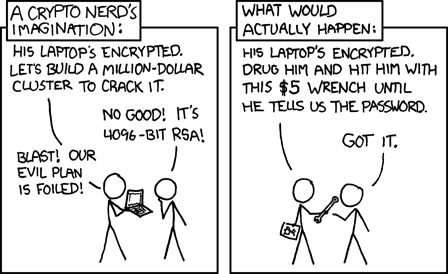
\includegraphics[width=10cm]{security.png}\\
        \url{http://xkcd.com/538/} \href{http://creativecommons.org/licenses/by-nc/2.5/}{ Creative Commons Attribution-NonCommercial 2.5 License}.
\end{center}%
}{}             % Le gars de xkcd ne m'a pas encore répondu pour l'utilisation de l'image.

\noindent \ldots tout dépends du contexte.


% This is part of Mes notes de mathématique
% Copyright (c) 2011-2013,2015
%   Laurent Claessens
% See the file fdl-1.3.txt for copying conditions.

%+++++++++++++++++++++++++++++++++++++++++++++++++++++++++++++++++++++++++++++++++++++++++++++++++++++++++++++++++++++++++++
\section{Représentations et caractères}
%+++++++++++++++++++++++++++++++++++++++++++++++++++++++++++++++++++++++++++++++++++++++++++++++++++++++++++++++++++++++++++

Une représentation est \defe{fidèle}{représentation!fidèle} si elle est injective en tant que application \( G\to \GL(V)\). Ce ne sont pas chacun des \( \rho(g)\) qui doivent être injectifs. La dimension de \( V\) est le \defe{degré}{degré!d'une représentation} de la représentation \( (V,\rho)\).

Si \( G\) est un groupe, l'ensemble des homomorphismes \( \Hom(G,\eC^*)\) est un groupe pour la multiplication. Un élément de \( \Hom(G,\eC^*)\) est un \defe{caractère abélien}{caractère!abélien}. Le nom «abélien» vient du fait que le caractère prenne ses valeurs dans \( \eC^*\). Nous notons \( \hat G=\Hom(G,\eC^*)\)\nomenclature[R]{\( \hat G\)}{groupe des caractères de \( G\)}.

\begin{theorem}
    Soit \( G\) un groupe abélien fini. Alors \( G\) est isomorphe à \( \hat G\).
\end{theorem}
L'isomorphisme n'est pas canonique.

\begin{proof}
    Étant donné la structure des groupes abéliens finis donnée par le théorème \ref{ThoRJWVJd}, nous commençons par nous concentrer sur \( G=\eZ/n\eZ\). Nous allons montrer que
    \begin{equation}
        \Hom(\eZ/n\eZ)\simeq \gU_n=\{ \xi\in \eC\tq \xi^n=1 \}.
    \end{equation}
    Pour cela nous avons l'isomorphisme
    \begin{equation}
        \begin{aligned}
            \psi\colon \Hom(\eZ,\eC^*)&\to \eC^* \\
            f&\mapsto f(1). 
        \end{aligned}
    \end{equation}
    Notons que si \( f\in \Hom(\eZ,\eC^*)\), alors \( f(k)=f(1)^k\), donc \( \psi\) est bien un isomorphisme. Cela nous amène à définir
    \begin{equation}
        \begin{aligned}
            \varphi\colon \Hom\Big( (\eZ/n\eZ,+),(\eC^*n\cdot) \Big)&\to \gU_n \\
            g&\mapsto f(1). 
        \end{aligned}
    \end{equation}
    Remarquons que pour tout \( f\in\Hom(\eZ/n\eZ,\eC^*)\) on a bien \( f(1)^n=1\). En effet si \( [k]\in \eZ/n\eZ\), alors \( f\big( [k] \big)=f(1)^k\) et en particulier
    \begin{equation}
        f(1)^n=f([n])=f(0)=1.
    \end{equation}
    Donc \( f(1)\in \gU_n\). Le \( \varphi\) est injective parce que si \( f(1)=g(1)\) alors \( f=g\) du fait que \( f(k)=f(1)^k=g(1)^k=g(k)\).

    Nous en sommes à avoir prouvé que \( \hat{\eZ/n\eZ}\simeq \gU_n\). Il faudrait encore montrer que \( \gU_n\simeq \eZ/n\eZ\). Pour cela nous nous rappelons du lemme \ref{LemWHQGooXyeJiw} nous ayant raconté que le groupe \( \gU_n\) des racines de l'unité était cyclique et d'ordre \( n\). Il est donc bien isomorphe à \( \eZ/n\eZ\).

    Passons au cas où
    \begin{equation}
        G\simeq \eZ/d_1\eZ\times \eZ/d_2\eZ\times \ldots\times \eZ/n_k\eZ.
    \end{equation}
    Dans ce cas nous montrons que 
    \begin{equation}
        \begin{aligned}
            \alpha\colon \bigtimes_{i=1}^k\Hom(\eZ/d_i\eZ,\eC^*)&\to \Hom(G,\eC^*) \\
            \alpha(\chi_1,\ldots, \chi_k)(g_1,\ldots, g_k)&= \chi_1(g_1)\ldots\chi_k(g_k). 
        \end{aligned}
    \end{equation}
    Ce \( \alpha\) est injectif parce qu'en appliquant l'égalité
    \begin{equation}
        \alpha(\chi_1,\ldots, \chi_k)=\alpha(\chi'_1,\ldots, \chi'_k)
    \end{equation}
    à l'élément \( g=(9,\ldots, 1,\ldots, 0)\) alors nous trouvons \( \chi_i(1)=\chi_i'(1)\) parce que \( \chi_j(0)=1\). Du coup \( \chi_i=\chi'_i\).

    L'application \( \alpha\) est en plus surjective. En effet si \( \chi\in\Hom(G,\eC^*)\), alors nous définissons
    \begin{equation}
        \chi_i(g_i)=\chi(0,\ldots, g_i,\ldots, 0),
    \end{equation}
    et nous avons alors \( \alpha(\chi_1,\ldots, \chi_k)=\chi\).

    Nous devons encore montrer que \( \alpha\) est un homomorphisme. Si \( \chi,\chi'\in\bigtimes_{i=1}^k\Hom(\eF_{d_i},\eC^*)\), alors
    \begin{subequations}
        \begin{align}
            \alpha(\chi\chi')(g_1,\ldots, g_k)&=(\chi_1\chi'_1)(g_1)\ldots (\chi_k\chi_k')(g_k)\\
            &=\chi_1(g_1)\ldots \chi_k(g_k)\chi'_1(g_1)\ldots \chi_k'(g_k)\\
            &=\alpha(\chi)(g_1,\ldots, g_k)\alpha(\chi')(g_1,\ldots, g_k)\\
            &=\big( \alpha(\chi)\alpha(\chi') \big)(g_1,\ldots, g_k).
        \end{align}
    \end{subequations}
    Donc \( \alpha(\chi\chi')=\alpha(\chi)\alpha(\chi')\).
\end{proof}

\begin{theorem}
    Soit \( G\) un groupe abélien fini. Les groupes \( G\) et \( \hat{\hat G}\) sont isomorphes et un isomorphisme canonique est donné par \( \alpha\colon g\mapsto f_g\) donné par
    \begin{equation}
        f_g(\chi)=\chi(g).
    \end{equation}
\end{theorem}

\begin{proof}

    D'abord \( f_g\) est bien un caractère de \( \hat G\) parce que
    \begin{equation}
        f_g(\chi\chi')=(\chi\chi')(g)=\chi(g)\chi'(g)=f_g(\chi)f_g(\chi').
    \end{equation}
    Le fait que \( \alpha\) soit un homomorphisme de groupes est direct :
    \begin{equation}
        f_{gg'}(\chi)=\chi(gg')=\chi(g)\chi(g')=f_g(\chi)f_{g'}(\chi)=(f_gf_{g'})(\chi).
    \end{equation}

    D'autre part nous savon que \( G\) et \( \hat{\hat G}\) ont le même cardinal. Il suffit donc de prouver l'injectivité de \( \alpha\) pour être sûr de la bijectivité. Pour cela nous devons prouver que si \( g\neq e\) alors \( f_g\neq f_e\). Nous savons que pour tout caractère \( \chi\in \hat G\), \( f_e(\chi)=\chi(e)=1\). Donc pour tout \( g\in G\setminus\{ e \}\), nous devons trouver \( \chi\in \hat G\) tel que \( \chi(g)\neq 1\).

    En vertu de ce que nous connaissons sur la structure des groupes abéliens finis (théorème \ref{ThoRJWVJd}), nous commençons \( G=\eZ/n\eZ\) et considérons le caractère donné par \( \chi([1])= e^{2i\pi/n}\). Ce \( \chi\) est un isomorphisme entre \( G\) et \( \gU(n)\); nous n'avons \( \chi([k])=0\) que si \( [k]=[n]=[0]\). Pour rappel dans \( \eZ/n\eZ\), le neutre est \( e=0\) et non \( e=1\).

    Passons au cas général :
    \begin{equation}
        G\simeq \eZ/n_1\eZ\times \ldots\times \eZ/n_k\eZ
    \end{equation}
    Si \( g=(g_1,\ldots, g_k)\) est non nul dans \( G\), alors il existe \( i\) tel que \( g_i\neq 0\) et on prend
    \begin{equation}
        \chi(g_1,\ldots, g_k)=\chi_i(g_i)
    \end{equation}
    où \( \chi_i\) est le caractère \( \chi_i([1])= e^{2\pi i/n_i}\). Ce \( \chi\) est alors un caractère non trivial de \( G\).
    
\end{proof}

%---------------------------------------------------------------------------------------------------------------------------
\subsection{Crochet de dualité et transformée de Fourier}
%---------------------------------------------------------------------------------------------------------------------------

Si \( G\) est un groupe abélien, nous définissons le crochet de dualité entre \( G\) et \( \hat G\) par
\begin{equation}
    \begin{aligned}
        \langle ., .\rangle \colon G\times \hat G&\to \eC^* \\
        \langle g, \chi\rangle &=\chi(g). 
    \end{aligned}
\end{equation}
Notons que l'image de ce crochet n'est pas \( \eC^*\) entier, mais seulement le groupe unitaire \( \gU(n)\) où \( n\) est l'exposant\footnote{Définition \ref{DefvtSAyb}.} de \( G\).


Si \( f,g\) sont des applications de \( G\) dans \( \eC\), alors on leur associe le produit scalaire
\begin{equation}
    \langle f, g\rangle =\frac{1}{ | G | }\sum_{s\in G}f(s)\overline{ g(s) }.
\end{equation}

\begin{lemma}
    Les caractères de \( G\) forment une base orthonormée de \( \eC^G\) pour ce produit scalaire.    
\end{lemma}

\begin{proof}
    Étant donné que les \( \chi(s)\) sont des nombres complexe de module \( 1\), nous avons \( \chi(s)\overline{ \chi(s) }=1\) et par conséquent \( \langle \chi, \chi\rangle =1\).

    Si par contre \( \chi\neq\chi'\), alors il existe \( s_\in G\) tel que \( \chi(s_0)\neq \chi'(s_0)\). Dans ce cas en effectuant un changement de variable \( s\to s_0s\) dans la sommation,
    \begin{subequations}
        \begin{align}
            \langle \chi, \chi'\rangle &=\frac{1}{ | G | }\sum_{s\in G}\chi(s)\overline{ \chi'(s) }\\
            &=\frac{1}{ | G | }\sum_{s\in G}\chi(s_0s)\overline{ \chi'(s_0s) }\\
            &=\frac{1}{ | G | }\chi(s_0)\chi'(s_0)\sum_{s\in G}\chi(s)\overline{ \chi'(s) }.
        \end{align}
    \end{subequations}
    Donc nous avons trouvé
    \begin{equation}
        \langle \chi, \chi'\rangle \big( 1-\chi(s_0)\overline{ \chi'(s_0) } \big)=0.
    \end{equation}
    Mais vu que \( \chi(s_0)\neq \chi(s'_0)\), la parenthèse est non nulle (pour rappel \( \chi(s_0)\) est un complexe de module \( 1\)) et par conséquent \( \langle \chi, \chi'\rangle =0\).

    Nous déduisons immédiatement que les caractères forment une famille libre parce que si \( \sum_i\chi_i=0\) (la somme est sur tous les caractères), alors en prenant le produit scalaire avec \( \chi_k\),
    \begin{equation}
        \sum_ia_i\langle \chi_k, \chi_i\rangle =0,
    \end{equation}
    et donc \( a_k=0\).

    Les caractères forment donc un système libre orthonormé. De plus l'espace engendré à la bonne dimension parce que le cardinal de l'ensemble des caractères est la dimension (complexe) de l'espace des fonction de \( G\) dans \( \eC\) parce que, en utilisant l'isomorphisme entre \( G\) et \( \hat G\),
    \begin{equation}
        \Card\hat G=\Card(G)=\dim_{\eC}\eC^G.
    \end{equation}
    La première 
\end{proof}

Du fait que les caractères forment une base orthonormée, nous pouvons écrire, pour toute application \( f\colon G\to \eC\),
\begin{equation}    \label{EqnnsXWC}
    f=\sum_{\chi\in\hat G}\langle \chi, f\rangle \chi.
\end{equation}
À une fonction \( f\colon G\to \eC\) nous associons la \defe{transformée de Fourier}{transformée!de Fourier!groupe abélien fini}\index{Fourier!transformée!groupe abélien fini}
\begin{equation}
    \begin{aligned}
        \hat f\colon \hat G&\to \eC \\
        \chi&\mapsto \langle \chi, f\rangle . 
    \end{aligned}
\end{equation}
Nous avons donc aussi une espèce de formule d'inversion
\begin{equation}
    f=\sum_{\chi\in\hat G}\hat f(\chi)\chi
\end{equation}
qui n'est qu'une réécriture de \ref{EqnnsXWC}.

%---------------------------------------------------------------------------------------------------------------------------
\subsection{Groupes non abéliens}
%---------------------------------------------------------------------------------------------------------------------------

Nous avons vu que le groupe des caractères \( \hat G\) contenait toute l'information sur un groupe abélien. Malheureusement, pour les groupes non abéliens, ça ne va pas suffire, et nous allons introduire la notion de représentations, dont les caractères seront un cas particulier de dimension un.

\begin{proposition}
    Soit \( G\) un groupe (pas spécialement abélien). Nous avons
    \begin{equation}
        \hat G\simeq\Hom\big( G/D(G),\eC^* \big).
    \end{equation}
\end{proposition}

\begin{proof}
    Ce qui fait fonctionner la preuve est le fait que si \( f\colon G\to \eC^*\) est un homomorphisme, alors \( f\) s'annule sur \( D(G)\). L'isomorphisme est
    \begin{equation}
        \begin{aligned}
            \psi\colon \hat G&\to \Hom\big( G/D(G),\eC^* \big) \\
            \psi(f)[g]&=f(g). 
        \end{aligned}
    \end{equation}
    Cette application est bien définie parce que si \( f\) est un homomorphisme,
    \begin{equation}
        f(gklk^{-1}l^{-1})=f(g).
    \end{equation}
    D'autre part \( \psi\) est un homomorphisme de groupe parce que
    \begin{equation}
        \psi(f_1f_2)[g]=(f_1f_2)(g)=f_1(g)f_2(g)=\psi(f_1)[g]\psi(f_2)[g]=\big( \psi(f_1)\psi(f_2) \big)[g].
    \end{equation}
    Pour l'injectivité de \( \psi\), soit \( f_1\) et \( f_2\) telles que \( \psi(f_1)=\psi(f_2)\). Alors pour tout \( g\in G\) nous avons
    \begin{equation}
        \psi(f_1)[g]=\psi(f_2)[g]
    \end{equation}
    et donc \( f_1(g)=f_2(g)\).

    Enfin \( \psi\) est surjective. En effet, soit \( \bar f\in\Hom\big( G/D(G),\eC^* \big)\). Alors nous obtenons \( \psi(f)=\bar f\) en posant
    \begin{equation}
        f(g)=\bar f[g].
    \end{equation}
    Il faut juste vérifier que le \( f\) ainsi défini est dans \( \hat G\), c'est à dire que \( f(g_1g_2)=f(g_1)f(g_2)\).
\end{proof}

Cette proposition nous montre que
\begin{equation}
    \hat G=\widehat{G/D(G)},
\end{equation}
alors que \( G/D(G)\) est abélien; il n'est donc pas tellement possible que \( \hat G\) contienne beaucoup d'informations intéressantes sur \( G\).

%---------------------------------------------------------------------------------------------------------------------------
\subsection{Représentations linéaires des groupes finis}
%---------------------------------------------------------------------------------------------------------------------------

Soit \( V\), un \( \eC\)-espace vectoriel de dimension finie. Une \defe{représentation}{représentation} linéaire de \( G\) dans \( V\) est un homomorphisme \( \rho\colon G\to \End(V)\). Nous notons \( (V,\rho)\) cette représentation. Voire \( \rho\) tout court si l'espace vectoriel n'est pas ambigu.

Si \( \dim V=1\), alors \( \GL(V)=\eC^*\) et les représentation sont les caractères abéliens.

\begin{example} \label{ExKUAyUD}
    Considérons le triangle équilatéral \( A,B,C\), par exemple donné par les points
    \begin{subequations}
        \begin{numcases}{}
            A=1\\
            B=(-\frac{ 1 }{2},\frac{ \sqrt{3} }{2})\\
            C=(-\frac{ 1 }{2},-\frac{ \sqrt{3} }{2})\\
        \end{numcases}
    \end{subequations}
    Dans la base (pas orthonormée) \( \{ A,B \}\) de \( \eR^2\), ces trois points sont donnés par
    \begin{equation}
        \begin{aligned}[]
            A&=\begin{pmatrix}
                1    \\ 
                0    
            \end{pmatrix}&B&=\begin{pmatrix}
                0    \\ 
                1    
            \end{pmatrix}&C&=\begin{pmatrix}
                -1    \\ 
                -1    
            \end{pmatrix}.
        \end{aligned}
    \end{equation}
    Le groupe symétrique\index{groupe!symétrique!action sur un triangle} \( S_3\) agit sur le triangle par permutation des sommets. Vues dans la base \( \{ A,B \}\), les transpositions correspondent aux matrices
    \begin{subequations}
        \begin{align}
            (A,B)&\to\begin{pmatrix}
                0    &   1    \\ 
                1    &   0    
            \end{pmatrix}\\
            (A,C)&\to \begin{pmatrix}
                -1    &   0    \\ 
                -1    &   1    
            \end{pmatrix}\\
            (B,C)&\to\begin{pmatrix}
                1    &   -1    \\ 
                0    &   -1    
            \end{pmatrix}.
        \end{align}
    \end{subequations}
    La permutation \( (A,B,C)\) s'écrit comme \( (A,B,C)=(A,C)(A,B)\) et on lui associe la matrice
    \begin{equation}
        (A,B,C)\to\begin{pmatrix}
            0    &   -1    \\ 
            1    &   -1    
        \end{pmatrix}.
    \end{equation}
    C'est bien le produit des matrices de \( (A,C)\) et de \( (A,B)\). De la même façon nous avons
    \begin{equation}
        (BAC)<++>
    \end{equation}
    % TODO : il y a manifestement quelque chose à terminer ici.
    <++>
\end{example}

Si \( (V,\rho)\) et \( (V',\rho')\) sont deux représentations du groupe \( G\), alors nous définissons la \defe{somme directe}{somme directe (de représentations)} par \( \big( V\oplus V',\rho\oplus\rho' \big)\) donné par
\begin{equation}
    (\rho\oplus\rho')(g)=\begin{pmatrix}
        \rho(g)    &   0    \\ 
        0    &   \rho'(g)    
    \end{pmatrix}\in \GL(V\oplus V').
\end{equation}

Nous noterons souvent \( 2V\) pour la représentations \( (V,\rho)\oplus (V,\rho)\) et plus généralement l'écriture
\begin{equation}
    V=\bigoplus_i k_iW_i
\end{equation}
signifiera la représentation somme de \( k_i\) termes de la représentation \( W_i\). Ici encore un abus est commis entre la représentation \( (\rho_i,W_i)\) et l'espace \( W_i\).

%---------------------------------------------------------------------------------------------------------------------------
\subsection{Module}
%---------------------------------------------------------------------------------------------------------------------------

Nous considérons la \( \eC\)-algèbre \( G[\eC]\)\nomenclature[G]{\( \eC[G]\)}{combinaisons d'éléments de \( G\) à coefficients dans \( \eC\)} des combinaisons (formelles) d'éléments de \( G\) à coefficients dans \( G\), c'est à dire l'ensemble
\begin{equation}
    \eC[G]=\{ \sum_{s\in G}a_ss \}
\end{equation}
avec le produit hérité de la bilinéarité :
\begin{equation}
    \sum_{s\in G}\sum_{t\in G}a_sb_tst=\sum_s\sum_t a_sb_{s^{-1}t}t,
\end{equation}
et la somme
\begin{equation}
    (\sum_sa_ss)+\sum_tb_tt=\sum_{s\in G}(a_s+b_s)s.
\end{equation}
Le tout est une \( \eC\)-algèbre agissant sur \( V\) par
\begin{equation}
    \left( \sum_sa_ss \right)v=\sum_{s\in G}a_s\rho(s)v\in V
\end{equation}

Les sous-modules indécomposables seront les représentations irréductibles.

\begin{definition}
    La représentation \( (V,\rho)\) du groupe \( G\) est \defe{irréductible}{irréductible!représentation}\index{représentation!irréductible} si les seuls sous-espaces invariants de \( V\) sous \( \rho(G)\) sont $V$ et \( \{ 0 \}\).
\end{definition}

\begin{example}
    La représentation de \( S_3\) sur \( \eR^2\) donnée par les permutations des sommets d'un triangle équilatéral donnée dans l'exemple \ref{ExKUAyUD} est irréductible.
\end{example}

La question qui vient est de savoir si une représentation possédant des sous-espaces invariants peut être écrite comme la somme de représentations irréductibles.

\begin{proposition} \label{PropHeyoAN}  \index{représentation!irréductible}
    Soit \( (V,\rho)\) une représentation linéaire de dimension finie d'un groupe fini\footnote{La démonstration marche aussi pour les groupes compacts, mais il faudrait des intégrales.}. Si \( W_1\) est un sous-espace stable\footnote{c'est à dire si \( \rho\) n'est pas irréductible.}, alors il existe un sous-espace \( W_2\) également stable et tel que \( V=W_1\oplus W_2\).

    Toute représentation linéaire est décomposable en représentations irréductibles.
\end{proposition}

\begin{proof}
    Soit \( P\colon V\to V\) un projecteur sur \( W_1\), c'est à dire que \( P^2=P\) et \( P(V)=W_1\). Pour construire un tel projecteur, on peut par exemple prendre un supplémentaire de \( W_1\) dans \( V\) puis utiliser la décomposition\footnote{Ou encore prendre une base de \( W_1\), l'étendre en une base de \( V\) et définir \( P\) comme l'annulation des coefficients des vecteurs «complétant» la base.}. Nous considérons l'opérateur
    \begin{equation}
        P_G=\frac{1}{ | G | }\sum_{g\in G}\rho(g)\circ P\circ \rho(g)^{-1}.
    \end{equation}
    Prouvons que ce \( P_G\) est encore un projecteur. D'abord pour tout \( g\in G\) nous avons
    \begin{equation}
        \rho(g)P_G\rho(g)^{-1}=\frac{1}{ | G | }\sum_{s\in G}\rho(gs)P\rho(gs)^{-1}=P_G.
    \end{equation}
    La dernière égalité est un changement de variables dans la somme\footnote{Et c'est ça qui demande un peu de technique pour écrire la preuve dans le cas d'un groupe compact : il faut une mesure de Haar.}. Cela signifie que \( P_G\rho=\rho P_G\). Nous avons même \( P_GP=P\) parce que si \( v\in W_1\), alors 
    \begin{subequations}
        \begin{align}
            P_G(v)&=\frac{1}{ | G | }\sum_{s\in G}\rho(s)P\underbrace{\rho(s)^{-1} v}_{\in W_1}\\
            &=\frac{1}{ | G | }\sum_s\rho(s)\rho(s)^{-1} v\\
            &=v.
        \end{align}
    \end{subequations}
    Avec cela nous pouvons conclure que \( P_G^2=P_G\) parce que
    \begin{subequations}
        \begin{align}
            P_G\circ P_G&=\frac{1}{ | G | }\sum_g P_G\rho(g)P\rho(g)^{-1}\\
            &=\frac{1}{ | G | }\sum_g \rho(g)P_GP\rho(g)^{-1}\\
            &=\frac{1}{ | G | }\sum_g \rho(g)P\rho(g)^{-1}\\
            &=P_G.
        \end{align}
    \end{subequations}
    Donc \( P_G\) est un projecteur, est stable sous les conjugaisons par \( \rho(g)\) et commute avec \( \rho(g)\). Nous décomposant \( \id\) de façon évidente en
    \begin{equation}
        \id=P_G+(\id-P_G).
    \end{equation}
    Étant donné que l'opérateur \( P_G\) commute avec tous les \( \rho(g)\), les noyaux de \( P_G\) et \( \id-P_G\) sont des sous-espaces invariants. Vu que \( P_G\) est un projecteur, nous avons \( q(P_G)=0\) avec \( q(X)=X^2-X\). Pour appliquer le lemme des noyaux (théorème \ref{ThoDecompNoyayzzMWod}), nous remarquons que \( q(X)=X(X-1)\) et donc 
    \begin{equation}
        V=\ker P_G\oplus\ker(P_G-\mtu).
    \end{equation}
    Si nous posons \( W_2=\ker P_G\), il reste à voir que \( \ker(P_G\mtu)=W_1\). D'abord \( W_1\subset\ker(P_G-\id)\) parce que si \( w\in W_1\), ce dernier étant stable,
    \begin{subequations}
        \begin{align}
            P_Gw&=\frac{1}{ | G | }\sum_{g\in G}\rho(g)P\underbrace{\rho(g)^{-1}w}_{\in W_1}\\
            &=\frac{1}{ | G | }\sum_{g\in G}w\\
            &=w.
        \end{align}
    \end{subequations}
    Pour prouver l'inclusion inverse, nous savons que \( P_G\) et \( P\) sont des projecteurs tels que \( P_GP=P\), ce qui signifie que l'image de \( P_G\) est inclue à celle de \( P\), c'est à dire à \( W_1\). Mais \( \Image(P_G)=\ker(\mtu-P_G)\), donc
    \begin{equation}
        \ker(\mtu-P_G)=\Image(P_G)\subset\Image(P)=W_1.
    \end{equation}

    La représentation \( \rho\) se décompose donc en deux sous-représentations \( (\rho,W_1)\) et \( \rho,W_2\). Si l'une des deux n'est pas irréductible, le processus peut recommencer. Vu que la dimension de \( V\) est finie, toute représentation se décompose en une somme finie de représentation irréductibles.
\end{proof}

%---------------------------------------------------------------------------------------------------------------------------
\subsection{Structure hermitienne}
%---------------------------------------------------------------------------------------------------------------------------

Soit \( (\rho,V)\) une représentation de \( G\) sur un espace vectoriel complexe \( V\). Nous voulons munir \( V\) d'un produit scalaire hermitien (définition \ref{DefMZQxmQ}) tel que les opérateurs \( \rho(g)\) soient tous des isométries. C'est à dire que nous voudrions définir \( \langle u, v\rangle_G\) de telle sorte à avoir
\begin{equation}
    \langle \rho(g)u, \rho(g)v\rangle_G =\langle u, v\rangle_G
\end{equation}
pour tout \( g\in G\). Nous commençons par considérer un produit hermitien \( \langle ., .\rangle \) quelconque et puis nous définissons
\begin{equation}
    \langle u, v\rangle_G=\frac{1}{ | G | }\sum_{g\in G}\langle \rho(g)u, \rho(g)v\rangle.
\end{equation}
Nous devons vérifier que c'est un produit. La seule des conditions dont la vérification n'est pas immédiate est celle de positivité. Pour tout \( g\in G\) et tout \( v\in V\), nous avons \( \langle \rho(g)v, \rho(g)v\rangle \) est positif et nul si et seulement si \( \rho(g)v=0\). Étant donné que \( \rho(e)v=v\), parmi les termes de la somme
\begin{equation}
    \langle u, u\rangle_G=\frac{1}{ | G | }\sum_{g\in G}\langle \rho(g)v, \rho(g)v\rangle,
\end{equation}
au moins un est strictement positif (pourvu que \( v\neq 0\)); les autres sont positifs ou nuls. Par conséquent \( \langle v, v\rangle_G=0\) si et seulement si \( v=0\).

Donc les groupes finis peuvent être vus comme des parties de groupes d'isométrie. De la même façon, en utilisant une mesure de Haar pour faire la moyenne, nous pouvons plonger les groupes compacts dans des groupes unitaires.

%---------------------------------------------------------------------------------------------------------------------------
\subsection{Caractères}
%---------------------------------------------------------------------------------------------------------------------------

Soit \( (V,\rho)\) une représentation linéaire du groupe \( G\). Le \defe{caractère}{caractère} de \( \rho\) est la fonction
\begin{equation}
    \begin{aligned}
        \chi_{\rho}\colon G&\to \eC \\
        s&\mapsto \tr\big( \rho(s) \big).
    \end{aligned}
\end{equation}
Par invariance de la trace, nous avons
\begin{equation}
    \chi_{\rho}(sts^{-1})=\chi_{\rho}(t),
\end{equation}
ce qui fait que le caractère est une fonction constante sur les classes de conjugaison.

Un \defe{caractère irréductible}{caractère!irréductible} est un caractère d'une représentation irréductible.

\begin{definition}
    Une application \( f\colon G\to \eC\) est \defe{centrale}{centrale (application)} si elle est constante sur les classes de conjugaison.
\end{definition}
Les traces sont des applications centrales.

L'ensemble des fonctions centrales sur un groupe fini (ou tout au moins ayant un nombre fini de classes de conjugaison) est un \( \eC\)-espace vectoriel de dimension égale au nombre de classes, et nous pouvons mettre le produit scalaire
\begin{equation}    \label{EqJrEpVI}
    \langle f, g\rangle =\frac{1}{ | G | }\sum_{s\in G}f(s)\overline{ g(s) }.
\end{equation}
C'est une forme hermitienne sur l'espace des fonction centrales.

%+++++++++++++++++++++++++++++++++++++++++++++++++++++++++++++++++++++++++++++++++++++++++++++++++++++++++++++++++++++++++++
\section{Équivalence de représentations et caractères}
%+++++++++++++++++++++++++++++++++++++++++++++++++++++++++++++++++++++++++++++++++++++++++++++++++++++++++++++++++++++++++++

Cette section prend des éléments des articles \wikipedia{fr}{Lemme_de_Schur}{lemme de Schur}, \wikipedia{fr}{Caractère_d'une_représentation_d'un_groupe_fini}{caractère d'une représentation}, \wikipedia{fr}{Fonction_centrale_d'un_groupe_fini}{fonction centrale} et \wikipedia{fr}{Trace_(algèbre)}{trace} de wikipédia.

Nous disons que les deux représentations \( (V,\rho)\) et \( (V',\rho')\) sont \defe{équivalentes}{equivalence@équivalence!de représentations} s'il existe une bijection linéaire \( f\colon V\to V'\) telle que
\begin{equation}
    f\circ \rho=\rho'\circ f.
\end{equation}
Nous disons alors que \( f\) \defe{entrelace}{entrelacement} \( \rho\) et \( \rho'\).

\begin{theorem}[Théorème de Schur]\index{théorème!Schur}\index{Schur (théorème)}    \label{ThoyftobH}
    Si \( (V,\rho)\) et \( (V',\rho')\) sont des représentations irréductibles non équivalentes alors la seule application linéaire \( f\colon V\to V'\) entrelaçant \( \rho\) et \( \rho'\) est la fonction nulle.

    En d'autres termes, soit les représentations sont équivalentes (et il y a un isomorphisme), soit il n'y a même pas un homomorphisme.
\end{theorem}

\begin{proof}
    Soit \( f\in\aL(V,V')\) telle que \( f\circ \rho=\rho'\circ f\). Alors \( \ker f\) est un sous-espace stable sous \( \rho(G)\), et \( \Image(f)\) est un sous-espace de \( V'\) stable par \( \rho'(G)\). Par irréductibilité, nous avons que \( \ker(f)=\{ 0 \}\) ou \( V\). Même chose pour \( \Image(f)\). Il y a deux possibilités.
    \begin{enumerate}
        \item
            Si \( \ker(f)=\{ 0 \}\), alors \( \Image(f)\neq \{ 0 \}\) et alors \( \Image(f)=V'\). Du coup \( f\) est injective et surjective, c'est à dire est un isomorphisme.
        \item
            Si \( \ker(f)=V\), alors \( f=0\).
    \end{enumerate}
\end{proof}

\begin{corollary}[Schur pour les représentations sur \( \eC\)]
    Soit \( (V,\rho)\) une représentation irréductible, alors l'ensemble
    \begin{equation}
        \End_{G}(V,\rho)=\{ f\in\End(V)\tq \rho\circ f=f\circ \rho \}
    \end{equation}
    est l'ensemble des homothéties.
\end{corollary}

\begin{proof}
    Soit \( f\in\End_{G}(V,\rho)\). Vu que l'espace est sur \( \eC\), l'endomorphisme \( f\) a une valeur propre \( \lambda\). L'opérateur \( g=f-\lambda\mtu\) est aussi un opérateur d'entrelacement de \( \rho\) alors que \( \ker(g)\neq \{ 0 \}\) par définition de valeur propre. Du coup \( \ker(g)=V\), ce qui signifie que \( f\) est l'isométrie de rapport \( \lambda\) : \( f=\lambda\id\).
\end{proof}

\begin{lemma}   \label{LempUSOlo}
    Si \( (\rho,V)\) et \( (\rho',V')\) sont des représentations équivalentes de caractères \( \chi\) et \( \chi'\), alors \( \chi=\chi'\).
\end{lemma}

\begin{proof}
    Si \( A\colon V\to V'\) est un isomorphisme d'espace vectoriel entrelaçant \( \rho\) et \( \rho'\), c'est à dire si pour tout \( g\), \( \rho'(g)A=A\rho(g)\), alors \( \rho'(g)=A\rho(g)A^{-1}\) et
    \begin{equation}
        \chi'(g)=\tr\big( \rho'(g) \big)=\tr\big( A\rho(g)A^{-1} \big)=\tr\big( \rho(g) \big)
    \end{equation}
    parce que la trace est un invariant de similitude (lemme \ref{LemhbZTay}).
\end{proof}

\begin{lemma}   \label{LemJqIZns}
    Si \( \chi\) est le caractère de la représentation complexe \( (V,\rho)\) du groupe fini \( G\), alors pour tout \( g\in G\) nous avons \( \chi(g^{-1})=\overline{ \chi(g) }\).
\end{lemma}

\begin{proof}
    Par le corollaire \ref{CorpZItFX} au théorème de Lagrange, nous avons \( g^{| G |}=e\) et donc en tant qu'opérateur, \( \rho(g)^{| G |}=\mtu\). Les valeurs propres de \( \rho(g)\) sont donc des racines de l'unité. Si nous notons \( \lambda_i\) ces valeurs propres, alors \( \chi(g)=\sum_i\lambda_i\), et en considérant la matrice dans sa base de diagonalisation (lemme de Schur complexe, \ref{LemSchurComplHAftTq}), nous voyons que
    \begin{equation}
        \chi(g^{-1})=\tr\big( \rho(g)^{-1} \big)=\sum_i\frac{1}{ \lambda_i }.
    \end{equation}
    Mais \( \lambda_i\) étant une racine de l'unité nous avons \( \frac{1}{ \lambda_i }=\bar\lambda_i\), ce qui fait que
    \begin{equation}
        \chi(g^{-1})=\sum_i\bar\lambda_i=\overline{ \chi(g) }.
    \end{equation}
\end{proof}

\begin{proposition} \label{PropJzbfWi}
    Soient deux représentations irréductibles complexes \( (V,\rho)\) et \( (V',\rho')\) du même groupe fini \( G\), et \( \chi\) et \( \chi'\) leurs caractères respectifs. Nous avons
    \begin{enumerate}
        \item
            \( \langle \chi, \chi'\rangle =0\) si \( \rho\) et \( \rho'\) ne sont pas équivalentes.
        \item
            \( \langle \chi, \chi'\rangle =1\) si les représentations sont équivalentes.
    \end{enumerate}
\end{proposition}

\begin{proof}
    Nous considérons les bases \( \{ e_1,\ldots, e_n \} \) de \( V\) et \( \{ f_1,\ldots, f_m \}\) de \( V'\). Puis nous considérons la matrice $F(k,l)=E_{kl}\in\eM_{m,n}(\eC)$ où pour rappel, \( E_{kl}\) est la matrice de composantes \( (E_{kl})_{ij}=\delta_{ki}\delta_{lj}\). Nous posons
    \begin{equation}
        F_G(k,l)=\frac{1}{ | G | }\sum_{g\in G}\rho(g)\circ F(k,l)\circ\rho'(g)^{-1}.
    \end{equation}
    En nous permettant de ne pas réécrire les indices \( k\) et \(l \) de \( F\) et \( F_G\), nous montrons que \( F_G\) entrelace \( \rho\) et \( \rho'\) :
    \begin{subequations}
        \begin{align}
            F_G\circ\rho'(t)&=\frac{1}{ | G | }\sum_{s\in G}\rho(s)\circ F\circ \rho'(s^{-1})\circ \rho(t)\\
            &=\frac{1}{ | G | }\sum_s\rho(s)F\rho'(s^{-1} t)\\
            &=\frac{1}{ | G | }\sum_{k}\rho(tk)F\rho'(k^{-1})\\
            &=\frac{1}{ | G | }\rho(t) \sum_k\rho(k)F\rho'(k^{-1})\\
            &=\rho(t)\circ F_G.
        \end{align}
    \end{subequations}
    Dans ce calcul nous avons effectué le changement de variables \( k=(s^{-1} t)^{-1}\) qui donne \( s=tk\).

    Par ailleurs nous avons
    \begin{subequations}
        \begin{align}
            \Big( \rho(g)F(k,l)\rho'(g^{-1}) \Big)_{ij}&=\sum_{r=1}^n\sum_{s=1}^m\rho(g)_{ir}F(k,l)_{rs}\rho'(g^{-1})_{sj}\\
            &=\sum_{rs}\rho(g)_{ir}\delta_{kr}\delta_{ls}\rho'(g^{-1})_{sj}\\
            &=\rho(g)_{ik}\rho'(g^{-1})_{lj},
        \end{align}
    \end{subequations}
    et par conséquent
    \begin{equation}    \label{Eqgvpzfz}
        F_G(k,l)_{ij}=\frac{1}{ | G | }\sum_{g\in G}\rho(g)_{ik}\rho'(g^{-1})_{lj}.
    \end{equation}
    Si \( \chi\) et \( \chi'\) sont les caractères de \( \rho\) et \( \rho'\), alors nous avons le produit \eqref{EqJrEpVI} qui donne
    \begin{subequations}
        \begin{align}
            \langle \chi, \chi'\rangle &=\frac{1}{ | G | }\sum_{g\in G}\chi(g)\overline{ \chi'(g) }\\
            &=\frac{1}{ | G | }\sum_g\chi(g)\chi'(g^{-1})    &\text{lemme \ref{LemJqIZns}}\\
            &=\frac{1}{ | G | }\sum_g\sum_{i=1}^n\sum_{j=1}^m\rho(g)_{ii}\rho'(g^{-1})_{jj}     \label{sEqKYywTM}\\
            &=\sum_{ij}F_G(i,j)_{ij}    &\text{par \eqref{Eqgvpzfz}}.
        \end{align}
    \end{subequations}
    Si les représentations \( \rho\) et \( \rho'\) ne sont pas équivalentes, le fait que \( F_G\) en soit un opérateur d'entrelacement implique par le théorème de Schur \ref{ThoyftobH} que \( F_G=0\) et donc \( \langle \chi, \chi'\rangle =0\).

    Si au contraire les représentation sont équivalentes, alors le lemme \ref{LempUSOlo} nous dit que \( \chi=\chi'\) et nous reprenons la définition :
    \begin{equation}
        \langle \chi, \chi\rangle =\frac{1}{ | G | }\sum_g\chi(g)\overline{ \chi(g) }=\frac{1}{ | G | }\sum_{g\in G}1=1
    \end{equation}
    parce que les nombres \( \chi(g)\) sont des racines de l'unité.
\end{proof}


%--------------------------------------------------------------------------------------------------------------------------- 
\subsection{Représentation régulière}
%---------------------------------------------------------------------------------------------------------------------------

Nous notons \( \lambda\) la \defe{représentation régulière gauche}{représentation!régulière gauche}, agissant sur le \( \eK\)-espace vectoriel des fonctions \( G\to \eK\) par
\begin{equation}
    \Big( \lambda(g)f \Big)(g)=f(g^{-1}h).
\end{equation}
D'autre part nous considérons les fonction \( \delta_g\colon G\to \eK\) (ici \( \eK\) est \( \eR\) ou \( \eC\) ou pire) définie par
\begin{equation}
    \delta_g(h)=\begin{cases}
        1    &   \text{si } g=h\\
        0    &    \text{sinon.}
    \end{cases}
\end{equation}
La représentation régulière agit sur les fonctions \( \delta_s\) de la façon suivante :
\begin{equation}
    \lambda(g)\delta_s=\delta_{gs}
\end{equation}
parce que \( \big( \lambda(g)\delta_s \big)(h)=\delta_s(g^{-1}h)=\delta_{gs}(h)\).

\begin{lemma}
    Le caractère de la représentation régulière gauche est donné par 
    \begin{equation}        \label{EqUuoVNa}
        \chi_{\lambda}=| G |\delta_e.
    \end{equation}
\end{lemma}

\begin{proof}
    Appliquer l'équation \eqref{EqUuoVNa} fonctionne parce que \( \chi_{\lambda}(e)\) est la dimension de l'espace des fonctions sur \( G\), c'est à dire \( | G |\). Si par contre \( g\neq e\), alors \( \lambda(g)\) est une matrice de permutation (dans la base des \( \delta_h\)) et a donc tous ses éléments diagonaux nuls.
\end{proof}

Si \( \rho\) est une représentation et si \( f\) est une fonction sur le groupe, alors nous considérons l'opérateur
\begin{equation}
    \rho_f=\sum_{g\in G}f(g)\rho(g).
\end{equation}

\begin{proposition}[\cite{NhCRhg}]  \label{PropEAXkAY}
    Si \( (\rho,V)\) est une représentation irréductible et si \( f\) est une fonction centrale sur \( G\), alors l'opérateur \( \rho_f\) est une homothétie de \( V\) de rapport
    \begin{equation}
        \frac{1}{ \dim V }\sum_{g\in G}f(g)\chi(g)
    \end{equation}
    où \( \chi\) est le caractère de \( \rho\).
\end{proposition}

\begin{proof}
    Nous commençons par voir que \( \rho_f\) entrelace \( \rho\). En effet,
    \begin{subequations}
        \begin{align}
            \rho(t)^{-1}\circ\rho_f\circ\rho(t)&=\sum_gf(g)\rho(t^{-1}gt)\\
            &=\sum_hf(tht^{-1})\rho(g)      & h=t^{-1}gt\\
            &=\sum_hf(h)\rho(h)\\
            &=\rho_f
        \end{align}
    \end{subequations}
    où en écrivant \( f(tht^{-1})=f(h)\), nous avons utilisé le fait que \( f\) était centrale. Étant donné que \( \rho_f\) entrelace une représentation irréductible, le lemme de Schur (\ref{ThoyftobH}) nous indique que \( \rho_f\) est une homothétie. Soit \( k\) le facteur d'homothétie. Alors d'une part \( \tr(\rho_f)=nk\). D'autre part,
    \begin{subequations}
        \begin{align}
            \tr(\rho_f)&=\tr\big( \sum_gf(g)\rho(g) \big)\\
            &=\sum_gf(g)\tr\big( \rho(g) \big)\\
            &=\sum_gf(g)\chi(g).
        \end{align}
    \end{subequations}
    Du coup effectivement 
    \begin{equation}
        k=\frac{1}{ n }\sum_{g\in G}f(g)\chi(g).
    \end{equation}
\end{proof}

%--------------------------------------------------------------------------------------------------------------------------- 
\subsection{Caractères et représentations : suite et fin}
%---------------------------------------------------------------------------------------------------------------------------

\begin{lemma}
    Un groupe fini n'a (à équivalence près) qu'un nombre fini de représentations irréductibles.
\end{lemma}

\begin{proof}
    Les caractères irréductibles forment un système orthonormé (proposition \ref{PropJzbfWi}) et donc libre parmi les fonctions centrales. Donc il y a au plus autant de caractères irréductibles que la dimension de l'espace des fonctions centrales; et ce dernier est de dimension finie donnée par le nombre de classes de conjugaison de \( G\).
\end{proof}

Nous savons que les caractères de deux représentations irréductibles sont égaux. Étant donné qu'il n'existe qu'un nombre fini de représentations irréductibles, il existe un nombre fini de caractères irréductibles. Nous pouvons donc fixer les notations suivantes. Les caractères irréductibles seront notés \( \{ \varphi_i \}_{i=1,\ldots, h}\) et nous noterons \( (\sigma_i,W_i)\) une représentation ayant le caractère \( \varphi_i\).

\begin{theorem}[\cite{NhCRhg}]
    Soit \( (\rho,V)\) une représentation de \( G\) de caractère \( \chi\). Alors sa décomposition en représentations irréductibles est donnée par
    \begin{equation}
        (V,\rho)=\bigoplus_{i=1}^hk_i(W_i,\sigma_i)
    \end{equation}
    avec \( k_i=\langle \chi, \varphi_i\rangle \). En particulier, à permutation près des facteurs, la décomposition d'une représentation en représentations irréductibles est unique.
\end{theorem}

\begin{proof}
    La décomposition de \( \chi\) en caractères irréductibles est donnée par \( \chi=\sum_ik_i\varphi_i\); en prenant le produit de cette égalité avec \( \varphi_j\) et en tenant compte de l'othonormalité des caractères irréductibles,
    \begin{equation}
        \langle \chi, \varphi_j\rangle =\sum_ik_i\langle \varphi_i, \varphi_j\rangle =k_j.
    \end{equation}
\end{proof}

Le théorème suivant est ce qui nous permet de dire que l'étude des caractères et l'étude des représentations, c'est la même chose.

\begin{theorem} \label{ThoWGkfADd}
    Soit \( G\) un groupe fini\footnote{Nous sommes depuis longtemps dans l'étude des représentations des groupes finis.}.
    \begin{enumerate}
        \item   \label{ItemZReOWoHi}
            Deux représentations sont équivalentes si et seulement si elles ont même caractères.
        \item   \label{ItemZReOWoHii}
            Si \( \chi\) est un caractère, alors 
            \begin{enumerate}
                \item
                    \( \langle \chi, \chi\rangle \in \eN\) 
                \item
                    \( \langle \chi, \chi\rangle =1\) si et seulement si c'est un caractère irréductible.   
            \end{enumerate}
    \end{enumerate}
\end{theorem}

\begin{proof}
    Nous démontrons chaque point séparément.
    \begin{enumerate}
        \item
            
    Le fait que deux représentations équivalentes aient même caractère est le lemme \ref{LempUSOlo}. Nous montrons l'autre sens. Si \( (\rho,V)\) et \( (\rho',V')\) sont deux représentations irréductibles de décompositions
    \begin{subequations}
        \begin{align}
            V&=\bigoplus_ik_iW_i\\
            V'&=\bigoplus_ik_i'W_i,
        \end{align}
    \end{subequations}
    alors si \( \chi=\chi'\), nous avons \( k_i=k'_i\) et les représentations sont identiques.

\item

    Soit \( (\rho,V)\) une représentation ayant \( \chi\) comme caractère. En posant \( k_i=\langle \chi, \varphi_i\rangle \) nous avons la décomposition en représentations irréductibles
    \begin{equation}
        V=\bigoplus_ik_iW_i,
    \end{equation}
    et aussi
    \begin{equation}
        \langle \chi, \chi\rangle =\langle \sum_ik_i\varphi_i, \sum_jk_j\varphi_j\rangle =\sum_ik_i^2\in \eN.
    \end{equation}
    Ce nombre est de plus égal à \( 1\) si et seulement si tous les termes de la somme sont nuls sauf un qui vaudrait \( 1\). Ce cas donne une représentation irréductible.

    \end{enumerate}
    
\end{proof}

\begin{proposition} \label{PropYLnxIjk}
    Si \( (\lambda,R)\) est la représentation régulière gauche de décomposition en représentations irréductibles
    \begin{equation}
        R=\bigoplus_ik_iW_i,
    \end{equation}
    alors
    \begin{enumerate}
        \item
            \( k_i=\dim W_i\),
        \item
            \( \sum_i(\dim W_1)^2=|G|\),
        \item   \label{ItemEXAjTIh}
            pour tout \( g\in G\), \( \sum_i(\dim W_i)\varphi_i(g)=0\)\footnote{Cette propriété est appelée «orthogonalité des colonnes» pour une raison qui apparaîtra au moment de compléter le tableau \eqref{EqOKtZYFQ}.}.
        \item
            Une autre façon d'énoncer le résultat \ref{ItemEXAjTIh} est de dire que si \( \{ (n_i,\varphi_i) \}\) est la liste des couples dimension,caractère des représentations irréductibles non équivalentes, alors pour tout \( s\in G\setminus\{ e \}\) nous avons \( \sum_{i=1}^pn_i\varphi_i(s)=0\) où la somme porte sur les représentations irréductibles non équivalentes.
    \end{enumerate}
\end{proposition}

\begin{proof}
    Nous notons \( r\) le caractère de la représentation régulière gauche. Nous avons
    \begin{equation}
        k_i=\langle r, \varphi_i\rangle =\frac{1}{ | G | }\sum_{s\in G}r(s)\overline{ \varphi_i(s) }=\overline{ \varphi_i(e) }.
    \end{equation}
    Mais \( \varphi_i(e)=\dim W_i\in \eR\), donc nous avons bien \( k_i=\dim W_i\). Le caractère de la représentation régulière peut alors s'exprimer de deux façons :
    \begin{equation}
        | G |\delta_e=\sum_i(\dim W_i)\varphi_i.
    \end{equation}
    En évaluant cette égalité en \( e\) nous trouvons directement
    \begin{equation}
        | G |=\sum_i(\dim W_i)^2,
    \end{equation}
    et en l'évaluant en \( s\neq e\), nous trouvons
    \begin{equation}
        0=\sum_i(\dim W_i)\varphi_i(s).
    \end{equation}
\end{proof} 

Le théorème suivant est valable pour les groupes finis (comme toute cette section).
\begin{theorem}[\cite{NhCRhg}]  \label{Thogocemg}
    Les caractères irréductibles \( \chi_1,\ldots, \chi_h\) forment une base orthonormé des fonctions centrales sur \( G\).
\end{theorem}

\begin{proof}
    Nous savons déjà qu'ils forment un système orthonormé. Considérons le sous-espace \( H=\Span\{ \varphi_i \}_{i=1,\ldots, h}\) de l'espace des fonctions centrales sur \( G\). En vertu de la proposition \ref{PropXrTDIi}, il nous suffit de prouver que \( H^{\perp}=0\). Soit donc \( f\), une fonction centrale appartenant à \( H^{\perp}\). Pour tout \( i\), nous avons \( \langle f, \varphi_i\rangle =0\) et donc aussi \( \langle \bar f, \bar\varphi_i\rangle =0\).

    Considérant une représentation irréductible \( (\sigma,W)\) de caractère \( \varphi\), nous savons par la proposition \ref{PropEAXkAY} que l'opérateur
    \begin{equation}
        \sigma_{\bar f}=\sum_g\bar f(g)\varphi(g)
    \end{equation}
    est une homothétie de rapport \( \langle \bar f, \bar\varphi\rangle/\dim W=0\). Étant donné que toute les représentations sont des sommes directes de représentations irréductibles, en réalité l'opérateur \( \rho_{\bar f}\) est nul pour toute représentation \( \rho\). En particulier pour la représentation régulière,
    \begin{equation}
        0=\lambda_{\bar f}(\delta_t)=\sum_{g\in G}\bar f(g)\lambda(g)(\delta_t)=\sum_g\bar f(g)\delta_{ft}.
    \end{equation}
    En écrivant cette égalité avec \( t=e\) et puis en appliquant à \( k\in G\) nous trouvons
    \begin{equation}
        0=\sum_g\bar f(g)\delta_g(k)=\bar f(k).
    \end{equation}
    Donc \( \bar f=0\) et \( f\) est nulle.
\end{proof}

\begin{corollary}   \label{CorbdcVNC}
    Le nombre de représentations irréductibles non équivalentes d'un groupe fini est égal à son nombre de classes de conjugaison.
\end{corollary}

\begin{proof}
    Le nombre de classes de conjugaison est la dimension de l'espace des fonctions centrales qui elle-même est égale au nombre de caractères irréductibles par le théorème \ref{Thogocemg}. Enfin deux caractères irréductibles sont égaux si et seulement si les représentations sous-jacentes sont équivalentes.
\end{proof}

%+++++++++++++++++++++++++++++++++++++++++++++++++++++++++++++++++++++++++++++++++++++++++++++++++++++++++++++++++++++++++++ 
\section{Représentation produit tensoriel}
%+++++++++++++++++++++++++++++++++++++++++++++++++++++++++++++++++++++++++++++++++++++++++++++++++++++++++++++++++++++++++++

Soient \( \rho\) et \( \phi\), deux représentations d'un groupe \( G\) sur des espaces vectoriels \( V\) et \( W\). La représentation \defe{produit tensoriel}{produit!tensoriel!de représentations}\index{représentation!produit tensoriel} est la représentation
\begin{equation}
    \begin{aligned}
        \rho\otimes\phi\colon G&\to \GL(V\otimes W) \\
        (\rho\otimes\phi)(g)(v\otimes w)&=\rho(g)v\otimes \phi(g)w. 
    \end{aligned}
\end{equation}
Pour trouver son caractère, nous considérons une base \( \{ e_i \}\) de \( V\) et une base \( \{ e_{\alpha} \}\) de \( W\), et la base \( \{ e_i\otimes e_{\alpha} \}\) de \( V\otimes W\). Donc
\begin{equation}
    (\rho\otimes \phi)(g)(e_i\otimes e_{\alpha})=\rho(g)e_i\otimes \phi(g)e_{\alpha}.
\end{equation}
Nous devons savoir quelle est la composante «\( e_i\otimes e_{\alpha}\)» de cette dernière expression, et c'est évidemment
\begin{equation}
    \rho(g)_{ii}\rho_{\alpha\alpha}, 
\end{equation}
ce qui nous amène à dire que
\begin{equation}
    \tr(\rho\otimes \phi)(g)=\sum_i\sum_{\alpha}\rho(g)_{ii}\phi(g)_{\alpha\alpha}=\tr\big( \rho(g) \big)\tr\big( \phi(g) \big),
\end{equation}
c'est à dire au final que
\begin{equation}    \label{EqOTmvfjf}
    \chi_{\rho\otimes \phi}=\chi_{\rho}\chi_{\phi}.
\end{equation}

%+++++++++++++++++++++++++++++++++++++++++++++++++++++++++++++++++++++++++++++++++++++++++++++++++++++++++++++++++++++++++++
\section{Exemple sur le groupe symétrique}
%+++++++++++++++++++++++++++++++++++++++++++++++++++++++++++++++++++++++++++++++++++++++++++++++++++++++++++++++++++++++++++

Soit \( G=S_3\), un des premiers groupes finis non abéliens. On en a une représentation de dimension deux en tant que permutation des sommets d'un triangle équilatéral, donnée dans l'exemple \ref{ExKUAyUD}; nous notons \( \rho\) cette représentation.

Nous y avons aussi la représentation de signature donnée par
\begin{equation}
    \begin{aligned}
        \epsilon\colon S_3&\to \GL(\eC) \\
        \sigma&\mapsto \epsilon(\sigma)\id. 
    \end{aligned}
\end{equation}
Et enfin il y a la représentation triviale. Ce sont les trois représentations irréductibles; pour rappel il y a autant de représentations irréductibles que de classes de conjugaison (corollaire \ref{CorbdcVNC}).

\begin{tabular}[]{ccccc}
    Classe de conjugaison   &   taille  &   \( \chi_1\) &   \( \chi_{\epsilon}\)    &   $\chi_{\rho}$\\
     $\id$   &   $1$    &   $1$    &   $1$    &   $2$    \\
     \( (A,B)\)   &   $3$    &   $1$    &   $-1$    &   $0$    \\
     \( (A,B,C)\)   &   \( 2\)    &   \( 1\)    &   \( 1\)    &   $-1$    \\
\end{tabular}

Nous calculons par exemple le produit scalaire
\begin{subequations}
    \begin{align}
        \langle \chi_1, \chi_{\epsilon}\rangle &=\frac{1}{ 6 }\big( 1\cdot\chi_1(\id)\overline{ \chi_{\epsilon}(\id) }+3\cdot \chi_1(A,B)\overline{ \chi_{\epsilon}(A,B) }+2\cdot \chi_1(A,B,C)\overline{ \chi_{\epsilon}(A,B,C) } \big)\\
        &=0.
    \end{align}
\end{subequations}
D'autre part nous avons aussi
\begin{equation}
    \langle \chi_{\rho}, \chi_{\rho}\rangle =\frac{1}{ 6 }(1\cdot2\cdot 2+3\cdot 0+2\cdot 1)=1.
\end{equation}

%+++++++++++++++++++++++++++++++++++++++++++++++++++++++++++++++++++++++++++++++++++++++++++++++++++++++++++++++++++++++++++ 
\section{Table des caractères du groupe symétrique \texorpdfstring{$ S_4$}{S4}}
%+++++++++++++++++++++++++++++++++++++++++++++++++++++++++++++++++++++++++++++++++++++++++++++++++++++++++++++++++++++++++++
\label{SecUMIgTmO}
\index{groupe!de permutation!caractères de \( S_4\)}
\index{caractère!de \( S_4\)}
\index{représentation!de groupe fini!caractères de \( S_4\)}

Pour la table des caractères de \( S_4\), voir \cite{KXjFWKA}.

Nous savons que les classes de conjugaison dans \( S_4\) sont caractérisées par la structure des décompositions en cycles (proposition \ref{PropEAHWXwe}). Elles sont données dans l'exemple \ref{ExVYZPzub}.


Nous avons donc \( 5\) classes de conjugaison, et il nous faut donc \( 5\) représentations irréductibles non équivalentes (corollaire \ref{CorbdcVNC}) dont nous allons chercher les caractères. 

La première est la représentation triviale de dimension \( 1\); nous notons \( \chi_1\) son caractère et nous avons la ligne
\begin{equation}
    \begin{array}[]{c|c||c|c|c|c|c|}
        &\text{dimension}&\id&(12)&(123)&(1234)&(12)(34)\\
          \hline
          \chi_1&1&1&1&1&1&1\\ 
    \end{array}
\end{equation}
Ensuite nous avons la signature qui est un morphisme non trivial \( \epsilon\colon S_n\to \{ -1,1 \}\). Nous avons alors la ligne
\begin{equation}    \label{EqGNRavtl}
    \begin{array}[]{c|c||c|c|c|c|c|}
        &\text{dimension}&\id&(12)&(123)&(1234)&(12)(34)\\
          \hline
          \chi_{\epsilon}&1&1&-1&1&-1&1\\ 
    \end{array}
\end{equation}
Une troisième représentation pas trop compliquée à trouver est celle 
\begin{equation}
    \begin{aligned}
        \rho_p\colon S_4&\to \GL(4,\eC) \\
        \rho_p(\sigma)e_i&=e_{\sigma(i)}. 
    \end{aligned}
\end{equation}
Cela n'est pas une représentation irréductible parce que \( \eC^4\) se décompose en deux sous-espaces stables :
\begin{subequations}
    \begin{align}
        D&=\Span(1,1,1,1)\\
        H&=\{ x\in\eC^4\tq x_1+x_2+x_3+x_4=0 \}.
    \end{align}
\end{subequations}
La représentation induite sur \( D\) est la représentation triviale. Puis sur \( H\), elle induit une autre représentations que nous allons noter \( \rho_s\). Nous avons la décomposition \( \rho_p=\rho_1\oplus \rho_s\) et donc
\begin{equation}
    \chi_p=\chi_1+\chi_s.
\end{equation}
Nous savons déjà \( \chi_1\). Le caractère \( \chi_p\) n'est pas très compliqué parce que \( \chi_p(\sigma)\) est une matrice de permutation des vecteurs de base. Donc la matrice \( \rho_p(\sigma)\) a un \( 1 \) sur la diagonale pour les \( i\) tels que \( \sigma(i)=i\). Nous avons donc
\begin{subequations}
    \begin{align}
    \chi_p(\id)&=4&\chi_p(12)&=2\\
    \chi_p\big( (12)(34) \big)&=0&\chi_p(123)&=1\\
    \chi_p(1234)&=0.
    \end{align}
\end{subequations}
Le caractère \( \chi_s\) peut être calculé par simple soustraction :
\begin{equation}   \label{EqILZsKfo}
    \begin{array}[]{c|c||c|c|c|c|c|}
        &\text{dimension}&\id&(12)&(123)&(1234)&(12)(34)\\
          \hline
          \chi_s&3&3&1&0&-1&-1\\ 
    \end{array}
\end{equation}
Avant d'ajouter cette ligne au tableau des représentations irréductibles nous devons savoir si \( \rho_s\) en est une. Pour cela, tant que nous avons son caractère nous pouvons utiliser le critère du théorème \ref{ThoWGkfADd} :
\begin{equation}
    \langle \chi_s, \chi_s\rangle =\frac{1}{ | S_4 | }\sum_{\sigma\in S_4}\chi_s(\sigma)^2.
\end{equation}
Nous avons tout de suite \( | S_4 |=4\cdot 3\cdot 2=24\) et puis
\begin{equation}
    24\langle \chi_s, \chi_s\rangle =3^2+6\cdot 1^2+8\cdot 0^2+6\cdot(-1)^2+3\cdot (-1)^2=24,
\end{equation}
donc oui, le caractère est irréductible parce que \( \langle \chi_s, \chi_s\rangle =1\). Et nous pouvons donc ajouter la ligne \eqref{EqILZsKfo} à notre tableau. Par ailleurs, nous notons qu'elle est de dimension \( 3\).

Pour le reste nous savons qu'il y a autant de représentations irréductibles que de classes de conjugaison, de telle sorte qu'il ne manque que deux représentations irréductibles. De plus la proposition \ref{PropYLnxIjk} nous dit que si \( n_i\) est la dimension de la \( i\)\ieme\ représentation irréductible, alors
\begin{equation}
    | S_4 |=\sum_in_i^2.
\end{equation}
Dans notre situation, si nous nommons \( n_1\) et \( n_2\) les dimensions des deux représentations qui nous manquent, nous avons \( 24=n_1^2+n_2^2+(1^2+1^2+3^2)\), c'est à dire \( n_1^2+n_2^2=13\). Il n'y a pas des tonnes de sommes de deux carrés qui font \( 13\). Il y a \( n_1=2\) et \( n_2=3\), et c'est tout.

Nous recherchons donc encore une représentation de dimension \( 2\) et une de dimension \( 3\). Pour cela nous allons un peu regarder les produits tensoriels qui s'offrent à nous. Pour faire une dimension \( 3\), il faut faire le produit d'une de dimension \( 1\) par une de dimension \( 3\). Là encore le choix est très limité et nous demande d'essayer
\begin{equation}
    \rho_W=\rho_s\otimes \rho_{\epsilon}
\end{equation}
qui agit sur l'espace \( V_2\otimes V_{\epsilon}\) par
\begin{equation}
    \rho_W(g)(v\otimes x)=\rho_s(g)v\otimes \rho_{\epsilon}(g)x.
\end{equation}
Pour savoir son caractère nous utilisons la petite formule toute simple \eqref{EqOTmvfjf} : nous multiplions case par case les tableaux \eqref{EqILZsKfo} et \eqref{EqGNRavtl} :
\begin{equation}
    \begin{array}[]{c|c||c|c|c|c|c|}
        &\text{dimension}&\id&(12)&(123)&(1234)&(12)(34)\\
          \hline
          \chi_{W}&3&3&-1&0&1&-1\\ 
    \end{array}
\end{equation}
Avant de réellement ajouter cette ligne au tableau, nous devons nous assurer qu'elle est bien irréductible. Nous utilisons le même critère : \( \langle \chi_W, \chi_W\rangle =1\), donc c'est bon.

Pour trouver le dernier caractère, que nous nommerons \( \chi_u\), il ne faut pas beaucoup d'imagination. Il suffit d'utiliser les relations d'orthogonalité du théorème \ref{Thogocemg}, en sachant que la dimension est \( 2\) et qu'alors \( \chi_W(\id)=2\), c'est pas trop compliqué :
\begin{equation}    \label{EqOKtZYFQ}
    \begin{array}[]{c|c||c|c|c|c|c|}
        &\text{dimension}&\id&(12)&(123)&(1234)&(12)(34)\\
          \hline
          \chi_1&1&1&1&1&1&1\\ 
          \hline
          \chi_{\epsilon}&1&1&-1&1&-1&1\\ 
          \hline
          \chi_s&3&3&1&0&-1&-1\\ 
          \hline
          \chi_W&3&3&-1&0&1&-1\\ 
          \hline
          \chi_u&2&2&b&c&d&e\\ 
    \end{array}
\end{equation}
Les relations d'orthogonalité des colonnes de la propriété \ref{PropYLnxIjk} nous permettent de calculer les coefficients manquants. En pratique, il suffit de prendre le produit scalaire de chaque ligne avec la première et d'égaler avec zéro. Nous trouvons \( b=0\), \( c=1\), \( d=0\), et \( e=2\). Le tableau final est :
\begin{equation}
    \begin{array}[]{c|c||c|c|c|c|c|}
        &\text{dimension}&\id&(12)&(123)&(1234)&(12)(34)\\
          \hline
          \chi_1&1&1&1&1&1&1\\ 
          \hline
          \chi_{\epsilon}&1&1&-1&1&-1&1\\ 
          \hline
          \chi_s&3&3&1&0&-1&-1\\ 
          \hline
          \chi_W&3&3&-1&0&1&-1\\ 
          \hline
          \chi_u&2&2&0&-1&0&2\\ 
    \end{array}
\end{equation}
Notons que nous sommes parvenus à remplir la dernière ligne sans rien savoir de la représentation qui va avec.
%TODO : il est dit que le caractère d'une représentation la caractérise. Il faudrait voir ça et faire ici.

%+++++++++++++++++++++++++++++++++++++++++++++++++++++++++++++++++++++++++++++++++++++++++++++++++++++++++++++++++++++++++++ 
\section{Table de caractères du groupe diédral}
%+++++++++++++++++++++++++++++++++++++++++++++++++++++++++++++++++++++++++++++++++++++++++++++++++++++++++++++++++++++++++++
\label{SecWMzheKf}
Cette section vient de \cite{KXjFWKA}; nous avons comme but d'établir la table des caractères des représentations complexes du groupe diédral \( D_n\).
\index{groupe!de permutation}
\index{groupe!diédral!générateurs (utilisation)}
\index{représentation!groupe diédral}
\index{caractère!groupe diédral}

%--------------------------------------------------------------------------------------------------------------------------- 
\subsection{Représentations de dimension un}
%---------------------------------------------------------------------------------------------------------------------------

Nous nous occupons des représentations de \( D_n\) sur \( \eC\). Les applications linéaires \( \eC\to \eC\) sont seulement les multiplications par des nombres complexes. Nous cherchons donc \( \psi\colon D_n\to \eC^*\).

Nous savons que \( D_n\) est généré\footnote{Voir proposition \ref{PropLDIPoZ} et tout ce qui suit.} par \( s\) et \( r\). Vu que \( s^2=1\), nous avons
\begin{equation}
    \psi(s)^2=\psi(s^2)=\psi(1)=1,
\end{equation}
donc \( \psi(s)\in\{ -1,1 \}\). Nous savons aussi que \( srsr=1\), donc
\begin{equation}
    \psi(s)^2\psi(r)^2=1,
\end{equation}
ce qui donne \( \psi(r)\in\{ -1,1 \}\).

Nous avons donc quatre représentations de dimension un données par
\begin{equation*}
    \begin{array}[]{|c||c|c|}
        \hline
        &\psi(r)=1&\psi(r)=-1\\
        \hline\hline
        \psi(s)=1&\rho^{++}&\rho^{+-}\\
        \hline
        \psi(s)=-1&\rho^{-+}&\rho^{--}\\
        \hline
    \end{array}
\end{equation*}
Attention au fait que nous devons aussi avoir la relation \( \psi(r)^n=\psi(r^n)=1\). Donc \( \psi(r)\) doit être une racine \( n\)\ieme\ de l'unité. Nous allons donc devoir avoir un compte différent selon la parité de \( n\). Nous en reparlerons à la fin, au moment de faire les comptes. En ce qui concerne les caractères correspondants,
\begin{equation*}
    \begin{array}[]{|c||c|c|}
        \hline
        &r^k&sr^k\\
        \hline\hline
        \chi^{++}&1&1\\
        \hline
        \chi^{+-}&(-1)^k&(-1)^k\\
        \hline
        \chi^{-+}&1&-1\\
        \hline
        \chi^{--}&(-1)^k&(-1)^{k+1}\\
        \hline
    \end{array}
\end{equation*}
Étant donné qu'ils sont tous différents, ce sont des représentations deux à deux non équivalentes, lemme \ref{LempUSOlo}.

%--------------------------------------------------------------------------------------------------------------------------- 
\subsection{Représentations de dimension deux}
%---------------------------------------------------------------------------------------------------------------------------

Nous cherchons maintenant les représentations \( \rho\colon D_n\to \End(\eC^2)\). Ici nous supposons connue la liste des éléments de \( D_n\) donnée par le corollaire \ref{CorWYITsWW}. Soit \( \omega= e^{2i\pi/n}\) et \( h\in \eZ\); nous considérons la représentation \( \rho^{(h)}\) de \( D_n\) définie par
\begin{subequations}
    \begin{align}
        \rho^{(h)}(r^k)&=\begin{pmatrix}
            \omega^{hk}    &   0    \\ 
            0    &   \omega^{-hk}    
        \end{pmatrix}\\
        \rho^{(h)}(st^k)&=\begin{pmatrix}
            0    &   \omega^{-hk}    \\ 
            \omega^{hk}    &   0    
        \end{pmatrix}.
    \end{align}
\end{subequations}
Cela donne bien \( \rho^{(h)}\) sur tous les éléments de \( D_n\) par la proposition \ref{PropLDIPoZ}. Nous pouvons restreindre le domaine de \( h\) en remarquant d'abord que \( \rho^{(h)}=\rho^{(h+n)}\), et ensuite que les représentations \( \rho^{(h)}\) et \( \rho^{(-h)}\) sont équivalentes. Un opérateur d'entrelacement est donné par \( T=\begin{pmatrix}
    0    &   1    \\ 
    1    &   0    
\end{pmatrix}\), et il est facile de vérifier que \( T\rho^{(h)}(x)=\rho^{-h}(x)T\) avec \( x=r^k\) puis avec \( x=sr^k\). 

Donc \( \rho^{(h)}\simeq\rho^{(-h)}\simeq\rho^{(n-h)}\) et nous pouvons restreindre notre étude à \( 0\leq h\leq \frac{ n }{2}\).

Nous allons séparer les cas \( n=0\), \( h=n/2\) et les autres. En effet si nous notons par commodité \( a=\omega^h\), alors un vecteur \( (x,y)\) est vecteur propre de \( \rho^{(h)}(s)\) et de \( \rho^{(h)}(r)\) si et seulement s'il vérifie les systèmes d'équations
\begin{subequations}        \label{SubEqsGXZoxLq}
    \begin{numcases}{}
        ax=\lambda x\\
        \frac{1}{ a }y=\lambda y
    \end{numcases}
\end{subequations}
et
\begin{subequations}    \label{SubEqsFYZmzhT}
    \begin{numcases}{}
        \frac{1}{ a }y=\mu x\\
        ax=\mu y
    \end{numcases}
\end{subequations}
avec \( \lambda\) et \( \mu\) des nombres non nuls. Une représentation sera réductible si et seulement si ces deux systèmes acceptent une solution non nulle commune. Il est vite vu que si \( x\neq 0\) et \( y\neq 0\), alors \( a^2=1\), ce qui signifie \( h=0\) ou \( h=n/2\). Sinon, il n'y a pas de solutions, et la représentation associée est irréductible.

\begin{enumerate}
    \item
        \( h=0\). Nous avons
        \begin{equation}
            \begin{aligned}[]
                \rho^{(0)}(r^k)&=\begin{pmatrix}
                    1    &   0    \\ 
                    0    &   1    
                \end{pmatrix}& \rho^{(0)}(sr^k)=\begin{pmatrix}
                    0    &   1    \\ 
                    1    &   0    
                \end{pmatrix},
            \end{aligned}
        \end{equation}
        donc le caractère de cette représentation est \( \chi^{(0)}(r^k)=2\) et \( \chi^{(0)}(sr^k)=0\). Donc nous avons
        \begin{equation}
            \chi^{(0)}=\chi^{++}+\chi^{-+}.
        \end{equation}
        Il y a maintenant (au moins) quatre façons de voir que la représentation \( \rho^{(0)}\) est réductible.
        \begin{description}

            \item[Première méthode]
                Trouver un opérateur d'entrelacement. Pour cela nous calculons les matrices :
        \begin{subequations}
            \begin{align}
                S(r)&=(\rho^{++}\oplus \rho^{-+})(r^k)=\begin{pmatrix}
                    \rho^{++}(r^k)    &   0    \\ 
                    0  &   \rho^{-+}(r^k)    
                \end{pmatrix}=\begin{pmatrix}
                    1    &   0    \\ 
                    0    &   1    
                \end{pmatrix}\\
                S(sr^k)&=(\rho^{++}\oplus \rho^{-+})(sr^k)=\begin{pmatrix}
                    \rho^{++}(sr^k)    &   0    \\ 
                    0  &   \rho^{-+}(sr^k)    
                \end{pmatrix}=\begin{pmatrix}
                    1    &   0    \\ 
                    0    &   -1    
                \end{pmatrix}\\
            \end{align}
        \end{subequations}
        Nous cherchons une matrice \( T\) telle que \( TS(r^k)=\rho^{(0)}(r^k)T\) et \( TS(sr^k)=\rho^{(0)}(sr^k)T\). Étant donné que \( S(r^k)=\mtu=\rho^{(0)}(r^k)\), la première contrainte n'en est pas une. Nous pouvons vérifier qu'avec \( T=\begin{pmatrix}
            1    &   1    \\ 
            1    &   -1    
        \end{pmatrix}\), nous avons bien
        \begin{equation}
            T\begin{pmatrix}
                1    &   0    \\ 
                0    &   -1    
            \end{pmatrix}=\begin{pmatrix}
                0    &   1    \\ 
                1    &   0    
            \end{pmatrix}.
        \end{equation}
        Donc ce \( T\) entrelace \( \rho^{++}\oplus \rho^{-+}\) avec \( \rho^{(0)}\) qui sont donc deux représentations équivalentes. Donc \( \rho^{(0)}\) est réductible et ça ne nous intéresse pas de la lister.
            \item[Seconde méthode] 
                Invoquer le théorème \ref{ThoWGkfADd}\ref{ItemZReOWoHi} pour dire que si les caractères étant égaux, les représentations sont équivalentes.

    \item[Troisième méthode]
        Utiliser le théorème \ref{ThoWGkfADd}\ref{ItemZReOWoHii} et nous calculer \( \langle \chi^{(0)}, \chi^{(0)}\rangle \). Nous avons
        \begin{subequations}
            \begin{align}
                \langle \chi^{(0)}, \chi^{(0)}\rangle &=\frac{1}{ | D_n | }\sum_{g\in D_n}| \chi^{(0)}(g) |^2\\
                &=\frac{1}{ 2n }\big(4+0+4(n-1)\big)\\
                &=2.
            \end{align}
        \end{subequations}
        Ici le \( 4\) est pour le \( 1\), le zéro est pour les termes \( sr^k\) et \( 4(n-1)\) est pour les \( n-1\) termes \( r^k\). Vu que le résultat n'est pas \( 1\), la représentation \( \rho^{(0)}\) n'est pas irréductible.
        
    \item[Quatrième méthode] 
        Regarder les solutions des systèmes \eqref{SubEqsGXZoxLq} et \eqref{SubEqsFYZmzhT} dont nous avons parlé plus haut.

    \end{description}

    La première méthode a l'avantage d'être simple et ne demander aucune théorie particulière à part les définitions. La seconde méthode est la plus rapide, mais demande un théorème très puissant. La troisième utilise également un théorème assez avancé, mais a l'avantage sur les deux autres méthodes de ne pas avoir besoin de savoir a priori un candidat décomposition de \( \rho^{0)}\); cette méthode est applicable même sans faire la remarque que \( \chi^{(0)}=\chi^{++}+\chi^{-+}\).

    Quoi qu'il en soit, nous ne listons pas \( \chi^{(0)}\) dans notre \href{http://fr.wikipedia.org/wiki/Aide:Unicode}{table de caractères}.

    \item
        \( h=n/2\). Vu que \( \omega^{n/2}= e^{i\pi}=-1\), nous avons
        \begin{equation}
            \begin{aligned}[]
                \rho^{(n/2)}(r^k)&=\begin{pmatrix}
                    (-1)^k    &   0    \\ 
                    0    &   (-1)^k    
                \end{pmatrix}&
                \rho^{(n/2)}(sr^k)&=\begin{pmatrix}
                    0   &   (-1)^k    \\ 
                    (-1)^k    &  0    
                \end{pmatrix}&
            \end{aligned},
        \end{equation}
        et donc
        \begin{subequations}
            \begin{align}
                \chi^{(n/2)}(r^k)&=2(-1)^k\\
                \chi^{(n/2)}(sr^k)&=0.
            \end{align}
        \end{subequations}
        Il est vite vu que \( \chi^{(n/2)}=\chi^{+-}+\chi^{-+}\). Ergo la représentation \( \rho^{(n/2)}\) n'est pas irréductible.

    \item
        \( 0<h<\frac{ n }{2}\). Dans ce cas nous avons \( \omega^h\neq \omega^{-h}\), et en regardant les systèmes d'équations donnés plus haut, nous voyons que \( \rho^{(h)}(s)\) et \( \rho^{(h)}(r)\) n'ont pas de vecteurs propres communs. Donc ces représentations sont irréductibles. 

        Nous devons cependant encore vérifier si elles sont deux à deux non équivalentes. Supposons que pour \( h\neq h'\) nous ayons une matrice \( T\in \GL(2,\eC)\) telle que \( T\rho^{(h)}(r)T^{-1}=\rho^{(h')}(r)\). Cela impliquerait en particulier que les matrices \( \rho^{(h)}(r)\) et \( \rho^{(h')}(r)\) aient même valeurs propres. Nous aurions donc \( \{ \omega^h,\omega^{-h} \}=\{ \omega^{h'},\omega^{-h'} \}\). Mais cela est impossible avec \( 0<h<h'<\frac{ n }{2}\). Donc toutes ces représentations sont distinctes.

\end{enumerate}

Le caractère de la représentation \( \rho^{(h)}\) est \( \chi^{(h)}(r^k)=\omega^{hk}+\omega^{-hk}=2\cos\left( \frac{ 2\pi hk }{ n } \right)\).

Nous ajoutons donc la ligne suivante à notre liste :
\begin{equation*}
    \begin{array}[]{|c||c|c|}
        \hline
        &r^k&sr^k\\
        \hline\hline
        \chi^{(h)}&2\cos\left( \frac{ 2\pi hk }{ n } \right)&0\\
        \hline
    \end{array}
\end{equation*}

%--------------------------------------------------------------------------------------------------------------------------- 
\subsection{Le compte pour \texorpdfstring{$ n$}{n} pair}
%---------------------------------------------------------------------------------------------------------------------------

Nous avons \( 4\) représentations de dimension \( 1\) puis \( \frac{ n }{2}-1\) représentations de dimension \( 2\). En tout nous avons 
\begin{equation}
 \frac{ n }{2}+3
\end{equation}
représentations irréductibles modulo équivalence. Cela fait le compte en vertu des classes de conjugaisons listées en \ref{SubsubsecROVmHuM}. Pour rappel, le nombre de représentations non équivalentes est égal au nombre de classes de conjugaison par le corollaire \ref{CorbdcVNC}. Notons que c'est cela qui justifie le fait que nous ne devons pas chercher d'autres représentations. Nous sommes sûrs de les avoir toutes trouvées.

%--------------------------------------------------------------------------------------------------------------------------- 
\subsection{Le compte pour \texorpdfstring{$ n$}{n} impair}
%---------------------------------------------------------------------------------------------------------------------------

Nous avions fait mention plus haut du fait que si \( \psi\) est une représentation de dimension \( 1\), le nombre \( \psi(r)\) devait être une racine \( n\)\ieme\ de l'unité. Donc en dimension \( 1\) nous avons seulement les représentations \( \rho^{++}\) et \( \rho^{-+}\). Pour celles de dimension \( 2\), nous en avons \( \frac{ n-1 }{2}\). En tout nous avons donc
\begin{equation}
    \frac{ n+3 }{2}
\end{equation}
représentations irréductibles modulo équivalence. Cela fait le compte en vertu des classes de conjugaisons listées en \ref{Subsubsec*GJIzDEP}.


\chapter{Espaces projectifs}
% This is part of Mes notes de mathématique
% Copyright (c) 2011-2015
%   Laurent Claessens
% See the file fdl-1.3.txt for copying conditions.

Sur les espaces projectifs : \cite{ProjRolland}.

L'espace projectif de \( E\) est l'ensemble des droites vectorielles de \( E\).
\begin{definition}
    Soit \( \eK\) un corps et \( E\) un espace vectoriel de dimension finie sur \( \eK\). Nous définissons sur \( E\setminus\{ 0 \}\) la relation d'équivalence \( u\sim v\) si et seulement si \( u=\lambda v\) pour un certain \( \lambda\in\eK\). Cette relation est la relation de \defe{colinéarité}{colinéarité}. L'ensemble des classes d'équivalence de \( \sim\) est l'\defe{espace projectif}{espace!projectif}\index{projectif!espace} de \( E\) et sera noté \( P(E)\)\nomenclature[G]{\( P(E)\)}{l'espace projectif de $E$}.
\end{definition}

Si \( \dim E=2\), l'ensemble \( P(E)\) est la \defe{droite projective}{droite!projective}\index{projectif!droite}, et si \( \dim E=3\) nous parlons du \defe{plan projectif}{plan!projectif}\index{projectif!plan}.

Étant donné que tous les \( \eK\)-espaces vectoriels de dimensions \( n+1\) sont isomorphes à\( \eK^{n+1}\), nous noterons \( P_n(\eK)\) ou \( P_n\) l'espace projectif \( P(\eK^{n+1})\). \label{PgNotimesjNtMoW}

\begin{example}
    Si \( n=1\) et \( \eK=\eR\), l'espace projectif est l'ensemble des droites vectorielles dans le plan usuel. Il y en a une pour chaque point du type \( (x,1)\) avec \( x\in\eR\) et ensuite une horizontale, passant par le point \( (1,0)\). Nous avons donc
    \begin{equation}
        P_1(\eR)=\{ (1,0) \}\cup\{ (x,1)\tq x\in \eR \}.
    \end{equation}
    Le point \( (1,0)\) est dit «point à l'infini».
\end{example}

%+++++++++++++++++++++++++++++++++++++++++++++++++++++++++++++++++++++++++++++++++++++++++++++++++++++++++++++++++++++++++++
\section{Sous espaces projectifs}
%+++++++++++++++++++++++++++++++++++++++++++++++++++++++++++++++++++++++++++++++++++++++++++++++++++++++++++++++++++++++++++

Un \defe{sous-espace projectif}{projectif!sous-espace} de \( P(E)\) est une partie de la forme \( P(F)\) où \( F\) est un sous-espace vectoriel de \( E\).

\begin{proposition}     \label{PropuqpWVx}
    Si \( F\) et \( G\) sont des sous-espaces vectoriels de \( E\), alors
    \begin{equation}
        P(F)\cap P(G)=P(F\cap G)
    \end{equation}
    et nous avons
    \begin{equation}        \label{EqNAdWfN}
        \dim P(F)+\dim P(G)=\dim P(F+G)+\dim P(F\cap G).
    \end{equation}
\end{proposition}

\begin{proof}
    Nous avons 
    \begin{equation}
        P(F)=\{ [v]\tq v\in F \}
    \end{equation}
    où les crochets signifient la classe par rapport à la relation de colinéarité. Nous avons alors
    \begin{equation}
        P(F)\cap P(G)=\{ [v]\tq v\in F\cap G \}=P(F\cap G).
    \end{equation}
    Cela prouve le premier point.

    En ce qui concerne l'équation \eqref{EqNAdWfN}, en considérant \( \dim P(E)=\dim E-1\) nous devons prouver l'égalité
    \begin{equation}
        \dim F+\dim G=\dim (F+G)+\dim(F\cap G)
    \end{equation}
    concernant les dimensions des espaces vectoriels usuelles. Si nous considérons une base de \( E\) telle que \( B_1=\{ e_1,\ldots, e_{k_1} \}\) est une base de \( F\cap G\), \( B_2=\{ e_{k_1+1},\ldots, e_{k_2} \}\) complète \( B_1\) en une base de \( F\) et \( B_3=\{ e_{k_2+1},\ldots, e_n \}\) complète \( B_1\cup B_2\) en une base de \( G\).

    Nous avons alors
    \begin{subequations}
        \begin{align}
            \dim F+\dim G&=2\Card(B_1)+\Card(B_2)+\Card(b_3)\\
            \dim(F+G)&=\Card(B_1)+\Card(b_2)+\Card(B_3)\\
            \dim(F\cap G)&=\Card(B_1).
        \end{align}
    \end{subequations}
    De là la relation \eqref{EqNAdWfN} se déduit immédiatement.    
\end{proof}

\begin{theorem}[incidence]\index{théorème!incidence}
    Soient \( F\) et \( F\) deux sous-espaces vectoriels de \( E\) tels que 
    \begin{equation}
        \dim P(F)+\dim P(G)\geq \dim P(E).
    \end{equation}
    Alors \( P(F)\cap P(G)\neq \emptyset\).
\end{theorem}

\begin{proof}
    En utilisant les hypothèses et la proposition \ref{PropuqpWVx} nous avons
    \begin{equation}
        \dim P(E)+\dim P(G)=\dim P(F+G)+\dim P(F\cap G)\geq \dim P(E).
    \end{equation}
    En passant aux espaces vectoriels correspondants,
    \begin{equation}
        \dim(F+G)+\dim(F\cap G)\geq \dim(E)+1.
    \end{equation}
    Mais nous avons aussi \( \dim(F+G)\leq \dim(E)\) et par conséquent \( \dim(F\cap G)\geq 1\). Au final, \( \dim P(F\cap G)\geq 0\). Cela prouve que \( P(F\cap G)\) contient au moins un élément (nous rappelons que lorsqu'un espace projectif contient un seul élément, sa dimension est zéro).
\end{proof}

\begin{example}
    Soient les plans \( \Pi_1\equiv x=0\) et \( \Pi_2\equiv y=0\). Nous avons
    \begin{subequations}
        \begin{align}
            P(\Pi_1)&=\{ [0,y,1] \}\cup\{ [0,1,0] \}\\
            P(\Pi_2)&=\{ [x,0,1] \}\cup\{ [1,0,0] \}
        \end{align}
    \end{subequations}
    où le crochet signifie la classe pour la colinéarité. Ces deux droites projectives ont comme point d'intersection le point \( [0,0,1]\).
\end{example}

\begin{definition}
    Un \defe{hyperplan projectif}{projectif!hyperplan} est un sous-espace projectif de \( P(E)\) de la forme \( P(V)\) où \( V\) est un hyperplan de \( E\).
\end{definition}

\begin{proposition}
    Soit \( H=P(V)\) un hyperplan projectif de \( P(E)\) et soit \( m\) hors de \( H\). Alors toute droite projective passant par \( m\) coupe \( H\) en un et un seul point.
\end{proposition}

\begin{proof}
    Si \( \dim E=n\) nous avons \( \dim V=n-1\). Soit \( d=P(D)\) une droite projective passant par \( m\), c'est à dire que \( D\) est de dimension \( 2\) dans \( E\). Si \( D\subset V\) alors \( m\in P(D)\subset P(V)\); or nous avons demandé que \( m\) soit hors de \( P(V)\). Par conséquent \( D\) n'est pas inclus à \( V\) et en particulier \( \dim(D+V)=\dim(E)\).

    Nous recopions la formule \eqref{EqNAdWfN} pour notre cas :
    \begin{equation}
        \underbrace{\dim d}_{=1}+\underbrace{\dim H}_{=n-2}=\underbrace{\dim P(D+V)}_{=n-1}+\dim P(D\cap V).
    \end{equation}
    Nous avons donc \( \dim P(D\cap V)=0\), ce qui signifie que l'ensemble \( P(D\cap V)=P(D)\cap P(V)=d\cap H\) contient un et un seul point.
\end{proof}

%+++++++++++++++++++++++++++++++++++++++++++++++++++++++++++++++++++++++++++++++++++++++++++++++++++++++++++++++++++++++++++
\section{Espace projectifs comme «complétés» d'espaces affines}
%+++++++++++++++++++++++++++++++++++++++++++++++++++++++++++++++++++++++++++++++++++++++++++++++++++++++++++++++++++++++++++

Soit \( E\) un espace vectoriel de dimension \( 2\) et \( P(E)\) la droite projective correspondante, et soit \( \{ e_1,e_2 \}\) une base de \( E\). Nous considérons la droite affine \( d\equiv y=1\). Nous avons la bijection
\begin{equation}        \label{EqvrfDLz}
    \begin{aligned}
        \phi\colon d\cup\{ \infty \}&\to P(E) \\
        (x,1)&\mapsto \text{la droite vectorielle passant par \( (x,1)\)} \\
        \infty&\mapsto \text{la droite vectorielle passant par \( (1,0)\)}.
    \end{aligned}
\end{equation}

\begin{lemma}
    Si nous munissons l'ensemble \( d\cup\{ \infty \}\) de la topologie compactifiée d'Alexandroff, la bijection \eqref{EqvrfDLz} est un homéomorphisme.
\end{lemma}

Soient maintenant les plans affines dans l'espace vectoriel \( E\) de dimension \( 3\)
\begin{subequations}
    \begin{align}
        \Pi_1\equiv z&=0\\
        \Pi_2\equiv z&=1.
    \end{align}
\end{subequations}
Une droite (vectorielle) de \( E\) coupe \( \Pi_2\) en un et un seul point, sauf si elle est contenue dans \( \Pi_1\). Nous avons donc une bijection
\begin{equation}
    \begin{aligned}
        \phi\colon P(E)&\to \Pi_2\cup P(\Pi_1) \\
        d&\mapsto \begin{cases}
            \Pi_2\cap d    &   \text{si cette intersection est non vide}\\
            d    &    \text{sinon.}
        \end{cases}
    \end{aligned}
\end{equation}
La droite projective \( P(\Pi_1)\) est la droite à l'infini du plan projectif \( P(E)\). Nous voyons que le plan projectif \( P(E)\) peut être vu comme un plan affine \( (\Pi_2)\) «complété»  par une droite affine \( P(\Pi_1)\). Cette dernière droite est elle-même une droite affine complétée par un point à l'infini.

Nous pouvons généraliser cette démarche en considérant un espace affine \( \affE\) de direction \( E\) sur le corps \( \eK\). Nous construisons \( F=E\times \eK\) et nous considérons un repère affine sur \( F\) tel que \( E\equiv x_{n+1}=0\). Nous pouvons donc identifier \( \affE\) à l'hyperplan affine d'équation \( x_{n+1}=1\) dans \( F\).

Une droite vectorielle de \( F\) non contenue dans \( E\) coupe \( \affE\) en un unique point; nous avons donc une bijection
\begin{equation}
    \affE\cup P(E)\to P(F).
\end{equation}
Dans ce cadre, \( P(E)\) est l'hyperplan à l'infini et nous disons que \( P(E)\) est la \defe{complétion projective}{complétion!projective}\index{projectif!complétion} de \( \affE\).

\begin{definition}
    Soit \( E\) un espace vectoriel de dimension \( 3\). Nous disons que \( d\subset P(E)\) est une \defe{droite projective}{projectif!droite} de \( P(E)\) si \( d=P(D)\) pour une plan vectoriel \( D\subset E\).
\end{definition}

\begin{example}
    Nous considérons les plans affines
    \begin{subequations}
        \begin{align}
            \Pi_1&\equiv z=0\\
            \Pi_2&\equiv z=1
        \end{align}
    \end{subequations}
    et nous avons la bijection
    \begin{equation}
        P(E)=\Pi_2\cup P(\Pi_1).
    \end{equation}
    Un plan affine \( D\) a deux possibilités : soit il coupe \( \Pi_2\) en une droite, soit il est égal à \( \Pi_1\). Si \( D\cap\Pi_2=d\) (\( d\) est une droite affine), alors nous avons
    \begin{equation}
        P(D)=d\cup\{ \infty_D \},
    \end{equation}
    ce qui justifie la terminologie comme quoi \( P(D)\) est une droite dans \( P(E)\).
\end{example}

Soit \( E\) un espace vectoriel de dimension \( 3\) et le plan projectif \( P(E)\). Nous avons deux types de droites projectives :
\begin{enumerate}
    \item
        D'abord nous avons la droite à l'infini, donnée\footnote{Dans notre représentation usuelle du plan projectif \( z=1\).} par \( P(z=0)\).
    \item
        Ensuite nous avons toutes les droites affines du plan \( z=1\). Chacune de ces droites est complétée par un point à l'infini. 
\end{enumerate}

\begin{example}     \label{ExempMyTmFp}
    Étudions un peu le second type de droites. D'abord si deux droites sont parallèles, leurs points à l'infini sont identiques. Prenons par exemple les droites \( d=\{ z=1,x=1 \}\) et \( d'=\{ z=1,x=2 \}\). Elles décrivent les directions des vecteurs
    \begin{equation}
        \begin{aligned}[]
            \begin{pmatrix}
                1    \\ 
                 y   \\ 
                1    
            \end{pmatrix}&&\text{et}&&
            \begin{pmatrix}
                2    \\ 
                y    \\ 
                1    
            \end{pmatrix}.
        \end{aligned}
    \end{equation}
    En normalisant, ce sont les vecteurs
    \begin{equation}
        \begin{aligned}[]
            \frac{1}{ \sqrt{2+y^2} }\begin{pmatrix}
                1    \\ 
                y    \\ 
                1    
            \end{pmatrix}&&\text{et}&&
            \frac{1}{ \sqrt{5+y^2} }\begin{pmatrix}
                2    \\ 
                y    \\ 
                1    
            \end{pmatrix},
        \end{aligned}
    \end{equation}
    et toutes deux tendent vers le vecteur \( (0,1,0)\) pour \( y\to\infty\).
\end{example}

\begin{lemma}
    Deux droites d'un plan projectif ont toujours une intersection.
\end{lemma}

\begin{proof}
    Si les deux droites sont des droites affines non parallèles, le résultat est évident. Si elles sont parallèles, alors l'intersection est donnée par le point à l'infini comme indiqué dans l'exemple \ref{ExempMyTmFp}.

    Supposons que \( d\) est la droite à l'infini tandis que \( d'\) est une droite affine. Dans notre représentation usuelle du plan affine, la droite à l'infini \( d\) a contient les vecteurs \( (1,y,0)\) et le point à l'infini \( (0,1,0)\). La droite affine \( d'\) a pour équation paramétriques
    \begin{subequations}
        \begin{numcases}{}
            x=at+c\\
            y=bt+d\\
            z=1.
        \end{numcases}
    \end{subequations}
    Les directions données par la droite \( d'\) sont donc
    \begin{equation}
        \frac{1}{ a^2t^2+b^2t^2+c^2+d^2}\begin{pmatrix}
            at+c    \\ 
            bt+d    \\ 
            1
        \end{pmatrix}
    \end{equation}
    Son point à l'infini est la direction du vecteur \( (a,b,0)\), qui est bien un point de la droite à l'infini (éventuellement son point à l'infini\footnote{D'accord, aller chercher le point à l'infini de la droite à l'infini, c'est chercher loin, mais n'empêche que ça existe.}).
\end{proof}

La plupart du temps nous considérons le plan projectif comme étant le plan affine \( z=1\) de l'espace affine de dimension \( 3\) complété par la droite affine \( x=1,z=0\), elle-même complétée par le point \( (0,1,0)\). Ce n'est évidemment pas la seule manière. Tout plan peut être considéré comme le plan à l'infini et pour une droite projective, tout point peut être considéré comme point à l'infini.

Sur la figure \ref{LabelFigChoixInfinissLabelSubFigChoixInfini0}, le point à l'infini est la direction \( (1,0)\) tandis que la direction \( (1,1)\) n'a rien de spécial. À l'inverse sur la figure \ref{LabelFigChoixInfinissLabelSubFigChoixInfini1}, la direction à l'infini est \( (1,1)\) tandis que la direction \( (1,0)\) est une direction usuelle.

%The result is on figure \ref{LabelFigChoixInfini}.
\newcommand{\CaptionFigChoixInfini}{Deux façons de voir la droite projective. Étant donné que les points de la droite projective doivent être interprétés comme des directions (des classes d'équivallence), en réalité les deux dessins représentent les mêmes ensembles.}
\input{Fig_ChoixInfini.pstricks}

\begin{remark}
    Du point de vue de la topologie, si nous mettons celle de la compactification d'Alexandroff, tous les points de la droite projective sont équivalents.

    Du point de vue de la géométrie différentielle, c'est la même chose. En effet nous pouvons mettre sur la droite projective un système de deux cartes en pensant aux angles. La première sur \( \mathopen] -a , a \mathclose[\) avec par exemple \( a<\pi/4\). La seconde carte serait \( \mathopen] a/2 , \pi \mathclose[\). Dans ce cas la direction \( \theta=0\) semble jouer un rôle spécial, mais il n'en est rien.

    Nous pouvons également considérer les cartes \( \mathopen] \pi/4-a , \pi/4+a \mathclose[\) et \( \mathopen] \pi/4+a/2 , 5\pi/4 \mathclose[\). Dans ces cartes, c'est plutôt le point \( \theta=\pi/4\) qui semble différent (encore qu'il soit bien centré dans une carte).
\end{remark}


%+++++++++++++++++++++++++++++++++++++++++++++++++++++++++++++++++++++++++++++++++++++++++++++++++++++++++++++++++++++++++++
\section{Théorème de Pappus}
%+++++++++++++++++++++++++++++++++++++++++++++++++++++++++++++++++++++++++++++++++++++++++++++++++++++++++++++++++++++++++++

\begin{theorem}     \index{théorème!Pappus!affine}
    Soient deux droites \( d\) et \( d'\) dans un plan affine. Soient \( A,B,C\in d\) et \( A',B',C'\in d'\) tels que \( AB'\parallel BA'\) et \( BC'\parallel B'C\). Alors \( AC'\parallel A'C\).
\end{theorem}

\begin{proof}
    Si \( d\) et \( d'\) ne sont pas parallèles nous considérons \( o\), le point d'intersection. Les relations de parallélisme des hypothèses impliquent qu'il existe \( \lambda_1\) et \( \lambda_2\) tels que
    \begin{subequations}
        \begin{numcases}{}
            A=\lambda_1 B\\
            B'=\lambda_1 A'
        \end{numcases}
    \end{subequations}
    et
    \begin{subequations}
        \begin{numcases}{}
            B'=\lambda_2 C'\\
            C=\lambda_2 B.
        \end{numcases}
    \end{subequations}
    En substituant nous trouvons
    \begin{subequations}
        \begin{numcases}{}
            C=\frac{ \lambda_2 }{ \lambda_1 }A\\
            A'=\frac{ \lambda_2 }{ \lambda_1 }C',
        \end{numcases}
    \end{subequations}
    ce qui implique que \( A'C\parallel AC'\).

    Si les droites \( d\) et \( d'\) sont parallèles, alors nous avons les translations
    \begin{subequations}
        \begin{numcases}{}
            B=A+x\\
            A'=B'+x
        \end{numcases}
    \end{subequations}
    et
    \begin{subequations}
        \begin{numcases}{}
            B=C+y\\
            C'=B'+y,
        \end{numcases}
    \end{subequations}
    ce qui montre que
    \begin{subequations}
        \begin{numcases}{}
            C=A+x-y\\
            A'=C'+x-y,
        \end{numcases}
    \end{subequations}
    et donc que \( A'C\parallel AC'\).
\end{proof}

Le théorème suivant est une version projective.
\begin{theorem}     \index{théorème!Pappus!projectif}
    Soient \( d\) et \( d'\) deux droites projectives d'un plan projectif. Soient \( A,B,C\in d\) et \( A',B',C'\in d'\). Alors les points \( B'C\cap C'B\), \( C'A\cap A'C\) et \( A'B\cap B'A\) sont alignés.
\end{theorem}

\begin{proof}
    Soient \( E=BC'\cap C'B\) et \( E'=C'A\cap A'C\). Ces deux points existent parce que deux droites projectives distinctes ont toujours un unique point d'intersection. Nous allons prendre \( EE'\) comme droite à l'infini et prouver que le point \( A'B\cap B'A\) est dessus. Étant donné que le point d'intersection de \( B'C\) et \( C'B\) est à l'infini nous avons \( B'C\parallel C'B\) (cela est un exemple de la flexibilité de la notion de parallélisme en géométrie projective). De la même façon nous avons \( C'A\parallel A'C\).

    Par le théorème de Pappus affine nous avons alors \( A'B\parallel B'A\) et par conséquent le point d'intersection est sur la droite à l'infini, c'est à dire sur la droite \( EE'\).
\end{proof}

%+++++++++++++++++++++++++++++++++++++++++++++++++++++++++++++++++++++++++++++++++++++++++++++++++++++++++++++++++++++++++++
\section{Homographies}
%+++++++++++++++++++++++++++++++++++++++++++++++++++++++++++++++++++++++++++++++++++++++++++++++++++++++++++++++++++++++++++

%---------------------------------------------------------------------------------------------------------------------------
\subsection{Homographies}
%---------------------------------------------------------------------------------------------------------------------------

\begin{definition}
    Soient \( E\) et \( F\) deux espaces vectoriels avec leurs projections naturelles
    \begin{subequations}
        \begin{align}
            \pi_E\colon E\setminus\{ 0 \}&\to P(E)\\
            \pi_F\colon F\setminus\{ 0 \}&\to P(F).
        \end{align}
    \end{subequations}
    Une application \( g\colon P(E)\to P(F)\) est une \defe{homographie}{homographie} si il existe un isomorphisme d'espaces vectoriels \( \tilde g\colon E\to F\) tel que le diagramme
    \begin{equation}
        \xymatrix{%
        E\setminus\{ 0 \} \ar[r]^{\tilde g}\ar[d]_{\pi_E}        &   F\setminus\{ 0 \}\ar[d]^{\pi_F}\\
           P(E) \ar[r]_{g}   &   P(F)
           }
    \end{equation}
    commute, c'est à dire si il existe \( \tilde g\colon E\to F\) telle que
    \begin{equation}
        \pi_F\big( \tilde g(v) \big)=g\big( \pi_E(v) \big)
    \end{equation}
    pour tout \( v\in E\).
\end{definition}

\begin{lemma}
    Si \( \tilde g\colon E\to F\) est linéaire et si \( \ker\tilde g=\{ 0 \}\) alors l'application \( g\) définie par
    \begin{equation}        \label{EqRlGIJW}
        g\big( \pi_E(v) \big)=\pi_F\big( \tilde g(v) \big)
    \end{equation}
    est une homographie.
\end{lemma}

\begin{proof}
    Nous devons simplement vérifier que l'équation \eqref{EqRlGIJW} définit bien une application. Soient \( v,w\in E\) tels que \( \pi_Ev=\pi_Ew\); nous devons montrer que 
    \begin{equation}        \label{EqmoIUkH}
        \pi_F\tilde gv=\pi_F\tilde gw.
    \end{equation}
    L'équation \eqref{EqmoIUkH} sera vérifiée si et seulement si il existe \( \lambda\in\eR\) tel que \( \tilde gv=\lambda\tilde gw\), c'est à dire si et seulement si \( \tilde g(v-\lambda w)=0\). Étant donné que nous supposons que le noyau de \( \tilde g\) est réduit à \( \{ 0 \}\), l'équation \eqref{EqmoIUkH} sera vérifiée si et seulement si \( v=\lambda w\), ce qui signifie exactement \( \pi_E(v)=\pi_E(w)\).
\end{proof}

La proposition suivante donne les premières propriétés des homographies.
\begin{proposition}
    Quelque propriétés des homographies.
    \begin{enumerate}
        \item
            Une homographie est bijective.
        \item
            Si deux espaces projectifs sont homographes, alors ils ont même dimension.
        \item
            L'ensemble des homographies \( P(E)\to P(F)\) est un groupe (pour la composition).
        \item
            Une homographie conserve l'alignement des points.
    \end{enumerate}
\end{proposition}

\begin{proof}
    Nous considérons une homographie \( g\colon P(E)\to P(F)\), et \( \tilde g\) l'isomorphisme d'espaces vectoriels correspondant.
    \begin{enumerate}
        \item
            Pour l'injectivité, si \( g\big( [v] \big)=g\big( [w] \big)\) alors en utilisant la définition d'une homographie, \( \pi_F\tilde gv=\pi_F\tilde gw\), ce qui implique que \( \tilde gv=\lambda\tilde gw\), et donc \( v=\lambda w\), ce qui signifie \( [v]=[w]\).

            Pour la surjectivité, un élément général de \( P(F)\) prend la forme \( \pi_F\tilde gv\) pour un certain \( v\in E\). Nous avons \( g\big( \pi_Ev \big)=\pi_F\tilde gv\). Par conséquent l'élément \( \pi_F\tilde gv\) est bien dans l'image de \( g\).

        \item
            Une homographie \( P(E)\to P(F)\) n'existe que si il existe un isomorphisme \( E\to F\). Les dimensions sont donc automatiquement égales.
        \item
            Il suffit de vérifier que l'application
            \begin{equation}
                \begin{aligned}
                    \varphi\colon P(E)&\to P(E) \\
                    \pi_F\tilde gv&\mapsto \pi_Ev 
                \end{aligned}
            \end{equation}
            est bien définie et donne l'inverse de \( g\).
        \item
            Soient les points \( A,B,C\) alignés dans \( P(E)\); ils correspondent à des directions de \( E\) qui sont données par des vecteurs situés sur la même droite affine. Autrement dit, il existe trois points \( a,b,c\in E\) situés sur la même droite affine tels que \( A,B,C=\pi_E(a,b,c)\). Les images par \( g\) sont données par \( \pi_F\tilde ga\), \( \pi_F\tilde gb\), et \( \pi_F\tilde gc\).

            Étant donné qu'un isomorphisme d'espaces vectoriels conserve l'alignement affin, les points \( \tilde ga\), \( \tilde gb\) et \( \tilde gc\) sont alignés dans \( F\). Cela implique que les projections par \( \pi_F\) sont alignés dans \( P(F)\).
    \end{enumerate}
\end{proof}

%---------------------------------------------------------------------------------------------------------------------------
\subsection{Le groupe projectif}
%---------------------------------------------------------------------------------------------------------------------------

\begin{definition}
    Le groupe des homographies de l'espace \( P(E)\) est le \defe{groupe projectif}{groupe!projectif}\index{projectif!groupe}, noté \( \PGL(E)\).\nomenclature[G]{\( \PGL(E)\)}{groupe projectif}
\end{definition}

Nous avons une surjection naturelle
\begin{equation}        \label{EqpqNEfe}
    \begin{aligned}
         \GL(E)&\to \PGL(E) \\
        \tilde g&\mapsto g 
    \end{aligned}
\end{equation}
qui s'avère être un morphisme de groupes.

\begin{proposition}
    Nous avons l'isomorphisme de groupes
    \begin{equation}
        \frac{ \GL(E) }{\{  \text{homothéties} \}}\simeq \PGL(E).
    \end{equation}
    
\end{proposition}

\begin{proof}
    Nous devons prouver que le noyau de l'application \eqref{EqpqNEfe} est constitué des homothéties. Considérons un automorphisme d'espace vectoriel \( f\colon E\to E\) dont l'homographie associée est l'identité, et prouvons que \( f\) est une homothétie. Nous avons le diagramme commutatif suivant :
    \begin{equation}
        \xymatrix{%
        E\setminus\{ 0 \} \ar[r]^{f}\ar[d]_{\pi_E}        &   E\setminus\{ 0 \}\ar[d]^{\pi_E}\\
           P(E) \ar[r]_{\id}   &   P(E).
           }
    \end{equation}
    Pour tout vecteur \( v\in E\) nous avons \( \pi_E(v)=\pi_E\big( f(v) \big)\). Cela implique qu'il existe \( \lambda\in\eR\) tel que \( f(v)=\lambda v\). Tous les vecteurs de \( E\) sont donc des vecteurs propres de \( f\). Cela n'est possible que si toutes les valeurs propres sont identiques, c'est à dire que \( f\) est une homothétie.
\end{proof}

%+++++++++++++++++++++++++++++++++++++++++++++++++++++++++++++++++++++++++++++++++++++++++++++++++++++++++++++++++++++++++++
\section{Coordonnées homogènes}
%+++++++++++++++++++++++++++++++++++++++++++++++++++++++++++++++++++++++++++++++++++++++++++++++++++++++++++++++++++++++++++

Soit \( E\) un espace vectoriel de dimension \( n+1\) et une base \( \{ e_0,\ldots, e_n \}\) de \( E\). Soit \( M\in P(E)\) et \( u\in E\) un élément engendrant \( M\). Au point \( M\) nous voudrions associer les coordonnées \( (x_0,\ldots, x_n)\) de \( u\) dans \( E\). Notons que toutes les coordonnées de \( u\) ne sont jamais nulles en même temps parce que \( u\) doit indiquer une direction. Nous savons par ailleurs que les coordonnées \( (x_0,\ldots, x_n)\) indiquent le même point de \( P(E)\) que les coordonnées \( (x'_0,\ldots, x'_n)\) si et seulement si \( x_i=\lambda x_i\).

\begin{definition}
    La classe d'équivalence de \( (x_0,\ldots, x_n)\) est la \defe{coordonnées homogène}{coordonnées!homogène} de \( M\). Nous la notons \( (x_0:\ldots :x_n)\).\nomenclature[G]{\( (x_0:\ldots:x_n)\)}{coordonnées homogènes dans un espace projectif}
\end{definition}


%---------------------------------------------------------------------------------------------------------------------------
\subsection{Dualité}
%---------------------------------------------------------------------------------------------------------------------------

Soit \( E\) un espace vectoriel de dimension \( n+1\). Une forme linéaire non nulle est un élément de \( E^*\), mais aussi un représentant d'un élément de \( P(E^*)\).

Le noyau d'une forme linéaire \( \omega\) est un hyperplan. Le noyau de la forme linéaire \( \lambda\omega\) étant le même hyperplan, l'hyperplan est donné par toute la classe de \( \omega\) dans \( P(E^*)\). Nous avons donc une bijection
\begin{equation}
    P(E^*)\leftrightarrow \{ \text{hyperplans vectoriels de \( E\)} \}.
\end{equation}

Soit \( E\) de dimension \( 3\) et une base \( \{ e_1,e_2,e_3 \}\). L'espace dual \( E^*\) possède la base duale \( \{ e_1^*,e_2^*,e_3^* \}\). À un élément \( m\in P(E^*)\) nous associons la droite
\begin{equation}
    H_m\{ (X:Y:T)\tq m(X,Y,T)=0 \}
\end{equation}
dans \( P(E)\). Si les coordonnées homogènes de \( m\) étaient \( (u:v:w)\) alors l'équation de la droite \( H_m\) est 
\begin{equation}    \label{Eqezgpmk}
    uX+vY+wT=0.
\end{equation}
En effet si \( \omega\in E^*\) est un représentant de \( m\) alors \( \omega=\lambda(ue_1^*+ve_2^*+we_3^*)\) et l'équation \eqref{Eqezgpmk} est indépendante de \( \lambda\) ainsi que du choix du représentant dans \( E\) du point \( (X:Y:T)\) dans \( P(E)\).

Si les points \( m_1\) et \( m_2\) sont distincts dans \( P(E^*)\), ils donnent deux droites \( m_1(X,Y,T)=0\) et \( m_2(X,Y,T)=0\). Les points de la droite qui joint \( m_1\) à \( m_2\) dans \( P(E^*)\) sont de la forme \( \lambda m_1+\mu m_2\) et ils sont associés à l'équation
\begin{equation}
    \lambda m_1(X,Y,T)+\mu m_2(X,Y,T)=0
\end{equation}
qui sont encore des droites dans \( P(E)\). Toutes ces droites passent par le point d'intersection des droits associées à \( m_1\) et \( m_2\). Nous avons donc
\begin{equation}
    \bigcap_{\lambda,\mu}H_{\lambda m_1+\mu m_2}=H_{m_1}\cap H_{m_2}.
\end{equation}

\begin{lemma}
    L'application
    \begin{equation}
        \begin{aligned}
            P(E^*)&\to \{ \text{droites dans \( P(E)\)} \} \\
            m&\mapsto H_m 
        \end{aligned}
    \end{equation}
    est une bijection.
\end{lemma}

\begin{proof}
    Une droite dans \( P(E)\) est donnée en coordonnées homogènes par une équation \( aX+bY+cT=0\). Cette droite est décrite par le point \( (a:b:c)\) dans \( P(E^*)\). Ce dernier correspond à la direction de la forme \( ae_1^*+be_2^*+ce_3^*\). Cela prouve que l'application est surjective.

    Pour l'injectivité, si \( m_1\neq m_2\) dans \( P(E^*)\), les formes \( \omega_1\) et \( \omega_2\) associées dans \( E^*\) ne sont pas multiples l'une de l'autre. Donc les équations
    \begin{equation}
        a_1X+b_1Y+z_1T=0
    \end{equation}
    et
    \begin{equation}
        a_2X+b_2Y+z_2T=0
    \end{equation}
    n'ont pas de solutions communes et décrivent donc des droites distinctes.
\end{proof}

\begin{lemma}   \label{LemjXywjH}
    Trois points distincts \( m_1\), \( m_2\) et \( m_3\) dans \( P(E^*)\) sont alignés si et seulement si les droites \( H_{m_1}\), \( H_{m_2}\) et \( H_{m_3}\) sont distinctes et concourantes.
\end{lemma}

\begin{proof}
    Supposons avoir trois points alignés, c'est à dire
    \begin{equation}    \label{EqXyfbmF}
        m_3=m_1+\mu(m_2-m_1).
    \end{equation}
    Soit \( X:Y:T\) le point d'intersection de \( H_{m_1}\) avec \( H_{m_2}\). Alors \( m_1(X,Y,T)=m_2(X,Y,T)=0\). En tenant compte de \eqref{EqXyfbmF} nous avons alors évidemment \( m_3(X,Y,T)=0\).

    Supposons maintenant que les trois droites \( H_{m_i}\) soient concourantes. Nous avons donc un point \( (X:Y:T)\) dans \( P(E)\) tel que \( m_i(X,Y,T)=0\). Si \( m_i\) est la classe de \( a_ie_1^*+b_ie_2^*+c_ie^*_3\) alors nous avons le système
    \begin{subequations}
        \begin{numcases}{}
            a_1X+b_1Y+c_1T=0\\
            a_2X+b_2Y+c_2T=0\\
            a_3X+b_3Y+c_3T=0.
        \end{numcases}
    \end{subequations}
    Afin que cela ait une solution non triviale nous devons avoir
    \begin{equation}
        \det\begin{pmatrix}
            a_1 &   b_1 &   c_1\\
            a_2 &   b_2 &   c_2\\
            a_3 &   b_3 &   c_3
        \end{pmatrix}\neq 0,
    \end{equation}
    c'est à dire que les points \( (a_i,b_i,c_i)\) soient alignés.
\end{proof}
 
En tenant compte de ce qui a été dit, une droite dans \( P(E^*)\) est constituée de points qui fournissent des droites concourantes dans \( P(E)\). Donc une droite de \( P(E^*)\) se caractérise par un point de \( P(E)\) (l'intersection) de la façon suivante. Un point \( M_d\in P(E)\) donne lieu à un \defe{faisceau de droites}{faisceau de droites} passant par \( M_d\). Chacune de ces droites donne lieu à un point de \( P(E^*)\) et tous ces points sont alignés. Nous avons ainsi construit la droite \( d\) dans \( P(E^*)\) correspondante au point \( M_d\) de \( P(E)\).

%---------------------------------------------------------------------------------------------------------------------------
\subsection{Polynômes}
%---------------------------------------------------------------------------------------------------------------------------

Soit l'espace projectif de dimension \( n\) avec ses coordonnées homogènes \( (X_0:\ldots :X_n)\). Nous considérons l'espace affine \( H\equiv X_n=1\) dans l'espace vectoriel \( E\) de dimension \( n+1\). Nous considérons pour \( H\) un repère affine ayant pour origine le point \( (0,\ldots, 0,1)\). Considérons un polynôme homogène \( P\) sur le corps \( \eK\). L'équation 
\begin{equation}
    P(X_0,\ldots, X_n)=0
\end{equation}
sur l'espace vectoriel \( E\) descend immédiatement à l'espace projectif : étant donné que \( P\) est homogène nous avons \( P(u)=0\) si et seulement si \( P(\lambda u)=0\).

Nous essayons de décrire l'ensemble \( A\) des points de \( P(E)\) satisfaisant \( P(X_0,\ldots, X_n)=0\). Nous savons que les éléments de \( P(E)\) ont chacun un représentant soit dans \( H\) soit sur la droite à l'infini. Ceux de \( A\) ayant un représentant dans \( H\) sont d'équation
\begin{equation}
    Q(x_0,\ldots, x_{n-1})=0
\end{equation}
où \( Q\) est le polynôme donné par \( Q(X_0,\ldots, x_{n-1})=P(x_0,\ldots, x_{n-1},1)\). Les points de \( A\) ayant un représentant sur la droite à l'infini s'obtiennent par l'équation
\begin{equation}
    R(x_0,\ldots, x_{n-1})=0
\end{equation}
où \( R\) est le polynôme donné par \( R(x_0,\ldots, x_{n-1})=P(x_0,\ldots, x_{n-1},0)\).

\begin{example}
    Nous considérons la conique projective
    \begin{equation}    \label{EqpLeQIN}
        X^2-XT-Y^2-T^2=0.
    \end{equation}
    Elle est décomposée en deux partie : une dans l'espace affine «normale» et une à l'infini. La première s'obtient en posant \( T=1\) dans \eqref{EqpLeQIN} :
    \begin{equation}    \label{EqdGHzqJ}
        x^2-x-y^2-1=0.
    \end{equation}
    L'autre est obtenue en posant \( T=0\) :
    \begin{equation}
        x^2-y^2=0.
    \end{equation}
    La partie à l'infini est donc composée de deux points : \( (1:1:0)\) et \( (1:-1:0)\).

    Le graphique de l'équation \eqref{EqdGHzqJ} est donné à la figure \ref{LabelFigProjPoly}. Nous y voyons que les asymptotes sont effectivement données par les directions \( (1,1)\) et \( (1,-1)\) dans le plan.
    \newcommand{\CaptionFigProjPoly}{Le graphique de \( x^2-x-y^2-1=0\).}
    \input{Fig_ProjPoly.pstricks}
\end{example}

Nous pouvons tenter de faire l'exercice inverse : considérer une conique dans \( \eR^2\), la voir comme une partie d'une conique dans l'espace projectif et trouver les points à l'infini qui la complètent.

\begin{example}
    La droite projective usuelle est donnée par la droite affine \( y-1=0\). L'homogénéisation donne \( y-z=0\) et par conséquent la partie à l'infini est donnée par \( y=0\), c'est à dire la direction \( (1,0)\) comme il se doit.
\end{example}

\begin{example}
    Prenons la conique
    \begin{equation}
        x^2+xy+y^3-2=0.
    \end{equation}
    D'abord nous homogénéisons cette équation pour la voir dans \( \eR^3\) :
    \begin{equation}
        x^2z+xyz+y^3-2z^3=0.
    \end{equation}
    Les points à l'infini sont ceux qui correspondent à \( z=0\), c'est à dire la droite donnée en coordonnées homogènes par \( (1:0:0)\).
\end{example}

%---------------------------------------------------------------------------------------------------------------------------
\subsection{Repères projectifs}
%---------------------------------------------------------------------------------------------------------------------------

Si nous avons une base \( \{ e_i \}\) de \( \eR^n\) nous associons à \( M\in P(E)\) les coordonnées \( (X:Y:T)\). Mais si on prend la base \( \{ 2e_1,e_2,\ldots, e_n \}\), les coordonnées du même point deviennent \( (X/2:Y:T)\) alors que du point de vue de l'espace projectif, rien n'a été changé : la classe de \( e_1\) est la même que celle de \( 2e_1\). Les coordonnées homogènes ne sont donc pas intrinsèques.

\begin{definition}
    Soit \( E\) un espace vectoriel de dimension \( n+1\). Un \defe{repère projectif}{repère!projectif}\index{projectif!repère} de \( P(E)\) est la donnée de \( n+2\) points \( m_0,\ldots, m_{n+1}\) tels que
    \begin{enumerate}
        \item
            les vecteurs \( m_i\), \( i\neq 0\), sont les images d'une base \( \{ e_i \}\) de \( E\)
        \item
            \( m_0=\pi_E(e_1+e_2+\ldots +e_{n+1})\).
    \end{enumerate}
\end{definition}
Note que si \( m_k=\pi_E(v_k)\) (\( k=0,\ldots, n+1\)), alors tout choix de \( n+1\) vecteurs parmi les \( v_k\) est une base de \( E\).

\begin{lemma}
    Soit \( (m_0,\ldots, m_{n+1})\) un repère projectif de \( P(E)\). Soient \( \{ e_1,\ldots, e_{n+1} \}\) et \( \{ f_1,\ldots, f_{n+1} \}\) deux bases qui se projettent sur \( \{ m_i \}\) (c'est à dire \( \pi_E(e_i)=\pi_E(f_i)=m_i\)). Si \( \pi_E(e_1+\ldots +e_{n+1})=\pi_E(f_1+\ldots +f_{n+1})\) alors les deux bases sont proportionnelles : il existe un \( \lambda\) tel que \( f_i=\lambda e_i\).
\end{lemma}

\begin{theorem}
    Soient \( P(E)\) et \( P(F)\) deux espaces projectifs de dimensions \( n\).
    \begin{enumerate}
        \item
            Une homographie \( P(E)\to P(E)\) envoie un repère projectif sur un repère projectif.
        \item
            Si \( (m_0,\ldots, m_{n+1})\) est un repère projectif de \( P(E)\), si \( (m'_0,\ldots, m'_{n+1})\) est un repère projectif de \( P(F)\) alors il existe une unique homographie \( g\colon P(E)\to P(F)\) telle que \( g(m_i)=m'_i\) pour tout \( i=0,1,\ldots, n+1\)
    \end{enumerate}
\end{theorem}

Si nous avons une droite projective, trois points sont nécessaires pour créer un repère et donc pour construire une homographie de la droite sur elle-même. Soit \( E\) un espace vectoriel de dimension \( 2\) et \( P(E)\) la droite projective qui lui est associée. Soit une homographie \( f\colon P(E)\to P(E)\) et \( \tilde f\colon E\to E\),l'isomorphisme d'espaces vectoriels associé (par \( f\circ\pi_E=\pi_E\circ \tilde f\)). Si \( \{ e_1,e_2 \}\) est une base de $E$ alors l'application \( \tilde f\) a une matrice
\begin{equation}
    A=\begin{pmatrix}
        a_{11}    &   a_{12}    \\ 
        a_{21}    &   a_{22}    
    \end{pmatrix}\in \eM(2,\eK)
\end{equation}
avec \( \det A\neq 0\) parce que \( \tilde f\) est un isomorphisme.

La plupart des points de \( P(E)\) sont représentés par des points de la forme \( (z,1)\). Nous voudrions savoir quelle est la direction représentée par le point \( \tilde f(z,1)\); c'est à dire que nous voudrions savoir \( f([z,1])\) sous la forme \( [z',1]\) (si possible). Nous avons
\begin{equation}
    \tilde f(z,1)=(a_{11}z+a_{12},a_{21}z+a_{22}).
\end{equation}
Nous posons \( \lambda=a_{21}z+a_{22}\) et nous avons
\begin{equation}
    \tilde f(z,1)=\lambda\left( \frac{ a_{11}z+a_{12} }{ \lambda },1 \right).
\end{equation}
Il y a plusieurs possibilités suivant les valeurs de \( \lambda\) et de \( z\).

\begin{enumerate}
    \item
        Si \( \lambda=0\) c'est que nous avons \( \tilde f(z,1)=(a_{11}z+a_{12},0)\). L'application \( f\) envoie donc le point \( (z:1)\) sur le point à l'infini.
    \item
        Si \( \lambda\neq \), alors \( f\) envoie le point \( (z:1)\) vers un autre point «normal».
    \item
        Si le point de départ est le point à l'infini alors \( \tilde f(1,0)=(a_{11},a_{21})\). Cela peut être le point à l'infini ou non selon les valeurs des \( a_{ij}\).
\end{enumerate}

Dans tous les cas si nous posons
\begin{subequations}
    \begin{numcases}{}
        \varphi_f(z)=\frac{ a_{11}z+a_{12} }{ a_{21}z+a_{22} }\\
        \varphi_f(\infty)=\frac{ a_{11} }{ a_{21} }
    \end{numcases}
\end{subequations}
alors nous avons
\begin{equation}
    \tilde f(z,1)=\big( \varphi_f(z),1 \big).
\end{equation}
Si nous prenons la convention que \( \frac{1}{ 0 }=\infty\) et que \( (\infty,0)\) est le point à l'infini, alors cette application \( \varphi_f\) donne bien toutes les valeurs de \( f\), y compris les cas à l'infini.

%---------------------------------------------------------------------------------------------------------------------------
\subsection{Birapport}
%---------------------------------------------------------------------------------------------------------------------------

Soit une droite projective \( d\) et trois points distincts \( a\), \( b\) et \( c\) sur cette droite. Étant donné qu'ils forment un repère projectif, il existe une unique homographie 
\begin{equation}
    \begin{aligned}
        g\colon d&\to \eK\cup\{ \infty \} \\
        a&\mapsto \infty \\
        b&\mapsto 0 \\
        c&\mapsto 1. 
    \end{aligned}
\end{equation}
Si \( x\) est un point de \( d\) alors nous nommons le \defe{birapport}{birapport} de \( x\) par rapport à \( a\), \( b\) et \( c\) l'élément
\begin{equation}
    [a,b,c,x]=g(x)
\end{equation}
dans \( \eK\cup\{ \infty \}\).
\begin{enumerate}
    \item
        Les points \( a\), \( b\), \( c\) et \( x\) sont distincts si et seulement si \( [a,b,c,x]\in \eK\setminus\{ 0,1 \}\).
    \item
        Étant donné que les coordonnées homogènes sont bijectives, si \( k\in \eK\cup\{ \infty \}\) alors il existe un unique \( x\in d\) tel que \( [a,b,c,x]=k\).
\end{enumerate}

\begin{theorem}
    Une bijection entre deux droites projectives est une homographie si et seulement si elle conserve le birapport.
\end{theorem}

\begin{proposition}
    Soient \( a,b,c,d\in \eK\cup\{ \infty \}\). Alors
    \begin{equation}        \label{EqIYLFEJ}
        [a,b,c,x]=\frac{ (x-b)/(x-a) }{ (c-b)/(c-a) }
    \end{equation}
    où par convention nous prenons \( 1/0=\infty\).
\end{proposition}

\begin{proof}
    Soit \( D\) une droite projective et les coordonnées \( \{ (1,z) \}\cup\{ \infty \}\) dessus. Nous notons \( \varphi\) la fonction du membre de droite de \eqref{EqIYLFEJ}. L'homographie
    \begin{equation}
        \begin{aligned}
            \colon D&\to \eK\cup\{ \infty \} \\
            z&\mapsto \varphi(z) 
        \end{aligned}
    \end{equation}
    envoie \( a\) sur \( \infty\), \( b\) sur \( 0\) et \( c\) sur \( 1\). C'est donc bien cette homographie que définit le birapport et \( x\mapsto[a,b,c,x]\).
\end{proof}

\begin{lemma}
    Soient \( a\), \( b\), \( c\) distincts sur la droite projective \( D=P(E)\). Soient \( x,y\in E\) tels que \( \pi_E(x)=a\), \( \pi_E(y)=b\), \( \pi_E(x+y)=c\). Alors
    \begin{equation}
        d=\pi_E(\lambda x+\mu y)
    \end{equation}
    si et seulement si
    \begin{equation}
        [a,b,c,d]=\pi_{\eK^2}(\lambda,\mu).
    \end{equation}
    
\end{lemma}

\begin{proof}
    Étant donné que \( a\) et \( b\) sont distincts, les vecteurs \( x\) et \( y\) forment une base de \( E\). Soit \( f\colon E\to \eK^2\) un isomorphisme qui envoie \( (x,y)\) sur \( e_1,e_2\) où \( e_i\) sont les vecteurs de base de \( \eK^2\). Ensuite nous considérons  \( g\colon P(E)\to P(\eK^2)\), l'homographie associée à \( f\). Par définition \( f\big( \pi_Ez \big)=\pi_{\eK^2}\big( f(z) \big)\). Par \( f\) nous avons
    \begin{equation}
        \begin{aligned}[]
            a&\mapsto \begin{pmatrix}
                1    \\ 
                0    
            \end{pmatrix}
            &b&\mapsto\begin{pmatrix}
                0    \\ 
                1    
            \end{pmatrix}.
        \end{aligned}
    \end{equation}
    Donc par \( g\) nous avons
    \begin{equation}
        \begin{aligned}[]
            a&\mapsto\infty&
            b\mapsto 0.
        \end{aligned}
    \end{equation}
    Nous avons aussi \( f(\lambda x+\mu y)=(\lambda,\mu)\) et 
    \begin{subequations}
        \begin{align}
            g(c)&=g\big( \pi_E(x+y) \big)\\
            &=\pi_Ff(x+y)\\
            &=\pi_F(f(x)+f(y))\\
            &=\pi_F\begin{pmatrix}
                1    \\ 
                1    
            \end{pmatrix}\\
            &=1.
        \end{align}
    \end{subequations}
    La dernière inégalité est le fait que la direction \( (1,1)\) dans \( \eR^2\) est représentée par le point \( x=1\) sur la droite \( y=1\) qui est notre «représentation» de la droite affine. L'application \( g\) a donc toutes les propriétés qu'il faut pour être l'application qui définit le birapport. Nous avons donc bien \( g(d)=[a,b,c,d]\).

    D'une part si \( d=\pi_E(\lambda x+\mu y)\) alors
    \begin{equation}
        g(d)=\pi_{\eK^2}f(\lambda x+\mu y)=\pi_{\eK^2}(\lambda,\mu).
    \end{equation}
    Dans l'autre sens si \( [a,b,c,d]=\pi_{\eK^2}(\lambda,\mu)\) alors supposons que \( g(d)=\pi_{\eK^2}(\lambda,\mu)\) avec \( d=\pi_E(v)\) alors
    \begin{equation}
        g\pi_Ev=\pi_{\eK^2}f(v),
    \end{equation}
    ce qui implique \( f(v)=\alpha(\lambda,\mu)\) pour un certain \( \alpha\in \eK\). Par conséquent \( v=\alpha(\lambda x+\mu y)\) et \( d=\pi_E(\lambda x+\mu y)\).
\end{proof}

%+++++++++++++++++++++++++++++++++++++++++++++++++++++++++++++++++++++++++++++++++++++++++++++++++++++++++++++++++++++++++++
\section{Sphère de Riemann}
%+++++++++++++++++++++++++++++++++++++++++++++++++++++++++++++++++++++++++++++++++++++++++++++++++++++++++++++++++++++++++++

La \defe{sphère de Riemann}{sphère!de Riemann} est l'espace projectif modelé sur \( \eC^2\) : en vertu des notations données à la page \pageref{PgNotimesjNtMoW}, c'est\nomenclature[G]{\( P_1(\eC)\)}{sphère de Poincarré}
\begin{equation}
    P_1(\eC)=P(\eC^2).
\end{equation}
Une homographie de cet espace est une application \( g\) qui vérifie
\begin{equation}
    g\big( \pi(z_1,z_2) \big)=\pi\big( \tilde g(z_1,z_2) \big)
\end{equation}
pour un certain automorphisme de \( \eC^2\). En ce qui concerne \( \pi\), nous pouvons prendre la convention
\begin{equation}
    P_1(\eC)=\{ (z,1),z\in\eC \}\cap\{ (1,0) \}
\end{equation}
et alors avoir la projection
\begin{equation}
    \pi\begin{pmatrix}
        z_1    \\ 
        z_2    
    \end{pmatrix}=\begin{cases}
        \left( \frac{ z_1 }{ z_2 },1 \right)    &   \text{si \( z_2\neq 0\)}\\
        (1,0)=\infty    &    \text{si \( z_2=0\)}.
    \end{cases}
\end{equation}
Par ailleurs un automorphisme de \( \eC^2\) est de la forme
\begin{equation}
    \tilde g\begin{pmatrix}
        z_1    \\ 
        z_2    
    \end{pmatrix}=\begin{pmatrix}
        a    &   b    \\ 
        c    &   d    
    \end{pmatrix}\begin{pmatrix}
        z_1    \\ 
        z_2
    \end{pmatrix}
\end{equation}
avec \( ad-bc\neq 0\). Cela induit
\begin{equation}
    g\left( \frac{ z_1 }{ z_2 },1 \right)=\pi\begin{pmatrix}
        az_1+bz_2    \\ 
        cz_1+dz_2    
    \end{pmatrix}=
    \begin{cases}
        \left( \frac{ az_1+bz_2 }{ cz_1+dz_2 },1 \right)    &   \text{si \( cz_1+dz_2\neq 0\)}\\
        \infty    &    \text{sinon}.
    \end{cases}
\end{equation}
Nous avons aussi
\begin{equation}
    g(\infty)=\pi(\tilde g(1,0))=\pi\begin{pmatrix}
        a    &   b    \\ 
        c    &   d    
    \end{pmatrix}\begin{pmatrix}
        1    \\ 
        0    
    \end{pmatrix}=\pi\begin{pmatrix}
        a    \\ 
        c    
    \end{pmatrix}=\begin{cases}
        \frac{ a }{ c }    &   \text{si $ c\neq 0$}\\
        \infty    &    \text{si c=0}.
    \end{cases}
\end{equation}

Étant donné que les coordonnées peuvent être multipliées (\( (a,b)=(\lambda a,\lambda b)\)) nous pouvons récrire l'homographie sous la forme
\begin{equation}
    g(z_1,z_2)=(az_1+bz_2,cz_1+dz_2).
\end{equation}
Nous avons aussi
\begin{equation}
    g^{-1}(\infty)=\{ \pi(z_1,z_2)\tq cz_1+dz_2=0 \}.
\end{equation}

% TODO : Regarder si c'est possible de mettre les représentations de SL(2,C) et SO(1,3)

%---------------------------------------------------------------------------------------------------------------------------
\subsection{Action du groupe modulaire}
%---------------------------------------------------------------------------------------------------------------------------
\index{groupe!modulaire}

Le \defe{demi-plan de Poincaré}{Poincaré (demi-plan)} est l'ensemble
\begin{equation}
    P=\{ z\in \eC\tq \Im(z)>0 \}.
\end{equation}
Le \defe{groupe modulaire}{groupe!modulaire}\index{modulaire (groupe)} est le quotient de groupes
\begin{equation}
    \PSL(2,\eZ)=\frac{ \SL(2,\eZ) }{ \eZ_2 }.
\end{equation}
Ce sont donc les matrices au signe près de la forme
\begin{equation}
    \begin{pmatrix}
        a    &   b    \\ 
        c    &   d    
    \end{pmatrix}
\end{equation}
où \( a\), \( b\), \( c\) et \( d\) sont entiers tels que \( ad-cb=1\).

\begin{theorem}[\cite{NsoHIL}] \label{ThoItqXCm}
    Le groupe modulaire agit fidèlement (définition \ref{DefuyYJRh}) sur le demi-plan de Poincaré par
    \begin{equation}    \label{EqVXvwlB}
        \begin{pmatrix}
            a    &   b    \\ 
            c    &   d    
        \end{pmatrix}*z=\frac{ az+b }{ cz+d }.
    \end{equation}
    L'ensemble \(D= D_1\cup D_2\) avec
    \begin{subequations}
        \begin{align}
            D_1&=\{ z\in P\tq | z |>1,\,-\frac{ 1 }{2}\leq \Re(z)<\frac{ 1 }{2} \}\\
            D_2&=\{ z\in P\tq | z |=1,\,-\frac{ 1 }{2}\leq \Re(z)\leq0 \}
        \end{align}
    \end{subequations}
    est un domaine fondamental (définition \ref{DefcSuYxz}) de cette action.

    De plus si nous notons 
    \begin{equation}
        \begin{aligned}[]
            S&=\begin{pmatrix}
                0    &   -1    \\ 
                1    &   0    
            \end{pmatrix},&T&=\begin{pmatrix}
                1    &   1    \\ 
                0    &   1    
            \end{pmatrix},
        \end{aligned}
    \end{equation}
    alors pour tout \( z\in P\), il existe \( A\in \gr(S,T)\) telle que \( A*z\in D\).
    %TODO : faire un dessin
\end{theorem}
\index{groupe!action}
\index{groupe!partie génératrice}
\index{groupe!et géométrie}
\index{racine!de l'unité}
\index{matrice}
\index{homographie}
\index{géométrie!avec nombres complexes}
\index{géométrie!avec des groupes}

\begin{proof}

    Nous divisions la preuve en plusieurs étapes.
    \begin{subproof}
        \item[Bien définie]

            D'abord il faut remarquer que l'action \eqref{EqVXvwlB} est bien définie par rapport au quotient : \( A*z=(-A)*z\). La vérification est immédiate.

        \item[Interne]

            Montrons que si \( A\in \PSL(2,\eZ)\) et \( z\in P\) alors \( A*z\in P\). Nous avons
            \begin{equation}
                A*z=\frac{ az+b }{ cz+d }=\frac{ (az+b)(c\bar z+d) }{ | cz+d |^2 }=\frac{ a| z |c+azd+bc\bar z+bd }{ | cz+d |^2 },
            \end{equation}
            et donc en décomposant \( z=\Re(z)+i\Im(z)\),
            \begin{equation}
                \Im(A*z)=\Im\left( \frac{ azd+bc\bar z }{ | cz+d |^2 } \right)=\frac{ ad-bc }{ | cz+d |^2 }\Im(z)=\frac{ \Im(z) }{ | cz+d |^2 }
            \end{equation}
            où nous avons tenu compte de \( ad-bc=1\). Donc l'action respecte la (stricte) positivité de la partie imaginaire.

        \item[Action]

            Nous vérifions maintenant que la formule donne bien une action : \( A*(B*z)=(AB)*z\). Cela est un bon calcul :
            \begin{subequations}
                \begin{align}
                    A*(B*z)&=A*\left( \frac{ a'z+b }{ c'z+d' } \right)\\
                    &=\frac{ a\left( \frac{ a'z+b }{ c'z+d' } \right)+b }{ c\left( \frac{ a'z+b }{ c'z+d' } \right)+d }\\
                    &=\frac{ a(a'z+b')+b(c'z+d') }{ c(a'z+b')+d(c'z+d') }\\
                    &=\frac{ (aa'+bc')z+(ab'+bd') }{ (ca'+dc')z+(cb'+dd') }\\
                    &=\begin{pmatrix}
                        aa'+bc'    &   ab'+bd'    \\ 
                        a'c+dc'    &   cb'+dd'    
                    \end{pmatrix}*z\\
                    &=(AB)*z.
                \end{align}
            \end{subequations}
        \item[Fidèle]

            Soit \( A\in\PSL(2,\eZ)\) tel que pour tout \( z\in P\) nous ayons
            \begin{equation}
                \frac{ az+b }{ cz+d }=z.
            \end{equation}
            Alors nous avons
            \begin{equation}
                cz^2+(d-a)z+b=0.
            \end{equation}
            Cela est donc un polynôme en \( z\) qui s'annule sur un ouvert\footnote{On ne peut pas dire que \( b=0\) simplement en justifiant qu'on l'obtient en posant \( z=0\) parce que \( z=0\) n'est pas dans le demi-plan de Poincaré.} (le demi-plan de Poincaré). Il doit donc être identiquement nul, donc \( c=b=a-d=0\). Si vous n'y croyez pas, écrivez pour \( z=\epsilon i\) (avec \( \epsilon>0\)) :
            \begin{equation}
                -c\epsilon^2+\epsilon(d-a)i+b=0
            \end{equation}
            pour tout \( \epsilon\). Le fait d'avoir \( c\epsilon^2=b\) pour tout \( \epsilon\) implique que \( c=b=0\). Donc \( A\) est de la forme
            \begin{equation}
                A=\begin{pmatrix}
                    a    &   0    \\ 
                    0    &   d    
                \end{pmatrix},
            \end{equation}
            avec la contrainte supplémentaire que \( ad=1\), les nombres \( a\) et \( b\) étant entiers. Nous avons donc soit \( a=d=1\) soit \( a=d=-1\). Étant donné le quotient par \( \eZ_2\), ces deux possibilités donnent le même élément de \( \PSL(2,\eZ)\).
            

        \item[Les orbites intersectent \( D\)] 

            Soit \( z\in P\). Nous devons trouver \( A\in\PSL(2,\eZ)\) tel que \( A*z\in D\). Nous savons déjà que
            \begin{equation}
                \Im(A*z)=\frac{ \Im(z) }{ | cz+d |^2 }.
            \end{equation}
            Nous notons \( \mO_z\) l'orbite de \( z\) sous le groupe modulaire et nous posons
            \begin{equation}
                I_z=\{ \Im(u)\tq u\in \mO_z \}=\{ \Im(A*z)\tq A\in\PSL(2,\eZ) \},
            \end{equation}
            l'ensemble des parties imaginaires des éléments de l'orbite de \( z\). Nous allons montrer que cet ensemble est borné vers le haut en montrant que la quantité \( | cz+d |\) ne peut, ) \( z\) donné, prendre qu'un nombre fini de valeurs plus grandes que \( \Im(z)\)\footnote{Bien que cela ne soit pas indispensable pour la preuve, remarquons que \( I_z\) ne comprend qu'une quantité au plus dénombrable de valeurs. Le fait que, à \( z\) donné, la quantité \( | cz+d |^2\) puisse être rendue aussi grande que l'on veut est évident. Donc \( I_z\) est borné vers le bas par zéro (qui n'est pas atteint, mais qui est une valeur d'adhérence).}. Nous cherchons donc les couples \( (c,d)\in \eZ^2\) tels que \( | cz+d |<1\). 

            Nous avons \( \Im(cz+d)=c\Im(z)\), donc \( | cz+d |\geq |c \Im(z) |\), mais il n'y a qu'un nombre fini de \( c\in \eZ\) tels que \( | c\Im(z) |<1\). De la même façon, pour la partie réelle nous avons
            \begin{equation}
                \Re(cz+d)=c\Re(z)+d,
            \end{equation}
            et pour chaque \( c\),  il n'y a qu'un nombre fini de \( d\in \eZ\) qui laissent cette quantité plus petite que \( 1\) (en valeur absolue).

            Donc \( I_z\) possède un maximum. Soit \( A_1\in\PSL(2,\eZ)\) tel que \( \Im(A_1*z)=\max I_z\). Nous notons \( z_1=A_1*z\), et que nous n'avons a priori pas l'unicité. Nous allons maintenant agir sur \( z_1\) avec l'élément
            \begin{equation}
                T=\begin{pmatrix}
                    1    &   1    \\ 
                    0    &   1    
                \end{pmatrix}
            \end{equation}
            pour ramener \( z_1\) dans le domaine \( D\). Si \( u\in P\) nous avons \( T*u=u+1\) et donc
            \begin{equation}
                T^n*u=u+n.
            \end{equation}
            Vu que \( D\) est de largeur \( 1\), il existe un \( n\) (éventuellement négatif) tel que 
            \begin{equation}
                \Re(T^n*z_1)\in\mathopen[ -\frac{ 1 }{2} , \frac{ 1 }{2} [.
            \end{equation}
            Notons qu'ici le fait d'être ouvert d'un côté et fermé de l'autre joue de façon essentielle (pour l'unicité aussi). Nous notons \( z_2=T^n*z_1\).
            
            Supposons un instant que \( | z_2 |<1\). Nous considérons l'élément
            \begin{equation}
                S=\begin{pmatrix}
                    0    &   -1    \\ 
                    1    &   0    
                \end{pmatrix}
            \end{equation}
            qui fait
            \begin{equation}
                \Im(S*z)=\frac{ \Im z }{| z |^2}.
            \end{equation}
            Donc si \( | z_2 |<1\) alors \( \Im(S*z_2)>\Im(z_2)\), ce qui contredit la maximalité de \( \Im(z_2)\) dans \( I_z\). Nous en déduisons que \( | z_2 |\geq 1\). Nous en déduisons que \( | z_2 |\geq 1\).

            Si \( | z_2 |>1\), alors \( z_2\in D_1\) et c'est bon. Si \( | z_2 |=1\), alors il faut encore un peu travailler. Si \( z_2\pm 1\) est à l'intérieur du disque, alors en agissant avec \( T\) ou \( T^{-1}\) nous retrouvons la même contradiction que précédemment. En écrivant \( z_2= e^{i\theta}\), nous devons donc avoir \( 2\cos(\theta)\leq 1\) ou encore \( |\Re(z_2)|\leq \frac{ 1 }{2}\). Donc si \( \Re(z_2)\leq 0\) alors \( z_2\in D_2\).

            Le dernier cas à traiter est \( \Re(z_2)\in\mathopen] 0 , \frac{ 1 }{2} \mathclose]\), c'est à dire \( \theta\in \mathopen[ \frac{ \pi }{ 3 } , \frac{ \pi }{2} [\). Dans ce cas l'action avec \( S\) ramène l'angle dans la bonne zone parce que \( S*z=-\frac{1}{ z }\) et donc \( S*(\rho e^{-i\theta})=-\frac{1}{ \rho } e^{-i\theta}\).

            \item[Unicité]

                Nous voulons à présent montrer que si \( z\in D\), alors \( A*z\) n'est plus dans \( D\) (sauf si \( A=\pm\mtu\)). Nous supposons que \( z\in D\) et \( A\in \PSL(2,\eZ)\) soient tels que \( A*z\in D\), et nous prouvons qu'alors soit nous arrivons à une contradiction soit nous arrivons à \( A=\mtu\). Pour cela nous allons décomposer en de nombreux cas.

                \begin{enumerate}
                    \item
                        Nous commençons par \( \Im(A*z)\geq \Im(z)\). Dans ce cas nous avons \( | cz+d |\leq 1\) et en particulier \( | c | |\Im(z) |\leq 1\). Étant donné que le point de \( D\) qui a la partie imaginaire la plus petite est \( -\frac{ 1 }{2}+\frac{ 2 }{ \sqrt{3} }i\), nous trouvons \( | c |\leq 2/\sqrt{3}\). Vu que \( c\) doit être entier, nous avons trois cas : \( c=-1,0,1\).
                        \begin{enumerate}
                            \item
                                Soit \( c=0\). Alors \( A=\begin{pmatrix}
                                    a    &   b    \\ 
                                    0    &   d    
                                \end{pmatrix}\) et la condition de déterminant est \( ad=1\), ce qui signifie \( a=d=1\) (la possibilité \( a=b=-1\) est «éliminée» le quotient par \( \eZ_2\) définissant \( \PSL(2,\eZ)\)). La matrice \( A\) doit alors être de la forme
                                \begin{equation}
                                    A=\begin{pmatrix}
                                        1    &   b    \\ 
                                        0    &   1    
                                    \end{pmatrix}
                                \end{equation}
                                et \( A*z=z+b\). Si \( z\in D\), alors le seul \( z+b\) à être (peut-être) encore dans \( D\) est \( b=0\), mais alors \( A\) est l'identité.

                            \item
                                Soit \( c=1\). Alors la condition \( | cz+d |\leq 1\) nous donne trois possibilités\footnote{Je ne rigolais pas quand je disais qu'on allait avoir de nombreux cas.} : \( d=-1,0,1\).

                                \begin{enumerate}
                                    \item
                                        Si \( d=-1\), alors nous devons avoir \( | z-1 |\leq 1\). Il est instructif de faire un dessin, mais le point d'intersection entre les cercles \( | z |=1\) et \( | z-1 |=1\) est le point \( \frac{ 1 }{2}+\frac{ \sqrt{3} }{2}i\), qui n'est pas dans \( D\). Bref, il n'y a pas de points dans \( D\) vérifiant \( | z-1 |\leq 1\).

                                    \item
                                        Si \( d=1\), alors (et c'est maintenant que la dissymétrie de \( D\) intervient) nous avons le point
                                        \begin{equation}
                                            z=-\frac{ 1 }{2}+\frac{ \sqrt{3} }{2}i
                                        \end{equation}
                                        qui est dans \( D\) et qui vérifie \( | z+1 |\leq 1\). Voyons à quoi ressemble la matrice \( A\) dans ce cas. Son déterminant est \( a-b=1\). Nous écrivons donc
                                        \begin{equation}
                                            A=\begin{pmatrix}
                                                b+1    &   b    \\ 
                                                1    &   1    
                                            \end{pmatrix},
                                        \end{equation}
                                        et en tenant compte du fait que \( z\bar z=| z+1 |=1\), nous calculons
                                        \begin{subequations}
                                            \begin{align}
                                                A*z&=\frac{ (b+1)z+b }{ z+1 }\\
                                                &=\frac{ (bz+z+b)(\bar z+1) }{ | z+1 |^2 }\\
                                                &=z+b+1.
                                            \end{align}
                                        \end{subequations}
                                        La seule façon de ne pas quitter \( D\) est d'avoir \( b=-1\), mais alors nous avons
                                        \begin{equation}
                                            A=\begin{pmatrix}
                                                0    &   -1    \\ 
                                                1    &   1    
                                            \end{pmatrix}
                                        \end{equation}
                                        et \( A*z=z\). Donc au final \( z\) est quand même le seul de son orbite à être dans \( D\).

                                        Notons au passage cette très intéressante propriété du point
                                        \begin{equation}
                                            z_0=-\frac{ 1 }{2}+\frac{ \sqrt{3} }{2}i.
                                        \end{equation}
                                        C'est un point de qui vérifie \( z_0=A*z_0\) pour un élément non trivial \( A\) de \( \PSL(2,\eZ)\). L'existence d'un tel élément est ce qui va nous coûter un peu de sueur pour prouver que \( PSL(2,\eZ)\) est engendré par \( S\) et \( T\).

                                    \item
                                        Le cas \( d=0\) nous fait écrire \(1= \det A=-b\), donc \( b=-1\) et 
                                        \begin{equation}
                                            A=\begin{pmatrix}
                                                a    &   -1    \\ 
                                                1    &   0    
                                            \end{pmatrix}.
                                        \end{equation}
                                        Nous avons alors \( A*z=a-\frac{1}{ z }\). De plus la condition \( | z |\leq 1\) revient à \( | z=1 |\). Pour les nombres complexes de module \( 1\), l'opération \( z\to -1/z\) est la symétrie autour de l'axe des imaginaires purs. Le seul à ne pas sortir de \( D\) est le fameux \( z=-\frac{ 1 }{2}+\frac{ \sqrt{3} }{2}i\), qui revient sur lui-même avec \( a=-1\).
                                \end{enumerate}
                                
                        \end{enumerate}
                        
                        Nous passons à la possibilité \( c=-1\). Dans ce cas la matrice est de la forme
                        \begin{equation}
                            A=\begin{pmatrix}
                                a    &   b    \\ 
                                -1    &   d    
                            \end{pmatrix},
                        \end{equation}
                        et nous revenons au cas \( c=1\) en prenant $-A$ au lieu de \( A\).


                    \item
                        Nous passons au cas \( \Im(A*z)<\Im(z)\). Nous récrivons cette condition avec
                        \begin{equation}
                            \Im(A*z)<\Im\big( A^{-1}*(A*z) \big).
                        \end{equation}
                        Si nous supposons que \( z\) et \( A\) sont tels que \( z\) et \( A*z\) soient tous deux dans \( D\), alors \( z'=A*z\) est un élément de \( D\) tel que
                        \begin{equation}
                            \Im(z')<\Im(A^{-1}*z').
                        \end{equation}
                        Or nous avons vu qu'aucun élément de \( D\) vérifiant cette condition n'existait sans être trivial (celui qui ne bouge pas). Pour cela il suffit d'appliquer tout ce que nous venons de dire avec \( A^{-1}\) au lieu de \( A\).
                \end{enumerate}

            \item[Quelque conclusions]

                Après avoir passé tous les cas en revue, le fameux point \( z_0=-\frac{ 1 }{2}+\frac{ \sqrt{3} }{2}i\) est l'unique point de \( D\) a accepter une matrice non triviale \( A\in \PSL(2,\eZ)\) telle que \( z_0=A*z_0\).

                Nous remarquons aussi que tous les points de \( P\) sont ramenés dans \( D\) par une matrice obtenue comme produit de \( T\), \( S\), \( T^{-1}\) et \( S^{-1}\).

    \end{subproof}
\end{proof}

\begin{corollary}[\cite{SjxoHK}]    \label{CorJQwgNp}
    Les matrices \( S\) et \( T\) génèrent le groupe modulaire au sens où toute matrice de \( \PSL(2,\eZ)\) s'écrit comme
    \begin{equation}
        T^{m_1}S^{p_1}\ldots T^{m_k}S^{p_k}
    \end{equation}
    pour un certain \( k\) et des nombres \( m_i,p_i\in \eZ\). Autrement dit, \( \PSL(2,\eZ)=\gr(S,T)\).
\end{corollary}

\begin{proof}
    Soit \( z\), un point de \( D\) autre que \( z_0\). Alors si \( A\in \PSL(2,\eZ)\) est non trivial nous avons \( A*z\) hors de \( D\). Du coup, comme vu dans la démonstration du théorème \ref{ThoItqXCm}, il existe \( B\in \gr(S,T)\) tel que \( B*(A*z)\in D\). Vu que \( D\) ne contient qu'un seul point de chaque orbite, nous avons
    \begin{equation}
        B*A*z=z,
    \end{equation}
    et donc \( BA=\pm\mtu\), ce qui prouve que\footnote{Dans \( \PSL(2,\eZ)\), nous n'avons pas besoin de mettre \( \pm\) parce qu'il est compris dans la définition.} \( A=B^{-1}\), c'est à dire que \( A\in\gr(S,T)\).
\end{proof}


\chapter{Analyse réelle}
% This is part of Mes notes de mathématique
% Copyright (c) 2008-2016
%   Laurent Claessens
% See the file fdl-1.3.txt for copying conditions.

%+++++++++++++++++++++++++++++++++++++++++++++++++++++++++++++++++++++++++++++++++++++++++++++++++++++++++++++++++++++++++++
\section{Limite et continuité}
%+++++++++++++++++++++++++++++++++++++++++++++++++++++++++++++++++++++++++++++++++++++++++++++++++++++++++++++++++++++++++++
\label{SecLimiteFontion}

%---------------------------------------------------------------------------------------------------------------------------
\subsection{Définition}
%---------------------------------------------------------------------------------------------------------------------------

\begin{proposition}[Caractérisation de la limite]       \label{PropAJQQooQQClfp}
	Soit une fonction $f\colon D\subset\eR\to \eR$ et $a$ un point d'accumulation de $D$. On dit que $f$ admet une \defe{limite}{limite!fonction} en $a$ s'il existe un réel $\ell$ tel que 
	\begin{equation}\label{EqDefLimiteFonction}
		\forall\varepsilon>0,\,\exists\delta>0\tq \forall x\in D,\, 0<| x-a |<\delta\Rightarrow| f(x)-\ell |<\varepsilon.
	\end{equation}
\end{proposition}

\begin{proof}
    Il s'agit seulement de recopier la définition \ref{DefOLNtrxB}.
\end{proof}

Si aucun nombre $\ell$ ne vérifie la condition de la définition, alors on dit que la fonction n'admet pas de limite en $a$. Lorsque $f$ possède la limite $\ell$ en $a$, nous notons
\begin{equation}
	\lim_{x\to a} f(x)=\ell.
\end{equation}

\begin{proposition}
	Soit une fonction $f\colon D\to \eR$. Si $a$ est un point d'accumulation de $D$ et s'il existe une limite de $f$ en $a$, alors il en existe une seule. 
\end{proposition}

De façon équivalente, il ne peut pas exister deux nombres $\ell\neq\ell'$ vérifiant tout les deux la condition \eqref{EqDefLimiteFonction}.

\begin{proof}
	Soient $\ell$ et $\ell'$ deux limites de $f$ au point $a$. Par définition, pour tout $\varepsilon$ nous avons des nombres $\delta$ et $\delta'$ tels que
	\begin{equation}	\label{EqsContf2307Right}
		\begin{aligned}[]
			| x-a |<\delta&\Rightarrow \big| f(x)-\ell \big|<\varepsilon\\
			| x-a |<\delta'&\Rightarrow \big| f(x)-\ell' \big|<\varepsilon
		\end{aligned}
	\end{equation}
	Pour fixer les idées, supposons que $\delta<\delta'$ (le cas $\delta\geq\delta'$ se traite de la même manière).

	Étant donné que $a$ est un point d'accumulation du domaine $D$ de $f$, il existe un $x\in D$ tel que $| x-a |<\delta$. Évidemment, nous avons aussi $| x-a |<\delta'$. Les conditions \eqref{EqsContf2307Right} signifient alors que ce $x$ vérifie en même temps
	\begin{equation}
		| f(x)-\ell |<\varepsilon,
	\end{equation}
	et
	\begin{equation}
		| f(x)-\ell' |<\varepsilon.
	\end{equation}
	Afin de prouver que $\ell=\ell'$, nous allons maintenant calculer $| \ell-\ell' |$ et montrer que cette distance est plus petite que tout nombre. Nous avons (voir remarque \ref{RemTechniqueIneqs})
	\begin{equation}	\label{EqInesq2307ellellepr}
		| \ell-\ell' |=| \ell-f(x)+f(x)-\ell' |\leq | \ell-f(x) |+| f(x)-\ell' |<\varepsilon+\varepsilon.
	\end{equation}
	En résumé, pour tout $\varepsilon>0$ nous avons
	\begin{equation}
		| \ell-\ell' |<2\varepsilon,
	\end{equation}
	et donc $| \ell-\ell' |=0$, ce qui signifie que $\ell=\ell'$.
\end{proof}

\begin{remark}		\label{RemTechniqueIneqs}
	Les inégalités \eqref{EqInesq2307ellellepr} utilisent deux techniques très classiques en analyse qu'il convient d'avoir bien compris. La première est de faire
	\begin{equation}
		| A-B |=| A-C+C-B |.
	\end{equation}
	Il s'agit d'ajouter $-C+C$ dans la norme. Évidemment, cela ne change rien.

	La seconde technique est l'inégalité
	\begin{equation}
		| A+B |\leq| A |+| B |.
	\end{equation}
\end{remark}

\begin{example}
	Considérons la fonction $f(x)=2x$, et calculons la limite $\lim_{x\to 3} f(x)$. Vu que $f(3)=6$, nous nous attendons à avoir $\ell=6$. C'est ce que nous allons prouver maintenant. Pour chaque $\varepsilon>0$ nous devons trouver un $\delta>0$ tel que $| x-3 |<\delta$ implique $| f(x)-6 |<\varepsilon$. En remplaçant $f(x)$ par sa valeur en fonction de $x$ et avec quelques manipulations nous trouvons :
	\begin{equation}
		\begin{aligned}[]
			| f(x)-6 |&<\varepsilon\\
			| 2x-6 |&<\varepsilon\\
			2| x-3 |&<\varepsilon\\
			| x-3 |&<\frac{ \varepsilon }{2}
		\end{aligned}
	\end{equation}
	Donc dès que $| x-3 |<\frac{ \varepsilon }{2}$, nous avons $| f(x)-6 |<\varepsilon$. Nous posons donc $\delta=\frac{ \varepsilon }{2}$.

	Plus généralement, nous avons $\lim_{x\to a} f(x)=2a$, et cela se prouve en étudiant $| f(x)-2a |$ exactement de la même manière.
\end{example}

%---------------------------------------------------------------------------------------------------------------------------
\subsection{Propriétés de base}
%---------------------------------------------------------------------------------------------------------------------------

\begin{proposition}	\label{PropLimEstLineraure}
	La limite est une opération linéaire, c'est à dire que si $f$ et $g$ sont des fonctions qui admettent des limites en $a$ et si $\lambda$ est un nombre réel,
	\begin{enumerate}

		\item
			$\lim_{x\to a} (\lambda f)(x)=\lambda\lim_{x\to a} f(x)$,
		\item
			$\lim_{x\to a} (f+g)(x)=\lim_{x\to a} f(x)+\lim_{x\to a} g(x)$.
	\end{enumerate}
\end{proposition}
En combinant les deux propriétés de la proposition \ref{PropLimEstLineraure}, nous pouvons écrire
\begin{equation}
	\lim_{x\to a} (\lambda f+\mu g)(x)=\lambda\lim_{x\to a} f(x)+\mu\lim_{x\to a} g(x).
\end{equation}
pour toutes fonctions $f$ et $g$ admettant une limite en $a$ et pour tout réels $\lambda$ et $\mu$.

En plus d'être linéaire, la limite possède les deux propriétés suivantes.
\begin{proposition}
	Si $f$ et $g$ sont deux fonctions qui admettent une limite en $a$, alors
	\begin{equation}
		\lim_{x\to a} (fg)(x)=\lim_{x\to a} f(x)\cdot\lim_{x\to a} g(x).
	\end{equation}
	Si de plus $\lim_{x\to a} g(x)\neq 0$, alors
	\begin{equation}
		\lim_{x\to a} \frac{ f(x) }{ g(x) }=\frac{ \lim_{x\to a} f(x) }{ \lim_{x\to a} g(x) }.
	\end{equation}
\end{proposition}

%---------------------------------------------------------------------------------------------------------------------------
\subsection{Limites de fonctions}
%---------------------------------------------------------------------------------------------------------------------------

\begin{definition}\label{def_limite}
	Soit $f\colon D\subset\eR^m\to \eR$ une fonction et $a$ un point d'accumulation de $D$.  On dit que $f$ possède une \defe{limite}{limite!fonction de plusieurs variables} s'il existe un élément $\ell\in\eR$ tel que
	\begin{equation}		\label{Eq2807CondiionLimifnm}
		\forall\varepsilon>0,\,\exists\delta>0\tq 0<\| x-a \|<\delta\Rightarrow | f(x)-\ell |<\varepsilon.
	\end{equation}
	
	Pour une fonction $f\colon D\subset\eR^m\to \eR^n$, la définition est la même, sauf que nous remplaçons la valeur absolue par la norme dans $\eR^n$. Nous disons donc que $\ell$ est la limite de $f$ lorsque $x$ tend vers $a$, et nous notons $\lim_{x\to a} f(x)=\ell$ lorsque pour tout $\varepsilon>0$, il existe un $\delta>0$ tel que
	\begin{equation}		\label{EqDefLimRpRn}
		0<\| x-a \|_{\eR^m}<\delta\Rightarrow\,\| f(x)-\ell \|_{\eR^n}<\varepsilon.
	\end{equation}
\end{definition}

\begin{remark}
	Dans l'équation \eqref{EqDefLimRpRn}, nous avons explicitement écrit les normes $\| . \|_{\eR^m}$ et $\| . \|_{\eR^n}$. Dans la suite nous allons le plus souvent noter $\| . \|$ sans plus de précision. Il est important de faire l'exercice de bien comprendre à chaque fois de quelle norme nous parlons.
\end{remark}

\begin{remark}
	Il est important de remarquer à quel point les définitions \ref{def_limite}, et les caractérisatons \ref{PropHOCWooSzrMjl}, \ref{PropAJQQooQQClfp} sont analogues. En réalité, la définition fondamentale est la définition de la limite dans les espaces vectoriels normés; les deux autres sont des cas particuliers, adaptés à $\eR$ et $\eR^m$. Il en sera de même pour les définitions de fonctions continues : il y aura une définition pour la continuité de fonctions entre espaces vectoriels normés, et ensuite une définition pour les fonctions de $\eR^m$ dans $\eR^n$ qui en sera un cas particulier.
\end{remark}

Tentons de comprendre ce que signifie qu'un nombre $\ell$ \emph{ne soit pas} la limite de $f$ lorsque $x\to a$. Il s'agit d'inverser la condition \eqref{Eq2807CondiionLimifnm}. Le nombre $\ell$ n'est pas une limite de $f$ pour $x\to a$ lorsque
\begin{equation}		\label{EqCaractNonLim}
	\exists\varepsilon>0\tq\,\forall\delta>0,\,\exists x\tq 0<\| x-a \|<\delta\text{ et }\| f(x)-\ell \|>\varepsilon,
\end{equation}
c'est à dire qu'il existe un certain seuil $\varepsilon$ tel qu'on a beau s'approcher aussi proche qu'on veut de $a$ (distance $\delta$), on trouvera toujours un $x$ tel que $f(x)$ n'est pas $\varepsilon$-proche de $\ell$.

\begin{lemma}[Unicité de la limite]
	Si $\ell$ et $\ell'$ sont deux limites de $f(x)$ lorsque $x$ tend vers $a$, alors $\ell=\ell'$.
\end{lemma}

\begin{proof}
	Soit $\varepsilon>0$. Nous considérons $\delta$ tel que $\| f(x)-\ell \|<\varepsilon$ pour tout $x$ tel que $\| x-a \|<\delta$. De la même manière, nous prenons $\delta'$ tel que $\| x-a \|<\delta'$ implique $\| f(x)-\ell' \|<\varepsilon$. Pour les $x$ tels que $\| x-a \|$ est plus petit que $\delta$ et $\delta'$ en même temps, nous avons
	\begin{equation}
		\| \ell-\ell' \|=\| \ell-f(x)+f(x)-\ell' \|\leq\| \ell-f(x) \|+\| f(x)-\ell' \|<2\varepsilon,
	\end{equation}
	et donc $\| \ell-\ell' \|=0$ parce que c'est plus petit que $2\varepsilon$ pour tout $\varepsilon$.
\end{proof}

Le concept de limite appelle immédiatement celui de continuité.
\begin{definition}
	Soit $f\colon D\subset\eR^m\to \eR^n $ et $a\in D$. On dit que $f$ est \defe{continue}{continuité} en $a$ lorsque la limite $\lim_{x\to a} f(x)$ existe et est égale à $f(a)$.

	On dit que $f$ est continue sur une partie $A\subset D$ si elle est continue en tous les points de $a$.
\end{definition}

La continuité peut évidement être récrite avec une formule du même type que celle de la limite.
\begin{proposition}
	La fonction $f\colon D\subset\eR^m\to \eR^n$ est continue en $a\in D$ si et seulement si
	\begin{equation}
		\forall\varepsilon,\,\exists\delta>0\tq x\in D\cap B(a,\delta)\Rightarrow \| f(x)-f(a) \|<\varepsilon.
	\end{equation}
\end{proposition}

Quasiment toutes les propriétés des limites ont un équivalent concernant la continuité.
\begin{proposition}	\label{PropLimParcompos}
	Soit $f\colon D\subset\eR^m\to \eR^n$. Nous avons 
	\begin{equation}
		\lim_{x\to a} f(x)=\ell
	\end{equation}
	si et seulement si 
	\begin{equation}
		\lim_{x\to a} f_i(x)=\ell_i
	\end{equation}
	pour tout $i\in\{ 1,\ldots,n \}$ où $f_i(x)$ dénote la $i$-ème composante de $f(x)$ et $\ell_i$ la $i$-ème composante de $\ell\in\eR^n$.
\end{proposition}
Cette proposition revient à dire que la convergence d'une fonction est équivalente à la convergence de chacune de ses composantes.

\begin{proof}
	L'élément clef de la preuve est le fait que pour tout vecteur $u\in\eR^p$, nous ayons l'inégalité
	\begin{equation}	\label{Equilequnorme}
		| u_i |\leq\sqrt{\sum_{k=1}^p| u_k |^2}=\| u \|.
	\end{equation}
	La norme (dans $\eR^p$) d'un vecteur est plus grande ou égale à la valeur absolue de chacune de ses composantes.

	Supposons que nous ayons une fonction dont chacune des composantes a une limite en $a$ : $\lim_{x\to a} f_i(x)=\ell_i$. Montrons que dans ce cas la fonction $f$ tend vers $\ell$. Si nous considérons $\varepsilon>0$, par définition de la limite de chacune des fonctions $f_i$, il  existent des $\delta_i$ tels que
	\begin{equation}
		\| x-a \|_{\eR^m}<\delta_i\Rightarrow | f_i(x)-\ell_i |<\varepsilon.
	\end{equation}
	Notez que la norme à gauche est une norme dans $\eR^m$ et que celle à droite est une simple valeur absolue dans $\eR$. Considérons $\delta=\min\{ \delta_i \}_{i=1,\ldots n}$. Si $\| x-a \|<\delta$, alors
	\begin{equation}
		\| f(x)-\ell \|=\sqrt{\sum_{i=1}^n| f_i(x)-\ell_i |^2}<\sqrt{\sum_{i=1}^n\varepsilon^2}=\sqrt{n\varepsilon^2}=\sqrt{n}\varepsilon.
	\end{equation}
	Nous voyons qu'en choisissant les $\delta_i$ tels que $| f_i(x)-\ell_i |<\varepsilon$, nous trouvons $\| f(x)-\ell \|<\sqrt{n}\varepsilon$. Afin d'obtenir $\| f(x)-\ell \|<\varepsilon$, nous choisissons donc les $\delta_i$ de telle manière a avoir $| f_i(x)-\ell_i |<\varepsilon/\sqrt{n}$.

	Nous avons donc prouvé que la limite composante par composante impliquait la limite de la fonction. Nous devons encore prouver le sens inverse.

	Supposons donc que $\lim_{x\to a} f(x)=\ell$, et prouvons que nous ayons $\lim_{x\to a} f_i(x)=\ell_i$ pour chaque $i$. Soit $\varepsilon>0$ et $\delta>0$ tel que $\| x-a \|<\delta$ implique $\| f(x)-\ell \|<\varepsilon$. Avec ces choix, nous avons
	\begin{equation}
		| f_i(x)-\ell_i |\leq\| f(x)-\ell \|<\varepsilon
	\end{equation}
	où nous avons utilisé la majoration \eqref{Equilequnorme} avec $f(x)-\ell$ en guise de $u$.
\end{proof}

De même, pour la continuité nous avons la proposition suivante :
\begin{proposition}
	Soit une fonction $f\colon D\subset\eR^m\to \eR^n$ et $a\in D$. La fonction $f$ est continue en $a$ si et seulement si chacune de ses composantes l'est, c'est à dire si et seulement si chacune des fonctions $f_i\colon D\to \eR$ est continue en $a$.
\end{proposition}
Essayez de prouver cette proposition directement par la définition de la continuité, en suivant pas à pas la démonstration de la proposition \ref{PropLimParcompos}.

\begin{proposition}		\label{Propfaposfxposcont}
	Soit $f\colon \eR^m\to \eR$ et $a$, un point du domaine de $f$ telle que $f(a)>0$. Alors il existe un rayon $r$ tel que $f(x)>0$ pour tout $x$ dans $B(a,r)$.
\end{proposition}
Cette proposition signifie que si la fonction est strictement positive en un point, alors elle restera strictement positive en tous les points «pas trop loin».

\begin{proof}
	Prenons $\varepsilon=f(a)/2$ dans la définition de la continuité. Il existe donc un rayon $\delta$ tel que pour tout $x$ dans $B(a,\delta)$,
	\begin{equation}
		| f(x)-f(a) |\leq \frac{ f(a) }{2},
	\end{equation}
	en d'autres termes, $f(x)\in B\big( f(a),\frac{ f(a) }{ 2 } \big)$. Évidement aucun nombre négatif ne fait partie de cette dernière boule lorsque $f(a)$ est strictement positif.
\end{proof}

\begin{corollary}		\label{CorfneqzOuvert}
	Si $f\colon \eR^m\to \eR$ est une fonction continue, alors l'ensemble
	\begin{equation}
		A=\{ x\in\eR^m\tqs f(x)\neq 0 \}
	\end{equation}
	est ouvert.
\end{corollary}

\begin{proof}
	Soit $x\in A$. Si $x>0$ (le cas $x<0$ est laissé en exercice), alors il existe une boule autour de $x$ sur laquelle $f$ reste strictement positive (proposition \ref{Propfaposfxposcont}). Cette boule est donc contenue dans $A$. Étant donné qu'autour de chaque point de $A$ nous pouvons trouver une boule contenue dans $A$, ce dernier est ouvert.
\end{proof}

\begin{example} \label{ExBNOQEWe}
    Soit  $GL_n(\eR)$ l'ensemble des matrices $n \times n$ inversibles.   Nous allons montrer que $GL_n(\eR)$ est un ouvert de $ \eR^{n^2}$. L'identification entre les vecteurs et les matrices consiste simplement à «déplier» la matrice pour en faire un vecteur. Par exemple, en dimension deux,
	\begin{equation}
		\begin{pmatrix}
			1	&	2	\\ 
			3	&	4	
		\end{pmatrix}\mapsto
		\begin{pmatrix}
			1	\\ 
			2	\\ 
			3	\\ 
			4	
		\end{pmatrix}\in\eR^4.
	\end{equation}
	En dimension $3$,
	\begin{equation}
		\begin{aligned}[]
			\begin{pmatrix}
				1	&	2	&	3	\\
				4	&	5	&	6	\\
				7	&	8	&	9
			\end{pmatrix}
			\mapsto
			\begin{pmatrix}
				1	\\ 
				2	\\ 
				3	\\ 
				4	\\ 
				5	\\ 
				6	\\ 
				7	\\ 
				8	\\ 
				9	
			\end{pmatrix}\in\eR^9.
		\end{aligned}
	\end{equation}
	
	Une matrice est inversible si et seulement si son déterminant est non nul. Or le déterminant est un polynôme en les composantes de la matrice. En dimension deux, nous avons
	\begin{equation}
		\det\begin{pmatrix}
			a	&	b	\\ 
			c	&	d	
		\end{pmatrix}=ad-bc,
	\end{equation}
	mais en écriture «dépliée», nous pouvons aussi bien écrire
	\begin{equation}
		\det\begin{pmatrix}
			a	\\ 
			b	\\ 
			c	\\ 
			d	
		\end{pmatrix}=ad-bc.
	\end{equation}
	En dimension $3$, le déterminant est donc un polynôme des $9$ variables qui apparaissent dans le vecteur «déplié». En général, dans $\eR^{n^2}$, nous considérons donc le polynôme $\det\colon \eR^{n^2}\to \eR$ qui à un vecteur $X\in\eR^{n^2}$ fait correspondre le déterminant de la matrice obtenue en «repliant» le vecteur $X$.

	Donc dans $\eR^{n^2}$, l'ensemble des matrices inversibles est donné par l'ensemble des vecteurs sur lesquels le polynôme $\det$ ne s'annule pas, c'est à dire
	\begin{equation}
		\{ X\in\eR^{n^2}\tqs \det(X)\neq 0 \}.
	\end{equation}
	Mais le déterminant est un polynôme, et donc une fonction continue. Cet ensemble est par conséquence ouvert par le corollaire \ref{CorfneqzOuvert}.
\end{example}



La proposition suivante montre que la limite peut «passer à travers» les fonctions continues.
\begin{proposition}[limite de fonction composée]		\label{PropLimCompose}
	Soit $f\colon \eR^n\to \eR^q$ et $g\colon \eR^m\to \eR^n$ telles que
	\begin{subequations}
		\begin{align}
			\lim_{x\to a} g(x)&= p		\label{EqLimCompHypa}\\
			\lim_{y\to p} f(y)&= q		\label{EqLimCompHypb}
		\end{align}
	\end{subequations}
	Alors nous avons $\lim_{x\to a} (f\circ g)(x)=q$. 
\end{proposition}

\begin{proof}
	Comme presque toute preuve à propos de limite ou de continuité, nous commençons par choisir $\varepsilon>0$. Nous devons montrer qu'il existe un $\delta$ tel que $\| x-a \|\leq \delta$ implique $\| f\big( g(x) \big)-q \|\leq \varepsilon$.

	La limite \eqref{EqLimCompHypb} impose l'existence d'un $\tilde\delta$ tel que $\| y-p \|\leq\tilde\delta$ implique $\| f(y)-q \|\leq\varepsilon$, tandis que la limite \eqref{EqLimCompHypa} donne un $\delta$ tel que $\| x-a \|\leq\delta$ implique $\| g(x)-p \|\leq\tilde\delta$ (nous avons pris $\tilde\delta$ en guise de $\varepsilon$ dans la définition de la limite pour $g$).

	Avec ces choix, si $\| x-a \|\leq \delta$, alors $\| g(x)-p \|\leq\tilde\delta$, et par conséquent,
	\begin{equation}
		\| f\big( g(x) \big)-q \|\leq\varepsilon,
	\end{equation}
	ce que nous voulions.
\end{proof}

De façon pragmatique, la proposition \ref{PropLimCompose} nous fournit une formule pour les limites de fonctions composée :
\begin{equation}		\label{Eqlimfgvomp}
	\lim_{x\to a} (f\circ g)(x)=\lim_{y\to \lim_{x\to a} g(x)}f(y)
\end{equation}
lorsque $f$ est continue.

\begin{remark}
	La formule \eqref{Eqlimfgvomp} ne peut pas être utilisée à l'envers. Il existe des cas où $\lim_{x\to a} (g\circ f)(x)=q$, et $\lim_{x\to a} f(x)=p$ sans pour autant avoir $\lim_{y\to q} g(y)=q$. Par exemple
	\begin{subequations}
		\begin{align}
			g(x)&=\begin{cases}
				2	&	\text{si $x\geq0$,}\\
				0	&	 \text{si $x<0$}\\
			\end{cases}\\
			f(x)&=| x |.
		\end{align}
	\end{subequations}
	Nous avons $(g\circ f)(x)=2$ pour tout $x$, ainsi que $\lim_{x\to 0} f(x)=0$, mais la limite $\lim_{y\to 0} g(y)$ n'existe pas.
\end{remark}


\begin{theorem}[Caractérisation de la limite par les suites]		\label{ThoLimSuite}
	Une fonction $f\colon D\subset\eR^m\to \eR^n$ admet une limite $\ell$ en un point d'accumulation $a$ de $D$ si et seulement si pour toute suite $(x_n)$ dans $D\setminus\{ a \}$ convergente vers $a$, la suite $\big( f(x_n) \big)$ dans $\eR^n$ converge vers $\ell$.
\end{theorem}

\begin{proof}
	Supposons d'abord que la fonction ait une limite $\ell$ lorsque $x\to a$, et considérons une suite $(x_n)$ dans $D\setminus\{ a \}$ convergente vers $a$. Nous devons montrer que la suite $y_n=f(x_n)$ converge vers $\ell$, c'est à dire que si nous choisissons $\varepsilon>0$ nous devons montrer qu'il existe un $N$ tel que $n>N$ implique $\| y_n-\ell  \|=\| f(x_n)-\ell \|<\varepsilon$. 
	
	Nous avons deux hypothèses. La première est la convergence de la fonction et la seconde est la convergence de la suite $(x_n)$. L'hypothèse de convergence de la fonction nous dit que (le $\varepsilon$ a déjà été choisit dans le paragraphe précédent)
	\begin{equation}
		\exists\delta\tq\,0<\| x-a \|<\delta\Rightarrow\| f(x)-\ell \|<\varepsilon.
	\end{equation}
	Une fois choisit ce $\delta$ qui «va avec» le $\varepsilon$ qui a été choisit précédemment, la définition de la convergence de la suite nous enseigne que
	\begin{equation}
		\exists N\tq n>N\Rightarrow\| x_n-a \|<\delta.
	\end{equation}
	Récapitulons ce que nous avons fait. Nous avons choisi un $\varepsilon$, et puis nous avons construit un $N$. Lorsque $n>N$, nous avons $\| x_n-a \|<\delta$. Mais alors, par construction de ce $\delta$, nous avons $\| f(x_n)-\ell \|<\varepsilon$. Au final, $n>N$ implique bien $\| y_n-\ell \|<\varepsilon$, ce qu'il nous fallait.

	Nous supposons maintenant que la fonction $f$ \emph{ne} converge \emph{pas} vers $\ell$, et nous allons construire une suite d'éléments $x_n$ qui converge vers $a$ sans que $(y_n)=f(x_n)$ ne converge vers $\ell$. La fonction $f$ vérifie la condition \eqref{EqCaractNonLim}. Nous prenons donc un $\varepsilon$ tel que $\forall \delta$, il existe un $x$ qui vérifie \emph{en même temps} les deux conditions
	\begin{subequations}
		\begin{numcases}{}
			0<\| x-a \|<\delta\\
			\| f(x)-\ell \|>\varepsilon.
		\end{numcases}
	\end{subequations}
	Un tel $x$ existe pour tout choix de $\delta$. Choisissons un $n$ arbitraire et $\delta=\frac{1}{ n }$. Nous nommons $x_n$ le $x$ correspondant à ce choix de $n$. La suite $(x_n)$ ainsi construite converge vers $a$ parce que 
	\begin{equation}
		\| x_n-a \|<\delta_n=\frac{1}{ n },
	\end{equation}
	donc dès que $n$ est grand, $\| x_n-a \|$ est petit. Mais la suite $y_n=f(x_n)$ ne converge pas vers $\ell$ parce que
	\begin{equation}
		\| f(x_n)-\ell \|>\varepsilon
	\end{equation}
	pour tout $n$. La suite $y_n$ ne s'approche donc jamais à moins d'une distance $\varepsilon$ de $\ell$.
\end{proof}

Nous avons déjà vu par le corollaire \ref{CorFHbMqGGyi} qu'une suite croissante et bornée était convergente. Il en va de même pour les fonctions.
\begin{proposition}[\cite{MonCerveau}] \label{PropMTmBYeU}
    Si la fonction réelle \( f\colon I=\mathopen[ a , b [\to \eR\) est croissante et bornée, alors la limite
    \begin{equation}
        \lim_{x\to b} f(x)
    \end{equation}
    existe et est finie.
\end{proposition}

\begin{proof}

    Commençons par prouver que si \( (x_n)\) est une suite dans \( I\) convergent vers \( b\), alors \( f(x_n)\) est une suite convergente. Dans un second temps nous allons prouver que si \( (x_n)\) et \( (x'_n)\) sont deux suites convergent vers \( b\), alors les suites convergentes \( f(x_n)\) et \( f(x'_n)\) convergent vers la même limite. Alors le critère critère séquentiel de la limite d'une fonction conclura (proposition \ref{PropFnContParSuite}).

    Nous pouvons extraire de \( x_n\) une sous-suite croissante \( (x_{\alpha(n)})\). Alors la suite \( f\big( x_{\alpha(n)} \big)\) est une suite croissante et majorée, donc convergente par le corollaire \ref{CorFHbMqGGyi}\footnote{En gros nous sommes en train de dire que toute la théorie des fonctions convexes est un vulgaire corollaire de Bolzano-Weierstrass.}. Nommons \( \ell\) la limite et montrons qu'elle est aussi limite de \( f\) sur la suite originale.

    Pour tout \( \epsilon>0\), il existe \( K\) tel que si \( n>K\) alors \( \big| f\big( x_{\alpha(n)} \big)-\ell \big|<\epsilon\). Soit \( K'\) tel que pour tout \( n>K'\) nous ayons \( x_n>x_{\alpha(K')}\). Cela est possible parce que la suite est bornée par \( b\) et converge vers \( b\) : il suffit de prendre \( K'\) de telle sorte que \( | x_n-b |\leq | x_{\alpha(n)}-b |\). Si \( n>K'\) alors \( x_n>x_{\alpha(K)}\) et
    \begin{equation}
        f(x_n)\geq f(x_{\alpha(n)})\geq \ell-\epsilon;
    \end{equation}
    en résumé si \( n>K\) alors \( | f(x_n)-\ell |<\epsilon\). Cela prouve que \( f(x_n)\to\ell\).

    Soit maintenant une autre suite \( (x'_n)\) convergent également vers \( b\). Comme nous venons de le voir la suite \( f(x'_n)\) est convergente et nous nommons \( \ell'\) la limite. Si nous considérons \( (x''_n)\) la suite «alternée» (\( x_1,x'_1,x_2,x'_2,\cdots\)) alors nous avons encore une suite convergente vers \( b\) et donc \( f(x''_n)\to \ell'\).

    Mais étant donné que \( f(x_n)\) et \( f(x'_n)\) sont des sous-suites, elles doivent converger vers la même valeur. Donc \( \ell=\ell'=\ell''\).
\end{proof}

%TODO : écrire un truc sur la limite à gauche et la limite pour la topologie induite.

%---------------------------------------------------------------------------------------------------------------------------
\subsection{Règles simples de calcul}
%---------------------------------------------------------------------------------------------------------------------------

Les opérations simples passent à la limite, sauf la division pour laquelle il faut faire attention au dénominateur.
\begin{proposition}     \label{PropOpsSimplesLimites}
    Soient \( f\) et \( g\) deux fonctions telles que \( \lim_{x\to a} f(x)=\alpha\) et \( \lim_{x\to a} g(x)=\beta\). Alors
    \begin{enumerate}
        \item
            \( \lim_{x\to a} f(x)+g(x)=\alpha+\beta\),
        \item
            \( \lim_{x\to a} f(x)g(x)=\alpha\beta\),
        \item
            s'il existe un voisinage de \( a\) sur lequel \( g\) ne s'annule pas, alors \( \lim_{x\to a} \frac{ f(x) }{ g(x) }=\frac{ \alpha }{ \beta }\).
    \end{enumerate}
\end{proposition}

Un résultat pratique pour calculer des limites est la
\begin{proposition}     \label{PropChmVarLim}
Quand la limite existe, nous avons
\[ 
  \lim_{x\to a}f(x)=\lim_{\epsilon\to 0}f(a+\epsilon),
\]
ce qui correspond à un \og changement de variables\fg{} dans la limite.
\end{proposition}

\begin{proof}
Si $A=\lim_{x\to a}f(x)$, par définition,
\begin{equation}        \label{EqCondFaplusespLim}
\forall\epsilon'>0,\,\exists\delta\text{ tel que }| x-a |\leq\delta\Rightarrow| f(x)-A |\leq\epsilon'.
\end{equation}
La seule subtilité de la démonstration est de remarquer que si $| x-a |\leq\delta$, alors $x$ peut être écrit sous la forme $x=a+\epsilon$ pour un certain $| \epsilon |\leq\delta$. En remplaçant $x$ par $a+\epsilon$ dans la condition \ref{EqCondFaplusespLim}, nous trouvons 
\begin{equation}
\forall\epsilon'>0,\,\exists\delta\text{ tel que }| \epsilon |\leq\delta\Rightarrow| f(x+\epsilon)-A |\leq\epsilon',
\end{equation}
ce qui signifie exactement que $\lim_{\epsilon\to 0}f(x+\epsilon)=A$.   
\end{proof}

Il y a une petite différence de point de vue entre $\lim_{x\to a}f(x)$ et $\lim_{\epsilon\to 0}f(a+\epsilon)$. Dans le premier cas, on considère $f(x)$, et on regarde ce qu'il se passe quand $x$ se rapproche de $a$, tandis que dans le second, on considère $f(a)$, et on regarde ce qu'il se passe quand on s'éloigne un tout petit peu de $a$. Dans un cas, on s'approche très près de $a$, et dans l'autre on s'en éloigne un tout petit peu. Le contenu de la proposition \ref{PropChmVarLim} est de dire que ces deux points de vue sont équivalents.

% Il y a des techniques de calcul de limites décrites sur le site
% http://bernard.gault.free.fr/terminale/limites/limite.html

%+++++++++++++++++++++++++++++++++++++++++++++++++++++++++++++++++++++++++++++++++++++++++++++++++++++++++++++++++++++++++++
\section{Limites à plusieurs variables}
%+++++++++++++++++++++++++++++++++++++++++++++++++++++++++++++++++++++++++++++++++++++++++++++++++++++++++++++++++++++++++++
\label{SecLimVarsPlus}

Prenons une fonction $f\colon \eR^n\to \eR$. Nous disons que
\begin{equation}
    \lim_{x\to x_0}f(x)=l\in\eR
\end{equation}
lorsque $\forall \epsilon>0$, $\exists\delta$ tel que $\| x-x_0 \|\leq\delta$ implique $| f(x)-l |\leq \epsilon$. 

Remarquez qu'ici, $x\in\eR^n$, et sachez distinguer $\| . \|$, la norme dans $\eR^n$ de $| . |$ qui est la valeur absolue dans $\eR$. Une autre façon d'exprimer cette définition est que l'ensemble des valeurs atteintes par $f$ dans une boule de rayon $\delta$ autour de $x_0$ n'est pas très loin de $l$. Nous définissons donc
\begin{equation}
    E_{\delta}=\{ f(x)\tq x\in B(x_0,\delta) \}.
\end{equation}
Notez que si $f$ n'est pas définie en $x_0$, il n'y a pas de valeurs correspondantes au centre de la boule dans $E_{\delta}$. Ceci est évidement la situation générique lorsqu'il y a une indétermination à lever dans le calcul de la limite. Nous avons alors que
\begin{equation}
    \lim_{x\to x_0}f(x)=l
\end{equation}
lorsque $\forall\epsilon>0$, $\exists\delta$ tel que 
\begin{equation}        \label{Eqvmoinsrapplimdeux}
    \sup\{ | v-l |\tq v\in E_{\delta} \}\leq\epsilon.
\end{equation}
Une façon classique de montrer qu'une limite n'existe pas, est de prouver que, pour tout $\delta$, l'ensemble $E_{\delta}$ contient deux valeurs constantes. Si par exemple $0\in E_{\delta}$ et $1\in E_{\delta}$ pour tout $\delta$, alors aucune valeur de $l$ (même pas $l=\pm\infty$) ne peut satisfaire à la condition \eqref{Eqvmoinsrapplimdeux} pour toute valeur de $\epsilon$.

Nous laissons à la sagacité de l'étudiant le soin d'adapter tout ceci pour le cas $\lim_{x\to x_0}f(x)=\pm\infty$.

La proposition suivante semble évidente, mais nous sera tellement
utile qu'il est préférable de l'expliciter~:
\begin{proposition}
Soit $f : D \to \eR$ une fonction dont le domaine
  s'écrit comme une réunion \emph{finie}
  \begin{equation*}
    D = \bigcup_{i=1}^k A_i
  \end{equation*}  
  où $k$ est un entier. Soit $a \in \Adh D$ tel que $a \in \Adh A_i$
  pour tout $i \leq k$, et soit $b \in \eR$. Alors, la limite
  \begin{equation*}
    \limite x a f(x)
  \end{equation*}
  existe et vaut $b$ si et seulement si chacune des limites
  \begin{equation*}
    \limite[x \in A_i] x a f(x)
  \end{equation*}
  existe et vaut $b$.
\end{proposition}

\begin{proof}On sait déjà que si la limite de $f : D \to \eR$
  existe, alors toute restriction à $A_i$ admet la même limite. Il
  suffit donc de prouver la réciproque.

  Par hypothèse, pour tout $i = 1 \ldots k$, nous savons que
  \begin{equation*}
    \forall \epsilon > 0\, \exists \delta_i > 0 \tq (x \in A_i)
    \text{ et }
    (\norme{x-a} < \delta_i) \Rightarrow \norme{f(x) - b} < \epsilon
  \end{equation*}

  Si $\epsilon$ est fixé, posons $\delta = \min_i\{\delta_i\}$. Nous
  savons alors que
  \begin{enumerate}
  \item pour tout $x \in D$, il existe $i$ tel que $x \in A_i$, et
  \item si $x$ vérifie $\norme{x-a} < \delta$, alors pour tout $i$,
    $\norme{x-a} < \delta_i$ par définition de $\delta$.
  \end{enumerate}
  
  On en déduit que si $x \in D$ et $\norme{x-a} < \delta$, alors il
  existe $i$ tel que $x \in A_i$ et $\norme{x-a} < \delta_i$, ce qui
  implique $\abs{f(x) - b} < \epsilon$ et prouve la continuité.
\end{proof}

\begin{example}
  \begin{enumerate}
  \item Pour qu'une fonction $f : \eR \to \eR$ admette une limite en
    $a \in \eR$, il faut et il suffit qu'elle y admette une limite à
    droite et une limite à gauche qui soient égales.

  \item Une suite $(x_k)$ admet une limite si et seulement si les
    sous suites $(x_{2k})$ et $(x_{2k+1})$ convergent vers la même
    limite. Ceci n'est pas une application directe de la proposition,
    mais la teneur est la même.
  \end{enumerate}
\end{example}

%---------------------------------------------------------------------------------------------------------------------------
\subsection{Règle de l'étau}
%---------------------------------------------------------------------------------------------------------------------------

Une première façon de calculer la limite d'une fonction est de la «\wikipedia{en}{Squeeze_theorem}{coincer}» entre deux fonctions dont nous connaissons la limite. Le théorème, que nous acceptons sans démonstration, est le suivant :
\begin{theorem}[Règle de l'étau]		\label{ThoRegleEtau}
	Soit $\mO$, un ouvert de $\eR^m$ contenant le point $a$. Soient $f$, $g$ et $h$, trois fonctions définies sur $\mO$ (éventuellement pas en $a$ lui-même). Supposons que pour tout $x\in\mO$ (à part éventuellement $a$), nous ayons les inégalités
	\begin{equation}
		g(x)\leq f(x)\leq h(x).
	\end{equation}
	Supposons de plus que
	\begin{equation}
		\lim_{x\to a} g(x)=\lim_{x\to a} h(x)=\ell.
	\end{equation}
	Alors la limite $\lim_{x\to a} f(x)$ existe et vaut $\ell$.
\end{theorem}

Nous insistons sur le fait que les deux fonctions entre lesquelles nous coinçons $f$ doivent tendre vers \emph{la même} valeur.

Cette méthode est très pratique lorsqu'on a des fonctions trigonométriques qui se factorisent parce qu'elles sont toujours majorables par $1$.

\begin{example}
	Prouvons que la fonction $f(x)=x\sin(x)$ tend vers zéro lorsque $x$ tend vers $0$. D'abord, nous coinçons la fonction entre deux fonctions connues :
	\begin{equation}
		0\leq| x\sin(x) |=| x | |\sin(x) |\leq | x |.
	\end{equation}
	Donc $| x\sin(x) |$ est coincé entre $g(x)=0$ et $h(x)=| x |$. Ces deux fonctions tendent vers $0$ lorsque $x\to 0$, et donc $f(x)$ tend vers zéro.
\end{example}


\begin{example}
	Prouver la continuité en $(0,0)$ de la fonction
	\begin{equation}
		f(x,y)=\begin{cases}
			\frac{ x | y | }{ \sqrt{x^2+y^2} }	&	\text{si $(x,y)\neq (0,0)$}\\
			0	&	 \text{sinon.}
		\end{cases}
	\end{equation}
	Considérons une suite $(x_n,y_n)\in\eR^2$ qui tend vers $(0,0)$. Étant donné que $\frac{ | y | }{ \sqrt{x^2+y^2} }<1$ pour tout $x$ et $y$, nous avons
	\begin{equation}
		0\leq | f(x_n,y_n) |=\left| \frac{ x_n | y_n | }{ \sqrt{x_n^2+y_n^2} } \right| \leq | x_n |\to 0.
	\end{equation}
	Donc nous avons
	\begin{equation}
		\lim_{(x,y)\to(0,0)}f(x,y)=0=f(0,0),
	\end{equation}
	ce qui prouve que la fonction est continue en $(0,0)$ par la proposition \ref{PropFnContParSuite}. Nous avons utilisé la règle de l'étau (théorème \ref{ThoRegleEtau}).
\end{example}

Nous notons \( f\sim g\)\nomenclature[Y]{\( f\sim g\)}{fonctions ayant des limites équivalentes} pour \( x\to a\) lorsque \( \lim_{x\to a} \frac{ f(x) }{ g(x) }=1\). Cela signifie que \( f\) et \( g\) tendent vers la même limite, à la même vitesse. Par exemple nous avons \( \ln(1-x)\sim -x\) pour \( x\to 0\) parce que
\begin{equation}    \label{EqGICpOX}
    \lim_{x\to 0} -\frac{ \ln(1-x) }{ x }=\lim_{x\to 0} -\frac{ \frac{ -1 }{ 1-x } }{ 1 }=\lim_{x\to 0} \frac{1}{ 1-x }=1
\end{equation}
où nous avons utilisé la règle de l'Hospital.

%---------------------------------------------------------------------------------------------------------------------------
\subsection{Méthode des chemins}
%---------------------------------------------------------------------------------------------------------------------------

Lorsque la limite n'existe pas, il y a une façon en général assez simple de le savoir, c'est la \defe{méthode des chemin}{méthode!des chemins}.

\newcommand{\CaptionFigMethodeChemin}{Sur toute la droite $y=-x$, la fonction vaut $-1/2$, tandis que sur toute la droite $y=x/2$, elle vaut $\frac{2}{ 5 }$. Il est donc impossible que la fonction ait une limite en $(0,0)$, parce que dans toute boule autour de zéro, il y aura toujours un point de chacune de ces deux droites.}
	\input{pictures_tex/Fig_MethodeChemin.pstricks}

\begin{example}		\label{ExFNExempleMethodeTrigigi}
	Considérons la fonction
	\begin{equation}
		f(x,y)=\frac{ xy }{ x^2+y^2 },
	\end{equation}
	et remarquons que, quelle que soit la valeur de $y$, cette fonction est nulle lorsque $x=0$. De la même manière, nous voyons que si $x=y$, alors la fonction vaut\footnote{En fait ce que nous sommes en train de faire est de poser $\theta=\pi/2$ et $\theta=\pi/4$ dans \eqref{Eq2807fpolairerhodeuxcossin}.} $\frac{ 1 }{2}$. 

	Il est impossible que la fonction ait une limite en $(0,0)$ parce qu'on ne peut pas trouver un $\ell$ dont on s'approche à la fois en suivant la ligne $x=0$ et la ligne $x=y$.

	Deux autres chemins avec encore deux autres valeurs sont dessinés sur la figure \ref{LabelFigMethodeChemin}.

\end{example}

Nous pouvons formaliser cet exemple en utilisant le théorème \ref{ThoLimSuite}. Considérons les deux suites $x_n=(0,\frac{1}{ n })$ et $y_n=(\frac{1}{ n },\frac{1}{ n })$. Ce sont deux suites dans $\eR^2$ qui tendent vers $(0,0)$. Si la fonction $f$ convergeait vers $\ell$, alors nous aurions au moins
\begin{subequations}\label{Eq3007Lixxyyell}
	\begin{align}
		\lim f(x_n)&=\ell\\
		\lim f(y_n)&=\ell,
	\end{align}
\end{subequations}
mais nous savons que pour tout $n$, $f(x_n)=f(0,\frac{1}{ n })=0$ et $f(y_n)=f(\frac{1}{ n },\frac{1}{ n })=\frac{1}{ 2 }$. Il n'y a donc aucun nombre $\ell$ qui vérifie les deux équations \eqref{Eq3007Lixxyyell} parce que $\lim f(x_n)=0$ et $\lim f(y_n)=\frac{ 1 }{2}$.

Tout ceci est formalisé et généralisé dans la proposition suivante.
\begin{proposition}
	Soit $f\colon D\subset\eR^m\to \eR^n$ et $a$ un point d'adhérence de $D$. Alors nous avons
	\begin{equation}
		\lim_{x\to a} f(x)=\ell
	\end{equation}
	si et seulement si pour toute fonction $\gamma\colon \eR\to \eR^m$ telle que $\lim_{t\to 0} \gamma(t)=a$, nous avons
	\begin{equation}
		\lim_{t\to 0} (f\circ\gamma)(t)=\ell.
	\end{equation}	
\end{proposition}

\begin{corollary}	\label{CorMethodeChemin}
	Soient $f\colon D\subset\eR^m\to \eR^n$ et $a$ un point d'accumulation de $D$. Si nous avons deux fonctions $\gamma_1,\gamma_2\colon \eR\to \eR^m$ telles que
	\begin{equation}
		\lim_{t\to 0} \gamma_1(t)=\lim_{t\to 0} \gamma_2(t)=a
	\end{equation}
	tandis que
	\begin{equation}
		\lim_{t\to 0} (f\circ \gamma_1)(t)\neq\lim_{t\to 0} (f\circ \gamma_2)(t),
	\end{equation}
	ou bien que l'une des deux limites n'existe pas, alors la limite de $f(x)$ lorsque $x\to a$ n'existe pas.
\end{corollary}

\begin{corollary}	\label{CorMethodeChemoinNegatif}
	Soient $f\colon D\subset\eR^m\to \eR^n$ et $a$ un point d'accumulation de $D$. Si il existe une fonction $\gamma\colon \eR\to \eR^m$ avec $\gamma(0)=a$ telle que la limite $\lim_{t\to 0} (f\circ\gamma)(t)$ n'existe pas, alors la limite $\lim_{x\to a} f(x)$ n'existe pas.
\end{corollary}

En ce qui concerne le calcul de limites, la méthode des chemins peut être utilisé de trois façons :
\begin{enumerate}
	\item
		Dès que l'on trouve une fonction $\gamma\colon \eR\to \eR^m$ telle que $\lim_{t\to 0} (f\circ \gamma)(t)=\ell$, alors nous savons que \emph{si la limite $\lim_{x\to a} f(x)$ existe}, alors cette limite vaut $\ell$.
	\item
		Dès que l'on a trouvé deux fonctions $\gamma_i$ qui tendent vers $a$, mais dont les limites de $\lim_{t\to 0} (f\circ\gamma_i)(t)$ sont différentes, alors la limite $\lim_{x\to a} f(x)$ n'existe pas.
	\item
		Dès qu'on trouve une chemin le long duquel il n'y a pas de limite, alors la limite n'existe pas (corollaire \ref{CorMethodeChemoinNegatif}).
\end{enumerate}
La méthode des chemins ne permet donc pas de de calculer une limite quand elle existe. Elle permet uniquement de la «deviner», ou bien de prouver que la limite n'existe pas.

\begin{example}
	Soit à calculer
	\begin{equation}	\label{Eq3007ExempleLimiche}
		\lim_{(x,y)\to(0,0)}\frac{ x-y }{ x+y }.
	\end{equation}
	Si nous prenons le chemin $\gamma_1(t)=(t,t)$, nous avons bien $\lim_{t\to 0} \gamma_1(t)=(0,0)$, et nous avons
	\begin{equation}
		\lim_{t\to 0} (f\circ\gamma_1)(t)=\lim_{t\to 0} \frac{ t-t }{ t+t }=0.
	\end{equation}
	Donc si la limite \eqref{Eq3007ExempleLimiche} existait, elle vaudrait obligatoirement $0$. Mais si nous considérons $\gamma_2(t)=(0,t)$, nous avons
	\begin{equation}
		(f\circ\gamma_2)(t)=\frac{ -t }{ t }=-1,
	\end{equation}
	donc si la limite existe, elle doit obligatoirement valoir $-1$. Ne pouvant être égale à $0$ et à $-1$ en même temps, la limite \eqref{Eq3007ExempleLimiche} n'existe pas.
\end{example}

%---------------------------------------------------------------------------------------------------------------------------
\subsection{Méthode des coordonnées polaires}
%---------------------------------------------------------------------------------------------------------------------------

La proposition suivante exprime la définition de la limite en d'autres termes, et va être pratique dans le calcul de certaines limites.
\begin{proposition}		\label{PropMethodePolaire}
	Soit $f\colon D\subset\eR^m\to \eR^n$, $a$ un point d'accumulation de $D$ et $\ell\in \eR^n$. Nous définissons
	\begin{equation}
		E_r=\{ f(x)\tq x\in B(a,r)\cap D \},
	\end{equation}
	et
	\begin{equation}
		s_r=\sup\{ \| v-\ell \|\tq v\in E_r \}.
	\end{equation}
	Alors nous avons $\lim_{x\to a} f(x)=\ell$ si et seulement si $\lim_{r\to 0} s_r=0$.
\end{proposition}

Dans cette proposition, $E_r$ représente l'ensemble des valeurs atteintes par $f$ dans un rayon $r$ autour de $a$. Le nombre $s_r$ sélectionne, parmi toutes ces valeurs, celle qui est la plus éloignée de $\ell$ et donne la distance. En d'autres termes, $s_r$ est la distance maximale entre $f(x)$ et $\ell$ lorsque $x$ est à une distance au maximum $r$ de $a$.

Lorsque nous avons affaire à une fonction $f\colon \eR^2\to \eR$, cette proposition nous permet de calculer facilement les limites en passant aux coordonnées polaires.

\begin{example}		\label{ExempleMethodeTrigigi}
	Reprenons la fonction de l'exemple \ref{ExFNExempleMethodeTrigigi}:
	\begin{equation}
		f(x,y)=\frac{ xy }{ x^2+y^2 }.
	\end{equation}
	Son domaine est $\eR^2\setminus\{ (0,0) \}$. Nous voulons calculer $\lim_{(x,y)\to(0,0)}f(x,y)$. Écrivons la définition de $E_r$~:
	\begin{equation}
		E_r=\{ f(x,y)\tq (x,y)\in B\big( (0,0),r \big) \}.
	\end{equation}
	Les points de la boule sont, en coordonnées polaires, les points de la forme $(\rho,\theta)$ avec $\rho<r$. La chose intéressante est que $f(\rho,\theta)$ est relativement simple (plus simple que la fonction départ). En effet en remplaçant tous les $x$ par $\rho\cos(\theta)$ et tous les $y$ par $\rho\sin(\theta)$, et en utilisant le fait que $\cos^2(\theta)+\sin^2(\theta)=1$, nous trouvons
	\begin{equation}		\label{Eq2807fpolairerhodeuxcossin}
		f(\rho,\theta)=\frac{ \rho^2\cos(\theta)\sin(\theta) }{ \rho^2 }=\cos(\theta)\sin(\theta).
	\end{equation}
	Cela signifie que
	\begin{equation}
		E_r=\{ \cos(\theta)\sin(\theta)\tq\theta\in\mathopen[ 0 , 2\pi [ \}.
	\end{equation}
	Prenons $\ell$ quelconque. Le nombre $s_r$ est le supremum des
	\begin{equation}
		\| \ell-\cos(\theta)\sin(\theta) \|
	\end{equation}
	lorsque $\theta$ parcours $\mathopen[ 0 , 2\pi \mathclose]$. Nous ne sommes pas obligés calculer la valeur exacte de $s_r$. Ce qui compte ici est que $s_r$ ne vaut certainement pas zéro, et ne dépend pas de $r$. Donc il est impossible d'avoir $\lim_{r\to 0} s_r=0$, et la fonction donnée n'a pas de limite en $(0,0)$.
\end{example}

Nous pouvons retenir cette règle pour calculer les limites lorsque $(x,y)\to(0,0)$ de fonctions $f\colon \eR^2\to \eR$ :
\begin{enumerate}
	\item
		passer en coordonnées polaires, c'est à dire remplacer $x$ par $\rho\cos(\theta)$ et $y$ par $\rho\sin(\theta)$;
	\item
		nous obtenons une fonction $g$ de $\rho$ et $\theta$. Si la limite $\lim_{r\to 0} g(r,\theta)$ n'existe pas ou dépend de $\theta$, alors la fonction n'a pas de limite. Si on peut majorer $g$ par une fonction ne dépendant pas de $\theta$, et que cette fonction a une limite lorsque $r\to 0$, alors cette limite est la limite de la fonction.
\end{enumerate}

La vraie difficulté de la technique des coordonnées polaire est de trouver le supremum de $E_r$, ou tout au moins de montrer qu'il est borné par une fonction qui a une limite qui ne dépend pas de $\theta$. Une de situations classiques dans laquelle c'est facile est lorsque la fonction se présente comme une fonction de $r$ multiplié par une fonction de $\theta$. 

\begin{example}		\label{Exemplexyxsqysq}
	Soit à calculer la limite
	\begin{equation}
		\lim_{(x,y)\to(0,0)}xy\left( \frac{ x^2-y^2 }{ x^2+y^2 }\right).
	\end{equation}
	Le passage aux coordonnées polaires donne
	\begin{equation}
		f(r,\theta)=r^2\sin\theta\cos\theta(\cos^2\theta-\sin^2\theta).
	\end{equation}
	Déterminer le supremum de cela est relativement difficile. Mais nous savons que de toutes façons, la quantité $\sin\theta\cos\theta(\cos^2\theta-\sin^2\theta)$ est bornée par $1$. Donc
	\begin{equation}
		\| f(r,\theta) \|\leq r^2.
	\end{equation}
	Maintenant la règle de l'étau montre que $\lim_{(x,y)\to(0,0)}f(x,y)$ est zéro.

	La situation vraiment gênante serait celle avec une fonction de $\theta$ qui risque de s'annuler dans un dénominateur.
\end{example}

\begin{example}
	Soit à calculer
	\begin{equation}
		\lim_{(x,y)\to(0,0)}\frac{ x^2+y^2 }{ x-y }.
	\end{equation}
	Le passage en polaires donne
	\begin{equation}
		f(r,\theta)=\frac{ r^2 }{ r\big( \cos(\theta)-\sin(\theta) \big) }=\frac{ r }{ \cos(\theta)-\sin(\theta) }.
	\end{equation}
	Certes \emph{pour chaque $\theta$} nous avons $\lim_{r\to 0} f(r,\theta)=0$, mais il ne faut pas en déduire trop vite que la limite $\lim_{(x,y)\to(0,0)}f(x,y)$ vaut zéro parce que prendre la limite $r\to 0$ avec $\theta$ fixé revient à prendre la limite le long de la droite d'angle $\theta$.

	Il n'est pas possible de majorer $f(r,\theta)$ par une fonction ne dépendant pas de $\theta$ parce que cette fonction tend vers l'infini lorsque $\theta\to\pi/4$. Est-ce que cela veut dire que la limite n'existe pas ? Cela veut en tout cas dire que la méthode des coordonnées polaires ne parvient pas à résoudre l'exercice. Pour conclure, il faudra encore un peu travailler.

    Nous pouvons essayer de calculer le long d'un chemin plus général \( (r(t),\theta(t))\). Choisissons \( r(t)=t\) puis cherchons \( \theta(t)\) de telle sorte à avoir 
    \begin{equation}        \label{EqICrDSe}
        \cos\theta(t)-\sin\theta(t)=t^2.
    \end{equation}
    Le mieux serait de résoudre cette équation pour trouver \( \theta(t)\). Mais en réalité il n'est pas nécessaire de résoudre : montrer qu'il existe une solution suffit. Nous pouvons supposer que \( t^2<1\). Pour \( \theta=\pi/4\) nous avons \( \cos(\theta)-\sin(\theta)=0\) et pour \( \theta=0\) nous avons \( \cos(\theta)-\sin(\theta)=1\). Le théorème des valeurs intermédiaires nous enseigne alors qu'il existe une valeur de \( \theta\) qui résout l'équation \eqref{EqICrDSe}.

    %TODO : le citer lorsque le fork sera fait.
    Pour être rigoureux, nous devons aussi montrer que la fonction \( \theta(t)\) est continue. Pour cela il faudrait utiliser le \wikipedia{fr}{Théorème_des_fonctions_implicites}{théorème de la fonction implicite}. Nous verrons dans l'exemple \ref{ExmeASDLAf} comment s'en sortir sans théorème de la fonction implicite, au prix de plus de calculs.
\end{example}

\begin{example}
	Considérons encore la fonction 
	\begin{equation}
		f(x,y)=\frac{ x^2+y^2 }{ x-y }.
	\end{equation}
	Une mauvaise idée pour prouver que la limite n'existe pas pour $(x,y)\to(0,0)$ est de considérer le chemin $(t,t)$. En effet, la fonction n'existe pas sur ce chemin. Or la méthode des chemins parle uniquement de chemins contenus dans le domaine de la fonction.
\end{example}

\begin{example}     \label{ExmeASDLAf}
	Revenons encore et toujours sur la fonction 
	\begin{equation}
		(x^2+y^2)/(x-y).
	\end{equation}
	Nous prouvons que la limite n'existe pas en trouvant des chemins le long desquels les limites sont différentes. Si nous essayons le chemin \( (t,kt)\) avec \( k\) constant, nous trouvons
    \begin{equation}
        f(t,kt)=\frac{ t(1+k^2) }{ 1-k }.
    \end{equation}
    La limite \( t\to 0\) est hélas toujours \( 0\). Nous ne pouvons donc pas conclure.

    Nous allons maintenant utiliser la même technique que celle utilisée en coordonnées polaires. Vous noterez que dans ce cas, travailler en cartésiennes donne lieu à des calculs plus longs.  L'astuce consiste à prendre \( k\) non constant et à chercher par exemple \( k(t)\) de façon à avoir
    \begin{equation}
        \frac{ 1+k(t)^2 }{ 1-k(t) }=\frac{1}{ t }.
    \end{equation}
    Avec une telle fonction, la fonction \( t\mapsto f(t,tk(t))\) serait la constante \( 1\). L'équation à résoudre pour \( k\) est
    \begin{equation}
        tk^2+k+(t-1)=0,
    \end{equation}
    et les solutions sont
    \begin{equation}
        k(t)=\frac{ -1\pm\sqrt{1-4t(t-1)} }{ 2t }.
    \end{equation}
    Nous proposons donc les chemins
    \begin{equation}
        \begin{pmatrix}
            x    \\ 
            y    
        \end{pmatrix}=\begin{pmatrix}
            t    \\ 
            \frac{ -1\pm\sqrt{1-4t(t-1)}    }{2}
        \end{pmatrix}
    \end{equation}
    Nous devons vérifier deux points. D'abord que ce chemin est bien défini, et ensuite que \( tk(t)\) tend bien vers zéro lorsque \( t\to 0\) (sinon \( (t,k(t)t)\)) n'est pas un chemin passant par \( (0,0)\). Lorsque \( t\) est petit, ce qui se trouve sous la racine est proche de \( 1\) et ne pose pas de problèmes. Ensuite,
    \begin{equation}
        \lim_{t\to 0} tk(t)=\frac{ -1\pm 1 }{ 2 }.
    \end{equation}
    En choisissant le signe \( +\), nous trouvons un chemin qui nous convient. 

    Ce que nous avons prouvé est que
    \begin{equation}
        f\left( t,   \frac{ -1+\sqrt{1-4t(t-1)}    }{2}\right)=1
    \end{equation}
    pour tout \( t\). Le long de ce chemin, la limite de \( f\) est donc \( 1\). Cette limite est différente des limites obtenues le long de chemins avec \( k\) constant. La limite \( \lim_{(x,y)\to (0,0)} f(x,y)\) n'existe donc pas.
\end{example}

\begin{example}\label{seno}
	Considérons la fonction (figure \ref{LabelFigsenotopologo})

	\begin{equation}
		f(x,y)=\begin{cases}
			\sqrt{x^2+y^2}\sin\frac{1}{ x^2+y^2 }	&	\text{si $(x,y)\neq(0,0)$}\\
			0	&	 \text{si $(x,y)=(0,0)$},
		\end{cases}
	\end{equation}
	et cherchons la limite $(x,y)\to(0,0)$. Le passage en coordonnées polaires donne
	\begin{equation}		\label{EqFoncRho2907}
		f(\rho,\theta)=\rho\sin\frac{1}{ \rho }.
	\end{equation}
	Pour calculer la limite de cela lorsque $\rho\to 0$, nous remarquons que
	\begin{equation}
		0\leq|\rho\sin\frac{1}{ \rho }|\leq\rho
	\end{equation}
	parce que $\sin(\frac{1}{ \rho })\leq 1$ quel que soit $\rho$. Or évidement $\lim_{\rho\to 0} \rho=0$, donc la limite de la fonction \eqref{EqFoncRho2907} est zéro et ne dépend pas de $\theta$. Nous en concluons que $\lim_{(x,y)\to(0,0)}f(x,y)=0$.
\end{example}
\newcommand{\CaptionFigsenotopologo}{La fonction de l'exemple \ref{seno}.}
\input{pictures_tex/Fig_senotopologo.pstricks}

%---------------------------------------------------------------------------------------------------------------------------
\subsection{Méthode du développement asymptotique}
%---------------------------------------------------------------------------------------------------------------------------

Nous savons que nous pouvons développer certaines fonctions en série grâce au développement de Taylor (théorème \ref{ThoTaylor}). Lorsque nous avons une limite à calculer, nous pouvons remplacer certaines parties de la fonction à traiter par la formule \eqref{subeqfTepseqb}. Cela est très utile pour comparer des fonctions trigonométrique à des polynômes.

\begin{example}		\label{ExamLimSinxxa}
	La limite $\lim_{x\to 0} \frac{ \sin(x) }{ x }=1$ est bien connue. Une manière de la prouver des d'écrire
	\begin{equation}
		\sin(x)=x+h(x)
	\end{equation}
	avec $h\in o(x)$, c'est à dire $\lim_{x\to 0} h(x)/x=0$. Alors nous avons
	\begin{equation}
		\lim_{x\to 0} \frac{ \sin(x) }{ x }=\lim_{x\to 0} \frac{ x+h(x) }{ x }=\lim_{x\to 0} \frac{ x }{ x }+\lim_{x\to 0} \frac{ h(x) }{ x }=1.
	\end{equation}
\end{example}

L'utilisation de la proposition \ref{PropLimCompose} permet d'utiliser cette technique dans le cadre de limites à plusieurs variables. Reprenons l'exemple \ref{ExamLimSinxxa} un tout petit peu modifié :

\begin{example}
	Soit à calculer $\lim_{(x,y)\to(0,0)}f(x,y)$ où
	\begin{equation}
		f(x,y)=\frac{ \sin(xy) }{ xy }.
	\end{equation}
	La première chose à faire est de voir $f$ comme la composée de fonctions $f=f_1\circ f_2$ avec
	\begin{equation}
		\begin{aligned}
			f_1\colon \eR&\to \eR \\
			t&\mapsto \frac{ \sin(t) }{ t } 
		\end{aligned}
	\end{equation}
	et
	\begin{equation}
		\begin{aligned}
			f_2\colon \eR^2&\to \eR \\
			(x,y)&\mapsto xy. 
		\end{aligned}
	\end{equation}
	 Étant donné que $\lim_{(x,y)\to(0,0)}f_2(x,y)=0$, nous avons $\lim_{(x,y)\to(0,0)}f(x,y)=\lim_{t\to 0} f_1(t)=1$.
\end{example}

% This is part of Mes notes de mathématique
% Copyright (c) 2008-2016
%   Laurent Claessens
% See the file fdl-1.3.txt for copying conditions.

\subsection{Continuité}
%----------------------

Nous allons considérer trois approches différentes de la continuité. La première sera de définir la continuité de fonctions de $\eR$ vers $\eR$ au moyen du critère usuel. Ensuite, nous définiront la continuité des applications entre n'importes quels espaces métriques, et nous montrerons que les deux définitions sont équivalentes dans le cas des fonctions sur $\eR$ à valeurs réelles.

Enfin, un peu plus tard nous verrons que la continuité peut également être vue en termes de limites. Encore une fois nous verrons que dans le cas de fonctions de $\eR$ vers $\eR$ cette troisième approche est équivalentes aux deux premières.

La définition de fonction continue est la définition \ref{DefOLNtrxB}.

Nous allons donc dire qu'une fonction est continue quand plus $x$ s'approche de $a$ en suivant la courbe, plus $f(x)$ s'approche de $f(a)$. Voici la définition précise.
\begin{definition}      \label{DefContinue}
Nous disons que la fonction $x\mapsto f(x)$ est \defe{continue en $a$}{continue} si
\begin{equation}
 \forall \epsilon>0,\exists \delta\text{ tel que } \big(| x-a |\leq\delta\big)\Rightarrow | f(x)-f(a) |\leq \epsilon.
\end{equation}
\end{definition}


\begin{definition}		\label{DefFonctContinueRR}
	Soit une fonction $f\colon D\to \eR$ et un point $a$ dans $D$. Nous disons que $f$ est \defe{continue}{continue!fonction réelle} lorsque $f$ possède une limite en $a$ et $\lim_{x\to a} f(x)=f(a)$.
\end{definition}
En remplaçant $\ell$ par $f(a)$ dans la définition de la limite, nous exprimons la continuité de $f$ en $a$ par la façon suivante. Pour tout $\varepsilon>0$, il existe un $\delta>0$ tel que $\forall x\in D$,
\begin{equation}
	| x-a |<\delta\Rightarrow \big| f(x)-f(a) \big|<\varepsilon.
\end{equation}


Nous allons maintenant étudier quelques conséquences de cette définition. 

\begin{enumerate}
\item D'abord on voit que la continuité n'a été définie qu'en un point. On peut dire que la fonction $f$ est continue \emph{en tel point donné}, mais nous n'avons pas dit ce qu'est une fonction continue \emph{dans son ensemble}.

\item Si $I$ est un intervalle de $\eR$, on dit que $f$ est \defe{continue sur l'intervalle}{continuité!sur un intervalle} $I$ si elle est continue en chaque point de $I$.

\item Comme la définition de $f$ continue en $a$ fait intervenir $f(x)$ pour tous les $x$ pas trop loin de $a$, il faut au moins déjà que $f$ soit définie sur ces $x$. En d'autres termes, dire que $f$ est continue en $a$ demande que $f$ existe sur un intervalle autour de $a$. 

Ceci couplé à la définition précédente laisse penser qu'il est surtout intéressant d'étudier les fonctions qui sont continues sur un intervalle.

\item L'intuition comme quoi une fonction continue doit pouvoir être tracée sans lever la main correspond aux fonctions continues sur des intervalles. Au moins sur l'intervalle où elle est continue, elle est traçable en un morceau.
\end{enumerate}


Nous allons démontrer maintenant une série de petits résultats qui permettent de simplifier la démonstration de la continuité de fonctions.
\begin{theorem}
Si la fonction $f$ est continue au point $a$, alors la fonction $\lambda f$ est également continue en $a$.
\end{theorem}

\begin{proof}
Soit $\epsilon>0$. Nous avons besoin d'un $\delta>0$ tel que pour chaque $x$ à moins de $\delta$ de $a$, la fonction $\lambda f$ soit à moins de $\epsilon$ de $(\lambda f)(a)=\lambda f(a)$. Étant donné que la fonction $f$ est continue en $a$, on sait déjà qu'il existe un $\delta_1$ (nous notons $\delta_1$ afin de ne pas confondre ce nombre dont on est sûr de l'existence avec le $\delta$ que nous sommes en train de chercher) tel que 
\[ 
  (| x-a |\leq \delta_1)\Rightarrow | f(x)-f(a) |\leq \epsilon_1.
\]
Hélas, ce $\delta_1$ n'est pas celui qu'il faut faut parce que nous travaillons avec $\lambda f$ au lieu de $f$, ce qui fait qu'au lieu d'avoir $| f(x)-f(a) |$, nous avons $| \lambda f(x)-\lambda f(a) |=| \lambda |\cdot | f(x)-f(a) |$.  Ce que $\delta_1$ fait avec $(\lambda f)$, c'est
\[ 
  (| x-a |\leq\delta_1)\Rightarrow  | (\lambda f)(x)- (\lambda f)(a)|\leq | \lambda |\epsilon_1.
\]
Ce que nous apprend la continuité de $f$, c'est que pour chaque choix de $\epsilon_1$, on a un $\delta_1$ qui fait cette implication. Comme cela est vrai pour chaque choix de $\epsilon_1$, essayons avec $\epsilon_1=\epsilon/| \lambda |$ pour voir ce que ça donne. Nous avons donc un $\delta_1$ qui fait
\[ 
  (| x-a |\leq\delta_1)\Rightarrow  | (\lambda f)(x)- (\lambda f)(a)|\leq | \lambda |\epsilon_1=\epsilon.
\]
Ce $\delta_1$ est celui qu'on cherchait. 
\end{proof}

\begin{theorem}
Si $f$ et $g$ sont deux fonctions continues en $a$, alors la fonction $f+g$ est également continue en $a$.
\end{theorem}

\begin{proof}
La continuité des fonctions $f$ et $g$ au point $a$ fait en sorte que pour tout choix de $\epsilon_1$ et $\epsilon_2$, il existe $\delta_1$ et $\delta_2$ tels que 
\[ 
  (| x-a |\leq \delta_1)\Rightarrow | f(x)-f(a) |\leq \epsilon_1.
\]
et
\[ 
  (| x-a |\leq \delta_2)\Rightarrow | g(x)-g(a) |\leq \epsilon_2.
\]
La quantité que nous souhaitons analyser est $| f(x)+g(x)-f(a)-g(a) |$. Tout le jeu de la démonstration de la continuité est de triturer cette expression pour en tirer quelque chose en termes de $\epsilon_1$ et $\epsilon_2$. Si nous supposons avoir pris $| x-a |$ plus petit en même temps que $\delta_1$ et que $\delta_2$, nous avons
\[
| f(x)+g(x)-f(a)-g(a) |\leq| f(x)-g(x) |+| g(x)-g(a) |\leq\epsilon_1+\epsilon_2 
\]
en utilisant la formule générale $| a+b |\leq | a |+| b |$. Maintenant si on choisit $\epsilon_1$ et $\epsilon_2$ tels que $\epsilon_1+\epsilon_2<\epsilon$, et les $\delta_1$, $\delta_2$ correspondants, on a que 
\[
| f(x)+g(x)-f(a)-g(a) |\leq\epsilon,
\]
pourvu que $| x-a |$ soit plus petit que $\delta_1$ et $\delta_2$. Le bon $\delta$ a prendre est donc le minimum de $\delta_1$ et $\delta_2$ qui eux-même sont donnés par un choix de $\epsilon_1$ et $\epsilon_2$ tels que $\epsilon_1+\epsilon_2\leq\epsilon$.
\end{proof}

Pour résumer ces deux théorèmes, on dit que si $f$ et $g$ sont continues en $a$, alors la fonction $\alpha f+\beta g$ est également continue en $a$ pour tout $\alpha$, $\beta\in\eR$.

Parmi les propriétés immédiates de la continuité d'une fonction, nous avons ceci qui est souvent bien utile.

\begin{corollary}   \label{CorNNPYooMbaYZg}
Si la fonction $f$ est continue en $a$ et si $f(a)>0$, alors $f$ est positive sur un intervalle autour de $a$.
\end{corollary}

\begin{proof}
Prenons $\epsilon<f(a)$ et voyons\footnote{ici, nous insistons sur le fait que nous prenons $\epsilon$ \emph{strictement} plus petit que $f(a)$.} ce que la continuité de $f$ en $a$ nous offre : il existe un $\delta$ tel que
\[ 
  (| x-a |\leq \delta)\Rightarrow | f(x)-f(a) |\leq\epsilon < f(a).
\]
Nous en retenons que sur un intervalle (de largeur $\delta$), nous avons $| f(x)-f(a) |\leq f(a)$. Par hypothèse, $f(a)>0$, donc si $f(x)<0$, alors la différence $f(x)-f(a)$ donne un nombre encore plus négatif que $-f(a)$, c'est à dire que $| f(x)-f(a) |>f(a)$, ce qui est contraire à ce que nous venons de démontrer. D'où la conclusion que $f(x)>0$.
\end{proof}

\subsection{La fonction la moins continue du monde}
%--------------------------------------------------

Parmi les exemples un peu sales de fonctions non continues, il y a celle-ci :
\[ 
  \chi_{\eQ}(x)=
\begin{cases}
    1 \text{ si }x\in\eQ\\
    0 \text{ sinon.}
\end{cases}
\]
Par exemple, $\chi_{\eQ}(0)=1$, et\footnote{Pour prouver que $\sqrt{2}$ n'est pas rationnel, c'est pas trop compliqué, mais pour prouver que $\pi$ ne l'est pas non plus, il faudra encore manger de la soupe.} $\chi_{\eQ}(\pi)=\chi_{\eQ}(\sqrt{2})=0$. Malgré que $\chi_{\eQ}(0)=1$, il n'existe \emph{aucun} voisinage de $1$ sur lequel la fonction reste proche de $1$, parce que tout voisinage va contenir au moins un irrationnel. À chaque millimètre, cette fonction fait une infinité de bonds !

Cette fonction n'est donc continue nulle part. 

À partir de là, nous pouvons construire la fonction suivante qui n'est continue qu'en un point :
\[ 
  f(x)=x\chi_{\eQ}(x)=
\begin{cases}
x\text{ si }x\in\eQ\\
0\text{ sinon.}
\end{cases}
\]
Cette fonction est continue en zéro. En effet, prenons $\delta>0$; il nous faut un $\epsilon$ tel que $| x |\leq\epsilon$ implique $f(x)\leq \delta$ parce que $f(0)=0$. Bon ben prendre simplement $\epsilon=\delta$ nous contente. Cette fonction est donc très facilement continue en zéro.

Et pourtant, dès que l'on s'écarte un tant soit peu de zéro, elle fait des bons une infinité de fois par millionième de millimètre ! Cette fonction est donc la plus discontinue du monde en tous les points saut un (zéro) où elle est une fonction continue !

\subsection{Approche topologique}
%--------------------------------

Nous avons vu que sur tout ensemble métrique, nous pouvons définir ce qu'est un ouvert : c'est un ensemble qui contient une boule ouverte autour de chacun de ses points. Quand on est dans un ensemble ouvert, on peut toujours un peu se déplacer sans sortir de l'ensemble.

Le théorème suivant est une très importante caractérisation des fonctions continues (de $\eR$ dans $\eR$) en termes de topologie, c'est à dire en termes d'ouverts.

\begin{theorem}     \label{ThoContInvOuvert}
Si $I$ est un intervalle ouvert contenu dans $\dom f$, alors $f$ est continue sur $I$ si et seulement si pour tout ouvert $\mO$ dans $\eR$, l'image inverse $f|_I^{^{-1}}(\mO)$ est ouvert.
\end{theorem}

Par abus de langage, nous exprimons souvent cette condition par \og une fonction est continue si et seulement si l'image inverse de tout ouvert est un ouvert\fg.

\begin{proof}

Dans un premier temps, nous allons transformer le critère de continuité en termes de boules ouvertes, et ensuite, nous passeront à la démonstration proprement dite. Le critère de continuité de $f$ au point $x$ dit que
\begin{equation}        \label{EqDEfCOntAn}
  \forall \delta>0,\exists\,\epsilon>0\text{ tel que }\big( | x-a |< \epsilon \big)\Rightarrow| f(x)-f(a) |<\delta.
\end{equation}
Cette condition peut être exprimée sous la forme suivante :
\[ 
  \forall \delta>0,\exists\epsilon\text{ tel que } a\in B(x,\epsilon)\Rightarrow f(a)\in B\big( f(x),\delta \big),
\]
ou encore
\begin{equation}        \label{EqRedefContBoules}
  \forall \delta>0,\exists\epsilon\text{ tel que } f\big( B(x,\epsilon) \big)\subset B\big( f(x),\delta \big).
\end{equation}
Jusque ici, nous n'avons fait que du jeu de notations. Nous avons exprimé en termes de topologie des inégalités analytiques. Si tu veux, tu peux retenir cette condition \eqref{EqRedefContBoules} comme définition d'une fonction continue en $x$. Si tu choisit de vivre comme ça, tu dois être capable de retrouver \eqref{EqDEfCOntAn} à partir de \eqref{EqRedefContBoules}.
 
Passons maintenant à la démonstration proprement dite du théorème. 

D'abord, supposons que $f$ est continue sur $I$, et prenons $\mO$, un ouvert quelconque. Le but est de prouver que $f|_I^{-1}(\mO)$ est ouvert. Pour cela, nous prenons un point $x_0\in f|_I^{-1}(\mO)$ et nous allons trouver un ouvert autour ce ce point contenu dans $f|_I^{-1}(\mO)$. Nous écrivons $y_0=f(x_0)$. Évidement, $y_0\in\mO$, donc on a une boule autour de $y_0$ qui est contenue dans $\mO$, soit donc $\delta>0$ tel que
\[  
  B(y_0,\delta)\subset\mO.
\]
Par hypothèse, $f$ est continue en $x_0$, et nous pouvons donc y appliquer le critère \eqref{EqRedefContBoules}. Il existe donc $\epsilon>0$ tel que 
\[ 
  f\big( B(x_0,\epsilon) \big)\subset B\big( f(x_0),\delta \big)\subset\mO.
\]
Cela prouve que $B(x_0,\epsilon)\subset f|_I^{-1}(\mO)$.

Dans l'autre sens, maintenant. Nous prenons $x_0\in I$ et nous voulons prouver que $f$ est continue en $x_0$, c'est à dire que pour tout $\delta$ nous cherchons un $\epsilon$ tel que $f\big( B(x_0,\epsilon) \big)\subset B\big( f(x_0),\delta \big)$. Oui, mais $B\big( f(x_0),\delta \big)$ est ouverte, donc par hypothèse, $f|_I^{-1}\Big( B\big( f(x_0),\delta \big) \Big)$ est ouvert, inclus à $I$ et contient $x_0$. Donc il existe un $\epsilon$ tel que
\[ 
  B(x_0,\epsilon)\subset f|_I^{-1}\Big( B\big( f(x_0),\delta \big) \Big),
\]
et donc tel que 
\[ 
  f\big( B(x_0,\epsilon) \big)\subset B\big( f(x_0),\delta \big),
\]
ce qu'il fallait prouver.
\end{proof}

\begin{lemma}   \label{LemConncontconn}
L'image d'un ensemble connexe par une fonction continue est connexe.
\end{lemma}

\begin{proof}
Nous allons encore faire la contraposée. Soit $A$ une partie de $\eR$ telle que $f(A)$ ne soit pas connexe. Nous allons prouver que $A$ elle-même n'est pas connexe. Dire que $f(A)$ n'est pas connexe, c'est dire qu'il existe $\mO_1$ et $\mO_2$, deux ouverts disjoints qui recouvrent $f(A)$. Je prétends que $f^{-1}(\mO_1)$ et $f^{-1}(\mO_2)$ sont ouverts, disjoints et qu'ils recouvrent $A$.
\begin{itemize}
\item Ces deux ensembles sont ouverts parce qu'ils sont images inverses d'ouverts par une fonction continue (théorème \ref{ThoContInvOuvert}).
\item Si $x\in f^{-1}(\mO_1)\cap f^{-1}(\mO_2)$, alors $f(x)\in \mO_1\cap\mO_2$, ce qui contredirait le fait que $\mO_1$ et $\mO_2$ sont disjoints. Il n'y a donc pas d'éléments dans l'intersection de $f^{-1}(\mO_1)$ et de $f^{-1}(\mO_2)$.
\item Si $f^{-1}(\mO_1)$ et $f^{-1}(\mO_2)$ ne recouvrent pas $A$, il existe un $x$ dans $A$ qui n'est dans aucun des deux. Dans ce cas, $f(x)$ est dans $f(A)$, mais n'est ni dans $\mO_1$, ni dans $\mO_2$, ce qui contredirait le fait que ces deux derniers recouvrent $f(A)$.
\end{itemize}
Nous déduisons que $A$ n'est pas connexe. Et donc le lemme.
\end{proof}

\begin{theorem}[Théorème des valeurs intermédiaires]        \label{ThoValInter}
Soit $f$, une fonction continue sur $[a,b]$, et supposons que $f(a)<f(b)$. Alors pour tout $y$ tel que $f(a)\leq y\leq f(b)$, il existe un $x$ entre $a$ et $b$ tel que $f(x)=y$.
\end{theorem}
\index{connexité!théorème des valeurs intermédiaires}
\index{théorème!valeurs intermédiaires}

\begin{proof}
Nous savons que $[a,b]$ est connexe parce que c'est un intervalle (proposition \ref{PropInterssiConn}). Donc $f\big( [a,b] \big)$ est connexe (lemme \ref{LemConncontconn}) et donc est un intervalle (à nouveau la proposition \ref{PropInterssiConn}). Étant donné que $f\big( [a,b] \big)$ est un intervalle, il contient toutes les valeurs intermédiaires entre n'importe quels deux de ses éléments. En particulier toutes les valeurs intermédiaires entre $f(a)$ et $f(b)$.
\end{proof}

\begin{corollary}       \label{CorImInterInter}
L'image d'un intervalle par une fonction continue est un intervalle.
\end{corollary}

\begin{proof}
Soit \( I\) un intervalle et \( \alpha<\beta\in f(I)\) et \( \gamma\in\mathopen] \alpha , \beta \mathclose[\). Nous considérons \(a,b\in I\) tels que \( \alpha=f(a)\) et \( \beta=f(b)\). Par le théorème des valeurs intermédiaires\ref{ThoValInter}, il existe \( t\in\mathopen] a , b \mathclose[\) tel que \( f(t)=\gamma\). Par conséquent \( \gamma\in f(I)\).
\end{proof}

\begin{corollaryDef}[Existence de la racine carré]
    Si \( x\geq 0\) alors il existe un unique \( y\geq 0\) tel que \( y^2=x\). Ce nombre est noté \( \sqrt{x}\) et est nommé \defe{racine carré}{racine carré} de \( x\).
\end{corollaryDef}

\begin{proof}
    La fonction \( f\colon t\mapsto t^2\) est continue et strictement croissante. Nous avons \( f(0)=0\) et\footnote{Faites deux cas suivant \( x\geq 1\) ou non si vous le voulez, moi je prends \( x+1\).} \( f(x+1)>x\). Donc le théorème des valeurs intermédiaires \ref{ThoValInter} nous assure qu'il existe un unique \( y\in\mathopen[ 0 , x+1 \mathclose]\) tel que \( f(y)=x\).
\end{proof}

Nous avons déjà vu dans la proposition \ref{PropooRJMSooPrdeJb} que \( \sqrt{2}\) était irrationnel. En fait le théorème suivant va nous montrer que le nombre \( \sqrt{ n }\) est soit entier, soit irrationnel.
\begin{theorem}     \label{THOooYXJIooWcbnbm}
    Soit \( n\in \eN\). Le nombre \( \sqrt{n}\) est rationnel si et seulement si \( n\) est un carré parfait.
\end{theorem}

\begin{proof}
    Supposons que \( \sqrt{n}\) soit rationnel. Le théorème \ref{THOooWYQVooRBaAAM} nous donne \( p,q\in \eN\) premiers entre eux tels que \( \sqrt{n}=p/q\). La proposition \ref{PROPooRZDDooLJabov} nous enseigne de plus que \( p^2\) et \( q^2\) sont premiers entre eux. Nous avons
    \begin{equation}
        p^2=nq^2.
    \end{equation}
    Le nombre $q$ est alors un diviseur commun de \( q^2\) et de \( p\). Donc \( q=1\) et \( n=p^2\) est un carré parfait.
\end{proof}

\subsection{Continuité de la racine carré, invitation à la topologie induite}
%-----------------------------------------

Pourquoi nous intéresser particulièrement à cette fonction ? Parce qu'elle a une sale condition d'existence : son domaine de définition n'est pas ouvert. Or dans tous les théorèmes de continuité d'approche topologique que nous avons vus, nous avons donné des contions \emph{pour tout ouvert}. Nous nous attendons donc a avoir des difficultés avec la continuité de $\sqrt{x}$ en zéro.

Prenons $I$, n'importe quel intervalle ouvert dans $\eR^+$, et voyons que la fonction
\begin{equation}
\begin{aligned}
 f\colon \eR^+&\to \eR^+ \\ 
   x&\mapsto \sqrt{x} 
\end{aligned}
\end{equation}
est continue sur $I$. Remarque déjà que si $I$ est un ouvert dans $\eR^+$, il ne peut pas contenir zéro. Avant de nous lancer dans notre propos, nous prouvons un lemme qui fera tout le travail\footnote{C'est toujours ingrat d'être un lemme : on fait tout le travail et c'est toujours le théorème qui est nommé.}.

\begin{lemma}
Soit $\mO$, un ouvert dans $\eR^+$. Alors $\mO^2=\{ x^2\tq x\in\mO \}$ est également ouvert .
\end{lemma}

\begin{proof}
Un élément de $\mO^2$ s'écrit sous la forme $x^2$ pour un certain $x\in\mO$. Le but est de trouver un ouvert autour de $x^2$ qui soit contenu dans $\mO^2$. Étant donné que $\mO$ est ouvert, on a une boule centrée en $x$ contenue dans $\mO$. Nous appelons $\delta$ le rayon de cette boule :
\[ 
  B(x,\delta)\subset\mO.
\]
Étant donné que cet ensemble est connexe, nous savons par le lemme \ref{LemConncontconn} que $B(x,\delta)^2$ est également connexe (parce que la fonction $x\mapsto x^2$ est continue). Son plus grand élément est $(x+\delta)^2=x^2+\delta^2+2x\delta>x^2+\delta^2$, et son plus petit élément est $(x-\delta)^2=x^2+\delta^2-2x\delta$. 

Ce qui serait pas mal, c'est que ces deux bornes entourent $x^2$; de cette façon elles définiraient un ouvert autour de $x^2$ qui soit dans $\mO^2$. Hélas, c'est pas gagné que $x^2+\delta^2-2x\delta$ soit plus petit que $x^2$. 

Heureusement, en fait c'est vrai parce que d'une part, du fait que $\mO\subset\eR^+$, on a $x>0$, et d'autre part, pour que $\mO$ soit positif, il faut que $\delta<x$. Donc on a évidement que $\delta<2x$, et donc que
\[ 
  x^2+\delta^2-2x\delta=x^2+\delta\underbrace{(\delta-2x)}_{<0}<x^2.
\]
Donc nous avons fini : l'ensemble
\[ 
  B(x,\delta)^2=]x^2+\delta^2-2x\delta,x^2+\delta^2+2x\delta[\subset\mO^2
\]
est un intervalle qui contient $x^2$, et donc qui contient une boule ouverte centrée en~$x^2$.

\end{proof}

Maintenant nous pouvons nous attaquer à la continuité de la racine carré sur tout ouvert positif en utilisant le théorème \ref{ThoContInvOuvert}. Soit $\mO$ n'importe quel ouvert de $\eR$, et prouvons que $f|_I^{-1}(\mO)$ est ouvert. Par définition,
\begin{equation}
  f|_I^{-1}(\mO)=\{ x\in I\tq \sqrt{x}\in\mO \}.
\end{equation}
Maintenant c'est un tout petit effort que de remarquer que $f|_I^{-1}(\mO)=\mO^2\cap I$. De là, on a gagné parce que $\mO^2$ et $I$ sont des ouverts. Or l'intersection de deux ouverts est ouvert. 

Nous n'en avons pas fini avec la fonction $\sqrt{x}$. Nous avons la continuité de la racine carré pour tous les réels strictement positifs. Il reste à pouvoir dire que la fonction est continue en zéro malgré qu'elle ne soit pas définie sur un ouvert autour de zéro. 

Il est possible de dire que la racine carré est continue en $0$, malgré qu'elle ne soit pas définie sur un ouvert autour de $0$\ldots en tout cas pas un ouvert au sens que tu as en tête. Nous allons rentabiliser un bon coup notre travail sur les espaces métriques.

Nous pouvons définir la notion de boule ouverte sur n'importe quel espace métrique $A$ en disant que
\[ 
  B(x,r)=\{ y\in A\tq d(x,y)<r \}.
\]
\begin{definition}      \label{DefContMetrique}
Soit $f\colon A\to B$, une application entre deux espaces métriques. Nous disons que $f$ est \defe{continue}{continue!sur espace métrique} au point $a\in A$ si $\forall \delta>0$, $\exists\epsilon>0$ tel que 
\begin{equation}
  f\big( B(a,\epsilon) \big)\subset B\big( f(a),\delta \big).
\end{equation}
\end{definition}
Tu reconnais évidement la condition \eqref{EqRedefContBoules}. Nous l'avons juste recopiée. Tu remarqueras cependant que cette définition généralise immensément la continuité que l'on avait travaillé à propos des fonctions de $\eR$ vers $\eR$. Maintenant tu peux prendre n'importe quel espace métrique et c'est bon.

Nous n'allons pas faire un tour complet des conséquences et exemples de cette définition. Au lieu de cela, nous allons juste montrer en quoi cette définition règle le problème de la continuité de la racine carré en zéro.

La fonction que nous regardons est 
\begin{equation}
\begin{aligned}
f \colon \eR^+&\to \eR^+ \\ 
   x&\mapsto \sqrt{x}.
\end{aligned}
\end{equation}
Mais cette fois, nous ne la voyons pas comme étant une fonction dont le domaine est une partie de $\eR$, mais comme fonction dont le domaine est $\eR^+$ vu comme un espace métrique en soi. Quelles sont les boules ouvertes dans $\eR^+$ autour de zéro ? Réponse : la boule ouverte de rayon $r$ autour de zéro dans $\eR^+$ est :
\[ 
  B(0,r)_{\eR^+}=\{ x\in\eR^+\tq d(x,0)<r \}=[0,r[.  
\]
Cet intervalle est un ouvert. Aussi incroyable que cela puisse paraître !

Testons la continuité de la racine carré en zéro dans ce contexte. Il s'agit de prendre $A=\eR^+$, $B=\eR^+$ et $a=0$ dans la définition \ref{DefContMetrique}. Nous avons que $B(\sqrt{0},\delta)=B(0,\delta)=[0,\delta[$ pour la topologie de $\eR^+$.

Il s'agit maintenant de trouver un $\epsilon$ tel que $f\big( B(0,\epsilon) \big)\subset [0,\delta[$. Par définition, nous avons que
\[ 
  f\big( B(0,\epsilon) \big)=[0,\sqrt{\epsilon}[,
\]
le problème revient dont à trouver $\epsilon$ tel que $\sqrt{\epsilon}\leq\delta$. Prendre $\epsilon<\delta^2$ fait l'affaire.


Donc voila. Au sens de la \href{http://fr.wikipedia.org/wiki/Topologie_induite}{topologie propre} à $\eR^+$, nous pouvons dire que la fonction racine carré est partout continue.
\subsection{Limites en des nombres}
%----------------------------------

Si tu regardes la fonction $f(x)=5x+3$, tu ne serais pas étonnée si je te disais par exemple que 
\begin{align}
\lim_{x\to 10}f(x)&=53&\text{et}&\lim_{x\to 0}f(x)=3.
\end{align}
En effet, plus $x$ est proche de $10$, plus $f(x)$ est proche de $53$ et plus $x$ est proche de $0$, plus $f(x)$ est proche de $3$. Pas grand chose de neuf sous le Soleil.

Oui, mais l'intérêt d'introduire le concept de limite dans le cas de l'infini était qu'on ne peut pas bêtement calculer $f(\infty)$. Il fallait donc une astuce pour parler du comportement de $f$ quand on s'approche de l'infini.

Nous posons la définition suivante.
\begin{definition}      \label{DefInfNombre}
Lorsque $a\in\eR$, on dit que la fonction $f$ \defe{tend vers l'infini quand $x$ tend vers $a$}{} si
\[ 
  \forall M\in\eR,\exists \delta\tq (| x-a |\leq \delta )\Rightarrow f(x)\geq M\text{ quand }x\in\dom f.
\]
\end{definition}
Cela signifie que l'on demande que dès que $x$ est assez proche de $a$ (c'est à dire dès que $| x-a |\leq\delta$), alors $f(x)$ est plus grand que $M$, et que l'on peut trouver un $\delta$ qui fait ça pour n'importe quel $M$. Une autre façon de le dire est que pour toute hauteur $M$, on peut trouver un intervalle de largeur $\delta$ autour de $a$\footnote{C'est à dire un intervalle de la forme $[a-\delta,a+\delta]$.} tel que sur cet intervalle, la fonction $f$ est toujours plus grande que $M$.

Montrons sur un dessin pourquoi je disais que la fonction $x\to 1/x$ n'est pas de ce type.


Le problème est qu'il n'existe par exemple aucun intervalle autour de $0$ sur lequel $f$ serait toujours plus grande que $10$. En effet n'importe quel intervalle autour de $0$ contient au moins un nombre négatif. Or quand $x$ est négatif, $f$ n'est certainement pas plus grande que $10$. Nous y reviendrons.

Pour l'instant, montrons que la fonction $f(x)=1/x^2$ est une fonction qui vérifie la définition \ref{DefInfNombre}.  Avant de prendre n'importe quel $M$, prenons par exemple $100$. Nous avons besoin d'un intervalle autour de zéro sur lequel $f$ est toujours plus grande que $100$. C'est vite vu que $f(0.1)=f(-0.1)=100$, donc l'intervalle $[-\frac{ 1 }{ 10 },\frac{1}{ 10 }]$ est le bon. Partout dans cet intervalle, $f$ est plus grande que $100$. Partout ? Ben non : en $x=0$, la fonction n'est même pas définie, donc c'est un peu dur de dire qu'elle est plus grande que $100$. C'est pour cela que nous avons ajouté la condition \og quand $x\in\dom f$\fg{} dans la définition de la limite.

Prenons maintenant un $M\in\eR$ arbitraire, et trouvons un intervalle autour de $0$ sur lequel $f$ est toujours plus grande que $M$. La réponse est évidement l'intervalle de largeur $1/\sqrt{M}$, c'est à dire 
\[ 
  \left[ -\frac{ 1 }{ \sqrt{M} },\frac{ 1 }{ \sqrt{M} } \right].
\]

\subsection{Limites quand tout va bien}
%--------------------------------------

D'abord définissons ce qu'on entend par la limite d'une fonction en un point quand il n'y a aucun infini en jeu.
\begin{definition}      \label{DefLimPointSansInfini}
 On dit que la fonction $f$ \defe{tend vers $b$ quand $x$ tend vers $a$}{} si 
\[ 
  \forall \epsilon>0,\exists\delta\tq (| x-a |\leq\delta)\Rightarrow | f(x)-b |\leq \epsilon\text{ quand }x\in\dom f.
\]
Dans ce cas, nous notons
\begin{equation}
\lim_{x\to a}f(x)=b.
\end{equation} 
\end{definition}

Commençons par un exemple très simple : prouvons que $\lim_{x\to 0}x=0$. C'est donc $a=b=0$ dans la définition. Prenons $\epsilon>0$, et trouvons un intervalle autour de zéro tel que partout dans l'intervalle, $x\leq \epsilon$. Bon ben c'est clair que $\delta=\epsilon$ fonctionne.

Plus compliqué maintenant, mais toujours sans surprises.

\begin{proposition}
\[ 
  \lim_{x\to 0}x^2=0.
\]

\end{proposition}

\begin{proof}
Soit $\epsilon>0$. On veut un intervalle de largeur $\delta$ autour de zéro tel que $x^2$ soit plus petit que $\epsilon$ sur cet intervalle. Cette fois-ci, le $\delta$ qui fonctionne est $\delta=\sqrt{\epsilon}$. En effet un élément de l'intervalle $[-\delta,\delta]$ est un $r$ de valeur absolue plus petite ou égale à $\delta$ : 
\[ 
| r |\leq\delta=\sqrt{\epsilon}.
\]
En prenant le carré de cette inégalité on a :
\[ 
  r^2\leq\epsilon,
\]
ce qu'il fallait prouver.
\end{proof}


Calculer et prouver des valeurs de limites, mêmes très simples, devient vite de l'arrachage de cheveux à essayer de trouver le bon $\delta$ en fonction de $\epsilon$ si on n'a pas quelques théorèmes généraux. Nous allons donc maintenant en prouver quelque-uns.

\begin{theorem}     \label{ThoLimLinMul}
    Si
    \begin{equation} \label{Eqhypmullimlin}
      \lim_{x\to a}f(x)=b,
    \end{equation}
    alors
    \begin{equation} \label{Eqbutmultlim}
      \lim_{x\to a}(\lambda f)(x)=\lambda b
    \end{equation}
    pour n'importe quel $\lambda\in\eR$.
\end{theorem}

\begin{proof}
Soit $\epsilon>0$. Afin de prouver la propriété \eqref{Eqbutmultlim}, il faut trouver un $\delta$ tel que pour tout $x$ dans $[a-\delta,a+\delta]$, on ait $| (\lambda f)(x)- \lambda b |\leq\epsilon$. Cette dernière inégalité est équivalente à $|\lambda|| f(x)-b |\leq\epsilon$. Nous devons donc trouver un $\delta$ tel que 
\begin{equation} 
| f(x)-b |\leq\frac{ \epsilon }{ | \lambda | }.
\end{equation}
soit vraie pour tout $x$ dans $[a-\delta,a+\delta]$. Mais l'hypothèse \eqref{Eqhypmullimlin} dit précisément qu'il existe un $\delta$ tel que pour tout $x$ dans $[a-\delta,a+\delta]$ on ait cette inégalité. 
\end{proof}

\begin{theorem}     \label{ThoLimLin}
    Si
    \begin{subequations}
    \begin{align}
        \lim_{x\to a}f(x)&=b_1\\
        \lim_{x\to a}g(x)&=b_2,
    \end{align}
    \end{subequations}
    alors
    \begin{equation}
        \lim_{x\to a}(f+g)(x)=b_1+b_2.
    \end{equation}
\end{theorem}

\begin{proof}
    Soit $\epsilon>0$. Par hypothèse, il existe $\delta_1$ tel que
    \begin{equation}    \label{Eqfbunepsdeux}
      | f(x)-b_1 |\leq \frac{ \epsilon }{ 2 }
    \end{equation}
    dès que $| x-a |\leq\delta_1$. Il existe aussi $\delta_2$ tel que 
    \begin{equation}    \label{Eqgbdeuxepsdeux}
      | g(x)-b_2 |\leq \frac{ \epsilon }{ 2 }.
    \end{equation}
    dès que $| x-a |\leq \delta_2$. Tu notes l'astuce de prendre $\epsilon/2$ dans la définition de limite pour $f$ et $g$. Maintenant, ce qu'on voudrait c'est un $\delta$ tel que l'on ait $| (f+g)(x)-(b_1+b_2) |\leq \epsilon$ dès que $| x-a |\leq \delta$. Moi je dit que $\delta=\min\{ \delta_1,\delta_2 \}$ fonctionne. En effet, en utilisant l'inégalité $| a+b |\leq | a |+| b |$, nous trouvons :
    \begin{align}
    | (f+g)(x)-(b_1+b_2) |=| (f(x)-b_1)+(g(x)-b_2) |
            \leq | f(x)-b_1 |+| g(x)-b_2 |.     \label{Eqfplusgfbun}
    \end{align}
    Comme on suppose que $| x-a |\leq\delta$, on a évidement $| x-a |\leq\delta_1$, et donc l'équation \eqref{Eqfbunepsdeux} tient. Mais si $| x-a |\leq\delta$, on a aussi $| x-a |\leq\delta_2$, et donc l'équation  \eqref{Eqfbunepsdeux} tient également. Chacun des deux termes de \eqref{Eqfplusgfbun} est donc plus petits que $\epsilon/2$, et donc le tout est plus petit que $\epsilon$, ce qu'il fallait montrer.

\end{proof}

Une formule qui résume ces deux théorèmes est que
\begin{equation}    \label{EqLimLinRes}
    \lim_{x\to a}[\alpha f(x)+\beta g(x)]=\alpha\lim_{x\to a}f(x)+\beta\lim_{x\to a}g(x).
\end{equation}

\begin{lemma}       \label{LemLimMajorableVois}
    Si $\lim_{x\to a}f(x)=b$ avec $a$, $b\in\eR$, alors il existe un $\delta>0$ et un $M>0$ tels que 
    \[ 
        (| x-a |\leq\delta)\Rightarrow | f(x) |\leq M.
    \]

\end{lemma}

Ce que signifie ce lemme, c'est que quand la fonction $f$ admet une limite finie en un point, alors il est possible de majorer la fonction sur un intervalle autour du point.

\begin{proof}
    Cela va être démontré par l'absurde. Supposons qu'il n'existe pas de $\delta$ ni de $M$ qui vérifient la condition. Dans ce cas, pour tout $\delta$ et pour tout $M$, il existe un $x$ tel que $| x-a |\leq\delta$ et $| f(x) |> M$. Cela est valable pour tout $M$, donc prenons par exemple $b+1000$. Donc 
    \begin{equation}
    \forall\delta>0,\exists x\text{ tel que } | x-a |\leq\delta\text{ et }| f(x) |>b+1000.
    \end{equation}
    Cela signifie qu'aucun $\delta$ ne peut convenir dans la définition de $\lim_{x\to a}f(x)=b$, ce qui contredit les hypothèses.
\end{proof}

Dans le même ordre d'idée, on peut prouver que si la limite de la fonction en un point est positive, alors elle est positive autour ce ce point. Plus précisément, nous avons la
\begin{proposition} \label{PropoLimPosFPos}
    Si $f$ est une fonction telle que $\lim_{x\to a}f(x)>0$, alors il existe un voisinage de $a$ sur lequel $f$ est positive.
\end{proposition}   

\begin{proof}
    Supposons que $\lim_{x\to a}f(x)=y_0$. Par la définition de la limite fait que si pour tout $x$ dans un voisinage autour de $a$, on ait $| f(x)-a |<\epsilon$. Cela est valable pour tout $\epsilon$, pourvu que le voisinage soit assez petit. Si je choisit un voisinage pour lequel $| f(x)-a |<\frac{ y_0 }{ 2 }$, alors sur ce voisinage, $f$ est positive.
\end{proof}


\begin{theorem}     \label{Tholimfgabab}
    Si
    \begin{align}
        \lim_{x\to a}f(x)&=b_1&\text{et}&&\lim_{x\to a}g(x)=b_2,
    \end{align}
    alors
    \begin{equation}
        \lim_{x\to a}(fg)(x)=b_1b_2.
    \end{equation}
\end{theorem}

\begin{proof}
    Soit $\epsilon>0$, et tentons de trouver un $\delta$ tel que $| f(x)g(x)-b_1b_2 |\leq \epsilon$ dès que $| x-a |\leq \delta$. Nous avons 
    \begin{equation}    \label{EqfgbunbdeuxMin}
    \begin{split}
    | f(x)g(x)-b_1b_2 |&=|  f(x)g(x)-b_1b_2 +f(x)b_2-f(x)b_2 |\\
            &=\left|   f(x)\big( g(x)-b_2 \big)+b_2\big( f(x)-b_1 \big)    \right|\\
            &\leq \left|  f(x)\big( g(x)-b_2 \big)  \right|+\left|  b_2\big( f(x)-b_1 \big)    \right|\\
            &= | f(x) | | g(x)-b_2  |+| b_2 | |f(x)-b_1 |.  
    \end{split}
    \end{equation}
    À la première ligne se trouve la subtilité de la démonstration : on ajoute et on enlève\footnote{Comme exercice, tu peux essayer de refaire la démonstration en ajoutant et enlevant $g(x)b_1$ à la place.} $f(x)b_2$. Maintenant nous savons par le lemme \ref{LemLimMajorableVois} que pour un certain $\delta_1$, la quantité $| f(x) |$ peut être majoré par un certain $M$ dès que $| x-a |\leq \delta_1$. Prenons donc un tel $\delta_1$ et supposons que $| x-a |\leq \delta_1$. Nous savons aussi que pour n'importe quel choix de $\epsilon_2$ et $\epsilon_3$, il existe des nombres $\delta_2$ et $\delta_3$ tels que $| f(x)-b_1 |\leq \epsilon_2$ et $| g(x)-b_1 |\leq \epsilon_3$ dès que $| x-a |\leq\delta_2$ et $| x-a |\leq\delta_3$. Dans ces conditions, la dernière expression \eqref{EqfgbunbdeuxMin} se réduit à
    \begin{equation}
    | f(x)g(x)-b_1b_2 |\leq M\epsilon_2+| b_2 |\epsilon_3.
    \end{equation}
    Pour terminer la preuve, il suffit de choisir $\epsilon_2$ et $\epsilon_3$ tels que $M\epsilon_2+| b_2 |\epsilon_3\leq\epsilon$, et puis prendre $\delta=\min\{ \delta_1,\delta_2,\delta_3 \}$.


    Remetons les choses dans l'ordre. L'on se donne $\epsilon$ au départ. La première chose est de trouver un $\delta_1$ qui permet de majorer $|f(x)|$ par $M$ selon le lemme \ref{LemLimMajorableVois}, et puis choisissons $\epsilon_2$ et $\epsilon_3$ tels que $M\epsilon_2+| b_2 |\epsilon_3\leq\epsilon$. Ensuite nous prenons, en vertu des hypothèses de limites pour $f$ et $g$, les nombres $\delta_2$ et $\delta_3$ tels que $| f(x)-b_1 |\leq \epsilon_2$ et $| g(x)-b_2 |\leq \epsilon_3$ dès que $| x-a |\leq \delta_2$ et $| x-a |\leq \delta_3$.

    Si avec tous ça on prend $\delta=\min\{ \delta_1,\delta_2,\delta_3 \}$, alors la majoration et les deux inégalités sont valables en même temps et au final
    \[ 
      | f(x)g(x)-b_1b_2 |\leq M\epsilon_2+b_2\epsilon_3\leq \epsilon,
    \]
    ce qu'il fallait prouver.

\end{proof}

À l'aide de ces petits résultats, nous pouvons déjà calculer pas mal de limites. Nous pouvons déjà par exemple calculer les limites de tous les polynomes en tous les nombrs réels. En effet, nous savons la limite de la fonction $f(x)=x$. la fonction $x\mapsto x^2$ n'est rien d'autre que le produit de $f$ par elle-même. Donc
\[ 
  \lim_{x\to a}x^2=\big( \lim_{x\to a}x\big)\cdot\big( \lim_{x\to a}x \big)=a^2.
\]
De la même façon, nous trouvons facilement que 
\begin{equation}
 \lim_{x\to a}x^n=a^n.
\end{equation}

\begin{theorem}[Limite et continuité]           \label{ThoLimCont}
La fonction $f$ est continue au point $a$ si et seulement si $\lim_{x\to a}f(x)=f(a)$.
\end{theorem}

\begin{proof}
Nous commençons par supposer que $f$ est continue en $a$, et nous prouvons que $\lim_{x\to a}f(x)=a$. Soit $\epsilon>0$; ce qu'il nous faut c'est un $\delta$ tel que $| x-a |\leq\delta$ implique $| f(x)-f(a) |\leq\epsilon$. La définition \ref{DefContinue} de la continuité donne l'existence d'un $\delta$ comme il nous faut.

Dans l'autre sens, c'est à dire prouver que $f$ est continue au point $a$ sous l'hypothèse que $\lim_{x\to a}f(x)=f(a)$, la preuve se fait de la même façon.
\end{proof}

Nous en déduisons que si nous voulons gagner quelque chose à parler de limites, il faut prendre des fonctions non continues. Prenons une fonction qui fait un saut. Pour se fixer les idées, prenons celle-ci :
\begin{equation}    \label{EqnCtOEL}
f(x)=
\begin{cases}
2x&\text{si }x\in]\infty,2[\\
x/2&\text{si }x\in[2,\infty[
\end{cases}
\end{equation}  
Essayons de trouver la limite de cette fonction lorsque $x$ tend vers $2$. Étant donné que $f$ n'est pas continue en $2$, nous savons déjà que $\lim_{x\to 2}f(x)\neq f(2)$. Donc ce n'est pas $1$. Cette limite ne peut pas valoir $4$ non plus parce que si je prends n'importe quel $\epsilon$, la valeur de $f(2+\epsilon)$ est très proche de $2$, et donc ne peut pas s'approcher de $4$. En fait, tu peux facilement vérifier que \emph{aucun nombre ne vérifie la condition de limite pour $f$ en $2$}. Nous disons que la limite n'existe pas.

Pour résumer, les limites qui ne font pas intervenir l'infini ne servent à rien parce que
\begin{itemize}
\item si la fonction est continue, la limite est simplement la valeur de la fonction par le théorème \ref{ThoLimCont},
\item si la fonction fait un saut, alors la limite n'existe pas (nous n'avons pas prouvé cela en général, mais avoue que l'exemple est convainquant).
\end{itemize}
Nous avons même la proposition suivante :
\begin{proposition}     \label{PropExisteLimVql}
Si $f$ existe en $a$ (c'est à dire si $a\in\dom(f)$) et si $\lim_{x\to a}f(x)=b$, alors $f(a)=b$.
\end{proposition}

\begin{proof}
Du fait que $\lim_{x\to a}f(x)=b$, il découle que pour tout $\epsilon$, il existe un $\delta$ tel que $| x-a |\leq \delta$ implique $| f(x)-b |\leq \epsilon$. Il est évident que pour tout $\delta$, $| x-x |\leq \delta$, donc nous avons que 
\[ 
  | f(a)-b |\leq\epsilon
\]
pour tout $\epsilon$. Cela implique que $f(a)=b$.
\end{proof}
Notons toutefois que l'inverse de cette proposition n'est pas vraie : la fonction \eqref{EqnCtOEL} donne justement une fonction qui prend la valeur $1$ en $2$ sans que la limite en $2$ soit $1$. Quoi qu'il en soit, cette proposition achève de nous convaincre de l'inutilité d'étudier d'étudier les limites sans infinis : dès qu'on a une limite, à tous les coups c'est la valeur de la fonction \ldots heu \ldots en es-tu bien sûr ?

\begin{proposition}[\cite{MonCerveau}]      \label{PROPooWXBAooAEweSF}
    Soit \( f\colon \eR^2\to \eR\) une application continue dont la variable \( y\) varie dans un compact \( I\) de \( \eR\). Alors la fonction
    \begin{equation}
        \begin{aligned}
            d\colon \eR&\to \eR \\
            x&\mapsto \sup_{y\in I} f(x,y) 
        \end{aligned}
    \end{equation}
    est continue.
\end{proposition}

\begin{proof}
    Soit \( x_0\) fixé et prouvons que \( d\) est continue en \( x_0\). Nous notons \( y_0\) la valeur de \( y\) qui réalise le maximum (par le théorème \ref{ThoMKKooAbHaro} et le fait que les fonctions projection soient continues, lemme \ref{LEMooHAODooYSPmvH}). Soit aussi \( \epsilon>0\) tellement fixé que même avec un tourne vis hydraulique, il ne bougerait pas. Nous considérons \( \delta\) tel que si \( \| (x,y)-(x_0,y_0) \|\leq \delta\) alors \( \| f(x,y)-f(x_0,y_0) \|<\epsilon\).

    Si \( | x-x_0 |<\delta\) alors pour \( y\) assez proche de \( y_0\) nous avons \( \| (x,y)-(x_0,y_0) \|\leq \delta\), et donc \( \| f(x,y)-f(x_0,y_0) \|\leq \epsilon \). Cela montre qu'il existe \( \delta\) tel que \( | x-x_0 |\leq \delta\) implique \( d(x)\geq d(x_0)-\epsilon\).

    Nous devons encore trouver un \( \delta\) tel que si \( | x-x_0 |\leq \delta\) alors \( d(x)\leq d(x_0)+\epsilon\). Supposons que non. Alors pour tout \( \delta\) il existe un \( x\) tel que \( | x-x_0 |\leq \delta\) et \( d(x)> d(x_0)+\epsilon\). Cela nous donne une suite \( x_i\to x_0\).

    Pour chaque \( x_i\) nous notons \( y_i\) la valeur de \( y\) qui réalise le supremum correspondant. La suite \( (y_i)\) étant contenue dans un compact nous supposons prendre une sous-suite de \( (x_i)\) telle que la suite \( (y_i)\) converge. Nous nommons \( a\) la limite (et non \( y_0\) parce que nous ne savons pas si \( y_i\to y_0\)). Pour chaque \( i\) nous avons
    \begin{equation}
        f(x_i,y_i)>\sup_{y\in I}f(x_0,y)+\epsilon.
    \end{equation}
    En prenant la limite et en utilisant la continuité de \( f\),
    \begin{equation}
        f(x_0,a)>\sup_{y\in I} f(x_0,y)+\epsilon,
    \end{equation}
    ce qui est impossible.
\end{proof}


%---------------------------------------------------------------------------------------------------------------------------
\subsection{Discussion avec mon ordinateur}
%---------------------------------------------------------------------------------------------------------------------------

Voici un extrait de ce peut donner Sage. Nous lui donnons la fonction
\begin{equation}    \label{EqyEHTBZ}
    f(x)=\frac{ x+4 }{ 3x^2+10x-8 }.
\end{equation}
Cette fonction est faite exprès pour que le dénominateur s'annule en \( -4\). En fait \( 3x^2+10x-8=(x+4)(3x-2)\), et la fraction peut se simplifier en
\begin{equation}
    f(x)=\frac{1}{ 3x-2 }.
\end{equation}
Et avec cela nous écririons \( f(-4)=-\frac{1}{ 14 }\). Voyons comment cela passe dans Sage.

\begin{verbatim}
----------------------------------------------------------------------
| Sage Version 5.2, Release Date: 2012-07-25                         |
| Type "notebook()" for the browser-based notebook interface.        |
| Type "help()" for help.                                            |
----------------------------------------------------------------------
sage: f(x)=(x+4)/(3*x**2+10*x-8)                                                                                              
sage: f(-4)
---------------------------------------------------------------------------
ValueError                                Traceback (most recent call last)
ValueError: power::eval(): division by zero
\end{verbatim}
Il produit donc une erreur de division par zéro. Cela n'est pas étonnant. Pourtant si on lui demande, il est capable de simplifier. En effet :
\begin{verbatim}
sage: f.simplify_full()                                                                                                        
x |--> 1/(3*x - 2)                                                                                                                                           
sage: f.simplify_full()(-4)                                                                                                                                  
-1/14                                                                                                                                                        
\end{verbatim}

\subsection{Limites et prolongement}
%-----------------------------------

La proposition \ref{PropExisteLimVql} a une terrible limitation : il faut que la fonction existe au point considéré. Or en regardant bien la définition \ref{DefLimPointSansInfini}, nous remarquons que $\lim_{x\to a}f(x)$ peut très bien exister sans que $f(a)$ n'existe.

Reprenons l'exemple de la fonction \eqref{EqyEHTBZ} que mon ordinateur refusait de calculer en zéro :
\begin{equation}
f(x)=\frac{ x+4 }{ 3x^2+10x-8 }=\frac{ x+4 }{ (x+4)\left( x-\frac{ 2 }{ 3 } \right) }.
\end{equation}
Cette fonction a une condition d'existence en $x=-4$. Et pourtant, tant que $x\neq 4$, cela a un sens de simplifier les $(x+4)$ et d'écrire
\[ 
  f(x)=\frac{ 1 }{ x-\frac{ 2 }{ 3 } }=\frac{ 3 }{ 3x-2 }.
\]
Étant donné que pour toute valeur de $x$ différente de $-4$, la fonction $f$ s'exprime de cette façon, nous avons que
\[ 
  \lim_{x\to -4}f(x)=\lim_{x\to -4}\left(\frac{ 3 }{ 3x-2 }\right).
\]
Oui, mais la fonction\footnote{Cette fonction $g$ n'est pas $f$ parce que $g$ a en plus l'avantage d'être définie en $-4$.} $g(x)=3/(3x-2)$ est continue en $-4$ et donc sa limite vaut sa valeur. Nous en déduisons que
\[ 
  \lim_{x\to -4}f(x)=-\frac{ 3 }{ 14 }.
\]
Que dire maintenant de la fonction ainsi définie ?
\begin{equation}
\tilde f(x)=
\begin{cases}
f(x)&\text{si }x\neq -4\\
-3/14&\text{si }x=-4.
\end{cases}
\end{equation}
Cette fonction est continue en $-4$ parce qu'elle y est égale à sa limite. Les étapes suivies pour obtenir ce résultat sont :
\begin{itemize}
\item Repérer un point où la fonction n'existe pas,
\item calculer la limite de la fonction en ce point, et en particulier vérifier que cette limite existe, ce qui n'est pas toujours le cas,
\item définir une nouvelle fonction qui vaut partout la même chose que la fonction originale, sauf au point considéré où l'on met la valeur de la limite.
\end{itemize}
C'est ce qu'on appelle \defe{prolonger la fonction par continuité}{prolongement!par continuité} parce que la fonction résultante est continue. La prolongation de $f$ par continuité est donc en général définie par
\begin{equation}
\tilde f(x)=
\begin{cases}
f(x)            &\text{si }f(x)\\
\lim_{y\to x}f(y)   &\text{si }f(x)
\end{cases}
\end{equation}
Dans le cas que nous regardions, 
\[ 
    f(x)=\frac{ x+4 }{ 3x^2+10x-8 },
\]
le prolongement par continuité est donné par
\begin{equation}
\tilde f =\frac{ 3 }{ 3x-2 }.
\end{equation}
Remarque que cette fonction n'est toujours pas définie en $x=2/3$. 

%+++++++++++++++++++++++++++++++++++++++++++++++++++++++++++++++++++++++++++++++++++++++++++++++++++++++++++++++++++++++++++
\section{Dérivée : exemples introductifs}
%+++++++++++++++++++++++++++++++++++++++++++++++++++++++++++++++++++++++++++++++++++++++++++++++++++++++++++++++++++++++++++

%---------------------------------------------------------------------------------------------------------------------------
\subsection{La vitesse}
%---------------------------------------------------------------------------------------------------------------------------

Lorsqu'un mobile se déplace à une vitesse variable, nous obtenons la \emph{vitesse instantanée} en calculant une vitesse moyenne sur des intervalles de plus en plus petits. Si le mobile a un mouvement donné par $x(t)$, la vitesse moyenne entre $t=2$ et $t=5$ sera
\[ 
  v_{\text{moy}}(2\to 5)=\frac{ x(5)-x(2) }{ 5-2 }.
\]
Plus généralement, la vitesse moyenne entre $2$ et $2+\Delta t$ est donnée par
\[ 
  v_{\text{moy}}(2\to 2+\Delta t)=\frac{ x(2+\Delta t)-x(2) }{ \Delta t }.
\]
Cela est une fonction de $\Delta t$. Oui, mais je te rappelle qu'on a dans l'idée de calculer une vitesse instantanée, c'est à dire de voir ce que vaut la vitesse moyenne sur un intervalle très {\small très} {\footnotesize très} {\scriptsize très} {\tiny petit}. La notion de limite semble toute indiquée pour décrire mathématiquement l'idée physique de vitesse instantanée.

Nous allons dire que la vitesse instantanée d'un mobile est la limite quand $\Delta t$ tends vers zéro de sa vitesse moyenne sur l'intervalle de temps $\Delta t$, ou en formule :
\begin{equation}		\label{Eqvinstlimite}
	v(t_0)=\lim_{\Delta t\to 0}\frac{ x(t_0)-x(t_0+\Delta t) }{ \Delta t }.
\end{equation}

%---------------------------------------------------------------------------------------------------------------------------
\subsection{La tangente à une courbe}
%---------------------------------------------------------------------------------------------------------------------------

Passons maintenant à tout autre chose, mais toujours dans l'utilisation de la notion de limite pour résoudre des problèmes intéressants. Comment trouver l'équation de la tangente à la courbe $y=f(x)$ au point $(x_0,f(x_0))$ ?

Essayons de trouver la tangente au point $P$ donné de la courbe donnée à la figure \ref{LabelFigTangenteQuestion}.

\newcommand{\CaptionFigTangenteQuestion}{Comment trouver la tangente à la courbe au point $P$ ?}
\input{auto/pictures_tex/Fig_TangenteQuestion.pstricks}

La tangente est la droite qui touche la courbe en un seul point sans la traverser. Afin de la construire, nous allons dessiner des droites qui touchent la courbe en $P$ et un autre point $Q$, et nous allons voir ce qu'il se passe quand $Q$ est très proche de $P$. Cela donnera une droite qui, certes, touchera la courbe en deux points, mais en deux point \emph{tellement proche que c'est comme si c'étaient les mêmes}. Tu sens que la notion de limite va encore venir.


%Pour rappel cette figure TangenteDetail est générée par phystricksRechercheTangente.py
\newcommand{\CaptionFigTangenteDetail}{Traçons d'abord une corde entre le point $P$ et un point $Q$ un peu plus loin.}
\input{auto/pictures_tex/Fig_TangenteDetail.pstricks}

Nous avons placé le point, sur la figure \ref{LabelFigTangenteDetail}, le point $P$ en $a$ et le point $Q$ un peu plus loin $x$. En d'autres termes leurs coordonnées sont
\begin{align}
	P=\big(a,f(a)\big)&& Q=\big(x,f(x)\big).
\end{align}
Comme tu devrais le savoir sans même regarder la figure \ref{LabelFigTangenteDetail}, le coefficient directeur de la droite qui passe par ces deux points est donné par
\begin{equation}
	\frac{ f(x)-f(a) }{ x-a },
\end{equation}
et bang ! Encore le même rapport que celui qu'on avait trouvé à l'équation \eqref{Eqvinstlimite} en parlant de vitesses. Si tu regardes la figure \ref{LabelFigLesSubFigures}, tu verras que réellement en faisant tendre $x$ vers $a$ on obtient la tangente.

\newcommand{\CaptionFigLesSubFigures}{Recherche de la tangente par approximations successives.}
\input{auto/pictures_tex/Fig_LesSubFigures.pstricks}
%See also the subfigure \ref{LabelFigLesSubFiguressssubZ}
%See also the subfigure \ref{LabelFigLesSubFiguressssubO}
%See also the subfigure \ref{LabelFigLesSubFiguressssubT}
%See also the subfigure \ref{LabelFigLesSubFiguressssubTh}
%See also the subfigure \ref{LabelFigLesSubFiguressssubF}
%See also the subfigure \ref{LabelFigLesSubFiguressssubFi}

%---------------------------------------------------------------------------------------------------------------------------
\subsection{L'aire en dessous d'une courbe}		\label{SubSecAirePrimInto}
%---------------------------------------------------------------------------------------------------------------------------

Encore un exemple. Nous voudrions bien pouvoir calculer l'aire en dessous d'une courbe. Nous notons $S_f(x)$ l'aire en dessous de la fonction $f$ entre l'abscisse $0$ et $x$, c'est à dire l'aire bleue de la figure \ref{LabelFigNOCGooYRHLCn}. % From file NOCGooYRHLCn
\newcommand{\CaptionFigNOCGooYRHLCn}{L'aire en dessous d'une courbe. Le rectangle rouge d'aire $f(x)\Delta x$ approxime de combien la surface augmente lorsqu'on passe de $x$ à $x+\Delta x$.}
\input{auto/pictures_tex/Fig_NOCGooYRHLCn.pstricks}

Si la fonction $f$ est continue et que $\Delta x$ est assez petit, la fonction ne varie pas beaucoup entre $x$ et $x+\Delta x$. L'augmentation de surface entre $x$ et $x+\Delta x$ peut donc être approximée par le rectangle de surface $f(x)\Delta x$. Ce que nous avons donc, c'est que quand $\Delta x$ est très petit,
\begin{equation}
	S_f(x+\Delta x)-S_f(x)=f(x)\Delta x,
\end{equation}
c'est à dire
\begin{equation}
	f(x)=\lim_{\Delta x\to 0}\frac{  S_f(x+\Delta x)-S_f(x)}{ \Delta x }.
\end{equation}
Donc, la fonction $f$ est la dérivée de la fonction qui représente l'aire en dessous de $f$. Calculer des surfaces revient donc au travail inverse de calculer des dérivées.

Nous avons déjà vu que calculer la dérivée d'une fonction n'est pas très compliqué. Aussi étonnant que cela puisse paraître, il se fait que le processus inverse est très compliqué : il est en général extrêmement difficile (et même souvent impossible) de trouver une fonction dont la dérivée est une fonction donnée.

Une fonction dont la dérivée est la fonction $f$ s'appelle une \defe{primitive}{primitive} de $f$, et la fonction qui donne l'aire en dessous de la fonction $f$ entre l'abscisse $0$ et $x$ est notée
\begin{equation}
	S_f(x)=\int_0^xf(t)dt.
\end{equation}
Nous pouvons nous demander si, pour une fonction $f$ donnée, il existe une ou plusieurs primitives, c'est à dire s'il existe une ou plusieurs fonctions $F$ telles que $F'=f$. La réponse viendra\ldots
%TODO : faire la référence

%+++++++++++++++++++++++++++++++++++++++++++++++++++++++++++++++++++++++++++++++++++++++++++++++++++++++++++++++++++++++++++ 
\section{Définition de la dérivée}
%+++++++++++++++++++++++++++++++++++++++++++++++++++++++++++++++++++++++++++++++++++++++++++++++++++++++++++++++++++++++++++

Soit $I\subset\eR$ un intervalle et une fonction
\begin{equation}
	\begin{aligned}
		f\colon I&\to \eR \\
		x&\mapsto f(x). 
	\end{aligned}
\end{equation}
On dit que $f$ est \defe{dérivable}{dérivable!fonction} en $a\in I$ si la limite
\begin{equation}	\label{EqLimDeirve}
	\lim_{x\to a} \frac{ f(x)-f(a) }{ x-a }
\end{equation}
existe. Formellement nous disons que cette limite existe et vaut $\ell$ lorsque pour tout $\epsilon>0$, il existe un $\delta>0$ tel que dès que $| x-a |<\delta$ on ait
\begin{equation}
	\left| \frac{ f(x)-f(a) }{ x-a } -\ell \right| <\epsilon.
\end{equation}

Lorsque la limite \eqref{EqLimDeirve} existe nous l'appelons $f'(a)$ et nous disons que la fonction $f$ est dérivable en $a$. Si la fonction est dérivable en tout point de $I$, nous disons qu'elle est dérivable sur $I$. Cela fournit un nombre $f'(x)$ en chaque point $x\in I$, c'est à dire une nouvelle fonction
\begin{equation}
	\begin{aligned}
		f'\colon I&\to \eR \\
		x&\mapsto f'(x)
	\end{aligned}
\end{equation}
qui sera nommée \defe{fonction dérivée}{dérivée} de $f$.

Il arrive que la fonction $f'$ soit elle-même dérivable. Dans ce cas nous nommons $f''$ la dérivée de $f$; cela est la \defe{dérivée seconde}{dérivée!seconde} de $f$.

\section{Continuité et dérivabilité}
\label{seccontetderiv}

On considère dans la suite une fonction $f : A \to \eR$, où $a \in A \subset \eR$ ; cependant, les notions de continuité et de dérivabilité se généralisent immédiatement au cas de fonctions à valeurs vectorielles ; la notion de continuité se généralise au cas des fonctions à plusieurs variables (la notion de dérivabilité est remplacée par celle de différentiabilité dans ce cadre).

\begin{definition}
    La fonction $f$ est \defe{dérivable}{dérivable} en \( a\) si $a \in
  \operatorname{int} A$ et si
  \begin{equation*}
    \lim_{\substack{x\rightarrow a\\x\neq a}} \frac{f(x)-f(a)}{x-a}
  \end{equation*}
  existe. On note alors cette quantité $f^\prime(a)$, c'est le nombre
  dérivé de $f$ en $a$. La \Defn{fonction dérivée} de $f$ est
  \begin{equation*}
    f^\prime : A^\prime \to \eR : a \mapsto f^\prime(a)
  \end{equation*}
  définie sur l'ensemble noté $A^\prime$ des points $a$ où $f$ est
  dérivable.
\end{definition}

\begin{example}
      Montrons que la fonction $f : \eR \to \eR : x\mapsto x$ est continue et dérivable. Exceptionnellement (bien qu'on sache que la dérivabilité implique la continuité), montrons ces deux assertions séparément.
      \begin{description}
      \item[Continuité] Pour prouver la continuité au point $a \in \eR$ nous devons montrer que
     \begin{equation}
       \limite x a x = a
     \end{equation}
     c'est-à-dire
     \begin{equation}
       \forall \epsilon > 0, \exists \delta > 0 :  \forall x \in \eR \abs{x-a} <
       \delta \Rightarrow \abs{x-a} < \epsilon
     \end{equation}
     ce qui est clair en prenant $\delta = \epsilon$.

      \item[Dérivabilité] Soit $a \in \eR$. Calculons la limite du quotient différentiel
        \begin{equation}
          \limite[x\neq a]{x}{a} \frac{x-a}{x-a} = \limite[x\neq a]x a 1 = 1
        \end{equation}
        ce qui prouve que $f$ est dérivable et que sa dérivée vaut $1$ en
        tout point $a$ de $\eR$.
      \end{description}

     On a donc montré que la fonction $x \mapsto x$ est continue, dérivable, et que sa dérivée vaut $1$ en tout point $a$ de son domaine.

\end{example}

\begin{proposition} \label{PropSFyxOWF}
    Une fonction dérivable sur un intervalle y est continue.
\end{proposition}

\begin{proof}
    Soit \( I\) un intervalle sur lequel la fonction \( f\) est dérivable, et soit \( x_0\in I\). Nous allons prouver la continuité de \( f\) en \( x_0\). Le fait que la limite
    \begin{equation}
        f'(x_0)=\lim_{h\to 0} \frac{ f(x_0+h)-f(x_0) }{ h }
    \end{equation}
    existe implique a fortiori que 
    \begin{equation}
        \lim_{h\to 0} f(x_0+h)-f(x_0)=0.
    \end{equation}
    Cela signifie la continuité de \( f\) en vertu du critère \ref{ThoLimCont}.
\end{proof}

%+++++++++++++++++++++++++++++++++++++++++++++++++++++++++++++++++++++++++++++++++++++++++++++++++++++++++++++++++++++++++++
\section{Dérivation de fonctions d'une variable réelle}
%+++++++++++++++++++++++++++++++++++++++++++++++++++++++++++++++++++++++++++++++++++++++++++++++++++++++++++++++++++++++++++

%---------------------------------------------------------------------------------------------------------------------------
\subsection{Exemples}
%---------------------------------------------------------------------------------------------------------------------------

%///////////////////////////////////////////////////////////////////////////////////////////////////////////////////////////
\subsubsection{La fonction $f(x)=x$}
%///////////////////////////////////////////////////////////////////////////////////////////////////////////////////////////

Commençons par la fonction $f(x)=x$. Dans ce cas nous avons
\begin{equation}
	\frac{ f(x)-f(a) }{ x-a }=\frac{ x-a }{ x-a }=1.
\end{equation}
La dérivée est donc $1$.

\begin{proposition}
    La dérivé de la fonction $x\mapsto x$ vaut $1$, en notations compactes : $(x)'=1$.
\end{proposition}

\begin{proof}
D'après la définition de la dérivée, si $f(x)=x$, nous avons
\begin{equation}
    f(x)=\lim_{\epsilon\to 0}\frac{ (x+\epsilon) -x }{\epsilon} =\lim_{\epsilon\to 0}\frac{ \epsilon }{\epsilon} =1,
\end{equation}
et c'est déjà fini.
\end{proof}

%///////////////////////////////////////////////////////////////////////////////////////////////////////////////////////////
\subsubsection{La fonction $f(x)=x^2$}
%///////////////////////////////////////////////////////////////////////////////////////////////////////////////////////////

Prenons ensuite $f(x)=x^2$. En utilisant le produit remarquable $(x^2-a^2)=(x-a)(x+a)$ nous trouvons
\begin{equation}
	\frac{ f(x)-f(a) }{ x-a }=x+a.
\end{equation}
Lorsque $x\to a$, cela devient $2a$. Nous avons par conséquent
\begin{equation}
	f'(x)=2x.
\end{equation}

\begin{lemma}           \label{LemDeccCarr}
    Si $f(x)=x^2$, alors $f'(x)=2x$.
\end{lemma}

\begin{proof}
    Utilisons la définition, et remplaçons $f$ par sa valeur :
    \begin{subequations}
        \begin{align}
            f'(x)   &=\lim_{\epsilon\to 0}\frac{ f(x+\epsilon)-f(x) }{ \epsilon }\\
                &=\lim_{\epsilon\to 0}\frac{ (x+\epsilon)^2-x^2 }{ \epsilon }\\
                &=\lim_{\epsilon\to 0}\frac{ x^2+2x\epsilon+\epsilon^2-x^2 }{ \epsilon }\\
                &=\lim_{\epsilon\to 0}\frac{\epsilon(2x+\epsilon)}{ \epsilon }\\
                &=\lim_{\epsilon\to 0}(2x+\epsilon)\\
                &=2x,
        \end{align}
    \end{subequations}
    ce qu'il fallait prouver.
\end{proof}


%///////////////////////////////////////////////////////////////////////////////////////////////////////////////////////////
\subsubsection{La fonction $f(x)=\sqrt{x}$}
%///////////////////////////////////////////////////////////////////////////////////////////////////////////////////////////

Considérons maintenant la fonction $f(x)=\sqrt{x}$. Nous avons
\begin{equation}
	\begin{aligned}[]
		\frac{ f(x)-f(a) }{ x-a }&=\frac{ \sqrt{x}-\sqrt{a} }{ x-a }\\
		&=\frac{ (\sqrt{x}-\sqrt{a})(\sqrt{x}+\sqrt{x}) }{ (x-a)(\sqrt{x}+\sqrt{x}) }\\
		&=\frac{1}{ \sqrt{x}+\sqrt{x} }.
	\end{aligned}
\end{equation}
Lorsque $x\to 0$, nous obtenons
\begin{equation}
	f'(a)=\frac{1}{ 2\sqrt{a} }.
\end{equation}
Notons que la dérivée de $f(x)=\sqrt{x}$ n'existe pas en $x=0$. En effet elle serait donnée par le quotient
\begin{equation}
	f'(0)=\lim_{x\to 0} \frac{ \sqrt{x}-\sqrt{0} }{ x }=\lim_{x\to 0} \frac{ \sqrt{x} }{ x }=\lim_{x\to 0} \frac{1}{ \sqrt{x} }.
\end{equation}
Mais si $x$ devient très petit, la dernière fraction tend vers l'infini.

%---------------------------------------------------------------------------------------------------------------------------
\subsection{Calcul de la dérivée}
%---------------------------------------------------------------------------------------------------------------------------

Soit $f,g\colon I\subset\eR\to\eR $ deux fonctions dérivables. Alors nous admettons les propriétés suivantes.
\begin{enumerate}
	\item
		la fonction $h=f+g$ est dérivable et $h'(x)=f'(x)+g'(x)$.
	\item
		la fonction $h=fg$ est dérivable et 
		\begin{equation}
			(fg)'(x)=f'(x)g(x)+f(x)g'(x).
		\end{equation}
		Cette formule est appelée \defe{règle de Leibnitz}{Leibnitz}.
	\item
		la fonction $h=\frac{ f }{ g }$ est dérivable en tout point $x$ tel que $g(x)\neq 0$ et 
		\begin{equation}
			\left( \frac{ f }{ g } \right)'(x)=\frac{ f'(x)g(x)-f(x)g'(x) }{ g(x)^2 }.
		\end{equation}
	\item
		la fonction $h=f\circ g$ est dérivable et 
		\begin{equation}
			(f\circ g)'(x)=f'\big( g(x) \big)g'(x).
		\end{equation}
		
\end{enumerate}

\begin{proposition}
	Si $f(x)=x^n$ avec $n\in\eN$, alors $f'(x)=nx^{n-1}$.
\end{proposition}
\begin{proof}
	Nous avons déjà vu que la proposition était vraie avec $n=1$ et $n=2$. Supposons qu'elles soit vraie avec $n=k$, et prouvons qu'elle est vraie pour $n=k+1$. Nous avons
	\begin{equation}
		x^{k+1}=xx^k.
	\end{equation}
	En utilisant la règle de Leibnitz et l'hypothèse de récurrence,
	\begin{equation}
		\begin{aligned}[]
			\big( x^{k+1} \big)'&=(x)'x^k+x\big( x^k \big)'\\
			&=x^k+x\big( kx^{k-1} \big)\\
			&=x^k+kx^k\\
			&=(k+1)x^k,
		\end{aligned}
	\end{equation}
	ce qu'il fallait démontrer.
\end{proof}

%--------------------------------------------------------------------------------------------------------------------------
\subsection[Interprétation géométrique : tangente]{Interprétation géométrique de la dérivée : tangente}
%--------------------------------------------------------------------------------------------------------------------------

Considérons le \defe{graphe}{graphe} de la fonction $f$ sur $I$, c'est à dire l'ensemble
\begin{equation}
	\big\{ \big( x,f(x) \big)\tq x\in I \big\}.
\end{equation}
Le nombre 
\begin{equation}
	\frac{ f(x)-f(a) }{ x-a }
\end{equation}
est la pente de la droite qui joint les points $\big( x,f(x) \big)$ et $\big( a,f(a) \big)$, voir la figure  \ref{LabelFigGWOYooRxHKSm}. % From file GWOYooRxHKSm
\newcommand{\CaptionFigGWOYooRxHKSm}{Le coefficient directeur de la corde entre $a$ et $x$.}
\input{auto/pictures_tex/Fig_GWOYooRxHKSm.pstricks}

Étant donné que $f'(a)$ est le coefficient directeur de la tangente au point $\big( a,f(a) \big)$, l'équation de la tangente est
\begin{equation}		\label{EqTgfaen}
	y-f(a)=f'(a)(x-a).
\end{equation}

%--------------------------------------------------------------------------------------------------------------------------
\subsection[Interprétation géométrique : approximation affine]{Interprétation géométrique de la dérivée : approximation affine}
%--------------------------------------------------------------------------------------------------------------------------

Le fait que la fonction $f$ soit dérivable au point $a\in I$ signifie que
\begin{equation}
	\lim_{x\to a} \frac{ f(x)-f(a) }{ x-a }=\ell
\end{equation}
pour un certain nombre $\ell$. Cela peut être récrit sous la forme
\begin{equation}
	\lim_{x\to a} \frac{ f(x)-f(a) }{ x-a }-\ell=0,
\end{equation}
ou encore
\begin{equation}
	\lim_{x\to a} \frac{ f(x)-f(a)-\ell(x-a) }{ x-a }=0.
\end{equation}
Introduisons la fonction
\begin{equation}
	\alpha(t)=\frac{ f(a+t)-f(a)-t\ell }{ t }.
\end{equation}
Cette fonction est faite exprès pour que
\begin{equation}		\label{EqIntermsaxaama}
	\alpha(x-a)=\frac{ f(x)-f(a)-\ell(x-a) }{ x-a };
\end{equation}
par conséquent $\lim_{x\to a} \alpha(x-a)=0$. Nous récrivons l'équation \eqref{EqIntermsaxaama} sous la forme
\begin{equation}        \label{EqCodeDerviffxam}
	f(x)-f(a)-\ell(x-a)=(x-a)\alpha(x-a).
\end{equation}
Le second membre tend vers zéro lorsque $x$ tend vers $a$ avec une «vitesse au carré» : c'est le produit de deux facteurs tous deux tendant vers zéro. Si $x$ n'est pas très loin de $a$, il n'est donc pas une mauvaise approximation de dire
\begin{equation}
	f(x)-f(a)-\ell(x-a)\simeq 0,
\end{equation}
c'est à dire
\begin{equation}		\label{Eqfxsimesfa}
	f(x)\simeq f(a)+f'(a)(x-a).
\end{equation}
Nous avons retrouvé l'équation \eqref{EqTgfaen}. La manipulation que nous venons de faire revient donc à dire que la fonction $f$, au voisinage de $a$, est bien approximée par sa tangente.

L'équation \eqref{Eqfxsimesfa} peut être aussi écrite sous la forme
\begin{equation}		\label{EqfxdxSimeqfxfpx}
	f(x+\Delta x)\simeq f(x)+f'(x)\Delta x
\end{equation}
qui est une approximation d'autant meilleure que $\Delta x$ est petit.

\begin{proposition}[\cite{ooAAFGooXRSaWs}]      \label{PROPooSGTBooFxUuXK}
    Soit \(f \) une fonction dérivable et strictement monotone de l'intervalle \( I\) sur l'intervalle \( J\)  (f est alors une bijection de $I$ vers $J$). Si  ne s'annule par sur  alors 
    \begin{enumerate}
        \item
            la fonction \( f\) est une bijection de \( I\) vers \( J\),
        \item
            la fonction \( f^{-1}\) est dérivable sur \( J\),
        \item
            et nous avons la formule
            \begin{equation}        \label{EQooELIHooDxUFxH}
                (f^{-1})'=\frac{1}{ f'\circ f^{-1} }.               
            \end{equation}
    \end{enumerate}
\end{proposition}
\index{réciproque!dérivabilité}

%+++++++++++++++++++++++++++++++++++++++++++++++++++++++++++++++++++++++++++++++++++++++++++++++++++++++++++++++++++++++++++
\section{Opérations sur les dérivées}
%+++++++++++++++++++++++++++++++++++++++++++++++++++++++++++++++++++++++++++++++++++++++++++++++++++++++++++++++++++++++++++

Pour continuer, nous allons en faire une un peu plus abstraite.
\begin{proposition}     \label{PropDerrLin}
    La dérivation est une opération linéaire, c'est à dire que
    \begin{enumerate}
        \item $(\lambda f)'=\lambda f'$ pour tout réel $\lambda$ où, pour rappel, la fonction $(\lambda f)$ est définie par $(\lambda f)(x)=\lambda\cdot f(x)$,
        \item $(f+g)'=f'+g'$.
    \end{enumerate}
\end{proposition}

\begin{proof}
Ces deux propriétés découlent des propriétés correspondantes de la limite. Nous allons faire la première, et laisser la seconde à titre d'exercice. Écrivons la définition de la dérivée avec $(\lambda f)$ au lieu de $f$, et calculons un petit peu :
\begin{equation}
    \begin{aligned}[]
        (\lambda f)'(x) &=\lim_{\epsilon\to 0}\frac{ (\lambda f)(x+\epsilon)-(\lambda f)(x) }{ \epsilon }\\
                &=\lim_{\epsilon\to 0}\frac{ \lambda \big( f(x+\epsilon) \big)-\lambda f(x) }{ \epsilon }\\
                &=\lim_{\epsilon\to 0}\lambda \frac{ f(x+\epsilon) -f(x) }{ \epsilon }\\
                &=\lambda \lim_{\epsilon\to 0}\frac{ f(x+\epsilon) -f(x) }{ \epsilon }\\
                &=\lambda f'(x).
    \end{aligned}
\end{equation}
\end{proof}


\begin{proposition}
    La dérivée d'un produit obéit à la \defe{règle de Leibnitz}{Règle de Leibnitz}\index{Leibnitz}:
    \begin{equation}
        (fg)'(x)=f'(x)g(x)+f(g)g'(x).
    \end{equation}
    Cette règle est souvent écrite sous la forme compacte $(fg)'=f'g+g'f$.
\end{proposition}

\begin{proof}
La définition de la dérivée dit que
\begin{equation}        \label{Eqfgrimeepsfgx}
    (fg)'(x)=\lim_{\epsilon\to 0}\frac{f(x+\epsilon)g(x+\epsilon)-f(x)g(x)}{\epsilon}.
\end{equation}
La subtilité est d'ajouter au numérateur la quantité $-f(x)g(x+\epsilon)+f(x)g(x+\epsilon)$, ce qui est permit parce que cette quantité est nulle\footnote{Le coup d'ajouter et enlever la même chose a déjà été fait durant la démonstration du théorème \ref{Tholimfgabab}. C'est une technique assez courante en analyse.}. Le numérateur de \eqref{Eqfgrimeepsfgx} devient donc
\begin{equation}
    \begin{aligned}[]
f(x+\epsilon)g(x+\epsilon)&-f(x)g(x+\epsilon)+f(x)g(x+\epsilon)-f(x)g(x) \\
            &= g(x+\epsilon)\big( f(x+\epsilon)-f(x) \big)+f(x)\big( g(x+\epsilon)-g(x) \big),
    \end{aligned}
\end{equation}
où nous avons effectué deux mises en évidence. Étant donné que nous avons deux termes, nous pouvons couper la limite en deux :
\begin{equation}
    \begin{aligned}[]
        (fg)'(x)    &=\lim_{\epsilon\to 0}g(x+\epsilon)\frac{ f(x+\epsilon)-f(x) }{\epsilon}            &+\lim_{\epsilon\to 0}f(x)\frac{ g(x+\epsilon)-g(x) }{\epsilon}\\
                &=\lim_{\epsilon\to 0}g(x+\epsilon)\lim_{\epsilon\to 0}\frac{ f(x+\epsilon)-f(x) }{\epsilon}    &+f(x)\lim_{\epsilon\to 0}\frac{ g(x+\epsilon)-g(x) }{\epsilon},
    \end{aligned}
\end{equation}
où nous avons utilisé le théorème \ref{Tholimfgabab} pour scinder la première limite en deux, ainsi que la propriété \eqref{Eqbutmultlim} pour sortir le $f(x)$ de la limite dans le second terme. Maintenant, dans le premier terme, nous avons évidement\footnote{Pas tout à fait évidemment : selon le théorème \ref{ThoLimCont}, \emph{limite et continuité}, il faut que $g$ soit continue.} $\lim_{\epsilon\to 0}g(x+\epsilon)=g(x)$. Les limites qui restent sont les définitions classiques des dérivées de $f$ et $g$ au point~$x$ :
\begin{equation}
    (fg)'(x)=g(x)f'(x)-f(x)g'(x),
\end{equation}
ce qu'il fallait démontrer.
\end{proof}

%--------------------------------------------------------------------------------------------------------------------------- 
\subsection{Développement limité au premier ordre}
%---------------------------------------------------------------------------------------------------------------------------

Si une fonction est dérivable en \( a\) alors elle peut être approximée «au premier ordre» par une formule simple.
\begin{proposition}[Développement limité au premier ordre]  \label{PropUTenzfQ}
    Si \( f\) est dérivable en \( a\) alors nous avons la formule
    \begin{equation}
        f(a+h)=f(a)+hf'(a)+\alpha(h)
    \end{equation}
    pour une fonction \( \alpha\) telle que
    \begin{equation}
        \lim_{h\to 0} \frac{ \alpha(h) }{ h }=0.
    \end{equation}
\end{proposition}
\index{développement!limité!premier ordre}
Ce résultat sera généralisé pour des dérivées d'ordre supérieures avec les séries de Taylor, théorème \ref{ThoTaylor}.

\begin{proof}
    La fonction \( f\) étant dérivable en \( a\) nous avons l'existence de la limite suivante :
    \begin{equation}
        f'(a)=\lim_{h\to 0} \frac{ f(a+h)-f(a) }{ h },
    \end{equation}
    ce qui revient à dire qu'en définissant la fonction \( \beta\) par
    \begin{equation}
        f'(a)=\frac{ f(a+h)-f(a) }{ h }+\beta(h)
    \end{equation}
    alors \( \beta(h)\to 0\) lorsque \( h\to 0\). En multipliant par \( h\) et en nommant \( \alpha(h)=h\beta(h)\) nous trouvons le résultat :
    \begin{equation}
        f(a+h)=f(a)+hf'(a)+\alpha(h)
    \end{equation}
    avec 
    \begin{equation}
        \lim_{h\to 0} \frac{ \alpha(h) }{ h }=\lim_{h\to 0} \beta(h)=0.
    \end{equation}
\end{proof}

%+++++++++++++++++++++++++++++++++++++++++++++++++++++++++++++++++++++++++++++++++++++++++++++++++++++++++++++++++++++++++++
\section{Espace des fonctions continues}
%+++++++++++++++++++++++++++++++++++++++++++++++++++++++++++++++++++++++++++++++++++++++++++++++++++++++++++++++++++++++++++

\begin{definition}
    Soit \( I\), un intervalle de \( \eR\). L'\defe{oscillation}{oscillation!d'une fonction} sur \( I\) est le nombre
    \begin{equation}
        \omega_f(I)=\sup_{x\in I}f(x)-\inf_{x\in I}f(x).
    \end{equation}
\end{definition}
    Pour chaque \( x\) fixé, la fonction
    \begin{equation}
        x\mapsto \omega_f\big( B(x,\delta) \big)
    \end{equation}
    est une fonction positive, croissante et a donc une limite (pour \( \delta\to 0\)). Nous notons \( \omega_f(x)\) cette limite qui est l'\defe{oscillation}{oscillation!d'une fonction en un point} de \( f\) en ce point. Une propriété immédiate est que \( f\) est continue en \( x_0\) si et seulement si \( \omega_f(x_0)=0\).

    \begin{lemma}       \label{LemuaPbtQ}
    L'ensemble des points de discontinuité d'une fonction \( f\colon \eR\to \eR\) est une réunion dénombrable de fermés.
\end{lemma}

\begin{proof}
    Soit \( D\) l'ensemble des points de discontinuité de \( f\). Nous avons
    \begin{equation}
        D=\bigcup_{n=1}^{\infty}\{ x\tq \omega_f(x)\geq \frac{1}{ n } \}.
    \end{equation}
    Il nous suffit donc de montrer que pour tout \( \epsilon\), l'ensemble
    \begin{equation}
        \{ x\tq \omega_f(x)<\epsilon \}
    \end{equation}
    est ouvert. Soit en effet \( x_0\) dans cet ensemble. Il existe \( \delta\) tel que \( \omega_f\big( B(x_0,\delta) \big)<\epsilon\). Si \( x\in B(x_0,\delta)\), alors si on choisit \( \delta'\) tel que \( B(x,\delta')\subset B(x_0,\delta)\), nous avons \( \omega_f\big( B(x,\delta') \big)<\epsilon\), ce qui justifie que \( \omega_f(x)<\epsilon\) et donc que \( x\) est également dans l'ensemble considéré.
\end{proof}

\begin{theorem}
    L'ensemble des points de discontinuité d'une limite simple de fonctions continues est de première catégorie.
\end{theorem}

\begin{proof}
    Soit \( (f_n)\) une suite de fonctions convergent simplement vers \( f\). Nous devons écrire l'ensemble des points de discontinuité de \( f\) comme une union dénombrable d'ensembles tels que sur tout intervalle \( I\), aucun de ces ensembles n'est dense. Nous savons déjà par le lemme \ref{LemuaPbtQ} que l'ensemble des points de discontinuité  de \( f\) est donné par
    \begin{equation}
        D=\bigcup_{n=1}^{\infty}\{ x\tq \omega_f(x)\geq \frac{1}{  n } \}.
    \end{equation}
    Nous essayons donc de prouver que pour tout \( \epsilon\), l'ensemble 
    \begin{equation}
        F=\{ x\tq \omega_f(x)\geq \epsilon \}
    \end{equation}
    est nulle part dense. Soit
    \begin{equation}
        E_n=\bigcap_{i,j>n}\{ x\tq | f_i(x)-f_j(x) |<\epsilon \}.
    \end{equation}
    Nous montrons que cet ensemble est fermée en étudiant le complémentaire. Soit \( x\notin E_n\); alors il existe un couple \( (i,j)\) tel que
    \begin{equation}
        | f_i(x)-f_j(x) |>\epsilon.
    \end{equation}
    Par continuité, cette inégalité reste valide dans un voisinage de \( x\). Donc il existe un voisinage de \( x\) contenu dans \( \complement E_n\) et \( E_n\) est donc fermé.

    De plus nous avons \( E_n\subset E_{n+1}\) et \( \bigcup_nE_n=\eR\). Ce dernier point est dû au fait que pour tout \( x\), il existe \( N\) tel que \( i,j>N\) implique \( | f_i(x)-f_j(x) |\leq \epsilon\). Cela est l'expression du fait que la suite \( \big( f_n(x) \big)_{n\in \eN}\) est de Cauchy.

    Soit \( I\), un intervalle fermé de \( \eR\). Nous voulons trouver un intervalle \( J\subset I\) sur lequel \( f\) est continue. Nous écrivons \( I\) sous la forme 
    \begin{equation}
        I=\bigcup_{n=1}^{\infty}(E_n\cap I).
    \end{equation}
    Tous les ensembles \( J_n=E_n\cap I\) ne peuvent être nulle part dense en même temps (à cause du théorème de Baire \ref{ThoQGalIO}). Il existe donc un \( n\) tel que \( J_n\) contienne un ouvert \( J\). Le but est de montrer que \( f\) est continue sur \( J\). Pour ce faire, nous n'allons pas simplement majorer \( | f(x)-f(x_0) |\) par \( \epsilon\) lorsque \( | x-x_0 |\) est petit. Ce que nous allons faire est majorer l'oscillation de \( f\) sur \( B(x_0,\delta)\) lorsque \( \delta\) est petit. Pour cela nous prenons \( x_0\) et \( x\) dans \( J\) et nous écrivons
    \begin{equation}
        | f(x)-f(x_0) |\leq | f(x)-f_n(x) |+| f_n(x)-f_n(x_0) |.
    \end{equation}
    À ce niveau nous rappelons que \( n\) est fixé par le choix de \( J\), dans lequel \( \epsilon\) est déjà inclus. Nous choisissons évidemment \( | x-x_0 |\leq \delta\) de telle sorte que le second terme soit plus petit que \( \epsilon\) en vertu de la continuité de \( f_n\). Pour le premier terme, pour tout \( i,j\geq n\) nous avons
    \begin{equation}
        | f_i(x)-f_j(x) |<\epsilon.
    \end{equation}
    Si nous posons \( j=n\) et \( i\to\infty\), en tenant compte du fait que \( f_i\to f\) simplement,
    \begin{equation}
        | f(x)-f_n(x) |\leq \epsilon.
    \end{equation}
    Nous avons donc obtenu \( | f(x)-f_n(x_0) |\leq 2\epsilon\). Cela signifie que dans un voisinage de rayon \( \delta\) autour de \( x_0\), les valeurs extrêmes prises par \( f(x) \) sont \( f_n(x_0)\pm 4\epsilon\). Nous avons donc prouvé que pour tout \( \epsilon\), il existe \( \delta\) tel que
    \begin{equation}
        \omega_f\big( \mathopen[ x_0-\delta , x_0+\delta \mathclose] \big)\leq 4\epsilon.
    \end{equation}
    De là nous concluons que
    \begin{equation}
        \lim_{\delta\to 0}\omega_f\big( \mathopen[ x_0-\delta , x_0+\delta \mathclose] \big)=0,
    \end{equation}
    ce qui signifie que \( f\) est continue en \( x_0\).
\end{proof}

\begin{example}
    Une fonction discontinue sur \( \eQ\) et continue ailleurs. La fonction 
    \begin{equation}
        f(x)=\begin{cases}
            0    &   \text{si } x\notin \eQ\\
            \frac{1}{ q }    &    \text{si } x=p/q
        \end{cases}
    \end{equation}
    où par «\( x=p/q\)» nous entendons que \( p/q\) est la fraction irréductible.

    Cette fonction est discontinue sur \( \eQ\) parce que si \( q\in \eQ\) alors \( f(q)\neq 0\) alors que dans tous voisinage de \( q\) il existe un irrationnel sur qui la fonction vaudra zéro.

    Montrons que \( f\) est continue sur les irrationnels. Si \( x_0\notin \eQ\) alors \( f(x_0)=0\). Mais si on prend un voisinage suffisamment petit de \( x_0\), nous pouvons nous arranger pour que tous les rationnels aient un dénominateur arbitrairement grand. En effet si nous nous fixons un premier rayon \( r_0>0\) alors il existe un nombre fini de fractions de la forme \( 1\), \( \frac{ k }{2}\), \( \frac{ k }{ 3 }\),\ldots, \( \frac{ k }{ N }\) dans \( B(x_0,r_0)\). Il suffit maintenant de choisir \( 0<r\leq r_0\) tel que ces fractions soient toutes hors de \( B(x_0,r)\). Dans cette boule nous avons \( f<\frac{1}{ N }\). Du coup \( f\) est continue en \( x_0\).
\end{example}

\begin{definition}[Point périodique\cite{TMCHooOaTrJL}]
    Soit \( f\colon I\to I\) une application d'un ensemble \( I\) dans lui-même. Si \( x\in I\) vérifie \( f^n(x)=x\) et \( f^k(x)\neq x\) pour \( k=1,\ldots, n-1\) alors on dit que \( x\) est un point \( n\)-périodique.
\end{definition}

\begin{lemma}       \label{LemAONBooGZBuYt}
    Soit \( I\) un segment\footnote{définition \ref{DefLISOooDHLQrl}. Un segment est un intervalle fermé borné.} de \( \eR\) et une fonction continue \( f\colon I\to I\). Si \( K\) est un segment fermé avec \( K\subset f(I)\) alors il existe un segment fermé \( L\subset I\) tel que \( K=f(L)\).
\end{lemma}

\begin{proof}
    Mentionnons immédiatement que \( f\) est continue sur \( I\) qui est compact\footnote{Par le lemme \ref{LemOACGWxV}.}. Par conséquent tous les nombres dont nous allons parler sont finis parce que \( f\) est bornée par le théorème \ref{ThoMKKooAbHaro}.

    Soit \( K=\mathopen[ \alpha , \beta \mathclose]\). Si \( \alpha=\beta\) alors le segment \( L=\{ a \}\) convient. Nous supposons donc que \( \alpha\neq \beta\) et nous considérons \( a,b\in I\) tels que \( \alpha=f(a)\) et \( \beta=f(b)\). Vu que \( a\neq b\) nous supposons \( a<b\) (le cas \( a>b\) se traite de façon similaire).

    Nous posons
    \begin{equation}
        A=\{ x\in\mathopen[ a , b \mathclose]\tq f(x)=\alpha \}.
    \end{equation}
    C'est un ensemble borné par \( a\) et \( b\). De plus il est fermé; ce dernier point n'est pas tout à faire évident parce que \( f\) n'est pas définit sur \( \eR\) mais sur \( I\) qui est fermé, le corollaire \ref{CorNNPYooMbaYZg} n'est donc pas immédiatement utilisable. Prouvons donc que \( Z=\{ x\in \eR\tq f(x)=\alpha \}\) est fermé. Si \( x_0\) est hors de \( Z\) alors soit \( x_0\) est dans \( I\) soit il est hors de \( I\). Dans ce second cas, le complémentaire de \( I\) étant ouvert, on a un voisinage de \( x_0\) hors de \( I\) et par conséquent hors de \( Z\). Si au contraire \( x_0\in I\) alors il y a (encore) deux cas : soit \( x_0\in\Int(I)\) soit \( x_0\) est sur le bord de \( I\). Dans le premier cas, le théorème des valeurs intermédiaires\footnote{Théorème \ref{ThoValInter}.} fonctionne. Pour le second cas, nous supposons \( x_0=\max(I)\) (le cas \( x_0=\min(I)\) est similaire). Le théorème des valeurs intermédiaires dit que sur \( \mathopen[ x_0-\epsilon , x_0 \mathclose]\), \( f\neq \alpha\) et en même temps, sur \( \mathopen] x_0 , x_0+\epsilon \mathclose]\), nous sommes en dehors du domaine. Au final \( \{ f(x)=\alpha \}\) est fermé et \( A\) est alors fermé en tant que intersection de deux fermés.

    L'ensemble \( A\) étant non vide (\( a\in A\)), il possède donc un maximum que nous nommons \( u\) :
    \begin{equation}
        u=\max(A).
    \end{equation}
    Nous posons aussi
    \begin{equation}
        B=\{ x\in \mathopen[ u , b \mathclose]\tq f(x)=\beta \}
    \end{equation}
    qui est encore fermé, borné et non vide. Nous pouvons donc définir
    \begin{equation}
        v=\min(B).
    \end{equation}
    Nous prouvons maintenant que \( f\big( \mathopen[ u , v \mathclose] \big)=\mathopen[ \alpha , \beta \mathclose]\). D'abord \( f\big( \mathopen[ u , v \mathclose] \big)\) est un intervalle compact\footnote{Corollaire \ref{CorImInterInter} et théorème \ref{ThoImCompCotComp}.} contenant \( f(u)=\alpha\) et \( f(v)=\beta\). Par conséquent \( \mathopen[ \alpha , \beta \mathclose]\subset f\big( \mathopen[ u , v \mathclose] \big)\). Pour l'inclusion inverse supposons \( t\in \mathopen[ u , v \mathclose]\) tel que \( f(t)>\beta\). Vu que \( f(a)=\alpha\) et \( \alpha<\beta\) le théorème des valeurs intermédiaires il existe \( t_0\in \mathopen[ a , t \mathclose]\) tel que \( f(t_0)=\beta\). Cela donne \( t_0<v\) et donc contredit la minimalité de \( v\) dans \( B\). Nous en déduisons que \( f\big( \mathopen[ u , v \mathclose] \big)\) ne contient aucun élément plus grand que \( \beta\). Même jeu pour montrer que ça ne contient aucun élément plus petit que \( \alpha\).

    En définitive, le segment \( L=\mathopen[ u , v \mathclose]\) fonctionne.
\end{proof}

Lorsque \( I_2\subset f(I_1)\) nous notons \( I_1\to I_2\) ou, si une ambiguïté est à craindre, \( I_1\stackrel{f}{\longrightarrow}I_2\). Cette flèche se lit «recouvre».
\begin{lemma}[\cite{PAXrsMn,TMCHooOaTrJL}]      \label{LemSSPXooMkwzjb}
    Soient les segments \( I_0,\ldots, I_{n-1}\) tels que nous ayons le cycle 
    \begin{equation}
        I_0\to I_1\to\ldots\to I_{n-1}\to I_0.
    \end{equation}
    Alors \( f^n\) admet un point fixe \( x_0\in I_0\) tel que \( f^k(x_0)\in I_k\) pour tout \( k=0,\ldots, n-1\).
\end{lemma}

\begin{proof}
    Nous prouvons les cas \( n=1\) et \( n=2\) séparément.
    \begin{subproof}
    \item[\( n=1\)]
        Nous avons \( I_0\to I_0\), c'est à dire que $I_0\subset f(I_0)$. Si \( I_0=\mathopen[ a , b \mathclose]\) alors nous posons \( a=f(\alpha)\) et \( b=f(\beta)\) pour certains \( \alpha,\beta\in I_0\). Nous posons ensuite \( g(x)=f(x)-x\).

        Dans un premier temps, \( g(\alpha)=a-\alpha\leq 0\) parce que \( a=\in(I_0)\) et \( \alpha\in I_0\). Pour la même raison, \( g(\beta)=b-\beta\geq 0\). Le théorème des valeurs intermédiaires donne alors \( t_0\in \mathopen[ \alpha , \beta \mathclose]\subset I_0\) tel que \( g(t_0)=0\). Nous avons donc \( f(t_0)=t_0\).
    \item[\( n=2\)]
        Nous avons \( I_0\to I_1\to I_0\). Vu que \( I_1\subset f(I_0)\), le lemme \ref{LemAONBooGZBuYt} donne un segment \( J_1\subset I_0\) tel que \( f(J_1)=I_1\). Mézalors
        \begin{equation}
            J_1\subset I_0\subset f(I_1)=f^2(J_1).
        \end{equation}
        Nous avons donc \( J_1\stackrel{f^2}{\longrightarrow}J_1\) et par le cas \( n=1\) traité plus haut, la fonction \( f^2 \) a un point fixe \( x_0\) dans \( J_1\). De plus
        \begin{equation}
            f(x_0)\in f(J_1)=I_1,
        \end{equation}
        le point \( x_0\) est donc bien celui que nous cherchions.
    \item
        Cas général. Nous avons
        \begin{equation}
            I_0\to I_1\to\ldots\to I_{n-1}\to I_0.
        \end{equation}
        Vu que \( I_1\subset f(I_0)\), il existe \( J_1\subset I_0\) tel que \( f(J_1)=I_1\). Mais
        \begin{equation}
            I_2\subset f(I_1)=f^2(J_1),
        \end{equation}
        donc il existe \( J_2\subset J_1\) tel que \( I_2=f^2(J_2)\). En procédant encore longtemps ainsi nous construisons les ensembles \( J_1,\ldots, J_{n-1}\) tels que
        \begin{equation}
            J_{n-1}\subset J_{n-2}\subset\ldots\subset J_1\subset J_0
        \end{equation}
        tels que \( I_k=f^k(J_k)\) pour tout \( k=1,\ldots, n-1\). La dernière de ces inclusions est \( I_{n-1}=f^{n-1}(J_{n-1})\), mais \( I_{n-1}\to I_0\), c'est à dire que
        \begin{equation}
            I_0\subset f(I_{n-1})=f^n(J_{n-1}),
        \end{equation}
        et il existe \( J_n\subset J_{n-1}\) tel que \( I_0\subset f^n(J_n)\). Mais comme \( J_n\subset J_0\) nous avons en particulier \( J_n\subset f^n(J_n)\).

        Cela donne un point fixe \( x_0\in J_n\) pour \( f^n\). Par construction nous avons \( J_n\subset J_{n-1}\subset\ldots\subset J_1\subset J_0\) et donc \( x_0\in J_k\) pour tout \( k\). En  particulier 
        \begin{equation}
            f^k(x_0)\in f^k(J_k)=I_k
        \end{equation}
        pour tout \( k\).
    \end{subproof}
\end{proof}

\begin{theorem}[Théorème de Sarkowski\cite{PAXrsMn,TMCHooOaTrJL}]
    Soit \( I\), un segment de \( \eR\) et une application continue \( f\colon I\to I\). Si \( f\) admet un point \( 3\)-périodique, alors \( f\) admet des points \( n\)-périodiques pour tout \( n\geq 1\).
\end{theorem}

\begin{proof}
    Soit \( a\in I\) un point \( 3\)-périodique pour \( f\) et notons \( b=f(a)\), \( c=f(b)\). Les points \( b\) et \( c\) sont également des points \( 3\)-périodiques. Quitte à renommer, nous pouvons supposer que \( a\) est le plus petit des trois. Il reste deux possibilités : \( a<b<c\) et \( a<c<b\). Nous traitons d'abord le premier cas.

    Supposons \( a<b<c\). Nous posons \( I_0=\mathopen[ a , b \mathclose]\) et \( I_1=\mathopen[ b , c \mathclose]\). Nous avons immédiatement \( I_1\subset f(I_0)\) et comme \( f(b)=c\) et \( f(c)=a\), \( f(I_1)\) recouvre \( \mathopen[ a , c \mathclose]\) et donc recouvre en même temps \( I_1\) et \( I_2\). Nous avons donc \( I_0\to I_1\), \( I_1\to I_0\) et \( I_1\to I_1\).
    \begin{subproof}
    \item[Un point \( 1\)-périodique]
        Nous avons \( I_1\to I_1\) qui prouve que \( f\) a un point fixe dans \( I_1\). Voila un point \( 1\)-périodique.
    \item[Un point \( 2\)-périodique]
        Nous avons \( I_0\to I_1\to I_0\). Par conséquent, le lemme \ref{LemSSPXooMkwzjb} dit que \( f^2\) a un point fixe \( x_0\in I_0\) tel que \( f(x_0)\in I_1\). Montrons que \( f(x_0)\neq f(x_0)\). Pour avoir \( x_0=f(x_0)\), il faudrait \( x_0\in I_0\cap I_1=\{ b \}\). Mais \( b\) est un point \( 3\)-périodique, donc ne vérifiant certainement pas \( f^2(b)=b\). Nous en déduisons que \( f(x_0)\neq x_0\) et donc que \( x_0\) est \( 2\)-périodique.
    \item[Un point \( 3\)-périodique]
        On en a par hypothèse.
    \item[Un point \( n\)-périodique pour \( n\geq 4\)]
        Nous avons le cyle
        \begin{equation}
            I_0\to \underbrace{I_1\to I_1\to\ldots\to I_1}_{\text{n-1} fois}\to I_0.
        \end{equation}
        Le lemme donne alors un point fixe \( x\in I_0\) pour \( f^n\) tel que \( f^k(x)\in I_1\) pour \( k=1,\ldots, n-1\). Est-ce possible que \( x=b\) ? Non parce que \( f^2(b)=a\in I_0\) alors que \( f^2(x)\in I_1\). Mais \( I_0\cap I_1=\{ b \}\).

        Par conséquent la relation \( f^k(x)\in I_1\) exclu d'avoir \( f^k(x)=x\), et le point \( x\) est bien \( n\)-périodique.
    \end{subproof} 
    
    Passons au cas \( a<c<b\). Alors nous posons \( I_0=\mathopen[ a , c \mathclose]\) et \( I_1=\mathopen[ c , b \mathclose]\). Encore une fois \( f(I_0)\) contient \( a\) et \( b\), donc \( I_0\to I_0\) et \( I_0\to I_1\). Mais en même temps \( f(I_1)\) contient \( a\) et \( c\), donc \( I_1\to I_0\).

    Nous pouvons donc refaire comme dans le premier cas, en inversant les rôles de \( I_0\) et \( I_1\). En particulier nous pouvons considérer le cycle
    \begin{equation}
        I_1\to I_0\to I_0\to\ldots\to I_0\to I_1.
    \end{equation}
\end{proof}

%+++++++++++++++++++++++++++++++++++++++++++++++++++++++++++++++++++++++++++++++++++++++++++++++++++++++++++++++++++++++++++
\section{Uniforme continuité}		\label{SecUnifContinue}
%+++++++++++++++++++++++++++++++++++++++++++++++++++++++++++++++++++++++++++++++++++++++++++++++++++++++++++++++++++++++++++

\begin{definition}
	Une partie $A\subset\eR^m$ est dite \defe{bornée}{bornée!partie de $\eR^m$} s'il existe un $M>0$ tel que $A\subset B(0,M)$. Le \defe{diamètre}{diamètre} de la partie $A$ est\nomenclature[T]{$\Diam(A)$}{Diamètre de la partie $A$} le nombre
	\begin{equation}
		\Diam(A)=\sup_{x,y\in A}\| x-y \|\in\mathopen[ 0 , \infty \mathclose].
	\end{equation}
\end{definition}
Lorsque $A$ est borné, il existe un $M$ tel que $\| x \|\leq M$ pour tout $x\in A$.

\begin{lemma}
	Si $A$ est une partie non vide de $\eR^m$, alors $\Diam(A)=\Diam(\bar A)$.
\end{lemma}
Nous n'allons pas donner de démonstrations de ce lemme.


Si $(x_n)$ est une suite et $I$ est un sous-ensemble infini de $\eN$, nous désignons par $x_I$ la suite des éléments $x_n$ tels que $n\in I$. Par exemple la suite $x_{\eN}$ est la suite elle-même, la suite $x_{2\eN}$ est la suite obtenue en ne prenant que les éléments d'indice pair.

Les suites $x_I$ ainsi construites sont dites des \defe{sous-suites}{sous-suite} de la suite $(x_n)$.


Pour une fonction $f\colon D\subset\eR^m\to \eR$, la continuité au point $a$ signifie que pour tout $\varepsilon>0$,
\begin{equation}
	\exists\delta>0\tq 0<\| x-a \|<\delta\Rightarrow | f(x)-f(a) |<\varepsilon.
\end{equation}
Le $\delta$ qu'il faut choisir dépend évidement de $\varepsilon$, mais il dépend en général aussi du point $a$ où l'on veut tester la continuité. C'est à dire que, étant donné un $\varepsilon>0$, nous pouvons trouver un $\delta$ qui fonctionne pour certains points, mais qui ne fonctionne pas pour d'autres points.

Il peut cependant également arriver qu'un même $\delta$ fonctionne pour tous les points du domaine. Dans ce cas, nous disons que la fonction est uniformément continue sur le domaine.

\begin{definition}
	Une fonction $f\colon D\subset\eR^m\to \eR$ est dite \defe{uniformément continue}{continue!uniformément} sur $D$ si
	\begin{equation}	\label{EqConditionUnifCont}
		\forall\varepsilon>0,\,\exists\delta>0\tq\,\forall x,y\in D,\,\| x-y \|\leq\delta \Rightarrow| f(x)-f(a) |<\varepsilon.
	\end{equation}
\end{definition}

Il est intéressant de voir ce que signifie le fait de \emph{ne pas} être uniformément continue sur un domaine $D$. Il s'agit essentiellement de retourner tous les quantificateurs de la condition \eqref{EqConditionUnifCont} :
\begin{equation}	\label{EqConditionPasUnifCont}
	\exists\varepsilon>0\tq\forall\delta>0,\,\exists x,y\in D\tq \| x-y \|<\delta\text{ et }\big| f(x)-f(y) \big|>\varepsilon.
\end{equation}
Dans cette condition, les points $x$ et $y$ peuvent être fonction du $\delta$. L'important est que pour tout $\delta$, on puisse trouver deux points $\delta$-proches dont les images par $f$ ne soient pas $\varepsilon$-proches.

\begin{example}
	Prenons la fonction $f(x)=\frac{1}{ x }$, et demandons nous pour quel $\delta$ nous sommes sûr d'avoir
	\begin{equation}
		| f(a+\delta)-f(a) |=\left| \frac{1}{ a+\delta }-\frac{1}{ a } \right| <\varepsilon.
	\end{equation}
	Pour simplifier, nous supposons que $a>0$. Nous calculons
	\begin{equation}
		\begin{aligned}[]
			\frac{ 1 }{ a }-\frac{1}{ a+\delta }&<	\varepsilon\\
			\frac{ \delta }{ a(a+\delta) }&<\varepsilon\\
			\delta&<\varepsilon a^2+\varepsilon a\delta\\
			\delta(1-\varepsilon a)&<\varepsilon a^2\\
			\delta&<\frac{ \varepsilon a^2 }{ 1-\varepsilon a }.
		\end{aligned}
	\end{equation}
	Notons que, à $\varepsilon$ fixé, plus $a$ est petit, plus il faut choisir $\delta$ petit. La fonction $x\mapsto\frac{1}{ x }$ n'est donc pas uniformément continue. Cela correspond au fait que, proche de zéro, la fonction monte très vite. Une fonction uniformément continue sera une fonction qui ne montera jamais très vite.
\end{example}

\begin{proposition}
	Quelques propriétés des fonctions uniformément continues.
	\begin{enumerate}
		\item
			Toute application uniformément continue est continue;
		\item
			la composée de deux fonctions uniformément continues est uniformément continue;
		\item
			tout application lipschitzienne est uniformément continues.
	\end{enumerate}
\end{proposition}

Une fonction peut être uniformément continue sur un domaine et pas sur un autre. Le théorème suivant donne une importante indication à ce sujet.
\begin{theorem}[Heine]\index{théorème!Heine}\index{Heine (théorème)}		\label{ThoHeineContinueCompact}
	Une fonction continue sur un compact (fermé et borné) est uniformément continue.
\end{theorem}

La démonstration qui suit est valable pour une fonction \( f\colon \eR^n\to \eR^m\) et utilise le fait que le produit cartésien de compacts est compact. Dans le cas de fonctions sur \( \eR\), nous pouvons modifier la démonstration pour ne pas utiliser ce résultat; voir plus bas.
%TODO : trouver où se trouve la preuve du produit de compacts et la référentier ici.
\begin{proof}
	Nous allons prouver ce théorème par l'absurde. Nous commençons par écrire la condition \eqref{EqConditionPasUnifCont} qui exprime que $f$ n'est pas uniformément continue sur le compact \( K\) :
	\begin{equation}
		\exists\varepsilon>0\tq\forall\delta>0,\,\exists x,y\in K\tqs \| x-y \|<\delta\text{ et }\big| f(x)-f(y) \big|>\varepsilon.
	\end{equation}
	En particulier (en prenant $\delta=\frac{1}{ n }$ pour tout $n$), pour chaque $n$ nous pouvons trouver $x_n$ et $y_n$ dans $K$ qui vérifient simultanément les deux conditions suivantes :
	\begin{subequations}
		\begin{numcases}{}
			\| x_n-y_n \|<\frac{1}{ n }\\
			\big| f(x_n)-f(y_n) \big|>\varepsilon.	\label{EqCond3107fxfyepsppt}
		\end{numcases}
	\end{subequations}
    Nous insistons que c'est le même $\varepsilon$ pour chaque $n$. L'ensemble $K$ étant compact, l'ensemble \( K\times K \) est compact (théorème \ref{THOIYmxXuu}) et nous pouvons trouver une sous-suite convergente \emph{du couple} \( (x_n,y_n)\) dans \( K\times K\). Quitte à passer à ces sous-suites, nous  nous supposons que \( (x_n,y_n)\) converge dans \( K\times K\) et en particulier que les suites $(x_n)$ et $(y_n)$ sont convergentes. Étant donné que pour chaque $n$ elles vérifient $\| x_n-y_n \|<\frac{1}{ n }$, les limites sont égales :
	\begin{equation}
		\lim x_n=\lim y_n=x.
	\end{equation}
	L'ensemble $K$ étant fermé, la limite $x$ est dans $K$. Par continuité de $f$, nous avons finalement
	\begin{equation}
		\lim f(x_n)=\lim f(y_n)=f(x),
	\end{equation}
	mais alors 
	\begin{equation}
		\lim_{n\to\infty}\big| f(x_n)-f(y_n) \big|=0,
	\end{equation}
	ce qui est en contradiction avec le choix \eqref{EqCond3107fxfyepsppt}.

	Tout ceci prouve que $f(K)$ est bornée supérieurement et que $f$ atteint son supremum (qui est donc un maximum). Le fait que $f(K)$ soit borné inférieurement se prouve en considérant la fonction $-f$ au lieu de $f$.

\end{proof}

\begin{remark}
    Nous pouvons ne pas utiliser le fait que le produit de compacts est compact. Cela est particulièrement commode lorsqu'on considère des fonctions de \( \eR\) dans \( \eR\) parce que dans ce cadre nous ne pouvons pas supposer connue la notion de produit d'espace topologiques.

    Pour choisir les sous-suites \( (x_n)\) et \( (y_n)\), il suffit de prendre une sous-suite convergente de \( (x_n)\) et d'invoquer le fait que \( \| x_n-y_n \|\leq \frac{1}{ n }\). Les suites \( (x_n)\) et \( (y_n)\) étant adjacentes, la convergence de \( (x_n)\) implique la convergence de \( (y_n)\) vers la même limite.

    Il est donc un peu superflus de parler de la convergence du couple \( (x_n,y_n)\).
\end{remark}

% This is part of Mes notes de mathématique
% Copyright (c) 2006-2016
%   Laurent Claessens, Carlotta Donadello
% See the file fdl-1.3.txt for copying conditions.

%+++++++++++++++++++++++++++++++++++++++++++++++++++++++++++++++++++++++++++++++++++++++++++++++++++++++++++++++++++++++++++
\section{Compacité}
%+++++++++++++++++++++++++++++++++++++++++++++++++++++++++++++++++++++++++++++++++++++++++++++++++++++++++++++++++++++++++++
%http://fr.wikipedia.org/wiki/Espace_compact
%http://fr.wikipedia.org/wiki/Théorème_de_Heine-Borel
%http://fr.wikipedia.org/wiki/Émile_Borel
%http://fr.wikipedia.org/wiki/Henri_Léon_Lebesgue

Soit $E$, un sous ensemble de $\eR$. Nous pouvons considérer les ouverts suivants : 
\begin{equation}
    \mO_x=B(x,1)
\end{equation}
pour chaque $x\in E$. Évidement,
\begin{equation}
    E\subseteq \bigcup_{x\in E}\mO_x.
\end{equation}
Cette union est très souvent énorme, et même infinie. Elle contient de nombreuses redondances. Si par exemple $E=[-10,10]$, l'élément $3\in E$ est contenu dans $\mO_{3.5}$, $\mO_{2.7}$ et bien d'autres. Pire : même si on enlève par exemple $\mO_2$ de la liste des ouverts, l'union de ce qui reste continue à être tout $E$. La question est : \emph{est-ce qu'on peut en enlever suffisamment pour qu'il n'en reste qu'un nombre fini ?}
\begin{definition}
Soit $E$, un sous ensemble de $\eR$. Une collection d'ouverts $\mO_i$ est un \defe{recouvrement}{recouvrement} de $E$ si $E\subseteq \bigcup_{i}\mO_i$. Un sous ensemble $E$ de $\eR$ tel que de tout recouvrement par des ouverts, on peut extraire un sous-recouvrement fini est dit \defe{\href{http://fr.wikipedia.org/wiki/Espace_compact}{compact}}{compact}.
\end{definition}

\begin{proposition}
Les ensembles compacts sont fermés et bornés.
\end{proposition}

\begin{proof}
Prouvons d'abord qu'un ensemble compact est borné. Pour cela, supposons que $K$ est un compact non borné vers le haut\footnote{Nous laissons à titre d'exercice le cas où $K$ est borné par le haut et pas par le bas.}. Donc il existe une suite infinie de nombres strictement croissante $x_1<x_2<\ldots$ tels que $x_i\in K$. Prenons n'importe quel recouvrement ouvert de la partie de $K$ plus petite ou égale à $x_1$, et complétons ce recouvrement par les ouverts $\mO_i=]x_{i-1},x_i[$. Le tout forme bien un recouvrement de $K$ par des ouverts. 

Il n'y a cependant pas moyen d'en tirer un sous recouvrement fini parce que si on ne prends qu'un nombre fini parmi les $\mO_i$, on en aura fatalement un maximum, disons $\mO_k$. Dans ce cas, les points $x_{k+1}$, $x_{k+1}$,\ldots ne seront pas dans le choix fini d'ouverts.

Cela prouve que $K$ doit être borné.

Pour prouver que $K$ est fermé, nous allons prouver que le complémentaire est ouvert. Et pour cela, nous allons prouver que si le complémentaire n'est pas ouvert, alors nous pouvons construire un recouvrement de $K$ dont on ne peut pas extraire de sous recouvrement fini.

Si $\eR\setminus K$ n'est pas ouvert, il possède un point, disons $x$, tel que tout voisinage de $x$ intersecte $K$. Soit $B(x,\epsilon_1)$, un de ces voisinages, et prenons $k_1\in K\cap B(x,\epsilon_1)$. Ensuite, nous prenons $\epsilon_2$ tel que $k_1$ n'est pas dans $B(x,\epsilon_1)$, et nous choisissons $k_2\in K\cap B(x,\epsilon_2)$. De cette manière, nous construisons une suite de $k_i\in K$ tous différents et de plus en plus proches de $x$. Prenons un recouvrement quelconque par des ouverts de la partie de $K$ qui n'est pas dans $B(x,\epsilon_1)$. Les nombres $k_i$ ne sont pas dans ce recouvrement.

Nous ajoutons à ce recouvrement les ensembles $\mO=]k_i,k_{i+1}[$. Le tout forme un recouvrement (infini) par des ouverts dont il n'y a pas moyen de tirer un sous recouvrement fini, pour exactement la même raison que la première fois.
\end{proof}

Le résultat suivant le théorème de \href{http://fr.wikipedia.org/wiki/Théorème_de_Heine-Borel}{Borel-Lebesgue}, et la démonstration vient de wikipédia.
\begin{theorem}[\href{http://fr.wikipedia.org/wiki/Émile_Borel}{borel}-\href{http://fr.wikipedia.org/wiki/Henri_Léon_Lebesgue}{Lebesgue}]   \label{ThoBOrelLebesgue}
    Les intervalles de la forme $[a,b]$ sont compacts.
\end{theorem}

\begin{proof}
    Soit $\Omega$, un recouvrement du segment $[a,b]$ par des ouverts, c'est à dire que
    \begin{equation}
        [a,b]\subseteq\bigcup_{\mO\in\Omega}\mO.
    \end{equation}
    Nous notons par $M$ le sous-ensemble de $[a,b]$ des points $m$ tels que l'intervalle $[a,m]$ peut être recouvert par un sous-ensemble fini de $\Omega$. C'est à dire que $M$ est le sous ensemble de $[a,b]$ sur lequel le théorème est vrai. Le but est maintenant de prouver que $M=[a,b]$.
    \begin{description}
        \item[$M$ est non vide] En effet, $a\in M$ parce que il existe un ouvert $\mO\in\Omega$ tel que $a\in\mO$. Donc $\mO$ tout seul recouvre l'intervalle $[a,a]$. 
        \item[$M$ est un intervalle] Soient $m_1$, $m_2\in M$. Le but est de montrer que si $m'\in[m_1,m_2]$, alors $m'\in M$. Il y a un sous recouvrement fini de l'intervalle $[a,m_2]$ (par définition de $m_2\in M$). Ce sous recouvrement fini recouvre évidement aussi $[a,m']$ parce que $[a,m']\subseteq [a,m_2]$, donc $m'\in M$.
        \item[$M$ est une ensemble ouvert] Soit $m\in M$. Le but est de prouver qu'il y a un ouvert autour de $m$ qui est contenu dans $M$. Mettons que $\Omega'$ soit un sous recouvrement fini qui contienne l'intervalle $[a,m]$. Dans ce cas, on a un ouvert $\mO\in\Omega'$ tel que $m\in\mO$. Tous les points de $\mO$ sont dans $M$, vu qu'ils sont tous recouverts par $\Omega'$. Donc $\mO$ est un voisinage de $m$ contenu dans $M$.
        \item[$M$ est un ensemble fermé] $M$ est un intervalle qui commence en $a$, en contenant $a$, et qui finit on ne sait pas encore où. Il est donc soit de la forme $[a,m]$, soit de la forme $[a,m[$. Nous allons montrer que $M$ est de la première forme en démontrant que $M$ contient son supremum $s$. Ce supremum est un élément de $[a,b]$, et donc il est contenu dans un des ouverts de $\Omega$. Disons $s\in\mO_s$. Soit $c$, un élément de $\mO_s$ strictement plus petit que $c$; étant donné que $s$ est supremum de $M$, cet élément $c$ est dans $M$, et donc on a un sous recouvrement fini $\Omega'$ qui recouvre $[a,c]$. Maintenant, le sous recouvrement constitué de $\Omega'$ et de $\mO_s$ est fini et recouvre $[a,s]$.
    \end{description}
    Nous pouvons maintenant conclure : le seul intervalle non vide de $[a,b]$ qui soit à la fois ouvert et fermé est $[a,b]$ lui-même, ce qui prouve que $M=[a,b]$, et donc que $[a,b]$ est compact.
\end{proof}

Par le théorème des valeurs intermédiaires, l'image d'un intervalle par une fonction continue est un intervalle, et nous avons l'importante propriété suivante des fonctions continues sur un compact.

Le théorème suivant est un cas particulier du théorème \ref{ThoMKKooAbHaro}.
\begin{theorem}
    Si $f$ est une fonction continue sur l'intervalle compact $[a,b]$. Alors $f$ est bornée sur $[a,b]$ et elle atteint ses bornes.
\end{theorem}

\begin{proof}
    Étant donné que $[a,b]$ est un intervalle compact, son image est également un intervalle compact, et donc est de la forme $[m,M]$. Ceci découle du théorème \ref{ThoImCompCotComp} et le corollaire \ref{CorImInterInter}. Le maximum de $f$ sur $[a,b]$ est la borne $M$ qui est bien dans l'image (parce que $[m,M]$ est fermé). Idem pour le minimum $m$.
\end{proof}

%+++++++++++++++++++++++++++++++++++++++++++++++++++++++++++++++++++++++++++++++++++++++++++++++++++++++++++++++++++++++++++ 
\section{Dérivation et croissance}
%+++++++++++++++++++++++++++++++++++++++++++++++++++++++++++++++++++++++++++++++++++++++++++++++++++++++++++++++++++++++++++

Supposons une fonction dont la dérivée est positive. Étant donné que la courbe est \og collée \fg{} à ses tangentes, tant que les tangentes montent, la fonction monte. Or, une tangente qui monte correspond à une dérivée positive, parce que la dérivée est le coefficient directeur de la tangente.

Ce résultat très intuitif peut être prouvé rigoureusement. C'est la tache à laquelle nous allons nous atteler maintenant.

\begin{proposition} \label{PropGFkZMwD}
    Si $f$ et $f'$ sont des fonctions continues sur l'intervalle $[a,b]$ et si $f'(x)$ est strictement positive sur $[a,b]$, alors $f$ est croissante sur $[a,b]$.

    De la même manière, si $f'(x)$ est strictement négative sur $[a,b]$, alors $f$ est décroissante sur $[a,b]$.
\end{proposition}

\begin{proof}
    Nous n'allons prouver que la première partie. La seconde partie se prouve en considérant $-f$ et en invoquant alors la première\footnote{Méditer cela.}. Prenons $x_1$ et $x_2$ dans $[a,b]$ tels que $x_1<x_2$. Par hypothèse, pour tout $x$ dans $[x_1,x_2]$, nous avons
    \begin{equation}
        f'(x)=\lim_{\epsilon\to 0}\frac{ f(x+\epsilon)-f(x) }{\epsilon} >0.
    \end{equation}
    Maintenant, la proposition \ref{PropoLimPosFPos} dit que quand une limite est positive, alors la fonction dans la limite est positive sur un voisinage. En appliquant cette proposition à la fonction
    \begin{equation}
        r(\epsilon)=\frac{ f(x+\epsilon)-f(x) }{ \epsilon },
    \end{equation}
    dont la limite en zéro est positive, nous trouvons que $r(\epsilon)>0$ pour tout $\epsilon$ pas trop éloigné de zéro. En particulier, il existe un $\delta>0$ tel que $\epsilon<\delta$ implique $r(\epsilon)>0$; pour un tel $\epsilon$, nous avons donc
    \begin{equation}
        r(\epsilon)=\frac{ f(x+\epsilon)-f(x) }{ \epsilon }>0.
    \end{equation}
    Étant donné que $\epsilon>0$, nous avons que $f(x+\epsilon)-f(x)>0$, c'est à dire que $f$ est strictement croissante entre $x$ et $x+\delta$.

    Jusqu'ici, nous avons prouvé que la fonction $f$ était strictement croissante dans un voisinage autour de chaque point de $[a,b]$. Cela n'est cependant pas encore tout à fait suffisant pour conclure. Ce que nous voudrions faire, c'est de dire, c'est prendre un voisinage $]a,m_1[$ autour de $a$ sur lequel $f$ est croissante. Donc, $f(m_1)>f(a)$. Ensuite, on prend un voisinage $]m_1,m_2[$ de $m_1$ sur lequel $f$ est croissante. De ce fait, $f(m_2)>f(m_1)>f(a)$. Et ainsi de suite, nous voulons construire des $m_3$, $m_4$,\ldots jusqu'à arriver en $b$. Hélas, rien ne dit que ce processus va fonctionner. Il faut trouver une subtilité. Le problème est que les voisinages sur lesquels la fonction est croissante sont peut-être de plus en plus petit, de telle sorte à ce qu'il faille une infinité d'étapes avant d'arriver à bon port (en $b$).

    Heureusement, nous pouvons drastiquement réduire le nombre d'étapes en nous souvenant du théorème de Borel-Lebesgue (numéro \ref{ThoBOrelLebesgue}). Nous notons par $\mO_x$, un ouvert autour de $x$ tel que $f$ soit strictement croissante sur $\mO_x$. Un tel voisinage existe. Cela fait une infinité d'ouverts tels que
    \begin{equation}
        [a,b]\subseteq\bigcup_{x\in[a,b]}\mO_x.
    \end{equation}
    Ce que le théorème dit, c'est qu'on peut en choisir un nombre fini qui recouvre encore $[a,b]$. Soient $\{ \mO_{x_1},\ldots,\mO_{x_n} \}$, les heureux élus, que nous supposons prit dans l'ordre : $x_1<x_2<\ldots<x_n$. Nous avons
    \begin{equation}
        [a,b]\subseteq\bigcup_{i=1}^n\mO_i.
    \end{equation}
    Quitte à les rajouter à la collection, nous supposons que $x_1=a$ et que $x_n=b$. Maintenant nous allons choisir encore un sous ensemble de cette collection d'ouverts. On pose $\mA_1=\mO_{x_1}$. Nous savons que $\mA_1$ intersecte au moins un des autres $\mO_{x_i}$. Cette affirmation vient du fait que $[a,b]$ est connexe (proposition \ref{PropInterssiConn}), et que si $\mO_{x_1}$ n'intersectait personne, alors 
    \begin{equation}
        \begin{aligned}[]
            \mO_{x_1}&&\text{et}&&\bigcup_{i=2}^n\mO_{x_i}
        \end{aligned}
    \end{equation}
    forment une partition de $[a,b]$ en deux ouverts disjoints, ce qui n'est pas possible parce que $[a,b]$ est connexe. Nous nommons $\mA_2$, un des ouverts $\mO_{x_i}$ qui intersecte $\mA_1$. Disons que c'est $\mO_k$. Notons que $\mA_1\cup\mA_2$ est un intervalle sur lequel $f$ est strictement croissante. En effet, si $y_{12}$ est dans l'intersection, $f(a)<f(y_{12})$ parce que $f$ est strictement croissante sur $\mA_1$, et pour tout $x>y_{12}$ dans $\mA_2$, $f(x)>f(y_{12})$ parce que $f$ est strictement croissante dans $\mA_2$. 

    Maintenant, nous éliminons de la liste des $\mO_{x_i}$ tous ceux qui sont inclus à $\mA_1\cup\mA_2$. Dans ce qu'il reste, il y en a automatiquement un qui intersecte $\mA_1\cup\mA_2$, pour la même raison de connexité que celle invoquée plus haut. Nous appelons cet ouvert $\mA_3$, et pour la même raison qu'avant, $f$ est strictement croissante sur $\mA_1\cup\mA_2\cup\mA_3$.

    En recommençant suffisamment de fois, nous finissons par devoir prendre un des $\mO_{x_i}$ qui contient $b$, parce qu'au moins un des $\mO_{x_i}$ contient $b$. À ce moment, nous avons finit la démonstration.
\end{proof}

Il est intéressant de noter que ce théorème concerne la croissance d'une fonction sous l'hypothèse que la dérivée est positive. Il nous a fallu très peu de temps, en utilisant la positivité de la dérivée, pour conclure qu'autour de tout point, la fonction était strictement croissante. À partir de là, c'était pour ainsi dire gagné. Mais il a fallu un réel travail de topologie très fine\footnote{et je te rappelle que nous avons utilisé la proposition \ref{PropInterssiConn}, qui elle même était déjà un très gros boulot !} pour conclure. Étonnant qu'une telle quantité de topologie soit nécessaire pour démontrer un résultat essentiellement analytique dont l'hypothèse est qu'une limite est positive, n'est-ce pas ? 

Une petite facile, maintenant.
\begin{proposition}
    Si $f$ est croissante sur un intervalle, alors $f'\geq 0$ à l'intérieur cet intervalle, et si $f$ est décroissante sur l'intervalle, alors $f'\leq 0$ à l'intérieur de l'intervalle.
\end{proposition}

Note qu'ici, nous demandons juste la croissance de $f$, et non sa \emph{stricte} croissance.

\begin{proof}
    Soit $f$, une fonction croissante sur l'intervalle $I$, et $x$ un point intérieur de $I$. La dérivée de $f$ en $x$ vaut
    \begin{equation}
        f'(x)=\lim_{\epsilon\to 0}\frac{ f(x+\epsilon)-f(x) }{\epsilon},
    \end{equation}
    mais, comme $f$ est croissante sur $I$, nous avons toujours que $f(x+\epsilon)-f(x)\geq0$ quand $\epsilon>0$, et $f(x+\epsilon)-f(x)\leq0$ quand $\epsilon<0$, donc cette limite est une limite de nombre positifs ou nuls, qui est donc positive ou nulle. Cela prouve que $f'(x)\geq 0$.
\end{proof}

% http://fr.wikipedia.org/wiki/Théorème_de_Rolle
% http://gconnan.free.fr/les%20pdf/Deriv.pdf
Les deux prochains théorèmes sont très importants.
\begin{theorem}[\href{http://fr.wikipedia.org/wiki/Théorème_de_Rolle}{Théorème de Rolle}]       \label{ThoRolle}
    Soit $f$, une fonction continue sur $[a,b]$ et dérivable sur $]a,b[$. Si $f(a)=f(b)$, alors il existe un point $c\in]a,b[$ tel que $f'(c)=0$.
\end{theorem}
\index{théorème!Rolle}

\begin{proof}
    Étant donné que $[a,b]$ est un intervalle compact, l'image de $[a,b]$ par $f$ est un intervalle compact, soit $[m,M]$ (théorème \ref{ThoImCompCotComp}). Si $m=M$, alors le théorème est évident : c'est que la fonction est constante, et la dérivée est par conséquent nulle. Supposons que $M> f(a)$ (il se peut que $M=f(a)$, mais alors si $f$ n'est pas constante, il faut avoir $m<f(a)$ et le reste de la preuve peut être adaptée).

    Comme $M$ est dans l'image de $[a,b]$ par $f$, il existe $c\in ]a,b[$ tel que $f(c)=M$. Considérons maintenant la fonction
    \begin{equation}
        \tau(x) =\frac{ f(c+x)-f(c) }{ x }.
    \end{equation}
    Par définition, $\lim_{x\to 0}\tau(x)=f'(c)$. Par hypothèse, si $u<c$,
    \begin{equation}
        \tau(u-c) = \frac{ f(u)-f(c) }{ u-c }>0
    \end{equation}
    parce que $u-c<0$ et $f(u)-f(c)<0$. Par conséquent, $\lim_{x\to 0}\tau(x)\geq 0$. Nous avons aussi, pour $v>c$,
    \begin{equation}
        \tau(v-c) = \frac{ f(v)-f(c) }{ v-c }<0
    \end{equation}
    parce que $v-c>0$ et $f(v)-f(c)<0$. Par conséquent, $\lim_{x\to 0}\tau(x)\leq 0$. Mettant les deux ensemble, nous avons $f'(c)=\lim_{x\to 0}\tau(x)=0$, et $c$ est le point que nous cherchions.
\end{proof}

Sur wikipédia, deux démonstrations complètement différentes sont proposées, celle qui est présentée ici est adaptée de celle qui est proposée par le célèste mathémator de \href{http://gconnan.free.fr/les\%20pdf/Deriv.pdf}{Téhessin le Rézéen}.

Le théorème suivant est le théorème des \defe{accroissements finis}{théorème!accroissements finis!dans $\eR$}.

\begin{theorem}[Accroissements finis]       \label{ThoAccFinis}
    Soit $f$, une fonction continue sur $[a,b]$ et dérivable sur $]a,b[$. 
        \begin{enumerate}
            \item       \label{ITEMooFZONooXJqLyX}
               Il existe au moins un réel $c\in]a,b[$ tel que 
                   \begin{equation}
                   f(b)-f(a)=(b-a)f'(c) .
                   \end{equation}
                   Autrement dit, la tangente en \( c\) est parallèle à la corde entre \( a\) et \( b\).
               \item       \label{ITEMooXRQKooDBFpdQ}
               Nous avons la majoration
               \begin{equation}
                   \big| f(b)-f(a) \big|\leq \sup_{x\in\mathopen[ a , b \mathclose]}| f'(x) |  | b-a |.
               \end{equation}
        \end{enumerate}
\end{theorem}

\begin{proof}
    Considérons la fonction
    \begin{equation}
        \tau(x)=f(x)-\big( \frac{ f(b)-f(a) }{ b-a }x + f(a) - a\frac{ f(b)-f(a) }{ b-a } \big),
    \end{equation}
    c'est à dire la fonction qui donne la distance entre $f$ et le segment de droite qui lie $(a,f(a))$ à $(b,f(b))$. Par construction, $\tau(a)-\tau(b)=0$, donc le théorème de Rolle s'applique à $\tau$ pour laquelle il existe donc un $c\in]a,b[$ tel que $\tau'(c)=0$.

    En utilisant les règles de dérivation, nous trouvons que la dérivée de $\tau$ vaut
    \begin{equation}
        \tau'(x)= f'(x)-\frac{ f(b)-f(a) }{ b-a },
    \end{equation}
    donc dire que $\tau'(c)=0$ revient à dire que $f(b)-f(a)=(b-a)f'(c)$, ce qu'il fallait démontrer.

    La majoration est une conséquence immédiate, parce que le supremum de \( | f'(x) |\) est forcément plus grand que \( | f'(c) |\).
\end{proof}

\begin{corollary}
Soit $f$ une fonction dérivable sur $[a,b]$ telle que $f'(x) = 0$ pour tout $x \in [a,b]$. Alors $f$ est constante sur $[a,b]$.
\end{corollary}

\begin{proof}
    Si $f$ n'était pas constante sur $[a,b]$, il existerait un $x_1\in ]a,b[$ tel que $f(a)\neq f(x_1)$, et dans ce cas, il existerait un $c\in]a,x_1[$ tel que 
    \begin{equation}
        f'(c)=\frac{ f(x_1)-f(a) }{ x_1-a }\neq 0,
    \end{equation}
    ce qui contredirait les hypothèses.
\end{proof}

\begin{corollary}   \label{CorNErEgcQ}
    Soient $f$ et $g$, deux fonctions dérivables sur $[a,b]$ telles que
    \begin{equation}
        f'(x) = g'(x)
    \end{equation}
    pour tout $x \in [a,b]$. Alors existe un réel $C$ tel que $f (x) = g (x) + C$ pour tout $x\in [a,b]$.
\end{corollary}

\begin{proof}
    Considérons la fonction $h(x)=f(x)-g(x)$, dont la dérivée est, par hypothèse, nulle. L'annulation de la dérivée entraine par le corollaire \ref{CorNErEgcQ} que $h$ est  constante. Si $h(x)=C$, alors $f(x)=g(x)+C$, ce qu'il fallait prouver.
\end{proof}

\begin{definition}  \label{DefXVMVooWhsfuI}
    Soit \( I\) un intervalle ouvert de \( \eR\) et une fonction \( f\colon I\to \eR\). La fonction \( F\colon I\to \eR\) est une \defe{primitive}{primitive!fonction} de \( f\) si \( F\) est dérivable sur \( I\) et si \( F'(x)=f(x)\) pour tout \( x\) dans \( I\).
\end{definition}

Exprimé en termes des primitives, le corollaire \ref{CorNErEgcQ} signifie que
\begin{corollary}  \label{CorZeroCst}
    Si $F$ et $G$ sont deux primitives de la même fonction $f$ sur un intervalle, alors il existe une constante $C$ pour laquelle $F(x)=G(x)+C$.
\end{corollary}
Cela signifie qu'il n'y a, en réalité, pas des milliards de primitives différentes à une fonction. Il y en a essentiellement une seule, et puis les autres, ce sont juste les mêmes, mais décalées d'une constante.

\begin{remark}
    L'hypothèse de se limiter à un intervalle est importante parce que si on considère la fonction sur deux intervalles disjoints, nous pouvons choisir la constante indépendamment dans l'un et dans l'autre. Par exemple la fonction
    \begin{equation}
        F(x)=\begin{cases}
            \ln(x)+1    &   \text{si } x>0\\
            \ln(x)-7    &    \text{si } x<0
        \end{cases}
    \end{equation}
    est une primitive de \( \frac{1}{ x }\) sur l'ensemble \( \eR\setminus\{ 0 \}\).

    Certains ne s'en privent pas. Le logiciel \href{ http://sagemath.org }{ Sage } par exemple fait ceci :
    \begin{verbatim}
sage: f(x)=1/x
sage: F=f.integrate(x)
sage: A=F(x)-F(-x)
sage: A.full_simplify()
I*pi
    \end{verbatim}
    En réalité lorsque \( x>0\), Sage définit \( \ln(-x)=\ln(x)+i\pi\). Cela a une certaine logique parce que \( \ln(-1)=i\pi\) (du fait que \(  e^{i\pi}=-1\)), mais si on ne le sait pas, ça peut étonner.
\end{remark}

\begin{normaltext}
    Il existe plusieurs primitives à une fonction donnée. En physique, la constante arbitraire est souvent fixée par une condition initiale, comme nous le verrons dans la section \ref{SecMRUAsecondeGGdQoT}.
\end{normaltext}


%+++++++++++++++++++++++++++++++++++++++++++++++++++++++++++++++++++++++++++++++++++++++++++++++++++++++++++++++++++++++++++
\section{Dérivée directionnelle}
%+++++++++++++++++++++++++++++++++++++++++++++++++++++++++++++++++++++++++++++++++++++++++++++++++++++++++++++++++++++++++++

Nous sommes capables de dériver une fonction de deux variables $f(x,y)$ par rapport à $x$ et par rapport à $y$. C'est à dire que nous sommes capables de donner la variation de la fonction lorsqu'on bouge le long des axes horizontal et vertical. Il est évidemment souhaitable de parler de la variation de la fonction lorsqu'on se déplace le long d'autre droites.

Soit donc $u=\begin{pmatrix}
    u_1    \\ 
    u_2    
\end{pmatrix}$ un vecteur unitaire (c'est à dire $u_1^2+u_2^2=1$), et considérons la fonction de une variable
\begin{equation}
    \begin{aligned}
        \varphi\colon \eR&\to \eR \\
        t&\mapsto f(a+tu_1,b+tu_2). 
    \end{aligned}
\end{equation}
La fonction $\varphi$ n'est rien d'autre que la fonction $f$ vue le long de la droite de direction donnée par le vecteur $u$. Nous pouvons aussi l'écrire $\varphi(t)=f(p+tu)$.

Soit $f\colon \eR^2\to \eR$ une fonction de deux variables et soit $(a,b)\in\eR^2$. La façon la plus naturelle de définir une dérivée à deux variables est de considérer les \defe{dérivées partielles}{dérivée!partielle} définies par
\begin{equation}
    \begin{aligned}[]
        \frac{ \partial f }{ \partial x }(a,b)&=\lim_{x\to a} \frac{ f(x,b)-f(a,b) }{ x-a }\\
        \frac{ \partial f }{ \partial y }(a,b)&=\lim_{y\to b} \frac{ f(a,y)-f(a,b) }{y-b}.
    \end{aligned}
\end{equation}
Ces nombres représentent la façon dont le nombre $f(x,y)$ varie lorsque soit seul $x$ varie soit seul $y$ varie. Les dérivées partielles se calculent de la même façon que les dérivées normales. Pour calculer $\partial_xf$, on fait «comme si» $y$ était une constante, et pour calculer $\partial_yf$, on fait comme si $x$ était une constante.

%---------------------------------------------------------------------------------------------------------------------------
                    \subsection{Dérivée partielle et directionnelles}
%---------------------------------------------------------------------------------------------------------------------------

Soit une fonction $f:A\subset \mathbb{R}^n \rightarrow \mathbb{R}^m$. Si $n\neq 1$, la notion de \emph{dérivée} de la fonction $f$ n'a plus de sens puisqu'on ne peut plus parler de pente de \emph{la} tangente au graphe de $f$ en un point. On introduit alors quelques notions qui feront, en dimension quelconque, le même travail que la dérivée en dimension un : les dérivées directionnelles et la différentielle. Nous allons voir qu'en dimension un, la différentielle coïncide avec la dérivée.


\begin{definition} 
    Soit un point $a \in int\,A$ et un vecteur $u \in \mathbb{R}^n$ avec $\| u \| =1$. La dérivée de $f$ au point $a$ dans la direction $u$ est donnée par la limite suivante, si elle existe 
    \begin{equation}
        \frac{\partial f}{\partial u}(a) = \lim_{t\rightarrow 0}\frac{f(a+tu) - f(a)}{t}
    \end{equation}
\end{definition}

Géométriquement, il s'agit du taux de variation instantané de $f$ en $a$ dans la direction du vecteur $u$, c'est-à-dire de la pente de la tangente dans la direction du vecteur $u$ au graphe de $f$ au point $(a, f(a))$.

\begin{remark}
On peut reformuler la définition en écrivant $x = a + u$, on obtient~:
\begin{equation}
    \limite[u\neq 0]{u}{0} \frac{f(a+u)-f(a)-T(u)}{\norme{u}} = 0.
\end{equation}
\end{remark}

\begin{remark}
Pourquoi avons-nous posé la condition $\| u \|=1$ ? Le but de la dérivée directionnelle dans la direction $u$ est de savoir à quelle vitesse la fonction monte lorsque l'on se déplace en suivant la direction $u$. Cette information n'aura un caractère \og objectif\fg{} que si l'on avance à une vitesse donnée. En effet, si on se déplace deux fois plus vite, la fonction montera deux fois plus vite. Par convention, nous demandons donc d'avancer à vitesse $1$.
\end{remark}

\subsubsection*{Cas particulier où $n=2$:} $a = (a_1, a_2)$, $u =
(u_1,u_2)$ et
$$\frac{\partial f}{\partial u}(a_1, a_2) = \lim_{t\rightarrow
0}\frac{f(a_1+tu_1,a_2+tu_2) - f(a_1, a_2)}{t}$$

Un cas particulier des dérivées directionnelles est la dérivée partielle. Si nous considérons la base canonique $e_i$ de $\eR^n$, nous notons
\begin{equation}
    \frac{ \partial f }{ \partial x_i }=\frac{ \partial f }{ \partial e_i }.
\end{equation}
Dans le cas d'une fonction à deux variables, nous avons donc les deux dérivées partielles
\begin{equation}
    \begin{aligned}[]
        \frac{ \partial f }{ \partial x }(a)&&\text{et}&&\frac{ \partial f }{ \partial y }(a)
    \end{aligned}
\end{equation}
qui correspondent aux dérivées directionnelles dans les directions des axes. Ces deux nombres représentent de combien la fonction $f$ monte lorsqu'on part de $a$ en se déplaçant dans le sens des axes $X$ et $Y$.

%///////////////////////////////////////////////////////////////////////////////////////////////////////////////////////////
                    \subsubsection{Quelques propriétés et notations}
%///////////////////////////////////////////////////////////////////////////////////////////////////////////////////////////

\begin{enumerate}
\item
 $\forall \alpha \in \mathbb{R}$,
si $v = \alpha\,u$, alors $\frac{\partial f}{\partial v}(a) =
\alpha\,\frac{\partial f}{\partial u}(a)$.
\item Si on prend $u=e_j$ le $j$ème vecteur de la base canonique de
$\mathbb{R}^n$, alors
$$\frac{\partial f}{\partial e_j}(a) = \frac{\partial f}{\partial
x_j}(a)$$ c'est-à-dire que la dérivée de $f$ au point $a$ dans la
direction $e_j$ est la dérivée partielle de $f$ par rapport à sa
$j$ème variable.

\item 
Une fonction peut être dérivable dans certaines directions
mais pas dans d'autres (rappelez vous que si la limite à droite est
différente de la limite à gauche, la limite n'existe pas). 

\item
Même si une fonction est dérivable en un point dans toutes les
directions, on n'est pas sûr qu'elle soit continue en ce point. La
dérivabilité directionnelle n'est donc pas une notion suffisante
pour assurer la continuité. C'est pourquoi on introduit le concept
de \emph{différentiabilité}. 
\end{enumerate}

%++++++++++++++++++++++++++++++++++++++++++++++++++++++++++++++++++++++++++++++++++++++++
\section{Dérivée suivant un vecteur}		\label{SecDerDirect}
%++++++++++++++++++++++++++++++++++++++++++++++++++++++++++++++++++++++++++++++++++++++++
\begin{definition}
Soit $f$ une application de $U\subset\eR^m$ dans $\eR$, $a$ un point dans $U$ et $v$ un vecteur de $\eR^m$. On dit que $f$ admet une \defe{dérivée suivant le vecteur $v$ au point $a$}{dérivée!directionnelle} si la fonction $t\mapsto f(a+tv)$ admet une dérivée en $t=0$. La  dérivée de $f$ suivant le vecteur $v$ au point $a$ est alors cette dérivée, et $f$ est dite dérivable suivant $v$ en $a$,
\[
\partial_v f(a)=\lim_{
  \begin{subarray}{l}
    t\to 0\\ t\neq 0 
  \end{subarray}
 }\frac{f(a+tv)-f(a)}{t}.
\] 
\end{definition}

\begin{definition}
  La fonction $f:U\subset\eR^m\to \eR^n$ de composantes $(f_1,\ldots, f_n)$, est dite \defe{dérivable suivant $v$ au point $a$}{} si toute ses composante $f_i$, $i=1,\ldots, n$ sont dérivables suivant $v$ au point $a$. Dans ce cas, nous écrivons
  \begin{equation}
	\partial_v f(a)=\left(\partial_v f_1(a), \ldots, \partial_v f_n(a)\right)^T.
  \end{equation}
\end{definition}
On parle aussi souvent de dérivé \defe{dans la direction}{} du vecteur $v$. Une \defe{direction}{direction} dans $\eR^m$ est un vecteur de norme $1$. Tant que $u$ est un élément non nul de $\eR^m$, nous pouvons parler de la direction de $u$.

\begin{proposition}
Soit $u$ un vecteur de norme $1$ dans $\eR^m$ et soit $v=\lambda u$, avec $\lambda$ dans $\eR$. La fonction $f$ est dérivable suivant $v$ au point $a$ si et seulement si $f$ est dérivable suivant $u$ au point $a$, en outre  
\[
\partial_v f(a)=\lambda\partial_u f(a).
\]
\end{proposition}
\begin{proof}
  \begin{equation}
    \begin{aligned}
  \partial_v f(a)=&\lim_{\begin{subarray}{l}
     t\to 0\\ t\neq 0 
    \end{subarray}}\frac{f(a+tv)-f(a)}{t}=\lim_{\begin{subarray}{l}
     t\to 0\\ t\neq 0 
    \end{subarray}}\frac{f(a+t\lambda u)-f(a)}{t}=\\
&=\lambda \lim_{\begin{subarray}{l}
    t\to 0\\ t\neq 0 
  \end{subarray}}\frac{f(a+t\lambda u)-f(a)}{\lambda t}=\lambda \partial_u f(a).    
    \end{aligned}
  \end{equation}
\end{proof}
\begin{definition}
Soit $f$ une application de $U\subset\eR^m$ dans $\eR$. On appelle \defe{dérivées partielles de $f$ au point $a$}{dérivée!partielle} les dérivées de $f$ suivant les vecteurs de base $e_1,\ldots,e_m $ au point $a$, si elles existent.
\end{definition}
Si $m=2,3$ on peut utiliser la notation $f_x$, $\partial_x$  ou $\partial_1$ pour la dérivée partielle suivant $e_1$, $f_y$, $\partial_y$  ou $\partial_2$  pour la dérivée partielle suivant $e_2$ et $f_z$,  $\partial_z$  ou $\partial_3$  pour la dérivée partielle suivant $e_3$. En général, nous écrivons $\partial_i$ pour noter la la dérivée partielle suivant $e_i$.  

\begin{example}
Les dérivées partielles de la fonction $f(x,y)=xy^3+\sin y$ au point $(0,\pi)$ sont 
\[
\partial_xf(0,\pi)=\frac{ \partial f }{ \partial x }(0,\pi)=f_x(0,\pi)=\lim_{\begin{subarray}{l}
    t\to 0\\ t\neq 0 
  \end{subarray}} \frac{(t\pi^3+\sin \pi)-(\sin \pi)}{t}= \pi^3,
\] 
\[
\partial_yf(0,\pi)=\frac{ \partial f }{ \partial y }(0,\pi)=f_y(0,\pi)=\lim_{\begin{subarray}{l}
    t\to 0\\ t\neq 0 
  \end{subarray}} \frac{0(\pi+t)^3+\sin (t+\pi)-0\cdot \pi^3}{t}= \cos \pi=-1,
\]   
\end{example}
La fonction d'une seule variable qu'on obtient à partir de $f$ en fixant les $p-1$ variables  $x_1,\ldots, x_{i-1}, x_{i+1}, \ldots, x_p$ et qui associe à $x_i$ la valeur $f(x_1,\ldots, x_{i-1}, x_i, x_{i+1}, \ldots, x_p)$, est appelée $x_i$-ème \defe{section}{section} de $f$ en $x_1,\ldots, x_{i-1}, x_{i+1}, \ldots, x_p$. L'$i$-ème dérivée partielle de $f$ au point $a=(x_1,\ldots,x_m)$ est la dérivée de l'$i$-ème section de $f$ au point $x_i$. En pratique, pour calculer les dérivées partielles d'une fonction on fait une dérivation par rapport à la variable choisie en considérant les  autres variables comme des constantes.

\begin{example}
	Considérons la fonction $f(x,y)=2xy^2$. Lorsque nous calculons $\partial_xf(x,y)$, nous faisons comme si $y$ était constant. Nous avons donc $\partial_xf(x,y)=2y^2$. Par contre lors du calcul de $\partial_yf(x,y)$, nous prenons $x$ comme une constante. La dérivée de $y^2$ par rapport à $y$ est évidement $2y$, et par conséquent, $\partial_yf(x,y)=4xy$.
\end{example}

\begin{example}
  La fonction $f(x,y)=x^y$ est dérivable au point $(1,2)$ et on a
\[
\partial_x f(1,2)=(yx^{y-1})_{(x,y)=(1,2)}=2,
\]
\[
\partial_y f(1,2)=\partial_y\left(e^{y\ln x}\right)_{(x,y)=(1,2)}=\left(\ln x e^{y\ln x}\right)_{(x,y)=(1,2)}=\ln\big( 1- e^{2\ln(1)} \big)=0.
\]
\end{example}
\begin{definition}
  Soit $f$ une application de $U\subset\eR^m$ dans $\eR$ et $u$ un vecteur de $\eR^m$. La fonction $f$ est \defe{dérivable sur $U$ suivant le vecteur $u$}{}, si $f$ est dérivable  suivant le vecteur $u$ en tout point de $U$.
\end{definition} 

Pour les fonctions d'une seule variable la dérivabilité en un point $a$ implique la continuité en $a$. Cela n'est pas vrai pour les fonctions de plusieurs variables : il existe des fonction $f$  qui sont dérivables suivant tout vecteur au point $a$ sans pour autant être continue en $a$. 

  \begin{example}
    Considérons la fonction $f:\eR^2\to \eR$ 
    \begin{equation}
      f(x,y)=\left\{
      \begin{array}{ll}
        \frac{x^2y}{x^4+y^2} \qquad&\textrm{si } (x,y)\neq (0,0),\\
        0     & \textrm{sinon}.
      \end{array}
      \right.
    \end{equation}
Pour voir que $f$ n'est pas continue en $(0,0)$ il suffit de calculer la limite de $f$ restreinte à la parabole $y=x^2$
\[
\lim_{x\to 0} f(x,x^2)=\frac{1}{2} \neq 0.
\] 
Pourtant la fonction $f$ est dérivable en $(0,0)$ dans toutes les directions. En effet, soit $v=(v_1,v_2)$. Si $v_2\neq 0$, alors
\[
\partial_v f(a)=\lim_{\begin{subarray}{l}
			t\to 0\\ t\neq 0 
  		\end{subarray}}
  		\frac{t^3v_1^2v^2}{t^5 v_1^4+ t^3v_2^2}=\frac{v_1^2}{v_2},
\] 
tandis que si $v_2=0$, alors la valeur de $f(tv_1, 0)$  est $0$ pour tout $t$ et $v_1$, donc la dérivée partielle de $f$ par rapport à $x$ en l'origine existe et est nulle. 
\end{example}

\begin{example}
    Pour une fonction réelle à variable réelle, la dérivabilité entraine la continuité. Il n'en va pas de même pour les fonctions à plusieurs variables, comme le montre l'exemple suivant :
    \begin{equation}
        f(x,y)=\begin{cases}
            0    &   \text{si } x=0\\
            \frac{ y }{ x }\sqrt{x^2+y^2}    &    \text{sinon.}
        \end{cases}
    \end{equation}
    Nous avons tout de suite
    \begin{equation}
        \frac{ \partial f }{ \partial y }(0,0)=0.
    \end{equation}
    De plus si \( u_x\neq 0\) nous avons
    \begin{equation}
            \frac{ \partial f }{ \partial u }(0,0)=\frac{ u_y }{ u_x }\| u \|.
    \end{equation}
    Donc toutes les dérivées directionnelles de \( f\) en \( (0,0)\) existent alors que la fonction n'y est manifestement pas continue. En effet sous forme polaire,
    \begin{equation}
        f(r,\theta)=\frac{ r\sin(\theta) }{ \cos(\theta) },
    \end{equation}
    et quelle que soit la valeur de \( r\), en prenant \( \theta\) suffisamment proche de \( \pi/2\), la fraction peut être arbitrairement grande.

    Nous verrons par la proposition \ref{diff1} que la différentiabilité d'une fonction implique sa continuité.
\end{example}

\begin{theorem}[Accroissement finis pour les dérivées suivant un vecteur]\label{val_medio_1}		\index{théorème!accroissements finis!dérivée directionnelle}
    Soit $U$ un ouvert dans $\eR^m$ et soit $f:U\to\eR^n$ une fonction. Soient $a$ et $b$ deux points distincts dans $U$, tels que le segment\footnote{Définition \ref{DefLISOooDHLQrl}.} $[a,b]$ soit contenu dans $U$. Soit $u$ le vecteur 
	\[
		u=\frac{b-a}{\|b-a\|_m}.
	\] 
	Si $\partial_u f(x)$ existe pour tout $x$ dans $[a,b]$ on a
	\[
		\|f(b)-f(a)\|_n\leq \sup_{x\in[a,b]}\|\partial_uf(x)\|_n\|b-a\|_m.
	\]
\end{theorem}

\begin{proof}
	Nous considérons la fonction $g(t)=f\big( (1-t)a-tb \big)$. Elle décrit la droite entre $a$ et $b$ parce que $g(0)=a$ et $g(1)=b$. En ce qui concerne la dérivée,
	\begin{equation}
		\begin{aligned}[]
			g'(t)&=\lim_{h\to 0} \frac{ g(t+h)-g(t) }{ h }\\
			&=\lim_{h\to 0} \frac{ f\big( (1-t-h)a-(t+h)b \big) }{ h }\\
			&=\lim_{h\to 0} \frac{ f\big( a+(t+h)(b-a) \big)-f\big( a+t(b-a) \big) }{ h }\\
			&=\frac{ \partial f }{ \partial u }\big( a+t(b-a) \big)\| b-a \|.
		\end{aligned}
	\end{equation}
	Le dernier facteur $\| b-a \|$ apparaît pour la normalisation du vecteur $u$. En effet dans la limite, il apparaît $h(b-a)$, ce qui donnerait la dérivée le long de $b-a$, tandis que $u$ vaut $(b-a)/\| b-a \|$.

	Par le théorème des accroissements finis pour $g$, il existe $t_0\in\mathopen] 0 , 1 \mathclose[$ tel que
	\begin{equation}
		g(1)=g(0)+g'(t_0)(1-0).
	\end{equation}
	Donc
	\begin{equation}
		\| g(1)-g(0) \|\leq\sup_{t_0}\| g'(t_0) \|=\sum_{t_0\in\mathopen] 0 , 1 \mathclose[}\left\| \frac{ \partial f }{ \partial u }(a+t_0(b-a)) \right\|\| b-a \|.
	\end{equation}
	Mais lorsque $t_0$ parcours $\mathopen] 0 , 1 \mathclose[$, le point $a+t_0(b-a)$ parcours le segment $\mathopen] a , b \mathclose[$, d'où le résultat.
\end{proof}

\begin{corollary}
	Dans les mêmes hypothèses, si $n=1$, alors il existe $\bar x $ dans $]a,b[$ tel que
	\[
		f(b)-f(a)=\partial_uf(\bar x)\|b-a\|_m.
	\]    
\end{corollary}

\begin{definition}
    Le nombre
    \begin{equation}
        \lim_{t\to 0} \frac{ f\big( a+tu_1,b+tu_2 \big)-f(a,b) }{ t }
    \end{equation}
    est la \defe{dérivée directionnelle}{dérivée!directionnelle} de $f$ dans la direction de $u$ au point $(a,b)$. Il sera noté
    \begin{equation}
        \frac{ \partial f }{ \partial u }(a,b),
    \end{equation}
    ou plus simplement $\partial_uf(a,b)$.
\end{definition}

Lorsque $f$ est différentiable, la dérivée directionnelle est donnée par
\begin{equation}        \label{EqDerDirnablau}
    \frac{ \partial f }{ \partial u }(p)=\nabla f(p)\cdot u.
\end{equation}

%---------------------------------------------------------------------------------------------------------------------------
\subsection{Gradient : direction de plus grande pente}
%---------------------------------------------------------------------------------------------------------------------------

Étant donné que $u$ est de norme $1$, l'inégalité de Cauchy-Schwartz donne
\begin{equation}
    \big| \nabla f(a,b)\cdot \begin{pmatrix}
        u_1    \\ 
        u_2    
    \end{pmatrix}\big|\leq \| \nabla f(a,b) \|.
\end{equation}
Donc
\begin{equation}
    -\| \nabla f(p) \|\leq \nabla f(p)\cdot u\leq\| \nabla f(p) \|.
\end{equation}
La norme de la dérivée directionnelle (qui est la valeur absolue du nombre au centre) est donc «coincée» entre $-\| \nabla f(p) \|$ et $\| \nabla f(p) \|$. Prenons par exemple
\begin{equation}
    u=\frac{ \nabla f(p) }{ \| \nabla f(p) \| }.
\end{equation}
Dans ce cas, nous avons exactement
\begin{equation}
    \nabla f(p)\cdot u=\| \nabla f(p) \|,
\end{equation}
qui est la valeur maximale que la dérivée directionnelle peut prendre.

La direction du gradient est donc la direction suivant laquelle la dérivée directionnelle est la plus grande. Pour la même raison, la dérivée directionnelle est la plus petite dans le sens opposé au gradient.

En termes bien clairs : lorsqu'on veut aller le plus vite possible au ski, on prend la direction du gradient de la piste de ski. C'est dans cette direction que ça descend le plus vite. Dans quelle direction vont les débutants ? Ils vont perpendiculairement à la pente (ce qui ennuie tout le monde, mais c'est un autre problème). Les débutants vont donc dans la direction perpendiculaire au gradient. Prenons donc $u\perp \nabla f(p)$ et calculons la dérivée directionnelle de $f$ dans la direction $u$ en utilisant la formule \ref{EqDerDirnablau} :
\begin{equation}
    \frac{ \partial f }{ \partial u }(p)=\nabla f(p)\cdot u=0
\end{equation}
parce que nous avons choisi $u\perp \nabla f(p)$. Nous voyons donc que les débutants en ski ont eu la bonne intuition que la direction dans laquelle la piste ne descend pas, c'est la direction perpendiculaire au gradient.

C'est aussi pour cela que l'on a tendance à faire du zig-zag à vélo lorsqu'on monte une pente très forte et qu'on est fatigué. C'est toujours pour cela que les routes de montagne font de longs lacets. La montée est moins rude en suivant une direction proche d'être perpendiculaire au gradient !

\begin{theorem}
    Le gradient des fonction suit à peu près les mêmes règles que les dérivées. Soient $f$ et $g$ deux fonctions différentiables. Nous avons entre autres
    \begin{enumerate}
        \item
            $\nabla(f+g)=\nabla f+\nabla g$;
        \item
            $\nabla(fg)(a,b)=g(a,b)\nabla f(a,b)+f(a,b)\nabla g(a,b)$;
        \item
            Dès que $g(a,b)\neq 0$, nous avons
            \begin{equation}
                \nabla\frac{ f }{ g }=\frac{ g(a,b)\nabla f(a,b)-f(a,b)\nabla g(a,b) }{ g(a,b)^2 }.
            \end{equation}
    \end{enumerate}
\end{theorem}


%+++++++++++++++++++++++++++++++++++++++++++++++++++++++++++++++++++++++++++++++++++++++++++++++++++++++++++++++++++++++++++ 
\section{Différentielle}
%+++++++++++++++++++++++++++++++++++++++++++++++++++++++++++++++++++++++++++++++++++++++++++++++++++++++++++++++++++++++++++

Note : pour savoir des choses sur la différentielle de \( f\colon E\to F\) avec \( E\) et \( F\) de dimension infinie, il faut aller voir la section \ref{SecLStKEmc}. Ici nous ne parlerons que de dimension finie.

%--------------------------------------------------------------------------------------------------------------------------- 
\subsection{Exemples introductifs}
%---------------------------------------------------------------------------------------------------------------------------

La notion de dérivée est associée à la recherche de la droite tangente à une courbe. Reprenons rapidement le cheminement. La dérivée de $f\colon \eR\to \eR$ au point $a$ est un nombre $f'(a)$, qui définit donc une application linéaire dont le coefficients angulaire est $f'(a)$, et que nous notons $df_a$ :
\begin{equation}
    \begin{aligned}
        df_a\colon \eR&\to \eR \\
        u&\mapsto f'(a)u. 
    \end{aligned}
\end{equation}
La droite donnée par l'équation
\begin{equation}
    y(a+u)=f'(a)u
\end{equation}
est parallèle à la tangente en $a$. Pour trouver la tangente, il suffit de la décaler de la hauteur qu'il faut. L'équation de la droite tangente au graphe de $f$ au point $\big( a,f(a) \big)$ devient
\begin{equation}        \label{EqDiffRapTgDer}
    y(x)=f(a)+f'(a)(x-a)=f(a)+df_a(x-a).
\end{equation}
Nous nous proposons de généraliser cette formule au cas de la recherche du plan tangent à une surface.

\begin{example}
    Considérons $f(x,y)=x^2y+y^2 e^{x}$. Les dérivées partielles sont
    \begin{equation}
        \begin{aligned}[]
            \frac{ \partial f }{ \partial x }&=2xy+y^2e^x\\
            \frac{ \partial f }{ \partial y }&=x^2+2ye^x.
        \end{aligned}
    \end{equation}
\end{example}

Cet exemple était l'exemple facile où tout se passe bien.

\begin{example}
    Les choses sont moins simples lorsqu'on considère la fonction suivante :
    \begin{equation}
        f(x,y)=\begin{cases}
            \frac{ xy }{ x^2+y^2 }    &   \text{si }(x,y)\neq(0,0)\\
            0    &    \text{si }(x,y)=(0,0).
        \end{cases}
    \end{equation}
    On voit que pour tout $x$ et tout $y$, nous avons $f(x,0)=f(0,y)=0$. Donc cette fonction est nulle sur les axes horizontaux et verticaux. Nous avons en particulier
    \begin{equation}
        \begin{aligned}[]
            \frac{ \partial f }{ \partial x }(0,0)&=0\\
            \frac{ \partial f }{ \partial y }(0,0)&=0.
        \end{aligned}
    \end{equation}
    Donc ces dérivées partielles existe.

    Il n'est par contre pas question de dire que cette fonction «va bien» autour du point $(0,0)$. En effet si nous regardons sa valeur sur la droite diagonale $y=x$, nous avons
    \begin{equation}
        f(x,x)=\frac{ x^2 }{ 2x^2 }=\frac{ 1 }{2}.
    \end{equation}
    Par conséquent si nous suivons la fonction le long de la droite $y=x$, la hauteur vaut $\frac{ 1 }{2}$ en permanence, sauf juste en $(0,0)$ où la fonction fait un grand plongeon !
    \begin{verbatim}
    sage: var('x,y')
    (x, y)
    sage: f(x,y)=(x*y)/(x**2+y**2)
    sage: plot3d(f,(x,-2,2),y(-2,2))
    \end{verbatim}

    D'ailleurs elle fait un plongeon le long de toutes les droites (sauf verticale et horizontale). En effet si nous regardons la fonction le long de la droite $y=mx$, nous avons
    \begin{equation}
        f(x,mx)=\frac{ mx^2 }{ x^2+m^2x^2 }=\frac{ m }{ 1+m^2 }.
    \end{equation}
    La fonction est donc \emph{constante} sur chacune de ces droites. Il n'est donc pas question de dire que cette fonction est «dérivable» en $(0,0)$, vu qu'elle fait des grands sauts dans presque toutes les directions.
\end{example}

Nous devons donc trouver mieux que les dérivées partielles pour étudier le comportement des fonctions un peu problématiques.

%--------------------------------------------------------------------------------------------------------------------------- 
\subsection{Définition de la différentielle}
%---------------------------------------------------------------------------------------------------------------------------

Nous nous souvenons de l'équation \eqref{EqCodeDerviffxam} qui nous dit que pour une fonction d'une variable la dérivabilité signifiait qu'il existait un nombre $\ell$ et une fonction $\alpha$ tels que
\begin{equation}
    f(x)=f(a)+\ell(x-a)+(x-a)\alpha(x-a)
\end{equation}
et $\lim_{t\to 0} \alpha(t)=0$. 

En nous inspirant de cela, nous posons la définition suivante.

\begin{definition}      \label{DefDifferentiellePta}
  Soit $U$ un ouvert dans $\eR^m$ et $a$ un point dans $U$. Soit $f$ une application de $U$ dans $\eR^n$. On dit que $f$ est \defe{différentiable au point $a$}{application!différentiable} s'il existe une application linéaire $T$ de $\eR^m$ dans $\eR^n$ qui satisfait
  \begin{equation}	\label{EqCritereDefDiff}
      \lim_{\substack{h\to 0\\h\in \eR^m}}\frac{f(a+h)-f(a)-T(h)}{\|h\|_m}=0.    
  \end{equation}
  Si une telle $T$ existe on l'appelle \defe{différentielle}{différentielle} de $f$ au point $a$, et on la note $df(a)$. 
\end{definition}
Note : $df_a$ est \emph{en soi} une application $df(a)\colon \eR^m\to \eR^n$. Nous notons $df_a(u)$\nomenclature{$df_a(u)$}{Application de la différentielle de $f$ sur le vecteur $u$} la valeur de $df_a$ sur le vecteur $u\in\eR^m$.

\begin{proposition}
    Si $f$ est différentiable au point $(a,b)$, alors elle y est continue, c'est à dire que
    \begin{equation}
        \lim_{(x,y)\to(a,b)}f(x,y)=f(a,b).
    \end{equation}
\end{proposition}

\begin{proof}
    Si nous considérons la différence entre $f(x,y)$ et $f(a,b)$, nous avons (en notations matricielle) :
    \begin{equation}
        | f(X)-f(P) |=| \ell\cdot(X-P)+\| X-P \|\alpha(\| X-P \|) |.
    \end{equation}
    Le membre de droite tend évidemment vers zéro lorsque $X$ tend vers $P$.
\end{proof}

Les propositions \ref{PropExistDiffUn} et \ref{PropExistDiffDeux} vont montrer qu'en étudiant bien les dérivées partielles, nous pouvons conclure à la différentiabilité d'une fonction.
Attention cependant, nous verrons dans l'exemple \ref{Exemple0046Diff} que l'existence des dérivées directionnelles partielles ne permettait pas de conclure à la différentiabilité. 

\begin{proposition} \label{PropExistDiffUn}
    Soit $f$ une fonction de $x$ et $y$ et un point $(a,b)\in\eR^2$. Si les nombres $\partial_xf(a,b)$ et $\partial_yf(a,b)$ existent et s'il existe une fonction $\alpha\colon \eR\to \eR$ telle que
    \begin{equation}        \label{eqCritDifffabsrt}
        \begin{aligned}[]
            f(x,y)=f(a,b)&+\frac{ \partial f }{ \partial x }(a,b)(x-a)+\frac{ \partial f }{ \partial y }(a,b)(y-b)\\
            &+\| (x,y)-(a,b) \| \alpha\Big( \| (x,y)-(a,b) \| \Big)
        \end{aligned}
    \end{equation}
    et
    \begin{equation}
        \lim_{t\to 0} \alpha(t)=0,
    \end{equation}
    alors $f$ est différentiable en $(a,b)$.
\end{proposition}
Dans cet énoncé nous avons écrit $d\big( (x,y),(a,b) \big)$ la distance entre $(x,y)$ et $(a,b)$, c'est à dire le nombre $\sqrt{(x-a)^2+(y-b)^2}$. Afin d'écrire l'équation \eqref{eqCritDifffabsrt} sous forme plus compacte, nous introduisons le vecteur
\begin{equation}
    \nabla f(a,b)=\begin{pmatrix}
        \frac{ \partial f }{ \partial x }(a,b)    \\ 
        \frac{ \partial f }{ \partial y }(a,b).    
    \end{pmatrix}
\end{equation}
L'équation \eqref{eqCritDifffabsrt} devient alors
\begin{equation}        \label{EqdiffComp}
    f(X)=f(P)+\nabla f(a,b)\cdot (X-P)+\| X-P \|\alpha\big( \| X-P \| \big).
\end{equation}
Le vecteur $\nabla f(a,b)$ est appelé le \defe{gradient}{gradient} de $f$ au point $(a,b)$.

\begin{proposition} \label{PropExistDiffDeux}
    Soit $f$ une fonction de deux variables admettant des dérivées partielles $\partial_xf(x,y)$ et $\partial_yf(x,y)$ qui sont elles-mêmes des fonctions continues de $x$ et $y$. Alors la fonction $f$ est différentiable partout.
\end{proposition}

\begin{proposition}
    Si $f$ est différentiable en $(a,b)$ alors pour tout vecteur \( u\), la fonction
    \begin{equation}
        \begin{aligned}
            \varphi\colon \eR&\to \eR \\
            t&\mapsto   f(a+tu_1,b+tu_2) 
        \end{aligned}
    \end{equation}
    est dérivable en $0$ et on a
    \begin{equation}
        \varphi'(0)=\nabla f(p)\cdot u
    \end{equation}
    où nous avons noté $p=(a,b)$.
\end{proposition}

\begin{proof}
    Récrivons la formule \eqref{EqdiffComp} sous la forme
    \begin{equation}
        f(x)=f(p)+\nabla f(p)\cdot (x-p)+\| x-p \|\alpha(\| x-p \|).
    \end{equation}
    Cela étant vrai pour tout $x$, nous l'écrivons en particulier pour $x=p+tu$ où $t$ est un réel et $u$ est le vecteur unitaire choisi. Nous avons donc
    \begin{equation}
        f(p+tu)=f(p)+t\nabla f(p)\cdot u+\| tu \|\alpha(\| tu \|).
    \end{equation}
    En utilisant le fait que $u$ est unitaire, $\| tu \|=| t |\| u \|=| t |$. La dérivée de $\varphi$ en $0$ est alors donnée par
    \begin{equation}
        \lim_{t\to 0} \frac{ f(p+tu)-f(p) }{ t }=\lim_{t\to 0} \nabla f(p)\cdot u+\alpha(| t |).    
    \end{equation}
    Lorsque nous prenons la limite, le membre de gauche devient $\varphi'(0)$ tandis que dans le membre de droite, le second terme disparaît. Nous avons finalement
    \begin{equation}
        \varphi'(0)=\nabla f(p)\cdot u
    \end{equation}
\end{proof}

Le théorème suivant reprend pas principales propriétés d'une fonction différentiable.
\begin{theorem}     \label{ThoRapPropDiffSi}
Si $f$ est différentiable en $a\in\eR^n$, alors
\begin{enumerate}
\item $f$ est continue en $a$.

\item  Toute les dérivées directionnelles $\partial_uf(a)$ existent et nous avons l'égalité
\begin{equation}        \label{EqDiffPartRap}
    \begin{aligned}
        df_a\colon \eR^n&\to \eR^m \\
        u&\mapsto df_a(u)=\frac{ \partial f }{ \partial u }(a)=\sum_i \frac{ \partial f }{ \partial x_i }u^i,
    \end{aligned}
\end{equation}
si les $u^i$ sont les composantes de $u$ dans la base canonique de $\eR^n$.

La différentielle de $f$ en $a$ envoie donc un vecteur $u$ sur la dérivée directionnelle de $f$ au point $a$ dans la direction $u$. 

\item\label{ItemThoDiffSiLin} L'application $df_a$ est une application linéaire.
\end{enumerate}
\end{theorem}
Le point \ref{ItemThoDiffSiLin} est évidement contenu dans la définition de la différentielle, mais c'est bien de la remettre en toute lettres. En regard avec la formule \eqref{EqDiffPartRap}, elle dit que $\partial_uf(a)$ est linéaire par rapport à $u$.


\begin{proposition}\label{diff1}
    Si $f$ est différentiable au point $a$ alors
    \begin{enumerate}
        \item
            elle est continue en \( a\),
        \item
            elle admet une dérivée dans toutes les directions de \( \eR^m\),
        \item
            si $T\in\aL(\eR^m,\eR^n)$ est la différentielle de $f$ au point $a$, alors
            \begin{equation}
                T(u)=df_a(u)=\partial_u f(a). 
            \end{equation}
    \end{enumerate}
\end{proposition}
\index{application!différentiable}

La dernière égalité sera de temps en temps utilisée sous la forme
\begin{equation}    \label{EqOWQSoMA}
    df_a(u)=\Dsdd{ f(a+tu) }{t}{0}.
\end{equation}

\begin{proof}
  La limite
\[
\lim_{h\to 0_m}\frac{\|f(a+h)-f(a)-T(h)\|_n}{\|h\|_m}=0,
\]
implique que
 \[
\lim_{h\to 0_m}\|f(a+h)-f(a)-T(h)\|_n=0.
\]
Comme $T$ est dans $\mathcal{L}(\eR^m,\eR^n)$, on a $\lim_{h\to 0}T(h)=0$, d'où la continuité de $f$ au point $a$.

Si $u$ est un vecteur non nul, la différentiabilité de $f$ au point $a$ implique
\[
\lim_{t\to 0}\frac{\|f(a+tu)-f(a)-T(tu)\|_n}{\|tu\|_m}=0,
\]
par la linéarité de $T$ et par l'égalité $\|tu\|_m=|t|\|u\|_m$ on obtient
\[
\lim_{t\to 0}\frac{f(a+tu)-f(a)}{|t|}= T(u).
\]
Donc $f$ est dérivable suivant le vecteur $u$ et $\partial_uf(a)=T(u)=df_a(u)$.
\end{proof}

Cette proposition est à ne pas confondre avec la proposition \ref{Diff_totale} qui dira que si les dérivées partielles \emph{sont continues} sur un voisinage de $a$, alors $f$ est différentiables en $a$.

Le lemme suivant regroupe quelques égalités avec lesquelles nous allons souvent travailler. Il explique comment sont liés les dérivées directionnelles, les dérivées partielles et la différentielle.
\begin{lemma}		\label{LemdfaSurLesPartielles}
	Si $f\colon \eR^m\to \eR^n$ est une fonction différentiable, alors
	\begin{equation}
        df_a(u)=\frac{ \partial f }{ \partial u }(a)=\Dsdd{ f(a+tu) }{t}{0}=\sum_{i=1}^mu_i\frac{ \partial f }{ \partial x_i }(a)=\nabla f(a)\cdot u
	\end{equation}
	pour tout vecteur $u\in\eR^m$
\end{lemma}

\begin{proof}
La première égalité est la proposition \ref{diff1}, et la seconde est seulement la définition de la dérivée directionnelle avec des notations un peu plus snob. En particulier nous avons
\begin{equation}
    df_a(e_i)=\frac{ \partial f }{ \partial x_i }(a).
\end{equation}
Pour le reste c'est la linéarité de la différentielle qui joue : le vecteur $u$ peut être écrit de façon unique comme combinaison linéaire des vecteurs de base 
\[
u=\sum_{i=1}^{m}u_i e_i, \qquad  u_i\in\eR,\, \forall i\in\{1,\ldots, m\}.
\]
Alors, la linéarité de $df_a$ nous donne
\begin{equation}
     df_a(u)= df_a\left(\sum_{i=1}^{m}u_i e_i\right)
=\sum_{i=1}^{m}u_i \left(df_ae_i\right)
=\sum_{i=1}^{m}u_i \frac{ \partial f }{ \partial x_i }(a).
 \end{equation}
Le lien avec le gradient est la définition du produit scalaire \eqref{DefYNWUFc}.
\end{proof}

%--------------------------------------------------------------------------------------------------------------------------- 
\subsection{Unicité de la différentielle}
%---------------------------------------------------------------------------------------------------------------------------

\begin{corollary}
	Soit $f$ une application de $U$ dans $\eR^n$ différentiable au point $a$ dans $U$. Alors l'application $df(a)$, différentielle de $f$ au point $a$, est unique, c'est à dire que si $T_1$ et $T_2$ sont deux applications vérifiant la condition \eqref{EqCritereDefDiff}, alors $T_1=T_2$.
\end{corollary}

\begin{proof}
    Pour tout vecteur $u$, la proposition \ref{diff1} implique que $T_1(u)=T_2(u)=\partial_uf(a)$.
\end{proof}

\begin{corollary}
Soit  $f:\eR^m\to \eR^n$ une fonction.  La dérivabilité de $f$ au point  $a$ suivant tout vecteur de $\eR^m$ est une condition nécessaire pour la différentiabilité de $f$ en $a$.
\end{corollary}

%--------------------------------------------------------------------------------------------------------------------------- 
\subsection{Cas particuliers}
%---------------------------------------------------------------------------------------------------------------------------

\begin{description}
    \item $n=1$:
$f: \mathbb{R}\rightarrow \mathbb{R}$ est dérivable en $a$ si et
seulement si $f$ est différentiable en $a$ et
$$df_a:\mathbb{R}\rightarrow \mathbb{R}: x \mapsto df_a(x) =
f'(a)\,.\,x$$ 
\item
    $n=2$: $f$ est différentiable en $a =(a_1, a_2)$
si et seulement si
$$\lim_{(v_1,v_2)\rightarrow (0,0)} \frac{f(a_1+v_1, a_2+v_2) - f(a_1,a_2) - [ \frac{\partial f}{\partial x}(a)\,v_1+
\frac{\partial f}{\partial y}(a)\,v_2]}{\sqrt{v_1^2+v_2^2}} = 0
$$\end{description}\vspace{0.3cm}


Parmi les vecteurs $u \in \mathbb{R}^n$, un vecteur d'origine $(a, f(a))$ se distingue des autres: le vecteur gradient de $f$ en $a$ donnant la direction de plus grande pente de $f$ en $a$.

%--------------------------------------------------------------------------------------------------------------------------- 
\subsection{Calcul de valeurs approchées}
%---------------------------------------------------------------------------------------------------------------------------

Si nous remplaçons les accroissements $x-a$ et $y-b$ par $h$ et $k$, le critère de différentiabilité s'écrit
\begin{equation}
    \begin{aligned}[]
        f(a+h,b+k)=f(a,b)+\frac{ \partial f }{ \partial x }(a,b)h&+\frac{ \partial f }{ \partial y }(a,b)k\\
        &+\sqrt{h^2+k^2}\alpha\big( \sqrt{h^2+k^2} \big).
    \end{aligned}
\end{equation}
Le dernier terme du membre de droite tend vers zéro à une vitesse double lorsque $h$ et $k$ tendent vers zéro : d'une part parce que $\sqrt{h^2+k^2}$ tend vers zéro et d'autre part parce que $\alpha\big( \sqrt{h^2+k^2} \big)$ tend vers zéro. Nous avons donc la «bonne» approximation
\begin{equation}        \label{EqFormApproxfxyab}
    f(x,y)\simeq f(a,b)+\frac{ \partial f }{ \partial x }(a,b)(x-a)+\frac{ \partial f }{ \partial y }(a,b)(y-b).
\end{equation}
lorsque $(x,y)$ n'est pas trop loin de $(a,b)$. Cette expression est évidemment une généralisation immédiate de l'équation \eqref{EqfxdxSimeqfxfpx}. Elle exprime que l'on peut obtenir des information sur la valeur d'une fonction en $(x,y)$ si on peut calculer la fonction et ses dérivées en un point $(a,b)$ non loin de $(x,y)$.

Cette formule peut aussi être vue sous la forme suivante, plus pratique dans certains calculs :
\begin{equation}        \label{EqFormApproxfxyabDF}
    f(a+\Delta x,b+\Delta y)\simeq f(a,b)+\Delta x\frac{ \partial f }{ \partial x }(a,b)+\Delta y\frac{ \partial f }{ \partial y }(a,b).
\end{equation}

\begin{example}
    Prenons la fonction $f(x,y)=\cos(x)\sin(y)$ et calculons une approximation de
    \begin{equation}
        f\big( \frac{ \pi }{ 3 }+0.01,\frac{ \pi }{ 2 }+0.03 \big).
    \end{equation}
    D'abord les dérivées partielles sont
    \begin{equation}
        \begin{aligned}[]
            \frac{ \partial f }{ \partial x }(x,y)=-\sin(x)\sin(y)\\
            \frac{ \partial f }{ \partial y }(x,y)=\cos(x)\cos(y).
        \end{aligned}
    \end{equation}
    Nous allons utiliser l'approximation
    \begin{equation}
        f\big( \frac{ \pi }{ 3 }+0.01,\frac{ \pi }{ 2 }+0.03 \big)\simeq f\big( \frac{ \pi }{ 3 },\frac{ \pi }{2} \big)+0.01\frac{ \partial f }{ \partial x }\big( \frac{ \pi }{ 3 },\frac{ \pi }{2} \big)+0.03\frac{ \partial f }{ \partial y }\big( \frac{ \pi }{ 3 },\frac{ \pi }{2} \big).
    \end{equation}
    Nous avons
    \begin{equation}
        \begin{aligned}[]
            \frac{ \partial f }{ \partial x }\big( \frac{ \pi }{ 3 },\frac{ \pi }{2} \big)&=-\sin\frac{ \pi }{ 3 }\sin\frac{ \pi }{ 2 }=-\frac{ \sqrt{3} }{2}\\
            \frac{ \partial f }{ \partial y }\big( \frac{ \pi }{ 3 },\frac{ \pi }{2} \big)&=\cos\frac{ \pi }{ 3 }\cos\frac{ \pi }{ 2 }=0.
        \end{aligned}
    \end{equation}
    Par conséquent
    \begin{equation}
        f\big( \frac{ \pi }{ 3 }+0.01,\frac{ \pi }{ 2 }+0.03 \big)\simeq \frac{ 1 }{2}-0.01\frac{ \sqrt{3} }{2}=\frac{ 1 }{2}-\frac{ \sqrt{3} }{ 200 }. 
    \end{equation}
    
    \begin{verbatim}
sage: var('x,y')
(x, y)
sage: f(x,y)=cos(x)*sin(y)
sage: a=f(pi/3+0.01,pi/2+0.03)
sage: numerical_approx(a)
0.491093815387986
sage: b=1/2-sqrt(3)/200
sage: numerical_approx(b)
0.491339745962156
sage: numerical_approx(a-b)
-0.000245930574169814
    \end{verbatim}
    Cela fait une erreur de l'ordre du dix millième. 
    
\end{example}

\begin{remark}
    Les esprits les plus critiques diront que cette vérification pas Sage n'en est pas une parce que Sage a certainement utilisé un algorithme d'approximation qui se base sur la même idée que ce que nous venons de faire, et que par conséquent le fait qu'il obtienne le même résultat que nous est un peu tautologique. 
    
    Ils n'auront pas tord. Cependant, le code source de Sage est disponible publiquement\footnote{Voir \url{http://www.sagemath.org}}; vous pouvez aller le lire et vérifier qu'il y a effectivement une \emph{preuve} que le résultat fourni par Sage possède une bonne dizaine de décimales correctes. 
    
    Cette disponibilité publique du code source est une des nombreuses différence fondamentale entre Sage et votre calculatrice\footnote{et les autres logiciels de type fenêtre, pomme ou feuille d'érable.}. Dois-je vous rappeler qu'un des principes fondamentaux de l'éthique scientifique est que les résultats et les méthodes utilisées doivent être absolument ouverts à la vérification et à la critique de tous ?
\end{remark}

\begin{equation}        \label{Eqdfpunfpdu}
    df_p(u)=\nabla f(p)\cdot u.
\end{equation}

\begin{definition}      \label{DefDifferentiablFnRn}
Soit un point $a \in int\,A$. La fonction $f$ est \defe{différentiable}{différentiable} au point $a$ s'il existe une application linéaire $df_a\colon \eR^n\to \eR^m$ telle que 
\begin{equation}        \label{EqDefDiffableT}
    \lim_{x\to a} \frac{f(x) - f(a) - df_a (x-a)}{\|x-a\|}=0.
\end{equation}
\end{definition}

Si $f$ est différentiable en $a$, l'application $df_a$ est appelée la différentielle de $f$ en $a$. Voyons comment cette application linéaire agit sur les vecteurs de $\mathbb{R}^n$.

La notion de dérivée partielle (ou de dérivée suivant un vecteur) pour une fonction de plusieurs variables n'est pas une  généralisation de la notion de dérivée en une variable d'espace. En fait, du point de vue géométrique, la dérivée de la fonction $g:\eR\to\eR$ au point $a$ est la pente de la ligne droite tangente au graphe de $g$ au point $(a, g(a))$. Cette ligne, d'équation $r(x)=g'(a)x+g(a)$, est la meilleure approximation affine du graphe de $g$ au point $a$, comme à la figure \ref{LabelFigTangentSegment}.
\newcommand{\CaptionFigTangentSegment}{Tangentes au graphe d'une fonction d'une variable}
\input{auto/pictures_tex/Fig_TangentSegment.pstricks}

Le graphe d'une fonction $f$ de $\eR^2$ dans $\eR$ est une surface de deux paramètres dans $\eR^3$. Si l'approximation affine d'une telle surface au point $(x,y,f(x,y))$ existe, alors elle est un plan tangent. En dimension plus haute, le graphe de la fonction $f:\eR^m\to\eR$ est une surface de $m$ paramètres dans $\eR^{m+1}$ et son approximation affine (si elle existe) est un hyperplan de $\eR^m$. 

Nous allons voir que si $f$ prend ses valeurs dans $\eR^n$ l'approximation affine de $f$ au point $a$ est l'élément de $ f(a)+\mathcal{L}(\eR^m,\eR^n)$ qui ressemble le plus à $f$ au voisinage de $a$. Plus précisément, on utilise les définitions suivantes.         
\begin{definition}
  Soient $f$ et $g$ deux applications d'un ouvert $U$ de $\eR^m$ dans $\eR^n$. On dit que $g$ est \defe{tangente}{application!tangente} à $f$ au point $a\in U$ si $f(a)=g(a)$ et 
\[
\lim_{\begin{subarray}{l}
    x\to a\\ x\neq a
  \end{subarray}}\frac{\|f(x)-g(x)\|_n}{\|x-a\|_m}=0.
\]
\end{definition}
La relation de tangence est une relation d'équivalence. Nous sommes particulièrement intéressés par le cas où $f$ admet une application  affine tangente au point $a$. 


\newcommand{\CaptionFigDifferentielle}{Interprétation géométrique de la différentielle.}
\input{auto/pictures_tex/Fig_Differentielle.pstricks}
En ce qui concerne l'interprétation géométrique, si nous regardons la figure \ref{LabelFigDifferentielle}, et d'ailleurs aussi en voyant la définition \ref{EqCritereDefDiff}, la fonction est différentiable et la différentielle est \( T\) s'il existe une fonction \( \alpha\) telle que
\begin{equation}
    f(a+u)-f(a)-T(u)=\alpha(u)
\end{equation}
où la fonction \( \alpha\) satisfait
\begin{equation}		\label{EqPresqueTa}
	\lim_{u\to 0} \frac{ \| \alpha(u)\| }{\| u \|}=0
\end{equation}
C'est cela qui fait écrire \( f(a+u)-f(a)-df_a(u)=o(\| u \|)\) à ceux qui n'ont pas peur de la notation \( o\).

La différentielle $df_a$ est donc la partie linéaire de l'application affine qui approxime au mieux la fonction $f$ autour du point $a$. La notion de différentielle est la vraie généralisation du concept de dérivée pour fonctions de plusieurs variables, en outre elle nous permet d'expliciter la relation qui associe au vecteur $u$ la dérivée $\partial_u f(a)$, pour $f$ et $a$ fixés.  

\begin{remark}
	Si on remplace les normes $\|\cdot\|_m$  et $\|\cdot\|_n$ par d'autres normes, l'existence et la valeur de la différentielle de $f$ au point $a$ ne sont pas remises en cause. En effet, soient  $\|\cdot\|_M$  une norme sur $\eR^m$ et $\|\cdot\|_N$ une norme sur $\eR^n$. Par le théorème \ref{ThoNormesEquiv}, ces normes sont équivalentes à $\| . \|_m$ et $\| . \|_m$ respectivement; il existe donc des constantes $k,\, K,\, l,\,L >0$ telles que  pour tout vecteur $u$ de $\eR^m$ et tout vecteur $v$ de $\eR^n$   
\[
k\|u\|_M\leq \|u\|_m\leq K\|u\|_M,
\]
\[
l\|v\|_N\leq \|v\|_n\leq L\|v\|_N.
\]
Les éléments de $\mathcal{L}(\eR^m, \eR^n)$ sont les mêmes et on a 
\begin{equation}
  \begin{aligned}
 & \frac{l}{K}  \frac{\|f(a+h)-f(a)-T(h)\|_N}{\|h\|_M}\leq \frac{\|f(a+h)-f(a)-T(h)\|_n}{\|h\|_m}\leq\\
&\leq\frac{L}{k} \frac{\|f(a+h)-f(a)-T(h)\|_N}{\|h\|_M}.
  \end{aligned}
\end{equation}
Il est donc possible, pour démontrer la différentiabilité ou pour calculer la différentielle, d'utiliser le critère \eqref{EqCritereDefDiff} avec une norme au choix. Parfois c'est utile.
\end{remark}

%---------------------------------------------------------------------------------------------------------------------------
                    \subsection{Prouver qu'un fonction n'est pas différentiable}
%---------------------------------------------------------------------------------------------------------------------------

Chacun des point du théorème \ref{ThoRapPropDiffSi} est en soi un critère pour montrer qu'une fonction n'est pas différentiable en un point.

%///////////////////////////////////////////////////////////////////////////////////////////////////////////////////////////
                    \subsubsection{Continuité}
%///////////////////////////////////////////////////////////////////////////////////////////////////////////////////////////


Le premier critère à vérifier est donc la continuité. Si une fonction n'est pas continue en un point, alors elle n'y sera pas différentiable. Pour rappel, la continuité en $a$ se teste en vérifiant si $\lim_{x\to a}f(x)=f(a)$.

%///////////////////////////////////////////////////////////////////////////////////////////////////////////////////////////
                    \subsubsection{Linéarité}
%///////////////////////////////////////////////////////////////////////////////////////////////////////////////////////////

Un second test est la linéarité de la dérivée directionnelle par rapport à la direction : l'application $u\mapsto\frac{ \partial f }{ \partial u }(a)$ doit être linéaire, sinon $df_a$ n'existe pas.

\begin{example}     \label{Exemple0046Diff}
Examinons la fonction
\begin{equation}
    \begin{aligned}
        f\colon \eR^2&\to \eR \\
        (x,y)&\mapsto \begin{cases}
    \frac{ xy^2 }{ x^2+y^4 }    &   \text{si }(x,y)\neq (0,0)\\
    0   &    \text{sinon}.
\end{cases}
    \end{aligned}
\end{equation}
Prenons $u=(u_1,u_2)$ et calculons la dérivée de $f$ dans la direction de $u$ au point~$(0,0)$ :
\begin{equation}
    \begin{aligned}[]
        \frac{ \partial f }{ \partial u }(0,0)  
            &=\lim_{t\to 0}\frac{ f(tu_1,tu_2)-f(0,0) }{ t }\\
            &=\lim_{t\to 0}\frac{1}{ t }\left( \frac{ tu_1t^2u_2 }{ t^2u_1^2+t^4u_2^4 } \right)\\
            &=\lim_{t\to 0}\left( \frac{ u_1u_2^2 }{ u_1^2+t^2u_2^4 } \right)\\
            &=\begin{cases}
    \frac{ u_2^2 }{ u_1 }   &   \text{si }u_1\neq 0\\
    0   &    \text{si }u_1=0.
\end{cases}
    \end{aligned}
\end{equation}
Cette application n'est pas linéaire par rapport à $u$. En effet, notons
\begin{equation}
    \begin{aligned}
        A\colon \eR^n&\to \eR \\
        u&\mapsto \frac{ \partial f }{ \partial u }(0,0), 
    \end{aligned}
\end{equation}
et vérifions que pour tout $u$ et $v$ dans $\eR^n$ et $\lambda\in\eR$, nous ayons $A(\lambda u)=\lambda A(u)$ et $A(u+v)=A(u)+A(v)$. Le premier fonctionne parce que
\begin{equation}
    A(\lambda u)=A(\lambda u_1,\lambda u_2)=\frac{ \lambda^2 u_2^2 }{ \lambda u_1 }=\lambda\frac{ u_2^2 }{ u_1 }=\lambda A(u).
\end{equation}
Mais nous avons par exemple
\begin{equation}
    A\big( (0,1)+(2,3) \big)=A(2,4)=\frac{ 16 }{ 2 }=8,
\end{equation}
tandis que
\begin{equation}
    A(0,1)+A(2,3)=0+\frac{ 9 }{ 2 }\neq 8.
\end{equation}
La fonction $f$ n'est donc pas différentiable en $(0,0)$, parce que la candidate différentielle, $df_{(0,0)}(u)=\frac{ \partial f }{ \partial u }(0,0)$, n'est même pas linéaire.

\end{example}

Voici une autre façon de traiter la fonction de l'exemple \ref{Exemple0046Diff}.

\begin{example} \label{ExeFHmCLII}
    La figure \ref{LabelFigFWJuNhU} représente le domaine d'une fonction $f\colon \eR^2\to \eR$, et sur chacune des parties, elle est définie différemment.
    \newcommand{\CaptionFigFWJuNhU}{La fonction de l'exemple \ref{ExeFHmCLII}.}
\input{auto/pictures_tex/Fig_FWJuNhU.pstricks}

L'expression de $f$ est ici
\begin{equation}
  f(x,y) =
  \begin{cases}
      xy & \text{si } x < 0 \text{ et } y > 0\\
      x-y & \text{si } x \geq 0 \text{ et } y \geq 0\\
      x^2y & \text{si } x > 0 \text{ et } y < 0\\
    x+y & \text{sinon.}
  \end{cases}
\end{equation}

On note que les deux axes forment une zone à problèmes. La zone hors
des axes est un ouvert sur lequel $f$ est différentiable car composée
de polynômes. Analysons chacun des points de la forme $(a,b)$ dans la
zone à problèmes (c'est-à-dire si $ab = 0$).

\subparagraph{Si $a = 0$ et $b > 0$} Un tel point $(0,b)$ est sur
l'axe verticale, dans la moitié supérieure. Pour calculer la limite de
$f$ en ce point, on peut restreindre notre étude au demi-plan ouvert
$y > 0$, ce qui revient à comparer la limite
\begin{equation*}
  \limite[y>0\\x\geq 0] {(x,y)} {(0,b)} f(x,y) =   \limite[y>0\\x\geq
  0] {(x,y)} {(0,b)} x-y = 0 - b = -b
\end{equation*}
avec la limite
\begin{equation*}
  \limite[y>0\\x<0] {(x,y)} {(0,b)} f(x,y) =   \limite[y>0\\x<0]
  {(x,y)} {(0,b)} xy = 0 b = 0
\end{equation*}
qui sont différentes puisque $b$ est supposé non-nul.

\conclusion $f$ n'est pas continue en un point du type $(0,b)$ avec $b
> 0$.

\subparagraph{Si $a = 0$ et $b < 0$} Un tel point $(0,b)$ est sur
l'axe verticale, dans la moitié inférieure. Pour calculer la limite de
$f$ en ce point, on peut restreindre notre étude au demi-plan ouvert
$y < 0$, ce qui revient à comparer la limite
\begin{equation*}
  \limite[y<0\\x\geq 0] {(x,y)} {(0,b)} f(x,y) =   \limite[y<0\\x\geq
  0] {(x,y)} {(0,b)} x^2 y = 0^2 b = 0
\end{equation*}
avec la limite
\begin{equation*}
  \limite[y<0\\x<0] {(x,y)} {(0,b)} f(x,y) =   \limite[y<0\\x<0]
  {(x,y)} {(0,b)} x+y = 0 + b = b
\end{equation*}
qui sont différentes puisque $b$ est supposé non-nul.

\conclusion $f$ n'est pas continue en un point du type $(0,b)$ avec $b
< 0$.

\subparagraph{Si $a > 0$ et $b = 0$} Un tel point $(a,0)$ est sur
l'axe horizontal, dans la moitié droite. Pour calculer la limite de
$f$ en ce point, on peut restreindre notre étude au demi-plan ouvert
$x > 0$, ce qui revient à comparer la limite
\begin{equation*}
  \limite[x>0\\y \geq 0] {(x,y)} {(a,0)} f(x,y) =   \limite[x>0\\y \geq
  0] {(x,y)} {(a,0)} x-y = a - 0 = a
\end{equation*}
avec la limite
\begin{equation*}
  \limite[x>0\\y < 0] {(x,y)} {(a,0)} f(x,y) =   \limite[x>0\\y < 0]
  {(x,y)} {(a,0)} x^2y = a^2 0 = 0
\end{equation*}
qui sont différentes puisque $a$ est supposé non-nul.

\conclusion $f$ n'est pas continue en un point du type $(a,0)$ avec $a
> 0$.

\subparagraph{Si $a < 0$ et $b = 0$} Un tel point $(a,0)$ est sur
l'axe horizontal, dans la moitié gauche. Pour calculer la limite de
$f$ en ce point, on peut restreindre notre étude au demi-plan ouvert
$x < 0$, ce qui revient à comparer la limite
\begin{equation*}
  \limite[x<0\\y> 0] {(x,y)} {(a,0)} f(x,y) =   \limite[x<0\\y>
  0] {(x,y)} {(a,0)} x y = a 0 = 0
\end{equation*}
avec la limite
\begin{equation*}
  \limite[x<0\\y\leq 0] {(x,y)} {(a,0)} f(x,y) =   \limite[x<0\\y\leq0]
  {(x,y)} {(a,0)} x+y = a + 0 = a
\end{equation*}
qui sont différentes puisque $a$ est supposé non-nul.

\conclusion $f$ n'est pas continue en un point du type $(a,0)$ avec $a
< 0$.

\subparagraph{Si $a = 0$ et $b = 0$} Le cas du point $(0,0)$ est
particulier, puisque il est adhérent aux quatre composantes du
domaine où la fonction est définie différemment. Pour étudier la
continuité, il faut donc étudier quatre limites. Ces limites ont déjà
été étudiées ci-dessus et valent toutes $0$, ce qui prouve la
continuité de $f$ en $(0,0)$.

En ce qui concerne la différentiabilité, on sait qu'il est nécessaire
que toutes les dérivées directionnelles existent. Calculons la dérivée
dans la direction $(0,1)$ (au point $(0,0)$)~:
\begin{equation*}
  \limite[t\neq0] t 0 \frac{f((0,0) + t(0,1)) - f(0,0)}{t} =%
  \limite[t\neq0] t 0 \frac{f(0,t)}{t} = \ldots
\end{equation*}
qu'on sépare en deux cas, car $f(0,t)$ possède une formule différente
si $t < 0$ ou si $t \geq 0$~:
\begin{equation*}
  \limite[t\neq0] t 0 \frac{f(0,t)}{t} = %
  \begin{arrowcases}
    \limite[t<0] t 0 \frac{f(0,t)}{t} = \limite[t<0] t 0 \frac{0+t}{t} = 1\\
    \limite[t\geq0] t 0 \frac{f(0,t)}{t} = \limite[t\geq0] t 0
    \frac{0-t}{t} = -1
  \end{arrowcases}
\end{equation*}
ce qui prouve que la limite n'existe pas, donc que la dérivée
directionnelle n'existe pas, et finalement que la fonction n'est pas
différentiable.

\conclusion La fonction donnée est continue hors des axes et au point
$(0,0)$, mais discontinue partout ailleurs sur les axes. Elle est
différentiable hors des axes, mais ne l'est pas sur les axes.

\end{example}

%///////////////////////////////////////////////////////////////////////////////////////////////////////////////////////////
                    \subsubsection{Cohérence des dérivées partielles et directionnelle}
%///////////////////////////////////////////////////////////////////////////////////////////////////////////////////////////

Dans la pratique, nous pouvons calculer $\partial_uf(a)$ pour une direction $u$ générale, et puis en déduire $\partial_xf$ et $\partial_yf$ comme cas particuliers en posant $u=(1,0)$ et $u=(0,1)$. Une chose incroyable, mais pourtant possible est qu'il peut arriver que
\begin{equation}
    \frac{ \partial f }{ \partial u }(a)\neq \sum_i\frac{ \partial f }{ \partial x_i }(a)u^i.
\end{equation}
Ceci se produit lorsque $f$ n'est pas différentiable en $a$. En voici un exemple.

%///////////////////////////////////////////////////////////////////////////////////////////////////////////////////////////
                    \subsubsection{Un candidat dans la définition (marche toujours)}
%///////////////////////////////////////////////////////////////////////////////////////////////////////////////////////////

Lorsqu'une fonction est donné, un candidat différentielle au point $(a_1,a_2)$ est souvent assez simple à trouver en un point :
\begin{equation}
    T(u_1,u_2)=\frac{ \partial f }{ \partial x }(a_1,a_2)u_1+\frac{ \partial f }{ \partial y }(a_1,a_2)u_2.
\end{equation}
L'application $T$ est la candidate différentielle en ce sens que si la différentielle existe, alors elle est égale à $T$. Ensuite, il faut vérifier si
\begin{equation}        \label{EqLimDefDiff}
    \lim_{(x,y)\to (a_1,a_2)} \frac{f(x,y) - f(a_1,a_2) - T\big( (x,y)-(a_1,a_2) \big)}{\| (x,y)-(a_1,a_2) \|}=0
\end{equation}
ou non. Si oui, alors la différentielle existe et $df_{(a,b)}(u)=T(u)$, sinon\footnote{y compris si la limite \eqref{EqLimDefDiff} n'existe même pas.}, la différentielle n'existe pas.

Attention : dans la ZAP, les dérivées partielles $\partial_xf$ et $\partial_yf$ ne peuvent en général pas être calculées en utilisant les règles de calcul (c'est bien pour ça que la ZAP est une zone à problèmes). Il faut d'office utiliser la définition
\begin{equation}
    \frac{ \partial f }{ \partial x }(a_1,a_2)=\lim_{t\to 0}\frac{ f(a_1+t,a_2)-f(a_1,a_2) }{ t },
\end{equation}
et la définition correspondante pour $\partial_yf$.

\subsubsection*{Conclusion}
Soient $f:A\subset \eR^n \rightarrow \eR^m$, et $a\in int\,A$. Si $f$ est différentiable en $a$, $$ (df_a (e_j))_i = d(f_i)_a(e_j) =\frac{\partial f_i}{\partial x_j}(a)= [Jac(f)_{|a}]_{ij}$$ et la matrice de l'application linéaire $df_a$ est la matrice jacobienne $m\times n$ de $f$ en $a$ notée $Jac(f)_{|a}$.

% This is part of Mes notes de mathématique
% Copyright (c) 2006-2016
%   Laurent Claessens, Carlotta Donadello
% See the file fdl-1.3.txt for copying conditions.

%---------------------------------------------------------------------------------------------------------------------------
\subsection{Règles de calcul}
%---------------------------------------------------------------------------------------------------------------------------

\begin{proposition}[Règles de calculs] Soient $f$ et $g$ des fonctions
  différentiables en $g(a)$ et $a$ respectivement, alors la composée
  $f\circ g$ est différentiable en $a$ et
  \begin{equation*}
    d (f\circ g)_a = d f_{g(a)} \circ d g_a
  \end{equation*}
  et de plus les jacobiennes correspondantes vérifient
  \begin{equation*}
      J_{f\circ g}(a) = J_f\big( g(a) \big)J_g(a)
  \end{equation*}
  où le membre de droite est le produit (non-commutatif !) des deux matrices.
\end{proposition}

\begin{corollary}[Chain rule] Si $f : \eR^p \to \eR$ et $g : \eR \to
  \eR^p$, alors
  \begin{equation*}
    (f\circ g)^\prime(t) = \sum_{i=1}^p \pder f {x_i}(g(t)) g_i^\prime(t).
  \end{equation*}
\end{corollary}

\begin{remark}
  \begin{enumerate}
  \item Si $p = 1$, on retrouve la règle usuelle de dérivation de
    fonctions composées.

  \item 
      Si $g$ est à plusieurs variables, cette règle permet de déterminer les dérivées partielles de $f \circ g$, puisqu'une dérivée partielle peut être vue comme dérivée usuelle par rapport à une seule variable (voir remarque page \pageref{deriveepartielles}).

  \item Si $f$ est à valeurs vectorielles, cette formule permet de
    retrouver la jacobienne de $f \circ g$ puisqu'il suffit de traiter
    chaque composante de $f$ séparément.
  \end{enumerate}
\end{remark}


\begin{definition}
	Une fonction $f:\eR^m\to \eR^n$ est dite \defe{différentiable sur l'ouvert $U\subset\eR^m$}{différentiable!sur un ouvert}, si $f$ est différentiable en tout point de $U$. Dans ce cas, la différentielle de $f$ est l'application
	\begin{equation}
		\begin{aligned}
			df\colon U\subset\eR^m&\to \aL(\eR^m,\eR^n) \\
			x&\mapsto df(x). 
		\end{aligned}
	\end{equation}
\end{definition}

\begin{remark}\label{rk_lin}
  Tout élément $T$ de $\mathcal{L}(\eR^m,\eR^n)$ est différentiable en tout point de $\eR^m$ et coïncide avec sa différentielle. En effet, pour tout $a$ et $h$ dans $\eR^m$  on a 
\[
\frac{\|T(a+h)-T(a)-T(h)\|_n}{\|h\|_m}=0.
\]
\end{remark}
La proposition \ref{diff1} nous donne une recette très pratique pour calculer la différentielle d'une fonction de $\eR^m$ dans $\eR^n$.

 \begin{definition}
	 Soit $f$ une fonction différentiable de $\eR^m$ dans $\eR$. On appelle \defe{gradient}{gradient} de $f$ la fonction $\nabla f : \eR^m\to \eR^m$\nomenclature{$\nabla f$}{gradient de la fonction $f$} de composantes
\[
\partial_{1}f,\ldots,\partial_{m}f. 
\] 
Soit $f$ une fonction de $\eR^m$ dans $\eR^n$, $f(a)=(f_1(a),\ldots,f_n(a))^T$. On appelle \defe{matrice jacobienne}{matrice!jacobienne} de $f$ la fonction $J(f) : \eR^m\to \eR^m\times\eR^n$ définie par
\begin{equation}
a\mapsto  \begin{pmatrix}
    \partial_{1}f_1(a) &\ldots&\partial_{m}f_1(a)\\
\vdots&\ddots&\vdots\\
\partial_{1}f_n (a)&\ldots&\partial_{m}f_n(a)\\
  \end{pmatrix}
\end{equation}
\end{definition}

%---------------------------------------------------------------------------------------------------------------------------
\subsection{Linéarité}
%---------------------------------------------------------------------------------------------------------------------------

La proposition suivante signifie que différentiation est une opération linéaire sur l'ensemble des fonctions différentiables. 
\begin{proposition}		\label{PropDiffLineaire}
  Soient $f$ et $g$ deux fonction de $U\subset\eR^m$ dans $\eR^n$ différentiables au point $a\in U$, et soit $\lambda$ dans $\eR$. Alors les fonctions $f+g$ et $\lambda f$ sont différentiables au point $a$ et on a 
  \begin{equation}
    \begin{aligned}
 &     d(f+g)(a)=df(a)+dg(a), \\
& d(\lambda f)(a)=\lambda df(a),
    \end{aligned}
\end{equation}
\end{proposition}
\begin{proof}
  \begin{equation}
    \begin{aligned}
     & \lim_{h\to 0_m}\frac{\left\|\left(f(a+h)+g(a+h)\right)-\left(f(a)+g(a)\right)-df(a).h-dg(a).h\right\|_n}{\|h\|_m}\leq\\
&\lim_{h\to 0_m}\frac{\|f(a+h)-f(a)-df(a).h\|_n}{\|h\|_m}+\lim_{h\to 0_m}\frac{\|g(a+h)-g(a)-dg(a).h\|_n}{\|h\|_m}=0.
    \end{aligned}
  \end{equation}
  De même on démontre la  propriété $d(\lambda f)(a)=\lambda df(a)$.
\end{proof}

%---------------------------------------------------------------------------------------------------------------------------
\subsection{Produit}
%---------------------------------------------------------------------------------------------------------------------------

Soient $f$ et $g$ deux fonctions de $\eR^m$ dans $\eR^n$. Nous notons $f\cdot g$ la fonction de $\eR^n$ dans $\eR$ donnée par le produit scalaire point par point, c'est à dire
\begin{equation}
	(f\cdot g)(x)=f(x)\cdot g(x)
\end{equation}
pour tout $x\in\eR^m$. Le point dans le membre de droite est le produit scalaire dans $\eR^n$. Le cas particulier $n=1$ revient au produit usuel de fonctions :
\begin{equation}
	(fg)(x)=f(x)g(x).
\end{equation}

\begin{lemma}		\label{LemDiffProsuid}
	Si $f$ et $g$ sont des fonctions différentiables sur $\eR^m$ à valeurs dans $\eR$, alors la fonction produit $fg$ est également différentiable et
	\begin{equation}		\label{EqDifffgProd}
		d(fg)(a)=df(a)g(a)+f(a)dg(a)
	\end{equation}
	au sens où pour chaque $u$ dans $\eR^m$,
	\begin{equation}
		d(fg)(a).u=g(a)df(a).u+f(a)dg(a).u.
	\end{equation}
\end{lemma}
Remarquons qu'ici, $f(a)$ et $g(a)$ sont des réels, donc nous pouvons écrire $f(a)dg(a)$ aussi bien que $dg(a)f(a)$ sans ambigüités. 

\begin{proof}
	Ce que nous devons faire pour vérifier la formule \ref{EqDifffgProd}, c'est de vérifier le critère \eqref{EqCritereDefDiff} en remplaçant $f$ par $fg$ et $T(h)$ par $g(a)df(a).h+f(a)dg(a).h$.

	Ce que nous avons au numérateur est
	\begin{equation}
		\begin{aligned}[]
			\clubsuit&=(fg)(a+h)-(fg)(a)-g(a)df(a).h-f(a)dg(a).h\\
				&=f(a+h)g(a+h)-f(a)g(a)-g(a)df(a).h-f(a)dg(a).h.
		\end{aligned}
	\end{equation}
	Maintenant, nous allons faire apparaître $\big( f(a+h)-f(a)-df(a) \big)g(a+h)$ en ajoutant et soustrayant ce qu'il faut pour conserver $\clubsuit$ :
	\begin{equation}
		\begin{aligned}[]
			\clubsuit&=\big( f(a+h)-f(a)-df(a).h \big)g(a+h)\\
					&\quad +f(a)g(a+h)+g(a+h)df(a).h\\
					&\quad -f(a)g(a)-g(a)df(a).h-f(a)dg(a).h.
		\end{aligned}
	\end{equation}
	Nous mettons maintenant $f(a)$ et $fd(a).h$ en évidence là où c'est possible :
	\begin{equation}
		\begin{aligned}[]
			\clubsuit&=\big( f(a+h)-f(a)-df(a).h \big)g(a+h)\\
				&\quad+f(a)\big( g(a+h)-g(a)-dg(a).h \big)\\
				&\quad+\big( g(a+h)-g(a) \big)df(a).h.
		\end{aligned}
	\end{equation}
    Nous devons maintenant considérer la limite
	\begin{equation}
		\lim_{h\to 0}\frac{ \| \clubsuit \| }{ \| h \| }.
	\end{equation}
    Étant donné que $f$ et $g$ sont différentiables, les deux premiers termes sont nuls :
    \begin{equation}
        \begin{aligned}[]
            \lim_{h\to 0}\frac{ \big( f(a+h)-f(a)-df(a).h \big)}{\| h \|}g(a+h)=0\\
            \lim_{h\to 0} f(a)\frac{ \big( g(a+h)-g(a)-dg(a).h \big)}{\| h \|}=0.
        \end{aligned}
    \end{equation}
    En ce qui concerne le troisième terme, en utilisant la norme d'une application linéaire, nous avons
	\begin{equation}
		\lim_{h\to 0} \frac{ \| df(a).h \| }{ \| h \| }\leq\sup_{h\in\eR^m}\frac{ \| df(a).h \| }{ \| h \| }=\| df(a) \|,
	\end{equation}
    et par conséquent
    \begin{equation}
        \begin{aligned}[]
            0&\leq\lim_{h\to 0} \| g(a+h)-g(a) \|\frac{ \| df(a).h \|\| h \| }{ \| h \| }\\
            &\leq \lim_{h\to 0} \| g(a+h)-g(a) \|\| df(a) \|=0
        \end{aligned}
    \end{equation}
    parce que $g$ est continue (la limite du premier facteur est nulle tandis que la norme de $df(a)$ est un nombre constant). Nous avons donc bien prouvé que la formule \eqref{EqDifffgProd} est la différentielle de $fg$ au point $a$.
\end{proof}
Ce résultat se généralise pour des fonctions $f$ et $g$ de $\eR^m$ dans $\eR^n$.

\begin{proposition}
	Soient $f$ et $g$ deux fonction de $U\subset\eR^m$ dans $\eR^n$ différentiables au point $a\in U$. Alors la fonction $f\cdot g$ est différentiable  au point $a$ et on a 
	\begin{equation}
		g(f\cdot g)(a)=g(a)\cdot df(a)+f(a)\cdot dg(a)
	\end{equation}
	au sens où
	\begin{equation}		\label{Eqdfcdotgexpl}
		d(f\cdot g)_a(u)=g(a)\cdot\big( df_a(u) \big)+f(a)\cdot\big( dg_a(u) \big)
	\end{equation}
	pour tout $u\in\eR^m$.
\end{proposition}
Note : il faut être bien attentif en lisant la formule \eqref{Eqdfcdotgexpl}. Les points à l'intérieur des grandes parenthèses marquent l'application des différentielles sur $u$. Le contenu de ces parenthèses sont donc des éléments de $\eR^n$. Les points devant les parenthèses dénotent le produit scalaire dans $\eR^n$ ($f(a)$ et $dg_a(u)$ sont des éléments de $\eR^n$).

\begin{proof}
	La preuve du cas $n=1$ est déjà faite; c'est la formule \eqref{EqDifffgProd}. Pour le cas général $n\geq 2$, nous passons au composantes en nous rappelant que
	\begin{equation}
		(f\cdot g)(a)=\sum_{i=1}^nf_i(a)g_i(a)=\sum_{i=1}^n(f_ig_i)(a).
	\end{equation}
	En utilisant la linéarité de la différentiation, nous nous réduisons donc au cas des produits $f_ig_i$ qui sont des fonctions de $\eR^m$ dans $\eR$ :
	\begin{equation}
		\begin{aligned}[]
			d(f\cdot g)(a)&=d\left( \sum_{i=1}^n f_ig_i \right)(a)\\
			&=\sum_{i=1}^n\big( df_i(a)g_i(a)+f_i(a)dg_i(a) \big)\\
			&=g(a)\cdot df(a)+f(a)\cdot dg(a).
		\end{aligned}
	\end{equation}
	Ceci termine la preuve.
\end{proof}

%---------------------------------------------------------------------------------------------------------------------------
\subsection{Différentielle de fonction composée}
%---------------------------------------------------------------------------------------------------------------------------

La plus importante entre les règles de différentiation est la règle de différentiation d'une fonction composée (\emph{chain rule} dans les livres anglais et américains). Cette règle généralise la règle de dérivation pour fonctions de $\eR$ dans $\eR$. Il est utile d'introduire d'abord une formulation équivalente de la définition de différentielle
\begin{lemma}\label{Def_diff2}
  Soit $U$ un ouvert de $\eR^m$. La fonction $f: U\to\eR^n$ est différentiable au point $a$ dans $U$, si et seulement s'il existe une fonction $\sigma_f: U\times U\to \eR^n$ telle que
  \begin{subequations}		\label{SubEqsDiff2}
	  \begin{align}
  		\sigma_f(a,a)&=\lim_{x\to a} \sigma_f(a,x)=0\\
		 f(x)&=f(a)+T(x-a)+\sigma_f(a,x)\|x-a\|_m,   \label{def_diff2}
	  \end{align}
  \end{subequations}
pour une certaine application linéaire $T\in\mathcal{L}(\eR^m,\eR^n)$.
\end{lemma}
\begin{proof}
	Si les conditions \eqref{SubEqsDiff2} sont satisfaites alors $T$ est la différentielle de $f$ en $a$. En effet, dans ce cas nous avons
	\begin{equation}
		f(a+h)=f(a)+T(h)+\sigma_f(a,a+h)\| h \|,
	\end{equation}
	et la condition \eqref{EqCritereDefDiff} devient
	\begin{equation}
		\lim_{h\to 0} \frac{ \| \sigma_f(a,a+h) \|\| h \| }{ \| h \| }=\lim_{h\to 0} \| \sigma_f(a,a+h)\| =0
	\end{equation}
	
 
Si $f$ est différentiable au point $a$ il suffit de prendre $T=df(a)$ et 
\[
\sigma_f(a,x)=\frac{f(x)-f(a)-df(a).(x-a)}{\|x-a\|_m}.
\]
\end{proof}

\begin{remark}
	La fonction $\sigma_f(a,x)\| x-a \|_m$ est ce qui avait été appelle $\epsilon(h)$ sur la figure \ref{LabelFigDifferentielle}.
\end{remark}

\begin{proposition}		\label{PropDiffCompose}
Soient $U$ un ouvert de $\eR^m$ et $V$ un ouvert de $\eR^n$. Soient $f: U\to V$  et $g: V \to \eR^p$ deux fonctions différentiables respectivement au point $a$ dans $U$ et $b=f(a)$ dans $V$. Alors la fonction composée $g\circ f: U\to \eR^p $ est différentiable au point $a$ et
\begin{equation}	\label{EqDiffCompose}
    d(g\circ f)_a=dg_{f(a)}\circ df_a.
\end{equation}
\end{proposition}

Note : la formule \eqref{EqDiffCompose} est à comprendre de la façon suivante. Si $u\in\eR^m$, alors
\begin{equation}
    d(g\circ f)_a(u)=\underbrace{dg_{f(a)}}_{\in\aL(\eR^n,\eR^p)}\Big( \underbrace{df_a(u)}_{\in\eR^n} \Big)\in\eR^p.
\end{equation}

\begin{proof}
 En tenant compte du lemme \ref{Def_diff2} on peut écrire 
 \begin{subequations}
	 \begin{align}
		f(a+h)-f(a)&=df_a(h)+\sigma_f(a,a+h)\|h\|_m,	&&\forall h\in U-a,\\
		g(b+k)-g(b)&=dg_b(k)+\sigma_g(b,b+k)\|k\|_n,	&&\forall k\in V-b.
	 \end{align}
 \end{subequations}
On sait que $f(a)=b$ et que $f(a+h)$ est  un élément de $V$ et $f(a+h)=f(a)+k$ pour $k=df(a).h+\sigma_f(a,a+h)\|h\|_m$.  Par substitution dans la deuxième équation on obtient 
\begin{equation}
	\begin{aligned}
		g\big(f(a+h)\big)& - g\big(f(a)\big)\\ 
        &=dg_{f(a)}\Big(df_a(h)+\sigma_f(a,a+h)\|h\|_m\Big)\\
		&\quad+\sigma_g\left(f(a), f(a+h)\right)\left\| df_a(h)+\sigma_f(a,a+h)\|h\|_m\right \|_n\\
		&=g\circ f (a+h) - g\circ f (a)\\
        &= dg_{f(a)}\circ df_a(h) \\
        &\quad +\|h\|_m\Big[ dg_{f(a)}\sigma_f(a,a+h)\\
		&\quad+\sigma_g\left(f(a), f(a+h)\right)\big\| df_a\frac{h}{\|h\|_m}+\sigma_f(a,a+h)\big \|_n\Big],
	\end{aligned}
\end{equation}
donc
\begin{equation}
	(g\circ f) (a+h) - (g\circ f) (a) = dg_f(a)\circ df_a(h) + S(a,a+h) \|h\|_m
\end{equation}
où $S$ représente le contenu du dernier grand crochet. Il ne reste plus qu'à prouver que $S(a,a+h)$ est $o(\|h\|_m)$. En tenant compte du fait que $\sigma_f(a,a+h)$ et $\sigma_g\left(f(a), f(a+h)\right)$ sont $o (\|h\|_m)$,
\begin{equation}
  \begin{aligned}
      & \lim_{h\to 0_m} \frac{S(a,a+h)}{\|h\|_m}= \lim_{h\to 0_m}\frac{dg_{f(a)}\sigma_f(a,a+h)}{\|h\|_m}+ \\
& + \lim_{h\to 0_m}\frac{\sigma_g\left(f(a), f(a+h)\right)\left\| df_a\frac{h}{\|h\|_m}+\sigma_f(a,a+h)\right \|_n}{\|h\|_m} = 0.
  \end{aligned}
\end{equation}
\end{proof}

En appliquant la proposition précédente point par point, nous obtenons le résultat suivant.
\begin{proposition}
Soient $U$ un ouvert de $\eR^m$ et $V$ un ouvert de $\eR^n$. Soient $f: U\to V$  et $g: V \to \eR^p$ deux fonctions différentiables respectivement sur $U $ et sur $V$. Alors la fonction composée $g\circ f: U\to \eR^p $ est différentiable sur $U$.
\end{proposition}
La matrice jacobienne de $g\circ f$ au point $a$ est le produit matriciel des matrices jacobiennes de $f$ et de $f$. Plus précisément, nous avons
\begin{equation}
	J_{g\circ f}(a)=J_g\big( f(a) \big)J_f(a).
\end{equation}
Remarquez que nous considérons la matrice jacobienne de $g$ au point $f(a)$.

Dans la cas particulier où $m=1$ et $f$ est une fonction d'un intervalle $I$ dans $\eR^n$, dérivable au point $a$, on a que la fonction composée $g\circ f$ est dérivable au point $a$ si $g$ est différentiable et alors
\[
(g\circ f)'(a)= dg\left(f(a)\right).f'(a).
\]
En fait, pour les fonction d'une seule variable la dérivabilité coïncide avec la différentiabilité.

Nous avons aussi une formule importante pour la différentielle des formes bilinéaires.
  \begin{lemma}\label{bilin_diff}
    Toute application bilinéaire 
    \begin{equation}
	    \begin{aligned}
		    B\colon \eR^m\times\eR^n&\to \eR^p \\
		    B(a_1,a_2)&=a_1 \star a_2
	    \end{aligned}
    \end{equation}
    est différentiable en tout point $(a_1,a_2)$ de $\eR^m\times\eR^n$, et on a
\[
dB(a_1,a_2).(h_1,h_2)=h_1\star a_2 + a_1\star h_2.
\] 
  \end{lemma}
  \begin{proof}
    \begin{equation}
      \begin{aligned}
  & \frac{\|B(a_1+h_1,a_2+h_2)-B(a_1,a_2)-(h_1\star a_2 + a_1\star h_2)\|_p}{\|(h_1,h_2)\|_{\eR^m\times\eR^n}} = \\ 
&= \frac{\|(a_1+h_1)\star(a_2+h_2)-a_1\star a_2-(h_1\star a_2 + a_1\star h_2)\|_p}{\|(h_1,h_2)\|_{\eR^m\times\eR^n}}=\spadesuit
 \end{aligned}
    \end{equation}
on rajoute et on enlève la quantité $(a_1+h_1)\star a_2$ dans le numérateur, et on obtient  
   \begin{equation}
      \begin{aligned}
%&= \frac{\|(a_1+h_1)\star(a_2+h_2)-(a_1+h_1)\star a_2 +(a_1+h_1)\star a_2- a_1\star a_2-}{\|(h_1,h_2)\|_{\eR^m\times\eR^n}}\\
%&\hspace{7cm}\frac{-(h_1\star a_2 + a_1\star h_2)\|_p}{\quad}=\\
&\spadesuit= \frac{\|(a_1+h_1)\star h_2+h_1\star a_2-(h_1\star a_2 + a_1\star h_2)\|_p}{\|(h_1,h_2)\|_{\eR^m\times\eR^n}}=\\
&= \frac{\|h_1\star h_2\|_p}{\|(h_1,h_2)\|_{\eR^m\times\eR^n}}\leq C\frac{\|h_1\|_m\|h_2\|_n}{\|(h_1,h_2)\|_{\eR^m\times\eR^n}}\leq\\
&\leq C\frac{\|(h_1,h_2)\|^2_{\eR^m\times\eR^n}}{\|(h_1,h_2)\|_{\eR^m\times\eR^n}}= C\|(h_1,h_2)\|_{\eR^m\times\eR^n}.
      \end{aligned}
    \end{equation}
Si on prend la limite de cette expression pour $(h_1,h_2)\to (0_m,0_n)$ on obtient $0$, donc la preuve est complète. À noter, que dans l'avant-dernier passage on a utilisé la continuité des applications linéaires $\pr_m:\eR^m\times\eR^n\to \eR^m$ et $\pr_n: \eR^m\times\eR^n\to \eR^n$ qui à chaque point $(a_1,a_2)$ de $\eR^m\times\eR^n$ associent $a_1$ et $a_2$ respectivement.  
\end{proof}

\begin{proposition}     \label{PropEKLTooSvZjdW}
    Soit \( V\) et \( W\) deux espaces vectoriels et \( \varphi\colon V\to W\) un isomorphisme. Soit \( f\colon \eC\to V\) une application telle que \(\varphi\circ f\colon \eC\to W\) soit différentiable.

    Alors \( f\) est différentiable et \( df=\varphi^{-1}\circ d(\varphi\circ f)\).
\end{proposition}

\begin{proof}
    Si \( T\) est la différentielle de \( \varphi\circ f\) au point \( z\) nous avons
    \begin{equation}
        \lim_{\substack{h\to 0\\h\in \eC}}\frac{ (\varphi\circ f)(z+h)-(\varphi\circ f)(z)+T(h) }{ h }=0.
    \end{equation}
    En appliquant \( \varphi\) aux deux membres, et en permutant avec la limite (parce que \( \varphi\) est continue),
    \begin{equation}
        \varphi\lim_{h\to 0} \frac{ f(z+h)-f(z)+\varphi^{-1} T(h) }{ h }=0,
    \end{equation}
    ce qui signifie que \( f\) est différentiable et que \( df=\varphi^{-1}\circ T=\varphi^{-1}\circ d(\varphi\circ f)\).
\end{proof}
  
%--------------------------------------------------------------------------------------------------------------------------- 
  \subsection{Différentielle et dérivées partielles}
%---------------------------------------------------------------------------------------------------------------------------

\begin{proposition}		\label{Diff_totale}
 Soit $U$ un ouvert dans $\eR^m$ et $a$ un point dans $U$. Soit $f$ une application de $U$ dans $\eR^n$. Si toute les dérivée partielles de $f$ existent sur \( U\) et sont continues au point $a$ alors $f$ est différentiable au point $a$.
\end{proposition}
\begin{proof} 
 On se limite au cas $m=2$.  Pour rendre les calculs plus simples on utilise ici la norme $\|\cdot\|_\infty$ dans l'espace $\eR^2$, mais comme on a vu plus en haut, cela ne peut pas avoir des conséquences sur la différentiabilité de $f$. Si la différentielle de $f$ au point $a$ existe alors elle est définie par la formule
\[
    df_a(v)=\frac{ \partial f }{ \partial x }(a)v_1+\frac{ \partial f }{ \partial y }(a)v_2
\] 
pour tout $v$ dans $\eR^m$. 

On commence par prouver le résultat en supposant que les dérivées partielles de $f$ au point $a$ sont nulles. La différentiabilité de $f$ signifie que pour toute constante  $\varepsilon> 0$ il y a une constante $\delta>0$ telle que si $\|v\|_\infty\leq \delta $ alors 
\[
\frac{\|f(a_1+v_1, a_2+v_2)-f(a_1, a_2)\|_n}{\|v\|_\infty}\leq \varepsilon. 
\]   
On écrit alors 
\begin{equation}
  \begin{aligned}
   & \|f(a_1+v_1, a_2+v_2)-f(a_1, a_2)\|_n=\\
&=\|f(a_1+v_1, a_2+v_2)-f(a_1+v_1, a_2)+f(a_1+v_1, a_2)-f(a_1, a_2)\|_n\leq\\
&\leq \|f(a_1+v_1, a_2+v_2)-f(a_1+v_1, a_2)\|_n+\|f(a_1+v_1, a_2)-f(a_1, a_2)\|_n.
  \end{aligned}
\end{equation}
Comme la dérivée partielle $\partial_x f$ est  nulle au point $a$  on sait que  pour toute constante  $\varepsilon> 0$ il y a une constante $\delta_1>0$ telle que si $|v_1|\leq \delta_1 $ alors
\[
\|f(a_1+v_1, a_2)-f(a_1, a_2)\|_n\leq \varepsilon |v_1|.
\] 
Pour l'autre terme on a, par la proposition \ref{val_medio_1},
\begin{equation}
  \begin{aligned}
   & \|f(a_1+v_1, a_2+v_2)-f(a_1+v_1, a_2)\|_n\leq \\
&\leq \sup\{\|\partial_yf(x)\|_n\,\vert\, x\in S\}|v_2|.
  \end{aligned}
\end{equation}
où $S$ est le segment d'extrémités  $(a_1+v_1, a_2)$ et $ (a_1+v_1, a_2+v_2)$. Comme la  dérivée partielle $\partial_y f$ est continue et nulle au point $a$ on sait que  pour toute constante  $\varepsilon> 0$ il existe une constante $\delta_2>0$ telle que si $\|(u_1,u_2)\|_\infty\leq \delta_2 $ alors $\|\partial_yf(a_1+u_1,a_2+u_2)\|_n\leq \varepsilon$. Si on choisit $\delta = \min\{\delta_1,\,\delta_2\}$ le segment $S$ est contenu dans la boule de rayon $\delta$ centrée au point $a$ et on obtient
\[
 \|f(a_1+v_1, a_2+v_2)-f(a_1, a_2)\|_n\leq \varepsilon |v_1|+\varepsilon |v_2|\leq 2\varepsilon \|v\|_\infty.
\]
Cela prouve que \( f\) est différentiable en \( (a_1,a_2)\) et que la différentielle est nulle :
\begin{equation}
    df_{(a_1,a_2)}=0.
\end{equation}

Dans le cas général, où les dérivées partielles de $f$ au point $a$ ne sont pas spécialement nulles, on peut considérer la fonction\footnote{Vous verrez dans la discussion à propos de la fonction \eqref{EqCJVooJOuXdN} pourquoi cette fonction ne fonctionne pas dans le cas de la dimension infinie.}
\begin{equation}    \label{EqXHVooJeQKrB}    
    g(x,y)=f(x,y)-\partial_1 f(a)x-\partial_2 f(a)y,
\end{equation}
qui a dérivées partielles nulles au point $a$. La fonction $g$ est donc différentiables. La fonction $f$ est maintenant la somme de $g$ et de la fonction linéaire et continue $(x,y)\mapsto \partial_1 f(a)x-\partial_2 f(a)y$. On verra dans la prochaine section que la somme de deux fonctions différentiables est une fonction différentiable. Par conséquent, la fonction $f$ est différentiable.
\end{proof}

\begin{remark}
    En dimension infinie, il n'est pas vrai que l'existence et la continuité de toutes les dérivées partielles en un point implique la différentiabilité en ce point. Pour donner un exemple, nous allons continuer l'exemple \ref{ExHKsIelG}
    avec la fonction \ref{EqCJVooJOuXdN} sur un espace de Hilbert.

    En dimension infinie nous aurons le théorème \ref{ThoOYwdeVt} qui donnera quelque chose de moins fort.
\end{remark}

Étant donné que pour tout vecteur $u$ dans $\eR^m$ on a $\partial_uf(a)=\nabla f(a)\cdot u$, le gradient de $f$ nous donne la direction dans laquelle la croissance de $f$ est maximale. Soit $C$ une colline et soit $f$ la fonction que a chaque point $(x,y)$ de la Terre associe son altitude. Si nous voulons monter la colline le plus vite possible nous n'avons qu'a suivre la direction $\nabla f$ à chaque point. Elle est la projection sur le plan $x$-$y$ de la direction de pente maximale. Au contraire, la direction $-\nabla f$ est la direction de croissance minimale.
   
La matrice jacobienne calculé au point $a$ est la matrice associée canoniquement à l'application linéaire $df_a:\eR^m\to\eR^n$.

%--------------------------------------------------------------------------------------------------------------------------- 
\subsection{Plan tangent}
%---------------------------------------------------------------------------------------------------------------------------

On a dit au début de cette section que si $f$ est une fonction de $\eR^2$ dans $\eR$ alors le graphe de $f$ est une surface à deux paramètres et que l'application affine tangente au graphe de $f$ au point $(a, f(a))$ est un plan. Maintenant on sait que ce plan est celui d'équation 
\begin{equation}
	T_a(x,y)=f(a_1,a_2)+\frac{ \partial f }{ \partial x }(a_1,a_2)(x-a_1)+\frac{ \partial f }{ \partial y }(a_1,a_2)(y-a_2).
\end{equation}
Le plan tangent au graphe de $f$ au point $a$ est le graphe de cette fonction $T_a$.

\begin{remark}
	Il existe cependant des fonctions différentiables dont les dérivées partielles ne sont pas continues. La construction d'un tel exemple est cependant délicate, et nous le ferons pas ici. Retenez cependant que si dans un exercice vous obtenez que les dérivées partielles ne sont pas continues, vous ne pouvez pas immédiatement en conclure que la fonction ne sera pas différentiable.	 
\end{remark}


%---------------------------------------------------------------------------------------------------------------------------
                    \subsection{Calcul de différentielles}
%---------------------------------------------------------------------------------------------------------------------------


\begin{remark}      \label{deriveepartielles}
  En pratique, ayant une formule pour la fonction $f$, on dérive --grâce aux règles usuelles de dérivation-- par rapport à la variable $x_i$ en considérant que les autres ($x_j$ avec $j \neq i$) sont des constantes.
\end{remark}

\begin{example}Pour $f(x,y) = xy + x^2$, les dérivées partielles
  s'écrivent
  \begin{equation*}
    \frac{\partial f}{\partial x} = y + 2x \quad\text{et}\quad \frac{\partial f}{\partial y} = x
  \end{equation*}
\end{example}


Des \emph{règles de calcul} sont d'application. En particulier, quand
ces opérations existent, les sommes, différences, produits, quotients
et compositions d'applications différentiables sont différentiables.

Toute application linéaire est différentiable, et sa différentielle en
tout point est égale à l'application elle-même. En particulier, les
\Defn{projections canoniques}, c'est-à-dire les applications du type
$(x,y,z) \mapsto y$, sont linéaires donc différentiables.

\begin{example}
Les cas suivants sont faciles :
  \begin{enumerate}
  \item En combinant les projections canoniques avec les règles de
    calculs, on obtient que toute fonction polynômiale à $n$ variables
    est différentiable comme application de $\eR^n$ dans $\eR$.

  \item Toute fonction rationnelle, du type $f(x) \pardef
    \frac{P(x)}{Q(x)}$ où $P$ et $Q$ sont des polynômes, est
    différentiable en tout point $a$ tel que $Q(a) \neq 0$.

  \item Pour une fonction d'une variable $f : D \subset \eR \to
    \eR$, le caractère différentiable et le caractère dérivable
    coïncident. De plus, on a
    \begin{equation*}
      d f_a(u) = f'(a) u.
    \end{equation*}
  \end{enumerate}
\end{example}

%---------------------------------------------------------------------------------------------------------------------------
                    \subsection{Notes idéologiques quant au concept de plan tangent}
%---------------------------------------------------------------------------------------------------------------------------
\label{ssecConceptPlanTag}

Notons $G$, le graphe d'une fonction $f$, c'est à dire
\begin{equation}
    G=\{ (x,y,z)\in\eR^3\tq z=f(x,y) \}.
\end{equation}
Première affirmation : si $\gamma\colon \eR\to G$ est une courbe telle que $\gamma(0)=\big( a,f(a) \big)$, alors $\gamma'(0)\in\eR^n$ est dans le plan tangent à $G$ au point $\big( a,f(a) \big)$.

Plus fort : tous les éléments du plan tangent sont de cette forme.

Le plan tangent à $G$ en un point $x\in G$ est donc constitué des vecteurs vitesse de tous les chemins qui passent par $x$.

Prenons maintenant $S$, une courbe de niveau de $G$, c'est à dire
\begin{equation}
    S=\{ (x,y)\in\eR^2\tq f(x,y)=C \}.
\end{equation}
Si nous prenons un chemin dans $G$ qui est, de plus, contraint à $S$, c'est à dire tel que $\gamma(t)\in S$, alors $\gamma'(0)$ sera tangent à $G$ (ça, on le savait déjà), mais en plus, $\gamma'(0)$ sera tangent à $S$, ce qui est logique.

La morale est que si vous prenez un chemin qui se ballade dans n'importe quoi, alors la dérivée du chemin sera un vecteur tangent à ce n'importe quoi.

En outre, si $\gamma(t)\in S$ et $\gamma(0)=a$, alors
\begin{equation}
    \scal{\nabla f(a)}{\gamma'(0)}=0,
\end{equation}
c'est à dire que le vecteur tangent à la courbe de niveau est perpendiculaire au gradient. Cela est intuitivement logique parce que la tangente à la courbe de niveau correspond à la direction de \emph{moins} grande pente.

%---------------------------------------------------------------------------------------------------------------------------
                    \subsection{Gradient et recherche du plan tangent}
%---------------------------------------------------------------------------------------------------------------------------

Nous avons maintenant en main les concepts utiles pour trouver l'équation du plan tangent à une surface.

De la même manière que la tangente à une courbe était la droite de coefficient directeur donné par la dérivée, maintenant, le plan tangent à une surface est le plan dont les vecteurs directeurs sont les dérivées partielles :

La généralisation de l'équation \eqref{EqDiffRapTgDer} est 
\begin{equation}        \label{EqDefPlanTag}
    T_a(x)=f(a)+\sum_i\frac{ \partial f }{ \partial x_i }(a)(x-a)^i
\end{equation}

Nous introduisons aussi souvent l'opérateur différentiel abstrait \defe{nabla}{nabla}, noté $\nabla$ et qui est donné par le vecteur
\begin{equation}
    \nabla=\left( \frac{ \partial  }{ \partial x_1 },\ldots,\frac{ \partial  }{ \partial x_n } \right).
\end{equation}
Les égalités suivantes sont juste des notations, sommes toutes logiques, liées à $\nabla$ :
\begin{equation}
    \nabla f=\left( \frac{ \partial f }{ \partial x_1 },\ldots,\frac{ \partial f }{ \partial x_n } \right),
\end{equation}
et
\begin{equation}        \label{EqDefGradient}
    \nabla f(a) = \left(\frac{\partial f}{\partial x_1}(a), \frac{\partial f}{\partial x_2}(a), \ldots, \frac{\partial f}{\partial x_n}(a)\right).
\end{equation}
Ce dernier est un élément de $\eR^n$ : chaque entrée est un nombre réel.

\begin{definition} 
Le vecteur gradient de $f$ au point $a$ est le vecteur donné par la formule \eqref{EqDefGradient}.
\end{definition}
La notation $\nabla$ permet d'écrire la différentielle sous forme un peu plus compacte. En effet, la formule \eqref{EqDiffPartRap} peut être notée
\begin{equation}
    df_a(u)=\scal{\nabla f(a)}{u}.
\end{equation}

En utilisant ce produit scalaire, l'équation \eqref{EqDefPlanTag} peut se récrire
\begin{equation}
    T_a(x)=f(a)+\sum_i\frac{ \partial f }{ \partial x_i }(a)(x-a)^i=f(a)+\scal{\nabla f(a)}{x-a}.
\end{equation}

Afin d'éviter les confusions, il est parfois souhaitable de bien mettre les parenthèses et noter $(\nabla f)(a)$ au lieu de $\nabla f(a)$.

\begin{proposition}
$\nabla f(a)\,\bot \,S_a$
\end{proposition}


\begin{equation}        \label{EqPlanTgSansNabla}
    z=f(a)+\sum_i\frac{ \partial f }{ \partial f }(a)(x-a)^i.
\end{equation}

\subsubsection*{Cas particulier où $n=2$:} 
Le plan $T_a$ avec $a=(a_1,a_2)$ a pour équation dans $\eR^3$:
\begin{equation}        \label{EqPlanTgEnDimDeux}
    z = f(a_1,a_2) + \frac{\partial f}{\partial x}(a_1,a_2)\,(x-a_1)+ \frac{\partial f}{\partial y}(a_1,a_2)\,(y-a_2).
\end{equation}

\begin{definition}
  Soit $f : \eR^n \to\eR$ une fonction différentiable en un point
  $a$. Le \emph{plan tangent} au graphe de $f$ en $(a,f(a))$ est
  l'ensemble des points
  \begin{equation*}
    \begin{split}
      T_af &= \{ (x,z) \in \eR^n \times \eR \tq z = f(a) + d f_a (x-a)\}\\
      &= \{ (x,z) \in \eR^n \times \eR \tq z = f(a) + \scalprod{\nabla f(a)}{x-a}\}
    \end{split}
  \end{equation*}
\end{definition}

Nous avons vu que, de la même façon qu'en deux dimensions nous avions l'approximation \eqref{Eqfxsimesfa} d'une fonction par sa tangente, en trois dimensions nous avons l'approximation suivante d'une fonction de deux variables :
\begin{equation}
    f(x,y)\simeq f(a,b)+\frac{ \partial f }{ \partial x }(a,b)(x-a)+\frac{ \partial f }{ \partial y }(a,b)(y-b)
\end{equation}
lorsque $(x,y)$ n'est pas trop loin de $(a,b)$. Cela signifie que le graphe de $f$ ressemble au graphe de la fonction $T_{(a,b)}$ donnée par
\begin{equation}
    T_{(a,b)}(x,y)=f(a,b)+\frac{ \partial f }{ \partial x }(a,b)(x-a)+\frac{ \partial f }{ \partial y }(a,b)(x-a).
\end{equation}
En notations compactes :
\begin{equation}
    T_p(x)=f(p)+\nabla f(p)\cdot (x-p).
\end{equation}
Le graphe de la fonction $T_p$ sera le \defe{plan tangent}{plan!tangent} au graphe de $f$ au point $p$. L'équation du plan tangent sera donc
\begin{equation}
    z-f(p)=\nabla f(p)\cdot (x-p).
\end{equation}

\begin{remark}
    Lorsque nous utilisons la notation vectorielle, la lettre «$x$» désigne le vecteur $(x,y)$. Il faut être attentif. Dans un cas $x$ est un vecteur dans l'autre c'est une composante d'un vecteur.
\end{remark}

Les champs de vecteurs et tout ce qui s'y rapportent jouent un rôle crucial en électromagnétisme. Voir par exemple \cite{Schomblond_em}.


%+++++++++++++++++++++++++++++++++++++++++++++++++++++++++++++++++++++++++++++++++++++++++++++++++++++++++++++++++++++++++++
\section{Jacobienne}
%+++++++++++++++++++++++++++++++++++++++++++++++++++++++++++++++++++++++++++++++++++++++++++++++++++++++++++++++++++++++++++

\subsection{Rappels et définitions}

Dans cette section nous considérons des fonctions $f : D \to \eR^m$
où $D \subset \eR^n$, et un point $a \in \Int D$ où $f$ est
différentiable.
\begin{remark}
  La définition de continuité (resp. différentiabilité) pour une
  fonction à valeurs vectorielles est celle introduite précédemment,
  et on remarque que pour avoir la continuité
  (resp. différentiabilité) de $f$ en un point, il faut et il suffit
  de chacune des composantes de $f = (f_1,\ldots, f_m)$, vues
  séparément comme fonctions à $n$ variables et à valeurs réelles,
  soit continue (resp. différentiable) en ce point.
\end{remark}

\begin{definition}
    La \defe{jacobienne}{matrice!jacobienne} de $f$ en $a$ est la matrice de l'application linéaire donnée par la différentielle. Elle a de nombreuses notations
  \begin{equation}
      J_f(a) = \frac{ \partial (f_1,\ldots, f_m) }{ \partial x_1,\ldots, x_m }=
    \begin{pmatrix}
      \pder {f_1} {x_1}(a) & \ldots &\pder {f_1} {x_n}(a)\\
      \vdots& & \vdots\\
      \pder {f_m} {x_1}(a) & \ldots &\pder {f_m} {x_n}(a)
    \end{pmatrix}
  \end{equation}
  Autrement dit, c'est la matrice composée de l'ensemble des dérivées partielles de $f$. Le \defe{jacobien}{jacobien} de \( f\) au point \( a\) est le déterminant de cette matrice.

  Si $m = 1$, cette matrice ne contient qu'une ligne ; c'est donc un vecteur appelé le \defe{gradient}{gradient} de $f$ au point $a$ et noté $\nabla f(a)$.
\end{definition}

\begin{remark}
  \begin{enumerate}
  \item Si la fonction est supposée différentiable, calculer la
    jacobienne revient à connaître la différentielle. En effet, par
    linéarité de la différentielle et par définition des dérivées
    partielles, nous avons
    \begin{equation*}
      d f_a (u) =%
      \begin{pmatrix}
        \pder {f_1} {x_1}(a) & \ldots &\pder {f_1} {x_n}(a)\\
        \vdots& & \vdots\\
        \pder {f_m} {x_1}(a) & \ldots &\pder {f_m} {x_n}(a)
      \end{pmatrix}
      \begin{pmatrix}u_1\\\vdots\\u_n\end{pmatrix}
    \end{equation*}
    où $u = (u_1, \ldots, u_n)$ et où le membre de droite est un
    produit matriciel

  \item Remarquons que la jacobienne peut exister en un point donné
    sans que la fonction soit différentiable en ce point !
  \end{enumerate}
\end{remark}

%+++++++++++++++++++++++++++++++++++++++++++++++++++++++++++++++++++++++++++++++++++++++++++++++++++++++++++++++++++++++++++
\section{Fonctions à valeurs dans $\eR^n$}
%+++++++++++++++++++++++++++++++++++++++++++++++++++++++++++++++++++++++++++++++++++++++++++++++++++++++++++++++++++++++++++

À peu près toutes les notions que vous connaissez à propos de fonctions de $\eR$ dans $\eR$ se généralises immédiatement au cas de fonctions de $\eR$ dans $\eR^n$.

Nous disons que la fonction $f\colon \eR\to \eR^n$ est \defe{de classe $C^1$}{classe $C^1$} si chacune de ses composantes $f_i$ est de classe $C^1$ en tant que fonctions de $\eR$ dans $\eR$.

La dérivée de $f$ est donnée par la dérivée composante par composante. Pour l'intégrale de $f$, il en va de même : composante par composante. 
\begin{equation}
	\int f(x)dx=\big(  \int f_1(x)dx,\,\int f_2(x)dx,\ldots,\int f_n(x)dx   \big).
\end{equation}

Par exemple si nous considérons le mouvent d'une particule sur une hélice, la position est donnée par
\begin{equation}
	f(t)=\big( R\sin(t),R\cos(t),t \big).
\end{equation}
La vitesse est donnée par
\begin{equation}
	f'(t)=\big( R\cos(t),-R\sin(t),1 \big),
\end{equation}
et l'intégrale sera donnée par
\begin{equation}
	\int f(t)dt=\big( -R\cos(t)+C_1,R\sin(t)+C_2,\frac{ t^2 }{ 2 }+C_3 \big).
\end{equation}

Si nous considérons une pierre lancée horizontalement du sommet d'une falaise avec une vitesse initiale $v_0$, la vitesse de la pierre sera donnée par
\begin{equation}
	v(t)=(v_0,gt).
\end{equation}
Pour trouver la position, nous intégrons la vitesse par rapport au temps :
\begin{equation}
	f(t)=\int v(t)dt=\big( v_0t+C_1,\frac{ gt^2 }{ 2 }+C_2 \big).
\end{equation}
Notez qu'il faut une constante d'intégration différente pour chaque composantes.

\begin{lemma}			\label{LemIneqnormeintintnorm}
	Pour toute fonction $u\colon \mathopen[ a , b \mathclose]\to \eR^n$, nous avons
	\begin{equation}
		\| \int_a^bu(t)dt\|\leq\int_a^b\| u(t) \|dt
	\end{equation}
	pourvu que le membre de gauche ait un sens.
\end{lemma}

\begin{proof}
	Étant donné que $\int_a^bu(t)dt$ est un élément de $\eR^n$, par la proposition \ref{LemSclNormeXi}, il existe un $\xi\in\eR^n$ de norme $1$ tel que
	\begin{equation}
		\| \int_a^bu(t)dt \|=\xi\cdot\int_a^b u(t)dt=\int_a^b u(t)\cdot\xi dt\leq\int_a^b\| u(t) \|   \| \xi \|=\int_a^b\| u(t) \|dt.
	\end{equation}
\end{proof}
% This is part of Géométrie analytique
% Copyright (c) 2010-2011
%   Laurent Claessens
%   Carlotta Donadello
% See the file fdl-1.3.txt for copying conditions.

%+++++++++++++++++++++++++++++++++++++++++++++++++++++++++++++++++++++++++++++++++++++++++++++++++++++++++++++++++++++++++++
\section{Graphes de fonctions de plusieurs variables}		\label{SecGraphesFonc}
%+++++++++++++++++++++++++++++++++++++++++++++++++++++++++++++++++++++++++++++++++++++++++++++++++++++++++++++++++++++++++++

La plus grande partie de ce cours est consacrée à l'étude des fonction de plusieurs variables. Nous allons maintenant donner quelques indication sur comment <<dessiner>> une telle fonction. Vous connaissez déjà la définition de graphe pour une fonction $f$ d'une seule variable à valeurs dans $\eR$ : c'est l'ensemble des point du plan de la forme $(x, f(x))$. Vous voyez que cet ensemble n'est pas vraiment un gros morceau de $\eR^2$ parce que son intérieur est vide : il y a une seule valeur de $f$ qui correspond au point $x$, donc une boule de $\eR^2$ centrée en $(x, f(x))$ de n'importe quel rayon contient toujours des points qui ne font pas partie du graphe de $f$. 

%La première chose qu'on a envie de dire est que un tel graphe est une courbe dans $\eR^2$ mais cela n'est pas toujours vrai. Le graphe de la fonction cosinus est bien une courbe dans dans le plan, mais le graphe de la fonction tangente est une réunion infinie de courbes. Ce qui est vrai est que le graphe d'une fonction d'une variable est \emph{localement} une courbe si la fonction n'est pas trop mal choisie. % exemple? 

Nous voulons donner une définition assez générale pour le graphe d'une fonction
\begin{definition}
  Soit $f$ une fonction de $\eR^m$ dans $\eR^n$. Le \defe{graphe}{graphe!fonction} de $f$ est la partie de $\eR^m\times \eR^n$ de la forme
  \begin{equation}
    \Graph f= \{ (x,y)\in \eR^m\times \eR^n \,|\, y=f(x)\}.
  \end{equation}
\end{definition}
Si $f$ est une fonction de deux variables indépendantes $x$ et $y$ à valeurs dans $\eR$, alors un point dans le graphe de $f$ est un point $(x,y,z)\in\eR^3$ tel que
\begin{equation}
	z=f(x,y),
\end{equation}
ou encore, un point de la forme
\begin{equation}
	\big( x,y,f(x,y) \big).
\end{equation}
%Si $g$ est une fonction d'une variable $x$ à valeurs dans $\eR^2$, alors un point dans le graphe de $g$ prend la forme $(x,g_1(x), g_2(x))$, où $g_1$ et $g_2$ sont les composantes de $g$.  Dans le deux cas le graphe est un sous-ensemble de $\eR^3$. 
Ici nous sommes intéressés par les fonctions de plusieurs variables à valeurs dans $\eR$. Donc, notre définition se spécialise 
\begin{definition}
  Soit $f$ une fonction de $\eR^m$ dans $\eR$. Le graphe de $f$ est la partie de $\eR^m\times \eR$ donné par
  \begin{equation}
    \Graph f= \{ (x,y)\in \eR^m\times \eR \,|\, y=f(x)\}.
  \end{equation}
\end{definition}  
Étant donné que nous ne donneront des exemples que de fonctions de $\eR^2$ dans $\eR$, la définition devient
\begin{equation}
	\Graph f= \{ (x,y,z)\in\eR^2\tq z=f(x,y) \}.
\end{equation}
C'est cette définition qu'il faut garder à l'esprit lorsqu'on travaille sur des dessins en trois dimensions.

%Nous considérons d'abord le cas d'une fonction $f$  de deux variables $x$ et $y$ à valeurs dans $\eR$. L'espace $\eR^3$ a trois dimensions, cela veut dire que il faut fixer trois paramètres indépendants pour désigner un point de manière unique (voir, au cours d'une deuxième lecture de ces notes, la section sur les coordonnées cylindriques et sphériques, \ref{sec_coord}). Le graphe d'une fonction comme $f$ est un sous-ensemble de $\eR^3$ où l'un des trois paramètres est d'office la valeur de $f$, donc il est décrit par seulement deux paramètres $x$ et $y$. Son intérieur est alors vide et, si $f$ est une fonction <<suffisamment gentille>>, $\Graph f$ est localement une surface dans $\eR^3$.    

Nous avons parfois besoin de donner des représentation graphiques d'une fonction. Nous pouvons, par exemple, penser à la fonction que associe à un point de la Terre son altitude. Lorsqu'on part pour une promenade en montagne on a envie de connaitre le graphe de cette fonction qui correspond en fait à la surface de la montagne. Bien sur nous ne voulons pas amener avec nous un modèle en 3D de la montagne donc il nous faut une méthode efficace pour projeter le graphe de $f$ sur le plan $x$-$y$ tout en gardant les informations fondamentales. Pour cela nous avons besoin de deux définitions (à ne pas confondre !)
\begin{definition}
	Soit $f$ une fonction de $\eR^2$ dans $\eR$ et soit $c$ dans $\eR$.  La \defe{$z$-section}{section!de graphe} de $\Graph f$ à la hauteur $c$ est donné par
\[
S^z_c=\{ (x,y,c)\in \eR^3\,|\, f(x,y)=c\}.
\]  
\end{definition}

\begin{definition}\label{def_niveau}
	Soit $f$ une fonction de $\eR^n$ dans $\eR$ et soit $c$ dans $\eR$. La \defe{courbe de niveau}{courbe de niveau} de $f$ à la hauteur $c$ est l'ensemble
    \begin{equation}
        N_c=\{ (x1,\ldots, x_n)\in \eR^n\,|\, f(x1,\ldots, x_n)=c\}.
    \end{equation}
\end{definition}
On peut représenter la fonction $f$ d'une façon très précise en traçant quelques unes de ses courbes de niveau.  Dans la suite on pourra considérer aussi les $x$-sections et les $y$-sections du graphe d'une fonction de deux variables. La $x$-section de $\Graph f$ à la hauteur $a$ est     
\[
S^x_a=\{(a,y,z)\in\eR^3\,|\, f(a,y)=z\}.
\]
Comme vous avez peut être déjà compris, $S^x_a$ est le graphe de la fonction de $y$ qu'on obtient de $f$ en fixant $x=a$. Cette fonction est appelée $x$-section de $f$ pour $x=a$.

Certaines surfaces dans $\eR^3$ sont le graphe d'une fonction. 

\begin{example}
	Quelques graphes importants.
  \begin{description}
    \item[Un plan non vertical] Tout plan dans $\eR^3$ peut être décrit par une équation de la forme 
\[
a(x-x_0)+ b(y-y_0) + c(z-z_0) = r,
\] 
où, $(x_0, y_0, z_0)$ est vecteur dans $\eR^3$, et $a$, $b$, $c$ et $r$ sont des nombres réels. Si $c\neq 0$ alors le plan n'est pas vertical et on peut dire que il est le graphe de la fonction 
\[
P(x,y)= \frac{r+cz_0 -a(x-x_0)-b(y-y_0)}{c},
\]
quitte à choisir des nouvelles constantes $s$, $t$, $q$,
\[
P(x,y)=sx +ty +q.
\]
    \item[Un paraboloïde elliptique] Pour tous $\alpha$ et $\beta$ dans $\eR$ les  graphes des fonctions 
\[
PE_1(x,y)=\frac{x^2}{\alpha^2}+\frac{y^2}{\beta^2}
\]
ou de la fonction 
\[
PE_2(x,y)=-\frac{x^2}{\alpha^2}-\frac{y^2}{\beta^2}
\]
sont des paraboloïdes elliptiques. Le premier est contenu dans le demi-espace $z\geq 0$, l'autre dans $z\leq 0$. Le nom de cette surface vient de la forme de ses sections. En fait toutes  sections $S^z_c$ sont des ellipses, alors que les section $S^x_a$ et $S^y_b$ sont des paraboles.   
    \item[Un paraboloïde hyperbolique (selle)]  Pour tous $\alpha$ et $\beta$ dans $\eR$ les  graphes des fonctions 
\[
PH_1(x,y)=\frac{x^2}{\alpha^2}-\frac{y^2}{\beta^2}
\]
ou de la fonction 
\[
PH_2(x,y)=-\frac{x^2}{\alpha^2}+\frac{y^2}{\beta^2}
\]
sont des paraboloïdes hyperboliques. Remarquez que les  sections $S^z_c$ de ce graphe sont des hyperboles, alors que les section $S^x_a$ et $S^y_b$ sont des paraboles.   
    \item[Une demi-sphère] La fonction $S^+=\sqrt{R^2-x^2-y^2}$ a pour graphe la demi-sphère supérieure centrée en l'origine et de rayon $R$.  
Le dernier de ces exemples nous signale une chose très importante : une sphère entière n'est pas le graphe d'une fonction de $x$ et $y$. Par contre, une demi-sphère est bien le graphe de la fonction $f(x,y)=\sqrt{1-x^2-y^2}$.

L'équation que nous utilisons  pour d'écrire une sphère de rayon $R$ centrée en l'origine est 
\[
x^2+y^2+z^2=R^2
\] 
Donc, à  chaque point  $(x,y)$ dans le disque $x^2+y^2\leq R^2$ (notez que ce disque est contenu dans la section $S^z_0$), on peut associer deux valeurs de $z$ : $z_1=\sqrt{R^2-x^2-y^2}$ et  $z_2=-\sqrt{R^2-x^2-y^2}$. Par définition, une fonction n'associe qu'un seul valeur à chaque point de son domaine, d'où l'impossibilité de décrire cette sphère comme le graphe d'une fonction de $x$ et $y$.

  \end{description}
\end{example}

Considérons la fonction $Sp: \eR^3\to \eR$ qui associe à $(x,y,z)$ la valeur $x^2+y^2+z^2$. La sphère de rayon $R$ centrée en l'origine est l'ensemble de niveau $N_{R^2}$ de $Sp$. L'ensemble de niveau $N_{0}$ de $Sp$ est l'origine, et tous les ensemble de niveau de hauteur négative sont vides. La même chose est vraie pour les ellipsoïdes centrées en l'origine avec les axes $x$, $y$ et $z$ comme axes principaux et comme longueurs de demi-axes $a$, $b$ et $c$. Voici la fonction dont il sont les ensemble de niveau 
\[
El(x,y,z)= \frac{x^2}{a^2}+\frac{y^2}{b^2}+\frac{z^2}{c^2}.
\] 
\begin{example}
	Des ensembles de niveau importants.
  \begin{description}
    \item[Tout graphe] 
	    Le graphe de toute fonction $f$  de $\eR^2$ dans $\eR$ peut être considéré comme l'ensemble de niveau zéro de la fonction $F(x,y,z)=z-f(x,y)$.

    \item[Hyperboloïdes]
	    Les hyperboloïdes, comme les ellipsoïdes, sont une famille d'ensemble de niveau. En particulier, nous considérons des hyperboloïdes dont l'axe de symétrie est l'axe des $z$ et qui sont symétriques par rapport un plan $x$-$y$.  Une fois que les paramètres  $a$, $b$ et $c$ sont fixés la fonction que nous intéresse est 
\[
Hyp(x,y,z)= \frac{x^2}{a^2}+\frac{y^2}{b^2}-\frac{z^2}{c^2}.
\]
Les ensembles de niveau $N_d$ pour $d>0$ sont connexes, on les appelle \emph{hyperboloïdes à une feuille}. L'ensemble de niveau $N_0$ est \emph{cône (elliptique)}, le deux moitiés du cône se touchent en l'origine. Enfin, les ensembles de niveau $N_d$ pour $d<0$ ne sont  pas connexes et pour cette raison on les appelle \emph{hyperboloïdes à deux feuilles}.
  \end{description}
\end{example}

%+++++++++++++++++++++++++++++++++++++++++++++++++++++++++++++++++++++++++++++++++++++++++++++++++++++++++++++++++++++++++++
\section{Graphes de fonctions à plusieurs variables}
%+++++++++++++++++++++++++++++++++++++++++++++++++++++++++++++++++++++++++++++++++++++++++++++++++++++++++++++++++++++++++++

La physique, et les sciences en général, regorge de fonctions à plusieurs variables.
\begin{description}
    \item[Accélération centripète]\footnote{Appelez la «centrifuge» si vous voulez; ça ne me fait ni chaud ni froid.}  Si une masse $m$ tourne sur un cercle, elle subira une accélération dirigée vers l'intérieur égale à
        \begin{equation}
            F(v,r)=\frac{ mv^2 }{ r }
        \end{equation}
        où $r$ est le rayon du cercle et $v$ est la vitesse.
    \item[Pression dans un gaz] Si on a $n$ moles de gaz dans un volume $V$ a une température $T$, alors la pression sera donnée par la fonction de trois variables
        \begin{equation}
            p=\frac{ nRT }{ V }
        \end{equation}
        où $R$ est la constante des gaz parfaits.
\end{description}
En mathématique, on peut inventer de nombreuses fonctions de plusieurs variables. La fonction
\begin{equation}
    f(x,y)=x^2+xy\cos(x^2+y^3)
\end{equation}
est définie sur $\eR^2$. La fonction
\begin{equation}
    f(x,y,z)=\frac{ x+y-2z }{ 1-x^2-y^2-z^2 }
\end{equation}
est définie sur $\eR^3$ moins la sphère unité $\{ x^2+y^2+z^2=1 \}$.

Le \defe{graphe}{graphe!fonction de deux variables} d'une fonction de deux variables $f\colon D\subset\eR^2\to \eR$ est l'ensemble
\begin{equation}
    \Big\{   \big( x,y,f(x,y) \big) \tq (x,y)\in D \Big\}\subset\eR^3.
\end{equation}
Ce graphe est une surface dans $\eR^3$.

\begin{example}     \label{ExempleTroisDxxyy}

    Tracer le graphe de la fonction 
    \begin{equation}
        (x,y)\mapsto x^2+y^2.
    \end{equation}
    Le plus simple est de demander à Sage de nous fournir une représentation 3D
    \begin{verbatim}
----------------------------------------------------------------------
| Sage Version 4.6.1, Release Date: 2011-01-11                       |
| Type notebook() for the GUI, and license() for information.        |
----------------------------------------------------------------------
sage: f(x,y)=x**2+y**2
sage: plot3d(f,(x,-3,3),(y,-3,3))
    \end{verbatim}
    
    Voici ce que cela donne\footnote{En vrai, ce que Sage donne est un objet qu'on peut même faire bouger.} : (à regarder avec des lunettes bleues et rouges) :
    \begin{center}
            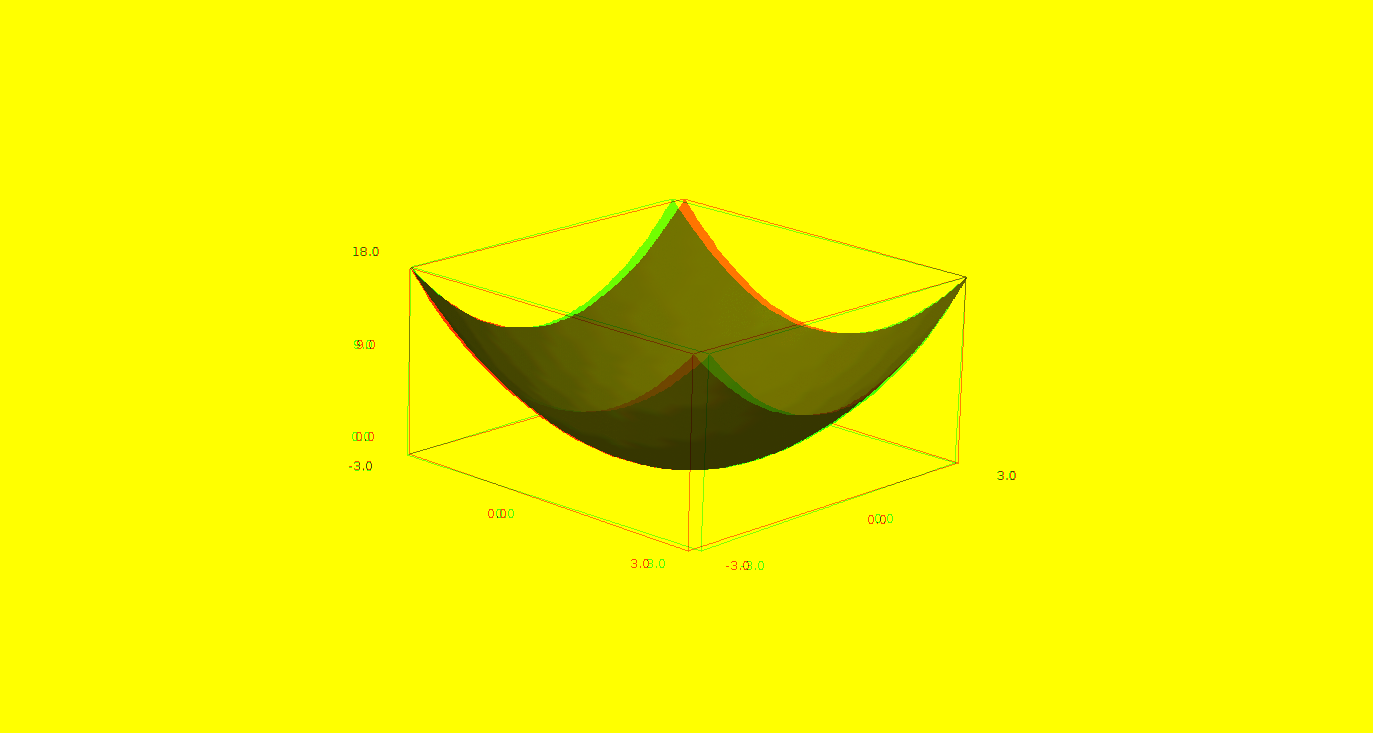
\includegraphics[width=15cm]{pictures_bitmap/coupe.png}
    \end{center}
    À part que l'ordinateur l'a dit, est-ce qu'on peut comprendre pourquoi le graphe de la fonction $x^2+y^2$ ressemble à un bol ? En coordonnées cylindriques, le graphe s'écrit
    \begin{equation}
        z=r^2.
    \end{equation}
    Donc il se fait que plus on s'éloigne du point $(0,0)$ dans le plan $XY$, plus le graphe va monter. Et il monte à quelle vitesse ? Il monte à la vitesse $r^2$. Il s'agit donc de dessiner la fonction $z=r^2$ dans le plan et de la «faire tourner».

\end{example}

% This is part of Mes notes de mathématique
% Copyright (c) 2006-2016
%   Laurent Claessens, Carlotta Donadello
% See the file fdl-1.3.txt for copying conditions.
 
%+++++++++++++++++++++++++++++++++++++++++++++++++++++++++++++++++++++++++++++++++++++++++++++++++++++++++++++++++++++++++++
\section{Courbes de niveau}
%+++++++++++++++++++++++++++++++++++++++++++++++++++++++++++++++++++++++++++++++++++++++++++++++++++++++++++++++++++++++++++

Une technique utile pour se faire une idée de la forme d'une fonction en trois dimensions est de tracer les \defe{courbes de niveau}{courbe de niveau}. La courbe de niveau de hauteur $h$ est la courbe dans le plan donnée par l'équation
\begin{equation}
    f(x,y)=h.
\end{equation}

\begin{example}

    Dessinons par exemple les courbes de niveau de la fonction
    \begin{equation}
        f(x,y)=x+y+2.
    \end{equation}
    La courbe de niveau $h$ est donnée par l'équation $x+y+2=h$, c'est à dire
    \begin{equation}
        y(x)=-x+h-2.
    \end{equation}
    Par conséquent la courbe de niveau de hauteur $0$ est $y=-x-2$, celle de hauteur $5$ est $y=-x+3$, etc.
    
    Nous pouvons également nous aider de Sage pour ce faire :
    \begin{verbatim}
----------------------------------------------------------------------
| Sage Version 4.6.1, Release Date: 2011-01-11                       |
| Type notebook() for the GUI, and license() for information.        |
----------------------------------------------------------------------
sage: f(x,y)=x+y+2
sage: var('h')                   
h
sage: niveau(h,x)=solve(f(x,y)==h,y)[0].rhs()
sage: g1(x)=niveau(1,x)
sage: g1
x |--> -x - 1
    \end{verbatim}
    Ici la fonction \verb+g1+ est la courbe de niveau $1$. 

    Si on veut faire tracer une courbe de niveau, Sage peut le faire :
    \begin{verbatim}
        sage: implicit_plot(f(x,y)==1,(x,-3,3),(y,-4,4))
    \end{verbatim}
    Cela tracera la courbe de niveau $h=1$ dans la partie du plan $x\in\mathopen[ -3 , 3 \mathclose]$ et $y\in\mathopen[ -4,4 ,  \mathclose]$.
    
\end{example}

Il est bien entendu possible de créer automatiquement $50$ courbes de niveau et de demander de les tracer toutes sur le même graphe.
\VerbatimInput[tabsize=3]{courbeNiveau.py}

Le résultat est :

\begin{center}
    \ifpdf
        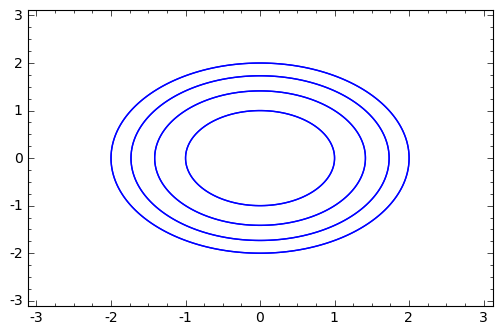
\includegraphics[width=8cm]{niveauCercles.png}
    \else
        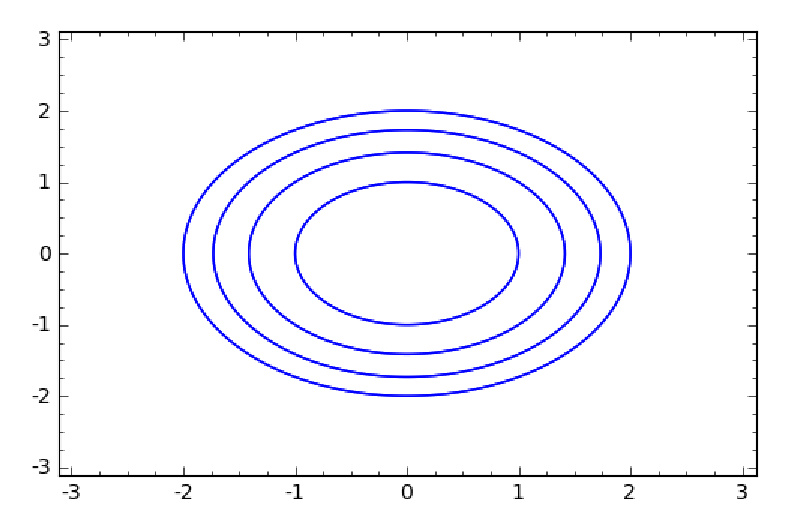
\includegraphics[width=8cm]{niveauCercles.eps}
    \fi
\end{center}
Notez que les courbes sont censées être des cercles : les axes $X$ et $Y$ n'ont pas la même échelle. Vous trouverez sur \href{http://uw.sagenb.org/home/pub/23/}{cette page} tout ce qu'il vous faudra pour créer des courbes de niveau avec Sage.

\begin{example}
    Un exemple plus riche en enseignements est celui de la fonction
    \begin{equation}
        f(x,y)=x^2-y^2.
    \end{equation}
    La courbe de niveau $h$ est donnée par l'équation $x^2-y^2=h$.

    Commençons par $h=0$. Dans ce cas nous avons $(x+y)(x-y)=0$ et par conséquent les courbes de niveau de hauteur zéro sont les deux droites $x+y=0$ et $x-y=0$.

    Voyons ensuite la courbe de niveau $h=1$. Cela est l'équation $x^2-y^2=1$, c'est à dire
    \begin{equation}
        y(x)=\pm\sqrt{x^2-1}.
    \end{equation}
    C'est une fonction qui n'est définie que pour $| x |\geq 1$. Avec $x=1$ nous avons $y=1$. Ensuite, lorsque $x$ grandit, $y$ grandit également, mais la courbe ne peut pas croiser la courbe de niveau $h=0$. Donc, suivant les notations de la figure \ref{LabelFigCQIXooBEDnfK}, la courbe de niveau «part» de $P$ et doit monter sans croiser les diagonales.

 % les figures CQIXooBEDnfK et KGQXooZFNVnW sont générées par le script MBFDooRFPyNW

%The result is on figure \ref{LabelFigCQIXooBEDnfK}. % From file CQIXooBEDnfK
\newcommand{\CaptionFigCQIXooBEDnfK}{La courbe de niveau $h=1$ de $x^2-y^2$. Notez qu'elle est en deux morceaux.}
\input{Fig_CQIXooBEDnfK.pstricks}

%The result is on figure \ref{LabelFigKGQXooZFNVnW}. % From file KGQXooZFNVnW
\newcommand{\CaptionFigKGQXooZFNVnW}{La courbe de niveau $x^2-y^2=-1$.}
\input{Fig_KGQXooZFNVnW.pstricks}

    En ce qui concerne la courbe de niveau $h=-1$, elle correspond à la courbe $y=\pm\sqrt{1+x^2}$ qui est définie pour tous les $x\in\eR$. Le même raisonnement que précédemment nous amène à la figure \ref{LabelFigKGQXooZFNVnW}.

\end{example}

Une autre façon de voir les courbe de niveau est de dire que la courbe de niveau de hauteur $h$ est la projection dans le plan $XY$ de la section du graphe de $f$ par le plan $z=h$.

On peut également définir le graphe de fonctions de trois (ou plus) variables. Le graphe de la fonction $f\colon D\subset\eR^3\to \eR$ est l'ensemble
\begin{equation}
    \big\{ \big( x,y,z,f(x,y,z) \big)\tq (x,y,z)\in D \big\}\subset \eR^4.
\end{equation}
De tels graphes ne peuvent pas être représentés sur une feuille de papier. Il est toutefois possible de définir les ensembles de niveaux :
\begin{equation}
    E_h=\big\{ (x,y,z)\in D\tq  f(x,y,z)=h\big\}.
\end{equation}
Ce sont des surfaces dans $\eR^3$ que l'on peut dessiner.

\begin{example}
    Les surfaces de niveau de la fonction $f(x,y,z)=x^2+y^2+z^2$ sont des sphères. Il n'y a pas de surfaces de niveau pour les «hauteurs» négatives.
\end{example}

\begin{example}
    Considérons la fonction $f(x,y,z)=x^2+y^2-z^2$. En coordonnées cylindrique, cette fonction s'écrit
    \begin{equation}
        f(r,\theta,z)=r^2-z^2.
    \end{equation}
    La surface de niveau $0$ est donnée par l'équation $r=| z |$. Cela fait un cercle à chaque hauteur, dont le rayon grandit linéairement avec la hauteur; le tout est donc un cône. C'est d'ailleurs le cône obtenu par rotation de la courbe de niveau $h=0$ que nous avions obtenue pour la fonction $x^2-y^2$.

    En ce qui concerne les ensembles de niveau positifs, ils sont donnés par
    \begin{equation}
        z=\pm\sqrt{x^2+y^2-h}.
    \end{equation}
    Notez qu'ils ne sont pas définis pour $r\geq h$. Cela pose un petit problème quand on veut le tracer à l'ordinateur :
    \begin{verbatim}
----------------------------------------------------------------------
| Sage Version 4.6.1, Release Date: 2011-01-11                       |
| Type notebook() for the GUI, and license() for information.        |
----------------------------------------------------------------------
sage: var('x,y')
(x, y)
sage: f(x,y)=sqrt(x**2+y**2-3)
sage: F=plot3d(f(x,y),(x,-5,5),(y,-5,5)) 
sage: G=plot3d(-f(x,y),(x,-5,5),(y,-5,5))    
sage: F+G
    \end{verbatim}
Le résultat est\footnote{Encore une fois : ça donne mieux à l'écran, et vous pouvez le faire bouger; je vous encourage à le faire !} :
    \begin{center}
        \ifpdf
            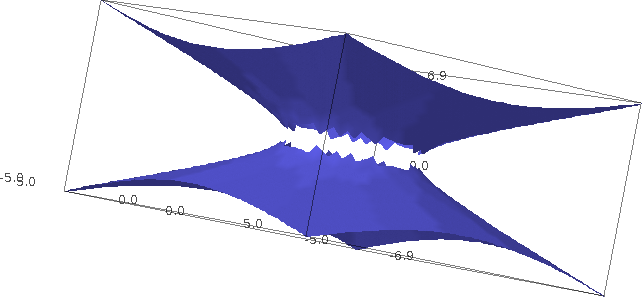
\includegraphics[width=15cm]{AdSmauvais.png}
        \else
            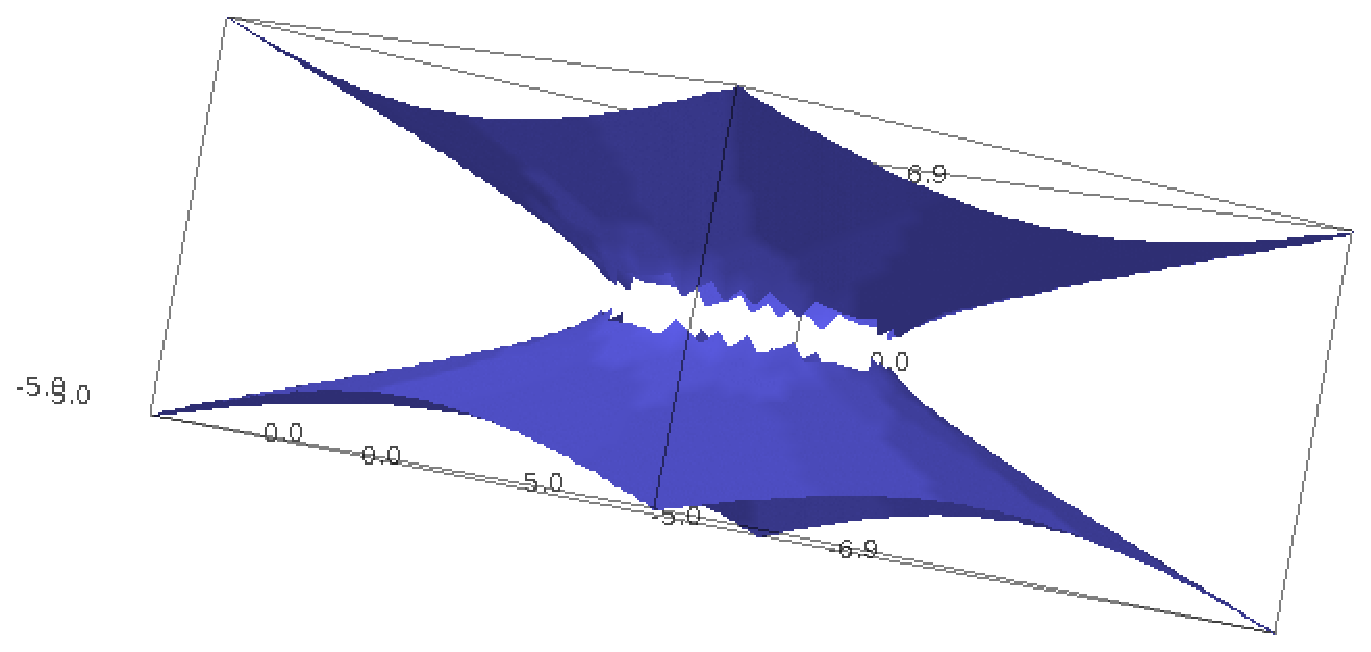
\includegraphics[width=15cm]{AdSmauvais.eps}
        \fi
    \end{center}
    On voit qu'il y a un grand trou au centre correspondant aux $z$ proches de zéro. Or d'après l'équation, il n'en est rien : en $z=0$ il y a bel et bien tout un cercle. Afin d'obtenir une meilleur image, il faut demander de tracer avec un maillage plus fin :
    \begin{verbatim}
----------------------------------------------------------------------
| Sage Version 4.6.1, Release Date: 2011-01-11                       |
| Type notebook() for the GUI, and license() for information.        |
----------------------------------------------------------------------
sage: var('x,y')
(x, y)
sage: f(x,y)=sqrt(x**2+y**2-3)
sage: F=plot3d(f(x,y),(x,-5,5),(y,-5,5),plot_points=300) 
sage: G=plot3d(-f(x,y),(x,-5,5),(y,-5,5),plot_points=300)
sage: F+G
    \end{verbatim}
    Le temps de calcul est un peu plus long, mais le résultat est meilleur :
    \begin{center}
        \ifpdf
            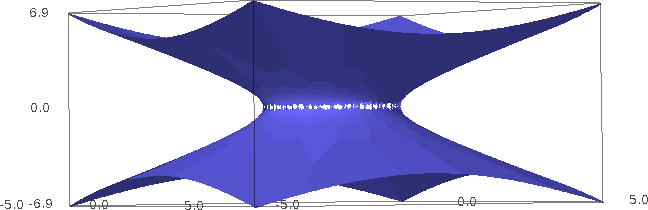
\includegraphics[width=15cm]{AdSbon.png}
        \else
            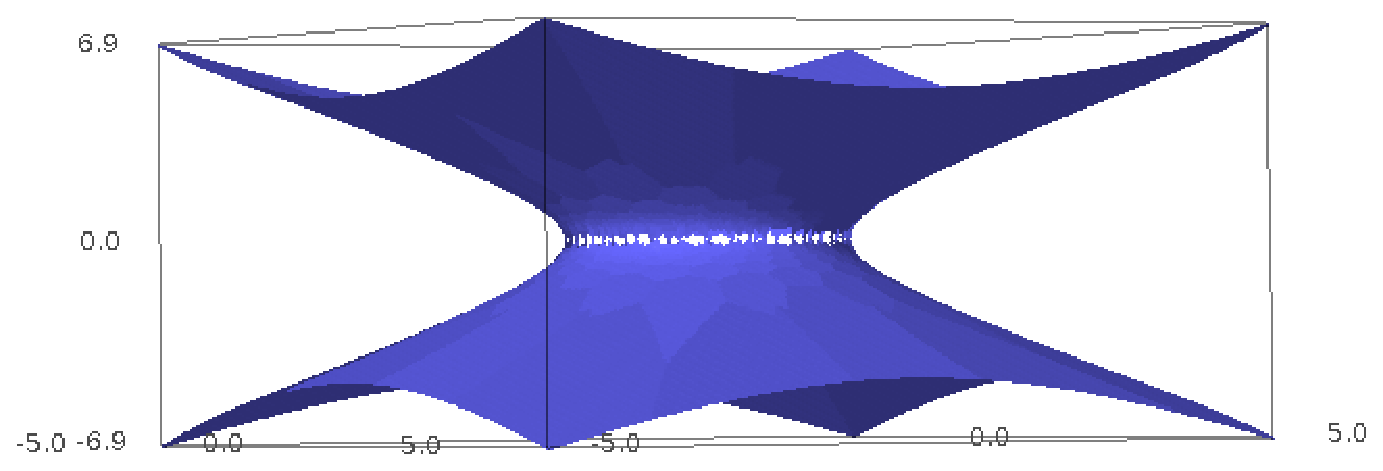
\includegraphics[width=15cm]{AdSbon.eps}
        \fi
    \end{center}
\end{example}

%+++++++++++++++++++++++++++++++++++++++++++++++++++++++++++++++++++++++++++++++++++++++++++++++++++++++++++++++++++++++++++
%\section{Calcul de limites}
%+++++++++++++++++++++++++++++++++++++++++++++++++++++++++++++++++++++++++++++++++++++++++++++++++++++++++++++++++++++++++++

%Incidemment, le lemme \ref{Def_diff2} nous donne une nouvelle technique pour calculer des limites à plusieurs variables, similaire à celle du développement asymptotique expliquée dans la section \ref{SecTaylorR}.

%En effet, la formule \eqref{def_diff2} nous permet d'écrire $f(x)$ sous la forme
%\begin{equation}
%	f(x)=f(a)+df(a).(x-a)+\sigma_f(a,x)\| x-a \|
%\end{equation}
%où la fonction $\sigma_f$ satisfait $\lim_{x\to a}\sigma_f(a,x)=0$. Ici, $x$ et $a$ sont des éléments de $\eR^m$.

%++++++++++++++++++++++++++++++++++++++++++++++++++++++++++++++++++++++++++++++++++++++++
\section{Fonctions de classe $\mathcal{C}^1$}
%++++++++++++++++++++++++++++++++++++++++++++++++++++++++++++++++++++++++++++++++++++++++++++++++++++++++++++++++++++++++++++++

Soit $f$ une fonction différentiable de $U$, ouvert de $\eR^m$, dans $\eR^n$. L'application différentielle de $f$ est une application  de $\eR^m$ dans $\mathcal{L}(\eR^m, \eR^n)$ 
\begin{equation}
  \begin{array}{rccc}
    df : & \eR^m & \to & \mathcal{L}(\eR^m, \eR^n)\\
& a& \mapsto & df_a.
  \end{array}
\end{equation}
Nous savons que $\mathcal{L}(\eR^m, \eR^n)$ est un espace vectoriel normé avec la définition \ref{DefDQRooVGbzSm}. Si $T$ est un élément dans $\mathcal{L}(\eR^m, \eR^n)$ alors la norme de $T$ est définie par 
\[
\|T\|_{\mathcal{L}(\eR^m, \eR^n)}=\sup_{x\in\eR^m} \frac{\|T(x)\|_n}{\|x\|_m}=\sup_{\begin{subarray}{l}
    x\in\eR^m\\
\|x\|_m\leq 1
  \end{subarray}} \|T(x)\|_n.
\]

Lorsqu'il existe un $M>0$ tel que $\| df(a) \|_{\aL(\eR^m,\eR^n)}<M$ pour tout $a$ dans $U$, nous disons que la différentielle de $f$ est \defe{bornée}{bornée!différentielle} sur $U$.

\begin{definition}
	La fonction $f$ est dite \defe{de classe $\mathcal{C}^1$}{fonction!de classe  $\mathcal{C}^1$} de $U\subset\eR^m$  dans $\eR^n$ si son application différentielle $df$ est continue de $\eR^m$ dans $\mathcal{L}(\eR^m, \eR^n)$. Nous écrivons $f\in\mathcal{C}^1(U,\eR^n)$\nomenclature{$\aC^1(U,\eR^n)$}{Les applications une fois continument dérivables}.
\end{definition}

\begin{proposition}		\label{PropDerContCun}
	Une fonction \( f\colon U\to \eR^n\) où \( U\) est ouvert dans \( \eR^m\) est de classe \( C^1\) si et seulement si les dérivées partielles de $f$ existent et sont continues.
\end{proposition}

\begin{proof}
	Supposons que les dérivées partielles de $f$ existent et sont continues. Nous savons alors déjà par la proposition \ref{Diff_totale} que la fonction $f$ est différentiable et qu'elle s'exprime sous la forme
	\[
		df_a(h)=\sum_{i=1}^{m}\partial_if (a)h_i, \qquad \forall a \in U,\,\forall h\in\eR^m.
	\]
	Pour montrer que $df$ est continue, nous devons montrer que la quantité $\| df(x)-df(a) \|_{\aL(\eR^m,\eR^n)}$ peut être rendue arbitrairement petite si $\| x-a \|_m$ est rendu petit. Nous avons
	\begin{equation}
		\begin{aligned}
			\| df_x-df_a \|_{\aL}&=\sup_{\| h \|=1}\| df_x(h)-df_a(h) \|\\
			&=\sup_{\| h \|_m=1}\left\|\sum_{i=1}^{m}\left(\partial_if (x)-\partial_if (a)\right)h_i\right\|_n\leq\\
			&\leq\sup_{\| h \|_m=1}\sum_{i=1}^{m} \left\|\left(\partial_if (x)-\partial_if (a)\right)\right\|_n|h_i|\leq\\
			&\leq\sup_{\| h \|_m=1} \|h\|_\infty\sum_{i=1}^{m} \left\|\left(\partial_if (x)-\partial_if (a)\right)\right\|_n\\
			&\leq \sum_{i=1}^m\| \partial_if(x)-\partial_if(a) \|.
		\end{aligned}
	\end{equation}
	Dans ce calcul, nous avons utilisé le fait que si $\| h \|_m\leq 1$, alors $\| h \|_{\infty}\leq 1$. Étant donné la continuité de $\partial_if$, la dernière ligne peut être rendue arbitrairement petite lorsque $x$ est proche e $a$.

Supposons maintenant que $f$ soit dans $\mathcal{C}^1(U,\eR^n)$. Alors 
\[
\left\|\partial_if (x)-\partial_if (a)\right\|_n= \left\|df(x).e_i-df(a).e_i\right\|_n \leq  \left\|df(x)-df(a)\right\|_{\mathcal{L}(\eR^m,\eR^n)},
\]  
la continuité de $df$ implique donc celle de $\partial_i f$ pour tout $i$ dans $\{1,\ldots,m\}$.
\end{proof}
\begin{proposition}
  Soient $U$ un ouvert de $\eR^m$ et $V$ un ouvert de $\eR^n$. Soient $f: U\to V$  dans $\mathcal{C}^1(U,V)$ et $g: V \to \eR^p$ dans $\mathcal{C}^1(V,\eR^n)$.  Alors la fonction composée $g\circ f: U\to \eR^p $ est dans $\mathcal{C}^1(U,\eR^p)$.
\end{proposition}
\begin{proof} On fixe $a$ dans $U$ 
  \begin{equation}
    \begin{aligned}
     \big\|d(g\circ f)(x)&-d(g\circ f)(a)\big\|_{\mathcal{L}(\eR^m,\eR^p)}\\
     &=\left\|dg(f(x))\circ df(x)-dg(f(a))\circ df(a)\right\|_{\mathcal{L}(\eR^m,\eR^p)}\leq\\
&\leq \left\|\left(dg(f(x))-dg(f(a))\right)\circ df(x)\right\|_{\mathcal{L}(\eR^m,\eR^p)}+\\
&\quad+ \left\|dg(f(a))\circ \left(df(x)-df(a)\right)\right\|_{\mathcal{L}(\eR^m,\eR^p)}\leq\\
&\leq \left\|dg(f(x))-dg(f(a))\right\|_{\mathcal{L}(\eR^n,\eR^p)}\left\| df(x)\right\|_{\mathcal{L}(\eR^m,\eR^n)}+\\
&\quad+ \left\|dg(f(a))\right\|_{\mathcal{L}(\eR^n,\eR^p)}\left\| df(x)-df(a)\right\|_{\mathcal{L}(\eR^n,\eR^p)}.\\
    \end{aligned}
  \end{equation}
On peut conclure en passant à la limite $x\to a$ parce que les fonctions $f$, $g$, $df$ et $dg$ sont continues, de telle sorte que
\begin{equation}
	\begin{aligned}[]
		\lim_{x\to a} dg\big( f(x) \big)=dg\big( f(a) \big)\\
		\lim_{x\to a} df(x)=df(a).
	\end{aligned}
\end{equation}
\end{proof}

\begin{remark}
  On peut prouver le même résultat en utilisant la continuité de l'application bilinéaire 
\begin{equation}
  \begin{array}{rccc}
    \circ : & \mathcal{C}^1(U,V)\times\mathcal{C}^1(V,\eR^p)  & \to & \mathcal{L}(U, \eR^p)\\
& (T,S)& \mapsto & T\circ S.
  \end{array}
\end{equation}
\end{remark}
%+++++++++++++++++++++++++++++++++++++++++++++++++++++++++++++++++++++++++++++++++++++++++++++++++++++++++++++++++++++++++++
\section{Dérivée directionnelle de fonctions composées}		\label{SecDerDirFnComp}
%+++++++++++++++++++++++++++++++++++++++++++++++++++++++++++++++++++++++++++++++++++++++++++++++++++++++++++++++++++++++++++

Étant donné que nous allons voir en détail la différentielle de fonctions composées à la proposition \ref{PropDiffCompose}, nous n'allons pas rentrer dans tous les détail ici.

Nous savons déjà comment dériver les fonctions composées de $\eR$ dans $\eR$. Si nous avons deux fonctions $f\colon \eR\to \eR$ et $u\colon \eR\to \eR$, nous formons la composée $\varphi=f\circ u\colon \eR\to \eR$ dont la dérivée vaut
\begin{equation}
	\varphi'(a)=f'\big( u(a) \big)u'(a).
\end{equation}

Considérons maintenant le cas un peu plus compliqué des fonctions $f\colon \eR\to \eR$ et $u\colon \eR^2\to \eR$, et de la composée
\begin{equation}
	\begin{aligned}
		\varphi\colon \eR^2&\to \eR \\
		\varphi(x,y)&= f\big( u(x,y) \big). 
	\end{aligned}
\end{equation}
Afin de calculer la dérivée partielle de $\varphi$ par rapport à $x$, nous admettons que pour tout $a$, $b$ et $t$, il existe $c\in\mathopen[ a , a+t \mathclose]$ tel que
\begin{equation}
	u(a+t,b)=u(a,b)+t\frac{ \partial u }{ \partial x }(c,b).
\end{equation}
Cela est une généralisation immédiate du théorème \ref{ThoAccFinis}. Nous devons calculer
\begin{equation}		\label{EqPremPasDiffxvp}
	\frac{ \partial \varphi }{ \partial x }(a,b)=\lim_{t\to 0} \frac{ \varphi(a+t,b)-\varphi(a,b) }{ t }=\lim_{t\to 0} \frac{ f\big( u(a+t,b) \big)-g\big( u(a,b) \big) }{ t }.
\end{equation}
Étant donné l'hypothèse que nous avons faite sur $u$, nous avons
\begin{equation}
	f\big( u(a+t,b) \big)=f\big( u(a,b)+t\frac{ \partial u }{ \partial x }(c,b) \big).
\end{equation}
En utilisant le théorème des accroissements finis pour $f$, nous avons un point $d$ entre $u(a,b)$ et $u(a,b)+t\frac{ \partial u }{ \partial x }(c,b)$ tel que
\begin{equation}
	f\big( u(a,b)+t\frac{ \partial u }{ \partial x }(c,b) \big)=f\big( u(a,b) \big)+t\frac{ \partial u }{ \partial x }(c,b)f'(d).
\end{equation}
Le numérateur de \eqref{EqPremPasDiffxvp} devient donc
\begin{equation}
	t\frac{ \partial u }{ \partial x }(c,b)f'(d).
\end{equation}
Certes les points $c$ et $d$ sont inconnus, mais nous savons que $c$ est entre $a$ et $a+t$ ainsi que $d$ se situe entre $u(a,b)$ et $u(a,b)+t\frac{ \partial u }{ \partial x }(c,b)$. Lorsque nous prenons la limite $t\to 0$, nous avons donc $\lim_{t\to 0} c=a$ et $\lim_{t\to 0} d=u(a,b)$. Nous avons alors
\begin{equation}
	\lim_{t\to 0} \frac{ t\frac{ \partial u }{ \partial x }(c,b)f'(d) }{ t }=\frac{ \partial u }{ \partial x }(a,b)f'\big( u(a,b) \big).
\end{equation}
La formule que nous avons obtenue (de façon pas très rigoureuse) est
\begin{equation}
	\frac{ \partial  }{ \partial x }f\big( u(x,y) \big)=\frac{ \partial u }{ \partial x }(x,y)f'\big( u(x,y) \big).
\end{equation}

Prenons maintenant un cas un peu plus compliqué où nous voudrions savoir les dérivées partielles de la fonction $\varphi$ donnée par
\begin{equation}
	\varphi(x,y,z)=f\big( u(x,y),v(x,y,z) \big)
\end{equation}
où $f\colon \eR^2\to \eR$, $u\colon \eR^2\to \eR$ et $v\colon \eR^3\to \eR$. 

Commençons par la dérivée partielles par rapport à $z$. Étant donné que $\varphi$ ne dépend de $z$ que via la seconde entrée de $f$, il est normal que seule la dérivée partielle de $f$ par rapport à sa seconde entrée arrive dans la formule :
\begin{equation}
	\frac{ \partial \varphi }{ \partial z }(x,y,z)=\frac{ \partial f }{ \partial v }\big( u(x,y),v(x,y,z) \big)\frac{ \partial v }{ \partial z }(x,y,z).
\end{equation}
La dérivée partielle par rapport à $y$ demande de tenir compte en même temps de la façon dont $f$ varie avec sa première entrée et la façon dont elle varie avec sa seconde entrée; cela nous fait deux termes :
\begin{equation}
	\frac{ \partial \varphi }{ \partial y }(x,y,z)=\frac{ \partial f }{ \partial u }\big( u(x,y),v(x,y,z) \big)\frac{ \partial u }{ \partial y }(x,y)+\frac{ \partial f }{ \partial v }\big( u(x,y),v(x,y,z) \big)\frac{ \partial v }{ \partial y }(x,y,z).
\end{equation}


Cette formule a une interprétation simple. Lançons un caillou du sommet d'une falaise. Son mouvement est une chute libre avec une vitesse initiale horizontale :
\begin{subequations}
	\begin{numcases}{}
		x(t)=v_0t\\
		y(t)=h_0-\frac{ gt^2 }{ 2 }
	\end{numcases}
\end{subequations}
où $v_0$ est la vitesse initiale horizontale et $h_0$ est la hauteur de la falaise. Si nous sommes intéressés à la distance entre le caillou et le bas de la falaise (point $(0,0)$), le théorème de Pythagore nous dit que
\begin{equation}
	d(t)=\sqrt{x^2(t),y^2(t)}.
\end{equation}
Pour trouver la variation de la distance par rapport au temps il faut savoir de combien la distance varie lorsque $x$ varie et multiplier par la variation de $x$ par rapport à $t$, et puis faire la même chose avec $y$.

\begin{theorem}		\label{ThoDerDirFnComp}
	Soit $g\colon \eR^m\to \eR^n$ une fonction différentiable en $a$, et $f\colon \eR^n\to \eR^p$ une fonction différentiable en $g(a)$. Si nous définissons $\varphi(x)=(f\circ g)(x)$, alors pour tout $i=1,\ldots,m$, nous avons
	\begin{equation}
		\frac{ \partial \varphi }{ \partial x_i }(a)=\sum_{k=1}^n\frac{ \partial f }{ \partial y_k }\big( g(a) \big)\frac{ \partial g }{ \partial x_i }
	\end{equation}
	où $\frac{ \partial f }{ \partial y_k }$ dénote la dérivée partielle de $f$ par rapport à sa $k$-ième variable.
\end{theorem}

Donnons un exemple d'utilisation de cette formule. Si
\begin{equation}
	\begin{aligned}[]
		g\colon \eR^2\to \eR^3\\
		f\colon \eR^3\to \eR,
	\end{aligned}
\end{equation}
nous avons $\varphi\colon \eR^2\to \eR$. Les dérivées partielles de $\varphi$ sont données par les formules
\begin{equation}
	\frac{ \partial \varphi }{ \partial x }(x,y)=\frac{ \partial f }{ \partial x_1 }\big( g(x,y) \big)\frac{ \partial g_1 }{ \partial x }(x,y)+\frac{ \partial f }{ \partial x_2 }\big( g(x,y) \big)\frac{ \partial g_2 }{ \partial y }(x,y)+\frac{ \partial f }{ \partial x_3 }\big( g(x,y) \big)\frac{ \partial g_3 }{ \partial x }(x,y)
\end{equation}
et
\begin{equation}
	\frac{ \partial \varphi }{ \partial y }(x,y)=\frac{ \partial f }{ \partial x_1 }\big( g(x,y) \big)\frac{ \partial g_1 }{ \partial y }(x,y)+\frac{ \partial f }{ \partial x_2 }\big( g(x,y) \big)\frac{ \partial g_2 }{ \partial y }(x,y)+\frac{ \partial f }{ \partial x_3 }\big( g(x,y) \big)\frac{ \partial g_3 }{ \partial y }(x,y)
\end{equation}
Notez que les dérivées de $\varphi$ et des composantes de $g$ sont calculées en $(x,y)$, tandis que celles de $f$ sont calculées en $g(x,y)$.

%++++++++++++++++++++++++++++++++++++++++++++++++++++++++++++++++++++++++++++++++++++++++++++++++++++++++++++++++++++++
\section{Théorèmes des accroissements finis}		\label{SecThoAccrsFinis}
%++++++++++++++++++++++++++++++++++++++++++++++++++++++++++++++++++++++++++++++++++++++++++++++++++++++++++++++++++++++

Nous avons déjà démontré (lemme \ref{LemdfaSurLesPartielles}) que si $f$ est différentiable au point $x$ alors  $df_x(u)=\partial_uf(x)$. Une importante conséquence est le théorème des accroissements finis
\begin{theorem}[Accroissements finis, inégalité de la moyenne]\label{val_medio_2}
   Soit $U$ un ouvert dans $\eR^m$ et soit $f:U\to\eR^n$ une fonction différentiable. Soient $a$ et $b$ deux point dans $U$, $a\neq b$, tels que le segment $[a,b]$ soit contenu dans $U$. Alors
   \begin{equation}
        \|f(b)-f(a)\|_n\leq \sup_{x\in[a,b]}\|df(x)\|_{\mathcal{L}(\eR^m,\eR^n)}\|b-a\|_m.
   \end{equation}
\end{theorem}
\index{application!différentiable}
\index{inégalité!de la moyenne}
\index{théorème!accroissements finis!forme générale}

\begin{proof}
 On utilise le théorème \ref{val_medio_1} et le fait que 
\[
\|\partial_u f(x)\|_n\leq \|df(x)\|_{\mathcal{L}(\eR^m,\eR^n)}\|u\|_m,
\]
pour tout $u$ dans $\eR^m$.
\end{proof}

La proposition suivante est une application fondamentale du théorème des accroissements finis \ref{val_medio_2}.
\begin{proposition}		\label{PropAnnulationEtConstance}
	Soit $U$ un ouvert connexe par arcs de $\eR^m$ et une fonction $f\colon U\to \eR^n$. Les conditions suivantes sont équivalentes :
	\begin{enumerate}
		\item\label{ItemPropCstDiffZeroi}
			$f$ est constante;
		\item\label{ItemPropCstDiffZeroii}
			$f$ est différentiable et $df(a)=0$ pour tout $a\in U$;
		\item\label{ItemPropCstDiffZeroiii}
			les dérivées partielles $\partial_1f,\ldots,\partial_mf$ existent et sont nulles sur $U$.
	\end{enumerate}
\end{proposition}
\index{connexité!par arc!fonction différentiable}
\index{différentiabilité}

\begin{proof}
	Nous allons démonter les équivalences en plusieurs étapes. D'abord \ref{ItemPropCstDiffZeroi} $\Rightarrow$ \ref{ItemPropCstDiffZeroii}, puis \ref{ItemPropCstDiffZeroii} $\Rightarrow$ \ref{ItemPropCstDiffZeroiii}, ensuite \ref{ItemPropCstDiffZeroiii} $\Rightarrow$ \ref{ItemPropCstDiffZeroii} et enfin \ref{ItemPropCstDiffZeroii} $\Rightarrow$ \ref{ItemPropCstDiffZeroi}.

	Commençons par montrer que la condition \ref{ItemPropCstDiffZeroi} implique la condition \ref{ItemPropCstDiffZeroii}. Si $f(x)$ est constante, alors la condition \eqref{EqCritereDefDiff} est vite vérifiée en posant $T(h)=0$.

	Afin de voir que la condition \ref{ItemPropCstDiffZeroii} implique la condition \ref{ItemPropCstDiffZeroiii}, remarquons d'abord que la différentiabilité de $f$ implique que les dérivées partielles existent (proposition \ref{diff1}) et que nous avons l'égalité $df(a).u=\sum_iu_i\partial_if(a)$ pour tout $u\in\eR^m$ (lemme \ref{LemdfaSurLesPartielles}). L'annulation de $\sum_iu_i\partial_if(a)$ pour tout $u$ implique l'annulation des $\partial_if(a)$ pour tout $i$.

	Prouvons maintenant que la propriété \ref{ItemPropCstDiffZeroiii} implique la propriété \ref{ItemPropCstDiffZeroii}. D'abord, par la proposition \ref{Diff_totale}, l'existence et la continuité des dérivées partielles $\partial_if(a)$ implique la différentiabilité de $f$. Ensuite, la formule $df(a).u=\sum_i u_i\partial_if(a)$ implique que $df(a)=0$. 
	
	
	Il reste à montrer que \ref{ItemPropCstDiffZeroii} implique la condition \ref{ItemPropCstDiffZeroi}, c'est à dire que l'annulation de la différentielle implique la constance de la fonction. C'est ici que nous allons utiliser le théorème des accroissements finis. En effet, si $a$ et $b$ sont des points de $U$, le théorème \ref{val_medio_2} nous dit que
	\begin{equation}
		\|f(b)-f(a)\|_n\leq \sup_{x\in[a,b]}\|df(x)\|_{\mathcal{L}(\eR^m,\eR^n)}\|b-a\|_m.
	\end{equation}
	Mais $\| df(x) \|=0$ pour tout $x\in U$, donc ce supremum est nul et $f(b)=f(a)$, ce qui signifie la constance de la fonction.
\end{proof}

%\begin{proof}
%  \begin{itemize}
%  \item Le théorème \ref{val_medio_2} nous dit que si la différentielle de $f$ est nulle alors $f$ est constante sur chaque segment contenu dans $U$. Cela nous dit que $f$ est constante sur chaque boule contenue dans $U$, donc $f $ est localement constante. Il est possible de démontrer que toute fonction localement constante sur un connexe est constante.  
%\item Si toutes les dérivées partielles $\partial_1 f, \ldots, \partial_m f $ existents et sont identiquement nulles sur $U$ alors $f$ est différentiable et sa différentielle est identiquement nulle. On utilise la première partie de la preuve pour conclure. 
%  \end{itemize}
%\end{proof}

%+++++++++++++++++++++++++++++++++++++++++++++++++++++++++++++++++++++++++++++++++++++++++++++++++++++++++++++++++++++++++++
\section{Fonctions Lipschitziennes}
%+++++++++++++++++++++++++++++++++++++++++++++++++++++++++++++++++++++++++++++++++++++++++++++++++++++++++++++++++++++++++++

\begin{InternalLinks}
    La notion de Lipschitz est utilisée pour définir la stabilité d'un problème, définition \ref{DEFooYIFAooSJbMkC}.
\end{InternalLinks}

\begin{definition}      \label{DEFooQHVEooDbYKmz}
    Soient \( (E,d_E)\) et \( (F,d_F)\) deux espaces métriques\footnote{Pour rappel, les espaces métriques sont définis par la définition \ref{DefMVNVFsX} et le théorème \ref{ThoORdLYUu}; je précise que nous ne supposons pas que \( E\) soit vectoriel; en particulier il peut être un ouvert de \( \eR^n\).}, \( f\colon E\to F\) une application et un réel \( k\) strictement positif. Nous disons que \( f\) est \defe{Lipschitzienne}{Lipschitzienne} de constante $k$ sur \( E\) si pour tout \( x,y\in E\),
    \begin{equation}
        d_F\big( f(x)-f(y) \big)\leq kd_E(x,y).
    \end{equation}
\end{definition}
%TODO : faire la chasse aux endroits où cette définition devrait être référencée.
Soit \( f\) une fonction \( k\)-Lipschitzienne. Si \( y\in \overline{ B(x,\delta)}\) alors \( \| x-y \|\leq\delta\) et donc \( \big\| f(x)-f(y) \big\|\leq k\delta\). Cela signifie que la condition Lipschitz pour s'énoncer en termes de boules fermées par
\begin{equation}    \label{EqDZvtUbn}
    f\big( \overline{ B(x,\delta) } \big)\subset \overline{  B\big( f(x),k\delta \big) }
\end{equation}
tant que \( \overline{ B(x,\delta) } \) est contenue dans le domaine sur lequel \( f\) est Lipschitz.

\begin{proposition}
  Soit  $U$ un ouvert convexe  de $\eR^m$, et soit $f:U\to \eR^n$ une fonction différentiable. La fonction $f$ est Lipschitzienne sur $U$ si et seulement si $df$ est bornée sur $U$.  
\end{proposition}
\begin{proof}
	Le fait que l'application différentielle $df$ soit bornée signifie qu'il existe un $M>0$ dans $\eR$ tel que $\|df_a\|_{\mathcal{L}(\eR^m,\eR^n)}\leq M$, pour tout $a$ dans $U$. Si cela est le cas, alors le théorème \ref{val_medio_2} et la convexité\footnote{La convexité de $U$ sert à assurer que la droite reliant $a$ à $b$ est contenue dans $U$; c'est ce que nous utilisons dans la démonstration du théorème \ref{val_medio_2}.} de $U$ impliquent évidemment que $f$ est de Lipschitz de constante plus petite ou égale à $M$.
	
	Inversement, si $f$ est Lipschitz de constante $k$, alors pour tout $a$ dans $U$ et $u$ dans $\eR^m$ on a 
	\[
		\left\|\frac{f(a+tu)-f(a)}{t}\right\|_n\leq k \|u\|_m,
	\]   
	En passant à la limite pour $t\to 0$ on a 
	\[
		\|\partial_u f(a)\|_n=\|df_a(u)\|_n\leq k \|u\|_m,
	\]
	donc la norme de $df_a$ est majorée par $k$ pour tout $a$ dans $U$.   
\end{proof}

Notez cependant qu'une fonction peut être Lipschitzienne sans être différentiable.

\begin{proposition} \label{PropFZgFTEW}
    Une fonction Lipschitzienne \( f\colon \eR\to \eR\) est continue.
\end{proposition}

\begin{proof}
    Nous utilisons la caractérisation de la continuité donnée par le théorème \ref{ThoESCaraB}. Prouvons donc la continuité en \( a\in \eR\). Pour tout \( x\) nous avons
    \begin{equation}
        \big| f(x)-f(a) \big|\leq k| x-a |.
    \end{equation}
    Si \( \epsilon>0\) est donné, il suffit de prendre \( \delta<\frac{ \epsilon }{ k }\) pour avoir
    \begin{equation}
        \big| f(x)-f(a) \big|\leq k\frac{ \epsilon }{ k }=\epsilon.
    \end{equation}
    Donc \( f\) est continue en \( a\).
\end{proof}

\begin{definition}      \label{DefJSFFooEOCogV}
    Une fonction 
    \begin{equation}
        \begin{aligned}
            f\colon \eR^n\times R^m&\to \eR^p \\
            (t,y)&\mapsto f(t,y) 
        \end{aligned}
    \end{equation}
    est \defe{localement Lipschitz}{Lipschitz!localement} en \( y\) au point \( (t_0,y_0)\) si il existe des voisinages \( V\) de \( t_0\) et \( W\) de \( y_0\) et un nombre \( k>0\) tels que pour tout \( (t,y)\in V\times W\) on ait
    \begin{equation}
        \big\| f(t_0,y_0)-f(t,y) \big\|\leq k\| y-y_0 \|.
    \end{equation}
    La fonction est localement Lipschitz sur un ouvert \( U\) de \( \eR^n\times \eR^m\) si elle est localement Lipschitz en chaque point de \( U\).
\end{definition}

\begin{proposition}     \label{PropGIBZooVsIqfY}
    Si \( f\) et \( g\) sont deux fonctions localement Lipschitz alors \( f+g\) l'est.
\end{proposition}

\begin{proof}
    Il s'agit d'un simple calcul avec une majoration standard :
    \begin{subequations}
        \begin{align}
            \| (f+g)(t_0,y_0)-(f+g)(t,y) \|&\leq \|  f(t_0,y_0)-f(t,y)  \|+\| g(t_0,y_0)-g(t,y) \|\\
            &\leq k_f\| y-y_0 \|+k_g\| y-y_0 \|\\
            &=(k_f+k_g)\| y-y_0 \|.
        \end{align}
    \end{subequations}
\end{proof}

\begin{lemma}   \label{LemCFZUooVqZmpc}
    La fonction donné par
    \begin{equation}
        f(t, (x,y) )=xy
    \end{equation}
    est localement Lipschitz en tout point.
\end{lemma}

\begin{proof}
    Nous avons la majoration classique
    \begin{equation}
        | f\big(t,(x_0,y_0)\big)-f\big( t,(x,y) \big) |=| x_0y_0-xy |\leq| x_0y_0-x_0y |+| x_0y-xy |\leq | x_0 || y_0-y |+| y || x_0-x |.
    \end{equation}
    Vu que nous parlons de fonction \emph{localement Lipschitzienne}, nous pouvons majorer \( | y |\) et \( | x_0 |\) par un même nombre \( k\) dans un voisinage de \( (x_0,y_0)\). Cela donne
    \begin{equation}
        | f\big(t,(x_0,y_0)\big)-f\big( t,(x,y) \big) |\leq k\big( | y_0-y |+| x_0-x | \big)\leq \sqrt{2}k\| \begin{pmatrix}
            x_0-x    \\ 
            y_0-y    
        \end{pmatrix}\|.
    \end{equation}
    Nous avons utilisé l'équivalence de norme de la proposition \ref{PropLJEJooMOWPNi}\ref{ItemABSGooQODmLNi}.
\end{proof}



%++++++++++++++++++++++++++++++++++++++++++++++++++++++++++++++++++++++++++++++++++++++++
\section{Différentielles d'ordre supérieur}		\label{SecDiffOrdSup}
%++++++++++++++++++++++++++++++++++++++++++++++++++++++++++++++++++++++++++++++++++++++++++++++++++++++++++++++++++++++++++++++
\begin{definition}
	Soit $U$ un ouvert de $\eR^m$ et  $f:U\subset\eR^m\to \eR^n$ une fonction. La fonction $f$ est dite \defe{deux fois différentiable}{différentiable!deux fois} au point $a$ dans $U$,  si $f$ est différentiable dans un voisinage de $a$, et sa différentielle $df$ est différentiable au point $a$ en tant que application de $U$ dans $\mathcal{L}(\eR^m, \eR^n)$.  

La fonction $f$ sera dite deux fois différentiable sur l'ensemble $U$ si elle est deux fois différentiable en chaque point de $U$.

\end{definition}

%--------------------------------------------------------------------------------------------------------------------------- 
\subsection{Identification des espaces d'applications multilinéaires}
%---------------------------------------------------------------------------------------------------------------------------

La différentielle de la différentielle de $f$ est notée 
\[
d(df)(a)=d^2f(a),
\]
et est une application de $U$ dans $\mathcal{L}(\eR^m,\mathcal{L}(\eR^m, \eR^n) )$. Comme on a vu dans la proposition \ref{isom_isom}, l'espace $\mathcal{L}(\eR^m,\mathcal{L}(\eR^m, \eR^n) )$ est isométriquement isomorphe à l'espace $\mathcal{L}(\eR^m\times\eR^m, \eR^n )$. On verra comment cette propriété  est utilisé dans l'exemple \ref{bilin_2diff}.


Soient \( V\) et \( W\) deux espace vectoriel normés de dimension finie et \( \mO\) un ouvert autour de \( x\in V\). D'une part l'espace des applications linéaires \( \aL(V,W)\) est lui-même un espace vectoriel normé de dimension finie, et on peut identifier \(  \aL\big( V,\aL^{(k)}(V,W) \big)\)\nomenclature[Y]{\( \aL^{(n)}(V,W)\)}{L'espace des applications \( n\)-linéaires \( V^n\to W\)} avec \( \aL^{(k+1)}(V,W)\), ce qui nous permet de dire que la \( k\)\ieme\ différentielle est une application
\begin{equation}
    d^kf\colon \mO\to \aL^{(k)}(V,W).
\end{equation}
Plus précisément, l'identification se fait de la façon suivante : si \( \omega\in \aL\big( V,\aL^{(k)}(V,W) \big)\), alors \( \omega\) vu dans \( \aL^{(k+1)}(V,W)\) est définie par
\begin{equation}
    \omega(u_1,\ldots, u_{k+1})=\omega(u_1)(u_2,\ldots, u_{k+1}).    
\end{equation}

Cela étant posé nous pouvons donner les définition.

%--------------------------------------------------------------------------------------------------------------------------- 
\subsection{Fonctions différentiables plusieurs fois}
%---------------------------------------------------------------------------------------------------------------------------

\begin{definition}[\cite{ZCKMFRg}]  \label{DefPNjMGqy}
    La fonction \( f\colon \mO\subset V\to W\) est
    \begin{enumerate}
        \item
            de classe \( C^0\) si elle est continue,
        \item
            de classe \( C^1\) si \( df\colon \mO\to \aL(V,W)\) est continue,
        \item
            de classe \( C^k\) si \( d^kf\colon \mO\to \aL^{(k)}(V,W)\) est continue,
        \item
            de classe \(  C^{\infty}\) si \( f\) est dans \( \bigcap_{k=0}^{\infty}C^k(V,W)\).
    \end{enumerate}
\end{definition}
\index{application!différentiable}
\index{application!de classe \( C^k\)}

\begin{definition}
    Un \defe{\( C^k\)-difféomorphisme}{difféomorphisme!de classe $C^k$} est une application inversible de classe \( C^k\) dont l'inverse est également de classe \( C^k\).
\end{definition}

\begin{example} \label{ExZHZYcNH}
    Voyons commet la différentielle seconde fonctionne. Soit \( f\in C^2(V,W)\); nous notons \( \varphi=df\colon V\to \aL(V,W)\) et donc nous voulons étudier la fonction
    \begin{equation}
        d\varphi\colon V\to \aL\big( V,\aL(V,W) \big).
    \end{equation}
    Si \( a,u\in V\)  nous avons
    \begin{equation}
        d\varphi_a(u)=\Dsdd{ \varphi(a+tu) }{t}{0}
    \end{equation}
    qui est une dérivée dans \( \aL(V,W)\) -- pas de problèmes : c'est un espace vectoriel normé de dimension finie. Par linéarité, nous pouvons faire entrer l'argument de \( d\varphi_a(u)\) dans la dérivée :
    \begin{subequations}
        \begin{align}
            d\varphi_a(u)v&=\Dsdd{ \varphi(a+tu)v }{t}{0}\\
            &=\Dsdd{ df_{a+tu}(v) }{t}{0}\\
            &=\Dsdd{  \Dsdd{ f(a+tu+sv) }{s}{0}  }{t}{0}\\
            &=\Dsdd{ \frac{ \partial f }{ \partial v }(a+tu) }{t}{0}\\
            &=\frac{ \partial^2f  }{ \partial u\partial v }(a).
        \end{align}
    \end{subequations}
    Par conséquent nous voyons
    \begin{equation}\label{EqQHINNtD}
        \begin{aligned}
            d^2f\colon V&\to \aL^{(2)}(V,W) \\
            d^2f_a(u,v)&=\frac{ \partial^2f  }{ \partial u\partial v }(a). 
        \end{aligned}
    \end{equation}
    
    Dans le cas d'une fonction \( f\colon \eR\to \eR\), nous avons une seule direction et par linéarité de \eqref{EqQHINNtD} par rapport à \( u\) et \( v\), nous avons
    \begin{equation}
        d^2f_a(u,v)=f''(a)uv
    \end{equation}
    où les produits sont des produits usuels dans \( \eR\) et \( f''\) est la dérivée seconde usuelle.
\end{example}


\begin{example}\label{bilin_2diff}
	Soit $B:\eR^m\times \eR^m\to\eR^n$ une application bilinéaire. On définit $f:\eR^m\to\eR^n$ par $f(x)=B(x,x)$. Le lemme \ref{bilin_diff} nous dit que $B$ est différentiable. Cela implique la différentiabilité de $f$. Pour trouver la différentielle de la fonction $f$, nous écrivons $f=B\circ s$ où $s\colon \eR^m\to \eR^m\times\eR^m$ est l'application $s(x)=(x,x)$. En utilisant la règle de différentiation de fonctions composées,
	\begin{equation}
		df(a)=dB\big( s(a) \big)\circ ds(a).
	\end{equation}
	Mais $ds(a).u=(u,u)$ parce que $s(a+h)-s(a)-(h,h)=0$. Par conséquent,
	\begin{equation}		\label{EqdBsaExp}
		df(a).u=dB\big( s(a) \big)(u,u)=B(u,a)+B(a,u)
	\end{equation}
	où nous avons utilisé la formule du lemme \ref{bilin_diff}. La formule \eqref{EqdBsaExp} peut être écrite sous la forme compacte
	\begin{equation}
		df(a)=B(\cdot,a)+B(a,\cdot)
	\end{equation}
	La fonction $df(a)$ ainsi écrite est linéaire par rapport à $a$, donc différentiable. En outre elle coïncide avec sa différentielle, comme on a vu dans le remarque \ref{rk_lin}, au sens que la différentielle de $df$ au point $a$ sera l'application que à chaque $x$ dans $\eR^m$ associe l'application linéaire $B(x,\cdot)+B(\cdot, x)$. On voit bien que $d^2f$ au point $a$ est une application de $\eR^m$ vers l'espace des applications linéaires $\mathcal{L}(\eR^m, \eR^n)$. On peut utiliser d'autre part l'isomorphisme des espaces $\mathcal{L}(\eR^m,\mathcal{L}(\eR^m, \eR^n) )$ et $\mathcal{L}(\eR^m\times\eR^m, \eR^n )$ et dire que, une fois que $a$ est fixé, l'application $d^2f(a)$ est une application bilinéaire sur $\eR^m\times\eR^m$. On écrit alors $d^2f(a)(x,y)=B(x,y)+B(y,x)$.   
\end{example}

Une condition nécessaire et suffisante pour l'existence de la différentielle seconde est la suivante
\begin{proposition}
   Soit $U$ un ouvert de $\eR^m$ et  $f:U\subset\eR^m\to \eR^n$ une fonction. La fonction $f$ est deux fois différentiable au point $a$ si et seulement si les dérivées partielles $\partial_1 f, \ldots, \partial_m f $ sont différentiables en $a$. 
\end{proposition}
Cela veut dire, en particulier, que $f$ est deux fois différentiable si et seulement si ses dérivées partielles secondes, $\partial_i\partial_j f$, pour toute couple d'indices $i,j$  dans $\{1,\ldots, m\}$, existent et sont continues. Pour les différentielles d'ordre supérieur on a la définition suivante.

\begin{proposition}[Dérivées partielles et fonctions \( C^k\)] \label{PropDYKooHvrfGw}
    Soit $U$ un ouvert de $\eR^m$ et  $f:U\subset\eR^m\to \eR^n$. La fonction $f$ est de classe $C^k$ si et seulement si les dérivées partielles $\partial_1 f, \ldots, \partial_m f $ existent et sont de classe $C^{\infty}$. 
\end{proposition}
% TODO : une preuve serait importante.
La différentielle seconde dans l'exemple  \ref{bilin_2diff} est symétrique, c'est à dire que $d^2f(a)(x_1,x_2)=d^2f(a)(x_2,x_1)$. En fait toute différentielle seconde est symétrique.  


\begin{theorem}[Schwarz]\label{Schwarz}
 Soit $U$ un ouvert de $\eR^m$ et  $f:U\subset\eR^m\to \eR^n$ une fonction de classe $\mathcal{C}^2$. Alors, pour toute couple $i,j$ d'indices dans $\{1,\ldots, m\}$ et pour tout point $a$ dans $U$, on a 
\[
\frac{\partial^2 f}{\partial  x_i\partial x_j}(a)=\frac{\partial^2 f}{\partial  x_j\partial x_i}(a).
\]
\end{theorem}
\begin{proof}
  Pour simplifier l'exposition nous nous limitons ici au cas $m=2$. Soit $(h,g)$ un vecteur fixé dans $\eR^2$. Pour tout  $v=(x,y)$ dans $\eR^2$ on note
  \begin{equation}
    \begin{array}{c}
      \Delta_h f(v)=f(v+he_1) -f(v) = f(x+h,y)-f(x,y),\\ 
      \Delta_g f(v)=f(v+ge_2) -f(v) = f(x,y+g)-f(x,y),\\ 
    \end{array}
  \end{equation}
Nous avons
\begin{equation}
  \begin{array}{c}
   \Delta_g   \Delta_h f(v)=\left(f(x+h,y+g)-f(x,y+g)\right)-\left(f(x+h,y)-f(x,y)\right),\\
   \Delta_h   \Delta_g f(v)=\left(f(x+h,y+g)-f(x+h,y)\right)-\left(f(x,y+g)-f(x,y)\right),
  \end{array}
\end{equation}
donc, 
\begin{equation}
  \frac{1}{g} \Delta_g  \left(\frac{1}{h} \Delta_h f(v)\right) = \frac{1}{h} \Delta_h \left(\frac{1}{g} \Delta_g f(v)\right).
\end{equation}
On utilise alors le théorème des accroissements finis
\[
\frac{1}{h} \Delta_h f(v)=\frac{1}{h}\big(f(x+h,y)-f(x,y)\big)=\frac{1}{h}\partial_1f(x+t_1h,y )h=\partial_1f(x+t_1h, y),
\]
pour un certain $t_1$ dans $]0,1[$. De même on obtient 
\[
\frac{1}{g} \Delta_g f(v)= \partial_2 f(x, y+t_2g),
\]
pour un certain $t_2$ dans $]0,1[$. Alors
 \begin{equation}
  \frac{1}{g} \Delta_g  \big(\partial_1f(x+t_1h, y)\big) = \frac{1}{h} \Delta_h \big(\partial_2 f(x, y+t_2g)\big).
\end{equation}
En appliquant encore une fois le théorème des accroissements finis on a
 \begin{equation}
  \partial_2\partial_1f(x+t_1h, y+s_1g) = \partial_1\partial_2 f(x+s_2h, y+t_2g).
\end{equation} 
Il suffit maintenant de passer à la limite pour $(h,g) \to (0,0)$ et de se souvenir du fait que $f$ est $\mathcal{C}^2$ seulement si ses dérivées partielles secondes sont continues pour avoir $\partial_2\partial_1f(v)=\partial_1\partial_2 f(v)$.
\end{proof}
Si $f$ est deux fois différentiable $d^2f(a)$ est l'application bilinéaire associée avec la matrice symétrique
\begin{equation}
 H_f(a)= \begin{pmatrix}
    \partial^2_1f(a)& \ldots& \partial_1\partial_m f(a)\\
    \vdots& \ddots& \vdots\\
    \partial_1\partial_m f(a)&\ldots&\partial^2_1f(a),
  \end{pmatrix}
\end{equation}
Cette matrice est dite la matrice \defe{hessienne}{hessienne} de $f$. 

\begin{example}
  Montrons qu'il n'existe pas de fonctions $f$ de classe $\mathcal{C}^2$ telles que $\partial_xf(x,y)= 5\sin x$ et $\partial_y(x,y)=6x+y$.  Ceci est vite fait en appliquant le théorème de Schwarz, \ref{Schwarz}; ce que nous trouvons est
\[
\partial_y (\partial_xf)= 0\neq \partial_x(\partial_yf)= 6.
\]
Donc, l'existence d'une fonction $f$ de classe $\mathcal{C}^2$ telle que $\partial_x(x,y)= 5\sin x$ et $\partial_yf(x,y)=6x+y$ serait en contradiction avec le théorème.  
\end{example}

%+++++++++++++++++++++++++++++++++++++++++++++++++++++++++++++++++++++++++++++++++++++++++++++++++++++++++++++++++++++++++++
\section{Développement asymptotique, théorème de Taylor}
%+++++++++++++++++++++++++++++++++++++++++++++++++++++++++++++++++++++++++++++++++++++++++++++++++++++++++++++++++++++++++++
\label{AppSecTaylorR}

\begin{InternalLinks}
    À propos de polynôme de Taylor.
    \begin{enumerate}
        \item
            Le polynôme de Taylor généralise à l'utilisation de toutes les dérivées disponibles le résultat de développement limité donné par la proposition \ref{PropUTenzfQ}.
        \item
            Il est utilisé pour justifier la méthode de Newton autour de l'équation \eqref{EQooOPUBooYaznay}.
    \end{enumerate}
\end{InternalLinks}


\begin{theorem}[Théorème de Taylor\cite{TrenchRealAnalisys,ooCNZAooJEcgHZ}]		\label{ThoTaylor}
Soit $I\subset$ un intervalle non vide et non réduit à un point de $\eR$ ainsi que $a\in I$. Soit une fonction $f\colon I\to \eR$ telle que $f^{(n)}(a)$ existe. Alors il existe une fonction $\epsilon$ définie sur $I$ et à valeurs dans $\eR$ vérifiant les deux conditions suivantes :
\begin{subequations}		\label{SubEqsDevTauil}
	\begin{align}
		\lim_{x\to a}\epsilon(x)&=0,\\
		f(x)&=T^a_{f,n}(x)+\epsilon(x)(x-a)^{n}	&&\forall x\in I		\label{subeqfTepseqb}
	\end{align}
\end{subequations}
où $T^a_{f,n}(x)=\sum_{k=0}^n\frac{ f^{(k)}(a) }{ k! }(x-a)^k$ et $f^{(k)}$ dénote la $k$-ième dérivée de $f$ (en particulier, $f^{(0)}=f$, $f^{(1)}=f'$).\nomenclature{$f^{(n)}$}{La $n$-ième dérivée de la fonction $f$}
\end{theorem}

Nous insistons sur le fait que la formule \eqref{subeqfTepseqb} est une égalité, et non une approximation. Ce qui serait une approximation serait de récrire la formule dans le terme contenant $\epsilon$.

Le polynôme $T^a_{f,n}$ est le \defe{polynôme de Taylor}{Taylor} de $f$ au point $a$ à l'ordre $n$. 

%---------------------------------------------------------------------------------------------------------------------------
\subsection{Fonctions «petit o» }
%---------------------------------------------------------------------------------------------------------------------------

Nous voulons formaliser l'idée d'une fonction qui tend vers zéro \og plus vite\fg{} qu'une autre. Nous disons que $f\in o\big(\varphi(x)\big)$ si
\begin{equation}
    \lim_{x\to 0} \frac{ f(x) }{ \varphi(x) }=0.
\end{equation}
En particulier, nous disons que $f\in o(x)$ lorsque $\lim_{x\to 0} f(x)/x=0$.

\begin{remark}
    À titre personnel, l'auteur de ces lignes déconseille d'utiliser cette notation qui est un peu casse-figure pour qui ne la maîtrise pas bien.
\end{remark}

En termes de notations, nous définissons l'ensemble $o(x)$\nomenclature{$o(x)$}{fonction tendant rapidement vers zéro} l'ensemble des fonctions $f$ telles que
\begin{equation}
	\lim_{x\to 0} \frac{ f(x) }{ x }=0.
\end{equation}
Plus généralement si $g$ est une fonction telle que $\lim_{x\to 0} g(x)=0$, nous disons $f\in o(g)$ si
\begin{equation}
	\lim_{x\to 0} \frac{ f(x) }{ g(x) }=0.
\end{equation}
De façon intuitive, l'ensemble $o(g)$ est l'ensemble des fonctions qui tendent vers zéro «plus vite» que $g$.

Nous pouvons donner un énoncé alternatif au théorème \ref{ThoTaylor} en définissant $h(x)=\epsilon(x+a)x^n$. Cette fonction est définie exprès pour avoir
\begin{equation}
	h(x-a)=\epsilon(x)(x-a)^n,
\end{equation}
et donc
\begin{equation}
	\lim_{x\to 0} \frac{ h(x) }{ x^n }=\lim_{x\to 0} \epsilon(x-a)=\lim_{x\to a}\epsilon(x)=0. 
\end{equation}
Donc $h\in o(x^n)$.

Le théorème dit donc qu'il existe une fonction $\alpha\in o(x^n)$ telle que
\begin{equation}
	f(x)=T^a_{f,n}(x)+\alpha(x-a).
\end{equation}
pour tout $x\in I$. 

\begin{example}
	Le développement du cosinus est donné par
	\begin{equation}
		\cos(x)=1-\frac{ x^2 }{ 2 }+\frac{ x^4 }{ 4! }-\frac{ x^6 }{ 6! }\cdots
	\end{equation}
	Nous avons donc l'existence d'une fonction $h_1\in o(x^2)$ telle que $\cos(x)=1-\frac{ x^2 }{ 2 }+h_1(x)$. Il existe aussi une autre fonction $h_2\in o(x^4)$ telle que $\cos(x)=1-\frac{ x^2 }{ 2 }+\frac{ x^4 }{ 4! }+h_2(x)$.
\end{example}

%--------------------------------------------------------------------------------------------------------------------------- 
\subsection{Autres formulations}
%---------------------------------------------------------------------------------------------------------------------------

\begin{example}		\label{ExempleUtlDev}
	Une des façons les plus courantes d'utiliser les formules \eqref{SubEqsDevTauil} est de développer $f(a+t)$ pour des petits $t$ en posant $x=a+t$ dans la formule :
	\begin{equation}	\label{EqDevfautouraeps}
		f(a+t)=f(a)+f'(a)t+f''(a)\frac{ t^2 }{ 2 }+\epsilon(a+t)t^2
	\end{equation}
	avec $\lim_{t\to 0} \epsilon(a+t)=0$. Ici, la fonction $T$ dont on parle dans le théorème est $T_{f,2}^a(a+t)=f(a)+f'(a)t+f''(a)\frac{ t^2 }{2}$.

	Lorsque $x$ et $y$ sont deux nombres «proches\footnote{par exemple dans une limite $(x,y)\to(h,h)$.}», nous pouvons développer $f(y)$ autour de $f(x)$ :
	\begin{equation}		\label{Eqfydevfx}
		f(y)=f(x)+f'(x)(y-x)+f''(x)\frac{ (y-x)^2 }{ 2 }+\epsilon(y-x)(y-x)^2,
	\end{equation}
	et donc écrire
	\begin{equation}
		f(x)-f(y)=-f'(x)(y-x)-f''(x)\frac{ (y-x)^2 }{ 2 }-\epsilon(y-x)(y-x)^2.
	\end{equation}
	De cette manière nous obtenons une formule qui ne contient plus que $y$ dans la différence $y-x$.
\end{example}

%---------------------------------------------------------------------------------------------------------------------------
\subsection{Formule et reste}
%---------------------------------------------------------------------------------------------------------------------------

\begin{proposition}     \label{PropDevTaylorPol}
    Soient $f\colon I\subset\eR\to \eR$ et $a\in\Int(I)$. Soit un entier $k\geq 1$. Si $f$ est $k$ fois dérivable en $a$, alors il existe un et un seul polynôme $P$ de degré $\leq k$ tel que
    \begin{equation}
        f(x)-P(x-a)\in o\big( | x-a |^k \big)
    \end{equation}
    lorsque $x\to a$, $x\neq a$. Ce polynôme  est donné par
    \begin{equation}
        P(h)=f(a)+f'(a)h+\frac{ f''(a) }{ 2! }h^2+\ldots+\frac{ f^{(k)}(a) }{ k! }h^k.
    \end{equation}
    Notons encore deux façons alternatives d'écrire le résultat. Si \( f\in C^k\) il existe une fonction \( \alpha\) telle que \( \lim_{t\to 0} \alpha(t)=0\) et
    \begin{equation}
        f(x)=\sum_{n=0}^k\frac{ f^{(n)}(a) }{ n! }(x-a)^n+(x-a)^n\alpha(x-a).
    \end{equation}
    Si \( f\in C^{k+1}\) alors
    \begin{equation}        \label{EquQtpoN}
        f(x)=\sum_{n=0}^k\frac{ f^{(n)}(a) }{ n! }(x-a)^n+(x-a)^{n+1}\xi(x-a)
    \end{equation}
    où \( \xi\) est une fonction telle que \( \xi(t)\) tend vers une constante lorsque \( t\to 0\).
\end{proposition}

La proposition suivant donne une intéressante façon de trouver le reste d'un développement de Taylor.
\begin{proposition}     \label{PropResteTaylorc}
Soient $I$, un intervalle dans $\eR$ et $f\colon I\to \eR$ une fonction de classe $C^k$ sur $I$ telle que $f^{(k+1)}$ existe sur $I$. Soient $a\in\Int(I)$ et $x\in I$. Alors il existe $c$ strictement compris entre $x$ et $a$ tel que 
\begin{equation}
    R_{f,a,k}(x)=\frac{ f^{(k+1)}(c) }{ (k+1)! }(x-a)^{k+1}.
\end{equation}
\end{proposition}

%--------------------------------------------------------------------------------------------------------------------------- 
\subsection{Reste intégral}
%---------------------------------------------------------------------------------------------------------------------------

\begin{proposition}[Formule de Taylor avec reste intégral\cite{VBYOJrU}]\label{PropAXaSClx}
    Soient \( X\) et \( Y\) des espaces normés et un ouvert \( \mO\subset X\). Si \( f\in C^m(\mO,Y)\) et si \( [p,x]\subset \mO\) alors
    \begin{equation}
        \begin{aligned}[]
            f(x)=f(p)&+\sum_{k=1}^{m-1}\frac{1}{ k! }(d^kf)_p (x-p)^k \\
            &+\frac{1}{ (m-1)! }\int_0^1(1-t)^{m-1}(d^mf)_{ p+t(x-p) }(x-p)^m \
        \end{aligned}
    \end{equation}
    où \( \omega_pu^k\) signifie \( \omega_p(u,\ldots, u)\) lorsque \( \omega\in \Omega^k\).
\end{proposition}
\index{formule!Taylor!reste intégral}
Comme expliqué dans l'exemple \ref{ExZHZYcNH}, toute ces applications de différentielles se réduisent à des termes de la forme
\begin{equation}
    f^{(k)}(p)(x-p)^k
\end{equation}
dans le cas d'une fonction \( \eR\to\eR\).

%---------------------------------------------------------------------------------------------------------------------------
\subsection{Exemple : un calcul heuristique de limite}
%---------------------------------------------------------------------------------------------------------------------------
\label{SubSecCalcLimHeuris}

Soit à calculer la limite suivante :
\begin{equation}
    \lim_{x\to 0} \frac{  e^{-2\cos(x)+2}\sin(x) }{ \sqrt{ e^{2\cos(x)+2}}-1 }.
\end{equation}
La stratégie que nous allons suivre pour calculer cette limite est de développer certaines parties de l'expression en série de Taylor, afin de simplifier l'expression. La première chose à faire est de remplacer $ e^{y(x)}$ par $1+y(x)$ lorsque $y(x)\to 0$. La limite devient
\begin{equation}
    \lim_{x\to 0} \frac{ \big( -2\cos(x)+3 \big)\sin(x) }{ \sqrt{-2\cos(x)+2} }.
\end{equation}
Nous allons maintenant remplacer $\cos(x)$ par $1$ au numérateur et par $1-x^2/2$ au dénominateur. Pourquoi ? Parce que le cosinus du dénominateur est dans une racine, donc nous nous attendons à ce que le terme de degré deux du cosinus donne un degré un en dehors de la racine, alors que du degré un est exactement ce que nous avons au numérateur : le développement du sinus commence par $x$.

Nous calculons donc
\begin{equation}
    \begin{aligned}[]
        \lim_{x\to 0} \frac{ \sin(x) }{ \sqrt{-2\left( 1-\frac{ x^2 }{ 2 } \right)+2} }=\lim_{x\to 0} \frac{ \sin(x) }{ x }=1.
    \end{aligned}
\end{equation}
Tout ceci n'est évidement pas très rigoureux, mais en principe vous avez tous les éléments en main pour justifier les étapes.

%+++++++++++++++++++++++++++++++++++++++++++++++++++++++++++++++++++++++++++++++++++++++++++++++++++++++++++++++++++++++++++ 
\section{Fonctions convexes}
%+++++++++++++++++++++++++++++++++++++++++++++++++++++++++++++++++++++++++++++++++++++++++++++++++++++++++++++++++++++++++++

\begin{definition}[\cite{JFihMcQ}]  \label{DefVQXRJQz}
    Une fonction $f$ d’un intervalle $I$ de \( \eR\) vers \( \eR\) est dite \defe{convexe}{convexe!fonction}\index{fonction!convexe} lorsque, pour tous \( x_1\) et \( x_2\) de $I$ et tout $\lambda$ dans $[0, 1]$ nous avons
    \begin{equation}        \label{EQooYNAPooFePQZy}
        f\big(\lambda\, x_1+(1-\lambda)\, x_2\big) \leq \lambda\, f(x_1)+(1-\lambda)\, f(x_2)
    \end{equation}
    Si l'inégalité est stricte, alors nous disons que la fonction \( f\) est \defe{strictement convexe}{convexe!strictement}.
\end{definition}

\begin{normaltext}[\cite{GYfviRu}]
    Les différents résultats pour les fonctions convexes s'adaptent généralement sans mal aux fonctions strictement convexes. Une nuance cependant : de même que les fonctions dérivables convexes sont celles qui ont une dérivée croissante, les fonctions dérivables strictement convexes sont celles qui ont une dérivée strictement croissante (proposition \ref{PropYKwTDPX}). En revanche, il ne faudrait pas croire que la dérivée seconde d'une fonction dérivable strictement convexe est nécessairement une fonction à valeurs strictement positives (voir théorème \ref{ThoGXjKeYb}) : la dérivée d'une fonction strictement croissante peut s'annuler occasionnellement, ou plus exactement peut s'annuler sur un ensemble de points d'intérieur vide. Penser à \( x\mapsto x^4\) pour un exemple de fonction strictement convexe dont la dérivée seconde s'annule.
\end{normaltext}

Dans l'étude des fonctions convexes nous allons souvent utiliser la fonction \defe{taux d'accroissement}{taux d'accroissement} qui est, pour \( \alpha\) dans le domaine de convexité de \( f\) définie par
\begin{equation}    \label{EqRYBazWd}
    \begin{aligned}
        \tau_{\alpha}\colon I\setminus\{ \alpha \}&\to \eR \\
        x&\mapsto \frac{ f(x)-f(\alpha) }{ x-\alpha }. 
    \end{aligned}
\end{equation}

\begin{proposition}[Inégalité des pentes\cite{OJIMBtv}] \label{PropMDMGjGO}
    Soit \( f\) une fonction convexe sur un intervalle \( I\subset \eR\). Alors pour tout \( a<b<c\) dans \( I\) nous avons\footnote{Les inégalités sont strictes si la fonction \( f\) est strictement convexe.}
    \begin{equation}
        \frac{ f(b)-f(a)  }{ b-a }\leq\frac{ f(c)-f(a) }{ c-a }\leq \frac{ f(c)-f(b) }{ c-b }.
    \end{equation}
    En d'autres termes,
    \begin{equation}
        \tau_a(b)\leq\tau_a(c)\leq \tau_b(c),
    \end{equation}
    c'est à dire que \( \tau\) est croissante en ses deux arguments.
\end{proposition}
\index{inégalité!des pentes}

\begin{proof}
    D'abord les inégalités \( a<b<c\) impliquent \( 0<b-a<c-a\) et donc
    \begin{equation}
        \lambda=\frac{ b-a }{ c-a }<1.
    \end{equation}
    L'astuce est de remarquer que \( (1-\lambda)a+\lambda c=b\). Donc \( \lambda\) a toutes les bonnes propriétés pour être utilisé dans la définition de la convexité :
    \begin{equation}
        f\big( (1-\lambda)a+\lambda c \big)\leq \lambda f(c)+(1-\lambda)f(a),
    \end{equation}
    c'est à dire
    \begin{equation}
        f(b)-f(a)\leq \lambda\big( f(c)-f(a) \big)
    \end{equation}
    ou encore, en remplaçant \( \lambda\) par sa valeur :
    \begin{equation}
        \frac{ f(b)-f(a) }{ b-a }\leq \frac{ f(c)-f(a) }{ c-a }.
    \end{equation}
    Cela fait déjà une des inégalités à savoir.
    
    D'autre part en partant de \( -a<-b<-c\) nous posons
    \begin{equation}
        0<\lambda=\frac{ c-b }{ c-a }.
    \end{equation}
    Nous avons à nouveau \( b=(1-\lambda)c+\lambda a\) et nous pouvons obtenir la seconde inégalité
    \begin{equation}
        \frac{ f(c)-f(a) }{ c-a }\leq \frac{ f(c)-f(b) }{ c-b }.
    \end{equation}
\end{proof}

Géométriquement, l'inégalité des pentes se comprend facilement : le coefficient angulaire de la corde du graphe augmente. Donc si \( x<y<z\), le coefficient moyen entre \( x\) et \( y\) est plus petit que celui entre \( x\) et \( z\) qui est plus petit que celui entre \( y\) et \( z\).

Donc si le coefficient angulaire moyen entre \( a\) et \( b+u\) vaut celui entre \( a\) et \( b\), ce coefficient ne peut qu'être constant entra \( a\) et \( b\) : sinon il serait plus grand entre \( b\) et \( b+u\) et la moyenne sur \( a\to b+u\) serait plus grande que sa moyenne sur \( a\to b\). Mais avoir un coefficient angulaire constant signifie être une droite.

En résumé, si une fonction est convexe et non strictement convexe, alors son graphe est une droite. C'est en gros cela que la proposition suivante clarifie.

\begin{proposition}[\cite{ooKCFNooVrqYhc}]
    Une fonction convexe est strictement convexe si et seulement si il n'existe aucun intervalle de longueur non nulle sur lequel elle coïncide avec une fonction affine.
\end{proposition}

\begin{proof}
    Si sur l'intervalle (non réduit à un point) \( \mathopen[ x , y \mathclose]\), la fonction convexe \( f\) coïncide avec une fonction affine, alors \( f(t)=at+b\) et pour \( \lambda\in\mathopen] 0 , 1 \mathclose[\) nous avons
        \begin{equation}
                f\big( \lambda x+(1-\lambda)y \big)=a\lambda x+a(1-\lambda)y+b=\lambda f(x)+(1-\lambda)f(y)
        \end{equation}
        où nous avons remplacé \( b\) par \( \lambda b+(1-\lambda)b\). Par conséquent la fonction n'est pas strictement convexe.

    Nous supposons maintenant que la fonction convexe \( f\) n'est pas strictement convexe sur l'intervalle \( I\). Il existe \( x\neq y\in I\) et \( \lambda\in \mathopen] 0 , 1 \mathclose[\) tels que
        \begin{equation}
            f\big( \lambda x+(1-\lambda)y \big)=\lambda f(x)+(1-\lambda)f(y).
        \end{equation}
    Nous posons \( z=\lambda x+(1-\lambda)y\) et \( u\in\mathopen] x , z \mathclose[\) pour écrire des inégalités des pentes entre \( x<u<z<y\). Plus précisément si nous notons \( a\to b\) la pente de \( a\) à \( b\), c'est à dire \( a\to b=\frac{ f(b)-f(a) }{ b-a }\), alors les inégalités des pentes pour \( x<u<z\) puis \( u<z<y\) donnent
        \begin{equation}        \label{EqooBMEFooMpoEzd}
            x\to z\leq u\to z\leq z\to y.
        \end{equation}
        Voyons maintenant qu'en réalité \( z\to y=x\to z\). En effet en replaçant
        \begin{equation}
            f(y)=\frac{ f(z)-\lambda f(x) }{ 1-\lambda }
        \end{equation}
        et
        \begin{equation}
            y=\frac{ \lambda x }{ 1-\lambda }
        \end{equation}
        dans l'expression \( z\to y=\frac{ f(y)-f(z) }{ y-z }\) nous obtenons
        \begin{equation}
            z\to y=\frac{ f(y)-f(z) }{ y-z }=\frac{ f(z)-f(x) }{ z-x }=x\to z.
        \end{equation}
        Les inégalités \eqref{EqooBMEFooMpoEzd} sont donc des égalités :
        \begin{equation}
            \frac{ f(z)-f(x) }{ z-x }=\frac{ f(z)-f(u) }{ z-u }=\frac{ f(y)-f(z) }{ y-z }.
        \end{equation}
        Nous avons donc montré que le nombre \( a=\frac{ f(z)-f(u) }{ z-u }\) ne dépend pas de \( u\). Nous avons alors
        \begin{equation}
            f(z)-f(u)=a(z-u) 
        \end{equation}
        ou encore :
        \begin{equation}
            f(u)=f(z)-a(z-u),
        \end{equation}
    ce qui signifie que sur \( \mathopen] x , z \mathclose[\), la fonction \( f\) est affine.
\end{proof}

%--------------------------------------------------------------------------------------------------------------------------- 
\subsection{Convexité et régularité}
%---------------------------------------------------------------------------------------------------------------------------

\begin{proposition}[\cite{RIKpeIH,ooGCESooQzZtVC,MonCerveau}] \label{PropYKwTDPX}
    Une fonction dérivable sur un intervalle \( I\) de \( \eR\) 
    \begin{enumerate}
        \item       \label{ITEMooBOCZooSTaXDB}
            est convexe si et seulement si son graphe est au dessus de chacune de ses tangentes.
        \item       \label{ITEMooUTSAooJvhZNm}
            est convexe si et seulement si sa dérivée est croissante sur \( I\).
        \item       \label{ITEMooLLSIooFwkxtV}
            est strictement convexe si et seulement si sa dérivée est strictement croissante sur \( I\)
    \end{enumerate}
\end{proposition}

\begin{proof}
    Nous commençons par prouver \ref{ITEMooBOCZooSTaXDB}.
    \begin{subproof}
        \item[Sens direct]
            Soient \( x,y\in I\). Nous voulons :
            \begin{equation}
                f(y)\geq f(x)+f'(x)(y-x).
            \end{equation}
            Étant donné que nous aurons besoin, dans le quotient différentiel de quelque chose comme \( f(x+t)-f(x)\) nous écrivons la définition \eqref{EQooYNAPooFePQZy} de la convexité en inversant les rôles de \( x\) et \( y\) et en manipulant un peu :
            \begin{subequations}
                \begin{align}
                    f\big( ty+(1-t)x \big)\leq tf(y)+(1-t)f(x)\\
                    f\big( x+t(y-x) \big)\leq tf(y)+(1-t)f(x)\\
                    f\big(  x+t(y-x)  \big)=f(x)\leq tf(y)-tf(x)
                \end{align}
            \end{subequations}
            Nous divisons par \( t\) :
            \begin{equation}
                \frac{ f\big( x+t(y-x) \big)-f(x) }{ t }\leq f(y)-f(x).
            \end{equation}
            Le passage à la limite \( t\to 0\) donne
            \begin{equation}
                (y-x)f'(x)\leq f(y)-f(x),
            \end{equation}
            ce qu'il fallait.
        \item[Sens inverse]
            Pour tout \( x,y\in I\) nous supposons avoir
            \begin{equation}        \label{EQooEXXIooHXJnER}
                f(y)\geq f(x)+f'(x)(y-x).
            \end{equation}
            Si nous supposons \( x\neq y\) et si nous posons \( z=\lambda x+(1-\lambda)y\) nous voulons prouver que
            \begin{equation}
                f(z)\leq \lambda f(x)+(1-\lambda)f(y).
            \end{equation}
            Pour cela nous écrivons l'inégalité \eqref{EQooEXXIooHXJnER} avec les couples \( (x,z)\) et \( (y,z)\) :
            \begin{subequations}
                \begin{align}
                    f(x)\geq f(z)+f'(z)'(x-z)\\
                    f(y)\geq f(z)+f'(z)'(y-z)
                \end{align}
            \end{subequations}
            En multipliant la première par \( \lambda\) et la seconde par \( (1-\lambda)\) et en sommant,
            \begin{subequations}
                \begin{align}
                    \lambda f(x)+(1-\lambda)f(y)&\geq \lambda f(z)+\lambda f'(z)(x-z)+(1-\lambda)f(z)+(1-\lambda)f'(z)(y-z)\\
                    &=f(z)+f'(z)\big( \lambda(x-z)+(1-\lambda)(y-z) \big)\\
                    &=f(z).
                \end{align}
            \end{subequations}
    \end{subproof}

    Pour la preuve de \ref{ITEMooUTSAooJvhZNm} et \ref{ITEMooLLSIooFwkxtV}, nous allons démontrer les énoncés «non stricts»  et indiquer ce qu'il faut changer pour obtenir les énoncés «stricts».
    \begin{subproof}
    \item[Sens direct]
    Nous supposons que \( f\) est convexe. Soient \( a<b\) dans \( I\) et \( x\in\mathopen] a , b \mathclose[\). D'après l'inégalité des pentes \ref{PropMDMGjGO},
        \begin{equation}        \label{EqATDLooIcqdDI}
            \frac{ f(x)-f(a) }{ x-a }\leq\frac{ f(b)-f(a) }{ b-a }\leq \frac{ f(b)-f(x) }{ b-x }.
        \end{equation}
        En faisant la limite \( x\to a\) nous avons
        \begin{equation}
            f'(a)\leq \frac{ f(b)-f(a) }{ b-a }
        \end{equation}
        et la limite \( x\to b\) donne
        \begin{equation}
            \frac{ f(b)-f(a) }{ b-a }\leq f'(b).
        \end{equation}
        Ici les inégalités sont non a priori strictes, même si \( f\) est strictement convexe : même avec des inégalités strictes dans \eqref{EqATDLooIcqdDI}, le passage à la limite rend l'inégalité non stricte. Quoi qu'il en soit nous avons 
        \begin{equation}        \label{EqQGVMooBpuvNr}
            f'(a)\leq f'(b).
        \end{equation}
    \item[Sens direct : strict]
         Nous savons déjà que \( f'\) est croissante. Si \eqref{EqQGVMooBpuvNr} était une égalité, alors \( f'\) serait constante sur \( \mathopen] a , b \mathclose[\) parce qu'en prenant \( c\) entre \( a\) et \( b\) nous aurions \( f'(a)\leq f'(c)\leq f'(b)\) avec \( f'(a)=f'(b)\). Donc \( f'(a)=f'(c)\). Avoir \( f'\) constante sur un intervalle est contraire à la stricte convexité.

         \item[Sens réciproque]

             Nous supposons que \( f'\) est croissante et nous considérons \( a<b\) dans \( I\) ainsi que \( \lambda\in \mathopen[ 0 , 1 \mathclose]\). Nous posons \( x=\lambda a+(1-\lambda)b\), et nous savons que \( a\leq x\leq b\). Le théorème des accroissements finis \ref{ThoAccFinis} donne \( c_1\in\mathopen] a , x \mathclose[\) et \( c_2\in \mathopen] x , b \mathclose[\) tels que
                 \begin{equation}
                     f'(c_1)=\frac{ f(x)-f(a) }{ x-a }
                 \end{equation}
                 et 
                 \begin{equation}
                     f'(c_2)=\frac{ f(b)-f(x) }{ b-x }.
                 \end{equation}
                 Et en plus \( c_1<c_2\). Vu que \( f'\) est croissante nous avons \( f'(c_1)\leq f'(c_2)\) et donc
                 \begin{equation}       \label{EqSAOCooWAwClQ}
                     \frac{ f(x)-f(a) }{ x-a }\leq\frac{ f(b)-f(x) }{ b-x }.
                 \end{equation}
                 En remplaçant \( x\) par sa valeur en termes de \( \lambda\), \( a\) et \( b\) nous avons \( x-a=(1-\lambda)(b-a)\) et \( b-x=\lambda(b-a)\), et l'inégalité \eqref{EqSAOCooWAwClQ} nous donne
                 \begin{equation}
                     f(x)\leq \lambda f(a)+(1-\lambda)f(b).
                 \end{equation}
             \item[Sens réciproque : strict]
                 Si \( f'\) est strictement croissante, nous avons \( f'(c_2)<f'(c_2)\) et les inégalité suivantes sont strictes, ce qui donne
                 \begin{equation}
                     f(x)< \lambda f(a)+(1-\lambda)f(b).
                 \end{equation}
    \end{subproof}
 
\end{proof}

\begin{theorem}[\cite{RIKpeIH}] \label{ThoGXjKeYb}
    Une fonction \( f\) de classe \( C^2\) est convexe si et seulement si \( f''\) est positive.
\end{theorem}

\begin{proof}
    La fonction est \( C^2\), donc \( f''\) est positive si et seulement si \( f'\) est croissante (proposition \ref{PropGFkZMwD}) alors que la proposition \ref{PropYKwTDPX} nous jure que \( f\) sera convexe si et seulement si \( f'\) est croissante.
\end{proof}

\begin{remark}
    Une fonction peut être strictement convexe sans que sa dérivée seconde ne soit toujours strictement positive. En exemple : \( x\mapsto x^4\) est strictement convexe alors que sa dérivée seconde s'annule en zéro.
\end{remark}

\begin{definition}
    Une fonction est \defe{concave}{concave} si son opposée est convexe.
\end{definition}

\begin{example} \label{ExPDRooZCtkOz}
    Quelques exemples utilisant le théorème \ref{ThoGXjKeYb}
    \begin{enumerate}
        \item
    La fonction \( x\mapsto x^2\) est convexe parce que sa dérivée seconde est la constante (positive) \( 2\).
\item La fonction \( x\mapsto\frac{1}{ x }\) est convexe sur \( \eR^+\setminus\{ 0 \}\) (sa dérivée seconde est \( 2x^{-3}\)).
\item
    La fonction exponentielle est également convexe.
\item
    La fonction \( \ln\) est concave parce que la dérivée seconde de \( -\ln\) est \( \frac{1}{ x^2 }\) qui est strictement positif.
    \end{enumerate}
\end{example}

\begin{lemma}[\cite{GYfviRu}]   \label{LemKLTsHIQ}
    Une fonction convexe sur un ouvert
    \begin{enumerate}
        \item
            y admet des dérivées à gauche et à droite en chaque point,
        \item
            y est continue.
    \end{enumerate}
\end{lemma}

\begin{proof}
    Soit \( I=\mathopen] a , b \mathclose[\) un intervalle sur lequel \( f\) est convexe et \( \alpha\in I\). Nous allons prouver que \( f\) est continue en \( \alpha\). Nous considérons \( \tau_{\alpha}\) le taux d'accroissement définit par \eqref{EqRYBazWd}; c'est une fonction croissante comme précisé dans l'inégalité des trois pentes \ref{PropMDMGjGO} et de plus \( \tau_{\alpha}(x)\) est bornée supérieurement par \( \tau_{\alpha}(b)\) pour \( x<\alpha\) et inférieurement par \( \tau_{\alpha}(a)\) pour \( x>\alpha\). Les limites existent donc et sont finies par la proposition \ref{PropMTmBYeU}. Autrement dit les limites
        \begin{subequations}
            \begin{align}
                \lim_{x\to \alpha+} \frac{ f(x)-f(\alpha) }{ x-\alpha }&=\lim_{x\to \alpha^+} \tau_{\alpha}(x)=\inf_{t>\alpha}\tau_{\alpha}(t)\\
                \lim_{x\to \alpha^-} \frac{ f(x)-f(\alpha) }{ x-\alpha }&=\lim_{x\to \alpha^-} \tau_{\alpha}(x)=\sup_{t<\alpha}\tau_{\alpha}(t).
            \end{align}
        \end{subequations}
        existent et sont finies, c'est à dire que la fonction \( f\) admet une dérivée à gauche et à droite.

        Pour tout \( x\) nous avons les inégalités
        \begin{equation}
            \tau_{\alpha}(a)\leq \frac{ f(x)-f(\alpha) }{ x-\alpha }\leq \tau_{\alpha}(b).
        \end{equation}
        En posant \( k=\max\{ \tau_{\alpha}(a),\tau_{\alpha}(b) \}\) nous avons
        \begin{equation}
            \big| f(x)-f(\alpha) \big|\leq k| x-\alpha |.
        \end{equation}
        La fonction est donc Lipschitzienne et par conséquent continue par la proposition \ref{PropFZgFTEW}.
\end{proof}

\begin{remark}
    Les dérivées à gauche et à droite ne sont a priori pas égales. Penser par exemple à une fonction affine par morceaux dont les pentes augmentent à chaque morceau.
\end{remark}

\begin{lemma}[\cite{KXjFWKA}]   \label{LemXOUooQsigHs}
    L'application
    \begin{equation}
        \begin{aligned}
            \phi\colon S^{++}(n,\eR)&\to \eR \\
            A&\mapsto \det(A) 
        \end{aligned}
    \end{equation}
    est \defe{log-convave}{concave!log-concave}\index{log-concave}, c'est à dire que l'application \( \ln\circ\phi\) est concave. De façon équivalente, si \( A,B\in S^{++}\) et si \( \alpha+b=1\), alors
    \begin{equation}    \label{EqSPKooHFZvmB}
        \det(\alpha A+\beta B)\geq \det(A)^{\alpha}\det(B)^{\beta}.
    \end{equation}
\end{lemma}
Ici \( S^{++}\) est l'ensemble des matrices symétriques strictement définies positives, définition \ref{DefAWAooCMPuVM}.

\begin{proof}
    Nous commençons par prouver que l'équation \eqref{EqSPKooHFZvmB} est équivalente à la log-concavité du déterminant. Pour cela il suffit de remarquer que les propriétés de croissance et d'additivité du logarithme donnent l'équivalence entre
    \begin{equation}
        \ln\Big( \det(\alpha A+\beta B) \Big)\geq \ln\Big( \det(\alpha A) \Big)+\ln\Big( \det(\beta B) \Big),
    \end{equation}
    et
    \begin{equation}    \label{EqTJYooBWiRrn}
        \det(\alpha A+\beta B)\geq \det(A)^{\alpha}\det(B)^{\beta}.
    \end{equation}

    Le théorème de pseudo-réduction simultanée, corollaire \ref{CorNHKnLVA}, appliqué aux matrices \( A\) et \( B\) nous donne une matrice inversible \( Q\) telle que
    \begin{subequations}
        \begin{numcases}{}
            B=Q^tDQ\\
            A=Q^tQ
        \end{numcases}
    \end{subequations}
    avec 
    \begin{equation}
        D=\begin{pmatrix}
            \lambda_1    &       &       \\
                &   \ddots    &       \\
                &       &   \lambda_n
        \end{pmatrix},
    \end{equation}
    \( \lambda_i>0\). Nous avons alors
    \begin{equation}
        \det(A)^{\alpha}\det(B)^{\beta}=\det(Q)^{2\alpha}\det(Q)^{2\beta}\det(D)^{\beta}=\det(Q)^2\det(D)^{\beta}
    \end{equation}
    (parce que \( \alpha+\beta=1\)) et
    \begin{equation}
        \det(\alpha A+\beta B)=\det(\alpha Q^tQ+\beta Q^tDQ)=\det\big( Q^t(\alpha\mtu+\beta D)Q \big)=\det(Q)^2\det(\alpha\mtu+\beta D).
    \end{equation}
    L'inégalité \eqref{EqTJYooBWiRrn} qu'il nous faut prouver se réduit donc  à
    \begin{equation}
        \det(\alpha \mtu+\beta D)\geq \det(D)^{\beta}.
    \end{equation}
    Vue la forme de \( D\) nous avons
    \begin{equation}
        \det(\alpha\mtu+\beta D)=\prod_{i=1}^n(\alpha+\beta\lambda_i)
    \end{equation}
    et 
    \begin{equation}
        \det(D)^{\beta}=\big( \prod_{i=1}^{n}\lambda_i \big)^{\beta}.
    \end{equation}
    Il faut donc prouver que
    \begin{equation}\label{EqGFLooOElciS}    
        \prod_{i=1}^n(\alpha+\beta\lambda_i)\geq \big( \prod_{i=1}^n\lambda_i \big)^{\beta}.
    \end{equation}
    Cette dernière égalité de produit sera prouvée en passant au logarithme. Vu que le logarithme est concave par l'exemple \ref{ExPDRooZCtkOz}, nous avons pour chaque \( i\) que
    \begin{equation}
        \ln(\alpha+\beta\lambda_i)\geq \alpha\ln(1)+\beta\ln(\lambda_i)=\beta\ln(\lambda_i).
    \end{equation}
    En sommant cela sur \( i\) et en utilisant les propriétés de croissance et de multiplicativité du logarithme nous obtenons successivement
    \begin{subequations}
        \begin{align}
            \sum_{i=1}^n\ln(\alpha+\beta\lambda_i)\geq \beta\sum_i\ln(\lambda_i)\\
            \ln\big( \prod_i(\alpha+\beta\lambda_i) \big)\geq\ln\Big( \big( \prod_i\lambda_i \big)^{\beta} \Big)\\
            \prod_i(\alpha+\beta\lambda_i)\geq\big( \prod_i\lambda_i \big)^{\beta},
        \end{align}
    \end{subequations}
    ce qui est bien \eqref{EqGFLooOElciS}.
\end{proof}

\begin{proposition}[\cite{CLTooTlwZoz}] \label{PropHRLooTqIJPS}
    Si \( f\colon \eR^n\to \eR\) est de classe \( C^2\), elle est convexe si et seulement si sa matrice hessienne est définie positive pour tout \( x\).
\end{proposition}

%--------------------------------------------------------------------------------------------------------------------------- 
\subsection{Graphe d'une fonction convexe}
%---------------------------------------------------------------------------------------------------------------------------

L'idée principale du graphe d'une fonction convexe est qu'il est toujours au dessus du graphe de ses tangentes (lorsqu'elles existent). Lorsqu'elles n'existent pas, le lemme \ref{LemKLTsHIQ} donne des coefficients directeurs de droites qui vont rester en dessous du graphe de la fonction.

De ce point de vue, la proposition suivante est tellement importante qu'elle est parfois prise comme définition de la convexité.

\begin{proposition}[\cite{MonCerveau}] \label{PropNIBooSbXIKO}
    Soit \( f\colon \eR\to \eR \) une fonction convexe et \( a\in \eR\). Il existe une constante \( c_a\in \eR\) telle que pour tout \( x\) nous ayons
    \begin{equation}    \label{EqSKIooSeAekM}
        f(x)-f(a)\geq c_a(x-a).
    \end{equation}
    Autrement dit, le graphe de la fonction \( f\) est toujours au dessus de la droite d'équation
    \begin{equation}
        y=f(a)+c_a(x-a).
    \end{equation}
\end{proposition}

\begin{proof}
    Les dérivées à gauche et à droite de \( f\) données par le lemme \ref{LemKLTsHIQ} sont les candidats tout cuits pour être coefficient directeur de la droite que l'on cherche. Nous allons prouver qu'en posant
    \begin{equation}
        c_a=\inf_{t>a}\tau_a(t),
    \end{equation}
    la droite \( y=f(a)+c_a(x-a)\) répond à la question\footnote{En prenant l'autre, \( c_a'=\sup_{t<a}\tau_a(t)\), ça fonctionne aussi. En pensant à une fonction affine par morceaux, on remarque qu'en choisissant un nombre entre les deux, nous avons plus facilement une inégalité stricte dans \eqref{EqSKIooSeAekM}.}.

    Nous devons prouver que le nombre \( \Delta_x=f(x)-\big( f(a)+c_a(x-a) \big)\) est positif pour tout \( x\).
    \begin{subproof}

    \item[Si \( x>a\)]
        
        Nous divisons par \( x-a\) et nous devons prouver que \( \frac{ \Delta_x }{ x-a }\) est positif :
        \begin{subequations}
            \begin{align}
                \frac{ \Delta_x }{ x-a }&=\frac{ f(x)-f(a) }{ x-a }-c_a\\
                &=\tau_a(x)-\inf_{t>a}\tau_a(t)\\
                &\geq 0
            \end{align}
        \end{subequations}
        parce que \( t\to\tau_a(t)\) est croissante et que \( x>a\).

    \item[Si \( x<a\)]
        
        Nous divisons par \( x-a\) et nous devons prouver que \( \frac{ \Delta_x }{ x-a }\) est négatif :
        \begin{subequations}
            \begin{align}
                \frac{ \Delta_x }{ x-a }&=\frac{ f(x)-f(a) }{ x-a }-c_a\\
                &=\tau_a(x)-\inf_{t>a}\tau_a(t)\\
                &\leq 0
            \end{align}
        \end{subequations}
        parce que \( t\to\tau_a(t)\) est croissante et que \( x<a\).
    \end{subproof}
\end{proof}

\begin{proposition}[\cite{MonCerveau}] \label{PropPEJCgCH}
    Si \( g\) est une fonction convexe, il existe deux suites réelles \( (a_n)\) et \( (b_n)\) telles que
    \begin{equation}
        g(x)=\sup_{n\in \eN}(a_nx+b_n).
    \end{equation}
\end{proposition}
\index{fonction!convexe}
\index{densité!de \( \eQ\) dans \( \eR\)!utilisation}

\begin{proof}
    Pour \( u\in \eR\) nous considérons \( a(u)\) et \( b(u)\) tels que la droite \( y(x)=a(u)x+b(u)\) vérifie \( y(u)=g(u)\) et \( y(x)\leq g(x)\) pour tout \( x\). Cela est possible par la proposition \ref{PropNIBooSbXIKO}. Il s'agit d'une droite coupant le graphe de \( g\) en \( x=u\) et restant en dessous. Nous considérons alors \( (u_n)\) une suite quelconque dense dans \( \eR\) (disons les rationnels pour fixer les idées) et nous posons
    \begin{subequations}
        \begin{numcases}{}
            a_n=a(u_n)\\
            b_n=b(u_n).
        \end{numcases}
    \end{subequations}
    Si \( q\in \eQ\) alors \( a_nx+b_n\leq g(x)\) pour tout \( n\) et \( g(q)\) est le supremum qui est atteint pour le \( n\) tel que \( u_n=q\). Si maintenant \( x\) n'est pas dans \( \eQ\) il faut travailler plus.

    Nous prenons \( (\tilde q_n)\), une sous-suite de \( (q_n)\) convergeant vers \( x\) et \( N\) suffisamment grand pour que pour tout \( n\geq N\) on ait \( | \tilde q_n-x |\leq \epsilon\) et \( | g(\tilde q_n)-g(x) |\leq \epsilon\); cela est possible grâce à la continuité de \( g\) (lemme \ref{LemKLTsHIQ}). Ensuite les sous-suites \( (\tilde a_n)\) et \( (\tilde b_n)\) sont celles qui correspondent :
    \begin{equation}
        \tilde a_n\tilde q_n+\tilde b_n=g(\tilde q_n).
    \end{equation}
    Nous considérons la majoration
    \begin{subequations}
        \begin{align}
            | \tilde a_nx+\tilde b_n-g(x) |&\leq| \tilde a_nx+\tilde b_n-(\tilde a_n\tilde q_n+\tilde b_n) |+\underbrace{| \tilde a_n\tilde q_n+\tilde b_n-g(\tilde q_n) |}_{=0}+\underbrace{| g(\tilde q_n)-g(x) |}_{\leq \epsilon}\\
            &\leq | \tilde a_n | |x-\tilde q_n |+\epsilon\\
            &=\epsilon\big( | \tilde a_n |+1 \big).
        \end{align}
    \end{subequations}
    Il nous reste à montrer que \( | \tilde a_n |\) est borné par un nombre ne dépendant pas de \( n\) (pour les \( n>N\)).

    Vu que la droite de coefficient directeur \( \tilde a_n\) et passant par le point \( \big( \tilde q_n,g(\tilde q_n) \big)\) reste en dessous du graphe de \( g\), nous avons pour tout \( n\) et tout \( y\in \eR\) l'inégalité
    \begin{equation}
        g(y)\geq \tilde a_n(y-\tilde q_n)+g(\tilde q_n)\in \tilde a_nB(y-x,\epsilon)+B\big( g(x),\epsilon \big).
    \end{equation}
    Si \( \tilde a_n\) n'est pas borné vers le haut, nous prenons \( y\) tel que \( B(y-x,\epsilon)\) soit minoré par un nombre \( k\) strictement positif et nous obtenons
    \begin{equation}
        g(y)\geq k\tilde a_n+l
    \end{equation}
    avec \( k\) et \( l\) indépendants de \( n\). Cela donne \( g(y)=\infty\). Si au contraire \( \tilde a_n\) n'est pas borné vers le bas, nous prenons $y$ tel que \( B(y-x,\epsilon)\) est majoré par un nombre \( k\) strictement négatif. Nous obtenons encore \( g(y)=\infty\).

    Nous concluons que \( | \tilde a_n |\) est bornée.
\end{proof}

%--------------------------------------------------------------------------------------------------------------------------- 
\subsection{Quelque inégalités}
%---------------------------------------------------------------------------------------------------------------------------

%///////////////////////////////////////////////////////////////////////////////////////////////////////////////////////////
\subsubsection{Inégalité de Jensen}
%///////////////////////////////////////////////////////////////////////////////////////////////////////////////////////////

Il existe plusieurs versions de l'inégalité de Jensen.
\begin{enumerate}
    \item
        Une version discrète pour \( f\big( \sum_i\lambda_ix_i \big)\), la proposition \ref{PropXIBooLxTkhU}.
    \item
        Une version intégrale pour \( f\big( \int \alpha d\mu \big)\), la proposition \ref{PropXISooBxdaLk}.
    \item
        Une version pour l'espérance conditionnelle, la proposition \ref{PropABtKbBo}.
\end{enumerate}
\index{inégalité!Jensen}
\index{fonction!convexe!inégalité de Jensen}

\begin{proposition}[Inégalité de Jensen]    \label{PropXIBooLxTkhU}
    Soit \( f\colon \eR\to \eR\) une fonction convexe et des réels \( x_1\),\ldots,  \( x_n\). Soient des nombres positifs \( \lambda_1\),\ldots,  \( \lambda_n\) formant une combinaison convexe\footnote{Définition \ref{DefIMZooLFdIUB}.}. Alors
    \begin{equation}
        f\big( \sum_i\lambda_ix_i \big)\leq \sum_i\lambda_if(x_i).
    \end{equation}
\end{proposition}
\index{inégalité!Jensen!pour une somme}

\begin{proof}
    Nous procédons par récurrence sur \( n\), en sachant que \( n=2\) est la définition de la convexité de \( f\). Vu que
    \begin{equation}
        \sum_{k=1}^n\lambda_kx_k=\lambda_nx_n+(1-\lambda_n)\sum_{k=1}^{n-1}\frac{ \lambda_kx_k }{ 1-\lambda_n },
    \end{equation}
    nous avons
    \begin{equation}
        f\big( \sum_{k=1}^n\lambda_kx_k \big)\leq \lambda_nf(x_n)+(1-\lambda_n)f\big( \sum_{k=1}^{n-1}\frac{ \lambda_kx_k }{ 1-\lambda_n } \big).
    \end{equation}
    La chose à remarquer est que les nombres \( \frac{ \lambda_k }{ 1-\lambda_n }\) avec \( k\) allant de \( 1\) à \( n-1\) forment eux-mêmes une combinaison convexe. L'hypothèse de récurrence peut donc s'appliquer au second terme du membre de droite :
    \begin{equation}
        f\big( \sum_{k=1}^n\lambda_kx_k \big)\leq \lambda_nf(x_n)+(1-\lambda_n)\sum_{k=1}^{n-1}\frac{ \lambda_k }{ 1-\lambda_n }f(x_k)=\lambda_nf(x_n)+\sum_{k=1}^{n-1}\lambda_kf(x_k).
    \end{equation}
\end{proof}

%///////////////////////////////////////////////////////////////////////////////////////////////////////////////////////////
\subsubsection{Inégalité arithmético-géométrique}
%///////////////////////////////////////////////////////////////////////////////////////////////////////////////////////////

La proposition suivante dit que la moyenne arithmétique de nombres strictement positifs est supérieure ou égale à la moyenne géométrique.
\begin{proposition}[Inégalité arithmético-géométrique\cite{CENooZKvihz}]    \label{PropWDPooBtHIAR}
    Soient \( x_1\),\ldots, \( x_n\) des nombres strictement positifs. Nous posons
    \begin{equation}
        m_a=\frac{1}{ n }(x_1+\ldots +x_n)
    \end{equation}
    et
    \begin{equation}
        m_g=\sqrt[n]{x_1\ldots x_n}
    \end{equation}
    Alors \( m_g\leq m_a\) et \( m_g=m_a\) si et seulement si \( x_i=x_j\) pour tout \( i,j\).
\end{proposition}
\index{inégalité!arithmético-géométrique}

\begin{proof}
    Par hypothèse les nombres \( m_a\) et \( m_g\) sont tout deux strictement positifs, de telle sorte qu'il est équivalent de prouver \( \ln(m_g)\leq \ln(m_a)\) ou encore
    \begin{equation}
        \frac{1}{ n }\big( \ln(x_1)+\ldots +\ln(x_n) \big)\leq \ln\left( \frac{ x_1+\ldots +x_n }{ n } \right).
    \end{equation}
    Cela n'est rien d'autre que l'inégalité de Jensen de la proposition \ref{PropXIBooLxTkhU} appliquée à la fonction \( \ln\) et aux coefficients \( \lambda_i=\frac{1}{ n }\).
\end{proof}

%///////////////////////////////////////////////////////////////////////////////////////////////////////////////////////////
\subsubsection{Inégalité de Kantorovitch}
%///////////////////////////////////////////////////////////////////////////////////////////////////////////////////////////

\begin{proposition}[Inégalité de Kantorovitch\cite{EYGooOoQDnt}]    \label{PropMNUooFbYkug}
    Soit \( A\) une matrice symétrique strictement définie positive dont les plus grandes et plus petites valeurs propres sont \( \lambda_{min}\) et \( \lambda_{max}\). Alors pour tout \( x\in \eR^n\) nous avons
    \begin{equation}
        \langle Ax, x\rangle \langle A^{-1}x, x\rangle \leq \frac{1}{ 4 }\left( \frac{ \lambda_{min} }{ \lambda_{max} }+\frac{ \lambda_{max} }{ \lambda_{min} } \right)^2\| x^4 \|.
    \end{equation}
\end{proposition}
\index{inégalité!Kantorovitch}

\begin{proof}
    Sans perte de généralité nous pouvons supposer que \( \| x \|=1\). Nous diagonalisons\footnote{Théorème spectral \ref{ThoeTMXla}.} la matrice \( A\) par la matrice orthogonale  \( P\in\gO(n,\eR)\) : \( A=PDP^{-1}\) et \( A^{-1}=PD^{-1}P^{-1}\) où \( D\) est  une matrice diagonale formée des valeurs propres de \( A\).

    Nous posons \( \alpha=\sqrt{\lambda_{min}\lambda_{max}}\) et nous regardons la matrice
    \begin{equation}
        \frac{1}{ \alpha }A+tA^{-1}
    \end{equation}
    dont les valeurs propres sont
    \begin{equation}
        \frac{ \lambda_i }{ \alpha }+\frac{ \alpha }{ \lambda_i }
    \end{equation}
    parce que les vecteurs propres de \( A\) et de \( A^{-1}\) sont les mêmes (ce sont les valeurs de la diagonale de \( D\)). Nous allons quelque peu étudier la fonction
    \begin{equation}
        \theta(x)=\frac{ x }{ \alpha }+\frac{ \alpha }{ x }.
    \end{equation}
    Elle est convexe en tant que somme de deux fonctions convexes. Elle a son minimum en \( x=\alpha\) et ce minimum vaut \( \theta(\alpha)=2\). De plus
    \begin{equation}
        \theta(\lambda_{max})=\theta(\lambda_{min})=\sqrt{\frac{ \lambda_{min} }{ \lambda_{max} }}+\sqrt{\frac{ \lambda_{max} }{ \lambda_{min} }}.
    \end{equation}
    Une fonction convexe passant deux fois par la même valeur doit forcément être plus petite que cette valeur entre les deux\footnote{Je ne suis pas certain que cette phrase soit claire, non ?} : pour tout \( x\in\mathopen[ \lambda_{min} , \lambda_{max} \mathclose]\),
    \begin{equation}
        \theta(x)\leq  \sqrt{\frac{ \lambda_{min} }{ \lambda_{max} }}+\sqrt{\frac{ \lambda_{max} }{ \lambda_{min} }}.
    \end{equation}
    
    Nous sommes maintenant en mesure de nous lancer dans l'inégalité de Kantorovitch.
    \begin{subequations}
        \begin{align}
            \sqrt{\langle Ax, x\rangle \langle A^{-1}x, x\rangle }&\leq\frac{ 1 }{2}\left( \frac{ \langle Ax, x\rangle  }{ \alpha }+\alpha\langle A^{-1}x, x\rangle  \right)\label{subEqUKIooCWFSkwi}\\
            &=\frac{ 1 }{2}\langle   \big( \frac{ A }{ \alpha }+\alpha A^{-1} \big)x , x\rangle \\
            &\leq\frac{ 1 }{2}\Big\| \big( \frac{ A }{ \alpha }+\alpha A^{-1} \big)x \|\| x \| \label{subEqUKIooCWFSkwiii}\\
            &\leq \frac{ 1 }{2}\| \frac{ A }{ \alpha }+\alpha A^{-1} \| \label{subEqUKIooCWFSkwiv}
        \end{align}
    \end{subequations}
    Justifications :
    \begin{itemize}
        \item \ref{subEqUKIooCWFSkwi} par l'inégalité arithmético-géométrique, proposition \ref{PropWDPooBtHIAR}. Nous avons aussi inséré \( \alpha\frac{1}{ \alpha }\) dans le produit sous la racine.
        \item \ref{subEqUKIooCWFSkwiii} par l'inégalité de Cauchy-Schwarz, théorème \ref{ThoAYfEHG}.
        \item \ref{subEqUKIooCWFSkwiv} par la définition de la norme opérateur de la proposition \ref{PropNormeAppLineaire}
    \end{itemize}
    La norme opérateur est la plus grande des valeurs propres. Mais les valeurs propres de \( A/\alpha+\alpha A^{-1}\) sont de la forme \( \theta(\lambda_i)\), et tous les \( \lambda_i\) sont entre \( \lambda_{min} \) et \( \lambda_{max}\). Donc la plus grande valeur propre de \( A/\alpha+\alpha A^{-1}\) est \( \theta(x)\) pour un certain \( x\in\mathopen[ \lambda_{min} , \lambda_{max} \mathclose]\). Par conséquent
    \begin{equation}
            \sqrt{\langle Ax, x\rangle \langle A^{-1}x, x\rangle }\leq \frac{ 1 }{2}\| \frac{ A }{ \alpha }+\alpha A^{-1} \| \leq \sqrt{\frac{ \lambda_{min} }{ \lambda_{max} }}+\sqrt{\frac{ \lambda_{max} }{ \lambda_{min} }}.
    \end{equation}
\end{proof}

% This is part of Mes notes de mathématique
% Copyright (c) 2006-2016
%   Laurent Claessens, Carlotta Donadello
% See the file fdl-1.3.txt for copying conditions.
 
%+++++++++++++++++++++++++++++++++++++++++++++++++++++++++++++++++++++++++++++++++++++++++++++++++++++++++++++++++++++++++++
\section{Suites de fonctions}
%+++++++++++++++++++++++++++++++++++++++++++++++++++++++++++++++++++++++++++++++++++++++++++++++++++++++++++++++++++++++++++

%---------------------------------------------------------------------------------------------------------------------------
\subsection{Convergence de suites de fonctions}
%---------------------------------------------------------------------------------------------------------------------------

Nous considérons un espace normé \( (\Omega,\| . \|)\). Nous disons qu'une suite de fonctions \( f_n\) \defe{converge}{convergence!en norme} vers \( f\) pour la norme \( \| . \|\) si \( \forall \epsilon>0\), \( \exists N\) tel que \( n\geq N\) implique \( \| f_n-f \|<\epsilon\).

Dans le cas particulier de la norme 
\begin{equation}
    \| f \|_{\infty}=\sup_{x\in\Omega}| f(x) |,
\end{equation}
nous parlons que \defe{convergence uniforme}{convergence!uniforme!suite de fonctions}.

\begin{theorem}[Critère de Cauchy]  \label{ThoCauchyZelUF}
    Une suite de fonctions  \( (f_n)_{n\in\eN}\) sur \( \Omega\) converge en norme sur \( \Omega\) si et seulement si \( \forall\epsilon>0\), \( \exists N\) tel que
    \begin{equation}
        \| f_n-f_m \|<\epsilon
    \end{equation}
    pour \( n,m>N\).
\end{theorem}

\begin{corollary}       \label{CorCauchyCkXnvY}
    La série \( \sum f_n\) converge en norme sur \( \Omega\) si et seulement si \( \exists N\) tel que
    \begin{equation}
        \| f_n+\cdots+f_m \|\leq \epsilon
    \end{equation}
    pour tout \( n,m>N\).
\end{corollary}

\begin{proof}
    L'hypothèse montre que la suite des sommes partielles de la série \( \sum f_n\) vérifie le critère de Cauchy du théorème \ref{ThoCauchyZelUF}.
\end{proof}

%--------------------------------------------------------------------------------------------------------------------------- 
\subsection{Convergence uniforme}
%---------------------------------------------------------------------------------------------------------------------------

\begin{definition}[\cite{TrenchRealAnalisys}]
    Nous disons qu'une suite de fonctions \( (f_n)\) définies sur un ensemble \( A\) \defe{converge uniformément}{convergence!uniforme} vers une fonction \( f\) si
    \begin{equation}
        \lim_{n\to \infty} \| f_n-f \|_A=0
    \end{equation}
    où \( \| g \|_A=\sup_{x\in A}\| g(x) \|\).
\end{definition}

\begin{proposition}[Critère de Cauchy uniforme\cite{LCbyNWQ}]   \label{PropNTEynwq}
    Soit \( X\) un espace topologique et \( (Y,d)\) un espace topologique complet. La suite de fonction \( f_n\colon X\to Y\) converge uniformément sur \( A\) si et seulement si pour tout \( \epsilon>0\) il existe \( N\in \eN\) tel que si \( k,l>N\) alors
    \begin{equation}
        d\big( f_k(x),f_l(x) \big)\leq \epsilon
    \end{equation}
    pour tout \( x\in X\).
\end{proposition}
\index{Cauchy!critère!uniforme}
\index{critère!Cauchy!uniforme}
Grosso modo, cela dit que si qu'une suite de Cauchy pour la norme uniforme est une suite uniformément convergente. Le fait que la suite converge fait partie du résultat et n'est pas une hypothèse. Ce critère sera utilisé pour montrer que \( \big( C(K),\| . \|_{\infty} \big)\) est complet, proposition \ref{PropSYMEZGU}. 

\begin{proof}
    Si \( f_n\stackrel{unif}{\longrightarrow}f\) alors le critère est satisfait; c'est dans l'autre sens que la preuve est intéressante.

    Soit donc une suite de fonctions satisfaisant au critère et montrons qu'elle converge uniformément. Pour tout \( x\in X\) la suite \( n\mapsto f_n(x)\) est de Cauchy dans l'espace complet \( Y\); nous avons donc convergence ponctuelle \( f_n\to f\). Nous devons prouver que cette convergence est uniforme. Soit \( \epsilon>0\) et \( N\in \eN\) tel que si \( k,l>N\) alors
    \begin{equation}
        d\big( f_k(x),f_l(x) \big)\leq \epsilon
    \end{equation}
    pour tout \( x\in X\). Si nous nous fixons un tel \( k\) et un \( x\in A\) nous considérons l'inégalité
    \begin{equation}
        d\big( f_k(x),f_l(x) \big)\leq \epsilon
    \end{equation}
    qui est vraie pour tout \( l\). En passant à la limite \( l\to\infty\) (limite qui commute avec la fonction distance par définition de la topologie) nous avons
    \begin{equation}
        d\big( f_k(x),f(x) \big)\leq \epsilon.
    \end{equation}
    Cette inégalité étant valable pour tout \( x\in X\), cela signifie que \( f_n\stackrel{unif}{\longrightarrow}f\).
\end{proof}

\begin{theorem}[Limite uniforme de fonctions continues]			\label{ThoUnigCvCont}
    Soit \( A\), un ensemble mesuré et \( f_n\colon A\to \eR^n\), une suite de fonctions continues convergeant uniformément vers \( f\). Si les fonctions \( f_n\) sont toutes continues en \( x_0\in A\), alors \( f\) est continue en \( x_0\).
\end{theorem}

\begin{proof}
    Soit \( \epsilon>0\). Si \( x\in A\) nous avons, pour tout \( n\), la majoration
    \begin{subequations}
        \begin{align}
            \| f(x)-f(x_0) \|&\leq \| f(x)-f_n(x) \|+\| f_n(x)-f_n(x_0) \|+\| f_n(x_0)-f(x_0) \|\\
            &\leq\| f_n(x)-f_n(x_0) \|+2\| f_n-f \|_{\infty}.
        \end{align}
    \end{subequations}
    Grâce à l'uniforme convergence, nous considérons \(N\in \eN\) tel que \( \| f_n-f \|\leq \epsilon\) pour tout \( n\geq N\). Pour de tels \( n\), nous avons
    \begin{equation}
        \| f(x)-f(x_0) \|\leq 2\epsilon\| f_n-f \|+\| f_n(x)-f_n(x_0) \|.
    \end{equation}
    La continuité de \( f_n\) nous fournit un \( \delta>0\) tel que \( \| f_n(x_0)-f_n(x) \|<\epsilon\) dès que \( \| x-x_0 \|<\delta\). Pour ce \( \delta\), nous avons alors \( \| f(x)-f(x_0) \|<\epsilon\).
\end{proof}

\begin{theorem}[Théorème de Dini\cite{JIFGuct}] \label{ThoUFPLEZh}
    Soit \( D\) un espace métrique compact et une suite de fonctions \( f_n\in C(D,\eR)\) telle que
    \begin{enumerate}
        \item
            \( f_n\to g\) ponctuellement,
        \item
            \( g\in C(D,\eR)\),
        \item
            la suite \( (f_n)\) est croissante, c'est à dire que pour tout \( x\in D\) et pour tout \( n\geq 0\) nous avons \( f_{n+1}(x)\geq f_n(x)\).
    \end{enumerate}
    Alors la convergence est uniforme.
\end{theorem}
\index{convergence!uniforme!théorème de Dini}
\index{compacité!théorème de Dini}
\index{théorème!Dini}

\begin{proof}
    Soit \( x\in D\) et \( \epsilon>0\). Il existe \( N(x)\in \eN\) tel que
    \begin{equation}
        g(x)-\epsilon\leq f_{N(x)}\leq g(x).
    \end{equation}
    De plus \( g\) et \( f_{N(x)}\) sont des fonctions continues, donc il existe \( \eta(x)\) tel que si \( y\in B\big( x,\eta(x) \big)\) alors
    \begin{subequations}
        \begin{align}
            g(y)&\in B\big( g(x),\epsilon \big) \label{subEqXKjgKgv}\\
            f_{N(x)}(y)&\in B\big( f_{N(x)}(x),\epsilon \big)   \label{subEqHTiYZLd}.
        \end{align}
    \end{subequations}
    Si \( n\geq N(x)\) et si \( y\in B(x,\eta(x))\) alors nous avons les majorations
    \begin{equation}
            g(y)\geq f_n(y)
            \geq f_{N(x)}(y)
            \geq f_{N(x)}(x)-\epsilon
            \geq g(x)-2\epsilon
            \geq g(y)-3\epsilon.
    \end{equation}
    Justifications :
    \begin{multicols}{2}
        \begin{enumerate}
            \item
                Les deux première inégalités sont la croissance de la suite.
            \item
                La suivante est \eqref{subEqHTiYZLd}.
            \item
                Ensuite il y a le choix de \( N(x)\).
            \item
                Et enfin il y a \eqref{subEqXKjgKgv}.
        \end{enumerate}
    \end{multicols}
    Nous retenons que si \( x\in D\) et si \( n\geq N(x)\) alors
    \begin{equation}    \label{EqJCMktdj}
        g(y)\geq f_n(y)\geq g(y)-3\epsilon
    \end{equation}
    pour tout \( y\in B(x,\eta(x))\).

    Nous utilisons maintenant la compacité de \( D\). Pour chaque \( x\in D\) nous pouvons considérer la boule ouverte \( B\big( x,\eta(x) \big)\); ces boules recouvrent \( D\). Nous en extrayons un sous-recouvrement fini, c'est à dire un ensemble fini d'éléments \( x_1\),\ldots, \( x_K\) tels que
    \begin{equation}
        D=\bigcup_{k=1}^K B\big(x_k,\eta(x_k)\big).
    \end{equation}
    Si à ce moment vous ne comprenez pas pourquoi c'est une égalité au lieu d'une inclusion, il faut lire l'exemple \ref{ExKYZwYxn}. Considérons 
    \begin{equation}
        n\geq N=\max\{ N(x_1),\ldots, N(x_K) \}.
    \end{equation}
    Pour tout \( y\in D\) il existe \( k\in\{ 1,\ldots, K \}\) tel que \( y\in B\big( x_k,\eta(x_k) \big)\), et vu que \( n\geq N(x_k)\) nous reprenons la majoration \eqref{EqJCMktdj} :
    \begin{equation}
        g(y)\geq f_n(y)\geq g(y)-3\epsilon.
    \end{equation}
    Pour le \( n\) choisi nous avons ces inégalités pour tout \( y\in D\), c'est à dire que nous avons \( \| f_n-g \|\leq 3\epsilon\) et donc la convergence uniforme.
\end{proof}

%--------------------------------------------------------------------------------------------------------------------------- 
\subsection{Permuter avec les dérivées partielles}
%---------------------------------------------------------------------------------------------------------------------------

\begin{theorem}		\label{ThoSerUnifDerr}
	Soit $U\subset\eR^n$ ouvert, $f_k\colon U\to \eR$ et $f_k$ de classe $C^1$. Supposons que $f_k$ converge simplement vers $f$ et que $\partial_if_k$ converge uniformément sur tout compact  vers une fonction $g_i$ pour $i=1,\ldots,n$. Alors $f$ est de classe $C^1$ et $\partial_if=g_i$. De plus, $f_k$ converge vers $f$ uniformément.
\end{theorem}
\index{permuter!dérivée et limite}
%TODO : une preuve.


%+++++++++++++++++++++++++++++++++++++++++++++++++++++++++++++++++++++++++++++++++++++++++++++++++++++++++++++++++++++++++++
\section{Recherche d'extrema}
%+++++++++++++++++++++++++++++++++++++++++++++++++++++++++++++++++++++++++++++++++++++++++++++++++++++++++++++++++++++++++++

Soit une fonction $f\colon I\to \eR$, et soit $a\in I$. Si $f'(a)>0$, alors la tangente au graphe de $f$ au point $\big( a,f(a) \big)$ sera une droite croissante (coefficient directeur positif). Cela ne veut pas spécialement dire que la fonction elle-même sera croissante, mais en tout cas cela est un bon indice.

\begin{example}
	Si $f(x)=x^2$, il est connu que $f'(x)=2x$. Nous avons donc que $f'$ est positive si $x\geq 0$ et $f'>$ est négative si $x<0$. Cela correspond bien au fait que $x^2$ est décroissante sur $\mathopen] -\infty , 0 \mathclose[$ et croissante sur $\mathopen] 0 , \infty \mathclose[$.
\end{example}
 
Sur la figure \ref{LabelFigWIRAooTCcpOV}, nous avons dessiné la fonction $f(x)=x\cos(x)$ et sa dérivée. Nous voyons que partout où la dérivée est négative, la fonction est décroissante tandis que, inversement, partout où la dérivée est positive, la fonction est croissante.
\newcommand{\CaptionFigWIRAooTCcpOV}{La fonction $f(x)=x\cos(x)$ en bleu et sa dérivée en rouge.}
\input{auto/pictures_tex/Fig_WIRAooTCcpOV.pstricks}

Les extrema de la fonction $f$ sont donc placés là où $f'$ change de signe. En effet si $f'(x)<0$ pour $x<a$ et $f'(x)>0$ pour $x>a$, la fonction est décroissante jusqu'à $a$ et est ensuite croissante. Cela signifie que la fonction connait un creux en $a$. Le point $a$ est donc un minimum de la fonction.

Attention cependant. Le fait que $f'(a)=0$ ne signifie pas automatiquement que $f$ a un maximum ou un minimum en $a$. Nous avons par exemple tracé sur la figure \ref{LabelFigVBOIooRHhKOH} les fonctions $x^3$ et sa dérivée. Il est à noter que, conformément à ce que l'on pense, certes la dérivée s'annule en $x=0$, mais elle ne change pas de signe.

\newcommand{\CaptionFigVBOIooRHhKOH}{La dérivée de $x^3$ s'annule en $x=0$, mais ce n'est ni un minimum ni un maximum.}
\input{auto/pictures_tex/Fig_VBOIooRHhKOH.pstricks}


%+++++++++++++++++++++++++++++++++++++++++++++++++++++++++++++++++++++++++++++++++++++++++++++++++++++++++++++++++++++++++++ 
\section{Fonctions réelles de deux variables réelles}
%+++++++++++++++++++++++++++++++++++++++++++++++++++++++++++++++++++++++++++++++++++++++++++++++++++++++++++++++++++++++++++

Une \textbf{fonction réelle de 2 variables réelles} est une fonction $f : A \subset \eR^2 \to \eR : (x,y) \mapsto z = f(x,y)$.

Le \textbf{graphe de $f$}, noté $\Graphe f$, est un sous-ensemble de $\eR^3$:\[\Graphe f = \{(x,y,z) \in \eR^3 \mid (x,y) \in A \text{ et } z = f(x,y)\}\]

Les \textbf{courbes de niveau} de la fonction $f$ sont obtenues en posant $f(x,y)=\lambda$.

%---------------------------------------------------------------------------------------------------------------------------
\subsection{Limites de fonctions à deux variables}
%---------------------------------------------------------------------------------------------------------------------------

Ici nous n'allons pas entrer dans tous les détails, mais simplement mentionner les quelques techniques les plus courantes. 

\begin{theorem}		\label{ThoLimiteCompose}
	Soient deux fonctions $f\colon \eR^n\to \eR^p$ et $g\colon \eR^p\to \eR^q$. Si $a$ est un point adhérent au domaine de $g\circ f$ et si
	\begin{equation}
		\begin{aligned}[]
			\lim_{x\to a}f(x)&=b\\
			\lim_{y\to b}g(y)&=c,
		\end{aligned}
	\end{equation}
	alors 
	\begin{equation}
		\lim_{x\to a}(g\circ f)(x)=c.
	\end{equation}
\end{theorem}

Les techniques usuelles sont
\begin{enumerate}

	\item
		La règle de l'étau. Cette technique demande un peu plus d'imagination parce qu'il faut penser à un «truc» différent pour chaque exercice. En revanche, la justification est facile : il y a un théorème qui dit que ça marche.

	\item
		Lorsqu'on applique la règle de l'étau, penser à
		\begin{equation}
			| x |=\sqrt{x^2}\leq\sqrt{x^2+y^2}.
		\end{equation}
		Cela permet de majorer le numérateur. Attention : ce genre de majoration ne fonctionnent qu'au numérateur : agrandir le dénominateur ferait diminuer la fraction.

	\item
		Il n'est pas vrai que
		\begin{equation}
			| x |=\sqrt{x^2}\leq\sqrt{x^4}\leq\sqrt{x^4+2y^4}.
		\end{equation}
		En effet, si $x$ est petit, alors $x^2>x^4$, et non le contraire.

\end{enumerate}

Une technique très efficace pour les limites $(x,y)\to (0,0)$ est le passage aux coordonnées polaires. Il s'agit de poser
\begin{subequations}
	\begin{numcases}{}
		x=r\cos(\theta)\\
		y=r\sin(\theta)
	\end{numcases}
\end{subequations}
et puis de faire la limite $r\to 0$.

Si la limite obtenue {\bf ne dépend pas de $\theta$}, alors c'est la limite cherchée. L'exercice suivant en donne des exemples.
\Exo{mazhe-0000}

%---------------------------------------------------------------------------------------------------------------------------
\subsection{Dérivées partielles}
%---------------------------------------------------------------------------------------------------------------------------

La \defe{dérivée partielle}{dérivée!partielle} par rapport à $x$ au point $(x,y)$ est notée
\begin{equation}
	\frac{\partial f}{\partial x}(x,y) 
\end{equation}
et se calcule en dérivant $f$ par rapport  à $x$ en considérant que $y$ est constante.

De la même manière, la dérivée partielle par rapport à $y$ au point $(x,y)$ est notée
\begin{equation}
	\frac{\partial f}{\partial y}(x,y) 
\end{equation}
et se calcule en dérivant $f$ par rapport  à $y$ en considérant que $x$ est constante.

Pour les dérivées partielles secondes,
\begin{itemize}
\item $f''_{xx} (x,y) = (f'_x)'_x = \frac{\partial^2 f}{\partial x^2}(x,y) = \frac{\partial}{\partial x}(\frac{\partial f}{\partial x})$.
\item $f''_{yy} (x,y) = (f'_y)'_y = \frac{\partial^2 f}{\partial y^2}(x,y) = \frac{\partial}{\partial y}(\frac{\partial f}{\partial y})$.
\item $f''_{xy} (x,y) = (f'_x)'_y  = (f'_y)'_x = f''_{yx} (x,y) \text{ ou } \frac{\partial^2 f}{\partial x \partial y}(x,y) = \frac{\partial}{\partial x}(\frac{\partial f}{\partial y})  = \frac{\partial}{\partial y}(\frac{\partial f}{\partial x}) =\frac{\partial^2 f}{\partial y \partial x}(x,y)$.
\end{itemize}

%---------------------------------------------------------------------------------------------------------------------------
\subsection{Différentielle et accroissement}
%---------------------------------------------------------------------------------------------------------------------------

La \defe{différentielle totale}{différentielle!totale} de $f$ au point $(a,b)$ est donnée, quand elle existe (!), par la formule
\begin{equation}
	df(a,b) = \frac{\partial f}{\partial x}(a,b)dx + \frac{\partial f}{\partial y}(a,b) dy.
\end{equation}

De la même façon que la formule des accroissements finis disait que $f(x+a)\simeq f(x)+af'(x)$, en deux dimensions nous avons que l'\defe{accroissement}{accroissement} approximatif de $f$ au point $(a,b)$ pour des accroissements $\Delta x$ et $\Delta y$ est 
\begin{equation}
	f(x+\Delta x,y+\Delta y)=f(x,y)+\Delta x\frac{ \partial f }{ \partial x }(x,y)+\Delta y\frac{ \partial f }{ \partial y }(x,y).
\end{equation}

%TODO : pour l'index, l'expression régulière suivante aide :
% grep "defe{[A-Za-z ]*}{[A-Z]" *.tex
Le \defe{plan tangent}{plan!tangent} au graphe de $f$ au point $\big(a,b,f(a,b)\big)$ est 
\begin{equation}
	T_{(a,b)}(x,y) = f(a,b) + \frac{\partial f}{\partial x}(a,b) (x-a) + \frac{\partial f}{\partial y}(a,b) (y-b)
\end{equation}
essayez d'écrire l'équation de la droite tangente au graphe de $f(x)$ au point $x=a$ en terme de la dérivée de $f$, et comparez votre résultat à cette formule.

Un des principaux théorèmes pour tester la différentiabilité d'une fonction est le suivant.

\begin{theorem}		\label{ThoProuverDiffable}
	Soit une fonction $f\colon \eR^m\to \eR^p$. Si les dérivées partielles existent dans un voisinage de $a$ et donc continues en $a$, alors $f$ est différentiable en $a$.
\end{theorem}
Le plus souvent, nous prouvons qu'une fonction est différentiable en calculant les dérivées partielles et en montrant qu'elles sont continues.

%---------------------------------------------------------------------------------------------------------------------------
\subsection{Recherche d'extrema locaux}
%---------------------------------------------------------------------------------------------------------------------------

\begin{enumerate}
\item Rechercher les points critiques, càd les $(x,y)$ tels que
\[\begin{cases} \frac{\partial f}{\partial x}(x,y) = 0 \\ \frac{\partial f}{\partial y}(x,y) = 0 \end{cases} \]
En effet, si $(x_0,y_0)$ est un extrémum local de $f$, alors $\frac{\partial f}{\partial x}(x_0,y_0) = 0 = \frac{\partial f}{\partial y}(x_0,y_0)$.
\item Déterminer la nature des points critiques: «test» des dérivées secondes:
\[\text{On pose }H(x_0,y_0) = \frac{\partial^2 f}{\partial x^2}(x_0,y_0)\frac{\partial f^2}{\partial y^2}(x_0,y_0) - \left(\frac{\partial^2 f}{\partial x\partial y}(x_0,y_0)\right)^2\]
\begin{enumerate}
\item Si $H(x_0,y_0) > 0$ et $\frac{\partial^2 f}{\partial x^2}(x_0,y_0) > 0 \Longrightarrow (x_0,y_0)$ est un minimum local de $f$.
\item Si $H(x_0,y_0) > 0$ et $\frac{\partial^2 f}{\partial x^2}(x_0,y_0) < 0 \Longrightarrow (x_0,y_0)$ est un maximum local de $f$.
\item Si $H(x_0,y_0) < 0 \Longrightarrow f$ a un point de selle en $(x_0,y_0)$.
\item Si $H(x_0,y_0) = 0 \Longrightarrow$ on ne peut rien conclure.
\end{enumerate}
\end{enumerate}

\textbf{Dérivation implicite:} Soit $F(x,f(x)) = 0$ la représentation implicite d'une fonction $y=f(x)$ alors \[y' = f'(x) = - \frac{F'_x}{F'_y}.\]


%+++++++++++++++++++++++++++++++++++++++++++++++++++++++++++++++++++++++++++++++++++++++++++++++++++++++++++++++++++++++++++
\section{Les fonctions à valeurs vectorielles}
%+++++++++++++++++++++++++++++++++++++++++++++++++++++++++++++++++++++++++++++++++++++++++++++++++++++++++++++++++++++++++++

Jusqu'à présent nous avons vu des fonctions de plusieurs variables qui prenaient leurs valeurs dans $\eR$. Nous allons maintenant voir ce qu'il se passe lorsque les fonctions prennent leurs valeurs dans $\eR^3$.

Une fonction d'une variable est dite \defe{à valeurs vectorielles}{fonction!valeurs vectorielles} lorsque
\begin{equation}
    \begin{aligned}
        f\colon I\subset \eR&\to \eR^3 \\
        f(x)&=\begin{pmatrix}
            f_1(x)    \\ 
            f_2(x)    \\ 
            f_3(x)    
        \end{pmatrix}.
    \end{aligned}
\end{equation}
Les fonctions $f_i\colon \eR\to \eR$ sont les \defe{composantes}{composante} de $f$. Ce que nous avons raconté à propos des dérivées passe facilement :
\begin{equation}
    \frac{ f(a+\epsilon)-f(a) }{ \epsilon }=
    \begin{pmatrix}
        \frac{ f_1(a+\epsilon)-f_1(a) }{ \epsilon }    \\ 
        \frac{ f_2(a+\epsilon)-f_2(a) }{ \epsilon }    \\ 
        \frac{ f_3(a+\epsilon)-f_3(a) }{ \epsilon }    
    \end{pmatrix}.
\end{equation}
En particulier dès que les fonctions $f_i$ sont dérivables, nous avons
\begin{equation}
    f'(a)=\begin{pmatrix}
        f_1'(a)    \\ 
        f_2'(a)    \\ 
        f_3'(a)    
    \end{pmatrix}
\end{equation}
comme dérivée de la fonction. Cette dérivée est un vecteur.

\begin{example}
    Si
    \begin{equation}
        f\colon x\in\eR\mapsto \begin{pmatrix}
            x^2 e^{x}    \\ 
            \cos(x^2)    \\ 
            x^3+x    
        \end{pmatrix},
    \end{equation}
    alors
    \begin{equation}
        f'(x)=\begin{pmatrix}
            2xe^x+x^2e^x    \\ 
            -2x\sin(x^2)    \\ 
            3x^2+1    
        \end{pmatrix}.
    \end{equation}
\end{example}

%+++++++++++++++++++++++++++++++++++++++++++++++++++++++++++++++++++++++++++++++++++++++++++++++++++++++++++++++++++++++++++
\section{Fonctions vectorielles de plusieurs variables}
%+++++++++++++++++++++++++++++++++++++++++++++++++++++++++++++++++++++++++++++++++++++++++++++++++++++++++++++++++++++++++++

Ce sont les fonctions de la forme
\begin{equation}
    \begin{aligned}
        f\colon \eR^3&\to \eR^3 \\
        \begin{pmatrix}
            x    \\ 
            y    \\ 
            z    
        \end{pmatrix}&\mapsto \begin{pmatrix}
            f_1(x,y,z)\\
            f_2(x,y,z)\\
            f_3(x,y,z)
        \end{pmatrix}.
    \end{aligned}
\end{equation}

En ce qui concerne les dérivées, tout se passe comme avant. Si les dérivées partielles des composantes $f_i$ existent au point $a\in\eR^3$, alors
\begin{equation}
    \begin{aligned}[]
        \frac{ \partial f }{ \partial x }(a)&=\begin{pmatrix}
            \partial_xf_1(a)    \\ 
            \partial_xf_2(a)    \\ 
            \partial_xf_3(a)    \\ 
        \end{pmatrix},&
        \frac{ \partial f }{ \partial y }(a)&=\begin{pmatrix}
            \partial_yf_1(a)    \\ 
            \partial_yf_2(a)    \\ 
            \partial_yf_3(a)    \\ 
        \end{pmatrix},&
        \frac{ \partial f }{ \partial z }(a)&=\begin{pmatrix}
            \partial_zf_1(a)    \\ 
            \partial_zf_2(a)    \\ 
            \partial_zf_3(a)    \\ 
        \end{pmatrix}.
    \end{aligned}
\end{equation}

%+++++++++++++++++++++++++++++++++++++++++++++++++++++++++++++++++++++++++++++++++++++++++++++++++++++++++++++++++++++++++++
\section{Champs de vecteurs}
%+++++++++++++++++++++++++++++++++++++++++++++++++++++++++++++++++++++++++++++++++++++++++++++++++++++++++++++++++++++++++++

Un champ de vecteur est une fonction $f\colon \eR^3\to \eR^3$. Géométriquement, il s'agit simplement de mettre un vecteur en chaque point de l'espace. Cela arrive très souvent en physique.

\begin{example}
    Si un fluide (eau, gaz) coule dans un tube, en tout point le point a une vitesse, qui sera un vecteur généralement dirigé le long du tube.
\end{example}

\begin{example}
    La force d'attraction de la Terre sur une masse $m$ située au point $r=(x,y,z)$ est donnée par
    \begin{equation}
        F(r)=-G\frac{ Mmr }{ \| r \|^3 }.
    \end{equation}
    Dans cette expression, tant $r$ que $F(r)$ sont des vecteurs. Nous l'avons représenté sur la figure \ref{LabelFigSQNPooPTrLRQ}. % From file SQNPooPTrLRQ
\newcommand{\CaptionFigSQNPooPTrLRQ}{Le champ de gravitation de la Terre.}
\input{auto/pictures_tex/Fig_SQNPooPTrLRQ.pstricks}

    L'application
    \begin{equation}
        \begin{aligned}
            F\colon \eR^3&\to \eR^3 \\
            r&\mapsto F(r) 
        \end{aligned}
    \end{equation}
    est le champ gravitationnel de la Terre.

\end{example}

%---------------------------------------------------------------------------------------------------------------------------
\subsection{Matrice jacobienne}
%---------------------------------------------------------------------------------------------------------------------------

La \defe{matrice jacobienne}{jacobien} de la fonction $f\colon \eR^3\to \eR^3$ au point $a\in\eR^3$ est la matrice dont les colonnes sont les vecteurs $\frac{ \partial f }{ \partial x }(a)$, $\frac{ \partial f }{ \partial y }(a)$ et $\frac{ \partial f }{ \partial z }(a)$, c'est à dire
\begin{equation}
    J_f(a)=\begin{pmatrix}
        \frac{ \partial f_1 }{ \partial x }(a)   &   \frac{ \partial f_1 }{ \partial y }(a)    &   \frac{ \partial f_1 }{ \partial z }(a)    \\
        \frac{ \partial f_2 }{ \partial x }(a)   &   \frac{ \partial f_2 }{ \partial y }(a)    &   \frac{ \partial f_2 }{ \partial z }(a)    \\
        \frac{ \partial f_3 }{ \partial x }(a)   &   \frac{ \partial f_3 }{ \partial y }(a)    &   \frac{ \partial f_3 }{ \partial z }(a)    
    \end{pmatrix}.
\end{equation}

\begin{example}
    Si 
    \begin{equation}
        f(x,y,z)=\begin{pmatrix}
            xy e^{z}    \\ 
            x^2+\cos(yz)    \\ 
            xyz    
        \end{pmatrix},
    \end{equation}
    alors
    \begin{equation}
        J_f(x,y,z)=\begin{pmatrix}
            ye^z    &   xe^z    &   xye^z    \\
            2x    &   -z\sin(yz)    &   -y\sin(yz)    \\
            yz    &   xz    &   xy
        \end{pmatrix}.
    \end{equation}
\end{example}

%+++++++++++++++++++++++++++++++++++++++++++++++++++++++++++++++++++++++++++++++++++++++++++++++++++++++++++++++++++++++++++
\section{Divergence, rotationnel et l'opérateur nabla}
%+++++++++++++++++++++++++++++++++++++++++++++++++++++++++++++++++++++++++++++++++++++++++++++++++++++++++++++++++++++++++++

Nous avons déjà vu le gradient d'une fonction $f\colon \eR^3\to \eR$
\begin{equation}        \label{EqDefNablaf}
    \nabla f(x,y,z)=\begin{pmatrix}
        \partial_xf(x,y,z)    \\ 
        \partial_yf(x,y,z)    \\ 
        \partial_zf(x,y,z)    
    \end{pmatrix}
\end{equation}
Afin de définir la divergence et le rotationnel, nous introduisons $\nabla$ sous une forme un peu plus abstraite comme le «vecteur»
\begin{equation}
    \nabla=\begin{pmatrix}
        \partial_x    \\ 
        \partial_y    \\ 
        \partial_z
    \end{pmatrix}.
\end{equation}
Vue comme ça, la formule \eqref{EqDefNablaf} est claire.

Si $F$ est un champ de vecteurs, nous introduisons la \defe{divergence}{divergence} de $F$ par
\begin{equation}
    \nabla\cdot F=\frac{ \partial F_x }{ \partial x }+\frac{ \partial F_y }{ \partial y }+\frac{ \partial F_z }{ \partial z }.
\end{equation}
Cela est une fonction. Et nous introduisons le rotationnel du champ de vecteur $F$ par
\begin{equation}
    \begin{aligned}[]
        \nabla\times F&=\begin{vmatrix}
              e_x  &   e_y    &   e_z    \\
            \partial_x    &   \partial_y    &   \partial_z    \\
            F_x    &   F_y    &   F_z
        \end{vmatrix}\\
        &=
        \left( \frac{ \partial F_z }{ \partial y }-\frac{ \partial F_y }{ \partial z } \right)e_x
        -\left( \frac{ \partial F_z }{ \partial x }-\frac{ \partial F_x }{ \partial z } \right)e_y
        +\left( \frac{ \partial F_y }{ \partial x }-\frac{ \partial F_x }{ \partial y } \right)e_z.
    \end{aligned}
\end{equation}
Cela est un champ de vecteur. En utilisant le symbole complètement antisymétrique \( \epsilon_{ijk}\), le rotationnel d'un champ de vecteur peut s'écrire
\begin{equation}
    \nabla\times F=\sum_{ijk}\epsilon_{ijk}\partial_i F_j e_k.
\end{equation}

Le gradient, la divergence et le rotationnel consistent à appliquer simplement à $\nabla$ est trois produits qu'on peut effectuer sur un vecteur:
\begin{enumerate}
    \item
        Le produit d'un vecteur par un scalaire multiplie chacune des composantes :
        \begin{equation}
            \begin{pmatrix}
                \partial_x    \\ 
                \partial_y    \\ 
                \partial_z    
            \end{pmatrix}f
            =\begin{pmatrix}
                \partial_xf    \\ 
                \partial_yf    \\ 
                \partial_zf    
            \end{pmatrix}.
        \end{equation}
    \item
        Le produit scalaire d'un vecteur avec un autre vecteur donne lieu à la divergence :
        \begin{equation}
            \begin{pmatrix}
                \partial_x    \\ 
                \partial_y    \\ 
                \partial_z    
            \end{pmatrix}\cdot
            \begin{pmatrix}
                F_x    \\ 
                F_y    \\ 
                F_z    
            \end{pmatrix}=
            \frac{ \partial F_x }{ \partial x }+\frac{ \partial F_y }{ \partial y }+\frac{ \partial F_z }{ \partial z }.
        \end{equation}
    \item
        Le produit vectoriel de deux vecteurs :
        \begin{equation}
            \begin{pmatrix}
                \partial_x    \\ 
                \partial_y    \\ 
                \partial_z    
            \end{pmatrix}\times\begin{pmatrix}
                F_x    \\ 
                F_y    \\ 
                F_z    
            \end{pmatrix}=
            \begin{vmatrix}
                e_x    &   e_y    &   e_z    \\
                \partial_x    &   \partial_y    &   \partial_z    \\
                F_x    &   F_y    &   F_z
            \end{vmatrix}.
        \end{equation}
\end{enumerate}
Ces trois opérations joueront un rôle central en électromagnétisme dans les équations de Maxwell.

\begin{example}
    Soit $F(x,y,z)=x e_x+xy e_y+e_z$, c'est à dire
    \begin{equation}
        F(x,y,z)=\begin{pmatrix}
            x    \\ 
            xy    \\ 
            1    
        \end{pmatrix}.
    \end{equation}
    Son rotationnel est donné par
    \begin{equation}
        \nabla\times F=\begin{vmatrix}
            e_x    &   e_y    &   e_z    \\
            \frac{ \partial  }{ \partial x }    &   \frac{ \partial  }{ \partial y }    &   \frac{ \partial  }{ \partial y }    \\
            x    &   xy    &   1
        \end{vmatrix}=
        (0-0)e_x-(0-0)e_y+(y-0)e_z=ye_z=\begin{pmatrix}
            0    \\ 
            0    \\ 
            y    
        \end{pmatrix}.
    \end{equation}
\end{example}

Afin d'étudier comment se comporte la composition de ces opérateurs, nous aurons besoin de ce lemme que nous n'énoncerons pas précisément.
\begin{lemma}       \label{LemPermDerrxyz}
    Si $f\colon \eR^3\to \eR$ est une fonction de classe $C^2$, alors on peut permuter l'ordre des dérivées:
    \begin{equation}
        \begin{aligned}[]
            \frac{ \partial  }{ \partial x }\left( \frac{ \partial f }{ \partial y } \right)&=\frac{ \partial  }{ \partial y }\left( \frac{ \partial f }{ \partial x } \right)\\
            \frac{ \partial  }{ \partial x }\left( \frac{ \partial f }{ \partial z } \right)&=\frac{ \partial  }{ \partial z }\left( \frac{ \partial f }{ \partial x } \right)\\
            \frac{ \partial  }{ \partial z }\left( \frac{ \partial f }{ \partial y } \right)&=\frac{ \partial  }{ \partial y }\left( \frac{ \partial f }{ \partial z } \right)
        \end{aligned}
    \end{equation}
\end{lemma}
La fonction
\begin{equation}
    (x,y,z)\mapsto\frac{ \partial  }{ \partial x }\left( \frac{ \partial f }{ \partial y } \right)(x,y,z)
\end{equation}
sera notée
\begin{equation}
    \frac{ \partial^2f }{ \partial x\partial y }.
\end{equation}

Il y a deux propriétés importantes :
\begin{theorem}
    Soit $f\colon \eR^3\to \eR$ une fonction de classe $C^2$. Alors
    \begin{equation}
        \nabla\times(\nabla f)=0.
    \end{equation}
    Si $F\colon \eR^3\to \eR^3$ est un champ de vecteurs de classe $C^2$, alors
    \begin{equation}
        \nabla\cdot(\nabla\times F)=0.
    \end{equation}
\end{theorem}

\begin{proof}
    Ce sont seulement deux calculs qui manipulent les définitions. Pour le premier, la divergence de $f$ est le champ de vecteurs
    \begin{equation}
        \nabla f=\frac{ \partial f }{ \partial x }e_x+\frac{ \partial f }{ \partial y }e_y+\frac{ \partial f }{ \partial z }e_z.
    \end{equation}
    En mettant ce champ dans la définition du rotationnel,
    \begin{equation}
        \begin{aligned}[]
            \nabla\times(\nabla f)=\begin{vmatrix}
                 e_x   &   e_y    &   e_z    \\
                 \frac{ \partial  }{ \partial x }    &   \frac{ \partial  }{ \partial y }    &   \frac{ \partial  }{ \partial z }    \\
                 \frac{ \partial f }{ \partial x }    &   \frac{ \partial f }{ \partial y }    &   \frac{ \partial f }{ \partial z }
            \end{vmatrix}
            &=\left[ \frac{ \partial  }{ \partial y }\left( \frac{ \partial f }{ \partial z } \right)-\frac{ \partial  }{ \partial z }\left( \frac{ \partial f }{ \partial y } \right) \right]e_x\\
            &\quad-\left[ \frac{ \partial  }{ \partial x }\left( \frac{ \partial f }{ \partial z } \right)-\frac{ \partial  }{ \partial z }\left( \frac{ \partial f }{ \partial x } \right) \right]e_y\\
            &\quad+\left[ \frac{ \partial  }{ \partial x }\left( \frac{ \partial f }{ \partial y } \right)-\frac{ \partial  }{ \partial y }\left( \frac{ \partial f }{ \partial x } \right) \right]e_z.
        \end{aligned}
    \end{equation}
    En utilisant le lemme \ref{LemPermDerrxyz}, chacun des termes fait zéro.

    La seconde propriété se démontre en utilisant le même type de calcul.
\end{proof}

\begin{remark}
    Il n'y a pas de propriétés du même style pour la combinaison $\nabla\times(\nabla\cdot F)$ pour le rotationnel de la divergence. En effet la divergence d'un champ de vecteur est une fonction, et il n'y a pas de rotationnel pour une fonction.
\end{remark}

\notbool{isBook}
{
\begin{center}
            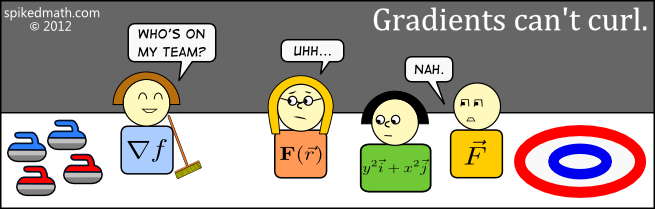
\includegraphics[width=10cm]{pictures_bitmap/501-curling-with-gradients.png}\\
        \url{http://spikedmath.com/501.html}{Spiked math}, \href{http://creativecommons.org/licenses/by-nc-sa/2.5/ca/}{licence Creative Commons by-nc 2.5}.
\end{center}
}{}

%+++++++++++++++++++++++++++++++++++++++++++++++++++++++++++++++++++++++++++++++++++++++++++++++++++++++++++++++++++++++++++
\section[Interprétation de la divergence]{Interprétation géométrique et physique de la divergence}
%+++++++++++++++++++++++++++++++++++++++++++++++++++++++++++++++++++++++++++++++++++++++++++++++++++++++++++++++++++++++++++

En physique, on dit qu'un champ de vecteurs à divergence nulle est \defe{incompressible}{incompressible!champ de vecteur}. Nous allons essayer de comprendre pourquoi. Lorsqu'un fluide incompressible se déplace, il faut qu'en chaque point il y autant de fluide qui rentre que de fluide qui sort. Nous allons voir sur quelques exemples que la divergence d'un champ de vecteurs est le «bilan de masse» d'un fluide qui se déplace selon le champ de vecteurs.

Si en un point la divergence est positive, cela signifie qu'il y a une perte de masse et si la divergence est négative, cela signifie qu'il y a une accumulation de masse.

Prenons par exemple un fluide qui se déplace selon le champ de vitesse montré à figure \ref{LabelFigBEHTooWsdrys}. % From file BEHTooWsdrys
\newcommand{\CaptionFigBEHTooWsdrys}{Le champ de vecteurs $F(x,y)=\frac{1}{ x }(1,0)$.}
\input{auto/pictures_tex/Fig_BEHTooWsdrys.pstricks}

Étant donné que la vitesse diminue lorsque $x$ avance, il y a une accumulation de fluide. Regardez en effet la quantité de fluide qui rentre dans le rectangle par rapport à la quantité de fluide qui en sort. Ce champ de vecteurs a pour équation :
\begin{equation}
    F(x,y)=\frac{1}{ x }\begin{pmatrix}
        1    \\ 
        0    
    \end{pmatrix}=\begin{pmatrix}
        1/x    \\ 
        0    
    \end{pmatrix}.
\end{equation}
Sa divergence vaut donc
\begin{equation}
    (\nabla\cdot F)(x,y)=\frac{ \partial F_x }{ \partial x }(x,y)+\underbrace{\frac{ \partial F_y }{ \partial y }(x,y)}_{=0}=-\frac{1}{ x^2 }.
\end{equation}
Cette divergence étant négative, il y a bien accumulation de fluide en tout point, et d'autant plus que $x$ est petit.

\begin{example}     \label{ExamDivFrot}

    Prenons le champ de vecteurs tournant
    \begin{equation}
        F(x,y)=\frac{1}{ \sqrt{x^2+y^2} }\begin{pmatrix}
            y    \\ 
            -x    
        \end{pmatrix}
    \end{equation}
    représenté à la figure \ref{LabelFigYQVHooYsGLHQ}. Cela est un vecteur qui est constamment perpendiculaire au rayon.


\newcommand{\CaptionFigYQVHooYsGLHQ}{Le champ de vecteurs $F(x,y)=(y,-x)$.}
\input{auto/pictures_tex/Fig_YQVHooYsGLHQ.pstricks}

    Un fluide dont la vitesse serait donné par ce champ de vecteur se contente de tourner. Intuitivement il ne devrait pas y avoir de divergence parce qu'il n'y a aucune accumulation de fluide. En effet,
    \begin{equation}
        \nabla\cdot F(x,y)=\frac{ -2xy }{ (x^2+y^2)^2 }+\frac{ 2xy }{ (x^2+y^2)^2 }=0.
    \end{equation}
\end{example}

\begin{example}
    Prenons le cas du champ de force de gravitation :
    \begin{equation}
        F(x,y,z)=\frac{1}{ (x^2+y^2+z^2)^{3/2} }\begin{pmatrix}
            x    \\ 
            y   \\
            z
        \end{pmatrix}.
    \end{equation}
    Nous pouvons rapidement remarquer que $\nabla\cdot F=0$. Est-ce que cela peut se comprendre sur le dessin de la figure \ref{LabelFigZGUDooEsqCWQ}. % From file ZGUDooEsqCWQ
\newcommand{\CaptionFigZGUDooEsqCWQ}{Le champ de vecteur de la gravité. Nous avons tracé, sur les deux cercles la même densité de vecteurs, c'est à dire le même nombre de vecteurs par unité de surface.}
\input{auto/pictures_tex/Fig_ZGUDooEsqCWQ.pstricks}

    Essayons de voir combien de fluide entre dans la zone bleue et combien en sort. D'abord, il est certain que les vecteurs qui sortent sont plus courts que ceux qui rentrent, ce qui voudrait dire qu'il y a plus de fluide qui rentre. Mais on voit également que le \emph{nombre} de vecteurs qui sortent est plus grand parce que la seconde sphère est plus grande et qu'il y a un vecteur en chaque point de la sphère.

    Intuitivement nous pouvons dire que la quantité qui rentre dans la sphère de rayon $r_1$ donnée par la taille des vecteurs entrants multiplié par la surface de la sphère, c'est à dire
    \begin{equation}        \label{EqQpinormeVecto}
        4\pi r_1^2\| F(x,y,z) \|,
    \end{equation}
    mais $\| F(x,y,z) \|=\frac{1}{ r_1^2 }$, donc la quantité de fluide entrant est $4\pi$. La quantité de fluide sortant sera la même.

    Cela explique deux choses
    \begin{enumerate}
        \item
            Pourquoi les forces de gravitation et électromagnétiques sont en $1/r^2$; c'est parce que nous vivons dans un monde avec trois dimensions d'espace. En étudiant très précisément le champ de gravitation, certains physiciens espèrent trouver des déviations expérimentales par rapport à la règle du \( 1/r^2\); cela \emph{pourrait} être un signe que l'espace contient des dimensions supplémentaires.
        \item
            Pourquoi il y a un $4\pi$ comme coefficient dans beaucoup d'équations en électromagnétisme; en particulier dans certaines anciennes unités de flux.
    \end{enumerate}
    
\end{example}

\begin{remark}
    Nous allons voir plus loin comment s'assurer que l'équation \eqref{EqQpinormeVecto} représente bien la «quantité de fluide» qui rentre dans la zone délimitée
\end{remark}


%+++++++++++++++++++++++++++++++++++++++++++++++++++++++++++++++++++++++++++++++++++++++++++++++++++++++++++++++++++++++++++
\section{Quelques formules de Leibnitz}
%+++++++++++++++++++++++++++++++++++++++++++++++++++++++++++++++++++++++++++++++++++++++++++++++++++++++++++++++++++++++++++

La divergence étant une combinaison de dérivées, il n'est pas tellement étonnant que la divergence de produits donne lieux à des formules en deux termes. Si $f$ est une fonction et si $F$ et $G$ sont des champs de vecteurs, nous avons (sans démonstrations) :
\begin{equation}        \label{EqLeinDivNablRot}
    \begin{aligned}[]
        \nabla\cdot(fF)&=f\nabla\cdot F+F\cdot\nabla f\\
        \nabla\cdot(F\times G)&=G\cdot\nabla\times F-F\cdot\nabla\times G.
    \end{aligned}
\end{equation}
Nous avons aussi, pour le rotationnel,
\begin{equation}        \label{EqLeinRotfFF}
    \nabla\times(fF)=f\nabla\times F+\nabla f\times F.
\end{equation}
% This is part of Mes notes de mathématique
% Copyright (c) 2011-2012
%   Laurent Claessens
% See the file fdl-1.3.txt for copying conditions.

%+++++++++++++++++++++++++++++++++++++++++++++++++++++++++++++++++++++++++++++++++++++++++++++++++++++++++++++++++++++++++++
\section{La différentielle revisitée}
%+++++++++++++++++++++++++++++++++++++++++++++++++++++++++++++++++++++++++++++++++++++++++++++++++++++++++++++++++++++++++++

%---------------------------------------------------------------------------------------------------------------------------
\subsection{Les formes différentielles de base}
%---------------------------------------------------------------------------------------------------------------------------

Si la fonction $f\colon \eR^n\to \eR$ est différentiable alors la différentielle en $a\in\eR^n$ est l'application
\begin{equation}        \label{EqFormDiffdfah}
    \begin{aligned}
        df_a\colon \eR^n&\to \eR \\
        u&\mapsto \frac{ \partial f }{ \partial x_1 }(a)u_1+\cdots+\frac{ \partial f }{ \partial x_n }(a)u_n.
    \end{aligned}
\end{equation}
Considérons en particulier la fonction qui à $x\in\eR^n$ fait correspondre $x_i\in\eR$. Par abus de notations,  nous la noterons $x_i$. Nous avons 
\begin{equation}
    \frac{ \partial x_i }{ \partial x_j }=\delta_{ij}.
\end{equation}
Par exemple $\partial_yx=0$ et $\partial_xx=1$. Toutes les dérivées partielles de $x_i$ s'annulent sauf la $i$ème qui vaut $1$. Par conséquent
\begin{equation}
    \begin{aligned}
        dx_i\colon \eR^n&\to \eR \\
        u&\mapsto u_i. 
    \end{aligned}
\end{equation}

\begin{remark}
    En toute rigueur nous devrions écrire $(dx_i)_a$. Mais étant donné que
    \begin{equation}
        (dx_i)_a(u)=(dx_i)_b(u)
    \end{equation}
    pour tout points $a$, $b$ et pour tout vecteurs $u$, nous nous permettons de simplifier la notation en ne précisant pas en quel point nous calculons la différentielle de $x_i$.
\end{remark}

Étant donné que $dx_i(u)=u_i$, nous pouvons récrire la formule \eqref{EqFormDiffdfah} en remplaçant $u_i$ par $dx_i(u)$ :
\begin{equation}
    df_a(u)=\frac{ \partial f }{ \partial x_1 }(a)dx_1(u)+\cdots+\frac{ \partial f }{ \partial x_n }(a)dx_n(u).
\end{equation}
En tant que application linéaire, $df_a$ est une combinaison linéaire des $dx_i$. En notations compacte :
\begin{equation}
    df_a=\sum_{i=1}^n\frac{ \partial f }{ \partial x_i }(a)dx_i.
\end{equation}

%---------------------------------------------------------------------------------------------------------------------------
                    \subsection{Différentielle comme élément de l'espace dual}
%---------------------------------------------------------------------------------------------------------------------------

Si nous considérons la base canonique $\{ e_i \}_{i=1,\ldots,n}$ de $\eR^n$. À partir d'elle, nous considérons la \defe{base duale}{base!duale}. En termes pratiques, nous définissons $dx_i$ comme la forme sur $\eR^n$ qui à un vecteur $u$ fait correspondre sa composante $i$ :
\begin{equation}
    dx_i\begin{pmatrix}
    u^1 \\ 
    \vdots  \\ 
    u^n 
\end{pmatrix}=u^i.
\end{equation}
En termes savants, $dx_i$ est le dual de $e_i$. Si tu ne l'as pas encore compris, Jean Doyen va te le faire comprendre !


Maintenant, dans la formule \eqref{EqDiffPartRap}, nous pouvons remplacer $u^i$ par $dx_i(u)$, et écrire
\begin{equation}
    df_a(u)=\sum_i\frac{ \partial f }{ \partial x_i }(a)u^i=\sum_i\frac{ \partial f }{ \partial x_i }(a)dx_i(u).
\end{equation}
Ce qui arrive tout à droite est explicitement vu comme une forme sur $\eR$, dont les composantes dans la base duale sont les dérivées partielles de $f$ au point $a$, agissant sur $u$. En faisant un pas en arrière, nous omettons le $u$, et nous écrivons
\begin{equation}
    df_a=\sum_{i=1}^n\frac{ \partial f }{ \partial x_i }(a)dx^i
\end{equation}

Cette notation $dx_i$ pour la forme duale de $e_i$ est en réalité parfaitement logique parce que $dx^i$ est la différentielle de la projection
\begin{equation}
    \begin{aligned}
        x^i\colon \eR^n&\to \eR \\
        (x^1,\ldots,x^n)&\mapsto x^i. 
    \end{aligned}
\end{equation}
Je te laisse un peu méditer sur cette différentielle de la projection. L'important est que tu aies compris cela d'ici la fin de ta deuxième année.

%---------------------------------------------------------------------------------------------------------------------------
\subsection{Différentielles de fonctions composées}
%---------------------------------------------------------------------------------------------------------------------------

Cette façon de voir la différentielle nous permet de jeter un nouveau regard sur la formule de différentiation des fonctions composées. Soient
\begin{equation}
    \begin{aligned}[]
        f\colon \eR^p&\to \eR^n\\
        g\colon \eR^n&\to \eR,
    \end{aligned}
\end{equation}
et $h\colon \eR^p\to \eR$ définie par 
\begin{equation}
    h(u)=h\big( f(u) \big)=(g\circ f)(u).
\end{equation}
Nous allons noter $x$ les coordonnées de $\eR^p$, $a$ un point de $\eR^p$ et $u$, un vecteur de $\eR^p$ accroché au point $a$. Pour $\eR^n$, les notations seront que les coordonnées sont $y$, $b$ est un point de $\eR^n$ et $v$ est un vecteur «accroché» au point $b$.

Nous avons
\begin{equation}
    dg_b(v)=\sum_{i=1}^n\frac{ \partial g }{ \partial y_i }(b)dy_i(v).
\end{equation}
Ici $dy_i(v)$ signifie la $i$ème composante de $v$. C'est simplement $v_i$. Cette formule étant valable pour tout point $b\in\eR^n$ et pour tout vecteur $v$, nous pouvons l'écrire en particulier pour
\begin{subequations}
    \begin{numcases}{}
        b=f(a)\\
        v=df_a(u).
    \end{numcases}
\end{subequations}
Cela donne
\begin{equation}        \label{Eqdgfadfau}
    dg_{f(a)}\big( df_a(u) \big)=\sum_{i=1}^n\frac{ \partial g }{ \partial y_i }\big( f(a) \big)dy_i\big( df_a(u) \big).
\end{equation}
Mais 
\begin{equation}
    df_a(u)=\sum_{j=1}^p\frac{ \partial f }{ \partial x_j }(a)dx_j(u),
\end{equation}
donc la $i$ème composante de ce vecteur est
\begin{equation}
     \big( df_a(u)\big)_i=\sum_{j=1}^p\frac{ \partial f_i }{ \partial x_j }(a)dx_j(u).
\end{equation}
En remplaçant $dy_i\big( df_a(u) \big)$ par cela dans l'expression \eqref{Eqdgfadfau}, nous trouvons
\begin{equation}
    dg_{f(a)}\big( df_a(u) \big)=\sum_{i=1}^n\frac{ \partial g }{ \partial y_i }\big( f(a) \big)\sum_{j=1}^p\frac{ \partial f_i }{ \partial x_j }(a)dx_j(u).
\end{equation}
Nous pouvons vérifier que cela est la différentielle de $g\circ f$ au point $a$ appliquée au vecteur $u$. En effet
\begin{equation}
    d(g\circ f)_a(u)=\sum_{j=1}^p\frac{ \partial (g\circ f) }{ \partial x_j }(a)dx_j(u),
\end{equation}
tandis que, par la dérivation de fonctions composées, 
\begin{equation}        \label{EqDerCompofg}
    \frac{ \partial (g\circ f) }{ \partial x_j }(a)=\sum_{i=1}^n\frac{ \partial g }{ \partial y_i }\big( f(a) \big)\frac{ \partial f_i }{ \partial x_j }(a).
\end{equation}
Au final, ce que nous avons prouvé est que
\begin{equation}
    d(g\circ f)_a(u)=dg_{f(a)}\big( df_a(u) \big).
\end{equation}

%---------------------------------------------------------------------------------------------------------------------------
\subsection{Exemple de composée : les coordonnées polaires}
%---------------------------------------------------------------------------------------------------------------------------

Le changement de coordonnées pour les polaires est la fonction
\begin{equation}
    f\begin{pmatrix}
        r    \\ 
        \theta    
    \end{pmatrix}=\begin{pmatrix}
        x    \\ 
        y    
    \end{pmatrix}=\begin{pmatrix}
        r\cos\theta    \\ 
        r\sin\theta    
    \end{pmatrix}.
\end{equation}
Considérons une fonction $g$ sur $\eR^2$, et définissons la fonction $\tilde g$ par
\begin{equation}
    \tilde g(r,\theta)=g(r\cos\theta,r\sin\theta).
\end{equation}
La formule \eqref{EqDerCompofg} permet de trouver les dérivées partielles de $g$ par rapport à $r$ et $\theta$ en termes de celles par rapport à $x$ et $y$ de $g$.

Pour faire le lien avec les notations du point précédent, nous avons
\begin{equation}
    \begin{aligned}[]
        f_1(r,\theta)&=r\cos(\theta)\\
        f_2(r,\theta)&=r\sin(\theta)\\
        (x_1,x_2)&\to(r,\theta)\\
        (y_1,y_2)&\to(x,y).
    \end{aligned}
\end{equation}
Nous avons donc 
\begin{equation}
    \begin{aligned}[]
        \frac{ \partial \tilde g }{ \partial r }(r,\theta)&=\sum_{i=1}^2\frac{ \partial g }{ \partial x_i }\big( f(r,\theta) \big)\frac{ \partial f_i }{ \partial r }(r,\theta)\\
        &=\frac{ \partial g }{ \partial x }(r\cos\theta,r\sin\theta)\frac{ \partial \big( r\cos\theta \big) }{ \partial r }(r,\theta)\\
        &\quad+\frac{ \partial g }{ \partial y }(r\cos\theta,r\sin\theta)\frac{ \partial \big( r\sin\theta\big) }{ \partial r }(r,\theta)\\
        &=\cos\theta\frac{ \partial g }{ \partial x }(r\cos\theta,r\sin\theta)+\sin\theta\frac{ \partial g }{ \partial y }(r\cos\theta,r\sin\theta).
    \end{aligned}
\end{equation}

Prenons par exemple $g(x,y)=\frac{1}{ x^2+y^2 }$. Étant donné que
\begin{equation}
    \frac{ \partial g }{ \partial x }=\frac{ -2x }{ (x^2+y^2)^2 },
\end{equation}
nous avons
\begin{equation}
    \frac{ \partial g }{ \partial x }(r\cos\theta,r\sin\theta)=\frac{ -2\cos\theta }{ r^3 }.
\end{equation}
En utilisant la formule,
\begin{equation}
    \frac{ \partial \tilde g }{ \partial r }(r,\theta)=\cos(\theta)\left( \frac{ -2\cos\theta }{ r^3 } \right)+\sin(\theta)\left( \frac{ -2\sin\theta }{ r^3 } \right)=-\frac{ 2 }{ r^3 }.
\end{equation}
Nous pouvons vérifier directement que cela est correct. En effet
\begin{equation}
    \tilde g(r,\theta)=g(r\cos\theta,r\sin\theta)=\frac{1}{ r^2 },
\end{equation}
dont la dérivée par rapport à $r$ vaut $-2/r^3$.

En ce qui concerne la dérivée par rapport à $\theta$, nous avons
\begin{equation}
    \begin{aligned}[]
    \frac{ \partial \tilde g }{ \partial \theta }&=\frac{ \partial g }{ \partial x }(r\cos\theta,r\sin\theta)\frac{ \partial \big( r\cos(\theta) \big) }{ \partial \theta }+\frac{ \partial g }{ \partial y }(r\cos\theta,r\sin\theta)\frac{ \partial \big( r\sin(\theta) \big) }{ \partial \theta }\\
    &=\left( \frac{ -2\cos\theta }{ r^3 } \right)(-r\sin\theta)+\left( \frac{ -2\sin\theta }{ r^3 } \right)(r\cos\theta)\\
    &=0.
    \end{aligned}
\end{equation}

En résumé et avec quelques abus de notations :
\begin{equation}
    \begin{aligned}[]
        \frac{ \partial \tilde g }{ \partial r }&=\cos(\theta)\frac{ \partial g }{ \partial x }+\sin(\theta)\frac{ \partial g }{ \partial y }\\
        \frac{ \partial \tilde g }{ \partial \theta }&=-r\sin(\theta)\frac{ \partial g }{ \partial x }+r\cos(\theta)\frac{ \partial g }{ \partial y }\\
    \end{aligned}
\end{equation}


\chapter{Intégration}
% This is part of Mes notes de mathématique
% Copyright (c) 2011-2016
%   Laurent Claessens
% See the file fdl-1.3.txt for copying conditions.

%+++++++++++++++++++++++++++++++++++++++++++++++++++++++++++++++++++++++++++++++++++++++++++++++++++++++++++++++++++++++++++ 
\section{Théorème de la moyenne}
%+++++++++++++++++++++++++++++++++++++++++++++++++++++++++++++++++++++++++++++++++++++++++++++++++++++++++++++++++++++++++++

\begin{theorem}[\cite{MonCerveau}]      \label{ThoooEZLGooMChwLT}
    Soit \( Q\) un compact connexe par arcs et une fonction continue \( f\colon Q\to \eR\). Si \( \lambda\) est la mesure de Lebesgue, alors il existe \( a\in Q\) tel que
    \begin{equation}
        f(a)=\frac{1}{ \lambda(Q) }\int_Qfd\lambda
    \end{equation}
\end{theorem}

\begin{proof}
    En posant \( I=\int_Qfd\lambda\) nous avons immédiatement
    \begin{equation}        \label{EqooTYQCooVxdazW}
        \min(f)\lambda(Q)\leq I\leq \max(f)\lambda(Q)
    \end{equation}
    où le minimum et le maximum existent parce que \( f\) est continue sur un compact. Si une des deux inégalités est une égalité alors la fonction est constante. En effet supposons que la première inégalité soit une égalité; si la fonction n'était pas constante, il existerait une boule sur laquelle \( f\) serait strictement supérieure à \( \min(f)\). En intégrant d'abord sur cette boule et ensuite sur le complémentaire nous obtenons une intégrale plus grande que \( \min(f)\lambda(Q)\).

    Soit \( \epsilon>0\). Il existe \( \alpha,\beta\in Q\) tels que \( f(\alpha)\leq\min(f)+\epsilon\) et \( f(\beta)\geq\max(f)-\epsilon\). Soit \( \gamma\colon \mathopen[ 0 , 1 \mathclose]\to Q\) un chemin continu tel que \( \gamma(0)=\alpha\) et \( \gamma(1)=\beta\). La fonction \( f\circ \gamma\colon \mathopen[ 0 , 1 \mathclose]\to \eR\) est alors continue et vérifie \( (f\circ\gamma)(0)\leq \min(f)+\epsilon\) et \( (f\circ\gamma)(1)\geq \max(f)-\epsilon\).

    Si \( \epsilon\) est assez petit et vu que les inégalités \eqref{EqooTYQCooVxdazW} sont strictes,
    \begin{equation}
        \lambda(Q)(f\circ\gamma)(0)\leq \min(f)\lambda(Q)+\epsilon\lambda(Q)<I<\max(f)\lambda(Q)-\epsilon\lambda(Q)\leq\lambda(Q)(f\circ \gamma)(1).
    \end{equation}
    Par le théorème des valeurs intermédiaires \ref{ThoValInter}, il existe \( t_0\in\mathopen[ 0 , 1 \mathclose]\) tel que \( \lambda(Q)(f\circ\gamma)(t_0)=I\). Le point \( a=\gamma(t_0)\) vérifie
    \begin{equation}
        f(a)=\frac{1}{ \lambda(Q) }\int_Qfd\lambda.
    \end{equation}
\end{proof}

%+++++++++++++++++++++++++++++++++++++++++++++++++++++++++++++++++++++++++++++++++++++++++++++++++++++++++++++++++++++++++++ 
\section{Mesure à densité}
%+++++++++++++++++++++++++++++++++++++++++++++++++++++++++++++++++++++++++++++++++++++++++++++++++++++++++++++++++++++++++++

%--------------------------------------------------------------------------------------------------------------------------- 
\subsection{Théorème de Radon-Nikodym}
%---------------------------------------------------------------------------------------------------------------------------

\begin{proposition}[Produit d'une mesure par une fonction]
    Si \( (S,\tribF,m_1)\) est un espace mesuré, et si \( f\colon S\to \eR\) est intégrable, et si \( B\) est un ensemble mesurable, nous définissons \( fm_1\) par
    \begin{equation}
        m_2(B)=(fm_1)(B)=\int_Bf(t)dm_1(t).
    \end{equation}
    Cela est une mesure positive sur \( (S,\tribF)\).
\end{proposition}

\begin{proof}
    D'abord pour l'ensemble vide : \( m_2(\emptyset)=\int_{\emptyset}fdm_1=0\).

    Si \( A_n\) sont des éléments disjoints de \( \tribF\) tels que \( \bigcup_nA_n\in\tribF\). Alors en utilisant la proposition \ref{PropOPSCooVpzaBt}, nous avons le calcul suivant :
    \begin{equation}
        m_2\big( \bigcup_nA_n \big)=\int_{\bigcup_nA_n}f(t)dm_1(t)=\sum_{n}\int_{A_n}f(t)dm_1(t)=\sum_nm_2(A_n).
    \end{equation}
\end{proof}

\begin{definition}[\cite{PersoFeng}]
    Soient \( \mu\) et \( \nu\) deux mesures sur l'espace mesurable \( (\Omega,\tribA)\). Nous disons que la mesure \( \mu\) est \defe{dominée}{dominée!mesure} par \( \nu\) si pour tout ensemble mesurable \( A\), \( \nu(A)=0\) implique \( \mu(A)=0\).

    Si \( \nu\) est une mesure positive et \( \mu\) une mesure, nous disons que \( \mu\) est \defe{absolument continue}{mesure!absolument continue} par rapport à \( \nu\) si \( \nu(A)=0\) implique \( \mu(A)=0\). On note aussi \( \mu\ll\nu\)\nomenclature[Y]{$\mu\ll\nu$}{La mesure \( \mu\) est absolument continue par rapport à la mesure \( \nu\).}.
\end{definition}

La mesure \( \mu\) est \defe{portée}{portée!mesure} par l'ensemble \( E\in\tribA\) si pour tout \( A\in\tribA\), 
\begin{equation}
    \mu(A)=\mu(A\cap E).
\end{equation}

Nous écrivons que \( \mu\perp\nu\)\nomenclature[Y]{\( \mu\perp\nu\)}{mesures perpendiculaires} s'il existe un ensemble \( E\in\tribA\) tel que \( \mu\) soit porté par \( E\) et \( \nu\) soit porté par \( \complement E\).

\begin{theorem}[Radon-Nikodym\cite{NikoLi}]
    Soient \( \mu\) et \( \nu\) deux mesures \( \sigma\)-finies sur un espace métrisable \( (\Omega,\tribA)\).
    \begin{enumerate}
        \item
            Il existe un unique couple de mesures \( \mu_1\) et \( \mu_2\) telles que
            \begin{enumerate}
                \item
                    \( \mu=\mu_1+\mu_2\)
                \item
                    \( \mu_1\) est dominé par \( \nu\)
                \item
                    \( \mu_2\perp \nu\).
            \end{enumerate}
            Dans ce cas, les mesures \( \mu_1\) et \( \mu_2\) sont positives et \( \sigma\)-finies.
        \item
            À égalité \(  \nu\)-presque partout près, il existe une unique fonction mesurable positive \( f\) telle que pour tout mesurable \( A\),
            \begin{equation}
                \mu_1(A)=\int_Ad\mu_1=\int_{\Omega}\mtu_Afd \nu.
            \end{equation}
        \item
            À égalité \( \nu\)-presque partout près, il existe une unique fonction positive mesurable \( h\) telle que \( \mu_1=h\nu\).
    \end{enumerate}
\end{theorem}
\index{théorème!Radon-Nikodym}
%TODO : une preuve

\begin{corollary}   \label{CorZDkhwS}
    Si \( \mu\) es une mesure \( \sigma\)-finie dominée par la mesure \( \sigma\)-finie \( m\), alors \( \mu\) possède une unique fonction de densité.
\end{corollary}

\begin{corollary}       \label{CorDomDens}
    Soient \( \mu\) et \( m\), deux mesures positives \( \sigma\)-finies sur \( (\Omega,\tribA)\). Alors \( m\) domine \( \mu\) si et seulement si \( \mu\) possède une densité par rapport à \( m\).
\end{corollary}
 
\begin{proof}
    Si \( \mu\) est dominée par \( m\), alors la décomposition \( \mu=\mu+0\) satisfait le théorème de Radon-Nikodym. Par conséquent il existe une fonction \( f\) telle que
    \begin{equation}
        \mu(A)=\int_Afdm.
    \end{equation}
    Cette fonction est alors une densité pour \( \mu\) par rapport à \( m\).

    Pour la réciproque, nous supposons que \( \mu\) a une densité \( f\) par rapport à \( m\), et que \( A\) est une ensemble de \( m\)-mesure nulle :
    \begin{equation}
        m(A)=\int_{\Omega}\mtu_Adm=0.
    \end{equation}
    Cela signifie que la fonction \( \mtu_A\) est \( m\)-presque partout nulle. La fonction produit \( \mtu_Af\) est également nulle \( m\)-presque partout, et par conséquent
    \begin{equation}
        \mu(A)=\int_{\Omega}\mtu_Afdm=0.
    \end{equation}
\end{proof}

\begin{probleme}
    Est-ce que la démonstration de cela ne demande pas la convergence monotone d'une façon ou d'une autre ?
\end{probleme}

%--------------------------------------------------------------------------------------------------------------------------- 
\subsection{Mesure complexe}
%---------------------------------------------------------------------------------------------------------------------------

\begin{definition}[Mesure complexe\cite{TLRRooOjxpTp}] \label{DefGKHLooYjocEt}
    Si \( (\Omega,\tribA)\) est un espace mesurable, une \defe{mesure complexe}{mesure!complexe} est une application \( \mu\colon \tribA\to \eC\) telle que
    \begin{enumerate}
        \item
            $\mu(\emptyset)=0$,
        \item
            \( \nu\) est sous-additive : si les ensembles \( A_i\in\tribA\), alors \( \sum_i\mu(A_i)=\mu(\bigcup_iA_i)\).
    \end{enumerate}
\end{definition}
Notons que la série $\sum_i\mu(A_i)$ est alors nécessairement absolument convergente. En effet changer l'ordre de la somme ne change pas l'union, et donc ne change pas la valeur de la somme. Si \( \sigma\colon \eN\to \eN\) est une permutation, 
\begin{equation}
    \sum_i\mu(A_{\sigma(i)})=\mu\big( \bigcup_iA_{\sigma(i)} \big)=\mu\big( \bigcup_iA_i \big)=\sum_i\mu(A_i).
\end{equation}
Le théorème \ref{PopriXWvIY} dit alors que la somme doit être absolument convergente.


\begin{theorem}[Radon-NikoDym complexe\footnote{L'histoire du nom de ce théorème est intéressante. Lorsque monsieur et madame Rèmederdonnukodym apprirent que leurs amis, les Rèmedelaboulechevelue avaient appelé leur fils Théo, ils décidèrent d'en faire autant. C'est en souvenir de ces circonstances que monsieur Nikodym (prénommé Radon) décida de faire des math.}]\label{ThoZZMGooKhRYaO}
    Soit \( \mu\) une mesure positive sur \( (\Omega,\tribA)\) et \( \nu\) une mesure complexe. Alors
    \begin{enumerate}
        \item
            Il existe un unique couple de mesures complexes \( \nu_a\), \( \nu_s\) sur \( (\Omega,\tribA)\) tel que
            \begin{enumerate}
                \item
                    \( \nu=\nu_a+\nu_s\)
                \item
                    \( \nu_a\ll\mu\)
                \item
                    \( \nu_s\perp \mu\).
            \end{enumerate}
        \item
            Ces mesures satisfont alors \( \nu_a\perp\nu_s\).
        \item
            Il existe une fonction intégrable \( h\colon \Omega\to \eC\) telle que \( \nu_a=h\mu\).
        \item
            La fonction \( h\) est unique à \( \mu\)-équivalence près.
        \item   \label{ItemDIXOooFqOkgGv}
            Si de plus \( \nu\ll \mu\) alors \( \nu=h\mu\).
    \end{enumerate}
\end{theorem}
\index{théorème!Radon-Nikodym!complexe}
\begin{proof}
    No proof.
\end{proof}

\begin{remark}  \label{RemSYRMooZPBhbQ}
    Le point \ref{ItemDIXOooFqOkgGv} est souvent utilisé sous la forme
    \begin{equation}
        \nu(A)=\int_{\Omega}\mtu_A(\omega)h(\omega)d\mu(\omega)=\int_{A}h(\omega)d\mu(\omega).
    \end{equation}
\end{remark}

%--------------------------------------------------------------------------------------------------------------------------- 
\subsection{Théorème d'approximation}
%---------------------------------------------------------------------------------------------------------------------------

\begin{theorem}[Théorème d'approximation\cite{YHRSDGc}]     \label{ThoAFXXcVa}
    Soit \( (X,\tribB,\mu)\) un espace mesuré où \( \tribB\) sont les boréliens de \( X\). Soit \( A\in \tribB\) tel que \( A\subset W\) où \( W\) est un ouvert avec \( \mu(W)<\infty\). Soit aussi \( \epsilon>0\).
    \begin{enumerate}
        \item
            Il existe un fermé \( F\) et un ouvert \( V\) tels que \( \mu(V)<\infty\) et
            \begin{equation}
                F\subset A\subset V
            \end{equation}
            et \( \mu(V\setminus F)<\epsilon\).
        \item
            Il existe \( f\in C^0(X,\eR)\) nulle hors de \( W\) vérifiant \( 0\leq f\leq 1\) et
            \begin{equation}
                \int_X| \mtu_A-f |^pd\mu(x)<\epsilon.
            \end{equation}
    \end{enumerate}
\end{theorem}
% TODO : la preuve est dans la référence. Il faut replacer ce théorème après la définition de l'intégrale.

%--------------------------------------------------------------------------------------------------------------------------- 
\subsection{Mesure à densité}
%---------------------------------------------------------------------------------------------------------------------------

Si \( \mu\) est une mesure sur \( \eR^d\), une fonction \( f\colon \eR^d\to \eR\) est une \defe{densité}{densité d'une mesure} si pour tout \( A\subset\eR^d\) nous avons
\begin{equation}
    \mu(A)=\int_Af(x)dx
\end{equation}
où \( dx\) est la mesure de Lebesgue.

%+++++++++++++++++++++++++++++++++++++++++++++++++++++++++++++++++++++++++++++++++++++++++++++++++++++++++++++++++++++++++++ 
\section{Constructions plus naïves de la mesure et de l'intégrale dans le cas réel}
%+++++++++++++++++++++++++++++++++++++++++++++++++++++++++++++++++++++++++++++++++++++++++++++++++++++++++++++++++++++++++++

Les sections \ref{SecSLOooeMaig} et \ref{SecZTFooXlkwk} ont donné une construction très complète de la mesure de Lebesgue, et nous avons définit la théorie de l'intégration sur un espace mesuré quelconque dans la définition \ref{DefTVOooleEst}.

Dans cette section nous allons donner différentes choses plus rapides qui servent souvent de définition dans les cours moins avancés.

%--------------------------------------------------------------------------------------------------------------------------- 
\subsection{Mesure de Lebesgue, version rapide}
%---------------------------------------------------------------------------------------------------------------------------

Nous construisons à présent la mesure de Lebesgue sur \( \eR^n\). Un \defe{pavé}{pavé} dans \( \eR^n\) est un ensemble de la forme 
\begin{equation}
    B=\prod_{i=1}^n\mathopen[ a_i , b_i \mathclose];
\end{equation}
le volume d'un tel pavé est défini par \( \Vol(B)=\prod_i(b_i-a_i)\). Soit maintenant \( A\subset \eR^n\). La \defe{mesure externe}{mesure!externe} de \( A\) est le nombre
\begin{equation}
    m^*(A)=\inf\{ \sum_{B\in\mF}\Vol(B)\text{ où \( \mF\) est un ensemble dénombrable de pavés dont l'union recouvre \( A\).} \}
\end{equation}

\begin{definition}  \label{DefKTzOlyH}
Nous disons que \( A\) est \defe{mesurable}{mesurable!Lebesgue} au sens de Lebesgue si pour tout ensemble \( S\subset \eR^n\) nous avons l'égalité
\begin{equation}
    m^*(S)=m^*(A\cap S)+m^*(S\setminus A).
\end{equation}
Dans ce cas nous disons que la mesure de Lebesgue de \( A\) est \( m(A)=m^*(A)\).
\end{definition}

\begin{proposition}     \label{PropNCMToWI}
    Deux fonctions continue égales presque partout pour la mesure de Lebesgue\footnote{Définition \ref{DefKTzOlyH}.} sont égales.
\end{proposition}

\begin{proof}
    Soient \( f\) et \( g\) deux fonctions continues telles que \( f(x)=g(x)\) pour presque tout \( x\in D\). La fonction \( h=f-g\) est alors presque partout nulle et nous devons prouver qu'elle est nulle sur tout \( D\). La fonction \( h\) est continue; si \( h(a)\neq 0\) pour un certain \( a\in D\) alors \( h\) est non nulle sur un ouvert autour de \( a\) par continuité et donc est non nulle sur un ensemble de mesure non nulle.
\end{proof}

%---------------------------------------------------------------------------------------------------------------------------
\subsection{Pavés et subdivisions}
%---------------------------------------------------------------------------------------------------------------------------

\begin{definition}
 Nous appelons \defe{pavé}{pavé} de $\eR^p$ toute partie de $\eR^p$ obtenue comme produit de $p$ intervalles de $\eR$. Plus explicitement, une partie $R$ est un pavé de $\eR^p$ s'il s'écrit sous la forme
\[
R=\left\{(x_1,\ldots, x_p)\in\eR^p \,\big\vert\,x_i\in \mathcal{I}_i,  i=1,\ldots, p  \right\},
\]
où $\mathcal{I}_i$ est un intervalle de $\eR$ pour tout $i=1,\ldots, p$. 
\end{definition}
On appelle pavé fermé de $\eR^p$ le produit de $p$ intervalles fermés 
\[
R=\prod_{i=1}^{p}[a_i,b_i].
\]
On définit de même le pavé ouvert 
\[
S=\prod_{i=1}^{p}]a_i,b_i[.
\]
Un pavé $ R=\prod_{i=1}^{p}\mathcal{I}_i$ est dit borné si tous les intervalles $\mathcal{I}_i$ sont bornés dans $\eR$. Les pavés non bornés sont des produits d'intervalles où un (ou plusieurs) des intervalles n'est pas borné. Par exemple,
\[
N=]-\infty, 5]\times [0,13].
\]
L'espace $\eR^p$, lui-même, est un pavé de $\eR^p$. 
\begin{definition}
  Une partie $A$ de $\eR^p$ est dite  \defe{pavable}{pavable} s'il existe une famille finie de pavés bornés $R_j$, $j=1,\ldots, n$, et deux à deux disjoints tels que 
\[
A=\bigcup_{j=1}^{n}R_j.
\] 
\end{definition}
Un exemple d'ensemble pavable dans $\eR^2$ est donné à la figure \ref{LabelFigPolirettangolo}. Il existe beaucoup d'ensembles dans $\eR^2$ qui ne sont pas pavables, par exemple les ellipses.
\newcommand{\CaptionFigPolirettangolo}{Un ensemble pavable.}
\input{pictures_tex/Fig_Polirettangolo.pstricks}

Le complémentaire d'un pavé est  un ensemble pavable et, en particulier, tout complémentaire d'un pavé borné est une réunion de  pavés non bornés. Toute union finie et toute intersection d'ensemble pavables est pavable.    
\begin{definition}
	Soit $R$ un pavé borné de $\eR^p$, pour fixer les idées on peut penser $R=\prod_{i=1}^{p}[a_i,b_i]$. On appelle \defe{longueur}{longueur!d'une arrête} de l'$i$-ème arrête de $R$ le nombre $b_i-a_i$. La \defe{mesure $p$-dimensionnelle de $R$}{}, $m(R)$, est le produit des longueurs 
\[
m(R)=\prod_{i=1}^{p}(b_i-a_i).
\] 
\end{definition}
\begin{example}
  Dans $\eR^3$, l'ensemble $R=[-1,1]\times[3,4]\times[0,2]$ est un pavé fermé de mesure 
\[
m(R)= (1+1)\cdot(4-3)\cdot(2-0)=4.
\] 
Il s'agit du volume usuel du parallélépipède rectangle.
\end{example}

\begin{example}
 L'ensemble $R=\mathopen] -1 , 1 \mathclose[\times[3,4]\times[0,2]$ est un pavé de $\eR^3$. Il n'est ni fermé ni ouvert, sa mesure est encore $4$.
\end{example}

Si $R$ est un pavé non borné on peut encore définir sa mesure. La notion de mesure se généralise en deux étapes. D'abord on dit que la longueur d'une arête non bornée est $\infty$. Ensuite, on adopte la convention $0\cdot \infty=0$. Il faut remarquer que avec cette généralisation tout point et toute droite dans $\eR^2$ ont mesure nulle.

Afin de définir les intégrales, nous allons intensivement faire appel à la notion de subdivision d'intervalles, voir définition \ref{DefSubdivisionIntervalle} et la discussion qui suit.

Lorsqu'on considère un pavé borné $R=\prod_{i=1}^p\mI_i$ de $\eR^p$, on note $\sdS_i$ l'ensemble des subdivisions de l'intervalle $\mI_i$. La notion de subdivision de généralise au cas des pavés.
\begin{definition}
	Soir $R$ un pavé fermé borné de $\eR^p$, pour fixer les idées on peut penser à $R=\prod_{i=1}^p\mathopen[ a_i , b_i \mathclose]$. On appelle \defe{subdivision}{subdivision} finie de $R$ les éléments de l'ensemble $\mathcal{S}=\prod_{i=1}^{p}\mathcal{S}_i$, 
\[
\mathcal{S}=\left\{ (Y_{1},\ldots, Y_{p})\,\big\vert\, Y_{i}=(y_{i,j})_{j=1}^{n_i}\in\mathcal{S}_i,\, i=1,\ldots,p\right\}.
\]
On peut définir de même l'ensemble des subdivisions d'un pavé non borné. 
 \end{definition}
 Souvent, une subdivision d'un pavé $R=\prod_{i=1}^p\mI_i$ sera noté $\sigma=(y_{i,j})_{j=1}^{n_i}$. Dans cette notation, on sous-entend que pour chaque $i$ fixé, les nombres $y_{i,j}$ (il y en a $n_i$) forment une subdivision de l'intervalle $\mI_i$. Afin de vous familiariser avec ces notations, repérez bien tous les éléments de la figure \ref{LabelFigUneCellule}.
\newcommand{\CaptionFigUneCellule}{Une cellule d'une subdivision d'un pavé de $\eR^2$. La cellule grisée est $R_{(4,2)}$.}
\input{pictures_tex/Fig_UneCellule.pstricks}

%On désigne par
%\[
%\delta(Y_i)=\max_{0\leq j\leq n}| y_{i,j}- y_{i,j-1}|,
%\] 
%le pas de la subdivision $Y_i$ dans $\mathcal{S}_i$ et par 
%\[
%\delta(\sigma)=\max_{0\leq i\leq p}\delta(Y_i),
%\]  
%le pas de la subdivision $\sigma$ dans $\mathcal{S}$.

\begin{definition}
	Si $\sigma$ est une subdivision d'un pavé $R$, un \defe{raffinement}{raffinement!subdivision d'un pavé} de $\sigma$ est une subdivision de $R$ obtenue en fixant plus de points dans chaque intervalle.
\end{definition}

La subdivision $\sigma$ de $R$ détermine $n_1n_2\ldots n_p$ pavés fermés de la forme 
\[
R_{(k_1,\ldots,k_p)}=\{(x_1,\ldots, x_p)\in\eR^p\,\big\vert\, y_{i,k_{i-1}}\leq x_i\leq y_{i,k_i}\},
\]
où $k_i$ est dans $\{1,\ldots, n_i\}$ et $i$ dans $\{1,\ldots, p\}$. On les appelles \defe{cellules}{cellule d'un pavage} de $\sigma$. On remarque que les cellules de $\sigma$ sont toujours deux à deux disjointes (sauf au plus sur leurs bords). 
\begin{lemma}\label{meas_sous}
	Soit $R$ un pavé borné de $\eR^p$ et soit $\sigma=(y_{i,j})_{j=1}^{n_i}$ une subdivision de $R$. 
On a 
\[
m(R)=\sum_{(k_1,\ldots,k_p)\in K} m(R_{(k_1,\ldots,k_p)}),
\] 
où $K=\{1,\ldots,n_1\}\times\{1,\ldots,n_2\}\times\ldots \times\{1,\ldots,n_p\}$.
\end{lemma}
Le lemme \ref{meas_sous} suggère de définir la mesure d'un ensemble borné pavable $P=\cup_{j=1}^{n}R_j$ comme la somme des mesures des pavés disjoints $R_j$, $j=1,\ldots, n$.
\begin{definition}
Une application $f:\eR^p\to\eR$ est dite \defe{application en escalier}{application!en escalier} sur $\eR^m$ si
  \begin{itemize}
  \item $f$ est une application bornée,
\item il existe une subdivision $\sigma$ de $\eR^p$ telle que la restriction de $f$  est une application constante sur toute cellule $R_k$ de $\sigma$
\[
f_{\vert_{R_k}}=C_k, \qquad C_k\in\eR,
\]
%Pour tout $k=(k_1,\ldots,k_p)$ dans $ K=\{1,\ldots,n_1\}\times\{1,\ldots,n_2\}\times\ldots \times\{1,\ldots,n_p\}$.
 
Une telle subdivision $\sigma$ est dite \defe{associée}{associée!subdivision}\index{subdivision!associée à une fonction} à $f$. 
  \end{itemize}
\end{definition} 
\begin{example}
  La fonction $f$ de $\eR^2$ dans $\eR$ définie par 
  \begin{equation}
    f(x,y)=\left\{
    \begin{array}{ll}
      1&\qquad \textrm{si } (x,y) \in [0,3]\times[-1,2],\\
2 &\textrm{sinon.} 
    \end{array}\right.
  \end{equation}
est une application en escalier. Exercice : donner une subdivision de $\eR^2$ associée à cette fonction.
\end{example}
\begin{example}
  La fonction $f$ de $\eR^2$ dans $\eR$ définie par 
  \begin{equation}
    f(x,y)=\left\{
    \begin{array}{ll}
      \frac{1}{m^2+n^2},&\qquad \textrm{si } (x,y) \in [m,m+1]\times[n,n+1], \quad m,\,n\in\eN_0,\\
0, &\textrm{sinon} 
    \end{array}\right.
  \end{equation}
est une application en escalier. Observez que, dans ce cas, il n'existe pas une subdivision finie de $\eR^2$ associée à $f$. 
\end{example}
\begin{remark}
 Si la subdivision $\sigma$ est associée à $f$ alors tout raffinement de $\sigma$ (c'est à dire, toute subdivision obtenue en fixant plus de points dans chaque intervalle) a la même propriété. 

Si $f$ et $g$ sont deux application en escalier sur $R$ et $\sigma_f$ et $\sigma_g$ sont des subdivisions de $R$ associées respectivement à $f$ et $g$, alors on peut construire une troisième subdivision de $R$ qui est associée à $f$ et à $g$ en même temps. Soient $\sigma_f=(Y_{1},\ldots, Y_{p})$ et $\sigma_g=(Z_{1},\ldots, Z_{p})$, où $Y_{i}=(y_{i,j})_{j=1}^{m_i}$ et $Z_{i}=(z_{i,j})_{j=1}^{n_i}$ sont des subdivision de l'intervalle $[a_i, b_i]$, pour $i=1,\ldots, p$. La subdivision de $[a_i, b_i]$ obtenue par l'union de $Y_i$ et $Z_i$ est encore une subdivision finie, qu'on appellera $\bar Y_i$. La subdivision $\bar \sigma = (\bar Y_{1},\ldots,\bar Y_{p})$ de $R$ est un raffinement de $\sigma_f $ et de $\sigma_g$, donc elle est associée à la fois à $f$ et à $g$. 

Cela nous permet de prouver que si $f$ et $g$ sont des application en escalier, alors $f+g$, $fg$, $\min\{f,g\}$, $\max\{f,g\}$ et $|f|$ sont des applications en escalier. 
\end{remark}

%---------------------------------------------------------------------------------------------------------------------------
\subsection{Intégrale d'une fonction en escalier}
%---------------------------------------------------------------------------------------------------------------------------

\begin{definition}
  Soit $f$ une fonction de $\eR^m$ dans $\eR^n$. Le \defe{support}{support} de $f$ est la fermeture de l'ensemble des points $x$ tels que $f(x)\neq 0$. 
\end{definition}
\begin{definition}
Une application en escalier $f$ est dite \defe{intégrable}{fonction!en escalier intégrable} si son support est compact. 
\end{definition} 
Soit $f$ une application en escalier sur $\eR^p$. Soit $\sigma$ une subdivision de  $\eR^p$ associée à $f$ et appelons $R_k$ les cellules de $\sigma$, avec $k=(k_1,\ldots,k_p)$ dans $ K=\{1,\ldots,n_1\}\times\{1,\ldots,n_2\}\times\ldots \times\{1,\ldots,n_p\}$. Alors  
\[
f_{\vert_{R_k}}=C_k, \qquad C_k\in\eR.
\]

\begin{definition} 
On définit l'\defe{intégrale}{intégrale!fonction en escalier} de $f$ sur $\eR^p$ par
\[
\int_{\eR^p}f\,dV=\sum_{k\in K}C_km(R_k).
\] 
\end{definition}
L'intégrale ainsi définie est un nombre réel. La proposition suivante nous dit que l'intégrale est «bien définie», au sens que sa valeur ne dépend pas de la subdivision associée à $f$ qu'on utilise dans le calcul. 
\begin{proposition}
Soit $f$ une application en escalier intégrable sur $\eR^p$. Soient $\sigma_1$ et $\sigma_2$ deux subdivisions de $\eR^p$ associées à  $f$. L'intégrale de $f$ ne dépend pas de la subdivision choisie.
\end{proposition}
On ne donne pas une preuve complète de cette proposition. En fait elle est une conséquence de la formule de réduction introduite dans la suite de ce chapitre.  


%%%%%%%%%%%%%%%%%%%%%%%%%%%%%%%%%%%%%%%%%%%%%%%%%%%%%%%%%%%%%%%%%%%%%%%%%%%%%%%%
\subsection{Intégrales partielles}
%%%%%%%%%%%%%%%%%%%%%%%%%%%%%%%%%%%%%%%%%%%%%%%%%%%%%%%%%%%%%%%%%%%%%%%%%%%%%%%%
Soit $f$ de $\eR^p$ dans $\eR$ une fonction continue, nulle hors du pavé borné $R$. Posons  $R=\prod_{i=1}^{p}[a_i,b_i]$, pour fixer les idées. Pour chaque $i$ dans $\{1,\ldots, p\}$ fixé, on peut associer à $f$ la fonction $F_i$ de $p-1$ variables définie par
\[
F_i(x_1,\ldots, x_{i-1}, x_{i+1}, \ldots, x_p)=\int_{a_i}^{b_i}f(x_1,\ldots, x_{i-1},y, x_{i+1}, \ldots, x_p)\, dy.
\]  
La fonction $F_i$ est l'intégrale partielle de $f$ par rapport à la $i$-ème variable. 
En particulier, si $f(x_1,\ldots, x_p)=g(x_i)h(x_1,\ldots, x_{i-1}, x_{i+1}, \ldots, x_p)$ on obtient 
\[
F_i=\int_{a_i}^{b_i}g(y)h(x_1,\ldots, x_{i-1}, x_{i+1}, \ldots, x_p)\, dy= h\cdot\int_{a_i}^{b_i}g \, dy.
\]  
La fonction d'une seule variable qu'on obtient à partir de $f$ en fixant $x_1,\ldots, x_{i-1}, x_{i+1}, \ldots, x_p$ et qui associe à $x_i$ la valeur $f(x_1,\ldots, x_{i-1}, x_i, x_{i+1}, \ldots, x_p)$, est appelée $x_i$-ème section de $f$ en $x_1,\ldots, x_{i-1}, x_{i+1}, \ldots, x_p$. 
\begin{example}
  Soit $f$ la fonction de $\eR^2$ dans $\eR$ définie par 
  \begin{equation}
	  f(x,y)=\begin{cases}
		  x+3y	&	\text{si $(x,y)\in\mathopen[ 9 , 10 \mathclose]\times\mathopen] \pi , 5 \mathclose]$}\\
		  0	&	 \text{sinon}.
	  \end{cases}
  \end{equation}
 Les intégrales partielles de $f$ sont 
\[
F_1(y)=\int_{9}^{10}x+3y\,dx=\left[\frac{x^2}{2}+3xy\right]_{x=9}^{x=10}=\frac{19}{2}+3y,
\]
\[
F_2(x)=\int_{\pi}^{5}x+3y\,dy=\left[xy+\frac{3y^2}{2}\right]_{y=\pi}^{y=5}=x(5-\pi)+\frac{3}{2}(25-\pi^2).
\]
\end{example}
%%%%%%%%%%%%%%%%%%%%%%%%%%%%%%%%%%%%%%%%%%%%%%%%%%%%%%%%%%%%%%%%%%%%%%%%%%%%%%%%
\subsection{Réduction d'une intégrale multiple}
%%%%%%%%%%%%%%%%%%%%%%%%%%%%%%%%%%%%%%%%%%%%%%%%%%%%%%%%%%%%%%%%%%%%%%%%%%%%%%%%
 
Soit $R=[a,b]\times[c,d]$ un pavé fermé et borné de $\eR^2$ et soit $f$ une application en escalier intégrable sur $\eR^2$ telle que le support de $f$ soit contenu dans $R$. On considère la subdivision $\sigma$ de $R$ définie par les subdivisions 
\[
a=x_0\leq x_1\leq\ldots\leq x_m=b,
\]  
 \[
c=y_0\leq y_1\leq\ldots\leq y_n=d.
\]  
Les cellules de $\sigma$ sont 
\[
R_{i,j}=[x_{i},x_{i+1}]\times[y_{j},y_{j+1}], \quad\qquad i=0,\ldots,m-1, \quad j=0,\ldots,n-1.
\]
La mesure de $R$ est la somme des mesures des $R_{i,j}$
\begin{equation}
  \begin{aligned}
    m(R)=&\sum_{(i,j)\in \{0,\ldots, m-1\}\times\{0,\ldots, n-1\}} m(R_{i,j})=\\
&=\sum_{j=0}^{n-1}\sum_{i=0}^{m-1}(x_{i+1}-x_{i})\cdot(y_{i+1}-y_{i})=\\
&=\sum_{i=0}^{m-1}(x_{i+1}-x_{i})\cdot\sum_{j=0}^{n-1}(y_{i+1}-y_{i})=\\
&= (b-a)\cdot(d-c).
  \end{aligned}
\end{equation}
Si $f$ est constante sur chaque cellule de $\sigma$ on peut écrire $f$ de la forme suivante
\[
f(x,y)=\sum_{j=0}^{n-1}\sum_{i=0}^{m-1}C_{i,j}\,\chi_{R_{i,j}}
\]
où les $C_{i,j}$ sont des constantes réelles et $\chi_{R_{i,j}}$ est la \defe{fonction caractéristique}{fonction!caractéristique} de $R_{i,j}$
\begin{equation}
  \chi_{R_{i,j}}(x,y)=\left\{
      \begin{array}{ll}
      1,\qquad &\textrm{si } (x,y)\in R_{i,j} ,\\
0, & \textrm{sinon}.
      \end{array}\right.
\end{equation}
Comme $(x,y)$ est dans $R_{i,j}$ si et seulement si $x\in[x_{i},x_{i+1}]$ et $ y\in[y_{j},y_{j+1}]$, on vérifie que la fonction $\chi_{R_{i,j}}$ est égal au produit des fonctions caractéristiques des intervalles $[x_{i},x_{i+1}]$ et $[y_{j},y_{j+1}]$ 
\[
 \chi_{R_{i,j}}(x,y)=\chi_{[x_{i},x_{i+1}]}(x)\cdot\chi_{[y_{j},y_{j+1}]}(y).
\] 
On peut donc écrire la fonction $f$ de la façon suivante
\[
f(x,y)=\sum_{j=0}^{n-1}\sum_{i=0}^{m-1}C_{i,j}\,\chi_{[x_{i},x_{i+1}]}(x)\cdot\chi_{[y_{j},y_{j+1}]}(y).
\] 
Comme on suppose que le support de $f$ est une partie de $R$, l'intégrale de $f$ sur $\eR^2$ est
\begin{equation}
  \begin{aligned}
\int_{\eR^2}f \,dV = \sum_{j=0}^{n-1}\sum_{i=0}^{m-1}C_{i,j}\,m(R_{i,j})=\sum_{j=0}^{n-1}\sum_{i=0}^{m-1}C_{i,j}\,(x_{i+1}-x_i)\cdot(y_{j+1}-y_j).
 \end{aligned}
\end{equation} 
Cette intégrale peut être réduite à la composition de deux intégrales partielles. Il suffit de remarquer que la valeur de l'intégrale de la fonction caractéristique d'un intervalle est la longueur de l'intervalle, 
\begin{equation}
  \begin{aligned}
    C_{i,j}(x_{i+1}-x_i)&\cdot(y_{j+1}-y_j)=\\
&=C_{i,j}\left(\int_{x_i}^{x_{i+1}}\chi_{[x_{i},x_{i+1}]}(x)\, dx \right)\cdot \left(\int_{y_j}^{y_{j+1}}\chi_{[y_{ j},y_{ j+1}]}(y)\, dy \right)=\\
&=C_{i,j}\left(\int_{a}^{b}\chi_{[x_{i},x_{i+1}]}(x)\, dx \right)\cdot \left(\int_{c}^{d}\chi_{[y_{ j},y_{ j+1}]}(y)\, dy \right),
  \end{aligned}
\end{equation}
et utiliser les propriétés de linéarité de l'intégrale
\begin{equation}
  \begin{aligned}
   \int_{\eR^2}f \,dV =& \sum_{j=0}^{n-1}\sum_{i=0}^{m-1}C_{i,j}\,\left(\int_{a}^{b}\chi_{[x_{i},x_{i+1}]}(x)\, dx \right)\cdot \left(\int_{c}^{d}\chi_{[y_{ j},y_{ j+1}]}(y)\, dy \right)=\\
&=\int_{c}^{d}\int_{a}^{b}\sum_{j=0}^{n-1}\sum_{i=0}^{m-1}C_{i,j}\,\chi_{[x_{i},x_{i+1}]}(x)\cdot \chi_{[y_{ j},y_{ j+1}]}(y)\, dx dy=\\
&=\int_{c}^{d}\int_{a}^{b} f\, dx dy.  
  \end{aligned}
\end{equation}
De même on obtient
\begin{equation}
  \begin{aligned}
   \int_{\eR^2}f \,dV =&\int_{a}^{b}\int_{c}^{d}\sum_{j=0}^{n-1}\sum_{i=0}^{m-1}C_{i,j}\,\chi_{[x_{i},x_{i+1}]}(x)\cdot \chi_{[y_{ j},y_{ j+1}]}(y)\, dx dy=\\
&=\int_{a}^{b}\int_{c}^{d} f\, dx dy.  
  \end{aligned}
\end{equation}
En général, on preuve la proposition suivante
\begin{proposition}
 Soit $f$ une application en escalier intégrable sur $\eR^p$ et soit $R$ un pavé borné dans $\eR^p$ qui contient le support de $f$. Comme d'habitude, pour fixer les idées nous écrivons $=\prod_{i=1}^p[a_i,b_i]$. Alors
 \begin{equation}
   \begin{aligned}
     \int_{\eR^p}f(x_1,\ldots, x_p) \, dV =& \int_{a_p}^{b_p}\int_{a_{p-1}}^{b_{p-1}}\cdots\int_{a_1}^{b_1} f(x_1,\ldots, x_p) \, dx_1\cdots dx_p=\\
&=\int_{a_{s_p}}^{b_{s_p}}\int_{a_{s_{p-1}}}^{b_{s_{p-1}}}\cdots\int_{a_{s_1}}^{b_{s_1}} f(x_1,\ldots, x_p) \, dx_1\cdots dx_p,
   \end{aligned}
 \end{equation}
pour toute permutation $(s_1,\ldots,s_p)$ de l'ensemble $\{1,\ldots p\}$.
\end{proposition}
%%%%%%%%%%%%%%%%%%%%%%%%%%%%%%%%%%%%%%%%%%%%%%%%%%%%%%%%%%%%%%%%%%%%%%%%%%%%%%%%
\subsection{Propriétés de l'intégrale}
%%%%%%%%%%%%%%%%%%%%%%%%%%%%%%%%%%%%%%%%%%%%%%%%%%%%%%%%%%%%%%%%%%%%%%%%%%%%%%%%
Soient $f$ et $g$ deux fonctions en escalier intégrables de $\eR^p$ dans $\eR$, et soient $a$ et $b$ dans $\eR$. 
\begin{description}
\item[Linéarité de l'intégrale] : 
  \begin{itemize}
  \item Additivité : $f+g$ est intégrable et 
\[
\int_{\eR^p} (f+g)\, dV = \int_{\eR^p} f\, dV+ \int_{\eR^p} g\, dV,
\]
\item Homogénéité : $\lambda f$ est intégrable pour tout réel $\lambda$ 
\[
\int_{\eR^p} \lambda  f\, dV = \lambda\int_{\eR^p} f\, dV,
\]
  \end{itemize}
\item[Monotonie] Si $f\leq g$ alors 
\[
 \int_{\eR^p} f\, dV\leq \int_{\eR^p} g\, dV,
\]
\item[Inégalité fondamentale]
  \[
\lvert \int_{\eR^p}f\,dV\rvert \leq\int_{\eR^p}\lvert f\rvert\,dV.
\] 
Cette dernière inégalité s'obtient de la façon suivante :
\[
\lvert\int_{\eR^p}f\,dV\rvert =\lvert \sum_{k\in K} C_k m(R_k)\rvert \leq\sum_{k\in K}\lvert C_k\rvert m(R_k)=\int_{\eR^p}|f|\,dV.
\] 
\item[Inégalité de Čebičeff]  Si $f$ est une application en escalier alors pour tout $a>0$ dans $\eR$ l'ensemble $\{x\in\eR^p\,:\, |f(x)|\geq a\}$ est pavable et borné, et l'inégalité suivante est satisfaite
\[
m\left(\{x\in\eR^p\,:\, |f(x)|\geq a\}\right)\leq \frac{1}{a} \int_{\eR^p}\lvert f\rvert\,dV.
\]
\end{description}

%--------------------------------------------------------------------------------------------------------------------------- 
\subsection{Intégrales multiples, cas général}
%---------------------------------------------------------------------------------------------------------------------------

Nous voulons généraliser la définition d'intégrale multiple au cas des domaines non pavables et de fonctions qui ne sont pas en escalier. Il y a plusieurs méthodes de le faire et ici on ne considère qu'une seule, introduite par Riemann.  
\begin{definition} Soit $f: \eR^p\to \eR$ une fonction.
  \begin{itemize}
	  \item Pour toute application en escalier intégrable $f_*$ telle que $f_*\leq f$, l'intégrale de $f_*$ est dit une \defe{somme inférieure}{somme!inférieure} de $f$. 
	  \item Pour toute application en escalier intégrable $f^*$ telle que $f_*\geq f$, l'intégrale de $f^*$ est dit une \defe{somme supérieure}{somme!supérieure} de $f$. 
  \end{itemize}
\end{definition}
Soient $\sum_* f$ et  $\sum^* f$ les ensembles des sommes inférieures et supérieures de $f$. Grâce à la propriété de  monotonie de l'intégrale on sait que si $a$ est dans $\sum_* f$ et  $b$ est dans $\sum^* f$ alors $a\leq b$. 
\begin{definition}
  La fonction $f$ est intégrable (au sens de Riemann) si $\sum_* f$ et  $\sum^* f$ ne sont pas vides et 
\[
\inf \Sigma^* f=I =\sup \Sigma_* f.
\] 
Dans ce cas, la valeur $I$ est appelée intégrale de $f$ sur $\eR^p$. 
\end{definition}
\begin{remark}
  Toute fonction intégrable est bornée et à support compact. En effet, si le support de la  fonction n'est pas compact alors soit $\sum_* f$ soit $\sum^* f$ doit être vide ! 
\end{remark}
L'intégrale qu'on vient de définir possède toutes les propriétés de l'intégrale pour les fonctions en escalier. Le produit de deux fonctions intégrables est intégrable. 

Il y a des cas où l'intégrabilité d'une fonction n'est pas évidente. Cependant, dans la plupart des exercices et des exemples de ce cours, nous nous aidons avec le critère suivant 
\begin{proposition}
  Toute fonction continue à support compact est intégrable. 
\end{proposition}
Cette proposition n'est a priori pas étonnante, vu qu'une fonction continue sur un support compact est bornée (théorème de Weierstrass \ref{ThoWeirstrassRn}).

%%%%%%%%%%%%%%%%%%%%%%%%%%%%%%%%%%%%%%%%%%%%%%%%%%%%%%%%%%%%%%%%%%%%%%%%%%%%%%%%
\subsection{Réduction d'une intégrale multiple}
%%%%%%%%%%%%%%%%%%%%%%%%%%%%%%%%%%%%%%%%%%%%%%%%%%%%%%%%%%%%%%%%%%%%%%%%%%%%%%%%
On n'utilise jamais la définition pour calculer la valeur d'une intégrale multiple. La méthode plus efficace, en pratique, est de réduire l'intégrale à la composition de plusieurs intégrales d'une variable.  
\begin{theorem}[de Fubini]\label{fub}
 Soit $f$ une fonction intégrable de $\eR^2$ dans $\eR$. Si pour tout $x$ dans $\eR$ la section $f(x,\cdot)$ est intégrable par rapport à $y$, alors
\[
\int_{\eR^2}f(x,y)\,dV=\int_{\eR}\left(\int_{\eR}f(x,y)\,dx\right)\,dy.
\]
De même, si pour tout $y$ dans $\eR$ la section $f(\cdot, y)$ est intégrable par rapport à $x$, alors
\[
\int_{\eR^2}f(x,y)\,dV=\int_{\eR}\left(\int_{\eR}f(x,y)\,dy\right)\,dx.
\] 
\end{theorem}		\label{ThoSectionINte}
En général, on ne peut pas dire que les sections d'une fonction intégrable sont intégrables, donc il faut vraiment se souvenir des hypothèses du théorème \ref{fub}. En dimension plus haute, on a le même résultat
\begin{theorem}
 Soit $f$ une fonction intégrable de $\eR^p$ dans $\eR$. Si pour tout $(p-1)$-uple $(x_1,\ldots, x_{i-1},x_{i+1}, \ldots, x_p)$ dans $\eR^{p-1}$ la section $f(x_1,\ldots, x_{i-1},\cdot,x_{i+1}, \ldots, x_p)$ est intégrable par rapport à $x_i$, alors
\[
\int_{\eR^p}f \,dV=\int_{\eR}\left(\int_{\eR^{p-1}}f \,dV\right)\,dx_i.
\]
\end{theorem}

 Si $f$ est une fonction positive et intégrable de $\eR^2$ dans $\eR$ on peut interpréter l'intégrale de $f$ comme le volume du solide au-dessous du graphe de $f$.  Avec cette interprétation,  l'intégrale partielle par rapport à $x$ pour $y=y_0$ fixé est l'aire de la tranche qu'on obtient en coupant le solide par le plan $y=y_0$.

 \begin{example}
   Le premier exemple à faire est celui d'une fonction en escalier intégrable et positive. Soit $f\colon \eR^2\to \eR$ la fonction
\begin{equation}
	f(x,y)=\begin{cases}
		1	&	\text{si $(x,y)\in R_1=\mathopen] -1 , 3 \mathclose]\times\mathopen[ 4 , 5 \mathclose]$}\\
		3	&	 \text{si $(x,y)\in R_2=\mathopen] 13 , 15 \mathclose[\times\mathopen[ 0 , 2 \mathclose[$}\\
		0	&	 \text{dans les autres cas.}
	\end{cases}
\end{equation}
L'intégrale de $f$ sur $\eR^2$ est $1\cdot m(R_1)+ 3\cdot m(R_2)= 16$. On voit tout de suite qu'il s'agit de la somme du volume des deux parallélépipèdes de hauteurs respectives $1$ et $3$ et bases $R_1$ et $R_2$. 
 \end{example}

\begin{example} 
On veut calculer le volume du solide $S$, borné par le paraboloïde elliptique $x^2+2y^2+z=16$ et le plans $x=2$, $x=0$, $y=2$ $y=0$, $z=0$. On observe que la portion de  paraboloïde elliptique qui nous intéresse est le graphe de la fonction $f(x,y)=16-x^2-2y^2$ pour $(x,y)$ dans $R=[0,2]\times[0,2]$. La fonction $f$ est continue ainsi que ses sections, donc on peut appliquer le théorème \ref{fub} et décomposer l'intégrale double en deux intégrales simples :
\begin{equation}
  \begin{aligned}
   & \int_R 16-x^2-2y^2 \,dV= \int_{0}^2\int_{0}^2f(x,y)\,dx dy= \\
&=\int_0^2 \left[(16-2y^2)x-\frac{x^3}{3}\right]_{x=0}^{x=2}\, dy =\\
& = \left[ \left(32-\frac{8}{3}\right) y -\frac{4y^3}{3}\right]_{x=0}^{x=2}= 64- \frac{16+32}{3}=48.
  \end{aligned}
\end{equation}
Vérifiez, comme exercice, qu'on obtient le même résultat en intégrant d'abord par rapport à $y$ et puis par rapport à $x$.  
\end{example}

\begin{example}
  Dans les hypothèses du théorème \ref{fub}  l'ordre des intégrations partielles ne change pas la valeur de l'intégrale. En fait, si les calculs sont faites par des êtres humains l'ordre d'intégration peut faire une certaine différence comme dans cet exemple. On veut évaluer la valeur de l'intégrale 
\[
\int_{\eR^2}f(x,y)\, dV
\]
où 
\begin{equation}
	f(x,y)=\begin{cases}
		y\sin(x,y)	&	\text{si $(x,y)\in\mathopen[ 1,2 ,  \mathclose]\times\mathopen[ 0 , \pi \mathclose]$,}\\
		0	&	 \text{sinon.}
	\end{cases}
\end{equation}
Les deux section de $f(x,y)=y\sin(xy)$ sont continues. Si on intègre d'abord par rapport à $y$ on obtient 
\[
-\int_1^2\frac{ \pi\cos(\pi x) }{ x }dx+\int_1^2\frac{ \sin(\pi x) }{ x^2 }dx,
\] 
qui n'est pas du tout immédiat, alors que, si on intègre d'abord par rapport à $x$ on obtient 
\[
\int_0^\pi \cos y - \cos(2y)\,dy.
\] 
\end{example}

%%%%%%%%%%%%%%%%%%%%%%%%%%%%%%%%%%%%%%%%%%%%%%%%%%%%%%%%%%%%%%%%%%%%%%%%%%%%%%%%
\subsection{Intégrales sur des parties de $\eR^2$ }
%%%%%%%%%%%%%%%%%%%%%%%%%%%%%%%%%%%%%%%%%%%%%%%%%%%%%%%%%%%%%%%%%%%%%%%%%%%%%%%%

On veut évaluer l'intégrale de la fonction $f(x,y)=\sqrt{1-x^2}$ sur son domaine, la boule unité $B((0,0),1)$. La théorie introduite jusqu'ici n'est pas suffisante pour résoudre  ce problème, parce que $B((0,0),1)$ n'est pas pavable. Les parties bornées de $\eR^p$ sur lesquelles on peut intégrer des fonction sont dites mesurables (au sens de Riemann) parce que, comme on verra dans la suite, la mesure d'une partie de $\eR^p$ est l'intégrale (s'il existe) de sa fonction caractéristique. 

On peut dire que une partie de $\eR^p$  est mesurable si son bord est <<assez régulier>>. Dans $\eR^2$ il est suffisant que le bord de $A$ soit une réunion finie de courbes paramétrées continues. En particulier, on est très souvent dans un des deux cas suivantes
\begin{description}
\item[Régions du premier type] $A$ est borné et contenu entre les graphes de deux fonctions continues de $x$
\[
A=\{(x,y)\in\eR^2 \,:\, a\leq x\leq b, \, g_1(x)\leq y\leq g_2(x)\}, 
\]
avec $g_1$ et $g_2$ continues. 
\item[Régions du deuxième type] $A$ est borné et contenu entre les graphes de deux fonctions continues de $y$
\[
A=\{(x,y)\in\eR^2 \,:\, c\leq y\leq d, \, h_1(y)\leq x\leq h_2(y)\}, 
\]
avec $h_1$ et $h_2$ continues.
\end{description}
%\ref{LabelFigRegioniPrimoeSecondoTipo}
\newcommand{\CaptionFigRegioniPrimoeSecondoTipo}{Régions du premier et du deuxième type}
\input{pictures_tex/Fig_RegioniPrimoeSecondoTipo.pstricks}

\begin{example}
 Il y a des régions qui sont des deux types au même temps, comme les boules centrées à l'origine, le triangle de sommets  $(0,0)$, $(0,a)$ et $(b,0)$, ou la région $C$ délimité par les courbes $y=2x$ et $y=x^2$. Cette dernière admets les représentations suivantes
\[
C= \{(x,y)\in\eR^2 \,:\, 0\leq x\leq 1, \, x^2\leq y\leq 2x\},
\] 
et  
\[
C= \{(x,y)\in\eR^2 \,:\, 0\leq y\leq 1, \, y/2\leq x\leq \sqrt{y}\}.
\]  
\end{example}
\begin{definition}
  Soit $f$ une fonction de $\eR^2$ dans $\eR$ dont le support  $A$ est une région du premier ou du deuxième type. On définit la fonction $\bar f$ comme
 \begin{equation}
 \bar f(x,y) = \left\{ \begin{array}{ll}
     f(x,y), \qquad & \textrm{si } (x,y)\in A,\\
  0 , & \textrm{sinon.} 
    \end{array}\right.
  \end{equation}
  La fonction $f$ est dite \defe{intégrable}{intégrable!fonction non en escalier} si $\bar f$ est intégrable, et la valeur de son intégrale est 
\[
\int_A f\, dV=\int_{\eR^2} \bar f\, dV.
\] 
\end{definition}
Une fonction continue définie sur une région du premier ou du deuxième type est toujours intégrable. 

Pour fixer les idées on suppose ici que $A$ est du premier type et contenue dans le pavé borné $R=[a,b]\times [c,d]$. En suivant la définition on obtient
\begin{equation}
  \begin{aligned}
    \int_A f\, dV&=\int_{\eR^2} \bar f\, dV=\\
    &= \int_a^b\int_c^d \bar f\, dy dx=\\
&= \int_a^b\left(\int_c^{g_1(x)} \bar f\, dy+\int_{g_1(x)}^{g_2(x)} \bar f\, dy+\int_{g_2(x)}^d \bar f\, dy\right)\, dx= \\
&= \int_a^b\int_{g_1(x)}^{g_2(x)}  f\, dy dx.
  \end{aligned}
\end{equation}
De même, si $A$ est du deuxième type on obtient 
\begin{equation}
     \int_A f\, dV=\int_c^d\int_{h_1(y)}^{h_2(y)}  f\, dx dy.
\end{equation}
\begin{example}
	On peut maintenant résoudre notre problème de départ, évaluer l'intégrale de la fonction $f(x,y)=\sqrt{1-x^2}$ sur $B((0,0),1)$. Nous choisissons de décrire la boule unité de $\eR^2$ comme une région du premier type : $B((0,0),1)=\{(x,y)\, :\, x\in[-1,1], \, -\sqrt{1-x^2}\leq y\leq \sqrt{1-x^2} \}$. 
	\begin{equation}
		I=\int_{B}\sqrt{1-x^2}\, dV=\int_{-1}^1\int_{-\sqrt{1-x^2}}^{\sqrt{1-x^2}}\sqrt{1-x^2}dydx
	\end{equation}
	La première intégrale à effectuer, par rapport à $y$, est l'intégrale d'une fonction constante. Ne pas oublier que l'on intègre $\sqrt{1-x^2}$ par rapport à $y$; c'est bien une constante et l'intégrale consiste seulement à multiplier par $y$ :
	\begin{equation}
		I=\int_{-1}^1\left[ y\sqrt{1-x^2} \right]_{y=-\sqrt{1-x^2}}^{y=\sqrt{1-x^2}}dx=2\int_{-1}^1(1-x^2)dx.
	\end{equation}
	Cela est à nouveau une intégrale simple à effectuer. Le résultat est
	\begin{equation}
		2\int_{-1}^1(1-x^2)dx=2\left[ x-\frac{ x^3 }{ 3 } \right]_{x=-1}^{x=1}=\frac{ 8 }{ 3 }.
	\end{equation}
\end{example}
\begin{remark}
	Toutes les techniques d'intégration à une variable restent valables. Par exemple, lorsqu'une des intégrales est l'intégrale d'une fonction impaire sur un intervalle symétrique par rapport à zéro, l'intégrale vaut zéro.
\end{remark}

\begin{normaltext}   \label{NORMooDSNXooFhyHkx}
Par le lemme \ref{LemooPJLNooVKrBhN} nous savons que la mesure d'une région bornée de \( \eR^2\) est l'intégrale de sa fonction caractéristique, si elle existe.

La mesure d'une région bornée de $\eR^2$ est dite son \defe{aire}{aire}, et celle d'une région bornée de $\eR^3$ est son \defe{volume}{volume!région bornée dans $\eR^3$}. Voir aussi la remarque \ref{RemLongIntUn}.
\end{normaltext}


\begin{example}\label{exint}
  On veut calculer l'aire de la région de la figure \ref{LabelFigExampleIntegration} définie par 
\[
A=\{(x,y)\in\eR^2\,\vert\, 0\leq x\leq 1, x^3-1\leq y\leq x \}.
\]
On considère l'intégrale 
\[
\int_{\eR^2} \chi_{A}\, dV= \int_0^1\int^{x}_{x^3+1} 1 \, dy\, dx= \int_0^1 -x^3+x+1\, dx= -\frac{1}{4}+\frac{1}{2}+1=\frac{5}{4}.
\]
\end{example}
\newcommand{\CaptionFigExampleIntegration}{La région $A$ de l'exemple \ref{exint}}
\input{pictures_tex/Fig_ExampleIntegration.pstricks}

\begin{exercice}

	% C'est moche, mais il faut laisser une ligne vide ici, sinon il n'y a pas de saut de ligne
	% entre le titre «exercice» et le texte.
  Parfois la région sur laquelle on veut intégrer peut être décrite indifféremment en deux façons, mais la fonction à intégrer nous force a choisir un ordre particulier. Vérifiez que la fonction $f(x,y)=\sin(y^2)$ sur la région triangulaire de sommets $(0,0)$, $(0, 2)$, $(2,2)$ doit être intégrée d'abord par rapport à $x$.     
\end{exercice}

Si une région bornée n'est pas de premier ou de deuxième type on peut normalement la découper en morceaux plus faciles à décrire. On utilise alors la propriété suivante. 
\begin{lemma}
  Soit $A$ un sous-ensemble borné de $\eR^2$ et soient $B_1$ et $B_2$ deux parties de $A$ telles que $B_1\cap B_2=\emptyset$ et $B_1\cup B_2= A$. Alors, pour toute fonction $f$ intégrable sur $A$ (et en particulier pour sa fonction caractéristique) on a
\[
\int_{A}f \, dV= \int_{B_1}f \, dV+\int_{B_2}f \, dV.
\] 
\end{lemma}

\begin{example}\label{exint2}
La région $D$ que nous voyons sur la figure \ref{LabelFigExampleIntegrationdeux} est bornée par la parabole $y^2=2x+6$ et la droite $y=x-1$. La région $D$ est une région du deuxième type. Nous pouvons aussi la décrire comme l'union de deux régions du premier type $D_1$ et $D_2$,
\[
D_1=\{(x,y)\,:\, -3\leq x \leq -1,\, -\sqrt{2x+6}\leq y \leq \sqrt{2x+6}\},
\]
 et 
\[
D_2=\{(x,y)\,:\, -3\leq x \leq -1, \, x-1\leq y \leq \sqrt{2x+6}\}.
\]
\newcommand{\CaptionFigExampleIntegrationdeux}{La région $D$ de l'exemple \ref{exint2}}
\input{pictures_tex/Fig_ExampleIntegrationdeux.pstricks}
\end{example}

%%%%%%%%%%%%%%%%%%%%%%%%%%%%%%%%%%%%%%%%%%%%%%%%%%%%%%%%%%%%%%%%%%%%%%%%%%%%%%%%
\subsection{Intégrales sur des parties de $\eR^3$}
%%%%%%%%%%%%%%%%%%%%%%%%%%%%%%%%%%%%%%%%%%%%%%%%%%%%%%%%%%%%%%%%%%%%%%%%%%%%%%%%
Dans ces notes nous n'avons pas l'ambition de traiter d'une façon rigoureuse l'étude des ensemble mesurables de $\eR^3$. Comme dans la section précédente on se limitera à considérer des cas particuliers. 
\begin{definition}\label{primotipo_solida}
	Soit $E$ une région de  $\eR^3$. On dit que $E$ est une \defe{région solide de premier type}{premier type!région solide} si $E$ est contenue entre les graphes de deux fonctions continues de $x$ et $y$.
\[
E=\{(x,y,z)\in\eR^3\, \vert \, (x,y)\in A\subset \eR^2, u_1(x,y)\leq z\leq u_2(x,y) \}. 
\]   
\end{definition}
Le sous-ensemble de $A$  de $\eR^2$ qui apparaît dans la définition \ref{primotipo_solida} est la projection (ou l'ombre) de $E$ sur le plan $x$-$y$. 
\begin{example}\label{cornet}
 La région $E$ donnée par une portion de sphère collée à un cône est une région solide de premier type
\[
E=\{(x,y,z)\in\eR^3\, \vert \, (x,y)\in \bar B((0,0),1), \sqrt{x^2+y^2}\leq z\leq \sqrt{1-x^2-y^2} \}. 
\]
L'ombre de $E$ est la boule unité de $\eR^2$. L'ensemble $\sqrt{x^2+y^2}\leq z$ est un cône posé sur sa pointe tandis que l'ensemble $z\leq\sqrt{ 1-x^2-y^2 }$ est la demi-sphère. L'ensemble $E$ contient les points entre les deux, voir la figure \ref{LabelFigCornetGlace}.
\newcommand{\CaptionFigCornetGlace}{Il faut voir ça en trois dimensions.}
\input{pictures_tex/Fig_CornetGlace.pstricks}

\end{example}
Si la fonction $f$, à intégrer sur $E$, et ses sections sont intégrables  alors on peut réduire l'intégrale 
\begin{equation}
  \begin{aligned}
     \int_E  f(x,y,z)\, dV&=\int_A\left(\int_{u_1(x,y)}^{u_2(x,y)}f(x,y,z)\, dz \right) \, dV=\\
&=\int_A\left(F(x,y,u_2(x,y))-F(x,y,u_1(x,y))\right)\, dV,
  \end{aligned}
\end{equation}
où $F$ est une primitive de $f$ par rapport à la variable $z$, c'est à dire en considérant $x$ et $y$ comme des constantes. Il faut ensuite évaluer la partie qui reste comme dans la section précédente. Comme le calcul des aires  dans $\eR^2$, le calcul des volumes dans $\eR^3$ est fait par des intégrales. En fait le \defe{volume}{volume!d'une région solide} d'une région solide dans $\eR^3$ est sa mesure. 
\begin{definition}
   La mesure d'une région de  $\eR^3$ est l'intégrale de sa fonction caractéristique. 
\end{definition}
Soit $E$ une région solide du premier type, nous pouvons évaluer son volume par l'intégrale
\[
\int_A\left(u_2(x,y)-u_1(x,y)\right)\, dV.
\]  
Parfois c'est plus intéressant de calculer le volume avec la formule de réduction contraire : l'intégrale double d'abord et puis l'intégrale simple par rapport à $z$. On parle alors de calcul de volume «par tranche».

\begin{example}
On veut calculer le volume de la boule de rayon $a$, centrée à l'origine $B=\{(x,y,z)\in\eR^3\,\vert\, x^2+y^2+z^2\leq a^2 \}$. On peut décrire $B$ par
\[
  B=\left\{(x,y,z)\in\eR^3\,\vert\, (x,y)\in D_a, -\sqrt{a^2-x^2-y^2}\leq z\leq \sqrt{a^2-x^2-y^2}  \right\},
\]
où $D_a$ est le disque de rayon $a$ centré en $(0,0)$, donc le volume $B$ sera
\[
2 \int_{D_a}\sqrt{a^2-x^2-y^2} dV.
\] 
Cet intégrale est un peu ennuyeuse à calculer. On peut simplifier le calcul en observant que pour $\bar z$ fixé dans l'intervalle $[-a,a]$ la section de la boule au niveau $\bar z$ est un disque de rayon $\sqrt{a^2-z^2}$. L'aire d'un tel disque est  $\pi (a^2+z^2)$. Si on réduit l'intégrale de volume de la façon
\[
\int_{B} 1\, dV=\int_{-a}^{a}  \sqrt{a^2-z^2}\, dz,
\] 
on obtient tout de suite la valeur cherchée : le volume de $B$ est $4/3 \pi a^3$.   
\end{example}
\begin{example}
	On calcul l'intégrale de $f(x,y,z)=z$ sur la pyramide $P$ bornée par le plans $x=0$, $y=0$, $x+y+z=1$, $x+y+z/2=1$. On remarque tout de suite que le plans $x+y+z=1$, $x+y+z/2=1$ se coupent en la droite $x+y=1$, $z=0$ (on se souvient qu'\emph{une} droite dans $\eR^3$, c'est \emph{deux} équations). Cela veut dire que la projection de $P$ sur le plan $x$-$y$ est le  triangle $T$ borné par les droites $x=z=0$, $y=z=0$ et $x+y=1$, $z=0$.  
On  décrit donc $P$ par
\[
P=\{(x,y,z)\in\eR^3\,\vert\, (x,y)\in T, \, 1-2x-2y\leq z\leq 1-x-y\}
\] 
et $T$ par 
\[
T=\{(x,y)\in\eR^2\,\vert\, 0\leq x\leq 1,\,  0\leq y\leq 1-x\},
\]
donc l'intégrale de $f$ sur $P$ est 
\[
\int_pf(x,y,z)\, dV= \int_{0}^{1}\int_{0}^{1-x}\int_{1-2x-2y}^{1-x-y}z \,dz\,dy\,dx=-\frac{1}{ 24 }.
\]
Notez que lorsque $x$ et $y$ sont entre $0$ et $1$, nous avons bien $1-2x-2y<1-x-y$, d'où le fait que nous mettons $1-2x-2y$ dans la borne inférieure de l'intégrale.
\end{example}

De façon analogue on définit les régions solides du deuxième et du troisième type.  

%---------------------------------------------------------------------------------------------------------------------------
					\subsection[Fonctions et ensembles non bornés]{Intégrales de fonctions non bornées sur des ensembles non bornés}
%---------------------------------------------------------------------------------------------------------------------------

Soit $f\colon \eR^n\to \overline{ \eR }$, une fonction positive. On dit qu'elle est \defe{intégrable}{intégrable!fonction positive} sur $E\subset\eR^n$ si
\begin{enumerate}
    \item $\forall r>0$, la fonction $f_r(x)=f(x)\mtu_{f<r}$ est intégrable sur $E_r$;
\item la limite $\lim_{r\to\infty}\int_{E_r}f_r$ est finie.
\end{enumerate}
Dans ce cas, on pose 
\begin{equation}
	\int_Ef=\lim_{r\to\infty}\int_{E_r}f_r.
\end{equation}

\begin{theorem}	\label{ThoFnTestIntnnBorn}
Soit $E$ mesurable dans $\eR^n$ et $f\colon E\to \overline{ \eR }$. Si $f$ est mesurable et s'il existe $g\colon E\to \overline{ \eR }$ intégrable sur $E$ telle que $| f(x) |\leq g(x)$ pour tout $x\in E$, alors $f$ est intégrable sur~$E$.

Réciproquement, si $f$ est intégrable sur $E$, alors $f$ est mesurable.
\end{theorem}

\begin{lemma}\label{LemTHBSEs}
    Si \( f\) est une fonction sur \( \mathopen[ a , \infty [\), alors nous avons la formule
    \begin{equation}
        \lim_{b\to \infty}\int_a^bf(x)dx=\int_a^{\infty}f(x)dx
    \end{equation}
    au sens où si un des deux membres existe, alors l'autre existe et est égal.
\end{lemma}

\begin{proof}
    Supposons que le membre de gauche existe. Cela signifie que la fonction
    \begin{equation}
        \psi(x)=\int_a^xf
    \end{equation}
    est bornée. Soit \( M\), un majorant. Pour toute fonction simple \( \varphi\) dominant \( f\), on a que \( \int\varphi\leq M\), donc l'ensemble sur lequel on prend le supremum pour calculer \( \int_a^{\infty}f\) est majoré par \( M\) et possède donc un supremum. Nous avons donc
    \begin{equation}
        \int_a^{\infty}f\leq\lim_{b\to\infty}\int_a^bf.
    \end{equation}
\end{proof}

% This is part of Mes notes de mathématique
% Copyright (c) 2011-2015
%   Laurent Claessens
% See the file fdl-1.3.txt for copying conditions.

%+++++++++++++++++++++++++++++++++++++++++++++++++++++++++++++++++++++++++++++++++++++++++++++++++++++++++++++++++++++++++++ 
\section{Propriétés}
%+++++++++++++++++++++++++++++++++++++++++++++++++++++++++++++++++++++++++++++++++++++++++++++++++++++++++++++++++++++++++++

\begin{theorem}[\cite{ooGMNAooSLnIio}]      \label{THOooVADUooLiRfGK}
    Soient deux espaces mesurables \( (S_1,\tribF_1)\) et \( (S_2,\tribF_2)\) ainsi qu'une application mesurable \( \varphi\colon S_1\to S_2\). Soit encore \( \mu\), une mesure positive sur \( (S_1,\tribF_1)\).

    Si \( f\colon S_2\to\bar \eR\) ou \( \eC\) est mesurable alors,
    \begin{enumerate}
        \item      \label{ItemooKMBIooZpHJSS}
            \( f\) est \( \varphi(\mu)\)-intégrale si et seulement si \( f\circ\varphi\) est \( \mu\)-intégrable.
        \item       \label{ItemooLAPYooUreDEl}
            dans le cas où \( f\) est \( \varphi(\mu)\)-intégrable, nous avons
            \begin{equation}        \label{EqooSOHXooXSbdoy}
                \int_{S_2}fd\big( \varphi(\mu) \big)=\int_{S_1}(f\circ\varphi)d\mu.
            \end{equation}
    \end{enumerate}
\end{theorem}

\begin{proof}
    L'intégrabilité est la définition \ref{DefTCXooAstMYl}, et demande que \( | f |\) soit intégrable. L'égalité \eqref{EqooSOHXooXSbdoy} a un sens si les deux membres sont infinis. Tant que les fonctions considérées sont positives, le point \ref{ItemooKMBIooZpHJSS} est immédiat. Ce n'est qu'au moment où les fonctions considérées deviennent à valeurs dans \( \eC\) ou \( \eR\) que l'intégrabilité de \( | f |\) commence à jouer parce qu'il faut que \(  f^+  \) et \( f^-\) soient séparément intégrables.

    Nous allons prouver la formule \eqref{EqooSOHXooXSbdoy} pour des fonctions de plus en plis générales. Pour la suite nous notons \( \mu'=\varphi(\mu)\).

    \begin{subproof}
        \item[Pour \( f=\mtu_B\), \( B \) mesurable]
            Soit \( B\in\tribF_2 \). Nous avons \( \mtu_B\circ\varphi=\mtu_{\varphi^{-1}(B)}\). Donc en utilisant le lemme \ref{LemooPJLNooVKrBhN} nous avons
            \begin{equation}
                \int_{S_2}\mtu_{B}d\mu'=\mu'(B)=\mu\big( \varphi^{-1}(B) \big)=\int_{S_1}\mtu_{\varphi^{-1}(B)}d\mu=\int_{S_1}(\mtu_B\circ \varphi)d\mu.
            \end{equation}
        \item[\( f\) est étagée positive]

            La fonction \( f\) peut être écrite sous la forme
            \begin{equation}
                f=\sum_{k=1}^na_k\mtu_{B_k}
            \end{equation}
            avec \( B_k\in\tribF_2\) et \( a_k\in \eR^+\). Nous avons alors, en utilisant la sous-additivité de l'intégrale du théorème \ref{ThoooCZCXooVvNcFD}\ref{ITEMooOJRAooQkoQyD},
            \begin{subequations}
                \begin{align}
                    \int_{S_2}fd\mu'&=\sum_ka_k\int_{S_2}\mtu_{B_k}d\mu'\\
                    &=\sum_ka_k\int_{S_1}(\mtu_{B_k}\circ\varphi)d\mu\\
                    &=\int_{S_1}\Big( \sum_ka_k\mtu_{B_k} \Big)\circ \varphi d\mu\\
                    &=\sin_{S_1}(f\circ\varphi)d\mu.
                \end{align}
            \end{subequations}
        \item[\( f\) à valeurs dans \( \bar \eR^+\)]

            Vu que \( f\) est mesurable, par le théorème \ref{THOooXHIVooKUddLi} il existe une suite croissante de fonctions étagées positives convergeant vers \( f\). Soit donc cette suite, \( f_n\colon S_2\to \eR^+\). Les fonction s\( f_n\circ\varphi\) sont étagées et positives et nous avons aussi la limite ponctuelle et croissante \( f_n\circ\varphi\to f\circ\varphi\) parce que \( \varphi\) est continue. Le théorème de la convergence monotone (théorème \ref{ThoRRDooFUvEAN}) permet d'écrire ceci :
            \begin{equation}
                \int_{S_2}fd\mu'=\lim\int_{S_2}f_nd\mu'= \lim\int_{S_1}(f_n\circ\varphi)d\mu=\int_{S_1}(f\circ\varphi)d\mu.
            \end{equation}
        \item[Pour \( f\colon S_2\to \bar \eR\) ou \( \eC\) ]
            
            C'est maintenant que l'intégrabilité va jouer. Nous avons \( | f |\circ\varphi=| f\circ\varphi |\), donc
            \begin{equation}
                \int_{S_2}| f |d\mu'=\int_{S_1}| f |\circ\varphi d\mu=\int_{S_1}| f\circ \varphi |d\mu,
            \end{equation}
            ce qui montre que \( f\) est \( \mu'\)-intégrable si et seulement si \( f\circ\varphi\) est \( \mu\)-intégrable.

            De plus si \(f=f^+-f^- \) alors \( f^+\circ\varphi=(f\circ\varphi)^+\), \( f^-\circ\varphi=(f\circ\varphi)^-\), et de façon similaire pour les parties imaginaires et réelles.
    \end{subproof}
\end{proof}

%+++++++++++++++++++++++++++++++++++++++++++++++++++++++++++++++++++++++++++++++++++++++++++++++++++++++++++++++++++++++++++ 
\section{Primitives et intégrales}
%+++++++++++++++++++++++++++++++++++++++++++++++++++++++++++++++++++++++++++++++++++++++++++++++++++++++++++++++++++++++++++

\begin{enumerate}
    \item
        L'existence d'une primitive pour toute fonction continue est le théorème \ref{ThoEOMRooZPUfJg}.
    \item
        La définition d'une primitive est la définition \ref{DefXVMVooWhsfuI}.
\end{enumerate}

En termes de notations, si \( a<b\) nous posons
\begin{equation}
    \int_a^bf(t)dt=\int_{\mathopen[ a , b \mathclose]}f.
\end{equation}
Si par contre \( a>b\) nous posons \( \int_a^bf=-\int_b^af\).

\begin{proposition}[Primitive et intégrale] \label{PropEZFRsMj}
    Soit \( f\) une fonction intégrable sur \( \mathopen[ a , b \mathclose]\) et continue sur \( \mathopen] a , b \mathclose[\). Alors la fonction
    \begin{equation}
        \begin{aligned}
            F\colon \mathopen[ a , b \mathclose]&\to \eR \\
            x&\mapsto \int_{\mathopen[ a , x \mathclose]}f(t)dt.
        \end{aligned}
    \end{equation}
est une primitive de \( f\) sur \( \mathopen] a , b \mathclose[\).
\end{proposition}
\index{primitive!et intégrale}

\begin{proof}
Nous devons prouver que \( F\) est dérivable et que pour tout \( x_0\in\mathopen] a , b \mathclose[\) nous ayons \( F'(x_0)=f(x_0)\). Soit \( \epsilon>0\). Par continuité de \( f\) en \( x_0\), il existe une fonction \( \alpha\colon \eR\to \eR\) telle que
    \begin{equation}
        f(x_0+h)=f(x_0)+\alpha(h)
    \end{equation}
    avec \( \lim_{h\to 0} \alpha(h)=0\). De plus il existe un \( \delta>0\) tel que \( |\alpha(h)|<\epsilon\) pour tout \( h<\delta\). À partir de maintenant nous ne considérons plus que de tels \( h\).

    Nous calculons la dérivée de \( F\) en \( x_0\). Pour cela,
    \begin{subequations}
        \begin{align}
            F(x_0+h)-F(x_0)&=\int_{x_0}^{x_0+h}f(t)dt\\
        &=\int_0^hf(x_0+t)dt\\
        &=\int_0^h\big[ f(x_0)+\alpha(t) \big]dt\\
        &=hf(x_0)+\int_0^{h}\alpha(t)dt.
        \end{align}
    \end{subequations}
    Nous avons donc, pour tout \( h<\delta\),
    \begin{equation}
        hf(x_0)-h\epsilon\leq F(x_0+h)-F(x_0)\leq hf(x_0)+h\epsilon.
    \end{equation}
    En divisant par \( h\) et en prenant la limite \( h\to 0\),
    \begin{equation}
        F'(x_0)\in B\big( f(x_0),\epsilon \big).
    \end{equation}
    Cela étant valable pour tout \( \epsilon>0\) nous en déduisons que
    \begin{equation}
        F'(x_0)=f(x_0).
    \end{equation}
\end{proof}

\begin{remark}
    Le lien entre primitive et intégrale est fondamentalement lié à l'invariance par translation de la mesure de Lebesgue, et non à la construction précise de cette mesure. Mais en même temps, la mesure de Lebesgue est l'unique à être invariante par translation.
\end{remark}

Ce petit résultat nous donne une façon «pratique» de calculer des intégrales en cherchant des primitives. Nous rappelons qu'en vertu du corollaire \ref{CorZeroCst}, une fonction ne possède qu'une seule primitive à constante près.

Le théorème suivant est à utiliser pour calculer des intégrales des fonctions réelle lorsqu'on a des primitives sur un domaine strictement plus large que le domaine sur lequel nous voulons intégrer.
\begin{theorem}[Théorème fondamental du calcul intégral]    \label{ThoRWXooTqHGbC}
    Soit \( f\) une fonction continue sur un intervalle ouvert \( I\) contenant strictement l'intervalle \( \mathopen[ a , b \mathclose]\subset \eR\) et \( F\) une primitive de \( f\) sur \( I\). Alors
    \begin{equation}
        \int_a^bf(t)dt=F(b)-F(a).
    \end{equation}
\end{theorem}
\index{théorème!fondamental du calcul intégral}
Une version pour les intégrales impropres sera donnée au corollaire \ref{CorMUIooXREleR}.

\begin{proof}
    Nous avons vu par la proposition \ref{PropEZFRsMj} que la fonction
    \begin{equation}
        \begin{aligned}
            \tilde F\colon \mathopen[ a , b \mathclose]&\to \eR \\
            x&\mapsto  \int_a^xf(t)dt
        \end{aligned}
    \end{equation}
    était une primitive de \( f\); c'est même l'unique\footnote{Corollaire \ref{CorZeroCst}.} primitive de \( f\) sur \( \mathopen[ a , b \mathclose]\) à s'annuler pour \( x=a\). Nous avons évidemment
    \begin{equation}
        \int_a^bf(t)dt=\tilde F(b).
    \end{equation}
    Si \( F\) est une primitive quelconque, il suffit de soustraire sa valeur en \( x=a\) : \( \tilde F(x)=F(x)-F(a)\) et donc
    \begin{equation}
        \int_a^bf(t)dt=\tilde F(b)=F(b)-F(a),
    \end{equation}
    comme il fallait le prouver.
\end{proof}

%--------------------------------------------------------------------------------------------------------------------------- 
\subsection{Intégrales impropres}
%---------------------------------------------------------------------------------------------------------------------------
\label{SecGAVooBOQddU}

% TODO : l'exemple avec arcsin(1/x)-1/x de la page 
%  http://fr.wikipedia.org/wiki/Intégrale_impropre

\begin{definition}[\cite{TrenchRealAnalisys}]
    Une fonction \( f\colon D\subset\eR\to \eR\) est \defe{localement intégrable}{localement!intégrable} sur un intervalle \( I\) si \( f\) est intégrable sur tout intervalle compact contenu dans \( I\).
\end{definition}
\index{intégrale!impropre}

%Dans \cite{TrenchRealAnalisys}, la proposition \ref{PropCJAooQhNYkp} est prise comme une définition de \( \int_a^bf\) lorsque \( f\) est localement intégrable sur \( \mathopen[ a , b [\). Le point est que lui, il ne passe pas par Lebesgue et la construction abstraite d'intégrale par rapport à une mesure. Nous par contre nous avons déjà une définition de
%\begin{equation}
%    \int_a^bf=\int_{\mathopen[ a , b \mathclose]}f
%\end{equation}
%pour tout choix de \( a\), \( b\) et \( f\), que ce soit borné ou non.

\begin{proposition}     \label{PropCJAooQhNYkp}
    Soit \( f\colon \mathopen[ a , b \mathclose]\to \eR\) une fonction intégrable. Alors
    \begin{equation}    \label{EqPPMooBQDTYl}
        \int_{\mathopen[ a , b \mathclose]}f=\lim_{x\to b^-} \int_a^xf.
    \end{equation}
\end{proposition}

\begin{proof}
    Notons que la valeur de \( f\) en \( b\) n'a strictement aucune importance parce que l'intégrale de Lebesgue ne dépend pas du choix de la valeur de la fonction en un ensemble de mesure nulle; et en même temps la limite à gauche de \eqref{EqPPMooBQDTYl} ne dépend pas non plus de la valeur de \( f\) en \( b\). Bref si \( f\) n'est pas définie en \( b\), nous pouvons poser \( f(b)=42\).

    Notons de plus que du point de vue de l'intégrale de Lebesgue, \( \int_{\mathopen[ a , b \mathclose]}\) et \( \int_{\mathopen[ a , b [}\) sont identiques et valent toutes les deux \( \int_a^b\) (lorsque ça existe).

    Supposons d'abord que \( f\) est positive. Alors nous posons \( f_n=f\mtu_{\mathopen[ a , b-\frac{1}{ n } \mathclose]}\). Ponctuellement nous avons la limite croissante \( f_n\to f\) et de plus
    \begin{equation}
        \lim_{x\to b^-} \int_{\mathopen[ a , x \mathclose]}f=\lim_{n\to \infty} \int_{\mathopen[ a , b \mathclose]}f_n.
    \end{equation}
    Chacun des \( f_n\) est intégrable sur \( \mathopen[ a , b \mathclose]\). Le théorème de Beppo-Levi \ref{ThoRRDooFUvEAN} implique que \( f\) est intégrable sur \( \mathopen[ a , b \mathclose]\) et que
    \begin{equation}
        \lim_{n\to \infty} \int_a^bf_n=\int_a^bf.
    \end{equation}
    Cela montre que dans le cas d'une fonction \( f\) positive nous avons bien \eqref{EqPPMooBQDTYl}.

    Si \( f\) n'est pas positif, alors nous la décomposons en partie positive et négative \( f=f^+-f^{-}\) et par définition de l'intégrale d'une fonction non positive,
    \begin{equation}
        \lim_{x\to b^-} \int_{\mathopen[ a , x [}f=\lim\int f^{+}-\lim\int f^-.
    \end{equation}
\end{proof}

Il peut cependant arriver que la limite \( \lim_{x\to b} \int_a^bf\) existe alors que \( f\) n'est pas intégrable sur \( \mathopen[ a , b \mathclose]\). C'est l'ennui des fonctions non positives. Un exemple classique est
\begin{equation}\label{EqMMVooDSpgfz}
    \int_0^{\infty}\frac{ \sin(t) }{ t }dt
\end{equation}

\begin{definition}[\cite{DWNooWUZxRP}]
    Si
    \begin{equation}
        \lim_{x\to b} \int_a^bf
    \end{equation}
    existe alors nous disons que l'intégrale est \defe{convergente}{intégrale!convergente} en \( b\). Ce procédé de limite est l'intégrale \defe{impropre}{intégrale!impropre} de \( f\) sur \( \mathopen[ a , b \mathclose]\).
\end{definition}

\begin{example}[Intégale impropre]
    Nous considérons la fonction \( f\colon \mathopen[ 0 , \infty [\to \eR\) définie par
    \begin{equation}
        f(x)=\begin{cases}
            \frac{1}{ n }    &   \text{si \( x\in\mathopen[ 2n-2 , 2n-1 [\)}\\
                -\frac{1}{ n }    &    \text{si \( x\in\mathopen[ 2n-1 , 2n [\).}
        \end{cases}
    \end{equation}
    Par la divergence de la série harmonique, \( \int_{0}^{\infty}| f |\) n'existe pas. La fonction \( f\) n'est donc pas intégrable au sens de Lebesgue (définition \ref{DefTCXooAstMYl}).

    Cependant pour tout \( n\) pair nous avons
    \begin{equation}
        \int_0^nf=0.
    \end{equation}
    Du coup pour tout \( x\geq 0\) nous avons
    \begin{equation}
        \int_0^xf=\int_{2n}^xf
    \end{equation}
    où \( 2n\) est le plus grand nombre pair inférieur à \( x\). Nous avons \( | x-2n |\leq 2\) et \( | f(x) |\leq \frac{1}{ n }\) pour \( x\in\mathopen[ 2n , x \mathclose]\). Donc
    \begin{equation}
        \int_{2n}^xf\leq \frac{ 2 }{ n }.
    \end{equation}
    Nous avons par conséquent
    \begin{equation}
        \lim_{x\to \infty} \int_0^xf=0,
    \end{equation}
    ce qui signifie que l'intégrale de \( f\) sur \( \mathopen[ 0 , \infty [\) converge au sens des intégrales impropres.
\end{example}


L'intégrale \eqref{EqMMVooDSpgfz} est une intégrale convergente mais la fonction n'est pas intégrable (parce que pour être intégrale il faut que \( | f |\) soit intégrable). Nous pouvons ainsi dire que cette intégrale converge mais n'existe pas.

Le corollaire suivant nous autorise à utiliser le théorème fondamental du calcul intégral \ref{ThoRWXooTqHGbC} même dans les cas limites.
\begin{corollary}   \label{CorMUIooXREleR}
    Si \( f\) est localement intégrable sur \( \mathopen[ a , b \mathclose]\) et si \( F\) est une primitive de \( f\) sur tout ouvert de \( \mathopen[ a , b \mathclose]\) alors
    \begin{equation}
        \int_a^bf=\lim_{x\to b^-} F(x)-F(a).
    \end{equation}
\end{corollary}
\index{primitive!et intégrale}

\begin{proof}
    Pour chaque \( x\) dans \( \mathopen[ a , b [\) nous avons
    \begin{equation}
        \int_a^xf=F(x)-F(b).
    \end{equation}
    La proposition \ref{PropCJAooQhNYkp} nous explique que la limite \( x\to b^-\) du membre de gauche existe et vaut \( \int_a^bf\). Donc également le membre de droite :
    \begin{equation}
        \int_a^bf=\lim_{x\to b^-} \int_a^xf=\lim_{x\to b^-} F(x)-F(b).
    \end{equation}
\end{proof}

La convergence des intégrales de fonctions \( \frac{1}{ x^{\alpha} }\) en \( 0\) et \( \infty\) est une question classique de l'intégration. De plus ces fonctions servent souvent à utiliser une théorème de comparaison (type intégrale dominée de Lebesgue).
\begin{proposition} \label{PropBKNooPDIPUc}
    Deux intégrales remarquables.
    \begin{enumerate}
        \item
            
            Nous avons 
    \begin{equation}
        \int_0^1\frac{1}{ x^\alpha }=\infty
    \end{equation}
    si et seulement si \( \alpha\geq 1\).

\item

    Nous avons
    \begin{equation}
        \int_1^{\infty}\frac{1}{ x^{\alpha} }=\infty
    \end{equation}
    si et seulement si \( \alpha\leq1\).

    \end{enumerate}
    
\end{proposition}

\begin{proof}
La fonction \( \frac{1}{ x^{\alpha} }\) admet la primitive \( F(x)=\frac{1}{ 1-\alpha }\frac{1}{ x^{\alpha-1} }\) sur tout compact de \( \mathopen] 0 , \infty \mathclose[\). Le corollaire \ref{CorMUIooXREleR} nous permet\footnote{Tout ce que nous avons fait avec la borne \( b\) de l'intégrale \( \int_a^b\) reste valable avec la borne \( a\).} de dire que \( \int_0^1\frac{1}{ x^{\alpha} }\) vaudra
    \begin{equation}
        \lim_{x\to 0-^+} \frac{1}{ 1-\alpha }\frac{1}{ x^{\alpha-1} }.
    \end{equation}
    Cela est strictement plus petit que \( \infty\) si et seulement si \( \alpha<1\).
\end{proof}



%+++++++++++++++++++++++++++++++++++++++++++++++++++++++++++++++++++++++++++++++++++++++++++++++++++++++++++++++++++++++++++ 
\section{Théorème de Fubini}
%+++++++++++++++++++++++++++++++++++++++++++++++++++++++++++++++++++++++++++++++++++++++++++++++++++++++++++++++++++++++++++

%--------------------------------------------------------------------------------------------------------------------------- 
\subsection{Théorème de Fubini-Tonelli et de Fubini}
%---------------------------------------------------------------------------------------------------------------------------

Il existe plusieurs résultats similaires. 
\begin{itemize}
    \item
        le théorème de Fubini-Tonelli \ref{ThoWTMSthY} demande que la fonction soit mesurable et positive;
    \item
        le théorème de Fubini \ref{ThoFubinioYLtPI} demande que la fonction soit intégrable (mais pas spécialement positive);
    \item
        le corollaire \ref{CorTKZKwP} demande l'intégrabilité de la valeur absolue des intégrales partielles pour déduire que la fonction elle-même est intégrable.
\end{itemize}

%TODO : des démonstrations de ces trois théorèmes seraient les bienvenues.

Nous rappelons que \( \eR^n\) muni de la mesure de Lebesgue est un espace mesuré \( \sigma\)-fini, conformément à la définition \ref{DefBTsgznn}.

\begin{theorem}[Fubini-Tonelli\cite{NBoIEXO}]\label{ThoWTMSthY}
    Soient \( (\Omega_i,\tribA_i,\mu_i)\) deux espaces mesurés \( \sigma\)-finis, et \( (\Omega,\tribA,\mu)\) l'espace produit. Soit une fonction \( f\colon \Omega_1\times \Omega_2\to \eR\) une fonction mesurable et positive (valant éventuellement \( \infty\) à certains endroits)
    Alors :
    \begin{enumerate}
        \item
            Les fonction
            \begin{equation}
                F_1\colon x\mapsto \int_{\Omega_2}f(x,y)d\mu_2(y)
            \end{equation}
            et
            \begin{equation}
                F_2\colon y\mapsto \int_{\Omega_1}f(x,y)d\mu_1(x)
            \end{equation}
            sont mesurables.
        \item
            Toutes les intégrales imaginables existent et sont égales :
            \begin{subequations}    \label{EqJRVtOGx}
                \begin{align}
                    \iint_{\Omega_1\times \Omega_2}f(x,y)d(\mu_1\otimes \mu_2)(x,y)&=\int_{\Omega_1}\left[ \int_{\Omega_2}f(x,y)d\mu_2(y) \right]d\mu_1(x)\\
                &=\int_{\Omega_2}\left[ \int_{\Omega_1}f(x,y)d\mu_1(x) \right]d\mu_2(y).
                \end{align}
            \end{subequations}
    \end{enumerate}
\end{theorem}
\index{théorème!Fubini-Tonelli}

\begin{proof}
    Commençons par prouver le théorème dans le cas d'une fonction caractéristique d'un ensemble mesurable : \( f(x,y)=\mtu_{A}(x,y)\) pour un certain ensemble \( A\subset \Omega_1\times \Omega_2\). Dans ce cas,
    \begin{equation}
        F_1(x)=\int_{\Omega_2}\mtu_A(x,y)d\mu_2(y)=\int_{\omega_2}\mtu_{A_1(y)}(x)d\mu_2(y)=\mu_2\big( A_1(x) \big),
    \end{equation}
    et nous avons déjà vu au théorème \ref{ThoCCIsLhO} que cette fonction \( F_1\) était alors mesurable. En utilisant maintenant les égalités \eqref{EqDFxuGtH} ainsi que le fait que \( \mtu_A(x,y)=\mtu_{A_2(x)}(y)\) nous avons
    \begin{subequations}
        \begin{align}
            \iint_{\Omega_1\times \Omega_2}\mtu_A(x,y)d(\mu_1\otimes \mu_2)(x,y)&=(\mu_1\otimes \mu_2)(A)\\
            &=\int_{\Omega_1}\mu_2\big( A_2(x) \big)d\mu_1(x)\\
            &=\int_{\Omega_1}\left[   \int_{\Omega_2}\mtu_{A_2(x)}(y)d\mu_2(y)  \right]d\mu_1(x)\\
            &=\int_{\Omega_1}\left[ \int_{\Omega_2}\mtu_A(x,y)d\mu_2(y) \right]d\mu_1(x).
        \end{align}
    \end{subequations}
    Le théorème étant valable pour les fonctions caractéristiques, il est valable pour les fonctions simples (définition \ref{DefBPCxdel}) par linéarité de l'intégrale.

    Si \( f\) n'est pas une fonction simple, alors la proposition \ref{PropWBavIf} nous donne une suite croissante de fonctions simples et positives convergeant ponctuellement vers \( f\). La partie du théorème sur les fonctions simples dit que pour chaque \( n\) l'intégrale
    \begin{equation}
        \iint_{\Omega_1\times \Omega_2}f_n(x,y)d(\mu_1\otimes\mu_2)(x,y)
    \end{equation}
    peut être décomposée comme il faut en suivant la formule \eqref{EqJRVtOGx}. Il faut pouvoir permuter la limite et l'intégrale dans chacun de cas. D'abord le théorème de la convergence monotone \ref{ThoRRDooFUvEAN} appliqué à l'espace \( \Omega_1\times \Omega_2\) dit que
    \begin{equation}
        \lim_{n\to \infty} \iint_{\Omega_1\times \Omega_2}f_n(x,y)d(\mu_1\otimes \mu_2)(x,y)= \iint_{\Omega_1\times \Omega_2}f(x,y)d(\mu_1\otimes \mu_2)(x,y).
    \end{equation}
    Ensuite, pour chaque \( x\in\Omega_1\), les fonctions
    \begin{equation}
        \sigma_n(y)=\int_{\Omega_1}f_n(x,y)d\mu_1(x)
    \end{equation}
    forment une suite croissante de fonctions mesurables; nous leur appliquons encore le théorème de la convergence monotone :
    \begin{subequations}
        \begin{align}
            \lim_{n\to \infty} \int_{\Omega_2}\left[ \int_{\Omega_1}f_n(x,y)d\mu_1(x) \right]d\mu_2(y)&=\lim_{n\to \infty} \int_{\Omega_2}\sigma_n(y)d\mu_2(y)\\
            &=\int_{\Omega_2}\left[\lim_{n\to \infty} \int_{\Omega_1}f_n(x,y)d\mu_1(x)\right]d\mu_2(y)\\
            &=\int_{\Omega_2}\left[ \int_{\Omega_1}f(x,y)d\mu_1(x) \right]d\mu_2(y)
        \end{align}
    \end{subequations}
    où nous avons utilisé une seconde fois Beppo-Levi.
\end{proof}

\begin{theorem}[Fubini\cite{MesIntProbb}]\label{ThoFubinioYLtPI}
    Soient \( (\Omega_i,\tribA_i,\mu_i)\) deux espaces mesurés \( \sigma\)-finis, et \( (\Omega,\tribA,\mu)\) l'espace produit. Soit 
    \begin{equation}
        f\in L^1\big( (\Omega,\tribA),\eR \big),
    \end{equation}
    c'est à dire une fonction à valeurs réelles mesurable et intégrable sur \( \Omega\). Alors :
    \begin{enumerate}
        \item
            Pour presque tout \( x\in \Omega_1\), la fonction \( y\mapsto f(x,y)\) est \( L^1(\Omega_2)\).
        \item
            Si nous posons
            \begin{equation}
                \varphi_f(x)=\int_{\Omega_2}f(x,y)d\mu_2(y);
            \end{equation}
            alors \( \varphi_f\in L^1(\Omega_1)\).
        \item   \label{ItemQMWiolgiii}
            Nous avons la formule d'inversion d'intégrale
            \begin{subequations}
                \begin{align}
                \int_{\Omega}fd(\mu_1\otimes \mu_2)&=\int_{\Omega_1}\varphi_fd\mu_1\\
                &=\int_{\Omega_1}\left[ \int_{\Omega_2}f(x,y)d\mu_2(y) \right]d\mu_1(x)\\
                &=\int_{\Omega_2}\left[ \int_{\Omega_1}f(x,y)d\mu_1(x) \right]d\mu_2(y).
                \end{align}
            \end{subequations}
    \end{enumerate}
\end{theorem}
\index{théorème!Fubini!espace mesuré}

Si la fonction \( (x,y)\mapsto f(x)g(y)\) satisfait aux hypothèse du théorème de Fubini alors
\begin{equation}    \label{EqTJEEsJW}
    \int_{\Omega_1\times \Omega_2} f(x)g(y)dx\otimes dy=\left( \int_{\Omega_1}f(x)dx \right)\left( \int_{\Omega_2}g(y)dy \right).
\end{equation}
Le théorème de Fubini est souvent utilisé sous cette forme.

\begin{corollary}\label{CorTKZKwP}
    Soient \( (\Omega_i,\tribA_i,\mu_i)\) deux espaces mesurés \( \sigma\)-finis, et \( (\Omega,\tribA,\mu)\) l'espace produit\footnote{Définition \ref{DefUMlBCAO}.}. Soit une fonction mesurable \( f\colon \Omega\to \eR\). Alors les conditions suivantes sont équivalentes
    \begin{enumerate}
        \item
            \( f\in L^1(\Omega)\),
        \item
            \begin{equation}
                \int_{\Omega_1}\left[ \int_{\Omega_2}| f |d\mu_2 \right]d\mu_1 <\infty,
            \end{equation}
        \item
            \begin{equation}
                \int_{\Omega_2}\left[ \int_{\Omega_1}| f |d\mu_1 \right]d\mu_2 <\infty.
            \end{equation}
    \end{enumerate}
\end{corollary}
En pratique, lorsqu'on ne sait pas a priori si \( f\) est intégrable sur \( \Omega_1\times \Omega_2\), nous testons l'intégrabilité en chaine de \( | f |\), et si c'est bon, alors nous savons que \( f\) est intégrable sur le produit et qu'on peut permuter les intégrales.

\begin{example}
    Nous montrons que le théorème ne tient pas si une des deux mesures n'est pas \( \sigma\)-finie. Soit \( I=\mathopen[ 0 , 1 \mathclose]\). Nous considérons l'espace mesuré
    \begin{equation}
        (I,\Borelien(I),\lambda)
    \end{equation}
    où \( \Borelien(I)\) est la tribu des boréliens sur \( I\) et \( \lambda\) est la mesure de Lebesgue (qui est $\sigma$-finie). D'autre part nous considérons l'espace mesuré
    \begin{equation}
        (I,\partP(I),m)
    \end{equation}
    où \( \partP(I)\) est l'ensemble des parties de \( I\) et \( m\) est la mesure de comptage. Cette dernière n'est pas $\sigma$-finie parce que les seuls ensembles de mesure finie pour la mesure de comptage sont des ensembles finis, or une union dénombrable d'ensemble finis ne peut pas recouvrir l'intervalle \( I\).

    Nous allons montrer que dans ce cadre, l'intégrale de la fonction indicatrice de la diagonale sur \( I^2\) ne vérifie pas le théorème de Fubini. Étant donné que \( \Borelien(I)\subset\partP(I)\) nous avons
    \begin{equation}
        \Borelien(I^2)\subset\Borelien(I)\otimes\partP(I).
    \end{equation}
    Soit \( \Delta=\{ (x,x)\tq x\in I \}\). La fonction
    \begin{equation}
        \begin{aligned}
            g\colon I^2&\to \eR \\
            (x,y)&\mapsto x-y 
        \end{aligned}
    \end{equation}
    est continue et \( \Delta=g^{-1}(\{ 0 \})\) est donc fermé dans \( I^2\). L'ensemble \( \Delta\) est donc un borélien de \( I^2\) et par conséquent un élément de la tribu \( \Borelien(I)\otimes\partP(I)\). La fonction indicatrice \( \mtu_{\Delta}\) est alors mesurable pour l'espace mesuré
    \begin{equation}
        (I\times I,\Borelien(I)\otimes\partP(I),\lambda\otimes m).
    \end{equation}
    Pour \( x\) fixé nous avons
    \begin{equation}
        \mtu_{\Delta}(x,y)=\begin{cases}
            1    &   \text{si \( y= x\)}\\
            1    &    \text{si \( y\neq x\)}
        \end{cases}=\mtu_{\{ x \}}(y),
    \end{equation}
    et donc
    \begin{subequations}
        \begin{align}
            A_1&=\int_I\left( \int_I\mtu_{\Delta}(x,y)dm(y) \right)d\lambda(x)\\
            &=\int_I\left( \int_I\mtu_{\{ x \}}(y)dm(y) \right)d\lambda(x)\\
            &=\int_I\Big( m(\{ x \}) \Big)d\lambda(x)\\
            &=\int_I 1d\lambda(x)\\
            &=1.
        \end{align}
    \end{subequations}
    Par contre le support de \( \mtu_{\Delta}\) étant de mesure nulle pour la mesure de Lebesgue, nous avons
    \begin{equation}
        \int_I\mtu_{\Delta}(x,y)d\lambda(x)=0
    \end{equation}
    et par conséquent
    \begin{equation}
        A_2=\int_I\left( \int_I\mtu_{\Delta}(x,y)d\lambda(x) \right)dm(y)=0.
    \end{equation}
    Nous voyons donc que le théorème de Fubini ne s'applique pas.
\end{example}

\begin{example} \label{ExrgMIni}
    Le théorème de Fubini est utilisé dans le calcul de l'intégrale gaussienne
    \begin{equation}
        G=\int_{\eR} e^{-x^2}dx,
    \end{equation}
    alors que la fonction \( x\mapsto  e^{-x^2}\) n'a pas de primitives parmi les fonctions élémentaires.

    Par symétrie nous pouvons nous contenter de calculer
    \begin{equation}
        G_+=\int_0^{\infty} e^{-x^2}dx.
    \end{equation}
    L'astuce est de passer par l'intermédiaire
    \begin{subequations}
        \begin{align}
            H&=\int_{\eR^+\times\eR^+} e^{-(x^2+y^2)}dxdy       \label{EqIntFausasub}\\
            &=\int_{\eR^+}\left( \int_{\eR^+} e^{-x^2} e^{-y^2}dx \right)dy\\
            &=\left( \int_{\eR^+} e^{-x^2} dx\right)^2\\
            &=G_+^2
        \end{align}
    \end{subequations}
    L'intégrale \eqref{EqIntFausasub} se calcule en passant aux coordonnées polaires et le résultat est \( H=\frac{ \pi }{ 4 }\). Nous avons alors \( G=\frac{ \sqrt{\pi} }{ 2 }\) et
    \begin{equation}
        \int_{\eR} e^{-x^2}=\sqrt{\pi}.
    \end{equation}
\end{example}

\begin{example}
    Une variante, qui n'applique pas Fubini sur un domaine non borné. Nous commençons par écrire
\begin{equation}
	I=\int_{-\infty}^{+\infty} e^{-x^2} dx := \lim_{R \to +\infty} \int_{-R}^{+R} e^{-x^2} dx 
\end{equation}
et puis nous faisons le calcul
\begin{equation}		\label{EqCalculInteeemoisxcar}
	\begin{aligned}[]
		I^2 &= \lim_{R \to +\infty} \left( (\int_{-R}^{+R} e^{-x^2} dx)( \int_{-R}^{+R} e^{-y^2} dy) \right) \\
		&= \lim_{R \to +\infty} \left( \iint_{K_R}e^{-(x^2+y^2)} dx dy \right) \\
		&= \lim_{R \to +\infty} \left( \iint_{C_R}e^{-(x^2+y^2)} dx dy \right) 
	\end{aligned}
\end{equation}
où $K$ est le carré de demi côté $R$ centré à l'origine et de côtés parallèles aux axes et $C_R$ est le cercle de rayon $R$ centré à l'origine.

	La première étape à justifier est simplement l'application de Fubini. Pour le passage de l'intégrale du carré vers le cercle, définissons
	\begin{equation}
		\begin{aligned}[]
			I_K(r)&=\int_{K_r}f,&I_C(r)&=\int_{C_r}f
		\end{aligned}
	\end{equation}
	où $K_r$ est la carré de demi côté $r$ et $C_r$ est le cercle de rayon $r$. Le demi côté du carré inscrit à $C_r$ est $\sqrt{2}$, donc pour tout $r$ nous avons
	\begin{equation}
		I_K(\sqrt{2}r)\leq I_C(r)<I_K(r),
	\end{equation}
	et en prenant la limite, nous avons évidement
	\begin{equation}
		\lim_{r\to \infty}I_K(\sqrt{2}r)=\lim_{r\to\infty}I_K(r),
	\end{equation}
	de telle façon à ce que cette limite soit également égale à $\lim_{r\to\infty}I_C(t)$.


    Il ne reste qu'à calculer la dernière intégrale sur le cercle en passant aux coordonnées polaires :
	\begin{equation}
        \iint_{C_R} e^{-(x^2+y^2)}dxdy=\int_0^{2\pi}d\theta\int_0^Rr e^{-r^2}dr=\pi(1- e^{-R^2}).
	\end{equation}
	La limite donne $\pi$, nous en déduisons que
    \begin{equation}    \label{EqFDvHTg}
		\int_{-\infty}^{\infty} e^{-x^2}dx=\sqrt{\pi}.
	\end{equation}

\end{example}

Le théorème de Fubini-Tonelli nous permet également d'inverser des sommes et des séries. En effet une somme n'est rien d'autre qu'une intégrale pour la mesure de comptage :
\begin{equation}
    \sum_{n=0}^{\infty}a_n=\int_{\eN}a_ndm(n).
\end{equation}
La proposition suivante montre comment il faut faire.

\begin{proposition}\label{PropInversSumIntFub}  
    Soient les espaces mesurés \( (\eN,\partP(\eN),m)\), \( (\eR^n,\Borelien(\eR^n),\lambda)\) où \( \lambda\) est la mesure de Lebesgue ainsi qu'une suite de fonctions positives \( f_n\colon \eR^d\to \eR\). Nous supposons de plus que la fonction \( f_n\) soit intégrable pour tout \( n\) et que les résultats forment une suite sommable. Alors
    \begin{equation}   
        \sum_{n=0}^{\infty}\int_{\eR^n}f_n(x)dx=\int_{\eR^d}\sum_{n\in \eN}f_n(x)dx.
    \end{equation}
\end{proposition}
\index{mesure!de comptage}
\index{permuter!intégrale!et série}

\begin{proof}
    Nous pouvons la récrire le membre de gauche sous la forme
    \begin{equation}
        \int_{\eN}\left( \int_{\eR^n}f(n,x)dx \right)dm(n)
    \end{equation}
    avec la notation évidente \( f(n,x)=f_n(x)\). Prouvons que la fonction \( f\colon \eN\times\eR^d\to \eR\) ainsi définie est une fonction mesurable pour l'espace mesuré
    \begin{equation}
        \big( \eN\times\eR^d,\partP(\eN)\otimes\Borelien(\eR^d),m\otimes\lambda \big).
    \end{equation}
    Si \( A\subset\eR\), nous avons
    \begin{equation}
        f^{-1}(A)=\bigcup_{n\in\eN}\{ n \}\times f_n^{-1}(A).
    \end{equation}
    Chacun des ensembles dans l'union appartient à la tribu \( \partP(\eN)\times\Borelien(\eR^d)\) tandis que les tribus sont stables sous les unions dénombrables. La fonction \( f\) est donc mesurable. Comme nous avons supposé que \( f\) était positive, le théorème de Fubini-Tonelli s'applique et nous avons
    \begin{equation}
        \int_{\eR^d}\left( \int_{\eN}f(n,x)dm(n) \right)dx=\int_{\eR^d}\sum_{n\in \eN}f_n(x)dx.
    \end{equation}
\end{proof}

\begin{theorem}[Fubini]\label{ThoFubini}
Soit $(x,t)\mapsto f(x,y)\in\bar \eR$ une fonction intégrable sur $B_n\times B_m\subset\eR^{n+m}$ où $B_n$ et $B_m$ sont des ensembles mesurables de $\eR^n$ et $\eR^m$. Alors :
\begin{enumerate}
\item pour tout $x\in B_n$, sauf éventuellement en les points d'un ensemble $G\subset B_n$ de mesure nulle, la fonction $y\in B_m\mapsto f(x,y)\in\bar\eR$ est intégrable sur $B_m$
\item
la fonction
\begin{equation}
	x\in B_n\setminus G\mapsto\int_{B_m}f(x,y)dy\in\eR
\end{equation}
est intégrable sur $B_n\setminus G$

\item 
On a
\begin{equation}
	\int_{B_n\times B_m}f(x,y)dxdy=\int_{B_n}\left( \int_{B_m}f(x,y)dy \right)dx.
\end{equation}

\end{enumerate}
\end{theorem}
\index{théorème!Fubini!dans $ \eR^n$}
\index{Fubini!théorème!dans $ \eR^n$}

Notons en particulier que si $f(x,y)=\varphi(x)\phi(y)$, alors $\int_{B_m}\varphi(y)dy$ est une constante qui peut sortir de l'intégrale sur $B_n$, et donc
\begin{equation}		\label{EqFubiniFactori}
	\int_{B_n\times B_m}\varphi(x)\phi(y)dxdy=\int_{B_n}\varphi(x)dx\int_{B_m}\phi(y)dy.
\end{equation}

%+++++++++++++++++++++++++++++++++++++++++++++++++++++++++++++++++++++++++++++++++++++++++++++++++++++++++++++++++++++++++++ 
\section{Interprétation géométrique du déterminant}
%+++++++++++++++++++++++++++++++++++++++++++++++++++++++++++++++++++++++++++++++++++++++++++++++++++++++++++++++++++++++++++

%--------------------------------------------------------------------------------------------------------------------------- 
\subsection{Par rapport à la mesure de Lebesgue}
%---------------------------------------------------------------------------------------------------------------------------

Dans la suite, \( Q_0\) désigne le cube unité : \( Q_0=\big( \mathopen[ 0 , 1 \mathclose[ \big)^N\).

\begin{theorem}[Interprétation géométrique du déterminant\cite{PMTIooJjAmWR}]    \label{ThoBVIJooMkifod}
    Soit une application linéaire \( T\colon \eR^N\to \eR^N\). Alors pour tout borélien \( B\) de \( \eR^N\),
    \begin{equation}
        \lambda_N\big( T(B) \big)=| \det(T) |\lambda_N(B).
    \end{equation}
\end{theorem}
\index{déterminant!interprétation géométrique}

\begin{proof}
    Nous considérons la mesure positive \( \mu\) donnée par \( \mu(B)=\lambda_N\big( T(B) \big)\), qui est bien une mesure par la proposition \ref{PropJCJQooAdqrGA}. Cette mesure est invariante par translation parce que \( \lambda_N\) l'est :
    \begin{equation}
        \mu(B+a)=\lambda_N\big( T(B)+a \big)=\lambda_N\big( T(B) \big)=\mu(B).
    \end{equation}
    De plus, \( T(Q_0)\) est borné et nous notons \( \mu(Q_0)=C\). Nous avons \( \mu=C\lambda_N\) par le corollaire \ref{CorKGMRooHWOQGP}.

    \begin{subproof}
        \item[\( C(T_1T_2)=C(T_1)C(T_2)\)]
            Par définition, 
            \begin{equation}
                C(T_1T_2)\lambda_N(B)=\lambda_N\big( (T_1T_2)(B) \big)=\lambda_N\big( T_1(T_2B) \big)=C(T_1)\lambda_N\big( T_2(B) \big)=C(T_1)C(T_2)\lambda_N(B).
            \end{equation}
            Par conséquent la fonction \( C\) est multiplicative : 
            \begin{equation}
                C(T_1T_2)=C(T_1)C(T_2).
            \end{equation}
            Et en plus, \( C(\id)=1\).
        \item[Matrice diagonale]
            Nous considérons pour \( T=D\) l'application linéaire diagonale \( D=\diag(d_1,\ldots, d_N)\) qui fait
            \begin{equation}
                T(Q_0)=\mathopen[ 0 , d_1 \mathclose[\times \ldots\times \mathopen[  0, d_N \mathclose[
            \end{equation}
            La mesure de cela est \( |d_1\cdots d_N|\), ce qui nous donne
            \begin{equation}
                C(D)=| d_1\ldots d_N |=| \det(D) |.
            \end{equation}
        \item[Matrice orthogonale]
            Nous considérons maintenant \( T=U\) où \( U\) est une matrice orthogonale (\( UU^t=1\)). Une matrice orthogonale est une isométrie\footnote{Proposition \ref{PropKBCXooOuEZcS}.} qui conserve donc la boule unité : \( UB(0,1)=B(0,1)\). Nous avons
            \begin{equation}
                \lambda_N\big( B(0,1) \big)=\lambda_N\big( UB(0,1) \big)=C(U)\lambda_N\big( B(0,1) \big)
            \end{equation}
            par conséquent \( C(U)=1\), et \( 1\) est justement le déterminant de \( U\).
        \item[Matrice quelconque]
            Nous savons par le corollaire \ref{CorAWYBooNCCQSf} de la décomposition polaire que toute matrice peut être écrite sous la forme \( T=U_1DU_2\) où \( U_i\) sont orthogonales et \( D\) est diagonale. Donc \( C(T)=C(U_1)C(D)C(U_2)=\det(U_1)\det(D)\det(U_2)=\det(U_2DU_2)=\det(T)\) parce que le déterminant est multiplicatif (proposition \ref{PropYQNMooZjlYlA}\ref{ItemUPLNooYZMRJy}).
    \end{subproof}
\end{proof}

Ce théorème donne une interprétation géométrique du déterminant en tant que facteur de dilatation des volumes lors de l'utilisation d'une application linéaire. Si \( T\) est une application linéaire quelconque,
\begin{equation}
    \lambda_N\big( T(Q_0) \big)=| \det(T) |\lambda_N(Q_0)=| \det(T) |.
\end{equation}
Le déterminant de \( T\) est le volume de l'image du cube unité par l'application \( T\).

De la même façon, en utilisant l'application linéaire \( T(x)=ax\) nous avons pour tout borélien \( B\) :
\begin{equation}
    \lambda_N(aB)=a^N\lambda_N(B).
\end{equation}
Une dilatation d'un facteur \( a\) des longueurs provoque une multiplication par \( a^N\) des volumes.

%---------------------------------------------------------------------------------------------------------------------------
\subsection{En petite dimension}
%---------------------------------------------------------------------------------------------------------------------------

Le déterminant d'une matrice et d'une application linéaire est la définition \ref{DefCOZEooGhRfxA}, et les principales propriétés algébriques sont données dans la proposition \ref{PropYQNMooZjlYlA}.

En dimension deux, le déterminant de la matrice
    $\begin{pmatrix}
        a    &   b    \\ 
        c    &   d    
    \end{pmatrix}$
est le nombre
\begin{equation}
    \begin{vmatrix}
          a  &   b    \\ 
        c    &   d    
    \end{vmatrix}=ad-cb.
\end{equation}
Ce nombre détermine entre autres le nombre de solutions que va avoir le système d'équations linéaires associé à la matrice.

Pour une matrice $3\times 3$, nous avons le même concept, mais un peu plus compliqué. Le déterminant de la matrice
\begin{equation}
    \begin{pmatrix}
        a_{11}    &   a_{12}    &   a_{13}    \\
        a_{21}    &   a_{22}    &   a_{23}    \\
        a_{31}    &   a_{32}    &   a_{33}    
    \end{pmatrix}
\end{equation}
est le nombre
\begin{equation}
    \begin{vmatrix}
        a_{11}    &   a_{12}    &   a_{13}    \\
        a_{21}    &   a_{22}    &   a_{23}    \\
        a_{31}    &   a_{32}    &   a_{33}    
    \end{vmatrix}=
    a_{11}\begin{vmatrix}
        a_{22}  &   a_{23}    \\ 
        a_{32}    &   a_{33}    
    \end{vmatrix}+
    a_{12}\begin{vmatrix}
        a_{21}  &   a_{23}    \\ 
        a_{31}    &   a_{33}
    \end{vmatrix}+
    a_{13}\begin{vmatrix}
        a_{21}  &   a_{22}    \\ 
        a_{31}    &   a_{32}
    \end{vmatrix}.
\end{equation}


La proposition suivante énumère des conséquences de la proposition \ref{PropYQNMooZjlYlA}.
\begin{proposition}
    Quelque propriétés du déterminant vu de la matrice.
    \begin{enumerate}
        \item
            Si on permute deux lignes ou deux colonnes d'une matrice, alors le déterminant change de signe.
        \item
            Si on multiplie une ligne ou une colonne d'une matrice par un nombre $\lambda$, alors le déterminant est multiplié par $\lambda$.
        \item
            Si deux lignes ou deux colonnes sont proportionnelles, alors le déterminant est nul.
        \item
            Si on ajoute à une ligne une combinaison linéaire des autres lignes, alors le déterminant ne change pas (idem pour les colonnes).
    \end{enumerate}
\end{proposition}

%---------------------------------------------------------------------------------------------------------------------------
\subsection{Produit vectoriel}
%---------------------------------------------------------------------------------------------------------------------------

Une application importante du déterminant $3\times 3$ est qu'il détermine le \defe{produit vectoriel}{produit!vectoriel} entre deux vecteurs. Pour cela nous introduisons les vecteurs de base
\begin{equation}
    \begin{aligned}[]
        e_x&=\begin{pmatrix}
            1    \\ 
            0    \\ 
            0    
        \end{pmatrix}
        ,&e_y=\begin{pmatrix}
            0    \\ 
            1    \\ 
            0    
        \end{pmatrix},&e_z&=\begin{pmatrix}
            0    \\ 
            0    \\ 
            1    
        \end{pmatrix}.
    \end{aligned}
\end{equation}
Ensuite, si $v$ et $w$ sont des vecteurs dans $\eR^3$, nous définissons
\begin{equation}
    \begin{aligned}[]
        \begin{pmatrix}
            v_x    \\ 
            v_y    \\ 
            v_z    
        \end{pmatrix}\times\begin{pmatrix}
            w_x    \\ 
            w_y    \\ 
            w_z    
        \end{pmatrix}=
        \begin{vmatrix}
              e_x  &   e_y    &   e_z    \\
              v_x  &   v_y    &   v_z    \\
              w_x  &   w_y    &   w_z    \\
        \end{vmatrix}&=
        (v_yw_z-w_yvz)e_x\\
        &-(v_xw_z-w_xvz)e_y\\
        &+(v_xw_y-w_xvy)e_z\in\eR^3
    \end{aligned}
\end{equation}

Ce produit vectoriel peut aussi être écrit sous la forme
\begin{equation}        \label{EqProdVectEspilonijk}
    v\times w=\sum_{i,j,k}\epsilon_{ijk}v_iw_j1_k.
\end{equation}
où $\epsilon_{ijk}$ est défini par $\epsilon_{xyz}=1$ et ensuite $\epsilon_{ijk}$ est $1$ ou $-1$ suivant que la permutation des $x$, $y$ et $z$ est paire ou impaire. C'est à dire que \( \epsilon_{ijk}\) est la signature de la permutation qui amène \( (1,2,3)\) sur \( (i,j,k)\).

Un grand intérêt du produit vectoriel est qu'il fournit un vecteur qui est simultanément perpendiculaire aux deux vecteurs donnés.
\begin{proposition}
    Le vecteur $v\times w$ est perpendiculaire à $v$ et à $w$.
\end{proposition}

\begin{proposition}
    Le produit vectoriel est une opération antisymétrique, c'est à dire
    \begin{equation}
        v\times w=-w\times v.
    \end{equation}
    En particulier $v\times v=0$ pour tout vecteur $v\in\eR^3$.
\end{proposition}

\begin{proposition}
    Le produit vectoriel est linéaire. Pour tout vecteurs $a$, $b$, $c$ et pour tout nombre $\alpha$ et $\beta$ nous avons
    \begin{equation}
        \begin{aligned}[]
            a\times (\alpha b +\beta c)&=\alpha(a\times b)+\beta(a\times c)\\
            (\alpha a+\beta b)\times c&=\alpha(a\times c)+\beta(b\times c).
        \end{aligned}
    \end{equation}
\end{proposition}

Les trois vecteurs de base $e_x$, $e_y$ et $e_y$ ont des produits vectoriels faciles à retenir :
\begin{equation}
    \begin{aligned}[]
        e_x\times e_y&=e_z\\
        e_y\times e_z&=e_x\\
        e_z\times e_x&=e_y
    \end{aligned}
\end{equation}

\begin{example}
    Calculons le produit vectoriel $v\times w$ avec
    \begin{equation}
        \begin{aligned}[]
            v&=\begin{pmatrix}
                3    \\ 
                -1    \\ 
                1    
            \end{pmatrix}&w=\begin{pmatrix}
                1    \\ 
                2    \\ 
                -1    
            \end{pmatrix}.
        \end{aligned}
    \end{equation}
    Les vecteurs s'écrivent sous la forme $v=3e_x-e_y+e_z$ et $w=e_x+2e_y-e_z$. Le produit vectoriel s'écrit
    \begin{equation}
        \begin{aligned}[]
            (3e_x-e_y+e_z)\times (e_x+2e_y-e_z)&=6e_x\times e_y-3e_x\times e_z\\
                                &\quad -e_y\times e_x + e_y\times e_z\\
                                &\quad + e_z\times e_x + 2e_z\times e_y\\
                                &=6e_z+3e_y+e_z+e_x+e_y-2e_x\\
                                &=-e_x+4e_y+7e_z.
        \end{aligned}
    \end{equation}
\end{example}

%---------------------------------------------------------------------------------------------------------------------------
\subsection{Produit mixte}
%---------------------------------------------------------------------------------------------------------------------------

Si $a$, $b$ et $c$ sont trois vecteurs, leur \defe{produit mixte}{produit!mixte} est le nombre $a\cdot(b\times c)$. En écrivant le produit vectoriel sous forme de somme de trois déterminants $2\times 2$, nous avons
\begin{equation}
    \begin{aligned}[]
        a\cdot& (b\times c)\\&=(a_1e_x+a_2e_y+a_3e_z)\cdot\left(
        \begin{vmatrix}
            b_2    &   b_3    \\ 
            c_2    &   c_3    
        \end{vmatrix}e_x-\begin{vmatrix}
            b_1    &   b_3    \\ 
            c_1    &   c_3    
        \end{vmatrix}e_y+\begin{vmatrix}
            b_1    &   b_2    \\ 
            c_1    &   c_2    
        \end{vmatrix}\right)\\
        &=a_1\begin{vmatrix}
            b_2    &   b_3    \\ 
            c_2    &   c_3    
        \end{vmatrix}-a_2\begin{vmatrix}
            b_1    &   b_3    \\ 
            c_1    &   c_3    
        \end{vmatrix}+a_3\begin{vmatrix}
            b_1    &   b_2    \\ 
            c_1    &   c_2    
        \end{vmatrix}\\
        &=\begin{vmatrix}
            a_1    &   a_2    &   a_3    \\
            b_1    &   b_2    &   b_3    \\
            c_1    &   c_2    &   c_3
        \end{vmatrix}.
    \end{aligned}
\end{equation}
Le produit mixte s'écrit donc sous forme d'un déterminant. Nous retenons cette formule:
\begin{equation}        \label{EqProduitMixteDet}
    a\cdot (b\times c)=\begin{vmatrix}
        a_1    &   a_2    &   a_3    \\
        b_1    &   b_2    &   b_3    \\
        c_1    &   c_2    &   c_3
    \end{vmatrix}.
\end{equation}


\begin{proposition}
    Le produit vectoriel $a\times b$ est un vecteur orthogonal à $a$ et $b$.
\end{proposition}

\begin{proof}
    Vérifions que $a\perp (a\times b)$. Pour cela, nous calculons $a\cdot (a\times b)$, c'est à dire le produit mixte
    \begin{equation}
        a\cdot(a\times b)=\begin{vmatrix}
            a_1    &   a_2    &   a_3    \\
            a_1    &   a_2    &   a_3    \\
            b_1    &   b_2    &   b_3
        \end{vmatrix}=0.
    \end{equation}
    L'annulation de ce déterminant est due au fait que deux de ses lignes sont égales.
\end{proof}

\begin{proposition}     \label{PropNormeProdVectoabsint}
    Nous avons
    \begin{equation}
        \| a\times b \|=\| a \|\| b \|\sin(\theta)
    \end{equation}
    où $\theta\in\mathopen[ 0.\pi \mathclose]$ est l'angle formé par $a$ et $b$.
\end{proposition}

\begin{proof}
    En utilisant la décomposition du produit vectoriel, nous avons
    \begin{equation}
        \begin{aligned}[]
            \| a\times b \|^2&=\begin{vmatrix}
                a_2    &   a_3    \\ 
                b_2    &   b_3    
            \end{vmatrix}^2+\begin{vmatrix}
                a_1    &   a_3    \\ 
                b_1    &   b_3    
            \end{vmatrix}^2+\begin{vmatrix}
                a_1    &   a_2    \\ 
                b_1    &   b_2    
            \end{vmatrix}^2\\
            &=(a_2b_3-b_2a_3)^2+(a_1b_3-a_3b_1)^2+(a_1b_2-a_2b_1)^2\\
            &=(a_1^2+a_2^2+a_3^2)(b_1^2+b_2^2+b_3^2)-(a_1b_1+a_2b_2+a_3b_3)^2\\
            &=\| a \|^2\| b \|^2-(a\cdot b)^2\\
            &=\| a \|^2\| b \|^2-\| a \|^2\| b \|^2\cos^2(\theta)\\
            &=\| a \|^2\| b \|^2\big( 1-\cos^2(\theta) \big)\\
            &=\| a \|^2\| b \|^2\sin^2(\theta).
        \end{aligned}
    \end{equation}
    D'où le résultat.
\end{proof}

\begin{remark}      \label{RemaAireParalProdVect}
    Le nombre $\| a \|\| b \|\sin(\theta)$ est l'aire du parallélogramme formé par les vecteurs $a$ et $b$, comme cela se voit sur la figure \ref{LabelFigBNHLooLDxdPA}. % From file BNHLooLDxdPA
\newcommand{\CaptionFigBNHLooLDxdPA}{Calculer l'aire d'un parallélogramme.}
\input{Fig_BNHLooLDxdPA.pstricks}

\end{remark}

%---------------------------------------------------------------------------------------------------------------------------
\subsection{Interprétation géométrique du déterminant}
%---------------------------------------------------------------------------------------------------------------------------

%///////////////////////////////////////////////////////////////////////////////////////////////////////////////////////////
\subsubsection{Déterminant de dimension deux}
%///////////////////////////////////////////////////////////////////////////////////////////////////////////////////////////

La valeur absolue du déterminant 
\begin{equation}        \label{EqDeratb}
    \begin{vmatrix}
        a_1    &   a_2    \\ 
        b_1    &   b_2    
    \end{vmatrix}
\end{equation}
est l'aire du parallélogramme déterminé par les vecteurs $\begin{pmatrix}
    a_1    \\ 
    a_2    
\end{pmatrix}$ et $\begin{pmatrix}
    b_1    \\ 
    b_2    
\end{pmatrix}$. En effet, d'après la remarque \ref{RemaAireParalProdVect}, l'aire de ce parallélogramme est donnée par la norme du produit vectoriel
\begin{equation}
    \begin{pmatrix}
        a_1    \\ 
        a_2    \\ 
        0    
    \end{pmatrix}\times
    \begin{pmatrix}
          b_1  \\ 
        b_2    \\ 
        0    
    \end{pmatrix}=\begin{vmatrix}
        e_x    &   e_y    &   e_z    \\
        a_1    &   a_2    &   0    \\
        b_1    &   b_2    &   0
    \end{vmatrix}=
    \begin{vmatrix}
        a_1    &   a_2    \\ 
        b_1    &   b_2    
    \end{vmatrix}e_z,
\end{equation}
donc la norme $\| a\times b \|$ est bien donnée par la valeur absolue du déterminant \eqref{EqDeratb}.

%///////////////////////////////////////////////////////////////////////////////////////////////////////////////////////////
\subsubsection{Déterminant de dimension trois}
%///////////////////////////////////////////////////////////////////////////////////////////////////////////////////////////

Si les vecteurs $a$, $b$ et $c$ ne sont pas coplanaires, alors la valeur absolue du produit mixte (voir équation \eqref{EqProduitMixteDet}) $a\cdot(b\times c)$ donne le volume du parallélépipède construit sur les vecteurs $a$, $b$ et $c$.

En effet si $\varphi$ est l'angle entre $b\times c$ et $a$, alors la hauteur du parallélépipède vaut $\| a \|\cos(\varphi)$ parce que la direction verticale est donnée par $b\times c$, et la hauteur est alors la «composante verticale» de $a$. Par conséquent, étant donné que $\| b\times c \|$ est l'aire de la base, le volume du parallélépipède vaut
\begin{equation}
    V=\| b\times c\|  \| a \|\cos(\varphi).
\end{equation}
Or cette formule est le produit scalaire de $a$ par $b \times c$; ce dernier étant donné par le déterminant de la matrice formée des composantes de $a$, $b$ et $c$ grâce à la formule \eqref{EqProduitMixteDet}.

%++++++++++++++++++++++++++++++++++++++++++++++++++++++++++++++++++++++++++++++++++++++++++++++++++
\section{Changement de variables dans une intégrale multiple}
%++++++++++++++++++++++++++++++++++++++++++++++++++++++++++++++++++++++++++++++++++++++++++++++++++

Dans ce qui suit, \( U\) et \( V\) sont des ouverts de \( \eR^N\) et \( \phi\colon U\to V\) est un \( C^1\)-difféomorphisme. Nous notons \( \mQ\) l'ensemble des cubes fermés dans \( U\) dont les cotés sont parallèles aux axes.

%--------------------------------------------------------------------------------------------------------------------------- 
\subsection{Des lemmes}
%---------------------------------------------------------------------------------------------------------------------------

\begin{lemma}[\cite{PMTIooJjAmWR}]      \label{LemooJYCGooIkkDVn}
    Soient \( \mu\) et \( \nu\) deux mesures de Borel sur l'ouvert \( U\) de \( \eR^N\). Si \( \mu(Q)\leq \nu(Q)\) pour tout \( Q\in \mQ\) alors \( \mu(B)\leq \nu(B)\) pour tout borélien \( B\).
\end{lemma}

\begin{proof}
    Si \( Q\) est un cube semi-ouvert, c'est à dire de la forme
    \begin{equation}
        Q=\prod_{i=1}N\mathopen[ a_n , a_n+h \mathclose[\subset U
    \end{equation}
    alors \( Q\) est une réunion croissante de cubes fermés du type \( \mathopen[ a_n+\epsilon , a_n+h-\epsilon \mathclose]\), et donc \( \mu(Q)\leq \nu(Q)\) par le lemme \ref{LemAZGByEs}\ref{ItemJWUooRXNPci}. La propriété est donc vraie pour les cubes semi-ouverts.

    Si \( \Omega\) est un ouvert, alors il est réunion disjointe dénombrable de cubes semi-ouverts par la proposition \ref{PropSKXGooRFHQst}. Donc pour tout ouvert \( \Omega\subset U\) nous avons \( \mu(\Omega)\leq\nu(\Omega)\). En vertu de la proposition \ref{PropNCASooBnbFrc} et de la remarque \ref{RemooOAGCooRHpjxd}, les mesures \( \mu\) et \( \nu\) sont régulières, et l'inégalité au niveau des ouverts se répercute en inégalité pour tout boréliens de \( U\) :
    \begin{equation}
        \mu(B)\leq \nu(B)
    \end{equation}
    pour tout \( B\in\Borelien(U)\). Notons que \( U\) étant ouvert dans \( \eR^N\), les boréliens de \( U\) sont exactement les boréliens de \( \eR^N\) inclus à \( U\) par le corollaire \ref{CorooMJQYooFfwoTd}.
\end{proof}

\begin{lemma}[\cite{PMTIooJjAmWR}]      \label{LemooJCEDooBRyjRg}
    Soit une application \( \theta\colon U\to \eR^N\) de classe \( C^1\) où \( U\) est ouvert dans \( \eR^N\). Pour tout \( Q\in\mQ\) nous avons
    \begin{equation}
        \lambda_N\big( \theta(Q) \big)\leq\sup_{s\in Q}\| d\theta_s \|^N\lambda_N(Q).
    \end{equation}
\end{lemma}

\begin{proof}
    Nous notons \( h\) la longueur du côté du cube. Le théorème des accroissements finis \ref{val_medio_2}, pour la composante \( \theta_i\) donne, pour \( u,v\in Q\) :
    \begin{equation}        \label{EqooFZMAooKWdzxJ}
        \big|  \theta_i(u)-\theta_i(v) \big|\leq\sup_{s\in Q}\| (d\theta_i)_s \|\| u-v \|\leq \sum_{s\in Q}\| (d\theta_i)_s \|h.
    \end{equation}
    D'autre part nous avons (nous écrivons pour \( N=2\) pour être plus court) :
    \begin{equation}
        d\theta_s(u)=\Dsdd{ \theta_1(s+tu)e_1+\theta_2(s+tu)e_2 }{t}{0}=(d\theta_1)_s(u)e_1+(d\theta_2)_s(u)e_2.
    \end{equation}
    Donc pour chaque \( i\) : \( \| d\theta_s \|\geq \| (d\theta_i)_s \|\), et nous continuons la majoration \eqref{EqooFZMAooKWdzxJ} :
    \begin{equation}
        \big|  \theta_i(u)-\theta_i(v) \big|\leq\leq \sum_{s\in Q}\| (d\theta_i)_s \|h\leq \sup_{s\in Q}\| d\theta_s \|h.
    \end{equation}
    
    Les points \( \theta(u)\) et \( \theta(v)\) sont donc dans un cube de côté \( \sup_{s\in Q}\| d\theta_s \|h\), ce qui permet de majorer \( \lambda_N\big( \theta(Q) \big)\) par
    \begin{equation}
        \lambda_N\big( \theta(Q) \big)\leq \left( \sup_{s\in Q}\| d\theta_s \|h \right)^N=\left( \sup_{s\in Q}\| d\theta_s \| \right)^N\lambda_N(Q)
    \end{equation}
    où le dernier facteur provient de l'égalité \( h^N=\lambda_N(Q)\).
\end{proof}

%--------------------------------------------------------------------------------------------------------------------------- 
\subsection{Le théorème et sa démonstration}
%---------------------------------------------------------------------------------------------------------------------------

\begin{theorem}[Changement de variable\cite{VSMEooLwNLHd,PMTIooJjAmWR}]
    Soient \( U\) et \( V\) des ouverts de \( \eR^N\) ainsi qu'un \( C^1\)-difféomorphisme \(\phi\colon U\to V\).
    \begin{enumerate}
        \item   \label{ItemVWYDooOzwnyfi}
            Si \( E\subset U\) est borélien, alors \( \phi(E)\) est borélien et
            \begin{equation}
                \lambda_N\big( \phi(E) \big)=\int_E| J_{\phi} |d\lambda_N.
            \end{equation}
        \item
            Si \( f\colon V\to \mathopen[ 0 , +\infty \mathclose]\) est mesurable alors la fonction
            \begin{equation}
                (f\circ\phi)\times | J_{\phi} |\colon U\to \mathopen[ 0 , \infty \mathclose]
            \end{equation}
            l'est également et\footnote{L'intégrabilité d'une fonction est la définition \ref{DefTCXooAstMYl} qui stipule que l'intégrale de \( | f(x) |\) est finie. L'égalité proposée a un sens si les deux membres sont infinis. Il n'y a donc pas d'hypothèses d'intégrabilité obligatoire pour écrire une intégrale lorsque la fonction a des valeurs positives.}
            \begin{equation}        \label{EqRANEooQsFhbC}
                \int_Vfd\lambda_N=\int_U(f\circ\phi)(x)| J_{\phi}(x) |d\lambda_N(x).
            \end{equation}
        \item
            Si \( f\colon V\to \eC\) est mesurable alors elle est intégrable si et seulement si \( (f\circ \phi)\times | J_{\phi} |\colon U\to \eC\) est intégrable.
        \item
            Si \( f\colon V\to \eC\) est mesurable et intégrable alors
            \begin{equation}
                \int_Vfd\lambda_N=\int_U (f\circ \phi)| J_{\phi} |d\lambda_N.
            \end{equation}
    \end{enumerate}
\end{theorem}

\begin{proof}
    Attention : la preuve va être longue.
    \begin{enumerate}
        \item
            Le fait que \( \phi(E)\) soit borélien lorsque \( E\) l'est est la proposition \ref{PropRDRNooFnZSKt}. En ce qui concerne la formule annoncée, il faut travailler.
            \begin{subproof}
            \item[Inégalité dans un sens (cubes)]
                Nous commençons par prouver l'inégalité
                \begin{equation}        \label{EqooQCXXooSjGzks}
                    \lambda_N\big( \phi(Q) \big)\leq \int_Q| J_{\phi}(x) |dx
                \end{equation}
                pour tout \( Q\in \mQ\). On peut diviser le côté du cube \( Q\) en \( k\) éléments de longueurs égales. Le cube est alors divisé en \( k^N\) petits cubes d'intérieurs disjoints. Nous les nommons \( Q_i\) (\( i=1,\ldots, k^N\)) Nous avons alors
                \begin{equation}
                    \sum_i\lambda_N(Q_i)=\sum_i\lambda_N\big( \Int(Q_i) \big)=\lambda_N\big( \bigcup_i\Int(Q_i) \big)\leq \lambda_N(Q)\leq \sum_i\lambda_N(Q_i).
                \end{equation}
                La dernière inégalité est le fait que les intersections ne sont pas disjointes. Toutes ces inégalités sont en réalité des égalités et en particulier : \( \lambda_N(Q)=\sum_i\lambda_N(Q_i)\).

                Soit \( a\in Q_i\) et posons
                \begin{equation}
                    \begin{aligned}
                        \theta&\colon U&\to U \\
                        \theta&=(d\phi_{a})^{-1}\circ\phi 
                    \end{aligned}
                \end{equation}
                Cela appelle deux commentaires. D'abord l'application \( d\phi_{a}\colon U\to V\) est inversible parce que \( \phi\) est un difféomorphisme (lemme \ref{LemooTJSZooWkuSzv}). Ensuite, l'application \( \theta\) est la composée de \( (d\phi_{a})\) (qui est linéaire) et de \( \phi\) qui est de classe \( C^1\); donc \( \theta\) est de classe \( C^1\). Donc le lemme \ref{LemooJCEDooBRyjRg} s'applique. La différentielle de \( \theta\) n'est pas trop compliquée à écrire parce que nous avons la formule de différentielle d'une composée (théorème \ref{ThoAGXGuEt}) et le fait que \( (d\phi_{a})^{-1}\) qui est linéaire et donc sa propre différentielle (lemme \ref{LemooXXUGooUqCjmp}). Nous avons donc \( d\theta=(d\phi_a)^{-1}\circ d\phi\), et le lemme donne
                \begin{equation}
                    \lambda_N\left( (d\phi_a)^{-1}\phi(a) \right)\leq \sup_{s\in Q_i}\|    (d\phi_a)^{-1}\circ d\phi_s  \|^N\lambda_N(Q_i)
                \end{equation}
                Étant donné que \( (d\phi_a)^{-1}\) est une application linéaire, la proposition \ref{ThoBVIJooMkifod} s'applique, et donc
                \begin{equation}
                    \lambda_N\left( (d\phi_a)^{-1}\phi(a) \right)=| \det(d\phi_a)^{-1} |\lambda_N\big( \phi(a) \big).
                \end{equation}
                Le déterminant d'une application réciproque est donné par la proposition \ref{PropYQNMooZjlYlA}\ref{ItemooPJVYooYSwqaE} :
                \begin{equation}
                    \det\big( (d\phi_a)^{-1} \big)=\frac{1}{ \det\big( d\phi_a \big) }=\frac{1}{ J_{\phi}(a) }.
                \end{equation}
                Recollant les morceaux,
                \begin{equation}
                    \lambda_N\big( \phi(Q_i) \big)\frac{1}{ J_{\phi}(a) }\leq \sup_{s\in Q_i}\| (d\phi_a)^{-1}\circ d\phi_s \|^N\lambda_N(Q_),
                \end{equation}
                ou encore :
                \begin{equation}
                    \lambda_N\big( \phi(Q_i) \big)\leq | J_{\phi}(a) |\sup_{s\in Q_i}\| (d\phi_a)^{-1}\circ d\phi_s \|^N\lambda_N(Q_i).
                \end{equation}
                Vu que \( a\) et \( s\) sont proches l'un de l'autre (on peut choisir encore la taille du cube), nous pouvons espérer que \( (d\phi_a)^{-1}\) ne soit pas loin d'être l'inverse de \( d\phi_s\). Et c'est en effet le cas. Pour s'en assurer, remarquons que l'application
                \begin{equation}
                    d\phi\colon Q_i\to \aL(\eR^N,\eR^N)
                \end{equation}
                est continue et même uniformément continue parce que \( Q_i\) est compact. De plus la composition de différentielles étant un produit de matrices nous pouvons permuter la limite dans le calcul suivant :
                \begin{equation}
                    \lim_{s\to a}(d\phi_a)^{-1}\circ d\phi_s=(d\phi_a)^{-1}\circ\lim_{s\to a}d\phi_s=\mtu.
                \end{equation}
                Donc si \( \epsilon>0\) est donné, il existe \( \delta\) tel que pour tout \( s\in B(a,\delta)\), \( \| (d\phi_a)^{-1}\circ d\phi_s-\mtu \|\leq \epsilon\). En ce qui concerne les  normes, si \( \| A-\mtu \|\leq \epsilon\) alors \( \| A \|\leq \| A-\mtu \|+\| \mtu \|\leq \epsilon+1\).

                Cela étant dit, nous nous souvenons que nous avions découpé \( U\) en un nombre fini de cubes \( Q_i\) d'égales dimensions; il suffit de prendre \( k\) suffisamment grand pour que la diagonale des cubes sot plus petite que le minimum des \( \delta_i\). Avec un tel découpage,
                \begin{equation}
                    \sup_{s\in Q_i}\| (d\phi_a)^{-1}\circ d\phi_s \|\leq 1+\epsilon
                \end{equation}
                et par conséquent
                \begin{equation}        \label{EqooQRMNooZduAkX}
                    \lambda_N\big( \phi(Q_i) \big)\leq (1+\epsilon)^N| J_{\phi}(a_i) |\lambda_N(Q_i)
                \end{equation}
                où nous avons ajouté un indice \( i\) au point \( a\) pour nous rappeler que nous avons choisit \( a\in Q_i\). 

                Le théorème des valeurs intermédiaires \ref{ThoooEZLGooMChwLT} appliqué à l'intégrale \( \int_{Q_i}| J_{\phi}(t) |d\lambda_N(t)\) donne l'existence d'un \( a_i\in Q_i\) tel que
                \begin{equation}
                    | J_{\phi}(a_i) |=\frac{1}{ \lambda_N(Q_i) }\int_{Q_i}| J_{\phi} |d\lambda_N.
                \end{equation}
                Ce point \( a_i\) vérifie l'inégalité \eqref{EqooQRMNooZduAkX} comme tout point de \( Q_i\). Nous sommons ces inégalités sur tous les \( i\) :
                \begin{subequations}
                    \begin{align}
                        \lambda_N\big( \phi(Q) \big)&\leq\sum_i\lambda_N\big( \phi(Q_i) \big)\\
                        &\leq (1+\epsilon^N\sum_i\left( \frac{1}{ \lambda_N(Q_i)\int_{Q_i}| J_{\phi} |d\lambda_N } \right)\lambda_N(Q_i)\\
                        &=(1+\epsilon)^N\sum_i\int_{Q_i}| J_{\phi} |d\lambda_N\\
                        &=(1+\epsilon)^N\int_Q| J_{\phi} |d\lambda_N
                    \end{align}
                \end{subequations}
                où nous avons utilisé le fait que \( \mtu_Q=\sum_i\mtu_{Q_i}\) presque partout. En prenant le limite \( \epsilon\to 0\) nous trouvons
                \begin{equation}
                    \lambda_N\big( \phi(Q) \big)\leq \int_Q| J_{\phi} |d\lambda_N.
                \end{equation}
                L'inégalité \eqref{EqooQCXXooSjGzks} est prouvée.
            \item[Inégalité pour les boréliens]

                Soit \( B\) un borélien de \( U\). Vu que \( U\) et \( V\) sont des ouverts de \( \eR^N\), les mesures de Lebesgue sur \( U\) et sur \( V\) sont les mêmes que celles sur \( \eR^n\)  par le corollaire \ref{CorooMJQYooFfwoTd}.

                Par les définitions \ref{PropooVXPMooGSkyBo} et \ref{PropJCJQooAdqrGA}, les applications \( \mu\) et \( n\) définies par \( \mu=\phi^{-1}(\lambda_N)\) et \( \nu=| J_{\phi} |\lambda_N\) sont des mesures positives sur \( U\) (de Borel, qui plus est). L'inégalité \eqref{EqooQCXXooSjGzks} à peine prouvée s'écrit \( \mu(Q)\leq \nu(Q)\) pour tout cube \( Q\). Le lemme \ref{LemooJYCGooIkkDVn} nous dit alors que l'inégalité tient pour tout borélien.

            \item[Inégalité dans l'autre sens]

                En utilisant la notation de la mesure image et du produit d'une mesure par une fonction\footnote{Définition \ref{PropJCJQooAdqrGA} et \ref{PropooVXPMooGSkyBo}}, nous pouvons écrite l'inégalité prouvée sous la forme \( \phi^{-1}(\lambda_N)\leq | J_{\phi} |\lambda_N\). En inversant les rôles de \( U\) et \( V\) (et donc de \( \phi\) et \( \phi^{-1}\)) nous avons aussi
                \begin{equation}
                    \phi(\lambda_N)\leq| J_{\phi^{-1}} |\lambda_N.
                \end{equation}
                En y appliquant \( \phi^{-1}\) et le lemme \ref{PropJCJQooAdqrGA},
                \begin{equation}
                    \lambda_N\leq \phi^{-1}\big( | J_{\phi^{-1}} |\lambda_N \big).    
                \end{equation}
                Nous prouvons à présent que \( \phi^{-1}\big( | J_{\phi^{-1}} |\cdot \lambda_N \big)=\Big( | J_{\phi^{-1}} |\circ\phi \Big)\cdot \phi^{-1}(\lambda_N)\) en appliquant à un borélien \( B\) de \(U\) (nous utilisons le théorème \ref{THOooVADUooLiRfGK}\ref{ItemooLAPYooUreDEl} 
                % laisser une ligne vide parce que les références doivent être traitées séparément.
                pour la ligne \eqref{EqooNOWFooBXvQZV}) :
                \begin{subequations}
                    \begin{align}
                        \phi^{-1}\big( | J_{\phi^{-1}} |\cdot \lambda_N \big)B&=\int_{\eR^N}\Big( | J_{\phi^{-1}} |\circ\phi \Big)(x)\mtu_B(x)d\big( \phi^{-1}(\lambda_N) \big)(x)\\
                        &=\int_{\eR^N}\Big( | J_{\phi^{-1}} | \circ\phi\Big)\big( \phi^{-1}(x) \big)\mtu_B\big( \phi^{-1}(x) \big)d\lambda_N(x)                           \label{EqooNOWFooBXvQZV}\\
                        &=\int_{\phi(B)}| J_{\phi^{-1}} |d\lambda_N\\
                        &=\big( | J_{\phi^{-1}} |\cdot\lambda_N \big)\phi(B)\\
                        &=\Big( | J_{\phi^{-1}} |\circ\phi \Big)\cdot \phi^{-1}(\lambda_N)B.
                    \end{align}
                \end{subequations}
                <++>

                Je n'en ai pas encore fini parce qu'il faut que \( f\cdot(g\cdot\mu)=(fg)\cdot \mu\).

                <++>
                
                <++>

            \end{subproof}
        \item
            Le fait que la fonction proposée soit mesurable est le fait que la mesurabilité n'est pas affectée par produit et composition. 
            % position 8298-4324
            En ce qui concerne la formule nous allons la démontrer dans le cas de fonctions de plus en plus générales.
            \begin{subproof}
            \item[Pour les fonctions indicatrices]
                Soit \( B\) un borélien de \( U\), et considérons la fonction \( f=\mtu_{\phi(B)}\). Alors
                \begin{equation}    \label{EqYXRFooJEqVBH}
                        \int_V fd\lambda_N=\int_{\eR^N}\mtu_{\phi(B)}(y)\mtu_V(y)d\lambda_N(y)
                        =\int_{\eR^N}\mtu_{\phi(B)}d\lambda_N
                        =\lambda_N\big( \phi(B) \big).
                \end{equation}
                parce que \( V=\phi(U)\) et \( B\subset U\), donc \( \mtu_{\phi(B)}\mtu_{\phi(U)}=\mtu_{\phi(B)}\). D'autre part, pour calculer l'autre membre de \eqref{EqRANEooQsFhbC} nous remarquons que \( f=\mtu_{\phi(B)}=\mtu_B\circ\phi^{-1}\), ce qui donne
                \begin{equation}        \label{EqHWRQooKIfPTu}
                    \int_Uf\big( \phi(x) \big)| J_{\phi}(x) |d\lambda_N(x)=\int_U\mtu_B| J_{\phi} |d\lambda_N=\int_B| J_{\phi} |d\lambda_N.
                \end{equation}
                L'ensemble \( B\) étant borélien, il est extrêmement mesurable, ce qui fait que le point \ref{ItemVWYDooOzwnyfi} s'applique : les expressions \eqref{EqYXRFooJEqVBH} et \eqref{EqHWRQooKIfPTu} sont égales.
            \end{subproof}
            <++>
    \end{enumerate}
    <++>
\end{proof}
<++>

% Attention : ce théorème est utilisé avec \varphi dans ce sens-ci.
\begin{theorem} \label{ThomFeRCi}
    Soit \( \mO\) un ouvert de \( \eR^n\) et \( \varphi\colon \mO\to \varphi(\mO)\) un difféomorphisme \( C^1\). Si \( f\colon \mO\to \eR\) est une fonction mesurable, positive et intégrable, alors
    \begin{equation}
        \int_{\mO}f(u)du=\int_{\varphi(\mO)}f\big( \varphi^{-1}(v) \big)| J_{\varphi^{-1}}(v) |dv.
    \end{equation}
\end{theorem}

\begin{theorem}		\label{ThoChmVarInt}
  Soient $U$ et $V$ deux ouverts bornés de $\eR^p$, $\phi$ un difféomorphisme de classe $\mathcal{C}^1$ de $U$ sur $V$ et $f$ une fonction intégrable de $V$ sur $\eR$. Alors nous avons la formule de changement de variables 
  \begin{equation}
    \int_{V}f(y)\, dy= \int_{U} f(\phi(x))\, \left| J_{\phi}(x)\right|\, dx,
  \end{equation}
  où $J_{\phi}$ est le déterminant de la matrice jacobienne\index{jacobienne} de $\phi$. 
\end{theorem}
Si $\phi$ est linéaire  alors le facteur $|J_{\phi}|$ est la mesure de l'image par $\phi$ d'une portion de $\eR^p$ de mesure $1$, sinon  $|J_{\phi}|$ est le rapport entre la mesure de l'image d'un élément infinitésimale de volume de $\eR^p$ et sa mesure originale. 
Soit $\phi(u,v)=g(u,v)e_1+h(u,v)e_2$ un difféomorphisme dans $\eR^2$. Soit $(x_0, y_0)$ l'image par $\phi$ de $(u_0,v_0)$. On considère le petit rectangle $R$ de sommets $(u_0,v_0)$, $(u_0+\Delta u,v_0)$, $(u_0+\Delta u,v_0+\Delta v)$ et $(u_0,v_0+\Delta v)$. L'image de $R$ n'est pas un rectangle en général, mais peut être bien approximée par le rectangle de sommets $(x_0,y_0)$, $(x_0 ,y_0)+ \phi_{u}\Delta u$, $(x_0 ,y_0)+\phi_{u}\Delta u +\phi_{v}\Delta v$ et  $(x_0 ,y_0)+ \phi_{v}\Delta v$ et son aire est $\| \phi_{u}\times \phi_{v}\| \Delta u\Delta v$. La valeur $|\phi_{u}\times \phi_{v}|$ est exactement $|J_{\phi}|$ 

%--------------------------------------------------------------------------------------------------------------------------- 
\subsection{Exemples}
%---------------------------------------------------------------------------------------------------------------------------

\begin{example}
Soit $V$ la région trapézoïdale de sommets $(0,-1)$, $(1,0)$, $(2,0)$, $(0,-2)$, comme à la figure \ref{LabelFigZTTooXtHkcissLabelSubFigZTTooXtHkci0}. Calculons ensemble l'intégrale double  
\[
\int_{V}e^{\frac{x+y}{x-y}}\,dV,
\] 
avec le changement de variable $\psi(x,y)=(x+y,x-y)$. C'est à dire que nous considérons les nouvelles variables
\begin{subequations}
	\begin{numcases}{}
		u=x+y\\
		v=x-y.
	\end{numcases}
\end{subequations}
Il faut remarquer d'abord que le changement de variable proposé est dans le mauvais sens. On écrit alors $\phi(u,v)=\psi^{-1}(u,v)=\big((u+v)/2, (u-v)/2\big)$, c'est à dire
\begin{subequations}
	\begin{numcases}{}
		x=\frac{ u+v }{ 2 }\\
		y=\frac{ u-v }{2}.
	\end{numcases}
\end{subequations}
La région qui correspond à $V$ est $U$, le trapèze de sommets  $(-1,1)$, $(1,1)$, $(2,2)$ et $(-2,2)$, qu'on voit sur la figure \ref{LabelFigZTTooXtHkcissLabelSubFigZTTooXtHkci1} et qu'on décrit par
\[
U=\{ (u,v)\in\eR^2\,\vert\, 1\leq v\leq 2, \, -v\leq u\leq v\}.
\] 

% Celui-ci a été supprimée le 17 juillet 2014
%\ref{LabelFigexamplechangementvariables}
%\newcommand{\CaptionFigexamplechangementvariables}{Avant et après le changement de variables}
%\input{Fig_examplechangementvariables.pstricks}

%The result is on figure \ref{LabelFigZTTooXtHkci}. % From file ZTTooXtHkci
%See also the subfigure \ref{LabelFigZTTooXtHkcissLabelSubFigZTTooXtHkci0}
%See also the subfigure \ref{LabelFigZTTooXtHkcissLabelSubFigZTTooXtHkci1}
\newcommand{\CaptionFigZTTooXtHkci}{Avant et après le changement de variables}
\input{Fig_ZTTooXtHkci.pstricks}

On observe que $U$ est une région du premier type tandis que $V$ n'est pas du premier ou du deuxième type. Le déterminant de la  matrice  jacobienne de $\psi^{-1}$ est  $J_{\psi^{-1}}$,
\begin{equation}
 J_{\psi^{-1}}(u,v)= \left\vert\begin{array}{cc}
\frac{1}{2} & \frac{1}{2} \\
\frac{1}{2}  & -\frac{1}{2}
\end{array}\right\vert= -\frac{1}{2}.
\end{equation}
On a alors 
\[
\int_{V}e^{\frac{x+y}{x-y}}\,dV=\int_{U}e^{\frac{u}{v}}\,\frac{1}{2}\,dV=\int_1^2\int_{-v}^{v}e^{\frac{u}{v}}\,\frac{1}{2}\, du\,dv= \frac{3}{4}(e-e^{-1}).
\] 
\end{example}

\begin{example} 
\textbf{Coordonnées polaires : }On veut évaluer l'intégrale de la fonction $f(x,y)= x^2+y^2$ sur la région $V$ suivante :
\[
V=\{(x,y) \in \eR^2\,\vert\, x^2+y^2\leq 1,\, x>0,\, y>0\}.
\]
On peut faire le calcul directement,
\[
\int_{V}f(x,y)\, dV=\int_0^1\int_0^{\sqrt{1-x^2}}x^2+y^2\, dy\,dx=\int_0^1x^2\sqrt{1-x^2} + \frac{(1-x^2)^{3/2}}{3}\, dx  
\] 
mais c'est un peu ennuyeux. On peut simplifier beaucoup les calculs avec un changement de variables vers les coordonnées polaires. Dans ce cas, on sait bien que le difféomorphisme à utiliser est $\phi(r,\theta)=(r\cos \theta, r\sin\theta)$. Le jacobien  $J_{\phi}$ est
\begin{equation}
 J_{\phi}(r, \theta)= \left\vert\begin{array}{cc}
\cos \theta & \sin \theta \\
-r\sin \theta  & r\cos \theta
\end{array}\right\vert= r,
\end{equation}
qui est toujours positif. La fonction $f$ peut s'écrire comme $f(\phi(r,\theta))=r^2$ et $\phi^{-1}(V)=]0,1]\times]0, \pi/2[$.  
La formule du changement de variables nous donne
\[
\int_{V}f(x,y)\, dV=\int_0^{\pi/2}\int_0^{1}r^3 dr\,d\theta=\int_0^{\pi/2}\frac{1}{4}\,d\theta=\frac{\pi}{8}.  
\] 
\end{example}

\begin{example}
\textbf{Coordonnées cylindriques : }On veut calculer le volume de la région $A$ définie par  l'intersection entre la boule unité et le cylindre qui a pour base un disque de rayon $1/2$ centré en $(0, 1/2)$
\[
A=\{(x,y,z) \in\eR^3 \,\vert\, x^2+y^2+z^1\leq 1\}\cap\{(x,y,z) \in \eR^3\,\vert\, x^2+(y-1/2)^2\leq 1/4\}.
\]
On peut décrire $A$ en coordonnées cylindriques
\begin{equation}
  \begin{aligned}
    A=\Big\{(r,\theta,z) &\in ]0, +\infty[\times [-\pi,\pi[\times \eR\,\vert\,\\
& -\pi/2<\theta<\pi, \, 0<r\leq \sin\theta, \, -\sqrt{1-r^2}\leq z\leq\sqrt{1-r^2} \Big\}.
  \end{aligned}
\end{equation}
Le jacobien de ce changement de variables,  $J_{cyl}$, est
\begin{equation}
 J_{cyl}(r, \theta), z= \left\vert\begin{array}{ccc}
\cos \theta & \sin \theta & 0\\
-r\sin \theta  & r\cos \theta &0 \\
0&0&
\end{array}\right\vert= r,
\end{equation}
qui est toujours positif. Le volume de $A$ est donc
\[
\int_{\eR^3}\chi_{A}(x,y,z)\, dV=\int_{-\pi/2}^{\pi/2}\int_0^{\sin\theta}\int_{-\sqrt{1-r^2}}^{\sqrt{1-r^2}} r dz\,dr\,d\theta=\frac{2\pi}{8}+\frac{8}{9}.  
\] 
\end{example}

\begin{example}
\textbf{Volume d'un solide de révolution : }Soit $g:[a,b]\to\eR_+$ une fonction continue et positive. On dit que le solide $A$ décrit par
\[
A=\left\{(x,y,z)\in\eR^3\, \vert \, z\in[a,b], \,\sqrt{x^2+y^2}\leq g^2(z) \right\}
\]
est un solide de révolution. Afin de calculer son volume, on peut décrire $A$ en coordonnées cylindriques, 
\[
A=\left\{(r,\theta,z) \in ]0, +\infty[\times [-\pi,\pi[\times \eR\,\vert\, a\leq z\leq b, \, 0<r^2\leq g^2(z) \right\}.
\]
Le jacobien de ce changement de variables est  $J_{cyl}=r$, comme dans l'exemple précédent. Le volume de $A$ est donc
\[
\int_{\eR^3}\chi_{A}(x,y,z)\, dV=\int_a^{b}\int_{-\pi}^{\pi}\int_{0}^{g(z)} r  \,dr\,d\theta\, dz=\int_a^{b} \pi g^2(z) \, dz.
\] 
Cette formule peut être utilisée pour tout solide de révolution. 
\end{example}

\begin{example}
\textbf{Coordonnées sphériques : }On veut calculer le volume du cornet de glace  $A$ 
\[
A=\left\{(x,y,z)\in\eR^3\, \vert \, (x,y)\in \mathbb{S}^2, \,\sqrt{x^2+y^2}\leq z\leq \sqrt{1-x^2-y^2} \right\}. 
\]
On peut décrire $A$ en coordonnées sphériques. 
\[
A=\{(\rho,\theta,\phi) \in ]0, +\infty[\times [-\pi,\pi[\times [0,\pi[\,\vert\, 0<\phi\leq\pi/4, \, 0<\rho\leq 1 \}.
\]
Le jacobien de ce changement de variables  $J_{sph}$ est
\begin{equation}
 J_{sph}(\rho, \theta, \phi)= \left\vert\begin{array}{ccc}
\cos \theta \sin\phi & \sin \theta\sin\phi & \cos\phi\\
-\rho\sin \theta\sin\phi  & \rho\cos \theta\sin\phi & 0 \\
\rho\cos\theta\cos\phi&\rho\sin\theta\cos\phi& -\rho\sin\phi
\end{array}\right\vert= \rho^2\sin\phi,
\end{equation}
Le volume de $A$ est donc
\[
\int_{\eR^3}\chi_{A}(x,y,z)\, dV=\int_{-\pi}^{\pi}\int_0^{\pi/4}\int_{0}^{1}\rho^2\sin\phi \,d\rho\,d\phi\,d\theta=\frac{2\pi}{3}\left(1-\frac{1}{\sqrt{2}}\right).  
\] 
\end{example}

%---------------------------------------------------------------------------------------------------------------------------
\subsection{Récapitulatif des changements de variables}
%---------------------------------------------------------------------------------------------------------------------------

En pratique, nous retiendrons les formules suivantes:
%///////////////////////////////////////////////////////////////////////////////////////////////////////////////////////////
\subsubsection{Coordonnées polaires}
%///////////////////////////////////////////////////////////////////////////////////////////////////////////////////////////

\begin{subequations}
    \begin{numcases}{}
        x=r\cos\theta\\
        y=r\sin\theta
    \end{numcases}
\end{subequations}
avec \( r\in\mathopen] 0 , \infty \mathclose[\) et \( \theta\in\mathopen[ 0 , 2\pi [\). Le jacobien vaut \( r\).

%///////////////////////////////////////////////////////////////////////////////////////////////////////////////////////////
\subsubsection{Coordonnées cylindriques}
%///////////////////////////////////////////////////////////////////////////////////////////////////////////////////////////

\begin{subequations}
    \begin{numcases}{}
        x=r\cos\theta\\
        y=r\sin\theta\\
        z=z
    \end{numcases}
\end{subequations}
avec \( r\in\mathopen] 0 , \infty \mathclose[\), \( \theta\in\mathopen[ 0 , 2\pi [\) et \( z\in\eR\). Le jacobien vaut \( r\).

%///////////////////////////////////////////////////////////////////////////////////////////////////////////////////////////
\subsubsection{Coordonnées sphériques}
%///////////////////////////////////////////////////////////////////////////////////////////////////////////////////////////

\begin{subequations}
    \begin{numcases}{}
        x=\rho\cos\theta\sin\phi\\
        y=\rho\sin\theta\sin\phi\\
        z=\rho\cos\phi
    \end{numcases}
\end{subequations}
avec \( \rho\in\mathopen] 0 , \infty \mathclose[\), \( \theta\in\mathopen[ 0 , 2\pi [\) et \( \phi\in\mathopen[ 0 , \pi [\). Le jacobien vaut \( -\rho^2\sin(\phi)\). 

N'oubliez pas que lorsqu'on effectue un changement de variables dans une intégrale, la \emph{valeur absolue} du jacobien apparaît.

Cependant notre convention de coordonnées sphériques fait venir \( \sin(\phi)\) avec \( \phi\in\mathopen[ 0 , \pi [\); vu que le signe de \( \sin(\phi)\) y est toujours positif, cette histoire de valeur absolue est sans grandes conséquent. Ce n'est pas le cas de toutes les conventions possibles.

%---------------------------------------------------------------------------------------------------------------------------
					\subsection{Changement de variables}
%---------------------------------------------------------------------------------------------------------------------------

Le domaine $E=\{ (x,y)\in\eR^2\tq x^2+y^2<1 \}$ s'écrit plus facilement $E=\{ (r,\theta)\tq r<1 \}$ en coordonnées polaires. Le passage aux coordonnées polaire permet de transformer une intégration sur un domaine rond à une intégration sur le domaine rectangulaire $\mathopen]0,2\pi\mathclose[\times\mathopen]0,1\mathclose[$. La question est évidement de savoir si nous pouvons écrire
\begin{equation}
	\int_Ef=\int_{0}^{2\pi}\int_0^1f(r\cos\theta,r\sin\theta)drd\theta.
\end{equation}
Hélas, non; la vie n'est pas aussi simple.

\begin{theorem}
Soit $g\colon A\to B$ un difféomorphisme. Soient $F\subset B$ un ensemble mesurable et borné et $f\colon F\to \eR$ une fonction bornée et intégrable. Supposons que $g^{-1}(F)$ soit borné et que $Jg$ soit borné sur $g^{-1}(F)$. Alors
\begin{equation}
	\int_Ff(x)dy=\int_{g^{-1}(F)f\big( g(x) \big)}| Jg(x) |dx
\end{equation}
\end{theorem}
Pour rappel, $Jg$ est le déterminant de la matrice \href{http://fr.wikipedia.org/wiki/Matrice_jacobienne}{jacobienne} (aucun lien de \href{http://fr.wikipedia.org/wiki/Jacob}{parenté}) donnée par
\begin{equation}
	Jg=\det\begin{pmatrix}
	\partial_xg_1	&	\partial_yg_1	\\ 
	\partial_xg_2	&	\partial_tg_2	
\end{pmatrix}.
\end{equation}
Un \defe{difféomorphisme}{difféomorphisme} est une application $g\colon A\to B$ telle que $g$ et $g^{-1}\colon B\to A$ soient de classe $C^1$.

%///////////////////////////////////////////////////////////////////////////////////////////////////////////////////////////
					\subsubsection{Coordonnées polaires}
%///////////////////////////////////////////////////////////////////////////////////////////////////////////////////////////

Les coordonnées polaires sont données par le difféomorphisme
\begin{equation}
	\begin{aligned}
		g\colon \mathopen]0,\infty\mathclose[\times\mathopen]0,2\pi\mathclose[ &\to\eR^2\setminus D\\
		(r,\theta)&\mapsto \big( r\cos(\theta),r\sin(\theta) \big)
	\end{aligned}
\end{equation}
où $D$ est la demi droite $y=0$, $x\geq 0$. Le fait que les coordonnées polaires ne soient pas un difféomorphisme sur tout $\eR^2$ n'est pas un problème pour l'intégration parce que le manque de difféomorphisme est de mesure nulle dans $\eR^2$. Le jacobien est donné par
\begin{equation}
	Jg=\det\begin{pmatrix}
	\partial_rx	&	\partial_{\theta}x	\\ 
	\partial_ry	&	\partial_{\theta}y
\end{pmatrix}=\det\begin{pmatrix}
	\cos(\theta)	&	-r\sin(\theta)	\\ 
	\sin(\theta)	&	r\cos(\theta)	
\end{pmatrix}=r.
\end{equation}

\begin{example}    
    Montrons comment intégrer la fonction $f(x,y)=\sqrt{1-x^2-y^2}$ sur le domaine délimité par la droite $y=x$ et le cercle $x^2+y^2=y$, représenté sur la figure \ref{LabelFigQXyVaKD}. Pour trouver le centre et le rayon du cercle $x^2+y^2=y$, nous commençons par écrire $x^2+y^2-y=0$, et ensuite nous reformons le carré : $y^2-y=(y-\frac{ 1 }{2})^2-\frac{1}{ 4 }$.
    \newcommand{\CaptionFigQXyVaKD}{Passage en polaire pour intégrer sur un morceau de cercle.}
\input{Fig_QXyVaKD.pstricks}

    Le passage en polaire transforme les équations du bord du domaine en
    \begin{equation}
        \begin{aligned}[]
            \cos(\theta)&=\sin(\theta)\\
            r^2&=r\sin(\theta).
        \end{aligned}
    \end{equation}
    L'angle $\theta$ parcours donc $\mathopen] 0 , \pi/4 \mathclose[$, et le rayon, pour chacun de ces $\theta$ parcours $\mathopen] 0 , \sin(\theta) \mathclose[$. La fonction à intégrer se note maintenant $f(r,\theta)=\sqrt{1-r^2}$. Donc l'intégrale à calculer est
    \begin{equation}		\label{PgRapIntMultFubiniBoutCercle}
        \int_{0}^{\pi/4}\left( \int_0^{\sin(\theta)}\sqrt{1-r^2}r\,rd \right).
    \end{equation}
    Remarquez la présence d'un $r$ supplémentaire pour le jacobien.

    Notez que les coordonnées du point $P$ sont $(1,1)$.
\end{example}

%///////////////////////////////////////////////////////////////////////////////////////////////////////////////////////////
\subsubsection{Coordonnées sphériques}
%///////////////////////////////////////////////////////////////////////////////////////////////////////////////////////////

Les coordonnées sphériques sont données par
\begin{equation}		\label{EqChmVarSpherique}
	\left\{
\begin{array}{lllll}
x=r\cos\theta\sin\varphi	&			&r\in\mathopen] 0 , \infty \mathclose[\\
y=r\sin\theta\sin\varphi	&	\text{avec}	&\theta\in\mathopen] 0 , 2\pi \mathclose[\\
z=r\cos\varphi			&			&\phi\in\mathopen] 0 , \pi \mathclose[.
\end{array}
\right.
\end{equation}
Le jacobien associé est $Jg(r,\theta,\varphi)=-r^2\sin\varphi$. Rappelons que ce qui rentre dans l'intégrale est la valeur absolue du jacobien.

Si nous voulons calculer le volume de la sphère de rayon $R$, nous écrivons donc
\begin{equation}
	\int_0^Rdr\int_{0}^{2\pi}d\theta\int_0^{\pi}r^2 \sin(\phi)d\phi=4\pi R=\frac{ 4 }{ 3 }\pi R^3.
\end{equation}
Ici, la valeur absolue n'est pas importante parce que lorsque $\phi\in\mathopen] 0,\pi ,  \mathclose[$, le sinus de $\phi$ est positif.

Des petits malins pourraient remarquer que le changement de variable \eqref{EqChmVarSpherique} est encore une paramétrisation de $\eR^3$ si on intervertit le domaine des angles : 
\begin{equation}
	\begin{aligned}[]
		\theta&\colon 0 \to \pi\\
		\phi	&\colon 0\to 2\pi,
	\end{aligned}
\end{equation}
alors nous paramétrons encore parfaitement bien la sphère, mais hélas
\begin{equation}		\label{EqVolumeIncorrectSphere}
	\int_0^Rdr\int_{0}^{\pi}d\theta\int_0^{2\pi}r^2 \sin(\phi)d\phi=0.
\end{equation}
Pourquoi ces «nouvelles» coordonnées sphériques sont-elles mauvaises ? Il y a que quand l'angle $\phi$ parcours $\mathopen] 0 , 2\pi \mathclose[$, son sinus n'est plus toujours positif, donc la \emph{valeur absolue} du jacobien n'est plus $r^2\sin(\phi)$, mais $r^2\sin(\phi)$ pour les $\phi$ entre $0$ et $\pi$, puis $-r^2\sin(\phi)$ pour $\phi$ entre $\pi$ et $2\pi$. Donc l'intégrale \eqref{EqVolumeIncorrectSphere} n'est pas correcte. Il faut la remplacer par
\begin{equation}
	\int_0^Rdr\int_{0}^{\pi}d\theta\int_0^{\pi}r^2 \sin(\phi)d\phi- \int_0^Rdr\int_{0}^{\pi}d\theta\int_{\pi}^{2\pi}r^2 \sin(\phi)d\phi = \frac{ 4 }{ 3 }\pi R^3
\end{equation}

\subsection{Coordonnées polaires}
Soit $T$ la fonction de $]0, +\infty[\times \eR$ dans $\eR^2\setminus\{(0,0)\}$ définie par
\begin{equation}
  \begin{array}{lccc}
    T: &]0, +\infty[\times \eR & \to & \eR^2\setminus\{(0,0)\}\\
 & (r, \theta)&\mapsto& (r\cos \theta, r \sin \theta),
  \end{array}
\end{equation}
Cette fonction est surjective. Elle est bijective sur chaque bande de la forme  $]0, +\infty[\times [a-\pi,a+\pi[$. Si $a=0$ l'inverse de $T$  est la fonction $T^{-1}(x,y)= (\sqrt{x^2+y^2}, \arctg (y/x))$. Soit $P=(x,y)$ un élément dans $\eR^2$, on dit que $r=\sqrt{x^2+y^2}$ est le rayon de $P$ et que $\theta=\arctg (y/x) $ est son argument principal. L'origine ne peut pas être décrite en coordonnées polaires parce que si son rayon est manifestement zéro, on ne peut pas lui associer une valeur univoque de l'angle $\theta$. 

\begin{example}
L'équation du cercle de rayon $a$ et centre $(0, 0)$ en coordonnées polaires est $r=a$. 
\end{example}

\begin{example}
	Une équation possible pour la demi-droite $x=y$, $x>0$,  est $\theta=\pi/4$.         
\end{example}

%++++++++++++++++++++++++++++++++++++++++++++++++++++++++++++++++++++++++   
\subsection{Coordonnées cylindriques}
%++++++++++++++++++++++++++++++++++++++++++++++++++++++++++++++++++++++++
Soit $T$ la fonction de $]0, +\infty[\times \eR^2$ dans $\eR^3\setminus\{(0,0,0)\}$ définie par
\begin{equation}
  \begin{array}{lccc}
    T: &]0, +\infty[\times \eR\times \eR & \to & \eR^3\setminus\{(0,0,0)\}\\
 & (r, \theta, z)&\mapsto& (r\cos \theta, r \sin \theta, z),
  \end{array}
\end{equation}
Cette fonction est surjective. Elle est bijective sur chaque bande de la forme  $]0, +\infty[\times [a-\pi,a+\pi[\times \eR$, $a$ dans $\eR$. Il n'y a presque rien de nouveau par rapport aux coordonnées polaires. Les coordonnées  cylindriques sont intéressantes si on décrit un objet invariant par rapport aux rotations autour de l'axe des $z$. 

\begin{example}
Il faut savoir ce que décrivent les équations les plus simples en coordonnées cylindriques, 
\begin{itemize}
\item $r\leq a$, pour $a$ constant dans  $]0, +\infty[$, est le cylindre de hauteur infinie qui a pour axe l'axe des $z$ et pour base le disque de rayon $a$ centré à l'origine, 
\item $r= a$ est  la surface du cylindre,
\item $\theta = b$ est un demi-plan ouvert et sa fermeture contient l'axe des $z$,
\item $z=c$ est un plan parallèle au plan $x$-$y$. 
\end{itemize}
\end{example}

\begin{example}
  Un demi-cône qui a  son sommet en l'origine et  pour axe l'axe des $z$ est décrit par $z=d r$.  Si $d$ est positif  il s'agit  de la moitié supérieure du cône, si $d<0$ de la moitié inférieure.
\end{example}

\begin{example}
 De même,  la sphère de rayon $a$ et centrée à l'origine est l'assemblage des calottes $z=\sqrt{a^2-r^2}$ et $z=-\sqrt{a^2-r^2}$. 
\end{example}

%++++++++++++++++++++++++++++++++++++++++++++++++++++++++++++++++++++++++   
\subsection{Coordonnées sphériques}
%++++++++++++++++++++++++++++++++++++++++++++++++++++++++++++++++++++++++

Soit $T$ la fonction de $]0, +\infty[\times \eR^2$ dans $\eR^3\setminus\{(0,0,0)\}$ définie par
\begin{equation}
  \begin{array}{lccc}
    T: &]0, +\infty[\times \eR\times \eR & \to & \eR^3\setminus\{(0,0,0)\}\\
 & (\rho, \theta, \phi)&\mapsto& (\rho\cos \theta\sin \phi, \rho \sin \theta\sin \phi, \rho\cos \phi),
  \end{array}
\end{equation}
Cette fonction est surjective. Elle est bijective sur chaque bande de la forme  $]0, +\infty[\times [a-\pi,a+\pi[\times [b-\pi/2, b+\pi/2[$, $a$ et $b$ dans $\eR$.  Si $a =0$ et $b=-\pi/2$ la fonction inverse $T^{-1}$ est donnée donnée
\begin{equation}
  \begin{array}{lccc}
    T: &\eR^3\setminus\{(0,0,0)\} & \to & ]0, +\infty[\times [-\pi,\pi[\times [0, \pi[\\
 & (x,y,z)&\mapsto& \left(\sqrt{x^2+y^2+z^2}, \arctg \frac{y}{x}, \arccos \left(\frac{z}{\sqrt{x^2+y^2+z^2}}\right)\right). 
  \end{array}
\end{equation}
Soit $ P$ un point dans $\eR^3$. L'angle $\phi$ est l'angle entre le demi-axe positif des $z$ et le vecteur $\overrightarrow{OP}$, $\rho$ est la norme de $\overrightarrow{OP}$ et $\theta$ est l'argument en coordonnées polaires de la projection de $\overrightarrow{OP}$ sur le plan $x$-$y$.  

\begin{remark}
	Dans la littérature, les angles $\theta$ et $\phi$ sont parfois inversés (voire, changent de nom, par exemple $\varphi$ au lieu de $\phi$). Il faut donc être très prudent lorsqu'on veut utiliser dans un cours des formules données dans un autre cours.
\end{remark}

\begin{example}
Il faut connaître le sens des équations plus simples, 
\begin{itemize}
\item $\rho\leq a$, pour $a$ constant dans  $]0, +\infty[$, est la boule fermée de rayon $a$ centrée à l'origine, 
\item $\rho= a$ est  la sphère de rayon $a$ centrée à l'origine,
\item $\theta = b$ est un demi-plan ouvert et sa fermeture contient l'axe des $z$,
\item $\phi= c$ est un demi-cône qui a  son sommet à l'origine et  pour axe l'axe des $z$.  Si $c$ est positif  il s'agit  de la moitié supérieure du cône, si $d<0$ de la moitié inférieure. 
\end{itemize}
 \end{example}

% This is part of Mes notes de mathématique
% Copyright (c) 2011-2016
%   Laurent Claessens
% See the file fdl-1.3.txt for copying conditions.

%+++++++++++++++++++++++++++++++++++++++++++++++++++++++++++++++++++++++++++++++++++++++++++++++++++++++++++++++++++++++++++
\section{Forme différentielle}
%+++++++++++++++++++++++++++++++++++++++++++++++++++++++++++++++++++++++++++++++++++++++++++++++++++++++++++++++++++++++++++
\label{SecFormDiffRappel}

Nous parlerons de formes différentielles exactes et fermées dans la section \ref{DefEFKQmPs}.

\begin{definition}
	Soit $D$, un ouvert dans $\eR^n$. Une $1$-\defe{forme différentielle}{forme!différentielle} $\omega$ sur $D$ est une application
	\begin{equation}
		\begin{aligned}
				\omega\colon D&\to (\eR^n)^* \\
				x&\mapsto \omega_x. 
			\end{aligned}
		\end{equation}
\end{definition}
Étant donné que $\{ dx_i \}$ est une base de $(\eR^n)^*$, pour chaque $x\in D$, il existe des uniques réels $a_i(x)$ tels que
\begin{equation}
	\omega_x=a_1(x)dx_1+\cdots+a_n(x)dx_n.
\end{equation}

\begin{lemma}
    Une $1$-forme différentielle est \defe{continue}{continue!forme différentielle} si les fonctions $a_i$ sont continues. La forme sera $C^k$ quand les $a_i$ seront $C^k$.
\end{lemma}

\begin{remark}
	L'ensemble des $1$-formes différentielles forment un espace vectoriel avec les définitions
	\begin{equation}
		\begin{aligned}[]
			(\lambda\omega)_x(v)&=\lambda\omega_x(v)\\
			(\omega+\mu)_x(v)&=\omega_x(v)+\mu_x(v).
		\end{aligned}
	\end{equation}
\end{remark}

Nous connaissons la \defe{base duale}{base!duale} de $(\eR^n)^*$, ce sont les formes $e^*_i$ définies par $e^*_i(e_j)=\delta_{ij}$. Dans le cadre du cours d'analyse, nous allons noter ces formes\footnote{Parce que ce sont les différentielles des fonctions de projection
\begin{equation}
	\begin{aligned}
			x_i\colon \eR^n&\to \eR \\
			x&\mapsto x_i 
		\end{aligned}
	\end{equation}
}
par $dx_i$ :
\begin{equation}
	\begin{aligned}[]
		e^*_1&=dx_1\colon v\mapsto v_1	\\
			&\vdots			\\
		e^*_n&=dx_n\colon v\mapsto v_n
	\end{aligned}
\end{equation}
Toute forme différentielle s'écrit
\begin{equation}
  \omega_x = \sum_{i=0}^n a_i(x) d x_i
\end{equation}
où $a_1,\ldots,a_n$ sont les composantes de $\omega$ dans la base usuelle, et sont des fonctions à valeurs réelles. Pour un vecteur $v = (v_1,\ldots,v_n)$ on a donc par définition de $d x_i$
\begin{equation}
  \omega_x v = \sum_{i=0}^n a_i(x) v_i.
\end{equation}
Ces fonctions $a_i$ peuvent être trouvées en appliquant $\omega$ aux éléments de la base canonique de $\eR^n$ :
\begin{equation}
	a_j(x)=\omega_x(e_j)
\end{equation}
parce que $\omega_x(e_j)=\sum_ia_i(x)dx_i(e_i)=\sum_ia_i(x)\delta_{ij}=a_j(x)$.




\begin{example}
    Un exemple type de forme différentielle est la différentielle d'une fonction $f\colon D\to \eR$. En effet, la différentielle d'une telle fonction est l'application linéaire
    \begin{equation}
        \begin{aligned}
            df\colon \eR^n&\to \eR \\
            v&\mapsto \frac{ \partial f }{ \partial x }v_x+\frac{ \partial f }{ \partial y }v_y. 
        \end{aligned}
    \end{equation}
\end{example}

Soit $D\subset\eR^n$. Par définition de la différentielle d'une $1$-forme, nous avons une formule de Leibnitz
\begin{equation}
    d(f\omega)=df\wedge\omega+fd\omega.
\end{equation}
En particulier,
\begin{equation}
    d(fdx)=df\wedge dx+f\underbrace{d(dx)}_{=0}=\frac{ \partial f }{ \partial x }dx\underbrace{dx\wedge dx}_{=0}+\frac{ \partial f }{ \partial y }dy\wedge dx. S
\end{equation}

Si $F\colon \eR^2\to \eR$ est une fonction $C^2$, sa différentielle est la forme
\begin{equation}
    dF=\frac{ \partial F }{ \partial x }dx+\frac{ \partial F }{ \partial y }dy.
\end{equation}
Si nous nommons $f$ et $g$ les fonctions $\partial_xF$ et $\partial_yF$, nous avons donc
\begin{equation}
    Df=fdx+gdy,
\end{equation}
qui vérifie
\begin{equation}
    \partial_yf=\partial_xg,
\end{equation}
parce que $\frac{ \partial f }{ \partial y }=\frac{ \partial^2F  }{ \partial x\partial y }=\frac{ \partial^2F  }{ \partial y\partial x }=\frac{ \partial g }{ \partial x }$. Ce que nous avons donc prouvé, c'est que 
\begin{lemma}
Si $fdx+gdy$ est la différentielle d'une fonction de classe $C^2$, alors $\partial_yf=\partial_xg$.
\end{lemma}

%///////////////////////////////////////////////////////////////////////////////////////////////////////////////////////////
\subsubsection{L'isomorphisme musical}
%///////////////////////////////////////////////////////////////////////////////////////////////////////////////////////////

Si $G$ est un champ de vecteur sur $\eR^n$, et si $x\in\eR^n$, nous pouvons définissons 
\begin{equation}		\label{EqDefBemol}
	\begin{aligned}[]
		G^{\flat}_x\colon \eR^n&\to \eR \\
			v&\mapsto \langle G(x), v\rangle 
	\end{aligned}
\end{equation}

Pour chaque $x$, l'application $G_x^{\flat}$ est une forme sur $\eR^n$, c'est à dire une application linéaire de $\eR^n$ vers $\eR$. Nous écrivons que
\begin{equation}
	G_x^{\flat}\in\big( \eR^n \big)^*.
\end{equation}

Nous pouvons ainsi déterminer le développement de $G^{\flat}$ dans la base des $dx_i$ en faisant le calcul
\begin{equation}
	G_x^{\flat}(e_i)=\langle G(x), e_i\rangle =G_i(x),
\end{equation}
donc les composantes de $G^{\flat}$ dans la base $dx_i$ sont exactement les composantes de $G$ dans la base $e_i$ :
\begin{equation}
	G^{\flat}_x=G_1(x)dx_1+\cdots+G_n(x)dx_n.
\end{equation}


La construction inverse existe également. Si $\omega$ est une $1$-forme différentielle, nous pouvons définir le champ de vecteur $\omega^{\sharp}$ par la formule (implicite)
\begin{equation}
	\omega_x(v)=\langle \omega^{\sharp}(x), v\rangle 
\end{equation}
pour tout $v\in\eR^n$. Par définition, $(\omega^{\sharp})^{\flat}=\omega$. 

\begin{lemma}
    En composantes nous avons :
	\begin{equation}
		\omega^{\sharp}(x)=\big( a_1(x),\ldots,a_n(x) \big).
	\end{equation}
	Si $G$ est un champ de vecteurs, alors $(G^{\flat})^{\sharp}=G$.
\end{lemma}

%+++++++++++++++++++++++++++++++++++++++++++++++++++++++++++++++++++++++++++++++++++++++++++++++++++++++++++++++++++++++++++
\section{Intégrale sur une variété}
%+++++++++++++++++++++++++++++++++++++++++++++++++++++++++++++++++++++++++++++++++++++++++++++++++++++++++++++++++++++++++++

%---------------------------------------------------------------------------------------------------------------------------
\subsection{Mesure sur une carte}
%---------------------------------------------------------------------------------------------------------------------------

Nous considérons dans cette section uniquement des variétés $M$ de dimension $2$ dans $\eR^3$.  Une particularité de $\eR^3$ (par rapport aux autres $\eR^n$) est qu'il existe le produit vectoriel. 

Si $v$, $w\in\eR^3$, alors le vecteur $v\times w$ est une vecteur normal au plan décrit par $v$ et $w$ qui jouit de l'importante propriété suivante :
\begin{equation}
	\text{aire du parallélogramme}=\| v\times w \|.
\end{equation}
L'aire du parallélogramme construit sur $v$ et $w$ est donnée par la norme du produit vectoriel. Afin de donner une mesure infinitésimale en un point $p\in M$, nous voudrions prendre deux vecteurs tangents à $M$ en $p$, et puis considérer la norme de leur produit vectoriel. Cette idée se heurte à la question du choix des vecteurs tangents à considérer.

Dans $\eR^2$, le choix est évident : nous choisissons $e_x$ et $e_y$, et nous avons $\|e_x\times e_y\|=1$. L'idée est donc de choisir une carte $F\colon W\to F(w)$ autour du point $p=F(w)$, et de choisir les vecteurs tangents qui correspondent à $e_x$ et $e_y$ via la carte, c'est à dire les vecteurs
\begin{equation}
	\begin{aligned}[]
		\frac{ \partial F }{ \partial x }(w),&&\text{et}&&\frac{ \partial F }{ \partial y }(w).
	\end{aligned}
\end{equation}
L'\defe{élément infinitésimal de surface}{element@élément de surface} sur $M$ au point $p=F(w)$ est alors défini par
\begin{equation}
	d\sigma_F=\|  \frac{ \partial F }{ \partial x }(w)\times\frac{ \partial F }{ \partial y }(w) \|dw,
\end{equation}
et si la partie $A\subset M$ est entièrement contenue dans $F(W)$, nous définissons la \defe{mesure}{mesure!dans une carte} de $A$ par
\begin{equation}		\label{EqDefMuDeuxDF}
	\mu_2(A)=\int_{F^{-1}(A)}d\sigma_F=\int_{F^{-1}(A)}\| \frac{ \partial F }{ \partial x }(w)\times\frac{ \partial F }{ \partial y }(w) \|dw.
\end{equation}
\begin{remark}
	Afin que cette définition ait un sens, nous devons prouver qu'elle ne dépend pas du choix de la carte $F$. En effet, les vecteurs $\partial_xF$ et $\partial_yF$ dépendent de la carte $F$, donc leur produit vectoriel (et sa norme) dépendent également de la carte $F$ choisie. Il faudrait donc un petit miracle pour que le nombre $\mu_2(A)$ donné par \eqref{EqDefMuDeuxDF} soit indépendant du choix de $F$.  Nous allons bientôt voir comme cas particulier du théorème \ref{ThoIntIndepF} que c'est en fait le cas. C'est à dire que si $F$ et $\tilde F$ sont deux cartes qui contiennent $A$, alors
	\begin{equation}
		\int_{F^{-1}(A)}d\sigma_F=\int_{\tilde F^{-1}(A)}d\sigma_{\tilde F}.
	\end{equation}
\end{remark}

%///////////////////////////////////////////////////////////////////////////////////////////////////////////////////////////
\subsubsection{Exemple : la mesure de la sphère}
%///////////////////////////////////////////////////////////////////////////////////////////////////////////////////////////

Nous nous proposons maintenant de calculer la surface de la sphère $S^2=x^2+y^2+z^2=R^2$. L'application $F\colon B( (0,0),R)\to R^3$ donnée par
\begin{equation}
	F(x,y)=\begin{pmatrix}
		x	\\ 
		y	\\ 
		\sqrt{R^2-x^2-y^2}	
	\end{pmatrix}
\end{equation}
est une carte pour une demi sphère. Ses dérivées partielles sont
\begin{equation}
	\begin{aligned}[]
		\frac{ \partial F }{ \partial x }&=\begin{pmatrix}
			1	\\ 
			0	\\ 
			-\frac{ x }{ \sqrt{R^2-x^2-y^2} }	
		\end{pmatrix},
		&\frac{ \partial F }{ \partial y }&=\begin{pmatrix}
			0	\\ 
			1	\\ 
			-\frac{ y }{ \sqrt{R^2-x^2-y^2} }	
		\end{pmatrix}.
	\end{aligned}
\end{equation}
Le produit vectoriel de ces deux vecteurs tangents donne
\begin{equation}
	\frac{ \partial F }{ \partial x }(x,y)\times\frac{ \partial F }{ \partial y }(x,y)=\frac{ x }{ \alpha }e_1+\frac{ y }{ \alpha }e_2+e_3
\end{equation}
où $\alpha=\sqrt{R^2-x^2-y^2}$. En calculant la norme, nous trouvons
\begin{equation}
	\| \frac{ \partial F }{ \partial x }(x,y)\times\frac{ \partial F }{ \partial y }(x,y)\| =\sqrt{  \frac{ R^2 }{ R^2-x^2-y^2 } },
\end{equation}
et en passant aux coordonnées polaires, nous écrivons l'intégrale \eqref{EqDefMuDeuxDF} sous la forme
\begin{equation}
	\int_B\| \partial_xF\times\partial_yF \|=\int_0^{2\pi}d\theta\int_0^R r\sqrt{  \frac{ R^2 }{ R^2-x^2-y^2 } }dr=2\pi R^2,
\end{equation}
qui est bien la mesure de la demi sphère.

%---------------------------------------------------------------------------------------------------------------------------
\subsection{Intégrale sur une carte}
%---------------------------------------------------------------------------------------------------------------------------

Nous pouvons maintenant définir l'intégrale d'une fonction sur une carte de la variété $M$.
\begin{definition}
	Soit $F\colon W\subset \eR^2\to \eR^3$, une carte pour une variété $M$. Soit $A$, une partie de $F(W)$ telle que $A=F(B)$ où $B\subset W$ est mesurable.  Soit encore $f\colon A\to \eR$, une fonction continue. L'\defe{intégrale}{intégrale!d'une fonction sur une carte} de $f$ sur $A$ est le nombre
	\begin{equation}	\label{EqDefIntDeuxDF}
		\int_Af=\int_Afd\sigma_F=\int_{F^{-1}(A)}(f\circ F)(w)\|  \frac{ \partial F }{ \partial x }(w)\times\frac{ \partial F }{ \partial y }(w) \| dw
	\end{equation}
\end{definition}

\begin{remark}
	L'intégrale \eqref{EqDefIntDeuxDF} n'est pas toujours bien définie. Étant donné que $F$ est $C^1$ et que $f$ est continue, l'intégrante est continue. L'intégrale sera donc bien définie par exemple lorsque $B$ est borné et si la fermeture $\bar A$ est un compact contenu dans $F(w)$.
\end{remark}

Le théorème suivant montre que le travail que nous avons fait jusqu'à présent ne dépend en fait pas du choix de carte $F$ effectué.

\begin{theorem}\label{ThoIntIndepF}
	Soient $F\colon W\to F(w)$ et $\tilde F\colon \tilde W\to \tilde F(\tilde W)$, deux cartes de la variété $M$. Soit une partie $A\subset F(W)\cap\tilde F(\tilde W)$ telle que $A=F(B)$ avec $B\subset W$ mesurable.  Alors $A=\tilde F(\tilde B)$ avec $\tilde B\subset\tilde W$ mesurable.

	Si $f$ est une fonction continue, et si $\int_Afd\sigma_F$ existe, alors $\int_Afd\sigma_{\tilde F}$ existe et
	\begin{equation}
		\int_Afd\sigma_F=\int_Afd\sigma_{\tilde F}.
	\end{equation}
\end{theorem}


%---------------------------------------------------------------------------------------------------------------------------
\subsection{Exemples}
%---------------------------------------------------------------------------------------------------------------------------

Intégrons la fonction $f(x,y,z)$ sur le carré $K=\mathopen] 0 , 1 \mathclose[\times \mathopen] 0 , 2 \mathclose[\times\{ 1 \}$. La première carte que nous pouvons utiliser est
\begin{equation}
	\begin{aligned}
		F\colon \mathopen] 0 , 1 \mathclose[\times\mathopen] 0 , 2 \mathclose[&\to K \\
		(x,y)&\mapsto (x,y,1). 
	\end{aligned}
\end{equation}
Nous trouvons aisément les vecteurs tangents qui forment l'élément de surface:
\begin{equation}
	\begin{aligned}[]
		\frac{ \partial F }{ \partial x }&=\begin{pmatrix}
			1	\\ 
			0	\\ 
			0	
		\end{pmatrix},
		&\frac{ \partial F }{ \partial y }&=\begin{pmatrix}
			0	\\ 
			1	\\ 
			0	
		\end{pmatrix},
	\end{aligned}
\end{equation}
donc $d\sigma_F=1\cdot dxdy$, et
\begin{equation}		\label{IntKSurcarrUn}
	\int_Kfd\sigma_F=\int_{\mathopen] 0 , 1 \mathclose[\times\mathopen] 0 , 2 \mathclose[}f(x,y,1)\cdot 1\cdot dxdy.
\end{equation}

Nous pouvons également utiliser la carte
\begin{equation}
	\begin{aligned}
		\tilde F\colon \mathopen] 0 , \frac{ 1 }{2} \mathclose[\times\mathopen] 0 , 6 \mathclose[&\to K \\
		(\tilde x,\tilde y)&\mapsto (2\tilde x,\frac{ \tilde y }{ 3 },1). 
	\end{aligned}
\end{equation}
Les vecteurs tangents sont maintenant
\begin{equation}
	\begin{aligned}[]
		\frac{ \partial \tilde F }{ \partial \tilde x }&=\begin{pmatrix}
			2	\\ 
			0	\\ 
			0	
		\end{pmatrix},
		&\frac{ \partial \tilde F }{ \partial \tilde y }&=\begin{pmatrix}
			0	\\ 
			1/3	\\ 
			0	
		\end{pmatrix},
	\end{aligned}
\end{equation}
et nous avons donc $d\sigma_{\tilde F}=\| \frac{ 2 }{ 3 }e_3 \|=\frac{ 2 }{ 3 }$. Cette fois, l'intégrale de $f$ sur $K$ s'écrit
\begin{equation}
	\int_Kfd\sigma_{\tilde F}=\int_{\mathopen] 0 , \frac{ 1 }{2} \mathclose[\times\mathopen] 0 , 6 \mathclose[}f\big( 2\tilde x,\frac{ \tilde y }{ 3 },1 \big)\cdot\frac{ 2 }{ 3 }\cdot d\tilde xs\tilde y.
\end{equation}
Conformément au théorème \ref{ThoIntIndepF}, cette dernière intégrale est égale à l'intégrale \eqref{IntKSurcarrUn} parce qu'il s'agit juste d'un changement de variable.

%---------------------------------------------------------------------------------------------------------------------------
\subsection{Orientation}
%---------------------------------------------------------------------------------------------------------------------------

Soient $F\colon W\to F(w)$ et $\tilde F\colon \tilde W\to \tilde F(\tilde W)$, deux cartes de la variété $M$. Nous pouvons considérer la fonction $h=\tilde F^{-1}\circ F$, définie uniquement sur l'intersection des cartes :
\begin{equation}
	h\colon F^{-1}\big( F(W)\cap\tilde F(\tilde W) \big)\to \tilde F^{-1}\big( F(W)\cap\tilde F(\tilde W) \big).
\end{equation}
Nous disons que $F$ et $\tilde F$ ont même \defe{orientation}{orientation} si
\begin{equation}
	J_h(w)>0
\end{equation}
pour tout $w\in  F^{-1}\big( F(W)\cap\tilde F(\tilde W) \big)$.

Considérons les deux carte suivantes pour le même carré:
\begin{equation}
	\begin{aligned}
		F\colon\mathopen] 0 , 1 \mathclose[\times \mathopen] 0 , 1 \mathclose[ &\to \eR^3 \\
		(x,y)&\mapsto (x,y,0) 
	\end{aligned}
\end{equation}
et
\begin{equation}
	\begin{aligned}
		\tilde F\colon\mathopen] 0 , \frac{ 1 }{2} \mathclose[\times\mathopen] 0 , \frac{1}{ 3 } \mathclose[ &\to \eR^3 \\
		(x,y)&\mapsto (2x,3y,0) 
	\end{aligned}
\end{equation}
Ici, $h(x,y)=\left( \frac{ x }{ 2 },\frac{ y }{ 3 } \right)$ et nous avons $J_h=\frac{1}{ 6 }>0$. Ces deux cartes ont même orientation. Notez que
\begin{equation}
	\frac{ \partial F }{ \partial x }\times\frac{ \partial F }{ \partial y }=e_3,
\end{equation}
tandis que
\begin{equation}
	\frac{ \partial \tilde F }{ \partial x }\times\frac{ \partial \tilde F }{ \partial y }=6e_3.
\end{equation}
Les vecteurs normaux à la paramétrisation pointent dans le même sens.

Si par contre nous prenons la paramétrisation
\begin{equation}
	\begin{aligned}
		G\colon \mathopen] 0,1 \mathclose[\times\mathopen] 0,1 ,  \mathclose[&\to \eR^2 \\
		(x,y)&\mapsto (x,(1-y),0), 
	\end{aligned}
\end{equation}
nous avons
\begin{equation}
	\frac{ \partial G }{ \partial x }\times\frac{ \partial G }{ \partial y }=-e_3,
\end{equation}
et si $g=G^{-1}\circ F$, alors $J_g=-1$.

L'orientation d'une carte montre donc si le vecteur normal à la surface pointe d'un côté ou de l'autre de la surface.

\begin{definition}
	Une variété $M$ est \defe{orientable}{orientable!variété} s'il existe un atlas de $M$ tel que deux cartes quelconques ont toujours même orientation. Une variété est \defe{orientée}{variété !orientée} lorsque qu'un tel choix d'atlas est fait.
\end{definition}

\begin{proposition}
	Soit $M$, une variété orientable et un atlas orienté $\{ F_i\colon W_i\to \eR^3 \}$. Alors le vecteur unitaire
	\begin{equation}
		\frac{   \frac{ \partial F }{ \partial x }(x,y)\times\frac{ \partial F }{ \partial y }(x,y)   }{ \| \frac{ \partial F }{ \partial x }(x,y)\times\frac{ \partial F }{ \partial y }(x,y)\| }
	\end{equation}
	ne dépend pas du choix de $F$ parmi les $F_i$.
\end{proposition}


\begin{proof}
	Considérons deux cartes $F_1$ et $F_2$, ainsi que l'application $h=F_2^{-1}\circ F_1$. Écrivons le vecteur $\partial_x F_1\times\partial_yF_1$ en utilisant $F_1=F_2\circ h$. D'abord, par la règle de dérivation de fonctions composées,
	\begin{equation}
		\frac{ \partial (F_2\circ h) }{ \partial x }=\frac{ \partial F_2 }{ \partial x }\frac{ \partial h_1 }{ \partial x }+\frac{ \partial F_2 }{ \partial y }\frac{ \partial h_2 }{ \partial x }.
	\end{equation}
	Après avoir fait le même calcul pour $\frac{ \partial (F_2\circ h) }{ \partial y }$, nous pouvons écrire
	\begin{equation}
		\partial_x(F_2\circ h)\times\partial_y(F_2\circ h)=(\partial_xh_1\partial_xF_2+\partial_xh_2\partial_yF_2)\times(\partial_yh_1\partial_xF_2+\partial_yh_2\partial_yF_2).
	\end{equation}
	Dans cette expression, les facteurs $\partial_ih_j$ sont des nombres, donc ils se factorisent dans les produits vectoriels. En tenant compte du fait que $\partial_xF_2\times\partial_xF_2=0$ et $\partial_yF_2\times\partial_yF_2=0$, ainsi que de l'antisymétrie du produit vectoriel, l'expression se réduit à
	\begin{equation}
		\left( \frac{ \partial F_2 }{ \partial x }\times\frac{ \partial F_2 }{ \partial y } \right)(\partial_xh_1\partial_yh_2-\partial_xh_2\partial_yh_2).
	\end{equation}
	Par conséquent,
	\begin{equation}
		\frac{ \partial F_1 }{ \partial x }\times\frac{ \partial F_1 }{ \partial y } =\frac{ \partial (F_2\circ h) }{ \partial x }\times\frac{ \partial (F_2\circ h) }{ \partial y } =\left( \frac{ \partial F_2 }{ \partial x }\times\frac{ \partial F_2 }{ \partial y } \right)\det J_h.
	\end{equation}
	Donc, tant que $J_h$ est positif, les vecteurs unitaires correspondants au membre de gauche et de droite sont égaux.
\end{proof}

\begin{corollary}
	Si nous avons choisit un atlas orienté pour la variété $M$, nous avons une fonction continue $G\colon M\to \eR^3$ telle que $\| G(p) \|=1$ pour tout $p\in M$. Cette fonction est donnée par
	\begin{equation}		\label{DefCarteGOritn}
		G(F(x,y))=\frac{   \frac{ \partial F }{ \partial x }(x,y)\times\frac{ \partial F }{ \partial y }(x,y)   }{ \| \frac{ \partial F }{ \partial x }(x,y)\times\frac{ \partial F }{ \partial y }(x,y)\| }
	\end{equation}
	sur l'image de la carte $F$.
\end{corollary}

\begin{proof}
	La fonction $G$ est construite indépendamment sur chaque carte $F(W)$ en utilisant la formule \eqref{DefCarteGOritn}. Cette fonction est une fonction bien définie sur tout $M$ parce que nous venons de démontrer que sur $F_1(W_1)\cap F_2(W_2)$, les fonctions construites à partir de $F_1$ et à partir de $F_2$ sont égales.
\end{proof}

Il est possible que prouver, bien que cela soit plus compliqué, que la réciproque est également vraie.
\begin{proposition}
	Une variété $M$ de dimension $2$ dans $\eR^3$ est orientable si et seulement s'il existe une fonction continue $G\colon M\to \eR^3$ telle que pour tout $p\in M$, le vecteur $G(p)$ soit de norme $1$ et normal à $M$ au point $p$.
\end{proposition}

%---------------------------------------------------------------------------------------------------------------------------
\subsection{Formes différentielles}
%---------------------------------------------------------------------------------------------------------------------------

Nous allons donner une toute petite introduction aux formes différentielles sur des variétés compactes.

\begin{lemma}[\cite{SpindelGeomDoff}]       \label{LemdwLGFG}
    Soit \( \omega\) une \( k\)-forme sur \( \eR^n\) et \( f\), une fonction \( C^{\infty}\) sur \( \eR^n\). Alors \( d(f^*\omega)=f^*d\omega\).
\end{lemma}

\begin{proof}
    Nous effectuons la preuve par récurrence sur le degré de la forme. Soit d'abord une \( 0\)-forme, c'est à dire une fonction \( g\colon \eR^n\to \eR\). Nous avons
    \begin{equation}
        d(d^*g)X=d(g\circ f)X=(dg\circ df)X=dg\big( df X \big)=(f^*dg)(X).
    \end{equation}
    
    Supposons maintenant que le résultat soit exact pour toute les \( p-1\) formes et montrons qu'il reste valable pour les \( p\)-formes. Par linéarité de la différentielle nous pouvons nous contenter de considérer la forme différentielle
    \begin{equation}
        \omega=g\,dx^1\wedge\ldots dx^p
    \end{equation}
    où \( g\) est une fonction \(  C^{\infty}\). Pour soulager les notations nous allons noter \( dx^I=dx^1\wedge\ldots dx^{p-1}\). Nous avons
    \begin{subequations}
        \begin{align}
            d(f^*\omega)&=d\big( f^*(gdx^I\wedge dx^p) \big)\\
            &=d\big( f^*(gdx^I)\wedge f^*dx^p \big)\\
            &=d\big( f^*(gdx^I)\big)\wedge f^*dx^p+(-1)^{p-1}f^*(gdx^I)\wedge(f^*dx^p)  \label{gnAnSt}\\
            &=f^*\big( d(gdx^I) \big)\wedge f^*dx^p      \label{xZrfjZ}\\
            &=f^*\big( d(gdx^I)\wedge dx^p \big)\\
            &=f^*d\omega        \label{loWUji}
        \end{align}
    \end{subequations}
    Justifications : \eqref{gnAnSt} est la formule de Leibnitz. \eqref{xZrfjZ} est parce que le second terme est nul : \( d(f^*dx^p)=f^*(d^2x^p)=0\). Nous avons utilisé l'hypothèse de récurrence et le fait que \( d^2=0\). L'étape \eqref{loWUji} est une utilisation à l'envers de la règle de Leibnitz en tenant compte que \( d^2x^p=0\).
\end{proof}

Soit \( M\) une variété de dimension \( n\) et \( \omega\) une \( n\)-forme différentielle
\begin{equation}
    \omega_p=f(p)dx_1\wedge\ldots\wedge dx_n.
\end{equation}
 Si \( (U,\varphi)\) est une carte (\( U\subset\eR^n\) et \( \varphi\colon U\to M\)) alors nous définissons
\begin{equation}
    \int_{\varphi(U)}\omega=\int_{U}f\big( \varphi(x) \big)dx_1\ldots dx_n.     
\end{equation}
Lorsque nous voulons intégrer sur une partie plus grande qu'une carte nous utilisons une partition de l'unité.
\begin{lemma}   \label{LemGPmRGZ}
    Soit \( \{ U_i \}\) un recouvrement de \( M\) par un nombre fini d'ouverts\footnote{Si \( M\) n'est pas compacte, alors il faut utiliser une version un peu plus élaborée du lemme\cite{SpindelGeomDoff}.}. Alors il existe une famille de fonctions \( f_i\in  C^{\infty}(M)\) telle que
    \begin{enumerate}
        \item
            \( \supp f_i\subset U_i\),
        \item
            pour tout \( i\), nous avons \( f_i\geq 0\),
        \item
            pour tout \( p\in M\) nous avons \( \sum_i f_i(p)=1\).
    \end{enumerate}
\end{lemma}
La famille \( (f_i)\) est une \defe{partition de l'unité}{partition!de l'unité} subordonnée au recouvrement \( \{ U_i \}\). 

\begin{definition}[Intégrale d'une forme sur une variété]       \label{DEFooOMQLooGiJWZS}
    Si \( \{ f_i \}\) est une partition de l'unité subordonnée à un atlas de \( M\) nous définissons
    \begin{equation}
        \int_M\omega=\sum_i\int_{U_i}f\omega.
    \end{equation}
    Il est possible de montrer que cette définition ne dépend pas du choix de la partition de l'unité.
\end{definition}

\begin{remark}
    Nous ne définissons pas d'intégrale de \( k\)-forme différentielle sur une variété de dimension \( n\neq k\). Le seul cas où cela se fait est le cas de \( 0\)-formes (les fonctions), mais cela n'est pas vraiment un cas particulier vu que les \( 0\)-formes sont associées aux \( n\)-formes de façon évidente.
\end{remark}

%---------------------------------------------------------------------------------------------------------------------------
\subsection{Intégrale d'une fonction sur une variété}
%---------------------------------------------------------------------------------------------------------------------------

Nous supposons à présent que $M$ est une variété compacte de dimension $2$ dans $\eR^3$. La compacité fait que $M$ possède un atlas contenant un nombre fini de cartes $F_i\colon W_i\to F_i(W_i)$. 

Si $A\subset M$ est tel que pour chaque $i$, $A\cap F_i(W_i)=F_i(V_i)$ pour une ensemble $V_i$ mesurable dans $\eR^2$, alors nous considérons
\begin{equation}
	A_1=A\cap F_1(W_2)=F_1(V_1).
\end{equation}
Ensuite, nous construisons $A_2$ en considérant $F_A(W_2)$ et en lui retranchant $A_1$ :
\begin{equation}
	A_2=\big( A\cap F_2(W_2) \big)\cap F_1(V_1).
\end{equation}
En continuant de la sorte, nous construisons la décomposition
\begin{equation}
	A=A_1\cup\ldots\cup A_p
\end{equation}
de $A$ en ouverts disjoints, chacun de ouverts $A_p$ étant compris dans une carte.

Il est possible de prouver que dans ce cas, la définition suivante a un sens et ne dépend pas du choix de l'atlas effectué.
\begin{definition}
	Si $f\colon A\to \eR$ est une fonction continue, alors l'\defe{intégrale}{intégrale!d'une fonction sur une variété} est le nombre
	\begin{equation}
		\int_Af=\sum_{i=1}^p\int_{A_i}fd\sigma_{F_i}.
	\end{equation}
\end{definition}

%+++++++++++++++++++++++++++++++++++++++++++++++++++++++++++++++++++++++++++++++++++++++++++++++++++++++++++++++++++++++++++ 
\section{Intégrales curvilignes}
%+++++++++++++++++++++++++++++++++++++++++++++++++++++++++++++++++++++++++++++++++++++++++++++++++++++++++++++++++++++++++++
\label{secintcurvi}

\subsection{Chemins de classe \texorpdfstring{$C^1$}{C1}}

\begin{definition}
    Soit $p, q\in \eR^n$. Un \defe{chemin}{chemin} $C^1$ par morceaux joignant $p$ à $q$ est une application continue
    \begin{equation}
      \gamma : [a,b] \to \eR^n \qquad \gamma(a) = p, \gamma(b) = q
    \end{equation}
    pour laquelle il existe une subdivision $a = t_0 < t_1 < \ldots < t_{r-1} < t_r = b$ telle que :
    \begin{enumerate}
    \item la restriction de $\gamma$ sur chaque ouvert $\mathopen]t_i, t_{i+1}\mathclose[$ est de classe $C^1$~;
    \item pour tout $0 \leq i \leq r$, $\gamma^\prime$ possède une limite à gauche (sauf pour $i = 0$) et une limite à droite (sauf pour $i = r$) en $t_i$.
    \end{enumerate}
    Le \defe{chemin $\gamma$ est (globalement) de classe $C^1$}{Chemin!classe $C^2$} si la subdivision peut être choisie de \og longueur\fg{} $r = 1$.
\end{definition}

\begin{remark}
	Si $a$ et $b$ sont des points de $\eR^n$, on peut créer le chemin particulier
  \begin{equation}
    \gamma : [0,1] \to \eR^n : t \mapsto (1-t)a + tb
  \end{equation}
  qui relie ces points par un segment de droite.
\end{remark}

\subsection{Intégrer une fonction}

\begin{definition}      \label{DEFooFAYUooCaUdyo}
    Soit $f : D \subset \eR^n \to \eR$ une fonction continue, et $\gamma : [a,b] \to D$ un chemin $C^1$. On définit \defe{l'intégrale de $f$ sur $\gamma$}{intégrale!sur un chemin} par
      \begin{equation}    \label{EqhJGRcb}
      \int_\gamma f d s = \int_\gamma f = \int_a^b f(\gamma(t)) \norme{\gamma^\prime(t)} d t.
    \end{equation}
\end{definition}

\begin{example}
    Soit l'hélice
    \begin{equation}
        \begin{aligned}
            \sigma\colon \mathopen[ 0 , 2\pi \mathclose]&\to \eR^3 \\
            t&\mapsto \begin{pmatrix}
                \cos(t)    \\ 
                \sin(t)    \\ 
                t    
            \end{pmatrix},
        \end{aligned}
    \end{equation}
    et la fonction $f(x,y,z)=x^2+y^2+z^2$. L'intégrale de $f$ sur $\sigma$ est
    \begin{equation}
        \begin{aligned}[]
            \int_{\sigma}f&=\int_0^{2\pi}(\cos^2t+\sin^2t+t^2)\| \sigma'(t) \|dt\\
            &=\int_0^{2\pi}(1+t^2)\sqrt{2}dt\\
            &=\sqrt{2}\left[ t+\frac{ t^3 }{ 3 } \right]_0^{2\pi}\\
            &=\sqrt{2}\left( 2\pi+\frac{ 8\pi^3 }{ 8 } \right).
        \end{aligned}
    \end{equation}
\end{example}

\begin{remark}
    Si $f=1$, alors nous tombons sur
    \begin{equation}
        \int_{\gamma}ds=\int_a^b\| \gamma'(t) \|dt,
    \end{equation}
    Nous verrons par le théorème \ref{ThoLongueurIntegrale} que cette dernière intégrale est la longueur de la courbe. Il est un fait général que l'intégrale de la fonction \( 1\) sur un ensemble en donne la «mesure».
    Cela est à mettre en rapport avec le lemme \ref{LemooPJLNooVKrBhN} en gardant en tête que \( \int_{\gamma}1\) n'est pas la mesure de l'image de \( \gamma\) dans \( \eR^2\).
\end{remark}

\begin{proposition}[Indépendence en la paramétrisation]
    La valeur de l'intégrale de $f$ sur $\gamma$ ne dépend pas du paramétrage (équivalent ou pas) choisi.
\end{proposition}

\begin{proof}
    Soit donc un chemin \( \gamma\colon \mathopen[ c , d \mathclose]\to \eR^3\) ainsi que $\varphi\colon \mathopen[ c , d \mathclose]\to \mathopen[ a , b \mathclose]$, une reparamétrisation de classe $C^1$, strictement monotone et le chemin \( \sigma\) définit par $\gamma(s)=\sigma\big( \varphi(s) \big)$ avec $s\in\mathopen[ c , d \mathclose]$. En supposant que $\varphi'(s)\geq 0$, nous avons
    \begin{equation}
        \begin{aligned}[]
            I=\int_{\gamma}f&=\int_c^df\big( \gamma(s) \big)\| \gamma'(s) \|ds\\
            &=\int_c^df\Big( \sigma\big( \varphi(s) \big) \Big)\| \sigma'\big( \varphi(s) \big) \| |\varphi'(s) |ds.
        \end{aligned}
    \end{equation}
    Pour cette intégrale, nous posons $t=\varphi(s)$, et par conséquent $dt=\varphi'(s)ds$. Étant donné que $\varphi'(s)\geq 0$, nous pouvons supprimer les valeurs absolues, et obtenir
    \begin{equation}
        \begin{aligned}[]
            I&=\int_{\varphi(c)}^{\varphi(d)}f\big( \sigma(t) \big)\| \sigma'(t) \|dt\\
            &=\int_a^bf\big( \sigma(t) \big)\| \sigma'(t) \|dt\\
            &=\int_{\sigma}f.
        \end{aligned}
    \end{equation}

    Essayez de faire le cas $\varphi'(s)\leq 0$. 
\end{proof}

\begin{remark}      \label{RemiqswPd}
    Attention : les intégrales sur des chemins dans \( \eC\) ne sont la même chose. En effet \( \eC\) doit être souvent plutôt traité comme \( \eR\) que comme \( \eR^2\). Si \( \gamma\) est un chemin dans \( \eC\), l'intégrale
    \begin{equation}
        \int_{\gamma}f
    \end{equation}
    doit être comprise comme une généralisation de \( \int_a^bf(x)dx\) et non comme l'intégrale sur un chemin. La différence est qu'en retournant les bornes d'une intégrale usuelle sur \( \eR\) on change le signe, alors qu'en retournant un chemin dans \( \eR^2\), on ne change pas. Bref, la définition est que si \( \gamma\colon \mathopen[ a , b \mathclose]\to \eC\) est un chemin, alors
    \begin{equation}
        \int_{\gamma}f=\int_{\gamma}f(z)dz=\int_a^bf\big( \gamma(t) \big)\gamma'(t)dt.
    \end{equation}
\end{remark}

\subsection{Intégrer un champ de vecteurs}

\begin{definition}      \label{DEFooSHHFooVdsxMf}
    Un \defe{champ de vecteur}{champ!de vecteurs} est une application $G : \eR^n \to \eR^n$. On définit l'intégrale de $G$ sur un chemin $\gamma : [a,b] \to \eR^n$ par
    \begin{equation*}
      \int_\gamma G \pardef \int_a^b \scalprod {G(\gamma(t))}{\gamma^\prime(t)} d t.
    \end{equation*}
\end{definition}

\begin{remark}
  Cette définition ne dépend pas de la paramétrisation choisie, mais le signe change selon le sens du chemin.
\end{remark}



    Si $\sigma'(t)\neq 0$, nous pouvons considérer le vecteur unitaire tangent à la courbe :
    \begin{equation}
        T(t)=\frac{ \sigma'(t) }{ \| \sigma'(t) \| }.
    \end{equation}
    Si $F$ est un champ de vecteurs sur $\eR^3$, la circulation de $F$ le long de $\sigma$ sera donnée par 
    \begin{equation}
        \int_{\sigma}F\cdot ds=\int_a^b F\big( \sigma(t) \big)\cdot \sigma'(t)dt=\int_{a}^bF\big( \sigma(t) \big)\cdot\frac{ \sigma'(t) }{ \| \sigma'(t) \| }dt=\int_{\sigma} F\cdot T ds
    \end{equation}
    où dans la dernière expression, $F\cdot T$ est vu comme fonction $(x,y,z)\mapsto F(x,y,z)\cdot T(x,y,z)$. L'intégrale d'un champ de vecteurs sur une courbe n'est donc rien d'autre que l'intégrale de la composante tangentielle du champ de vecteurs.

%---------------------------------------------------------------------------------------------------------------------------
\subsection{Intégrer une forme différentielle sur un chemin}
%---------------------------------------------------------------------------------------------------------------------------

La formule d'intégration d'un champ de vecteur\footnote{Définition \ref{DEFooSHHFooVdsxMf}.},
\begin{equation}
	\int_{\gamma}G=\int_{[a,b]}\langle G (\gamma(t)), \gamma'(t)\rangle dt,
\end{equation}
contient quelque chose d'intéressant : la combinaison $\langle G( \gamma(t) ), \gamma'(t)\rangle$. Cette combinaison sert à transformer le vecteur tangent $\gamma'(t)$ en un nombre en utilisant le produit scalaire avec le vecteur $G( \gamma(t) )$.

Si $G$ est un champ de vecteur sur $\eR^n$, et si $x\in\eR^n$, nous pouvons utiliser l'isomorphisme musical (définition \ref{EqDefBemol}) 
\begin{equation}		
	\begin{aligned}[]
		G^{\flat}_x\colon \eR^n&\to \eR \\
			v&\mapsto \langle G(x), v\rangle 
	\end{aligned}
\end{equation}
pour écrire de façon plus compacte :
\begin{equation}
	\int_{\gamma}G=\int_{[a,b]} G^{\flat}_{\gamma(t)}\big( \gamma'(t)\big) dt.
\end{equation}


L'intégrale d'une forme différentielle sur un chemin est définie par
\begin{equation}    \label{EqEFIZyEe}
    \int_\gamma \omega = \int_a^b \omega_{\gamma(t)}\gamma^\prime(t) d t
\end{equation}

\begin{remark}
  Cette définition ne dépend pas de la paramétrisation choisie, mais
  le signe change selon le sens du chemin.
\end{remark}

%---------------------------------------------------------------------------------------------------------------------------
\subsection{Intégration d'une forme différentielle sur un chemin}
%---------------------------------------------------------------------------------------------------------------------------

Les formes intégrales que nous avons déjà vues sont celles de fonctions et de champs de vecteur sur des chemins. Si $\gamma\colon [a,b]\to \eR^n$ est le chemin, les formules sont
\begin{equation}
	\begin{aligned}[]
		\int_{\gamma}f&=\int_{[a,b]}f\big( \gamma(t) \big)\| \gamma'(t) \|dt\\
		\int_{\gamma}G&=\int_{[a,b]}\langle G\big( \gamma(t) \big), \gamma'(t)\rangle dt.
	\end{aligned}
\end{equation}
Dans les deux cas, le principe est que nous disposons de quelque chose (la fonction $f$ ou le vecteur $G$), et du vecteur tangent $\gamma'(t)$, et nous essayons d'en tirer un nombre que nous intégrons. Lorsque nous avons une $1$-forme, la façon de l'utiliser pour produire un nombre avec le vecteur tangent est évidement d'appliquer la $1$-forme au vecteur tangent. La définition suivante est donc naturelle.

\begin{definition}
	Soit $\gamma\colon [a,b]\to \eR^n$, un chemin de classe $C^1$ tel que son image est contenue dans le domaine $D$. Si $\omega$ es une $1$-forme différentielle sur $D$, nous définissons l'\defe{intégrale de $\omega$ le long de $\gamma$}{intégrale!d'une forme différentielle} le nombre
	\begin{equation}
		\begin{aligned}[]
			\int_{\gamma}\omega&=\int_a^b\omega_{\gamma(t)}\big( \gamma'(t) \big)dt\\
				&=\int_a^b\Big[ a_1\big( \gamma(t) \big)\gamma'_1(t)+\cdots +  a_n\big( \gamma(t) \big)\gamma'_n(t) \Big]dt.
		\end{aligned}
	\end{equation}
\end{definition}

Cette définition est une bonne définition parce que si on change la paramétrisation du chemin, on ne change pas la valeur de l'intégrale, c'est la proposition suivante.
\begin{proposition}
	Si $\gamma$ et $\beta$ sont des chemins équivalents, alors
	\begin{equation}
		\int_{\gamma}\omega=\int_{\beta}\omega,
	\end{equation}
	c'est à dire que l'intégrale est invariante sous les reparamétrisation du chemin.
\end{proposition}
\begin{proof}
	Deux chemins sont équivalents quand il existe un difféomorphisme $C^1$ $h\colon [a,b]\to [c,d]$ tel que $\gamma(t)=(\beta\circ h)(t)$. En remplaçant $\gamma$ par $(\beta\circ h)$ dans la définition de $\int_{\gamma}\omega$, nous trouvons
	\begin{equation}
		\int_a^b\omega_{\gamma(t)}\big( \gamma'(t) \big)dt=\int_a^b\omega_{(\beta\circ h)(t)}\big( (\beta\circ h)'(t) \big)dt.
	\end{equation}
	Un changement de variable $u=h(t)$ transforme cette dernière intégrale en $\int_{\beta}\omega$, ce qui prouve la proposition.
\end{proof}

\begin{remark}
	Si $\gamma$ est une somme de chemins, $\gamma=\gamma^{(1)}+\cdots+\gamma^{(n)}$, où chacun des $\gamma^{(i)}$ est un chemin, alors
	\begin{equation}
		\int_{\gamma}\omega=\sum_{i=1}^n\int_{\gamma_i}\omega
	\end{equation}
	parce que $\omega$ est linéaire.
\end{remark}

\begin{remark}
	Si $-\gamma$ est le chemin
	\begin{equation}
		\begin{aligned}
			- \gamma\colon [a,b]&\to \eR^n \\
			t&\mapsto \gamma\big( b-(t-a) \big),
		\end{aligned}
	\end{equation}
	alors
	\begin{equation}
		\int_{-\gamma}\omega=-\int_{\gamma}\omega,
	\end{equation}
	c'est à dire que si l'on parcours le chemin en sens inverse, alors on change le signe de l'intégrale.
\end{remark}

L'intégrale d'une forme différentielle sur un chemin est compatible avec l'intégrale déjà connue d'un champ de vecteur sur le chemin parce que si $G$ est un champ de vecteurs,
\begin{equation}
	\int_{\gamma}G^{\flat}=\int_{\gamma}G.
\end{equation}
En effet,
\begin{equation}
	\begin{aligned}[]
		\int_{\gamma G^{\flat}}	&=\int_a^b G_{\gamma(t)}^{\flat}(\gamma'(t))\\
					&=\int_a^b\big[ G_1( \gamma(t) )dx_1+\ldots G_n(\gamma(t))dx_n \big]\big( \gamma'_1(t),\ldots,\gamma'_n(t) \big)\\
					&=\int_{a}^b\langle G(\gamma(t)), \gamma'(t)\rangle \\
					&=\int_{\gamma}G.
	\end{aligned}
\end{equation}


\begin{proposition}
	Soit $\omega=df$, une $1$-forme exacte et continue sur le domaine $D$. Alors la valeur de $\int_{\gamma}df$ ne dépend que des valeurs de $f$ aux extrémités de $\gamma$.
\end{proposition}

\begin{proof}
	Nous avons
	\begin{equation}
		\begin{aligned}[]
			\int_{\gamma}\omega=\int_{\gamma}df&=\int_{a}^b\sum_{i=1}n\frac{ \partial f }{ \partial x_i }\big( \gamma(t) \big)\gamma'_i(t)dt\\
				&=\int_a^b\frac{ d }{ dt }\Big( (f\circ\gamma)(t) \Big)dt\\
				&=(f\circ\gamma)(b)-(f\circ\gamma(a)).
		\end{aligned}
	\end{equation}
\end{proof}

%---------------------------------------------------------------------------------------------------------------------------
\subsection{Interprétation physique : travail}
%---------------------------------------------------------------------------------------------------------------------------

\begin{definition}
	Une force $F\colon D\subset\eR^n\to \eR^n$ est \defe{\href{http://fr.wikipedia.org/wiki/Force_conservative}{conservative}}{Conservative} si elle dérive d'un potentiel, c'est à dire s'il existe une fonction $V\in C^1(D,\eR)$ telle que 
	\begin{equation}
		F(x)=(\nabla V)(x).
	\end{equation}
\end{definition}
Étant donné que $F$ est un champ de vecteurs, nous avons une forme différentielle associée $F^{\flat}$,
\begin{equation}
	F^{\flat}_x\colon x\mapsto \langle F(x), v\rangle .
\end{equation}

\begin{lemma}
	Le champ $F$ est conservatif si et seulement si la $1$-forme différentielle $F^{\flat}$ est exacte.
\end{lemma}

\begin{proof}
	Supposons que la force $F$ soit conservative, c'est à dire qu'il existe une fonction $V$ telle que $F=\nabla V$. Dans ce cas, il est facile de prouver que $F^{\flat}$ est exacte et est donnée par $F_x^{\flat}=dV(x)$. En effet,
	\begin{equation}
		\begin{aligned}[]
			F_x^{\flat}(v)	&=\langle F(x), v\rangle \\
					&=F_1(x)v_1+\cdots+F_n(x)v_n\\
					&=\frac{ \partial V }{ \partial x_1 }(x)v_1+\ldots\frac{ \partial V }{ \partial x_n }(x)v_n\\
					&=dV(x)v.
		\end{aligned}
	\end{equation}
	
	Pour le sens inverse, supposons que $F^{\flat}$ soit exacte. Dans ce cas, nous avons une fonction $V$ telle que $F^{\flat}=dV$. Il est facile de prouver qu'alors, $F=\nabla V$.
\end{proof}
En résumé, nous avons deux façons équivalentes d'exprimer que la force $F$ dérive du potentiel $V$ :  soit nous disons $F=\nabla V$, soit nous disons $F^{\flat}=dV$.

\begin{proposition}
	Si $F$ est une force conservative, alors le \href{http://fr.wikipedia.org/wiki/Travail_d'une_force}{travail} de $F$ lors d'un déplacement ne dépend pas du chemin suivit.
\end{proposition}

\begin{proof}
	Le travail d'une force le long d'un chemin n'est autre que l'intégrale de la force le long du chemin, et le calcul est facile :
	\begin{equation}
		W_{\gamma}(F)=\int_{\gamma}F=\int_{\gamma}dV=V\big( \gamma(b) \big)-V\big( \gamma(a) \big).
	\end{equation}
	Donc si $\beta$ est un autre chemin tel que $\beta(a)=\gamma(a)$ et $\beta(b)=\gamma(b)$, nous avons $W_{\beta}(F)=W_{\gamma}(F)$.
\end{proof}

%---------------------------------------------------------------------------------------------------------------------------
\subsection{Intégrer un champs de vecteurs sur un bord en $2D$}
%---------------------------------------------------------------------------------------------------------------------------

Si $D\subset\eR^2$ est tel que $\partial D$ est une variété de dimension $1$ et tel que $D$ accepte un champ de vecteur normal extérieur unitaire $\nu$. Si nous voulons définir 
\begin{equation}
	\int_{\partial D}G,
\end{equation}
le mieux est de prendre une paramétrisation $\gamma\colon \mathopen[ 0 , 1 \mathclose]\to \eR^2$ et de calculer
\begin{equation}
	\int_0^1 \langle G_{\gamma(t)}, \frac{ \dot\gamma(t) }{ \| \dot\gamma(t) \| }\rangle dt.
\end{equation}
Hélas, cette définition ne fonctionne pas parce que son signe dépend du sens de la paramétrisation $\gamma$. Si la paramétrisation tourne dans l'autre sens, il y a un signe de différence.

Nous allons définir
\begin{equation}		\label{EqIntVectbordDeux}
	\int_{\partial D}G=\int_0^1\langle G_{\gamma(t)}, T(t)\rangle dt
\end{equation}
où $T(t)=\dot\gamma(t)/\| \dot\gamma(t) \|$ et où $\gamma$ est choisit de telle façon que la rotation d'angle $\frac{ \pi }{ 2 }$ amène $\nu$ sur $T$. Cela fixe le choix de sens.

Ce choix de sens aura des répercussions dans l'application de la formule de Green et du théorème de Stokes.

%---------------------------------------------------------------------------------------------------------------------------
\subsection{Intégrer une forme différentielle sur un bord en $2D$}
%---------------------------------------------------------------------------------------------------------------------------

Nous n'allons pas chercher très loin :
\begin{equation}
	\int_{\partial D}\omega=\int_{\partial D}\omega^{\sharp},
\end{equation}
c'est à dire que l'intégrale de la forme différentielle est celle du champ de vecteur associé. Le membre de droite est définit par \eqref{EqIntVectbordDeux}, avec le choix d'orientation qui va avec.

%---------------------------------------------------------------------------------------------------------------------------
\subsection{Intégrer une forme différentielle sur un bord en $3D$}
%---------------------------------------------------------------------------------------------------------------------------

Nous allons maintenant intégrer une forme différentielle sur certains chemins fermés dans $\eR^3$. Soit $F(D)\subset\eR^3$, une variété de dimension $2$ dans $\eR^3$ où $F\colon D\subset\eR^2\to \eR^3$ est la carte. Nous supposons que $D$ vérifie les hypothèses de la formule de Green. Alors nous définissons
\begin{equation}		\label{EqDefIntTroisForBord}
	\int_{F(\partial D)}\omega = \int_{\partial D} F^*\omega
\end{equation}
où $F^*\omega$ est la forme différentielle définie sur $\partial D$ par $(F^*\omega)(v)=\omega\big( dF(v) \big)$.

Cette définition est très abstraite, mais nous n'allons, en pratique, jamais l'utiliser, grâce au théorème de Stokes.

%---------------------------------------------------------------------------------------------------------------------------
\subsection{Intégrer d'un champ de vecteurs sur un bord en $3D$}
%---------------------------------------------------------------------------------------------------------------------------

Encore une fois, nous n'allons pas chercher bien loin :
\begin{equation}
	\int_{F(\partial D)}G=\int_{F(\partial D)}G^{\flat}
\end{equation}
où $G^{\flat}$ est la forme différentielle associée au champ de vecteur. Le membre de droite est définit par l'équation \eqref{EqDefIntTroisForBord}.

%---------------------------------------------------------------------------------------------------------------------------
\subsection{Dérivées croisées et forme différentielle exacte}
%---------------------------------------------------------------------------------------------------------------------------

Nous considérons le problème suivant : trouver une fonction \( f\colon \eR^2\to \eR\) telle que
\begin{subequations}        \label{EqskfgfNr}
    \begin{numcases}{}
        \frac{ \partial f }{ \partial x }=a(x,y)\\
        \frac{ \partial f }{ \partial y }=b(x,y)
    \end{numcases}
\end{subequations}
où \( a\) et \( b\) sont des fonctions supposées suffisamment régulières. Nous savons que ce problème n'a pas de solutions lorsque
\begin{equation}
    \frac{ \partial a }{ \partial y }\neq\frac{ \partial b }{ \partial x }
\end{equation}
parce que cela impliquerait \( \partial^2_{xy}f\neq \partial^2_{yx}f\). Nous sommes en droit de nous demander si la condition
\begin{equation}
    \frac{ \partial a }{ \partial y }=\frac{ \partial b }{ \partial x }
\end{equation}
impliquerait qu'il existe une solution au problème \eqref{EqskfgfNr}. La réponse est oui, et nous allons brièvement la justifier. Pour plus de détails nous vous demandons de chercher un peu \href{http://www.bing.com/search?q=forme+diff\%C3\%A9rentielle+exacte+filetype\%3Apdf&form=QBRE&fit=all}{sur internet} les mots-clefs \emph{forme différentielles exacte}. Vous consulterez également avec profit \cite{DiffExact}.

\begin{proposition}
    Si \( a\) et \( b\) sont des fonctions qui satisfont à la condition
    \begin{equation}
        \frac{ \partial a }{ \partial y }=\frac{ \partial b }{ \partial x },
    \end{equation}
    alors la fonction
    \begin{equation}        \label{EqllhTaT}
        f(x,y)=\int_0^x a(t,0)dt+\int_0^yb(x,t)dt
    \end{equation}
    répond au problème
    \begin{subequations}     
        \begin{numcases}{}
            \frac{ \partial f }{ \partial x }=a(x,y)\\
            \frac{ \partial f }{ \partial y }=b(x,y)
        \end{numcases}
    \end{subequations}
\end{proposition}

La preuve qui suit n'en est pas complètement une parce qu'il manque des justification, notamment au moment de permuter la dérivée et l'intégrale.
\begin{proof}
    La clef de la preuve est le théorème fondamental de l'analyse :
    \begin{equation}
        \int_0^x \frac{ \partial f }{ \partial x }(t,y)dt=f(x,y)
    \end{equation}
    et son pendant par rapport à \( y\) :
    \begin{equation}
        \int_0^y \frac{ \partial f }{ \partial y }(x,t)dt=f(x,y).
    \end{equation}
    En appliquant ces version du théorème fondamental, nous obtenons immédiatement.
    \begin{equation}
        \frac{ \partial f }{ \partial y }=b(x,y).
    \end{equation}
    En ce qui concerne la dérivée par rapport à \( y\),
    \begin{subequations}
        \begin{align}
            \frac{ \partial f }{ \partial x }&=a(x,0)+\int_0^y\frac{ \partial b }{ \partial x }(x,t)dt\\
            &=a(x,0)+\int_0^y\frac{ \partial a }{ \partial y }(x,t)dt\\
            &=a(x,0)+[a(x,t)]_{t=0}^{t=y}\\
            &=a(x,y).
        \end{align}
    \end{subequations}
\end{proof}

En ce qui concerne l'unicité, supposons que \( f\) et \( g\) soient deux solutions au problème. L'équation
\begin{equation}
    \frac{ \partial f }{ \partial x }=a(x,y)=\frac{ \partial g }{ \partial x }
\end{equation}
implique que 
\begin{equation}
    f(x,y)=g(x,y)+C(y)
\end{equation}
où \( C\) est une fonction seulement de \( y\). L'autre équation implique
\begin{equation}
    f(x,y)=g(x,y)+D(x)
\end{equation}
où \( D\) est seulement une fonction de \( x\). En égalisant nous voyons que les fonctions \( C\) et \( D\) doivent être des constantes.

Par conséquent la fonction \( f\) est donnée à une constante près et en réalité la fonction \eqref{EqllhTaT} est suffisante pour répondre au problème de trouver toutes les fonctions dont les dérivées partielles sont données par les fonctions \( a\) et \( b\).

La fonction \( f\) ainsi créée est un \defe{potentiel}{potentiel} pour le champ de force
\begin{equation}
    F(x,y)=\begin{pmatrix}
        a(x,y)    \\ 
        b(x,y)  
    \end{pmatrix}.
\end{equation}
Notez que ce champ de vecteurs est le gradient de \( f\). La question initiale aurait donc pu être posée en les termes suivants : trouver une fonction \( f\) dont le gradient est donné par
\begin{equation}
    \nabla f=\begin{pmatrix}
        a(x,y)    \\ 
        b(x,y)    
    \end{pmatrix}.
\end{equation}

% This is part of Mes notes de mathématique
% Copyright (c) 2009-2016
%   Laurent Claessens
% See the file fdl-1.3.txt for copying conditions.

%+++++++++++++++++++++++++++++++++++++++++++++++++++++++++++++++++++++++++++++++++++++++++++++++++++++++++++++++++++++++++++ 
\section{Intégrales convergeant uniformément}
%+++++++++++++++++++++++++++++++++++++++++++++++++++++++++++++++++++++++++++++++++++++++++++++++++++++++++++++++++++++++++++

%--------------------------------------------------------------------------------------------------------------------------- 
\subsection{Définition et propriété}
%---------------------------------------------------------------------------------------------------------------------------

\begin{definition}      \label{DEFooSHWAooWtswtp}
    Soit \( (\Omega,\mu)\) un espace mesuré. Nous disons que l'intégrale
    \begin{equation}
        \int_{\Omega}f(x,\omega)d\mu(\omega)
    \end{equation}
    \defe{converge uniformément}{convergence!uniforme!intégrale} en \( x\) si pour tout \( \epsilon>0\), il existe un compact \( K_{\epsilon}\) tel que pour tout compact \( K\) tel que \( K_{\epsilon}\subset K\) nous avons
    \begin{equation}
        \left| \int_{\Omega\setminus K}f(x,\omega)d\mu(\omega) \right| \leq \epsilon.
    \end{equation}
    Le point important est que le choix de \( K_{\epsilon}\) ne dépend pas de \( x\).
\end{definition}

\begin{lemma}       \label{LemOgQdpJ}
    Soit
    \begin{equation}
        F(x)=\int_{\Omega}f(x,\omega)d\mu(\omega),
    \end{equation}
    une intégrale uniformément convergente. Pour chaque \( k\in \eN\) nous considérons un compact \( K_k\) tel que
    \begin{equation}
        \left| \int_{\Omega\setminus K_k}f(x,\omega)d\mu(\omega) \right| \leq\frac{1}{ k }.
    \end{equation}
    Alors la suite de fonctions \( F_k\) définie par
    \begin{equation}
        F_k(x)=\int_{K_k}f(x,\omega)d\mu(\omega)
    \end{equation}
    converge uniformément vers \( F\).
\end{lemma}

\begin{proof}
    Nous avons
    \begin{subequations}
        \begin{align}
            \big| F_k(x)-F(x) \big|&=\left| \int_{K_k}f(x,\omega)d\mu(\omega)-\int_{\Omega}f(x,\omega)d\mu(\omega) \right| \\
            &=| \int_{\Omega\setminus K_k}f(x,\omega)d\mu(\omega) |\\
            &\leq \frac{1}{ k }.
        \end{align}
    \end{subequations}
\end{proof}

%------------------------------------------------------------------------------------------------------------------------
\subsection{Critères de convergence uniforme}
%---------------------------------------------------------------------------------------------------------------------------

Afin de tester l'uniforme convergence d'une intégrale, nous avons le \defe{critère de Weierstrass}{critère!Weierstrass}:
\begin{theorem}		\label{ThoCritWeiIntUnifCv}
Soit $f(x,t)\colon [\alpha,\beta]\times[a,\infty[ \to \eR$, une fonction dont la restriction à toute demi-droite $x=cst$ est mesurable. Si $| f(x,t) |< \varphi(t)$ et $\int_a^{\infty}\varphi(t)dt$ existe, alors l'intégrale
\begin{equation}
	\int_0^{\infty}f(x,t)dt
\end{equation}
est uniformément convergente.
\end{theorem}

Le théorème suivant est le \defe{critère d'Abel}{critère!Abel pour intégrales} :
\begin{theorem}		\label{ThoAbelIntUnif}
	Supposons que $f(x,t)=\varphi(x,t)\psi(x,t)$ où $\varphi$ et $\psi$ sont bornée et intégrables en $t$ au sens de Riemann sur tout compact $[a,b]$, $b\geq a$. Supposons que :
	\begin{enumerate}
		\item $| \int_a^{T}\varphi(x,t)dt |\leq M$ où $M$ est indépendant de $T$ et de $x$,
		\item $\psi(x,t)\geq 0$,
		\item pour tout $x\in[\alpha,\beta]$, $\psi(x,t)$ est une fonction décroissante de $t$,
		\item les fonctions $x\mapsto \psi(x,t)$ convergent uniformément vers $0$ lorsque $t\to\infty$.
	\end{enumerate}
	Alors l'intégrale
	\begin{equation}
		\int_a^{\infty}f(x,t)dt
	\end{equation}
	est uniformément convergente.
\end{theorem}

\begin{remark}
    Étant donné que la fonction sinus est bornée, il est tentant de l'utiliser comme $\varphi$ dans le critère d'Abel (théorème \ref{ThoAbelIntUnif}). Hélas,
    \begin{equation}
        \int_0^T\sin(xt)=-\frac{ 1 }{ x }\big( \cos(xT)-\cos(x) \big),
    \end{equation}
    qui n'est pas bornée pour tout $x$ ! Poser $\varphi(x,t)=\sin(xt)$ \emph{ne fonctionne pas} pour assurer la convergence uniforme sur un intervalle qui contient des $x$ arbitrairement proches de $0$. Le critère d'Abel avec $\varphi(x,t)=\sin(xt)$ ne permet que de conclure à l'uniforme convergence \emph{sur tout compact} ne contenant pas $0$. Cela est toutefois souvent suffisant pour étudier la continuité ou la dérivabilité en se servant du fameux coup du compact.
\end{remark}


%+++++++++++++++++++++++++++++++++++++++++++++++++++++++++++++++++++++++++++++++++++++++++++++++++++++++++++++++++++++++++++
\section{Fonctions définies par une intégrale}
%+++++++++++++++++++++++++++++++++++++++++++++++++++++++++++++++++++++++++++++++++++++++++++++++++++++++++++++++++++++++++++
\label{SecCHwnBDj}
\index{suite!de fonctions intégrables}
\index{fonction!définie par une intégrale}
\index{permuter!limite et intégrale}

Soit \( (\Omega,\mu)\) un espace mesuré. Nous nous demandons dans quel cas l'intégrale
\begin{equation}
    F(x)=\int_{\Omega}f(x,\omega)d\omega
\end{equation}
définit une fonction \( F\) continue, dérivable ou autre. 

Dans la suite nous allons considérer des fonctions \( f\) à valeurs réelles. Quitte à passer aux composantes, nous pouvons considérer des fonctions à valeurs vectorielles. Par contre le fait que \( x\) soit dans \( \eR\) ou dans \( \eR^n\) n'est pas spécialement une chose facile à traiter.

%--------------------------------------------------------------------------------------------------------------------------- 
\subsection{Continuité sous l'intégrale}
%---------------------------------------------------------------------------------------------------------------------------
\index{continuité!fonction définie par une intégrale}

Nous allons présenter deux théorèmes donnant la continuité de \( F\).
\begin{enumerate}
    \item
        Si \( f\) est majorée par une fonction ne dépendant pas de \( x\), nous avons le théorème \ref{ThoKnuSNd},
    \item
        si l'intégrale est uniformément convergente, nous avons le théorème \ref{ThotexmgE}.
\end{enumerate}

\begin{theorem} \label{ThoKnuSNd}
    Soit \( (\Omega,\mu)\) est un espace mesuré, soit \( x_0\in \eR^m\) et \( f\colon U\times \Omega\to \eR\) où \( U\) est ouvert dans \( \eR^m\). Nous supposons que
    \begin{enumerate}
        \item
            La fonction \( f(x,.)\) est dans \( L^1(\Omega,\mu)\) pour tout \( x \in \eR^m\).
        \item
            La fonction \( f(.,\omega)\) est continue en \( x_0\) pour tout \( \omega\in\Omega\).
            %TODO : peut-être qu'on peut dire seulement pour presque tout omege dans Omega, voir la proposition \ref{prop:fdefint}.
        \item       \label{ItemNAuYNG}
            Il existe une fonction \( G\in L^1(\Omega)\) telle que
            \begin{equation}
                | f(x,\omega) |\leq G(\omega)
            \end{equation}
            pour tout \( x\in U\).
    \end{enumerate}
    Alors la fonction 
    \begin{equation}
        \begin{aligned}
            F\colon U&\to \eR \\
            x&\mapsto \int_{\Omega}f(x,\omega)d\mu(\omega) 
        \end{aligned}
    \end{equation}
    est continue en \( x_0\).
\end{theorem}
\index{permuter!limite et intégrale!espace mesuré}

\begin{proof}
    Soit \( (x_n)\) une suite convergente vers \( x_0\). Nous considérons la suite de fonctions \( f_n\colon \Omega\to \eR\) définies par
    \begin{equation}
        f_n(\phi)=f(x_n,\omega).
    \end{equation}
    sur qui nous pouvons utiliser le théorème de la convergence dominée (théorème \ref{ThoConvDomLebVdhsTf}) pour obtenir
    \begin{subequations}
        \begin{align}
            \lim_{n\to \infty} F(x_n)&=\lim_{n\to \infty} \int_{\Omega}f(x_n,\omega)d\mu(\omega)\\
            &=\int_{\Omega}\lim_{n\to \infty} f(x_n,\omega)d\mu(\omega)\\
            &=\int_{\Omega}f(x,\omega)d\mu(\omega)\\
            &=F(x).
        \end{align}
    \end{subequations}
    Nous avons utilisé la continuité de \( f(.,\omega)\).
\end{proof}


Si nous avons un peu de compatibilité entre la topologie et la mesure, alors nous pouvons utiliser l'uniforme convergence d'une intégrale pour obtenir la continuité d'une fonction définie par une intégrale.

\begin{theorem} \label{ThotexmgE}
    Soit \( (\Omega,\mu)\) un espace topologique mesuré tel que tout compact est de mesure finie. Soit une fonction \( f\colon \eR\times \Omega\to \eR\) telle que
    \begin{enumerate}
        \item
            Pour chaque \( x\in \eR\), la fonction \( f(x,.)\) est \( L^1(\Omega,\mu)\).
        \item
            Pour chaque \( \omega\in \Omega\), la fonction \( f(.,\omega)\) est continue en \( x_0\).
        \item
            L'intégrale
            \begin{equation}
                F(x)=\int_{\Omega}f(x,\omega)d\mu(\omega)
            \end{equation}
            est uniformément convergente\footnote{Définition \ref{DEFooSHWAooWtswtp}.}.
    \end{enumerate}
    Alors la fonction \( F\) est continue en \( x_0\).
\end{theorem}
\index{permuter!limite et intégrale!espace mesuré}

\begin{proof}
    Nous reprenons les notations du lemme \ref{LemOgQdpJ}. Les fonctions
    \begin{equation}
        F_k(x)=\int_{K_k}f(x,\omega)d\mu(\omega)
    \end{equation}
    existent parce que les fonctions \( f(x,.)\) sont dans \( L^1(\Omega)\). Montrons que les fonctions \( F_k\) sont continues. Soit une suite \( x_k\to x_0\) nous avons
    \begin{equation}
        \lim_{n\to \infty} F_k(x_n)=\lim_{n\to \infty} \int_{K_k}f(x_n,\omega)d\mu(\omega).
    \end{equation}
    Nous pouvons inverser la limite et l'intégrale en utilisant le théorème de la convergence dominée. Pour cela, la fonction \( f(x_n,\omega)\) étant continue sur le compact \( K_k\), elle y est majorée par une constante. Le fait que les compacts soient de mesure finie (hypothèse) implique que les constantes soient intégrales sur \( K_k\). Le théorème de la convergence dominée implique alors que
    \begin{equation}
        \lim_{n\to \infty} F_k(x_n)=\int_{K_k}\lim_{n\to \infty} f(x_n,\omega)d\mu(\omega)=\int_{K_k}f(x_0,\omega)d\mu(\omega)=F_k(x_0).
    \end{equation}
    Nous avons utilisé le fait que \( f(.,\omega)\) était continue en \( x_0\).

    Le lemme \ref{LemOgQdpJ} nous indique alors que la convergence \( F_k\to F\) est uniforme. Les fonctions \( F_k\) étant continues, la fonction \( F\) est continue.
\end{proof}

Pour finir, citons ce résultat concernant les fonctions réelles.
\begin{theorem}		\label{ThoInDerrtCvUnifFContinue}
    Nous considérons \( F(x)=\int_a^{\infty}f(x,t)dt\). Si \( f\) est continue sur $[\alpha,\beta]\times[a,\alpha[$ et l'intégrale converge uniformément, alors $F(x)$ est continue.
\end{theorem}

%--------------------------------------------------------------------------------------------------------------------------- 
\subsection{Le coup du compact}
%---------------------------------------------------------------------------------------------------------------------------

Nous avons vu des fonctions définies par toute une série de processus de limite (suites, séries, intégrales). Une des questions centrales est de savoir si la fonction limite est continue, dérivable, intégrale, etc. étant donné que les fonctions sont continues.

Pour cela, nous inventons le concept de \emph{convergence uniforme}. Si la limite (série, intégrale) est uniforme, alors la fonction limite sera continue. Il arrive qu'une limite ne soit pas uniforme sur un intervalle ouvert $]0,1]$, et que nous voulions quand même prouver la continuité sur cet intervalle. C'est à cela que sert la notion de convergence uniforme \emph{sur tout compact}. En effet, la notion de continuité est une notion locale : savoir ce qu'il se passe dans un petit voisinage autour de $x$ est suffisant pour savoir la continuité en $x$ (idem pour sa dérivée).

Si nous avons uniforme convergence sur tout compact de $]0,1]$, mais pas uniforme convergence sur cet intervalle, la limite sera quand même continue sur $\mathopen] 0 , 1 \mathclose]$. En effet, si $x\in]0,1]$, il existe un ouvert autour de $x$ contenu dans un compact contenu dans $]0,1]$. L'uniforme convergence sur ce compact suffit à prouver la continuité en $x$.

Déduire la continuité sur un ouvert à partir de l'uniforme convergence sur tout compact de l'ouvert est appelé faire le \defe{coup du compact}{compact!le coup du}.


%---------------------------------------------------------------------------------------------------------------------------
\subsection{Dérivabilité sous l'intégrale}
%---------------------------------------------------------------------------------------------------------------------------
\index{dérivabilité!fonction définie par une intégrale}

Nous traitons à présent de la dérivabilité de la fonction \( F\) définie comme intégrale de \( f\).

\begin{theorem}[Dérivation sous le signe intégral\cite{MesIntProbb}]    \label{ThoMWpRKYp}
    Soit \( (\Omega,\mu)\) un espace mesuré et une fonction \( f\colon \eR\times \Omega\to \eR\) dont nous voulons étudier la dérivabilité en \(a\in \eR\). Nous supposons qu'il existe \( \delta>0\), \( A\) mesurable de mesure nulle dans \( \Omega\) tels que
    \begin{enumerate}
        \item
            \( f(x,.)\) soit dans \( L^1(\Omega)\).
        \item
            L'application \( x\mapsto f(x,\omega)\) est dérivable pour tout \( x\in B(a,\delta)\) et pour tout \( \omega\in \complement A\).
        \item
            Il existe une fonction \( G\) intégrable sur \( \Omega\) telle que
            \begin{equation}
                \left| \frac{ \partial f }{ \partial x }(x,\omega) \right| \leq G(\omega)
            \end{equation}
            pour tout \( x\in B(a,\delta)\) et pour tout \( \omega\in\complement A\).
    \end{enumerate}
    Alors la fonction
    \begin{equation}
        F(x)=\int_{\Omega}f(x,\omega)d\mu(\omega)
    \end{equation}
    est dérivable en \( a\) et nous pouvons permuter la dérivée et l'intégrale :
    \begin{equation}
        F'(a)=\int_{\Omega}\frac{ \partial f }{ \partial x }(a,\omega)d\mu(\omega).
    \end{equation}
\end{theorem}
\index{permuter!dérivée et intégrale!dans \( \eR\)}

\begin{proof}
    Soit une suite \( (x_n)\) dans \( B(a,\delta)\) telle que \( x_n\neq a\) et \( x_n\to a\). Si la limite
    \begin{equation}
        \lim_{n\to \infty} \frac{ F(a)-F(x_n) }{ a-x_n }
    \end{equation}
    existe et ne dépend pas de la suite choisie, alors la fonction \( F\) est dérivable en \( a\) et sa dérivée vaut cette limite. Par linéarité de l'intégrale, nous devons étudier la limite
    \begin{equation}    \label{EqLIiralx}
        \lim_{n\to \infty} \int_{\Omega}\frac{ f(a,\omega)-f(x_n,\omega) }{ a-x_n }d\omega,
    \end{equation}
    montrer qu'elle existe, ne dépend pas de la suite choisie et vaut \( \int_{\Omega}\partial_xf(a,\omega)d\omega\). Nous sommes donc dans un problème d'inversion de limite et de dérivée pour lequel nous allons utiliser le théorème de la convergence dominée de Lebesgue. D'abord nous posons
    \begin{equation}    \label{EqAFOUbQB}
        g_n(\omega)=\frac{ f(x_n,\omega)-f(a,\omega) }{ x_n-a }.
    \end{equation}
    Cela est une suite de fonctions dans \( L^1(\Omega)\) parce qu'à la fois \( a\) et \( x_n\) sont dans \( B(a,\delta)\). De plus nous avons
    \begin{equation}
        \lim_{n\to \infty} g_n(\omega)=\frac{ \partial f }{ \partial x }(a,\omega)
    \end{equation}
    parce que nous savons que \( f\) est dérivable en \( a\) pour tout \( \omega\in\complement A\). En ce qui concerne la majoration de \( g_n\), nous utilisons le théorème des accroissements finis (théorème \ref{ThoAccFinis}) sur le numérateur de \eqref{EqAFOUbQB}. Pour tout \( n\) et pour tout \( \omega\in \complement A\), il existe un \( \theta_{n,\omega}\) dans \( \mathopen] a , x_n \mathclose[\) tel que
        \begin{equation}
            f(x_n,\omega)-f(a,\omega)=\frac{ \partial f }{ \partial x }(\theta_{n,\omega},\omega)(x_n-a),
        \end{equation}
        donc
        \begin{equation}
            | g_n(\omega) |=\left| \frac{ \partial f }{ \partial x }(\theta_{n,\omega},\omega) \right| \leq G(\omega).
        \end{equation}
        La dernière inégalité provient des hypothèses. Le théorème de la convergence dominée de Lebesgue (théorème \ref{ThoConvDomLebVdhsTf}) nous permet alors de calculer la limite \eqref{EqLIiralx} :
        \begin{equation}
            \lim_{n\to \infty} \int_{\Omega}g_n(\omega)d\omega=\int_{\Omega}\lim_{n\to \infty} g_n(\omega)d\omega=\int_{\Omega}\frac{ \partial f }{ \partial x }(a,\omega)d\omega.
        \end{equation}
        Notons que l'existence de la dernière intégrale fait partie du théorème de la convergence dominée.

        Nous avons donc prouvé que la limite de gauche existait et ne dépendant pas de la suite choisie. Donc \( F\) est dérivable en \( a\) et la dérivée vaut cette limite :
        \begin{equation}
            F'(a)=\int_{\Omega}\frac{ \partial f }{ \partial x }(a,\omega)d\mu(\omega).
        \end{equation}
\end{proof}

\begin{theorem}
		Supposons $f$ continue et sa dérivée partielle $\frac{ \partial f }{ \partial x }$ continue sur $[\alpha,\beta]\times[a,\alpha[$. Supposons que $F(x)=\int_a^{\infty}f(x,t)dt$ converge et que $\int_a^{\infty}\frac{ \partial f }{ \partial x }dt$ converge uniformément. Alors $F$ est $C^1$ sur $[\alpha,\beta]$ et 
		\begin{equation}
			\frac{ dF }{ dx }=\int_a^{\infty}\frac{ \partial f }{ \partial x }dt.
		\end{equation}
\end{theorem}

En ce qui concerne les fonctions dans \( \eR^n\), il y a les  propositions \ref{PropDerrSSIntegraleDSD} et \ref{PropAOZkDsh} qui parlent de différentiabilité sous l'intégrale.

%--------------------------------------------------------------------------------------------------------------------------- 
\subsection{Absolue continuité}
%---------------------------------------------------------------------------------------------------------------------------

\begin{definition}      \label{DefAbsoluCont}
    Une fonction \( F\colon \eR\to \eR\) est \defe{absolument continue}{absolument continue} sur \( \mathopen[ a , b \mathclose]\) si il existe une fonction \( f\) sur \( \mathopen[ a , b \mathclose]\) telle que
    \begin{equation}
        F(x)=\int_a^xf(t)dt
    \end{equation}
    pour tout \( x\in\mathopen[ a , b \mathclose]\).
\end{definition}

\begin{theorem}     \label{ThoDerSousIntegrale}
    Soit \( A\) un ouvert de \( \eR\) et \( \Omega\), un espace mesuré. Soit une fonction \( f\colon A\times \Omega\to \eR\) et
    \begin{equation}
        F(x)=\int_{\Omega}f(x,\omega)d\omega.
    \end{equation}
    Nous supposons les points suivants.
    \begin{enumerate}
        \item
            La fonction \( f\) est mesurable en tant que fonction \( A\times\Omega\to \eR\). Pour chaque \( x\in A\), la fonction \( f(x,\cdot)\) est intégrable sur \( \Omega\).
        \item
            Pour presque tout \( \omega\in\Omega\), la fonction \( f(x,\omega)\) est une fonction absolument continue de \( x\).
        \item
            La fonction \( \frac{ \partial f }{ \partial x }\) est localement intégrable, c'est à dire que pour tout \( \mathopen[ a , b \mathclose]\subset A\),
            \begin{equation}
                \int_a^b\int_{\Omega}\left| \frac{ \partial f }{ \partial x }(x,\omega) \right| d\omega\,dx<\infty.
            \end{equation}
    \end{enumerate}
    Alors la fonction \( F\) est absolument continue et pour presque tout \( x\in A\), la dérivée est donné par
    \begin{equation}
        \frac{ d }{ dx }\int_{\Omega}f(x,\omega)d\omega=\int_{\Omega}\frac{ \partial f }{ \partial x }(x,\omega)d\omega.
    \end{equation}
\end{theorem}

La proposition suivante sera utilisée entre autres pour montrer que sous l'hypothèse d'une densité continue, la loi exponentielle est sans mémoire, proposition \ref{PropREXaIBg}.
\begin{proposition}		\label{PropDerrFnAvecBornesFonctions}
Soit $f(x,t)$ une fonction continue sur $[\alpha,\beta]\times[a,b]$, telle que $\frac{ \partial f }{ \partial x }$ existe et soit continue sur $]\alpha,\beta[\times[a,b]$. Soient $\varphi(x)$ et $\psi(x)$, des fonctions continues de $[\alpha,\beta]$ dans $\eR$ et admettant une dérivée continue sur $]\alpha,\beta [$. Alors la fonction
\begin{equation}
	F(x)=\int_{\varphi(x)}^{\psi(x)}f(x,t)dt
\end{equation}
admet une dérivée continue sur $]\alpha,\beta[$ et
\begin{equation}	\label{EqFormDerrFnAvecBorneNInt}
	\frac{ dF }{ dx }=\int_{\varphi(x)}^{\psi(x)}\frac{ \partial f }{ \partial x }(x,t)dt+f\big( x,\psi(x) \big)\cdot\frac{ d\psi }{ dx }- f\big( x,\varphi(x) \big)\cdot\frac{ d\varphi }{ dx }.
\end{equation}
\end{proposition}
\index{permuter!dérivée et intégrale!dans \( \eR\) avec les bornes}
%TODO : une preuve de ce théorème ? allons allons ...

L'exemple qui suit devrait pouvoir être rendu rigoureux en utilisant des distributions correctement.

\begin{example} \label{ExfYXeQg}
    Si \( g\) est une fonction continue, la fonction suivante est une primitive de \( g\) :
    \begin{equation}
        \int_0^xf(t)dt=\int_0^{\infty}f(t)\mtu_{t<x}(t)dt.
    \end{equation}
    Nous nous proposons de justifier \emph{de façon un peu heuristique} le fait que ce soit bien une primitive de \( g\) en considérant la fonction
    \begin{equation}
        f(t,x)=g(t)\mtu_{t<x}(t).
    \end{equation}
    Nous posons
    \begin{equation}
        F(x)=\int_0^{\infty}f(x,t)dt,
    \end{equation}
    et nous calculons \( F'\) en permutant la dérivée et l'intégrale\footnote{Ceci n'est pas rigoureux : il faudrait avoir un théorème à propos de distributions qui permet de le faire.}. D'abord,
    \begin{equation}
        f(t,x)=\begin{cases}
            g(t)    &   \text{si \( t\in \mathopen[ 0 , x \mathclose]\)}\\
            0    &    \text{sinon.}
        \end{cases}
    \end{equation}
    La dérivée de \( f\) par rapport à \( x\) est donnée par la distribution
    \begin{equation}
        \frac{ \partial f }{ \partial x }(t_0,x_0)=g(t_0)\delta(t_0-x_0).
    \end{equation}
    Donc
    \begin{equation}
        F'(x_0)=\int_0^{\infty}\frac{ \partial f }{ \partial x }(t,x_0)dt=\int_0^{\infty}g(t)\delta(t-x_0)=g(x_0),
    \end{equation}
    comme attendu.
\end{example}

Cet exemple est rendu rigoureux par la proposition suivante.
\begin{proposition} \label{PropJLnPpaw}
    Si \( f\in L^1(\eR)\), alors la fonction
    \begin{equation}
        F(x)=\int_{-\infty}^xf(t)dt
    \end{equation}
    est presque partout dérivable et pour les points où elle l'est nous avons \( F'(x)=f(x)\).
\end{proposition}
\index{fonction!définie par une intégrale}
%TODO : une preuve.

%--------------------------------------------------------------------------------------------------------------------------- 
\subsection{Différentiabilité sous l'intégrale}
%---------------------------------------------------------------------------------------------------------------------------

Le théorème suivant est restrictif sur l'ensemble d'intégration (qui doit être compact), mais accepte des fonctions de plusieurs variables, ce qui est un premier pas vers la différentiabilité.
\begin{proposition}[Dérivation sous l'intégrale]		\label{PropDerrSSIntegraleDSD}
    Supposons $A\subset\eR^m$ ouvert et $B\subset\eR^n$ compact. Nous considérons une fonction \( f\colon A\times B\to \eR\). Si pour un $i\in\{ i,\ldots,n \}$, la dérivée partielle $\frac{ \partial f }{ \partial x_i }$ existe dans $A\times B$ et est continue, alors la fonction
    \begin{equation}
        F(x)=\int_Bf(x,t)dt
    \end{equation}
    admet une dérivée partielle dans la direction \( x_i\) sur \( A\). Cette dérivée partielle y est continue et
    \begin{equation}
        \frac{ \partial F }{ \partial x_i }(a)=\int_B\frac{ \partial f }{ \partial x_i }(a,t)dt,
    \end{equation}
    pour tout \( a\) dans l'ouvert \( A\).
\end{proposition}
\index{fonction!définie par une intégrale}
\index{permuter!dérivée et intégrale!\( \eR^n\)}

\begin{proof}
    Nous procédons en plusieurs étapes.
    \begin{subproof}
    \item[\( F\) est dérivable]
            
        Nous voulons prouver que \( \frac{ \partial F }{ \partial x_i }(a,t)\) existe. Pour cela nous posons
        \begin{equation}
            g_l(t)=\frac{ f(a_1,\ldots, a_i+\epsilon_l,\ldots, a_n,t)-f(a_1,\ldots, a_k,\ldots, a_n,t) }{ \epsilon_l }
        \end{equation}
        où \( \epsilon_l\) est une suite de nombres tendant vers zéro. La fonction \( f\) est dérivable dans la direction \( x_i\) si et seulement si \( \lim_{l\to \infty}g_l(t) \) existe et ne dépend pas du choix de la suite. À ce moment, la valeur de la dérivée partielle sera cette limite. Dans notre cas, nous savons que \( f\) admet une dérivée partielle dans la direction \( x_i\) et donc nous avons
        \begin{equation}
            \frac{ \partial f }{ \partial x_i }(a,t)=\lim_{l\to \infty} g_l(t).
        \end{equation}
        
        De la même façon pour \( F\) nous avons
        \begin{equation}
            \frac{ \partial F }{ \partial x_i }=\lim_{l\to \infty} \int_{B}g_l(t)dt.
        \end{equation}
        Sous-entendu : si la limite de droite ne dépend pas de la suite choisie, alors \( \frac{ \partial F }{ \partial x_i }\) existe et vaut cette limite.

        Vu la continuité de \( f\), le seul point à vérifier pour le théorème de la convergence dominée de Lebesgue est l'existence d'une fonction intégrable de \( t\) majorant \( g_l\). Pour cela le théorème de accroissements finis (théorème \ref{ThoAccFinis}) appliqué à la fonction \( \epsilon\mapsto f(a_n,\ldots, a_i+\epsilon,\ldots, a_n)\) nous dit que
        \begin{equation}
            f(a_1,\ldots, a_i+\epsilon_l,\ldots, a_n,t)-f(a_1,\ldots, a_i,\ldots, a_n,t)=\epsilon_l\frac{ \partial f }{ \partial x_i }(a_1,\ldots, \theta,\ldots, a_n,t)
        \end{equation}
        pour un certain \( \theta\in B(a_i,\epsilon_l)\). Notons que ce \( \theta\) dépend de \( t\) mais pas de \( l\). Vu que \( \partial_if\) est continue par rapport à ses deux variables, si \( K\) est un voisinage compact autour de \( a\), il existe \( M>0\) tel que
        \begin{equation}    \label{EqMXqviPC}
            \left| \frac{ \partial f }{ \partial x_i }(x,t) \right| < M
        \end{equation}
        pour tout \( x\in K\) et tout \( t\in B\). La valeur de \( \frac{ \partial f }{ \partial x_i }(a_1,\ldots, \theta,\ldots, a_n,t)\) est donc bien majorée par rapport à \( \theta\) et par rapport à \( t\) en même temps par une constante qui n'a pas de mal à être intégrée sur le compact \( B\).
        
        Le théorème de la convergence dominée (théorème \ref{ThoConvDomLebVdhsTf}) s'applique donc bien et nous avons
        \begin{equation}
            \lim_{l\to \infty} \int_Bg_l(t)dt=\int_B\lim_{l\to \infty} g_l(t)=\int_B\frac{ \partial f }{ \partial x_i }(a,t)dt.
        \end{equation}
        Le membre de droite ne dépendant pas de la suite \( \epsilon_l\) choisie, le membre de gauche est bien la dérivée de \( F\) par rapport à \( x_i\) et nous avons
        \begin{equation}
            \frac{ \partial F }{ \partial x_i }(a)=\int_B\frac{ \partial f }{ \partial x_i }(a,t)dt.
        \end{equation}
        Cela prouve la première partie de la proposition.

    \item[La dérivée est continue]

        Soit \( K\) un voisinage compact autour de \( a\) et \( U'\) un ouvert tel que \( a\in U'\subset K\). Nous avons encore la majoration \eqref{EqMXqviPC} sur \( U'\) et donc le théorème de continuité sous l'intégrale \ref{ThoKnuSNd} nous indique que la fonction
        \begin{equation}
            \begin{aligned}
                U'&\to \eR \\
                x&\mapsto \int_{B}\frac{ \partial f }{ \partial x_i }(x,t)dt 
            \end{aligned}
        \end{equation}
        est continue en \( a\).
        
    \end{subproof}
\end{proof}

Une conséquence de la proposition \ref{PropDerrSSIntegraleDSD} est que si elle fonctionne pour tous les \( i\), alors \( F\) est différentiable et même de classe \( C^1\), et la différentielle de \( F\) s'obtient comme intégrale de la différentielle de \( f\).

\begin{proposition}\label{PropAOZkDsh}
    Supposons $A\subset\eR^m$ ouvert et $B\subset\eR^n$ compact. Si pour tout $i\in\{ i,\ldots,n \}$, la dérivée partielle $\frac{ \partial f }{ \partial x_i }$ existe dans $A\times B$ et est continue, alors \( F\) est de classe \( C^1\) et
    \begin{equation}
        (dF)_a=\int_B(df_t)_adt
    \end{equation}
    où \( f_t(x)=f(x,t)\).
\end{proposition}
\index{permuter!différentielle et intégrale!\( \eR^n\)}

\begin{proof}
    En vertu de la proposition \ref{PropDerrSSIntegraleDSD}, toutes les dérivées partielles de \( F\) sont continues. Cela implique que \( F\) est de classe \( C^1\) par la proposition \ref{PropDerContCun} et que la différentielle s'écrive en terme des dérivées partielles avec la formule usuelle. Nous avons alors
    \begin{subequations}
        \begin{align}
            (dF)_a(u)&=\sum_k\frac{ \partial F }{ \partial x_k }(a)u_k\\
            &=\int_B\sum_k\frac{ \partial f }{ \partial x_k }(a,t)dt\\
            &=\int_B\sum_k\frac{ \partial f_t }{ \partial x_k }(a)u_kdt\\
            &=\int_B (df_t)_a(u)dt.
        \end{align}
    \end{subequations}
    Cela est la formule annoncée.
\end{proof}

Un autre théorème tourne autour du pot, et me semble inutile.
\begin{theorem} \label{ThoOLAQyRL}
    Soit \( (\Omega,\mu)\) un espace mesuré, une fonction \( f\colon \eR^n\times \Omega\to \eR\) et \( a\in \eR^n\). Nous considérons la fonction
    \begin{equation}
        F(x)=\int_{\Omega}f(x,\omega)d\mu(\omega).
    \end{equation}
    Pour chaque \( k=1,\ldots, n\) nous supposons avoir
    \begin{equation}
        \frac{ \partial F }{ \partial x_k }(a)=F_{|_k}'(a)=\int_{\Omega}\frac{ \partial f_{|_k} }{ \partial t }(a_k,\omega)d\mu(\omega)
    \end{equation}
    où \( F_{|_k}(t)=F(a_1,\ldots, t,\ldots, a_n)\) et \( f_{|_k}\) est définie de façon similaire.

    Nous supposons de plus que les fonctions \( \partial_{x_k}F\) sont continues.

    Alors \( F\) est de classe \( C^1\) et sa différentielle est donnée par
    \begin{equation}
        df_a=\int_{\Omega}(df_{\omega})_ad\omega
    \end{equation}
    où \( f_{\omega}\) est définie par \( f_{\omega}(x)=f(x,\omega)\).
\end{theorem}

\begin{proof}
    Étant donné que les dérivées partielles de \( F\) en \( a\) existent et sont continues, la proposition \ref{PropDerContCun} dit que \( F\) est différentiable et que
    \begin{equation}
        dF_a(u)=\sum_{k=1}^n\frac{ \partial F }{ \partial x_k }(a)u_k.
    \end{equation}
    La linéarité de l'intégrale et les hypothèses nous donnent alors
    \begin{subequations}
        \begin{align}
            df_a(u)&=\sum_{k=1}^n\frac{ \partial F }{ \partial x_k }(a)u_k\\
            &=\int_{\Omega}\sum_k\frac{ \partial f_{|_k} }{ \partial t }(a_k;\omega)u_kd\mu(\omega)\\
            &=\int_{\Omega}\sum_k\frac{ \partial f }{ \partial x_k }(a;\omega)u_kd\mu(\omega)\\
            &=\int_{\Omega}(df_{\omega})_a(u)d\mu(\omega),
        \end{align}
    \end{subequations}
    et donc \( df_a=\int_{\Omega}(df_{\omega})_ad\mu(\omega)\).
\end{proof}
Notons qu'en passant aux composantes, ce théorème fonctionne tout aussi bien pour des fonctions à valeurs dans un espace vectoriel normé de dimension finie plutôt que dans \( \eR\).

\begin{lemma}[Hadamard\cite{MVIooKLsjpa}]   \label{LemWNBooGPlIwT}
    Soit une fonction \( f\colon \eR^n\to \eR\) de classe \( C^p\) avec \( p\geq 1\). Pour tout \( a\in \eR^n\) il existe des fonctions \( g_1\),\ldots, \( g_n\) de classe \( C^{p-1}\) telles que
    \begin{equation}
        f(x)=f(a)+\sum_{i=1}^n(x_i-a_i)g_i(x).
    \end{equation}
\end{lemma}
\index{lemme!Hadamard}

\begin{proof}
    Vu que \( f\) est de classe \( C^1\), le théorème fondamental de l'analyse \ref{ThoRWXooTqHGbC} fonctionne et
    \begin{equation}    \label{EqZLTooVKmGln}
        f(x)-f(a)=\int_0^1\frac{ d }{ dt }\Big[ f\big( a+t(x-a) \big) \Big]dt=\int_0^1\sum_{i=1}^n\frac{ \partial f }{ \partial x_i }\big( a+t(x-a) \big)(x_i-a_i).
    \end{equation}
    Plus de détails : la fonction \( t\mapsto \frac{ d }{ dt }\Big[ f\big( a+t(x-a) \big) \Big]\) possède comme primitive la fonction \( F(t)=f\big( a+t(x-a) \big)\).

    Nous posons 
    \begin{equation}
        g_i(x)=\int_0^1\frac{ \partial f }{ \partial x_i }\big( a+t(x-a) \big)dt
    \end{equation}
    Le fait que l'intégrale existe est simplement le fait qu'il s'agit d'une fonction continue sur un compact et donc majorée par une constante. Pour voir que \( g_i\) est de classe \( C^{p-1}\) nous pouvons calculer \( \frac{ \partial g_i }{ \partial x_k }\) en permutant dérivée et intégrale par la proposition \ref{PropDerrSSIntegraleDSD} :
    \begin{equation}
        \frac{ \partial g_i }{ \partial x_k }(x)=\int_0^1\frac{ \partial  }{ \partial x_k }\left( \frac{ \partial f }{ \partial x_i }\big( a+t(x-a) \big) \right)dt=\int_0^1 t\frac{ \partial^2f }{ \partial x_k\partial x_i }\big( a+t(x-a) \big).
    \end{equation}
    Nous pouvons ainsi permuter \( p-1\) dérivées tout en gardant une fonction continue dans l'intégrale. Le théorème \ref{ThoKnuSNd} nous donne alors une fonction continue. Ainsi toutes les fonctions
    \begin{equation}
        \frac{ \partial^{p-1}g_i }{ \partial x_{i_1}\ldots\partial x_{i_{p-1}} }
    \end{equation}
    sont continues et \( g_i\) est de classe \( C^{p-1}\) par la proposition \ref{PropDYKooHvrfGw}.

    En repartant de \eqref{EqZLTooVKmGln} nous avons alors bien ce qui était annoncé :
    \begin{equation}
        f(x)=f(a)+\sum_{i=1}^ng_i(x)(x_i-a_i).
    \end{equation}
\end{proof}

\begin{corollary}       \label{CorQBXHooZVKeNG}
    Soit \( \phi\in\swD(\eR)\) tel que \( \phi^{(k)}(x_0)=0\) pour tout \( k\leq n\). Alors il existe une fonction \( \psi\in\swD(\eR)\) telle que 
    \begin{equation}
        \phi(x)=(x-x_0)^{n+1}\psi(x)
    \end{equation}
    pour tout \( x\in \eR\).
\end{corollary}

\begin{proof}
    En utilisant le lemme de Hadamard \ref{LemWNBooGPlIwT} avec \( a=x_0\), \( n=1\) et \( f(x_0)=0\), nous avons une fonction \( g_1\) à support compact telle que
    \begin{equation}        \label{EqTOJGooWZBBRJ}
        \phi(x)=\phi(x_0)+(x-x_0)g_1(x).
    \end{equation}
    Alors \( \phi'(x)=g_1(x)+(x-x_0)g'_1(x)\), ce qui donne immédiatement \( g_1(x_0)=0\) et donc une fonction \( g_2\) telle que \( g_1(x)=(x-x_0)g_2(x)\). En injectant dans \eqref{EqTOJGooWZBBRJ} nous avons
    \begin{equation}
        \phi(x)=(x-x_0)^2g_2(x).
    \end{equation}
    Il suffit de continuer ainsi tant que les dérivées de \( \phi\) s'annulent.
\end{proof}

%+++++++++++++++++++++++++++++++++++++++++++++++++++++++++++++++++++++++++++++++++++++++++++++++++++++++++++++++++++++++++++ 
\section{Formes différentielles exactes et fermées}
%+++++++++++++++++++++++++++++++++++++++++++++++++++++++++++++++++++++++++++++++++++++++++++++++++++++++++++++++++++++++++++

Nous avons déjà parlé de formes différentielles et de leurs intégrales sur un chemin dans la section \ref{SecFormDiffRappel}.

\begin{definition}  \label{DefEFKQmPs}
La forme différentielle $\omega$ est \defe{exacte}{forme!différentielle!exacte} si il existe une fonction $f$ telle que $\omega=df$; elle est dite \defe{fermée}{forme!différentielle!fermée} si $d\omega=0$.
\end{definition}

Dire que la forme différentielle $\omega=fdx+gdy$ est fermée, c'est dire que
\begin{equation}
    \frac{ \partial g }{ \partial x }=\frac{ \partial f }{ \partial y }.
\end{equation}

Il est naturel de se demander si toutes les formes différentielles sont des différentielles de fonctions. Une réponse complète est délicate à établir, mais a d'innombrables conséquences en physique, notamment en ce qui concerne l'existence d'un potentiel vecteur pour le champ magnétique dans les équations de Maxwell.

Le fait qu'une forme exacte soit fermée est relativement facile à établir; c'est la proposition suivante. La question plus délicate est la réciproque : sous quelles conditions une forme fermée est-elle exacte ?
\begin{proposition}
	Si $\omega$ est une $1$-forme exacte de classe $C^1$, alors $\omega$ est fermée.
\end{proposition}

\begin{proof}
	Le fait que $\omega$ soit exacte implique l'existence d'une fonction $f$ telle que $\omega=df$, c'est à dire
	\begin{equation}
		\omega_x=\sum_i a_i(x)dx_i=\sum_i\frac{ \partial f }{ \partial x_i }(x)dx_i,
	\end{equation}
	c'est à dire que $a_i(x)=\frac{ \partial f }{ \partial x_i }(x)$. L'hypothèse que $\omega$ est $C^1$ implique que $f$ est $C^2$, et donc que nous pouvons inverser l'ordre de dérivation pour les dérivées secondes $\partial^2_{ij}f=\partial^2_{ji}f$. Nous pouvons donc faire le calcul suivant :
	\begin{equation}
		\frac{ \partial a_i }{ \partial x_j }=\frac{ \partial  }{ \partial x_j }\frac{ \partial f }{ \partial x_i }=\frac{ \partial  }{ \partial x_i }\frac{ \partial f }{ \partial x_j }=\frac{ \partial a_j }{ \partial x_i },
	\end{equation}
	ce qu'il fallait démontrer.
\end{proof}

La réciproque est vraie sur un ouvert simplement connexe.
\begin{theorem}        \label{ThoFermeExactFormRappel}
Supposons que $D\subset\eR^n$ soit un ouvert simplement connexe. Alors toute forme différentielle de degré $1$ et de classe $C^1$ sur $D$ qui est fermée est exacte.
\end{theorem}

Nous allons prouver ce théorème dans un cas un peu moins général : celui d'un domaine étoilé de \( \eR^2\) plutôt que simplement connexe de \( \eR^n\).

\begin{theorem} \label{ThoMSofFxL}
Soit $D\subset\eR^2$, une ouvert étoilé, et $\omega$, une $1$-forme fermée de classe $C^1$. Alors $\omega$ est exacte.
\end{theorem}
\begin{proof}

Soit $D\subset\eR^2$, un ouvert étoilé par rapport à l'origine. Soient $f\colon D\to \eR$, $g\colon D\to \eR$, des fonctions de classe $C^1$ telles que
\begin{equation}
	\frac{ \partial f }{ \partial y }=\frac{ \partial g }{ \partial x }
\end{equation}
sur $D$, et
\begin{equation}		\label{EqIMDefFformI33}
	F(x,y)=\int_0^1\big[  f(tx,ty)x+g(tx,ty)y  \big]dt
\end{equation}
pour tout $(x,y)\in D$. 

Étant donné que nous ne définissons $F(x,y)$ que pour des $(x,y)\in D$, la fonction $t\mapsto f(tx,ty)$ est $C^1$ sur tout le compact $[0,1]$ et aucune divergence de l'intégrale n'est à craindre. Nous sommes donc dans le cadre de la proposition \ref{PropDerrSSIntegraleDSD}, et nous pouvons dériver sous le signe intégral.

Nous calculons, en utilisant la règle de dérivation de fonctions composées
\begin{equation}		\label{EqIMI33dsdsFlolo}
	\begin{aligned}[]
		\frac{ \partial F }{ \partial x }(x,t)	&=\int_0^1\left[   f\frac{ \partial f }{ \partial x }(tx,ty)x+f(tx,ty)+t\frac{ \partial g }{ \partial x }(tx,ty)y  \right]dt\\
		&=\int_0^1\left[ t\Big( x\frac{ \partial f }{ \partial x }(tx,ty)+y\frac{ \partial f }{ \partial y }(tx,ty) \Big)+f(tx,ty) \right]dt
	\end{aligned}
\end{equation}
où nous avons utilisé l'hypothèse $\partial_yf=\partial_xg$. Ce qui se trouve dans la parenthèse n'est autre que $\partial_t\big( f(tx,ty) \big)$, plus précisément, si nous posons $\mF(x,y,t)=f(tx,ty)$, nous avons
\begin{equation}
	\frac{ \partial \mF }{ \partial t }(x,y,t)= x\frac{ \partial f }{ \partial x }(tx,ty)+y\frac{ \partial f }{ \partial y }(tx,ty).
\end{equation}
En recopiant le résultat \eqref{EqIMI33dsdsFlolo} en termes de $\mF$, nous avons
\begin{equation}
	\begin{aligned}[]
		\frac{ \partial F }{ \partial x }(x,t)	&=\int_0^1\left( t\frac{ \partial \mF }{ \partial t }(x,y,t)+\mF(x,y,t) \right)dt\\
		&=\int_0^1\partial_t\big( t\mF(x,y,t) \big)dt\\
		&=\big[ f\mF(x,y,t) \big]_0^1\\
		&=\mF(x,y,1)\\
		&=f(x,y).
	\end{aligned}
\end{equation}
Le résultat correspondant pour $\frac{ \partial F }{ \partial y }(x,y)=g(x,y)$ s'obtient de la même manière. Nous avons donc obtenu que
\begin{equation}		\label{EqIMFormI33Fffdd}
	\begin{aligned}[]
		\frac{ \partial F }{ \partial x }&=f,  &\text{et}&& \frac{ \partial F }{ \partial y }=g.
	\end{aligned}
\end{equation}
En ayant prouvé cela, nous avons prouvé que si $\omega=fdx+gdy$ avec $\partial_yf=\partial_xg$, alors $\omega=dF$ où $F$ est définie par \eqref{EqIMDefFformI33}.
\end{proof}

\begin{proof}[Démonstration alternative du théorème \ref{ThoMSofFxL}]
Nous posons $u=tx$ et $v=ty$, ainsi que $\mF(x,y,t)=f(u,v)$ et $\mG(x,y,t)=g(u,v)$. Avec cette notation, nous avons $F(x,y)=\int_0^1\big( x\mF(x,y,t)+y\mG(x,y,t) \big)dt$, et
\begin{equation}
	\begin{aligned}[]
		\frac{ \partial \mF }{ \partial x }&=\frac{ \partial f }{ \partial u }\frac{ \partial u }{ \partial x }+\frac{ \partial f }{ \partial v }\frac{ \partial v }{ \partial x }=t\frac{ \partial f }{ \partial u },\\
		\frac{ \partial \mG }{ \partial x }&=t\frac{ \partial g }{ \partial u }.
	\end{aligned}
\end{equation}
Ainsi,
\begin{equation}
	\begin{aligned}[]
		\frac{ \partial F }{ \partial x }	&=\int_0^1\left( x\frac{ \partial \mF }{ \partial x }+\mF+y\frac{ \partial G }{ \partial x } \right)dt\\
							&=\int_0^1\left( xt\frac{ \partial f }{ \partial u } +\mF+yt\frac{ \partial g }{ \partial u } \right)dt\\
							&=\int_0^1\left[  t\left( x\frac{ \partial f }{ \partial u }+y\frac{ \partial f }{ \partial v } \right)+\mF  \right]dt.
	\end{aligned}
\end{equation}
où nous avons utilisé le fait que, par hypothèse, $\frac{ \partial g }{ \partial u }=\frac{ \partial f }{ \partial v }$. Nous calculons par ailleurs que
\begin{equation}
	\frac{ \partial F }{ \partial t }=\frac{ \partial f }{ \partial u }\frac{ \partial u }{ \partial t }+\frac{ \partial f }{ \partial v }\frac{ \partial v }{ \partial t }=x\frac{ \partial f }{ \partial u }+y\frac{ \partial f }{ \partial v }.
\end{equation}
Donc, nous avons
\begin{equation}
	\frac{ \partial F }{ \partial x }=\int_0^1\left( t\frac{ \partial \mF }{ \partial t }+\mF \right)dt=\int_0^1\frac{ \partial  }{ \partial t }(t\mF)dt.
\end{equation}
Par conséquent,
\begin{equation}
	\frac{ \partial F }{ \partial x }=[t\mF]_0^1=\mF(x,y,1)=f(x,y).
\end{equation}
Le même genre de calculs fournit $\frac{ \partial F }{ \partial y }=g(x,y)$.
\end{proof}

%+++++++++++++++++++++++++++++++++++++++++++++++++++++++++++++++++++++++++++++++++++++++++++++++++++++++++++++++++++++++++++ 
\section{Théorème d'Abel angulaire}
%+++++++++++++++++++++++++++++++++++++++++++++++++++++++++++++++++++++++++++++++++++++++++++++++++++++++++++++++++++++++++++

\begin{theorem}[Abel angulaire\cite{KXjFWKA}]   \label{ThoTGjmeen}
    Soit \( \sum_{n}a_nz^n\) une série entière de rayon de convergence plus grand ou égal à \( 1\) et de somme \( f\). Soit \( \theta_0\in\mathopen[ 0 , \frac{ \pi }{2} \mathclose[\). Nous posons
    \begin{equation}
        \Delta_{\theta_0}=\{ z=1-\rho e^{i\varphi}\tq \rho>0,\varphi\in\mathopen[ \theta_0 , \theta_0 \mathclose],| z |<1 \}.
    \end{equation}
    Nous supposons de plus que \( \sum_na_n\) converge. Alors
    \begin{equation}
        \lim_{\substack{z\to1\\z\in\Delta_0}}f(z)=\sum_{k=0}^{\infty}a_k.
    \end{equation}
\end{theorem}
\index{Abel!angulaire}
\index{convergence!suite numérique!Abel angulaire}
\index{somme partielles!Abel angulaire}
\index{série!entière!Abel angulaire}

\begin{proof}

    Le résultat de ce théorème est que l'on peut calculer la limite \( z\to 1\) avec des chemins contenus dans un domaine de la forme de celui dessiné à la figure \ref{LabelFigJGuKEjH}. % From file JGuKEjH
    \newcommand{\CaptionFigJGuKEjH}{La zone dans laquelle peut être le chemin qui va vers \( z=1\).}
    \input{Fig_JGuKEjH.pstricks}

    De façon très classique nous posons
    \begin{equation}
        \begin{aligned}[]
            S&=\sum_{k=0}^{\infty}a_k&S_n&=\sum_{k=0}^na_k,
        \end{aligned}
    \end{equation}
    et \( R_n=S-S_n\). En particulier \( a_n=R_{n-1}-R_n\). 

    Le but du théorème est de montrer que \( \sum a_nz^n\) converge vers \( S\) lorsque \( z\) converge vers \( 1\) à l'intérieur de \( \Delta_{\theta_0}\). Pour cela nous calculons pour un \( N\) donné la différence \( \sum_{n=0}^{N}a_nz^n-S_N\) en triant les termes par ordre de \( R_n\), en isolant le terme \( R_0\) et le terme \( R_N\) :
    \begin{subequations}
        \begin{align}
            \sum_{n=0}^Na_nz^n-S_N&=\sum_{n=1}^Na_n(z^n-1)\\
            &=\sum_{n=1}^N(R_{n-1}-R_n)(z^n-1)\\
            &=R_0(z-1)+\sum_{n=1}^{N-1}R_n(z^{n+1}-1-z^n+1)+R_N(z^N-1)\\
            &=R_0(z-1)+\sum_{n=1}^{N-1}R_nz^n(z-1)+R_N(z^N-1)\\
            &=(z-1)\sum_{n=0}^{N-1}R_nz^n+R_N(z^N-1).
        \end{align}
    \end{subequations}
    Cela est valable pour tout \( N\) et \( | z |<1\). Nous avons donc
    \begin{equation}
        \sum_{n=0}^Na_nz^n-S_N=(z-1)\sum_{n=0}^{N-1}R_nz^n+R_N(z^N-1).
    \end{equation}
    Par hypothèse nous avons \( \lim_{N\to \infty} R_N=0\). Et de plus le membre de gauche converge parce que chacun des deux termes converge séparément. En passant à la limite nous avons pour tout \( | z |<1\) :
    \begin{equation}
        f(z)-S=(z-1)\sum_{n=0}^{\infty}R_nz^n.
    \end{equation}
    Nous voudrions étudier le comportement de la différence \( f(z)-S\) lorsque \( z\) tend vers \( 1\). Pour cela nous nous fixons \( \epsilon>0\) et \( N\geq 1\) tel que \( | R_n |<\epsilon\) dès que \( n\geq N\). Alors pour tout \( | z |<1\) nous avons
    \begin{subequations}
        \begin{align}
            | f(z)-S |&\leq | z-1 |\left( \sum_{n=0}^N| R_n | \underbrace{|z^n |}_{\leq 1} +\sum_{n=N+1}^{\infty}\underbrace{| R_n |}_{\leq \epsilon} |z^n | \right)\\
            &\leq | z-1 |\sum_{n=0}^N| R_n |+\epsilon\frac{ | z-1 | }{ 1-| z | }
        \end{align}
    \end{subequations}
    où nous avons utilisé la somme de la série géométrique \eqref{EqASYTiCK} et l'égalité \( | z^n |=| z |^n\). Avant de nous particulariser à \( z\in\Delta_{\theta_0}\) nous devons anticiper un problème au dénominateur en multipliant par le binôme conjugué :
    \begin{equation}
        \frac{ | z-1 | }{ 1-| z | }=\frac{ | z-1 |(1+| z |) }{ 1-| z |^2 }.
    \end{equation}
    C'est maintenant que nous nous particularisons à \( z\in\Delta_{\theta_0}\) en posant \( z=\rho e^{i\varphi}\) et en remarquant que \( | z |^2=1-2\rho\cos(\varphi)+\rho^2\). Nous avons le calcul suivant :
    \begin{subequations}
        \begin{align}
            \frac{ | z-1 | }{ 1-| z | }&=\frac{ \rho(1+| z |) }{ 2\rho\cos(\varphi)-\rho^2 }\\
            &=\frac{ 1+| z | }{ 2\cos(\varphi)-\rho}\\
            &\leq\frac{ 2 }{ 2\cos(\varphi)-\rho }\\
            &\leq\frac{ 2 }{ 2\cos(\varphi)-\cos(\theta_0) }\\
            &\leq\frac{ 2 }{ 2\cos(\theta_0)-\cos(\theta_0) }\\
            &=\frac{ 2 }{ \cos(\theta_0) }.
        \end{align}
    \end{subequations}
    Quelque justifications.
    \begin{itemize}
        \item Vu que nous avons dans l'idée de faire \( \rho\to 0\) nous supposons que \( \rho<\cos(\theta_0)\).
        \item Nous avons \( \cos(\varphi)>\cos(\theta_0)\) parce que \( z\) est dans \( \Delta_{\theta_0}\).
    \end{itemize}
    Nous avons donc, pour tout \( z\in\Delta_{\theta_0}\) que
    \begin{equation}
        | f(z)-S |\leq | z-1 |\sum_{n=0}^N| R_n |+\epsilon\frac{ 2 }{ \cos(\theta_0) }.
    \end{equation}
    Il suffit de prendre \( \rho\) assez petit pour que 
    \begin{equation}
        | z-1 |\sum_{n=0}^N| R_n |<\epsilon
    \end{equation}
    et nous avons
    \begin{equation}
        | f(z)-S |\leq \epsilon\left( 1+\frac{ 2 }{ \cos(\theta_0) } \right).
    \end{equation}
    Nous avons donc bien \( \lim_{\substack{z\to 1\\z\in\Delta_0}}f(z)=S\), comme nous le voulions.
\end{proof}

La réciproque du théorème d'Abel angulaire est que si \( f(z)=\sum_na_nz^n\) sur \( B(0,1)\) se prolonge par continuité en \( z=1\) alors cette prolongation se fait par \( f(1)=\sum_na_n\). Cela est faux comme le montre l'exemple suivant.

\begin{example}
    Nous considérons la série entière \( \sum_{n=0}^{\infty}(-1)^nz^n\) qui converge\footnote{C'est la série géométrique de raison \( -z\).} vers
    \begin{equation}
        f(z)=\frac{1}{ 1+z }
    \end{equation}
    sur \( B(0,1)\). De plus nous avons
    \begin{equation}
        \lim_{\substack{z\to 1\\    | z |<1}}\frac{1}{ 1+z }=\frac{ 1 }{2}.
    \end{equation}
    Donc la fonction converge bien vers quelque chose lorsque \( z\) tend vers \( 1\). La fonction \( f\) se prolonge par continuité en \( 1\). Pourtant la série es coefficients \( \sum_n(-1)^n\) ne converge pas.
\end{example}

Le théorème suivant donne une espèce d'inverse au théorème d'Abel angulaire. En effet il dit que si la série converge  en allant vers \( 1\) le long de l'axe réel, alors ça converge vers la somme des coefficients. Il faut cependant une hypothèse en plus sur les \( a_n\).
\begin{theorem}[Théorème taubérien faible\cite{KXjFWKA}]
    Soit \( \sum_na_nz^n\) une série entière de rayon de convergence \( 1\) et de somme \( f\). Nous supposons
    \begin{enumerate}
        \item
            Il existe \( S\in \eC\) tel que \( \lim_{\substack{x\to 1\\x\in\mathopen] -1 , 1 \mathclose[}}f(x)=S\).
            \item
                \( \lim_{n\to \infty} na_n=0\).
    \end{enumerate}
    Alors la série \( \sum_{n=0}^{\infty}a_n\) converge et vaut \( S\).
\end{theorem}
\index{théorème!taubérien faible}

\begin{proof}
    Nous notons \( S_n=\sum_{k=0}a_k\) et \( M=\sup_{k\geq 1}k| a_k |\), qui est fini par hypothèse. Pour \( x\in \mathopen] 0 , 1 \mathclose[\) et \( n\geq 0\) nous avons
    \begin{equation}
        S_n-f(x)=\sum_{k=1}^na_k-\sum_{k=1}^na_kx^k-\sum_{k=n+1}^{\infty}a_kx^k=\sum_{k=1}^na_k(1-x^k)-\sum_{k=n+1}^{\infty}a_kx^k.
    \end{equation}
    Nous utilisons la série géométrique sous la forme \( 1-x^k=(1-x)\sum_{i=0}^nx^i\) pour écrire
    \begin{subequations}
        \begin{align}
            S_n-f(x)&=\sum_{k=1}^na_k(1-x)\underbrace{\sum_{i=0}^{k-1}x^i}_{\leq k}-\sum_{k=n+1}^{\infty}a_kx^k\\
            &\leq\sum_{k=1}^nka_k(1-x)-\sum_{k=n+1}^{\infty}a_kx^k,
        \end{align}
    \end{subequations}
    donc en passant à la norme
    \begin{subequations}
        \begin{align}
            \big| S_n-f(x) \big|&\leq (1-x)Mn+\sum_{k=n+1}| a_k |x^k\\
            &\leq (1-x)Mn+\sum_{k=n+1}^{\infty}\underbrace{\frac{ k }{ n }| a_k |}_{\leq M/n}x^k\\
            &\leq (1-x)Mn+\frac{ M }{ n }\sum_{k=n+1}^{\infty}x^k\\
            &\leq (1-x)Mn+\frac{ M }{ n }\frac{1}{ 1-x }.
        \end{align}
    \end{subequations}
    Ce que nous cherchons à étudier est le comportement \( x\to 1\) et montrer que \( S_n\to S\), ce qui nous incite à calculer \( | S_n-f(1-\frac{ \epsilon }{n  }) |\) avec \( 0<\epsilon<1\) :
    \begin{equation}
        \big| S_n-f\big( 1-\frac{ \epsilon }{ n } \big) \big|\leq \epsilon M+\epsilon.
    \end{equation}
    Nous choisissons \( N_1\) tel que \( \frac{ M }{ n }\leq \epsilon^2\) dès que \( n\geq N_1\). En sus nous savons que 
    \begin{equation}
        \lim_{\epsilon\to 0}f(1-\epsilon)=S.
    \end{equation}
    Nous choisissons \( N_2\) de telle sorte à avoir
    \begin{equation}
        \left| f\left( 1-\frac{ \epsilon }{ n } \right)-S \right| <\epsilon,
    \end{equation}
    et en prenant \( n\geq\max(N_1,N_2)\) nous avons
    \begin{equation}
        | S_n-S |\leq \left| S_n-f\left( 1-\frac{ \epsilon }{ n } \right) \right| +\left| f\left( 1-\frac{ \epsilon }{ n } \right)-S \right|  \leq \epsilon M+2\epsilon.
    \end{equation}
    Il suffit de choisit \( \epsilon\) suffisamment petit (en particulier pour que \( \epsilon M\) soit petit) pour montrer que \( | S_n-S |\) est borné par un nombre arbitrairement petit.
\end{proof}



%---------------------------------------------------------------------------------------------------------------------------
					\subsection{Passage à la limite sous le signe intégral}
%---------------------------------------------------------------------------------------------------------------------------

Un autre résultat très important pour l'étude de l'intégrabilité est le théorème de la \defe{convergence dominée de Lebesgue}{}:
\begin{theorem}
	Soit $E\subset \eR^n$ un ensemble mesurable et $\{ f_k \}$, une suite de fonctions intégrables sur $E$ qui converge simplement vers une fonction $f\colon E\to \overline{ \eR }$. Supposons qu'il existe une fonction $g$ intégrable sur $E$ telle que pour tout $k$,
\begin{equation}
	| f(x) |\leq g(x)
\end{equation}
pour tout $x\in E$. Alors $f$ est intégrable sur $E$ et 
\begin{equation}
	\int_Ef=\lim_{k\to\infty}\int_Ef_k.
\end{equation}
\end{theorem}

%---------------------------------------------------------------------------------------------------------------------------
					\subsection{Intégrale en dimension un}
%---------------------------------------------------------------------------------------------------------------------------

\begin{proposition}[Critère de comparaison]
Soit $f$ mesurable sur $]a,\infty[$ et bornée sur tout $]a,b]$, et supposons qu'il existe un $X_0\geq a$, tel que sur $]X_0,\infty[$,
\begin{equation}
	| f(x) |\leq g(x)
\end{equation}
où $g(x)$ est intégrable. Alors $f(x)$ est intégrable sur $]a,\infty[$.
\end{proposition}

\begin{corollary}[Critère d'équivalence]
Soient $f$ et $g$ des fonctions mesurables et positives ou nulles sur $]a,\infty[$, bornées sur tout $]a,b]$, telles que 
\begin{equation}
	\lim_{x\to\infty}\frac{ f(x) }{ g(x) }=L
\end{equation}
existe dans $\bar\eR$.
\begin{enumerate}
\item Si $L\neq\infty$ et $\int_{a}^{\infty}g(x)$ existe, alors $\int_a^{\infty}f(x)dx$ existe,
\item Si $L\neq 0$ et si $\int_a^{\infty}f(x)dx$ existe, alors $\int_a^{\infty}g(x)dx$ existe,
\end{enumerate}
\end{corollary}

\begin{corollary}[Critère des fonctions test]			\label{CorCritFonsTest}
Soit $f(x)$ une fonction mesurable et positive ou nulle sur $]a,\infty[$ et bornée pour tout $]a,b]$. Nous posons
\begin{equation}
	L(\alpha)=\lim_{x\to\infty}x^{\alpha}f(x),
\end{equation}
et nous supposons qu'elle existe.
\begin{enumerate}
\item Si il existe $\alpha>1$ tel que $L(\alpha)\neq\infty$, alors $\int_a^{\infty}f(x)dx$ existe,
\item Si il existe $\alpha\leq1$ et $L(\alpha)\neq 0$, alors $\int_a^{\infty}f(x)dx$ n'existe pas.
\end{enumerate}
\end{corollary}

\begin{corollary}		\label{CorAlphaLCasInteabf}
	Soit $f\colon ]a,b]\to \eR$ une fonction mesurable, positive ou nulle, et bornée sur $[a+\epsilon,b]$ $\forall\epsilon>0$. Si $\lim_{x\to a}(x-a)^{\alpha}f(x)=L$ existe, alors
	\begin{enumerate}
		\item Si $\alpha<1$ et $L\neq\infty$, alors $\int_a^bf(x)dx$ existe,
		\item Si $\alpha\geq 1$ et $L\neq 0$, alors $\int_a^bf(x)dx$ n'existe pas.
	\end{enumerate}
\end{corollary}

%---------------------------------------------------------------------------------------------------------------------------
					\subsection{Intégrales convergentes}
%---------------------------------------------------------------------------------------------------------------------------

\begin{definition}
    Soit $f$, une fonction mesurable sur $[a,\infty[$, bornée sur tout intervalle $[a,b]$. On dit que l'intégrale
    \begin{equation}
        \int_a^{\infty}f(x)dx
    \end{equation}
    \defe{converge}{intégrale!convergente} si la limite
    \begin{equation}		\label{EqDEfConvergeZeroInftX}
        \lim_{X\to\infty}\int_a^{X}f
    \end{equation}
    existe et est finie.
\end{definition}

% This is part of Mes notes de mathématique
% Copyright (c) 2009-2016
%   Laurent Claessens
% See the file fdl-1.3.txt for copying conditions.

%--------------------------------------------------------------------------------------------------------------------------- 
\subsection{La méthode de Rothstein-Trager}
%---------------------------------------------------------------------------------------------------------------------------
\label{subSecBCRYooRVjFpS}

Mes sources pour parler d'intégration de fractions rationnelles : \cite{CPheFRq}.

\begin{theorem}[Rothstein-Trager\cite{MKucxNb}] \label{ThoXJFatfu}
    Soient \( P,Q\in \eQ[X]\) premiers entre eux avec \( \pgcd(P,Q)=1\) et \( \deg(P)<\deg(Q)\). Nous supposons que \( Q\) est unitaire et sans facteurs carrés. Supposons que nous puissions écrire, dans un extension \( \eK\) de \( \eQ\) la primitive de \( P/Q\) de la façon suivante :
    \begin{equation}        \label{EqCHVaDay}
        \int\frac{ P }{ Q }=\sum_{i=1}^n c_i\ln(P_i)
    \end{equation}
    où les \( c_i\) sont des constantes non nulles et deux à deux distinctes et où les \( P_i\) sont des polynômes unitaires non constants sans facteurs carrés et premiers deux à deux entre eux dans \( \eK[X]\).

    Alors les \( c_i\) sont les racines distinctes du polynôme
    \begin{equation}
        R(Y)=\res_X(P-YQ',Q)\in \eK[Y]
    \end{equation}
    et
    \begin{equation}
        P_i=\pgcd(P-c_iQ',Q).
    \end{equation}
\end{theorem}
\index{théorème!Rothstein-Trager}
\index{fraction!rationnelle!intégration}
\index{intégration!fraction rationnelle}
\index{déterminant!résultant}
\index{résultant!utilisation}

\begin{proof}
    Nous posons 
    \begin{equation}
        U_i=\prod_{j\neq i}P_j.
    \end{equation}
    \begin{subproof}
    \item[Question de division]
    Ensuite nous dérivons formellement l'équation \eqref{EqCHVaDay} et nous multiplions les deux côtés du résultat par \( \prod_{j=1}^nP_j\) :
    \begin{equation}        \label{EqGSJKyDw}
        P\prod_{j=1}^nP_j=Q\sum_{i=1}^nc_i\frac{ P'i }{ P_i }\prod_{j=1}^nP_j=Q\sum_{i=1}^nc_iP'_iU_i.
    \end{equation}
    Une première chose que nous en tirons est que \( Q\) divise le produit \( P\prod_{j=1}^nP_j\); mais \( P\) et \( Q\) étant premiers entre eux, 
    \begin{equation}
        Q\divides \prod_{j=1}^nP_j
    \end{equation}
    par le théorème de Gauss \ref{ThoLLgIsig}.

    Une seconde chose que nous tirons de \eqref{EqGSJKyDw} est que \( P_j\) divise \( Q\sum_{i=1}^nc_iP'_iU_i\). De cette somme, à cause du \( U_i\) qui est divisé par \( P_j\) pour tout \( i\) sauf \( i=j\), le polynôme \( P_j\) divise tous les termes sauf peut-être un. Donc il les divise tous et en particulier
    \begin{equation}
        P_j\divides Qc_jP'_JU_j
    \end{equation}
    En nous souvenant que les \( P_k\) sont premiers entre eux, \( P_j\) ne divise pas \( U_j\). De plus \( P_j\) étant sans facteurs carrés, les polynômes \( P_j\) et \( P'_j\) sont premiers entre eux. Il ne reste que \( Q\). Nous en déduisons que
    \begin{equation}
        P_j\divides Q
    \end{equation}
    pour tout \( 1\leq j\leq n\). Et vu que les \( P_i\) sont premiers entre eux, le fait que chacun divise \( Q\) implique que leur produit divise \( Q\), c'est à dire
    \begin{equation}
        \prod_{j=1}^nP_j\divides Q.
    \end{equation}
    Or nous avions déjà prouvé la division contraire. Du fait que les deux polynômes sont unitaires nous en déduisons qu'ils sont en réalité égaux :
    \begin{equation}        \label{EqJImORVe}
        Q=\prod_{j=1}^nP_j.
    \end{equation}
    Nous pouvons simplifier les deux membres de \eqref{EqGSJKyDw} par cela :
    \begin{equation}        \label{EqJMtGhGR}
        P=\sum_{i=1}^nc_iP'_iU_i.
    \end{equation}
    
\item[Encore un peu de division]

    En dérivant \eqref{EqJImORVe} nous trouvons
    \begin{equation}
        Q'=\sum_{j=1}^nP'_jU_j,
    \end{equation}
    et en écrivant \( P\) sous sa forme \eqref{EqJMtGhGR},
    \begin{equation}    \label{EqLZoYqxP}
        P-c_iQ'=\sum_{j=1}^nc_jP'_jU_j-\sum_{j=1}^nc_iP'_jU_j=\sum_{j=1}^n(c_j-c_i)P'_jU_j.
    \end{equation}
    Le terme \( i=j\) de la somme est nul; en ce qui concerne les autres termes, ils sont divisés par \( P_i\) parce que \( P_i\divides U_j\). Donc \( P_i\) divise tous les termes de la somme et nous avons
    \begin{equation}
        P_i\divides P-c_iQ'.
    \end{equation}
    
\item[Un pgcd pour continuer]

    Nous montrons à présent que \( P_i=\pgcd(P-c_iQ',Q)\). Pour cela nous utilisons la multiplicativité du PGCD lorsque les facteurs sont premiers entre eux :
    \begin{equation}
        \pgcd(P-c_iQ',Q)=\pgcd(P-c_iQ',\prod_{j=1}^nP_j)=\prod_{j=1}^n\pgcd(P-c_iQ',P_j).
    \end{equation}
    Nous remplaçons \( P-c_iQ'\) par son expression \eqref{EqLZoYqxP} et nous écrivons un des facteurs du produit :
    \begin{equation}
        \pgcd(P-c_iQ',P_j)=\pgcd(\sum_{k=1}^n(c_k-c_i)P'_kU_k,P_j)
    \end{equation}
    Le polynôme \( P_j\) divise tous les \( U_k\) sauf celui avec \( k=j\). Donc le lemme \ref{LemUELTuwK} nous permet de dire
    \begin{equation}
        \pgcd(P-c_iQ',P_j)=\pgcd\big( (c_j-c_i)P'_jU_j,P_j \big)=\begin{cases}
            1    &   \text{si } i\neq j\\
            P_j    &    \text{si } i=j\text{.}
        \end{cases}
    \end{equation}
    La seconde ligne provient du fait que nous ayons déjà montré que \( P_j\divides P-c_jQ'\). En fin de compte,
    \begin{equation}
        \pgcd(P-c_iQ',Q)=P_i.
    \end{equation}
    
\item[Une histoire de résultant]

    Les nombres \( c_i\) sont tels que les polynômes \( P-c_iQ'\) et \( Q\) ne sont pas premiers entre eux. Vu que les \( P_i\) sont non nuls, la proposition \ref{PropAPxzcUl} nous dit que le résultant
    \begin{equation}
        \res_X(P-c_iQ',Q)=0.
    \end{equation}
    Donc les \( c_i\) sont des racines du polynôme (en \( Y\))
    \begin{equation}    \label{EqOOimwJj}
        R(Y)=\res_X(P-YQ',Q).
    \end{equation}
    Nous n'avons pas prouvé qu'ils étaient \emph{toutes} les racines\footnote{De plus, nous n'avons pas de garanties que ces racines soient dans \( \eQ\), et en fait il y a des cas dans lesquels les \( c_i\) n'y sont pas.}.

\item[Toutes les racines]

    Nous allons maintenant montrer que les \( c_i\) étaient toutes les racines imaginables du polynôme \eqref{EqOOimwJj} dans toutes les extensions de \( \eQ\). Soit donc \( c\) une racine de \( R\) dans une extension \( \hat \eK\) de \( \eK\) qui ne soit pas parmi les \( c_i\) de la formule \eqref{EqCHVaDay}. Étant donné que \( c\) est racine du résultat, les polynômes \( P-cQ'\) et \( Q\) ont un PGCD non trivial, c'est à dire non constant. Donc
    \begin{equation}
        \pgcd(P-cQ',Q)=s\in \hat\eK[X]
    \end{equation}
    est un polynôme non constant. Si \( T\) un facteur irréductible de \( S\), alors \( T\) divise \( P-cQ'\) et \( Q\), mais \( Q=\prod_{i=1}^nP_i\) avec les \( P_i\) premiers entre eux. Donc \( T\) ne peut diviser que l'un (et exactement un) d'entre eux\footnote{On ne peut pas diviser deux trucs qui sont premiers entre eux; c'est une question de cohérence, madame !}. Soit \( P_{i_0}\) celui qui est divisé par \( T\). La relation \eqref{EqLZoYqxP} dans ce contexte donne :
    \begin{equation}
        P-cQ'=\sum_{j=1}^n(c_j-c)P'_jU_j
    \end{equation}
    Le polynôme \( T\) divise tous les \( U_j\) avec \( j\neq i_0\), mais comme en plus il divise \( P-cQ'\), il divise aussi le dernier terme de la somme :
    \begin{equation}
        T\divides (c_{i_0}-c)P'_{i_0}U_{i_0}.
    \end{equation}
    Le polynôme \( T\) ne divisant pas \( U_{i_0}\) et \(  (c_{i_0}-c)  \) étant non nul, nous concluons que \( T\) divise \( P'_{i_0}\). Mais cela n'est pas possible parce que nous avons supposé que \( P_{i_0}\) était sans facteur carré, ce qui voulait entre autres dire que \( P_{i_0}\) et \( P'_{i_0}\) n'ont pas de facteurs communs.

    \end{subproof}
\end{proof}

Ce théorème suggère la méthode suivante pour trouver la primitive de la fraction rationnelle \( P/Q\) (si elle vérifie les hypothèses)
\begin{enumerate}
    \item
        Écrire le résultant \( R(y)=\res_X(P-yQ',Q)\) et en trouver les racines \( \{ c_i \}_{i=1,\ldots, n}\).
    \item
        Calculer les \( P_p=\pgcd(P-c_iQ',Q)\).
    \item
        Écrire la réponse :
        \begin{equation}
            \int\frac{ P }{ Q }=\sum_{i=1}^nc_i\ln(P_i).
        \end{equation}
\end{enumerate}

Notons que le polynôme \( R(Y)\) est de degré \( \deg(Q)\) (pour le voir, faire un peu de comptage de lignes et colonnes dans la matrice de Sylvester), donc il n'est a priori pas pire à factoriser que \( Q\) lui-même\footnote{C'est de la factorisation de \( Q\) qu'on a besoin pour utiliser la méthode de décomposition en fractions simples.}. Mais il se peut que nous ayons de la chance et que \( R\) soit plus facile que \( Q\).

À part qu'on a peut-être plus de chance avec \( R\) qu'avec \( Q\), l'avantage de la méthode est qu'elle permet d'éviter de passer par des extensions de \( \eQ\) non nécessaires\quext{J'imagine que pour un ordinateur, c'est plus facile d'éviter les extensions.}.

\begin{example}[\cite{MKucxNb}]
    Prenons la fraction rationnelle \( \frac{ x }{ x^2-3 }\). L'intégration via les fraction simples est :
\begin{equation}
    \int\frac{ x }{ x^2-3 }dx=\frac{ 1 }{2}\int\frac{ 1 }{ x-\sqrt{3} }+\frac{ 1 }{2}\int\frac{1}{ x+\sqrt{3} }=\frac{ 1 }{2}\ln(x-\sqrt{3})+\frac{ 1 }{2}\ln(x+\sqrt{3})=\frac{ 1 }{2}\ln(x^2-3).
\end{equation}
Nous voyons que dans la réponse, il n'y a pas de racines. Passer par l'extension \( \eQ[\sqrt{3}]\) est par conséquent peut-être un effort inutile. Voyons comment les choses se mettent avec la méthode Rothstein-Trager.

D'abord
\begin{subequations}
    \begin{align}
        R(Y)&=\res_X(X-2YX,X^2-3)\\
        &=\res_X\big( (1-2Y)X,X^2-3 \big)\\
        &=\det\begin{pmatrix}
            1-2Y    &   0    &   0    \\
            0    &   1-2Y    &   0    \\
            1    &   0    &   -3
        \end{pmatrix}\\
        &=(1-2Y)\big( -3(1-2Y) \big)\\
        &=-3(1-2Y)^2,
    \end{align}
\end{subequations}
dont les solutions sont faciles : il n'y a que la racine double \( y=\frac{ 1 }{2}\). La somme \eqref{EqCHVaDay} sera donc réduite à un seul terme avec \( c_1=\frac{ 1 }{2}\). Nous calculons \( P_1\) :
\begin{equation}
    P_1=\pgcd(X-\frac{ 1 }{2}2X,X^2-3)=\pgcd(0,X^2-3)=X^2-3,
\end{equation}
et par conséquent
\begin{equation}
    \int\frac{ X }{ X^2-3 }=\frac{ 1 }{2}\ln(X^2-3).
\end{equation}
À aucun moment nous ne sommes sortis de \( \eQ\).
\end{example}

Comme vu sur cet exemple, l'intérêt du théorème de Rothstein-Trager est de permettre, lorsqu'on a de la chance, d'en profiter, et non de nous en rendre compte à la fin en remarquant bêtement que la réponse pouvait s'écrire dans \( \eQ[X]\).

\begin{remark}
    Afin d'utiliser cette méthode, il faut s'assurer que \( Q\) soit sans facteurs carrés. Si nous devons intégrer un \( \frac{ P }{ Q }\) quelconque, nous devons commencer par écrire
    \begin{equation}
        Q=Q_1Q_2^2Q_3^3\ldots Q_r^r,
    \end{equation}
    et ensuite il y a moyen de ramener l'intégrale de \( P/Q\) à des intégrales de \( \frac{ P }{ Q_1\ldots Q_r }\). Cela ne demande pas de factoriser complètement \( Q\), mais seulement de trouver ses facteurs irréductibles \( Q_i\) dans \( \eQ[X]\).

    Dans l'exemple donné plus haut, \( Q=X^2-3\) a des facteurs irréductibles autres que \( Q\) lui-même dans \( \eR[X]\), mais nous n'en avons pas besoin.
\end{remark}

Voici une exemple où nous évitons de passer par les complexes.

\begin{example}[\cite{LTjwacY}]
    D'abord le calcul en décomposant complètement en fractions simples\footnote{Pour la définition du logarithme complexe, voir \ref{DEFooWDYNooYIXVMC}.} :
    \begin{equation}
        \int\frac{1}{ x^3+x }=\int\left( \frac{1}{ x }-\frac{ 1/2 }{ x-i }-\frac{ 1/2 }{ x+i } \right)=\ln(x)-\frac{ 1 }{2}\ln(x-i)-\frac{ 1 }{2}\ln(x+i)=\ln(x)-\frac{ 1 }{2}\ln(x^2+1).
    \end{equation}
    Ici encore nous passons par l'extension \( \eQ[i]\) alors que la réponse ne contient que des polynômes dans \( \eQ[X]\). En ce qui concerne la méthode de Rothstein-Trager, nous commençons par calculer le résultant (qui est tout de même un peu de calcul) :
    \begin{subequations}
        \begin{align}
        P(y)&=\res_X\big( -3yX^2-y+1,X^3-X \big)\\
        &=\det\begin{pmatrix}
            -3y    &   0    &   1-y    &   0    &   0\\  
            0    &   -3y    &   0    &   1-y    &   0\\  
            0    &   0    &   -3y    &   0    &   1-y\\  
            1    &   0    &   1    &   0    &   0\\  
            0    &   1    &   0    &   1    &   0    
        \end{pmatrix}\\
        &=-(y-1)^2(2y+1)^2
        \end{align}
    \end{subequations}
    
    \begin{verbatim}
----------------------------------------------------------------------
| Sage Version 5.7, Release Date: 2013-02-19                         |
| Type "notebook()" for the browser-based notebook interface.        |
| Type "help()" for help.                                            |
----------------------------------------------------------------------
sage: y=var('y')
sage: R=matrix(5,5,[-3*y,0,1-y,0,0,0,-3*y,0,1-y,0,0,0,-3*y,0,1-y,1,0,1,0,0,0,1,0,1,0])
sage: R.determinant().factor()                                                        
-(y - 1)*(2*y + 1)^2
    \end{verbatim}
    Les solutions sont \( c_1=1\) et \( c_2=-\frac{ 1 }{2}\). Nous pouvons alors calculer les \( P_i\) :
    \begin{equation}
        P_1=\pgcd(-3X^2,X^3+X)=X
    \end{equation}
    et
    \begin{equation}
        P_2=\pgcd(\frac{ 3 }{2}X^2+\frac{ 3 }{2},X^3+X)=X^2+1,
    \end{equation}
    et finalement
    \begin{equation}
        \int\frac{ 1 }{ X^3+X }=\ln(X)-\frac{ 1 }{2}\ln(X^2+1).
    \end{equation}
\end{example}

Notons qu'il n'y a pas de miracles : lorsque la réponse contient des racines, nous ne pouvons pas couper à passer par des extensions et factoriser un peu à la dure.

\begin{example}[\cite{LTjwacY}] \label{ExYQODuyU}
    Nous voulons calculer
    \begin{equation}
        \int\frac{ 1 }{ X^2+1 }.
    \end{equation}
    Nous posons donc \( P=1\) et \( Q=X^2+1\). Le résultant à calculer est
    \begin{subequations}
        \begin{align}
            P(y)=\res_X(-2yX+1,X^2+1)=\det\begin{pmatrix}
                -2y    &   1    &   0    \\
                0    &   -2y    &   1    \\
                1    &   0    &   1
            \end{pmatrix}=4y^2+1.
        \end{align}
    \end{subequations}
    Les racines de cela sont complexes et il n'y a donc pas d'échappatoires : \( c_1=\frac{ i }{2}\), \( c_2=-\frac{ i }{2}\). Ensuite, étant donné que \( X^2+1=(X+i)(X-i)=i(-iX+1)(X-1)\) nous avons
    \begin{equation}
        P_1=\pgcd(-iX+1,X^2+1)=X+i.
    \end{equation}
    Notons que de façon naturelle, nous aurions écrit \( P_1=1-iX\), mais par convention nous considérons le PGCD unitaire. Cela ne change rien à la réponse parce que changer \( P_i\) en \( kP_i\) ne fait que rajouter une constante \( \ln(k)\) à la primitive trouvée.

    De la même façon,
    \begin{equation}
        P_2=\pgcd(1+iX,X^2+1)=X-i.
    \end{equation}
    Au final nous écrivons
    \begin{equation}
        \int\frac{1}{ X^2+1 }=\frac{ i }{2}\ln(X+i)-\frac{ i }{2}\ln(X-i).
    \end{equation}
\end{example}

\begin{remark}
    Tout cela est si nous voulons absolument écrire la primitive avec des logarithmes de polynômes. Pour celui de l'exemple \ref{ExYQODuyU}, nous avons trouvé
    \begin{equation}    \label{EqBCjCCbs}
        \int\frac{1}{ X^2+1 }=\frac{ i }{2}\ln(X+i)-\frac{ i }{2}\ln(X-i).
    \end{equation}
    Mais
    \begin{verbatim}
    sage: f(x)=1/(x**2+1)                                                                                                                      
    sage: f.integrate(x)
    x |--> arctan(x)
    \end{verbatim}
    Si nous acceptons de passer aux fonctions trigonométriques (inverses), la primitive prend un tour très différent et bien réel. Ces deux visions de l'univers sont bien entendu\footnote{Si on croit que la mathématique est cohérente.} compatibles. En effet, afin de tomber juste, nous allons prendre la primitive
    \begin{equation}
        f(x)=\frac{ i }{2}\ln(ix-1)-\frac{ i }{2}\ln(ix+1)
    \end{equation}
    au lieu de \eqref{EqBCjCCbs}. Il s'agit seulement de multiplier l'intérieur des logarithmes, ce qui ne donne qu'une constante de différence. Ensuite nous passons à la forme trigonométrique des nombres complexes : \( ix-1=\sqrt{x^2+1} e^{i\arctan(-x)}\) et \( ix+1=\sqrt{x^2+1} e^{i\arctan(x)}\). Avec un peu de calcul,
    \begin{equation}
        f(x)=-\frac{ 1 }{2}\Big( \arctan(-x)-\arctan(x) \Big)=\arctan(x).
    \end{equation}
\end{remark}

%TODO : lorsque j'aurai fait la construction du logarithme et ses propriétés, il faudra en faire référence ici. 

%+++++++++++++++++++++++++++++++++++++++++++++++++++++++++++++++++++++++++++++++++++++++++++++++++++++++++++++++++++++++++++ 
\section{Ellipsoïde de John-Loewer}
%+++++++++++++++++++++++++++++++++++++++++++++++++++++++++++++++++++++++++++++++++++++++++++++++++++++++++++++++++++++++++++

Soit \( q\) une forme quadratique sur \( \eR^n\) ainsi que \( \mB\) une base orthonormée de \( \eR^n\) dans laquelle la matrice de  \( q\) est diagonale. Dans cette base, la forme \( q\) est donnée par la proposition \ref{PropFWYooQXfcVY} :
\begin{equation}
    q(x)=\sum_i\lambda_ix_i
\end{equation}
où les \( \lambda_i\) sont les valeurs propres de \( q\).

Plus généralement nous notons \( mat_{\mB}(q)\)\nomenclature[A]{\( mat_{\mB}(q)\)}{matrice de \( q\) dans la base \( \mB\)} la matrice de \( q\) dans la base \( \mB\) de \( \eR^n\).

\begin{proposition} \label{PropOXWooYrDKpw}
    Soit \( \mB\) une base orthonormée de \( \eR^n\) et l'application\footnote{L'ensemble \( Q(E)\) est l'ensemble des formes quadratiques sur \( E\).}
    \begin{equation}
        \begin{aligned}
            D\colon Q(\eR^n)&\to \eR \\
            q&\mapsto \det\big( mat_{\mB}(q) \big) .
        \end{aligned}
    \end{equation}
    Alors :
    \begin{enumerate}
        \item
            La valeur et \( D\) ne dépend pas du choix de la base orthonormée \( \mB\).
        \item
            La fonction \( D\) est donnée par la formule \( D(q)=\prod_i\lambda_i\) où les \( \lambda_i\) sont les valeurs propres de \( q\).
        \item
            La fonction \( D\) est continue.
    \end{enumerate}
\end{proposition}

\begin{proof}
    Soit \( q\) une forme quadratique sur \( \eR^n\). Nous considérons \( \mB\) une base de diagonalisation de \( q\) :
    \begin{equation}
        q(x)=\sum_i\lambda_ix_i
    \end{equation}
    où les \( x_i\) sont les composantes de \( x\) dans la base \( \mB\). Par définition, la matrice \( mat_{\mB}(q)\) est la matrice diagonale contenant les valeurs propres de \( q\).

    Nous considérons aussi \( \mB_1\), une autre base orthonormées de \( \eR^n\). Nous notons \( S=mat_{\mB_1}(q)\); étant symétrique, cette matrice se diagonalise par une matrice orthogonale : il existe \( P\in\gO(n,\eR)\) telle que
    \begin{equation}
        S=P mat_{\mB}(q)P^t;
    \end{equation}
    donc \( \det(S)=\det(PP^t)\det\big( \diag(\lambda_1,\ldots, \lambda_n) \big)=\lambda_1\ldots\lambda_n\). Ceci prouve en même temps que \( D\) ne dépend pas du choix de la base et que sa valeur est le produit des valeurs propres.

    Passons à la continuité. L'application déterminant \( \det\colon S_n(\eR^n)\to \eR\) est continue car polynôme en les composantes. D'autre par l'application \( mat_{\mB}\colon Q(\eR^n)\to S_n(\eR)\) est continue par la proposition \ref{PropFSXooRUMzdb}. L'application  \( D\) étant la composée de deux applications continues, elle est continue.
\end{proof}

\begin{proposition}[Ellipsoïde de John-Loewner\cite{KXjFWKA}]   \label{PropJYVooRMaPok}
    Soit \( K\) compact dans \( \eR^n\) et d'intérieur non vide. Il existe une unique ellipsoïde\footnote{Définition \ref{DefOEPooqfXsE}.} (pleine) de volume minimal contenant \( K\).
\end{proposition}
\index{déterminant!utilisation}
\index{extrema!volume d'un ellipsoïde}
\index{convexité!utilisation}
\index{compacité!utilisation}

\begin{proof}
    Nous subdivisons la preuve en plusieurs parties.
    \begin{subproof}
        \item[À propos de volume d'un ellipsoïde]

            Soit \( \ellE\) un ellipsoïde. La proposition \ref{PropWDRooQdJiIr} et son corollaire \ref{CorKGJooOmcBzh} nous indiquent que 
            \begin{equation}
                \ellE=\{ x\in \eR^n\tq q(x)\leq 1 \}
            \end{equation}
            pour une certaine forme quadratique strictement définie positive \( q\). De plus il existe une base orthonormée \( \mB=\{ e_1,\ldots, e_n \}\) de \( \eR^n\) telle que 
            \begin{equation}    \label{EqELBooQLPQUj}
                q(x)=\sum_{i=1}^na_ix_i^2
            \end{equation}
            où \( x_i=\langle e_i, x\rangle \) et les \( a_i\) sont tous strictement positifs. Nous nommons \( \ellE_q\) l'éllipsoïde associée à la forme quadratique \( q\) et \( V_q\) son volume que nous allons maintenant calculer\footnote{Le volume ne change pas si nous écrivons l'inégalité stricte au lieu de large dans le domaine d'intégration; nous le faisons pour avoir un domaine ouvert.} :
            \begin{equation}
                V_q=\int_{\sum_ia_ix_i^2<1}dx
            \end{equation}
            Cette intégrale est écrite de façon plus simple en utilisant le \( C^1\)-difféomorphisme
            \begin{equation}
                \begin{aligned}
                    \varphi\colon \ellE_q&\to B(0,1) \\
                    x&\mapsto \Big( x_1\sqrt{a_1},\ldots, x_n\sqrt{a_n} \Big). 
                \end{aligned}
            \end{equation}
            Le fait que \( \varphi\) prenne bien ses valeurs dans \( B(0,1)\) est un simple calcul : si \( x\in\ellE_q\), alors
            \begin{equation}
                \sum_i\varphi(x)_i^2=\sum_ia_ix_i^2<1.
            \end{equation}
            Cela nous permet d'utiliser le théorème de changement de variables \ref{THOooUMIWooZUtUSg} :
            \begin{equation}
                V_q=\int_{\sum_ia_ix_i^2<1}dx=\frac{1}{ \sqrt{a_1\ldots a_n} }\int_{B(0,1)}dx.
            \end{equation}
            %TODO : le volume de la sphère dans \eR^n. Mettre alors une référence ici.
            La dernière intégrale est le volume de la sphère unité dans \( \eR^n\); elle n'a pas d'importance ici et nous la notons \( V_0\). La proposition \ref{PropOXWooYrDKpw} nous permet d'écrire \(V_q\) sous la forme
            \begin{equation}
                V_q=\frac{ V_0 }{ \sqrt{D(q)} }.
            \end{equation}
            
        \item[Existence de l'ellipsoïde]

            Nous voulons trouver un ellipsoïde contenant \( K\) de volume minimal, c'est à dire une forme quadratique \( q\in Q^{++}(\eR^n)\) telle que
            \begin{itemize}
                \item \( D(q)\) soit maximal
                \item \( q(x)\leq 1\) pour tout \( x\in K\).
            \end{itemize}
            Nous considérons l'ensemble des candidats semi-définis positifs.
            \begin{equation}
                A=\{ q\in Q^+\tq q(x)\leq 1\forall x\in K \}.
            \end{equation}
            Nous allons montrer que \( A\) est convexe, compact et non vide dans \( Q(\eR^n)\); il aura ainsi un maximum de la fonction continue \( D\) définie sur \( Q(\eR^n)\). Nous montrerons ensuite que le maximum est dans \( Q^{++}\). L'unicité sera prouvée à part.

            \begin{subproof}
            \item[Non vide]
                L'ensemble \( K\) est compact et donc borné par \( M>0\). La forme quadratique \( q\colon x\mapsto \| x \|^2/M^2\) est dans \( A\) parce que si \( x\in K\) alors 
                \begin{equation}
                    q(x)=\frac{ \| x \|^2 }{ M^2 }\leq 1.
                \end{equation}
            \item[Convexe]
                Soient \( q,q'\in A\) et \( \lambda\in\mathopen[ 0 , 1 \mathclose]\). Nous avons encore \( \lambda q+(1-\lambda)q'\in Q^+\) parce que 
                \begin{equation}
                    \lambda q(x)+(1-\lambda)q'(x)\geq 0
                \end{equation}
                dès que \( q(x)\geq 0\) et \( q'(x)\geq 0\).
            D'autre part si \( x\in K\) nous avons
            \begin{equation}
                \lambda q(x)+(1-\lambda)q'(x)\leq \lambda+(1-\lambda)=1.
            \end{equation}
            Donc \( \lambda q+(1-\lambda)q'\in A\).

        \item[Fermé]

            Pour rappel, la topologie de \( Q(\eR^n)\) est celle de la norme \eqref{EqZYBooZysmVh}. Nous considérons une suite \( (q_n)\) dans \( A\) convergeant vers \( q\in Q(\eR^n)\) et nous allons prouver que \( q\in A\), de sorte que la caractérisation séquentielle de la fermeture (proposition \ref{PropLFBXIjt}) conclue que \( A\) est fermé. En nommant \( e_x\) le vecteur unitaire dans la direction \( x\) nous avons
            \begin{equation}
                \big| q(x) \big|=\big| \| x \|^2q(e_x) \big|\leq \| x \|^2N(q),
            \end{equation}
            de sorte que notre histoire de suite convergente  donne pour tout \( x\) :
            \begin{equation}
                \big| q_n(x)-q(x) \big|\leq \| x \|^2N(q_n-q)\to 0.
            \end{equation}
            Vu que \( q_n(x)\geq 0\) pour tout \( n\), nous devons aussi avoir \( q(x)\geq 0\) et donc \( q\in Q^+\) (semi-définie positive). De la même manière si \( x\in K\) alors \( q_n(x)\leq 1\) pour tout \( n\) et donc \( q(x)\leq 1\). Par conséquent \( q\in A\) et \( A\) est fermé.

        \item[Borné]

            La partie \( K\) de \( \eR^n\) est borné et d'intérieur non vide, donc il existe \( a\in K\) et \( r>0\) tel que \( \overline{ B(a,r) }\subset K\). Si par ailleurs \( q\in A\) et \( x\in\overline{ B(0,r) }\) nous avons \( a+x\in K\) et donc \( q(a+x)\leq 1\). De plus \( q(-a)=q(a)\leq 1\), donc
            \begin{equation}
                \sqrt{q(x)}=\sqrt{q\big( x+a-a \big)}\leq \sqrt{q(x+a)}+\sqrt{q(-a)}\leq 2
            \end{equation}
            par l'inégalité de Minkowski \ref{PropACHooLtsMUL}. Cela prouve que si \( x\in\overline{ B(0,r) }\) alors \( q(x)\leq 4\). Si par contre \( x\in\overline{ B(0,1) }\) alors \( rx\in\overline{ B(0,r) } \) et 
            \begin{equation}
                0\leq q(x)=\frac{1}{ r^2 }q(rx)\leq \frac{ 4 }{ r^2 },
            \end{equation}
            ce qui prouve que \( N(q)\leq \frac{ 4 }{ r^2 }\) et que \( A\) est borné.


            \end{subproof}

            L'ensemble \( A\) est compact parce que fermé et borné, théorème de Borel-Lebesgue \ref{ThoXTEooxFmdI}. L'application continue \( D\colon Q(\eR^n)\to \eR\) de la proposition \ref{PropOXWooYrDKpw} admet donc un maximum sur le compact \( A\). Soit \( q_0\) ce maximum.

            Nous montrons que \( q_0\in Q^{++}(\eR^d)\). Nous savons que l'application \( f\colon x\mapsto \frac{ \| x \|^2 }{ M^2 }\) est dans \( A\) et que \( D(f)>0\). Vu que \( q_0\) est maximale pour \( D\), nous avons
            \begin{equation}
                D(q_0)\geq D(f)>0.
            \end{equation}
            Donc \( q_0\in Q^{++}\).

        \item[Unicité]

            S'il existe une autre ellipsoïde de même volume que celle associée à la forme quadratique \( q_0\), nous avons une forme quadratique \( q\in Q^{++}\) telle que \( q(x)\leq 1\) pour tout \( x\in K\). C'est à dire que nous avons \( q_0,q\in A\) tels que \( D(q_0)=D(q)\).

            Nous considérons la base canonique \( \mB_c\) de \( \eR^n\) et nous posons \( S=mat_{\mB_c}(q)\), \( S_0=mat_{\mB_c}(q_0)\). Étant donné que \( A\) est convexe, \( (q_0+q)/2\in A\) et nous allons prouver que cet élément de \( A\) contredit la maximalité de \( q_0\). En effet
            \begin{equation}
                D\left( \frac{ q+q_0 }{ 2 }\right)=\det\left( \frac{ S+S_0 }{2} \right)
            \end{equation}
            Nous allons utiliser le lemme \ref{LemXOUooQsigHs} qui dit que le logarithme est log-concave sous la forme de l'équation \eqref{EqSPKooHFZvmB} avec \( \alpha=\beta=\frac{ 1 }{2}\) :
            \begin{equation}    \label{eqBHJooYEUDPC}
                D\left( \frac{ q+q_0 }{ 2 }\right)=\det\left( \frac{ S+S_0 }{2} \right)>\sqrt{\det(S)}\sqrt{\det(S_0)}=\det(S_0)=D(q_0).
            \end{equation}
            Nous avons utilisé le fait que \( D(q_0)=D(q)\) qui signifie que \( \det(S_0)=\det(S)\). L'inéquation \eqref{eqBHJooYEUDPC} contredit la maximalité de \( D(q_0)\) et donne donc l'unicité.
    \end{subproof}
\end{proof}
% This is part of Mes notes de mathématique
% Copyright (c) 2011-2014
%   Laurent Claessens
% See the file fdl-1.3.txt for copying conditions.

%+++++++++++++++++++++++++++++++++++++++++++++++++++++++++++++++++++++++++++++++++++++++++++++++++++++++++++++++++++++++++++
\section{Rappel sur les intégrales usuelles}
%+++++++++++++++++++++++++++++++++++++++++++++++++++++++++++++++++++++++++++++++++++++++++++++++++++++++++++++++++++++++++++

%TODO : l'utilisation des macros \og et \fg ne se justifie plus : les enlever.

Soit une fonction
\begin{equation}
    \begin{aligned}
        f\colon \mathopen[ a , b \mathclose]\subset\eR&\to \eR^+ \\
        x&\mapsto f(x) .
    \end{aligned}
\end{equation}
L'intégrale de $f$ sur le segment $\mathopen[ a , b \mathclose]$, notée $\int_a^bf(x)dx$ est le nombre égal à l'aire de la surface située entre le graphe de $f$ et l'axe des $x$, comme indiqué à la figure \ref{LabelFigKKLooMbjxdI}. % From file KKLooMbjxdI
\newcommand{\CaptionFigKKLooMbjxdI}{L'intégrale de $f$ entre $a$ et $b$ représente la surface sous la fonction.}
\input{auto/pictures_tex/Fig_KKLooMbjxdI.pstricks}

\begin{definition}
    Si $f$ est une fonction de une variable à valeurs réelles, une \defe{primitive}{primitive} de $f$ est une fonction $F$ telle que $F'=f$.
\end{definition}

Toute fonction continue admet une primitive.

\begin{theorem}[Théorème fondamental du caclul intégral]
    Si $f$ est une fonction positive et continue, et si $F$ est une primitive de $f$, alors
    \begin{equation}
        \int_a^bf(x)dx=F(b)-F(a).
    \end{equation}
\end{theorem}

\begin{remark}
    Si $f$ est une fonction continue par morceaux, l'intégrale de $f$ se calcule comme la somme des intégrales de ses morceaux. Plus précisément si nous avons $a=x_0<x_1<\ldots<x_n=b$ et si $f$ est continue sur $\mathopen] x_i , x_{i+1} \mathclose[$ pour tout $i$, alors nous posons
    \begin{equation}
        \int_a^bf(x)dx=\int_{x_0}^{x_1}f(x)dx+\int_{x_1}^{x_2}f(x)dx+\cdots+\int_{x_{n-1}}^{n_n}f(x)dx.
    \end{equation}
    Sur chacun des morceaux, l'intégrale se calcule normalement en passant par une primitive.
\end{remark}

%+++++++++++++++++++++++++++++++++++++++++++++++++++++++++++++++++++++++++++++++++++++++++++++++++++++++++++++++++++++++++++
\section{Intégrales le long de chemins}
%+++++++++++++++++++++++++++++++++++++++++++++++++++++++++++++++++++++++++++++++++++++++++++++++++++++++++++++++++++++++++++

%---------------------------------------------------------------------------------------------------------------------------
\subsection{Circulation d'un champ de vecteur}
%---------------------------------------------------------------------------------------------------------------------------

\begin{definition}
    Soit $F\colon \eR^3\to \eR^3$ un champ de vecteurs et un chemin $\sigma\colon \mathopen[ a , b \mathclose]\to \eR^3$. On appelle \defe{circulation}{circulation} de $F$ le long du chemin $\sigma$ le scalaire
    \begin{equation}        \label{EqDeffvkZwh}
        \int_a^b F\big( \sigma(t) \big)\cdot \sigma'(t)dt.
    \end{equation}
    Il existe de nombreuses notations pour cela; entre autres :
    \begin{equation}
        \int_{\sigma}F=\int_{\sigma} F\cdot ds.
    \end{equation}
\end{definition}

En physique, la circulation de la force le long d'un chemin est la travail de la force.

\begin{example}
    À la surface de la Terre, le champ de gravitation est donné par
    \begin{equation}
        G(x,y,z)=-mg\begin{pmatrix}
            0    \\ 
            0    \\ 
            1    
        \end{pmatrix}.
    \end{equation}
    Si nous considérons un mobile qui monte à vitesse constante jusqu'à la hauteur $h$, c'est à dire le chemin
    \begin{equation}
        \sigma(t)=\begin{pmatrix}
            0    \\ 
            0    \\ 
            t    
        \end{pmatrix}
    \end{equation}
    avec $t\in\mathopen[ 0 , h \mathclose]$. Le travail de la gravitation est alors donné par
    \begin{equation}
        W=\int_0^hG\big( \sigma(t) \big)\cdot\begin{pmatrix}
            0    \\ 
            0    \\ 
            1    
        \end{pmatrix}=
        -mg\int_0^h\begin{pmatrix}
            0    \\ 
            0    \\ 
            1    
        \end{pmatrix}\cdot\begin{pmatrix}
            0    \\ 
            0    \\ 
            1    
        \end{pmatrix}=-mgh.
    \end{equation}
    Cela est bien le résultat usuel de l'énergie potentielle. Nous allons voir bientôt que nous nommons la fonction $mgh$ énergie \emph{potentielle} précisément parce que la force dérive de ce potentiel.
\end{example}

\begin{example}
    Soit le chemin
    \begin{equation}
        \begin{aligned}
            \sigma\colon \mathopen[ 0 , 2\pi \mathclose]&\to \eR^3 \\
            t&\mapsto \begin{pmatrix}
                \sin(t)    \\ 
                \cos(t)    \\ 
                t    
            \end{pmatrix}.
        \end{aligned}
    \end{equation}
    et le champ de vecteurs
    \begin{equation}
        F\begin{pmatrix}
            x    \\ 
            y    \\ 
            z    
        \end{pmatrix}=\begin{pmatrix}
            x    \\ 
            y    \\ 
            z    
        \end{pmatrix}.
    \end{equation}
    La circulation de ce champ de vecteur le long de l'hélice $\sigma$ est
    \begin{equation}
        \begin{aligned}[]
            \int_{\sigma}F\cdot ds&=\int_0^{2\pi}(F\circ \sigma)(t)\cdot \sigma'(t)dt\\
            &=\int_0^{2\pi}\begin{pmatrix}
                \sin(t)    \\ 
                \cos(t)    \\ 
                t    
            \end{pmatrix}\cdot
            \begin{pmatrix}
                \cos(t)    \\ 
                \sin(t)    \\ 
                1    
            \end{pmatrix}dt\\
            &=\int_0^{2\pi}tdt\\
            &=\left[ \frac{ t^2 }{2} \right]_0^{2\pi}\\
            &=2\pi^2.
        \end{aligned}
    \end{equation}
    
\end{example}

\begin{proposition}
    La circulation d'un champ de vecteurs le long d'un chemin ne dépend pas de la paramétrisation. En d'autres termes, si $\sigma_1$ et $\sigma_2$ sont deux chemins équivalents, alors
    \begin{equation}
        \int_{\sigma_1}F=\int_{\sigma_2}F.
    \end{equation}
\end{proposition}

\begin{proof}
    Soient deux chemins $\sigma_1\colon \mathopen[ a , b \mathclose]\to \eR^3$ et $\sigma_2\colon \mathopen[ c , d \mathclose]\to \eR^3$ équivalents, c'est à dire tels que
    \begin{equation}
        \sigma_1(t)=\sigma_2\big( \varphi(t) \big)
    \end{equation}
    où $\varphi\colon \mathopen[ a , b \mathclose]\to \mathopen[ c , d \mathclose]$ strictement croissante. En utilisant le fait que $\sigma_1(t)=\varphi'(t)\sigma_2'\big( \varphi(t) \big)$, nous avons
    \begin{equation}
        \begin{aligned}[]
            \int_{\sigma_1}F\cdot ds&=\int_a^bF\big( \sigma_1(t) \big)\cdot\sigma_1'(t)dt\\
            &=\int_a^bF\Big( \sigma_2\big( \varphi(t) \big) \Big)\cdot\sigma_2'\big( \varphi(t) \big)\varphi'(t)dt\\
            &=\int_{\varphi(a)}^{\varphi(b)}F\big( \sigma_2(s) \big)\cdot\sigma_2(s)ds\\
            &=\int_c^dF\big( \sigma_2(s) \big)\cdot \sigma_2'(s)ds\\
            &=\int_{\sigma_2}F\cdot ds.
        \end{aligned}
    \end{equation}
    où nous avons effectué le changement de variables $s=\varphi(t)$, $ds=\varphi'(t)dt$.
\end{proof}

\begin{remark}
    Si $\sigma_2$ est le chemin opposé de $\sigma$, alors
    \begin{equation}
        \int_{\sigma_2}F=-\int_{\sigma_1}F.
    \end{equation}
\end{remark}

%+++++++++++++++++++++++++++++++++++++++++++++++++++++++++++++++++++++++++++++++++++++++++++++++++++++++++++++++++++++++++++
\section{Circulation d'un champ conservatif}
%+++++++++++++++++++++++++++++++++++++++++++++++++++++++++++++++++++++++++++++++++++++++++++++++++++++++++++++++++++++++++++

Si nous avons une fonction scalaire $V\colon \eR^3\to \eR$, nous pouvons construire un champ de vecteur en prenant le gradient :
\begin{equation}
    F(x)=\nabla V(x).
\end{equation}
On dit que le champ de vecteur $F$ \defe{dérive}{champ dérivant d'un potentiel} de $V$, et on dit que $V$ est le \defe{potentiel}{potentiel} de $F$. Nous posons la définition suivante :
\begin{definition}
    Un champ de vecteurs $F\colon \eR^3\to \eR^3$ est un champ \defe{conservatif}{champ!conservatif} s'il existe une fonction $V\colon \eR^3\to \eR$ telle que
    \begin{equation}
        F(x)=\nabla V(x).
    \end{equation}
    Nous disons aussi parfois que le champ $V$ \emph{dérive d'un potentiel} ou bien qu'il s'agit d'un \emph{champ de gradient}.
\end{definition}

Les champs de vecteurs conservatifs sont particulièrement importants parce que presque toutes les forces connues en physiques dérivent d'un potentiel. Nous verrons que la terminologie «conservatif» provient du fait que les forces de ce type conservent l'énergie associée.


\begin{proposition}
    Considérons une fonction $V\colon \eR^3\to \eR$ (que nous appellerons \emph{potentiel}) et le champ de vecteur qui en dérive :
    \begin{equation}
        F=\nabla V.
    \end{equation}
    Alors 
    \begin{equation}
        \int_{\sigma}F\cdot ds=V\big( \sigma(b) \big)-V\big( \sigma(a) \big).
    \end{equation}
    Autrement dit, le travail nécessaires pour déplacer un objet d'un point à un autre dans un champ de force conservatif vaut la différence de potentiel entre le point de départ et le point d'arrivée.
\end{proposition}

\begin{proof}
    Par définition,
    \begin{equation}        \label{Eqintparddeftrav}
        \int_{\sigma} F\cdot ds=\int_a^b F\big( \sigma(t) \big)\cdot \sigma'(t)dt.
    \end{equation}
    Nous pouvons transformer l'intégrante de la façon suivante :
    \begin{equation}
        \begin{aligned}[]
            F\big( \sigma(t) \big)\cdot\sigma'(t)&=\nabla V\big( \sigma(t) \big)\cdot\sigma'(t)\\
            &=\frac{ \partial V }{ \partial x }\big( \sigma(t) \big)\sigma_x'(t) +\frac{ \partial V }{ \partial y }\big( \sigma(t) \big)\sigma_y'(t) +\frac{ \partial V }{ \partial z }\big( \sigma(t) \big)\sigma_z'(t)\\
            &=\frac{ d }{ dt }\Big[ V\big( \sigma(t) \big) \Big]
        \end{aligned}
    \end{equation}
    où nous avons posé
    \begin{equation}
        \sigma(t)=\begin{pmatrix}
            \sigma_x(t)    \\ 
            \sigma_y(t)    \\ 
            \sigma_z(t)    
        \end{pmatrix}
    \end{equation}
    et utilisé à l'envers la formule de dérivation de fonction composée pour
    \begin{equation}
             \frac{ d }{ dt }\Big[ V\big( \sigma(t) \big) \Big]=\Big( (V\circ\sigma)(t) \Big)'.
    \end{equation}
    En remettant ces expressions dans l'intégrale \eqref{Eqintparddeftrav},
    \begin{equation}
        \int_{\sigma}F\cdot ds=\int_a^b\frac{ d }{ dt }\Big[ V\big( \sigma(t) \big) \Big]dt=V\big( \sigma(b) \big)-V\big( \sigma(a) \big).
    \end{equation}
\end{proof}

\begin{example}
    Nous savons que le champ de gravitation dérive d'un potentiel. À la surface de la Terre, le potentiel de gravitation vu par une masse $m$ est donné par la fonction $V(x,y,z)=mgz$. Si nous voulons soulever cette masse d'une hauteur $h$, cela demandera toujours une énergie $mgh$, quel que soit le chemin suivit : en ligne droite vertical, en diagonal, en hélice, \ldots
\end{example}

\begin{example}
    À plus grande échelle, le champ de gravitation est encore un champ qui dérive d'un potentiel. En coordonnées sphériques,
    \begin{equation}
        V(\rho,\theta,\varphi)=k\frac{ m }{ \rho }
    \end{equation}
    Lorsqu'un satellite a une orbite de rayon $R$ autour la Terre, il reste sur la sphère $\rho=R$. Donc il reste sur une surface sur laquelle $V$ est constante. Il n'y a donc pas de travail de la force de gravitation ! C'est pour cela qu'un satellite peut tourner pendant des siècles sans apport énergétique.
\end{example}

\begin{example}
    Soit le champ de vecteurs
    \begin{equation}
        F\begin{pmatrix}
            x    \\ 
            y    
        \end{pmatrix}=\begin{pmatrix}
            y    \\ 
            x    
        \end{pmatrix}
    \end{equation}
    et le chemin
    \begin{equation}
        \sigma(t)=\begin{pmatrix}
            t^4/4    \\ 
            \sin^3(t\frac{ \pi }{2}).    
        \end{pmatrix}
    \end{equation}
    Nous voulons calculer la circulation de $F$ le long du chemin $\sigma$ entre $t=0$ et $t=1$.

    La première chose à voir est que $F=\nabla V$ avec $V(x,y)=xy$. Donc la circulation sera donnée par
    \begin{equation}
        \int_{\sigma}F\cdot ds=V\big( \sigma(1) \big)-V\big( \sigma(0) \big)=V\big( \frac{1}{ 4 },1 \big)-V(0,0)=\frac{1}{ 4 }-0=\frac{1}{ 4 }.
    \end{equation}
    Nous n'avons pas réellement calculé l'intégrale.
\end{example}

%+++++++++++++++++++++++++++++++++++++++++++++++++++++++++++++++++++++++++++++++++++++++++++++++++++++++++++++++++++++++++++
\section{Intégration de fonction à deux variables}
%+++++++++++++++++++++++++++++++++++++++++++++++++++++++++++++++++++++++++++++++++++++++++++++++++++++++++++++++++++++++++++

%---------------------------------------------------------------------------------------------------------------------------
\subsection{Intégration sur un domaine rectangulaire}
%---------------------------------------------------------------------------------------------------------------------------
\label{PgRapIntMultFubiniRect}

Soit une fonction positive
\begin{equation}
    \begin{aligned}
        f\colon \mathopen[ a , b \mathclose]\times\mathopen[ c , d \mathclose]&\to \eR^+ \\
        (x,y)&\mapsto f(x,y). 
    \end{aligned}
\end{equation}

L'intégrale de $f$ sur le rectangle $\mathopen[ a , b \mathclose]\times\mathopen[ c , d \mathclose]$ est le volume sous le graphe de la fonction. C'est à dire le volume de l'ensemble
\begin{equation}
    \{ (x,y,z)\tq (x,y)\in\mathopen[ a , b \mathclose]\times\mathopen[ c , d \mathclose], z\leq f(x,y) \}.
\end{equation}

\begin{theorem}[Théorème de Fubini]
    Soit une fonction $f\colon \eR^2\to \eR$ une fonction continue par morceaux sur $\mR=\mathopen[ a , b \mathclose]\times\mathopen[ c , d \mathclose]$. Alors
    \begin{equation}
        \int_{\mR}f(x,y)dxdy=\int_a^b\left[ \int_c^df(x,y)dy \right]dx=\int_c^d\left[ \int_a^bf(x,y)dx \right]dy.
    \end{equation}
\end{theorem}
\index{théorème!Fubini!version compacte dans \( \eR^2\)}

En pratique, nous utilisons le théorème de Fubini pour calculer les intégrales sur des rectangles.

\begin{example}
    Nous voudrions intégrer la fonction $f(x,y)-4+x^2+y^2$ sur le rectangle de la figure \ref{LabelFigVNBGooSqMsGU}. % From file VNBGooSqMsGU
\newcommand{\CaptionFigVNBGooSqMsGU}{Intégration sur un rectangle}
\input{auto/pictures_tex/Fig_VNBGooSqMsGU.pstricks}

    L'ensemble sur lequel nous intégrons est donné par le produit cartésien d'intervalles $E=[0,1]\times[0,2]$. Le théorème de Fubini montre que nous pouvons intégrer séparément sur l'intervalle horizontal et vertical :
    \begin{equation}
    	\int_{E=[0,1]\times[0,2]}f=\int_{[0,1]}\left( \int_{[0,2]}(4-x^2-y^2)dy \right)dx.
    \end{equation}
    Ces intégrales sont maintenant des intégrales usuelles qui s'effectuent en calculant des primitives :
    \begin{equation}
        \begin{aligned}[]
            \int_0^1\int_0^2(4-x^2-y^2)dy\,dx&=\int_0^1\left[ 4y-x^2y-\frac{ y^3 }{ 3 } \right]_0^2dx\\
            &=\int_0^1(8-2x^2-\frac{ 8 }{ 3 })dx\\
            &=\left[ \frac{ 16x }{ 3 }-\frac{ 2x^3 }{ 3 } \right]_0^1\\
            &=\frac{ 14 }{ 3 }.
        \end{aligned}
    \end{equation}
    Avec Sage, on peut faire comme ceci :

    \begin{verbatim}
----------------------------------------------------------------------
| Sage Version 4.6.1, Release Date: 2011-01-11                       |
| Type notebook() for the GUI, and license() for information.        |
----------------------------------------------------------------------
sage: f(x,y)=4-x**2-y**2                  
sage: f.integrate(y,0,2).integrate(x,0,1)
(x, y) |--> 14/3

    \end{verbatim}

\end{example}

%---------------------------------------------------------------------------------------------------------------------------
\subsection{Intégration sur un domaine non rectangulaire}
%---------------------------------------------------------------------------------------------------------------------------
\label{PgRapIntMultFubiniTri}

Nous voulons maintenant intégrer la fonction $f(x,y)=x^2+y^2$ sur le triangle de la figure \ref{LabelFigCURGooXvruWV}. % From file CURGooXvruWV
\newcommand{\CaptionFigCURGooXvruWV}{Intégration sur un triangle}
\input{auto/pictures_tex/Fig_CURGooXvruWV.pstricks}

Étant donné que $y$ varie de $0$ à $2$ et que \emph{pour chaque $y$}, la variable $x$ varie de $0$ à $y$, nous écrivons l'intégrale sur le triangle sous la forme :
\begin{equation}
	\int_{\text{triangle}}(x^2+y^2)dx dy=\int_0^2\left( \int_0^y(x^2+y^2)dx \right)dy.
\end{equation}

Il existe principalement deux types de domaines non rectangulaires : les «horizontaux» et les «verticaux», voir figure \ref{LabelFigHCJPooHsaTgI}. % From file HCJPooHsaTgI
\newcommand{\CaptionFigHCJPooHsaTgI}{Deux types de surfaces. Nous avons tracé un rectangle qui contient chacune des deux surfaces. L'intégrale sur un domaine sera l'intégrale sur le rectangle de la fonction qui vaut zéro en dehors du domaine.}
\input{auto/pictures_tex/Fig_HCJPooHsaTgI.pstricks}

Les surfaces horizontales sont de la forme 
\begin{equation}
    D=\{ (x,y)\tq x\in\mathopen[ a , b \mathclose],\varphi_1(x)\leq y\leq \varphi_2(x) \}
\end{equation}
où $\varphi_1$ et $\varphi_2$ sont les deux fonctions qui bornent le domaine. Le domaine $D$ est la région comprise entre les graphes de $\varphi_1$ et $\varphi_2$. Pour un tel domaine nous avons
\begin{equation}
    \iint_Df(x,y)dxdy=\int_a^bdx\int_{\varphi_1(x)}^{\varphi_2(x)}f(x,y)dy.
\end{equation}

Les surfaces verticales sont de la forme 
\begin{equation}
    D=\{ (x,y)\tq y\in\mathopen[ c , d \mathclose],\psi_1(y)\leq x\leq \psi_2(y) \}
\end{equation}
où $\varphi_1$ et $\varphi_2$ sont les deux fonctions qui bornent le domaine. Le domaine $D$ est la région comprise entre les graphes de $\varphi_1$ et $\varphi_2$. Dans ces cas nous avons
\begin{equation}
    \iint_Df=\int_c^d dy\int_{\psi_1(y)}^{\psi_2(y)} f(x,y)dx.
\end{equation}

\begin{proposition}
    L'aire du domaine $D$ vaut l'intégrable de la fonction $f(x,y)=1$ sur $D$ :
    \begin{equation}
        Aire(D)=\iint_Ddxdy.
    \end{equation}
\end{proposition}

\begin{proof}
    Supposons que le domaine soit du type «horizontal». En utilisant le théorème de Fubini avec $f(x,y)=1$ nous avons
    \begin{equation}
        \iint_Ddxdy=\int_a^b\left[ \int_{\varphi_1(x)}^{\varphi_2(x)}dy \right]dx=\int_a^b\big[ \varphi_2(x)-\varphi_1(x) \big].
    \end{equation}
    Cela représente l'aire sous $\varphi_2$ moins l'aire sous $\varphi_1$, et par conséquent l'aire contenue entre les deux.
\end{proof}

\begin{example}
    Cherchons la surface du disque de centre $(0,0)$ et de rayon $1$ dessinée à la figure \ref{LabelFigCMMAooQegASg}. % From file CMMAooQegASg
\newcommand{\CaptionFigCMMAooQegASg}{En bleu, la fonction $\sqrt{r^2-x^2}$ et en rouge, la fonction $-\sqrt{r^2-x^2}$.}
\input{auto/pictures_tex/Fig_CMMAooQegASg.pstricks}

    Le domaine est donné par $\varphi_1(x)\leq y\leq \varphi_2(x)$ et $x\in\mathopen[ -r ,r \mathclose]$ où $\varphi_1(x)=-\sqrt{r^2-x^2}$ et $\varphi_2(x)=\sqrt{r^2-x^2}$. L'aire est donc donnée par
    \begin{equation}
        A=\int_{-r}^r\big[ \varphi_2(x)-\varphi_1(x) \big]dx=2\int_{-r}^r\sqrt{r^2-x^2}dx=4\int_0^r\sqrt{r^2-x^2}.
    \end{equation}
    Nous effectuons le premier changement de variables $x=ru$, donc $dx=rdu$. En ce qui concerne les bornes, si $x=0$, alors $u=0$ et si $x=r$, alors $u=1$. L'intégrale à calculer devient
    \begin{equation}
        A=4\int_0^1\sqrt{r^2-r^2u^2}rdu=4r^2\int_0^1\sqrt{1-u^2}du.
    \end{equation}
    Cette dernière intégrale se calcule en posant
    \begin{equation}
        \begin{aligned}[]
            u&=\sin(t)&du&=\cos(t)dt\\
            u&=0&t&=0\\
            u&=1&t&=\pi/2.
        \end{aligned}
    \end{equation}
    Nous avons
    \begin{equation}
        A=4r^2\int_0^{\pi/2}\sqrt{1-\sin^2(t)}\cos(t)dt=4r^2\int_0^{\pi/2}\cos^2(t)dt.
    \end{equation}
    En utilisant la formule $2\cos^2(x)=1+\cos(2x)$, nous avons
    \begin{equation}
        A=4r^2\int_0^{\pi/2}\frac{ 1+\cos(2t) }{ 2 }dt=\pi r^2.
    \end{equation}
\end{example}

%---------------------------------------------------------------------------------------------------------------------------
\subsection{Changement de variables}
%---------------------------------------------------------------------------------------------------------------------------

Comme dans les intégrales simples, il y a souvent moyen de trouver un changement de variables qui simplifie les expressions.  Le domaine $E=\{ (x,y)\in\eR^2\tq x^2+y^2<1 \}$ par exemple s'écrit plus facilement $E=\{ (r,\theta)\tq r<1 \}$ en coordonnées polaires. Le passage aux coordonnées polaire permet de transformer une intégration sur un domaine rond à une intégration sur le domaine rectangulaire $\mathopen]0,2\pi\mathclose[\times\mathopen]0,1\mathclose[$. La question est évidement de savoir si nous pouvons écrire
\begin{equation}
	\int_Ef=\int_{0}^{2\pi}\int_0^1f(r\cos\theta,r\sin\theta)drd\theta.
\end{equation}
Hélas ce n'est pas le cas. Il faut tenir compte du fait que le changement de base dilate ou contracte certaines surfaces.

Soit $\varphi\colon D_1\subset\eR^2\to D_2\subset \eR^2$ une fonction bijective de classe $C^1$ dont l'inverse est également de classe $C^1$. On désigne par $x$ et $y$ ses composantes, c'est à dire que
\begin{equation}
    \varphi(u,v)=\begin{pmatrix}
        x(u,v)    \\ 
        y(u,v)    
    \end{pmatrix}
\end{equation}
avec $(u,v)\in D_1$.

\begin{theorem}     \label{ThoChamDeVarIntDDf}
    Soit une fonction continue $f\colon D_2\to \eR$. Alors
    \begin{equation}
        \iint_{\varphi(D_1)}f(x,y)dxdy=\iint_{D_1}f\big( x(u,v),y(u,v) \big)| J_{\varphi}(u,v) |dudv
    \end{equation}
    où $J_{\varphi}$ est le Jacobien de $\varphi$.
\end{theorem}
Pour rappel,
\begin{equation}
    J_{\varphi}(u,v)=\det\begin{pmatrix}
        \frac{ \partial x }{ \partial u }    &   \frac{ \partial x }{ \partial v }    \\ 
        \frac{ \partial y }{ \partial u }    &   \frac{ \partial u }{ \partial v }    
    \end{pmatrix}.
\end{equation}
Ne pas oublier de prendre la valeur absolue lorsqu'on utilise le Jacobien dans un changement de variables.

%///////////////////////////////////////////////////////////////////////////////////////////////////////////////////////////
\subsubsection{Le cas des coordonnées polaires}
%///////////////////////////////////////////////////////////////////////////////////////////////////////////////////////////

La fonction qui donne les coordonnées polaires est
\begin{equation}
    \begin{aligned}
        \varphi\colon \eR^+\times\mathopen] 0 , 2\pi \mathclose[&\to \eR^2 \\
        (r,\theta)&\mapsto\begin{pmatrix}
            r\cos(\theta)    \\ 
            r\sin(\theta)    
        \end{pmatrix}.
    \end{aligned}
\end{equation}
Son Jacobien vaut
\begin{equation}
    J_{\varphi}(r,\theta)=\det\begin{pmatrix}
        \frac{ \partial x(r,\theta) }{ \partial r }    &   \frac{ \partial x(r,\theta) }{ \partial \theta }    \\ 
        \frac{ \partial y(r,\theta) }{ \partial r }    &   \frac{ \partial y(r,\theta) }{ \partial \theta }    
    \end{pmatrix}=
    \begin{vmatrix}
        \cos(\theta)    &   -r\sin(\theta)    \\ 
        \sin(\theta)    &   r\cos(\theta)    
    \end{vmatrix}=r.
\end{equation}

\begin{example}
    Calculons la surface du disque $D$ de rayon $R$. Nous devons calculer
    \begin{equation}
        \iint_Ddxdy.
    \end{equation}
    Pour passer au polaires, nous savons que le disque est décrit par 
    \begin{equation}
        D=\{ (r,\theta)\tq 0\leq r\leq R,0\leq\theta\leq 2\pi \}.
    \end{equation}
    Nous avons donc
    \begin{equation}
        \iint_Ddxdy=\iint_{D}r\,drd\theta=\int_0^{2\pi}\int_0^Rr\,drd\theta=2\pi\int_0^Rr\,dr=\pi R^2.
    \end{equation}
\end{example}

\begin{example}     \label{ExpmfDtAtV}
    Montrons comment intégrer la fonction $f(x,y)=\sqrt{1-x^2-y^2}$ sur le domaine délimité par la droite $y=x$ et le cercle $x^2+y^2=y$, représenté sur la figure \ref{LabelFigHFAYooOrfMAA}. Pour trouver le centre et le rayon du cercle $x^2+y^2=y$, nous commençons par écrire $x^2+y^2-y=0$, et ensuite nous reformons le carré : $y^2-y=(y-\frac{ 1 }{2})^2-\frac{1}{ 4 }$.

\newcommand{\CaptionFigHFAYooOrfMAA}{Passage en polaire pour intégrer sur un morceau de cercle.}
\input{auto/pictures_tex/Fig_HFAYooOrfMAA.pstricks}

    Le passage en polaire transforme les équations du bord du domaine en
    \begin{equation}
        \begin{aligned}[]
            \cos(\theta)&=\sin(\theta)\\
            r^2&=r\sin(\theta).
        \end{aligned}
    \end{equation}
    L'angle $\theta$ parcours donc $\mathopen] 0 , \pi/4 \mathclose[$, et le rayon, pour chacun de ces $\theta$ parcours $\mathopen] 0 , \sin(\theta) \mathclose[$. La fonction à intégrer se note maintenant $f(r,\theta)=\sqrt{1-r^2}$. Donc l'intégrale à calculer est
    \begin{equation}		\label{PgOMRapIntMultFubiniBoutCercle}
        \int_{0}^{\pi/4}\left( \int_0^{\sin(\theta)}\sqrt{1-r^2}r\,rd \right).
    \end{equation}
    Remarquez la présence d'un $r$ supplémentaire pour le jacobien.

    Notez que les coordonnées du point $P$ sont $(1,1)$.
\end{example}

En pratique, lors du passage en coordonnées polaires, le «$dxdy$» devient «$r\,drd\theta$».

%///////////////////////////////////////////////////////////////////////////////////////////////////////////////////////////
\subsubsection{Les coordonnées cylindriques}
%///////////////////////////////////////////////////////////////////////////////////////////////////////////////////////////

En ce qui concerne les coordonnées cylindriques, le Jacobien est donné par
\begin{equation}
    J(r,\theta,z)=\begin{vmatrix}
        \frac{ \partial x }{ \partial r }    &   \frac{ \partial x }{ \partial \theta }    &   \frac{ \partial x }{ \partial z }    \\
        \frac{ \partial y }{ \partial r }    &   \frac{ \partial y }{ \partial \theta }    &   \frac{ \partial y }{ \partial z }    \\
        \frac{ \partial z }{ \partial r }    &   \frac{ \partial z }{ \partial \theta }    &   \frac{ \partial z }{ \partial z }    
    \end{vmatrix}=
    \begin{vmatrix}
        \cos\theta    &   -r\sin\theta    &   0    \\
        \sin\theta    &   r\cos\theta    &   0    \\
        0    &   0    &   1
    \end{vmatrix}=r.
\end{equation}
Nous avons donc $dx\,dy\,dz=r\,dr\,d\theta\,dz$.

%///////////////////////////////////////////////////////////////////////////////////////////////////////////////////////////
\subsubsection{Coordonnées sphériques}
%///////////////////////////////////////////////////////////////////////////////////////////////////////////////////////////

Le calcul est un peu plus long :
\begin{equation}
    \begin{aligned}[]
        J(\rho,\theta,\varphi)&=\begin{vmatrix}
            \frac{ \partial x }{ \partial \rho }    &   \frac{ \partial x }{ \partial \theta }    &   \frac{ \partial x }{ \partial \varphi }    \\
            \frac{ \partial y }{ \partial \rho }    &   \frac{ \partial y }{ \partial \theta }    &   \frac{ \partial y }{ \partial \varphi }    \\
            \frac{ \partial z }{ \partial \rho }    &   \frac{ \partial z }{ \partial \theta }    &   \frac{ \partial z }{ \partial \varphi }    
        \end{vmatrix}\\ 
        &=
        \begin{vmatrix}
            \sin\theta\cos\varphi    &   \rho\cos\theta\cos\varphi    &   -\rho\sin\theta\sin\varphi    \\
            \sin\theta\sin\varphi    &   \rho\cos\theta\sin\varphi    &   -\rho\sin\theta\cos\varphi    \\
            \cos\theta               &   -\rho\sin\theta              &   0
        \end{vmatrix}\\
        &=\rho^2\sin\theta.
    \end{aligned}
\end{equation}
Donc 
\begin{equation}
    dx\,dy\,dz=\rho^2\sin(\theta)\,d\rho\,d\theta\,d\varphi.
\end{equation}

%///////////////////////////////////////////////////////////////////////////////////////////////////////////////////////////
\subsubsection{Un autre système utile}
%///////////////////////////////////////////////////////////////////////////////////////////////////////////////////////////

Un changement de variables que l'on voit assez souvent est
\begin{subequations}
    \begin{numcases}{}
        u=x+y\\
        v=x-y.
    \end{numcases}
\end{subequations}
Afin de calculer son jacobien, il faut d'abord exprimer $x$ et $y$ en fonctions de $u$ et $v$ :
\begin{subequations}
    \begin{numcases}{}
        x=(u+v)/2\\
        y=(u-v)/2.
    \end{numcases}
\end{subequations}
La matrice jacobienne est
\begin{equation}
    \begin{pmatrix}
        \frac{ \partial x }{ \partial u }    &   \frac{ \partial x }{ \partial v }    \\ 
        \frac{ \partial y }{ \partial u }    &   \frac{ \partial y }{ \partial v }    
    \end{pmatrix}=
    \begin{pmatrix}
        \frac{ 1 }{2}    &   \frac{ 1 }{2}    \\ 
        \frac{ 1 }{2}    &   -\frac{ 1 }{2}    
    \end{pmatrix}.
\end{equation}
Le déterminant vaut $-\frac{1}{ 2 }$. Nous avons donc
\begin{equation}
    dxdy=\frac{ 1 }{2}dudv.
\end{equation}
Nous insistons sur le fait que c'est $\frac{ 1 }{2}$ et non $-\frac{ 1 }{2}$ qui intervient parce que que la formule du changement de variable demande d'introduire la \emph{valeur absolue} du jacobien.

\begin{example}
    Calculer l'intégrale de la fonction $f(x,y)=x^2-y^2$ sur le domaine représenté sur la figure \ref{LabelFigVWFLooPSrOqz}. % From file VWFLooPSrOqz
\newcommand{\CaptionFigVWFLooPSrOqz}{Un domaine qui s'écrit étonnament bien avec un bon changement de coordonnées.}
\input{auto/pictures_tex/Fig_VWFLooPSrOqz.pstricks}
    
    Les droites qui délimitent le domaine d'intégration sont
    \begin{equation}
        \begin{aligned}[]
            y&=-x+2\\
            y&=x-2\\
            y&=x\\
            y&=-x
        \end{aligned}
    \end{equation}
    Le domaine est donc donné par les équations
    \begin{subequations}
        \begin{numcases}{}
            y+x<2\\
            y-x>-2\\
            y-x<0 \\
            y+x>0.
        \end{numcases}
    \end{subequations}
    En utilisant le changement de variables $u=x+y$, $v=x-y$ nous trouvons le domaine $0<u<2$, $0<v<2$. En ce qui concerne la fonction, $f(x,y)=(x+y)(x-y)$ et par conséquent
    \begin{equation}
        f(u,v)=uv.
    \end{equation}
    L'intégrale à calculer est simplement
    \begin{equation}
        \int_0^2\int_0^2 uv\,dudv=\int_0^2 u\,du\left[ \frac{ v^2 }{ 2 } \right]_0^2=2\int_0^2u\,du=4.
    \end{equation}
    
\end{example}




%+++++++++++++++++++++++++++++++++++++++++++++++++++++++++++++++++++++++++++++++++++++++++++++++++++++++++++++++++++++++++++
\section{Les intégrales triples}
%+++++++++++++++++++++++++++++++++++++++++++++++++++++++++++++++++++++++++++++++++++++++++++++++++++++++++++++++++++++++++++

Les intégrales triples fonctionnent exactement de la même manière que les intégrales doubles. Il s'agit de déterminer sur quelle domaine les variables varient et d'intégrer successivement par rapport à $x$, $y$ et $z$. Il est autorisé de permuter l'ordre d'intégration\footnote{En toute rigueur, cela n'est pas vrai, mais nous ne considérons seulement des cas où cela est autorisé.} à condition d'adapter les domaines d'intégration. 

\begin{example}
    Soit le domaine parallélépipédique rectangle 
    \begin{equation}
        R=\mathopen[ 0 , 1 \mathclose]\times \mathopen[ 1 , 2 \mathclose]\times\mathopen[ 0 , 4 \mathclose].
    \end{equation}
    Pour intégrer la fonction $f(x,y,z)=x^2y\sin(z)$ sur $R$, nous faisons
    \begin{equation}
        \begin{aligned}[]
            I&=\iiint_Rx^2y\sin(z)\,dxdydz\\
            &=\int_0^1dx\int_1^2dy\int_0^4x^2y\sin(z)dz\\
            &=\int_0^1dx\int_1^2 x^2y(1-\cos(4))dy\\
            &=\int_0^1\frac{ 3 }{2}(1-\cos(4))x^2dx\\
            &=\frac{ 1 }{2}\big( 1-\cos(4) \big).
        \end{aligned}
    \end{equation}
    
    \begin{verbatim}
----------------------------------------------------------------------
| Sage Version 4.6.1, Release Date: 2011-01-11                       |
| Type notebook() for the GUI, and license() for information.        |
----------------------------------------------------------------------
sage: f(x,y,z)=x**2*y*sin(z)                                                                                                                                                            
sage: f.integrate(x,0,1).integrate(y,1,2).integrate(z,0,4)                                                                                                                               
(x, y, z) |--> -1/2*cos(4) + 1/2
    \end{verbatim}
\end{example}


\begin{example}
    Soit $D$ la région délimitée par le plan $x=0$, $y=0$, $z=2$ et la surface d'équation
    \begin{equation}
        z=x^2+y^2.
    \end{equation}
    Cherchons à calculer $\iiint_Dx\,dx\,dy\,dz$. Ici, un dessin indique que le volume considéré est $z\geq x^2+y^2$. Il y a plusieurs façon de décrire cet ensemble. Une est celle-ci :
    \begin{equation}
        \begin{aligned}[]
            z&\colon 0\to 2\\
            x&\colon 0\to \sqrt{z}\\
            y&\colon 0\to \sqrt{z-x^2}.
        \end{aligned}
    \end{equation}
    Cela revient à dire que $z$ peut prendre toutes les valeurs de $0$ à $2$, puis que pour chaque $z$, la variable $x$ peut aller de $0$ à $\sqrt{z}$, mais que pour chaque $z$ et $x$ fixés, la variable $y$ ne peut pas dépasser $\sqrt{z-x^2}$. En suivant cette méthode, l'intégrale à calculer est
    \begin{equation}
        \int_0^2dz\int_0^{\sqrt{z}}dx\int_0^{\sqrt{z-x^2}}f(x,y,z)dy.
    \end{equation}
    \begin{verbatim}
----------------------------------------------------------------------
| Sage Version 4.6.1, Release Date: 2011-01-11                       |
| Type notebook() for the GUI, and license() for information.        |
----------------------------------------------------------------------
sage: f(x,y,z)=x
sage: assume(z>0)
sage: assume(z-x**2>0)
sage: f.integrate(y,0,sqrt(z-x**2)).integrate(x,0,sqrt(z)).integrate(z,0,2)
(x, y, z) |--> 8/15*sqrt(2)
    \end{verbatim}
    Notez qu'il a fallu aider Sage en lui indiquant que $z>0$ et $z-x^2>0$.

    Une autre paramétrisation serait
    \begin{equation}
        \begin{aligned}[]
            x&\colon 0\to \sqrt{2}\\
            y&\colon 0\to \sqrt{2-x^2}\\
            z&\colon x^2+y^2\to 2.
        \end{aligned}
    \end{equation}
    \begin{verbatim}
----------------------------------------------------------------------
| Sage Version 4.6.1, Release Date: 2011-01-11                       |
| Type notebook() for the GUI, and license() for information.        |
----------------------------------------------------------------------
sage: f(x,y,z)=x
sage: assume(2-x**2>0)
sage: f.integrate(y,0,sqrt(z-x**2)).integrate(x,0,sqrt(z)).integrate(z,0,2)
(x, y, z) |--> 8/15*sqrt(2)
    \end{verbatim}

    Écrivons le détail de cette dernière intégrale :
    \begin{equation}
        \begin{aligned}[]
            I&=\int_0^{\sqrt{2}}dx\int_0^{\sqrt{2-x^2}}dy\int_{x^2+y^2}^2xdz\\
            &=\int_0^{\sqrt{2}}dx\int_0^{\sqrt{2-x^2}}x(2-x^2-y^2)dy\\
            &=\int_0^{\sqrt{2}}dx\,x\left[ (2-x^2)y-\frac{ y^3 }{ 3 } \right]_0^{\sqrt{2-x^2}}\\
            &=\int_0^{\sqrt{2}}\frac{ 2 }{ 3 }x(2-x^2)^{3/2}dx.
        \end{aligned}
    \end{equation}
    Ici nous effectuons le changement de variable $u=x^2$, $du=2xdx$. Ne pas oublier de changer les bornes de l'intégrale :
    \begin{equation}
        I=\frac{1}{ 3 }\int_0^2(2-u)^{3/2}du.
    \end{equation}
    Le changement de variable $t=2-u$, $dt=-du$ fait venir (attention aux bornes !!)
    \begin{equation}
        I=-\frac{1}{ 3 }\int_2^0t^{3/2}dt=\frac{1}{ 3 }\left[ \frac{ t^{5/2} }{ 5/2 } \right]_0^2=\frac{ 8 }{ 15 }\sqrt{2}.
    \end{equation}
       
\end{example}

%---------------------------------------------------------------------------------------------------------------------------
\subsection{Volume}
%---------------------------------------------------------------------------------------------------------------------------

Parmi le nombreuses interprétations géométriques de l'intégrale triple, notons celle-ci :
\begin{proposition}
    Soit $D\subset \eR^3$. Le volume de $D$ est donné par 
    \begin{equation}
        Vol(D)=\iiint_D dxdydz.
    \end{equation}
    C'est à dire l'intégrale de la fonction $f(x,y,z)=1$ sur $D$.
\end{proposition}
Suivant les points de vue, cette proposition peut être considérée comme une \emph{définition}] du volume.

\begin{example}     \label{ExemVolSphCart}
    Calculons le volume de la sphère de rayon $R$. Le domaine de variation des variables $x$, $y$ et $z$ pour la sphère est
    \begin{equation}
        \begin{aligned}[]
            x&\colon -R\to R\\
            y&\colon -\sqrt{R^2-x^2}\to \sqrt{R^2-x^2}\\
            z&\colon -\sqrt{R^2-x^2-y^2}\to \sqrt{R^2-x^2-y^2}.
        \end{aligned}
    \end{equation}
    Par conséquent nous devons calculer l'intégrale
    \begin{equation}
        V=\int_{-R}^Rdx\int_{-\sqrt{R^2-x^2}}^{\sqrt{R^2-x^2}}dy\int_{-\sqrt{R^2-x^2-y^2}}^{\sqrt{R^2-x^2-y^2}}dz.
    \end{equation}
    La première intégrale est simple :
    \begin{equation}
        V=2\int_{-R}^Rdx\int_{-\sqrt{R^2-x^2}}^{\sqrt{R^2-x^2}}\sqrt{R^2-x^2-y^2}dy.
    \end{equation}
    Afin de simplifier la notation, nous posons $a=R^2-x^2$. Ceci n'est pas un changement de variables : juste une notation provisoire le temps d'effectuer l'intégration sur $y$. Étudions donc
    \begin{equation}
        I=\int_{-\sqrt{a}}^{\sqrt{a}}\sqrt{a-y^2}dy,
    \end{equation}
    ce qui est la surface du demi-disque de rayon $\sqrt{a}$. Nous avons donc
    \begin{equation}
        I=\frac{ \pi a }{ 2 }=\frac{ \pi }{ 2 }(R^2-x^2),
    \end{equation}
    et
    \begin{equation}
        V=2\int_{-R}^R\frac{ \pi }{ 2 }(R^2-x^2)dx=\pi\left[ R^2x-\frac{ x^3 }{ 3 } \right]_{-R}^R=\frac{ 4 }{ 3 }\pi R^3.
    \end{equation}    
\end{example}

\begin{example}
    Nous pouvons calculer le volume de la sphère en utilisant les coordonnées sphériques. Les bornes des variables pour la sphère de rayon $R$ sont
    \begin{equation}
        \begin{aligned}[]
            \rho&\colon 0\to R\\
            \theta&\colon 0\to \pi\\
            \varphi&\colon 0\to 2\pi.
        \end{aligned}
    \end{equation}
    En n'oubliant pas le jacobien $\rho^2\sin(\theta)$, l'intégrale à calculer est
    \begin{equation}
        V=\int_0^Rd\rho\int_0^{2\pi}d\varphi\int_0^{\pi}\rho^2\sin(\theta)d\theta
    \end{equation}
    L'intégrale sur $\varphi$ fait juste une multiplication par $2\pi$. Celle sur $\rho$ vaut
    \begin{equation}
        \int_0^R\rho^2d\rho=\frac{ R^3 }{ 3 }.
    \end{equation}
    L'intégrale sur $\theta$ donne
    \begin{equation}
        \int_0^{\pi}\sin(\theta)d\theta=[-\cos(\theta)]_{0}^{\pi}=2.
    \end{equation}
    Le tout fait par conséquent
    \begin{equation}
        V=\frac{ 4 }{ 3 }\pi R^3.
    \end{equation}
    Sans contestes, le passage aux coordonnées sphériques a considérablement simplifié le calcul par rapport à celui de l'exemple \ref{ExemVolSphCart}.
\end{example}


%+++++++++++++++++++++++++++++++++++++++++++++++++++++++++++++++++++++++++++++++++++++++++++++++++++++++++++++++++++++++++++
\section{Un petit peu plus formel}
%+++++++++++++++++++++++++++++++++++++++++++++++++++++++++++++++++++++++++++++++++++++++++++++++++++++++++++++++++++++++++++

%---------------------------------------------------------------------------------------------------------------------------
\subsection{Intégration sur un domaine non rectangulaire}
%---------------------------------------------------------------------------------------------------------------------------

\newcommand{\CaptionFigPONXooXYjEot}{Intégrer sur des domaines plus complexes.}
\input{auto/pictures_tex/Fig_PONXooXYjEot.pstricks}

La méthode de Fubini ne fonctionne plus sur un domaine non rectangulaire tel que celui de la figure \ref{LabelFigPONXooXYjEot}. Nous allons donc utiliser une astuce. Considérons le domaine \begin{equation}
	E=\{ (x,y)\in\eR^2\tq a<x<b\text{ et } \alpha(x)<y<\beta(x) \}
\end{equation}
représenté sur la figure \ref{LabelFigPONXooXYjEot}. Nous considérons la fonction
\begin{equation}
	\tilde f(x,y)=\begin{cases}
	f(x,y)	&	\text{si }(x,y)\in E\\
	0	&	 \text{sinon.}
\end{cases}
\end{equation}
Ensuite intégrons $\tilde f$ sur un rectangle qui englobe la surface à intégrer à l'aide de Fubini. Étant donné que $\tilde f=f$ sur la surface et que $\tilde f$ est nulle en dehors, nous avons
\begin{equation}
	\int_Ef=\int_E\tilde f=\int_{\text{rectangle}}\tilde f=\int_a^b\left( \int_{\alpha(x)}^{\beta(x)}f(x,y)dy \right)dx.
\end{equation}

Dans le cas de l'intégrale de $f(x,y)=x^2+y^2$ sur le triangle de la figure \ref{LabelFigCURGooXvruWV}, nous avons
\begin{equation}
	\int_{\text{triangle}}(x^2+y^2)dx dy=\int_0^2\left( \int_0^y(x^2+y^2)dx \right)dy.
\end{equation}

\begin{remark}
    Le nombre $\iint_{D}f(x,y)dxdy$ ne dépend pas du choix du rectangle englobant $D$.
\end{remark}

En pratique, nous calculons l'intégrale en utilisant une extension du théorème de Fubini :
\begin{theorem}
    Soit $f\colon D\subset\eR^2\to \eR$ une fonction continue où $D$ est un domaine de type vertical ou horizontal.
    \begin{enumerate}
        \item
            Si $D$ est vertical, alors
            \begin{equation}
                \iint_Df=\int_a^b\left[ \int_{\varphi_1(x)}^{\varphi_2(x)}f(x,y)dy \right]dx.
            \end{equation}
        \item
            Si $D$ est horizontal, alors
            \begin{equation}
                \iint_Df=\int_c^d\left[ \int_{\psi_1(y)}^{\psi_2(y)}f(x,y)dx \right]dy.
            \end{equation}
    \end{enumerate}
    
\end{theorem}

%---------------------------------------------------------------------------------------------------------------------------
\subsection{Changement de variables}
%---------------------------------------------------------------------------------------------------------------------------


Le théorème du changement de variable est le suivant.
\begin{theorem}
Soit $g\colon A\to B$ un difféomorphisme. Soient $F\subset B$ un ensemble mesurable et borné et $f\colon F\to \eR$ une fonction bornée et intégrable. Supposons que $g^{-1}(F)$ soit borné et que $Jg$ soit borné sur $g^{-1}(F)$. Alors
\begin{equation}
    \int_Ff(x)dy=\int_{g^{-1}(F)}f\big( g(x) \big)| Jg(x) |dx
\end{equation}
\end{theorem}
Pour rappel, $Jg$ est le déterminant de la matrice \href{http://fr.wikipedia.org/wiki/Matrice_jacobienne}{jacobienne} (aucun lien de \href{http://fr.wikipedia.org/wiki/Jacob}{parenté}) donnée par
\begin{equation}
	Jg=\det\begin{pmatrix}
	\partial_xg_1	&	\partial_yg_1	\\ 
	\partial_xg_2	&	\partial_tg_2	
\end{pmatrix}.
\end{equation}
Un \defe{difféomorphisme}{difféomorphisme} est une application $g\colon A\to B$ telle que $g$ et $g^{-1}\colon B\to A$ soient de classe $C^1$.

%///////////////////////////////////////////////////////////////////////////////////////////////////////////////////////////
					\subsubsection{Coordonnées polaires}
%///////////////////////////////////////////////////////////////////////////////////////////////////////////////////////////

Les coordonnées polaires sont données par le difféomorphisme
\begin{equation}
	\begin{aligned}
		g\colon \mathopen]0,\infty\mathclose[\times\mathopen]0,2\pi\mathclose[ &\to\eR^2\setminus D\\
		(r,\theta)&\mapsto \big( r\cos(\theta),r\sin(\theta) \big)
	\end{aligned}
\end{equation}
où $D$ est la demi droite $y=0$, $x\geq 0$. Le fait que les coordonnées polaires ne soient pas un difféomorphisme sur tout $\eR^2$ n'est pas un problème pour l'intégration parce que le manque de difféomorphisme est de mesure nulle dans $\eR^2$. Le jacobien est donné par
\begin{equation}
	Jg=\det\begin{pmatrix}
	\partial_rx	&	\partial_{\theta}x	\\ 
	\partial_ry	&	\partial_{\theta}y
\end{pmatrix}=\det\begin{pmatrix}
	\cos(\theta)	&	-r\sin(\theta)	\\ 
	\sin(\theta)	&	r\cos(\theta)	
\end{pmatrix}=r.
\end{equation}

%///////////////////////////////////////////////////////////////////////////////////////////////////////////////////////////
					\subsubsection{Coordonnées sphériques}
%///////////////////////////////////////////////////////////////////////////////////////////////////////////////////////////
\label{SubSubCoordSpJxhMwm}

Les coordonnées sphériques sont données par
\begin{equation}		\label{OMEqChmVarSpherique}
	\left\{
\begin{array}{lllll}
x=r\cos\theta\sin\varphi	&			&r\in\mathopen] 0 , \infty \mathclose[\\
y=r\sin\theta\sin\varphi	&	\text{avec}	&\theta\in\mathopen] 0 , 2\pi \mathclose[\\
z=r\cos\varphi			&			&\phi\in\mathopen] 0 , \pi \mathclose[.
\end{array}
\right.
\end{equation}
Le jacobien associé est $Jg(r,\theta,\varphi)=-r^2\sin\varphi$. Rappelons que ce qui rentre dans l'intégrale est la valeur absolue du jacobien.

Si nous voulons calculer le volume de la sphère de rayon $R$, nous écrivons donc
\begin{equation}
	\int_0^Rdr\int_{0}^{2\pi}d\theta\int_0^{\pi}r^2 \sin(\phi)d\phi=4\pi R=\frac{ 4 }{ 3 }\pi R^3.
\end{equation}
Ici, la valeur absolue n'est pas importante parce que lorsque $\phi\in\mathopen] 0,\pi ,  \mathclose[$, le sinus de $\phi$ est positif.

Des petits malins pourraient remarquer que le changement de variable \eqref{OMEqChmVarSpherique} est encore une paramétrisation de $\eR^3$ si on intervertit le domaine des angles : 
\begin{equation}
	\begin{aligned}[]
		\theta&\colon 0 \to \pi\\
		\phi	&\colon 0\to 2\pi,
	\end{aligned}
\end{equation}
alors nous paramétrons encore parfaitement bien la sphère, mais hélas
\begin{equation}		\label{EqOMVolumeIncorrectSphere}
	\int_0^Rdr\int_{0}^{\pi}d\theta\int_0^{2\pi}r^2 \sin(\phi)d\phi=0.
\end{equation}
Pourquoi ces «nouvelles» coordonnées sphériques sont-elles mauvaises ? Il y a que quand l'angle $\phi$ parcours $\mathopen] 0 , 2\pi \mathclose[$, son sinus n'est plus toujours positif, donc la \emph{valeur absolue} du jacobien n'est plus $r^2\sin(\phi)$, mais $r^2\sin(\phi)$ pour les $\phi$ entre $0$ et $\pi$, puis $-r^2\sin(\phi)$ pour $\phi$ entre $\pi$ et $2\pi$. Donc l'intégrale \eqref{EqOMVolumeIncorrectSphere} n'est pas correcte. Il faut la remplacer par
\begin{equation}
	\int_0^Rdr\int_{0}^{\pi}d\theta\int_0^{\pi}r^2 \sin(\phi)d\phi- \int_0^Rdr\int_{0}^{\pi}d\theta\int_{\pi}^{2\pi}r^2 \sin(\phi)d\phi = \frac{ 4 }{ 3 }\pi R^3
\end{equation}

%+++++++++++++++++++++++++++++++++++++++++++++++++++++++++++++++++++++++++++++++++++++++++++++++++++++++++++++++++++++++++++
					\section{Primitives et surfaces}
%+++++++++++++++++++++++++++++++++++++++++++++++++++++++++++++++++++++++++++++++++++++++++++++++++++++++++++++++++++++++++++

Soit $f\colon \eR\to \eR$, une fonction continue, et $x\in\eR$. Pour chaque $x\in\eR$, nous pouvons considérer le nombre $F(x)$ défini par
\begin{equation}
	F(x)=\int_a^x f(t)dt.
\end{equation}

%The result is on figure \ref{LabelFigVSZRooRWgUGu}. % From file VSZRooRWgUGu
\newcommand{\CaptionFigVSZRooRWgUGu}{Surface sous une courbe}
\input{auto/pictures_tex/Fig_VSZRooRWgUGu.pstricks}

La fonction $F$ ainsi définie a deux importantes propriétés :
\begin{enumerate}

\item
C'est une primitive de $f$,
\item
Elle donne la surface en dessous de $f$ entre les points $a$ et $x$, voir la figure \ref{LabelFigVSZRooRWgUGu}.

\end{enumerate}

Notons que tant que $f$ est positive, la surface est croissante.

La manière de calculer la surface comprise entre deux fonctions est dessinée à la figure \ref{LabelFigQOBAooZZZOrl}. % From file QOBAooZZZOrl
\newcommand{\CaptionFigQOBAooZZZOrl}{Le calcul de la surface comprise entre deux fonctions.}
\input{auto/pictures_tex/Fig_QOBAooZZZOrl.pstricks}
%See also the subfigure \ref{LabelFigQOBAooZZZOrlssLabelSubFigQOBAooZZZOrl0}
%See also the subfigure \ref{LabelFigQOBAooZZZOrlssLabelSubFigQOBAooZZZOrl1}
%See also the subfigure \ref{LabelFigQOBAooZZZOrlssLabelSubFigQOBAooZZZOrl2}

La surface entre les deux fonctions $y_1(x)$ et $y_2(x)$ se calcule comme suit.
\begin{enumerate}

\item
On calcule les intersections entre $y1$ et $y_2$. Notons $a$ et $b$ les ordonnées obtenues.
\item
La surface demandée est la différence entre la surface sous la fonction $y_1$ (la plus grande) et la surface sous la fonction $y_2$ (la plus petite), donc
\begin{equation}
	S=\int_{a}^by_1-\int_a^by_1.
\end{equation}

\end{enumerate}

%---------------------------------------------------------------------------------------------------------------------------
					\subsection{Longueur d'arc de courbe}
%---------------------------------------------------------------------------------------------------------------------------

La longueur de l'arc de courbe de la fonction $y=f(x)$ entre les abscisses $x_0$ et $x_1$ est donné par la formule
\begin{equation}		\label{EqLongArcCourbe}
	l(x_0,x_1)=\int_{x_0}^{x_1}\sqrt{1+y'(t)^2}dt.
\end{equation}

Lorsque la courbe est donnée sous forme paramétrique
\begin{subequations}
\begin{numcases}{}
	x=x(t)\\
	y=y(t),
\end{numcases}
\end{subequations}
alors la formule devient
\begin{equation}		\label{EqLongArcParam}
	l(t_1,t_2)=\int_{t_1}^{t_2}\sqrt{\dot x(t)^2+\dot y(t)^2}dt,
\end{equation}
où $\dot x(t)=x'(t)$.

%---------------------------------------------------------------------------------------------------------------------------
					\subsection{Aire de révolution}
%---------------------------------------------------------------------------------------------------------------------------

Pour savoir l'aire engendrée par la ligne $y=f(x)$ entre $a$ et $b$ autour de l'axe $Ox$, on utilise la formule
\begin{equation}
	S=2\pi\int_a^b\sqrt{1+f'(x)^2}f(x)dx.
\end{equation}


\chapter{Arc paramétré}
% This is part of Mes notes de mathématique
% Copyright (c) 2010-2016
%   Laurent Claessens, Carlotta Donadello
% See the file fdl-1.3.txt for copying conditions.

%+++++++++++++++++++++++++++++++++++++++++++++++++++++++++++++++++++++++++++++++++++++++++++++++++++++++++++++++++++++++++++
\section{Définitions, quelques exemples remarquables}        \label{SecDeExCPar}
%+++++++++++++++++++++++++++++++++++++++++++++++++++++++++++++++++++++++++++++++++++++++++++++++++++++++++++++++++++++++++++

%TODO : sur le site http://www.bacamaths.net/ il y a des exercices et des développements d'agreg à aller regarder.

\begin{definition}
    Un \defe{arc paramétré}{arc!paramétré} dans $\eR^p$ est un couple $(I,\gamma)$ où $I$ est un intervalle de $\eR$ et $\gamma$ est une application continue de $I$ dans $\eR^p$. Nous disons que $(I,\gamma)$ est un arc paramétré \defe{compact}{compact!arc paramétré} (ou un \defe{chemin}{chemin!dans $\eR^p$} dans $\eR^p$) lorsque $I$ est compact dans $\eR$. 
\end{definition}
L'intervalle $I$ d'un arc paramétré compact est toujours de la forme $[a,b]$, étant donné que tous les intervalles compacts de $\eR$ sont de cette forme. Un \defe{sous arc}{sous arc} de $(I,\gamma)$ est un arc de la forme $(I_0,\gamma)$ avec $I_0\subset I$.


Le grand avantage des arcs paramétrés par rapports aux graphes de fonctions est le le graphe peut «faire des retours en arrière», ou bien des auto intersections. Outre les deux exemples typiques de la la figure \ref{LabelFigExempleArcParam}, un exemple classique est la droite verticale. Les fonctions $y=ax+b$ permettent de décrire toutes les droites, sauf les droites verticales. Dans le cadre des courbes paramétrées, les droites verticales et horizontales sont sur pied d'égalité. Quelques exemples classiques :
\begin{description}
    \item[Droite horizontale] Une droite horizontale à la hauteur $a$ est donnée par la courbe paramétrée $\gamma(t)=(t,a)$, avec $t\in I=\eR$.
    \item[Droite verticale] Une droite verticale à la distance $b$ de l'origine est donnée par la courbe paramétrée $\gamma(t)=(b,t)$, avec $t\in I=\eR$.
    \item[Graphe d'une fonction]\label{PgGrqFnGamma} Le graphe d'une fonction $f\colon \eR\to \eR$ est donné par l'arc $\gamma(t)=\big( t,f(t) \big)$. 
    \item[Un cercle] Le cercle de rayon $R$ est donné par l'arc $\gamma(t)=\big( R\cos(t),R\sin(t) \big)$.
\end{description}

\newcommand{\CaptionFigExempleArcParam}{Des exemples d'arcs paramétrées. Ceux ne sont pas des graphes.}
\input{Fig_ExempleArcParam.pstricks}

\begin{remark}
    Afin d'alléger la notation, nous allons le plus souvent désigner l'arc $(I,\gamma)$ simplement par la fonction $\gamma$. Il est cependant toujours \emph{très} important de savoir sur quel intervalle nous considérons le chemin. Cela dépendra le plus souvent du contexte, et nous indiquerons l'intervalle $I$ explicitement lorsqu'une ambigüité est à craindre.

    Par exemple, lorsque nous considérons le cercle $\gamma(t)=\big( R\cos(t),R\sin(t) \big)$, le plus souvent l'intervalle de variation de $t$ sera $I=\mathopen[ 0 , 2\pi \mathclose]$. Par contre, si nous considérons la droite $\gamma(t)=(t,2t)$, l'intervalle de variation de $t$ sera naturellement $I=\eR$.
\end{remark}

%+++++++++++++++++++++++++++++++++++++++++++++++++++++++++++++++++++++++++++++++++++++++++++++++++++++++++++++++++++++++++++
\section{Courbes paramétrés}
%+++++++++++++++++++++++++++++++++++++++++++++++++++++++++++++++++++++++++++++++++++++++++++++++++++++++++++++++++++++++++++

%---------------------------------------------------------------------------------------------------------------------------
\subsection{Définitions et exemples}
%---------------------------------------------------------------------------------------------------------------------------

\begin{definition}
    Un \defe{chemin}{chemin} dans $\eR$ est une application continue
    \begin{equation}
        \begin{aligned}
            \sigma\colon [a,b]&\to \eR^3 \\
            t&\mapsto \sigma(t). 
        \end{aligned}
    \end{equation}
\end{definition}

La fonction $\sigma'(t)$ est la \defe{vitesse}{vitesse d'un chemin} du chemin $\sigma$. Si la fonction $t\mapsto\sigma(t)$ est dérivable, on dit que $\sigma''(t)$ est l'\defe{accélération}{accélération d'un chemin}. Les points $\sigma(a)$ et $\sigma(b)$ sont les extrémités du chemin. L'ensemble
\begin{equation}
    \{ \sigma(t)\tq t\in\mathopen[ a , b \mathclose] \}
\end{equation}
est la \defe{courbe}{courbe} $\sigma$.

\begin{example}
    Soit $v\in\eR^3$ et $x_0\in\eR^3$. Le chemin
    \begin{equation}
        \sigma(t)=x_0+tv
    \end{equation}
    est une droite. Sa vitesse est $\sigma'(t)=v$.    
\end{example}

\begin{example}
    La courbe
    \begin{equation}
        \sigma(t)=\begin{pmatrix}
            \cos(t)    \\ 
            \sin(t)    
        \end{pmatrix}\in\eR^2
    \end{equation}
    avec $t\in\mathopen[ 0 , 2\pi [$ est le cercle unité parcouru une fois dans le sens trigonométrique.

    Notez que si on prend $t\in\mathopen[ 0 , 4\pi [$, nous avons un \emph{autre} chemin; c'est le même cercle unité, mais parcouru \emph{deux} fois. Même si le «dessin» (le graphe) des deux est le même, le chemin n'est pas le même.

    Le chemin
    \begin{equation}
        \gamma(t)=\begin{pmatrix}
            \cos(2\pi-t)    \\ 
            \sin(2\pi-t)    
        \end{pmatrix}
    \end{equation}
    est le cercle unité parcouru une fois dans le sens inverse. Encore une fois le «dessin» est le même, mais le chemin n'est pas le même.
\end{example}

\begin{example}
    Le chemin
    \begin{equation}
        \sigma(t)=\begin{pmatrix}
            t    \\ 
            t^2    
        \end{pmatrix}
    \end{equation}
    est un chemin dont l'image est la parabole d'équation $y=x^2$.
\end{example}

L'importance de la dérivée du chemin réside en le fait qu'elle donne la tangente. En effet le vecteur $\sigma'(t)$ est tangent au graphe de $\sigma$ au point $\sigma(t)$.

\begin{corollary}       \label{CorKBEMooRvYAcJ}
    La tangente à un cercle est perpendiculaire au rayon.
\end{corollary}

\begin{proof}
    Nous savons que pour un cercle,
	\begin{equation}
		y'(x)=\frac{ -x }{ \sqrt{R^2-x^2} }.
	\end{equation}
	Un point général du cercle a pour abscisse $x=R\cos(\theta)$. En remplaçant nous trouvons le coefficient directeur suivant pour la tangente :
	\begin{equation}
		y'\big( R\cos(\theta) \big)=-\frac{1}{ \tan(\theta) }.
	\end{equation}
	Par conséquent une droite perpendiculaire à la tangente aurait comme coefficient directeur le nombre $\tan(\theta)$. Or cela est bien le coefficient directeur du rayon qui joint le point $(0,0)$ au point $\big( R\cos(\theta),R\sin(\theta) \big)$.

\end{proof}

\begin{example}
    Pour le cercle,
    \begin{equation}
        \sigma(t)=\begin{pmatrix}
            \cos(t)    \\ 
            \sin(t)    
        \end{pmatrix},
    \end{equation}
    la dérivée est donnée par
    \begin{equation}
        \sigma'(t)=\begin{pmatrix}
            -\sin(t)    \\ 
            \cos(t).    
        \end{pmatrix}
    \end{equation}
    Le produit scalaire $\sigma(t)\cdot \sigma'(t)$ est nul. Le vecteur $\sigma'(t)$ est donc bien tangent (corollaire \ref{CorKBEMooRvYAcJ}).
\end{example}

\begin{example}
    Le courbe donnée par le chemin
    \begin{equation}
        \sigma(t)=\begin{pmatrix}
            \cos(t)    \\ 
            \sin(t)    \\ 
            t    
        \end{pmatrix}
    \end{equation}
    est une hélice. Sa vitesse est
    \begin{equation}
        \sigma'(t)=\begin{pmatrix}
            -\sin(t)    \\ 
            \cos(t)    \\ 
            1    
        \end{pmatrix}.
    \end{equation}
    Notez que pour tout $t\in\eR$, nous avons $\| \sigma'(t) \|=\sqrt{2}$.
\end{example}

\begin{remark}
    Lorsqu'on parle d'une courbe dans l'espace, l'intervalle sur lequel on considère la variation du paramètre est une donné fondamentale. Elle fait partie intégrante de la définition de la courbe.
\end{remark}


%+++++++++++++++++++++++++++++++++++++++++++++++++++++++++++++++++++++++++++++++++++++++++++++++++++++++++++++++++++++++++++
\section{Longueur d'arc}        \label{SecLongArc}
%+++++++++++++++++++++++++++++++++++++++++++++++++++++++++++++++++++++++++++++++++++++++++++++++++++++++++++++++++++++++++++

Nous voulons définir et étudier la notion de \wikipedia{fr}{Arc_rectifiable}{longueur} d'un arc paramétré. Pour cela, le plus raisonnable est d'approcher l'arc par des petits segments de droites (dont les longueurs sont évidentes), et d'extraire la «meilleure» approximation.

Une des notions clefs pour la suite est celle de subdivision d'intervalles. Cette notion sera encore utilisée par la suite à propos des intégrales.
\begin{definition}      \label{DefSubdivisionIntervalle}
    Si $I$ est un intervalle d'extrêmes $a$ et $b$ avec $a<b$, nous appelons \defe{subdivision finie}{subdivision!d'un intervalle} de $I$ un choix de nombres $t_i$ tels que
    \begin{equation}
        a=t_0<t_1<\ldots<t_n=b.
    \end{equation}
    Nous disons qu'une subdivision $\sigma'$ est \defe{plus fine}{fine!subdivision} que la subdivision $\sigma$ si l'ensemble des points de $\sigma$ est inclus à celui des points de $\sigma'$. Dans ce cas, la subdivision $\sigma'$ est un \defe{raffinement}{raffinement} de $\sigma$. Nous désignons par $\sdS(I)$ l'ensemble des subdivisions finies de l'intervalle $I$.
\end{definition}
Dans la suite, toutes les subdivisions que nous considérons seront des subdivisions finies. Aussi nous parlerons simplement de \emph{subdivisions} sans préciser. Nous allons souvent noter $\sigma=(t_i)_{i=1}^n$ pour désigner la subdivision formée par les nombres $t_i$. Il faut garder en tête que dans une subdivision, les nombres \emph{sont ordonnés}.

\newcommand{\CaptionFigCourbeRectifiable}{La longueur d'un découpage. La somme des longueurs des segments droits est facile à calculer.}
\input{Fig_CourbeRectifiable.pstricks}
\begin{definition}
    
    Soit un arc paramétré compact $(I,\gamma)$ et une subdivision $\sigma=(t_i)_{i=1}^n$ de $I=[a,b]$. À partir de $\gamma$ et du découpage $\sigma$ nous définissons le nombre (voir figure \ref{LabelFigCourbeRectifiable})
    \begin{equation}        \label{Eqlsigmagammasss}
        l_{\sigma}(\gamma)=\sum_{i=1}^n\big\| \gamma(t_i)-\gamma(t_{i-1}) \big\|.
    \end{equation}
    On appelle \defe{longueur}{longueur!d'un arc paramétré compact} de l'arc $\gamma$ le nombre
    \begin{equation}
        l(\gamma)=\sup_{\sigma}l_{\sigma}\in\mathopen[ 0 , \infty \mathclose].
    \end{equation}
    Nous disons que $\gamma$ est \defe{rectifiable}{rectifiable} lorsque $l(\gamma)<\infty$.
\end{definition}
Lorsque nous voulons spécifier sur quel intervalle nous considérons l'arc, nous noterons $l(I,\gamma)$ au lieu de $l(\gamma)$ pour être plus précis.

Par l'inégalité triangulaire, si $\sigma_1$ est plus fine que $\sigma$, nous avons
\begin{equation}
    l_{\sigma}(\gamma)\leq l_{\sigma_1}(\gamma),
\end{equation}
Comme cela peut être vu sur la figure \ref{LabelFigArcLongueurFinesse}.
\newcommand{\CaptionFigArcLongueurFinesse}{Il est visible que la longueur donnée par l'approximation par des petits segments (verts) est plus longue et plus précise que celle donnée par les longs segments (rouge).}
\input{Fig_ArcLongueurFinesse.pstricks}
%TODO : questa figura e' invisibile quando stampiamo il pdf. 

Dans la vie réelle, il est souvent difficile et peu pratique de calculer le supremum «à la main». C'est pourquoi nous allons travailler à exprimer la longueur d'un arc à l'aide d'une intégrale (théorème \ref{ThoLongueurIntegrale}).

\begin{lemma}
    Nous avons $l(\gamma)=0$ si et seulement si $\gamma(t)$ est un vecteur constant.
\end{lemma}

\begin{proof}
    Si l'application $\gamma(t)$ est constante, le résultat est évident. Supposons maintenant que $\gamma$ ne soit pas constante. Cela signifie qu'il existe $t_1$ et $t_2$ dans $I$ tels que $\gamma(t_1)\neq \gamma(t_2)$. Dans ce cas, si nous prenons le découpage $\sigma=\{ a,t_1,t_2,b \}$, la somme \eqref{Eqlsigmagammasss} contient au moins le terme non nul $\| \gamma(t_2)-\gamma(t_1) \|$, et donc $l_{\sigma}(\gamma)>0$. Par définition du supremum, nous avons alors $l(\gamma)\geq l_{\sigma}(\gamma)>0$.
\end{proof}

\begin{proposition}     \label{Propletautredecop}
    Soit $(I,\gamma)$ un arc paramétré compact.
    \begin{enumerate}
        \item
            Si $\gamma'=(I',\gamma)$ avec $I'\subset I$, alors $l(\gamma')\leq l(\gamma)$.
        \item
            Soit $c\in\mathopen[ a , b \mathclose]$, et considérons les arcs $\gamma_1=\big( \mathopen[ a , c \mathclose],\gamma \big)$ et $\gamma_2=\big( \mathopen[ c , b \mathclose],\gamma \big)$. Alors 
            \begin{equation}
                l(\gamma)=l(\gamma_1)+l(\gamma_2).
            \end{equation}
            En particulier, $\gamma$ est rectifiable si et seulement si $\gamma_1$ et $\gamma_2$ le sont.
    \end{enumerate}
\end{proposition}

\begin{proof}
    \begin{enumerate}
        \item
            Nous notons $I=\mathopen[ a , b \mathclose]$ et $I'=\mathopen[ a' , b' \mathclose]$. Étant donné que $I'\subset I$, nous avons
            \begin{equation}
                a\leq a'<b'\leq b.
            \end{equation}
            Pour chaque subdivision $\sigma_0:a'=t_0<t_1<\ldots<t_n=b'$ de $I'$, nous pouvons construire une subdivision de $I$ en «ajoutant» les points $a$ et $b$, c'est à dire
            \begin{equation}
                \sigma:a\leq t_0<\ldots<t_n\leq b.
            \end{equation}
            Si nous calculons $l_{\sigma}(\gamma)$, nous avons tous les termes qui arrivent dans $l_{\sigma_0}(\gamma')$ plus le premier et dernier terme : $\| \gamma(t_0)-\gamma(a) \|$ et $\| \gamma(b)-\gamma(t_n)\|$. Nous avons donc
            \begin{equation}
                l_{\sigma_0}(\gamma')\leq l_{\sigma}(\gamma)\leq\sup_{\sigma}l_{\sigma}(\gamma)=l(\gamma).
            \end{equation}
            Étant donné que pour toute subdivision $\sigma_0$ nous avons $l_{\sigma_0}(\gamma')\leq l(\gamma)$, en prenant le supremum sur les subdivision $\sigma_0$ de $I'$, nous avons comme annoncé
            \begin{equation}
                l(\gamma')\leq l(\gamma).
            \end{equation}
        \item
            Soit $\sigma=\{ t_i \}$ une subdivision de $\mathopen[ a , b \mathclose]$. Nous considérons les subdivision $\sigma_1$ et $\sigma_2$ définies comme suit:
            \begin{equation}
                \begin{aligned}[]
                    \sigma_1&:\{ t_i\tq t_i< c \}\cup\{ c \},\\
                    \sigma_2&:\{ t_i\tq t_i> c \}\cup\{ c \}.
                \end{aligned}
            \end{equation}
            L'inégalité triangulaire implique que
            \begin{equation}
                l_{\sigma}(\gamma)\leq l_{\sigma\cup\{ c \}}(\gamma)=l_{\sigma_1}(\gamma_1)+l_{\sigma_2}(\gamma_2)\leq l(\gamma_1)+l(\gamma_2).
            \end{equation}
            Nous avons donc 
            \begin{equation}    \label{EqIneglglglgud}
                l(\gamma)\leq l(\gamma_1)+l(\gamma_2).
            \end{equation}

            Nous prouvons maintenant l'inégalité inverse. Soit $\varepsilon>0$. Étant donné que $l(\gamma_1)$ est le supremum des quantités $l_{\sigma_1}(\gamma_1)$ lorsque $\sigma_1$ parcours toutes les subdivision possibles, il existe une partition $\sigma_1^{\varepsilon}$ telle que (idem pour $\gamma_2$)
            \begin{equation}        \label{EqAllsigmaepsgammaufd}
                \begin{aligned}[]
                    l_{\sigma_1^{\varepsilon}}(\gamma_1)+\frac{ \varepsilon }{2}>l(\gamma_1),\\
                    l_{\sigma_2^{\varepsilon}}(\gamma_2)+\frac{ \varepsilon }{2}>l(\gamma_2),
                \end{aligned}
            \end{equation}
            où $\sigma_1^{\varepsilon}$ est une subdivision de $\mathopen[ a , c \mathclose]$ et $\sigma_2^{\varepsilon}$ en est une de $\mathopen[ c , b \mathclose]$. En faisant la somme des deux équations \eqref{EqAllsigmaepsgammaufd}, nous trouvons
            \begin{equation}
                l(\gamma_1)+l(\gamma_2)<l_{\sigma_1^{\varepsilon}}(\gamma_1)+l_{\sigma_2^{\varepsilon}}(\gamma_2)+\varepsilon=l_{\sigma_1^{\varepsilon}\cup\sigma_2^{\varepsilon}}(\gamma)\leq l(\gamma)+\varepsilon.
            \end{equation}
            L'inégalité $l(\gamma_1)+l(\gamma_2)<l(\gamma)+\varepsilon$ étant valable pour tout $\varepsilon$, nous avons
            \begin{equation}
                l(\gamma_1)+l(\gamma_2)\leq l(\gamma).
            \end{equation}
            Cette inégalité, combinée avec l'inégalité \eqref{EqIneglglglgud}, donne bien $l(\gamma)=l(\gamma_1)+l(\gamma_2)$.
    \end{enumerate}
\end{proof}


%+++++++++++++++++++++++++++++++++++++++++++++++++++++++++++++++++++++++++++++++++++++++++++++++++++++++++++++++++++++++++++
\section{Abscisse curviligne}
%+++++++++++++++++++++++++++++++++++++++++++++++++++++++++++++++++++++++++++++++++++++++++++++++++++++++++++++++++++++++++++

\begin{definition}
    Soit $(I,\gamma)$ un arc rectifiable compact avec $I=\mathopen[ a , b \mathclose]$. L'application
    \begin{equation}
        \begin{aligned}
            \varphi\colon \mathopen[ a , b \mathclose]&\to \eR^+ \\
            t&\mapsto l\big( \mathopen[ a , t \mathclose],\gamma \big) 
        \end{aligned}
    \end{equation}
    est la \defe{longueur d'arc}{longueur d'arc} de $\gamma$.
\end{definition}
Cette fonction nous permet de calculer la distance (suivant la courbe) entre deux point arbitraires parce que si $a\leq t<u\leq b$, nous avons
\begin{equation}
    l\big( [t,u],\gamma \big)=\varphi(u)-\varphi(t).
\end{equation}
En effet,
\begin{equation}
    \varphi(u)-\varphi(t)=l\big( [a,u],\gamma \big)-l\big( [a,t],\gamma \big),
\end{equation}
mais en utilisant la proposition \ref{Propletautredecop}, nous avons
\begin{equation}
    l\big( [a,u],\gamma \big)=l\big( [a,t],\gamma \big)+l\big( [t,u],\gamma \big).
\end{equation}

\begin{proposition}
    La longueur d'arc d'un arc rectifiable compact est une fonction continue et croissante.
\end{proposition}

\begin{proof}
    Soit $(I,\gamma)$ un arc paramétré rectifiable compact avec $I=[a,b]$. Afin de montrer que $\varphi$ est croissante, prenons $t\in I$ ainsi que $h>0$ et montrons que $\varphi(t+h)\geq \varphi(t)$. La proposition \ref{Propletautredecop} implique que 
    \begin{equation}
        l\big( \mathopen[ a , t+h \mathclose],\gamma \big)=l\big( \mathopen[ a ,t  \mathclose],\gamma \big)+l\big( \mathopen[ t , t+h \mathclose],\gamma \big),
    \end{equation}
    c'est à dire 
    \begin{equation}
        \varphi(t+h)=\varphi(t)+l\big( \mathopen[ t , t+h \mathclose],\gamma \big)\geq \varphi(t).
    \end{equation}

    Pour la continuité, soit $t$ fixé dans $\mathopen[ a , b \mathclose]$ et $\varepsilon>0$. Il nous faut démontrer qu'il existe $\eta>0$ tel que si $s$ est dans $[0,\eta]$ alors 
\[
|\varphi(t+s)-\varphi(t)|\leq \varepsilon, \qquad \forall t \in [a,b].
\] 
Étant donné que $l\big( \mathopen[ t , b \mathclose],\gamma \big)$ est le supremum des $l_{\sigma}\big( \mathopen[ t , b \mathclose],\gamma \big)$, il existe une subdivision $\sigma:t,t_1,\cdots,t_{n-1},b$ telle que
    \begin{equation}
        l_{\sigma}\big( \mathopen[ t , b \mathclose],\gamma \big)>l\big( \mathopen[ t , b \mathclose],\gamma \big)-\frac{ \varepsilon }{2}=\varphi(b)-\varphi(t)-\frac{ \varepsilon }{2}.
    \end{equation}
    La continuité de $\gamma$ implique qu'il existe un $\eta$ tel que
    \begin{equation}
        s\in\mathopen[ 0 , \eta \mathclose]\Rightarrow\| \gamma(t+s)-\gamma(t) \|<\frac{ \varepsilon }{2}
    \end{equation}
    Quitte à prendre $\eta$ encore plus petit, nous supposons que $t+\eta<t_1$. Soit $s\in\mathopen[ 0 , \eta \mathclose]$ et considérons la subdivision de $\mathopen[ t , b \mathclose]$ donnée par $\sigma'=\sigma\cup\{ t+s \}$. Étant donné que $\sigma'$ est plus fine que $\sigma$, le nombre $l_{\sigma}\big( \mathopen[ t , b \mathclose],\gamma \big)$ est inférieur ou égal à $l_{\sigma'}\big( \mathopen[ t , b \mathclose],\gamma \big)$. Nous avons donc les inégalités
    \begin{equation}
        \begin{aligned}[]
            \varphi(b)-\varphi(t)-\frac{ \varepsilon }{2}&\leq l_{\sigma}\big( \mathopen[ t , b \mathclose],\gamma \big)\\
            &\leq l_{\sigma'}\big( \mathopen[ t , b \mathclose],\gamma \big)\\
            &= \big\| \gamma(t+s)-\gamma(t) \big\|+l_{\sigma'\setminus\{ t \}}\big( \mathopen[ t+s , b \mathclose]\gamma \big)\\
            &\leq\| \gamma(t+s)-\gamma(t) \|+\varphi(b)-\varphi(t+s)\\
            &\leq \frac{ \varepsilon }{2}+\varphi(b)-\varphi(t+s).
        \end{aligned}
    \end{equation}
    Au final, nous avons trouvé que
    \begin{equation}
        \varphi(t+s)-\varphi(t)\leq\varepsilon,
    \end{equation} 
    ce qui prouve que $\varphi$ est continue au point $t$.
\end{proof}

En guise de paramètre sur un arc, nous pouvons utiliser la longueur d'arc elle-même. En effet si $(I,\gamma)$ est un arc de longueur $l$, nous pouvons donner le même arc avec le couple $\big( \mathopen[ 0 , l \mathclose],g \big)$ où $g$ est la fonction qui au réel $s$ fait correspondre l'élément $\gamma\big( \varphi^{-1}(s) \big)$ de $\eR^n$. Dire
\begin{equation}
    P=(\gamma\circ\varphi^{-1})(s)
\end{equation}
revient à dire que le point $P$ est le point sur la courbe sur lequel on tombe après avoir marché une distance $s$ sur la courbe.

Nous allons revenir sur ce «changement de paramètre» plus tard, en particulier dans la section \ref{SecArcGeometrique}.

%--------------------------------------------------------------------------------------------------------------------------- 
\subsection{Formule intégrale de la longueur}
%---------------------------------------------------------------------------------------------------------------------------

Nous pouvons voir un chemin $\gamma$ comme étant la trajectoire d'une particule en fonction du temps. Sa vitesse à l'instant $t$ est le vecteur $\gamma'(t)$, tandis que sa vitesse \emph{scalaire} est le nombre $\| \gamma'(t) \|$. Une question naturelle est de savoir quelle est la longueur de la trajectoire parcourue entre $t=a$ et $t=b$.

Si nous prenons un petit intervalle de temps $dt$, nous pouvons supposer que le mobile avance à la vitesse constante $\| \gamma'(t) \|$. Cela ferait un trajet parcouru de longueur $\| \gamma'(t) \|dt$. Nous nous attendons donc à une formule de la forme suivante pour la longueur de \( \gamma\) :
\begin{equation}        \label{EqDefLongueurChemin}
    l(\gamma)=\int_a^b\| \gamma'(t) \|dt.
\end{equation}
Plus explicitement, si $\gamma(t)=\big( x(t),y(t),z(t) \big)$, alors nous aurions la formule
\begin{equation}
    l(\gamma)=\int_a^b\sqrt{x'(t)^2+y'(t)^2+z'(t)^2}dt.
\end{equation}


\begin{theorem}     \label{ThoLongueurIntegrale}
    Soit $(I,\gamma)$ un arc paramétré compact de classe $\mathcal{C}^1$. Alors $\gamma$ est rectifiable et
    \begin{equation}        \label{EqLongGammalInt}
        l(\gamma)=\int_a^b\| \gamma'(t) \|dt,
    \end{equation}
    où $I=\mathopen[ a , b \mathclose]$.
\end{theorem}

\begin{proof}
    Si $\sigma=\{ t_i \}$ est une subdivision de l'intervalle $\mathopen[ a , b \mathclose]$, alors
    \begin{equation}
        \begin{aligned}[]
            l_{\sigma}(\gamma)&=\sum_{i=1}^n\| \gamma(t_i)-\gamma(t_{i-1}) \|\\
                &=\sum_{i=1}^n\| \int_{t_{i-1}}^{t_i}\gamma'(t)dt \|\\
                &\leq\sum_{i=1}^n\int_{t_{i-1}}^{t_i}\| \gamma'(t) \|dt\\
                &=\int_a^b\| \gamma'(t) \|dt.
        \end{aligned}
    \end{equation}
    Cela prouve déjà que 
    \begin{equation}        \label{Eq_0208lsigsigmmintifp}
        l(\gamma)=\sup_{\sigma}l_{\sigma}(\gamma)\leq\int_a^b\| \gamma'(t) \|dt.
    \end{equation}
    Nous devons maintenant prouver l'inégalité inverse.

    Notons $\varphi$ l'abscisse curviligne $\varphi(t)=l\big( \mathopen[ a , t \mathclose],\gamma \big)$. Cette dernière vérifie
    \begin{equation}
        \varphi(t+h)-\varphi(t)=l\big( \mathopen[ t , t+h \mathclose],\gamma \big)\geq \| \gamma(t+h)-\gamma(t) \|,
    \end{equation}
    et en particulier
    \begin{equation}     \label{Eq_0208intervpvpintfrach}
        \left\| \frac{ \gamma(t+h)-\gamma(t) }{ h } \right\|\leq \frac{ \varphi(t+h)-\varphi(t) }{ h }.
    \end{equation}
    D'autre part, en utilisant \eqref{Eq_0208lsigsigmmintifp} sur le segment $\mathopen[ t , t+h \mathclose]$, nous avons
    \begin{equation}
        \varphi(t+h)-\varphi(t)=l\big( \mathopen[ t , t+h \mathclose],\gamma \big)\leq\int_{t}^{t+h}\| \gamma'(u) \|du.
    \end{equation}
    Cela nous permet de continuer l'inéquation \eqref{Eq_0208intervpvpintfrach} en
    \begin{equation}
        \left\| \frac{ \gamma(t+h)-\gamma(t) }{ h } \right\|\leq\frac{ \varphi(t+h)-\varphi(t) }{ h }\leq\frac{1}{ h }\int_t^{t+h}\| \gamma'(u) \|du.
    \end{equation}
    Prenons la limite $h\to 0$. À gauche nous reconnaissons la formule de la dérivée, et nous obtenons $\| \gamma'(t) \|$; au centre nous avons $\varphi'(t)$ et à droite, si $n(u)$ représente une primitive de la fonction $u\mapsto\| \gamma'(u) \|$,
    \begin{equation}
        \lim_{h\to 0}\frac{ n(t+h)-n(t) }{ h }=n'(t)=\| \gamma'(t) \|.
    \end{equation}
    Au final, 
    \begin{equation}
        \| \gamma'(t) \|\leq \varphi'(t)\leq\| \gamma'(t) \|,
    \end{equation}
    c'est à dire $\varphi'(t)=\| \gamma'(t) \|$ et donc
    \begin{equation}
        \varphi(t)-\varphi(a)=\int_a^t\| \gamma'(u) \|du.
    \end{equation}
    Par construction de la longueur d'arc, $\varphi(a)=0$ et en posant $t=b$ nous obtenons la relation recherchée:
    \begin{equation}
        l(\gamma)=\varphi(b)=\int_a^b\| \gamma'(u) \|du.
    \end{equation}
\end{proof}

\begin{remark}  \label{RemLongIntUn}
    Nous verrons avec la définition \eqref{EqhJGRcb} que la longueur de la courbe est l'intégrale de la fonction constante \( 1\) le long de la courbe.

    Nous verrons que cela est un fait général : l'intégrale de la fonction constante \( 1\) sur quelque chose est la mesure du quelque chose. Tellement que nous en ferons la définition \ref{DefMesureInt}.
\end{remark}

\begin{example}
Soient donc $a$ et $b$ deux points de $\eR^m$, et $\gamma$ la droite joignant $a$ à $b$, c'est à dire
\begin{equation}
    \gamma(t)=(1-t)a+tb
\end{equation}
avec $t\in\mathopen[ 0 , 1 \mathclose]$. Le théorème \ref{ThoLongueurIntegrale} nous enseigne que la longueur de ce chemin est
\begin{equation}
    l\big( [0,1],\gamma \big)=\int_0^1\| \gamma'(t) \|dt=\int_0^1\| -a+b \|=\| b-a \|,
\end{equation}
qui est bien la distance entre $a$ et $b$.
\end{example}

\begin{example}
    Considérons l'arc de cercle de rayon $R$ interceptée par l'angle $\theta$ présenté sur la figure \ref{LabelFigAMDUooZZUOqa}. % From file AMDUooZZUOqa                                                         
\newcommand{\CaptionFigAMDUooZZUOqa}{Quelle est la longueur de la partie bleue de ce cercle de rayon $R$ ?}                                            
\input{Fig_AMDUooZZUOqa.pstricks} 
    
    Par définition, cette longueur sera
    \begin{equation}
        \int_{\theta_0}^{\theta_1}\sqrt{R^2\sin^2(t)+R^2\cos^2(t)}dt=R(\theta_1-\theta_0).
    \end{equation}
    Le radian comme unité de mesure d'angle est donc l'unité parfaite : elle est la longueur d'arc interceptée (si le rayon est $R=1$).
\end{example}

\begin{example}
    La longueur de l'hélice
    \begin{equation}
        \sigma(t)=\begin{pmatrix}
            \cos(2t)    \\ 
            \sin(2t)    \\ 
            \sqrt{5}t    
        \end{pmatrix}
    \end{equation}
    pour $t\in\mathopen[ 0 , 2\pi \mathclose]$ est donnée par
    \begin{equation}
        l(\sigma)=\int_0^{4\pi}\sqrt{4\sin^2(2t)+4\cos^2(2t)+5}dt=\int_0^{4\pi}\sqrt{9}=12\pi.
    \end{equation}
\end{example}

\begin{definition}
    Soit $\sigma_1\colon \mathopen[ a , b \mathclose]\to \eR^3$, un chemin et $\sigma_2\colon \mathopen[ c , d \mathclose]\to \eR^3$, un autre chemin. On dit que ces chemins sont \defe{équivalents}{equivalence@équivalence!chemin} si il existe une fonction $\varphi\colon \mathopen[ a , b \mathclose]\to \mathopen[ c , d \mathclose]$ strictement croissante telle que $\sigma_1(t)=\sigma_2\big( \varphi(t) \big)$.
\end{definition}

Deux chemins équivalents parcourent la même courbe dans le même sens. Ils ne le parcourent toutefois pas à la même vitesse. On dit que les chemins sont \defe{opposée}{opposés!chemins} si la fonction $\varphi$ de la définition est strictement décroissante. Dans ce cas, ils ont la même image, mais parcourue dans le sens opposés. Nous disons que deux chemins équivalents sont un \defe{changement de paramétrisation}{paramétrisation} pour la même courbe.

 Dans le cas d'une paramétrisation équivalente, nous avons $\varphi(a)=c$ et $\varphi(b)=d$. Les points de départ et d'arrivée des deux paramètres coïncident. Dans le cas d'un paramètre qui va dans le sens opposé par contre nous avons automatiquement $\varphi(a)=d$ et $\varphi(b)=c$.

\begin{proposition}
    La longueur d'une courbe ne dépend pas du paramètre (équivalent ou opposé) choisi.
\end{proposition}

\begin{proof}
    Soient $\sigma_1\colon \mathopen[ a , b \mathclose]\to \eR^3$ et $\sigma_2\colon \mathopen[ c , d \mathclose]\to \eR^3$ tels que
    \begin{equation}     \label{EqChmsigmaundeuxvp}
        \sigma_1(t)=\sigma_2\big( \varphi(t) \big)
    \end{equation}
    où $\varphi\colon \mathopen[ a , b \mathclose]\to \mathopen[ a , d \mathclose]$ est une bijection strictement monotone. Par définition on a
    \begin{equation}
        l(\sigma_1)=\int_a^b\| \sigma_1'(t) \|dt.
    \end{equation}
    Nous pouvons exprimer la dérivée de $\sigma_1$ en termes de celle de $\sigma_2$ en dérivant la relation \eqref{EqChmsigmaundeuxvp} :
    \begin{equation}
        \sigma_1'(t)=\varphi'(t)\sigma_2'\big( \varphi(t) \big).
    \end{equation}
    En ce qui concerne la norme,
    \begin{equation}
        \| \sigma_1'(t) \|=| \varphi'(t) |\| \sigma_2'(t) \|.
    \end{equation}
    Notez dans cette relation que $\varphi'(t)$ est un nombre (et non un vecteur). Étant donné que nous avons supposé que $\varphi$ était monotone, soit elle est monotone croissante et $\| \varphi'(t) \|=\varphi'(t)$ pour tout $t$, soit elle est monotone décroissante et $\| \varphi'(t) \|='\varphi(t)$ pour tout $t$.

    Considérons d'abord le premier cas, c'est à dire $\| \varphi'(t) \|=\varphi'(t)$. Nous posons $s=\varphi(t)$, $ds=\varphi'(t)dt$. En remplaçant cela dans la formule de la longueur est
    \begin{equation}
        \begin{aligned}[]
            l(\sigma_1)&=\int_a^b\varphi'(t)\| \sigma_2\big( \varphi(t) \big) \|dt\\
            &=\int_{\varphi(a)}^{\varphi(b)}\| \sigma_2'(s) \|ds\\
            &=\int_c^d\| \sigma_2'(s) \|ds\\
            &=l(\sigma_2).
        \end{aligned}
    \end{equation}
    
    Si nous considérons maintenant une paramétrisation strictement décroissante. Dans ce cas, $\varphi'(t)\leq 0$ et $\| \varphi'(t) \|=-\varphi'(t)$. Nous posons encore une fois $s=\varphi(t)$, $ds=\varphi'(t)ds$. Ici il ne faut pas oublier que $\varphi(a)=d$ et $\varphi(b)=c$. Le calcul est à part cela le même en faisant attention au singe :
    \begin{equation}
        \begin{aligned}[]
            l(\sigma_1)&=\int_a^b\varphi'(t)\| \sigma_2\big( \varphi(t) \big) \|dt\\
            &=-\int_{\varphi(a)}^{\varphi(b)}\| \sigma_2'(s) \|ds\\
            &=-\int_d^c\| \sigma_2'(s) \|ds\\
            &=\int_c^d\| \sigma_2'(s) \|ds\\
            &=l(\sigma_2).
        \end{aligned}
    \end{equation}
    Nous avons changé le signe en changeant l'ordre des bornes.
\end{proof}


%+++++++++++++++++++++++++++++++++++++++++++++++++++++++++++++++++++++++++++++++++++++++++++++++++++++++++++++++++++++++++++
\section{Élément de longueur}
%+++++++++++++++++++++++++++++++++++++++++++++++++++++++++++++++++++++++++++++++++++++++++++++++++++++++++++++++++++++++++++

%---------------------------------------------------------------------------------------------------------------------------
\subsection{Élément de longueur : cartésiennes}
%---------------------------------------------------------------------------------------------------------------------------

Étant donné que la longueur d'arc d'une courbe paramétrée $(I,\gamma)$ est donnée par l'intégrale de $\| \gamma'(t) \|$, il est naturel d'appeler le nombre $\| \gamma'(t) \|\,dt$, \defe{l'élément de longueur}{longueur!élément de} de la courbe $\gamma$ au point $\gamma(t)$.

En coordonnées cartésiennes dans le plan, une courbe paramétré est donnée par 
\begin{equation}
    \gamma(t)=\big( x_1(t),x_2(t) \big),
\end{equation}
et l'élément de longueur est
\begin{equation}        \label{EqElLongCart}
    \| x'(t) \|\, dt =\sqrt{(x_1')^2+(x_2')^2} \, dt.
\end{equation}

%---------------------------------------------------------------------------------------------------------------------------
\subsection{Élément de longueur : polaires (1)}
%---------------------------------------------------------------------------------------------------------------------------

En coordonnées polaires, une courbe est donnée par
\begin{equation}
    \gamma(t)=\big( \rho(t),\theta(t) \big),
\end{equation}
et le passage aux cartésiennes se fait via les formules
\begin{subequations}
    \begin{numcases}{}
        x(t)=\rho(t)\cos\big( \theta(t) \big)\\
        y(t)=\rho(t)\sin\big( \theta(t) \big).
    \end{numcases}
\end{subequations}
L'élément de longueur se trouve directement en remplaçant $x(t)$ et $y(t)$ dans la formule \eqref{EqElLongCart}. Les dérivées sont données par
\begin{equation}
    \begin{aligned}[]
        x'(t)&=\rho'(t)\cos\theta(t)-\rho(t)\theta'(t)\sin\theta(t)\\
        y'(t)&=\rho'(t)\sin\theta(t)+\rho(t)\theta'(t)\cos\theta(t),
    \end{aligned}
\end{equation}
et un calcul montre que
\begin{equation}        \label{EqElLongEnPolaires}
    \big( x'(t) \big)^2+\big( y'(t) \big)^2=\big( \rho'(t) \big)^2+\big( \rho(t) \big)^2\big( \theta'(t) \big)^2.
\end{equation}

Nous reviendrons plus en détail sur le concept de changement de paramétrisation (ici, les polaires) à la section \ref{SecArcGeometrique}.

%---------------------------------------------------------------------------------------------------------------------------
\subsection{Élément de longueur : polaires (2)}
%---------------------------------------------------------------------------------------------------------------------------

Parfois on utilise $\theta$ comme paramètre. L'équation de la courbe est alors donnée en coordonnées polaires sous la forme
\begin{equation}        \label{Eqgenereformepolaire}
    \rho(\theta)=f(\theta),
\end{equation}
où $f$ est une fonction réelle et  il faut comprendre que nous parlons de la courbe $\big( \rho(\theta),\theta \big)$ en coordonnées polaires. En coordonnées cartésiennes, cette courbe est donnée par
\begin{subequations}        \label{EqPolaireSemiGen}
    \begin{numcases}{}
        x(t)=\rho(t)\cos(t)\\
        y(t)=\rho(t)\sin(t)
    \end{numcases}
\end{subequations}
avec $t$ qui parcours le plus souvent l'intervalle $\mathopen[ 0 , 2\pi \mathclose]$. Notez qu'il se peut que le domaine ne soit pas toujours $\mathopen[ 0 , 2\pi \mathclose]$; cela peut dépendre des circonstances. Quoi qu'il en soit, la donnée du domaine fait partie de la donnée d'une courbe, et il ne peut donc pas y avoir d'équivoques à ce niveau.

Nous utilisons à nouveau la formule \eqref{EqElLongCart} en y mettant les valeurs \eqref{EqPolaireSemiGen} :
\begin{subequations}
    \begin{numcases}{}
        x'(t)=\rho'(t)\cos(t)-\rho(t)\sin(t)\\
        y'(t)=\rho'(t)\sin(t)+\rho(t)\cos(t),
    \end{numcases}
\end{subequations}
et
\begin{equation}        \label{EqElemOngPOldeux}
    \big( x'(t) \big)^2+\big( y'(t) \big)^2=\rho'(t)^2+\rho(t)^2.
\end{equation}
% position 55702
%Si vous avez bien compris ce passage, vous pouvez jeter un œil à l'exercice \ref{exoGeomAnal-0004}.

\begin{remark}
    N'oubliez pas, en utilisant ces formules, que ce qui rentre dans l'intégrale est la \emph{racine carré} de $(x')^2+(y')^2$.
\end{remark}

\begin{example}     \label{ExempleLongCercle}
    Calculons la circonférence du cercle. En coordonnées polaires, le graphe du cercle correspond à l'équation
    \begin{equation}
        \big( \rho(t),\theta(t) \big)=(R,t)
    \end{equation}
    où $R$ est constante (le rayon du cercle) et $t$ va de $0$ à $2\pi$. En substituant dans l'équation \eqref{EqElLongEnPolaires}, l'élément de longueur à intégrer est seulement
    \begin{equation}
        \sqrt{R^2}=R
    \end{equation}
    parce que $\rho'(t)=0$ et $\theta'(t)=1$. La longueur du cercle est alors directement donnée par
    \begin{equation}
        l=\int_0^{2\pi}Rdt=2\pi R.
    \end{equation}
    
    Nous pouvions aussi faire le calcul en coordonnées cartésiennes. Alors la courbe est donnée par les équations
    \begin{equation}
        \begin{aligned}[]
            x(t)&=R\cos(t)\\
            y(t)&=R\sin(t)
        \end{aligned}
    \end{equation}
    et $t\in\mathopen[ 0 , 2\pi \mathclose]$. La circonférence du cercle est alors 
    \begin{equation}
        l=\int_0^{2\pi}\sqrt{R^2\sin^2(t)+R^2\cos^2(t)}\,dt=\int_0^{2\pi}R\,dt=2\pi R.
    \end{equation}
\end{example}
\begin{remark}
  Il faut bien comprendre que quand on parle de courbes paramétrées en  coordonnées cartésiennes on pense à une courbe dont le paramètre est, par exemple, $t$ et les équations de la courbe sont $(x(t), y(t))$. Cela ne veut pas dire que $x$ ou $y$ soit le paramètre. La cas où $x$ ou $y$ est le paramètre est un cas particulier qui est possible seulement pour certaines courbes et notamment pour les graphes. Le cercle de rayon $1$ n'est pas un graphe, donc si on veut utiliser $x$ ou $y$ comme paramètre il faut d'abord découper la courbe en deux morceaux, par exemple, la moitié inférieure ($y<0$) et la moitié supérieure ($y>0$).  
\end{remark}
\begin{example}     \label{ExCycloLong}
    Une \defe{cycloïde}{cycloïde!longueur} est une courbe paramétrée par
    \begin{subequations}
        \begin{numcases}{}
            x(t)=a(t-\sin(t))\\
            y(t)=a(1-\cos(t))
        \end{numcases}
    \end{subequations}
    avec $a>0$ et $t\in\eR$. Comme montré sur la figure \ref{LabelFigCycloideA}, la cycloïde donne lieu à un graphe périodique. Il est possible de montrer (le faire) que le premier arc correspond à $t\in\mathopen[ 0 , 2\pi \mathclose]$. Nous voulons donc calculer la longueur de l'arc sur cet intervalle.
    \newcommand{\CaptionFigCycloideA}{La cycloïde de paramètre $a=1$ entre $0$ et $4\pi$.}
    \input{Fig_CycloideA.pstricks}

    Nous avons $x'(t)=a(1-\cos(t))$ et $y'(t)=a\sin(t)$, de telle façon que
    \begin{equation}    \label{Eq_0508dlcycloide}
        \sqrt{(x')^2+(y')^2}=a\sqrt{2-2\cos(t)}=a\sqrt{4\sin^2\left( \frac{ t }{ 2 } \right)}=2a\Big| \sin\frac{ t }{2} \Big|.
    \end{equation}
    La longueur est donc donnée par
    \begin{equation}
        \int_0^{2\pi}2a| \sin\frac{ t }{2} | dt=4a\int_0^{\pi}\sin(t)dt=8a.
    \end{equation}
    
\end{example}

\begin{example}
    La \defe{cardioïde}{cardioïde} est la courbe donnée par
    \begin{equation}        \label{EqCardioide}
        \rho(\theta)=a(1+\cos(\theta)).
    \end{equation}
    avec $\theta\in\mathopen[ -\pi , \pi \mathclose]$. Le nom de cette courbe provient de son graphe illustré à la figure \ref{LabelFigCardioid}.
    \newcommand{\CaptionFigCardioid}{Une cardioïde, $\rho=1+\cos(\theta)$.}
    \input{Fig_Cardioid.pstricks}

    L'équation \eqref{EqCardioide} est donnée sous la forme \eqref{Eqgenereformepolaire}, c'est à dire que $\theta(t)=t$ et $\theta'(t)=1$, et par conséquent l'élément de longueur est donné par
    \begin{equation}
        \begin{aligned}[]
            (\rho')^2+(\rho)^2&=\big( -a\sin(\theta) \big)^2+a^2\big( 1+\cos(\theta) \big)^2\\
                    &=a^2\sin^2(\theta)+a^2\big( 1+2\cos(\theta)+\cos^2(\theta) \big)\\
                    &=a^2\big( 1+1+2\cos(\theta) \big)\\
                    &=2a^2\big( 1+\cos(\theta) \big)\\
                    &=4a^2\cos^2\frac{ \theta }{2}.
        \end{aligned}
    \end{equation}
    La longueur d'arc est donc donnée par
    \begin{equation}
        l=\int_{-\pi}^{\pi}2a\cos\frac{ \theta }{2}d\theta=2a\int_{-\pi/2}^{\pi/2}\cos(t)2dt=8a.
    \end{equation}
\end{example}

%---------------------------------------------------------------------------------------------------------------------------
\subsection{Approximation de la longueur par des cordes}
%---------------------------------------------------------------------------------------------------------------------------

\begin{definition}
    Soit un arc paramétré $(I,\gamma)$. Un point $t\in I$ est dit \defe{régulier}{régulier!point d'un arc} si $\gamma'(t)\neq 0$, et il est dit \defe{critique}{critique!point d'un arc} si $\gamma'(t)=0$. Le point $t\in I$ est dit \defe{\href{http://c.caignaert.free.fr/chapitre15/node1.html}{birégulier}}{birégulier!point sur une courbe} si les vecteurs $\gamma'(t)$ et $\gamma''(t)$ sont linéairement indépendants et non nuls. 
    
    Par extension, nous dirons également que le point $\gamma(t)$ lui-même est régulier, critique ou birégulier. Un arc est dit \emph{régulier}\index{régulier!arc} lorsque tous ses points sont réguliers.
\end{definition}

Nous savons que la longueur d'une courbe est donné par le supremum sur toutes les subdivision de la longueur des cordes correspondantes. De plus l'inégalité triangulaire nous enseigne que plus la subdivision est fine, plus la longueur sera grande. Il est donc naturel de penser que sur un petit intervalle, la longueur de la courbe ne doit pas être très différente de la longueur de la corde correspondante. 

La proposition suivante est un énoncé précis et quantitatif de ce fait.
\begin{proposition}
    Soit $(I,\gamma)$ un arc de classe $\mathcal{C}^1$ et $t_0\in I$ un point régulier (c'est à dire $\gamma'(t_0)\neq 0$). Alors pour tout $\varepsilon>0$, il y a un $\delta>0$ tel que on trouve  $t,t'\in I\cap(t_0,\delta)$ tels que
    \begin{equation}
        \left| \int_t^{t'}\| \gamma'(u) \|du-\| \gamma(t)-\gamma(t') \| \right| \leq 2\varepsilon| t-t' |.
    \end{equation}
\end{proposition}
Intuitivement, cette proposition signifie qu'au voisinage de $t_0$, la longueur d'arc est équivalente à celle de la corde. 

\begin{proof}
    Par la continuité de $\gamma'$ (parce que $\gamma$ est $\mathcal{C}^1$), pour tout $\varepsilon$, il existe un $\delta$ tel que 
    \begin{equation}
        | t-t_0 |<\delta\Rightarrow\big\| \gamma'(t)-\gamma'(t_0) \big\|\leq \varepsilon.
    \end{equation}
    Nous considérons la fonction 
    \begin{equation}
        u\mapsto \gamma(u)-\gamma(t_0)-(u-t_0)\gamma'(t_0),
    \end{equation}
    dont la dérivée (par rapport à $u$) est
    \begin{equation}
        \gamma'(u)-\gamma'(t_0).
    \end{equation}
    Nous y appliquons la formule des accroissements finis entre $t$ et $t'$ choisis dans $I\cap\mathopen] t_0-\delta , t_0+\delta \mathclose[$. Il existe un $u$ entre $t$ et $t'$ tel que
    \begin{equation}
        \begin{aligned}[]
            \big\| \gamma(t)-\gamma(t_0)-(t-t_0)\gamma'(t_0)&-\gamma(t')+\gamma(t_0)+(t'-t_0)\gamma'(t_0) \big\|\\
                    &=| t-t' | \|\gamma'(u)-\gamma'(t_0) \|\\
                    &\leq\varepsilon| t-t' |.
        \end{aligned}
    \end{equation}
    En simplifiant ce qui peut être simplifié dans le membre de gauche, nous trouvons
    \begin{equation}
        \big\| \gamma(t)-\gamma(t')-(t-t')\gamma'(t_0) \big\|\leq\varepsilon| t-t' |.
    \end{equation}
    Le membre de gauche peut être minoré en utilisant la proposition \ref{PropNmNNm} :
    \begin{equation}        \label{Eq0308ffttttftt}
        \Big| \| \gamma(t)-\gamma(t')\| -\|(t-t')\gamma'(t_0) \| \Big|\leq\varepsilon| t-t' |.
    \end{equation}
    D'autre part, les inégalités \eqref{EqNleqNNleqNvqlqbs} montrent que
    \begin{equation} \label{EqNleqNNleqNvqlqbsgamma}
        -\| \gamma'(u)-\gamma'(t_0) \|\leq \| \gamma'(u) \|-\| \gamma'(t_0) \|\leq\| \gamma'(u)-\gamma'(t_0) \|.
    \end{equation}
    Si de plus $u$ est compris entre $t$ et $t'$, ces inégalités sont encore coincées entre $-\varepsilon$ et $\varepsilon$. En intégrant \eqref{EqNleqNNleqNvqlqbsgamma} par rapport à $u$ entre $t$ et $t'$, nous obtenons
    \begin{equation}
        \left| \int_t^{t'}\big\| \gamma'(u) \big\|-(t-t')\big\| \gamma'(t_0) \big\| \right| \leq\varepsilon| t-t' |.
    \end{equation}
    Afin d'alléger les notations pour la ligne suivante, nous notons $A$ le nombre positif $\int_t^{t'}\| \gamma'(u) \|du$. Nous avons
    \begin{equation}        \label{Eq0308Afffgelleqinegs}
        \begin{aligned}[]
        \Big| A-\| \gamma(t)-\gamma(t')\| \Big| &=\Big| A-| t-t' |\,\| \gamma'(t_0) \|+| t-t' |\,\| \gamma'(t_0) \|-\| \gamma(t)-\gamma(t') \| \Big| \\
                &\leq\Big|  A-| t-t' |\,\| \gamma'(t_0) \|  \Big|+\Big| | t-t' |\,\| \gamma'(t_0) \|-\| \gamma(t)-\gamma(t') \|    \Big|.
        \end{aligned}
    \end{equation}
    L'équation \eqref{Eq0308ffttttftt} montre que le second terme est plus petit ou égal à $\varepsilon| t-t' |$. En ce qui concerne le premier terme, étant donné que $A$ est positif,
    \begin{equation}
        \Big|   A-| t-t' |\,\| \gamma'(t_0) \|   \Big| \leq\Big|  A-(t-t')\,\| \gamma'(t_0) \|  \Big|\leq \varepsilon| t-t' |.
    \end{equation}
    Au final, l'inéquation \eqref{Eq0308Afffgelleqinegs} donne
    \begin{equation}
            \Big| A-\| \gamma(t)-\gamma(t')\| \Big| \leq 2\varepsilon\,| t-t' |,
    \end{equation}
    ce qu'il fallait démontrer.
\end{proof}

%+++++++++++++++++++++++++++++++++++++++++++++++++++++++++++++++++++++++++++++++++++++++++++++++++++++++++++++++++++++++++++
\section{Arc géométrique}
%+++++++++++++++++++++++++++++++++++++++++++++++++++++++++++++++++++++++++++++++++++++++++++++++++++++++++++++++++++++++++++
\label{SecArcGeometrique}

\begin{definition}      \label{DefAcrEquiva}
Soient $(I,\gamma)$ et $(J,g)$ deux arcs paramétrés de classe $\mathcal{C}^k$. On dit qu'il sont \defe{équivalents}{equivalence@équivalence!arcs paramétrés} si il existe une bijection $\theta\colon I\to J$ de classe $\mathcal{C}^k$, d'inverse de classe $\mathcal{C}^k$ telle que $g=\gamma\circ\theta$. Nous notons $\gamma\sim g$\nomenclature[C]{$\gamma\sim g$}{Équivalence d'arcs paramétrés} lorsque $\gamma$ et $g$ sont équivalents (les ensembles $I$ et $J$ sont sous-entendus).
\end{definition}

Le passage d'une paramétrisation $(I,\gamma)$ à une autre $(J,g)$ se fait selon le diagramme suivant:
\begin{equation}
\xymatrix{%
I \ar[r]^{\gamma}   &   \eR^n\\
J \ar[ru]_{g}\ar[u]^{\theta}    
   }
\end{equation}

\begin{proposition}
La relation donnée dans la définition \ref{DefAcrEquiva} est une relation d'équivalence.
\end{proposition}

\begin{proof}
Les trois points d'une relation d'équivalence se vérifient en utilisant le fait que $\theta$ est inversible, et que l'inverse $\theta^{-1}$ jouit des mêmes propriétés de continuité ($\mathcal{C}^k$) que $\theta$. 
\begin{description}
    \item[Réflexivité] Nous avons $\gamma\sim \gamma$ avec $\theta=\id$.
    \item[Symétrie] Si $\gamma\sim g$, alors nous avons une application $\theta$ telle que $g=\gamma\circ\theta$, et donc $\gamma=g\circ\theta^{-1}$, ce qui montre que $g\sim \gamma$.
    \item[Transitivité] Si $\gamma\sim g$ et $g\sim h$ avec $g=\gamma\circ\theta$ et $h=g\circ\omega$, alors $h=\gamma\circ(\theta\circ\omega)$, ce qui montre que $\gamma\sim h$.
\end{description}
\end{proof}
Si les arcs $(I,\gamma)$ et $(J,g)$ sont équivalents, les images dans $\eR^n$ sont identiques, et décrivent donc «le même dessin». Nous allons préciser cette notion plus loin. 

\begin{definition}
    Pour cette raison les classes d'équivalences sont appelées des \defe{arcs géométriques}{arc!géométriques} (de classe $\mathcal{C}^k$).
\end{definition}

Si $\Gamma$ est une arc géométrique, ses représentants sont dits des \defe{paramétrages admissibles}{paramétrages!admissible} ou, plus simplement \emph{paramétrisation}. On dit que l'application $\theta\colon J\to I$ est un \defe{changement de variable}{changement de variable}. Nous disons que un arc géométrique est \emph{compact} quand ses représentants sont compacts.

%Voir l'exercice \ref{exoGeomAnal-0001} position 31124

\begin{lemma}       \label{LemChamVarsStriMomnot}
Dans le cas d'un arc $\mathcal{C}^1$, les changements de variables sont strictement monotones (croissants ou décroissants).
\end{lemma}

\begin{proof}
Nous considérons $(I,\gamma)$ et $(J,g)$, deux paramétrisations différentes du même arc géométrique, et $\theta\in \mathcal{C}^1(J,I)$ le changement de variable. Nous allons noter $t$ la variable sur $I$ et $s$ la variable sur $J$. Par définition, $\theta\big( \theta^{-1}(t) \big)=t$, et par conséquent,
\begin{equation}
    \theta'\big( \theta^{-1}(t) \big)(\theta^{-1})'(t)=1.
\end{equation}
En particulier $\theta'\big( \theta^{-1}(t) \big)$ ne s'annule pas pour aucune valeur de $t$. Mais $\theta^{-1}(t)$ peut prendre n'importe quelle valeur dans $J$, donc nous avons $\theta'(s)\neq 0$ pour tout $s\in J$. Cela signifie bien que $\theta$ est strictement monotone. En effet, $\theta'$ étant continue, elle ne peut pas changer de signe sans passer par zéro (théorème \ref{ThoValInter} des valeurs intermédiaires).
\end{proof}

\begin{theorem}     \label{ThoLongArcGeom}
La longueur d'un arc est indépendante de sa paramétrisation, c'est à dire que les représentants d'un arc géométrique compact de classe $\mathcal{C}^1$ ont même longueur. 
\end{theorem}

\begin{proof}
Nous utilisons les mêmes notations que celles du lemme \ref{LemChamVarsStriMomnot}. Nous savons déjà que le changement de variable $\theta \colon J\to I$ est strictement monotone. Supposons que $\theta$ soit croissante.
%    (voir exercice \ref{exoGeomAnal-0002}). Position 23657
En effectuant un changement de variable dans l'intégrale qui donne la longueur\footnote{Théorème \ref{ThoLongueurIntegrale}.} nous avons
\begin{equation}
    \begin{aligned}[]
        l(\gamma)&=\int_I\| \gamma'(t) \|dt\\
            &=\int_J\| \gamma'\big( \theta(s) \big) \|\theta'(s)ds\\
            &=\int_J\| \gamma'\big( \theta(s) \big)\theta'(s) \|ds\\
            &=\int_J\| \frac{ d }{ ds }(\gamma\circ\theta)(s) \|ds\\
            &=\int_J\| g'(s) \|ds\\
            &=l(J,g).
    \end{aligned}
\end{equation}
\end{proof}

\begin{definition}
    Nous nommons \defe{longueur}{longueur!arc géométrique} d'un arc géométrique la longueur commune de tous ses représentants. On dit que l'arc géométrique est \defe{rectifiable}{rectifiable!arc géométrique} si sa longueur est $<\infty$.
\end{definition}

%---------------------------------------------------------------------------------------------------------------------------
\subsection{Abscisse curviligne et paramétrisation normale}     \label{SubSecAbsCurv}
%---------------------------------------------------------------------------------------------------------------------------
\index{paramétrisation!normale}

\begin{definition}
Soit $(I,\gamma)$ un arc paramétré continu rectifiable. Nous appelons \defe{abscisse curviligne}{abscisse!curviligne} de $\gamma$ toute application $\phi\colon I\to \eR$ telle que pour tout $t,t'\in I$ avec $t<t'$, nous ayons
\begin{equation}
    l\big( \mathopen[ t,t'  \mathclose],\gamma\big) = \big|  \phi(t')-\phi(t) \big|.
\end{equation}
Si il existe un $t_0\in I$ tel que $\phi(t_0)=0$, alors nous disons que $t_0$ est l'\defe{origine}{origine!abscisse curviligne} de l'abscisse $\phi$.

Un arc paramétré $(I,\gamma_N)$ continu rectifiable est dit \defe{normal}{normal!arc paramétré} si l'identité est une abscisse curviligne. Dans ce cas, pour tout choix de $t$ et $t'$ dans $I$ avec $t<t'$, nous avons 
\begin{equation}
    l\big( \mathopen[ t , t' \mathclose],\gamma_N \big)=t'-t.
\end{equation}
\end{definition}

%
% Une abscisse curviligne est une fonction qui vérifie cette propriété. Les abscisse curvilignes sont notées \phi.
% Le nom de longueur d'arc est réservé à l'abscisse curviligne qui commence en 0. C'est celle définie plus haut.
% La longueur d'arc est notée \varphi.
%

\begin{example}     \label{ExCerlceRadNorm}
Le cercle unitaire est donné par l'arc
\begin{equation}
    \gamma(t)=\big( \cos(t),\sin(t) \big)
\end{equation}
et $t\in\mathopen[ 0 , 2\pi \mathclose]$. Pour tout choix de $t$ et $t'$ dans $\mathopen[ 0 , 2\pi \mathclose]$, nous avons
\begin{equation}
    l\big( \mathopen[ t , t' \mathclose],\gamma \big)=\int_t^{t'}\sqrt{\sin^2(u)+\cos^2(u)}du=t'-t.
\end{equation}
Les angles exprimés en radians forment donc une paramétrisation normale du cercle de rayon~$1$.
% position 28183
%Voir aussi les exercices \ref{exoGeomAnal-0003} et \ref{exoCourbesSurfaces0008}.
\end{example}

\begin{lemma}
Pour un arc paramétré compact, la longueur d'arc est une abscisse curviligne.
\end{lemma}

\begin{proof}
Par définition de la longueur d'arc $\varphi$, nous avons
\begin{equation}
    \varphi(t')-\varphi(t)=l\big( [a,t'],\gamma \big)-l\big( [a,t],\gamma \big)=\diamondsuit.
\end{equation}
Supposons pour fixer les idées que $t'>t$. En utilisant la proposition \ref{Propletautredecop}, nous avons
\begin{equation}
    l\big( [a,t'],\gamma \big)=l\big( [a,t],\gamma \big)+l\big( [t,t'],\gamma \big),
\end{equation}
et donc après simplification de deux termes,
\begin{equation}
    \diamondsuit=l\big( [t,t'],\gamma \big),
\end{equation}
ce qui est précisément la propriété demandée pour être une abscisse curviligne.
\end{proof}

\begin{proposition}     \label{PropExisteChmNorm}
Pour tout arc paramétré $C^1$ sans points critiques, il existe un changement de coordonnées qui rend l'arc normal.
\end{proposition}

\begin{proof}
Soit $(I,\gamma)$ un arc de classe $\mathcal{C}^1$. Nous devons montrer qu'il existe un intervalle $J$ et une application $\theta\colon J\to I$ de classe $\mathcal{C}^1$ et d'inverse $\mathcal{C}^1$ tel que l'arc $(J,\gamma_N)$ soit $\mathcal{C}^1$ où $\gamma_N=\gamma\circ\theta$.

Si $I=\mathopen[ a ,b \mathclose]$, nous considérons la fonction
\begin{equation}        \label{EqDevVarPhi}
    \begin{aligned}
        \phi\colon I&\to \eR^+ \\
        t&\mapsto \int_a^t\| \gamma'(u) \|du. 
    \end{aligned}
\end{equation}
Étant définie par l'intégrale d'une fonction $\mathcal{C}^0$, la fonction $\phi$ est $\mathcal{C}^1$, et nous avons $\phi'(t)=\| \gamma'(t) \|>0$ pour tout $t\in I$. Vue comme application $\phi\colon \mathopen[ a , b \mathclose]\to \mathopen[ 0 , l(\gamma) \mathclose]$, l'application $\phi$ est bijective et d'inverse $\mathcal{C}^1$. Voyons cela point par point.
\begin{enumerate}
    \item
        La fonction $\phi$ est injective parce que strictement croissante.
    \item
        Elle est surjective parce que $\phi(a)=0$ et $\phi(b)=l(\gamma)$.
    \item
        La continuité de l'inverse est plus délicate. Soit $l\in\mathopen[ 0 , l(\gamma) \mathclose]$ et $\varepsilon>0$. Pour prouver la continuité de $\phi^{-1}$ en $s$, nous devons trouver un $\delta$ tel que
        \begin{equation}
            | s-s' |<\delta\Rightarrow\big| \phi^{-1}(s)-\phi^{-1}(s') \big|<\varepsilon.
        \end{equation}
        Étant donné que $s$ et $s'$ sont dans l'image de $\phi$, nous considérons les uniques $t$ et $t'$ tels que $s=\phi(t)$ et $s'=\phi(t')$. La quantité $\phi(t)-\phi(t')$ devient
        \begin{equation}        \label{EqCondvpemuCont}
            \int_a^t\big\| \gamma'(u) \big\|du-\int_a^{t'}\big\| \gamma'(u) \big\|du=\int_{t}^{t'}\big\| \gamma'(u) \big\|du.
        \end{equation}
        D'autre part, $\phi^{-1}(s)=t$ et $\phi^{-1}(s')=t'$, donc la condition  \eqref{EqCondvpemuCont} devient
        \begin{equation}
            |   \int_{t'}^t\big\| \gamma'(u) \big\|du  |\leq\delta\Rightarrow | t-t' |<\varepsilon.
        \end{equation}
        Cela revient à la continuité des fonctions définies par des intégrales.
    \item 
        La dérivée de son inverse est donnée par\footnote{Pour obtenir cette formule, dérivez les deux membres de l'équation $\phi\big( \phi^{-1}(s) \big)=s$.} 
        \begin{equation}
            (\phi^{-1})'(s)=\frac{1}{\phi'\big( \phi^{-1}(s) \big)}.
        \end{equation}
        Nous avons vu que $\phi^{-1}$ et $\phi'$ étaient continues. La fonction $(\phi^{-1})'$ étant exprimée en termes de ces deux fonctions elle est également continue.
\end{enumerate}

Nous considérons l'arc paramétré $(J,\gamma_N)$ avec $J=\mathopen[ 0 , l(\gamma) \mathclose]$ et 
\begin{equation}
    \gamma_N(s)=(\gamma\circ\phi^{-1})(s).
\end{equation}
Nous montrons maintenant que cette nouvelle paramétrisation est normale. Soient $0\leq s\leq s'\leq l(\gamma)$,
\begin{equation}
    \begin{aligned}[]
        l\big( \mathopen[ s , s' \mathclose],g \big)&=\int_s^{s'}\big\| \gamma_N'(u) \big\|du\\
        &=\int_{\phi^{-1}(s)}^{\phi^{-1}(s')}\big\| (\gamma_N'\circ\phi)(t) \big\|\phi'(t)dt\\
        &=\int_{\phi^{-1}(s)}^{\phi^{-1}(s')}\big\| (\gamma_N\circ\phi)'(t) \big\|dt\\
        &=\int_{\phi^{-1}(s)}^{\phi^{-1}(s')}\big\| \gamma'(t) \big\|dt\\
        &=\int_{0}^{\phi^{-1}(s')}\big\| \gamma'(t) \big\|\,dt -\int_0^{\phi^{-1}(s)}\big\| \gamma'(t) \big\|\,dt \\
        &=\phi\big( \phi^{-1}(s') \big)-\phi\big( \phi^{-1}(s) \big)\\
        &=s'-s,
    \end{aligned}
\end{equation}
ce qui prouve que la paramétrisation $(J,\gamma_N)$ est normale.
\end{proof}

Nous retenons que la paramétrisation normale de $\gamma$ est donnée par $(J,\gamma_N)$ avec $J=\mathopen[ 0 , l(\gamma) \mathclose]$ et 
\begin{equation}        \label{EqFomVPcogammaN}
\gamma_N(s)=(\gamma\circ\phi^{-1})(s)
\end{equation}
où
\begin{equation}        \label{EqFomVPcoordnorm}
\begin{aligned}
    \phi\colon I&\to \eR^+ \\
    t&\mapsto \int_a^t\| \gamma'(u) \|du. 
\end{aligned}
\end{equation}
Notons aussi que $\phi$ est une fonction croissante, étant l'intégrale d'une fonction positive.

\begin{example}
Trouvons les coordonnées normales pour la cycloïde\index{cycloïde!coordonnées normales} donnée par
\begin{subequations}
    \begin{numcases}{}
        x(t)=a(t-\sin(t)),\\
        y(t)=a(1-\cos(t))
    \end{numcases}
\end{subequations}
et $t\in\mathopen] 0 , 2\pi \mathclose[$. Relire l'exemple \ref{ExCycloLong}.

D'abord nous trouvons $\phi$ avec la formule \eqref{EqFomVPcoordnorm} avec $a=0$. En utilisant le bout de calcul \eqref{Eq_0508dlcycloide}, nous avons
\begin{equation}
    \phi(t)=2a\int_0^t\sin\frac{ u }{2}du=4a\left( 1-\cos\frac{t}{2} \right).
\end{equation}
Pour trouver $\phi^{-1}(s)$, nous résolvons l'équation
\begin{equation}
    s=\phi\big( \phi^{-1}(s) \big)
\end{equation}
par rapport à $\phi^{-1}(s)$. Dans un premier temps, nous trouvons
\begin{equation}
    1-\frac{ s }{ 4a }=\cos\frac{ \phi^{-1}(s) }{ 2 },
\end{equation}
donc $\frac{ \phi^{-1}(s) }{2}=\arccos(\frac{ 4a-s }{ 4a })$, et finalement
\begin{equation}
    \phi^{-1}(s)=2\arccos\left(\frac{ 4a-s }{ 4a }\right).
\end{equation}
Il nous reste à injecter cela dans les expressions de $x(t)$ et $y(t)$ pour trouver $(\gamma_N)_x(s)$ et $(\gamma_N)_y(s)$. D'abord,
\begin{equation}
    (\gamma_N)_x(s)=a\big[ \phi^{-1}(s)-\sin\big( \phi^{-1}(s) \big) \big].
\end{equation}
Nous utilisons maintenant la formule trigonométrique $\sin(x)=2\sin\frac{ x }{ 2 }\cos\frac{ x }{2}$ afin de simplifier les expression :
\begin{equation}
    \begin{aligned}[]
        (\gamma_N)_x&=a\Big[ 2\arccos\left( \frac{ 4a-s }{ 4a } \right)-2\sin\big( \arccos\left( \frac{ 4a-s }{ 4a } \right) \big)\cos\big( \arccos\left( \frac{ 4a-s }{ 4a } \right) \big) \Big]\\
        &=a\Big[ 2\arccos\left( \frac{ 4a-s }{ 4a } \right)-\frac{ 4a-s }{ 2a } \sqrt{1-\left( \frac{ 4a-s }{ 4a } \right)^2}\Big]\\
        &=2a\arccos\left( \frac{ 4a-s }{ 4a } \right)-\sqrt{8as-s^2}\,\frac{ 4a-s }{ 8a }
    \end{aligned}
\end{equation}
où nous avons utilisé la formule $\sin\big( \arccos(x) \big)=\sqrt{1-x^2}$. Ensuite, pour obtenir $(\gamma_N)_y$ nous devons calculer
\begin{equation}
    (\gamma_N)_y(s)=a\big[ 1-\cos\big( \phi^{-1}(s) \big) \big].
\end{equation}
Encore une fois, il est intéressant d'exprimer le cosinus en termes des angles divisés par deux : $\cos(x)=\cos^2\frac{ x }{2}-\sin^2\frac{ x }{2}$.
\begin{equation}
    \begin{aligned}[]
        (\gamma_N)_y&=a\Big[ 1-\cos^2\frac{ \phi^{-1}(s) }{2}+\sin^2\frac{ \phi^{-1}(s) }{2} \Big]\\
        &=a\Big[ 2-2\cos^2\frac{ \phi^{-1}(s) }{2} \Big]\\
        &=2a\Big[ 1-\left( \frac{ 4a-s }{ 4a } \right)^2 \Big].
    \end{aligned}
\end{equation}
Dans cette paramétrisation, $s\in\mathopen] 0 , 8a \mathclose[$.
\end{example}

\begin{example}
La cardioïde $\rho(\theta)=a\big(1+\cos(\theta)\big)$ avec $\theta$ entre $-\pi$ et $\pi$. Avant d'utiliser la formule \eqref{EqFomVPcoordnorm}, nous devons trouver l'élément de longueur de la cardioïde. Étant donné la façon dont l'équation de la cardioïde nous est donnée, l'élément de longueur est donné par\footnote{Nous vous déconseillons d'étudier cette formule par cœur. Sachez cependant la retrouver assez vite.} \eqref{EqElemOngPOldeux} :
\begin{equation}
    \begin{aligned}[]
        \| \gamma'(u) \|^2&=a^2\sin^2(u)+a^2(1+\cos(u))^2\\
            &=2a^2\big( 1+\cos(u) \big),
    \end{aligned}
\end{equation}
et par conséquent\footnote{L'utilisation stricte de la formule \eqref{EqFomVPcoordnorm} demanderait d'intégrer à partir de $-\pi$. Pour plus de simplicité, nous intégrons à partir de zéro, et nous verrons plus tard comment adapter l'intervalle du nouveau paramètre.}
\begin{equation}
    \begin{aligned}[]
        \phi(t)&=\int_0^t\sqrt{2a^2\big( 1+\cos(u) \big)}du\\
        &=\int_0^t\sqrt{2a^2\left( 1+\cos^2\frac{ u }{2}-\sin^2\frac{ u }{2} \right)}du\\
        &=2a\int_0^t\cos\frac{ u }{2}du\\
        &=4a\sin\frac{ t }{2}.
    \end{aligned}
\end{equation}
Pour trouver l'inverse, nous résolvons $\phi\big( \phi^{-1}(s) \big)=s$ par rapport à $\phi^{-1}(s)$ :
\begin{equation}
    \begin{aligned}[]
        4a\sin\left( \frac{ \phi^{-1}(s) }{2} \right)&=s,\\
        \phi^{-1}(s)&=2\arcsin\left( \frac{ s }{ 4a } \right).
    \end{aligned}
\end{equation}

Avant d'écrire trop brutalement $\gamma_N(s)=(\gamma\circ\phi^{-1})(s)$, il faut comprendre comment est $\gamma$. Nous avons reçu la courbe sous forme polaire, c'est à dire
\begin{equation}
    \gamma(t)=\big( \gamma_r(t),\gamma_{\theta}(t) \big)=\Big( a\big( 1+\cos(t) \big),t \Big).
\end{equation}
C'est comme cela qu'il faut comprendre la donnée $\rho(\theta)=a\big( 1+\cos(\theta) \big)$. Maintenant la formule $\gamma_N(s)=(\gamma\circ\phi^{-1})(s)$ devient
\begin{subequations}
    \begin{numcases}{}
        (\gamma_N)_r(s)=\gamma_r\big( \phi^{-1}(s) \big)\\
        (\gamma_N)_{\theta}(s)=\gamma_{\theta}\big( \phi^{-1}(s) \big).
    \end{numcases}
\end{subequations}
Étant donné que $\gamma_{\theta}(t)=t$, la seconde est facile :
\begin{equation}
    (\gamma_N)_{\theta}(s)=2\arcsin\left( \frac{ s }{ 4a } \right).
\end{equation}
Pour la première,
\begin{equation}
    (\gamma_N)_r(s)=a\big[ 1+\cos\big( 2\arcsin\frac{ s }{ 4a } \big) \big]=\frac{ 16a^2-s^2 }{ 8a }.
\end{equation}
Nous écrivons donc le nouveau paramétrage en coordonnées polaires sous la forme
\begin{equation}
    \left( \frac{ 16a^2-s^2 }{ 8a },2\arcsin\frac{ s }{ 4a } \right).
\end{equation}
La question qui arrive maintenant est de savoir quel intervalle parcours la nouvelle variable $s$. D'après le résultat de l'exemple \ref{EqCardioide}, la longueur de la cardioïde est de $8a$ et nous avons donc $s\in\mathopen[ 0 , 8a \mathclose]$. Cependant, la condition d'existence de $\arcsin$ nous interdit d'avoir $s$ plus grand que $4a$ en valeur absolue. Où est le problème ?

Le problème est que nous avons changé l'origine de notre paramètre en donnant $\phi(t)$ comme une intégrale à partir de $0$ au lieu de $-\pi$. Cela se voit en regardant de quel point nous partons : en $s=0$ nous sommes sur le point $(2a,0)$ tandis qu'avec le paramètre original, c'est à dire $\theta\in\mathopen[ -\pi , \pi \mathclose]$, nous avons pour $\theta=-\pi$ le point $(0,-\pi)$.

Il se passe donc que si nous commençons à parcourir la cardioïde avec $s=0$, nous partons du milieu, et nous ne parcourons donc pas tout. Étant donné que le «premier» point de la cardioïde est le point $(0,-\pi)$, le paramètre $s$ commence en $s=-4a$, et nous avons comme intervalle :
\begin{equation}
    s\in\mathopen[ -4a , 4a \mathclose],
\end{equation}
ce qui est en accord avec la conditions d'existence.
\end{example}

Quel enseignement tirer de cet exemple ? Lorsqu'on calcule $\phi(t)$ pour trouver les coordonnées normales, il y a deux solutions.
\begin{enumerate}
\item
    Utiliser strictement la formule $\phi(t)=\int_a^t\| \gamma'(u) \|du$, en prenant bien comme borne de départ le point de départ de la paramétrisation de $\gamma$. À ce moment la coordonnée normale construite aura $\mathopen[ 0 , l(\gamma) \mathclose]$ comme intervalle de variation.
\item
    Faire commencer l'intervalle d'intégration en zéro (ou ailleurs). Un bon choix peut simplifier quelque calculs, mais alors il faudra bien choisir la valeur de départ de la nouvelle coordonnées pour que le «premier» point de la courbe soit correct. Dans ce cas, la longueur de l'intervalle sera quand même $l(\gamma)$. Il n'y a donc pas de problèmes pour trouver la valeur du bout de l'intervalle de variation du paramètre normal.
\end{enumerate}
Dans tous les cas, il faut bien préciser l'intervalle de variation du paramètre lorsqu'on donne une courbe paramétrée.

%---------------------------------------------------------------------------------------------------------------------------
\subsection{Tangente à une courbe paramétrée}
%---------------------------------------------------------------------------------------------------------------------------

\begin{definition}
Soit $(I,\gamma)$ un arc paramétré de classe $\mathcal{C}^k$ avec $k\geq 1$. Nous disons que la courbe admet une \defe{tangente}{tangente} en $\gamma(t_0)\in\eR^n$ lorsque les deux conditions suivantes sont remplies
\begin{enumerate}
    \item
        $\gamma(t)\neq \gamma(t_0)$ pour tout $t$ dans un voisinage de $t_0$;
    \item
        la direction de la droite qui passe par $\gamma(t)$ et $\gamma(t_0)$ admet une limite lorsque $t\to t_0$.
\end{enumerate}
Dans ce cas, la tangente sera la droite passant par le point $\gamma(t_0)$ et dont la direction est donnée par la limite.
\end{definition}
Dans cette définition, par \defe{direction}{direction} d'une droite, nous entendons le vecteur de norme $1$ parallèle à celle-ci sans tenir compte du signe. La tangente sera donc la droite passant par $\gamma(t_0)$ et parallèle au vecteur
\begin{equation}
\lim_{t\to t_0}\frac{ \gamma(t)-\gamma(t_0) }{ \| \gamma(t)-\gamma(t_0) \| }. 
\end{equation}
Évidement si nous avions écrit $\gamma(t_0)-\gamma(t)$, ça n'aurait pas changé la droite. Par abus de langage, nous parlerons souvent de «la direction $u$» même lorsque $u$ n'est pas de norme $1$.

Formellement, une direction est une classe d'équivalence de vecteurs pour la relation $u\sim v$ si il existe $\lambda\neq 0$ tel que $u=\lambda v$, mais nous n'aurons pas besoin de cette précision ici.

Sans surprises, la tangente est à peu près toujours donnée par la dérivée lorsqu'elle existe. Plus précisément nous avons le
\begin{theorem}
Soit $(I,\gamma)$, un arc paramétré de classe $\mathcal{C}^k$ ($k\geq 1$) et $t_0\in I$ tel que
\begin{equation}
    \gamma'(t_0)=\gamma''(t_0)=\ldots=\gamma^{(q-1)}(t_0)=0
\end{equation}
et
\begin{equation}
    \gamma^{(q)}(t_0)\neq 0
\end{equation}
pour un entier $1\leq q\leq k$. Alors $\gamma$ admet une tangente en $\gamma(t_0)$ de direction $\gamma^{(q)}(t_0)$.
\end{theorem}

\begin{proof}

Le développement de $\gamma(t_0)$ en série de Taylor autour de $t$ jusqu'à l'ordre $q$ est
\begin{equation}        \label{EqDevTaylfttzq}
    \begin{aligned}[]
        \gamma(t)&=\gamma(t_0)+\gamma'(t_0)| t-t_0 |+\frac{ \gamma't(t_0) }{2}| t-t_0 |^2+\ldots +\frac{ \gamma^{(q)}(t_0) }{ q! }| t-t_0 |^q\\
            &\quad+\varepsilon(t)| t-t_0 |^q
    \end{aligned}
\end{equation}
où $\varepsilon$ est une application $\varepsilon\colon \eR\to \eR^n$ telle que $\lim_{t\to t_0} \varepsilon(t)=0$. En utilisant les hypothèses, nous éliminons la majorité des termes dans le développement \eqref{EqDevTaylfttzq} :
\begin{equation}
    \gamma(t)-\gamma(t_0)=\frac{1}{ q! }\gamma^{(q)}(t_0)| t-t_0 |^q+\varepsilon(t)| t-t_0 |^q.
\end{equation}
La direction de la droite qui joint $\gamma(t)$ à $\gamma(t_0)$ est donc donnée par
\begin{equation}
    \frac{ \gamma(t)-\gamma(t_0) }{ \| \gamma(t)-\gamma(t_0) \| }=\frac{ \frac{1}{ q! }\gamma^{(q)}(t_0)| t-t_0 |^q+\varepsilon(t)| t-t_0 |^q }{ \| \frac{1}{ q! }\gamma^{(q)}(t_0)| t-t_0 |^q+\varepsilon(t)| t-t_0 |^q\|  }
\end{equation}
et la limite lorsque $t\to t_0$ donne $\gamma^{(q)}(t_0)$ comme direction de la tangente.

\end{proof}

Lorsque le théorème s'applique, le vecteur
\begin{equation}
\tau=\frac{ \gamma^{(q)}(t_0) }{ \| \gamma^{(q)}(t_0) \| }
\end{equation}
est appelé le \defe{vecteur unitaire tangent}{vecteur!unitaire tangent} en $\gamma(t_0)$ à l'arc paramétré $\gamma$.


\begin{corollary}       \label{CorTgSoCun}
Si $(I,\gamma)$ est un arc paramétré de classe $\mathcal{C}^1$ régulier (c'est à dire $\gamma'(t)\neq 0$ pour tout $t$) alors l'arc admet une tangente en tout point et le vecteur unitaire de la tangente est donné par
\begin{equation}
    \tau(t)=\frac{ \gamma'(t) }{ \| \gamma'(t) \| },
\end{equation}
pour tout $t$ dans $I$.
\end{corollary}

\begin{corollary}       \label{CorUnitTgtaugpnorma}
Si $\gamma=(J,\gamma_N)$ est un arc paramétré de classe $\mathcal{C}^1$, normal, alors le vecteur unitaire de la tangente au point $\gamma_N(s)$ est donné par $\tau(s)=\gamma_N'(s)$.
\end{corollary}

\begin{proof}
Nous devons démontrer que dans le cas d'une paramétrisation normale nous avons $\| \gamma_N'(s) \|=1$ pour tout $s$. Par définition,
\begin{equation}
    l\big( \mathopen[ s , s' \mathclose],g \big)=\int_s^{s'}\| \gamma_N'(u) \|du=s'-s.
\end{equation}
Par conséquent,
\begin{equation}
    \lim_{h\to 0} \frac{1}{ h }\int_s^{s+h}\| \gamma_N'(u) \|du=\lim_{y\to 0} \frac{ s+h-s }{ h }=1.
\end{equation}
Cela implique que $\| \gamma_N'(s) \|=1$, et donc en particulier que $(J,\gamma_N)$ est un arc régulier. Le corollaire précédent montre alors que $\tau(s)=\gamma_N'(s)/\| \gamma_N'(s) \|=\gamma_N'(s)$.
\end{proof}

\begin{example}
Considérons la courbe $\gamma(t)=(t^2,t^3)$, et cherchons la tangente en $t_0=0$. En dérivant nous avons successivement 
\begin{equation}
    \begin{aligned}[]
        \gamma(t)&=(t^2,t^3)\\
        \gamma'(t)&=(2t,3t^2)\\
        \gamma''(t)&=(2,6t).
    \end{aligned}
\end{equation}
En posant $t=0$, nous trouvons que $\gamma'(0)=0$ mais $\gamma''(0)=(2,0)\neq 0$. Le théorème nous dit donc que la direction de la tangente est horizontale. Nous pouvons faire le calcul directement :
\begin{equation}
    \frac{ \gamma(t)-\gamma(t_0) }{ \| \gamma(t)-\gamma(t_0) \| }=\frac{ (t^2,t^3) }{ \sqrt{t^4+t^6} }=\frac{ (t^2,t^3) }{ t^2\sqrt{1+t^2} }=\frac{ (1,t) }{ \sqrt{1+t^2} },
\end{equation}
dont la limite \( t\to 0\) est bien le vecteur horizontal $(1,0)$.

La figure \ref{LabelFigParamTangente} montre quelque tangente, c'est à dire quelques vecteurs dans la direction $\gamma'(t)$ (pour les $t\neq 0$, il ne faut pas aller à la dérivée seconde). Nous remarquons que de part et d'autres du sommet, les vecteurs ne sont pas dirigés dans le même sens. \emph{En tant que vecteurs} de norme $1$, ces vecteurs n'ont pas de limites quand $t\to 0$. Ce sont bien les \emph{directions} qui ont une limite, parce que la direction ne tient pas compte du sens.
\newcommand{\CaptionFigParamTangente}{Quelques tangentes de la courbe $\gamma(t)=(t^2,t^3)$.}
\input{Fig_ParamTangente.pstricks}

\end{example}

%+++++++++++++++++++++++++++++++++++++++++++++++++++++++++++++++++++++++++++++++++++++++++++++++++++++++++++++++++++++++++++
\section{Repère de Frenet}      \label{SecFrenet}
%+++++++++++++++++++++++++++++++++++++++++++++++++++++++++++++++++++++++++++++++++++++++++++++++++++++++++++++++++++++++++++

Dans cette section, nous ne considérons que des courbes dans $\eR^3$.

\begin{proposition}     \label{Proptausclataupzero}
    Soit $\gamma=(J,\gamma_N)$ un arc paramétré normal de classe $\mathcal{C}^2$. Alors pour toute valeur de $s$ dans $J$, nous avons
    \begin{equation}
        \tau(s)\cdot\tau'(s)=0
    \end{equation}
    où $\tau(s)=\gamma_N'(s)$. C'est à dire que la dérivée seconde est perpendiculaire à la dérivée première.
\end{proposition}

\begin{proof}
    La paramétrisation étant normale, nous avons 
    \begin{equation}
        \| \gamma_N'(s) \|^2=\sum_{i=1}^nx'_i(s)^2=1;
    \end{equation}
    ce qui implique, en dérivant les deux membres, que
    \begin{equation}
        0=2\sum_{i=1}^nx_i'(s)x''_i(s),
    \end{equation}
    c'est à dire exactement $\gamma_N'(s)\cdot \gamma_N''(s)=0$; d'où la thèse.
\end{proof}

\begin{remark}
    Si nous n'utilisons pas des coordonnées normales, la proposition \ref{Proptausclataupzero} n'est pas spécialement vraie. Prenons par exemple la courbe qui donne la parabole :
    \begin{subequations}
        \begin{align}
            \gamma(t)&=(t,t^2)\\
            \gamma'(t)&=(1,2t)\\
            \gamma''(t)&=(0,2)
        \end{align}
    \end{subequations}
    Nous avons $\gamma'(t)\cdot \gamma''(t)=4t$. Par conséquent, la dérivée seconde n'est la normale à la courbe que en $t=0$. Cela est une propriété très intéressante des coordonnées normales : la dérivée seconde d'une coordonnées normale donne un vecteur normal à la courbe, c'est à dire perpendiculaire à la tangente.
\end{remark}

\begin{definition}      \label{DefCourbureNormleUnit}
    Soit $\gamma=(J,\gamma_N)$ un arc paramétré normal de classe $\mathcal{C}^2$. 
    \begin{enumerate}
        \item
            Le \defe{vecteur unitaire tangent}{tangent!vecteur unitaire} est donné par le corollaire \ref{CorTgSoCun} : \( \tau(t)=\gamma'(t)/\| \gamma'(t) \|\).
        \item
    La \defe{normale principale}{normale!principale} est le vecteur $\tau'(s)$. Le \defe{vecteur unitaire normal}{unitaire!normale principale}\index{vecteur!unitaire normal} est le vecteur\nomenclature[C]{$\nu(s)$}{Vecteur unitaire de la normale principale}
    \begin{equation}
        \nu(s)=\frac{ \tau'(s) }{ \| \tau'(s) \| }=\frac{ \gamma_N''(s) }{ \| \gamma_N''(s) \| }.
    \end{equation}
\item
    La \defe{courbure}{courbure} au point $\gamma_N(s)$ est le réel\nomenclature[C]{$c(s)$}{rayon de courbure}
    \begin{equation}
        c(s)=\| \tau'(s) \|=\| \gamma_N''(s) \|.
    \end{equation}
\item
    Le \defe{rayon de courbure}{rayon!de courbure} est le réel
    \begin{equation}
        R(s)=\frac{1}{ c(s) }=\frac{1}{ \| \gamma_N''(s) \| }.
    \end{equation}
    \end{enumerate}
\end{definition}

Par la proposition \ref{Proptausclataupzero}, nous avons $\nu(s)\cdot\tau(s)=0$. En combinant toutes les formules, nous avons les différentes expressions suivantes pour le vecteur normal unitaire :
\begin{equation}        \label{Eq0908nufractauRc}
    \nu(s)=\frac{ \gamma_N''(s) }{ c(s) }=\frac{ \tau'(s) }{ \| \tau'(s) \| }=\frac{ \tau'(s) }{ c(s) }=R(s)\tau'(s)=R(s)\gamma_N''(s).
\end{equation}

\begin{proposition}
    La fonction courbure s'écrit $c=\| \gamma_N'\times \gamma_N'' \|$.
\end{proposition}

\begin{proof}
    Par le point \ref{ItemPropScalMixtLiniv} de la proposition \ref{PropScalMixtLin}, nous avons
    \begin{equation}
        \langle \gamma_N', \gamma_N''\rangle^2 + \| \gamma_N'\times \gamma_N'' \|^2=\| \gamma_N' \|^2\| \gamma_N'' \|^2=\| \gamma_N'' \|^2
    \end{equation}
    parce que, la paramétrisation étant normale, $\| \gamma_N' \|=1$. Mais $\langle \gamma_N', \gamma_N''\rangle =0$, donc il reste $\| \gamma_N'\times \gamma_N'' \|^2=\| \gamma_N'' \|^2$, d'où
    \begin{equation}        \label{Eqcsnormgpgpps}
        c(s)=\| \gamma_N''(s) \|=\| \gamma_N'(s)\times \gamma_N''(s) \|
    \end{equation}
    pour chaque $s$ dans $J$.
\end{proof}

\begin{definition}
    Soit $s$ un point birégulier (c'est à dire $\gamma_N'(s)\neq 0$ et $\gamma_N''(s)\neq 0$) de l'arc normal $\gamma=(J,\gamma_N)$. Le \defe{vecteur unitaire de la binormale}{binormale} est le vecteur\nomenclature[C]{$\beta(s)$}{Vecteur unitaire de la binormale}
    \begin{equation}
        \beta(s)=\tau(s)\times\nu(s)
    \end{equation}
\end{definition}

Par leurs définitions, $\tau$ et $\nu$ sont unitaires, tandis que la proposition \ref{Proptausclataupzero} montre qu'ils sont également orthogonaux. Les propriétés du produit vectoriel font que $\beta$ est également unitaire, et simultanément orthogonal à $\tau$ et à $\nu$.

\begin{definition}
    Le repère orthonormal $\{ \gamma_N(s),\tau(s),\beta(s) \}$ est le \defe{repère de Frenet}{repère!de Frenet} au point $\gamma_N(s)$.
\end{definition}

\begin{lemma}
    Le  vecteur unitaire normal est donné par $\nu(s)=\beta(s)\times \tau(s)$.
\end{lemma}

\begin{proof}
    Ceci est une application de la formule d'expulsion \eqref{EqFormExpluxxx} et de l'orthonormalité de la base de Frenet :
    \begin{equation}
        \beta\times\tau=(\tau\times\nu)\times\tau=-(\nu\cdot\tau)\tau+(\tau\cdot\tau)\nu=\nu.
    \end{equation}
\end{proof}

%---------------------------------------------------------------------------------------------------------------------------
\subsection{Torsion}
%---------------------------------------------------------------------------------------------------------------------------

Décomposons le vecteur $\beta'(s)$ dans la base de Frenet. Pour cela nous allons utiliser la proposition \ref{PropScalCompDec} et montrer que $\beta'(s)\cdot \tau(s)=\beta'(s)\cdot\beta(s)=0$, ce qui voudra dire que, dans la base de Frenet, les composantes de $\beta'$ le long de $\tau$ et $\beta$ sont nulles. Le vecteur $\beta'$ sera donc colinéaire à $\nu$.

D'abord, étant donné que la norme de $\beta(s)$ est constante par rapport à $s$, nous avons
\begin{equation}
    0=\frac{ d }{ ds }\| \beta(s) \|^2=2\beta'(s)\cdot\beta(s).
\end{equation}
Ensuite, nous dérivons la définition $\beta(s)=\tau(s)\times\nu(s)$ en utilisant la formule de Leibnitz \eqref{EqFormLeibProdscalVect} :
\begin{equation}
    \beta'(s)=\tau'(s)\times\nu(s)+\tau(s)\times\nu'(s).
\end{equation}
Mais $\tau'(s)=\gamma_N''(s)$ tandis que $\nu(s)=\frac{ \gamma_N''(s) }{ \| \gamma_N''(s) \| }$, de telle sorte que $\tau'(s)\times\nu(s)=0$. Nous restons donc avec $\beta'(s)=\tau(s)\times\nu'(s)$, ce qui prouve que $\beta'(s)$ est perpendiculaire à $\tau(s)$ et donc que $\beta'(s)\cdot\tau(s)=0$.

Le vecteur $\beta'(s)$ est donc un multiple de $\nu(s)$. Nous notons $t(s)$\nomenclature[C]{$t(s)$}{Torsion} le facteur de proportionnalité : 
\begin{equation}
    \beta'(s)=t(s)\nu(s).
\end{equation}

\begin{definition}      \label{DefTorsion}
    Soit $\gamma=(J,\gamma_N)$ un arc paramétré normal de classe $\mathcal{C}^3$. La \defe{torsion}{torsion} de $\gamma$ au point $\gamma_N(s)$ est le réel
    \begin{equation}
        t(s)=\| \beta'(s) \|=\| \tau(s)\times\nu'(s) \|.
    \end{equation}
    Lorsque $t(s)\neq 0$, le réel $T(s)=\frac{1}{ t(s) }$ est le \defe{rayon de torsion}{rayon!de torsion} de $\gamma$ en $\gamma_N(s)$.
\end{definition}

Étant donné que pour chaque $s$, l'ensemble $\{ \tau(s),\nu(s),\beta(s) \}$ est une base, il est naturel de vouloir décomposer leurs dérivées dans cette base. D'abord, par définition de $c$ et de $t$, nous avons
\begin{equation}
    \begin{aligned}[]
        \tau'(s)&=c(s)\nu(s)\\
        \beta'(s)&=t(s)\nu(s).
    \end{aligned}
\end{equation}
Il reste à décomposer $\nu'(s)$. Définissons $\alpha_{\tau}$, $\alpha_{\nu}$ et $\alpha_{\beta}$ (qui peuvent dépendre de $s$) par
\begin{equation}
    \nu'(s)=\alpha_{\tau}\tau(s)+\alpha_{\nu}\nu(s)+\alpha_{\beta}\beta(s).
\end{equation}
En vertu de la proposition \ref{PropScalCompDec}, nous avons
\begin{equation}
    \begin{aligned}[]
        \alpha_{\tau}=\langle \nu'(s), \tau(s)\rangle&=-\langle \nu(s), \tau'(s)\rangle =-\langle \nu(s), c(s)\nu(s)\rangle =-c(s) ,\\
        \alpha_{\nu}=\langle \nu'(s),  \nu(s)\rangle &=0,\\
        \alpha_{\beta}=\langle \nu'(s), \beta(s)\rangle &=-\langle \nu(s), \beta'(s)\rangle =-t(s),
    \end{aligned}
\end{equation}
où nous avons utilisé le fait que $\langle \nu(s), \nu(s)\rangle =\| \nu(s) \|^2=1$. Si nous mettons ces résultats sous forme matricielle, nous avons les \defe{formules de Frenet}{Frenet!formules} :
\begin{equation}
    \begin{pmatrix}
        \tau'(s)    \\ 
        \nu'(s) \\ 
        \beta'(s)   
    \end{pmatrix}=
    \begin{pmatrix}
        0   &   c(s)    &   0   \\
        -c(s)   &   0   &   -t(s)   \\
        0   &   t(s)    &   0
    \end{pmatrix}
    \begin{pmatrix}
        \tau(s) \\ 
        \nu(s)  \\ 
        \beta(s)    
    \end{pmatrix}.
\end{equation}


\begin{proposition}
    Si $s$ est un point birégulier, alors la torsion est donnée par
    \begin{equation}
        t(s)=-\frac{ (\gamma_N'\times \gamma_N'')\times \gamma_N''' }{ \| \gamma_N'(s)\times \gamma_N''(s) \|^2 }.
    \end{equation}
\end{proposition}

\begin{proof}
    Par l'équation \eqref{Eq0908nufractauRc}, nous avons $\gamma_N''(s)=c'(s)\nu(s)$, et par conséquent
    \begin{equation}
        \gamma_N'''(s)=c'(s)\nu(s)+c(s)\nu'(s)=c'(s)\nu(s)+c(s)\big[ -c(s)\tau(s)-t(s)\beta(s) \big],
    \end{equation}
    où nous avons utilisé la formule de Frenet pour $\nu'(s)$. Par ailleurs, sachant le corollaire \ref{CorUnitTgtaugpnorma} et la formule de Frenet pour $\tau'$, nous avons
    \begin{equation}
        \gamma_N'\times \gamma_N''=\tau(s)\times \tau'(s)=\tau(s)\times c(s)\nu(s)=c(s)\beta(s).
    \end{equation}
    En combinant les deux dernières équations, et en se souvenant que la base de Frenet et orthonormale,
    \begin{equation}
        (\gamma_N'\times \gamma_N'')\cdot \gamma_N'''(s)=-c(s)^2t(s),
    \end{equation}
    et donc, en remplaçant $c(s)$ par la formule \eqref{Eqcsnormgpgpps},
    \begin{equation}
        t(s)=-\frac{  (\gamma_N'\times \gamma_N'')\cdot \gamma_N'''   }{ \| \gamma_N'\times \gamma_N'' \|^2 }.
    \end{equation}
\end{proof}

%+++++++++++++++++++++++++++++++++++++++++++++++++++++++++++++++++++++++++++++++++++++++++++++++++++++++++++++++++++++++++++
\section{Hors des coordonnées normales}
%+++++++++++++++++++++++++++++++++++++++++++++++++++++++++++++++++++++++++++++++++++++++++++++++++++++++++++++++++++++++++++

\begin{remark}      \label{Remfougnormoupad}
    Notons que la définition de $\tau$ est donnée pour tout arc $\mathcal{C}^1$ régulier $(I,\gamma)$ par $\tau(t)=\gamma'(t)/\| \gamma'(t) \|$. La propriété $\tau=\gamma_N'$ n'est valable que lorsque la paramétrisation est normale. Les autres définitions ont toutes été données dans le cas d'une paramétrisation normale.
\end{remark}

La remarque \ref{Remfougnormoupad} nous incite à exprimer toute la base de Frenet en terme de $\gamma$ lorsque la paramétrisation n'est pas normale. Étant donné que nous pouvons toujours faire le changement de variable $\gamma(t)=\gamma_N\big( \phi(t) \big)$ (proposition \ref{PropExisteChmNorm}), il est possible d'exprimer les vecteurs $\tau$, $\nu$ et $\beta$ ainsi que les réels $c$ et $t$ en fonction de $\gamma$ et de ses dérivées. 

Nous allons maintenant travailler à écrire les formules. 

Pour plus de facilité, nous collectons les définitions. Afin d'alléger la notation, nous n'exprimons pas explicitement les dépendances en $s$ :
\begin{description}
    \item[Vecteur unitaire tangent] 
        Par le corollaire \ref{CorUnitTgtaugpnorma}, $\tau$ est donné par $\tau=\gamma_N'$.
    \item[Vecteur unitaire normal] 
        Par la définition \ref{DefCourbureNormleUnit}, $\nu$ est donné par
        $\nu=\frac{ \tau' }{ \| \tau' \| }$.
    \item[Vecteur unitaire de la binormale] 
        Par la définition \ref{DefCourbureNormleUnit}, $\beta$ est donné par
            $\beta=\tau\times\nu$.
    \item[Courbure] 
        Par la définition \ref{DefCourbureNormleUnit}, $c$ est donné par
            $c=\| \tau' \|$.
    \item[Torsion]
        Par la définition \ref{DefTorsion}, $t$ est donné par
            $t=\| \beta' \|$.
\end{description}


Le schéma du changement de variable est
\begin{equation}        \label{EqDiagIJstgvpR}
    \xymatrix{%
    t\in I \ar[r]^{f}\ar[d]_{\phi}      &   \eR^3\\
    s\in J \ar[ru]_{g}  &   
       }
\end{equation}
La difficulté ne sera pas d'éliminer $\gamma_N$ de toutes les formule, mais bien de se débarrasser des fonctions $\phi$ qui arrivent quand nous exprimons $\gamma_N$ en termes de $\gamma$, et en particulier lorsque nous voulons exprimer les dérivées de $\gamma_N$ en termes de $\gamma$ et de ses dérivées.

Regardons d'abord comment les dérivées de $\gamma_N$ s'expriment en termes de $\gamma$. En utilisant le fait que $\gamma_N(s)=(\gamma\circ\phi^{-1})(s)$ et que $\| \gamma_N'(s) \|=1$, nous avons
\begin{equation}        \label{EqgpNgpnNnr}
    \gamma_N'(s)=\frac{ \gamma_N'(s) }{ \| \gamma_N'(s) \| }
    =\frac{ (\gamma\circ\phi^{-1})'(s) }{ \| (\gamma\circ\phi^{-1})'(s) \| }
    =\frac{ \gamma'\big( \phi^{-1}(s) \big)   (\phi^{-1})'(s)   }{ \| \gamma'\big( \phi^{-1}(s) \big) \|  |(\phi^{-1})'(s) |}
    =\frac{ \gamma'(t) }{ \| \gamma'(t) \| }
\end{equation}
où nous avons utilisé le fait que $\phi^{-1}$ étant croissante (parce que l'inverse d'une fonction croissante est croissante), $(\phi^{-1})'(s)=| (\phi^{-1})'(s) |$. Pourquoi écrivons nous $| \phi^{-1}(s) |$ et non $\| \phi^{-1}(s) \|$ ?

Pour la dérivée seconde, nous dérivons la relation \eqref{EqgpNgpnNnr} :
\begin{equation}
    \gamma_N''(s)=\frac{ \gamma''\big( \phi^{-1}(s) \big)(\phi^{-1})'(s) }{ \| \gamma'\big( \phi^{-1}(s) \big) \| }+\gamma'\big( \phi^{-1}(s) \big)\frac{ d }{ ds }\Big[ \| \gamma'\big( \phi^{-1}(s) \big) \| \Big].
\end{equation}
Le petit calcul suivant va nous permettre de simplifier cette expression :
\begin{equation}        \label{Eavpemuetfpnorm}
    (\phi^{-1})'(s)=(\phi^{-1})'\big( \phi(t) \big)=\frac{1}{ \phi'(t) }=\frac{1}{ \| \gamma'(t) \| }.
\end{equation}
Donc
\begin{equation}
    \gamma_N''(s)=\frac{ \gamma''(t) }{ \| \gamma'(t) \|^2 }+\gamma'(t)\frac{ d }{ ds }\Big[ \| \gamma'(t) \| \Big]
\end{equation}
où il est entendu que $t=\phi^{-1}(s)$. Avec cette expression, nous ne nous sommes pas encore débarrassés de la fonction $\phi$, mais nous allons voir que cela nous sera suffisant.

Pour le vecteur unitaire tangent $\tau(s)$, nous avons donc immédiatement
\begin{equation}        \label{EqTauavect}
    \tau(s)=\gamma_N'(s)=\frac{ \gamma'(t) }{ \| \gamma'(t) \| }.
\end{equation}
Ici encore il est sous-entendu que le $t$ dans le membre de droite est lié au $s$ du membre de gauche par $t=\phi^{-1}(s)$. Il est donc naturel de nous demander si nous avons gagné quelque chose, étant donné que la formule \eqref{EqTauavect} contient encore la fonction $\phi$.

Géométriquement, le vecteur $\tau(s)$ est le vecteur normal unitaire de la courbe au point $\gamma_N(s)$. En utilisant les relations du diagramme \eqref{EqDiagIJstgvpR}, nous avons en réalité $\gamma_N(s)=\gamma_N\big( \phi(t) \big)=\gamma(t)$. Le vecteur $\frac{ \gamma'(t) }{ \| \gamma'(t) \| }$ représente donc le vecteur normal tangent au point $\gamma(t)$.

Pour calculer la courbure, nous devons d'abord calculer le produit vectoriel
\begin{equation}        \label{eqProdvectogpgpp}
    \begin{aligned}[]
        \gamma_N'(s)\times \gamma_N''(s) &=  \frac{ \gamma'(t) }{ \| \gamma'(t) \| }\times \left( \frac{ \gamma''(t) }{ \| \gamma'(t) \|^2 }+\gamma'(t)\frac{ d }{ ds }\Big[ \| \gamma'(t) \| \Big] \right)\\
        &=\frac{ \gamma'(t)\times \gamma''(t) }{ \| \gamma'(t) \|^3 }
    \end{aligned}
\end{equation}
parce que le deuxième terme dans la parenthèse est un multiple de $\gamma'(t)$, de telle sorte à ce que son produit vectoriel avec $\gamma'(t)/\| \gamma'(t) \|$ soit nul. En prenant la norme,
\begin{equation}        \label{EqCourburetermf}
    c(s)=\frac{ \| \gamma'(t)\times \gamma''(t) \| }{ \| \gamma'(t) \|^3 }.
\end{equation}
Encore une fois, cette équation nous enseigne que la courbure au point $\gamma(t)\in\eR^3$ est donnée par le membre de droite, qui ne dépend que de $t$.

Le vecteur unitaire binormal est donné par $\beta(s)=\tau(s)\times \nu(s)$. En utilisant \eqref{EqTauavect} et \eqref{Eq0908nufractauRc},
\begin{equation}
    \beta(s)=\tau(s)\times\nu(s)=\gamma_N'(s)\times \frac{ \gamma_N''(s) }{ c(s) }.
\end{equation}
Les formules \eqref{eqProdvectogpgpp} pour le produit vectoriel et \eqref{EqCourburetermf} pour la courbure donnent ensuite
\begin{equation}
    \beta(s)=\frac{ \gamma'(t)\times \gamma''(t) }{ \| \gamma'(t) \|^3 }\cdot\frac{1}{ c(s) }=\frac{ \gamma'(t)\times \gamma''(t) }{ \|  \gamma'(t)\times \gamma''(t)  \| }.
\end{equation}
Cela donne le vecteur unitaire binormal au point $\gamma(t)$ en terme de $\gamma'(t)$ et $\gamma''(t)$.

La torsion demande d'utiliser la dérivée troisième de $\gamma_N$. Nous avons
\begin{equation}
    \begin{aligned}[]
        \gamma_N'''(s)&=(\gamma\circ\phi^{-1})'''(s)\\
        &=\Big( \gamma'\big( \phi^{-1}(s) \big)(\phi^{-1})'(s) \Big)''\\
        &=\Big( \gamma''\big( \phi^{-1}(s) \big)(\phi^{-1})'(s)^2+\gamma'\big( \phi^{-1}(s) \big)(\phi^{-1})''(s) \Big)'\\
        &=\gamma'''\big( \phi^{-1}(s) \big)(\phi^{-1})'(s)^3+ v\\
        &=\frac{ \gamma'''\big( \phi^{-1}(s) \big) }{ \| \gamma'(t) \|^3 }+v&&\text{par \eqref{Eavpemuetfpnorm}}
    \end{aligned}
\end{equation}
où $v$ est un élément de $\langle \gamma''\big( \phi^{-1}(s) \big),\gamma'\big( \phi^{-1}(s) \big)\rangle$. Le vecteur $v$ est donc perpendiculaire à $\gamma'\times \gamma''$ et donc à $\gamma_N'\times \gamma_N''$ à cause de la relation \eqref{eqProdvectogpgpp} qui montre que $\gamma'\times \gamma''$ est parallèle à $\gamma_N'\times \gamma_N''$. De ce fait, lorsque nous calculons $(\gamma_N'\times \gamma_N'')\cdot \gamma_N'''$, la partie $v$ de $\gamma_N'''$ n'entre pas en ligne de compte.

Nous avons donc le calcul suivant, en remplaçant les diverses occurrences de $\gamma_N'\times \gamma_N''$ par sa valeur \eqref{eqProdvectogpgpp} en termes de $\gamma$,
\begin{equation}
    \begin{aligned}[]
        t(s)&=-\frac{ (\gamma_N'\times \gamma_N'')\cdot \gamma_N''' }{ \| \gamma_N'\times \gamma_N'' \|^2 }\\
        &=-\frac{ (\gamma_N'\times \gamma_N'')\cdot \gamma'''(t) }{ \| \gamma_N'\times \gamma_N'' \|^2\,\| \gamma'(t) \|^2 }\\
        &=-\frac{ (\gamma'\times \gamma'')\cdot \gamma''' }{ \| \gamma'\times \gamma'' \|^2 }.
    \end{aligned}
\end{equation}
Dans cette expression, il est sous-entendu que tous les $\gamma_N$ sont fonctions de $s$ et tous les $\gamma$ sont fonction de $t$ où $s$ et $t$ sont liés par $s=\phi(t)$.

Ce que nous avons prouvé est le 
\begin{theorem}
    Pour tout représentant $(I,\gamma)$, les éléments métriques $(\tau,\nu,\beta,c,t)$ au point $\gamma(t)$ s'expriment en fonction de $\gamma(t)$, $\gamma'(t)$, $\gamma''(t)$ et $\gamma'''(t)$.
\end{theorem}

%+++++++++++++++++++++++++++++++++++++++++++++++++++++++++++++++++++++++++++++++++++++++++++++++++++++++++++++++++++++++++++
\section{Tracer des courbes paramétriques dans $\eR^2$}     \label{SecTracerParmCourbe}
%+++++++++++++++++++++++++++++++++++++++++++++++++++++++++++++++++++++++++++++++++++++++++++++++++++++++++++++++++++++++++++

Nous allons maintenant voir comment les concepts introduits nous aident à effectivement tracer des courbes dans le plan. Les courbes que nous regardons sont de la forme $\gamma(t)=\big( x(t),y(t) \big)$, et nous supposons que ces fonctions soient suffisamment régulières (disons trois fois continument dérivables). Nous ne supposons pas que la courbe soit donnée en coordonnées normales, en particulier, $\gamma''(t)$ n'est pas le vecteur normal en $\gamma(t)$.

La notion clef qui va jouer est le \defe{cercle osculateur}{osculateur (cercle)} de la courbe $\gamma$ au point $\gamma(t)$. Sans rentrer dans les détails, disons que c'est le cercle qui «colle» le mieux possible la courbe. Le rayon de ce cercle est le rayon de courbure :
\begin{equation}
    R(t)=\frac{ \| \gamma(t) \|^3 }{ \| \gamma'(t)\times\gamma''(t) \| }.
\end{equation}
En pratique, le produit vectoriel se calcule comme ceci :
\begin{equation}
    \gamma'(t)\times\gamma''(t)=\begin{vmatrix}
        e_x &   e_y &   e_z \\
        x'(t)   &   y'(t)   &   0   \\
        x''(t)  &   y''(t)  &   0
    \end{vmatrix}=(x'y''-x''y')e_z.
\end{equation}
Le centre du cercle osculateur va se trouver quelque part sur la normale. Le vecteur normal est donné par
\begin{equation}
    n(t)=J\frac{\gamma'(t) }{ \| \gamma'(t) \| }
\end{equation}
où $J$ est la rotation d'angle $\frac{ \pi }{2}$ :
\begin{equation}
    J\begin{pmatrix}
        x'(t)   \\ 
        y'(t)   
    \end{pmatrix}=
    \begin{pmatrix}
        0   &   1   \\ 
        -1  &   0   
    \end{pmatrix}\begin{pmatrix}
        x'(t)   \\ 
        y'(t)   
    \end{pmatrix}=\begin{pmatrix}
        y'(t)   \\ 
        -x'(t)  
    \end{pmatrix}.
\end{equation}
Cela nous laisse deux possibilités pour le centre du cercle osculateur : $\gamma(t)+R(t)n(t)$ ou bien $\gamma(t)-R(t)n(t)$. Il faut savoir de quel côté de la courbe est situé le centre du cercle osculateur. Il faut choisir le côté de la concavité, c'est à dire le côté de la dérivée seconde.

\newcommand{\CaptionFigQuelCote}{De quel coté de $\gamma'(t)$ se trouvent $n(t)$ et $-n(t)$ ?}
\input{Fig_QuelCote.pstricks}

La difficulté maintenant est de savoir qui de $n(t)$ ou $-n(t)$ est du côté de $\gamma''(t)$. Il faut savoir si $n(t)$ est du même côté de la droite tangente que $\gamma''(t)$ ou non. Par construction, si nous regardons la figure  \ref{LabelFigQuelCote}, le vecteur $n(t)$ sera toujours à gauche de $\gamma'(t)$. Le fait que $\gamma''(t)$ soit à gauche ou à droite de $\gamma'(t)$ est donné par le signe du produit vectoriel $\gamma'(t)\times \gamma''(t)$. Si ce produit vectoriel est positif, il faut choisir $-n(t)$ et si il est négatif, il faut choisir $n'(t)$.

Le truc pour obtenir le signe de $x'y''-x''y'$ est de faire
\begin{equation}
    \frac{ (\gamma'\times\gamma'')\cdot e_z}{\| \gamma'\times\gamma'' \|}.
\end{equation}

Le centre de courbure sera donc situé à la position
\begin{equation}
    \Omega(t)=\gamma(t)-n(t)\frac{ \| \gamma(t) \|^3 }{ \| \gamma'(t)\times\gamma''(t) \|^2 } (\gamma'\times\gamma'')\cdot e_z
\end{equation}
Nous pouvons écrire cela plus explicitement en nous souvenant que $\gamma'\times\gamma''=(x'y''-x''y')e_z$, par conséquent $\frac{ (\gamma'\times\gamma'')\cdot e_z}{\| \gamma'\times\gamma'' \|^2}=\frac{1}{ x'y''-x''y' }$. Nous avons
\begin{subequations}
    \begin{align}
        \Omega_x(t)&=x(t)-y'(t)\frac{ x'^2+y'^2 }{ x'y''-x''y' }\\
        \Omega_y(t)&=y(t)+x'(t)\frac{ x'^2+y'^2 }{ x'y''-x''y' }.
    \end{align}
\end{subequations}

Quelques exemples de cercles osculateurs sont sur la figure \ref{LabelFigOsculateur}.
\newcommand{\CaptionFigOsculateur}{Exemple de cercles osculateurs.}
\input{Fig_Osculateur.pstricks}

% TODO : Écrire quelque chose sur les points de rebroussement et d'inflexion, ainsi que sur les asymptotes.
%   Quand ce sera fait, il y a des choses à décommenter dans l'exerice exoCourbesSurfaces0002.tex

%+++++++++++++++++++++++++++++++++++++++++++++++++++++++++++++++++++++++++++++++++++++++++++++++++++++++++++++++++++++++++++ 
\section{Courbes fermées}
%+++++++++++++++++++++++++++++++++++++++++++++++++++++++++++++++++++++++++++++++++++++++++++++++++++++++++++++++++++++++++++

\begin{definition}
    Une courbe \( \gamma\colon \mathopen[ 0 , 1 \mathclose]\to \eR^n\) est \defe{fermée}{courbe!fermée} si \( \gamma(0)=\gamma(1)\). Elle est \defe{simple}{courbe!simple} si \( \gamma(t)\neq \gamma(t')\) dès que \( t,t'\in\mathopen[ 0 , 1 \mathclose[\) et \( t\neq  t'\).
\end{definition}

La proposition suivante est dans le même esprit que l'ellipse de Jupiter
\begin{propositionDef}[Cercle circonscrit\cite{ooCQFXooOLEkIr}]      \label{PROPDEFooCWESooVbDven}
    Soit une courbe fermée simple et continue \( \gamma\colon \mathopen[ 0 , 1 \mathclose]\to \eR^2\). Soit \( \Gamma\) son image. Il existe un unique cercle de rayon minimum contenant \( \Gamma\).
\end{propositionDef}

\begin{proof}
    L'application \( \gamma\) étant continue, l'ensemble \( \Gamma\) est compact (théorème \ref{ThoImCompCotComp}). Nous considérons l'ensemble \( Q\) des formes quadratiques de la forme 
    \begin{equation}
        q_{a,r}(x)=\| a-x \|^2-r^2
    \end{equation}
    avec \( a\in \eR^2\) et \( r\in \eR\). Nous mettons sur cet ensemble la topologie de \( \eR^2\times \eR=\eR^3\). Le nombre \( q_{a,r}(x)\) est continu en \( a\), \( r\) et \( x\). Soit \( A\) l'ensemble des formes quadratiques de cette forme et vérifiant
    \begin{equation}
        q\big( \gamma(t) \big)\leq 0
    \end{equation}
    pour tout \( t\in\mathopen[ 0 , 1 \mathclose]\). 

    Montrons que \( A\) est fermé dans \( Q\). Si \( q_{a,r}\notin A\) alors il existe \( t_0\) tel que \( q_{a,r}\big( \gamma(t_0) \big)>0\). Par continuité, il existe un voisinage de \( (a,r)\) dans \( \eR^3\)  et donc de \( q_{a,r}\) dans \( Q\) tel que \( q_{a',r'}\big( \gamma(t_0) \big)\) reste strictement positif pour tout \( (a',r')\) dans ce voisinage.

    En particulier l'ensemble 
    \begin{equation}
        \{ r\in \eR^+\tq \exists\,(a,r)\tq q_{a,r}\in A \}
    \end{equation}
    est fermé et borné vers le base. De plus \( r=0\) n'est pas dans cet ensemble. Il possède donc un minimum strictement positif. Le cercle correspondant donne l'existence.

    En ce qui concerne l'unicité, si \( \Gamma\) est contenu dans les boules \( B(a,R)\) et \( B(b,R)\) alors 
    \begin{equation}
        \Gamma\subset B(a,R)\cap B(b,R).
    \end{equation}

    \begin{center}
        \input{Fig_QMWKooRRulrgcH.pstricks}
    \end{center}

    Nous choisissons les axes comme indiqué sur le dessin et nous montrons que l'intersection est dans le cercle de centre \( O\) et de rayon \( \| OI \|<R\). Soit \( Q\) un point de l'intersection; par symétrie il est suffisant de supposer \( Q_x<0\) et \( Q_y>0\). Vu que \( Q\) est dans le cercle de centre \( B\) et de rayon \( R\), il doit satisfaire
    \begin{equation}
        (B_x-Q_x)^2+Q_{y}^2<R.
    \end{equation}
    D'autre part le point \( I\) est d'abscisse \( I_x=0\) et d'ordonnée donnée par \( I_y^2=R^2-B_x^2\). 

    Nous devons prouver que \( Q_x^2+Q_y^2\leq I_y^2\). Il s'agit simplement de calculer
    \begin{equation}
        Q_x^2+Q_y^2\leq Q_x^2+R^2-B_x^2+2B_xQ_x-Q_x^2=R^2-B_x^2+2B_xQ_x\leq R^2-B_x^2=I_y^2
    \end{equation}
    parce que \( B_x>0\) et \( Q_x<0\).

    Nous concluons que \( \Gamma\) est inclus à un cercle de rayon plus petit que \( R\) et donc que \( R\) n'est pas minimum. D'où l'unicité.
\end{proof}

\begin{lemma}[\cite{MonCerveau}]        \label{LEMooGEVEooHxPTMO}
    Soit une courbe simple, convexe \( \gamma\colon \mathopen[ 0 , 1 \mathclose]\to \eR^2\) que nous supposons être de classe \( C^2\). Nous notons \( \Gamma\) l'image de \( \gamma\). Alors \( \Gamma\) est localement le graphe d'une fonction convexe (définition \ref{DefVQXRJQz}).
\end{lemma}

\begin{proof}
    Soit \( p\in \Gamma\) et \( l_p\) la tangente à \( \Gamma\) en \( p\). Nous considérons un système d'axe centré en \( p\) de telle sorte que \( l_p\) soit l'axe des abscisses et l'axe des ordonnées soit dirigé de tel manière que \( \Gamma\) se trouve dans la partie \( y>O\). De plus nous paramétrons \( \gamma\) de telle sorte à avoir \( \gamma(0)=p=(0,0)\).

    Vu que \( l_o\equiv y=0\) est la tangente à \( \Gamma\) nous avons \( \gamma'_y=0\) et \( \gamma_x'(0)>0\). Nous en déduisons que \( \gamma_x'(t)>0\) pour tout \( t\in B(0,\delta)\) pour \( \delta\) suffisamment petit. Nous posons alors
    \begin{equation}
        g(x)=\gamma_y\big( \gamma_x^{-1}(x) \big)
    \end{equation}
    qui est bien définie parce que \( \gamma_x\) est une bijection entre \( B(0,\delta)\) et son image.

    Le graphe de \( g\) correspond au graphe de \( \Gamma\). Nous montrons que \( g\) est convexe en utilisant la caractérisation \ref{ThoGXjKeYb}. Étant donné que \( g\) est de classe \( C^2\), la fonction \( g\) l'est aussi. La fonction \( g''\) doit être de signe constant parce que si \( g''\) change de signe, la tangente traverse le graphe à l'endroit où \( g''=0\). Cela serait contraire à la convexité de \( \Gamma\). Il n'est pas possible d'avoir \( g''<0\) parce que cela donnerait \( g'<0\) et donc \( g<0\) pour les \( x\) peu après \( x=0\). Pour rappel, les axes sont choisis pour avoir \( g>0\) et \( g(0)=g'(0)=0\).
\end{proof}

\begin{proposition}[\cite{ooHJQTooKVMAdi,MonCerveau}]       \label{PROPooWZITooTFiWsi}
    Soit une courbe simple, fermée et convexe \( \gamma\colon \mathopen[ 0 , 1 \mathclose]\to \eR^2\) que nous supposons être de classe \( C^2\). Nous notons \( \Gamma\) l'image de \( \gamma\). Alors il existe un convexe \( D\) tel que \( \partial D=\Gamma\).
\end{proposition}

\begin{proof}
    Pour \( p\in \Gamma\) nous notons \( l_p\) la tangente à \( \Gamma\) en \( p\) et \( H_p\) le demi-plan (fermé) contenant \( \Gamma\). Nous posons
    \begin{equation}
        D=\bigcap_{p\in \Gamma}H_p.
    \end{equation}
    Cet ensemble est convexe comme intersection de convexes et fermé comme intersection de fermés. Nous prouvons que \( \Gamma=\partial D\). 

    L'inclusion \( \Gamma\subset\partial D\) est la plus facile. Si \( p\in \Gamma\) alors \( p\) est dans chacun des \( H_q\) et donc dans \( D\). De plus tout voisinage ed \( p\) contient des points en dehors de \( H_p\), donc \( p\) n'est pas dans l'intérieur de \( D\). Ce dernier étant fermé, un point hors de l'intérieur est sur le bord. Ergo \( p\in\partial D\).

    Pour l'inclusion inverse, soit \( p\in\partial D\).
    \begin{subproof}
        \item[Il existe \( q\) tel que \( p\in l_q\)] Vu que \( D\) est fermé, le point \( p\) est dans \( D\), et donc dans tous les \( H_q\). Supposons qu'il soit dans l'intérieur de tous les \( H_q\). Alors nous considérons la fonction
            \begin{equation}
                r(q)=\frac{ d(p,H_q) }{ 2 }
            \end{equation}
            définie sur \( \Gamma\). C'est une fonction continue\footnote{L'équation de la droite \( l_q\) a des coefficients continus parce que \( \gamma\) est de classe \( Cp^1\).} strictement positive définie sur le compact \( \Gamma\) qui possède donc un minimum strictement positif. Si \( r_0\) est ce minimum, alors \( B(p,r_0)\) est inclue à tous les \( H_q\), ce qui ferait que \( p\) est à l'intérieur de \( D\). Nous concluons à l'existence de \( q\in \Gamma\) tel que \( p\in l_q\).
        \item[Le point où ça décolle]
            Nous supposons que \( p\notin \Gamma\), sinon ce serait trop facile. Nous paramétrons \( \gamma\) de telle sorte à avoir \( q=\gamma(0)\) et nous posons
            \begin{equation}
                T=\{ t\in \eR^+\tq l_{\gamma(t)}=l_q \}.
            \end{equation}
            Cela est un fermé dans \( \eR\) parce que \( \gamma\) est de classe \( C^1\). Nous posons \( t_0=\inf(T^c)\) et pour tout \( \epsilon\) suffisamment petit,
            \begin{subequations}
                \begin{numcases}{}
                    l_{\gamma(t_0+\epsilon)}\neq l_q,\\
                    l_{\gamma(t_0-\epsilon)}=l_q.
                \end{numcases}
            \end{subequations}
            La seconde est parce que si \( l_{\gamma(t_0-\epsilon)}\neq l_q\) nous aurions \( t_0-\epsilon\in T^c\). Soit \( r=\gamma(t_0)\); nous avons \( l_r=l_q\) parce que si \( l_r\neq l_q\) alors par continuité de \( \gamma'\) nous aurions \( l_{r'}\neq l_q\) pour tout \( r'\in \gamma\big( B(t_0,\delta) \big)\).

        \item[Graphe d'une fonction strictement convexe] En suivant le lemme \ref{LEMooGEVEooHxPTMO}, l'ensemble \( \Gamma\) est localement (autour de \( r\)) le graphe d'une fonction convexe au-dessus de \( l_r\). Soit \( g\colon B(0,\delta)\to \eR^2\) cette fonction convexe.

        Soit \( \epsilon>0\). Si \( g''(x)=0\) sur \( \mathopen] 0 , \epsilon \mathclose]\) alors \( g'\) y est constante. Mais \( g'(0)=\), ce qui signifierait que sur \( \mathopen[ 0 , \epsilon \mathclose]\) nous ayons \( g'(x)=0\) et donc \( g(x)=0\). Cela ferait que \( l_{r'}\equiv y=0\) pour tout \( r'\) de la forme \( (x,0)\) avec \( x\in \mathopen[ 0 , \epsilon \mathclose]\) (qui sont des points de \( \Gamma\)). Cela est en contradiction avec la définition de \( r\). Donc il existe un point \(x\in \mathopen[ 0 , \epsilon \mathclose[\) tel que \( g''(x)>0\).

        Rappelons que \( p\in l_q\), ce qui fait que \( p\) a pour coordonnées \( (p_x,0)\). Nous restreignons \( \delta\) et \( \epsilon\) de telle sorte que \( p_x\) soit plus grand à la fois que \( \epsilon\) et \(\delta\).

        Il existe donc un intervalle \( \mathopen[ a , b \mathclose]\) avec \( a,b\geq 0\) et \( a,b<p_x\) sur lequel \( g\) est strictement convexe. 
        
    \item[La tangente qui tue]

        En particulier \( g(b)>0\) et le théorème de des accroissements finie \ref{ThoAccFinis}\ref{ITEMooFZONooXJqLyX} nous donne l'existence de \( m\in\mathopen[ 0 , b \mathclose]\) tel que la tangente à \( g\) en \( x=m\) est parallèle au segment joignant \( (0,0)\) à \( (b,f(b))\). Cette tangente, que nous nommons \( l_m\), est en dessous de la corde, par strict convexité. En particulier, son point d'intersection avec \( y=0\) est strictement entre \( 0\) et \( m\).

        L'ensemble \( D\) est d'un seul côté de \(l_m\). Ce côté est forcément celui de \( q=(0,0)\) (parce que \( q\in \Gamma\subset D\)), et donc le points de coordonnées \( (x,0)\) avec \( x>m\) ne sont pas dans \(D\). Pas de chance, \( p\) est un point de ce type.

    \item[La contradiction]
        Nous avons prouvé que si \( p\in \partial D\setminus \Gamma\) alors \( p\) n'est pas dans \( D\), ce qui est impossible parce que, l'ensemble \( D\) étant fermé, nous avons \( \partial D\subset D\).
    \end{subproof}
\end{proof}

%--------------------------------------------------------------------------------------------------------------------------- 
\subsection{Le théorème de Jordan}
%---------------------------------------------------------------------------------------------------------------------------

\begin{definition}[\cite{ooTXKNooIgJrPw}]
    Une \defe{courbe de Jordan}{courbe!de Jordan} est une courbe simple fermée dans le plan.
\end{definition}

Le théorème suivant a un énoncé relativement simple, mais la démonstration est en réalité très longue.
\begin{theorem}[Théorème de Jordan\cite{ooTXKNooIgJrPw}]
     Le complémentaire d'une courbe de Jordan \( \Gamma\) dans un plan affine réel est formé de exactement deux composantes connexes distinctes, dont l'une est bornée et l'autre non. Toutes deux ont pour frontière la courbe \( \Gamma\).
\end{theorem}
\index{theorème!de Jordan}
% Si un jour on travaille sur ce théorème, il y a moyen de revoir la réponse de Alphago dans
% http://math.stackexchange.com/questions/1727310/convex-curve-as-boundary-of-a-convex-set



\chapter{Analyse vectorielle}
% This is part of Mes notes de mathématique
% Copyright (c) 2009-2015
%   Laurent Claessens
% See the file fdl-1.3.txt for copying conditions.

%+++++++++++++++++++++++++++++++++++++++++++++++++++++++++++++++++++++++++++++++++++++++++++++++++++++++++++++++++++++++++++
\section{Intégrales curvilignes}
%+++++++++++++++++++++++++++++++++++++++++++++++++++++++++++++++++++++++++++++++++++++++++++++++++++++++++++++++++++++++++++

Nous savons commet intégrer des fonctions sur des volumes dans $\eR^3$ et sur des surfaces dans $\eR^2$. Nous savons également intégrer des champs de vecteurs sur des lignes dans $\eR^3$. Nous allons ) présent voir comment on intègre des fonctions sur des lignes et surfaces dans $\eR^3$.

Soit un chemin $\sigma\colon \mathopen[ a , b \mathclose]\to \eR^3$, et une fonction $f\colon \eR^3 \to \eR$ définie au moins sur l'image de $\sigma$. Nous définissons l'intégrale de $f$ sur $\sigma$ par
\begin{equation}
    \int_{\sigma}f\,ds=\int_a^bf\big( \sigma(t) \big)\| \sigma'(t) \|dt.
\end{equation}

\begin{remark}
    Nous désignons par «$\sigma$» autant la fonction que son image dans $\eR^3$.
\end{remark}


\begin{example}
    Soit l'hélice
    \begin{equation}
        \begin{aligned}
            \sigma\colon \mathopen[ 0 , 2\pi \mathclose]&\to \eR^3 \\
            t&\mapsto \begin{pmatrix}
                \cos(t)    \\ 
                \sin(t)    \\ 
                t    
            \end{pmatrix},
        \end{aligned}
    \end{equation}
    et la fonction $f(x,y,z)=x^2+y^2+z^2$. L'intégrale de $f$ sur $\sigma$ est
    \begin{equation}
        \begin{aligned}[]
            \int_{\sigma}f&=\int_0^{2\pi}(\cos^2t+\sin^2t+t^2)\| \sigma'(t) \|dt\\
            &=\int_0^{2\pi}(1+t^2)\sqrt{2}dt\\
            &=\sqrt{2}\left[ t+\frac{ t^3 }{ 3 } \right]_0^{2\pi}\\
            &=\sqrt{2}\left( 2\pi+\frac{ 8\pi^3 }{ 8 } \right).
        \end{aligned}
    \end{equation}
    
\end{example}

\begin{remark}
    Si $f=1$, alors nous tombons sur
    \begin{equation}
        \int_{\sigma}ds=\int_a^b\| \sigma'(t) \|dt,
    \end{equation}
    qui n'est autre que la longueur de la courbe. Encore une fois, l'intégrale de la fonction $1$ donne la «mesure» de l'ensemble.
\end{remark}

\begin{proposition}
    La valeur de l'intégrale de $f$ sur $\sigma$ ne dépend pas du paramétrage (équivalent ou pas) choisi.
\end{proposition}

\begin{proof}
    Soit $\varphi\colon \mathopen[ c , d \mathclose]\to \mathopen[ a , b \mathclose]$, une reparamétrisation de classe $C^1$, strictement monotone et $\gamma(s)=\sigma\big( \varphi(s) \big)$ avec $s\in\mathopen[ c , d \mathclose]$. En supposant que $\varphi'(s)\geq 0$, nous avons
    \begin{equation}
        \begin{aligned}[]
            I=\int_{\gamma}f&=\int_c^df\big( \gamma(s) \big)\| \gamma'(s) \|ds\\
            &=\int_c^df\Big( \sigma\big( \varphi(s) \big) \Big)\| \sigma'\big( \varphi(s) \big) \| |\varphi'(s) |ds.
        \end{aligned}
    \end{equation}
    Pour cette intégrale, nous posons $t=\varphi(s)$, et par conséquent $dt=\varphi'(s)ds$. Étant donné que $\varphi'(s)\geq 0$, nous pouvons supprimer les valeurs absolues, et obtenir
    \begin{equation}
        \begin{aligned}[]
            I&=\int_{\varphi(c)}^{\varphi(d)}f\big( \sigma(t) \big)\| \sigma'(t) \|dt\\
            &=\int_a^bf\big( \sigma(t) \big)\| \sigma'(t) \|dt\\
            &=\int_{\sigma}f.
        \end{aligned}
    \end{equation}

    Essayez de fait le cas $\varphi'(s)\leq 0$. 
\end{proof}

\begin{remark}
    Si $\sigma'(t)\neq 0$, nous pouvons considérer le vecteur unitaire tangent à la courbe :
    \begin{equation}
        T(t)=\frac{ \sigma'(t) }{ \| \sigma'(t) \| }.
    \end{equation}
    Si $F$ est un champ de vecteurs sur $\eR^3$, la circulation de $F$ le long de $\sigma$ sera donnée par 
    \begin{equation}
        \int_{\sigma}F\cdot ds=\int_a^b F\big( \sigma(t) \big)\cdot \sigma'(t)dt=\int_{a}^bF\big( \sigma(t) \big)\cdot\frac{ \sigma'(t) }{ \| \sigma'(t) \| }dt=\int_{\sigma} F\cdot T ds
    \end{equation}
    où dans la dernière expression, $F\cdot T$ est vu comme fonction $(x,y,z)\mapsto F(x,y,z)\cdot T(x,y,z)$. L'intégrale d'un champ de vecteurs sur une courbe n'est donc rien d'autre que l'intégrale de la composante tangentielle du champ de vecteurs.
\end{remark}

%+++++++++++++++++++++++++++++++++++++++++++++++++++++++++++++++++++++++++++++++++++++++++++++++++++++++++++++++++++++++++++
\section{Surfaces paramétrées}
%+++++++++++++++++++++++++++++++++++++++++++++++++++++++++++++++++++++++++++++++++++++++++++++++++++++++++++++++++++++++++++

De la même façon qu'un chemin dans $\eR^3$ est décrit comme une application $\sigma\colon \eR\to \eR^3$, une surface dans $\eR^3$ sera vue comme une application $\varphi\colon \eR^2\to \eR^3$. Une \defe{surface paramétrée}{surface paramétrée} dans $\eR^3$ est une application
\begin{equation}
    \begin{aligned}
        \varphi\colon D\subset\eR^2&\to \eR^3 \\
        (u,v)&\mapsto \varphi(u,v)=\begin{pmatrix}
            x(u,v)    \\ 
            y(u,v)    \\ 
            z(u,z)    
        \end{pmatrix}.
    \end{aligned}
\end{equation}
Nous allons parler de la «surface $\varphi$» pour désigner l'image de $\varphi$ dans $\eR^3$.

Si on fixe le paramètre $u-u_0$, alors l'application
\begin{equation}
    v\mapsto\varphi(u_0,v)
\end{equation}
est un chemin dans la surface. Un vecteur tangent à ce chemin sera tangent à la courbe :
\begin{equation}
    \frac{ \partial \varphi }{ \partial v }(u_0,v_0)=
    \begin{pmatrix}
        \frac{ \partial x }{ \partial v }(u_0,v_O)    \\ 
        \frac{ \partial y }{ \partial v }(u_0,v_O)    \\ 
        \frac{ \partial z }{ \partial v }(u_0,v_O)    
    \end{pmatrix}.
\end{equation}
De même, en fixant $v_0$, on considère le chemin
\begin{equation}
    u\mapsto\varphi(u,v_0).
\end{equation}
Le vecteur tangent à ce chemin est égalent tangent à la surface :
\begin{equation}
    \frac{ \partial \varphi }{ \partial u }=
    \begin{pmatrix}
        \frac{ \partial x }{ \partial u }(u_0,v_O)    \\ 
        \frac{ \partial y }{ \partial u }(u_0,v_O)    \\ 
        \frac{ \partial z }{ \partial u }(u_0,v_O)    
    \end{pmatrix}
\end{equation}

\begin{definition}      \label{DefSurfReguliere}
    Nous disons que la surface est \defe{régulière}{régulière!surface} si les vecteurs $\partial_u\varphi(u_0,v_0)$ et $\partial_v\varphi(u_0,v_0)$ sont non nuls et non colinéaires. 
\end{definition}
Si la surface est régulière, les vecteurs tangents à la paramétrisation forment le plan tangent à la surface au point $\varphi(u_0,v_0)$.

Un vecteur orthogonal à la surface (et donc au plan tangent) est donc donné par le produit vectoriel :
\begin{equation}
    n(u_0,v_0)=\frac{ \partial \varphi }{ \partial u }(u_0,v_0)  \times \frac{ \partial \varphi }{ \partial v }(u_0,v_0).
\end{equation}
L'équation du plan tangent est alors obtenue par
\begin{equation}        \label{EqPlanTgSurfaceParm}
    \begin{pmatrix}
        x-x_0    \\ 
        y-y_0    \\ 
        z-z_0    
    \end{pmatrix}\cdot n(u_0,v_0)=0
\end{equation}
où $x_0=x(u_0,v_0)$, $y_0=y(u_0,v_0)$, $z_0=z(u_0,v_0)$.

%---------------------------------------------------------------------------------------------------------------------------
\subsection{Graphe d'une fonction}
%---------------------------------------------------------------------------------------------------------------------------

Soit la fonction $f\colon D\subset\eR^2\to \eR$. Le graphe de $f$ est l'ensemble des points de la forme
\begin{equation}
    \big( x,y,f(x,y) \big)
\end{equation}
tels que $(x,y)\in D$. Cela est une surface paramétrée par
\begin{equation}
    \begin{aligned}
        \varphi\colon D&\to \eR^3 \\
        (x,y)&\mapsto \begin{pmatrix}
            x    \\ 
            y    \\ 
            f(x,y)    
        \end{pmatrix}.
    \end{aligned}
\end{equation}
Les vecteurs tangents sont
\begin{equation}
    \begin{aligned}[]
        \frac{ \partial \varphi }{ \partial x }&=\begin{pmatrix}
            1    \\ 
            0    \\ 
            \frac{ \partial f }{ \partial x }    
        \end{pmatrix},
        &\frac{ \partial \varphi }{ \partial y }&=\begin{pmatrix}
            0    \\ 
            1    \\ 
            \frac{ \partial \varphi }{ \partial y }    
        \end{pmatrix}.
    \end{aligned}
\end{equation}
La surface est donc partout régulière parce que ces deux vecteurs ne sont jamais nuls ou colinéaires. Un vecteur normal à cette surface au point $(x_0,y_0,f(x_0,y_0))$ est donné par le produit vectoriel
\begin{equation}
    n=\begin{vmatrix}
         e_x   &   e_y    &   e_z    \\
        1    &   0    &   \partial_xf(x_0,y_0)    \\
        0    & 1    &   \partial_yf(x_0,y_0)    
    \end{vmatrix}
    =-\frac{ \partial f }{ \partial x }(x_0,y_0)e_x-\frac{ \partial f }{ \partial y }(x_0,y_0)e_y+e_z.
\end{equation}
En suivant l'équation \eqref{EqPlanTgSurfaceParm}, nous avons l'équation suivante pour le plan :
\begin{equation}      
    \begin{pmatrix}
        x-x_0    \\ 
        y-y_0    \\ 
        z-z_0    
    \end{pmatrix}\cdot
    \begin{pmatrix}
        -\frac{ \partial f }{ \partial x }(x_0,y_0)    \\ 
        -\frac{ \partial f }{ \partial y }(x_0,y_0)    \\ 
        1
    \end{pmatrix}=0,
\end{equation}
c'est à dire
\begin{equation}
    -(x-x_0)\frac{ \partial f }{ \partial x }(x_0,y_0)-(y-y_0)\frac{ \partial f }{ \partial y }(x_0,y_0)+z-f(x_0,y_0)=0,
\end{equation}
ce qui revient à
\begin{equation}
    z-f(x_0,y_0)=\frac{ \partial f }{ \partial x }(x_0,y_0)(x-x_0)+\frac{ \partial f }{ \partial y }(x_0,y_0)(y-y_0).
\end{equation}
Nous retrouvons donc l'équation du plan tangent à un graphe.

\begin{example}
    La sphère de rayon $R$ peut être paramétrée par les angles sphériques :
    \begin{equation}
        \phi(\theta,\varphi)=\begin{pmatrix}
            R\sin\theta\cos\varphi    \\ 
            R\sin\theta\sin\varphi    \\ 
            R\cos\theta    
        \end{pmatrix}
    \end{equation}
    avec $(\theta,\varphi)\in\mathopen[ 0 , \pi \mathclose]\times \mathopen[ 0 , 2\pi \mathclose]$.

    Tentons d'en trouver le plan tangent au point $(x,y,z)=(R,0,0)$. Un petit dessin nous montre que c'est un plan vertical d'équation $x=R$. Montrons cela en utilisant la théorie que nous venons de découvrir. D'abord le point $(R,0,0)$ correspond à $\theta_0=\frac{ \pi }{ 2 }$ et $\varphi=0$. Les vecteurs tangents sont
    \begin{equation}        \label{EqTthetaSph}
        T_{\theta}=\frac{ \partial \phi }{ \partial \theta }(R,\frac{ \pi }{2},0)=\begin{pmatrix}
            R\cos\theta\cos\varphi    \\ 
            R\cos\theta\sin\varphi    \\ 
            -R\sin\theta    
        \end{pmatrix}=\begin{pmatrix}
            0    \\ 
            0    \\ 
            -R    
        \end{pmatrix},
    \end{equation}
    et
    \begin{equation}    \label{EqTvarphiSph}
        T_{\varphi}=\frac{ \partial \phi }{ \partial \varphi }(R,\frac{ \pi }{2},0)=\begin{pmatrix}
            -R\sin\theta\sin\varphi\\
            R\sin\theta\cos\varphi\\
            0
        \end{pmatrix}=\begin{pmatrix}
            0    \\ 
            R    \\ 
            0    
        \end{pmatrix}.
    \end{equation}
    Cela sont de toute évidence bien les deux vecteurs tangents à la sphère au point $(x,y,z)=(R,0,0)$. Le vecteur normal est
    \begin{equation}
        \begin{vmatrix}
            e_x    &   e_y    &   e_z    \\
            0    &   0    &   -R    \\
            0    &   R    &   0
        \end{vmatrix}=R^2e_x.
    \end{equation}
    Ici encore, nous avons le vecteur que nous attendions sur un dessin. L'équation du plan tangent est maintenant
    \begin{equation}
        \begin{pmatrix}
            x-R    \\ 
            y    \\ 
            z    
        \end{pmatrix}\cdot
        \begin{pmatrix}
            R^2    \\ 
            0    \\ 
            0    
        \end{pmatrix}=0,
    \end{equation}
    c'est à dire $R^2(x-R)=0$ et donc $x=R$.
\end{example}

%+++++++++++++++++++++++++++++++++++++++++++++++++++++++++++++++++++++++++++++++++++++++++++++++++++++++++++++++++++++++++++
\section{Intégrales de surface}
%+++++++++++++++++++++++++++++++++++++++++++++++++++++++++++++++++++++++++++++++++++++++++++++++++++++++++++++++++++++++++++

%---------------------------------------------------------------------------------------------------------------------------
\subsection{Aire d'une surface paramétrée}
%---------------------------------------------------------------------------------------------------------------------------

Lorsque nous avions vu la longueur d'une courbe paramétrée, nous avions pris comme «élément de longueur» la norme du vecteur tangent. Il est donc naturel de prendre comme «élément de surface» une petite surface que l'on peut construire à partir des deux vecteurs tangents à la surface.

Au point $\varphi(u_0,v_0)$, nous avons les deux vecteurs tangents
\begin{equation}
    \begin{aligned}[]
        T_u&=\frac{ \partial \varphi }{ \partial u }(u_0,v_0)&T_v&=\frac{ \partial \varphi }{ \partial v }(u_0,v_0).
    \end{aligned}
\end{equation}
L'élément de surface que nous pouvons construire à partir de ces deux vecteurs est la surface du parallélogramme, donnée par la norme du produit vectoriel :
\begin{equation}
    dS=\| T_u\times T_v \|.
\end{equation}

L'aire de la surface donné par $\varphi\colon D\subset\eR^2\to \eR^3$ sera donc donnée par
\begin{equation}
    Aire\big( \varphi(D) \big)=\iint_D\| T_u\times T_v \|du\,dv.
\end{equation}

\begin{example}
    Calculons l'aire de la sphère. Les vecteurs tangents ont déjà été calculés aux équations \eqref{EqTthetaSph} et \eqref{EqTvarphiSph} :
    \begin{equation}
        \begin{aligned}[]
            T_{\theta}&=\begin{pmatrix}
                R\cos\theta\cos\varphi    \\ 
                R\cos\theta\sin\varphi    \\ 
                -R\sin\theta    
            \end{pmatrix},
            &T_{\varphi}&=\begin{pmatrix}
                -R\sin\theta\sin\varphi    \\ 
                R\sin\theta\cos\varphi    \\ 
                0    
            \end{pmatrix}.
        \end{aligned}
    \end{equation}
    Le produit vectoriel vaut
    \begin{equation}
        \begin{aligned}[]
            T_{\theta}\times T_{\varphi}&=
            \begin{vmatrix}
                e_x    &   e_y    &   e_z    \\
             R\cos\theta\cos\varphi   &   R\cos\theta\sin\varphi    &   -R\sin\theta    \\
            -R\sin\theta\sin\varphi    &   R\sin\theta\cos\varphi    &   0
            \end{vmatrix}\\
            &=(R^2\sin^2\theta\cos\varphi)e_x+(R^2\sin^2\theta\sin\varphi)e_y\\
            &\quad +(R^2\cos\theta\sin\theta\cos^2\varphi+R^2\sin\theta\cos\theta \sin^2\varphi)e_z.
        \end{aligned}
    \end{equation}
    La norme demande quelques calculs et mises en évidences. Le résultat est :
    \begin{equation}        \label{EqProdVectTTSPh}
        \| T_{\theta}\times T_{\varphi} \|=R^2\sin\theta.
    \end{equation}
    L'aire de la sphère est donc donnée par
    \begin{equation}
        Aire=\int_0^{2\pi}d\varphi\int_0^{\pi} R^2\sin\theta d\theta=2\pi R^2[-\cos\theta]_0^{\pi}=4\pi R^2.
    \end{equation}
    
    Il est bon de se souvenir que, en coordonnées sphériques, 
    \begin{equation}
        \| T_{\theta}\times T_{\varphi} \|=R^2\sin\theta.
    \end{equation}
    Or nous savons que ce vecteur est dirigé dans le sens de $e_r$ parce que ce dernier est le vecteur qui est constamment dirigé radialement. En coordonnées sphériques nous avons donc
    \begin{equation}        \label{EqNormalEnSpeh}
        T_{\theta}\times T_{\varphi}=R^2\sin(\theta)e_r.
    \end{equation}
    
\end{example}

\begin{remark}
    L'équation \eqref{EqProdVectTTSPh} donne l'élément de surface pour la sphère. Notez que cela est justement l'expression du jacobien des coordonnées sphériques. Cela n'est évidemment pas une coïncidence.
\end{remark}

\begin{example}
    Nous pouvons donner l'aire du graphe d'une fonction quelconque. La surface est paramétrée par
    \begin{equation}
        \varphi(x,y)=\begin{pmatrix}
            x    \\ 
            y    \\ 
            f(x,y)    
        \end{pmatrix}.
    \end{equation}
    Les vecteurs tangents sont
    \begin{equation}
        \begin{aligned}[]
            T_x&=\begin{pmatrix}
                1    \\ 
                0    \\ 
                \partial_xf    
            \end{pmatrix},&T_y&=\begin{pmatrix}
                0    \\ 
                1    \\ 
                \partial_yf    
            \end{pmatrix}.
        \end{aligned}
    \end{equation}
    Le produit vectoriel est donné par
    \begin{equation}
        T_x\times T_y=\begin{vmatrix}
             e_x   &   e_y    &   e_z    \\
            1    &   0    &   \partial_xf    \\
            0    &   1    &   \partial_yf
        \end{vmatrix}=(-\partial_xf)e_x-(\partial_yf)e_y+e_z.
    \end{equation}
    L'élément de surface est par conséquent
    \begin{equation}
        dS=\sqrt{\left( \frac{ \partial f }{ \partial x } \right)^2+\left( \frac{ \partial f }{ \partial y } \right)^2+1},
    \end{equation}
    et la surface du graphe sera
    \begin{equation}
        Aire=\iint_D\sqrt{\left( \frac{ \partial f }{ \partial x }(x,y) \right)^2+\left( \frac{ \partial f }{ \partial y }(x,y) \right)^2+1}\,dx\,dy
    \end{equation}
    
\end{example}

%---------------------------------------------------------------------------------------------------------------------------
\subsection{Intégrale d'une fonction sur une surface}
%---------------------------------------------------------------------------------------------------------------------------

Si $S$ est une surface dans $\eR^3$ paramétrée par
\begin{equation}
    \begin{aligned}
        \varphi\colon D&\to \eR^3 \\
        (u,v)&\mapsto \varphi(u,v)\in S,
    \end{aligned}
\end{equation}
et si $f$ est une fonction $f\colon \eR^3\to \eR$ définie au moins sur $S$, l'intégrale de $f$ sur $S$ est logiquement définie par
\begin{equation}
    \int_S f\,dS=\iint_D f\big( \varphi(u,v) \big)\| T_u(u,v)\times T_v(u,v) \|dudv
\end{equation}
où $T_u=\frac{ \partial \varphi }{ \partial u }$ et $Y_v=\frac{ \partial \varphi }{ \partial v }$. La quantité
\begin{equation}
    \| T_u(u,v)\times T_v(u,v) \|dudv
\end{equation}
est appelé \defe{élément de surface}{element@élément!de surface}.

Encore une fois, si on prend $f=1$, alors on retrouve la surface de $S$ :
\begin{equation}
    \int_SdS=Aire(S).
\end{equation}

\begin{remark}
    Le nombre $\int_SfdS$ ne dépend pas de la paramétrisation choisie pour $S$.
\end{remark}

%---------------------------------------------------------------------------------------------------------------------------
\subsection{Aire d'une surface de révolution}
%---------------------------------------------------------------------------------------------------------------------------

Soit $\gamma$ une courbe dans le plan $xy$, paramétrée par
\begin{equation}
    \gamma(u)=\begin{pmatrix}
        x(u)    \\ 
        y(u)    \\ 
        0    
    \end{pmatrix}
\end{equation}
avec $u\in\mathopen[ a , b \mathclose]$. Nous supposons que la courbe est toujours positive, c'est à dire $y(u)>0$ pour tout $u$.

Nous voulons considérer la surface obtenue en effectuant une rotation de cette ligne autour de l'axe $X$. Chaque point de la courbe va parcourir un cercle de rayon $y(u)$ dans le plan $YX$ et centré en $(x(u),0,0)$. La surface est donc donnée par
\begin{equation}
    \varphi(u,\theta)=\begin{pmatrix}
        x(u)    \\ 
        y(u)\cos\theta    \\ 
        y(u)\sin\theta    
    \end{pmatrix}
\end{equation}
avec $(u,\theta)\in\mathopen[ a , b \mathclose]\times \mathopen[ 0 , 2\pi \mathclose]$. Notez que la courbe de départ correspond à $\theta=0$.

Les vecteurs tangents à la surface pour cette paramétrisation sont
\begin{equation}
    \begin{aligned}[]
        T_u&=\frac{ \partial \varphi }{ \partial u }=\begin{pmatrix}
            x'(u)    \\ 
            y'(u)\cos\theta    \\ 
            y'(u)\sin\theta    
        \end{pmatrix}&
        T_{\theta}&=\frac{ \partial \varphi }{ \partial \theta }=\begin{pmatrix}
            0    \\ 
            -y(u)\sin\theta    \\ 
            y(u)\cos\theta    
        \end{pmatrix}.
    \end{aligned}
\end{equation}
Le produit vectoriel de ces deux vecteurs vaut
\begin{equation}
    \begin{aligned}[]
        T_u\times T_{\theta}&=\begin{vmatrix}
            e_x    &   e_y    &   e_z    \\
            x'    &   y'\cos\theta    &   y'\sin\theta    \\
            0    &   -y\sin\theta    &   y\cos\theta
        \end{vmatrix}\\
        &=y'(u)y(u)\,e_x-x'(u)y(u)\cos\theta\, e_y+x'(u)y(u)\sin\theta\, e_z.
    \end{aligned}
\end{equation}
En ce qui concerne la norme :
\begin{equation}
    dS=\| T_u\times T_{\theta} \|=\sqrt{(y'y)^2+(x'y)^2}=| y(u) |\sqrt{y'(u)^2+x'(u)^2}.
\end{equation}
Étant donné que nous avons supposé que $y(u)>0$, nous pouvons supprimer les valeurs absolues, et l'aire de la surface de révolution devient :
\begin{equation}
    \begin{aligned}[]
        Aire(S)&=\int_0^{2\pi}d\theta\int_a^b y(u)\sqrt{x'(u)^2+y'(u)^2}du\\
        &=2\pi\int_a^b y(u)\sqrt{x'(u)^2+y'(u)^2}du.
    \end{aligned}
\end{equation}

\begin{example}
    Calculons la surface du cône de révolution de rayon (à la base) $R$ et de hauteur $h$. La courbe de départ est le segment droite qui part de $(0,0)$ et qui termine en $(R,h)$ de la figure \ref{LabelFigYHJYooTEXLLn}. % From file YHJYooTEXLLn
\newcommand{\CaptionFigYHJYooTEXLLn}{En faisant tourner cette droite autour de l'axe $X$, nous obtenons un cône.}
\input{Fig_YHJYooTEXLLn.pstricks}
    
    Ce segment peut être paramétré par
    \begin{equation}
        \gamma(u)=\begin{pmatrix}
            Ru    \\ 
            hu    \\ 
            0    
        \end{pmatrix}
    \end{equation}
    avec $u\in\mathopen[ 0 , 1 \mathclose]$. Cela donne $x(u)=Ru$, $y(u)=hu$ et par conséquent
    \begin{equation}
        Aire=2\pi\int_0^1hu\sqrt{R^2+h^2}=\pi h\sqrt{R^2+h^2}.
    \end{equation}
    Nous pouvons aussi exprimer ce résultat en fonction de l'angle, en sachant que $h=\sqrt{h^2+R^2}\sin(\alpha)$ :
    \begin{equation}
        Aire=\pi(R^2+h^2)\sin(\alpha).
    \end{equation}
    
\end{example}

\begin{example}
    Calculons la surface latérale du tore obtenu par révolution du cercle de la figure  \ref{LabelFigROAOooPgUZIt}. % From file ROAOooPgUZIt
\newcommand{\CaptionFigROAOooPgUZIt}{Si nous tournons ce cercle autour de l'axe $X$, nous obtenons un tore de rayon «externe» $a$ et de rayon «interne» $R$.}
\input{Fig_ROAOooPgUZIt.pstricks}

    Le chemin qui détermine le cercle de départ est
    \begin{equation}
        \gamma(u)=\begin{pmatrix}
            R\cos(u)    \\ 
            a+R\sin(u)    \\ 
            0    
        \end{pmatrix},
    \end{equation}
    c'est à dire $x(u)=R\cos(u)$, $y(u)=a+R\sin(u)$ avec $u\in\mathopen[ 0 , 2\pi \mathclose]$. Nous avons donc l'aire
    \begin{equation}
        \begin{aligned}[]
            Aire&=2\pi\int_0^{2\pi}\big( a+R\sin(u) \big)R\,du\\
            &=2\pi R\big( 2\pi a+R[-\cos(u)]_0^{2\pi} \big)\\
            &=4\pi^2aR.
        \end{aligned}
    \end{equation}
\end{example}

%+++++++++++++++++++++++++++++++++++++++++++++++++++++++++++++++++++++++++++++++++++++++++++++++++++++++++++++++++++++++++++
\section{Flux d'un champ de vecteurs à travers une surface}
%+++++++++++++++++++++++++++++++++++++++++++++++++++++++++++++++++++++++++++++++++++++++++++++++++++++++++++++++++++++++++++

Nous voulons construire un moulin à eau. Comment placer les pales pour maximiser le travail de la pression de l'eau ? On n'a pas attendu l'invention du calcul intégral pour répondre à cette question. Trois paramètres rentrent en ligne de compte :
\begin{enumerate}
    \item
        plus il y a d'eau, plus ça pousse;
    \item
        plus la surface de la palle est grande, plus on va utiliser d'eau;
    \item
        plus la palle est perpendiculaire au courant, plus on va en profiter.
\end{enumerate}
Nous voyons sur la figure \ref{LabelFigUUNEooCNVOOs} que lorsque la palle du moulin est inclinée, non seulement elle prend moins d'eau sur elle, mais qu'en plus elle la prend avec un moins bon angle : une partie de la force ne sert pas à la faire tourner.

\newcommand{\CaptionFigUUNEooCNVOOs}{La partie rouge de la force est perdue si l'eau ne pousse pas perpendiculairement. De plus lorsque la palle est inclinée, elle prend moins d'eau sur elle.}
\input{Fig_UUNEooCNVOOs.pstricks}
See also the subfigure \ref{LabelFigUUNEooCNVOOsssLabelSubFigUUNEooCNVOOs0}
See also the subfigure \ref{LabelFigUUNEooCNVOOsssLabelSubFigUUNEooCNVOOs1}

L'idée du flux d'un champ de vecteurs à travers une surface est de savoir quelle est la quantité «utile» de vecteurs qui traverse la surface. Ce sera simplement l'intégrale sur la surface de la composante du champ de vecteurs normale à la surface. Il reste deux problèmes à régler : le premier est de savoir quel est le vecteur normal à la surface, et le second est de savoir comment «sélectionner» la composante normale d'un champ de vecteurs $F$.

Le problème de trouver un vecteur normal est résolu par le produit vectoriel des vecteurs tangents. Si la surface est donnée par $\varphi\colon D\subset\eR^2\to \eR^3$, les vecteurs tangents sont $T_u=\partial_u\varphi(u,v)$ et  $T_v=\partial_v\varphi(u,v)$. Le normal de norme $1$ est donné par :
\begin{equation}
    n(u,v)=\frac{ T_u\times T_v }{ \| T_u\times T_v \| }.
\end{equation}

Si $p$ est un point de la surface $\varphi(D)$, la composante de $F(p)$ qui est normale à la surface au point $p$ est donnée par le produit scalaire
\begin{equation}
    F(p)_{\perp}=F(p)\cdot n(p).
\end{equation}
C'est ce nombre là que nous intégrons sur la surface. 

\begin{definition}
    Le \defe{flux du champ de vecteurs}{flux d'un champ de vecteurs} à travers la surface $S=\varphi(D)$ est
    \begin{equation}
        \int F\cdot dS=\int F \cdot n\,dudv.
    \end{equation}
\end{definition}

Une petite simplification se produit lorsqu'on veut calculer effectivement cette intégrale. En effet $F\cdot n$ est, en soi, une fonction sur $S$. Pour l'intégrer, il faut donc la multiplier par $\| T_u\times T_v \|$ (c'est la définition de l'intégrale d'une fonction sur une surface). Donc, étant donné que $n=(T_u\times T_v)/\| T_u\times T_v \|$, nous avons
\begin{equation}
    \int F\cdot dS=\iint_D F\big( \varphi(u,v) \big)\cdot (T_u\times T_v)\,dudv
\end{equation}
où $T_u=\frac{ \partial \phi }{ \partial u }$ et $T_v=\frac{ \partial \varphi }{ \partial v }$.


\begin{example}
    Soit le champ de vecteurs
    \begin{equation}
        F=\begin{pmatrix}
            2x    \\ 
            2y    \\ 
            2z    
        \end{pmatrix}.
    \end{equation}
    Calculons son flux au travers de la sphère de rayon $R$.

    Nous choisissons de paramétrer la sphère en coordonnées sphériques avec $\phi(\theta,\varphi)$. Nous pouvons reprendre le résultat \eqref{EqNormalEnSpeh} :
    \begin{equation}
        T_{\theta}\times T_{\varphi}=R^2\sin(\theta).
    \end{equation}
    Nous savons aussi que
    \begin{equation}
        F\big( \phi(\theta,\varphi) \big)=2e_r.
    \end{equation}
    L'intégrale à calculer est donc
    \begin{equation}
        I=\int_0^{\pi}d\theta\int_0^{2\pi}d\varphi\, 2e_r\cdot\big( R^2\sin(\theta)e_r \big).
    \end{equation}
    Vu que le produit scalaire $e_r\cdot e_r$ vaut $1$, nous calculons
    \begin{equation}
        \begin{aligned}[]
            I=4\pi R^2\int_0^{\pi}\sin(\theta)d\theta=8\pi R^2.
        \end{aligned}
    \end{equation}
    
\end{example}

\begin{example}
    Calculons le flux du champ de force de gravitation d'une masse au travers de la sphère de centre $R$ centrée autour la masse. À un coefficient constant près, le champ vaut
    \begin{equation}
        G(r,\theta,\varphi)=\frac{1}{ r^2 }e_r.
    \end{equation}
    Sur la sphère de rayon $R$, nous avons
    \begin{equation}
        G\big( \phi(\theta,\varphi) \big)=\frac{1}{ R^2 }e_r.
    \end{equation}
    L'intégrale est donc
    \begin{equation}
        \int_0^{\pi}d\theta\int_0^{2\pi}\frac{1}{ R^2 }e_r\cdot \big( R^2\sin(\theta)e_r \big)d\varphi=8\pi.
    \end{equation}
    Ce flux ne dépend pas de $R$.
\end{example}

\begin{example}
    Soit $S$ le disque de rayon $5$ placé horizontalement à la hauteur $12$. Calculer le flux du champ de vecteurs
    \begin{equation}
        F(x,y,z)=xe_x+ye_y+ze_z.
    \end{equation}
    Les équations de la surface sont $z=12$, $x^2+y^2\leq 25$. Nous prenons le paramétrage en coordonnées cylindriques :
    \begin{equation}
        \varphi(r,\theta)=\begin{pmatrix}
            r\cos(\theta)    \\ 
            r\sin(\theta)    \\ 
            12    
        \end{pmatrix}.
    \end{equation}
    Les vecteurs tangents sont
    \begin{equation}
        \begin{aligned}[]
            T_r=\frac{ \partial \varphi }{ \partial r }&=\begin{pmatrix}
                \cos\theta    \\ 
                \sin\theta    \\ 
                0    
            \end{pmatrix}&T_{\theta}=\frac{ \partial \varphi }{ \partial \theta }&=\begin{pmatrix}
                -r\sin\theta    \\ 
                r\cos\theta    \\ 
                0    
            \end{pmatrix}.
        \end{aligned}
    \end{equation}
    Le vecteur normal est alors
    \begin{equation}
        T_r\times T_{\theta}=re_z.
    \end{equation}
    Sur la surface, le champ de vecteurs s'écrit
    \begin{equation}
        F\big( \varphi(r,\theta) \big)=r\cos(\theta)e_x+r\sin(\theta)e_y+12e_z.
    \end{equation}
    Par conséquent
    \begin{equation}
        F\cdot(T_r\times T_{\theta})=12r.
    \end{equation}
    L'intégrale à calculer est
    \begin{equation}
        \begin{aligned}[]
            \int_0^5dr\int_0^{2\pi}12r\,d\theta&=12\cdot 2\pi\int_0^5r\,dr\\
            &=\frac{ 25 }{ 2 }24\pi\\
            &=300\pi.
        \end{aligned}
    \end{equation}
    
\end{example}

\clearpage

%+++++++++++++++++++++++++++++++++++++++++++++++++++++++++++++++++++++++++++++++++++++++++++++++++++++++++++++++++++++++++++
\section{Résumé des intégrales vues}
%+++++++++++++++++++++++++++++++++++++++++++++++++++++++++++++++++++++++++++++++++++++++++++++++++++++++++++++++++++++++++++

Nous sommes maintenant capables de revoir tous les types d'intégrales vues jusqu'ici de façon très cohérentes. Nous commencerons par les intégrales de fonctions et nous ferons ensuite les intégrales de champs de vecteurs.

%---------------------------------------------------------------------------------------------------------------------------
\subsection{L'intégrale d'une fonction sur les réels}
%---------------------------------------------------------------------------------------------------------------------------

Si $f\colon \mathopen[ a , b \mathclose]\subset\eR\to \eR$ est une fonction usuelle, sont intégrale est
\begin{equation}
    \int_a^bf(x)dx=F(b)-F(a)
\end{equation}
où $F$ est une primitive de $f$.

%---------------------------------------------------------------------------------------------------------------------------
\subsection{Intégrale d'une fonction sur un chemin}
%---------------------------------------------------------------------------------------------------------------------------

Si $f$ est une fonction sur $\eR^3$ et si $\sigma\colon \mathopen[ a , b \mathclose]\to \eR^3$ est un chemin dans $\eR^3$, l'intégrale de $f$ sur $\sigma$ est, par définition, 
\begin{equation}
    \int f\,d\sigma=\int_a^b f\big( \sigma(t) \big)\| \sigma'(t) \|dt.
\end{equation}

%---------------------------------------------------------------------------------------------------------------------------
\subsection{Intégrale d'une fonction sur une surface}
%---------------------------------------------------------------------------------------------------------------------------

Nous devons paramétrer la surface $S$ par une application $\varphi\colon D\subset\eR^2\to \eR^3$. À partir d'une telle paramétrisation, nous construisons un élément de surface en prenant le produit vectoriel des deux vecteurs tangents :
\begin{equation}
    dS=\frac{ \partial \varphi }{ \partial u }\times\frac{ \partial \varphi }{ \partial v }dudv.
\end{equation}
L'intégrale est
\begin{equation}        \label{EqDefIntSurffS}
    \int f\,dS=\iint_Df\big( \varphi(u,v) \big)\left\| \frac{ \partial \varphi }{ \partial u }\times\frac{ \partial \varphi }{ \partial v } \right\|dudv.
\end{equation}

Il ne faut pas rajouter de jacobien : la norme du produit vectoriel \emph{est} le jacobien.

\begin{remark}
    La formule \eqref{EqDefIntSurffS} est autant valable pour des surfaces dans $\eR^2$ que dans $\eR^3$. Si nous considérons une surface dans $\eR^2$, nous la voyons dans $\eR^3$ en ajoutant un zéro comme troisième composante.
\end{remark}

\begin{example}
    Les coordonnées polaires sont données par
    \begin{equation}
        \varphi(r,\theta)=\begin{pmatrix}
            r\cos\theta    \\ 
            r\sin\theta    \\ 
            0    
        \end{pmatrix}.
    \end{equation}
    Les vecteurs tangents à cette paramétrisation sont
    \begin{equation}
        \begin{aligned}[]
            T_r&=\frac{ \partial \varphi }{ \partial r }=\begin{pmatrix}
                \cos\theta    \\ 
                \sin\theta    \\ 
                0    
            \end{pmatrix},&T_{\theta}&=\frac{ \partial \varphi }{ \partial \theta }=\begin{pmatrix}
                -r\sin\theta    \\ 
                r\cos\theta    \\ 
                0    
            \end{pmatrix}.
        \end{aligned}
    \end{equation}
    Le vecteur normal est
    \begin{equation}
        \frac{ \partial \varphi }{ \partial r }\times\frac{ \partial \varphi }{ \partial \theta }=\begin{vmatrix}
            e_x    &   e_y    &   e_z    \\
            \cos\theta    &   \sin\theta    &   0    \\
            -r\sin\theta    &   r\cos\theta    &   0
        \end{vmatrix}=re_z.
    \end{equation}
    Nous trouvons donc que l'élément de surface est la norme de $re_z$, c'est à dire $r$, le jacobien connu.
\end{example}

%---------------------------------------------------------------------------------------------------------------------------
\subsection{Intégrale d'une fonction sur un volume}
%---------------------------------------------------------------------------------------------------------------------------

Si $V$ est un volume dans $\eR^3$, nous effectuons la même procédure : nous trouvons une paramétrisation, et nous formons un élément de volume avec les vecteurs tangents de la paramétrisation. Nous avons donc un volume déterminé par l'application
\begin{equation}
    \varphi\colon D\subset\eR^3\to \eR^3,
\end{equation}
et ses trois vecteurs tangents
\begin{equation}
    \begin{aligned}[]
        T_u&=\frac{ \partial \varphi }{ \partial u }\\
        T_v&=\frac{ \partial \varphi }{ \partial v }\\
        T_w&=\frac{ \partial \varphi }{ \partial w }.
    \end{aligned}
\end{equation}
Comment former un volume avec trois vecteurs ? Réponse : le produit mixte. L'intégrale de $f$ sur $V$ sera
\begin{equation}
    \int f\,dV=\iiint_D f\big( \varphi(u,v,w) \big)\left\| \frac{ \partial \varphi }{ \partial u }\cdot \left( \frac{ \partial \varphi }{ \partial v }\times\frac{ \partial \varphi }{ \partial w }\right) \right\|dudv.
\end{equation}

Encore une fois, le produit mixte \emph{est} le jacobien. Prenons les coordonnées sphériques :
\begin{equation}
    \begin{aligned}[]
        x(r,\theta,\varphi)&=r\sin(\theta)\cos(\varphi)\\
        y(r,\theta,\varphi)&=r\sin(\theta)\sin(\varphi)\\
        z(r,\theta,\varphi)&=r\cos(\theta)
    \end{aligned}
\end{equation}
Les trois vecteurs tangents seront
\begin{subequations}
    \begin{align}
        T_r&=\begin{pmatrix}
            \frac{ \partial x }{ \partial r }    \\ 
            \frac{ \partial y }{ \partial r }    \\ 
            \frac{ \partial z }{ \partial r }    
        \end{pmatrix}=\begin{pmatrix}
            \sin(\theta)\cos(\varphi)    \\ 
            \sin(\theta)\sin(\varphi)    \\ 
            \cos(\theta)    
        \end{pmatrix}\\
        T_{\theta}&=\begin{pmatrix}
            \frac{ \partial x }{ \partial \theta }    \\ 
            \frac{ \partial y }{ \partial \theta }    \\ 
            \frac{ \partial z }{ \partial \theta }    
        \end{pmatrix}=\begin{pmatrix}
            r\cos(\theta)\cos(\varphi)    \\ 
            r\cos(\theta)\sin(\varphi)    \\ 
            -r\sin(\theta)    
        \end{pmatrix}\\
        T_{\varphi}&=\begin{pmatrix}
            \frac{ \partial x }{ \partial \varphi }    \\ 
            \frac{ \partial y }{ \partial \varphi }    \\ 
            \frac{ \partial z }{ \partial \varphi }    
        \end{pmatrix}=\begin{pmatrix}
            -r\sin(\theta)\sin(\varphi)    \\ 
            r\sin(\theta)\cos(\varphi)    \\ 
            0
        \end{pmatrix}
        \end{align}
\end{subequations}
Nous avons vu que le produit mixte revient à mettre toutes les composantes dans une matrice. Ici nous avons donc
\begin{equation}
    \frac{ \partial \phi }{ \partial r }\cdot\left( \frac{ \partial \phi }{ \partial \theta }\times\frac{ \partial \phi }{ \partial \varphi } \right)=\begin{vmatrix}
        \frac{ \partial x }{ \partial r }    &   \frac{ \partial y }{ \partial r }    &   \frac{ \partial z }{ \partial r }    \\
        \frac{ \partial x }{ \partial \theta }    &   \frac{ \partial y }{ \partial \theta }    &   \frac{ \partial z }{ \partial \theta }    \\
        \frac{ \partial x }{ \partial \varphi }    &   \frac{ \partial y }{ \partial \varphi }    &   \frac{ \partial z }{ \partial \varphi }    
    \end{vmatrix}
\end{equation}
Cela est précisément le jacobien dont nous parlions plus haut.

%---------------------------------------------------------------------------------------------------------------------------
\subsection{Conclusion pour les fonctions}
%---------------------------------------------------------------------------------------------------------------------------

Lorsque nous intégrons une fonction sur un chemin, une surface ou un volume, la technique est toujours la même :
\begin{enumerate}
    \item
        Trouver une paramétrisation à une, deux ou trois variables.
    \item
        Dériver la paramétrisation par rapport à ses variables.
    \item
        Construire un élément de longueur, surface ou volume à partir des vecteurs que l'on a. Cela se fait en prenant la norme, le produit vectoriel ou le produit mixte.
\end{enumerate}

%---------------------------------------------------------------------------------------------------------------------------
\subsection{Circulation d'un champ de vecteurs}
%---------------------------------------------------------------------------------------------------------------------------

Pour les champs de vecteurs, nous faisons la même chose, mais au lieu de \emph{multiplier} par l'élément de longueur ou de surface, nous prenons le produit scalaire. Si nous considérons la courbe paramétrée $\sigma\colon \mathopen[ a , b \mathclose]\to \eR^3$ et le champ de vecteurs $F$, nous avons donc
\begin{equation}
    \int_{\sigma}F=\int F\cdot d\sigma=\int_a^bF\big( \sigma(t) \big)\cdot\sigma'(t)dt.
\end{equation}

%---------------------------------------------------------------------------------------------------------------------------
\subsection{Flux d'un champ de vecteurs}
%---------------------------------------------------------------------------------------------------------------------------

Si la surface $S\subset\eR^3$ est paramétrée par
\begin{equation}
    \begin{aligned}
        \phi\colon D\subset\eR^2&\to \eR^3 \\
        (u,v)&\mapsto \phi(u,v), 
    \end{aligned}
\end{equation}
et si $F$ est un champ de vecteurs, alors on a
\begin{equation}        \label{EqResIntFluxPhi}
    \int_SF=\int_S F\cdot dS=\iint_D F\big( \phi(u,v) \big)\cdot\left( \frac{ \partial \phi }{ \partial u }\times\frac{ \partial \phi }{ \partial v } \right)\,dudv.
\end{equation}

%---------------------------------------------------------------------------------------------------------------------------
\subsection{Conclusion pour les champs de vecteurs}
%---------------------------------------------------------------------------------------------------------------------------

La circulation et le flux ne représentent pas tout à fait la même chose. En effet pour la circulation, nous sélectionnons la composante \emph{tangente} à la courbe, c'est à dire la partie du vecteurs qui «circule» le long de la courbe. Une force perpendiculaire au mouvement ne travaille pas.

La situation est exactement le contraire pour le flux. Étant donné que le vecteur
\begin{equation}
    \frac{ \partial \phi }{ \partial u }\times\frac{ \partial \phi }{ \partial v }
\end{equation}
est normal à la surface, le fait de prendre le produit scalaire du champ de vecteurs avec lui sélectionne la composante \emph{normale} à la surface, c'est à dire la partie du vecteur qui traverse la surface.

%---------------------------------------------------------------------------------------------------------------------------
\subsection{Attention pour les surfaces fermées !}
%---------------------------------------------------------------------------------------------------------------------------

Si nous considérons une surface fermée, il faut faire attention à choisir une \emph{orientation}. Les vecteurs normaux doivent soit tous pointer vers l'intérieur soit tous vers l'extérieur. En effet, en tant que vecteur normal, nous avons choisi de prendre
\begin{equation}
    T_u\times T_v.
\end{equation}
Mais le vecteur $T_v\times T_u$ est tout aussi normal ! Il n'y a pas a priori de façon standard pour choisir l'un ou l'autre. Il faut juste être cohérent : il faut que si on divise la surface en plusieurs morceaux, tous les vecteurs pointent dans le même sens.

Notez que si vous faites un choix et que votre voisin fait le choix inverse, vous obtiendrez des réponses qui diffèrent d'un signe. Sans plus de précisions\footnote{Il faudrait définir ce qu'est une surface \emph{orientable} et choisir une orientation.}, les deux réponses sont correctes.

Un exemple de ce problème est donné dans l'exercice \ref{exomazhe-0001}.


\Exo{mazhe-0001}

% This is part of Mes notes de mathématique
% Copyright (c) 2009-2015
%   Laurent Claessens
% See the file fdl-1.3.txt for copying conditions.

%+++++++++++++++++++++++++++++++++++++++++++++++++++++++++++++++++++++++++++++++++++++++++++++++++++++++++++++++++++++++++++
\section{Le théorème de Green}
%+++++++++++++++++++++++++++++++++++++++++++++++++++++++++++++++++++++++++++++++++++++++++++++++++++++++++++++++++++++++++++

Soit un champ de vecteurs
\begin{equation}
    F(x,y,z)=\begin{pmatrix}
        F_1(x,y,z)    \\ 
        F_2(x,y,z)    \\ 
        F_2(x,y,z)    
    \end{pmatrix}
\end{equation}
et un chemin $\sigma\colon \mathopen[ a , b \mathclose]\to \eR^3$ donné par
\begin{equation}
    \sigma(t)=\begin{pmatrix}
        x(t)    \\ 
        y(t)    \\ 
        z(t)    
    \end{pmatrix}.
\end{equation}
Nous avons défini la circulation de $F$ le long de $\sigma$ par
\begin{equation}
    \begin{aligned}[]
        \int_{\sigma}F\cdot d\sigma&=\int_a^bF\big( \sigma(t) \big)\cdot\sigma'(t)dt\\
        &=\int_a^b\Big[ F_1\big( \sigma(t) \big)x'(t)+F_2\big( \sigma(t) \big)y'(y)+F_3\big( \sigma(t) \big)z'(t)\Big]dt\\
        &=\int_{\sigma} F_1dx +F_2dy+F_3dz.
    \end{aligned}
\end{equation}
La dernière ligne est juste une notation compacte\footnote{Il y aurai beaucoup de choses à dire là-dessus, mais la vie est trop courte pour parler de formes différentielles, et c'est dommage.}. Elle sert à se souvenir qu'on va mettre $x'$ à côté de $F_1$, $y'$ à côté de $F_2$ et $z'$ à côté de $F_3$. L'avantage de cette notation est qu'on peut écrire d'autres combinaisons.

Si $f$ et $g$ sont deux fonctions sur $\eR^3$, nous pouvons écrire
\begin{equation}
    \int_{\sigma} fdy+gdz.
\end{equation}
Cela signifie
\begin{equation}
    \int_a^b \Big[ f\big( \sigma(t) \big)y'(t)+g\big( \sigma(t) \big)z'(t)\Big]dt.
\end{equation}

Soit $D$ une région du plan et $\sigma$, son contour que nous prenons, par convention\footnote{Il y aurait beaucoup de choses à dire sur ça aussi, mais\ldots}, dans l'orientation trigonométrique, comme indiqué sur la figure \ref{LabelFigVDFMooHMmFZr}. Nous supposons également que le domaine $D$ n'a pas de trous intérieurs.
\newcommand{\CaptionFigVDFMooHMmFZr}{Un contour avec son ortientation.}
\input{Fig_VDFMooHMmFZr.pstricks}

Nous notons par $\sigma=\partial D$ le bord de $D$, c'est à dire le contour dont nous venons de parler.

\begin{theorem}[Théorème de Green]
    Soient $P,Q\colon D\to \eR$ deux fonctions de classe $C^1$. Alors
    \begin{equation}        \label{EqThoGreen}
        \int_{\partial D} Pdx+Qdy=\iint_D\left( \frac{ \partial Q }{ \partial x }-\frac{ \partial P }{ \partial y } \right)dxdy.
    \end{equation}
\end{theorem}
Pour rappel, l'intégrale du membre de gauche signifie
\begin{equation}
    \int_a^b \Big[P\big( \sigma(t) \big)\sigma_x'(t)+Q\big( \sigma(t) \big)\sigma_y'(t)\Big]dt.
\end{equation}
Ce n'est d'ailleurs rien d'autre que l'intégrale du champ de vecteurs $\begin{pmatrix}
    P    \\ 
    Q    
\end{pmatrix}$.

\begin{corollary}
    L'aire du domaine $D$ est donnée par
    \begin{equation}
        A=\frac{ 1 }{2}\int_{\partial D}(xdy-ydx).
    \end{equation}
\end{corollary}

\begin{proof}
    L'intégrale $\int_{\partial D}(xdy-ydx)$ se traite avec le théorème de Green où l'on pose $P=-y$ et $Q=x$. Nous avons donc
    \begin{equation}
        \begin{aligned}[]
            \int_{\partial D} -ydx+xdy&=\iint_D\left( \frac{ \partial x }{ \partial x }-\frac{ \partial (-y) }{ \partial y } \right)dxdy\\
            &=\iint_D2\,dxdy.
        \end{aligned}
    \end{equation}
    La dernière ligne est bien le double de la surface.
\end{proof}

\begin{example}
    Calculons (encore une fois) l'aire du disque de rayon $R$. Il s'agit de calculer l'intégrale
    \begin{equation}
        I=\frac{ 1 }{2}\int_{\sigma}(xdt-ydx)
    \end{equation}
    où $\sigma$ est le cercle donné par
    \begin{equation}
        \sigma(t)=\begin{pmatrix}
            x(t)    \\ 
            y(t)    
        \end{pmatrix}=\begin{pmatrix}
            R\cos(t)    \\ 
            R\sin(t)    
        \end{pmatrix}
    \end{equation}
    Le calcul est
    \begin{equation}
        \begin{aligned}[]
            I&=\frac{ 1 }{2}\int_{0}^{2\pi} \underbrace{R\cos(\theta)}_{x}\underbrace{R\cos(\theta)}_{y'}-\underbrace{R\sin(\theta)}_{y}\underbrace{(-R\sin(\theta))}_{x'}\,d\theta\\
            &=\frac{ R^2 }{2}\int_{0}^{\pi}d\theta\\
            &=\pi R^2.
        \end{aligned}
    \end{equation}
\end{example}

\begin{example}
    Calculons l'aire de l'ellipse 
    \begin{equation}
        \frac{ x^2 }{ a^2 }+\frac{ y^2 }{ b^2 }\leq 1
    \end{equation}
    dont le bord est donné par
    \begin{subequations}
        \begin{numcases}{}
            x(t)=a\cos(t)\\
            y(t)=b\sin(t).
        \end{numcases}
    \end{subequations}
    Le terme $xdy$ devient $a\cos(t)b\cos(t)=ab\cos^2(t)$ et le terme $ydx$ devient $b\sin(t)(-a\sin(t))=-ab\sin^2(t)$. L'intégrale qui donne la surface est donc
    \begin{equation}
        \frac{ 1 }{2}\int_{\partial D}(xdy-ydx)=\frac{ 1 }{2}\int_0^{2\pi}ab=\pi ab.
    \end{equation}
\end{example}


Le théorème de Green peut être mis sous une autre forme.

\begin{theorem}[Théorème de Green, forme vectorielle]       \label{ThoGreenVecto}
    Si $G$ est un champ de vecteurs sur $D$, nous avons
    \begin{equation}        \label{EqGreenVecto}
        \int_{\partial D}G\cdot d\sigma=\iint_D(\nabla\times G)\cdot dS
    \end{equation}
    où le second membre est le flux de $\nabla\times G$ sur la surface $D$.
\end{theorem}

\begin{proof}
    Analysons le membre de droite. Nous savons que $D$ est une surface dans le plan $\eR^2$. Le vecteur normal à la surface est donc simplement le vecteur (constant) $e_z$. Le produit scalaire $(\nabla\times F)\cdot dS$ est donc $(\nabla\times F)\cdot e_z$ et se réduit à la troisième composante du rotationnel, c'est à dire
    \begin{equation}
        \frac{ \partial F_2 }{ \partial x }-\frac{ \partial F_1 }{ \partial y }.
    \end{equation}
    Cela est bien le membre de droite de l'équation \eqref{EqThoGreen}. Le membre de gauche de cette dernière est bien le membre de gauche de \eqref{EqGreenVecto}.
\end{proof}

\begin{example}     \label{ExempleGreenSqL}
    Soit le champ de vecteurs $F(x,y)=\begin{pmatrix}
        xy^2    \\ 
        y+x    
    \end{pmatrix}$, et soit à calculer
    \begin{equation}
        \iint_D\nabla\times F\cdot dS
    \end{equation}
    où $D$ est la région comprise entre les courbes $y=x^2$ et $y=x$ pour $x\geq 0$ (voir la figure \ref{LabelFigLLVMooWOkvAB}).

\newcommand{\CaptionFigLLVMooWOkvAB}{Le contour d'intégration pour l'exemple \ref{ExempleGreenSqL}.}
\input{Fig_LLVMooWOkvAB.pstricks}

    Nous pouvons calculer cette intégrale directement en calculant le rotationnel de $F$:
    \begin{equation}
        \nabla\times F=\begin{pmatrix}
            0    \\ 
            0    \\ 
            1-2xy    
        \end{pmatrix}.
    \end{equation}
    Par conséquent l'intégrale à effectuer est
    \begin{equation}
        I=\int_0^1 dx\int_{x^2}^x(1-2xy)dy=\frac{1}{ 12 }.
    \end{equation}
    \begin{verbatim}
----------------------------------------------------------------------
| Sage Version 4.6.1, Release Date: 2011-01-11                       |
| Type notebook() for the GUI, and license() for information.        |
----------------------------------------------------------------------
sage: f(x,y)=1-2*x*y
sage: f.integrate(y,x**2,x).integrate(x,0,1)
(x, y) |--> 1/12
    \end{verbatim}
    
    L'autre façon de calculer l'intégrale est d'utiliser le théorème de Green et de calculer la circulation de $F$ le long de $\partial D$ :
    \begin{equation}
        I=\int_{\partial D}F\cdot \sigma.
    \end{equation}
    Le chemin $\sigma=\partial D$ est composé de la parabole $y=x^2$ et du segment de droite $x=y$. Attention : il faut respecter l'orientation. Nous avons
    \begin{equation}
        \sigma_1(t)=(t,t^2)
    \end{equation}
    et
    \begin{equation}
        \sigma_2(t)=(1-t,1-t).
    \end{equation}
    Notez bien que le second chemin est $(1-t,1-t)$ et non $(t,t)$ parce qu'il faut le parcourir dans le bon sens (voir le dessin).

    Commençons par le premier chemin :
    \begin{equation}
        \begin{aligned}[]
            \sigma_1(t)&=(t,t^2)\\
            \sigma_1'(t)&=(1,2t)\\
            F\big( \sigma_1(t) \big)&=\begin{pmatrix}
                t^5    \\ 
                t+t^2    
            \end{pmatrix},
        \end{aligned}
    \end{equation}
    et par conséquent
    \begin{equation}
        F\big( \sigma_1(t) \big)\cdot \sigma_1'(t)=t^5+2t^2+2t^3,
    \end{equation}
    et le premier morceau de la circulation vaut
    \begin{equation}
        \int_{\sigma_1} F\cdot d\sigma_1=\int_0^1 t^5+2t^2+2t^3=\frac{ 4 }{ 3 }.
    \end{equation}
    
    Pour le second chemin :
    \begin{equation}
        \begin{aligned}[]
            \sigma_2(t)=(1-t,1-t)\\
            \sigma_2'(t)=(-1,-1)\\
            F\big( \sigma_2(t) \big)=\begin{pmatrix}
                (1-t)^3    \\ 
                2(1-t)    
            \end{pmatrix}.
        \end{aligned}
    \end{equation}
    Par conséquent
    \begin{equation}
        F\big( \sigma_2(t) \big)\cdot \sigma_2(t)=-(1-t)^2-2(1-t).
    \end{equation}
    Le second morceau de la circulation est par conséquent
    \begin{equation}
        \int_0^1-(1-t)^2-2(1-t)dt=-\frac{ 5 }{ 4 }.
    \end{equation}
    La circulation de $F$ le long de $\sigma$ est donc égale à
    \begin{equation}
        \frac{ 4 }{ 3 }-\frac{ 5 }{ 4 }=\frac{1}{ 12 }.
    \end{equation}
    Comme prévu, nous obtenons le même résultat.
\end{example}


%+++++++++++++++++++++++++++++++++++++++++++++++++++++++++++++++++++++++++++++++++++++++++++++++++++++++++++++++++++++++++++
\section{Théorème de la divergence dans le plan}
%+++++++++++++++++++++++++++++++++++++++++++++++++++++++++++++++++++++++++++++++++++++++++++++++++++++++++++++++++++++++++++

%---------------------------------------------------------------------------------------------------------------------------
\subsection{La convention de sens de parcours}
%---------------------------------------------------------------------------------------------------------------------------

Soient $D$, un domaine dans le plan et une paramétrisation
\begin{equation}
    \begin{aligned}
        \sigma\colon \mathopen[ a , b \mathclose]&\to \eR^2 \\
        t&\mapsto \begin{pmatrix}
            x(t)    \\ 
            y(t)    
        \end{pmatrix},
    \end{aligned}
\end{equation}
une paramétrisation du bord $\partial D$ de $D$. La normale à $\sigma$ est perpendiculaire à la tangente, donc la normale extérieure de norme $1$ vaut
\begin{equation}
    \begin{aligned}[]
        n&=\frac{ \big( y'(t),-x'(t) \big) }{ \sqrt{ \big( x'(t)\big)^2+\big( y'(t) \big)^2  } }&\text{ou}&&n&-=\frac{ \big( y'(t),-x'(t) \big) }{ \sqrt{ \big( x'(t)\big)^2+\big( y'(t) \big)^2  } }.
    \end{aligned}
\end{equation}
Comment faire le choix ?

Nous prenons comme convention que le sens \emph{du chemin} doit être tel que le vecteur normal extérieur soit
\begin{equation}
        n=\frac{ \big( y'(t),-x'(t) \big) }{ \sqrt{ \big( x'(t)\big)^2+\big( y'(t) \big)^2  } }.
\end{equation}
Donc si le chemin $\sigma$ donne lieu à un vecteur $n$ pointant vers l'intérieur, il faut utiliser le chemin qui va dans le sens contraire : $\tilde \sigma(t)=\sigma(1-t)$.

Les vecteurs tangents et normaux d'un contour sont dessinés sur la figure \ref{LabelFigDDCTooYscVzA}.

\newcommand{\CaptionFigDDCTooYscVzA}{Le champ de vecteurs tangents est dessiné en rouge tandis qu'en vert nous avons le champ de vecteurs normaux extérieurs.}
\input{Fig_DDCTooYscVzA.pstricks}

%---------------------------------------------------------------------------------------------------------------------------
\subsection{Théorème de la divergence}
%---------------------------------------------------------------------------------------------------------------------------

\begin{theorem}[Théorème de la divergence]
    Soit $F$ un champ de vecteurs sur $\eR^2$. Le flux de $F$ à travers le bord de $D$ est égal à l'intégrale de la divergence de $F$ sur $D$. En formule :
    \begin{equation}
        \int_{\partial D} F\cdot n\,d\sigma=\iint_D\nabla\cdot F\,dxdy.
    \end{equation}
\end{theorem}

\begin{remark}
    Tant $F\cdot n$ que $\nabla\times F$ sont des fonctions. Le membre de gauche est donc l'intégrale d'une fonction sur un chemin et le membre de droite est l'intégrale d'une fonction sur une surface.
\end{remark}

\begin{proof}
    Notre convention de sens de parcours du chemin permet d'écrire le produit scalaire $F\cdot n$ sous la forme suivante :
    \begin{equation}
        \begin{aligned}[]
            F\cdot n&=\frac{1}{ \| \sigma' \| }\begin{pmatrix}
                F_x    \\ 
                F_y    
            \end{pmatrix}\cdot \begin{pmatrix}
                y'    \\ 
                -x'    
            \end{pmatrix}\\
            &=\frac{1}{ \| \sigma' \| }(F_xy'-F_yx')\\
            &=\frac{1}{ \| \sigma' \| }\begin{pmatrix}
                -F_y    \\ 
                F_x    
            \end{pmatrix}\cdot \begin{pmatrix}
                x'    \\ 
                y'    
            \end{pmatrix}\\
            &=\frac{1}{ \| \sigma' \| }\begin{pmatrix}
                -F_y    \\ 
                F_x    
            \end{pmatrix}\cdot \sigma'.
        \end{aligned}
    \end{equation}

    Par conséquent, la \emph{fonction}
    \begin{equation}
        F\cdot n
    \end{equation}
    est la même que la \emph{fonction} 
    \begin{equation}
        \frac{1}{ \| \sigma' \| }\begin{pmatrix}
            -F_y    \\ 
            F_x    
        \end{pmatrix}\cdot \sigma'.
    \end{equation}
    L'intégrale de cette dernière fonction sur le chemin $\sigma$ est 
    \begin{equation}
        \begin{aligned}[]
            I&=\int_{\sigma} F\cdot n\\
            &=\int_{\sigma}\frac{1}{ \| \sigma' \| }\begin{pmatrix}
                -F_y    \\ 
                F_x    
            \end{pmatrix}\cdot \sigma'\\
            &=  \int_a^b\frac{1}{ \| \sigma'(t)\| }\begin{pmatrix}
                -F_y\big( \sigma(t) \big)    \\ 
                F_x\big( \sigma(t) \big)
            \end{pmatrix}
            \cdot\sigma'(t)\| \sigma'(t) \|dt\\
            &=
            \int_a^b\begin{pmatrix}
                -F_y    \\ 
                F_x    
            \end{pmatrix}\cdot \sigma'(t)dt.
        \end{aligned}
    \end{equation}
    Cette dernière intégrale est la circulation du champ de vecteurs $\begin{pmatrix}
        -F_y    \\ 
        F_x    
    \end{pmatrix}$ sur le chemin $\sigma$. Le théorème de Green \ref{ThoGreenVecto} nous enseigne que la circulation le long d'un chemin est égale au flux du rotationnel à travers la surface. Par conséquent,
    \begin{equation}
        I=\iint_D\left( \nabla\times\begin{pmatrix}
            -F_y    \\ 
            F_x    
        \end{pmatrix}\right)\cdot dS=\iint_D\nabla\cdot F\, dxdy
    \end{equation}
    

\end{proof}

%+++++++++++++++++++++++++++++++++++++++++++++++++++++++++++++++++++++++++++++++++++++++++++++++++++++++++++++++++++++++++++
\section{Théorème de Stokes}
%+++++++++++++++++++++++++++++++++++++++++++++++++++++++++++++++++++++++++++++++++++++++++++++++++++++++++++++++++++++++++++

Nous nous mettons maintenant dans $\eR^3$, et nous y considérons une surface paramétrée $S$ donc le bord est $\partial S$. 

\begin{theorem}[Théorème de Stokes]
    Alors le flux du rotationnel de $F$ à travers $S$ est égal à la circulation de $F$ le long du bord. En formule :
    \begin{equation}
        \iint_S\nabla\times F\cdot dS=\int_{\partial S} F\cdot d\sigma.
    \end{equation}
\end{theorem}

Nous pouvons nous donner une idée du pourquoi ce théorème est vrai. D'abord, si la surface est plate, cela est exactement le théorème de Green \ref{ThoGreenVecto}. Supposons maintenant que le bord reste plat, mais que la surface se déforme un petit peu. Le chemin
\begin{equation}
    \sigma(t)=\begin{pmatrix}
        \cos(t)    \\ 
        \sin(t)    \\ 
        0    
    \end{pmatrix}
\end{equation}
est tout autant le bord du disque plat de rayon $1$ que celui de la demi-sphère
\begin{equation}
    \phi(x,y)=\begin{pmatrix}
        x    \\ 
        y    \\ 
        \sqrt{1-x^2-y^2}    
    \end{pmatrix}.
\end{equation}
Le champ de vecteur que nous considérons est $G=\nabla\times F$. Il a un certain flux à travers le disque plat, et ce plus est égal à la circulation de $F$ sur $\sigma$. Quel est le flux de $G$ à travers la demi-sphère ? Étant donné que $\nabla\cdot G=\nabla\cdot(\nabla\times F)=0$, le champ de vecteurs $G$ est incompressible, de telle façon à ce que tout ce qui rentre dans la demi-sphère doit en sortir. Le flux de $G$ à travers la demi-sphère doit par conséquent être égal à celui à travers le disque plat.


\begin{example}

    Soit $C$ l'intersection entre le cylindre $x^2+y^2=1$ et le plan $x+y+z=1$. Calculer la circulation de
    \begin{equation}
        F(x,y,z)=\begin{pmatrix}
            -y^3    \\ 
            x^3    \\ 
            -z^3    
        \end{pmatrix}
    \end{equation}
    le long de $C$. 

    Au lieu de calculer directement
    \begin{equation}
        \int_{C}F\cdot d\sigma,
    \end{equation}
    nous allons calculer
    \begin{equation}
        \int_S\nabla\times F\cdot dS
    \end{equation}
    où $S$ est une surface dont $C$ est le bord. Cette intégrale est à calculer avec la formule \eqref{EqResIntFluxPhi}.

    La première chose à faire est de trouver une surface dont le bord est $C$ et en trouver une paramétrisation $\phi$. Le plus simple est de prendre le graphe du plan sur le cercle $x^2+y^2+1$. Une paramétrisation de cette surface est simplement
    \begin{equation}
        \begin{aligned}
            \phi\colon D&\to \eR^3 \\
            (x,y)&\mapsto \begin{pmatrix}
                x    \\ 
                y    \\ 
                1-x-y    
            \end{pmatrix}
        \end{aligned}
    \end{equation}
    où $D$ est le disque de rayon $1$. Étant donné que cela paramètre le plan $x+y+z-1=0$, le vecteur normal est $n=e_x+e_y+z_z$. Nous pouvons cependant calculer ce vecteur normal en suivant la recette usuelle. D'abord les vecteurs tangents sont
    \begin{equation}
        \begin{aligned}[]
            \frac{ \partial \phi }{ \partial x }&=\begin{pmatrix}
                1    \\ 
                0    \\ 
                -1    
            \end{pmatrix},
            &\frac{ \partial \phi }{ \partial y }&=\begin{pmatrix}
                0    \\ 
                1    \\ 
                -1    
            \end{pmatrix}.
        \end{aligned}
    \end{equation}
    Et le vecteur normal est donné par le produit vectoriel :
    \begin{equation}
        \begin{aligned}[]
            n&=\frac{ \partial \phi }{ \partial x }\times\frac{ \partial \phi }{ \partial y }\\
            &=\begin{vmatrix}
                e_x    &   e_y    &   e_z    \\
                1    &   0    &   -1    \\
                0    &   1    &   -1
            \end{vmatrix}\\
            &=e_x+e_y+z_z.
        \end{aligned}
    \end{equation}

    Ensuite, le rotationnel de $F$ est donné par
    \begin{equation}
        \nabla\times F=3(x^2+y^2)e_z.
    \end{equation}
    Par conséquent,
    \begin{equation}
        \nabla\times F\cdot\left( \frac{ \partial \phi }{ \partial x }\times\frac{ \partial \phi }{ \partial y } \right)=3(x^2+y^2).
    \end{equation}
    L'intégrale à calculer est donc
    \begin{equation}
        \begin{aligned}[]
            \iint_S\nabla\times F\cdot dS&=\iint_D(\nabla\times F)\big( \phi(x,y) \big)\cdot\left( \frac{ \partial \phi }{ \partial x }\times\frac{ \partial \phi }{ \partial y } \right)dxdy\\
            &=3\int_D(x^2+y^2)dxdy.
        \end{aligned}
    \end{equation}
    Cette dernière intégrale est l'intégrale d'une fonction sur le disque de rayon $1$. Elle s'effectue en passant aux coordonnées polaires :
    \begin{equation}
        3\int_D(x^2+y^2)dxdy=\int_0^{2\pi}d\theta\int_0^1(r^2)r\,dr=\frac{ 3\pi }{2}.
    \end{equation}
\end{example}

%+++++++++++++++++++++++++++++++++++++++++++++++++++++++++++++++++++++++++++++++++++++++++++++++++++++++++++++++++++++++++++
\section{Théorème de Gauss}
%+++++++++++++++++++++++++++++++++++++++++++++++++++++++++++++++++++++++++++++++++++++++++++++++++++++++++++++++++++++++++++

Soit $V$ une partie de $\eR^3$ délimitée par une surface $S$ sur laquelle nous considérons la normale extérieure. Soit $F$ un champ de vecteurs sur $\eR^3$.

\begin{theorem}[Théorème de la divergence ou de Gauss]
    Le flux d'un champ de vecteur $F$ à travers une surface fermée est égale à l'intégrale de la divergence sur le volume correspondant :
    \begin{equation}
        \int_{\partial V} F\cdot dS=\iiint_V\nabla\cdot F\,dxdydz.
    \end{equation}
\end{theorem}

Ce théorème signifie que la quantité de fluide qui s'accumule dans le volume (le flux est ce qui rentre moins ce qui sort) est égal à l'intégrale de $\nabla\cdot F$ sur le volume, alors que nous savons que, localement, la quantité $\nabla\cdot F(x,y,z)$ est la quantité de fluide qui s'accumule au point $(x,y,z)$.

\begin{remark}
    Ce théorème ne fonctionne qu'avec des surfaces fermées. Essayer de l'appliquer au calcul de flux à travers des surfaces ouvertes n'a pas de sens parce qu'une surface ouverte ne délimite pas un volume.
\end{remark}

\begin{example}
    Calculer le flux du champ de vecteurs
    \begin{equation}
        F(x,y,z)=\begin{pmatrix}
            2x    \\ 
            y^2    \\ 
            z^2    
        \end{pmatrix}
    \end{equation}
    à travers la sphère de rayon $1$ centrée à l'origine. Nous utilisons le théorème de la divergence
    \begin{equation}
        \iint_S F\cdot n\,dS=\iiint_B\nabla \cdot F\,dxdydz
    \end{equation}
    où $S$ est la sphère et $B$ est la boule (la sphère pleine). La divergence de $F$ se calcule :
    \begin{equation}
        \nabla\cdot F=\frac{ \partial F_x }{ \partial x }+\frac{ \partial F_y }{ \partial y }+\frac{ \partial F_z }{ \partial z }=2+2x+2y.
    \end{equation}
    L'intégrale est donc en trois termes :
    \begin{equation}
        \begin{aligned}[]
            \iiint_B2=2\text{Volume(B)}=\frac{ 8\pi }{ 3 }\\
            \iiint_By\,dxdydz=0\\
            \iiint_Bz\,dxdydz=0.
        \end{aligned}
    \end{equation}
\end{example}

Dans certains cas le théorème de Gauss permet de simplifier le calcul de l'intégrale d'une fonction sur une surface.

\begin{example}
    Soit à calculer l'intégrale
    \begin{equation}
        I=\iint_{\partial B}(x^2+y+z)dS,
    \end{equation}
    c'est à dire l'intégrale de la fonction $x^2+y+z$ sur la sphère. Le vecteur normal à la sphère est
    \begin{equation}
        n=xe_x+ye_y+ze_z.
    \end{equation}
    Étant donné que nous sommes sur la sphère de rayon $1$, ce vecteur est même normé. La fonction que nous regardons n'est rien d'autre que $F\cdot n$ avec
    \begin{equation}
        F=\begin{pmatrix}
            x    \\ 
            1    \\ 
            1    
        \end{pmatrix}.
    \end{equation}
    Nous pouvons donc simplement intégrer $\nabla\cdot F$ sur toute la boule :
    \begin{equation}
        I=\iiint_{B}\nabla\cdot F\,dxdydz=\iiint_B 1\,dxdudz=\frac{ 4\pi }{ 3 }.
    \end{equation}
\end{example}

%+++++++++++++++++++++++++++++++++++++++++++++++++++++++++++++++++++++++++++++++++++++++++++++++++++++++++++++++++++++++++++
\section{Coordonnées curvilignes}
%+++++++++++++++++++++++++++++++++++++++++++++++++++++++++++++++++++++++++++++++++++++++++++++++++++++++++++++++++++++++++++

%---------------------------------------------------------------------------------------------------------------------------
\subsection{Base locale}
%---------------------------------------------------------------------------------------------------------------------------

Les coordonnées sphériques et cylindriques sont deux systèmes de coordonnées «un peu courbe» qui existent sur $\eR^3$. Il en existe de nombreux autres, que nous appelons \defe{coordonnées curvilignes}{coordonnées!curvilignes}. Des coordonnées curvilignes sur $\eR^3$ est n'importe quel\footnote{Nous n'entrons pas dans les détails de régularité.} système qui permet de repérer un point de $\eR^3$ à partir de trois nombres.

Il s'agit donc d'un ensemble de trois applications 
\begin{equation}
    x_i\colon \eR^3\to \eR.
\end{equation}
Les coordonnées cylindriques sont
\begin{subequations}
    \begin{numcases}{}
        x_1(r,\theta,z)=r\cos\theta\\
        x_2(r,\theta,z)=r\sin\theta\\
        x_3(r,\theta,z)=z
    \end{numcases}
\end{subequations}

Soit donc un système général $q=(q_1,q_2,q_3)$ et 
\begin{equation}
    M(q)=\begin{pmatrix}
        x_1(q)    \\ 
        x_2(q)    \\ 
        x_3(q)    
    \end{pmatrix}.
\end{equation}
Si nous fixons $q_2$ et $q_3$ et que nous laissons varier $q_1$, nous obtenons une courbe\footnote{Dans le cas des sphériques, c'est une demi-droite horizontale d'angle $q_2$ et de hauteur $q_3$.} dont nous pouvons considérer le vecteur vitesse, c'est à dire le vecteur tangent. En chaque point nous avons ainsi trois vecteurs
\begin{equation}
    \frac{ \partial M }{ \partial q_i }(q).
\end{equation}
Nous disons que le système de coordonnées curviligne est \defe{orthogonal}{orthogonal!coordonnées curviligne} si ces trois vecteurs sont orthogonaux. Dans la suite nous supposerons que c'est toujours le cas.

Nous posons
\begin{equation}
    h_i=\left\| \frac{ \partial M }{ \partial q_i } \right\|
\end{equation}
et nous considérons les trois vecteurs normés
\begin{equation}        \label{EqDefeihMq}
    e_i=h_i^{-1}\frac{ \partial M }{ \partial q_i }.
\end{equation}
Les trois vecteurs $\{ e_1,e_2,e_3 \}$ forment une base orthonormée dite \defe{base locale}{base!locale}. Ce sont des vecteurs liés\footnote{En géométrie différentielle on dira que ce sont des élément de l'espace tangent, mais c'est une toute autre histoire.} au point $M$.

%---------------------------------------------------------------------------------------------------------------------------
\subsection{Importance de l'orthogonalité}
%---------------------------------------------------------------------------------------------------------------------------

Nous avons dit que nous nous restreignons au cas où les vecteurs $e_i$ sont orthogonaux. En termes de produits scalaires, cela signifie
\begin{equation}
    e_i\cdot e_j=\delta_{ij}.
\end{equation}
Nous en étudions maintenant quelque conséquence. L'équation \eqref{EqDefeihMq} peut s'écrire plus explicitement sous la forme
\begin{equation}
    e_i=\sum_k h_i^{-1}\frac{ \partial x_k }{ \partial q_i }1_k.
\end{equation}
Notez que pour chaque $k$ et $i$, la quantité $h_i^{-1}\frac{ \partial x_k }{ \partial q_i }$ est un simple nombre. Nous allons les mettre dans une matrice :
\begin{equation}
    A_{ki}=h_i^{-1}\frac{ \partial x_k }{ \partial q_i }.
\end{equation}
Cela nous donne le changement de base
\begin{equation}        \label{EqChmBaseeisAkiAk}
    e_i=\sum_kA_{ki}1_k.
\end{equation}
Le produit $e_i\cdot e_j$ s'écrit alors
\begin{equation}
    \begin{aligned}[]
        e_i\cdot e_j&=\sum_{kl}A_{ki}A_{lj}\underbrace{1_k\cdot 1_l}_{=\delta_{kl}}\\
        &=\sum_{kl}A_{ki}A_{lj}\delta_{kl}\\
        &=\sum_kA_{ki}A_{kj}\\
        &=\sum_k(A^T)_{ik}A_{kj}.
    \end{aligned}
\end{equation}
Or cela doit valoir $\delta_{ij}$. Par conséquent 
\begin{equation}
    A^T=A^{-1}.
\end{equation}
Le fait que les coordonnées curvilignes considérées soient orthogonales s'exprime donc par la fait que la matrice de changement de base est une matrice orthogonale.

Cette circonstance nous permet d'inverser le changement de base \eqref{EqChmBaseeisAkiAk} en multipliant cette équation par $(A^{-1})_{il}$ des deux côtés et en faisant la somme sur $i$ :
\begin{equation}
    \sum_i (A^{-1})_{il}e_i=\sum_{kl}\underbrace{A_{ki}(A^{-1})_{il}}_{=\delta_{kl}}1_k,
\end{equation}
par conséquent
\begin{equation}
    \sum_i(A^T)_{il}e_i=1_l,    
\end{equation}
et
\begin{equation}        \label{EqChamvarunlAei}
    1_l=\sum_iA_{li}e_i=\sum_ih_i^{-1}\frac{ \partial x_l }{ \partial q_i }e_i.
\end{equation}
Armés de cette importante formule, nous pouvons exprimer les quantités que nous connaissons dans la base canonique en termes de la base locale.

Une autre conséquence du fait que $e_1$, $e_2$ et $e_3$ est une base orthonormée est que, éventuellement en réordonnant les vecteurs, on a
\begin{equation}
    \begin{aligned}[]
        e_1\times e_2&=e_3\\
        e_2\times e_3&=e_1\\
        e_3\times e_1&=e_2
    \end{aligned}
\end{equation}
Ces trois relations s'écrivent en une seule avec
\begin{equation}
    e_i\times e_j=\sum_{k}\epsilon_{ijk}e_k
\end{equation}
où 
\begin{equation}
    \epsilon_{ijk}=\begin{cases}
        0    &   \text{si $i$, $j$ et $k$ ne sont pas tous différents}\\
        1    &    \text{si $ijk$ se ramène à $123$ par un nombre pair de permutations}\\
        -1    &    \text{si $ijk$ se ramène à $123$ par un nombre impair de permutations}
    \end{cases}
\end{equation}
est le \defe{symbole de Levi-Civita}{Levi-Civita}. La formule du produit vectoriel peut également être utilisée à l'envers sous la forme
\begin{equation}        \label{Eqekeitimesej}
    e_k=\frac{ 1 }{2}\sum_{ij}\epsilon_{ijk}\,e_i\times e_j.
\end{equation}

Le symbole de Levi-Civita possède de nombreuses formules. En voici certaines, facilement démontrables en considérant tous les cas :
\begin{equation}
    \epsilon_{ijk}\epsilon_{ijl}=\delta_{kl}| \epsilon_{ijk} |.
\end{equation}
Grâce au symboles de Levi-Civita, le produit mixte des vecteurs de base a une belle forme :
\begin{equation}        \label{EqProdMixteepsilonCicivr}
    e_l\cdot(e_i\times e_j)=\sum_k\epsilon_{ijk}e_l\times e_k=\sum_k\epsilon_{ijk}\delta_{lk}=\epsilon_{ijl}.
\end{equation}

%---------------------------------------------------------------------------------------------------------------------------
\subsection{Coordonnées polaires}
%---------------------------------------------------------------------------------------------------------------------------

Les coordonnées curvilignes polaires sont données par
\begin{equation}
    M(r,\theta)=\begin{pmatrix}
        r\cos(\theta)    \\ 
        r\sin(\theta)    
    \end{pmatrix},
\end{equation}
et par conséquent
\begin{equation}
    \begin{aligned}[]
        \frac{ \partial M }{ \partial r }&=\begin{pmatrix}
            \cos(\theta)    \\ 
            \sin(\theta)    
        \end{pmatrix},&\frac{ \partial M }{ \partial \theta }=\begin{pmatrix}
            -r\sin(\theta)    \\ 
            r\cos(\theta)    
        \end{pmatrix}.
    \end{aligned}
\end{equation}
Nous avons les normes $h_r=1$ et $h_{\theta}=r$, et donc les vecteurs de la base locale en $(r,\theta)$ sont
\begin{equation}
    e_r=\begin{pmatrix}
        \cos(\theta)    \\ 
        \sin(\theta)    
    \end{pmatrix}=\cos(\theta)e_x+\sin(\theta)e_y
\end{equation}
ainsi que
\begin{equation}
    e_{\theta}=\begin{pmatrix}
        -\sin(\theta)    \\ 
        \cos(\theta)    
    \end{pmatrix}=-\sin(\theta)e_x+\cos(\theta)e_y.
\end{equation}


Ces vecteurs sont représentés à la figure \ref{LabelFigHGQPooKrRtAN}. Notez qu'il y en a une paire différente en chaque point.
\newcommand{\CaptionFigHGQPooKrRtAN}{En brun, les lignes que le point suivrait si on ne variait qu'une coordonnées polaire à la fois. Les vecteurs rouges sont les vecteurs $e_{r}$ et $e_{\theta}$.}
\input{Fig_HGQPooKrRtAN.pstricks}

%---------------------------------------------------------------------------------------------------------------------------
\subsection{Coordonnées cylindriques}
%---------------------------------------------------------------------------------------------------------------------------

Les coordonnées cylindriques sont les mêmes que les coordonnées polaires à part qu'il faut écrire
\begin{equation}
    M(r,\theta,z)=\begin{pmatrix}
        r\cos(\theta)    \\ 
        r\sin(\theta)    \\ 
        z    
    \end{pmatrix},
\end{equation}
et nous avons le vecteur de base supplémentaire
\begin{equation}
    e_z=\frac{ \partial M }{ \partial z }=\begin{pmatrix}
        0    \\ 
        0    \\ 
        1    
    \end{pmatrix}
\end{equation}
parce que $h_z=1$.

%---------------------------------------------------------------------------------------------------------------------------
\subsection{Coordonnées sphériques}
%---------------------------------------------------------------------------------------------------------------------------

Les coordonnées curvilignes sphériques sont données par
\begin{equation}
    M(\rho,\theta,\varphi)=
    \begin{pmatrix}
        \rho\sin(\theta)\cos(\varphi)    \\ 
        \rho\sin(\theta)\sin(\varphi)    \\ 
        \rho\cos(\theta)
    \end{pmatrix},
\end{equation}
dont les dérivées sont données par
\begin{equation}
    \begin{aligned}[]
        \frac{ \partial M }{ \partial r }&=\begin{pmatrix}
        \sin(\theta)\cos(\varphi)    \\ 
        \sin(\theta)\sin(\varphi)    \\ 
        \cos(\theta)
    \end{pmatrix},
    &\frac{ \partial M }{ \partial \theta }&=
    \begin{pmatrix}
        \rho\cos(\theta)\cos(\varphi)    \\ 
        \rho\cos(\theta)\sin(\varphi)    \\ 
        -\rho\sin(\theta)
    \end{pmatrix},\\
    \frac{ \partial M }{ \partial \varphi }&=
    \begin{pmatrix}
        -\rho\sin(\theta)\sin(\varphi)    \\ 
        \rho\sin(\theta)\cos(\varphi)    \\ 
        0
    \end{pmatrix}
    \end{aligned}
\end{equation}
Les normes de ces vecteurs sont $h_{\rho}=1$, $h_{\theta}=\rho$ et $h_{\varphi}=\rho\sin(\theta)$. Les vecteurs de la base locale en $(\rho,\theta,\varphi)$ sont donc
\begin{equation}
    \begin{aligned}[]
        e_r&=\begin{pmatrix}
        \sin(\theta)\cos(\varphi)    \\ 
        \sin(\theta)\sin(\varphi)    \\ 
        \cos(\theta)
    \end{pmatrix},
    &e_{\theta}&=
    \begin{pmatrix}
        \cos(\theta)\cos(\varphi)    \\ 
        \cos(\theta)\sin(\varphi)    \\ 
        -\sin(\theta)
    \end{pmatrix},\\
    e_{\varphi}&=
    \begin{pmatrix}
        -\sin(\varphi)    \\ 
        \cos(\varphi)    \\ 
        0
    \end{pmatrix}
    \end{aligned}
\end{equation}

%--------------------------------------------------------------------------------------------------------------------------- 
\subsection{Gradient en coordonnées curvilignes}
%---------------------------------------------------------------------------------------------------------------------------

Soit $(x,y,z)\mapsto f(x,y,z)$ une fonction sur $\eR^3$. Nous pouvons la composer avec les coordonnées curvilignes $q$ pour obtenir la fonction
\begin{equation}
    \tilde f(q_1,q_2,q_3)=f\big( x_1(q),x_2(x),x_3(q) \big).
\end{equation}
Nous disons que $\tilde f$ est l'expression de $f$ dans les coordonnées $q$. Nous savons déjà comment calculer le gradient de $f$ en coordonnées cartésiennes :
\begin{equation}
    F(x,y, z)=\nabla f(x,y,z)=\begin{pmatrix}
        \partial_xf(x,y,z)    \\ 
        \partial_yf(x,y,z)    \\ 
        \partial_zf(x,y,z)    \
    \end{pmatrix}.
\end{equation}
Cela est un vecteur lié au point $(x,y,z)$. Nous voudrions exprimer ce vecteur dans la base $\{ e_1,e_2,e_3 \}$. En d'autres termes, nous voudrions trouver les nombres $\tilde F_1$, $\tilde F_2$ et $\tilde F_3$ tels que
\begin{equation}
    F(x,y,z)=F\big( x(q),y(q),z(q) \big)=\tilde F_1e_1+\tilde F_2e_2+\tilde F_3e_3.
\end{equation}
Ces nombres seront des fonctions de $(q_1,q_2,q_3)$.

Par définition,
\begin{equation}
    \nabla f=\sum_l\frac{ \partial f }{ \partial x_l }1_l.
\end{equation}
En remplaçant $1_l$ par sa valeur en termes des $e_i$ par la formule \eqref{EqChamvarunlAei},
\begin{equation}
    \begin{aligned}[]
        \nabla f&=\sum_l\frac{ \partial f }{ \partial x_l }1_l\\
        &=\sum_l\frac{ \partial f }{ \partial x_l }\sum_ih_i^{-1}\frac{ \partial x_l }{ \partial q_i }e_i\\
        &=\sum_{il}\frac{1}{ h_i }\frac{ \partial f }{ \partial x_l }\frac{ \partial x_l }{ \partial q_i }e_i\\
        &=\sum_i\frac{1}{ h_i }\frac{ \partial \tilde f }{ \partial q_i }e_i.
    \end{aligned}
\end{equation}

Plus explicitement,
\begin{equation}        \label{EqGradientenCurviligne}
    \nabla f\big( x(q),y(q),z(q) \big)=\sum_i \frac{1}{ h_i(q) }\frac{ \partial \tilde f }{ \partial q_i }(q)e_i
\end{equation}
où
\begin{equation}
    h_i(q)=\left\| \frac{ \partial M }{ \partial q_i }(q) \right\|.
\end{equation}
Le plus souvent nous n'allons pas noter explicitement la dépendance de $h_i$ en $q$.

Quelques formulaires intéressants sont en appendice de \cite{Schomblond_em}.

%///////////////////////////////////////////////////////////////////////////////////////////////////////////////////////////
\subsubsection{Coordonnées sphériques}
%///////////////////////////////////////////////////////////////////////////////////////////////////////////////////////////

Nous pouvons exprimer le gradient d'une fonction en coordonnées sphériques en utilisant la formule \eqref{EqGradientenCurviligne} :
\begin{equation}        \label{EqGradientSpherique}
    \nabla\tilde f(\rho,\theta,\varphi)=\frac{ \partial \tilde f }{ \partial \rho }e_{\rho}+\frac{1}{ \rho }\frac{ \partial \tilde f }{ \partial \theta }e_{\theta}+\frac{1}{ \rho\sin(\theta) }\frac{ \partial \tilde f }{ \partial \varphi }r_{\varphi}.
\end{equation}
Cette expression peut paraître peu pratique parce que les vecteurs $e_{\rho}$, $e_{\theta}$ et $e_{\varphi}$ eux-mêmes changent en chaque point. Elle est effectivement peu adaptée au dessin, mais elle est très pratique pour des fonctions ayant des symétries.

\begin{example}
    Le potentiel de la gravitation est la fonction
    \begin{equation}
        V(x,y,z)=\frac{1}{ \sqrt{x^2+y^2+z^2} }.
    \end{equation}
    En coordonnées sphériques elle s'écrit
    \begin{equation}
        \tilde V(\rho,\theta,\varphi)=\frac{1}{ \rho }.
    \end{equation}
    En voila une fonction qu'elle est facile à dériver, contrairement à $V$ ! En suivant la formule \eqref{EqGradientSpherique}, nous avons immédiatement
    \begin{equation}
        \nabla\tilde V=-\frac{1}{ \rho^2 }e_{\rho}.
    \end{equation}
    Nous voyons immédiatement que cela est un champ de vecteurs dont la norme diminue comme le carré de la distance à l'origine et qui est en permanence dirigé vers l'origine.
\end{example}

%--------------------------------------------------------------------------------------------------------------------------- 
\subsection{Divergence en coordonnées curvilignes}
%---------------------------------------------------------------------------------------------------------------------------

Nous savons que 
\begin{equation}
    \nabla\tilde f=\sum_j\frac{1}{ h_j }\frac{ \partial \tilde f }{ \partial q_j }e_j.
\end{equation}
Nous pouvons en particulier considérer la fonction $f(q)=q_i$. De la même manière que nous avions noté $x_i$ la fonction $x\mapsto x_i$, nous notons $q_i$ la fonction $q\mapsto q_i$. Le gradient de cette fonction est donné par
\begin{equation}
    \nabla q_i=\sum_j\frac{1}{ h_j }\frac{ \partial q_i }{ \partial q_j }e_j,
\end{equation}
mais $\frac{ \partial q_i }{ \partial q_j }=\delta_{ij}$, donc
\begin{equation}
    \nabla q_i=\frac{ e_i }{ h_i },
\end{equation}
ou encore
\begin{equation}
    e_i=h_i\nabla q_i.
\end{equation}
Cela n'est pas étonnant : la direction dans laquelle la coordonnées $q_i$ varie le plus est le vecteur $e_i$ qui donne la tangente à la courbe obtenue lorsque \emph{seul} $q_i$ varie.

Commençons par calculer la divergence de $e_i$. En utilisant la formule \eqref{Eqekeitimesej},
\begin{equation}
    \nabla\cdot e_k=\frac{ 1 }{2}\sum_{ij}\epsilon_{ijk}\,\nabla\cdot (e_i\times e_j).
\end{equation}
Nous avons, en utilisant les règles de Leibnitz \eqref{EqLeinDivNablRot}, 
\begin{equation}
    \begin{aligned}[]
        \nabla\cdot(e_i\times e_j)&=\nabla\cdot(h_i\nabla q_i\times h_j\nabla q_j)\\
        &=\nabla(h_ih_j)\cdot\big( \nabla q_i\times\nabla q_j \big)+h_ih_j\nabla\cdot\big( \nabla q_i\times\nabla q_j \big)\\
        &=\nabla(h_ih_j)\cdot\big( \nabla q_i\times\nabla q_j \big)\\
        &\quad+h_ih_j\nabla q_j\cdot\big( \underbrace{\nabla\times\nabla q_i}_{=0} \big)\\
        &\quad+h_ih_j\nabla q_i\cdot\big( \underbrace{\nabla\times\nabla q_j}_{=0} \big)
    \end{aligned}
\end{equation}
Cela nous fait
\begin{equation}
    \nabla\cdot e_k=\sum_{ij}\epsilon_{ijk}\frac{ \nabla(h_ih_j) }{ h_ih_j }\cdot (e_i\times e_j).
\end{equation}
parce que $\nabla q_i=h_i^{-1}e_i$. Nous pouvons développer le gradient qui intervient :
\begin{equation}
    \nabla(h_ih_j)=\sum_l\frac{1}{ h_l }\frac{ \partial  }{ \partial q_l }(h_ih_j)e_l.
\end{equation}
Nous voyons donc arriver le produit mixte $e_l\cdot (e_i\times e_j)$. En utilisant la formule \eqref{EqProdMixteepsilonCicivr}, cela s'exprime directement sous la forme $\epsilon_{ijl}$.

Nous avons alors
\begin{equation}        \label{EqFragradekdvi}
    \begin{aligned}[]
        \nabla\cdot e_k&=\frac{ 1 }{2}\sum_{ijl}\frac{1}{ h_ih_jh_l }\frac{ \partial  }{ \partial q_l }(h_ih_j)\epsilon_{ijk}\epsilon_{ijl}\\
        &=\frac{ 1 }{2}\sum_{ijl}\delta_{kl}| \epsilon_{ijk} |\frac{ \partial  }{ \partial q_l }(h_ih_j)\\
        &=\frac{ 1 }{2}\sum_{ij}\frac{| \epsilon_{ijk} |}{ h_ih_jh_k }\frac{ \partial  }{ \partial q_k }(h_ih_j).
    \end{aligned}
\end{equation}
Par exemple,
\begin{equation}
    \nabla\cdot e_1=\frac{1}{ h_1h_2h_3 }\frac{ \partial  }{ \partial q_1 }(h_2h_3).
\end{equation}

Nous devons maintenant chercher le gradient d'un champ général
\begin{equation}
    F(q)=\sum_kF_k(q)e_k.
\end{equation}
La première chose à faire est d'utiliser la formule de Leibnitz :
\begin{equation}        \label{EqLeibnbablaFek}
    \nabla\cdot F=\sum_k\nabla F_k(q)\cdot e_k+\sum_kF_k(q)\nabla\cdot e_k.
\end{equation}
Afin d'alléger les notations, nous allons nous concentrer sur le terme numéro $k$ et ne pas écrire la somme. Si $i$ et $j$ sont les nombres tels que $\epsilon_{ijk}=1$, alors ce que la formule \eqref{EqFragradekdvi} signifie, c'est que
\begin{equation}
    \nabla\cdot e_k=\frac{1}{ h_1h_2h_3 }\frac{ \partial  }{ \partial q_k }(h_ih_j).
\end{equation}
Nous savons déjà par la formule \eqref{EqGradientenCurviligne} que
\begin{equation}
    \nabla F_k=\sum_l\frac{1}{ h_l }\frac{ \partial F_k }{ \partial q_l }e_l,
\end{equation}
par conséquent
\begin{equation}
    \nabla F_k\cdot e_k=\sum_l\frac{1}{ h_l }\frac{ \partial F_k }{ \partial q_l }\delta_{kl}=\frac{1}{ h_k }\frac{ \partial F_k }{ \partial q_k }.
\end{equation}
Pour obtenir cela nous avons utilisé le fait que $e_l\cdot e_k=\delta_{lk}$. Le terme numéro $k$ de la somme \eqref{EqLeibnbablaFek} est donc
\begin{equation}
    \frac{1}{ h_k }\frac{ \partial F_k }{ \partial q_k }+\frac{ F_k }{ h_kh_ih_j }\frac{ \partial (h_ih_j) }{ \partial q_k }=\frac{1}{ h_ih_jh_k }\frac{ \partial (F_kh_ih_j) }{ \partial q_k }
\end{equation}
où il est entendu que $i$ et $j$ représentent les nombres tels que $\epsilon_{ijk}=1$.

Au final, nous avons
\begin{equation}
    \nabla\cdot F=\frac{1}{ h_1h_2h_3 }\sum_{ijk}| \epsilon_{ijk} |\frac{ \partial (F_kh_ih_j) }{ \partial q_k }.
\end{equation}
Ici, la somme sur $i$ et $j$ consiste seulement à sélectionner les termes tels que $i$ et $j$ ne sont pas $k$. En écrivant la somme explicitement,
\begin{equation}
    \begin{aligned}[]
        \nabla\cdot F=\frac{1}{ h_1h_2h_3 }\left[ \frac{ \partial  }{ \partial q_1 }(F_1h_2h_3)+\frac{ \partial  }{ \partial q_2 }(F_2h_1h_3)+\frac{ \partial  }{ \partial q_3 }(F_3h_1h_2) \right].
    \end{aligned}
\end{equation}

\subsubsection{Coordonnées cylindriques}

En coordonnées cylindriques, nous avons déjà vu que $h_r=1$, $h_{\theta}=r$ et $h_z=1$. La divergence est donc donnée par
\begin{equation}        \label{EqDivEnCylonf}
    \nabla\cdot F=\frac{1}{ r }\left[ \frac{ \partial  }{ \partial r }(rF_r)+\frac{ \partial  }{ \partial \theta }(F_{\theta})+\frac{ \partial  }{ \partial z }(rF_z) \right].
\end{equation}
Par exemple si
\begin{equation}
    F(r,\theta,z)=re_{\theta}+e_z,
\end{equation}
nous avons
\begin{equation}
    (\nabla\cdot F)(r,\theta,z)=\frac{1}{ r }\left[ \frac{ \partial  }{ \partial \theta }(r)+\frac{ \partial  }{ \partial z }(r) \right]=0.
\end{equation}
Cela est logique parce que $re_{\theta}$ est à peu près le champ dont nous avons parlé dans l'exemple \eqref{ExamDivFrot}, qui était à divergence nulle. En réalité, le champ dont on parlait dans cet exemple était exactement $-e_{\theta}$. Le champ $e_z$ est également à divergence nulle parce qu'il est constant.

\subsubsection{Coordonnées sphériques}

En coordonnées sphériques, nous avons $h_{\rho}=1$, $h_{\theta}=r$ et $h_{\varphi}=r\sin\theta$, donc
\begin{equation}
    \nabla\cdot F=\frac{1}{ r^2\sin\theta }\left[ \frac{ \partial  }{ \partial \rho }(\rho^2\sin\theta F_{\rho})+\frac{ \partial  }{ \partial \theta }(\rho\sin\theta F_{\theta})+\frac{ \partial  }{ \partial \varphi }(\rho F_{\varphi}) \right].
\end{equation}
si $F(\rho,\theta,\varphi)=F_{\rho}e_{\rho}+F_{\theta}e_{\theta}+F_{\varphi}e_{\varphi}$.

%--------------------------------------------------------------------------------------------------------------------------- 
\subsection{Laplacien en coordonnées curvilignes orthogonales}
%---------------------------------------------------------------------------------------------------------------------------

Soit une fonction $f\colon \eR^3\to \eR$. Le \defe{Laplacien}{Laplacien} de $f$ est donné par
\begin{equation}
    \Delta f=\nabla\cdot(\nabla f).
\end{equation}
En utilisant les formules données, nous avons
\begin{equation}
    \Delta f=\frac{1}{ h_1h_2h_3 }\left[ \frac{ \partial  }{ \partial q_1 }\left( \frac{ h_2h_3 }{ h_1 }\frac{ \partial f }{ \partial q_1 } \right)  +\frac{ \partial  }{ \partial q_2 }\left( \frac{ h_1h_3 }{ h_2 }\frac{ \partial f }{ \partial q_2 } \right)  +\frac{ \partial  }{ \partial q_3 }\left( \frac{ h_1h_2 }{ h_3 }\frac{ \partial f }{ \partial q_3 } \right)     \right].
\end{equation}
Dans cette expression, la fonction $f$ est donnée comme fonction de $q_1$, $q_2$ et $q_3$.

En coordonnées cylindriques, cela s'écrit
\begin{equation}
    \begin{aligned}[]
        \Delta f&=\frac{1}{ r }\left[ \frac{ \partial  }{ \partial r }\left( r\frac{ \partial f }{ \partial r } \right)+\frac{ \partial  }{ \partial \theta }\left( \frac{1}{ r }\frac{ \partial f }{ \partial \theta } \right)+\frac{ \partial  }{ \partial z }\left( r\frac{ \partial f }{ \partial z } \right) \right]\\
        &=\frac{ \partial^2f  }{ \partial r^2 }+\frac{1}{ r }\frac{ \partial f }{ \partial r }+\frac{1}{ r^2 }\frac{ \partial^2f }{ \partial \theta^2 }+\frac{ \partial^2f }{ \partial z^2 }.
    \end{aligned}
\end{equation}
Dans cette expression, $f$ est fonction de $r$, $\theta$ et $z$.

En coordonnées sphériques, cela devient
\begin{equation}        \label{EqLaplaceSphe}
    \Delta f=\frac{1}{ \rho^2\sin\theta }\left[ \frac{ \partial  }{ \partial \rho }\left( \rho^2\sin\theta\frac{ \partial f }{ \partial \rho } \right)+\frac{ \partial  }{ \partial \theta }\left( \sin\theta\frac{ \partial f }{ \partial \theta } \right)+\frac{ \partial  }{ \partial \varphi }\left( \frac{1}{ \sin\theta }\frac{ \partial f }{ \partial \varphi } \right) \right].
\end{equation}
Dans cette expression, $f$ est fonction de $\rho$, $\theta$ et $\varphi$.

%--------------------------------------------------------------------------------------------------------------------------- 
\subsection{Rotationnel en coordonnées curvilignes orthogonales}
%---------------------------------------------------------------------------------------------------------------------------

Nous voulons calculer le rotationnel de $F(q)=\sum_kF_k(q)e_k$. Pour cela nous commençons par écrire $e_k=h_k\nabla q_k$ et nous utilisons la formule \eqref{EqLeinRotfFF} avec $F_kh_k$ en guise de $f$ :
\begin{equation}
    \begin{aligned}[]
        \nabla\times F_ke_k&=\nabla\times(F_kh_k\nabla q_k)\\
        &=F_kh_k\underbrace{\nabla\times(\nabla q_k)}_{=0}+\nabla(F_kh_k)\times\nabla q_k\\
        &=\frac{1}{ h_k }\nabla(F_kh_k)\times e_k.
    \end{aligned}
\end{equation}
Nous utilisons à présent la formule \eqref{EqGradientenCurviligne} du gradient et le formule $e_j\times e_k=\sum_l\epsilon_{jkl}e_l$ :
\begin{equation}
    \begin{aligned}[]
        \nabla\times(F_ke_k)&=\sum_{j}\frac{1}{ h_jh_k }\frac{ \partial  }{ \partial q_j }(F_kh_k)e_j\times e_k\\
        &=\sum_{jl}\frac{1}{ h_jh_k }\epsilon_{jkl}\frac{ \partial  }{ \partial q_j }(F_kh_k)e_l.
    \end{aligned}
\end{equation}
Le rotationnel s'écrit donc
\begin{equation}
    \nabla\times F=\sum_{jkl}\frac{1}{ h_jh_k }\epsilon_{jkl}\frac{ \partial  }{ \partial q_j }(F_kh_k)e_l.
\end{equation}
Devant $e_1$ par exemple nous avons seulement les termes $j=2$, $k=3$ et $j=3$, $k=2$. Étant donné que $\epsilon_{231}=1$ et $\epsilon_{321}=-1$, le coefficient de $e_1$ sera simplement
\begin{equation}
    \frac{1}{ h_2h_3 }\left( \frac{ \partial  }{ \partial q_2 }(F_3h_3)-\frac{ \partial  }{ \partial q_3 }(F_2h_2) \right).
\end{equation}
La formule complète devient
\begin{equation}
    \begin{aligned}[]
        \nabla\times\sum_k F_ke_k&=\frac{1}{ h_2h_3 }\left( \frac{ \partial  }{ \partial q_2 }(F_3h_3)-\frac{ \partial  }{ \partial q_3 }(F_2h_2) \right)\\
            &\quad+\frac{1}{ h_1h_3 }\left( \frac{ \partial  }{ \partial q_3 }(F_1h_1)-\frac{ \partial  }{ \partial q_1 }(F_3h_3) \right)\\
            &\quad+\frac{1}{ h_2h_1 }\left( \frac{ \partial  }{ \partial q_1 }(F_2h_2)-\frac{ \partial  }{ \partial q_2 }(F_1h_1) \right).  
    \end{aligned} 
\end{equation} 

\subsubsection{Coordonnées cylindriques}

En utilisant $h_r=1$, $h_{\theta}=r$ et $h_z=1$, nous trouvons
\begin{equation}        \label{EqRotationnelCylin}
    \begin{aligned}[]
        \nabla\times(F_re_r+F_{\theta}e_{\theta}+F_ze_z)&=\frac{1}{ r }\left( \frac{ \partial F_z }{ \partial \theta }-\frac{ \partial (F_{\theta}r) }{ \partial z } \right)e_r\\
        &\quad+\left( \frac{ \partial F_r }{ \partial z }-\frac{ \partial F_z }{ \partial r } \right)e_{\theta}\\
        &\quad+\left( \frac{ \partial (F_{\theta} r) }{ \partial r }-\frac{ \partial F_r }{ \partial \theta } \right)e_z.
    \end{aligned}
\end{equation}

\subsubsection{Coordonnées sphériques}

En utilisant $h_{\rho}=1$, $h_{\theta}=\rho$ et $h_{\varphi}=\rho\sin\theta$, nous trouvons
\begin{equation}
    \begin{aligned}[]
        \nabla\times(F_{\rho}e_{\rho}+F_{\theta}e_{\theta}+F_{\varphi}e_{\varphi})&=\frac{1}{ \rho\sin\theta }\left( \frac{ \partial (F_{\varphi})\sin\theta }{ \partial \theta }-\frac{ \partial F_{\theta} }{ \partial \varphi } \right)e_{\rho}\\
        &\quad+\frac{1}{ \rho\sin\theta }\left( \frac{ \partial F_{\rho} }{ \partial \varphi }-\frac{ \partial (F_{\varphi}\rho\sin\theta) }{ \partial \rho } \right)e_{\theta}\\
        &\quad+\frac{1}{ \rho }\left( \frac{ \partial F_{\theta}\rho }{ \partial \rho }-\frac{ \partial F_r }{ \partial \theta } \right)e_{\varphi}.
    \end{aligned}
\end{equation}
Note : dans le premier terme, il y a une simplification par $\rho$.

%+++++++++++++++++++++++++++++++++++++++++++++++++++++++++++++++++++++++++++++++++++++++++++++++++++++++++++++++++++++++++++
\section{Les formules}
%+++++++++++++++++++++++++++++++++++++++++++++++++++++++++++++++++++++++++++++++++++++++++++++++++++++++++++++++++++++++++++

%---------------------------------------------------------------------------------------------------------------------------
\subsection{Coordonnées polaires}
%---------------------------------------------------------------------------------------------------------------------------

Les vecteurs de base :
\begin{subequations}
    \begin{align}
    e_r=\begin{pmatrix}
        \cos(\theta)    \\ 
        \sin(\theta)    
    \end{pmatrix}=\cos(\theta)e_x+\sin(\theta)e_y\\
    e_{\theta}=\begin{pmatrix}
        -\sin(\theta)    \\ 
        \cos(\theta)    
    \end{pmatrix}=-\sin(\theta)e_x+\cos(\theta)e_y.
    \end{align}
\end{subequations}

Le gradient :
\begin{equation}
    \nabla\tilde f(r,\theta)=\frac{ \partial \tilde f }{ \partial r }(r,\theta)e_r+\frac{1}{ r }\frac{ \partial \tilde f }{ \partial \theta }(r,\theta)e_{\theta}.
\end{equation}

La divergence :
\begin{equation}    \label{EqgRxJKd}
    \nabla\cdot F=\frac{1}{ r }\left[ \frac{ \partial  }{ \partial r }(rF_r)+\frac{ \partial  }{ \partial \theta }(F_{\theta}) \right].
\end{equation}

Le rotationnel :
\begin{equation}    \label{EqtBnoCw}
    \nabla\times(F_re_r+F_{\theta}e_{\theta})=\left( \frac{ \partial (F_{\theta} r) }{ \partial r }-\frac{ \partial F_r }{ \partial \theta } \right)e_z.
\end{equation}
Notons que le rotationnel n'existe pas vraiment en deux dimensions. Ici nous avons vu le champ \( F(r,\theta)\) comme un champs dans \( \eR^3\) ne dépendant pas de \( z\) et n'ayant pas de composante \( z\). Le résultat est un rotationnel qui est dirigé selon l'axe \( z\).


%---------------------------------------------------------------------------------------------------------------------------
\subsection{Coordonnées cylindriques}
%---------------------------------------------------------------------------------------------------------------------------

Les vecteurs de base : idem qu'en coordonnées polaires, et on ajoute \( e_z\) sans modifications.

Le gradient :
\begin{equation}
    \nabla\tilde f(r,\theta,z)=\frac{ \partial \tilde f }{ \partial r }(r,\theta,z)e_r+\frac{1}{ r }\frac{ \partial \tilde f }{ \partial \theta }(r,\theta,z)e_{\theta}+\frac{ \partial \tilde f }{ \partial z }(r,\theta,z)e_z.
\end{equation}

La divergence :
\begin{equation} 
    \nabla\cdot F=\frac{1}{ r }\left[ \frac{ \partial  }{ \partial r }(rF_r)+\frac{ \partial  }{ \partial \theta }(F_{\theta})+\frac{ \partial  }{ \partial z }(rF_z) \right].
\end{equation}

Le rotationnel :
\begin{equation}    
    \begin{aligned}[]
        \nabla\times(F_re_r+F_{\theta}e_{\theta}+F_ze_z)&=\frac{1}{ r }\left( \frac{ \partial F_z }{ \partial \theta }-\frac{ \partial (F_{\theta}r) }{ \partial z } \right)e_r\\
        &\quad+\left( \frac{ \partial F_r }{ \partial z }-\frac{ \partial F_z }{ \partial r } \right)e_{\theta}\\
        &\quad+\left( \frac{ \partial (F_{\theta} r) }{ \partial r }-\frac{ \partial F_r }{ \partial \theta } \right)e_z.
    \end{aligned}
\end{equation}

Note : les formules concernant les coordonnées polaires se réduisent de celles-ci en enlevant toutes les références à \( z\).

%---------------------------------------------------------------------------------------------------------------------------
\subsection{Coordonnées sphériques}
%---------------------------------------------------------------------------------------------------------------------------

Les vecteurs de base :
\begin{equation}
    \begin{aligned}[]
        e_r&=\begin{pmatrix}
        \sin(\theta)\cos(\varphi)    \\ 
        \sin(\theta)\sin(\varphi)    \\ 
        \cos(\theta)
    \end{pmatrix},
    &e_{\theta}&=
    \begin{pmatrix}
        \cos(\theta)\cos(\varphi)    \\ 
        \cos(\theta)\sin(\varphi)    \\ 
        -\sin(\theta)
    \end{pmatrix},\\
    e_{\varphi}&=
    \begin{pmatrix}
        -\sin(\varphi)    \\ 
        \cos(\varphi)    \\ 
        0
    \end{pmatrix}
    \end{aligned}
\end{equation}


Le gradient :
\begin{equation}
    \nabla\tilde f(\rho,\theta,\varphi)=\frac{ \partial \tilde f }{ \partial \rho }e_{\rho}+\frac{1}{ \rho }\frac{ \partial \tilde f }{ \partial \theta }e_{\theta}+\frac{1}{ \rho\sin(\theta) }\frac{ \partial \tilde f }{ \partial \varphi }r_{\varphi}.
\end{equation}


La divergence :
\begin{equation}
    \nabla\cdot F=\frac{1}{ \rho^2\sin\theta }\left[ \frac{ \partial  }{ \partial \rho }(\rho^2\sin\theta F_{\rho})+\frac{ \partial  }{ \partial \theta }(\rho\sin\theta F_{\theta})+\frac{ \partial  }{ \partial \varphi }(\rho F_{\varphi}) \right].
\end{equation}

Le rotationnel :
\begin{equation}
    \begin{aligned}[]
        \nabla\times(F_{\rho}e_{\rho}+F_{\theta}e_{\theta}+F_{\varphi}e_{\varphi})&=\frac{1}{ \rho\sin\theta }\left( \frac{ \partial (F_{\varphi})\sin\theta }{ \partial \theta }-\frac{ \partial F_{\theta} }{ \partial \varphi } \right)e_{\rho}\\
        &\quad+\frac{1}{ \rho\sin\theta }\left( \frac{ \partial F_{\rho} }{ \partial \varphi }-\frac{ \partial (F_{\varphi}\rho\sin\theta) }{ \partial \rho } \right)e_{\theta}\\
        &\quad+\frac{1}{ \rho }\left( \frac{ \partial F_{\theta}\rho }{ \partial \rho }-\frac{ \partial F_r }{ \partial \theta } \right)e_{\varphi}.
    \end{aligned}
\end{equation}


\chapter{Suite de l'analyse}
% This is part of Mes notes de mathématique
% Copyright (c) 2011-2017
%   Laurent Claessens
% See the file fdl-1.3.txt for copying conditions.

Nous commençons par donner quelques éléments à propos de dérivée et de différentielle pour des fonctions \( \eC\to \eC\) parce que les séries entières vont souvent être des fonctions complexes. Le gros du chapitre sur les fonctions holomorphes est le chapitre \ref{ChapICHIooXbLccl}.

%+++++++++++++++++++++++++++++++++++++++++++++++++++++++++++++++++++++++++++++++++++++++++++++++++++++++++++++++++++++++++++ 
\section{Différentielle et dérivée complexe}
%+++++++++++++++++++++++++++++++++++++++++++++++++++++++++++++++++++++++++++++++++++++++++++++++++++++++++++++++++++++++++++
\label{SECooJWNOooOgMiWR}

Nous identifions \( \eR^2\) à \( \eC\) par l'application
\begin{equation}
    \begin{aligned}
        \varphi\colon \eR^2&\to \eC \\
        (x,y)&\mapsto x+iy. 
    \end{aligned}
\end{equation}
Dans cette partie, nous désignons par \( \Omega\) un ouvert de \( \eC\). 

\begin{definition}      \label{DEFooVJVXooKlnFkh}
    Une fonction \( f\colon \Omega\to \eC\) est \defe{$\eC$-dérivable}{dérivable!au sens complexe} si la limite
    \begin{equation}
        \lim_{\substack{h\to0\\h\in \eC}} \frac{ f(a+h)-f(a) }{ h }
    \end{equation}
    existe. Dans ce cas, cette limite est la dérivée de \( f\) et est notée \( f'\).
\end{definition}

\begin{definition}  \label{DefMMpjJZ}
    Soit \( \Omega\) un ouvert dans \( \eC\). Une fonction \( f\colon \Omega\to \eC\) est \defe{holomorphe}{holomorphe}\index{fonction!holomorphe} si elle est \( \eC\)-dérivable sur \( \Omega\). 
\end{definition}

\begin{definition}
    Une matrice de la forme
    \begin{equation}
        \begin{pmatrix}
            \alpha    &   \beta    \\ 
            -\beta    &   \alpha    
        \end{pmatrix}
    \end{equation}
    avec \( \alpha,\beta\in \eR\) est une \defe{similitude}{matrice!de similitude}\index{similitude}.
\end{definition}

\begin{lemma}
    Une application \( A\colon \eC\to \eC\) est \( \eC\)-linéaire si et seulement si elle est une similitude en tant qu'application \( \eR^2\to \eR^2\).

    Dans ce cas, il existe \( z_0\in \eC\) tel que \( A(z)=z_0z\) pour tout \( z\in \eC\).
\end{lemma}

\begin{lemma}       \label{LEMooJNFEooZCbJMo}
    En tant qu'application linéaire \( \eC\to \eC\), l'opération de multiplication par \( \alpha+\beta i\) est la matrice
    \begin{equation}
        \begin{pmatrix}
            \alpha    &   -\beta    \\ 
            \beta    &   \alpha    
        \end{pmatrix}.
    \end{equation}
\end{lemma}

\begin{proof}
    Cela est vite remarqué en calculant explicitement \( (\alpha+\beta i)(u_1+iu_2)\).
\end{proof}

\begin{proof}
    Commençons par considérer l'application \( A\) sur \( \eR^2\). Elle est en particulier une application \( \eR\)-linéaire et par conséquent il existe une matrice \( \begin{pmatrix}
        \alpha    &   \beta    \\ 
        \gamma    &   \delta    
    \end{pmatrix}\) telle que 
    \begin{equation}
        A\begin{pmatrix}
            x    \\ 
            y    
        \end{pmatrix}=\begin{pmatrix}
            \alpha    &   \beta    \\ 
            \gamma    &   \delta    
        \end{pmatrix}\begin{pmatrix}
            x    \\ 
            y    
        \end{pmatrix}.
    \end{equation}
    Nous voulons maintenant imposer la \( \eC\)-linéarité, c'est à dire que nous voulons 
    \begin{equation}
        A\big( (a+bi)(x+iy) \big)=(a+bi)A(x+iy)
    \end{equation}
    pour tout \( a,b,x,y\in \eR\). À gauche nous avons
    \begin{equation}
        A\big( ax-by+i(bx+ay) \big)
    \end{equation}
    et à droite nous avons
    \begin{equation}
        (a+bi)\big( \alpha x+\beta y+i(\gamma x+\delta y) \big).
    \end{equation}
    En égalant les deux expressions nous obtenons les équations
    \begin{subequations}
        \begin{numcases}{}
            \beta b=-b\gamma\\
            -\alpha b+\beta a =a\beta -b\delta\\
            \delta b=b\alpha\\
            -\gamma b+\delta a=b\beta+a\delta,
        \end{numcases}
    \end{subequations}
    dont nous tirons immédiatement que \( \gamma=-b\beta\) et \( \delta=\alpha\). La matrice de \( A\) est donc de la forme demandée.

    Inversement nous devons prouver que la fonction 
    \begin{equation}        \label{EqOEWYooMaHCNb}
        f(x+iy)=\alpha x+\beta y+i(-\beta x+\alpha y)
    \end{equation}
    est \( \eC\)-linéaire, c'est à dire qu'elle vérifie \( f(z_0z)=z_0f(z)\) pour tout \( z_0,z\in \eC\). Cela est un simple calcul que nous confions à Sage : le code suivant affiche «\( 0\)».
    \lstinputlisting{tex/frido/code_sage3.py}

    Pour conclure, notons que la fonction \eqref{EqOEWYooMaHCNb} est la fonction de multiplication par \( \alpha-i\beta\).
\end{proof}

\begin{normaltext}      \label{NORMooMKNDooBeoGRN}
    Soit une fonction \( f\colon \eC\to \eC\) et l'isomorphisme canonique \( \varphi\colon \eC\to \eR^2\). La fonction \( f\) définit une la fonction
    \begin{equation}
        F=\varphi^{-1} \circ f\circ \varphi\colon \eR^2\to \eR^2.
    \end{equation}
    Cela est la fonction \( \eR^2\to \eR^2\) associée à \( f\). Il serait tentant de croire que tout ce qui est vrai pour \( F\) est également vrai pour \( f\). Eh bien non.

    Par exemple, \( F\) peut être différentiable sans que \( f\) le soit. La proposition suivant donne une condition sur \( dF\) pour que \( f\) soit différentiable.
\end{normaltext}

\begin{proposition}     \label{PropKJUDooJfqgYS}
    Une fonction \( f\colon \Omega\to \eC\) est $\eC$-dérivable en \( a\in\Omega\) si et seulement si elle est différentiable en \( a\) et si \( df_a\) est une similitude.

    Plus précisément avec les notations de \ref{NORMooMKNDooBeoGRN}, la fonction \( f\) est $\eC$-dérivable (donc holomorphe) au point \( z_0=x_0+iy_0\) si et seulement si la fonction \( F\) est différentiable en \( (x_0,y_0)\) et si la matrice de \( dF\) est de la forme
    \begin{equation}        \label{EQooWZGKooLDEHGr}
        dF=\begin{pmatrix}
            \alpha    &   \beta    \\ 
            -\beta    &   \alpha    
        \end{pmatrix},
    \end{equation}
    c'est à dire si \( dF_{(x_0,y_0)}\) fournit une application \( \eC\)-linéaire.

    Dans ce cas, le lien entre \( \eC\)-dérivée et différentielle est donné par
    \begin{equation}        \label{EqPAEFooYNhYpz}
        (df_{z_0})(z)=f'(z_0)z.
    \end{equation}
\end{proposition}

\begin{proof}
    Nous décomposons \( f\) en parties réelles et imaginaires :
    \begin{equation}
        f(x+iy)=P(x,y)+iQ(x,y)
    \end{equation}
    où \( P\) et \( Q\) sont des fonctions réelles. La jacobienne de \( F\) est la matrice
    \begin{equation}
        \begin{pmatrix}
            \frac{ \partial P }{ \partial x }    &   \frac{ \partial P }{ \partial y }    \\ 
            \frac{ \partial Q }{ \partial x }    &   \frac{ \partial Q }{ \partial y }    
        \end{pmatrix},
    \end{equation}
    et la condition dont nous parlons s'écrit comme le système
    \begin{subequations}    \label{EqFDUrXBP}
        \begin{numcases}{}
            \frac{ \partial P }{ \partial x }=\frac{ \partial Q }{ \partial y }\\
            \frac{ \partial P }{ \partial y }=-\frac{ \partial Q }{ \partial x}.
        \end{numcases}
    \end{subequations}
    Si \( F\) est différentiable en \( (x_0,y_0)\) alors nous avons
    \begin{equation}        \label{EqwlVfiR}
        F\big( (x_0,y_0)+(h,k) \big)=F(x_0,y_0)+dF_{(x_0,y_0)}\begin{pmatrix}
            h    \\ 
            k    
        \end{pmatrix}+s(| h |+| k |)
    \end{equation}
    où \( s\) est une fonction vérifiant \( \lim_{t\to 0} \frac{ s(t) }{ t }=0\). Soit
    \begin{equation}
        dF_{(x_0,y_0)}=\begin{pmatrix}
            \alpha    &   \beta    \\ 
            -\beta    &   \alpha    
        \end{pmatrix}.
    \end{equation}
    Si nous posons \( \sigma=\alpha-i\beta\) et \( w=h+ik\), l'équation \eqref{EqwlVfiR} s'écrit dans \( \eC\) sous la forme
    \begin{equation}        \label{EqYFmoiM}
        f(z_0+w)=f(z_0)+\sigma w+s(|w|),
    \end{equation}
    ce qui implique que \( f\) est $\eC$-dérivable en \( z_0\).

    Supposons maintenant que \( f\) soit $\eC$-dérivable en \( z_0\). Alors nous avons
    \begin{equation}
        f'(z_0)=\lim_{w\to 0} \frac{ f(z_0+w)-f(z_0) }{ w }=\sigma\in \eC,
    \end{equation}
    ce qui se récrit sous la forme
    \begin{equation}
        \lim_{w\to 0} \frac{ f(z_0+w)-f(z_0)-\sigma w }{ w }=0.
    \end{equation}
    Si nous posons \( z_0=x_0+iy_0\), \( w=h+ik\) et \( \sigma=\alpha-i\beta\) nous avons
    \begin{equation}
        \lim_{(h,k)\to (0,0)} \left| \frac{ F\big( (x_0,y_0)+(h,k) \big)-F(x_0,y_0)-\begin{pmatrix}
            \alpha    &   \beta    \\ 
            -\beta    &   \alpha    
        \end{pmatrix}\begin{pmatrix}
            h    \\ 
            k    
        \end{pmatrix}}{ | w | } \right| =0,
    \end{equation}
    ce qui signifie que \( F\) est différentiable et que sa différentielle est la matrice
    \begin{equation}    \label{EqMLtbLD}
       \begin{pmatrix}
           \alpha &   \beta    \\ 
           -\beta &   \alpha    
       \end{pmatrix}.
    \end{equation}

    La matrice \eqref{EqMLtbLD} est, vue dans \( \eR^2\), la matrice de multiplication dans \( \eC\) par \( \alpha-i\beta=f'(z_0)\). En d'autre termes, dans \( \eC\) nous avons
    \begin{equation}
        df_{z_0}(z)=f'(z_0)z,
    \end{equation}
    et en particulier la différentielle est donnée par
    \begin{equation}        \label{EqPropZOkfmO}
        df_{z_0}=f'(z_0)dz.
    \end{equation}
\end{proof}

\begin{example}[Une application \( C^{\infty}\) mais pas \( \eC\)-dérivable]
    Nous considérons la fonction
    \begin{equation}
        \begin{aligned}
            f\colon \eC&\to \eC \\
            x+iy&\mapsto x. 
        \end{aligned}
    \end{equation}
    Vu que c'est une application linéaire, elle est différentiable une infinité de fois et sa différentielle est elle-même. C'est donc une application \( C^{\infty}\).

    Elle n'est cependant pas \( \eC\)-dérivable. En effet le quotient différentiel est, pour \( \epsilon\in \eC\) :
    \begin{equation}
        \frac{ f(x+iy+\epsilon_x+i\epsilon_y)-f(x+iy) }{ \epsilon }=\frac{ \epsilon_x }{ \epsilon }.
    \end{equation}
    Cela n'a pas de limite lorsque \( \epsilon\to 0\). Pour voir cela nous invoquons la méthode des chemins du corollaire \ref{CorMethodeChemin} avec les chemins \( \epsilon_1(t)=t\) et \( \epsilon_2(t)=it\). Dans le premier cas, le quotient différentiel vaut \( 1\) pour tout \( t\), tandis que dans le second il vaut zéro pour tout \( t\).
\end{example}


%+++++++++++++++++++++++++++++++++++++++++++++++++++++++++++++++++++++++++++++++++++++++++++++++++++++++++++++++++++++++++++ 
\section{Série de fonctions}
%+++++++++++++++++++++++++++++++++++++++++++++++++++++++++++++++++++++++++++++++++++++++++++++++++++++++++++++++++++++++++++

Les séries de fonctions sont des cas particuliers de suites, étant donné que, par définition,
\begin{equation}
    \sum_{n=1}^{\infty}f_n=\lim_{N\to \infty} \sum_{n=1}^{N}f_n.
\end{equation}

Il est bon de se rappeler des convergences absolues (définition \ref{DefVFUIXwU}) et uniforme (équation \ref{EqLNCJooVCTiIw}).

\begin{lemma}
    Soient des fonctions \( u_n\colon \Omega\to \eC\). Si il existe une suite réelle positive \( (a_n)_{n\in \eN}\) telle que
    \begin{enumerate}
        \item
            pour tout \( z\in \Omega\) et pour tout \( n\in \eN\) nous avons \( | u_n(z) |\leq a_n\) (c'est à dire \( a_n\geq \| u_n \|_{\infty}\)),
        \item
            la somme \( \sum_{n}a_n\) converge,
    \end{enumerate}
    alors la série de fonctions \( \sum_{n=0}^{\infty}u_n\) converge normalement.
\end{lemma}

\begin{proof}
    Découle du lemme de comparaison \ref{LemgHWyfG}.
\end{proof}

\begin{theorem}				\label{ThoSerCritAbel}
	Soit $\sum_{k=1}^{\infty}g_k(x)$, une série de fonctions complexes où $g_k(x)=\varphi_k(x)\psi_k(x)$. Supposons que
	\begin{enumerate}

		\item
			$\varphi_k\colon A\to \eC$ et $| \sum_{k=1}^K\varphi_k(x) |\leq M$ où $M$ est indépendant de $x$ et $K$,
		\item
			$\psi_k\colon A\to \eR$ avec $\psi_k(x)\geq 0$ et pour tout $x$ dans $A$, $\psi_{k+1}(x)\leq \psi_k(x)$, et enfin supposons que $\psi_k(x)$ converge uniformément vers $0$.

	\end{enumerate}
	Alors $\sum_{k=1}^{\infty}g_k$ est uniformément convergente.
\end{theorem}

\begin{theorem}		\label{ThoAbelSeriePuiss}
	Si la série de puissances (réelle) converge en $x=x_0+R$, alors elle converge uniformément sur $\mathopen[ x_0-R+\epsilon , x_0+R \mathclose]$ ($\epsilon>0$) vers une fonction continue.
\end{theorem}


\begin{proposition}     \label{PropUEMoNF}
    Soit \( (u_n)\) une suite de fonctions continues \( u_n\colon \Omega\subset\eC\to \eC\). Si la série \( \sum_nu_n\) converge normalement alors la somme est continue.
\end{proposition}

\begin{proof}
    Nous posons \( u(z)=\lim_{N\to \infty} \sum_{n=0}^N u_n(z)\), et nous vérifions que la fonction ainsi définie sur \( \Omega\) est continue. Soit \( z\in \Omega\) et prouvons la continuité de \( u\) au point \( z\). Pour tout \( z'\) dans un voisinage de \( z\) nous avons 
    \begin{subequations}
        \begin{align}
            \big| u(z)-u(z') \big|&=\left| \sum_{n=0}^{N}u_n(z)-\sum_{n=0}^{N}u_n(z')+\sum_{n=N+1}^{\infty}u_n(z)-\sum_{n=N+1}^{\infty}u_n(z') \right| \\
            &\leq \left| \sum_{n=0}^N u_n(z)-\sum_{n=0}^Nu_n(z') \right| +\sum_{n=N+1}^{\infty}| u_n(z) |+\sum_{n=N+1}^{\infty}| u_n(z') |.
        \end{align}
    \end{subequations}
    Étant donné que les sommes partielles sont continues, en prenant \( N\) suffisamment grand, le premier terme peut être rendu arbitrairement petit. Si \( N\) est suffisamment grand, le second terme est également petit. Par contre, cet argument ne tient pas pour le troisième terme parce que nous souhaitons une majoration pour tout \( z'\) dans une boule autour de \( z\). Nous devons donc écrire
    \begin{equation}
        \sum_{n=N}^{\infty}| u_n(z) |\leq \sum_{n=N+1}^{\infty}\| u_n \|_{\infty}.
    \end{equation}
    Ce dernier est arbitrairement petit lorsque \( N\) est grand. Notons que nous avons utilisé l'hypothèse de convergence normale.
\end{proof}

La même propriété, avec la même démonstration, tient dans le cas d'espaces vectoriels normée.
\begin{proposition} \label{PropOMBbwst}
    Soient \( E\) et \( F\), deux espaces vectoriels normés, \( \Omega\) une partie ouverte de \( E\) et une suite de fonctions \( u_n\colon \Omega\to F\) convergeant normalement sur \( \Omega\), c'est à dire que \( \sum_n\| u_n \|_{\infty}\) converge, la norme \( \| . \|_{\infty} \) devant être comprise comme la norme supremum sur \( \Omega\). Alors la fonction \( u=\sum_nu_n\) est continue sur \( \Omega\).
\end{proposition}

\begin{proof}
    Soit \( x,x'\in \Omega\) en supposant que \( \| x-x' \|\) est petit. Soit encore \( \epsilon>0\). Nous allons montrer la continuité en \( x\). Pour cela nous savons que pour tout \( N\) l'inégalité suivante est correcte :
    \begin{equation}
        \| u(x)-u(x') \|\leq \left\|  \sum_{n=0}^Nu_n(x)-\sum_{n=0}^{N}u_n(x') \right\|+\sum_{n=N+1}^{\infty}\| u_n(x) \|+\sum_{n=N+1}^{\infty}\| u_n(x') \|.
    \end{equation}
    Les deux derniers termes sont majorés par \( \sum_{n=N+1}^{\infty}\| u_n \|_{\infty}\) qui, par hypothèse, peut être rendu aussi petit que souhaité en choisissant \( N\) assez grand. Nous choisissons donc un \( N\) tel que ces deux termes soient plus petits que \( \epsilon\). Ce \( N\) étant fixé, la fonction \( \sum_{n=0}^{N}u_n\) est continue et nous pouvons choisir \( x'\) assez proche de \( x\) pour que le premier terme soit majoré par \( \epsilon\).
\end{proof}

\begin{theorem}			\label{ThoSerUnifCont}
	Si les $g_k$ sont continues et si $\sum g_k$ converge uniformément, alors $\sum g_k$ est continue.
\end{theorem}

Le corollaire suivant permet de considérer des séries de fonctions indexées par exemple par \( \eZ\) plutôt que par \( \eN\).
\begin{corollary}
    Une famille dénombrable de fonctions continues convergeant normalement converge vers une fonction continue.
\end{corollary}

\begin{proof}
    Soit \( I\) dénombrable et considérons une famille de fonctions continues \( (f_n)_{n\in I}\) telles que la famille \( (\| f_i \|_{\infty})_{i\in I}\) soit sommable. Le proposition \ref{PropoWHdjw} nous permet d'utiliser une bijection entre \( I\) et \( \eN\). Le théorème \ref{PropUEMoNF} s'applique alors.
\end{proof}

\begin{theorem}[Critère de Weierstrass]\index{critère!Weierstrass!série de fonctions}		\label{ThoCritWeierstrass}
	Soit une suite de fonctions $f_k\colon A\to \eC$ telles que $| f_k(x) |\leq M_k\in\eR$, $\forall x\in A$. Si $\sum_{k=1}^{\infty}M_k$ converge, alors $\sum_{k=1}^{\infty}f_k$ converge absolument et uniformément.
\end{theorem}

\begin{proof}
    La convergence normale est facile : l'hypothèse dit que \( \| f_k \|_{\infty}\leq M_k\), et donc que
    \begin{equation}
        \sum_{k=1}^{\infty}\| f_k \|_{\infty}\leq \sum_kM_k<\infty.
    \end{equation}
    
    La convergence uniforme est à peine plus subtile. Nous nommons \( F\) la fonction somme. Pour tout \( x\) et pour tout \( N\), nous avons
    \begin{subequations}
        \begin{align}
            \left\| \sum_{n=1}^Nf_n(x)-F(x) \right\|&=\| \sum_{n=N}^{\infty}f_n(x) \|\\
            &\leq\sum_{n=N}^{\infty}\| f_k(x) \|\\
            &\leq \sum_{n=N}^{\infty}\| f_n \|_{\infty}.
        \end{align}
    \end{subequations}
    La convergence normale étant assurée, la série \( \sum_{n_1}^{\infty}\| f_n \|_{\infty}\) est finie, ce qui implique que la queue de somme \( \sum_{n=N}^{\infty}\| f_n \|_{\infty}\) tend vers zéro lorsque \( N\to \infty\). Pour tout \( \epsilon\), il existe donc un \( N\) (non dépendant de \( x\)) tel que
    \begin{equation}
        \| \sum_{n=1}^Nf_n(x)-F(x) \|\leq \epsilon.
    \end{equation}
    En prenant le supremum sur \( x\in A\) nous trouvons la convergence uniforme.
\end{proof}

\begin{remark}
    Il n'y a pas de critère correspondant pour les suites. Il n'est pas vrai que si \( \lim_{n\to \infty}\| f_n \| \) existe, alors \( \lim_{n\to \infty} f_n\) existe, comme le montre l'exemple
    \begin{equation}
        f_n(x)=\begin{cases}
            1    &   \text{si } x\in\mathopen[ 0 , 1 \mathclose]\text{ et } n\text{ est pair}\\
            1    &    \text{si } x\in\mathopen[ 1 , 2 \mathclose]\text{ et } n\text{ est impair}\\
             0   &    \text{sinon.}
        \end{cases}
    \end{equation}
\end{remark}

\begin{theorem}      \label{ThoCciOlZ}
    La somme uniforme de fonctions intégrables sur un ensemble de mesure fini est intégrable et on peut permuter la somme et l'intégrale.

    En d'autres termes, supposons que \( \sum_{n=0}^{\infty}f_n\) converge uniformément vers \( F\) sur \( A\) avec \( \mu(A)<\infty\). Si \( F\) et \( f_n\) sont des fonctions intégrables sur \( A\) alors
    \begin{equation}
        \int_AF(x)d\mu(x)=\sum_{n=0}^{\infty}\int_Af_n(x)d\mu(x).
    \end{equation}
\end{theorem}
\index{permuter!somme et intégrale}

\begin{proof}
    Ce théorème est une conséquence du théorème \ref{ThoUnifCvIntRiem}. En effet nous définissons la suite des sommes partielles
    \begin{equation}
        F_N=\sum_{n=0}^Nf_n.
    \end{equation}
    La limite \( \lim_{N\to \infty} F_N=F\) est uniforme. Par conséquent la fonction \( F\) est intégrable et
    \begin{equation}
        \int_A F=\lim_{N\to \infty} \int_AF_N=\lim_{N\to \infty} \int_A\sum_{n=0}^Nf_n=\lim_{N\to \infty} \sum_{n=0}^N\int_Af_n=\sum_{n=0}^{\infty}\int_Af_n.
    \end{equation}
    La première égalité est le théorème \ref{ThoUnifCvIntRiem}, les autres sont de simples manipulations rhétoriques.
\end{proof}


Le théorème suivant est une paraphrase du théorème de la convergence dominée de Lebesgue (\ref{ThoConvDomLebVdhsTf}).
\begin{theorem}     \label{ThoockMHn}
    Soient des fonctions \( (f_n)_{n\in \eN}\) telles que \( \sum_{n=0}^Nf_n\) soit intégrable sur \( (\Omega,\tribA,\mu)\) pour chaque \( N\). Nous supposons que la somme converge simplement vers
    \begin{equation}
        f(x)=\sum_{n=0}^{\infty}f_n(x)
    \end{equation}
    et qu'il existe une fonction \( g\) telle que
    \begin{equation}
        \left| \sum_{n=0}^Nf_n \right| <g
    \end{equation}
    pour tout \( N\in \eN\). Alors
    \begin{enumerate}
        \item
            \( \sum_{n=0}^{\infty}f_n\) est intégrable,
        \item
            on peut permuter somme et intégrale :
            \begin{equation}
                \lim_{N\to \infty} \int_{\Omega}\sum_{n=0}^Nf_nd\mu=\int_{\Omega}\sum_{n=0}^{\infty}f_n,
            \end{equation}
        \item
            \begin{equation}
                \lim_{N\to \infty} \int_{\Omega}\left| \sum_{n=0}^Nf_n-\sum_{n=0}^{\infty}f_n \right| =\lim_{N\to \infty} \int_{\Omega}\left| \sum_{n=N}^{\infty}f_n \right| =0.
            \end{equation}
    \end{enumerate}
\end{theorem}


\begin{theorem} \label{ThoCSGaPY}
    Soit \( f_n\) des fonctions \( C^1\mathopen[ a , b \mathclose]\) telles que
    \begin{enumerate}
        \item
            la série \( \sum_n f_n(x_0)\) converge pour un certain \( x_0\in\mathopen[ a , b \mathclose]\),
        \item
            la série des dérivées \( \sum_n f'_n\) converge uniformément sur \( \mathopen[ a , b \mathclose]\).
    \end{enumerate}
    Alors la série \( \sum_n f_n\) converge vers une fonction \( F\) et
    \begin{enumerate}
        \item
            La convergence est uniforme sur \( \mathopen[ a , b \mathclose]\).
        \item
            La fonction \( F\) est dérivable
        \item
            \( F'(x)=\sum_nf'_n(x)\).
    \end{enumerate}
\end{theorem}

\begin{lemma}
    Soient \( E\) et \( F\) deux espaces vectoriels normés. Si la suite \( (T_n)\) converge vers \( T\) dans \( \aL(E,F)\), alors pour tout \( v\in E\) nous avons
    \begin{equation}
        \left( \sum_{n=0}^{\infty}T_n \right)(v)=\sum_{n=0}^{\infty}T_n(v).
    \end{equation}
\end{lemma}

\begin{theorem}[\cite{DHdwZRZ}] \label{ThoLDpRmXQ}
    Soit \( E\) et \( F\), deux espaces vectoriels normés, \( \Omega\) un ouvert connexe par arcs de \( E\). Soit \( (u_n)\) une suite de fonctions \( u_n\colon \Omega\to F\) telle que
    \begin{enumerate}
        \item
            pour tout \( n\), la fonction \( u_n\) est de classe \( C^1\) sur \( \Omega\),
        \item
            la série \( \sum_nu_n\) converge simplement sur \( \Omega\),
        \item
            la série des différentielles \( \sum_n(du_n)\) converge normalement sur tout compact de \( \Omega\).
    \end{enumerate}
    Alors la somme \( u=\sum_nu_n\) est de classe \( C^1\) sur \( \Omega\) et sa différentielle est donnée par
    \begin{equation}
        du=\sum_{n=0}^{\infty}du_n.
    \end{equation}
\end{theorem}

\begin{proof}
    Pour chaque \( n\), la fonction \( du_n\colon \Omega\to \aL(E,F)\) est une fonction continue parce que \( u_n\) est de classe \( C^1\). La série convergeant normalement, la fonction \( \sum_{n=0}^{\infty}du_n\) est également continue par la proposition \ref{PropOMBbwst}. La difficulté de ce théorème est donc de prouver que cela est bien la différentielle de la fonction \( \sum_nu_n\).

    Soit \( a,x\in \Omega\) et \( \gamma\colon \mathopen[ 0 , 1 \mathclose]\to \Omega\) un chemin joignant \( a\) à \( x\). Nous considérons ce chemin en coordonnées normales et nous notons \( l\) sa longueur. Par définition \ref{EqEFIZyEe},
    \begin{equation}
        \clubsuit=\int_{\gamma}\sum_{n=0}^{\infty}du_n=\int_0^l\sum_n(du_n)_{\gamma(t)}\big( \gamma'(t) \big)dt
    \end{equation}
    Si nous notons \( f_n(t)=(du_n)_{\gamma(t)}\big( \gamma'(t) \big)\), sachant que la paramétrisation est normale (\( \| \gamma'(t) \|=1\)) nous avons\footnote{Histoire de ne pas s'embrouiller, il faut se rendre compte que \( \| du_n \|_{\infty}=\sup_{x\in \Omega}\| (du_n)_x \|\).}
    \begin{equation}
        \| f_n(t) \|\leq \|   (du_n)_{\gamma(t)}  \|\leq \| du_n \|_{\infty}.
    \end{equation}
    Or la série des \( \| du_n \|_{\infty}\) converge par hypothèse. L'intervalle \( \mathopen[ 0 , l \mathclose]\) étant compact, les fonctions \( f_n\) sont uniformément (en \( n\)) bornées par le nombre \( \sum_n\| du_n \|_{\infty}\) qui est intégrable sur \( \mathopen[ 0 , 1 \mathclose]\). Par la convergence dominée (théorème \ref{ThoConvDomLebVdhsTf}) nous permutons la somme et l'intégrale :
    \begin{equation}
        \clubsuit=\sum_{n=0}^{\infty}\int_0^l(du_n)_{\gamma(t)}\big( \gamma'(t) \big)dt=\sum_{n=0}^{\infty}\big( u_n(x)-u_n(a)\big)=u(x)-u(a)
    \end{equation}
    où nous avons utilisé le théorème \ref{ThoUJMhFwU}. Jusqu'à présent nous avons montré que
    \begin{equation}
        u(x)=u(a)+\int_{\gamma}\sum_{n=0}^{\infty}du_n=u(a)+\int_0^l\sum_{n=0}^{\infty}(du_n)_{\gamma(t)}\big( \gamma'(t) \big)dt.
    \end{equation}
    Nous allons utiliser cela pour calculer \( du_x(v)\) selon la bonne vieille formule
    \begin{equation}
        du_x(v)=\Dsdd{ u(x+sv) }{s}{0}.
    \end{equation}
    Cela sera fait en considérant à nouveau un chemin \( \gamma_s \) joignant \( a\) à \( x+sv\) en paramétrisation normale; nous notons \( l_s\) sa longueur. Dans le calcul suivant, nous inversons la somme et l'intégrale de la même façon qu'avant. En piste maestro
    \begin{subequations}
        \begin{align}
            du_x(v)&=\frac{ d  }{ d s }\left.\int_0^{l_s}\sum_{n=0}^{\infty}(du_n)_{\gamma_s(t)}\big( \gamma'_s(t) \big)dt\right|_{s=0}\\
            &=\frac{ d  }{ d s }\left.\sum_{n=0}^{\infty}\int_{\gamma_s}du_n\right|_{s=0}\\
            &=\frac{ d  }{ d s }\sum_{n=0}^{\infty}\Big[ u_n\big( \gamma_s(l_s)\big)-u_n\big( \gamma_s(0) \big)  \Big]_{s=0}\\
            &=d\left( \sum_{n=0}^{\infty}u_n \right)_x(v).
        \end{align}
    \end{subequations}
\end{proof}

%+++++++++++++++++++++++++++++++++++++++++++++++++++++++++++++++++++++++++++++++++++++++++++++++++++++++++++++++++++++++++++
\section{Séries entières}
%+++++++++++++++++++++++++++++++++++++++++++++++++++++++++++++++++++++++++++++++++++++++++++++++++++++++++++++++++++++++++++

Dans cette section nous allons parler de séries complexes autant que de séries réelles. L'étude des propriétés à proprement parler complexes des séries entières (holomorphie) sera effectuée dans le chapitre dédié, voir le théorème \ref{ThomcPOdd} et ses conséquences.

%--------------------------------------------------------------------------------------------------------------------------- 
\subsection{Disque de convergence}
%---------------------------------------------------------------------------------------------------------------------------

Une \defe{série de puissance}{série!de puissance} est une série de la forme
\begin{equation}		\label{eqseriepuissance}
	\sum_{k=0}^{\infty}c_k(z-z_0)^k
\end{equation}
où $z_0\in \eC$ est fixé, $(c_k)$ est une suite complexe fixée, et $z$ est un paramètre complexe. Nous disons que cette série est \emph{centrée} en $z_0$.

\begin{definition}
    Une \defe{série entière}{série!entière} est une somme de la forme
    \begin{equation}
        \sum_{n=0}^{\infty}a_nz^n
    \end{equation}
    avec \( a_n,z\in\eC\).    
\end{definition}
Une série entière peut définir une fonction
\begin{equation}
    f(z)=\sum_na_nz^n.
\end{equation}
Le but de cette section est d'étudier des conditions sur la suite \( (a_n)\) qui assurent la continuité de \( f\) ou la possibilité de dériver ou intégrer la série terme à terme.

\begin{definition}  \label{DefZWKOZOl}
    Soit \( \sum_{n\in \eN}a_nz^n\) une série entière. Le \defe{rayon de convergence}{rayon!de convergence} de cette série est le nombre
    \begin{equation}
        R=\sup\{ r\in \eR^+\tq \text{la suite }(a_nr^n)\text{ est bornée} \}\in\mathopen[ 0 , \infty \mathclose].
    \end{equation}
    La boule \( B(0,R)\) est le \defe{disque de convergence}{disque de convergence} de la série.
\end{definition}
Le rayon de convergence d'une série ne dépend que des réels \( | a_n |\), même si à la base \( a_n\in \eC\).

\begin{remark}      \label{REMooYOTEooKvxHSf}
    Si pour tout \( n\) nous avons \( | b_n |\geq | a_n |\) alors le rayon de convergence de la série \( \sum_na_nz^n\) est au moins aussi grand que celui de la série \( \sum_nb_nz^n\). Cela y compris lorsque l'un ou l'autre des rayons de convergences est infini.
\end{remark}

\begin{lemma}[Critère d'Abel]\index{critère!Abel}   \label{LemmbWnFI}
    Soit \( R>0\) le rayon de convergence de la somme \( \sum_na_nz^n\) et \( z\in \eC\).
    \begin{enumerate}
        \item
            Si \( | z |<R\) alors la série converge absolument.
        \item
            Si \( R<\infty\) et si \( | z |>R\) alors la série diverge.
    \end{enumerate}
\end{lemma}

\begin{proof}
    Démonstration en deux parties.
    \begin{enumerate}
        \item

            Si \( | z |<R\) alors la suite \( (a_nz^n)\) est bornée et il existe un nombre \( M\in \eR\) tel que \( | a_n |r^n\leq M\) pour tout \( n\). Nous considérons alors un \( r\) tel que \( | z |<r<R\) et nous pouvons calculer :
            \begin{equation}
                | a_nz^n |=| a_n |r^n\big( \frac{ | z | }{ r } \big)^n\leq M\left( \frac{ | z | }{ r } \right)^n
            \end{equation}
            Vu que \( | z |<r\) nous tombons sur la série géométrique \eqref{EqZQTGooIWEFxL} qui converge. Par le critère de comparaison\footnote{Lemme \ref{LemgHWyfG}.} la série \( \sum_{n=0}^{\infty}| a_nz^n |\) converge.

        \item
            Par définition du rayon de convergence, la suite \( (a_nz^n)\) n'est donc pas bornée et la série ne peut pas converger à cause de la proposition \ref{propnseries_propdebase}\ref{point3-seriepropdebase}.
    \end{enumerate}
\end{proof}

Le critère d'Abel parle bien de convergence absolue, et non de convergence normale. Pour chaque \( t\), la série \( \sum_k | a_nt^k |\) converge. Si par contre nous posons \( u_k(t)=a_kt^k\), nous n'avons a priori pas la convergence normale \( \sum_k\| u_k \|_{\infty}\), même pas si la norme est la norme supremum sur \( B(0,R)\)\quext{Il y aurait par contre bien convergence sur tout compact ? Cher lecteur, dites moi ce que vous en pensez}. Prenons comme exemple simplement \( a_k=1\) pour tout \( k\). Pour tout \( | t |<1\), la série \( \sum_k t^k\) converge absolument (série géométrique), mais nous aurions \( \| u_k \|_{\infty}=1\) et donc divergence évidente de \( \sum_k\| u_k \|_{\infty}\).

La proposition suivante sera surtout utile lorsqu'on parlera de dérivée.
\begin{proposition}[\cite{KOWMooXhcOoy}]        \label{PropHDIUooKTbVSX}
    Quel que soit le nombre \( \alpha\in \eR\), les séries \( \sum_na_nz^n\) et \( \sum_nn^{\alpha}a_nz^n\) ont même rayon de convergence.
\end{proposition}

\begin{proof}
    Nous posons
    \begin{subequations}
        \begin{align}
            E=\{ r\in \eR^+\tq \text{  } (a_nr^n)\text{ est borné } \}
            E'=\{ r\in \eR^+\tq \text{  } (n^{\alpha}a_nr^n)\text{ est borné } \}
        \end{align}
    \end{subequations}
    Et aussi \( R=\sup(E)\), \( R'=\sup(E')\). Le fait que \( E'\geq E\) est facile. Nous supposons \( R>0\) et nous considérons \( r<R\) (c'est à dire \( r\in E\)).  Nous allons montrer que \( r\in E'\). Pour cela nous prenons un nombre \( s\) tel que \( r<s<R\). Nous avons
    \begin{equation}
        n^{\alpha}a_nr^n=n^{\alpha}a_n\left( \frac{ r }{ s } \right)^ns^n=n^{\alpha}\left( \frac{ r }{ s } \right)^na_ns^n.
    \end{equation}
    Mais \( r/s<1\), donc le lemme \ref{LemLJOSooEiNtTs} dit que \( n^{\alpha}(r/s)^n\to 0\). Cela est donc borné par une constante \( M\). Donc
    \begin{equation}
        n^{\alpha}a_nr^n\leq Ma_ns^n.
    \end{equation}
    Mais la suite \( (a_ns^n)\) est bornée. Donc la suite \( n^{\alpha}a_nr^n\) est également bornée, ce qui prouve que \( r\in E'\).
\end{proof}

\begin{remark}
    Au fond, cette proposition n'est rien d'autre que dire que dans \( n^\alpha r^n\), l'effet «convergent» est \( r^n\) qui est une décroissance exponentielle tandis que l'effet «divergent» est \( n^{\alpha}\) qui a une croissance seulement polynômiale.
\end{remark}

\begin{theorem}[Formule de Hadamard]\index{formule!Hadamard}\index{Hadamard!formule}		\label{ThoSerPuissRap}
Le rayon de convergence de la série entière \( \sum_n c_n z^n\) est donné par une des deux formules
\begin{equation}		\label{EqRayCOnvSer}
	\frac{1}{ R } =\limsup\sqrt[k]{| a_k |}
\end{equation}
ou
\begin{equation}		\label{EqAlphaSerPuissAtern}
	\frac{1}{ R }=\limite k \infty \abs{\frac{a_{k+1}}{a_k}}
\end{equation}
lorsque $a_k$ est non nul à partir d'un certain $k$.
\end{theorem}

Le disque $| z-z_0 |\leq R$ est le \defe{disque de convergence}{disque de convergence} de la série \( \sum_n a_n(z-z_0)^n\). Notons que le critère d'Abel ne dit rien pour les points tels que $| z-z_0 |=R$. Il faut traiter ces points au cas par cas. Et le pire, c'est qu'une série donnée peut converger pour certain des points sur le bord du disque, et diverger en d'autres. Le théorème d'Abel radial (théorème \ref{ThoLUXVjs}) nous donnera quelques informations sur le sujet.

Il y a un dessin à la figure \ref{LabelFigDisqueConv}.
\newcommand{\CaptionFigDisqueConv}{À l'intérieur du disque de convergence, la convergence est absolue. En dehors, la série diverge. Sur le cercle proprement dit, tout peut arriver.}
\input{auto/pictures_tex/Fig_DisqueConv.pstricks}

Si les suites \( a_n\) et \( b_n\) sont équivalentes, alors les séries correspondantes auront le même rayon de convergence. Cela ne signifie pas que sur le bord du disque de convergence, elles aient même comportement. Par exemple nous avons
\begin{equation}
    \frac{1}{ \sqrt{n} }\sim \frac{1}{ \sqrt{n} }+\frac{ (-1)^n }{ n }.
\end{equation}
En même temps, en \( z=-1\) la série 
\begin{equation}
    \sum_{n\geq 1}\frac{ z^n }{ \sqrt{n} }
\end{equation}
converge par le critère des séries alternées (corollaire \ref{CoreMjIfw}). Par contre la série
\begin{equation}
    \sum_{n\geq 1}\left( \frac{1}{ \sqrt{n} }+\frac{ (-1)^n }{ n } \right)z^n
\end{equation}
ne converge pas pour \( z=-1\).

\begin{example}
    Soit \( \alpha\in \eR\) et considérons la série \( \sum_{n\geq 1}a_nz^n\) où \( a_n\) est la \( n\)-ième décimale de \( \alpha\). Si \( \alpha\) est un nombre décimal limité, la suite \( (a_n)\) est finie et le rayon de convergence est infini. Sinon, pour tout \( N\) il existe un \( n>N\) tel que \( a_n\neq 0\) et la suite \( (a_n)\) ne tend pas vers zéro. Par conséquent la série
    \begin{equation}
        \sum_{n}a_nz^n
    \end{equation}
    diverge pour \( z=1\) et le rayon de convergence satisfait \( R\leq 1\). Nous avons aussi \( | a_n |\leq 9\), de telle manière à ce que la série soit bornée et par conséquent majorée en module par \( 9z^n\), ce qui signifie que \( R\geq 1\). 

    Nous déduisons alors \( R=1\).
\end{example}

%---------------------------------------------------------------------------------------------------------------------------
\subsection{Propriétés de la somme}
%---------------------------------------------------------------------------------------------------------------------------

\begin{theorem}     \label{ThokPTXYC}
    Soient \( \sum_na_nz^n\) et \( \sum b_nz^n\) deux séries de rayon de convergences respectivement \( R_a\) et \( R_b\).
    \begin{enumerate}
        \item   \label{IteWlajij}
            Si \( R_s\) est le rayon de convergence de \( \sum_n(a_n+b_n)z^n\), nous avons
            \begin{equation}
                R_s\geq \min\{ R_a,R_b \}
            \end{equation}
            et nous avons l'égalité si pour tout \( |z |\leq\min\{ R_a,R_b \}\), \( \sum (a_n+b_n)z^n=\sum_n a_nz^n+\sum_nb_nz^n\).
        \item
            Si \( \lambda\neq 0\) la série \( \sum_n(\lambda a_n)z^n\) a le même rayon de convergence que la série \( \sum_na_nz^n\) et si \( | z |<R_a\) nous avons
            \begin{equation}
                \sum_{n=0}^{\infty}(\lambda a_n)z^n=\lambda\sum_{n=0}^{\infty}a_nz^n.
            \end{equation}
        \item
            Le \defe{produit de Cauchy}{Cauchy!produit}\index{produit!de Cauchy} des deux séries est donné par
            \begin{equation}        \label{EqFPGGooDQlXGe}
                \left( \sum_na_nz^n \right)\left( \sum_k b_kz^k \right)=       \sum_{n=0}^{\infty}\left( \sum_{i+j=n}a_ib_j \right)z^n=\sum_{n=0}^{\infty}\left( \sum_{k=0}^{n}a_kb_{n-k} \right)z^n.
            \end{equation}
            Si \( R_p\) est le rayon de convergence de ce produit nous avons
            \begin{equation}
                R_p\geq \min\{ R_a,R_b \}
            \end{equation}
            et si \( | z |<\min\{ R_a,R_b \}\) alors
            \begin{equation}
                \sum_{n=0}^{\infty}\left( \sum_{i+j=n}a_ib_j \right)z^n=\left( \sum_{n=0}^{\infty}a_nz^n \right)\left( \sum_{n=0}^{\infty}b_nz^n \right).
            \end{equation}
            
    \end{enumerate}
    
\end{theorem}

\begin{proof}
    Nous prouvons la partie sur le produit de Cauchy. En utilisant la propriété du produit de la somme par un scalaire nous avons
    \begin{subequations}
        \begin{align}
            \left( \sum_{n=0}^{\infty}a_nz^n \right)\left( \sum_{m=0}^{\infty}b_mz^m \right)&=\sum_{n=0}^{\infty}\left( \sum_{m=0}^{\infty}b_ma_nz^{m+n} \right)\\
            &=\lim_{N\to \infty} \lim_{M\to \infty} \sum_{n=0}^N\sum_{m=0}^Mb_ma_nz^{m+n}\\
            &=\lim_{N\to \infty} \lim_{M\to \infty} \sum_{k=0}^{N+M}\sum_{i+k=k}b_ia_jz^k\\
            &=\lim_{N\to \infty} \sum_{k=0}^{\infty}\sum_{i+k=k}b_ia_jz^k\\
            &=\sum_{k=0}^{\infty}\sum_{i+j=k}b_ia_jz^k.
        \end{align}
    \end{subequations}
\end{proof}

\begin{example}
    Montrons un produit de Cauchy dont le rayon de convergence est strictement plus grand que le minimum. D'abord nous considérons
    \begin{equation}
        A=1-z,
    \end{equation}
    c'est à dire \( a_0=1\), \( a_1=-1\), \( a_{n\geq 2}=0\) avec \( R_a=\infty\). Ensuite nous considérons
    \begin{equation}
        B=\sum_nz^n,
    \end{equation}
    c'est à dire \( B=(1-z)^{-1}\) et \( R_b=1\). Le produit de Cauchy de ces deux séries valant \( 1\), le rayon de convergence est infini.
\end{example}

\begin{example}
    Nous montrons que
    \begin{equation}
        \sum_{n=0}^{\infty}(n+1)x^n=\frac{1}{ (1-x)^2 }
    \end{equation}
    pour \( x\in\mathopen] -1 , 1 \mathclose[\).

    Étant donné que pour tout \( r\) dans \( \mathopen] -1 , 1 \mathclose[\) la suite \( (n+1)r^n\) est bornée, le rayon de convergence est correct. Pour les \( x\) dans ce domaine nous avons
    \begin{equation}        \label{EqIwbuTk}
        \frac{1}{ (1-x)^2 }=\frac{1}{ (1-x) }\frac{1}{ (1-x) }=\left( \sum_{n=0}^{\infty}x^n \right)\left( \sum_{m=0}^{\infty}z^m \right).
    \end{equation}
    Nous devons expliciter ce produit de Cauchy en utilisant le théorème \ref{ThokPTXYC}. Pour tout \( i\) nous avons \( a_i=b_i=1\). Par conséquent le produit \eqref{EqIwbuTk} devient
    \begin{equation}
        \sum_{n=0}^{\infty}\sum_{i+j=n}x^n=\sum_{n=0}^{\infty}(n+1)x^n.
    \end{equation}
\end{example}

\begin{theorem}
    Une série entière converge normalement sur tout disque fermé inclus au disque de convergence.
\end{theorem}

\begin{proof}
    Toute boule fermée inclue à \( B(0,R)\) est inclue à la boule \( \overline{ B(0,r) }\) pour un certain \( r<R\). Nous nous concentrons donc sur une telle boule fermée.

    Pour chaque \( n\) nous posons \( u_n(z)=a_nz^n\) que nous voyons comme une fonction sur \( \overline{ B(0,r) }\). Pour tout \( n\in \eN\) et tout \( z\in\overline{ B(0,r) }\) nous avons 
    \begin{equation}
        \| u_n \|_{\infty}\leq| a_nz^n |\leq | a_n |r^n.
    \end{equation}
    Étant donné que \( r<R\) la série \( \sum_n | a_n |r^n\) converge et la série \( \sum_n\| u_n \|\) est convergente. La série \( \sum_na_nz^n\) est alors normalement convergente.
\end{proof}

\begin{example}
    Encore une fois nous n'avons pas d'informations sur le comportement au bord. Par exemple la série \( \sum_nz^n\) a pour rayon de convergence \( R=1\), mais \( \sup_{z\in B(0,1)}| z^n |=1\) et nous n'avons pas de convergence normale sur la boule fermée.
\end{example}

La convergence normale n'est donc pas de mise sur tout l'intérieur du disque de convergence. La continuité, par contre est effective sur la boule. En effet si \( z_0\in B(0,R)\) alors il existe un rayon \( 0<r<R\) tel que \( B(z_0,r)\subset B(0,R)\). Sur \( B(z_0,r)\) nous avons convergence normale et donc continuité en \( z_0\).

La différence est que la continuité est une propriété locale tandis que la convergence normale est une propriété globale.

\begin{proposition}
    Soit \( f(z)=\sum_na_nz^n\) avec un rayon de convergence \( R\). Si \( \sum | a_n |R^n\) converge alors
    \begin{enumerate}
        \item
            la série \( \sum_na_nz^n\) converge normalement sur \( \overline{ B(0,R) }\),
        \item
            \( f\) est continue sur \( \overline{ B(0,R) }\).
    \end{enumerate}
\end{proposition}

\begin{proof}
    La conclusion est claire dans l'intérieur du disque de convergence. En ce qui concerne le bord, chacune des sommes partielles est une fonction continue. De plus nous avons \( \| u_n \|\leq | a_n |R^n\), dont la série converge. Par conséquent nous avons convergence normale sur le disque fermé.
\end{proof}

Le théorème suivant permet de donner, dans le cas de fonctions réelle, des informations sur la convergence en une des deux extrémités de l'intervalle de convergence.
\begin{theorem}[Convergene radiale de Abel]\index{Abel!convergence radiale} \label{ThoLUXVjs}
    Soit \( f(x)=\sum_na_nx^n\) une série réelle de rayon de convergence \( 0<R<\infty\).
    \begin{enumerate}
        \item
            Si \( \sum a_nR^n\) converge, alors \( f\) est continue sur \( \mathopen[ 0 , R \mathclose]\).
        \item
            Si \( \sum_na_n(-R)^n\) converge, alors \( f\) est continue sur \( \mathopen[ -R , 0 \mathclose]\).
    \end{enumerate}
\end{theorem}

L'exemple \ref{EXooKNTPooKiRExX} donnera un exemple d'utilisation pour la série de \( \ln(1-x)\) (qui n'est pas encore définie à ce moment).


Le résultat suivant permet d'identifier deux séries complexes lorsque leurs valeurs sur \( \eR\) sont identiques.
\begin{proposition}
    Soient les séries \( f(z)=\sum a_nz^n\) et \( g(z)=\sum b_n z^n\) convergentes dans \( B(0,R)\). Si \( f(x)=g(x)\) pour \( x\in \mathopen[ 0 , R [\) alors \( a_n=b_n\).
\end{proposition}

\begin{proof}
    Soit \( n_0\) le plus petit entier tel que \( a_{n_0}\neq b_{n_0}\). Pour tout \( z\in B(0,R)\) nous avons
    \begin{equation}
        f(z)-g(z)=\sum_{n=n_0}^{\infty}(a_n-b_n)z^n=z^{n_0}\varphi(z)
    \end{equation}
    où
    \begin{equation}
        \varphi(z)=\sum_{n\geq 0}(a_{n+n_0}-b_{n+n_0})z^n.
    \end{equation}
    Par le théorème \ref{ThokPTXYC}\ref{IteWlajij} le rayon de convergence de \( \varphi\) est plus grand que \( R\) et la fonction \( \varphi\) est continue en \( 0\). Étant donné que \( \varphi(0)=a_{n_0}-b_{n_0}\neq 0\) et que \( \varphi\) est continue nous avons un \( \rho\) tel que \( \varphi\neq 0\) sur \( B(0,\rho)\). Or cela n'est pas possible parce que au moins sur la partie réelle de cette dernière boule, \( \varphi\) doit être nulle.
\end{proof}

%---------------------------------------------------------------------------------------------------------------------------
\subsection{Dérivation, intégration}
%---------------------------------------------------------------------------------------------------------------------------

\begin{lemma}       \label{LemFVMaSD}
    Soit une série entière \( \sum a_nz^n\) de rayon de convergence \( R\). Les séries
    \begin{equation}
        \sum \frac{ a_n }{ n+1 }z^{n+1}
    \end{equation}
    et
    \begin{equation}
        \sum_{n\geq 1}na_nz^{n-1}
    \end{equation}
    ont même rayon de convergence \( R\).
\end{lemma}

Notons toutefois que nonobstant ce lemme, les séries dont il est question peuvent se comporter différemment sur le bord du disque de convergence. En effet la série
\begin{equation}
    \sum \frac{1}{ n }z^n
\end{equation}
diverge pour \( z=1\) alors que 
\begin{equation}
    \sum\frac{1}{ n(n+1) }z^{n+1}
\end{equation}
converge pour \( z=1\).


Les théorèmes de dérivation et d'intégration de séries de fonctions (théorèmes \ref{ThoCciOlZ} et \ref{ThoCSGaPY}) fonctionnent bien dans le cas des séries entières.

\begin{proposition} \label{PropfeFQWr}
    Soit la série entière $\sum a_nx^n$ de rayon de convergence \( R\). Pour tout segment \( \mathopen[ a , b \mathclose]\subset\mathopen] -R , R \mathclose[\) nous pouvons intégrer terme à terme :
    \begin{equation}
        \int_a^b\left( \sum_{n=0}^{\infty}a_nx^n\right)dx=\sum_{n=0}^{\infty}a_n\int_a^bx^ndx.
    \end{equation}
\end{proposition}
\index{permuter!série entière et intégration}

\begin{proof}
    Ceci est un cas particulier du théorème général \ref{ThoCciOlZ}. Notons que par le lemme \ref{LemFVMaSD}, la série entière qui intègre la série de \( f\) terme à terme a le même rayon de convergence que celui de \( f\).
\end{proof}

\begin{proposition}     \label{ProptzOIuG}
    Soit la série entière
    \begin{equation}
        f(x)=\sum_{n=0}^{\infty}a_n x^n
    \end{equation}
    de rayon de convergence \( R\). Alors la fonction \( f\) est \( C^1\) sur \( \mathopen] -R , R \mathclose[\) et se dérive terme à terme :
    \begin{equation}
        f'(x)=\sum_{n=1}^{\infty}na_nx^{n-1}
    \end{equation}
    pour tout \( x\in\mathopen] -R , R \mathclose[\).
\end{proposition}
\index{permuter!série entière et dérivation}

\begin{proof}
    Nous savons que la série \( \sum_{n=1}^{\infty}na_nx^{n-1}\) a le même rayon de convergente que celui de la série \( f\). En particulier cette série des dérivées converge normalement sur tout compact dans \( \mathopen] -R , R \mathclose[\) et la somme est continue. Le théorème \ref{ThoCSGaPY} conclu.
\end{proof}

\begin{remark}
    À part lorsqu'on parle de fonction \( \eR\to \eR\), la notion de classe \( C^k\) s'entend au sens de la différentielle, et non de la dérivée, voir les définitions \ref{DefPNjMGqy}. C'est cela qui explique la structure de la démonstration de la proposition \ref{PropSNMEooVgNqBP}.
\end{remark}

Le lemme suivant est encore essentiellement valable dans un espace de Banach (proposition \ref{PropQAjqUNp}).
\begin{lemma}       \label{LemPQFDooGUPBvF}
    La série entière \( \sum_{n\geq 0}z^{nk}\) a un rayon de convergence \( 1\) et converge vers la fonction
    \begin{equation}
        \sum_{n\geq 0}z^{nk}=\frac{1}{ 1-z^k }.
    \end{equation}

    Lorsque \( | \omega |=1\) nous avons aussi un rayon de convergence \( 1\) pour la série
    \begin{equation}        \label{EqSSHZooLwCBAZ}
        \frac{1}{ \omega-z }=\sum_{k\geq 0}\omega^{-k-1}z^k.
    \end{equation}

    Sous les mêmes hypothèses sur \( \omega\) nous avons encore la série
    \begin{equation}
        \frac{1}{ (\omega-z)^k }=\frac{1}{ (k-1)! }\sum_{s=0}^{\infty}\omega^{-s-1-k}\frac{ (s+k-1)! }{ s! }z^s
    \end{equation}
    
\end{lemma}

\begin{proof}
    Les coefficients de la série sont \( a_n=1\) lorsque \( n\) est multiple de \( k\) et \( a_n=0\) autrement. Donc pour \( r=1\) la suite \( r^na_n\) reste bornée\footnote{Utilisation directe de la définition \ref{DefZWKOZOl}.}. Cela prouve que le rayon de convergence est au moins \( 1\). Par ailleurs si \( r>1\) alors clairement la suite \( (a_nr^n)\) n'est pas bornée. Cela prouve le rayon de convergence égal à \( 1\).

    Soit donc \( z\in B(0,1)\). Nous avons
    \begin{equation}
        \left( \sum_{n\geq 0}z^{nk} \right)(1-z^k)=\sum_{n\geq 0}z^{nk}-\sum_{n\geq 0}z^{(n+1)k}.
    \end{equation}
    Le premier terme de la première somme vaut \( 1\) tandis que tous les autres termes s'annulent deux à deux.

    En ce qui concerne la série \eqref{EqSSHZooLwCBAZ}, elle s'obtient facilement :
    \begin{equation}
        \frac{1}{ \omega-z }=\frac{1}{  \omega }\frac{1}{ 1-\frac{ z }{ \omega } }=\frac{1}{ \omega }\sum_{s=0}^{\infty}\left( \frac{ z }{ \omega } \right)^s=\sum_s\omega^{-s-1}z^s.
    \end{equation}
    
    La troisième série s'obtient en dérivant la seconde, ce qui est permis dans le disque de convergence par la proposition \ref{PropfeFQWr}.
\end{proof}

\begin{remark}
    Sur le bord du disque de convergence, la série \( \sum_nz^{nk}\) ne converge pas. En effet le rayon étant \( 1\), sur le bord nous avons la série \( \sum_n e^{ink\theta}\) dont la norme du terme général ne tend pas vers zéro.
\end{remark}

\begin{proposition}[\cite{GYDXooJJusGH,MonCerveau}]     \label{PropSNMEooVgNqBP} 
    Si la série entière \( \sum_{n\geq 0}a_nz^n\) a un rayon de convergence \( R\) alors
    \begin{enumerate}
        \item
            La somme est une fonction holomorphe dans le disque de convergence.
        \item       \label{ItemUULDooEGRNiA}
            La somme est différentiable et
            \begin{equation}
                du_{z_0}(z)=\sum_{n=1}^{\infty}na_nz_0^{n-1}z.
            \end{equation}
        \item
    De plus pour tout \( z_0\in B(0,R)\), on pose\footnote{Pour rappel, dans tout ce texte, \( B(a,r)\) est une boule \emph{ouverte}.}
    \begin{subequations}
        \begin{align}
            S(z)&=\sum_{n\geq 0}a_nz^n\\
            T(z)&=\sum_{n\geq 1}na_nz^{n-1}=\sum_{n=0}^{\infty}(n+1)a_{n+1}z^n.
        \end{align}
    \end{subequations}
    Alors  nous avons
    \begin{equation}    \label{EqVQDPooOPICwN}
        \lim_{z\to z_0}\frac{ S(z)-S(z_0) }{ z-z_0 }=T(z_0).
    \end{equation}
    \end{enumerate}
\end{proposition}

\begin{proof}
    Nous allons prouver, en utilisant le théorème \ref{ThoLDpRmXQ}, que la somme est une fonction différentiable et que la différentielle est \( \eC\)-linéaire. La proposition \ref{PropKJUDooJfqgYS} nous dira alors que la somme est \( \eC\)-dérivable.

    Nous posons \( u_n(z)=a_nz^n\), qui est une fonction de classe \( C^1\). En ce qui concerne sa différentielle nous considérons \( z_0\in B(0,R)\)  et nous avons    (si \( n=0\) alors la différentielle est nulle)
    \begin{subequations}
        \begin{align}
            (du_n)_{z_0}(z)&=\Dsdd{ u_n(z_0+tz) }{t}{0}\\
            &=\Dsdd{ a_n(z_0+tz)^n }{t}{0}\\
            &=\Dsdd{ na_n(z_0^{n-1}tz) }{t}{0}\\
            &=na_nz_0^{n-1}z.
        \end{align}
    \end{subequations}
    En cours de calcul nous avons développé \( (z_0+tz)^n\) et gardé seulement les termes de degré \( 1\) en \( t\). Il y en a \( n\) et ils sont tous égaux à \( z_0^{n-1}tz\).

    La convergence simple \( \sum_nu_n\) est dans les hypothèses. Il reste à prouver que la somme des différentielles converge uniformément sur tout compact autour de \( z_0\) ne débordant pas du disque ouvert de convergence. Soit \( K\) un compact autour de \( z_0\). Dans le calcul suivant nous utilisons une première fois la norme uniforme de \( du_n\) vu comme fonction de \( K\) vers \( \aL(\eC,\eC)\) et une fois la norme opérateur\footnote{Définition \ref{DefNFYUooBZCPTr}.} de \( (du_n)_{z_0}\) comme application linéaire \( \eC\to \eC\) :
    \begin{subequations}
        \begin{align}
            \| du_n \|_k&=\sup_{z_0\in K}\| (du_n)_{z_0} \|\\
            &=\sup_{z_0\in K}\sup_{| z |=1}\\
            &=\sup_{z_0\in K}\sup_{| z |=1}| na_nz_0^{n-1}z |\\
            &=\sup_{z_0\in K}n| a_n | |z_0 |^{n-1}.
        \end{align}
    \end{subequations}
    Vu que \( z\mapsto| z |^{n-1}\) est une application continue sur le compact \( K\), elle atteint son maximum (théorème \ref{ThoWeirstrassRn}.), nous considérons \( z_K\), un point qui réalise le supremum. Ce nombre est dans le disque de convergence parce que \( K\) est un compact autour de \( z_0\). 
    
    Nous devons prouver que \( \sum_nn| a_n | |z_K |^{n-1}\) converge. Vu que \( | z_K |\) est une constante (par rapport à \( n\)) nous pouvons étudier la convergence en écrivant \( | z_K |^n\) au lieu de \( | z_K |^{n-1}\).

    La suite \( (a_n| z_K |^n)\) est une suite bornée. Soit \( M\) tel que \( | a_n | |z_K |^n<M\) pour tout \( n\). Nous considérons de plus \( r\) de telle sorte que \( K\subset B(0,r)\subset B(0,R)\). En particulier \( | z_K |<r\) et nous avons
    \begin{equation}
        n| a_n | |z_K |^n\leq n| a_n |r^n\left( \frac{ | z_K | }{ r } \right)^n\leq nM\left( \frac{ | z_K | }{ r } \right)^n.
    \end{equation}
    Nous savons que ce qui est dans la parenthèse est plus petit que \( 1\), mais que \( \sum_nnx^n\) converge dès que \( | x |<1\). Par conséquent
    \begin{equation}
        \sum_n\| du_n \|_K
    \end{equation}
    converge et le théorème \ref{ThoLDpRmXQ} fonctionne : \( du=\sum_{n=1}^{\infty}du_n\) et la somme \( \sum_nu_n\) est de classe \( C^1\).

    La différentielle de \( \sum_nu_n\) s'exprime explicitement par
    \begin{equation}        \label{EqJBFMooMjSABz}
        du_{z_0}(z)=\sum_{n=1}^{\infty}na_nz_0^{n-1}z.
    \end{equation}
    Cette forme montre que \( du_{z_0}\) est une application \( \eC\)-linéaire et donc la somme est \( \eC\)-dérivable par la proposition \ref{PropKJUDooJfqgYS}. Ergo holomorphe sur le disque de convergence par définition \ref{DefMMpjJZ}.

    En ce qui concerne la formule \eqref{EqVQDPooOPICwN}, elle provient de la formule \eqref{EqPAEFooYNhYpz} : \( f'(z_0)\) est donné par la facteur multiplicatif de \( du_{z_0}\). En l'occurrence la formule \eqref{EqJBFMooMjSABz} nous donne
    \begin{equation}
        f'(z_0)=\sum_{n\geq 1}na_nz_0^{n-1}.
    \end{equation}
\end{proof}

\begin{corollary}[\cite{GYDXooJJusGH,MonCerveau}]       \label{CorCBYHooQhgara}
    La somme d'une série entière est de classe \( C^{\infty}\) sur le disque ouvert de convergence.
\end{corollary}

\begin{proof}
    La proposition \ref{PropSNMEooVgNqBP} a démontré en réalité nettement plus : sur le disque ouvert de convergence, la somme est une fonction holomorphe. Il est n'est cependant pas possible de conclure ainsi parce que le fait qu'une fonction holomorphe est \( C^{\infty}\) ne sera démontré qu'au coût de nombreux efforts dans le théorème \ref{ThomcPOdd}\ref{ItemMRRTooMChmuZ}.

    \begin{subproof}
    \item[Cas réel]
        Nous considérons la série entière \( \sum_na_nx^n\) pour \( x\in \eR\) de rayon de convergence \( R\). Une simple récurrence sur la proposition \ref{ProptzOIuG} donne le résultat.
    \item[Cas complexe]
        Attention : le fait d'être de classe \( C^k\) est le fait d'être \( k\) fois \emph{différentiable}. Rien à voir avec la \( \eC\)-dérivabilité.

        En ce qui concerne la différentiabilité nous avons la proposition \ref{PropSNMEooVgNqBP} qui dit que dans le disque de convergence, la fonction \( u(z)=\sum_na_nz^n\) a pour différentielle l'application \( du\colon \eC\to \aL_{\eC}(\eC,\eC)\),
        \begin{equation}
            du_{z_0}(z)=\big( \sum_{n=0}^{\infty}(n+1)a_{n+1}z_0^n \big)z.
        \end{equation}
        Nous allons éviter de considérer la différentielle seconde comme une application
        \begin{equation}
            d^2u\colon \eC\to \aL\big( \eC,\aL(\eC,\eC) \big)
        \end{equation}
        parce que ça nous mènerait trop loin pour parler de la différentielle \( k\)\ieme. Au lieu de cela nous allons considérer l'isomorphisme d'espace vectoriel
        \begin{equation}
            \begin{aligned}
                \psi\colon \eC&\to \aL_{\eC}(\eC,\eC) \\
                z_0&\mapsto \psi(z_0) z=z_0z.
            \end{aligned}
        \end{equation}
        Dans cette optique nous écrivons :
        \begin{equation}
            du_{z_0}=\psi\big( \sum_{n=0}^{\infty}(n+1)a_{n+1} z_0^n\big)
        \end{equation}
        ou encore :
        \begin{equation}
            (\psi^{-1}\circ d)u(z_0)=\sum_{n\geq 0}(n+1)a_{n+1}z_{0}^n.
        \end{equation}
        Nous allons prouver par récurrence que l'égalité suivante est vraie (y compris le fait que la somme converge) :
        \begin{equation}
            (\psi^{-1}\circ d)^ku(z_0)=\sum_{n=0}^{\infty}\frac{ (n+k)! }{ n! }a_{n+k}z_0^n.
        \end{equation}
        Prouvons d'abord que cette somme converge pour tout \( k\). Nous avons \( (n+k)!/n!<(n+k)^k\) et donc il suffit de prouver que la série de coefficients \( n^ka_n\) converge. C'est le cas par la proposition \ref{PropHDIUooKTbVSX}.

        Nous pouvons calculer la différentielle de \( (\psi^{-1}\circ d)^ku\) en dérivant terme à terme en utilisant (encore) la proposition \ref{PropSNMEooVgNqBP}\ref{ItemUULDooEGRNiA} :
        \begin{subequations}
            \begin{align}
                d\big( (\psi^{-1}\circ d)^k u\big)_{z_0}(z)&=\sum_{n=1}^{\infty}\frac{ (n+k)! }{ n! }a_{n+k}na_{0}^{n-1}z\\
                &=\sum_{n=0}^{\infty}\frac{ (n+k+1)! }{ n! }a_{n+k+1}z_{0}^nz.
            \end{align}
        \end{subequations}
        Nous appliquons \( \psi^{-1}\) à cela :
        \begin{equation}
            (\psi^{-1}\circ d)^{k+1}u(z_0)=\sum_{k=0}^{\infty}\frac{ (n+k+1)! }{ n! }a_{n+k+1}z_0^n.
        \end{equation}
        
    \item[Dérouler à l'envers]

        Nous allons maintenant utiliser la proposition \ref{PropEKLTooSvZjdW} pour montrer que \( u\) est de classe \( C^k\) pour tout \( k\). Nous avons démontré que \( (\psi^{-1}\circ d)^ku\) était différentiable. Par conséquent, \( d\big( (\psi^{-1}\circ d)^{k-1}u \big)\) est différentiable et donc \( (\psi^{-1}\circ d)^{k-1}\) est de classe \( C^1\). En continuant ainsi, \( (\psi^{-1}\circ d)^{k-l}u\) est de classe \( C^l\) et \( u\) est de classe \( C^k\).
    \end{subproof}
\end{proof}

% This is part of Mes notes de mathématique
% Copyright (c) 2011-2016
%   Laurent Claessens
% See the file fdl-1.3.txt for copying conditions.

%+++++++++++++++++++++++++++++++++++++++++++++++++++++++++++++++++++++++++++++++++++++++++++++++++++++++++++++++++++++++++++
\section{Le cercle trigonométrique}
%+++++++++++++++++++++++++++++++++++++++++++++++++++++++++++++++++++++++++++++++++++++++++++++++++++++++++++++++++++++++++++

Le \href{http://fr.wikiversity.org/wiki/Trigonométrie/Cosinus_et_sinus_dans_le_cercle_trigonométrique}{cercle trigonométrique} est le cercle de rayon $1$ représenté à la figure \ref{LabelFigCercleTrigono}. Sa longueur est $2\pi$.
\newcommand{\CaptionFigCercleTrigono}{Le cercle trigonométrique.}
\input{pictures_tex/Fig_CercleTrigono.pstricks}

Nous verrons plus tard que la longueur de l'arc de cercle intercepté par un angle $\theta$ est égal à $\theta$. Les radians sont donc l'unité d'angle les plus adaptés au calcul de longueurs sur le cercle. 

%TODO : remettre ce lien après le fork
%Voir exercice \ref{exoGeomAnal-0034}.

%---------------------------------------------------------------------------------------------------------------------------
\subsection{Les fonctions sinus et cosinus}
%---------------------------------------------------------------------------------------------------------------------------

La longueur de la projection du point $P$ sur la droite horizontale va naturellement être égale à $\cos(\theta)$. En effet, si nous notons $X$ un vecteur horizontal de norme $1$, cette projection est donné par $P\cdot X$. Mais en reprenant l'équation \eqref{eqPropCosThet}, nous voyons que
\begin{equation}
	P\cdot X=\| P \|\| X \|\cos(\theta),
\end{equation}
tandis qu'ici nous avons $\| P \|=\| X \|=1$.

Nous appelons $\sin(\theta)$ la longueur de la projection sur l'axe vertical.

Quelques dessins nous convainquent que 
\begin{equation}
	\begin{aligned}[]
		\sin(\theta+2\pi)&=\sin(\theta)&\cos(\theta+2\pi)&=\sin(\theta),\\
		\sin(\theta+\frac{ \pi }{2})&=\cos(\theta)&\cos(\theta+\frac{ \pi }{2})&=-\sin(\theta),\\
		\sin(\pi-\theta)&=\sin(\theta)&\cos(\pi-\theta)&=-\cos(\theta).
	\end{aligned}
\end{equation}
Le théorème de Pythagore nous montre aussi l'importante relation
\begin{equation}
	\sin^2(\theta)+\cos^2(\theta)=1.
\end{equation}

Quelques valeurs remarquables pour les sinus et cosinus :
\begin{equation}
	\begin{aligned}[]
		\sin 0&=0,&\sin\frac{ \pi }{ 6 }&=\frac{ 1 }{2},&\sin\frac{ \pi }{ 4 }&=\frac{ \sqrt{2} }{2},&\sin\frac{ \pi }{ 3 }&=\frac{ \sqrt{3} }{2},&\sin\frac{ \pi }{2}&=1,&\sin\pi&=0\\
		\cos 0&=1,&\cos\frac{ \pi }{ 6 }&=\frac{ \sqrt{3} }{2},&\cos\frac{ \pi }{ 4 }&=\frac{ \sqrt{2} }{2},&\cos\frac{ \pi }{ 3 }&=\frac{ 1 }{2},&\cos\frac{ \pi }{2}&=0,&\cos\pi&=-1
	\end{aligned}
\end{equation}

Nous pouvons prouver simplement que $\sin(\unit{30}{\degree})=\frac{ 1 }{2}$ et $\cos(\unit{30}{\degree})=\frac{ \sqrt{3} }{2}$ en s'inspirant de la figure \ref{LabelFigGVDJooYzMxLW}. % From file GVDJooYzMxLW
\newcommand{\CaptionFigGVDJooYzMxLW}{Un triangle équilatéral de côté $1$.}
\input{pictures_tex/Fig_GVDJooYzMxLW.pstricks}

%---------------------------------------------------------------------------------------------------------------------------
\subsection{La fonction tangente}
%---------------------------------------------------------------------------------------------------------------------------

La définition de la \defe{tangente}{tangente} est :
\begin{equation}
	\tan\theta=\frac{ \sin\theta }{ \cos\theta }.
\end{equation}
Cette fonction a une interprétation géométrique donnée sur la figure \ref{LabelFigTgCercleTrigono}.
\newcommand{\CaptionFigTgCercleTrigono}{Interprétation géométrique de la fonction tangente. La tangente de l'angle $\theta$ est positive (et un peu plus grande que $1$) tandis que celle de la tangente de l'angle $\varphi$ est négative.}
\input{pictures_tex/Fig_TgCercleTrigono.pstricks}

La restriction de la fonction tangente à l'intervalle $\mathopen] -\frac{ \pi }{2} , \frac{ \pi }{2} \mathclose[$ est une bijection vers $\eR$. Nous avons donc une fonction inverse
\begin{equation}
	\begin{aligned}
		\tan^{-1}\colon \eR&\to \mathopen] -\frac{ \pi }{2} , \frac{ \pi }{2} \mathclose[ \\
		x&\mapsto \text{$y$ tel que $\tan(y)=x$.}
	\end{aligned}
\end{equation}
Notez que cette définition, bien qu'elle ait un sens, ne dit pas comment \emph{calculer} le nombre $\tan^{-1}(x)$ pour un nombre $x$ donné\footnote{Si vous utilisez votre calculatrice, n'oubliez pas que les formules que vous connaissez ne sont valables qu'en radian.}.

%---------------------------------------------------------------------------------------------------------------------------
\subsection{Les coordonnées polaires}
%---------------------------------------------------------------------------------------------------------------------------

On a vu qu'un point $M$ dans $\eR^2$ peut être représenté par ses abscisses $x$ et ses ordonnées $y$. Nous pouvons également déterminer le même point $M$ en donnant un angle et une distance comme montré sur la figure \ref{LabelFigJWINooSfKCeA}.
\newcommand{\CaptionFigJWINooSfKCeA}{Un point en coordonnées polaires est donné par sa distance à l'origine et par l'angle qu'il faut avec l'horizontale.}
\input{pictures_tex/Fig_JWINooSfKCeA.pstricks}


Le même point $M$ peut être décrit indifféremment avec les coordonnées $(x,y)$ ou bien avec $(r,\theta)$.

\begin{remark}
	L'angle $\theta$ d'un point n'étant a priori défini qu'à un multiple de $2\pi$ près, nous convenons de toujours choisir un angle $0\leq\theta<2\pi$. Par ailleurs l'angle $\theta$ n'est pas défini si $(x,y)=(0,0)$.

	La coordonnée $r$ est toujours positive.
\end{remark}

En utilisant la trigonométrie, il est facile de trouver le changement de variable qui donne $(x,y)$ en fonction de $(r,\theta)$:
\begin{subequations}		\label{EqrthetaxyPoal}
	\begin{numcases}{}
		x=r\cos(\theta)\\
		y=r\sin(\theta).
	\end{numcases}
\end{subequations}

%///////////////////////////////////////////////////////////////////////////////////////////////////////////////////////////
\subsubsection{Transformation inverse : théorie}
%///////////////////////////////////////////////////////////////////////////////////////////////////////////////////////////

Voyons la question inverse : comment retrouver $r$ et $\theta$ si on connais $x$ et $y$ ? Tout d'abord,
\begin{equation}
	r=\sqrt{x^2+y^2}
\end{equation}
parce que la coordonnée $r$ est la distance entre l'origine et $(x,y)$. Comment trouver l'angle ? Nous supposons $(x,y)\neq (0,0)$. Si $x=0$, alors le point est sur l'axe vertical et nous avons
\begin{equation}
	\theta=\begin{cases}
		\pi/2	&	\text{si $y>0$}\\
		3\pi/2	&	 \text{si $y<0$.}
	\end{cases}
\end{equation}
Notez que si $y<0$, conformément à notre convention $\theta\geq 0$, nous avons noté $\frac{ 3\pi }{2}$ et non $-\frac{ \pi }{ 2 }$.

Supposons maintenant le cas général avec $x\neq 0$. Les équations \eqref{EqrthetaxyPoal} montrent que
\begin{equation}
	\tan(\theta)=\frac{ y }{ x }.
\end{equation}
Nous avons donc
\begin{equation}
	\theta=\tan^{-1}\left( \frac{ y }{ x } \right).
\end{equation}
La fonction inverse de la fonction tangente est celle définie plus haut.


%///////////////////////////////////////////////////////////////////////////////////////////////////////////////////////////
\subsubsection{Transformation inverse : pratique}
%///////////////////////////////////////////////////////////////////////////////////////////////////////////////////////////

Le code suivant utilise \href{http://www.sagemath.org}{Sage}.

\lstinputlisting{calculAngle.py}

Son exécution retourne :
\begin{verbatim}
(sqrt(2), 1/4*pi)
(sqrt(5), pi - arctan(1/2))
(6, 1/6*pi)
\end{verbatim}
Notez que ce sont des valeurs \emph{exactes}. Ce ne sont pas des approximations, ce logiciel travaille de façon symbolique ! Merci donc de jeter vos vieilles calculatrices à la poubelle\footnote{Pensez au recyclage : c'est plein de métaux lourds !} : c'est de la technologie qui n'a plus cours en 2011.


%--------------------------------------------------------------------------------------------------------------------------- 
\subsection{Série génératrice d'une suite}
%---------------------------------------------------------------------------------------------------------------------------

Avant de commencer, une petite formule de dérivation toute simple que nous allons utiliser souvent :
\begin{equation}        \label{EqSOFdwhw}
    (z^k)^{(l)}=\begin{cases}
        0   &   \text{si \( l>k\)}\\
        \frac{ k! }{ (k-l)! }z^{k-l}    &    \text{sinon.}
    \end{cases}
\end{equation}

Soit \( u_n\) une suite telle que le rayon de convergence de
\begin{equation}
    f(z)=\sum_{n=0}^{\infty}u_nz^n
\end{equation}
soit strictement positif. Alors la série \( f\) est la \defe{série génératrice}{série!génératrice d'une suite} de la suite \( (u_n)\).

Grâce au théorème \ref{ProptzOIuG} nous pouvons la dériver terme à terme autour de \( z=0\). En utilisant la petite formule \eqref{EqSOFdwhw} nous trouvons
\begin{equation}    \label{EqNGhVCpP}
    f^{(l)}(z)=\sum_{n=l}^{\infty}u_n\frac{ n! }{ (n-l)! }z^{n-l},
\end{equation}
et donc
\begin{equation}
    u_l=\frac{ f^{(l)}(0) }{ l! }.
\end{equation}
D'où le nom de série génératrice. Cela est évidemment intéressant seulement si nous connaissons une autre forme pour \( f\) par ailleurs. 

Nous en utiliserons une pour déterminer les partitions d'un nombre en parts fixes, proposition \ref{PropWUFpuBR}.

%---------------------------------------------------------------------------------------------------------------------------
\subsection{Développement en série et Taylor}
%---------------------------------------------------------------------------------------------------------------------------

\begin{definition}  \label{DefwmRzKh}
    Soit une fonction \( f\colon \eC\to \eC\) et \( z_0\in \eC\). Nous disons que \( f\) est \defe{développable en série entière}{développable!en série entière} dans un voisinage de \( z_0\) si il existe une série \( \sum_n a_nz^n\) de rayon de convergence \( R>0\) et \( r\leq R\) tel que
    \begin{equation}
        f(z)=\sum_{n=0}^{\infty}a_n(z-z_0)^n
    \end{equation}
    pour tout \( z\in B(z_0,r)\).
\end{definition}

\begin{proposition}
    Si \( V\) est un ouvert dans \( \eC\) alors l'ensemble des fonctions \( V\to \eC\) développables en série entière forme une \( \eC\)-algèbre.
\end{proposition}

\begin{proof}
    Les séries entières passent aux sommes et aux produits en gardant des rayons de convergence non nuls.
\end{proof}

\begin{proposition} \label{ThoTGPtDj}
    Si \( f\) est développable en série entière à l'origine alors elle est \( C^{\infty}\) sur un voisinage de l'origine et le développement est celui de \defe{Taylor}{Taylor!série entière} :
    \begin{equation}
        f(x)=\sum_{n=0}^{\infty}\frac{ f^{(n)}(0) }{ n! }x^n
    \end{equation}
    pour tout \( x\) dans un voisinage de \( 0\).
\end{proposition}

\begin{proof}
    Si \( f(x)=\sum a_nx^n\), nous savons que \( f\) est \( C^1\) et que nous pouvons dériver terme à terme (au moins dans un voisinage). De plus le fait de dériver ne change pas le domaine. Par récurrence, la fonction est \( C^{\infty}\) sur le voisinage. En dérivant \( k\) fois la série \( \sum a_nx^n\) nous trouvons
    \begin{equation}
        f^{(k)}(x)=\sum_{n=k}^{\infty}n(n-1)\ldots (n-k+1)a_nx^{n-k}.
    \end{equation}
    En calculant en \( x=0\) nous trouvons
    \begin{equation}
        f^{(k)}(0)=k! a_k,
    \end{equation}
    d'où le terme général
    \begin{equation}
        a_k=\frac{ f^{(k)}(0) }{ k! }.
    \end{equation}
\end{proof}

Si \( f\) est une fonction et si la série
\begin{equation}
    T_f(x)=\sum_{n=0}^{\infty}\frac{ f^{(n)}(0) }{ n! }x^n
\end{equation}
converge, alors cette série est la \defe{série de Taylor}{série!Taylor} de \( f\).

\begin{remark}
    La série de Taylor d'une fonction n'est pas liée à sa fonction de façon aussi raide qu'on pourrait le croire. Même dans le cas d'une fonction \( C^{\infty}\) il peut arriver que \( T_f(x)\neq f(x)\).
    
    Il peut aussi arriver que \( f\) ne soit pas développable en série entières.
\end{remark}

\begin{example}
    Nous considérons la fonction
    \begin{equation}
        f(x)=\begin{cases}
            e^{-1/x^2}    &   \text{si \( x\neq 0\)}\\
            0    &    \text{si \( x=0\).}
        \end{cases}
    \end{equation}
    Nous avons
    \begin{equation}
        f'(x)=\begin{cases}
            \frac{ 2 }{ x^3 } e^{-1/x^2}    &   \text{si \( x\neq 0\)}\\
            0    &    \text{si \( x=0\)}.
        \end{cases}
    \end{equation}
    Note : pour la seconde ligne nous devons faire explicitement le calcul
    \begin{equation}
        f'(0)=\lim_{t\to 0} \frac{ f(t)-f(0) }{ t }=\lim_{t\to 0} \frac{1}{ t } e^{-1/t^2}=0.
    \end{equation}
    Plus généralement nous avons \( f^{(k)}(0)=0\), et par conséquent la série de Taylor converge (trivialement) vers la fonction identiquement nulle.

    Cette fonction n'est donc pas développable en série entière vu qu'il n'existe aucun voisinage de zéro sur lequel la série de \( f\) coïncide avec \( f\).
\end{example}

\begin{example}     \label{ExwobBAW}
    Développement de \( f(x)=\arctan(x)\). Nous savons que
    \begin{equation}
        f'(x)=\frac{1}{ 1+x^2 },
    \end{equation}
    alors que nous connaissons le développement
    \begin{equation}    \label{EqVmuaqT}
        \frac{1}{ 1-x }=\sum_{n=0}^{\infty}x^n
    \end{equation}
    pour tout \( x\in B(0,1)\). Nous avons donc successivement
    \begin{subequations}
        \begin{align}
            \frac{1}{ 1+x }&=\sum_{n=0}(-x)^n\\
            \frac{ 1 }{ 1+x^2 }&=\sum_{n=0}(-1)^nx^{2n}\\
            \arctan(x)&=\sum_{n=1}^{\infty}(-1)^n\frac{ x^{2n+1} }{ 2n+1 }+C.
        \end{align}
    \end{subequations}
    Notons que dans la dernière nous avons évité d'écrire la somme depuis \( n=0\) (qui serait un terme constant) et nous avons écris explicitement «\( +C\)». Étant donné que \( \arctan(0)=0\), nous devons poser \( C=0\) et donc
    \begin{equation}
        \arctan(x)=\sum_{n=1}^{\infty}(-1)^n\frac{ x^{2n+1} }{ 2n+1 }.
    \end{equation}
\end{example}

%---------------------------------------------------------------------------------------------------------------------------
\subsection{Resommer une série}
%---------------------------------------------------------------------------------------------------------------------------

Nous avons vu comment trouver la série correspondant à une fonction donnée. Un exercice difficile consiste à trouver la fonction qui correspond à une somme donnée. Pour des techniques de calculs de sommes, voir \cite{DAnSerEntiere}.

%///////////////////////////////////////////////////////////////////////////////////////////////////////////////////////////
\subsubsection{Les sommes du type \texorpdfstring{$ \sum_nP(n)x^n$}{P}}
%///////////////////////////////////////////////////////////////////////////////////////////////////////////////////////////

Pour calculer 
\begin{equation}
    \sum_{n=0}^{\infty}P(n)x^n
\end{equation}
où \( P\) est un polynôme de degré \( m\) nous commençons par écrire
\begin{equation}
    P(n)=\alpha_0+\alpha_1(n+1)+\alpha_2(n+1)(n+2)+\cdots +\alpha_m(n+1)\ldots (n+m).
\end{equation}
Nous décomposons alors la somme en \( m\) sommes de la forme
\begin{equation}
    \sum_{n=0}^{\infty}\alpha_k\frac{ (n+k)! }{ n! }x^n=\alpha_k\left( \sum_{n=0}^{\infty}x^{n+k} \right)^{(k)}.
\end{equation}
Effectuons par exemple\footnote{Je crois qu'ici il y a une faute de signe dans \cite{DAnSerEntiere}.}
\begin{equation}
    \sum_{n=0}^{\infty}x^{n+3}=\frac{1}{ 1-x }-1-x-x^2
\end{equation}
Notons que dans un usage pratique, ce terme devra être ensuite dérivé trois fois, de telle manière que les termes «correctifs» n'interviennent pas. Cette méthode ne demande donc que de calculer les dérivées successives de \( 1/(1-x)\).

\begin{example}
    Calculons la fonction
    \begin{equation}
        f(x)=\sum_{n=0}^{\infty}n^3x^n.
    \end{equation}
    D'abord nous écrivons
    \begin{equation}
        n^3=-1+7(n+1)-6(n+1)(n+2)+(n+1)(n+2)(n+3).
    \end{equation}
    Nous avons 
    \begin{equation}
        \sum_{n=0}^{\infty}(n+1)x^n=\left( \sum_{n=0}^{\infty}x^{n+1} \right)'=\left( \frac{1}{ 1-x }-1 \right)'=\frac{1}{ (x-1)^2 }.
    \end{equation}
    De la même façon,
    \begin{subequations}
        \begin{align}
            \sum_n (n+1)(n+2)x^n&=\left( \sum x^{n+2} \right)''=\frac{ -2 }{ (x-1)^3 }\\
            \sum_n (n+1)(n+2)(n+3)x^n=\frac{ 6 }{ (x-1)^4 }.
        \end{align}
    \end{subequations}
    En remettant tout ensemble nous obtenons
    \begin{equation}
        \sum_{n=0}^{\infty}n^3x^n=-\frac{1}{ 1-x }+\frac{ 7 }{ (x-1)^2 }+\frac{ 12 }{ (x-1)^3 }+\frac{ 6 }{ (x-1)^4 }.
    \end{equation}

    Nous pouvons vérifier ce résultat en traçant les deux courbes et en remarquant qu'elles coïncident.
\begin{verbatim}
----------------------------------------------------------------------
| Sage Version 4.7.1, Release Date: 2011-08-11                       |
| Type notebook() for the GUI, and license() for information.        |
----------------------------------------------------------------------
sage: n=var('n')
sage: S(x)=sum(  [ n**3*x**n for n in range(0,30)  ]   )
sage: f(x)=-1/(1-x)+7/((x-1)**2)+12/((x-1)**3)+6/( (x-1)**4  )
sage: S(0.1)
0.214906264288980
sage: f(0.1)
0.214906264288981
sage: f.plot(-0.5,0.5)+S.plot(-0.5,0.5)
\end{verbatim}

\end{example}

%///////////////////////////////////////////////////////////////////////////////////////////////////////////////////////////
\subsubsection{Les sommes du type \texorpdfstring{$ \sum_nx^n/P(n)$}{P}}
%///////////////////////////////////////////////////////////////////////////////////////////////////////////////////////////

Si \( P(n)\) a des racines entières, nous pouvons le décomposer en fractions simples et utiliser la somme
\begin{equation}
    \sum_{n=1}^{\infty}\frac{ x^n }{ n }=-\ln(1-x).
\end{equation}
Nous avons par exemple
\begin{subequations}
    \begin{align}
        \sum_{n=0}^{\infty}\frac{x^n}{ n+1 }&=\frac{1}{ x }\sum_{n=0}\frac{ x^{n+1} }{ n+1 }\\
        &=\frac{1}{ x }\sum_{n=1}^{\infty}\frac{ x^n }{ n }=-\frac{ \ln(1-x) }{ x }.
    \end{align}
\end{subequations}
Notez le changement de point de départ de la somme au passage.

Autre exemple :
\begin{subequations}
    \begin{align}
        \sum_{n=0}^{\infty}\frac{ x^n }{ n+3 }&=\frac{1}{ x^3 }\left( \sum_{n=1}^{\infty}\frac{ x^n }{ n }-x-\frac{ x^2 }{ 2 } \right)\\
        &=-\frac{ \ln(x-1) }{ x^3 }-\frac{1}{ x^2 }-\frac{1}{ 2x }.
    \end{align}
\end{subequations}

Si le polynôme possède des racines non entières, les choses se compliquent. 

\begin{example}
Calculons
\begin{equation}
    \sum_{n=0}^{\infty}\frac{ x^n }{ 2n+1 }.
\end{equation}
Si \( x\geq\), en posant \( t=\sqrt{x}\) nous trouvons
\begin{equation}
    \sum_{n=0}^{\infty}\frac{ x^n }{ 2n+1 }=\frac{1}{ t }\sum_{n=0}^{\infty}\frac{ t^{2n+1} }{ 2n+1 }.
\end{equation}
Étudions
\begin{equation}
    H(t)=\sum_{n=0}^{\infty}\frac{ t^{2n+1} }{ 2n+1 }.
\end{equation}
Nous avons 
\begin{equation}     \label{EqBuPjcM}
    H'(t)=\sum_{n=0}^{\infty}t^{2n}=\sum_{n=0}(t^2)^n=\frac{1}{ 1-t^2 }.
\end{equation}
Une primitive de cette fonction est
\begin{equation}
    \frac{ 1 }{2}\ln\left| \frac{ t+1 }{ t-1 } \right|.
\end{equation}
En \( t=0\), cette fonction vaut \( 0\) qui est la bonne valeur. Donc nous avons bien
\begin{equation}
    H(t)=\frac{ 1 }{2}\ln\left| \frac{ t+1 }{ t-1 } \right|.
\end{equation}

Notons que ce que l'équation \eqref{EqBuPjcM} nous dit est que \( H(t)\) est une primitive de \( 1/(1-t^2)\). Il faut choisir la bonne primitive en fixant une valeur.





Nous avons donc
\begin{equation}
    \sum_{n=0}^{\infty}\frac{ x^n }{ 2n+1 }=\frac{ 1 }{2\sqrt{x}}\ln\left| \frac{ \sqrt{x}+1 }{ \sqrt{x}-1 } \right| 
\end{equation}
pour \( x>0\). Nous devons encore trouver ce que cela vaut pour \( x<0\).

    Nous posons successivement \( X=-x\) puis \( g(X)=f(-X)\). Ce que nous devons calculer est
    \begin{equation}
        g(t)=\frac{1}{ t }\sum_{n=0}^{\infty}\frac{ (-1)^nt^{2n+1} }{ 2n+1 }.
    \end{equation}
    Si nous posons
    \begin{equation}
        h(t)=\sum \frac{ (-1)^nt^{2n+1} }{ 2n+1 },
    \end{equation}
    alors
    \begin{equation}
        h'(t)=\sum (-1)^nt^{2n}=\sum (-t^2)^n=\frac{1}{ 1+t^2 },
    \end{equation}
    par conséquent \( h(t)=\arctan(t)\) (cela avait déjà été déduit à l'envers dans l'exemple \ref{ExwobBAW}).

    Au final
    \begin{equation}        \label{EqIHlDjG}
        f(x)=\sum_{n=0}^{\infty}\frac{ x^n }{ 2n+1 }=\begin{cases}
            \frac{ 1 }{2\sqrt{x}}\ln\left| \frac{ \sqrt{x}+1 }{ \sqrt{x}-1 } \right|     &   \text{si \( x>0\)}\\
            \frac{ \arctan(\sqrt{-x}) }{ \sqrt{-x} }    &    \text{si \( x<0\)}\\
            1   &\text{si \( x=0\)}.
        \end{cases}
    \end{equation}
    Notons qu'elle est continue en zéro à gauche et à droite.

\end{example}

\begin{example}
Nous considérons l'exemple suivant :
\begin{equation}
    f(x)=\sum_{n=0}^{\infty}\frac{ x^n }{ 3n+2 }.
\end{equation}
Nous posons \( t=\sqrt[3]{x}\), et nous substituons :
\begin{equation}
    \frac{ x^n }{ 3n+2 }=\frac{ t^{3n} }{ 3n+2 }=\frac{1}{ t^2 }\frac{ t^{3n+2} }{ 3n+2 }.
\end{equation}
Nous devons étudier la fonction
\begin{equation}
    g(t)=\sum_{n=0}^{\infty}\frac{ t^{3n+2} }{ 3n+2 }
\end{equation}
Nous avons
\begin{equation}
    g'(t)=\sum_{n=0}t^{3n+1}=t\sum_{n=0}t^{3n}=\frac{ t }{ 1-t^3 }.
\end{equation}
Notons que \( g(0)=0\). 
\end{example}

\begin{example}
    Calculer le nombre
    \begin{equation}        \label{EqgUyKYe}
        \sum_{n=0}^{\infty}\frac{ (-1)^n }{ 2n+1 }.
    \end{equation}
    Nous aurions envie de dire que cela est \( f(-1)\) pour la fonction \( f\) donnée en \eqref{EqIHlDjG}. Le problème est que le rayon de convergence de \( f\) étant \( 1\), rien n'est garantit quand au fait que la fonction y soit continue en \( x=-1\). En particulier nous devons justifier le fait que
    \begin{equation}
        \lim_{x\to -1} \sum_n\frac{ x^n }{ 2n+1 }=\lim_{x\to -1} \frac{1}{ \sqrt{-x} }\arctan(\sqrt{-x}).
    \end{equation}
    Ce qui nous sauve est le critère d'Abel radial (théorème \ref{ThoLUXVjs}). En effet la série
    \begin{equation}        \label{EqAFrXRB}
        \sum\frac{ r^n }{ 2n+1 }
    \end{equation}
    étant convergente avec \( r=-1\), la série correspondante est continue sur \( \mathopen[ -1 , 0 \mathclose]\). Nous pouvons donc calculer la série \eqref{EqgUyKYe} en posant \( x=-1\) dans \eqref{EqIHlDjG} :
    \begin{equation}       
        \sum_{n=0}^{\infty}\frac{ (-1)^n }{ 2n+1 }=\frac{ \pi }{ 4 }.
    \end{equation}

    Note : la série \eqref{EqAFrXRB} ne converge pas avec \( r=1\). La fonction \( f\) n'est pas continue en \( x=1\).
\end{example}

\begin{example}     \label{ExGxzLlP}
    Nous avons
    \begin{equation}
        \sum_{n=1}^{\infty}nx^{n-1}=\frac{1}{ (1-x)^2 }.
    \end{equation}
    En effet si nous désignons par \( f\) la somme à gauche, nous trouvons que \( f=g'\) avec
    \begin{equation}
        g(x)=\sum_{n=1}^{\infty}x^n.
    \end{equation}
    Nous savons par ailleurs que \( g(x)=1/(1-x)\). Par conséquent
    \begin{equation}
        f(x)=\left( \frac{1}{ 1-x } \right)'=\frac{1}{ (1-x)^2 }.
    \end{equation}
\end{example}

%///////////////////////////////////////////////////////////////////////////////////////////////////////////////////////////
\subsubsection{Sage, primitives et logarithme complexe}
%///////////////////////////////////////////////////////////////////////////////////////////////////////////////////////////

\begin{normaltext}\label{ooOPWYooDDSZWx}
    
Attention : Sage pourrait nous induire en erreur si nous n'y prenions pas garde. En effet ce que vous ne savez pas mais que Sage sait, c'est que
\begin{equation}
    \ln(-1)=i\pi.
\end{equation}
Par conséquent Sage se permet de donner des primitives sans valeurs absolues dans le logarithme :
\begin{verbatim}
sage: f(x)=1/x
sage: f.integrate(x)
x |--> log(x)
\end{verbatim}
La primitive à laquelle on s'attend d'habitude est \( \ln(| x |)\). Ici la réponse est correcte parce que si \( x\) est négatif nous avons
\begin{equation}
    \ln(x)=\ln\big( (-1)| x | \big)=\ln(-1)+\ln(| x |).
\end{equation}
Cette fonction est donc décalée de la primitive usuelle seulement de la constante \( \ln(-1)\).

Un exemple plus élaboré :
\begin{verbatim}
sage: h(x)=1/(1-x**2)
sage: H=h.integrate(x)
sage: H
x |--> -1/2*log(x - 1) + 1/2*log(x + 1)
sage: H(0)
-1/2*I*pi
\end{verbatim}
\end{normaltext}

\begin{example}
Encore une fois il faut faire attention en demandant la primitive à Sage :
\begin{verbatim}
----------------------------------------------------------------------
| Sage Version 4.7.1, Release Date: 2011-08-11                       |
| Type notebook() for the GUI, and license() for information.        |
----------------------------------------------------------------------
sage: f(x)=x/(1-x**3)
sage: F=f.integrate(x)
sage: F(0)
-1/3*I*pi - 1/3*sqrt(3)*arctan(1/3*sqrt(3))
\end{verbatim}
Cette fois la primitive proposée diffère de celle qu'on cherche de la constante complexe
\begin{equation}
    -\frac{ \pi }{ 3 }i.
\end{equation}
Mais il y a pire si nous voulons tracer. Nous voudrions définir la fonction \( F_2(x)=F(x)-F(0)\). Mathématiquement c'est bien de cette fonction que nous parlons, mais :
\begin{verbatim}
sage: F2(x)=F(x)-F(0)
sage: F2(x)
1/3*I*pi - 1/3*sqrt(3)*arctan(1/3*(2*x + 1)*sqrt(3)) + 
    +1/3*sqrt(3)*arctan(1/3*sqrt(3)) - 1/3*log(x - 1) + 1/6*log(x^2 + x + 1)
sage: F2.plot(x,-0.1,0.1)
verbose 0 (4101: plot.py, generate_plot_points) WARNING: When plotting, failed to evaluate function at 200 points.
verbose 0 (4101: plot.py, generate_plot_points) Last error message: 'unable to simplify to float approximation'
\end{verbatim}
Il refuse de tracer. Pourquoi ? La partie complexe de l'expression de \( F_2\) est mathématiquement nulle, mais elle est en deux parties :
\begin{equation}
    \frac{ \pi }{ 3 }+\text{la partie imaginaire de} -\frac{1}{ 3 }\ln(x-1).
\end{equation}
Lorsque Sage tente de tracer, il donne à \( x\) un certain nombre de valeurs et calcule une \emph{valeur approchée} de \( \ln(x-1)\). Cette dernière ne se simplifie pas avec le nombre \emph{exact} \( \pi/3\). Sage reste donc avec une partie imaginaire qu'il ne peut pas tracer.

Notez la nuance :
\begin{verbatim}
sage: ln(-0.1)
-2.30258509299405 + 3.14159265358979*I
sage: ln(-1/10)
I*pi + log(1/10)
\end{verbatim}
Du coup nous avons aussi
\begin{verbatim}
sage: F2(-0.1)
1/3*I*pi - 1/3*sqrt(3)*arctan(0.266666666666667*sqrt(3)) 
    + 1/3*sqrt(3)*arctan(1/3*sqrt(3)) - 0.0474885065133152 - 1.04719755119660*I
\end{verbatim}

\end{example}

%///////////////////////////////////////////////////////////////////////////////////////////////////////////////////////////
\subsubsection{Nombres de Bell}
%///////////////////////////////////////////////////////////////////////////////////////////////////////////////////////////

Ici nous montrerions bien le théorème \ref{ThoYFAzwSg} sur les nombres de Bell parce que c'est essentiellement un résultat sur les séries entières et leurs manipulations. Hélas, il demande un tout petit peu d'équation différentielle (presque rien). Donc il est postposé jusqu'en page \pageref{ThoYFAzwSg}.

%--------------------------------------------------------------------------------------------------------------------------- 
\subsection{Séries entières de matrices}
%---------------------------------------------------------------------------------------------------------------------------
\label{subsecEVnZXgf}

Nous nous proposons d'étudier des séries de la forme
\begin{equation}
    \sum_{k=0}^{\infty}a_kA^k
\end{equation}
où \( A\) est une matrice. L'essentiel de la théorie va rester. Nous considérons une norme algébrique (définition \ref{DefJWRWQue}), c'est à dire \( \| AB \|\leq \| A \|\| B \|\).

La notion de rayon de convergence de cette série reste la même : c'est la définition \ref{DefZWKOZOl} qui ne dépend que des coefficients \( a_k\) et pas du tout de ce qu'on met à côté dans la somme. Évidemment il faudra montrer que dans le cas des matrices, le nom «rayon de convergence» n'est pas usurpé.

\begin{proposition} \label{PropFIPooSSmJDQ}
    Soit \( (a_n)\) une suite dans \( \eC\) de rayon de convergence \( R\) et \( A\in \eM(n,\eR)\) une matrice vérifiant \( \| A \|<R\). Alors la série
    \begin{equation}
        \sum_{k=0}^{\infty}a_kA^k
    \end{equation}
    converge absolument, c'est à dire que \( \sum_k\| a_kA^k \|<\infty\).
\end{proposition}

\begin{proof}
    Nous avons les majorations
    \begin{equation}
        \| a_n A^n\|\leq | a_n |\| A^n \|\leq | a_n |\| A \|^n.
    \end{equation}
    Par hypothèse \( \| A \|<R\) et \( R\) est un supremum, donc il existe \( r\) tel que \( \| A \|<r<R\) avec \( (a_nr^n)\) borné. Nommons \( M\) un majorant de la suite \( (a_nr^n)\). Alors nous avons
    \begin{equation}
        \| A_nA^n \|\leq | a_n |r^n\frac{ \| A \|^n }{ r^n }\leq M\left( \frac{ \| A \| }{ r } \right)^n.
    \end{equation}
    La série du membre de droite converge parce que c'est une série géométrique de raison plus petite que \( 1\); voir l'exemple \ref{ExZMhWtJS}.
\end{proof}

\begin{proposition} \label{PropAMBXKgV}
    Soit \( (a_n)\) une suite dans \( \eC\) de rayon de convergence \( R\) et la fonction
    \begin{equation}
        \begin{aligned}
            f\colon \eM(n,\eR)&\to \eM(n,\eR) \\
            A&\mapsto \sum_{k=0}^{\infty}a_kA^k 
        \end{aligned}
    \end{equation}
    Alors
    \begin{enumerate}
        \item
            La différentielle de \( f\) sur \( B(0,R)\) est
            \begin{equation}    \label{EqRDVodDa}
                df_A(U)=\sum_{k=0}^{\infty}a_k\sum_{l=0}^{k-1}A^lUA^{k-1-l},
            \end{equation}
            c'est à dire que l'on peut différentier terme à terme. (Ici c'est \( A\) qui est dans \( B(0,R)\))
        \item
            La convergence de la somme \ref{EqRDVodDa} est absolue.
        \item
            La convergence de la somme \ref{EqRDVodDa} est normale sur tout compact.
        \item
            La fonction \( f\) est de classe \( C^1\) sur \( B(0,R)\), c'est à dire que la fonction \( A\mapsto df_A\) est continue.
    \end{enumerate}
\end{proposition}
Notons que \( df_A\) n'est pas tout à fait une série entière. Cependant, en ce qui concerne les normes, c'est tout comme si ça l'était.

\begin{proof}
    Nous posons \( u_k(A)=a_kA^k\), qui est une fonction de classe \(  C^{\infty}\) et dont la différentielle est donnée par
    \begin{equation}
        (du_k)_A(U)=\Dsdd{ u_k(A+tU) }{t}{0}=a_k\Dsdd{ (A+tU)^k }{t}{0};
    \end{equation}
    en distribuant le produit nous trouvons tout un tas de termes dont seuls ceux contenant exactement une fois \( tU\) ne vont pas s'annuler. Étant donné que \( U\) et \( A\) ne commutent pas nous avons l'expression un peu moche
    \begin{equation}
        (du_k)_A(U)=\sum_{l=0}^{k-1}a_kA^lUA^{k-1-l}.
    \end{equation}
    En ce qui concerne la norme, nous regardons celle de \( (du_k)_A\) pour un \( A\) fixé; c'est à dire que nous en regardons la norme opérateur :
    \begin{equation}
        \| (du_k)_A \|=\sup_{\| U \|=1}\| \sum_{l=0}^{k-1}a_kA^lUA^{k-1-l} \|\leq \sum_{l=0}^{k-1}| a_k |\| A \|^{l}\| A \|^{k-1-l}\leq k| a_k |\| A \|^{k-1}.
    \end{equation}
    Pour donner la convergence nous considérons un nombre \( r\) tel que \( \| A \|<r<R\), de telle sorte que la suite \( (a_nr^n)\) soit bornée par un nombre \( M\) et que nous puissions écrire
    \begin{equation}    \label{EqTGEwhnL}
        \| (du_k)_A \|\leq k| a_k |\| A \|^{k-1}=\frac{ k| a_k |\| A \|^k }{ \| A \| }=\frac{ k| a_k | }{ \| A \| }r^k\left( \frac{ \| A \| }{ r } \right)^k\leq \frac{ M }{ \| A \| }k\left( \frac{ \| A \| }{ r } \right)^k,
    \end{equation}
    dont la série converge. Nous avons donc convergence absolue de la série
    \begin{equation}
        \sum_{k=0}^{\infty}(du_k)_A.
    \end{equation}
    Passons à la convergence normale sur tout compact. Nous nous fixons \( r<R\) et nous nous intéressons à la norme de \( du_k\) sur \( \overline{ B(0,r) }\), c'est à dire
    \begin{equation}
        \| du_k \|_{\infty}=\sum_{x\in\overline{ B(0,r) }}\| (du_k)_A \|.
    \end{equation}
    Vu que \( \overline{ B(0,r) }\) est compact, ce supremum est un maximum et nous pouvons noter \( A_k\) la matrice qui le réalise. Nous réalisons alors les mêmes manipulations que pour \eqref{EqTGEwhnL} :
    \begin{equation}
        \| du_k \|_{\infty}=\| (du_k)_{A_k} \|\leq k| a_k |\| A_k \|^{k-1}\leq  k| a_k |r^{k-1}=\frac{1}{ r }k| a_k |r^k.
    \end{equation}
    Nous prenons maintenant \( r<r_0<R\) et \( M\), un majorant de \( (a_nr_0^n)\), de telle sorte qu'en multipliant et divisant par \( r_0^k\),
    \begin{equation}
        \| du_k \|_{\infty}\leq \frac{ k| a_k |r_0^k }{ r }\frac{ r^k }{ r_0^k }\leq \frac{ kM }{ r }\left( \frac{ r }{ r_0 } \right)^k,
    \end{equation}
    dont la série converge. Nous avons donc convergence normale sur tout compact. Par voie de \sout{fait} conséquences nous avons continuité de la série
    \begin{equation}
        \sum_{k=0}^{\infty}(du_k)_A
    \end{equation}
    et convergence vers \( df_A\) par le théorème \ref{ThoLDpRmXQ}.
\end{proof}

\begin{proposition} \label{PropQIIURAh}
    Si le rayon de convergence de la série \( u(A)=\sum_{k=0}^{\infty}a_kA^k\) est \( R\), alors 
    \begin{enumerate}
        \item
            elle converge normalement sur tout compact de \( B(0,R)\);
        \item
            la fonction \( u\) y est de classe \(  C^{\infty}\).
    \end{enumerate}
\end{proposition}

\begin{proof}
    Nous posons 
    \begin{equation}
        \begin{aligned}
            u_k\colon \eM(n,\eR)&\to \eM(n,\eR) \\
            A&\mapsto a_kA^k 
        \end{aligned}
    \end{equation}
    qui est évidemment une fonction de classe \(  C^{\infty}\). Nous étudions la \( j\)\ieme\ différentielle en \( m\), pour \( k>j\) (dans une série, nous ne nous intéressons pas aux premiers termes). La \( j\)\ieme\ différentielle appliquée à \( v_1\) appliquée à \( v_2\), etc s'exprime de la façon suivante :
    \begin{equation}
        (d^ju_k)_m(v_1,\ldots, v_j)=\frac{ d  }{ d t_1 }\ldots\frac{ d  }{ d t_j }\Big( u_k(m+t_1v_1+\cdots +t_jv_j)    \Big)_{t_i=0}.
    \end{equation}
    Dans le produit \( (m+t_1v_1+\cdots +t_jv_j)^k\), seuls les termes contenant exactement une fois chacun des \( t_i\) ne s'annulera pas après avoir fait la dérivée et évalué en \( t_i=0\). Combien de termes cela fait ? Parmi les \( k\) facteurs, il faut en placer \( j\) qui ne sont pas \( m\) (cela fait \( \binom{ k }{ j }\) possibilités), et puis il faut ordonner ces \( j\) termes, cela fait encore \( j!\) possibilités. Au final,
    \begin{equation}
        \| (d^ju_k)_m \|\leq | a_k | \binom{ k }{ j }j!\| m \|^{k-j}=| a_k |P(k)\| m \|^{k-j}
    \end{equation}
    où \( P(k)=\frac{ k! }{ (k-j)! }\) est un polynôme de degré \( j\).

    Afin d'étudier la convergence normale sur tout compact de la série des \( d^ju_k\), nous considérons \( r<r_0<R\) et nous allons prouver la convergence normale sur \( \overline{ B(0,r) }\). Vu que c'est un compact, il existe une matrice \( m_k\in\overline{ B(0,r) }\) telle que
    \begin{subequations}
        \begin{align}
            \| d^ju_k \|_{\infty}&=\| (d^ju_k)_{m_k} \|\\
            &\leq | a_k |P(k)\| m_k \|^{k-j}\\
            &\leq | a_k |P(k)r^{k-j}\\
            &=\frac{ | a_k |P(k) }{ r^j }r^k\\
            &=\frac{ | a_k |r_0^kP(k) }{ r^j }\left( \frac{ r }{ r_0 } \right)^k\\
            &\leq \frac{ M }{ r^j }P(k)\left( \frac{ r }{ r_0 } \right)^k
        \end{align}
    \end{subequations}
    où \( M\) est un majorant de \( a_nr^n\). Vu que \( r_0/r<1\), la somme sur \( k\) converge et nous avons convergence normale sur tout compact de
    \begin{equation}
        d^j\sum_{k=0}^{\infty}a_kA^k=\sum_{k=0}^{\infty}d^j(a_kA^k)
    \end{equation}
    avec un peu d'abus de notation.
\end{proof}

%--------------------------------------------------------------------------------------------------------------------------- 
\subsection{Exponentielle et logarithme de matrice}
%---------------------------------------------------------------------------------------------------------------------------
\label{subsecXNcaQfZ}

\begin{proposition} \label{PropXFfOiOb}
    L'application
    \begin{equation}
        \begin{aligned}
            \exp\colon \eM(n,\eR)&\to \eM(n,\eR) \\
            A&\mapsto \sum_{k=0}^{\infty}\frac{ A^k }{ k! } 
        \end{aligned}
    \end{equation}
    est une application de classe \(  C^{\infty}\). Sa différentielle en zéro est l'identité : \( d\exp_0=\id\).
\end{proposition}
\index{exponentielle!de matrice}

\begin{proof}
    En ce qui concerne la continuité, nous savons que le rayon de convergence de la suite \( \frac{1}{ k! }\) est infini; la proposition \ref{PropQIIURAh} conclu.

    Pour la différentielle, c'est la proposition \ref{PropAMBXKgV} qui nous permet d'écrire
    \begin{equation}
        d\exp_0(U)=\Dsdd{ \exp(tU) }{t}{0}=\Dsdd{ \sum_{k=0}^{\infty}\frac{ t^kU^k }{ k! } }{t}{0}=\left. \sum_{k=0}^{\infty}\frac{ kt^{k-1}U^k }{ k! }\right|_{t=0}=U
    \end{equation}
    parce que seul le terme \( k=1\) n'est pas nul.
\end{proof}

Nous avons vu par la proposition \ref{PropKKdmnkD} que toute matrice complexe inversible a un logarithme. Nous allons maintenant parler de logarithme de matrices réelles avec une condition sur la norme. La formule ci-dessous montre explicitement que le logarithme est réel.
\begin{equation}
    \begin{aligned}
        \ln\colon \{ A\in \eM(n,\eR)\tq \| A-\mtu \| <1 \}&\to \eM(n,\eR) \\
        A&\mapsto \sum_{k=0}^{\infty}(-1)^k\frac{ (A-\mtu)^{k+1} }{ k+1 }. 
    \end{aligned}
\end{equation}

\begin{lemma}   \label{LemQZIQxaB}
    Si \( \| m \|<1\) dans \( \eM(n,\eR)\), alors nous posons
    \begin{equation}    \label{EqIKgMabb}
        \ln(\mtu+m)=\sum_{k=0}^{\infty}(-1)^k\frac{ m^{k+1} }{ k+1 }.
    \end{equation}
    Cette fonction a les propriétés suivantes.
    \begin{enumerate}
        \item
            Elle est de classe \(  C^{\infty}\).        
        \item
            Elle est un bon logarithme au sens où
            \begin{equation}
                e^{\ln(\mtu+m)}=\mtu+m.
            \end{equation}
        \item
            Elle vérifie l'approximation
            \begin{equation}
                \ln(1+m)=m+\sigma(m)
            \end{equation}
            où \( \sigma\) a la propriété que
            \begin{equation}
                \lim_{k\to \infty} k\sigma\left( \frac{ m }{ k } \right)=0.
            \end{equation}
    \end{enumerate}
\end{lemma}
\index{logarithme!de matrice}
%TODO : le reste de la preuve, en particulier le point avec l'exponentielle.

\begin{proof}
    
    Le rayon de convergence de la suite \( a_k=\frac{ (-1)^k }{ k+1 }\) est \( 1\). Donc l'application donnée est \(  C^{\infty}\) sur \( B(0,1)\) par le théorème \ref{PropQIIURAh}.

    D'après la formule \eqref{EqIKgMabb} nous avons
    \begin{equation}
        \sigma(m)=\sum_{l=1}^{\infty}(-1)^l\frac{ m^{l+1} }{ l+1 }.
    \end{equation}
    Nous avons alors
    \begin{equation}
        k\sigma(\frac{ m }{ k })=\sum_{l=1}^{\infty}(-1)^l\frac{ m^{l+1} }{ k^l(l+1) },
    \end{equation}
    et donc
    \begin{equation}
        \| k\sigma(\frac{ m }{ k }) \|\leq \sum_{l=1}^{\infty}\frac{ \| m \|^{l+1} }{ k^l(l+1) }\leq\frac{1}{ k }\sum_{l=1}^{\infty}\frac{ \| m \|^{l+1} }{ l+1 }\stackrel{k\to\infty}{\to} 0
    \end{equation}
    Cela prouve la dernière assertion.   
\end{proof}

\begin{proposition}
    Soit \( V\) un espace vectoriel de dimension finie et \( A\in\End(V)\). Nous considérons la fonction
    \begin{equation}
        \begin{aligned}
            f\colon \eR&\to \End(V) \\
            t&\mapsto  e^{tA}. 
        \end{aligned}
    \end{equation}
    Cette fonction vérifie
    \begin{equation}
        f'(t)=\big(  e^{tA} \big)'=A e^{tA}.
    \end{equation}
\end{proposition}

\begin{proof}
    Si nous posons \( f_k(t)=\frac{ t^kA^k }{ k! }\) alors la fonction \( f\) est la somme : \( f=\sum_{k=0}^{\infty}f_k\). Nous allons permuter la somme et la dérivation à l'aide du théorème \ref{ThoLDpRmXQ}. Vu que 
    \begin{equation}
        f'_k(t)=\frac{ kt^{k-1}A^k }{ k! },
    \end{equation}
    la suite suite des dérivées converge normalement sur \( \eR\), nous pouvons dériver terme à terme pour obtenir
    \begin{equation}
        \Big( \sum_{k=0}^{\infty}t^k\frac{ A^k }{ k! } \Big)=\sum_{k=0}^{\infty}kt^{k-1}\frac{ A^k }{ k! }=\sum_{k=1}^{\infty}kt^{k-1}\frac{ A^k }{ k! }=A\sum_{k=1}^{\infty}\frac{ A^{k-1}t^{k-1} }{ (k-1)! }=A e^{tA}.
    \end{equation}
    Notez le jeu au niveau du point départ de la somme : elle passe de \( 0\) à \( 1\) parce que le terme zéro est nul, mais la simplification \( \frac{ k }{ k! }=\frac{ 1 }{ (k-1)! }\) n'a pas de sens pour \( k=0\).
\end{proof}

\begin{lemma}[\cite{DOAooAgGKTi}]   \label{LemQEARooLRXEef}
    Soit \( A\in\End(V)\) où \( V\) est un espace vectoriel réel de dimension finie. Si nous notons \( \lambda_i\) (\( i=1,\ldots, r\)) les valeurs propres distinctes de $A$ alors il existe un polynôme \( P\in \eR[X]\) tel que
    \begin{equation}
        \|  e^{tA} \|\leq P\big( | t | \big)\sum_{i=1}^r e^{t\real(\lambda_i)}.
    \end{equation}
\end{lemma}

\begin{proof}
    Le polynôme caractéristique de \( A\) se note, d'après le corollaire \ref{CorUNZooAZULXT} de la façon suivante :
    \begin{equation}
        \chi_A(X)=\prod_{i=1}^r(X-\lambda_i)^{m_i}
    \end{equation}
    où \( m_i\) est la multiplicité de la valeur propre \( \lambda_i\). Le lemme des noyaux \ref{ThoDecompNoyayzzMWod} nous dit qu'en posant
    \begin{equation}
        V_i=\ker(A-\lambda_i\mtu)^{m_i}
    \end{equation}
    nous avons \( V=\bigoplus_{i=1}^rV_i\). Nous nommons \( p_i\colon V\to V\) la projection canonique de \( E\) sur \( V_i\) ainsi que \( x_i\) la composante de \( x\in V\) dans l'espace caractéristique \( V_i\) et nous posons \( A_i=p_i\circ A\). Les espaces caractéristiques sont stables par \( A\) (lemme \ref{LemBLPooHMAoyJ}), donc \( (Ax_i)_i=Ax_i\). Par conséquent \( \sum_i A_ip_i=A\) parce que
    \begin{equation}
        \big( \sum_ip_iAp_i \big)(x)=\sum_i(Ax_i)_i=\sum_iAx_i=A\sum_ix_i=Ax.
    \end{equation}
    En ce qui concerne les puissances de \( A\) nous avons de même
    \begin{equation}
        A_i^nx_I=A_i\underbrace{A_i^{n-1}x_i}_{\in V_i}=AA_i^{n-1}x_i=A^nx_i,
    \end{equation}
    et donc
    \begin{equation}
        \sum_{i=1}^rA_i^np_i=A^n.
    \end{equation}
    En particulier,
    \begin{equation}    \label{EqPVIooGxwFBH}
        e^{tA}=\sum_i e^{tA_i}p_i.
    \end{equation}
    C'est de cette exponentielle de matrice que nous devons étudier la norme.

    La décomposition de Dunford du théorème \ref{ThoRURcpW} est toujours un bon plan pour traiter avec les exponentielles : nous avons \( A=s+n\) avec
    \begin{equation}
        \begin{aligned}[]
            s&=\sum_k\lambda_kp_k,&n=\sum_k(A-\lambda_k\mtu)p_k.
        \end{aligned}
    \end{equation}
    Nous montrons que la décomposition de Dunford de \( p_iA\) est \( p_iA=p_is+p_in\). Nous avons
    \begin{equation}
        p_is=\sum_k\lambda_kp_ip_k=\lambda_ip_i
    \end{equation}
    qui est bien diagonalisable. De plus les espaces caractéristiques sont stables par \( n\), donc \( p_in\) est nilpotent. Enfin ils commutent :
    \begin{equation}    \label{EqNJIooDxKlxn}
        [p_is,p_in]=\lambda_i(p_in-p_inp_i).
    \end{equation}
    Vu que \( n\) préserve les espaces caractéristiques, lorsque \( v\in V_k\) avec \( k\neq i\) nous avons \( p_inp_iv=0\) et \( p_inv=0\). Mais si \( v\in V_i\) alors
    \begin{equation}
        p_inp_iv=p_inv=nv
    \end{equation}
    et \( p_inv=nv\), donc les opérateurs \( p_in\) et \( p_inp_i\) sont égaux et \eqref{EqNJIooDxKlxn} donne bien zéro. En ce qui concerne l'exponentielle de \( A_i\) nous avons
    \begin{equation}
        e^{p_iA}= e^{p_is} e^{p_in}= e^{\lambda_ip_i} \exp\big( (A-\lambda_i\mtu)p_i\big).
    \end{equation}

    Nous pouvons maintenant sérieusement nous attaquer à la norme de \(  e^{tA}\) de l'équation \eqref{EqPVIooGxwFBH}. D'abord nous avons \( \| p_i \|=1\) parce que l'opérateur \( p_i\) est l'identité sur au moins un vecteur (en fait tout ceux de l'espace caractéristique \( V_i\)). En utilisant les propriétés de la norme opérateur\footnote{Surtout le fait que ce soit une norme d'algèbre, proposition \ref{PropEDvSQsA}.}, nous trouvons dans un premier temps\footnote{Si les valeurs propres de \( A\) sont \( \lambda_i\), celles de \( tA\) sont \( t\lambda_i\).} :
    \begin{equation}
        \|  e^{tA} \|\leq \sum_{i=1}^r\|  e^{tA_i} \|\leq \sum_{i=1}^r|  e^{t\lambda_i} |\underbrace{\sum_{k=0}^{m_i}\frac{ | t |^k }{ k! }\| A-\lambda_i\mtu_i \|^k}_{=P_i( | t | }
    \end{equation}
    où \( \mtu_i\) est l'opérateur identité sur \( V_i\). Petit détail dans le calcul :
    \begin{equation}
        \|  e^{\lambda_ip_i} \|\leq \sum_{l=0}^{\infty}\frac{ \lambda_i^l }{ k! }\| p_i \|^l= e^{\lambda_i}.
    \end{equation}
    Notons que tous les termes de \( P_i(| t |)\) et \( P_i\big( | t | \big)\) sont positifs, de telle sorte que nous pouvons majorer en ajoutant des termes partout. À la place d'avoir \( P_i(| t |)\) comme coefficient de \( |  e^{t\lambda_i} |\) nous majorons en mettant \( \sum_{j=1}^rP_j(| t |)\) comme coefficient :
    \begin{equation}
        \|  e^{tA} \|\leq    \sum_{i=1}^r|  e^{t\lambda_i} |P_i\big( | t | \big)
        =\sum_{i=1}^r|  e^{t\lambda_i} |\sum_{j=1}^rP_j\big( | t | \big)=P\big( | t | \big)\sum_{i=1}^r e^{t\real(\lambda_i)}.
    \end{equation}
    L'arrivée de la partie réelle est une égalité usuelle pour les nombres complexes : $|  e^{a+bi} |= e^{a}|  e^{bi} |= e^{a}$.
\end{proof}

% This is part of Mes notes de mathématique
% Copyright (c) 2011-2015,2017
%   Laurent Claessens
% See the file fdl-1.3.txt for copying conditions.

%+++++++++++++++++++++++++++++++++++++++++++++++++++++++++++++++++++++++++++++++++++++++++++++++++++++++++++++++++++++++++++ 
\section{Densité des polynômes}
%+++++++++++++++++++++++++++++++++++++++++++++++++++++++++++++++++++++++++++++++++++++++++++++++++++++++++++++++++++++++++++

%---------------------------------------------------------------------------------------------------------------------------
\subsection{Théorème de Stone-Weierstrass}
%---------------------------------------------------------------------------------------------------------------------------

Comme presque tous les théorèmes importants, le théorème de Stone-Weierstrass possède de nombreuses formulations à divers degrés de généralité.

\begin{itemize}
    \item Le lemme \ref{LemYdYLXb} le donne pour la racine carré.
    \item Le théorème \ref{ThoGddfas} donne la densité des polynômes dans les fonctions continues sur un compact.
    \item Le théorème \ref{ThoWmAzSMF} est une généralisation qui donne la densité uniforme d'une sous-algèbre de \( C(X,\eR)\) dès que \( X\) sépare les points.
    \item Le lemme \ref{LemXGYaRlC} est une version pour les polynômes trigonométriques.
Le lemme suivant est une cas particulier du théorème \ref{ThoGddfas}, mais nous en donnons une démonstration indépendante afin d'isoler la preuve de la généralisation \ref{ThoWmAzSMF}. Une version pour les polynômes trigonométrique sera donnée dans le lemme \ref{LemXGYaRlC}.
\end{itemize}
Note : le lemme \ref{LemYdYLXb} est utilisé dans la démonstration du théorème \ref{ThoWmAzSMF}; c'est pour cela que nous l'avons isolé.

\begin{lemma}       \label{LemYdYLXb}
    Il existe une suite de polynômes sur \( \mathopen[ 0 , 1 \mathclose]\) convergent uniformément vers la fonction racine carré.
\end{lemma}

\begin{proof}
    Nous donnons cette suite par récurrence :
    \begin{subequations}
        \begin{align}
            P_0(t)&=0\\
            P_{n+1}(t)&=P_n(t)+\frac{ 1 }{2}\big( t-P_n(t)^2 \big).
        \end{align}
    \end{subequations}
    Nous commençons par montrer que pour tout \( t\in \mathopen[ 0 , 1 \mathclose]\), \( P_n(t)\in\mathopen[ 0 , \sqrt{t} \mathclose]\). Pour \( P_0\), c'est évident. Ensuite nous avons
    \begin{subequations}
        \begin{align}
            P_{n+1}(t)-\sqrt{t}&=P_n(t)-\sqrt{t}+\frac{ 1 }{2}(t-P_n(t)^2)\\
            &=\big( P_n(t)-\sqrt{t} \big)\left( 1-\frac{ 1 }{2}\frac{ t-P_n(t)^2 }{ P_n(t)-\sqrt{t} } \right)\\
            &=\big( P_n(t)-\sqrt{t} \big)\left( 1-\frac{ \sqrt{t}+P_n(t) }{2} \right)\\
            &\leq 0
        \end{align}
    \end{subequations}
    parce que \( \sqrt{t} \leq 1\) et \( P_n(t)\leq 1\) par hypothèse de récurrence.

    Nous savons au passage que \( P_n(t)\) est une suite réelle croissante parce que \( t-P_n(t)^2\geq t-(\sqrt{t})^2=0\). La suite \( P_n(t)\) est donc croissante et majorée par \( \sqrt{t}\); elle converge donc. Les candidats limites sont déterminés par l'équation
    \begin{equation}
        \ell=\ell+\frac{ 1 }{2}(t-\ell^2),
    \end{equation}
    dont les solutions sont \( \ell=\pm\sqrt{t}\). La suite étant positive, nous avons une convergence ponctuelle de \( P_n\) vers la racine carré. Cette suite étant une suite croissante de fonctions continues sur un compact, convergeant ponctuellement vers une fonction continue, la convergence est uniforme par le théorème de Dini \ref{ThoUFPLEZh}.
\end{proof}

\begin{lemma}           \label{LemUuxcqY}
    Soit \( K\), un compact de \( \eR\) et \( f_n\) une suite de fonctions sur \( K\) convergeant uniformément vers \( f\). Soit \( g\colon X\to K\) une fonction depuis un espace topologique \( K\). Alors \( f_n\circ g\) converge uniformément vers \( f\circ g\).
\end{lemma}

\begin{proof}
    En effet, pour tout \( x\in X\) nous avons
    \begin{equation}
        \| (f_n\circ g)-(f\circ g) \|_{\infty}=\sup_{x\in X} \| f_n\big( g(x) \big)-f\big( g(x) \big) \|\leq \| f_n-f \|_{\infty}.
    \end{equation}
    Par conséquent, si \( \epsilon\>0\) est donné, il suffit de choisir \( n\) de telle sorte à avoir \( \| f_n-f \|_{\infty}<\epsilon\) et nous avons \( \| (f_n\circ g)-(f\circ g) \|_{\infty}\leq \epsilon\).
\end{proof}

\begin{definition}
    Nous disons qu'une algèbre \( A\) de fonctions sur un espace \( X\) \defe{sépare les points}{sépare!les points} de \( X\) si pour tout \( x_1\neq x_2\) il existe \( g\in A\) telle que \( g(x_1)\neq g(x_2)\).
\end{definition}

Nous pouvons maintenant énoncer et démontrer une forme nettement plus générale du théorème de Stone-Weierstrass.
\begin{theorem}[Stone-Weierstrass\cite{MGecheleSW}] \label{ThoWmAzSMF}
    Soit \( X\), un espace compact et Hausdorff et \( A\) une sous algèbre de \( C(X,\eR)\) contenant une fonction constante non nulle. Alors \( A\) est dense dans \( \Big( C(X,\eR),\| . \|_{\infty}\Big)\) si et seulement si \( A\) sépare les points de \(X\).

    Nous pouvons remplacer \( \eR\) par \( \eC\) si de plus l'algèbre \( A\) est auto-adjointe : \( g\in A\) implique \( \bar g\in A\).
\end{theorem}
\index{théorème!Stone-Weierstrass}

\begin{proof}
    Nous allons écrire la démonstration en plusieurs étapes (dont la première est le lemme \ref{LemYdYLXb}).

    \begin{description}
        \item[Première étape] Pour tout \( x\neq y\in X\) et pour tout \( \alpha,\beta\in \eR\), il existe une fonction \( f\in A\) telle que \( f(x)=\alpha\) et \( f(y)=\beta\). 

            En effet, vu que \( A\) sépare les points nous pouvons considérer une fonction \( g\in A\) telle que \( g(x)\neq g(y)\) et ensuite poser
            \begin{equation}
                f(z)=\alpha+\frac{ \alpha-\beta }{ g(y)-g(x) }\big( g(z)-g(x) \big).
            \end{equation}
            Les constantes faisant partie de \( A\), cette fonction \( f\) est encore dans \( A\).

        \item[Seconde étape] Pour tout \( n\)-uples de fonctions \( f_1,\ldots, f_n\) dans \( \bar A\), les fonctions \( \min(f_1,\ldots, f_n)\) et \( \max(f_1,\ldots, f_n)\) sont dans \( \bar A\).

            Nous le démontrons pour \( n=2\); le reste allant évidemment par récurrence. Soient \( f,g\in \bar A\). Étant donné que
            \begin{subequations}
                \begin{align}
                    \max(f,g)&=\frac{ f+g }{2}+\frac{ | f-g | }{2}\\
                    \min(f,g)&=\frac{ f+g }{2}-\frac{ | f-g | }{2},
                \end{align}
            \end{subequations}
            if suffit de montrer que si \( f\in\bar A\) alors \( | f |\in \bar A\). Si \( f\) est nulle, c'est évident; supposons que \( f\neq 0\) et posons \( M=\| f \|_{\infty}\neq 0\). Pour tout \( x\in X\) nous avons
            \begin{equation}
                \frac{ f(x)^2 }{ M^2 }\in \mathopen[ 0 , 1 \mathclose].
            \end{equation}
            Nous considérons alors la suite
            \begin{equation}
                h_n=P_n\circ\frac{ f^2 }{ M^2 }
            \end{equation}
            où \( P_n\) est une suite de polynômes convergent uniformément vers la racine carré (voir lemme \ref{LemYdYLXb}). Le lemme \ref{LemUuxcqY} nous assure que \( h_n\) converge uniformément vers \( \frac{ | f | }{ M }\) dans \( C(X,\eR)\). Étant donné que \( \bar A\) est également une algèbre, \( h_n\) est dans \( \bar A\) pour tout \( n\) et la limite s'y trouve également (pour rappel, la fermeture \( \bar A\) est celle de la topologie de la convergence uniforme).

        \item[Troisième étape] Soit \( \epsilon>0\), \( f\in C(X,\eR)\) et \( x\in X\). Il existe une fonction \( g_x\in \bar A\) telle que 
            \begin{subequations}
                \begin{numcases}{}
                    g_x(x)=f(x)\\
                    g_x(y)\leq f(y)+\epsilon
                \end{numcases}
            \end{subequations}
            pour tout \( y\in X\).

            Soit \( z\in X\setminus\{ x \}\) et une fonction \( h_z\) telle que \( h_z(x)=f(x)\) et \( h_z(z)=f(z)\). Une telle fonction existe par une des étapes précédentes. Étant donné que \( f\) et \( h_z\) sont continues, il existe un voisinage ouvert \( V_z\) de \( z\) sur lequel
            \begin{equation}
                h_z(y)\leq f(y)+\epsilon
            \end{equation}
            pour tout \( y\in V_z\). Nous pouvons sélectionner un nombre fini de points \( z_1,\ldots, z_n\) tels que les ouverts \( V_{z_1},\ldots, V_{z_n}\) recouvrent \( X\) (parce que \( X\) est compact, de tout recouvrement par des ouverts, nous extrayons un sous recouvrement fini.). Nous posons 
            \begin{equation}
                g_x=\min(h_{z_1},\ldots, h_{z_n})\in \bar A.
            \end{equation}
            Si \( y\in X\), nous sélectionnons le \( i\) tel que \( h_{z_i}(y)\leq f(y)+\epsilon\) et nous avons
            \begin{equation}
                g_x(y)\leq h_{z_i}(y)\leq f(y)+\epsilon.
            \end{equation}
            
        \item[Étape \wikipedia{fr}{Final_Doom}{finale}] Soit \( \epsilon>0\) et \( f\in C(X,\eR)\). Pour chaque \( x\in X\) nous considérons une fonction \( g_x\in \bar A\) telle que
            \begin{subequations}
                \begin{numcases}{}
                    g_x(x)=f(x)\\
                    g_x(y)\leq f(y)+\epsilon
                \end{numcases}
            \end{subequations}
            pour tout \( y\in X\). Les fonctions \( f\) et \( g_x\) sont continues, donc il existe un voisinage ouvert \( W_x\) de \( x\) sur lequel
            \begin{equation}
                g_x(y)\geq f(y)-\epsilon.
            \end{equation}
            De ces \( W_x\) nous extrayons un sous recouvrement fini de \( X\) : \( W_{x_1},\ldots, W_{x_m}\) et nous posons
            \begin{equation}
                \varphi=\max(g_{x_1},\ldots, g_{x_n})\in \bar A.
            \end{equation}
            Si \( y\in X\), il existe un \( i\) tel que 
            \begin{equation}
                \varphi(y)\geq g_{x_i}(y)\geq f(y)-\epsilon.
            \end{equation}
            La première inégalité est le fait que \( \varphi\) est le maximum des \( g_{x_k}\), et la seconde est le choix de \( i\). Donc pour tout \( y\in X\) nous avons
            \begin{equation}        \label{EqJMxHaF}
                f(y)-\epsilon\leq \varphi(y)\leq f(y)+\epsilon.
            \end{equation}
            La première inégalité est ce que l'on vient de faire. La seconde est le fait que pour tout \( i\) nous ayons \( g_{x_i}(y)\leq f(y)+\epsilon\); le fait que \( \varphi\) soit le maximum sur les \( i\) ne change pas l'inégalité.

            Le fait que les inégalités \eqref{EqJMxHaF} soient vraies pour tout \( y\in X\) signifie que \( \| \varphi-f \|_{\infty}\leq \epsilon\), et donc que \( f\in \bar{\bar A}=\bar A\).
    \end{description}

    Tout cela prouve que \( C(X,\eR)\subset \bar A\). L'inclusion inverse est le fait que \( C(X,\eR)\) est fermé pour la norme \( \| . \|_{\infty}\), étant donné qu'une limite uniforme de fonctions continues est continue.

\end{proof}

Le théorème suivant est un des énoncés les plus classiques de Stone-Weierstrass. Il découle évidement du théorème général \ref{ThoWmAzSMF} (encore qu'il faut alors bien comprendre qu'il faut traiter la fonction \( x\mapsto \sqrt{x}\) séparément). Il en existe cependant une preuve indépendante.
%TODO : trouver cette preuve indépendante.
\begin{theorem}     \label{ThoGddfas}   \index{théorème!Stone-Weierstrass}
    Soit \( f\), une fonction continue de l'intervalle compact \( \mathopen[ a , b \mathclose]\) à valeurs dans \( \eR\). Alors pour tout \( \epsilon>0\), il existe un polynôme \( P\) tel que \( \| P-f \|_{\infty}<\epsilon\).

    Autrement dit, les polynômes sont denses dans \( C\mathopen[ a , b \mathclose]\) pour la norme uniforme.
\end{theorem}

\begin{corollary}   \label{CorRSczQD}
    Si \( X\subset \eR\) est compact et de mesure finie\footnote{Dans \( \eR\) cette hypothèse est évidemment superflue par rapport à l'hypothèse de compacité; mais ça suggère des généralisations \ldots}, alors l'ensemble des polynômes est denses dans \( \big( C(X,\eR),\| . \|_2 \big)\).
\end{corollary}

\begin{proof}
    Si \( f\) est une fonction dans \( C(X,\eR)\) et si \( \epsilon\geq 0\) est donné alors nous pouvons considérer un polynôme \( P\) tel que \( \| f-P \|_{\infty}\leq \epsilon\). Dans ce cas nous avons
    \begin{equation}
        \| f-P \|_2^2=\int_X| f(x)-P(x) |^2dx\leq \int_X\epsilon^2dx=\epsilon^2\mu(X)
    \end{equation}
    où \( \mu(X)\) est la mesure de \( X\) (finie par hypothèse).
\end{proof}

%--------------------------------------------------------------------------------------------------------------------------- 
\subsection{Primitive de fonction continue}
%---------------------------------------------------------------------------------------------------------------------------

\begin{proposition}[\cite{MQKDooSuEGxk}]    \label{PropQACVooBnHtRJ}
    Soit un intervalle compact \( K\) de \( \eR\) et une suite \( (f_n)\) de fonctions continues sur \( K\) telles que \( f_n\stackrel{unif}{\longrightarrow}f\). Si chacune des fonctions \( f_n\) a une primitive sur \( K\) alors \( f\) également.
\end{proposition}

\begin{proof}
    Soit \( x_0\in K\) et les primitives \( F_n\) choisies\footnote{Les fonctions \( F_n\) étant dérivables sont continues.} pour avoir \( F_n'f_n\) et \( F_n(x_0)=0\). Nous allons voir que \( (F_n)\) est une suite de Cauchy dans \( \big( K,\| . \|_{\infty} \big)\). Soient \( n,m\in \eN\) et \( x\in K\). Nous avons
    \begin{subequations}
        \begin{align}
            \| F_n-F_m \|_{\infty}&\leq \| F_n(x)-F_m(x) \|\\
            &=\| (F_n-F_m)(x) \|\\
            &\leq \| F'_n-F'_m \|_{[x,x_0]}\| x-x_0 \|
        \end{align}
    \end{subequations}
    où nous avons utilisé le théorème des accroissements finis \ref{ThoNAKKght}. Vu que \( x\in K\) et que \( K\) est borné, \( \| x-x_0 \|\) est majoré par \( \diam(K)\) et
    \begin{subequations}
        \begin{align}
            \| F_n-F_m \|_K\leq \| f_n-f_m \|_K\diam(K).
        \end{align}
    \end{subequations}
    Vu que \( (f_n) \) est de Cauchy, si \( n\) et \( m\) sont assez grands, cela tend vers zéro. La suite \( (F_n)\) converge donc vers une certaine fonction \( F\).

    Le théorème \ref{ThoSerUnifDerr} nous permet de permuter la limite et la dérivée pour conclure que \( F'=f\) et donc que \( f\) a une primitive sur \( K\).
\end{proof}

\begin{proposition}[\cite{MQKDooSuEGxk}]        \label{PropKKGAooDQYGKg}
    Soit un intervalle ouvert \( I\) de \( \eR\) et une fonction \( f\colon I\to \eR\) qui admet une primitive sur tout compact de \( I\). Alors \( f\) a une primitive sur \( I\).
\end{proposition}
\index{primitive!de fonction continue}

\begin{proof}
    Nous considérons une suite exhaustive\footnote{Voir le lemme \ref{LemGDeZlOo}.} de compacts \( K_n\) pour \( I\) et \( x_0\in K_0\). Nous considérons aussi \( F_n\) la primitive de \( f\) sur \( K_n\) telle que \( F_n(x_0)=0\) (possible parce que \( x_0\in K_n\) pour tout \( n\)). Les fonctions \( F_n\) sont des restrictions les une des autres, et nous pouvons définir
    \begin{equation}
        \begin{aligned}
            F\colon I&\to \eR \\
            x&\mapsto F_n(x)\text{ si } x\in K_n. 
        \end{aligned}
    \end{equation}
    Nous avons évidemment \( F(x_0)=0\) et nous allons prouver que \( F\) est une primitive de \( f\) sur \( I\). Soit \( x\in I\) vu que \( I\) est ouvert, nous pouvons choisir \( n_0\) tel que \( x\in\Int(K_{n_0})\). Les fonctions \( F\) et \( F_{n_0}\) sont égales sur \( K_n\) et donc sur un ouvert autour de \( x\). Par conséquent \( F\) est dérivable en \( x\) et \( F'(x)=F'_{n_0}(x)=f(x)\).
\end{proof}

\begin{theorem}    \label{ThoEXXyooCLwgQg}
    Soit \( I\) un intervalle ouvert de \( \eR\). Une fonction continue sur \( I\) admet une primitive\footnote{Définition \ref{DefXVMVooWhsfuI}.} sur \( I\).
\end{theorem}

\begin{proof}
    Sur chaque compact de \( I\), la fonction \( f\) est limite uniforme de polynômes\footnote{Si tu veux te passer de Stone-Weierstrass, tu peux prouver que toute fonction continue sur un compact est limite uniforme de fonctions affines par morceaux, par exemple. Voir \cite{MQKDooSuEGxk}.} (théorème de Stone-Weierstrass \ref{ThoGddfas}). Donc \( f\) est primitivable sur tout compact de \( I\) (proposition \ref{PropQACVooBnHtRJ}) et donc sur \( I\) par la proposition \ref{PropKKGAooDQYGKg}.
\end{proof}

\begin{proposition} \label{PropHFWNpRb}
    Soit \( I \) un intervalle borné ouvert de \( \eR\). Une fonction \( h\in C^{\infty}_c(I)\) admet une primitive dans \(  C^{\infty}_c(I)\) si et seulement si \( \int_Ih=0\).
\end{proposition}

\begin{proof}
    Si une primitive \( H\) de \( h\) est à support compact, alors
    \begin{equation}
        \int_Ih=H(b)-H(a)=0-0=0.
    \end{equation}
    Pas de problèmes dans ce sens.

    Supposons maintenant que \( \int_Ih=0\). Le fait que \( h\) admette une primitive dans \(  C^{\infty}(I)\) est évident : toute fonction continue admet une primitive\footnote{Théorème \ref{ThoEXXooCLwgQg}.}. Soit \( H\) une telle primitive et \( \tilde H=H-H(b)\). Alors \( \tilde H(b)=0\) et 
    \begin{equation}
        \tilde H(a)=H(a)-H(b)=-\int_Ih=0.
    \end{equation}
    Nous rappelons que le support d'une fonction est \emph{la fermeture} de l'ensemble des points de non-annulation.

    Supposons que le support de \( h\) soit inclus dans \( \mathopen[ m , M \mathclose]\subset\mathopen] a , b \mathclose[\). En prenant des nombres \( m'\) et \( M'\) tels que \( a<m'<m\) et \( M<M'<b\) (nous insistons sur le caractère strict de ces inégalités), la fonction \( h\) est nulle sur \( \mathopen[ a , m' \mathclose]\) et sur \( \mathopen[ M' , b \mathclose]\); la fonction \( \tilde H\) doit donc y être constante. Mais nous avons déjà vu que \( \tilde H(a)=\tilde H(b)=0\). Donc l'ensemble des points sur lesquels \( \tilde H\) n'est pas nul est inclus à \( \mathopen] m' , M' \mathclose[\) et donc est strictement (des deux côtés) inclus à \( I\).
\end{proof}

%---------------------------------------------------------------------------------------------------------------------------
\subsection{Théorème taubérien de Hardi-Littlewood}
%---------------------------------------------------------------------------------------------------------------------------

Un théorème \defe{taubérien}{taubérien}\index{théorème!taubérien} est un théorème qui compare les modes de convergence d'une série.

\begin{lemma}
    Si \( f\) et \( g\) sont des fonctions continues, alors \( s(x)=\max\{ f(x),g(x) \}\) est également une fonction continue.
\end{lemma}

\begin{proof}
    Soit \( x_0\) et prouvons que \( s\) est continue en \( x_0\). Si \( f(x_0)\neq g(x_0)\) (supposons \( f(x_0)>g(x_0)\) pour fixer les idées), alors nous avons un voisinage de \( x_0\) sur lequel \( f>g\) et alors \( s=f\) sur ce voisinage et la continuité provient de celle de \( f\).

    Si au contraire \( f(x_0)=g(x_0)=s(x_0)\) alors si \( (a_n)\) est une suite tendant vers \( x_0\), nous prenons \( N\) tel que \( \big| f(a_n)-f(x_0) \big|\leq \epsilon\) pour tout \( n>N\) et \( M\) tel que \( \big| g(a_n)-g(x_0) \big|\leq \epsilon\) pour tout \( n> M\). Alors pour tout \( n>\max\{ N,M \}\) nous avons
    \begin{equation}
        \big| s(a_n)-s(x_0) \big|\leq \epsilon,
    \end{equation}
    d'où la continuité de \( s\) en \( x_0\).
\end{proof}

La proposition suivante dit que si une fonction connaît un saut, alors on peut le lisser par une fonction continue.
\begin{proposition} \label{PropTIeYVw}
    Soit \( f\) continue sur \( \mathopen[ a , x_0 [\) et sur \( \mathopen[ x_0 , b \mathclose]\) avec \( f(x_0^-)<f(x_0)\). En particulier nous supposons que \( f(x^-)\) existe et est finie. Alors pour tout \( \epsilon>0\), il existe une fonction continue \( s\) telle que sur \( \mathopen[ a , b \mathclose]\) on ait \( s\leq f\) et
    \begin{equation}
        \int_a^bs(x)-f(x)\,dx\leq \epsilon.
    \end{equation}
\end{proposition}

\begin{proof}
    Nous notons \( A\) la taille du saut :
    \begin{equation}
        A=f(x_0)-f(x_0^-).
    \end{equation}
    Quitte à changer \( a\) et \( b\), nous pouvons supposer que
    \begin{equation}
        f(x)<f(x_0)+\frac{ A }{ 3 }
    \end{equation}
    pour \( x\in \mathopen[ a , x_0 [\) et 
    \begin{equation}
        f>f(x_0)+\frac{ 2A }{ 3 }
    \end{equation}
    pour \( x\in \mathopen[ x_0 , b \mathclose]\). C'est le théorème des valeurs intermédiaires qui nous permet de faire ce choix.

    Soit \( m(x)\) la droite qui joint le point \( \big( x_0-\epsilon, f(x_0-\epsilon) \big)\) au point \( \big( x_0,f(x_0^+) \big)\). Nous posons
    \begin{equation}
        s(x)=\begin{cases}
            f(x)    &   \text{si } x<x_0-\epsilon\\
            \max\{ m(x),f(x) \}    &   \text{si } x_0-\epsilon\leq x\leq x_0\\
            f(x)    &    \text{si }x>x_0.
        \end{cases}
    \end{equation}
    En vertu des différents choix effectués, c'est une fonction continue. En effet
    \begin{equation}
        s(x_0-\epsilon)=\max\{ f(x_0-\epsilon),f(x_0,\epsilon) \}=f(x_0-\epsilon)
    \end{equation}
    et 
    \begin{equation}
        s(x_0)=\max\{ m(x_0),f(x_0^+) \}=f(x_0^+)
    \end{equation}
    parce que \( m(x_0)=f(x_0^+)\). En ce qui concerne l'intégrale, si nous posons
    \begin{equation}
        M=\sup_{x,y\in \mathopen[ a , b \mathclose]}| f(x)-f(y) |,
    \end{equation}
    nous avons
    \begin{equation}
        \int_a^bs-f=\int_{x_0-\epsilon}^{x_0}s-f\leq \epsilon M.
    \end{equation}
\end{proof}

\begin{lemma}\label{LemauxrKN}
    Pour tout polynôme \( P\), nous avons la formule
    \begin{equation}
        \lim_{x\to 1^-} (1-x)\sum_{n=0}^{\infty}x^nP(x^n)=\int_0^1P(x)dx.
    \end{equation}
\end{lemma}

\begin{proof}
    D'abord pour \( P=1\), la formule se réduit à la série harmonique connue. Ensuite nous prouvons la formule pour le polynôme \( P=X^k\) et la linéarité fera le reste pour les autres polynômes. Nous avons
    \begin{equation}
        (1-x)\sum_nx^nx^{kn}=(1-x)\sum_n(x^{1+k})^n=\frac{ 1-x }{ 1-x^{1+k} }=\frac{1}{ 1+x+\cdots+x^k }.
    \end{equation}
    Donc
    \begin{equation}
        \lim_{x\to 1^-} (1-x)\sum_nx^nP(x^n)=\frac{1}{ 1+k }.
    \end{equation}
    Par ailleurs, c'est vite vu que
    \begin{equation}
        \int_0^1 x^kdx=\frac{1}{ k+1 }.
    \end{equation}
\end{proof}

\begin{theorem}[Hardy-Littlewood\cite{ytMOpe}]\index{théorème!Hardy-Littlewood}\index{Hardy-Littlewood (théorème)}      \label{ThoPdDxgP}
    Soit \( (a_n)\) une suite réelle telle que
    \begin{enumerate}
        \item
            \( \frac{ a_n }{ n }\) tends vers une constante,
        \item
            \( F(x)=\sum_{n=0}^{\infty}a_nx^n\) a un rayon de convergence \( \geq 1\),
        \item
            \( \lim_{x\to 1^-} F(x)=l\).
    \end{enumerate}
    Alors \( \sum_{n=0}^{\infty}a_n=l\).
\end{theorem}
\index{convergence!suite numérique}
\index{série!nombres}
\index{série!fonctions}
\index{limite!inversion}
\index{approximation!par polynômes}

\begin{proof}
    Quitte à prendre la suite \( b_0=a_0-l\) et \( b_n=a_n\), on peut supposer \( l=0\).

    Soit \( \Gamma\) l'ensemble des fonctions
    \begin{equation}
         \gamma\colon \mathopen[ 0 , 1 \mathclose]\to \eR 
    \end{equation}
    telles que 
    \begin{enumerate}
        \item
            $\sum_{n=0}^{\infty}a_n\gamma(x^n)$ converge pour \( 0\leq x<1\),
        \item
            \( \lim_{x\to 1^-} \sum_{n\geq 0}a_n\gamma(^n)=0\).
    \end{enumerate}
    Ce \( \Gamma\) est un espace vectoriel.
    \begin{subproof}
    \item[Les polynômes sont dans \( \Gamma\)]
        Soit \( \gamma(t)=t^s\). Pour \( 0\leq x<1\) nous avons
        \begin{equation}
            \sum_{n=0}^{\infty}a_n\gamma(x^n)=\sum_{n=0}^{\infty}a_nx^{ns}<\sum_{n=0}^{\infty}a_nx^n.
        \end{equation}
        Donc la condition de convergence est vérifiée. En ce qui concerne la limite,
        \begin{equation}
            \lim_{x\to 1^-} \sum_{n=0}^{\infty}a_nx^{ns}=\lim_{x\to 1^-} F(x^s)=0
        \end{equation}
        parce que par hypothèse, \( \lim_{x\to 1^-} F(x)=0\).

    \item[Définition de la fonction qui va donner la réponse]
        Nous considérons la fonction \( g=\mtu_{\mathopen[ \frac{ 1 }{2} , 1 \mathclose]}\), c'est à dire
        \begin{equation}
            g(t)=\begin{cases}
                0    &   \text{si } 0\leq t<1/2\\
                1    &    \text{si } 1/2\leq t\leq 1.
            \end{cases}
        \end{equation}
        Nous montrons que si \( g\in \gamma\), alors le théorème est terminé. Si \( 0\leq x\leq 1\), on a \( 0\leq x^n<1/2\) dès que
        \begin{equation}
            n>-\frac{ \ln(2) }{ \ln(x) }
        \end{equation}
        avec une note comme quoi \( \ln(x)<0\), donc la fraction est positive. Nous désignons par \( N_x\) la partie entière de ce \( n\) adapté à \( x\). L'idée est que la fonction  \( g(x^n)\) est la fonction indicatrice de \(0 \leq n\leq N_x\), et donc
        \begin{equation}
            \sum_{n\geq 0}a_ng(x^n)=\sum_{n=0}^{N_x}a_n.
        \end{equation}
        Mais si \( x\to 1^-\), alors \( N_x\to \infty\), donc
        \begin{equation}
            \lim_{N\to \infty} \sum_{n=0}^Na_n=\lim_{x\to 1^-} \sum_{n=0}^{N_x}a_n=\lim_{x\to 1^-} \sum_{n\in \eN}a_ng(x^n),
        \end{equation}
        et cela fait zéro si \( g\in \Gamma\).
        
    \item[Approximation de \( g\) par des polynômes]

        Nous considérons la fonction
        \begin{equation}
            h(t)=\frac{ g(t)-t }{ t(1-1) }=\begin{cases}
                \frac{1}{ t-1 }    &   \text{si } t\in \mathopen[ 0 , 1/2 [\\
                \frac{1}{ t }    &    \text{si } t\in \mathopen[ 1/2 , 1 \mathclose].
            \end{cases}
        \end{equation}
        La seconde égalité est au sens du prolongement par continuité. La fonction \( h\) est une fonction non continue qui fait un saut de \( -2\) à \( 2\) en \( x=1/2\). En vertu de la proposition \ref{PropTIeYVw} (un peu adaptée), nous pouvons considérer deux fonctions continues \( s_1\) et \( s_2\) telles que
        \begin{equation}
            s_1\leq h\leq s_2
        \end{equation}
        et
        \begin{equation}
            \int_{0}^1s_2-s_1\leq \epsilon.
        \end{equation}
        Notons que l'inégalité \( s_1\leq s_2\) doit être stricte sur au moins un petit intervalle autour de \( x=1/2\). Soient \( P_1\) et \( P_2\), deux polynômes tels que \( \| P_1-s_1 \|_{\infty}\leq \epsilon\) et \( \| P_2-s_2 \|_{\infty}\leq \epsilon\) (ici la norme supremum est prise sur \( \mathopen[ 0 , 1 \mathclose]\)). C'est le théorème de Stone-Weierstrass (\ref{ThoGddfas}) qui nous permet de le faire.

        Nous posons aussi\footnote{À ce niveau, je crois qu'il y a une faute de frappe dans \cite{ytMOpe}.}
        \begin{subequations}
            \begin{align}
                Q_1=P_1+\epsilon\\
                Q_2=P_2-\epsilon.
            \end{align}
        \end{subequations}
        Nous avons
        \begin{equation}
            \int_0^1Q_1-Q_2\leq\int_0^1 Q_1-P_1+P_1-P_2+P_2-Q_2.
        \end{equation}
        Pour majorer cela, d'abord \( Q_1-P_1=P_2-Q2=\epsilon\), ensuite,
        \begin{equation}
            P_1-P_2=P_1-s_1+s_1-s_2+s_2-P_2
        \end{equation}
        dans lequel nous avons \( P_1-s_1\leq \epsilon\), \( s_2-P_2\leq \epsilon\) et \( \int_0^1s_1-s_2\leq\epsilon\). Au final, nous posons \( q=Q_2-Q_1\) et nous avons
        \begin{equation}
            \int_0^1q\leq 5\epsilon.
        \end{equation}
        Enfin nous posons aussi
        \begin{equation}
            R_i(x)=x+x(1-x)Q_i.
        \end{equation}
        Ces polynômes vérifient \( R_i(0)=0\), \( R_i(1)=1\) et
        \begin{equation}
            R_1\leq g\leq R_2
        \end{equation}
        parce que
        \begin{equation}
            Q_1\leq P_1\leq h\leq  P_2\leq Q_2
        \end{equation}
        et
        \begin{equation}
            t+t(1-t)Q_1\leq \underbrace{t+t(1-t)h(t)}_{g(t)}\leq t+t(1-t)Q_2.
        \end{equation}
        
    \item[Preuve que \( g\) est dans \( \Gamma\)]

        D'abord si \( 0\leq x<1\), \( x^N<\frac{ 1 }{2}\) pour un certain \( N\), et alors \( g(x^N)=0\). Du coup la série
        \begin{equation}
            \sum_{n=0}^{\infty}a_ng(x^n)=\sum_{n=0}^{N}a_n
        \end{equation}
        est une somme finie qui converge donc.

        D'autre part nous prenons \( M\) tel que \( | a_n |<\frac{ M }{ n }\) pour tout \( n\). Nous majorons \( \sum_{n \in \eN}a_ng(x^n)\) en utilisant \( R_1\). Mais vu que \( R_1\) est un polynôme, nous pouvons dire que \( | \sum_{n=0}^{\infty}a_nR_1(x^n) |\leq \epsilon\) en prenant \( x\in\mathopen[ \lambda , 1 [\) et \( \lambda\) assez grand. Nous avons :
        \begin{subequations}
            \begin{align}
                \left| \sum_{n=0}^{\infty}a_ng(x^n) \right| &\leq\left| \sum_{n=0}^{\infty}a_ng(x^n)-\sum_{n=0}^{\infty}a_nR_1(x^n) \right| +\underbrace{\left| \sum_{n=0}^{\infty}a_nR_1(x^n) \right|}_{\leq \epsilon} \\
                &\leq \epsilon+\sum_{n=0}^{\infty}| a_n |(g-R_1)(x^n)\\
                &\leq \epsilon+\sum_{n=0}^{\infty}| a_n |(R_2-R_1)(x^n)\\
                &\leq \epsilon+M\sum_{n=0}^{\infty}\frac{ x^n(1-x^n) }{ n }(Q_2-Q_1)(x^n)   &R_2-R_1=x(1-x)(Q_2-Q_1)\\
                &=\epsilon+M\sum_{n=0}^{\infty}\frac{ x^n(1-x^n) }{ n }q(x^n)\\
                &\leq \epsilon+M(1-x)\sum_nx^nq(x^n)   \label{subeqtZXDvu} 
            \end{align}
        \end{subequations}
        où la ligne \eqref{subeqtZXDvu} provient d'une majoration sauvage de \( 1/n\) par \( 1\) et de \( 1-x^n\) par \( 1-x\). Par le lemme \ref{LemauxrKN}, nous avons alors
        \begin{equation}
            \lim_{x\to 1^-} | \sum_na_ng(x^n) |\leq \epsilon+M\int_0^1q\leq 6\epsilon.
        \end{equation}
    \end{subproof}
\end{proof}

%---------------------------------------------------------------------------------------------------------------------------
\subsection{Théorème de Müntz}
%---------------------------------------------------------------------------------------------------------------------------

\begin{theorem}[Théorème de Müntz\cite{jqZSyG,oYGash,ooRIPFooALoEWM}]  \label{ThoAEYDdHp}
    Soit \( C_0\big( \mathopen[ 0 , 1 \mathclose] \big)\), l'espace des fonctions continues sur \( \mathopen[ 0 , 1 \mathclose]\) muni de la norme \( \| . \|_{\infty}\) ou \( \| . \|_2\) et une suite \( (\alpha_n)\) strictement croissante de nombres positifs. Nous notons \( \phi_{\lambda}\) la fonction \( x\mapsto x^{\lambda}\).

    Alors 
    \begin{equation}
        \overline{  \Span\{1, \phi_{\alpha_n} \} }   
    \end{equation}
    est dense dans \( C_0\big( \mathopen[ 0 , 1 \mathclose] \big)\)  si et seulement si 
    \begin{equation}
        \sum_{n=2}^{\infty}\frac{1}{ \alpha_n }=+\infty.
    \end{equation}
\end{theorem}

Nous prouvons le théorème pour la norme \( \| . \|_2\).
\begin{proof}
    Soit \( m\in \eR^+\); nous notons \( \Delta_N(m)\) la distance entre \( \phi_m\) et \( \Span\{ \phi_{\alpha_1},\ldots, \phi_{\alpha_N} \}\). Cette distance peut être évaluée avec le déterminant de Gram\index{déterminant!Gram} (proposition \ref{PropMsZhIK})
    \begin{equation}
        \Delta_N(m)^2=\frac{ G(\phi_m,\phi_{\alpha_1},\ldots, \phi_{\alpha_N}) }{ G(\phi_{\alpha_1},\ldots, \phi_{\alpha_N}) }.
    \end{equation}
    Pour calculer cela nous avons besoin des produits scalaires\footnote{C'est ici qu'on se particularise à la norme \( \| . \|_2\).}
    \begin{equation}
        \langle \phi_a, \phi_b\rangle =\int_0^1 x^{a+b}dx=\frac{1}{ a+b+1 }.
    \end{equation}
    Pour avoir des notation plus compactes, nous notons \( \alpha_0=m\). Donc nous avons à calculer le déterminant
    \begin{equation}
        G(\phi_m,\phi_{\alpha_1},\ldots, \phi_{\alpha_N})=\det\begin{pmatrix}
            \frac{1}{ \alpha_i+\alpha_j+1 }
         \end{pmatrix}
    \end{equation}
    où \( i,j=0,\ldots, N\). Nous reconnaissons un déterminant de Cauchy (proposition \ref{ProptoDYKA})\index{déterminant!Cauchy} en posant, dans \( \frac{1}{ \alpha_i+\alpha_j+1 }\), \( a_i=\alpha_i\) et \( b_j=\alpha_j+1\). Étant donné que \( b_j-b_i=a_j-a_i\), nous avons
    \begin{equation}
        G(\phi_m,\phi_{\alpha_1},\ldots, \phi_{\alpha_N})=\frac{ \prod_{0\leq i<j\leq N}  (\alpha_j-\alpha_i)^2 }{ \prod_{i=0}^N\prod_{j=0}^N (\alpha_i+\alpha_j+1).}
    \end{equation}
    Nous séparons maintenant les termes où \( i\) ou \( j\) sont nuls. En ce qui concerne le dénominateur, il faut prendre tous les couples \( (i,j)\) avec \( i\) et \( j\) éventuellement égaux à zéro. Nous décomposant cela en trois paquets. Le premier est \( (0,0)\); le second est \( (0,i)\) (chaque couple arrive en fait deux fois parce qu'il y a aussi \( (i,0)\)); et le troisième sont les \( i,j\) tous deux différents de zéro :
    \begin{equation}
        (2m+1)\prod_{ij}(\alpha_i+\alpha_j+1)\prod_i(\alpha_i+m+1)^2.
    \end{equation}
    Notons que dans le produit central, le carré est contenu dans le fait qu'on écrit \( \prod_{ij}\) et non \( \prod_{i<j}\). Nous avons donc
    \begin{equation}
        G(\phi_m,\phi_{\alpha_1},\ldots, \phi_{\alpha_N})=\frac{ \prod_{i<j}(\alpha_i-\alpha_j)^2\prod_i(\alpha_i-m)^2 }{ (2m+1)\prod_{ij}(\alpha_i+\alpha_j+1)\prod_i(\alpha_i+m+1)^2 }.
    \end{equation}
    
    Le calcul de \( G(\phi_{\alpha_1},\ldots, \phi_{\alpha_N})\) est plus simple\footnote{Je crois qu'il y a une faute de frappe dans le dénominateur de \cite{jqZSyG}.} :
    \begin{equation}
        G(\phi_{\alpha_1},\ldots, \phi_{\alpha_N})=\frac{ \prod_{i<j}(\alpha_i-\alpha_j)^2 }{ \prod_{ij}(\alpha_i+\alpha_j+1) }.    
    \end{equation}
    En divisant l'un par l'autre il ne reste que les facteurs comprenant \( m\) et en prenant la racine carré,
    \begin{equation}    \label{EqANiuNB}
        \Delta_N(m)=\frac{1}{ \sqrt{2m+1} }\prod_{i=1}^N\left| \frac{ \alpha_i-m }{ \alpha_i+m+1 } \right| .
    \end{equation}
    
    Nous passons maintenant à la preuve proprement dite. Supposons que \( V=\Span\{ \phi_{\alpha_i},i\in \eN \}\) est dense. Si \( m\) est un des \( \alpha_i\), il peut évidemment être approché par les \( \phi_{\alpha_i}\). Mais vue la densité de \( V\), un \( \phi_m\) avec \( m\neq \alpha_i\) (pour tout \( i\)) alors \( \phi_m\) peut également être arbitrairement approché par les \( \phi_{\alpha_i}\), c'est à dire que
    \begin{equation}
        \lim_{N\to \infty} \Delta_N(m)=0.
    \end{equation}
    Nous posons 
    \begin{equation}
        u_n=\ln\left( \frac{ \alpha_n-m }{ \alpha_n+m+1 } \right)
    \end{equation}
    et nous prouvons que la série \( \sum_nu_n\) diverge. En effet nous nous souvenons de la formule \( \ln(ab)=\ln(a)+\ln(b)\), de telle sorte que la \( N\)\ieme somme partielle de \( \sum_nu_n\) est
    \begin{equation}
        \ln\left( \frac{ \alpha_1-m }{ \alpha_1+m+1 }\cdot\ldots\cdot \frac{ \alpha_N-m }{ \alpha_N+m+1 } \right)=\ln\left( \sqrt{2m+1}\Delta_N(m) \right),
    \end{equation}
    qui tends vers \( -\infty\) lorsque \( N\to \infty\).

    Si la suite \( (\alpha_n)\) est majorée et plus généralement si nous n'avons pas \( \alpha_n\to \infty\), alors évidemment la série \( \sum_n\frac{1}{ \alpha_n }\) diverge. Nous supposons donc que \( \lim_{n\to \infty} \alpha_n=\infty\). Nous avons aussi\quext{Je crois qu'il y a une faute de signe dans la dernière expression de \cite{oYGash}.}
    \begin{equation}
        u_n=\ln\left( \frac{ \alpha_n-m }{ \alpha_n+m+1 } \right)=\ln\left( 1-\frac{ 2m+1 }{ \alpha_n+m+1 } \right)\sim-\frac{ 2m+1 }{ \alpha_n }.
    \end{equation}
    Une justification est donné à l'équation \eqref{EqGICpOX}. Ce que nous avons surtout est
    \begin{equation}
        \sum_n u_n\sim -(2m+1)\sum_n\frac{1}{ \alpha_n }.
    \end{equation}
    Étant donné que la série de gauche diverge, celle de droite diverge\footnote{Nous utilisons le fait que si \( u_n=\sum v_n\) en tant que suites et si \( \sum_nu_n\) diverge, alors \( \sum_nv_n\) diverge.}.

    Nous faisons maintenant le sens opposé : nous supposons que la série \( \sum_n1/\alpha_n\) diverge et nous nous posons
    \begin{equation}
        V=\Span\{ \phi_{\alpha_n}\tq n\in \eN \}.
    \end{equation}
    Il suffit de prouver que \( \phi_m\in \bar V\) pour tout \( m\) parce qu'un corollaire du théorème de Stone-Weierstrass \ref{CorRSczQD} montre que \( \Span\{ \phi_k\tq k\in \eN \}\) est dense dans \( C\) pour la norme \( \| . \|_2\). 
    
    Si \( \alpha_n\to \infty\), nous avons :
    \begin{equation}
        u_n\sim\frac{ 2m+1 }{ \alpha_n }\to 0
    \end{equation}
    et alors \( \Delta_N(m)\to 0\). Dans ce cas nous avons immédiatement \( \phi_m\in \bar V\).

    Si par contre \( \alpha_n\) ne tend pas vers l'infini, nous repartons de l'expression \eqref{EqANiuNB}, nous posons \( 0<\alpha=\sup_i\alpha_i\) et nous calculons :
    \begin{subequations}
        \begin{align}
            \sqrt{2m+1}\Delta_N(m)&=\prod_{i=1}^N\frac{ | \alpha_i-m | }{ \alpha_i+m+1 }\\
            &\leq \prod_{i=1}^N\frac{ \alpha_i+m }{ \alpha_i+m+1 }\\
            &=\prod_{i=1}^N\left( 1-\frac{ 1 }{ \alpha_i+m+1 } \right)\\
            &\leq \prod_{i=1}^N\left( 1-\frac{1}{ \alpha+m+1 } \right)\\
            &=\left( 1-\frac{1}{ \alpha+m+1 } \right)^N.
        \end{align}
    \end{subequations}
    Cette dernière expression tend vers \( 0\) lorsque \( N\to \infty\).
\end{proof}

\begin{remark}      \label{REMooGPYYooCQJwFa}
    Certaines sources\footnote{Dont le rapport du jury 2014} citent le théorème de Müntz comme ceci (avec un implicite que \( \alpha_i\neq 0\)):
    \begin{equation}        \label{EQooPCSZooUDSzwQ}
        \overline{ \Span\{1, \phi_{\alpha_i} \} }=C\big( \mathopen[ 0 , 1 \mathclose] \big) \Leftrightarrow \sum_{i\geq 1}\frac{1}{ \alpha_i }=+\infty.
    \end{equation}
    Que penser de la présence explicite du \( 1\) (c'est à dire de \( \phi_0\)) ou non dans l'ensemble ?

    Première chose : la présence éventuelle de \( \phi_0\) est la raison pour laquelle nous faisons commencer la somme à \( i=2\) et non \( i=1\). Dans le même ordre d'idée, si $\Span\{ \phi_{\alpha_i} \}$  est dense, alors en prenant n'importe quelle queue de suite, ça reste dense.

    Prouvons donc l'énoncé \eqref{EQooPCSZooUDSzwQ}. Si \( \Span\{ 1,\phi_{\alpha_i} \}\) est dense, alors en posant \( \beta_1=0\), \( \beta_i=\alpha_{i-1}\) notre théorème prouve que \( \sum_{\beta=2}^{\infty}\frac{1}{ \beta_i }=+\infty\), cela est exactement que \( \sum_{i=1}^{\infty}\frac{1}{ \alpha_i }=+\infty\). Dans l'autre sens, si \( \sum_{i\geq 1}\frac{1}{ \alpha_i }=+\infty\), alors nous avons aussi \( \sum_{i\geq 2}\frac{1}{ \alpha_i }=+\infty\) et notre théorème dit que \( \Span \{ \phi_{\alpha_i} \}\) est dense. A fortiori, \( \Span\{ 1,\phi_{\alpha_i} \}\) est dense.
\end{remark}

\begin{example}
    Nous savons depuis le théorème \ref{ThonfVruT} que la somme des inverses des nombres premiers diverge.
\end{example}

% This is part of Mes notes de mathématique
% Copyright (c) 2011-2016
%   Laurent Claessens
% See the file fdl-1.3.txt for copying conditions.

%+++++++++++++++++++++++++++++++++++++++++++++++++++++++++++++++++++++++++++++++++++++++++++++++++++++++++++++++++++++++++++ 
\section{Complétude avec la norme uniforme}
%+++++++++++++++++++++++++++++++++++++++++++++++++++++++++++++++++++++++++++++++++++++++++++++++++++++++++++++++++++++++++++

\begin{proposition}[Limite uniforme de fonctions continues]\label{PropCZslHBx}
    Soit \( X\) un espace topologique et \( (Y,d)\) un espace métrique. Si une suite de fonctions \( f_n\colon X\to Y\) continues converge uniformément, alors la limite est séquentiellement continue\footnote{Si \( X\) est métrique, alors c'est la continuité usuelle par la proposition \ref{PropFnContParSuite}.}.
\end{proposition}

\begin{proof}
    Soit \( a\in X\) et prouvons que \( f\) est séquentiellement continue en \( a\). Pour cela nous considérons une suite \( x_n\to a\) dans \( X\). Nous savons que \( f(x_n)\stackrel{Y}{\longrightarrow}f(x)\). Pour tout \(k\in \eN\), tout \( n\in \eN\) et tout \( x\in X\) nous avons la majoration
    \begin{equation}
        \big\| f(x_n)-f(x) \big\|\leq \big\| f(x_n)-f_k(x_n) \big\|+\big\| f_k(x_n)-f_k(x) \big\|+\big\| f_k(x)-f(x) \big\|\leq 2\| f-f_k \|_{\infty}+\big\| f_k(x_n)-f_k(x) \big\|.    
    \end{equation}
    Soit \( \epsilon>0\). Si nous choisissons \( k\) suffisamment grand la premier terme est plus petit que \( \epsilon\). Et par continuité de \( f_k\), en prenant \( n\) assez grand, le dernier terme est également plus petit que \( \epsilon\).
\end{proof}

\begin{proposition} \label{PropSYMEZGU}
    Soit \( X\) un espace topologique métrique \( (Y,d)\) un espace espace métrique complet. Alors l'espace des fonctions continues et bornées \( X\to Y\) muni de la norme uniforme \( \big( C^0_b(X,Y),\| . \|_{\infty} \big)\) est complet.
\end{proposition}
\index{espace!complet!\( C^0_b(X,Y)\),norme uniforme}

\begin{proof}
    Soit \( (f_n)\) une suite de Cauchy dans \( C(X,Y)\), c'est à dire que pour tout \( \epsilon>0\) il existe \( N\in \eN\) tel que si \( k,l>N\) nous avons \( \| f_k-f_l \|_{\infty}\leq \epsilon\). Cette suite vérifie le critère de Cauchy uniforme \ref{PropNTEynwq} et donc converge uniformément vers une fonction \( f\colon X\to Y\). La continuité de la fonction \( f\) découle de la convergence uniforme et de la proposition \ref{PropCZslHBx} (c'est pour avoir l'équivalence entre la continuité séquentielle et la continuité normale que nous avons pris l'hypothèse d'espace métrique).
\end{proof}
    Notons que si \( X\) est compact, les fonctions continues sont bornées par le théorème \ref{ThoImCompCotComp} et nous pouvons simplement dire que \( C^0(X,Y)\) est complet, sans préciser que nous parlons des fonctions bornées.


\begin{lemma}       \label{LemdLKKnd}
    Soient \( A\) et \( B\) deux espaces compact. L'ensemble des fonctions continues de \( A\) vers \( B\) muni de la norme uniforme est complet.
\end{lemma}
\index{espace!complet!\(\big( C(A,B),\| . \|_{\infty} \big)\)}
% TODO : revoir cette preuve à la lumière du critère de Cauchy uniforme \ref{PropNTEynwq}.

\begin{proof}
    Soit \( (f_k)\) une suite de Cauchy de fonctions dans \( C(A,B)\). Pour chaque \( x\in A \) nous avons
    \begin{equation}
        \| f_k(x)-f_l(x) \|_B\leq \| f_k-f_l \|_{\infty},
    \end{equation}
    de telle sorte que la suite \( (f_k(x))\) est de Cauchy dans \( B\) et converge donc vers un élément de \( B\). La suite de Cauchy \( (f_k)\) converge donc ponctuellement vers une fonction \( f\colon A\to B\). Nous devons encore voir que cette fonction est continue; ce sera l'uniformité de la norme qui donnera la continuité. En effet soit \( x_n\to x\) une suite dans \( A\) convergent vers \( x\in A\). Pour chaque \( k\in \eN\) nous avons
    \begin{equation}
        \| f(x_n)-f(x) \|\leq \| f(x_n)-f_k(x_n) \|  +\| f_k(x_n)-f_k(x) \|+\| f_k(x)-f(x) \|.
    \end{equation}
    En prenant \( k\) et \( n\) assez grands, cette expression peut être rendue aussi petite que l'on veut; le premier et le troisième terme par convergence ponctuelle \( f_k\to f\), le second terme par continuité de \( f_k\). La suite \( f(x_n)\) est donc convergente vers \( f(x)\) et la fonction \( f\) est continue.
\end{proof}

%+++++++++++++++++++++++++++++++++++++++++++++++++++++++++++++++++++++++++++++++++++++++++++++++++++++++++++++++++++++++++++ 
\section{Théorèmes de point fixe}
%+++++++++++++++++++++++++++++++++++++++++++++++++++++++++++++++++++++++++++++++++++++++++++++++++++++++++++++++++++++++++++

%---------------------------------------------------------------------------------------------------------------------------
\subsection{Points fixes attractifs et répulsifs}
%---------------------------------------------------------------------------------------------------------------------------

\begin{definition}      \label{DEFooTMZUooMoBDGC}
    Soit \( I\) un intervalle fermé de \( \eR\) et \( \varphi\colon I\to I\) une application \( C^1\). Soit \( a\) un point fixe de \( \varphi\). Nous disons que \( a\) est \defe{attractif}{point fixe!attractif}\index{attractif!point fixe} si il existe un voisinage \( V\) de \( a\) tel que pour tout \( x_0\in V\) la suite \( x_{n+1}=\varphi(x_n)\) converge vers \( a\). Le point \( a\) sera dit \defe{répulsif}{répulsif!point fixe} si il existe un voisinage \( V\) de \( a\) tel que pour tout \( x_0\in V\) la suite \( x_{n+1}=\varphi(x_n)\) diverge.
\end{definition}

\begin{lemma}[\cite{DemaillyNum}]
    Soit \( a\) un point fixe de \( \varphi\).
    \begin{enumerate}
        \item
    Si \( | \varphi'(a) |<1\) alors \( a\) est attractif et la convergence est au moins exponentielle.
\item
    Si \( | \varphi'(a) |>1\) alors \( a\) est répulsif et la divergence est au moins exponentielle.
    \end{enumerate}
\end{lemma}

\begin{proof}
    Si \( | \varphi'(a)<1 |\) alors il existe \( k\) tel que \( | \varphi'(a) |<k<1\) et par continuité il existe un voisinage \( V\) de \( a\) dans lequel \( | \varphi'(x) |<k\) pour tout \( x\in V\). En utilisant le théorème des accroissements finis nous avons
    \begin{equation}
        | x_n-a |=\big| f(x_{n-1}-a) \big|\leq k| x_{n-1}-a |
    \end{equation}
    et par récurrence
    \begin{equation}
        | x_n-a |\leq k^n| x_0-a |.
    \end{equation}

    Le cas \( | \varphi'(a)>1 |\) se traite de façon similaire.
\end{proof}

\begin{remark}
    Dans le cas \(| \varphi'(a) |=1\), nous ne pouvons rien conclure. Si \( \varphi(x)=\sin(x)\) nous avons \( \sin(x)<x\) et le point \( a=0\) est attractif. A contrario, si \( \varphi(x)=\sinh(x)\) nous avons \( |\sinh(x)|>|x|\) et le point \( a=0\) est répulsif.
\end{remark}

%--------------------------------------------------------------------------------------------------------------------------- 
\subsection{Picard}
%---------------------------------------------------------------------------------------------------------------------------

\begin{definition}      \label{DEFooRSLCooAsWisu}
    Une application \( f\colon (X,\| . \|_X)\to (Y,\| . \|_Y)\) entre deux espaces métriques est une \defe{contraction}{contraction} si elle est \( k\)-\defe{Lipschitz}{Lipschitz} pour un certain \( 0\leq k<1\), c'est à dire si pour tout \( x,y\in X\) nous avons
    \begin{equation}
        \| f(x)-f(y) \|_Y\leq k\| x-y \|_{X}.
    \end{equation}
\end{definition}

\begin{theorem}[Picard \cite{ClemKetl,NourdinAnal}\footnote{Il me semble qu'à la page 100 de \cite{NourdinAnal}, l'hypothèse H1 qui est prouvée ne prouve pas Hn dans le cas \( n=1\). Merci de m'écrire si vous pouvez confirmer ou infirmer. La preuve donnée ici ne contient pas cette «erreur».}.]     \label{ThoEPVkCL}
    Soit \( X\) un espace métrique complet et \( f\colon X\to X\) une application contractante, de constante de Lipschitz \( k\). Alors \( f\) admet un unique point fixe, nommé \( \xi\). Ce dernier est donné par la limite de la suite définie par récurrence 
    \begin{subequations}
        \begin{numcases}{}
            x_0\in X\\
            x_{n+1}=f(x_n).
        \end{numcases}
    \end{subequations}
    De plus nous pouvons majorer l'erreur par
    \begin{equation}    \label{EqKErdim}
        \| x_n-x \|\leq \frac{ k^n }{ 1-k }\| x_n-x_{n-1} \|\leq \frac{ k^n }{ 1-k }\| x_1-x_0 \|.
    \end{equation}

    Soit \( r>0\), \( a\in X\) tels que la fonction \( f\) laisse la boule \( K=\overline{ B(a,r) }\) invariante (c'est à dire que \( f\) se restreint à \( f\colon K\to K\)). Nous considérons les suites \( (u_n)\) et \( (v_n)\) définies par
    \begin{subequations}
        \begin{numcases}{}
            u_0=v_0\in K\\
            u_{n+1}=f(v_n), v_{n+1}\in B(u_n,\epsilon).
        \end{numcases}
    \end{subequations}
    Alors le point fixe \( \xi\) de \( f\) est dans \( K\) et la suite \( (v_n)\) satisfait l'estimation
    \begin{equation}
        \| v_n-\xi \|\leq \frac{ k^n }{ 1-k }\| u_1-u_0 \|+\frac{ \epsilon }{ 1-k }.
    \end{equation}
\end{theorem}
\index{théorème!Picard}
\index{point fixe!Picard}

La première inégalité \eqref{EqKErdim} donne une estimation de l'erreur calculable en cours de processus; la seconde donne une estimation de l'erreur calculable avant de commencer.

\begin{proof}
    
    Nous commençons par l'unicité du point fixe. Si \( a\) et \( b\) sont des points fixes, alors \( f(a)=a\) et \( f(b)=b\). Par conséquent
    \begin{equation}
        \| f(a)-f(b) \|=\| a-b \|,
    \end{equation}
    ce qui contredit le fait que \( f\) soit une contraction.

    En ce qui concerne l'existence, notons que si la suite des \( x_n\) converge dans \( X\), alors la limite est un point fixe. En effet en prenant la limite des deux côtés de l'équation \( x_{n+1}=f(x_n)\), nous obtenons \( \xi=f(\xi)\), c'est à dire que \( \xi\) est un point fixe de \( f\). Notons que nous avons utilisé ici la continuité de \( f\), laquelle est une conséquence du fait qu'elle soit Lipschitz. Nous allons donc porter nos efforts à prouver que la suite est de Cauchy (et donc convergente parce que \( X\) est complet). Nous commençons par prouver que \( \| x_{n+1}-x_n \|\leq k^n\| x_0-x_1 \|\). En effet pour tout \( n\) nous avons
    \begin{equation}
        \| x_{n+1}-x_n \|=\| f(x_n)-f(x_{n-1}) \|\leq k\| x_n-x_{n-1} \|.
    \end{equation}
    La relation cherchée s'obtient alors par récurrence. Soient \( q>p\). En utilisant une somme télescopique,
    \begin{subequations}
        \begin{align}
            \| x_q-x_p \|&\leq \sum_{l=p}^{q-1}\| x_{l+1}-x_l \|\\
            &\leq\left( \sum_{l=p}^{q-1}k^l \right)\| x_1-x_0 \|\\
            &\leq\left(\sum_{l=p}^{\infty}k^l\right)\| x_1-x_0 \|.
        \end{align}
    \end{subequations}
    Étant donné que \( k<1\), la parenthèse est la queue d'une série qui converge, et donc tend vers zéro lorsque \( p\) tend vers l'infini.

    En ce qui concerne les inégalités \eqref{EqKErdim}, nous refaisons une somme télescopique :
    \begin{subequations}
        \begin{align}
            \| x_{n+p}-x_n \|&\leq \| x_{n+p}-x_{n+p-1} \|+\ldots +\| x_{n+1}-x_n \|\\
            &\leq k^p\| x_n-x_{n-1} \|+k^{p-1}\| x_n-x_{n-1} \|+\ldots +k\| x_n-x_{n-1} \|\\
            &=k(1+\ldots +k^{p-1})\| x_n-x_{n-1}\|  \\
            &\leq \frac{ k }{ 1-k }\| x_n-x_{n-1} \|.
        \end{align}
    \end{subequations}
    En prenant la limite \( p\to \infty\) nous trouvons
    \begin{equation}        \label{EqlUMVGW}
        \| \xi-x_n \|\leq \frac{ k }{ 1-k }\| x_n-x_{n-1} \|\leq \frac{ k }{ 1-k }\| x_1-x_0 \|.
    \end{equation}

    Nous passons maintenant à la seconde partie du théorème en supposant que \( f\) se restreigne en une fonction \( f\colon K\to K\). D'abord \( K\) est encore un espace métrique complet, donc la première partie du théorème s'y applique et \( f\) y a un unique point fixe.
    
    Nous allons montrer la relation par récurrence. Tout d'abord pour \( n=1\) nous avons
    \begin{equation}
        \| v_1-\xi \|\leq\| v_1-u_1 \|+\| u_1-\xi \|\leq \epsilon+\frac{ k }{ 1-k }\| u_1-u_0 \|
    \end{equation}
    où nous avons utilisé l'estimation \eqref{EqlUMVGW}, qui reste valable en remplaçant \( x_1\) par \( u_1\)\footnote{Elle n'est cependant pas spécialement valable si on remplace \( x_n\) par \( u_n\).}. Nous pouvons maintenant faire la récurrence :
    \begin{subequations}
        \begin{align}
            \| v_{n+1}-\xi \|&\leq \| v_{n+1}-u_{n+1} \|+\| u_{n+1}-\xi \|\\
            &\leq \epsilon+k\| v_n-\xi \|\\
            &\leq \epsilon+k\left( \frac{ k^n }{ 1-k }\| u_1-u_0 \|+\frac{ \epsilon }{ 1-k } \right)\\
            &=\frac{ \epsilon }{ 1-k }+\frac{ k^{n+1} }{ 1-k }\| u_1-u_0 \|.
        \end{align}
    \end{subequations}
\end{proof}

\begin{remark}
    Ce théorème comporte deux parties d'intérêts différents. La première partie est un théorème de point fixe usuel, qui sera utilisé pour prouver l'existence de certaines équations différentielles.

    La seconde partie est intéressante d'un point de vie numérique. En effet, ce qu'elle nous enseigne est que si à chaque pas de calcul de la récurrence \( x_{n+1}=f(x_n)\) nous commettons une erreur d'ordre de grandeur \( \epsilon\), alors le procédé (la suite \( (v_n)\)) ne converge plus spécialement vers le point fixe, mais tend vers le point fixe avec une erreur majorée par \( \epsilon/(k-1)\).
\end{remark}

\begin{remark}
Au final l'erreur minimale qu'on peut atteindre est de l'ordre de \( \epsilon\). Évidemment si on commet une faute de calcul de l'ordre de \( \epsilon\) à chaque pas, on ne peut pas espérer mieux.
\end{remark}

\begin{remark}  \label{remIOHUJm}
    Si \( f\) elle-même n'est pas contractante, mais si \( f^p\) est contractante pour un certain \( p\in \eN\) alors la conclusion du théorème de Picard reste valide et \( f\) a le même unique point fixe que \( f^p\). En effet nommons \( x\) le point fixe de \( f\) : \( f^p(x)=x\). Nous avons alors
    \begin{equation}
        f^p\big( f(x) \big)=f\big( f^p(x) \big)=f(x),
    \end{equation}
    ce qui prouve que \( f(x)\) est un point fixe de \( f^p\). Par unicité nous avons alors \( f(x)=x\), c'est à dire que \( x\) est également un point fixe de \( f\).
\end{remark}

Si la fonction n'est pas Lipschitz mais presque, nous avons une variante.
\begin{proposition}
    Soit \( E\) un ensemble compact\footnote{Notez cette hypothèse plus forte} et si \( f\colon E\to E\) est une fonction telle que
    \begin{equation}        \label{EqLJRVvN}
        \| f(x)-f(y) \|< \| x-y \|
    \end{equation}
    pour tout \( x\neq y\) dans \( E\) alors \( f\) possède un unique point fixe.
\end{proposition}

\begin{proof}
    La suite \( x_{n+1}=f(x_n)\) possède une sous suite convergente. La limite de cette sous suite est un point fixe de \( f\) parce que \( f\) est continue. L'unicité est due à l'aspect strict de l'inégalité \eqref{EqLJRVvN}.
\end{proof}

\begin{theorem}[Équation de Fredholm]\index{Fredholm!équation}\index{équation!Fredholm}     \label{ThoagJPZJ}
    Soit \( K\colon \mathopen[ a , b \mathclose]\times \mathopen[ a , b \mathclose]\to \eR\) et \( \varphi\colon \mathopen[ a , b \mathclose]\to \eR\), deux fonctions continues. Alors si \( \lambda\) est suffisamment petit, l'équation
    \begin{equation}
        f(x)=\lambda\int_a^bK(x,y)f(y)dy+\varphi(x)
    \end{equation}
    admet une unique solution qui sera de plus continue sur \( \mathopen[ a , b \mathclose]\).
\end{theorem}

\begin{proof}
    Nous considérons l'ensemble \( \mF\) des fonctions continues \( \mathopen[ a , b \mathclose]\to\mathopen[ a , b \mathclose]\) muni de la norme uniforme. Le lemme \ref{LemdLKKnd} implique que \( \mF\) est complet. Nous considérons l'application \( \Phi\colon \mF\to \mF\) donnée par
    \begin{equation}
        \Phi(f)(x)=\lambda\int_a^bK(x,y)f(y)dy+\varphi(x). 
    \end{equation}
    Nous montrons que \( \Phi^p\) est une application contractante pour un certain \( p\). Pour tout \( x\in \mathopen[ a , b \mathclose]\) nous avons
    \begin{subequations}
        \begin{align}
            \| \Phi(f)-\Phi(g) \|_{\infty}&\leq \| \Phi(f)(x)-\Phi(g)(x) \|\\
            &=| \lambda |\Big\| \int_a^bK(x,y)\big( f(y)-g(y) \big)dy  \Big\|\\
            &\leq | \lambda |\| K \|_{\infty}| b-a |\| f-g \|_{\infty}
        \end{align}
    \end{subequations}
    Si \( \lambda\) est assez petit, et si \( p\) est assez grand, l'application \( \Phi^p\) est donc une contraction. Elle possède donc un unique point fixe par le théorème de Picard \ref{ThoEPVkCL}.
\end{proof}

%--------------------------------------------------------------------------------------------------------------------------- 
\subsection{Brouwer}
%---------------------------------------------------------------------------------------------------------------------------
\label{subSecZCCmMnQ}

\begin{proposition}
    Soit \( f\colon \mathopen[ a , b \mathclose]\to \mathopen[ a , b \mathclose]\) une fonction continue. Alors \( f\) accepte un point fixe.
\end{proposition}

\begin{proof}
    En effet si nous considérons \( g(x)=f(x)-x\) alors nous avons \( g(a)=f(a)-a\geq 0\) et \( g(b)=f(b)-b\leq 0\). Si \( g(a)\) ou \( g(b)\) est nul, la proposition est démontrée; nous supposons donc que \( g(a)>0\) et \( g(b)<0\). La proposition découle à présent du théorème des valeurs intermédiaires \ref{ThoValInter}.
\end{proof}

\begin{example}
    La fonction \( x\mapsto\cos(x)\) est continue entre \( \mathopen[ -1 , 1 \mathclose]\) et \( \mathopen[ -1 , 1 \mathclose]\). Elle admet donc un point fixe. Par conséquent il existe (au moins) une solution à l'équation \( \cos(x)=x\).
\end{example}

\begin{proposition}[Brouwer dans \( \eR^n\) version \(  C^{\infty}\) via Stokes]     \label{PropDRpYwv}
    Soit \( B\) la boule fermée de centre \( 0\) et de rayon \( 1\) de \( \eR^n\) et \( f\colon B\to B\) une fonction \(  C^{\infty}\). Alors \( f\) admet un point fixe.
\end{proposition}
\index{point fixe!Brouwer}

\begin{proof}
    Supposons que \( f\) ne possède pas de points fixes. Alors pour tout \( x\in B\) nous considérons la ligne droite partant de \( x\) dans la direction de \( f(x)\) (cette droite existe parce que \( x\) et \( f(x)\) sont supposés distincts). Cette ligne intersecte \( \partial B\) en un point que nous appelons \( g(x)\). Prouvons que cette fonction est \( C^k\) dès que \( f\) est \( C^k\) (y compris avec \( k=\infty\)).

   Le point \( g(x) \) est la solution du système
    \begin{subequations}
        \begin{numcases}{}
        g(x)-f(x)=\lambda\big( x-f(x) \big)\\
        \| g(x) \|^2=1\\
        \lambda\geq 0.
        \end{numcases}
    \end{subequations}
    En substituant nous obtenons l'équation
    \begin{equation}
        P_x(\lambda)=\| \lambda\big( x-f(x) \big)+f(x) \|^2-1=0,
    \end{equation}
    ou encore
    \begin{equation}
        \lambda^2\| x-f(x) \|^2+2\lambda\big( x-f(x) \big)\cdot f(x)+\| f(x) \|^2-1=0.
    \end{equation}
    En tenant compte du fait que \( \| f(x)<1 \|\) (pare que les images de \( f\) sont dans \( \mB\)), nous trouvons que \( P_x(0)\leq 0\) et \( P_x(1)\leq 0\). De même \( \lim_{\lambda\to\infty} P_x(\lambda)=+\infty\). Par conséquent le polynôme de second degré \( P_x\) a exactement deux racines distinctes \( \lambda_1\leq 0\) et \( \lambda_2\geq 1\). La racine que nous cherchons est la seconde. Le discriminant est strictement positif, donc pas besoin d'avoir peur de la racine dans
    \begin{equation}
        \lambda(x)=\frac{ -\big( x-f(x) \big)\cdot f(x)+\sqrt{   \Delta_x  } }{ \| x-f(x) \|^2 }
    \end{equation}
    où 
    \begin{equation}
        \Delta_x=4\Big( \big( x-f(x) \big)\cdot f(x) \Big)^2-4\| x-f(x) \|^2\big( \| f(x) \|^2-1 \big).
    \end{equation}
    Notons que la fonction \( \lambda(x)\) est \( C^k\) dès que \( f\) est \( C^k\); et en particulier elle est \( C^{\infty}\) si \( f\) l'est.

    En résumé la fonction \( g\) ainsi définie vérifie deux propriétés :
    \begin{enumerate}
        \item
            elle est \(  C^{\infty}\);
        \item
            elle est l'identité sur \( \partial B\).
    \end{enumerate}
    La suite de la preuve consiste à montrer qu'une telle rétraction sur \( B\) ne peut pas exister\footnote{Notons qu'il n'existe pas non plus de rétractions continues sur \( B\), mais pour le montrer il faut utiliser d'autres méthodes que Stokes, ou alors présenter les choses dans un autre ordre.}.

    Nous considérons une forme de volume \( \omega\) sur \( \partial B\) : l'intégrale de \( \omega\) sur \( \partial B\) est la surface de \( \partial B\) qui est non nulle. Nous avons alors
    \begin{equation}
        0<\int_{\partial B}\omega
        =\int_{\partial B}g^*\omega
        =\int_Bd(g^*\omega)
        =\int_Bg^*(d\omega)
        =0
    \end{equation}
    Justifications :
    \begin{itemize}
        \item 
            L'intégrale \( \int_{\partial B}\omega\) est la surface de \( \partial B\) et est donc non nulle.
        \item
            La fonction \( g\) est l'identité sur \( \partial B\). Nous avons donc \( \omega=g^*\omega\).
        \item
            Le lemme \ref{LemdwLGFG}.
        \item
            La forme \( \omega\) est de volume, par conséquent de degré maximum et \( d\omega=0\).
    \end{itemize}
\end{proof}

Un des points délicats est de se ramener au cas de fonctions \( C^{\infty}\). Pour la régularisation par convolution, voir \cite{AllardBrouwer}; pour celle utilisant le théorème de Weierstrass, voir \cite{KuttlerTopInAl}.
\begin{theorem}[Brouwer dans \( \eR^n\) version continue]\label{ThoRGjGdO}
    Soit \( B\) la boule fermée de centre \( 0\) et de rayon \( 1\) de \( \eR^n\) et \( f\colon B\to B\) une fonction continue. Alors \( f\) admet un point fixe.
\end{theorem}
\index{théorème!Brouwer}

\begin{proof}
    Nous commençons par définir une suite de fonctions
    \begin{equation}
        f_k(x)=\frac{ f(x) }{ 1+\frac{1}{ k } }.
    \end{equation}
    Nous avons \( \| f_k-f \|_{\infty}\leq \frac{1}{ 1+k }\) où la norme est la norme uniforme sur \( B\). Par le théorème de Weierstrass \ref{ThoWmAzSMF} il existe une suite de fonctions \(  C^{\infty}\) \( g_k\) telles que
    \begin{equation}
        \|  g_k-f_k\|_{\infty}\leq\frac{1}{ 1+k }.
    \end{equation}
    Vérifions que cette fonction \( g_k\) soit bien une fonction qui prend ses valeurs dans \( B\) :
    \begin{subequations}
        \begin{align}
            \| g_k(x) \|&\leq \| g_k(x)-f_k(x) \|+\| f_k(x) \|\\
            &\leq \frac{1}{ 1+k }+\frac{ \| f(x) \| }{ 1+\frac{1}{ k } }\\
            &\leq \frac{1}{ 1+k}+\frac{1}{ 1+\frac{1}{ k } }\\
            &=1.
        \end{align}
    \end{subequations}
    Par la version \(  C^{\infty}\) du théorème (proposition \ref{PropDRpYwv}), \( g_k\) admet un point fixe que l'on nomme \( x_k\).

    Étant donné que \( x_k\) est dans le compact \( B\), quitte à prendre une sous suite nous supposons que la suite \( (x_k)\) converge vers un élément \( x\in B\). Nous montrons maintenant que \( x\) est un point fixe de \( f\) :
    \begin{subequations}
        \begin{align}
            \| f(x)-x \|&=\| f(x)-g_k(x)+g_k(x)-x_k+x_k-x \|\\
            &\leq \| f(x)-g_k(x) \| +\underbrace{\| g_k(x)-x_k \|}_{=0}+\| x_k-x \|\\
            &\leq \frac{1}{ 1+k }+\| x_k-x \|.
        \end{align}
    \end{subequations}
    En prenant le limite \( k\to\infty\) le membre de droite tend vers zéro et nous obtenons \( f(x)=x\).
\end{proof}

%---------------------------------------------------------------------------------------------------------------------------
\subsection{Théorème de Schauder}
%---------------------------------------------------------------------------------------------------------------------------

Une conséquence du théorème de Brouwer est le théorème de Schauder qui est valide en dimension infinie.

\begin{theorem}[Théorème de Schauder\cite{LeDretSc}]\index{théorème!Schauder}       \label{ThovHJXIU}
    Soit \( E\), un espace vectoriel normé, \( K\) un convexe compact de \( E\) et \( f\colon K\to K\) une fonction continue. Alors \( f\) admet un point fixe.
\end{theorem}
\index{théorème!Schauder}
\index{point fixe!Schauder}

\begin{proof}
    Étant donné que \( f\colon K\to K\) est continue, elle y est uniformément continue. Si nous choisissons \( \epsilon\) alors il existe \( \delta>0\) tel que 
    \begin{equation}
        \| f(x)-f(y) \|\leq \epsilon
    \end{equation}
    dès que \( \| x-y \|\leq \delta\). La compacité de \( K\) permet de choisir un recouvrement fini par des ouverts de la forme
    \begin{equation}    \label{EqKNPUVR}
        K\subset \bigcup_{1\leq i\leq p}B(x_j,\delta)
    \end{equation}
    où \( \{ x_1,\ldots, x_p \}\subset K\). Nous considérons maintenant \( L=\Span\{ f(x_j)\tq 1\leq j\leq p \}\) et
    \begin{equation}
        K^*=K\cap L.
    \end{equation}
    Le fait que \( K\) et \( L\) soient convexes implique que \( K^*\) est convexe. L'ensemble \( K^*\) est également compact parce qu'il s'agit d'une partie fermée de \( K\) qui est compact (lemme \ref{LemnAeACf}). Notons en particulier que \( K^*\) est contenu dans un espace vectoriel de dimension finie, ce qui n'est pas le cas de \( K\).

    Nous allons à présent construire une sorte de partition de l'unité subordonnée au recouvrement \eqref{EqKNPUVR} sur \( K\) (voir le lemme \ref{LemGPmRGZ}). Nous commençons par définir
    \begin{equation}
        \psi_j(x)=\begin{cases}
            0    &   \text{si \( \| x-x_j \|\geq \delta\)}\\
            1-\frac{ \| x-x_j \| }{ \delta }    &    \text{sinon}.
        \end{cases}
    \end{equation}
    pour chaque \( 1\leq j\leq p\). Notons que \( \psi_j\) est une fonction positive, nulle en-dehors de \( B(x_j,\delta)\). En particulier la fonction suivante est bien définie :
    \begin{equation}
        \varphi_j(x)=\frac{ \psi_j(x) }{ \sum_{k=1}^p\psi_k(x) }
    \end{equation}
    et nous avons \( \sum_{j=1}^p\varphi_j(x)=1\). Les fonctions \( \varphi_j\) sont continues sur \( K\) et nous définissons finalement
    \begin{equation}
        g(x)=\sum_{j=1}^p\varphi_j(x)f(x_j).
    \end{equation}
    Pour chaque \( x\in K\), l'élément \( g(x)\) est une combinaison des éléments \( f(x_j)\in K^*\). Étant donné que \( K^*\) est convexe et que la somme des coefficients \( \varphi_j(x)\) vaut un, nous avons que \( g\) prend ses valeurs dans \( K^*\) par la proposition \ref{PropPoNpPz}.

    Nous considérons seulement la restriction \( g\colon K^*\to K^*\) qui est continue sur un compact contenu dans un espace vectoriel de dimension finie. Le théorème de Brouwer nous enseigne alors que \( g\) a un point fixe (proposition \ref{ThoRGjGdO}). Nous nommons \( y\) ce point fixe. Notons que \( y\) est fonction du \( \epsilon\) choisit au début de la construction, via le \( \delta\) qui avait conditionné la partition de l'unité.

    Nous avons
    \begin{subequations}        \label{EqoXuTzE}
        \begin{align}
            f(y)-y&=f(y)-g(y)\\
            &=\sum_{j=1}^p\varphi_j(y)f(y)-\sum_{j=1}^p\varphi_j(y)f(x_j)\\
            &=\sum_{j=1}^p\varphi(j)(y)\big( f(y)-f(x_j) \big).
        \end{align}
    \end{subequations}
    Par construction, \( \varphi_j(y)\neq 0\) seulement si \( \| y-x_j \|\leq \delta\) et par conséquent seulement si \( \| f(y)-f(x_j) \|\leq \epsilon\). D'autre par nous avons \( \varphi_j(y)\geq 0\); en prenant la norme de \eqref{EqoXuTzE} nous trouvons
    \begin{equation}
        \| f(y)-y \|\leq \sum_{j=1}^p\| \varphi_j(y)\big( f(y)-f(x_j) \big) \|\leq \sum_{j=1}^p\varphi_j(y)\epsilon=\epsilon.
    \end{equation}
    Nous nous souvenons maintenant que \( y\) était fonction de \( \epsilon\). Soit \( y_m\) le \( y\) qui correspond à \( \epsilon=2^{-m}\). Nous avons alors
    \begin{equation}
        \| f(y_m)-y_m \|\leq 2^{-m}.
    \end{equation}
    L'élément \( y_m\) est dans \( K^*\) qui est compact, donc quitte à choisir une sous suite nous pouvons supposer que \( y_m\) est une suite qui converge vers \( y^*\in K\)\footnote{Notons que même dans la sous suite nous avons \( \| f(y_m)-y_m \|\leq 2^{-m}\), avec le même «\( m\)» des deux côtés de l'inégalité.}. Nous avons les majorations
    \begin{equation}
        \| f(y^*)-y^* \|\leq \| f(y^*)-f(y_m) \|+\| f(y_m)-y_m \|+\| y_m-y^* \|.
    \end{equation}
    Si \( m\) est assez grand, les trois termes du membre de droite peuvent être rendus arbitrairement petits, d'où nous concluons que
    \begin{equation}
        f(y^*)=y^*
    \end{equation}
    et donc que \( f\) possède un point fixe.
\end{proof}


%--------------------------------------------------------------------------------------------------------------------------- 
\subsection{Théorème de Markov-Kakutani et mesure de Haar}
%---------------------------------------------------------------------------------------------------------------------------

\begin{definition}
    Soit \( G\) un groupe topologique. Une \defe{mesure de Haar}{mesure!de Haar} sur \( G\) est une mesure \( \mu\) telle que 
    \begin{enumerate}
        \item
            \( \mu(gA)=\mu(A)\) pour tout mesurable \( A\) et tout \( g\in G\),
        \item
            \( \mu(K)<\infty\) pour tout compact \( K\subset G\).
    \end{enumerate}
    Si de plus le groupe \( G\) lui-même est compact nous demandons que la mesure soit normalisée : \( \mu(G)=1\).
\end{definition}

Le théorème suivant nous donne l'existence d'une mesure de Haar sur un groupe compact.
\begin{theorem}[Markov-Katutani\cite{BeaakPtFix}]\index{théorème!Markov-Takutani}   \label{ThoeJCdMP}
    Soit \( E\) un espace vectoriel normé et \( L\), une partie non vide, convexe, fermée et bornée de \( E'\). Soit \( T\colon L\to L\) une application continue. Alors \( T\) a un point fixe.
\end{theorem}

\begin{proof}
    Nous considérons un point \( x_0\in L\) et la suite
    \begin{equation}
        x_n=\frac{1}{ n+1 }\sum_{i=0}^n T^ix_0.
    \end{equation}
    La somme des coefficients devant les \( T^i(x_0)\) étant \( 1\), la convexité de \( L\) montre que \( x_n\in L\). Nous considérons l'ensemble
    \begin{equation}
        C=\bigcap_{n\in \eN}\overline{ \{ x_m\tq m\geq n \} }.
    \end{equation}
    Le lemme \ref{LemooynkH} indique que \( C\) n'est pas vide, et de plus il existe une sous suite de \( (x_n)\) qui converge vers un élément \( x\in C\). Nous avons
    \begin{equation}
        \lim_{n\to \infty} x_{\sigma(n)}(v)=x(v)
    \end{equation}
    pour tout \( v\in E\). Montrons que \( x\) est un point fixe de \( T\). Nous avons
    \begin{subequations}
        \begin{align}
            \| (Tx_{\sigma(k)}-x_{\sigma(k)})v \|&=\Big\| T\frac{1}{ 1+\sigma(k) }\sum_{i=0}^{\sigma(k)}T^ix_0(v)-\frac{1}{ 1+\sigma(k) }\sum_{i=0}^{\sigma(k)}T^ix_0(v) \Big\|\\
            &=\Big\| \frac{1}{ 1+\sigma(k) }\sum_{i=0}^{\sigma(k)}T^{i+1}x_0(v)-T^ix_0(v) \Big\|\\
            &=\frac{1}{ 1+\sigma(k) }\big\| T^{\sigma(k)+1}x_0(v)-x_0(v) \big\|\\
            &\leq\frac{ 2M }{ \sigma(k)+1 }
        \end{align}
    \end{subequations}
    où \( M=\sum_{y\in L}\| y(v) \|<\infty\) parce que \( L\) est borné. En prenant \( k\to\infty\) nous trouvons
    \begin{equation}
        \lim_{k\to \infty} \big( Tx_{\sigma(k)}-x_{\sigma(k)} \big)v=0,
    \end{equation}
    ce qui signifie que \( Tx=x\) parce que \( T\) est continue.
\end{proof}

Le théorème suivant est une conséquence du théorème de Markov-Katutani.
\begin{theorem} \label{ThoBZBooOTxqcI}
    Si \( G\) est un groupe topologique compact possédant une base dénombrable de topologie alors \( G\) accepte une unique mesure de Haar normalisée. De plus elle est unimodulaire :
    \begin{equation}
        \mu(Ag)=\mu(gA)=\mu(A)
    \end{equation}
    pour tout mesurables \( A\subset G\) et tout élément \( g\in G\).
\end{theorem}
\index{mesure!de Haar}


%+++++++++++++++++++++++++++++++++++++++++++++++++++++++++++++++++++++++++++++++++++++++++++++++++++++++++++++++++++++++++++ 
\section{Théorèmes de point fixes et équations différentielles}
%+++++++++++++++++++++++++++++++++++++++++++++++++++++++++++++++++++++++++++++++++++++++++++++++++++++++++++++++++++++++++++

%---------------------------------------------------------------------------------------------------------------------------
\subsection{Théorème de Cauchy-Lipschitz}
%---------------------------------------------------------------------------------------------------------------------------
\begin{theorem}[Cauchy-Lipschitz\cite{SandrineCL}] \label{ThokUUlgU}
    Nous considérons l'équation différentielle
    \begin{subequations}        \label{XtiXON}
        \begin{numcases}{}
            y'=f(t,y)\\
            y(t_0)=y_0
        \end{numcases}
    \end{subequations}
    avec \( f\colon U=I\times \Omega\to \eR^n\) où \( I\) est ouvert dans \( \eR\) et \( \Omega\) ouvert dans \( \eR^n\). Nous supposons que \( f\) est continue sur \( U\) et localement Lipschitz\footnote{Définition \ref{DefJSFFooEOCogV}. Notons que nous ne supposons pas que \( f\) soit une contraction.} par rapport à \( y\). Alors le système \eqref{XtiXON} admet une unique solution maximale. Cette solution est \( C^1\). 
\end{theorem}
\index{théorème!Cauchy-Lipschitz}

\begin{remark}
    L'écriture «\( y'=f(t,y)\)» est un abus de notation pour demander que pour chaque \( t\) nous ayons \( y'(t)=f\big(t,y(t)\big)\).
\end{remark}

\begin{proof}
    Si \( y\) est une solution de l'équation différentielle considérée, elle vérifie
    \begin{equation}        \label{EqPGLwcL}
        y(t)=y_0+\int_{t_0}^tf\big( u,y(u) \big)du.
    \end{equation}
    Ceci nous incite à considérer l'opérateur \( \Phi\colon \mF\to \mF\) défini par
    \begin{equation}
        \Phi(y)(t)=y_0+\int_{t_0}^tf\big( u,y(u) \big)du.
    \end{equation}

    \begin{subproof}
    \item[Cylindre de sécurité et espace fonctionnel]

    Précisons l'espace fonctionnel \( \mF\) adéquat. Soient \( V\) et \( W\) les voisinages de \( t_0\) et \( y_0\) sur lesquels \( f\) est localement Lipschitz. Nous considérons les quantités suivantes :
    \begin{enumerate}
        \item
            \( M=\sup_{V\times W}f\) ;
        \item
            \( r>0\) tel que \( \overline{ B(y_0,r) }\subset V\)
        \item
            \( T>0\) tel que \( \overline{ B(t_0,T) }\subset W\) et \( T<r/M\).
    \end{enumerate}
    Nous considérons alors \( \mF\), l'ensemble des fonctions continues \( \overline{ B(t_0,T) }\to \overline{ B(y_0,r) }\) muni de la norme uniforme. Par le lemme \ref{LemdLKKnd} l'espace \( \mF\) est complet.

    Le fait que \( \Phi(y)\) soit continue lorsque \( y\) est continue est une propriété de l'intégration et du fait que \( f\) soit continue en ses deux variables. Prouvons que \( \Phi(y)(t)\in\overline{ B(y_0,r) }\). Pour cela, notons que
    \begin{equation}
        | \Phi(y)(t)-y_0 |\leq \int_{t_0}^t |f\big( u,y(u) \big)|du\leq | t-t_0 |\| f \|_{\infty}.
    \end{equation}
    Étant donné que \( t\in\overline{ B(t_0,T) }\) nous avons \( | t-t_0 |\leq r/M\) et donc \( | \Phi(y)(t)-y_0 |\leq r\).

    L'équation \eqref{EqPGLwcL} signifie que \( y\) est un point fixe de \( \Phi\). L'espace \( \mF\) étant complet le théorème de point fixe de Picard (théorème \ref{ThoEPVkCL}) s'applique. Nous allons montrer qu'il existe un \( p\in\eN\) tel que \( \Phi^p\) soit contractante. Par conséquent \( \Phi^p\) aura un unique point fixe qui sera également unique point fixe de \( \Phi\) par la remarque \ref{remIOHUJm}.
    
\item[Une contraction]

    Prouvons donc que \( \Phi^p\) est contractante pour un certain \( p\). Pour cela nous commençons par montrer la formule suivante par récurrence :
    \begin{equation}        \label{EqRAdKxT}
        \big\| \Phi^p(x)(t)-\Phi^p(y)(t) \big\|\leq \frac{ k^p| t-t_0 |^p }{ p! }\| x-y \|_{\infty}
    \end{equation}
    pour tout \( x,y\in\mF\), et pour tout \( t\in\overline{ B(t_0,T) }\). Pour \( p=0\) la formule \eqref{EqRAdKxT} est vérifiée parce que \( \| x-y \|_{\infty}\) est le supremum de \( \| x(t)-y(t) \|\) pour \( t\in\overline{ B(t_0,T) }\). Supposons que la formule soit vraie pour \( p\) et calculons pour \( p+1\). Pour tout \( t\in\overline{ B(t_0,T) }\) nous avons
    \begin{subequations}
        \begin{align}
            \big\| \Phi^{p+1}(x)(t)-\Phi^{p+1}(y)(t) \big\|&\leq \left| \int_{t_0}^t\big\| f\big( u,\Phi^p(x)(u) \big)-f\big( u,\Phi^p(y)(u) \big) \big\|du \right| \\
            &\leq \left| \int_{t_0}^tk\| \Phi^p(x)(u)-\Phi^p(y)(u) \|du \right|    \label{subIKYixF}\\
            &\leq \left| \int_{t_0}^tk\frac{ k^p| t-t_0 | }{ p! }\| x-y \|_{\infty} \right| \label{subxkNjiV} \\
            &=\frac{ k^{p+1}| t-t_0 |^{p+1} }{ (p+1)! }\| x-y \|_{\infty}.
        \end{align}
    \end{subequations}
    Justifications :
    \begin{itemize}
        \item \eqref{subIKYixF} parce que \( f\) est Lipschitz.
        \item \eqref{subxkNjiV} par hypothèse de récurrence.
    \end{itemize}
    La formule \eqref{EqRAdKxT} est maintenant établie. Nous pouvons maintenant montrer que \( \Phi^p\) est une contraction pour un certain \( p\). Pour tout \( t\in \overline{ B(t_0,T) }\) nous avons
    \begin{equation}
         \| \Phi^p(x)(t)-\Phi^p(y)(t) \|\leq \frac{ k^p }{ t! }| t-t_0 |^p\| x-y \|_{\infty}     \leq \frac{ k^pT^p }{ p! }\| x-y \|_{\infty}
    \end{equation}
    où nous avons utilisé le fait que \( | t-t_0 |^p<T^p\). En prenant le supremum sur \( t\) des deux côtés il vient
    \begin{equation}
        \| \Phi^p(x)-\Phi^p(y) \|_{\infty}\leq\frac{ k^pT^p }{ p! }\| x-y \|_{\infty}.
    \end{equation}
    Le membre de droite tend vers zéro lorsque \( p\to\infty\) parce que \( k<1\) et \( T^p/p!\to 0\)\footnote{C'est le terme général du développement de \(  e^{T}\) qui est une série convergente.}. Nous concluons donc que \( \Phi^p\) est une contraction pour un certain \( p\).

\item[Conclusion]

    L'unique point fixe de \( \Phi\) est alors l'unique solution continue de l'équation différentielle \eqref{XtiXON}. Par ailleurs l'équation elle-même \( y'=f(t,y)\) demande implicitement que \( y\) soit dérivable et donc continue. Nous concluons que l'unique point fixe de \( \Phi\) est l'unique solution de l'équation différentielle donnée. Cette dernière est automatiquement \( C^1\) parce que si \( y\) est continue alors \( u\mapsto f(u,y(u))\) est continue, c'est à dire que \( y'\) est continue.

\item[Unicité]

    Nous passons maintenant à la partie «prolongement maximum» du théorème. Soient \( x_1\) et \( x_2\) deux solutions maximales du problème \eqref{XtiXON} sur des intervalles \( I_1\) et \( I_2\) respectivement. Les intervalles \( I_1\) et \( I_2\) contiennent \( \overline{ B(t_0,r) }\) sur lequel \( x_1=x_2\) par unicité.
    
    
    Nous allons maintenant montrer que pour tout \( t\geq t_0\) pour lequel \( x_1\) ou \( x_2\) est défini, \( x_1(t)\) et \( x_2(t)\) sont définis et sont égaux. Le raisonnement sur \( t\leq t_0\) est similaire.
    
    Supposons que l'ensemble des \( t\geq t_0\) tels que \( x_1=x_2\) soit ouvert à droite, c'est à dire soit de la forme \( \mathopen[ t_0 ,b [\). Dans ce cas, soit \( x_1\) soit \( x_2\) (soit les deux) cesse d'exister en \( b\). En effet si nous avions les fonctions \( x_i\) sur \(\mathopen[ t_0 , b+\epsilon [\) alors l'équation \( x_1=x_2\) définirait un fermé dans \( \mathopen[ t_0 , b+\epsilon [\). Supposons pour fixer les idées que \( x_1\) cesse d'exister : le domaine de \( x_1\) (parmi les \( t\geq 0\)) est \( \mathopen[ t_0 , b [\) et sur ce domaine nous avons \( x_1=x_2\). Dans ce cas \( x_1\) pourrait être prolongé en \( x_2\) au-delà de \( b\). Si \( x_1\) et \( x_2\) s'arrêtent d'exister en même temps en \( b\), alors nous avons bien \( x_1=x_2\).

    Nous devons donc traiter le cas où \( x_1=x_2\) sur \( \mathopen[ t_0 , b \mathclose]\) alors que \( x_1\) et \( x_2\) existent sur \( \mathopen[ t_0 , b+\epsilon [\) pour un certain \( \epsilon\).

    Nous pouvons appliquer le théorème d'existence locale au problème
    \begin{subequations}
        \begin{numcases}{}
            y'=f(t,y)\\
            y(b)=x_1(b).
        \end{numcases}
    \end{subequations}
    Il existe un voisinage de \( b\) sur lequel la solution est unique. Sur ce voisinage nous devons donc avoir \( x_1=x_2\), ce qui contredit le fait que \( x_1\neq x_2\) en dehors de \( \mathopen[ t_0 , b \mathclose]\).
    \end{subproof}
\end{proof}

%--------------------------------------------------------------------------------------------------------------------------- 
\subsection{Théorème de Cauchy-Arzella}
%---------------------------------------------------------------------------------------------------------------------------

\begin{theorem}[Cauchy-Arzela\cite{ClemKetl}]   \label{ThoHNBooUipgPX}
    Nous considérons le système d'équation différentielles
    \begin{subequations}        \label{EqTXlJdH}
        \begin{numcases}{}
            y'=f(t,y)\\
            y(t_0)=y_0.
        \end{numcases}
    \end{subequations}
    avec \( f\colon U\to \eR^n\), continue où \( U\) est ouvert dans \( \eR\times \eR^n\). Alors il existe un voisinage fermé \( V\) de \( t_0\) sur lequel une solution \( C^1\) du problème \eqref{EqTXlJdH} existe.
\end{theorem}
\index{théorème!Cauchy-Arzela}

\begin{proof}[Idée de la démonstration]
    Nous considérons \( M=\| f \|_{\infty}\) et \( K\), l'ensemble des fonctions \( M\)-Lipschitz sur \( U\). Nous prouvons que \( (K,\| . \|_{\infty})\) est compact. Ensuite nous considérons l'application
    \begin{equation}
        \begin{aligned}
            \Phi\colon K&\to K \\
            \Phi(f)(t)&=x_0+\int_{t_0}^tf\big( u,f(u) \big)du. 
        \end{aligned}
    \end{equation}
    Après avoir prouvé que \( \Phi\) était continue, nous concluons qu'elle a un point fixe par le théorème de Schauder \ref{ThovHJXIU}.
\end{proof}

%+++++++++++++++++++++++++++++++++++++++++++++++++++++++++++++++++++++++++++++++++++++++++++++++++++++++++++++++++++++++++++
                    \section{Théorèmes d'inversion locale et de la fonction implicite}
%+++++++++++++++++++++++++++++++++++++++++++++++++++++++++++++++++++++++++++++++++++++++++++++++++++++++++++++++++++++++++++

%---------------------------------------------------------------------------------------------------------------------------
\subsection{Mise en situation}
%---------------------------------------------------------------------------------------------------------------------------

Dans un certain nombre de situation, il n'est pas possible de trouver des solutions explicites aux équations qui apparaissent. Néanmoins, l'existence «théorique» d'une telle solution est souvent déjà suffisante. C'est l'objet du théorème de la fonction implicite.

Prenons par exemple la fonction sur $\eR^2$ donnée par 
\begin{equation}
    F(x,y)=x^2+y^2-1.
\end{equation}
Nous pouvons bien entendu regarder l'ensemble des points donnés par $F(x,y)=0$. C'est le cercle dessiné à la figure \ref{LabelFigCercleImplicite}.
\newcommand{\CaptionFigCercleImplicite}{Un cercle pour montrer l'intérêt de la fonction implicite. Si on donne \( x\), nous ne pouvons pas savoir si nous parlons de \( P\) ou de \( P'\).}
\input{Fig_CercleImplicite.pstricks}

%\ref{LabelFigCercleImplicite}.
%\newcommand{\CaptionFigCercleImplicite}{Un cercle pour montrer l'intérêt de la fonction implicite.}
%\input{Fig_CercleImplicite.pstricks}

Nous ne pouvons pas donner le cercle sous la forme $y=y(x)$ à cause du $\pm$ qui arrive quand on prend la racine carrée. Mais si on se donne le point $P$, nous pouvons dire que \emph{autour de $P$}, le cercle est la fonction
\begin{equation}
    y(x)=\sqrt{1-x^2}.
\end{equation}
Tandis que autour du point $P'$, le cercle est la fonction
\begin{equation}
    y(x)=-\sqrt{1-x^2}.
\end{equation}
Autour de ces deux point, donc, le cercle est donné par une fonction. Il n'est par contre pas possible de donner le cercle autour du point $Q$ sous la forme d'une fonction.

Ce que nous voulons faire, en général, est de voir si l'ensemble des points tels que
\begin{equation}
    F(x_1,\ldots,x_n,y)=0
\end{equation}
peut être donné par une fonction $y=y(x_1,\ldots,x_n)$. En d'autre termes, est-ce qu'il existe une fonction $y(x_1,\ldots,x_n)$ telle que
\begin{equation}
    F\big( x_1,\ldots,x_n,y(x_1,\ldots,x_n)\big)=0.
\end{equation}

Plus généralement, soit une fonction
\begin{equation}
    \begin{aligned}
        F\colon D\subset \eR^n\times \eR^m&\to \eR^m \\
        (x,y)&\mapsto \big( F_1(x,y),\ldots, F_m(x,y) \big) 
    \end{aligned}
\end{equation}
avec $x = (x_1,\ldots, x_n)$ et $y = (y_1,\ldots,y_m)$. Pour chaque $x$ fixé, on s'intéresse aux solutions du système de $m$ équations $F(x,y) = 0$ pour les inconnues $y$ ; en particulier, on voudrait pouvoir écrire $y = \varphi(x)$ vérifiant $F(x,\varphi(x)) = 0$.

%--------------------------------------------------------------------------------------------------------------------------- 
\subsection{Théorème d'inversion locale}
%---------------------------------------------------------------------------------------------------------------------------

\begin{lemma}[\cite{ZCKMFRg}] \label{LemGZoqknC}
    Soit \( E\) un espace de Banach (métrique complet) et \( \mO\) un ouvert de \( E\). Nous considérons une \( \lambda\)-contraction \( \varphi\colon \mO\to E\). Alors l'application
    \begin{equation}
    f\colon x\mapsto x+\varphi(x)
    \end{equation}
    est un homéomorphisme entre \( \mO\) et un ouvert de \( E\). De plus \( f^{-1}\) est Lipschitz de constante plus petite ou égale à \( (1-\lambda)^{-1}\).
\end{lemma}
Cette proposition utilise le théorème de point fixe de Picard \ref{ThoEPVkCL},
et sera utilisée pour démontrer le théorème d'inversion locale \ref{ThoXWpzqCn}.
% note que garder deux lignes ici est important pour vérifier les références vers le futur : la seconde ligne peut être ignorée, pas la seconde.

\begin{proof}
        Soient \( x_1,x_2\in\mO\). Nous posons \( y_1=f(x_1)\) et \( y_2=f(x_2)\). En vertu de l'inégalité de la proposition \ref{PropNmNNm} nous avons
        \begin{subequations}    \label{subEqEBJsBfz}
            \begin{align}
            \big\| f(x_2)-f(x_1) \big\|&=\big\| x_2+\varphi(x_2)-x_1-\varphi(x_1) \big\|\\
        &\geq \Big|        \| x_2-x_1 \|-\big\| \varphi(x_2)-\varphi(x_1) \big\|  \Big|\\
    &\geq   (1-\lambda)\| x_2-x_1 \|.
            \end{align}
        \end{subequations}
        À la dernière ligne les valeurs absolues sont enlevées parce que nous savons que ce qui est à l'intérieur est positif. Cela nous dit d'abord que \( f\) est injective parce que \( f(x_2)=f(x_1)\) implique \( x_2=x_1\). Donc \( f\) est inversible sur son image. Nous posons \( A=f(\mO)\) et nous devons prouver que que \( f^{-1}\colon A\to \mO\) est continue, Lipschitz de constante majorée par \( (1-\lambda)^{-1}\) et que \( A\) est ouvert.

    Les inéquations \eqref{subEqEBJsBfz} nous disent que
    \begin{equation}
    \big\| f^{-1}(y_1)-f^{-1}(y_2) \big\|\leq \frac{ \| y_1-y_2 \| }{ 1-\lambda },
    \end{equation}
    c'est à dire que
    \begin{equation}
        f^{-1}\big( B(y,r) \big)\subset B\big( f^{-1}(y),\frac{ r }{ 1-\lambda } \big),
    \end{equation}
    ce qui signifie que \( f^{-1}\) est Lipschitz de constante souhaitée et donc continue.

    Il reste à prouver que \( f(\mO)\) est ouvert. Pour cela nous prenons \( y_0=f(x_0)\) dans \( f(\mO)\) est nous prouvons qu'il existe \( \epsilon\) tel que \( B(y_0,\epsilon)\) soit dans \( f(\mO)\). Il faut donc que pour tout \( y\in B(y_0,\epsilon)\), l'équation \( f(x)=y\) ait une solution. Nous considérons l'application
    \begin{equation}
        L_y\colon x\mapsto y-\varphi(x).
    \end{equation}
    Ce que nous cherchons est un point fixe de \( L_y\) parce que si \( L_y(x)=x\) alors \( y=x+\varphi(x)=f(x)\). Vu que
    \begin{equation}
        \big\| L_y(x)-L_y(x') \big\|=\big\| \varphi(x)-\varphi(x') \big\|\leq\lambda\| x-x' \|,
    \end{equation}
    l'application \( L_y\) est une contraction de constante \( \lambda\). Par ailleurs \( x_0\) est un point fixe de \( L_{y_0}\), donc en vertu de la caractérisation \eqref{EqDZvtUbn} des fonctions Lipschitziennes, 
    \begin{equation}
        L_{y_0}\big( \overline{ B(x_0,\delta) } \big)\subset \overline{ B\big( L_{y_0}(x_0),\lambda\delta \big) }=\overline{ B(x_0,\lambda\delta) }.
    \end{equation}
    Vu que pour tout \( y\) et \( x\) nous avons \( L_y(x)=L_{y_0}(x)+y-y_0\),
    \begin{equation}
    L_y\big( \overline{ B(x_0,\delta) } \big)=L_{y_0}\big( \overline{ B(x_0,\delta) } \big)+(y-y_0)\subset \overline{ B(x_0,\lambda\delta) }+(y-y_0)\subset \overline{ B(x_0),\lambda\delta+\| y-y_0 \| }.
    \end{equation}
    Si \( \epsilon<(1-\lambda)\delta\) alors \( \lambda\delta+\| y-y_0 \|<\delta\). Un tel choix de \( \epsilon>0\) est possible parce que \( \lambda<1\). Pour une telle valeur de \( \epsilon\) nous avons
    \begin{equation}
        L_y\big( \overline{ B(x_0,\delta) } \big)\subset \overline{ B(x_0,\delta) }.
    \end{equation}
    Par conséquent \( L_y\) est une contraction sur l'espace métrique complet \( \overline{ B(x_0,\delta) }\), ce qui signifie que \( L_y\) y possède un point fixe par le théorème de Picard \ref{ThoEPVkCL}.
\end{proof}

Le théorème d'inversion locale s'énonce de la façon suivante dans \( \eR^n\) :
\begin{theorem}[Inversion locale dans \( \eR^n\)] % Ne pas mettre de label ici parce qu'il faut référencer l'autre, celui dans Banach.
    Soit \( f\in C^k(\eR^n,\eR^n)\) et \( x_0\in \eR^n\). Si \( df_{x_0}\) est inversible, alors il existe un voisinage ouvert \( U\) de \( x_0\) et \( V\) de \( f(x_0)\) tels que \( f\colon U\to V\) soit un \( C^k\)-difféomorphisme. (c'est à dire que \( f^{-1}\) est également de classe \( C^k\))
\end{theorem}

Nous allons le démontrer dans le cas un peu plus général (mais pas plus cher\footnote{Sauf la justification de la régularité de l'application \( A\mapsto A^{-1}\)}) des espaces de Banach en tant que conséquence du théorème de point fixe de Picard \ref{ThoEPVkCL}.

\begin{theorem}[Inversion locale dans un espace de Banach\cite{ZCKMFRg,OWTzoEK}] \label{ThoXWpzqCn}
    Soit une fonction \( f\in C^p(E,F)\) avec \( p\geq 1\) entre deux espaces de Banach. Soit \( x_0\in E\) tel que \( df_{x_0}\) soit une bijection bicontinue\footnote{En dimension finie, une application linéaire est toujours continue et d'inverse continu.}. Alors il existe un voisinage ouvert \( V\) de \( x_0\) et \( W\) de \( f(x_0)\) tels que
    \begin{enumerate}
        \item
        \( f\colon V\to W\) soit une bijection,
    \item
        \( f^{-1}\colon W\to V\) soit de classe \( C^p\).
    \end{enumerate}
\end{theorem}
\index{application!différentiable}
\index{théorème!inversion locale}

\begin{proof}
    Nous commençons par simplifier un peu le problème. Pour cela, nous considérons la translation \( T\colon x\mapsto x+x_0 \) et l'application linéaire
    \begin{equation}
        \begin{aligned}
            L\colon \eR^n&\to \eR^n \\
            x&\mapsto (df_{x_0})^{-1}x
        \end{aligned}
    \end{equation}
    qui sont tout deux des difféomorphismes (\( L\) en est un par hypothèse d'inversibilité). Quitte à travailler avec la fonction \( k=L\circ f\circ T\), nous pouvons supposer que \( x_0=0\) et que \( df_{x_0}=\mtu\). Pour comprendre cela il faut utiliser deux fois la formule de différentielle de fonction composée de la proposition \ref{EqDiffCompose} :
    \begin{equation}
        dk_0(u)=dL_{(f\circ T)(0)}\Big( df_{T(0)}dT_0(u) \Big).
    \end{equation}
    Vu que \( L\) est linéaire, sa différentielle est elle-même, c'est à dire \( dL_{(f\circ T)(0)}=(df_{x_0})^{-1}\), et par ailleurs \( dT_0=\mtu\), donc
    \begin{equation}
        dk_0(u)=(df_{x_0})^{-1}\Big( df_{x_0}(u) \Big)=u,
    \end{equation}
    ce qui signifie bien que \( dk_0=\mtu\). Pour tout cela nous avons utilisé en plein le fait que \( df_{x_0}\) était inversible.

Nous posons \( g=f-\mtu\), c'est à dire \( g(x)=f(x)-x\), qui a la propriété \( dg_0=0\). Étant donné que \( g\) est de classe \( C^1\), l'application\footnote{Ici \( \GL(F)\) est l'ensemble des applications linéaires, inversibles et continues de \( F\) dans lui-même. Ce ne sont pas spécialement des matrices parce que nous n'avons pas d'hypothèses sur la dimension de \( F\), finie ou non.}
    \begin{equation}
        \begin{aligned}
            dg\colon E&\to \GL(F) \\
            x&\mapsto dg_x 
        \end{aligned}
    \end{equation}
    est continue. En conséquence de quoi nous avons un voisinage \( U'\) de \( 0 \) pour lequel
    \begin{equation}    \label{EqSGTOfvx}
        \sup_{x\in U'}\| dg_x \|<\frac{ 1 }{2}.
    \end{equation}
    Maintenant le théorème des accroissements finis \ref{ThoNAKKght} (\ref{val_medio_2} pour la dimension finie) nous indique que pour tout \( x,x'\in U'\) nous avons\footnote{Ici nous supposons avoir choisi \( U'\) convexe afin que tous les \( a\in \mathopen[ x , x' \mathclose]\) soient bien dans \( U'\) et donc soumis à l'inéquation \eqref{EqSGTOfvx}, ce qui est toujours possible, il suffit de prendre une boule.}
    \begin{equation}
        \| g(x')-g(x) \|\leq \sup_{a\in\mathopen[ x , x' \mathclose]}\| dg_a \| \cdot \| x-x' \|\leq \frac{ 1 }{2}\| x-x' \|,
    \end{equation}
    ce qui prouve que \( g\) est une contraction au moins sur l'ouvert \( U'\). Nous allons aussi donner une idée de la façon dont \( f\) fonctionne : si \( x_1,x_2\in U'\) alors
    \begin{subequations}
        \begin{align}
            \| x_1-x_2 \|&=\| g(x_1)-f(x_1)-g(x_2)+f(x_2) \| \\
            &\leq \| g(x_1)-g(x_2) \|+\| f(x_1)-f(x_2) \|\\
            &\leq \frac{ 1 }{2}\| x_1-x_2 \|+\| f(x_1)-f(x_2) \|,
        \end{align}
    \end{subequations}
    ce qui montre que
    \begin{equation}
        \| x_1-x_2 \|\leq 2\| f(x_1)-f(x_2) \|.
    \end{equation}
    Maintenant que nous savons que \( g\) est contractante de constante \( \frac{ 1 }{2}\) et que \( f=g+\mtu\) nous pouvons utiliser la proposition \ref{LemGZoqknC} pour conclure que \( f\) est un homéomorphisme sur un ouvert \( U\) (partie de \( U'\)) de \( E\) et \( f^{-1}\) a une constante de Lipschitz plus petite ou égale à \( (1-\frac{ 1 }{2})^{-1}=2\).

    Nous allons maintenant prouver que \( f^{-1}\) est différentiable et que sa différentielle est donnée par \( (df^{-1})_{f(x)}=(df_x)^{-1}\).

    Soient \( a,b\in U\) et \( u=b-a\). Étant donné que \( f\) est différentiable en \( a\), il existe une fonction \( \alpha\in o(\| u \|)\) telle que
    \begin{equation}
        f(b)-f(a)-df_a(u)=\alpha(u).
    \end{equation}
    En notant \( y_a=f(a)\) et \( y_b=f(b)\) et en appliquant \( (df_a)^{-1}\) à cette dernière équation,
    \begin{equation}
        (df_a)^{-1}(y_b-y_a)-u=(df_a)^{-1} \big( \alpha(u) \big).
    \end{equation}
    Vu que \( df_a\) est bornée (et son inverse aussi), le membre de droite est encore une fonction \( \beta\) ayant la propriété \( \lim_{u\to 0}\beta(u)/\| u \|=0\); en réordonnant les termes,
    \begin{equation}
        b-a=(df_a)^{-1}(y_b-y_a)+\beta(u)
    \end{equation}
    et donc
    \begin{equation}
        f^{-1}(y_b)-f^{-1}(y_a)-(df_a)^{-1}(y_b-y_a)=\beta(u),
    \end{equation}
    ce qui prouve que \( f^{-1}\) est différentiable et que \( (df^{-1})_{y_a}=(df_a)^{-1}\).

    La différentielle \( df^{-1}\) est donc obtenue par la chaine
    \begin{equation}
    \xymatrix{%
        df^{-1}\colon f(U) \ar[r]^-{f^{-1}}     &   U'\ar[r]^-{df}&\GL(F)\ar[r]^-{\Inv}&\GL(F)
       }
    \end{equation}
    où l'application \( \Inv\colon \GL(F)\to \GL(F)\) est l'application \( X\mapsto X^{-1}\) qui est de classe \(  C^{\infty}\) par le théorème \ref{ThoCINVBTJ}. D'autre part, par hypothèse \( df\) est une application de classe \( C^{k-1}\)\quext{Ici il me semble que dans \cite{ZCKMFRg} il est fautivement noté \( C^k\).} et donc au minimum \( C^0\) parce que \( k\geq 1\). Enfin, l'application \( f^{-1}\colon f(U)\to U\) est continue (parce que la proposition \ref{LemGZoqknC} précise que \( f\) est un homéomorphisme). Donc toute la chaine est continue et \( df^{-1}\) est continue. Cela entraine immédiatement que \( f^{-1}\) est \( C^1\) et donc que toute la chaine est \( C^1\).

    Par récurrence nous obtenons la chaine
    \begin{equation}
    \xymatrix{%
        df^{-1}\colon f(U) \ar[r]^-{f^{-1}}_-{C^{k-1}}     &   U'\ar[r]^-{df}_-{C^{k-1}}&\GL(F)\ar[r]^-{\Inv}_-{ C^{\infty}}&\GL(F)
       }
    \end{equation}
    qui prouve que \( df^{-1}\) est \( C^{k-1} \) et donc que \( f^{-1}\) est \( C^k\). La récurrence s'arrête ici parce que \( df\) n'est pas mieux que \( C^{k-1}\).
\end{proof}

\begin{normaltext}      \label{NomDJMUooTRUVkS}
    Nous allons montrer que l'application
    \begin{equation}
        \begin{aligned}
            f\colon S^{++}(n,\eR)&\to S^{++}(n,\eR) \\
            A&\mapsto \sqrt{A} 
        \end{aligned}
    \end{equation}
    est une difféomorphisme.

    Cependant \( S^{++}(n,\eR)\) n'est pas un ouvert de \( \eM(n,\eR)\) et nous ne savons pas ce qu'est la différentielle d'une application non définie sur un ouvert. Nous allons donc en réalité montrer que l'application racine carré existe sur un voisinage de chacun des points de \( S^{++}(n,\eR)\). Et comme une union quelconque d'ouverts est un ouvert, la fonction \( f\) sera bien définie sur un ouvert de \( \eM(n,\eR)\).
\end{normaltext}

\begin{lemma}       \label{LemLBFOooDdNcgy}
    L'application 
    \begin{equation}
        \begin{aligned}
            f\colon S^{++}(n,\eR)&\to S^{++}(n,\eR) \\
            A&\mapsto A^2 
        \end{aligned}
    \end{equation}
    est un \(  C^{\infty}\)-difféomorphisme.
\end{lemma}

\begin{proof}
    Prouvons d'abord que \( f\) prend ses valeurs dans \( S^{++}(n,\eR)\). Si \( A\in S^{++}(n,\eR)\) alors par la diagonalisation \ref{ThoeTMXla} elle s'écrit \( A=QDQ^{-1}\) où \( D\) est diagonale avec des nombres strictement positifs sur la diagonale. Avec cela, \( A^2=QD^2Q^{-1}\) où \( D^2\) contient encore des nombres strictement positifs sur la diagonale.

    L'application \( f\) étant essentiellement des polynôme en les entrées de \( A\), elle est de classe \( C^{\infty}\).

    Passons à l'étude de la différentielle. Comme mentionné en \ref{NomDJMUooTRUVkS} nous allons en réalité voir \( f\) sur un ouvert de \( \eM(n,\eR)\) autour de \( A\in S^{++}(n,\eR)\). Par conséquent si \( A\in S^{++}(n,\eR)\),
    \begin{subequations}
        \begin{align}
            df\colon S^{++}(n,\eR)&\to \aL\big( \eM(n,\eR),\eM(n,\eR) \big)\\
            df_A\colon \eM(n,\eR)&\to \eM(n,\eR).
        \end{align}
    \end{subequations}
    Le calcul de \( df_A\) est facile. Soit \( u\in \eM(n,\eR)\) et faisons le calcul en utilisant la formule du lemme \eqref{LemdfaSurLesPartielles} :
    \begin{subequations}
        \begin{align}
            df_A(u)&=\Dsdd{ f(A+tu) }{t}{0}\\
            &=\Dsdd{ A^2+tAu+tuA+t^2u^2 }{t}{0}\\
            &=Au+uA.
        \end{align}
    \end{subequations}
    Nous allons utiliser le théorème d'inversion locale \ref{ThoXWpzqCn} à la fonction \( f\). Dans la suite, \( A\) est une matrice de \( S^{++}(n,\eR)\).

    \begin{subproof}
        \item[\( df_A\) est injective]
            Soit \( M\in \eM(n,\eR)\) dans le noyau de \( df_A\). En posant \( M'=A^{-1}MQ\) nous avons \( M=QM'Q^{-1}\) et on applique \( df_A\) à \( QM'Q^{-1}\) :
            \begin{equation}
                df_A(QM'Q^{-1})=Q\big( DM+MD \big)Q^{-1}.
            \end{equation}
            où \( D=\begin{pmatrix}
                \lambda_1    &       &       \\
                    &   \ddots    &       \\
                    &       &   \lambda_n
                \end{pmatrix}\) avec \( \lambda_i>0\). La matrice \( D\) est inversible. Nous avons \( M'=-DM'D^{-1}\), et en coordonnées,
                \begin{subequations}
                    \begin{align}
                        M'_{ij}&=-\sum_{kl}D_{ikM'_{kl}}D^{-1}_{lj}\\
                        &=-\sum_{kl}\lambda_i\delta_{ik}M'_{kl}\frac{1}{ \lambda_j }\delta_{lj}\\
                        &=-\frac{ \lambda_i }{ \lambda_i }M'_{ij}.
                    \end{align}
                \end{subequations}
                C'est à dire que \( M'_{ij}=-\frac{ \lambda_i }{ \lambda_j }M'_{ij}\) avec \( -\frac{ \lambda_i }{ \lambda_j }<0\). Cela implique \( M'=0\) et par conséquent \( M=0\).
            \item[\( df_A\) est surjective]
                Soit \( N\in \eM(n,\eR)\); nous cherchons \( M\in \eM(n,\eR)\) tel que \( df_A(M)=N\). Nous posons \( N'=Q^{-1} NQ\) et \( M=QM'Q^{-1}\), ce qui nous donne à résoudre \( df_D(M')=N'\). Passons en coordonnées :
                \begin{subequations}
                    \begin{align}
                        (DM'+M'D)_{ij}&=\sum_k(\delta_{ik}\lambda_iM'_{kj}+M'_{ik}\delta_{kj}\lambda_j)\\&
                        &=M'_{ij}(\lambda_i+\lambda_j)
                    \end{align}
                \end{subequations}
                où \( \lambda_i+\lambda_j\neq 0\). Il suffit donc de prendre la matrice \( M'\) donnée par
                \begin{equation}
                    M'_{ij}=\frac{1}{ \lambda_i+\lambda_j }N'_{ij}
                \end{equation}
                pour que \( df_A(M')=N'\).
    \end{subproof}
    
    Le théorème d'inversion locale donne un voisinage \( V\) de $A$ dans \( \eM(n,\eR)\) et un voisinage \( W\) de \( A^2\) dans \( \eM(n,\eR)\) tels que \( f\colon V\to W\) soit une bijection  et \( f^{-1}\colon W\to V\) soit de même régularité, en l'occurrence \( C^{\infty}\).
\end{proof}

\begin{remark}
    Oui, il y a des matrices non symétriques qui ont une unique racine carré.
\end{remark}

La proposition suivante, qui dépend du le théorème d'inversion locale par le lemme \ref{LemLBFOooDdNcgy}, donne plus de régularité à la décomposition polaire donnée dans le théorème \ref{ThoLHebUAU}.
\begin{proposition}[Décomposition polaire : cas réel (suite)]       \label{PropWCXAooDuFMjn}
    L'application
    \begin{equation}
        \begin{aligned}
            f\colon \gO(n,\eR)\times S^{++}(n,\eR)&\to \GL(n,\eR) \\
            (Q,S)&\mapsto SQ 
        \end{aligned}
    \end{equation}
    est un difféomorphisme de classe \( C^{\infty}\).
\end{proposition}

\begin{proof}
    Si \( M\) est donnée dans \( \GL(n,\eR)\) alors la décomposition polaire \( M=QS\) est donnée par \( S=\sqrt{MM^t}\) et \( Q=MS^{-1}\). Autrement dit, si nous considérons la fonction de décomposition polaire
    \begin{equation}
        f\colon \gO(n,\eR)\times S^{++}(n,\eR)\to \GL(n,\eR)
    \end{equation}
    alors
    \begin{equation}
        f^{-1}(M)=\big(  M(\sqrt{MM^t})^{-1},\sqrt{MM^t}  \big).
    \end{equation}
    Nous avons vu dans le lemme \ref{LemLBFOooDdNcgy} que la racine carré était un \( C^{\infty}\)-difféomorphisme. Le reste n'étant que des produits de matrice, la régularité est de mise.
\end{proof}

%--------------------------------------------------------------------------------------------------------------------------- 
\subsection{Théorème de la fonction implicite}
%---------------------------------------------------------------------------------------------------------------------------

Nous énonçons et le démontrons le théorème de la fonction implicite dans le cas d'espaces de Banach.
\begin{theorem}[Théorème de la fonction implicite dans Banach\cite{SNPdukn}] \label{ThoAcaWho}
    Soient \( E\), \( F\) et \( G\) des espaces de Banach et des ouverts \( U\subset E\), \( V\subset F\). Nous considérons une fonction \( f\colon U\times V\to G\) de classe \( C^r\) telle que\footnote{La notation \( d_y\) est la différentielle partielle de la définition \ref{VJM_CtSKT}.}
    \begin{equation}
        d_yf_{(x_0,y_0)}\colon F\to G
    \end{equation}
    soit un isomorphisme pour un certain \( (x_0,y_0)\in U\times V\).

    Alors nous avons des voisinages \( U_0\) de \( x_0\) dans \( E\) et \( W_0\) de \( f(x_0,y_0)\) dans \( G\) et une fonction de classe \( C^r\) 
    \begin{equation}
        g\colon U_0\times W_0\to V
    \end{equation}
    telle que 
    \begin{equation}
        f\big( x,g(x,w) \big)=w
    \end{equation}
    pour tout \( (x,w)\in U_0\times W_0\).
    
    Cette fonction \( g\) est unique au sens suivant : il existe un voisinage \( V_0 \) de \( y_0\) tel que si \( (x,y)\in U_0\times V_0\) et \( w\in W_0\) satisfont à \( f(x,y)=w\) alors \( y=g(x,w)\). Autrement dit, la fonction \( g\colon U_0\times W_0\to V_0\) est unique.
\end{theorem}
\index{théorème!fonction implicite dans Banach}

\begin{proof}
    Nous commençons par considérer la fonction
    \begin{equation}
        \begin{aligned}
            \Phi\colon U\times V&\to E\times G \\
            (x,y)&\mapsto \big( x,f(x,y) \big)
        \end{aligned}
    \end{equation}
    et sa différentielle 
    \begin{subequations}
        \begin{align}
            d\Phi_{(x_0,y_0)}(u,v)&=\Dsdd{ \big( x_0+tu,f(x_0+tu,y_0+tv) \big) }{t}{0}\\
            &=\left( \Dsdd{ x_0+tu }{t}{0},\Dsdd{ f(x_0+tu,y_0+tv) }{t}{0} \right)\\
            &=\left( u,df_{(x_0,y_0)}(u,v) \right).
        \end{align}
    \end{subequations}
    Nous utilisons alors la proposition \ref{PropLDN_nHWDF} pour conclure que
    \begin{equation}
        d\Phi_{(x_0,y_0)}(u,v)=\big( u,(d_1f)_{(x_0,y_0)}(u)+(d_2f)_{(x_0,y_0)}(v) \big),
    \end{equation}
    mais comme par hypothèse \( (d_2f)_{(x_0,y_0)}\colon F\to G\) est un isomorphisme, l'application \( d\Phi_{(x_0,y_0)}\colon E\times F\to E\times G\) est également un isomorphisme. Par conséquent le théorème d'inversion locale \ref{ThoXWpzqCn} nous indique qu'il existe un voisinage \( \mO\) de \( (x_0,y_0)\) et \( \mP\) de \( \Phi(x_0,y_0)\) tels que \( \Phi\colon \mO\to \mP\) soit une bijection et \( \Phi^{-1}\colon \mP\to \mO\) soit de classe \( C^r\). Vu que \( \mP\) est un voisinage de
    \begin{equation}
        \Phi(x_0,y_0)=\big( x_0,f(x_0,y_0) \big),
    \end{equation}
    nous pouvons par \ref{PropDXR_KbaLC} le choisir un peu plus petit de telle sorte à avoir \( \mP=U_0\times W_0\) où \( U_0\) est un voisinage de \( x_0\) et \( W_0\) un voisinage de \( f(x_0,y_0)\). Dans ce cas nous devons obligatoirement aussi restreindre \( \mO\) à \( U_0\times V_0\) pour un certain voisinage \( V_0\) de \( y_0\). L'application \( \Phi^{-1}\) a obligatoirement la forme
    \begin{equation}    \label{EqMHT_QrHRn}
        \begin{aligned}
            \Phi^{-1}\colon U_0\times W_0&\to U_0\times V_0 \\
            (x,w)&\mapsto \big( x,g(x,w) \big) 
        \end{aligned}
    \end{equation}
    pour une certaine fonction \( g\colon U_0\times W_0\to V\). Cette fonction \( g\) est la fonction cherchée parce qu'en appliquant \( \Phi\) à \eqref{EqMHT_QrHRn}, 
    \begin{equation}
        (x,w)=\Phi\big( x,g(x,w) \big)=\Big( x,f\big( x,g(x,w) \big) \Big),
    \end{equation}
    qui nous dit que pour tout \( x\in U_0\) et tout \( w\in W_0\) nous avons
    \begin{equation}
        f\big( x,g(x,w) \big)=w.
    \end{equation}

    Si vous avez bien suivi le sens de l'équation \eqref{EqMHT_QrHRn} alors vous avez compris l'unicité. Sinon, considérez \( (x,y)\in U_0\times V_0\) et \( w\in W_0\) tels que \( f(x,y)=w\). Alors \( \big( x,f(x,y) \big)=(x,w)\) et 
    \begin{equation}
        \Phi(x,y)=(x,w).
    \end{equation}
    Mais vu que \( \Phi\colon U_0\times V_0\to U_0\times W_0\) est une bijection, cette relation définit de façon univoque l'élément \( (x,y)\) de \( U_0\times V_0\), qui ne sera autre que \( g(x,w)\).
\end{proof}

Le théorème de la fonction implicite s'énonce de la façon suivante pour des espaces de dimension finie.
% Attention : avant de citer ce théorème, voir si il est suffisant. Ici \varphi a une variable; dans l'autre énoncé il en a deux.
\begin{theorem}[Théorème de la fonction implicite en dimension finie]   \label{ThoRYN_jvZrZ}
    Soit une fonction \( F\colon \eR^n\times \eR^m\to \eR^m\) de classe \( C^k\) et \( (\alpha,\beta)\in \eR^n\times \eR^m\) tels que
    \begin{enumerate}
        \item
            \( F(\alpha,\beta)=0\),
        \item
            \( \frac{ \partial (F_1,\ldots, F_m) }{ \partial (y_1,\ldots, y_m) }\neq 0\), c'est à dire que \( (d_yF)_{(\alpha,\beta)} \) est inversible.
    \end{enumerate}
    Alors il existe un voisinage ouvert \( V\) de \( \alpha\) dans \( \eR^n\), un voisinage ouvert \( W\) de \( \beta\) dans \( \eR^m\) et une application \( \varphi\colon V\to W\) de classe \( C^k\)  telle que pour tout \( x\in V\) on ait
    \begin{equation}
        F\big( x,\varphi(x) \big)=0.
    \end{equation}
    De plus si \( (x,y)\in V\times W\) satisfait à \( F(x,y)=0\), alors \( y=\varphi(x)\).
\end{theorem}
\index{théorème!fonction implicite dans \( \eR^n\)}

\begin{remark}\label{RemPYA_pkTEx}
    Notons que cet énoncé est tourné un peu différemment en ce qui concerne le nombre de variables dont dépend la fonction implicite : comparez
    \begin{subequations}
        \begin{align}
            f\big( x,g(x,w) \big)=w\\
            F\big( x,\varphi(x) \big)=0.
        \end{align}
    \end{subequations}
    Le deuxième est un cas particulier du premier en posant 
    \begin{equation}
        F(x,y)=f(x,y)-f(x_0,y_0)
    \end{equation}
    et donc en considérant \( w\) comme valant la constante \( f(x_0,y_0)\); dans ce cas la fonction \( g\) ne dépend plus que de la variable \( x\).

\end{remark}

\begin{example}
    La remarque \ref{RemPYA_pkTEx} signifie entre autres que le théorème \ref{ThoAcaWho} est plus fort que \ref{ThoRYN_jvZrZ} parce que le premier permet de choisir la valeur d'arrivée. Parlons de l'exemple classique du cercle et de la fonction \( f(x,y)=x^2+y^2\). Nous savons que
    \begin{equation}
        f(\alpha,\beta)=1.
    \end{equation}
    Alors le théorème \ref{ThoAcaWho} nous donne une fonction \( g\) telle que
    \begin{equation}
        f(x,g(x,r))=r
    \end{equation}
    tant que \( x\) est proche de \( \alpha\), que \( r\) est proche de \( 1\) et que \( g\) donne des valeurs proches de \( \beta\).

    L'énoncé \ref{ThoRYN_jvZrZ} nous oblige à travailler avec la fonction \( F(x,y)=x^2+y^2-1\), de telle sorte que
    \begin{equation}
        F(\alpha,\beta)=0,
    \end{equation}
    et que nous ayons une fonction \( \varphi\) telle que
    \begin{equation}
        F(x,\varphi(x))=0.
    \end{equation}
    La fonction \( \varphi\) ne permet donc que de trouver des points sur le cercle de rayon \( 1\).
\end{example}

%---------------------------------------------------------------------------------------------------------------------------
\subsection{Exemple}
%---------------------------------------------------------------------------------------------------------------------------
    
Le théorème de la fonction implicite a pour objet de donner l'existence de la fonction $\varphi$. Maintenant nous pouvons dire beaucoup de choses sur les dérivées de $\varphi$ en considérant la fonction
\begin{equation}
    x\mapsto F\big( x,\varphi(x) \big).
\end{equation}
Par définition de $\varphi$, cette fonction est toujours nulle. En particulier, nous pouvons dériver l'équation
\begin{equation}
    F\big( x,\varphi(x) \big)=0,
\end{equation}
et nous trouvons plein de choses.


Prenons par exemple la fonction
\begin{equation}
    F\big( (x,y),z \big)=ze^z-x-y,
\end{equation}
et demandons nous ce que nous pouvons dire sur la fonction $z(x,y)$ telle que
\begin{equation}
    F\big( x,y,z(x,y) \big)=0,
\end{equation}
c'est à dire telle que
\begin{equation}        \label{EqDefZImplExemple}
    z(x,y) e^{z(x,y)}-x-y=0.
\end{equation}
pour tout $x$ et $y\in\eR$. Nous pouvons facilement trouver $z(0,0)$ parce que
\begin{equation}
    z(0,0) e^{z(0,0)}=0,
\end{equation}
donc $z(0,0)=0$.

Nous pouvons dire des choses sur les dérivées de $z(x,y)$. Voyons par exemple $(\partial_xz)(x,y)$. Pour trouver cette dérivée, nous dérivons la relation \eqref{EqDefZImplExemple} par rapport à $x$. Ce que nous trouvons est
\begin{equation}
    (\partial_xz)e^z+ze^z(\partial_xz)-1=0.
\end{equation}
Cette équation peut être résolue par rapport à $\partial_xz$~:
\begin{equation}
    \frac{ \partial z }{ \partial x }(x,y)=\frac{1}{ e^z(1+z) }.
\end{equation}
Remarquez que cette équation ne donne pas tout à fait la dérivée de $z$ en fonction de $x$ et $y$, parce que $z$ apparaît dans l'expression, alors que $z$ est justement la fonction inconnue. En général, c'est la vie, nous ne pouvons pas faire mieux.

Dans certains cas, on peut aller plus loin. Par exemple, nous pouvons calculer cette dérivée au point $(x,y)=(0,0)$ parce que $z(0,0)$ est connu :
\begin{equation}
    \frac{ \partial z }{ \partial x }(0,0)=1.
\end{equation}
Cela est pratique pour calculer, par exemple, le développement en Taylor de $z$ autour de $(0,0)$.

\begin{example}
    Est-ce que l'équation \( e^{y}+xy=0\) définit au moins localement une fonction \( y(x)\) ? Nous considérons la fonction
    \begin{equation}
        f(x,y)=\begin{pmatrix}
            x    \\ 
            e^{y}+xy    
        \end{pmatrix}
    \end{equation}
    La différentielle de cette application est
    \begin{equation}
            df_{(0,0)}(u)=\frac{ d }{ dt }\Big[ f(tu_1,tu_2) \Big]_{t=0}
            =\frac{ d }{ dt }\begin{pmatrix}
                tu_1    \\ 
                e^{tu_2}+t^2u_1u_2    
            \end{pmatrix}_{t=0}
            =\begin{pmatrix}
                u_1    \\ 
                u_2    
            \end{pmatrix}.
    \end{equation}
    L'application \( f\) définit donc un difféomorphisme local autour des points \( (x_0,y_0)\) et \( f(x_0,y_0)\). Soit \( (u,0)\) un point dans le voisinage de \( f(x_0,y_0)\). Alors il existe un unique \( (x,y)\) tel que
    \begin{equation}
        f(x,y)=\begin{pmatrix}
               x \\ 
            e^y+xy    
        \end{pmatrix}=
        \begin{pmatrix}
            u    \\ 
                0
        \end{pmatrix}.
    \end{equation}
    Nous avons automatiquement \( x=u\) et \( e^y+xy=0\). Notons toutefois que pour que ce procédé donne effectivement une fonction implicite \( y(x)\) nous devons avoir des points de la forme \( (u,0)\) dans le voisinage de \( f(x_0,y_0)\).
\end{example}

%--------------------------------------------------------------------------------------------------------------------------- 
\subsection{Théorème de Von Neumann}
%---------------------------------------------------------------------------------------------------------------------------

\begin{lemma}[\cite{KXjFWKA}]
    Soit \( G\), un sous groupe fermé de \( \GL(n,\eR)\) et 
    \begin{equation}
        \mL_G=\{ m\in \eM(n,\eR)\tq  e^{tm}\in G\,\forall t\in\eR \}.
    \end{equation}
    Alors \( \mL_G\) est un sous-espace vectoriel de \( \eM(n,\eR)\).
\end{lemma}

\begin{proof}
    Si \( m\in\mL_G\), alors \( \lambda m\in\mL_G\) par construction. Le point délicat à prouver est le fait que si \( a,b\in \mL_G\), alors \( a+b\in\mL_G\). Soit \( a\in \eM(n,\eR)\); nous savons qu'il existe une fonction \( \alpha_a\colon \eR\to \eM\) telle que
    \begin{equation}
        e^{ta}=\mtu+ta+\alpha_a(t)
    \end{equation}
    et 
    \begin{equation}
        \lim_{t\to 0} \frac{ \alpha(t) }{ t }=0.
    \end{equation}
    Si \( a\) et \( b\) sont dans \( \mL_G\), alors \(  e^{ta} e^{tb}\in G\), mais il n'est pas vrai en général que cela soit égal à \(  e^{t(a+b)}\). Pour tout \( k\in \eN\) nous avons
    \begin{equation}
        e^{a/k} e^{b/k}=\left( \mtu+\frac{ a }{ k }+\alpha_a(\frac{1}{ k }) \right)\left( \mtu+\frac{ b }{ k }+\alpha_b(\frac{1}{ k }) \right)=\mtu+\frac{ a+b }{2}+\beta\left( \frac{1}{ k } \right)
    \end{equation}
   où \( \beta\colon \eR\to \eM\) est encore une fonction vérifiant \( \beta(t)/t\to 0\). Si \( k\) est assez grand, nous avons
   \begin{equation}
       \left\| \frac{ a+b }{ k }+\beta(\frac{1}{ k })  \right\|<1,
   \end{equation}
   et nous pouvons profiter du lemme \ref{LemQZIQxaB} pour écrire alors
   \begin{equation}
       \left(  e^{a/k} e^{b/k} \right)^k= e^{k\ln\big(\mtu+\frac{ a+b }{ k }+\beta(\frac{1}{ k })\big)}.
   \end{equation}
   Ce qui se trouve dans l'exponentielle est
   \begin{equation}
       k\left[ \frac{ a+b }{ k }+\alpha( \frac{1}{ k })+\sigma\left( \frac{ a+b }{ k }+\alpha(\frac{1}{ k }) \right) \right].
   \end{equation}
   Les diverses propriétés vues montrent que le tout tend vers \( a+b\) lorsque \( k\to \infty\). Par conséquent
   \begin{equation}
       \lim_{k\to \infty} \left(  e^{a/k} e^{b/k} \right)^k= e^{a+b}.
   \end{equation}
   Ce que nous avons prouvé est que pour tout \( t\), \(  e^{t(a+b)}\) est une limite d'éléments dans \( G\) et est donc dans \( G\) parce que ce dernier est fermé.
\end{proof}

Vu que \( \mL_G\) est un sous-espace vectoriel de \( \eM(n,\eR)\), nous pouvons considérer un supplémentaire \( M\).

\begin{lemma}   \label{LemHOsbREC}
    Il n'existe pas se suites \( (m_k)\) dans \( M\setminus\{ 0 \}\) convergeant vers zéro et telle que \(  e^{m_k}\in G\) pour tout \( k\).
\end{lemma}

\begin{proof}
    Supposons que nous ayons \( m_k\to 0\) dans \( M\setminus\{ 0 \}\) avec \(  e^{m_k}\in G\). Nous considérons les éléments \( \epsilon_k=\frac{ m_k }{ \| m_k \| }\) qui sont sur la sphère unité de \(\GL(n,\eR)\). Quitte à prendre une sous-suite, nous pouvons supposer que cette suite converge, et vu que \( M\) est fermé, ce sera vers \( \epsilon\in M\) avec \( \| \epsilon \|=1\). Pour tout \( t\in \eR\) nous avons
    \begin{equation}
        e^{t\epsilon}=\lim_{k\to \infty}  e^{t\epsilon_k}.
    \end{equation}
    En vertu de la décomposition d'un réel en partie entière et décimale, pour tout \( k\) nous avons \( \lambda_k\in \eZ\) et \( | \mu_k |\leq \frac{ 1 }{2}\) tel que \( t/\| m_k \|=\lambda_k+\mu_k\). Avec ça,
    \begin{equation}
        e^{t\epsilon}=\lim_{k\to \infty}\exp\Big( \frac{ t }{ m_k }m_k \Big)=\lim_{k\to \infty}  e^{\lambda_km_k} e^{\mu_km_k}.
    \end{equation}
    Pour tout \( k\) nous avons \(  e^{\lambda_km_k}\in G\). De plus \( | \mu_k |\) étant borné et \( m_k\) tendant vers zéro nous avons \(  e^{\mu_km_k}\to 1\). Au final
    \begin{equation}
        e^{t\epsilon}=\lim_{k\to \infty}  e^{t\epsilon_k}\in G
    \end{equation}
    Cela signifie que \( \epsilon\in\mL_G\), ce qui est impossible parce que nous avions déjà dit que \( \epsilon\in M\setminus\{ 0 \}\).
\end{proof}

\begin{lemma}   \label{LemGGTtxdF}
    L'application
    \begin{equation}
        \begin{aligned}
            f\colon \mL_G\times M&\to \GL(n,\eR) \\
            l,m&\mapsto  e^{l} e^{m} 
        \end{aligned}
    \end{equation}
    est un difféomorphisme local entre un voisinage de \( (0,0)\) dans \( \eM(n,\eR)\) et un voisinage de \( \mtu\) dans \( \exp\big( \eM(n,\eR) \big)\).
\end{lemma}
Notons que nous ne disons rien de \(  e^{\eM(n,\eR)}\). Nous n'allons pas nous embarquer à discuter si ce serait tout \( \GL(n,\eR)\)\footnote{Vu les dimensions y'a tout de même peu de chance.} ou bien si ça contiendrait ne fut-ce que \( G\).

\begin{proof}
    Le fait que \( f\) prenne ses valeurs dans \( \GL(n,\eR)\) est simplement dû au fait que les exponentielles sont toujours inversibles. Nous considérons ensuite la différentielle : si \( u\in \mL_G\) et \( v\in M\) nous avons
    \begin{equation}
        df_{(0,0)}(u,v)=\Dsdd{ f\big( t(u,v) \big) }{t}{0}=\Dsdd{  e^{tu} e^{tv} }{t}{0}=u+v.
    \end{equation}
    L'application \( df_0\) est donc une bijection entre \( \mL_G\times M\) et \( \eM(n,\eR)\). Le théorème d'inversion locale \ref{ThoXWpzqCn} nous assure alors que \( f\) est une bijection entre un voisinage de \( (0,0)\) dans \( \mL_G\times M\) et son image. Mais vu que \( df_0\) est une bijection avec \( \eM(n,\eR)\), l'image en question contient un ouvert autour de \( \mtu\) dans \( \exp\big( \eM(n,\eR) \big)\).
\end{proof}

\begin{theorem}[Von Neumann\cite{KXjFWKA,ISpsBzT,GpAlgLie_Faraut,Lie_groups}]       \label{ThoOBriEoe}
    Tout sous-groupe fermé de \( \GL(n,\eR)\) est une sous-variété de \( \GL(n,\eR)\).
\end{theorem}
\index{théorème!Von Neumann}
\index{exponentielle!de matrice!utilisation}

\begin{proof}
    Soit \( G\) un tel groupe; nous devons prouver que c'est localement difféomorphe à un ouvert de \( \eR^n\). Et si on est pervers, on ne va pas faire localement difféomorphe à un ouvert de \( \eR^n\), mais à un ouvert d'un espace vectoriel de dimension finie. Nous allons être pervers.

    Étant donné que pour tout \( g\in G\), l'application 
    \begin{equation}
        \begin{aligned}
            L_g\colon G&\to G \\
            h&\mapsto gh 
        \end{aligned}
    \end{equation}
    est de classe \(  C^{\infty}\) et d'inverse \(  C^{\infty}\), il suffit de prouver le résultat pour un voisinage de \( \mtu\).

    Supposons d'abord que \( \mL_G=\{ 0 \}\). Alors \( 0\) est un point isolé de \( \ln(G)\); en effet si ce n'était pas le cas nous aurions un élément \( m_k\) de \( \ln(G)\) dans chaque boule \( B(0,r_k)\). Nous aurions alors \( m_k=\ln(a_k)\) avec \( a_k\in G\) et donc
    \begin{equation}
        e^{m_k}=a_k\in G.
    \end{equation}
    De plus \( m_k\) appartient forcément à \( M\) parce que \( \mL_G\) est réduit à zéro. Cela nous donnerait une suite \( m_k\to 0\) dans \( M\) dont l'exponentielle reste dans \( G\). Or cela est interdit par le lemme \ref{LemHOsbREC}. Donc \( 0\) est un point isolé de \( \ln(G)\). L'application \(\ln\) étant continue\footnote{Par le lemme \ref{LemQZIQxaB}.}, nous en déduisons que \( \mtu\) est isolé dans \( G\). Par le difféomorphisme \( L_g\), tous les points de \( G\) sont isolés; ce groupe est donc discret et par voie de conséquence une variété.

    Nous supposons maintenant que \( \mL_G\neq\{ 0 \}\). Nous savons par la proposition \ref{PropXFfOiOb} que 
    \begin{equation}
        \exp\colon \eM(n,\eR)\to \eM(n,\eR)
    \end{equation}
    est une application \(  C^{\infty}\) vérifiant \( d\exp_0=\id\). Nous pouvons donc utiliser le théorème d'inversion locale \ref{ThoXWpzqCn} qui nous offre donc l'existence d'un voisinage \( U\) de \( 0\) dans \( \eM(n,\eR)\) tel que \( W=\exp(U)\) soit un ouvert de \( \GL(n,\eR)\) et que \( \exp\colon U\to W\) soit un difféomorphisme de classe \(  C^{\infty}\).

    Montrons que quitte à restreindre \( U\) (et donc \( W\) qui reste par définition l'image de \( U\) par \( \exp\)), nous pouvons avoir \( \exp\big( U\cap\mL_G \big)=W\cap G\). D'abord \( \exp(\mL_G)\subset G\) par construction. Nous avons donc \( \exp\big( U\cap\mL_G \big)\subset W\cap G\). Pour trouver une restriction de \( U\) pour laquelle nous avons l'égalité, nous supposons que pour tout ouvert \( \mO\) dans \( U\), 
    \begin{equation}
        \exp\colon \mO\cap\mL_G\to \exp(\mO)\cap G
    \end{equation}
    ne soit pas surjective. Cela donnerait un élément de \( \mO\cap\complement\mL_G\) dont l'image par \( \exp\) n'est pas dans \( G\). Nous construisons ainsi une suite en considérant une boule \( B(0,\frac{1}{ k })\) inclue à \( U\) et \( x_k\in B(0,\frac{1}{ k })\cap\complement\mL_G\) vérifiant \(  e^{x_k}\in G\). Vu le choix des boules nous avons évidemment \( x_k\to 0\).

    L'élément \(  e^{x_k}\) est dans \(  e^{\eM(n,\eR)}\) et le difféomorphisme du lemme \ref{LemGGTtxdF}\quext{Il me semble que l'utilisation de ce lemme manque à l'avant-dernière ligne de la preuve chez \cite{KXjFWKA}.} nous donne \( (l_k,m_k)\in \mL_G\times M\) tel que \(  e^{l_k} e^{m_k}= e^{x_k}\). À ce point nous considérons \( k\) suffisamment grand pour que \(  e^{x_k}\) soit dans la partie de l'image de \( f\) sur lequel nous avons le difféomorphisme. Plus prosaïquement, nous posons
    \begin{equation}
        (l_k,m_k)=f^{-1}( e^{x_k})
    \end{equation}
    et nous profitons de la continuité pour permuter la limite avec \( f^{-1}\) :
    \begin{equation}
        \lim_{k\to \infty} (l_k,m_k)=f^{-1}\big( \lim_{k\to \infty}  e^{x_k} \big)=f^{-1}(\mtu)=(0,0).
    \end{equation}
    En particulier \( m_k\to 0\) alors que \(  e^{m_k}= e^{x_k} e^{-l_k}\in G\). La suite \( m_k\) viole le lemme \ref{LemHOsbREC}. Nous pouvons donc restreindre \( U\) de telle façon à avoir
    \begin{equation}
        \exp\big( U\cap\mL_G \big)=W\cap G.
    \end{equation}
    Nous avons donc un ouvert de \( \mL_G\) (l'ouvert \( U\cap\mL_G\)) qui est difféomorphe avec l'ouvert \( W\cap G\) de \( G\). Donc \( G\) est une variété et accepte \( \mL_G\) comme carte locale.

\end{proof}

\begin{remark}
    En termes savants, nous avons surtout montré que si \( G\) est un groupe de Lie d'algèbre de Lie \( \lG\), alors l'exponentielle donne un difféomorphisme local entre \( \lG\) et \( G\).
\end{remark}

% This is part of Mes notes de mathématique
% Copyright (c) 2011-2015
%   Laurent Claessens
% See the file fdl-1.3.txt for copying conditions.

%+++++++++++++++++++++++++++++++++++++++++++++++++++++++++++++++++++++++++++++++++++++++++++++++++++++++++++++++++++++++++++
\section{Recherche d'extrema}
%+++++++++++++++++++++++++++++++++++++++++++++++++++++++++++++++++++++++++++++++++++++++++++++++++++++++++++++++++++++++++++

%---------------------------------------------------------------------------------------------------------------------------
\subsection{Extrema à une variable}
%---------------------------------------------------------------------------------------------------------------------------

\begin{definition}
Soit $f\colon A\subset \eR\to \eR$ et $a\in A$. Le point $a$ est un \defe{maximum local}{maximum!local} de $f$ s'il existe un voisinage $\mU$ de $a$ tel que $f(a)\geq f(x)$ pour tout $x\in\mU\cap A$. Le point $a$ est un \defe{maximum global}{maximum!global} si $f(a)\geq g(x)$ pour tout $x\in A$.
\end{definition}

La proposition basique à utiliser lors de la recherche d'extrema est la suivante :
\begin{proposition}
Soit $f\colon A\subset\eR\to \eR$ et $a\in\Int(A)$. Supposons que $f$ est dérivable en $a$. Si $a$ est un \href{http://fr.wikipedia.org/wiki/Extremum}{extremum} local, alors $f'(a)=0$.
\end{proposition}

La réciproque n'est pas vraie, comme le montre l'exemple de la fonction $x\mapsto x^3$ en $x=0$ : sa dérivée est nulle et pourtant $x=0$ n'est ni un maximum ni un minimum local. 

Cette proposition ne sert donc qu'à sélectionner des \emph{candidats} extremum. Afin de savoir si ces candidats sont des extrema, il y a la proposition suivante.
\begin{proposition}
Soit $f\colon I\subset \eR\to \eR$, une fonction de classe $C^k$ au voisinage d'un point $a\in\Int I$. Supposons que
\begin{equation}
    f'(a)=f''(a)=\ldots=f^{(k-1)}(a)=0,
\end{equation}
et que
\begin{equation}
    f^{(k)}(a)\neq 0.
\end{equation}
Dans ce cas,
\begin{enumerate}

\item
Si $k$ est pair, alors $a$ est un point d'extremum local de $f$, c'est un minimum si $f^{(k)}(a)>0$, et un maximum si $f^{(k)}(a)<0$,
\item
Si $k$ est impair, alors $a$ n'est pas un extremum local de $f$.

\end{enumerate}
\end{proposition}

Note : jusqu'à présent nous n'avons rien dit des extrema \emph{globaux} de $f$. Il n'y a pas grand chose à en dire. Si un point d'extremum global est situé dans l'intérieur du domaine de $f$, alors il sera extremum local (a fortiori). Ou alors, le maximum global peut être sur le bord du domaine. C'est ce qui arrive à des fonctions strictement croissantes sur un domaine compact.

Une seule certitude : si une fonction est continue sur un compact, elle possède une minimum et un maximum global par le théorème \ref{ThoMKKooAbHaro}.
 
%---------------------------------------------------------------------------------------------------------------------------
\subsection{Extrema libre}
%---------------------------------------------------------------------------------------------------------------------------

Un point $a$ à l'intérieur du domaine d'une fonction $f\colon A\subset\eR^n\to \eR$ est un \defe{point critique}{critique!point} de $f$ lorsque $df(a)=0$. Ces points sont analogues aux points où la dérivée d'une fonction sur $\eR$ s'annule. Les points critiques de $f$ sont dons les candidats à être des points d'extremum.

Pour rappel, dans le cas d'une fonction à deux variables, $d^2f(a)$ est la matrice (et donc l'application linéaire)
\begin{equation}
    d^2f(a)=\begin{pmatrix}
    \frac{ d^2f  }{ dx^2 }(a)   &   \frac{ d^2f  }{ dx\,dy }(a) \\ 
    \frac{ d^2f  }{ dy\,dx }(a)     &   \frac{ d^2f  }{ dy^2 }(a)
\end{pmatrix}.
\end{equation}
Dans le cas d'une fonction $C^2$, cette matrice est symétrique.

\begin{proposition} \label{PropUQRooPgJsuz}
    Soit $f\colon A\subset\eR^n\to \eR$ une fonction de classe $C^1$ au voisinage de $a\in\Int(A)$. Si \( a\) est un minimum local alors \( a\) est un point critique de \( f\).
\end{proposition}

\begin{proposition}     \label{PropoExtreRn}
    Soit $f\colon A\subset\eR^n\to \eR$ une fonction de classe $C^2$ au voisinage de $a\in\Int(A)$.
    \begin{enumerate}
        \item
            Si $a$ est un point critique de $f$, et si $d^2f(a)$ est \href{http://fr.wikipedia.org/wiki/Matrice_définie_positive}{définie positive\footnote{La fonction \( f\) est de classe \( C^2\), donc les dérivées croisées sont égales et \( d^2f\) est symétrique. La définition \ref{DefAWAooCMPuVM} s'applique donc.}}, alors $a$ est un minimum local strict de $f$,
        \item\label{ItemPropoExtreRn}
            Si $a$ est un minimum local, alors $d^2f(a)$ est définie positive.
    \end{enumerate}
\end{proposition}
\index{fonction!différentiable}
\index{extrema}
La seconde partie de l'énoncé est tout à fait comparable au fait bien connu que, pour une fonction $f\colon \eR\to \eR$, si le point $a$ est minimum local, alors $f'(a)=0$ et $f''(a)>0$.

La méthode pour chercher les extrema de $f$ est donc de suivre le points suivants :
\begin{enumerate}
    \item
        Trouver les candidats extrema en résolvant $\nabla f=(0,0)$,
    \item
        écrire $d^2f(a)$ pour chacun des candidats
    \item
        calculer les valeurs propres de $d^2f(a)$, déterminer si la matrice est définie positive ou négative,
    \item
        conclure.
\end{enumerate}

Une conséquence de la proposition \ref{PropcnJyXZ}\ref{ItemluuFPN}\footnote{La matrice $d^2f(a)$ est toujours symétrique quand $f$ est de classe $C^2$.} est que si \( \det M<0\), alors le point \( a\) n'est pas  un extrema dans le cas où $M=d^2f(a)$ par le point \ref{ItemPropoExtreRn} de la proposition \ref{PropoExtreRn}.

\begin{example}
    Soit la fonction \( f(x,y)=x^4+y^4-4xy\). C'est une fonction différentiable sans problèmes. D'abord sa différentielle est
    \begin{equation}
        df=\big(4x^3-4y;4y^3-4x),
    \end{equation}
    et la matrice des dérivées secondes est
    \begin{equation}
        M=d^2f(x,y)=\begin{pmatrix}
            12x^2    &   -4    \\ 
            -4    &   12y^2    
        \end{pmatrix}.
    \end{equation}
    Nous avons \( fd=0\) pour les trois points \( (0,0)\), \( (1,1)\) et \( -1,-1\).

    Pour le point \( (0,0)\) nous avons
    \begin{equation}
        M=\begin{pmatrix}
            0    &   -4    \\ 
            -4    &   0    
        \end{pmatrix},
    \end{equation}
    dont les valeurs propres sont \( 4\) et \( -4\). Elle n'est donc semi-définie ou définie rien du tout. Donc \( (0,0)\) n'est pas un extremum local.

    Au contraire pour les points \( (1,1)\) et \( (-1,-1)\) nous avons
    \begin{equation}
        M=\begin{pmatrix}
            12    &   -4    \\ 
            -4    &   12    
        \end{pmatrix},
    \end{equation}
    dont les valeurs propres sont \( 16\) et \( 8\). La matrice \( d^2f\) y est donc définie positive. Ces deux points sont donc extrema locaux.
\end{example}

%--------------------------------------------------------------------------------------------------------------------------- 
\subsection{Extrema liés}
%---------------------------------------------------------------------------------------------------------------------------

Soit $f$, une fonction sur $\eR^n$, et $M\subset \eR^n$ une variété de dimension $m$. Nous voulons savoir quelle sont les plus grandes et plus petites valeurs atteintes par $f$ sur $M$.

Pour ce faire, nous avons un théorème qui permet de trouver des extrema \emph{locaux} de $f$ sur la variété. Pour rappel, $a\in M$ est une \defe{extrema local de $f$ relativement}{extrema!local!relatif} à l'ensemble $M$ s'il existe une boule $B(a,\epsilon)$ telle que $f(a)\leq f(x)$ pour tout $x\in B(a,\epsilon)\cap M$.

\begin{theorem}[Extrema lié \cite{ytMOpe}] \label{ThoRGJosS}
    Soit \( A\), un ouvert de \( \eR^n\) et
    \begin{enumerate}
        \item
            une fonction (celle à minimiser) $f\in C^1(A,\eR)$,
        \item 
            des fonctions (les contraintes) $G_1,\ldots,G_r\in C^1(A,\eR)$,
        \item
            $M=\{ x\in A\tq G_i(x)=0\,\forall i\}$,
        \item
            un extrema local $a\in M$ de $f$ relativement à $M$.
    \end{enumerate}
    Supposons que les gradients $\nabla G_1(a)$, \ldots,$\nabla G_r(a)$ soient linéairement indépendants. Alors $a=(x_1,\ldots,x_n)$ est une solution de \( \nabla L(a)=0\) où
    \begin{equation}
        L(x_1,\ldots,x_n,\lambda_1,\ldots,\lambda_r)=f(x_1,\ldots,x_n)+\sum_{i=1}^r\lambda_iG_i(x_1,\ldots,x_n).
    \end{equation}
    Autrement dit, si \( a\) est un extrema lié, alors \( \nabla f(a)\) est une combinaisons des \( \nabla G_i(a)\), ou encore il existe des \( \lambda_i\) tels que
    \begin{equation}    \label{EqRDsSXyZ}
        df(a)=\sum_i\lambda_idG_i(a).
    \end{equation}
\end{theorem}
\index{théorème!inversion locale!utilisation}
\index{extrema!lié}
\index{théorème!extrema!lié}
\index{application!différentiable!extrema lié}
\index{variété}
\index{rang!différentielle}
\index{forme!linéaire!différentielle}
La fonction $L$ est le \defe{lagrangien}{lagrangien} du problème et les variables \( \lambda_i\) sont les \defe{multiplicateurs de Lagrange}{multiplicateur!de Lagrange}\index{Lagrange!multiplicateur}.

\begin{proof}
    Si \( r=n\) alors les vecteurs linéairement indépendantes \( \nabla G_i(a) \) forment une base de \( \eR^n\) et donc évidemment les \( \lambda_i\) existent. Nous supposons donc maintenant que \( r<n\). Nous notons \( (z_i)_{i=1\ldots n}\) les coordonnées sur \( \eR^n\).
    
    La matrice
    \begin{equation}
        \begin{pmatrix}
            \frac{ \partial G_1 }{ \partial z_1 }(a)    &   \cdots    &   \frac{ \partial G_1 }{ \partial z_n }(a)    \\
            \vdots    &   \ddots    &   \vdots    \\
            \frac{ \partial G_r }{ \partial z_1 }(a)    &   \cdots    &   \frac{ \partial G_r }{ \partial z_n }(a)
        \end{pmatrix}
    \end{equation}
    est de rang \( r\) parce que les lignes sont par hypothèses linéairement indépendantes. Nous nommons \( (y_i)_{i=1,\ldots, r}\) un choix de \( r\) parmi les \( (z_i)\) tels que
    \begin{equation}
        \det\begin{pmatrix}
            \frac{ \partial G_1 }{ \partial y_1 }    &   \ldots    &   \frac{ \partial G_1 }{ \partial y_r }    \\
            \vdots    &   \ddots    &   \vdots    \\
            \frac{ \partial G_r }{ \partial y_1 }    &   \ldots    &   \frac{ \partial G_r }{ \partial y_r }
        \end{pmatrix}\neq 0.
    \end{equation}
    Nous identifions \( \eR^n\) à \( \eR^s\times \eR^r\) dans lequel \( \eR^r\) est la partie générée par les \( (y_i)_{i=1,\ldots, r}\). Nous nommons \( (x_j)_{j=1,\ldots, s}\) les coordonnées sur \( \eR^s\). Autrement dit, les coordonnées sur \( \eR^n\) sont \( x_1,\ldots, x_s,y_1,\ldots, y_r\). Dans ces coordonnées, nous nommons \( a=(\alpha,\beta)\) avec \( \alpha\in \eR^s\) et \( \beta\in \eR^r\).

    Si nous notons \( G=(G_1,\ldots, G_r)\), le théorème de la fonction implicite (théorème \ref{ThoAcaWho})  nous dit qu'il existe un voisinage \( U'\) de \( \alpha\in \eR^n\), un voisinage \( V'\) de \( \beta\in \eR^r\) et une fonction \( \varphi\colon U'\to V'\) de classe \( C^1\) telle que si \( (x,y)\in U'\times V'\), alors
    \begin{equation}
        g(x,y)=0
    \end{equation}
    si et seulement si \( y=\varphi(x)\). Nous posons maintenant
    \begin{subequations}
        \begin{align}
            \psi(x)&=(x,\varphi(x))\\
            h(x)&=f\big( \psi(x) \big).
        \end{align}
    \end{subequations}
    Nous avons \( \psi(\alpha)=a\) et \( \psi(x)\in M\) pour tout \( x\in U'\). La fonction \( h\) a donc un extrema local en \( \alpha\) et donc les dérivées partielles de \( h\) y sont nulles. Cela signifie que
    \begin{equation}
        0=\frac{ \partial h }{ \partial x_i }(\alpha)=\sum_{j=1}^n\frac{ \partial f }{ \partial x_j }\frac{ \partial x_j }{ \partial x_i }+\sum_{k=1}^r\frac{ \partial f }{ \partial y_k }\frac{ \partial \varphi_k }{ \partial x_i },
    \end{equation}
    c'est à dire
    \begin{equation}
        \frac{ \partial f }{ \partial x_i }(\alpha)+\sum_{k=1}^r\frac{ \partial f }{ \partial y_k }(a)\frac{ \partial \varphi_k }{ \partial x_i }(\alpha)=0
    \end{equation}
    pour tout \( i=1,\ldots, s\). D'autre part pour tout $k$, la fonction \( l_k(x)=G_k\big( x,\varphi(x) \big)\) est constante et vaut zéro; ses dérivées partielles sont donc nulles :
    \begin{equation}
        \frac{ \partial l }{ \partial x_i }(\alpha)=\frac{ \partial G_k }{ \partial x_i }(\alpha)+\sum_{k=1}^r\frac{ \partial G_k }{ \partial y_k }(a)\frac{ \partial \varphi_k }{ \partial x_i }(\alpha)=0
    \end{equation}
    pour tout \( i=1,\ldots, s\) et \( k=1,\ldots, r\).
    
    Les \( s\) premières colonnes de la matrice
    \begin{equation}
        \begin{pmatrix}
            \frac{ \partial f }{ \partial x_1 }   &   \cdots    &   \frac{ \partial f }{ \partial x_s }    &   \frac{ \partial f }{ \partial y_1 }    &   \cdots    &   \frac{ \partial f }{ \partial y_r }\\  
            \frac{ \partial G_1 }{ \partial x_1 }    &   \cdots    &   \frac{ \partial G_1 }{ \partial x_s }    &   \frac{ \partial G_1 }{ \partial y_1 }    &   \cdots    &   \frac{ \partial G_1 }{ \partial y_r }\\
            \vdots    &   \vdots    &   \vdots    &   \vdots    &   \vdots    &   \vdots\\
            \frac{ \partial G_r }{ \partial x_1 }    &   \cdots    &   \frac{ \partial G_r }{ \partial x_s }    &   \frac{ \partial G_r }{ \partial y_1 }    &  \cdots   & \frac{ \partial G_r }{ \partial y_r }  
        \end{pmatrix}
    \end{equation}
    s'expriment en terme des \( r\) dernières. La matrice est donc au maximum de rang \( r\). Notons que la première ligne est \( \nabla f\) et les \( r\) suivantes sont les \( \nabla G_i\). Vu que ces lignes sont des vecteurs liés, il existe \( \mu_0,\ldots, \mu_r\) tels que
    \begin{equation}
        \mu_0\nabla f+\sum_{i=1}^r\mu_i\nabla G_i=0.
    \end{equation}
    Par hypothèse les \( \nabla G_i\) sont linéairement indépendants, ce qui nous dit que \( \mu_0\neq 0\). Donc nous avons ce qu'il nous faut :
    \begin{equation}
        \nabla f(a)=\sum_i\frac{ \mu_i }{ \mu_0 } \nabla G_i(a).
    \end{equation}

    Notons qu'au vu de l'expression \eqref{EqRDsSXyZ}, le fait que les formes \( \{ dG_i(a) \}_{1\leq i\leq r}\) forment une partie libre dans \( (\eR^n)^*\) implique que les \( \lambda_i\) sont uniques.
\end{proof}

La proposition suivante est la même que \ref{ThoRGJosS}.
\begin{proposition} \label{PropfPPUxh}
    Soit \( U\), un ouvert de \( \eR^n\) et des fonctions de classe \( C^1\) \( f,g_1,\ldots, g_r\colon U\to \eR\). Nous considérons
    \begin{equation}
        \Gamma=\{ x\in U\tq g_1(x)=\ldots=g_r(x)=0 \}.
    \end{equation}
    Soit \( a\) un extrémum de \( f|_{\Gamma}\). Supposons que les formes \( dg_1,\ldots, dg_r\) soient linéairement indépendantes en \( a\). Alors il existe \( \lambda_1,\ldots, \lambda_r\) dans \( \eR\) tel que
    \begin{equation}
        df_a=\sum_{i=1}^r\lambda_i(dg_i)_a.
    \end{equation}
\end{proposition}

En pratique les candidats extrema locaux sont tous les points où les gradients ne sont pas linéairement indépendants, plus tous les points donnés par l'équation $\nabla L=0$. Parmi ces candidats, il faut trouver lesquels sont maxima ou minima, locaux ou globaux.

L'existence d'extrema locaux se prouve généralement en invoquant de la compacité, et en invoquant le lemme suivant qui permet de réduire le problème à un compact.

\begin{lemma}       \label{LemmeMinSCimpliqueS}
    Soit $S$, une partie de $\eR^n$ et $C$, un ouvert de $\eR^n$. Si $a\in\Int S$ est un minimum local relatif à $S\cap C$, alors il est un minimum local par rapport à $S$.
\end{lemma}

\begin{proof}
    Nous avons que $\forall x\in B(a,\epsilon_1)\cap S\cap C$, $f(x)\geq f(x)$. Mais étant donné que $C$ est ouvert, et que $a\in C$, il existe un $\epsilon_2$ tel que $B(a,\epsilon_2)\subset C$. En prenant $\epsilon=\min\{ \epsilon_1,\epsilon_2 \}$, nous trouvons que $f(x)\geq f(a)$ pour tout $x\in B(a,\epsilon)\cap(S\cap C)=B(a,\epsilon)\cap S$.
\end{proof}

%--------------------------------------------------------------------------------------------------------------------------- 
\subsection{Algorithme du gradient à pas optimal}
%---------------------------------------------------------------------------------------------------------------------------

Une idée pour trouver un minimum à une fonction est de prendre un point \( p\) au hasard, calculer le gradient \(\nabla f(p) \) et suivre la direction \(-\nabla f(p)\) tant que ça descend. Une fois qu'on est «dans le creux», recalculer le gradient et continuer ainsi. Nous allons détailler cet algorithme dans un cas très particulier.

\begin{definition}  \label{DefQXPooYSygGP}
    Si \( X\) est un espace vectoriel normé et \( f\colon X\to \eR\cup\{ \pm\infty \}\) nous disons que \( f\) est \defe{coercive}{coercive} sur le domaine non borné \( P\) de \( X\) si pour tout \( M\in \eR\), l'ensemble
    \begin{equation}
        \{ x\in P\tq f(x)\leq M \}
    \end{equation}
    est borné.
\end{definition}
En langage imagé la coercivité de \( f\) s'exprime par la limite
\begin{equation}
    \lim_{\substack{\| x \|\to \infty\\x\in P}}f(x)=+\infty.
\end{equation}

\begin{proposition}
    Soit \( A\in S^{++}(n,\eR)\) et \( b\in \eR^n\). Nous considérons l'application
    \begin{equation}
        \begin{aligned}
            f\colon \eR^n&\to \eR \\
            x&\mapsto \frac{ 1 }{2}\langle Ax, x\rangle +\langle b, x\rangle . 
        \end{aligned}
    \end{equation}
    Il existe un unique \( \bar x\in \eR^n\) minimisant \( f\) et il vérifie \( A\bar x=-b\).
\end{proposition}

\begin{proof}
    La fonction est strictement convexe par la proposition \ref{PropHRLooTqIJPS} parce que elle est de classe \( C^2\) et vu que
    \begin{equation}
        f(x)=\frac{ 1 }{2}\sum_{kl}A_{kl}x_lx_k+\sum_kb_kx_k
    \end{equation}
    il est vite vu que \( \frac{ \partial^2f }{ \partial x_i\partial x_j }=A_{ij}\), c'est à dire que \( A\) est la matrice hessienne de \( f\). Cette matrice étant strictement définie positive par hypothèse, la fonction \( f\) est strictement convexe.

    Montrons à présent que \( f\) est coercive. Nous avons :
    \begin{subequations}
        \begin{align}
            | f(x) |&=\big| \frac{ 1 }{2}\langle Ax, x\rangle +\langle b, x\rangle  \big|\\
            &\geq\frac{ 1 }{2}| \langle Ax, x\rangle  |-| \langle b, x\rangle  |\\
            &\geq\frac{ 1 }{2}\lambda_{max}\| x \|^2-\| b \|\| x \|
        \end{align}
    \end{subequations}
    Pour la dernière ligne nous avons nommé \( \lambda_{max}\) la plus grande valeur propre de \( A\) et utilisé Cauchy-Schwarz pour le second terme. Nous avons donc bien \( | f(x) |\to \infty\) lorsque \( \| x \|\to\infty\) et la fonction \( f\) est coercive.

    Soit \( M\) une valeur atteinte par \( f\). L'ensemble
    \begin{equation}
        \{ x\in \eR^n\tq f(x)\leq M \}
    \end{equation}
    est fermé (parce que \( f\) est continue) et borné parce que \( f\) est coercive. Cela est donc compact\footnote{Théorème \ref{ThoXTEooxFmdI}} et \( f\) atteint un minimum qui sera forcément dedans. Cela est pour l'existence d'un minimum.

    Pour l'unicité du minimum nous invoquons la convexité : si \( \bar x_1\) et \( \bar x_2\) sont deux points réalisant le minimum de \( f\), alors
    \begin{equation}
        f\left( \frac{ \bar x_1+\bar x_2 }{2} \right)<\frac{ 1 }{2}f(\bar x_1)+\frac{ 1 }{2}f(\bar x_2)=f(\bar x_1),
    \end{equation}
    ce qui contredit la minimalité de \( f(\bar x_1)\).

    Nous devons maintenant prouver que \( \bar x\) vérifie l'équation \( A\bar x=-b\). Vu que \( \bar x\) est minimum local de \( f\) qui est une fonction de classe \( C^2\), le théorème des minima locaux \ref{PropUQRooPgJsuz} nous indique que \( \bar x\) est solution de \( \nabla f(x)=0\). Calculons un peu cela avec la formule
    \begin{equation}
        df_x(u)=\Dsdd{ f(x+tu) }{t}{0}=\frac{ 1 }{2}\big( \langle Ax, u\rangle +\langle Au, x\rangle  \big)+\langle b, u\rangle =\langle Ax, u\rangle +\langle b, u\rangle =\langle Ax+b, u\rangle .
    \end{equation}
    Donc demander \( df_x(u)=0\) pour tout \( u\) demande \( Ax+b=0\).
\end{proof}

\begin{proposition}[Gradient à pas optimal] \label{PropSOOooGoMOxG}
    Soit \( x_0\in \eR^n\). Nous définissons la suite \( (x_k)\) par
    \begin{equation}
        x_{k+1}=x_k+td_k
    \end{equation}
    où \( d_k=-\nabla f(x_k)\) et \( t_k\) est la valeur minimisant la fonction \( t\mapsto f(x_k+td_k)\) sur \( \eR\).

    Alors pour tout \( k\geq 0\) nous avons
    \begin{equation}
        \| x_k-\bar x \|\leq K \left( \frac{ c_2(A)-1 }{ c_2(A)+1 } \right)^k
    \end{equation}
    où \( c_2(A)=\frac{ \lambda_{max} }{ \lambda_{min} }\) est le rapport ente la plus grande et la plus petite valeur propre de la matrice \( A\).
\end{proposition}

\begin{proof}
    D'abord si \( \nabla f(x_k)=0\), c'est que \( x_k=\bar x\) et l'algorithme est fini. Nous allons donc supposer que \( \nabla f(x_k)\neq 0\) pour tout \( k\).
    \begin{subproof}
        \item[\( t_k\) est bien défini]

            Pour \( t\in \eR\) nous avons
            \begin{equation}    \label{EqKEHooYaazQi}
                f(x_k+td_k)=f(x_k)+\frac{ 1 }{2}t^2\langle Ad_k, d_k\rangle +t\langle \underbrace{Ax_k+b}_{=-d_k}, d_k\rangle=\frac{ 1 }{2}t^2\langle Ad_k, d_k\rangle -t_k\| d_k \|^2 +f(x_k).
            \end{equation}
            qui est un polynôme du second degré en \( t\). Le coefficient de \( t^2\) est \( \frac{ 1 }{2}\langle Ad_k, d_k\rangle >0\) parce que \( d_k\neq 0\) et \( A\) est strictement définie positive. Par conséquent la fonction \( t\mapsto f(x_k+td_k)\) admet bien un unique minimum. Nous pouvons même calculer \( t_k\) parce que l'on connaît pas cœur le sommet d'une parabole :
            \begin{equation}    \label{EqVWJooWmDSER}
                t_k=-\frac{ \langle Ax_k+b, d_k\rangle  }{ \langle Ad_k, d_k\rangle  }=\frac{ \| d_k \|^2 }{ \langle Ad_k, d_k\rangle  }
            \end{equation}
            parce que \( d_k=-\nabla f(x_k)=-(Ax_k+b)\).

        \item[La valeur de \( d_{k+1}\)]

            Par définition, \( d_{k+1}=-\nabla f(x_{k+1})=-(Ax_{k+1}+b)\). Mais \( x_{k+1}=x_k+t_kd_k\), donc
            \begin{equation}
                d_{k+1}=-Ax_k-t_kAd_k-b=d_k-t_kAd_k
            \end{equation}
            parce que \( -Ax_k-b=d_k\).
            
            Par ailleurs, \( \langle d_{k+1}, d_k\rangle =0\) parce que
            \begin{equation}
                \langle d_{k+1}, d_k\rangle =\langle d_k, d_k\rangle -t_k\langle d_k, Ad_k\rangle =\| d_k \|^2-\frac{ \| d_k \|^2 }{ \langle Ad_k, d_k\rangle  }\langle d_k, Ad_k\rangle =0
            \end{equation}
            où nous avons utilisé la valeur \eqref{EqVWJooWmDSER} de \( t_k\).
        
        \item[Calcul de \( f(x_{k+1})\)] 

            Nous repartons de \eqref{EqKEHooYaazQi} où nous substituons la valeur \eqref{EqVWJooWmDSER} de \( t_k\) :
            \begin{equation}
                f(x_{k+1})=f(x_k)+\frac{ 1 }{2}\frac{ \| d_k \|^4 }{ \langle Ad_k, d_k\rangle  }-\frac{ \| d_k \|^4 }{ \langle Ad_k, d_k\rangle  }=f(x_k)-\frac{ 1 }{2}\frac{ \| d_k \|^4 }{ \langle Ad_k, d_k\rangle  }.
            \end{equation}
            
        \item[Encore du calcul \ldots]

            Vu que le produit \( \langle Ad_k, d_k\rangle \) arrive tout le temps, nous allons étudier \( \langle A^{-1}d_k, d_k\rangle \). Le truc malin est d'essayer d'exprimer ça en termes de \( \bar x\) et \( \bar f=f(\bar x)\). Pour cela nous calculons \( f(\bar x)\) :
            \begin{equation}
                \bar f=f(\bar x)=f(-A^{-1} b)=-\frac{ 1 }{2}\langle b, A^{-1}b\rangle .
            \end{equation}
            Ayant cela en tête nous pouvons calculer :
            \begin{subequations}
                \begin{align}
                    \langle A^{-1}d_k, d_k\rangle &=\langle A^{-1}(Ax_k+b), Ax_k+b\rangle \\
                    &=\langle x_k, Ax_k\rangle +\langle A^{-1}b, Ax_k\rangle +\langle b, x_k\rangle+\underbrace{\langle A^{-1}b, b\rangle}_{-2\bar f} \\
                    &=\langle x_k, Ax_k\rangle +2\langle x_k, b\rangle  -2\bar f \label{subeqVIIooVzZlRc}\\
                    &=2\big( f(x_k)-\bar f \big)
                \end{align}
            \end{subequations}
            où nous avons utilisé le fait que \( \langle x, Ay\rangle =\langle Ax, y\rangle \) parce que \( A\) est symétrique.

        \item[Erreur sur la valeur du minimum]

            Nous voulons à présent estimer la différence \( f(x_{k+1})-\bar f\). Pour cela nous mettons en facteur \( f(x_k)-\bar f\) dans \( f(x_{k+1}-\bar f)\); et d'ailleurs c'est pour cela que nous avons calculé \( \langle A^{-1}d_k, d_k\rangle \) : parce que ça fait intervenir \( f(x_k)-\bar f\).
            \begin{subequations}
                \begin{align}
                    f(x_{k+1})-\bar f&=f(x_k)-\frac{ 1 }{2}\frac{ \| d_k \|^4 }{ \langle Ad_k, d_k\rangle  }-\bar f\\
                    &=\big( f(x_k)-\bar f \big)\left( 1-\frac{ 1 }{2}\frac{ \| d_k \|^{4} }{ \langle Ad_k, d_k\rangle \big( f(x_k)-\bar f \big) } \right)\\
                    &=\big( f(x_k)-\bar f \big)\left( 1-\frac{ \| d_k \|^{4} }{ \langle Ad_k, d_k\rangle \langle A^{-1}d_k, d_k\rangle  } \right).\label{subeqGFDooRAwAJk}
                \end{align}
            \end{subequations}
            Nous traitons le dénominateur à l'aide de l'inégalité de Kantorovitch \ref{PropMNUooFbYkug}. Nous avons
            \begin{equation}
                \frac{ \| d_k \|^4 }{ \langle Ad_k, d_k\rangle \langle A^{-1}d_k, d_k\rangle  }\geq \frac{ \| d_k \|^4 }{ \frac{1}{ 4 }\left( \sqrt{c_2(A)}+\frac{1}{ \sqrt{c_2(A)} } \right)^2\| d_k \|^4 }=\frac{ 4c_2(A) }{ (c_2(A)+1)^2 }.
            \end{equation}
            Mettre cela dans \eqref{subeqGFDooRAwAJk} est un calcul d'addition de fractions :
            \begin{equation}
                f(x_{k+1})-\bar f\leq \big( f(x_k)-\bar f \big)\left( \frac{ c_2(A)-1 }{ c_2(A)+1 } \right)^2.
            \end{equation}
            Par récurrence nous avons alors
            \begin{equation}    \label{eqANKooNPfCFj}
                f(x_k)-\bar f\leq \big( f(x_0)-\bar f \big)\left( \frac{ c_2(A)-1 }{ c_2(A)+1 } \right)^{2k}.
            \end{equation}
            Notons qu'il n'y a pas de valeurs absolues parce que \( \bar f\) étant le minimum de \( f\), les deux côtés de l'inégalité sont automatiquement positifs.

        \item[Erreur sur la position du minimum]

            Nous voulons à présent étudier la norme de \( x_k-\bar x\). Pour cela nous l'écrivons directement avec la définition de \( f\) en nous souvenant que \( b=-A\bar x\) :
            \begin{subequations}
                \begin{align}
                    f(x_k)-\bar f&=\frac{ 1 }{2}\langle Ax_k, x_k\rangle +\langle A\bar x, x_k\rangle +\frac{ 1 }{2}\langle A\bar x, \bar x\rangle +\langle A\bar x, \bar x\rangle \\
                    &=\frac{ 1 }{2}\langle Ax_k, x_k\rangle -\langle A\bar x, x_k\rangle +\frac{ 1 }{2}\langle A\bar x, \bar x\rangle \\
                    &=\frac{ 1 }{2}\langle Ax_k, x_k\rangle -\frac{ 1 }{2}\langle A\bar x, x_k\rangle-\frac{ 1 }{2}\langle A\bar x, x_k\rangle +\frac{ 1 }{2}\langle A\bar x, \bar x\rangle \\
                    &=\frac{ 1 }{2}\Big( \langle A(x_k-\bar x), x_k\rangle +\langle A\bar x, \bar x-x_k\rangle  \Big)\\
                    &=\frac{ 1 }{2}\Big( \langle A(x_k-\bar x), (x_k-\bar x)\rangle  \Big)
                \end{align}
            \end{subequations}
            où à la dernière ligne nous avons fait \( \langle A\bar x, \bar x-x_k\rangle =\langle \bar x, A(\bar x-x_k)\rangle \) en vertu de la symétrie de \( A\).

            Les produits de la forme \( \langle Ay, y\rangle \) sont majorés par \( \lambda_{min}\| y \|^2\) parce que \( \lambda_{min}\) est la plus grande valeur propre de \( A\). Dans notre cas,
            \begin{equation}    \label{EqVMRooUMXjig}
                f(x_k)-\bar f\geq \frac{ 1 }{2}\lambda_{min}\| x_k-\bar x \|^2
            \end{equation}
            
        \item[Conclusion]

            En combinant les inéquations \eqref{EqVMRooUMXjig} et \eqref{eqANKooNPfCFj} nous trouvons
            \begin{equation}
                \frac{ 1 }{2}\lambda_{min}\| x_k-\bar x \|^2\leq f(x_k)-\bar f\leq \big( f(x_0)-\bar f \big)\left( \frac{ c_2(A)-1 }{ c_2(A)+1 } \right)^{2k}, 
            \end{equation}
            c'est à dire
            \begin{equation}
                \| x_k-\bar x \|\leq \sqrt{\frac{ 2\big( f(x_0)-\bar f \big) }{ \lambda_{min} +1}}^{2k}.
            \end{equation}
    \end{subproof}
\end{proof}

Notons que lorsque \( c_2(A)\) est proche de \( 1\) la méthode converge rapidement. Par contre si \( c_2(A)\) est proche de zéro, la méthode converge lentement.

%+++++++++++++++++++++++++++++++++++++++++++++++++++++++++++++++++++++++++++++++++++++++++++++++++++++++++++++++++++++++++++ 
\section{Formes quadratiques, signature, et lemme de Morse}
%+++++++++++++++++++++++++++++++++++++++++++++++++++++++++++++++++++++++++++++++++++++++++++++++++++++++++++++++++++++++++++

Soit \( (E,\| . \|_E)\) un espace vectoriel réel normé de dimension finie \( n\). L'ensemble des formes quadratiques réelles\footnote{Définition \ref{DefBSIoouvuKR}.} sur \( E\) est vu comme l'ensemble des matrices symétriques \( S_n(\eR)\); il sera noté \( Q(E)\) et le sous-ensemble des formes quadratiques non dégénérées est \( S_n(\eR)\cap\GL(n,\eR)\) qui sera noté \( \Omega(E)\)\nomenclature[B]{\( \Omega(E)\)}{formes quadratiques non dégénérées}. Nous rappelons que la correspondance est donnée de la façon suivante. Si \( A\in S_n(\eR)\), la forme quadratique associée est \( q_A\) donnée par \( q_A(x)=x^tAx\).

Nous noterons encore \( Q^+(E)\)\nomenclature[B]{\( Q^+(E)\)}{formes quadratiques positives} les formes quadratiques positives sur \( E\) et \( Q^{++}(E)\)\nomenclature[B]{\( Q^{++}(E)\)}{formes quadratiques strictement définies positives} les formes quadratiques strictement définies positives sur \( E\).

Sur \( Q(E)\) nous mettons la norme
\begin{equation}
    N(q)=\sup_{\| x \|_E=1}| q(x) |,
\end{equation}
qui du point de vue de \( S_n(\eR)\) est
\begin{equation}    \label{EqDOgBNAg}
    N(A)=\sup_{\| x \|_E=1}| x^tAx |.
\end{equation}
Notons que à droite, c'est la valeur absolue usuelle sur \( \eR\).

Nous savons par le théorème de Sylvester (théorème \ref{ThoQFVsBCk}) que dans \( \eM(n,\eR)\), toute matrice symétrique de signature \( (p,q)\) est semblable à la matrice
\begin{equation}
    \mtu_{p,q}=\begin{pmatrix}
        \mtu_p    &       &       \\
        &   \mtu_{p}    &       \\
        &       &   0_{n-p-q}
    \end{pmatrix}.
\end{equation}
Donc deux matrices de \( S_n\) sont semblables si et seulement si elles ont la même signature (même si elles ne sont pas de rang maximum, cela soit dit au passage). Si nous notons \( S_n^{p,q}(\eR)\)\nomenclature[B]{\( S_n^{p,q}(\eR)\)}{matrices symétriques réelles de signature \( (p,q)\)} l'ensemble des matrices réelles symétriques de signature \( (p,q)\), alors
\begin{equation}
    S_n^{p,q}(\eR)=\{ P^tAP\tq P\in \GL(n,\eR) \}
\end{equation}
où \( A\) est une quelconque ce ces matrices.

Nous voudrions en savoir plus sur ces ensembles. En particulier nous aimerions savoir si la signature est une notion «stable» au sens où ces ensembles seraient ouverts dans \( S_n\). Pour cela nous considérons l'action de \( \GL(n,\eR)\) sur \( S_n\) définie par
\begin{equation}
    \begin{aligned}
        \alpha\colon \GL(n,\eR)\times S_n(\eR)&\to S_n(\eR) \\
        (P,A)&\mapsto P^tAP 
    \end{aligned}
\end{equation}
faite exprès pour que les orbites de cette action soient les ensembles \( S_n^{p,q}(\eR)\).

La proposition suivante montre que lorsque \( p+q=n\), c'est à dire lorsqu'on parle de matrices de rang maximum, les ensembles \( S_n^{p,q}(\eR)\) sont ouverts, c'est à dire que la signature d'une forme quadratique est une propriété «stable» par petite variations des éléments de matrice. Notons tout de suite que si le rang n'est pas maximum, le théorème de Sylvester dit qu'elle est semblable à une matrice diagonale avec des zéros sur la diagonale; en modifiant un peu ces zéros, on peut modifier évidemment la signature.
\begin{proposition}[\cite{KXjFWKA}] \label{PropNPbnsMd}
    Soit \( (E,\| . \|_{E})\) un espace vectoriel normé de dimension finie. Alors
    \begin{enumerate}
        \item
            les formes quadratiques non dégénérées forment un ouvert dans l'ensemble des formes quadratiques,
        \item
            les ensembles \( S_n^{p,q}(\eR)\) avec \( p+q=n\) sont ouverts dans \( S_n(\eR)\),
        \item   \label{ItemGOhRIiViii}
            les composantes connexes de \( \Omega(E)\) sont les \( S_n^{p,q}(\eR)\) avec \( p+q=n\),
        \item   \label{ItemGOhRIiViv}
            les \( S_n^{p,q}(\eR)\) non dégénérés sont connexes par arc.
    \end{enumerate}
\end{proposition}
\index{connexité!signature d'une forme quadratique}
\index{matrice!symétrique!réelle}
\index{forme!quadratique}

\begin{proof}
    Cette preuve est donnée du point de vue des matrices. La différence entre le point \ref{ItemGOhRIiViii} et \ref{ItemGOhRIiViv} est que dans le premier nous prouvons la connexité de \( S_n^{p,q}(\eR)\) à partir de la connexité de \( \GL^+(n,\eR)\), tandis que dans le second nous prouvons la connexité par arc de \( S_n^{p,q}(\eR)\) à partir de la connexité par arc de \( \GL^+(n,\eR)\). Bien entendu le second implique le premier.
    \begin{enumerate}
        \item
            Il s'agit simplement de remarquer que \( Q(E)=S_n(\eR)\), que \( \Omega(E)=S_n(\eR)\cap\GL(n,\eR)\) et que le déterminant est une fonction continue sur \( \eM(n,\eR)\).
        \item
            Soit \( A_0\in S_n^{p,q}(\eR)\). Le théorème de Sylvester \ref{ThoQFVsBCk} nous donne une matrice inversible \( P\) telle que \( P^tA_0P=\mtu_{p,q}\). Nous allons montrer qu'il existe un voisinage \( \mU\) de \( \mtu_{p,q}\) contenu dans \( S_n^{p,q}(\eR)\). À partir de là, l'ensemble \( (P^{-1})^t\mU P^{-1}\) sera un voisinage de \( A_0\) contenu dans \( S_n^{p,q}(\eR)\).

            Nous considérons les espaces vectoriels
            \begin{subequations}
                \begin{align}
                    F&=\Span\{ e_1,\ldots, e_p \}\\
                    G&=\Span\{ e_{p+1},\ldots, e_n \}
                \end{align}
            \end{subequations}
            La norme euclidienne \( \| . \|_p\) sur \( F\) est équivalente à la norme \( | . |_E\) par le théorème \ref{ThoNormesEquiv}. Donc il existe une constante \( k_1>0\) telle que pour tout \( x\in F\),
            \begin{equation}    \label{EqMViCjJJ}
                \| x \|_p\geq k_1\| x \|_E.
            \end{equation}
            De la même façon sur \( G\), il existe une constante \( k_2>0\) telle que
            \begin{equation}    \label{EqSFwOcDw}
                \| x \|_q\geq k_2\| x \|_E.
            \end{equation}
            Si nous posons \( k=\min\{ k_1^2,k_2^2 \}\), alors nous avons
            \begin{subequations}
                \begin{align}
                    \forall x\in F,\quad &\| x \|_p^2\geq k_1^2\| x \|_E^2\geq k\| x \|_E^2\\
                    \forall x\in G,\quad &\| x \|_q^2\geq k_2^2\| x \|_E^2\geq k\| x \|_E^2.
                \end{align}
            \end{subequations}
            
            Soit une matrice \( A\in S_n(\eR)\) telle que \( N(A-\mtu_{p,q})<k\), c'est à dire que \( A\) est dans un voisinage de \( \mtu_{p,q}\) pour la norme sur \( S_n(\eR)\) donné par \eqref{EqDOgBNAg}. Si \( x\) est non nul dans \( E\), nous avons
            \begin{equation}
                \big| x^t(A-\mtu_{p,q})x \big|\leq N(\mtu_{p,q}-A)\| x \|^2\leq k\| x \|^2.
            \end{equation}
            En déballant la valeur absolue, cela signifie que
            \begin{equation}
                -k\| x \|_E^2\leq x^t(A-\mtu_{p,q})x\leq k\| x \|^2.
            \end{equation}
            Si \( x\in F\), alors la première inéquation et \eqref{EqMViCjJJ} donnent
            \begin{equation}
                x^tAx\geq \| x \|_p^2-k\| x \|_E^2>0
            \end{equation}
            Si \( x\in G\), alors la seconde inéquation et \eqref{EqSFwOcDw} donnent
            \begin{equation}
                x^tAx\leq  k\| x \|_E^2-\| x \|_q^2<0.
            \end{equation}
            
            Nous avons donc montré que \( x\mapsto x^tAx\) est positive sur \( F\) et négative sur \( G\), ce qui prouve que \( A\) est bien de signature \( (p,q)\) et appartient donc à \( S_n^{p,q}(\eR)\). Autrement dit nous avons
            \begin{equation}
                B(\mtu_{p,q},k)\subset S_n^{p,q}(\eR).
            \end{equation}

        \item
            Cette partie de la preuve provient essentiellement de \cite{VKqpMYL}, et fonctionne pour tous les \( S_n^{p,q}(\eR)\), même pour ceux qui ne sont pas de rang maximum. 
            
            Soit \( A\in S_n^{p,q}(\eR)\). Nous savons que \( \GL(n,\eR)\) a deux composantes connexes (proposition \ref{PROPooBIYQooWLndSW}). Vu que l'application 
            \begin{equation}
                \begin{aligned}
                    \alpha\colon \GL(n,\eR)&\to S_n \\
                    P&\mapsto P^tAP 
                \end{aligned}
            \end{equation}
            est continue, l'image d'un connexe de \( \GL(n,\eR)\) par \( \alpha\) est connexe (proposition \ref{PropGWMVzqb}). En particulier, \( \alpha\big( \GL^{\pm}(n,\eR) \big)\) sont deux connexes et nous savons que \( S_n^{p,q}(\eR)\) a au plus ces deux composantes connexes. 

            Notre but est maintenant de trouver une intersection entre \( \alpha\big( \GL^+(n,\eR) \big)\) et \( \alpha\big( \GL^-(n,\eR) \big)\)\quext{À ce point, il me semble que \cite{VKqpMYL} fait erreur parce que la matrice \( -\mtu_n\) est de déterminant \( 1\) lorsque \( n\) est pair. L'argument donné ici provient de \cite{KXjFWKA}}. Soit par le théorème de Sylvester, soit par le théorème de diagonalisation des matrices symétriques réelles \ref{ThoeTMXla}, il existe une matrice \( P\in \GL(n,\eR)\) diagonalisant \( A\). En suivant la remarque \ref{RemGKDZfxu}, et en notant \( Q\) la matrice obtenue à partir de \( P\) en changeant le signe de sa première ligne, nous avons
            \begin{equation}
                \alpha(Q)=Q^tAQ=P^tAP=\alpha(P).
            \end{equation}
            Or si \( P\in \GL^+(n,\eR)\), alors \( Q\in \GL^-(n,\eR)\) et inversement. Donc nous avons trouvé une intersection entre \( \alpha\big( \GL^+(n,\eR) \big)\) et \( \alpha\big( \GL^-(n,\eR) \big)\).

        \item

            Soient \( A\) et \( B\) dans \( S_n^{p,q}(\eR)\cap\GL(n,\eR)\). Par le théorème de Sylvester, il existe \( P\) et \( Q\) dans \( \GL(n,\eR)\) telles que \( A=P^t\mtu_{p,q}P\) et \( B=Q^t\mtu_{p,q}Q\). Par la remarque \ref{RemGKDZfxu} nous pouvons choisir \( P\) et \( Q\) dans \( \GL^+(n,\eR)\). Ce dernier groupe étant connexe par arc, il existe un chemin
            \begin{equation}
                    \gamma\colon \mathopen[ 0 , 1 \mathclose]\to \GL^+(n,\eR) 
            \end{equation}
            tel que \( \gamma(0)=P\) et \( \gamma(1)=Q\). Alors le chemin
            \begin{equation}
                s\mapsto \gamma(s)^t\mtu_{p,q}\gamma(s)
            \end{equation}
            est un chemin continu dans \( S_n^{p,q}(\eR)\) joignant \( A\) à \( B\).
    \end{enumerate}
\end{proof}
% TODO : prouver la connexité par arc de GL^+(n,\eR) et mettre une référence ici.

Nous savons déjà de la proposition \ref{PropNPbnsMd} que les ensembles \( S_n^{p,q}(\eR)\) (pas spécialement de rang maximum) sont ouverts dans \( S_n(\eR)\). Le lemme suivant nous donne une précision à ce sujet, dans le cas des matrices de rang maximum, en disant que la matrice qui donne la similitude entre \( A_0\) et \( A\) est localement un \( C^1\)-difféomorphisme de \( A\).
\begin{lemma}   \label{LemWLCvLXe}
    Soit \( A_0\in \Omega(\eR^n)= S_n\cap\GL(n,\eR)\), une matrice symétrique inversible. Alors il existe un voisinage \( V\) de \( A_0\) dans \( S_n\) et une application \( \phi\colon V\to \GL(n,\eR)\) qui
    \begin{enumerate}
        \item
            est de classe \( C^1\),
        \item
            est telle que pour tout \( A\in V\), \( \varphi(A)^t A_0\phi(A)=A\).
    \end{enumerate}
\end{lemma}
\index{groupe!\( \GL(n,\eR)\)}
\index{forme!quadratique}
\index{matrice!symétrique}
\index{matrice!semblables}

\begin{proof}
    Nous considérons l'application
    \begin{equation}
        \begin{aligned}
            \varphi\colon \eM(n,\eR)&\to S_n \\
            M&\mapsto M^tA_0M. 
        \end{aligned}
    \end{equation}
    Étant donné que les composantes de \( \varphi(M)\) sont des polynômes en les entrées de \( M\), cette application est de classe \( C^1\) -- et même plus. Soit maintenant \( H\in \eM(n,\eR)\) et calculons \( d\varphi_{\mtu}(H)\) par la formule \eqref{EqOWQSoMA} :
    \begin{subequations}
        \begin{align}
            d\varphi_{\mtu}(H)&=\Dsdd{ \varphi(\mtu+tH) }{t}{0}\\
            &=\Dsdd{ (\mtu+tH^t)A_0(\mtu+tH) }{t}{0}\\
            &=\Dsdd{ A_0+tA_0H+tH^tA_0+t^2H^tA_0H }{t}{0}\\
            &=A_0H+H^tA_0.
        \end{align}
    \end{subequations}
    Donc
    \begin{equation}
        d\varphi_{\mtu}(H)=(A_0H)+(A_0H)^t.
    \end{equation}
    Par conséquent 
    \begin{equation}
        \ker(d\varphi_{\mtu})=\{ H\in \eM(n,\eR)\tq A_0H\text{ est antisymétrique} \},
    \end{equation}
    et si nous posons
    \begin{equation}
        F=\{ H\in \eM(n,\eR)\tq A_0H\text{ est symétrique} \}
    \end{equation}
    nous avons
    \begin{equation}
        \eM(n,\eR)=F\oplus\ker(d\varphi_{\mtu})
    \end{equation}
    parce que toute matrice peur être décomposée de façon unique en partir symétrique et antisymétrique. De plus l'application
    \begin{equation}    \label{EqGTBusDm}
        \begin{aligned}
            f\colon F&\to S_n \\
            H&\mapsto A_0H 
        \end{aligned}
    \end{equation}
    est une bijection linéaire. D'abord \( A_0H=0\) implique \( H=0\) parce que \( A_0\) est inversible, et ensuite si \( X\in S_n\), alors \( X=A_0A_0^{-1}X\), ce qui prouve que \( X\) est l'image par \( f\) de \( A_0^{-1}X\) et donc que \( f\) est surjective.

    Maintenant nous considérons la restriction \( \psi=\varphi_{|_F}\), \( \psi\colon F\to S_n\). Remarquons que \( \mtu\in F\) parce que \( A_0\in S_n\). L'application \( d\psi_{\mtu}\) est une bijection. En effet d'abord
    \begin{equation}
        d(\varphi_{|_F})_{\mtu}=(d\varphi_{\mtu})_{|_F},
    \end{equation}
    ce qui prouve que
    \begin{equation}
        \ker(d\psi_{\mtu})=\ker(d\varphi_{\mtu})\cap F=\{ 0 \},
    \end{equation}
    ce qui prouve que \( d\psi_{\mtu}\) est injective. Pour montrer que \( d\psi_{\mtu}\) est surjective, il suffit de mentionner le fait que \( \dim F=\dim S_n\) du fait que l'application \eqref{EqGTBusDm} est une bijection linéaire.

    Nous pouvons utiliser le théorème d'inversion locale (théorème \ref{ThoXWpzqCn}) et conclure qu'il existe un voisinage ouvert \( U\) de \( \mtu\) dans \( F\) tel que \( \psi\) soit un difféomorphisme \( C^1\) entre \( U\) et \( V=\psi(U)\). Vu que \( \GL(n,\eR)\) est ouvert dans \( \eM(n,\eR)\), nous pouvons prendre \( U\cap \GL(n,\eR)\) et donc supposer que \( U\subset \GL(n,\eR)\).

    Pour tout \( A\in V\), il existe une unique \( M\in U\) telle que \( \psi(M)=A\), c'est à dire telle que \( A=M^tA_0M\). Cette matrice \( M\) est \( \psi^{-1}(A)\) et est une matrice inversible. Bref, nous posons
    \begin{equation}
        \begin{aligned}
            \phi\colon V&\to \GL(n,\eR) \\
            A&\mapsto \psi^{-1}(A), 
        \end{aligned}
    \end{equation}
    et ce \( \phi\) est de classe \( C^1\) sur \( V\) parce que c'est ce que dit le théorème d'inversion locale. Cette application répond à la question parce que \( V\) est un voisinage de \( \varphi(\mtu)=A_0\) et pour tout \( A\in V\) nous avons
    \begin{equation}
        \phi(A)^tA_0\phi(A)=\varphi^{-1}(A)^tA_0\varphi^{-1}(A)=A.
    \end{equation}
\end{proof}

%--------------------------------------------------------------------------------------------------------------------------- 
\subsection{Lemme de Morse}
%---------------------------------------------------------------------------------------------------------------------------

\begin{lemma}[Lemme de Morse]     \label{LemNQAmCLo}
    Soit \( f\in C^3(\mU,\eR)\) où \( \mU\) est un ouvert de \( \eR^n\) contenant \( 0\). Nous supposons que \( df_0=0\) et que \( d^2f_0\) est non dégénérée\footnote{En tant qu'application bilinéaire.} et de signature \( (p,n-p)\). Alors il existe un \( C^1\)-difféomorphisme \( \varphi\) entre deux voisinages de \( 0\) dans \( \eR^n\) tel que
    \begin{enumerate}
        \item
            \( \varphi(0)=0\),
        \item
            si \( \varphi(x)=u\) alors
            \begin{equation}
                f(x)-f(0)=u_1^2+\cdots +u_p^2-u_{p+1}^2-\ldots-u_n^2.
            \end{equation}
    \end{enumerate}
    Une autre façon de dire est qu'il existe un \( C^1\)-difféomorphisme local \( \psi\) tel que
    \begin{equation}
        (f\circ\psi)(x)-f(0)=x_1^2+\cdots +x_p^2-x_{p+1}^2-\ldots-x_n^2.
    \end{equation}
\end{lemma}
\index{lemme!de Morse}
\index{développement!Taylor}
\index{application!différentiable}
\index{forme!quadratique}
\index{théorème!inversion locale!utilisation}
\index{action de groupe!sur des matrices}
\index{extremum}

\begin{proof}
    Nous allons noter \( Hf\) la matrice Hessienne de \( f\), c'est à dire \( Hf_a=d^2f_a\in\aL^{(2)}(\eR^n,\eR)\). Écrivons la formule de Taylor avec reste intégral (proposition \ref{PropAXaSClx} avec \( p=0\) et \( m=2\)) :
    \begin{equation}
        f(x)-f(0)=\underbrace{df_0(x)}_{=0}+\int_0^1(1-t)\underbrace{d^2f_{tx}(x,x)}_{x^t(Hf)_{tx}x=\langle Hf_{tx}x, x\rangle }dt=x^tQ(x)x
    \end{equation}
    avec
    \begin{equation}
        Q(x)=\int_0^1(1-t)(Hf)_{tx}dt
    \end{equation}
    qui est une intégrale dans \( \aL^{(2)}(\eR^n,\eR)\). Nous prouvons à présent que \( Q\) est de classe \( C^1\) en utilisant le résultat de différentiabilité sous l'intégrale \ref{PropAOZkDsh}. Pour cela nous passons aux composantes (de la matrice) et nous considérons
    \begin{equation}
        \begin{aligned}
            h_{kl}\colon U\times\mathopen[ 0 , 1 \mathclose]&\to \eR \\
            h_{kl}(x,t)&=(1-t)\frac{ \partial^2f  }{ \partial x_k\partial x_l }(tx).
        \end{aligned}
    \end{equation}
    Étant donné que \( f\) est de classe \( C^3\), la dérivée de \( h_{kl}\) par rapport à \( x_i\) ne pose pas de problèmes :
    \begin{equation}
        \frac{ \partial h_{kl} }{ \partial x_i }=t(t-1)\frac{ \partial^3f  }{ \partial x_i\partial x_k\partial x_l }(tx),
    \end{equation}
    qui est encore continue à la fois en \( t\) et en \( x\). La proposition \ref{PropAOZkDsh} nous montre à présent que
    \begin{equation}
        Q_{kl}(x)=\int_0^1(1-t)h_{kl}(tx)dt
    \end{equation}
    est une fonction \( C^1\). Étant donné que les composantes de \( Q\) sont \( C^1\), la fonction \( Q\) est également \( C^1\).

    Nous avons \( Q(0)=\frac{ 1 }{2}(Hf)_0\in S_n\cap \GL(n,\eR)\), d'abord parce que \( f\) est \( C^2\) (et donc la matrice hessienne est symétrique), ensuite par hypothèse \( d^2f_0\) est non dégénérée.
    %TODO : prouver que la matrice hessienne est symétrique lorsque f est C^2 (ou vérifier que c'est déjà fait), et référentier ici.

    À partir de là, le lemme \ref{LemWLCvLXe} donne un voisinage \( V\) de \( Q(0)\) dans \( S_n\) et une application \( \phi\) de classe \( C^1\)
    \begin{equation}
            \phi\colon V\to \GL(n,\eR) \\
    \end{equation}
    telle que pour tout \( A\in V\),
    \begin{equation}
        \phi(A)^tQ(0)\phi(A)=A.
    \end{equation}
    Si on pose \( M=\phi\circ Q\), et si \( x\) est dans un voisinage de zéro, \( Q\) étant continue nous avons \( Q(x)\in V\) et donc
    \begin{equation}
        Q(x)=M(x)^tQ(0)M(x).
    \end{equation}
    Notons que l'application \( \eM\colon \eR\to \GL(n,\eR)\) est de classe \( C^1\) parce que \( Q\) et \( \phi\) le sont.

    Nous avons
    \begin{equation}
        f(x)-f(0)=x^tQ(x)x=x^tM(x)^tQ(0)M(x)x=y(x)^tQ(0)y(x)
    \end{equation}
    où \( y(x)=M(x)x=(\phi\circ Q)(x)x\) est encore une fonction de classe \( C^1\) parce que la multiplication est une application \(  C^{\infty}\).

    D'un autre côté le théorème de Sylvester \ref{ThoQFVsBCk} nous donne une matrice inversible \( P\) telle que
    \begin{equation}
        Q(0)=P^t\begin{pmatrix}
            \mtu_p    &       \\ 
            &   -\mtu_{n-p}    
        \end{pmatrix}P.
    \end{equation}
    Et nous posons enfin \( u=\varphi(x)=Py(x)\) qui est toujours de classe \( C^1\) et qui donne
    \begin{subequations}
        \begin{align}
            f(x)-f(0)&=y^tQ(0)y\\
            &=y^tP^t\begin{pmatrix}
                \mtu    &       \\ 
                    &   -\mtu    
            \end{pmatrix}Py\\
            &=u^t\begin{pmatrix}
                \mtu    &       \\ 
                    &   -\mtu    
            \end{pmatrix}u\\
            &=u_1^2+\cdots +u_p^2-u_{p+1}^2-\ldots -u_n^2.
        \end{align}
    \end{subequations}
    
    Nous devons maintenant montrer que, quitte à réduire son domaine à un ouvert plus petit, \( \varphi\) est un \( C^1\)-difféomorphisme. Dans la chaine qui donne \( \varphi\), seule l'application 
    \begin{equation}
        \begin{aligned}
            g\colon U\subset \eR^n&\to \eR^n \\
            x&\mapsto M(x)x 
        \end{aligned}
    \end{equation}
    est sujette à caution. Nous allons appliquer le théorème d'inversion locale. Nous savons que \( g\) est de classe \( C^1\) et donc différentiable; calculons la différentielle en utilisant la formule \eqref{EqOWQSoMA} :
    \begin{equation}
        dg_0(x)=\Dsdd{ g(tx) }{t}{0}=\Dsdd{ tM(tx)x }{t}{0}=M(0)x.
    \end{equation}
    Note que nous avons utilisé la règle de Leibnitz pour la dérivée d'un produit, mais le second terme s'est annulé. Donc \( dg_0=M(0)\in \GL(n,\eR)\) et \( g\) est localement un \( C^1\)-difféomorphisme.

    Il suffit de restreindre \( \varphi\) au domaine sur lequel \( g\) est un \( C^1\)-difféomorphisme pour que \( \varphi\) devienne lui-même un \( C^1\)-difféomorphisme.

\end{proof}

\begin{definition}
    Un point \( a\) est un \defe{point critique}{point critique!définition} de la fonction différentiable \( f\) si \( df_a=0\).
\end{definition}

\begin{corollary}[\cite{XPautfO}]
    Les points critiques non dégénérés d'une fonction \( C^3\) sont isolés.
\end{corollary}

\begin{proof}
    Soit \( a\) un point critique non dégénéré. Par le lemme de Morse \ref{LemNQAmCLo}, il existe un \( C^1\)-difféomorphisme \( \psi\) et un entier \( p\) tel que
    \begin{equation}
        (f\circ \psi)(x)=x_1^2+\cdots +x_p^2-x_{p+1}^2-\ldots -x_n^2+f(a)
    \end{equation}
    sur un voisinage \( \mU\) de \( a\). Vue la formule générale \( df_x(u)=\nabla f(x)\cdot u\), si \( x\) est un point critique de \( f\), alors \( \nabla f(x)=0\). Dans notre cas, les points critiques de \( f\circ \psi\) dans \( \mU\) doivent vérifier \( x_i=0\) pour tout \( i\), et donc \( x=a\).

    Nous devons nous assurer que la fonction \( f\) elle-même n'a pas de points critiques dans \( \mU\). Pour cela nous utilisons la formule générale de dérivation de fonction composée :
    \begin{equation}
        \nabla(f\circ\psi)(x)=\sum_k \frac{ \partial f }{ \partial y_k }\big( g(x) \big)\nabla g_k(x).
    \end{equation}
    Si \( \psi(x)\) est une point critique de \( f\), alors le membre de droite est le vecteur nul parce que tous les \( \partial_kf\big( \psi(x) \big)\) sont nuls. Par conséquent le membre de gauche est également nul, et \( x\) est un point critique de \( f\circ\psi\). Or nous venons de voir que \( f\circ\psi\) n'a pas de points critiques dans \( \mU\).

    Donc \( f\) n'a pas de points critiques dans un voisinage d'un point critique non dégénéré.
\end{proof}

%+++++++++++++++++++++++++++++++++++++++++++++++++++++++++++++++++++++++++++++++++++++++++++++++++++++++++++++++++++++++++++
\section{Variétés}
%+++++++++++++++++++++++++++++++++++++++++++++++++++++++++++++++++++++++++++++++++++++++++++++++++++++++++++++++++++++++++++

\subsection{Introduction}
Soit $f : S^2 \to \eR$ une fonction définie sur la sphère usuelle
$S^2 \subset \eR^3$. Une question naturelle est d'estimer la
régularité de $f$ ; est-elle continue, dérivable, différentiable ? Il
n'existe pas de dérivée directionnelle étant donné que le quotient
différentiel
\begin{equation*}
  \frac{f(x + \epsilon u_1 ,y + \epsilon u_2) - f(x,y)}{\epsilon}
\end{equation*}
n'a pas de sens pour un point $(x + \epsilon u_1 ,y + \epsilon u_2)$
qui n'est pas --sauf valeurs particulières-- dans la surface. Pour la
même raison il n'est pas possible de parler de différentiabilité de
cette manière. Comment faire, sans devoir étendre le domaine de
définition de $f$ à un voisinage de la sphère ? Une solution possible
est de parler de la notion de variété.

Une variété est un objet qui ressemble, vu de près, à $\eR^m$ pour un
certain $m$. En d'autres termes, on imagine une variété comme un
recollement de morceaux de $\eR^m$ vivant dans un espace plus grand
$\eR^n$. Ces morceaux sont appelés des ouverts de carte, et
l'application qui exprime la ressemblance à $\eR^m$ est l'application
de carte.

%---------------------------------------------------------------------------------------------------------------------------
\subsection{Définition et propriétés}
%---------------------------------------------------------------------------------------------------------------------------

\begin{definition}
  Soit $\emptyset \neq M \subset \eR^n$, $1 \leq m < n$ et $k \geq
  1$. $M$ est une \Defn{variété de classe $C^k$ de dimension $m$} si
  pour tout $a \in  M$, il existe un voisinage ouvert $U$ de $a$
  dans $\eR^n$, et un ouvert $V$ de $\eR^m$ tel que $U \cap M$
  soit le graphe d'une fonction $f : V \subset \eR^m \to \eR^{n-m}$
  de classe $C^1$, c'est-à-dire qu'il existe un réagencement des
  coordonnées $(x_{i_1}, \ldots, x_{i_m}, x_{i_{m+1}}, \ldots,
  x_{i_n})$ avec
  \begin{equation*}
    M \cap U = \left\{ (x_1, \ldots, x_n) \in \eR^n \tq
%      \begin{array}{l} % deux conditions
      (x_{i_1}, \ldots, x_{i_m}) \in V \quad \left\{\begin{array}{c!{=}l} % 1: equations
        x_{i_{m+1}} & f_1(x_{i_1}, \ldots, x_{i_m})\\
        \vdots & \vdots \\
        x_{i_n} & f_{n-m}(x_{i_1}, \ldots, x_{i_m})
      \end{array}\right.
%    \end{array}
    \right\}
  \end{equation*}
  où $V$ est un voisinage ouvert de $(a_{i_1}, \ldots, a_{i_m}) \in \eR^m$.
\end{definition}

La littérature regorge de théorèmes qui proposent des conditions équivalentes à la définition d'une variété. Celle que nous allons le plus utiliser est la suivante% , de la page 268.
\begin{proposition}
    Soit $M\subset\eR^n$ et $1\leq m\leq n-1$. L'ensemble $M$ est une variété si et seulement si $\forall a\in M$, il existe un voisinage ouvert $\mU$ de $a$ dans $\eR^n$ et une application $F\colon W\subset\eR^m\to \eR^n$ où $W$ est un ouvert tels que
    \begin{enumerate}
        \item
            $F$ est un homéomorphisme de $W$ vers $M\cap\mU$,
        \item
            $F\in C^1(W,\eR^n)$,
        \item
            Le rang de $dF(w)\in L(\eR^m,\eR^n)$ est de rang maximum (c'est à dire $m$) en tout point $w\in W$.
    \end{enumerate}
\end{proposition}

Pour rappel, si $T\colon \eR^m\to \eR^n$ est une application linéaire, son rang\footnote{Définition \ref{DefALUAooSPcmyK}.} est la dimension de son image. Si $A$ est la matrice d'une application linéaire, alors le rang de cette application linéaire est égal à la taille de la plus grande matrice carré de déterminant non nul contenue dans $A$\footnote{Proposition \ref{PropEJBZooTNFPRj}}.

La condition de rang maximum sert à éviter le genre de cas de la figure \ref{LabelFigExempleNonRang} qui représente l'image de l'ouvert $\mathopen] -1 , 1 \mathclose[$ par l'application $F(t)=(t^2,t^3)$.
\newcommand{\CaptionFigExempleNonRang}{Quelque chose qui n'est pas de rang maximum et qui n'est pas une variété.}
\input{auto/pictures_tex/Fig_ExempleNonRang.pstricks}
%\ref{LabelFigExempleNonRang} 
%\newcommand{\CaptionFigExempleNonRang}{Quelque chose qui n'est pas de rang maximum et qui n'est pas une variété.}
%\input{auto/pictures_tex/Fig_ExempleNonRang.pstricks}
La différentielle a pour matrice
\begin{equation}
    dF(t)=(2t,3t^2).
\end{equation}
Le rang maximum est $1$, mais en $t=0$, la matrice vaut $(0,0)$ et son rang est zéro. Pour toute autre valeur de $t$, c'est bon.

Une autre caractérisation des variétés est donnée par la proposition suivante %(proposition 3, page 274).
\begin{proposition}     \label{PropCarVarZerFonc}
    Soit $M\in \eR^n$ et $1\leq m\leq n-1$. L'ensemble $M$ est une variété si et seulement si $\forall a\in M$, il existe un voisinage ouvert $\mU$ de $a$ dans $\eR^n$ tel et une application $G\in C^1(\mU,\eR^{n-m})$ tel que
    \begin{enumerate}

        \item
            le rang de $dG(a)\in L(\eR^n,\eR^{n-m})$ soit maximum (c'est à dire $n-m$) en tout $a\in M$,
        \item
            $M\cap\mU=\{ x\in\mU\tq G(x)=0 \}$.

    \end{enumerate}
\end{proposition}

%---------------------------------------------------------------------------------------------------------------------------
\subsection{Espace tangent}
%---------------------------------------------------------------------------------------------------------------------------

Soit $M$, une variété dans $\eR^n$, et considérons un chemin $\gamma\colon I\to \eR^n$ tel que $\gamma(t)\in M$ pour tout $t\in I$ et tel que $\gamma(0)=a$ et que $\gamma$ est dérivable en $0$. La \defe{tangente}{tangente à un chemin} au chemin $\gamma$ au point $a\in M$ est la droite
\begin{equation}
    s\mapsto a+s\gamma'(0).
\end{equation}
L'\defe{espace tangent}{espace!tangent} de $M$ au point $a$ est l'ensemble décrit par toutes les tangentes en $a$ pour tous les chemins $\gamma$ possibles.

\begin{proposition}         \label{PropDimEspTanVarConst}
    Une variété de dimension $m$ dans $\eR^n$ a un espace tangent de dimension $m$ en chacun de ses points.
\end{proposition}

% This is part of Mes notes de mathématique
% Copyright (c) 2011-2016
%   Laurent Claessens
% See the file fdl-1.3.txt for copying conditions.

%+++++++++++++++++++++++++++++++++++++++++++++++++++++++++++++++++++++++++++++++++++++++++++++++++++++++++++++++++++++++++++
\section{Méthode de Newton}
%+++++++++++++++++++++++++++++++++++++++++++++++++++++++++++++++++++++++++++++++++++++++++++++++++++++++++++++++++++++++++++

\begin{InternalLinks}
    À propos de méthode de Newton.
    \begin{enumerate}
        \item
            Nous parlons un petit peu de méthode de Newton en dimension \( 1\) dans \ref{SECooIKXNooACLljs}.
        \item
           La méthode de Newton en dimension $n$ est le théorème \ref{ThoHGpGwXk}.
    \end{enumerate}
\end{InternalLinks}

L'objectif de la méthode de Newton est d'évaluer une racine \( a\) de l'équation \( f(x)=0\) lorsque nous avons déjà une approximation \( x_0\) de \( a\).

%---------------------------------------------------------------------------------------------------------------------------
\subsection{Points fixes attractifs et répulsifs}
%---------------------------------------------------------------------------------------------------------------------------

\begin{definition}      \label{DEFooTMZUooMoBDGC}
    Soit \( I\) un intervalle fermé de \( \eR\) et \( \varphi\colon I\to I\) une application \( C^1\). Soit \( a\) un point fixe de \( \varphi\). Nous disons que \( a\) est \defe{attractif}{point fixe!attractif}\index{attractif!point fixe} si il existe un voisinage \( V\) de \( a\) tel que pour tout \( x_0\in V\) la suite \( x_{n+1}=\varphi(x_n)\) converge vers \( a\). Le point \( a\) sera dit \defe{répulsif}{répulsif!point fixe} si il existe un voisinage \( V\) de \( a\) tel que pour tout \( x_0\in V\) la suite \( x_{n+1}=\varphi(x_n)\) diverge.
\end{definition}

\begin{lemma}[\cite{DemaillyNum}]
    Soit \( a\) un point fixe de \( \varphi\).
    \begin{enumerate}
        \item
    Si \( | \varphi'(a) |<1\) alors \( a\) est attractif et la convergence est au moins exponentielle.
\item
    Si \( | \varphi'(a) |>1\) alors \( a\) est répulsif et la divergence est au moins exponentielle.
    \end{enumerate}
\end{lemma}

\begin{proof}
    Si \( | \varphi'(a)<1 |\) alors il existe \( k\) tel que \( | \varphi'(a) |<k<1\) et par continuité il existe un voisinage \( V\) de \( a\) dans lequel \( | \varphi'(x) |<k\) pour tout \( x\in V\). En utilisant le théorème des accroissements finis nous avons
    \begin{equation}
        | x_n-a |=\big| f(x_{n-1}-a) \big|\leq k| x_{n-1}-a |
    \end{equation}
    et par récurrence
    \begin{equation}
        | x_n-a |\leq k^n| x_0-a |.
    \end{equation}

    Le cas \( | \varphi'(a)>1 |\) se traite de façon similaire.
\end{proof}

\begin{remark}
    Dans le cas \(| \varphi'(a) |=1\), nous ne pouvons rien conclure. Si \( \varphi(x)=\sin(x)\) nous avons \( \sin(x)<x\) et le point \( a=0\) est attractif. A contrario, si \( \varphi(x)=\sinh(x)\) nous avons \( |\sinh(x)|>|x|\) et le point \( a=0\) est répulsif.
\end{remark}

%--------------------------------------------------------------------------------------------------------------------------- 
\subsection{Convergence quadratique}
%---------------------------------------------------------------------------------------------------------------------------

\begin{definition}      \label{DEFooSUTRooAcXXjj}
    Une suite \( (x_n)\) a une convergence \defe{quadratique}{convergence!quadratique} vers \( \alpha\) si elle converge vers \( \alpha\) et si il existe un \( C\) tel que pour tout \( n\) nous ayons
    \begin{equation}    \label{EQooMWBIooLGashp}
        \| x_{n+1}-\alpha \|\leq C\| x_n-\alpha \|^2.
    \end{equation}
\end{definition}
Il est bien entendu possible de parler de convergence quadratique si la relation \eqref{EQooMWBIooLGashp} a lieu seulement à partir d'un certain indice.

Le lemme suivant donne l'importance du choix de point de départ lorsqu'on utilise une méthode itérative dont la convergence est quadratique.
\begin{lemma}       \label{LEMooLQMAooICcmrn}
    Soit une suite \( x_n\to \alpha\) de convergence quadratique. Si \( \| x_0-\alpha \|\leq r\) alors
    \begin{equation}        \label{EQooVYRIooTxetPn}
        \| x_n-\alpha \|\leq \frac{1}{ C }(Cr)^{2^n}
    \end{equation}
\end{lemma}

\begin{proof}
    Nous pourrions directement prouver la formule \eqref{EQooVYRIooTxetPn} par récurrence, mais nous allons la reconstruire un peu. Nous cherchons
    \begin{equation}        \label{EQooZCZVooHqpkqs}
        \| x_n-\alpha \|\leq C^{k(n)}r^{2^n}.
    \end{equation}
    Nous avons les inégalités
    \begin{subequations}
        \begin{align}
            \| x_{n+1}-\alpha \|&\leq C\| x_n-\alpha \|^2\\
            &\leq CC^{2k(n)}r^{2^{n+1}}\\
            &=C^{2k(n)+1}r^{2^{n+1}}
        \end{align}
    \end{subequations}
    d'où nous voyons que la fonction \( k\) doit vérifier 
    \begin{subequations}
        \begin{numcases}{}
            k(0)=0\\
            k(n+1)=2k(n)+1
        \end{numcases}
    \end{subequations}
    La première équation est l'hypothèse \( \| x_0-\alpha \|\leq r\) comparée à la formule \eqref{EQooZCZVooHqpkqs}. Il est vite vérifié que \( k(n)=2^n-1\). D'où le résultat.
\end{proof}

Si le point de départ est choisit de façon à avoir \( Cr<1\) alors nous avons là un très bon majorant parce qu'il s'agit d'un majorant convergeant très rapidement vers zéro. Si au contraire \( Cr>1\) alors ce majorant ne sert à rien.

\begin{normaltext}
    Le fait d'avoir une convergence quadratique signifie que le nombre décimales correctes double (environ) à chaque itérations, dans n'importe quelle base. En effet supposons que \( x_n\) ait \( k\) décimales correctes; cela signifie que \( | x_n-\alpha |\sim 10^{-k}\). Donc
    \begin{equation}
        | x_{n+1}-\alpha |\lessapprox M 10^{-2k}.
    \end{equation}
    Cela est le double de décimales correctes de \( | x_n-\alpha |\), moins l'ordre de grandeur de \( M\).

    Pour la méthode de bisection, le nombre de décimales augmente de \( 1\) à chaque itération, mais seulement en base \( 2\). En base \( 10\), de façon générique\footnote{C'est à dire sauf coupe de malchance ou coup de chance.} il faut entre \( 3\) et \( 4\) itérations pour avoir une décimale de plus.
\end{normaltext}

\begin{normaltext}[Condition d'arrêt\cite{ooGYJXooIWExXK}]       \label{NTooVXLXooXlAGEq}
    D'autre part, lorsqu'une méthode a une convergence quadratique, nous avons un test d'arrêt. Pour ce voir, nous avons la limite
    \begin{equation}
        \lim_{n\to \infty} \frac{ | x_{n+1}-\alpha | }{ | x_n-\alpha | }\leq\lim_{n\to \infty} \frac{ C| x_n-\alpha |^2 }{ | x_n-\alpha | }=0.
    \end{equation}
    Cette limite est alors également valable sans les valeurs absolues et si nous soustrayons \( x_n-\alpha\) au numérateur, la limite devient \( -1\) :
    \begin{equation}
        -1=\lim_{n\to \infty} \frac{ x_{n+1}-x_n }{ x_n-\alpha }.
    \end{equation}
    Ou encore
    \begin{equation}
        \lim_{n\to \infty} \frac{ x_n-x_{n+1} }{ x_n-\alpha }=1.
    \end{equation}
    Cela a pour conséquence que si \( n\) est grand :
    \begin{enumerate}
        \item
            \( x_{n+1}\) a le même ordre de grandeur que \( x_n-\alpha\). 
        \item
            \( x_n-x_{n+1}\) et \( x_n-\alpha\) ont le même signe.
    \end{enumerate}
    Donc si nous voulons une approximation de \( \alpha\) avec une erreur \( \epsilon\), il suffit d'arrêter le calcul lorsque \( | x_{n+1}-x_n |\leq \epsilon\). Et ce faisant nous savons si l'approximation est par excès ou par défaut.
\end{normaltext}

%---------------------------------------------------------------------------------------------------------------------------
\subsection{Méthode de Newton}
%---------------------------------------------------------------------------------------------------------------------------

\begin{lemma}       \label{LemXdObnV}
    Soient \( A\) et \( B\) deux matrices inversibles telles que la matrice \( (A+\epsilon B)\) soit inversible pour tout \( \epsilon\) assez petit. Alors il existe une matrice \( X(\epsilon)\) telle que
    \begin{equation}
        (A+\epsilon B)^{-1}=(A^{-1}+\epsilon X)
    \end{equation}
    et telle que \( \lim_{\epsilon\to 0}X(\epsilon)=-A^{-1} BA^{-1}\).
\end{lemma}

\begin{proof}
    Le candidat matrice \( X\) est relativement simple à trouver en écrivant
    \begin{equation}
        (A+\epsilon B)(A^{-1}+\epsilon X)=\mtu+\epsilon AX+\epsilon BA^{-1}+\epsilon^2BX.
    \end{equation}
    En imposant que cela soit \( \mtu\), nous trouvons
    \begin{equation}
        X(\epsilon)=-(A+\epsilon B)^{-1} BA^{-1}.
    \end{equation}
    La matrice \( X(\epsilon)\) étant un inverse à droite de \( (A+\epsilon B)\), son déterminant est non nul et \( X\) est inversible. Par conséquent elle est également inversible au sens usuel. Le calcul de la limite est direct :
    \begin{equation}
        \lim_{\epsilon\to 0}-(A+\epsilon B)^{-1} BA^{-1}=A^{-1} BA^{-1}
    \end{equation}
    parce que l'inverse est une fonction continue sur \( \eM(n,\eR)\).
\end{proof}

\begin{remark}
    Un calcul naïf nous permet de trouver le même résultat de façon plus heuristique. En effet un développement usuel (dans \( \eR\)) est
    \begin{equation}
        \frac{1}{ a+\epsilon b }=\frac{1}{ a }-\frac{ \epsilon b }{ a^2 }+\ldots
    \end{equation}
    Si nous récrivons cela avec des matrices, nous écrivons (attention : passage heuristique!) :
    \begin{equation}
        (A+\epsilon B)^{-1}=A^{-1}-\epsilon A^{-1} BA^{-1}+\ldots
    \end{equation}
    Notons le choix de généraliser \( b/a^2\) par \( a^{-1} ba^{-1}\). Dans les réels les deux écritures sont équivalentes, mais pas dans les matrices.

    Étudions si \( A^{-1}-\epsilon A^{-1}BA^{-1}\) est bien un inverse à \( \epsilon^2\) près de \( (A+\epsilon B)\) :
    \begin{equation}
        (A+\epsilon B)(A^{-1}+\epsilon A^{-1} BA^{-1})=1-\epsilon BA^{-1}+\epsilon BA^{-1}-\epsilon^2BA^{-1}BA^{-1}=1-\epsilon^2BA^{-1} BA^{-1}.
    \end{equation}
    Par conséquent, à des termes en \( \epsilon^2\) près la matrice \( A^{-1}-\epsilon A^{-1}BA^{-1}\) est bien un inverse de \( A+\epsilon B\).
\end{remark}

\begin{theorem}[Méthode de Newton\cite{ChambertNewton}]\label{ThoHGpGwXk}
    Soit \( f\colon \eR^n\to \eR^n\) une application de classe \( C^2\) et un point \( a\in \eR^n\) tel que \( f(a)=0\). Nous supposons que \( df_a\) est inversible.

    Alors il existe un voisinage \( V\) de \( a\) tel que pour tout \( x_0\in V\) la suite définie par récurrence
    \begin{equation}
        x_{n+1}=x_n-(df_a)^{-1}\big( f(x_n) \big)
    \end{equation}
    converge vers \( a\). De plus la vitesse est quadratique au sens où il existe \( C>1\) tel que 
    \begin{equation}        \label{EqtkiDXt}
        \| x_n-a \|\leq C^{-1-2^n}.
    \end{equation}
\end{theorem}
\index{Newton!méthode}
\index{méthode!Newton}
\index{formule!Taylor!utilisation}
\index{convergence!rapidité}
\index{suite!définie par itération}

\begin{proof}
    Étant donné que \( df_a\) est inversible et que \( df\) est continue, l'application \( df_x\) est continue\footnote{Nous pouvons voir \( df\) comme l'application qui à \( x\) fait correspondre la matrice \( df_x\in\eM(n,\eR)\). Cette application étant continue et la non inversibilité d'une matrice étant donnée par l'annulation du déterminant, les matrices inversibles forment un ouvert dans l'ensemble des matrices.} pour tout \( x\) dans un voisinage de \( a\). Nous prenons \( r>0\) tel que \( df_x\) est inversible pour tout \( x\in B(a,r)\).

    Nous considérons la fonction 
    \begin{equation}
        \begin{aligned}
                F\colon B(a,r)&\to \eR^n \\
                x&\mapsto x-(df_x)^{-1}\big( f(x) \big). 
            \end{aligned}
        \end{equation}
        Cela est une application \( C^1\). La clef est de montrer que l'application de \( F\) à un point \( a+h\) rapproche de \( a\) pourvu que \( h\) soit assez petit. Nous avons la formule suivante :
        \begin{equation}        \label{EqyDLQeE}
            F(a+h)-F(a)=h-\big( df_{a+h} \big)^{-1}\big( f(a+h) \big).
        \end{equation}
        Nous allons maintenant utiliser un développement de Taylor par rapport à \( h\) en suivant la formule \eqref{EquQtpoN}. Nous avons
        \begin{equation}
            f(a+h)=f(a)+df_a(h)+\| h \|^2\xi(h)
        \end{equation}
        où \( \xi\colon \eR^n\to \eR^n\) est une fonction qui tend vers une constante lorsque \( h\to 0\). Nous avons aussi
        \begin{equation}
            df_{a+h}=df_a+\| h \|\tau(h)
        \end{equation}
        où \( \tau\colon \eR^n\to \eM(n,\eR)\) est une application qui tend vers une constante lorsque \( h\to 0\). En ce qui concerne l'inverse nous utilisons le lemme\footnote{Pour l'inversibilité de \( \| h \|\tau(h)\), notons que \( df_a\) est inversible et que par hypothèse la somme \( df_a+\| h \|\tau(h)\) est inversible.} \ref{LemXdObnV} :
        \begin{equation}
            \big( df_a+\| h \|\tau(h) \big)^{-1}=(df_a)^{-1}+\| h \|A(h)
        \end{equation}
        où \( A\) est une autre matrice fonction de \(h\) qui tend vers une constante lorsque \( h\) tend vers zéro. En substituant le tout dans \eqref{EqyDLQeE} nous trouvons
        \begin{equation}
            F(a+h)-F(a)=\| h \|^2(df_a)^{-1}\xi(h)+\| h \|\big( A(h)\circ df_a \big)(h)+\| h \|^3A(h)\xi(h).
        \end{equation}
        En ce qui concerne la norme nous utilisons le fait que si \( T\) est un opérateur, \( \| Tx \|\leq \| T \|\| x \|\). Nous trouvons
        \begin{subequations}
            \begin{align}
                \| F(a+h)-F(a) \|&\leq \| h \|^2\| (df_a)^{-1} \|\| \xi(h) \|+\| h \|^2\| A(h)\circ df_a \|+\| h \|^3\| A(h) \|\| \xi(h) \|\\
                &=\| h \|^2\alpha(h)
            \end{align}
        \end{subequations}
    pour une certaine fonction \( \alpha\colon \eR^n\to \eR\) qui tend vers une constante lorsque \( h\to 0\). 

    En posant \( C=\lim_{h\to 0}\alpha(h) \) nous avons la majoration
    \begin{equation}        \label{EqSYiuYF}
        \| F(x)-a \|\leq C\| x-a \|^2.
    \end{equation}
    Nous pouvons également supposer que \( C>1\). Afin de prouver la vitesse de convergence \eqref{EqtkiDXt}, nous allons encore redéfinir \( r\) en demandant \( r<1/C^2\). De cette manière nous avons
    \begin{equation}
        \| x_0-a \|\leq \frac{1}{ C^2 }
    \end{equation}
    et la récurrence sur \( n\) est :
    \begin{equation}
        \| x_{n+1}-a \|=\| F(x_n)-a \|\leq C\| x_n-a \|^2\leq C\big( C^{-1-2^n} \big)^2=C^{-1-2^{n+1}}.
    \end{equation}
    Note : ce dernier calcul est le lemme \ref{LEMooLQMAooICcmrn} appliqué à \( r=(1/C^2)\).
\end{proof}

\begin{remark}
    La valeur de la constante \( C\) a été fixée par l'équation \eqref{EqSYiuYF}. Certes nous pouvons toujours choisir \( C\) plus grand affin d'augmenter la vitesse de convergence, mais le point de départ \( x_0\) devant être dans une boule de taille \( 1/C^2\) autour de \( a\), demander \( C \) plus grand revient à demander un point de départ plus précis.
\end{remark}

%+++++++++++++++++++++++++++++++++++++++++++++++++++++++++++++++++++++++++++++++++++++++++++++++++++++++++++++++++++++++++++
\section{Prolongement de fonctions et complétion d'espaces métriques}
%+++++++++++++++++++++++++++++++++++++++++++++++++++++++++++++++++++++++++++++++++++++++++++++++++++++++++++++++++++++++++++

Sources : \cite{RasclAnaFonc}

\begin{lemma}   \label{LemdCOMQM}
    Soit \( E\), un espace vectoriel normé complet et \( (A_n)\) une suite emboité de fermés non vides dont le diamètre tend vers zéro. Alors l'intersection \( \bigcap_{n\in \eN}A_n\) contient exactement un point.
\end{lemma}

\begin{proof}
    Si l'intersection contenait deux points distincts \( a\) et \( b\), alors nous aurions \( \diam(A_n)\geq\| a-b \|\), ce qui contredirait la limite.

    Soit une suite \( (x_n)\) avec \( x_k\in A_k\) pour tout \( k\in \eN\). C'est une suite de Cauchy. En effet si \( \epsilon>0\), considérons \( N\) tel que \( \diam(A_N)<\epsilon\). Dans ce cas dès que \( n,m>N\) nous avons \( x_n,x_m\in A_{N}\) et donc \( \| x_n-x_m \|\leq \epsilon\). La suite \( x_n\) converge donc vers un élément dans \( E\).

    Nous devons montrer que \( x\in A_k\) pour tout \( k\). La queue de suite \( (x_n)_{n\geq k}\) est une suite de Cauchy dans \( A_k\) qui converge donc vers un élément de \( A_k\) (ici nous utilisons le fait que \( A_k\) est fermé). Par unicité de la limite, cette dernière doit être \( x\). Par conséquent \( x\in\bigcap_{n\in \eN}A_n\).
\end{proof}

\begin{theorem}[\cite{MaurayAnalSpec}]      \label{ThoCaMpKO}
    Soient \( X\) et \( Y\) des espaces vectoriels normés. Pour une application linéaire \( f\colon X\to Y\), les assertions suivantes sont équivalentes :
    \begin{enumerate}
        \item
            \( f\) est continue sur \( X\),
        \item
            \( f\) est continue en un point de \( X\),
        \item
            \( f\) est bornée.
    \end{enumerate}
\end{theorem}

\begin{proposition} \label{PropTTiRgAq}
    Soit \( X\) un espace normé et \( A\) une partie dense de \( X\). Soit \( F\) un espace de Banach. Toute application linéaire continue \( f\colon A\to F\) se prolonge de façon unique en une application linéaire continue \( \tilde f\colon X\to F\). De plus \( \| \tilde f \|=\| f \|\).
\end{proposition}

\begin{proof}
    Soit \( x\in X\) et la suite d'ensemble
    \begin{equation}
        A_n=\{ y\in A\tq \| x-y \|\leq 2^{-n}\}.
    \end{equation}
    Étant donné que \( A\) est dense, ces ensembles sont tous non vides. De plus \( \diam A_n\to 0\) parce que si \( y,y'\in A_n\) alors
    \begin{equation}
        \| y-y' \|\leq\| y-x \|+\| x-y' \|\leq 2^{-n+1}.
    \end{equation}
    Vu que \( f\) est bornée, la suite d'ensembles \( f(A_n)\) est une suite emboitée d'ensembles non vides de \( X\). De plus leur diamètre tend vers zéro. En effet si \( z,z'\in f(A_n)\), nous posons \( z=f(y)\), \( z'=f(y')\) et nous avons
    \begin{equation}
        \| z-z' \|\leq \| f(y)-f(x) \|+\| f(x)-f(y') \|\leq \| f \|\big( \| y-x \|+\| x-y' \| \big),
    \end{equation}
    ce qui montre que \( \diam f(A_n)\leq \| f \|2^{-n+1}\).  Notons que nous avons utilisé la linéarité de \( f\). Par le lemme \ref{LemdCOMQM}, l'intersection \( \bigcap_{n\in \eN}\overline{ f(A_n) }\) contient exactement un point. Nous posons
    \begin{equation}
        S(x)=\bigcap_{n\in \eN}\overline{ f(A_n) }.
    \end{equation}
    Nous allons montrer que l'application \( x\mapsto S(x)\) ainsi définie est l'application que nous cherchons. 

    Nous commençons par montrer que pour toute suite \( y_k\to x\) avec \( y_k\in A\) nous avons 
    \begin{equation}    \label{EqBnRZxW}
        f(y_k)\to S(x).
    \end{equation}
    Pour cela nous considérons \( n_0\in \eN\) et \( k_0\) tel que \( y_{k_0}\in A_{n_0}\). Avec cela nous avons
    \begin{equation}
        \| f(y_k)-S(x) \|\leq \diam(A_{n_0})\leq \| f \|2^{-n_0+1}.
    \end{equation}
    Pour montrer que \( S\) est linéaire, nous considérons deux suites dans \( A\) : \( y_k\to x\) et \( y'_k\to x'\) ainsi que la somme \( y_k+y'k\to x+x'\). Nous écrivons la relation \eqref{EqBnRZxW} pour ces trois suites :
    \begin{subequations}
        \begin{align}
            f(y_k)\to S(x)\\
            f(y'_k)\to S(x')\\
            f(y_k+y'_x)\to S(x+x').
        \end{align}
    \end{subequations}
    Cependant, étant donné que \( f\) est linéaire, pour tout \( k\) nous avons \( f(y_k+y'_k)=f(y_k)+f(y'_k)\) et par conséquent
    \begin{equation}
        f(y_k+y'_k)\to S(x)+S(x').
    \end{equation}
    Par unicité de la limite, \( S(x+x')=S(x)+S(x')\). Le même genre de raisonnement montre que \( S(\lambda x)=\lambda S(x)\). L'application \( S\) est donc linéaire.

    En ce qui concerna la continuité, nous avons
    \begin{equation}
            \| S(x) \|=\lim\| f(y_k) \|\leq \| f \|\| \lim y_k \|=\| f \|\| x \|,
    \end{equation}
    donc \( \| S \|\leq \| f \|\), c'est à dire que \( S\) est borné et donc continue parce que linéaire (théorème \ref{ThoCaMpKO}).

    Nous montrons maintenant que \( S\) prolonge \( f\). Si \( x\in A\), alors nous avons \( \bigcap_{n\in \eN}f(A_n)=f(x)\), et donc \( S(x)=f(x)\). Cela montre du même coup que \( \| f \|\leq \| S \|\) et que par conséquent \( \| f \|=\| S \|\).

    Passons à la partie sur l'unicité. Soient donc \( S\) et \( T\), deux prolongements continus de \( f\) sur \( X\). Soit \( x\in X\) et une suite \( x_n\to x\) dans \( A\). Par continuité nous avons \( T(x_n)\to T(x)\) et \( S(x_n)\to S(x)\). Étant donné que par ailleurs pour tout \( n\) nous avons \( S(x_n)=T(x_n)\), l'unicité de la limite montre que \( T(x)=S(x)\).
\end{proof}

\begin{definition}
    Soit une application \( f\colon X\to Y\). Le \defe{module de continuité}{module!de continuité} de \( f\) est la fonction \( \omega_f\colon \eR\to \eR\) définie comme suit. On pose \( \omega_f(x)=0\) pour \( x\leq 0\) et si \( h>0\),
    \begin{equation}
        \omega_f(h)=\sup_{\substack{x,y\in X\\d_X(x,y)<h}} d_Y\big( f(x),f(y) \big).
    \end{equation}
\end{definition}

\begin{lemma}   \label{LemLUbgYeo}
    Soit \( f\in C^0\big( \mathopen[ 0 , 1 \mathclose],\eC \big)\) et \( \omega\) son module de continuité. Si \( \lambda\) et \( h\) sont strictement positifs avec \( \lambda h\in\mathopen[ 0 , 1 \mathclose]\) alors 
    \begin{equation}
        \phi(\lambda h)\leq (\lambda+1)\omega(h).
    \end{equation}
\end{lemma}

\begin{proof}
    La fonction \( \omega\) est décroissante, et pour \( h,k>0\) nous avons \( \omega(h+k)\leq\omega(h)+\omega(k)\). Par récurrence pour tout \( k\in \eN\) nous avons
    \begin{equation}
        \omega(kh)\leq k\omega(h).
    \end{equation}
    En écrivant cela pour \( k=\lceil \lambda\rceil\), nous avons
    \begin{equation}
        \omega(\lambda h)\leq \omega(kh)\leq k\omega(h)\leq (\lambda+1)\omega(h).
    \end{equation}
\end{proof}

\begin{lemma}   \label{LemeERapq}
    Une fonction \( f\) est uniformément continue si et seulement si son module de continuité est continu en zéro.
\end{lemma}

Dans la même veine que la proposition \ref{PropTTiRgAq} nous avons ce résultat.
\begin{theorem}[\cite{ZHDEie}]      \label{ThoPVFQMi}
    Soient \( E\) et \( F\), deux espaces métriques complets ainsi que \( A\) dense dans \( E\). Si \( u\colon A\to F\) est uniformément continue, alors elle se prolonge de façon unique en une fonction continue \( \tilde u\colon E\to F\). De plus ce prolongement est uniformément continu.
\end{theorem}
\index{densité!prolongement}
\index{prolongement!par densité}
\index{complétude}
\index{prolongement!de fonctions}

\begin{proof}
    Soit \( x\in E\setminus A\) et une suite \( (x_n)\) contenue dans \( A\) et convergente vers \( x\). Nous voulons définir
    \begin{equation}
        \tilde u(x)=\lim_{n\to \infty} u(x_n)
    \end{equation}
    mais pour ce faire nous devons prouver que la suite \( \big( u(x_n) \big)\) converge dans \( F\) et que la limite ne dépend pas de la suite choisie parmi les suites de \( A\) qui convergent (dans \( E\)) vers \( x\).

    Commençons par montrer que \( \big( u(x_n) \big)\) est de Cauchy dans \( F\). Pour cela nous prenons \( \epsilon>0\) et \( \eta>0\) telle que \( d_E(a,b)<\eta\) implique \( d_F\big( u(a),u(b) \big)<\epsilon\) (uniforme continuité de \( u\)). Après, il suffit de choisir \( N\) tel que pour tout \( n,m>N\) nous ayons \( d(x_m,x_n)<\eta\) (parce que \( u_n\) est de Cauchy). Avec tout ça nous avons 
    \begin{equation}
        d_F\big( u(x_m),u(x_n) \big)<\epsilon,
    \end{equation}
    ce qui signifie que \( \big( u(x_n) \big)\) est de Cauchy et donc convergente dans \( F\). 
    
    Nous voulons montrer maintenant que si \( (x_n)\) et \( (y_n)\) sont deux suites dans \( A\) convergentes vers \( x\) alors \( \lim_{n\to \infty} u(x_n)=\lim_{n\to \infty} u(y_n)\). Pour cela nous considérons la suite \( z=(x_1,y_1,x_2,y_2,\ldots)\). Nous avons évidemment \( z_n\to x\), et donc \( u(z_n)\) converge dans \( F\) par ce qui a été dit plus haut. Mais \( u(x_n)\) et \( u(y_n)\) en sont deux sous-suites convergentes. Donc leurs limites sont égales.

    Il reste à montrer que ce \( \tilde u\) est continue et uniformément continue. Pour cela nous utilisons le module de continuité et le lemme \ref{LemeERapq}. Étant donné que \( \tilde u\) prolonge \( u\) nous avons 
    \begin{equation}        \label{EqFRYqON}
        \omega_{\tilde u}(h)\geq \omega_u(h).
    \end{equation}
    Soit \( h>0\) et \( \epsilon>0\); soit aussi \( x,y\in E\) tels que \( d(x,y)<h\). Nous prenons des suites \( (a_n)\to x\) et \( (y_n)\to y\) tout en choisissant \( n\) assez grand pour avoir \( d_E(a_n,b_n)<h\). Nous avons
    \begin{equation}
        d_F\big( \tilde u(x),\tilde u(y) \big)\leq d_F\big( \tilde u(x),u(a_n) \big)+d\big( u(a_n),u(b_n) \big)+d_F\big( u(b_n),\tilde u(y) \big).
    \end{equation}
    Si \( n\) est assez grand, par construction de \( \tilde u\), le premier et le dernier terme sont plus petits que \( \epsilon\). Par définition du module de continuité nous avons d'autre part \( d_F\big( u(a_n),u(b_n) \big)\leq \omega_u(h)\). Du coup
    \begin{equation}
        d_F\big( \tilde u(x),\tilde u(y) \big)\leq \omega_u(h)+2\epsilon.
    \end{equation}
    Si nous prenons le supremum sur les \( x\) et \( y\) vérifiant \( d_E(x,y)<h\), à gauche nous obtenons \( \omega_{\tilde u}(h)\) tandis que le membre de droite ne dépend pas de \( x\) et\( y\). Donc pour tout \( \epsilon\), nous avons
    \begin{equation}
        \omega_{\tilde u}(h)\leq \omega_u(h)+2\epsilon.
    \end{equation}
    En comparaison avec \eqref{EqFRYqON}, nous trouvons
    \begin{equation}
        \omega_{\tilde u(h)}\leq \omega_u(h).
    \end{equation}
    Les fonctions \( u\) et \( \tilde u\) ayant le même module de continuité, le lemme \ref{LemeERapq} nous enseigne que l'une est uniformément continue si et seulement si l'autre l'est. Vu que \( u\) est uniformément continue par hypothèse, le prolongement \( \tilde u\) est uniformément continu.
\end{proof}

\begin{definition}
    Un \defe{plongement}{plongement} de l'espace topologique \( X\) dans \( Y\) est une application \( f\colon X\to Y\) telle que \( f\colon X\to f(X)\) soit un homéomorphisme.
\end{definition}

\begin{theorem}[Extensiton des isométries]\label{ThoPHllyoB}
    Soit \( \tilde M\) un espace métrique complet et une application isométrique
    \begin{equation}
        f\colon A\to \tilde M
    \end{equation}
    où \( A\) est une partie dense d'un espace métrique \( M\) (pas spécialement complet). Alors \( f\) accepte une une unique extension isométrique
    \begin{equation}
        \tilde f\colon M\to \tilde M
    \end{equation}
    
    Supposons de plus que \( M\) soit complet\footnote{Il me semble que cette hypothèse manque dans \cite{JBRzHwn}.}. Alors \( \tilde f\colon M\to\tilde M\) est une bijection si et seulement si \( f(A)\) est dense dans \( \tilde M\).
\end{theorem}
\index{extension!isométrie}
\index{théorème!extension d'isométrie}

\begin{proof}
    Nous commençons par prouver l'unicité. Soit \( \tilde f_1\) et \( \tilde f_2\), deux extensions de \( f\) et \( x\in M\). Si \( (a_n)\) est une suite dans \( A\) convergeant vers \( x\) (possible parce que \( A\) est dense dans \( M\)), alors nous avons
    \begin{equation}
        \tilde f_1(a_n)=\tilde f_2(a_n)
    \end{equation}
    et donc \( \tilde f_1(x)=\tilde f_2(x)\) par continuité (une application isométrique est continue (proposition \ref{PropLYMgVMJ})).

    Nous démontrons à présent l'existence.
    
    \begin{subproof}
    \item[Construction de \( \tilde f\)]
    Soit \( x\in M\) et \( (a_n)\) une suite dans \( A\) qui converge vers \( x\). Nous définissons
    \begin{equation}    \label{EqHEembqy}
        \tilde f(x)=\lim_{k\to \infty} f(a_k).
    \end{equation}
    Note : nous pouvons prouver que cette définition ne dépend pas du choix de la suite \( (a_n)\) convergeant vers \( x\), mais ce serait superflu parce que nous avons déjà prouvé l'unicité de \( \tilde f\). Par contre nous devons expliquer pourquoi la limite du membre de droite de \eqref{EqHEembqy} existe dans \( \tilde M\). D'abord la suite \( (a_n)\) est de Cauchy parce qu'elle est convergente (attention : \( M\) n'étant pas complet le fait d'être de Cauchy n'implique pas la convergence). Donc, étant donné que \( f\) est une isométrie, la suite \( \big( f(a_n) \big)\) est de Cauchy dans \( \tilde M\). Or ce dernier étant complet, la suite des images converge.
    
    Montrons que cette application \( \tilde f\colon M\to \tilde M\) répond à la question.

\item[\( \tilde f\) est isométrique]

        Soient \( a,b\in M\) et des suites dans \( A\) convergeant vers eux : \( a_n\to a\), \( b_n\to b\). Nous avons, par continuité de l'application distance,
        \begin{subequations}
            \begin{align}
                d\big( \tilde f(a),\tilde f(b) \big)&=\lim_{k\to \infty} d\big( \tilde f(a_k),\tilde f(b) \big)\\
                &=\lim_{k\to \infty}\lim_{l\to \infty}  d\big( \tilde f(a_k),\tilde f(b_l) \big)\\
                &=\lim_{k\to \infty}\lim_{l\to \infty}  d\big(  f(a_k), f(b_l) \big)\\
                &=\lim_{k\to \infty}\lim_{l\to \infty}  d\big( a_k),b_l\big)\\
                &=d(a,b).
            \end{align}
        \end{subequations}
        Cela prouve que \( \tilde f\) est une isométrie.
        
        Pour la suite nous supposons que \( M\) est complet. Notons tout de suite que \( \tilde f\) est injective parce qu'elle est isométrique.

    \item[Bijection (premier sens)]

        Nous supposons que \( \tilde f\colon M\to \tilde M\) est une bijection. Par l'absurde nous supposons que \( f(A)\) n'est pas dense dans \( \tilde M\), c'est à dire que nous avons un point \( x\in \tilde M\) et une boule n'intersectant par \( f(A)\) :
        \begin{equation}
            B(x,r)\cap f(A)=\emptyset.
        \end{equation}
        Étant donné que \( \tilde f\) a pour image des limites de suites dans \( f(A)\), l'image de \( \tilde f\) est contenue dans \( \overline{ f(A) }\). Donc si \( \tilde f\) est surjective, c'est que \( \tilde M\subset \overline{ f(A) }\) et donc que \( \overline{ f(A) }=\tilde M\). Cela prouve que si \( \tilde f\) est bijective, alors \( f(A)\) est dense dans \( \tilde M\).


    \item[Bijection (l'autre sens)]

        Nous supposons que \( \overline{ f(A) }=\tilde M\) et nous devons prouver que \( \tilde f\) est surjective. Soit \( x\in \tilde M\) et \( f(a_n)\) une suite dans \( f(A)\) qui converge vers \( x\); une telle suite existe parce que \( f(A)\) est dense dans \( \tilde M\). Cette suite est de Cauchy dans \( \tilde M\) parce que dans un espace métrique, une suite convergente est de Cauchy. La suite \( (a_n)\) est elle-même également de Cauchy parce que
        \begin{equation}
            d(a_n,a_m)=d\big( f(a_n),f(a_m) \big).
        \end{equation}
        Étant donné que \( (a_n)\) est de Cauchy dans \( M\), elle converge vers un élément que nous nommons \( a\in M\). Par continuité de \( f \) nous avons alors
        \begin{equation}
            \tilde f(a)=\lim_{k\to \infty} f(a_k)=x.
        \end{equation}
        Cela prouve que \( x\) est bien dans l'image de \( \tilde f\) et donc que \( \tilde f\) est surjective.
    \end{subproof}
\end{proof}

Une conséquence du théorème de prolongement est le théorème suivant qui permet de compléter un espace métrique.
\begin{theorem}[Complétion d'un espace métrique\cite{DOVXZwP,JBRzHwn}]\label{ThoKHTQJXZ}  \index{espace!complet}

    Tout espace métrique se plonge par une isométrie à image dense dans un espace métrique complet. De plus ce dernier est unique à isométrie près.

    Plus précisément, soit \( (M,d)\) un espace métrique. Il existe un espace métrique complet \( \tilde M\) muni d'un plongement isométrique \( \varphi\colon M\to \tilde M\) tel que \( \varphi(M)\) soit dense dans \( \tilde M\).

    Ce complété\index{complété!d'un espace métrique} de \( M\) est unique au sens suivant. Si \( \tilde M_1\) et \( \tilde M_2\) sont deux espaces métriques complets munis de plongements isométriques \( f_i\colon M\to \tilde M_1\) dont les images sont denses, alors il existe une bijection isométrique \( \phi\colon \tilde M_1\to \tilde M_2\) telle que \( \phi\circ f_1=f_2\).
\end{theorem}
\index{densité}
\index{complétude}

\begin{proof}
    Nous ne prouvons que l'existence.

    Soit \( C_M\) l'ensemble des suites de Cauchy de \( M\). Nous définissons
    \begin{equation}
        \begin{aligned}
            f\colon C_M\times C_M&\to \eR \\
            u,v&\mapsto \lim_{n\to \infty} d(u_n,v_n).
        \end{aligned}
    \end{equation}
    Notre première tâche est de nous assurer que cela est bien défini, c'est à dire que la limite existe toujours. En effet, si \( u\) et \( v\) sont des suites de Cauchy dans \( M\), nous avons
    \begin{equation}
        \left| d(u_n,v_n)-d(u_m,v_m) \right| \leq d(u_n,v_n)+d(u_m,v_m)\leq 2\epsilon
    \end{equation}
    dès que \( m\) et \( n\) sont assez grand. Cela prouve que la suite \( n\mapsto d(u_n,v_n)\) est de Cauchy dans \( \eR\). Par complétude de \( \eR\), elle converge\footnote{Ici nous utilisons la complétude de \( \eR\). Cette dernière doit donc être démontrée indépendamment. De plus nous ne pouvons pas définir \( \eR\) comme étant le complété de \( \eQ\) en utilisant ce théorème.}. 
    %TODO : lorsque ce sera fait, il faudra mettre ici une référence vers le théorème qui donne la complétude de la droite réelle.
    
    Nous considérons la relation d'équivalence \( u\sim v\) si et seulement si \( f(u,v)=0\). Nous posons \( \tilde M=C_M/\sim\) et nous y mettons la distance
    \begin{equation}    \label{EqDDLNRNF}
        d( [u],[v]  )=f(u,v)
    \end{equation}
    et nous devons encore vérifier que cela est bien défini. Prenons \( u'\sim u\) et \( v'\sim v\). Alors nous avons
    \begin{equation}
        d(u'_n,v'_n)\leq d(u'_n,u_n)+d(u_n,v_n)+d(v_n,v'_n),
    \end{equation}
    et donc 
    \begin{equation}
        d(u',v')=\lim_{n\to \infty} d(u'_n,v'n)\leq \lim_{n\to \infty} d(u_n,v_n)=d(u,v).
    \end{equation}
    Le même argument en inversant les primes et les non primes montre l'inégalité inverse. Donc \( d(u,v)=d(u',v')\) dans \( C_M\), et donc la distance \eqref{EqDDLNRNF} est bien définie sur \( \tilde M\).

    Afin de s'assurer que \( \tilde M\) répond bien à la question du théorème, il faut encore démontrer les points suivants :
    \begin{itemize}
        \item \( M\) se plonge isométriquement dans \( \tilde M\).
        \item l'image de \( M\) par le plongement est dense dans \( \tilde M\).
        \item \( \tilde M\) est complet.
    \end{itemize}

    Nous allons maintenant considérer l'application
    \begin{equation}
        \begin{aligned}
            \varphi\colon M&\to \tilde M \\
            x&\mapsto \text{la classe de la suite constante \( x\).} 
        \end{aligned}
    \end{equation}
    \begin{subproof}
        \item[Plongement isométrique]
        Nous allons montrer que cela est une isométrie bijective et que \( \varphi(M)\) est dense dans \( \tilde M\). Le fait que \( \varphi\) soit bijective entre \( M\) et \( \varphi(M)\) est évident. C'est une isométrie parce que
        \begin{equation}
            d\big( \varphi(x),\varphi(y) \big)=\lim_{n\to \infty} d\big(\varphi(x)_n,\varphi(y)_n\big)=d(x,y).
        \end{equation}
        
    \item[Densité]

        Soit \( [u]\in \tilde M\). Tous les termes \( u_n\) sont des éléments de \( M\). Nous considérons la suite dans \( \varphi(M)\) donnée par
        \begin{equation}
            a_n=\varphi(u_n)
        \end{equation}
        Chaque \( a_n\) est un élément\footnote{À partir de maintenant nous n'écrivons plus explicitement la classe d'équivalence.} de \( \tilde M\). Montrons que \( (a_n)\) converge dans \( \tilde M\) vers \( u\). Nous avons
        \begin{subequations}
            \begin{align}
                d(a_n,u)&=\lim_{k\to \infty} d\big( (a_n)_k,u_k \big)\\
                &=\lim_{k\to \infty} d(u_n,u_k)\\
                &=d(u_n,\ell)
            \end{align}
        \end{subequations}
        en notant \( \ell\) la limite de la suite \( (u_n)\). Ici nous avons utilisé le fait que la fonction distance était continue pour l'inverser avec la limite, par le théorème \ref{ThoLimSuite}. Nous avons alors
        \begin{equation}
            \lim_{n\to \infty} d(a_n,[u])=\lim_{n\to \infty} d(u_n,\ell)=0.
        \end{equation}
        
    \item[Complétude]
        Nous passons maintenant à la preuve du fait que \( \tilde M\) est complet. Soit \( (y_n)\) une suite de Cauchy dans \( \tilde M\). Soit \( \epsilon>0\); nous définissons \( K(n)\) par
        \begin{equation}
            d\big( (y_n)_k,(y_n)_l \big)<\epsilon
        \end{equation}
        dès que \( k,l\geq K(n)\). Cette définition fonctionne parce que pour chaque \( n\), \( y_n\) est une suite de Cauchy dans \( M\). Nous posons
        \begin{equation}
            x_n=(y_n)_{K(n)}\in M
        \end{equation}
        et nous allons montrer que \( (x_n)\) est de Cauchy dans \( M\) --donc est un élément de \( \tilde M\)-- et que \( y_k\to (x_n)\) dans \( \tilde M\). 
        
        Nous commençons par montrer que \( (x_n)\) est de Cauchy dans \( M\). Nous avons
        \begin{subequations}
            \begin{align}
                d(x_n,x_m)&=d\big( (y_n)_{K(n)},(y_m)_{K(m)} \big)\\
                &\leq d\big( (y_n)_{K(n)},(y_n)_l \big)+d\big( (y_n)_{l},(y_m)_l \big)+d\big( (y_m)_{l},(y_m)_{K(m)} \big)
            \end{align}
        \end{subequations}
        Nous choisissons \( n,m\) tels que \( d(y_n,y_m)<\epsilon\), ce qui nous permet de choisir \( l\) de telle façon à avoir \( d\big( (y_n)_k,(y_m)_k \big)<\epsilon\) pour tout \( k\geq l\). De plus, quitte à encore augmenter \( l\), nous supposons que \( l>K(m)\) et \( l>K(m)\). Avec ces choix nous voyons que \( d(x_n,x_m)<3\epsilon\), ce qui signifie que la suite \( (x_n)\) est de Cauchy dans \( M\).

        En ce qui concerne la convergence \( y_n\to (x)\), on a 
        \begin{subequations}
            \begin{align}
                d\big( y_n,(x) \big)&=\lim_{k\to \infty} d\big( (y_n)_k,(y_k)_{K(k)} \big)\\
                &\leq \lim_{k\to \infty} d\big( (y_n)_k,(y_n)_l \big)+\lim_{k\to \infty} d\big( (y_n)_l,(y_k)_{l} \big)+\lim_{k\to \infty} d\big( (y_k)_l,(y_k)_{K(k)} \big)    \label{EqABmqNwo}
            \end{align}
        \end{subequations}
        Nous devons trouver un \( n\) tel que si \( k\) est suffisamment grand, le tout est majoré par \( \epsilon\). Voici nos choix :
        \begin{itemize}
            \item \( n\) tel que \( d(y_n,y_m)<\epsilon\) dès que \( m\geq n\),
            \item \( k>n\),
            \item \( k>K(n)\),
            \item \( l>k\),
            \item \( l>K(k)\),
            \item \( l\) suffisamment grand pour que \( d\big( (y_n)_l,(y_k)_l \big)<\epsilon\).
        \end{itemize}
        Avec tous ces choix, les trois termes de \eqref{EqABmqNwo} sont plus petits que \( \epsilon\).

        Ceci prouve que \( \tilde M\) est complet.
    \end{subproof}
\end{proof}
%TODO : prouver l'unicité; c'est un grande partie le théorème précédent.
%TODO : la construction de la droite réelle et sa complétude.

\begin{theorem}[Principe du prolongement analytique]\label{ThoAVBCewB}
    Soit \( U\) un ouvert connexe. Si deux fonctions analytiques coïncident sur un sous-ensemble \( D\) de \( U\) contenant un point d'accumulation dans \( U\), alors elles sont égales sur \( U\).
\end{theorem}
\index{principe!prolongement analytique}
\index{connexité!prolongement analytique}
\index{prolongement!analytique}

%+++++++++++++++++++++++++++++++++++++++++++++++++++++++++++++++++++++++++++++++++++++++++++++++++++++++++++++++++++++++++++
\section{Convolution}
%+++++++++++++++++++++++++++++++++++++++++++++++++++++++++++++++++++++++++++++++++++++++++++++++++++++++++++++++++++++++++++

Le théorème qui permet de définir le produit de convolution est la suivant.

\begin{theorem}[\cite{MesIntProbb}]
    Soient \( f,g\in L^1(\eR^n)\). 
    \begin{enumerate}
        \item
            Pour presque tout \( x\in \eR^n\), la fonction
            \begin{equation}
                y\mapsto g(x-y)f(y)
            \end{equation}
            est dans \( L^1(\eR^n)\), et nous définissons le \defe{produit de convolution}{produit!de convolution} de \( f\) et \( g\) par
            \begin{equation}
                (f*g)(x)=\int_{\eR^n} f(y)g(x-y)dy.
            \end{equation}
        \item
            \( f*g\in L^1(\eR^n)\).
        \item
            \( \| f*g \|_1\leq \| f \|_1\| g \|_1\).
    \end{enumerate}
\end{theorem}

L'ensemble \( L^1(\eR^n)\) devient alors une algèbre de Banach.

\begin{lemma}
    Le produit de convolution est commutatif : \( f*g=g*f\).
\end{lemma}

\begin{proof}
    Le théorème de Fubini (théorème \ref{ThoFubinioYLtPI}) permet d'écrire
    \begin{equation}
        (f*g)(x)=\int_{\eR^n}f(y)g(x-y)dy=\int_{-\infty}^{\infty}dy_1\ldots \int_{-\infty}^{\infty}dy_nf(y)g(x-y).
    \end{equation}
    En effectuant le changement de variable \( z_i=x_i-y_i\) dans chacune des intégrales nous obtenons
    \begin{equation}
        (f*g)(x)=\int_{\eR^n}g(z)f(x-z)dz=(g*f)(x).
    \end{equation}
\end{proof}

\begin{proposition}[\cite{CXCQJIt}] \label{PropHNbdMQe}
    Si \( f\in L^1(\eR)\) et si \( g\) est dérivable avec \( g'\in L^{\infty}\), alors \( f*g\) est dérivable et \( (f*g)'=f*g'\).
\end{proposition}

\begin{proof}
    La fonction qu'il faut intégrer pour obtenir \( f*g\) est $f(t)g(x-t)$, dont la dérivée par rapport à \( x\) est \( f(t)g'(x-t)\). La norme de cette dernière est majorée (uniformément en \( x\)) par \( G(t)=| f(t) | \| g' \|_{\infty}\). La fonction \( f\) étant dans \( L^1(\eR)\), la fonction \( G\) est intégrable et le théorème de dérivation sous l'intégrale (théorème \ref{ThoMWpRKYp}) nous dit que \( f*g\) est dérivable et
    \begin{equation}
        (f*g)'(x)=\frac{ d }{ dx }\int_{\eR}f(t)g(x-t)dt=\int_{\eR}f(t)g'(x-t)dt=(f*g')(x).
    \end{equation}
\end{proof}

%+++++++++++++++++++++++++++++++++++++++++++++++++++++++++++++++++++++++++++++++++++++++++++++++++++++++++++++++++++++++++++
					\section{Un petit extra}
%+++++++++++++++++++++++++++++++++++++++++++++++++++++++++++++++++++++++++++++++++++++++++++++++++++++++++++++++++++++++++++

%TODO : ce serait pas mal de donner un exemple de fonction non mesurable.

Soit $f$ une fonction de $\eR$ dans $\eR$. Supposons que 
\begin{enumerate}

\item		\label{ItemExtrai}
$f(1)=1$,

\item		\label{ItemExtraii}
$f(x+y)=f(x)+f(y)$ pour tout réels $x$ et $y$.

\end{enumerate}
Nous pouvons montrer\footnote{et toi, tu le peux ?} que la seule fonction {\it continue} qui possède ces propriétés est la fonction identité $f(x)=x$ pour tout $x\in\eR$.

De la même manière, il est aisé de voir que les seules applications linéaires de $\eR^n$ dans $\eR^n$ sont de la forme 
\begin{equation}
	f(x)=Ax
\end{equation}
pour une constante réelle $A$. Une question naturelle qu'on peut alors se poser est la suivante: 
\begin{quote} 
	Est-il possible de définir une fonction non continue ayant les propriétés \ref{ItemExtrai} et \ref{ItemExtraii} ?
\end{quote}
En fait, il est possible de démontrer que si $E$ est un espace vectoriel de dimension finie, alors toute application linéaire $f:E\rightarrow  F$ (où $F$ est un espace vectoriel) sera continue. Ceci ne reste plus vrai si l'espace vectoriel $E$ est de dimension infinie. Donc une manière de trouver une réponse positive à la question posée plus haut, serait de voir $\eR^n$ comme espace vectoriel de dimension infinie. Après un peu de réflexion, la réponse est venue à nous (merci à Nicolas et à Samuel). 

Si nous admettons l'\href{http://fr.wikipedia.org/wiki/Axiome_du_choix}{axiome du choix}, alors nous pouvons appliquer le théorème de Zorn
% TODO : lorsque je l'aurai fait, il faudra référentier Zorn ici.
et nous savons que tout espace vectoriel admet une base. En particulier, l'ensemble des réels vu comme espace vectoriel sur $\eQ$ admet une base, i.e. $\exists (e_i)_{i\in I}$  des éléments de $\eR^n$ tels que tout réel s'écrit comme combinaison linéaire à coefficients rationnels  de ces $e_i$, i.e.
\begin{equation}
	\forall r \in \eR^n, \exists (\lambda_i)_{i\in I} \text{ des éléments de } \eQ \text{ tels que  } r = \sum_{i\in I} \lambda_i e_i.
\end{equation}
Utilisons cette base pour définir une fonction $h$ de la manière suivante.
\begin{equation}
\forall i \in I, \mbox{ on définit } h(e_i) = \alpha_i
\end{equation}
 où les $\alpha_i$ doivent être bien choisis dans $\eR^n$. Pour satisfaire la propriété \ref{ItemExtrai}, choisissons sans perte de généralité $e_1 = 1$ et $h(e_1) = 1$.  Ajoutons à cette propriété la linéarité en imposant que 
\begin{equation}
h(\sum \lambda_i e_i) = \sum \lambda_i \alpha_i.
\end{equation}
Les équations (1) et (2) nous permettent de voir que, moyennant le choix des $\alpha_i$, la fonction $h$ est bien définie sur $\eR^n$ et linéaire. Il est clair que si nous prenons par exemple
$$\alpha_i=e_i\;\forall i \in I$$ 
nous obtenons que la fonction $h$ est en fait la fonction identité sur $\eR^n$. Par contre, si nous définissons la fonction $h$ comme satisfaisant la propriété (2) et si nous choisissons les $\alpha_i$ dans (1) de la manière suivante 
\begin{equation}
	\begin{aligned}[]
		h(e_1)	&= e_2\\
		h(e_2)	&= e_1\\
		h(e_i)	&= e_i	&&\forall i\in I\setminus\{ 1,2 \}
	\end{aligned}
\end{equation}
alors la fonction ainsi obtenue est linéaire et bien définie mais n'est plus l'identité. Donc nous avons trouvé une application linéaire de $\eR^n$ dans $\eR^n$ qui n'est pas continue.  

\begin{exercice}
 Trouver d'autres exemples d'applications linéaires non continues (pas nécessairement des transformations de $\eR^n$). 		
\end{exercice}


\chapter{Espaces de Hilbert}
% This is part of Mes notes de mathématique
% Copyright (c) 2011-2016
%   Laurent Claessens
% See the file fdl-1.3.txt for copying conditions.

%+++++++++++++++++++++++++++++++++++++++++++++++++++++++++++++++++++++++++++++++++++++++++++++++++++++++++++++++++++++++++++
\section{Espaces de Hilbert}
%+++++++++++++++++++++++++++++++++++++++++++++++++++++++++++++++++++++++++++++++++++++++++++++++++++++++++++++++++++++++++++

\begin{definition}  \label{DefVKuyYpQ}
    Un \defe{espace de Banach}{espace!Banach}\index{Banach!espace} est un espace vectoriel normé complet pour la topologie de la norme. 
\end{definition}

\begin{definition}  \label{DefORuBdBN}
    Un espace vectoriel muni d'un produit scalaire est une espace \defe{préhilbertien}{préhilbertien}. Si il est complet\footnote{Définition \ref{DEFooVQDBooNxprFU}.} pour la norme induite par le produit scalaire alors il est de \defe{Hilbert}{Hilbert}.

    Dans les deux cas nous considérons la topologie métrique dérivant du produit scalaire.
\end{definition}

La différence entre un espace de Hilbert et un espace de Banach est que dans le cas d'un espace de Hilbert, nous demandons que la norme dérive d'un produit scalaire.

Dans le cas des espaces de dimension finie, le fait d'être complet est automatique, comme le montre la proposition suivante.
\begin{proposition}     \label{PROPooGJDTooXOoYfw}
    Soit \( \big( E,\| . \| \big)\) un espace vectoriel normé sur un corps \( \eK\) qui est complet (typiquement \( \eK\) est \( \eR\) ou \( \eC\)). Alors \( E\) est complet.
\end{proposition}

\begin{proof}
    Nous considérons une suite de Cauchy \( (f_n)\) dans \( E\) et si \( \{ e_{\alpha} \} \) est une base orthonormée de \( E\) nous définissons les coefficients \( f_n=\sum_{\alpha}a_{n\alpha}e_{\alpha} \). La somme sur \( \alpha\) est finie par hypothèse sur la dimension de \( E\).

    Nous avons
    \begin{equation}
        \| f_n-f_m \|=\| \sum_{\alpha}(a_{n\alpha}-a_{m\alpha})e_{\alpha} \|=\sum_{\alpha}| a_{n\alpha}-a_{m\alpha} |^2.
    \end{equation}
    Pour tout \( \epsilon\), il existe \( N\) tel que si \( m,n>N\) alors \( | a_{n\infty}-a_{m\alpha} |<\sqrt{ \epsilon }\). Autrement dit, pour chaque \( \alpha\), la suite \( (a_{n\alpha})_{\alpha\in \eN}\) est de Cauchy dans \( \eK\) et converge donc dans \( \eK\). Soit \( a_{\alpha}\) la limite et définissons \( f=\sum_{\alpha}a_{\alpha}e_{\alpha}\). Nous avons alors
    \begin{equation}
        \| f_n-f \|=\| \sum_{\alpha}(a_{n\alpha}-a_{\alpha})e_{\alpha} \|,
    \end{equation}
    dont la limite \( n\to \infty\) est bien zéro. Donc la suite \( (f_n)\) converge vers \( f\in E\). L'espace \( E\) est alors complet.
\end{proof}

\begin{proposition}     \label{PropTdupIG}
    Si \( \hH\) est un espace de Hilbert réel, alors
    \begin{equation}
        \| x+y \|^2=\| x \|^2+\| y \|^2+2\langle x, y\rangle .
    \end{equation}
    Si \( \hH\) est un espace de Hilbert complexe alors
    \begin{equation}        \label{EqrbBlkK}
        \| x+y \|^2=\| x \|^2+\| y \|^2+2\real\langle x, y\rangle .
    \end{equation}
    Dans les deux cas nous avons l'inégalité de Cauchy-Schwarz\index{inégalité!Cauchy-Schwarz}\index{Cauchy-Schwarz} :
    \begin{equation}
        | \langle x, y\rangle  |\leq \| x \|\| y \|.
    \end{equation}
\end{proposition}

Dans un espace vectoriel de dimension infinie, tous les opérateurs linéaires ne sont pas continus.

\begin{example}
    Soit un espace vectoriel \( V\) engendré par la base \( \{ e_k \}_{k\in \eN}\) et l'application linéaire \( T\colon V\to V\) donnée par
    \begin{equation}
        Te_k=ke_k.
    \end{equation}
    Nous allons montrer que l'image inverse de la boule unité ouverte \( \mO\) n'est pas ouverte. En effet si \( (\epsilon_k)\) est une suite de réels strictement positifs tendant vers zéro, les vecteurs
    \begin{equation}
        a_k=\left( \frac{1}{ k }+\epsilon_k \right)e_k
    \end{equation}
    sont hors de \( T^{-1}\mO\) parce que
    \begin{equation}
        Ta_k=(1+k\epsilon_k)e_k.
    \end{equation}
    Mais la suite \( (a_k)\) converge vers \( 0\) qui fait partie de \( T^{-1}\mO\). Donc le complémentaire de \( T^{-1}\mO\) n'est pas fermé, ce qui prouve que \( T^{-1}\mO\) n'est pas ouvert.
\end{example}

%--------------------------------------------------------------------------------------------------------------------------- 
\subsection{Sous-espace vectoriel fermé ???}
%---------------------------------------------------------------------------------------------------------------------------

Nous verrons que beaucoup de résultats demandent un sous-espace vectoriel \emph{fermé}. Une question légitime est : est-ce qu'il existe des sous-espaces vectoriels qui ne soient pas fermés ? En dimension finie, tous les sous-espaces vectoriels sont fermés, mais cela n'est pas vrai en dimension infinie.

Soit en effet une partie libre infinie \( A=\{ v_i \}_{i\in \eN}\) dans un espace de Hilbert \( \hH\). L'ensemble $\Span(A)$ des combinaisons linéaires d'éléments de \( A\) est un sous-espace vectoriel de \( \hH\), mais il n'est pas fermé.

En effet, supposons pour simplifier les notations que \( \| v_i \|=1\) pour tout \( i\). Alors nous considérons la combinaison
\begin{equation}
    a=\sum_{k=1}^{\infty}\alpha_kv_k
\end{equation}
où les \( \alpha_k\) sont suffisamment décroissants pour assurer les convergences\footnote{Par exemple \( \alpha_k=1/k^2\) si les \( v_k\) sont orthonormaux.}. Le vecteur \( a\) n'est pas dans \( \Span(A)\), mais la suite \( a_n=\sum_{k=1}^{n}\alpha_kv_k\) est dans \( \Span(A)\) et converge vers \( a\) : \( a_n\stackrel{\hH}{\longrightarrow}a\). En effet,
\begin{equation}
    \| a_n-a \|=\| \sum_{k=n+1}^{\infty}\alpha_kv_k \|\leq \sum_{k=n+1}^{\infty}| \alpha_k | \stackrel{n\to\infty}{\longrightarrow}0.
\end{equation}
Vous voulez des détails sur la dernière limite ? Vu que la somme \( \sum_k| \alpha_k |\) converge, la suite des sommes de queues de suites\footnote{On se comprend hein.} converge vers zéro :
\begin{equation}
    \lim_{n\to \infty} \sum_{k=n+1}^{\infty}| \alpha_k |=0.
\end{equation}

%+++++++++++++++++++++++++++++++++++++++++++++++++++++++++++++++++++++++++++++++++++++++++++++++++++++++++++++++++++++++++++
\section{Théorème de la projection}
%+++++++++++++++++++++++++++++++++++++++++++++++++++++++++++++++++++++++++++++++++++++++++++++++++++++++++++++++++++++++++++

\begin{theorem}[Projection sur partie fermée convexe\cite{ProbCOndutetz,JDULLqS}]\index{théorème!projection!partie fermée convexe} \label{ThoProjOrthuzcYkz}
    Soit \( \hH\) un espace de Hilbert, \( x\in \hH\), et \( C\) un sous ensemble fermé convexe de \( \hH\).
    \begin{enumerate}
        \item
            Les deux conditions suivantes sur \( y\in \hH\) sont équivalentes:
    \begin{enumerate}
        \item   \label{ETsfYCSItemi}
            \( \| x-y \|=\inf\{ \| x-z \|\tq z\in C \}\),
        \item\label{ETsfYCSItemii}
            pour tout \( z\in C\), \( \real\langle x-y, z-y\rangle \leq 0\).
    \end{enumerate}
\item
    Il existe un unique \( y\in \hH\), noté \( y=\pr_C(x)\) vérifiant ces conditions.
    \end{enumerate}
\end{theorem}

\begin{proof}
    Nous commençons par prouver l'existence et l'unicité d'un élément dans \( C\) vérifiant la première condition. Ensuite nous verrons l'équivalence. 
    
    Nous nommons \( d\) l'infimum en question de la première condition.
    \begin{description}
        \item[Existence] 
    Soit \( (y_n)\) une suite dans \( C\) telle que 
    \begin{equation}
        \lim_{n\to \infty} \| x-y_n \|=\inf\{ \| x-y \|\tq z\in C \}=d.
    \end{equation}
    Nous allons montrer que cette suite peut être choisie de Cauchy. Elle convergera donc dans \( \hH\) parce que ce dernier est complet. Mais \( C\) étant supposé fermé dans \( \hH\), la limite appartiendra à \( C\). Soient \( r,s\in \eN\). D'abord nous avons
    \begin{subequations}
        \begin{align}
            \| y_r-y_s \|^2&=\langle y_r-y_s+x-x, y_r-y_s+x-x\rangle \\
            &=\| y_r-x \|^2+\| y_s-x \|^2-2\langle y_r-x, y_s-x\rangle .
        \end{align}
    \end{subequations}
    Ensuite,
    \begin{subequations}
        \begin{align}
            4\left\| \frac{ y_r+y_s }{2}-x \right\|^2&=\langle y_r+y_s-2x, y_r-y_s-2x\rangle \\
            &=\| y_r-x \|^2+\| y_s-x \|^2+2\langle y_r-x, y_s-x\rangle .
        \end{align}
    \end{subequations}
    Si nous égalisons les valeurs de \( 2\langle y_r-x, y_s-x\rangle \) nous trouvons
    \begin{equation}    \label{EqiqCyUa}
        \| y_r-y_s \|^2=-4\left\| \frac{ y_r+y_s }{2}-x \right\|^2+2\| y_r-x \|^2+2\| y_s-x \|^2.
    \end{equation}
    La distance infimum étant \( d\), nous pouvons choisir \( y_n\) de telle façon à avoir 
    \begin{equation}
        \| y_n-x \|\leq d+\frac{1}{ n }.
    \end{equation}
    D'autre part étant donné que \( C\) est convexe, \( (y_r+y_s)/2\) est dans \( C\) et nous avons
    \begin{equation}
        \left\| \frac{ y_r+y_s }{2}-x \right\| \leq d.
    \end{equation}
    En mettant ces majorations dans \eqref{EqiqCyUa} nous trouvons
    \begin{equation}
        \| y_r-y_s \|^2\leq -4d+2\left( d+\frac{1}{ r } \right)+2\left( d+\frac{1}{ s } \right)=\frac{1}{ r }+\frac{1}{ s }.
    \end{equation}
    La suite \( (y_n)\) est donc de Cauchy et la limite est un élément de \( C\). Prouvons que cet élément \( y\) réalise l'infimum. Pour cela nous avons les inégalités
    \begin{equation}
        d\leq \| x-y \|\leq\| x-y_n \|+\| y_n-y \|.
    \end{equation}
    En prenant le limite \( n\to\infty\) nous trouvons
    \begin{equation}
        d\leq \| x-y \|\leq d.
    \end{equation}
    
        \item[Unicité]

            Même preuve que pour le théorème en dimension finie \ref{ThoWKwosrH}.

        \item[\ref{ETsfYCSItemi}\( \Rightarrow\) \ref{ETsfYCSItemii}]
                
            Même preuve que pour le théorème en dimension finie \ref{ThoWKwosrH}.
        \item[\ref{ETsfYCSItemii}\( \Rightarrow\) \ref{ETsfYCSItemi}]

            Même preuve que pour le théorème en dimension finie \ref{ThoWKwosrH}.

    \end{description}
\end{proof}

\begin{proposition}     \label{PropAXJpCe}
    Soit \( C\) une partie convexe et fermée de l'espace de Hilbert \( \hH\). Alors pour tout \( x_1,x_2\in\hH\) nous avons
    \begin{equation}
        \| \pr_C(x_1)-\pr_C(x_2) \|\leq \| x_1-x_2 \|.
    \end{equation}
    En particulier la projection est une application continue.
\end{proposition}

\begin{proof}
    Nous posons \( y_1=\pr_C(x_1)\) et \( y_2=\pr_C(x_2)\). Par la partie \ref{ETsfYCSItemii} du théorème \ref{ThoProjOrthuzcYkz}, nous avons, pour tout \( z,z'\in C\) les inégalités
    \begin{subequations}
        \begin{align}
            \real\langle x_1-y_1, z-y_1\rangle \leq 0\\
            \real\langle x_2-y_2, z'-y_2\rangle \leq 0.
        \end{align}
    \end{subequations}
    En prenant \( z=y_2\) et \( z'=y_1\) et en sommant nous trouvons
    \begin{equation}
        \real\langle (x_1-y_1)+(y_2-x_2), y_2-y_1\rangle \leq 0.
    \end{equation}
    Nous pouvons maintenant calculer
    \begin{equation}
        \begin{aligned}[]
            \| y_1-y_2 \|^2&=\real\| y_1-y_2 \|\\
            &=\real\langle y_1-y_2, (y_1-x_1)+x_1-x_2+(x_2-y_2)\rangle \\
            &=\real\langle y_1-y_2, x_1-x_2\rangle +\real\langle y_2-y_1, (x_1-y_1)+(y_2-x_2)\rangle \\
            &\leq\langle y_1-y_2, x_1-x_2\rangle \\
            &\leq\big\| \langle y_1-y_2, x_1-x_2\rangle  \big\|\\
            &=\leq \| y_1-y_2 \|\| x_1-x_2 \|.
        \end{aligned}
    \end{equation}
    En simplifiant par \( \| y_1-y_2 \|\)\footnote{Si c'est nul, alors la preuve est évidente.} nous trouvons le résultat
    \begin{equation}
        \| y_1-y_2 \|\leq \| x_1-x_2 \|.
    \end{equation}
\end{proof}

\begin{theorem}[Projection orthogonale]\index{projection!orthogonale}      \label{ThoMXwOjb}
    Soit \( \hH\) un espace de Hilbert et \( K\), un sous-espace vectoriel fermé non réduit à \( \{ 0 \}\) et \( x\in\hH\). L'élément \( y=\pr_K(x)\) est l'unique élément de \( K\) tel que
    \begin{equation}
        x-y\in K^{\perp}.
    \end{equation}
    De plus l'application \( x\mapsto\pr_K(x)\) est linéaire, continue et de norme \( 1\).
\end{theorem}
\index{théorème!projection!cas vectoriel}

    L'élément \( y\) ainsi définit est la \defe{projection orthogonale}{projection!orthogonale} de \( x\) sur \( K\) et sera noté \( \pr_K(f)\).\nomenclature[Y]{\( \pr_K(x)\)}{projection orthogonale de \( x\) sur \( y\)}

\begin{proof}

    La continuité de la projection est donné par la proposition \ref{PropAXJpCe}.

            Soit \( z\) un élément de \( K\) tel que \( \langle z-x, a\rangle =0\) pour tout \( a\in K\). Nous avons
            \begin{subequations}
                \begin{align}
                    \| x-a \|^2&=\| z-x \|^2+\| a-z \|^2+2\underbrace{\langle z-x, a-z\rangle}_{=0}\\
                    &\geq \| z-x \|^2.
                \end{align}
            \end{subequations}
            Le produit scalaire est nul parce que \( a-z\in K\). La distance \( \| z-x \|\) est donc bien la plus petite distance entre \( x\) et les éléments de \( K\).

            Dans l'autre sens, nous supposons que \( y\in K\) minimise la distance à \( x\) dans \( K\). Par hypothèse pour tout \( a\) et pour tout \( \lambda\in \eR\), la différence
            \begin{equation}
                \| (y+\lambda a)-x \|^2-\| y-x \|^2
            \end{equation}
            est positive. En développant les produits scalaires nous trouvons la conditions suivante
            \begin{equation}
                \lambda^2\| a \|^2+2\lambda\langle a, y-x\rangle \geq 0
            \end{equation}
            qui doit être vraie pour tout \( \lambda\in\eR\). En tant que polynôme du second degré en \( \lambda\), cela n'aura pas deux racines réelles distinctes uniquement si \( \langle a, y-x\rangle =0\).
    
            Nous montrons maintenant la linéarité de la projection orthogonale. Soient \( x_1,x_2\in\hH\). L'élément \( y=\pr_Kx_1+\pr_Kx_2\) satisfait à la condition d'orthogonalité : pour tout \( z\in K\),
    \begin{equation}
        \langle x_1+x_2-\pr_Kx_1-\pr_Kx_2, z\rangle =\langle x_1-\pr_Kx_1, z\rangle +\langle x_2-\pr_Kx_2, z\rangle =0.
    \end{equation}
    Étant donné que \( K\) est un sous-espace vectoriel, la condition de minimalité est automatiquement vérifiée (seconde partie du théorème \ref{ThoProjOrthuzcYkz}).

    En ce qui concerne la norme opérateur de \( \pr_K\), la décomposition de \( x\in\hH\) en composantes dans \( K\) et \( K^{\perp}\) est
    \begin{equation}
        x=x+(x-\pr_Kx).
    \end{equation}
    Étant deux parties orthogonales nous avons
    \begin{equation}
        \| \pr_Kx \|^2=\| x \|^2-\| x-\pr_Kx \|^2.
    \end{equation}
    En prenant \( \| x \|=1\) nous trouvons \( \| \pr_Kx \|^2\leq 1\) et par conséquent \( \| \pr_K \|\leq 1\). Mais d'autre part en prenant \( x\in K\) nous avons automatiquement \( \| \pr_K \|\geq 1\).
\end{proof}

\begin{proposition}
    Soit \( \hH=L^2(\Omega,\tribA,\mu)\), \( \tribF\) une sous tribu de \( \tribA\) et \( K\) l'ensemble de fonctions \( \tribF\)-mesurables dans \( L^2(\Omega,\tribA,\mu)\). Si \( f\in L^2(\Omega,\tribA,\mu)\) est positive, alors \( \pr_Kf\) est positive (presque partout).
\end{proposition}

\begin{proof}
    L'ensemble \( A=\{ \pr_Kf<0 \}\) est dans \( \tribF\). En effet 
    \begin{equation}
        A=(\pr_Kf)^{-1}\big( \mathopen] -\infty , 0 \mathclose[\big)
    \end{equation}
    alors que, par construction, \( \pr_Kf\) est \( \tribF\)-mesurable. La fonction indicatrice \( \mtu_A\) est alors \( \tribF\)-mesurable (c'est à dire \( 1_A\in K\)) et nous avons
    \begin{equation}
        0\leq\int_{\Omega}f\mtu_A=\int_{\Omega}\pr_Kf\mtu_A\leq 0.
    \end{equation}
    Étant donné que nous avons supposé \( f\geq 0\) nous avons alors \( \mu(A)=0\). D'où le fait que \( \pr_Kf\) est presque partout positive.
\end{proof}


%+++++++++++++++++++++++++++++++++++++++++++++++++++++++++++++++++++++++++++++++++++++++++++++++++++++++++++++++++++++++++++
\section{Systèmes orthogonaux et bases}
%+++++++++++++++++++++++++++++++++++++++++++++++++++++++++++++++++++++++++++++++++++++++++++++++++++++++++++++++++++++++++++

Dans cette partie nous noterons \( \eK\) le corps de base de l'espace \( \hH\). Seuls deux cas sont envisagés : \( \eK=\eC\) ou \( \eK=\eR\).

Pour chaque \( x\in\hH\) nous considérons l'application
\begin{equation}        \label{EQooMWZAooZUFKOs}
    \begin{aligned}
        \Phi_x\colon \hH&\to \eK \\
        y&\mapsto \langle x, y\rangle . 
    \end{aligned}
\end{equation}
Ce sont des applications continues.

%---------------------------------------------------------------------------------------------------------------------------
\subsection{Orthogonal d'une partie}
%---------------------------------------------------------------------------------------------------------------------------

\begin{definition}  \label{DEFooXUXQooMmDnhW}
    Soit une partie \( A\) de l'espace de Hilbert \( \hH\). L'\defe{orthogonal}{orthogonal} de \( A\) est l'ensemble
    \begin{equation}
        A^{\perp}=\{ v\in\hH\tq \langle v, x\rangle =0\forall x\in A \}.
    \end{equation}
    \nomenclature[Y]{\( A^{\perp}\)}{orthogonal d'une partie.}
\end{definition}

\begin{proposition}     \label{PropdpaMpH}
    Si \( \hH\) est une préhilbert et si \( A\subset \hH\), alors l'ensemble \( A^{\perp}\) est un sous-espace fermé de \( \hH\).
\end{proposition}

\begin{proof}
    L'application \( \Phi_x\) définie en \eqref{EQooMWZAooZUFKOs} est continue pour chaque \( x\in\hH\) et par conséquent l'ensemble \( \ker\Phi_x=\Phi_x^{-1}(\{ 0 \})\) est fermé. L'ensemble
    \begin{equation}
        A^{\perp}=\bigcap_{x\in A}\ker\Phi_x
    \end{equation}
    est donc fermé.    
\end{proof}

\begin{proposition}[\wikipedia{fr}{Supplémentaire_topologique}{wikipédia}]     \label{PropKZDqTR}
    Soit \( V\) un espace vectoriel normé et une décomposition en somme directe \( V=F\oplus G\). Alors les trois conditions suivantes sont équivalentes.
    \begin{enumerate}
        \item
            L'isomorphisme naturel \( F\times G\to v\) est un homéomorphisme.
        \item
            \( F\) et \( G\) sont fermés et la restriction à \( G\) de la projection \( V\to V/F\) est un homéomorphisme.
        \item
            \( F\) et \( G\) sont fermés et la projection de \( E\) sur \( F\) est continue.
    \end{enumerate}
\end{proposition}
Lorsqu'une décomposition en somme directe vérifie la proposition \ref{PropKZDqTR}, nous disons que la décomposition est \defe{topologique}{topologique!somme directe}.

\begin{theorem}     \label{ThowZyaiz}
    Soit \( \hH\) un espace de Hilbert et \( F\) un sous-espace fermé de \( \hH\). Alors
    \begin{enumerate}
        \item
            Nous avons la décomposition
            \begin{equation}        \label{EqxXIvrG}
                \hH=F\oplus F^{\perp}.
            \end{equation}
        \item       \label{ItemThowZyaizii}
            La projection sur \( F\) par rapport à la somme directe \eqref{EqxXIvrG} est la projection \( \pr_F\) du théorème de projection.
        \item
            La décomposition \eqref{EqxXIvrG} est topologique.
    \end{enumerate}
\end{theorem}

\begin{proposition}
    Si \( F\) est un sous-espace de l'espace de Hilbert \( \hH\) alors on a \( F^{\perp\perp}=\bar F\).
\end{proposition}

\begin{proof}
    Nous savons par la proposition \ref{PropdpaMpH} que \( F^{\perp}\) est fermé, par conséquent le théorème \ref{ThowZyaiz} donne la somme directe
    \begin{equation}
        \hH=F^{\perp}\oplus F^{\perp\perp}.
    \end{equation}
    Mais \( \bar F\) étant également fermé nous avons la somme directe
    \begin{equation}
        \hH=\bar F\oplus(\bar F)^{\perp}.
    \end{equation}
    Montrons que \( (\bar F)^{\perp}=F^{\perp}\). En effet si \( x\in F^{\perp}\) et si \( y\in \bar F\), alors il existe une suite \( y_n\) dans \( F\) qui converge vers \( y\). Pour chaque \( n\) nous avons \( \langle x, y_n\rangle =0\) et dons \( \langle x, y\rangle =0\) par continuité du produit scalaire.

    Nous avons donc
    \begin{equation}
        \hH=F^{\perp}\oplus F^{\perp\perp}=\bar F\oplus F^{\perp}.
    \end{equation}
    Mais \( \bar F\subset F^{\perp\perp}\) (prendre une suite). Les espaces \( \bar F\) et \( F^{\perp\perp}\) étant tous deux des supplémentaires de \( F^{\perp}\), nous déduisons qu'ils doivent être égaux.
\end{proof}

\begin{proposition}     \label{PropqiWonByiBmc}
    Soit \( \hH\) un espace de Hilbert et \( F\) un sous-espace vectoriel de \( \hH\). Alors \( F\) est dense si et seulement si \( F^{\perp}=\{ 0 \}\).
\end{proposition}

\begin{proof}
    Nous savons que
    \begin{equation}
        \hH=F^{\perp}\oplus \bar F.
    \end{equation}
    Donc nous avons \( H=\bar F\) si et seulement si \( F^{\perp}=\{ 0 \}\).
\end{proof}
Pour vérifier si un sous-espace vectoriel d'un espace de Hilbert est dense, il suffit donc de montrer que son orthogonal est réduit à zéro.

%--------------------------------------------------------------------------------------------------------------------------- 
\subsection{Dual, théorème de représentation de Riesz}
%---------------------------------------------------------------------------------------------------------------------------

\begin{lemma}       \label{LemjYVcHE}
    L'application  \( \Phi\colon \hH\to \aL(\hH,\eK)\) donnée par \( y\mapsto\Phi_y\) est une isométrie : nous avons \( \| \Phi_y \|=\| y \|\). De plus pour chaque \( y\), l'application \( \Phi_y\) est continue.
\end{lemma}

\begin{proof}
    En utilisant la définition de la norme opérateur et l'inégalité de Cauchy-Schwarz,
    \begin{equation}
        \| \Phi_y \|=\sup_{\| x \| =1}\| \Phi_y(x) \|=\sup| \langle x, y\rangle  |\leq\sup\| x \|\| y \|=\| y \|.
    \end{equation}
    Par conséquent \( \| \Phi_y \|\leq\| y \|\). Mais d'autre part le fait que \( \Phi_y(y)=\| y \|^2\) montre que \( \| \Phi_y \|\geq \| y \|\).

    En ce qui concerne la continuité de \( \Phi_y\), elle est garantie par le fait que c'est une application linéaire bornée via la proposition \ref{PropmEJjLE}.
\end{proof}

\begin{definition}
    Le \defe{dual}{dual!d'un espace de Hilbert} de l'espace de Hilbert \( \hH\) est l'ensemble\nomenclature[Y]{\( \hH'\)}{dual}
    \begin{equation}
        \hH'=\{ f\colon \hH\to \eK\text{ linéaire et continue} \}.
    \end{equation}
\end{definition}
Notons que dans le contexte des espaces de Hilbert nous demandons la continuité des éléments du dual parce qu'elle n'est pas automatique par la linéarité dans les cas de dimension infinie. En principe nous devrions préciser dual \emph{topologique}, mais nous ne le ferons pas systématiquement lorsque le contexte parle clairement de topologie (ce qui est le cas lorsqu'on parle d'espaces de Hilbert). De temps en temps le dual \emph{algébrique} d'un espace est noté \( E^*\); dans ce cas la continuité n'est pas demandée.

\begin{theorem}[Théorème de représentation de Riesz]        \label{ThoQgTovL}
    L'application
    \begin{equation}
        \begin{aligned}
            \Phi\colon \hH&\to \hH' \\
            y&\mapsto \Phi_y 
        \end{aligned}
    \end{equation}
    est une bijection isométrique.
\end{theorem}
\index{théorème!de représentation de Riesz}
\index{rang!utilisation}

\begin{proof}
    Nous savons du lemme \ref{LemjYVcHE} que \(\Phi\) est une isométrique. Nous devons seulement montrer que \( \Phi\) est surjective. Soit \( f\in \hH'\). Par continuité nous savons que \( F=\ker(f)\) est fermé, donc
    \begin{equation}
        \hH=\ker(f)\oplus(\ker f)^{\perp}
    \end{equation}
    par le théorème \ref{ThowZyaiz}. Nous considérons une base de \( H\) adaptée à cette décomposition, c'est à dire
    \begin{itemize}
        \item \( (u_s)_{s\in S}\) une base de \( \ker f\),
        \item
            \( (v_t)_{t\in T}\) une base de \( (\ker f)^{\perp}\).
    \end{itemize}
    Il se fait que \( T\) se réduit à un seul élément parce que si \( v\in (\ker f)^{\perp}\), alors \(  f(v)\neq 0\), et par conséquent \( \{  f(v) \}\) est déjà une base de \( \Image f=\eK\). Le théorème du rang (théorème \ref{ThoGkkffA}) assure alors que
    \begin{equation}
        \{ v \}\cup\{ u_s \}_{s\in S}
    \end{equation}
    est une base de \( \hH\) avec \( v\in(\ker f)^{\perp}\) et \( u_s\in \ker f\). Nous choisissons \( v\) pour avoir \( \| v \|=1\).

    Nous pouvons maintenant prouver l'existence de \( y\) tel que \(  f_y= f\). En effet si nous posons \( y=\overline{  f(v) }v\) nous avons \(  f_y= f\), en effet
    \begin{subequations}
        \begin{align}
             f_y(v)=\langle v, y\rangle = f(v)\langle v, v\rangle = f(v)\\
             f_y(u_s)=\langle u_s, y\rangle =0.
        \end{align}
    \end{subequations}
    Par conséquent \(  f_y\) et \(  f\) coïncident sur une base de \( \hH\).

    En ce qui concerne l'unicité, d'abord si \(  f_y= f\) alors nous devons avoir \( y\in(\ker f)^{\perp}\) et par conséquent \( y=\lambda v\) pour un certain \( \lambda\in \eK\). Nous avons alors
    \begin{equation}
         f_y(v)=\bar\lambda\langle v, v\rangle =\bar\lambda.
    \end{equation}
    Pour que cela soit égal à \(  f(v)\), nous fixons \( \lambda=\overline{  f(v) }\).
    
\end{proof}
Notons que nous avons réellement utilisé le théorème du rang pour l'unicité. Si nous ne demandions pas l'unicité, alors nous n'avions pas besoin du fait que \( \dim(\ker f)^{\perp}=1\), et nous aurons donc pu parler de formes plus générales à valeurs dans \( \eK^n\).

%---------------------------------------------------------------------------------------------------------------------------
\subsection{Séparabilité}
%---------------------------------------------------------------------------------------------------------------------------

\begin{definition}      \label{DEFooSFOJooGICSbT}
    Un espace topologique est \defe{séparable}{séparable} s'il possède une partie dénombrable dense.
\end{definition}

\begin{definition}[\cite{HPJdGNV}]      \label{DEFooQVPHooJaSWyF}
    Si \( E\) est un espace vectoriel normé nous disons que \( \Delta\) est une partie \defe{totale}{totale}\index{partie!totale} de \( E\) si \( \Span(\Delta)\) est dense dans \( E\). Attention : nous rappelons que \( \Span(\Delta)\) est l'ensemble des combinaisons linéaires \emph{finies} d'éléments de \( \Delta\).
\end{definition}

\begin{proposition}     \label{PROPooZMWHooVwvNBY}
    Un espace vectoriel normé est séparable si et seulement s'il possède une partie totale dénombrable.
\end{proposition}

\begin{proof}
    Si \( \Delta\) est une partie dénombrable de \( E\), alors le \( \eQ\)-espace vectoriel \( \Span_{\eQ}\Delta\) est dénombrable, et sa fermeture est la même que celle de \( \Span_{\eK}\Delta\).
\end{proof}

\begin{definition}
    Une famille \( (u_i)_{i\in I}\) d'éléments de \( \hH\) indicée par un ensemble quelconque \( I\) est un \defe{système orthonormé}{orthonormé!système}
    \index{système!orthonormé} si
    \begin{enumerate}
        \item
            \( \| u_i \|=1\) pour tout \( i\in I\),
        \item
            \( u_i\perp u_j\) pour tout \( i\neq j\).
    \end{enumerate}
\end{definition}
Notons que si \( (u_n)_{n\in \eN}\) est un système orthonormé dénombrable alors en utilisant les formules de la proposition \ref{PropTdupIG}, nous avons
\begin{equation}    \label{EqCLQbMy}
    \big\| \sum_{k=1}^n\xi_ku_k \big\|^2=\sum_{k=1}^n| \xi_k |^2.
\end{equation}

% TODO : cohérence. Je devrais poser e_n(t)=exp(int), puis aussi faire attention aux conventions pour les intervalles non 2pi.
% Ceci est à vérifier un peu partout où on parle de série de Fourier.
\begin{example}
    Dans l'ensemble \( L^2(a,b)\) avec \( b-a=L\) l'ensemble des fonctions
    \begin{equation}        \label{EqxNXguH}
        e_n(t)=\frac{1}{ \sqrt{b-a} }\exp(\frac{ 2\pi }{ L }int)
    \end{equation}
    avec \( n\in \eZ\) forme un système orthonormé. En effet
    \begin{equation}
        \langle e_n, e_n\rangle =\frac{1}{ b-a }\int_a^b\exp(\frac{ 2\pi }{ L }int)\exp(-\frac{ 2\pi }{ L }int)=1
    \end{equation}
    et
    \begin{equation}
        \langle e_n, e_m\rangle =\frac{1}{ b-a }\int_a^b e^{\frac{ 2\pi }{ L }(n-m)t}dt=0.
    \end{equation}
    Dans cette intégrale nous utilisons le fait que \( b=a+(b-a)\) pour simplifier les expressions en cours de calcul.

    La famille \eqref{EqxNXguH} est le \defe{système trigonométrique}{système!trigonométrique} de \( L^2(a,b)\). On en parle aussi dans \cite{KuttlerTopInAl}.
\end{example}

\begin{proposition}     \label{PROPooMOQRooCPFnPC}
    Une partie orthonormée est libre.
\end{proposition}

\begin{proof}
    Soit \( (u_i)_{i\in I}\) une famille orthonormée de \( \hH\) et une combinaison linéaire \emph{finie} nulle :
    \begin{equation}
        \sum_{k=1}^{n}a_ku_k=0.
    \end{equation}
    Nous développons la somme en utilisant les formules de la proposition \ref{PropTdupIG} :
    \begin{equation}
        0=\| \sum_ka_ku_k \|^2=\sum_k| a_k |^2\| u_k \|^2+2\sum_{k<l}\langle a_ku_k, a_lu_l\rangle .
    \end{equation}
    La famille étant orthonormée, les choses se simplifient en
    \begin{equation}
        \sum_k| a_k |^2=0,
    \end{equation}
    ce qui signifie que \( a_k=0\) pour tout \( k\).
\end{proof}

Avant de continuer nous devons définir comment nous calculons des sommes sur des ensembles quelconques. Si \( I\) est un ensemble et si pour chaque \( i\in I\) nous avons un nombre réel positif \( a_i\), alors nous définissons
\begin{equation}
    \sum_{i\in I}a_i=\sup_{\substack{J\subset I\\\text{ } J\text{ fini }}}\sum_{j\in J} a_j.
\end{equation}
Cela est discuté dans la section \ref{SECooHHDXooUgLhHR}.

\begin{proposition}[Inégalités de Bessel]    \label{PropHKqVHj}
    Soit \( \hH\) un préhilbert. Si \( (u_i)_{i\in I}\) est un système orthonormé et si \( x\in \hH\), alors
    \begin{equation}        \label{EQooWCYZooOPzGaw}
        \sum_{i\in I}\big| \langle x, u_i\rangle  \big|^2\leq \| x \|^2.
    \end{equation}
\end{proposition}
\index{Bessel!inégalité}
\index{inégalité!Bessel}

\begin{proof}
    Les éléments de la somme étant des réels positifs, la notion de somme à utiliser est celle de la définition \ref{DefHYgkkA}.

    Posons \( c_i(x)=\langle x, u_i\rangle \). Pour toute partie finie \( J\subset I\) nous avons
    \begin{equation}
        0\leq \big\| x-\sum_{j\in J}c_j(x)u_j \big\|^2=\| x \|^2-2\real\sum_{j}\langle x, c_j(x)u_j\rangle +\sum_j| c_j(x) |^2.
    \end{equation}
    Mais en tenant compte du fait que 
    \begin{equation}
        \langle x, c_j(x)u_j\rangle =\overline{  c_j(x)}\langle x, u_j\rangle =| c_j(x) |^2,
    \end{equation}
    nous restons avec
    \begin{equation}    \label{EqvwXWEA}
        \| x-\sum_{j\in J}c_j(x)u_j \|=\| x \|^2-\sum_{j\in J}| c_j(x) |^2.
    \end{equation}
    Finalement,
    \begin{equation}
        \sum_{j\in J}| c_j(x) |^2\leq \| x \|^2.
    \end{equation}
    Ayant cette inégalité pour toute partie finie de \( I\), nous l'avons encore pour le supremum.
\end{proof}

\begin{proposition}     \label{PROPooWTOZooYZdlml}
    Soit \( \hH\) un préhilbert et une famille orthonormé \( (u_i)_{i\in I} \). Si 
    \begin{equation}        \label{EqitrzXi}
        x=\sum_{i\in I}\xi_iu_i
    \end{equation}
    alors \( \xi_i=\langle x, u_i\rangle \).
\end{proposition}

\begin{proof}
    Nous appliquons l'application \( \Phi_{u_k}\) du théorème de représentation de Riesz\footnote{Théorème \ref{ThoQgTovL}.} à l'équation \eqref{EqitrzXi}.

    Si \( I\) est dénombrable, alors permuter \( \Phi_{u_k}\) avec la somme consiste à invoquer la continuité, et permuter la limite des sommes partielles avec \( \Phi_{u_k}\) (l'application \( \Phi_{u_k}\) est continue parce qu'isométrique).

    Sinon, il faut utiliser la proposition \ref{PROPooWLEDooJogXpQ}. Il faut donc montrer que la famille \( \Phi_{u_k}\big( \xi_iu_i \big)\) est sommable. Cela est fort vrai parce que cette famille ne contient en réalité qu'en seul élément non nul, celui avec \( i=k\), qui vaut \( \xi_k\). Au final nous avons :
    \begin{equation}
        \langle x, u_k\rangle =\sum_{i\in I}\Phi_{u_k}(\xi_iu_i)=\xi_k.
    \end{equation}
\end{proof}

%--------------------------------------------------------------------------------------------------------------------------- 
\subsection{Base hilbertienne}
%---------------------------------------------------------------------------------------------------------------------------

\begin{definition}      \label{DEFooADQXooFoIhTG}
    Une \defe{base orthonormée}{base!espace préhilbertien} est une famille dénombrable orthonormé et totale\footnote{Définition \ref{DEFooQVPHooJaSWyF}}. Cela sera souvent aussi appelé une \defe{base hilbertienne}{base!hilbertienne}.
\end{definition}

\begin{normaltext}
    Cette définition demande quelque remarques.

    \begin{enumerate}
        \item
            La notion de base hilbertienne pas la même notion de base qu'en algèbre. En effet pour avoir une base algébrique d'un espace vectoriel, nous demandons que les éléments soient des combinaisons linéaires \emph{finies} des éléments de la base, tandis qu'ici en demandant que la partie soit totale nous demandons simplement que les combinaisons linéaires finies soient denses.
        \item
            Nous allons voir qu'un espace de Hilbert est généré par les sommes \emph{infinies} de vecteurs d'une base hilbertienne avec des coefficients qui forment une suite dans \( \ell^2\).
        \item
            Nous ne demandons pas que la famille soit libre ? La belle affaire. Une famille orthogonale est toujours libre, proposition \ref{PROPooMOQRooCPFnPC}.
    \end{enumerate}
\end{normaltext}

\begin{lemma}[\cite{ooTANJooWqWHPb}]       \label{LEMooHWOBooQJKdTD}
    Si \( \mE\) est une base hilbertienne\footnote{Définition \ref{DEFooADQXooFoIhTG}.} de l'espace de Hilbert \( \hH\) et si \( x\in \hH\) alors l'ensemble
    \begin{equation}
        \{ e\in\mE\tq \langle x, e\rangle \neq 0 \}
    \end{equation}
    est au plus dénombrable.
\end{lemma}

\begin{proof}
    Notons qu'ici, \( \hH\) n'est pas supposé séparable. Nous savons par l'inégalité de Bessel \eqref{EQooWCYZooOPzGaw} que
    \begin{equation}
        \sum_{e\in\mE}| \langle x, e\rangle  |^2\leq \| x \|^2.
    \end{equation}
    Donc si \( \epsilon>0\) est donné, l'ensemble \( \{ e\in \mE\tq| \langle x, e\rangle  |>\epsilon \}\) est fini. Or
    \begin{equation}
        \{ e\in\mE\tq \langle x, e\rangle \neq 0  \}=\{ e\in\mE\tq| \langle x, e\rangle  |>0 \}=\bigcup_{n=1}^{\infty}\{ e\in\mE\tq | \langle x, e\rangle  |>\frac{1}{ n } \}.
    \end{equation}
    Bref, cet ensemble est une union dénombrable d'ensembles finis. Il est donc dénombrable.
\end{proof}

\begin{remark}
    Le lemme \ref{LEMooHWOBooQJKdTD} ne signifie pas que la base \( \mE\) doive être dénombrable. Il signifie seulement que pour chaque \( x\) séparément, seule une partie dénombrable de \( \mE\) est nécessaire.
\end{remark}

\begin{corollary}[\cite{ooTANJooWqWHPb}]       \label{CORooFROTooNupAQs}
    Si un espace de Hilbert possède une base hilbertienne dénombrable, alors toutes ses bases hilbertiennes sont dénombrables.
\end{corollary}

\begin{proof}
    Soient \( \mE\) et \( \mF\) des bases hilbertiennes de l'espace de Hilbert \( \hH\), en supposant que \( \mE\) soit dénombrable. Pour chaque \( f\in \mF\) nous avons \( \langle f, e\rangle \neq 0\) pour au moins un \( e\in\mE\), sinon en vertu de la décomposition \eqref{EqitrzXi} de \( f\) dans la base \( \mE\), nous aurions \( f=0\). Nous avons donc
    \begin{equation}    \label{EQooKRTFooNABXnH}
        \mF\subset\bigcup_{e\in \mE}\{ f\in\mF\tq \langle f, e\rangle \neq 0 \},
    \end{equation}
    alors que le lemme \ref{LEMooHWOBooQJKdTD} indique que chacun des ensembles de l'union est au plus dénombrable. La partie \( \mF\) est donc une union dénombrable d'ensemble dénombrables. Elle est dénombrable.
\end{proof}

\begin{remark}
    En travaillant un peu plus sur la notion de cardinalité, le corollaire \ref{CORooFROTooNupAQs} indique que toutes les bases hilbertiennes ont même cardinalité. En effet en laissant tomber l'hypothèse de dénombrabilité sur \( \mE\), l'inclusion \eqref{EQooKRTFooNABXnH} donne que \( \mF\) est une union de \( \Card(\mE)\) ensembles dénombrables et est alors de cardinalité \( \Card(\mE)\).
\end{remark}

\begin{definition}      \label{DEFooRFATooDRKWoJ}
    Une partie orthonormale \( B\) est \defe{maximale}{maximale!partie orthonormale} si le seul \( x\in \hH\) vérifiant \( \langle x, b\rangle =0\) pour tout \( b\in B\) est \( x=0\).
\end{definition}

\begin{lemma}[\cite{MonCerveau,ooLJORooJwbHlx}]\label{LEMooXIECooCAQeJN}
    Tout espace de Hilbert possède une partie orthonormale maximale.
\end{lemma}

\begin{proof}
    Soit \( \hH\) un espace de Hilbert et \( \mO\), l'ensemble de parties orthonormales de \( \hH\), ordonné\footnote{Définition \ref{DefooFLYOooRaGYRk}.} par l'inclusion. Cet ensemble est inductif. En effet soit une partie totalement ordonnée \( \{ A_i \}_{i\in I}\) de \( \mO\) : chaque \( A_i\) est une partie orthonormale de \( \hH\), et de plus pour \( i,j\in I\) nous avons soit \( A_i\subset A_j\) soit \( A_j\subset A_i\). Nous pouvons considérer
    \begin{equation}
        A=\bigcup_{i\in I}A_i.
    \end{equation}
    Cela est encore une partie orthonormé de \( \hH\) parce que si \( x,y\in A\), alors il existe \( i,j\in I\) tels que \( x\in A_i\) et \( y\in A_j\). Vu que \( \{ A_i \}_{i\in I}\) est totalement ordonné nous supposons pour fixer les idées que \( A_i\subset A_j\). Alors \(x \) et \( y\) sont dans \( A_j\) qui est une partie orthonormée; nous en déduisons que \( \langle x, y\rangle =0\) et donc que \( A\) est une partie orthonormée. C'est à dire : \( A\in \mO\). Par ailleurs, \( A\) est un majorant de \( \{ A_i \}_{i\in I}\) pour l'inclusion parce que \( A_i\subset A\) pour tout \( i\).

    Nous avons prouvé que \( \mO\) est un ensemble inductif. Le lemme de Zorn \ref{LemUEGjJBc} nous dit alors que \( \mO\) possède un maximum. Ce maximum est une partie orthonormale inclue dans aucune autre partie orthonormale. C'est à dire que ce maximum est une partie orthonormale maximale au sens de la définition \ref{DEFooRFATooDRKWoJ}.
\end{proof}

\begin{proposition}[\cite{ooLJORooJwbHlx}]      \label{PROPooENTIooIplRAS}
    Si un espace de Hilbert possède une partie orthonormale maximale dénombrable, alors toutes les parties orthonormales sont dénombrables (ou finies).
\end{proposition}

\begin{proof}
    Soit \( B\) une partie orthonormale maximale, et \( A\) une partie orthonormale. Pour chaque \( b\in B\) nous notons
    \begin{equation}
        A(b)=\{ a\in A\tq \langle a, b\rangle \neq 0 \}\cup\{ 0 \}.
    \end{equation}
    Un élément de \( A\) qui ne serait dans aucun des \( A(b)\) serait perpendiculaire à tous les éléments de \( B\), et serait donc l'élément nul. Mais l'élément nul est dans tous les \( A(b)\); donc nous avons
    \begin{equation}
        A\subset\bigcup_{b\in B}A(b).
    \end{equation}
    Or par l'inégalité de Bessel, l'ensemble \( A(b)\) est dénombrable. Par conséquent \( A\) est inclus à une union dénombrable d'ensembles dénombrables; \( A\) est dénombrable.
\end{proof}

Le fait que tout espace de Hilbert possède une base hilbertienne est vrai. Nous allons démontrer ce résultat d'abord pour les espaces séparables et ensuite, indépendamment, en général. Si vous vous la sentez de maîtriser la proposition \ref{PROPooLDXFooRaxBsI}, vous pouvez sauter la \ref{PROPooDRFBooWTcunC}.
\begin{proposition}     \label{PROPooDRFBooWTcunC}
    Tout espace de Hilbert séparable possède une bases hilbertienne.
\end{proposition}

\begin{proof}
    Vu que nous supposons avoir un espace de Hilbert séparable, il possède une partie totale dénombrable par la proposition \ref{PROPooZMWHooVwvNBY}. Soit  \( (v_n)_{n\in \eN}\) une telle partie. Quitte à supprimer les \( v_i\) qui sont combinaisons linéaires des précédents, nous pouvons supposer que cette partie est libre. Nous considérons l'espace vectoriel
    \begin{equation}
        F_n=\Span\{ v_1,\ldots, v_n \}.
    \end{equation}
    Sur \( F_n\) nous pouvons appliquer un procédé de Gram-Schmidt pour construire une base orthonormée \( \{ u_1,\ldots, u_n \}\) de \( F_n\) au sens usuel. En considérant \( F_{n+1}\) et en recommençant, les vecteurs \( u_1,\ldots, u_n\) ne changent pas, mais nous obtenons un vecteur \( u_{n+1}\).

    Nous construisons ainsi une suite \( (u_n)\) qui est alors orthonormée au sens des espaces de Hilbert. Nous devons encore prouver qu'il s'agit d'un ensemble total. Cela est simplement dû au fait que tout élément de \( \Span\{ v_n \}\) est contenu dans \( \Span\{ u_n \}\) parce que \( \Span\) ne considère que des combinaisons linéaires finies.
\end{proof}

\begin{proposition}[\cite{ooLJORooJwbHlx}]      \label{PROPooLDXFooRaxBsI}
    À propos de parties orthonormales maximales.
    \begin{enumerate}
        \item
            Une partie d'un espace de Hilbert est orthonormale maximale si et seulement si elle est une base hilbertienne.
        \item       \label{ITEMooZFENooQnSlrv}
            Tout espace de Hilbert possède une base hilbertienne.
    \end{enumerate}
\end{proposition}

\begin{proof}
    Soit une partie orthonormale maximale \( B\) et la fermeture de son espace engendré : \( F=\overline{ \Span(B) }\). Pour que \( B\) soit une base, nous devons démontrer que \( F=\hH\). Pour cela nous considérons \( x\in \hH\) et nous utilisons le théorème de projection orthogonale \ref{ThoMXwOjb} pour mentionner le fait que 
    \begin{equation}
        x-\pr_F(x)\perp F
    \end{equation}
    Cela dit que \( x-\pr_F(x)\) est un vecteur orthogonal en particulier à tous les éléments de \( B\); par maximalité nous avons \( x-\pr_F(x)=0\), c'est à dire \( x=\pr_F(x)\) ou encore \( x\in F\). Cela prouve que \( F=\hH\).

    Note : pour être pointilleux, nous aurions dû travailler non avec \( x-\pr_F(x)\), mais avec le vecteur normalisé à \( 1\).

    En ce qui concerne le second point, nous invoquons le lemme \ref{LEMooXIECooCAQeJN} pour dire que tout espace de Hilbert possède une partie orthonormale maximale. Ensuite la première partie de cette proposition nous dit que cette dernière est une base hilbertienne.
\end{proof}

Voici un petit résumé de ce que nous avons vu en termes de dénombrabilité et séparabilité.
\begin{theorem}     \label{THOooMKNFooVrCNGA}
    Pour un espace de Hilbert, les choses suivantes sont équivalentes.
    \begin{enumerate}
        \item       \label{ITEMooSJKVooFIIbwg}
            L'espace est séparable\footnote{Définition \ref{DEFooSFOJooGICSbT}.}.
        \item       \label{ITEMooQIZLooYdtYqF}
            L'espace possède au moins une base hilbertienne\footnote{Définition \ref{DEFooADQXooFoIhTG}.} dénombrable.
        \item       \label{ITEMooHYSXooOubwUy}
            Toutes les bases hilbertiennes sont dénombrables.
        \item       \label{ITEMooMZICooNBAVum}
            Toute partie libre est dénombrable.
    \end{enumerate}
\end{theorem}

\begin{proof}
    Plein de résultats à citer \ldots
    \begin{subproof}
        \item[\ref{ITEMooSJKVooFIIbwg} implique \ref{ITEMooQIZLooYdtYqF}]

            est la proposition \ref{PROPooDRFBooWTcunC}.

    \item[\ref{ITEMooQIZLooYdtYqF} implique \ref{ITEMooHYSXooOubwUy}]
         
        est la proposition \ref{CORooFROTooNupAQs}.


    \item[\ref{ITEMooHYSXooOubwUy} implique \ref{ITEMooMZICooNBAVum}]

        Le procédé de Gram-Schmidt met en bijection une partie libre avec une partie orthonormale (qui engendre le même espace, mais c'est une autre affaire). Or lorsque l'espace de Hilbert possède une base dénombrable, toutes les parties orthonormales sont dénombrables par la proposition \ref{PROPooENTIooIplRAS}.

    \item[\ref{ITEMooMZICooNBAVum} implique \ref{ITEMooSJKVooFIIbwg}]
        Tout espace de Hilbert possède des bases hilbertiennes par la proposition \ref{PROPooLDXFooRaxBsI}\ref{ITEMooZFENooQnSlrv}. Une telle base est forcément une partie libre parce que toute famille orthonormale est libre (proposition \ref{PROPooMOQRooCPFnPC}), et donc dénombrable par hypothèse. À ce point nous avons montré que notre espace de Hilbert possédait une base hilbertienne dénombrable. Cela implique qu'il est séparable par la proposition \ref{PROPooZMWHooVwvNBY}.
        \end{subproof}
\end{proof}

\begin{remark}  \label{RemfdJcQF}
    À mon avis il doit exister un théorème de complétion de base hilbertienne disant que si on a une famille orthonormée, alors elle se prolonge en base. Utilisant cela, nous trouvons une nouvelle démonstration de la proposition \ref{PropHKqVHj} en disant que la somme sur la «partie de base» est plus petite que la somme sur la «base complète».
\end{remark}

\begin{normaltext}
    Vu que nous n'avons l'intention de ne travailler qu'avec des espaces de Hilbert séparables et que toutes leurs bases sont dénombrables, nous n'allons travailler qu'avec des bases dénombrables, et donc des systèmes orthonormés dénombrables. Nous allons conventionnellement les indicer par \( \eN\).
\end{normaltext}

La proposition suivante explique que la notion de projection est compatible avec la décomposition d'un vecteur dans un système orthonormé.
\begin{proposition}
    Soit \( (u_k)_{k\geq 1}\) un système orthonormé d'un préhilbert \( \hH\). Soient 
    \begin{equation}
        x=\sum_{k=1}^{\infty}\xi_ku_k
    \end{equation}
    et
    \begin{equation}
        F=\Span\{ u_1,\ldots, u_n \}.
    \end{equation}
    Alors 
    \begin{equation}
        \pr_F(x)=\sum_{k=1}^n\xi_ku_k.
    \end{equation}
\end{proposition}

\begin{proof}
    Nous allons dans un premier temps montrer que 
    \begin{equation}
        y=x-\sum_{k=1}^n\xi_ku_k
    \end{equation}
    est dans \( F^{\perp}\). Pour cela nous calculons
    \begin{equation}
        \langle x-\sum_{k=1}^n\xi_ku_k,u_j, \rangle =\langle \sum_{k=n+1}^{\infty}\xi_ku_k, u_j\rangle =0
    \end{equation}
    où nous avons utilisé la continuité du produit scalaire pour permuter la somme (infinie) et le produit. Étant donné que \( y\in F^{\perp}\) nous avons \( \pr_Fy=0\) par le point \ref{ItemThowZyaizii} du théorème \ref{ThowZyaiz}.

    D'autre part \( \pr_Fy\) peut être calculé selon
    \begin{equation}
        \pr_Fy=\pr_Fx-\sum_{k=1}^n\xi_k\pr_Fu_k
    \end{equation}
    tandis que \( \pr_Fu_k=u_k\) lorsque \( 1\leq k\leq n\). Par conséquent l'annulation de \( \pr_Fy\) donne
    \begin{equation}
        \pr_Fx=\sum_{k=1}^n\xi_ku_k,
    \end{equation}
    donc le résultat.
\end{proof}

\begin{theorem}[Meilleur approximation] \label{ThooRArDp}
    Soit \( \{ u_i \}_{i\in I}\) une famille orthonormé de l'espace de Hilbert \( \hH\). Alors pour tout \( x\in \hH\) et pour tout \( J\) fini dans \( I\) et pour toute famille de nombres complexes  \( (a_j)_{j\in J}\) nous avons
    \begin{equation}
        \| \sum_{j\in J}\langle x, u_j\rangle u_j-x \|\leq \| \sum_{j\in J}a_ju_j-x \|.
    \end{equation}
\end{theorem}
Ce théorème exprime le fait que les nombres \( \langle x, u_i\rangle \) sont les meilleurs coefficients à mettre devant les \( u_i\) pour approximer \( x\).

\begin{corollary}
    Soit \( \{ u_i \}_{i\in I}\) une famille orthonormé de \( \hH\). Pour tout \( x\in \hH\) et pour toutes parties finies \( J,K\) de \( I\) avec \( J\subset K\) nous avons
    \begin{equation}
        \| \sum_{j\in K}\langle x, u_j\rangle u_j-x \|\leq \| \sum_{j\in J}\langle x, u_j\rangle u_j-x \|.
    \end{equation}
\end{corollary}
Ce corollaire exprime le fait que plus on prend de termes de la forme \( \langle , u_i\rangle u_i\), mieux c'est.

\begin{proposition}     \label{PropzaKXHq}
    Soit \( \hH\) un espace de Hilbert et \( (u_n)\) un système orthonormé dans \( \hH\). Si \( (\xi_n)_{n\in \eN}\) est une suite dans \( \ell^2\) alors la série 
    \begin{equation}
        \sum_{n=1}^{\infty}\xi_nu_n
    \end{equation}
    converge dans \( \hH\).

    Autrement dit l'application
    \begin{equation}
        \begin{aligned}
            S\colon \hH&\to \ell^2 \\
            x&\mapsto \big( \langle x, u_n\rangle  \big)_{n\geq 1} 
        \end{aligned}
    \end{equation}
    est surjective.
\end{proposition}

\begin{proof}
    Nous allons montrer que la série \( \sum_{n=1}^{\infty}\xi_nu_n\) est de Cauchy, c'est à dire que la limite
    \begin{equation}
        \lim_{n\to \infty} \big\| \sum_{k=n}^{n+p}\xi_ku_k \big\|=0
    \end{equation}
    est uniforme en \( p\). Cela est un corollaire de la formule \eqref{EqCLQbMy} parce que
    \begin{equation}
        \big\| \sum_{k=n}^{n+p}\xi_ku_k \big\|^2=\sum_{k=n}^{n+p}| x_k |^2.
    \end{equation}
    Mais si \( (\xi_n)\) est dans \( \ell^2\), pour tout \( \epsilon\), il existe \( N\) tel que si \( n>N\) alors le membre de droite est inférieur à \( \epsilon\) indépendamment de \( p\).
\end{proof}

%---------------------------------------------------------------------------------------------------------------------------
\subsection{Décomposition dans une base hilbertienne}
%---------------------------------------------------------------------------------------------------------------------------

Étant donné une base hilbertienne de \( \hH\), nous notons
\begin{equation}
    c_k(x)=\langle x, u_k\rangle .
\end{equation}
Dans le théorème suivant (et d'ailleurs partout), les sommes sur \( I\) sont prises au sens de la définition \ref{DefIkoheE}.


\begin{theorem}[Décomposition dans une base orthogonale]     \label{ThoyAjoqP}
    Soit \( \hH\) un espace de Hilbert séparable \( \{ u_i \}_{i\in I}\) une base orthonormée (\( I\) est un ensemble dénombrable quelconque). 

    \begin{enumerate}
        \item \label{ItemQGwoIxi}
            Pour tout \( x\in \hH\) nous avons
            \begin{equation}        \label{EqPUPTXJ}
                x=\sum_{i\in I}\langle x, u_i\rangle u_i
            \end{equation}
            où la somme est prise au sens de la définition \ref{DefIkoheE}. En particulier, la somme converge de façon commutative.

        \item

            Si \( \{ e_i \}_{i\in I}\) est une famille orthonormée qui satisfait la décomposition \eqref{EqPUPTXJ} pour tout \( x\in \hH\) alors \( \{ e_i \}\) est une base hilbertienne.
        \item
            Nous avons l'identité de \defe{Plancherel}{Plancherel}
            \begin{equation}
                \| x \|^2=\sum_{i\in I}| \langle x, u_i\rangle  |^2.
            \end{equation}
            Le point \ref{ItemQGwoIx} nous indiquera que cette égalité est en fait suffisante pour dire que nous avons une base.
        \item
            Nous avons l'identité de \defe{Parseval}{Parseval}
            \begin{equation}    \label{EqHZxjtKt}
                \langle x, y\rangle =\sum_{i\in I}\langle x, u_i\rangle \overline{ \langle y, u_i\rangle  }.
            \end{equation}
        \item   \label{ItemQGwoIx}
            Si \( \{ e_i \}\) est une famille de vecteurs unitaires vérifiant l'identité de Plancherel, alors c'est une base hilbertienne.
        \item
            Si \( \{ u_i \}_{i\in I}\) est une base hilbertienne, la suite \( n\mapsto| \langle x, e_n\rangle  |\) appartient à \( \ell^2(I)\).
    \end{enumerate}
\end{theorem}

\begin{proof}
    \begin{enumerate}
        \item
            Étant donné que le système \( \{ u_i \}_{i\in I}\) est total, nous pouvons considérer une suite de combinaisons linéaires finies des \( u_i\) qui converge vers \( x\). Nous écrivons
            \begin{equation}
                x_n=\sum_{x\in J_n}a_{n,k}u_j
            \end{equation}
            et \( x_n\to x\) dans \( \hH\). Les ensembles \( J_n\) sont des sous-ensembles finis de \( I\). Nous pouvons les choisir de telle sorte que \( J_n\subset J_{n+1}\) et \( \bigcup_{n\in \eN}J_n=I\). Ce choix correspond à éventuellement prendre \( a_{n,j}=0\) pour toutes les valeurs de \( j\) «en trop».

            Soit \( \epsilon>0\) et \( N\) tel que \( \| x_n-x \|<\epsilon\) pour tout \( n\geq N\). Nous allons montrer que pour tout \( J\) fini tel que \( J_N\subset J\) nous avons \( \| \sum_{j\in J}\langle x, u_j\rangle u_j-x \|<\epsilon\). Étant donné que
            \begin{equation}
                \sum_{j\in J_N}\langle x, u_j\rangle u_j=\sum_{j\in J}a_ju_j
            \end{equation}
            avec
            \begin{equation}
                a_j=\begin{cases}
                    \langle x, u_j\rangle     &   \text{si } j\in J_N\\
                    0    &    \text{sinon},
                \end{cases}
            \end{equation}
            le théorème de meilleure approximation \ref{ThooRArDp} nous enseigne que
            \begin{equation}
                \| \sum_{j\in J}\langle x, u_j\rangle u_j-x \|\leq\| \sum_{j\in J_N}\langle x, u_j\rangle u_j-x \|<\epsilon
            \end{equation}
            par conséquent la somme \( \sum_{i\in I}\langle x, u_i\rangle u_i\) converge vers \( x\) au sens général, et en particulier commutativement.

    Les sommes étant commutatives (en particulier \( x=\sum_{i\in I}\langle x, u_i\rangle u_i\)), et les bases hilbertiennes étant dénombrables, nous ne perdons aucune généralité en ne considérant que des bases indexées par \( \eN\).

        \item
            Nous devons montrer que l'ensemble des combinaisons linéaires finies est dense dans \( \hH\). Par hypothèse, pour tout \( \epsilon\), il existe un ensemble fini \( J\) tel que
            \begin{equation}
                \| \sum_{j\in J}\langle x, u_j\rangle u_j-x \|<\epsilon.
            \end{equation}
            Cela prouve la densité dont nous avions besoin.
        \item
            La norme étant une fonction continue, elle commute avec les sommes infinies, de telle sorte que l'égalité de Plancherel donne
            \begin{equation}
                \| x \|^2=\| \sum_{i\in I}\langle x, u_i\rangle u_i \|^2.
            \end{equation}
            Le système des \( u_i\) étant orthonormé,
            \begin{equation}
                \| x \|^2=\| \sum_{i\in I}\langle x, u_i\rangle u_i \|^2=\sum_{i\in I}| \langle x, u_i\rangle  |^2.
            \end{equation}
        \item
            Au tour de \wikipedia{fr}{Perceval}{Parseval}. Nous commençons par prouver que la somme du membre de droite converge. En utilisant l'inégalité \( | zz' |\leq | z |^2+| z' |^2\) (valable pour \( z,z'\in \eC\)) et Plancherel, nous avons
            \begin{equation}
                \begin{aligned}[]
                    \sum_{i\in I}| \langle x, u_i\rangle \overline{ \langle y, u_i\rangle  } |&\leq\sum_{i\in I}| \langle x, u_i\rangle  |^2+| \langle y, u_i\rangle  |^2\\
                    &\leq \| x \|^2+\| y \|^2.
                \end{aligned}
            \end{equation}
            Nous en déduisons que la famille \( \langle x, u_i\rangle \overline{ \langle y, u_i\rangle  }\) est (commutativement) sommable en utilisant la proposition \ref{PropMpBStL}. Par ailleurs nous savons que
            \begin{subequations}
                \begin{align}
                    x=\sum_{i\in I}c_i(x)u_i\\
                    y=\sum_{i\in I}c_i(y)u_i,
                \end{align}
            \end{subequations}
           et le produit scalaire étant une forme bilinéaire continue,
           \begin{subequations}
               \begin{align}
                   \langle x, y\rangle &=\sum_{i\in I}\sum_{j\in I}\langle c_i(x)u_i, \overline{ c_j(y)u_j }\rangle \\
                   &=\sum_{i\in I}\sum_{j\in J}c_i(x)\overline{ c_j(y) }\delta_{ij}\\
                   &=\sum_{i\in I}c_i(x)\overline{ c_j(y) }.
               \end{align}
           \end{subequations}
       \item
            Nous utilisons l'égalité de Plancherel avec \( x=u_j\) :
            \begin{equation}
                \| u_j \|^2=\| u_j \|+\sum_{i\in I\setminus\{ j \}}| \langle u_j, u_i\rangle  |^2.
            \end{equation}
            Par conséquent \( \langle u_j, u_i\rangle =0\) dès que \( i\neq j\). Cela prouve que le système \( \{ u_i \}_{i\in I}\) est orthonormé.

            Nous devons encore prouver que le système est total. Pour cela nous repartons de l'équation \eqref{EqvwXWEA} que nous avions déduites dans la démonstration de l'inégalité de Bessel :
    \begin{equation}
        \| x-\sum_{j\in J}c_j(x)u_j \|=\| x \|^2-\sum_{j\in J}| c_j(x) |^2.
    \end{equation}
    Par hypothèse le membre de droite peut être rendu aussi petit que l'on veut en prenant \( J\) grand (mais fini) dans \( I\). Le membre de gauche indique alors que le système \( \{ u_i \}_{i\in I}\) est total.

\item
    L'identité de Plancherel signifie entre autres que si \( x\in \hH\) alors \( \sum_{i\in I}| \langle x, u_i\rangle  |^2\) converge. Du coup la suite \( (\langle x, u_i\rangle )_{i\in I}\) est dans \( \ell^2(I)\).
    \end{enumerate}
\end{proof}

    
\begin{remark}
    Nous avons décidé d'indexer les bases hilbertiennes par \( \eN\); cela est légitime parce que les sommes sont commutatives. Il ne faut cependant pas perdre de vue qu'en pratique l'ensemble naturel avec lequel on indexe une base est parfois \( \eZ\). Un tel cas est donné par la base trigonométrique de \( L^2\). Indexer cette dernière par \( \eN\) plutôt que par \( \eZ\) serait une contorsion inutile.
\end{remark}

\begin{remark}
    L'égalité de Parseval est la raison pour laquelle les physiciens écrivent souvent
    \begin{equation}
        \id=\sum_{n=1}^{\infty}|u_n\rangle\langle u_n|
    \end{equation}
    dans les livres de mécanique quantique par exemple. Dans \cite{SchomblondQEDQCD}, nous lisons même 
    \begin{equation}
        \int_{-\infty}^{+\infty}dq|q\rangle\langle q| =\hat I.
    \end{equation}
    Notons que ces personnes travaillent avec un espace de Hilbert dont la base n'est pas dénombrable. Pour dire que la physique, ça n'utilise pas des mathématiques pour rire !
\end{remark}

% TODO : cette remarque devrait être plus haut.
\begin{remark}
    Par définition une base orthonormée est donc une partie dénombrable dont l'espace vectoriel engendré est dense. Un espace de Hilbert possédant une base orthonormée est donc séparable. C'est ce fait qui nous pousse à ne considérer que des espaces de Hilbert séparables; nous n'allons donc pas étudier ce qu'il se passerait par exemple en considérant l'espace vectoriel librement engendré par les éléments de \( \eR\).
\end{remark}

%TODO : cet exemple devrait se trouver avec le reste de L^2(0,2\pi).
\begin{example}
    L'identité de Parseval \eqref{EqHZxjtKt}, dans le cas de l'espace des fonctions continues périodiques de période \( 2\pi\) signifie qu'en posant 
    \begin{equation}
        c_n(f)=\frac{1}{ 2\pi }\int_0^{2\pi}f(s) e^{-ins},
    \end{equation}
    nous avons
    \begin{equation}    \label{EqMIuCSfz}
        \frac{1}{ 2\pi }\int_0^{2\pi}| f(s) |^2=\sum_{n=-\infty}^{\infty}| c_n(f) |^2.
    \end{equation}
\end{example}

\begin{corollary}       \label{CorQETwUdF}
    Soit \( \hH\) un espace de Hilbert et \( (u_n)\) une base orthonormée. L'application
    \begin{equation}
        \begin{aligned}
            S\colon \hH&\to \ell^2 \\
            x&\mapsto \big( \langle x, u_n\rangle  \big)_{n\in \eN} 
        \end{aligned}
    \end{equation}
    est un isomorphisme d'espaces de Hilbert.

    De plus l'isomorphisme réciproque est
    \begin{equation}
        \begin{aligned}
            S^{-1}\colon \ell^2&\to \hH \\
            (\xi_n)&\mapsto \sum_{n=1}^{\infty}\xi_nu_n. 
        \end{aligned}
    \end{equation}
\end{corollary}

\begin{proof}
    Nous devons prouver que l'application est bijective et qu'elle vérifie
    \begin{equation}
        S(x)\cdot S(y)=\langle x, y\rangle 
    \end{equation}
    où le point dénote le produit dans \( \ell^2\).

    Pour la surjectivité, si \( (\xi_n)\in \ell^2\) alors nous savons que la somme \( \sum_n\xi_nu_n\) converge par la proposition \ref{PropzaKXHq} et par conséquent \( (\xi_n)\) est l'image par \( S\) de ce vecteur de \( \hH\).

    Pour l'injectivité, si \( S(x)=S(y)\) alors
    \begin{equation}
        x=\sum_n\langle x, u_n\rangle u_n=\sum_n\langle y, u_n\rangle u_n=y
    \end{equation}
    en utilisant la décomposition \eqref{EqPUPTXJ}.

    Le fait que \( S\) soit une isométrie est contenu dans Parseval.
\end{proof}

\begin{proposition}[\cite{MonCerveau}]      \label{PROPooPVQIooPcEFSe}
    Soit un espace de Hilbert séparable \( \hH\), un sous-espace vectoriel fermé \( V\) et une base orthonormée \( \{ b_i \}_{i\in I}\) de \( \hH\). En posant \( v_i=\pr_V(b_i)\) alors
    \begin{equation}
        C=\overline{ \Span\{ b_i-v_i \} }
    \end{equation}
    est l'orthogonal de \( V\).
\end{proposition}

\begin{proof}
    Juste pour rappel, lorsque nous écrivons \( v_i=\pr_V(b_i)\), nous parlons de la projection orthogonale du théorème \ref{ThoMXwOjb}. Donc tous les vecteurs \( b_i-v_i\) sont dans \( V^{\perp}\). En passant aux limites, \( C\subset V^{\perp}\).

    Soit \( x\in V^{\perp}\) que nous décomposons dans la base \( \{ b_i \}_{i\in I}\) comme \( x=\sum_{i\in I}x_ib_i\). Posons \( c_i=b_i-v_i=b_i-\pr_V(b_i)\). Alors d'une part
    \begin{equation}
        0=\pr_V(x)=\sum_ix_i\pr_V(b_i)=\sum_ix_i(b_i-c_i).
    \end{equation}
    Nous avons utilisé la continuité de \( \pr_V\) pour permuter avec la somme. D'autre part,
    \begin{equation}
        x=\sum_ix_ib_i=\sum_ix_i(b_i-c_i+c_i)=\underbrace{\sum_ix_i(b_i-c_i)}_{=0}+\sum_ix_ic_i\in C.
    \end{equation}
    Notons que pour la dernière appartenance, il est important de prendre la fermeture pour définir \( C\).
\end{proof}

\begin{proposition}[\cite{MonCerveau,ooBBNWooHJPWci}]
    Toute partie orthonormée d'un espace de Hilbert séparable se prolonge en une base hilbertienne.
\end{proposition}

\begin{proof}
    Soit une partie orthonormée \( \{ u_i \}_{i\in I}\) de l'espace de Hilbert \( \hH\). Nous mentionnons que cette partie est libre et donc, par le théorème \ref{THOooMKNFooVrCNGA}, dénombrable\footnote{Avec un peu de mauvaise foi, vous pouvez quand même dire que cela n'implique pas que \( I\) lui-même soit dénombrable, mais vous pouvez le supposer pour fixer les idées.}.  Montrons pour commencer que la partie \( V=\overline{\Span\{ u_i \}_{i\in I}}\) est un sous-espace vectoriel fermé de \( \hH\).
    \begin{subproof}
        \item[Vectoriel] Soit \( v,w\in V\) et \( \epsilon>0\). Il existe \( a\in \Span\{ u_i \}\) tel que \( \| a-v \|<\epsilon\) et \( b\in \Span\{ u_i \}\) tel que \( \| b-w \|<\epsilon\). Dans ce cas,
            \begin{equation}
                \| v+w-(a+b) \|\leq 2\epsilon.
            \end{equation}
            Cela prouve que \( v+w\in V\). Nous procédons de même pour \( \lambda v\).
        \item[Fermé] Par construction.
    \end{subproof}

    L'orthogonal\footnote{Voir la définition \ref{DEFooXUXQooMmDnhW} et la proposition \ref{PROPooPVQIooPcEFSe}.} de \( V\) est un sous-espace vectoriel de \( \hH\), et nous pouvons donc en considérer une base hilbertienne \( C=\{ c_{\alpha} \}_{\alpha\in A}\). Nous prétendons que \( C\cup U\) est une base hilbertienne\footnote{Définition \ref{DEFooADQXooFoIhTG}.} de \( \hH\).
    \begin{subproof}
        \item[\( C\cup U\) est libre]
            Bing ! Il ne faut pas le démontrer : ça ne fait pas partie de la définition d'une base hilbertienne.
        \item[\( C\cup U\) est générateur]
            Bang ! Il ne faut pas le démontrer : ça ne fait pas partie de la définition d'une base hilbertienne.
        \item[\( C\cup U\) est orthogonal]
            Ah, voila quelque chose à démontrer. Nous devons vérifier que les produits sont nuls. Soient \( u,v\in U\) et \( a,b\in C\). Nous avons :
            \begin{itemize}
                \item \( \langle u, v\rangle =0\) par hypothèse.
                \item \( \langle u, a\rangle =0\) parce que les éléments de \( C\) sont orthogonaux à \( V\) et que \( u_i\in V\).
                \item \( \langle a, b\rangle =0\) parce que \( C\) est une base hilbertienne de \( V^{\perp}\).
            \end{itemize}

        \item[\( C\cup U\) est dénombrable]

            L'ensemble \( C\) est dénombrable parce que c'est une base hilbertienne. Quant à \( \{ u_i \}_{i\in I}\), nous avons déjà mentionné le fait qu'il doive être dénombrable. L'union deux parties dénombrables est dénombrable.

        \item[\( C\cup U\) est total]

            Nous devons prouver que \( \overline{ \Span(C\cup U) }=\hH\) parce qu'il y a bien la fermeture qui intervient dans la définition \ref{DEFooQVPHooJaSWyF}. Pour cela nous utilisons la proposition \ref{PropqiWonByiBmc}.
            Si \( x\in \hH\) alors nous avons 
           \begin{equation}
               x=\pr_V(x)+\big( x-\pr_V(x) \big)=\sum_{i\in I}x_iu_i+\sum_{\alpha\in A}x_{\alpha}c_{\alpha}
           \end{equation}
           pour des coefficients \( x_i\) et \( x_{\alpha}\). Notons que \( I\) et \( A\) sont deux ensembles différents. Aucun des \( x_{\alpha}\) n'est un des \( x_i\), ni inversement. Supposons que \( x\in \Span(C\cup U)^{\perp}\); alors
           \begin{equation}
               0=\langle x, u_j\rangle =\sum_{i\in I}x_i\underbrace{\langle u_i, u_j\rangle }_{=\delta_{ij}}+\sum_{\alpha\in A}\underbrace{\langle c_{\alpha}, u_j\rangle }_{=0}=x_j.
           \end{equation}
           Donc \( x_j=0\). En faisant de même avec \( 0=\langle x, c_{\beta}\rangle =x_{\beta}\) nous déduisons \( x=0\).

    \end{subproof}
\end{proof}

%---------------------------------------------------------------------------------------------------------------------------
\subsection{Digression sur les normes opérateurs}
%---------------------------------------------------------------------------------------------------------------------------
\label{subsecaeSywF}

Le théorème \ref{ThoyAjoqP} nous indique que si \( \{ u_i \}_{i\in I}\) est une base hilbertienne, alors pour tout \( x\in \hH\) nous avons
\begin{equation}
    \pr_{u_i}(x)=\langle x, u_i\rangle u_i,
\end{equation}
et donc
\begin{equation}
    \sum_{i\in I}\pr_{u_i}x=x.
\end{equation}
Nous ne pouvons cependant pas conclure que
\begin{equation}    \label{EqvKDzNl}
    \sum_{i\in I}\pr_{u_i}=\id
\end{equation}
au sens de la norme opérateur de la section \ref{SeckwyQjK}. En effet en prenant \( I=\eN\), l'égalité \eqref{EqvKDzNl} demanderait d'avoir
\begin{equation}
    \lim_{N\to \infty} \left\| \sum_{i=1}^N\pr_{u_i}-\id \right\|_{\infty}=0,
\end{equation}
or pour tout \( N\), le vecteur \( u_{N+1}\) réalise
\begin{equation}
    \sum_{i=1}^N\pr_{u_i}(u_{N+1})-u_{N+1}=-u_{N+1}.
\end{equation}
Par conséquent pour tout \( N\) nous avons
\begin{equation}
    \sup_{\| x \|=1}\left\| \sum_{i=1}^N\pr_{u_i}x-x \right\|\geq 1.
\end{equation}
Nous ne pouvons donc pas dire
\begin{equation}
    \sum_{n=1}^{\infty}\pr_{u_i}=\id
\end{equation}
au sens de la norme opérateur \eqref{EqThUCEJ}. 

Nous avons cependant la convergence au sens faible.
\begin{proposition}
    Soit \( \hH\) un espace de Hilbert et \( \{ u_i \}_{i\in \eN}\) une base hilbertienne de \( \hH\). Au sens de la topologie faible sur l'espace des opérateurs nous avons
    \begin{equation}
        \sum_{i=1}^{\infty}\pr_{u_i}=\id.
    \end{equation}
\end{proposition}

\begin{proof}
    Pour chaque \( N\in \eN\) et \( x\in\hH\), en vertu de la décomposition \eqref{EqPUPTXJ} nous avons
    \begin{equation}
        \sum_{i=1}^N\pr_{u_i}(x)-x=\sim_{i=N+1}^{\infty}\langle x, u_i\rangle u_i.
    \end{equation}
    Par l'orthonormalité de la base nous avons
    \begin{equation}
        \sum_{i=N+1}^{\infty}\| \langle x, u_i\rangle u_i \|=\sum_{i=N+1}^{\infty}| \langle x, u_i\rangle  |,
    \end{equation}
    dont la limite \( N\to \infty\) est zéro étant donné que la suite \( i\mapsto| \langle x, u_i\rangle  |\) est dans \( \ell^2(\eR)\) par le théorème \ref{ThoyAjoqP}.
\end{proof}

%--------------------------------------------------------------------------------------------------------------------------- 
\subsection{Applications linéaires et continuité}
%---------------------------------------------------------------------------------------------------------------------------

Nous avons déjà vu dans l'exemple \ref{ExHKsIelG} que la fonction 
\begin{equation}    \label{EqCJVooJOuXdN}
    \begin{aligned}
        f\colon H&\to H \\
        e_k&\mapsto ke_k 
    \end{aligned}
\end{equation}
n'était pas continue en zéro alors qu'elle est linéaire. Nous allons maintenant voir qu'elle est un contre-exemple à la proposition \ref{Diff_totale}. Calculons les dérivées partielles :
\begin{equation}
    \frac{ \partial f }{ \partial e_j }(x)=\Dsdd{ f(x+te_j) }{t}{0}=\Dsdd{ \sum_k k(x_k+t\delta_{jk})e_k }{t}{0}=je_j.
\end{equation}
où nous avons permuté la somme et la dérivée en considérant la suite de fonctions \( f_k(t)=k(x_k+tu_k)e_k\). Donc \( \frac{ \partial f }{ \partial e_j }(x)\) existe et est continue sur un voisinage de \( x=0\) (c'est même constant). Nous savons pourtant que la fonction \( f\) n'est pas différentiable en zéro parce que non continue.

L'endroit qui coince dans la preuve de la proposition \ref{Diff_totale} est l'introduction des «contres-termes» dans l'équation \eqref{EqXHVooJeQKrB}. En effet les contre-termes à ajouter seraient
\begin{equation}
    l(x)=\Dsdd{ f\big( a+s(x-a) \big) }{t}{0}
\end{equation}
qui ici serait
\begin{equation}
    l\big( \sum_kx_ke_k \big)=\Dsdd{ f\big( s\sum_kx_ke_k \big) }{t}{0}=\sum_kx_ke_k,
\end{equation}
dont la convergence est plus que douteuse.

Notons que les dérivées directionnelles n'existent pas toutes, loin s'en faut : si \( u\in H\) nous avons
\begin{equation}        \label{EQooWNLOooJNRUMQ}
    \frac{ \partial f }{ \partial u }(x)=\Dsdd{ f(x+tu) }{t}{0}=\Dsdd{ \sum_k k(x_k+tu_k)e_k }{t}{0}=\sum_k ku_ke_k
\end{equation}
La convergence de la dernière somme n'est pas garantie pour tout \( u\).

%+++++++++++++++++++++++++++++++++++++++++++++++++++++++++++++++++++++++++++++++++++++++++++++++++++++++++++++++++++++++++++
\section{Théorème de Kochen-Specker}
%+++++++++++++++++++++++++++++++++++++++++++++++++++++++++++++++++++++++++++++++++++++++++++++++++++++++++++++++++++++++++++

Le théorème suivant est \wikipedia{fr}{Variable_cachée}{central en mécanique quantique}. La démonstration provient de \cite{BainKochen} et de \wikipedia{en}{Kochen-Specker_theorem}{Wikipédia}. Nous allons démontrer complètement le théorème seulement pour les espaces de Hilbert de dimension plus grande ou égale à \( 4\).

\begin{theorem}[Kochen-Specker\cite{BainKochen}]
    Soit \( \hH\) un espace de Hilbert de dimension plus grande ou égale à \( 3\). Une fonction \( v\) sur l'ensemble des opérateurs de \( \hH\) ne peut pas satisfaire aux conditions suivantes :
    \begin{enumerate}
        \item
            Si \( A\) et \( B\) sont compatibles, alors \( v(A+B)=v(A)+v(B)\),
        \item
            Si \( A\) et \( B\) sont compatibles, alors \( v(AB)=v(A)v(B)\).
    \end{enumerate}
    Ici nous disons que deux opérateurs sont \defe{compatibles}{opérateurs!compatibles} lorsqu'ils possèdent une base hilbertienne commune de vecteurs propres.
\end{theorem}

\begin{proof}
    Soit \( \{ u_n \}_{n\in \eN}\) une base hilbertienne de \( \hH\). Nous notons \( \pr_i\) l'opérateur de projection sur l'espace (fermé) engendré par \( u_i\). Ce sont des opérateurs compatibles deux à deux parce que la base \( \{ u_n \}_{n\in \eN}\) est une base commune de vecteurs propres\footnote{Pour les besoins de la physique, nous remarquons que ces opérateurs sont des opérateurs hermitiens qui commutent, mais ça ne joue pas ici.}.

    D'abord nous devons avoir \( v(\mtu)=1\). En effet pour tout opérateur \( A\), nous avons
    \begin{equation}
        v(A)=v(A\mtu)=v(A)v(\mtu).
    \end{equation}
    Pour peu que \( v(A)\neq 0\), cela nous fait \( v(\mtu)=1\).

    En vertu du théorème \ref{ThoyAjoqP}, un vecteur \( x\in\hH\) se décompose en \( x=\sum_n\langle x, u_n\rangle u_n\), et nous avons
    \begin{equation}    \label{EqFFuXvq}
        \pr_ix=\langle x, u_i\rangle u_i.
    \end{equation}
    En effet le théorème de la projection orthogonale \ref{ThoMXwOjb} nous enseigne que \( \pr_ix\) serait l'unique vecteur de la forme \( \lambda u_i\) tel que \( \lambda u_i-x\perp u_i\). Il est facile de vérifier que le vecteur proposé par \eqref{EqFFuXvq} vérifie cette propriété.

    Une conséquence est que
    \begin{equation}
        \left( \sum_{i=0}^{\infty}\pr_i \right)(x)=x.
    \end{equation}
    Par conséquent, par hypothèse du théorème nous devons avoir
    \begin{equation}    \label{EqUeZHJH}
        \sum_iv(\pr_i)=v(\mtu)=1.
    \end{equation}
    Étant donné que les projections sont idempotentes,
    \begin{equation}
        v(\pr_i)=v(\pr_i^2)=v(\pr_i)^2
    \end{equation}
    et donc \( v(\pr_i)\) doit valoir zéro ou un. Mais la relation \eqref{EqUeZHJH} donne une forte contrainte sur le choix de \( 0\) et de \( 1\). En effet, parmi les \( v(\pr_i)\), un et un seul doit valoir \( 1\), les autres doivent valoir \( 0\).

    Refaisant le raisonnement pour une autre base orthonormale hilbertienne, nous trouvons que les valeurs de \( v\) sur les opérateurs de projection sur les différentes directions doivent être choisies de telle façon que tout choix de base hilbertienne orthogonale contienne exactement un \( 1\) et les reste de zéros.

    Nous voudrions maintenant insister sur un point. Le problème de déterminer de façon cohérente les valeurs \( 0\) ou \( 1\) pour tous les \( v(\pr_i)\) revient à attacher \( 0\) ou \( 1\) à tous les \emph{rayons} de \( \hH\) de façon que toute base orthogonale de \( \hH\) contienne exactement un \( 1\). Un rayon est une direction, c'est à dire une classe d'équivalence \( x\sim \lambda x\). Si nous décidons de nommer «blanc»  les rayons attachés à la valeur \( 0\) et «noirs»  ceux attachés à la valeur \( 1\), le problème se réduit à colorer la boule unité de façon compatible.

    Soit \( \{ u_i \}_{i\in \eN}\) une base orthogonale de \( \hH\) numérotée de telle sorte que \( v(u_0)=1\) et \( v(u_k)=0\) pour \( k\neq 0\). Nous allons maintenant nous particulariser au cas de dimension supérieure ou égale à \( 4\). Si \( R\) est une rotation dans le plan \( \Span\{ u_0,u_1,u_2,u_3 \}\), alors l'ensemble
    \begin{equation}
        \{ Ru_0,Ru_1,Ru_2,Ru_3,u_k \}_{k\geq 3}
    \end{equation}
    est encore une base orthogonale de \( \hH\) et nous avons encore \( v(u_k)=0\) pour \( k\geq 4\). Par conséquent un et un seul des vecteurs \( Ru_0\), \( Ru_1\), \( Ru_2\) ou \( Ru_3\) est colorié en noir; les trois autres étant blancs. Le problème est maintenant complètement réduit à la dimension \( 4\). Note : pour réduire à la dimension \( 3\), on procède de même, mais pour conclure, il faut travailler plus.

    Nous allons construire \( 9\) base orthogonales de \( \eR^4\) à partir de \( 18\) vecteurs, chacun arrivant dans exactement deux des bases. Ils sont donnés dans le tableau suivant\ :


    \begin{tabular}{c|c|c|c|c|c|c|c|c}
    $\begin{matrix}
        0    &   1    \\ 
        0    &   0    
    \end{matrix}$
    &
    $\begin{matrix}
        0    &   0    \\ 
        1    &   0
    \end{matrix}$
    &
    $\begin{matrix}
        0    &   0    \\ 
        0    &   1    
    \end{matrix}$
    &
    $\begin{matrix}
        1    &   1    \\ 
        1    &   1    
    \end{matrix}$
    &
    $\begin{matrix}
        1    &   -1    \\ 
        1    &   -1    
    \end{matrix}$
    &
    $\begin{matrix}
        1    &   -1    \\ 
        -1    &   1    
    \end{matrix}$
    &
    $\begin{matrix}
        -1    &   1    \\ 
        1    &   1    
    \end{matrix}$
    &
    $\begin{matrix}
        1    &   1    \\ 
        -1    &   1    
    \end{matrix}$
    &
    $\begin{matrix}
        1    &   1    \\ 
        1    &   -1    
    \end{matrix}$\\
    \hline      
$\begin{matrix}
        0    &   0    \\ 
        0    &   1    
    \end{matrix}$
    &
    $\begin{matrix}
        0    &   1    \\ 
        0    &   0    
    \end{matrix}$
    &
    $\begin{matrix}
        0    &   0    \\ 
        1    &   0    
    \end{matrix}$
    &
    $\begin{matrix}
        1    &   -1    \\ 
        1    &   -1    
    \end{matrix}$
    &
    $\begin{matrix}
        1    &   -1    \\ 
        -1    &   1
    \end{matrix}$
    &
    $\begin{matrix}
        1    &   1    \\ 
        1    &   1
    \end{matrix}$
    &
    $\begin{matrix}
          1  &   1    \\ 
        1    &   -1    
    \end{matrix}$
    &
    $\begin{matrix}
        -1    &   1    \\ 
        1    &   1    
    \end{matrix}$
    &
    $\begin{matrix}
        1    &   1    \\ 
        -1    &   1    
    \end{matrix}$\\
    \hline     
$\begin{matrix}
        1    &   0    \\ 
        1    &   0    
    \end{matrix}$
    &
    $\begin{matrix}
        1    &   0    \\ 
        0    &   1    
    \end{matrix}$
    &
    $\begin{matrix}
        1    &   1    \\ 
         0   &   0    
    \end{matrix}$
    &
    $\begin{matrix}
        1    &   0    \\ 
        -1    &   0    
    \end{matrix}$
    &
    $\begin{matrix}
        1    &   1    \\ 
        0    &   0    
    \end{matrix}$
    &
    $\begin{matrix}
        1    &   0    \\ 
        0    &   -1    
    \end{matrix}$
    &
    $\begin{matrix}
        1    &   0    \\ 
        0    &   1    
    \end{matrix}$
    &
    $\begin{matrix}
        1    &   0    \\ 
        1    &   0    
    \end{matrix}$
    &
    $\begin{matrix}
        1    &   -1    \\ 
        0    &   0    
    \end{matrix}$\\
    \hline     
$\begin{matrix}
        1    &   0    \\ 
        -1    &   0    
    \end{matrix}$
    &
    $\begin{matrix}
        1    &   0    \\ 
        0    &   -1    
    \end{matrix}$
    &
    $\begin{matrix}
        1    &   -1    \\ 
        0    &   0    
    \end{matrix}$
    &
    $\begin{matrix}
        0    &   1    \\ 
        0    &   -1    
    \end{matrix}$
    &
    $\begin{matrix}
        0    &   0    \\ 
        1    &   1    
    \end{matrix}$
    &
    $\begin{matrix}
        0    &   1    \\ 
       -1    &   0    
    \end{matrix}$
    &
    $\begin{matrix}
        0    &   1    \\ 
        -1    &   0    
    \end{matrix}$
    &
    $\begin{matrix}
        0    &   1    \\ 
        0    &   -1    
    \end{matrix}$
    &
    $\begin{matrix}
        0    &   0    \\ 
        1    &   1    
    \end{matrix}$\\
    \hline     
    \end{tabular}

    Chaque case de ce table représente un rayon de \( \eR^4\); il y en a \( 18\) différents, chacun écris deux fois. Une simple vérification montre que chaque colonne est un système orthogonal. La preuve du théorème de Kochen-Specker revient à montrer que nous ne pouvons pas colorier ce tableau de façon cohérente. En effet, étant donné que chaque vecteur est écrit deux fois, le tableau doit contenir un nombre pair de cases blanches et un nombre pair de cases noires.

    Par ailleurs chaque colonne étant un système orthogonal, chaque colonne contient exactement une case noire; il y a donc exactement neuf cases noires dans le tableau, ce qui est impossible.

\end{proof}

%+++++++++++++++++++++++++++++++++++++++++++++++++++++++++++++++++++++++++++++++++++++++++++++++++++++++++++++++++++++++++++ 
\section{Théorème de Lax-Milgram}
%+++++++++++++++++++++++++++++++++++++++++++++++++++++++++++++++++++++++++++++++++++++++++++++++++++++++++++++++++++++++++++

\begin{definition}      \label{DEFooUNOKooCitMjL}
    Une forme bilinéaire \( a\colon V\times V\to \eR\) sur un espace vectoriel normé \( V\) est \defe{coercitive}{coercion} s'il existe \( \alpha>0\) tel que \(  a(u,u)\geq \alpha\| u \|^2 \) pour tout \( u\in V\).
\end{definition}

\begin{theorem}[Lax-Milgram\cite{ooRIEKooXIQYhE}]       \label{THOooLLUXooHyqmVL}
    Soit un espace de Hilbert réel \( V\) muni de différentes choses.
    \begin{enumerate}
        \item
            L'application linéaire \( L\colon V\to \eR\) qui est bornée sur \( V\). Nous notons \( C\) sa norme.
        \item
            La forme bilinéaire continue \( a\) sur \( V\times V\). Nous considérons \( M>0\) tel que \( | a(u,v) |\leq M\| u \|\| v \|\) pour tout \( u,v\in V\).
        \item
            La forme \( a\) est coercitive\footnote{Définition \ref{DEFooUNOKooCitMjL}.}.
    \end{enumerate}
    Alors le problème qui consiste à chercher \( u\in V\) tel que \( a(u,v)=L(v)\) pour tout \( v\in V\) admet une unique solution. De plus cette solution vérifie l'inégalité
    \begin{equation}        \label{EQooUAYSooKYyQBU}
        \| u \|\leq \frac{ M }{ \alpha }C
    \end{equation}
\end{theorem}

\begin{probleme}
    Personnellement, je ne parviens pas à montrer l'inégalité \eqref{EQooUAYSooKYyQBU}, mais seulement
    \begin{equation}
        \| u \|\leq \frac{ C }{ \alpha }.
    \end{equation}
\end{probleme}

\begin{proof}
    Avant de commencer, certaines précisions. D'abord nous nous souvenons de la proposition \ref{PropmEJjLE} qui donne la continuité de \( L\). Ensuite, \( a\) est continue et linéaire en tant qu'application \( a\colon V\times V\to \eR\). Nous aurions donc envie d'écrire qu'il existe \( M>0\) tel que
    \begin{equation}
        | a(u,v) |\leq M\| (u,v) \|,
    \end{equation}
    mais la norme produit\footnote{Définition \ref{DefFAJgTCE}.} sur \( V\times V\) ne donne pas \( \| u \|\| v \|\). Le fait pour \( a\) d'être \emph{bi}linéaire donne en réalité plus que la linéarité, et la proposition \ref{PROPooQFTSooPFfbCc} nous assure l'existence du \( M\).

    \begin{subproof}
        \item[Reformulation en équation linéaire]
            La forme \( L\) est continue et donc dans le dual \( V'\); le théorème de Riesz \ref{ThoQgTovL} nous donne donc \( f\in V\) tel que
            \begin{equation}
                L(v)=\langle f, v\rangle 
            \end{equation}
            pour tout \( v\in V\). De plus si \( w\in V\) est fixé, l'application \( b_w\colon v\mapsto a(w,v)\) est linéaire et bornée parce que
            \begin{equation}
                \| b_w \|=\sup_{\| v \|=1}| b_w(v) |=\sup_{\| v \|=1}| a(w,v) |\leq M\| w \|\| v \|=M\| w \|.   
            \end{equation}
            Encore une fois, \( b_w\) étant continue et linéaire, elle est dans \( V'\) et Riesz nous fournit un élément \( A(w)\in V\) tel que
            \begin{equation}
                b_w(v)=\langle A(w), v\rangle 
            \end{equation}
            pour tout \( v\in V\). 

            Le problème variationnel \( a(u,v)=L(v)\) est équivalent à \( \langle A(u), v\rangle =\langle f, v\rangle \). L'ensemble des solution de cette dernière est égal à l'ensemble des solution de l'équation
            \begin{equation}        \label{EQooLPMPooMVuYUX}
                A(u)=f.
            \end{equation}
        \item[\( A\) est linéaire]

                Soient \( \alpha,\beta\in \eR\) et \( w,z\in V\). Nous avons pour tout \( v\in V\) :
                \begin{subequations}
                    \begin{align}
                        \langle  A(\alpha w+\beta z), v\rangle &=a(\alpha w+\beta z,v)\\
                        &=\alpha a(w,v)+\beta a(z,v)\\
                        &=\alpha\langle A(w), v\rangle +\beta\langle A(z), v\rangle \\
                        &=\langle \alpha A(w)+\beta A(z), v\rangle .
                    \end{align}
                \end{subequations}
                Étant donné que nous avons égalité pour tout \( v\in V\) nous en déduisons que \( A(\alpha w+\beta z)=\alpha A(w)+\beta A(z)\), ce qui signifie que \( A \) est linéaire.
            \item[Une autre propriété de \( A\) ]
                Nous déduisons une majoration de \( \| A(v) \|^2\) lorsque ce n'est pas nul. Pour ce faire,
                \begin{subequations}
                    \begin{align}
                        \| A(v) \|^2a&=\langle A(v), A(v)\rangle \\
                        &=a(v,A(v))\\
                        &\leq M\| v \|\| A(v) \|.
                    \end{align}
                \end{subequations}
                En simplifiant, \( \| A(v) \|\leq M\| v \|\). Et donc
                \begin{equation}        \label{EQooBQAHooAZRdAW}
                    \| A(v) \|^2\leq M^2\| v \|^2.
                \end{equation}
            \item[Une contraction]

                Nous allons choisir une valeur de \( \rho>0\) telle que l'application
                \begin{equation}
                    T\colon w\mapsto w-\rho\big( A(w)-f \big)
                \end{equation}
                soit une contraction\footnote{Définition \ref{DEFooRSLCooAsWisu}.}. Nous avons \( T(w)-T(w')=w-w'-\rho\big( A(w-w') \big)\) et donc
                \begin{subequations}
                    \begin{align}
                        \| T(w)-T(w') \|^2&=\| w-w' \|^2+\rho^2\| A(w-w') \|^2-2\rho\langle A(w-w'), w-w'\rangle \\
                        &=\| w-w' \|^2+\rho^2\| A(w-w') \|^2-2\rho a(w-w',w-w').
                    \end{align}
                \end{subequations}
                Vu que le dernier terme arrive avec un signe moins, pour majorer l'expression, il faut minorer ce terme, c'est à dire utiliser \( a(w-w',w-w")\geq \alpha\| w-w-w' \|\). Et en même temps nous utilisons \eqref{EQooBQAHooAZRdAW} pour le second terme. Au final pour pouvons factoriser \( \| w-w' \|\) et 
                \begin{equation}
                    \| T(w)-T(w') \|\leq \| w-w' \|\big( 1+\rho^2M^2-2\rho\alpha \big).
                \end{equation}
                Pout que \( T\) soit contractante, il faut \( 0<P(x)<1\) avec \( P(x)=M^2x^2-2\alpha x+1\). Le minimum de ce polynôme est obtenu en \( x=\frac{ \alpha }{ M^2 }\) (la formule du \( x_{min}=-b/2a\)) et vaut \( 1-\frac{ \alpha^2 }{ M^2 }<1\). Vu que par ailleurs \( \lim_{x\to \infty} P(x)=+\infty\), et que ce polynôme passe par au moins une valeur strictement inférieure à \( 1\), nous savons qu'il existe un \( x\) tel que \( 0<P(x)<1\). En donnant à \( \rho\) cette valeur, l'application \( T\) est une contraction.

            \item[Point fixe et conclusion]
                L'ensemble des solutions du problème \eqref{EQooLPMPooMVuYUX} est égal à l'ensemble des points fixes de \( T(v)=v-\rho\big( A(v)-f \big)\).

                L'application \( T\colon V\to V\) est contractante et \( V\) est métrique et complet. Ergo le théorème de point fixe de Picard \ref{ThoEPVkCL} s'applique et il existe un unique point fixe \( u\in V\) pour l'application \( T\). Ce point fixe est l'unique solution de notre problème initial.

            \item[La majoration]

                Nous savons que pour tout \( v\in V\), la relation \( a(u,v)=L(v)\) est vérifiée. En particulier pour \( v=u\) nous avons
                \begin{equation}
                    a(u,u)=L(u).
                \end{equation}
                D'un côté nous utilisons \( a(u,u)\geq \alpha\| u \|^2\) et de l'autre, \( L(u)\leq C\| u \|\) :
                \begin{equation}
                    \alpha\| u \|^2\leq C\| u \|
                \end{equation}
                et donc
                \begin{equation}
                    \| u \|\leq \frac{ C }{ \alpha }.
                \end{equation}
                Notons que \( L(u)\) et \( a(u,u)\) sont positifs.
    \end{subproof}
\end{proof}

\begin{theorem}[Lax-Milgram version symétrique\cite{ooRIEKooXIQYhE}]
    Nous considérons les mêmes hypothèses que celles du théorème de Lax-Milgram, c'est à dire un espace de Hilbert réel \( V\) muni de différentes choses.
    \begin{enumerate}
        \item
            L'application linéaire \( L\colon V\to \eR\) qui est bornée sur \( V\). Nous notons \( C\) sa norme.
        \item
            La forme bilinéaire continue \( a\) sur \( V\times V\). Nous considérons \( M>0\) tel que \( | a(u,v) |\leq M\| u \|\| v \|\) pour tout \( u,v\in V\).
        \item
            La forme \( a\) est coercitive.
    \end{enumerate}
    Nous supposons de plus que \( a\) est symétrique. 

    Alors un élément \( u\in V\) est tel que \( a(u,w)=l(w)\) pour tout \( w\in V\) si et seulement si elle minimise la \defe{fonctionnelle d'énergie}{fonctionnelle!énergie}
    \begin{equation}
        J(w)=\frac{ 1 }{2}a(w,w)-l(w).
    \end{equation}
\end{theorem}

\begin{proof}
    Nous séparons les deux sens.
    \begin{subproof}
        \item[\( \Rightarrow\)]
            Soit \( u\), un élément vérifiant \( a(u,w)=l(w)\) pour tout \( w\in V\). Soit aussi un élément quelconque \( w\in V\), et montrons que \( J(u+w)\geq J(u)\) (tout élément de \( V\) peut être écrit sous la forme \( u+w\)). Nous avons :
            \begin{subequations}
                \begin{align}
                    J(u+w)&=\frac{ 1 }{2}\big( a(u,u)+a(u,w)+a(w,u)+a(w,w) \big)-l(u)-l(w)\\
                    &=J(u)+\underbrace{a(u,w)-l(w)}_{=0}+\frac{ 1 }{2}a(w,w)\\
                    &=J(u)+\frac{ 1 }{2}a(w,w)
                \end{align}
            \end{subequations}
            Vu que \( a\) est coercive, le second terme est positif et nous avons
            \begin{equation}
                J(u+w)\geq J(u),
            \end{equation}
            ce qu'il fallait.

        \item[\( \Leftarrow\)]

            Soit \( u\in V\), un élément minimisant la fonctionnelle \( J\). Nous fixons \( w\in V\) et considérons la fonction \( g\colon \eR\to \eR\) définie par
            \begin{equation}
                g(\epsilon)=J(u+\epsilon w).
            \end{equation}
            En développant un peu et en regroupant les termes,
            \begin{equation}        \label{EQooHGDOooUMCRda}
                g(\epsilon)=J(u)+\epsilon\big( a(u,w)-l(w) \big)+\frac{ \epsilon^2 }{2}a(w,w).
            \end{equation}
            Cela est une fonction éminemment continue et dérivable; en réalité c'est un bête polynôme de degré deux. Vu que \( u\) minimise \( J\), pour tout \( \epsilon\neq 0\) nous avons \( g(\epsilon)\geq g(0)\) ou encore : \( \epsilon=0\) est minimum local (et même global) de \( g\). Le polynôme \eqref{EQooHGDOooUMCRda} prend son minimum en \( \epsilon=0\) si et seulement si 
            \begin{equation}
                a(u,w)-l(w)=0.
            \end{equation}
            Vous ne me croyez pas ? Faites \( g'(\epsilon)=0\) ou bien reprenez la formule du \( -b/2a\) pour le sommet d'une parabole, en tenant compte que \( a(w,w)\neq 0\). Notons qu'ici encore le fait que \( a\) soit coercive joue parce que c'est cela qui nous permet d'affirmer que la parabole a un minimum et non un maximum.

    \end{subproof}
\end{proof}



\chapter{Analyse fonctionnelle}
% This is part of Mes notes de mathématique
% Copyright (c) 2011-2015
%   Laurent Claessens
% See the file fdl-1.3.txt for copying conditions.

Bonjour. Si vous êtes ici, c'est sans doute que vous cherchez le résultat qui dit que si \( \int f=0\) c'est que \( f=0\) dans un sens ou dans un autre. 
\begin{enumerate}
    \item
        Il y a le lemme \ref{Lemfobnwt} qui dit ça.
    \item
        Un lemme du genre dans \( L^2\) existe aussi pour \( \int f\varphi=0\) pour tout \( \varphi\). C'est le lemme \ref{LemDQEKNNf}. 
    \item
        Et encore un pour \( L^p\) dans la proposition \ref{PropUKLZZZh}.
    \item
        Si \( \int f\chi=0\) pour tout \( \chi\) à support compact alors \( f=0\) presque partout, proposition \ref{PropAAjSURG}.
    \item
        La proposition \ref{PropRERZooYcEchc} donne \( f=0\) dans \( L^p\) lorsque \( \int fg=0\) pour tout \( g\in L^q\) lorsque l'espace est \( \sigma\)-fini.
    \item
        Une fonction \( h\in C^{\infty}_c(I)\) admet une primitive dans \(  C^{\infty}_c(I)\) si et seulement si \( \int_Ih=0\). Théorème \ref{PropHFWNpRb}.
\end{enumerate}

\begin{proposition} \label{PropAAjSURG}
    Soit \( f\in L^1(\eR)\) une fonction telle que
    \begin{equation}
        \int_{\eR}f(t)\chi(t)dt=0
    \end{equation}
    pour toute fonction \( \chi\in\swD(\eR)\). Alors \( f=0\) presque partout.
\end{proposition}
% TODO : un énoncé plus précis et une preuve. Notons que c'est utilisé à la marque 13107277

\begin{theorem}[Théorème d'isomorphisme de Banach]  \label{ThofQShsw}
    Une application linéaire continue et bijective entre deux espaces de Banach est un homéomorphisme.
\end{theorem}
\index{théorème!isomorphisme de Banach}
% TODO : une preuve.

%+++++++++++++++++++++++++++++++++++++++++++++++++++++++++++++++++++++++++++++++++++++++++++++++++++++++++++++++++++++++++++ 
\section{Théorème d'Ascoli}
%+++++++++++++++++++++++++++++++++++++++++++++++++++++++++++++++++++++++++++++++++++++++++++++++++++++++++++++++++++++++++++

\begin{definition}
    Une partie \( A\) d'un espace topologique \( X\) est \defe{relativement compacte}{compact!relatif}\index{relativement!compact} dans \( X\) si sa fermeture est compacte.
\end{definition}

\begin{proposition}[\cite{JIFGuct}] \label{PropDGsPtpU}
    Soient \( E\) et \( F\) deux espaces vectoriels normés sur \( \eR\) ou \( \eC\) et une application \( f\in\aL(E,F)\). Les propriétés suivantes sont équivalentes.
    \begin{enumerate}
        \item
            L'image d'un borné de \( E\) par \( f\) est relativement compact dans \( F\).
        \item   \label{ItemJIkpUbLii}
            L'image par \( f\) de la boule unité fermée est relativement compacte dans \( F\).
        \item
            Si \( (x_n)\) est une suite bornée dans \( E\), alors nous pouvons en extraire une sous-suite \( (x_{\varphi(n)})\) telle que \( \big( fx_{\varphi(n)} \big)\) converge dans \( F\).
    \end{enumerate}
\end{proposition}

\begin{definition}
    Une application vérifiant les conditions équivalentes de la proposition \ref{PropDGsPtpU} est dite \defe{compacte}{compact!opérateur}.
\end{definition}

\begin{definition}  \label{DefUWmVBcZ}
    Soit \( (f_i)_{i\in I}\) une famille de fonctions \( f_i\colon X\to Y\) entre espaces métriques. Cette famille est \defe{équicontinue}{equicontinuite@équicontinuité} si pour tout \( \epsilon>0\) et pour tout \( x\in X\), il existe un \( \delta(x,\epsilon)>0\) tel que 
    \begin{equation}
        \| x-y \|_X\leq \delta\,\Rightarrow\,\| f_i(x)-f_i(y) \|_Y\leq \epsilon
    \end{equation}
    pour tout \( i\in I\).
\end{definition}

\begin{theorem}[Théorème d'Ascoli\cite{LBLADXV}]        \label{ThoKRbtpah}
    Soit \( K\) un espace topologique compact et un espace métrique \( (E,d)\). Nous considérons la topologie uniforme sur \( C(K,E)\). Une partie \( A\) de \( C(K,E)\) est relativement compacte si et seulement si les deux conditions suivantes sont remplies :
    \begin{enumerate}
        \item
            \( A\) est équicontinu,
        \item
            \( \forall x\in K\), l'ensemble \( \{ f(x)\tq f\in A \}\) est relativement compact dans \( E\).
    \end{enumerate}
\end{theorem}
\index{théorème!Ascoli}
%TODO : une preuve est sur Wikipédia.

%+++++++++++++++++++++++++++++++++++++++++++++++++++++++++++++++++++++++++++++++++++++++++++++++++++++++++++++++++++++++++++ 
\section{Théorème de Banach-Steinhaus}
%+++++++++++++++++++++++++++++++++++++++++++++++++++++++++++++++++++++++++++++++++++++++++++++++++++++++++++++++++++++++++++

\begin{theorem}[Théorème de Banach-Steinhaus\cite{KXjFWKA,VPvwAaQ}] \label{ThoPFBMHBN}
    Soit \( E\) un espace de Banach\footnote{Définition \ref{DefVKuyYpQ}.} et \( F\) un espace vectoriel normé. Nous considérons une partie \( H\subset \aL_c(E,F)\) (espace des fonctions linéaires continues). Alors \( H\) est uniformément borné si et seulement si il est simplement borné.
\end{theorem}
\index{théorème!Banach-Steinhaus}
\index{application!linéaire!théorème de Banach-Steinhaus}

\begin{proof}
    
    Si \( H\) est uniformément borné, il est borné; pas besoin de rester longtemps sur ce sens de l'équivalence. Supposons donc que \( H\) soit borné. Pour chaque \( k\in \eN^*\) nous considérons l'ensemble
    \begin{equation}
        \Omega_k=\{ x\in E\tq \sup_{f\in H}\| f(x) \|>k \}.
    \end{equation}
    
    \begin{subproof}
        \item[Les \( \Omega_k\) sont ouverts]
            
            Soit \( x_0\in \Omega_k\); nous avons alors une fonction \( f\in H\) telle que \(  \| f(x_0) \|>k \), et par continuité de \( f\) il existe \( \rho>0\) tel que \( \| f(x) \|>k\) pour tout \( x\in B(x_0,\rho)\). Par conséquent \( B(x_0,\rho)\subset \Omega_k\) et \( \Omega_k\) est ouvert par le théorème \ref{ThoPartieOUvpartouv}.

        \item[Les \( \Omega_k\) ne sont pas tous denses dans \( E\)]

            Nous supposons que les ensembles \( \Omega_k\) soient tous dense dans \( E\). Le théorème de Baire \ref{ThoBBIljNM} nous indique que \( E\) est un espace de Baire (parce que de Banach) et donc que 
            \begin{equation}
                \overline{ \bigcap_{k\in \eN}\Omega_k }=E.
            \end{equation}
            En particulier l'intersection des \( \Omega_k\) n'est pas vide. Soit \( x_0\in \bigcap_{k\in \eN}\Omega_k\). Nous avons alors
            \begin{equation}
                \sup_{f\in H}\| f(x) \|=\infty,
            \end{equation}
            ce qui est contraire à l'hypothèse. Donc les ouverts \( \Omega_k\) ne sont pas tous denses dans \(E\).
            
        \item[La majoration]

            Il existe \( k\geq 0\) tel que \( \Omega_k\) ne soit pas dense dans \( E\), et nous voulons prouver que \( \{ \| f \|\tq f\in H \}\) est un ensemble borné. Soit donc \( k\geq 0\) tel que \( \Omega_k\) ne soit pas dense dans \( E\); il existe un \( x_0\in E\) et \( \rho>0\) tels que 
            \begin{equation}
                B(x_0,\rho)\cap \Omega_k=\emptyset.
            \end{equation}
            Si \( x\in B(x_0,\rho)\) alors \( x\) n'est pas dans \( \Omega_k\) et donc
            \begin{equation}
                \sup_{f\in H}\| f(x) \|\leq k.
            \end{equation}
            Afin d'évaluer \( \| f \|\) nous devons savoir ce qu'il se passe avec les vecteurs sur une boule autour de \( 0\). Pour tout \( x\in B(0,\rho)\) et pour tout \( f\in H\), la linéarité de \( f\) donne
            \begin{equation}
                \| f(x) \|=\| f(x+x_0)-f(x_0) \|\leq \| f(x+x_0)+f(x_0) \|\leq 2k.
            \end{equation}
            Par continuité nous avons alors \( \| f(x) \|\leq 2k\) pour tout \( x\in \overline{ B(0,\rho) }\). Si maintenant \( x\in F\) vérifie \( \| x \|=1\) nous avons
            \begin{equation}
                \| f(x) \|=\frac{1}{ \rho }\| f(\rho x) \|\leq \frac{ 2k }{ \rho },
            \end{equation}
            et donc \( \| f \|\leq \frac{ 2k }{ \rho }\), ce qui montre que \( 2k/\rho\) est un majorant de l'ensemble \( \{ \| f \|\tq f\in H \}\).

    \end{subproof}

\end{proof}
Une application du théorème de Banach-Steinhaus est l'existence de fonctions continues et périodiques dont la série de Fourier ne converge pas. Ce sera l'objet de la proposition \ref{PropREkHdol}.

\begin{corollary}   \label{CorPGwLluz}
    Soient \( \big( E,(p_l) \big)\) et \( \big( F,(q_k) \big)\) deux espaces localement compacts munis de semi-normes. Nous supposons que \( E\) est métrisable et complet. Soit \( (T_j)_{j\in \eN}\) une suite d'application linéaires \( E\to F\) telles que pour tout \( x\in E\) il existe \( \alpha_x\in F\) tel que
    \begin{equation}
        T_jx\stackrel{F}{\longrightarrow}\alpha_x.
    \end{equation}
    Si nous posons \( Tx=\alpha_x\) alors
    \begin{enumerate}
        \item   \label{ItemAEOtOMLi}
            l'application \( T\) est linéaire et continue,
        \item
            pour tout compact \( K\) dans \( E\) et pour tout \( k\) nous avons
            \begin{equation}
                \lim_{j\to \infty} \sup_{x\in K}q_k(T_jx-Tx)=0,
            \end{equation}
        \item   \label{ItemAEOtOMLiii}
            si \( x_j\to x\) dans \( E\) alors
            \begin{equation}
                T_jx_j\to Tx
            \end{equation}
            dans \( F\).
    \end{enumerate}
\end{corollary}
%TODO : voir en quoi c'est un corollaire de Banach-Steinhaus.

La version suivante du théorème de Banach-Steinhaus est énoncée de façon \emph{ad hoc} pour fonctionner avec l'espace \( \swD(K)\) des fonctions de classe \(  C^{\infty}\) à support dans le compact \( K\). Un énoncé un peu plus fort est donné dans le cadre des espaces de Fréchet dans \cite{TQSWRiz}.
\begin{theorem}[Banach-Steinhaus avec des semi-normes]  \label{ThoNBrmGIg}
    Soit \( (E,d)\) un espace vectoriel métrique complet dont la topologie est également\footnote{Au sens où les ouverts sont les mêmes.} donnée par une famille \( \mP\) de semi-normes. Soit \( \{ T_{\alpha} \}_{\alpha\in A}\) une famille d'applications linéaires continues \( T_{\alpha}\colon E\to \eR\) telles que pour tout \( x\in E\) nous ayons
    \begin{equation}
        \sup_{\alpha\in A}\big| T_{\alpha}(x) \big|<\infty.
    \end{equation}
    Alors il existe une constante \( C>0\) et un sous-ensemble fini \( J\subset \mP\) tels que pour tout \( x\in E\) nous ayons
    \begin{equation}    \label{EqIFNGhtr}
        \big| T_{\alpha} (x)\big|\leq C\max_{j\in J}p_j(x).
    \end{equation}
\end{theorem}
\index{théorème!Banach-Steinhaus!avec semi-normes}

\begin{proof}
    Pour chaque \( k\in \eN^*\) nous posons
    \begin{equation}
        \Omega_k=\{ x\in E\tq \sup_{\alpha\in A}\big| T_{\alpha}(x) \big|>k \}.
    \end{equation}
    Ces ensembles sont des ouverts (pour la même raison que dans la preuve du théorème \ref{ThoPFBMHBN}) et leur union est \( E\) en entier parce que par hypothèse \( \sup_{\alpha\in A}\big| T_{\alpha}(x) \big|<\infty\).

    Si les \( \Omega_k\) étaient tous dense, le théorème de Baire \ref{ThoBBIljNM} nous dit que leur intersection est dense également; elle est donc non vide et si \( x_0\in\bigcap_{k\in \eN}\Omega_k\) nous avons
    \begin{equation}
        \sup_{\alpha\in A}\big| T_{\alpha}(x_0) \big|=\infty,
    \end{equation}
    ce qui contredirait l'hypothèse. Donc les \( \Omega_k\) ne sont pas tous denses. Soit \( k_0\in \eN^*\) tel que \( \Omega_{k_0}\) n'est pas dense dans \( E\). Il existe donc \( x_0\in E\) et un ouvert autour de \( x_0\) n'intersectant pas \( \Omega_{k_0}\).

    Nous jouons à présent sur la topologie de \( E\). L'ouvert dont il est question est un \( d\)-ouvert et donc un \( \mP\)-ouvert, lequel contient une \( \mP\)-boule ouverte. Cette dernière boule n'est pas spécialement une \( d\)-boule, mais c'est un \( d\)-ouvert.

    Il existe dont \( J\) fini dans \( \mP\) et \( \rho>0\) tels que \( B_J(x_0,\rho)\cap\Omega_{k_0}=\emptyset\). Donc pour tout \( y\in B_J(x_0,\rho)\) nous avons
    \begin{equation}
        \sup_{\alpha\in A}\big| T_{\alpha}(y) \big|\leq k_0.
    \end{equation}
    Si maintenant \( y\in B(0,\rho)\), nous avons \( y=(y+x_0)-x_0\) et donc
    \begin{subequations}
        \begin{align}
            \big| T_{\alpha}(y) \big|&=\big| T_{\alpha}(y+x_0)-T_{\alpha}(x_0) \big|\\
            &\leq \big| T_{\alpha}(y+x_0) \big|+\big| T_{\alpha}(x_0) \big|\\
            &\leq k_0+C
        \end{align}
    \end{subequations}
    où nous avons posé \( C=\sup_{\alpha\in A}\big| T_{\alpha}(x_0) \big|\). En normalisant, sur la boule \( B_J(0,1)\) nous avons
    \begin{equation}
        \big| T_{\alpha}(y) \big|\leq \rho^{-1}(k_0+C).
    \end{equation}
    Enfin su \( x\in E\) nous avons
    \begin{equation}
        \frac{ x }{ \max_{j\in J}p_j(x) }\in B_J(0,1)
    \end{equation}
    et donc
    \begin{equation}
        \left| T_{\alpha}\left( \frac{ x }{ \max_{j\in J} }p_j(x) \right) \right| \leq \rho^{-1}(k_0+C).
    \end{equation}
    Utilisant encore la linéarité de \( T_{\alpha}\) nous trouvons ce que nous devions trouver :
    \begin{equation}
        \big| T_{\alpha}(x) \big|\leq \max_{j\in J}p_j(x)\rho^{-1}(k_0+C)
    \end{equation}
    à redéfinition près de \( \rho^{-1}(k_0+C)\) en \( C\).
\end{proof}

%+++++++++++++++++++++++++++++++++++++++++++++++++++++++++++++++++++++++++++++++++++++++++++++++++++++++++++++++++++++++++++
\section{Espaces \texorpdfstring{$L^p$}{Lp}}
%+++++++++++++++++++++++++++++++++++++++++++++++++++++++++++++++++++++++++++++++++++++++++++++++++++++++++++++++++++++++++++
\label{SecVKiVIQK}

%--------------------------------------------------------------------------------------------------------------------------- 
\subsection{Généralités}
%---------------------------------------------------------------------------------------------------------------------------

Soit \( (\Omega,\tribF,\mu)\) un espace mesuré. Deux fonctions à valeurs complexes \( f\) et \( g\) sur cet espaces sont dites \defe{équivalentes}{equivalence@équivalence!classe de fonctions} et nous notons \( f\sim g\) si elles sont \( \mu\)-presque partout égales. Nous notons \( [f]\) la classe de \( f\) pour cette relation.

Nous introduisons l'opération
\begin{equation}
    \| f \|_p=\left( \int_{\Omega}| f(x) |^pd\mu(x) \right)^{1/p}
\end{equation}
et nous notons \( \mL^p(\Omega,\mu)\)\nomenclature[Y]{\( \mL^p\)}{espace de Lebesgue, sans les classes} l'ensemble des fonctions mesurables sur \( \Omega\) telles que \( \| f \|_p<\infty\).

\begin{lemma}
    L'ensemble \( \mL^p\) est un espace vectoriel.
\end{lemma}
    
\begin{proof}
    Le fait que si \( f\in L^p\), alors \( \lambda f\in L^p\) est évident. Ce qui est moins immédiat, c'est le fait que \( f+g\in L^p\) lorsque \( f\) et \( g\) sont dans \( L^p\). Cela découle du fait que la fonction \( \varphi\colon x\mapsto x^p\) est convexe, de telle sorte que
    \begin{equation}
        \varphi\left( \frac{ a+b }{2} \right)\leq\frac{ \varphi(a)+\varphi(b) }{2},
    \end{equation}
    ou encore
    \begin{equation}    \label{EqZFSduFa}
        (a+b)^p\leq 2^{p-1}(a^p+b^p)
    \end{equation}
\end{proof}

    L'opération \( f\mapsto \| f \|_p\) n'est pas une norme sur \( \mL^p\) parce que pour \( f\) presque partout nulle, nous avons \( | f |_p=0\). Il y a donc des fonctions non nulles sur lesquelles \( \| . \|_p\) s'annule.

\begin{lemma}       \label{LemKZVHVAR}
    Si \( f\in \mL^p(\Omega)\) et \( f\sim g\), alors \( g\in \mL^p(\Omega)\) et \( \| f \|_p=\| g \|_p\).
\end{lemma}

\begin{proof}
    Soit \( h(x)=| g(x) |^p-| f(x) |^p\); c'est une fonction par hypothèse presque partout nulle et donc intégrable sur \( \Omega\); son intégrale y vaut zéro. Nous avons
    \begin{equation}
        \int_{\Omega}| f(x) |^pd\mu(x)=\int_{\Omega}\Big( | f(x) |^p+h(x)\big)d\mu(x)=\int_{\omega}| g(x) |^pd\mu(x).
    \end{equation}
    Cela prouve que la dernière intégrale existe et vaut la même chose que la première.
\end{proof}

Nous pouvons donc considérer la norme \( | . |_p\) comme une norme sur l'ensemble des classes plutôt que sur l'ensemble des fonctions. Nous notons \( L^p\)\nomenclature[Y]{\( L^p\)}{espace de Lebesgue avec les classes} l'ensemble des classes des fonctions de \(\mL^p\). Cet espace est muni de la norme
\begin{equation}
    \| [f] \|_p=\| f \|_p,
\end{equation}
formule qui ne dépend pas du représentant par le lemme \ref{LemKZVHVAR}.

Maintenant la formule
\begin{equation}
    \| [f] \|_p=\left( \int_{\Omega}| f(x) |^pd\mu(x) \right)^{1/p}
\end{equation}
défini une norme sur \( L^p(\Omega,\mu)\). En effet si \( \| [f] \|_p=0\), nous avons
\begin{equation}
    \int_{\Omega}| f(x) |^pd\mu(x)=0,
\end{equation}
ce qui par le lemme \ref{Lemfobnwt} implique que \( | f(x) |^p=0\) pour presque tout \( x\). Ou encore \( f\sim 0\), c'est à dire \( [f]=[0]\) au niveau des classes. À partir de maintenant \( \big( L^p(\Omega,\mu),\| . \|_p \big)\) est un espace métrique avec toute la topologie qui va avec.

Dans la suite nous n'allons pas toujours écrire \( [f]\) pour la classe de \( f\). Par abus de notations nous allons souvent parler de \( f\in L^p\) comme si c'était une fonction.

\begin{proposition}[\cite{bJOSNQ}]  \label{PropWoywYG}
    Soit \( 1\leq p\leq \infty\) et supposons que la suite \( [f_n]\) dans \( L^p(\Omega,\tribF,\mu)\) converge vers \( [f]\) au sens \( L^p\). Alors il existe une sous-suite \( (h_n)\) qui converge ponctuellement \( \mu\)-presque partout vers \( f\).
\end{proposition}
\index{espace!\( L^p\)}
\index{suite!de fonctions}
\index{limite!inversion}

\begin{proof}
    Si \( p=\infty\) nous sommes en train de parler de la convergence uniforme et il ne faut même pas prendre ni de sous-suite ni de «presque partout».

    Supposons que \( 1\leq p<\infty\). Nous considérons une sous-suite \( [h_n]\) de \( [f_n]\) telle que
    \begin{equation}
        \| [h_j]-[f] \|_p<2^{-j},
    \end{equation}
    puis nous posons \( u_k(x)=| h_k(x)-f(x) |^p\). Notons que ce \( u_k\) est une vraie fonction, pas une classe. Et en plus c'est une fonction positive. Nous avons
    \begin{equation}
        \int_{\Omega}u_kd\mu=\int_{\omega}| h_k(x)-f(x) |^pd\mu(x)=\| h_k-f \|_p^p\leq 2^{-kp}.
    \end{equation}
    Vu que \( u_k\) est une fonction positive la suite des sommes partielles de \( \sum_ku_k\) est croissante et vérifie donc le théorème de la convergence monotone \ref{ThoRRDooFUvEAN} :
    \begin{equation}
            \int_{\Omega}\left( \sum_{k=0}^{\infty}u_k(x) \right)d\mu(x)=\sum_{k=0}^{\infty}\int_{\Omega}u_k(x)d\mu(x)
            \leq\sum_{k=0}^{\infty}2^{-kp}<\infty.
    \end{equation}
    Le fait que l'intégrale de la fonction \( \sum_ku_k\) est finie implique que cette fonction est finie \( \mu\)-presque partout. Donc le terme général tend vers zéro presque partout, c'est à dire
    \begin{equation}
        | h_k(x)-f(x) |^p\to 0.
    \end{equation}
    Cela signifie que \( h_k\to f\) presque partout ponctuellement.
\end{proof}

Est-ce qu'on peut faire mieux que la convergence ponctuelle presque partout d'une sous-suite ? En tout cas on ne peut pas espérer grand chose comme convergence pour la suite elle-même, comme le montre l'exemple suivant.

\begin{example} \label{ExPOmxICc}
    Nous allons montrer une suite de fonctions qui converge vers zéro dans \( L^p[0,1]\) (avec \( p<\infty\)) mais qui ne converge ponctuellement pour \emph{aucun} point. Cet exemple provient de \href{http://www.bibmath.net/dico/index.php?action=affiche&quoi=./b/bosseglissante.html}{bibmath.net}. 

%TODO : revoir tous les \href et mettre ceux qui doivent être en bibliographie. Par exemple celui ci-dessus.

    Nous construisons la suite de fonctions par paquets. Le premier paquet est formé de la fonction constante \( 1\).

    Le second paquet est formé de deux fonctions. La première est \( \mtu_{\mathopen[0 , 1/2 \mathclose]}\) et la seconde \( \mtu_{\mathopen[ 1/2 , 1 \mathclose]}\).

    Plus généralement le paquet numéro \( k\) est constitué des \( k\) fonctions \( \mtu_{\mathopen[ i/k , (i+1)/k \mathclose]}\) avec \( i=0,\ldots, k-1\).

    Vu que les fonctions du paquet numéro \( k\) ont pour norme \( \| f \|_p=\frac{1}{ k }\), nous avons évidemment \( f_n\to 0\) dans \( L^p\). Il est par contre visible que chaque paquet passe en revue tous les points de \( \mathopen[ 0 , 1 \mathclose]\). Donc pour tout \( x\) et pour tout \( N\), il existe (même une infinité) \( n>N\) tel que \( f_n(x)=1\). Il n'y a donc convergence ponctuelle nulle part.
\end{example}

La proposition suivante est une espèce de convergence dominée de Lebesgue pour \( L^p\).
\begin{proposition} \label{PropBVHXycL}
    Soit \( f\in L^p(\Omega)\) avec \( 1\leq p<\infty\) et \( (f_n)\) une suite de fonctions convergeant ponctuellement vers \( f\) et telle que \( | f_n |\leq | f |\). Alors \( f_n\) converge vers \( f\) au sens de \( L^p\).
\end{proposition}

\begin{proof}
    Nous avons immédiatement \( | f_n(x) |^p\leq | f(x) |^p\), de telle sorte que le théorème de la convergence dominée implique que \( f_n\in L^p\). La convergence dominée donne aussi que \( \| f_n \|_p\to\| f \|_p\), mais cela ne nous intéresse pas ici.

    Nous posons \( h_n(x)= | f_n(x)-f(x) | \). En reprenant la formule de majoration \eqref{EqZFSduFa} et en tenant compte du fait que \( | f_n(x) |\leq | f(x) |\), nous avons
   \begin{equation}
       h_n(x)\leq 2^{p-1}\big( | f_n(x) |^p+| f(x) |^p \big)\leq 2^p| f(x) |^p,
   \end{equation}
   ce qui prouve que \( | h_n |\) est uniformément (en \( n\)) majorée par une fonction intégrable, donc \( h_n\) est intégrable et on peut permuter la limite et l'intégrale (théorème de la convergence dominée \ref{ThoConvDomLebVdhsTf}) :
   \begin{equation}
       \lim_{n\to \infty} \| f_n-f \|^p_p=\lim_{n\to \infty} \int_{\eR^d}| f_n(x)-f(x) |^pdx=\int_{\eR^d}\lim_{n\to \infty} h_n(x)dx=0.
   \end{equation}
\end{proof}

%--------------------------------------------------------------------------------------------------------------------------- 
\subsection{L'espace \texorpdfstring{$ L^{\infty}$}{Linfinity}}
%---------------------------------------------------------------------------------------------------------------------------

Il n'est pas possible de définir le supremum d'une fonction définie à ensemble de mesure nulle près parce que toute classe contient des fonctions qui peuvent être arbitrairement grandes en n'importe que point. Nous cherchons alors à définir une notion de supremum qui ne tient pas compte des ensembles de mesure nulle.
\begin{definition}
    Soit \( f\colon \Omega\to \eC\). Un nombre \( M\) est un \defe{majorant essentiel}{majorant!essentiel} de \( f\) si
    \begin{equation}
        \mu\big( | f(x) |\leq M \big)=0.
    \end{equation}
\end{definition}
Nous posons alors \( N_{\infty}(f)=\inf\{ M\tq | f(x) |\leq M\text{ presque partout} \}\). Cela revient à prendre le supremum à ensemble de mesure nulle près. Nous définissons alors les espaces de Lebesgue correspondants :
\begin{equation}
    \mL^{\infty}(\Omega)=\{ f\colon \Omega\to \eC\tq N_{\infty}(f)<\infty \},
\end{equation}
et \( L^{\infty}\) en est le quotient usuel. Dans ce contexte nous notons \( \| f \|_{\infty}\) le supremum essentiel de \( f\), qui est indépendant de la classe.

%--------------------------------------------------------------------------------------------------------------------------- 
\subsection{Inégalité de Jensen, Hölder et de Minkowski}
%---------------------------------------------------------------------------------------------------------------------------

\begin{proposition}[Inégalité de Jensen\cite{MesIntProbb}] \label{PropXISooBxdaLk}
    Soit un espace mesuré de probabilité\footnote{C'est à dire que \( \int_{\Omega}d\mu=1\).} \( (\Omega,\tribA,\mu)\) ainsi qu'une fonction convexe \( f\colon \eR\to \eR\) et une application \( \alpha\colon \Omega\to \eR\) tels que \( \alpha\) et \( f\circ \alpha\) soient intégrables sur \( \Omega\). Alors
    \begin{equation}
        f\Big( \int_{\Omega}\alpha\,d\mu \Big)\leq \int_{\Omega}(f\circ\alpha) d\mu.
    \end{equation}
\end{proposition}
\index{inégalité!Jensen!version intégrale}

\begin{proof}
    Soit \( a\in \eR\) et le nombre \( c_a\) donné par la proposition \ref{PropNIBooSbXIKO} : pour tout \( \omega\in \Omega\) nous avons
    \begin{equation}    \label{EqOUMooIwknIP}
        f\big( \alpha(\omega) \big)-f(a)\geq c_a\big( \alpha(\omega)-a \big).
    \end{equation}
    Cela est en particulier vrai pour \( a=\int_{\Omega}\alpha\,d\mu\). Nous intégrons l'inégalité \eqref{EqOUMooIwknIP} sur \( \Omega\) en nous souvenant que \( \int d\mu=1\) :
    \begin{subequations}
        \begin{align}
            \int_{\Omega}(f\circ \alpha)d\mu-\int_{\Omega}f(a)d\mu&\geq c_a\big( \int_{\Omega}\alpha-\int_{\Omega}a \big)\\
            \int_{\Omega}(f\circ \alpha)d\mu-f(a)&\geq c_a(a-a)\\
            f(a)&\leq \int_{\Omega}(f\circ\alpha)d\mu.
        \end{align}
    \end{subequations}
    Cette dernière inégalité est celle que nous devions prouver.
\end{proof}

\begin{proposition}[Inégalité de Hölder]       \label{ProptYqspT}
    Soit \(  (\Omega,\tribA,\mu) \) un espace mesuré et \( 1\leq p\), \( q\leq\infty\) satisfaisant \( \frac{1}{ p }+\frac{1}{ q }=1\). Si \( f\in L^p(\Omega)\), \( g\in L^q(\Omega)\), alors le produit \( fg\) est dans \( L^1(\Omega)\) et nous avons
    \begin{equation}    \label{EqLPKooPBCQYN}
        \| fg \|_1\leq \| f \|_p\| g \|_q.
    \end{equation}
    Plus généralement si \( \frac{1}{ p }+\frac{1}{ q }=\frac{1}{ r }\) alors
    \begin{equation}    \label{EqAVZooFNyzmT}
        \| fg \|_r\leq \| f \|_p\| g \|_q
    \end{equation}
\end{proposition}
\index{inégalité!Hölder}
Ce qui est appelé «inégalité de Hölder» est généralement l'inéquation \eqref{EqLPKooPBCQYN}.

\begin{proof}
    Nous allons prouver l'inégalité \eqref{EqAVZooFNyzmT}. D'abord nous supposons \( \| g \|_q=1\) et nous posons
    \begin{equation}
        A=\{ x\in\Omega\tq | g(x) |>0 \}.
    \end{equation}
    Hors de \( A\), les intégrales que nous allons écrire sont nulles. Nous avons
    \begin{equation}
        \| fg \|_r^p=\Big|  \int_A| f |^r| g |^{r-q}| g |^q  \Big|^{p/r},
    \end{equation}
    et le coup tordu est de considérer cette intégrale comme étant une intégrale par rapport à la mesure \( \nu=| g |^qd\mu\) qui a la propriété d'être une mesure de probabilité par hypothèse sur \( g\). Nous pouvons alors utiliser l'inégalité de Jensen\footnote{Proposition \ref{PropXISooBxdaLk}.} parce que \( p/r>1\), ce qui fait de \( x\mapsto | x |^{p/r}\) une fonction convexe. Nous avons alors
    \begin{subequations}
        \begin{align}
            \| fg \|_r^p&\leq\int_A\big( | f |^r| g |^{r-q} \big)^{p/r}| g |^qd\mu\\
            &=\int_A| f |^{p}| g |^{p(r-q)/r}| g |^qd\mu
        \end{align}
    \end{subequations}
    La puissance de \( | g |\) dans cette expression est : \( q+\frac{ p(r-q) }{ r }=0\) parce que \( p(q-r)=rq\). Nous avons alors montré que
    \begin{equation}
        \| fg \|_r^p\leq \int_A| f |^pd\mu\leq \| f \|_p^p.
    \end{equation}
    La dernière inégalité est le fait que le domaine \( A\) n'est pas tout le domaine \( \Omega\).

    Si maintenant \( \| g \|_q\neq 1\) alors nous calculons
    \begin{equation}
        \| fg \|_r=\| g \|_q\| f\frac{ g }{ \| g \|_q } \|_r\leq \| g \|_q\| f \|_p
    \end{equation}
    en appliquant la première partie à la fonction \( \frac{ g }{ \| g \|_q }\) qui est de norme \( 1\).
\end{proof}


\begin{remark}      \label{RemNormuptNird}
    Dans le cas d'un espace de probabilité, la fonction constante \( g=1\) appartient à \( L^p(\Omega)\). En prenant \( p=q=2\) nous obtenons
    \begin{equation}
        \| f \|_1\leq\| f \|_2.
    \end{equation}
\end{remark}

\begin{lemma}   \label{LemTLHwYzD}
    Lorsque \( I\) est borné nous avons \( L^2(I)\subset L^1(I)\). Si \( I\) n'est pas borné alors \( L^2(I)\subset L^1_{loc}(I)\).
\end{lemma}

\begin{proof}
    En effet si \( I\) est borné, alors la fonction constante \( 1\) est dans \( L^2(I)\) et l'inégalité de Hölder \ref{ProptYqspT} nous dit que le produit \( 1u\) est dans \( L^1(I)\).

    Si \( I\) n'est pas borné, nous refaisons le même raisonnement sur un compact \( K\) de \( I\).
\end{proof}

\begin{proposition}[Inégalité de Minkowski\cite{TUEWwUN}]     \label{PropInegMinkKUpRHg}
    Si \( 1\leq p<\infty\) et si \( f,g\in L^p(\Omega,\tribA,\mu)\) alors
    \begin{enumerate}
        \item   \label{ItemDHukLJi}
            \( \| f+g \|_p\leq \| f \|_p+\| g \|_p\)
        \item
            Il y a égalité si et seulement si les vecteurs \( f(x)\) et \( g(x)\) sont presque partout colinéaires : il existe \( \alpha,\beta\) tels que \( \alpha f+\beta g=0\) presque partout.

        \item   \label{ItemDHukLJiii}

            Si \( f(x,y)\) est mesurable sur l'espace produit \( \big( X\times Y,\mu\otimes\nu \big)\) et si \( p\geq 1\), alors
            \begin{equation}
                \left\|   x\mapsto\int_Y f(x,y)d\nu(y)   \right\|_p\leq
                \int_Y  \| f_y \|_pd\nu(y)
            \end{equation}
            où \( f_y(x)=f(x,y)\).

    \end{enumerate}
\end{proposition}
\index{inégalité!Minkowski}
%TODO : une preuve.

La partie \ref{ItemDHukLJiii} est une généralisation de l'inégalité triangulaire (c'est à dire du point \ref{ItemDHukLJi}) dans le cas où nous n'avons pas une somme de deux fonctions mais d'une infinité paramétrée par \( y\in Y\). Elle sera le plus souvent utilisée sous la forme déballée :
\begin{equation}    \label{EqZSiTZrH}
    \left[ \int_X\Big( \int_Y| f(x,y) |d\nu(y) \Big)^pd\mu(x) \right]^{1/p}\leq \int_Y\Big( \int_X| f(x,y) |^pd\mu(x) \Big)^{1/p}d\nu(y).
\end{equation}

%--------------------------------------------------------------------------------------------------------------------------- 
\subsection{Ni inclusions ni inégalités}
%---------------------------------------------------------------------------------------------------------------------------

Aucun espace \( L^p(\eR)\) n'est inclus dans aucun autre ni aucune norme n'est plus grande qu'une autre (sur les intersections). Nous verrons cependant en la proposition \ref{PropIRDooFSWORl} que de telles inclusions et inégalités sont possibles pour \( L^p\big( \mathopen[ 0 , 1 \mathclose] \big)\).

Nous allons donner des exemples de tout ça en supposant \( p<q\) et en nous appuyant lourdement sur les intégrales de \( \frac{1}{ x^{\alpha} }\) étudiées par la proposition \ref{PropBKNooPDIPUc}.

\begin{subproof}
    \item[\( L^p\nsubseteq L^q\)]

        La fonction
        \begin{equation}    \label{EqXIEooZpxObV}
            f(x)=\begin{cases}
                \frac{1}{ x^{1/q} }    &   \text{si \( 0<x<1\)}\\
                0    &    \text{sinon}
            \end{cases}
        \end{equation}
        est dans \( L^p\) mais pas dans \( L^q\). En effet
        \begin{equation}
            \| f \|_p^p=\int_0^1\frac{1}{ x^{p/q} }dx<\infty
        \end{equation}
        parce que \( p<q\) et \( p/q<1\). Par contre
        \begin{equation}
            \| f \|_q^q=\int_0^1\frac{1}{ x }dx=\infty.
        \end{equation}

    \item[\( L^q\nsubseteq L^p\)]

        La fonction
        \begin{equation}
            f(x)=\begin{cases}
                \frac{1}{ x^{1/p} }    &   \text{si \( x>1\)}\\
                0    &    \text{sinon}
            \end{cases}
        \end{equation}
        est dans \( L^q\) mais pas dans \( L^p\). En effet
        \begin{equation}
            \| f \|_p^p=\int_1^{\infty}\frac{1}{ x }=\infty
        \end{equation}
        alors que
        \begin{equation}
            \| f \|_q^q=\int_1^{\infty}\frac{1}{ x^{q/p} }dx<\infty.
        \end{equation}

    \item[Exempe de \( \| f \|_p>\| f \|_q\)]

        La fonction
        \begin{equation}
            f(x)=\begin{cases}
                1    &   \text{si \( x\in\mathopen[ 0 , 2 \mathclose]\)}\\
                0    &    \text{sinon.}
            \end{cases}
        \end{equation}
        Nous avons
        \begin{subequations}
            \begin{align}
                \| f \|_p&=2^{1/p}\\
                \| f \|_q&=2^{1/q}.
            \end{align}
        \end{subequations}
        Mais comme \( p<q\) donc \( \| f \|_p>\| f \|_q\).


    \item[Exempe de \( \| f \|_p<\| f \|_q\)]
        
        La fonction
        \begin{equation}
            f(x)=\begin{cases}
                1    &   \text{si \( x\in\mathopen[ 0 , \frac{ 1 }{2} \mathclose]\)}\\
                0    &    \text{sinon.}
            \end{cases}
        \end{equation}
        Alors
        \begin{subequations}
            \begin{align}
                \| f \|_p&=\frac{1}{ 2^{1/p} }\\
                \| f \|_q&=\frac{1}{ 2^{1/q} }
            \end{align}
        \end{subequations}
        et donc \( \| f \|_p<\| f \|_q\).
\end{subproof}

Ces exemples donnent un exemple de fonction \( f\) telle que \( \| f \|_p<\| f \|_q\) pour tout espace \( L^p(I)\) et \( L^q(I)\) avec \( I\subset \eR\). Par contre l'exemple \( \| f \|_p>\| f \|_q\) ne fonctionne que si la taille de \( I\) est plus grande que \( 1\). Et pour cause : il y a des inclusions si \( I\) est borné.

\begin{proposition}[\cite{MathAgreg}] \label{PropIRDooFSWORl}
    Inclusions et inégalités dans le cas d'un ensemble de mesure finie.
    \begin{enumerate}
        \item
            Soit \( (\Omega,\tribA,\mu)\) un espace mesuré fini et \( 1\leq p\leq +\infty\). Alors \( L^q(\Omega)\subset L^p(\Omega)\) dès que \( p\leq q\).
        \item   \label{ItemWSTooLcpOvXii}
            Si \( 1<p<2\) et si \( f\in L^2\big( \mathopen[ 0 , 1 \mathclose] \big)\) alors \( \| f \|_p\leq \| f \|_2\).
    \end{enumerate}
\end{proposition}
\begin{proof}
    Pour la simplicité des notations nous allons noter \( L^p\) pour \( L^p(\Omega)\), et pareillement pour \( L^q\). Soit \( f\in L^q\). Nous posons
    \begin{equation}
        A=\{ x\in\mathopen[ 0 , 1 \mathclose]\tq | f(x) |\geq 1 \}.
    \end{equation}
    Étant donné que \( p\leq q\) nous avons \( | f |^p\leq | f |^q\) sur \( A\); par conséquent \( \int_A| f |^p\) converge parce que \( \int_A| f |^q\) converge.

    L'ensemble \( A^c\) est évidemment borné (complémentaire dans \(  \Omega \)) et sur \( A^c\) nous avons \( | f(x) |\leq 1\) et donc \( | f |^p\leq 1\). L'intégrale \( \int_{A^c}| f |^p\) converge donc également.

    Au final \( \int_{\Omega}| f |^p\) converge et \( f\in L^p\).


    Soit à présent \( f\in L^2\); par le premier point nous avons immédiatement \( f\in L^2\cap L^p\). Soit aussi \( r\in \eR\) tel que \( \frac{1}{ 2/p }+\frac{1}{ r }=1\). Nous avons \( | f |^p\in L^{2/p}\), et vu que nous sommes sur un domaine borné, \( 1\in L^r\). Nous écrivons l'inégalité de Hölder \eqref{EqLPKooPBCQYN} avec ces fonctions. D'une part
    \begin{equation}
        \| f \|_1=\| | f |^p \|_1=\| f \|_p^p.
    \end{equation}
    D'autre part
    \begin{equation}
        \| | f |^p \|_{2/p}=\left( \int| f |^2 \right)^{p/2}=\| f \|_2^p.
    \end{equation}
    Donc \( \| f \|_p^p\leq \| f \|_2^p\), ce qui prouve l'assertion \ref{ItemWSTooLcpOvXii} parce que \( p>1\).
\end{proof}

\begin{remark}
    Nous n'avons cependant pas \( L^2\big( \mathopen[ 0 , 1 \mathclose] \big)=L^p\big( \mathopen[ 0 , 1 \mathclose] \big)\) parce que l'exemple \eqref{EqXIEooZpxObV} fonctionne encore :
    \begin{equation}
        f(x)=\frac{1}{ \sqrt{x} }
    \end{equation}
    pour \( x\in\mathopen[ 0 , 1 \mathclose]\) donne bien
    \begin{equation}
        \| f \|_2=\int_0^1\frac{1}{ x }=\infty
    \end{equation}
    et \( \| f \|_p=\int_0^1\frac{1}{ x^{p/2} }<\infty\) parce que \( 1<p<2\).
\end{remark}

%--------------------------------------------------------------------------------------------------------------------------- 
\subsection{Complétude}
%---------------------------------------------------------------------------------------------------------------------------

\begin{theorem}[\cite{SuquetFourierProba,UQSGIUo}]  \label{ThoUYBDWQX}
    Pour \( 1\leq p<\infty\), l'espace \( L^p(\Omega,\tribA,\mu)\) est complet.
\end{theorem}
\index{complétude}

\begin{proof}
    Soit \( (f_n)_{n\in\eN}\) une suite de Cauchy dans \( L^p\). Pour tout \( i\), il existe \( N_i\in\eN\) tel que $\| f_p-f_q \|_p\leq 2^{-i}$ pour tout \( p,q\geq N_i\). Nous considérons la sous suite \( g_i=f_{N_i}\), de telle sorte qu'en particulier
    \begin{equation}    \label{EqJLoDID}
        \|g_i-g_{i-1}\|_p\leq 2^{-i}.
    \end{equation}
    Pour chaque \( j\) nous considérons la somme télescopique
    \begin{equation}
        g_j=g_0+\sum_{i=1}^j(g_i-g_{i-1})
    \end{equation}
    et l'inégalité
    \begin{equation}
        | g_j |\leq | g_0 |+\sum_{i=1}^j| g_i-g_{i-1} |.
    \end{equation}
    Nous allons noter
    \begin{equation}        \label{EqSomPaFPQOWC}
        h_j=| g_0 |+\sum_{i=1}^j| g_i-g_{i-1} |.
    \end{equation}
    La suite de fonctions \( (h_j)\) ainsi définie est une suite croissante de fonctions positive qui converge donc (ponctuellement) vers une fonction \( h\) qui peut éventuellement valoir l'infini en certains points. Par continuité de la fonction \( x\mapsto x^p\) nous avons
    \begin{equation}
        \lim_{j\to \infty} h_j^p=h^p,
    \end{equation}
    puis par le théorème de la convergence monotone (théorème \ref{ThoRRDooFUvEAN}) nous avons
    \begin{equation}
        \lim_{j\to \infty} \int_{\Omega}h_j^pd\mu=\int_{\Omega}h^pd\mu.
    \end{equation}
    Utilisant à présent la continuité de la fonction \( x\mapsto x^{1/p}\) nous trouvons
    \begin{equation}
        \lim_{j\to \infty} \left( \int h_j^p \right)^{1/p}=\left( \int | h |^p \right)^{1/p}.
    \end{equation}
    Nous avons donc déjà montré que
    \begin{equation}
        \lim_{j\to \infty} \| h_j \|_p=\left( \int | h |^p \right)^{1/p}
    \end{equation}
    où, encore une fois, rien ne garantit à ce stade que l'intégrale à droite soit un nombre fini. En utilisant l'inégalité de Minkowski (proposition \ref{PropInegMinkKUpRHg}) et l'inégalité \eqref{EqJLoDID} nous trouvons
    \begin{equation}
        \|h_j\|_p\leq \|g_0\|_p+\sum_{i=1}^j\|g_i-g_{i-1}\|_p\leq \|g_0\|_p+1.
    \end{equation}
    En passant à la limite,
    \begin{equation}
        \left( \int| h |^p \right)^{1/p}=\lim_{j\to \infty}\|h_j\|_p \leq \|g_0\|_p+1<\infty.
    \end{equation}
    Par conséquent \( \int| h |^p\) est finie et
    \begin{equation}    \label{EqgLpdUPOBP}
        h\in L^p(\Omega,\tribA,\mu).
    \end{equation}
    En particulier, l'intégrale \( \int h\) est finie (parce que \( p\geq 1\)) et donc que \( h(x)<\infty\) pour presque tout \( x\in\Omega\).

    Nous savons que \( h(x)\) est la limite des sommes partielles \eqref{EqSomPaFPQOWC}, en particulier la série
    \begin{equation}
        \sum_{j=1}^{\infty}| g_i-g_{i-1} |
    \end{equation}
    converge ponctuellement. En vertu du corollaire \ref{CorCvAbsNormwEZdRc}, la série de terme général \( g_i-g_{i-1}\) converge ponctuellement. La suite \( g_i\) converge donc vers une fonction que nous notons \( g\). Par ailleurs la suite \( g_i\) est dominée par \( h\in L^p\), le théorème de la convergence dominée (théorème \ref{ThoConvDomLebVdhsTf}) implique que
    \begin{equation}
        \lim_{j\to \infty} \|g_j-g\|_p=0.
    \end{equation}
    Nous allons maintenant prouver que \( \lim_{n\to \infty\|f_n-g\|_p} =0\). Soit \( \epsilon>0\). Pour tout \( n\) et \( i\) nous avons
    \begin{equation}
        \|f_n-g\|_p=\|f_n-f_{N_i}+f_{N_i}-g\|_p\leq\|f_n-f_{N_i}\|_p+\|f_{N_i}-g\|_p.
    \end{equation}
    Pour rappel, \( f_{N_i}=g_i\). Si \(i\) et \( n\) sont suffisamment grands nous pouvons obtenir que chacun des deux termes est plus petit que \( \epsilon/2\).

    Il nous reste à prouver que \( g\in L^p(\Omega,\tribA,\mu)\). Nous avons déjà vu (équation \eqref{EqgLpdUPOBP}) que \( h\in L^p\), mais \( | g_i |\leq h^p\), par conséquent  \( g\in L^p\).

    Nous avons donc montré que la suite de Cauchy \( (f_n)\) converge vers une fonction de \( L^p\), ce qui signifie que \( L^p\) est complet.
\end{proof}

\begin{theorem}[Fischer-Riesz\cite{KXjFWKA}] \label{ThoGVmqOro}
    Soit un ouvert \( \Omega\) de \( \eR^n\) et \( p\in\mathopen[ 1 , \infty \mathclose]\). Alors
    \begin{enumerate}
        \item\label{ItemPDnjOJzi}
            Toute suite convergente dans \( L^p(\Omega)\) admet une sous-suite convergente presque partout sur \( \Omega\).
        \item\label{ItemPDnjOJzii}
            La sous-suite donnée en \ref{ItemPDnjOJzi} est dominée par un élément de \( L^p(\Omega)\).
        \item\label{ItemPDnjOJziii}
            L'espace \( L^p(\Omega)\) est de Banach.
    \end{enumerate}
\end{theorem}
\index{espace!de fonctions!$L^p$}
\index{complétude!espaces $ L^p$}

\begin{proof}
    Le cas \( p=\infty\) est à séparer des autres valeurs de \( p\) parce qu'on y parle de norme uniforme, et aucune sous-suite n'est à considérer.
    \begin{subproof}
    \item[Cas \( p=\infty\).]
    Nous commençons par prouver dans le cas \( p=\infty\). Soit \( (f_n)\) une suite de Cauchy dans \( L^{\infty}(\Omega)\), ou plus précisément une suite de représentants d'éléments de \( L^p\). Pour tout \( k\geq 1\), il existe \( N_k\geq 0\) tel que si \( m,n\geq N_k\), on a
    \begin{equation}
        \| f_m-f_n \|_{\infty}\leq \frac{1}{ k }.
    \end{equation}
    En particulier, il existe un ensemble de mesure nulle \( E_k\) sur lequel
    \begin{equation}
        | f_m(x)-f_n(x) |\leq\frac{1}{ k },
    \end{equation}
    et si nous posons \( E=\bigcup_{k\in \eN}E_k\), nous avons encore un ensemble de mesure nulle (lemme \ref{LemIDITgAy}). En  résumé, nous avons un \( N_k\) tel que si \( m,n\geq N_k\), alors 
    \begin{equation}    \label{EqKAWSmtG}
        | f_n(x)-f_m(x) |\leq \frac{1}{ k }
    \end{equation}
    pour tout \( x\) hors de \( E\). Donc pour chaque \( x\in\Omega\setminus E\), la suite \( n\mapsto f_n(x)\) est de Cauchy dans \( \eR\) et converge donc. Cela défini donc une fonction
    \begin{equation}
        \begin{aligned}
            f\colon \Omega\setminus E&\to \eR \\
            x&\mapsto \lim_{n\to \infty} f_n(x). 
        \end{aligned}
    \end{equation}
    Cela prouve le point \ref{ItemPDnjOJzi} : la convergence ponctuelle.

    En passant à la limite \( n\to \infty\) dans l'équation \ref{EqKAWSmtG} et tenant compte que cette majoration tient pour presque tout \( x\) dans \( \Omega\), nous trouvons
    \begin{equation}
        \| f-f_n \|_{\infty}\leq \frac{1}{ k }.
    \end{equation}
    Donc non seulement \( f\) est dans \( L^{\infty}\), mais en plus la suite \( (f_n)\) converge vers \( f\) au sens \( L^{\infty}\), c'est à dire uniformément. Cela prouve le point \ref{ItemPDnjOJziii}. En ce qui concerne le point \ref{ItemPDnjOJzii}, la suite \( f_n\) est entièrement (à partir d'un certain point) dominée par la fonction \( 1+| f |\) qui est dans \( L^p\).

\item[Cas \( p<\infty\).]

        Toute suite convergente étant de Cauchy, nous considérons une suite de Cauchy \( (f_n)\) dans \( L^p(\Omega)\) et ce sera suffisant pour travailler sur le premier point. Pour montrer qu'une suite de Cauchy converge, il est suffisant de montrer qu'une sous-suite converge. Soit \( \varphi\colon \eN\to \eN\) une fonction strictement croissante telle que pour tout \( n\geq 1\) nous ayons
        \begin{equation}
            \| f_{\varphi(n+1)}-f_{\varphi(n)} \|_p\leq \frac{1}{ 2^{n} }.
        \end{equation}
        Pour créer la fonction \( \varphi\), il est suffisant de prendre le \( N_k\) donné par la condition de Cauchy pour \( \epsilon=1/2^k\) et de considérer la fonction définie par récurrence par \( \varphi(1)=N_1\) et \( \varphi(n+1)>\max\{ N_n,\varphi(n-1) \}\). Ensuite nous considérons la fonction
        \begin{equation}
            g_n(x)=\sum_{k=1}^n| f_{\varphi(k+1)}(x)-f_{\varphi(k)}(x) |.
        \end{equation}
        Notons que pour écrire cela nous avons considéré des représentants \( f_k\) qui sont alors des fonctions à l'ancienne. Étant donné que \( g_n\) est une somme de fonctions dans \( L^p\), c'est une fonction \( L^p\), comme nous pouvons le constater en calculant sa norme :
        \begin{equation}
            \| g_n \|_p\leq \sum_{k=1}^n\| f_{\varphi(k+1)}-f_{\varphi(k)} \|_p\leq\sum_{k=1}^n\frac{1}{ 2^k }\leq\sum_{k=1}^{\infty}\frac{1}{ 2^k }=1.
        \end{equation}
        Étant donné que tous les termes de la somme définissant \( g_n\) sont positifs, la suite \( (g_n)\) est croissante. Mais elle est bornée en norme \( L^p\) et donc sujette à obéir au théorème de Beppo-Levi \ref{ThoRRDooFUvEAN} sur la convergence monotone. Il existe donc une fonction \( g\in L^p(\Omega)\) telle que \( g_n\to g\) presque partout.

        Soit un \( x\in \Omega\) pour lequel \( g_n(x)\to g(x)\); alors pour tout \( n\geq 2\) et \( \forall q\geq 0\),
        \begin{subequations}    \label{EqWTHojCq}
            \begin{align}
                | f_{\varphi(n+q)}(x)-f_{\varphi(n)}(x) |&=\left| f_{\varphi(n+q)}(x)-\sum_{k=1}^{q-1}f_{\varphi(n+k)}(x) -\sum_{k=1}^{q-1}f_{\varphi(n+k)}(x)-f_{\varphi(n)}(x) \right| \\
                &=\left| \sum_{k=1}^qf_{\varphi(n+k)}-\sum_{k=1}^qf_{\varphi(n+k-1)}(x) \right|\\
                &\leq \sum_{k=1}^q\Big| f_{\varphi(n+k)}(x)-f_{\varphi(n+k-1)}(x) \Big|\\
                &=g_{n+q+1}(x)-g_{n+1}(x)\\
                &\leq g(x)-g_{n-1}(x).
            \end{align}
        \end{subequations}
        Nous prenons la limite \( n\to \infty\); la dernière expression tend vers zéro et donc
        \begin{equation}
            | f_{\varphi(n+q)}(x)-f_{\varphi(n)}(x) |\to 0
        \end{equation}
        pour tout \( q\). Donc pour presque tout \( x\in \Omega\), la suite \( n\mapsto f_{\varphi(n)}(x)\) est de Cauchy dans \( \eR\) et donc y converge vers un nombre que nous nommons \( f(x)\). Cela définit une fonction
        \begin{equation}
            \begin{aligned}
                f\colon \Omega\setminus E&\to \eR \\
                x&\mapsto \lim_{n\to \infty} f_{\varphi(n)}(x) 
            \end{aligned}
        \end{equation}
        où \( E\) est de mesure nulle. Montrons que \( f\) est bien dans \( L^p(\Omega)\); pour cela nous complétons la série d'inégalités \eqref{EqWTHojCq} en
        \begin{equation}
            \big| f_{\varphi(n+q)}(x)-f_{\varphi(n)}(x) \big|\leq g(x)-g_{n-1}(x)\leq g(x).
        \end{equation}
        En prenant la limite \( q\to \infty\) nous avons l'inégalité
        \begin{equation}    \label{EqMQbDRac}
            | f(x)-f_{\varphi(n)}(x) |\leq g(x)
        \end{equation}
        pour presque tout \( x\in\Omega\), c'est à dire pour tout \( x\in\Omega\setminus E\). Cette inégalité implique deux choses valables pour presque tout \( x\) dans \( \Omega\) :
        \begin{subequations}
            \begin{align}
                f(x)&\in B\big( g(x),f_{\varphi(n)}(x) \big)\\
                f_{\varphi(n)}(x)&\leq | f(x) |+| g(x) |.
            \end{align}
        \end{subequations}
        
        La première inégalité assure que \( | f |^p\) est intégrable sur \( \Omega\setminus E\) parce que \( | f |\) est majorée par \( | g |+| f_{\varphi(n)} |\). Elle prouve par conséquent le point \ref{ItemPDnjOJzi} parce que \(n\mapsto f_{\varphi(n)}\) est une sous-suite convergente presque partout. La seconde montre le point \ref{ItemPDnjOJzii}. 

        Attention : à ce point nous avons prouvé que \( n\mapsto f_{\varphi(n)}\) est une suite de fonctions qui converge \emph{ponctuellement presque partout} vers une fonction \( f\) qui s'avère être dans \( L^p\). Nous n'avons pas montré que cette suite convergeait au sens de \( L^p\) vers \( f\). Ce que nous devons montrer est que
        \begin{equation}    \label{EqJLfnEvj}
            \| f-f_{\varphi(n)} \|_p\to 0.
        \end{equation}
        L'inégalité \eqref{EqMQbDRac} nous donne aussi, toujours pour presque tout \( x\in \Omega\) :
        \begin{equation}
            \big| f(x)-f_{\varphi(n)}(x) \big|^p\leq g(x)^p
        \end{equation}
        ce qui signifie que la suite\quext{À ce point, \cite{KXjFWKA} se contente de majorer \( | f_{\varphi(n)}(x) |\) par \( | f(x) |+|g(x)\), mais je ne comprends pas comment cette majoration nous permet d'utiliser la convergence dominée de Lebesgue pour montrer \eqref{EqJLfnEvj}.} \(    | f-f_{\varphi(n)} |^p    \) est dominée par la fonction \( | g |^p\) qui est intégrable sur \( \Omega\setminus E\) et tout autant sur \( \Omega\) parce que \( E\) est négligeable; cela prouve au passage le point \ref{ItemPDnjOJzii}, et le théorème de la convergence dominée de Lebesgue (\ref{ThoConvDomLebVdhsTf}) nous dit que
        \begin{equation}
            \lim_{n\to \infty} \int_{\Omega} \big| f(x)-f_{\varphi(n)}(x) \big|^pdx=\int_{\Omega}\lim_{n\to \infty} \big| f(x)-f_{\varphi(n)}(x) \big|dx=0.
        \end{equation}
        Cette dernière suite d'égalités se lit de la façon suivante :
        \begin{equation}
            \lim_{n\to \infty} \| f-f_{\varphi(n)} \|_p=\big\| \lim_{n\to \infty} | f-f_{\varphi(n)} | \big\|_p=0.
        \end{equation}
        Nous en déduisons que la suite \( n\mapsto f_{\varphi(n)}\) est convergente vers \( f\) au sens de la norme \( L^p(\Omega)\). Or la suite de départ \( (f_n)\) était de Cauchy (pour la norme \( L^p\)); donc l'existence d'une sous-suite convergente implique la convergence de la suite entière vers \( f\), ce qu'il fallait démontrer.
    \end{subproof}
\end{proof}

%--------------------------------------------------------------------------------------------------------------------------- 
\subsection{L'espace \texorpdfstring{$L^2$}{$L^2$}}
%---------------------------------------------------------------------------------------------------------------------------
\label{subSecCKZSrZK}

L'espace \( L^2\) est l'espace \( L^p\) définit à la section \ref{SecVKiVIQK} avec \( p=2\). Cependant il possède une propriété extraordinaire\footnote{Tant et si bien que certains n'hésitent pas à définir le nombre \( 2\) comme étant l'unique \( p\) tel que \( L^p\) est un Hilbert.} par rapport aux autres \( L^p\), c'est que la norme \( | . |_2\) dérive d'un produit scalaire. Il sera donc un espace de Hilbert.

Nous en rappelons la construction. Soit \( (\Omega,\tribA,\mu)\) un espace mesuré. Nous considérons l'opération
\begin{equation}    \label{DefProdScalLubrgTj}
    \langle f, g\rangle =\int_{\Omega}f(\omega)\overline{ g(\omega)}d\mu(\omega)
\end{equation}
et la norme associée
\begin{equation}
    \| f \|_2=\sqrt{\langle f, f\rangle }.
\end{equation}
Nous considérons l'ensemble
\begin{equation}
    \mL^2(\Omega,\mu)=\{ f\colon \Omega\to \eR\tq \| f \|_2<\infty \}
\end{equation}
et la relation d'équivalence \( f\sim g\) si et seulement si \( f(x)=g(x)\) pour \( \mu\)-presque tout \( x\). 

\begin{definition}      \label{DEFooSVCHooIwwuIx}
    Nous définissons le quotient
    \begin{equation}
        L^2(\Omega,\mu)=\mL^2(\Omega,\mu)/\sim.
    \end{equation}
\end{definition}

\begin{lemma}   \label{LemIVWooZyWodb}
    La formule \eqref{DefProdScalLubrgTj} définit un produit scalaire sur \( L^2\), et ce dernier est un espace de Hilbert.
\end{lemma}

\begin{proof}
    D'abord si \( f\) et \( g\) sont dans \( L^2\), alors l'inégalité de Hölder (proposition \ref{ProptYqspT}) nous indique que le produit \( fg\) est un élément de \( L^1\). Par conséquent la formule a un sens.

    Ensuite nous montrons que la formule passe au quotient. Pour cela, nous considérons des fonctions \( \alpha\) et \( \beta\) nulles presque partout et nous regardons le produit de \( f_1=f+\alpha\) par \( g_1=g+\beta\) :
    \begin{equation}
        \langle f_1, g_1\rangle =\int fg+\beta f+\alpha g+ \alpha\beta.
    \end{equation}
    Les fonction \( \beta f\), \( \alpha g\) et \( \alpha\beta\) étant nulles presque partout, leur intégrale est nulle et nous avons bien \( \langle f_1, g_1\rangle =\langle f,g \rangle \). Nous pouvons donc considérer le produit sur l'ensemble des classes.

    Pour vérifier que la formule est un produit scalaire, le seul point non évidement est de prouver que \( \langle f, f\rangle =0\) implique \( f=0\). Cela découle du fait que
    \begin{equation}
        \langle f, f\rangle =\int_{\Omega}| f |^2.
    \end{equation}
    La fonction \( x\mapsto | f(x) |^2\) vérifie les hypothèses du lemme \ref{Lemfobnwt}. Par conséquent \( | f(x) |^2\) est presque partout nulle.

    En ce qui concerne le fait que \( L^2(\Omega)\) soit un espace de Hilbert, il s'agit simplement de se remémorer que c'est un espace complet (théorème  \ref{ThoUYBDWQX}) et dont la norme dérive d'un produit scalaire. Nous sommes donc bien dans la définition \ref{DefORuBdBN}.
\end{proof}

Attention : dans \ref{subSecCKZSrZK}, le produit scalaire a été défini
avec un coefficient \( 1/2\pi\). Voir l'équation \eqref{EqQBcpyyJ}.

Nous notons ici une conséquence du théorème \ref{ThoGVmqOro} dans le cas de l'espace \( L^2\). La proposition suivante est une petite partie du corollaire \ref{CorQETwUdF}, qui sera d'ailleurs démontré de façon indépendante.

\begin{proposition}
    Si nous avons une suite de réels \( (a_k)\) telle que \( \sum_{k=0}^{\infty}| a_k |^2<\infty\) alors la suite
    \begin{equation}
        f_n(x)=\sum_{k=0}^na_k e^{ikx}
    \end{equation}
    converge dans \( L^2\big( \mathopen] 0 , 2\pi \mathclose[ \big)\).
\end{proposition}

\begin{proof}
    Quitte à séparer les parties réelles et imaginaires, nous pouvons faire abstraction du fait que nous parlons d'une série de fonctions à valeurs dans \( \eC\) au lieu de \( \eR\).

    Un simple calcul est :
    \begin{equation}    \label{EqHVdJxZT}
        \| f_n-f_m \|^2\leq\int_0^{2\pi}\sum_{k=n}^m| a_k |^2dx\leq 2\pi\sum_{k=n}^m| a_k |^2.
    \end{equation}
    Par hypothèse le membre de droite est \( | s_m-s_n |\) où \( s_k\) dénote la suite des somme partielle de la série des \( | a_k |^2\). Cette dernière est de Cauchy (parce que convergente dans \( \eR\)) et donc la limite \( n\to\infty\) (en gardant \( m>n\)) est zéro. Donc la suite des \( f_n\) est de Cauchy dans \( L^2\) et donc converge dans \( L^2\).
\end{proof}

%--------------------------------------------------------------------------------------------------------------------------- 
\subsection{Coefficients et série de Fourier}
%---------------------------------------------------------------------------------------------------------------------------
\label{subSecXAYasNI}

Nous utilisons ici des résultats de bases hilbertiennes de la sous-section \ref{SubsecDxkjut}. Nous considérons l'espace de Hilbert \( L^2\mathopen[ -T/2 , T/2 \mathclose]\) muni du produit scalaire\footnote{Attention à la convention : nous mettons un coefficient qui n'est pas dans la définition générale \eqref{DefProdScalLubrgTj}.}
\begin{equation}    \label{EqQBcpyyJ}
    \langle f, g\rangle =\frac{1}{ T }\int_{-T/2}^{T/2}f(t)\overline{ g(t) }dt.
\end{equation}


Pour toute fonction pour laquelle ça a un sens (que ce soit des fonctions \( L^2\) ou non), nous posons
\begin{equation}\label{EqhIPoPH}
    c_n(f)=\frac{1}{ T }\int_{-T/2}^{T/2}f(t) e^{-2i\pi nt/T}dt.
\end{equation}
Ces nombres sont les \defe{coefficients de Fourier}{coefficients!de Fourier} de \( f\). Leur importance dans le cadre de \( L^2\) provient du fait que la famille de fonctions
\begin{equation}
    e_k(t)=  e^{2i\pi kt/T}
\end{equation}
est une base hilbertienne de \( L^2\mathopen[ -T/2 , T/2 \mathclose]\) et que
\begin{equation}
    c_n(f)=\langle f, e_n\rangle .
\end{equation}

Nous pouvons être plus précis. Pour un élément donné \( f\in L^2\big( \mathopen[ 0 , 2\pi \mathclose] \big)\), nous définissons\nomenclature[Y]{\( S_nf\)}{somme partielle de série de Fourier} 
\begin{equation}
    S_nf=\sum_{k=-n}^n\langle f, e_k\rangle e_k
\end{equation}
et nous avons le théorème suivant, qui récompense les efforts consentis à propos de la densité des polynômes trigonométriques dans \( L^2\).

\begin{theorem} \label{ThoYDKZLyv}
    Soit \( f\in L^2\big( \mathopen[ 0 , 2\pi \mathclose] \big)\). Nous avons égalité\footnote{Notons que la somme sur \( \eZ\) dans \eqref{EqXMMRpSN} est commutative; il n'est donc pas besoin d'être plus précis.}
    \begin{equation}    \label{EqXMMRpSN}
        f=\sum_{n\in \eZ}c_n(f)e_n
    \end{equation}
    dans \( L^2\).

    Nous avons aussi la convergence
\begin{equation}    \label{EqRBWKsYP}
    S_nf\stackrel{L^2}{\to} f.
\end{equation}
\end{theorem}

\begin{proof}
    Le système trigonométrique \( \{ e_n \}_{n\in \eZ}\) est total pour l'espace de Hilbert \( L^2\big( \mathopen[ 0 , 2\pi \mathclose] \big)\) (sans périodicité particulière). Donc le point \ref{ItemQGwoIxi} du théorème \ref{ThoyAjoqP} nous donne l'égalité demandée.

    La convergence \eqref{EqRBWKsYP} est une reformulation de l'égalité \eqref{EqXMMRpSN}.
\end{proof}

Si nous voulons une vraie convergence ponctuelle voir uniforme \( (S_nf)(x)\to f(x)\), alors il faut ajouter des hypothèses sur la continuité de \( f\), sa périodicité ou le comportement des coefficients \( c_n\).

\begin{remark}
    Obtenir la convergence \( L^2\) ne demande pas d'hypothèse de périodicité : la convergence \eqref{EqRBWKsYP} est automatique du fait que le système trigonométrique soit total. Ce n'est cependant pas plus qu'une convergence \( L^2\) et elle ne demande pas \( f(0)=f(2\pi)\), même si pour chacun des \( e_k\) nous avons \( e_k(0)=e_k(2\pi)\).

    Si \( f(2\pi)\neq f(0)\), alors il existe une suite \( (f_n)\) convergente vers \( f\) au sens \( L^2\) telle que \( f_n(0)=f_n(2\pi)\).
\end{remark}

%--------------------------------------------------------------------------------------------------------------------------- 
\subsection{Densité des fonctions infiniment dérivables à support compact}
%---------------------------------------------------------------------------------------------------------------------------

\begin{definition}
    Une fonction est \defe{étagée par rapport à \( L^p\)}{fonction!étagée} si elle est de la forme
    \begin{equation}
        f=\sum_{k=1}^Nc_k\mtu_{B_k}
    \end{equation}
    où les \( B_k\) sont des mesurables disjoints et \( \mtu_{B_k}\in L^p\) pour tout \( k\).
\end{definition}

\begin{lemma}   \label{LemWHIRdaX}
    Si \( f\) est une fonction étagée en même temps qu'être dans \( L^p\), alors elle est étagée par rapport à \( L^p\).
\end{lemma}

\begin{proof}
    Nous pouvons écrire
    \begin{equation}
        f=\sum_{k=1}^Nc_k\mtu_{B_k}
    \end{equation}
    où les \( B_k\) sont disjoints. Par hypothèse \( \| f \|_p\) existe. Donc chacune des intégrales \( \int_{\Omega}| \mtu_{B_k} |^p\) doit exister parce que les \( B_k\) étant disjoints, nous pouvons inverser la norme et la somme ainsi que la somme et l'intégrale :
    \begin{equation}
        \int_{\Omega}|f|^p=\int_{\Omega}\sum_{k=1}^N| c_k\mtu_{B_k}(x) |^pdx=\sum_{k=1}^N\int| c_k\mtu_{B_k}(x) |^pdx=\sum_{k=1}^N| c_k |^p\int_{\Omega}| \mtu_{B_k}(x) |^pdx.
    \end{equation}
\end{proof}
Le contraire n'est pas vrai : la fonction étagée sur \( \eR\) qui vaut \( n\) sur \( B(n,\frac{1}{ 4 })\) est étagée par rapport à \( L^p\), mais n'est pas dans \( L^p\).

\begin{theorem}[\cite{TUEWwUN}] \label{ThoILGYXhX}
    Nous avons des densités emboitées. Ici \( D\) est un borélien borné de \( \eR^d\) contenu dans \( B(0,r)\) et \( K\) est un compact contenant \( B(0,r+2)\).
    \begin{enumerate}
        \item
            Les fonctions étagées par rapport à \( L^p\) sur \( \eR^d\) sont denses dans \( L^p(\eR^d)\). A fortiori les fonctions étagées sont denses dans \( L^p\), mais nous n'en aurons pas besoin ici.
        \item\label{ItemYVFVrOIii}
            Il existe une suite \( f_n\) dans \(  C(K,\eC)\) telle que 
            \begin{equation}
                f_n\stackrel{L^p}{\to}\mtu_{D}.
            \end{equation}
        \item\label{ItemYVFVrOIiii}
            Si \( A\) est un borélien tel que \( \mtu_A\in L^p(\eR^d)\)\quext{Je pense que cette hypothèse manque dans \cite{TUEWwUN}. En tout cas je vois mal comment je pourrais justifier les différentes étapes de la preuve en prenant par exemple \( A=\eR^d\).} et si \( \epsilon>0\), alors il existe une suite de boréliens bornée \( (D_n)_{n\in \eN}\) tels que
            \begin{equation}
                \mtu_{D_n}\stackrel{L^p}{\to}\mtu_A.
            \end{equation}
        \item\label{ItemYVFVrOIiv}
            Il existe une suite \( \varphi_n\) dans \(  C^{\infty}_c(\eR^d)\) telle que 
            \begin{equation}
                \varphi_n\stackrel{L^p}{\to}\mtu_{D}.
            \end{equation}

        \item\label{ItemYVFVrOIv}
            L'ensemble \( C^{\infty}_c(\eR^d)\) est dense dans \( L^p(\eR^d)\) pour tout \( 1\leq p<\infty\).
    \end{enumerate}
\end{theorem}
\index{densité!de \( C^{\infty}_c(\eR^d)\) dans \( L^p(\eR^d)\)}
\index{densité!des fonctions étagées dans \( L^p\)}

\begin{proof}
   Nous allons montrer les choses point par point.
   \begin{enumerate}
       \item
           Si \( f\in L^1(\eR^d)\), nous savons par la proposition \ref{PropUXjnwLf} qu'il existe une suite \( f_n\) de fonctions étagées convergeant ponctuellement vers \( f\) telle que \( | f_n |\leq | f |\). La proposition \ref{PropBVHXycL} nous dit qu'alors \( f_n\stackrel{L^p}{\to}f\).

           La fonction \( f_n\) étant étagée et dans \( L^p\) en même temps, elle est automatiquement étagée par rapport à \( L^p\) par le lemme \ref{LemWHIRdaX}.

       \item\label{ItemYVFVrOIi}

           C'est le théorème d'approximation \ref{ThoAFXXcVa} appliqué au borélien \( D\) contenu dans l'espace mesuré \( K\).

       \item
            
           En vertu du point \ref{ItemYVFVrOIii}, il existe \( f\in C^0(K,\eR)\) telle que 
           \begin{equation}
             \| f-\mtu_D \|_p\leq \epsilon. 
           \end{equation}
           Ensuite, par le théorème de Weierstrass, il existe \( \varphi\in C^{\infty}(K,\eR)\) telle que \( \| f-\varphi \|_{\infty}\leq \epsilon\). Nous avons aussi
           \begin{equation}
               \| \varphi-f \|^p_p=\int_K| \varphi(x)-f(x) |^pdx\leq\mu(X)\| \varphi-f \|_{\infty}^p\leq \epsilon^p\mu(K).
           \end{equation}
           Quitte à prendre un \( \varphi\) correspondant à un \( \epsilon\) plus petit, nous avons
           \begin{equation}
               \| \varphi-f \|\leq \epsilon.
           \end{equation}
           En combinant et en passant à \( \epsilon/2\) nous avons trouvé une fonction \( \varphi\in  C^{\infty}(K,\eR)\) telle que
           \begin{equation}
               \| \varphi-\mtu_D \|\leq \epsilon.
           \end{equation}

       \item

           Nous considérons les boréliens fermés \( D_n=A\cap B(0,n)\). Alors \( \mtu_{D_n}\in L^p\) et nous avons pour \( n\) assez grand :
           \begin{equation}
               \int_{\eR^d}| \mtu_{D_n}(x)-\mtu_{A}(x) |^pdx=\int_{\eR^d\setminus B(0,n)}| \mtu_A(x) |^p<\epsilon,
           \end{equation}
           c'est à dire que \( \mtu_{D_n}\stackrel{L^p}{\to}\mtu_A\).

       \item

           Il suffit de remettre tout ensemble. Si \( f\in L^p(\eR^d)\), par le point \ref{ItemYVFVrOIi} nous commençons par prendre \( \sigma\) étagée par rapport à \( L^p\) telle que
           \begin{equation}
               \| \sigma-f \|_p\leq\epsilon.
           \end{equation}
           Ensuite nous écrivons \( \sigma\) sous la forme
           \begin{equation}
               \sigma=\sum_{k=1}^Nc_k\mtu_{B_k}
           \end{equation}
           et nous appliquons le point \ref{ItemYVFVrOIiii} à chacune des \( \mtu_{B_k}\) pour trouver des boréliens bornés \( D_k\) tels que
           \begin{equation}
               \| \mtu_{D_k}-\mtu_{B_k} \|_p\leq \epsilon.
           \end{equation}
           Enfin nous appliquons le point \ref{ItemYVFVrOIiv} pour trouver des fonctions \( \varphi_k\in C^{\infty}_c(\eR^d)\) telles que
           \begin{equation}
               \| \varphi_k-\mtu_{D_k} \|_p\leq \epsilon.
           \end{equation}
           
           Il n'est pas compliqué de calculer que
           \begin{equation}
               \big\| \sum_{k=1}^Nc_k\varphi_k-f \big\|_p\leq 2\epsilon\sum_kc_k+\epsilon.
           \end{equation}
        
   \end{enumerate}
\end{proof}

\begin{corollary}   \label{CorFZWooYNbtPz}
    Si \( 1<p<\infty\) alors l'ensemble\footnote{Nous parlons bien ici de l'\emph{ensemble} \( L^2\) parce que nous le considérons sans norme ou topologie particulière. La densité dont nous parlons ici est celle pour la topologique de \( L^p\).} \( L^2\big( \mathopen[ 0 , 1 \mathclose] \big)\cap L^p\big( \mathopen[ 0 , 1 \mathclose] \big)\) est dense dans \( L^p\big( \mathopen[ 0 , 1 \mathclose] \big)\).
\end{corollary}
\index{densité!de \( L^2\big( \mathopen[ 0 , 1 \mathclose] \big)\) dans \( L^p\big( \mathopen[ 0 , 1 \mathclose] \big)\)}

\begin{proof}
    Nous savons du théorème \ref{ThoILGYXhX}\ref{ItemYVFVrOIv} que \(  C^{\infty}_c\big( \mathopen[ 0 , 1 \mathclose] \big)\) est dense dans \( L^p\). Mais nous avons évidemment \(  C^{\infty}_c\subset L^2\cap L^p\), donc \( L^2\cap L^p\) est dense dans \( L^p\).
\end{proof}

\begin{lemma}       \label{LemDQEKNNf}
    Soit \( f\in L^2(I)\) telle que 
    \begin{equation}
        \int_If\varphi=0
    \end{equation}
    pour toute fonction \( \varphi\in C^{\infty}_c(I)\). Alors \( f=0\) presque partout sur \( I\).
\end{lemma}

\begin{proof}
    Nous considérons la forme linéaire
    \begin{equation}
        \begin{aligned}
            \phi\colon L^2(I)&\to \eC \\
            g&\mapsto \langle f, g\rangle=\int_If\bar g . 
        \end{aligned}
    \end{equation}
    Par densité\footnote{Théorème \ref{ThoILGYXhX}\ref{ItemYVFVrOIv}.} nous pouvons aussi considérer une suite \( (\varphi_n)\) dans \(  C^{\infty}_c(I)\) convergent vers \( f\) dans \( L^2\). Alors nous avons pour tout \( n\) :
    \begin{equation}
        \langle f, \varphi_n\rangle =0.
    \end{equation}
    En passant à la limite, \( \langle f, f\rangle =0\), ce qui implique \( f=0\) dans \( L^2\) et donc \( f=0\) presque partout en tant que bonne fonction.
\end{proof}
Ce résultat est encore valable dans les espaces \( L^p\) (proposition \ref{PropUKLZZZh}), mais il demande le théorème de représentation de Riesz\footnote{Théorème \ref{ThoSCiPRpq}.}.

\begin{lemma}[\cite{TUEWwUN}]   \label{LemCUlJzkA}
    Soit \( 1\leq p<\infty\) et \( f\in L^p(\Omega)\). Nous notons \( \tau_v\) l'opérateur de translation par \( v\) :
    \begin{equation}
        \tau_vf\colon x\mapsto f(x-v).
    \end{equation}
    Alors sans surprises,
    \begin{equation}
        \lim_{v\to 0}\| \tau_v-f \|_p=0.
    \end{equation}
\end{lemma}

%--------------------------------------------------------------------------------------------------------------------------- 
\subsection{Dualité et théorème de représentation de Riesz}
%---------------------------------------------------------------------------------------------------------------------------

Parmi les théorèmes de dualité nous avons
\begin{enumerate}
    \item
        Le théorème de représentation de Riesz \ref{ThoQgTovL} pour les espaces de Hilbert.
    \item
        La proposition \ref{PropOAVooYZSodR} pour les espaces \( L^p\big( \mathopen[ 0 , 1 \mathclose] \big)\) avec \( 1<p<2\).
    \item
        Le théorème de représentation de Riesz \ref{ThoSCiPRpq} pour les espaces \( L^p\) en général.
\end{enumerate}
\index{dual!espaces \( L^p\)}
Tous ces théorèmes donnent la dualité par l'application \( \Phi_x=\langle x, .\rangle \).

Dans la suite \( E'\) est le dual topologique, c'est à dire l'espace des formes linéaires et continues sur \( E\).

\begin{proposition} \label{PropRERZooYcEchc}
    Soit un espace mesuré \( \sigma\)-fini \( (\Omega,\tribA,\mu)\) et une fonction \( f\in L^p(\Omega)\) telle que
    \begin{equation}
        \int_{\Omega}f\varphi=0
    \end{equation}
    pour tout \( \varphi\in L^q(\Omega)\). Alors \( f=0\).
\end{proposition}

\begin{proof}
    Vu que \( \Omega\) est \( \sigma\)-finie, nous pouvons considérer des parties \( K_n\) de \( \Omega\) telles que \( \mu(K_n)<\infty\) et \( \bigcup_nK_n=\Omega\). Nous posons
    \begin{equation}
        A_n=\{ x\in\Omega\tq  \real\big( f(x) \big)>0 \}\cat K_n.
    \end{equation}
    Cela est une partie mesurable de mesure finie de \( \Omega\), donc \( \varphi_n=\mtu_{A_n}\in L^q(\Omega)\) et nous avons
    \begin{equation}
        \int_{A_n}f=0.
    \end{equation}
    Mais \( \real(f)>0\) sur \( A_n\), donc \( \mu(A_n)=0\). Ensuite nous passons à l'union :
    \begin{equation}
        A=\{ x\in \Omega\tq \real(f(x))>0 \}=\bigcup_nA_n.
    \end{equation}
    Ce ensemble est union dénombrable d'ensembles de mesure nulle; donc \( \mu(A)=0\). Nous faisons de même pour les ensembles \( \real(f)<0\), \( \imag(f)>0\) et \( \imag(f)<0\). Au final, l'ensemble \( \{ x\in\Omega\tq f(x)\neq 0 \}\) est de mesure nulle, c'est à dire que \( f=0\) au sens des classes de \( L^p\).
\end{proof}

\begin{proposition}[\cite{PAXrsMn}] \label{PropOAVooYZSodR}
    Soit \( 1<p<2\) et \( q\) tel que \( \frac{1}{ p }+\frac{1}{ q }=1\). L'application 
    \begin{equation}
        \begin{aligned}
            \Phi\colon L^q\big( \mathopen[ 0 , 1 \mathclose] \big)&\to  L^p\big( \mathopen[ 0 , 1 \mathclose] \big)'  \\
            \Phi_g(f)&= \int_{\mathopen[ 0 , 1 \mathclose]}f\bar g.
        \end{aligned}
    \end{equation}
    est une isométrie linéaire surjective.
\end{proposition}
\index{dual!de \( L^p\big( \mathopen[ 0 , 1 \mathclose] \big)\) avec \( 1<p<2\)}

\begin{proof}
    Pour la simplicité des notations nous allons noter \( L^2\) pour \( L^2\big( \mathopen[ 0 , 1 \mathclose] \big)\), et pareillement pour \( L^p\).
    \begin{subproof}
        \item[\( \Phi_g\) est un élément de \( (L^p)'\)]

            Si \( f\in L^p\) et \( g\in L^q\) nous devons prouver que \( \Phi_q(f)\) est bien définie. Pour cela nous utilisons l'inégalité de Hölder\footnote{Proposition \ref{ProptYqspT}.} qui dit que \( fg\in L^1\); par conséquent la fonction \( f\bar g\) est également dans \( L^1\) et nous avons
            \begin{equation}
                | \Phi_g(f) |\leq\int_{\mathopen[ 0 , 1 \mathclose]}| f\bar g |=\| fg \|_1\leq \| f \|_p\| g \|_q.
            \end{equation}
            En ce qui concerne la norme de l'application \( \Phi_g\) nous avons tout de suite
            \begin{equation}
                \| \Phi_g \|=\sup_{\| f\|_p=1}\big| \Phi_g(f) \big|\leq \| g \|_q.
            \end{equation}
            Cela signifie que l'application \( \Phi_g\) est bornée et donc continue par la proposition \ref{PropmEJjLE}. Nous avons donc bien \( \Phi_g\in (L^p)'\).

        \item[Isométrie]

            Afin de prouver que \( \| \Phi_g \|=\| g \|_q\) nous allons trouver une fonction \( f\in L^p\) telle que \( \frac{ | \Phi_g(f) | }{ \| f \|_p }=\| g \|_q\).  De cette façon nous aurons prouvé que \( | \Phi_g |\geq \| g \|_q\), ce qui conclurait que \( | \Phi_g |=\| g \|_q\).

            Nous posons \( f=g| g |^{q-2}\), de telle sorte que \( | f |=| g |^{q-1}\) et
            \begin{equation}
                \| f \|_p=\left( \int| g |^{p(q-1)} \right)^{1/p}=\left( \int | g |^q \right)^{1/p}=\| g \|_q^{q/p}
            \end{equation}
            où nous avons utilisé le fait que \( p(q-1)=q\). La fonction \( f\) est donc bien dans \( L^p\). D'autre part,
            \begin{equation}
                \Phi_g(f)=\int f\bar g=\int g| g |^{q-2}\bar g=\int | g |^q=\| g \|_q^q.
            \end{equation}
            Donc
            \begin{equation}
                \frac{ | \Phi_g(f) | }{ \| f \|_p }=\| g \|_q^{q-\frac{ q }{ p }}=\| g \|_q
            \end{equation}
            où nous avons encore utilisé le fait que \( q-\frac{ q }{ p }=\frac{ q(p-1) }{ p }=1\).

        \item[Surjectif]

            Soit \( \ell\in (L^p)'\); c'est une application \( \ell\colon L^p\to \eC\) sont nous pouvons prendre la restriction à \( L^2\) parce que la proposition \ref{PropIRDooFSWORl} nous indique que \( L^2\subset L^p\). Nous nommons \( \phi\colon L^2\to \eC\) cette restriction.

            \begin{subproof}

                \item[\( \phi\in (L^2)'\)]
                
                    Nous devons montrer que \( \phi\) est continue pour la norme sur \( L^2\). Pour cela nous montrons que sa norme opérateur (subordonnée à la norme de \( L^2\) et non de \( L^p\)) est finie :
                    \begin{equation}
                        \sup_{f\in L^2}\frac{ | \phi(f) | }{ \| f \|_{2} }\leq \sup_{f\in L^2}\frac{ | \ell(f) | }{ \| f \|_p }<\infty.
                    \end{equation}
                    Nous avons utilisé l'inégalité de norme \( \| f \|_p\leq \| f \|_2\) de la proposition \ref{PropIRDooFSWORl}\ref{ItemWSTooLcpOvXii}.

                \item[Utilisation du dual de \( L^2\)]

                    Étant donné que \( L^2\) est un espace de Hilbert (lemme \ref{LemIVWooZyWodb}) et que \( \phi\in (L^2)'\), le théorème \ref{ThoQgTovL} nous donne un élément \( g\in L^2\) tel que \( \phi(f)=\Phi_g(f)\) pour tout \( f\in L^2\).

                    Nous devons prouver que \( g\in L^q\) et que pour tout \( f\in L^p\) nous avons \( \ell(f)=\Phi_g(f)\).

                \item[\( g\in L^q\)]

                    Nous posons \( f_n=g| g |^{q-2}\mtu_{| g |<n}\). Nous avons d'une part
                    \begin{equation}    \label{EqEBUooOnlRHj}
                        \Phi_g(f_n)=\int_0^1f_n\bar g=\int_{| g |<n}| g |^q.
                    \end{equation}
                    Et d'autre part comme \( f_n\in L^2\) nous avons aussi \( \phi(f_n)=\Phi_g(f_n)\) et donc
                    \begin{subequations}
                        \begin{align}
                            0\leq \Phi(f_n)= \phi(f_n)&\leq \| \ell \|\| f_n \|_p\\
                            &=\| \ell \|\left( \int_{| g |<n}| g |^{(q-1)p} \right)^{1/p}\\
                            &=\| \ell \|\left( \int_{| g |<n}| g |^q \right)^{1/p}.
                        \end{align}
                    \end{subequations}
                    où nous avons à nouveau tenu compte du fait que \( p(q-1)=q\). En combinant avec \eqref{EqEBUooOnlRHj} nous trouvons
                    \begin{equation}
                        \int_{| g |<n}| g |^q\leq \| \ell \|\left( \int_{| g |<n}| g |^q \right)^{1/p},
                    \end{equation}
                    et donc
                    \begin{equation}
                        \left( \int_{| g |<n}| g |^{q} \right)^{1-\frac{1}{ p }}\leq \| \ell \|, 
                    \end{equation}
                    c'est à dire
                    \begin{equation}
                        \Big( \int_{| g |<n}| g |^q \Big)^{1/q}\leq \| \ell \|.
                    \end{equation}
                    
                    Si ce n'était pas encore fait nous nous fixons un représentant de la classe \( g\) (qui est dans \( L^2\)), et nous nommons également \( g\) ce représentant. Nous posons alors
                    \begin{equation}
                        g_n=| g |^q\mtu_{| g |<n}
                    \end{equation}
                    qui est une suite croissante de fonctions convergeant ponctuellement vers \( | g |^q\). Le théorème de Beppo-Levi \ref{ThoRRDooFUvEAN} nous permet alors d'écrire
                    \begin{equation}
                        \lim_{n\to \infty} \int_{| q |<n}| g |^q=\int_{0}^1| g |^q.
                    \end{equation}
                    Mais comme pour chaque \( n\) nous avons \( \int_{| g |<n}| q |^q\leq \| \ell \|^q\), nous conservons l'inégalité à la limite et
                    \begin{equation}
                        \int_0^1| g |^q\leq \| \ell \|^q.
                    \end{equation}
                    Cela prouve que \( g\in L^p\).

                \item[\( \ell(f)=\Phi_g(f)\)]

                    Soit \( f\in L^p\). En vertu de la densité de \( L^2\) dans \( L^p\) prouvée dans le corollaire \ref{CorFZWooYNbtPz} nous pouvons considérer une suite \( (f_n)\) dans \( L^2\) telle que \( f_n\stackrel{L^p}{\longrightarrow}f\). Pour tout \( n\) nous avons
                    \begin{equation}
                        \ell(f_n)=\Phi_g(f_n).
                    \end{equation}
                    Mais \( \ell\) et \( \Phi_g\) étant continues sur \( L^p\) nous pouvons prendre la limite et obtenir
                    \begin{equation}
                        \ell(f)=\Phi_g(f).
                    \end{equation}
            \end{subproof}
        \end{subproof}
\end{proof}

\begin{lemma}[\cite{MathAgreg}] \label{LemHNPEooHtMOGY}
    Soit \( (\Omega,\tribA,\mu)\) un espace mesuré et \( X\subset \Omega\) une partie de mesure \( \mu(X)<\infty\). Soit \( g\in L^1(\Omega)\) et \( S\) fermé dans \( \eC\). Si pour tout \( E\in \tribA\) nous avons
    \begin{equation}
        \frac{1}{ \mu(E) }\int_egd\mu\in S,
    \end{equation}
    alors \( g(x)\in S\) pour presque tout \( x\in X\).
\end{lemma}

\begin{proof}
    Soit \( D=\overline{ B(a,r) }\) un disque fermé dans le complémentaire de \( S\) (ce dernier étant fermé, le complémentaire est ouvert). Posons \( E=g^{-1}(D)\). Prouvons que \( \mu(E)=0\) parce que cela prouverait que \( g(x)\in D\) pour seulement un ensemble de mesure nulle. Mais \( S^c\) pouvant être écrit comme une union dénombrable de disques fermés\footnote{Tout ouvert peut être écrit comme union dénombrable d'éléments d'une base de topologie par la proposition \ref{PropMMKBjgY} et \( \eC\) a une base dénombrable de topologie par la proposition \ref{PropNBSooraAFr}.}, nous aurions \( g(x)\in S^c\) presque nulle part.

    Vu que \( \frac{1}{ \mu(E) }\int_Ea=a\) nous avons
    \begin{subequations}
        \begin{align}
            \big| \frac{1}{ \mu(E) }gd\mu-a \big|=\big| \frac{1}{ \mu(E) }\int_E(g-a) \big|\leq  \frac{1}{ \mu(E) }\int_E| g-a |\leq\frac{1}{ \mu(E) }\mu(E)r=r.
        \end{align}
    \end{subequations}
    Donc 
    \begin{equation}
        \frac{1}{ \mu(E) }\int_Egd\mu\in D,
    \end{equation}
    ce qui est une contradiction avec le fait que \( D\subset S^c\).
\end{proof}

\begin{theorem}[\cite{MathAgreg,TLRRooOjxpTp}]  \label{ThoLPQPooPWBXuv}
    Soit \( 1\leq p<\infty\) et un espace mesuré fini \( (\Omega,\tribA,\mu)\). Soit \( q\) tel que \( \frac{1}{ p }+\frac{1}{ q }=1\). Alors l'application
    \begin{equation}
        \begin{aligned}
            \Phi\colon L^q&\to (L^p)' \\
            \Phi_g(f)&=\int_{\Omega}f\bar gd\mu
        \end{aligned}
    \end{equation}
    est une bijection isométrique.
\end{theorem}
\index{dual!de \( L^p\)}
Note : ici nous considérons dans \( L^p\) des fonctions à valeurs complexes, et donc les éléments du dual sont des applications linéaires continues à valeurs dans \( \eC\).

\begin{proof}
    Nous commençons par prouver que \( \Phi\) est injectif. Soient \( g,g'\in L^q\) tels que \( \Phi_g=\Phi_{g'}\). Alors pour tout \( f\in L^p\) nous avons
            \begin{equation}
                \int_{\Omega}f(g-g')d\mu=0.
            \end{equation}
            En particulier pour tout ensemble mesurable \( A\) dans \( \Omega\), \( \int_A(g-g')d\mu=0\) parce que \( \mtu_A \in L^p(\Omega)\) parce que nous avons supposé que l'espace était fini. La proposition \ref{PropRERZooYcEchc} nous dit alors que \( g-g'=0\) dans \( L^q\).

    La partie difficile est de montrer que \( \Phi\) est surjective. 
            
            
    Soit \( \phi\in L^p(\Omega)'\). Si \( \phi=0\), c'est bien dans l'image de \( \Phi\); nous supposons donc que non. Nous allons commencer par prouver qu'il existe une (classe de) fonction \( g\in L^1(\Omega)\) telle que \( \Phi_g(f)=\phi(f)\) pour tout \(f\in L^{\infty}(\Omega,\mu)\); nous montrerons ensuite que \( g\in L^q\) et que le tout est une isométrie.

    \begin{subproof}
        \item[Une mesure complexe]

            Si \( E\in\tribA\) nous notons \( \nu(E)=\phi(\mtu_E)\). Nous prouvons maintenant que \( \nu\) est une mesure complexe\footnote{Définition \ref{DefGKHLooYjocEt}.} sur \( (\Omega,\tribA)\). a seule condition pas facile est la condition de dénombrable additive. Il est déjà facile de voir que \( A\) et \( B\) sont disjoints, \( \nu(A\cup B)=\nu(A)+\nu(B)\). Soient ensuite des ensembles \( A_n\) deux à deux disjoints et posons \( E_k=\bigcup_{i\leq k}A_i\) pour avoir \( \bigcup_kA_k=\bigcup_kE_k\) avec l'avantage que les \( E_k\) soient emboîtés. Cela donne
            \begin{equation}
                \| \mtu_E-\mtu_{E_k} \|_p=\mu(E\setminus E_k)^{1/p},
            \end{equation}
            mais vu que \( 1\leq p<\infty\), avoir \( x_k\to 0\) implique d'avoir \( x_k^{1/p}\to 0\). Prouvons que \( \mu(E\setminus E_k)\to 0\). En vertu du lemme \ref{LemPMprYuC} nous avons pour chaque \( k\) :
            \begin{equation}
                \mu(E\setminus E_k)=\mu(E)-\mu(E_k),
            \end{equation}
            et vu que \( E_k\to E\) est une suite croissante, le lemme \ref{LemAZGByEs}\ref{ItemJWUooRXNPci}, sachant que \( \mu\) est une mesure «normale», donne
            \begin{equation}
                \lim_{n\to \infty} \mu(E_k)=\mu\big( \bigcup_kE_k \big).
            \end{equation}
            Donc effectivement \( \mu(E_k)\to \mu(E)\) et donc oui : \( \mu(E\setminus E_k)\to 0\). Jusqu'à présent nous avons
            \begin{equation}
                \lim_{k\to \infty} \| \mtu_E-\mtu_{E_k} \|_p=0,
            \end{equation}
            c'est à dire \( \mtu_{E_k}\stackrel{L^p}{\longrightarrow}\mtu_E\). La continuité de \( \phi\) sur \( L^p\) donne alors
            \begin{equation}
                \lim_{k\to \infty} \nu(E_k)=\lim_{k\to \infty} \phi(\mtu_{E_k})=\phi(\lim_{k\to \infty} \mtu_{E_k})=\phi(\mtu_E)=\nu(E).
            \end{equation}
            Par additivité finie de \( \nu\) nous avons
            \begin{equation}
                \nu(E_k)=\sum_{i\leq k}\nu(A_i)
            \end{equation}
            et en passant à la limite, \( \sum_{i=1}^{\infty}\nu(A_i)=\nu(\bigcup_{i}A_i)\). L'application \( \nu\) est donc une mesure complexe.

        \item[Mesure absolument continue]

            En prime, si \( \mu(E)=0\) alors \( \nu(E)=0\) parce que 
            \begin{equation}
                \mu(E)=0\Rightarrow \| \mtu_E \|_p=0\Rightarrow \mtu_E=0\text{ (dans \( L^p\))}\Rightarrow\phi(\mtu_E)=0
            \end{equation}

        \item[Utilisation de Radon-Nikodym]

            Nous sommes donc dans un cas où \( \nu\ll\mu\) et nous utilisons le théorème de Radon-Nikodym \ref{ThoZZMGooKhRYaO} sous la forme de la remarque \ref{RemSYRMooZPBhbQ} : il existe une fonction intégrable \( g\colon \Omega\to \eC\)\footnote{On peut écrire, pour utiliser de la notation compacte que \( g\in L^1(\Omega,\eC)\).} telle que pour tout \( A\in\tribA\),
            \begin{equation}
                \nu(A)=\int_A\bar gd\mu.
            \end{equation}
            C'est à dire que
            \begin{equation}
                \phi(\mtu_A)=\int_A\bar gd\mu=\int_{\Omega}\bar g\mtu_Ad\mu.
            \end{equation}
            Nous avons donc exprimé \( \phi\) comme une intégrale pour les fonctions caractéristiques d'ensembles.

        \item[Pour les fonctions étagées]
            
            Par linéarité si \( f\) est mesurable et étagée nous avons aussi
            \begin{equation}
                \phi(f)=\int f\bar gd\mu=\Phi_g(f).
            \end{equation}
            
        \item[Pour \( f\in L^{\infty}(\Omega)\)]

            Une fonction \( f\in L^{\infty}\) est une fonction presque partout bornée. Nous supposons que \( f\) est presque partout bornée par \( M\). Par ailleurs cette \( f\) est limite uniforme de fonctions étagées : \( \| f_k-f \|_{\infty}\to 0\) en posant \( f_k=f\mtu_{| f |\leq k}\). Pour chaque \( k \) nous avons l'égalité
            \begin{equation}    \label{EqPDCJooGNjuAO}
                \Phi_g(f_k)=\phi(f_k).
            \end{equation}
            Par ailleurs la fonction \( f_k\bar g\) est majorée par la fonction intégrable \( M\bar g\) et le théorème de la convergence dominée \ref{ThoConvDomLebVdhsTf} nous donne 
            \begin{equation}
                \lim_{k\to \infty} \Phi_g(f_i)=\lim_{k\to \infty} \int f_k\bar g=\int f\bar g=\Phi_g(f).
            \end{equation}
            Et la continuité de \( \phi\) sur \( L^p\) couplée à la convergence \( f_k\stackrel{L^p}{\longrightarrow}f\) donne \( \lim_{k\to \infty} \phi(f_k)=(f)\). Bref prendre la limite dans \eqref{EqPDCJooGNjuAO} donne
            \begin{equation}
                \Phi_g(f)=\phi(f)
            \end{equation}
            pour tout \( f\in L^{\infty}(\Omega)\).

        \item[La suite \ldots]

            Voici les prochaines étapes.
            \begin{itemize}
                \item Nous avons \( \int f\bar g=\phi(f)\) tant que \( f\in L^{\infty}\). Nous allons étendre cette formule à \( f\in L^p\) par densité. Cela terminera de prouver que notre application est une bijection.
                \item Ensuite nous allons prouver que \( \| \phi \|=\| \Phi_g \|\), c'est à dire que la bijection est une isométrie.
            \end{itemize}

        \item[De \( L^{\infty}\) à \( L^p\)]

            Soit \( f\in L^p\). Si nous avions une suite \( (f_n) \) dans \( L^{\infty}\) telle que \( f_n\stackrel{L^p}{\longrightarrow}f\) alors \( \lim \phi(f_n)=\phi(f)\) par continuité de \( \phi\). La difficulté est de trouver une telle suite de façon à pouvoir permuter l'intégrale et la limite :
            \begin{equation}    \label{EqLYYAooUQnbfV}
                \lim_{n\to \infty} \int_{\Omega}f_n\bar g=\int_{\Omega}\lim_{n\to \infty} f_n\bar g=\int_{\Omega}f\bar g=\Phi_g(f).
            \end{equation}
            Nous allons donc maintenant nous atteler à la tâche de trouver \( f_n\in L^{\infty}\) avec \( f_n\stackrel{L^p}{\longrightarrow}f\) et telle que \eqref{EqLYYAooUQnbfV} soit valide.

            Nous allons d'abord supposer que \( f\in L^p\) est positive à valeurs réelles. Nous avons alors par la proposition \ref{PropUXjnwLf} qu'il existe une suite croissante de fonction étagées (et donc \( L^{\infty}\)) telles que \( f_n\to f\) ponctuellement. De plus étant donné que \( | f_n |\leq | f |\), la proposition \ref{PropBVHXycL} nous dit que \( f_n\stackrel{L^p}{\longrightarrow}f\). Pour chaque \( n\) nous avons
            \begin{equation}
                \int_{\Omega}f_n\bar g=\phi(f_n).
            \end{equation}
            Soit \( g^+\) la partie réelle positive de \( \bar g\). Alors nous avons la limite croissante ponctuelle \( f_ng^+\to fg^+\) et le théorème de la convergence monotone \ref{ThoRRDooFUvEAN} nous permet d'écrire
            \begin{equation}
                \lim_{n\to \infty} \int f_ng^+=\int fg^+.
            \end{equation}
            Faisant cela pour les trois autres parties de \( \bar g\) nous avons prouvé que si \( f\in L^p\) est réelle et positive, 
            \begin{equation}
                \int f\bar g=\phi(f),
            \end{equation}
            c'est à dire que \( \Phi_g(f)=\phi(f)\).

            Refaisant le tout pour les trois autres parties de \( f\) nous montrons que
            \begin{equation}
                \Phi_g(f)=\phi(f)
            \end{equation}
            pour tout \( f\in L^p(\Omega)\). Nous avons donc égalité de \( \phi\) et \( \Phi_g\) dans \(  (L^p)' \) et donc bijection entre \( (L^p)'\) et \( L^q\).

        \item[Isométrie : mise en place]

            Nous devons prouver que cette bijection est isométrique. Soit \( \phi\in (L^p)'\) et \( g\in L^q\) telle que \( \Phi_g=\phi\). Il faut prouver que 
            \begin{equation}
                \| g \|_q=\| \phi \|_{(L^p)'}.
            \end{equation}

        \item[ \( \| \phi \|\leq \| g \|_q\) ]

            Nous savons que \( \phi(f)=\int f\bar g\), et nous allons écrire la définition de la norme dans \( (L^p)'\) :
            \begin{subequations}
                \begin{align}
                    \| \phi \|_{(L^p)'}&=\sup_{\| f \|_p=1}\big| \phi(f) \big|\\
                    &=\sup| \int f\bar g |\\
                    &\leq\sup\underbrace{\int| f\bar g |}_{=\| f\bar g \|_1}.
                \end{align}
            \end{subequations}
            Il s'agit maintenant d'utiliser l'inégalité de Hölder \ref{ProptYqspT} :
            \begin{equation}
                \| \phi \|\leq \sup_{\| f \|_p=1}\| f \|_p\| \bar g \|_q=\| g \|_q.
            \end{equation}

            L'inégalité dans l'autre sens sera démontrée en séparant les cas \( p=1\) et \( 1<p<\infty\).

        \item[Si \( p=1\)]

            Si \( E\) est un ensemble mesurable, alors 
            \begin{equation}
                | \int_Egd\mu |=\big| \phi(\mtu_E) \big|.
            \end{equation}
            Mais le fait que \( \mu(\Omega)<\infty\) donne que \( \mtu_E\in L^1(\Omega)\). Donc \( \mtu_E\in L^{\infty}\cap L^1\); nous pouvons alors écrire \( \phi(\mtu_E)=\int_{\Omega}\mtu_E\bar gd\mu\) et donc
            \begin{equation}    \label{EqUPCTooJvoKKI}
                | \int_{\Omega}\mtu_E\bar gd\mu |=|\int_Egd\mu |=\big| \phi(\mtu_E) \big|\leq \| \phi \|_{(L^1)'}\| \mtu_E \|_1=\| \phi \|\mu(E).
            \end{equation}
            Pour utiliser le lemme \ref{LemHNPEooHtMOGY}, nous écrivons cela dans l'autre sens :
            \begin{equation}
                \| \phi \|\geq \frac{1}{ \mu(E) }| \int_{\Omega}\mtu_E\bar gd\mu |=| \frac{1}{ \mu(E) }\int_E\bar gd\mu |.
            \end{equation}
            Si nous prenons \( S=\{ t\in \eC\tq | t |\leq \| \phi \| \}\), c'est un fermé vérifiant que
            \begin{equation}
                \frac{1}{ \mu(E) }\int_E\bar gd\mu\in S,
            \end{equation}
            donc \( \bar g\in S\) presque partout, ce qui signifie que \( \| g \|_{\infty}\in S\). Nous en concluons que
            \begin{equation}
                \| g \|_{\infty}\leq \| \phi \|
            \end{equation}
            et donc que \( g\in L^{\infty}\).

            \begin{probleme}
                Pourquoi ceci ne fonctionne pas avec \( p\neq 1\) ? Parce que $\| \mtu_E \|_p=\mu(E)^{1/p}$ au lieu de \( \mu(E)\) ?
            \end{probleme}

            Notons que cet argument ne tient pas avec \( p\neq 1\) parce que l'équation \eqref{EqUPCTooJvoKKI} terminerait sur \( \| \phi \|\mu(E)^{1/p}\). Du coup l'ensemble \( S\) à prendre serait \( S=\{ t\in \eC\tq | t |\leq \| \phi \|\mu(E)^{1/p-1} \}\) et nous sommes en-dehors des hypothèses du lemme parce qu'il n'y a pas d'ensemble \emph{indépendant} de \( E\) dans lequel l'intégrale \( \frac{1}{ \mu(E) }\int_{E}\bar gd\mu\) prend ses valeurs.
            
        \item[\( 1<p<\infty\)]

            La fonction
            \begin{equation}
                \alpha(x)=\begin{cases}
                    \frac{ g(x) }{ | g(x) | }    &   \text{si \( g(x)\neq 0\)}\\
                    1    &    \text{si \( g(x)=0\)}
                \end{cases}
            \end{equation}
            a la propriété de faire \( \alpha g=| g |\) en même temps que \( | \alpha(x) |=1\) pour tout \( x\). Nous définissons 
            \begin{equation}
                E_n=\{ x\tq | g(x) |\leq n \}
            \end{equation}
            et
            \begin{equation}
                f_n=\mtu_{E_n}| g^{q-1} |\alpha.
            \end{equation}
            Ce qui est bien avec ces fonctions c'est que\footnote{C'est ici que nous utilisons le lien entre \( p\) et \( q\). En l'occurrence, de \( 1/p+1/q=1\) nous déduisons \( q(p-1)=p\).}
            \begin{equation}
                | f_n |^p=| g^{p(q-1)} | \alpha |^p=| g |^q
            \end{equation}
            sur \( E_n\). Dans \( E_n\) nous avons \( | f_n |=| g^{q-1} |\leq n^{q-1}\) et dans \( E_n\) nous avons \( f_n=0\). Au final, \( f_n\in L^{\infty}\). Par ce que nous avons vu plus haut, nous avons alors
            \begin{equation}
                \phi(f_n)=\Phi_g(f_n).
            \end{equation}
            Par ailleurs, 
            \begin{equation}
                f_n\bar g=\mtu_{E_n}| g^{q-1} |\frac{ g }{ | g | }\bar g, 
            \end{equation}
            donc\quext{Dans \cite{MathAgreg}, cette équation arrive sans modules, ce qui me laisse entendre que \( \phi(f_n)\) est réel et positif pour pouvoir écrire que \( \phi(f_n)\leq \| \phi \|\| f_n \|_p\), mais je ne comprends pas pourquoi.}
            \begin{equation}
                \left|\int_{E_n}| g |^qd\mu\right|=|\int_{\Omega}f_n\bar gd\mu|=|\phi(f_n)|\leq \| \phi \|\| f_n \|_p=\| \phi \|\left( \int_{E_n}| f_n |^p \right)^{1/p}=\| \phi \|\left( \int_{E_n}| g |^q \right)^{1/p}.
            \end{equation}
            
            Nous avons de ce fait une inégalité de la forme \( A\leq \| \phi \|A^{1/p}\) et donc aussi \( A^{1/p}\leq \| \phi \|^{1/p}A^{1/p^2}\), et donc \( A\leq \| \phi \|\| \phi \|^{1/p}A^{1/p^2}\). Continuant ainsi à injecter l'inégalité dans elle-même,
            \begin{equation}
                \left| \int_{E_n}| g |^qd\mu \right| \leq\| \phi \|^{1+\frac{1}{ p }+\ldots+\frac{1}{ p^k }}\left( \int_{E_n}| g |^qd\mu \right)^{1/p^k}.
            \end{equation}
            Nous pouvons passe à la limite \( k\to \infty\). Sachant que \( p>1\) nous savons \( A^{1/k}\to 1\) et
            \begin{equation}
                1+\frac{1}{ p }+\ldots+\frac{1}{ p^k }\to\frac{ p }{ p-1 }=q.
            \end{equation}
            Nous avons alors
            \begin{equation}
                \int_{E_n}| g |^qd\mu\leq \| \phi \|^q.
            \end{equation}
            L'intégrale s'écrit tout aussi bien sous la forme \( \int_{\Omega}| g  |^q\mtu_{E_n}\). La fonction dans l'intégrale est une suite croissante de fonctions mesurables à valeurs dans \( \mathopen[ 0 , \infty \mathclose]\). Nous pouvons alors permuter l'intégrale et la limite \( n\to \infty\) en utilisant la convergence monotone (théorème \ref{ThoRRDooFUvEAN}) qui donne alors \( \int_{\Omega}| g |^q\leq \| \phi \|^q\) ou encore
            \begin{equation}
                \| g \|_q\leq \| \phi \|.
            \end{equation}
            
            Ceci achève de prouver que l'application \( \phi\mapsto \Phi_g\) est une isométrie, et donc le théorème. 

    \end{subproof}
\end{proof}

\begin{definition}
    Un espace \( V\) est \defe{réflexif}{réflexif} si l'injection naturelle \( V\to V'\) est surjective.
\end{definition}

\begin{theorem}[Théorème de représentation de Riesz\cite{LRBWftc,OYRmzAa}] \label{ThoSCiPRpq}
    Nous considérons pour ce théorème des fonctions à valeurs réelles.

    Soit l'espace mesuré \( (\Omega,\tribA,\mu)\) et \( 1<p<\infty\).
    \begin{enumerate}
        \item
            L'espace \( L^p(\Omega)\) est réflexif.
        \item
            Si \( q\) est le nombre tel que \( \frac{1}{ p }+\frac{1}{ q }=1\) alors l'application
            \begin{equation}
                \begin{aligned}
                    \Phi\colon L^q&\to (L^p)' \\
                    u&\mapsto \Big( \Phi_u\colon f\to \int_{\Omega}fu\,d\mu \Big) 
                \end{aligned}
            \end{equation}
            est une bijection isométrique.
    \end{enumerate}
    Si \( \mu\) est une mesure \( \sigma\)-finie, alors
    \begin{enumerate}
        \item
            \( (L^1)'=L^{\infty}\)
        \item
            \( L^1\subset (L^{\infty})' \) avec une inclusion stricte sauf dans les cas triviaux.
    \end{enumerate}
\end{theorem}
% TODO : la preuve est sur Wikipédia.
\index{théorème!représentation de Riesz}
\index{dual!de \( L^p(\Omega)\)}

\begin{proposition} \label{PropUKLZZZh}
    Soit \( f\in L^p(\Omega)\) telle que
    \begin{equation}
        \int_{\Omega}f\varphi=0
    \end{equation}
    pour tout \( \varphi\in C^{\infty}_c(\Omega)\). Alors \( f=0\) presque partout.
\end{proposition}

\begin{proof}
    Nous considérons la forme linéaire \( \Phi_f\in (L^q)'\) donnée par
    \begin{equation}
        \begin{aligned}
            \Phi_f\colon L^p&\to \eC \\
            u&\mapsto \int_{\Omega}fu
        \end{aligned}
    \end{equation}
    Par hypothèse cette forme est nulle sur la partie dense \(  C^{\infty}_c(\Omega)\). Si \( (\varphi_n)\) est une suite dans \(  C^{\infty}_c(\Omega)\) convergente vers \( u\) dans \( L^p\), nous avons pour tout \( n\) que
    \begin{equation}
        0=\Phi_f(\varphi_n)
    \end{equation}
    En passant à la limite, nous voyons que \( \Phi_f\) est la forme nulle. Elle est donc égale à \( \Phi_0\). La partie «unicité» du théorème de représentation de Riesz \ref{ThoSCiPRpq} nous indique alors que \( f=0\) dans \( L^p\) et donc \( f=0\) presque partout.
\end{proof}

%--------------------------------------------------------------------------------------------------------------------------- 
\subsection{Approximation de l'unité}
%---------------------------------------------------------------------------------------------------------------------------

Nous considérons \( \Omega=\eR^d\) ou \( (S^1)^d\).

\begin{definition}
    Une \defe{approximation de l'unité}{approximation!de l'unité} sur \( \Omega\) est une suite \( (\varphi_n)\) dans \( L^1(\Omega)\) telle que
    \begin{subequations}
        \begin{align}
            \sup_k \| \varphi_k \|_1 <\infty\\
            \int_{\Omega}\varphi_n=1        \label{subeqAQcisBt}\\
            \lim_{k\to \infty} \int_{\Omega\setminus B(0,\alpha)}| \varphi_k |=0
        \end{align}
    \end{subequations}
    pour tout \( n\) et pour tout \( \alpha>0\).
\end{definition}
%TODO : voir si ça n'approxime pas un delta de Dirac d'une façon ou d'une autre.
Ce sont des fonctions dont la masse vient s'accumuler autour de zéro. En effet quel que soit le voisinage \( B(0,\alpha)\), si \( k\) est assez grand, il n'y a presque plus rien en dehors.

Pour le point \ref{subeqAQcisBt}, si \( \Omega\) est \( S^1\), la mesure que nous considérons est \( \frac{ dx }{ 2\pi }\).


\begin{example}
    Une façon de construire une approximation de l'unité sur \( \eR\) est de considérer une fonction \( \varphi\in L^1(\Omega)\) telle que \( \int\varphi=1\) puis de poser
    \begin{equation}
        \varphi_k(x)=k^d\varphi(kx).
    \end{equation}
    Ici, \( \Omega\) peut être \( \eR\) ou \( S^1\).
\end{example}

Le lemme suivant permet de construire des approximations de l'unité intéressantes.
\begin{lemma}[\cite{TUEWwUN}]   \label{LemCNjIYhv}
    Si nous posons
    \begin{equation}
        \varphi_n(x)=\left( \int\varphi(y)^n \right)^{-1}\varphi(x)^n,
    \end{equation}
    alors nous obtenons une approximation de l'unité dans les deux cas suivants :
    \begin{enumerate}
        \item
            Soit \( \varphi\) une fonction continue et positive sur \( S^1\) telle que \( \varphi(x)<\varphi(0)\) pour tout \( x\notin 2\pi \eZ\). Dans ce cas la mesure à prendre pour l'intégrale est \( \frac{ dy }{ 2\pi }\).
        \item
            Soit \( \varphi\) est une fonction continue et positive à support compact sur \( \eR^d\) telle que \( \varphi(x)>\varphi(0)\) pour tout \( x\neq 0\).
            
    \end{enumerate}
\end{lemma}

\begin{theorem}[\cite{TUEWwUN}] \label{ThoYQbqEez}
    Soit \( (\varphi_k)\) une approximation de l'unité sur \( \Omega=\eR^d\) ou \( (S^1)^d\).
    \begin{enumerate}
        \item
            Si \( g\) est mesurable et bornée sur \( \Omega\) et si \( g\) est continue en \( x_0\) alors 
            \begin{equation}
                (\varphi_k*g)(x_0)\to g(x_0).
            \end{equation}
        \item
            Si \( g\in L^p(\Omega)\) (\( 1\leq p<\infty\)) alors
            \begin{equation}
                \varphi_k*g\stackrel{L^p}{\to}g.
            \end{equation}
        \item
            Si \( g\) est uniformément continue et bornée, alors
            \begin{equation}
                \varphi_k*g\stackrel{L^{\infty}}{\to}g
            \end{equation}
    \end{enumerate}
\end{theorem}

\begin{proof}
    Les trois points vont se ressembler.
    \begin{enumerate}
        \item
            Nous notons \( d_k=(\varphi_k*g)(x_0)-g(x_0)\) et nous devons prouver que \( d_k\to 0\). Vu que \( \varphi_k\) est d'intégrale \( 1\) sur \( \Omega\) nous pouvons écrire
            \begin{equation}
                |d_k|=\big| \int_{\Omega}\big( g(x_0-y)-g(x_0) \big)\varphi_k(y)dy\big|\leq\int_{\Omega}\big| g(x_0-y)-g(x_0) \big| |\varphi_k(y) |dy. 
            \end{equation}
            Nous notons \( M=\sup_k\| \varphi_k \|_1\), et nous considérons \( \alpha>0\) tel que
            \begin{equation}
                \big| g(x_0-y)-g(x_0) \big|\leq \epsilon.
            \end{equation}
            Nous nous restreignons maintenant aux \( k\) suffisamment grands pour que \( \int_{\complement B(0,\alpha)}| \varphi_k(y) |dy\leq \epsilon\). Alors en découpant l'intégrale en \( B(0,\alpha)\) et son complémentaire dans \( \Omega\),
            \begin{equation}
                | d_k |\leq \epsilon M+\int_{\complement B(0,\alpha)} 2\| g \|_{\infty}| \varphi_k(y) |dy  \leq \epsilon M+2\| g \|_{\infty}\epsilon\leq \epsilon C.
            \end{equation}
            Donc oui, nous avons \( | d_k |\to 0\), et donc le premier point du théorème.

        \item

            Nous posons \( d_k(x)=(\varphi_k*g)(x)-g(x)\) et nous voulons prouver que \( \| d_k \|_{\infty}\to 0\), c'est à dire que \( d_k(x)\) converge vers zéro uniformément en \( x\). Nous posons aussi 
            \begin{equation}
                \tau_y(g)\colon x\mapsto g(x-y).
            \end{equation}
            En récrivant le produit de convolution, une petite majoration donne
            \begin{equation}
                | d_k(x) |\leq \int_{\Omega}\| \tau_y(g)-g \|_{\infty}| \varphi_k(y) |dy.
            \end{equation}
            L'uniforme continuité de \( g\) signifie que pour tout \( \epsilon\), il existe un \( \alpha\) tel que pour tout \( y\in B(0,\alpha)\),
            \begin{equation}
                \| \tau_y(g)-g \|_{\infty}\leq \epsilon.
            \end{equation}
            Encore une fois nous découpons le domaine d'intégration en \( B=B(0,\alpha)\) et son complémentaire :
            \begin{subequations}
                \begin{align}
                    \| d_k \|_{\infty}&\leq\int_B\underbrace{\| \tau_y(g)-g \|_{\infty}}_{\leq \epsilon}| \varphi_k(y) |dy+\int_{\complement B}\underbrace{\| \tau_y(g)-g \|_{\infty}}_{\leq 2\| g \|_{\infty}}| \varphi_k(y) |\\
                    &\leq \epsilon M+2\| g \|_{\infty}\epsilon
                \end{align}
            \end{subequations}
            où la seconde ligne est justifiée par le choix d'un \( k\) assez grand pour que \( \int_{\complement B}| \varphi_k(y) |dy\leq \epsilon\).

            Nous avons donc bien \( \| d_k \|_{\infty}\to 0\).

        \item

            Cette fois \( g\in L^p(\Omega)\) et nous cherchons à montrer que \( \| d_k \|_p\to 0\). Encore qu'ici \( d_k\) soit défini à partir d'un représentant dans la classe de \( g\) et que d'ailleurs, nous allons travailler avec ce représentant.

            D'abord nous développons un peu ce \( d_k\) :
            \begin{subequations}
                \begin{align}
                \| d_k \|_p&=\left[ \int_{\Omega}\left|     \int_{\Omega}\big( g(x-y)-g(x) \big)\varphi_k(y)dy  \right|^pdx \right]^{1/p}\\
                &\leq\left[    \int_{\Omega}\Big( \int_{\Omega}| g(x-y)-g(x) |\cdot |\varphi_k(y) |dy \Big)^pdx \right]^{1/p}.
                \end{align}
            \end{subequations}
            À cette dernière expression nous appliquons l'inégalité de Minkowski (théorème \ref{PropInegMinkKUpRHg}) sous la forme \eqref{EqZSiTZrH} pour la norme \( d\nu(y)=| \varphi_k(y) |dy\) et \( f(x,y)=g(x-y)-g(x)\) :
            \begin{equation}
                \| d_k \|_p\leq \int_{\Omega}\Big( \int_{\Omega}\big| g(x-y)-g(x) \big|^pdx \Big)^{1/p}| \varphi_k(y) |dy=\int_{\Omega}\| \tau_yg-g \|_p| \varphi_k(y) |dy.
            \end{equation}
            Par le lemme \ref{LemCUlJzkA} nous pouvons trouver \( \alpha>0\) tel que \( \| \tau_yg-g \|_p\leq \epsilon\) pour tout \( y\in B(0,\alpha)\). Avec cela nous découpons encore le domaine d'intégration :
            \begin{equation}
                \| d_k \|_p\leq \int_{B(0,\alpha)}\underbrace{\| \tau_yg-g \|_p}_{\leq \epsilon}| \varphi_k(y) |dy+\int_{\complement B(0,\alpha)}  \underbrace{\| \tau_yg-g \|_p}_{\leq 2\| g \|_p}| \varphi_k(y) |dy\leq \epsilon M+2\epsilon\| g \|_p.
            \end{equation}
    \end{enumerate}
\end{proof}

Une petite remarque en passant : aussi triste que cela en ait l'air, la convergence uniforme n'implique pas la convergence \( L^p(\Omega)\) si \( \Omega\) n'est pas borné. En effet si \( f\in L^p\), la suite donnée par
\begin{equation}
    f_n(x)=f(x)+\frac{1}{ n }
\end{equation}
converge uniformément vers \( f\), mais 
\begin{equation}
    \| f_n-f \|_p=\int_{\Omega}\frac{1}{ n }
\end{equation}
n'existe même pas si le domaine \( \Omega\) n'est pas borné.

%---------------------------------------------------------------------------------------------------------------------------
\subsection{Densité des polynôme trigonométrique}
%---------------------------------------------------------------------------------------------------------------------------

Nous allons beaucoup travailler avec le \defe{système trigonométrique}{système!trigonométrique} donné par \( \{ e_n \}_{n\in \eZ}\) et
\begin{equation}
    e_n(t)= e^{int}.
\end{equation}
Une bonne partie de la douleur qu'évoque mot «densité» consiste à montrer que ce système est total dans \( L^2(S^1)=L^2(\mathopen[ 0 , 2\pi \mathclose])\), et donc en est une base hilbertienne. Un \defe{polynôme trigonométrique}{polynôme!trigonométrique} est une fonction de la forme \( P=\sum_{k=-N}^NP_ke_k\) pour des constantes \( P_k\).

Un \defe{polynôme trigonométrique}{polynôme!trigonométrique} est une fonction de la forme
\begin{equation}
    P(t)=\sum_{n=-N}^Nc_n e^{int}.
\end{equation}

\begin{lemma}   \label{LemZVfZlms}
    Deux petits résultats simples mais utiles à propos des polynômes trigonométriques.
    \begin{enumerate}
        \item
    Si \( f\in L^1(S^1)\), alors nous avons la formule
    \begin{equation}
        f*e_n=c_n(f)e_n.
    \end{equation}
\item
            
    Si \( P\) est un polynôme trigonométrique et si \( f\in L^1(S^1)\) alors \( f*P\) est encore un polynôme trigonométrique.
    \end{enumerate}
\end{lemma}

\begin{proof}
    Le premier point est un simple calcul :
    \begin{subequations}
        \begin{align}
            (f*e_n)(x)&=\frac{1}{ 2\pi }\int_0^{2\pi}f(x-t)e_n(t)dt\\
            &= e^{inx}\int_0^{2\pi}f(x-t) e^{-in(x-t)}dt\\
            &=c_n(f)e_n(x).
        \end{align}
    \end{subequations}

    En ce qui concerne le second point, nous notons \( P=\sum_{k=-N}^NP_ke_k\), et par linéarité de la convolution,
    \begin{equation}
        f*P=\sum_{k=-N}^NP_kf*e_k=\sum_{k=-N}^nc_k(f)e_k,
    \end{equation}
    qui est encore un polynôme trigonométrique.
\end{proof}

\begin{example} \label{ExDMnVSWF}
    Sur \( S^1\) nous construisons alors l'approximation de l'unité basée sur la fonction \( 1+\cos(x)\) et le lemme \ref{LemCNjIYhv}. Cette fonction est évidemment un polynôme trigonométrique parce que 
    \begin{equation}
        \cos(x)=\frac{  e^{ix}+ e^{-ix} }{2}.
    \end{equation}
    Ensuite les puissances le sont aussi à cause de la formule du binôme :
    \begin{equation}
        \big( 1+\cos(x) \big)^n=\sum_{k=0}^n\binom{ n }{ k }\cos^n(x),
    \end{equation}
    dans laquelle nous pouvons remettre \( \cos(x)\) comme un polynôme trigonométrique et développer à nouveau la puissance avec (encore) la formule du binôme. La chose importante est qu'il existe une approximation de l'unité \( (\varphi_n)\) formée de polynômes trigonométrique.

    Ce qui fait la spécificité des polynômes trigonométriques est qu'ils sont à la fois stables par convolution (lemme \ref{LemZVfZlms}) et qu'ils permettent de créer une approximation de l'unité sur \( \mathopen[ 0 , 2\pi \mathclose]\). Ce sont ces deux choses qui permettent de prouver l'important théorème suivant.
\end{example}

\begin{theorem} \label{ThoQGPSSJq}
    Les polynôme trigonométriques sont dense dans \( L^p(S^1)\) pour \( 1\leq p<\infty\).
\end{theorem}
\index{densité!des polynômes trigonométriques dans \( L^p(S^1)\)}

\begin{proof}
    Soit \( f\in L^p(S^1)=L^p\big( \mathopen[ 0 , 2\pi \mathclose] \big)\), et \( (\varphi_n)\) une approximation de l'unité sur \( S^1\) formée de polynômes trigonométriques, par exemple ceux de l'exemple \ref{ExDMnVSWF}. D'abord \( \varphi_k*f\) est un polynôme trigonométrique par le lemme \ref{LemZVfZlms}, et ensuite nous avons convergence
    \begin{equation}
        \varphi_k*f\stackrel{L^p}{\to}f
    \end{equation}
    par le théorème \ref{ThoYQbqEez}. Nous avons donc convergence \( L^p\) d'une suite de polynômes trigonométrique, ce qui prouve que l'espace de polynômes trigonométriques est dense dans \( L^p(S^1)\).
\end{proof}

\begin{remark}
    Deux remarques.
    \begin{itemize}
        \item 
            Il n'est pas possible que les polynômes trigonométriques soient dense dans \( L^{\infty}\) parce qu'une limite uniforme de fonctions continues est continue (c'est le théorème \ref{ThoUnigCvCont}).
        \item 
            Nous donnerons au théorème \ref{ThoDPTwimI} une démonstration indépendante de la densité des polynômes trigonométriques dans \( L^p(S^1)\).
    \end{itemize}
\end{remark}

% This is part of Mes notes de mathématique
% Copyright (c) 2011-2016
%   Laurent Claessens
% See the file fdl-1.3.txt for copying conditions.

%---------------------------------------------------------------------------------------------------------------------------
\subsection{L'espace \texorpdfstring{$L^2$}{$L^2$}}
%---------------------------------------------------------------------------------------------------------------------------
\label{subSecCKZSrZK}

L'espace \( L^2\) est l'espace \( L^p\) définit à la section \ref{SecVKiVIQK} avec \( p=2\). Cependant il possède une propriété extraordinaire\footnote{Tant et si bien que certains n'hésitent pas à définir le nombre \( 2\) comme étant l'unique \( p\) tel que \( L^p\) est un Hilbert.} par rapport aux autres \( L^p\), c'est que la norme \( | . |_2\) dérive d'un produit scalaire. Il sera donc un espace de Hilbert.

Nous en rappelons la construction. Soit \( (\Omega,\tribA,\mu)\) un espace mesuré. Nous considérons l'opération
\begin{equation}    \label{DefProdScalLubrgTj}
    \langle f, g\rangle =\int_{\Omega}f(\omega)\overline{ g(\omega)}d\mu(\omega)
\end{equation}
et la norme associée
\begin{equation}
    \| f \|_2=\sqrt{\langle f, f\rangle }.
\end{equation}
Nous considérons l'ensemble
\begin{equation}
    \mL^2(\Omega,\mu)=\{ f\colon \Omega\to \eR\tq \| f \|_2<\infty \}
\end{equation}
et la relation d'équivalence \( f\sim g\) si et seulement si \( f(x)=g(x)\) pour \( \mu\)-presque tout \( x\).

\begin{definition}      \label{DEFooSVCHooIwwuIx}
    Nous définissons le quotient
    \begin{equation}
        L^2(\Omega,\mu)=\mL^2(\Omega,\mu)/\sim.
    \end{equation}
\end{definition}

\begin{lemma}   \label{LemIVWooZyWodb}
    La formule \eqref{DefProdScalLubrgTj} définit un produit scalaire sur \( L^2\), et ce dernier est un espace de Hilbert.
\end{lemma}

\begin{proof}
    D'abord si \( f\) et \( g\) sont dans \( L^2\), alors l'inégalité de Hölder (proposition \ref{ProptYqspT}) nous indique que le produit \( fg\) est un élément de \( L^1\). Par conséquent la formule a un sens.

    Ensuite nous montrons que la formule passe au quotient. Pour cela, nous considérons des fonctions \( \alpha\) et \( \beta\) nulles presque partout et nous regardons le produit de \( f_1=f+\alpha\) par \( g_1=g+\beta\) :
    \begin{equation}
        \langle f_1, g_1\rangle =\int fg+\beta f+\alpha g+ \alpha\beta.
    \end{equation}
    Les fonction \( \beta f\), \( \alpha g\) et \( \alpha\beta\) étant nulles presque partout, leur intégrale est nulle et nous avons bien \( \langle f_1, g_1\rangle =\langle f,g \rangle \). Nous pouvons donc considérer le produit sur l'ensemble des classes.

    Pour vérifier que la formule est un produit scalaire, le seul point non évidement est de prouver que \( \langle f, f\rangle =0\) implique \( f=0\). Cela découle du fait que
    \begin{equation}
        \langle f, f\rangle =\int_{\Omega}| f |^2.
    \end{equation}
    La fonction \( x\mapsto | f(x) |^2\) vérifie les hypothèses du lemme \ref{Lemfobnwt}. Par conséquent \( | f(x) |^2\) est presque partout nulle.

    En ce qui concerne le fait que \( L^2(\Omega)\) soit un espace de Hilbert, il s'agit simplement de se remémorer que c'est un espace complet (théorème  \ref{ThoUYBDWQX}) et dont la norme dérive d'un produit scalaire. Nous sommes donc bien dans la définition \ref{DefORuBdBN}.
\end{proof}

Attention : dans \ref{subSecCKZSrZK}, le produit scalaire a été défini
avec un coefficient \( 1/2\pi\). Voir l'équation \eqref{EqQBcpyyJ}.

%---------------------------------------------------------------------------------------------------------------------------
\subsection{Coefficients et série de Fourier}
%---------------------------------------------------------------------------------------------------------------------------
\label{subSecXAYasNI}

Nous notons ici une conséquence du théorème \ref{ThoGVmqOro} dans le cas de l'espace \( L^2\). La proposition suivante est une petite partie du corollaire \ref{CorQETwUdF}, qui sera d'ailleurs démontré de façon indépendante.

\begin{proposition}
    Si nous avons une suite de réels \( (a_k)\) telle que \( \sum_{k=0}^{\infty}| a_k |^2<\infty\) alors la suite
    \begin{equation}
        f_n(x)=\sum_{k=0}^na_k e^{ikx}
    \end{equation}
    converge dans \( L^2\big( \mathopen] 0 , 2\pi \mathclose[ \big)\).
\end{proposition}

\begin{proof}
    Quitte à séparer les parties réelles et imaginaires, nous pouvons faire abstraction du fait que nous parlons d'une série de fonctions à valeurs dans \( \eC\) au lieu de \( \eR\).

    Un simple calcul est :
    \begin{equation}    \label{EqHVdJxZT}
        \| f_n-f_m \|^2\leq\int_0^{2\pi}\sum_{k=n}^m| a_k |^2dx\leq 2\pi\sum_{k=n}^m| a_k |^2.
    \end{equation}
    Par hypothèse le membre de droite est \( | s_m-s_n |\) où \( s_k\) dénote la suite des somme partielle de la série des \( | a_k |^2\). Cette dernière est de Cauchy (parce que convergente dans \( \eR\)) et donc la limite \( n\to\infty\) (en gardant \( m>n\)) est zéro. Donc la suite des \( f_n\) est de Cauchy dans \( L^2\) et donc converge dans \( L^2\).
\end{proof}


Nous utilisons ici des résultats de bases hilbertiennes autour du théorème \ref{ThoyAjoqP}. Nous considérons l'espace de Hilbert \( L^2\mathopen[ -T/2 , T/2 \mathclose]\) muni du produit scalaire\footnote{Attention à la convention : nous mettons un coefficient qui n'est pas dans la définition générale \eqref{DefProdScalLubrgTj}.}
\begin{equation}    \label{EqQBcpyyJ}
    \langle f, g\rangle =\frac{1}{ T }\int_{-T/2}^{T/2}f(t)\overline{ g(t) }dt.
\end{equation}


Pour toute fonction pour laquelle ça a un sens (que ce soit des fonctions \( L^2\) ou non), nous posons
\begin{equation}\label{EqhIPoPH}
    c_n(f)=\frac{1}{ T }\int_{-T/2}^{T/2}f(t) e^{-2i\pi nt/T}dt.
\end{equation}
Ces nombres sont les \defe{coefficients de Fourier}{coefficients!de Fourier} de \( f\). Leur importance dans le cadre de \( L^2\) provient du fait que la famille de fonctions
\begin{equation}
    e_k(t)=  e^{2i\pi kt/T}
\end{equation}
est une base hilbertienne de \( L^2\mathopen[ -T/2 , T/2 \mathclose]\) et que
\begin{equation}
    c_n(f)=\langle f, e_n\rangle .
\end{equation}

Nous pouvons être plus précis. Pour un élément donné \( f\in L^2\big( \mathopen[ 0 , 2\pi \mathclose] \big)\), nous définissons\nomenclature[Y]{\( S_nf\)}{somme partielle de série de Fourier}
\begin{equation}
    S_nf=\sum_{k=-n}^n\langle f, e_k\rangle e_k
\end{equation}
et nous avons le théorème suivant, qui récompense les efforts consentis à propos de la densité des polynômes trigonométriques dans \( L^2\).

\begin{theorem} \label{ThoYDKZLyv}
    Soit \( f\in L^2\big( \mathopen[ 0 , 2\pi \mathclose] \big)\). Nous avons égalité\footnote{Notons que la somme sur \( \eZ\) dans \eqref{EqXMMRpSN} est commutative; il n'est donc pas besoin d'être plus précis.}
    \begin{equation}    \label{EqXMMRpSN}
        f=\sum_{n\in \eZ}c_n(f)e_n
    \end{equation}
    dans \( L^2\).

    Nous avons aussi la convergence
\begin{equation}    \label{EqRBWKsYP}
    S_nf\stackrel{L^2}{\to} f.
\end{equation}
\end{theorem}

\begin{proof}
    Le système trigonométrique \( \{ e_n \}_{n\in \eZ}\) est total pour l'espace de Hilbert \( L^2\big( \mathopen[ 0 , 2\pi \mathclose] \big)\) (sans périodicité particulière). Donc le point \ref{ItemQGwoIxi} du théorème \ref{ThoyAjoqP} nous donne l'égalité demandée.

    La convergence \eqref{EqRBWKsYP} est une reformulation de l'égalité \eqref{EqXMMRpSN}.
\end{proof}

Si nous voulons une vraie convergence ponctuelle voir uniforme \( (S_nf)(x)\to f(x)\), alors il faut ajouter des hypothèses sur la continuité de \( f\), sa périodicité ou le comportement des coefficients \( c_n\).

\begin{remark}
    Obtenir la convergence \( L^2\) ne demande pas d'hypothèse de périodicité : la convergence \eqref{EqRBWKsYP} est automatique du fait que le système trigonométrique soit total. Ce n'est cependant pas plus qu'une convergence \( L^2\) et elle ne demande pas \( f(0)=f(2\pi)\), même si pour chacun des \( e_k\) nous avons \( e_k(0)=e_k(2\pi)\).

    Si \( f(2\pi)\neq f(0)\), alors il existe une suite \( (f_n)\) convergente vers \( f\) au sens \( L^2\) telle que \( f_n(0)=f_n(2\pi)\).
\end{remark}

%--------------------------------------------------------------------------------------------------------------------------- 
\subsection{Approximation}
%---------------------------------------------------------------------------------------------------------------------------

\begin{lemma}[Théorème fondamental d'approximation \cite{TribuLi}]      \label{LempTBaUw}
    Soit \( \Omega\) un espace mesurable et \( f\colon \Omega\to \mathopen[ 0 , \infty \mathclose]\) une application mesurable. Alors il existe une suite croissante d'applications étagées \( \varphi_n\colon \Omega\to \eR^+\) dont la limite est \( f\).

    De plus si \( f\) est bornée, la convergence est uniforme.
\end{lemma}

\begin{theorem}[\cite{HilbertLi}]       \label{ThoJsBKir}
    Soit \( I\) un intervalle de \( \eR\). L'espace \( C_c(I)\)\nomenclature[Y]{\( C_c(I)\)}{fonctions continues à support compact dans \( I\)} des fonctions continues à support compact sur \( I\) est dense dans \( L^2(I)\).
\end{theorem}
Ce théorème sera généralisé à tous les \( L^p(\eR^d)\) par le théorème \ref{ThoILGYXhX}. Cependant \( L^p\) n'étant pas un Hilbert, il faudra travailler sans produit scalaire.

\begin{proof}
    Soit \( g\in L^2(I)\) une fonction telle que \( g\perp f\) pour toute fonction \( f\in C_c(I)\). Nous avons donc
    \begin{equation}
        \langle f, g\rangle =\int_If\bar g=0.
    \end{equation}
    En passant éventuellement aux composantes réelles et imaginaires nous pouvons supposer que les fonctions sont toutes réelles. Nous décomposons \( g\) en parties positives et négatives : \( g=g^+-g^-\). Notre but est de montrer que \( g^+=g^-\), c'est à dire que \( g\) est nulle. La proposition \ref{PropqiWonByiBmc} conclura que \( C_c(I)\) est dense dans \( L^2(I)\).

    Soit un intervalle \( \mathopen[ a , b \mathclose]\subset I\) et une suite croissante de fonctions \( f_n\in C_c(I)\) convergent vers \( \mtu_{\mathopen[ a , b \mathclose]}\). Par hypothèse pour chaque \( n\) nous avons
    \begin{equation}
        \int_If_ng^+=\int_I f_ng^-.
    \end{equation}
    La suite étant croissante, le théorème de la convergence monotone (théorème \ref{ThoRRDooFUvEAN}) s'applique et nous avons
    \begin{equation}
        \lim_{n\to \infty} \int_I f_ng^+=\int_a^bg^+,
    \end{equation}
    de telle sorte que nous ayons, pour tout intervalle \( \mathopen[ a , b \mathclose]\subset I\) l'égalité
    \begin{equation}        \label{EqYlErAM}
        \int_a^bg^+=\int_a^bg^-.
    \end{equation}
    De plus ces intégrales sont finies parce que
    \begin{equation}
        \int_a^b g^+\leq\int_a^b| g |=\int_I| g |\mtu_{\mathopen[ a , b \mathclose]}=\langle | g |, \mtu_{\mathopen[ a , b \mathclose]}\rangle \leq \| g \|_{L^2}\sqrt{b-a}<\infty
    \end{equation}
    par l'inégalité de Cauchy-Schwarz.

    Soit maintenant un ensemble mesurable \( A\subset I\). La fonction caractéristique \( \mtu_A\) est mesurable et il existe une suite croissante de fonctions étagées \( (\varphi_n)\) convergente vers \( a\) par le lemme \ref{LempTBaUw}. À multiples près, les fonctions \( \varphi_n\) sont des sommes de fonctions caractéristiques du type \( \mtu_{\mathopen[ a , b \mathclose]}\), par conséquent, en vertu de \eqref{EqYlErAM} nous avons
    \begin{equation}
        \int_I\varphi_ng^+=\int_I\varphi_ng^-.
    \end{equation}
    Une fois de plus nous pouvons utiliser le théorème de la convergence monotone et obtenir
    \begin{equation}
        \int_Ag^+=\int_A g^-
    \end{equation}
    pour tout ensemble mesurable \( A\subset I\). Si nous notons \( dx\) la mesure de Lebesgue, les mesures \( g^+dx\) et \( g^-dx\) sont par conséquent égales et dominées par \( dx\). Par le corollaire \ref{CorZDkhwS} du théorème de Radon Nikodym, les fonctions \( g^+\) et \( g^-\) sont égales.
\end{proof}
 
\begin{lemma}[\cite{MonCerveau}]        \label{LEMooNWAQooYQvuNA}
    Soit \( f\in L^2(\Omega)\); il existe une suite \( f_n\in \swD(\Omega)\) telle que
    \begin{equation}
        f_n\stackrel{L^2(\Omega)}{\longrightarrow}f
    \end{equation}
    et \( \| f_n \|_{L^2(\Omega)}\leq \| f \|_{L^2(\Omega)}\).
\end{lemma}

\begin{proof}
    Nous nommons \( f\) un représentant de l'élément donné \( f\in L^2(\Omega)\). Bref, on fait un abus de notation, et on l'assume. Par le théorème \ref{ThoILGYXhX}, nous avons une suite \( \varphi_n\in\swD(\Omega)\) telle que \( \varphi_n\stackrel{L^2(\Omega)}{\longrightarrow}f\). Et encore nous considérons des représentants.

    Nous posons
    \begin{equation}
        f_n(x)=\begin{cases}
            f(x)    &   \text{si } | f(x) |\leq | \varphi_n(x) |\\
            \varphi_n(x)    &    \text{si }| \varphi_n(x) |\leq | f(x) |.
        \end{cases}
    \end{equation}
    Nous avons évidemment \( \| f_n  \|_{L^2}\leq \| f \|_{L^2}\) parce que \( f_n\) est toujours en module plus petit que \( f\). Dans le but de calculer \( \| f_n-f \|_{L^2}\) nous décomposons le domaine en \( \Omega=\Omega_1\cup\Omega_2\) avec
    \begin{equation}
        \Omega_1=\{ x\in\Omega\tq | f(x) |\leq | \varphi_n(x) | \}
    \end{equation}
    et \( \Omega_2\) est le complémentaire. Nous avons
    \begin{equation}
        \| f_n-f \|^2=\underbrace{\int_{\Omega_1}| f_n(x)-f(x) |^2dx}_{=0}+\int_{\Omega_2}| f_n(x)-f(x) |^2dx\leq \int_{\Omega}| \varphi_n-f |^2dx=\| \varphi_n-f \|^2\to 0,
    \end{equation}
    et donc bien \( f_n\stackrel{L^2}{\longrightarrow}f\).
\end{proof}

%+++++++++++++++++++++++++++++++++++++++++++++++++++++++++++++++++++++++++++++++++++++++++++++++++++++++++++++++++++++++++++
\section{Convolution}
%+++++++++++++++++++++++++++++++++++++++++++++++++++++++++++++++++++++++++++++++++++++++++++++++++++++++++++++++++++++++++++

Le théorème qui permet de définir le produit de convolution est la suivant.

\begin{theoremDef}[\cite{MesIntProbb}]     \label{THOooMLNMooQfksn}
    Soient \( f,g\in L^1(\eR^n)\).
    \begin{enumerate}
        \item
            Pour presque tout \( x\in \eR^n\), la fonction
            \begin{equation}
                y\mapsto g(x-y)f(y)
            \end{equation}
            est dans \( L^1(\eR^n)\), et nous définissons le \defe{produit de convolution}{produit!de convolution} de \( f\) et \( g\) par
            \begin{equation}
                (f*g)(x)=\int_{\eR^n} f(y)g(x-y)dy.
            \end{equation}
        \item
            \( f*g\in L^1(\eR^n)\).
        \item
            \( \| f*g \|_1\leq \| f \|_1\| g \|_1\).
    \end{enumerate}
\end{theoremDef}

L'ensemble \( L^1(\eR^n)\) devient alors une algèbre de Banach.

\begin{lemma}
    Le produit de convolution est commutatif : \( f*g=g*f\).
\end{lemma}

\begin{proof}
    Le théorème de Fubini (théorème \ref{ThoFubinioYLtPI}) permet d'écrire
    \begin{equation}
        (f*g)(x)=\int_{\eR^n}f(y)g(x-y)dy=\int_{-\infty}^{\infty}dy_1\ldots \int_{-\infty}^{\infty}dy_nf(y)g(x-y).
    \end{equation}
    En effectuant le changement de variable \( z_i=x_i-y_i\) dans chacune des intégrales nous obtenons
    \begin{equation}
        (f*g)(x)=\int_{\eR^n}g(z)f(x-z)dz=(g*f)(x).
    \end{equation}
    Attention : on pourrait croire qu'un signe apparaît du fait que \( z=x-y\) donne \( dz=-dy\). Mais en réalité, l'intégrale \( \int_{-\infty}^{+\infty}\) devient par le même changement de variables \( \int_{+\infty}^{-\infty}\) qui redonne un nouveau signe au moment de remettre dans l'ordre.
\end{proof}

\begin{proposition}     \label{PROPooDMMCooPTuQuS}
    Si \( 1\leq p\leq \infty\) et si \( f\in L^p(\eR^d)\) et \( g\in L^1(\eR^d)\) alors
    \begin{enumerate}
        \item
            \( f*g\in L^p\)
        \item
            \( \| f*g \|_p\leq \| f \|_p\| g \|_1\).
    \end{enumerate}
\end{proposition}
Cette proposition est une conséquence de l'inégalité de Minkowski sous forme intégrale : \ref{PropInegMinkKUpRHg}\ref{ItemDHukLJiii}.

\begin{proposition}[\cite{CXCQJIt}] \label{PropHNbdMQe}
    Si \( f\in L^1(\eR)\) et si \( g\) est dérivable avec \( g'\in L^{\infty}\), alors \( f*g\) est dérivable et \( (f*g)'=f*g'\).
\end{proposition}

\begin{proof}
    La fonction qu'il faut intégrer pour obtenir \( f*g\) est $f(t)g(x-t)$, dont la dérivée par rapport à \( x\) est \( f(t)g'(x-t)\). La norme de cette dernière est majorée (uniformément en \( x\)) par \( G(t)=| f(t) | \| g' \|_{\infty}\). La fonction \( f\) étant dans \( L^1(\eR)\), la fonction \( G\) est intégrable et le théorème de dérivation sous l'intégrale (théorème \ref{ThoMWpRKYp}) nous dit que \( f*g\) est dérivable et
    \begin{equation}
        (f*g)'(x)=\frac{ d }{ dx }\int_{\eR}f(t)g(x-t)dt=\int_{\eR}f(t)g'(x-t)dt=(f*g')(x).
    \end{equation}
\end{proof}

\begin{corollary}       \label{CORooBSPNooFwYQrc}
    Si \( f\in L^1(\eR^d)\) et si \( g\) est de classe \(  C^{\infty}\), alors \( f*g\) est de classe \(  C^{\infty}\).
\end{corollary}

\begin{proof}
    Il s'agit d'itérer la proposition \ref{PropHNbdMQe}.
\end{proof}

\begin{lemma}       \label{LemDQEKNNf}
    Soit \( f\in L^2(I)\) telle que
    \begin{equation}
        \int_If\varphi=0
    \end{equation}
    pour toute fonction \( \varphi\in C^{\infty}_c(I)\). Alors \( f=0\) presque partout sur \( I\).
\end{lemma}

\begin{proof}
    Nous considérons la forme linéaire
    \begin{equation}
        \begin{aligned}
            \phi\colon L^2(I)&\to \eC \\
            g&\mapsto \langle f, g\rangle=\int_If\bar g .
        \end{aligned}
    \end{equation}
    Par densité\footnote{Théorème \ref{ThoILGYXhX}\ref{ItemYVFVrOIv}.} nous pouvons aussi considérer une suite \( (\varphi_n)\) dans \(  C^{\infty}_c(I)\) convergent vers \( f\) dans \( L^2\). Alors nous avons pour tout \( n\) :
    \begin{equation}
        \langle f, \varphi_n\rangle =0.
    \end{equation}
    En passant à la limite, \( \langle f, f\rangle =0\), ce qui implique \( f=0\) dans \( L^2\) et donc \( f=0\) presque partout en tant que bonne fonction.
\end{proof}
Ce résultat est encore valable dans les espaces \( L^p\) (proposition \ref{PropUKLZZZh}), mais il demande le théorème de représentation de Riesz\footnote{Théorème \ref{ThoSCiPRpq}.}.

%---------------------------------------------------------------------------------------------------------------------------
\subsection{Dualité et théorème de représentation de Riesz}
%---------------------------------------------------------------------------------------------------------------------------
\index{dual!espaces \( L^p\)}

Dans la suite \( E'\) est le dual topologique, c'est à dire l'espace des formes linéaires et continues sur \( E\).

\begin{proposition}[\cite{PAXrsMn}] \label{PropOAVooYZSodR}
    Soit \( 1<p<2\) et \( q\) tel que \( \frac{1}{ p }+\frac{1}{ q }=1\). L'application
    \begin{equation}
        \begin{aligned}
            \Phi\colon L^q\big( \mathopen[ 0 , 1 \mathclose] \big)&\to  L^p\big( \mathopen[ 0 , 1 \mathclose] \big)'  \\
            \Phi_g(f)&= \int_{\mathopen[ 0 , 1 \mathclose]}f\bar g.
        \end{aligned}
    \end{equation}
    est une isométrie linéaire surjective.
\end{proposition}
\index{dual!de \( L^p\big( \mathopen[ 0 , 1 \mathclose] \big)\) avec \( 1<p<2\)}

\begin{proof}
    Pour la simplicité des notations nous allons noter \( L^2\) pour \( L^2\big( \mathopen[ 0 , 1 \mathclose] \big)\), et pareillement pour \( L^p\).
    \begin{subproof}
        \item[\( \Phi_g\) est un élément de \( (L^p)'\)]

            Si \( f\in L^p\) et \( g\in L^q\) nous devons prouver que \( \Phi_q(f)\) est bien définie. Pour cela nous utilisons l'inégalité de Hölder\footnote{Proposition \ref{ProptYqspT}.} qui dit que \( fg\in L^1\); par conséquent la fonction \( f\bar g\) est également dans \( L^1\) et nous avons
            \begin{equation}
                | \Phi_g(f) |\leq\int_{\mathopen[ 0 , 1 \mathclose]}| f\bar g |=\| fg \|_1\leq \| f \|_p\| g \|_q.
            \end{equation}
            En ce qui concerne la norme de l'application \( \Phi_g\) nous avons tout de suite
            \begin{equation}
                \| \Phi_g \|=\sup_{\| f\|_p=1}\big| \Phi_g(f) \big|\leq \| g \|_q.
            \end{equation}
            Cela signifie que l'application \( \Phi_g\) est bornée et donc continue par la proposition \ref{PropmEJjLE}. Nous avons donc bien \( \Phi_g\in (L^p)'\).

        \item[Isométrie]

            Afin de prouver que \( \| \Phi_g \|=\| g \|_q\) nous allons trouver une fonction \( f\in L^p\) telle que \( \frac{ | \Phi_g(f) | }{ \| f \|_p }=\| g \|_q\).  De cette façon nous aurons prouvé que \( | \Phi_g |\geq \| g \|_q\), ce qui conclurait que \( | \Phi_g |=\| g \|_q\).

            Nous posons \( f=g| g |^{q-2}\), de telle sorte que \( | f |=| g |^{q-1}\) et
            \begin{equation}
                \| f \|_p=\left( \int| g |^{p(q-1)} \right)^{1/p}=\left( \int | g |^q \right)^{1/p}=\| g \|_q^{q/p}
            \end{equation}
            où nous avons utilisé le fait que \( p(q-1)=q\). La fonction \( f\) est donc bien dans \( L^p\). D'autre part,
            \begin{equation}
                \Phi_g(f)=\int f\bar g=\int g| g |^{q-2}\bar g=\int | g |^q=\| g \|_q^q.
            \end{equation}
            Donc
            \begin{equation}
                \frac{ | \Phi_g(f) | }{ \| f \|_p }=\| g \|_q^{q-\frac{ q }{ p }}=\| g \|_q
            \end{equation}
            où nous avons encore utilisé le fait que \( q-\frac{ q }{ p }=\frac{ q(p-1) }{ p }=1\).

        \item[Surjectif]

            Soit \( \ell\in (L^p)'\); c'est une application \( \ell\colon L^p\to \eC\) sont nous pouvons prendre la restriction à \( L^2\) parce que la proposition \ref{PropIRDooFSWORl} nous indique que \( L^2\subset L^p\). Nous nommons \( \phi\colon L^2\to \eC\) cette restriction.

            \begin{subproof}

                \item[\( \phi\in (L^2)'\)]

                    Nous devons montrer que \( \phi\) est continue pour la norme sur \( L^2\). Pour cela nous montrons que sa norme opérateur (subordonnée à la norme de \( L^2\) et non de \( L^p\)) est finie :
                    \begin{equation}
                        \sup_{f\in L^2}\frac{ | \phi(f) | }{ \| f \|_{2} }\leq \sup_{f\in L^2}\frac{ | \ell(f) | }{ \| f \|_p }<\infty.
                    \end{equation}
                    Nous avons utilisé l'inégalité de norme \( \| f \|_p\leq \| f \|_2\) de la proposition \ref{PropIRDooFSWORl}\ref{ItemWSTooLcpOvXii}.

                \item[Utilisation du dual de \( L^2\)]

                    Étant donné que \( L^2\) est un espace de Hilbert (lemme \ref{LemIVWooZyWodb}) et que \( \phi\in (L^2)'\), le théorème \ref{ThoQgTovL} nous donne un élément \( g\in L^2\) tel que \( \phi(f)=\Phi_g(f)\) pour tout \( f\in L^2\).

                    Nous devons prouver que \( g\in L^q\) et que pour tout \( f\in L^p\) nous avons \( \ell(f)=\Phi_g(f)\).

                \item[\( g\in L^q\)]

                    Nous posons \( f_n=g| g |^{q-2}\mtu_{| g |<n}\). Nous avons d'une part
                    \begin{equation}    \label{EqEBUooOnlRHj}
                        \Phi_g(f_n)=\int_0^1f_n\bar g=\int_{| g |<n}| g |^q.
                    \end{equation}
                    Et d'autre part comme \( f_n\in L^2\) nous avons aussi \( \phi(f_n)=\Phi_g(f_n)\) et donc
                    \begin{subequations}
                        \begin{align}
                            0\leq \Phi(f_n)= \phi(f_n)&\leq \| \ell \|\| f_n \|_p\\
                            &=\| \ell \|\left( \int_{| g |<n}| g |^{(q-1)p} \right)^{1/p}\\
                            &=\| \ell \|\left( \int_{| g |<n}| g |^q \right)^{1/p}.
                        \end{align}
                    \end{subequations}
                    où nous avons à nouveau tenu compte du fait que \( p(q-1)=q\). En combinant avec \eqref{EqEBUooOnlRHj} nous trouvons
                    \begin{equation}
                        \int_{| g |<n}| g |^q\leq \| \ell \|\left( \int_{| g |<n}| g |^q \right)^{1/p},
                    \end{equation}
                    et donc
                    \begin{equation}
                        \left( \int_{| g |<n}| g |^{q} \right)^{1-\frac{1}{ p }}\leq \| \ell \|,
                    \end{equation}
                    c'est à dire
                    \begin{equation}
                        \Big( \int_{| g |<n}| g |^q \Big)^{1/q}\leq \| \ell \|.
                    \end{equation}

                    Si ce n'était pas encore fait nous nous fixons un représentant de la classe \( g\) (qui est dans \( L^2\)), et nous nommons également \( g\) ce représentant. Nous posons alors
                    \begin{equation}
                        g_n=| g |^q\mtu_{| g |<n}
                    \end{equation}
                    qui est une suite croissante de fonctions convergeant ponctuellement vers \( | g |^q\). Le théorème de Beppo-Levi \ref{ThoRRDooFUvEAN} nous permet alors d'écrire
                    \begin{equation}
                        \lim_{n\to \infty} \int_{| q |<n}| g |^q=\int_{0}^1| g |^q.
                    \end{equation}
                    Mais comme pour chaque \( n\) nous avons \( \int_{| g |<n}| q |^q\leq \| \ell \|^q\), nous conservons l'inégalité à la limite et
                    \begin{equation}
                        \int_0^1| g |^q\leq \| \ell \|^q.
                    \end{equation}
                    Cela prouve que \( g\in L^p\).

                \item[\( \ell(f)=\Phi_g(f)\)]

                    Soit \( f\in L^p\). En vertu de la densité de \( L^2\) dans \( L^p\) prouvée dans le corollaire \ref{CorFZWooYNbtPz} nous pouvons considérer une suite \( (f_n)\) dans \( L^2\) telle que \( f_n\stackrel{L^p}{\longrightarrow}f\). Pour tout \( n\) nous avons
                    \begin{equation}
                        \ell(f_n)=\Phi_g(f_n).
                    \end{equation}
                    Mais \( \ell\) et \( \Phi_g\) étant continues sur \( L^p\) nous pouvons prendre la limite et obtenir
                    \begin{equation}
                        \ell(f)=\Phi_g(f).
                    \end{equation}
            \end{subproof}
        \end{subproof}
\end{proof}

\begin{lemma}[\cite{MathAgreg}] \label{LemHNPEooHtMOGY}
    Soit \( (\Omega,\tribA,\mu)\) un espace mesuré et \( X\subset \Omega\) une partie de mesure \( \mu(X)<\infty\). Soit \( g\in L^1(\Omega)\) et \( S\) fermé dans \( \eC\). Si pour tout \( E\in \tribA\) nous avons
    \begin{equation}
        \frac{1}{ \mu(E) }\int_egd\mu\in S,
    \end{equation}
    alors \( g(x)\in S\) pour presque tout \( x\in X\).
\end{lemma}

\begin{proof}
    Soit \( D=\overline{ B(a,r) }\) un disque fermé dans le complémentaire de \( S\) (ce dernier étant fermé, le complémentaire est ouvert). Posons \( E=g^{-1}(D)\). Prouvons que \( \mu(E)=0\) parce que cela prouverait que \( g(x)\in D\) pour seulement un ensemble de mesure nulle. Mais \( S^c\) pouvant être écrit comme une union dénombrable de disques fermés\footnote{Tout ouvert peut être écrit comme union dénombrable d'éléments d'une base de topologie par la proposition \ref{PropMMKBjgY} et \( \eC\) a une base dénombrable de topologie par la proposition \ref{PropNBSooraAFr}.}, nous aurions \( g(x)\in S^c\) presque nulle part.

    Vu que \( \frac{1}{ \mu(E) }\int_Ea=a\) nous avons
    \begin{subequations}
        \begin{align}
            \big| \frac{1}{ \mu(E) }gd\mu-a \big|=\big| \frac{1}{ \mu(E) }\int_E(g-a) \big|\leq  \frac{1}{ \mu(E) }\int_E| g-a |\leq\frac{1}{ \mu(E) }\mu(E)r=r.
        \end{align}
    \end{subequations}
    Donc
    \begin{equation}
        \frac{1}{ \mu(E) }\int_Egd\mu\in D,
    \end{equation}
    ce qui est une contradiction avec le fait que \( D\subset S^c\).
\end{proof}

\begin{theorem}[\cite{MathAgreg,TLRRooOjxpTp}]  \label{ThoLPQPooPWBXuv}
    Soit \( 1\leq p<\infty\) et un espace mesuré fini \( (\Omega,\tribA,\mu)\). Soit \( q\) tel que \( \frac{1}{ p }+\frac{1}{ q }=1\). Alors l'application
    \begin{equation}
        \begin{aligned}
            \Phi\colon L^q&\to (L^p)' \\
            \Phi_g(f)&=\int_{\Omega}f\bar gd\mu
        \end{aligned}
    \end{equation}
    est une bijection isométrique.
\end{theorem}
\index{dual!de \( L^p\)}
Note : ici nous considérons dans \( L^p\) des fonctions à valeurs complexes, et donc les éléments du dual sont des applications linéaires continues à valeurs dans \( \eC\).

\begin{proof}
    Nous commençons par prouver que \( \Phi\) est injectif. Soient \( g,g'\in L^q\) tels que \( \Phi_g=\Phi_{g'}\). Alors pour tout \( f\in L^p\) nous avons
            \begin{equation}
                \int_{\Omega}f(g-g')d\mu=0.
            \end{equation}
            En particulier pour tout ensemble mesurable \( A\) dans \( \Omega\), \( \int_A(g-g')d\mu=0\) parce que \( \mtu_A \in L^p(\Omega)\) parce que nous avons supposé que l'espace était fini. La proposition \ref{PropRERZooYcEchc} nous dit alors que \( g-g'=0\) dans \( L^q\).

    La partie difficile est de montrer que \( \Phi\) est surjective.


    Soit \( \phi\in L^p(\Omega)'\). Si \( \phi=0\), c'est bien dans l'image de \( \Phi\); nous supposons donc que non. Nous allons commencer par prouver qu'il existe une (classe de) fonction \( g\in L^1(\Omega)\) telle que \( \Phi_g(f)=\phi(f)\) pour tout \(f\in L^{\infty}(\Omega,\mu)\); nous montrerons ensuite que \( g\in L^q\) et que le tout est une isométrie.

    \begin{subproof}
        \item[Une mesure complexe]

            Si \( E\in\tribA\) nous notons \( \nu(E)=\phi(\mtu_E)\). Nous prouvons maintenant que \( \nu\) est une mesure complexe\footnote{Définition \ref{DefGKHLooYjocEt}.} sur \( (\Omega,\tribA)\). a seule condition pas facile est la condition de dénombrable additive. Il est déjà facile de voir que \( A\) et \( B\) sont disjoints, \( \nu(A\cup B)=\nu(A)+\nu(B)\). Soient ensuite des ensembles \( A_n\) deux à deux disjoints et posons \( E_k=\bigcup_{i\leq k}A_i\) pour avoir \( \bigcup_kA_k=\bigcup_kE_k\) avec l'avantage que les \( E_k\) soient emboîtés. Cela donne
            \begin{equation}
                \| \mtu_E-\mtu_{E_k} \|_p=\mu(E\setminus E_k)^{1/p},
            \end{equation}
            mais vu que \( 1\leq p<\infty\), avoir \( x_k\to 0\) implique d'avoir \( x_k^{1/p}\to 0\). Prouvons que \( \mu(E\setminus E_k)\to 0\). En vertu du lemme \ref{LemPMprYuC} nous avons pour chaque \( k\) :
            \begin{equation}
                \mu(E\setminus E_k)=\mu(E)-\mu(E_k),
            \end{equation}
            et vu que \( E_k\to E\) est une suite croissante, le lemme \ref{LemAZGByEs}\ref{ItemJWUooRXNPci}, sachant que \( \mu\) est une mesure « normale », donne
            \begin{equation}
                \lim_{n\to \infty} \mu(E_k)=\mu\big( \bigcup_kE_k \big).
            \end{equation}
            Donc effectivement \( \mu(E_k)\to \mu(E)\) et donc oui : \( \mu(E\setminus E_k)\to 0\). Jusqu'à présent nous avons
            \begin{equation}
                \lim_{k\to \infty} \| \mtu_E-\mtu_{E_k} \|_p=0,
            \end{equation}
            c'est à dire \( \mtu_{E_k}\stackrel{L^p}{\longrightarrow}\mtu_E\). La continuité de \( \phi\) sur \( L^p\) donne alors
            \begin{equation}
                \lim_{k\to \infty} \nu(E_k)=\lim_{k\to \infty} \phi(\mtu_{E_k})=\phi(\lim_{k\to \infty} \mtu_{E_k})=\phi(\mtu_E)=\nu(E).
            \end{equation}
            Par additivité finie de \( \nu\) nous avons
            \begin{equation}
                \nu(E_k)=\sum_{i\leq k}\nu(A_i)
            \end{equation}
            et en passant à la limite, \( \sum_{i=1}^{\infty}\nu(A_i)=\nu(\bigcup_{i}A_i)\). L'application \( \nu\) est donc une mesure complexe.

        \item[Mesure absolument continue]

            En prime, si \( \mu(E)=0\) alors \( \nu(E)=0\) parce que
            \begin{equation}
                \mu(E)=0\Rightarrow \| \mtu_E \|_p=0\Rightarrow \mtu_E=0\text{ (dans } L^p\text{)}\Rightarrow\phi(\mtu_E)=0
            \end{equation}

        \item[Utilisation de Radon-Nikodym]

            Nous sommes donc dans un cas où \( \nu\ll\mu\) et nous utilisons le théorème de Radon-Nikodym \ref{ThoZZMGooKhRYaO} sous la forme de la remarque \ref{RemSYRMooZPBhbQ} : il existe une fonction intégrable \( g\colon \Omega\to \eC\)\footnote{On peut écrire, pour utiliser de la notation compacte que \( g\in L^1(\Omega,\eC)\).} telle que pour tout \( A\in\tribA\),
            \begin{equation}
                \nu(A)=\int_A\bar gd\mu.
            \end{equation}
            C'est à dire que
            \begin{equation}
                \phi(\mtu_A)=\int_A\bar gd\mu=\int_{\Omega}\bar g\mtu_Ad\mu.
            \end{equation}
            Nous avons donc exprimé \( \phi\) comme une intégrale pour les fonctions caractéristiques d'ensembles.

        \item[Pour les fonctions étagées]

            Par linéarité si \( f\) est mesurable et étagée nous avons aussi
            \begin{equation}
                \phi(f)=\int f\bar gd\mu=\Phi_g(f).
            \end{equation}

        \item[Pour \( f\in L^{\infty}(\Omega)\)]

            Une fonction \( f\in L^{\infty}\) est une fonction presque partout bornée. Nous supposons que \( f\) est presque partout bornée par \( M\). Par ailleurs cette \( f\) est limite uniforme de fonctions étagées : \( \| f_k-f \|_{\infty}\to 0\) en posant \( f_k=f\mtu_{| f |\leq k}\). Pour chaque \( k \) nous avons l'égalité
            \begin{equation}    \label{EqPDCJooGNjuAO}
                \Phi_g(f_k)=\phi(f_k).
            \end{equation}
            Par ailleurs la fonction \( f_k\bar g\) est majorée par la fonction intégrable \( M\bar g\) et le théorème de la convergence dominée \ref{ThoConvDomLebVdhsTf} nous donne
            \begin{equation}
                \lim_{k\to \infty} \Phi_g(f_i)=\lim_{k\to \infty} \int f_k\bar g=\int f\bar g=\Phi_g(f).
            \end{equation}
            Et la continuité de \( \phi\) sur \( L^p\) couplée à la convergence \( f_k\stackrel{L^p}{\longrightarrow}f\) donne \( \lim_{k\to \infty} \phi(f_k)=(f)\). Bref prendre la limite dans \eqref{EqPDCJooGNjuAO} donne
            \begin{equation}
                \Phi_g(f)=\phi(f)
            \end{equation}
            pour tout \( f\in L^{\infty}(\Omega)\).

        \item[La suite \ldots]

            Voici les prochaines étapes.
            \begin{itemize}
                \item Nous avons \( \int f\bar g=\phi(f)\) tant que \( f\in L^{\infty}\). Nous allons étendre cette formule à \( f\in L^p\) par densité. Cela terminera de prouver que notre application est une bijection.
                \item Ensuite nous allons prouver que \( \| \phi \|=\| \Phi_g \|\), c'est à dire que la bijection est une isométrie.
            \end{itemize}

        \item[De \( L^{\infty}\) à \( L^p\)]

            Soit \( f\in L^p\). Si nous avions une suite \( (f_n) \) dans \( L^{\infty}\) telle que \( f_n\stackrel{L^p}{\longrightarrow}f\) alors \( \lim \phi(f_n)=\phi(f)\) par continuité de \( \phi\). La difficulté est de trouver une telle suite de façon à pouvoir permuter l'intégrale et la limite :
            \begin{equation}    \label{EqLYYAooUQnbfV}
                \lim_{n\to \infty} \int_{\Omega}f_n\bar g=\int_{\Omega}\lim_{n\to \infty} f_n\bar g=\int_{\Omega}f\bar g=\Phi_g(f).
            \end{equation}
            Nous allons donc maintenant nous atteler à la tâche de trouver \( f_n\in L^{\infty}\) avec \( f_n\stackrel{L^p}{\longrightarrow}f\) et telle que \eqref{EqLYYAooUQnbfV} soit valide.

            Nous allons d'abord supposer que \( f\in L^p\) est positive à valeurs réelles. Nous avons alors par la proposition \ref{PropUXjnwLf} qu'il existe une suite croissante de fonction étagées (et donc \( L^{\infty}\)) telles que \( f_n\to f\) ponctuellement. De plus étant donné que \( | f_n |\leq | f |\), la proposition \ref{PropBVHXycL} nous dit que \( f_n\stackrel{L^p}{\longrightarrow}f\). Pour chaque \( n\) nous avons
            \begin{equation}
                \int_{\Omega}f_n\bar g=\phi(f_n).
            \end{equation}
            Soit \( g^+\) la partie réelle positive de \( \bar g\). Alors nous avons la limite croissante ponctuelle \( f_ng^+\to fg^+\) et le théorème de la convergence monotone \ref{ThoRRDooFUvEAN} nous permet d'écrire
            \begin{equation}
                \lim_{n\to \infty} \int f_ng^+=\int fg^+.
            \end{equation}
            Faisant cela pour les trois autres parties de \( \bar g\) nous avons prouvé que si \( f\in L^p\) est réelle et positive,
            \begin{equation}
                \int f\bar g=\phi(f),
            \end{equation}
            c'est à dire que \( \Phi_g(f)=\phi(f)\).

            Refaisant le tout pour les trois autres parties de \( f\) nous montrons que
            \begin{equation}
                \Phi_g(f)=\phi(f)
            \end{equation}
            pour tout \( f\in L^p(\Omega)\). Nous avons donc égalité de \( \phi\) et \( \Phi_g\) dans \(  (L^p)' \) et donc bijection entre \( (L^p)'\) et \( L^q\).

        \item[Isométrie : mise en place]

            Nous devons prouver que cette bijection est isométrique. Soit \( \phi\in (L^p)'\) et \( g\in L^q\) telle que \( \Phi_g=\phi\). Il faut prouver que
            \begin{equation}
                \| g \|_q=\| \phi \|_{(L^p)'}.
            \end{equation}

        \item[ \( \| \phi \|\leq \| g \|_q\) ]

            Nous savons que \( \phi(f)=\int f\bar g\), et nous allons écrire la définition de la norme dans \( (L^p)'\) :
            \begin{subequations}
                \begin{align}
                    \| \phi \|_{(L^p)'}&=\sup_{\| f \|_p=1}\big| \phi(f) \big|\\
                    &=\sup| \int f\bar g |\\
                    &\leq\sup\underbrace{\int| f\bar g |}_{=\| f\bar g \|_1}.
                \end{align}
            \end{subequations}
            Il s'agit maintenant d'utiliser l'inégalité de Hölder \ref{ProptYqspT} :
            \begin{equation}
                \| \phi \|\leq \sup_{\| f \|_p=1}\| f \|_p\| \bar g \|_q=\| g \|_q.
            \end{equation}

            L'inégalité dans l'autre sens sera démontrée en séparant les cas \( p=1\) et \( 1<p<\infty\).

        \item[Si \( p=1\)]

            Si \( E\) est un ensemble mesurable, alors
            \begin{equation}
                | \int_Egd\mu |=\big| \phi(\mtu_E) \big|.
            \end{equation}
            Mais le fait que \( \mu(\Omega)<\infty\) donne que \( \mtu_E\in L^1(\Omega)\). Donc \( \mtu_E\in L^{\infty}\cap L^1\); nous pouvons alors écrire \( \phi(\mtu_E)=\int_{\Omega}\mtu_E\bar gd\mu\) et donc
            \begin{equation}    \label{EqUPCTooJvoKKI}
                | \int_{\Omega}\mtu_E\bar gd\mu |=|\int_Egd\mu |=\big| \phi(\mtu_E) \big|\leq \| \phi \|_{(L^1)'}\| \mtu_E \|_1=\| \phi \|\mu(E).
            \end{equation}
            Pour utiliser le lemme \ref{LemHNPEooHtMOGY}, nous écrivons cela dans l'autre sens :
            \begin{equation}
                \| \phi \|\geq \frac{1}{ \mu(E) }| \int_{\Omega}\mtu_E\bar gd\mu |=| \frac{1}{ \mu(E) }\int_E\bar gd\mu |.
            \end{equation}
            Si nous prenons \( S=\{ t\in \eC\tq | t |\leq \| \phi \| \}\), c'est un fermé vérifiant que
            \begin{equation}
                \frac{1}{ \mu(E) }\int_E\bar gd\mu\in S,
            \end{equation}
            donc \( \bar g\in S\) presque partout, ce qui signifie que \( \| g \|_{\infty}\in S\). Nous en concluons que
            \begin{equation}
                \| g \|_{\infty}\leq \| \phi \|
            \end{equation}
            et donc que \( g\in L^{\infty}\).

            Notons que cet argument ne tient pas avec \( p\neq 1\) parce que l'équation \eqref{EqUPCTooJvoKKI} terminerait sur \( \| \phi \|\mu(E)^{1/p}\). Du coup l'ensemble \( S\) à prendre serait \( S=\{ t\in \eC\tq | t |\leq \| \phi \|\mu(E)^{1/p-1} \}\) et nous sommes en dehors des hypothèses du lemme parce qu'il n'y a pas d'ensemble \emph{indépendant} de \( E\) dans lequel l'intégrale \( \frac{1}{ \mu(E) }\int_{E}\bar gd\mu\) prend ses valeurs.

        \item[\( 1<p<\infty\)]

            La fonction
            \begin{equation}
                \alpha(x)=\begin{cases}
                    \frac{ g(x) }{ | g(x) | }    &   \text{si } g(x)\neq 0\\
                    1    &    \text{si } g(x)=0
                \end{cases}
            \end{equation}
            a la propriété de faire \( \alpha g=| g |\) en même temps que \( | \alpha(x) |=1\) pour tout \( x\). Nous définissons
            \begin{equation}
                E_n=\{ x\tq | g(x) |\leq n \}
            \end{equation}
            et
            \begin{equation}
                f_n=\mtu_{E_n}| g^{q-1} |\alpha.
            \end{equation}
            Ce qui est bien avec ces fonctions c'est que\footnote{C'est ici que nous utilisons le lien entre \( p\) et \( q\). En l'occurrence, de \( 1/p+1/q=1\) nous déduisons \( q(p-1)=p\).}
            \begin{equation}
                | f_n |^p=| g^{p(q-1)} | \alpha |^p=| g |^q
            \end{equation}
            sur \( E_n\). Dans \( E_n\) nous avons \( | f_n |=| g^{q-1} |\leq n^{q-1}\) et dans \( E_n\) nous avons \( f_n=0\). Au final, \( f_n\in L^{\infty}\). Par ce que nous avons vu plus haut, nous avons alors
            \begin{equation}
                \phi(f_n)=\Phi_g(f_n).
            \end{equation}
            Par ailleurs,
            \begin{equation}
                f_n\bar g=\mtu_{E_n}| g^{q-1} |\frac{ g }{ | g | }\bar g,
            \end{equation}
            donc\quext{Dans \cite{MathAgreg}, cette équation arrive sans modules, ce qui me laisse entendre que \( \phi(f_n)\) est réel et positif pour pouvoir écrire que \( \phi(f_n)\leq \| \phi \|\| f_n \|_p\), mais je ne comprends pas pourquoi.}
            \begin{equation}
                \left|\int_{E_n}| g |^qd\mu\right|=|\int_{\Omega}f_n\bar gd\mu|=|\phi(f_n)|\leq \| \phi \|\| f_n \|_p=\| \phi \|\left( \int_{E_n}| f_n |^p \right)^{1/p}=\| \phi \|\left( \int_{E_n}| g |^q \right)^{1/p}.
            \end{equation}

            Nous avons de ce fait une inégalité de la forme \( A\leq \| \phi \|A^{1/p}\) et donc aussi \( A^{1/p}\leq \| \phi \|^{1/p}A^{1/p^2}\), et donc \( A\leq \| \phi \|\| \phi \|^{1/p}A^{1/p^2}\). Continuant ainsi à injecter l'inégalité dans elle-même,
            \begin{equation}
                \left| \int_{E_n}| g |^qd\mu \right| \leq\| \phi \|^{1+\frac{1}{ p }+\cdots+\frac{1}{ p^k }}\left( \int_{E_n}| g |^qd\mu \right)^{1/p^k}.
            \end{equation}
            Nous pouvons passer à la limite \( k\to \infty\). Sachant que \( p>1\) nous savons \( A^{1/k}\to 1\) et
            \begin{equation}
                1+\frac{1}{ p }+\cdots+\frac{1}{ p^k }\to\frac{ p }{ p-1 }=q.
            \end{equation}
            Nous avons alors
            \begin{equation}
                \int_{E_n}| g |^qd\mu\leq \| \phi \|^q.
            \end{equation}
            L'intégrale s'écrit tout aussi bien sous la forme \( \int_{\Omega}| g  |^q\mtu_{E_n}\). La fonction dans l'intégrale est une suite croissante de fonctions mesurables à valeurs dans \( \mathopen[ 0 , \infty \mathclose]\). Nous pouvons alors permuter l'intégrale et la limite \( n\to \infty\) en utilisant la convergence monotone (théorème \ref{ThoRRDooFUvEAN}) qui donne alors \( \int_{\Omega}| g |^q\leq \| \phi \|^q\) ou encore
            \begin{equation}
                \| g \|_q\leq \| \phi \|.
            \end{equation}

            Ceci achève de prouver que l'application \( \phi\mapsto \Phi_g\) est une isométrie, et donc le théorème.

    \end{subproof}
\end{proof}

\begin{definition}
    Un espace \( V\) est \defe{réflexif}{réflexif} si l'injection naturelle \( V\to V'\) est surjective.
\end{definition}

\begin{theorem}[Théorème de représentation de Riesz\cite{LRBWftc,OYRmzAa}] \label{ThoSCiPRpq}
    Nous considérons pour ce théorème des fonctions à valeurs réelles.

    Soit l'espace mesuré \( (\Omega,\tribA,\mu)\) et \( 1<p<\infty\).
    \begin{enumerate}
        \item
            L'espace \( L^p(\Omega)\) est réflexif.
        \item
            Si \( q\) est le nombre tel que \( \frac{1}{ p }+\frac{1}{ q }=1\) alors l'application
            \begin{equation}
                \begin{aligned}
                    \Phi\colon L^q&\to (L^p)' \\
                    u&\mapsto \Big( \Phi_u\colon f\to \int_{\Omega}fu\,d\mu \Big)
                \end{aligned}
            \end{equation}
            est une bijection isométrique.
    \end{enumerate}
    Si \( \mu\) est une mesure \( \sigma\)-finie, alors
    \begin{enumerate}
        \item
            \( (L^1)'=L^{\infty}\)
        \item
            \( L^1\subset (L^{\infty})' \) avec une inclusion stricte sauf dans les cas triviaux.
    \end{enumerate}
\end{theorem}
% TODO : la preuve est sur Wikipédia.
\index{théorème!représentation de Riesz}
\index{dual!de \( L^p(\Omega)\)}

\begin{proposition} \label{PropUKLZZZh}
    Soit \( f\in L^p(\Omega)\) telle que
    \begin{equation}
        \int_{\Omega}f\varphi=0
    \end{equation}
    pour tout \( \varphi\in C^{\infty}_c(\Omega)\). Alors \( f=0\) presque partout.
\end{proposition}

\begin{proof}
    Nous considérons la forme linéaire \( \Phi_f\in (L^q)'\) donnée par
    \begin{equation}
        \begin{aligned}
            \Phi_f\colon L^p&\to \eC \\
            u&\mapsto \int_{\Omega}fu
        \end{aligned}
    \end{equation}
    Par hypothèse cette forme est nulle sur la partie dense \(  C^{\infty}_c(\Omega)\). Si \( (\varphi_n)\) est une suite dans \(  C^{\infty}_c(\Omega)\) convergente vers \( u\) dans \( L^p\), nous avons pour tout \( n\) que
    \begin{equation}
        0=\Phi_f(\varphi_n)
    \end{equation}
    En passant à la limite, nous voyons que \( \Phi_f\) est la forme nulle. Elle est donc égale à \( \Phi_0\). La partie « unicité » du théorème de représentation de Riesz \ref{ThoSCiPRpq} nous indique alors que \( f=0\) dans \( L^p\) et donc \( f=0\) presque partout.
\end{proof}

\begin{proposition} \label{PropLGoLtcS}
    Si \( f\in L^1_{loc}(I)\) est telle que
    \begin{equation}
        \int_If\varphi'=0
    \end{equation}
    pour tout \( \varphi\in  C^{\infty}_c(I)\), alors il existe une constante \( C\) telle que \( f=C\) presque partout.
\end{proposition}

\begin{proof}
    Soit \( \psi\in C^{\infty}_c(I)\) une fonction d'intégrale \( 1\) sur \( I\). Si \( w\in C^{\infty}_c(I)\) alors nous considérons la fonction
    \begin{equation}
        h=w-\psi\int_Iw,
    \end{equation}
    qui est dans \(  C^{\infty}_c(I)\) et dont l'intégrale sur \( I\) est nulle. Par la proposition \ref{PropHFWNpRb}, la fonction \( h\) admet une primitive dans \(  C^{\infty}_c(I)\); et nous notons \( \varphi\) cette primitive. L'hypothèse appliquée à \( \varphi\) donne
    \begin{equation}
        0=\int_If\varphi'=\int_If\left( w-\psi\int_Iw \right)=\int_Ifw-\underbrace{\left( \int_If(x)\psi(x)dx \right)}_C\left( \int_Iw(y)dy \right)=\int_Iw(f-C).
    \end{equation}
    L'annulation de la dernière intégrale implique par la proposition \ref{PropUKLZZZh} que \( f-C=0\) dans \( L^2\), c'est à dire \( f=C\) presque partout.
\end{proof}

%---------------------------------------------------------------------------------------------------------------------------
\subsection{Approximation de l'unité}
%---------------------------------------------------------------------------------------------------------------------------

Nous considérons \( \Omega=\eR^d\) ou \( (S^1)^d\).

\begin{definition}
    Une \defe{approximation de l'unité}{approximation!de l'unité} sur \( \Omega\) est une suite \( (\varphi_n)\) dans \( L^1(\Omega)\) telle que
    \begin{subequations}
        \begin{align}
            \sup_k \| \varphi_k \|_1 <\infty\\
            \int_{\Omega}\varphi_n=1        \label{subeqAQcisBt}\\
            \lim_{k\to \infty} \int_{\Omega\setminus B(0,\alpha)}| \varphi_k |=0
        \end{align}
    \end{subequations}
    pour tout \( n\) et pour tout \( \alpha>0\).
\end{definition}
%TODO : voir si ça n'approxime pas un delta de Dirac d'une façon ou d'une autre.
Ce sont des fonctions dont la masse vient s'accumuler autour de zéro. En effet quel que soit le voisinage \( B(0,\alpha)\), si \( k\) est assez grand, il n'y a presque plus rien en dehors.

Pour le point \ref{subeqAQcisBt}, si \( \Omega\) est \( S^1\), la mesure que nous considérons est \( \frac{ dx }{ 2\pi }\).


\begin{example}
    Une façon de construire une approximation de l'unité sur \( \eR\) est de considérer une fonction \( \varphi\in L^1(\Omega)\) telle que \( \int\varphi=1\) puis de poser
    \begin{equation}
        \varphi_k(x)=k^d\varphi(kx).
    \end{equation}
    Ici, \( \Omega\) peut être \( \eR\) ou \( S^1\).
\end{example}

Le lemme suivant permet de construire des approximations de l'unité intéressantes.
\begin{lemma}[\cite{TUEWwUN}]   \label{LemCNjIYhv}
    Si nous posons
    \begin{equation}
        \varphi_n(x)=\left( \int\varphi(y)^n \right)^{-1}\varphi(x)^n,
    \end{equation}
    alors nous obtenons une approximation de l'unité dans les deux cas suivants :
    \begin{enumerate}
        \item
            Soit \( \varphi\) une fonction continue et positive sur \( S^1\) telle que \( \varphi(x)<\varphi(0)\) pour tout \( x\notin 2\pi \eZ\). Dans ce cas la mesure à prendre pour l'intégrale est \( \frac{ dy }{ 2\pi }\).
        \item
            Soit \( \varphi\) est une fonction continue et positive à support compact sur \( \eR^d\) telle que \( \varphi(x)>\varphi(0)\) pour tout \( x\neq 0\).

    \end{enumerate}
\end{lemma}

\begin{theorem}[\cite{TUEWwUN}] \label{ThoYQbqEez}
    Soit \( (\varphi_k)\) une approximation de l'unité sur \( \Omega=\eR^d\) ou \( (S^1)^d\).
    \begin{enumerate}
        \item
            Si \( g\) est mesurable et bornée sur \( \Omega\) et si \( g\) est continue en \( x_0\) alors
            \begin{equation}
                (\varphi_k*g)(x_0)\to g(x_0).
            \end{equation}
        \item
            Si \( g\in L^p(\Omega)\) (\( 1\leq p<\infty\)) alors
            \begin{equation}
                \varphi_k*g\stackrel{L^p}{\to}g.
            \end{equation}
        \item
            Si \( g\) est uniformément continue et bornée, alors
            \begin{equation}
                \varphi_k*g\stackrel{L^{\infty}}{\to}g
            \end{equation}
    \end{enumerate}
\end{theorem}

\begin{proof}
    Les trois points vont se ressembler.
    \begin{enumerate}
        \item
            Nous notons \( d_k=(\varphi_k*g)(x_0)-g(x_0)\) et nous devons prouver que \( d_k\to 0\). Vu que \( \varphi_k\) est d'intégrale \( 1\) sur \( \Omega\) nous pouvons écrire
            \begin{equation}
                |d_k|=\big| \int_{\Omega}\big( g(x_0-y)-g(x_0) \big)\varphi_k(y)dy\big|\leq\int_{\Omega}\big| g(x_0-y)-g(x_0) \big| |\varphi_k(y) |dy.
            \end{equation}
            Nous notons \( M=\sup_k\| \varphi_k \|_1\), et nous considérons \( \alpha>0\) tel que
            \begin{equation}
                \big| g(x_0-y)-g(x_0) \big|\leq \epsilon.
            \end{equation}
            Nous nous restreignons maintenant aux \( k\) suffisamment grands pour que \( \int_{\complement B(0,\alpha)}| \varphi_k(y) |dy\leq \epsilon\). Alors en découpant l'intégrale en \( B(0,\alpha)\) et son complémentaire dans \( \Omega\),
            \begin{equation}
                | d_k |\leq \epsilon M+\int_{\complement B(0,\alpha)} 2\| g \|_{\infty}| \varphi_k(y) |dy  \leq \epsilon M+2\| g \|_{\infty}\epsilon\leq \epsilon C.
            \end{equation}
            Donc oui, nous avons \( | d_k |\to 0\), et donc le premier point du théorème.

        \item

            Nous posons \( d_k(x)=(\varphi_k*g)(x)-g(x)\) et nous voulons prouver que \( \| d_k \|_{\infty}\to 0\), c'est à dire que \( d_k(x)\) converge vers zéro uniformément en \( x\). Nous posons aussi
            \begin{equation}
                \tau_y(g)\colon x\mapsto g(x-y).
            \end{equation}
            En récrivant le produit de convolution, une petite majoration donne
            \begin{equation}
                | d_k(x) |\leq \int_{\Omega}\| \tau_y(g)-g \|_{\infty}| \varphi_k(y) |dy.
            \end{equation}
            L'uniforme continuité de \( g\) signifie que pour tout \( \epsilon\), il existe un \( \alpha\) tel que pour tout \( y\in B(0,\alpha)\),
            \begin{equation}
                \| \tau_y(g)-g \|_{\infty}\leq \epsilon.
            \end{equation}
            Encore une fois nous découpons le domaine d'intégration en \( B=B(0,\alpha)\) et son complémentaire :
            \begin{subequations}
                \begin{align}
                    \| d_k \|_{\infty}&\leq\int_B\underbrace{\| \tau_y(g)-g \|_{\infty}}_{\leq \epsilon}| \varphi_k(y) |dy+\int_{\complement B}\underbrace{\| \tau_y(g)-g \|_{\infty}}_{\leq 2\| g \|_{\infty}}| \varphi_k(y) |\\
                    &\leq \epsilon M+2\| g \|_{\infty}\epsilon
                \end{align}
            \end{subequations}
            où la seconde ligne est justifiée par le choix d'un \( k\) assez grand pour que \( \int_{\complement B}| \varphi_k(y) |dy\leq \epsilon\).

            Nous avons donc bien \( \| d_k \|_{\infty}\to 0\).

        \item

            Cette fois \( g\in L^p(\Omega)\) et nous cherchons à montrer que \( \| d_k \|_p\to 0\). Encore qu'ici \( d_k\) soit défini à partir d'un représentant dans la classe de \( g\) et que d'ailleurs, nous allons travailler avec ce représentant.

            D'abord nous développons un peu ce \( d_k\) :
            \begin{subequations}
                \begin{align}
                \| d_k \|_p&=\left[ \int_{\Omega}\left|     \int_{\Omega}\big( g(x-y)-g(x) \big)\varphi_k(y)dy  \right|^pdx \right]^{1/p}\\
                &\leq\left[    \int_{\Omega}\Big( \int_{\Omega}| g(x-y)-g(x) |\cdot |\varphi_k(y) |dy \Big)^pdx \right]^{1/p}.
                \end{align}
            \end{subequations}
            À cette dernière expression nous appliquons l'inégalité de Minkowski (théorème \ref{PropInegMinkKUpRHg}) sous la forme \eqref{EqZSiTZrH} pour la norme \( d\nu(y)=| \varphi_k(y) |dy\) et \( f(x,y)=g(x-y)-g(x)\) :
            \begin{equation}
                \| d_k \|_p\leq \int_{\Omega}\Big( \int_{\Omega}\big| g(x-y)-g(x) \big|^pdx \Big)^{1/p}| \varphi_k(y) |dy=\int_{\Omega}\| \tau_yg-g \|_p| \varphi_k(y) |dy.
            \end{equation}
            Par le lemme \ref{LemCUlJzkA} nous pouvons trouver \( \alpha>0\) tel que \( \| \tau_yg-g \|_p\leq \epsilon\) pour tout \( y\in B(0,\alpha)\). Avec cela nous découpons encore le domaine d'intégration :
            \begin{equation}
                \| d_k \|_p\leq \int_{B(0,\alpha)}\underbrace{\| \tau_yg-g \|_p}_{\leq \epsilon}| \varphi_k(y) |dy+\int_{\complement B(0,\alpha)}  \underbrace{\| \tau_yg-g \|_p}_{\leq 2\| g \|_p}| \varphi_k(y) |dy\leq \epsilon M+2\epsilon\| g \|_p.
            \end{equation}
    \end{enumerate}
\end{proof}

Une petite remarque en passant : aussi triste que cela en ait l'air, la convergence uniforme n'implique pas la convergence \( L^p(\Omega)\) si \( \Omega\) n'est pas borné. En effet si \( f\in L^p\), la suite donnée par
\begin{equation}
    f_n(x)=f(x)+\frac{1}{ n }
\end{equation}
converge uniformément vers \( f\), mais
\begin{equation}
    \| f_n-f \|_p=\int_{\Omega}\frac{1}{ n }
\end{equation}
n'existe même pas si le domaine \( \Omega\) n'est pas borné.

%---------------------------------------------------------------------------------------------------------------------------
\subsection{Densité des polynôme trigonométrique}
%---------------------------------------------------------------------------------------------------------------------------

Nous allons beaucoup travailler avec le \defe{système trigonométrique}{système!trigonométrique} donné par \( \{ e_n \}_{n\in \eZ}\) et
\begin{equation}
    e_n(t)= e^{int}.
\end{equation}
Une bonne partie de la douleur qu'évoque mot « densité » consiste à montrer que ce système est total dans \( L^2(S^1)=L^2(\mathopen[ 0 , 2\pi \mathclose])\), et donc en est une base hilbertienne. Un \defe{polynôme trigonométrique}{polynôme!trigonométrique} est une fonction de la forme \( P=\sum_{k=-N}^NP_ke_k\) pour des constantes \( P_k\).

Un \defe{polynôme trigonométrique}{polynôme!trigonométrique} est une fonction de la forme
\begin{equation}
    P(t)=\sum_{n=-N}^Nc_n e^{int}.
\end{equation}

\begin{lemma}   \label{LemZVfZlms}
    Deux petits résultats simples mais utiles à propos des polynômes trigonométriques.
    \begin{enumerate}
        \item
    Si \( f\in L^1(S^1)\), alors nous avons la formule
    \begin{equation}
        f*e_n=c_n(f)e_n.
    \end{equation}
\item

    Si \( P\) est un polynôme trigonométrique et si \( f\in L^1(S^1)\) alors \( f*P\) est encore un polynôme trigonométrique.
    \end{enumerate}
\end{lemma}

\begin{proof}
    Le premier point est un simple calcul :
    \begin{subequations}
        \begin{align}
            (f*e_n)(x)&=\frac{1}{ 2\pi }\int_0^{2\pi}f(x-t)e_n(t)dt\\
            &= e^{inx}\int_0^{2\pi}f(x-t) e^{-in(x-t)}dt\\
            &=c_n(f)e_n(x).
        \end{align}
    \end{subequations}

    En ce qui concerne le second point, nous notons \( P=\sum_{k=-N}^NP_ke_k\), et par linéarité de la convolution,
    \begin{equation}
        f*P=\sum_{k=-N}^NP_kf*e_k=\sum_{k=-N}^nc_k(f)e_k,
    \end{equation}
    qui est encore un polynôme trigonométrique.
\end{proof}

\begin{example} \label{ExDMnVSWF}
    Sur \( S^1\) nous construisons alors l'approximation de l'unité basée sur la fonction \( 1+\cos(x)\) et le lemme \ref{LemCNjIYhv}. Cette fonction est évidemment un polynôme trigonométrique parce que
    \begin{equation}
        \cos(x)=\frac{  e^{ix}+ e^{-ix} }{2}.
    \end{equation}
    Ensuite les puissances le sont aussi à cause de la formule du binôme :
    \begin{equation}
        \big( 1+\cos(x) \big)^n=\sum_{k=0}^n\binom{ n }{ k }\cos^n(x),
    \end{equation}
    dans laquelle nous pouvons remettre \( \cos(x)\) comme un polynôme trigonométrique et développer à nouveau la puissance avec (encore) la formule du binôme. La chose importante est qu'il existe une approximation de l'unité \( (\varphi_n)\) formée de polynômes trigonométrique.

    Ce qui fait la spécificité des polynômes trigonométriques est qu'ils sont à la fois stables par convolution (lemme \ref{LemZVfZlms}) et qu'ils permettent de créer une approximation de l'unité sur \( \mathopen[ 0 , 2\pi \mathclose]\). Ce sont ces deux choses qui permettent de prouver l'important théorème suivant.
\end{example}

\begin{theorem} \label{ThoQGPSSJq}
    Les polynôme trigonométriques sont dense dans \( L^p(S^1)\) pour \( 1\leq p<\infty\).
\end{theorem}
\index{densité!des polynômes trigonométriques dans \( L^p(S^1)\)}

\begin{proof}
    Soit \( f\in L^p(S^1)=L^p\big( \mathopen[ 0 , 2\pi \mathclose] \big)\), et \( (\varphi_n)\) une approximation de l'unité sur \( S^1\) formée de polynômes trigonométriques, par exemple ceux de l'exemple \ref{ExDMnVSWF}. D'abord \( \varphi_k*f\) est un polynôme trigonométrique par le lemme \ref{LemZVfZlms}, et ensuite nous avons convergence
    \begin{equation}
        \varphi_k*f\stackrel{L^p}{\to}f
    \end{equation}
    par le théorème \ref{ThoYQbqEez}. Nous avons donc convergence \( L^p\) d'une suite de polynômes trigonométrique, ce qui prouve que l'espace de polynômes trigonométriques est dense dans \( L^p(S^1)\).
\end{proof}

\begin{remark}
    Deux remarques.
    \begin{itemize}
        \item
            Il n'est pas possible que les polynômes trigonométriques soient dense dans \( L^{\infty}\) parce qu'une limite uniforme de fonctions continues est continue (c'est le théorème \ref{ThoUnigCvCont}).
        \item
            Nous donnerons au théorème \ref{ThoDPTwimI} une démonstration indépendante de la densité des polynômes trigonométriques dans \( L^p(S^1)\).
    \end{itemize}
\end{remark}

%+++++++++++++++++++++++++++++++++++++++++++++++++++++++++++++++++++++++++++++++++++++++++++++++++++++++++++++++++++++++++++ 
\section{Théorèmes de Hahn-Banach}
%+++++++++++++++++++++++++++++++++++++++++++++++++++++++++++++++++++++++++++++++++++++++++++++++++++++++++++++++++++++++++++

\begin{theorem}[Hahn-Banach\cite{brezis,TQSWRiz}]
    Soit \( E\), un espace vectoriel réel et une application \( p\colon E\to \eR\) satisfaisant
    \begin{enumerate}
        \item
            \( p(\lambda x)=\lambda p(x)\) pour tout \( x\in E\) et pour tout \( \lambda>0\),
        \item
            \( p(x+y)\leq p(x)+p(y)\) pour tout \( x,y\in E\).
    \end{enumerate}
    Soit de plus \( G\subset E\) un sous-espace vectoriel muni d'une application \( g\colon G\to \eR\) vérifiant \( g(x)\leq p(x)\) pour tout \( x\in G\). Alors il existe \( f\in\aL(E,\eR)\) telle que \( f(x)=g(x)\) pour tout \( x\in G\) et \( f(x)\leq p(x)\) pour tout \( x\in E\).
\end{theorem}
\index{théorème!Hahn-Banach}

\begin{proof}
    Si \( h\) une application linéaire définie sur un sous-espace de \( E\), nous notons \( D_h\) ledit sous-espace. 
    
    \begin{subproof}
    \item[Un ensemble inductif]

        Nous considérons \( P\), l'ensemble des fonctions linéaires suivant 
        \begin{equation}
            P=\Big\{  h\colon D_h\to \eR\tq
            \begin{cases}
                G\subset D_h\\
                h(x)=g(x)&\forall x\in G\\
                h(x)\leq p(x)&\forall x\in D_h
            \end{cases}
        \Big\}
        \end{equation}
        Cet ensemble est non vide parce que \( g\) est dedans. Nous le munissons de la relation d'ordre \( h_1\leq h_2\) si et seulement si \( D_{h_1}\subset D_{h_2}\) et \( h_2\) prolonge \( h_1\). Nous montrons à présent que \( P\) est un ensemble inductif. Soit un sous-ensemble totalement ordonné \( Q\subset P\); nous définissons une fonction \( h\) de la façon suivante. D'abord \( D_h=\sup_{l\in Q}D_l\) et ensuite
        \begin{equation}
            \begin{aligned}
                h\colon D_h&\to \eR \\
                x&\mapsto l(x)&\text{si } x\in D_l
            \end{aligned}
        \end{equation}
        Cela est bien définit parce que si \( x\in D_l\cap D_{l'}\) alors, vu que \( Q\) est totalement ordonné (i.e. \( l\leq l'\) ou \( l'\leq l\)), on a obligatoirement \( D_l\subset D_{l'}\) et \( l'\) qui prolonge \( l\) (ou le contraire). Donc \( h\) est un majorant de \( Q\) dans \( P\) parce que \( h\geq l\) pour tout \( l\in Q\). Cela montre que \( P\) est inductif (définition \ref{DefGHDfyyz}). Le lemme de Zorn \ref{LemUEGjJBc} nous dit alors que \( P\) possède un maximum \( f\) qui va être la réponse à notre théorème.

    \item[Le support de \( f\)]

        La fonction \( f\) est dans \( P\); donc \( f(x)\leq p(x)\) pour tout \( x\in D_h\) et \( f(x)=g(x)\) pour tout \( x\in G\). Pour terminer nous devons montrer que \( D_f=E\). Supposons donc que \( D_f\neq E\) et prenons \( x_0\notin D_f\). Nous allons contredire la maximalité de \( f\) en considérant la fonction \( h\) donnée par \( D_h=D_f+\eR x_0 \) et
        \begin{equation}
            h(x+tx_0)=f(x)+t\alpha
        \end{equation}
        où \( \alpha\) est une constante que nous allons fixer plus tard.

        Nous commençons par prouver que \( f\) est dans \( P\). Nous devons prouver que
        \begin{equation}    \label{EqOIXrlFe}
            h(x+tx_0)=f(x)+t\alpha\leq p(x+tx_0)
        \end{equation}
        Pour cela nous allons commencer par fixer \( \alpha\) pour avoir les relations suivantes :
        \begin{subequations}    \label{EqMDNkcQk}
            \begin{numcases}{}
                f(x)+\alpha\leq p(x+x_0)    \label{EqDYmRWEY}\\
                f(x)-\alpha\leq p(x-x_0)
            \end{numcases}
        \end{subequations}
        pour tout \( x\in D_f\). Ces relations sont équivalentes à demander \( \alpha \) tel que
        \begin{subequations}
            \begin{numcases}{}
                \alpha\leq p(x+x_0)-f(x)\\
                \alpha\geq f(x)-p(x-x_0)
            \end{numcases}
        \end{subequations}
        Nous nous demandons donc s'il existe un \( \alpha\) qui satisfasse
        \begin{equation}
            \sup_{y\in D_f}\big( f(y)-p(y-x_0) \big)\leq \alpha\leq \inf_{z\in D_f}\big( p(z+x_0)-f(z) \big).
        \end{equation}
        Ou encore nous devons prouver que pour tout \( y,z\in D_f\),
        \begin{equation}
            p(z+x_0)-f(x)\geq f(y)-p(y-x_0)\geq 0.
        \end{equation}
        Par les propriétés de \( p\) et de \( f\),
        \begin{equation}
        p(z+x_0)+p(y-x_0)-f(z)-f(y)\geq p(z+y)-f(z+y)\geq 0.
        \end{equation}
        La dernière inégalité est le fait que \( f\in P\). Un choix de \( \alpha\) donnant les inéquations \eqref{EqMDNkcQk} est donc possible.
        
        À partir des inéquations \eqref{EqMDNkcQk} nous obtenons la relation \eqref{EqOIXrlFe} de la façon suivante. Si \( t>0\) nous multiplions l'équation \eqref{EqDYmRWEY} par \( t\) :
        \begin{equation}
            tf(x)+t\alpha\leq tp(x+x_0).
        \end{equation}
        Et nous écrivons cette relation avec \( x/t\) au lieu de \( x \) en tenant compte de la linéarité de \( f\) :
        \begin{equation}
            f(x)+t\alpha\leq  tp\big( \frac{ x }{ t }+x_0 \big)=p(x+tx_0).
        \end{equation}
        Avec \( t<0\), c'est similaire, en faisant attention au sens des inégalités.
        
        Nous avons donc construit \( h\colon D_h\to \eR\) avec \( h\in P\), \( D_f\subset D_h\) et \( h(x)=f(x)\) pour tout \( x\in D_f\). Cela pour dire que \( h>f\), ce qui contredit la maximalité de \( f\). Le domaine de \( f\) est donc \( E\) tout entier.

        La fonction \( f\) est donc une fonction qui remplit les conditions.

    \end{subproof}
\end{proof}

\begin{definition}  \label{DefPJokvAa}
    Un espace topologique est \defe{localement convexe}{convexité!locale} si tout point possède un système fondamental de voisinages formé de convexes.
\end{definition}
%TODO : il faudrait parler de système fondamental de voisinages.

\begin{definition}[Hyperplan qui sépare]
    Soit \( E\) un espace vectoriel topologique ainsi que \( A\), \( B\) des sous-ensembles de \( E\). Nous disons que l'hyperplan d'équation \( f=\alpha\) \defe{sépare au sens large}{hyperplan!séparer!au sens large} les parties \( A\) et \( B\) si \( f(x)\leq \alpha\) pour tout \( x\in A\) et \( f(x)\geq \alpha\) pour tout \( x\in B\).

    La séparation est \defe{au sens strict}{hyperplan!sépare!au sens strict} s'il existe \( \epsilon>0\) tel que 
    \begin{subequations}
        \begin{align}
            f(x)\leq \alpha-\epsilon&&\text{pour tout } x\in A\\
            f(x)\geq \alpha+\epsilon&&\text{pour tout } x\in B.
        \end{align}
    \end{subequations}
\end{definition}

\begin{theorem}[Hahn-Banach, première forme géométrique\cite{TQSWRiz}]  \label{ThoSAJjdZc}
    Soit \( E\) un espace vectoriel topologique et \( A\), \( B\) deux convexes non vides disjoints de \( E\). Si \( A\) est ouvert, il existe un hyperplan fermé qui sépare \( A\) et \( B\) au sens large.
\end{theorem}

\begin{theorem}[Hahn-Banach, seconde forme géométrique] \label{ThoACuKgtW}
    Soit un espace vectoriel topologique localement convexe\footnote{Définition \ref{DefPJokvAa}.} ainsi que des convexes non vides disjoints \( A\) et \( B\) tels que \( A\) soit compact et \( B\) soit fermé. Alors il existe un hyperplan fermé qui sépare strictement \( A\) et \( B\).
\end{theorem}

\begin{proof}
    Vu que \( B\) est fermé, \( A\) est dans l'ouvert \( E\setminus B\). Donc si \( a\in A\), il existe un voisinage ouvert convexe de \( a\) inclus à \( A\). Soit \( U_a\) un voisinage ouvert et convexe de \( 0\) tel que \( (a+U_a)\cap B=\emptyset\).

    Vu que la fonction \( (x,y)\mapsto x+y\) est continue, nous pouvons trouver un ouvert convexe \( V_a\) tel que \( V_a+V_a\subset U_a\). L'ensemble \( a+V_a\) est alors un voisinage ouvert de \( a\) et bien entendu \( \bigcup_a(a+V_a)\) recouvre \( A\) qui est compact. Nous en extrayons un sous-recouvrement fini, c'est à dire que nous considérons \( a_1,\ldots, a_n\in A\) tels que
    \begin{equation}
        A\subset \bigcup_{i=1}^n(a_i+V_{a_i}).
    \end{equation}
    Nous posons alors 
    \begin{equation}
        V=\bigcap_{i=1}^nV_{a_i}.
    \end{equation}
    Cet ensemble est non vide parce et il contient un voisinage de zéro parce que c'est une intersection finie de voisinages de zéro. Soit \( x\in A+V\). Il existe \( i\) tel que 
    \begin{equation}
        x\in a_i+U_{a_i}+V\subset a_i+V_{a_i}+V_{a_i}\subset a_i+U_{a_i}\subset E\setminus B.
    \end{equation}
    Donc \( (A+V)\cap B=\emptyset\). L'ensemble \( A+V\) est alors un ouvert convexe disjoint de \( B\). Par la première forme géométrique du théorème de Hahn-Banach \ref{ThoSAJjdZc} nous avons un hyperplan qui sépare \( A+V\) de \( B\) au sens large : il existe \( f\in E'\setminus\{ 0 \}\) tel que \( f(a)+f(v)\leq f(b)\) pour tout \( a\in A\), \( v\in V\) et \( b\in B\). 
    
    Il suffit donc de trouver un \( v\in V\) tel que \( f(v)\neq 0\) pour avoir la séparation au sens strict. Cela est facile : \( V\) étant un voisinage de zéro et \( f\) étant linéaire, si elle était nulle sur \( V\), elle serait nulle sur \( E\).
\end{proof}

%+++++++++++++++++++++++++++++++++++++++++++++++++++++++++++++++++++++++++++++++++++++++++++++++++++++++++++++++++++++++++++ 
\section{Théorème de Tietze}
%+++++++++++++++++++++++++++++++++++++++++++++++++++++++++++++++++++++++++++++++++++++++++++++++++++++++++++++++++++++++++++

\begin{definition}
Si \( E\) et \( F\) sont des espaces normés, une application \( f\colon E\to F\) est \defe{presque surjective}{presque!surjective} s'il existe \( \alpha\in\mathopen] 0 , 1 \mathclose[\) et \( C>0\) tels que pour tout \( y\in \overline{ B_F(0,1) }\), il existe \( x\in\overline{ B_E(0,C) }\) tel que \( \| y-f(x) \|\leq \alpha\).
\end{definition}

\begin{lemma}[\cite{KXjFWKA}]   \label{LemBQLooRXhJzK}
    Soient \( E\) et \( F\) des espaces de Banach et \( f\in\cL(E,F)\)\footnote{L'ensemble des applications linéaires continues}. Si \( f\) est presque surjective, alors
    \begin{enumerate}
        \item   \label{ItemTSOooYkxvBui}
            \( f\) est surjective
        \item\label{ItemTSOooYkxvBuii}
            pour tout \( y\in \overline{ B_F(0,1) }\), il existe \( x\in\overline{ B_E(0,\frac{ C }{ 1-\alpha }) }\) tel que \( y=f(x)\).
    \end{enumerate}
\end{lemma}
Le point \ref{ItemTSOooYkxvBuii} est une précision du point \ref{ItemTSOooYkxvBui} : il dit quelle est la taille de la boule de \( E\) nécessaire à obtenir la boule unité dans \( F\).

\begin{proof}
    Soit \( y\in \overline{ B_F(0,1) }\). Nous allons construire \( x\in B\big( 0,\frac{ C }{ 1-\alpha } \big)\) qui donne \( f(x)=y\). Ce \( x\) sera la limite d'une série que nous allons construire par récurrence. Pour \( n=1\) nous utilisons la presque surjectivité pour considérer \( x_1\in\overline{ B_E(0,C) } \) tel que \( \| y-f(x_1) \|\leq \alpha\). Ensuite nous considérons la récurrence
    \begin{equation}
        x_n\in \overline{ B_E(0,C) }
    \end{equation}
    tel que
    \begin{equation}
        \big\| y-\sum_{i=1}^n\alpha^{i-1}f(x_i) \big\|\leq \alpha^n
    \end{equation}
    Pour montrer que cela existe nous supposons que la série est déjà construire jusqu'à \( n>1\) :
    \begin{equation}
        \frac{1}{ \alpha^n }\Big( y-\sum_{i=1}^n\alpha^{i-1}f(x_i) \Big)\in \overline{ B_F(0,1) }
    \end{equation}
    À partir de là, par presque surjectivité il existe un \( x_{n+1}\in \overline{ B_E(0,C) }\) tel que
    \begin{equation}
        \big\| \frac{ y-\sum_{i=1}^n\alpha^{i-1}f(x_i) }{ \alpha^n }-f(x_{n+1}) \big\|\leq \alpha.
    \end{equation}
    En multipliant par \( \alpha^{n}\), le terme \( \alpha^nf(x_{n+1})\) s'intègre bien dans la somme :
    \begin{equation}
        \big\| y=\sum_{i=1}^{n+1}\alpha^{i-1}f(x_i) \big\|\leq \alpha^{n+1}.
    \end{equation}
    Nous nous intéressons à une éventuelle limite à la somme des \( \alpha^{n-1}x_n\). D'abord nous avons la majoration \( \| \alpha^{n-1}x_n \|\leq \alpha^{n-1}C\), et vu que par la définition de la presque surjectivité \( 0<\alpha<1\), la série
    \begin{equation}
        \sum_{n=1}^{\infty}\alpha^{n-1}x_n
    \end{equation}
    converge absolument\footnote{Définition \ref{DefVFUIXwU}.} parce que la suite des normes est une suite géométrique de raison \( \alpha\). Vu que \( E\) est de Banach, la convergence absolue implique la convergence simple (la suite des sommes partielles est de Cauchy et Banach est complet). Nous posons
    \begin{equation}
        x=\sum_{n=1}^{\infty}\alpha^{n-1}x_n\in E,
    \end{equation}
    et en termes de normes, ça vérifie
    \begin{equation}
        \| x \|\leq\sum_{n=1}^{\infty}\alpha^{n-1}\| x_n \|\leq C\sum_{n=1}^{\infty}\alpha^{n-1}=\frac{ C }{ 1-\alpha }.
    \end{equation}
    Donc c'est bon pour avoir \( x\in B\big( 0,\frac{ C }{ 1-\alpha } \big)\). Nous devons encore vérifier que \( y=f(x)\). Pour cela nous remarquons que
    \begin{equation}
        \| y-f\Big( \sum_{n=1}^N\alpha^{n-1}x_n \Big) \|\leq \alpha^N.
    \end{equation}
    Nous pouvons prendre la limite \( N\to \infty\) et permuter \( f\) avec la limite (par continuité de \( f\)). Vu que \( 0<\alpha<1\) nous avons
    \begin{equation}
        \| y-f(x) \|=0.
    \end{equation}
\end{proof}

\begin{theorem}[Tietze\cite{KXjFWKA,ytMOpe}]   \label{ThoFFQooGvcLzJ}
    Soit un espace métrique \( (X,d)\) et un fermé \( Y\subset X\). Soit \( g_0\in C^0(Y,\eR)\). Alors \( g_0\) admet un prolongement continu sur \( X\).
\end{theorem}

\begin{proof}
    Soit l'opération de restriction
    \begin{equation}
        \begin{aligned}
            T\colon (C^0_b(X,\eR),\| . \|_{\infty})&\to (C^0_b(Y,\eR),\| . \|_{\infty}) \\
            f&\mapsto f|_Y. 
        \end{aligned}
    \end{equation}
    L'application \( T\) est évidemment linéaire. Elle est de plus borné pour la norme opérateur usuelle donnée par la proposition \ref{PropNormeAppLineaire} parce que \( \| T(f) \|\leq \| f \|<\infty\). L'application \( T\) est alors continue par la proposition \ref{PropmEJjLE}.

    \begin{subproof}
    \item[Presque surjection]

    Soit \( g\in C^0_b(Y,\eR)\) avec \( \| g \|_{\infty}\leq 1\). Nous posons
    \begin{subequations}
        \begin{align}
            Y^+=\{ x\in Y\tq \frac{1}{ 3 }\leq g(x)\leq 1 \}\\
            Y^-=\{ x\in Y\tq -1\leq g(x)\leq -\frac{1}{ 3 } \}.
        \end{align}
    \end{subequations}
    Nous considérons alors
    \begin{equation}
        \begin{aligned}
            f\colon X&\to \eR \\
            x&\mapsto \frac{1}{ 3 }\frac{ d(x,Y^-)-d(x,Y^+) }{ d(x,Y^-)+d(x,Y^+) } 
        \end{aligned}
    \end{equation}
    Vu qu'en valeur absolue le dénominateur est plus grand que le numérateur nous avons \( \| f \|_{\infty}\leq \frac{1}{ 3 }\). Notons que
    \begin{itemize}
        \item Si \( x\in Y^+\) alors \( f(x)=\frac{1}{ 3 }\) et \( g(x)\in\mathopen[ \frac{1}{ 3 } , 1 \mathclose]\);
        \item Si \( x\in Y^-\) alors \( f(x)=-\frac{1}{ 3 }\) et \( g(x)\in\mathopen[-1,-\frac{1}{ 3 } \mathclose]\);
        \item Si \( x\) n'est ni dans \( Y^+\) ni dans \( Y^-\) alors nous avons\footnote{Nous rappelons que \( \| g \|=1\), donc \( g(x)\) est forcément ente \( -1\) et \( 1\).} \( g(x)\in\mathopen[ -\frac{1}{ 3 } , \frac{1}{ 3 } \mathclose]\) et donc \( \big| f(x)-g(x) \big|\leq \big| f(x) \big|+\big| g(x) \big|\leq \frac{ 2 }{ 3 }\).
    \end{itemize}
    Dans les deux cas nous avons \( \big| f(x)-g(x) \big|\in\mathopen[ 0 , \frac{ 2 }{ 3 } \mathclose]\) pour tout \( x\in X\). Cela prouve que
    \begin{equation}
        \| T(f)-g \|_{Y,\infty}\leq \frac{ 2 }{ 3 }.
    \end{equation}
    En résumé nous avons pris \( g\) dans la boule \( \overline{ B(0,1) }\) de \( \big( C^0_b(Y,\eR), \| . \|_{\infty} \big)\) et nous avons construit une fonction \( f\) dans la boule \( \overline{ B(0,\frac{1}{ 3 }) }\) de \( \big( C^0_b(X,\eR),\| . \|_{\infty} \big)\) telle que \( \| T(f)-g \|_{\infty}\leq \frac{ 2 }{ 3 }\). L'application \( T\) est donc une presque surjection avec \( \alpha=\frac{1}{ 3 }\) et \( C=\frac{ 2 }{ 3 }\).

\item[Prolongement dans les boules unité fermées]

    La proposition \ref{PropSYMEZGU} nous assure que les espaces \( C^0_b(X,\eR)\) et \( C_b^0(Y,\eR)\) sont de Banach (complets), et le lemme \ref{LemBQLooRXhJzK} nous dit alors que \( T\) est surjective et que pour tout \( g\in\overline{ B(0,1) }\), il existe 
    \begin{equation}
        f\in\overline{ B\left( 0,\frac{ 1/3 }{ 1-\frac{ 2 }{ 3 } } \right) }=\overline{ B(0,1) }.
    \end{equation}
    telle que \( g=T(f)\).


\item[Prolongement pour les boules ouvertes]

    Jusqu'à présent nous avons montré qu'une fonction \( g\in\overline{ B(0,1) }\) admet une prolongement continu dans \( \overline{ B(0,1) }\). Nous allons montrer que si \( g\) est dans la boule ouverte \( B(0,1)\) de \( \big( C^0_b(Y,\eR),\| . \|_{\infty} \big)\) alors \( g\) admet un prolongement dans la boule ouverte \( B(0,1)\) de \( \big( C_b^0(X,\eR),\| . \|_{\infty} \big)\).

    Soit \( g\in B_{C^0_b(Y)}(0,1) \) et son prolongement \( h\in \overline{ B_{C_b^0(X)}(0,1) }\). Si \( \| h \|_{\infty}<1\) alors le résultat est vrai. Sinon nous considérons l'ensemble
    \begin{equation}
        Z=\{ x\in X\tq | h(x) |=1 \}.
    \end{equation}
    Nous avons \( Y\cap Z=\emptyset\) parce que nous avons \( h=g\) sur \( Y\) et nous avons choisi \( \| g \|_{\infty}<\infty\). Par ailleurs \( Y\) est fermé par hypothèse et \( Z\) est fermé parce que \( h\) est continue; par conséquent \( Y\cap Z\) est fermé, donc\footnote{Si vous avez l'intention de dire que \( \overline{ Y\cap Z }=\bar Y\cap\bar Z=Y\cap Z=\emptyset\), allez d'abord voir l'exemple \ref{ExBFLooUNyvbw}. Ici c'est correct parce que \( Y\) et \( Z\) sont fermés.}
    \begin{equation}
        \bar Y\cap\bar Z=Y\cap Z=\emptyset.
    \end{equation}
    Nous posons
    \begin{equation}
        \begin{aligned}
            u\colon X&\to \eR^+ \\
            x&\mapsto \frac{ d(x,Z) }{ d(x,Y)+d(x,Z) } 
        \end{aligned}
    \end{equation}
    Le dénominateur n'est pas nul parce qu'il faudrait \( d(x,Y)=d(x,Z)=0\), ce qui demanderait \( x\in \bar Y\cap\bar Z\), ce qui n'est pas possible. Nous posons \( f=uh\). Si \( x\in Y\) alors \( u(x)=1\), donc \( f\) est encore un prolongement de \( g\). De plus \( f\) est encore continue, et donc encore un bon candidat. Enfin si \( x\) est hors de \( Y\) alors \( d(x,Y)>0\) (strictement parce que \( Y\) est fermé) et donc \( 0<u(x)<1\), ce qui donne \( | f(x) |<| h(x) |\leq 1\). Donc \( \| f \|_{\infty}<1\).

    Nous avons donc trouvé qu'une fonction dans la boule ouverte \( B_{C^0_b(Y)}(0,1)\) se prolonge en une fonction dans la boule ouverte \( B_{C^0_b(X)}(0,1)\).

\item[Le cas non borné]

Soit enfin \( g_0\in C^0(Y,\eR)\). Nous allons nous ramener au cas de la boule unité ouverte en utilisant un homéomorphisme \( \phi\colon \eR\to \mathopen] -1 , 1 \mathclose[\). L'application \( g=\phi\circ g_0\) est dans la boule unité ouvert de \( C^0(Y,\eR)\) et donc admet un prolongement \( f\) dans la boule unité ouverte de \( C^0(X)\). L'application \( f_0=\phi^{-1}\circ f\) est un prolongement continu de \( g_0\).

    \end{subproof}
\end{proof}

Un homéomorphisme \( \phi\colon \eR\to \mathopen] -1 , 1 \mathclose[\) est donné par exemple par la fonction \( \phi(t)=\frac{ 2 }{ \pi }\arctan(t)\) dont le graphique est donné ci-dessous :
\begin{center}
    \input{pictures_tex/Fig_FXVooJYAfif.pstricks}
\end{center}

%+++++++++++++++++++++++++++++++++++++++++++++++++++++++++++++++++++++++++++++++++++++++++++++++++++++++++++++++++++++++++++ 
\section{Espace de Schwartz}
%+++++++++++++++++++++++++++++++++++++++++++++++++++++++++++++++++++++++++++++++++++++++++++++++++++++++++++++++++++++++++++

Pour un multiindice \( \alpha=(\alpha_1,\ldots, \alpha_d)\in \eN^d\), nous notons
\begin{equation}
    \partial^{\alpha}\varphi=\partial_{x_1}^{\alpha_1}\ldots\partial_{x_d}^{\alpha_d}\varphi
\end{equation}
pour peu que la fonction \( \varphi\) soit \( | \alpha |=\alpha_1+\cdots +\alpha_d\) fois dérivable.

\begin{definition}  \label{DefHHyQooK}
    Soit \( \Omega\subset\eR^d\). L'\defe{espace de Schwartz}{espace!de Schwartz} \( \swS(\Omega)\) est le sous-ensemble de \(  C^{\infty}(\Omega)\) des fonctions dont toutes les dérivées décroissent plus vite que tout polynôme :
    \begin{equation}
        \swS(\Omega)=\big\{   \varphi\in C^{\infty}(\Omega)\tq\forall \alpha,\beta\in \eN^d, p_{\alpha,\beta}(\varphi)<\infty   \big\}
    \end{equation}
    où nous avons considéré
    \begin{equation}    \label{EqOWdChCu}
        p_{\alpha,\beta}(\varphi)=\sup_{x\in \Omega}| x^{\beta}(\partial^{\alpha}\varphi)(x) |=\| x^{\beta}\partial^{\alpha}\varphi \|_{\infty}.
    \end{equation}
\end{definition}

Pour simplifier les notations (surtout du côté de Fourier), nous allons parfois écrire \( M_i\varphi\)\nomenclature[Y]{\( M_i\varphi\)}{La fonction \( x\mapsto x_i\varphi(x)\)} pour la fonction \( x\mapsto x_i\varphi(x)\).

\begin{example}
    La fonction \(  e^{-x^2}\) est une fonction à décroissance rapide sur \( \eR\).
\end{example}

\begin{definition}
    Une fonction \( f\colon \eR^d\to \eC\) est dite à \defe{décroissance rapide}{fonction!à décroissance rapide} si elle décroît plus vite que n'importe quel polynôme. Plus précisément, si pour tout polynôme \( Q\), il existe un \( r>0\) tel que \(  | f(x) |<\frac{1}{ | Q(x) | } \) pour tout \( \| x \|\geq r\).
\end{definition}

\begin{proposition} \label{PropCSmzwGv}
    Une fonction Schwartz est à décroissance rapide.
\end{proposition}

\begin{proof}
    Nous commençons par considérer un polynôme \( P\) donné par
    \begin{equation}
        P(x)=\sum_kc_kx^{\beta_k}
    \end{equation}
    où les \( \beta_k\) sont des multiindices, les \( c_k\) sont des constantes et la somme est finie. Nous avons la majoration
    \begin{equation}
        \sup_{x\in \eR^d}| \varphi(x)P(x) |\leq\sum_k\sup_x\big| c_k\varphi(x) x^{\beta_k} \big|\leq\sum_k| c_k |p_{0,\beta_k}(\varphi)<\infty.
    \end{equation}
    Nous allons noter \( M_P\) la constante \( \sum_k| c_k |p_{0,\beta_k}(\varphi)\), de sorte que pour tout \( x\in \eR^d\) nous ayons \( | \varphi(x)P(x) |\leq M_P\) et donc
    \begin{equation}
        | \varphi(x) |\leq \frac{ M_P }{ | P(x) | }=\frac{1}{ | \frac{1}{ M_P }P(x) | }.
    \end{equation}
    Notons que cette inégalité est a fortiori correcte pour les \( x\) sur lesquels \( P\) s'annule.

    Soit maintenant un polynôme \( Q\). Nous considérons le polynôme \( P(x)=\| x \|Q(x)\). Étant de plus haut degré, pour toute constante \( C\) il existe un rayon \( r_C\) tel que \( | P(x) |\geq C| Q(x) |\) pour tout \( | x |\geq r_C\). En particulier pour \( | x |\geq r_{M_P}\) nous avons
    \begin{equation}
        | P(x) |\geq M_P| Q(x) |
    \end{equation}
    et donc, pour ces \( x\), 
    \begin{equation}
        | \varphi(x) |\leq \frac{1}{ | \frac{1}{ M_P }P(x) | }\leq \frac{1}{ | Q(x) | }.
    \end{equation}
    La première inégalité est valable pour tout \( x\), et la seconde pour \( \| x \|\geq r_{M_P}\).
\end{proof}

\begin{corollary}[\cite{MonCerveau}]        \label{CORooZFPSooHCFUSH}
    Soit \( \varphi\) une fonction Schwartz sur \( \eR^m\times \eR^n\). Alors la fonction
    \begin{equation}
        y\mapsto \sup_{x\in \eR^n}| \varphi(x,y) |
    \end{equation}
    est intégrable.
\end{corollary}

\begin{proof}
    Soit un polynôme \( Q\) en la variable \( y\). Par la proposition \ref{PropCSmzwGv}, il existe \( r>0\) tel que
    \begin{equation}
        | \varphi(x,t) |<\frac{1}{ Q(y) }
    \end{equation}
    pour tout \( \| (x,y) \|>r\). A fortiori l'inégalité tient pour tout \( | y |>r\). Donc
    \begin{equation}
        \int_{\eR^m}\sup_{x\in \eR^n}| \varphi(x,y) |dy=\int_{\| y \|\leq r}\sup_{x}| \varphi(x,y) |dy+\int_{ \| y \|>r  }\sup_{x}| \varphi(x,y) |dy.
    \end{equation}
    La première intégrale est bornée par \( \Vol\big( B(0,r) \big)\| f \|_{\infty}\) tandis que la seconde est bornée par l'intégrale de \( \frac{1}{ Q(y) }\). En prenant \( Q\) de degré suffisamment élevé en toutes les composantes de \( y\) nous avons intégrabilité.
\end{proof}

%--------------------------------------------------------------------------------------------------------------------------- 
\subsection{Topologie}
%---------------------------------------------------------------------------------------------------------------------------

\begin{lemmaDef}        \label{LEMDEFooZEFVooMMmiBr}
    Les \( p_{\alpha,\beta}\) donnés par l'équation \eqref{EqOWdChCu} ci-dessus sont des semi-normes\footnote{Définition \ref{DefPNXlwmi}.}. La topologie considérée sur \( \swS(\eR^d)\) est celle des semi-normes \( p_{\alpha,\beta}\).
\end{lemmaDef}
%TODO : une preuve pour égayer la galerie.

\begin{normaltext}      \label{NORMooVQESooRwJShl}
Nous avons un enchaînement de résultats qui nous aident à prouver la continuité d'une application \( T\colon \swS(\eR^d)\to X\).
\begin{enumerate}
    \item
        La topologie de \( \swS(\eR^d)\) est donnée par une famille dénombrable de semi-normes. Donc la proposition \ref{PROPooMJEQooHtIyeX} nous dit que \( \swS(\eR^d)\) est métrisable.
    \item
        La proposition \ref{PROPooKNVUooMbLZoy} nous dit alors que si \( X\) est métrique, toute application séquentiellement continue \( T\colon \swS(\eR^d)\to X\) est continue.
    \item
        Donc si \( X\) est métrique, il suffit de prouver que pour \( f_n\stackrel{\swS(\eR^d)}{\longrightarrow}0\) nous avons \( T(f_n)\stackrel{X}{\longrightarrow} 0\) où \( f_n\colon \swS(\eR^d)\to X\). Dans les cas usuels, \( T\) sera une distribution et \( X=\eC\).
    \item
        En vertu de la proposition \ref{PropQPzGKVk}, la convergence \( f_n\stackrel{\swS(\eR^d)}{\longrightarrow}0\) signifie que pour tout choix de multiindice \( \alpha\) et \( \beta\),  \( p_{\alpha,\beta}(f_n)\to 0\), c'est à dire
        \begin{equation}        \label{EQooPUJPooNbtNFh}
            \| x^{\beta}\partial^{\alpha}f_n \|_{\infty}\to 0.
        \end{equation}
    \item
        Et enfin, la technique pour montrer que \( T\colon \swS(\eR^d)\to \eC\) est continue est de montrer que sous l'hypothèse d'avoir \eqref{EQooPUJPooNbtNFh} pour tout choix de \( \alpha\) et \( \beta\), nous avons \( T(f_n)\to 0\) dans \( \eC\).
\end{enumerate}
\end{normaltext}

\begin{lemma}[\cite{OEVAuEz}]   \label{LemRJhCbkO}
    La topologie sur \( \swS(\eR^d)\) est donnée aussi par les semi-normes
    \begin{equation}
        q_{n,m}=\max_{| \alpha |\leq n}\sup_{x\in \eR^d}\big( 1+\| x \| \big)^m\big| \partial^{\alpha}\varphi(x) \big|.
    \end{equation}
    Autrement dit, une suite \( \varphi_n\stackrel{\swS(\eR^d)}{\to}0\) si et seulement si \( q_{n,m(\varphi)}\to 0\) pour tout \( n\) et \( m\).
\end{lemma}
Le fait que les \( q_{n,m}(\varphi)\) restent bornés est la proposition \ref{PropCSmzwGv}. Cependant ce lemme est plus précis parce qu'en disant seulement que \( \varphi\) est majoré par des polynôme, nous ne disons pas que les polynômes correspondants aux \( \varphi_n\) tendent vers zéro si \( \varphi_n\stackrel{\swS}{\to}0\). Et d'ailleurs on ne sait pas très bien ce que signifierait \( P_n\to 0\) pour une suite de polynômes.

\begin{proposition}     \label{PropGNXBeME}
    Pour \( p\in\mathopen[ 1 , \infty \mathclose]\), l'espace \( \swS(\eR^d)\) s'injecte continument dans \( L^p(\eR^d)\). 
\end{proposition}

\begin{proof}
    L'injection dont nous parlons est l'identité ou plus précisément l'identité suivie de la prise de classe. Il faut vérifier que cela est correct et continu, c'est à dire d'abord qu'une fonction à décroissance rapide est bien dans \( L^p\) et ensuite que si \( f_n\stackrel{\swS}{\to}0\), alors \( f_n\stackrel{L^p}{\to}0\).
    
    Commençons par \( p=\infty\). Alors \( \| f_n \|_{\infty}=p_{0,0}(f_n)\to 0\) parce que si \( f_n\stackrel{\swS}{\to}0\), alors en particulier \( p_{0,0}(f_n)\to 0\).

    Au tour de \( p<\infty\) maintenant. Nous savons qu'en dimension \( d\), la fonction
    \begin{equation}
        x\mapsto \frac{1}{ (1+\| x \|)^s }
    \end{equation}
    est intégrable dès que \( s>d\).
    %TODO : il faudrait une petite preuve de ça.
    Pour toute valeur de \( m\) nous avons
    \begin{equation}
        \| \varphi \|_p^p=\int_{\eR^d}| \varphi(x) |^pdx=\int_{\eR^d}\frac{ \big|    (1+\| x \|)^m\varphi(x)   \big|^p }{ \big( 1+\| x \| \big)^{mp} }\leq\int_{\eR^d}\frac{q_{0,m}(\varphi)^p}{ \big( 1+\| x \| \big)^{mp} }.
    \end{equation}
    En choisissant \( m\) de telle sorte que \( mp>d\), nous avons convergence de l'intégrale et donc \( \| \varphi \|_p<\infty\). Nous retenons que
    \begin{equation}    \label{EqVWfEFMk}
        \| \varphi \|_p^p\leq Cq_{0,m}(\varphi)^p
    \end{equation}
    pour une certaine constance \( C\) et un bon choix de \( m\).

    Ceci prouve que \( \swS(\eR^d)\subset L^p(\eR^d)\). Nous devons encore vérifier que l'inclusion est continue. Si \( \varphi_n\stackrel{\swS}{\to}0\), alors en particulier nous avons \( q_{0,m}(\varphi_n)\to 0\) par le lemme \ref{LemRJhCbkO}. Par conséquent la majoration \eqref{EqVWfEFMk} nous dit que \( \| \varphi_n \|_p\to 0\) également.

\end{proof}
En résumé, si \( \varphi_n\stackrel{\swS(\eR^d)}{\to}\varphi\) alors \( \varphi_n\stackrel{L^p}{\to}\varphi\).

\begin{theorem}[\cite{MesIntProbb}]      \label{ThoRWEoqY}
    Soit \( \mu\) une mesure sur les boréliens de \( \eR^n\) finie sur les compacts. Alors \( \swD(\eR^n)\) est dense dans \( L^1(\eR^n,\Borelien(\eR^n),\mu)\).
\end{theorem}
\index{densité!de \( \swD(\eR^n)\) dans \( L^1(\eR^n)\)}

\begin{proposition}[\cite{ooIKXSooRlKVJR}]      \label{PROPooJNQZooIRbJei}
    La partie \( \swD(\eR^d)\) est dense dans \( \swS(\eR^d)\).
\end{proposition}

\begin{proof}
    Soit \( f\in \swS(\eR^d)\), et \( \phi\), une fonction de \( \swD(\eR^d)\) telle que \( \phi(x)=1\) pour \(| x |\leq 1 \) (l'existence de telles fonctions est discutée en \ref{subsecOSYAooXXCVjv}). Soit aussi \( \phi_k(x)=\phi(x/k)\). Nous posons
    \begin{equation}
        f_k(x)=\phi_k(x)f(x),
    \end{equation}
    et nous allons prouver que pour tout multiindices \( \alpha\) et \( \gamma\),
    \begin{equation}
        p_{\alpha,\gamma}(f_k-f)=\| x^{\gamma}\partial^{\alpha}(f_k-f)  \|_{\infty}\to 0.       
    \end{equation}
    Pour cela nous allons noter \(  \beta\leq \alpha  \) lorsque \( \beta\) est un multiindice contenu dans \( \alpha\). En utilisant la dérivée du produit nous avons
    \begin{subequations}
        \begin{align}
            (\partial^{\alpha}f_k)(x)&=\sum_{\beta\leq \alpha}(\partial^{\alpha-\beta}\phi_k)(x)\partial^{\beta}f(x)\\
            &=\sum_{\beta\leq \alpha}k^{-| \alpha-\beta |}(\partial^{\alpha-\beta}\phi)(x/k)(\partial^{\beta}f)(x)\\
            &=\sum_{\beta< \alpha}k^{-| \alpha-\beta |}(\partial^{\alpha-\beta}\phi)(x/k)(\partial^{\beta}f)(x) + \phi(x/k)(\partial^{\alpha}f)(x).
        \end{align}
    \end{subequations}
    Nous devons donc étudier et majorer
    \begin{equation}
        \begin{aligned}[]
        \sup_{x\in \eR^d}| x^{\gamma}\partial^{\alpha}(f_k-f) |&\leq \sup\big| x^{\gamma}  \sum_{\beta< \alpha}k^{-| \alpha-\beta |}(\partial^{\alpha-\beta}\phi)(x/k)(\partial^{\beta}f)(x)  \big|\\
        &\quad+\sup \big| x^{\gamma}\big( \phi(x/k)-1 \big)(\partial^{\alpha}f)(x) \big|\\
        \end{aligned}
    \end{equation}
    En ce qui concerne le second terme, soit \( \epsilon>0\), vu que \( f\) est Schwartz, il existe \( R\) tel que
    \begin{equation}
        | x^{\gamma}(\partial^{\alpha}f)(x) |<\epsilon
    \end{equation}
    dès que \( \| x \|>R\). En prenant \( k>R\), 
    \begin{equation}
        | x^{\gamma}(\partial^{\alpha}f)(x) |\begin{cases}
            =0    &   \text{si } \| x \|<R\\
            \leq \epsilon    &    \text{si } \| x \|>R\text{.}
        \end{cases}
    \end{equation}
    En ce qui concerne le premier terme,
    \begin{subequations}
        \begin{align}
            \sup_{x\in \eR^d}\big| x^{\gamma}&\sum_{\beta<\alpha}k^{-|\alpha-\beta |}(\partial^{\alpha-\beta}\phi)(x/k)(\partial^{\beta}f)(x) \Big|\\
            &\leq \frac{1}{ k }\sup_{x}\big| \sum_{\beta<\alpha}(\partial^{\alpha-\beta}\phi)(x/k)(x^{\gamma}\partial^{\beta}f)(x) \big|\\
            &= \frac{1}{ k }\sup_{x}\big| \sum_{\beta<\alpha}(\partial^{\alpha-\beta}\phi)(x/k)  p_{\beta,\gamma}(f)   \big|
        \end{align}
    \end{subequations}
    La somme ne contient qu'un nombre fini de \( \beta\) différents, donc nous pouvons considérer un nombre \( K\) qui majore tous les \( p_{\beta,\gamma}(f)\) en même temps. La partie avec \( \phi\) peut être majorée par \( \| \partial^{\alpha-\beta}\phi \|_{\infty}\) (qui est fini) dont nous pouvons prendre le maximum sur \(\beta<\alpha\). Toute l'expression dans la somme est donc majorée par un nombre qui ne dépend ni de \( x\) ni de \( \beta\). Vu que la somme est finie, elle est majorée par ce nombre multiplié par le nombre de termes dans la somme et au final
    \begin{equation}
        \sup_{x\in \eR^d}\big| x^{\gamma}\sum_{\beta<\alpha}k^{-|\alpha-\beta |}(\partial^{\alpha-\beta}\phi)(x/k)(\partial^{\beta}f)(x) \Big|\leq \frac{ K' }{ k }.
    \end{equation}
    La limite \( k\to \infty\) ne fait alors plus de doutes.
\end{proof}

\begin{remark}
    Vu la topologie de \( \swS(\eR^d)\) (définition \ref{LEMDEFooZEFVooMMmiBr}), la convergence \( f_k\stackrel{\swS(\eR^d)}{\longrightarrow}f\) peut être exprimée par le fait que pour tout \( k,l\),
    \begin{equation}
        t^kf_n^{(l)}\stackrel{unif}{\longrightarrow}t^kf^{(l)}.
    \end{equation}
    C'est à dire convergence uniforme de toutes les dérivées multipliées par n'importe quel polynôme.
\end{remark}

%--------------------------------------------------------------------------------------------------------------------------- 
\subsection{Produit de convolution}
%---------------------------------------------------------------------------------------------------------------------------

\begin{proposition}[Stabilité de Schwartz par convolution\footnote{Définition \ref{THOooMLNMooQfksn}.} \cite{CXCQJIt}]     \label{PROPooUNFYooYdbSbJ}
    Si \( \varphi\in L^1(\eR^d)\) et \( \psi\in\swS(\eR^d)\), alors \( \varphi * \psi\in \swS(\eR^d)\).
\end{proposition}

\begin{proof}
    Nous devons prouver que
    \begin{equation}
        p_{\alpha,\beta}(\varphi*\psi)=\sup_{x\in \eR^d}| x^{\beta}(\partial^{\alpha}(\varphi*\psi))(x) |
    \end{equation}
    est borné pour tout multiindices \( \alpha\) et \( \beta\). En appliquant \( | \alpha |\) fois la proposition \ref{PropHNbdMQe}, nous mettons toutes les dérivées sur \( \psi\) : \( \partial^{\alpha}(\varphi*\psi)=(\varphi*\partial^{\alpha}\psi)\). Cela étant fait, nous majorons
    \begin{subequations}
        \begin{align}
            \big| x^{\beta}(\varphi*\partial^{\alpha}\psi)(x) \big|&\leq| x^{\beta} |\int_{\eR^d} |\varphi(y)|\underbrace{\big| (\partial^{\alpha}\psi)(x-y)\big|}_{\leq\| \partial^{\alpha}\psi \|_{\infty}} dy \big|\\
            &\leq | x^{\beta} |  \| \partial^{\alpha}\psi \|_{\infty}\int_{\eR^d}| \varphi(y) |dy\\
            &\leq p_{\alpha,\beta}(\psi)\| \varphi \|_{_{L^1}}.
        \end{align}
    \end{subequations}
    Par conséquent, \( p_{\alpha,\beta}(\varphi*\psi)\leq \| \varphi \|_{L^1}p_{\alpha,\beta}(\psi)<\infty\).
\end{proof}


\chapter{Analyse complexe}          \label{ChapICHIooXbLccl}
% This is part of Mes notes de mathématique
% Copyright (c) 2012-2016
%   Laurent Claessens
% See the file fdl-1.3.txt for copying conditions.

%+++++++++++++++++++++++++++++++++++++++++++++++++++++++++++++++++++++++++++++++++++++++++++++++++++++++++++++++++++++++++++ 
\section{Fonctions holomorphes}
%+++++++++++++++++++++++++++++++++++++++++++++++++++++++++++++++++++++++++++++++++++++++++++++++++++++++++++++++++++++++++++

%--------------------------------------------------------------------------------------------------------------------------- 
\subsection{Équations de Cauchy-Riemann}
%---------------------------------------------------------------------------------------------------------------------------

Notons que la formule \eqref{EqYFmoiM} donne un \defe{développement limité}{développement!limité!fonction holomorphe} pour les fonctions holomorphes. Si \( f\) est holomorphe en \( z_0\) alors si \( z\) est dans un voisinage de \( z_0\), il existe une fonction \( s\colon \eR\to \eC\) telle que \( \lim_{t\to 0} s(t)/t=0\) et 
\begin{equation}    \label{EqptwBFG}
    f(z)=f(z_0)+f'(z_0)(z-z_0)+s(| z-z_0 |).
\end{equation}

Nous introduisons les opérateurs\nomenclature[Y]{\( \partial_z\),\( \partial_{\bar z}\)}{dérivées partielles d'une fonction complexe}
\begin{subequations}
    \begin{align}
        \frac{ \partial  }{ \partial z }=\partial=\frac{ 1 }{2}\left( \frac{ \partial  }{ \partial x }-i\frac{ \partial  }{ \partial y } \right)\\
        \frac{ \partial  }{ \partial \bar z }=\bar\partial=\frac{ 1 }{2}\left( \frac{ \partial  }{ \partial x }+i\frac{ \partial  }{ \partial y } \right)
    \end{align}
\end{subequations}
Si \( f\) est une fonction $\eC$-dérivable représentée par la fonction \( F=P+iQ\), les équations de Cauchy-Riemann signifient que \( \Delta P=\Delta Q=0\), c'est à dire que la fonction \( f\) a des composantes harmoniques.

\begin{theorem} 
    Si \( f\in C^1(\Omega)\) alors nous avons équivalence des faits suivants :
    \begin{enumerate}
        \item
            \( f\) est holomorphe sur \( \Omega\),
        \item
            \( f\) vérifie \( \partial_{\bar z}f=0\).
    \end{enumerate}
\end{theorem}
%TODO : une preuve.

\begin{proposition}\label{PropkwIQwg}
    Une application \( f\colon \Omega\to \eC\) est $\eC$-dérivable sur \( \Omega\) si et seulement si elle est différentiable et
    \begin{subequations}        \label{EqmblExI}
        \begin{numcases}{}
            \frac{ \partial u }{ \partial x }=\frac{ \partial v }{ \partial y }\\
            \frac{ \partial u }{ \partial y }=-\frac{ \partial v }{ \partial x }
        \end{numcases}
    \end{subequations}
    où \( f(x+iy)=u(x,y)+iv(x,y)\). Ces équations se notent de façon plus compacte
    \begin{equation}
        \frac{ \partial f }{ \partial \bar z }=0.
    \end{equation}
\end{proposition}
Les équations \eqref{EqmblExI} sont les équations de \defe{Cauchy-Riemann}{Cauchy-Riemann}.

\begin{proof}
    La différentielle de \( f\colon \eR^2\to \eR^2\) est donnée par la matrice
    \begin{equation}        \label{EQwtagsz}
        T=\begin{pmatrix}
            \partial_xu(a)    &   \partial_yu(a)    \\ 
            \partial_xv(a)    &   \partial_yv(a)    
        \end{pmatrix}.
    \end{equation}
    Cette matrice est une similitude si et seulement si les équations de Cauchy-Riemann sont satisfaites. En effet si \( 1=\begin{pmatrix}
        1    \\ 
        0    
    \end{pmatrix}\) et \( i=\begin{pmatrix}
        0    \\ 
        1    
    \end{pmatrix}\), la matrice \( T\) est une similitude (écrivons \( \alpha+i\beta\) son coefficient) si
    \begin{subequations}
        \begin{numcases}{}
            T(1)=\alpha+i\beta\\
            T(i)=-\beta+i\alpha,
        \end{numcases}
    \end{subequations}
    c'est à dire
    \begin{equation}
        T=\begin{pmatrix}
            \alpha    &   -\beta    \\ 
           \beta    &   \alpha    
        \end{pmatrix}.
    \end{equation}
    Identifier cette matrice à \eqref{EQwtagsz} fournit le résultat annoncé.
\end{proof}

\begin{proposition}     \label{PROPooCHUEooYsGcQK}
    Si \( f\colon \eC\to \eC\) est holomorphe, alors nous avons
    \begin{equation}
        df_{z_0}=(\partial_zf)(z_0)
    \end{equation}
    au sens où l'opérateur linéaire \( df_{z_0}\colon \eC\to \eC\) est l'opération de multiplication par le nombre complexe \( (\partial_zf)(z_0)\).
\end{proposition}

\begin{proof}
    Soit \( f(x+iy)=f_1(x,y)+if_2(x,y)\) une fonction holomorphe. Les fonctions réelles \( f_1\) et \( f_2\) sont assujetties aux équations de Cauchy-Riemann de la proposition \ref{PropkwIQwg} :
    \begin{subequations}
        \begin{numcases}{}
            \partial_xf_1=\partial_yf_2\\
            \partial_xf_2=-\partial_yf_1.
        \end{numcases}
    \end{subequations}
    Nous avons, en recourant à un petit abus de notation entre \( f_i\colon \eR^2\to \eR\) et \( f_i\colon \eC\to \eR\) :
    \begin{subequations}
        \begin{align}
            df_{z_0}(u)&=\Dsdd{ f(z_0+tu) }{t}{0}\\
            &=\Dsdd{ f_1(z_0+tu)+if_2(z_0+tu) }{t}{0}\\
            &=\partial_xf_1u_1+\partial_yf_1u_2+i\big( \partial_xf_2u_1+\partial_yf_2u_2 \big)\\
            &=\begin{pmatrix}
                \partial_xf_1    &   \partial_yf_1    \\ 
                \partial_xf_2    &   \partial_yf_2    
            \end{pmatrix}\begin{pmatrix}
                u_1    \\ 
                u_2    
            \end{pmatrix}\\
            &=\begin{pmatrix}
                \partial_xf_1    &   \partial_yf_1    \\ 
                -\partial_yf_1    &   \partial_yf_2
            \end{pmatrix}
            \begin{pmatrix}
                u_1    \\ 
                u_2    
            \end{pmatrix}.
        \end{align}
    \end{subequations}
    En utilisant le lemme \ref{LEMooJNFEooZCbJMo} nous reconnaissons la matrice de multiplication par le nombre \( \partial_xf_1-i\partial_yf_1\). Or justement,
    \begin{equation}
        \partial_zf=\frac{ 1 }{2}\left( \frac{ \partial  }{ \partial x }-i\frac{ \partial  }{ \partial y } \right)f=\frac{ 1 }{2}\big( \partial_xf_1+i\partial_xf_2-i\partial_yf_1+\partial_yf_2 \big),
    \end{equation}
    qui se réduit à \( \partial_xf_1-i\partial_yf_1\) lorsque nous y appliquons les équations de Cauchy-Riemann.
\end{proof}

%--------------------------------------------------------------------------------------------------------------------------- 
\subsection{Intégrales sur des chemins fermés}
%---------------------------------------------------------------------------------------------------------------------------

\begin{lemma}       \label{LemtpEOmi}
    Si \( g\) est une fonction continue dans un ouvert \( \Omega\subset \eC\) et si \( g\) admet une primitive complexe sur \( \Omega\) alors 
    \begin{equation}
        \int_{\gamma}g(z)dz=0
    \end{equation}
    pour tout chemin fermé \( \gamma\) de classe \( C^1\) contenu dans \( \Omega\).
\end{lemma}

\begin{proof}
    Nommons \( G\) une primitive de \( g\). Par définition,
    \begin{subequations}
        \begin{align}
            \int_{\gamma}g&=\int_{\gamma}G'\\
            &=\int_0^1G'\big( \gamma(t) \big)\gamma'(t)dt\\
            &=\int_0^1 (G\circ g\gamma)'(t)dt\\
            &=G(\gamma(1))-G\big( \gamma(0) \big)\\
            &=0
        \end{align}
    \end{subequations}
    parce que le chemin est fermé : \( \gamma(0)=\gamma(1)\).
\end{proof}

\begin{lemma}[Goursat\cite{Holomorphieus}]  \label{LemwbwbUR}
    Soit \( \Omega\) un ouvert dans \( \eC\) et \( f\) une fonction continue sur \( \Omega\), holomorphe sur \( \Omega\) moins éventuellement un point (nommé \( z_1\in\Omega\)). Soit \( T\), un triangle\footnote{Nous considérons ici le triangle «plein».} fermé inclus à \( \Omega\). Alors nous avons
    \begin{equation}
        \int_{\partial T}f(z)dz=0.
    \end{equation}
\end{lemma}

\begin{proof}
    Nous notons \( \gamma=\partial T\). Dans la suite nous allons définir une suite de triangles \( T^{(n)}\) et nous noterons \( \gamma_n=\partial T^{(n)}\) avec une orientation que nous allons expliquer. Pour commencer nous posons \( T^{(0)}=T\) et \( \gamma_0=\partial T^{(0)}\).

    Nous considérons le cas \( z_1\notin T\), et nous posons
    \begin{equation}
        c=l(\gamma)^{-2}| \int_{\gamma}f |.
    \end{equation}
    Notre objectif est de montrer que \( c=0\). Soit \( A,B,C\) les trois sommes du triangle; nous divisons le triangle de la façons suivante. D'abord nous considérons les points \( A',B,C'\) respectivement milieux de \( BC\), \( AC\) et \( AB\). En traçant le triangle \( A'B'C'\), nous construisons quatre triangles que nous nommons \( T^{(0)}_i\). Le théorème de Thalès assure que le périmètre de chacun des quatre triangles est la moitié du périmètre du grand triangle \( T\).

    Sur \( T\) nous choisissons l'orientation \( ABC\). De façon à être «compatible», nous choisissons les orientations \( AC'B'\), \( BA'C'\) et \( A'CB'\). La somme de ces trois triangles donne \( T\) plus le triangle \( A'C'B'\). Par conséquent nous choisissons sur le triangle central l'orientation (inverse) \( AB'C'\) de façon à avoir
    \begin{equation}
        \int_{\gamma}f=\sum_{i=1}^4\int_{\partial T^{(0)}_i}f.
    \end{equation}
    Cela implique que pour au moins un des quatre triangles (disons \( T^{(0)}_k\) pour fixer les idées) nous ayons
    \begin{equation}
        \int_{\partial T^{(0)}_k}f\geq \frac{1}{ 4 }\int_{\partial T^{(0)}}f
    \end{equation}
    Nous notons \( T^{(1)}\) ce triangle. Comme noté précédemment nous avons
    \begin{equation}
        l(\partial T^{(1)})=\frac{ 1 }{2}l(\partial T^{(0)}),
    \end{equation}
    et donc
    \begin{equation}
        l(\gamma_1)^{-2}| \int_{\gamma_1} |f=4l(\gamma_0)^{-2}| \int_{\gamma_1}f |\geq 4l(\gamma_0)^{-2}\frac{1}{ 4 }| \int_{\gamma_0}f |=c.
    \end{equation}
    En répétant le procédé nous construisons une suite de triangles \( T^{(n)}\) qui satisfont toujours
    \begin{equation}
        l(\partial T^{(n)})=\frac{1}{ 2^n }l(\partial T^{(0)}).
    \end{equation}
    Ces triangles forment une suite de fermés emboités dont le diamètre tend vers zéro. Leur intersection contient donc exactement un point (lemme \ref{LemdCOMQM}) que nous nommons \( z_0\) (et qui appartient évidemment à \( \Omega\)). Étant donné que \( f\) est holomorphe nous utilisons le développement limité \eqref{EqptwBFG} autour de \( z_0\) :
    \begin{equation}
        f(z)=f(z_0)+f'(z_0)(z-z_0)+s(| z-z_0 |)(z-z_0)
    \end{equation}
    avec \( \lim_{t\to 0} s(t)=0\). Nous posons \( g(z)=f(z_0)+f'(z_0)(z-z_0)\) et nous considérons \( \epsilon>0\). Soit \( \alpha>0\) tel que
    \begin{equation}
        | f(z)-g(z) |<\epsilon| z-z_0 |
    \end{equation}
    pour tout \( | z-z_0 |<\alpha\). Le \( \alpha\) à choisir pour obtenir cet effet est celui qui donne \( s(| z-z_0 |)<\epsilon\). Soit \( N\in \eN\) tel que \( l(\gamma_n)<\alpha\) pour tout \( n>N\). D'autre part, deux points dans un triangle sont toujours à distance moindre que la longueur d'un côté, donc pour tout \( z\in T^{(n)}\) nous avons \( | z-z_0 |<\alpha\) et par conséquent pour tout \( z\) dans \( T^{(n)}\) nous avons
    \begin{equation}
        | f(z)-g(z) |<\epsilon| z-z_0 |.
    \end{equation}
    Notons que la fonction \( g\) est une dérivée : c'est la dérivée de la fonction
    \begin{equation}
        G(z)=zf(z_0)+\frac{ 1 }{2}f'(z_0)(z-z_0)^2.
    \end{equation}
    Par conséquent nous avons
    \begin{equation}
        \int_{\gamma_n}g=0
    \end{equation}
    par le lemme \ref{LemtpEOmi}. Nous avons donc
    \begin{subequations}
        \begin{align}
            | \int_{\gamma_n}f |&=|\int_{\gamma_n}(f-g)|\\
            &\leq l(\gamma_n)\max\{ | f(z)-g(z) |\tq z\in T^{(n)} \}\\
            &\leq \epsilon l(\gamma_n)^2,
        \end{align}
    \end{subequations}
    et par conséquent
    \begin{equation}
        c\leq l(\gamma_n)^{-2}| \int_{\gamma_n}f |\leq \epsilon,
    \end{equation}
    ce qui signifie que \( c=0\) parce que \( \epsilon\) est arbitraire. Nous avons donc prouvé le lemme de Goursat dans le cas où le point de non holomorphie \( z_1\) est en dehors de \( T\).

    Si \( z_1\) est sur un côté, disons sur le côté \( AB\), alors nous considérons un vecteur \( v\in \eC\) tel que \( T_{\epsilon}=T+\epsilon v\) ne contienne \( z_1\) pour aucun \( \epsilon\). Le vecteur \( v=z_1-C\) fait par exemple l'affaire. En vertu du point précédent nous avons
    \begin{equation}
        \int_{\partial T_{\epsilon}}f=0
    \end{equation}
    pour tout \( \epsilon>0\). Étant donné que la fonction \( f\) est continue (y compris en \( z_1\)), l'intégrale sur \( \partial T\) est également nulle.

    Si maintenant le point \( z_1\) est à l'intérieur de \( T\) nous décomposons \( T\) en trois triangles ayant \( z_1\) comme sommet commun. Si nous considérons les orientations \( Az_1C\), \( ABz_1\) et \( BCz_1\), alors nous avons
    \begin{equation}
        \int_Tf=\int_{Az_1C}f+\int_{ABz_1}f+\int_{BCz_1}f,
    \end{equation}
    alors que par le point précédent les trois intégrales du membre de droite sont nulles.
\end{proof}

\begin{proposition}[\cite{Holomorphieus}]   \label{PrpopwQSbJg}
    Soit \( \Omega\) un ouvert étoilé et \( f\) une fonction holomorphe sur \( \Omega\) sauf éventuellement en un point \( z_1\) où \( f\) est seulement continue. Alors si \( \gamma\) est un chemin fermé dans \( \Omega\), nous avons
    \begin{equation}
        \int_{\gamma}f=0.
    \end{equation}
\end{proposition}


\begin{proposition}     \label{PropRZCKeO}
    Si \( f(z)=\sum_na_nz^n\) a pour rayon de convergence \( R\), alors \( f\) est $\eC$-dérivable et nous pouvons dériver terme à terme dans la boule ouverte \( B(0,R)\).
\end{proposition}

\begin{proof}
    Cela est exactement la proposition \ref{ProptzOIuG}.
\end{proof}

%--------------------------------------------------------------------------------------------------------------------------- 
\subsection{Lacets, indice et homotopie}
%---------------------------------------------------------------------------------------------------------------------------

\begin{definition}
    Soit \( \gamma\) un chemin fermé\footnote{Par abus de langage, nous désignerons par \( \gamma\) à la fois le chemin et son image.} dans \( \eC\). L'\defe{indice}{indice!d'une courbe dans $\eC$} de la courbe \( \gamma\) est la fonction
    \begin{equation}
        \begin{aligned}
            \Ind_{\gamma}\colon \eC\setminus \gamma&\to \eZ \\
            z&\mapsto \frac{1}{ 2\pi i }\int_{\gamma}\frac{ d\omega }{ \omega-z }. 
        \end{aligned}
    \end{equation}
    Un chemin continu et fermé (au sens \( \gamma(1)=\gamma(0)\)) est un \defe{lacet}{lacet}.
\end{definition}

\begin{definition}  \label{DefECnFJQp}
    Si \( \gamma_1\) et \( \gamma_2\) sont deux lacets en \( x_0\in X\) (un espace topologique), une \defe{équivalence d'homotopie}{equivalence@équivalence!homotopie} est une application \( f\colon \mathopen[ 0 , 1 \mathclose]\times \mathopen[ 0 , 1 \mathclose]\to X\) telle que
    \begin{enumerate}
        \item
            \( f(0,t)=\gamma_1(t)\) pour tout \( t\);
        \item
            \( f(1,t)=\gamma_1(t)\) pour tout \( t\);
        \item
            pour chaque \( t\in \mathopen[ 0 , 1 \mathclose]\), l'application \( s\mapsto f(s,t)\) est continue;
        \item
            pour chaque \( s\in \mathopen[ 0 , 1 \mathclose]\), l'application \( t\mapsto f(s,t)\) est un lacet basé en \( x_0\).
    \end{enumerate}
\end{definition}

\begin{theorem}     \label{ThoDYQQXZ}
    \begin{enumerate}
        \item
            La fonction \( \Ind_{\gamma}\) est continue et prend des valeurs entières.
        \item
            La fonction indice est constante sur chaque composante connexe de \( \eC\setminus \gamma\) et est nulle sur la composante non bornée.
    \end{enumerate}
\end{theorem}
%TODO : une preuve. Si cette preuve ne demande pas vraiment d'analyse complexe, alors on peut la mettre plus haut et éventuellement remettre le théorème de Brouwer \ref{ThoLVViheK} à sa place.
Le second point est en partie la proposition \ref{PropHSjJcIr}.
\index{connexité!indice d'une courbe}

\begin{example} \label{ExradygL}
    Si \( \gamma\) est un cercle de centre \( z_0\in \eC\) et de rayon \( r\), alors 
    \begin{equation}
        \Ind_{\gamma}(z)=\begin{cases}
            2\pi i    &   \text{si } z\in B(z_0,r)\\
            0    &    \text{sinon}.
        \end{cases}
    \end{equation}
    La seconde ligne provient directement du théorème \ref{ThoDYQQXZ}. Pour la première, le cercle \( \gamma\) se paramètre par
    \begin{equation}
        \gamma(\theta)=z_0+r e^{i\theta},
    \end{equation}
    et l'intégrale vaut
    \begin{equation}
        \int_{\gamma}\frac{ d\omega }{ \omega-z_0 }=\int_0^{2\pi}\frac{1}{ r e^{i\theta} }ir e^{i\theta}d\theta=2\pi i.
    \end{equation}
    L'indice de ce chemin va évidemment jouer un rôle particulier dans la suite.
\end{example}

\begin{theorem}[Cauchy, version homotopique\cite{ADEyNiz}]
    Soit \( \Omega\) un ouvert de \( \eC\) et \( f\) une fonction holomorphe sur \( \Omega\). Si \( \gamma_1\) et \( \gamma_2\) sont deux lacets homotopes de classe \( C^1\) dans \( \Omega\), alors
    \begin{equation}
        \int_{\gamma_1}f(z)dz=\int_{\gamma_2}f(z)dz.
    \end{equation}
\end{theorem}

\begin{corollary}[\cite{ADEyNiz}]   \label{CorGZXzuZR}
    Soit \( a\in \eC\) ainsi que deux chemins \( \gamma_1\) et \( \gamma_2\) homotopes dans \( \eC\setminus\{ a \}\). Alors \( \Int(\gamma_1,a)=\Ind(\gamma_2,a)\).
\end{corollary}
Il y a aussi des choses sur l'indice dans \cite{Holomorphieus}.


%---------------------------------------------------------------------------------------------------------------------------
\subsection{Théorème de Cauchy et analycité}
%---------------------------------------------------------------------------------------------------------------------------

Cette sous-section veut prouver le théorème de Cauchy. Comme d'habitude, une référence qui ne peut pas rater est \cite{Holomorphieus}.


\begin{theorem}[Formule de Cauchy]    \label{ThoUHztQe}
    Soit \( \Omega\) ouvert dans \( \eC\), \( z_0\in \Omega\) et \( f\), une fonction holomorphe sur \( \Omega\). Soit \( r>0\) tel que \( B(z_0,r)\subset \Omega\). Alors pour tout \( z\in B(z_0,r)\) nous avons
    \begin{equation}    \label{EqPzUABM}
        f(z)=\frac{1}{ 2\pi i }\int_{\partial B(z_0,r)}\frac{ f(\omega) }{ \omega-z }d\omega.
    \end{equation}
\end{theorem}
\index{formule!de Cauchy}
\index{Cauchy!formule}

\begin{proof}
    Soit \( z\in B(z_0,r)\) et considérons la fonction
    \begin{equation}
        g(\omega)=\begin{cases}
            \frac{ f(\omega)-f(z) }{ \omega-z }    &   \text{si } \omega\neq z\\
            f'(z)    &    \text{si } \omega=z.
        \end{cases}
    \end{equation}
    Cette fonction est holomorphe sur \( B(z_0,r)\setminus\{ z \}\) et continue en \( z\). Elle vérifie donc la proposition \ref{PrpopwQSbJg} et nous avons
    \begin{equation}
        \int_{\gamma}g=0
    \end{equation}
    où \( \gamma\) est le cercle de centre \( z_0\) et de rayon \( r\). Nous avons donc
    \begin{equation}
        0=\int_{\gamma}\frac{ f(\omega) }{ \omega-z }-\int_{\gamma}\frac{ f(z) }{ \omega-z },
    \end{equation}
    et ayant déjà calculé la seconde intégrale dans l'exemple \ref{ExradygL} nous en déduisons
    \begin{equation}
        \int_{\gamma}\frac{ f(\omega) }{ \omega-z }d\omega=2\pi if(z),
    \end{equation}
    ce qu'il fallait.
\end{proof}

\begin{definition}
    Une fonction \( f\colon \Omega\to \eC\) est \defe{$\eC$-analytique}{analytique!au sens complexe} sur \( \Omega\) si pour tout \( z_0\in\Omega\), il existe une suite complexe \( (c_n)\) et \( r>0\) tels que
    \begin{equation}
        f(z)=\sum_{n=0}^{\infty} c_n(z-z_0)^n
    \end{equation}
    pour tout \( z\in B(z_0,r)\).
\end{definition}

\begin{theorem}     \label{ThomcPOdd}
    Soit \( \Omega\) ouvert dans \( \eC\) et \( f\), holomorphe sur \( \Omega\). Soient encore \( z_0\in \Omega\) et \( r_0\) tel que \( B(z_0,r_0)\subset \Omega\). Alors :
    \begin{enumerate}
        \item
            Sur \( B(z_0,r_0)\), la fonction \( f\) s'écrit
    \begin{equation}
        f(z)=\sum_{n=0}^{\infty}a_n(z-z_0)^n.
    \end{equation}
    \item
        Nous avons
        \begin{equation}
            a_n=\frac{ f^{(n)}(z_0) }{ n! }=\frac{1}{ 2\pi i }\int_{\gamma}\frac{ f(\omega) }{ (\omega-z_0)^{n+1} }d\omega
        \end{equation}
        où \( \gamma=\partial B(z_0,r)\) avec \( | z-z_0 |<r<r_0\).
    \item   \label{ItemMRRTooMChmuZ}
        En particulier \( f\) est infiniment dérivable.
    \end{enumerate}
\end{theorem}
\index{série!entière!fonctions holomorphes}

\begin{proof}
    Soit \( r>0\) tel que \( | z-z_0 |<r<r_0\). La formule de Cauchy (théorème \ref{ThoUHztQe}) nous dit que
    \begin{equation}
        f(z)=\frac{1}{ 2\pi i }\int_{\gamma}\frac{ f(\omega)}{ \omega-z }d\omega
    \end{equation}
    où \( \gamma=\partial B(z_0,r)\). Nous pouvons paramétrer ce chemin par \( \omega=z_0+r e^{i\theta}\) et \( \theta\in \mathopen[ 0 , 2\pi \mathclose]\). Nous avons
    \begin{subequations}
        \begin{align}
            f(z)&=\frac{1}{ 2\pi i }\int_0^{2\pi}\frac{ f(z_0+r e^{i\theta}) }{ z_0+r e^{i\theta}-z }ri e^{i\theta}d\theta\\
            &=\frac{1}{ 2\pi }\int_0^{2\pi}\frac{ f(z_0+r e^{i\theta}) }{ 1- e^{-i\theta}(z-z_0)/r }d\theta.
        \end{align}
    \end{subequations}
    Nous pouvons développer l'intégrante en puissance de \( (z-z_0)\) en utilisant la formule \ref{EqVmuaqT}. Ici le rôle de \( x\) est tenu par
    \begin{equation}
        e^{-i\theta}(z-z_0)/r
    \end{equation}
    dont le module est bien plus petit que \( 1\), par hypothèse sur \( r\). Nous avons donc
    \begin{equation}
        f(z)=\frac{1}{ 2\pi }\int_0^{2\pi}\sum_{n=0}^{\infty}f(z_0+r e^{i\theta}) e^{-in\theta}r^{-n}(z-z_0)^nd\theta.
    \end{equation}
    L'art est maintenant de permuter la somme et l'intégrale. Pour cela nous remarquons que ce qui se trouve dans la somme est majoré en module par
    \begin{equation}        \label{EqbykTLD}
        M\left| \frac{ z-z_0 }{ r } \right|^n
    \end{equation}
    où \( M\) est le maximum de \( | f |\) sur \( \gamma\). La borne \eqref{EqbykTLD} ne dépend pas de \( \theta\); par conséquent la convergence de la somme est uniforme en \( \theta\) par le critère de Weierstrass (théorème \ref{ThoCritWeierstrass}). Le théorème \ref{ThoCciOlZ} s'applique\footnote{Étant donné que nous savions déjà que la somme était une fonction intégrable, nous sommes loin d'avoir utilisé toute la puissance du théorème.} et nous pouvons permuter la somme avec l'intégrale.

    Ce que nous trouvons est que
    \begin{equation}
        f(z)=\sum_{n=0}^{\infty}a_n(z-z_0)^n
    \end{equation}
    où
    \begin{equation}
        a_n=\frac{1}{ 2\pi }\int_0^{2\pi}f(z_0+r e^{i\theta}) e^{-in\theta}r^{-n}d\theta=\frac{1}{ 2\pi i }\int_{\gamma}\frac{ f(\omega) }{ (\omega-z_0)^{n+1} }.
    \end{equation}
    Cette formule est valable pour \( | z-z_0 |<r\). Sur cette boule, la fonction est donc une série entière. Le théorème de Taylor \ref{ThoTGPtDj} nous permet donc d'affirmer que \( f\) est partout infiniment continument dérivable (parce que en chaque point on a un voisinage sur lequel c'est vrai), et d'identifier les coefficients (qui, eux, ne sont valables que localement) sous la forme
    \begin{equation}
        a_n=\frac{ f^{(n)}(z_0) }{ n! }.
    \end{equation}
\end{proof}

\begin{corollary}       \label{CorwfHtJu}
    Soit \( f\) une fonction continue sur un ouvert \( \Omega\) telle que pour toute boule \( B(a,r)\) contenue dans \( \Omega\), nous ayons
    \begin{equation}
        f(a)=\frac{1}{ 2\pi i }\int_{\partial B(a,r)}\frac{ f(\xi) }{ \xi-a }d\xi.
    \end{equation}
    Alors \( f\) est holomorphe.
\end{corollary}

\begin{proof}
    Il suffit de recopier la démonstration du théorème \ref{ThomcPOdd} pour savoir que \( f\) se développe en série de puissances et est donc en particulier dérivable.
\end{proof}

\begin{proposition}\label{PropZOkfmO}
    Une fonction continue \( f\) est holomorphe si et seulement si la \( 1\)-forme différentielle \( f(z)dz\) est localement exacte.
\end{proposition}

\begin{proof}
    Si \( f\) est holomorphe, alors nous avons vu que \( f\) était différentiable et que \( df_{z}=f(z)dz\) par la formule \ref{EqPropZOkfmO}.

    Dans le sens inverse, supposons que \( f(z)dz\) est localement exacte, et soit \( F\) telle que \( dF=f(z)dz\). Ce que nous allons faire est montrer que la dérivée de \( F\) existe et vaut \( f\). En effet, la définition de la différentielle nous dit que
    \begin{equation}
        \lim_{h\to 0} \left| \frac{ F(z+h)-F(z)-dF_z(h) }{ h } \right| =0.
    \end{equation}
    La limite vaut évidemment encore zéro si nous enlevons les modules :
    \begin{subequations}
        \begin{align}
            0&=\lim_{h\to 0} \frac{ F(z+h)-F(z)-f(z)h }{ h }\\
            &=\lim_{h\to 0} \frac{ F(z+h)-F(z) }{ h }-f(z).
        \end{align}
    \end{subequations}
    Donc \( F'=f\). Cela montre que \( F\) est \( \eC\)-dérivable et donc holomorphe. En conséquence du théorème \ref{ThomcPOdd}, la fonction \( F\) est infiniment dérivable et \( f\) l'est alors aussi. La fonction \( f\) est donc holomorphe\footnote{Dire que la dérivée d'une fonction holomorphe est holomorphe est un raisonnement classique.}.
\end{proof}

%--------------------------------------------------------------------------------------------------------------------------- 
\subsection{Théorème de Brouwer en dimension \texorpdfstring{$ 2$}{2}}
%---------------------------------------------------------------------------------------------------------------------------
Pour d'autres versions du théorème de Brouwer, voir la sous-section \ref{subSecZCCmMnQ}.

\begin{theorem}[Brouwer en dimension \( 2\)\cite{KXjFWKA}]     \label{ThoLVViheK}
    Soit \( \mB\) la boule unité fermée de \( \eR^2\). Alors toute application continue de \( \mB\) dans elle-même admet un point fixe.
\end{theorem}
\index{théorème!Brouwer!dimension \( 2\)}
\index{connexité!utilisation!Brouwer}
\index{théorème!point fixe!Brouwer}

\begin{proof}
    Supposons que la fonction \( f\in C^0(\mB,\mB)\) n'admette pas de points fixes sur \( \mB=\overline{ B(0,1) }\). Pour \( x\in \mB\) nous notons \( g(x)\) l'intersection entre \( \partial \mB\) et la demi-droite allant de \( f(x)\) vers \( x\). C'est bien parce que \( f\) n'a pas de points fixes que \( g\) est bien définie.

    En reprenant le même début de la preuve de la proposition \ref{PropDRpYwv} nous savons que la fonction
    \begin{equation}
        \begin{aligned}
            g\colon \overline{ B(0,1) }&\to \partial B(0,1) \\
            x&\mapsto \lambda(x)\big( x-f(x) \big)+f(x) 
        \end{aligned}
    \end{equation}
    est continue. De plus \( g(x)=x\) sur \( \partial B(0,1)\). Nous allons montrer qu'une telle fonction\footnote{Qui est nommée \emph{rétraction} de la sphère sur elle-même.} ne peut pas exister.

    Pour \( s\in\mathopen[ 0 , 1 \mathclose]\) nous paramétrons le cercle \( \partial B(0,s)\) par
    \begin{equation}
        \begin{aligned}
            x_s\colon \mathopen[ 0 , 1 \mathclose]&\to \partial B(0,1) \\
            t&\mapsto \big( s\cos(2\pi t),s\sin(2\pi t) \big). 
        \end{aligned}
    \end{equation}
    Ensuite nous considérons les chemins
    \begin{equation}
        \begin{aligned}
            \gamma_s\colon \mathopen[ 0 , 1 \mathclose]&\to \partial B(0,s) \\
            t&\mapsto g\circ x_s. 
        \end{aligned}
    \end{equation}
    L'application \( \gamma_s\) est continue et \( \gamma_s(0)=\gamma_s(1)\). Les chemins \( \gamma_s\) sont des lacets; nous nous intéressons maintenant à l'indice au point \( 0\) de \( \gamma_0\) et \( \gamma_1\). D'une part \( \gamma_0(t)=g(0)\) (lacet constant) et \( \gamma_1(t)= e^{2i\pi t}\) (parce que \( g(x)=x\) sur le bord). Nous avons donc
    \begin{equation}
        \Ind_{\gamma_0}(0)=\frac{1}{ 2\pi i }\Ind_{\gamma_0}\frac{ d\omega }{ \omega }=\frac{1}{ 2\pi i }\int_0^1\frac{ \gamma_0'(t) }{ \gamma_0(t) }dt=0,
    \end{equation}
    alors que
    \begin{equation}
        \Ind_{\gamma_1}(0)=\frac{1}{ 2\pi i }\int_0^1\frac{ 2i\pi e^{2i\pi t} }{  e^{2i\pi t} }dt=1.
    \end{equation}
    
    Nous considérons l'homotopie 
    \begin{equation}
        \begin{aligned}
            \gamma\colon \mathopen[ 0 , 1 \mathclose]\times \mathopen[ 0 , 1 \mathclose]&\to \overline{ B(0,1) } \\
            (s,t)&\mapsto \gamma_s(t)=(g\circ x_s)(t). 
        \end{aligned}
    \end{equation}
    Nous avons \( g(0)\neq 0\) parce que \( g\) prend ses valeurs sur le bord. Vu que c'est une équivalence d'homotopie\footnote{Définition \ref{DefECnFJQp}} entre \( \gamma_1\) et \( \gamma_2\), les indices devraient être égaux par le corollaire \ref{CorGZXzuZR}.
\end{proof}

%---------------------------------------------------------------------------------------------------------------------------
\subsection{Principe des zéros isolés}
%---------------------------------------------------------------------------------------------------------------------------

\begin{theorem}[Principe des zéros isolés \cite{Holomorphieus}]     \label{ThoukDPBX}
    Soit \( f\) une fonction holomorphe et \( a\), une zéro non isolé de \( f\). Alors \( f\) est nulle sur un voisinage de \( a\).
\end{theorem}
\index{principe!zéros isolés}

\begin{proof}
    Nous écrivons \( f\) sous la forme d'une série entière autour de \( a\) :
    \begin{equation}        \label{EqgrvfVl}
        f(z)=\sum_{n=0}^{\infty}c_n(z-a)^n
    \end{equation}
    valable sur une boule \( B(a,r)\). Soit \( c_m\) le premier coefficient non nul (si il n'existe pas c'est que \( f\) est nulle sur tout \( B(a,r) \) et alors le théorème est prouvé). Nous avons alors
    \begin{equation}
        f(z)=c_m(z-a)^m\big( 1+\sum_{k=1}^{\infty}d_k(z-a)^k \big)
    \end{equation}
    avec \( d_k=c_{m-k}\). Le rayon de convergence de la série \( \sum_k d_k(z-a)^k\) est le même que celui de \eqref{EqgrvfVl} parce que la suite \( d_kr^{m+k}\) reste bornée (critère d'Abel, lemme \ref{LemmbWnFI}). Si nous posons
    \begin{equation}
        g(z)=1+\sum_{k=1}^{\infty}d_k(z-a)^k,
    \end{equation}
    alors \( g\) est une fonction continue et \( g(a)=1\). De plus 
    \begin{equation}
        f(z)=c_m(z-a)^mg(z).
    \end{equation}

    Soit une suite \( (z_n)\) de zéros de \( f\) convergent vers \( a\). Étant donné que \( g\) est continue, nous devrions avoir \( \lim_{k\to\infty}g(z_k)=g(a)=1\), mais si \( f(z_k)=0\) avec \( z_k\neq a\), alors \( g(z_k)=0\). Cela est un paradoxe qui nous permet de conclure que si la suite \( z_n\) existe bien, alors \( f\) est identiquement nulle sur un voisinage, c'est à dire que tous les \( c_n\) sont nuls.
\end{proof}

\begin{corollary}
    Soit \( f\) une fonction holomorphe sur un ouvert connexe \( \Omega\). Si \( f\) s'annule sur un un ouvert (non vide) de \( \Omega\), alors \( f\) s'annule sur tout \( \Omega\).
\end{corollary}
\index{connexité!fonction holomorphe}

\begin{proof}
    soit 
    \begin{equation}
        N=\{ z\in \Omega\tq f=0\text{ sur un ouvert autour de }z \}.
    \end{equation}
    Le fait que \( N\) soit ouvert est évident à partir de sa définition. Nous allons montrer que \( N\) est également fermé dans \( \Omega\), et donc conclure que \( N=\Omega\). Soit \( (z_n)\) une suite dans \( N\) convergente vers \( z\in \Omega\). Étant donné que \( f(z_n)=0\) et que \( f\) est continue, nous avons
    \begin{equation}
        f(z)=\lim_{n\to \infty} f(z_n)=0,
    \end{equation}
    ce qui fait de \( z\) un zéro non isolé de \( f\). Par conséquent le principe des zéros isolés (théorème \ref{ThoukDPBX}) nous enseigne que \( f\) s'annule dans un voisinage autour de \( z\), c'est à dire que \( z\in N\). L'ensemble \( N\) est donc fermé.
\end{proof}

%---------------------------------------------------------------------------------------------------------------------------
\subsection{Prolongement de fonctions holomorphes}
%---------------------------------------------------------------------------------------------------------------------------

\begin{proposition} \label{PropDRnYkKP}
    Soit \( \Omega\), un ouvert de \( \eC\) et \( f\colon \Omega\to \eC\) une fonction holomorphe sur \( \Omega\setminus\{ a \}\) (\( a\in \Omega\)). Nous supposons qu'il existe \( r>0\) tel que \( f\) est bornée sur \( B(a,r)\cap\Omega\). Alors \( f\) se prolonge en une fonction holomorphe sur \( \Omega\).
\end{proposition}
Le théorème de prolongement de Riemann \ref{ThoTLQOEwW} donnera plus d'informations.

\begin{proof}
    Nous définissons la fonction \( g\colon \Omega\to \eC\) par
    \begin{equation}
        g(z)=\begin{cases}
            (z-a)f(z)    &   \text{si } z\neq a\\
            0    &    \text{si } z=a.
        \end{cases}
    \end{equation}
    Sur \( \Omega\setminus\{ a \}\), la fonction \( g\) est holomorphe (produit de fonctions holomorphes), et elle est continue en \( a\). Par conséquent elle est holomorphe sur \( \Omega\). Nous la développons en série entière sur une boule \( B(a,r)\) :
    \begin{equation}
        g(z)=\sum_{n=0}^{\infty}c_n(z-a)^n.
    \end{equation}
    Nous avons \( g(a)=c_0=0\). Nous posons
    \begin{equation}
        \varphi(z)=\sum_{n=0}^{\infty}c_{n+1}(z-a)^n.
    \end{equation}
    Si \( z\neq a\), alors \( \varphi(z)=f(a)\) parce que \( \varphi(z)=g(z)/(z-a)\). Mais \( \varphi\) est continue en \( a\), et donc holomorphe en \( a\).

    La fonction \( \varphi\) est par conséquent un prolongement holomorphe de \( f\) en \( a\).
\end{proof}

%---------------------------------------------------------------------------------------------------------------------------
\subsection{Théorème de Runge}
%---------------------------------------------------------------------------------------------------------------------------

Le théorème que nous allons prouver n'est en réalité qu'une partie de ce qui est usuellement appelle le théorème de Runge.
\begin{theorem}[Théorème de Runge]\index{théorème!Runge}     \label{ThoMvMCci}
    Soit \( K\), un compact de \( \eC\) tel que \( \complement K\) soit connexe. Si \( a\in \complement K\) alors la fonction 
    \begin{equation}
        \varphi_a(z)=\frac{1}{ z-a }
    \end{equation}
    est limite uniforme de polynômes sur \( K\).
\end{theorem}
\index{connexité!théorème de Runge}
\index{approximation!polynômiale}

\begin{proof}
    Nous considérons \( P(K)\), l'adhérence des polynômes sur \( K\) pour la norme uniforme (sur \( K\)). Nous devons montrer que pour tout \( a\in \complement K\), la fonction \( \varphi_a\) est dans \( P(K)\). Pour cela nous considérons l'ensemble
    \begin{equation}
        A=\{ a\in\complement K\tq \varphi_a\in P(K) \}
    \end{equation}
    et nous allons montrer qu'il est à la fois non vide, ouvert et fermé dans le connexe \( \complement K\).

    Je répète : nous allons prouver l'ouverture et la fermeture \emph{pour la topologie de \( \complement K\)}. Nous n'allons pas prouver que \( A\) est un ouvert de \( \eC\). Ce qui sera par conséquent prouvé est que \( A=\complement K\).

    \begin{subproof}
    \item[Non vide] Soit \( R=\sup_{z\in K}| z |\) et \( a\in \complement K\) tel que \( | a |>R\). Nous avons
        \begin{equation}
                \varphi_a(z)=\frac{1}{ a }\frac{1}{ \frac{ z }{ a }-1 }
                =-\frac{1}{ a }\frac{1}{ 1-\frac{ z }{ a } }
                =-\frac{1}{ a }\sum_{k=0}^{\infty}\left( \frac{ z }{ a } \right)^k
                =\sum_{k=0}^{\infty}\frac{ z^k }{ a^{k+1} }.
        \end{equation}
        Ici la convergence de la série et sa limite sont assurées par le fait que \( | z/a |<1\) par choix de \( R\) et \( a\). La suite de polynômes
        \begin{equation}
            P_n(z)=\sum_{k=0}^n\frac{ z^k }{ a^{k+1} }
        \end{equation}
        converge uniformément sur \( B(0,R)\) et en particulier sur \( K\). Donc \( P_n\to \varphi_a\).

    \item[Fermé] 
            
        Nous allons montrer que la fermeture de \( A\) (dans \( \complement K\)) est inclue dans \( A\), et donc qu'elle est égale à \( A\) et donc que \( A\) est fermé. Par le lemme \ref{LemkUYkQt}, la fermeture de \( A\) dans \( \complement K\) est l'ensemble \( \bar A\cap\complement K\) où \( \bar A\) est la fermeture de \( A\) au sens usuel.

        Bref, soit \( a\in \bar A\cap\complement K\), et montrons que \( \varphi_a\in \overline{ P(K) }\). Vu que \( P(K)\) est déjà une fermeture, nous aurons en fait \( \varphi_a\in P(K)\) et donc \( a\in A\), ce qui signifierait que \( \bar A\cap\complement A=A\) et donc que \( A\) est fermé.

        Au travail.

        Soit \( (a_n)\in A\) une suite convergente vers \( a\). Soit aussi \( d=d(a,K)\); on a \( d>0\) parce que \( K\) est compact et \( a\) est hors de \( a\) alors le complémentaire de \( K\) est ouvert. Nous choisissons en plus la suite \( a_n\) pour avoir \( | a_n-a |<\frac{ d }{2}\); au pire on prend la queue de suite. Soit \( z\in K\); nous avons
        \begin{equation}    \label{EqYHWQhI}
            | \varphi_{a_n}(z)-\varphi_a(z) |=\left| \frac{1}{ z-a_n }-\frac{1}{ z-a } \right| =  \left| \frac{ a_n-a }{ (z-a_n)(z-a) } \right|.
        \end{equation}
        Vu que \( a_n\in B(a,\frac{ d }{2})\) et que \( z\in K\) et \( d=d(a,K)\) nous avons \( | a_n-z |\geq \frac{ d }{2}\); et aussi \( | a-z |\geq \frac{ d }{2}\). Nous pouvons donc majorer \eqref{EqYHWQhI} par
        \begin{equation}
            | \varphi_{a_n}(z)-\varphi_a(z) |\leq 2\frac{ | a_n-a | }{ d^2 }.
        \end{equation}
        Donc nous avons
        \begin{equation}
            \| \varphi_a-\varphi_{a_n} \|_K\leq 2\frac{ | a_n-a | }{ d^2 }\to 0
        \end{equation}
        où la norme \( \| . \|_K\) est la norme supremum sur \( K\). Donc \( a\in \overline{ P(K) }=P(K)\) et \( A\) est fermé.

    \item[Ouvert] Vu que \( K\) est compact, il est fermé et donc \( \complement K\) est ouvert. Par conséquent, ainsi que précisé dans l'exemple \ref{ExloeyoR}, les ouverts de \( \complement K\) sont les ouverts de \( \eC\) contenus dans \( \complement K\). Afin de prouver que \( A\) est ouvert, nous prenons  \( a\in A\) et nous cherchons une boule (au sens de \( \eC\)) autour de \( a\) qui serait incluse dans \( A\).

        Soit donc \( h\in \eC\) «petit» dans un sens que nous allons préciser plus tard. Encore une fois nous posons \( d=d(a,K)\). Nous avons
        \begin{equation}        \label{EqgBSxFB}
            \varphi_{a+h}(z)=\frac{1}{ z-a-h }=\frac{1}{ z-a }\frac{1}{ 1-\frac{ h }{ z-a } }=\sum_{k=0}^{\infty}\frac{ h^k }{ (z-a)^{k+1} }.
        \end{equation}
        Déjà ici nous demandons \( h<\sup_{z\in K}| z-a |\). Puisque \( | z-a |>d\), nous avons alors
        \begin{equation}
            | \varphi_{a+h}(z) |\leq \sum_{k=0}^{\infty}\frac{ h^k }{ d^{k+1} }<\infty.
        \end{equation}
        Cela pour dire que la somme à droite de \eqref{EqgBSxFB} converge bien pourvu que \( h\) soit bien petit. Nous pouvons donc poursuivre :
        \begin{equation}    \label{EqTSSdttylSDX}
            \varphi_{a+h}(z)=\sum_{k=0}^{\infty}\frac{ h^k }{ (z-a)^{k+1} }=\sum_{k=0}^{\infty}h^k\varphi_a(z)^{k+1}.
        \end{equation}
        Nous montrons maintenant que la convergence de la somme \eqref{EqTSSdttylSDX} est en réalité uniforme en \( z\). En effet
        \begin{subequations}
            \begin{align}
                \big| \varphi_{a+h}(z)-\sum_{k=0}^Nh^k\varphi_a(z)^{k+1} \big|&=\big| \sum_{k=N+1}^{\infty}h^k\varphi_a(z)^{k+1} \big|\\
                &\leq\sum_{k=N+1}^{\infty}| h |^k| \varphi_a(z) |^{k+1}.
            \end{align}
        \end{subequations}
        Étant donné que \( \varphi_a\) est continue sur le compact \( K\), elle y est majorée en module; on peut même être plus précis :
        \begin{equation}
            |\varphi_a(z)|=\frac{1}{ | z-a | }\leq \frac{1}{ d }.
        \end{equation}
        Nous pouvons donc écrire
        \begin{equation}
            \big| \varphi_{a+h}(z)-\sum_{k=0}^Nh^k\varphi_a(z)^{k+1} \big|\leq\frac{1}{ d }\sum_{k=N+1}^{\infty}\left| \frac{ h }{ d } \right|^k.
        \end{equation}
        Étant donné que la somme \( \sum_{k=0}^{\infty}| h/d |^k\) converge, la limite \( N\to \infty\) est nulle et nous avons
        \begin{equation}
            \lim_{N\to \infty} \| \varphi_{a+h}-\sum_{k=0}^Nh^k\varphi_a^{k+1} \|_K=0.
        \end{equation}
        Pour avoir \( \varphi_{a+h}\in P(K)\), il faut encore savoir si les fonctions \( \varphi_a^{k}\) sont dans \( P(K)\) pour tout \( k\). Dans ce cas pour chaque \( N\) la somme sera encore dans \( P(K)\) et \( \varphi_{a+h}\) sera limite uniforme d'éléments de \( P(K)\).

        Par hypothèse, \( \varphi_a\in P(K)\); soit \( P_n\) une suite de polynômes qui converge uniformément vers \( \varphi_a\). Nous allons montrer qu'alors la suite de polynômes \( P_n^k\) converge uniformément vers \( \varphi_a^k\). Soit \( n\) tel que \( \| P_n-\varphi_a \|_{K}\leq \epsilon\) et utilisons le produit remarquable\index{produit remarquable}
        \begin{equation}
            a^k-b^k=(a-b)\sum_{i=0}^{k-1}a^ib^{k-1-i}
        \end{equation}
        pour obtenir
        \begin{equation}
            | P_n(z)^k-\varphi_a(z)^k |\leq | P_n(z)-\varphi_a(z) |\sum_{i=0}^{k-1}| P_n(z)^i\varphi_a(z)^{k-1-i} |.
        \end{equation}
        Vu que \( P_n\) et \( \varphi_a\) sont continues sur le compact \( K\), on peut majorer la somme par une constante \( M\), et il restera
        \begin{equation}
            | P_n(z)^k-\varphi_a(z)^k |\leq M | P_n(z)-\varphi_a(z) |,
        \end{equation}
        ou encore
        \begin{equation}
            \| P_n^k-\varphi_a^k \|\leq M\epsilon.
        \end{equation}
        Cela prouve que \( \varphi_a^{k}\in P(K)\) et donc que \( \varphi_{a+h}\) est limite uniforme (sur \( K\)) d'éléments de \( P(K)\) et donc fait partie de \( P(K)\) lui aussi.

        Ceci achève de prouver que \( A\) est ouvert dans \( \complement K\).
    \item[Conclusion]

        L'ensemble \( A\) est non vide, ouvert et fermé dans \( \complement K\), donc il est égal à \( \complement K\). Le théorème est ainsi démontré.
    \end{subproof}
\end{proof}

%+++++++++++++++++++++++++++++++++++++++++++++++++++++++++++++++++++++++++++++++++++++++++++++++++++++++++++++++++++++++++++
\section{Intégrales de fonctions holomorphes}
%+++++++++++++++++++++++++++++++++++++++++++++++++++++++++++++++++++++++++++++++++++++++++++++++++++++++++++++++++++++++++++

Nous commençons par le lemme technique.
\begin{lemma}[\cite{Holomorphieus}]       \label{LemNAnweA}
    Soit \( f\) une fonction holomorphe sur \( B(z_0,r_0)\). Pour tout \( z\in B(z_0,r)\) (avec \( r<r_0\)) nous avons
    \begin{equation}
        | f'(z) |\leq \frac{ r }{ \big( r-| z-z_0 | \big)^2 }\max\big\{ f(z_0+r e^{i\theta}) \big\}_{\theta\in \eR}.
    \end{equation}
\end{lemma}

\begin{proof}
    Par translation nous pouvons supposer que \( z_0=0\). Étant donné que \( f\) est holomorphe, elle admet un développement en séries entières
    \begin{equation}
        f(z)=\sum_{n=0}^{\infty}a_nz^n
    \end{equation}
    et nous notons \( M=\max\{ f(z)\tq z\in \overline{ B(0,r) } \}\). Nous avons \( r^n| a_n |\leq M\). Par conséquent
    \begin{subequations}
        \begin{align}
            | f'(z) |&=\left| \sum_{n=1}^{\infty}na_nz^{n-1} \right| \\
            &\leq\frac{1}{ r }\sum r^n| a_n |n\left( \frac{ | z | }{ r } \right)^{n-1}\\
            &<\frac{ M }{ r }\sum n\left( \frac{ | z | }{ r } \right)^{n-1}.
        \end{align}
    \end{subequations}
    À ce point nous devons utiliser la série de l'exemple \ref{ExGxzLlP}. Nous avons alors
    \begin{equation}
        | f'(z) |\leq \frac{ M }{ r }\frac{ 1 }{ \left( 1-\frac{ | z | }{ r } \right)^2 }=\frac{ Mr }{ (r-| z |)^2 }.
    \end{equation}
\end{proof}

\begin{theorem}[Holomorphie sous l'intégrale\cite{Holomorphieus}] \label{ThopCLOVN}
    Soit un espace mesuré \( (\Omega,\mu)\), un ouvert \( A\) dans \( \eC\) et une fonction \( f\colon A\times \Omega\to \eC\). Nous voulons étudier la fonction
    \begin{equation}
        F(z)=\int_{\Omega}f(z,\omega)d\mu(\omega)
    \end{equation}
    pour tout \( z\in A\). Nous supposons que
    \begin{enumerate}
        \item
            la fonction \( f(.,\omega)\) est holomorphe sur \( A\) pour chaque \( \omega\).
        \item
            La fonction \( f(z,.)\) est mesurable sur \( (\Omega,\mu)\).
        \item
            Pour tout compact \( K\subset A\), il existe une fonction \( g_K\colon \Omega\to \eR\) telle que \( | f(z,\omega) |\leq g_K(\omega)\) et telle que
            \begin{equation}
                \int_{\Omega}g_K(\omega)d\mu(\omega)
            \end{equation}
            existe.
    \end{enumerate}
    Alors la fonction \( F\) est holomorphe et
    \begin{equation}
        F'(z)=\int_{\Omega}\frac{ \partial f }{ \partial z }(z,\omega)d\mu(\omega).
    \end{equation}
\end{theorem}

\begin{proof}
    Soient \( z_0\in A\) et \( r>0\) tels que \( K=\overline{ B(z_0,r) }\subset A\). Pour chaque \( \omega\in \Omega\) nous considérons la fonction
    \begin{equation}
        \begin{aligned}
            f_{\omega}\colon \overline{ B(z_0,r) }&\to \eC \\
            z&\mapsto f(z,\omega). 
        \end{aligned}
    \end{equation}
    Étant donné que \( \overline{ B(z_0,r) }\) est compacte, la fonction \( | f_{\omega} |\) est majorée par un nombre que nous notons \( f_K(\omega)\) qui est indépendant de \( z\) (pour autant que $z\in K$). Nous désignons par \( S(z_0,r)\) la frontière de la boule \( B(z_0,r)\). Étant donné que la majoration est valable sur \( \overline{ B(z_0,r) }\), nous avons en particulier
    \begin{equation}
        | f_{\omega}(z) |\leq f_K(\omega)
    \end{equation}
    pour tout \( z\in S\). En utilisant la lemme \ref{LemNAnweA} nous avons
    \begin{subequations}
        \begin{align}
            | f'_{\omega}(z) |&\leq \frac{ r }{ (r-| z-z_0 |)^2 }\max\{ f(z_0+r e^{i\theta}) \}_{\theta\in \eR}\\
            &\leq \frac{ rf_K(\omega) }{ (r-| z-z_0 |)^2 }.
        \end{align}
    \end{subequations}
    Cette majoration est valable pour tout \( z\in B(z_0,r)\). Si nous supposons de plus que \( z\in B(z_0,r/2)\)  nous avons
    \begin{equation}
        | f'(z) |\leq \frac{ rf_K(\omega) }{ \left( r-\frac{ r }{2} \right)^2 }=\frac{ 4 }{ r }f_K(\omega).
    \end{equation}
    Étant donné que la boule \( B(z_0,r/2)\) est convexe, la fonction \( f_{\omega}\) est Lipschitz et pour tout \( h\in \eC\) tel que \( | h |<r/2\) nous avons
    \begin{equation}
        \left| \frac{ f_{\omega}(z_0+h)-f_{\omega}(z_0) }{ h } \right| \leq \frac{ 4f_K(\omega) }{ r }.
    \end{equation}
    Soit maintenant une suite \( (h_n)\) qui converge vers \( 0\) dans \( \eC\). Nous considérons la suite de fonctions correspondantes
    \begin{equation}
        g_n(\omega)=\frac{ f(z_0+h_n,\omega)-f(z_0,\omega) }{ h_n }.
    \end{equation}
    Cette suite de fonction vérifie la convergence ponctuelle
    \begin{equation}
        g_n(\omega)\to\frac{ \partial f }{ \partial z }(z_0,\omega).
    \end{equation}
    De plus \( g_n\) est une fonction (de \( \omega\)) dominée par \( \frac{ 4f_K }{ r }\) qui est intégrable. Par conséquent le théorème de la convergence dominée nous indique que
    \begin{equation}
        \int_{\Omega}g_n(\omega)d\mu(\omega)\to \int_{\Omega}\frac{ \partial f }{ \partial z }(z_0,\omega)d\mu(\omega),
    \end{equation}
    tandis que
    \begin{equation}
        F'(z)=\lim_{n\to \infty} \frac{ F(z_0+h_n)-F(z_0) }{ h_n }=\lim_{n\to \infty} \int_{\Omega}g_N(\omega)d\mu(\omega).
    \end{equation}
\end{proof}

\begin{corollary}       \label{CorNxTjEj}
    Si \( f\) est une fonction holomorphe sur l'ouvert \( \Omega\) contenant la fermeture de la boule \( B(z_0,r)\), alors pour tout \( z\) dans \( B(z_0,\rho)\) (\( \rho<r\)) les dérivées de \( f\) s'expriment pas la formule suivante :
    \begin{equation}
        f^{(k)}(z)=\frac{1}{ 2\pi i }\int_{\partial B(z_0,r)}\frac{ f(\omega) }{ (\omega-z)^{k+1} }d\omega.
    \end{equation}
\end{corollary}
\index{compacité}

\begin{proof}
    Nous appliquons le théorème \ref{ThopCLOVN} à la fonction
    \begin{equation}
        g(z,\omega)=\frac{ f(\omega) }{ \omega-z }
    \end{equation}
    avec \( \Omega=\partial B(z_0,r)\) et \( A=B(z_0,\rho)\) avec \( \rho<r\). Étant donné que \( f\) est holomorphe, elle est continue et donc bornée sur tout compact \( K\subset A\) par une constante \( M\) (qui dépend du compact choisi).  D'autre part, nous avons toujours \( | \omega-z |>r-\rho\) et donc
    \begin{equation}
        | g(z,\omega) |\leq \frac{ M }{ r-\rho }.
    \end{equation}
    La fonction constante \( g_K=\frac{ M }{ r-\rho }\) est évidemment intégrable. Le théorème conclut que \( f\) est holomorphe (cela, nous le savions déjà\footnote{et cela fournit une preuve alternative à la réciproque du théorème de Cauchy : une fonction continue qui vérifie la formule de Cauchy est holomorphe.}), et
    \begin{equation}
        f'(z)=\frac{1}{ 2i\pi }\int_{\partial B}\frac{ f(\omega) }{ (\omega-z)^2 }d\omega.
    \end{equation}
    Un peu de récurrence montre maintenant que
    \begin{equation}
        f^{(k)}(z)=\frac{1}{ 2i\pi }\int_{\partial B(z_0,r)}\frac{ f(\omega) }{ (\omega-z)^{k+1} }d\omega.
    \end{equation}
\end{proof}

\begin{definition}
    Une \defe{mesure de Radon}{mesure!de Radon} sur un compact \(  K\) de \( \eC\) est une forme linéaire continue sur \( C(K)\). Si \( \mu\) est une mesure de Radon, on définit la \defe{transformée de Cauchy}{transformée!de Cauchy} de \( \mu\) par 
    \begin{equation}
        \begin{aligned}
            \hat \mu\colon \eC\setminus K&\to \eC \\
            z&\mapsto -\frac{1}{ \pi }\mu\left( \frac{1}{ \xi-z } \right). 
        \end{aligned}
    \end{equation}
\end{definition}

\begin{theorem}     \label{ThoJVNTzn}
    Si \( \mu\) est une mesure de Radon sur \( K\) alors \( \hat \mu\) est infiniment \( \eC\)-dérivable sur \( \Omega=\eC\setminus K\) et nous avons
    \begin{equation}
        \hat\mu^{(n)}(z)=-\frac{ n! }{ \pi }\mu\left( \frac{1}{ (\xi-z)^{n+1} } \right).
    \end{equation}
\end{theorem}

\begin{lemma}
    Si \( f\) est holomorphe sur \( \Omega\) et si \( B\) est une boule fermée dans \( \Omega\) alors pour tout \( z\in \Int(B)\) nous avons
    \begin{equation}
        f^{(n)}(z)=\frac{ n! }{ 2i\pi }\int_{\partial B}\frac{ f(\xi) }{ (\xi-z)^{n+1} }d\xi.
    \end{equation}
\end{lemma}

\begin{proof}
    Appliquer le théorème \ref{ThoJVNTzn} à la mesure de Radon
    \begin{equation}
        \mu(\phi)=\int_{\partial B}\phi(\xi)d\xi.
    \end{equation}
\end{proof}

\begin{lemma}
    Si \( f\) est holomorphe sur \( \Omega\) et si \( B\) est une boule fermée dans \( \Omega\) alors pour tout \( z\) dans l'intérieur de \( B\) nous avons
    \begin{equation}
        f^{(n)}(z)=\frac{ n! }{ 2i\pi }\int_{\partial B}\frac{ f(\xi) }{ (\xi-z)^{n+1} }d\xi.
    \end{equation}
\end{lemma}

\begin{theorem}
    Si \( f\) est une fonction holomorphe sur le disque ouvert \( B(z_0,R)\) alors
    \begin{equation}
        f(z)=\sum_{n=0}^{\infty}\frac{ f^{(n)}(z_0) }{ n! }(z-z_0)^n
    \end{equation}
    et cette série converge uniformément sur tout compact.
\end{theorem}

\begin{proof}
    Sans perte de généralité nous supposons que \( z_0=0\). La formule de Cauchy fournit
    \begin{equation}
        f(z)=\frac{1}{ 2\pi i }\int_{\partial B}\frac{ f(\xi) }{ \xi-z }d\xi=\frac{1}{ 2\pi i }\int_{\partial B}\frac{ f(\xi) }{ 1-(z/\xi) }\frac{ d\xi }{ \xi }.
    \end{equation}
    Nous utilisons la série géométrique
    \begin{equation}
        \frac{1}{ 1-(z/\xi) }=\sum_{n=0}^{\infty}\left( \frac{ z }{ \xi } \right)^n.
    \end{equation}

    \begin{subproof}
        \item[Permuter une intégrale et une somme]
            En utilisant la mesure de comptage\footnote{Définition \ref{DEFooILJRooByDzhs}.} sur \( \eN\) (qui est \( \sigma\)-finie), nous pouvons écrire
            \begin{equation}        \label{EQooWOLOooFHSrsx}
                \int_{\partial B}\sum_{n=0}^{\infty}\frac{ z^nf(\xi) }{ \xi^{n+1} }d\xi= \int_{\partial B}\left( \int_{\eN}g(\xi,n)dm(n) \right)d\xi
            \end{equation}
            où \begin{equation}
                \begin{aligned}
                    g\colon \partial B\times \eN&\to \eC \\
                    (\xi,n)&\mapsto \frac{ z^nf(\xi) }{ \xi^{n+1} }. 
                \end{aligned}
            \end{equation}
            Nous allons permuter les intégrales en utilisant le théorème de Fubini.
    \end{subproof}
    <++>

    nous avons
    \begin{equation} \label{EqXSgZGw}
            f(z)=\frac{1}{ 2\pi i }\sum_{n=0}^{\infty}\int_{\partial B}\frac{ z^nf(\xi) }{ \xi^{n+1} }
            =\sum_{n=0}^{\infty}\left( \frac{1}{ 2\pi i }\int_{\partial B}\frac{ f(\xi) }{ \xi^{n+1} } \right)z^n.
    \end{equation}
    Nous devons maintenant montrer que ce qui se trouve dans la grande parenthèse vaut \( f^{(n)}(0)/n!\). Nous utilisons le théorème de Radon \ref{ThoJVNTzn} à la mesure
    \begin{equation}
        \mu(\phi)=\int_{\partial B}\phi(\xi)d\xi.
    \end{equation}
    La transformée de Cauchy est
    \begin{equation}        \label{EqTzkmeL}
        \hat \mu(z)=-\frac{1}{ \pi }\mu\left( \frac{1}{ \xi-z } \right)=-\frac{1}{ \pi }\int_{\partial B}\frac{1}{ \xi-z }d\xi,
    \end{equation}
    et le théorème assure que
    \begin{equation}
        \hat\mu^{(n)}(z)=-\frac{ n! }{ \pi }\mu\left( \frac{1}{ (\xi-z)^{n+1} } \right)=-\frac{ n! }{ \pi }\int_{\partial B}\frac{ 1 }{ (\xi-z)^{n+1} }d\xi.
    \end{equation}
    En comparant la formule \eqref{EqTzkmeL} avec la formule de Cauchy nous voyons que \( \hat\mu(z)=-2i f(z)\). Par conséquent
    \begin{equation}
        f^{(n)}(z)=-\frac{1}{ 2i }\hat\mu^{(n)}(z)=\frac{ n! }{ 2\pi i }\int_{\partial B}\frac{1}{ (\xi-z)^{n+1} }d\xi,
    \end{equation}
    et
    \begin{equation}
        f^{(n)}(0)=\frac{ n! }{ 2\pi i }\int_{\partial B}\frac{1}{ \xi^{n+1} }d\xi.
    \end{equation}
\end{proof}

\begin{proposition}[Morera \cite{NEBgfg}]   \label{ThoRckxes}
    Soit \( \Omega\) ouvert dans \( \eC\) et \( f\) continue. Si
    \begin{equation}
        \int_{\partial T}f=0
    \end{equation}
    pour tout triangle (plein) \( T\) contenu dans \( \Omega\), alors \( f\) est holomorphe sur \( \Omega\).
\end{proposition}

\begin{proof}
    Il est suffisant de prouver que \( f\) est holomorphe sur toute boule ouverte \( B(a,r)\) inclue dans \( \Omega\). Nous posons, pour tout \( z\in B(a,r)\),
    \begin{equation}
        F(z)=\int_{[p,z]}f,
    \end{equation}
    et nous considérons le chemin triangulaire \( a\to z\to z+h\to a\) où \( h\in \eC\) est choisit assez petit pour que \( z+h\in B(a,r)\). L'intégrale sur le triangle étant nulle, nous avons
    \begin{equation}
        0=\int_{a\to z}f+\int_{z\to z+h}f+\int_{z+h\to a}f,
    \end{equation}
    c'est à dire
    \begin{equation}
        F(z+h)-F(z)=\int_{z\to z+h}f.
    \end{equation}
    En paramétrant le chemin par \( z+th\) avec \( t\in\mathopen[ 0 , 1 \mathclose]\), et en tenant compte de la remarque \ref{RemiqswPd},
    \begin{subequations}
        \begin{align}
            F'(z)&=\lim_{h\to 0} \frac{ F(z+h)-F(z) }{ h }\\
            &=\lim_{h\to 0} \frac{1}{ h }\int_0^1f(z+th)hdt,
        \end{align}
    \end{subequations}
    ce qui prouve que \( F\) est dérivable et \( F'=f\). Par définition (\ref{DefMMpjJZ}), \( F\) est holomorphe, et donc \( C^{\infty}\) par le théorème \ref{ThomcPOdd}. Du coup \( f\) est également \(  C^{\infty}\) et donc en particulier holomorphe.
\end{proof}

%+++++++++++++++++++++++++++++++++++++++++++++++++++++++++++++++++++++++++++++++++++++++++++++++++++++++++++++++++++++++++++
\section{Conditions équivalentes à l'holomorphie}
%+++++++++++++++++++++++++++++++++++++++++++++++++++++++++++++++++++++++++++++++++++++++++++++++++++++++++++++++++++++++++++

Nous nous proposons de lister les conditions que nous avons vues être équivalentes à l'holomorphie.

\begin{theorem}
    Soit \( \Omega\) un ouvert de \( \eC\) et \( f\colon \Omega\to \eC\) une fonction continue. Les conditions suivantes sont équivalentes.
    \begin{enumerate}
        \item   \label{ItemOtPcTb}
            \( f\) est holomorphe.
        \item   \label{ItemHWRnxx}
            Pour tout triangle (plein) \( T\) contenu dans \( \Omega\), \( \int_Tf=0\).
        \item   \label{ItempBBPVv}
            \( f\) est \( \eC\)-dérivable.
        \item   \label{ItemmLhzbB}
            \( f\) est \(  C^{\infty}\)
        \item   \label{ItemCCrSrLj}
            \( \frac{ \partial f }{ \partial \bar z }=0\); ce sont les équations de Cauchy-Riemann.
        \item   \label{ItemEvxRSn}
            La \( 1\)-forme différentielle \( f(z)dz\) est localement exacte.
        \item   \label{ItemVSCHtY}
            Pour toute boule \( B(a,r)\) contenue dans \( \Omega\) nous avons
            \begin{equation}
                f(a)=\frac{1}{ 2\pi i }\int_{\partial B(a,r)}\frac{ f(z) }{ z-a }dz.
            \end{equation}
    \end{enumerate}
\end{theorem}

\begin{proof}
    \ref{ItemOtPcTb} implique \ref{ItemHWRnxx} est le lemme de Goursat \ref{LemwbwbUR}. \ref{ItemHWRnxx} implique \ref{ItemOtPcTb} est le théorème de Morera \ref{ThoRckxes}.

    \ref{ItempBBPVv} est la définition de l'holomorphie.

    \ref{ItemmLhzbB} implique \ref{ItemOtPcTb} est un a fortiori sur la définition. \ref{ItemOtPcTb} implique \ref{ItemmLhzbB} est contenu dans le théorème de développement en série entière \ref{ThoUHztQe}.

    L'équivalence entre \ref{ItemCCrSrLj} et l'holomorphie est le théorème \ref{PropkwIQwg}.

    L'équivalence entre \ref{ItemEvxRSn} et \ref{ItemOtPcTb} est la proposition \ref{PropZOkfmO}.

    L'équivalence entre \ref{ItemOtPcTb} et \ref{ItemVSCHtY} est d'une part le théorème \ref{ThomcPOdd} et d'autre part le corollaire \ref{CorwfHtJu}.
\end{proof}

% This is part of Mes notes de mathématique
% Copyright (c) 2012-2013,2016
%   Laurent Claessens
% See the file fdl-1.3.txt for copying conditions.

%+++++++++++++++++++++++++++++++++++++++++++++++++++++++++++++++++++++++++++++++++++++++++++++++++++++++++++++++++++++++++++ 
\section{Singularités, pôles et méromorphe}
%+++++++++++++++++++++++++++++++++++++++++++++++++++++++++++++++++++++++++++++++++++++++++++++++++++++++++++++++++++++++++++

\begin{definition}
    Si \( f\) est holomorphe sur un ouvert \( \Omega\), alors une \defe{singularité}{singularité} de \( f\) est un point isolé du bord de \( \Omega\).
    \begin{enumerate}
        \item
            La singularité est \defe{effaçable}{singularité!effaçable} si la fonction \( f\) s'y prolonge en une fonction holomorphe.
        \item
            La singularité \( Z\) est un \defe{pôle}{singularité!pôle} d'ordre \( k\) de \( f\) si elle n'est pas effaçable et si la fonction \( z\mapsto (z-Z)^kf(z)\) se prolonge en une fonction holomorphe en \( Z\).
    \end{enumerate}
\end{definition}

\begin{example}
    La fonction 
    \begin{equation}
        z\mapsto \frac{ \sin(z) }{ z }
    \end{equation}
    n'est pas définie en \( z=0\), mais elle s'y prolonge en une fonction continue en posant \( f(0)=1\).
\end{example}
%TODO : dans \eC je ne sais pas si c'est facile à montrer. De toutes façons, il faudrait déjà définir le sinus.

\begin{proposition}
    Une singularité de \( f\) est un pôle si et seulement si
    \begin{equation}
        \lim_{z\to Z}f(z)=\infty.
    \end{equation}
\end{proposition}

Le théorème suivant compète la proposition \ref{PropDRnYkKP}.
\begin{theorem}[Prolongement de Riemann]    \label{ThoTLQOEwW}
    Soit \( f\colon \Omega\to \eC\) et une singularité \( Z\) de \( f\). Nous avons équivalence de 
    \begin{enumerate}
        \item
            la singularité \( Z\) est effaçable;
        \item
            \( f\) possède un prolongement continue en \( Z\);
        \item
            il existe un voisinage épointé de \( Z\) sur lequel \( f\) est bornée;
        \item
            \( \lim_{z\to Z}(z-Z)f(z)=0\).
    \end{enumerate}
\end{theorem}
\index{théorème!prolongement de Riemann}

\begin{definition}[Fonction méromorphe\cite{ooBBIEooFYzkzz}]
    Soit un ouvert \( \mU\) de \( \eC\) et une suite de points \( \{ p_i \}\) dans \( \mU\) sans points d'accumulation (éventuellement il y a un nombre fini de \( p_i\)). Si la fonction \( f\) est holomorphe sur \( \mU\setminus\{ p_i \}\) et si chaque \( p_i\) est un point régulier ou un pôle de \( f\), alors nous disons que \( f\) est \defe{méromorphe}{méromorphe} sur \( \mU\).
\end{definition}

\begin{proposition} \label{PropPUZTQKl}
    Soit \( \Omega\) un ouvert de \( \eC\) et une suite de fonctions \( f_n\colon \Omega\to \eC\) telles que pour tout compact \( K\) de \( \Omega\) il existe \( N_K\geq 0\) tel que
    \begin{enumerate}
        \item
            \( f_n\) n'a pas de pôles dans \( K\) dès que \( n\geq N_K\);
        \item
            la série \( \sum_{n\geq N_K}f_n\) converge uniformément sur \( K\).
    \end{enumerate}
    Alors
    \begin{enumerate}
        \item
            La fonction 
            \begin{equation}
                f(z)=\sum_{n=0}^{\infty}f_n(z)
            \end{equation}
            est méromorphe sur \( \Omega\) et ses pôles sont l'union de ceux des \( f_n\).
        \item
            Nous pouvons permuter la somme et la dérivée :
            \begin{equation}
                f'(z)=\sum_{n=0}^{\infty}f'_n(z).   
            \end{equation}
    \end{enumerate}
\end{proposition}

\begin{theorem}[Série de Laurent]       \label{THOooMKJOooVghZyG}
    Soient \( C\) une couronne de rayons \( r_1<r_2\) centrée en zéro et une fonction \( f\) holomorphe dans cette couronne. Alors nous avons la \defe{série de Laurent}{série!de Laurent}
    \begin{equation}
        f(z)=\sum_{n\in \eZ}a_nz^n.
    \end{equation}
    \begin{enumerate}
        \item
            Cette série converge uniformément sur tout compact de \( C\).
        \item
            Les coefficients sont donnés par
            \begin{equation}
                a_n=\frac{1}{ 2\pi i }\int_{\gamma}\frac{ f(z) }{ z^{n+1} }dz
            \end{equation}
            où \( \gamma\) est un cercle centré en zéro.
        \item
            Ce développement en série est unique.
        \item
            La valeur des \( a_n\) ne dépend pas du choix du rayon du cercle \( \gamma\).
    \end{enumerate}
\end{theorem}

%+++++++++++++++++++++++++++++++++++++++++++++++++++++++++++++++++++++++++++++++++++++++++++++++++++++++++++++++++++++++++++ 
\section{Fonctions d'Euler}
%+++++++++++++++++++++++++++++++++++++++++++++++++++++++++++++++++++++++++++++++++++++++++++++++++++++++++++++++++++++++++++

\begin{theorem}[Prolongement méromorphe de la fonction \( \Gamma\) d'Euler\cite{KXjFWKA}]   \label{ThoZJYooWKfbVz}
    Nous considérons la formule
    \begin{equation}
        \Gamma(z)=\int_0^{\infty} e^{-t}t^{z-1}dt.
    \end{equation}
    Alors
    \begin{enumerate}
        \item
            Cette formule définit une fonction holomorphe sur 
            \begin{equation}
                \mP=\{ z\in \eC\tq \Re(z)>0 \}.
            \end{equation}
        \item
            La fonction \( \Gamma\colon \mP\to \eC\) admet un unique prolongement méromorphe sur \( \eC\), lequel a des pôles sur les entiers négatifs.
    \end{enumerate}
\end{theorem}
\index{fonction!\( \Gamma\) d'Euler}
\index{prolongement!méromorphe de la fonction \( \Gamma\)}
\index{fonction!définie par une intégrale!\( \Gamma\) d'Euler}
\index{fonction!méromorphe!\( \Gamma\) d'Euler}

\begin{proof}
    \begin{subproof}
        \item[Holomorphie sous l'intégrale]

            Pour étudier l'holomorphie de la fonction \( \Gamma\) sur \( \mP\) nous utilisons le théorème \ref{ThopCLOVN}.

            Nous considérons la fonction
            \begin{equation}
                \begin{aligned}
                    g\colon \mP\times \eR^+&\to \eC \\
                    (z,t)&\mapsto  e^{-t}z^{z-1}
                \end{aligned}
            \end{equation}
            et nous commençons par montrer que c'est holomorphe en \( z\) pour chaque \( t>0\) fixé. Nous le vérifions par le critère de \( \partial_{\bar zf=0}\)\footnote{Théorème \ref{PropkwIQwg}.} et en nous souvenant que \( t^i= e^{\ln(t^i)}= e^{i\ln(t)}\). Nous obtenons rapidement que
            \begin{equation}
                \frac{ \partial g }{ \partial \bar z }=0.
            \end{equation}

            Le fait que la fonction \( t\mapsto g(z,t)\) soit mesurable pour tout \( z\) est d'accord.

            Et enfin soit \( K\) compact dans \( \mP\). Il faut trouver une fonction \( g_K(t)\) intégrable sur \( \mathopen[ 0 , \infty [\) telle que pour tout \( z\in K\) et \( t\in\mathopen[ 0 , \infty [\) nous ayons \( | f(z,t)\leq g(t) |\). Pour cela nous majorons séparément les parties \( t\in\mathopen] 0 , 1 \mathclose[\) et \( t\geq 1\). 

            Soit donc \( K\) compact dans \( \mP\); nous posons \( M=\max_{z\in K}\Re(z)\) et \( \epsilon=\min_{z\in K}\Re(z)\).

            Si \( t\in \mathopen] 0 , 1 \mathclose[\) alors nous avons 
            \begin{equation}
                e^{-t}t^{z-1}= e^{-t} e^{(z-1)\ln(t)},
            \end{equation}
            de telle façon à que que
            \begin{subequations}
                \begin{align}
                    |  e^{-t}t^{z-1} |&\leq|  e^{(x-1+iy)\ln(t)} |\\
                    &=|   e^{(\Re(z)-1)\ln(t)} |\\
                    &=| t^{\Re(z)-1} |\\
                    &\leq | t^{\epsilon-1} |\\
                    &=\frac{1}{ t^{1-\epsilon} }.
                \end{align}
            \end{subequations}
            Cette dernière fonction est intégrable sur \( \mathopen] 0 , 1 \mathclose[\).

            Nous considérons maintenant \( t\geq 1\). Dans ce cas nous avons
            \begin{equation}
                |  e^{-t}z^{z-1} |= e^{-t}t^{\Re(z)-1}\leq  e^{-t}t^{M-1}.
            \end{equation}
            Cette dernière fonction est un produit d'une exponentielle décroissante avec un polynôme. C'est donc intégrable entre \( 1\) et l'infini.

            La fonction \( g_K\) que nous considérons est donc
            \begin{equation}
                g_K(t)=\begin{cases}
                    \frac{1}{ t^{1-\epsilon} }    &   \text{si \( t<1\)}\\
                    \text{borné}    &    \text{si \( 1\leq t\leq b\)}\\
                    e^{-t}t^{M-1}    &    \text{si \( t>b\)}.
                \end{cases}
            \end{equation}
            Cela est une fonction intégrable sur \( \mathopen] 0    \infty ,  \mathclose[\) et qui majore \( f\) uniformément en \( z\) sur le compact \( K\) de \( \mP\). Le théorème \ref{ThopCLOVN} nous permet donc de conclure que
            \begin{equation}
                \Gamma(z)=\int_0^{\infty}f(z,t)dt
            \end{equation}
            est holomorphe en \( z\) sur \( \mP\) et que
            \begin{equation}
                \Gamma'(z)=\int_0^{\infty}\frac{ \partial f }{ \partial z }(z,t)dt.
            \end{equation}
            
        \item[En deux morceaux] Nous passons maintenant à la seconde partie du théorème. Pour \( z\in \mP\) nous coupons l'intégrale en deux :
            \begin{equation}
                \Gamma(z)=\int_0^1 e^{-t}t^{z-1}dt+\int_1^{\infty} e^{-t}t^{z-1}dt
            \end{equation}
            
        \item[Première partie] Nous commençons par parler de la première partie : \( \int_0^1 e^{-t}t^{z-1}dt\) dans laquelle nous voulons utiliser le développement en série de l'exponentielle \(  e^{-t}\). Nous devons donc traiter
            \begin{equation}
                \int_0^1\sum_{n=0}^{\infty}\frac{ (-1)^n }{ n! }t^{n+z-1}dt.
            \end{equation}
            Nous allons permuter la somme avec l'intégrale à l'aide du théorème de Fubini \ref{ThoFubinioYLtPI} en posant la fonction
            \begin{equation}
                g(n,t)=\frac{ (-1)^n }{ n! }t^{n+z-1}
            \end{equation}
            et en considérant le produit entre la mesure de Lebesgue sur \( \eC\) et la mesure de comptage sur \( \eN\), c'est à dire que nous étudions
            \begin{equation}
                \int_0^1\int_{\eN}g(n,t)dndt.
            \end{equation}
            Pour permuter il suffit de prouver que \( | g |\) est intégrable pour la mesure produit, c'est à dire que
            \begin{equation}
                \int_0^1\int_{\eN}\left| \frac{ (-1)^n }{ n! }t^{n+z-1} \right| <\infty.
            \end{equation}
            Nous avons \( | t^z=t^{\Re(z)} |\), donc
            \begin{equation}
                \sum_{n=0}^{\infty}\left| \frac{ t^{n+z-1} }{ n! } \right| =t^{\Re(z)-1}\sum_{n=0}^{\infty}\frac{ t^n }{ n! }=t^{\Re(z)-1} e^{t}.
            \end{equation}
            Étant donné que nous avons fixé \( z\in\mP\), nous avons \( \Re(z)-1>-1\) et donc \( t^{\Re(z)-1}\) est intégrable entre \( 0\) et \( 1\).
            %TODO : il faudrait prouver et citer ici le coup du 1/x^alpha qui est intégrable ou non.
            La partie \(  e^{t}\) se majore sur \( \mathopen[ 0 , 1 \mathclose]\) par une constante quelconque. Nous avons donc payé le droit d'inverser la somme et l'intégrale :
            \begin{equation}
                \int_0^1 e^{-t}t^{z-1}dt=\sum_{n=0}^{\infty}\int_0^1\frac{ (-1)^n }{ n! }t^{n+z-1}dt=\sum_{n=0}^{\infty}\frac{ (-1)^n }{ n! }[t^{n+z}]_0^1=\sum_{n=0}^{\infty}\frac{ (-1)^n }{ n!(n+z) }.
            \end{equation}
            Nous avons donc l'intéressante formule suivante, valable pour tout \( z\in\mP\) :
            \begin{equation}
                \Gamma(z)=\sum_{n=0}^{\infty}\frac{ (-1)^n }{ n!(n-z) }+\int_1^{\infty} e^{-t}t^{z-1}dt.
            \end{equation}
            
        \item[Prolongation de la première partie] Nous voudrions montrer maintenant que la fonction
            \begin{equation}
                \sum_{n=0}^{\infty}\frac{ (-1)^n }{ n!(n-z) }
            \end{equation}
            est méromorphe sur \( \eC\) avec des pôles en les entiers négatifs. Pour cela nous considérons la suite de fonctions
            \begin{equation}
                f_n(z)=\frac{ (-1)^n }{ n!(z+n) }
            \end{equation}
            et nous allons utiliser la proposition \ref{PropPUZTQKl}. Si \( n\geq 0\), la fonction \( f_n\) est méromorphe sur \( \eC\) avec un pôle simple en \( z=-n\). Soit \( K\) compact de \( \eC\) et \( N_K\) tel que \( K\subset\overline{ B(0,N_K) }\). Pour \( n\geq N_K+1\), la fonction \( f_n\) n'a pas de pôles dans \( K\) et de plus pour tout \( z\in K\) nous avons
            \begin{equation}
                | z+n |=| z-(-z) |\geq\big| n-| z | \big|\geq n-| z |\geq n-N_K,
            \end{equation}
            et par conséquent
            \begin{equation}
                | f_n(z) |\leq \frac{1}{ n!(n-N) },
            \end{equation}
            ou pour le dire de façon plus snob :
            \begin{equation}
                \| f_n \|_{\infty,K}\leq \frac{1}{ n!(n-N) },
            \end{equation}
            dont la série converge. Cela signifie que la série \( \sum_{n\geq N}f_n\) converge normalement\footnote{Définition \ref{DefVBrJUxo}.} sur \( K\), donc la fonction
            \begin{equation}
                f(z)=\sum_{n=0}^{\infty}f_n(z)
            \end{equation}
            est une fonction méromorphe dont les pôles sont ceux des \( f_n\), c'est à dire les entiers négatifs (proposition \ref{PropPUZTQKl}).

        \item[La seconde partie] 
            
            Nous allons à présent prouver que la fonction
            \begin{equation}
                g(z)=\int_1^{\infty} e^{-t}t^{z-1}dt
            \end{equation}
            est holomorphe sur \( \eC\). Pour cela nous considérons la fonction de deux variables \( f(z,t)= e^{-t}t^{z-1}\) et nous utilisons le théorème d'holomorphie sous l'intégrale \ref{ThopCLOVN}. D'abord pour \( z_0\) fixé dans \( \eC\) nous avons 
            \begin{equation}
                \int_1^{\infty}|  e^{-t}t^{z_0-1} |\leq \int_1^{\infty} e^{-t}t^{\Re(z_0)-1}dt,
            \end{equation}
            donc l'intégrale converge parce que c'est polynôme contre exponentielle. Par ailleurs pour chaque \( t_0\) fixé sur \( \mathopen[ 0 , \infty [\), la fonction \( z\mapsto  e^{-t_0}t_0^{z-1}\) est holomorphe sur \( \eC\) comme en témoigne le calcul suivant :
                \begin{equation}
                    \frac{ 1 }{2}\left( \frac{ \partial  }{ \partial x }+i\frac{ \partial  }{ \partial y } \right)t_0^{x+iy-1}=0.
                \end{equation}
                Et enfin si \( K\) est compact dans \( \eC\) nous avons
                \begin{equation}
                    | f(z,t) |=|  e^{-t}t^{z-1} |= e^{-t}| t^{\Re(z)-1} |\leq  e^{-t}t^{M-1}
                \end{equation}
                où \( M=\max_{z\in K}\Re(z)\). Nous en déduisons que la fonction
                \begin{equation}
                    z\mapsto\int_1^{\infty} e^{-t}t^{z-1}dt
                \end{equation}
                est une fonction holomorphe sur \( \eC\).

            \item[Conclusion]

                Au final nous avons prouvé que la fonction \( \Gamma\) d'Euler admet le prolongement méromorphe sur \( \eC\) donné par
                \begin{equation}
                    \Gamma(z)=\sum_{n=0}^{\infty}\frac{ (-1)^n }{ n!(z+n) }+\int_1^{\infty} e^{-t}t^{z-1}dt.
                \end{equation}
    \end{subproof}
\end{proof}

%--------------------------------------------------------------------------------------------------------------------------- 
\subsection{Euler et factorielle}
%---------------------------------------------------------------------------------------------------------------------------

\begin{proposition}
    Nous avons la formule \( \Gamma(n)=(n-1)!\) pour tout \( n\in \eN\).
\end{proposition}

\begin{proof}
    Nous partons de la formule 
    \begin{equation}
        \Gamma(n)=\int_0^{\infty} e^{-t}t^{n-1}dt
    \end{equation}
    que nous intégrons par partie en posant
    \begin{equation}
        \begin{aligned}[]
            u&=t^{n-1}&u'&=(n-1)t^{n-1}\\
            v&= e^{-t}&v'&=- e^{-t}.
        \end{aligned}
    \end{equation}
    Les termes au bord s'annulent (ici il y a un passage à la limite qui n'est pas écrit) et nous trouvons
    \begin{equation}
        \Gamma(n)=\int_0^{\infty}(n-1) e^{-t}t^{n-2}dt=(n-1)\Gamma(n-1).
    \end{equation}
    
    Pour conclure il suffit de remarquer que
    \begin{equation}
        \Gamma(1)=\int_0^{\infty}=-[ e^{-t}]_0^{\infty}=1.
    \end{equation}
\end{proof}

%+++++++++++++++++++++++++++++++++++++++++++++++++++++++++++++++++++++++++++++++++++++++++++++++++++++++++++++++++++++++++++ 
\section{Partition d'un entier en parts fixées}
%+++++++++++++++++++++++++++++++++++++++++++++++++++++++++++++++++++++++++++++++++++++++++++++++++++++++++++++++++++++++++++
\index{partition!d'un entier en parts fixées}

\begin{proposition}[\cite{KXjFWKA}]     \label{PropWUFpuBR}
    Soient \( a_1,\ldots, a_k\in \eN^*\) des entiers premiers entre eux dans leur ensemble. Pour \( n\geq 1\) nous posons
    \begin{equation}
        u_n=\Card\left\{  (x_1,\ldots, x_k)\in \eN^*\tq \sum_{i=1}^ka_ix_i=n \right\},
    \end{equation}
    et \( u_0=1\).

    Alors nous avons l'équivalence de suite (pour \( n\to \infty\)) :
    \begin{equation}
        u_n\sim\frac{1}{ a_1\ldots a_k }\frac{ n^{k-1} }{ (k-1)! }.
    \end{equation}
\end{proposition}
\index{série!entière!utilisation}
\index{série!génératrice d'une suite!utilisation}
\index{anneaux!de séries formelles!utilisation}
\index{corps!des fractions rationnelles!utilisation}

\begin{proof}
    Pour chacun des \( i\in\{ 1,\ldots, k \}\) nous considérons la série entière
    \begin{equation}
        \sum_{x=0}^{\infty}z^{xa_i}=\sum_k(z^{a_i})^x.
    \end{equation}
    Étant donné que \( | z^{a_i} |<1\) si et seulement si \( | z<1 |\), cette série a un rayon de convergence égal à \( 1\). Nous allons calculer le produit de Cauchy de ces \( k\) séries, en nous souvenant que le théorème \ref{ThokPTXYC} nous assure que la série résultante aura un rayon de convergence au moins égal à \( 1\) et vaudra le produit des différentes séries.

    Le coefficient de \( z^n\) dans cette série vaut
    \begin{equation}
        \sum_{\substack{x\in \eN^k\\\sum x_ia_i=n}}1=u_n 
    \end{equation}
    parce que dans chacune des séries, le coefficient de tous les \( z^{xa_i}\) est \( 1\). Nous définissons la fonction
    \begin{equation}    \label{EqKTRNFSl}
        f(z)=\sum_{n=0}^{\infty}u_nz^n=\prod_{i=1}^k\left( \sum_{x=0}^{\infty}z^{xa_i} \right)=\prod_{i=1}^k\frac{1}{ 1-z^{a_i} }.
    \end{equation}
    La fonction \( f\) existe sur \( | z |<1\) parce que nous venons de voir qu'elle peut  s'exprimer comme un produit de Cauchy; et la dernière égalité est simplement la somme de la série harmonique. D'autre part la fonction \( f\) est la série génératrice de la suite \( (u_n)\).

    Nous sommes en présence d'une fonction ayant des pôles aux racines \( a_1\),\ldots, \( a_k\)\ieme\ de l'unité. Étant donné que \( 1\) est une racine de l'unité de tous les ordres, le pôle en \( z=1\) est de multiplicité \( k\). Les autres pôles sont de multiplicité strictement inférieure; en effet soit \( \omega\in \eC\) tel que \( \omega^{a_i}=1\) pour tout \( i\). Alors Bezout\footnote{Théorème \ref{ThoBuNjam}.} nous donne des entiers \( v_i\in \eZ\) tels que \( \sum_iv_ia_i=1\). Alors nous avons
%TODO : il faudrait citer ici un théorème de Bezout pour les ensembles de nombres premiers dans leur ensemble; le théorème cité ici n'est pas suffisant.
    \begin{equation}
        \omega=\omega^{\sum_{v_ia_i}}=\prod_{i=1}^k(\omega^{a_i})^{v_i}=1.
    \end{equation}
    Donc nous voyons que \( 1\) est le seul à être racine de tous les ordres en même temps. Nous notons
    \begin{equation}
        P=\{ \omega_1,\ldots, \omega_p \}
    \end{equation}
    l'ensemble des pôles avec \( \omega_1=1\). Par ailleurs la fonction \( f\) est une fraction rationnelle dont nous connaissons les racines du dénominateur (ce sont les \( \omega_i\)) et à peu près leurs ordres. Nous utilisons le truc de la décomposition en fractions simples
%TODO : après avoir fait la décomposition en fractions simples, il faut mettre une référence ici.
    en séparant le terme de puissance \( k\) qui n'existe que pour la racine \( \omega_1=1\) :
    \begin{equation}    \label{EqDLTJaYr}
        f(z)=\frac{ \alpha }{ (1-z)^k }+\sum_{i=1}^p\sum_{j=1}^{k-1}\frac{ c_{ij} }{ (\omega_i-z)^j }.
    \end{equation}
    Ce développement est valable pour tout \( | z |<1\). Nous considérons maintenant \( \omega\in P\) et \( j\in \eN\) et nous étudions la fonction
    \begin{equation}
        g(z)=\frac{1}{ \omega-z }.
    \end{equation}
    Un rapide calcul (par exemple par récurrence) montre que
    \begin{equation}    \label{EqEJLDIFJ}
        g^{(k)}(z)=\frac{ k! }{ (\omega-z)^{k+1} },
    \end{equation}
    et étant donné que \( | \omega |=1\) nous pouvons écrire la série
    \begin{equation}
        \frac{1}{ \omega-z }=\sum_{k=0}^{\infty}\frac{ z^k }{ \omega^{k+1} },
    \end{equation}
    valable pour \( | z |<1\). Ce qui nous intéresse, c'est d'exprimer une série pour \( 1/(\omega-z)^j\); et voyant \eqref{EqEJLDIFJ}, nous voyons qu'il suffit de calculer les dérivées de la série de \( g\). Nous dériver terme à terme à l'intérieur du rayon de convergence. Avec quelques abus d'écriture, et en utilisant la bête formule \eqref{EqSOFdwhw} nous avons\quext{À ce niveau j'ai pas exactement le même coefficient binomial que dans \cite{KXjFWKA}, mais je n'exclus absolument pas que ce soit moi qui me trompe. Écrivez-moi si vous pouvez infirmer ou confirmer l'erreur. Quoi qu'il en soit, cela ne change pas le résultat asymptotique que nous cherchons.}
    \begin{subequations}
        \begin{align}
            \frac{1}{ (\omega-z)^j }&=\frac{ g^{(j-1)}(z) }{ (j-1)! }\\
            &=\frac{1}{ (j-1)! }\left( \frac{1}{ \omega-z } \right)^{(j-1)}\\
            &=\frac{1}{ (j-1)! }\sum_{k=0}^{\infty}\frac{1}{ \omega^{k+1} }(z^k)^{(j-1)}\\
            &=\sum_{k=j-^{\infty}}\frac{1}{ (j-1)! }\frac{1}{ \omega^{k+1} }\frac{ k! }{ (k-j+1)! }z^{k-j+1}\\
            &=\sum_{n=0}^{\infty}\frac{1}{ \omega^{n+j} }\frac{ (n+j-1)! }{ n!(j-1)! }z^n\\
            &=\sum_{n=0}^{\infty}\frac{1}{ \omega^{n+j} }{n+j-1\choose n}z^n.
        \end{align}
    \end{subequations}
    Nous pouvons utiliser cela pour récrire la formule \eqref{EqDLTJaYr} de façon considérablement plus compliquée :
    \begin{equation}
            f(z)=\alpha\sum_{n=0}^{\infty}{n+j-1\choose n}z^n
            +\sum_{i=1}^p\sum_{j=1}^{k-1}\sum_{n=0}^{\infty}c_{ij}{n+j-1\choose n}\frac{ z^n }{ \omega_i^{n+j} }.
    \end{equation}
    Mais nous savons que ce \( f\) est la série génératrice de la suite \( (u_n)\) et que nous pouvons donc utiliser la formule \eqref{EqNGhVCpP} pour exprimer les nombres \( u_l\) : \( u_l\) est simplement le coefficient de \( z^l\) divisé par \( l!\). C'est à dire
    \begin{equation}
        u_l=\alpha{l+k-1\choose l}+\sum_{i=1}^p\sum_{j=1}^{k-1}c_{ij}{l+j-1\choose l}\frac{1}{ \omega_i^{l+j} }.
    \end{equation}
    Notre boulot est d'examiner le comportement de cela lorsque \( l\to\infty\), c'est à dire regarder quels sont les puissances de \( l\) en présence. Notons que 

    En ce qui concerne le premier terme, la puissance dominante dans le coefficient binomial est \( l^{k-1}\). Dans les autres termes\footnote{Attention : les termes \( i=1\) ont \( \omega_1=1\) et il n'est donc pas possible de conclure simplement en disant que \( \omega_i^{l-j}\to 0\) pour \( l\to \infty\); bien que cela soit vrai pour tous les \( i\neq 1\).}, c'est \( l^{j-1}\) qui est de degré moins grand. Donc le comportement de \( u_l\) en terme de \( l\) est
    \begin{equation}
        u_l\sim \alpha\frac{ l^{k-1} }{ (k-1)! }.
    \end{equation}
    Il nous reste à voir ce que vaut \( \alpha\). Pour cela nous repartons de l'expression \ref{EqKTRNFSl} que nous écrivons sous la forme
    \begin{equation}
        (1-z)^kf(z)=\prod_{i=1}^{k}\frac{ 1-z }{ 1-z^{a_i} }.
    \end{equation}
    Nous reconnaissons l'inverse d'une somme harmonique partielle :
    \begin{equation}    \label{EqTIAxvHE}
        (1-z)^kf(z)=\prod_{i=1}^k\frac{1}{ 1+z+z^2+\ldots +z^{a_i-1} }.
    \end{equation}
    Par ailleurs, nous ne savons pas si \( f(1)\) existe parce que son rayon de convergence n'est que de \( 1\); et nous savons même qu'elle n'existe pas (parce que ce serait la somme des \( u_n\)). Mais nous savons aussi que le pôle de plus grande multiplicité de \( f\) est en \( z=1\) et est de multiplicité \( k\). Donc \( (1-z)^kf(z)\) devrait converger pour \( z\to 1\). Pour tout \( | z<1 |\) nous avons
    \begin{equation}
        (1-z)^kf(z)=\alpha+\sum_{i=1}^p\sum_{j=1}^{k-1}c_{ij}\frac{ (1-z)^k }{ (\omega_i-z)^j }.
    \end{equation}
    Lorsque \( z\to 1\), tous les termes des sommes tendent vers zéro, y compris ceux avec \( i=1\) parce que \( j<k\). Il reste donc
    \begin{equation}
        \lim_{z\to 0} (1-z)^kf(z)=\alpha.
    \end{equation}
    En calculant la même limite avec \eqref{EqTIAxvHE} nous trouvons
    \begin{equation}
        \lim_{z\to 1}(1-z)^kf(z)=\lim_{z\to 1}\prod_{i=1}^k\frac{1}{ 1+z+z^2+\ldots +z^{a_i-1} }=\frac{1}{ a_1\ldots a_k }.
    \end{equation}
    Donc
    \begin{equation}
        \alpha=\frac{1}{ a_1\ldots a_k },
    \end{equation}
    et le résultat est prouvé.
    
\end{proof}

%+++++++++++++++++++++++++++++++++++++++++++++++++++++++++++++++++++++++++++++++++++++++++++++++++++++++++++++++++++++++++++
\section{Exponentielle complexe}
%+++++++++++++++++++++++++++++++++++++++++++++++++++++++++++++++++++++++++++++++++++++++++++++++++++++++++++++++++++++++++++

\begin{definition}  \label{DefJilXoM}
    Soit \( z=x+iy\in \eC\). Nous définissons l'\defe{exponentielle}{exponentielle!complexe} de \( z\) par
    \begin{equation}
        \begin{aligned}
            \exp\colon \eC&\to \eC \\
            z&\mapsto \sum_{n=0}^{\infty}\frac{ z^n }{ n! }. 
        \end{aligned}
    \end{equation}
\end{definition}
Le rayon de convergence de cette somme est infini.

\begin{proposition}[\cite{RomainBoilEnt}]     \label{PropdDjisy}
    Quelques propriétés de l'exponentielle.
    \begin{enumerate}
        \item
            Le fonction \( \exp\) est continue.
        \item
            Nous avons la formule \(  e^{z+w}= e^{z}+e^w\) pour tout \( z,w\in \eC\).
        \item
            \( (e^z)^{-1}= e^{-z}\)
        \item
            \( (\exp(z))^n=\exp(nz)\).
    \end{enumerate}
\end{proposition}

\begin{proof}
    L'exponentielle est continue parce qu'elle est la somme d'une série entière de rayon de convergence infini (proposition \ref{PropUEMoNF}).

    Les séries \( \exp(z)\) et \( \exp(w)\) ayant un rayon de convergence infini nous pouvons utiliser le produit de Cauchy (théorème \ref{ThokPTXYC}) :
    \begin{subequations}
        \begin{align}
            e^{z} e^{w}&=\sum_{n=0}^{\infty}\left( \sum_{i+j=n}\frac{ z^iw^j }{ i!j! } \right)\\
            &=\sum_{n=0}^{\infty}\left( \sum_{i=0}^n\frac{ z^iw^{n-i} }{ i!(n-i)! } \right)\\
            &=\sum_{n=0}^{\infty}\frac{1}{ n! }\sum_{i=0}^{n}{n\choose i}z^iw^{n-i}\\
            &=\sum_{n=0}^{\infty}\frac{1}{ n! }(z+w)^{n}\\
            &=\exp(z+w).
        \end{align}
    \end{subequations}
    Nous avons utilisé la formule du binôme (proposition \ref{PropBinomFExOiL}).

    Les autres propriétés énoncées sont des corollaires :
    \begin{equation}
        e^{z} e^{-z}= e^{0}=1.
    \end{equation}
\end{proof}

\begin{proposition}
    Si \( z=x+iy\in \eC\) alors
    \begin{equation}
        e^{x+iy}= e^{x}\big( \cos(y)+i\sin(y) \big).
    \end{equation}
\end{proposition}

\begin{proof}
    Par la proposition \ref{PropdDjisy} nous savons que \(  e^{x+iy}= e^{x} e^{iy}\). Nous devons donc seulement étudier \(  e^{iy}\). Nous avons
    \begin{subequations}
        \begin{align}
            e^{iy}&=\sum_{n=0}^{\infty}\frac{ (iy)^n }{ n! }\\
            &=\sum_{n=0}^{\infty}(-1)^n\frac{ y^{2n} }{ (2n)! }+i\sum_{n=0}^{\infty}(-1)^n\frac{ y^{2n+1} }{ (2n+1)! }\\
            &=\cos(y)+i\sin(y).
        \end{align}
    \end{subequations}
    Nous avons utilisé le fait que \( i^{2n}=(-1)^n\) et \( i^{2n+1}=i(-1)^n\).
\end{proof}

\begin{proposition}
    Soit \( z\in\eC\) fixé. La fonction
    \begin{equation}
        \begin{aligned}
            E\colon \eR&\to \eC \\
            t&\mapsto  e^{tz} 
        \end{aligned}
    \end{equation}
    est  \(  C^{\infty}\), sa dérivée est 
    \begin{equation}
        E'(t)=z e^{tz}.
    \end{equation}
    La fonction \( E\) est développable en série entière (voir définition \ref{DefwmRzKh}) sur \( \eR\) en \( t=0\) et
    \begin{equation}
        e^{tz}=\sum_{n=0}^{\infty}\frac{ z^n }{ n! }t^n.
    \end{equation}
\end{proposition}

\begin{proof}
    Nous fixons \( z\in \eC\). Par définition \ref{DefJilXoM}, la série suivante est \(  e^{tz}\) :
    \begin{equation}
        f(t)=\sum_{n=0}^{\infty}\frac{ z^n }{ n! }t^n.
    \end{equation}
    Cette série a un rayon de convergence infini et la fonction \( f\) est donc \(  C^{\infty}\) sur \( \eR\). Nous pouvons la dériver terme à terme :
    \begin{equation}
            f'(t)=\sum_{n=1}^{\infty}\frac{ z^n }{ n! }nt^{n-1}
            =z\sum_{n=1}^{\infty}\frac{ z^{n-1} }{ (n-1)! }t^{n-1}
            =z e^{tz}.
    \end{equation}
\end{proof}

\begin{theorem}
    La fonction exponentielle vérifie les propriétés suivantes.
    \begin{enumerate}
        \item
            \( \exp\) est holomorphe.
        \item
            \( (e^z)'=e^z\).
        \item
            L'exponentielle est développable en série entière,
            \begin{equation}
                e^z=\sum_{n=0}^{\infty}\frac{ z^n }{ n! }
            \end{equation}
            et la série converge normalement sur tout compact de \( \eC\).
    \end{enumerate}
\end{theorem}

\begin{proof}
    En tant que application \( E\colon \eR^2\to \eC\), la fonction
    \begin{equation}
        E(x,y)=e^x(\cos y+i\sin y)
    \end{equation}
    est \( C^{\infty}\). De plus nous avons
    \begin{subequations}
        \begin{align}
            \frac{ \partial E }{ \partial x }(x,y)= e^{x+iy}=E(x,y)\\
            \frac{ \partial E }{ \partial y }(x,y)=iE(x,y),
        \end{align}
    \end{subequations}
    et par conséquent la fonction \( E\) vérifie les équations de Cauchy-Riemann.

    Si \( r\) est fixé, par le critère d'Abel appliqué à la suite \(r/n!\) nous savons que la série \( \sum z^n/n!\) converge normalement sur le compact \( B(0,r)\).
\end{proof}

%---------------------------------------------------------------------------------------------------------------------------
\subsection{Intégrale de Fresnel}
%---------------------------------------------------------------------------------------------------------------------------

Nous allons calculer l'\defe{intégrale de Fresnel}{intégrale!Fresnel}\index{Fresnel!intégrale}
\begin{equation}
    \int_0^{\infty} e^{-ix^2}dx=\frac{ \sqrt{\pi} }{ 2 } e^{-i\pi/4}
\end{equation}
%TODO : mettre cette référence vers Wikipédia dans la bibliographie.
en suivant la démarche présentée par \wikipedia{fr}{Intégrale_de_fresnel}{wikipédia}. Nous commençons par prouver que l'intégrale est convergente en nous contentant de justifier la convergence de
\begin{equation}
    \int_0^{\infty}\sin(x^2)dx.
\end{equation}
Pour tout \( a>0\), l'intégrale \( \int_0^a\sin(x^2)dx\) ne pose pas de problèmes. En tenant compte du lemme \ref{LemTHBSEs}, nous devons donc seulement calculer
\begin{equation}
    \lim_{b\to \infty}\int_a^b\sin(x^2)dx
\end{equation}
où \( a\) est une constante strictement positive. Nous effectuons une intégration par partie en posant
\begin{subequations}
    \begin{align}
        u&=\frac{1}{ x }&   u'&=-\frac{1}{ x^2 }\\
        v'&=x\sin(x)    & v&=\frac{ 1-\cos(x) }{2}.
    \end{align}
\end{subequations}
Notons que la primitive \( v\) a été choisie pour avoir \( v(0)=0\). Nous avons
\begin{equation}    \label{EqOdeKye}
    \int_a^b\sin(x^2)dx=\left[ \frac{ 1-\cos(x^2) }{ 2x } \right]_a^b-\int_a^b\frac{ \cos(x^2)-1 }{ 2x^2 }dx
\end{equation}
Pour le premier terme nous avons
\begin{equation}
    \lim_{b\to \infty}\left[ \frac{ 1-\cos(x^2) }{ 2x } \right]_a^b=\lim_{b\to \infty}\frac{ 1-\cos(b^2) }{ 2b }-\frac{ 1-\cos(a^2) }{ 2a }=-\frac{ 1-\cos(a^2) }{ 2a }.
\end{equation}
C'est borné. Pour le second terme de \eqref{EqOdeKye}, la fonction
\begin{equation}
    \frac{ \cos(x^2)-1 }{ 2x^2 }
\end{equation}
est majorée par la fonction \( 1/x^2\) qui est intégrable entre \( a\) et \( \infty\).


Nous allons calculer l'intégrale demandée en passant par la fonction
\begin{equation}
    f(x)= e^{-z^2}
\end{equation}
définie sur le plan complexe. Nous l'intégrons sur le chemin \( \gamma=\gamma_1+\gamma_2-\gamma_3\) indiqué à la figure \ref{LabelFigCheminFresnel}.
\newcommand{\CaptionFigCheminFresnel}{Chemin d'intégration pour l'intégrale de Fresnel}
\input{Fig_CheminFresnel.pstricks}
Ces chemins sont donnés par
\begin{equation}
    \begin{aligned}
        \gamma_1\colon \mathopen[ 0 , R \mathclose]&\to \eC \\
        t&\mapsto t, 
    \end{aligned}
\end{equation}
\begin{equation}
    \begin{aligned}
        \gamma_2\colon \mathopen[ 0 , \frac{ \pi }{ 4 } \mathclose]&\to \eC \\
        t&\mapsto R e^{it}, 
    \end{aligned}
\end{equation}
\begin{equation}
    \begin{aligned}
        \gamma_3\colon \mathopen[ 0 , R \mathclose]&\to \eC \\
        t&\mapsto t e^{i\pi/4}. 
    \end{aligned}
\end{equation}
Tout d'abord la fonction \( f\) est bien holomorphe par le critère du théorème \ref{PropkwIQwg}. Le calcul de \( \frac{ \partial f }{ \partial \bar z }\) se fait simplement en posant \( f(x,y)= e^{-(x+iy)^2}\). Le calcul est usuel :
\begin{verbatim}
----------------------------------------------------------------------
| Sage Version 4.8, Release Date: 2012-01-20                         |
| Type notebook() for the GUI, and license() for information.        |
----------------------------------------------------------------------
sage: f(x,y)=exp(-(x+I*y)**2)
sage: A=f.diff(x)+I*f.diff(y)
sage: A.simplify_full()
(x, y) |--> 0
\end{verbatim}
Nous avons donc
\begin{equation}    \label{EqfaoRgU}
    0=\int_{\gamma}f=\underbrace{\int_0^R e^{-t^2}dt}_{I_1(R)}+\underbrace{\int_0^{\pi/4} e^{-R^2 e^{2it}}Ri e^{it}dt}_{I_2(R)}+\underbrace{\int_0^R e^{-t^2 e^{i\pi/2}} e^{i\pi/4}dt}_{I_3(R)}.
\end{equation}
L'intégrale est nulle pour tout \( R\) en vertu de la proposition \ref{PrpopwQSbJg}. L'intégrale \( I_1\) est une gaussienne et nous avons
\begin{equation}
    \lim_{R\to\infty}I_1(R)=\frac{ \sqrt{\pi} }{ 2 }
\end{equation}
par l'exemple \ref{ExrgMIni}. Nous montrons maintenant que \( \lim_{R\to\infty}| I_2(R) |=0\)\footnote{Dans \cite{FresnelDavidS}, ce fait est démontré via le lemme de Jordan. Nous donnons ici une démonstration moins technologique.}. D'abord nous majorons en prenant la norme puis nous effectuons le changement de variables \( u=2t\) :
\begin{subequations}
    \begin{align}
        | I_2(R) |&\leq \int_{0}^{\pi/4}R e^{-R^2\cos(2t)}dt\\
        &=\frac{ R }{ 2 }\int_0^{\pi/2} e^{-R^2\cos(u)}du.
    \end{align}
\end{subequations}
Nous savons que le graphe du cosinus est concave : il reste au dessus de la droite que joint \( (0,1)\) à \( (\frac{ \pi }{2},0)\). Du coup \( \cos(u)\geq 1-\frac{ 2 }{ \pi }u\) et par conséquent
\begin{equation}
        e^{-R^2\cos(u)}\leq  e^{-R^2(1-\frac{ 2 }{ \pi }u)}= e^{R^2(\frac{ 2 }{ \pi }u-1)}.
\end{equation}
Nous effectuons l'intégrale
\begin{subequations}
    \begin{align}
        | I_2(R) |&\leq \frac{ R }{2}\int_0^{\pi/2} e^{-R^2} e^{\frac{ 2R^2 }{ \pi }u}du\\
        &=\frac{ R }{2} e^{-R^2}\left[ \frac{ \pi }{ 2R^2 } e^{2R^2 u/\pi} \right]_0^{\pi/2}\\
        &=\frac{ \pi }{ 4R }-\frac{ \pi e^{-R^2} }{ 4R },
    \end{align}
\end{subequations}
et nous avons bien \( \lim_{R\to\infty}| I_2(R) |=0\). Nous passons à la troisième intégrale. En tenant compte que \(  e^{i\pi/2}=i\), nous avons
\begin{subequations}
    \begin{align}
        I_3(R)&=-\int_0^R e^{-\gamma_3(t)^2} e^{i\pi/4}dt\\
        &=-\frac{ 1+i }{ \sqrt{2} }\int_0^R e^{-t^2} e^{2i\pi/4}\\
        &=-\frac{ 1+i }{ \sqrt{2} }\int_0^R e^{-it^2}.
    \end{align}
\end{subequations}
En passant à la limite \( R\to 0 \), de l'équation \eqref{EqfaoRgU} il ne reste que
\begin{equation}
    0=\frac{ \sqrt{2} }{2}-\frac{ 1+i }{ \sqrt{2} }\int_0^{\infty} e^{-it^2}dt,
\end{equation}
ce qui signifie que
\begin{equation}
    \int_0^{\infty} e^{-it^2}dt=\frac{ \sqrt{2\pi} }{ 2(1+i) }=\frac{ \sqrt{\pi} }{2} e^{-i\pi/4}.
\end{equation}

%+++++++++++++++++++++++++++++++++++++++++++++++++++++++++++++++++++++++++++++++++++++++++++++++++++++++++++++++++++++++++++
\section{Théorème de Weierstrass}
%+++++++++++++++++++++++++++++++++++++++++++++++++++++++++++++++++++++++++++++++++++++++++++++++++++++++++++++++++++++++++++

\begin{theorem}[Théorème de Weierstrass\cite{uTyBDj}]       \label{ThoArYtQO}
    Soit \( (f_n)\) une suite de fonctions holomorphes sur un ouvert \( \Omega\) de \( \eC\) que nous supposons converger uniformément sur tout compact vers \( f\). Alors \( f\) est holomorphe sur \( \Omega\) et pour tout \( k\) nous avons
    \begin{equation}
        f^{(k)}_n\to f^{(k)}
    \end{equation}
    uniformément sur tout compact.

    Dit en peu de mots, la limite uniforme d'une suite de fonctions holomorphes est holomorphe, et on peut permuter la limite avec la dérivation.
\end{theorem}
\index{compacité}
\index{suite!de fonctions intégrables}
\index{fonction!définie par une intégrale}
\index{fonction!holomorphe}
\index{limite!inversion}
\index{limite!de fonctions holomorphes}

\begin{proof}
    Chacune des fonctions \( f_n\) étant holomorphes, si \( a\in \Omega\) et \( r\) est tel que \( B(a,r)\subset \Omega\), nous avons par la formule de Cauchy \ref{ThoUHztQe} :
    \begin{equation}
        f_n(z)=\frac{1}{ 2\pi i }\int_{\partial B(a,r)}\frac{ f_n(\xi) }{ \xi-z }d\xi
    \end{equation}
    pour tout \( z\) dans un boule \( B(a,\rho)\) incluse dans \( B(a,r)\). Étant donné que le cercle \( \partial B\) est compact, elle y est majorée par une constante \( M\). Montrons que de plus nous pouvons choisir \( M\) de telle façon à avoir \( | f_n(\xi) |\leq M\) pour tout \( n\) et tout \( \xi\) en même temps. D'abord nous utilisons la continuité de la limite \( f\) sur le compact \( \partial B \) pour poser \( A=\max_{z\in\partial B}| f(z) |\). Ensuite nous considérons un \( \epsilon>0\) et \( N\) tel que \( |\ f_n-f \|_{\partial B}\leq \epsilon\) pour tout \( n\geq N\). Nous savons maintenant que
    \begin{equation}
        \{ | f_n(\xi) |\tq n \geq N,\xi\in\partial B \}
    \end{equation}
    est majoré par \( A+\epsilon\). Nous posons enfin
    \begin{equation}
        B=\max_{n\leq N}\max_{\xi\in\partial B}| f_n(z) |,
    \end{equation}
    et alors le nombre \( M=\max\{ A+\epsilon,B \}\) majore \( | f_n(\xi) |\) pour tout \( n\) et tout \( \xi\in\partial B\).
    
    De plus pour tout \( \xi\in\partial B\) et pour tout \( z\) dans la petite boule, nous avons \( | \xi-z |>r-\rho\), donc  la fonction dans l'intégrale est majorée par une constante ne dépendant ni de \( n\) ni de \( \xi\). Nous pouvons donc permuter l'intégrale et la limite sur \( n\) :
    \begin{equation}
        f(z)=\frac{1}{ 2i\pi }\int_{\partial B}\frac{ f(\xi) }{ \xi-z }.
    \end{equation}
    Cela implique que la fonction \( f\) est holomorphe par le corollaire \ref{CorwfHtJu}.

    Nous voudrions maintenant parler des dérivées des \( f_n\) et de \( f\). Pour cela nous voulons permuter l'intégrale et les dérivées, ce qui est fait au corollaire \ref{CorNxTjEj} :
    \begin{equation}
        f_n^{(k)}=\frac{1}{ 2\pi i }\int_{\partial B(z_0,r)}\frac{ f(\omega) }{ (\omega-z)^{k+1} }d\omega.
    \end{equation}
    Nous voulons la convergence sur tout compact contenu dans l'ouvert \( \Omega\). Pour ce faire, nous allons considérer un compact \( K\subset \Omega\) et prouver la convergence uniforme dans toute boule de la forme \( B(z_0,r)\) avec \( z_0\in K\) et \( B(z_0,r)\subset \Omega\). Pour chaque tel couple \( (z_0,r)\), nous aurons un \( N_{(z_0,r)}\in \eN\) tel que si \( n\geq N_{(z_0,r)}\),
    \begin{equation}
        \| f_n^{(k)}-f^{(k)} \|_{B(z_0,r)}\leq \epsilon.
    \end{equation}
    Vu que ces boules \( B(z_0,r)\) forment un recouvrement de \( K\) par des ouverts, nous pouvons en retirer un sous-recouvrement fini et prendre, comme \( N\), le maximum des \( N_{(z_0,r)}\) correspondants. Pour ce \( N\) nous aurons
    \begin{equation}
        \| f_n^{(k)}-f^{(k)} \|_K\leq \epsilon.
    \end{equation}
    Au travail !

    Pour \( z\in B(z_0,r)\) nous considérons \( r'>r\) tel que \( B(z_0,r')\subset \Omega\) et nous avons
    \begin{subequations}
        \begin{align}
            | f^{(k)}_n(z)-f^{(k)}(z) |&=\left| \frac{1}{ 2\pi i }\int_{\partial B(z_0,r')}\frac{ f_n(\xi)-f(\xi) }{ (\xi-z)^{k+1} }d\xi \right| \\
            &\leq\frac{1}{ 2\pi }\int_{\partial B(z_0,r')}\frac{ | f_n(\xi)-f(\xi) | }{ | r-r' |^{k+1} }d\xi.
        \end{align}
    \end{subequations}
    Nous avons pris ce \( r'\) de telle manière que \( | \xi-z |\) soit borné par le bas par \( | r-r' |\); sinon la majoration que nous venons de faire ne marche pas. Étant donné que \( f_n\to f\) uniformément, nous pouvons considérer \( n\) assez grand pour que le numérateur soit plus petit que \( \epsilon\) indépendamment de \( \xi\) et de \( z\). Donc pour un \( n\) assez grand,
    \begin{equation}
        | f^{(k)}_n(z)-f^{(k)}(z) |\leq \frac{ \epsilon }{ 2\pi }\frac{ 2\pi r' }{ | r-r' |^{k+1} }
    \end{equation}
    pour tout \( z\in B(z_0,r)\). Donc nous avons convergence uniforme \( f_n^{(k)}\to f^{(k)}\) sur cette boule. Par l'argument de compacité donné plus haut, nous avons la convergence uniforme sur tout compact.
\end{proof}

%+++++++++++++++++++++++++++++++++++++++++++++++++++++++++++++++++++++++++++++++++++++++++++++++++++++++++++++++++++++++++++ 
\section{Théorème de Montel}
%+++++++++++++++++++++++++++++++++++++++++++++++++++++++++++++++++++++++++++++++++++++++++++++++++++++++++++++++++++++++++++

\begin{theorem}[Montel\cite{KXjFWKA}]   \label{ThoXLyCzol}
    Soit \( \Omega\) un ouvert de \( \eC\) et \( \mF\) une famille de fonctions holomorphes sur \( \Omega\), uniformément bornée sur tout compact de \( \Omega\). Alors de toute suite dans \( \mF\) nous pouvons extraire une sous-suite convergeant uniformément sur tout compact de \( \Omega\).
\end{theorem}
\index{théorème!Montel}
\index{compacité!utilisation!théorème de Montel}
\index{suite!de fonctions!théorème de Montel}
\index{fonction!holomorphe!théorème de Montel}

\begin{proof}

    \begin{subproof}
    \item[Un ensemble équicontinu]

        Nous commençons par prendre une suite de compacts dans \( \Omega\) comme dans le lemme \ref{LemGDeZlOo}, et une suite \( \delta_n\) de réels strictement positifs tels que
        \begin{equation}
            B(z,2\delta_n)\subset K_{n+1}
        \end{equation}
        pour tout \( z\in K_n\). Soient \( x,y\in K_n\) tels que \( | x-y |<\delta_n\); nous notons \( \partial B(x,2\delta_n)\) le cercle de rayon \( 2\delta_n\) autour de \( x\), parcouru dans le sens positif. La formule de Cauchy \ref{EqPzUABM} nous donne
        \begin{equation}
                f(x)-f(y)=\frac{1}{ 2\pi i }\int_{\partial B}\left( \frac{ f(\xi) }{ \xi-x }-\frac{ f(\xi) }{ \xi-y } \right)d\xi
                =\frac{ x-y }{ 2\pi i }\int_{\partial B}\frac{ f(\xi) }{ (\xi-x)(\xi-y) }d\xi
        \end{equation}
        Nous majorons ça par
        \begin{equation}
            \big| f(x)-f(y) \big|\leq\frac{ | x-y | }{ 2\pi }\int_{\partial B}\frac{ | f(\xi) | }{ 2\delta_n^2 }d\xi\leq \frac{ | x-y | }{ \delta_n }M_n.
        \end{equation}
        Justifications :
        \begin{itemize}
            \item 
                \( | \xi-x |=2\delta_n\) et \( | \xi-y |\geq \delta_n\) parce que \( \xi\) est au mieux sur le rayon passant par \( x\) et \( y\).
            \item
                \( | f(\xi) |\leq M_n\) où \( M_n\) est la borne uniforme de \( \mF\) sur le compact \( K_n\). 
            \item
                Nous avons aussi fini par calculer l'intégrale dans laquelle il ne restait plus rien, ça a donné la circonférence du cercle de rayon \( 2\delta_n\).
        \end{itemize}
        Jusqu'à présent nous avons prouvé que l'ensemble
        \begin{equation}
            \mF_n=\{ f|_{K_n}\tq f\in\mF \}
        \end{equation}
        est équicontinu. Il est aussi équiborné par hypothèse.

    \item[Application du théorème d'Ascoli]

        L'ensemble \( \mF_n\) vérifie les hypothèses du théorème d'Ascoli \ref{ThoKRbtpah}. Donc l'ensemble \( \mF_n\) est relativement compact dans \( C(K_n,\eC)\) pour la norme uniforme. Autrement dit l'ensemble \( \bar\mF\) est compact et si nous avons une suite de fonctions dans \( \mF_n\), il existe une sous-suite convergeant dans \( \bar\mF_n\), c'est à dire uniformément. Autrement dit il existe une fonction strictement croissante \( \varphi\colon \eN\to \eN\) telle que la suite \( k\mapsto f_{\varphi(k)}\) converge uniformément sur \( K_n\). La limite n'est cependant pas spécialement dans \( \mF_n\).

    \item[L'argument diagonal]

        La suite \( k\mapsto f_{\varphi_1\circ\ldots\varphi_k(k)}\) converge uniformément sur tous les \( K_n\). Si \( K\) est un compact de \( \Omega\), alors les petites propriétés sympas du lemme \ref{LemGDeZlOo} nous disent que \( K\subset \Int(K_m)\) pour un certain \( m\). Ladite suite convergeant uniformément sur \( K_m\), elle converge uniformément sur \( K\) et nous avons montré la convergence uniforme sur tout compact de \( \Omega\).

    \end{subproof}
\end{proof}

\begin{corollary}[\cite{KXjFWKA}]
    Soit \( \Omega\) un ouvert connexe borné de \( \eC\) et \( a\in \Omega\). Soit \( f\) holomorphe sur \( \Omega\) telle que \( f(a)=a\) et \( | f'(a) |<1\).

    Alors de \( (f^n)\) on peut extraire une sous-suite convergeant uniformément sur tout compact de \( \Omega\) vers la fonction constante \( a\).
\end{corollary}
\index{prolongement!analytique!utilisation}

\begin{proof}
    Nous considérons un voisinage de \( a\) inclus à \( \Omega\); sachant que \( | f(a) |<1\), nous trouvons un voisinage encore plus petit de \( a\) sur lequel \( | f'(z) |<1\).  Soit donc \( r\) tel que \( \overline{ B(a,r) }\subset \Omega\) et tel que \( | f'(z) |<1\) sur \( \overline{ B(a,r) }\). Étant donné que \( f'(z)\) est continue sur le compact \( \overline{ B(a,r) }\), nous en prenons le maximum \( \lambda\) (qui est strictement inférieur à \( 1\)) et nous avons au final
    \begin{equation}
        | f'(z) |\leq \lambda< 1
    \end{equation}
    pour tout \( z\in \overline{ B(a,r) }\). Le théorème des accroissements finis \ref{val_medio_2} nous dit que
    \begin{equation}
        \big| f(z)-a \big|\leq \lambda| z-a |
    \end{equation}
    pour tout \( z\in\overline{ B(a,r) }\). C'est ici que nous utilisons l'hypothèse de convexité de \( \Omega\). Nous montrons alors par récurrence que 
    \begin{equation}    \label{EqIQUzKpg}
        \big| f^n(z)-a \big|\leq \lambda^n| z-a |\leq \lambda^nr\leq r.
    \end{equation}
    L'ensemble \( A=\{ f^n\tq n\geq 1 \}\) est donc uniformément borné sur \( \overline{ B(a,r) }\) par \( a+r\). Autre manière de le dire : pour tout \( z\in\overline{ B(a,r) }\) nous avons
    \begin{equation}
        f^n(z)\in\overline{ B(a,r) }.
    \end{equation}
    La suite \( (f^n)\) est donc uniformément bornée sur tout compact de \( B(a,r)\). Le théorème de Montel \ref{ThoXLyCzol} nous indique que l'on peut extraire une sous-suite convergente uniformément sur tout compact. Au vu de \eqref{EqIQUzKpg} cette convergence ne peut avoir lieu que vers une fonction \( g\) qui vaut la constante \( a\) sur \( B(a,r)\).

    D'autre par la fonction \( g\) est holomorphe en tant que limite uniforme de fonctions holomorphes, théorème \ref{ThoArYtQO}. Or une fonction holomorphe constante sur un ouvert est constante sur tout son domaine d'holomorphie (principe d'extension analytique, théorème \ref{ThoAVBCewB}).
\end{proof}


%+++++++++++++++++++++++++++++++++++++++++++++++++++++++++++++++++++++++++++++++++++++++++++++++++++++++++++++++++++++++++++
\section{Espaces de Bergman}
%+++++++++++++++++++++++++++++++++++++++++++++++++++++++++++++++++++++++++++++++++++++++++++++++++++++++++++++++++++++++++++

Source : \cite{ytMOpe}.

Soit \( \Omega\) un borné dans \( \eC\) et \( D\) le disque unité ouvert de \( \eC\).

\begin{definition}
    L'\defe{espace de Bergman}{espace!de Bergman}\index{Bergman (espace)} sur \( \Omega\), noté \( A^2(\Omega)\)\nomenclature[Y]{\( A^2(\Omega)\)}{espace de Bergman} est l'espace des fonctions holomorphes sur \( \Omega\) qui sont en même temps dans \( L^2(\Omega)\).
\end{definition}
Nous mettons sur \( A^2(\Omega)\) le produit scalaire usuel hérité de \( L^2\) :
\begin{equation}
    \langle f, g\rangle =\int_{\Omega}f(z)\overline{ g(z) }dz.
\end{equation}

\begin{lemma}   \label{LemIZxKfB}
    Soit \( K\subset \Omega\) un compact et \( f\in A^2(\Omega)\). Alors
    \begin{equation}
        \max_{z\in K}| f(z) |\leq \frac{1}{ \sqrt{\pi} }\frac{1}{ d(K,\partial \Omega) }\| f \|_2.
    \end{equation}
\end{lemma}

\begin{proof}
    Soient \( a\in \Omega\) et \( r>0\) tels que \( B(a,r)\subset\Omega\). Nous considérons aussi \( \rho\leq r\). La formule de Cauchy \eqref{EqPzUABM} nous donne   
    \begin{equation}
        f(a)=\frac{1}{ 2\pi i }\int_{B(a,\rho)}\frac{ f(\xi) }{ \xi-a }f\xi=\frac{1}{ 2\pi }\int_0^{2\pi}f(a+\rho e^{i\theta})d\theta
    \end{equation}
    où nous avons utilisé le chemin \( \gamma(\theta)=a+\rho e^{i\theta}\), \( \gamma'(\theta)=i\rho e^{i\theta}\) et \( \rho=| \xi-a |\). Maintenant une astuce est d'écrire
    \begin{equation}
        \frac{ r^2 }{2}f(a)=\int_0^rf(a)\rho d\rho,
    \end{equation}
    et d'y substituer la valeur de \( f(a)\) que nous venons de calculer :
    \begin{subequations}
        \begin{align}
            \frac{ r^2 }{2}f(a)&=\int_0^r\frac{1}{ 2\pi }\int_0^{2\pi}f(a+\rho e^{i\theta})d\theta\rho d\rho\\
            &=\frac{1}{ 2\pi }\int_{B(a,r)}f(z)dz   &   \text{passage aux polaires}\\
            &=\frac{1}{ 2\pi }\langle 1, f\rangle_B   &   \text{produit scalaire sur \( B(a,r)\)}\\
            &\leq\frac{1}{ 2\pi }\sqrt{\langle 1, 1\rangle_B\langle f, f\rangle_B }\\
        \end{align}
    \end{subequations}
    Nous avons donc
    \begin{equation}
        r^2f(a)\leq \frac{1}{ \pi }\sqrt{\langle 1, 1\rangle_B\langle f, f\rangle_B},
    \end{equation}
    et donc
    \begin{equation}
        \pi r^2 f(a)\leq \sqrt{\pi r^2}\| f \|_2,
    \end{equation}
    parce que \( \langle f, f\rangle_B\leq \| f \|_2^2\). En effet le produit scalaire \( \| . \|_2\) est donné par une intégrale sur \( \Omega\) alors que \( B(a,r)\subset \Omega\) et que la fonction qu'on y intègre est positive (c'est \( | f(z) |^2\)). En simplifiant,
    \begin{equation}
        f(a)\leq \frac{1}{ \sqrt{\pi}r }\| f \|_2.
    \end{equation}
    Mais \( r\) a été choisit pour avoir \( B(a,r)\subset\Omega\), donc \( r\leq d(a,\partial \Omega)\) et
    \begin{equation}
        | f(a) |\leq \frac{1}{ d(a,\partial\Omega)\sqrt{\pi} }\| f \|_2.
    \end{equation}
    
    Maintenant si nous prenons \( a\in K\), nous avons encore la minoration \( d(a,\partial K)\leq d(a,\partial \Omega)\) et donc
    \begin{equation}
        | f(a) |\leq\frac{1}{ d(a,\partial K)\sqrt{\pi} }\| f \|_2.
    \end{equation}

\end{proof}

\begin{theorem}
    Soit \( \Omega\) un ouvert de \( \eC\).
    \begin{enumerate}
        \item
            L'espace \( A^2(\Omega)\) est un espace de Hilbert.
        \item
            Si \( D\) est la boule unité dans \( \eC\), une base hilbertienne de \( A^2(D)\) est donnée par les fonctions
            \begin{equation}
                e_n(z)=\sqrt{\frac{ n+1 }{ \pi }}z^n
            \end{equation}
            pour \( n\geq 0\).
    \end{enumerate}
\end{theorem}

\begin{proof}
    Nous commençons par montrer que \( A^2(\Omega)\) est complet. Pour cela nous considérons une suite de Cauchy \( (f_n)\) dans \( A^2(\Omega)\) et un compact \( K\subset \Omega\). Nous savons par le lemme \ref{LemIZxKfB} que
    \begin{equation}
        \max_{z\in K}\big| f_n(z)-f_m(z) \big|\leq \frac{1}{ \sqrt{\pi}d(K,\partial\Omega) }\| f_n-f_m \|_2.
    \end{equation}
    Donc \( f_n\) converge uniformément sur \( K\). Par le théorème de Weierstrass \ref{ThoArYtQO}, la fonction \( f\) est holomorphe. Il existe donc une fonction holomorphe \( f\) qui est limite uniforme sur tout compact de \( \Omega\) de la suite \( (f_n)\).

    Mais \( L^2(\Omega)\) étant complet, la suite \( (f_n)\) a une limite \( g\in L^2(\Omega)\). Ce que nous voudrions faire est prouver que \( f=g\). Notons que tel quel, ce n'est pas vrai parce que \( f\) est une vraie fonction alors que \( g\) est une classe. Ce que nous enseigne la proposition \ref{PropWoywYG} est qu'il existe une sous-suite (qu'on note \( (g_n)\)) qui converge vers \( g\) presque partout. Dans cette dernière phrase, \( g_n\) et \( g\) sont de vraies fonctions, des représentants des classes dans \( L^2\).

    Nous déduisons que \( f=g\) presque partout (ici \( f\) et \( g\) sont les fonctions) parce que la sous-suite converge uniformément vers \( f\) en même temps que presque partout vers \( g\). Donc \( f=g\) dans \( L^2(\Omega)\) (ici \( f\) et \( g\) sont les classes). Donc \( f\in L^2(\Omega)\) et l'espace \( A^2(\Omega)\) est de Hilbert.

    Il nous faut encore prouver que \( (e_n)_{n\geq 0}\) est une base orthonormale. En ce qui concerne les produits scalaires,
    \begin{subequations}
        \begin{align}
            \langle e_m, e_n\rangle &=\sqrt{\frac{ (m+1)(n+1) }{ \pi }}\int_Dz^n\overline{ z^m }dz\\
            &=\sqrt{\frac{ (m+1)(n+1) }{ \pi^2 }}\int_0^1\rho\,d\rho\int_0^{2\pi}d\theta \rho^{m+n} e^{i\theta(n-m)}\\
            &=\sqrt{\frac{ (m+1)(n+1) }{ \pi^2 }}\frac{1}{ m+n+2 }\underbrace{\int_{0}^{2\pi} e^{i\theta(n-m)}d\theta}_{2\pi \delta_{mn}}\\
            &=\sqrt{\frac{ (n+1)^2 }{ \pi^2 }}\frac{1}{ 2n+2 }2\pi \delta_{nm}\\
            &=\delta_{nm}.
        \end{align}
    \end{subequations}
    Donc les fonctions données sont bien orthonormales. Nous devons montrer qu'elles sont denses dans \( A^2(D)\). Soit \( f\in A^2(D)\) et \( c_n(f)=\langle f, e_n\rangle \); nous allons montrer que
    \begin{equation}
        \| f \|_2^2=\sum_{n=0}^{\infty}| \langle f, e_n\rangle  |^2,
    \end{equation}
    parce que le point \ref{ItemQGwoIx} du théorème \ref{ThoyAjoqP} nous indique que ce sera suffisant pour avoir une base hilbertienne.

    Étant donné que \( f\) est holomorphe sur \( D\), le théorème \ref{ThoUHztQe} nous développe \( f\) en série entière :
    \begin{equation}    \label{EqObkbPK}
        f(z)=\sum_{k=0}^{\infty}a_kz^k.
    \end{equation}
    En permutant la somme avec le produit scalaire,
    \begin{equation}
        c_n(f)=\int_Df(z)\bar e_n(z)=\sqrt{\frac{ n+1 }{ \pi }}\int_Df(z)\bar z^ndz.
    \end{equation}
    Afin de profiter de la convergence uniforme de la série \eqref{EqObkbPK} à l'intérieur de \( D\), nous allons exprimer l'intégrale sur \( D\) comme une intégrale sur \( | z |<r\) en faisant tendre \( r\) vers \( 1\) (par le bas). Pour ce faire nous considérons les fonctions
    \begin{equation}
        g_k(z)=\begin{cases}
            f(z)\bar z^n    &   \text{si \( | z |<1-1/k\)}\\
            0    &    \text{sinon.}
        \end{cases}
    \end{equation}
    Ces fonctions sont intégrables sur \( D\) et dominées par \( f(z)\bar z^n\) qui est intégrable sans dépendre de \( k\). Mais nous avons évidemment \( g_k(z)\to f(z)\bar z^n\). Le théorème de la convergence dominée permet alors de permuter l'intégrale et la limite \( k\to \infty\). Cela nous permet d'écrire
    \begin{equation}
        c_n(f)=\sqrt{\frac{ n+1 }{ \pi }}\lim_{r\to 1^-}\int_{| z |<r}\bar z^nf(z)dz=\sqrt{\frac{ n+1 }{ \pi }}\lim_{r\to 1^-}\int_{| z |<r}\sum_{k=0}^{\infty}a_kz^k\bar z^n.
    \end{equation}
    Par la convergence uniforme de la série entière \emph{à l'intérieur} du disque \( D\) nous pouvons permuter l'intégrale et la somme (proposition \ref{PropfeFQWr}) :
    \begin{equation}
        c_n(f)=\sqrt{\frac{ n+1 }{ \pi }}\lim_{r\to 1^-}\sum_{k=0}^{\infty}a_k\int_{| z |<r}z^k\bar z^ndz.
    \end{equation}
    L'intégrale proprement dite est vite calculée et vaut
    \begin{equation}
        \int_{| z |<1}\bar z^nz^kdz=\frac{ \pi r^{2n+2} }{ n+1 }\delta_{kn}.
    \end{equation}
    Nous pouvons donc continuer le calcul de \( c_n(f)\) en effectuant la somme sur \( k\) qui se réduit à changer \( k\) en \( n\) puis en effectuant la limite :
    \begin{equation}
        c_n(f)=\sqrt{\frac{ n+1 }{ \pi }}\lim_{r\to 1^-}\sum_ka_k\frac{ \pi r^{2n+2} }{ n+1 }\delta_{kn}=\sqrt{\frac{ \pi }{ n+1 }}a_n.
    \end{equation}
    
    Nous effectuons le même genre de calculs pour évaluer \( \| f \|^2_2\) :
    \begin{subequations}
        \begin{align}
            \| f \|_2^2&=\int_D| f(z) |^2dz\\
            &=\lim_{r\to 1^-}\int_{| z |<r}f(z)\sum_{k=0}^{\infty}\bar a_k\bar z_kdz\\
            &=\lim_{r\to 1^-}\sum_{k=0}^{\infty}\bar a_k\int_{| z |<r}f(z)\bar z^kdz&\text{permuter \( \sum\) et \( \int\)}\\
            &=\lim_{r\to 1^-}\sum_{k=0}^{\infty}\bar a_ka_k\frac{ \pi r^{2k+2} }{ k+1 }&\text{intégrale déjà faite}.
        \end{align}
    \end{subequations}
    Mais nous savons déjà que \( c_n(f)=\sqrt{\pi/(n+1)}\), donc ce qui est dans la somme est \( \pi\bar a_ka_k/(n+1)=| c_k(f) |^2\). Nous avons donc
    \begin{equation}
        \| f \|^2_2=\lim_{r\to 1^-}\sum_{k=0}^{\infty}| c_k(f) |^2 r^{2k+2}.
    \end{equation}
    La fonction (de \( r\)) constante \( | c_k(f) |^2\) domine \( | c_k(f)r^{2k+2} |\) tout en ayant une somme (sur \( k\)) qui converge; en effet la proposition \ref{PropHKqVHj} nous indique que \( \sum_j| c_k(f) |^2\leq \| f \|_2^2\). Le théorème de la convergence dominée nous permet d'inverser la limite et la somme pour obtenir le résultat attendu :
    \begin{equation}
        \| f \|_2^2=\sum_{k=0}^{\infty}| c_k(f) |^2.
    \end{equation}
\end{proof}



\chapter{Séries de Fourier}
% This is part of Mes notes de mathématique
% Copyright (c) 2011-2015
%   Laurent Claessens
% See the file fdl-1.3.txt for copying conditions.

Soit \( f\) une fonction; nous définissons ses \defe{coefficients de Fourier}{coefficient!de Fourier} par
\begin{equation}
    c_n(f)=\frac{1}{ 2\pi }\int_0^{2\pi}f(t) e^{-int}
\end{equation}
avec plus de détails en \ref{subSecXAYasNI}. Nous allons montrer la convergence de \( \sum_{k\in \eZ}c_k(f) e^{inx}\) vers \( f(x)\) dans divers cas :
\begin{enumerate}
    \item
        Si \( f\) est continue et périodique, convergence au sens de Cesaro, théorème de Fejèr \ref{ThoJFqczow}.
    \item
        Convergence au sens \( L^2\Big( \mathopen[ 0 , 2\pi \mathclose] \Big)\) dans le théorème \ref{ThoYDKZLyv}.
    \item
        Si \( f\) est continue, périodique et sa série de Fourier converge uniformément, théorème \ref{PropmrLfGt}.
    \item
        Si \( f\) est périodique et la série des coefficients converge absolument pour tout \( x\), proposition \ref{PropSgvPab}.
    \item
        Si \( f\) est périodique et de classe \( C^1\), théorème \ref{ThozHXraQ}.
\end{enumerate}
Il est cependant faux de croire que la continuité et la périodicité suffisent à obtenir une convergence, comme le montrons dans la proposition \ref{PropREkHdol}.

%+++++++++++++++++++++++++++++++++++++++++++++++++++++++++++++++++++++++++++++++++++++++++++++++++++++++++++++++++++++++++++ 
\section{Densité des polynômes trigonométriques}
%+++++++++++++++++++++++++++++++++++++++++++++++++++++++++++++++++++++++++++++++++++++++++++++++++++++++++++++++++++++++++++

%--------------------------------------------------------------------------------------------------------------------------- 
\subsection{Convergence pour les fonctions continues (Weierstrass)}
%---------------------------------------------------------------------------------------------------------------------------

Le résultat fondamental qui nous permet d'utiliser les polynômes trigonométriques comme base pour les fonctions \emph{continues} périodiques est le suivant. Notons que pour les fonctions non continues, il y a encore du travail.
\begin{lemma}   \label{LemXGYaRlC}
    Si \( f\colon \eR\to \eC\) est une fonction continue \( 2\pi\)-périodique et si \( \epsilon>0\), alors il existe un polynôme trigonométrique \( P\) tel que \( \| f-P \|_{\infty}\leq \epsilon\).
\end{lemma}

\begin{proof}
    Nous allons utiliser le théorème de Stone-Weierstrass \ref{ThoWmAzSMF}. Soit le compact Hausdorff
    \begin{equation}
        S^1=\{ z\in \eC\tq | z |=1 \},
    \end{equation}
    et \( C(S^1,\eC)\) l'algèbre des fonctions continues de \( S^1\) vers \( \eC\). Il suffit de vérifier que les polynômes trigonométriques vérifient les hypothèse du théorème de Stone-Weierstrass. Un polynôme trigonométrique est un polynôme en \( z\) et \( \bar z\) défini sur \( S^1\).
    \begin{enumerate}
        \item
            Le polynôme constant est dans l'algèbre, ok.
        \item
            Pour la séparation des points, le polynôme trigonométrique \( x\mapsto  e^{ix}\).
        \item
            Si \( P\) est un polynôme en \( z\) et \( \bar z\), alors \( \bar P\) l'est encore.
    \end{enumerate}
    Donc si \( \epsilon>0\) et \( \tilde f\in C(S^1,\eC)\) sont donnés, il existe un polynôme trigonométrique \( P\) tel que
    \begin{equation}
        \sum_t| \tilde f( e^{it})-P(t) |<\epsilon.
    \end{equation}
    Soit \( f\colon \eR\to \eC\) une fonction continue \( 2\pi\)-périodique. Nous considérons \( \tilde f\in C(S^1,\eC)\) donnée par \( \tilde f( e^{it})=f(t)\). Alors \( \sup_t| f(t)-P(t) |\leq \epsilon\).
\end{proof}

%--------------------------------------------------------------------------------------------------------------------------- 
\subsection{Convergence pour les fonctions continues (Fejér)}
%---------------------------------------------------------------------------------------------------------------------------
Si nous ne voulons pas passer par le gros théorème de Stone-Weierstrass pour prouver la densité des polynômes trigonométrique dans \( \big( C^0_{2\pi},\| . \|_{\infty} \big)\), nous pouvons passer par le gros théorème de Fejér. C'est ce que nous faisons maintenant.

Le \defe{noyau de Dirichlet}{noyau!Dirichlet}\index{Dirichlet!noyau} est la fonction
\begin{equation}
    D_n(t)=\sum_{k=-n}^n e^{int}.
\end{equation}
Le \defe{noyau de Fejér}{noyau!Fejér}\index{Fejér!noyau} est la moyenne de Cesaro des noyaux de Dirichlet :
\begin{equation}
    F_n(t)=\frac{1}{ n }\sum_{k=0}^{n-1}D_k(t).
\end{equation}

\begin{lemma}   \label{LemHPoIkwu}
    Le noyau de Dirichlet s'exprime sous la forme
    \begin{equation}    
        D_n(t)=\sum_{k=-n}^n e^{-ikt}=\frac{ \sin\left( \frac{ 2n+1 }{ 2 }t \right) }{ \sin(t/2) }
    \end{equation}
\end{lemma}
Note : ce noyau n'est pas positif.

\begin{proof}
    Nous commençons par mettre en facteur le premier terme :
    \begin{equation}
        D_n(t)=\sum_{k=-n}^n e^{int}= e^{-int}\sum_{k=0}^{2n} e^{ikt}.
    \end{equation}
    En utilisant la formule de la somme géométrique,
    \begin{subequations}
        \begin{align}
            D_n(t)&= e^{-int}\frac{ 1-( e^{it})^{2n+1} }{ 1- e^{it} }\\
            &= e^{-int}\frac{ 1- e^{(2n+1)it} }{ 1- e^{it} }\\
            &= e^{-int}\frac{  e^{(2n+1)it/2} }{  e^{i\frac{ t }{ 2 }} }\frac{  e^{-(2n+1)it/2}- e^{(2n+1)it/2} }{  e^{-it/2}- e^{it/2} }\\
            &=\frac{ (-2i)\sin\left( \frac{ 2n+1 }{ 2 }t \right) }{ (-2i)\sin\left( \frac{ t }{2} \right) }.
        \end{align}
    \end{subequations}
\end{proof}

\begin{theorem}[Théorème de Dirichlet]\index{théorème!Dirichlet}\index{Dirichlet!théorème}
    Soit \( f\) une fonction \( 2\pi\)-périodique et \( C^1\) par morceaux. Pour tout \( x\in \eR\) nous posons
    \begin{equation}
        s_n(x)=\sum_{k=-n}^nc_k(f) e^{ikx}.
    \end{equation}
    Alors nous avons
    \begin{equation}
        \lim_{n\to \infty} s_n(x)=\frac{ f(x^+)+f(x^-) }{ 2 }.
    \end{equation}
\end{theorem}


\begin{lemma}   \label{LemtCAjJz}
    Le noyau de Fejér s'exprime sous la forme
    \begin{equation}    \label{EqLOtzCf}
        F_n(t)=\frac{1}{ n }\left( \frac{ \sin\frac{ nt }{2} }{ \sin\frac{ t }{2} } \right)^2.
    \end{equation}
\end{lemma}
Note : ce noyau est positif. C'est important parce qu'on s'en sert dans la preuve du théorème de Fejér.

\begin{proof}
    L'astuce est de noter \( \sin(x)=\Im( e^{ix})\) et de repartir du résultat à propos du noyau de Dirichlet. En utilisant encore la formule de la série géométrique partielle,
    \begin{subequations}
        \begin{align}
            F_n(t)&=\frac{1}{ n\sin(t/2) }\Im\sum_{k=0}^{n-1} e^{(2k+1)it/2}\\
            &=\frac{1}{ n\sin(t/2) }\Im e^{\frac{ it }{ 2 }}\sum_{k=0}^{n-1}\\
            &=\frac{1}{ n\sin(t/2) }\Im e^{\frac{ it }{ 2 }}\left( \frac{ 1- e^{nit} }{ 1- e^{it} } \right)\\
            &=\frac{1}{ n\sin(t/2) }\Im e^{it/2}\frac{  e^{\frac{ nit }{ 2 }}\left(  e^{-\frac{ int }{2}}- e^{\frac{ nit }{2}} \right) }{  e^{\frac{ it }{2}}\left(  e^{-it/2}- e^{it/2} \right) }\\
            &=\frac{1}{ n\sin(t/2) }\underbrace{\Im e^{\frac{ nit }{2}}}_{\sin(nt/2)}\frac{ \sin\left( \frac{ nt }{ 2 } \right) }{ \sin(\frac{ t }{2}) }\\
            &=\frac{1}{ n }\left( \frac{ \sin\frac{ nt }{2} }{ \sin\frac{ t }{2} } \right)^2.
        \end{align}
    \end{subequations}
\end{proof}


\begin{theorem}[Fejèr]      \label{ThoJFqczow}
    Soit une fonction continue et \( 2\pi\)-périodique \( f\colon \eR\to \eC\). Pour tout \( k\in \eZ\) nous notons
    \begin{equation}
        \begin{aligned}
            e_k\colon \eR&\to \eC \\
            x&\mapsto  e^{ikx}. 
        \end{aligned}
    \end{equation}
    Pour chaque \( n\in \eN\) nous posons
    \begin{subequations}
        \begin{align}
            D_n&=\sum_{k=-n}^ne_k& \tilde S_n(f)&=\sum_{k=-n}^nc_k(f)e_k\\
            F_n&=\frac{  D_0+\ldots + D_{n-1} }{ n }&  \tilde F_n=\sigma_n(f)&=\frac{1}{ n }\sum_{k=0}^{n-1}S_k(f).
        \end{align}
    \end{subequations}
    Alors
    \begin{enumerate}
        \item
            $\frac{1}{ 2\pi }\int_{-\pi}^{\pi}F_n(t)dt=1$.
        \item
            Pour tout \( \alpha\in \mathopen] 0 , \pi \mathclose[\), \( F_n\) converge uniformément vers \( 0\) sur \( \mathopen[ -\pi , \pi \mathclose]\setminus\mathopen[ -\alpha , \alpha \mathclose]\).
        \item
            La suite \( \tilde F_n \) converge uniformément sur \( \eR\) vers \( f\).
        \item   \label{ItemUNQSPmyiv}
            Le système trigonométrique \( \{ e_k \}_{k\in\eZ}\) est total pour l'espace \( \big( C^0(S^1),\| . \|_{\infty} \big)\) des fonctions continues \( 2\pi\)-périodiques.
    \end{enumerate}
\end{theorem}
\index{théorème!Fejér}

\begin{proof}
    Un calcul usuel montre que
    \begin{equation}
        \int_{-\pi}^{\pi}e_l(t)dt=\begin{cases}
            0    &   \text{si \( l\neq 0\)}\\
            2\pi    &    \text{si \( l=0\)}
        \end{cases}
    \end{equation}
    Nous avons alors
    \begin{equation}
        \frac{1}{ 2\pi }\int_{-\pi}^{\pi}F_n(t)dt=\frac{1}{ 2\pi }\frac{1}{ n }\sum_{k=0}^{n-1}\sum_{l=-k}^k\underbrace{\int_{-\pi}^{\pi}e_l(t)dt}_{2\pi\delta_l}=\frac{1}{ n }\sum_{k=0}^{n-1}1=1.
    \end{equation}
    Cela prouve déjà le premier point.

    Pour le second point, en partant de l'expression \eqref{EqLOtzCf} et en considérant \( x\in\mathopen[ -\pi, \pi ,  \mathclose]\setminus\mathopen[ -\alpha , \alpha \mathclose]\) (ce qui nous évite l'annulation du dénominateur),
    \begin{equation}
        | F_n(x) |\leq\frac{1}{ (n+1)\sin^2(\alpha/2) },
    \end{equation}
    et donc \( F_n\to 0\) uniformément sur l'ensemble considéré.

    Nous passons maintenant à cette histoire de convergence uniforme de la moyenne de Cesaro vers \( f\). Pour tout \( n\in \eN\) nous avons
    \begin{subequations}
        \begin{align}
            \tilde  D_n(x)&=\frac{1}{ 2\pi }\sum_{k=-n}^n\left( \int_{-\pi}^{\pi}f(t) e^{-ikt}dt \right) e^{ikx}\\
            &=\frac{1}{ 2\pi }\int_{-\pi}^{\pi}f(t)\sum_{k=-n}^ne_k(x-t)\\
            &=\frac{1}{ 2\pi }\int_{-\pi}^{\pi}f(t)D_k(x-t).
        \end{align}
    \end{subequations}
    Par conséquent, en effectuant le changement de variable \( u=x-t\) et la périodicité,
    \begin{subequations}    \label{EqkDsyAc}
        \begin{align}
            \tilde F_n(x)&=\int_{-\pi}^{\pi}f(t)F_n(x-t)dt\\
            &=-\int_{x+\pi}^{x-\pi}f(x-u)F_n(u)du\\
            &=\int_{-\pi}^{\pi}f(x-u) F_n(u)du.
        \end{align}
    \end{subequations}
    Nous prouvons à présent l'uniforme continuité. Soit \( \epsilon>0\); étant donné que \( f\) est continue et \( 2\pi\)-périodique, elle est uniformément continue et nous considérons \( \delta>0\) tel que \( | x-y |<\delta\) implique \( \big| f(x)-f(y) \big|<\epsilon\). Soit \( M\) un majorant de \( | f |\) sur \( \eR\). L'équation \eqref{EqkDsyAc} nous donne
    \begin{subequations}
        \begin{align}
            \big| f(x)-\tilde F_n(x) \big|&=\big| \frac{1}{ 2\pi }\int_{-\pi}^{\pi}\big( f(x-t)-f(x) \big)F_n(t)dt \big|    \label{ykuGGh}\\
            &\leq\frac{1}{ 2\pi }\int_{\delta\leq| t |\leq \pi}| 2MF_n(t) |dt+\frac{1}{ 2\pi }\int_{-\delta}^{\delta}\epsilon| F_n(t) |dt\\
            &\leq\frac{ 2M }{ 2\pi }\int_{\delta\leq | t |\leq\pi}F_n(t)dt+\epsilon'    \label{uRAMyq}
        \end{align}
    \end{subequations}
    Pour obtenir \eqref{ykuGGh} nous avons pu rentrer \( f(x)\) dans l'intégrale en utilisant le premier point. Pour obtenir \eqref{uRAMyq} nous avons d'abord utilisé la positivité de \( F_n\) (lemme \ref{LemtCAjJz}) pour enlever les valeurs absolues, et nous avons ensuite utilisé le fait que son intégrale valait \( 2\pi\).

    Étant donné que \( F_n\to 0\) uniformément sur \( \mathopen[ -\pi,\pi ,  \mathclose]\setminus\mathopen[ -\alpha , \alpha \mathclose]\), il existe un \( N\) tel que 
    \begin{equation}
        \int_{\delta\leq| t |\leq \pi}F_n(t)dt\leq \epsilon
    \end{equation}
    dès que \( n>N\). Le résultat découle.

    Pour le point \ref{ItemUNQSPmyiv}, il suffit de remarquer que chacun des \( \tilde F_n\) est une combinaison finie d'éléments du système trigonométrique.
\end{proof}

%--------------------------------------------------------------------------------------------------------------------------- 
\subsection{Densité dans \texorpdfstring{$ L^p$}{Lp}}
%---------------------------------------------------------------------------------------------------------------------------

Nous venons de voir (de deux façons différentes) que les polynômes trigonométriques étaient dense dans \( \big( C^0_{2\pi}(\eR),\| . \|_{\infty} \big)\). Nous avons aussi déjà vu par le théorème \ref{ThoQGPSSJq} que ces polynômes trigonométriques étaient denses dans \( L^p(S^1)\). Nous présentons à présent une autre façon de prouver cette dernière densité.

\begin{theorem}     \label{ThoDPTwimI}
    Les polynômes trigonométriques sont denses dans \( L^p(S^1)\) pour \( 1\leq p <\infty\).
\end{theorem}

\begin{proof}
    Par les théorèmes \ref{LemXGYaRlC} ou \ref{ThoJFqczow} (au choix), nous savons que les polynômes trigonométriques sont denses dans \( \big( C^0_{2\pi}(S^1),\| . \|_{\infty} \big)\). Vu que \( S^1\) est compact, la densité est également au sens \( L^p\). En effet si \( \| f_n-f \|_{\infty}\leq \epsilon\), alors
    \begin{equation}
        \| f_n-f \|_{\infty}=\int_0^{2\pi}| f_n-f |^p\leq\int_0^{2\pi}\epsilon^p=2\pi\epsilon^p.
    \end{equation}
    Donc les polynômes trigonométriques sont denses dans \( \big( C^0_{2\pi}(S^1),\| . \|_p \big)\). Mais nous savons par (un a fortiori sur) le théorème \ref{ThoILGYXhX} que les fonction continues sont denses dans \( L^p(S^1)\). 

    Par densité de la densité, les polynômes trigonométriques sont denses dans \( L^p(S^1)\).
\end{proof}

%+++++++++++++++++++++++++++++++++++++++++++++++++++++++++++++++++++++++++++++++++++++++++++++++++++++++++++++++++++++++++++ 
\section{Fonctions de Dirichlet}
%+++++++++++++++++++++++++++++++++++++++++++++++++++++++++++++++++++++++++++++++++++++++++++++++++++++++++++++++++++++++++++

\begin{definition}
    Une fonction \( f\colon \eR\to \eC\) est une \defe{fonction de Dirichlet}{fonction!de Dirichlet} si
    \begin{enumerate}
        \item
            elle est \( 2\pi\)-périodique,
        \item
            elle est continue par morceaux,
        \item
            pour tout \( x\in \eR\) nous avons
            \begin{equation}
                f(x)=\frac{ f(x^+)+f(x^-) }{2}.
            \end{equation}
    \end{enumerate}
    Nous notons \( \mD\) l'ensemble des fonctions de Dirichlet.
\end{definition}

\begin{lemma}[\cite{NJsYInp}]   \label{LemVIwMsTC}
    L'ensemble \( C^0(S^1)\) est dense dans \( \big( \mD,\| . \|_2 \big)\).
\end{lemma}

\begin{proof}
    Nous commençons par supposer que \( f\in\mD\) n'ait qu'un seul point de discontinuité, \( x_0\). Alors nous considérons la fonction \( f_n\) qui est égale à \( f\) sur \( S^1\setminus B(x_0,\frac{1}{ n })\) et qui sur \( B(x_n,\frac{1}{ n })\) est le segment de droite joignant \( f(x_0-\frac{1}{ n })\) et \( f(x_0+\frac{1}{ n })\). Cela est une fonction continue, et de plus nous avons
    \begin{equation}
        | f_n(x) |\leq \| f \|_{\infty}
    \end{equation}
    pour tout \( x\). En effet si \( x\) est en dehors de \( B(x_0,\frac{1}{ n })\) c'est évident, et si \( x\in B(x_0,\frac{1}{ n })\), alors \( | f_n(x) |\) est majoré soit par \( f(x_0-\frac{1}{ n })\) soit par \( f(x_0+\frac{1}{ n })\) suivant que le raccord affin soit croissant ou décroissant. Avec ça nous avons
    \begin{equation}
        \| f_n-f \|_2^2=\int_{x_0-1/n}^{x_0+1/n}| f(x)-f_n(x) |^2dx\leq \int_{x_0-1/n}^{x_0+1/n}4\| f \|_{\infty}=\frac{ 8\| f \|_{\infty} }{ n }.
    \end{equation}
    Et nous voyons que \( \| f_n-f \|_2\to 0\).

    Si \( f\) contient plusieurs points de continuité, on fait le même coup autour de chaque point, en prenant \( n\) assez grand pour que si \( x_0\) est un point de discontinuité, \( B(x_0,\frac{1}{ n })\) n'en contienne pas d'autres.
\end{proof}

Notons que la densité de \( C^0(S^1)\) dans \( \big( \mD,\| . \|_{\infty} \big)\) est impossible parce qu'une limite uniforme de fonctions continue est continue.

\begin{theorem}
    Le système trigonométrique \( \{ e_n \}_{n\in \eZ}\) est total dans \( \big( \mD,\| . \|_2 \big)\).
\end{theorem}

\begin{proof}
    Soit \( f\in\mD\). Si elle est continue, le théorème de Fejèr \ref{ThoJFqczow} nous donne convergence uniforme sur \( S^1\) d'une suite de polynômes trigonométriques vers \( f\). Cette convergence est également une convergence \( L^2\) parce que \( S^1\) est compact.

    Prenons donc \( f\in \mD\) non continue et \( \epsilon>0\)\footnote{Par exemple \( \epsilon=0.4\), mais ce n'est qu'un exemple hein. Si vous en voulez un autre, prenez \( p\), un nombre premier puis calculez \( \epsilon=1/p\).}. Par le lemme \ref{LemVIwMsTC}, il existe une fonction \( g\in C^0(S^1)\) telle que
    \begin{equation}
        \| g-f \|_2\leq \epsilon.
    \end{equation}
    Le théorème de Fejèr donne aussi un polynôme trigonométrique \( P\) tel que \( \| P-g \|_2<\epsilon\); nous avons alors
    \begin{equation}
        \| P-f \|_2\leq \| P-g \|_{2}+\| g-f \|_2\leq 2\epsilon.
    \end{equation}
\end{proof}

Notons que cette histoire de fonctions de Dirichlet n'a pas attaquée le vrai fond du problème de la densité des polynômes trigonométriques dans \(  L^2(S^1)\) parce que nous restons avec une hypothèse de continuité, alors que les représentants des éléments de \( L^2(S^1)\) n'ont strictement aucune régularité a priori.

%+++++++++++++++++++++++++++++++++++++++++++++++++++++++++++++++++++++++++++++++++++++++++++++++++++++++++++++++++++++++++++ 
\section{Coefficients et série de Fourier}
%+++++++++++++++++++++++++++++++++++++++++++++++++++++++++++++++++++++++++++++++++++++++++++++++++++++++++++++++++++++++++++

\begin{definition}
    La \defe{série de Fourier}{série!de Fourier} associée à \( f\) est
    \begin{equation}
        f(x)\sim\sum_{n=-\infty}^{\infty}c_n(f) e^{2\pi i\frac{ n }{ T }x}.
    \end{equation}
\end{definition}
Cette expression est pour l'instant purement formelle. Cela ne présume ni de la convergence de la série, ni, au cas où elle serait convergente, que la limite soit \( f\).

Pour la suite nous allons considérer des fonctions périodiques de période \( 2\pi\), et les coefficients de Fourier de \( f\) (quand ils existent) sont alors
\begin{equation}    \label{EqNDBaXRL}
    c_n(f)=\frac{1}{ 2\pi }\int_0^{2\pi}f(t) e^{-int}dt
\end{equation}

\begin{proposition}[\cite{DupFourEsdgKEI}]  \label{PropmrLfGt}
    Soit \( f\) une fonction continue et périodique telle que sa série de Fourier converge uniformément. Alors la convergence est vers \( f\).
\end{proposition}
%TODO : ajouter ce théorème à Wikipédia, et le lier dans l'article sur la formule sommatoire de Poisson.

\begin{proof}
    Notons d'abord que \( f\) étant continue sur \(\mathopen[ 0 , 2\pi \mathclose]\), elle y est bornée et \( L^2\). Par conséquent Parseval nous enseigne que 
    \begin{equation}
        \| S_N(f)-f \|_{L^2}\to 0.
    \end{equation}
    Cela signifie que
    \begin{equation}
        \lim_{N\to \infty} \frac{1}{ 2\pi }\int_{0}^{2\pi}| f(t)-S_N(t) |^2dt=0.
    \end{equation}
    L'hypothèse de convergence uniforme nous dit que la fonction \( | f(t)-S_N(t) |^2\) converge uniformément vers la fonction \( | f(t)-S(t) |^2\) où nous avons écrit \( S\) la limite de \( S_N\). En permutant la limite et l'intégrale,
    \begin{equation}
        \frac{1}{ 2\pi }\int_0^{2\pi}| f(t)-S(t) |^2dt=0,
    \end{equation}
    ce qui signifie que la fonction \( t\mapsto | f(t)-S(t) |^2\) est la fonction nulle. Nous en déduisons que \( f=S\).
\end{proof}

\begin{proposition}     \label{PropSgvPab}
    Soit \( f\) une fonction \( 2\pi\)-périodique. Si \( \sum_{n\in \eZ}| c_n(f) |<\infty\), alors pour tout \( x\in \eR\) nous avons
    \begin{equation}
        f(x)=\sum_{n\in \eZ}c_n(f) e^{inx}.
    \end{equation}
    De plus, la suite \( (S_nf)\) converge uniformément vers \( f\).
\end{proposition}

\begin{proof}
    Nous posons 
    \begin{equation}
        g(x)=\sum_{n\in \eZ}c_n(f) e^{inx}.
    \end{equation}
    Étant donné les hypothèses, la série de droite converge absolument, la fonction \( g\) est continue sur \( \eR\). Nous avons
    \begin{equation}
        \big| g(x)-(S_nf)(x) \big|\leq \sum_{| k |> n}| c_k(f) |,
    \end{equation}
    mais le terme de droite tend vers zéro lorsque \( n\to \infty\) parce que c'est le reste d'une série convergente. Cela signifie que \( S_nf\) converge uniformément vers \( g\).

    Par ailleurs nous savons que dans \( L^2\) nous avons la convergence \( S_nf\to f\) (parce que \( f\) est continue sur le compact \( \mathopen[ 0 , 2\pi \mathclose]\) et donc y est bornée et \( L^2\)), ce qui signifie que \( g=f\) presque partout au sens \( L^2\). Ces deux fonctions étant continues, elles sont égales partout.
\end{proof}

\begin{theorem}     \label{ThozHXraQ}
    Soit \( f\), une fonction \( C^1\) et \( 2\pi\)-périodique. Nous notons \( (c_n)_{n\in \eZ}\) la suite de ses coefficients de Fourier. Alors \( (c_n)\in \ell^1(\eZ)\) et pour tout \( x\in \eR\) nous avons
    \begin{equation}
        f(x)=\sum_{n\in \eZ}c_n(f) e^{inx}.
    \end{equation}
\end{theorem}

\begin{proof}
    Soit \( n\in \eZ\). Nous posons \( g(t)=f(t) e^{-int}\). Nous avons
    \begin{equation}
        0=g(2\pi)-g(0)=\int_0^{2\pi}g'(t)dt=\int_0^{2\pi}\big[ f'(t) e^{-int}-inf(t) e^{-int} \big].
    \end{equation}
    Du coup, \( c_n(f')=inc_n(f)\). La fonction \( f'\) étant bornée (parce que continue sur \( \mathopen[ 0 , 2\pi \mathclose]\)), elle est de carré intégrable sur \( \mathopen[ 0 , 2\pi \mathclose]\) et par les inégalités de Parseval (théorème \ref{ThoyAjoqP}) nous avons
    \begin{equation}
        \sum_{n\in \eZ}| c_n(f') |^2<\infty.
    \end{equation}
    Par conséquent \( (c_n(f'))\in \ell^2(\eZ)\) et a fortiori \( (c_n(f'))_{n\in \eN}\in \ell^2(\eN)\). L'inégalité de Cauchy-Schwartz nous indique alors
    \begin{equation}
        \sum_{n\in \eN}| c_n(f) |=\sum_{n\in \eN}\frac{1}{ n }| c_n(f') |\leq \left( \sum_n\frac{1}{ n^2 } \right)^{1/2}\left( \sum_{n}| c_n(f') |^2 \right)^{1/2}<\infty.
    \end{equation}
    Nous procédons de même pour \( n<0\). Cela prouve que 
    \begin{equation}
        \sum_{n\in \eZ}| c_n(f) |<\infty.
    \end{equation}
\end{proof}

\begin{corollary}   \label{CordgtXlC}
    Soient \( f,g\) deux fonctions continues et \( 2\pi\)-périodiques. Si \( c_n(f)=c_n(g)\) alors \( f=g\).
\end{corollary}

\begin{proof}
    Dans le cas de fonctions continues, le théorème de Fejér nous enseigne que si nous posons 
    \begin{equation}
        S_n(x)=\sum_{k=-n}^{n}c_k(f) e^{ikx}
    \end{equation}
    alors nous avons la convergence
    \begin{equation}
        \frac{1}{ N+1 }\sum_{n=0}^NS_n(f)(x)\to f(x).
    \end{equation}
    C'est à dire qu'une fonction continue est déterminée par ses coefficients de Fourier.
\end{proof}

\begin{example}
    Considérons la fonction
    \begin{equation}
        f(x)=1-\frac{ x^2 }{ \pi^2 }
    \end{equation}
    sur \( \mathopen[ -\pi , \pi \mathclose]\). Nous la développons en série trigonométrique, et étant paire il n'y a pas de sinus. Un calcul montre que
    \begin{equation}
        a_0=\frac{ 4 }{ 3 }
    \end{equation}
    et
    \begin{equation}
        a_n=(-1)^{n+1}\frac{ 4 }{ n^2\pi^2 },
    \end{equation}
    de telle sorte que
    \begin{equation}
        f(x)=\frac{ 2 }{ 3 }-\frac{ 4 }{ \pi^2 }\sum_{n=1}^{\infty}(-1)^n\frac{ \cos(nx) }{ n^2 }.
    \end{equation}
    Nous avons \( f(\pi)=0\), mais vu le développement,
    \begin{equation}
        f(\pi)=\frac{ 2 }{ 3 }-\frac{ 4 }{ \pi^2 }\sum_{n=1}^{\infty}\frac{1}{ n^2 },
    \end{equation}
    donc
    \begin{equation}
        \sum_{n=1}^{\infty}\frac{1}{ n^2 }=\frac{ \pi^2 }{ 6 }.
    \end{equation}
\end{example}

%--------------------------------------------------------------------------------------------------------------------------- 
\subsection{Le contre-exemple que nous attendions tous}
%---------------------------------------------------------------------------------------------------------------------------

Nous montrons maintenant que la continuité et la périodicité ne sont pas suffisantes pour avoir convergence de la série de Fourier.

\begin{proposition}[\cite{KXjFWKA}] \label{PropREkHdol}
    Soit \( C^0_{2\pi}\) l'ensemble des fonctions continues muni de la norme uniforme. Nous définissons
    \begin{equation}
        S_n(f)(x)=\sum_{k=-n}^nc_k(f) e^{ikx}.
    \end{equation}
    Alors il existe \( f\in C^0_{2\pi}\) tel que la suite \(n\mapsto S_n(f)(0)\) soit divergente. En particulier \( f\) n'est pas la somme de sa série de Fourier.
\end{proposition}

\begin{proof}
    Nous considérons la forme linéaire
    \begin{equation}
        \begin{aligned}
            l_n\colon C^0_{2\pi}&\to \eC \\
            f&\mapsto S_n(f)(0)=\sum_{k=-n}^nc_k(f). 
        \end{aligned}
    \end{equation}
    \begin{subproof}
        \item[La forme est continue]
            
            Nous montrons d'abord que \( \| l_n \|\) est continue en montrant que \( \| l_n \|<\infty\) et en utilisant la proposition \ref{PropmEJjLE}. Pour cela nous calculons un peu :
            \begin{equation}    \label{EqBELHGya}
                l_n(f)=\sum_{k=-n}^n\frac{1}{ 2\pi }\int_{-\pi}^{\pi}f(t) e^{-ikt}dt=\frac{1}{ 2\pi }\int_{-\pi}^{\pi}f(t)\sum_{k=-n}^n e^{-ikt}dt=\frac{1}{ 2\pi }\int_{-\pi}^{\pi}f(t)D_n(t)dt
            \end{equation}
            où \( D_n(t)\) est le noyaux de Dirichlet dont nous savons une formule par le lemme \ref{LemHPoIkwu}. Nous avons donc
            \begin{equation}
                | l_n(f) |\leq \frac{1}{ 2\pi }\int_{-\pi}^{\pi}| D_n(t) |\| f \|_{\infty}dt.
            \end{equation}
            En prenant \( \| f \|_{\infty}=1\) nous avons la borne suivante pour la norme de \( l_n\) :
            \begin{equation}        \label{EqBXoIUiD}
                \| l_n \|\leq \frac{1}{ 2n }\int_{-\pi}^{\pi}| D_n(t) |dt<\infty.
            \end{equation}
            Notons que la convergence de l'intégrale vient de la continuité de la fonction
            \begin{equation}
                t\mapsto \frac{ \sin\left( \frac{ 2n+1 }{2}t \right) }{ \sin\left( \frac{ t }{ 2 } \right) }
            \end{equation}
            qui, elle même, se prouve avec une règle de l'Hospital :
            \begin{equation}
                \lim_{t\to 0} \frac{ \sin(at) }{ \sin(t) }=\lim_{t\to 0} \frac{ a\cos(at) }{ \cos(t) }=a.
            \end{equation}
            Donc \( D_n(t)\) a une limite bien définie pour \( t\to 0\) et est alors une fonction continue sur le compact \( \mathopen[ -\pi , \pi \mathclose]\).

        \item[La norme de \( l_n\) (début)]

            Nous avons prouvé que \( \| l_n \|\leq \frac{1}{ 2\pi }\int_{-\pi}^{\pi}| D_n(t) |dt\). Nous allons à présent prouver que cela est effectivement la norme de \( l_n\). Pour \( \epsilon>0\) nous considérons la fonction
            \begin{equation}
                \begin{aligned}
                    f_{\epsilon}\colon \eR&\to \eC \\
                    x&\mapsto \frac{ D_n(x) }{ | D_n(x) |+\epsilon }. 
                \end{aligned}
            \end{equation}
            C'est une fonction continue et \( 2\pi\)-périodique satisfaisant \( \| f_{\epsilon} \|\leq 1\) parce que le dénominateur est toujours plus grand que le numérateur. Nous nous proposons de calculer
            \begin{equation}
                l_n(f_{\epsilon})=\sum_{k=-n}^n\frac{1}{ 2\pi }\int_{-\pi}^{\pi}f_{\epsilon}(t) e^{-ikt}dt.
            \end{equation}
            Vu que \( f_{\epsilon}(t) e^{-ikt}\) vaut en norme \( | f_{\epsilon}(t) |\) qui est une fonction intégrable (ne dépendant pas de \( k\)) sur \( \mathopen[ -\pi , \pi \mathclose]\), le théorème de la convergence dominée \ref{ThoConvDomLebVdhsTf} nous permet de permuter la somme et l'intégrale :
            \begin{equation}
                l_n(f_{\epsilon})=\frac{1}{ 2\pi }\int_{-\pi}^{\pi}\frac{ D_n(t) }{ | D_n(t) |+\epsilon }\underbrace{\sum_{k=-n}^n e^{-ikt}}_{=D_n(t)}dt=\frac{1}{ 2\pi }\int_{-\pi}^{\pi}\frac{ \big| D_n(t) \big|^2 }{ | D_n(t) |+\epsilon }dt.
            \end{equation}
            Nous avons donc
            \begin{equation}
                \lim_{\epsilon\to 0}l_n(f_{\epsilon})=\frac{1}{ 2\pi }\int_{-\pi}^{\pi}| D_n(t) |dt.
            \end{equation}
            Mais vue l'inégalité \eqref{EqBXoIUiD} nous avons
            \begin{equation}
                \| l_n \|=\frac{1}{ 2\pi }\int_{-\pi}^{\pi}| D_n(t) |dt.
            \end{equation}
            Notre tâche est maintenant de donner une valeur à cette intégrale.

        \item[Norme de \( l_n\) tend vers \( \infty\)]

            Nous utilisons la divergence de l'intégrale du sinus cardinal \eqref{EqKNOmLEd}. D'abord nous écrivons
            \begin{equation}
                \| l_n \|=\frac{1}{ 2\pi }\int_{-\pi}^{\pi}\frac{ \left| \sin\left( \frac{ 2n+1 }{2}t \right) \right|  }{ \big| \sin(t/2) \big| }dt,
            \end{equation}
            ensuite nous nous souvenons que \( | \sin(x) |\leq | x |\) pour tout \( x\), ce qui nous permet de changer le dénominateur :
            \begin{equation}
                \| l_n \|\geq \frac{ 2 }{ \pi }\int_0^{\pi}\frac{ \left| \sin\left( \frac{ 2n+1 }{2}t \right) \right|  }{ | t | }dt
            \end{equation}
            Nous y effectuons le changement de variable \( u=\frac{ 2n+1 }{2}t\) qui donne
            \begin{equation}
                \| l_n \|\geq \frac{ 2 }{ \pi }\int_{0}^{(n+\frac{ 1 }{2})\pi}\frac{ \big| \sin(u) \big| }{ | u | }.
            \end{equation}
            Utilisant cette histoire de sinus cardinal nous avons
            \begin{equation}
                \lim_{n\to \infty} \| l_n \|=\infty.
            \end{equation}
            

        \item[La conclusion]

            L'espace \( \big( C^0_{2\pi},\| . \|_{\infty} \big)\) est complet\footnote{Parce qu'une limite uniforme de fonctions continues est continue, théorème \ref{ThoUnigCvCont}.}, donc le théorème de Banach-Steinhaus \ref{ThoPFBMHBN} s'applique. Par rapport aux notations de l'énoncé de Banch-Steinhaus, nous posons
            \begin{subequations}
                \begin{align}
                    E=\big( C^0_{2\pi},\| . \|_{\infty} \big)\\
                    F=\eR\\
                    H=\{ l_n \}_{n\in \eN}.
                \end{align}
            \end{subequations}
            Vu que la suite \( (\| l_n \|)\) n'est pas bornée, il existe \( f\in C^0_{2\pi}\) tel que
            \begin{equation}
                \sup_n\| l_n(f) \|=\infty.
            \end{equation}
            Pour cette fonction nous avons
            \begin{equation}
                \sup_{n\geq 0}S_n(f)(0)=\infty,
            \end{equation}
            et donc la série de Fourier de \( f\) ne converge pas en zéro.

        \end{subproof}
\end{proof}

%TODO : un peu partout lorsqu'on démontre des densités, ajouter à l'index ``densité ! de .. dans ..''

%--------------------------------------------------------------------------------------------------------------------------- 
\subsection{Inégalité isopérimétrique}
%---------------------------------------------------------------------------------------------------------------------------

\begin{definition}
    Une \defe{courbe de Jordan}{courbe!de Jordan}\index{Jordan!courbe} dans le plan est une application \( \gamma\colon S^1\to \eR^2\) qui est continue et injective.
\end{definition}
Une telle courbe peut évidemment être vue comme une application \( \gamma\colon \mathopen[ 0 , 2\pi ]\to \eR^2\) telle que \( \gamma(0)=\gamma(2\pi)\). En particulier il n'est jamais mauvais de se rappeler qu'on peut choisir une paramétrisation normale par la proposition \ref{PropExisteChmNorm}.

\begin{theorem}[Théorème de Jordan\cite{HDJTbua}]   \label{ThoHSPWBuh}
    Si \( \gamma\) est une courbe de Jordan, alors l'ensemble \( \eR^2\setminus \gamma\) a exactement deux composantes connexes. L'une est bornée, l'autre non. Les deux ont \( \gamma\) comme frontière.
\end{theorem}
\index{théorème!Jordan}

Le théorème suivant dit que parmi les courbes \( C^1\), le cercle a la plus grande surface possible à périmètre donné.
\begin{theorem}[Inégalité isopérimétrique\cite{KXjFWKA}]    \label{ThoIXyctPo}
    Soit \( f\colon S^1\to \eC \) une courbe de Jordan de classe \( C^1\). Nous notons \( L\) sa longueur et \( S\) l'aire contenue de la surface délimitée\footnote{C'est la partie connexe bornée de \( \eC\setminus\gamma\) dont l'existence est donnée par le théorème de Jordan \ref{ThoHSPWBuh}.} par \( f\). Alors
    \begin{enumerate}
        \item
            Nous avons l'\defe{inégalité isopérimétrique}{inégalité!isopérimétrique} : \( L^2\geq 4\pi S\).
        \item
            Nous avons l'égalité \( L^2=4\pi S\) si et seulement si la courbe donnée par \( f\) est un cercle.
    \end{enumerate}
\end{theorem}
\index{base!hilbertienne!utilisation}
\index{inégalité!isopérimétrique}
\index{géométrique!avec des nombres complexes}
\index{courbe!étude métrique}
\index{série!de Fourier!utilisation}
\index{Fourier!série!utilisation}

\begin{proof}
    Nous commençons par considérer un chemin dont la longueur est \( 2\pi\) et nous en considérons sa paramétrisation normale. Nous allons exprimer l'aire \( S\) en utilisant le théorème de Green, et plus particulièrement la formule de surface \eqref{EqAJGrtOk}.

    Si \( f(s)=x(s)+iy(s)\), nous devons intégrer \( y'x-x'y\), qui n'est rien d'autre que la partie imaginaire de \( f'(s)\overline{ f(s) }\). Donc
    \begin{equation}    \label{EqCSWKbPX}
        S=\frac{ 1 }{2}\imag\int_0^{2\pi}f'(s)\overline{ f(s) }ds
    \end{equation}
    Nous considérons les coefficients de Fourier de \( f\) donnés par la formule \eqref{EqNDBaXRL} :
    \begin{equation}
        c_n(f)=\frac{1}{ 2\pi }f(s) e^{-ins}.
    \end{equation}
    Ceux de \( f'\) (qui est aussi continue sur le compact \( S^1\) et donc tout autant \( L^2\)) sont donnés par
    \begin{equation}
        c_n(f')=inc_n(f).
    \end{equation}

    D'autre part en vertu du théorème \ref{ThoLongueurIntegrale}, la longueur de \( \gamma\) s'exprime en terme de l'intégrale de la norme de sa dérivée :
    \begin{equation}
        2\pi=L=\int_0^{2\pi}| f'(s) |ds=\int_0^{2\pi}| f'(s) |^2ds
    \end{equation}
    parce que nous avons choisit une paramétrisation normale qui vérifie automatiquement \( | f'(s) |=1\) pour tout \( s\). L'identité de Parseval sous sa forme \eqref{EqMIuCSfz} appliquée à \( f'\) nous enseigne que
    \begin{equation}        \label{EqXSpHuZI}
        L=2\pi=\int_0^{2\pi}| f'(s) |^2ds=2\pi\langle f', f'\rangle=2\pi\sum_{n=-\infty}^{\infty}| c_n(f') |^2=2\pi\sum_nn^2| c_n(f) |^2.
    \end{equation}
    Par ailleurs le système trigonométrique étant une base hilbertienne, et les fonctions \( f\) et \( f'\) étant dans \( L^2\big( \mathopen[ 0 , 2\pi \mathclose] \big)\) (parce que continues sur un compact), elles sont égales à leurs séries de Fourier (au sens \( L^2\)), c'est à dire que nous avons l'égalité \eqref{EqXMMRpSN}. Nous avons alors
    \begin{subequations}
        \begin{align}
            \langle f', f\rangle_{L^2} &=\langle \sum_{n\in \eZ}c_n(f')e_n, \sum_{m\in \eZ}c_m(f)e_m\rangle \\
            &=\sum_m\sum_nc_n(f')\overline{ c_m(f) }\underbrace{\langle e_n, e_m\rangle }_{\delta_{m,n}}\\
            &=\sum_{n\in \eZ}c_n(f')\overline{ c_n(f) }\\
            &=\sum_nin| c_n(f) |^2
        \end{align}
    \end{subequations}
    où nous avons utilisé la continuité du produit scalaire pour sortir les sommes. Avec cela nous pouvons exprimer l'aire \eqref{EqCSWKbPX} en termes de coefficients de Fourier :
    \begin{equation}    \label{EqOZBMiat}
        S=\frac{ 1 }{2}\imag2\pi\langle f', f\rangle =\pi\sum_{n\in \eZ}n| c_n(f) |^2.
    \end{equation}
    En utilisant les expressions \eqref{EqXSpHuZI} et \eqref{EqOZBMiat} pour \( L\) et \( S\), et en écrivant \( L=2\pi L\), nous avons
    \begin{equation}
        L^2-4\pi S=4\pi^2\sum_{n\in \eZ}(n^2-n)| c_n(f) |^2\geq 0.
    \end{equation}
    Cela prouve l'inégalité demandée dans le cas où \( L=2\pi\).

    Si \( \gamma\) n'est pas de longueur \( 2\pi\) mais \( L\), alors nous considérons le chemin \( \sigma(t)=\frac{ 2\pi\gamma(t) }{ L }\). Sa longueur est \( 2\pi\) et son aire, au vu de la formule de Green \eqref{EqCSWKbPX}, son aire est \( 4\pi^2\frac{ S }{ L^2 }\). L'inégalité isopérimétrique appliquée au chemin \( \sigma\) donne alors \( L^2\geq 4\pi S\).

    Le cas d'égalité s'obtient uniquement si \( c_n=0\) pour tout \( n\) différent de \( 0\) ou \( 1\). Dans ce cas nous avons 
    \begin{equation}
        f(s)=c_0(f)+c_1(f) e^{is},
    \end{equation}
    qui est un cercle de centre \( c_0(f)\) et de rayon \( | c_1(f) |\).
\end{proof}

%---------------------------------------------------------------------------------------------------------------------------
\subsection{Suite équirépartie, critère de Weyl}
%---------------------------------------------------------------------------------------------------------------------------

\begin{definition}
    Soit \( u\) une suite dans \( \mathopen[ 0 , 1 \mathclose]\). Pour \( 0\leq a\leq b\leq 1\) nous posons
    \begin{equation}
        X_n(a,b)=\Card\big\{  k\in\{ 1,\ldots, n \}\tq u_k\in\mathopen[ a , b \mathclose] \big\}.
    \end{equation}
    Nous disons que la suite \( u\) est \defe{équirépartie}{suite!équirépartie} si pour tout \( 0\leq a<b<1\), on a
    \begin{equation}
        \lim_{n\to \infty} \frac{ X_n(a,b) }{ b }=0.
    \end{equation}
\end{definition}
Voir aussi la remarque \ref{RemUXAkcuH} sur les nombres normaux.

\begin{proposition}[Critère de Weyl\cite{ytMOpe,KXjFWKA}]  \label{PropDMvPDc}
    Soit \( (x_n)\) une suite dans \( \mathopen[ 0 , 1 [\). Les conditions suivantes sont équivalentes.
    \begin{enumerate}
        \item   \label{ItemKWcZTHqi}
            La suite \( (x_n)\) est équirépartie.
        \item\label{ItemKWcZTHqii}
            Pour toute fonction continue à valeurs réelles sur \( \mathopen[ 0 , 1 \mathclose]\),
            \begin{equation}    \label{EqBSqdjpn}
                \lim_{n\to \infty} \frac{1}{ n }\sum_{k=1}^nf(x_k)=\int_0^1f(x)dx.
            \end{equation}
        \item\label{ItemKWcZTHqiii}
            Pour tout \( p\in\eN^*\) nous avons
            \begin{equation}
                \lim_{n\to \infty} \frac{1}{ n }\sum_{k=1}^n e^{2i\pi pu_k}=0.
            \end{equation}
    \end{enumerate}
\end{proposition}
\index{convergence!suite numérique}
\index{intégrale!calcul}
\index{densité!dans un espace de fonction!critère de Weyl}
\index{suite!équirépartie!critère de Weyl}

\begin{proof}
    On pose 
    \begin{equation}
        S_n(f)=\frac{1}{ n }\sum_{k=1}^nf(x_k).
    \end{equation}


    \begin{subproof}
    \item[Une espèce de lemme]

        Supposons connaitre un ensemble de fonctions \( A\) dense dans \( C^0(\mathopen[ 0 , 1 \mathclose])\) pour toutes les fonctions duquel nous avons la limite \eqref{EqBSqdjpn}. Alors la limite a lieu pour toute fonction de \( C^0(\mathopen[ 0 , 1 \mathclose])\). En effet, soit \( f\in C^0(\mathopen[ 0 , 1 \mathclose])\) et \( g\in A\) tel que \( \| f-g \|_{\infty}<\epsilon\). Alors
        \begin{subequations}
            \begin{align}
                \left\|   \frac{1}{ n }\sum_{k=1}^nf(x_k)-\int_0^1f(t)dt  \right\|&\leq \left\| \frac{1}{ n }\sum_{k=1}^n\big( f(x_k)-g(x_k)\big) \right\|\\
                &\quad+ \left\| \frac{1}{ n }\sum_{k=1}^n  g(x_k)-\int_0^1g(t)dt   \right\|\\
                &\quad+ \left\| \int_0^1g(t)dt-\int_0^1f(t)dt \right\|.
            \end{align}
        \end{subequations}
        Le premier terme se majore par \( \epsilon\). Le troisième est la même majoration : \( \int_0^1\big(  f(t)-g(t)\big)dt\leq \| f-g \|_{\infty}=\epsilon\). Par hypothèse sur l'espace \( A\), le second terme se majore par \( \epsilon\) lorsque \( n\) est grand.
        

    \item[\ref{ItemKWcZTHqi}\( \Rightarrow\)\ref{ItemKWcZTHqii}]
    Nous supposons que la suite est équirépartie et nous commençons par montrer le résultat pour les fonctions en escalier. Soit donc la fonction en escalier \( \eta(x)=c_j\) sur \( a_{j-1}< x<a_j\). Sur le point \( a_j\) lui-même, la fonction \( \eta\) vaut soit \( c_j\) soit \( c_{j+1}\). Nous avons
    \begin{equation}    \label{EqohMuel}
        \frac{1}{ n }\sum_{k=1}^n\eta(x_k)=\frac{1}{ n }\left[  \sum_{j=1}^mc_jX_n(a_j,a_{j+1})-\sum_{j=1}^mc_jX_n(a_j,a_j)+\sum_{j=1}^m\eta(a_j)X_n(a_j,a_j) \right].
    \end{equation}
    À la limite \( n\to\infty\), les deux derniers termes tombent\footnote{J'en profite pour mentionner que mon équation \eqref{EqohMuel} n'est pas la même que celle de \cite{ytMOpe} dans laquelle il me semble voir une faute; quoi qu'il en soit, les termes litigieux tombent.} et il reste
    %TODO : savoir si c'est moi ou l'autre qui a raison.
    \begin{equation}
        \lim_{n\to \infty} \frac{1}{ n }\sum_{k=1}^n\eta(x_k)=\sum_{j=1}^mc_j(a_{j-1}-a_j).
    \end{equation}
    Or par construction, pour une fonction en escalier,
    \begin{equation}
        \sum_{j=1}^mc_j(a_{j-1}-a_j)=\int_0^1\eta.
    \end{equation}
    
    Étant donné que les fonctions en escalier sont denses dans les fonctions continues, l'espèce de lemme plus haut conclut.
    
    \item[\ref{ItemKWcZTHqii}\( \Rightarrow\)\ref{ItemKWcZTHqi}]
    Nous prouvons maintenant le sens inverse. C'est à dire que pour toute fonction continue sur \( \mathopen[ 0 , 1 \mathclose]\), nous avons
    \begin{equation}
        \int_0^1f(x)dx=\lim_{n\to \infty} \frac{1}{ n }\sum_{k=1}^nf(x_k).
    \end{equation}
    Nous devons en déduire que \( (x_n)\) est équirépartie. Pour ce faire, soit \( x\in \mathopen[ 0 , 1 [\) et \( \epsilon>0\) tel que \( x+\epsilon<1\). Nous considérons \( \varphi=\mtu_{\mathopen[ x , 1 [}\) et
    \begin{equation}
        \varphi_{\epsilon(t)}=\begin{cases}
            0    &   \text{si \( t\in\mathopen[ 0 , x [\)}\\
            \frac{ t-x }{ \epsilon }    &   \text{si \( t\in \mathopen[ x , x+\epsilon [\)}\\
            1    &    \text{si \( t\geq x+\epsilon\)}.
        \end{cases}
    \end{equation}
    Cela est une fonction continue, donc
    \begin{equation}
        \lim_{n\to \infty} S_n\big( \varphi_{\epsilon}(t) \big)=\int_0^1\varphi_{\epsilon}(t)dt=\int_{x}^{x+\epsilon}\frac{ t-x }{ \epsilon }dt+\int_{x+\epsilon}^11dt=1-x-\frac{ \epsilon }{2}.
    \end{equation}
    Mais \( \varphi_{\epsilon}\leq \varphi\), donc \( S_n(\varphi_{\epsilon})\leq S_n(\varphi)\) et donc
    \begin{equation}
        \liminf_{n\to \infty}S_n(\varphi)\geq 1-x.
    \end{equation}
    Notons que nous ne savons pas si la \emph{vraie} limite de gauche existe; c'est pourquoi nous prenons la limite inférieure, qui existe toujours.

    Nous définissons aussi
    \begin{equation}
        \psi_{\epsilon}(t)=\begin{cases}
            0    &   \text{si \( t\in \mathopen[ 0 , x-\epsilon [\)}\\
            \frac{ t-x+\epsilon }{ \epsilon }    &   \text{si \( t\in\mathopen[ x-\epsilon , x [\)}\\
            1    &    \text{si \( t>x\)}.
        \end{cases}
    \end{equation}
    C'est encore une fonction continue et nous trouvons\footnote{Je recommande chaudement de dessiner les fonctions \( \varphi_{\epsilon}\) et \( \psi_{\epsilon}\) pour avoir une idée de la situation.}
    \begin{equation}
        \int_0^1\psi_{\epsilon}(t)dt=1-x+\frac{ \epsilon }{2}.
    \end{equation}
    Vu que \( \psi_{\epsilon}\geq\varphi\), nous avons \( S_n(\psi_{\epsilon})\geq S_n(\varphi)\) et donc
    \begin{equation}
        \limsup_{n}S_n(\varphi)\leq 1-x.
    \end{equation}
    Nous avons déjà obtenu que
    \begin{equation}
        1-x\leq\liminf S_n(\varphi)\leq \limsup S_n(\varphi)\leq 1-x,
    \end{equation}
    donc la limite existe et vaut
    \begin{equation}
        \lim_{n\to \infty} S_n(\varphi)=1-x.
    \end{equation}
    Cela est pour la fonction caractéristique \( \varphi=\mtu_{\mathopen[ x , 1 [}\). Si nous prenons une fonction caractéristique \( \mtu_{\mathopen[ a , b \mathclose]}\), nous avons la même chose parce que \( \mtu_{\mathopen[ a , b [}\) est une combinaisons linéaire de fonctions du type \( \mtu_{\mathopen[ x , 1 [}\).

    Nous avons donc
    \begin{equation}
        \lim_{n\to \infty} S_n\big( \mtu_{\mathopen[ a , b \mathclose]} \big)=b-a,
    \end{equation}
    alors que le membre de gauche n'est autre que
    \begin{equation}
        S_n\big( \mtu_{\mathopen[ a , b \mathclose]} \big)=\frac{1}{ n }\sum_{k=1}^n\mtu_{\mathopen[ a , b \mathclose]}(x_k)=\frac{1}{ n }N(n,a,b).
    \end{equation}
    \item[\ref{ItemKWcZTHqii}\( \Rightarrow\)\ref{ItemKWcZTHqiii}]
        Vu que \(  e^{2i\pi pu_k}=\cos(2\pi pu_k)+\sin(2\pi iu_k)\) est une fonction périodique, c'est immédiat.
    \item[\ref{ItemKWcZTHqiii}\( \Rightarrow\)\ref{ItemKWcZTHqii}]
        Par linéarité, le point \ref{ItemKWcZTHqii} montre que si \( f\) est un polynôme trigonométrique, alors
        \begin{equation}
            \lim_{n\to \infty} \frac{1}{ n }\sum_{k=1}^nf(u_k)=\int_0^1f(t)dt.
        \end{equation}
        Il nous reste à prouver que les polynômes trigonométriques sont denses dans les fonction continues sur \( \mathopen[ 0 , 1 \mathclose]\). Soit une fonction continue sur \( \mathopen[ 0 , 1 \mathclose]\) avec \( f(0)=f(1)\). Alors le théorème de Stone-Weierstrass dans sa version trigonométrique (lemme \ref{LemXGYaRlC}) nous donne la densité.

        Si \( f(1)\neq f(0)\) c'est pas très grave : on peut trouver une fonction \( g\) vérifiant \( g(0)=g(1) \) et \( \| f-g \|_{\infty}\leq \epsilon\). Ensuite un polynôme trigonométrique approxime très bien \( g\).
        .
    \end{subproof}
\end{proof}

%---------------------------------------------------------------------------------------------------------------------------
\subsection{À propos des coefficients}
%---------------------------------------------------------------------------------------------------------------------------

Nous considérons l'application
\begin{equation}
    \begin{aligned}
        c\colon \big( L^1_{2\pi},\| . \|_1 \big)&\to \big( C_0,\| .\|_{\infty} \big) \\
        f&\mapsto (c_n(f))_{n\in \eZ} 
    \end{aligned}
\end{equation}
qui à une fonction \( 2\pi\)-périodique fait correspondre la suite (bornée) de ses coefficients de Fourier. Nous rappelons la définition
\begin{equation}
    c_n(f)=\frac{1}{ 2\pi }\int_0^{2\pi}f(t) e^{-int}.
\end{equation}
Nous allons montrer que cette application est linéaire, continue, injective et non surjective. Pour la continuité, par la linéarité il suffit de la montrer en \( 0\). Nous devons donc montrer que si nous avons une suite de fonctions \( f_k\) qui tend vers \( 0\) au sens \( L^1\), alors \( c(f_k)\to 0\) au sens de la norme \( \| . \|_{\infty}\) sur l'ensemble des suites.

Si nous posons \( r_k=\int_0^{2\pi}| f_k(t) |dt\), alors \( r_k=\| f_k \|_1\) et nous avons \( r_k\to 0\). Mais par définition
\begin{equation}
    | c_n(f_k) |\leq r_k,
\end{equation}
et donc \( \| c(f_k) \|_{\infty}\leq r_k\). L'application \( c\) est donc continue. L'injectivité est donnée par le corollaire \ref{CordgtXlC}. 

Si nous supposons que l'application \( c\) est continue, alors le théorème d'isomorphisme de Banach (\ref{ThofQShsw}) nous dit que cela devrait être un homéomorphisme, c'est à dire que \( c^{-1}\) serait également continue. Nous allons montrer qu'il n'en est rien.

Nous considérons la suite de suite
\begin{equation}    \label{EqdMtbOB}
    (c_n)_k=\begin{cases}
        1    &   \text{si \( k<n\)}\\
        0    &    \text{sinon}.
    \end{cases}
\end{equation}
Ici \( (c_n)_k\) est le terme numéro \( k\) de la suite \( n\). Par injectivité de l'application qui à une fonction fait correspondre la suite de ses coefficients de Fourier, la seule fonction qui possède ces coefficients est
\begin{equation}
    f_n(t)=\sum_{k\in \eN}c_{n,k} e^{ikt}.
\end{equation}
Étant donné que \( \| f_n \|_1=n\), la suite \( (\| f_n \|_1)\) n'est pas bornée alors que a suite de suites \eqref{EqdMtbOB} est bornée dans l'ensemble des suites parce que \( \| c_n \|_{\infty}=1\).

% This is part of Mes notes de mathématique
% Copyright (c) 2011-2013,2015-2016
%   Laurent Claessens
% See the file fdl-1.3.txt for copying conditions.


Ici nous utilisons la convention de la transformée de Fourier de \wikipedia{fr}{Transformée_de_Fourier}{wikipedia}, c'est à dire
\begin{subequations}
    \begin{align}
        \hat f(\xi)&=\int_{\eR} e^{-i\xi x}f(x)dx  \label{EQooWWAYooYvVlrF}\\
        f(x)&=2\pi\int_{\eR} e^{i\xi x}\hat f(\xi)d\xi.
    \end{align}
\end{subequations}
Nous allons par ailleurs utiliser indifféremment les notations \( \TF(f)\) ou \( \hat f\) pour la transformée de Fourier de \( f\). La notation \( \TF\) est pratique pour les transformées de loooooongues expressions ainsi que pour parler de l'application «transformée de Fourier» d'un espace de fonction vers un autre.

\begin{normaltext}
    Nous verrons dans le théorème \ref{THOooJLCDooAjTvJf} que la Transformée de Fourier n'est pas une isométrie de \( L^2\). Pour avoir une isométrie, il aurait fallu choisir des coefficients moins simples dans \eqref{EQooWWAYooYvVlrF}.
\end{normaltext}

%+++++++++++++++++++++++++++++++++++++++++++++++++++++++++++++++++++++++++++++++++++++++++++++++++++++++++++++++++++++++++++ 
\section{Transformée de Fourier dans \( L^1(\eR^d)\)}
%+++++++++++++++++++++++++++++++++++++++++++++++++++++++++++++++++++++++++++++++++++++++++++++++++++++++++++++++++++++++++++

\begin{definition}      \label{DEFooJAIUooFbaRkR}
    Si \( f\in L^1(\eR^d)\) alors nous définissons sa \defe{transformée de Fourier}{transformée!de Fourier} est la fonction donnée par
    \begin{equation}
        \TF(f)(\xi)=\hat f(\xi)=\int_{\eR} e^{-i\xi x}f(x)dx
    \end{equation}
\end{definition}

\begin{lemma}       \label{LEMooKGDKooVXSMCn}
    Si \( f\in L^1(\eR^d)\) et si \( g(x)=f(\lambda x)\) alors
    \begin{equation}
        \hat g(\xi)=\lambda^{-d}\hat f(\xi/\lambda).
    \end{equation}
\end{lemma}

\begin{proof}
    Il s'agit de faire le changement de variable \( y=\lambda x\) dans l'intégrale
    \begin{equation}
        \hat g(\xi)=\int_{\eR^d}f(\lambda x) e^{-i\xi x}dx.
    \end{equation}
    Dans le changement de variables, vient le coefficient \( dx=\lambda^{-d}dy\).
\end{proof}

\begin{proposition}     \label{PropfqvLOl}
    La transformée de Fourier est un morphisme vis-à-vis de la convolution\index{produit!de convolution!et Fourier} sur \( L^1(\eR^n)\) :
    \begin{equation}
        \widehat{f*g}=\hat f\hat g.
    \end{equation}
\end{proposition}

\begin{proof}
    Nous devons étudier l'intégrale
    \begin{equation}
        \widehat{f*g}(\xi)=\int_{\eR}\left[ \int_{\eR} f(y)g(t-y)\right] e^{-it\xi} dt.
    \end{equation}
    Ici nous avons choisit des représentants \( f\) et \( g\) dans les classes de \( L^1\). Montrons que \( f\) est borélienne. D'abord \( f(x)=f_+(x)-f_-(x)\) où \( f_+\) et \( f_-\) sont des fonctions positives. Afin d'alléger les notations nous supposons un instant que \( f\) est positive et nous posons
    \begin{equation}
        f_n(x)=\sum_{k=1}^{2^n} \frac{ k }{ n }\mtu_{f(x)\in\mathopen[ \frac{ k }{ n } , \frac{ k+1 }{ n } [}.
    \end{equation}
    Le fait que \( f\) soit dans \( L^1\) implique que chacune des fonctions \( f_n\) est borélienne et donc que \( f\) l'est aussi en tant que limite ponctuelle de fonctions boréliennes\footnote{Le fait que \( f\) soit borélienne est une conséquence du théorème \ref{ThoRWEoqY}.}.
    
    Nous allons appliquer le théorème de Fubini \ref{CorTKZKwP} à la fonction
    \begin{equation}
        \phi(x,y)=f(x)g(y) e^{-i\xi(x+y)}
    \end{equation}
    qui est borélienne en tant que produit et composé de fonctions boréliennes. Nous avons
    \begin{subequations}
        \begin{align}
            \int_{\eR}\left( \int_{\eR}| f(x) e^{-i\xi x} | |g(y) e^{-i\xi y} |dy \right)dx&=\int_{\eR}\left( | f(x) |\int_{\eR}| g(y) |dy \right)dx\\
            &=\int_{\eR}| f(x) |\| g \|_1\\
            &=\| f \|_1\| g \|_1<\infty.
        \end{align}
    \end{subequations}
    Le théorème est donc applicable. D'abord nous avons :
    \begin{subequations}
        \begin{align}
            \hat f(\xi)\hat g(\xi)&=\left(\int_{\eR}f(x) e^{-i\xi x}dx\right)\left(\int_{\eR}g(y) e^{-i\xi y}dy\right)\\
            &=\int_{\eR}\left( \int_{\eR}f(x)g(y) e^{-i\xi(x+y)}dy \right)dx\\
            &=\int_{\eR}\left( \int_{\eR}f(x)g(t-x) e^{-i\xi t} \right)dx.
        \end{align}
    \end{subequations}
    Jusqu'ici nous n'avons pas utilisé Fubini. Nous avons seulement introduit le nombre \( \int_{\eR}g(y) e^{-i\xi y}dy\) dans l'intégrale par rapport à \( x\) et effectué le changement de variables \( y\mapsto t=x+y\). Maintenant nous appliquons le théorème de Fubini pour inverser l'ordre des intégrales :
    \begin{subequations}
        \begin{align}
            \hat f(\xi)\hat g(\xi)&=\int_{\eR}\left( \int_{\eR}f(x)g(t-x) e^{-it\xi}dx \right)dy\\
            &=\int_{\eR} e^{-it\xi}\left( \int_{\eR}f(x)g(t-x)dx \right)dt\\
            &=\int_{\eR} e^{-it\xi}(f*g)(t)dt\\
            &=\widehat{f*g}(\xi).
        \end{align}
    \end{subequations}
\end{proof}

\begin{proposition}       \label{PropJvNfj}
    Soit une fonction \( f\in L^1(\eR^d)\). Alors sa transformée de Fourier est continue\index{transformée!de Fourier!continuité}.
\end{proposition}

\begin{proof}
    Nous considérons une fonction \( f\) définie sur \( \eR^d\) et à valeurs dans \( \eR\) ou \( \eC\). Sa transformée de Fourier est donnée par
    \begin{equation}
        \hat f(\xi)=\int_{\eR^d} e^{-i\xi x}f(x)dx.
    \end{equation}
    Pour montrer que cette fonction \( \hat f\) est continue en \( \xi_0\) nous considérons une suite \( (\xi_n)\to \xi_0\) et nous voulons montrer que \( \hat f(\xi_n)\to\hat f(\xi_0)\). Pour cela nous considérons les fonctions
\begin{equation}
    g_n(x)= e^{-i\xi_nx}f(x)
\end{equation}
qui convergent simplement vers \( g(x)= e^{-i\xi x}f(x)\). Étant donné que
\begin{equation}
    | g_n(x) |<| f(x) |,
\end{equation}
le théorème de la convergence dominée donne alors
\begin{equation}
    \lim_{n\to \infty} \int g_n(x)=\int\lim_{n\to \infty } g_n(x),
\end{equation}
c'est à dire \( \lim_{n\to \infty} \hat f(\xi_n)=\hat f(\xi)\). La fonction \( \hat f\) est donc continue.
\end{proof}

\begin{lemma}       \label{LEMooCBPTooYlcbrR}
    Soit \( f\in L^1(\eR)\). Alors \( \| \hat f \|_{\infty}\leq \| f \|_1\).
\end{lemma}

\begin{proof}
    Cela est un simple calcul : étant donné que
    \begin{equation}
        \hat f(\xi)=\int_{\eR}f(x) e^{-ix\xi}dx,
    \end{equation}
    nous avons, pour tout \( \xi\),
    \begin{equation}
        | \hat f(\xi) |\leq\int_{\eR}| f(x) |dx,
    \end{equation}
    ce qui signifie exactement \( \| \hat f \|_{\infty}\leq \| f \|_1\).
\end{proof}

\begin{lemma}[Lemme de Riemann-Lebesgue\cite{MaureyHilbertFourier}]     \label{LesmRLaxXkQV}
    Si \( f\) est une fonction \( L^1(\eR)\) alors \( \lim_{\xi\to\pm\infty} \hat f(\xi)=0\).
\end{lemma}

\begin{proof}
    Nous commençons par prouver le résultat dans le cas d'une fonction \( g\) en escalier, et plus précisément par une fonction caractéristique d'un compact \( K=\mathopen[ a , b \mathclose]\). Au niveau de la transformée de Fourier nous avons
    \begin{equation}
        \hat\mtu_{K}(\xi)=\int_a^b e^{-i\xi x}dx=-\frac{1}{ i\xi }( e^{-ib\xi}- e^{-ia\xi}).
    \end{equation}
    Par conséquent
    \begin{equation}
        | \hat\mtu_K(\xi) |\leq \frac{ 2 }{ | \xi | }.
    \end{equation}
    Plus généralement si \( g=\sum_{i=1}^Nc_i\mtu_{K_i}\), alors
    \begin{equation}
        | \hat g(\xi) |\leq \frac{ 2 }{ | \xi | }\sum_{i=1}^N| c_i |,
    \end{equation}
    et donc nous avons effectivement \( \lim_{\xi\to\pm\infty}| \hat g(\xi) |=0\).

    Nous passons maintenant au cas général \( f\in L^1(\eR)\). Étant donné que les fonctions \( L^1\) en escalier sont denses dans \( L^1\), nous considérons une fonction \( g\in L^1(\eR)\) en escalier telle que \( \| f-g \|_1<\epsilon\). Nous avons donc
    \begin{equation}
        \| \hat f-\hat g \|_{\infty}\leq \| f-g \|_1<\epsilon.
    \end{equation}
    Donc
    \begin{equation}
        \| \hat f(\xi) \|\leq \| \hat f(\xi)-\hat g(\xi) \|_| \hat g(\xi) |.
    \end{equation}
    Le premier terme est plus petit que \( \epsilon\). Il nous reste à voir que 
    \begin{equation}
        \lim_{\xi\to \infty} | \hat g(\xi) |=0,
    \end{equation}
    mais cela est le résultat de la première partie de la preuve.    
\end{proof}

\begin{corollary}
    La transformée de Fourier d'une fonction \( L^1(\eR)\) est bornée.
\end{corollary}

\begin{proof}
    Par le corollaire \ref{PropJvNfj}, la transformée de Fourier d'une fonction \( L^1\) est continue. Le lemme de Riemann-Lebesgue \ref{LesmRLaxXkQV} impliquant qu'elle tend vers zéro en \( \pm\infty\), elle doit être bornée.    
\end{proof}

%--------------------------------------------------------------------------------------------------------------------------- 
\subsection{Formule sommatoire de Poisson}
%---------------------------------------------------------------------------------------------------------------------------

\begin{proposition}[Formule sommatoire de Poisson]   \label{ProprPbkoQ}
    Soit \( f\colon \eR\to \eC\) une fonction continue et \( L^1(\eR)\). Nous supposons que
    \begin{enumerate}
        \item
    il existe \( M>0\) et \( \alpha>1\) tels que
    \begin{equation}
        | f(x) |\leq\frac{ M }{ (1+| x |)^{\alpha} },
    \end{equation}
        \item
            \( \sum_{n=-\infty}^{\infty}| \hat f(2\pi n) |<\infty\).

    \end{enumerate}
    Alors nous avons
    \begin{equation}
        \sum_{n=-\infty}^{\infty}f(n)=\sum_{n=-\infty}^{\infty}\hat f(2\pi n).
    \end{equation}
\end{proposition}
\index{convergence!rapidité}
\index{série!fonctions}
\index{transformation!Fourier}
\index{Fourier}
\index{série!entière}
\index{série!de Fourier}
\index{Poisson!formule sommatoire}
\index{formule!sommatoire de Poisson}

%TODO : Exprimer ce théorème comme truc sur les distributions et sur les machins tempérées, espace de Schwartz.

\begin{proof}
    \begin{subproof}
        \item[Convergence normale]
    
    Nous commençons par montrer qu'il y a convergence normale sur tout compact séparément des séries sur les \( n\geq 0\) et sur les \( n<0\).
    
    Soit \( K\) un compact de \( \eR\) contenu dans \( \mathopen[ -A , A \mathclose]\) et \( n\in \eZ\) tel que \( | n |\geq 2A\). Pour \( x\in K\) nous avons
    \begin{equation}
        | x+n |\geq | n |-| x |\geq | n |-A\geq \frac{ | n | }{ 2 }.
    \end{equation}
    Du coup nous avons un \( \alpha>1\) tel que
    \begin{equation}
        | f(x+n) |\leq \frac{ M }{ \big( 1+| x+n | \big)^{\alpha} }\leq \frac{ M }{ \left( 1+\frac{ | n | }{2} \right)^{\alpha} }.
    \end{equation}
    Lorsque \( n\) est grand, cela a le comportement de \( M/| n |^{\alpha}\) et donc la série
    \begin{equation}
        \sum_{n=0}^{\infty}f(x+n)
    \end{equation}
    est une série convergent normalement. Les deux séries (usuelles) 
    \begin{subequations}
        \begin{align}
            a_-=\sum_{n\leq 0}f(x+n)\\
            a_-=\sum_{n> 0}f(x+n)
        \end{align}
    \end{subequations}
    convergent normalement.
    
\item[Convergence commutative]
    Au sens de la définition \ref{DefIkoheE} nous avons
    \begin{equation}
        \sum_{n\in \eZ}f(x+n)=a_++a_-.
    \end{equation}
    En effet si nous prenons \( J'_0\subset\eN\) fini tel que \( |\sum_{\eN\setminus J_0}f(x+n)-a_+|\leq \epsilon\) et \( J'_1\in -\eN\) tel que \( |\sum_{n\in -\eN\setminus J'_1}f(x+n)|-a_-<\epsilon\), et si nous posons \( J_0=J'_0\cup J'_1\) alors si \( K\) est un ensemble fini de \( \eZ\) contenant \( J_0\) nous avons
    \begin{equation}
        | \sum_{n\in K}f(n+x)-(a_++a_-) |\leq | \sum_{n\in K^+}f(n+x)-a_+ |+| \sum_{n\in K^-}f(n+x)-a_- |\leq 2\epsilon
    \end{equation}
    où $K^+$ sont les éléments positifs de \(K\) et \( K^-\) sont les \emph{strictement} négatifs. Maintenant que la famille \( \{ f(n+x) \}_{n\in \eZ}\) est une famille sommable, nous savons qu'elle est commutativement sommable et que la proposition \ref{PropoWHdjw} nous permet de sommer dans l'ordre que l'on veut. Nous pouvons donc écrire sans ambigüité l'expression \( \sum_{n\in \eZ}f(x+n)\) ou \( \sum_{n=-\infty}^{\infty}f(x+n)\).
    
    \item[re-convergence normale]

        Nous posons donc sans complexes la série
        \begin{equation}
            F(x)=\sum_{n\in \eZ}f(x+n)
        \end{equation}
        qui converge tant commutativement que normalement. Notons que nous pouvons maintenant dire que la série sur \( \eZ\) converge normalement; pas seulement les deux séries séparément.

    \item[Continuité, périodicité]
        Étant donné que chacune des fonctions \( f(x+n)\) est continue, la convergence normale nous assure que \( F\) est continue.

        De plus \( F\) est périodique parce que
        \begin{equation}
            F(x+1)=\sum_{n=-\infty}^{\infty}f(x+1+n)=\sum_{p=-\infty}^{\infty}f(x+p)
        \end{equation}
        où nous avons posé \( p=1+n\).
        
    \item[Coefficients de Fourier]

        En vertu de la définition \eqref{EqhIPoPH} et de la périodicité de \( F\),
        \begin{subequations}
            \begin{align}
                c_n(F)&=\int_{-1/2}^{1/2}F(t) e^{-2\pi int}dt\\
                &=\int_0^1F(t) e^{-2\pi int}dt\\
                &=\int_0^1\sum_{n\in \eZ}f(t+n) e^{-2 i\pi nt}dt\\
                &=\sum_{n\in \eZ}\int_n^{n+1}f(u) e^{-2\pi i (u-n)t}du\\
                &=\int_{-\infty}^{\infty}f(u) e^{-2\pi inu}du\\
                &=\hat f(2\pi n).
            \end{align}
        \end{subequations}
        où nous avons effectué le changement de variables \( u=t+n\), et permuté l'intégrale et la somme en vertu du fait que la somme converge normalement.

    \item[Conclusion]

        Étant donné l'hypothèse \( \sum_{n\in \eZ}| \hat f(n) |<\infty\) la proposition \ref{PropSgvPab} nous dit que
        \begin{equation}
            F(x)=\sum_{n\in \eZ}c_n(F) e^{2\pi inx},
        \end{equation}
        c'est à dire que
        \begin{equation}
            \sum_{n-\infty}^{\infty}f(x+n)=\sum_{n=-\infty}^{\infty}\hat f(2\pi n) e^{2\pi i nx}.
        \end{equation}
        En écrivant cette égalité en \( x=0\) nous trouvons le résultat :
        \begin{equation}
            \sum_{n\in \eZ}f(n)=\sum_{n\in \eZ}\hat f(2\pi n).
        \end{equation}
    \end{subproof}
\end{proof}

\begin{example}\label{ExDLjesf}
\index{convergence!rapidité}
    La formule sommatoire de Poisson peut être utilisée pour calculer des sommes dans l'espace de Fourier plutôt que dans l'espace direct. Nous allons montrer dans cet exemple l'égalité
    \begin{equation}
        \sum_{n=-\infty}^{\infty} e^{-\alpha n^2}=\sum_{n=-\infty}^{\infty}\sqrt{\frac{ \pi }{ \alpha }} e^{-\pi^2 n^2/\alpha}.
    \end{equation}
    Si \( \alpha\) est grand, alors la somme de gauche est plus rapide, tandis que si \( \alpha\) est petit, c'est le contraire.

    Nous appliquons la formule sommatoire de Poisson à la fonction
    \begin{equation}
        f(x)= e^{-\alpha x^2}.
    \end{equation}
    Nous avons
    \begin{subequations}        \label{EqCDeLht}
        \begin{align}
            \hat f(x)&=\int_{\eR} e^{-\alpha t^2-ixt}dt\\
            &= e^{-x^2/4\alpha}\int_{\eR}e^{ -(\sqrt{\alpha}t+\frac{ ix }{ 2\sqrt{\alpha} })^2 }\\
            &= e^{-x^2/4\alpha}\frac{1}{ \sqrt{\alpha} }\int_{\eR+\frac{ ix }{ 2\sqrt{\alpha} }} e^{-u^2}du.
        \end{align}
    \end{subequations}
    Pour traiter cette intégrale nous utilisons la proposition \ref{PrpopwQSbJg} en considérant le chemin rectangulaire fermé qui joint les points \( -R\), \( R\), \( R+ai\), \( -R+ai\) et \( f(z)= e^{-z^2}\). Calculons l'intégrale sur les deux côtés verticaux. Nous posons
    \begin{equation}
        \gamma_R(t)=R+tia
    \end{equation}
    avec \( t\colon 0\to 1\). Nous avons
    \begin{subequations}
        \begin{align}
            \int_{\gamma_R}f&=\int_0^1f\big( \gamma_R(t) \big)\| \gamma_R'(t) \|dt\\
            &=a e^{-R^2}\int_0^1 e^{-2tRia+at^2}dt,
        \end{align}
    \end{subequations}
    donc en module nous avons
    \begin{equation}
        | \int_{\gamma_R}f |\leq a e^{-R^2}\int_0^1 e^{at^2}dt\leq M e^{-R^2},
    \end{equation}
    où \( M\) est une constante ne dépendant pas de \( R\). Lorsque \( R\to \infty\), la contribution des chemins verticaux s'annule et nous trouvons que
    \begin{equation}    \label{EqjrNxLr}
        \int_{\eR+ai} e^{-u^2}du=\int_{\eR} e^{-u^2}du,
    \end{equation}
    que nous pouvons utiliser pour continuer le calcul \eqref{EqCDeLht}. Nous avons
    \begin{equation}
        \hat f(x)= \frac{ e^{-x^2/4\alpha}}{\sqrt{\alpha}}\int_{R} e^{-u^2}du\\
            =\sqrt{\frac{ \pi }{ \alpha }} e^{-x^2/4\alpha}
    \end{equation}
    où nous avons utilisé la formule \eqref{EqFDvHTg}. Par conséquent ce qui rentre dans la formule sommatoire de Poisson est
    \begin{equation}
        \hat f(2\pi n)=\sqrt{\frac{ \pi }{ \alpha }} e^{-\pi^2 n^2/\alpha}.
    \end{equation}
\end{example}

%+++++++++++++++++++++++++++++++++++++++++++++++++++++++++++++++++++++++++++++++++++++++++++++++++++++++++++++++++++++++++++ 
\section{Transformée de Fourier dans l'espace de Schwartz}
%+++++++++++++++++++++++++++++++++++++++++++++++++++++++++++++++++++++++++++++++++++++++++++++++++++++++++++++++++++++++++++

La définition de la transformée de Fourier de \( \varphi\in\swS(\eR^d)\) est 
\begin{equation}
    \hat  \varphi(\xi)=\int_{\eR^n}\varphi(x) e^{-ix\cdot \xi}dx.
\end{equation}

Si \( \alpha\) est un multiindice de taille \( m\), nous notons 
\begin{equation}
    (M_{\alpha}f)(x)=x_{\alpha_1}\ldots x_{\alpha_m}f(x).
\end{equation}

\begin{lemma}[Lemme de transfert]   \label{LemQPVQjCx}
    Si \( \varphi\in\swS(\eR^d)\) et si \( \alpha\) est un multiindice, alors
    \begin{equation}
        \partial^{\alpha}\hat\varphi=(-i)^{| \alpha |}\widehat{M_{\alpha}\varphi}.
    \end{equation}
    et
    \begin{equation}
        \widehat{\partial^{\alpha}\varphi}(\xi)=(-i)^{| \alpha |}\xi^{\alpha}\hat\varphi(\xi).
    \end{equation}
\end{lemma}

\begin{proof}
    Nous considérons la fonction \( h(x,\xi)=\varphi(x) e^{-ix\cdot \xi}\) dont la dérivée par rapport à \( \xi_i\) est donnée par \( -i(M_{i}\varphi)(x) e^{x\cdot \xi}\). Cette fonction est majorée en norme par
    \begin{equation}
        G(x)=M_i\varphi(x),
    \end{equation}
    qui est encore une fonction à décroissance rapide et donc parfaitement intégrable sur \( \eR^d\). Le théorème \ref{ThoMWpRKYp} nous dit donc que la dérivée de \( \hat \varphi\) par rapport à \( \xi_i\) existe et vaut
    \begin{equation}
        \frac{ \partial \hat\varphi }{ \partial \xi_i }(\xi)=-i\int_{\eR^n}x_i\varphi(x) e^{-i\xi\cdot x}=-i\widehat{M_i\varphi}(\xi).
    \end{equation}
    En appliquant ce résultat en chaîne, nous trouvons la première formule annoncée.

    Nous passons à la seconde formule annoncée. Étant donné que \( \varphi\in\swS\), ses dérivées le sont aussi et par conséquent, il n'y a pas de problèmes pour écrire
    \begin{equation}    \label{EqTYizlnia}
        \widehat{\partial_{x_k}\varphi}(\xi)=\int_{\eR^d}\frac{ \partial \varphi }{ \partial x_k }(x) e^{-ix\cdot \xi}dx.
    \end{equation}
    Étant donné que
    \begin{equation}    \label{EqZAeYaCB}
        \frac{ \partial  }{ \partial x_k }\left( \varphi(x) e^{-ix\cdot\xi} \right)=\frac{ \partial \varphi }{ \partial x_k }(x) e^{-ix\cdot\xi}-i\xi_k\varphi(x) e^{-ix\cdot \xi},
    \end{equation}
    notre tâche sera de prouver que
    \begin{equation}    \label{EqVGvYBNK}
        \int_{\eR^d}\frac{ \partial  }{ \partial x_k }\left( \varphi(x) e^{-ix\cdot \xi} \right)dx=0.
    \end{equation}
    Autrement dit, nous voulons montrer que le terme au bord d'une intégration par partie s'annule. D'abord le fait que \( \varphi\) soit à décroissance rapide nous assure que l'intégrale \eqref{EqVGvYBNK} converge. Pour chaque \( \xi\), la fonction
    \begin{equation}
        f(x,\xi)=\frac{ \partial}{\partial x_k }\left( \varphi(x) e^{-ix\cdot \xi} \right)
    \end{equation}
    est intégrable par rapport à \( x\). De plus, \( f\) est dans \( \swS(\eR)\) pour chacune de ses variables (les autres étant fixées). Le théorème de Fubini \ref{ThoFubinioYLtPI} nous permet alors de décomposer l'intégrale en
    \begin{equation}
        \int_{\eR^d}f(x,\xi)dx=\int_{\eR}\ldots\int_{\eR} f(x_1,\ldots, x_d)dx_1\ldots dx_d.
    \end{equation}
    De plus nous pouvons intégrer dans l'ordre de notre choix et nous choisissons évidemment d'intégrer d'abord par rapport à \( x_k\).  Étudions donc l'intégrale
    \begin{equation}
        \int_{\eR}\frac{ \partial  }{ \partial x }\left( \varphi(x) e^{-ix\xi} \right)dx=\lim_{A\to\infty}\int_{-A}^A\frac{ \partial  }{ \partial x }\left( \varphi(x) e^{-ix\xi} \right)dx
    \end{equation}
    dans laquelle nous avons un peu allégé les notations. Une primitive de ce qui est intégré est toute trouvée : c'est \( \varphi(x) e^{-ix\xi}\), et nous pouvons utiliser le théorème fondamental du calcul intégral pour écrire que
    \begin{equation}
        \int_{-A}^A\left( \varphi(x) e^{-ix\xi} \right)'dx=\left[ \varphi(x) e^{-ix\xi} \right]_{x=-A}^{x=A}.
    \end{equation}
    Vu que \( \varphi\) est dans \( \swS\), la limite \( A\to\infty\) donne zéro.

    En substituant maintenant \eqref{EqZAeYaCB} dans \eqref{EqTYizlnia} et en tenant compte du terme que nous venons de montrer s'annuler, nous avons
    \begin{equation}
        \widehat{\partial_k\varphi}(\xi)=-i\xi_k\int_{\eR^d}\varphi(x) e^{-ix\cdot \xi}=-i\xi_k\hat\varphi(\xi).
    \end{equation}
    En recommençant la procédure \( | \alpha |\) fois nous trouvons la seconde formule annoncée.
\end{proof}

\begin{proposition}[\cite{MesIntProbb}] \label{PropKPsjyzT}
    L'espace de Schwartz est stable par transformée de Fourier. De plus l'application
    \begin{equation}
        \TF\colon \swS(\eR^d)\to \swS(\eR^d)
    \end{equation}
    est une bijection linéaire et continue.
\end{proposition}

\begin{proof}
    La linéarité découle de celle de l'intégrale. La difficulté est de prouver que pour \( \varphi\in\swS(\eR^d)\) nous avons bien que \( \hat\varphi\in\swS(\eR^d)\) et que cette association est continue\footnote{Pour rappel, en dimension infinie, il n'est pas garanti qu'une application linéaire soit continue.}.
    \begin{subproof}
        \item[Stabilité]
            Nous devons prouver que pour tout multiindices \( \alpha\) et \( \beta\), nous avons \( p_{\alpha,\beta}(\hat\varphi)<\infty\). Nous avons
            \begin{equation}
                \xi^{\beta}\partial^{\alpha}\hat\varphi(\xi)=\xi^{\beta}(-i)^{| \alpha |}\widehat{M_{\alpha}\varphi}(\xi)=(-i)^{| \alpha |+| \beta |}\widehat{\partial^{\beta}M_{\alpha}\varphi}(\xi).
            \end{equation}
            Ensuite nous nous souvenons que \( \| \hat f \|_{\infty}\leq \| f \|_1\) parce que
            \begin{equation}
                | \hat f(\xi) |\leq\int_{\eR^d}\big| f(x) e^{-ix\cdot \xi} \big|=\int_{\eR^d}| f(x) |dx=\| f \|_1.
            \end{equation}
            Donc 
            \begin{equation}
                p_{\alpha,\beta}(\hat\varphi)=\| \widehat{\partial^{\beta}M_{\alpha}\varphi} \|_{\infty}\leq \| \partial^{\beta}M_{\alpha}\varphi \|_1.
            \end{equation}
            Du fait que \( \varphi\) soit dans \( \swS\), la dernière expression est finie. Cela prouve déjà que
            \begin{equation}
                \TF\big( \swS(\eR^d) \big)\subset\swS(\eR^d).
            \end{equation}
            
        \item[Continuité]

            Nous supposons avoir une suite \( \varphi_n\stackrel{\swS}{\to}\varphi\), et nous devons prouver que \( \hat\varphi_n\stackrel{\swS}{\to}\hat\varphi\). Pour alléger les notations, nous posons \( f_n=\varphi_n-\varphi\). Nous avons
            \begin{subequations}    \label{subEqsSGsGGih}
                \begin{align}
                    \| \hat f \|_{\alpha,\beta}&=\| \xi^{\beta}\partial^{\alpha}\hat f \|_{\infty}\\
                    &=\| \widehat{  \partial^{\beta}M_{\alpha}f  } \|_{\infty}\,\text{lemme \ref{LemQPVQjCx}.}\\
                    &\leq \| \partial^{\beta}M_{\alpha}f \|_1
                \end{align}
            \end{subequations}
            La convergence \(f_n\stackrel{\swS}{\to}0\) nous dit ente autres que \( \partial^{\beta}M_{\alpha}f_n\stackrel{\swS}{\to}0\); en particulier la proposition \ref{PropGNXBeME} nous dit que \( \partial^{\beta}M_{\alpha}f_n\stackrel{L^1}{\to}0\), ce qui signifie, par les majorations \eqref{subEqsSGsGGih} que
            \begin{equation}
                \| \hat f_n \|_{\alpha,\beta}\leq \| \partial^{\beta}M_{\alpha}f_n \|_1\to0,
            \end{equation}
            ce qui prouve la continuité de transformée de Fourier dans \( \swS(\eR^d)\).
        \item[Bijection]
            Une preuve peut être trouvée dans \cite{BMoNzTY}.
    \end{subproof}
    % TODO : Faire le dernier morceau de cette preuve.
\end{proof}

\begin{proposition}[Formule d'inversion de Fourier\cite{KXjFWKA}]
    Si \( f\in\swS(\eR^d)\), alors nous avons la composition
    \begin{equation}
        \TF\big( \TF(f) \big)(x)=2\pi f(-x).
    \end{equation}
    Et la formule
    \begin{equation}
        \TF^{-1}(f)(x)=\frac{1}{ 2\pi }\hat f(-x).
    \end{equation}
\end{proposition}

\begin{lemma}   \label{LemYYjFZSa}
    Si \( \phi\in\swS(\eR\times \eR^n)\), alors
    \begin{equation}
        \partial_t\hat\phi=\widehat{\partial_t\phi}
    \end{equation}
    où le chapeau dénote la transformée de Fourier par rapport à la variable dans \( \eR^n\) et non par rapport à celle dans \( \eR\). Le \( t\) par contre est la variable dans \( \eR\).
\end{lemma}

\begin{proof}
    Par définition de la transformée de Fourier nous avons
    \begin{equation}
        (\partial_t\hat\phi)(t,\xi)=\frac{ \partial  }{ \partial t }\int_{\eR^n}\phi(t,x) e^{-i x\xi}dx.
    \end{equation}
    Notre but est de permuter l'intégrale et la dérivée en utilisant le théorème \ref{ThoMWpRKYp}. Il nous faut une fonction \( G\colon \eR^n\to \eR\) qui soit intégrable sur \( \eR^n\) et telle que
    \begin{equation}
        \left| \frac{ \partial \phi }{ \partial t }\phi(t,x) \right| \leq G(x)
    \end{equation}
    pour tout \( t\in B(t_0,\delta)\). Étant donné que la fonction \( \partial_t\phi\) est tout autant Schwartz que \( \phi\) elle-même nous pouvons alléger les notations et chercher une fonction \( G\) qui convient pour toute fonction \( \varphi\in\swS(\eR\times \eR^n)\). Soit la fonction
    \begin{equation}
        G(x)=\sup_{t\in B(t_0,\delta)}| \varphi(t,x) |.
    \end{equation}
    Pour tout multiindice \( \alpha\) nous avons alors
    \begin{equation}
        \sup_{x\in \eR^n}\big| x^{\alpha}G(x) \big|\leq \sup_{(t,x)\in \eR\times \eR^n}\big| x^{\alpha}\varphi(t,x) \big|\leq M_{\alpha}\in \eR.
    \end{equation}
    Grâce à la proposition \ref{PropCSmzwGv}, cela signifie que \( \varphi\) décroît plus vite que n'importe quel polynôme; \( G\) est donc intégrable sur \( \eR^n\).
\end{proof}

\begin{lemma}[Transformée de Fourier de la Gausienne \cite{ooKDRBooDFsyfV}]       \label{LEMooPAAJooCsoyAJ}
    Soit la fonction
    \begin{equation}
        \begin{aligned}
            g\colon \eR^d&\to \eR \\
            x&\mapsto  e^{-| x |^2/2} .
        \end{aligned}
    \end{equation}
    La transformée de Fourier de \( g\) est
    \begin{equation}
        \hat g(\xi)=(2\pi)^{d/2}g(\xi).
    \end{equation}
\end{lemma}

\begin{proof}
    La fonction \( g\) est dans l'espace de Schwartz. Par le théorème de Fubini,
    \begin{subequations}
        \begin{align}
            \hat g(\xi)&=\int_{\eR^d}\prod_{k=1}^d e^{-x_k^2} e^{-i\xi_kx_k}dx\\
            &=\prod_{k=1}^d\int_{\eR} e^{-t^2/2} e^{-\xi_kx}dt\\
            &=\prod_{k=1}^d\hat f(\xi_k) \label{EQooXRLIooRCfIOd}
        \end{align}
    \end{subequations}
    où \( f\) est la fonction d'une variable
    \begin{equation}        \label{EQooFKSPooRBdgnk}
        f(x)= e^{-x^2/2}.
    \end{equation}
    Notons que \( f\in\swD(\eR)\).

    Par le théorème de Cauchy-Lipschitz \eqref{ThokUUlgU}, appliqué à la fonction \( f(t,y)=-ty\) qui est Lipschitz et continue le problème 
    \begin{subequations}        \label{SUBEQSooWZZKooNEKnME}
        \begin{numcases}{}
            y'+ty=0\\
            y(0)=c
        \end{numcases}
    \end{subequations}
    possède une unique solution maximale, en l'occurrence \( y(t)= c e^{-x^2/2}  \).

    Voyons l'équation différentielle satisfaite par la transformée de Fourier \( \hat f\) de la fonction \eqref{EQooFKSPooRBdgnk}. Grâce au lemme \ref{LemQPVQjCx} nous trouvons l'équation différentielle
    \begin{equation}
        \xi \hat f(\xi)+(\hat f)'(\xi)=0,
    \end{equation}
    c'est à dire l'équation \eqref{SUBEQSooWZZKooNEKnME} dont nous devons encore savoir la condition initiale. Pour cette dernière nous avons
    \begin{equation}
        \hat f(0)=\int_{\eR} e^{-x^2/2}dx=\sqrt{ 2\pi }.
    \end{equation}
    par l'exemple \ref{ExrgMIni}. Donc
    \begin{equation}
        \hat f(\xi)=\sqrt{ 2\pi } e^{-\xi^2/2}.
    \end{equation}
    En reformant le produit \eqref{EQooXRLIooRCfIOd} nous concluons.
\end{proof}

%+++++++++++++++++++++++++++++++++++++++++++++++++++++++++++++++++++++++++++++++++++++++++++++++++++++++++++++++++++++++++++ 
\section{Suite régularisante}
%+++++++++++++++++++++++++++++++++++++++++++++++++++++++++++++++++++++++++++++++++++++++++++++++++++++++++++++++++++++++++++

\begin{definition}      \label{DEFooRIFYooUUUoha}
    Une \defe{suite régularisante}{suite!régularisante} est une suite \( (\rho_n)\) dans \( L^1(\eR^d)\) telle que
    \begin{enumerate}
        \item       \label{ITEMooEYXYooAkKeXX}
            pour tout \( n\), \( \rho_n\geq 0\) et \( \int_{\eR^d}\rho_n=1\);
        \item
            pour tout \( \alpha>0\),
            \begin{equation}
                \lim_{n\to \infty} \int_{| t |>\alpha}\rho_n=0.
            \end{equation}
    \end{enumerate}
\end{definition}
Une telle suite est régularisante parce que souvent \( \rho_n\in\swD(\eR^d)\), ce qui donne \( f*\rho_n\in C^{\infty}\) par le corollaire \ref{CORooBSPNooFwYQrc}.

\begin{proposition}[\cite{ooYTNMooJsvznx,ooINHXooZWALhj}]       \label{PROPooYUVUooMiOktf}
    Soit une suite régularisante \( \rho_n\in L^1(\eR^d)\). Alors :
    \begin{enumerate}
        \item       \label{ITEMooLWMIooFFamdf}
            Si \( f\) est continue à support compact, nous avons la convergence uniforme sur \( \eR^d\) :
            \begin{equation}
                f*\rho_n\stackrel{unif}{\longrightarrow} f.
            \end{equation}
        \item       \label{ITEMooEJKKooChcgyM}
            Si \( g\in L^p\) (\( 1\leq p<\infty\)) alors 
            \begin{equation}
                g*\rho_n\stackrel{L^p}{\longrightarrow}g.
            \end{equation}
    \end{enumerate}
\end{proposition}

\begin{proof}
    Si \( f\) est continue à support compact, elle est uniformément continue\footnote{Théorème de Heine \ref{ThoHeineContinueCompact}.}, et elle est bornée. Soit \( \epsilon>0\) et \( \alpha>0\) tel que pour tout \( x,y\) tels que \( \| x-y \|<\alpha\) nous ayons \( | f(x)-f(y) |<\epsilon\). Nous prenons de plus \(n\) suffisamment grand pour avoir \( \int_{B(0,\alpha)^c}\rho_n<\epsilon\). Nous avons alors
    \begin{subequations}
        \begin{align}
            | f(x)-(f*\rho_n)(x) |&=| \int_{\eR^d}\big( f(x)-f(y) \big)\rho_n(x-y)dy |\\
            &\leq \int_{B(x,\alpha)}\underbrace{| f(x)-f(y) |}_{\leq \epsilon}\rho_n(x-y)dy+\int_{B(x,\alpha)^c}\underbrace{| f(x)-f(y) |}_{\leq 2\| f \|_{\infty}}\rho_n(x-y)dy\\
            &\leq \epsilon(1+2\| f \|_{\infty}).
        \end{align}
    \end{subequations}
    Nous avons prouvé que pour tout \( \epsilon>0\), il existe \( N\) tel que \( n>N\) implique \( \big| f(x)-(f*\rho_n)(x) \big|\leq \epsilon\). Cela prouve l'uniforme convergence sur \( \eR^d\) de \( f*\rho_n\) vers \( f\).

    Pour le point \ref{ITEMooEJKKooChcgyM} nous considérons \( g\in L^1(\eR^d)\) et \( \phi\in \swD(\eR^d)\). Nous avons la majoration
    \begin{equation}
        \| g*\rho_n-g \|_p\leq \| g*\rho_n-\phi*\rho_n \|_p+\| \phi*\rho_n-\phi \|_p+\| \phi-g \|_p
    \end{equation}
    En ce qui concerne le premier terme;
    \begin{equation}
        \| (g-\phi)*\rho_n \|_p\leq \| g-\phi \|_p
    \end{equation}
    par la proposition \ref{PROPooDMMCooPTuQuS}. Donc
    \begin{equation}
        \| g*\rho_n-g \|_p\leq 2\| g-\phi \|_p+\| \phi*\rho_n-\phi \|_p.
    \end{equation}
    Par la densité de \( \swD\) dans \( L^p\) (théorème \ref{ThoILGYXhX}\ref{ItemYVFVrOIv}) nous pouvons considérer une suite \( \phi_i\stackrel{L^p}{\longrightarrow}g\) dans \( \swD(\eR^d)\). Pour tout \( i\) nous avons
    \begin{equation}
        \| g*\rho_n-g \|_p\leq 2\| g-\phi_i \|_p+\| \phi_i*\rho_n-\phi \|_p.
    \end{equation}
    Nous effectuons la limite sur \( n\to \infty\) :
    \begin{equation}
        \lim_{n\to \infty} \| g*\rho_n-g \|_p\leq 2\| g-\phi_i \|+\underbrace{\lim_{n\to \infty} \| \phi_i*\rho_n-\phi_i \|_p}_{=0}
    \end{equation}
    parce que le point \ref{ITEMooLWMIooFFamdf} s'applique à \( \phi_i\). Nous effectuons ensuite la limite sur \( i\to \infty\) dans
    \begin{equation}
        \lim_{n\to \infty} \| g*\rho_n-g \|\leq 2\| g-\phi_i \|\to 0.
    \end{equation}
\end{proof}

\begin{lemma}       \label{LEMooTDWSooSBJXdv}
    Si \( g_{\epsilon}(x)= e^{-\epsilon| x |^2}\) alors
    \begin{equation}
        \hat g_{\epsilon}(\xi)=\left( \frac{ \pi }{ \epsilon } \right)^{d/2} e^{-| \xi |^2/4\epsilon}
    \end{equation}
    et 
    \begin{equation}        \label{EQooWQWZooZIYGpq}
        \rho_n=\frac{1}{ (2\pi)^d }\hat g_{1/n}
    \end{equation}
    est une suite régularisante (définition \ref{DEFooRIFYooUUUoha}).
\end{lemma}

\begin{proof}
    En posant $g(x)= e^{-| x |^2/2}$ nous pouvons écrire \( g_{\epsilon}\) sous la forme
    \begin{equation}
        g_{\epsilon}(x)=g(\sqrt{ 2\epsilon }x).
    \end{equation}
        Utilisant successivement les lemmes \ref{LEMooPAAJooCsoyAJ} (transformée de Fourier de \( g\)) et \ref{LEMooKGDKooVXSMCn} (facteur d'échelle) nous trouvons
        \begin{subequations}
            \begin{align}
                \hat g(\xi)&=(2\pi)^{d/2}g(\xi)\\
                \hat g_{\epsilon}(\xi)&=(2\epsilon)^{-d/2}\hat g\big( \xi/\sqrt{ 2\epsilon } \big)\\
                &=\left( \frac{ \pi }{ \epsilon } \right)^{d/2} e^{-| \xi |^2/4\epsilon} \label{SUBEQooFWIKooGMpFbo}..
            \end{align}
        \end{subequations}
        Nous voyons que \( \hat g_{\epsilon}\in\swS(\eR^d)\)  (c'était gagné d'avance par la proposition \ref{PropKPsjyzT}).

        Nous montrons à présent que la suite \( \rho_n\) est régularisante. Nous avons \( \hat g_{\epsilon}\in L^1(\eR^d)\) et \( \hat g_{\epsilon}\geq 0\) ainsi que \( \lim_{\epsilon\to 0}\int_{B(0,\alpha)}\hat  g_{\epsilon}=0\) pour tout \( \alpha\). Il y a seulement un couac avec la norme. Nous calculons \( \int_{\eR^d}\hat g_{\epsilon}(\xi)d\xi\) avec la forme \eqref{SUBEQooFWIKooGMpFbo}. En utilisant sauvagement Fubini\footnote{Le pauvre !} pour séparer les intégrales et en effectuant le changement de variable \( u=t/(2\sqrt{ \epsilon })\) nous calculons :
        \begin{subequations}
            \begin{align}
                \int_{\eR^d} e^{-| \xi |^2/4\epsilon}d\xi&=\prod_{k=1}^d\int_{\eR} e^{-t^2/4\epsilon}dt\\
                &=2\sqrt{ \epsilon }\prod_{k=1}^d\int_{\eR} e^{-u^2}du\\
                &=\prod_{k=1}^d2\sqrt{ \epsilon }\sqrt{ \pi }\\
                &=2^d(\pi\epsilon)^{d/2}.
            \end{align}
        \end{subequations}
        Nous avons utilisé l'exemple \ref{EXooLUFAooGcxFUW} ou \ref{ExrgMIni} (au choix). Avec tout cela nous avons
        \begin{equation}
            \int_{\eR^d}\hat g_{\epsilon}=(2\pi)^d.
        \end{equation}
        Donc \( \frac{1}{ (2\pi)^d }\hat g_{1/n}\) est une suite régularisante.
\end{proof}

Le corollaire suivant regroupe les résultats à propos des suites régularisantes, leur utilité et leur existence.
\begin{corollary}
    Si la suite régularisante \( \rho_n\) est dans \( L^1(\eR^d)\cap  C^{\infty}(\eR^d)\) alors pour \( f\in L^p(\eR^d)\) en posant \( f_n=\rho_n*f\) nous avons
    \begin{enumerate}
        \item
            \( f_n\in C^{\infty}(\eR^d)\cap L^p(\eR^d)\)
        \item
            \( f_n\stackrel{L^p}{\longrightarrow}L^p(\eR^d)\)
    \end{enumerate}
    De plus, de telles suites existent.
\end{corollary}

\begin{proof}
    Le fait que \( f_n\) soit de classe \(  C^{\infty}\) est le corollaire \ref{CORooBSPNooFwYQrc}, et la convergence est la proposition \ref{PROPooYUVUooMiOktf}\ref{ITEMooEJKKooChcgyM}.

    De telles suites existent, par exemple celle donnée par le lemme \ref{LEMooTDWSooSBJXdv}.
\end{proof}


%+++++++++++++++++++++++++++++++++++++++++++++++++++++++++++++++++++++++++++++++++++++++++++++++++++++++++++++++++++++++++++ 
\section{Transformée de Fourier sur \( L^2(\eR^d)\)}
%+++++++++++++++++++++++++++++++++++++++++++++++++++++++++++++++++++++++++++++++++++++++++++++++++++++++++++++++++++++++++++

La théorie des transformées de Fourier est intéressante sur \( L^2(\eR^d)\) parce qu'elle y donne une isométrie. Nous allons la donner avec des fonctions à valeurs dans \( \eC\).

%--------------------------------------------------------------------------------------------------------------------------- 
\subsection{Extension de \( L^1\cap L^2\) vers \( L^2\)}
%---------------------------------------------------------------------------------------------------------------------------

\begin{theorem}[Extention de la transformée de Fourier vers \( L^2(\eR^d)\)\cite{ooKDRBooDFsyfV}]       \label{THOooJLCDooAjTvJf}
    Soit \( f\in L^1(\eR^d)\cap L^2(\eR^d)\). Alors
    \begin{enumerate}
        \item
            Nous avons \( \TF(f)\in L^2\) et \( \| \hat f\|_{L^2}= (2\pi)^d  \| f \|_{L^2}\).
        \item
            L'application \( \TF\colon L^1\cap L^2\to L^2\) peut être étendue en une application \( \TF\colon L^2(\eR^d)\to L^2(\eR^d)\) vérifiant
            \begin{equation}
                \| \hat f \|_{L^2}=(2\pi)^d\| f \|_{L^2}
            \end{equation}
            pour tout \( f\in L^2(\eR^d)\).
    \end{enumerate}
\end{theorem}

\begin{probleme}
    Attention : vu le choix de coefficient que j'ai fait, la transformée de Fourier ne sera pas une isométrie\ldots suite au prochain épisode.
\end{probleme}

\begin{proof}
    Le fait que \( f\in L^1\) implique \( \| \TF(f) \|_{\infty}\leq \| f \|_1\) (c'est le lemme \ref{LEMooCBPTooYlcbrR}). En particulier, \( | \TF(f)(\xi) |^2\) est majoré et l'intégrale
    \begin{equation}
        \clubsuit=\int_{\eR^d}| \hat f |^2 e^{-\epsilon\xi^2}d\xi
    \end{equation}
    existe et est finie. 
    \begin{subproof}
        \item[Découper l'intégrale]
    Dans un premier temps nous développons les intégrales. Dans les égalités suivantes, \( x\xi\) est le produit scalaire \( x\cdot \xi\) dans \( \eR^d\).
    \begin{subequations}
        \begin{align}
            \clubsuit&=\int_{\eR^d}\left( \int_{\eR^d} \overline{ f(x) } e^{ix\xi}dx \right)\left( \int_{\eR^d} f(y)  e^{-y\xi} \right) e^{- \epsilon | \xi |^2}d\xi\\
            &=\int_{\eR^d}\left[ \int_{\eR^d\times \eR^d}  \overline{ f(x) }  f(y) e^{i\xi(x-y)}dxdy \right] e^{-\epsilon| \xi |^2}d\xi.
        \end{align}
    \end{subequations}
    Nous avons utilisé le théorème de Fubini pour regrouper les intégrales\footnote{Dans la suite nous allons encore utiliser Fubini quelque fois pour regrouper et dégrouper des intégrales.}. Vu que \( f\in L^1(\eR^d)\), la fonction \( (x,y,\xi)\mapsto f(x)f(y) e^{-\epsilon| \xi |^2}\) est dans \( L^1(\eR^d\times \eR^d\times \eR^d)\) et le théorème de Fubini \ref{ThoFubinioYLtPI} avec \( \Omega_1=\eR^d\times \eR^d\) et \( \Omega_2=\eR^d\)  nous permet de permuter les intégrales pour avoir
    \begin{equation}        \label{EQooSUYWooCmtFeF}
        \clubsuit=\int_{\eR^d\times \eR^d} \overline{ f(x) }f(y)  \left[ \int_{\eR^d} e^{i\xi(x-y)} e^{-\epsilon| \xi |^2}d\xi \right]dxdy.
    \end{equation}
    \item[Discuter de cette gaussienne]
        En posant
        \begin{subequations}
            \begin{align}
                g(x)= e^{-| x |^2/2}\\
                g_{\epsilon}(x)=g(\sqrt{ 2\epsilon }x)= e^{-\epsilon| x |^2} 
            \end{align}
        \end{subequations} 
        nous avons \( g_{\epsilon}\in \swS(\eR^d)\) et le lemme \ref{LEMooTDWSooSBJXdv} nous autorise à écrire
        \begin{subequations}
            \begin{align}
                \hat g(\xi)&=(2\pi)^{d/2}g(\xi)\\
                \hat g_{\epsilon}(\xi)&=\left( \frac{ \pi }{ \epsilon } \right)^{d/2} e^{-| \xi |^2/4\epsilon} 
            \end{align}
        \end{subequations}
        Nous voyons que \( \hat g_{\epsilon}\in\swS(\eR^d)\) (c'était gagné d'avance par la proposition \ref{PropKPsjyzT}) et que \( \hat g_{\epsilon}\) est une fonction paire (encore une fois, c'était gagné d'avance parce que la transformée de Fourier d'une fonction paire est paire).

        Tout cela pour dire que l'intégrale entre crochet dans \eqref{EQooSUYWooCmtFeF} est \( \hat g_{\epsilon}(y-x)=\hat g_{\epsilon}(x-y)\), et donc
        \begin{equation}
            \clubsuit=\int_{\eR^d\times \eR^d} \overline{ f(x) }f(y)  \hat g_{\epsilon}(x-y)  dxdy.
        \end{equation}
        Encore une fois le théorème de Fubini permet de séparer les intégrales et de calculer l'intégrale sur \( y\) en premier. Vu que \( f\in L^1\) et que \( \hat g_{\epsilon}\in \swS(\eR^d)\), le produit de convolution \( f*\hat g_{\epsilon}\) est un élément de \( \swS(\eR^d)\) par la proposition \ref{PROPooUNFYooYdbSbJ}.
        Nous avons donc
        \begin{equation}
            \clubsuit=\int_{\eR^d}\overline{ f(x) }(f* \hat g_{\epsilon})(x)dx.
        \end{equation}
        Là, nous reconnaissons un produit scalaire dans \( L^2(\eR^d)\), et donc
        \begin{equation}        \label{EQooWIHNooHutHlS}
            \int_{\eR^d}| \hat f |^2 e^{-\epsilon\xi^2}d\xi=\langle f, f*\hat g_{\epsilon}\rangle_{L^2(\eR^d)}.
        \end{equation}
        Notons que tout a un sens : \( f\in L^2(\eR^d)\) et \( f*\hat g_{\epsilon}\in\swS(\eR^d)\subset L^2(\eR^d)\).

    \item[Suite régularisante]

        Nous prenons la suite régularisante du lemme \ref{LEMooTDWSooSBJXdv} donnée par
        \begin{equation}
            \rho_n=\frac{1}{ (2\pi)^d }\hat g_{1/n}.
        \end{equation}

    \item[Première conclusion]
        Nous reprenons \eqref{EQooWIHNooHutHlS}
        \begin{equation}
            \int_{\eR^d}| \hat f |^2 e^{-| \xi^2 |/n}d\xi=\langle f, f*\hat g_{1/n}\rangle_{L^2(\eR^d)}=(2\pi)^d\langle f, f* \rho_n \rangle .
        \end{equation}
        En prenant la limite \( n\to \infty\) nous trouvons
        \begin{equation}
            \lim_{n\to \infty}\int_{\eR^d}| \hat f |^2 e^{-\epsilon\xi^2}d\xi=(2\pi)^d\| f \|^2.
        \end{equation}
        Pour effectuer la limite du membre de gauche nous devons remarquer qu'en posant
        \begin{equation}
            g_n(\xi)=| \hat f(\xi) | e^{-| \xi |^2/n},
        \end{equation}
        nous avons une suite décroissante de fonction (c'est à dire que à \( \xi\) fixé, c'est décroissant en \(n\)). Par ailleurs ces fonctions sont toujours à valeurs dans \( \mathopen[ 0 , \infty \mathclose]\) et nous pouvons utiliser le théorème de la convergence monotone \ref{ThoRRDooFUvEAN} pour permuter la limite et l'intégrale. Au final :
        \begin{equation}
            \| \hat f \|_{L^2}=(2\pi)^d\| f \|_{L^2}.
        \end{equation}
    \end{subproof}

    En ce qui concerne l'extension, soit \( f\in L^2(\eR^d)\) et une suite \( (f_n)\) dans \( L^1\cap L^2\) telle que \( f_n\stackrel{L^2}{\longrightarrow}f\).
    \begin{subproof}
        \item[Existence d'une telle suite]
            Si \( f\in L^2(\eR^d)\), alors nous pouvons poser 
            \begin{equation}    \label{EQooHGJYooJsmxoX}
                f_n(x)=f(x) e^{-|x|^2/n^2}.
            \end{equation}
            Par l'inégalité de Hölder \eqref{EqLPKooPBCQYN} nous avons \( f_n\in L^1(\eR^d)\); de plus \( f_n\in L^2(\eR^d)\) parce que pour tout \( x\) nous avons \( | f_n(x) |\leq | f(x) |\). Montrons que \( f_n\stackrel{L^2}{\longrightarrow}f\). Nous avons
            \begin{equation}
                \| f_n-f \|_{L^2}^2=\int_{\eR^d}| f(x)(1- e^{-| x^2 |/n^2}) |^2dx.
            \end{equation}
            Nous voulons prendre la limite \( n\to \infty\). Pour ce faire à à droite nous remarquons que \(  e^{-| x |^2/n^2}\) est majoré par \( 1\); ce qui se trouve dans l'intégrale est donc majoré (uniformément en \( n\)) par \( | f(x) |^2\), qui est une fonction \( L^1\) parce que \( f\) est \( L^2\). Le théorème de la convergence dominée \ref{ThoConvDomLebVdhsTf} nous permet alors de permuter la limite et l'intégrale, ce qui donne
            \begin{equation}
                \lim_{n\to \infty} \| f_n-f \|_2^2=\int_{\eR^d}\lim_{n\to \infty} | f(x)(1- e^{-| x |^2/n^2}) |^2dx=0.
            \end{equation}

        \item[Définition de \( \TF\colon L^2\to L^2\)]

            La suite \( (f_n)\) est une suite convergence dans \( L^2\), et elle est donc de Cauchy. De plus pour chaque \( n,m\) nous avons
            \begin{equation}
                \| \hat f_n-\hat f_m \|=(2\pi)^d\| f_n-f_m \|.
            \end{equation}
            La suite \( (\hat f_n)\) est donc elle aussi de Cauchy, dans l'espace \( L^2(\eR^d)\) qui est complet (lemme \ref{LemIVWooZyWodb}). Nous posons
            \begin{equation}
                \hat f=\lim_{n\to \infty} \hat f_n.
            \end{equation}

        \item[Indépendance aux choix]
            Nous devons montrer que la définition de \( \hat f\) ne dépend pas de la suite approximant \( f\) dans \( L^1\cap L^2\). Soient dans deux suites \( f_n\stackrel{L^2}{\longrightarrow}f\) et \( g_n\stackrel{L^2}{\longrightarrow}f\) telles que \( \hat f_n\stackrel{L^2}{\longrightarrow}F\) et \( \hat g_n\stackrel{L^2}{\longrightarrow}G\). Alors
            \begin{equation}
                \| \hat f_n-\hat g_n \|=(2\pi)^d\| f_n-g_n \|\leq (2\pi)^d\| f_n-f \|+(2\pi)^d\| g_n-f \|\to 0.
            \end{equation}
            Par conséquent \( (\hat f_n-\hat g_n)_n\) est une suite qui converge vers zéro. Par unicité de la limite, \( F=G\).
    \end{subproof}
\end{proof}

\begin{remark}
    Une autre suite possible, à la place de \eqref{EQooHGJYooJsmxoX}, est 
    \begin{equation}
        f_n(x)=f(x)\mtu_{| x |<n}.
    \end{equation}
    C'est à dire la fonction \( f\) limitée à une boule de rayon \( n\) autour de \( 0\).
\end{remark}


\chapter{Distributions}
% This is part of Mes notes de mathématique
% Copyright (c) 2011-2015
%   Laurent Claessens
% See the file fdl-1.3.txt for copying conditions.

Nous donnons ici une partie de la théorie sur les distributions. L'utilisation des distributions dans le cadre des équations différentielles est mise dans le chapitre sur les équations différentielles, section \ref{SecTNgeNms}.

%+++++++++++++++++++++++++++++++++++++++++++++++++++++++++++++++++++++++++++++++++++++++++++++++++++++++++++++++++++++++++++ 
\section{Topologie}
%+++++++++++++++++++++++++++++++++++++++++++++++++++++++++++++++++++++++++++++++++++++++++++++++++++++++++++++++++++++++++++

Soit \( \Omega\) un ouvert de \( \eR^d\). Le but de notre histoire est de définir une distribution comme étant un élément de l'espace dual (topologique, voir définition \ref{DefJPGSHpn}) de l'espace \( \swD(\Omega)\) des fonctions \( C^{\infty}\) à support compact dans \( \Omega\). Pour ce faire nous devons voir un peu de topologie sur différents espaces de fonctions. Notons que cet espace n'est pas réduit à la fonction nulle comme en témoigne l'exemple donné par l'équation \eqref{EqOBYNEMu}.

Pour chaque \( K\) compact dans \( \Omega\) et multiindice \( \alpha\in \eN^d\) nous considérons sur \(  C^{\infty}(\Omega)\) la semi-norme suivante :
\begin{equation}
    p_{K,m}(f)=\sum_{| \mu |\leq m}\| \partial^{\mu}f \|_{K,\infty}.
\end{equation}
%TODO : prouver que ce sont des semi-normes.
En particulier,
\begin{equation}
    p_{K,0}(f)=\sup_{x\in K}| f(x) |=\| f \|_{\infty,K}.
\end{equation}

\begin{definition}  \label{DefFGGCooTYgmYf}
Les topologies que nous allons considérer sont :
\begin{enumerate}
    \item
        Sur \(  C^{\infty}(\Omega)\), la topologie des semi-normes \( p_{K,m}\) (avec \( K\) et \( m\) comme paramètres).
    \item
        Sur \( \swD(K)\), la topologie des semi-normes \( p_{K,m}\) (avec seulement \( m\) comme paramètre).
    \item
        Sur \( \swD(\Omega)\), la topologie induite de \(  C^{\infty}(\Omega)\).
\end{enumerate}
\end{definition}
\index{topologie!sur $ C^{\infty}(\Omega)$ }
\index{topologie!sur $ \swD(K)$ }
\index{topologie!sur $ \swD(\Omega)$ }
Cela n'est pas très explicite, mais heureusement nous n'aurons souvent pas besoin de plus que de la notion de convergence dans \( \swD'(\Omega)\). Rappelons que la topologie d'un espace donne la notion de convergence par la définition \ref{DefXSnbhZX}.

\begin{lemma}[Convergence dans \( \swD(K)\)]    \label{LemXXwDjui}
    Si \( \alpha\) est un multiindice et si \( \varphi_n\stackrel{\swD(K)}{\longrightarrow}\varphi\), alors nous avons
    \begin{equation}
        \partial^{\alpha}\varphi_n\stackrel{unif}{\longrightarrow}\partial^{\alpha}\varphi.
    \end{equation}
\end{lemma}

\begin{proof}
    Quitte à considérer la suite \( \varphi_n-\varphi\) nous pouvons supposer \( \varphi_n\stackrel{\swD(K)}{\longrightarrow}0\). Nous avons
    \begin{equation}
        \| \partial^{\alpha}\varphi_n \|\leq \sum_{\mu\leq\alpha}\| \partial^{\mu}\varphi_n \|_{K,\infty}.
    \end{equation}
    Vu que le membre de droite tend vers zéro, nous avons 
    \begin{equation}
        \lim_{n\to \infty} \| \partial^{\alpha}\varphi_n \|_{K,\infty}\to 0,
    \end{equation}
    ce qui revient à dire que \( \partial^{\alpha}\varphi_n\) converge uniformément sur \( K\) vers \( \partial^{\alpha}\varphi\).
\end{proof}

\begin{lemma}   \label{LemWEGpemo}
    Si une fonction \( f\colon \swD(\Omega)\to \eR\) est continue sur chacun des \( \swD(K)\) pour tout \( K\) compact dans \( \Omega\) alors est continue sur \( \swD(\Omega)\).
\end{lemma}

\begin{proof}
    Soit \( I\) ouvert dans \( \eR\); nous devons trouver un ouvert \( \mO\) dans \(  C^{\infty}(\Omega)\) tel que \( f^{-1}(I)=\swD(\Omega)\cap\mO\). Vu que \( f\) est continue sur chacun des \( \swD(K)\) avec \( K\) compact dans \( \Omega\), pour tout tel compact nous avons un ouvert \( \mO_K\) dans \( \swD(K)\) tel que \( f^{-1}(I)\cap \swD(K)=\mO_K\). En tant qu'union d'ouverts\footnote{Voir définition \ref{DefTopologieGene}.}, l'ensemble
    \begin{equation}
        \mO=\bigcup_{\text{\( K\) compact de \( \Omega\)}}\mO_K
    \end{equation}
    est ouvert dans \(  C^{\infty}(\Omega)\). Si \( \phi\inf^{-1}(I)\), nous avons \( \phi\in\swD(K)\) pour un certain \( K\) compact de \( \Omega\), donc \( f^{-1}(I)\subset\mO\). A forciori nous avons \( f^{-1}(I)\subset\mO\cap\swD(\Omega)\).

    Dans l'autre sens, si \( \phi\in\mO\), alors \( \phi\) est dans un des \( \mO_K\) et donc dans \( f^{-1}(I)\). Nous avons donc bien \( f^{-1}(I)=\swD(\Omega)\cap \mO\).
\end{proof}

\begin{theorem}[Convergence dans \( \swD(\Omega)\)\cite{TQSWRiz}]       \label{ThoXYADBZr}
    Soit \( (\varphi_n)_{n\in \eN}\) une suite dans \( \swD(\Omega)\) et \( \varphi\in\swD(\Omega)\). Nous avons \( \varphi_n\stackrel{\swD(\Omega)}{\longrightarrow}\varphi\) si et seulement si il existe \( K\) compact dans \( \Omega\) tel que \( \varphi_n\in\swD(K)\) pour tout \( n\) et \( \varphi_n\stackrel{\swD(K)}{\longrightarrow}\varphi\).
\end{theorem}

\begin{proof}
    Supposons que \( \varphi_n\stackrel{\swD(\Omega)}{\longrightarrow}\varphi\) et qu'il n'existe pas de compacts contenant tous les supports des \( \varphi_n\). Alors pour tout compact de \( \Omega\) il existe un \( n\) tel que le support de \( \varphi_n\) ne soit pas dans \( K\). Nous considérons une suite de compacts \( (K_i)\) tels que \( \Int(K_n)\subset K_{n+1}\) et \( \Omega=\bigcup_nK_n\). Une telle suite existe par le lemme \ref{LemGDeZlOo}. Ensuite nous construisons des sous-suites de la façon suivante. D'abord \( L_1=K_1\) et \( n_1\in \eN\) est choisit de telle sorte que \( \varphi_{n_1}\) ait un support non contenu dans \( L_1\). Ensuite \( L_i\) est un compact de la suite \( (K_n)\) choisit plus loin que \( L_{i-1}\) et tel que \( \varphi_{n_{i-1}}\in \swD(L_i)\). Le nombre \( n_{i}\) est alors choisit plus grand que \( n_{i-1}\) de telle sorte que \( \varphi_{n_i}\notin\swD(L_i)\). Ce faisant, en posant \( \phi_i=\varphi_{n_i}\) nous avons
    \begin{equation}
        \phi_i\in\swD(L_{i+1})\setminus\swD(L_i)
    \end{equation}
    et \( \Int(L_n)\subset L_{n+1}\) et \( \Omega=\bigcup_nL_n\). Étant donné que \( (\phi_i)\) et une sous-suite de \( (\varphi_i)\) nous avons encore \( \phi_i\stackrel{\swD(\Omega)}{\longrightarrow}\varphi\).

    Soit \( i\in \eN\). Nous allons utiliser la seconde forme géométrique du théorème de Hahn-Banach \ref{ThoACuKgtW} pour séparer les parties \( \{ \phi_i \}\) (compact) et \( \swD(L_i)\) (fermé) dans \( \swD(\Omega)\). Nous avons \( f_i\in \swD'(\Omega)\) telle que 
    \begin{subequations}
        \begin{numcases}{}
            f_i(\phi_i)>\alpha\\
            f\big( \swD(L_i) \big)<\alpha. 
        \end{numcases}
    \end{subequations}
    Nous redéfinissons immédiatement \( f_i\) de façon à avoir
    \begin{subequations}
        \begin{numcases}{}
            f_i(\phi_i)=0\\
            f\big( \swD(L_i) \big)<0.
        \end{numcases}
    \end{subequations}

    Nous introduisons la fonction définie sur \( \swD(\Omega)\) par
    \begin{equation}    \label{EqJCqeXti}
        p(\phi)=\sum_{i=1}^{\infty}i\frac{ f_i(\phi) }{ | f_i(\phi_i) | }.
    \end{equation}
    Si \( \phi\in L_k\), alors \( f_k(\phi)=0\) et même \( f_{l}(\phi)=0\) pour tout \( l\geq k\). Donc pour chaque \( k\), la somme définissant \( p\) est finie sur \( \swD(L_k)\). Nous en déduisons que \( p\) est continue sur chacun des \( \swD(L_k)\) et donc sur \( \swD(\Omega)\) par le lemme \ref{LemWEGpemo}.

    L'image de la suite convergente \( \phi_k\stackrel{\swD(\Omega)}{\longrightarrow}\varphi\) par \( p\) doit être bornée parce que \( p\) est continue. Mais dans la somme  \eqref{EqJCqeXti}, tous les termes sont positifs et en particulier le terme \( i=k\) vaut \( k\), donc \( p(\phi_k)\geq k\), ce qui contredit le fait que l'image de la suite soit bornée. Nous en déduisons donc l'existence d'un compact \( K\) tel que \( \varphi_n\in \swD(K)\) pour tout \( n\).

    Nous devons encore prouver que \( \varphi_n\stackrel{\swD(K)}{\to}\varphi\) pour ce choix de \( K\). Vu que \( \varphi_n\stackrel{\swD(\Omega)}{\longrightarrow}\varphi\), le lemme \ref{LemPESaiVw} nous dit que nous avons aussi \( \varphi_n\stackrel{ C^{\infty}(\Omega)}{\longrightarrow}\varphi\), ce qui signifie que pour tout \( K\) et \( m\) nous avons
    \begin{equation}
        p_{K,m}(\varphi_n-\varphi)\to 0.
    \end{equation}
    En particulier pour le \( K\) fixé plus haut nous avons \( p_m(\varphi_n-\varphi)\to 0\), c'est à dire que \( \varphi_n\stackrel{\swD(K)}{\longrightarrow}\varphi\).
    
\end{proof}

%\begin{definition}[Convergence dans \( \swD(\Omega)\)]
%    Nous avons \( f_n\stackrel{\swD'(\Omega)}{\longrightarrow}f\) si et seulement si \( f_n(\varphi)\to f(\varphi)\) pour tout \( \varphi\in\swD(\Omega)\).
%\end{definition}

\begin{proposition} \label{PropQAEVcTi}
    Si \( K\) est compact dans \( \Omega\), l'espace \( \swD(K)\) est métrique et complet.
\end{proposition}
\index{espace!complet!\( \swD(K)\)}

\begin{proof}

    Nous allons d'abord montrer que \( \swD(K)\) est complet. Ensuite nous allons montrer que sa topologie peut être donnée par une distance.

    \begin{subproof}
        \item[Complet]
            Nous considérons une suite de Cauchy \( (\varphi_n)\) dans \( \swD(K)\) au sens de la définition \ref{DefZSnlbPc}. Soient \( \epsilon>0\) et \( i\in \eN\); si \( k\) et \( l\) sont assez grands nous avons
            \begin{equation}
                \varphi_k-\varphi_l\in B_i(0,\epsilon).
            \end{equation}
            En particulier pour \( i=0\) nous avons l'inégalité
            \begin{equation}
                \| \varphi_k-\varphi_l \|_{\infty}\leq \epsilon,
            \end{equation}
            La suite \( (\varphi_n)\) est donc de Cauchy dans \( \big( C(K),\| . \|_{\infty} \big)\) et y converge donc par complétude, proposition \ref{PropSYMEZGU}. Il existe donc une fonction \( \varphi\in C(K)\) telle que
            \begin{equation}
                \varphi_n\stackrel{unif}{\longrightarrow}\varphi.
            \end{equation}
            Notre jeu à présent est de prouver que \( \varphi\in\swD(K)\), c'est à dire qu'elle est de classe \(  C^{\infty}\). 

            Soit un multiindice \( \alpha=\mu_1,\ldots, \mu_n,i\). Si \( k\) et \( l\) sont assez grands nous avons
            \begin{equation}
                \| \partial^{\alpha}(\varphi_k-\varphi_l) \|_{\infty}\leq \epsilon,
            \end{equation}
            c'est à dire que 
            \begin{equation}
                \| \partial_i(\partial^{\mu}\varphi_k)-\partial_i(\partial^{\mu}\varphi_l) \|_{\infty}\leq \epsilon.
            \end{equation}
            Si nous notons \( \psi_k=\partial^{\mu}\varphi_k\) cela signifie que \( (\partial_i\psi_n)\) est une suite de Cauchy dans \( \big( C(K),\| . \|_{\infty} \big)\). Elle y converge donc et il existe une fonction \( g_i\in C(K)\) telle que
            \begin{equation}
                \partial_i\psi_n\stackrel{unif}{\longrightarrow}g_i.
            \end{equation}
            Dans ce cas le théorème \ref{ThoSerUnifDerr} nous indique que \( \psi\) est de classe \( C^1\), c'est à dire que \( \varphi\in C^{n+1}(K)\).

        \item[Métrique]

            La proposition \ref{PropLOwUvCO} nous dit que la topologie donnée par l'écart 
            \begin{equation}
                d(\varphi_1,\varphi_2)=\sup_{k\geq 1}\min\{ \frac{1}{ k },p_{k-1}(\varphi_1-\varphi_2) \}
            \end{equation}
            est la même que celle de \( \swD(K)\). Il reste à montrer que cette formule est bien une distance au sens de la définition \ref{DefMVNVFsX}.
            \begin{enumerate}
                \item
                    Nous avons bien \( d(\varphi_1,\varphi_2)\geq 0\) parce que tous les éléments du supremum et du minimum sont positifs.
                \item
                    Si \( d(\varphi_1,\varphi_2)=0\) alors pour tout \( k\) nous devons avoir \( p_{k-1}(\varphi_1-\varphi_2)=0\); en particulier pour \( k=1\) cela donne \( \varphi_1=\varphi_2\).
                \item
                    Nous avons
                    \begin{equation}
                        p_k(\varphi_1-\varphi_2)=p_k\big( -(\varphi_2-\varphi_1) \big)=p_l(\varphi_2-\varphi_1)
                    \end{equation}
                    en utilisant la propriété \ref{ItemSHnimhDii} de la définition \ref{DefPNXlwmi} de semi-norme.
                \item
                    Nous avons
                    \begin{equation}
                        p_k(\varphi_1-\varphi_2)=p_k(\varphi_1-\varphi_3+\varphi_3-\varphi_2)\leq p_k(\varphi_1-\varphi_3)+p_k(\varphi_3-\varphi_2)
                    \end{equation}
                    en utilisant la propriété \ref{ItemSHnimhDiii} de la définition \ref{DefPNXlwmi}.
            \end{enumerate}
        \end{subproof}
\end{proof}
Notons que le proposition \ref{PropLOwUvCO} nous dit que \( \swD(K)\) est complet tout autant pour la topologie des semi-normes que pour celle de la distance que nous venons de décrire. Ces deux topologies sont les mêmes. Étant métrique et complet, l'espace \( \swD(\Omega)\) et donc de Baire par le théorème \ref{ThoBBIljNM}. Ce qui est bien avec ces deux topologies identiques c'est qu'on peut utiliser la propriété de Baire même en ne parlant que des semi-normes.

%+++++++++++++++++++++++++++++++++++++++++++++++++++++++++++++++++++++++++++++++++++++++++++++++++++++++++++++++++++++++++++ 
\section{Distributions}
%+++++++++++++++++++++++++++++++++++++++++++++++++++++++++++++++++++++++++++++++++++++++++++++++++++++++++++++++++++++++++++

Si \( \Omega\) est un ouvert de \( \eR^d\), alors l'ensemble \( \swD(\Omega)\) est contenu dans \(  C^{\infty}(\Omega)\). Nous allons commencer par définir une topologie sur \(  C^{\infty}(\Omega)\) et ensuite donner à \( \swD(\Omega)\) la topologie induite\footnote{Définition \ref{DefVLrgWDB}.}.

\begin{definition}[Distribution]    \label{DefPZDtWVP}
    Une \defe{distribution}{distribution} sur un ouvert \( \Omega\) de \( \eR^d\) est une forme linéaire continue sur \(\swD(\Omega)= C^{\infty}_c(\Omega)\)\nomenclature[Y]{\( \swD(\Omega)\)}{Les fonctions \( C^{\infty}\) à support compact sur \( \Omega\)}. C'est donc un élément de \( \swD'(\Omega)\).
\end{definition}

Le théorème suivant donne quelques façons de vérifier qu'une forme linéaire soit continue. En particulier il nous dit que pour prouver qu'une forme linéaire est une distribution il suffi de prouver la continuité séquentielle.
\begin{theorem}[\cite{TQSWRiz,RIOTOaj}] \label{ThoVDDBnVn}
    Soit \( T\) une forme linéaire sur \( \swD(\Omega)\). Nous avons équivalence entre les points suivants.
    \begin{enumerate}
        \item
            \( T\) est continue.
        \item   \label{ItemSPvoijoii}
            Pour tout compact \( K\subset \Omega\) il existe \( m\in \eN\) et \( C\geq 0\) tel que pour tout \( \varphi\in\swD(K)\) nous ayons
            \begin{equation}
                \big| T(\varphi) \big|\leq C p_{m,K}(\varphi).
            \end{equation}
        \item
            \( T\) est séquentiellement continue sur \( \swD(\Omega)\).
        \item
            \( T\) est séquentiellement continue en \( 0\).
        \item
            Pour tout compact \( K\subset \Omega\), la restriction de \( T\) à \( \swD(K)\) est continue.
    \end{enumerate}
\end{theorem}
Un certain nombre d'ouvrages comme \cite{WTefHHs} prennent le point \ref{ItemSPvoijoii} comme la définition d'une distribution.

\begin{definition}[Topologie sur \( \swD'(\Omega)\)]        \label{DefASmjVaT}
    Nous munissons l'espace \( \swD'(\Omega)\) de la \defe{topologie \( *\)-faible}{topologie!$*$-faible}, c'est à dire celle de la famille de semi-normes
    \begin{equation}
        \begin{aligned}
            p_{\varphi}\colon \swD'(\Omega)&\to \eR \\
            T&\mapsto \big| T(\varphi) \big|. 
        \end{aligned}
    \end{equation}
\end{definition}
Oui, c'est bien une famille de semi-normes indicée par l'ensemble \( \swD'(\Omega)\). Il n'y en a donc a priori pas du tout une quantité dénombrable.

\begin{proposition}[Convergence au sens des distributions]  \label{PropEUIsNhD}
    Nous avons \( T_n\stackrel{\swD'(\Omega)}{\longrightarrow}T\) si et seulement si \( T_n(\varphi)\to T(\varphi)\) pour tout \( \varphi\in\swD(\Omega)\).
\end{proposition}

\begin{proof}
    La convergence \( T_n\stackrel{\swD'(\Omega)}{\longrightarrow}T\) signifie que l'on ait \( p_{\varphi}(T_n-T)\to 0\) pour tout \( \varphi\in\swD(\Omega)\), ce qui en retour signifie que
    \begin{equation}
        \big| (T_n-T)(\varphi) \big|\to 0.
    \end{equation}
\end{proof}
Cette proposition suppose que l'on ait une distribution \( T\) qui vérifie \( T_n(\varphi)\to T(\varphi)\) et conclut qu'on a une convergence dans les distributions. Le théorème suivant est plus fort : il va seulement supposer que \( T_n(\varphi)\) converge dans \( \eC\) et va conclure que \( T\colon \varphi\mapsto \lim_{n\to \infty} T_n(\varphi)\) est une distribution.

\begin{theorem}[\cite{GQYneyj}]
    Soit \( (T_n)\) une suite dans \( \swD'(\Omega)\) et nous supposons que pour tout \( \varphi\in\swD(\Omega)\) la suite \( \big( T_n(\varphi) \big)\) converge dans \( \eC\). Alors il existe \( T\in\swD'(\Omega)\) telle que \( T_n\stackrel{\swD'(\Omega)}{\longrightarrow}T\).
\end{theorem}

%--------------------------------------------------------------------------------------------------------------------------- 
\subsection{Multiplication d'une distribution par une fonction}
%---------------------------------------------------------------------------------------------------------------------------

\begin{definition}  \label{DefZVRNooDXAoTU}
Si \( T\in\swD'(\Omega)\) et si \( f\in  C^{\infty}(\Omega)\) nous définissons la distribution \( fT\) par
\begin{equation}    \label{DefTDkrqkA}
    (fT)(\varphi)=T(f\varphi).
\end{equation}
Souvent écrit sous la forme plus compacte \( \langle fu, \phi\rangle =\langle u, f\phi\rangle \).
\end{definition}
\index{distribution!produit par une fonction}
\index{produit!distribution et fonction}
Cela a un sens parce que si \( \varphi\in\swD(\Omega)\) alors \( f\varphi\) est aussi dans \( \swD(\Omega)\). 

Cette définition est motivée par ce que l'on ferait pour une distribution à densité. Si \( T\) est une distribution de densité notée également \( T\), nous avons \( T(\phi)=\int T(x)\phi(x)\) et donc
\begin{equation}
    (fT)(\phi)=\int (fT)(x)\phi(x)=\int T(x)f(x)\phi(x)=\int T(x)(f\phi)(x)=T(f\phi).
\end{equation}

En ce qui concerne les distributions tempérées, nous pouvons définir le produit avec une fonction \( f\in\swS(\Omega)\) par la même formule : si \( f,\varphi\in\swS(\Omega)\) alors le produit \( f\varphi\) est encore Schwartz. Notons toutefois que nous ne pouvons pas définir \( fT\) dans \( \swS'(\Omega)\) si \( f\) est seulement dans \(  C^{\infty}(\Omega)\).
% TODO : il faudrait prouver cette dernière affirmation.

%--------------------------------------------------------------------------------------------------------------------------- 
\subsection{Dérivée de distribution}
%---------------------------------------------------------------------------------------------------------------------------

\begin{propositionDef} \label{PropKJLrfSX}
    Soit \( T\) une distribution sur \( \Omega\) et \( \alpha\in \eN^d\). Alors la formule
    \begin{equation}
        (\partial^{\alpha}T)(\varphi)=(-1)^{| \alpha |}T(\partial^{\alpha}\varphi)
    \end{equation}
    définit une distribution \( \partial^{\alpha}T\).

    Cette distribution \( \partial^{\alpha}T\) sera la \defe{dérivée distributionnelle}{dérivée!distributionnelle} de \( T\). Notons que le même résultat est encore valide pour des distributions tempérées, et la démonstration est la même.
\end{propositionDef}

\begin{proof}
    La forme linéaire \( \partial^{\alpha}T\) sera continue si elle est séquentiellement continue par le théorème \ref{ThoVDDBnVn}. Nous considérons donc une suite \( \varphi_n\stackrel{\swD(\Omega)}{\longrightarrow}\varphi\) et nous vérifions que
    \begin{equation}
        \lim_{n\to \infty} (\partial^{\alpha}T)(\varphi_n)=(\partial^{\alpha}T)(\varphi).
    \end{equation}
    D'abord \( T\) étant une distribution (et donc continue) nous pouvons la permuter avec la limite :
    \begin{equation}
        \lim_{n\to \infty} (\partial^{\alpha}T)(\varphi_n)=\lim_{n\to \infty} (-1)^{| \alpha |}T(\partial^{\alpha}\varphi_n)=(-1)^{| \alpha |}T\big( \lim_{n\to \infty} \partial^{\alpha}\varphi_n \big).
    \end{equation}
    Notons qu'à gauche la limite est une limite dans \( \eR\) tandis qu'à droite c'est une limite dans \( \swD(\Omega)\). Ensuite le lemme \ref{LemXXwDjui} nous dit que l'hypothèse \( \varphi_n\stackrel{\swD(\Omega)}{\longrightarrow}\varphi\) signifie en particulier que nous avons un compact \( K\subset\Omega\) contenant tous les supports des \( \varphi_n\) et que \( \partial^{\alpha}\varphi_n\) converge uniformément (sur \( K\) et donc sur \( \Omega\)) vers \( \partial^{\alpha}\varphi\). Donc
    \begin{equation}
        \lim_{n\to \infty} (\partial^{\alpha}T)(\varphi_n)=(-1)^{| \alpha |}T\big( \lim_{n\to \infty} \partial^{\alpha}\varphi_n \big)=(-1)^{| \alpha |}T\big( \partial^{\alpha}\varphi \big)=(\partial^{\alpha}T)(\varphi),
    \end{equation}
    ce qui est la relation demandée.
\end{proof}

%--------------------------------------------------------------------------------------------------------------------------- 
\subsection{Ordre et support d'une distribution}
%---------------------------------------------------------------------------------------------------------------------------

\begin{definition}[support d'une distribution\cite{OEVAuEz}]        \label{DefVILMooBIYerO}
    Soit \( T\) une distribution. Le \defe{support}{support!distribution} de \( T\) est le complémentaire de l'union des ouverts \( \mO\) tels que \( T(\varphi)=0\) pour tout \( \varphi\) à support dans \( \mO\).
\end{definition}
\index{support!distribution}
%TODO : dans le cas d'une distribution définie par une densité, il faut voir le lien entre le support de la fonction et le support de la distribution. (j'imagine qu'ils doivent être égaux).

\begin{definition}  \label{DefXAHIooFeiRMB}
    Si \( T\) est une distribution sur \( \Omega\), nous disons que \( T\) est d'\defe{ordre}{ordre!distribution} inférieur ou égal à \( p\in \eN\) si pour tout compact \( K\) de \( \Omega\), il existe \( C_K\in \eR\) tel que pour tout \( \varphi\in \swD(K)\),
    \begin{equation}
        \big| \langle T, \varphi\rangle  \big|\leq C_K\max_{| \alpha |\leq p}\| \partial^{â}\varphi \|_{\infty}.
    \end{equation}
    Ici \( \alpha\) est un multiindice.

    La distribution \( T\) est d'ordre \( p\) si elle est d'ordre inférieur ou égal à \( p\) mais pas à \( p-1\).
\end{definition}

Pour la proposition suivante, on peut se remémorer la définition \ref{DefFGGCooTYgmYf} de la topologie sur \(  C^{\infty}(\Omega)\).
\begin{proposition}[\cite{RGWgOms}]
    Restriction entre \(  C^{\infty}\) et \( \swD\).
    \begin{enumerate}
        \item
            Si \( T\in C^{\infty}(\Omega)'\), alors la restriction de \( T\) à \( \swD(\Omega)\) est une distribution à support\footnote{Définition \ref{DefVILMooBIYerO}.} compact.
        \item
            Si \( T\) est une distribution à support compact alors elle se prolonge de façon unique en une forme linéaire continue sur \(  C^{\infty}(\Omega)\).
    \end{enumerate}
\end{proposition}

\begin{proposition}[\cite{TQSWRiz}]     \label{PropZLUEooHcVxQj}
    Une distribution à support compact est d'ordre fini.
\end{proposition}

\begin{lemma}[\cite{PAXrsMn}]   \label{LemYHRDooOdSnnK}
    Soit \( u\in\swD'(\eR)\) et \( \phi\in\swD(\eR)\) tels que \( \supp(u)\cap\supp(\phi)=\emptyset\). Alors \( \langle u, \phi\rangle =0\).
\end{lemma}

\begin{proof}
    Soit \( x\notin\supp(u)\). Alors il existe un voisinage \( V_x\) de \( x\) tel que \( \langle u, \psi\rangle =0\) pour tout \( \psi\in\swD(V_x)\). En particulier, si \( x\in\supp(\phi)\), alors \( x\) n'est pas dans le support de \( u\) et les ensembles \( \{ V_x\tq x\in\supp(\phi) \}\) recouvrent \( \supp(\phi)\). Cependant \( \phi\) est à support compact et nous pouvons extraire un sous-recouvrement fini de \( \supp(\phi)\) : il existe \( x_1,\ldots, x_p\) tels que
    \begin{equation}
        \supp(\phi)\subset\bigcup_{i=1}^pV_{x_i}.
    \end{equation}
    Nous prenons une partition de l'unité\footnote{Lemme \ref{LemGPmRGZ}.} subordonnée à ce recouvrement. C'est à dire des fonctions \( \chi_i\in\swD(V_{x_i})\) telles que pour tout \( x\in\supp(\phi)\), 
    \begin{equation}
        \sum_{i=1}^p\chi_i(x)=1.
    \end{equation}
    En particulier nous avons \( \sum_i\chi_i(x)\phi(x)=\phi(x)\), et donc
    \begin{equation}
        \langle u, \phi\rangle =\langle u, \sum \chi_i\phi\rangle =\sum\langle u, \chi_i\phi\rangle =0
    \end{equation}
    parce que \( \supp(\chi_i\phi)\subset V_{x_i}\).
\end{proof}

\begin{lemma}[\cite{PAXrsMn}]
    Si \( u\) est une distribution d'ordre fini \( N\) sur \( \eR\), si \( \supp(u)=\{ x_0 \}\) et si 
    \begin{equation}
        \phi(x_0)=\ldots=\phi^{(N)}(x_0)=0
    \end{equation}
    alors \( \langle u, \phi\rangle =0\).
\end{lemma}

\begin{proof}
    Les fonctions plateaux dont nous avons parlé dans la section \ref{subsecOSYAooXXCVjv} nous permettent de considérer une fonction \( \chi\in\swD(\eR)\) vérifiant
    \begin{equation}
        \chi(x)=\begin{cases}
            1    &   \text{si \( x\in\overline{ B(0,1) }\)}\\
            0    &    \text{si \( | x |>2\)}
        \end{cases}
    \end{equation}
    Ensuite nous posons \( \chi_n(x)=\chi\big( n(x-x_0) \big)\). Par conséquent \( \chi_n(x_0)=\chi(0)=1\) et même \( \chi_n(x_0+\epsilon)=\chi(\epsilon)=1\) tant que \( \epsilon\) est plus petit que disons \( \frac{ 1 }{2}\) pour être sur. Nous en déduisons que la fonction \( 1-\chi_n\) s'annule sur un voisinage de \( x_0\) et que donc \( x_0\) n'est pas dans le support de \( 1-\chi_n\). Donc \( \supp(1-\chi_n)\cap\supp(u)=\emptyset\) et le lemme \ref{LemYHRDooOdSnnK} est utilisable :
        $\langle u, (1-\chi_n\phi)\rangle =0$, ou encore :
        \begin{equation}
            \langle u, \phi\rangle =\langle u, \chi_n\phi\rangle 
        \end{equation}
        pour tout \( n\). Vu que le but est de prouver que \( \langle u, \phi\rangle =0\), nous allons prouver que 
        \begin{equation}
            | \langle u, \chi_n\phi\rangle  |\stackrel{n\to\infty}{\longrightarrow}0.
        \end{equation}
        Dans ce dessin nous posons     
        \begin{equation}
            \| f \|_n=\sup_{x\in\overline{ B(0,\frac{ 2 }{ n })}}\| f(x) \|
        \end{equation}
        et
        \begin{equation}
            \| f \|_{(p)}=\sup_{i\leq p}\| \partial^if \|_{\infty}.
        \end{equation}
        La distribution \( u\) est d'ordre fini \( N\), et nous en écrivons la définition \ref{DefXAHIooFeiRMB} en prenant \( \supp(\chi_n\phi)\) en tant que \( K\) :
        \begin{equation}
            \big| \langle u, \chi_n\phi\rangle  \big|\leq C\max_{k\leq N}\| \partial^k(\chi_n\phi) \|_{\infty}.
        \end{equation}
        En remplaçant le maximum par une somme de \( k=0\) à \( k=N\), nous majorons. De plus le support de \( \chi_n\) étant contenu dans \( B_n=B(x_0,2/n)\) nous ne changeons rient en utilisant \( \| . \|_n\) au lieu de \( \| . \|_{\infty}\). Donc
        \begin{equation}
            | \langle u, \chi_n\phi\rangle  |\leq C\sum_{k=0}^N\| \partial^k(\chi_n\phi) \|_n\leq C\sum_{k=0}^N\binom{ k }{ i }\| \partial^i\chi_n \|_n\| \partial^{k-i}\phi \|_n.
        \end{equation}
        Notons que la seconde inégalité est une inégalité du type \( \| fg \|\leq \| f \|\| g \|\). En dérivant un petit peu nous trouvons que
        \begin{equation}
            (\partial^i\chi_n)(x)=n^i(\partial^i\chi)\big( n(x-x_0) \big).
        \end{equation}
        Donc\quext{Dans \cite{PAXrsMn}, la dernière égalité vient avec une inégalité, et je comprends pas pourquoi.}
        \begin{equation}    \label{EqFKWTooFfZoSM}
            \| \partial^i\chi_n \|_n=\sup_{x\in B_n}n^i\big| (\partial^i\chi)\big( n(x-x_0) \big) \big|=n^i\sup_{y\in\mathopen[ -2 , 2 \mathclose]}\big| (\partial^i\chi)(y) \big|=n^i\| \partial^i\chi \|_{\infty}.
        \end{equation}
        Nous pouvons donc remplacer \( \| \partial^u\chi_n \|_n\) par \( n^i\| \partial^i\chi \|_{\infty}\).

        D'autre part nous voulons majorer \( \| \partial^{k-i}\phi \|_n\) par quelque chose ne dépendant ni de \( k\) ni de \( i\). Nous faisons le théorème des accroissements finis \ref{ThoNAKKght} : \( \| \partial^l\phi \|_n\leq \frac{ 2 }{ n }\| \partial^{l+1}\phi \|_n\). Ce \( n\) au dénominateur est salutaire parce que nous avions un \( n^i\) apparu à cause du remplacement \eqref{EqFKWTooFfZoSM}. Nous faisons donc \( i+1\) fois le théorème des accroissements finis :
        \begin{equation}
            \| \partial^{k-i} \phi\|_n\leq \left( \frac{ 2 }{ n } \right)^{i+1}\| \partial^{k+1}\phi \|_n.
        \end{equation}
        Toutes ces majorations donnent
        \begin{subequations}
            \begin{align}
            \big| \langle u, \chi_n\phi\rangle  \big|&\leq C\sum_{k=0}^N\sum_{i=0}^k\binom{ i }{ k }n^i\underbrace{\| \partial^i\chi \|_{\infty}}_{\leq \| \chi \|_{(N)}}\left( \frac{ 2 }{ n } \right)^{i+1}  \underbrace{\|  \partial^{k+1}\phi \|_n}_{\leq \| \phi \|_{(N+1)}}\\
            &\leq C\| \chi \|_{(N)}\| \phi \|_{(N+1)}\frac{1}{ n }\sum_{k=0}^N\sum_{i=0}^k\binom{ k }{ i }2^{i+1}\\
            &=\frac{ C' }{ n }
            \end{align}
        \end{subequations}
        où \( C'\) est une constante qui dépend de \( \chi\), de \( \phi\) et de \( N\), mais pas de \( n\). Vu que \( \frac{ C' }{ n }\to 0\) nous avons bien 
        \begin{equation}
            \langle u, \phi\chi_n\rangle=0,
        \end{equation}
        ce qu'il fallait démontrer.
\end{proof}


\begin{proposition}[\cite{PAXrsMn}]     \label{PropXXPLooSkgxOz}
    Soit \( u\in\swD(\eR)'\) avec \( \supp(u)=\{ x_0 \}\). Alors \( u=\sum_{i=0}^{N}a_i\partial^i\delta_{x_0}\) où \( N\) est l'ordre de \( u\).
\end{proposition}

\begin{proof}
    D'abord il faut préciser que l'ordre de \( u\) est fini parce que son support est compact (proposition \ref{PropZLUEooHcVxQj}); nous notons \( N\) cet ordre.

    Soit \( \phi\in\swD(\eR)\).  Nous considérons \( \chi\in\swD(\eR)\) telle que
    \begin{equation}
        \chi(x)=\begin{cases}
            1    &   \text{si \( x\in\overline{ B(x_0,1) }\)}\\
            0    &    \text{si \( | x-x_0 |>2\)}.
        \end{cases}
    \end{equation}
    Encore une fois, \( 1-\chi\) s'annule sur un voisinage autour de \( x_0\), ce qui fait que
    \begin{equation}
        \supp(u)\cap\supp\big( (1-\chi)\phi \big)=\emptyset,
    \end{equation}
    et donc \( \langle u, (1-\chi)\phi\rangle =0\). Au final,
    \begin{equation}
        \langle u, \phi\rangle =\langle u, \chi\phi\rangle.
    \end{equation}
    C'est le moment de poser
    \begin{equation}
        \psi(x)=\chi(x)\big[   \phi(x)-\sum_{k=1}^N\frac{1}{ k! }(\partial^k\phi)(x_0)(x-x_0)^k \big]
    \end{equation}
    La fonction \( \psi\) ayant un support disjoint de celui de \( u\), nous avons aussi \( \langle u, \psi\rangle =0\), ce qui donne
    \begin{equation}
        \langle u, \phi\rangle =\langle u, \chi\phi\rangle =\langle u, \chi\sum_{k=0}^N\frac{1}{ k! }(\partial^k\phi)(x_0)(x-x_0)^k\rangle .
    \end{equation}
    En posant \( a_k=\frac{1}{ k! }\langle u, x\mapsto \chi(x)(x-x_0)^k\rangle \) nous avons alors
    \begin{equation}
        \langle u, \phi\rangle =\sum_{k=0}^Na_k(\partial^k\phi)(x_0)=\sum_k(-1)^ka_k(\partial^k\delta_{x_0})(\phi).
    \end{equation}
\end{proof}

%+++++++++++++++++++++++++++++++++++++++++++++++++++++++++++++++++++++++++++++++++++++++++++++++++++++++++++++++++++++++++++ 
\section{Distributions tempérées}
%+++++++++++++++++++++++++++++++++++++++++++++++++++++++++++++++++++++++++++++++++++++++++++++++++++++++++++++++++++++++++++

L'espace de Schwartz\index{espace!de Schwartz}\footnote{Attention : ce Schwartz (avec un \emph{t}) est le Schwartz des distribution dont le prénom est Laurent. À ne pas confondre avec Schwarz (sans \emph{t}) dont le prénom est Cauchy.} \( \swS(\Omega)\) est défini dans la définition \ref{DefHHyQooK}; sa topologie y est discutée.
\begin{definition}
    Une \defe{distribution tempérée}{distribution!tempérée} est une forme linéaire continue sur \( \swS(\eR^d)\). L'ensemble des distributions tempérées est noté \( \swS'(\eR^d)\)\nomenclature[Y]{\( \swS'(\eR^d)\)}{espace des distributions tempérées}. Si \( T\) est une telle distribution, nous notons $\langle T, \varphi\rangle$ l'image de \( \varphi\) par \( T\).
\end{definition}

Si \( f\) est une fonction sur \( \eR^d\) telle que \( f\varphi\in L^1(\eR^d)\) pour tout \( \varphi\in \swS(\eR^d)\), alors nous définissons la distribution \( T_f\in\swS'(\eR^d)\) par
\begin{equation}
    \langle T_f, \varphi\rangle =\int_{\eR^d}f(x)\varphi(x)dx.
\end{equation}
Cette définition ne fonctionne pas pour toute les fonctions. Par exemple pour \( f(x)= e^{x^2}\), et \( \varphi(x)= e^{-x^2}\in\swS(\eR)\) nous avons \( f\varphi=1\) qui n'est pas du tout intégrable sur \( \eR\).

\begin{example}
    La \defe{distribution de Dirac}{distribution!de Dirac} \( \delta\) est donnée par
    \begin{equation}
        \langle \delta, \varphi\rangle =\varphi(0).
    \end{equation}
    Montrons qu'elle est continue. Soit une suite \( \varphi_n\stackrel{\swS}{\to}0\). En particulier, \( p_{0,0}(\varphi_n)=\sup_x| \varphi_n(x) |\to 0\). Donc \( \varphi_n(0)\to 0\) comme il le faut.
\end{example}

\begin{example}
    La \defe{valeur principale}{valeur!principale (distribution)} de la fonction \( x\mapsto \frac{1}{ x }\) est la distribution
    \begin{equation}
        \begin{aligned}
            T\colon \swS(\eR)&\to \eR \\
            \varphi&\mapsto \lim_{\substack{\epsilon\to 0\\\epsilon>0}}\int_{| x |>\epsilon}\frac{ \varphi(x) }{ x }.
        \end{aligned}
    \end{equation}
    Montrons que cela définit bien une distribution tempérée.

    D'abord l'intégrale existe pour tout \( \epsilon\), par exemple parce que pour les grands \( | x |\) nous avons par exemple \( | \varphi(x)\leq x^3 |\) et donc \( \varphi(x)/x\leq 1/x^2\) dont l'intégrale converge. Nous devons maintenant regarder la limite.

    Nous considérons une suite \( \epsilon_n\to 0\) et la suite
    \begin{equation}
        a_n=\int_{| x |\geq \epsilon_n}\frac{ \varphi(x) }{ x }dx.
    \end{equation}
    Nous montrons que cette suite converge dans \( \eR\) en montrant qu'elle est de Cauchy. Pour cela nous travaillons un peu la forme de \( \varphi\) :
    \begin{equation}
        \varphi(x)=\varphi(0)+\int_0^x\varphi'(t)dt=\varphi(0)+\int_0^1x\varphi'(x\theta)d\theta.
    \end{equation}
    Ce qui est dans l'intégrale est borné par \( K=\| M_x\varphi' \|_{\infty}\) qui est parfaitement fini parce que \( \varphi\) est à décroissance rapide. Lorsque nous calculons \( | a_m-a_n |\), le terme \( \varphi(0)/x\) donne une intégrale nulle parce que le domaine d'intégration \( \epsilon_n\leq | x |\leq \epsilon_n\) est symétrique alors que la fonction \( 1/x\) est impaire.
    \begin{equation}
        | a_m-a_n |\leq \big| \int_{\epsilon_m<| x |<\epsilon_n}K \big|=2| \epsilon_n-\epsilon_m |K
    \end{equation}
    Tout cela nous dit que \( T\) est bien définie. Nous devons encore étudier sa continuité.

    Soit \( \chi\) une fonction dans \(  C^{\infty}_c(\eR)\) telle valant \( 1\) sur \( \mathopen[ -1 , 1 \mathclose]\), paire et à valeurs dans \( \mathopen[ 0 , 1 \mathclose]\).
    %TODO : il faudrait montrer qu'il existe des fonctions C infini à support compact qui ne sont pas nulles partout. C'est fait autour du lemme de Borel.
    Pour tout \( \epsilon>0\) nous avons \( \int_{| x |>\epsilon}\frac{ \chi(x) }{ x }dx=0\). 

    Nous avons aussi \( \varphi=\chi\varphi+(1-\chi)\varphi\), et donc
    \begin{subequations}
        \begin{align}
            \int_{| x |>\epsilon}\frac{ \varphi(x) }{ x }dx&=\int_{| \epsilon |>0}\chi(x)\frac{ \varphi(x)-\varphi(0) }{ x }dx+\int_{| \epsilon |>0}\big( 1-\chi(x) \big)\frac{ \varphi(x) }{ x }dx\\
            &=\int_{| \epsilon |>0}\chi(x)\int_0^1\underbrace{\varphi'(\theta x)}_{\leq \| \varphi' \|_{\infty}}d\theta+\int_{| x |\geq 1}\big( 1-\chi(x) \big)\frac{ \varphi(x) }{ x }dx\\
            &\leq\| \varphi' \|_{\infty}\int_{| x |\geq \epsilon}\chi(x)dx+\| \varphi \|_{L^1}\\
            &=C\| \varphi' \|_{\infty}+\| \varphi \|_{1}.
        \end{align}
    \end{subequations}
    Cela est valable pour toute fonction \( \varphi\in\swS(\eR)\). Mais nous savons que si \( \varphi_n\stackrel{\swS(\eR)}{\to}0\), alors \( \| \varphi_n \|_{\infty}\to 0\), \( \| \varphi'_n \|_{\infty}\to 0\) et \( \| \varphi_n \|_1\to 0\); donc si \( \varphi_n\stackrel{\swS(\eR)}{\to}0\), alors
    \begin{equation}
        T(\varphi_n)=\lim_{\substack{\epsilon\to 0\\\epsilon>0}}\int_{| x |>\epsilon}\frac{ \varphi(x) }{ x }\leq C\| \varphi_n' \|_{\infty}+\| \varphi_n \|_1\to 0.
    \end{equation}
\end{example}

%--------------------------------------------------------------------------------------------------------------------------- 
\subsection{Topologie}
%---------------------------------------------------------------------------------------------------------------------------

La topologie que nous mettons sur l'espace \( \swS'(\eR^d)\) est le même type que celle que nous mettons sur \( \swD'(\eR^d)\), c'est à dire celle des semi-normes \( p_{\varphi}(T)=| T(\varphi) |\). La définition \ref{DefASmjVaT} et la proposition \ref{PropEUIsNhD} restent.

\begin{proposition} \label{PropQAuJstI}
    Nous avons \( T_n\stackrel{\swS'(\eR^d)}{\longrightarrow}T\) si et seulement si pour tout \( \varphi\in\swS(\eR^d)\) nous avons \( T_n(\varphi)\to T(\varphi)\).
\end{proposition}

%--------------------------------------------------------------------------------------------------------------------------- 
\subsection{Distributions associées à des fonctions}
%---------------------------------------------------------------------------------------------------------------------------

Si \( f\in L^1_{loc}(\eR^d)\) alors nous lui associons une distribution \( T_f\in \swD'(\eR^d)\) définie par la formule
\begin{equation}
    T_f(\varphi)=\int_{\eR^d}f(x)\varphi(x)dx.
\end{equation}

\begin{proposition}
    L'application ainsi définie
    \begin{equation}
        \begin{aligned}
            L^1_{loc}(\eR^d)&\to \swD'(\eR^d) \\
            f&\mapsto T_f 
        \end{aligned}
    \end{equation}
    est injective.
\end{proposition}

\begin{proof}
    Si \( T_f=0\) alors pour tout \( \varphi\in \swD\) nous avons \( \int_{\eR^d}f\varphi=0\). En vertu de la proposition \ref{PropLGoLtcS} cela implique \( f=0\) presque partout.
\end{proof}

%--------------------------------------------------------------------------------------------------------------------------- 
\subsection{Composition avec une fonction}
%---------------------------------------------------------------------------------------------------------------------------

\begin{proposition}[\cite{GQYneyj}, page 113 et 32] \label{PropBQUOcyw}
    Soit \( T\in\swS'(\Omega)\) et \( f\in C^k(A\times \Omega)\) où \( A\) est ouvert dans \( \eR^d\). Nous posons
    \begin{equation}
        \begin{aligned}
            F\colon A&\to \eR \\
            \lambda&\mapsto T\big( f(\lambda,.) \big). 
        \end{aligned}
    \end{equation}
    Alors \( F\in C^k(A)\).
\end{proposition}
%TODO : une preuve.

%--------------------------------------------------------------------------------------------------------------------------- 
\subsection{Transformée de Fourier d'une distribution tempérée}
%---------------------------------------------------------------------------------------------------------------------------

\begin{definition}
    La \defe{transformée de Fourier}{transformée!Fourier!distribution tempérée} de la distribution tempérée \( T\in\swS'(\eR^d)\) est la distribution \( \hat T\) définie par
    \begin{equation}
        \hat T(\varphi)=T(\hat \varphi)
    \end{equation}
    pour tout \( \varphi\in\swS(\eR^d)\).
\end{definition}

\begin{lemma}
    Si \( f\in \swS(\eR^d)\), nous avons \( \hat T_f=T_{\hat f}\).
\end{lemma}

\begin{proof}
    En utilisant les définitions,
    \begin{equation}
        \hat T_f(\varphi)=T_f(\hat \varphi)=\int_{\eR^d}f(x)\hat \varphi(x)dx=\int_{\eR^d}f(x)\left[ \int_{\eR^d}\varphi(y) e^{-iyx}dy \right]dx
    \end{equation}
    où nous avons noté \( xy\) le produit scalaire \( x\cdot y\). Nous permutons les intégrales en utilisant le théorème de Fubini \ref{ThoFubinioYLtPI} avec la fonction
    \begin{equation}
        (x,y)\mapsto f(x)\varphi(y) e^{-ixy}
    \end{equation}
    qui est parfaitement dans \( L^1(\eR^d\times \eR^d)\). Nous écrivons alors
    \begin{equation}
        \hat T_f(\varphi)=\int_{\eR^d}\left[ \int_{\eR^d}f(x)\varphi(y) e^{-iyx}dx \right]dy=\int_{\eR^d}\varphi(y)\hat f(y)dy=T_{\hat t}(\varphi).
    \end{equation}
\end{proof}

%--------------------------------------------------------------------------------------------------------------------------- 
\subsection{Convolution d'une distribution par une fonction}
%---------------------------------------------------------------------------------------------------------------------------

Nous savons que si \( \psi\in\swS(\eR^d)\) et si \( x\in\eR^d\) alors la fonction \( y\mapsto\psi(x-y)\) est encore une fonction dans \( \swS(\eR^d)\). Donc si \( T\in\swS'(\eR^d)\) nous pouvons considérer la fonction \( T*\psi=\psi*T\) définie par
\begin{equation}
    (T*\psi)(x)=T\big( y\mapsto\psi(x-y) \big).
\end{equation}
Notons que \( T*\psi\) est bien une fonction et non une distribution.

Le but de la définition est d'avoir
\begin{equation}
    T_f*\psi=f*\psi.
\end{equation}
En effet
\begin{equation}
    (T_f*\psi)(x)=T_f\big( y\mapsto \psi(x-y) \big)=\int_{\eR^d}f(y)\psi(x-y)dy=(f*\psi)(x).
\end{equation}

\begin{example}
    La distribution de Dirac est le neutre pour le produit de convolution. En effet
    \begin{equation}
        (\delta*\psi)(x)=\delta\big( y\mapsto\psi(x-y) \big)=\psi(x),
    \end{equation}
    c'est à dire \( \delta*\psi=\psi\).
\end{example}

\begin{proposition}[\cite{OEVAuEz}] \label{PropZMKYMKI}
    Si \( T\in\swS'(\eR^d)\) et \( \psi\in\swS(\eR^d)\), alors la distribution associée à la fonction \( T*\psi\) est tempérée.
\end{proposition}

\begin{proof}
    En agissant sur \( \varphi\in\swD(\eR^d)\) nous avons
    \begin{subequations}
        \begin{align}
            T_{T*\psi}(\varphi)&=\int_{\eR^d}T\big( y\mapsto (t_x\psi)(y) \big)\varphi(x)dx\\
            &=\int_{\eR^d}T\big( y\mapsto \varphi(x)\psi(x-y) \big)dx\\
            &=T\left( y\mapsto\int_{\eR^d}\varphi(x)\psi(x-y)dx \right)     \label{SubEqSVDsVTS}\\
            &=T\big(y\mapsto (\varphi*\check\psi)(y)\big)\\
            &=T(\varphi*\check\psi).
        \end{align}
    \end{subequations}

    Attention :
    \begin{probleme}
        Le passage à la ligne \eqref{SubEqSVDsVTS} n'est pas justifié.
    \end{probleme}

\end{proof}

%--------------------------------------------------------------------------------------------------------------------------- 
\subsection{Peigne de Dirac}
%---------------------------------------------------------------------------------------------------------------------------

\begin{proposition}
    La formule
    \begin{equation}    \label{EqMEVmKvg}
        \Delta_a=\sum_{k\in \eZ}\delta_{ka}
    \end{equation}
    définit un élément de \( \swD'(\eR)\).
\end{proposition}
La forme linéaire \( \Delta_a\) est le \defe{peigne de Dirac}{peigne de Dirac} de pas \( a\).

\begin{proof}
    Nous utilisons le critère de continuité séquentielle en zéro du théorème \ref{ThoVDDBnVn}. Soit une suite \( \varphi_n\to 0\) dans \( \swD(\eR)\). Par le théorème \ref{ThoXYADBZr} il existe un compact \( K\) de \( \eR\) pour lequel \( \varphi_n\in\swD(K)\) pour tout \( n\) et \( \varphi_n\to0\) dans \( \swD(K)\). La somme \ref{EqMEVmKvg} est donc finie et nous pouvons la permuter avec une limite :
    \begin{equation}
        \lim_{n\to \infty} \Delta_a(\varphi_n)=\sum_{k\in\eZ}\lim_{n\to \infty} \varphi_n(ka).
    \end{equation}
    La limite \( \varphi_n\to 0\) dans \( \swD(K)\) signifie que nous avons convergence uniforme de la fonction et de toutes ses dérivées vers \( 0\). En particulier \( \| \varphi_n \|_{\infty}\to 0\); disons que la somme (qui est finie) fasse \( s\) termes :
    \begin{equation}
        \sum_{k\in \eZ}\varphi_n(ka)\leq s\| \varphi_n \|_{\infty}.
    \end{equation}
    Le terme de droite tend vers zéro lorsque \( n\) tend vers l'infini.
\end{proof}
Donc \( \Delta_a\) est bien une distribution au sens de la définition \ref{DefPZDtWVP}.

\begin{lemma}[\cite{CXCQJIt}]
    Le peigne de Dirac vérifie la relation
    \begin{equation}
        \Delta_a=\frac{1}{ a }\Delta_1\circ D_a
    \end{equation}
    où \( D_a\) est l'application \( D_a\colon \swD(\eR)\to \swD(\eR)\),
    \begin{equation}
        (D_af)(x)=af(ax).
    \end{equation}
\end{lemma}

\begin{proof}
    Pour \( \varphi\in\swD(\eR)\) nous avons
    \begin{equation}
        \Delta_a(\varphi)=\sum_{k\in \eZ}\varphi(ka)=\frac{1}{ a }\sum_{k\in \eZ}(D_a\varphi)(k)=\frac{1}{ a }\Delta_1(D_a\varphi).
    \end{equation}
\end{proof}

\begin{proposition}
    Le peigne de Dirac est une distribution tempérée.
\end{proposition}

Notez qu'il y a plus de fonctions dans \( \swS(\eR)\) que dans \( \swD(\eR)\); il est donc plus difficile de rentrer dans \( \swS'(\eR)\) que dans \( \swD'(\eR)\) : il est plus compliqué d'avoir existence de \( T(\varphi)\) pour tout \( \varphi\in\swS(\eR)\) que pour tout \( \varphi\in\swD(\eR)\).

\begin{proof}
    Soit \( \varphi\in\swS(\eR)\). Nous avons
    \begin{equation}
        |\Delta_a(\varphi)|=| \sum_k\varphi(ak) |=\left| \sum_k\frac{ (1+a^2k^2)\varphi(ak) }{ 1+a^2k^2 } \right| \leq_{x\in \eR}\big| (1+x^2)\varphi(x) \big|\sum_k\frac{1}{ 1+a^2k^2 }.
    \end{equation}
    La somme \( \sum_k\frac{1}{ 1+a^2k^2 }\) est une somme convergente, et et supremum est borné par la proposition \ref{PropCSmzwGv} en prenant \( Q(x)=1+x^2\). En effet sur \( \overline{ B(0,r) }\) la fonction \( x\mapsto (1+x^2)\varphi(x)\) est bornée par ce que c'est une fonction continue sur un compact, et à l'extérieur de \( B(0,r)\) cette fonction est alors bornée par \( 1\).
\end{proof}

Si aucune ambigüité n'est à craindre, nous noterons \( f\) la distribution \( T_f\).

\begin{example}
    La transformée de Fourier de la distribution de Dirac est la fonction constante : \( \hat \delta=1\). En effet si nous agissons sur une fonction test,
    \begin{equation}
        \hat \delta(\varphi)=\delta(\hat \varphi)=\hat \varphi(0)=\int_{\eR^d}\varphi(x)dx.
    \end{equation}
\end{example}

%+++++++++++++++++++++++++++++++++++++++++++++++++++++++++++++++++++++++++++++++++++++++++++++++++++++++++++++++++++++++++++ 
\section{L'espace \texorpdfstring{$  C^{\infty}(\eR,\swD'(\eR^d))$}{C(R,D')}}
%+++++++++++++++++++++++++++++++++++++++++++++++++++++++++++++++++++++++++++++++++++++++++++++++++++++++++++++++++++++++++++
\label{SecTEgDVWO}

D'abord parlons un peu de continuité en recopiant la proposition \ref{PropVKSNflB} dans notre contexte.
\begin{proposition}     \label{PropIPlKQBa}
    Soit \( I\) un intervalle ouvert de \( \eR\) et une fonction continue \( u\colon I\to \swD'(\eR^d)\). Alors
    \begin{enumerate}
        \item   \label{ItemYAhnNhBi}
            Pour tout \( \varphi\in\swD(\eR^d)\), l'application \( t\mapsto u_t(\varphi)\) est continue.
        \item
            Pour tout \( \varphi\in\swD(\eR^d)\), nous avons la limite
            \begin{equation}
                \lim_{t\to t_0} u_t(\varphi)=u_{t_0}(\varphi).
            \end{equation}
        \item
            Nous avons la limite dans \( \swD'(\eR^d)\)
            \begin{equation}
                \lim_{t\to t_0} u_t=u_{t_0}.
            \end{equation}
    \end{enumerate}
\end{proposition}
En ce qui concerne la définition de l'espace \( C^{\infty}(I,\swD'(\eR^d))\)\nomenclature[Y]{\(  C^{\infty}(I,\swD'(\eR^d))\)}{fonctions à valeurs dans les distributions}, c'est la définition \ref{DefDZsypWu}. Grâce au point \ref{ItemYAhnNhBi} de la proposition \ref{PropIPlKQBa}, nous retenons que la propriété fondamentale d'une application \( T\in C^k\big( I,\swD'(\Omega) \big)\) est que pour tout \( \varphi\in(\Omega)\), l'application
\begin{equation}
    \begin{aligned}
         I&\to \eC \\
        t&\mapsto T_t(\varphi) 
    \end{aligned}
\end{equation}
est de classe \( C^k\).

\begin{proposition} \label{PropOTlWzog}
    Soit \( (T_t)\in C^0\big( I,\swD'(\Omega) \big)\) et \( \psi\in\swD(I\times \Omega)\). Alors l'application 
    \begin{equation}
        t\mapsto T_t\big( \psi(t,.) \big)
    \end{equation}
    est continue sur \( I\).
\end{proposition}

\begin{proof}
    La fonction dont nous voulons prouver la continuité est une fonction \( \eR\to\eR\); il est donc loisible de se contenter de la continuité séquentielle. Soit \( t_0\in I\) et \( (t_j)\) une suite dans \( I\) convergeant vers \( t_0\). Nous posons \( U_j=T_{t_j}\) et \( \psi_j=\psi\big( t_j,. \big)\). Par hypothèse de continuité de \( (T_t)\) nous avons \( U_j\stackrel{\swD'(\Omega)}{\longrightarrow}T_{t_0}\). D'autre part le support de \( \psi\) étant compact nous avons \( \supp(\psi)\subset \mathopen[ c , d \mathclose]\times K\) où \( \mathopen[ c , d \mathclose]\subset I\) et \( K\) est compact dans \( \Omega\). Par conséquent nous avons aussi \( \supp(\psi_j)\subset K\).

    Affin d'alléger les notations notons \( \tilde \psi(x)=\psi(t_0,x)\). Pour tout multiindice \( \alpha\) et pour tout \( j\) nous avons
    \begin{equation}
        p_{\alpha}(\psi_i-\tilde \psi)=\Big|  \partial^{\alpha}\psi(t_j,x)-\partial^{\alpha}\psi(t_0,x)    \Big|\leq | t_j-t_0 |\sup_{\substack{t\in\mathopen[ c , d \mathclose]\\x\in K}}| \partial_t\partial^{\alpha}\psi(t,x) |\to 0.
    \end{equation}
    Nous avons donc la convergence
    \begin{equation}
        \psi_j\stackrel{\swD(K)}{\longrightarrow}\psi(t_0,.).
    \end{equation}
    
    Étant donné que \( U_j\stackrel{\swD'(\Omega)}{\longrightarrow}T_{t_0}\) et \( \psi_j\stackrel{\swD(\Omega)}{\longrightarrow}\tilde \psi\), le point \ref{ItemAEOtOMLiii} du corollaire \ref{CorPGwLluz} nous donne la convergence
    \begin{equation}
        U_j(\psi_j)\to T_{t_0}(\tilde \psi)
    \end{equation}
    dans \( \eC\). Cela est bien la continuité de la fonction \( t\mapsto T_t\big( \psi(t,.) \big)\).
\end{proof}


\begin{proposition}[\cite{GQYneyj}] \label{PropLKtBsVi}
    Soit \( (T_t)\in C^0\big( I,\swD'(\Omega) \big)\). Nous définissons l'application \( T\colon \swD(\Omega)\to \eC\) par la formule
    \begin{equation}
       T(\psi)=\int_I T_t\big( \psi(t,.) \big)\,dt
    \end{equation} 
    pour tout \( \psi\in\swD(I\times \Omega)\). Alors \( T\in \swD'(I\times \Omega)\).
\end{proposition}

\begin{proof}
    La proposition \ref{PropOTlWzog} nous indique que la fonction \( t\mapsto T_t\big( \psi(t,.) \big)\) est continue. Étant donné qu'elle est seulement non nulle sur un compact, l'intégrale
    \begin{equation}
        \int_IT_t\big( \psi(t,.) \big)dt
    \end{equation}
    a un sens et est finie. L'application \( T\colon \swD(I\times \Omega)\to \eC\) ainsi définie est linéaire. Il reste à voir qu'elle est continue. Pour cela nous allons utiliser le théorème \ref{ThoVDDBnVn}\ref{ItemSPvoijoii} qui nous dit que nous pouvons nous fixer un compact \( \mathopen[ c , d \mathclose]\times K\subset I\times\Omega\) et considérer \( \psi\in \swD\big( \mathopen[ c , d \mathclose]\times K \big)\).
    
    Soit, pour commencer, donnée une application \( \varphi\in\swD(K)\). L'application \( t\mapsto T_t(\varphi)\) est continue et non nulle sur le  et il existe donc \( C_{\varphi}>0\) tel que
    \begin{equation}
        | T_t(\varphi) |\leq C_{\varphi}
    \end{equation}
    pour tout \( t\in\mathopen[ c , d \mathclose]\). 
    
    Nous voulons utiliser le théorème de Banach-Steinhaus dans sa version \ref{ThoNBrmGIg} sur la famille d'applications paramétrée par \( u\in\mathopen[ c , d \mathclose]\) :
    \begin{equation}        \label{EqBEKoqMb}
        \begin{aligned}
            U_u\colon \swD\big( \mathopen[ c , d \mathclose]\times K \big)&\to \eR \\
            \psi&\mapsto T_u\big( \psi(u,.) \big). 
        \end{aligned}
    \end{equation}
    Commençons par prouver que cela est une application continue pour chaque \( u\). Ce sera le cas si la projection
    \begin{equation}
        \begin{aligned}
            \pr\colon \swD\big( \mathopen[ c , d \mathclose]\times K \big)&\to \swD(K) \\
            \psi&\mapsto \psi(u,.) 
        \end{aligned}
    \end{equation}
    est continue. Pour cela nous notons \( P_{kl}\) la semi-norme sur \( \swD\big( \mathopen[ c , d \mathclose]\times K \big)\) donnée par
    \begin{equation}
        P_{k,l}(\psi)=\sum_{n\leq k}\sum_{| \alpha |\leq l}\sup_{\substack{t\in\mathopen[ c , d \mathclose]\\x\in K}}\big| \partial_t^n\partial^{\alpha}\psi(t,x) \big|.
    \end{equation}
    Nous montrons que \( \pr\) est séquentiellement continue; étant donné que les topologies sur \( \swD(K)\) et \( \swD\big( \mathopen[ c , d \mathclose]\times K \big)\) sont données par des métriques (proposition \ref{PropQAEVcTi}), cela suffit pour assurer la continuité grâce à la proposition \ref{PropXIAQSXr}. Montrons que si \( \psi_n\stackrel{\swD\big( \mathopen[ c , d \mathclose]\times K \big)}{\longrightarrow}0\), alors \( \pr(\psi_n)\stackrel{\swD(K)}{\longrightarrow}0\). Pour cela nous remarquons que
    \begin{subequations}
        \begin{align}
            p_j\big( \pr(\psi) \big)&=\sum_{| \alpha |\leq j}\sup_{x\in K}| \partial^{\alpha}\psi(u,x) |\\
            &\leq \sum_{| \alpha |\leq j}\sup_{t\in\mathopen[ c , d \mathclose]}\sup_{x\in K}| \partial^{\alpha}\psi(t,x) |\\
            &=P_{0,j}(\psi).
        \end{align}
    \end{subequations}
    Par conséquent
    \begin{equation}
        p_j\big( \pr(\psi_n) \big)\leq P_{0,j}(\psi_n)\to 0
    \end{equation}
    où nous avons utilisé la proposition \ref{PropQPzGKVk}. Utilisant cette même proposition à l'envers, nous déduisons que \( \pr(\psi_n)\stackrel{\swD(K)}{\longrightarrow}0\). Les applications \( U_u\) sont donc continues; elles sont également bornées parce que si \( \psi\in\swD\big( \mathopen[ c , d \mathclose]\times K \big) \) nous avons
    \begin{equation}
        \sup_{u \in\mathopen[ c , d \mathclose]}\big| U_u(\psi) \big|=\sup_u \big| T_u\big( \psi(u,.) \big) \big|,    
    \end{equation}
    et la continuité déjà évoquée, sur le compact \( \mathopen[ c , d \mathclose]\), nous dit que cette quantité est finie. Le théorème de Banach-Steinhaus peut maintenant être appliqué et il existe \( C>0\) et \( k,l\in \eN\) tels que pour tout \( \psi\in\swD\big( \mathopen[ c , d \mathclose]\times K \big)\),
    \begin{equation}
        \big| U_u(\psi) \big|\leq C P_{k,l}(\psi)=C\sum_{| \alpha |\leq k}\sum_{n\leq l}\sup_{t,x}\big| \partial_t^n\partial^{\alpha}\psi(t,x) \big|\leq C\sum_{| \alpha |+n\leq k+l}\sup_{t,x}\big| \partial_t^n\partial^{\alpha}\psi(t,x) \big|.
    \end{equation}
    Quelque remarques
    \begin{itemize}
        \item Nous n'avons pas mis de maximum devant le supremum (alors que la conclusion \eqref{EqIFNGhtr} en demande) parce que dans le cas des semi-normes \( P_{kl}\), c'est toujours celle avec \( k\) et \( l\) le plus grand possible qui sont les plus grandes parce qu'elles sont des sommes emboitées les unes les autres.
        \item La fusion de deux sommes est bien une majoration parce qu'il y a plus de termes dans la seconde que dans la première.
        \item La quantité la plus à droite est (à part le \( C\)) ce que nous pouvons noter \( P_{k+l}(\psi)\) : c'est bien une des semi-normes associées à l'espace de dimension \( d+1\).
    \end{itemize}
    Nous majorons maintenant \( T(\psi)\) par
    \begin{equation}
            \big| T(\psi) \big|\leq \int_c^d\big| T_t\big( \psi(t,.) \big) \big|dt
            =\int_c^d\big|   U_t(\psi) \big|dt
            \leq C| d-c |P_{k+l}(\psi).
    \end{equation}
    Maintenant le théorème \ref{ThoVDDBnVn}\ref{ItemSPvoijoii} appliqué à l'ouvert \( I\times \Omega\) et avec \( \psi\) au lieu de \( \varphi\) nous informe que \( T\in\swD(I\times K)\). 
\end{proof}

%--------------------------------------------------------------------------------------------------------------------------- 
\subsection{Dérivation}
%---------------------------------------------------------------------------------------------------------------------------

Quelques propriétés de dérivation des fonctions \( I\to \swD(\Omega)\) seront directement énoncées et démontrées dans le cas des distributions tempérées. Les résultats \ref{PropGKoPbko} et \ref{PropUDkgksG} seront a fortiori valables si nous remplaçons \( \swS\) par \( \swD\).

%+++++++++++++++++++++++++++++++++++++++++++++++++++++++++++++++++++++++++++++++++++++++++++++++++++++++++++++++++++++++++++ 
\section{L'espace \texorpdfstring{$  C^{\infty}(\eR,\swS'(\eR^d))$}{C(R,S')}}
%+++++++++++++++++++++++++++++++++++++++++++++++++++++++++++++++++++++++++++++++++++++++++++++++++++++++++++++++++++++++++++

Dans cette section nous notons \( I\) un ouvert de \( \eR\) et \( \Omega\) un ouvert de \( \eR^d\); si \( \psi\) est une fonction sur \( I\times \Omega\) nous allons noter \( \psi_t\colon \Omega\to \eR\) la fonction \( \psi_t(x)=\psi(t,x)\). C'est une notation plus légère que \( \psi(t,.)\).

%--------------------------------------------------------------------------------------------------------------------------- 
\subsection{Propriétés générales}
%---------------------------------------------------------------------------------------------------------------------------

La définition de l'espace \(  C^{\infty}(I,\swS'(\Omega))\) est encore la définition \ref{DefDZsypWu} et les propriétés énoncées dans la proposition \ref{PropIPlKQBa} sont encore bonnes ici.

D'abord parlons un peu de continuité en recopiant la proposition \ref{PropVKSNflB} dans notre contexte.
\begin{proposition}     \label{PropBXFmvPs}
    Soit \( I\) un intervalle ouvert de \( \eR\) et une fonction continue \( u\colon I\to \swS'(\eR^d)\). Alors
    \begin{enumerate}
        \item   \label{ItemFTvVUEW}
            Pour tout \( \varphi\in\swS(\eR^d)\), l'application \( t\mapsto u_t(\varphi)\) est continue.
        \item
            Pour tout \( \varphi\in\swS(\eR^d)\), nous avons la limite
            \begin{equation}
                \lim_{t\to t_0} u_t(\varphi)=u_{t_0}(\varphi).
            \end{equation}
        \item
            Nous avons la limite dans \( \swS'(\eR^d)\)
            \begin{equation}
                \lim_{t\to t_0} u_t=u_{t_0}.
            \end{equation}
    \end{enumerate}
\end{proposition}

\begin{lemma}
    Nous avons \(  C^{\infty}(I,\swS'(\Omega))\subset C^{\infty}(I,\swD'(\Omega))\).
\end{lemma}

\begin{proof}
    Soit \( (T_t)\in C^{\infty}(I,\swS'(\Omega))\). Pour chaque \( t\) nous avons
    \begin{equation}
        T_t\in\swS'(\Omega)\subset\swD'(\Omega).
    \end{equation}
    Ensuite il suffit de dire que pour tout \( \varphi\in\swD(\Omega)\) la fonction
    \begin{equation}
        t\mapsto T_t(\varphi)
    \end{equation}
    est de classe \(  C^{\infty}\) parce que c'est le cas pour toute fonction dans \( \swS(\Omega)\). La proposition \ref{PropIPlKQBa} (en changeant \( \swD\) en \( \swS\)) conclut que \( (T_t)\in C^{\infty}(I,\swD'(\Omega))\).
\end{proof}

\begin{proposition} \label{PropIIAcyDq}
    L'espace \( \swS(\Omega)\) est complet et métrisable.
\end{proposition}
\index{espace!complet!\( \swS(\Omega)\)}

\begin{proof}
    En ce qui concerne le métrisable nous reprenons la formule de l'écart \eqref{EqAAghiUR}. Dans notre cas pour l'écrire explicitement il faudrait une énumération de \( \eN^2\) à partir de \( 1\) (et non de zéro). Cette formule donne bien une distance parce que si \( d(\varphi_1-\varphi_2)=0\) alors en particulier \( p_{00}(\varphi_1-\varphi_2)=\| \varphi_1-\varphi_2 \|_{\infty}=0\) et donc \( \varphi_1=\varphi_2\). 

    Nous montrons maintenant que \( \swS(\Omega)\) est complet en y considérant une suite de Cauchy \( (\varphi_n)\). Soit \( \epsilon>0\) et \( \alpha,\beta\in \eN\) ainsi que \( k,l\) assez grands pour que \( \varphi_k-\varphi_l\in B_{\alpha\beta}(0,\epsilon)\). En particulier pour \( \alpha=\beta=0\) nous avons \( \| \varphi_k-\varphi_l \|_{\infty}\leq \epsilon\), ce qui signifie que nous avons une suite vérifiant le critère de Cauchy uniforme \ref{PropNTEynwq}. Elle converge donc uniformément vers une certaine fonction \( \varphi\) que la proposition \ref{ThoUnigCvCont} nous assure être continue. Il existe donc \( \varphi\in C(\Omega)\) telle que
    \begin{equation}
        \varphi_k\stackrel{unif}{\longrightarrow}\varphi.
    \end{equation}
    Nous devons montrer que \( \varphi\in\swS(\Omega)\). Le fait que \( \varphi\) soit de classe \(  C^{\infty}\) s'obtient en utilisant les semi-normes \( p_{0,\alpha}(\varphi)=\| \partial^{\alpha}\varphi \|_{\infty}\) de la même façon que dans la preuve que \( \swD(\Omega)\) était complet (proposition \ref{PropQAEVcTi}). Nous obtenons en particulier que
    \begin{equation}    \label{EqSZyYkqk}
        \partial^{\alpha}\varphi_k\stackrel{unif}{\longrightarrow}\partial^{\alpha}\varphi
    \end{equation}
    pour tout multiindice \( \alpha\). Montrons encore que \( \varphi\) est à décroissance rapide : nous devons montrer que pour tout \( \alpha\) et \( \beta\) nous avons
    \begin{equation}
        p_{\alpha\beta}(\varphi)=\sup_{x\in \Omega}\big| x^{\beta}(\partial^{\alpha}\varphi)(x) \big|<\infty.
    \end{equation}
    Étant donné que \( (\varphi_n)\) est de Cauchy dans \( \swS(\Omega)\) nous avons (pour \( \epsilon\) fixé et \( k,l\) assez grands) :
    \begin{equation}
        \big| x^{\beta}(\partial^{\alpha}\varphi_k-\partial^{\alpha}\varphi_l)(x) \big|\leq \epsilon
    \end{equation}
    pour tout \( x\in\Omega\). En considérant \( l\) fixé et en prenant la limite \( k\to \infty\) et en utilisant la convergence uniforme \eqref{EqSZyYkqk} nous trouvons que
    \begin{equation}
        \big| x^{\beta}(\partial^{\alpha}\varphi-\partial^{\alpha}\varphi_l)(x) \big|\leq \epsilon
    \end{equation}
    Du coup nous pouvons faire la majoration
    \begin{equation}
        \sup_{x\in\Omega}\big| x^{\beta}(\partial^{\alpha\varphi})(x) \big|\leq\sup_x\big| x^{\beta}(\partial^{\alpha}\varphi-\partial^{\alpha}\varphi_l)(x) \big|+\sup_x\big| (\partial^{\alpha}\varphi_l)(x) \big|\leq\epsilon+p_{\alpha\beta}(\varphi_l)<\infty
    \end{equation}
    du fait que \( p_{\alpha\beta}(\varphi_l)<\infty\) parce que \( \varphi_l\in\swS(\Omega)\).

    Donc \( \varphi\in\swS(\Omega)\) et ce dernier est alors complet.
\end{proof}

\begin{proposition}
    Soit \( (T_t)\in C^0\big( I,\swS'(\Omega) \big)\) et \( \psi\in\swS(I\times \Omega)\). Alors la fonction
    \begin{equation}    \label{EqULcaYjm}
        t\mapsto T_t(\psi_t)
    \end{equation}
    est continue sur \( I\).
\end{proposition}

\begin{proof}
    Soit \( t_0\in I\) et une suite convergente vers \( t_0\) : \( t_j\to t_0\) dans \( \eR\). Vu que \( (T_t)\) est continue en \( t\), elle est en particulier séquentiellement continue et nous avons
    \begin{equation}
        T_{t_j}\stackrel{\swS'(\Omega)}{\longrightarrow}T_{t_0}.
    \end{equation}
    Montrons que nous avons aussi \( \psi_{t_j}\stackrel{\swS(\Omega)}{\longrightarrow}\psi_{t_0}\). Pour cela nous utilisons les semi-normes\footnote{Pas parce que nous en avons envie, mais bien parce qu'elles font partie de la définition de la convergence et de tous ces trucs.} \( p_{\alpha\beta}\) définies en \eqref{EqOWdChCu} :
    \begin{subequations}
        \begin{align}
            p_{\alpha\beta}(\psi_{t_j}-\psi_{t_0})&=\sum_{x\in \Omega}\Big| x^{\beta}\big( \partial^{\alpha}\psi(t_j,x)-\partial^{\alpha}\psi(t_0,x) \big)       \Big|\\
            &\leq\sup_{x\in\Omega}\Big|  x^{\beta}| t_0-t_j |\sup_{t\in \mathopen[ t_0 , t_j \mathclose]}\big| \partial_t\partial^{\alpha}\psi(t,x) \big|   \Big|\\
            &\leq| t_0-t_j |\sup_{x\in\Omega}\sup_{t\in I}\big| x^{\beta}\partial_t\partial^{\alpha}\psi(t,x) \big|\\
            &\leq| t_0-t_j |P_{(\alpha t),\beta}(\psi).
        \end{align}
    \end{subequations}
    Pour la première majoration nous avons utilisé le théorème des accroissements finie \ref{val_medio_2}. Pour la dernière ligne nous avons noté \( P_{\alpha\beta}\) les semi-normes de \( \swS(I\times \Omega)\) et \( (t\alpha)\) est le multiiindice qui commence par la variable \( t\) et qui continue par \( \alpha\). Étant donné que \( P_{(\alpha t)\beta}(\psi)<\infty\) nous avons bien
    \begin{equation}
        p_{\alpha\beta}(\psi_{t_j}-\psi_{t_0})\to 0
    \end{equation}
    et donc \( \psi_{t_j}\stackrel{\swS(\Omega)}{\longrightarrow}\psi_{t_0}\).

    Étant donné que \( \swS(\Omega)\) est métrisable et complet, le corollaire \ref{CorPGwLluz} nous dit que 
    \begin{equation}
        T_{t_j}(\psi_{t_j})\to T_{t_0}(\psi_{t_0}),
    \end{equation}
    ce qui est bien le critère de continuité séquentielle de la fonction \eqref{EqULcaYjm}.
\end{proof}

\begin{remark}  \label{RemZYVkHRT}
    La proposition \ref{PropLKtBsVi} nous dit, a fortiori, que si \( (T_t)\in C^{\infty}\big( I,\swS'(\Omega) \big)\) alors la formule
    \begin{equation}
        \tilde T(\psi)=\int_IT_t(\psi_t)
    \end{equation}
    donne un élément \( \tilde T\in\swD'(I\times \Omega)\). Au cas où aucune confusion n'est à craindre, nous pourrons noter également \( T\) l'élément de \( \swD'(I\times \Omega)\) déduit de \( T\in C^{\infty}\big( I,\swS'(\Omega) \big)\).
\end{remark}

Notons que ce \( T\) ne sera pas toujours une distribution tempérée comme le montre l'exemple suivant.

\begin{example}
    En posant \( T_t(\varphi)= e^{t^2}\varphi(0)\) avec \( I=\eR\), l'intégrale
    \begin{equation}
        T(\psi)=\int_{\eR}T_t(\psi_t)=\int_{\eR} e^{t^2}\psi(t,0)dt
    \end{equation}
    ne converge pas pour tout \( \psi\in\swS(\eR\times \Omega)\). En effet par rapport à \( t\), la fonction \( \psi(t,0)\) décroît rapidement mais pas spécialement assez rapidement pour compenser \( e^{t^2}\).
\end{example}

%--------------------------------------------------------------------------------------------------------------------------- 
\subsection{Dérivation}
%---------------------------------------------------------------------------------------------------------------------------

\begin{proposition}[\cite{GQYneyj}] \label{PropGKoPbko}
    Soit \( T\in C^k\big( I,\swS'(\Omega) \big)\) et \( 0\leq l\leq k\). Pour tout \( t_0\in I\) l'application
    \begin{equation}    \label{EqZMDeZco}
        \begin{aligned}
            T_{t_0}^{(l)}\colon \swS(\Omega)&\to \eC \\
            \varphi&\mapsto \left(\frac{ d^l  }{ dt }T_t(\varphi)\right)(t_0)
        \end{aligned}
    \end{equation}
    est bien définie, est une distribution et de plus   
    \begin{equation}
        t\mapsto T_t^{(l)}\in C^{k-l}\big( I,\swS'(\Omega) \big).
    \end{equation}
\end{proposition}
Attention que la formule \eqref{EqZMDeZco} est bonne si \( \varphi\in\swS(\Omega)\). Si par contre \( \psi\in\swS(I\times \Omega)\) et qu'on veut regarder \( u_t^{(1)}(\psi_t)\) alors il faut regarder la proposition \ref{PropUDkgksG} et utiliser la formule \eqref{EqSCNYYhE} dans laquelle se trouve \( u_t^{(1)}(\psi_t)\).

\begin{proof}
    Pour \( k=0\) nous avons \( T^{(0)}_t=T_t\) et c'est bon. Pour le cas \( k=1\) et \( l=0\) c'est encore \( T_t^{(0)}=T_t\) qui fonctionne.

    Le premier cas non trivial à traiter est \( k=1\) et \( l=1\). Nous considérons \( t_0\in I\); par définition de la dérivée, pour tout \( \varphi\in\swS(\Omega)\), nous avons (pour peu que les limites existent) :
    \begin{equation}    \label{EqCTuAfXe}
        T^{(1)}_{t_0}(\varphi)=  \Dsdd{ T_t(\varphi) }{t}{t_0}=\lim_{j\to \infty} \frac{ T_{t_0+\epsilon_j}(\varphi)-T_{t_0}(\varphi) }{ \epsilon_j }= \lim_{j\to \infty} U_j(\varphi)
    \end{equation}
    où
    \begin{equation}
        U_j=\frac{1}{ \epsilon_j }\big( T_{t_0+\epsilon_j}-T_{t_0} \big).
    \end{equation}
    et \( (\epsilon_j)\) est une suite de réels tendant vers zéro.

    Vu que \( (T_t)\in C^k(I,\swS'(\Omega))\), l'application \( t\mapsto T_t(\varphi)\) est de classe \( C^k\) et en particulier l'expression \eqref{EqCTuAfXe} a une limite lorsque \( j\to \infty\). Donc \( T^{(1)}_{t_0}(\varphi)\) est bien définie. Le point \ref{ItemAEOtOMLi} du corollaire \ref{CorPGwLluz} nous dit que \( \lim_{j\to \infty} U_j(\varphi)= T_{t_0}^{(1)}(\varphi)\) et \( T_{t_0}^{(1)}\) est une distribution (linéaire et continue).

    Nous devons encore voir que \( t\mapsto T^{(1)}_t\) est une application \( C^0\big( I,\swS'(\Omega) \big)\). Cela est une conséquence du fait que \( (T_t)\) soit de classe \( C^1\), ce qui se traduit par le fait que l'application
    \begin{equation}
        t\mapsto \frac{ d }{ dt }\Big( T_t(\varphi) \Big)
    \end{equation}
    est continue (définition de la dérivée et point \ref{ItemFTvVUEW} de la proposition \ref{PropBXFmvPs} appliquée à la dérivée).

    Les cas \( k\geq 1\) se traitent par récurrence.
\end{proof}

\begin{proposition}[\cite{GQYneyj}] \label{PropUDkgksG}
    Soit \( (T_t)\in C^1\big( I,\swS'(\Omega) \big)\) et \( \psi\in\swS(I\times \Omega)\). Alors la fonction
    \begin{equation}
        t\mapsto T_t\big( \psi(t,.) \big)
    \end{equation}
    est de classe \( C^1\) sur \( I\) et
    \begin{equation}    \label{EqSCNYYhE}
        \frac{ d }{ dt }\Big( T_t\big( \psi(t,.) \big) \Big)=T_t^{(1)}\big( \psi(t,.) \big)+T_t\left( \frac{ \partial \psi }{ \partial t }(t,.) \right)
    \end{equation}
\end{proposition}

\begin{proof}
    Soit \( t_0\in I\) et une suite réelle \( \epsilon_j\to 0\). Le membre de gauche de \eqref{EqSCNYYhE}, écrit en \( t_0\), donne
    \begin{equation}    \label{BJPHzwn}
        \spadesuit=\lim_{j\to \infty} \frac{ T_{t_0+\epsilon_j}\big( \psi(t_0+\epsilon_j,.) \big)-T_{t_0}\big( \psi(t_0,.) \big) }{ \epsilon_j }
    \end{equation}
    Afin d'alléger les notations nous allons écrire \( \psi_t=\psi(t,.)\). Dans le numérateur de \eqref{BJPHzwn} nous ajoutons et soustrayons la quantité \( T_{t_0+\epsilon_j}(\psi_{t_0})\) et nous découpons la limite en deux morceaux :
    \begin{equation}
        \spadesuit=\lim_{j\to \infty} \frac{ T_{t_0+\epsilon_j}(\psi_{t_0+\epsilon_j}-\psi_{t_0}) }{ \epsilon_j }+\lim_{j\to \infty} \frac{ (T_{t_0+\epsilon_j}-T_{t_0})(\psi_{t_0}) }{ \epsilon_j }
    \end{equation}
    Le second terme vaut 
    \begin{equation}
        \frac{ d }{ dt }\Big( T_t(\psi_{t_0}) \Big)_{t=t_0}=T_{t_0}^{(1)}(\psi_{t_0})
    \end{equation}
    par la proposition \ref{PropGKoPbko}. Occupons nous de l'autre morceau de \( \spadesuit\). Nous posons \( U_j=T_{t_0+\epsilon_j}\) et 
    \begin{equation}
        \varphi_j=\frac{1}{ \epsilon_j }(\psi_{t_0+\epsilon_j}-\psi_{t_0}).
    \end{equation}
    Nous voulons utiliser le corollaire \ref{CorPGwLluz}\ref{ItemAEOtOMLiii} pour obtenir
    \begin{equation}
        \lim_{j\to \infty} U_j(\varphi_j)=T_{t_0}\Big( \frac{ \partial \psi }{ \partial t }(t_0,.) \Big).
    \end{equation}
    D'une part \( (T_t)\) est de classe \(  C^{\infty}\) en \( t\) et nous avons donc la convergence \( U_j\stackrel{\swS'(\Omega)}{\longrightarrow}T_{t_0}\). Reste à prouver que 
    \begin{equation}
        \varphi_j\stackrel{\swS(\Omega)}{\longrightarrow}\frac{ \partial \psi }{ \partial t }(t_0,.).
    \end{equation}
    Cela en remarquant bien que la variable de dérivation n'est pas celle par rapport à laquelle nous voulons la convergence Schwartz\footnote{Je ne sais pas si je me suis bien fait comprendre là.}. Soient \( \alpha\) et \( \beta\) des naturels et calculons un peu :
    \begin{equation}    \label{EqEBUYDRA}
            p_{\alpha\beta}\big( \varphi_j-\frac{ \partial \psi }{ \partial t }(t_0,.) \big)=\sup_{x\in\Omega}\left| x^{\beta}\partial^{\alpha}\Big( \frac{1}{ \epsilon_j }\big(\psi(t_0+\epsilon_j,x)-\psi(t_0,x)\big) -\frac{ \partial \psi }{ \partial t }(t_0,x) \Big)\right| 
    \end{equation}
    Il est à présent l'heure d'utiliser un développement de Taylor avec le reste de la proposition \ref{PropResteTaylorc} :
    \begin{equation}
        \psi(t_0+\epsilon_j,x)=\psi(t_0,x)+\epsilon_j\frac{ \partial \psi }{ \partial t }(t_0,x)+\frac{ \epsilon_j^2 }{2}\frac{ \partial^2\psi  }{ \partial t^2 }(\bar t,x)
    \end{equation}
    pour un certain \( \bar t\in\mathopen[ t_0 , t_0+\epsilon_j \mathclose]\). En mettant ça dans le calcul \eqref{EqEBUYDRA} nous restons avec
    \begin{equation}
        p_{\alpha\beta}\big( \varphi_j-\frac{ \partial \psi }{ \partial t }(t_0,.) \big)=\sup_{x\in\Omega}\left| x^{\beta}\partial^{\alpha}\Big( \epsilon_j\frac{ \partial^2\psi }{ \partial t^2 }(\bar t,x) \Big) \right| \leq \epsilon_j P_{\alpha,2;\beta,0}(\psi)
    \end{equation}
    où \( P_{\alpha,k;\beta,l}\) sont les semi-normes de \( \swS(I\times \Omega)\) avec la notation plus ou moins évidente de prendre \( \alpha\) dérivations sur \( x\), \( k\) sur \( t\) puis de multiplier par \( x^{\beta}t^l\). Au final nous avons bien 
    \begin{equation}
        \lim_{j\to \infty} p_{\alpha\beta}\big( \varphi_j-\frac{ \partial \psi }{ \partial t }(t_0,.) \big)=0
    \end{equation}
    et donc la convergence \( \varphi_j\stackrel{\swS(\Omega)}{\longrightarrow}\frac{ \partial \psi }{ \partial t }(t_0,.)\).
\end{proof}

\begin{lemma}   \label{LemWRoRPIX}
    Soit \( (T_t)\in C^1\big( I,\swS'(\Omega) \big)\) alors si \( \TF\) dénote la transformée de Fourier nous avons
    \begin{equation}
        \TF\big( T_t^{(1)} \big)=(\TF T)_t^{(1)}
    \end{equation}
    où \( (\TF T)\) est la famille de distributions \( (\TF T)_t=\TF T_t\).
\end{lemma}

\begin{proof}
    Pour la preuve il suffit de tester l'égalité sur une fonction \( \varphi\in\swS(\Omega)\) :
    \begin{equation}
        (\TF T_t^{(1)})(\varphi)=T_t^{(1)}(\TF \varphi)=\frac{ d }{ dt }\Big( T_t(\TF \varphi) \Big)=\frac{ d }{ dt }\Big( (\TF T_t)(\varphi) \Big)=(\TF T)_t^{(1)}(\varphi).
    \end{equation}
\end{proof}

%+++++++++++++++++++++++++++++++++++++++++++++++++++++++++++++++++++++++++++++++++++++++++++++++++++++++++++++++++++++++++++ 
\section{Une équation de distribution}
%+++++++++++++++++++++++++++++++++++++++++++++++++++++++++++++++++++++++++++++++++++++++++++++++++++++++++++++++++++++++++++

Nous allons étudier l'équation
\begin{equation}    \label{EqLLTPooJHUVvU}
    (x-x_0)^{\alpha}u=0
\end{equation}
pour \( u\in\swD'(\eR)\) et \( \alpha\in \eN\) est donné fixé. Notons tout de suite que \eqref{EqLLTPooJHUVvU} est un petit abus de notation pour dire qu'en vertu de la définition \ref{DefZVRNooDXAoTU} du produit d'une distribution par une fonction, pour tout \( \phi\in\swD(\eR)\), nous avons \( u\Big( x\mapsto (x-x_0)\phi(x) \Big)=0\).

\begin{lemma}[\cite{PAXrsMn}]       \label{LemWIGKooQpGXoI}
    Soit \( \alpha\in \eN\). Une solution à l'équation
    \begin{equation}        \label{EqKVNEooJNwsPc}
        (x-x_0)^{\alpha}u=0
    \end{equation}
    est une distribution à support dans \( \{ x_0 \}\) et d'ordre fini.
\end{lemma}

\begin{proof}
    Nous commençons par prouver que \( u\) est une solution de \eqref{EqKVNEooJNwsPc} si et seulement si\footnote{En réalité nous n'aurons besoin que de la condition nécessaire, en particulier pour le théorème \ref{ThoRDUXooQBlLNb}.} \( \langle u, \phi\rangle =0\) pour tout \( \phi\in\swD\) telle que 
    \begin{equation}    \label{EqYLIPooYByzwC}
        \phi(x_0)=\ldots=\partial^{\alpha-1}\phi(x_0)=0.
    \end{equation}
    \begin{subproof}
    \item[Condition nécéssaire]
    Supposons que \( u\) soit une solution. Alors le corollaire \ref{CorQBXHooZVKeNG} du théorème de Hadamard donne \( \psi\in\swD(\eR)\) telle que
        $\phi(x)=(x-x_0)^{\alpha}\psi(x)$.
    Dans ce cas, si \( u\) est solution de \eqref{EqKVNEooJNwsPc}, alors
    \begin{equation}
        0=\langle (x-x_0)^{\alpha}u, \psi\rangle =\langle u, (x-x_0)^{\alpha}\psi(x)\rangle =\langle u, \phi\rangle .
    \end{equation}
    Nous avons vu que si \( u\) est solution, alors \( \langle u, \phi\rangle =0\) pour tout \( \phi\) satisfaisant la condition \eqref{EqYLIPooYByzwC}.

\item[Condition suffisante]
    Supposons maintenant l'inverse : \( u\) est une distribution s'annulant sur toute fonction \( \phi\in\swD'\) satisfaisant \eqref{EqYLIPooYByzwC}. Nous allons alors prouver que \( u\) est une solution. Soit donc \( \psi\in \swD\) et calculons
    \begin{equation}
        \langle (x-x_0)u, \psi\rangle =\langle u, (x-x_0)\psi\rangle =0
    \end{equation}
    parce que la fonction \( (x-x_0)\psi(x)\) vérifie la condition \eqref{EqYLIPooYByzwC}.
    \end{subproof}

    Nous passons maintenant au cœur de la preuve : nous supposons que \( u\) est une solution. Si le support de \( \phi\) est contenu dans \( \eR\setminus\{ x_0 \}\) alors \( \phi\) est nulle dans un voisinage de \( x_0\) (et donc \( \partial^k\phi=0\) pour tout \( k\)) et \( \langle u, \phi\rangle =0\). Autrement dit, pour  tout \( \phi\in\swD\big( \eR\setminus\{ x_0 \} \big)\) nous avons \( \langle u, \phi\rangle =0\), ce qui signifie que \( \supp(u)\cap\big( \eR\setminus\{ x_0 \} \big)=\emptyset\) ou encore que \( \supp(u)=\{ x_0 \}\).

    Maintenant que \( u\) a un support compact, la proposition \ref{PropZLUEooHcVxQj} nous indique qu'elle est d'ordre fini.
\end{proof}

\begin{theorem}[\cite{PAXrsMn}]     \label{ThoRDUXooQBlLNb}
    Soit \( \alpha\in \eN\) et l'équation
    \begin{equation}        \label{EqDONTooKPfDWU}
        (x-x_0)^{\alpha}u=0
    \end{equation}
    pour \( u\in\swD'(\eR)\). Les solutions sont les combinaisons linéaires des dérivées de \( \delta_{x_0}\) jusqu'à la \( \alpha\)\ieme exclue.
\end{theorem}

\begin{proof}
    D'abord montrons que les \( \partial^i\delta_{x_0}\) sont des solutions. Avec les définition \ref{DefZVRNooDXAoTU} et \ref{PropKJLrfSX} des dérivées de distributions et de leur produits avec des fonctions\footnote{Comme souvent, dans l'expression suivante, il y a un abus de notation parce que \( x\) est une variable muette : il faudrait écrire «\( x\mapsto\)» au début de la grade parenthèse.},
    \begin{equation}
        (x-x_0)^{\alpha}\partial^i\delta_{x_0}(\phi)=\delta_{x_0}\Big( \partial^i\big( (x-x_0)^{\alpha}\phi(x) \big) \Big)
    \end{equation}
    Si \( i<\alpha\) alors dans chaque terme de Leibnitz, il y aura un facteur \( (x-x_0)\), et la prise de \( \delta_{x_0}\) annulera. Si par contre \( i\geq \alpha\) alors il y aura le terme
    \begin{equation}
        \binom{ i }{ \alpha }\partial^{\alpha}\big( (x-x_0)^{\alpha} \big)\partial^{i-\alpha}=\binom{ i }{ \alpha }\alpha!(\partial^{i-\alpha}\phi)(x_0)
    \end{equation}
    qui est le seul terme contenant \( (\partial^{i-\alpha}\phi)(x_0)\). Il suffit alors de choisir \( \phi\in\swD(\eR) \) de sorte que
    \begin{equation}
        (\partial^k\phi)(x_0)=\begin{cases}
            0    &   \text{si \( k\neq i-\alpha\)}\\
            1    &    \text{si \( k=i-\alpha\)}
        \end{cases}
    \end{equation}
    et alors on est certain que le tout n'est pas nul, et donc que \( (x-x_0)^{\alpha}(\partial^i\delta_{x_0})\neq 0\).

    Jusqu'ici nous avons prouvé que \( \partial^i\delta_{x_0}\) est solution si et seulement si \( 0\leq i<\alpha\).

    Il faut encore prouver que les solutions sont toutes des combinaisons linéaires de dérivées de delta de Dirac centrées en \( x_0\). Pour cela nous invoquons d'abord le lemme \ref{LemWIGKooQpGXoI} qui nous assure que \( u\) est d'ordre fini et de support \( \{ x_0 \}\). Ensuite la proposition \ref{PropXXPLooSkgxOz} nous indique que \( u\) doit alors être une combinaisons linéaire de dérivées de Dirac.
\end{proof}




\chapter{Équations différentielles}
% This is part of Mes notes de mathématique
% Copyright (c) 2008-2009,2011-2015
%   Laurent Claessens
% See the file fdl-1.3.txt for copying conditions.

Une équation différentielle ordinaire est la recherche de toutes les fonctions définie sur une partie de $\eR$ satisfaisant à une certaine égalité, faisant intervenir les dérivées de la fonction recherchée.

Dans la suite, $I$ désignera un intervalle de $\eR$. Une fonction sera \defe{dérivable sur $I$}{dérivable!fonction} si elle est dérivable au sens usuel sur l'intérieur de $I$, et si elle est dérivable à droite (resp. à gauche) sur l'éventuel bord gauche (resp. droit) de $I$.

\begin{definition}
  Une \defe{équation différentielle ordinaire d'ordre $n$ sur $I$}{equation@équation!différentielle!ordinaire d'ordre 1} est la recherche d'une fonction $y : I \to \eR$ dérivable $n$ fois, satisfaisant à une équation du type
  \begin{equation}\label{eqequadiff}
    F(t, y(t), y^\prime(t), \ldots, y^{n\prime}(t)) = 0 \quad \text{pour tout }t \in I
  \end{equation}
  où $I$ est un intervalle de $\eR$ et \begin{math}F : (I \times D) \subset (\eR\times\eR^{n+1})\to \eR\end{math} est une fonction donnée.
\end{definition}

\begin{remark}
L'équation différentielle~(\ref{eqequadiff}) sera raccourcie sous la forme
  \begin{equation}
    F(t, y, y^\prime, \ldots, y^{n\prime}) = 0
  \end{equation}
  où la dépendance en $t$ est sous-entendue.
\end{remark}

\begin{example}
	Soit $f : I \to \eR$ une fonction continue fixée. L'équation différentielle
	\begin{equation}
		y^\prime = f(t)
	\end{equation}
	se ramène à la recherche des primitives de $f$ sur l'intervalle $I$.
\end{example}

Le lemme suivant sert de temps en temps.
\begin{lemma}[Lemme de Grönwall]\index{Grönwall (lemme)}\index{lemme!Grönwall} \label{LemuBVozy}
    Soient \( \phi\) et \( \psi\) deux fonctions telles que pour tout \( t\in\mathopen[ t_0 , t_1 \mathclose]\), \( \phi(t)\geq 0\), \( \psi(t)\geq 0\) et
    \begin{equation}
        \phi(t)\leq +L\int_{t_0}^f\psi(s)\phi(s)ds
    \end{equation}
    où \( K\) et \( L\) sont des constantes positives. Alors
    \begin{equation}
        \phi(t)\leq K\exp\big( L\int_{t_0}^t\psi \big).
    \end{equation}
\end{lemma}
%TODO : la preuve.

%+++++++++++++++++++++++++++++++++++++++++++++++++++++++++++++++++++++++++++++++++++++++++++++++++++++++++++++++++++++++++++
                    \section{Que faire avec \texorpdfstring{$f(z)dz=g(t)dt$}{fzdz} ?}
%+++++++++++++++++++++++++++++++++++++++++++++++++++++++++++++++++++++++++++++++++++++++++++++++++++++++++++++++++++++++++++
\label{SecFairedzdt}

Dans de nombreux exercices d'équations différentielles, nous tombons sur $u'=f(t)$, et nous faisons formellement
\begin{equation}
    \begin{aligned}[]
        \frac{ du }{ dt }&=f(t) &\Rightarrow    &&du=f(t)dt,
    \end{aligned}
\end{equation}
et ensuite, il y a la formule un peu magique
\begin{equation}
    u-u_0=\int_{t_0}^tf(t)dt.
\end{equation}
Voyons ce qu'il en est. Tout d'abord, il faut comprendre ce que signifie la formule
\begin{equation}        \label{EqDiffAstufzdz}
    f(z)dz=g(t)dt.
\end{equation}
Il s'agit d'une égalité entre deux formes différentielles sur $\eR$ où $z$ est une fonction de $t$.  Étant donné que $z$ est une fonction de $t$, il faut voir $dz$ comme la différentielle de cette fonction. La différentielle d'une fonction à une variable est donné par la dérivée :
\begin{equation}
    dz_t=z'(t)dt
\end{equation}
Écrire l'équation \eqref{EqDiffAstufzdz} pour chaque $t$ revient donc à écrire
\begin{equation}
    f\big( z(t) \big)z'(t)dt=g(t)dt
\end{equation}
Cela est une égalité entre deux formes différentielles. Nous avons donc égalité entre les intégrales des formes sur un chemin. Prenons un chemin tout simple de $t_0$ vers $t$ :
\begin{equation}
    \int_{t_0}^tf\big( z(t) \big)z'(t)dt=\int_{t_0}^tg(t)dt.
\end{equation}
Dans le premier membre, nous faisons un changement de variable $\xi=z(t)$, $d\xi=z'(t)dt$, et nous obtenons
\begin{equation}        \label{EqIntDiffAstuztz}
    \int_{z_0}^{z(t)}f(\xi)d\xi=\int_{t_0}^tg(t)dt.
\end{equation}
où nous avons remplacé la constante $z(t_0)$ par $z_0$ dans la borne d'intégration.  Si $F$ est une primitive de $f$ et $G$ une primitive de $g$, nous avons
\begin{equation}
    F(z)-F(z_0)=G(t)-G(t_0).
\end{equation}
Si aucun problème de Cauchy n'est donné, les constantes $F(z_0)$ et $G(t_0)$ sont mises en une seule et nous écrivons la solution
\begin{equation}
    F\big( z(t) \big)=G(t)+C,
\end{equation}
qui est une équation implicite pour $z(t)$. 

Nous trouvons assez souvent le cas simple
\begin{equation}    \label{EqAstfzdzdt}
    f(z)dz=dt.
\end{equation}
En remplaçant $g(t)=1$ dans \eqref{EqIntDiffAstuztz}, nous trouvons la fameuse
\begin{equation}        \label{Eqttzint}
    t-t_0=\int_{z_0}^zf(z)dz,
\end{equation}
dans laquelle il y a un abus de notation terrible entre le $z$ de la borne (que les étudiants oublient souvent) et la variable d'intégration $z$ !!

Le passage de \eqref{EqAstfzdzdt} à \eqref{Eqttzint} sera très souvent utilisé dans le cours de mécanique par exemple.

%+++++++++++++++++++++++++++++++++++++++++++++++++++++++++++++++++++++++++++++++++++++++++++++++++++++++++++++++++++++++++++ 
\section{Équations linéaires du premier ordre}
%+++++++++++++++++++++++++++++++++++++++++++++++++++++++++++++++++++++++++++++++++++++++++++++++++++++++++++++++++++++++++++

Une \defe{équation différentielle linéaire}{equation@équation!différentielle!linéaire} est une équation de la forme
\begin{equation}
	y'+u(t)y=v(t).
\end{equation}

\begin{example}
Tant qu'il n'y a pas de second membre, c'est facile. Prenons l'exemple suivant :
\begin{equation}
	y'+2ty=0.
\end{equation}
Nous mettons tous les $t$ d'un côté et tous les $y$ et $y'$ de l'autre :
\begin{equation}
	\frac{ y' }{ y }=-2t,
\end{equation}
et puis on intègre sans oublier la constante d'intégration :
\begin{equation}
	\ln(y)=-t^2+C,
\end{equation}
et donc $y(t)=K e^{-t^2}$.
\end{example}

Lorsqu'il y a un second membre, il y a une astuce. Prenons par exemple
\begin{equation}		\label{EqDiffExLin}
	y'+2ty=4t.
\end{equation}
L'astuce est de commencer par résoudre l'équation sans le second membre (l'équation homogène associée). Nous notons $y_H$ la solution. Ici, la réponse est
\begin{equation}
	y_H(t)=K e^{-t^2}.
\end{equation}
Ensuite le truc est d'essayer de trouver la solution de l'équation \eqref{EqDiffExLin} sous la forme
\begin{equation}		\label{EqEssaiLin}
	y(t)=K(t) e^{t^2}.
\end{equation}
L'idée est de prendre la même que la solution de l'équation homogène (sans second membre), mais en disant que $K$ est une fonction. Afin de trouver la fonction $K$ qui donne la solution, il suffit de remettre l'essai \eqref{EqEssaiLin} dans l'équation \eqref{EqDiffExLin} :
\begin{equation}
	\underbrace{K' e^{-t^2}-2tK e^{-t^2}}_{y'(t)}+\underbrace{2tK e^{-t^2}}_{2ty(t)}=4t
\end{equation}
Les deux termes avec $K$ se simplifient et il reste
\begin{equation}
	K'(t)=4t e^{t^2},
\end{equation}
ce qui signifie $K(t)=2 e^{t^2+C}$. Nous avons donc déterminé la fonction qui fait fonctionner l'essai, et la solution à l'équation est
\begin{equation}
	y(t)=\big( 2 e^{t^2}+C \big) e^{-t^2}=2+C e^{-t^2}.
\end{equation}


La technique pour résoudre cette équation est de commencer par résoudre l'équation homogène associée. Si $U(t)$ est une primitive de $u(t)$, nous avons
\begin{equation}
	\begin{aligned}[]
		y'_H(t)+u(t)y_H(t)&=0\\
		\frac{ y'_H }{ y_H }&=-u(t)\\
		\ln(y_H)&=-U(t)+C\\
		y_H(t)&= e^{-U(t)+C}=K e^{-U(t)}
	\end{aligned}
\end{equation}
où $K= e^{C}$.

Cela fournit la solution générale de l'équation homogène. Il existe un truc génial qui permet d'en tirer la solution générale du système non homogène. Lorsque nous avons trouvé $y_H(t)=K e^{-U(t)}$, le symbole $K$ désigne une constante. La méthode de \defe{variation des constantes}{variation des constantes} consiste à essayer la solution
\begin{equation}		\label{EqEssayVarSctr}
	y(t)=K(t) e^{-U(t)},
\end{equation}
c'est à dire à dire que la constante est en réalité une fonction. Afin de trouver quelle fonction $K(t)$ fait en sorte que l'essai \eqref{EqEssayVarSctr} soit une solution, nous la remplaçons dans l'équation de départ $y'+uy=v$. Maintenant,
\begin{equation}
	y'(t)=K'(t) e^{-U(t)}-K(t)u(t) e^{-U(t)}.
\end{equation}
En remettant dans l'équation,
\begin{equation}
	y'+uy=K' e^{-U}-Ku e^{-U}+uK e^{-U}=K' e^{-U}=v.
\end{equation}
Notez que les termes en $K$ se sont miraculeusement simplifiés. Cela est directement dû au fait que $ e^{-U}$ est solution de l'équation homogène. Nous restons avec l'équation
\begin{equation}
	K'=\frac{ v }{  e^{-U} }
\end{equation}
pour $K(t)$. La solution générale du problème non homogène est donc finalement donnée par
\begin{equation}
	y(t)=\big( W(t)+C \big) e^{-U(t)}
\end{equation}
si $W(t)$ est une primitive de $v(t)e^{U(t)}$.

Tout ceci est un peu heuristique. La proposition suivante dit dans quels cas ça fonctionne.
\begin{proposition}
Soient $u$ et $v$ continues sur $I$ et $U$, une primitive de $u$ sur $I$ et $W$ une primitive de $v e^{-U}$ sur $I$. Une fonction $y\colon I\to \eR$ est solution de $y'+u(t)y=v(t)$ si et seulement s'il existe une constante $C\in \eR$ telle que
\begin{equation}
	y(t)=\big( W(t)+C \big) e^{U(t)}
\end{equation}
pour tout $t\in I$.
\end{proposition}

%--------------------------------------------------------------------------------------------------------------------------- 
\subsection{Pourquoi la variation des constantes fonctionne toujours ?}
%---------------------------------------------------------------------------------------------------------------------------

Prenons une équation non homogène 
\begin{equation}        \label{EqAstNNHomo}
    z'(t)=f(t)z(t)+g(t),
\end{equation}
et supposons avoir une solution de l'homogène associée sous la forme $z_H(t)=Ch(t)$. Le coup de la variation des constates consiste à essayer une solution pour l'équation non homogène sous la forme\footnote{Je ne sais plus qui a eu l'idée de changer le nom de la constante de $C$ vers $K$ au moment de la transformer en fonction, mais c'est une bonne idée.}
\begin{equation}
    z(t)=K(t)h(t).
\end{equation}
Nous injectons cette solution dans l'équation de départ en utilisant le fait que $z'(t)=K'(t)h(t)+K(t)h'(t)$ :
\begin{equation}
    K'(t)h(t)+K(t)h'(t)=f(t)K(t)h(t)+g(t).
\end{equation}
Le terme $K(t)h'(t)$ se récrit en utilisant la propriété de définition de $h$, c'est à dire que $h'(t)=f(t)h(t)$. Nous voyons que les termes ne contenant pas de $K'$ se simplifient; il reste
\begin{equation}
    K'h=g.
\end{equation}
Cette équation a comme solution
\begin{equation}
    K=\int \frac{ f }{ h }+C.
\end{equation}
J'insiste sur la constante d'intégration ! En réalité, celles et ceux qui auront compris l'équation \eqref{Eqttzint} sauront que $K$ est donné par
\begin{equation}
    K(t)=\int_{\xi_0}^{t}\frac{ f(\xi) }{ g(\xi) }d\xi
\end{equation}
où $\xi_0$ joue le rôle de la constante d'intégration.

Quoi qu'il en soit, la solution générale de l'équation non homogène est
\begin{equation}        \label{EqSolVarCosntCool}
    z(t)=K(t)h(t)=\left( \int\frac{ g }{ h }+C \right)h.
\end{equation}
Cette solution comprend deux termes : $Ch$ qui est solution de l'homogène, et $\left( \int \frac{ g }{ h } \right)h$ qui est une particulière de l'équation non homogène.

Quelques conclusions :

\begin{enumerate}
\item
Si vous avez encore du $K$ (et pas que du $K'$) dans votre équation qui donne $K$, c'est que vous n'être pas dans le cadre d'une équation de type \eqref{EqAstNNHomo}. Le plus souvent, c'est que vous avez fait une faute de calcul quelque part.

\item
La méthode des variations des constantes n'est pas en contradiction avec le principe de \og SGEH+SPENH\fg. En effet, la SGEP et la SPENH sont toutes deux dans la solution \eqref{EqSolVarCosntCool}.

\item
La variation des constantes peut être vue comme une façon cool de trouver une solution particulière de l'équation non homogène.

\item
    La simplification ne se fait que après avoir remplacé $Kh'$ par $Kfh$, c'est à dire après avoir utilisé le fait que $z_H$ est solution de l'homogène. Sinon, la simplification n'est pas du tout évidente a priori. Il se peut même que, visuellement, les termes $Kh'$ et $Kfh$ ne se ressemblent pas du tout. Un exemple de cela arrivera par exemple dans l'exemple \ref{ExYCPtxgZ}, pour arriver à l'équation \eqref{EDEqFracII107exoVVprb}.

\end{enumerate}


%+++++++++++++++++++++++++++++++++++++++++++++++++++++++++++++++++++++++++++++++++++++++++++++++++++++++++++++++++++++++++++ 
\section{Équations à variables séparées}
%+++++++++++++++++++++++++++++++++++++++++++++++++++++++++++++++++++++++++++++++++++++++++++++++++++++++++++++++++++++++++++
\label{Secvarsep}

Une \defe{équation à variables séparées}{equation@équation!différentielle!variables séparées} est une équation  de la forme
\begin{equation}		\label{EqDiffSeparee}
	y'=u(t)f(y)
\end{equation}
où $u\colon I\to \eR$ et $f\colon J\to \eR$ sont deux fonctions continues données. Les propositions \ref{ProJLykrK} et \ref{PropOkmXmC} résolvent ce cas, mais avant de voir cela, nous allons donner quelque indication «pratiques».

%--------------------------------------------------------------------------------------------------------------------------- 
\subsection{La méthode rapide}
%---------------------------------------------------------------------------------------------------------------------------

On peut évidement mettre tous les $y$ et $y'$ d'un côté :
\begin{equation}
	\frac{ y' }{ f(y) }=u(x).
\end{equation}
Une fois que cela est fait, on écrit $y'=\frac{ dy }{ dx }$, et on envoie le $dx$ du côté des $x$ :
\begin{equation}
	\frac{ dy }{ f(y) }=u(x)dx.
\end{equation}
Maintenant il suffit de prendre l'intégrale des deux côtés : comme la position des $dx$ et $dy$ l'indiquent, il faut intégrer par rapport à $y$ d'un côté et par rapport à $dx$ de l'autre côté.

L'intégrale à gauche est facile : c'est $\ln(y)$. À droite, par contre, ça dépend tout à fait de $u$.

%--------------------------------------------------------------------------------------------------------------------------- 
\subsection{La méthode plus propre}
%---------------------------------------------------------------------------------------------------------------------------

\begin{equation}
	y'(t)=u(t)f\big( y(t) \big).
\end{equation}
Nous considérons $U$, une primitive de $u$ sut $I$ et $G$, une primitive de $1/f$ sur $J$.  Si $I'\subseteq I$ et $y\colon I'\to J$, alors $y$ est solution de \eqref{EqDiffSeparee} si et seulement s'il existe une constante $C$ telle que
\begin{equation}		\label{EqSolSepThe}
	G\big( y(t) \big)=U(t)+C.
\end{equation}
La recherche des solutions de l'équation différentielle se ramène donc à la recherche de primitives et de solutions d'une équation algébrique (il faut isoler $y(t)$ dans \eqref{EqSolSepThe}). Réciproquement toute solution régulière de cette dernière relation est solution de l'équation différentielle.

Remarque : lorsque nous cherchons $U$ et $G$, nous ne cherchons que \emph{une} primitive. Il ne faut pas considérer des constantes d'intégration à ce niveau.

%--------------------------------------------------------------------------------------------------------------------------- 
\subsection{Les théorèmes}
%---------------------------------------------------------------------------------------------------------------------------

\begin{proposition}     \label{ProJLykrK}
Nous considérons l'équation \eqref{EqDiffSeparee} avec $u(t)$ continue sur $I$ et $f$ continue sur $J$ avec $f(\eta)\neq 0$ pour tout $\eta\in J$. Soit $U$, une primitive de $u$ sur $I$, et $G$, une primitive de $1/f$ sur $J$.

Si $y\colon Y'\to J$ est une fonction sur un intervalle $I'\subset I$, alors $y$ est
  solution de l'équation \eqref{EqDiffSeparee} si et seulement s'il existe $C\in\eR$ tel que
\begin{equation}		\label{EqSoluceEqDiffSep}
	G\big( y(t) \big)=U(t)+C.
\end{equation}
\end{proposition}
Cette proposition dit que toutes les solutions qui ne s'annulent jamais sur un intervalle ont la forme $G\big( y(t) \big)=U(t)+C$ et peuvent donc être trouvées en calculant des primitives.

La formule \eqref{EqSoluceEqDiffSep} peut être obtenue de la façon heuristique suivante, en écrivant $y'=dy/dt$, et en passant le $dt$ à droite. Nous trouvons successivement
\begin{equation}
	\begin{aligned}[]
		y'&=u(t)f(y)\\
		dy&=u(t)f(y)dt\\
		\frac{ dy }{ f(y) }&=u(t)dt\\
		\int\frac{ dy }{ f(y) }&=\int u(t)dt\\
		G(y)&=U(t)+C.
	\end{aligned}
\end{equation}

\begin{proposition} \label{PropOkmXmC}
Soient $u$ continue sur $I$ et $f$ continue sur $J$, et $f(\eta)\neq 0$ sur $J$. Soient $t_0\in I$ et $y_0\in J$. Alors il existe $I'\subset I$ avec $t_0\in I'$ et $f\in C^1(I'\to J)$ tels que
\begin{enumerate}

\item
$y$ est solution de \eqref{EqDiffSeparee} sur $I'$ et vérifie $y(t_0)=y_0$,
\item
si $z$ est une solution de \eqref{EqDiffSeparee} sur $I''\subset I'$ avec $t_0\in I''$ et $z(t_0)=y_0$, alors $I''\subset I'$ et $z(t)=y(t)$ pour tout $t\in I''$.

\end{enumerate}
\end{proposition}

\begin{example} \label{ExYCPtxgZ}
    Résoudre l'équation différentielle
    \begin{equation}
        y-\cos(t)y'=\cos(t)\big(1-\sin(t)\big)y^2.
    \end{equation}

La fonction $y=0$ est solution. En posant $z=1/y$, nous trouvons l'équation
\begin{equation}		\label{EDEqII107EqpourZ}
	z+\cos(t)z'=\cos(t)\big(1-\sin(t)\big)
\end{equation}
à laquelle $z$ doit satisfaire. L'équation homogène est
\begin{equation}
	z_H'=-\frac{ z_H }{ \cos(t) }.
\end{equation}
Ceci est une équation à variables séparées que nous résolvons en suivant les méthodes données plus haut : nous posons
\begin{equation}		\label{EqEDufUGII107}
	\begin{aligned}[]
		u(t)	&=\frac{1}{ \cos(t) }, \\
		f(z)	&=-z,\\
		U(t)	&=\ln\left[ \tan\left( \frac{ \pi }{ 4 }+\frac{ t }{ 2 } \right) \right]	&\text{(voir formulaire)},\\
		G(z)	&=\ln\left( \frac{1}{ z } \right).
	\end{aligned}
\end{equation}
La solution $z_H$ est donnée par l'équation
\begin{equation}
	\ln\left( \frac{1}{ z } \right)=\ln\left[ K\tan\left( \frac{ \pi }{ 4 }+\frac{ t }{ 2 } \right) \right],
\end{equation}
c'est à dire
\begin{equation}
	z_H(t)=\frac{ K }{ \tan\left( \frac{ \pi }{ 4 }+\frac{ t }{ 2 } \right) }.
\end{equation}
Nous appliquons maintenant la méthode de variation des constantes sur cette solution afin de trouver la solution générale de l'équation \eqref{EDEqII107EqpourZ}. En utilisant la règle de Leibnitz, $z'=K'z_H+Kz'_H$, nous trouvons
\begin{equation}
	\frac{ K }{ \tan\left( \frac{ \pi }{ 4 }+\frac{ t }{ 2 } \right) }+\cos(t)\left( \frac{ K' }{  \tan\left( \frac{ \pi }{ 4 }+\frac{ t }{ 2 } \right) }-\frac{ K }{ 2\sin^2 \left( \frac{ \pi }{ 4 }+\frac{ t }{ 2 } \right)  } \right)=\cos(t)\big( 1-\sin(t) \big).
\end{equation}
Malgré leurs apparences, les deux termes en $K$ se simplifient. En effet, en vertu de l'équation $z_H'=\frac{ -z_H }{ \cos(t) }$, nous avons
\begin{equation}
	\frac{ -K }{ 2\sin^2\left( \frac{ \pi }{ 4 }+\frac{ t }{ 2 } \right)}=\frac{ -K }{ \cos(t)\tan\left( \frac{ \pi }{ 4 }+\frac{ t }{ 2 } \right) }.
\end{equation}
Le travail de voir quel est le lien entre $\sin^2\left( \frac{ \pi }{ 4 }+\frac{ t }{ 2 } \right)$, $\tan\left( \frac{ \pi }{ 4 }+\frac{ t }{ 2 } \right)$ et $\cos(t)$ est en réalité fait dans votre formulaire au moment où vous l'avez utilisé pour intégrer $u$ pour obtenir le $U(t)$ de \eqref{EqEDufUGII107}.

Après cette simplification durement méritée, nous trouvons l'équation suivante pour $K(t)$ :
\begin{equation}		\label{EDEqFracII107exoVVprb}
	\frac{ K' }{ \tan\left( \frac{ \pi }{ 4 }+\frac{ t }{ 2 } \right) }=1-\sin(t).
\end{equation}
Résoudre cela revient à trouver la primitive de
\begin{equation}
\big( 1-\sin(t) \big) \tan\left( \frac{ \pi }{ 4 }+\frac{ t }{ 2 } \right),
\end{equation}
ce qui est relativement compliqué. La réponse est
\begin{equation}
	\begin{aligned}[]
		K(t)	&=\ln \left(\sin \left({{2\,x+\pi}\over{4}}\right)+1\right)+\ln  \left(\sin \left({{2\,x+\pi}\over{4}}\right)-1\right)\\
			&\quad+2\,\ln \sec  \left({{2\,x+\pi}\over{4}}\right)+2\,\sin ^2\left({{2\,x+\pi}\over{4 }}\right)
	\end{aligned}
\end{equation}
Nous pouvons un peu simplifier en utilisant le fait que $\ln(a+b)+\ln(a-b)=\ln(a^2-b^2)$ :
\begin{equation}
	\begin{aligned}[]
		K(t)	=\ln\left(-\cos^2 \left({{2\,x+\pi}\over{4}}\right)\right)
			+2\,\ln \sec  \left({{2\,x+\pi}\over{4}}\right)+2\,\sin ^2\left({{2\,x+\pi}\over{4 }}\right).
	\end{aligned}
\end{equation}
Il me semble toutefois qu'il faudrait prendre des valeurs absolues pour les logarithmes.

\end{example}

%+++++++++++++++++++++++++++++++++++++++++++++++++++++++++++++++++++++++++++++++++++++++++++++++++++++++++++++++++++++++++++ 
\section{Équations linéaires d'ordre supérieur}
%+++++++++++++++++++++++++++++++++++++++++++++++++++++++++++++++++++++++++++++++++++++++++++++++++++++++++++++++++++++++++++

%---------------------------------------------------------------------------------------------------------------------------
					\subsection{Équations et systèmes linéaire à coefficients constants}
%---------------------------------------------------------------------------------------------------------------------------

Nous regardons l'équation
\begin{equation}	\label{EqLinConstantRappels}
	y^{(n)} + a_1 y^{(n-1)} + \cdots + a_{n-1} y^\prime + a_n y = v(t)
\end{equation}
où les coefficients $a_k$ sont maintenant des constantes. Il faut commencer par résoudre le polynôme caractéristique
\begin{equation}
	r^n+a_1 r^{n-1}+\cdots +a_n=0.
\end{equation}
Si $\lambda_1,\ldots,\lambda_k$ sont les solutions avec multiplicité $\mu_1,\ldots,\mu_k$, alors le \defe{système fondamental}{système!fondamental} de solutions linéairement indépendantes est l'ensemble suivant de solutions à l'équation homogène :
\begin{equation}
	\begin{aligned}[]
		 e^{\lambda_1 t},t e^{\lambda_1 t},	&	\ldots,t^{\mu_1-1} e^{\lambda_1  t}\\
							&\vdots\\
		 e^{\lambda_k t},t e^{\lambda_k t},	&\ldots,t^{\mu_k-1} e^{\lambda_k  t}.
	\end{aligned}
\end{equation}
Nous notons $y_i$ ces solutions. La solution générale de l'équation homogène est donc donnée par
\begin{equation}
	y_H=\sum_i c_i y_i.
\end{equation}
Afin de trouver la solution générale de l'équation non homogène, nous appliquons la méthode de variation des constantes, en imposant les $n-1$ conditions
\begin{equation}		\label{EqVarCstSubtil}
	\sum_{i=1}^n c'_i(t)y_i^{(l)}(t)=0
\end{equation}
avec $l=0,\ldots,n-2$. Ces condition plus l'équation de départ \eqref{EqLinConstantRappels} forment un système de $n$ équations différentielles pour les $n$ fonctions inconnues $c_i(t)$.

Cette condition peut paraître mystérieuse. Il est cependant encore possible de travailler sans poser la condition \eqref{EqVarCstSubtil} en suivant la recette, en calculant des déterminants de Wronskien. Des exemples sont donnés dans les exercices sur le second ordre.

%--------------------------------------------------------------------------------------------------------------------------- 
\subsection{Si les coefficients ne sont pas constants ?}
%---------------------------------------------------------------------------------------------------------------------------

Une équation différentielle linéaire d'ordre $n$ sur $I$ est une équation de la forme
\begin{equation}	\label{EqLinRappels}
	y^{(n)} + u_1(t) y^{(n-1)} + \cdots + u_{n-1}(t) y^\prime + u_n(t) y = v(t)
\end{equation}
où $v$ et $u_k$ sont des fonctions continues fixées de $I$ vers $\eR$.

Pour résoudre cette équation, il faut commencer par résoudre l'équation homogène correspondante (c'est à dire celle que l'on obtient en posant $v(t)=0$). Ensuite, nous trouvons la solution de l'équation \eqref{EqLinRappels} en appliquant la méthode de la \defe{variation des constantes}{variation des constantes}.

Donnons un exemple du pourquoi la méthode de variations des constantes est efficace. Soit l'équation 
\begin{equation}		\label{EqDiffExempleVarCst}
	u'+f(t)u=g(t),
\end{equation}
 et disons que $u_H$ est une solution de l'équation homogène. La méthode de variations des constantes consiste à poser $u(t)=K(t)u_H(t)$, et donc $u'(t)=K'u_H+Ku_H'$. En remettant dans l'équation de départ,
\begin{equation}
	K'u_H+Ku_H'+fKu_H=g.
\end{equation}
La somme $Ku_H'+fKu_H$ est nulle, par définition de $u_H$. Par conséquent, il ne reste que
\begin{equation}
	K'=\frac{ g(t) }{ u_H }.
\end{equation}
Lorsqu'on utilise la méthode de variation des constantes, nous trouvons toujours une simplification \og miraculeuse\fg.

Dans l'immédiat, nous ne considérons que le cas où les \( u_i\) sont des constantes. Le cas où les \( u_i\) deviennent des fonctions de \( t\) sera vu plus tard.

%+++++++++++++++++++++++++++++++++++++++++++++++++++++++++++++++++++++++++++++++++++++++++++++++++++++++++++++++++++++++++++ 
\section{Système d'équations linéaires}
%+++++++++++++++++++++++++++++++++++++++++++++++++++++++++++++++++++++++++++++++++++++++++++++++++++++++++++++++++++++++++++

%---------------------------------------------------------------------------------------------------------------------------
					\subsection{La magie de l'exponentielle\ldots}
%---------------------------------------------------------------------------------------------------------------------------

Prenons l'équation différentielle très simple
\begin{equation}
	y'=ay.
\end{equation}
La solution est $y(t)=A e^{at}$. Et si on a la donnée que Cauchy $y(t_0)=y_0$, alors
\begin{equation}		\label{EqytexposimpleProp}
	y(t)=A e^{at} e^{-at_0} e^{at_0}= e^{a(t-t_0)}y(t_0).
\end{equation}
Donc on a le facteur multiplicatif $ e^{a(t-t_0)}$ qui sert à faire passer de $y(0)$ à $y(t)$. C'est un peu un opérateur d'évolution. Ce qui fait la magie  de l'exponentielle, c'est son développement en série
\begin{equation}		\label{EqDevExpoMag}
	e^x=1+x+\frac{ x^2 }{ 2 }+\frac{ x^3 }{ 3! }+\frac{ x^4 }{ 4! }+\ldots
\end{equation}
qui est tel que chaque terme est la dérivée du terme suivant.

Maintenant, si on a un système
\begin{equation}
	\bar y'=A\bar y,
\end{equation}
il n'est pas du tout étonnant d'avoir comme solution $\bar y(t)= e^{At}$ où l'exponentielle de la matrice est définie exactement par la série \eqref{EqDevExpoMag}. C'est un peu longuet, mais dans le cours, c'est effectivement ce qui est prouvé. La matrice résolvante $R(t,t_0)\colon \bar y_0\to \bar y(t;t_0,y_0)$ est donné par
\begin{equation}
	R(t,t_0)= e^{(t-t_0)A},
\end{equation}
exactement comme dans l'équation \eqref{EqytexposimpleProp}.

%---------------------------------------------------------------------------------------------------------------------------
					\subsection{\ldots mais la difficulté}
%---------------------------------------------------------------------------------------------------------------------------

Maintenant, il est suffisant de calculer des exponentielles de matrices pour résoudre des systèmes. Hélas, il est en général très difficile de calculer des exponentielles. Tu peux essayer de prouver les deux suivantes :
\begin{equation}
	\begin{aligned}[]
		A=\begin{pmatrix}
	0	&	a	\\ 
	-a	&	0	
\end{pmatrix}	&\leadsto  e^{A}=\begin{pmatrix}
	\cos(a)	&	\sin(a)	\\ 
	-\sin(a)	&	\cos(a)	
\end{pmatrix}\\
		S=\begin{pmatrix}
	0	&	a	\\ 
	a	&	0	
\end{pmatrix}	&\leadsto  e^{S}=\begin{pmatrix}
	\cosh(a)	&	\sinh(a)	\\ 
	\sinh(a)	&	\cosh(a)	
\end{pmatrix}.
	\end{aligned}
\end{equation}
La première, tu vas la revoir si tu fais de la géométrie différentielle ou de la mécanique quantique : l'algèbre de Lie du groupe des matrices orthogonales de déterminant $1$ est l'algèbre des matrices antisymétriques.

La seconde se retrouve en relativité parce que $e^S$ est la matrice qui préserve $x^2-y^2$, tout comme $e^A$ préserve $x^2+y^2$. Quelque mots sur l'uutilisation des fonctions hyperboliques en relativité dans \ref{SUBSUBSECooZVHLooYwuhAj}.

%---------------------------------------------------------------------------------------------------------------------------
					\subsection{La recette}
%---------------------------------------------------------------------------------------------------------------------------

Afin d'éviter de devoir calculer explicitement des exponentielles de matrices, nous faisons appel à toutes sortes de trucs, dont la forme de Jordan. Le résultat final est la méthode suivante. Soit le système homogène
\begin{equation}
	\bar y'=A\bar y.
\end{equation}

\let\oldTheEnumi\theenumi
\renewcommand{\theenumi}{\arabic{enumi}.}
\begin{enumerate}

\item 
D'abord, nous calculons les valeurs propres de $A$.

\item
Ensuite les vecteurs propres.

\item\label{ItemRapSystDc}
Une bonne valeur propre, c'est une valeur propre dont l'espace propre a une dimension égale à sa multiplicité. C'est à dire que si $\lambda$ est de multiplicité $m$, alors on a, dans les bon cas,  $m$ vecteur propres linéairement indépendants.

Dans ce cas, si $v_1,\ldots,v_m$ sont les vecteurs, alors on a les solutions linéairement indépendantes suivantes :
\begin{equation}
	\begin{pmatrix}
	\vdots	\\ 
	v_1	\\ 
		\vdots	
\end{pmatrix} e^{\lambda t},\ldots,
\begin{pmatrix}
	\vdots		\\ 
	v_m	\\ 
	\vdots		
\end{pmatrix} e^{\lambda t}.
\end{equation}
Pour chaque bonne valeur propre, ça nous fait un tel paquet de solutions linéairement indépendantes.

\item
Si $\lambda$ n'est pas une bonne valeur propre, alors les choses se compliquent. Mettons que $\lambda$ ait $k$ vecteurs propres en moins que sa multiplicité. Dans ce cas, il faut chercher des solutions sous la forme
\begin{equation}		\label{EqEqRapAsTestPolk}
	 \begin{pmatrix}
	a^{(k)}_1t^k+\cdots+a_1^{(0)}	\\ 
	\vdots	\\ 
	a^{(k)}_1t^k+\cdots+a_n^{(0)}		
\end{pmatrix} e^{\lambda t}.
\end{equation}
C'est à dire qu'on prend comme coefficient de $ e^{\lambda t}$, un vecteur de polynômes de degré $k$. Il faut mettre cela dans l'équation de départ pour voir quelles sont les contraintes sur les constantes $a_i^{(j)}$ introduites.

\item\label{ItemRapSystDe}
Nous avons un cas particulier du cas précédent. Si $\lambda$ est une valeur propre de multiplicité $m$ qui n'a que un seul vecteur propre $v$, alors il faut chercher des polynômes de degré $m-1$, et on peut directement fixer le coefficient de $t^{m-1}$, ce sera l'unique vecteur propre :
\begin{equation}
\left[
	\begin{pmatrix}
	\vdots	\\ 
	v	\\ 
	\vdots	
\end{pmatrix}+
\begin{pmatrix}
	a_1^{(m-2)}	\\ 
	\vdots	\\ 
	a_n^{(m-2)}	
\end{pmatrix}t^{m-2}+\ldots
\right] e^{\lambda t}.
\end{equation}
Cela économise quelques calculs par rapport à poser brutalement \eqref{EqEqRapAsTestPolk}.

\end{enumerate}
\let\theenumi\oldTheEnumi

%---------------------------------------------------------------------------------------------------------------------------
\subsection{Système d'équations linéaires avec matrice constante}
%---------------------------------------------------------------------------------------------------------------------------

Nous considérons l'équation différentielle
\begin{equation}    \label{EqOOsXZJ}
    y'(t)=Ay(t)
\end{equation}
pour la fonction \( y\colon \eR\to \eR^n\) et \( A\) est une matrice ne dépendant pas de \( t\). Nous supposons que \( A\) est diagonalisable pour les vecteurs propres \( v_i\) et les valeurs propres \( \lambda_i\) correspondantes.

La matrice 
\begin{equation}
    R(t)=\big[  e^{\lambda_1t}v_1\, \ldots  e^{\lambda_nt}v_n \big]
\end{equation}
est la \defe{matrice résolvante}{résolvante} du système. Alors la solution du système \eqref{EqOOsXZJ} pour la condition initiale \( y(0)=y_0\) est 
\begin{equation}
    y(t)=R(t)y_0.
\end{equation}
En effet
\begin{equation}
    AR(t)=\left[  A\begin{pmatrix}
        \uparrow    \\ 
        e^{\lambda_1t}v_1    \\ 
        \downarrow    
    \end{pmatrix}\,\ldots\,A\begin{pmatrix}
        \uparrow    \\ 
        e^{\lambda_nt}v_n    \\ 
            \downarrow
    \end{pmatrix}\right]=R'(t).
\end{equation}
Par conséquent \( y'(t)=R'(t)y_0=AR(t)y_0=Ay(t)\).

%---------------------------------------------------------------------------------------------------------------------------
\subsection{Système d'équations linéaires avec matrice non constante}
%---------------------------------------------------------------------------------------------------------------------------

\begin{theorem}[\cite{WNxwuWc}]\label{ThoNYEXqxO}
    Soit \( I\) un intervalle de \( \eR\) et une fonction \( M\colon \eR\to \aL(\eR^n,\eR^n)\). Si les composantes \( M_{ij}\) sont des fonctions continues sur \( I\) alors :
    \begin{enumerate}
        \item
    pour tout \( t_0\in I\) et pour tout \( y_0\in R^n\) le système
    \begin{equation}    \label{EqKYDrMgu}
        y'(t)=M(t)y(t)
    \end{equation}
    admet une unique solution maximale définie sur \( I\) telle que \( y(t_0)=y_0\);
\item 
    l'ensemble des solutions de l'équation \eqref{EqKYDrMgu} sur \( I\) est un espace vectoriel de dimension~\( n\).
    \end{enumerate}
\end{theorem}

%+++++++++++++++++++++++++++++++++++++++++++++++++++++++++++++++++++++++++++++++++++++++++++++++++++++++++++++++++++++++++++ 
\section{Réduction de l'ordre}
%+++++++++++++++++++++++++++++++++++++++++++++++++++++++++++++++++++++++++++++++++++++++++++++++++++++++++++++++++++++++++++
\label{SecWGdleRM}

Afin de diminuer l'ordre d'une équation dans laquelle le paramètre n'apparaît pas, il y a deux changements de variables très utiles. Le premier, le plus simple, est simplement de poser $z(t)=y'(t)$, ce qui donne $z'(t)=y''(t)$. Le second, \emph{qui n'est pas le même}, est $z\big( y(t) \big)=y'(t)$, qui entraîne $y''(t)=z'\big( y(t) \big)z(t)$. Dans ce second cas, il faut également changer de variable, et utiliser $y(t)$ comme variable au lieu de $t$.


Si ça ne marche pas, il faut suivre la procédure ci-après.

Nous supposons avoir une équation différentielle d'ordre \( p\) dans laquelle \( y^{(p)}\) est isolée des autres dérivées : 
\begin{equation}    \label{EqHDeVQgn}
 y^{(p)}(t)=f\big( t,y(t),y'(t),\ldots, y^{(p-1)}(t) \big)  
\end{equation}
où \( f\) est une fonction \( f\colon \eR\times \eR^p\to \eR\), et la fonction cherchée est \( y\colon \eR\to \eR\).

La méthode proposée ici consiste à transformer cette équation d'ordre \( p\) en un système d'équations d'ordre \( 1\). Pour cela nous posons
\begin{equation}
    \begin{aligned}
        F\colon \eR\times \eR^p&\to \eR^p \\
        (x,X)&\mapsto \begin{pmatrix}
            X_2    \\ 
            \vdots    \\ 
            X_p    \\ 
            f(x,X_1,\ldots, X_p)    
        \end{pmatrix},
    \end{aligned}
\end{equation}
et à une fonction \( y\colon \eR\to \eR\) nous associons la fonction
\begin{equation}
    \begin{aligned}
        Y\colon \eR&\to \eR^p \\
        x&\mapsto \begin{pmatrix}
            y(x)    \\ 
            y'(x)    \\ 
            \vdots    \\ 
            y^{(p-1)}(x)    
        \end{pmatrix}.
    \end{aligned}
\end{equation}
La fonction \( y\) résout l'équation \eqref{EqHDeVQgn} si et seulement si la fonction \( Y\) résout l'équation
\begin{equation}    \label{EqDVFdMNi}
    Y'(t)=F\big( t,Y(t) \big).
\end{equation}

De plus si l'équation \eqref{EqHDeVQgn} est donnée avec les conditions initiales \( y^{(k)}=a_k\) (\( k=0,\ldots, p-1\)) alors l'équation \eqref{EqDVFdMNi} vient avec les conditions initiales
\begin{equation}
    Y(t_0)=\begin{pmatrix}
        a_0    \\ 
        \vdots    \\ 
        a_{p-1}    
    \end{pmatrix},
\end{equation}
c'est à dire \( Y(t_0)=A_0\) avec \( A_0\in \eR^p\).

Le théorème de Cauchy-Lipschitz \ref{ThokUUlgU} nous donne existence et unicité locale de la solution au système \ref{EqDVFdMNi}. Lorsque le système est linéaire, c'est à dire sous la forme \( Y'(t)=M(t)Y(t)\), alors il y a mieux : le théorème \ref{ThoNYEXqxO}.


% This is part of Mes notes de mathématique
% Copyright (c) 2008-2009,2011-2016
%   Laurent Claessens
% See the file fdl-1.3.txt for copying conditions.

%+++++++++++++++++++++++++++++++++++++++++++++++++++++++++++++++++++++++++++++++++++++++++++++++++++++++++++++++++++++++++++ 
\section{Propriété des solutions}
%+++++++++++++++++++++++++++++++++++++++++++++++++++++++++++++++++++++++++++++++++++++++++++++++++++++++++++++++++++++++++++

Dans cette section nous étudions les équations différentielles du type
\begin{subequations}
    \begin{numcases}{}
        y'(t)=f\big( t,y(t) \big)\\
        y(t_0)=y_0
    \end{numcases}
\end{subequations}

%--------------------------------------------------------------------------------------------------------------------------- 
\subsection{Fuite des compacts et explosion en temps fini}
%---------------------------------------------------------------------------------------------------------------------------

\begin{theorem}[Fuite des compacts\cite{GPRooZkclFA,ZPNooLNyWjX}]
Nous considérons l'équation différentielle 
\begin{subequations}
    \begin{numcases}{}
        y'(t)=f\big( t,y(t) \big)\\
        y(t_0)=y_0
    \end{numcases}
\end{subequations}
où \( f\colon I\times \Omega\to \eR^n\) est continue et \( \Omega\) ouvert dans \( \eR^n\). Soit la solution maximale \( y_M\colon J_M=\mathopen] t_{min} , t_{max} \mathclose[\to \Omega\). Si \( t_{max}<\sup(I)\) alors \( y_M(t)\) sort de tout compact de \( \Omega\) lorsque \( t\to t_{max}\).
\end{theorem}
\index{théorème!fuite des compacts}

\begin{proof}
Soit \( K\) un compact de \( \Omega\) et nous considérons une suite \( (t_m)\) dans \( \mathopen] t_{min} , t_{max} \mathclose[\) telle que \( t_m\to t_{max}\). Si nous supposons que \( y_M(t)\) ne sort pas de \( K\) alors nous avons \( y_M(t_m)\in K\), c'est à dire une suite dans un compact. Quitte à passer à une sous-suite, nous supposons qu'elle est convergente. Soit \( x_1\in K\) la limite \( \lim_{m\to \infty}y_M(t_m)=x_1\).

    Vu que \( t_{max}\in I\), la condition initiale \( y(t_{max})=x_1\) est valide et le théorème de Cauchy-Lipschitz \ref{ThokUUlgU} nous donne une unique solution maximale \( y_P\) définie sur un ouvert \( J_P\) autour de \( t_{max}\).

    Nous allons maintenant construire une solution au problème initial qui contredit la maximalité de \( y_M\). Attention : il n'est pas évident a priori que \( y_P(t)=y_M(t)\) sur l'intersection des domaines. Si c'était évident, la proposition serait démontrée.

    Soit \( \tilde J=J_M\cup J_P\cap\mathopen] t_{min} , +\infty \mathclose[\) et la fonction
        \begin{equation}
            \tilde y(t)=\begin{cases}
                y_M(t)    &   \text{si \( t<t_{max}\)}\\
                y_P(t)    &    \text{si \( t\geq t_{max}\)}.
            \end{cases}
        \end{equation}
        La fonction \( \tilde y\) est continue par construction parce que
        \begin{equation}
            \lim_{t\to t_{max}} y_M(t)=x_1=y_P(t_{max}).
        \end{equation}
        Nous vérifions à présent que \( \tilde y\) est une solution : \( \tilde y'(t_{max})=f\big( t_{max},y(t_{max}) \big)\) :
        \begin{subequations}
            \begin{align}
                \lim_{\epsilon\to 0}\frac{ \tilde y(t_{max}-\epsilon)-\tilde y(t_{max}) }{ \epsilon }&=\lim_{\epsilon\to 0}\frac{ y_M(t_{max}-\epsilon)-y_P(t_{max}) }{ \epsilon }\\
                &=\lim_{\epsilon\to 0}\frac{ y_M(t_{max}-\epsilon)-y_P(t_{max}-\epsilon)+y_P(t_{max}-\epsilon)-y_P(t_{max}) }{ \epsilon }\\
                &=\lim_{\epsilon\to 0}\frac{ y_P(t_{max}-\epsilon)-y_P(t_{max}) }{ \epsilon }\\
                &=y'_P(t_{max}).
            \end{align}
        \end{subequations}
        Donc \( \tilde y\) est solution pour la condition initiale \( \tilde y(t_{max})=x_1\) et coïncide avec \( y_P\) en \( t_{max}\) et avec \( y_M\) avant \( t_{max}\). Donc en réalité \( y_P\), \( y_M\) et \( \tilde y\) sont identiques et cela contredit la maximalité de \( y_M\).
\end{proof}

\begin{corollary}[Explosion en temps fini]      \label{CorGDJQooNEIvpp}
    Soit \( (y_m,J)\) la solution maximale du problème de Cauchy \eqref{XtiXON} :
    \begin{subequations}      
        \begin{numcases}{}
            y'=f(t,y)\\
            y(t_0)=y_0
        \end{numcases}
    \end{subequations}
    avec \( f\colon U=I\times \Omega\to \eR^n\) où \( I\) est ouvert dans \( \eR\) et \( \Omega\) ouvert dans \( \eR^n\). Nous supposons que \( f\) est continue sur \( U\) et localement Lipschitz par rapport à \( y\).
    
    Si \( J=\mathopen] t_{min} , t_{max} \mathclose[\) alors nous avons l'alternative suivante :
    \begin{enumerate}
        \item   \label{ItemOLYYooJVkRfj}
            Soit \( t_{max}=\sup(I)\),
        \item
            soit \( t_{max}<\sup(I)\) et \( \lim_{t\to t_{max}}  \| y(t) \|= \infty\).
    \end{enumerate}

    Le résultat tient aussi \emph{mutatis mutandis} pour \( t_{\min}\).
\end{corollary}

\begin{proof}
    Attention : ceci n'est pas une simple paraphrase de la fuite des compacts. L'information supplémentaire que ce corollaire donne est que la solution sort de tout compact \emph{pour ne plus y retourner}.

    L'hypothèse \( t_{max}<\sup(I)\) signifie que la solution finit d'exister avant que les hypothèses sur \( f\) cessent d'être vraies. C'est à dire que la solution maximale est moindre que ce que nous aurions pu espérer.

Soit \( K\) compact et supposons que que pour tout \( t_0<t_{max}\) il existe \( t\in\mathopen] t , t_{max} \mathclose[\) tel que \( y_M(t)\in K\). Alors cela crée une suite \( t_k\) dans \( J\) telle que \( y_M(t_k)\) est dans \( K\). Comme dans le théorème de la fuite des compacts nous concluons l'impossibilité de la chose.

    Donc pour tout compact \( K\) de \( \Omega\), il existe \( T<t_{max}\) tel que \( y_M(t)\in \Omega\setminus K\) pour tout \( t\in\mathopen[ T , t_{max} [\). En prenant des boules fermées de plus en plus grandes en guise de compacts nous concluons que
        \begin{equation}
            \lim_{t\to t_{max}} \| y_M(t) \|=\infty.
        \end{equation}
\end{proof}

\begin{example}
    Soit l'équation différentielle
    \begin{subequations}
        \begin{numcases}{}
            y'=y(y-1)\sin(yt)\\
            y(0)=\frac{ 1 }{2}.
        \end{numcases}
    \end{subequations}
    La fonction \( f(t,y)=y(y-1)\sin(yt)\) ayant une dérivée bornée partout, est localement Lipschitz et le théorème de Cauchy-Lipschitz \ref{ThokUUlgU} s'applique. Pour toute condition initiale, une solution maximale unique existe.

    Si nous oublions la condition initiale, il est facile de trouver des solutions constantes : \( y'=0\) avec \( y(t)=k\) donne l'équation
    \begin{equation}
        0=k(k-1)\sin(kt).       
    \end{equation}
    Les solutions \( y_1(t)=0\) et \( y_2(t)=1\) sont des solutions existant pour tout \( t\).

    Le graphe de la solution correspondante à la condition initiale \( y(0)=\frac{ 1 }{2}\) ne pouvant pas croiser les graphes de \( y_1\) et \( y_2\), elle est obligée d'exister pour tout \( t\) parce qu'elle ne peut pas exploser en temps fini.
\end{example}

%--------------------------------------------------------------------------------------------------------------------------- 
\subsection{Stabilité de Lyapunov}
%---------------------------------------------------------------------------------------------------------------------------

\begin{definition}  \label{DefKMCGooOeFKlA}
    Dans le cas de l'équation différentielle \( y'(t)=f\big( y(t),t \big)\) pour \( y\colon \eR\to \eR^n\), un point \( a\in \eR^n\) est un \defe{point d'équilibre}{équilibre!point point une équation différentielle} lorsque la fonction constante \( y(t)=a\) est une solution.

    Le point d'équilibre \( a\in \eR^n\) est \defe{stable}{point!d'équilibre!stable}\index{stabilité!d'un point d'équilibre} si pour tout \( \epsilon>0\), il existe \( \delta>0\) tel que \( \| y(0)-a \|<\delta\) implique \( \| y(t)-a \|<\epsilon\) pour tout \( t\).
\end{definition}

\begin{theorem}[Théorème de stabilité de Lyapunov\cite{MJEooXxBFFY,PAXrsMn,GPRooZkclFA}]    \label{ThoBSEJooIcdHYp}
    Soit l'équation différentielle
    \begin{subequations}    \label{EqZZLBooKBkZkG}
        \begin{numcases}{}
            y'(t)=f(y)\\
            y(0)=y_0
        \end{numcases}
    \end{subequations}
    avec une fonction \( f\colon \eR^n\to \eR^n\) de classe \( C^1\) vérifiant \( f(0)=0\) et \( y_0\in \eR^n\). Nous supposons que l'application linéaire \( df_0\) n'a que des valeurs propres dont la partie réelle est strictement négative. 
    
    Alors
    \begin{enumerate}
        \item   \label{ItemGZEAooAhxuDQi}
            Il existe \( k>0\) tel que si \( \| y_0 \|<k\) alors la solution maximale est définie sur \( \eR\),
        \item   \label{ItemGZEAooAhxuDQii}
            pour le même nombre \( k>0\), si \( \| y_0 \|<k\) alors \( y(t)\stackrel{t\to\infty}{\longrightarrow} 0\) exponentiellement vite,
        \item
            la solution \( y=0\) est un point d'équilibre attractif.
    \end{enumerate}

\end{theorem}
\index{théorème!stabilité de Lyapunov}
\index{stabilité!Lyapunov}

\begin{proof}
    Placer ici une phrase intelligente\footnote{Parce que sinon l'environnement \info{description} qui suit donne un mauvais effet.}.
    \begin{subproof}
        \item[Prolégomène]

    Le théorème de Cauchy-Lipschitz \ref{ThokUUlgU} nous enseigne que l'équation différentielle considérée possède une unique solution maximale (entre autres parce qu'une fonction de classe \( C^1\) est localement Lipschitz) et nous nommons \( J\) l'intervalle sur lequel elle est définie.

\item[Système linéarisé]

    Nous posons \( A=df_0\). La fonction \( y_L(t)= e^{tA}y_0\) est solution du système linéarisé
    \begin{subequations}
        \begin{numcases}{}
            y'(t)=Ay(t)\\
            y(0)=y_0.
        \end{numcases}
    \end{subequations}
    Pour évaluer la norme de \( y_L\) nous utilisons le lemme \ref{LemQEARooLRXEef} : il existe un polynôme \( P\) tel que
    \begin{equation}
        \| y_L(t) \|\leq P\big( | t | \big)\sum_{i=1}^r e^{\real{\lambda_i}t}\| y_0 \|.
    \end{equation}
    Mais par hypothèse, \( \real(\lambda_i)<0\) et si nous posons \( \lambda=\max\{ \real(\lambda_i) \}\) nous avons \( \lambda<0\) et 
    \begin{equation}
        \| y_L(t) \|\leq P\big( | t | \big) e^{\lambda t}\| y_0 \|.
    \end{equation}
    Donc quel que soit \( y_0\) nous avons \( \lim_{t\to \infty} \| y_L(t) \|=0\) c'est à dire \( \lim_{t\to \infty} y_L(t)=0\).

\item[Une forme linéaire]

    Nous définissons la forme bilinéaire suivante sur \( \eR^n\) :
    \begin{equation}
        b(x,y)=\int_0^{\infty}\langle  e^{tA}x,  e^{tA}y\rangle dt.
    \end{equation}
    D'abord cela est bien défini pour tout \( x,y\in \eR^n\) parce que
    \begin{equation}
        \big| \langle  e^{tA}x,  e^{tA}y\rangle  \big|\leq \|  e^{tA}x \|\|  e^{tA}y \|\leq P_1\big( | t | \big)P_2\big( | t | \big) e^{2\lambda t}\| x \|\| y \|,
    \end{equation}
    qui est intégrable entre \( 0\) et \( \infty\) à cause de la décroissance exponentielle\footnote{Proposition \ref{PropBQGBooHxNrrf}.}. Montrons que \( b\) est définie positive. Soit donc \( x\neq 0\) et calculons
    \begin{equation}
        b(x,x)=\int_0^{\infty}\|  e^{tA}x \|^2dt.
    \end{equation}
    Ce qui est dans l'intégrale est forcément (pas strictement) positif pour tout \( t\). Mais si \( x\neq 0\) alors \( \| x \|^2\) est strictement positif et sur un voisinage de \( t=0\) nous avons aussi \( \|  e^{tA}x \|^2\) qui est strictement positif. Ergo \( b(x,x)>0\) dès que \( x\neq 0\), ce qui signifie que \( b\) est strictement définie positive (lemme \ref{LemWZFSooYvksjw}).

    Nous notons \( q\colon V\to \eR\) la forme quadratique associée à \( b\) et aussi la norme qui va avec : \( \| x \|_q=\sqrt{q(x)}\). En ce qui concerne le gradient \( \nabla q\colon V\to V\), nous avons la formule \( \nabla q(x)\cdot y=2b(x,y)\)\cite{MJEooXxBFFY}. En effet, nous utilisons une des nombreuses formules du lemme \ref{LemdfaSurLesPartielles}\footnote{Le fait que \( q\) soit différentiable est simplement le fait que \( b\) soit bilinéaire.} :
    \begin{subequations}
        \begin{align}
            \nabla q(x)\cdot y&=\Dsdd{ q(x+ty) }{t}{0}\\
            &=\Dsdd{ q(x)+t^2q(y)+2tb(x,y) }{t}{0}\\
            &=2b(x,y).
        \end{align}
    \end{subequations}
    Nous avons aussi
    \begin{subequations}
        \begin{align}
            \nabla q(x)\cdot Ax&=2b(x,Ax)\\
            &=2\int_0^{\infty}\langle  e^{tA}x,  e^{tA}Ax\rangle \\
            &=\int_0^{\infty}\frac{ \partial  }{ \partial t }\Big( \langle  e^{tA}x,  e^{tA}x\rangle  \Big)(t)dt\\
            &=\lim_{T\to \infty} \Big[ \langle  e^{tA}x,  e^{tA}x\rangle  \Big]_{t=0}^{t=T}.
        \end{align}
    \end{subequations}
    Mais vu que \( \|  e^{tA}x \|\to 0\), pour \( t\to \infty\) il ne reste que terme \( t=0\) de la différence, c'est à dire
    \begin{equation}    \label{EqUCOGooEFxZSO}
        \nabla q(x)\cdot Ax=2b(x,Ax)=-\| x \|^2.
    \end{equation}
    Étant donné que \( \nabla q(x)\) est le vecteur dirigé vers l'extérieur de l'ellipsoïde de la courbe de niveau de \( q\) au point \( x\), le vecteur \( Ax\) est dirigé vers l'intérieur.

\begin{center}
   \input{pictures_tex/Fig_FNBQooYgkAmS.pstricks}
\end{center}


\item[Majoration de \(  q\big( y(t) \big)'  \)]
    Nous posons 
    \begin{equation}
        \begin{aligned}
            r\colon \eR^n&\to \eR^n \\
            x&\mapsto f(x)-Ax. 
        \end{aligned}
    \end{equation}

    Soit \( y\) la solution maximale au problème \eqref{EqZZLBooKBkZkG} que nous pouvons aussi écrire sous la forme
    \begin{equation}
        y'(t)=r\big( y(t) \big)+Ay(t).
    \end{equation}
    Calculons un peu \ldots
    \begin{subequations}    \label{subeqsZCOLooOzTBLr}
        \begin{align}
            q\big( y(t) \big)'&=b\big( y(t),y(t) \big)'\\
            &=2b(y,y')\\
            &=2b\big( y,Ay \big)+2b\big( y,r(y) \big)\\
            &=-\| y \|^2+2b\big( y,r(y) \big)       &\text{\eqref{EqUCOGooEFxZSO} avec \( x=y(t)\)}\\
            &\leq -\| y \|^2+2\| y(t) \|_q\| r\big( y(t) \big) \|_q &\text{Cauchy-Schwarz : \( | b(a,b) |\leq \| a \|_q\| b \|_q\).}
        \end{align}
    \end{subequations}
    Chacun des deux termes peut encore être majoré. En ce qui concerne le premier, par équivalence des normes\footnote{Définition \ref{DefEquivNorm} et théorème \ref{ThoNormesEquiv}.}, il existe une constante \( C\) telle que \( \| y \|\geq C \| y \|_q\). En renommant immédiatement $C^2$ en \( C\), \( \| y \|^2\geq C\| y \|_q^2=Cq(y)\).

    Pour le second, nous allons utiliser la différentiabilité de \( r\) et le théorème des accroissements finis. Vu que \( df_0=A\) nous avons \( dr_0=df_0-A=0\) et de plus \( r\) est de classe \( C^1\) parce que \( f\) l'est. Toutes les normes étant équivalentes\footnote{Théorème \ref{ThoNormesEquiv}.} sur \( \eR^n\) nous pouvons exprimer la continuité de \( dr\) pour la norme \( \| . \|_q\) : si \( \epsilon>0\) est fixé alors il existe \( \alpha>0\) tel que \( \| x \|<\alpha\) implique \( \| dr_x \|_q<\epsilon\). Nous pouvons écrire les accroissements finis\footnote{Théorème \ref{ThoNAKKght}.} pour la fonction \( r\) :
    \begin{equation}    \label{EqIDTHooCsMSVs}
        \| r(x)-r(0) \|_q\leq \sup_{a\in\mathopen[ 0 , x \mathclose]}\| df_a \|\| x \|_q.
    \end{equation}
    La chose facile à remarquer est que \( r(0)=f(0)=0\). En ce qui concerne les choses difficiles, vu que \( dr\) est continue (parce que \( r\) est \( C^1\)) il existe un \( \delta>0\) tel que \( \| dr_a \|_q<\epsilon\) dès que \( a\in B_q(0,\delta)\). Si nous prenons \( \| x \|_q<\delta\) alors cette majoration est valable pour tous les éléments sur lequel est pris le supremum dans la formule \eqref{EqIDTHooCsMSVs}. Donc
    \begin{equation}
        \| r(x) \|_q\leq \epsilon\| x \|_q
    \end{equation}
    tant que \( \| x \|_q\leq \delta\). Par conséquent, tant que \(  \| y(t) \|_q\leq \delta\) nous avons \( \| r\big( y(t) \big) \|\leq \epsilon\| y(t) \|_q\). Nous continuons le calcul \eqref{subeqsZCOLooOzTBLr} :
    \begin{subequations}
        \begin{align}
            q\big( y(t) \big)'&\leq Cq(y)+2\epsilon\| y(t) \|_q^2\\
            &=-(C-2\epsilon)q(y).
        \end{align}
    \end{subequations}
    Si \( \epsilon\) est petit on a \( C-2\epsilon >0 \) et on pose \( \beta=C-2\epsilon\) pour écrire
    \begin{equation}    \label{EqEYJIooHvSBic}
        q\big( y(t) \big)'\leq -\beta q\big( y(t) \big)
    \end{equation}
    tant que \( \| y(t) \|_q<\delta\).
    
\item[Si \( q(y_0)<\delta  \) alors \( q\big( y(t) \big) < \delta \)]

    Nous posons\footnote{\( t_1\) est bien définit et est bien un minimum. J'en veux pour preuve que si \( q\big( y(t_s) \big)=\delta\), on peut prendre le minimum seulement sur les \( t\in\mathopen[ 0 , t_s \mathclose]\); or par continuité \( q\big( y(t) \big)=\delta\) définit un fermé. Bref \( t_1\) est un infimum sur un compact (fermé borné) et donc bien un minimum atteint.}
    \begin{subequations}    \label{subeqsFNPJooERJkxO}
        \begin{align}
            t_1=\min\{ t>0\tq q\big( y(t) \big)=\delta \}\\
            t_2=\max\{ t<0\tq q\big( y(t) \big)=\delta \}.
        \end{align}
    \end{subequations}
    L'inégalité \eqref{EqEYJIooHvSBic} est valable pour \( t=0\), \( t=t_1\) et \( t=t_2\); nous l'écrivons pour \( t_1\) :
    \begin{equation}
        q\big( y(t) \big)'_{t=t_1}\leq-\beta q\big( y(t_1) \big)\leq-\beta \delta<0
    \end{equation}
    Nous avons donc \( q\big( y(t_1) \big)=\delta\) et \( q\big( y(t) \big)'_{t=t_1}<0\). Par conséquent pour tout \( t\) proche de \( t_1\) avec \( 0<t<t_1 \) il y a \( q\big( y(t) \big)>\delta\).


Pour la même raison, prise en \( t=0\) nous avons pour tout \( t\) proche de \( 0\) avec \( t>0\) que \( q\big( y(t) \big)<\delta\). Par continuité de \( t\mapsto q\big( y(t) \big)\) cette fonction doit passer par la valeur \( \delta\) dans \( \mathopen] t_2 , 0 \mathclose[\) et \( \mathopen] 0 , t_1 \mathclose[\), ce qui contredit la maximalité de \( t_2\) et la minimalité de \( t_1\).

    Ci-dessous, une partie de ce à quoi ressemble le graphe de \( t\mapsto q\big( y(t) \big)\) :
\begin{center}
   \input{pictures_tex/Fig_ASHYooUVHkak.pstricks}
\end{center}

    Deux conclusions :
    \begin{itemize}
        \item
            Vu que \( q\big( y(t) \big)\) est borné pour tout \( t\in \eR\), nous sommes dans le cas \ref{ItemOLYYooJVkRfj} de l'alternative du théorème d'explosion en temps fini \ref{CorGDJQooNEIvpp}. Donc la solution \( y(t)\) existe sur tout \( \eR\) pourvu que \( \| y_0 \|\) soit assez petit. Plus précisément par équivalence des normes, il existe un nombre \( D>0\) tel que \( \| x \|\geq D\| x \|_q\) pour tout \( x\). Si \( \| y_0 \|\leq D\delta\) alors 
            \begin{equation}
                D\| y_0 \|_q\leq \| y_0 \|\leq D\delta,
            \end{equation}
            qui donne immédiatement \( \| y_0 \|_q\leq \delta\), ce qui faut pour faire fonctionner l'existence de \( y(t)\) pour tout \( t\).
        \item 
            Nous pouvons maintenant d'utiliser l'inégalité \eqref{EqEYJIooHvSBic} pour tout \( t\in \eR\) sous la seule hypothèse que \( q(y_0)<\delta\) au lieu de \( q\big( y(t) \big)<\delta\).
    \end{itemize}

    La partie \ref{ItemGZEAooAhxuDQi} de ce théorème est prouvée; nous passons au reste à la partie \ref{ItemGZEAooAhxuDQii}. Pour cela nous supposons que \( q(y_0)<\delta\).

\item[À propos de \(  e^{\beta t}q(y)\)]

    En sous-entendant la dépendance en \( t\) dans \( y\) nous avons
    \begin{equation}
        \Big(  e^{\beta t}q(y) \Big)'=\beta e^{\beta t}q(y)+ e^{\beta t}q(y)'= e^{\beta t}\big( \beta q(y)+q(y)' \big),
    \end{equation}
    mais nous avons déjà prouvé que \( q(y)'\leq -\beta q(y)\) (équation \eqref{EqEYJIooHvSBic}), donc
    \begin{equation}    \label{EqEJMEooFKuxTv}
        \Big(  e^{\beta t}q(y) \Big)'\leq 0
    \end{equation}

\item[Décroissance exponentielle]
    Si \(t\geq 0\), l'inégalité \eqref{EqEJMEooFKuxTv} donne
    \begin{equation}
        e^{\beta t}q\big( y(t) \big)\leq q(y_0),
    \end{equation}
    c'est à dire
    \begin{equation}
        q\big( y(t) \big)\leq  e^{-\beta t}q(y_0)
    \end{equation}
    lorsque \( t\geq 0\). Par équivalence des normes, nous avons des nombres \( D_1\) et \( D_2\) tels que
    \begin{equation}
        D_1\| x \|_q\leq \| x \|\leq D_2\| x \|_q
    \end{equation}
    pour tout \( x\in \eR^n\). Nous avons donc pour tout \( t\geq 0\) que
    \begin{equation}
        \| y(t) \|\leq D_2\| y(t) \|_q\leq D_2\| y_0 \|_q e^{-\beta t}.
    \end{equation}
    Pour rappel, \( \beta>0\), ce qui prouve la partie \ref{ItemGZEAooAhxuDQii} du théorème.

\item[Point d'équilibre]

    Le point \( y=0\) est point d'équilibre (définition \ref{DefKMCGooOeFKlA}) parce que \( f(0)=0\), donc \( y(t)=0\) fonctionne. Dans ce cas, \( y_0=0\).

\item[Stabilité]

La stabilité est le fait que \( \| y(t) \|_q\leq \delta\) dès que \( \| y_0 \|_q\leq \delta\).
    
\end{subproof}
\end{proof}

%--------------------------------------------------------------------------------------------------------------------------- 
\subsection{Système proie et prédateurs : Lokta-Voltera}
%---------------------------------------------------------------------------------------------------------------------------

Le système de \defe{Lokta-Voltera}{Lokta-Voltera} est l'équation différentielle suivante :
\begin{subequations}
    \begin{numcases}{}
        x'=ax-bxy\\
        y'=-cy+dxy
    \end{numcases}
\end{subequations}
où \( a,b,c,d\) sont des constantes positives et avec la condition \( x(t_0)>0\), \( y(t_0)>0\).

En ce qui concerne l'interprétation des équations\cite{QUMHooCSloAC},
\begin{enumerate}
    \item
        \( x(t)\) est le nombres proies
    \item
        \( y(t)\) est le nombres prédateurs
    \item 
        Les proies ont une reproduction rapide qui mène à une croissance exponentielle en absence de prédation (d'où le terme \( ax\)).
    \item
        Au contraire, les prédateurs meurent (ou migrent) rapidement lorsqu'ils n'ont pas de proies et nous supposons une décroissance exponentielle du nombre de prédateurs en l'absence de proies. D'où le terme \( -cy\) avec le signe négatif.
    \item
        Les termes \( -bxy\) et \( dxy\) sont les termes d'interaction entre le proies et les prédateurs. Ils sont proportionnels à la fréquence de leurs rencontres, lesquelles sont avantageuses pour les prédateurs et problématiques pour les proies.
\end{enumerate}

\begin{theorem}[Lokta-Voltera\cite{PAXrsMn}]            \label{ThoJHCLooHjeCvT}
    Soient des constantes positives \( a,b,c,d\) et le système équations différentielles
    \begin{subequations}
        \begin{numcases}{}
            x'=ax-bxy\\
            y'=-cy+dxy\\
            x(t_0)>0, y(t_0)>0.
        \end{numcases}
    \end{subequations}
 
    Alors
    \begin{enumerate}
        \item
            Les solutions sont positives sur leur domaines.
        \item
            Les solutions existent sur \( \eR\).
        \item
            Les solutions sont périodiques.
    \end{enumerate}
\end{theorem}
\index{théorème!Lokta-Voltera}

\begin{proof}
    Nous divisions la preuve.
    \begin{subproof}
    \item[Comment théorème de Cauchy-Lipschitz s'applique]
        Tel quel, le théorème de Cauchy-Lipschitz \ref{ThokUUlgU} ne s'applique pas parce qu'il demande une condition initiale pour avoir unicité. En ce qui concerne les notations, ce qui est noté «y» dans le théorème est ici le couple \( x,y\) et la fonction \( f\) est alors
        \begin{equation}
            f\big( t,\begin{pmatrix}
                x    \\ 
                y    
            \end{pmatrix}\big)=\begin{pmatrix}
                ax-bxy    \\ 
                -cy+dxy    
            \end{pmatrix}.
        \end{equation}
        C'est une fonction continue localement Lipschitz partout par le lemme \ref{LemCFZUooVqZmpc} et la proposition \ref{PropGIBZooVsIqfY}.
        
        Nous savons cependant que les solutions sont de classe \( C^1\) et que moyennant la donnée d'une condition initiale, la solution est unique.
    \item[Les solutions restent positives]
        Supposons \( x(s)=0\) pour un certain \( s>t_0\). Alors le solution 
        \begin{subequations}
            \begin{numcases}{}
                x(t)=0\\
                y(t)=\exp(-ct)
            \end{numcases}
        \end{subequations}
        est une solution pour \( \mathopen[ t_0 , s+\epsilon \mathclose]\). Par unicité de la solution avec condition initiale \( s(s)=0\), nous avons aussi \( x(t_0)=0\) pour toutes les solutions, ce qui contredit notre condition.

        De la même façon, avoir \( y(s)=0\) donne une solution avec \( y(t)=0\) pour tout \( t\) et donc une contradiction.

    \item[Solutions sur \( \eR\)]

        Nous montrons maintenant que les solutions sont définies sur \( \eR\).

        Nous avons \( x'<ax\), donc pour tout \( t\) où la solution est définie,
        \begin{equation}
            0<x(t)<x(t_0) e^{a(t-t_0)},
        \end{equation}
        c'est à dire que la solution ne peut pas exploser en temps fini\footnote{Voir le corollaire \ref{CorGDJQooNEIvpp}.} : elle est bornée par le haut et le bas. Elle doit donc exister pour tout \( t\in \eR\). Par ailleurs, \( y'<dxy\) donc
        \begin{equation}
            0<y(t)<y(t_0) e^{d\int_{t_0}^{t}x(s)ds}
        \end{equation}
        qui est également contraire à l'explosion en temps fini.

    \item[4 zones : monotonie]

        Nous divisons \( \eR^2\) en quatre zones d'après les signes de \( a-by\) et \( c-dx\). Nous montrons que dans chacune de ces zones, les solutions sont monotones. Prenons par exemple la partie
        \begin{equation}
            \{  (x,y)\in \eR^2\tq   a-by>0 \}\times\{ c-dx<0 \}.
        \end{equation}
        Vu l'équation \( x'=x(a-by)\), tant que \( \big( x(t),y(t) \big)\) est dans cette zone, la fonction \( x'\) a le signe de \( x\) et est donc positive. Donc \( x\) est croissante dans cette zone.

        De la même façon, \( y'=-y(c-dx)\) est \( y'\) a un signe constant dans la zone.

    \item[4 zones : on bouge]

        Nous prouvons à présent qu'une solution ne reste pas dans une zone. 

        \begin{enumerate}
            \item
        Supposons que \( \big( x(t_0),y(t_0) \big) \) soit dans la zone
        \begin{subequations}
            \begin{align}
                \{ a-by>0 \}&&\times&& \{ c-dx>0 \}\\
                x'>0&&&&y'<0
            \end{align}
        \end{subequations}
        et que la solution reste dans cette zone (pour les \( t>t_0\)). Nous avons en particulier \( x'>0\), donc \( x\) est croissante tout en ayant la borne supérieure \(  x<c/d \). Par conséquent \( x\) a une limite que nous appelons \( x_1\in \mathopen[ 0 , \frac{ c }{ d } \mathclose]\).

        De la même façon,; \( y\) est décroissante et bornée vers le bas par zéro. Donc $y$ a une limite que nous notons \( y_1\in\mathopen[ 0 , y(t_0) \mathclose]\). 

        Vu que \( x\) est bornée et de classe \( C^1\) nous avons forcément \( \lim_{t\to \infty} x'(t)=0\). Mais vu que \( x'=ax-bxy\) nous devons avoir
        \begin{equation}
            ax_1-bx_1y_1=0.
        \end{equation}
        Mais ni \( x_1>0\) donc \( a-by_1=0\), ce qui donne \( y_1=\frac{ a }{ b }\) et aussi \( x_1=\frac{ c }{ d }\). Bref, \( y\) est décroissante et tend vers \( a/b\); donc \( y(t_0)>a/b\), ce qui contredit que \( y(t_0)\) soit dans la zone considérée.

        Étant donné que \( x'>0\) et \( y'<0\), la solution sort de la zone pour entrer dans la zone \ldots
    \item
        Supposons que \( \big( x(t_0),y(t_0) \big) \) soit dans la zone
        \begin{subequations}
            \begin{align}
                \{ a-by>0 \}&&\times&& \{ c-dx<0 \}\\
                x'<0&&&&y'>0
            \end{align}
        \end{subequations}
        et que la solution reste dans cette zone (pour les \( t>t_0\)). Les fonctions \( x\) et \( y\) sont convergentes. Par conséquent \( \ln(y)\) converge aussi et vu que \( x\) est croissante,
        \begin{equation}
            \frac{ y' }{ y }=-c+dx\geq -x+dx(t_0)>0
        \end{equation}
        Cela signifie que \( \ln(y)'\) est toujours positive et bornée par le bas. Cela est impossible si \( y\) est borné. 

        Donc on sort de la zone pour entrer dans \ldots
    \item
        Supposons que \( \big( x(t_0),y(t_0) \big) \) soit dans la zone
        \begin{subequations}
            \begin{align}
                \{ a-by<0 \}&&\times&& \{ c-dx<0 \}\\
                x'<0&&&&y'>0
            \end{align}
        \end{subequations}
        et que la solution reste dans cette zone (pour les \( t>t_0\)). 

        Le même type de raisonnement fait passer à la zone\ldots
    \item
        Supposons que \( \big( x(t_0),y(t_0) \big) \) soit dans la zone
        \begin{subequations}
            \begin{align}
                \{ a-by<0 \}&&\times&& \{ c-dx>0 \}\\
                x'<0&&&&y'<0
            \end{align}
        \end{subequations}
        et que la solution reste dans cette zone (pour les \( t>t_0\)). Encore une fois, cela nous fait sortir de la zone et retourne vers la première zone.
        \end{enumerate}

       À ce moment nous voyons déjà que la relation entre proie et prédateurs, c'est un peu le mythe de Sisyphe

   \item[Une intégrale première]

       Posons la fonction
       \begin{equation}
           H(x,y)=by+dx-a\ln(y)-c\ln(x).
       \end{equation}
       Une simple dérivation montre que  \(  x\mapsto H\big( x(t),y(t) \big) \) est constante. Nous considérons la fonction
       \begin{equation}
           \begin{aligned}
               f\colon \eR&\to \eR \\
               s&\mapsto H\big( \frac{ c }{ d },s \big)
           \end{aligned}
       \end{equation}
       dont la dérivée n'est autre que \( f'(s)=b-\frac{ a }{ s }\). La fonction \( f\) est donc décroissante sur l'intervalle \( \mathopen[ \frac{ a }{ b } , \infty [\) et donc injective. Sur les changements de zones, il existe un \( t_0\) tel que
           \begin{subequations}
               \begin{align}
                   x(t_0)&=\frac{ d }{ c }\\
                   y(t_0)&>0.
               \end{align}
           \end{subequations}
            Pour cette valeur \( t_0\) nous avons alors \( H\big( x(t_0),y(t_0) \big)=  f\big( y(t_0) \big)  \). En posant \( s_0=y(t_0)>0\) nous avons
            \begin{equation}
                H(x_0,y_0)=f(s_0)
            \end{equation}
            et \( f\) étant injective, ce \( s_0\) est la seule valeur de \( s\) à vérifier \( H(x_0,y_0)=f(s)\).

        \item[Conclusion]

            La fonction \( x\) passant d'une zone à l'autre, il existe un \( t_1>t_0\) tel que \( x(t_1)=a/b\). Nous avons évidemment
            \begin{equation}
                H\big( x(t_1),y(t_1) \big)=H(x_0,y_0)
            \end{equation}
            parce que \( H\) est constante le long du mouvement. Cela se traduit par
            \begin{equation}
                H\big( \frac{ a }{ b },y(t_1) \big)=f(s_0),
            \end{equation}
            et donc \( y(t_1)=f(s_0)=y(t_0)\). Avec tout cela nous avons
            \begin{subequations}
                \begin{numcases}{}
                    y(t_1)=y(t_0)\\
                    x(t_1)=x(t_2)=\frac{ a }{ b }.
                \end{numcases}
            \end{subequations}
            Cela est donc un point par lequel la solution repasse. Par unicité de la solution, elle est donc périodique.
    \end{subproof}
\end{proof}

%+++++++++++++++++++++++++++++++++++++++++++++++++++++++++++++++++++++++++++++++++++++++++++++++++++++++++++++++++++++++++++ 
\section{Équation du second ordre}
%+++++++++++++++++++++++++++++++++++++++++++++++++++++++++++++++++++++++++++++++++++++++++++++++++++++++++++++++++++++++++++

%--------------------------------------------------------------------------------------------------------------------------- 
\subsection{Wronskien}
%---------------------------------------------------------------------------------------------------------------------------

Nous considérons ici une équation différentielle de la forme
\begin{equation}    \label{EqJDAAnWY}
    y''(t)+q(t)y(t)=0
\end{equation}
Dans ce point nous allons considérer la fonction \( q\) sans hypothèse de périodicité. L'équation de Hill (sous-section \ref{SubSecDWwVVPa}) sera la même équation, mais en supposant que \( q\) est périodique.

Nous commençons par argumenter que si \( q\) est continue, alors l'ensemble des solutions de l'équation \eqref{EqJDAAnWY} est un espace vectoriel de dimension deux. Pour cela il suffit d'appliquer la méthode de réduction de l'ordre (section \ref{SecWGdleRM}) puis le théorème de dimension pour les systèmes linéaires (théorème \ref{ThoNYEXqxO}). En effet si la fonction \( y_1\) est solution de \eqref{EqJDAAnWY} si et seulement si le vecteur \(Y= \begin{pmatrix}
    y_1    \\ 
    y_2    
\end{pmatrix}\) est solution du système linéaire
\begin{equation}
    Y'(t)=\begin{pmatrix}
        0    &   1    \\ 
        -q(t)    &   0    
    \end{pmatrix}Y(t).
\end{equation}

Soient deux solutions \( y_1\) et \( y_2\) de l'équation différentielle. Le \defe{Wronskien}{Wronskien} de ces deux solutions est le déterminant
\begin{equation}
    W(t)=\begin{vmatrix}
        y_1    &   y_2    \\ 
        y'_1    &   y'_2    
    \end{vmatrix}.
\end{equation}
Si nous considérons l'équation différentielle
\begin{equation}
    y''+py'+qy=0,
\end{equation}
le Wronskien peut être déterminé sans savoir explicitement \( y_1\) et \( y_2\) parce que \( W=y_1y'_2-y'_1y_2\), et en dérivant,
\begin{subequations}
    \begin{align}
        W'&=y_1y_2''+y'_1y'_2-y''_1y_2-y'_1y'_2\\
        &=y_1(-py'_2-qy_2)-(-py'_1-qy_1)y_2\\
        &=-p\begin{vmatrix}
            y_1    &   y_2    \\ 
            y'_1    &   y'_2    
        \end{vmatrix},
    \end{align}
\end{subequations}
c'est à dire
\begin{equation}    \label{EqHEMRgM}
    W'=-pW.
\end{equation}
Il suffit donc de savoir une condition initiale pour obtenir une équation différentielle pour \( W\).

%---------------------------------------------------------------------------------------------------------------------------
\subsection{Avec second membre}
%---------------------------------------------------------------------------------------------------------------------------

Une équation différentielle du second ordre avec un second membre se présente sous la forme
\begin{equation}
	ay''(t)+by'(t)+cy(t)=v(t)
\end{equation}
où $v(t)$ est une fonction donnée. Le truc est de commencer par résoudre l'équation différentielle sans second membre, c'est à dire trouver la fonction $y_H(t)$ telle que
\begin{equation}
	ay''_H(t)+by_H'(t)+cy_H(t)=0.
\end{equation}
Cela se fait en utilisant la méthode du polynôme caractéristique.

Ensuite, il faut trouver une solution particulière $y_P(t)$ de l'équation avec le second membre. Une seule. Pour y parvenir, il faut du doigté et un peu de technique. Il faut faire des essais en fonction de ce à quoi ressemble le $v(t)$ :
\begin{enumerate}

	\item
		Si $v(t)$ est un polynôme, alors il faut essayer un polynôme,

	\item
		Si $v(t)=\cos(\omega t)$ ou bien $v(t)=\sin(\omega t)$, alors essayer $y_P(t)=A\cos(t)+B\sin(\omega t)$,

	\item
		Si $v(t)= e^{\omega t}$, alors essayer $y_P(t)=A e^{\omega t}$.

\end{enumerate}

%---------------------------------------------------------------------------------------------------------------------------
\subsection{Équation \texorpdfstring{$y''+q(t)y=0$}{y''+q(t)y=0}}
%---------------------------------------------------------------------------------------------------------------------------
\label{subsecSyTwyM}


Nous allons donner quelque propriété des solutions de l'équation
\begin{equation}
    y''+qy=0
\end{equation}
en fonction de telle ou telle hypothèse sur \( q\).

\begin{proposition}
    Si \( q\colon \eR^+\to \eR\) est continue et si
    \begin{equation}
        \int_0^{\infty}| q(t) |dt
    \end{equation}
    converge, alors
    \begin{enumerate}
        \item
            toute solution bornée de \( y''+qy=0\) vérifie \( \lim_{t\to \infty} y'(t)=0\),
        \item
            l'équation \( y''+qy=0\) admet des solutions non bornées.
    \end{enumerate}
\end{proposition}

\begin{proof}
    Soit \( y\) une solution bornée, et intégrons l'équation différentielle entre \( 0\) et \( \infty\) :
    \begin{equation}
        \int_0^{\infty}y''(t)dt=-\int_0^{\infty}q(t)y(t)dt.
    \end{equation}
    La fonction \( y\) étant bornée, l'hypothèse sur \( q\) permet de dire que l'intégrale de droite existe. Par ailleurs,
    \begin{equation}
        \int_0^{\infty}y''=\lim_{a\to \infty}\int_0^ay''=\lim_{a\to \infty}y'(a)-y'(0).
    \end{equation}
    Cela justifie que la limite \( \lim_{t\to \infty} y'(t)\) existe. Posons \( \alpha=\lim_{t\to \infty} y'(t)\) et supposons par l'absurde que \( \alpha\neq 0\). Soit \( \epsilon>0\) et \( \lambda\) assez grand pour que
    \begin{equation}
        \| y'-\alpha \|_{\mathopen[ \lambda , \infty [}<\epsilon.
    \end{equation}
    Soit aussi \( x>\lambda\). Nous avons
    \begin{subequations}
        \begin{align}
            y(x)&=y(\lambda)+\int_{\lambda}^xy'(t)dt\\
            &\geq y(\lambda)\int_{\lambda}^x(\alpha-\epsilon)\\
            &=y(\lambda)+\alpha x-\epsilon\lambda.
        \end{align}
    \end{subequations}
    En prenant la limite des deux côtés on voit que \( y(x)\to \infty\) dès que \( \alpha\neq 0\), ce qui est contraire aux hypothèses. Donc \( \alpha=0\).

    Pour la seconde partie de la proposition, nous devons prouver que l'équation \( y''+qy=0\) possède des solutions non bornées. Si l'équation a seulement des solutions bornées et si \( \{ u,v \}\) est une base de solutions, alors nous avons \( u',v'\to 0\). Si nous reprenons l'équation \eqref{EqHEMRgM} avec \( p=0\) nous savons que dans notre cas le Wronskien satisfait à \( W'=0\), c'est à dire qu'il est constant. Mais vu que \( u\) et \( v\) sont bornées et que les dérivées tendent vers zéro, nous avons \( W(t)\to 0\) et donc \( W(t)=0\).

    Or l'annulation identique du Wronskien contredit que \( \{ u,v \}\) serait une base de solutions. Donc il existe des solutions non bornées.
\end{proof}

\begin{proposition} \label{PropMYskGa}
    Soit l'équation différentielle \( y''+qy=0\). Si \( q\) est \( C^1\), strictement positive et croissante, alors toutes les solutions sont bornées.
\end{proposition}
\index{monotonie}

\begin{proof}
    Soit \( y\) une solution et multiplions l'équation par \( 2y'\) (qui est non nulle par hypothèse) :
    \begin{equation}
        2y'y''+2qy'y=0.
    \end{equation}
    Nous allons intégrer cela en nous souvenant que \( 2y'y''\) est la dérivée de \( (y')^2\). Pour tout \( t>0\) nous avons
    \begin{subequations}
        \begin{align}
            0&=y'(t)^2-y'(0)^2+2\underbrace{\int_0^tq(t)y'(t)y(t)dt}_{\text{par partie}}\\
            &=y'(t)^2-y'(0)^2+2\left( [qy^2]_0^t-\int_0^tq'y^2 \right)\\
        \end{align}
    \end{subequations}
    Le terme qui nous intéresse est celui qui contient \( y(t)\) :
    \begin{equation}
        2q(t)y(t)^2=-y'(t)^2+y'(0)^2+2q(0)y(0)^2+2\int_0^t q'y^2
    \end{equation}
    Nous pouvons majorer \( -y'(t)^2\) par zéro et remplacer toutes les constantes par \( K\) :
    \begin{equation}
        q(t)y(t)^2\leq\int_0^tq'y^2+K=\int_0^t\frac{ q' }{ q }qy^2.
    \end{equation}
    C'est le moment d'utiliser le lemme de Grönwall \ref{LemuBVozy} avec \( \phi=qy^2\) et \( \psi=q'/q\). Les hypothèses de croissance et de positivité ont été posées exprès. Bref, on a
    \begin{subequations}
        \begin{align}
            qy^2&\leq K\exp\left( \int_0^t\frac{ q'(s) }{ q(s) }ds \right)\\
            &=K\exp\left( \ln\frac{ q(t) }{ q(0) } \right)\\
            &=K\frac{ q(t) }{ q(0) }.
        \end{align}
    \end{subequations}
    Notons que \( q(0)\) est strictement positif. Nous déduisons que
    \begin{equation}
        y^2\leq \frac{ K }{ q(0) }
    \end{equation}
    et donc \( y\) est bornée.
\end{proof}

%--------------------------------------------------------------------------------------------------------------------------- 
\subsection{Équation de Hill}
%---------------------------------------------------------------------------------------------------------------------------
\label{SubSecDWwVVPa}

L'équation \defe{de Hill}{équation!différentielle!Hill} est une équation différentielle de la forme 
\begin{equation}    \label{EqPQMvzEZ}
    y''+qy=0
\end{equation}
où
\begin{enumerate}
    \item
        \( q\in C^1(\eR,\eR)\),
    \item
        \( q\) est paire et \( \pi\)-périodique
\end{enumerate}
Nous nous intéressons aux solutions complexes de cette équation différentielle.

Nous nommons \( W\subset C^2(\eR,\eC)\) l'espace des solutions complexes de l'équation \eqref{EqPQMvzEZ}. Nous savons par ce qui a été dit en \ref{subsecSyTwyM} que cet espace est de dimension deux. De plus avec le hypothèses faites ici sur \( q\), nous savons que les solutions sont de classe $C^3$ parce que si \( y\) est une solution, alors l'équation \( y''=qy\) nous indique que \( y\) est \( C^1\) parce que \( y''\) existe (\( y'\) est dérivable et donc continue). Mais si \( y\) est de classe \( C^1\), alors le membre de droite \( qy\) est \( C^1\) et donc \( y''\) est \( C^1\), ce qui prouve que \( y\) est de classe \( C^3\). La récurrence ne va pas plus loin parce que \( q\) est seulement de classe \( C^1\).

Nous considérons l'application de translation
\begin{equation}
    \begin{aligned}
        T\colon C^2(\eR,\eC)&\to C^2(\eR,\eC) \\
        (Ty)(x)&=y(x+\pi). 
    \end{aligned}
\end{equation}
En utilisant la règle de dérivation de fonctions composées, \( (Ty)'=Ty'\) et \( (Ty)''=Ty''\), de telle sorte que si \( u\) est solution de l'équation \eqref{EqPQMvzEZ}, alors \( Tu\) est également solution. Donc \( W\) est un espace stable par \( T\).

Le théorème \ref{ThoNYEXqxO} nous permet de choisir une base de \( W\) en imposant des conditions. Nous choisissons une base \( \{ y_1,y_2 \}\) telles que
\begin{equation}
    \begin{aligned}[]
        y_1(0)&=1       &&  y_2(0)=0\\
        y'_1(0)&=0      &&  y_2'(0)=1.
    \end{aligned}
\end{equation}
Le théorème \ref{ThoNYEXqxO} nous assure que deux telles solutions existent et qu'elles forment une base de \( W\) parce que \( W\) est de dimension \( 2\).

\begin{lemma}[\cite{WNxwuWc}]   \label{IVLzNaU}
    Avec ce choix de base \( \{ y_1,y_2 \}\) la matrice de \( T\) est donnée par
    \begin{equation}
        T=\begin{pmatrix}
            y_1(\pi)    &   y_2(\pi)    \\ 
            y'_1(\pi)    &   y'_2(\pi)    
        \end{pmatrix}.
    \end{equation}
    De plus la fonction \( y_1\) est paire et la fonction \( y_2\) est impaire.
\end{lemma}

\begin{proof}

Cherchons la matrice de \( T\) dans cette base en associant \( \begin{pmatrix}
    1    \\ 
    0    
\end{pmatrix}\) à \( y_1\) et \( \begin{pmatrix}
    0    \\ 
    1    
\end{pmatrix}\) à \( y_2\). Si \( T=\begin{pmatrix}
    a    &   b    \\ 
    c    &   d    
\end{pmatrix}\), alors
\begin{equation}    \label{EqSZhBPGy}
    Ty_1=\begin{pmatrix}
        a    &   b    \\ 
        c    &   d    
    \end{pmatrix}\begin{pmatrix}
        1    \\ 
        0    
    \end{pmatrix}=\begin{pmatrix}
        a    \\ 
        c    
    \end{pmatrix}=ay_1+cy_2.
\end{equation}
En évaluant cela en \( t=0\),
\begin{equation}
    (Ty_1)(0)=ay_1(0)+cy_2(0)=a,
\end{equation}
donc \(a=(Ty_1)(0)=y_1(\pi)\). En dérivant \eqref{EqSZhBPGy}, en tenant compte du fait que \( (Ty_1)'=Ty_1'\) et en évaluant en \( t=0\), nous trouvons de même \( c=y'_1(\pi)\). Puis le même cinéma avec \( y_2\) donne
\begin{equation}
    T=\begin{pmatrix}
        y_1(\pi)    &   y_2(\pi)    \\ 
        y'_1(\pi)    &   y'_2(\pi)    
    \end{pmatrix}.
\end{equation}
    
Passons maintenant à la parité de \( y_1\) et \( y_2\). Nous posons \( \psi(t)=y_1(-t)\). Alors \( \psi'(t)=-y_1'(-t)\) et \( \psi''(t)=y_1''(t)\), tant et si bien que
\begin{equation}
    \psi''(t)+q(t)\psi(t)=y_1''(-t)+q(t)y_1(-t)=0.
\end{equation}
donc \( \psi\) est une solution de l'équation. Mais
\begin{subequations}
    \begin{numcases}{}
        \psi(0)=y_1(0)\\
       \psi'(0)=-y'_1(0)=0,
    \end{numcases}
\end{subequations}
donc \( \psi\) a les mêmes conditions initiales que \( y_1\). Par conséquent \( \psi=y_1\) (par le l'unicité donnée dans le théorème de Cauchy-Lipschitz \ref{ThokUUlgU}) et \( y_1\) est paire. Nous procédons de même en partant de \( \varphi(t)=-y_2(-t)\) pour trouver que \( \varphi=y_2\) et que donc que \( y_2\) est impaire.


\end{proof}
Remémorons nous toutefois, pour calmer toute enthousiasme excessif, que \( T\) dépend de deux solutions et donc de la fonction \( q\) donnée dans l'équation.

\begin{proposition}[\cite{KXjFWKA}] \label{PropGJCZcjR}
    Nous considérons l'équation \( y''+qy=0\) et sa base de solutions \( \{ y_1,y_2 \}\) en suivant les notations données plus haut.
    \begin{enumerate}
        \item
            Si \( | \tr(T) |<2\), alors toutes les solutions de l'équation sont bornées.
        \item
            Si \( | \tr(T) |=2\) alors nous avons une solution non bornée.
        \item
            Si \( |\tr(T)|>2\) alors toutes les solutions de l'équation sont non bornées.
        \item
            Le cas \( | \tr(T) |=2\) se présente si et seulement si \( y'_1(\pi)y_2(\pi)=0\).
    \end{enumerate}
\end{proposition}
\index{endomorphisme!sous-espace stable}
\index{endomorphisme!diagonalisable}
\index{équation!différentielle!étude qualitative}
\index{équation!différentielle!système}


\begin{proof}
    Remarquons que le déterminant de la matrice \( T\) est égal au Wronskien des solutions \( y_1\) et \( y_2\) calculé en \( t=\pi\). Calculons sa valeur :
    \begin{equation}
        W(y_1,y_2)=\det\begin{pmatrix}
            y_1    &   y_2    \\ 
            y'_1    &   y'_2    
        \end{pmatrix}=y_1y'_2-y'_1y'_2.
    \end{equation}
    En dérivant et en remplaçant \( y''_i\) par \( -qy_i\), nous trouvons tout de suite \( W(y_1,y_2)'=0\). Donc le Wronskien est constant et il est facile de le calculer en \( t=0\) :
    \begin{equation}
        W(y_1,y_2)(0)=1-0=1.
    \end{equation}
    Donc pour tout \( t\) nous avons \( W(y_1,y_2)(t)=1\). En particulier
    \begin{equation}
        \det(T)=W(y_1,y_2)(\pi)=1,
    \end{equation}
    et notons au passage que \( T\) est inversible.

    Nous écrivons le polynôme caractéristique de \( T\) sous la forme \( \chi_T=X^2-\tr(T)X+\det(T)\), c'est à dire
    \begin{equation}
        \chi_T=X^2-\tr(T)X+1,
    \end{equation}
    dont le discriminant est \( \Delta=\tr(A)^2-4\).

    Nous passons à présent aux différents points de la proposition.
    \begin{enumerate}
        \item
            Si \( | \tr(T) |<2\), alors \( \Delta<0\) et \( \chi_T\) a deux racines complexes conjuguées que nous notons \( \rho\) et \( \bar\rho\). De plus le produit des racines étant le terme indépendant, \( \rho\bar\rho=1\); en particulier \( | \rho |=| \bar \rho |=1\). Notons \( \{ u,v \}\) une base de vecteurs propres : \( Tu=\rho u\) et \( Tv=\bar \rho v\). Il est vite vu que la fonction \( | u |\) est \( \pi\)-périodique :
            \begin{equation}
                | u |(t+\pi)=| u(t+\pi) |=| (Tu)(t) |=| (\rho u)(t) |=| \rho | | u |(t)=| u |(t).
            \end{equation}
            La fonction \( | u |\) est continue\footnote{La fonction \( u\) elle-même n'est cependant pas garantie d'être périodique.} et périodique ergo bornée. La fonction \( | v |\) est bornée pour la même raison et par linéarité, toutes les fonctions de \( W\) sont bornées.

        \item

            Si \( \tr(T)=\pm 2\), alors \( \Delta=0\) et \( \chi_T\) a une racine réelle double\footnote{Ce qui n'implique pas le fait d'avoir deux vecteurs propres pour cette valeur propre, mais tout de même au moins un, voir l'exemple \ref{ExICOJcFp}.} qui doit être \( \pm 1\). Soit \( u\) un vecteur propre de \( T\) pour la valeur propre \( \pm 1\). Nous avons
            \begin{equation}
                | u |(t+\pi)=| Tu(t) |=| \pm u(t) |,
            \end{equation}
            ce qui prouve encore que \( | u |\) est périodique et donc bornée.

            Notons que nous n'avons pas d'informations sur le fait qu'une autre solution soit ou non bornée.

        \item

            Si \( | \tr(T) |>2\), alors \( \chi_T\) a deux racines réelles distinctes \( r\) et \( r'\) avec \( rr'=1\) (toujours les relations coefficients-racines). En raison de quoi \( r'=r^{-1}\) et quitte à échanger \( r\) et \( r'\) nous supposons \( | r |>1\). L'opérateur est maintenant diagonalisable et nous considérons \( \{ u,v \}\) une base de vecteurs propres pour les valeurs propres \( r\) et \( r'\). Une solution non nulle de l'équation s'écrit donc sous la forme
            \begin{equation}
                y=\alpha u+\beta v
            \end{equation}
            avec \( (\alpha,\beta)\neq (0,0)\).

            \begin{itemize}
                \item Si \( \alpha=0\), alors \( \beta\neq 0\) et nous choisissons une valeur \( t\) telle que \( v(t)\neq 0\). Dans ce cas,
                    \begin{equation}
                        y(t+n\pi)=\beta v(t+n\pi)=\beta(T^nv)(t)=\beta (r')^n v(t),
                    \end{equation}
                    et en faisant \( n\to -\infty\) nous obtenons \( \pm \infty\) suivant le signe de \( \beta\).

                \item Si \( \alpha\neq 0\), alors nous fixons\footnote{Mais pas trop hein; nous aurons encore besoin d'assigner à \( t\) d'autres valeurs dans d'autres théorèmes.} \( t\) tel que \( u(t)\neq 0\). Alors
                    \begin{equation}
                        y(t+n\pi)=\alpha r^nu(t)+\beta (r')^n(t).
                    \end{equation}
                    En faisant \( n\to \infty\), nous avons \( (r')^n\to 0\) tandis que le premier terme tend vers \( \pm\infty\) suivant le signe de \( \alpha\).
            \end{itemize}

        \item

            D'abord le théorème de Cayley-Hamilton \ref{ThoCalYWLbJQ} nous indique que \( \chi_T(T)=0\), c'est à dire que
            \begin{equation}    \label{EqFHVSsUO}
                T^2-\tr(T)T+1=0.
            \end{equation}
            Nous avons déjà mentionné le fait que \( T\) était inversible. Multiplions donc \eqref{EqFHVSsUO} par \( T^{-1}\) :
            \begin{equation}    \label{EqPNyjBOy}
                T+T^{-1}=\tr(T)\mtu_2.
            \end{equation}
            Vu que \( T^{-1}\) est l'endomorphisme \( T^{-1}u(t)=u(t-\pi)\), sa matrice est donnée par
            \begin{equation}
                T^{-1}=\begin{pmatrix}
                    y_1(-\pi)    &   y_2(-\pi)    \\ 
                    y'_1(-\pi)    &   y'_2(-\pi)    
                \end{pmatrix}=\begin{pmatrix}
                    y_1(\pi)    &   -y_2(\pi)    \\ 
                    -y'_1(\pi)    &   y'_2(\pi)    
                \end{pmatrix}
            \end{equation}
            où nous avons utilisé le fait que \( y_1\) était paire et \( y_2\) impaire (lemme \ref{IVLzNaU}). Si nous notons \( T=\begin{pmatrix}
                a    &   b    \\ 
                c    &   d    
            \end{pmatrix}\), alors \( T^{-1}=\begin{pmatrix}
                a    &   -b    \\ 
                -c    &   d    
            \end{pmatrix}\) et
            \begin{equation}
                T+T^{-1}=\begin{pmatrix}
                    2a    &     0  \\ 
                       0 &   2b    
                \end{pmatrix}.
            \end{equation}
            L'équation \eqref{EqPNyjBOy} donne alors, vu que \( \tr(T)=a+d\),
            \begin{equation}
                \begin{pmatrix}
                    2a    &   0    \\ 
                    0    &   2b    
                \end{pmatrix}=\begin{pmatrix}
                    a+d    &   0    \\ 
                    0    &   a+d    
                \end{pmatrix},
            \end{equation}
            ce qui donne immédiatement \( a=d\). La matrice de \( T\) a donc comme forme \( T=\begin{pmatrix}
                a    &   b    \\ 
                c    &   a    
            \end{pmatrix}\) et \( \tr(T)=2a\).

            Donc \( \tr(T)=\pm 2\) si et seulement si \( a=\pm 1\) et vu que \( 1=\det(T)=a^2-bc\), nous avons \( a=\pm 1\) si et seulement si \( bc=0\), ce qui signifie exactement \( y'_1(\pi)y_2(\pi)=0\).
    \end{enumerate}
\end{proof}

%+++++++++++++++++++++++++++++++++++++++++++++++++++++++++++++++++++++++++++++++++++++++++++++++++++++++++++++++++++++++++++
\section{Différents types d'équations différentielles}
%+++++++++++++++++++++++++++++++++++++++++++++++++++++++++++++++++++++++++++++++++++++++++++++++++++++++++++++++++++++++++++

%---------------------------------------------------------------------------------------------------------------------------
					\subsection{Équation homogène}
%---------------------------------------------------------------------------------------------------------------------------
\label{SubSecEqDiffHomo}

Une équation différentielle \defe{homogène}{équation!différentielle!homogène} est une équation de la forme
\begin{equation}
	y'=f(t,y)
\end{equation}
où $f(\lambda t,\lambda y)=f(t,y)$ pour tout $\lambda\neq 0$.

Elle se présente sous la forme
\begin{equation}
	y'=\frac{ \text{degré $n$ en $t,y$} }{  \text{degré $n$ en $t,y$}  },
\end{equation}
avec pas de $y'$ à droite : juste du $y$ et du $t$.

\begin{lemma}
L'équation $y'=f(t,y)$ est homogène si et seulement si $f(t,y)$ est une fonction de $y/t$ seulement.
\end{lemma}
Pour résoudre l'équation homogène, on pose
\begin{equation}		\label{EqDiffHomoPoser}
	z(t)=\frac{ y(t) }{ t },
\end{equation}
donc $tz=y$, et 
\begin{equation}
	y'(t)=tv'(t)+v(t),
\end{equation}
à remettre dans l'équation de départ.
%---------------------------------------------------------------------------------------------------------------------------
					\subsection{Équation de Bernoulli}
%---------------------------------------------------------------------------------------------------------------------------
\label{SubSecBernh}

C'est une équation du type
\begin{equation}	\label{EqBerNDiffalp}
	y'=a(t)y+b(t)y^{\alpha}
\end{equation}
où $\alpha\neq 0$ ou $1$. Pour la résoudre, on divise l'équation par $y^{\alpha}$, et on pose $u=y^{1-\alpha}$, et on tombe sur une équation linéaire
\begin{equation}
	u'=(1-\alpha)\big( a(t)u+b(t) \big).
\end{equation}

%---------------------------------------------------------------------------------------------------------------------------
					\subsection{Équation de \href{http://fr.wikipedia.org/wiki/Jacopo_Riccati}{Riccati}}
%---------------------------------------------------------------------------------------------------------------------------
\label{SubSecRicatti}

C'est une équation de la forme 
\begin{equation}		\label{EqDiffGFeneRicatti}
	y'=a(t)y^2+b(t)y+c(t).
\end{equation}
\index{équation!de Riccati}

En général, on ne peut pas la résoudre, mais si on en connaît \emph{a priori} des solutions particulières, alors on peut s'en sortir.

\begin{enumerate}

\item 
Si on sait que $y_1(t)$ est une solution, alors on pose
\begin{equation}
	y(t)=y_1(t)+\frac{1}{ u(t) },
\end{equation}
et on obtient une équation linéaire
\begin{equation}
	u'=-\big( 2y_1(t)a(t)+b(t) \big)u-a(t).
\end{equation}

\item
Si $y_1$ et $y_2$ sont solutions, alors nous avons $y$ sous forme implicite
\begin{equation}
	\frac{ y-y_1 }{ y-y_2 }=K e^{\int a(t)\big( y_1(t)-y_2(t) \big)dt}.
\end{equation}
\end{enumerate}

Pour résoudre une équation de Ricatti, il faut donc d'abord deviner une ou deux solutions.

%---------------------------------------------------------------------------------------------------------------------------
					\subsection{Équation différentielle exacte}
%---------------------------------------------------------------------------------------------------------------------------
\label{SubSecEqDiffExacte}

%///////////////////////////////////////////////////////////////////////////////////////////////////////////////////////////
					\subsubsection{Résolution lorsque tout va bien}
%///////////////////////////////////////////////////////////////////////////////////////////////////////////////////////////

Avant de vous lancer dans les équations différentielles exacte, vous devez lire la section sur les formes différentielles \ref{SecFormDiffRappel}. Une équation différentielle exacte est de la forme $P(t,y)+Q(t,y)y'=0$ que nous allons écrire sous la forme
\begin{equation}		\label{EqExacteDiff}
	P(t,y)dt+Q(t,y)dy=0.
\end{equation}
Nous savons que si $\partial_yP=\partial_tQ$, alors il existe une fonction $f(t,y)$ telle que $Pdt+Qdy=df$. Pour trouver une telle fonction, nous pouvons simplement intégrer la forme $Pdt+Qdy$. En effet, si $\gamma\colon [0,1]\to \eR^2$ est un chemin tel que $\gamma(0)=(0,0)$ et $\gamma(1)=(t,y)$, alors en définissant
\begin{equation}
	f(t,y)=\int_{\gamma}[Pdt+Qdt]=\int_{0}^1\big[ (P\circ\gamma)(u)dt+(Q\circ\gamma)(u) \big]\big( \gamma'(u) \big)du,
\end{equation}
nous avons $df=Pdt+Qdy$. N'importe quel chemin fait l'affaire. Calculons avec $\gamma(u)=(tu,yu)$. La dérivée de ce chemin est donnée par
\begin{equation}
	\gamma'(u)=t\begin{pmatrix}
	1	\\ 
	0	
\end{pmatrix}+y\begin{pmatrix}
	0	\\ 
	1	
\end{pmatrix}.
\end{equation}
Étant donné que $dt\begin{pmatrix}
	a	\\ 
	b	
\end{pmatrix}=a$ et $dy\begin{pmatrix}
	a	\\ 
	b	
\end{pmatrix}=b$, nous avons
\begin{equation}
	\begin{aligned}[]
	f(t,y)&=\int_0^1[Pdt+Qdy]\big( \gamma(u) \big)\left( t\begin{pmatrix}
	1	\\ 
	0	
\end{pmatrix}+y\begin{pmatrix}
	0	\\ 
	1	
\end{pmatrix} \right)du\\
		&=\int_0^1P\big( \gamma(t) \big)tdu+\int_0^1Q\big( \gamma(t) \big)ydu\\
		&=\int_0^1\big[ tP(tu,uy)+yQ(tu,yu) \big]du.
	\end{aligned}
\end{equation}
Nous retrouvons exactement la formule \eqref{EqIMFormI33Fffdd}. Si ça t'étonne, c'est que tu n'as pas compris ;) Dans le cas où nous avons la fonction $f$ qui vérifie $P=\partial_tf$ et $Q=\partial_yf$, l'équation \eqref{EqExacteDiff} devient
\begin{equation}
	\frac{ \partial f }{ \partial t }+\frac{ \partial f }{ \partial y }\frac{ dy }{ dt }=0,
\end{equation}
c'est à dire 
\begin{equation}
	\frac{ d }{ dt }\Big[ f\big( t,y(t) \big) \Big]=0,
\end{equation}
dont la solution
\begin{equation}
	f\big( t,y(t) \big)=C
\end{equation}
donne la solution $y(t)$ sous forme implicite.

%///////////////////////////////////////////////////////////////////////////////////////////////////////////////////////////
					\subsubsection{Facteur intégrant (quand tout ne va pas bien)}
%///////////////////////////////////////////////////////////////////////////////////////////////////////////////////////////

Si la forme $Pdt+Qdy$ n'est pas exacte, il n'existe pas de fonction $f$ qui résolve l'affaire. Nous pouvons toutefois essayer de trouver un \defe{facteur intégrant}{facteur!intégrant}. Nous cherchons une fonction $M$ telle que
\begin{equation}
	(MP)dt+(MQ)dy
\end{equation}
soit exacte. Nous cherchons donc $M(t,y)$ telle que $\partial_y(MP)=\partial_t(MQ)$. En utilisant la règle de Leibnitz, nous trouvons l'équation suivante pour $M$ :
\begin{equation}		\label{EqDuFacteurIntegrant}
	M(\partial_yP-\partial_tQ)=Q(\partial_tM)-P(\partial_yM).
\end{equation}
Cette équation est en générale extrêmement difficile à résoudre, mais dans certains cas particuliers, il est possible d'en trouver une solution à tâtons.

%+++++++++++++++++++++++++++++++++++++++++++++++++++++++++++++++++++++++++++++++++++++++++++++++++++++++++++++++++++++++++++ 
\section{Distributions pour les équations différentielles}
%+++++++++++++++++++++++++++++++++++++++++++++++++++++++++++++++++++++++++++++++++++++++++++++++++++++++++++++++++++++++++++
\label{SecTNgeNms}

Nous commençons par définir l'espace \(  C^{\infty}\big( \eR,\swS'(\eR^d) \big)\)\nomenclature[Y]{$C^{\infty}\big( \eR,\swS'(\eR^d) \big)$}{Fonctions à valeurs dans les distributions.} en disant que \( t\mapsto u_t\) est dans cet espace si
\begin{enumerate}
    \item
        pour tout \( t\in \eR\) nous avons \( u_t\in \swS'(\eR^d)\),
    \item
        l'application \( t\mapsto u_t\) est de classe \(  C^{\infty}\).
\end{enumerate}
Pour définir ce que nous entendons par une fonction de classe \( C^k\) à valeurs dans \( \swS'(\eR^d)\) nous nous souvenons de la proposition \ref{PropQAuJstI}.

%--------------------------------------------------------------------------------------------------------------------------- 
\subsection{Équation de Schrödinger}
%---------------------------------------------------------------------------------------------------------------------------

\begin{theorem}[Équation de Schrödinger\cite{KXjFWKA}]    \label{ThoLDmNnBR}
    Soit \( g\in\swS'(\eR^d)\) et le problème
    \begin{subequations}
        \begin{numcases}{}
            \partial_t\tilde u-i\Delta \tilde u=0   \label{EqIKhGuiq}\\
            u_0=g
        \end{numcases}
    \end{subequations}
    où \( \tilde u\in C^{\infty}\big( \eR,\swD'(\eR^d) \big)\) est lié à \( u\) par la remarque  \ref{RemZYVkHRT}. Alors
    \begin{enumerate}
        \item   \label{ItemVFracYji}
            Il existe une unique solution dans \( C^{\infty}\big( \eR,\swS'(\eR^d) \big)\).
        \item   \label{ItemVFracYjiii}
            Cette solution \( u\) vérifie de plus \( \tilde u\in\swS'(\eR\times \eR^d)\).
    \end{enumerate}
\end{theorem}
\index{Schrödinger}
\index{distribution!équation de Schrödinger}

\begin{proof}
    Nous allons donner explicitement une fonction \( u\in C^{\infty}\big( \eR,\swS'(\eR^d) \big)\) et nous allons vérifier l'équation \eqref{EqIKhGuiq} en testant sur une fonction \( \psi\in\swS'(\eR\times \eR^d)\). Cela prouvera le point \ref{ItemVFracYjiii} ainsi que la partie existence de \ref{ItemVFracYji}. Dans ce qui suit toutes les transformées de Fourier seront par rapport à la variable \( x\in \eR^d\) ou par rapport à \( \xi\). Jamais par rapport à \( t\in \eR\).

    \begin{subproof}
    \item[Existence]
        Pour \( t\in \eR\) nous posons\footnote{En utilisant la définition \eqref{DefTDkrqkA} du produit d'une distribution par une fonction.}
        \begin{equation}
            u_t=\TF^{-1}(f_t\hat g)
        \end{equation}
        où \( f_t\in\swS(\eR^d)\) est la fonction \( f_t(x)= e^{-it\| x \|^2}\). Pour toute fonction \( \varphi\in\swS(\eR^d)\) nous avons
        \begin{equation}
            u_t(\varphi)=(f\hat g)\big( \TF^{-1}(\varphi) \big)=\hat g\big( f\TF^{-1}(\varphi) \big)=g\Big( \TF\big( f\TF^{-1}(\varphi) \big) \Big).
        \end{equation}
        Le fait que \( \TF^{-1}(\varphi)\) soit une fonction Schwartz fait partie de la proposition \ref{PropKPsjyzT}. Pour chaque \( t\) nous avons bien \( u_t\in\swS'(\Omega)\).

        De plus la fonction \( h(t,x)= e^{-it\| x \|^2}(\TF^{-1}\varphi)(x)\) est dans \(  C^{\infty}(\eR\times \eR^d)\), et par conséquent l'application
        \begin{equation}
            t\mapsto \hat g\big( h(t,.) \big)
        \end{equation}
        est également \(  C^{\infty}\) par la proposition \ref{PropBQUOcyw}. Ceci pour dire que \( u\in C^{\infty}\big( \eR,\swS'(\eR^d) \big)\). Il faut encore vérifier que cette fonction est bien une solution de notre problème. Nous testons cette équation sur \( \psi\in\swS(\eR\times\eR^d)\). Pour alléger les notations nous posons \( \psi_t\colon x\mapsto \psi(t,x)\) et par conséquent aussi \( (\partial_t\psi_t)(x)=(\partial_t\psi)(t,x)\). Nous avons :
        \begin{subequations}
            \begin{align}
                \heartsuit&=(\partial_t\tilde u-i\Delta\tilde u)(\psi)\\
                &=-\tilde u(\partial_t\psi)-i\tilde u(\Delta\psi)\\
                &=-\int_{\eR}u_t\big( (\partial_t\psi_t)+i(\Delta\psi_t) \big)dt
            \end{align}
        \end{subequations}
        Ici nous nous souvenons du lemme \ref{LemYYjFZSa} qui nous dit que nous pouvons permuter \( \TF^{-1}\) et \( \partial_t\). Et pour l'autre terme il faut utiliser le lemme \ref{LemQPVQjCx} avec \( | \alpha |=2\) et une somme pour obtenir que
        \begin{equation}
            \widehat{\Delta\varphi}(x)=-\| x \|^2\hat\varphi(x),
        \end{equation}
        qui dans notre cas s'écrit sous la forme
        \begin{equation}
            \TF^{-1}\Big( (\Delta\psi_t) \Big)(x)=-\| x \|^2\TF^{-1}\psi(t,x).
        \end{equation}
        En remettant bout à bout,
        \begin{subequations}
            \begin{align}
                \heartsuit&=-\int_{\eR}(f_t\hat g)\Big( (\partial_t-i\| . \|^2)\TF^{-1}\psi_t \Big)dt\\
                &=-\int_{\eR}\hat g\Big( x\mapsto  e^{-it\| x \|^2}(\partial_t-i\| x \|^2)(\TF^{-1}\psi)(t,x) \Big)dt
            \end{align}
        \end{subequations}
        Pour alléger les notations nous notons \( \check{\psi_t}(x)=(\TF^{-1}\psi)(t,x)\). Nous avons
        \begin{equation}
            \partial_t\left(  e^{-it\| x \|^2}\check\psi_t(x) \right)=-i\| x \|^2 e^{-it\| x \|^2}\check{\psi_t}(x)+ e^{-it\| x \|^2}(\partial_t\check{\psi_t}),x)= e^{-it\| x \|^2}\big( \partial_t-i\| x \|^2 \big)\check{\psi_t}(x);
        \end{equation}
        cela nous permet d'un peu factoriser une dérivée dans \( \heartsuit\) :
        \begin{subequations}
            \begin{align}
                \heartsuit&=-\int_{\eR}\hat g\left( \partial_t\Big(  e^{-it\| . \|^2}\check{\psi_t}(.) \Big) \right)dt\\
                &=-\int_{\eR}\partial_t\hat g\left(  e^{-it\| . \|^2}\check{\psi_t}(.) \right)dt\\
                &=-\lim_{N\to \infty} \left[ \hat g\Big(  e^{-i\| . \|^2}\check{\psi_t}(.) \Big) \right]_{t=-N}^{t=N}.
            \end{align}
        \end{subequations}
        Histoire de bien comprendre les notations, il ne s'agit pas de calculer \( \hat g\big(  e^{-it\| . \|^2}\check\psi_t \big)\) pour un \( t\) général et de remplacer ensuite \( t\) par \( N\) et \( -N\). En effet la valeur de \( \hat g\big(  e^{-it\| . \|^2}\check\psi_t \big)\) pour un \( t\) donné est celle qu'on obtient en calculant \( \hat g(\ldots)\) après avoir remplacé \( t\) par ce que l'on veut. Par conséquent, en posant \( \varphi(t,\xi)= e^{-i\| \xi \|^2}\check\psi_t(\xi)\) nous avons :
        \begin{subequations}
            \begin{align}
                \heartsuit&=\lim_{N\to \infty} \left[ g\left( x\mapsto\int_{\eR} e^{-ix\xi}\varphi(t,\xi )d\xi \right) \right]_{t=-N}^{t=N}\\
                &=\lim_{N\to \infty} g\left( x\mapsto\int_{\eR} e^{-ix\xi}\varphi(N,\xi )d\xi \right)-\lim_{N\to \infty} g\left( x\mapsto\int_{\eR} e^{-ix\xi}\varphi(-N,\xi )d\xi \right)
            \end{align}
        \end{subequations}
        La limite commute avec \( g\) parce que cette dernière est une distribution (continue). De plus la limite commute avec l'intégrale parce que ce qui est dedans est Schwartz. La fonction \( \varphi\) étant Schwartz, la limite est nulle. Donc
        \begin{equation}
            \heartsuit=0
        \end{equation}
        et la fonction \( u\) proposée est bien une solution de l'équation de Schrödinger dans \(  C^{\infty}(\eR,\swS'(\eR^d))\).

    \item[Unicité]

        Nous considérons deux solutions \( u_1,u_2\in C^{\infty}\big( \eR,\swS'(\eR^d) \big)\) et la fonction \( u=u_1-u_2\) doit satisfaire au problème
        \begin{subequations}
            \begin{numcases}{}
                (\partial_t\tilde u-i\Delta\tilde u)(\psi)=0\\
                u_0=0.
            \end{numcases}
        \end{subequations}
        Nous allons montrer que seule la fonction \( u_t=0\) peut satisfaire à cela pour tout \( \psi\in\swS(\eR\times \eR^d)\). Nous allons même montrer qu'en imposant ces équations seulement sur la partie de \( \swS(\eR\times\eR^d)\) qui est à support compact par rapport à \( \eR\), la seule solution est \( u_t=0\). Soit donc \( \psi\in\swS(\eR\times \eR^d)\) à support compact vis-à-vis de sa variable \( t\). Alors
        \begin{equation}
            0=-\tilde u(\partial_t\psi+i\Delta\psi)=-\int_{\eR}u_t\Big( (\partial_t\psi_t)+i(\Delta\psi_t) \Big)dt
        \end{equation}
        où encore une fois \( \partial_t\psi_t\) est la fonction \( x\mapsto (\partial_t\psi)(t,x)\). Maintenant nous utilisons la proposition \ref{PropUDkgksG} pour dire que 
        \begin{equation}
            \frac{ d }{ dt }\Big( u_t(\psi_t) \Big)=u^{(1)}_t(\psi_t)+u_t\left( \frac{ \partial \psi }{ \partial t }(t,.) \right)
        \end{equation}
        pour écrire
        \begin{equation}
            0=-\int_{\eR}\frac{ d }{ dt }\big( u_t(\psi_t) \big)-u_{t}^{(1)}(\psi_t)+u_t\big( i(\Delta\psi)(t,.) \big)dt
        \end{equation}
        Le premier terme est facile :
        \begin{equation}
            \int_{\eR}\frac{ d }{ dt }\Big( u_t(\psi_t) \Big)dt=\lim_{N\to \infty} \Big[ u_t(\psi_t) \Big]_{t=-N}^{t=N}=0
        \end{equation}
        parce que \( \psi\) est à support compact par rapport à \( t\). Nous restons donc avec
        \begin{equation}
            \int_{\eR}u_{t}^{(1)}(\psi_t)-iu_t\big( (\Delta\psi)(t,.) \big)dt=0
        \end{equation}
        Nous traitons le terme en \( u_t^{(1)}\) en utilisant le fait évident \( T(\varphi)=(\TF T)(\TF^{-1}\varphi)\) et en remarquant le lemme \ref{LemWRoRPIX} :
        \begin{equation}
            u_t^{(1)}(\psi_t)=(\TF u_t^{(1)})(\TF^{-1}\psi_t)=(\TF u)_t^{(1)}(\TF^{-1}\psi_t).
        \end{equation}
        Pour l'autre terme on fait un peu la même chose en nous souvenant ce que fait la transformée de Fourier en traversant le laplacien :
        \begin{equation}
            u_t(\Delta\psi_t)=(\TF u_t)(\TF^{-1}\Delta\psi_t)=(\TF u_t)\big( x\mapsto -\| x \|^2(\TF^{-1}\psi_t)(x) \big).
        \end{equation}
        En recollant encore :
        \begin{equation}    \label{EqHOGaGpt}
            \int_{\eR}(\TF u)^{(1)}_t(\TF^{-1}\psi_t)+i(\TF u_t)\big( \| . \|^2\TF^{-1}\psi_t \big)dt=0.
        \end{equation}
        Cette équation est valable tant que \( \psi\in \swS(\eR\times\eR^d)\) avec support compact en \( t\). Nous allons nous en créer une super cool. D'abord nous choisissons \( \varphi\in\swS(\eR^d)\) et \( \chi\in\swD(\eR)\) et nous considérons\footnote{Le candidat qui parvient à effectivement présenter ça comme développement, il est fort.}
        \begin{equation}    \label{EqEVtJcnz}
            \psi(t,x)=\TF\Big( \xi\mapsto  e^{it\| \xi \|^2}\varphi(\xi)\chi(t) \Big)(x).
        \end{equation}
        Notons que la transformée de Fourier conserve le fait qu'une fonction soit Schwartz\footnote{Proposition \ref{PropKPsjyzT}.}, mais pas le fait d'avoir support compact. Cependant nous ne prenons que la transformée de Fourier par rapport à \( x\). Le résultat est donc une fonction \( \psi\) qui est Schwartz par rapport à \( x\) et support compact par rapport à \( t\). Nous pouvons donc écrire \eqref{EqHOGaGpt} en utilisant la fonction \eqref{EqEVtJcnz} :
        \begin{equation}    \label{EqHPUyZFz}
            0=\int_{\eR}(\TF u)_t^{(1)}\Big( x\mapsto e^{it\| x \|^2}\varphi(x)\chi(t) \Big)+i(\TF u_t)\Big( x\mapsto\| x \|^2 e^{it\| x \|^2}\varphi(x)\chi(t) \Big)dt.
        \end{equation}
        Là dedans, \( \chi(t)\) peut sortir à la fois de la transformée de Fourier et de l'application des distributions; il doit seulement rester dans l'intégrale. Dans le second terme nous allons utiliser l'égalité (due entre autre à la proposition \ref{PropUDkgksG}) :
        \begin{subequations}    \label{EqCRGfbLU}
            \begin{align}
            \frac{ d }{ dt }\big( \hat u_t( e^{it\| . \|^2}\varphi) \big)&=\frac{ d }{ dt }\left( u_t\big( \TF e^{it\| . \|^2}\varphi \big) \right)\\
            &=u_t^{(1)}\big( \TF  e^{it\| . \|^2}\varphi \big)+u_t\left( \frac{ \partial  }{ \partial t }\TF e^{it\| . \|^2}\varphi \right)\\
            &=(\TF u_t^{(1)})\big( x\mapsto  e^{it\| x \|^2}\varphi(x) \big)+(\TF u_t)\big( x\mapsto i\| x \|^2 e^{it\| x \|^2}\varphi(x) \big)\\
            &=(\TF u)_t^{(1)}\big( x\mapsto  e^{it\| x \|^2}\varphi(x) \big)+(\TF u_t)\big( x\mapsto i\| x \|^2 e^{it\| x \|^2}\varphi(x) \big).
            \end{align}
        \end{subequations}
        Et là, magie c'est exactement ce qui est dans \eqref{EqHPUyZFz}. Donc
        \begin{equation}
            \int_{\eR}\frac{ d }{ dt }\hat u_t\big( x\mapsto  e^{it\| x \|^2}\varphi(x) \big)\chi(t)dt=0
        \end{equation}
        pour toute fonctions à support compact \( \chi\). Donc la proposition \ref{PropAAjSURG} nous dit que
        % 13107277
        \begin{equation}
            \partial_t\hat u_t\big( x\mapsto e^{it\| x \|^2}\varphi(x) \big)=0.
        \end{equation}
        C'est zéro partout et non seulement presque partout parce qu'en plus nous avons la continuité. Par conséquent pour tout \( t\in \eR\) nous avons
        \begin{equation}
            \hat u_t\big( x\mapsto e^{it\| x \|^2}\varphi(x) \big)=\hat u_0\big( x\mapsto \varphi(x)\big)=0.
        \end{equation}
        Et cela est vrai pour toute fonction \( \varphi\in\swS(\eR^d)\). Nous considérons donc \( t_0\in \eR\) et une fonction \( \theta\in\swS(\eR^d)\) pour construire
        \begin{equation}
            \varphi(x)= e^{-it_0\| x \|^2}\theta(x).
        \end{equation}
        Nous avons alors \( \hat u_{t_0}\big( x\mapsto\theta(x) \big)=0\), ce qui signifie que \( \hat u_{t_0}=0\). Du coup pour tout \( \theta\in\swS(\eR^d)\) nous avons \( u_{t_0}(\TF\theta)=0\), mais comme la transformée de Fourier est une bijection de \( \swS(\eR^d)\) (proposition \ref{PropKPsjyzT}) nous avons en fait \( u_{t_0}(\theta)=0\) pour tout \( \theta\in\swS(\eR^d)\), c'est à dire \( u_{t_0}=0\) pour tout \( t_0\in \eR\) et au final \( u=0\).
    \end{subproof}
\end{proof}


\chapter{Analyse numérique}
% This is part of Mes notes de mathématique
% Copyright (C) 2010-2013
%   Laurent Claessens
% See the file LICENCE.txt for copying conditions.

D'autres lectures agréables dans \cite{GianlucaB}

%+++++++++++++++++++++++++++++++++++++++++++++++++++++++++++++++++++++++++++++++++++++++++++++++++++++++++++++++++++++++++++
\section{Conditionnement et stabilité}
%+++++++++++++++++++++++++++++++++++++++++++++++++++++++++++++++++++++++++++++++++++++++++++++++++++++++++++++++++++++++++++

\begin{definition}
	Soit $F$ une fonction à valeurs réelles définie sur $X\times D$ où $X$ et $ D$ sont des espaces vectoriels réels normés. Le problème de la recherche des solutions de 
	\begin{equation}
		F(x,d)=0
	\end{equation}
	est dit \defe{stable}{stable} si 
	\begin{enumerate}
		\item 
			la solution $x=x(d)$ existe et est unique pour tout $d$;
		\item \label{ItemProbStableB}
			Pour tout $\eta>0$, et pour tout $d_0$, il existe un nombre $K>0$ tel que $|d-d_0|<\eta$ entraine $|x(d)-x(d_0)|\;\leq\;K\;|d-d_0|$.
	\end{enumerate}
\end{definition}
Le nombre 
\begin{equation}		\label{EqDefAABSOLU}
	K_{abs}(d_0,\eta):=\sup_{d\text{ tel que $|d_0-d|<\eta$}}\frac{|x(d)-x(d_0)|}{|d-d_0|}
\end{equation}
est appelé le \defe{conditionnement absolu}{conditionnement!absolu} du problème autour de $d_0$.

\begin{definition}	
	Soit $F(x,d)=0$ un problème stable de conditionnement absolu $K_{\text{abs}}(d,\eta)$.  Le conditionnement relatif est défini par
	\begin{equation}
		K_{\text{rel}}(d,\eta):=K_{\text{abs}}(d,\eta)\frac{|d|}{|x(d)|}.
	\end{equation}
	Le problème est dit \defe{bien conditionné}{bien!conditionné} près de $d$ si $K_{\text{rel}}(d,\eta)$ est petit.
\end{definition}

Un résultat pratique pour étudier le conditionnement d'un problème est le suivant.
\begin{corollary}		\label{CorConditionnementNormeNabla}
	Soit $x=x(d)$ un problème stable. Supposons $\eD$ de dimension finie, supposons que $U$ est ouvert dans $\eD$. Supposons encore $x\colon U\to \eR$ différentiable en $d_0$. Alors quand $\eta$ est petit, on a
	\begin{equation}
		K_{\text{abs}}^{\eta}(d_0)\sim \| \nabla x(d_0) \|.
	\end{equation}
\end{corollary}

\begin{lemma}   \label{LemITCxqyS}
	 Tout  problème de la forme $x=x(d)$ avec $d\in\eR$ et $x \in C^1(\eR)$ est stable.
\end{lemma}

\begin{proof}
	Il faut démontrer qu'une fonction $C^1$ sur $\eR$ vérifie automatiquement la condition \ref{ItemProbStableB} de la définition de la stabilité. Pour cela, remarquons qu'une fonction $C^1$ possède une dérivée continue, et donc bornée sur tout compact\footnote{Un compact est un ensemble fermé et borné, typiquement un intervalle du type $[a,b]$.}

	Prenons $\eta>0$ et $d_0\in\eR$ et puis un $d$ tel que $| d-d_0 |<\eta$. Par le théorème des bornes atteintes, la fonction $x'$ est bornée sur l'intervalle $[d_0-\eta,d_0+\eta]$. Appelons $K$ un majorant de $x'$ sur cet intervalle. La fonction
	\begin{equation}
		f(d)=x(d_0)+K| d-d_0 |
	\end{equation}
	majore $x(d)$, et donc on a 
	\begin{equation}
		\big| x(d)-x(d_0) \big|\leq K| d-d_0 |.
	\end{equation}

	Attention : vérifier si ce raisonnement est correct avec $d_0>d$, et adapter au besoin.
\end{proof}

\begin{example} \label{ExRZrOeoi}
    Un exemple de problème stable de la forme  $x=x(d)$ avec $d\in\eR$ et $x \in C^0(\eR)\setminus C^1(\eR)$.

	La fonction
	\begin{equation}
		x(d)=\begin{cases}
			0	&	\text{si $x\geq 0$}\\
			x	&	 \text{si $x>0$}
		\end{cases}
	\end{equation}
	est continue, mais pas $C^1$ (non dérivable en $x=0$). La dérivée est partout bornée par $1$, et donc le problème est stable.

	Un autre exemple très classique serait de prendre $x(d)=| d |$. Dans ce cas, on peut prendre n'importe que $\eta$ et $K=1$. Le calcul est que
	\begin{subequations}
		\begin{align}
			| x(d)-x(d_0) |&<K| d-d_0 |\\
			\big| | d |-| d_0 | \big|&<| d-d_0 |.
		\end{align}
	\end{subequations}
	Cette dernière inéquation est correcte, comme on peut le voir en mettant au carré les deux membres.

\end{example}

\begin{example} \label{PIluknK}
    Un exemple de problème instable de la forme  $x=x(d)$ avec $d\in\eR$ et $x \in C^0(\eR)$.

	Un exemple assez classique de fonction dont la dérivée n'est pas bornée sans pour autant que la fonction aie un comportement immoral\footnote{Penser à $x\mapsto x\sin(1/x)$.} est $x\mapsto\sqrt{x}$. Afin d'avoir une fonction définie sur $\eR$ tout entier, nous regardons la fonction
	\begin{equation}
		x(d)=\sqrt{|d|}.
	\end{equation}
	Si nous considérons maintenant $d_0=0$ et n'importe quel $\eta$, nous avons
	\begin{equation}
		\frac{ | x(d)-x(d_0) | }{ | d-d_0 | }=\frac{ \sqrt{d} }{ d }=\frac{1}{ \sqrt{d} }.
	\end{equation}
	Il n'est pas possible de trouver un $K$ qui majore ce rapport. Le problème est donc mal conditionné.

	Attention : dans ce calcul nous avons supposé $d>0$. Pensez à adapter au cas $d<0$.

\end{example}

%---------------------------------------------------------------------------------------------------------------------------
\subsection{Comment choisir et penser le $K$?}
%---------------------------------------------------------------------------------------------------------------------------

La formule \eqref{EqDefAABSOLU} contient une formule qui ressemble étrangement à la dérivée. La stabilité d'un problème est très liée à la dérivée de $F$. La stabilité et la dérivée ne sont pas les mêmes choses, mais il n'est pas mauvais de penser au $K$ de la stabilité comme la dérivée. Ou plus précisément : le supremum de la dérivée.

Un fil conducteur du lemme \ref{LemITCxqyS} et des exemples \ref{ExRZrOeoi}, \ref{PIluknK} est que l'on a un $K$ qui fonctionne lorsque la dérivée est bornée sur l'intervalle $\mathopen] d_0-\eta , d_0+\eta \mathclose[$. Dans le cas où ce supremum existe, le prendre en guise de $K$ fonctionne souvent.

Il faut cependant parfois faire acte d'imagination. La fonction $x\mapsto| x |$ n'est pas dérivable en $0$. Il n'empêche que $K=1$ fait fonctionner la définition de la stabilité. Remarquez que $K=1$ est le supremum de la dérivée là où elle existe.

À partir du moment où c'est clair que le $K$ est le supremum de la dérivée, on comprend pourquoi c'est le gradient qui arrive dans le corollaire \ref{CorConditionnementNormeNabla}. En effet, le gradient indique la direction de plus grande pente. C'est donc bien dans cette direction qu'il faut chercher la «plus grande dérivée».

\begin{proposition}	
	Pour le problème stable $x=x(d)$ avec $x\in C^1(\eR^n,\eR)$, on a
	\begin{equation}
		K_{abs}(d)\sim|x_{\star d}|_{\mbox{op}}
	\end{equation}
	où $x_{\star d}$ désigne la différentielle de $x$ en $d$.
\end{proposition}

%+++++++++++++++++++++++++++++++++++++++++++++++++++++++++++++++++++++++++++++++++++++++++++++++++++++++++++++++++++++++++++
\section{Algorithmes, stabilité, convergence et conditionnement}
%+++++++++++++++++++++++++++++++++++++++++++++++++++++++++++++++++++++++++++++++++++++++++++++++++++++++++++++++++++++++++++

%---------------------------------------------------------------------------------------------------------------------------
\subsection{Méthode de Newton pour trouver une racine d'une fonction}
%---------------------------------------------------------------------------------------------------------------------------
\label{SubSecMethodeNewton}

Nous parlons de méthode de Newton en dimension \( n\) au théorème \ref{ThoHGpGwXk}.

La méthode de Newton consiste a exprimer la solution $x$ de $f(x)=0$ avec $f\in C^1(\eR)$ comme limite d'une suite $\{x_n\}_{n\in\eN}$ définie par récurrence par la formule
\begin{equation}
	x_{n+1}=x_n-\frac{f(x_n)}{f'(x_n)}.
\end{equation}
où $x_0$ est arbitraire.

Si on veut exprimer cela en termes d'algorithmes, nous disons que l'algorithme de Newton est donné par la suite de problèmes
\begin{equation}		\label{EqFPourNewtonUn}
	F_n(x_{n+1},x_n,f)=x_{n+1}-x_n+\frac{ f(x_n) }{ f'(x_n) }.
\end{equation}
La donnée du problème est la fonction $f$, et rien que elle.

Plus précisément, une fois que la fonction $f$ est donnée, il existe une infinité de problèmes : pour chaque $a\in \eR$ nous avons le problème
\begin{equation}
	G_a(x_n,f)=x-a+\frac{ f(a) }{ f'(a) }.
\end{equation}
La méthode de Newton consiste à sélectionner une partie de ces problèmes de la façon suivante :
\begin{subequations}
	\begin{numcases}{}
		F_0=G_{x_0}\\
		F_n=G_{x_n}.
	\end{numcases}
\end{subequations}
Le problème $F_0$ fournit un nombre $x_1$ qui nous permet de sélectionner le problème $G_{x_1}$ qui va fournir le nombre $x_2$, etc.

Au moment de calculer le conditionnement de $F_n$, nous ne devons pas voir $x_{n-1}$ comme fonction de $x_0$ et de la donnée $f$. Il ne faut donc pas dériver à travers les $x_n$.

L'algorithme de Newton a les caractéristiques suivantes :
\begin{enumerate}

	\item
		Pour résoudre le problème numéro $n$, il faut avoir résolu le problème numéro $n-1$.
	\item
		Aucune des solutions $x_n$ aux problèmes intermédiaires n'est une solution au problème de départ (à moins d'un coup de chance).
	\item
		Étant donné que la donnée du problème $F_n$ est la fonction $f$ de départ, nous avons $d_m=d_n=d$ pour tout $m$ et $n$.

\end{enumerate}

%---------------------------------------------------------------------------------------------------------------------------
\subsection{Résoudre un système linéaire}
%---------------------------------------------------------------------------------------------------------------------------

Pour résoudre un système linéaire d'équations, nous échelonnons la matrice du système. Soit à résoudre le système $Ax=b$ où
\begin{equation}
	\begin{aligned}[]
		A&=\begin{pmatrix}
			2	&	4	&	-6	\\
			1	&	5	&	3	\\
			1	&	3	&	2
		\end{pmatrix}, &\text{et}&&b=\begin{pmatrix}
			-4	\\ 
			10	\\ 
			5	
		\end{pmatrix}.
	\end{aligned}
\end{equation}
En termes de problèmes, on écrit $F\big( x,(A,b) \big)=Ax-b$. La donnée de ce problème est le couple $(A,b)$.

En ce qui concerne l'algorithme, on pose comme premier problème
\begin{equation}
	F_1\big(x_1,(A_1,b_1)\big)=A_1x_1-b_1=0
\end{equation}
avec $A_1=A$ et $b_1=b$.

Ensuite, on commence à échelonner et le second problème est
\begin{equation}
	F_2\big(x_2,(A_2,b_2)\big)=A_2x_2-b_2=0
\end{equation}
avec 
\begin{equation}
	\begin{aligned}[]
		A&=\begin{pmatrix}
			2	&	4	&	-6	\\
			0	&	3	&	6	\\
			0	&	1	&	5
		\end{pmatrix}, &\text{et}&&b=\begin{pmatrix}
			-4	\\ 
			12	\\ 
			13	
		\end{pmatrix}.
	\end{aligned}
\end{equation}
Le troisième problème sera
\begin{equation}
	F_3\big(x_3,(A_3,b_3)\big)=A_3x_3-b_3=0
\end{equation}
avec 
\begin{equation}
	\begin{aligned}[]
		A&=\begin{pmatrix}
			2	&	4	&	-6	\\
			0	&	3	&	6	\\
			0	&	0	&	3
		\end{pmatrix}, &\text{et}&&b=\begin{pmatrix}
			-4	\\ 
			12	\\ 
			3	
		\end{pmatrix}.
	\end{aligned}
\end{equation}
Ce problème est facile à résoudre «à la main». Nous nous arrêtons donc ici avec l'algorithme, et nous trouvons le $x_3$ qui résous le problème $F_3$.

L'algorithme de résolution de systèmes linéaires d'équations a les propriétés suivantes, à mettre en contraste avec celles de Newton :
\begin{enumerate}

	\item
		Pour résoudre le problème numéro $n$, il n'a pas fallu résoudre le problème numéro $n-1$.
	\item
		Toutes les solutions $x_n$ des problèmes intermédiaires sont solutions du problème de départ. Nous avons $F_n(x,d_n)=0$ pour tout $n$ (ici, $d_n=(A_n,b_n)$).
	\item
		D'un problème à l'autre, les données changent énormément : la matrice échelonnée peut être très différente de la matrice de départ.

\end{enumerate}


%---------------------------------------------------------------------------------------------------------------------------
\subsection{Définitions}
%---------------------------------------------------------------------------------------------------------------------------

	Nous allons maintenant formaliser en donnant quelque définitions pour nommer les propriétés que nous avons vues. D'abord, un algorithme est une suite de problèmes. Un \defe{algorithme}{algorithme} pour résoudre un problème $F(x,d)=0$ est une suite de problèmes $\{F_n(x_n,d_n)=0\}_{n\in\eN}$.  

\begin{definition}
	Un tel algorithme est dit  \defe{fortement consistant}{algorithme!fortement consistant} si pour toutes données admissibles $d_n$, on a
	\begin{equation}
		F_n(x,d_n)=0\quad\forall \;n,
	\end{equation}
	où $x$ est la solution de $F(x,d)=0$.
\end{definition}
L'algorithme des matrices est fortement consistant, mais pas l'algorithme de Newton.

\begin{definition}
	Un algorithme est \defe{consistant}{algorithme!consistant} si $\lim_{n\to\infty}F_n(x,d_n)=0$.
\end{definition}
Dans le cas de l'algorithme de Newton, c'est plutôt une telle consistance qu'on attend.

L'algorithme est dit \defe{stable}{algorithme!stable} si pour tout $n$ le problème correspondant est stable.  Dans ce cas, on note $K^{\mbox{num}}$ le  \defe{conditionnement relatif asymptotique}{conditionnement!relatif asymptotique} défini par
\begin{equation}
	K^{\mbox{num}}=\limsup_nK_n
\end{equation}
où $K_n$ est le conditionnement relatif du problème $F_n(x_n,d_n)=0$.

\begin{definition}		\label{DefAlgoConverge}
	Un algorithme est dit \defe{convergent}{algorithme!convergent} (en $d$) si pour tout $\epsilon>0$, il existe $N=N(\epsilon)$ et $\delta=\delta(N,\epsilon)$ tels que pour $n\geq0$ et $|d-d_n|<\delta$, on ait $|x(d)-x_n(d_n)|<\epsilon$.
\end{definition}

\begin{remark}		\label{RemConvAlgoNewton}
Dans le cas de l'algorithme de Newton, nous avons vu que la donnée $d_n$ du problème $F_n$ était en fait la même que la donnée initiale $d$, donc nous avons $d_n=d$, et par conséquent nous avons toujours $| d-d_n |<\delta$. Dans ce cas, la définition de la convergence revient à demander que la suite numérique des $x_n$ converge vers la solution $x$.
\end{remark}

\begin{remark}
Dans le cas des matrices par contre, les données sont très différentes les unes des autres, nous avons donc en général que $| d-d_n |>\delta$. Mais en revanche nous savons que tous les problèmes intermédiaires $F_n$ acceptent une solution unique\footnote{Nous n'envisageons que le cas où le déterminant est non nul.} $x_n(d_n)=x(d)$. Par conséquent, $| x_n(d_n)-x(d) |$ est toujours plus petit que $\epsilon$. L'algorithme des matrice est donc toujours un algorithme convergent.
\end{remark}

%+++++++++++++++++++++++++++++++++++++++++++++++++++++++++++++++++++++++++++++++++++++++++++++++++++++++++++++++++++++++++++
\section{Représentations numériques, erreurs}
%+++++++++++++++++++++++++++++++++++++++++++++++++++++++++++++++++++++++++++++++++++++++++++++++++++++++++++++++++++++++++++

\begin{definition}
	Soit $x$ un réel. On définit sa \defe{représentation en virgule fixe}{représentation!virgule fixe} par 
	\begin{equation}
		x=\{[x_nx_{n-1}...x_0,x_{-1}...x_{-m}], b, s\}
	\end{equation}
	avec  $b\in\eN, b\geq2$, $s\in\{0,1\}$ et $x_j\in\eN,x_j<b$ suivant la formule
	\begin{equation}
		x=(-1)^{s}\sum_{j=-m}^nx_j.b^j.
	\end{equation}
	On définit sa \defe{représentation en \href{http://docs.python.org/tutorial/floatingpoint.html}{virgule flottante} normalisée}{Représentation!virgule flottante normalisée} par 
	\begin{equation}
		\{[a_1...a_t],b,e,s\}
	\end{equation}
	où $e\in\eZ,e\in[L,U]$ et $a_j\in\eN;0\leq a_j<b; a_1\geq1$ suivant la formule
	\begin{equation}		\label{EqRepreFlotNOrm}
		x=(-1)^sb^e\sum_{j=1}^ta_jb^{-j}.
	\end{equation}
\end{definition}

\begin{definition}
	L'\defe{erreur relative}{erreur relative} commise en remplaçant un nombre réel $x$ par une valeur approchée $\hat{x}$ est définie par 
	\begin{equation}
		\epsilon_x:=\left|\frac{x-\hat{x}}{x}\right|.
	\end{equation}
\end{definition}


\chapter{Variables aléatoires et théorie des probabilités}
% This is part of Mes notes de mathématique
% Copyright (c) 2011-2016
%   Laurent Claessens
% See the file fdl-1.3.txt for copying conditions.

%+++++++++++++++++++++++++++++++++++++++++++++++++++++++++++++++++++++++++++++++++++++++++++++++++++++++++++++++++++++++++++
\section{Espace de probabilité}
%+++++++++++++++++++++++++++++++++++++++++++++++++++++++++++++++++++++++++++++++++++++++++++++++++++++++++++++++++++++++++++

Une \defe{mesure de probabilité}{mesure!probabilité} sur un espace mesuré \( (\Omega,\tribA)\) est une mesure positive telle que \( P(\Omega)=1\). Dans ce cas, le triple \( (\Omega,\tribA,P)\) est un \defe{espace de probabilité}{espace!de probabilité}.

Un point \( \omega\in\Omega\) est une \defe{observation}{observation}, une partie mesurable \( A\in\tribA\) est un \defe{événement}{evenement@événement}. L'ensemble \( A\cup B\) représente l'événement \( A\) ou \( B\) tandis que l'ensemble \( A\cap B\) représente l'événement \( A\) et \( B\).

Si les \( A_n\) sont des événements, nous avons défini en \ref{ooEEQJooRMFzVR} limite supérieure et la limite inférieure de la suite \( A_n\) par
\begin{equation}
    \limsup_{n\to\infty}A_n=\bigcap_{n\geq 1}\bigcup_{k\geq n}A_k
\end{equation}
et
\begin{equation}
    \liminf_{n\to\infty}A_n=\bigcup_{n\geq 1}\bigcap_{k\geq n}A_k
\end{equation}
Si \( \omega\in\liminf A_n\), alors \( \omega\) réalise tous les \( A_n\) sauf un nombre fini.

Nous avons
\begin{equation}
    \limsup A_n=\{ \omega\in\Omega\tq \omega\in A_n\text{pour une infinité de \( n\)} \}.
\end{equation}

\begin{theorem}[Borel-Cantelli]\index{théorème!Borel-Cantelli}
    Si
    \begin{equation}
        \sum_{n=1}^{\infty}P(A_n)<\infty
    \end{equation}
    alors \( P(\limsup A_n)=0\).
\end{theorem}
%TODO : une conséquence de Borel-Cantelli a l'air d'être le théorème des nombres normaux,
% prouvé sur la page https://fr.wikipedia.org/wiki/Nombre_normal

\begin{proof}
    La condition \( \sum_{n\geq 1}P(A_n)<\infty\) signifie que la fonction
    \begin{equation}
        \varphi=\sum_{n\geq 1}\caract_{A_n}
    \end{equation}
    est \( P\)-intégrable. Par conséquent, elle est finie presque partout (au sens de \( P\)), c'est à dire
    \begin{equation}
        P(\varphi=\infty)=0.
    \end{equation}
    Les points \( \omega\) sur lesquels \( \varphi(\omega)=\infty\) sont ceux tels que
    \begin{equation}
        \sum_{n\geq 1}\caract_{A_n}(\omega)=\infty,
    \end{equation}
    c'est à dire les \( \omega\) qui appartiennent à une infinité d'ensembles \( A_n\), ou encore les \( \omega\in\limsup A_n\). Nous avons donc montré que
    \begin{equation}
        \{ \omega\tq \varphi(\omega)=\infty \}=\{ \omega\in\Omega\tq \omega\in A_n\text{pour une infinité de \( n\)} \}=\limsup A_n.
    \end{equation}
    Or l'hypothèse signifie que la probabilité du membre de gauche est nulle.
\end{proof}

\begin{corollary}
    Si \( \sum_{n=1}^{\infty}P(\complement A_n)<\infty\), alors presque sûrement tous les \( B_n\) sont réalisés à l'exception d'un nombre fini.
\end{corollary}

%+++++++++++++++++++++++++++++++++++++++++++++++++++++++++++++++++++++++++++++++++++++++++++++++++++++++++++++++++++++++++++
\section{Variables aléatoires}
%+++++++++++++++++++++++++++++++++++++++++++++++++++++++++++++++++++++++++++++++++++++++++++++++++++++++++++++++++++++++++++

\begin{definition}
    Une \defe{variable aléatoire}{variable aléatoire} est une application mesurable
    \begin{equation}
        X\colon (\Omega,\tribA)\to (\eR^d,\Borelien(\eR^d)).
    \end{equation}
\end{definition}
Nous convenons que \( \eR^1=\bar\eR\), c'est à dire que dans le cas où la variable aléatoire \( X\) est réelle, nous acceptons les valeurs \( \pm\infty\).

\begin{definition}
    Une variable aléatoire réelle \( X\) est \defe{absolument continue}{variable aléatoire!absolument continue} s'il existe une fonction positive et intégrable \( f\colon \eR\to \eR\) telle que pour tout intervalle \( I\subset\eR\),
    \begin{equation}
        P(X\in I)=\int_If(t)dt.
    \end{equation}
    Nous disons alors que \( f\) est la \defe{densité}{densité!d'une variables aléatoire} de \( X\).
\end{definition}
Cela ne devrait pas être sans rappeler la définition \ref{DefAbsoluCont}.

%---------------------------------------------------------------------------------------------------------------------------
\subsection{Indépendance}
%---------------------------------------------------------------------------------------------------------------------------

La définition suivante vient de l'instructive motivation de \cite{CourgGudRennes}. La définition d'indépendance de deux événements se généralise à \( n\) événements de la façon suivante.
\begin{definition}
    Nous disons que les événements \( A_1,\ldots,A_n\) sont \defe{indépendants}{indépendance!événements} si pour tout choix \( \{ i_1,\ldots,i_k \}\subset\{ 1,\ldots,n \}\) nous avons
    \begin{equation}
        P(A_{i_1}\cap\ldots\cap A_{i_k})=P(A_{i_1})\ldots P(A_{i_k}).
    \end{equation}
    Les sous tribus \( \tribA_1,\ldots,\tribA_n\) sont \defe{indépendantes}{indépendance!sous tribus} si pour tout choix \( A_i\in \tribA_i\), les événements \( A_i\) sont indépendants.
\end{definition}

\begin{example}
    Soit \( \Omega=\mathopen[ 0 , 1 \mathclose]\times \mathopen[ 0 , 1 \mathclose]\) muni de la mesure de Lebesgue. Soient \( A=\mathopen[ 0 , a \mathclose]\times \mathopen[ 0 , 1 \mathclose]\) et \( B=\mathopen[ 0 , 1 \mathclose]\times \mathopen[ 0 , b \mathclose]\). Nous avons \( P(A)=a\) et \( P(B)=b\) ainsi que \( P(A\cup B)=ab\).
\end{example}

\begin{lemma}       \label{LemTribIndepProdProb}
    Les tribus \( \tribA_1,\ldots,\tribA_n\) sont indépendantes si et seulement si
    \begin{equation}
        P(A_1\cap\ldots\cap A_n)=P(A_1)\ldots P(A_n)
    \end{equation}
    pour tout \( A_i\in\tribA_i\).
\end{lemma}

\begin{proof}
    L'implication dans le sens direct découle immédiatement des définitions.

    Nous supposons avoir un choix \( (A_i)_{i=1,\ldots,n}\) avec \( A_i\in\tribA_i\) et nous devons montrer que ces événements sont indépendants, c'est à dire que si \( J\subset\{ 1,\ldots,n \}\) alors les événements \( (A_j)_{j\in J}\) sont indépendants. Sans perte de généralité, nous pouvons supposer que si \( i\notin J\), \( A_i=\Omega\). Alors nous avons
    \begin{equation}
        P\big( \bigcap_{j\in J}A_j \big)=P\big( \bigcap_{i=1}^nA_i \big)=\prod_{i=1}^nP(A_i)=\prod_{j\in J}P(A_j)
    \end{equation}
    parce que \( P(A_i)=P(\Omega)=1\) lorsque \( i\) n'est pas dans \( J\).
\end{proof}

Si \( A\) est un événement, la \defe{tribu engendrée}{tribu!engendrée!par un événement} par \( A\) est
\begin{equation}
    \sigma(A)=\{ \emptyset,A,\complement A,\Omega \}.
\end{equation}

Soit \( X\colon \Omega\to \eR^d\) une variable aléatoire. Conformément à la définition \ref{DefNOJWooLGKhmJ}, la \defe{tribu engendrée}{tribu!engendrée!par une variable aléatoire} est\index{engendré!tribu!par une variable aléatoire}
\begin{equation}
    \tribA_X=\{ X^{-1}(B)\tq B\in\Borelien(\eR^d) \}.
\end{equation}
Cela est la plus petite tribu sous tribu de \( \tribA\) pour laquelle \( X\) est mesurable. Elle sera aussi (le plus) souvent notée \( \sigma(X)\)\nomenclature[P]{\( \sigma(X)\)}{La tribu engendrée par la variable aléatoire \( X\)}.

\begin{definition}  \label{DefNJUkotc}
    Nous disons que les variables aléatoires \( X_k\colon \Omega\to \eR^d\) sont \defe{indépendantes}{indépendance!variables aléatoires} si les tribus \( \tribA_{X_1},\ldots,\tribA_{X_n}\) le sont.
\end{definition}

\begin{remark}
     Il n'a de sens de dire que \( X_1\) et \( X_2\) sont indépendants que si \( X_1\) et \( X_2\) sont des application dont l'espace de départ est identique.

     Si nous voulons modéliser le jet de deux pièce indépendantes, le mauvais choix est de faire \( \Omega=\{ 0,1 \}\), y mettre la mesure d'équiprobabilité, et de considérer les deux variables aléatoires
     \begin{equation}
         X_i(\omega)=\begin{cases}
             f   &   \text{si \( \omega=0\)}\\
             p   &    \text{si \( \omega=1\)}.
         \end{cases}
     \end{equation}
     Ces deux variables sont évidement pas indépendantes. Il faut poser \( \Omega=\{ 0,1 \}\times \{ 0,1 \}\), y mettre la mesure d'équiprobabilité et poser
     \begin{equation}
         X_1(x,y)=\begin{cases}
             f   &   \text{si \( x=0\)}\\
             p   &    \text{si \( x=1\)}
         \end{cases},
     \end{equation}
     \begin{equation}
         X_2(x,y)=\begin{cases}
             f   &   \text{si \( y=0\)}\\
             p   &    \text{si \( y=1\)}
         \end{cases},
     \end{equation}
     Ces variables aléatoires sont indépendantes. Par exemple
     \begin{subequations}
         \begin{align}
             X_1^{-1}\{ p \}=\{ (1,0),(1,1) \}\\
             X_2^{-1}\{ p \}=\{ (0,1),(1,1) \}
         \end{align}
     \end{subequations}
     et on a bien
     \begin{equation}
         P\big( X_1^{-1}\{ p \}\cap X_2^{-1}\{ p \} \big)=P\{ (1,1) \}=\frac{1}{ 4 }
     \end{equation}
     ainsi que
     \begin{subequations}
         \begin{align}
             P\{ X_p^{-1}(p) \}=\frac{ 1 }{2}
         \end{align}
     \end{subequations}
     pour \( i=1\) et \( i=2\).
\end{remark}

\begin{proposition} \label{PropMLbfRTk}
    Soient \( (X_k\colon \Omega\to \eR^{d_k})\) des variables aléatoires indépendantes.
    \begin{enumerate}
        \item
            Si \( B_k\in \Borelien(\eR^{d_k})\). Alors
    \begin{equation}
        P(X_k\in B_k\forall k\leq n)=P(X_1\in B_1)\ldots P(X_n\in B_n).
    \end{equation}
\item\label{ItemHRjuTTii}
    Les événements \( \{   X_i\in B_i   \}\) sont indépendants.
\item\label{ItemHRjuTTiii}
    Les tribus engendrées par des \( X_i\) et d'autres sont indépendantes. Plus précisément, si \( I\) et \( J\) sont deux ensembles disjoints de \( \eN\) alors les tribus 
    \begin{equation}
        \sigma(  \{ X_i,i\in I \}  )
    \end{equation}
    et
    \begin{equation}
        \sigma(  \{ X_i,i\in J \}  )
    \end{equation}
    sont indépendantes.
    \end{enumerate}

\end{proposition}

\begin{proof}
    Lorsque nous écrivons \( X_i\in B_i\), nous parlons de l'événement
    \begin{equation}
        (X_i\in B_i)=\{ \omega\in\Omega\tq X_i(\omega)\in B_i \}=X_i^{-1}(B_i)\in \tribA_{X_i}.
    \end{equation}
    Vu que par hypothèse les tribus \( (\tribA_i)\) sont indépendantes, le lemme \ref{LemTribIndepProdProb} nous montre que
    \begin{equation}
        P\big( \bigcap_{i=1}^nX_i\in B_i \big)=\prod_iP(X_i\in B_i).
    \end{equation}
    Il reste à voir que l'ensemble \( X_i^{-1}(B_i)\) fait partie de la tribu \( \tribA\) de départ. Cela est la définition du fait que l'application \( X_i\) soit une variable aléatoire : elle doit être mesurable en tant qu'application
    \begin{equation}
        X_i\colon (\Omega,\tribA)\to (\eR^d,\Borelien(\eR^d)).
    \end{equation}

    Les affirmations \ref{ItemHRjuTTii} et \ref{ItemHRjuTTiii} ne sont que des façons alternatives d'exprimer la même chose.
\end{proof}

\begin{lemma}       \label{LemIndepEvenCompl}
    Les événements \( (A_i)_{i=0,\ldots,n}\) sont indépendants si et seulement si les événements obtenus en remplaçant certains des \( A_i\) par \( \complement A_i\) le sont.
\end{lemma}

\begin{proof}
    Sans perte de généralité, nous pouvons nous contenter de prouver que les événements \( \complement A_0,A_1,\ldots,A_n\) sont indépendants sous l'hypothèse que les événements \( A_0,A_1,\ldots,A_n\) sont indépendants. Soit \( I\) un sous-ensemble de \( \{ 1,\ldots,n \}\). Nous avons
    \begin{subequations}
        \begin{align}
            P\big( \complement A_0\bigcap_{i\in I}A_i \big)&=P\big( \bigcap_{i\in I}A_i\setminus\bigcap_{i\in I}A_i\cap A_0 \big)\\
            &=P\big( \bigcap_{i\in I}A_i \big)-P\big( \bigcap_{i\in I}A_i\cap A_0 \big)\\
            &=P\big( \bigcap_{i\in I}A_i \big)\big( 1-P(\complement A_0) \big)\\
            &=P\big( \bigcap_{i\in I}A_i \big)P(\complement A_0).
        \end{align}
    \end{subequations}
\end{proof}

\begin{proposition}
    Les événements \( (A_i)_{i=1,\ldots,n}\) sont indépendants si et seulement si les variables aléatoires \( \mtu_{A_1},\ldots,\mtu_{A_n}\) le sont.
\end{proposition}

\begin{proof}
    La tribu engendrée par la variable aléatoire \( \mtu_{A_k}\) est
    \begin{equation}    \label{EqtribAAimtu}
        \tribA_{\mtu_{A_k}}=\{ \emptyset,A_k,\complement A_k,\Omega \}.
    \end{equation}
    En effet si \( 1\in B\), alors \( A_i\subset\mtu_{A_i}^{-1}(B)\), et si \( 0\in B\), alors \( \complement A_i\subset\mtu_{A_i}^{-1}(B)\). Les éléments \( 0\) et \( 1\) sont tous deux soit dans \( B\), soit hors de \( B\). Cela donne les \( 4\) possibilités énumérées dans \eqref{EqtribAAimtu}.

    Supposons que les événements \( (A_i)\) sont indépendants. Nous devons vérifier que les tribus le soient, c'est à dire que les événements \( A_i\) et \( \complement A_j\) sont indépendants. Cela est une conséquence du lemme \ref{LemIndepEvenCompl}.
\end{proof}

\begin{theorem}[Doob\cite{ProbaDanielLi}]     \label{ThofrestemesurablesXYYX}
    Soit \( X\colon \Omega\to \eR^d\) une variable aléatoire. Une fonction \( Y\colon \Omega\to \eR^{p}\) est une variable aléatoire \( \tribA_X\)-mesurable si et seulement s'il existe une fonction borélienne \( f\colon \eR^d\to \eR^{p}\) telle que \( Y=f(X)\).
\end{theorem}

\begin{proposition}
    Soient des variables aléatoires \( X_k\colon \Omega\to \eR^{d_k}\) des variables aléatoires indépendantes et des fonctions boréliennes \( f_k\colon \eR^{d_k}\to \eR^{p_k}\). Alors les variables aléatoires \( f_k(X_k)\) sont indépendantes.
\end{proposition}

\begin{proof}
    Le théorème \ref{ThofrestemesurablesXYYX} assure que les applications
    \begin{equation}
        f_k\circ X_k\colon \Omega\to \eR^{d_k}
    \end{equation}
    sont \( \tribA_{X_k}\)-mesurables. En particulier pour tout borélien \( B\subset\eR^{p_k}\), nous avons \( X^{-1}_k\circ f^{-1}_k(B)\in\tribA_{X_k}\). Nous avons donc
    \begin{equation}
        \sigma(f_k\circ X_k)\subset\sigma(X_k),
    \end{equation}
    et par conséquent les tribus \( \sigma(f_k\circ X_k)\) sont indépendantes étant donné que les tribus \( \sigma(X_k)\) le sont.
\end{proof}

\begin{lemma}[Lemme de regroupement]\index{lemme!regroupement}  \label{LemHOjqqw}
    Soit \( (\Omega,\tribA,P)\) un espace de probabilité et \( (\tribA)_{i\in I}\) une famille de tribus indépendantes dans \( \tribA\). Si \( (M_j)_{j\in J}\) est une partition de \( I\), alors les tribus
    \begin{equation}
        \tribB_j=\sigma\big( \bigcup_{i\in M_j}\tribA_i \big)
    \end{equation}
    sont indépendantes.

    Si les variables aléatoires \( \{ X_1,X_2,X_3,X_4,X_5 \}\) sont indépendantes, et si \( f\) et \( g\) sont des fonctions mesurables, alors les variables aléatoires \( f(X_2,x_3,X_5)\) et \( g(X_1,X_4)\) sont indépendantes.
\end{lemma}
Une preuve a l'air d'être donnée dans \cite{VincentBa}.
%TODO : lire cette preuve.

%---------------------------------------------------------------------------------------------------------------------------
\subsection{Lois conjointes et indépendance}
%---------------------------------------------------------------------------------------------------------------------------

\begin{definition}
    Deux événements \( A\) et \( B\) sont dits \defe{indépendants}{indépendance} si
    \begin{equation}
        P(A\cap B)=P(A)P(B).
    \end{equation}
\end{definition}
Si nous considérons \( n\) variables aléatoires réelles \( X_1,\ldots,X_n\colon\Omega\to\eR\), la loi du \( n\)-uplet \( X=(X_1,\ldots,X_n)\) est une variable aléatoire \( X\colon \Omega\to \eR^n\) appelée la \defe{loi conjointe}{loi!conjointe} des lois \( X_i\). Dans ce cas, les variables aléatoires \( X_i\) elles-mêmes sont dites lois \defe{marginales}{loi!marginale} de \( X\).

\begin{proposition}     \label{PropPXXXPXPXPX}
    Les variables aléatoires \( \{ X_i \}\) sont indépendantes si et seulement si
    \begin{equation}
        P_{(X_1,\ldots,X_n)}=P_{X_1}\otimes\ldots\otimes P_{X_n}.
    \end{equation}
\end{proposition}

\begin{definition}      \label{DefFonrepConj}
    Soient \( \{ X_i \}_{1\leq i\leq n}\) des variables aléatoires réelles (pas spécialement indépendantes). La \defe{densité conjointe}{densité!conjointe} de \( X_1\),\ldots,\( X_n\) est la fonction \( f\colon \eR^n\to \eR\) qui satisfait
    \begin{enumerate}
        \item
            \( f(x_1,\ldots,x_n)\geq 0\) pour tout \( (x_1,\ldots,x_n)\in\eR^n\),
        \item
            \( \int_{\eR^n}f=1\),
        \item       \label{ItemDefFonrepConjiii}
            pour tout \( A_i\subset\eR \) nous avons
            \begin{equation}
                P(\bigcap_{i=1}^n X_i\in A_i)=\int_{\prod_i A_i}f(x_1,\ldots,x_n)dx_1\ldots dx_n.
            \end{equation}
    \end{enumerate}
\end{definition}

\begin{proposition}     \label{PropDensiteConjIndep}
    Si les variables aléatoires \( X_1\),\ldots \( X_n\) sont indépendantes et ont des densités \( f_{X_1}\),\ldots,\( f_{X_n}\), alors la variable aléatoire conjointe \( X=(X_1,\ldots,X_n)\) a pour densité conjointe la fonction
    \begin{equation}
        f_X(x_1,\ldots,x_n)=f_{X_1}(x_1)\ldots f_{X_n}(x_n).
    \end{equation}
\end{proposition}

\begin{proof}
    En partant de la définition de l'indépendance et de la fonction de densité conjointe, ainsi qu'en utilisant le théorème de Fubini,
    \begin{equation}
        \begin{aligned}[]
            \int_{A_1\times \ldots\times A_n}f_X(x_1,\ldots,x_n)dx_1\ldots dx_n&=
            P(X_1\in A_1,\ldots,X_n\in A_n)\\
            &=P(X_1\in A_1)\ldots P(X_n\in A_n)\\
            &=\left( \int_{A_1}f_{X_1}(x_1)dx_1 \right)\ldots\left( \int_{A_n}f_{X_n}(x_n)dx_n \right)\\
            &=\int_{A_1\times\ldots\times A_n}f_{X_1}(x_1)\ldots f_{X_n}(x_n)dx_1\ldots dx_n.
        \end{aligned}
    \end{equation}
    La fonction \( (x_1,\ldots,x_n)\mapsto f_{X_1}(x_1)\ldots f_{X_n}(x_n)\) vérifie donc la condition \ref{ItemDefFonrepConjiii} de la définition \ref{DefFonrepConj}. La vérification des autres conditions est immédiate.
\end{proof}


La proposition suivante provient du fait que la mesure d'une loi conjointe est le produit des mesures lorsque les variables aléatoires sont indépendantes (proposition \ref{PropPXXXPXPXPX}).
\begin{proposition}[\cite{ProbaDanielLi}]
    Si les variables aléatoires réelles \( X_1\),\ldots,\( X_n\) sont intégrables et indépendantes, alors leur produit est intégrable et l'espérance du produit est égal au produit des espérances :
    \begin{equation}
        E(X_1\cdots X_n)=E(X_1)\ldots E(X_n).
    \end{equation}
\end{proposition}

%---------------------------------------------------------------------------------------------------------------------------
\subsection{Somme et produit de variables aléatoires indépendantes}
%---------------------------------------------------------------------------------------------------------------------------
\label{subsecscnvommevariablsindep}


Soient \( X\) et \( Y\), deux variables aléatoires réelles indépendantes. Nous voudrions étudier la loi de la variable aléatoire \( S=X+Y\). Nous commençons par calculer la fonction de répartition en utilisant le résultat de la proposition \ref{PropDensiteConjIndep} :
\begin{subequations}
    \begin{align}
        F_{X+Y}(z)=P(X+Y\leq z)&=\int_{x+y\leq z}f_{X,Y}(x,y)dx\,dy\\
        &=\int_{-\infty}^{\infty}dx\int_{-\infty}^{z-x}dyf_X(x)f_Y(y)\\
        &=\int_{\eR}\left( \int_{-\infty}^{z-x}f_Y(y)dy \right)f_X(x)dx\\
        &=\int_{\eR}F_Y(z-x)f_X(x)dx.
    \end{align}
\end{subequations}
Pour calculer la fonction de densité de \( S\), nous dérivons la fonction de répartition :
\begin{subequations}
    \begin{align}
        f_{X+Y}(z)&=\frac{ d F_{X+Y} }{ d z }(z)\\
        &=\int_{\eR}f_Y(z-x)f_X(x)dx,
    \end{align}
\end{subequations}
ce qui nous amène à dire que la densité de la somme est le produit de convolution\footnote{Définition \ref{THOooMLNMooQfksn}.}\index{convolution} des densités :
\begin{equation}        \label{EqdensitesooemXYint}
    f_{X+Y}(x)=\int_{\eR}f_Y(x-t)f_X(t)dt,
\end{equation}
ou encore \( f_{X+Y}=f_X* f_Y\).

Notez que nous avons passé sous le silence la difficulté d'inverser la dérivée et l'intégrale. Un exemple sera donné au point \ref{subsecPoissonetexpo}.

\begin{lemma}       \label{LemEXYEXEYprodindep}
    Soient \( X\) et \( Y\), deux variables aléatoires indépendantes. Alors
    \begin{equation}
        E(XY)=E(X)E(Y).
    \end{equation}
\end{lemma}

\begin{proof}
    Par indépendance et par proposition \ref{PropDensiteConjIndep}, la fonction de densité conjointe de \( X\) et \( Y\) vaut \( f_{X,Y}=f_Xf_Y\). Par conséquent l'utilisation de Fubini sous la forme \eqref{EqTJEEsJW} entraine
    \begin{equation}
        E(XY)=\int_{\eR\times\eR}xyf_{X,Y}(x,y)dxdy=E(X)E(Y).
    \end{equation}
\end{proof}

Nous dirons tout un tas de chose sur l'indépendance et la variance en \ref{subsecTTHohur}, mais pour l'instant nous allons mentionner et démontrer déjà ceci :
\begin{lemma}   \label{LemVarXpYsmindep}
    Soit \( X\) et \( Y\) deux variables aléatoires indépendantes et identiquement distribuées. Alors
    \begin{equation}
        \Var(X+Y)=\Var(X)+\Var(Y).
    \end{equation}
\end{lemma}

\begin{proof}
    Par définition, \( \Var(X+Y)=E\big( [X+Y-E(X)-E(Y)]^2 \big)\). En développant le carré et en utilisant le lemme \ref{LemEXYEXEYprodindep},
    \begin{equation}
        \Var(X+Y)=E(X^2)-E(X)^2+E(Y^2)-E(Y)^2=\Var(X)+\Var(Y).
    \end{equation}
\end{proof}

\begin{example} \label{ExWLzkuWd}
    Deux variables aléatoires non indépendantes dont la covariance est nulle. Nous considérons la variable aléatoire
    \begin{equation}
        Z\colon \Omega\to \{ (1,0),(-1,0),(0,1),(0,-1) \}
    \end{equation}
    de loi uniforme. C'est à dire que \(  P\big( Z=z \big)=\frac{1}{ 4 }  \) pour tout \( z\). Ensuite nous considérons les variables aléatoires \( X=\pr_1\circ Z\) et \( Y=\pr_2\circ Z\). Toute personne étant capable de compter jusqu'à \( 4\) voit que
    \begin{subequations}
        \begin{align}
            P(X=1)&=P(X=-1)=\frac{1}{ 4 }\\
            P(X=0)&=\frac{ 1 }{2},
        \end{align}
    \end{subequations}
    et les mêmes probabilités pour \( Y\). De même \( E(X)=E(Y)=0\). Par conséquent
    \begin{equation}
        \Cov(X,Y)=E(XY)=0
    \end{equation}
    parce que pour tout \( \omega\in \Omega\) nous avons soit \( X(\omega)=0\) soit \( Y(\omega)=0\). Ces variables aléatoires \( X\) et \( Y\) ne sont donc pas corrélées.

    Mais elles ne sont pas indépendantes pour autant, comme nous allons le voir pas plus tard qu'immédiatement. Nous avons
    \begin{equation}
        P(X=0|Y=0)=\frac{ P(X=0,Y=0) }{ P(Y=0) }=0
    \end{equation}
    parce que \( X\) et \( Y\) ne peuvent pas être simultanément nulles, tandis que
    \begin{equation}
        P(X=0)P(Y=0)=\frac{1}{ 4 }.
    \end{equation}
\end{example}

%---------------------------------------------------------------------------------------------------------------------------
\subsection{Espérance}
%---------------------------------------------------------------------------------------------------------------------------

Nous dirons que la variable aléatoire \( X\) a un \defe{moment d'ordre \( p\)}{moment} si \( X\in L^p(\Omega,\tribA,P)\) (\( 1\leq p<\infty\)). Si \( X\) est \defe{intégrable}{variable aléatoire!intégrable} (c'est à dire si \( X\in L^1\)), alors nous définissons l'\defe{espérance}{espérance} de \( X\) par
\begin{equation}        \label{EqdCBLst}
    E(X)=\int_{\Omega}XdP\in\eR^d.
\end{equation}
Si \( E(X)=0\) nous disons que la variable aléatoire est \defe{centrée}{variable aléatoire!centrée}. La variable aléatoire \( X-E(X)\) est la variable aléatoire centrée associée à \( X\).

Le \defe{moment}{moment} d'ordre \( p\) de la variable aléatoire \( X\) est l'espérance
\begin{equation}
    m_n(X)=E(X^n).
\end{equation}

\begin{proposition} \label{PropZBnsCgh}
    Si \( X\) et \( Y\) sont deux variables aléatoires (pas spécialement indépendantes), nous avons
    \begin{equation}
        E(X+Y)=E(X)+E(Y).
    \end{equation}
\end{proposition}

Nous donnons la preuve dans le cas de variables aléatoires indépendantes. Le cas plus général de variable aléatoires non indépendantes peut être trouvé dans \cite{Marazzi}.
%TODO : ce serait pas mal de la faire.
\begin{proof}
    Nous avons le calcul suivant :
    \begin{subequations}
        \begin{align}
            E(X+Y)&=\int_{\eR}xf_{X+Y}(x)dx\\
            &=\int_{\eR}x\int_{\eR}f_Y(x-t)f_X(t)dtdx\\
            &=\int_{\eR}f_X(t)\underbrace{\int_{\eR}xf_Y(x-t)dx}_{=E(Y)+t}\,dt\\
            &=\int_{\eR}f_X(t)\big( E(Y)+t \big)dt\\
            &=E(Y)+\int_{\eR}tf_X(t)dt\\
            &=E(Y)+E(X)
        \end{align}
    \end{subequations}
    où nous avons utilisé la proposition \ref{EqdensitesooemXYint} et le fait que l'intégrale sur \( \eR\) d'une densité vaut \( 1\).
\end{proof}

Une application de l'inégalité de Hölder (proposition \ref{ProptYqspT}) est la suivante. Si \( X\) et \( Y\) sont des variables aléatoires intégrables alors
\begin{equation}
    E(XY)\leq E(X^2)^{1/2}E(Y^2)^{1/2}.
\end{equation}
En effet
\begin{equation}    \label{EqEXYleqXdYdNormHolder}
    E(XY)\leq \| XY \|_{L^1(\Omega)}\leq \| X \|_{L^2(\Omega)}\| Y \|_{L^2(\Omega)}.
\end{equation}
\index{inégalité!Hölder!utilisation}

%---------------------------------------------------------------------------------------------------------------------------
\subsection{Variance}
%---------------------------------------------------------------------------------------------------------------------------

Si \( X\in L^2(\Omega,\tribA,P)\) alors nous définissons la \defe{variance}{variance} de \( X\) par
\begin{equation}
    \Var(X)=E\big( [X-E(X)]^2 \big).
\end{equation}

\begin{proposition}     \label{PrropVarAlterfrom}
    La variance de la variable aléatoire \( X\) peut être exprimée par la formule
    \begin{equation}        \label{EqtWqMGB}
        \Var(X)=E(X^2)-[E(X)]^2
    \end{equation}
    où \( X^2=X\cdot X\) et \( E(X)^2=E(X)\cdot E(X)\) sont des produits scalaires dans \( \eR^d\).
\end{proposition}

\begin{proof}
    De façon explicite, nous avons
    \begin{equation}
        E\big( [X-E(X)]^2 \big)=\int_{\Omega}\big( X(\omega)-E(X) \big)\cdot\big( X(\omega)-E(X) \big)dP(\omega)
    \end{equation}
    où \( E(X)\in\eR^d\) est une constante. En développant le produit scalaire nous avons
    \begin{subequations}
        \begin{align}
            E\big( [X-E(X)]^2 \big)&=E\big( X^2-2X\cdot E(X)+E(X)^2 \big)\\
            &=E(X^2)-2E(X)^2+E(X)^2\\
            &=E(X^2)-E(X)^2.
        \end{align}
    \end{subequations}
\end{proof}


Nous définissons l'\defe{écart-type}{ecart-type@écart-type} de \( X\) par
\begin{equation}
    \sigma_X=\sqrt{\Var(X)}.
\end{equation}
En d'autres termes,
\begin{equation}
    \sigma_X=\| X-E(X) \|_{L^2}.
\end{equation}
On définit encore la \defe{moyenne quadratique}{moyenne!quadratique} de \( X\) par
\begin{equation}
    \| X \|_{L^2}=\big[ E(X^2) \big]^{1/2}.
\end{equation}

La variable aléatoire 
\begin{equation}
    \bar V_n=\frac{1}{ n }\sum_i(X_i-\bar X_n)^2
\end{equation}
est la \defe{variance empirique}{variance!empirique} de l'échantillon \( (X_i)\).

\begin{lemma}       \label{LemEXYEXEYindep}\label{PropVarPropnnlin}
    Si \( X\) est une variable aléatoire,
    \begin{enumerate}
        \item
            $\Var(ax)=a^2\Var(X)$ pour tout \( a\in\eR\);
        \item
            Si de plus \( Y\) est une variable aléatoire indépendante de \( X\), alors $\Var(X+Y)=\Var(X)+\Var(Y)$.
    \end{enumerate}
\end{lemma}

\begin{proof}
    Nous avons
    \begin{subequations}
        \begin{align}
            \Var(X+Y)&=E(X^2+Y^2+2XY)-\big( E(X)+E(Y) \big)^2\\
            &=E(X^2)+E(Y^2)+2E(XY)-E(X)^2-E(Y)^2+2E(X)E(Y).
        \end{align}
    \end{subequations}
    Étant donné que \( X\) et \( Y\) sont indépendantes nous avons \( E(XY)=E(X)E(Y)\) par le lemme \ref{LemEXYEXEYprodindep}.
\end{proof}

Si les \( X_1,\ldots,X_n\) sont des variables aléatoires on considère la \defe{moyenne empirique}{moyenne!empirique}
\begin{equation}
    \bar X_n=\frac{ X_1+\cdots+X_n }{ n }.
\end{equation}

%---------------------------------------------------------------------------------------------------------------------------
\subsection{Covariance}
%---------------------------------------------------------------------------------------------------------------------------

Soient \( X\) et \( Y\), deux variables aléatoires réelles. Leur \defe{covariance}{covariance} est définie par
\begin{equation}    \label{EqHUWtttN}
    \Cov(X,Y)=E\Big[ \big( X-E(X) \big)\big( Y-E(Y) \big) \Big]
\end{equation}
L'idée est que la covariance devient grande si \( X\) et \( Y\) s'écartent de leurs moyennes dans le même sens. Il existe une formule alternative :
\begin{equation}
    \Cov(X,Y)=E(XY)-E(X)E(Y)
\end{equation}

En ce qui concerne les dimensions plus hautes, si \( X\colon \Omega\to \eR^d\) est un vecteur aléatoire de carré intégrable, nous définissons
\begin{equation}    \label{EqZlvLWx}
    \Cov(X)=E\Big[ \big(  X-E(X) \big)\otimes\big( X-E(X)\big) \Big]
\end{equation}
où par \( a\otimes b\) nous entendons la matrice \( (a\otimes b)_{ij}=a_ib_j\). Cela peut aussi être noté \( a^tb\) si l'on fait bien attention à qui est un vecteur colonne et qui est un vecteur ligne.

\begin{proposition}     \label{PropoVarXpYCov}
    Si \( X\) et \( Y\) sont deux variables aléatoires non spécialement indépendantes, nous avons
    \begin{equation}
        \Var(X+Y)=\Var(X)+\Var(Y)+2\Cov(X,Y).
    \end{equation}
\end{proposition}

\begin{proof}
    Il s'agit d'un calcul en partant de
    \begin{equation}
        \begin{aligned}[]
            \Var(X+Y)&=E\big( (X+Y)^2 \big)-E(X+Y)^2\\
            &=E(X^2)+E(Y^2)+2E(XY)\\
            &\quad+\big( E(X)+E(Y) \big)^2-2E(X)^2-2E(X)E(Y)\\
            &\quad-2 E(Y)E(X)-2E(Y)^2.
        \end{aligned}
    \end{equation}
    À partir d'ici il s'agit de recombiner tous les termes pour former la formule annoncée.
\end{proof}

Plus généralement nous avons la formule
\begin{equation}
    \Var(\sum_i X_i)=\sum_i\Var(X_i)+2\sum_{1\leq i< j\leq n}\Cov(X_i,X_j).
\end{equation}

%---------------------------------------------------------------------------------------------------------------------------
\subsection{Probabilité conditionnelle : événements}
%---------------------------------------------------------------------------------------------------------------------------

\begin{propositionDef}      \label{DEFooGJVHooVbhVYv}
    Soit \( (\Omega,\tribA,P)\) un espace de probabilité et \( B\in\tribA\) avec $P(B)>0$. Alors avec la formule
    \begin{equation}    \label{EqProbCond}
        P_B(A)=\frac{ P(A\cap B) }{ P(B) },
    \end{equation}
    l'espace \( (\Omega,\tribA,P_B)\) est un espace probabilisé. Nous notons \( P_B(A)  \) le nombre \( P(A|B)\) et nous le nommons \defe{probabilité conditionnelle}{probabilité!conditionnelle} de \( A\) sachant \( B\).
\end{propositionDef}

\begin{proof}
    On vérifie que \( (\Omega,\tribA,P_B)\) est un espace de probabilité parce que \( P_B(\Omega)=1\) et 
    \begin{equation}
        P_B(\bigcup_iA_i)=\sum_iP_B(A_i)
    \end{equation}
    si les \( A_i\) sont deux à deux disjoints.
\end{proof}

Une conséquence immédiate de \eqref{EqProbCond} est que si \( A\) et \( B\) sont des événements indépendants alors
\begin{equation}
    P(A|B)=\frac{ P(A\cap B) }{ P(B) }=P(A).
\end{equation}

La probabilité conditionnelle à \( B\) est quelque chose qui ne tient compte que de ce qui se passe dans \( B\). Si \( K\) est un événement tel que \( A\cap B=K\cap B\), alors
\begin{equation}    \label{EqOVHCWom}
    P(A|B)=P(K|B).
\end{equation}

\begin{theorem}     \label{ThoBayesEtAutres}
    Soient \( (B_n)_{n\geq 1}\) une partition finie de \( \Omega\) telle que \( P(B_i)>0\). Soit \( A\in\tribA\) tel que \( P(A)>0\).
    \begin{enumerate}
        \item
            Si \( A\), \( B\) et \( C\) sont des événements, alors
            \begin{equation}
                P(A\cap B|C)=P(A|B\cap C)P(B|C).
            \end{equation}
        \item
            Si \( P(B)>0\), alors \( P(A\cap B)=P(A|B)P(B)=P(B|A)P(A)\).
        \item On a la \defe{formule des probabilités totales}{formule!probabilité totales} :
            \begin{equation}
                P(A)=\sum_{i=1}^nP(A|B_i)P(B_i)=\sum_iP(A\cap B_i).
            \end{equation}
        \item
            On a la \defe{formule de Bayes}{formule!Bayes} :
            \begin{equation}
                P(B_k|A)=\frac{ P(A|B_k)P(B_k) }{ \sum_iP(A|B_i)P(B_i) }.
            \end{equation}
    \end{enumerate}
\end{theorem}

\begin{proof}
    \begin{enumerate}
        \item
            En développant le membre de droite,
            \begin{equation}
                \begin{aligned}[]
                    P(A\cap B|C)&=\frac{ P(A\cap B\cap C) }{ P(B\cap C) }\frac{ P(B\cap C) }{ P(C) }\\
                    &=P(A\cap B|C).
                \end{aligned}
            \end{equation}
        \item
            C'est la définition de \( P(A|B)\) et \( P(B|A)\).
        \item
            Vu que les \( B_i\) forment une partition, nous avons
            \begin{equation}
                P(A)=\sum_iP(A\cap B_i)=\sum_iP(A|B_i)P(B_i).
            \end{equation}
        \item
            En utilisant les deux premiers points, nous trouvons
            \begin{equation}
                \begin{aligned}[]
                    P(A|B_k)P(B_k)&=P(A\cap B_k)\\
                    &=P(B_k|A)P(A)\\
                    &=P(B_k|A)\sum_iP(A|B_i)P(B_i).
                \end{aligned}
            \end{equation}
    \end{enumerate}
\end{proof}

%---------------------------------------------------------------------------------------------------------------------------
\subsection{Probabilité conditionnelle : tribu}
%---------------------------------------------------------------------------------------------------------------------------

Soit un espace probabilisé \( (\Omega,\tribA,P)\).

\begin{lemma}       \label{LEMooXXTYooZCXiYr}
    Soit \( (B_i)_{i\in\eN}\) une partition de \( \Omega\) en éléments de \( \tribA\) deux à deux disjoints tels que \( P(B_i)\neq 0\). Soit \( \tribF\) la tribu engendrée par les \( B_i\). Une variable aléatoire réelle est \( \tribF\)-mesurable si et seulement si elle est constante sur chaque \( B_i\).
\end{lemma}

\begin{proposition}
        Soit \( (B_i)_{i\in\eN}\) une partition de \( \Omega\) en éléments de \( \tribA\) deux à deux disjoints tels que \( P(B_i)\neq 0\). Soit \( \tribF\) la tribu engendrée par les \( B_i\). Soit une variable aléatoire \( X\). Alors nous avons :
    \begin{equation}    \label{EqCibwoG}
        E(X|\tribF)=\sum_{i\in \eN}\left( \frac{1}{ P(B_i) }\int_{B_i}XdP \right)\mtu_{B_i}.
    \end{equation}
\end{proposition}

\begin{proof}
    Si \( X\) est une variable aléatoire, alors la variable aléatoire \( E(X|\tribF)\) définie en \ref{ThoMWfDPQ} est une variable aléatoire \( \tribF\)-mesurable et elle est donc constante sur les ensembles \( B_i\) par le lemme \ref{LEMooXXTYooZCXiYr} :
    \begin{equation}
        E(X|\tribF)=\sum_{i\in\eN}a_i\mtu_{B_i}.
    \end{equation}
    Étant donné que, par construction, \( B_i\) est \( \tribF\)-mesurable, nous avons 
    \begin{equation}
            \int_{B_i}XdP=\int_{B_i}E(X|\tribF)
            =\sum_ja_j\int_{B_i}\mtu_{B_j}
            =\sum_ja_j\delta_{ij}P(B_j)
            =a_iP(B_i).
    \end{equation}
    Par conséquent
    \begin{equation}
        a_i=\frac{1}{ P(B_i) }\int_{B_i}XdP
    \end{equation}
    et
    \begin{equation}    
        E(X|\tribF)=\sum_{i\in \eN}\left( \frac{1}{ P(B_i) }\int_{B_i}XdP \right)\mtu_{B_i},
    \end{equation}
    ce qu'il fallait.
\end{proof}

Notons que si \( B\in\tribA\) alors la tribu engendrée par \( B\) est aussi celle engendrée par la partition \( \{ B,\complement B \}\) de \( \Omega\). Cette circonstance nous permet d'aller plus loin.

\begin{proposition}
    Soit un espace probabilisé \( (\Omega,\tribA,P)\) et un événement \( B\in\tribA\) avec sa tribu engendrée \( \tribF=\sigma(B)\). Alors
    \begin{equation}
        E(\mtu_A|\tribF)=P(A|B)\mtu_B+P(A|\complement B)\mtu_{\complement B}.
    \end{equation}
\end{proposition}

\begin{proof}
    Nous allons particulariser la formule \eqref{EqCibwoG}. Si \( B\in \tribA\) nous considérons la partition \( \{ B,\complement B \}\) de \( \Omega\) et la tribu engendrée
    \begin{equation}
        \tribF=\{ \emptyset,B,\complement B,\Omega \}.
    \end{equation}
    La formule \eqref{EqCibwoG} devient
    \begin{equation}
        E(X|\tribF)=\left( \frac{1}{ P(B) }\int_BXdP \right)\mtu_B+\left( \frac{1}{ P(\complement B) }\int_{\complement B}XdP \right)\mtu_{\complement B}.
    \end{equation}
    Si nous considérons \( A\in\tribA\), nous écrivons cette égalité avec \( X=\mtu_A\) pour obtenir
    \begin{equation}
            E(\mtu_A|\tribF)=\frac{ P(A\cap B) }{ P(B) }\mtu_B+\frac{ P(A\cap\complement B) }{ P(\complement B) }\mtu_{\complement B} =P(A|B)\mtu_B+P(A|\complement B)\mtu_{\complement B}
    \end{equation}
    parce que nous avons reconnu la probabilité conditionnelle \( P(A|B)\) de la définition \ref{DEFooGJVHooVbhVYv}.
\end{proof}

\begin{remark}
    Les nombres \(P\big( A |\sigma(B) \big)=P\big(\caract_A|\sigma(B)\big)\) n'est pas la probabilité conditionnelle de \( A\) sachant \( B\).
\end{remark}



Il nous reste à définir la probabilité conditionnelle d'un événement relativement à une variable aléatoire. 

\begin{definition}      \label{DEFooFRLFooNvXuPK}
    Si la variable aléatoire \( X\) est à valeurs discrètes, nous disons que \( P(A|X)\) est la variable aléatoire de valeur
    \begin{equation}
        P(A|X)(\omega)=P(A|X=X(\omega)).
    \end{equation}
\end{definition}
Dans le cas d'une variable aléatoire à valeurs continues, cette définition ne fonctionne pas parce que la condition \( X=X(\omega)\) est souvent de probabilité nulle, tandis que c'est toujours une mauvaise idée de conditionner par rapport à un événement de probabilité nulle. C'est la base du \wikipedia{en}{Borel's_paradox}{paradoxe de Borel}. La bonne définition du conditionnement de l'événement \( A\) par rapport à la variable aléatoire $X$ est

\begin{definition}      \label{DEFooIUJMooBAVtMW}
    Si \( A\) est un événement et \( X\) une variable aléatoire à valeurs continues dans \( \eR\), nous définissons
    \begin{equation}
        P(A|X)=P(A|\sigma(X))=E\big( \mtu_A|\sigma(X) \big).
    \end{equation}
    La première égalité est une notation. La seconde est la définition.
\end{definition}
Cette définition s'appuie également sur la définition \ref{ThoMWfDPQ}.

\begin{proposition}
    Si \( X\) est une variable aléatoire et si \( A\) est un événement, alors
    \begin{equation}
        E\big( P(A|X) \big)=P(A).
    \end{equation}
\end{proposition}

\begin{proof}
    Nous commençons par le cas discret, c'est à dire \( X\colon \Omega\to \eN\). Nous notons \( p_k=P(X=k)\). En décomposant l'intégrale sur \( \Omega\) par rapport à l'union disjointe
    \begin{equation}
        \Omega=\bigcup_{k\in \eN}A_k=\bigcup_{k\in \eN}\{ \omega\in\Omega \tq X(\omega)=k\},
    \end{equation}
    nous obtenons
    \begin{subequations}
        \begin{align}
            E\big( P(A|X) \big)&=\int_{\Omega}P(A|X)(\omega)dP(\omega)\\
            &=\sum_{k=0}^{\infty}\int_{A_k}P(A|X=X(\omega))dP(\omega)\\
            &=\sum_k\int_{A_k}\frac{ P(A\cap X=k) }{ P(X=k) }dP(\omega) & \text{dans \( A_k\), \( X(\omega)=k\)}\\
            &=\sum_k\frac{1}{ p_k }P(A\cap X=k)\underbrace{\int_{A_k}1dP(\omega)}_{=P(A_k)=p_k}\\
            &=\sum_{k}P(A\cap X=k)\\
            &=P(A).
        \end{align}
    \end{subequations}
    Nous devons maintenant prouver la propriété dans le cas où \( X\) prend des valeurs continues. Pour cela il suffit d'appliquer le corollaire \ref{CorakyvMp} :
    \begin{equation}
        E\big( E(\mtu_A|\sigma(A)) \big)=E(\mtu_A)=P(A).
    \end{equation}
\end{proof}

%---------------------------------------------------------------------------------------------------------------------------
\subsection{Espérance conditionnelle}
%---------------------------------------------------------------------------------------------------------------------------

\begin{theoremDef}[Définition de l'espérance conditionnelle\cite{ProbCOndutetz}]     \label{ThoMWfDPQ}
    Soit un espace de probabilité \( (\Omega,\tribA,P)\) et une variable aléatoire intégrable \( X\colon \Omega\to \eR\). Pour chaque sous tribu \( \tribF\) de \( \tribA\), il existe une (presque partout) unique variable aléatoire \( Y\colon \Omega\to \eR\) telle que
    \begin{enumerate}
        \item
            \( Y\) est \( \tribF\)-mesurable
        \item
            \( Y\) est \( P\)-intégrable
        \item
            pour tout \( B\in\tribF\),
            \begin{equation}        \label{EqBwBkgE}
                \int_{B}XdP=\int_B YdP.
            \end{equation}
    \end{enumerate}
    Cette variable aléatoire sera notée \( E(X|\tribF)\)\nomenclature[P]{\( E(X|\tribF)\)}{Espérance conditionnelle de \( X\) sachant \( \tribF\)} pour des raisons qui apparaîtront plus tard.
\end{theoremDef}
\index{espérance!conditionnelle}

\begin{proof}
        Remarquons que prendre \( Y=X\) ne fonctionne pas parce qu'en général si \( \mO\) est mesurable dans \( \eR\), alors \( X^{-1}(\mO)\) est dans la tribu \( \tribA\), mais n'est pas automatiquement dans la tribu \( \tribF\). Il faudra donc un peu plus travailler.
    \begin{description}
        \item[Unicité] Si \( Y_1\) et \( Y_2\) vérifient tous les deux les conditions, l'ensemble \( \{ Y_1<Y_2 \}\) est un élément de \( \tribF\) et nous avons
            \begin{equation}
                \int_{\{ Y_1<Y_2 \}}X=\int_{Y_1<Y_2}Y_1=\int_{Y_1<Y_2}Y_2.
            \end{equation}
            En particulier nous avons \( \int_{\{ Y_1<Y_2 \}}(Y_1-Y_2)=0\) et donc
            \begin{equation}
                (Y_1-Y_2)\mtu_{Y_1-Y_2}=0
            \end{equation}
            presque partout. Le corollaire \ref{CorjLYiSm} montre alors que \( Y_1-Y_2\geq 0\) presque partout. De la même manière, l'ensemble \( \{ Y_2<Y_1 \}\) est dans \( \tribF\) et nous trouvons que \( Y_2-Y_1\geq 0\) presque partout. Par conséquent \( Y_1=Y_2\) presque partout.
        \item[Existence dans le cas de carré intégrable]

            Nous supposons que \( X\in L^2(\Omega,\tribA,P)\) et nous considérons \( K\), le sous ensemble de \( L^2(\Omega,\tribA,P)\) des fonctions \( \tribF\)-mesurables. Le théorème des projections \ref{ThoProjOrthuzcYkz} nous indique que
            \begin{equation}
                L^2(\Omega,\tribA,P)=K\oplus K^{\perp}
            \end{equation}
            par la décomposition \( X=\pr_{K}X+(X-\pr_KX)\). La variable aléatoire \( Y=\pr_KX\) a les propriétés d'être \( \tribF\)-mesurable et \( \langle Y-X, Z\rangle =0\) pour tout \( Z\in K\). Soit \( A\in\tribF\), si nous considérons \( Z=\mtu_A\), la dernière condition signifie que
            \begin{equation}
                \int_{\Omega}X\mtu_A=\int_{\Omega}Y\mtu_A,
            \end{equation}
            ou encore
            \begin{equation}
                \int_AY=\int_AX.
            \end{equation}
            La variable aléatoire \( Y=\pr_KX\) répond donc à la question dans le cas où \( X\in L^2(\Omega,\tribF,P)\).

        \item[Existence en général] 

            Nous considérons maintenant que \( X\in L^1(\Omega,\tribA,P)\). Quitte à décomposer \( X\) en deux fonctions positives \( X_+\) et \( X_-\) telles que \( X=X_++X_-\), nous pouvons supposer que \( X\) est positive. Par hypothèse \( X\in L^1(\Omega,\tribA,P)\); pour chaque \( n\in\eN\) nous posons
            \begin{equation}
                X_n(\omega)=\min\{ X(\omega),n \}.
            \end{equation}
            Étant donné que la mesure \( P\) est une mesure de probabilité, les constantes sont intégrables et \( X_n\in L^2(\Omega,\tribA,P)\). De plus la suite \( (X_n)\) est croissante et
            \begin{equation}
                \lim_{n\to \infty} X_n(\omega)=X(\omega).
            \end{equation}

            Si nous notons encore \( K\) l'ensemble des variables aléatoires dans \( L^2(\Omega,\tribA,P)\) qui sont \( \tribF\)-mesurables, pour chaque \( n\) nous avons donc la variable aléatoire 
            \begin{equation}
                Y_n=\pr_KX_n=E(X_n|\tribF)
            \end{equation}
            qui est \( \tribF\)-mesurable et telle que
            \begin{equation}
                \int_A X_n=\int_AY_n
            \end{equation}
            pour tout \( A\in\tribF\). Nous voudrions prouver que la variable aléatoire \( Y=\lim_nY_n\) existe et est la solution au problème, c'est à dire est \( E(X|\tribF)\). 

            Commençons par prouver que \( Y_n\geq 0\) presque partout. Pour cela nous remarquons que l'ensemble \( \{ Y_n<0 \}\) est mesurable et
            \begin{equation}
                0\geq\int_{Y_n<0}Y_n=\int_{Y_n<0}X_n\geq 0.
            \end{equation}
            La première inégalité est évidente et la dernière est due au fait que \( X_n\) est positive. Par conséquent
            \begin{equation}
                \int_{Y_n<0}Y_n=0
            \end{equation}
            et le lemme \ref{CorjLYiSm} conclut que \( P(Y_n<0)=0\).

            Soit \( Z\colon \Omega\to \eR\) une variable aléatoire positive dans \( L^2(\Omega,\tribA,P)\). Montrons que \( \pr_KZ\) est encore positive. Pour cela nous considérons l'ensemble \( A=\{ \pr_KZ<0 \}\) et les inégalités
            \begin{equation}
                0\leq \int_AZ=\int_A\pr_KZ\leq 0,
            \end{equation}
            ce qui montre que \( \int_A\pr_KZ=0\) et par conséquent que \( P\{ \pr_K(Z)<0 \}=0\). Cela nous montre que la projection depuis \( L^2\) conserve la positivité.

            Étant donné que \( X_{n-1}-X_n\geq 0\) nous avons aussi
            \begin{equation}
                Y_{n-1}-Y_{n}\geq 0
            \end{equation}
            La suite de fonctions
            \begin{equation}
                n\mapsto Y_n=E(X_n|\tribF)
            \end{equation}
            est croissante et vérifie le théorème de la convergence monotone :
            \begin{equation}
                    \int_A X=\lim_{n\to \infty} \int_A X_n =\lim_{n\to \infty} \int_A E(X_n|\tribF)=\int_A\lim_{n\to \infty } E(X_n|\tribF)=\int_A Y.
            \end{equation}
            Par conséquent \( E(X|\tribF)\) existe et
            \begin{equation}
                Y=\lim_{n\to \infty} E(X_n|\tribF)=E(X|\tribF).
            \end{equation}
    \end{description}
\end{proof}

\begin{normaltext}      \label{NORMooHPHOooUuJWHR}
    Vu la définition \ref{ThoMWfDPQ} nous pourrions croire que la variable aléatoire \( E(X|\tribF)=X\) fait l'affaire. Il n'en est rien parce que la variable aléatoire \( X\) n'est pas spécialement \( \tribF\)-mesurable alors qu'il est requis que \( E(X|\tribF)\) le soit. Avec la tribu \( \tribF=\{ \emptyset,\Omega \}\), nous n'avons en général pas que \( X^{-1}(B)\in \tribF\) pour tout borélien \( B\).

    Par contre si \( \sigma(X)\) est le tribu engendrée par la variable aléatoire \( X\), alors \( E\big( X |\sigma(X) \big)=X\).
\end{normaltext}

\begin{definition}      \label{DefooKIHPooMhvirn}
    Soit \( Z\) une variable aléatoire. L'\defe{espérance conditionnelle}{espérance!conditionnelle} «\( X\) sachant \( Z\)» est la variable aléatoire
    \begin{equation}
        E(X|Z)=E(X|\sigma(Z))
    \end{equation}
    où \( \sigma(Z)\) est la tribu engendrée par \( Z\). Le membre de droite est une variable aléatoire définie en \ref{ThoMWfDPQ}.
\end{definition}

\begin{definition}      \label{DEFooEYVCooCeyOXW}
    Soit \( A\in\tribA\) un événement et \( \tribF\) une sous tribu de \( \tribA\). Nous définissons\index{espérance!conditionnelle!événement} \( P(A|\tribF)\) par
    \begin{equation}
        P(A|\tribF)=E(\mtu_{A}|\tribF).
    \end{equation}
    Notons que cela est une variable aléatoire et non un réel. Le membre de droite est l'espérance conditionnelle de la variable aléatoire \( \caract_A\) par rapport à \( \tribF\) définie en \ref{ThoMWfDPQ}.

    Et l'espérance conditionnelle d'un événement par rapport à une variable aléatoire est :
    \begin{equation}
        E(A|X)=E\big( A|\sigma(A) \big).
    \end{equation}
\end{definition}


\begin{proposition}
    Soit une espace probabilisé \( (\Omega,\tribA,P)\) ainsi qu'une variable aléatoire \( X\) à valeurs dans \( \eR^d\), et un événement \( A\). Alors
    \begin{equation}
        E\big( P(A|X) \big)=P(A).
    \end{equation}
\end{proposition}

\begin{proof}
    Tout le point de la preuve est de remarquer que \( E(\mtu_A)=E(\mtu_A|X)\). 
    
    \begin{subproof}
    \item[La formule \( E(\mtu_A)=E(\mtu_A|X)\)]
    
     La notation \( E(\mtu_A|X)\) est un raccourcis pour écrire la variable aléatoire \( E\big(\mtu_A|\sigma(X)\big)\). Cette dernière est l'application \( \Omega\to \eR^d\) telle que
    \begin{equation}
        \int_B E\big( \mtu_A|\sigma(X) \big)=\int_B\mtu_A
    \end{equation}
    pour tout borélien \( B\) de \( \eR^d\) tout en étant \( \sigma(X)\)-mesurable. Comme expliqué en \ref{NORMooHPHOooUuJWHR}, il est tentant de dire \( E\big( \mtu_A|\sigma(X) \big)=\mtu_A\), mais ce n'est pas le cas parce qu'il n'y a aucune raisons que \( \mtu_A\) soit une application \( \sigma(X)\)-mesurable. Au niveau des espérances, par contre, l'égalité tient :
    \begin{equation}
            E\big( E(\mtu_A|X) \big)=\int_{\Omega}E(\mtu_A|X)=\int_{\Omega}\mtu_A=E(\mtu_A)
    \end{equation}
    où nous avons utilisé le fait que \( \Omega\) lui-même soit \( \sigma(X)\)-mesurable.

        \item[La preuve]

            Nous avons alors
            \begin{equation}
                P(A)=E(\mtu_A)=E\big( E(\mtu_A|X) \big),
            \end{equation}
            alors que \( E(\mtu_A|X)=P(A|X)\). En mettant l'un dans l'autre :
            \begin{equation}
                P(A)=E\big( P(A|X) \big).
            \end{equation}
    \end{subproof}
\end{proof}

\begin{proposition}[Transitivité de l'espérance conditionnelle]     \label{PropRGcscXj}
    Si \( \tribB_2\subseteq\tribB_1\subset\tribA\) alors
    \begin{equation}
        E\Big( E(X|\tribB_1)|\tribB_2 \Big)=E(X|\tribB_2).
    \end{equation}
\end{proposition}

\begin{proof}
    Si \( B\in\tribB_2\), nous avons
    \begin{equation}
        \int_BE\big( E(X|\tribB_1)|\tribB_2 \big)dP=\int_B E(X|\tribB_1)dP=\int_BdP.
    \end{equation}
    La première égalité est la définition de l'espérance conditionnelle par rapport à \( \tribB_2\). La seconde égalité est celle de l'espérance conditionnelle par rapport à \( \tribB_1\) et le fait que \( B\in\tribB_2\subset\tribB_1\). Ce que nous avons prouvé est que
    \begin{equation}
        E\big( E(X|\tribB_1)|\tribB_2 \big)
    \end{equation}
    est une variable aléatoire \( \tribB_2\)-mesurable vérifiant la condition
    \begin{equation}
        \int_BE\big( E(X|\tribB_1)|\tribB_2 \big)=\int_BE(X|\tribB_2)
    \end{equation}
    pour tout \( B\in \tribB_2\). C'est donc \( E(X|\tribB_2)\) par la partie unicité du théorème \ref{ThoMWfDPQ}.
\end{proof}

\begin{proposition}
    Soit \( (\Omega,\tribF,P)\) un espace de probabilité, soit \( \tribA\) une sous tribu de \( \tribF\) et \( X\), une variable aléatoire \( \tribF\)-mesurable et intégrable. Alors la variable aléatoire \( E(X|\tribA)\) du théorème \ref{ThoMWfDPQ} est l'unique (presque partout) variable aléatoire à être \( \tribA\)-mesurable telle que nous ayons
    \begin{equation}
        E\big( E(X|\tribA)Y \big)=E(XY).
    \end{equation}  
    pour toute variable aléatoire \( Y\) \( \tribA\)-mesurable.
\end{proposition}

\begin{proof}
    Supposons pour commencer que \( Y\) soit une fonction simple positive, alors \( Y=\sum_{i=1}^na_i\mtu_{E_i}\) et nous avons
    \begin{subequations}
        \begin{align}
            \int_{\Omega}E(X|Y)&=\sum_{i}a_i\int_{E_i}E(X|\tribA)\\
            &=\sum_ia_i\int_{E_i}X\\
            &=\int_{\Omega}XY.
        \end{align}
    \end{subequations}
    Maintenant si \( Y\) est mesurable et bornée, elle est limite croissante de fonctions étagées bornées (proposition \ref{THOooXHIVooKUddLi}) et le résultat tient par la convergence monotone, théorème \ref{ThoRRDooFUvEAN}.

    Si \( Y\) n'est pas positive, nous séparons \( Y=Y_+-Y_-\).

    Pour l'unicité, soit \( Z\) et \( Z'\) deux variables aléatoires telles que pour toute variable aléatoire \( Y\),
    \begin{equation}
        \int_{\Omega}ZY=\int_{\Omega}XY=\int_{\Omega}Z'Y.
    \end{equation}
    Si nous prenons \( Y=\mtu_{\{ Z\neq Z' \}}\), nous avons
    \begin{equation}
        0=\int_{\Omega}(Z-Z')\mtu_{Z\neq Z'}=\int_{Z\neq Z'}Z-Z',
    \end{equation}
    d'où le fait que \( P(Z\neq Z')=0\).
\end{proof}

Si \( X\) est une variable aléatoire dont la tribu engendrée est indépendante de la tribu \( \tribF\), nous voudrions que la connaissance de \( \tribF\) n'influence pas la connaissance de \( X\), c'est à dire que
\begin{equation}
    E(X|\tribF)=E(X).
\end{equation}
Ce que nous avons est même mieux. Nous avons le lemme suivant.
\begin{lemma}[\cite{ProbaDanielLi}]     \label{LemxUZFPV}
    Les tribus \( \tribF_1\) et \( \tribF_2\) sont indépendantes si et seulement si
    \begin{equation}
        E(U|\tribF_1)=E(U)
    \end{equation}
    pour toute variable aléatoire \( U\) étant \( \tribF_1\)-mesurable.
\end{lemma}
Ici, par \( E(U)\) nous entendons la variable aléatoire constante prenant la valeur numérique \( E(U)\) en tout point de \( \Omega\).

\begin{proof}
    Si \( \tribF_1\) et \( \tribF_2\) sont indépendantes, alors pour tout \( B\in\tribF_2\) nous avons
    \begin{subequations}    \label{EqGGqgxl}
            \begin{align}
                \int_B UdP&=E(U\mtu_B)\\
                &=E(U)E(\mtu_B)         \label{subeqBZWLNS}\\
                &=E(U)\int_{\Omega}\mtu_BdP\\
                &=\int_B E(U)dP.
            \end{align}
        \end{subequations}
    Justifications.
    \begin{itemize}
        \item L'intégrale \( \int_BUdP\) a un sens même si \( B\in\tribF_2\) alors que \( U\) est \( \tribF_1\)-mesurable. Le supremum \eqref{EqDefintYfdmu} définissant l'intégrale est tout de même bien défini, en particulier, l'ensemble sur lequel on prend le supremum est non vide.
        \item
            Pour \eqref{subeqBZWLNS}, la variable aléatoire \( U\) est \( \tribF_1\)-mesurable (donc la tribu engendrée par \( U\) est dans \( \tribF_1\)) alors que \( \mtu_B\) est \( \tribF_2\)-mesurable. Les tribus engendrées étant indépendantes, les variables aléatoires le sont et nous pouvons décomposer l'espérance.
    \end{itemize}
    Ce que montre le calcul \eqref{EqGGqgxl} est que \( E(U)\) est une variable aléatoire \( \tribF_2\)-mesurable (parce que constante) dont l'intégrale sur chaque élément de \( \tribF_2\) vaut l'intégrale de \( U\). Par la partie unicité du théorème \ref{ThoMWfDPQ}, nous déduisons que \( E(U)=E(U|\tribF_2)\).
\end{proof}

\begin{corollary}   \label{CorakyvMp}
    Si \( X\) est une variable aléatoire et si \( \tribF\) est une tribu, alors
    \begin{equation}
        E\big( E(X|\tribF) \big)=E(X).
    \end{equation}
\end{corollary}

\begin{proof}
    Il suffit d'appliquer la définition \eqref{EqBwBkgE} à \( B=\Omega\) :
    \begin{equation}
            E\big( E(X|\tribF) \big)=\int_{\Omega}E(X|\tribF)(\omega)dP(\omega)=\int_{\Omega}X(\omega)dP(\omega)=E(X).
    \end{equation}
\end{proof}

\begin{example}
    Soient \( X_1\), \( X_2\) deux variables aléatoires à valeurs dans \( \{ 0,1 \}\) avec probabilité \( 1/2\) et indépendantes. Nous considérons \( S=X_1+X_2\). La situation est modélisée par l'espace
    \begin{equation}
        \Omega=\{ (0,0),(0,1),(1,0),(1,1) \}
    \end{equation}
    et les variables aléatoires
    \begin{subequations}
        \begin{align}
            X_i(\omega_1,\omega_2)=\omega_{i}\\
            S(\omega_1,\omega_2)=\omega_1+\omega_2.
        \end{align}
    \end{subequations}
    Pour vérifier que de cette manière nous avons bien que \( X_1\) est indépendante de \( X_2\), nous commençons par voir les tribus associées. Un ouvert de \( \eR\) soit contient \( 0\) et \( 1\), soit contient un seul des deux soit n'en contient aucun des deux. En appliquant \( X_1^{-1}\) à chacune de ces quatre situations nous voyons que la tribu \( \sigma(X_1)\) est
    \begin{equation}
        \tribF_1=\sigma(X_1)=\big\{ \{ (0,0),(0,1) \},\{ (1,0),(1,1) \},\Omega,\emptyset \}.
    \end{equation}
    De la même façon nous avons
    \begin{equation}
        \tribF_2=\sigma(X_1)=\big\{ \{ (0,0),(1,0) \},\{ (0,1),(1,1) \},\Omega,\emptyset \}.
    \end{equation}
    Nous posons
    \begin{subequations}
        \begin{align}
            A_0&=\{ (0,0),(0,1) \}\\
            A_1&=\{ (1,0),(1,1) \}\\
            B_0&=\{ (0,0),(1,0) \}\\
            B_1&=\{ (0,1),(1,1) \}.
        \end{align}
    \end{subequations}
    Étant donné que \( A_i\cap B_j=(i,j)\), nous avons toujours que \( P(A_i\cap B_j)=\frac{1}{ 4 }=P(A_i)P(B_j)\). L'indépendance est donc assurée.

    Calculons l'espérance conditionnelle \( E(S|\tribF_1)\). Une fonction \( \tribF_1\)-mesurable doit être constante sur \( A_0\) et \( A_1\), donc l'espérance conditionnelle est une fonction constante sur \( A_0\) et \( A_1\) dont l'intégrale sur ces ensembles est égale à l'intégrale de \( S\). Nous avons en particulier
    \begin{equation}
        \int_{A_0}E(S|\tribF_1)=\int_{A_0}S,
    \end{equation}
    c'est à dire
    \begin{equation}
        E(S|\tribF_1)(0,0)+E(S|\tribF_1)(0,1)=S(0,0)+S(0,1)=1.
    \end{equation}
    Nous en concluons que \( E(S|\tribF_1)(0,0)=E(S|\tribF_1)(0,1)=\frac{ 1 }{2}\). Cela correspond à l'intuition que si on est au point \( (0,1)\) ou au point \( (0,0)\) en ne sachant que \( X_1\), nous ne savons que le premier zéro, et donc l'espérance de la somme est \( \frac{ 1 }{2}\).

    Un calcul très similaire montre que
    \begin{equation}
        E(S|\tribF_1)(1,0)=E(S|\tribF_1)(1,1)=\frac{ 3 }{2}.
    \end{equation}
    Cela correspond au fait qu'en ces points, nous ne savons que le fait que le premier tirage a donné \( 1\), et donc que l'espérance est \( \frac{ 3 }{2}\).

    Complétons ce tour d'horizon en mentionnant que la tribu engendrée par \( X_1\) et \( X_2\) est la tribu des parties de \( \Omega\), de telle façon que l'espérance conditionnelle de \( S\) sachant \( X_1\) et \( X_2\) est égale à \( S\).
\end{example}

\begin{proposition}[\cite{ProbaDanielLi}]   \label{PropRNBtfql}
    Soit \( (\Omega,\tribA,P)\) un espace probabilisé et \( X,Y\) deux variables aléatoires sur \( \Omega\) réelles. Soit \( \tribB\) une sous-tribu de \( \tribA\). Nous supposons que \( X\in L^1(\Omega,\tribA,P)\), que \( Z\in L^{\infty}(\Omega,\tribB,P)\) et que \( XZ\in L^1(\Omega,P)\). Alors
    \begin{equation}
        E(ZX|\tribB)=ZE(X|\tribB)
    \end{equation}
    presque sûrement.
\end{proposition}

\begin{proof}
    Nous commençons par prouver que 
    \begin{equation}    \label{EqNDQWIea}
        \int_{\Omega}ZE(X|\tribB)=\int_{\Omega}ZX.
    \end{equation}
    Si \( Z=\mtu_B\) pour un ensemble \( B\in\tribB\), alors cette égalité est vraie par définition de l'espérance conditionnelle\footnote{Théorème \ref{ThoMWfDPQ}.}. Donc cette égalité est correcte tant que \( Z\) est une variable aléatoire \( \tribB\)-mesurable et étagée. Nous considérons alors, grâce au lemme \ref{LemYFoWqmS}, une suite \( Z_n\) de variables aléatoires étagées et \( \tribB\)-mesurables avec \( | Z_n |<Z\). Pour chaque \( n\) nous avons donc
    \begin{equation}    \label{EqNVpOSaH}
        \int_{\Omega}Z_nX=\int_{\Omega}ZE(X|\tribB).
    \end{equation}
    Notre idée est de passer à la limite. Vu que \( Z\) et \( Z_n\) sont bornées (et donc intégrables sur \( \Omega\)), pour chaque \( n\) nous avons \( | Z_nX |\leq M| X |\) où \( M\) majore \( Z\) et donc tous les \( Z_n\) de façon uniforme vis-à-vis de \( n\). Tout cela pour dire que le théorème de la convergence dominée fonctionne et que
    \begin{equation}
        \lim_{n\to \infty} \int_{\Omega}Z_nX=\int_{\Omega}ZX.
    \end{equation}
    D'autre part vu que \( X\in L^1\) et que \( \Omega\in\tribB\) nous avons l'égalité \( \int_{\Omega}E(X|\tribB)=\int_{\Omega}X\), ce qui prouve que \( | E(X|\tribB) | \) est intégrable. Cela nous permet d'utiliser encore la convergence dominée avec l'inégalité \( | Z_nE(X|\tribB) |\leq | E(X|\tribB) |\) pour écrire
    \begin{equation}
        \lim_{n\to \infty} \int_{\Omega}Z_nE(X|\tribB)=\int_{\Omega}ZE(X|\tribB).
    \end{equation}
    En passant à la limite des deux côtés de \eqref{EqNVpOSaH} nous avons donc
    \begin{equation}
        \int_{\Omega}ZE(X|\tribB)=\int_{\Omega}ZX.
    \end{equation}
    L'égalité \eqref{EqNDQWIea} est prouvée.

    Nous passons maintenant à la preuve de l'égalité demandée : \( E(EX|\tribB)=ZE(X|\tribB)\). Pour cela il faut montrer que pour tout \( B\in\tribB\) nous avons
    \begin{equation}
        \int_{B}ZE(X|\tribB)=\int_BZX.
    \end{equation}
    Cela n'est rien d'autre que l'égalité \eqref{EqNDQWIea} que nous venons de prouver avec \( Z\mtu_{B}\) au lieu de \( Z\).
\end{proof}

\begin{proposition}
    Soit une variable aléatoire réelle \( X\in L^1(\Omega,\tribA,P)\). Pour toute variable aléatoire \( Y\colon \Omega\to \eR^d\), il existe une fonction borélienne \( \tribA_Y\)-mesurable \( h\colon \eR^d\to \eR\) telle que
    \begin{equation}
        E(X|Y)=h\circ Y.
    \end{equation}
\end{proposition}

\begin{proof}
    Nous utilisons le résultat de Doob (théorème \ref{ThofrestemesurablesXYYX}). Par définition \( E(X|Y)\) est une variable aléatoire réelle \( \tribA_Y\)-mesurable, et il existe une fonction borélienne \( h\colon \eR^d\to \eR\) telle que \( E(X|Y)=f\circ Y\).
\end{proof}

Cette fonction \( h\colon \eR^d\to \eR\) nous permet de définir\index{espérance!conditionnelle!variable aléatoire}
\begin{equation}
    E(X|Z=z)=h(z).
\end{equation}
Cela est l'espérance conditionnelle d'une variable aléatoire par rapport à une valeur donnée d'une autre variable aléatoire.

%--------------------------------------------------------------------------------------------------------------------------- 
\subsection{Un petit paradoxe}
%---------------------------------------------------------------------------------------------------------------------------
\label{subSecGXVYooTDdZaB}

Attention : ce qui est écrit ici est ma réflexion personnelle sur le sujet. Merci de me dire si je me trompe.

Soit une famille dont vous savez seulement qu'il y a exactement deux enfants. Trois questions :
\begin{enumerate}
    \item       \label{ITEMooNUPAooWCXwBE}
        Vous frappez, une fille ouvre la porte et dit «Bonjour, je suis l'aînée». Quelle est la probabilité que l'autre enfant soit une fille ?
    \item   \label{ITEMooBGIWooLnVCpm}
        Vous frappez, une fille ouvre la porte et dit «Bonjour». Quelle est la probabilité que l'autre enfant soit une fille ?
    \item       \label{ITEMooCBNSooMaIwwB}
        Vous demandez aux parents s'il y a au moins une fille, ils répondent «oui». Vous demandez si l'autre est une fille, quelle est la probabilité qu'ils répondent «oui» ?
\end{enumerate}
Dans les trois cas l'intuition dit que la probabilité est \( 1/2\). Il semble que de plus la \ref{ITEMooBGIWooLnVCpm} et la \ref{ITEMooCBNSooMaIwwB} soient les mêmes parce que l'on sait qu'il y a une fille et on se demande quelle est la probabilité qu'il y ait deux filles.

Nous allons voir ça de plus près. 

%///////////////////////////////////////////////////////////////////////////////////////////////////////////////////////////
\subsubsection{«Bonjour, je suis l'aînée»}
%///////////////////////////////////////////////////////////////////////////////////////////////////////////////////////////

\paragraph{Résolution}

Si nous notons \( X_0\) et \( X_1\) les variables aléatoires donnant le sexe des deux enfants, ce sont des variables aléatoires indépendantes et identiquement distribuées, avec \( P(X_i=f)=\frac{ 1 }{2}\). La formule \eqref{EqProbCond} de la probabilité conditionnelle ainsi que l'indépendance donnent :
\begin{equation}
    P(X_1=f|X_2=f)=\frac{ P(X_1=f,X_2=f) }{ P(X_2=f) }.
\end{equation}
Le numérateur vaut \( \frac{1}{ 4 }\) et le dénominateur vaut \( \frac{ 1 }{2}\); le résultat vaut \( \frac{ 1 }{2}\). Fin de l'histoire.

\paragraph{Simulation}

Voici un petit programme qui simule la situation. Il retourne clairement \( 1/2\).
\lstinputlisting{src_sage/simul_famille_aine.py}

%///////////////////////////////////////////////////////////////////////////////////////////////////////////////////////////
\subsubsection{«Bonjour»}
%///////////////////////////////////////////////////////////////////////////////////////////////////////////////////////////

Nous savons maintenant qu'un des enfants est une fille. Quelle est la probabilité que l'autre soit une fille ? Naïvement on croirait que la probabilité est également \( \frac{ 1 }{2}\). Un raisonnement moins naïf montre le contraire. Et nous allons voir qu'un raisonnement encore moins naïf montre que la probabilité est bien \( \frac{ 1 }{2}\).

\paragraph{Premier raisonnement}

Voici le raisonnement qui est, à mon avis, faux. Vu que l'enfant qui ouvre la porte est une fille, la famille a une des compositions suivantes : \( fg\), \( ff\) ou \( gf\). Le cas où une fille ouvre la porte \emph{et} que l'autre est également une fille est seulement le cas \( ff\) dont la probabilité est \( \frac{1}{ 3 }\). Pour justifier cela nous considérons le couple de variables aléatoires \( \left( X_1,X_2 \right)\) et le conditionnement \( A=\{ X_1=f \}\cup\{ X_2=f \}\) : évidemment \( P(A)=\frac{ 3 }{ 4 }\). Nous calculons facilement la loi du couple \( (X_1,X_2)\) conditionné à \( A\) :
\begin{equation}
    P(X_1=f,X_2=f|A)=\frac{ P(  \{ X_1=f,X_2=f \}\cap A  ) }{ P(A) }=\frac{ 1/4 }{ 3/4 }=\frac{1}{ 3 };
\end{equation}
de même,
\begin{subequations}
    \begin{align}
        P(X_1=g,X_2=f|A)&=\frac{1}{ 3 }\\
        P(X_1=f,X_2=g|A)&=\frac{1}{ 3 }\\
        P(X_1=g,X_2=g|A)&=0
    \end{align}
\end{subequations}
Donc sachant \( A\), la probabilité que la famille soit constituée de deux filles est \( \frac{1}{ 3 }\).

\paragraph{Simulation}

Pour en avoir le cœur net, nous avons écrit ce programme :
\lstinputlisting{src_sage/simul_famille_simple.py}

Le faisant tourner, la réponse est sans appel : la fréquence observée est beaucoup plus proche de \( 0.5\) que de \( 0.33\) ou \( 0.66\).

\paragraph{La vraie réponse}

Nous considérons les variables aléatoires \( X_0,X_1\colon \Omega_E\to \{ f,g \}\) avec probabilité \( \frac{ 1 }{2}\). De plus nous considérons une nouvelle variable aléatoire qui donne le numéro de l'enfant qui ouvre la porte :
\begin{equation}
    \sigma\colon \Omega_C\to \{ 0,1 \}.
\end{equation}
Nous devons calculer
\begin{equation}
    P\big( X_{1-\sigma}=f|X_{\sigma}=f \big)=\frac{ P\big( X_{1-\sigma}=f,X_{\sigma}=f \big) }{ P(X_{\sigma}=f) }.
\end{equation}
L'univers de toute cette expérience est, donnée en triples pour les valeurs \( (X_1,X_2,\sigma)\) :
\begin{multicols}{4}
    \begin{enumerate}
        \item
            \( g,g,0\)
        \item
            \( g,g,1\)
        \item
            \( g,f,0\)
        \item
            \( g,f,1\)
        \item
            \( f,g,0\)
        \item
            \( f,g,1\)
        \item
            \( f,f,0\)
        \item
            \( f,f,1\).
    \end{enumerate}
\end{multicols}
Cela fait \( 8\) cas en tout. Nous avons
\begin{equation}
    \{ X_{\sigma}=f \}=\{ (g,f,1),(f,g,0),(f,f,0),(f,f,1) \}.
\end{equation}
et
\begin{equation}
    \{ X_{1-\sigma}=f \}\cap\{ X_{\sigma}=f \}=\{ (f,f,0),(f,f,1) \}.
\end{equation}
Donc
\begin{equation}
    P\big( X_{1-\sigma}=f,X_{\sigma}=f \big)=\frac{ 2 }{ 8 }=\frac{1}{ 4 }
\end{equation}
et
\begin{equation}
    P(X_{\sigma}=f)=\frac{ 4 }{ 8 }=\frac{ 1 }{2}.
\end{equation}
Au final,
\begin{equation}
    P\big( X_{1-\sigma}=f|X_{\sigma}=f \big)=\frac{ 1/4 }{ 1/2 }=\frac{ 2 }{ 4 }=\frac{ 1 }{2}.
\end{equation}

%///////////////////////////////////////////////////////////////////////////////////////////////////////////////////////////
\subsubsection{La parent qui répond aux questions}
%///////////////////////////////////////////////////////////////////////////////////////////////////////////////////////////

Nous avons une famille de deux enfants dont nous savons qu'au moins un des deux est une fille. Quelle est la probabilité que la famille contienne deux filles ? Cela est a priori la même question que celle où une fille ouvre la porte sans dire si elle est l'aînée ou non.

\paragraph{Simulation}

Commençons par la simulation :

\lstinputlisting{src_sage/simul_famille_une_fille.py}

Et là, bing, la réponse est clairement plutôt \( 0.33\) que \( 0.5\).

\paragraph{Résolution}

Nous avons les variables aléatoires \( X_1\) et \( X_2\) qui valent \( 0\) ou \( 1\) suivant que l'enfant soit une fille ou un garçon; ce sont des variables aléatoires indépendantes et identiquement distribuées. Nous définissons la variable aléatoire somme 
\begin{equation}
    S=X_1+X_2
\end{equation}
qui compte le nombre de filles. La question est de calculer
\begin{equation}
    P( S=2|S\geq 1 )=\frac{ P(S=2\cap S\geq 1) }{ P(S\geq 1) }=\frac{ P(S=2) }{ P(S\geq 1) }.
\end{equation}
L'événement \( S=2\) est réduit au singleton \( \{ ff \}\) et sa probabilité est \( \frac{1}{ 4 }\). Au contraire l'événement \( S\geq 1\) est l'ensemble \( \{ fg,gf,ff \}\) et sa probabilité est \( \frac{ 3 }{ 4 }\). Nous avons donc
\begin{equation}
    P( S=2|S\geq 1 )=\frac{ 1/4 }{ 3/4 }=\frac{1}{ 3 }.
\end{equation}
Et là, la réponse est \( 1/3\) et non \( 1/2\) comme d'aucuns auraient pu le croire.


\paragraph{Précision}
Notons que l'événement \( S\geq 1\) n'est pas le même que l'événement \( X_{\sigma}=f\). En effet
\begin{equation}
    S\geq 1=\{ (ff,1),(ff,2),(fg,1),(fg,2),(gf,1),(gf,2) \}
\end{equation}
tandis que
\begin{equation}
    \{ X_{\sigma}=f \}=\{ (ff,1),(ff,2),(fg,1),(gf,2) \}.
\end{equation}

%///////////////////////////////////////////////////////////////////////////////////////////////////////////////////////////
\subsubsection{À propos des simulations}
%///////////////////////////////////////////////////////////////////////////////////////////////////////////////////////////

Si vous lisez ces lignes avec l'intention de passer l'agrégation en utilisant Sage à l'épreuve de modélisation, vous devez être capable de refaire les trois simulations. Notez de plus que les simulations ici sont données avec python3 alors que Sage utilise Python2. Je ne vous dit pas si ça change quelque chose.

Allez oui, je vous dit. Si vous changez dans \info{simul\_famille\_une\_fille.py} la première ligne pour utiliser python2 au lieu de python3, le résultat affiché sera \info{0} et non \info{0.333}. La raison est que dans Python2, l'opérateur \info{/} entre deux entiers est une {\bf division entière}. Autrement dit : le résultat \( 0.33\) est arrondi à zéro.

Solution : forcer python à interpréter le \info{/} comme une vraie division. Pour Sage, ça donne ceci comme début de programme :

\lstinputlisting{src_frido/codeSnip_3.py}

Importez toujours \info{division} de \info{ \_\_future\_\_ }.

Ah oui, et dernière remarque : pour autant que je le sache, le jour de l'oral, vous n'aurez que Sage en mode notebook. Je ne sais pas si l'import fonctionne aussi bien.

Sinon vous pouvez forcer la division dans les \info{float} de la façon suivante : \info{a/float(b)}.

%--------------------------------------------------------------------------------------------------------------------------- 
\subsection{Inégalité de Jensen}
%---------------------------------------------------------------------------------------------------------------------------

\begin{proposition}[Inégalité de Jensen]    \label{PropABtKbBo}
    Soit \( g\) une fonction convexe\footnote{Définition \ref{DefVQXRJQz}.} sur \( \eR\) et une variable aléatoire \( Y\in L^1(\Omega,\tribA,P)\) telle que \( g\circ Y\) soit également \( L^1\). Alors
    \begin{equation}
        g\big( E(Y|\tribF) \big)\leq E\big( (g\circ Y)|\tribF \big).
    \end{equation}
\end{proposition}
\index{inégalité!Jensen!espérance conditionnelle}

\begin{proof}
    La convexité de \( g\) et la proposition \ref{PropPEJCgCH} nous donnent deux suites \( (a_n)\) et \( (b_n)\) dans \( \eR\) telles que pour tout \( x\in \eR\),
    \begin{equation}
        g(x)=\sup_{n\in \eN}(a_nx+b_n).
    \end{equation}
    Nous avons alors
    \begin{equation}    \label{EqVAvCziG}
        a_nE(Y|\tribF)\stackrel{p.s.}{=}E\big( a_nY+b_n|\tribF \big)\leq  E(g\circ Y|\tribF).
    \end{equation}
    L'inégalité est due au fait que \( g\circ Y\) est le supremum sur les \( n\) de \( a_nY+b_n\). Pour chaque \( n\), l'inégalité \eqref{EqVAvCziG} est fausse sur un ensemble de mesure nulle \( R_n\subset\Omega\). L'union 
    \begin{equation}
        R=\bigcup_{n\in \eN}R_n
    \end{equation}
    est encore de mesure nulle. Sur \( \Omega\setminus R\), nous avons
    \begin{equation}
        a_nE(Y|\tribF)+b_n\leq E(g\circ Y|\tribF).
    \end{equation}
    Vu que cela est vrai presque partout et pour tout \( n\) nous passons a supremum et nous avons encore presque partout l'inégalité
    \begin{equation}
        \sup_{n\in\eN}\big( a_nE(Y|\tribF)+b_n \big)\leq E(g\circ Y|\tribF).
    \end{equation}
\end{proof}

Si nous ne nous intéressons pas à \( E(Y|\tribF)\) mais seulement à \( E(Y)\), alors une démonstration plus simple est donnée sur Wikipédia\cite{YMmJevi}.

% This is part of Agregation : modélisation
% Copyright (c) 2011-2016
%   Laurent Claessens
% See the file fdl-1.3.txt for copying conditions.

%---------------------------------------------------------------------------------------------------------------------------
\subsection{Fonction de répartition}
%---------------------------------------------------------------------------------------------------------------------------

\begin{definition}      \label{DefooYAZVooNdxDCx}
    Si \( X\) est une variable aléatoire réelle, nous définissons sa \defe{fonction de répartition}{fonction!de répartition} par
    \begin{equation}
        \begin{aligned}
            F_X\colon \eR&\to \mathopen[ 0 , 1 \mathclose] \\
            F_X(x)&=P(X\leq x). 
        \end{aligned}
    \end{equation}
\end{definition}

\begin{remark}
    La fonction de répartition est discontinue en \( a\) si \( P(X=a)>0\). En particulier nous ne pouvons pas dire
    \begin{equation}
        P(X\geq a)=1-F_X(a).
    \end{equation}
\end{remark}

%---------------------------------------------------------------------------------------------------------------------------
\subsection{Fonction caractéristique}
%---------------------------------------------------------------------------------------------------------------------------

\begin{definition}      \label{DefooEIVXooNtHLQQ}
    La \defe{fonction caractéristique}{fonction!caractéristique!d'une variable aléatoire} de la variable aléatoire \( X\colon \Omega\to \eR\) est la fonction réelle définie par
    \begin{equation}
        \Phi_X(t)=E( e^{itX}).
    \end{equation}
\end{definition}
Une autre façon d'écrire la définition est
\begin{equation}
    \Phi_X(t)=\int_{\eR} e^{itX}dP_X(x),
\end{equation}
ou encore, si \( X\) a une densité \( f_X\),
\begin{equation}        \label{EqFnCaractfncadens}
    \Phi_X(t)=\int_{\eR} e^{itx}f_X(x)dx
\end{equation}
Nous reconnaissons la transformée de Fourier :
\begin{equation}
    \Phi_X(t)=\hat f_X(-t/2\pi).
\end{equation}

La proposition suivante se déduit en utilisant le théorème de dérivation sous l'intégrale \ref{ThoDerSousIntegrale}.
\begin{proposition}     \label{PropDerFnCaract}
    Soit $X$ une variable aléatoire qui accepte un moment d'ordre \( r\geq 1\). Alors la fonction caractéristique \( \Phi_X\) est \( r\) fois continument dérivable et
    \begin{equation}
        \Phi_X^{(r)}(t)=E\big( (iX)^r e^{itX} \big).
    \end{equation}
\end{proposition}
\index{transformée!de Fourier}

\begin{proof}
    Nous étudions la fonction
    \begin{equation}
        \Phi(t)=\int_{\Omega} e^{itX(\omega)}dP(\omega).
    \end{equation}
    Nous considérons la fonction
    \begin{equation}
        \begin{aligned}
            f\colon \eR\times\Omega&\to \eR \\
            (t,\omega)&\mapsto  e^{itX(\omega)}. 
        \end{aligned}
    \end{equation}
    et nous regardons si ce contexte vérifie les hypothèses du théorème \ref{ThoDerSousIntegrale}.
    \begin{enumerate}
        \item
            Étant donné que \( X\) est mesurable, \( f\) sera mesurable.
        \item
            La fonction \( t\mapsto e^{itX(\omega)}\) est absolument continue pour chaque \( \omega\).
        \item
            Note : par rapport aux notations du théorème \ref{ThoDerSousIntegrale}, nous avons ici \( A=\eR\). Prenons donc un intervalle (compact) \( \mathopen[ a , b \mathclose]\subset\eR\) et calculons
            \begin{equation}        \label{EqfpfpttoiXieitXo}
                \frac{ \partial f }{ \partial t }(t,\omega)=iX(\omega) e^{itX},
            \end{equation}
            et
            \begin{equation}
                \int_a^b\int_{\Omega}\left| iX(\omega) e^{itX(\omega)} \right| d\omega\,dt=\int_a^b\int_{\Omega}| X(\omega) |d\omega\,dt.
            \end{equation}
            Par hypothèse \( X\) accepte un moment d'ordre \( 1\), de sorte que l'intégrale par rapport à \( \omega\) converge vers un nombre qui ne dépend pas de \( t\). L'intégrale sur \( t\) ne pose alors aucun problèmes.
    \end{enumerate}
    Par conséquent nous pouvons effectuer la première dérivation :
    \begin{equation}
        \Phi'(t)=\frac{ d\Phi }{ dt }(t)=\int_{\Omega}iX(\omega) e^{itX(\omega)}d\omega=E(iX e^{itX})
    \end{equation}
    et la fonction \( \Phi'\) est absolument continue. Ce dernier point est important parce que c'est lui qui permet de faire la récurrence et passer à l'ordre deux.

    Le résultat ressort alors en dérivant successivement l'expression \eqref{EqfpfpttoiXieitXo}.
\end{proof}

\begin{example}
    Sachant la fonction caractéristique de \( X\), nous pouvons calculer les moments. Par exemple
    \begin{equation}
        E(X^2)=\Phi''_X(0).
    \end{equation}
\end{example}

\begin{theorem}     \label{ThonMxtTy}
    Si \( \Phi_X=\Phi_Y\), alors \( P_X=P_Y\).
\end{theorem}
%TODO : trouver une preuve.
Notons que cela n'implique pas que \( X=Y\). En effet \( X\) et \( Y\) peuvent même être définis sur des espaces probabilisés différents.

Dans le cas d'une variable aléatoire vectorielle, nous définissons \( \Phi_X\colon \eR^d\to \eR\) par
\begin{equation}        \label{EqydvDxg}
    \Phi_X(v)=E\big(  e^{i\langle v, X\rangle } \big)
\end{equation}

%---------------------------------------------------------------------------------------------------------------------------
\subsection{Fonction génératrice des moments, transformée de Laplace}
%---------------------------------------------------------------------------------------------------------------------------

Soit \( X\) une variable aléatoire. Sa \defe{transformée de Laplace}{transformée!Laplace} ou \defe{fonction génératrice des moments}{moment!fonction génératrice}\index{fonction!génératrice} est la fonction
\begin{equation}
    M_X(t)=E( e^{tX})
\end{equation}
pour chaque \( t\) tel que cette espérance existe.

\begin{theorem}[\cite{LetacGen}]
    Soit \( X\) une variable aléatoire réelle et
    \begin{equation}
        I_X=\{ t\in \eR\tq  \,E( e^{tX}) \text{ existe}\}.
    \end{equation}
    La fonction
    \begin{equation}
        \begin{aligned}
            M_X\colon I_X&\to \eR \\
            t&\mapsto E( e^{tX}) 
        \end{aligned}
    \end{equation}
    est la \defe{transformée de Laplace}{transformée!Laplace}\index{Laplace!transformée} de \( X\). 
    \begin{enumerate}
        \item
            \( I_X\) est un intervalle contenant \( 0\).
        \item
            Si \( I_X\) n'est pas réduit à \( \{ 0 \}\) alors \( M_X\) se développe en série entière
            \begin{equation}
                M_X(t)=\sum_{n=0}^{\infty}\frac{ E(X^n) }{ n! }t^n.
            \end{equation}
        \item
            Si \( X\) et \( Y\) sont des variables aléatoires indépendantes, alors \( I_{X+Y}=I_X\cap I_Y\) et 
            \begin{equation}
                M_{X+Y}=M_XM_Y
            \end{equation}
            sur \( I_{X+Y}\).
    \end{enumerate}
\end{theorem}
\index{transformée!Laplace}
\index{limite!permutation!utilisation}
\index{série!entière!utilisation}

\begin{proof}
    Le fait que \( 0\) soit dans \( I_X\) est évident : \( E(1)=1\). Pour montrer que \( I_X\) est un intervalle nous prenons \( z\in I_X\) et \( 0<s<z\) ou \( z<s<0\), puis nous montrons que \( s\in I_X\). Il faut remarquer que dans tous les cas,
    \begin{equation}
        e^{sX}\leq 1+ e^{zX}.
    \end{equation}
    En effet soit \( sX\) et \( zX\) sont tous deux à gauche de zéro et alors ils sont tous deux plus petit que \( 1\); soit ils sont tous deux à droite de \( 0\) et alors \( e^{zX}> e^{sX}\) par croissance de l'exponentielle. Nous avons donc dans tous les cas que
    \begin{equation}
        E( e^{sX})=\int_{\eR}f_X(x) e^{sX}dx\leq \int_{\eR}f_X(x)(1+ e^{zx})=1+E( e^{zX}).
    \end{equation}
    
    Soit maintenant \( a>0\) tel que \( \mathopen[ -a , a \mathclose]\in I_X\). Étant donné que \(  e^{a| X |}< e^{aX} e^{-aX}\), l'espérance \( E( e^{a| X |})\) existe toujours pour \( | t |\). Nous avons
    \begin{subequations}
        \begin{align}
            \left| M_X(t)-\sum_{n=0}^N\frac{ E(X^n) }{ n! }t^n \right| &=\left| E\Big(  e^{tX}-\sum_{n=0}^N\frac{ X^n }{ n! }t^n \Big) \right| \\
            &=\left| E\Big( \sum_{n=N+1}^{\infty}\frac{ X^n }{ n! }t^n \Big) \right| \\
            &\leq E\left( \sum_{n=N+1}^{\infty}\frac{ | tX |^n }{ n! } \right).
        \end{align}
    \end{subequations}
    Maintenant le but est de prendre la limite \( N\to\infty\) en inversant la limite et l'espérance par le théorème de la convergence dominée (\ref{ThoConvDomLebVdhsTf}). L'intégrale à traiter est
    \begin{equation}
        \lim_{N\to \infty} \int_{\Omega}\sum_{n=N+1}^{\infty}\frac{ | tX(\omega) |^n }{ n! }dP(\omega).
    \end{equation}
    L'intégrante est uniformément borné (en \( N\)) par \(  e^{tX(\omega)}\), qui est intégrable par hypothèse (choix de \( t\)). Du coup
    \begin{equation}
        \lim_{N\to \infty} \int_{\Omega}\sum_{n=N+1}^{\infty}\frac{ | tX(\omega) |^n }{ n! }dP(\omega)=E\left( \lim_{N\to \infty} \sum_{n=N+1}^{\infty}\frac{ | tX |^n }{ n! } \right)=0.
    \end{equation}
\end{proof}

%---------------------------------------------------------------------------------------------------------------------------
\subsection{Loi d'une variable aléatoire}
%---------------------------------------------------------------------------------------------------------------------------

La \defe{loi}{loi!d'une variable aléatoire} de la variable aléatoire \( X\), notée \( P_X\) est la mesure image de \( P\) par \( X\), c'est à dire
\begin{equation}
    P_X(B)=P(X\in B)
\end{equation}
pour tout borélien \( B\subset\eR^d\). Note :
\begin{equation}
    P(X\in B)=P\big( \{ \omega\in\Omega\tq X(\omega)\in B \} \big)=P\big( X^{-1}(B) \big).
\end{equation}
En particulier \( P_X\) est une mesure de probabilité sur \( \eR^d\) parce que 
\begin{equation}
    P_X(\eR^d)=P(\Omega)=1.
\end{equation}
Si \( Q\) est une mesure de probabilité sur \( \eR^d\), nous notons \( X\sim Q\) si \( P_X=Q\). Nous disons alors que «\( X\) suit la loi \( Q\)».

La proposition suivante permet de calculer en pratique les intégrales qui définissent par exemple l'espérance mathématique d'une variable aléatoire.
\begin{proposition}[Théorème de transfert\cite{ThjoTrnSaada}]\label{PropintdPintdPXeR}
    Si \( X\) est une variable aléatoire, alors
    \begin{equation}
        E(f\circ X)=\int_{\Omega}f\big( X(\omega) \big)dP(\omega)=\int_{\eR^d}f(x)dP_X(x)
    \end{equation}
    dès que \( f\colon \eR^d\to \bar\eR\) est telle qu'une des deux intégrales existe. En particulier, ça marche si \( f\) est borélienne.
\end{proposition}
\index{théorème!transfert}
% TODO : donner une preuve de ce théorème.


En utilisant cette proposition nous trouvons une formule pratique pour l'espérance d'une variable aléatoire réelle:
\begin{equation}
    E(X)=\int_{\Omega}X(\omega)dP(\omega)=\int_{\eR}xdP_X(x),
\end{equation}
en vertu de la proposition \ref{PropintdPintdPXeR} appliquée à la fonction \( f(x)=x\).

\begin{proposition}
    Une variable aléatoire réelle \( X\) est intégrable si et seulement si \( P(x=\pm\infty)=0\) et
    \begin{equation}
        \int_{\eR}| x |dP_X(x)<\infty.
    \end{equation}
\end{proposition}

Le lien entre la densité \( f_X\) de la variable aléatoire \( X\) et sa loi est
\begin{equation}
    P_X(A)=\int_Af_X(x)dx
\end{equation}
pour tout ensemble mesurable \( A\subset\eR\). Le lien entre la mesure de Lebesgue et celle de la loi de \( X\) est alors donné par
\begin{equation}
    dP_X(x)=f_X(x)dx.
\end{equation}
En particulier l'espérance de \( X\) peut être calculée à partir de sa densité via la formule
\begin{equation}        \label{EqEspDensform}
    E(X)=\int_{\eR}xdP_X(x)=\int_{\eR}x f_X(x)dx.
\end{equation}

%---------------------------------------------------------------------------------------------------------------------------
\subsection{Changement de variables}
%---------------------------------------------------------------------------------------------------------------------------

\begin{theorem}
    Soit \( \mO\), un ouvert de \( \eR^n\) et \( \mO'\) un ouvert de \( \eR^m\) ainsi qu'un difféomorphisme \( C^1\) \( \varphi\colon \mO\to \mO'\). Soit \( X\colon \Omega\to \eR^n\) une variable aléatoire prenant presque sûrement ses valeurs dans \( \mO\). Si nous supposons que \( X\) a la densité \( f_X\), alors la variable aléatoire \( Y=\varphi(X)\) accepte la densité \( f_Y\colon \mO'\to \eR\) donnée par
    \begin{equation}
        f_Y(v)=f_X\big( \varphi^{-1}(v) \big)| J_{\varphi^{-1}}(v) |.
    \end{equation}
\end{theorem}

\begin{proof}
    Nous devons vérifier la relation 
    \begin{equation}
        P(Y\in B)=\int_Bf_Y(v)dv
    \end{equation}
    pour tout borélien \( B\subset \mO'\). Nous avons
    \begin{subequations}
        \begin{align}
            P(Y\in B)&=\int_{\eR^m}\mtu_{B}(v)dP_Y(v)\\
            &=E(\mtu_B\circ Y)\\
            &=E\big( (\mtu_B\circ \varphi)\circ X\big)\\
            &=\int_{\eR^n}(\mtu_B\circ\varphi)(u)dP_X(u)\\
            &=\int_{\eR^n}(\mtu_B \circ\varphi)(u)f_X(u)du.
        \end{align}
    \end{subequations}
    À ce niveau, nous utilisons la formule de changement de variables du théorème \ref{THOooUMIWooZUtUSg}. Nous trouvons alors
    \begin{equation}
        P(Y\in B)=\int_{\eR^m}\mtu_B\big( \varphi^{-1}(v) \big)f_X\big( \varphi^{-1}(v) \big)| J_{\varphi^{-1}}(v) |dv.
    \end{equation}
\end{proof}

%+++++++++++++++++++++++++++++++++++++++++++++++++++++++++++++++++++++++++++++++++++++++++++++++++++++++++++++++++++++++++++
\section{Convergence}
%+++++++++++++++++++++++++++++++++++++++++++++++++++++++++++++++++++++++++++++++++++++++++++++++++++++++++++++++++++++++++++

Soient \( X_i\) des variables aléatoires réelles définies sur le même espace de probabilité \( (\Omega,\tribA,P)\). Nous disons que \( X_i\) converge \defe{presque sûrement}{convergence!presque sûrement} vers la variable aléatoire \( X\) et nous notons 
\begin{equation}
    X_n\stackrel{p.s.}{\longrightarrow}X
\end{equation}
si
\begin{equation}
    P\big( \{ \omega\in\Omega\tq\,X_n(\omega)\to X(\omega) \} \big)=1
\end{equation}
où la convergence \( X_n(\omega)\to X(\omega)\) est la convergence usuelle dans \( \eR\).

\begin{lemma}
    Nous avons \( X_n\stackrel{p.s.}{\longrightarrow}X\) si et seulement s'il existe un événement \( A\in\tribA\) tel que \( P(A)=1\) et tel que \( X_n(\omega)\to X(\omega)\) pour tout \( \omega\in A\).
\end{lemma}

\begin{lemma}
    Si \( X\) est une variable aléatoire à valeurs dans \( \eR\cup\{ \infty \}\), alors
    \begin{equation}
        X\wedge n\stackrel{p.s.}{\longrightarrow}X
    \end{equation}
\end{lemma}

\begin{proof}
    Si \( \omega\in\{ X=\infty \}\) alors \( (X\wedge n)(\omega)=n\) et d'accord. Si par contre \( \omega\in\{ X<\infty \}\) alors il existe \( N\) tel que si \( n\geq N\) alors \( n\geq T(\omega)\) et pour ces grandes valeurs de \( n\) nous avons \( (T\wedge n)(\omega)=T(\omega)\).
\end{proof}


\begin{definition}[\cite{ooUEDUooVTNhus}]
    Nous disons que les variables aléatoires réelles \( X_n\) convergent \defe{en probabilité}{convergence!en probabilité} vers la variable aléatoire \( X\) si pour tout \( \eta>0\), on a
    \begin{equation}
        P\big( | X_n-X |\geq \eta \big)\to 0,
    \end{equation}
    et on note
    \begin{equation}
        X_n\stackrel{P}{\longrightarrow}X.
    \end{equation}
\end{definition}

Nous disons que \( X_n\) converge vers \( X\) \defe{en loi}{convergence!en loi} vers la variable aléatoire \( X\) et nous notons
\begin{equation}
    X_n\stackrel{\hL}{\longrightarrow}X
\end{equation}
si pour toute fonction continue et bornée \( g\) nous avons
\begin{equation}
    E\big( g(X_n) \big)\to E\big( g(X) \big)=\int gdP_X.
\end{equation}

\begin{proposition}     \label{PrpopCaractCvL}
    Deux autres caractérisations de la convergence en loi.
    \begin{enumerate}
        \item
            Nous avons \( X_n\stackrel{\hL}{\longrightarrow}X\) si et seulement si
            \begin{equation}
                \Phi_{X_n}(v)\to\Phi_X(v)
            \end{equation}
            pour tout \( v\in\eR^d\). Ici \( \Phi_X\) est la fonction caractéristique de \( X\).
        \item
            Dans la définition de la convergence en loi nous pouvons indifféremment utiliser les fonctions continues et bornées, les fonctions continues à support compact ou les fonctions bornées uniformément continues.
    \end{enumerate}
\end{proposition}

\begin{proposition} \label{PropJFVJDuX}
    Les types de convergence sont reliées par les implications suivantes :
    \begin{equation}
        \text{presque sûre }\Rightarrow\text{ en probabilité }\Rightarrow\text{ en loi}.
    \end{equation}
\end{proposition}
La convergence en loi n'implique pas la convergence en probabilité, et par conséquent pas non plus la convergence presque certaine.
%TODO : trouver des contre-exemples.

Dans le cas particulier \( d=1\) nous avons quelques critères supplémentaires. 

\begin{proposition}     \label{PropoFnrepCvL}
    Supposons que les variables aléatoires \( X_n\) soient réelles, et notons \( F_n\) la fonction de répartition de \( X_n\). Si \( F_n(x)\to F(x)\) pour tout \( x\) dans l'ensemble des points de continuité de \( F\), alors \( X_n\stackrel{\hL}{\longrightarrow}X\).
\end{proposition}

\begin{proposition}
    Si les \( X_n\) sont des variables aléatoires réelles positives, et si \( X\) est une variable aléatoire positive, alors \( X_n\stackrel{\hL}{\longrightarrow}X\) si les transformées de Laplace des fonctions de répartition convergent ponctuellement, c'est à dire si
    \begin{equation}
        E\big(  e^{-\alpha X_n} \big)\to E\big(  e^{-\alpha X} \big)
    \end{equation}
    pour tout \( \alpha\geq 0\).
\end{proposition}

\begin{proposition}
    Si les \( X_n\) et \( X\) sont des variables aléatoires réelles discrètes à valeurs dans \( \{ x_0,x_1,\ldots \}\) alors \( X_n\stackrel{\hL}{\longrightarrow} X\) si et seulement si
    \begin{equation}
        P(X_n=x_k)\to P(X=x_k)
    \end{equation}
    pour tout \( k\in\eN\).
\end{proposition}

\begin{proposition}[\cite{CourgGudRennes}]     \label{PropXncvXFXcvFxt}
    Soient \( X_n\) et \( X\) des variables aléatoires réelles. Nous avons
    \begin{equation}
        X_n\stackrel{\hL}{\longrightarrow}X
    \end{equation}
    si et seulement si pour tout \( t\) où \( F_X\) est continue,
    \begin{equation}
        \lim_{n\to \infty} F_{X_n}(t)=F_X(t).
    \end{equation}
\end{proposition}

\begin{proposition}[\cite{CourgGudRennes}]     \label{PropCvLfcvPsicst}
    Soit \( X_n\) une suite de variables aléatoires \( \Omega\to \eR^d\) et \( a\in\eR^d\). Si \( X_n\stackrel{\hL}{\longrightarrow}a\), alors
    \begin{equation}
        X_n\stackrel{P}{\longrightarrow}a.
    \end{equation}
\end{proposition}

\begin{proof}
    Quitte à passer aux composantes, nous pouvons supposer que \( d=1\). Soit \( \eta>0\); nous savons que l'inégalité \( | x |>a\) a pour solution \( x>a\) ou \( x<-a\). Dans notre cas,
    \begin{subequations}
        \begin{align}
           P\big( | X_n-a |>\eta \big)&=P(X_n-a>\eta)+P(X_n-a<-\eta)\\
           &=P(X_n>\eta+a)+P(X<a-\eta)\\
           &=1-P(X_n\leq \eta+a)+P(X_n\leq a-\eta)-P(X_n=a-\eta)\\
           &\leq 1-F_{X_n}(\eta+a)+F_{X_n}(a-\eta)
        \end{align}
    \end{subequations}
    où la majoration est l'oubli du terme \( P(X_n=a-\eta)\), lequel est positif ou nul et \( F_{X_n}\) est la fonction de répartition de \( X_n\), définition \ref{DefooYAZVooNdxDCx}. Nous allons utiliser la proposition \ref{PropXncvXFXcvFxt}. La fonction de répartition de la variable aléatoire constante \( X=a\) est donnée par
    \begin{equation}
    F_a(t)=P(a\leq t)=\caract_{\mathopen[ 0 , \infty \mathclose[}(t-a).
    \end{equation}
    Par conséquent, la convergence en loi \( X_n\stackrel{\hL}{\longrightarrow}a\) nous montre que
    \begin{equation}
    F_{X_n}(t)\to \caract_{\mathopen[ 0 , \infty \mathclose[}(t-a)
    \end{equation}
pour tout \( t\neq a\) parce que \( t=0\) est un point de discontinuité de \( \caract_{\mathopen[ 0 , \infty \mathclose[}\). Nous avons par conséquent
    \begin{equation}
    P\big( | X_n-a |>\eta \big)=1-\caract_{\mathopen[ 0 , \infty \mathclose[}(\eta)+\caract_{\mathopen[ 0 , \infty \mathclose[}(-\eta)=1-1+0=0
    \end{equation}
    parce que \( \eta>0\).
\end{proof}

Le lemme de Slutsky sera utilisé en combinaison avec la proposition \ref{PropcvLsousfonc} pour calculer des intervalles de confiance, voir par exemple ce qui se passe autour de l'équation \eqref{EqGJxxjqs}.
\begin{lemma}[Slutsky\cite{MPSmaitrise}]  \label{LemgXDlhs}
    Soient \( X_n\) et \( Y_n\) des suites de variables aléatoires réelles telles que
    \begin{equation}
        \begin{aligned}[]
            X_n&\stackrel{\hL}{\longrightarrow} X\\
            Y_n&\stackrel{P}{\longrightarrow}a\in\eR.
        \end{aligned}
    \end{equation}
    Alors \( (X_n,Y_n)\stackrel{\hL}{\longrightarrow}(X,a)\).
\end{lemma}
\index{lemme!de Slutsky}

\begin{proof}
    Étant donné que \( Y_n\stackrel{\hL}{\longrightarrow} a\), nous avons \( Y_n\stackrel{P}{\longrightarrow} a\) par la proposition \ref{PropCvLfcvPsicst}. Soit une fonction \(f\colon \eR^2\to \eR^2 \); nous devons prouver que
    \begin{equation}
        E\big( f(X_n,Y_n) \big)\to E\big( f(X,a) \big).
    \end{equation}
    Soit \( \epsilon>0\). Nous avons
    \begin{equation}    \label{EqEparXnYnfXa}
        E\big( \| f(X_n,Y_n)-f(X,a) \| \big)\leq E\big(  \| f(X_n,Y_n)-f(X_n,a) \|  \big)+E\big(   \| f(X_n,a)-f(X,a) \|  \big).
    \end{equation}
    La fonction \( g(t)=f(t,a)\) étant continue et bornée, la convergence en loi \( X_n\stackrel{\hL}{\longrightarrow}X\) donne
    \begin{equation}
        E\big( \| f(X_n,a)-f(X,a) \| \big)\to 0.
    \end{equation}
    Étudions à présent le premier terme du membre de droite de \eqref{EqEparXnYnfXa}. Pour tout \( \eta> 0\) et toute variables aléatoires \( Z\) et \( Z'\) nous avons
    \begin{equation}
        E(Z)=E(Z\caract_{| Z' |<\eta})+E(Z\caract_{| Z' |\geq \eta}).
    \end{equation}
    Nous décomposons donc le premier terme de \eqref{EqEparXnYnfXa} en
    \begin{equation}    \label{EqEXnADecomsecvolta}
        \begin{aligned}[]
            E\big( \| f(X_n,Y_n)-f(X_n,a) \| \big)&=E\big( \| f(X_n,Y_n)-f(X_n,a) \|\caract_{| Y_n-a |<\eta} \big)\\
            &\quad+E\big( \| f(X_n,Y_n)-f(X_n,a) \|\caract_{| Y_n-a |\geq\eta} \big).
        \end{aligned}
    \end{equation}
    Choisissons maintenant une valeur de \( \eta\) telle que
    \begin{equation}
        | (x,y)-(x',y') |<\eta\Rightarrow| f(x,y)-f(x',y') |\leq \epsilon.
    \end{equation}
    Un tel \( \eta\) existe par l'uniforme continuité de \( f\). Dans le premier terme, \( | Y_n-a |<\eta\), par conséquent
    \begin{equation}
        \| (X_n,Y_n)-(X_n,a) \|=| Y_n-a |<\eta
    \end{equation}
    et donc
    \begin{equation}
        \| f(X_n,Y_n)-f(X_n,a) \|\leq \epsilon.
    \end{equation}
    Le premier terme devient donc
    \begin{equation}
        E\big( \| f(X_n,Y_n)-f(X_n,a) \|\caract_{| Y_n-a |<\eta} \big)\leq \epsilon E(\caract_{| Y_n-a |<\eta})\leq \epsilon
    \end{equation}
    parce que \( E(\caract_A)=P(A)\leq 1\). Pour le second terme de \eqref{EqEXnADecomsecvolta} nous effectuons la majoration
    \begin{equation}
        \| f(X_n,Y_n)-f(X_n,a) \|\leq 2\| f \|_{\infty}
    \end{equation}
    tandis que la convergence \( Y_n\stackrel{P}{\longrightarrow} a\) entraine 
    \begin{equation}
        P\big( | Y_n-a |\geq \eta \big).
    \end{equation}
\end{proof}

\begin{proposition}[\cite{JPzkRmm}]     \label{PropcvLsousfonc}
    Soient \( X_i\) des variables aléatoires telles que
    \begin{equation}
        X_i\stackrel{\hL}{\longrightarrow} X
    \end{equation}
    et \( h\), une fonction mesurable sur l'espace d'arrivée de \( X_i\). Soit \( C\) l'ensemble des points de continuité de \( h\) au sens
    \begin{equation}
        C=\{ \omega\in\Omega\tq  h\text{ est continue en } X_i(\omega) \}.
    \end{equation}
    Alors si \( P(X\in C)=1\), nous avons 
    \begin{equation}
        h(X_i)\stackrel{\hL}{\longrightarrow}h(X).
    \end{equation}
\end{proposition}
%TODO : une preuve; elle a l'air d'être sur Wikipédia.

Une conséquence de cette proposition couplée au lemme de Slutsky est le résultats suivant, qui est donné sous le nom de \wikipedia{en}{Slutsky's_theorem}{théorème de Slutsky} sur wikipédia.
\begin{corollary}       \label{CorINgTPH}
    En reprenant les notations du lemme de Slutsky, si
    \begin{subequations}
        \begin{align}
            X_n&\stackrel{\hL}{\longrightarrow} X\\
            Y_n&\stackrel{P}{\longrightarrow} a,
        \end{align}
    \end{subequations}
    alors
    \begin{subequations}
        \begin{align}
            X_n+Y_n&\stackrel{\hL}{\longrightarrow}X+a\\
            X_nY_n&\stackrel{\hL}{\longrightarrow}aX\\
            Y_n^{-1}X_n&\stackrel{\hL}{\longrightarrow}a^{-1}X\\
        \end{align}
    \end{subequations}
    pourvu que \( a\) soit inversible.
\end{corollary}


\begin{lemma}[Borel-Cantelli]\index{lemme!de Borel-Cantelli}
    Soit \( (A_n)\) une suite d'événements (avec \( A_n\in\tribA\) pour tout \( n\)).
    \begin{enumerate}
        \item
            Si \( \sum_{n=0}^{\infty}P(A_n)\) converge, alors
            \begin{equation}
                P(A_n\,\text{i.s.})=0.
            \end{equation}
        \item
            Si la somme \( \sum_nP(A_n)\) diverge, et si de plus les \( A_i\) sont indépendants, alors
            \begin{equation}
                P(A_n\,\text{i.s.})=1.
            \end{equation}
    \end{enumerate}
\end{lemma}
La notation \( P(A_n\,\text{i.s.})\) signifie «infiniment souvent», c'est à dire
\begin{equation}
    P(A_n\,\text{i.s.})=P\big( \bigcap_{N\in\eN}\bigcup_{k\geq N}A_k \big)=P(\limsup A_n)
\end{equation}

Une façon de paraphraser le lemme de Borel-Cantelli est que nous avons l'alternative
\begin{equation}    \label{EqparaphrCantelli}
    P(\limsup A_n)=\begin{cases}
        0    &   \text{si }\sum_{n\geq 0}P(A_n)<\infty\\
        1    &    \text{sinon}.
    \end{cases}
\end{equation}

\begin{proposition}
    Soit \( X_n\), une suite de variables aléatoires et \( X\) une variable aléatoires. Si
    \begin{equation}
        \sum_nP\big( \| X_n-X \|>\eta \big)<\infty
    \end{equation}
    pour tout \( \epsilon\), alors \( X_n\stackrel{p.s.}{\longrightarrow}X\).
\end{proposition}

\begin{proof}
    Fixons \( \epsilon\) et considérons les événements \( A_{n}=\| X_n-X \|>\epsilon\). L'hypothèse dit que
    \begin{equation}
        \sum_nP(A_{n,\epsilon})<\infty
    \end{equation}
    et le lemme de Borel-Cantelli implique que
    \begin{equation}
        P(\limsup\| X_n-X \|>\epsilon)=0.
    \end{equation}
    Un élément \( \omega\) est dans \( \limsup A_n\) s'il est contenu dans tous les \( A_n\), par conséquent, pour chaque \( \epsilon\) nous avons l'inclusion
    \begin{equation}
        \{ \omega\in\Omega\tq X_n(\omega)\to X(\omega) \}\subset\complement\limsup A_n.
    \end{equation}
    Nous pouvons aller plus loin et écrire
    \begin{equation}        \label{EqProbomOmXnmXforalleps}
        \{ \omega\in\Omega\tq X_n(\omega)\to X(\omega) \}=\complement\{ \omega\in\Omega\tq \| X_n-X \|>\epsilon,\forall\epsilon>0 \}.
    \end{equation}
    Or la probabilité de l'ensemble
    \begin{equation}
        \{ \omega\in\Omega\tq\| X_n-X \|>\epsilon \}
    \end{equation}
    est \( 0\) pour chaque \( \epsilon\), et par conséquent la probabilité du membre de droite de \eqref{EqProbomOmXnmXforalleps} est \( 1\).
\end{proof}

\begin{example}
    Considérons une suite de \( 0\) et de \( 1\) dans laquelle le \( 1\) arrive avec une probabilité \( p\) et le \( 0\) avec une probabilité \( 1-p\). Une telle suite est modélisée par une suite de variables aléatoires de Bernoulli \( (X_n)_{n\in\eN}\) indépendantes de paramètre \( p\).

    Question : une telle suite contient elle une infinité de \( 1\) ? Considérons les événements indépendants \( A_n=\{ X_n=1 \}\). Nous avons
    \begin{equation}
        \sum_n P(A_n)=\sum_nP(X_n=1)=\sum_np=\infty.
    \end{equation}
    Par Borel-Cantelli et son expression \eqref{EqparaphrCantelli}, nous avons alors
    \begin{equation}
        P(\limsup A_n)=1.
    \end{equation}
    Donc une infinité d'événements \( A_n\) se produisent, et nous avons bien une infinité de \( 1\) dans la suite.

    Remarque : dans ce raisonnement nous pouvons considérer une probabilité non constante \( p_n\) tant que la série \( \sum_np_n\) diverge.
\end{example}

\begin{example}
    À propos de maximum. La fonction \( h\colon \eR^d\to \eR\) donnée par \( h(x_1,\ldots, x_d)=\max_i\{ x_i \}\) est une fonction continue. Nous voudrions prouver que si on a une famille (finie en \( i=1,\ldots, l\)) de suites (en \( n\)) variables aléatoires \( X^{(i)}_n\stackrel{p.s.}{\longrightarrow} a\) convergeant toutes vers la même limite \( a\), alors
    \begin{equation}
        M_n=\max_i\{ X^{(i)}_n \}\stackrel{p.s.}{\longrightarrow} a.
    \end{equation}
    D'abord si nous avons \( l\) suite numériques \( (x^{(i)}_n)\), alors la suite
    \begin{equation}
        M_n=\max_ix_n^{(i)}
    \end{equation}
    converge vers la même limite. En effet si \( \epsilon>0\) est donné, il suffit de prendre \( N_i\) l'entier tel que \( | x^{(i)}_n-a |\leq \epsilon\) pour tout \( n>N_i\). Et ensuite on prend \( N>\max\{ N_i \}\).

    Si maintenant au lieu de suites numériques, nous avons des variables aléatoires, le résultat reste valable. Nous cherchons à prouver que
    \begin{equation}\label{EqMZcnwTh}
        P\Big( \{ \omega\in \Omega\tq \max\{ X^{(i)}_n(\omega) \}\to a \} \Big)=1.
    \end{equation}
    Par ce que nous venons de dire sur les suites numériques, un élément \( \omega\) n'est pas dans cet ensemble seulement s'il y a un \( \infty\) pour lequel \( X^{(i)}_n\) ne converge pas vers \( a\). Or cela, pour chaque \( i\) est un événement de probabilité zéro.

    Les \( \omega\) qui ne fonctionneront pas dans l'équation \eqref{EqMZcnwTh} sont ceux de la réunion d'un ensemble fini d'ensembles de probabilité nulle. C'est donc de probabilité nulle.
\end{example}

%+++++++++++++++++++++++++++++++++++++++++++++++++++++++++++++++++++++++++++++++++++++++++++++++++++++++++++++++++++++++++++
\section{Loi des grands nombres, théorème central limite}
%+++++++++++++++++++++++++++++++++++++++++++++++++++++++++++++++++++++++++++++++++++++++++++++++++++++++++++++++++++++++++++

%---------------------------------------------------------------------------------------------------------------------------
\subsection{Loi des grands nombres}
%---------------------------------------------------------------------------------------------------------------------------

\begin{lemma}[Inégalité de Markov\cite{SGpYnKH}]
    Soit une variable aléatoire \( X\in L^p\) et \( \epsilon>0\). Nous avons
    \begin{equation}
        P(| X |\geq \epsilon)\leq \frac{1}{ \epsilon^r }E(| X |^r).
    \end{equation}
\end{lemma}
\index{Markov!inégalité}
\index{inégalité!Markov}

\begin{proof}
    Nous avons
    \begin{equation}
        E(| X |^r)\geq\int_{| X |\geq \epsilon}X(\omega)dP(\omega)\geq \epsilon^r\int_{| X |\geq\epsilon}dP=\epsilon^rP(| X |\geq\epsilon).
    \end{equation}
\end{proof}

\begin{corollary}[\cite{SGpYnKH}]   \label{CorEWhIsBB}
    Soit \( \phi\), une fonction croissante et positive ou nulle sur l'intervalle \( I\). Soit aussi une variable aléatoire \( Y\colon \Omega\to \eR\) telle que \( P(Y\in I)=1\). Alors pour tout \( b\in I\) tel que \( \phi(b)>0\) nous avons
    \begin{equation}
        P(Y\geq b)\leq \frac{ E\big[ \phi(Y) \big] }{ \phi(b) }.
    \end{equation}
\end{corollary}

\begin{theorem}[Loi forte des grands nombres]     \label{ThoefQyKZ}
    Soit \( (X_n)\) une suite de variables aléatoires réelles
    \begin{enumerate}
        \item
            indépendantes et identiquement distribuées,
        \item
            intégrables (c'est à dire dans \( L^1\)),
    \end{enumerate}
    alors
    \begin{equation}
        \frac{1}{ n }\sum_{i=1}^nX_i  \stackrel{p.s.}{\longrightarrow} E(X_1).
    \end{equation}
\end{theorem}
\index{loi!des grands nombres!forte}
Note : étant donné que les variables aléatoires sont identiquement distribuées, nous avons évidemment \( E(X_1)=E(X_2)=\ldots\)

\begin{probleme}
    Est-ce que les variables aléatoires doivent vraiment être réelles ?
\end{probleme}

\begin{corollary}
    Si les variables aléatoires réelles \( X_n\) sont
    \begin{enumerate}
        \item
            indépendantes et identiquement distribuées,
        \item
            dans \( L^2\)
    \end{enumerate}
    alors
    \begin{equation}
        \bar X_n\stackrel{P}{\longrightarrow}E(X_1).
    \end{equation}
\end{corollary}

\begin{proof}
    Nous voulons prouver que pour tout \( \eta>0\),
    \begin{equation}
        P\big( | \bar X_n-E(X_1) |>\eta \big)\to 0.
    \end{equation}
    Remarquons d'abord que les variables aléatoires \( X_n\) étant identiquement distribuées, \( E(\bar X_n)=E(X_1)\) parce que \( E(X_i)=E(X_1)\) pour tout \( i\). L'inégalité de Markov avec \( r=2\) nous donne
    \begin{equation}
        P\big( | \bar X_n-E(\bar X_n) |>\eta \big)\leq\frac{1}{ \eta^2 }E\big( | \bar X_n-E(\bar X_n) |^2 \big)
    \end{equation}
    où nous reconnaissons \( E\big( | \bar X_n-E(\bar X_n) |^2 \big)=\Var(\bar X_n)\). Par la proposition \ref{LemEXYEXEYindep} nous avons \( \Var(\bar X_n)=\Var(X_1)/n\) et par conséquent
    \begin{equation}
        P\big( | \bar X_n-E(\bar X_n) |>\frac{1}{ n\eta^2 }\Var(X_1),
    \end{equation}
    qui tend vers zéro lorsque \( n\to\infty\).
\end{proof}

\begin{proposition}
    Soient \( X_n\) des variables aléatoires indépendantes et identiquement distribuées avec \( X_n\geq 0\). Nous acceptons \( E(X_1)=\infty\), c'est à dire que nous relaxons la condition \( X_n\in L^1\) par rapport à la loi des grands nombres.

    Alors
    \begin{equation}
        \bar X_n\stackrel{p.s.}{\longrightarrow} E(X_1)\in\mathopen[ 0 , \infty \mathclose].
    \end{equation}
\end{proposition}

\begin{proof}
    Si \( E(X_1)<\infty\), nous sommes dans le cas de la loi des grands nombres. Pour chaque \( N\in\eN\) nous considérons la suite de variables aléatoires
    \begin{equation}
        X_n^{(N)}=\min(X_n,N).
    \end{equation}
    Nous avons évidement \( \bar X^{(N)}_n\leq \bar X_n\). Les variables aléatoires \( X^{(N)}_n\) étant bornées par \( N\), elles vérifient la loi des grands nombres pour chaque \( N\) séparément. Par conséquent nous avons pour chaque \( N\) la limite
    \begin{equation}        \label{EqbarXNbtoXnubus}
        \bar X^{(N)}_n\to E(X^{(N)}_1)
    \end{equation}
    Nous supposons que \( E(X_1)=\infty\), par conséquent  \( \lim_{N\to\infty}E(X_1^{(N)})=\infty\). Soit \( \eta>0\) et choisissons \( N\) de telle manière à avoir
    \begin{equation}
        E(X_1^{(N)})>\eta+1.
    \end{equation}
    La limite \eqref{EqbarXNbtoXnubus} nous permet de trouver \( n_0\) tel que pour tout \( n>n_0\) nous ayons \( \bar X^{(N)}_n>\eta\). Au final,
    \begin{equation}
        \eta<\bar X^{(N)}_n\leq \bar X_n,
    \end{equation}
    ce qui montre que \( \bar X_n\to\infty\).
\end{proof}

\begin{example}
    La loi des grands nombres justifie la pratique courante d'approximer une grandeur physique par la moyenne empirique d'un grand nombre de mesures.
\end{example}

%TODO : mettre cette référence vers wikisource en bibliographie.
\begin{example}
    Citons ici le dernier paragraphe de \emph{Le mystère de Marie Roget} par Edgar Allan Poe, traduit par Charles Baudelaire\footnote{Disponible sur \url{https://fr.wikisource.org/wiki/Le_Mystère_de_Marie_Roget}}.

    \begin{quote}
Rien, par exemple, n’est plus difficile que de convaincre le lecteur non spécialiste que, si un joueur de dés a amené les six deux fois coup sur coup, ce fait est une raison suffisante de parier gros que le troisième coup ne ramènera pas les six. Une opinion de ce genre est généralement rejetée tout d’abord par l’intelligence. On ne comprend pas comment les deux coups déjà joués, et qui sont maintenant complètement enfouis dans le Passé, peuvent avoir de l’influence sur le coup qui n’existe que dans le Futur. La chance pour amener les six semble être précisément ce qu’elle était à n’importe quel moment, c’est-à-dire soumise seulement à l’influence de tous les coups divers que peuvent amener les dés. Et c’est là une réflexion qui semble si parfaitement évidente, que tout effort pour la controverser est plus souvent accueilli par un sourire moqueur que par une condescendance attentive. 
    \end{quote}
    Dans le cours de la nouvelle, Edgar Poe cite et utilise la théorie des probabilités avec une justesse inaccoutumée dans la littérature. Mais dans ce paragraphe final, Poe montre de façon la plus formelle qu'il n'a \emph{rien} compris à la loi des grands nombres.
\end{example}

%---------------------------------------------------------------------------------------------------------------------------
\subsection{Théorème central limite}
%---------------------------------------------------------------------------------------------------------------------------

\begin{lemma}       \label{Lemexpznznsurnton}
    Soit \( z_n\to z\) une suite convergente dans \( \eC\). Alors
    \begin{equation}
        \left( 1+\frac{ z_n }{ n } \right)^n\to e^z.
    \end{equation}
\end{lemma}
%TODO : mettre ce résultat au bon endroit et voir si on en a une preuve.

\begin{theorem}     \label{ThoOWodAi}
    Si les variables aléatoires \( X_n\) sont
    \begin{enumerate}
        \item
            indépendantes et identiquement distribuées de loi parente \( X\),
        \item
            \( X_1\in L^2(\Omega,\tribA)\),
    \end{enumerate}
    alors nous notons \( \bar X_n=\frac{1}{ n }\sum_{i=1}^{n}X_i\), \( m=E(X_1)\) et \( \sigma^2=\Var(X_1)\) et nous avons
    \begin{equation}
        \frac{ \bar X_n-E(X) }{ \sqrt{\Var(\bar X_n)} }=\frac{ \bar X_n-m }{ \sigma/\sqrt{n} }\stackrel{\hL}{\longrightarrow}\dN(0,1).
    \end{equation}
\end{theorem}
\index{théorème!central limite}

\begin{proof}
    Nous allons écrire la démonstration dans le cas de variables aléatoires réelles. La proposition \ref{PrpopCaractCvL} dit que la suite \( X_n\) converge en loi vers \( X\) si et seulement si les fonctions caractéristiques convergent ponctuellement. Nous devons donc prouver, pour chaque\footnote{Chuck Norris peut \emph{vraiment} le faire pour \emph{chaque} $t\in\eR$} \( t\in\eR\), que
    \begin{equation}        \label{EqPhitophidNtznu}
        \Phi_{\frac{ S_n-nm }{ \sigma\sqrt{n} }}(t)\to\Phi_{\dN(0,1)}(t).
    \end{equation}
    Supposons dans un premier temps que \( E(X_i)=0\) et \( \sigma(X_i)=1\). Dans ce cas nous considérons la fonction 
    \begin{subequations}
        \begin{align}
            \Phi_{\frac{ S_n }{ \sqrt{n} }}&=E\big(  e^{i\frac{ t }{ \sqrt{n} }\sum_{k=1}^nX_k} \big)\\
            &=\prod_{k=1}^nE\big(  e^{i\frac{ t }{ \sqrt{n} }X_1} \big)\\
            &=\prod_{k=1}^n\Phi_{X_1}\left( \frac{ t }{ \sqrt{n} } \right)\\
            &=\Phi_{X_1}\left( \frac{ t }{ \sqrt{n} } \right)^n.
        \end{align}
    \end{subequations}
    Cette quantité est a priori complexe; nous ne pouvons donc pas immédiatement passer au logarithme. Nous pouvons par contre utiliser un développement en puissances de \( t\) en nous servant de la proposition \ref{PropDerFnCaract} et de l'hypothèse comme quoi \( X_1\in L^2\) :
    \begin{equation}
        \Phi_{X_1}(t)=\Phi_{X_1}(0)+\Phi_{X_1}'(0)t+\Phi_{X_1}''(0)\frac{ t^2 }{2}+\alpha(t)t^2
    \end{equation}
    où \( \alpha\) est une fonction qui a la propriété \( \lim_{x\to 0} \alpha(x)=0\).

    En utilisant les hypothèses et la formule de dérivation de la fonction caractéristique,
    \begin{subequations}
        \begin{align}
            \Phi_{X_1}(0)&=1\\
            \Phi'_{X_1}(0)&=E\big( (iX) \big)=0\\
            \Phi''_{X_1}(0)&=E(-X^2)=-\Var(X_1)=-1.
        \end{align}
    \end{subequations}
    Nous avons donc
    \begin{equation}
        \Phi_{X_1}\left( \frac{ t }{ \sqrt{n} } \right)=\underbrace{1-\frac{ 1 }{2}\frac{ t^2 }{ n }}_{\in\eR}+\underbrace{\frac{ t^2 }{ n }\alpha\left( \frac{ t }{ \sqrt{n} } \right)}_{\in\eC},
    \end{equation}
    de telle sorte que, en considérant une valeur fixée de \( t\),
    \begin{equation}        \label{EqPhifracfacbetanrigh}
        \Phi_{\frac{ S_n }{ \sqrt{n} }}(t)=\left( 1-\frac{ \frac{ t^2 }{ 2 }+\beta_n }{ n } \right)^n
    \end{equation}
    où \( \beta_n=t^2\alpha(t/\sqrt{n})\). Nous avons bien entendu \( \lim_{n\to \infty} \beta_n=0\).
    
    Nous pouvons appliquer le lemme \ref{Lemexpznznsurnton} pour obtenir la limite
    \begin{equation}        \label{EqlimninfySnsqrtntdsnd}
        \lim_{n\to \infty} \Phi_{\frac{ S_n }{ \sqrt{n} }}(t)= e^{-t^2/2}.
    \end{equation}
    La convergence \eqref{EqPhitophidNtznu} est par conséquent prouvée dans le cas où \( E(X_i)=0\) et $\Var(X_i)=1$.

    Considérons maintenant des variables aléatoires avec \( E(X_i)=m\) et \( \Var(X_i)=\sigma^2\). Elles peuvent être écrites sous la forme
    \begin{equation}
        X_i=\sigma X_i+m
    \end{equation}
    où \( X'_i\) est d'espérance nulle et de variance un. Nous avons alors
    \begin{equation}
        S_n=\sigma\sum_{i=1}^nX_i'+nm,
    \end{equation}
    et
    \begin{equation}
        \frac{ S_n-nm }{ \sigma\sqrt{n} }=\frac{ S'_n }{ \sqrt{n} }
    \end{equation}
    où \( S'_n=\sum_iX'_i\). L'étude de la variable aléatoire 
    \begin{equation}
        \frac{ S_n-nm }{ \sigma\sqrt{n} }
    \end{equation}
    revient donc à celle de \( S'_n/\sqrt{n}\) qui vient d'être effectuée.
\end{proof}

\begin{remark}  \label{RemRHFDooGbaPYu}

    Le théorème central limite s'applique quelle que soit la distribution des variables aléatoires \( X_i\) (dans les limites de hypothèses); en particulier il ne dit rien sur la moyenne des \( X_i\). Il dit seulement que l'écart de la moyenne «mesurée»  à la moyenne «théorique» est une variable aléatoire gaussienne si on a mesuré assez de fois.

    Autrement dit, si la durée d'attente à la poste est de \( 5\) minutes, et si j'y vais \( 2000\) fois, alors la probabilité que ma moyenne d'attente soit de \( 4\) minutes est la même que la probabilité qu'elle soit de \( 6\) minutes\footnote{Et en l'occurrence, cette probabilité est nulle parce qu'on est en train de parler de variable aléatoire continue, mais vous voyez l'idée.}.

    Voir la question \ref{ItemIQDVooAcFUuH}.
    
\end{remark}

    \begin{probleme}
        La remarque \ref{RemRHFDooGbaPYu} est une interprétation personnelle. J'aimerais avoir l'avis de quelqu'un de plus compétent.
    \end{probleme}


\begin{remark}
    %TODO : pour ceci, il faudra parler quelque part de la détermination du logarithme dans le plan complexe.
    Nous pouvons obtenir la limite \eqref{EqlimninfySnsqrtntdsnd} d'une façon alternative. Nous considérons la détermination du logarithme complexe sur \( \eC\setminus\eR^-\); cela est une fonction analytique vérifiant l'équation
    \begin{equation}
        e^{\ln(z)}=z
    \end{equation}
    pour tout \( z\in\eC\setminus\eR^-\) et le développement
    \begin{equation}
        \ln(1+z)=\sum_{n=1}^{\infty}(-1)^{n+1}\frac{ z^n }{ n }.
    \end{equation}
    En particulier, \( \ln(1+z)=z+z\alpha(z)\) où \( \lim_{z\to 0}\alpha(z)=0\). Nous reprenons à l'équation \eqref{EqPhifracfacbetanrigh} en fixant \( t\). Nous avons
    \begin{subequations}
        \begin{align}
            \Phi_{\frac{ S_n }{ \sqrt{n} }}(t)&=\exp\left[ \ln\big(\Phi_{\frac{ S_n }{ \sqrt{n} }}(t)\big) \right]\\
            &=\exp\left[ n\ln\left( 1+\frac{ -\frac{ t^2 }{2}-\beta_n }{ n } \right) \right]\\
            &=\exp\left[ -\frac{ t^2 }{2}-\beta_n+ \big( -\frac{ t^2 }{2}-\beta_n \big)\alpha\left( \frac{ -\frac{ t^2 }{2}-\beta_n }{ n } \right) \right].
        \end{align}
    \end{subequations}
    À la limite \( n\to 0\) nous tombons sur \(  e^{-t^2/2}\).
    
\end{remark}

\begin{remark}
    Étant donné que la variable aléatoire 
    \begin{equation}
        \frac{ S_n-nm }{ \sigma\sqrt{n} }
    \end{equation}
    converge en loi vers \( \dN(0,1)\), nous avons la convergence des fonctions de répartition partout où la fonction de répartition de la normale est continue (donc sur tout \( \eR\)). En particulier,
    \begin{equation}
        \left| P\left( \frac{ S_n-nm }{ \sigma\sqrt{n} }\leq x \right)-\int_{-\infty}^x\frac{1}{ \sqrt{2\pi} } e^{-y^2/2}dy \right| \to 0.
    \end{equation}
    Nous avons la borne de \defe{Berry-Esséen}{Berry-Esséen (borne)} qui donne une estimation de la vitesse de convergence: si \( X\in L^3\), alors  il existe une constante \( C\), indépendante de \( x\), des \( X_i\) et de \( n\) telle que
    \begin{equation}
        \left| P\left( \frac{ S_n-nm }{ \sigma\sqrt{n} }\leq x \right)-\int_{-\infty}^x\frac{1}{ \sqrt{2\pi} } e^{-y^2/2}dy \right| \leq\frac{ X\mu_3 }{ \sigma^3\sqrt{n} }
    \end{equation}
    où \( \mu_3=E\big( | X_1-m |^3 \big)\) est le moment d'ordre \( 3\) de \( X\). La chose à retenir est que la convergence est à la vitesse de \( 1/\sqrt{n}\).
\end{remark}

En dimension \( d>1\), nous avons encore un théorème central limite.
\begin{theorem}
    Si \( d>1\), et si nous avons des variables aléatoires \( X_n\) à valeurs dans \( \eR^d\) avec
    \begin{enumerate}
        \item
            les \( X_n\) sont indépendantes et identiquement distribuées
        \item
            les \( X_n\) sont dans \( L^2\).
    \end{enumerate}
    Alors nous notons \( X_1=(X_1^{(1)},\ldots,X_1^{(d)})\). Nous avons
    \begin{equation}
        \frac{ S_n-nm }{ \sqrt{n} }\stackrel{\hL}{\longrightarrow}\dN(0,\Sigma)
    \end{equation}
    où \( \Sigma\) est ma matrice de covariance du vecteur aléatoire \( X_1\) :
    \begin{equation}
        \Sigma=\big( \Cov(X_1^{(1),\ldots,X_1^{(d)}}) \big)_{i,j=1,\ldots,d}.
    \end{equation}
\end{theorem}

%---------------------------------------------------------------------------------------------------------------------------
\subsection{Marche aléatoire}
%---------------------------------------------------------------------------------------------------------------------------

Nous considérons un mobile qui se déplace sur l'axe \( \eZ\). À chaque pas de temps, nous supposons qu'il va faire un pas à gauche avec une probabilité \( p\) et un pas à droite avec une probabilité \( (1-p)\). Nous nous demandons quel est le mouvement du mobile sur le long terme.

La position \( S_n\) du mobile à l'instant \( n\) est donnée par
\begin{equation}
    S_n=\sum_{i=1}^nX_i
\end{equation}
où \( X_i\) est le pas effectué à l'instant \( i\). Ce sont des variables de Bernoulli indépendantes avec
\begin{equation}
    X_i\stackrel{\hL}{=}p\delta_{-1}+(1-p)\delta_1
\end{equation}
c'est à dire
\begin{subequations}
    \begin{align}
        P(X_i=-1)&=p\\
        P(X_i=1)&=1-p.
    \end{align}
\end{subequations}
Ces variables vérifient les hypothèses de la loi des grands nombres :
\begin{enumerate}
    \item
        elles sont indépendantes et identiquement distribuées,
    \item
        elles sont intégrables.
\end{enumerate}
Pour le second point, le calcul est
\begin{equation}
    \int_{\Omega}| X_i |dP=\int_{\eR}| x |dP_X=\int_{\eR}| x |(p\delta_{-1}+(1-p)\delta_{1})=| 1-p |+| p |=1.
\end{equation}
Nous avons par conséquent
\begin{equation}
    \bar X_n=\frac{1}{ n }\sum_{i=1}^nX_i\stackrel{p.s.}{\longrightarrow} E(X_1)=(1-2p)
\end{equation}
et
\begin{equation}
    \frac{ S_n }{ n }\to(1-2p).
\end{equation}
Si \( p\neq 1/2\) nous pouvons conclure que
\begin{enumerate}
    \item
        si \( p>1/2\), alors \( S_n\stackrel{p.s.}{\longrightarrow}-\infty\)
    \item
        si \( p<1/2\), alors \( S_n\stackrel{p.s.}{\longrightarrow}\infty\).
\end{enumerate}
De plus nous connaissons la vitesse de divergence : elle est linéaire. Le mobile suit essentiellement l'équation
\( p(n)=(1-2p)n\).

\begin{remark}
    Cela ne traite pas le cas \( p=1/2\). Dans ce cas, nous pouvons simplement dire que \( S_n=o(n)\).
\end{remark}

% This is part of Mes notes de mathématique
% Copyright (c) 2011-2013
%   Laurent Claessens
% See the file fdl-1.3.txt for copying conditions.

%+++++++++++++++++++++++++++++++++++++++++++++++++++++++++++++++++++++++++++++++++++++++++++++++++++++++++++++++++++++++++++
\section{Les lois usuelles}
%+++++++++++++++++++++++++++++++++++++++++++++++++++++++++++++++++++++++++++++++++++++++++++++++++++++++++++++++++++++++++++

%---------------------------------------------------------------------------------------------------------------------------
\subsection{Loi de Bernoulli}
%---------------------------------------------------------------------------------------------------------------------------

Une expérience de Bernoulli consiste à tirer au hasard un \( 0\) ou un \( 1\) avec une probabilité \( p\) de tomber sur \( 1\) et \( 1-p\) de tomber sur zéro. Il s'agit donc d'une expérience qui réussit ou qui rate.

Le cas typique est une urne avec des boules indiscernables blanches ou noires. La probabilité \( p\) est la proportion de blanches dans l'urne (avec remise entre les tirages). Dans ce cas, nous avons l'espace de probabilité \( (\Omega,\tribA,P)\) où \( \Omega\) représente l'ensemble des boules, \( \tribA\) est l'ensemble des parties de \( \Omega\) et \( P\) est l'équiprobabilité sur \( \Omega\). Une variable aléatoire est une application
\begin{equation}
    \begin{aligned}
        X\colon \Omega&\to \{ 0,1 \} \\
        \omega&\mapsto \text{couleur de la boule \( \omega\)}.
    \end{aligned}
\end{equation}
Nous notons \( \dB(1,p)\) la loi de Bernoulli. Elle a une expression très simple :
\begin{subequations}
    \begin{align}
        \dB(0,1)\big( \{ 1 \} \big)&=p\\
        \dB(0,1)\big( \{ 0 \} \big)&=1-p
    \end{align}
\end{subequations}

Une variable aléatoire réelle est de \defe{Bernoulli}{Bernoulli} de paramètre \( p\) (\( 0<p<1\)) si
\begin{equation}
    X\colon \Omega\to \eR
\end{equation}
avec \( P(x=1)=p\) et \( P(X=0)=1-p\). En tant que mesure sur \( \eR\), nous avons
\begin{equation}
    P_X=p\delta_1+(1-p)\delta_0.
\end{equation}
Une fonction \( h\) qui réalise le supremum de la formule \eqref{EqDefintYfdmu} est par exemple une fonction en escalier qui vaut en \( x\) le plus petit entier plus grand ou égal à \( x\). L'espérance d'une loi de Bernoulli est alors
\begin{equation}
    E(x)=p.
\end{equation}
Étant donné que la variable aléatoire \( X\) prend seulement les valeurs \( 0\) et \( 1\), nous avons pour tout ensemble mesurable \( B\)
\begin{equation}
    P_{X^2}(B)=P(X^2\in B)=P(X\in B),
\end{equation}
et par conséquent \( P_{X^2}=P_X\) et \( E(X^2)=E(X)\). Nous trouvons donc la variance
\begin{equation}        \label{EqVarBern}
    \Var(X)=E(X^2)-E(X)^2=p-p^2=p(1-p).
\end{equation}

%---------------------------------------------------------------------------------------------------------------------------
\subsection{Loi binomiale}
%---------------------------------------------------------------------------------------------------------------------------

Une expérience binomiale consiste à répéter \( n\) expériences de Bernoulli de paramètre \( p\) et de compter le nombre de réussites. Une telle expérience peut être réalisée selon la procédure suivante.

Soit une urne contenant \( N\) boules dont une proportion \( p\) de \( 1\) et \( 1-p\) de \( 0\). Une expérience binomiale de paramètres \( n\) et \( p\) consistera à prendre \( n\) boules \emph{avec remise} et à compter le nombre de \( 1\) obtenus.

En termes d'espaces probabilisé, nous avons \( \Omega\) qui est l'ensemble des tuple de taille \( n\) à valeurs dans \( \{ 0,1 \}\), la tribu \( \tribA\) est l'ensemble des parties de \( \Omega\), et la probabilité \( P\) est l'équiprobabilité :
\begin{equation}
    P(\omega)=\frac{1}{ N^n }
\end{equation}
si il y a \( N\) boules dans l'urne. Nous construisons alors la variable aléatoire
\begin{equation}
    X(\omega)=\sum_{i=1}^n\omega_i
\end{equation}
où \( \omega\) est une suite de taille \( n\) de $0$ et de \( 1\).

Calculons \( P(X=k)\). Il s'agit de considérer tous les sous-ensembles de taille \( n\) de \( \Omega\) contenant exactement \( k\) fois \( 1\). Il y a \( {n\choose k}\) manière de décider lesquelles des \( n\) boules seront blanches. Ensuite, chaque boule blanche peut être choisie parmi les \( m\) boules disponibles, et chaque boule noire peut être choisie parmi les  \( (N-m)\) disponibles. Nous avons donc
\begin{equation}        \label{EqformunPxkBin}
    P(X=k)={n\choose k}\frac{ m^k(N-m)^{n-k} }{ N^k }.
\end{equation}
En effet la mesure de probabilité sur \( \Omega\) est la mesure de comptage renormalisée par le cardinal de \( \Omega\) qui vaut \( N^m\). Étant donné que \( p=m/N\), nous transformons facilement \eqref{EqformunPxkBin} en
\begin{equation}
    P(X=k)={n\choose k}p^k(1-p)^{n-k}.
\end{equation}

Une variable aléatoire de loi binomiale étant une somme de variables aléatoires de Bernoulli indépendantes, l'espérance\footnote{Valable même sans indépendance, proposition \ref{PropZBnsCgh}} et la variance\footnote{Lemme \ref{LemVarXpYsmindep}.} s'obtiennent en sommant les espérances et variances termes à terme  :
\begin{equation}    \label{EqDGbBgrv}
    E(X)=np
\end{equation}
et
\begin{equation}    \label{EqKLubWlh}
    \Var(X)=\sum_{i=1}^n\Var(X_i)=np(1-p)
\end{equation}
en vertu de \eqref{EqVarBern}.

La loi binomiale lorsque \( p=0.7\) et \( n=10\).       % attention : nombres codés en dur dans la figure

\begin{center}
   \input{Fig_YYECooQlnKtD.pstricks}
\end{center}

%---------------------------------------------------------------------------------------------------------------------------
\subsection{Loi multinomiale}
%---------------------------------------------------------------------------------------------------------------------------

La loi multinomiale \( \dM(n;k;p_1,\ldots, p_k)\) consiste à effectuer \( n\) épreuves d'une démarche aléatoire qui peut avoir \( k\) issues différentes avec probabilités \( p_1,\ldots, p_k\). Les variables aléatoires multinomiales sont \( N_i\) avec les contraintes
\begin{subequations}
    \begin{align}
        \sum_{i=1}^kN_i=n\\
        \sum_{i=1}^kp_i=1.
    \end{align}
\end{subequations}
La fonction de probabilité multinomiale est
\begin{equation}
    P(N_1=n_1,\ldots, N_k=n_k)=\frac{ n! }{ n_1!\ldots n_k! }p_1^{n_1}\ldots p_k^k.
\end{equation}
Chacune des \( N_i\) est une binomiale de probabilité \( p_i\).

%---------------------------------------------------------------------------------------------------------------------------
\subsection{Loi géométrique}
%---------------------------------------------------------------------------------------------------------------------------

Soit \( (X_n)\) une suite indépendante et identiquement distribuée de lois de Bernoulli de paramètre \( p\). Alors la variable aléatoire
\begin{equation}
    Z=\inf\{ n\geq 1\tq X_n=1 \}
\end{equation}
est une loi géométrique de paramètre \( p\).

La loi géométrique compte donc le nombre d'expériences de Bernoulli à effectuer avant que le premier succès soit au rendez-vous. Nous avons
\begin{equation}
    P(Z=k)=P(X_k=1)P(X_1,\ldots,X_{k-1}=0)=p(1-p)^{k-1}
\end{equation}

La loi géométrique de paramètre \( p=0.2\).

\begin{center}
   \input{Fig_UIEHooSlbzIJ.pstricks}
\end{center}
Note : si \( p\) est trop grand, on ne voit vite plus rien parce que la probabilité d'attendre longtemps est vite très faible.

%---------------------------------------------------------------------------------------------------------------------------
\subsection{Loi de Poisson}
%---------------------------------------------------------------------------------------------------------------------------


Une variable aléatoire \( Z\) suit une \defe{loi de Poisson}{loi!de Poisson} de paramètre \( \lambda\), notée \( \dP(\lambda)\) si
\begin{equation}
    P(Z=k)= e^{-\lambda}\frac{ \lambda^k }{ k! }
\end{equation}
pour tout \( k\in\eN\).

La \wikipedia{fr}{Loi_de_Poisson}{loi de Poisson} est une loi de probabilité discrète qui décrit le comportement du nombre d'évènements se produisant dans un laps de temps fixé, si ces évènements se produisent avec une fréquence moyenne connue et indépendamment du temps écoulé depuis l'évènement précédent. 

Si un événement se produit en moyenne \( p\) fois par seconde, la probabilité d'observer l'événement \( k\) fois durant \( n\) secondes est donnée par \( P(Z=k)\) où \( Z\) est une loi de Poisson de paramètre \( \lambda=pn\).

\begin{theorem}[\wikipedia{fr}{Loi_de_Poisson}{wikipedia}]      \label{ThojDZjuj}
    L'espérance et la variance d'une variable aléatoire de Poisson sont \( \lambda\) :
    \begin{subequations}
        \begin{align}
            E(X)&=\lambda\\
            \Var(X)&=\lambda.
        \end{align}
    \end{subequations}
\end{theorem}

La loi de Poisson de paramètre \( \lambda=2\).

\begin{center}
   \input{Fig_UGCFooQoCihh.pstricks}
\end{center}

%---------------------------------------------------------------------------------------------------------------------------
\subsection{Loi exponentielle}
%---------------------------------------------------------------------------------------------------------------------------

La loi de exponentielle représente le temps qu'il faut attendre pour qu'une particule se désintègre si elle a en permanence une probabilité\quext{Étant donné que \( \lambda\) n'est pas limité à \( 1\), en réalité ce n'est pas une probabilité. Je suis preneur d'une bonne interprétation physique de ce paramètre.} \( \lambda dt\) de se désintégrer entre \( t\) et \( t+dt\). L'espérance est donc \( 1/\lambda\).

Il se passe donc en moyenne \( \lambda\) événements par seconde. La proposition \ref{PropGMntiy} nous montrera que le nombre d'événements se produisant en une seconde suit une loi de Poisson de paramètre \( \lambda\).

Plus formellement, la loi exponentielle de paramètre \( \lambda\), notée \( \dE(\lambda)\) est la loi de densité
\begin{equation}
    f_X\colon x\mapsto\begin{cases}
        \lambda e^{-\lambda x}    &   \text{si \( x\geq 0\)}\\
        0    &    \text{sinon}.
    \end{cases}
\end{equation}

Densité de la loi exponentielle de paramètre \( \lambda=2\).

\begin{center}
   \input{Fig_UMEBooVTMyfD.pstricks}
\end{center}

\begin{proposition} \label{PropTxGcWn}
    Si \( X\sim\dE(\lambda)\), alors la fonction de répartition de \( X\) est donnée par
    \begin{equation}
        F(x)=P(X\leq x)=\begin{cases}
            1- e^{-\lambda x}    &   \text{si \( x\geq 0\)}\\
            0    &    \text{sinon}.
    \end{cases}
    \end{equation}
    La fonction caractéristique est donnée par
    \begin{equation}
        E( e^{itX})=\frac{ \lambda }{ \lambda-it }.
    \end{equation}
    L'espérance et la variance sont données par
    \begin{equation}
        \begin{aligned}[]
            E(X)&=\frac{1}{ \lambda }\\
            \Var(X)&=\frac{1}{ \lambda^2 }.
        \end{aligned}
    \end{equation}
\end{proposition}

\begin{proof}    
    Pour la fonction caractéristique,
    \begin{subequations}
        \begin{align}
            E( e^{itX})&=\int_{-\infty}^{\infty} e^{it x}\lambda e^{-\lambda x}\mtu_{\mathopen[ 0 , \infty [}(x)dx\\
            &=\lambda\int_0^{\infty} e^{x(-\lambda+it)}dx\\
            &=\lim_{A\to\infty}\left[  \frac{  e^{x(-\lambda+it)} }{ it-\lambda } \right]_{x=0}^{x=A}\\
            &=\lim_{A\to \infty}\frac{  e^{A(it-\lambda)} }{ it-\lambda }-\frac{1}{ it-\lambda }.
        \end{align}
    \end{subequations}
    Le premier terme est nul parce que si on prend la norme,
    \begin{equation}
        \left| \frac{  e^{A(-\lambda+it)} }{ -\lambda+it } \right| =\frac{  e^{-\lambda A} }{ | it-\lambda | }\to 0.
    \end{equation}

    En ce qui concerne l'espérance nous faisons le calcul suivant :
    \begin{equation}
        E(X)=\int_{\eR}xf_X(x)dx=\lambda\int_{\eR^+}x e^{-\lambda x}dx=\frac{1}{ \lambda }.
    \end{equation}
    Pour la variance, nous utilisons la formule \eqref{EqtWqMGB}. Nous avons
    \begin{equation}
        E(X^2)=\int_{\eR}x^2f_X(x)=\int_0^{\infty}x^2\lambda e^{-\lambda x}=\frac{ 2 }{ \lambda^2 }.
    \end{equation}
    Donc \( \Var(X)=E(X^2)-E(X)^2=\frac{1}{ \lambda^2 }\).
\end{proof}

La loi exponentielle est une loi \defe{sans mémoire}{processus!sans mémoire}\index{loi!sans mémoire} en ce sens que
\begin{equation}
    P(X>x+y|X>y)=P(X>x).
\end{equation}
En effet nous utilisons la règle de la probabilité conditionnelle
\begin{equation}
    P(A|B)=\frac{ P(A\cap B) }{ P(B) }.
\end{equation}
Ici,
\begin{equation}
    P(X>x+y|X>y)=\frac{ P(X>x+y) }{ P(X>y) }= e^{-\lambda x}.
\end{equation}
La proposition suivante montre que la loi exponentielle est à peu près la seule à être sans mémoire. D'où son importance dans l'étude des machines dont les pièces ne subissent pas d'usure.

\begin{proposition} \label{PropREXaIBg}
    Soit \( X\), une variable aléatoire admettant une densité continue \( f\) par rapport à la mesure de Lebesgue. Si elle est sans mémoire, alors elle est exponentielle.
\end{proposition}

\begin{proof}
    Nous posons \( \varphi(x)=P(X\geq x)\). Cela est la fonction de répartition de \( X\) (à part que cette dernière est \( 1-\varphi(x)\) mais c'est pas grave), et est donnée par
    \begin{equation}
        \varphi(x)=1-\int_0^xf(t)dt.
    \end{equation}
    Cette dernière intégrale vérifie les hypothèses du théorème \ref{PropREXaIBg}, de telle sorte que \( \varphi\) soit une fonction dérivable et \( \varphi'(x)=f(x)\).
    
    D'autre part en utilisant la définition de la probabilité conditionnelle la propriété de ne pas avoir de mémoire donne
    \begin{equation}
        \varphi(x+y)=\varphi(x)\varphi(y)
    \end{equation}
    et de plus \( \varphi(0)=0\). Calculons la dérivée de \( \varphi\) :
    \begin{equation}
        \varphi'(x)=\lim_{\epsilon\to 0}\frac{ \varphi(x+\epsilon)-\varphi(x) }{ \epsilon }=\varphi(x)\lim_{\epsilon\to 0}\frac{ \varphi(\epsilon)-1 }{ \epsilon }=\varphi(x)\varphi'(0).
    \end{equation}
    Donc \( \varphi\) vérifie l'équation différentielle de l'exponentielle.
    
\end{proof}
\index{fonction!définie par une intégrale!utilisation}

\begin{example}
    Une machine a une durée de vie représentée par une variable aléatoire suivant une loi de Poisson de paramètre \( \lambda\). Soit \( T_y\) la variable aléatoire qui représente la temps de vie restant sachant que la machine a déjà vécu un temps \( y\). Nous voulons trouver la fonction de répartition de \( T_y\). Nous avons
    \begin{equation}
        P(T_y>x)=P(X>x+y|X>y)=P(X>x)= e^{-\lambda x}.
    \end{equation}
    Dans ce cas, la loi de \( T_y\) ne dépend pas de \( y\). Cela signifie que la machine ne vieilli pas et surtout que le modèle n'est pas réaliste.
\end{example}

\begin{proposition}
    Si \( X\sim\dE(\lambda)\) et \( Y\sim\dE(\mu)\) sont indépendantes, alors
    \begin{enumerate}
        \item
            \( P(X<Y)=\frac{ \lambda }{ \lambda+\mu }\)
        \item
            \( P(X>Y)=\frac{ \mu }{ \lambda+\mu }\)
        \item
            \( P(X=Y)=0\)
        \item
            \( \min(X,Y)\sim\dE(\lambda+\mu)\).
    \end{enumerate}
    De plus les variables aléatoires exponentielles ont une propriété d'absence de mémoire :
    \begin{equation}
        P(X>t+s|X>s)=P(X>t)= e^{-\lambda t}.
    \end{equation}
\end{proposition}

\begin{proof}
    Étant donné que \( X\) et \( Y\) sont indépendantes, la densité conjointe est le produit des densités (\ref{PropDensiteConjIndep}). Nous avons donc
    \begin{equation}
        P(X>Y)=\int_D\lambda e^{-\lambda x}\mu e^{-\mu y}dxdy
    \end{equation}
    où \( D\) est le domaine \( D=\{ (x,y)\in \eR^2\tq x,y>0, x>y \}\). Nous avons donc
    \begin{equation}
        P(X>Y)=\lambda\mu\int_0^{\infty}dx\int_0^xdy  e^{-\lambda x} e^{-\mu y}=\frac{ \mu }{ \lambda+\mu }.
    \end{equation}
    \begin{verbatim}
sage: var('a,b')
(a, b)
sage: f(x,y)=exp(-a*x)*exp(-b*y)
sage: assume(a>0)
sage: assume(b>0)
sage: a*b*f.integrate(y,0,x).integrate(x,0,oo)
(x, y) |--> a*b/(a^2 + a*b)
    \end{verbatim}
    
    Pour trouver la loi de \( \min(X,Y)\), nous écrivons
    \begin{subequations}
        \begin{align}
            P\big( \min(X,Y)>t \big)&=P(X>t,Y>t)\\
            &=P(X>t)P(Y>t)  &\text{par indépendance}\\
            &=\big( 1-F_X(t) \big)\big( 1-F_Y(t) \big)\\
            &= e^{-(\lambda+\mu)t}\mtu_{\mathopen[ 0 , \infty [}(t)\\
            &=1-F_Z(t)
        \end{align}
    \end{subequations}
    où \( Z\sim \dE(\lambda+\mu)\).
\end{proof}

%---------------------------------------------------------------------------------------------------------------------------
\subsection{Approximation de la binomiale par une Poisson}
%---------------------------------------------------------------------------------------------------------------------------

\begin{proposition}
    Soit \( (X_n)\) une suite de variables aléatoires avec \( X_n\sim\dB(n,p_n)\) telle que \( np_n\) converge vers une constante \( \lambda>0\). Alors \( X_n\stackrel{\hL}{\longrightarrow}\dP(\lambda)\).
\end{proposition}

\begin{proof}
    Commençons par écrire la loi binomiale sous une forme plus adaptée au passage à la limite :
    \begin{equation}
        P(X=k)={n\choose k}p^k(1-p)^{n_k}=\frac{ n(n-1)\ldots (n-k+1) }{ k! }p^k(1-p)^{n-k}.
    \end{equation}
    Le produit au numérateur contient \( k\) termes dans lesquels nous mettons \( n\) en évidence. Nous trouvons
    \begin{equation}
        P(X=k)=\frac{ (np)^k\left( 1-\frac{1}{ n } \right)\left( 1-\frac{ 2 }{ n } \right)\ldots\left( 1-\frac{ k-1 }{ n } \right) }{ k! }p^k(n-p)^{n-k}.
    \end{equation}
    Lorsque nous passons à la limite, tous les facteurs du type \( 1-l/n\) tendent vers \( 1\) ainsi que \( (1-p_n)^{-k}\). Les facteurs sont la limite n'est pas \( 1\) sont donc
    \begin{equation}
        P(X_n=k)\simeq\frac{ (np_n)^k }{ k! }(1-p_n)^k.
    \end{equation}
    Nous avons
    \begin{equation}
        \lim_{n\to \infty} (1-p_n)^n=\lim_{n\to \infty} \left( 1-\frac{ np_n }{ n } \right)^n= e^{-\lambda}.
    \end{equation}
    La thèse est alors obtenue en remettant les morceaux ensemble.
\end{proof}

\begin{example}
    Considérons un serveur informatique qui reçoit des requêtes. Toutes les \( \unit{10^{-3}}{\second}\) il reçoit une requête avec une probabilité \( p=0.05\). La variable aléatoire qui consiste à donner le nombre de requêtes effectivement effectuées en une seconde suit une loi binomiale \( \dP(1000,p)\).

    Déterminons la probabilité que le serveur reçoive \( 20\) requêtes en une seconde. Nous approximons \( \dB(1000,0.05)\) par \( \dP(50)\), et la réponse est
    \begin{equation}
        e^{-50}\frac{ 50^{20} }{ 20! }\simeq 7\cdot 10^{-7}.
    \end{equation}
\end{example}

%---------------------------------------------------------------------------------------------------------------------------
\subsection{Loi de Poisson et loi exponentielle}
%---------------------------------------------------------------------------------------------------------------------------
\label{subsecPoissonetexpo}

Soient \( X_1,\ldots,X_n\) des variables aléatoires réelles indépendantes de loi exponentielle de paramètre \( \lambda\). En utilisant le produit de convolution, nous pouvons trouver la fonction de densité de la somme (voir point \ref{subsecscnvommevariablsindep}). Commençons avec deux variables aléatoires \( X\) et \( Y\). Les densités sont
\begin{subequations}
    \begin{align}
        f_X(x)&=\mtu_{[x\geq 0]}\lambda e^{-\lambda x}\\
        f_Y(y)&=\mtu_{[y\geq 0]}\lambda e^{-\lambda y},
    \end{align}
\end{subequations}
et la densité conjointe est alors
\begin{subequations}
    \begin{align}
        f_{X+Y}(x)&=\int_{\eR}\mtu_{[x-t\geq 0]}\lambda e^{-\lambda(x-t)}\mtu_{[t\geq 0]}\lambda e^{-\lambda t}dt\\
        &=\lambda^2 e^{-\lambda x}\int_0^x1\,dt\\
        &=x\lambda^2 e^{-\lambda x}.
    \end{align}
\end{subequations}
Par récurrence si \( S=X_1+\ldots+X_n\) nous trouvons
\begin{equation}
    f_S(x)=x^{n-1}\lambda^n e^{-\lambda x}.
\end{equation}

\begin{proposition}[\cite{Suquet}]      \label{PropGMntiy}
Soit \( (T_k)_{k\in\eN}\) une suite de variables aléatoires indépendantes de loi \( \dE(\lambda)\). Nous considérons la variable aléatoire \( S_n=\sum_{i=1}^nX_i\) et pour chaque \( t\in\eR^+\) nous considérons
\begin{equation}
    N_t=\max\{ n\geq 1\tq \sum_{i=1}^nT_i\leq t \}.
\end{equation}
Alors \( N_t\sim\dP(\lambda t)\). 

\end{proposition}

\begin{proof}
Ce que nous devons calculer est
\begin{equation}
    P(N_t=k)=P(S_{n}\leq t\leq S_{n+1}).
\end{equation}
Nous introduisons la variable aléatoire \( V_{n=1}=(X_1,\ldots,X_{n+1})\) ainsi que l'ensemble
\begin{equation}
    A_{n+1}=\{ x\in\eR^{n+1}\tq x_1+\ldots+x_n\leq t\leq x_1+\ldots+x_n+x_{n+1} \}.
\end{equation}
Le problème est donc de calculer
\begin{equation}
    P(S_n\leq t\leq S_{n+1})=P(V_{n+1}\in A_{n+1}^+)=\int_{A_{n+1}^+}f_{n+1}(x)dx
\end{equation}
où \( A_{n+1}^+\) est la partie de $A_{n+1}$ dans laquelle \( x_i\geq 0\) pour tout \( i\) et \( f_{n+1}\) est la fonction de densité conjointe des variables aléatoires \( X_i\). Nous effectuons le changement de variables
\begin{subequations}
    \begin{align}
        s_k&=\sum_{i\leq k}x_i\\
        x_k&=s_k-s_{k-1}
    \end{align}
\end{subequations}
dont le déterminant vaut \( 1\). D'autre part par indépendance des variables aléatoires \( X_i\), la fonction de partition jointe \( f_{n+1}\) s'exprime sous la forme
\begin{subequations}
    \begin{align}
        f_{n+1}(x_1,\ldots,x_{n+1})&=f_{X_1}(x_1)\ldots f_{X_{n+1}}(x_{n+1})\\
        &=\lambda^{n+1} e^{-\lambda(x_1+\ldots+x_{n+1})}\\
        &=\lambda^{n+1} e^{-\lambda s_{n+1}}.
    \end{align}
\end{subequations}
En ce qui concerne les bornes de l'intégrale dans les variables \( s_i\), nous voulons que tous les \( x_i\) soient positifs, par conséquent \( s_1\geq 0\) et ensuite l'équation \( x_k=s_k-s_{k-1}\) demande \( s_k\geq s_{k-1}\). Les bornes sont donc données par l'ensemble
\begin{equation}
    0\leq s_1\leq s_2\leq\ldots\leq s_n\leq t\leq s_{n+1},
\end{equation}
c'est à dire \( B_n\times \mathopen] t , \infty \mathclose[\) où 
\begin{equation}
    B_n=\{ (s_1,\ldots,s_n)\tq 0\leq s_1\leq s_2\leq\ldots\leq s_n\leq t \}.
\end{equation}
Le théorème de Fubini nous permet de décomposer l'intégrale :
\begin{subequations}
    \begin{align}
        P(S_n\leq t\leq S_{n+1})&=\int_{B_n\times\mathopen] t , \infty \mathclose[}\lambda^{n+1} e^{-\lambda s_{n+1}}ds_1\ldots ds_{n+1}\\
        &=\lambda^{n+1}\left( \int_{B_n}ds_1\ldots ds_n \right)\underbrace{\left( \int_t^{\infty} e^{-\lambda s_{n+1}}ds_{n+1} \right)}_{=\lambda^{-1} e^{-\lambda t}}\\
        &=\lambda^n e^{-\lambda t}\Vol(B_n)
    \end{align}
\end{subequations}
où \( \Vol(B_n)\) est le volume de \( B_n\) qui reste à calculer. L'ensemble \( C^n=[0,t]^n\) se décompose en cellules disjointes (à ensemble de mesure nulle près) de la forme
\begin{equation}
    C_{\sigma}=\{ 0\leq s_{\sigma(1)}\leq s_{\sigma(2)}\leq\ldots\leq s_{\sigma(n)}\leq t \}
\end{equation}
pour chaque permutation \( \sigma\in S_n\). Il y a exactement \( n!\) telles cellules dans \( C^n\). Par conséquent
\begin{equation}
    t^n=\Vol(C^n)=n!\Vol(C_{\sigma})=n!\Vol(B_n)
\end{equation}
et \( \Vol(B_n)=\frac{ t^n }{ n! }\). Finalement nous avons
\begin{equation}
    P(n_t=n)=P(S_n\leq t\leq S_{n+1})=\frac{ (\lambda t)^n }{ n! } e^{-(\lambda t)}.
\end{equation}
    
\end{proof}
%---------------------------------------------------------------------------------------------------------------------------
\subsection{Loi normale}
%---------------------------------------------------------------------------------------------------------------------------

La loi normale de paramètres \( m\) et \( \sigma>0\), notée \( \dN(m,\sigma^2)\) est la loi donnée par la densité
\begin{equation}
    \gamma_{m,\sigma^2}(x)=\frac{1}{ \sigma\sqrt{2\pi} }\exp\left[ -\frac{ 1 }{2}\left( \frac{ x-m }{ \sigma } \right)^2 \right].
\end{equation}

\begin{proposition}
    Si la variable aléatoire réelle \( X\) suit une loi normale \( \dN(m,\sigma^2)\), alors nous avons \( E(X)=m\) et \( \Var(X)=\sigma^2\).
\end{proposition}

\begin{proof}
    L'espérance d'une variable aléatoire se calcule à partir de la formule \eqref{EqEspDensform}:
    \begin{subequations}
        \begin{align}
            E(X)&=\frac{1}{ \sigma\sqrt{2\pi} }\int_{\eR}x\exp\left[ -\frac{1}{ 2 }\left( \frac{ x-m }{ \sigma } \right)^2 \right]dx\\
            &=\frac{1}{ \sigma\sqrt{2\pi} }\sigma\int_{\eR}(\sigma u+m) e^{-u^2/2}
        \end{align}
    \end{subequations}
    où nous avons effectué le changement de variable \( u=(x-m)/\sigma\). Nous utilisons ensuite l'intégrale remarquable
    \begin{equation}
        \int_{\eR} e^{-u^2/2}du=\sqrt{2\pi}.
    \end{equation}

    En ce qui concerne la variance, nous avons le même genre de calculs.
\end{proof}

La \defe{loi normale réduite}{normale!loi réduite} est la densité
\begin{equation}
    \gamma(x)=\gamma_{0,1}(x)=\frac{1}{ \sqrt{2\pi} } e^{-x^2/2}.
\end{equation}
La variable aléatoire \( X\) suit la loi \( \dN(m,\sigma^2)\) si et seulement si la variable aléatoire $Z=\frac{ X-m }{ \sigma }$ suit la loi normale réduite \( \dN(0,1)\).

\begin{proposition}     \label{PropFnCaractNorm}
    La fonction caractéristique de la distribution normale \( \dN(m,\sigma^2)\) est
    \begin{equation}
        \Phi_{\dN(m,\sigma^2)}(t)=\exp\left( itm-\frac{ \sigma^2t^2 }{ 2 } \right).
    \end{equation}
\end{proposition}

\begin{proof}
    En suivant la formule \eqref{EqFnCaractfncadens}, l'intégrale à calculer est 
    \begin{equation}
        \Phi_{\dN(m,\sigma^2)}(t)=\frac{1}{ \sigma\sqrt{2\pi} }\int_{\eR} e^{itx} e^{-\frac{ 1 }{2}\left( \frac{ x-m }{ \sigma } \right)^2}dx.
    \end{equation}
    Nous reconnaissons une transformée de Fourier. Afin de la calculer sans encombres, nous passons par les fonctions intermédiaires suivantes :
    \begin{equation}
        \begin{aligned}[]
            g(x)&= e^{-\frac{ 1 }{2}x^2}\\
            h(x)&=g\left( \frac{ x }{ \sigma } \right)\\
            k(x)&=h(x-m).
        \end{aligned}
    \end{equation}
    La fonction caractéristique que nous cherchons est \( \frac{1}{ \sigma\sqrt{2\pi} }\hat k(t)\). Les formules liées à la transformée de Fourier nous donnent
    \begin{subequations}
        \begin{align}
            \hat k(t)&=\hat h(t) e^{itm}    \label{subeqhatktrTFinvitm}\\
            \hat h(t)&=\sigma\hat g(\sigma t)\\
            \hat g(t)&=\int_{\eR} e^{-itx} e^{-\frac{ 1 }{2}x^2}dx=\sqrt{2\pi} e^{-t^2/2}.
        \end{align}
    \end{subequations}
    Attention : l'intégrale à calculer est une transformée de Fourier \emph{inverse}, d'où la formule \eqref{subeqhatktrTFinvitm} qui a un signe de différence avec la formule usuelle. En recombinant toutes ces expressions nous trouvons
    \begin{equation}
        \Phi_{\dN(m,\sigma^2)}= e^{-\sigma^2t^2/2} e^{itm},
    \end{equation}
    ce qu'il nous fallait.
\end{proof}

\begin{example}
    Une espérance qui sert de temps en temps est celle de \( X= e^{\beta Z}\) lorsque \( Z\sim\dN(0,1)\). Elle se calcule en remarquant que \( x^2-2\beta x=(x-\beta)^2-\beta^2\), donc
    \begin{subequations}        \label{EqEspexpbetaZnorm}
        \begin{align}
            E( e^{\beta Z})&=\frac{1}{ 2\pi }\int_{\eR} e^{\beta x} e^{-x^2/2}dx\\
            &=\frac{1}{ \sqrt{2\pi} }\int_{\eR} e^{-\frac{ 1 }{2}(x-\beta)^2} e^{\beta^2/2}\\
            &=\frac{  e^{\beta^2/2} }{ \sqrt{2\pi} }\int_{ e^{-y^2/2}}dy\\
            &= e^{\beta^2/2}.
        \end{align}
    \end{subequations}
\end{example}

%---------------------------------------------------------------------------------------------------------------------------
\subsection{Vecteurs gaussiens}
%---------------------------------------------------------------------------------------------------------------------------

Source : \cite{ProbaDanielLi,GaussienYoann}.

\begin{definition}
    Un vecteur aléatoire \( X\colon \Omega\to \eR^d\) est un \defe{vecteur gaussien}{vecteur!gaussien}\index{loi!normale!vecteur gaussien} si toutes les combinaisons linéaires de ses composantes sont des variables aléatoires normales. En d'autres termes, \( X\) est un vecteur gaussien si pour tout vecteur \( u\), la variable aléatoire \( u\cdot X\) est gaussienne.
\end{definition}

Le vecteur moyenne d'un vecteur gaussien est \( E(X)=\big( E(X_1),\ldots, E(X_n) \big)\) et sa matrice de \defe{variance-covariance}{variance!vecteur gaussien} est la matrice\nomenclature[P]{\( K_X\)}{matrice de covariance d'un vecteur gaussien}
\begin{equation}
    K_X=\Var(X)=E\Big[ \big( X-E(X) \big)\otimes \big( X-E(X) \big) \Big]
\end{equation}
où l'opération \( \otimes\) est celle introduite dans la section \ref{SeOOpHsn}. Cela n'est rien d'autre que la matrice de covariance de la variable aléatoire \( X\colon \Omega\to \eR^d\).

\begin{lemma}
    Si les variables aléatoires réelles \( X_1,\ldots, X_n\) sont des variables aléatoires réelles gaussiennes indépendantes, alors le vecteur \( X=(X_1,\ldots, X_n)\) est un vecteur gaussien.
\end{lemma}

\begin{proof}
    Nous devons montrer que si \( X\) et \( Y\) sont des variables aléatoires gaussiennes indépendantes, alors \( X+Y\) est encore gaussienne. L'indépendance nous assure les égalités suivantes pour la fonction caractéristique :
    \begin{equation}
        \Phi_{X+Y}(t)=E\big(  e^{it(X-Y)} \big)=E\big(  e^{itX} \big)E\big(  e^{itY} \big).
    \end{equation}
    Dans le cas où \( X\) et \( Y\) sont gaussiens nous trouvons
    \begin{equation}
        \Phi_{X+Y}(t)=\exp\left( im_1t-\frac{ \sigma_1^2t^2 }{2} \right)\exp\left( im_2t-\frac{ \sigma_2^2t^2 }{2} \right)=\exp\left( i(m_1+m_2)t-\frac{ (\sigma_1^2+\sigma_2^2)t^2 }{2} \right).
    \end{equation}
    Étant donné que la loi d'une variable aléatoire est entièrement déterminée par sa fonction caractéristique (théorème \ref{ThonMxtTy}), nous déduisons que \( X+Y\) est une normale de moyenne \( m_1+m_2\) et de variance \( \sigma^2=\sqrt{\sigma_1^2+\sigma_2^2}\).
\end{proof}

\begin{proposition} \label{Propfmzuol}
    La fonction caractéristique d'un vecteur gaussien est donnée par
    \begin{equation}
        \Phi_X(u)=\exp\left( iu\cdot E(X)- \frac{ 1 }{2} u\cdot K_Xu \right)
    \end{equation}
    où \( K_X\) est la matrice de covariance de \( X\).
\end{proposition}

\begin{proof}
    Nous considérons la variable aléatoire réelle gaussienne \( u\cdot X\). Son espérance \( m=E(u\cdot X)=u\cdot E(X)\). Nous commençons par établir la formule suivante :
    \begin{equation}
        u^tK_Xu=u\cdot K_Xu=E\Big[ \big( [X-E(X)]\cdot u \big)^2 \Big].
    \end{equation}
    Utilisant la linéarité de l'espérance,
    \begin{equation}
        \sum_{kl}E(A_{kl})u_ku_l=\sum_{kl}E(A_{kl}u_ku_l),
    \end{equation}
    nous trouvons
    \begin{subequations}
        \begin{align}
            K_X(u,u)&=E\Big( [X-E(X)]\otimes [X-E(X)] \Big)(u,u)\\
            &=E\Big( \big( [X-E(X)]\otimes [X-E(X)] \big)(u,u) \Big)\\
            &=E\Big( \big( [X-E(X)]\cdot u \big)\big( [X-E(X)]\cdot u \big) \Big)\\
            &=E\left( \big( [X-E(X)]\cdot u \big)^2 \right).
        \end{align}
    \end{subequations}
    Par la linéarité du produit scalaire et de l'espérance,
    \begin{equation}
        [X-E(X)]\cdot u=u\cdot X-E(u\cdot X),
    \end{equation}
    ce qui nous ramène à la variable aléatoire \( u\cdot X\). Nous avons alors
    \begin{subequations}
        \begin{align}
            K_X(u,u)=E\left[ \big( [X-E(X)]\cdot u \big)^2 \right]=\Var(u\cdot X).
        \end{align}
    \end{subequations}
    Nous avons donc obtenu une forme pour la variance de la variable aléatoire \( u\cdot X\). Étant donné que \( u\cdot X\) est gaussienne de moyenne \( m=u\cdot E(X)\) et de variance \( \sigma^2=K_X(u,u)\), nous avons
    \begin{equation}    \label{EqJJftOX}
        \Phi_{u\cdot X}(t)=\exp\big( itm-\frac{ 1 }{2}\sigma^2t^2 \big).
    \end{equation}
    Par ailleurs nous avons \( \Phi_X(u)=\Phi_{u\cdot X}(1)\) parce que
    \begin{equation}
        \Phi_X(u)=E\big(  e^{iu\cdot X} \big)=\Phi_{u\cdot X}(1).
    \end{equation}
    En utilisant la forme \eqref{EqJJftOX} pour \( \Phi_{u\cdot X}\) nous trouvons
    \begin{equation}
        \Phi_X(u)=\Phi_{u\cdot X}(1)=\exp\big( im-\frac{ 1 }{2}\sigma^2 \big)=\exp\Big( iE(u\cdot X)-\frac{ 1 }{2}u\cdot KXu \Big).
    \end{equation}
\end{proof}

\begin{theorem} \label{ThoPRkxPdQ}
    Soit \( X=(X_1,\ldots, X_d)\), un vecteur gaussien. Les composantes sont indépendantes si et seulement si elles sont non corrélées.
\end{theorem}

\begin{proof}
    Nous savons que les variables aléatoires indépendantes sont non corrélées. Nous devons donc surtout prouver le contraire. Le fait que les variables aléatoires \( X_i\) soient non corrélées signifie que la matrice de covariance est
    \begin{equation}
        K_X=\begin{pmatrix}
            \sigma_1^2    &       &   0    \\
                &   \ddots    &       \\
            0    &       &   \sigma_d^2
        \end{pmatrix}
    \end{equation}
    où \( \sigma_k^2=\Var(X_k)\). Notons \( m_k=E(X_k)\). Si \( u\in \eR^d\), nous avons en vertu de la proposition \ref{Propfmzuol} que
    \begin{subequations}
        \begin{align}
            \Phi_X(u)&=\exp\Big( i(u_1m_1+\ldots +u_dm_d)-\frac{ 1 }{2}(\sigma_1^2u_1^2+\ldots +\sigma_d^2u_d^2) \Big)\\
            &=\exp\big( iu_1m_1-\frac{ 1 }{2}\sigma_1^2u_1^2 \big)\ldots\exp\big( iu_dm_d-\frac{ 1 }{2}\sigma_d^2u_d^2 \big)\\
            &=\Phi_{X_1}(u_1)\ldots \Phi_{X_d}(u_d).
        \end{align}
    \end{subequations}
    Les variables aléatoires \( X_i\) sont donc indépendantes parce que la fonction caractéristique se factorise.
\end{proof}

\begin{example}
    Nous donnons à présent un exemple de deux variables aléatoires gaussiennes qui ne forment pas un vecteur gaussien. Pour ce faire nous devons chercher des variables aléatoires non indépendantes. Soit \( Y\sim \dN(0,1)\) et \( \epsilon\) une variable aléatoire (indépendante de \( Y\)) donnée par \( P(\epsilon=-1)=\frac{ 1 }{2}\), \( P(\epsilon=1)=\frac{ 1 }{2}\). Nous considérons le vecteur \( (Y,\epsilon Y)\).

    D'abord montrons que \( \epsilon Y\) est une variable aléatoire gaussienne. Soit \( A\) un borélien de \( \eR\). Nous avons
    \begin{equation}
        P(\epsilon Y\in A)=P(\epsilon=-1,Y\in A)+P(\epsilon=-1,-Y\in A).
    \end{equation}
    Par indépendance et par symétrie de \( Y\) nous trouvons
    \begin{subequations}
        \begin{align}
            P(\epsilon Y\in A)&=P(\epsilon=1)P(Y\in A)+P(\epsilon=-1)P(-\in A)\\
            &=\frac{ 1 }{2}P(Y\in A)+\frac{ 1 }{2}P(-Y\in A)\\
            &=P(Y\in A).
        \end{align}
    \end{subequations}
    Nous avons donc \( Y\sim \epsilon Y\), et donc \( \epsilon Y\) est gaussienne.

    En ce qui concerne la covariance, nous savons que \( E(Y)=E(\epsilon)=0\), donc
    \begin{equation}
        \Cov(Y,\epsilon Y)=E(Y\cdot \epsilon Y)=E(\epsilon Y^2)=E(\epsilon)E(Y^2)=0.
    \end{equation}
    Note : \( E(Y^2)=1\).

    Les variables aléatoires \( Y\) et \( \epsilon Y\) ne sont pas indépendantes. En effet si elles l'étaient, \( Y\) serait aussi indépendante de \( (\epsilon Y)^2=Y^2\), alors que \( Y\) et \( Y^2\) ne sont pas indépendantes. Donc \( X=(Y,\epsilon Y)\) n'est pas un vecteur gaussien.
\end{example}

\begin{theorem}[\cite{ProbaDanielLi}]
    Soit \( m\in \eR^d\) et \( K\in \eM(d,\eR)\) une matrice symétrique et positive. Alors il existe un vecteur gaussien de moyenne \( m\) et de matrice de covariance \( K\).
\end{theorem}

\begin{proof}
    Nous effectuons la preuve avec \( m=0\). Nous choisissons l'espace probabilisé \( (\Omega,\tribA)=(\eR^r,\Borelien(\eR^r))\) où \( r\) est le rang de \( K\) muni de la probabilité de densité
    \begin{equation}    \label{EqozOZiQ}
        \gamma(u)=\frac{1}{ (2\pi)^{r/2} }\exp\big( -\frac{ 1 }{2}\| u \|^2 \big).
    \end{equation}
    Nous considérons la variable aléatoire
    \begin{equation}
        \begin{aligned}
            Y_0\colon \Omega&\to \eR^r \\
            u&\mapsto u. 
        \end{aligned}
    \end{equation}
    C'est une variable aléatoire gaussienne de loi \( P_{Y_0}=\gamma\lambda_d\) où \( \lambda_d\) est la mesure de Lebesgue sur \( \eR^d\). Sa densité \eqref{EqozOZiQ} s'écrit comme le produit de \( r\) gaussiennes indépendantes; sa matrice de covariance est donc \( \mtu_{r\times r}\).

    Étant donné que \( K\) est symétrique et positive, il existe une matrice \( d\times r\) telle que \( K=AA^t\). Pour voir cela, remarquons qu'il existe une matrice \( d\times d\) qui fait le travail. En effet \( K\) se diagonalise par une orthogonale (théorème \ref{ThoeTMXla}) :
    \begin{equation}
        K=ADA^t=A\sqrt{D}\sqrt{D}A^t
    \end{equation}
    où \( D\) est une matrice diagonale contenant \( d-r\) zéros et \( \sqrt{D}\) est la matrice que l'on imagine. Donc la matrice \( L=A\sqrt{D}\) est une matrice telle que \( LL^t=K\). Maintenant, étant donné que les \( d-r\) dernières lignes de \( D\) sont vides, les \( d-r\) dernières lignes de \( L\) n'ont pas d'importance et peuvent être choisies nulles, voire même ne pas exister. La matrice \( A\in\eM_{d\times r,\eR}\) qui réalise \( AA^t=K\) est la «troncature» de \( L\) à ses \( r\) premières lignes.
    
    Nous considérons la variable aléatoire \( Y=AY_0\colon \Omega\to \eR^d\). Étant donné que \( AY_0\) est une transformation linéaire d'un vecteur gaussien, c'est un vecteur gaussien. Nous avons encore \( m(Y)=0\) et 
    \begin{equation}
        \Var(Y)=E(Y\otimes Y)=E\big( (AY_0)\otimes (AY_0) \big)=AE(Y_0\otimes Y_0)A^t=AA^t=K
    \end{equation}
    parce que \( E(Y_0\otimes Y_0)=\mtu\). Nous avons utilisé les formules de la section \ref{SeOOpHsn}, et en particulier la formule \eqref{EqXdxvSu}.
\end{proof}

Lorsqu'une matrice symétrique et positive \( K\) est donné, nous avons créé un vecteur gaussien de covariance \( K\) en créant \( X=AY\) où \( Y\) est le vecteur gaussien «le plus simple» et où \( A\) est donné par \( AA^t=K\). La proposition suivante montre l'inverse : un vecteur gaussien \( X\) peut se réduire au vecteur gaussien «le plus simple» en utilisant la transformation \( Y=A^{-1}X\) où \( A\) est encore donnée par \( AA^t=K\). Ce résultat nous permettra de voir les vecteurs gaussiens généraux comme des «changements de coordonnées» par rapport au vecteur gaussien simple \( Y=(Y_1,\ldots, Y_d)\) avec \( Y_i\sim\dN(0,1)\).

\begin{proposition} \label{PropGacmRi}
    Soit \( Y=(Y_1,\ldots, Y_n)\) le vecteur gaussien formé des variables aléatoires indépendantes \( Y_i\sim\dN(0,1)\). Soit \( K\) une matrice symétrique et positive et la matrice \( A\) telle que \( AA^t=K\). Alors le vecteur \( X=AY\) est gaussien de covariance \( K\). 
\end{proposition}

\begin{proof}
    Nous montrons que la covariance de \( X=AY\) est donnée par \( K\). Nous avons 
    \begin{subequations}
        \begin{align}
            K_X&=E\big( [X-E(X)]\otimes [X-E(X)] \big)\\
            &=E\big( A(Y-E(Y))\otimes A(Y-E(Y)) \big)\\
            &=E\Big( A\big( [Y-E(Y)]\otimes [Y-E(Y)] \big)A^t \Big)\\
            &=E(AA^t)\\
            &=K_X.
        \end{align}
    \end{subequations}
    Nous avons utilisé le lemme \ref{LemMyKPzY} ainsi que le fait que 
    \begin{equation}
        [Y-E(Y)]\otimes [Y-E(Y)]=K_Y=\mtu.
    \end{equation}
    Notons que \( E(Y)=0\), mais cela ne joue pas ici.
\end{proof}

\begin{theorem}
    Un vecteur gaussien \( X\colon \Omega\to \eR^d\) possède une densité par rapport à la mesure de Lebesgue si et seulement si sa matrice de covariance est inversible. Dans ce cas nous avons la densité
    \begin{equation}        \label{EqzulwmY}
        f_X(x)=\frac{1}{ (2\pi)^{d/2} }\frac{1}{ \sqrt{| \det(K_X) |} }\exp\left( -\frac{ 1 }{2}[X-E(X)]\cdot K_X^{-1}[X-E(X)] \right).
    \end{equation}
\end{theorem}

\begin{proof}
    Nous supposons que \( E(X)=0\). En utilisant la proposition \ref{PropGacmRi}, nous posons \( X=AY\) où \( Y\) est un vecteur gaussien \( Y\sim\dN(0,\mtu)\) et \( AA^t=K_X\). Si \( K\) n'est pas inversible, alors \( A\) n'est pas inversible non plus. Notons \( r<d\) le rang de \( A\). Étant donné que \( X=AY\), la variable aléatoire \( X\) prend presque sûrement ses valeurs dans l'image de \( A\), c'est à dire dans un sous-espace de dimension \( r<d\) de \( \eR^d\). Ce sous-espace est de mesure nulle pour la mesure de Lebesgue, mais de mesure \( 1\) pour la mesure \( P_X\). La mesure \( P_X\) ne peut donc pas avoir de densité par rapport à celle de Lebesgue.

    Supposons maintenant que \( K_X\) soit inversible. La matrice \( A\) l'est aussi. Nous anticipons l'utilisation du théorème de changement de variable \ref{THOooUMIWooZUtUSg}. Ici le changement de variable sera la transformation linéaire \( A\) dont le jacobien vaut
    \begin{equation}
        | \det(A^{-1}) |=\frac{1}{ \det A }=\frac{1}{ \sqrt{| \det K_X |} }.
    \end{equation}
    Soit \( \gamma\) la densité de \( Y\). Nous posons
    \begin{equation}
        f_X(x)=\frac{1}{\sqrt{| \det K_X |}} \gamma(A^{-1} X)
    \end{equation}
    où \( \gamma\) est le produit des densités de \( d\) gaussiennes usuelles \( \dN(0,1)\). Nous allons d'abord montrer que cette formule est bien la fonction \eqref{EqzulwmY} et ensuite que \( X\) admet \( f_X\) comme densité. Nous avons
    \begin{equation}
        \gamma(A^{-1})=\frac{1}{ (2\pi)^{d/2} }\exp\left( -\frac{ 1 }{2}\| A^{-1}x \|^2 \right),
    \end{equation}
    et 
    \begin{subequations}
        \begin{align}
            \| A^{-1}x \|^2&=\langle A^{-1}x, A^{-1}x\rangle \\
            &=\langle (A^{-1})^tA^{-1}x, x\rangle \\
            &=\langle (AA^t)^{-1}x, x\rangle \\
            &=x\cdot K_X^{-1}x,
        \end{align}
    \end{subequations}
    ce qui nous donne bien la formule \eqref{EqzulwmY}. Nous vérifions maintenant que \( f_X\) est bien une densité pour \( X\). Soit \( B\) un borélien de \( \eR^d\). Nous avons d'abord
    \begin{equation}
        P(X\in B)=P(AY\in B)=P(Y\in A^{-1}B).
    \end{equation}
    Ici nous avons utilisé le fait que \( A\) était bijectif. Nous avons ensuite
    \begin{equation}
            P(X\in B)=\int_{A^{-1}B}\gamma(t)dy
            =\int_B\gamma\big( A^{-1}x \big)| J_{A^{-1}}(x) |dx
            =\int_Bf_X(x)dx.
    \end{equation}
    C'est ici que nous avons utilisé le théorème de changement de variable \ref{THOooUMIWooZUtUSg}.
\end{proof}

%--------------------------------------------------------------------------------------------------------------------------- 
\subsection{Variable aléatoire de Rademacher}
%---------------------------------------------------------------------------------------------------------------------------

Une variable aléatoire \defe{de Rademacher}{variable aléatoire!de Rademacher} est une variable aléatoire de loi
\begin{equation}   
    \epsilon\sim \delta_0-\delta_1,
\end{equation}
sur l'ensemble \( \Omega=\{ 0,1 \}\). C'est la variable aléatoire qui prend valeur \( 1\) ou \( -1\) avec probabilité \( \frac{ 1 }{2}\). 

Parmi les propriétés évidentes de cette variable aléatoire nous avons \( E(\epsilon)=0\) et \( E(\epsilon^2)=1\).

\begin{proposition}[Inégalité de Khintchine\cite{KXjFWKA}]  \label{PropCZRNRsf}
    Soient \( r_1,\ldots, r_n\) des variables aléatoires indépendantes et identiquement distribuées de Rademacher et une combinaison linéaire
    \begin{equation}
        X=\sum_{i=1}^na_ir_i
    \end{equation}
    avec \( a_i\in \eR\). Alors
    \begin{equation}    \label{EqYBZlMga}
        \| X \|_2\leq \sqrt{e}E\big( |X| \big).
    \end{equation}
\end{proposition}
\index{inégalité!de Khintchine}

\begin{proof}
   Pour rappel la définition est que
   \begin{equation}
       \| X \|_2=\sqrt{  E\big( | X |^2 \big)}.
   \end{equation} 
   Vu que c'est de la quantité \( E\big( | X | \big)\) que nous voulons parler, nous notons l'inégalité 
   \begin{equation}
       E\big( | X | \big)=\int_{\Omega}\big| X(\omega) \big|dP(\omega)\geq \big| \int_{\Omega}X(\omega)dP(\omega) \big|=\big| E(X) \big|.
   \end{equation}
   
   Nous supposons que \( \sum_{j=1}^na_j^2=1\); sinon nous multiplions les \(a_j\) parce qu'il faut pour l'avoir et ce facteur sortira des deux côtés de \eqref{EqYBZlMga}. 
   
   Nous allons passer par la variable aléatoire intermédiaire
   \begin{equation}
       Y=\prod_{j=1}^n(1+ia_jr_j)
   \end{equation}
   et pour presque tout \( \omega\in \Omega\) nous avons
   \begin{subequations}
       \begin{align}
           | Y(\omega) |&=\prod_{j=1}^n| 1+ia_jr_j(\omega) |\\
           &=\prod_{j=1}^n\sqrt{1+a^2_j\underbrace{r_j(\omega)^2}_{=1}}\\
           &=\prod_{j=1}^n\sqrt{1+a_j^2 }\\
           &\leq\prod_{j=1}^n\sqrt{  e^{a_j^2} }\\
           &=\sqrt{\prod_{j=1}^n e^{a_j^2}}\\
           &=\sqrt{ e^{\sum a_j^2}}\\
           &=\sqrt{e}.
       \end{align}
   \end{subequations}
   Donc \( \| Y \|_{\infty}\leq \sqrt{e}\) où \( \| . \|_{\infty}\) est la norme supremum sur \( \Omega\). Cela nous permet de donner une première inégalité à propos de \( E(| X |)\). D'abord
   \begin{equation}
       \big| E(XY) \big|=\big| \int_{\Omega}X(\omega)Y(\omega)dP(\omega) \big|\leq \int_{\Omega}\big| X(\omega) \big|\| Y \|_{\infty}dP(\omega)=\| Y \|_{\infty}E\big( | X | \big),
   \end{equation}
   ensuite en remplaçant \( \| Y \|_{\infty}\) par la majoration que nous venons de donner de \( | Y(\omega) |\),
   \begin{equation} \label{EqYVbzyGb}
       \sqrt{e}E\big( | X | \big)\geq \big| E(XY) \big|.
   \end{equation}
   Il nous reste à prouver que \( \big| E(XY) \big|\geq \| X \|_2\).

   Pour ce faire nous commençons par noter que pour chaque \( j\) nous avons \( E(r_j)=0\) et \( E(ia_jr_j^2)=ia_j\); en utilisant l'indépendance des \( r_j\) et le lemme \ref{LemEXYEXEYprodindep} nous avons alors
   \begin{subequations}
       \begin{align}
           E(r_jY)&=E\Big( r_j(1+ia_jr_j)\prod_{k\neq j}(1+ia_kr_k) \Big)\\
           &=E\big( r_j(1+ia_jr_j) \big)\prod_{k\neq j}E(1+ia_kr_k)\\
           &=ia_j\prod_{k\neq j}\big( 1+ia_kE(r_k) \big)\\
           &=ia_j.
       \end{align}
   \end{subequations}
   Par conséquent, en utilisant la proposition \ref{PropZBnsCgh} dans le cas non indépendant,
   \begin{equation}
       E(XY)=\sum_{j=1}^na_jE(r_jY)=\sum_ja_jia_j=i\sum_ja_j^2=i.
   \end{equation}
   Nous pouvons compléter l'équation \eqref{EqYVbzyGb} en
   \begin{equation} 
       \sqrt{e}E\big( | X | \big)\geq \big| E(XY) \big|=1,
   \end{equation}
   et nous nous empressons de montrer que \( \| X \|_2=1\). En effet \( \| X \|_2=\sqrt{E(| X |^2)}\) alors que
   \begin{subequations}
       \begin{align}
           \| X \|_2^2&=E\big( (\sum_ia_ir_i)^2 \big)\\
           &=E\Big( \sum_ka_k^2r_k^2+2\sum_{i\neq j}a_ia_jr_ir_j \Big)\\
           &=\sum_ka_k^2+2\sum_{i\neq j}a_ia_jE(r_ir_j)\\
           &=1
       \end{align}
   \end{subequations}
\end{proof}

%---------------------------------------------------------------------------------------------------------------------------
\subsection{Loi de Student}
%---------------------------------------------------------------------------------------------------------------------------

\begin{definition}
    La loi \( \chi^2\)\index{loi!$\chi^2$} à \( d\) degrés de liberté est la loi de la variable aléatoire \( Y_1^2+\ldots+y_n^2\) si les \( (Y_i)\) sont des variable aléatoires normales indépendantes centrées et réduites.

    La loi de \defe{Student}{Student}\index{loi!Student} à \( d\) degrés de liberté est la loi de la variable aléatoire
    \begin{equation}
        \frac{ X }{ \sqrt{K/d} }
    \end{equation}
    où \( X\sim\dN(0,1)\) et \( K\sim\chi^2(d)\) sont des variables aléatoires indépendantes. Cette loi est notée \( \dT(d)\)
\end{definition}

Nous avons une illustration de la densité de la loi \( \chi^2(10)\) à la figure \ref{LabelFigChiSquared}.
\newcommand{\CaptionFigChiSquared}{La densité de $\chi^2(10)$.}
\input{Fig_ChiSquared.pstricks}

L'importance de cette loi sera dans le théorème de Cochrane \ref{ThoCochraneChiStudent}.

%--------------------------------------------------------------------------------------------------------------------------- 
\subsection{Indépendance, covariance et variance de somme}
%---------------------------------------------------------------------------------------------------------------------------
\label{subsecTTHohur}

Si \( X\) et \( Y\) sont des variables aléatoires réelles, nous avons défini la covariance par \eqref{EqHUWtttN}:
\begin{equation}   
    \Cov(X,Y)=E\Big[ \big( X-E(X) \big)\big( Y-E(Y) \big) \Big]
\end{equation}
Une clef est le lemme \ref{LemEXYEXEYprodindep} qui dit que lorsque \( X\) et \( Y\) sont indépendantes, alors \( E(XY)=E(X)E(Y)\). Nous avons les liens suivants.
\begin{enumerate}
    \item
        Si \( X\) et \( Y\) sont indépendantes, alors \( \Cov(X,Y)=0\).
    \item
        La réciproque n'est pas vraie par l'exemple \ref{ExWLzkuWd}.
    \item
        Si \( Z\) est un vecteur gaussien, les composantes \( Z_i\) sont indépendantes si et seulement si la matrice de covariance est diagonale, c'est à dire que les \( Z_i\) sont deux à deux non corrélés; c'est le théorème \ref{ThoPRkxPdQ}.
    \item 
        En ce qui concerne la variance d'une somme,
        \begin{equation}
            \Var(X+Y)=\Var(X)+\Var(Y)+2\Cov(X,Y).
        \end{equation}
        Donc lorsque \( X\) et \( Y\) ne sont pas corrélées, la variance est sympa avec la somme. En particulier lorsqu'elles sont indépendantes, mais pas seulement.
\end{enumerate}

%+++++++++++++++++++++++++++++++++++++++++++++++++++++++++++++++++++++++++++++++++++++++++++++++++++++++++++++++++++++++++++ 
\section{Estimation des grands écarts}
%+++++++++++++++++++++++++++++++++++++++++++++++++++++++++++++++++++++++++++++++++++++++++++++++++++++++++++++++++++++++++++

Si \( S_n\) est une somme de variables aléatoires de Bernoulli \( X_i\) indépendantes de probabilité \( p\), l'espérance de \( S_n/n\) est \( p\), et nous voudrions savoir quelle est la probabilité d'avoir un taux de succès un peu plus important :
\begin{equation}
    P\big( \frac{ S_n }{ n }\geq p+\epsilon \big).
\end{equation}
La loi des grands nombres nous permet de dire que ça ne va pas être très grand. En effet si nous posons
\begin{equation}
    Y_i=X_i-p-\epsilon
\end{equation}
et
\begin{equation}
    Z_n=\frac{1}{ n }\sum_{i=1}^nY_i=\frac{ S_n }{ n }-p-\epsilon,
\end{equation}
la loi des grands nombres (théorème \ref{ThoefQyKZ}) nous indique que
\begin{equation}
    Z_n\stackrel{p.s.}{\longrightarrow}E(Y_1)=-\epsilon.
\end{equation}
La proposition \ref{PropJFVJDuX} sur le lien entre les types de convergence nous donne immédiatement la convergence en loi. C'est à dire que pour tout \( \eta>0\),
\begin{equation}
    P\Big( | Z_n+\epsilon |\geq \eta \Big)\to 0.
\end{equation}
En prenant \( \eta=\frac{ \epsilon }{2}\),
\begin{equation}
    P(Z_n=0)\leq P\big( | Z_n+\epsilon |\geq \frac{ \epsilon }{2} \big)\to 0.
\end{equation}

Tout cela montre que
\begin{equation}
    \lim_{n\to \infty} P\big( \frac{ S_n }{ n }\geq p+\epsilon \big)=0.
\end{equation}
Autrement dit, la probabilité de tomber à une distance fixée de la moyenne tend vers zéro lorsque le nombre d'essais augmente. Rien d'étonnant.
%TODO : à mon avis tout cela est très général et mériterait d'être mis en corollaire de la loi des grands nombres.

Le théorème suivant nous indique la vitesse de convergence. Elle est exponentielle et le coefficient est donné en fonction de \( p\) et de \( \epsilon\).

\begin{theorem}[\cite{KXjFWKA}] \label{ThoYYaBXkU}
    Soient des variables aléatoires \( X_i\sim\dB(p)\) et
    \begin{equation}
        S_n=\sum_{i=1}^nX_i\sim\dB(n,p).
    \end{equation}
    Pour \( \epsilon\in\mathopen] 0 , 1-p \mathclose[\), nous définissons
    \begin{equation}
        h_+(\epsilon)=(p+\epsilon)\ln\left( \frac{ p+\epsilon }{ p } \right)+(1-p-\epsilon)\ln\left( \frac{ 1-p-\epsilon }{ 1-p } \right).
    \end{equation}
    Alors
    \begin{enumerate}
        \item\label{ItemUWyKcpMi}
            \( h_+(\epsilon)>0\).
        \item\label{ItemUWyKcpMii}
            Pour tout \( n\geq 1\), nous avons
            \begin{equation}    \label{EqXFortLp}
                P\left( \frac{ S_n }{ n }\geq p+\epsilon \right)\leq  e^{-nh_+(\epsilon)}.
            \end{equation}
        \item\label{ItemUWyKcpMiii}
            L'estimation \eqref{EqXFortLp} est optimale au sens que
            \begin{equation}
                \lim_{n\to \infty} \frac{1}{ n }\ln\left( P\big( \frac{ S_n }{ n } \geq p+\epsilon \big) \right)=-h_+(\epsilon).
            \end{equation}
    \end{enumerate}
\end{theorem}
\index{estimation!des grands écarts}
\index{convergence!rapidité}
\index{Bernoulli!somme}
\index{loi!des grands nombres!utilisation}
\index{loi!binomiale!comportement asymptotique}

\begin{proof}
    Pour tout \( t\geq 0\) nous avons :
    \begin{subequations}
        \begin{align}
        P\left( \frac{ S_n }{ n }\geq p+\epsilon \right)&=P\big( S_n\geq np+n\epsilon \big)\\
        &\leq E\Big(  e^{t(S_n-np-n\epsilon)} \Big)        \label{subeqDUYpBeF}\\
        &= e^{-nt(p+\epsilon)}E\left(  e^{tS_n} \right)\\
        &= e^{-nt(p+\epsilon)}\sum_{k=0}^{\infty} e^{tk}P(S_n=k)    \label{subeqXEHKoqk}\\
        &= e^{-nt(p+\epsilon)}\sum_{k=0}^{n} e^{tk}\binom{n}{k}p^k(1-p)^{n-k}\\
        &= e^{-nt(p+\epsilon)}\big( (1-p)+pe^t \big)^n\\
        &=\exp\Big( -n\big( t(p+\epsilon)-\ln(1-p+pe^t) \big) \Big).
        \end{align}
    \end{subequations}
    Justifications :
    \begin{itemize}
        \item
            L'inégalité \eqref{subeqDUYpBeF} est l'inégalité de Markov\quext{Ici je ne comprends pas la première ligne du calcul dans \cite{KXjFWKA}, mais j'obtiens la seconde sans problèmes.} (corollaire \ref{CorEWhIsBB}) avec \( \phi(x)= e^{tx}\). 
        \item 
    La ligne \eqref{subeqXEHKoqk} est une utilisation du théorème de transfert \ref{PropintdPintdPXeR}.
    \end{itemize}
    Nous posons maintenant
    \begin{equation}
        h=\sup_{t>0}\big( t(p+\epsilon)-\ln(1-p+pe^t) \big).
    \end{equation}
    Pour cette valeur de \( h\) nous avons
    \begin{equation}
        P\left( \frac{ S_n }{ n }\geq p+\epsilon \right)\leq e^{-nh}.
    \end{equation}
    Nous considérons la fonction
    \begin{equation}
        \begin{aligned}
            g\colon \eR^+&\to \eR \\
            t&\mapsto t(p+\epsilon)-\ln(1-p+pe^t). 
        \end{aligned}
    \end{equation}
    Elle vérifie \( g(0)=0\) et
    \begin{subequations}
        \begin{align}
            g'(t)&=(p+\epsilon)- \frac{ pe^t }{ 1-p+pe^t }\\
            g'(0)&=(p+\epsilon)- \frac{ p }{ 1-p+p }=\epsilon>0.
        \end{align}
    \end{subequations}
    Par conséquent sur un voisinage de \( t=0\) la fonction \( g\) est strictement croissante et nous concluons que \( g\) prend (au moins) quelque valeurs strictement positives. Du coup nous avons
    \begin{equation}
        h=\| g \|_{\infty}>0.
    \end{equation}
    Nous cherchons maintenant pour quelle valeur de \( t\) est réalisé le maximum de \( g\). D'abord résoudre \( g'(t)=0\) donne
    \begin{equation}
        t_0=\ln\left( \frac{ (p+\epsilon)(1-p) }{ p(1-p-\epsilon) } \right)
    \end{equation}
    Vu que \( g'(t)\to p+\epsilon-1<0\), nous avons \( \lim_{t\to \infty} g(t)=-\infty\) et donc le \( t_0\) trouvé est bien un maximum et non un minimum.

    Il est maintenant loisible de calculer une valeur pour \( h\) : il suffit de calculer \( g(t_0)\). La calcul n'est pas très compliqué et donne
    \begin{equation}
        h=g(t_0)=(p+\epsilon)\ln\left( \frac{ p+\epsilon }{ p } \right)+(p+\epsilon-1)\ln\left( \frac{ 1-p }{ 1-p-\epsilon } \right),
    \end{equation}
    ce qui est bien \( h=h_+(\epsilon)\). Cela démontre les points \ref{ItemUWyKcpMi} et \ref{ItemUWyKcpMii}.

    Nous montrons à présent l'aspect optimal de l'estimation. Nous savons déjà que
    \begin{equation}    \label{EqUIplgUD}
        \frac{1}{ n }\ln\left( P\big( \frac{ S_n }{ n }\geq p+\epsilon \big) \right)\leq h_+(\epsilon).
    \end{equation}
    Nous posons \( k_n=\lceil n(p+\epsilon)\rceil\). Vu que \( p+\epsilon<1\) et que \( S_n\leq n\), nous avons
    \begin{equation}
        P\big( \frac{ S_n }{ n }\geq p+\epsilon \big)=P\big( S_n\geq n(p+\epsilon) \big)\geq P(S_n=k_n)=\binom{ n }{ k_n }p^{k_n}(1-p)^{n-k_n}.
    \end{equation}
    C'est maintenant que nous utilisons la formule de Stirling (lemme \ref{LemCEoBqrP}) pour chacune des factorielles intervenant dans le coefficient binomial. Nous trouvons :
    \begin{equation}
        P\left( \frac{ S_n }{ n }\geq p+\epsilon \right)\geq P(S_n=k_n)=  \clubsuit= \frac{ \left( \frac{ n }{ e } \right)^n\sqrt{2\pi n}\alpha(n)p^{k_n}(1-p)^{n-k_n} }{ \left( \frac{ k_n }{ e } \right)^{k_n}\sqrt{2\pi k_n}\alpha(k_n)\left( \frac{ n-k_n }{ e } \right)^{n-k_n}\sqrt{2\pi(n-k_n)} }.
    \end{equation}
    Nous savons que \( k_n=n(p+\epsilon)+\sigma(n)\) avec \( \sigma\) borné par \( 1\). Par conséquent \( n-k_n\to \infty\) et nous pouvons regrouper les coefficients en \( \alpha\) en
    \begin{equation}
        \beta(n)=\frac{ \alpha(n) }{ \alpha(k_n)\alpha(n-k_n) }\to 1.
    \end{equation}
    Nous remarquons aussi que les \( e\) se simplifient. Nous récrivons \( \clubsuit\) sous la forme
    \begin{subequations}
        \begin{align}
            \clubsuit&=\underbrace{\frac{1}{ \sqrt{2\pi} }\sqrt{\frac{ n }{ k_n(n-k_n) }}\beta(n) }_{=A(n)}  \frac{ n^np^{k_n}(1-p)^{n-k_n} }{ k_n^{k_n}(n-k_n)^{n-k_n} }\\
            &=A(n)n^n\left( \frac{ p }{ k_n } \right)^{k_n}\left( \frac{ 1-p }{ n-k_n } \right)^{n-k_n}\\
            &=A(n)\left( \frac{ np }{ k_n } \right)^{k_n}\left( \frac{ n(1-p) }{ n-k_n } \right)^{n-k_n}.
        \end{align}
    \end{subequations}
    Nous passons au logarithme et nous étudions \( \frac{1}{ n }\ln\big( P(S_n=k_n) \big)\). Nous avons les termes suivants à étudier :
    \begin{equation}
        \begin{aligned}[]
        \frac{1}{ n }\ln\big( P(S_n=k_n) \big)&=-\frac{1}{ 2n }\ln(2\pi)+\frac{1}{ 2n }\ln\left( \frac{ n }{ k_n(n-k_n) } \right)\\
        \\&\quad+k_n\ln\left( \frac{ np }{ k_n } \right)+(n-k_n)\ln\left( \frac{ n(1-p) }{ n-k_n } \right)+\frac{1}{ n }\ln\big( \alpha(n) \big).
        \end{aligned}
    \end{equation}
    Nous étudions terme à terme la limite de cela lorsque \( n\to \infty\).
    \begin{enumerate}
        \item
            Le terme \( \frac{1}{ 2n }\ln(2\pi)\) ne pose pas de problèmes. Il tend vers zéro.
        \item
            Si nous remplaçons \( k_n\) par \( n(p+\epsilon)+\sigma(n)\) nous voyons que ce qui est dans le logarithme est majoré par \( \frac{1}{ P(n) }\) pour un certain polynôme \( P\). Ce terme est dans le cas \( \frac{ \ln(P(n)) }{ n }\) qui tend vers zéro lorsque \( n\to \infty\).
        \item
            Pour ce terme nous remplaçons \( k_n\) par \( n(p+\epsilon)+k_n-n(p+\epsilon)\). Nous devons alors étudier la limite de
            \begin{equation}    \label{EqZTmKdSn}
                (p+\epsilon)\ln\left( \frac{ np }{ k_n } \right)+\frac{ k_n-n(p+\epsilon) }{ n }\ln\left( \frac{ np }{ k_n } \right).
            \end{equation}
            Ce qui est dans les logarithmes est encadré de la façon suivante :
            \begin{equation}
                \frac{ n(p+\epsilon) }{ np }\leq\frac{ k_n }{ np }\leq \frac{ n(p+\epsilon)+1 }{ np }.
            \end{equation}
            Donc la limite de \( k_n/np\) est \( (p+\epsilon)/p\). Les logarithmes restent bornés. Pour le second terme de \eqref{EqZTmKdSn}, le numérateur du coefficient est borné par \( 1\). Donc le second terme tend vers zéro et le tout tend vers
            \begin{equation}
                (p+\epsilon)\ln\left( \frac{ p }{ p+\epsilon } \right).
            \end{equation}
        \item
            Nous devons enfin étudier le dernier terme. La combinaison \( \frac{ n-k_n }{ n }\) s'étudie de la façon suivante :
            \begin{equation}
                \frac{ n-k_n }{ n }=\frac{ n-n(p+\epsilon)+n(p+\epsilon)-k_n }{ n }=\frac{ n(1-p-\epsilon)+n(p+\epsilon)-k_n }{ n }\to 1-p-\epsilon
            \end{equation}
            parce que \( n(p+\epsilon)-k_n\) est borné par \( 1\). Sachant cela, notre terme a pour limite
            \begin{equation}
                \frac{ n-k_n }{ n }\ln\left( \frac{ n(1-p) }{ n-k_n } \right)\to (1-p-\epsilon)\ln\left( \frac{ 1-p }{ 1-p-\epsilon } \right).
            \end{equation}
            
    \end{enumerate}
    En remettant tous les morceaux bouts à bout,
    \begin{equation}
        \frac{1}{ n }P(S_n=k_n)\to (1+\epsilon)\ln\left( \frac{ p }{ p+/e } \right)+(1-p-\epsilon)\ln\left( \frac{ 1-p }{ 1-p-\epsilon } \right)=-h_+(\epsilon).
    \end{equation}
    Étant donné que nous avions déjà prouvé que \( P\big( \frac{ S_n }{ n }\geq p+\epsilon \big)\geq P(S_n=k_n)\), nous avons
    \begin{equation}
        \liminf_{n\to \infty}\frac{1}{ n }\ln\Big( P(\frac{ S_n }{ n }\geq p+\epsilon) \Big)\geq \lim_{n\to \infty} \frac{1}{ n }P(S_n=k_n)=-h_+(\epsilon).
    \end{equation}
    En combinant avec \eqref{EqUIplgUD} nous trouvons que
    \begin{equation}
        \lim_{n\to \infty} \frac{1}{ n }\ln\Big( P\big( \frac{ S_n }{ n }\geq p+\epsilon \big) \Big)=h_+(\epsilon).
    \end{equation}
    
    Pour cette dernière déduction nous utilisons le fait que si \( (a_n)\) est une suite telle que \( a_n\leq l\) et \( \liminf_{n\to\infty}a_n=l\), alors \( (a_n)\) admet une limite qui vaut \( l\).
\end{proof}

%+++++++++++++++++++++++++++++++++++++++++++++++++++++++++++++++++++++++++++++++++++++++++++++++++++++++++++++++++++++++++++
\section{Simulations de réalisations de variables aléatoires}
%+++++++++++++++++++++++++++++++++++++++++++++++++++++++++++++++++++++++++++++++++++++++++++++++++++++++++++++++++++++++++++

Le générateur de base que possède un système informatique est un générateur de nombres pseudo-aléatoires de nombres entiers entre \( 0\) et \( m-1\) généré par une suite du type
\begin{equation}
    x_{n+1}=(ax_n+b)\mod m.
\end{equation}

%---------------------------------------------------------------------------------------------------------------------------
\subsection{Générateur uniforme}
%---------------------------------------------------------------------------------------------------------------------------

%///////////////////////////////////////////////////////////////////////////////////////////////////////////////////////////
\subsubsection{Première méthode}
%///////////////////////////////////////////////////////////////////////////////////////////////////////////////////////////

Une première façon de générer une variable aléatoire de loi uniforme sur \( \mathopen] 0 , 1 \mathclose[\) est de diviser par \( m-1\) la suite de \( x_n\). En effet nous avons la proposition suivante.

\begin{proposition}
    Si \( (Y_n)\) est une suite de variables aléatoires indépendantes et identiquement distribuées de loi uniforme sur \( \{ 0,\ldots,n-1 \}\). Alors
    \begin{equation}
        \frac{ Y_n }{ n }\stackrel{\hL}{\longrightarrow}\dU\mathopen[ 0 , 1 \mathclose].
    \end{equation}
\end{proposition}

\begin{proof}
    Nous prouvons la convergence en loi en passant par la fonction de répartition et la proposition \ref{PropoFnrepCvL}. La fonction de répartition de la densité \( \dU[0,1]\) est 
    \begin{equation}
        F_X(x)=x\mtu|_{\mathopen[ 0 , 1 \mathclose]}.
    \end{equation}
    La fonction de répartition de la variable aléatoire (discrète) \( X_n=\frac{ Y_n }{ n }\) est
    \begin{equation}
        P(\frac{ Y_n }{ n }\leq x)=P(Y_n\leq nx)=\frac{ \lfloor nx \rfloor }{ n }
    \end{equation}
    où \( \lfloor a\rfloor\) est le plus grand entier inférieur à \( a\). Nous avons évidemment 
    \begin{equation}
        \lim_{n\to \infty} \frac{ \lfloor nx\rfloor }{ n }=x,
    \end{equation}
    ce qui montre la convergence des fonctions de répartitions et donc la convergence en loi qui nous intéresse.
\end{proof}

%///////////////////////////////////////////////////////////////////////////////////////////////////////////////////////////
\subsubsection{Seconde méthode}
%///////////////////////////////////////////////////////////////////////////////////////////////////////////////////////////

Soit \( (Y_n)\) une suite de variables aléatoires indépendantes et identiquement distribuées selon la loi \( Y_n\sim\dU\{ 0,\ldots,m-1 \}\). Alors la série de variables aléatoires
\begin{equation}
    Z=\sum_{k=0}^{\infty}\frac{ Y_k }{ m^{k+1} }
\end{equation}
est une série qui converge presque sûrement parce que \( Y_k\) est borné par \( m\). Avec probabilité zéro nous avons \( Z=\sum_k1/m^k\) qui converge. Nous avons
\begin{equation}
    Z\sim\dU\mathopen[ 0 , 1 \mathclose].
\end{equation}
L'argument pour montrer cette loi est qu'en base \( m\), la variable aléatoire \( Z\) a un développement décimal \( Z=0.Y_1Y_2Y_3Y_4\cdots\).

%---------------------------------------------------------------------------------------------------------------------------
\subsection{Simulation par inversion}
%---------------------------------------------------------------------------------------------------------------------------

Nous cherchons maintenant à simuler une loi \( X\) de fonction de répartition \( F\).

\begin{definition}
    Soit \( f\colon \eR\to \mathopen[ 0 , 1 \mathclose]\) une fonction croissante, continue à droite et telle que
    \begin{subequations}
        \begin{align}
            \lim_{x\to -\infty} f(x)=0\\
            \lim_{x\to \infty} f(x)=1.
        \end{align}
    \end{subequations}
    L'\defe{inverse généralisé}{inverse généralisé} de \( f\), notée \( f^{-1}\) est la fonction définie par
    \begin{equation}
        f^{-1}(t)=\inf\{ x\tq f(x)\geq t \}.
    \end{equation}
\end{definition}

\begin{remark}
    L'inverse généralisé d'une fonction bijective est la vraie fonction réciproque usuelle.
\end{remark}

\begin{proposition}     \label{PropInvgenecntddr}
    Soit \( f\) une fonction admettant un inverse généralisé \( f^{-1}\). Alors nous avons \( f^{-1}(t)\leq a\) si et seulement si \( t\leq f(a)\).
\end{proposition}
La continuité à droite joue pour démontrer cette proposition.


\begin{proposition}
    Si \( F\) est la fonction de répartition de la variable aléatoire \( X\) et si \( V\) est une variable aléatoire de loi uniforme \( \dU\mathopen[ 0 , 1 \mathclose]\), alors \( F^{-1}(U)\) a la même loi que \( X\).
\end{proposition}

\begin{proof}
    Nous montrons que les fonction de répartition de \( X\) et de \( F^{-1}(U)\) sont identiques. En utilisant la proposition \ref{PropInvgenecntddr}, nous avons
    \begin{subequations}
        \begin{align}
            P\big( F^{-1}(U)\leq y \big)&=P\big( U\leq F(y) \big)\\
            &=F(y)\\
            &=P(X\leq y).
        \end{align}
    \end{subequations}
    Donc \( F^{-1}(U)\) est la fonction de répartition de \( X\).
\end{proof}

La difficulté de la méthode par inversion est qu'il faut être capable de calculer l'inverse de la fonction de répartition de la loi à simuler.

%///////////////////////////////////////////////////////////////////////////////////////////////////////////////////////////
\subsubsection{Loi exponentielle}
%///////////////////////////////////////////////////////////////////////////////////////////////////////////////////////////

La loi exponentielle est une loi qui peut être simulée par inversion. La fonction de répartition vaut
\begin{equation}
    F(x)=1- e^{\lambda x},
\end{equation}
et l'inverse vaut
\begin{equation}
    F^{-1}(x)=-\frac{1}{ \lambda }\ln(1-y).
\end{equation}
Par conséquent, une bonne formule pour simuler une loi exponentielle est
\begin{equation}
    -\frac{1}{ \lambda }\ln(1-U).
\end{equation}
Notez que \( U\) étant uniforme, nous pouvons tout autant prendre \( -\ln(U)/\lambda\).

%---------------------------------------------------------------------------------------------------------------------------
\subsection{Algorithme de Box-Muller}
%---------------------------------------------------------------------------------------------------------------------------

Il s'agit de simuler une loi gaussienne. La proposition est la suivante.

\begin{proposition}
    Si \( U\) et \( V\) sont des variables aléatoires indépendantes de même loi uniforme sur \( \mathopen[ 0 , 1 \mathclose]\), alors le couple
    \begin{equation}
        (X,Y)=\big( \sqrt{-2\ln(U)}\cos(2\pi V),\sqrt{-2\ln(U)}\sin(2\pi V) \big)
    \end{equation}
    vérifie
    \begin{enumerate}
        \item
            \( X\) est indépendante de \( Y\)
        \item
            \( X\) et \( Y\) sont de loi \( \dN(0,1)\).
    \end{enumerate}
\end{proposition}

\begin{proof}
    Nous allons montrer la proposition en utilisant les fonctions tests. Soit donc \( \varphi\colon \eR^2\to \eR\) une fonction bornée et mesurable. Soient \( Z\) et \( W\), deux variables aléatoires indépendantes de loi \( \dN(0,1)\). Nous allons montrer que
    \begin{equation}
        F\big( \varphi(X,Y) \big)=E\Big[ \varphi\big( \sqrt{-2\ln(U)}\cos(2\pi V),\sqrt{-2\ln(U)}\sin(2\pi V) \big) \Big].
    \end{equation}
    Par indépendance de \( U\) et \( V\), la densité du couple est le produit des densités, donc en passant aux coordonnées polaires,
    \begin{subequations}
        \begin{align}
            \diamondsuit&=E\big[ \varphi(Z,W) \big]\\
            &=\frac{1}{ 2\pi }\int_{-\infty}^{\infty}\int_{\infty}^{\infty}\varphi(x,y) e^{-x^2/2} e^{-y^2/2}dxdy\\
            &=\frac{1}{ 2\pi }\int_0^{2\pi}d\theta\int_0^{\infty}\varphi(r\cos\theta,r\sin\theta) e^{-r^2/2}rdr.
        \end{align}
    \end{subequations}
    Nous posons \( u= e^{-r^2/2}\) et \( v=\frac{ \theta }{ 2\pi }\). En particulier \( r=\sqrt{-2\ln(u)}\) et
    \begin{subequations}
        \begin{align}
            \diamondsuit&=\int_0^1\int_0^1\varphi\big( \sqrt{-2\ln(u)}\cos(2\pi v),\sqrt{-2\ln(u)}\sin(2\pi v) \big)dudv\\
            &=E\Big( \varphi\big( \sqrt{-2\ln(U)}\cos(2\pi V),\sqrt{-2\ln(U)}\sin(2\pi V) \big) \Big)
        \end{align}
    \end{subequations}
    parce que mesure \( dudv\) est la densité de la loi uniforme.
\end{proof}

En pratique, la formule 
\begin{equation}
    (x,y)\mapsto\big( \sqrt{-2\ln x}\cos(2\pi y),\sqrt{-2\ln x}\sin(2\pi y) \big)
\end{equation}
est une façon d'obtenir deux gaussiennes à partir de deux variables uniformes.

%---------------------------------------------------------------------------------------------------------------------------
\subsection{Méthode du rejet}
%---------------------------------------------------------------------------------------------------------------------------

La méthode du rejet permet de simuler des lois à densité. Soit \( f\) la densité de la loi à simuler. Nous faisons les hypothèses suivantes.
\begin{enumerate}
    \item
        Il existe une densité \( g\) d'une variable aléatoire facile à simuler.
    \item
        Il existe un \( k\geq 0\) tel que \( f(x)\leq kg(x)\).
\end{enumerate}

\begin{remark}
    Le \( k\) de la seconde hypothèse est nécessairement plus grand que \( 1\). En effet,
    \begin{equation}
        1=\int f\leq k\int g=k
    \end{equation}
    parce que \( f\) et \( g\) sont des densités et ont donc une intégrale égale à \( 1\).
\end{remark}

\begin{proposition}
    Soient \( (X_n)\) et \( (U_n)\) des suites de variables aléatoires indépendantes au sens où non seulement les \( X_i\) et \( U_k\) sont indépendants entre eux, mais de plus \( X_i\) est indépendant de \( U_j\) pour tout \( i\) et \( j\). Nous supposons que les \( X_i\) sont indépendantes et identiquement distribuées, de densité \( g\) et que les \( U_i\) sont indépendantes et identiquement distribuées de loi uniforme.

    Nous introduisons la variable aléatoire à valeurs dans \( \eN\)
    \begin{equation}
        p(\omega)=\inf\{ n\geq 0\tq \alpha\big( X_n(\omega) \big)\geq U_n(\omega) \}
    \end{equation}
    où \( \alpha\) est la fonction définie par
    \begin{equation}
        \alpha(x)=\begin{cases}
            \frac{ f(x) }{ kg(x) }    &   \text{si \( g(x)\neq 0\)}\\
            0    &    \text{si \( g(x)=0\)}.
        \end{cases}
    \end{equation}
    Alors la variable aléatoire \( Y\) définie par 
    \begin{equation}
        Y(\omega)=X_{p(\omega)}(\omega)
    \end{equation}
    admet \( f\) pour densité.
\end{proposition}

\begin{proof}
    D'abord étant donné que \( f(x)\leq kg(x)\) nous avons \( \alpha(x)\in\mathopen[ 0 , 1 \mathclose]\). Nous pouvons a priori avoir \( p(\omega)=\infty\), ce qui rendrait caduque la définition de \( Y(\omega)\). Montrons donc pour commencer que \( P(p=\infty)=0\). En utilisant l'indépendance nous avons
    \begin{subequations}        \label{EqSubEqPnNinftyalphaUu}
        \begin{align}
            P\big( \alpha(X_n)<U_n,\forall n\big)&=\lim_{N\to \infty} \prod_{i=1}^NP\big( \alpha(X_i)< U_i \big)\\
            &=\lim_{N\to \infty} P\big( \alpha(X_1)<U_1 \big)^N.
        \end{align}
    \end{subequations}
    Pour conclure nous devons prouver que \( P\big( \alpha(X_1)<U_1 \big)< 1\). Pour cela nous calculons
    \begin{subequations}
        \begin{align}
            P\big( \alpha(X_1)<U_1 \big)&=\int_{\eR}dx\int_0^1du\mtu_{\alpha(x)<u}g(x)\\
            &=\int_{\eR}g(x)\big( 1-\alpha(x) \big)dx\\
            &=\int_{\eR}\left( g(x)-\frac{ f(x) }{ k } \right)\\
            &=1-\frac{1}{ k }\\
            &<1.
        \end{align}
    \end{subequations}
    L'équation \eqref{EqSubEqPnNinftyalphaUu} nous permet donc de conclure que \( P\big( \alpha(X_n)<U_n,\forall n\big)=0\). Par conséquent la variable aléatoire \( Y(\omega)=X_{p(\omega)}(\omega)\) a un sens.

    Nous devons maintenant prouver que \( Y\) a bien \( f\) pour densité. Pour cela nous considérons un ensemble mesurable \( A\in\Borelien(\eR)\) et nous montrons que \( P(Y\in A)=\int_Af(x)dx\). Nous avons
    \begin{equation}    \label{EqdscPAYXjApj}
        P(Y\in A)=P(X_p\in A)=\sum_{i=1}^{\infty}P(X_j\in A,p=j).
    \end{equation}
    Par ailleurs nous avons
    \begin{equation}        \label{EqalPXjAvpjalphaXj}
        \begin{aligned}[]
            P(X_j\in A,p=j)&=P\big( X_j\in A,\alpha(X_j)\geq U_j,\alpha(X_m)<U_m\,\forall m\leq j-1 \big)\\
            &=P\big( X_j\in A,\alpha(X_j)\geq U_j \big)P\big( \alpha(X_1)<U_1 \big)^{j-1}\\
            &=P\big( X_j\in A,\alpha(X_j)\geq U_j \big)\left( 1-\frac{1}{ k } \right)^{j-1}.
        \end{aligned}
    \end{equation}
    Étant donné que \( g(x)dx\) est la densité de \( X_j\) et que \( du\) est la densité de \( U\), nous avons
    \begin{subequations}
        \begin{align}
        P\big( X_j\in A,\alpha(X_j)\geq U_j \big)&=\int_{\eR}\int_0^1\mtu_{x\in A}\mtu_{\alpha(x)\geq u}g(x)dudx\\
        &=\int_{\eR}g(x)\mtu_{x\in A}\underbrace{\int_0^1\mtu_{\alpha(x)\geq u}du}_{\alpha(x)}\,dx.\\
        &=\int_{\eR}\mtu_{x\in A}\frac{ f(x) }{ k }dx\\
        &=\frac{1}{ k }P(X\in A).
        \end{align}
    \end{subequations}
    En remplaçant dans l'équation \eqref{EqalPXjAvpjalphaXj} nous trouvons
    \begin{equation}
        P(X_j\in A,p=j)=\frac{1}{ k }P(X\in A)\left( 1-\frac{1}{ k } \right)^{j-1}.
    \end{equation}
    Et enfin, l'équation \eqref{EqdscPAYXjApj} donne
    \begin{equation}
        P(Y\in A)=\frac{1}{ k }P(X\in A)\sum_{i=1}^{\infty}\left( 1-\frac{1}{ k } \right)^{j-1}=P(X\in A).
    \end{equation}
\end{proof}

%---------------------------------------------------------------------------------------------------------------------------
\subsection{Simuler une loi géométrique à l'ordinateur}
%---------------------------------------------------------------------------------------------------------------------------

Si \( (X_n)\) est une suite de variables aléatoires indépendantes et identiquement distribuées avec \( X_n\sim \dB(p)\), alors
\begin{equation}
    Z=\min\{ k\geq 1\tq X_k=1 \}\sim\dG(p).
\end{equation}
Nous avons alors \( P(Z=k)=(1-p)^kp\). 

Si nous avons un générateur de lois de Bernoulli de paramètre \( p\), alors nous on simulons jusqu'à obtenir \( 1\) et nous comptons combien de simulations ont été nécessaires.

%---------------------------------------------------------------------------------------------------------------------------
\subsection{Simuler une loi exponentielle à l'ordinateur}
%---------------------------------------------------------------------------------------------------------------------------

Nous pouvons utiliser la méthode de l'inversion. Étant donné que la fonction de répartition de la loi exponentielle est \( F(x)=1- e^{-\lambda x}\), nous avons \( F^{-1}(y)=\frac{1}{ \lambda }\ln(1-y)\). Par conséquent à partir d'un générateur uniforme \( U\), nous pouvons calculer
\begin{equation}
    F^{-1}(U)=\frac{1}{ \lambda }\ln(U)
\end{equation}
qui suivra une loi exponentielle d'espérance \( 1/\lambda\).

%---------------------------------------------------------------------------------------------------------------------------
\subsection{Simuler une loi de Poisson à l'ordinateur}
%---------------------------------------------------------------------------------------------------------------------------

Nous savons du point \ref{subsecPoissonetexpo} que si les \( T_i\) sont des variables aléatoires indépendantes et identiquement distribuées de loi \( \dE(\lambda)\), alors nous avons
\begin{equation}
    \max\{ n\geq 1\tq\sum_iT_i\leq 1 \}\sim\dP(\lambda).
\end{equation}
La façon usuelle pour créer une loi exponentielle est d'avoir un générateur de loi uniforme \( U_i\) et d'écrire que
\begin{equation}
    -\frac{1}{ \lambda }\ln(U_i)\sim \dE(\lambda).
\end{equation}
Nous devons donc faire la somme de telles variables aléatoires et voir à partir de quel moment la somme dépasse \( 1\). Le calcul est le suivant :
\begin{equation}
    -\sum_{i=1}^{n}\frac{1}{ \lambda }\ln(U_i)\leq 1
\end{equation}
implique
\begin{equation}
    \prod_{i=1}^nU_i\leq  e^{-\lambda}.
\end{equation}
En pratique, la variable aléatoire qui se comporte comme une loi de Poisson de paramètre \( \lambda\) est
\begin{equation}
    N=\max\{ n\geq 1\tq \prod_{i=1}^nU_i\geq e^{-\lambda} \}.
\end{equation}
Nous générons donc des nombres aléatoires entre \( 1\) et \( 1\) et nous effectuons le produit jusqu'à ce qu'il passe en dessous de \(  e^{-\lambda}\). À ce moment, nous retournons le nombre de nombres qu'il a fallu générer.

%+++++++++++++++++++++++++++++++++++++++++++++++++++++++++++++++++++++++++++++++++++++++++++++++++++++++++++++++++++++++++++ 
\section{Sage}
%+++++++++++++++++++++++++++++++++++++++++++++++++++++++++++++++++++++++++++++++++++++++++++++++++++++++++++++++++++++++++++

Nous allons montrer maintenant quelque trucs importants dans l'utilisation de Sage pour réaliser des petits graphiques. 

\begin{remark}
    Dans ce qui suit, nous allons parler de «Sage», mais en réalité nous allons surtout parler du module \info{scipy} qui fait partie des modules hyper-usuels de Python. Les remerciements vont donc au moins autant du côté de l'équipe de \info{scipy} que vers celle de Sage.
\end{remark}

%--------------------------------------------------------------------------------------------------------------------------- 
\subsection{Loi exponentielle}
%---------------------------------------------------------------------------------------------------------------------------

Il faut savoir que la définition d'une loi continue retourne automatiquement la loi centrée réduite. Pour avoir une loi exponentielle de moyenne donnée, il faut donc préciser de façon plus maligne que ce que l'on croit.

\lstinputlisting{code_sage1.py}

%--------------------------------------------------------------------------------------------------------------------------- 
\subsection{Inverser des lois}
%---------------------------------------------------------------------------------------------------------------------------

Pour trouver des intervalles de confiance, il faut souvent calculer des inverses de loi. Bien entendu Sage le fait. Ce que sage connaît, c'est l'inverse de la fonction de survie. Autrement dit si \info{X} est une variable aléatoire, \info{X.sf} est la fonction \( x\mapsto 1-P(X<x)\) et \info{X.isf} en est l'inverse. Pour résoudre \( P(X<\xi)=\alpha\), il faut résoudre \( F(\xi)=\alpha\), c'est à dire 
\begin{equation}
    1-F(\xi)=1-\alpha,
\end{equation}
ce qui se fait de la façon suivante : le programme suivant donne pour une loi normale centrée réduite la valeur de \( \xi\) pour laquelle \( P(N<\xi)=0.05\) :
\lstinputlisting{code_sage2.py}

%+++++++++++++++++++++++++++++++++++++++++++++++++++++++++++++++++++++++++++++++++++++++++++++++++++++++++++++++++++++++++++
\section{Monte-Carlo}
%+++++++++++++++++++++++++++++++++++++++++++++++++++++++++++++++++++++++++++++++++++++++++++++++++++++++++++++++++++++++++++

Nous voudrions calculer une valeur approchée de l'intégrale
\begin{equation}
    I=\int_a^bf(x)dx.
\end{equation}
Les méthodes classiques consistent à discrétiser l'intervalle \( \mathopen[ a , b \mathclose]\) et en calculant une somme de la forme \( \sum_iw_if(x_i)\).

L'idée de Monté Carlo est de remplacer le découpage déterministe \( x_i\) par des variables aléatoires \( X_i\) en trois étapes. 

\begin{enumerate}
    \item
        Pour cela nous commençons par écrire l'intégrale comme une espérance : \( I=E(X)\) où \( X\) est une variable aléatoire définie sur un espace probabilisé \( (\Omega,\tribF,P)\) à déterminer. Une contrainte est évidemment d'avoir \( X\in L^1(\Omega,\tribF,P)\).

    \item
        Nous générons une suite indépendantes et identiquement distribuée de variables aléatoires \( (X_n)\) de même loi que \( X\) et la loi (forte) des grands nombres implique que
        \begin{equation}
            \bar X_n=\frac{1}{ n }\sum_{k=1}^nX_k\stackrel{p.s.}{\longrightarrow} E(X)=I.
        \end{equation}
        
    \item
        Le dernier point sera de donner un intervalle de confiance.
\end{enumerate}
 
\begin{example}     \label{ExempleIintfdxEXu}
    Nous voudrions déterminer de façon approchée l'intégrale \( I=\int_0^1 f(x)dx\). Si \( U\sim\dU\mathopen[ 0 , 1 \mathclose]\), alors
    \begin{equation}
        I=E\big( f(U) \big)
    \end{equation}
    et il suffit de faire
    \begin{equation}
        I\simeq\frac{1}{ n }\sum_{k=1}^nf(U_i).
    \end{equation}
    où mes \( U_i\) sont indépendantes et identiquement distribuées de loi \( \dU\mathopen[ 0 , 1 \mathclose]\).
\end{example}

\begin{example}
    Supposons que la fonction à intégrer se présente sous la forme \( f(x)=h(x)g(x)\) avec \( g\geq 0\) et telle que l'intégrale \( \int_{\eR}g\) existe. Notons
    \begin{equation}
        c=\int_{\eR}g
    \end{equation}
    et
    \begin{equation}
        I=\int_{\eR}h(x)c\frac{ g(x) }{ c }dx.
    \end{equation}
    Nous avons alors \( I=E\big( ch(Y) \big)\) où \( Y\) admet la densité \( g(x)c\).
\end{example}

Passons au cas de plusieurs variables et considérons l'intégrale
\begin{equation}
    I=\int_{\mathopen[ 0 , 1 \mathclose]^1}f(x_1,\ldots,x_d)dx_1\ldots dx_d.
\end{equation}
Nous écrivons
\begin{equation}
    I=E\big( f(U_1,\ldots,U_d) \big)
\end{equation}
où les \( U_i\) sont de loi uniformes sur \( \mathopen[ 0 , 1 \mathclose]\). En pratique, nous générons une suite de variables aléatoires de \( (Z_k)\) de lois uniformes que nous regroupons par paquets :
\begin{equation}
    V_k=(Z_{dk},Z_{dk+1},\ldots,Z_{d(k+1)-1}).
\end{equation}
Ces variables aléatoires \( V_k\) sont indépendantes et identiquement distribuées de loi \( \dU\mathopen[ 0 , 1 \mathclose]^{d}\). Ensuite la loi des grands nombres nous indique que
\begin{equation}
    I\sim\frac{1}{ n }\sum_{k=1}^nf(V_k).
\end{equation}

%---------------------------------------------------------------------------------------------------------------------------
\subsection{Intervalle de confiance}
%---------------------------------------------------------------------------------------------------------------------------

%///////////////////////////////////////////////////////////////////////////////////////////////////////////////////////////
\subsubsection{Principe}
%///////////////////////////////////////////////////////////////////////////////////////////////////////////////////////////

Nous supposons que nous travaillons sur une approximation de Monte-Carlo telle que la variable aléatoire choisie soit dans \( L^2\). La loi des grands nombres nous dit que \( \bar X_n\sim I\) tandis que le théorème central limite nous enseigne que
\begin{equation}
    \frac{ \bar X_n-E(X) }{ \sigma/\sqrt{n} }\stackrel{\hL}{\longrightarrow}\dN\left( 0,1 \right).
\end{equation}
Par conséquent
\begin{equation}
    P\left( \frac{ \bar X_n-E(X) }{ \sigma/\sqrt{n} }\in\mathopen[ -u , u \mathclose] \right)\simeq P(-u\leq Z\leq u)
\end{equation}
où \( Z\sim\dN(0,1)\). En remplaçant \( E(X)\) par \( I\) et en effectuant les manipulations usuelles, nous trouvons que \( P(I\in J_{\alpha})=1-\alpha\) si
\begin{equation}
    J_{\alpha}=\big[ \bar X_n-u_{\alpha}\frac{ \sigma }{ \sqrt{n} },\bar X_n+u_{\alpha}\frac{ \sigma }{ \sqrt{n} } \big]
\end{equation}
où \( \sigma^2\) est la variance de \( X\). Si \( \sigma\) n'est pas connue, alors nous le remplaçons par un estimateur
\begin{equation}
    S'_n=\frac{1}{ n-1 }\sum_{k=1}^n(X_k-\bar X_n)^2
\end{equation}
et nous considérons l'intervalle
\begin{equation}
    J'_{\alpha}=\big[ \bar X_n-u_{\alpha}\frac{ S'_n }{ \sqrt{n} }\bar X_n+u_{\alpha}\frac{ S'_n }{ \sqrt{n} } \big].
\end{equation}
Il y a deux façons de faire diminuer la longueur de l'intervalle de confiance : augmenter \( n\) ou diminuer \( \sigma\). Pour le second point, le choix de \( X\) dans \( I=E(X)\) est essentiel.

\begin{example}
    Soit à calculer 
    \begin{equation}
        I=\frac{1}{ \sqrt{2\pi} }\int_{\eR} e^{\beta z} e^{-z^2/2}dz
    \end{equation}
    avec \( \beta>0\). Nous introduisons la variable aléatoire \( X= e^{\beta Z}\) avec \( Z\sim\dN(0,1)\). Nous avons alors 
    \begin{equation}
        I=E(X).
    \end{equation}
    Par ailleurs l'intégrale demandée vaut \(  e^{\beta^2/2}\). En appliquant les formules vues plus haut nous trouvons
    \begin{equation}
        J_{\alpha}=\big[ \bar X_n-u_{\alpha}\frac{ \sigma }{ \sqrt{n} },\bar X_n+u_{\alpha}\frac{ \sigma }{ \sqrt{n} } \big]
    \end{equation}
    où
    \begin{equation}
        \sigma^2=\Var(X)=E( e^{2\beta Z})-E( e^{\beta z})^2= e^{2\beta^2}- e^{\beta^2}.
    \end{equation}
    Nous avons utilisé la formule \eqref{EqEspexpbetaZnorm}. Si nous choisissons \( \beta=2\), nous trouvons \( \sigma^2\simeq 2926\). Donc si nous voulons une longueur de \( J_{\alpha}\) plus petite que \( 10^{-2}\) tout en demandant \( \alpha=0.05\) (ce qui implique \( u_{\alpha}=1.96\)), nous devons avoir
    \begin{equation}
        1.96\frac{ 2973 }{ \sqrt{n} }<10^{-2},
    \end{equation}
    c'est à dire environ \( n=10^{11}\), ce qui soit dit en passant est très largement au delà des capacités de la commande \href{http://www.iecn.u-nancy.fr/~pincon/scilab/Doc/node85.html}{rand} de scilab.
\end{example}

Nous allons maintenant voir quelque méthodes pour réduire la variance.

%///////////////////////////////////////////////////////////////////////////////////////////////////////////////////////////
\subsubsection{Échantillonnage préférentiel}
%///////////////////////////////////////////////////////////////////////////////////////////////////////////////////////////

Nous devons calculer \( I=\int_{\eR}f(x)dx\). Pour cela nous introduisons artificiellement une densité \( g\) et nous écrivons
\begin{equation}
    I=\int_{\eR}\frac{ f(x) }{ g(x) }g(x)dx=E\left( \frac{ f(Y) }{ g(Y) } \right)
\end{equation}
où \( Y\) est de densité \( g\). Il faut essayer de trouver \( g\) de telle sorte à ce que 
\begin{equation}
    \Var\left( \frac{ f(Y) }{ g(Y) } \right)
\end{equation}
soit la plus petite possible.

%///////////////////////////////////////////////////////////////////////////////////////////////////////////////////////////
\subsubsection{Méthode de la variable de contrôle}
%///////////////////////////////////////////////////////////////////////////////////////////////////////////////////////////

Soit \( I=E(X)\). Nous introduisons une variable aléatoire \( Z\) et nous écrivons
\begin{equation}
    I=E(X-Z)+E(Z).
\end{equation}
Il faut alors choisir \( Z\) de telle sorte que \( E(Z)\) soit calculable et que \( X-Z\) ait une variance plus faible. En particulier, \( Z\) ne peut pas être indépendante de \( X\).

%///////////////////////////////////////////////////////////////////////////////////////////////////////////////////////////
\subsubsection{Variables antithétiques}
%///////////////////////////////////////////////////////////////////////////////////////////////////////////////////////////

Soit \( I=\int_0^1f(x)dx\). La première idée (exemple \ref{ExempleIintfdxEXu}) est d'écrire 
\begin{equation}
    I=E\big( f(U) \big)
\end{equation}
où \( U\sim\dU\mathopen[ 0 , 1 \mathclose]\), mais nous n'avons pas de garanties sur la variance de \( f(U)\). Nous pouvons écrire
\begin{equation}
    I=E\big( f(U) \big)=E\Big[ \frac{ 1 }{2}\big( f(U)-f(1-U) \big) \Big].
\end{equation}
Ici \( 1-U\) est encore une variable aléatoire uniforme sur \( \mathopen[ 0 , 1 \mathclose]\), mais il se fait que la variable aléatoire
\begin{equation}
    Z=\frac{ 1 }{2}\big( f(U)+f(1-U) \big)
\end{equation}
a une variance inférieure à \( \Var\big( f(U) \big)\). En effet, \( f(U)\) et \( f(1-U)\) ne sont pas indépendantes, par conséquent le résultat du lemme \ref{LemVarXpYsmindep} n'est pas valide, par contre la proposition \ref{PropoVarXpYCov} reste vraie et nous avons
\begin{equation}
    \Var(Z)=\frac{1}{ 4 }\Var\big( f(U) \big)+\frac{1}{ 4 }\Var\big( f(1-U) \big)+\frac{ 1 }{2}\Cov\big( f(U),f(1-U) \big).
\end{equation}
Nous avons \( \Var\big( f(1-U) \big)=\Var\big( f(U) \big)\). En ce qui concerne le terme avec la covariance, nous lui appliquons l'équation \eqref{EqEXYleqXdYdNormHolder} :
\begin{subequations}
    \begin{align}
        \Cov\big( f(U),f(1-U) \big)&=E\Big( (f(U)-I)(f(1-U)-I) \Big)\\
        &\leq E\big( (f(U)-I)^2 \big)^{1/2}E\big( (f(1-U)-I)^2 \big)^{1/2}\\
        &=\Var\big( f(U) \big)
    \end{align}
\end{subequations}
où nous avons utilisé le fait que \( E\big( f(U) \big)=E\big( f(1-U) \big)=I\). Au final nous avons bien obtenu
\begin{equation}
    \Var(Z)\leq \Var\big( f(U) \big).
\end{equation}

%+++++++++++++++++++++++++++++++++++++++++++++++++++++++++++++++++++++++++++++++++++++++++++++++++++++++++++++++++++++++++++ 
\section{Résultats qui se démontrent avec des variables aléatoires}
%+++++++++++++++++++++++++++++++++++++++++++++++++++++++++++++++++++++++++++++++++++++++++++++++++++++++++++++++++++++++++++

%--------------------------------------------------------------------------------------------------------------------------- 
\subsection{Nombres normaux}
%---------------------------------------------------------------------------------------------------------------------------

Tout nombre \( x\in \mathopen[ 0 , 1 \mathclose[\) admet un unique\footnote{Nous excluons \( 1\) parce que son développement en puissances négatives de \( b\) est zéro.} développement en base \( b\geq 2\) :
\begin{equation}
    x=\sum_{n=1}^{\infty}\frac{ \epsilon_n(x) }{ b^n }
\end{equation}
avec \( \epsilon_n(x)\in\mA=\{ 0,\ldots, b-1 \}\).

Soit \( k\geq 1\) et \( r\in \mA^k\); nous posons
\begin{equation}
    N_x(r,n)=\Card\big\{   i\in\{ 1,\ldots, n-k+1 \}\tq \epsilon_1(x)=r_1,\ldots, \epsilon_{i+k-1}=r_k \big\}.
\end{equation}
C'est le nombre d'occurrences du motif \( r\) (de longueur \( k\)) dans les \( n\) premières décimales de \( x\).

\begin{definition}
    Un nombre \( x\in\mathopen[ 0 , 1 [\) est \defe{normal}{normal!nombre}\index{nombre!normal} en base \( b\) si pour tout \( r\in\{ 0,\ldots, b-1 \}^k\) nous avons
        \begin{equation}
            \frac{ N_x(b,n) }{ n }\to \frac{1}{ b^k }.
        \end{equation}
    Un nombre est normal si il est normal en toute base.
\end{definition}

\begin{proposition}[\cite{IMQidDv,KXjFWKA}]     \label{PropEEOXLae}
    Au sens de la mesure de Lebesgue, presque tous les nombres de \( \mathopen[ 0 , 1 [\) sont normaux.    
\end{proposition}
\index{loi!des grands nombres!utilisation}
\index{indépendance!événements!utilisation}

\begin{proof}
    Pour \( x\in\mathopen[ 0 , 1 [\), nous notons \( \epsilon_n(x)\) son développement en base \( b\). Cela nous donne des variables aléatoire \( \epsilon_i\colon \mathopen[ 0 , 1 [\to \mA\) dont la loi de probabilité est donnée par
    \begin{equation}
        P(\epsilon_1=d)=P\big( \mathopen[ \frac{ d }{ b } , \frac{ d+1 }{ b } [ \big)=\frac{1}{ b }
    \end{equation}
    parce que l'intervalle \( \mathopen[ \frac{ d }{ b } , \frac{ d+1 }{ d } [\) est l'ensemble des nombres de \( \mathopen[ 0 , 1 [\) dont la première décimale est \( d\). Pour la loi des \( \epsilon_i\), il faut un peu plus découper, mais ça donne le même résultat : \( P(\epsilon_i=d)=1/b\). Ces variables aléatoire sont indépendantes et identiquement distribuées. Nous considérons aussi la variable aléatoire
    \begin{equation}
        \begin{aligned}
            N(r,n)\colon \mathopen[ 0 , 1 [&\to \eN \\
            x&\mapsto N_x(r,n) 
        \end{aligned}
    \end{equation}
    Pour un \( r\in\mA\) fixé, nous définissons encore la variable aléatoire
    \begin{equation}
        \begin{aligned}
            X_j\colon \mA&\to \{ 0,1 \} \\
            x&\mapsto \begin{cases}
                1    &   \text{si \( \epsilon_j(x)=b\)}\\
                0    &    \text{sinon.}
            \end{cases}.
        \end{aligned}
    \end{equation}
    Les variables aléatoire \( X_j\) sont des variables aléatoire de Bernoulli indépendantes et identiquement distribuées de paramètre \( E(X_j)=P(X_j=1)=P(\epsilon_1=b)=\frac{1}{ b }\). Nous pouvons utiliser dessus la loi forte des grands nombres (théorème \ref{ThoefQyKZ}). Pour dire que
    \begin{equation}    \label{EqNALwzsh}
        \frac{1}{n }\sum_{i=1}^nX_i\stackrel{p.s.}{\longrightarrow}E(X_1)=\frac{1}{ b }.
    \end{equation}
    Mais en réalité nous avons aussi \( \sum_{j=1}^nX_j=N(r,n)\) parce que en appliquant à \( x\in\mathopen[ 0 , 1 [\) :
    \begin{equation}
        \sum_{j=1}^n\begin{cases}
            1    &   \text{si \( \epsilon_j(x)=r\)}\\
            0    &    \text{sinon}
        \end{cases}
        =
        \Card\big\{  i\in\{ 1,\ldots, n \}\tq \epsilon_i(x)=r \big\}=N_x(r,n),
    \end{equation}
    de sorte que l'équation \eqref{EqNALwzsh} nous dit exactement que pour tout \( r\in \mA\),
    \begin{equation}
        \lim_{n\to \infty} \frac{ N_x(r,n) }{ n }=\frac{1}{ b }
    \end{equation}
    pour presque tout \( x\in\mathopen[ 0 , 1 [\).

    Il reste à prouver la même chose pour tout \( r\in\mA^k\). Voyons avec \( k=2\) et \( r=(u,v)\in\mA^2\). Nous posons
    \begin{equation}
        Y_j=\mtu_{\{ \epsilon_j=u,\epsilon_{j+1}=v \}},
    \end{equation}
    et \( N(r,n)=\sum_{j=1}^{n-1}Y_j\). Les \( Y_i\) sont encore des binomiales de paramètre \( \frac{1}{ b^2 }\), mais elles ne sont pas indépendantes. En effet pour avoir \( Y_1(x)=Y_2(x)=1\), il faut que les trois premières décimales de \( x\) soit en même temps de la forme \( uv.\) et \( .uv\), donc
    \begin{equation}
        P(Y_1,Y_2=1)=b^3\delta_{u,v}
    \end{equation}
    alors que \( P(Y_1=1)P(Y_2=2)=b^4\). Nous pouvons contourner ce problème en remarquant que les \( \epsilon_i\), eux, sont indépendants. Donc le lemme de regroupement \ref{LemHOjqqw} nous dit que la famille \( \{ Y_{2n} \} \) est une famille de variables aléatoires indépendantes (et idem pour la famille \( Y_{2n-1}\)). En effet, les variables aléatoires \( Y_{2n}\) correspondent à la partition \( 23\), \( 45\), \( 67\), etc.

    Nous appliquons la loi des grands nombres sur les deux familles indépendamment :
    \begin{equation}
        \frac{1}{ n }\sum_{j=1}^nY_{2j-1}\stackrel{p.s.}{\longrightarrow}\frac{1}{ b^2 }
    \end{equation}
    et 
    \begin{equation}
        \frac{1}{ n }\sum_{j=1}^nY_{2j}\stackrel{p.s.}{\longrightarrow}\frac{1}{ b^2 }
    \end{equation}
    Pour rappel, le but pour l'instant est d'établir la limite \( \lim_{n\to \infty} \frac{1}{ n }\sum_{j=1}^nY_j=\frac{1}{ b^2 }\). Nous allons l'établir séparément pour les termes pairs et impairs de la suite. Pour les pairs :
    \begin{equation}
        \frac{1}{ 2n }\sum_{j=1}^{2n}Y_j=\frac{ 1 }{2}\left( \frac{1}{ n }\sum_{j=1}^nY_{2j-1} \right)+\frac{ 1 }{2}\left( \frac{1}{ n }\sum_{j=1}^nY_{2j} \right)\stackrel{p.s.}{\longrightarrow}\frac{1}{ b^2 }
    \end{equation}
    Pour les impairs\quext{Ici dans \cite{KXjFWKA}, la seconde somme va jusqu'à \( n-1\) et je ne comprends pas pourquoi.},
    \begin{equation}
        \frac{1}{ 2n-1 }\sum_{j=1}^{2n-1}Y_j=\frac{ n }{ 2n-1 }\left( \frac{1}{ n }\sum_{j=1}^nY_{2j-1} \right)+\frac{ n }{ 2n-1 }\left( \frac{1}{ n }\sum_{j=1}^nY_{2j} \right)\to\frac{1}{ b^2 }
    \end{equation}
    parce que les deux parenthèses convergent vers \( \frac{1}{ b^2 }\) alors que les coefficients devant convergent vers \( \frac{ 1 }{2}\).

    Au final nous avons bien
    \begin{equation}
        \frac{ N(r,n) }{ n }=\frac{1}{ n }\sum_{j=1}^{n-1}Y_j=\frac{ n-1 }{ n }\left( \frac{1}{ n-1 }\sum_{j=1}^{n-1}Y_j \right)\to\frac{1}{ b^2 }
    \end{equation}
    tant que \( r\in\mA^2\).

    Pour prouver la même chose avec \( r\in \mA^k\), il suffit de faire le même raisonnement en divisant en plus de paquets : \( \{ Y_{kj+m} \}_{m=1,\ldots, k-1}\) sont indépendants et nous utilisons \( k\) fois la loi des grands nombres.

    Donc pour toute base \( b\) nous savons que les nombres normaux en base \( b\) forment un ensemble de mesure nulle dans \( \mathopen[ 0 , 1 [\). Il reste à voir que leur union reste de mesure nulle. Cela est vrai parce que nous avons une union dénombrable et qu'une union dénombrable d'ensembles de mesure nulle est de mesure nulle par le lemme \ref{LemIDITgAy}.
\end{proof}

\begin{remark}  \label{RemUXAkcuH}
Un nombre \( x\) est normal en base \( b\) si et seulement si la suite  \( u_k=xb^k\) est équirépartie modulo \( 1\) sur \( [0,1]\) (c'est à dire quel la suite des parties fractionnelles des \( u_k\) est équirépartie). Pour le nombre \( 0.2357873\ldots\), nous parlons de la suite \( 0.2357873\ldots\); \( 0.357873\ldots\); \( 0.57897\ldots\) etc. C'est la suite des queues de suites de la suite de ses décimales\footnote{C'est pas trop bien dit, mais on se comprend, non ?}.
\end{remark}

%--------------------------------------------------------------------------------------------------------------------------- 
\subsection{Théorème de Bernstein}
%---------------------------------------------------------------------------------------------------------------------------

\begin{theorem}[Théorème de Bernstein\cite{KXjFWKA}]    \label{ThoDJIvrty}
    Soit \( f\in C^0\big( \mathopen[ 0 , 1 \mathclose],\eC \big)\) et son module de continuité
    \begin{equation}
        \begin{aligned}
            \omega\colon \mathopen[ 0 , 1 \mathclose]&\to \eR \\
            h&\mapsto \sup\{ | f(u)-f(v) |\tq | u-v |< h \}. 
        \end{aligned}
    \end{equation}
    Pour \( n\geq 0\) nous définissons le \( n\)\ieme\ \defe{polynôme de Bernstein}{polynôme!de Bernstein} de \( f\) par
    \begin{equation}
        B_n(f)(x)=\sum_{k=0}^{n}\binom{ n }{ k }x^k(1-x)^{n-k}f\left( \frac{ k }{ n } \right).
    \end{equation}
    Alors il existe \( C\) tel que pour tout \( n\geq 1\) :
    \begin{enumerate}
        \item
            \begin{equation}        \label{EqZQgnVqM}
                \| f-B_n(f) \|_{\infty}\leq C\omega\left( \frac{1}{ \sqrt{n} } \right).
            \end{equation}
        \item
            \begin{equation}
                B_n(f)\stackrel{unif}{\longrightarrow}f
            \end{equation}
            sur \( \mathopen[ 0 , 1 \mathclose]\).
        \item
            L'inégalité \eqref{EqZQgnVqM} est optimale : il existe une fonction \( g\in C^{0}\big( \mathopen[ 0 , 1 \mathclose],\eC \big)\) et \( \delta>0\) tels que pour tout \( N\geq 1\), \( \| g-B_n(g) \|_{\infty}\geq\frac{ \delta }{ \sqrt{n} }\). Cette fonction peut être choisie Lipschitzienne. Une telle fonction est donnée par exemple par \( g(x)=| x-\frac{ 1 }{2} |\).
    \end{enumerate}
\end{theorem}
\index{densité!des polynômes!dans \( C^0_c\mathopen[ 0 , 1 \mathclose]\)}
\index{approximation!de fonctions!par des polynômes}
\index{variable aléatoire!Bernoulli!utilisation}

\begin{proof}
    Soit \( x\in \mathopen[ 0 , 1 \mathclose]\) et une suite de variables aléatoires de Bernoulli indépendantes\footnote{Définition \ref{DefNJUkotc}.} et identiquement distribuées \( (X_i)_{i\geq 1}\) de paramètre \( x\). Nous notons \( S_n=\sum_{k=1}^nX_k\). 

    \begin{enumerate}
        \item
            
            Pour cette histoire de convergence, il faut majorer la quantité \( \big| f(x)-B_n(f)(x) \big|\). Pour cela il y a trois astuces. La première est de se souvenir que \( E\big( f(x) \big)=f(x)\), et la seconde est que le théorème de transfert \ref{PropintdPintdPXeR} appliqué à \( x\mapsto f(x/n)\) donne\footnote{Nous avons aussi utilisé la formule de l'espérance pour les variables aléatoires discrètes.}
        \begin{equation}
            E\left( f\big( \frac{ S_n }{ n } \big) \right)=\sum_{k=0}^nf\left( \frac{ k }{ n } \right)P(S_n=k)=\sum_{k=0}^nf\left( \frac{ k }{ n } \right)\binom{ n }{ k }x^k(1-x)^{n-k},
        \end{equation}
        c'est à dire que 
        \begin{equation}
            B_n(f)(x)=E\left( f\big( \frac{ S_n }{ n } \big) \right).
        \end{equation}
        Et enfin la troisième astuce est d'utiliser le lemme \ref{LemLUbgYeo} pour avoir
        \begin{equation}
            \omega\left( | x-\frac{ S_n }{ n } | \right)=\omega\left( \frac{1}{ \sqrt{n} }| \sqrt{n}-\frac{ S_n }{ \sqrt{n} } | \right)\leq
            \left( \sqrt{n}| x-\frac{ S_n }{ n } |+1 \right)\omega\big( \frac{1}{ \sqrt{n} } \big).
        \end{equation}
        À partir de là nous pouvons un peu calculer :
        \begin{subequations}
            \begin{align}
                \big| f(x)-B_n(f)(x) \big|&=\Big| E\left( f(x)-f\big( \frac{ S_n }{ n } \big) \right)    \Big|\\
                &\leq E\left( | f(x)-f\big( \frac{ S_n }{ n } \big) | \right)\\
                &\leq E\left( \omega\Big( | x-\frac{ S_n }{ n } | \Big) \right)\\
                &\leq \omega\left( \frac{1}{ \sqrt{n} } \right)E\left( | \sqrt{n}x-\frac{ S_n }{ n } |+1 \right).
            \end{align}
        \end{subequations}
        Le dernier facteur peut être récrit sous la forme
        \begin{equation}
            E\left( \sqrt{n}\big| x-\frac{ S_n }{ n } \big|+1 \right)=\sqrt{n}E\left( \big| x-\frac{ S_n }{ n } \big| \right)+1,
        \end{equation}
        et c'est là que nous pouvons utiliser l'inégalité de Hölder \ref{ProptYqspT}\index{inégalité!Hölder!utilisation} :
        \begin{equation}
            E\big( | X | \big)=\| X \|_1\leq\| X \|_2
        \end{equation}
        où \( \| X \|_2\) désigne
        \begin{equation}
            \| X \|_2=\sqrt{ E\big( | X |^2 \big)  }.
        \end{equation}
        Nous pouvons donc écrire
        \begin{equation}
            \big| f(x)-B_n(f)(x) \big|\leq \omega\left( \frac{1}{ \sqrt{n} } \right)\left( \sqrt{n}\big\| x-\frac{ S_n }{ n } \big\|_2+1 \right).
        \end{equation}
        Nous étudions maintenant de plus près la quantité \( \| x-\frac{ S_n }{ n } \|_2\). D'abord
        \begin{equation}
            E\left( \big| x-\frac{ S_n }{ n } \big|^2 \right)=x^2-2\frac{ x }{ n }E(S_n)+\frac{1}{ n^2 }E(S_n^2).
        \end{equation}
        Ensuite nous savons l'espérance de \( S_n\) (qui vaut \( E(S_n)=nx\)) par \eqref{EqDGbBgrv} et le lemme \ref{LemEXYEXEYprodindep} nous permet de calculer \( E(S_n^2)\) par indépendance des \( X_i\) qui composent \( S_n\). Nous avons alors
        \begin{subequations}
            \begin{align}
                E\left( \big| x-\frac{ S_n }{ n } \big|^2 \right)&=x^2-2x^2+\frac{1}{ n^2 }\sum_{1\leq i\neq j\leq n}E(X_i)E(X_j)+\frac{1}{ n^2 }\sum_{i=1}^nE(X_i^2)\\
                &=-x^2+\frac{ n^2-n }{ n^2 }x^2+\frac{ nx }{ n^2 }\\
                &=\frac{ x(1-x) }{ n }.
            \end{align}
        \end{subequations}
        Quelque justifications :
        \begin{itemize}
            \item \( E(X_i)=E(X_i^2)=x\) parce que \( X_i\) est une variable aléatoire de Bernoulli de paramètre \( x\).
            \item La première somme contient tous les couples \( (i,j)\) sauf les diagonaux; il y en a donc \( n^2-n\).
        \end{itemize}
        En recombinant le tout,
        \begin{subequations}    \label{subEqsRSuRoCJ}
            \begin{align}
                \big| f(x)-B_n(f)(x) \big|&\leq \omega\left( \frac{1}{ \sqrt{n} } \right)\left( \sqrt{n}\sqrt{\frac{ x(1-x) }{ n }}+1 \right)\\
                &=\omega\left( \frac{1}{ \sqrt{n} } \right)\big( \sqrt{x(1-x)}+1 \big)\\
                &\leq\frac{ 3 }{2}\omega\left( \frac{1}{ \sqrt{n} } \right).
            \end{align}
        \end{subequations}
        La dernière majoration est une rapide étude de la fonction \( x(1-x)\). 

        Étant donné que les majorations \eqref{subEqsRSuRoCJ} sont valables pour tout \( x\), en passant au supremum nous avons
        \begin{equation}
            \| f-B_n(f) \|_{\infty}\leq \frac{ 3 }{2}\omega\left( \frac{1}{ \sqrt{n} } \right)\to 0.
        \end{equation}
        
        Ceci prouve les deux premiers points du théorème.

    \item

        Fait.

    \item

        Nous considérons la fonction 
        \begin{equation}
            g(x)=\| x-\frac{ 1 }{2}j \|
        \end{equation}
        et nous vérifions qu'elle vérifie toutes les conditions. D'abord si \( u,v\in\mathopen[ 0 , 1 \mathclose]\) alors
        \begin{equation}
            \big| g(u)-g(v) \big|\leq | u-v |
        \end{equation}
        et donc \( \omega(h)\leq h\), ce qui signifie que \( g\) est \( 1\)-Lipschitz. Le principe de cette partie est de montrer que \( \| g-B_n(g) \|_{\infty}\) est plus grand que d'autres trucs (et non plus petit que d'autres trucs comme d'habitude). Nous commençons par
        \begin{equation}
            \| g-B_n(g) \|_{\infty}\geq g(\frac{ 1 }{2})-B_n(g)( \frac{ 1 }{2} ).
        \end{equation}
        Très vite nous nous rendons compte que \( g(1/2)=0\). Ensuite nous nous souvenons que
        \begin{equation}
            B_n(g)(\frac{ 1 }{2})=E\left( g(\frac{ S_n }{ n }) \right)=E\left( | \frac{ S_n }{ n }-\frac{ 1 }{2} | \right)=\frac{1}{ 2n }E\big( | 2S_n-n | \big).
        \end{equation}
        si nous posons \( \epsilon_i=2X_i-1\), alors les \( \epsilon_i\) sont des variables aléatoires de Rademacher indépendantes et identiquement distribuées qui satisfont à \( 2S_n-n=\sum_{i=1}^n\epsilon_i\). Nous utilisons la proposition \ref{PropCZRNRsf} :
        \begin{equation}
            \| f-B_n(f)_{\infty} \|\geq \frac{1}{ 2n }E\big( | \sum_i\epsilon_i | \big)\geq\frac{1}{ 2n\sqrt{e} }\big\| \sum_{i=1}^n\epsilon_j \big\|_2.
        \end{equation}
        Calculons ce qui est dans la norme :
        \begin{equation}
            \big\| \sum_{j=1}^n\epsilon_j \big\|_2^2=E\left( \big( \sum_{j=1}^n\epsilon_j \big)^2 \right)=\sum_{1\leq i\neq j\leq n}E(\epsilon_i)E(\epsilon_j)+\sum_{i=1}^nE(\epsilon_i^2)=0+n=n.
        \end{equation}
        Nous finissons alors notre travail de majoration :
        \begin{equation}
            \| f-B_n(f)_{\infty} \|\geq\frac{1}{ 2n\sqrt{e} }\big\| \sum_{i=1}^n\epsilon_j \big\|_2\geq\frac{1}{ 2\sqrt{n}\sqrt{e} }\geq\frac{1}{ 2\sqrt{e} }\omega\left( \frac{1}{ \sqrt{n} } \right).
        \end{equation}
    \end{enumerate}
\end{proof}


\chapter{Statistiques}
% This is part of Mes notes de mathématique
% Copyright (c) 2011-2015
%   Laurent Claessens
% See the file fdl-1.3.txt for copying conditions.

%+++++++++++++++++++++++++++++++++++++++++++++++++++++++++++++++++++++++++++++++++++++++++++++++++++++++++++++++++++++++++++
\section{Notations et hypothèses}
%+++++++++++++++++++++++++++++++++++++++++++++++++++++++++++++++++++++++++++++++++++++++++++++++++++++++++++++++++++++++++++

Nous notons \( X\) le caractère à étudier, et \( \Omega\) l'ensemble des individus. Le caractère à étudier est vu comme une fonction sur \( \Omega\) :
\begin{equation}
    X\colon \Omega\to \eR,\eN,\{ 0,1 \},\ldots
\end{equation}
Les \defe{statistiques descriptives}{statistiques!descriptives} sont les techniques pour présenter et résumer les données : diagrammes, graphiques, indicateurs numériques : moyenne, écart-type, médiane, \ldots

Nous faisons les hypothèses suivantes :
\begin{enumerate}
    \item
        Chaque observation \( x_i\) est la réalisation de la variable aléatoire \( X\) qui sera de loi inconnue \( \mu\).
    \item
        Le \( n\)-uple \( (x_1,\ldots,x_n)\) est la réalisation de \( (X_1,\ldots,X_n)\) qui est l'échantillon de taille \( n\).
    \item
        Les variables aléatoires \( X_i\) sont indépendantes et identiquement distribuées, de loi commune \( \mu\). La loi \( \mu\) est la \defe{loi parente}{loi!parente} de l'échantillon.
\end{enumerate}

\begin{example}
    Un échantillon de taille \( 1\) consisterait à tirer au sort une personne dans une population et mesurer sa taille.
\end{example}

\begin{example}
    Une échantillon de taille \( n\) consisterait à tirer au sort \( n\) personnes dans une population et de mesurer leurs tailles.
\end{example}

L'\defe{inférence statistique}{inférence statistique} est l'art de dégager des informations sur la population à partir d'informations partielles : intervalles de confiance, estimateurs, test d'hypothèses, \ldots

En théorie des probabilités, nous connaissons la loi de la variable aléatoire \( X\) et nous en déduisons des informations sur le réalisations de \( X\) : valeur la plus probable, moyenne, intervalle dans lequel \( X(\omega)\) a le plus de chance d'appartenir. En statistique, au contraire, la loi est inconnues et nous cherchons des informations sur la loi à partir d'un échantillon de données numériques observées.

%+++++++++++++++++++++++++++++++++++++++++++++++++++++++++++++++++++++++++++++++++++++++++++++++++++++++++++++++++++++++++++
\section{Modèle statistique}
%+++++++++++++++++++++++++++++++++++++++++++++++++++++++++++++++++++++++++++++++++++++++++++++++++++++++++++++++++++++++++++

Une \defe{modèle statistique}{modèle!statistique} est un triplet
\begin{equation}
    \statS=\Big[ (\Omega,\tribF,P),(X_{\theta})_{\theta\in\Theta},(\mu_{\theta})_{\theta\in\Theta} \Big]
\end{equation}
où \( (\Omega,\tribF,P)\) est un espace probabilisé, \( (X_{\theta})\) est une famille de variables aléatoires définies sur \( \Omega\) et telles que pour tout \( \theta\in\Theta\), la variable aléatoire \( X_{\theta}\) suive la loi \( \mu_{\theta}\). Les $\mu_{\theta}$ sont des mesures sur les boréliens de \( \eR\) et pour tout \( B\in\Borelien(\eR)\) nous avons
\begin{equation}
    P(X_{\theta}\in B)=\mu_{\theta}(B).
\end{equation}
\begin{remark}
    D'une certaine manière, l'introduction de \( \mu_{\theta}\) dans la définition est redondante parce que ces mesures sont déjà contenues dans la données des variables aléatoires \( X_{\theta}\).
\end{remark}

\begin{example}[Modèle statistique gaussien]
    Si nous savons que les variables aléatoires \( X_i\) suivent une loi gaussienne, alors nous considérons \( \Theta=\eR\times\eR^+\) et \( \theta=(m,\sigma^2j)\). Dans ce cas, \( \mu_{\theta}=\dN(m,\sigma^2)\) et le but de la statistique est de déterminer la valeur de \( \theta\) qui correspond à une population en partant de l'observation d'un échantillon.
\end{example}

\begin{definition}
    Si \( \Theta\subset\eR^k\), nous disons que le modèle statistique est un modèle \defe{paramétrique}{modèle!paramétrique}.
\end{definition}
Le modèle gaussien est un modèle paramétrique : dès que \( m\) et \( \sigma^2\) sont déterminés, la loi du phénomène \( X\) est connue.

\begin{definition}
    Pour chaque \( \theta\in\theta\), un \defe{échantillon}{echantillon@échantillon} de taille \( n\) associé à un modèle statistique \( \big[ (\Omega,\tribF,P),(X_{\theta}),(\mu_{\theta}) \big]\) est un vecteur \( \big( X_{\theta,1},\ldots,X_{\theta,n} \big)\) de taille \( n\) de variables aléatoires indépendantes et identiquement distribuées de la même loi que la variable aléatoire \( X_{\theta}\). La loi \( \mu_{\theta}\) est la \defe{loi parente}{loi!parente} de l'échantillon.
\end{definition}

\begin{definition}
    Un \defe{modèle d'échantillonnage}{modèle!échantillonnage} sur le modèle statistique \( \statS\) est une famille \( (X_{\theta,1},\ldots, X_{\theta,n})_{\theta\in\Theta}\) d'échantillons de taille \( n\geq 1\).
\end{definition}

Nous noterons souvent \( (X_1,\ldots,X_n)\) à la place de \( (X_{\theta,1},\ldots,X_{\theta,n})\) un échantillon, mais il faut se souvenir que les \( X_i\) suivent toujours la même loi donnée par \( \theta\). La loi du vecteur \( (X_1,\ldots,X_n)\) est \( \mu_{\theta}\otimes\ldots\otimes\mu_{\theta}\) et est définie sur l'espace \( (\Omega^n,\tribF\otimes\ldots\otimes\tribF,P^{\otimes n})\).

\begin{remark}
    Le travail du statisticien est de proposer un modèle statistique \( \statS\) a priori. Si nous étudions la taille d'une population, nous allons choisir un modèle gaussien. Plus le modèle est précis, plus l'espace \( \Theta\) est petit mais plus il y a de risques que le vérité soit hors de l'ensemble considéré.
\end{remark}

\begin{example}
    Soit \( X\) une variable aléatoire de carré intégrable que l'on sait simuler. Afin d'évaluer la moyenne \( \mu\) de \( X\), nous pouvons considérer la moyenne empirique des simulations : \( \bar X_n=\frac{1}{ n }\sum_{i=1}^nX_i\) où les variables aléatoires \( X_i\) sont indépendantes, identiquement distribuées et de même loi que \( X\). 

    La loi des grands nombres nous enseigne que \( \bar X_n\to\mu\). De plus,
    \begin{equation}
        \lim_{n\to \infty} P\left( \mu\in\left[ \bar X_n-\frac{ a\sigma }{ \sqrt{n} },\bar X_n+\frac{ a\sigma }{ \sqrt{n} } \right] \right)=\int_{-a}^a e^{-x^2/2}\frac{ dx }{ \sqrt{2\pi} }.
    \end{equation}
    En effet, la condition sur \( \mu\) est équivalente à
    \begin{equation}
        -a\leq \frac{ \bar X_n-\mu }{ \sigma/\sqrt{n} }\leq a,
    \end{equation}
    tandis que le théorème central limite nous enseigne que la variable aléatoire \( \frac{ \bar X_n-\mu }{ \sigma/\sqrt{n} }\) se comporte comme \( \dN(0,1)\) lorsque \( n\) est grand. Dans ce cas, nous avons que
    \begin{equation}
        P\left( \frac{ \bar X_n-\mu }{ \sigma/\sqrt{n} }\in\mathopen[ -a , a \mathclose] \right)=\frac{1}{ \sqrt{2\pi} }\int_{-a}^a e^{-x^2/2}dx.
    \end{equation}
    Notons que dans ce calcul nous avons utilisé le fait que \( \mu=E(X_1)\).

    Montrons que la suite
    \begin{equation}
        \sigma_n^2=\frac{1}{ n }\sum_{i=1}^nX_i^2-\left( \frac{1}{ n }\sum_{i=1}^nX_i \right)^2
    \end{equation}
    converge presque sûrement vers \( \sigma^2\). Le théorème central limite implique que
    \begin{equation}
        \frac{1}{ n }\sum_{i=1}^nX_i^2\stackrel{p.s.}{\longrightarrow} E(X_1^2)
    \end{equation}
    et que
    \begin{equation}
        \left( \frac{1}{ n }\sum_{i=1}^nX_i \right)^2\stackrel{p.s.}{\longrightarrow}E(X_1)^2.
    \end{equation}
    La différence converge donc presque sûrement vers \( \sigma^2\) en vertu de la proposition \ref{PrropVarAlterfrom}.

    Nous avons également \( E(\sigma_n^2)=\sigma^2\). En effet, sachant que \( E(X_i)=E(X_1)=\mu\) et que \( E(X_i^2)=E(X_1^2)=\mu^2+\sigma^2\),
    \begin{subequations}
        \begin{align}
            E(\sigma_n^2)&=\frac{1}{ n }\sum_{i=1}^nE(X_i^2)-\frac{1}{ n^2 }\left( \sum_{i=1}^nE(X_i^2) \right)+\sum_{i\neq j}E(X_iX_j))\\
            &=\sigma^2+\mu^2-\frac{1}{ n^2 }\big( n(\sigma^2+\mu^2)+(n^2-n)\mu^2 \big)\\
            &=\sigma^2-\frac{1}{ n }\sigma^2,
        \end{align}
    \end{subequations}
    dont la limite \( n\to\infty\) donne bien \( \sigma^2\).

    Nous voudrions à présent montrer que 
    \begin{equation}
        \frac{ \bar X_n-\mu }{ \sigma_n/\sqrt{n} }\stackrel{\hL}{\longrightarrow}\dN(0,1).
    \end{equation}
    Vu que le théorème central limite donne une convergence en loi, nous pouvons utiliser le lemme de Slutsky pour montrer que
    \begin{equation}
        \left( \frac{ \bar X_n-\mu }{ 1/\sqrt{n} },\sigma_n^2 \right)\stackrel{\hL}{\longrightarrow}(\sigma Z,\sigma^2)
    \end{equation}
    où \( Z\sim\dN(0,1)\). En vertu de la proposition \ref{PropcvLsousfonc} appliqué à la fonction \( f\colon \eR^2\to \eR\),
    \begin{equation}
        f(x,y)=\begin{cases}
            \frac{ x }{ \sqrt{y} }    &   \text{si \( y\neq 0\)}\\
            0    &    \text{sinon}
        \end{cases}
    \end{equation}
    nous avons la convergence en loi
    \begin{equation}
        f\left( \frac{ \bar X_n-\mu }{ 1/\sqrt{n} },\sigma_n^2 \right)\stackrel{\hL}{\longrightarrow}f(\sigma Z,\sigma^2),
    \end{equation}
    c'est à dire 
    \begin{equation}
        \frac{ \bar X_n-\mu }{ \sigma_n/\sqrt{n} }\stackrel{\hL}{\longrightarrow}Z.
    \end{equation}
    Afin d'être complet, précisons que 
    \begin{equation}
        P\big( (\sigma Z,\sigma)\in\eR\times \{ 0 \} \big)=0.
    \end{equation}
\end{example}

\begin{proposition}     \label{PropLimxBNpxbxbsqrt}
    Soit \( X_i\) des variables aléatoires indépendantes et identiquement distribuées de loi parente \( \dB(n,p)\). Alors si \( \bar X_n\) désigne la moyenne empirique,
    \begin{equation}
        \sqrt{n}\frac{ \bar X_n-p }{ \sqrt{\bar X_n(1-\bar X_n)} }\stackrel{\hL}{\longrightarrow}Z\sim\dN(0,1).
    \end{equation}
\end{proposition}

\begin{proof}
    Cela est une application de la loi des grands nombres, tu théorème central limite, du lemme de Slutsky et de la proposition \ref{PropcvLsousfonc}.

    D'abord, la loi des grands nombres nous indique que \( \bar X_n\to p\) parce que \( p\) est l'espérance de Bernoulli. Ensuite nous avons
    \begin{equation}
        \frac{ \bar X_n-E(X) }{ \sqrt{\Var(X)}/\sqrt{n} }=\sqrt{n}\frac{ \bar X_n-p }{ \sqrt{p(1-p)} }
    \end{equation}
    parce que la variance d'une loi de Bernoulli est \( p(1-p)\). Le théorème central limite nous indique par conséquent que
    \begin{equation}
        \sqrt{n}\frac{ \bar X_n-p }{ \sqrt{p(1-p)} }\stackrel{\hL}{\longrightarrow}Z\sim\dN(0,1).
    \end{equation}
    Le lemme de Slutsky implique alors la convergence du couple :
    \begin{equation}
        \left( \sqrt{n}\frac{ \bar X_n-p }{ \sqrt{p(1-p)} },\bar X_n \right)\stackrel{\hL}{\longrightarrow}(Z,p).
    \end{equation}
    Nous appliquons maintenant la proposition \ref{PropcvLsousfonc} avec la fonction
    \begin{equation}
        f(x,y)=\frac{ \sqrt{p(1-p)}x }{ \sqrt{y(1-y)} }
    \end{equation}
    qui est une fonction dont l'ensemble des points de discontinuité est \( C=\{ 0 \}\). Étant donné que \( P(\bar X_n=0)=0\), la proposition s'applique et nous avons
    \begin{equation}
        f\left( \sqrt{n}\frac{ \bar X_n-p }{ \sqrt{p(1-p)} },\bar X_n \right)\stackrel{\hL}{\longrightarrow}f(Z,p),
    \end{equation}
    c'est à dire
    \begin{equation}
        \sqrt{n}\frac{ \bar X_n-p }{ \sqrt{\bar X_n(1-\bar X_n)} }\stackrel{\hL}{\longrightarrow}Z\sim\dN(0,1).
    \end{equation}
\end{proof}

%+++++++++++++++++++++++++++++++++++++++++++++++++++++++++++++++++++++++++++++++++++++++++++++++++++++++++++++++++++++++++++
\section{Modèles d'échantillonnages}
%+++++++++++++++++++++++++++++++++++++++++++++++++++++++++++++++++++++++++++++++++++++++++++++++++++++++++++++++++++++++++++

Soit \( X\), une variable aléatoire sur \( (\Omega,\tribF,P)\). Un \defe{échantillon}{echantillon@échantillon} de taille \( n\) pour \( X\) est une suite de \( n\) variables aléatoires \( (X_1,\ldots,X_n)\) définies sur \( (\Omega,\tribF,P)\) indépendantes et de même loi que \( X\). Nous disons que la loi de \( X\) est la \defe{loi parente}{loi!parente d'un échantillon} de la suite \( X_i\).

\begin{definition}
    Soit
    \begin{equation}
        \statS=\Big[ (\Omega,\tribF,P),(X_{\theta}),(\mu_{\theta}) \Big]_{\theta\in\Theta},
    \end{equation}
    un modèle statistique. Un \defe{modèle d'échantillonnage}{modèle!échantillonnage} de taille \( n\) associée au modèle statistique \( \statS\) est la donnée d'une famille de \( n\)-échantillons \( (X_{\theta,1}),\ldots,X_{\theta,n}\) telle que pour tout \( \theta\in\Theta\), l'échantillon \( (X_{\theta,i})\) soit de variable parente \( X_{\theta}\).
\end{definition}

La \defe{moyenne empirique}{moyenne!empirique d'un échantillon} du \( n\)-échantillon \( (X_i)\) est la variable aléatoire
\begin{equation}
    \bar X_n=\frac{1}{ n }\sum_{i=1}^{n}X_i.
\end{equation}

La proposition suivante signifie que la moyenne empirique est une «bonne» façon d'approcher la variable aléatoire.
\begin{proposition}
    Soit \( X\), une variable aléatoire dans \( L^2(\Omega)\) (c'est à dire \( E(X^2)<\infty\)) d'espérance \( m\) et de variance \( \sigma^2\). Alors
    \begin{enumerate}
        \item
            \( E(\bar X_n)=m\) et \( \Var(\bar X_n)=\frac{ \sigma^2 }{ n }\).
        \item
            Nous avons les convergences
            \begin{subequations}
                \begin{align}
                    \bar X_n&\stackrel{p.s.}{\longrightarrow} m\\
                    \frac{ \bar X_n-m }{ \sigma/\sqrt{n} }&\stackrel{\hL}{\longrightarrow} Z\sim\dN(0,1).
                \end{align}
            \end{subequations}
        \item
            Si \( X\) est de loi \( \dN(m,\sigma^2)\), alors \( \bar X_n\sim\dN(m,\frac{ \sigma^2 }{ n })\), c'est à dire
            \begin{equation}
                \frac{ \bar X_n -m}{ \sigma/\sqrt{n} }\sim\dN(0,1).
            \end{equation}
            
            
    \end{enumerate}
    
\end{proposition}
L'intérêt de prendre la moyenne \( \bar x_n\) des données expérimentales en statistiques descriptives est que \( \bar X_n\to m\).

La \defe{variance empirique}{variance!empirique} d'un échantillon est la variable aléatoire
\begin{equation}
    V_n^2=\frac{1}{ n }\sum_{i=1}^n(X_i-\bar X_n)^2.
\end{equation}
La \defe{variance empirique corrigée}{variance!empirique corrigée} est la variable aléatoire 
\begin{equation}        \label{Eqdefvarempicorri}
    S_n^2=\frac{1}{ n-1 }\sum_{i=1}^n(X_i-\bar X_n)^2.
\end{equation}

\begin{lemma}
    La variance corrigée et la variance empirique ont comme espérances :
    \begin{subequations}
        \begin{align}
            E(V_n^2)&=\frac{ n-1 }{ n }\sigma^2\\
            E(S_n^2)&=\sigma^2.
        \end{align}
    \end{subequations}
\end{lemma}

\begin{proof}
    Nous commençons par calculer l'espérance de la variance non corrigée. La première étape est de la récrire sous la forme
    \begin{equation}
        \begin{aligned}[]
            V_n^2&=\frac{1}{ n }\sum_k(X_k^2-2X_k\bar X_n+\bar X_n^2)\\
            &=\frac{1}{ n }\sum_kX_k^2-2\bar X_n\underbrace{\sum_kX_k}_{=n\bar X_n}+\bar X_n^2\\
            &=\frac{1}{ n }\sum_k X_k-\bar X_n^2.
        \end{aligned}
    \end{equation}
    Nous calculons séparément l'espérance de ces deux termes. Si \( X\) est la loi parente des \( X_i\), en utilisant l'indépendance des \( X_i\) nous trouvons
    \begin{equation}
        \begin{aligned}[]
            E\left( \frac{1}{ n }\sum_kX_k^2 \right)&=\frac{1}{ n }\sum_{k=1}^nE(X_k^2)\\
            &=E(X^2)\\
            &=E(X)^2-\Var(X).
        \end{aligned}
    \end{equation}
    Nous devons à présent calculer l'espérance de \( \bar X_n^2\):
    \begin{equation}
        E(\bar X_n^2)=E(\bar X_n)^2+\Var(\bar X_n).
    \end{equation}
    En utilisant le lemme \ref{LemVarXpYsmindep},
    \begin{subequations}
        \begin{align}
            \Var(\bar X_n)&=\Var\left( \frac{1}{ n }\sum_kX_k \right)\\
            &=\frac{1}{ n^2 }\sum_k\Var(X_k)\\
            &=\frac{1}{ n }\Var(X).
        \end{align}
    \end{subequations}
    Par conséquent
    \begin{equation}
        E(V_n^2)=\Var(X)\left( 1-\frac{1}{ n } \right)=\frac{ n-1 }{ n }\Var(X).
    \end{equation}

    En ce qui concerne la variance corrigée,
    \begin{equation}
        S_n^2=\frac{1}{ n-1 }\sum_k(X_k-\bar X_n)^2=\frac{ n }{ n-1 }V_n^2,
    \end{equation}
    par conséquent \( E(S_n^2)=\frac{ n }{ n-1 }E(V_n^2)=\Var(X)\).
\end{proof}

\begin{theorem}[Théorème de Cochran]     \label{ThoCochraneChiStudent}  \index{théorème!Cochran}
    Soient \( (X_i)\) des variables aléatoires gaussiennes indépendantes de loi \( \dN(m,\sigma^2)\) avec \( \sigma>0\). Alors
    \begin{enumerate}
        \item
            \( \bar X_n\sim\dN(m,\frac{ \sigma^2 }{ n })\),
        \item       \label{ItemThoCochraneChiStudentii}
            \( \left( \frac{ n-1 }{ \sigma^2 } \right)S_n^2=\left( \frac{ n }{ \sigma^2 } \right)\bar V_n^2\sim\chi^2(n-1)\),
        \item
            les variables aléatoires \( \bar X_n\) et \( \bar V_n\) sont indépendantes et
            \begin{equation}
                \frac{ \bar X_n-m }{ S_n/\sqrt{n} }=\frac{ \bar X_n-m }{ \sqrt{\bar V_n/(n-1)} }\sim\dT(n-1).
            \end{equation}
    \end{enumerate}
\end{theorem}
\index{théorème!Cochrane}
Une preuve peut être trouvée dans \cite{ProbaDanielLi}. Nous pouvons aussi écrire le dernier résultat en termes de la variance corrigée \( S_n\), l'estimateur sans biais de la variance parce que
\begin{equation}
    \sqrt{\frac{ \bar V_n }{ n-1 }}=\frac{1}{ \sqrt{n} }S_n
\end{equation}
en vertu de la définition \eqref{Eqdefvarempicorri}.


\begin{proposition}
    Soit \( X\) une variable aléatoire de variance \( \Var(X)=\sigma\). Si \( E(X^4)<\infty\), alors
    \begin{enumerate}
        \item
            \( S_n^2\stackrel{p.s.}{\longrightarrow}\sigma^2\).
        \item
            \begin{equation}
                \frac{ S_n^2-\sigma^2 }{ \sqrt{\frac{ \mu^4-\sigma^4 }{ n }} }\stackrel{\hL}{\longrightarrow}Z\sim\dN(0,1)
            \end{equation}
            où \( \mu^4=E(X^4)\) est le moment d'ordre \( 4\) de \( X\).
    \end{enumerate}
\end{proposition}

\begin{theorem}
    Si \( (X_1,\ldots,X_n)\) est un \( n\)-échantillon de loi parente \( \dN(m,\sigma^2)\), alors
    \begin{enumerate}
        \item
            Les variables aléatoires 
            \begin{equation}
                \begin{aligned}[]
                    \frac{ \bar X_n-m }{ \sigma/\sqrt{n} }&&\text{et}&&(n-1)\frac{ S_n^2 }{ \sigma^2 }
                \end{aligned}
            \end{equation}
            sont indépendantes.
        \item
            La loi de \( (n-1)\frac{ S_n^2 }{ \sigma^2 }\) est \( \chi^2(n-1)\).
    \end{enumerate}
    Si un échantillon vérifie ces deux propriétés, alors les \( X_i\) sont de loi \( \dN(m,\sigma^2)\).
\end{theorem}


L'inégalité de Markov donne une borne supérieure à la probabilité qu'une variable aléatoire positive soit plus grande ou égale à une constante.
\begin{theorem}[Inégalité de Markov]\index{Markov!inégalité}    \label{ThoInegMarkov}
    Soit \( X\) une variable aléatoire à valeurs dans \( \eR^d\) et \( \varphi\colon \eR^d\to \mathopen[ 0 , \infty [\). Alors
    \begin{equation}
        P\big( \varphi(X)\geq a \big)\leq\frac{ E\big( \varphi(X) \big) }{ a }
    \end{equation}
    pour tout \( a>0\).
\end{theorem}

\begin{proof}
    Calculons le second membre :
    \begin{equation}
        \begin{aligned}[]
            \frac{ E\big( \varphi(X) \big) }{ a }&=\int_{\Omega}\frac{ \varphi(X) }{ a }dP\\
            &=\int_{\varphi(X)\geq a}\underbrace{\frac{ \varphi(X) }{ a }}_{\leq 1}dP+\int_{\varphi(X)<a}\frac{ \varphi(X) }{ a }dP\\
            &\geq\int_{\varphi(X)\leq a}dP\\
            &=P\big( \varphi(X)\leq a \big).
        \end{aligned}
    \end{equation}
    D'où l'inégalité voulue.
\end{proof}

%+++++++++++++++++++++++++++++++++++++++++++++++++++++++++++++++++++++++++++++++++++++++++++++++++++++++++++++++++++++++++++
\section{Estimation ponctuelle}
%+++++++++++++++++++++++++++++++++++++++++++++++++++++++++++++++++++++++++++++++++++++++++++++++++++++++++++++++++++++++++++

Nous considérons un modèle statistique 
\begin{equation}
    \statS=\big[ (\Omega,\tribF,P),(X_{\theta}),(\mu_{\theta}) \big]_{\theta\in\Theta}
\end{equation}
et pour tout \( \theta\) nous notons \( X=(X_{\theta,1},\ldots,X_{\theta,n})\) un échantillon de loi parente \( \mu_{\theta}\). Tant que nous travaillerons avec un \( \theta\) fixé, nous écrirons \( X=(X_1,\ldots,X_n)\) sans expliciter la paramètre \( \theta\). Nous noterons 
\begin{equation}        \label{EqFbKGZD}
    E_{\theta}\big( \varphi(X_1,\ldots,X_n) \big)=\int_{\eR^n}\varphi(x_1,\ldots,x_n)d\mu_{\theta}^{\otimes n}(x_1,\ldots,x_n).
\end{equation}
Dans cette notation nous plaçons le \( \theta\) sur l'espérance, tandis qu'en réalité le \( \theta\) devrait être sur chaque \( X_1\). Tant qu'aucune confusion n'est possible nous ferons toujours cet abus d'écriture.

Le but de la théorie de l'estimation est de déduire la valeur de \( \theta\) (et donc la loi \( \mu_{\theta}\)) à partir d'un échantillon de loi parente \( \theta\). 

Nous posons les hypothèses suivantes.
\begin{enumerate}
    \item
        Le modèle statistique \( \statS\) est paramétré, c'est à dire que \( \Theta\subset\eR^d\) avec le plus souvent \( d=1,2\). Typiquement les paramètres seront la moyenne et la variance.
    \item
        Le modèle statistique est \defe{identifiable}{identifiable}, c'est à dire que pour tout couple \( (\theta_1,\theta_2)\in\Theta^2\), si \( \theta_1\neq\theta_2\), alors \( \mu_{\theta_1}\neq\mu_{\theta_2}\).
    \item
        Le modèle \( \statS\) est \defe{dominé}{dominé!modèle statistique} par la mesure de Lebesgue si les lois \( \mu_{\theta}\) sont continues et par la mesure de comptage si les lois \( \mu_{\theta}\) sont discrètes.
\end{enumerate}

\begin{example}
    La famille des lois exponentielles \( \big( \dE(\lambda) \big)_{\lambda>0}\) est identifiable. Les lois gaussiennes \( \big( \dN(m,\sigma^2) \big)_{m\in\eR,\sigma^2>0}\) sont également identifiables.

    En réalité il est assez compliqué de trouver un exemple de modèle non identifiable à moins de la faire exprès. Par exemple en paramétrant les lois exponentielles de la façon suivante : \( \big( \dE(\sin(\lambda)) \big)_{\lambda\in\eR}\). Cette famille n'est pas identifiable.
\end{example}

Le corollaire \ref{CorDomDens} ainsi que l'hypothèse de modèle dominé implique que les lois ont des densités. Si la loi \( \mu_{\theta}\) est discrète, nous notons 
\begin{equation}
    p(x,\theta)=\mu_{\theta}(\{ x \})
\end{equation}
la densité de \( \mu_{\theta}\) par rapport à la mesure de comptage. Si La loi \( \mu_{\theta}\) est continue, nous notons
\begin{equation}
    p(x,\theta)=f_{\theta}(x)
\end{equation}
la densité par rapport à la mesure de Lebesgue.

Si \( \mu_{\theta}\) est une loi discrète et si \( (X_1,\ldots,X_n)\) est un échantillon de taille \( n\), alors pour tout \( (x_1,\ldots,x_n)\in\eR^n\) nous avons
\begin{equation}
    p_n(x_1,\ldots,x_n;\theta)=\mu_{\theta}^{\otimes n}\big( \{ x_1,\ldots,x_n \} \big)=\mu_{\theta}(\{ x_1 \})\ldots\mu_{\theta}(\{ x_n \})=p(x_1,\theta)\ldots p(x_n,\theta).
\end{equation}
La première et la dernière égalité sont des notations; la seconde est une conséquence de l'indépendance des \( X_i\) contenues dans l'échantillon. Pour une loi continues, nous adoptons la même notation. Le vecteur aléatoire \( (X_1,\ldots,X_n)\) admet la densité
\begin{equation}
    (x_1,\ldots,x_n)\mapsto p_n(x_1,\ldots,x_n;\theta)=f_{\theta}(x_1)\ldots f_{\theta}(x_n)=p(x_1,\theta)\ldots p(x_n,\theta).
\end{equation}

\begin{example}
    Soit \( (X_1,\ldots,X_n)\) un \( n\)-échantillon de loi \( \dB(1,\theta)\) avec \( \theta\in\mathopen] 0 , 1 \mathclose[\). C'est une loi discrète portée par l'ensemble \( \{ 0,1 \}\). Nous avons
    \begin{equation}
        p(x,\theta)=\begin{cases}
            0    &   \text{si \( 0\neq x\neq 1\)}\\
            1-\theta    &   \text{si \( x=0\)}\\
            \theta    &    \text{si \( x=1\).}
        \end{cases}
    \end{equation}
    De façon plus condensée nous pouvons écrire 
    \begin{equation}
        p(x,\theta)=\theta^x(1-\theta)^{1-x}\mtu_{\{ 0,1 \}}(x).
    \end{equation}
    Pour tout \( (x_1,\ldots,x_n)\in\eR^p\), la densité du \( n\)-échantillon est donnée par
    \begin{equation}
        p_n(x_1,\ldots,x_n;\theta)=\theta^{x_1+\ldots+x_n}(1-p)^{1-\sum_i(1-x_i)}\mtu_{\{ 0,1 \}^n}(x_1,\ldots,x_n).
    \end{equation}
\end{example}

%+++++++++++++++++++++++++++++++++++++++++++++++++++++++++++++++++++++++++++++++++++++++++++++++++++++++++++++++++++++++++++
\section{Statistiques et estimateurs}
%+++++++++++++++++++++++++++++++++++++++++++++++++++++++++++++++++++++++++++++++++++++++++++++++++++++++++++++++++++++++++++

\begin{definition}
    Une \defe{statistique}{statistique} sur un modèle d'échantillonnage est une variable aléatoire fonction de l'échantillon \( (X_1,\ldots,X_n)\) ne dépendant pas de \( \theta\)\footnote{Parce que d'habitude c'est ce qu'on cherche à estimer.}. C'est à dire une application borélienne \( T\colon \eR^n\to \eR\) ne dépendant pas de \( \theta\). La statistique associée à cette application est $S=T(X_1,\ldots,X_n)$.
\end{definition}

Les fonctions \( T(X_1,\ldots,X_n)\) données par \( \sum_iX_i\), \(  e^{\sum X_i}\) sont des statistiques. La constante \( \frac{ 1 }{2}\) est également une statistique (mais elle est moins intéressante).

Un \defe{estimateur}{estimateur} est une statistique qui prend ses valeurs dans \( \Theta\). Nous la noterons
\begin{equation}
    \hat\theta_n=\theta(X_1,\ldots,X_n).
\end{equation}
La fonction \( \hat\theta_n\) est borélienne à valeurs dans \( \Theta\).

\begin{example}
    Soit un \( n\)-échantillon de loi \( \dB(1,\theta)_{\theta\in\mathopen[ 0 , 1 \mathclose]}\). Les fonctions \( \hat\theta_n=\frac{1}{ n }\sum_{i=1}^nX_i\) et \( \hat\varphi_n=\frac{ 1 }{2}\) sont des estimateurs. Cependant nous devinons que la première va être plus intéressante que la seconde.
\end{example}

Pour la suite, nous travaillerons avec des estimateurs de carré intégrable, c'est à dire que
\begin{equation}
    E_{\theta}\big( | \hat\theta_n(X_1,\ldots,X_n) |^2 \big)<\infty
\end{equation}
pour tout \( \theta\in\Theta\).

%--------------------------------------------------------------------------------------------------------------------------- 
\subsection{Qualité des estimateurs}
%---------------------------------------------------------------------------------------------------------------------------

\begin{definition}
    Une estimateur est \defe{convergent}{convergent!estimateur}\index{estimateur!convergent} ou \defe{consistant}{consistance!estimateur}\index{estimateur!consistant} si pour tout \( \theta\in\Theta\), la suite de variables aléatoires \( \hat\theta_n(X_1,\ldots,X_n)\) converge en probabilité vers \( \theta\).
\end{definition}
En d'autres termes, l'estimateur \( \hat\theta_n\) est convergent si pour tout \( \theta\in\Theta\) et pour tout \( \eta>0\),
\begin{equation}
    \lim_{n\to \infty} P\big( | \hat\theta_n(X_1,\ldots,X_n)-\theta |>\eta \big)=0.
\end{equation}
La probabilité dans le membre de gauche est donnée par
\begin{equation}
    \mu^{\otimes n}_{\theta}\Big( \big\{ (x_1,\ldots,x_n)\in\eR^n\tq| \hat\theta_n(x_1,\ldots,x_n)-\theta |>\eta \big\} \Big).
\end{equation}


Soit \( \hat\theta_n\) un estimateur pour \( \theta\). Nous cherchons à minimiser l'erreur commise en remplaçant \( \theta\) par \( \hat\theta_n\). Nous introduisons donc le \defe{risque quadratique}{risque!quadratique} de l'estimateur \( \hat\theta_n\) par
\begin{equation}
    R(\hat\theta_n,\theta)=E_{\theta}\big( (\hat\theta_n-\theta)^2 \big).
\end{equation}
Nous disons qu'un estimateur \( \hat\theta_{n,1}\) est préférable à \( \hat\theta_{n,2}\) si pour tout \( \theta\in\Theta\) nous avons
\begin{equation}
    R(\hat\theta_{n,1},\theta)<R(\hat\theta_{n,2},\theta).
\end{equation}

\begin{lemma}
    Une formule alternative pour le risque quadratique :
    \begin{equation}
        R(\hat\theta_n,\theta)=\Var(\hat\theta_n)+\big( E_{\theta}(\hat\theta_n)-\theta \big)^2
    \end{equation}
\end{lemma}

\begin{proof}
    Nous avons
    \begin{equation}
        E_{\theta}\left( (\hat\theta_n-\theta)^2 \right)=\Var(\hat\theta_n-\theta)-E_{\theta}(\hat\theta_n-\theta)^2.
    \end{equation}
    D'une part \( \Var(\hat\theta_n-\theta)=\Var(\hat\theta_n)\) et d'autre part \( E_{\theta}(\hat\theta_n-\theta)^2=\big[ E(\hat\theta_n)-\theta \big]^2\). Par conséquent
    \begin{equation}    \label{EqRisqueetbaisiVar}
        R(\hat\theta_n,\theta)=\Var(\hat\theta_n)-\Big( E(\hat\theta_n)-\theta \Big)^2.
    \end{equation}
\end{proof}

Le \defe{biais}{biais!d'estimateur}\index{estimateur!biais} de l'estimateur \( \hat\theta_n\) est la quantité
\begin{equation}
    E_{\theta}(\hat\theta_n)-\theta.
\end{equation}
À ce niveau, nous rappelons que nous écrivons \( E_{\theta}\) l'espérance calculée en supposant la valeur \( \theta\) pour le paramètre des différentes variables aléatoires entrant dans le calcul. Voir la discussion autour de la définition \eqref{EqFbKGZD}.

\begin{example}     \label{ExytNlTq}
    Dans le cadre de la proposition \ref{PropGMntiy}, nous voulons savoir si \( \frac{ N_t }{ t }\) est un estimateur sans biais de \( \lambda\). Pour ce faire nous calculons
    \begin{equation}
        E_{\lambda}\left( \frac{ N_t }{ t } \right)=\frac{1}{ t }E_{\lambda}(N_t)=\lambda
    \end{equation}
    parce que \( E(N_t)=\lambda t\). Ici nous avons calculé \( E(N_t)\) en prenant \( \lambda\) pour valeur du paramètre du processus de Poisson, alors que en principe c'est justement le paramètre que nous voulons estimer.
\end{example}

\begin{example}
    La moyenne empirique \( \bar X_n\) est un estimateur sans billet de la moyenne. L'estimateur
    \begin{equation}
        \frac{1}{ n-1 }\sum_{i=1}^n(X_i-\bar X_i)^2
    \end{equation}
    est un estimateur sans billet de la variance.
\end{example}

Un estimateur sans biais n'est pas toujours de meilleur qualité qu'un estimateur avec biais. En effet ce que nous voulons est de se donner un (petit) intervalle  \( I\) autour de la bonne valeur de \( \theta\) et de maximiser \( P(\hat\theta_n\in I)\). Sur la figure \ref{LabelFigBiaisOuPas}, c'est l'estimateur biaisé rouge tombe plus souvent sur le bon intervalle que l'estimateur non biaisé bleu.
\newcommand{\CaptionFigBiaisOuPas}{Un estimateur sans biais et un avec biais.}
\input{Fig_BiaisOuPas.pstricks}

Nous allons maintenant étudier quelque manières de construire des estimateurs convergents. Il vont évidemment s'appuyer sur la loi des grands nombres.

%---------------------------------------------------------------------------------------------------------------------------
\subsection{Méthode des moments}
%---------------------------------------------------------------------------------------------------------------------------

Sans surprises, un bon estimateur pour la moyenne est
\begin{equation}
    \hat\theta_n(X_1,\ldots,X_n)=\frac{1}{ n }\sum_{i=1}^nX_i.
\end{equation}

Plus généralement, nous supposons qu'il existe une fonction borélienne\footnote{Définition \ref{DefHHIBooNrpQjs}.} \( M\colon \eR\to \eR\) telle que
\begin{equation}
    E_{\theta}\big( | M(X) | \big)<\infty
\end{equation}
où \( X\) est la loi parente de l'échantillon. Supposons également que la fonction 
\begin{equation}
    h(\theta)=E_{\theta}\big( M(X) \big)
\end{equation}
soit inversible et continue sur \( \Theta\). Dans ce cas, pour estimer le paramètre \( \theta\), nous considérons l'estimateur
\begin{equation}
    \hat\theta_n=h^{-1}\left( \frac{1}{ n }\sum_{i=1}^nM(X_i) \right).
\end{equation}
Cela est un estimateur convergent. En effet, la loi des grands nombres dit que
\begin{equation}
    \frac{1}{ n }\sum_iM(X_i)\stackrel{p.s.}{\longrightarrow}E_{\theta}\big( M(X) \big).
\end{equation}
En composant avec la fonction \( h\), nous avons
\begin{equation}
    \hat\theta_n\stackrel{p.s.}{\longrightarrow}h^{-1}\Big( E_{\theta}\big( M(X) \big) \Big)=\theta.
\end{equation}
Dans cette construction, \( M(X)\) est le moment de \( X\) que l'on souhaite déterminer.

\begin{example}
    Soit \( (X_1,\ldots,X_n)\) un échantillon de loi \( \dE(\lambda)\). Construire \( \hat\lambda_n\). Pour une loi exponentielle,
    \begin{equation}
        E(X)=\frac{1}{ \lambda }.
    \end{equation}
    Nous devons donc déterminer le moment d'ordre \( 1\) de \( X\) (c'est à dire sa moyenne). Nous considérons donc la fonction \( M(x)=x\); par conséquent
    \begin{equation}
        h(\lambda)=E(X)=\frac{1}{ \lambda }
    \end{equation}
    et \( h^{-1}(\theta)=1/\theta\). L'estimateur que nous considérons pour \( \lambda\) est finalement
    \begin{equation}
        \hat\theta_n=\frac{1}{ \frac{1}{ n }\sum_{i=1}^nX_i }.
    \end{equation}
\end{example}

%---------------------------------------------------------------------------------------------------------------------------
\subsection{Méthode de substitution}
%---------------------------------------------------------------------------------------------------------------------------

Supposons que nous connaissions un estimateur convergent \( \hat\theta_n\to\theta\). Si \( g\colon \eR^d\to \eR\) est une fonction continue, alors
\begin{equation}
    g(\hat\theta_n)\to g(\theta).
\end{equation}

%---------------------------------------------------------------------------------------------------------------------------
\subsection{Méthode du maximum de vraisemblance}
%---------------------------------------------------------------------------------------------------------------------------

\begin{example}     \label{ExVrasMaxLp}
    Nous désirons contrôler la qualité d'une chaîne de production; pour cela nous prélevons un échantillon de \( 10\) pièces, et nous en trouvons \( 3\) défectueuses. Que dire de la proportion de pièces défectueuses ?

    Évidemment, le plus probable est que la proportion de pièces défectueuses soit de \( 1/3\). Analysons en détail comment nous arrivons à ce résultat. Nous considérons que le fait de tirer \( 10\) pièces revient à une expérience binomiale de paramètres \( 10\) et de probabilité \( p\) inconnue. Dans ce cas, la probabilité d'observer exactement \( 3\) pièces défectueuses est de 
    \begin{equation}
        L(p)=P(X=3)={10\choose 3}p^3(1-p)^{7}.
    \end{equation}
    Le maximum de \( L(p)\) est \( p=3/10\).

    % \ref{LabelFigMaxVraissLp}.
    \newcommand{\CaptionFigMaxVraissLp}{La fonction de vraisemblance de l'exemple \ref{ExVrasMaxLp}.}
    \input{Fig_MaxVraissLp.pstricks}
\end{example}

Soit \( (x_1,\ldots,x_n)\), une réalisation de l'échantillon \( (X_1,\ldots,X_n)\). L'application
\begin{equation}
    \theta\mapsto p_n(x_1,\ldots,x_n;\theta)=\prod_{i=1}^np(x_i,\theta)
\end{equation}
est la \defe{vraisemblance}{vraisemblance} de l'échantillon. Nous définissons \( \hat\theta_n\) par
\begin{equation}
    p_n(x_1,\dots,x_n;\hat\theta_n)=\sup_{\theta\in\Theta}p_n(x_1,\ldots,x_n;\theta).
\end{equation}

\begin{remark}
    Nous passons sous le silence le fait que la fonction \( \sup\) soit une fonction mesurable, et que par conséquent \( \hat\theta_n\) soit bien une variable aléatoire.
\end{remark}

La variable aléatoire \( \hat\theta_n=\hat\theta_n(X_1,\ldots,X_n)\) est l'\defe{estimateur de maximum de vraisemblance}{estimateur!maximum de vraisemblance} de \( \theta\).

\Exo{Model-0000}
\Exo{Model-0001}
\Exo{Model-0002}
\Exo{Model-0003}

%--------------------------------------------------------------------------------------------------------------------------- 
\subsection{Estimation d'une fonction de répartition}
%---------------------------------------------------------------------------------------------------------------------------

\begin{theorem}[Glivenko-Cantelli\cite{NXxxAgN}]  \label{ThoXAEMbTI}
    Soient \( X_i\) des variables aléatoires indépendantes et identiquement distribuées suivant une loi dont la fonction de distribution est \( F\) (inconnue). Nous définissons l'estimateur
    \begin{equation}    \label{EqMQNRVcT}
        F_n(x)=\frac{1}{ n }\sum_{i=1}^n\mtu_{X_i\leq x}.
    \end{equation}
    Alors
    \begin{equation}
        P\big( \lim_{n\to \infty} \| F_n-F \|_{\infty}=0 \big)=1.
    \end{equation}
    Autrement dit, pour presque tout \( \omega \in \Omega\),
    \begin{equation}
        \lim_{n\to \infty} \| F_n(\omega,.)-F \|_{\infty}=0.
    \end{equation}
    C'est à dire qu'il y a presque certainement convergence en probabilité.
\end{theorem}
\index{théorème!Glivenko-Cantelli}
\index{estimateur!de fonction de répartition}
Notons que de façon générale lorsqu'on parle d'estimateurs, partout où il y a un «n» dans une variable aléatoire, il y a une dépendance sous-entendue en \( \omega\).

\begin{proposition} \label{PropHSHFbEq}
    Pour presque tout \( x\), l'estimateur \( F_n(x)\) est sans biais par rapport à \( F(x)\) :
    \begin{equation}
        E\big( F_n(x) \big)=F(x).
    \end{equation}
\end{proposition}

\begin{proof}
    C'est juste un calcul :
    \begin{equation}
        E\big( F_n(x) \big)=\frac{1}{ n }\sum_{i=1}^nE\big( \mtu_{\{ X_i\leq x \}} \big)=\frac{1}{n }\sum_{i=1}^nF(x)=F(x).
    \end{equation}
\end{proof}

\Exo{Model-0004}
\Exo{Model-0005}

%---------------------------------------------------------------------------------------------------------------------------
\subsection{Espérance et variance d'un estimateur}
%---------------------------------------------------------------------------------------------------------------------------

Soit \( T_n=T_(X_1,\ldots,X_n)\) un estimateur du paramètre \( \theta\) dans un modèle d'échantillonnage. Les moyennes et variances de l'estimateur sont les variables aléatoires
\begin{subequations}
    \begin{align}
        m_{\theta,n}&=E_{\theta}(T_n)=\int_{\eR^n}T_n(x_1,\ldots,x_n)d\mu_{\theta}^{\otimes n}(x1,\ldots,x_n),\\
        \Var_{\theta}(T_n)&=\int_{\eR^n}[T_n(x_1,\ldots,x_n)-m_{\theta,n}]^2d\mu_{\theta}^{\otimes n}(x1,\ldots,x_n),
    \end{align}
\end{subequations}

\begin{lemma}
    Si l'estimateur \( T_n\) satisfait
    \begin{subequations}
        \begin{align}
            \lim_{n\to \infty} E_{\theta}(T_n)&=\theta\\
            \lim_{n\to \infty} \Var_{\theta}(T_n)&=0,
        \end{align}
    \end{subequations}
    alors il est convergent.
\end{lemma}

\begin{proof}
    Nous utilisons l'inégalité de Markov (théorème \ref{ThoInegMarkov}) et nous introduisons l'espérance de l'estimateur :
    \begin{subequations}
        \begin{align}
            P\big( | T_n(X_1,\ldots ,X_n)-\theta |>\epsilon \big)&\leq\frac{1}{ \epsilon }E\big( T_n(X_1,\ldots,X_n)-\theta \big)\\
            &\leq \frac{1}{ \epsilon }E\big( | T_n-m_{n,\theta} | \big)+\frac{1}{ \epsilon }E\big(| m_{n,\theta}-\theta |\big)\\
        \end{align}
    \end{subequations}
    Le second terme est l'espérance d'une constante. Nous majorons le premier terme en utilisant le fait que \( \| . \|_1\leq\| . \|_2\) (voir la remarque \ref{RemNormuptNird} après l'inégalité de Hölder):
    \begin{subequations}
        \begin{align}
            P\big( | T_n(X_1,\ldots ,X_n)-\theta |>\epsilon \big)&\leq \frac{1}{ \epsilon }E\big( | T_n-m_{n,\theta} |^2 \big)^{1/2}+\frac{1}{ \epsilon }| E_{\theta}(T_n)-\theta |\\
            &=\frac{1}{ \epsilon }\Var(T_n)^{1/2}+\frac{1}{ \epsilon }| E_{\theta}(T_n)-\theta |.
        \end{align}
    \end{subequations}
    Les deux termes tendent séparément vers zéro par hypothèse. Nous avons par conséquent la convergence en probabilité \( T_n\to \theta\).
\end{proof}

%+++++++++++++++++++++++++++++++++++++++++++++++++++++++++++++++++++++++++++++++++++++++++++++++++++++++++++++++++++++++++++
\section{Estimation par intervalle de confiance}
%+++++++++++++++++++++++++++++++++++++++++++++++++++++++++++++++++++++++++++++++++++++++++++++++++++++++++++++++++++++++++++

Nous voudrions estimer la proportion d'individus dans une population ayant un certain caractère déterminé par une variable booléenne : chaque individu a ou non le caractère étudié. L'échantillon sera donc une suite de \( 0\) et de \( 1\).

Pour tout \( i\in\{ 1,\ldots, n \}\) nous notons
\begin{equation}
    x_i=\begin{cases}
        1    &   \text{si le \( i\)ème individu a la caractère}\\
        0    &    \text{sinon}.
    \end{cases}
\end{equation}
et \( \bar x_n=\frac{1}{ n }\sum_{i=1}^n x_i\). Notre modèle statistique sera
\begin{equation}
    \statS=\Big[ (\Omega,\tribF,P),(X_{\theta}),B(1,\theta) \Big]
\end{equation}
où \( \Omega\) est l'ensemble des individus étudiés, \( P\) est la manière de choisir les individus lors du sondage (essentiellement c'est une loi uniforme) et \( X_{\theta}\) est la variable aléatoire
\begin{equation}
    X(\omega)=\begin{cases}
        1    &   \text{si \( \omega\) a le caractère}\\
        0    &    \text{sinon}
    \end{cases}
\end{equation}
Cela est une variable aléatoire de distribution \( \dB(1,p)\) où \( p\) est inconnu. Ici, \( \Theta=\mathopen[ 0 , 1 \mathclose]\) est l'ensemble des \( p\) possibles.

\begin{remark}
    Nous supposons que \( \Omega\) est la population entière et que la variable aléatoire est l'opinion de la personne \( \omega\). En cela, nous considérons que le tirage de l'échantillon est sans remise. Le fait que nous modélisions par une variable aléatoire de Bernoulli signifie que nous considérons l'approximation dans laquelle la population globale est grande.
\end{remark}

Nous supposons que nous ayons un échantillon \( (X_1,\ldots,X_n)\) dont nous avons observé une réalisation \( (x_1,\ldots,x_n)\) de fréquence \( \bar x_n\). Nous voudrions déterminer un intervalle dans lequel \( \bar X_n\) a de fortes chances de se trouver. Plus précisément nous considérons un petit \( \alpha\) et nous cherchons \( \epsilon\) tel que
\begin{equation}
    P\big( p\in\mathopen[ \bar X_n-\epsilon , \bar X_n+\epsilon \mathclose] \big)=1-\alpha.
\end{equation}
Typiquement, \( \alpha=5\%\). Le nombre \( \alpha\) est le \defe{niveau de confiance}{niveau de confiance} que nous nous fixons a priori.

Si nous trouvons un intervalle \( I\) tel que \( P(p\in I)=1-\alpha\), nous disons que l'intervalle est \defe{exact}{exact!intervalle de confiance}, si nous avons \( P(p\in I)\geq 1-\alpha\), nous disons que l'intervalle est \defe{par excès}{excès!intervalle de confiance}.

Il y a deux points de départs pour trouver l'intervalle. Le plus simple est d'utiliser le théorème central limite et considérer
\begin{equation}
    \sqrt{n}\frac{ \bar X_n-p }{ \sqrt{p(1-p)} }\stackrel{\hL}{\longrightarrow}\dN(0,1).
\end{equation}
La seconde est d'utiliser la loi exacte : \( n\bar X_n=\sum_i X_i\sim \dB(n,p)\).

Bien entendu la seconde donne lieu à des calculs plus compliquée.

\begin{remark}
    Dans certaines vraies vies (par exemple en médecine), la taille des échantillons est très réduite. Dans ce cas le théorème central limite n'a aucun sens et les calculs exact s'imposent.

    De plus dans de nombreux cas de la vraie vie, nous avons un ordinateur à disposition pour calculer avec la loi exacte. L'utilisation du théorème central limite dans le but de produire un intervalle de confiance semble donc de plus en plus être une survivance du passé.
\end{remark}

Dans la suite, nous allons supposer que \( n\) est suffisamment grand pour justifier l'approximation normale du théorème central limite \ref{ThoOWodAi}. Si \( Z\) est une variable aléatoire normale centrée réduite, notre premier essai est de faire
\begin{subequations}
    \begin{align}
        1-\alpha&=P\big( p\in\mathopen[ \bar X_n-\epsilon , \bar X_n+\epsilon \mathclose] \big) \label{subEqumaleftLthe}\\
        &=P\left( \frac{ -\epsilon\sqrt{n} }{ \sqrt{p(1-p)} }\leq \sqrt{n}\frac{ \bar X_n-p }{ \sqrt{p(1-p)} }\leq \frac{ \epsilon\sqrt{n} }{ \sqrt{p(1-p)} } \right)\\
        &\simeq P\left( -\frac{ \epsilon\sqrt{n} }{ \sqrt{p(1-p)} }\leq Z\leq \frac{ \epsilon\sqrt{n} }{ \sqrt{p(1-p)} } \right)\\
        &=2P\left( Z\leq \frac{ \epsilon\sqrt{n} }{ \sqrt{p(1-p)} } \right)-1.
    \end{align}
\end{subequations}
La dernière ligne utilise la symétrie de la distribution \( \dN(0,1)\). Le nombre \( \epsilon\) que nous cherchons vérifie donc
\begin{equation}
    P\left( Z\leq \frac{ \epsilon\sqrt{n} }{ \sqrt{p(1-p)} } \right)=1-\frac{ \alpha }{2}.
\end{equation}
De nos jours, les ordinateur donnent la loi de répartition inverse des normales. Cela nous fournit un nombre \( t_{\alpha}\) tel que
\begin{equation}    \label{Eqepsnqsrtpptalpah}
    \frac{ \epsilon\sqrt{n} }{ \sqrt{p(1-p)} }=t_{\alpha}
\end{equation}
où \( t_{\alpha}\) est le nombre tel que \( P(Z\leq t_{\alpha})=1-\alpha/2\). 

Conclusions de ce premier essai :
\begin{enumerate}
    \item

Le problème est que nous ne pouvons pas déduire \( \epsilon\) de l'équation \eqref{Eqepsnqsrtpptalpah} parce que \( p\) est inconnu.

\item
Cela ruine notre premier essai et nous demande de trouver mieux.

\item
L'astuce est évidemment de remplacer \( p\) par \( \bar X_n\), mais il faut le justifier. 
        
\end{enumerate}

\begin{description}

    \item[Méthode Slutsky]

        Le point de départ du premier essai infructueux était la convergence
        \begin{equation}
            \sqrt{n}\frac{ \bar X_n-p }{ \sqrt{p(1-p)} }\stackrel{\hL}{\to}N\sim\dN(0,1)
        \end{equation}
        donnée par le théorème central limite \ref{ThoOWodAi}. Ce que nous voudrions en réalité est la convergence
        \begin{equation}
            \sqrt{n}\frac{ \bar X_n-p }{ \sqrt{  \bar X_n(1-\bar X_n) } }\stackrel{\hL}{\to}N
        \end{equation}
        La loi des grands nombres nous donne
        \begin{equation}
            \bar X_n(1-\bar X_n)\stackrel{p.s.}{\longrightarrow}p(1-p).
        \end{equation}
        Par conséquent le lemme de Slutsky implique la convergence en loi du couple :
        \begin{equation}    \label{EqGJxxjqs}
            \left( \sqrt{n}\frac{ \bar X_n-p }{ \sqrt{p(1-p)} },\sqrt{\bar X_n(1-\bar X_n)} \right)\stackrel{\hL}{\to}\big( N,\sqrt{p(1-p)} \big).
        \end{equation}
        À ce point des opérations nous pouvons utiliser la proposition \ref{PropcvLsousfonc} au couple avec la fonction
        \begin{equation}
            f(x,y)=\frac{ x }{ y }\sqrt{p(1-p)}
        \end{equation}
        dont la probabilité d'être continue est \( 1\) (\( y=0\) est de mesure nulle dans \( \eR^2\)). La conclusion du théorème est que
        \begin{equation}
            \sqrt{n}\frac{ \bar X_n-p }{ \sqrt{\bar X_n(1-\bar X_n)} }\stackrel{\hL}{\longrightarrow}\dN(0,1).
        \end{equation}
        
        C'est à partie de là que nous pouvons construire notre intervalle de confiance :
        \begin{subequations}
            \begin{align}
                1-\alpha&=P(\bar X_n-\epsilon\leq p\leq \bar X_n+\epsilon)\\
                &=P\left( \frac{ \sqrt{n}\epsilon }{ \sqrt{\bar X_n(1-\bar X_n)} }\geq   \sqrt{n}\frac{ \bar X_n-p }{ \sqrt{\bar X_n(1-\bar X_n)} }   \geq   \frac{ -\sqrt{n}\epsilon }{ \sqrt{\bar X_n(1-\bar X_n)} } \right))\\
                &\simeq P\left( \frac{ \sqrt{n}\epsilon }{ \sqrt{\bar X_n(1-\bar X_n)} }\geq N\geq   \frac{ -\sqrt{n}\epsilon }{ \sqrt{\bar X_n(1-\bar X_n)} } \right)).
            \end{align}
        \end{subequations}
        Nous cherchons maintenant dans les tables le \( \xi\) qui fait
        \begin{equation}
            P(-\xi\leq N\leq \xi)=1-\alpha
        \end{equation}
        puis nous cherchons \( \epsilon\) de telle sorte à avoir
        \begin{equation}
            \frac{ \sqrt{n}\epsilon }{ \sqrt{\bar X_n(1-\bar X_n)} }=\xi.
        \end{equation}
        Dans cette équation tout est connu à part le \( \epsilon\) qui se découvre.

    \item[Méthode piétonne] 

        Nous remarquons que l'événement 
\begin{equation}
    -\frac{ \epsilon\sqrt{n} }{ \sqrt{p(1-p)} }\leq \sqrt{n}\frac{ \bar X_n-p }{ \sqrt{p(1-p)} }\leq \frac{ \epsilon\sqrt{n} }{ \sqrt{p(1-p)} }
\end{equation}
est le même que l'événement
\begin{equation}
    \left| \sqrt{n}\frac{ \bar X_n-p }{ \sqrt{p(1-p)} } \right| \leq t_{\alpha}.
\end{equation}
Vu que \( t_{\alpha}\) est positif, cela est encore le même événement que
\begin{equation}
    n\frac{ (\bar X_n-p)^2 }{ p(1-p) }\leq t_{\alpha}^2
\end{equation}
ou encore
\begin{equation}
    p^2(n+t_{\alpha}^2)-p(2n\bar X_n+t_{\alpha}^2)+n\bar X_n^2\leq 0.
\end{equation}
Les racines du polynôme du membre de gauche sont
\begin{equation}
    p_{\pm}=\frac{ 2n\bar X_n+t_{\alpha}^2\pm\sqrt{ (2n\bar X_n+t_{\alpha})^2-4(n+t_{\alpha}^2)n\bar X_n^2  } }{ 2(n+t_{\alpha}^2) }.
\end{equation}
Le but étant d'effectuer une limite \( n\to\infty\), nous factorisons d'abord \( n\). Après simplification
\begin{equation}
    p_{\pm}=\frac{ \bar X_n+\frac{ t_{\alpha} }{ 2n }\pm t_{\alpha}\sqrt{\frac{ t_{\alpha}^2 }{ 4n^2 }+\frac{ \bar X_n(1-\bar X_n) }{ n }} }{ 1+\frac{ t_{\alpha} }{ n } }.
\end{equation}
Étant donné que nous considérons que \( n\) est grand, nous allons négliger les termes en \( \frac{1}{ n }\) en faisant attention à ce que le terme en $\frac{1}{ n }$ sous la racine est en réalité \( 1/\sqrt{n}\) et ne doit pas être négligé. Nous trouvons, à cette approximation, que
\begin{equation}
    p\in\mathopen\Big[  \bar X_n-t_{\alpha}\sqrt{\frac{ \bar X_n(1-\bar X_n) }{ n }}  , \bar X_n+t_{\alpha}\sqrt{\frac{ \bar X_n(1-\bar X_n) }{ n }} \mathclose\Big]
\end{equation}
avec une probabilité \( 1-\alpha\).

\end{description}

%---------------------------------------------------------------------------------------------------------------------------
\subsection{Région de confiance}
%---------------------------------------------------------------------------------------------------------------------------

Soit un \( n\)-échantillon \( (X_1,\ldots,X_n)\) de loi parente \( \mu_{\theta}\). Nous supposons \( \Theta\subset\eR\) avec \( \Theta\) ouvert. Soit \( \alpha\in\mathopen[ 0 , 1 \mathclose]\) un intervalle de confiance et une application mesurable
\begin{equation}
    \begin{aligned}
        \Lambda\colon \eR^n&\to \Borelien(\Theta) \\
        (x_1,\ldots,x_n)&\mapsto \Lambda(x_1,\ldots,x_n).
    \end{aligned}
\end{equation}
On appelle \defe{région de confiance exact}{région!de confiance exact} au niveau de confiance \( 1-\alpha\) une région aléatoire \( \Lambda(x_1,\ldots,x_n)\) telle que
\begin{equation}
    P\big( \theta\in\Lambda(x_1,\ldots,x_n) \big)=1-\alpha.
\end{equation}
Si \( d=1\), la région \( \Lambda(x_1,\ldots,x_n)\) est un intervalle.

%---------------------------------------------------------------------------------------------------------------------------
\subsection{Fonction pivotale}
%---------------------------------------------------------------------------------------------------------------------------

Soit \( \hat\theta_n\), un estimateur de \( \theta\). Une fonction \( v\) sur \( \Theta\times\Theta\) est \defe{pivotale}{pivotale} pour \( \theta\) si la loi de la variable aléatoire \( v(\hat\theta_n,\theta)\) ne dépend pas de \( \theta\). Elle est \defe{asymptotiquement pivotale}{asymptotiquement pivotale} si
\begin{equation}
    v(\hat\theta_n,\theta)\stackrel{\hL}{\longrightarrow}\xi
\end{equation}
où \( \xi\) est une variable aléatoire indépendante de \( \theta\).

En pratique, nous essayons de faire apparaître une variable aléatoire de loi connue qui ne dépend pas du paramètre que l'on recherche. Si la variance est connue et si l'échantillon est grand, le théorème central limite nous permet d'introduire une loi normale centrée réduite.

\begin{example}
    Soit \( X_1,\ldots,X_n\) des variables aléatoires de loi parente \( \dN(m,\sigma^2)\). Une fonction asymptotiquement pivotale pour \( m\) est
    \begin{equation}
        v(z_1,z_2)=\frac{ z_1-z_2 }{ \sigma/\sqrt{n} }
    \end{equation}
    parce que la variable aléatoire
    \begin{equation}
        v(\bar X_n,m)=\frac{ \bar X_n-m }{ \alpha/\sqrt{n} }
    \end{equation}
    tend vers \( \dN(0,1)\) qui ne dépend pas de \( m\).
\end{example}

\begin{example}
    Si \( (X_n)\) est une suite de variables aléatoires indépendantes et identiquement distribuées de moyenne \( m\) et d'écart type \( \sigma\) que nous supposons inconnus. Le fonction suivante est asymptotiquement pivotale pour \( m\) :
    \begin{equation}
        v(\bar X_n,m)=\frac{ \bar X_n-m }{ \sigma/\sqrt{n} }.
    \end{equation}
\end{example}

Soit \( (X_1,\ldots,X_n)\) un échantillon de loi \( \dN(m,\sigma_0^2)\) avec \( \sigma_0^2\) connu. Nous cherchons un intervalle de confiance \( 1-\alpha\) pour \( m\). Pour cela nous allons utiliser une fonction asymptotiquement pivotale, à savoir
\begin{equation}
    \frac{ \bar X_n-m }{ \sigma_0^2/\sqrt{n} }\sim\dN(0,1).
\end{equation}
Nous devrions chercher des valeurs \( z_+\) de \( z_-\) telles que
\begin{equation}
    P\left( z_-\leq \frac{ \bar X_n-m }{ \sigma_0/\sqrt{n} }\leq z_+ \right)=1-\alpha.
\end{equation}
Pour des raisons de symétries (de la courbe gaussienne), nous allons chercher un intervalle symétrique : \( z_-=-z_+\). Le nombre à chercher est donc le \( z_{\alpha}\) tel que 
\begin{equation}
    P\big( | Z |\leq z_{\alpha} \big)=1-\alpha.
\end{equation}
Si nous demandons \( \alpha=5\%\), la réponse est \( z_{\alpha}=1.96\), c'est à dire que
\begin{equation}
    P\left( -1.96\leq \frac{ \bar X_n-m }{ \sigma/\sqrt{n} }\leq 1.96 \right)=0.95.
\end{equation}
Nous avons donc
\begin{equation}
    P\left( m\in\big[ \bar X_n-\frac{ 1.96\sigma }{ \sqrt{n} },\bar X_n+\frac{ 1.96\sigma }{ \sqrt{n} } \big] \right)=0.95.
\end{equation}

Supposons maintenant que nous avons observé \( 100\) valeurs numériques avec \( \bar x_n=12\) et \( \sigma=1\). La réalisation de l'intervalle de confiance pour \( m\) au niveau de confiance \( 0.95\) est :
\begin{equation}
    \big[ 12-0.196,12+0.196 \big].
\end{equation}
Cet intervalle est à interpréter de la façon suivante : si nous recommençons un grand nombre de fois le sondage, la moyenne tombera \( 95\%\) des fois dans l'intervalle ainsi calculé. Mais il faut bien comprendre que la probabilité
\begin{equation}
    P\left( m\in\big[ 12-0.196,12+0.196 \big] \right)
\end{equation}
vaut zéro ou un.

\Exo{Model-0006}

%---------------------------------------------------------------------------------------------------------------------------
\subsection{Sondage de proportion}
%---------------------------------------------------------------------------------------------------------------------------

Une utilisation classique des statistiques est d'interpréter une proportion donnée par un sondage. Nous considérons une élection avec deux candidats \( A\) et \( B\). Nous avons interrogés \( n=2500\) personnes et nous avons obtenus \( 51\%\) pour le candidat \( A\) et \( 49\%\) pour le candidat \( B\). Que peut on dire ?

La modélisation de cette situation est que nous avons des variables aléatoires \( X_i\sim\dB(p_A)\) et que nous en avons observés \( n\) avec une moyenne
\begin{equation}
    \bar x_n=0.51.
\end{equation}
La loi de \( \bar X_n\) est une binomiale. Sa densité n'est pas symétrique, mais si \( n\) est grand, elle le devient. Nous cherchons un intervalle 
\begin{equation}
    I=[\bar X_n-\epsilon,\bar X_n+\epsilon]
\end{equation}
tel que \( P(p_A\in I)=1-\alpha\). Pour cela nous considérons le fait que \( n=2500\) est grand et nous utilisons la limite de la proposition \ref{PropLimxBNpxbxbsqrt} :
\begin{equation}
    Z_n=\sqrt{n}\frac{ \bar X_n-p_A }{ \sqrt{\bar X_n(1-\bar X_n)} }\stackrel{\hL}{\longrightarrow}Z\sim\dN(0,1).
\end{equation}
La variable aléatoire \( Z_n\) est asymptotiquement pivotale et normale centrée réduite. Nous cherchons donc un intervalle symétrique pour \( \bar X_n-p_A\) :
\begin{equation}
    1-\alpha=P(-\epsilon\leq \bar X_n-p_A\leq \epsilon),
\end{equation}
c'est à dire, si \( n\) est grand, 
\begin{equation}
    1-\alpha=P\left( -\epsilon\frac{ \sqrt{n} }{ \sqrt{\bar X_n(1-\bar X_n)} }\leq Z_n\leq\epsilon\frac{ \sqrt{n} }{ \sqrt{\bar X_n(1-\bar X_n)} } \right)
\end{equation}
où \( Z_n\) est une normale centrée réduite. Nous trouvons ainsi, via les tables que
\begin{equation}
    \frac{ \epsilon\sqrt{n} }{ \sqrt{\bar X_n(1-\bar X_n)} }=1.96
\end{equation}
si nous voulons un intervalle à \( 5\%\). Par conséquent nous avons \( \epsilon=1.96\frac{ \sqrt{\bar X_n(1-\bar X_n)} }{ \sqrt{nj} }\) et l'intervalle de confiance est 
\begin{equation}
    I_C=\left[ \bar X_n-\frac{ 1.96\sqrt{\bar X_n(1-\bar X_n)} }{ \sqrt{n} },\bar X_n+\frac{ 2.96\sqrt{\bar X_n(1-\bar X_n)} }{ \sqrt{n} } \right].
\end{equation}
La propriété de cet intervalle est que
\begin{equation}
    \lim_{n\to \infty} P(p_A\in I_c)=1-\alpha.
\end{equation}

\begin{remark}
    À quel moment avons nous fait une hypothèse sur la taille de la population globale ? En modélisant les sondés par des variables de Bernoulli et leur somme par une binomiale, nous supposons que le sondage est \emph{avec remise}, sinon, elles ne seraient pas indépendantes. En supposant les sondés indépendants, nous avons donc fait comme si la population totale était infinie.
\end{remark}

%+++++++++++++++++++++++++++++++++++++++++++++++++++++++++++++++++++++++++++++++++++++++++++++++++++++++++++++++++++++++++++ 
\section{Estimer une densité lorsqu'on ne sait rien}
%+++++++++++++++++++++++++++++++++++++++++++++++++++++++++++++++++++++++++++++++++++++++++++++++++++++++++++++++++++++++++++

Nous supposons avoir une série d'observations issues d'un processus complexe dont nous n'avons aucune idée de la loi parente, et nous voudrions nous faire une idée de la densité de cette loi inconnue.

Nous observons une suite de réalisations que nous modélisons comme étant des variables aléatoires \( (X_1,\ldots, X_n)\) de loi parente (inconnue) \( \mu\). Notre but est de trouver un estimateur \( \hat \mu\) de \( \mu\). Par simplicité nous allons nous restreindre aux lois admettant une densité par rapport à la mesure de Lebesgue. C'est à dire que nous allons estimer \( \mu\) par une suite de lois \( \hat \mu_n\) qui sont toutes des lois acceptant une densité par rapport à la mesure de Lebesgue.

%--------------------------------------------------------------------------------------------------------------------------- 
\subsection{Distance entre des mesures}
%---------------------------------------------------------------------------------------------------------------------------

Si \( \nu_1\) et \( \nu_2\) sont deux mesures de densité sur \( \eR\), la \defe{distance}{distance!entre deux mesures de probabilités} entre \( \nu_1\) et \( \nu_2\) est définie par
\begin{equation}
    d(\nu_1,\nu_2)=\sup_{A\in\Borelien(\eR)}\big| \nu_1(A)-\nu_2(A) \big|    
\end{equation}
où \( \Borelien(\eR)\) désigne l'ensemble des boréliens de \( \eR\).

\begin{theorem}[de Scheffé\cite{ABrKyxY}]
    Si \( f_1\) et \( f_2\) sont les densités de \( \nu_1\) et \( \nu_2\) par rapport à la mesure de Lebesgue, alors
    \begin{equation}
        d(\nu_1,\nu_2)=\int_{\eR}(f_1-f_2)_+=\frac{ 1 }{2}\int_{\eR}| f_1-f_2 |=\frac{ 1 }{2}\| f_1-f_2 \|_1
    \end{equation}
    où \( f_+\) est la partie positive de \( f\) (pour la décomposition \( f(x)=f_+(x)-f_-(x)\)).
\end{theorem}

\begin{proof}
    La dernière égalité est simplement une notation usuelle; nous devons seulement prouver les deux premières. Pour la première nous commençons par prouver que le borélien réalisant le supremum est
    \begin{equation}
        B=\{ x\in\eR\tq f_1(x)\geq f_2(x) \}.
    \end{equation}
    En effet si \( A\) est un borélien nous avons
    \begin{equation}
        \nu_1(A)-\nu_2(A)=\int_Af_1-f_2
        \leq\int_{A\cap B}f_1-f_2
        \leq\int_Bf_1-f_2
        =\int_B(f_2-f_2)_+
        =\int_{\eR}(f_1-f_2)_+
    \end{equation}
    Justifications :
    \begin{itemize}
        \item  \( f_1-f_2\) négative sur \( A\cap \complement B\).
        \item Vu que \( f_1-f_2\geq0\) sur \( B\), l'intégrale augmente si on augmente le domaine.
        \item Sur \( B\) nous avons \( f_1-f_2=(f_1-f_2)_+\).
    \end{itemize}
    Donc pour tout borélien \( A\) nous avons
    \begin{equation}
        d(\nu_1,\nu_2)\leq \int_{\eR}(f_1-f_2)_+.
    \end{equation}
    Mais pour \( A=B\) nous avons égalité :
    \begin{equation}
        \nu_1(B)-\nu_2(B)=\int_{B}f_1-f_2=\int_B(f_1-f_2)_+=\int_{\eR}(f_1-f_2).
    \end{equation}
    
    Pour la seconde égalité nous savons que \( f_1\) et \( f_2\) s'intègrent toutes deux à \( 1\) (parce que ce sont des densités de probabilité), donc
    \begin{equation}
        \int_{\eR}f_1-f_2=0.
    \end{equation}
    En particulier nous avons
    \begin{equation}
        \int_{\eR}(f_1-f_2)_+=\int_{\eR}(f_1-f_2)_-,
    \end{equation}
    ce qui donne bien
    \begin{equation}
        \int_{\eR}(f_1-f_2)_+=\frac{ 1 }{2}\int_{\eR}|f_1-f_2|.
    \end{equation}
\end{proof}

%--------------------------------------------------------------------------------------------------------------------------- 
\subsection{Estimateur par fenêtres glissantes}
%---------------------------------------------------------------------------------------------------------------------------

Nous considérons les estimations suivantes de la fonction de répartition :
\begin{equation}
    F_n(x)=\frac{1}{ n }\sum_{i=1}^n\mtu_{\{ X_i\leq x \}},
\end{equation}
et un nombre \( h_n\) qui sera la taille de la fenêtre glissante. Nous avons en tête de faire \( \lim_{n\to \infty} h_n=0\). Nous considérons ceci comme estimateur de la densité inconnue \( f\) des variables aléatoires \( X_i\) :
\begin{equation}
    \hat f_n(x)=\frac{ F_n(x+h_n)-F_n(x-h_n) }{ 2h_n }.
\end{equation}
L'idée sous-jacente est de prendre la dérivée de la fonction de répartition comme densité.

\begin{lemma}[\cite{ABrKyxY}]
    Pour tout \( h_n>0\), l'estimateur \( \hat f_n\) est une densité de probabilité.
\end{lemma}

\begin{proof}
    D'abord \( \hat f_n\) est bien à valeurs positives ou nulle. Ensuite devons parler de son intégrale. Pour le numérateur nous avons
    \begin{equation}
        F_n(x+h_n)-F_n(x-h_n)=\frac{1}{ n }\sum_{i=1}^{n}\mtu_{X_i\in B(x,h_n)}.
    \end{equation}
    En réalité cette égalité est valable seulement presque partout parce qu'elle n'est pas valable en \( x=x\pm h_n\), mais cela ne va pas nous ennuyer dans la mesure où nous avons dans l'idée d'intégrer cela sur \( \eR\). Avant de nous lancer dans l'intégrale nous remarquons que \( X_i\in B(x,h_n)\) est la même chose que \( x\in B(X_i,h_n)\), c'est à dire que
    \begin{equation}
        \{ X_i\in B(x,h_n) \}=\{ x\in B(X_i,h_n) \}.
    \end{equation}
    Donc
    \begin{equation}
        \int_{\eR}\hat f_n=\frac{1}{ 2h_n }\frac{1}{ n }\sum_{i=1}^n\underbrace{\int_{\eR}\mtu_{B(X_i,h_n)}}_{2h_n}=\frac{1}{ 2nh_n }\sum_{i=1}^n2h_n=1.
    \end{equation}
\end{proof}

\begin{lemma}[\cite{ABrKyxY}]   \label{LemTZopXDd}
    L'estimateur \( \hat f_n\) est déjà pas mal parce que
    \begin{equation}
        \lim_{h_n\to 0} E\big( \hat f_n(x) \big)\to f(x)
    \end{equation}
    pour presque tout \( x\in \eR\).
\end{lemma}

\begin{proof}
    Nous commençons par nous rappeler le fait que \( F_n(x)\) est un estimateur sans biais de \( F(x)\) (proposition \ref{PropHSHFbEq}). Donc
    \begin{equation}    \label{EqJEjrfFd}
        E\big( \hat f_n(x) \big)=\frac{ F(x+h_n)-F(x-h_n) }{ 2h_n }.
    \end{equation}
    Nous devons prendre la limite de cela lorsque \( h_n\to 0\), c'est à dire considérer la dérivée de \( F\). Attention : rien ne dit que \( F\) soit dérivable, si ce n'est la proposition \ref{PropJLnPpaw} qui indique qu'elle est dérivable presque partout avec \( f\) comme dérivée.

    La limite \( h_n\to 0\) dans \eqref{EqJEjrfFd} nous donne donc bien presque partout
    \begin{equation}
        \lim_{h_n\to 0} E\big( \hat f_n(x) \big)=f(x).
    \end{equation}
\end{proof}

\begin{proposition}[\cite{ABrKyxY}]
    Si la suite \( (h_n)\) est telle que \( h_n\to 0\) et \( nh_n\to \infty\), alors pour presque tout \( x\in \eR\) nous avons les convergences
    \begin{equation}
        \hat f_n(x)\stackrel{L^2(P)}{\to}f(x)
    \end{equation}
    et
    \begin{equation}
        \hat f_n(x)\stackrel{P}{\to}f(x).
    \end{equation}
\end{proposition}

\begin{proof}
    Il faut d'abord comprendre ce que signifie la convergence \( L^2(P)\) pour presque tout \( x\). Pour cela il faut comprendre que \( \hat f_n(x)\) est en soi une variable aléatoire et est en réalité une fonction \( \omega\mapsto \hat f_n(x,\omega)\). Ce que nous allons montrer est que pour presque tout \( x\) (maintenant fixé), cette variable aléatoire converge vers une constante (par rapport à \( \omega\)) et que cette constante est \( f(x)\).

    La convergence \( X_n\stackrel{L^2(P)}{\to}X\) signifie \( E\big( | X_n-X |^2 \big)\to 0\), c'est à dire
    \begin{equation}
        \int_{\Omega}\big| X_n(\omega)-X(\omega) \big|^2dP(\omega)\to 0.
    \end{equation}
    En faisant une décomposition biais-variance nous devons donc étudier
    \begin{equation}
        E\Big[ \big( \hat f_n(x)-f(x) \big)^2 \Big]=E\big[ \hat f_n(x)-f(x) \big]^2+\Var\big( \hat f_n(x)-f(x) \big)
    \end{equation}
    Ici \( f(x)\) doit être vue comme la variable aléatoire constante sur \( \Omega\). Par le lemme \ref{LemTZopXDd} et la proposition \ref{PropZBnsCgh} le terme de biais converge vers zéro lorsque \( n\to \infty\).

    Pour traiter le terme de biais, nous savons déjà que
    \begin{equation}
        2nh_n\hat f_n(x)=\sum_{i=1}^n\mtu_{\{ X_i\in B(x,h_n) \}},
    \end{equation}
    où le membre de droite (et donc aussi celui de gauche) est est une variable aléatoire binomiale comptant le nombre de succès de l'expérience \( X_i\in B(x,h_n)\) en \( n\) essais. Nous notons \( p_{x,n}=P\big( X_i\in B(x,h_n) \big)\). Si \( \mu\) est la loi parente des \( X_i\), alors
    \begin{equation}    \label{EqKBKrSHJ}
        p_{n,x}=P\big( X_i\in B(x,h_n) \big)=\mu\big( B(x,h_n) \big)=F(x+h_n)-F(x-h_n)
    \end{equation}
    où \( F\) est la fonction de répartition (parente) des \( X_i\).
    
    Alors la variance de ladite binomiale est donnée par \eqref{EqKLubWlh}, c'est à dire \( np_{x,n}(1-p_{x,n})\). Nous avons alors
    \begin{equation}
         \Var\big( 2nh_n\hat f_n(x) \big)=bp_{x,n}(1-p_{x,n})
    \end{equation}
    et
    \begin{equation}
        \Var\big( \hat f_n(x) \big)=\frac{1}{ 4n^2h_n^2 }np_{x,n}(1-p_{x,n}).
    \end{equation}
    Nous pouvons faire la majoration \( t(1-t)\leq t\) qui est valable pour tout \( t\) et écrire
    \begin{equation}
        \Var(\hat f_n(x))\leq \frac{1}{ 4nh_n }\frac{ p_{x,n} }{ h_n }.
    \end{equation}
    Le premier facteur tend vers zéro parce que nous avons supposé que \( nh_n\to \infty\). Pour le second facteur, il faut remarquer que l'expression \eqref{EqKBKrSHJ} nous donne presque partout
    \begin{equation}
        \lim_{h_n\to 0} \frac{ p_{n,x} }{ h_n }=2f(x),
    \end{equation}
    qui est constant et certainement borné.

    Nous avons maintenant prouvé que pour presque tout \( x\) nous avons \( \hat f_n(x)\stackrel{L^2(P)}{\to}f(x)\). Montrons que cela implique la convergence en loi, c'est à dire que pour tout \( \eta>0\), nous avons la limite
    \begin{equation}
        P\big( | \hat f_n(x)-f(x) |>\eta \big)\to 0.
    \end{equation}
    Si cela n'était pas vrai, nous aurions un nombre \( \eta_0>0\) et \( \epsilon>0\) tel que pour tout \( n\) à partir d'une certaine taille,
    \begin{equation}
        P\Big( | \hat f_n(x)-f(x) |^2>\eta_0 \Big)>\epsilon,
    \end{equation}
    et en particulier en notant \( A\) l'événement \( | \hat f_n(x)-f(x) |^2>\eta_0^2\), \( P(A)>\epsilon\). Alors 
    \begin{equation}
        \int_{\Omega}\big| \hat f_n(x,\omega)-f(x,\omega) \big|^2dP(\omega)\geq \int_A\big| \hat f_n(x,\omega)-f(x,\omega) \big|^2dP(\omega)\geq\int_A\eta_0^2=\eta_0^2P(A).
    \end{equation}
    Cela signifie que
    \begin{equation}
        \| \hat f_n(x)-f(x) \|_{L^2(P)}\geq \eta_0P(A),
    \end{equation}
    ce qui contredit la première convergence démontrée.
\end{proof}
Note : l'hypothèse \( nh_n\to\infty\) revient à dire que nous voulons que chaque boîte contienne de plus en plus d'observations. Si nous avions \( nh_n\to 0\), alors avec \( n\) qui augmente, la majorité des boîtes deviendraient vides, ce qui reviendrait à une perte d'information.

%+++++++++++++++++++++++++++++++++++++++++++++++++++++++++++++++++++++++++++++++++++++++++++++++++++++++++++++++++++++++++++
\section{Test d'hypothèses, prise de décision}
%+++++++++++++++++++++++++++++++++++++++++++++++++++++++++++++++++++++++++++++++++++++++++++++++++++++++++++++++++++++++++++

%---------------------------------------------------------------------------------------------------------------------------
\subsection{Exemple : qualité des pièces d'usine}
%---------------------------------------------------------------------------------------------------------------------------

Une usine fabrique des composantes électronique garantis un an. Le constructeur ne veut pas accepter que plus de \( 5\%\) des pièces tombent en panne avant un an.

Nous supposons que la durée de vie \( T\) d'une pièce soit une variable aléatoire suivant une loi exponentielle de paramètre \( \lambda\) (qui est l'inverse de la moyenne : \( \theta=1/\lambda\)). Le fabriquant veut donc s'assurer que
\begin{equation}
    0.95\leq P(T\geq 1),
\end{equation}
ou encore
\begin{equation}
    P(T\geq 1)=\int_0^{\infty}\frac{1}{ \theta } e^{-x/\theta}dx= e^{-1/\theta}\geq 0.95,
\end{equation}
donc le fabriquant doit s'assurer que
\begin{equation}
    \theta\geq\frac{1}{ \ln\left( \frac{1}{ 0.95 } \right) }.
\end{equation}
Nous posons donc \( \theta_0=19.5\) et nous prenons comme modèle de décision que si \( \theta<\theta_0\), alors la chaîne de production doit être revue, et si \( \theta>\theta_0\), alors l'usine peut continuer son travail.

Ce dont nous disposons n'est pas de \( \theta\), mais d'une estimation de \( \theta\) à partir d'un échantillon. Cela étant il faudra aussi pouvoir estimer la probabilité de faire un mauvais choix.

%---------------------------------------------------------------------------------------------------------------------------
\subsection{Exemple : la résistance d'un fil}
%---------------------------------------------------------------------------------------------------------------------------
\label{subsecExempLFilResituzz}

Un artisan a besoin d'un fil qui a une résistance à une traction de \( \unit{100}{\gram}\) en moyenne. Si la résistance est trop faible, le fil casse; si elle est trop grande, c'est trop rigide et ça ne convient pas.

\begin{remark}
    Dans l'exemple précédent, avoir \( \theta>\theta_0\) ne dérange pas. Si la durée de vie moyenne est de \( 2\) ans, le directeur de l'usine ne sera pas malheureux. Ici par contre l'artisan cherche une valeur précise et a donc une borne vers le haut et vers le bas.
\end{remark}

L'artisan reçoit un lot de fils et souhaite savoir si il est conforme. Pour cela, il prend \( 4\) fils au hasard et mesure une moyenne de \( \unit{112}{\gram}\). Est-ce que cela est cohérent avec une moyenne de \( \unit{100}{\gram}\) ?

Nous faisons l'hypothèse que ma résistance des fils suit une loi normale \( \dN(m,\sigma^2)\) avec \( m\) inconnu. Pour la simplicité nous supposons que \( \sigma\) est connu et vaut \( 10\).

Nous devons prendre une décision entre deux hypothèses. L'hypothèse \( H_0\) sera de dire que le lot a une résistance de \( \unit{100}{\gram}\) et l'hypothèse alternative sera que le lot a une résistance différente.

Les \( 4\) observations sont quatre variables aléatoires \( (X_i)_{i=1,2,3,4}\), et le nombre \( 112\) est une réalisation de la variable aléatoire
\begin{equation}
    \bar X_4=\frac{1}{ 4 }(X_1+X_2+X_3+X_4).
\end{equation}

Nous supposons que \( H_0\) est vraie, et nous calculons quelle est l'intervalle autour de \( m=100\) qui a \( 95\%\) de chances de contenir la moyenne observée. Si \( 112\) est dedans, nous acceptons \( H_0\) et si \( 112\) est hors de cet intervalle, nous refusons \( H_0\).

Compte tenue de l'hypothèse \( H_0\), nous avons
\begin{equation}
    \frac{ \bar X_4-100 }{ \frac{ 10 }{ \sqrt{4} } }=\frac{ \bar X_4-100 }{ 5 }\sim\dN(0,1).
\end{equation}
Nous commençons à connaître par cœur l'intervalle de confiance à \( 95\%\) d'une loi normale centrée réduite; le quantile est à \( 1.96\), c'est à dire
\begin{equation}
    P\left( -1.96\leq\frac{ \bar X_4-100 }{ 5 }\leq 1.96 \right)=0.95,
\end{equation}
ou encore
\begin{equation}
    P\big( \bar X_4\in\mathopen[ 90.2 , 109.8 \mathclose] \big).
\end{equation}
Il y a donc moins de \( 5\%\) de chances que la moyenne de ces quatre fils tombent en dehors de l'intervalle \( \mathopen[ 90.2 , 109.8 \mathclose]\). L'artisan doit donc rejeter l'hypothèse et considérer que le lot est mauvais.

La région
\begin{equation}
    \mathopen] -\infty , 90.2 \mathclose]\cup\mathopen[ 109.8 , \infty [
\end{equation}
est la \defe{région de rejet}{rejet!région dans une prise de décision}, ou \defe{région critique}{critique!région}.

Ici, le nombre \( 5\%\) représente le risque de refuser \( H_0\) alors qu'elle était vraie. Notons que nous ne pouvons pas calculer le risque d'accepter \( H_0\) alors qu'elle est fausse. En effet, si \( H_0\) est fausse, nous ne savons pas quelles sont les valeurs de \( \bar X_4\) acceptables parce qu'il y a une infinité de possibilités pour \( m\) qui soient alternatifs à \( m=100\).

Évidemment si la vraie moyenne est \( 100+10^{-7}\), l'hypothèse \( H_0\) sera acceptée, mais nous n'avons aucun moyen de savoir si elle est vraie ou non.

%---------------------------------------------------------------------------------------------------------------------------
\subsection{Vocabulaire et théorie}
%---------------------------------------------------------------------------------------------------------------------------

Nous avons un modèle d'échantillonnage paramétrique \(  (X_{\theta,1},\ldots,X_{\theta,n})  \) de taille \( n\) et de paramètre inconnu \( \theta\), de loi parente \( \mu_{\theta}\) appartenant à une famille paramétrique de lois \( (\mu_{\theta})_{\theta\in\Theta}\).

Soient \( H_0\) et \( H_1\) deux ensembles disjoints tels que \( \Theta=H_0\cup H_1\). L'ensemble \( H_0\) sera nommé \defe{hypothèse nulle}{hypothèse!nulle} et l'ensemble \( H_1\) sera l'\defe{hypothèse alternative}{hypothèse!alternative}. 

Pour l'exemple des fils, nous avions \( H_0=\{ 100 \}\) et \( H_1=\eR\setminus\{ 100 \}\). Si une hypothèse est réduite à un singleton, nous parlons d'hypothèse \defe{simple}{hypothèse!simple} et sinon c'est une hypothèse \defe{composite}{hypothèse!composite} ou \defe{multiple}{hypothèse!multiple}. Faire un tests consiste à déterminer une région critique.

\begin{definition}
    Un \defe{test}{test} est une application mesurable \( \delta\) qui à \( (x_1,\ldots,x_n)\in\eR^n\) associe
    \begin{equation}
        \delta(x_1,\ldots,x_n)\in\{ 0,1 \}.
    \end{equation}
    Si \( \delta(x_1,\ldots,x_n)=0\) on accepte l'hypothèse \( H_0\) pour l'échantillon \( x_1,\ldots,x_n\), et si \( \delta(x_1,\ldots,x_n)=1\), alors on rejette \( H_0\) et on choisit \( H_1\). L'ensemble
    \begin{equation}
        W=\{ (x_1,\ldots,x_n)\in\eR^n\tq \delta(x_1,\ldots,x_n)=1 \}
    \end{equation}
    est la \defe{région de rejet}{région!de rejet} ou la \defe{région critique}{région!critique}.
\end{definition}

L'ensemble \( W=\delta^{-1}(1)\) est un borélien de \( \eR^n\) parce que \( \delta\) est mesurable. L'événement auquel nous sommes intéressé est l'événement
\begin{equation}
    R=\{ (X_{\theta,1},\ldots,X_{\theta,n})\in W \}.
\end{equation}


\begin{example}
    Pour l'exemple de \ref{subsecExempLFilResituzz} nous avions
    \begin{equation}
        \delta(x_1,\ldots,x_4)=\mtu_{\complement\mathopen[ 90.2 , 109.8 \mathclose]}(\bar x_4).
    \end{equation}
\end{example}

%---------------------------------------------------------------------------------------------------------------------------
\subsection{Risque de première et seconde espèce}
%---------------------------------------------------------------------------------------------------------------------------

Le modèle de décision que nous avons introduit comprend deux façons de se tromper. Soit nous rejetons \( H_0\) alors qu'elle est vraie (c'est le \defe{risque de première espèce}{risque!première espèce}), soit nous acceptions \( H_0\) alors qu'elle est fausse (risque de \defe{seconde espèce}{risque!seconde espèce}). Nous pouvons formaliser ces concepts de la façon suivante.

Nous considérons un test de région critique \( W\). Le risque de première espèce, noté \( \alpha\) est la fonction
\begin{equation}
    \begin{aligned}
        \alpha\colon H_0&\to \mathopen[ 0 , 1 \mathclose] \\
        \theta&\mapsto P\big( (X_{\theta,1},\ldots,X_{\theta,n})\in W \big). 
    \end{aligned}
\end{equation}
Il s'agit de la probabilité de rejeter \( H_0\) alors qu'elle es vraie. Le risque de seconde espèce est la fonction
\begin{equation}
    \begin{aligned}
        \beta\colon H_1&\to \mathopen[ 0 , 1 \mathclose] \\
        \theta&\mapsto P\big( (X_{\theta,1},\ldots,X_{\theta,n})\notin W \big). 
    \end{aligned}
\end{equation}
C'est la probabilité d'accepter \( H_0\) alors qu'elle est fausse.


\begin{definition}  \label{DefPuisszYkrQa}
    Soit \( \delta\) un test de région critique \( W\). La \defe{puissance}{puissance!d'un test} du test est la fonction
    \begin{equation}
        \begin{aligned}
            \eta\colon H_1&\to \mathopen[ 0 , 1 \mathclose] \\
            \theta&\mapsto P\big( (X_{\theta,1},\ldots,X_{\theta,n})\in W \big). 
        \end{aligned}
    \end{equation}
    La \defe{courbe d'efficacité}{efficacité!courbe}\index{courbe!efficacité} du test est la fonction
    \begin{equation}
        \begin{aligned}
            h\colon \Theta&\to \mathopen[ 0 , 1 \mathclose] \\
            \theta&\mapsto  P\big( (X_{\theta,1},\ldots,X_{\theta,n})\notin W \big).
        \end{aligned}
    \end{equation}
\end{definition}
La puissance d'un test est la probabilité de rejeter \( H_0\) lorsque \( H_1\) est vraie. Plus la puissance est grande, mieux c'est. La courbe d'efficacité du test est la probabilité d'accepter \( H_0\) pour une certaine valeur de \( \theta\).

Soit un test \( \delta\). Une statistique \( T_{\theta}=T_n(X_{\theta,1},\ldots,X_{\theta,n})\) est une \defe{variable de décision}{variable!de décision} pour \( \delta\) si \( \complement W\) peut s'écrire d'une des façons suivantes\index{test!unilatéral}
\begin{equation}
    \complement W=\begin{cases}
        \{ (x_1,\ldots,x_n)\in\eR^n\tq T_n(x_1,\ldots,x_n)<c \}     &\text{test unilatéral à droite}  \\
        \{ (x_1,\ldots,x_n)\in\eR^n\tq T_n(x_1,\ldots,x_n)>c \}   &\text{test unilatéral à gauche} \\
        \{ (x_1,\ldots,x_n)\in\eR^n\tq c_1\leq T_n(x_1,\ldots,x_n)<c_2 \}   &\text{test bilatéral}.
    \end{cases}
\end{equation}\index{test!bilatéral}

Le plus souvent la variable de décision sera la moyenne : \( T_n(x_1,\ldots,x_n)=\frac{1}{ n }\sum_{i=1}^nx_i\). Les valeurs \( c,c_1,c_2\) sont des \defe{valeurs critiques}{critique!valeur}.

En ce qui concerne les notations, ici \( T_n\) représente la valeur mesurée sur un \( n\)-échantillon (d'où l'indice \( n\)) alors que \( T_{\theta}\) est la valeur \emph{théorique} de \( T\) lorsque \( \theta\) est la vraie valeur du paramètre qu'on veut estimer.

Pour un test unilatéral à gauche, nous fixons la valeur critique \( c\) de telle manière a avoir
\begin{equation}
    P(T_{\theta}>c)\leq \alpha.
\end{equation}
Pour un test unilatéral à gauche, nous fixons \( c\) de telle manière a avoir
\begin{equation}
    P(T_{\theta}<c)\leq \alpha
\end{equation}
et pour un test bilatéral nous fixons \( c_1\) et \( c_2\) de telle façon à avoir
\begin{equation}
    P(T_{\theta}>c_2)=P(T_{\theta}<c_1)\leq\frac{ \alpha }{2}.
\end{equation}

%---------------------------------------------------------------------------------------------------------------------------
\subsection{Modèle paramétrique de loi gaussienne}
%---------------------------------------------------------------------------------------------------------------------------

Soit un modèle statistique paramétrique de lois gaussiennes \( \dN(m,1)\) de moyenne \( m\) inconnue avec \( m\in\eR^+\). Nous avons \( \Theta=\mathopen[ 0 , \infty [\).

Nous observons un échantillon de taille \( n=36\). Avec un risque de première espèce de \( 5\%\) nous voulons estimer l'hypothèse \( H_0=\{ 0 \}\) contre l'hypothèse \( H_1=\mathopen] 0 , \infty \mathclose[\). De notre échantillon nous construisons la variable aléatoire
\begin{equation}
    \bar X_n=\frac{1}{ n }\sum_{i=1}^nX_i
\end{equation}
dans laquelle les \( X_i\) sont les éléments de l'échantillon, elles sont indépendantes et identiquement distribuées de loi \( \dN(m,1)\) avec \( m\) inconnu.

Si \( \bar X_n\) est proche de zéro nous acceptons \( H_0\), sinon nous la rejetons. La région de rejet s'écrit donc sous la forme
\begin{equation}
    W=\{ (x_1,\ldots,x_n)\in\eR^n\tq\bar x_n=\frac{1}{ n }\sum_{i=1}^nx_i>u \}
\end{equation}
dans lequel il faut fixer le \( u\) pour satisfaire au risque de première espèce de \( 5\%\). La contrainte est d'avoir
\begin{equation}    \label{EqQaNgBo}
    P(\bar X_n>u)=\alpha
\end{equation}
si \( H_0\) est vérifiée. Cela revient à dire que dans \( 5\%\) des cas où \( H_0\) est correcte, nous la rejetterons. Si \( H_0\) est vraie alors \( \bar X_n\) est une moyenne de gaussiennes de moyennes \( m\) et nous avons
\begin{equation}
    \frac{ \bar X_n-m }{ \sigma/\sqrt{n} }\sim\dN(0,1)
\end{equation}
avec \( m=0\) et \( \sigma=1\). L'équation \eqref{EqQaNgBo} devient donc
\begin{equation}
    \alpha=P\left( \frac{ \bar X_n }{ 1/\sqrt{n} }>\frac{ u }{ 1/\sqrt{n} } \right)=P(T>\sqrt{n}u)
\end{equation}
où \( T\sim\dN(0,1)\). Avec \( n=36\) et \( \alpha=5\%\) nous trouvons 
\begin{equation}
    u=\frac{ 1.645 }{ 6 }\simeq 0.274
\end{equation}
La règle de décision est donc la suivante : si \( \bar x_n>0.274\) alors nous rejetons \( H_0\), et sinon nous l'acceptons.

Calculons la puissance de ce test (définition \ref{DefPuisszYkrQa}). C'est la fonction donnée par
    \begin{equation}
        \begin{aligned}
            \eta\colon H_1&\to \eR \\
            m&\mapsto P\big( (X_{1,m},\ldots, X_{n,m})\in W \big)=P\left( \frac{1}{ n }\sum X_i>u \right) .
        \end{aligned}
    \end{equation}
    Dans ce calcul, les \( X_i\) sont d'une loi normale \( \dN(m,1)\), et non \( \dN(0,1)\). En retranchant \( m\) et en divisant par \( 1/\sqrt{n}\) nous trouvons
    \begin{subequations}
        \begin{align}
            \eta(m)&=P\left( \frac{ \frac{1}{ n }\sum X_i-m }{ 1/\sqrt{t} }>\frac{ u-m }{ 1/\sqrt{n} } \right) \\    
            &=P(T>\sqrt{n}(u-m))\\
            &=P(T>16.45-6m)\\
            &=1-\Phi(1.645-6m)
        \end{align}
    \end{subequations}
où \( \Phi\) est la fonction de répartition de \( \dN(0,1)\). La fonction \( \eta\) a les propriétés suivantes :
\begin{subequations}
    \begin{align}
        \lim_{m\to-\infty}\eta(m)&=0\\
        \lim_{m\to\infty}\eta(m)&=1\\
        \eta(0)&=\frac{ 5 }{ 100 }.
    \end{align}
\end{subequations}

\begin{remark}
    Si nous regardons \( m=0.001\), le risque de seconde espèce est quasiment de \( 90\%\). En effet le risque de seconde espèce est d'accepter \( H_0\) alors qu'il est faux. Lorsque \( m=0.001\), l'hypothèse \( H_0\) est fausse, mais la probabilité qu'on l'accepte est grande. D'ailleurs les conséquences de l'accepter à tord ne sont peut-être pas si grandes que cela.
\end{remark}

%+++++++++++++++++++++++++++++++++++++++++++++++++++++++++++++++++++++++++++++++++++++++++++++++++++++++++++++++++++++++++++
\section{Tests paramétriques}
%+++++++++++++++++++++++++++++++++++++++++++++++++++++++++++++++++++++++++++++++++++++++++++++++++++++++++++++++++++++++++++

La proposition suivante montre le lien entre région de confiance et les tests.
\begin{proposition}
    Soit \( \Lambda(X_1,\ldots, X_n)\) une région de confiance par excès de niveau de confiance \( 1-\alpha\). Alors il existe un tests pur de niveau \( \alpha\) pour tester \( H_0=\{ \theta_0 \}\) de région de rejet
    \begin{equation}
        W_n=\{ x=(x_1,\ldots,x_n)\in \eR^n\tq \theta_0\notin\Lambda(x_1,\ldots,x_n) \}.
    \end{equation}
\end{proposition}

\begin{proof}
    L'hypothèse sur \( \Lambda\) signifie qu'avec les observations \( (X_1,\ldots, X_n)\), il y a une forte probabilité (plus grande que \( 1-\alpha\)) que \( \theta\) soit dans \( \Lambda(X_1,\ldots, X_n)\). Avec ou sans \( H_0\) nous avons donc
    \begin{equation}
        P(\theta\in\Lambda)\geq 1-\alpha.
    \end{equation}
    Supposons maintenant l'hypothèse \( H_0\), alors
    \begin{equation}
        P\big( (X_1,\ldots, X_n)\in W_n \big)=P\big( \theta_0\notin\Lambda(X_1,\ldots, X_n) \big)\leq \alpha.
    \end{equation}
\end{proof}

\begin{remark}
    Soit \( W_n\) la région de confiance d'un test de niveau \( \alpha\) pour tester \( H_0=\{ \theta_0 \}\). Alors
    \begin{equation}
        \Lambda=\{ x\in\eR^n\tq x\notin W_n \} 
    \end{equation}
    est une région de confiance \( 1-\alpha\) pour \( \theta\).
\end{remark}

\Exo{Model-0008}

%+++++++++++++++++++++++++++++++++++++++++++++++++++++++++++++++++++++++++++++++++++++++++++++++++++++++++++++++++++++++++++
\section{Tests d'adéquation}
%+++++++++++++++++++++++++++++++++++++++++++++++++++++++++++++++++++++++++++++++++++++++++++++++++++++++++++++++++++++++++++

Soit \( X_1,\ldots,X_n\) un échantillon de loi parente $X$ finie prenant ses valeurs dans \( \{ a_1,\ldots, a_k \}\). La loi de \( X\) est donnée par les nombres
\begin{equation}
    p_i=P(X=a_i)
\end{equation}
pour \( i=1,\ldots, k\). Nous introduisons l'\defe{effectif empirique}{effectif!empirique}, la variable aléatoire \( N_i\) qui compte le nombre de fois que \( a_i\) est observé dans l'échantillon. La \defe{fréquence empirique}{fréquence!empirique} est la variable aléatoire
\begin{equation}
    F_i=\frac{ N_i }{ n }.
\end{equation}
Nous savons que la loi de \( N_i\) est \( \dB(n,p_i)\), et la loi des grands nombres dit que
\begin{equation}
    F_i\stackrel{p.s.}{\longrightarrow}p_i
\end{equation}
pour chaque \( i\). Le théorème central limite nous indique de plus que
\begin{equation}
    \frac{ N_i-np_i }{ \sqrt{np_i(1-p_i)} }\stackrel{\hL}{\longrightarrow} T\sim\dN(0,1).
\end{equation}

Nous considérons un cas où les \( p_i\) sont inconnus. Ils peuvent être approchés par \( N_i\simeq np_i\). Le théorème de Pearson nous indique comment.
\begin{theorem}[Théorème de Pearson]\index{théorème!Pearson}\index{Pearson!theoreme}
    Nous avons
    \begin{equation}
        \sum_{i=1}^k\frac{ (N_i-np_i)^2 }{ np_i }\stackrel{\hL}{\longrightarrow}K\sim\chi^2(k-1)
    \end{equation}
    où la distribution \( \chi^2(l)\) est la somme des carrés de \( l\) gaussiennes centrées réduites indépendantes.
\end{theorem}

\begin{proof}
    Nous commençons par le cas \( k=2\). Dans ce cas nous avons \( N_2=n-N_1\) et \( p_1+p_2=1\). La sommes que nous regardons est
    \begin{subequations}
        \begin{align}
            \frac{ (N_1-np_1)^2 }{ np_1 }+\frac{ (N_2-np_2)^2 }{ np_2 }&=\frac{ (N_1-np_1)^2 }{ np_1 }+\frac{ (N_1-np_1)^2 }{ n(1-p_1) }\\
            &=\frac{ (N_1-np_1)^2 }{ np_1(1-p_1) }. \label{subeqHETRlC}
        \end{align}
    \end{subequations}
    Étant donné que \( N_1\) est une variable aléatoire binomiale nous avons
    \begin{equation}
        \frac{ N_1-np_1 }{ \sqrt{np_1(1-p_1)} }\stackrel{\hL}{\longrightarrow}T\sim\dN(0,1).
    \end{equation}
    Par conséquent la limite de \eqref{subeqHETRlC} est 
    \begin{equation}
        \left( \frac{ N_1-np_1 }{ \sqrt{np_1(1-p_1)} } \right)^2\stackrel{\hL}{\longrightarrow}T^2\simeq\chi^2(1).
    \end{equation}
    Cela conclut le cas \( k=2\).
    
    Passons à présent au cas général. Le \( k\)-uple \( (N_1,\ldots, N_k)\) est une variable aléatoire multinomiale de loi
    \begin{equation}
        \dM(n;k;p_1,\ldots, p_k).
    \end{equation}
    Nous introduisons les variables aléatoires \( U_i\) données par \( U_i\colon \Omega\to \eR^k\) avec
    \begin{equation}
        P\big( U_i=(0,\ldots, 1,\ldots, 0) \big)=p_i;
    \end{equation}
    c'est le vecteur aléatoire qui prend ses valeurs dans les vecteurs de la base canonique de \( \eR^k\) et qui prend la valeur \( e_i\) avec probabilité \( p_i\). Par construction nous avons
    \begin{equation}
        (N_1,\ldots, N_k)=\sum_{i=1}^nU_i.
    \end{equation}
    Nous allons étudier la fonction caractéristique de \( (N_1,\ldots, N_k)\) définie par l'équation \eqref{EqydvDxg}:
    \begin{equation}
        \begin{aligned}
            \Phi_{(N_1,\ldots, N_k)}\colon\eR^k &\to \eC \\
            e_j&\mapsto E( e^{ie_j\cdot N})=E( e^{iN_j}). 
        \end{aligned}
    \end{equation}
    Plus généralement,
    \begin{equation}
        \Phi_{(N_1,\ldots, N_k)}(t_1,\ldots, t_k)=E\big(  e^{i\langle t, N\rangle_{\eR^k} } \big).
    \end{equation}
    Nous avons
    \begin{equation}
        e^{i\langle t, N\rangle }= e^{i\sum_j\langle t, U_j\rangle }=\prod_j e^{i\langle t, U_j\rangle }
    \end{equation}
    et vu que les \( U_i\) sont indépendantes et identiquement distribuées nous pouvons écrire \( U_1\) à la place de \( U_j\) de façon à avoir
    \begin{subequations}    \label{EqOhTHia}
        \begin{align}
            \Phi_{(N_1,\ldots, N_k)}(t_1,\ldots, t_k)&=\prod_{j}E\big(  e^{i\langle t, U_1\rangle } \big)\\
            &=\prod_j\sum_lp_l e^{i\langle t, e_l\rangle }\\
            &=\prod_j\sum_lp_l e^{it_l}\\
            &=\left( \sum_{l=1}^kp_l e^{it_l} \right)^n.
        \end{align}
    \end{subequations}
    Nous allons montrer que 
    \begin{equation}
        \lim_{n\to \infty} \Phi_{(N_1,\ldots, N_n)}(t_1,\ldots, t_k)= e^{-\frac{ 1 }{2}\sum_{j=1}^nt_j^2}-\left( \sum_{j=1}^kt_j\sqrt{p_j} \right)^2.
    \end{equation}
    Pour ce faire, nous allons effectuer un développement limité. D'abord nous introduisons les variables aléatoires
    \begin{equation}        \label{EqmdROCD}
        \alpha_j=\frac{ N_j-np_j }{ \sqrt{np_j} }
    \end{equation}
    et nous calculons
    \begin{equation}
        \Phi_{(\alpha_1,\ldots, \alpha_k)}(t_1,\ldots, t_k)=E\left[ \exp\left( i\langle t, \big( \frac{ N_1-np_1 }{ \sqrt{np_1} },\ldots, \frac{ N_k-np_k }{ \sqrt{np_k} } \big)\rangle  \right) \right]
    \end{equation}
    Étant donné que \( n\) et \( p_j\) sont des variables déterministes, nous pouvons les sortir de l'espérance. Nous avons alors
    \begin{equation}        \label{EqlgeCLS}
        \Phi_{(\alpha_1,\ldots, \alpha_k)}(t_1,\ldots, t_k)= \exp\left( -i\sum_{j=1}^kt_j\sqrt{np_j} \right)\Phi_{(N_1,\ldots, N_k)}\left( \frac{ t_1 }{ \sqrt{np_1} },\ldots, \frac{ t_k }{ \sqrt{np_k} } \right)
    \end{equation}
    parce que
    \begin{equation}
        E\left(  e^{t_j\frac{ N_j-np_j }{ \sqrt{np_j} }} \right)= e^{\frac{ -t_jnp_j }{ \sqrt{np_j} }}E\left(  e^{t_jN_j/\sqrt{np_j}} \right)
    \end{equation}
    En remplaçant \eqref{EqOhTHia} dans \eqref{EqlgeCLS} nous trouvons
    \begin{equation}        \label{EqrUYsnD}
        \Phi_{(\alpha_1,\ldots, \alpha_k)}(t_1,\ldots, t_k)=\exp\left( -i\sum_{j=1}^kt_j\sqrt{np_j} \right)\underbrace{\left( \sum_{j=1}^kp_j e^{i\frac{ t_j }{ \sqrt{np_j} }} \right)^n}_{A}
    \end{equation}
    Nous analysons maintenant le terme $A$. Nous écrivons l'égalité \( A=A+1-1\) en tenant compte de $\sum_{j}p_j=1$ sous la forme
    \begin{equation}
        A=\left( 1+\sum_{j=1}^kp_j\big( \exp(it_j/\sqrt{np_j})-1 \big) \right)^n,
    \end{equation}
    Nous avons alors 
    \begin{equation}
        \ln(A)=n\ln\left[ 1+\sum_{j=1}^{\infty}p_j\big( e^{ it_j/\sqrt{np_j}}-1) \right]
    \end{equation}
    Nous développons l'exponentielle en
    \begin{equation}
        e^{it_j/\sqrt{np_j}}-1=\frac{ it_j }{ \sqrt{np_j} }-\frac{ t_j^2 }{ 2np_j }+\frac{1}{ n }\epsilon(1/n)
    \end{equation}
    et ensuite le logarithme selon la formule
    \begin{equation}
        \ln(1+x)=x-\frac{ x^2 }{2}+x^2\alpha(x^2).
    \end{equation}
    Nous avons
    \begin{subequations}
        \begin{align}
            \ln(A)&=n\ln\left[ 1+\sum_jp_j\Big( \frac{ it_j }{ \sqrt{np_j} }-\frac{ t_j^2 }{ 2np_j }+\frac{1}{ n }\epsilon(\frac{1}{ n }) \Big) \right]\\
            &=n\ln\left[ 1+\sum_jp_j\Big(it_j \sqrt{\frac{ p_j }{ n }}-\frac{ t_j^2 }{ 2n}+\frac{1}{ n }\epsilon(\frac{1}{ n }) \Big) \right]\\
            &=n\underbrace{\sum_{j=1}^k\left( it_j\sqrt{\frac{ p_j }{ n }}-\frac{ t_j^2 }{ 2n }+\frac{1}{ n }\epsilon(1/n) \right)}_{K}\\
            &\quad-n\frac{ 1 }{2}\left[ \sum_{j}\left( it_j\sqrt{\frac{ p_j }{ n }}-\frac{ t_j^2 }{ 2n }+\frac{1}{ n }\epsilon(1/n) \right)^2 \right]\\
            &\quad +nK^2\alpha(K)
        \end{align}
    \end{subequations}
    Nous introduisons dans \( \epsilon\) tous les termes en \( 1/n^2\) et nous trouvons
    \begin{equation}
        \ln(A)=\sum_j\left( it_j\sqrt{p_jn}-\frac{ t_j^2 }{2} \right)-\frac{ 1 }{2}\left( \sum_jit_j\sqrt{p_j} \right)^2+\epsilon(1/n)+K^2\alpha(K).
    \end{equation}
    En remplaçant dans \eqref{EqrUYsnD} et en passant à la limite pour \( n\to\infty\),
    \begin{equation}    \label{EaqTXgCW}
        \Phi_{(\alpha_1,\ldots, \alpha_k)}(t_1,\ldots, t_k)=\exp\left( -\frac{ 1 }{2}\sum_jt_j^2+\frac{ 1 }{2}\big( \sum_jt_j\sqrt{p_j} \big)^2 \right).
    \end{equation}
    Nous reconnaissons des lois gaussiennes dans le premier terme de l'exponentielle. Nous allons maintenant nous atteler à identifier le second terme.

    Soit \( C\) une matrice orthogonale dont la dernière ligne est \( (\sqrt{p_1},\ldots, \sqrt{p_k})\). Nous considérons les vecteurs
    \begin{equation}
        \begin{aligned}[]
            \alpha&=\begin{pmatrix}
                \alpha_1    \\ 
                \vdots    \\ 
                \alpha_k    
            \end{pmatrix},
            &t=\begin{pmatrix}
                t_1    \\ 
                \vdots    \\ 
                t_k    
            \end{pmatrix}.
        \end{aligned}
    \end{equation}
    et ensuite nous notons
    \begin{equation}
        U=Ct=\begin{pmatrix}
            u_1    \\ 
            \vdots    \\ 
            u_k    
        \end{pmatrix}.
    \end{equation}
    Étant donné que \( C\) est orthogonale, nous avons \( \sum_{i=1}^k\alpha_i^2=\sum_{i=1}^k\beta_i^2\) et
    \begin{equation}
        \Phi_{(\beta_1,\ldots, \beta_k)}=E\big(  e^{i\langle u, \beta\rangle } \big)=E\big(  e^{i\langle t, \alpha\rangle } \big)=\Phi_{(\alpha_1,\ldots, \alpha_k)}(t_1,\ldots, t_k).
    \end{equation}
    Nous pouvons récrire l'argument de l'exponentielle \eqref{EaqTXgCW} de la façon suivante :
    \begin{subequations}
        \begin{align}
            \sum_{i=1}^kt_j^2&=\sum_ju_j^2\\
            \sum_{j=1}^kt_j\sqrt{p_j}&=(Ct)_{k},
        \end{align}
    \end{subequations}
    Nous avons alors
    \begin{subequations}
        \begin{align}
            \lim_{n\to \infty} \Phi_{(\beta_1,\ldots, \beta_k)}(t_1,\ldots, t_k)&=\lim_{n\to \infty} \Phi_{(\alpha_1,\ldots, \alpha_k)}(u_1,\ldots, u_k)\\
            &=\exp\left( \frac{ 1 }{2}\sum_{j=1}^{k-1}u_j^2 \right)\\
            &=\Phi_{(Z_1,\ldots, Z_{k-1},0)}(u_1,\ldots, u_k)
        \end{align}
    \end{subequations}
    où les \( Z_i\) sont des variables aléatoires indépendantes et identiquement distribuées de distribution normale centrée réduite. Nous avons donc montré que
    \begin{equation}
        (\beta_1,\ldots, \beta_k)\stackrel{\hL}{\longrightarrow}(Z_1,\ldots, Z_{k-1},)).
    \end{equation}
    Étant donné que l'application \( x\mapsto \| x \|^2\) est continue, nous avons aussi
    \begin{equation}
        \| (\beta_1,\ldots, \beta_k) \|^2\stackrel{\hL}{\longrightarrow}\| (Z_1,\ldots, Z_{k-1},0) \|^2,
    \end{equation}
    et par conséquent
    \begin{equation}
        \| (\alpha_1,\ldots, \alpha_k) \|^2\stackrel{\hL}{\longrightarrow}\sum_{j=1}^{k-1}Z_j^2\sim\chi^2(k-1).
    \end{equation}
    D'après la définition \eqref{EqmdROCD} nous avions
    \begin{equation}
        \| (\alpha_1,\ldots, \alpha_k) \|^2=\sum_{j=1}^k\frac{ (N_j-p_j)^2 }{ np_j }.
    \end{equation}
\end{proof}


\chapter{Chaînes de Markov à temps discret}
% This is part of Mes notes de mathématique
% Copyright (c) 2012-2013,2015
%   Laurent Claessens
% See the file fdl-1.3.txt for copying conditions.

\begin{quote}
    Mets tes deux pieds en canard, c'est la chaîne de Markov qui se prépare.
\end{quote}

%+++++++++++++++++++++++++++++++++++++++++++++++++++++++++++++++++++++++++++++++++++++++++++++++++++++++++++++++++++++++++++
\section{Généralités}
%+++++++++++++++++++++++++++++++++++++++++++++++++++++++++++++++++++++++++++++++++++++++++++++++++++++++++++++++++++++++++++

Les chaînes de Markov interviennent pour la description des systèmes dont l'évolution future ne dépend que de l'état présent.

\begin{definition}
    Soit \( E\) un ensemble au plus dénombrable et \( (\Omega,\tribF,P)\) un espace probabilisé. Une \defe{chaîne de Markov}{chaîne!de Markov} à valeurs dans \( E\) est une famille \( (X_n)_{n\in\eN}\) de variables aléatoires telles que pour tout \( x_0,\ldots,x_{n+1}\in E\),
    \begin{equation}
        P(X_{n+1}=x_{n+1}|X_n=x_n,\ldots,X_0=x_0)=P(X_{n+1}=x_{n+1}|X_n=x_n).
    \end{equation}
\end{definition}
Pour une chaîne de Markov, il n'est pas important de savoir l'historique pour prédire la futur : \( X_{n+1}\) est seulement déterminé par \( X_n\).

\begin{remark}
    Il existe une théorie des chaînes de Markov à temps continu ou avec \( E\) non dénombrable, mais ce n'est pas au programme.
\end{remark}

Nous notons
\begin{equation}
    p_n(x,y)=P(X_{n+1}=y|X_n=x)
\end{equation}
la \defe{probabilité de transition}{transition!probabilité} de la chaîne à l'instant \( n\). Si cette probabilité ne dépend pas de \( n\), nous disons que la chaîne de Markov est \defe{homogène}{homogène!chaîne de Markov}\index{chaîne!de Markov!homogène}, et nous notons \( p(x,y)\) au lieu de \( p_n(x,y)\). Nous notons \( Q\) la matrice (éventuellement infinie) de transition\index{matrice!de transition}
\begin{equation}
    Q_{xy}=p(x,y).
\end{equation}
Nous avons
\begin{equation}
    \sum_{y\in E}p(x,y)=1
\end{equation}
parce que c'est la somme de toutes les transitions possibles en partant de \( x\). Notons aussi que \( p(x,y)\geq~0\).

\begin{definition}      \label{DefGJEBooZvuIAV}
    Une matrice dont tous les éléments sont positifs ou nuls et donc la somme de toutes les lignes sont \( 1\) est une \defe{matrice stochastique}{matrice!stochastique}.
\end{definition}
Notons que l'ensemble des matrices stochastiques est un fermé dans l'ensemble des matrices.

\begin{lemma}
    Si \( U\) est une matrice stochastique\footnote{Définition \ref{DefGJEBooZvuIAV}.}, alors il existe une chaîne de Markov dont la matrice de transition est \( U\).
\end{lemma}

\begin{remark}
    La somme \( \sum_{x\in E}p(x,y)\) ne vaut pas spécialement \( 1\). Si les états \( x_1\) et \( x_2\) arrivent tous les deux en \( y\) de façon certaine, alors nous avons \( \sum_xp(x,y)\geq 2\). Il n'y a donc pas de limites aux sommes des colonnes.
\end{remark}

\begin{example}
    Nous considérons une fourmi qui se déplace dans un appartement à trois pièces \( A\), \( B\), \( C\). Supposons qu'à chaque minute, elle a une probabilité \( 1/3\) de rester dans la pièce et une probabilité \( 2/3\) de se déplacer. Le plan de l'appartement est
    \begin{equation}
        \xymatrix{%
        A \ar[r]      &  B\ar[r]&C
           }
    \end{equation}
    De la pièce \( A\) est est donc uniquement possible d'aller vers la pièce \( B\); de la \( B\) il est possible d'aller en \( A\) et en \( C\) et de la \( C\) il est uniquement possible d'aller en \( B\).

    La matrice de transition de cette chaîne de Markov est 
    \begin{equation}
        Q=\begin{pmatrix}
            1/3    &   2/3    &   0    \\
            1/3    &   1/3    &   1/3    \\
            0    &   2/3    &   1/3
        \end{pmatrix}
    \end{equation}
\end{example}

\begin{example}
    Si \( N_t\) est un processus de Poisson, alors les variables aléatoires \( X_n=N_n\) forment une chaîne de Markov.
\end{example}
% TODO : donner une raison.

%+++++++++++++++++++++++++++++++++++++++++++++++++++++++++++++++++++++++++++++++++++++++++++++++++++++++++++++++++++++++++++ 
\section{Chaînes de Markov sur un ensemble fini}
%+++++++++++++++++++++++++++++++++++++++++++++++++++++++++++++++++++++++++++++++++++++++++++++++++++++++++++++++++++++++++++
%TODO : il y a des tonnes de résultats à déplacer vers cette section.

Une chaîne de Markov est \defe{finie}{chaîne!de Markov!finie} si l'ensemble \( E\) dans lequel elle prend ses valeurs est fini.

\begin{proposition}[\cite{GMbugcT}]
    Si \( (X_n)\) est une chaîne de Markov irréductible sur un ensemble fini, alors pour tout ensemble \( A\subset E\) nous avons
    \begin{equation}
        P(\tau_A<\infty)=\lim_{n\to \infty} P(\tau_A\leq n)=1
    \end{equation}
    où \( \tau_A=\min\{ k\tq X_k\in A \}\).
\end{proposition}

Les proposition à venir vont montrer que
\begin{enumerate}
    \item
        Toute matrice stochastique admet un état stationnaire, proposition \ref{PropOJumFwe}.
    \item
        Si la chaîne de Markov est irréductible, alors il y a unicité de l'état stationnaire, proposition \ref{PropUMPpOHW}. Mais attention : cela ne veut pas encore dire que la chaîne converge effectivement vers cet état.
    \item
        Si la chaîne est irréductible et apériodique, alors il y a convergence en loi vers l'unique loi invariante, théorème \ref{ThoQSuLZoz}.
\end{enumerate}
%TODO : il faut de preuves à tout ça; c'est dans le document cité. 
%TODO : mettre les définitions utiles au dessus.

\begin{proposition}[\cite{MarkGuy}] \label{PropOJumFwe}
    Toute matrice stochastique admet un état stationnaire.
\end{proposition}

\begin{proposition}[\cite{MarkGuy}]     \label{PropUMPpOHW}
    Soit une chaîne de Markov irréductible finie. Alors il existe une unique loi stationnaire \( \pi\) et de plus nous avons \( \pi_i>0\) pour tout état \( i\) de \( E\).
\end{proposition}

\begin{definition}
    Une chaîne de Markov finie est \defe{régulière}{chaîne!de Markov!régulière} s'il existe un \( n\in \eN\) tel que \( P^n\) a uniquement des éléments strictement positifs.
\end{definition}

\begin{theorem}[\cite{GMbugcT}]
    Soit \( P\) la matrice de transition d'une chaîne de Markov régulière sur un ensemble \( E\) de cardinal \( N\). Alors il existe des nombres \( \pi_1,\ldots, \pi_N\) tels que
    \begin{enumerate}
        \item
            \( \pi_i>0\) pour tout \( i=1,\ldots, N\)
        \item
            \( \pi_1+\cdots +\pi_N=1\)
        \item
            \begin{equation}
                \lim_{n\to \infty} P^n=\Pi=\begin{pmatrix}
                     \pi_1   &   \pi_2    &   \ldots    &   \pi_N    \\
                     \vdots   &   \vdots    &       &   \vdots    \\ 
                     \pi_1   &   \pi_2    &   \ldots    &   \pi_N
                 \end{pmatrix}
            \end{equation}
    \end{enumerate}
    De plus le vecteur \( \pi=(\pi_1,\ldots, \pi_N)\) est l'unique solution de 
    \begin{equation}
        \pi P=\pi.
    \end{equation}
\end{theorem}

\begin{proof}
    Si la chaîne n'a qu'un seul état c'est évident parce que la probabilité de transition est toujours \( 1\); fin de l'histoire.

    \begin{subproof}
        \item[Hypothèse]

            Sinon nous supposons que \( P\) n'a que des éléments positifs, quitte à considérer \( P^n\) au lieu de \( P\). Nous notons \( d\) le plus petit élément de \( P\); il vérifie \( d\leq \frac{ 1 }{2}\) parce que la somme des élément d'une ligne de la matrice \( P\) doit être égale à \( 1\).

        \item[Les suites min et max]

            Soit \( x\) un vecteur quelconque (de composantes positives). Nous notons \( m_0=\min\{ x_i \}\) et \( M_0=\max\{ x_i \}\). Étant donné que les éléments du vecteur \( Px\) sont des moyennes pondérées des éléments de \( x\), si nous posons
            \begin{subequations}
                \begin{align}
                    m_k=\min\{ (P^kx)_i \}_{i=1,\ldots, N}\\
                    M_k=\max\{ (P^kx)_i \}_{i=1,\ldots, N},
                \end{align}
            \end{subequations}
            la suite \( (m_k)\) est croissante et la suite \( (M_k)\) est décroissante.

        \item[Stricte croissance et décroissance]

            Si \( M_{k+1}=M_k\), alors toutes les composantes de \( P^kx\) sont égales à \( M_k\) et le théorème est prouvé. Cela est encore une propriété de la moyenne. Même remarque pour la suite \( (m_k)\).

            Nous pouvons donc supposer que la suite \( (m_k)\) est strictement croissante et que la suite \( (M_k)\) est strictement décroissante. Elles sont toutes les deux bornées dans \( \mathopen[ m_0 , M_0 \mathclose]\). Le lemme \ref{LemSuiteCrBorncv} nous donne la convergence.

        \item[Égalité des limites]

            Vu que les éléments de \( P^kx\) ne sont pas tous les mêmes et s'étalent de \( m_k\) à \( M_k\), pour majorer \( M_{k+1}\) nous mettons le plus petit coefficient possible (c'est à dire \( d\)) devant \( m_k\) et nous supposons que toutes les autres composantes sont \( M_k\); nous avons alors
            \begin{equation}
                M_{k+1}\leq dm_k+(1-d)M_k
            \end{equation}
            parce que tous les autres coefficients de la ligne contenant le \( d\) (dans \( P^k\)) sont plus petits ou égaux à \( 1-d\). De la même façon nous avons la minoration
            \begin{equation}
                m_{k+1}\geq dM_k+(1-d)m_k.
            \end{equation}
            En faisant la différence, et en nous souvenant que \( 0<1-2d<1\),
            \begin{equation}
                M_{k+1}-m_k\leq (1-2d)(M_k-m_k),
            \end{equation}
            ce qui signifie que
            \begin{equation}
                M_{k+1}-m_k\leq (1-2d)^k(M_0-m_0),
            \end{equation}
            et donc que les deux limites sont égales.

        \item[Conclusion pour la limite]

            Pour tout vecteur \( x\), la suite \( P^kx\) tend vers un vecteur dont toutes les composantes sont égales. En particulier pour le vecteur \( e_i\) de la base canonique,
            \begin{equation}
                P^ke_i\to\begin{pmatrix}
                    \pi_1    \\ 
                    \vdots    \\ 
                    \pi_1    
                \end{pmatrix}.
            \end{equation}
            Mais \( P^ke_i\) est la \( i\)\ieme\ colonne de la matrice \( P^k\). Cela prouve la convergence annoncée \( P^k\to \Pi\).
    \end{subproof}

    Réglons rapidement le cas des deux autres allégations du théorème. D'abord les matrices \( P^k\) sont toutes des matrices stochastiques; et l'ensemble des matrices stochastiques est fermé, donc la convergence se fait à l'intérieur de l'ensemble des matrices stochastiques. Cela prouve que \( \pi_1+\cdots +\pi_N=1\).

    Ensuite la suite \( (m_k)\) étant strictement croissante et \( m_0\) étant égal à \( 0\) dans le cas de \( e_i\) nous avons toujours \( \pi_i>0\) (strictement).
\end{proof}

\begin{theorem}[\cite{MarkGuy}]     \label{ThoQSuLZoz}
    Si \( (X_n)\) est une chaîne de Markov finie, irréductible et apériodique de loi stationnaire \( \pi\), alors
    \begin{enumerate}
        \item
            La suite de matrices stochastiques \( P^k\) converge vers la matrice
            \begin{equation}
                P^k\to\Pi=\begin{pmatrix}
                    \pi    \\ 
                    \vdots    \\ 
                    \pi    
                \end{pmatrix}.
            \end{equation}
        \item
            Nous avons convergence des variables aléatoires au sens où
            \begin{equation}
                P(X_k=\mu P^k)\to \pi.
            \end{equation}
    \end{enumerate}
\end{theorem}

%+++++++++++++++++++++++++++++++++++++++++++++++++++++++++++++++++++++++++++++++++++++++++++++++++++++++++++++++++++++++++++
\section{Marche aléatoire sur \texorpdfstring{$\eZ$}{\( \eZ\)}}
%+++++++++++++++++++++++++++++++++++++++++++++++++++++++++++++++++++++++++++++++++++++++++++++++++++++++++++++++++++++++++++
\index{variable aléatoire!Bernoulli!marche aléatoire}

%TODO : dans le fichier markov.pdf de Nils Berglund, il y a des choses intéressantes, dont le fait que l'espérance du temps qu'il faut pour retourner en zéro est infinie.

Soit \( (Y_n)\) une suite de variables aléatoires indépendantes et identiquement distribuées valant \( -1\) avec une probabilité \( p\) et \( 1\) avec une probabilité \( (1-p)\). La loi est
\begin{equation}
    Y_n\sim p\delta_{-1}+(1-p)\delta_{1}.
\end{equation}
Nous considérons la variable aléatoire
\begin{equation}
    X_n=X_0+\sum_{i=1}^nY_i
\end{equation}
où \( X_0\) est une variable aléatoire indépendante des \( Y_i\) à valeurs dans \( \eZ\). Nous vérifions à présent que \( X_n\) est une chaîne de Markov avec comme espace d'états \( E=\eZ\). Nous devons montrer que
\begin{equation}        \label{EqAVoirMarkovMAZ}
    P\big( X_{n+1}=x_{n+1}| X_n=x_n,\ldots,X_0=x_0 \big)=P\big( X_{n+1}=x_{n+1}|X_n=x_n \big).
\end{equation}
Pour ce faire nous allons exprimer tout cela en termes des \( Y_i\) au lieu des \( X_i\). D'abord étant donné que nous avons égalité des événements
\begin{equation}
    \{ X_{n+1}=x_{n+1} \}\cap\{ X_n=x_n,\ldots, X_0=x_0 \}= \{ Y_{n+1}=x_{n+1}-x_n \}\cap\{X_n=x_n,\ldots, X_0=x_0\},
\end{equation}
nous pouvons, en vertu du principe \eqref{EqOVHCWom}, remplacer \( X_{n+1}=x_{n+1}\) par \( Y_{n+1}=x_{n+1}-x_n\) dans le membre de gauche de \eqref{EqAVoirMarkovMAZ}. Nous avons donc déjà
\begin{equation}      
    P\big( X_{n+1}=x_{n+1}| X_n=x_n,\ldots,X_0=x_0 \big)=P\big( \underbrace{Y_{n+1}=x_{n+1}-x_n}_{A}| \underbrace{X_n=x_n,\ldots,X_0=x_0}_{B} \big).
\end{equation}

L'événement \( B\) est égal à l'événement
\begin{equation}
    \{ X_0=x_0,Y_1=x_1-x_0,Y_2=x_2-x_1,\ldots,Y_n=x_n-x_{n-1} \},
\end{equation}
qui n'est autre que l'ensemble
\begin{equation}
    X_0^{-1}(x_0)\cap Y_1^{-1}(x_1-x_0)\cap\ldots\cap Y_{n}^{-1}(x_n-x_{n-1})
\end{equation}
qui est dans la tribu engendrée par les variables aléatoires \( X_0,(Y_i)_{i=1,\ldots,n}\). Le point délicat du raisonnement est de montrer que les événements \( A\) et \( B\) donnés par
\begin{subequations}
    \begin{align}
        A&=\{ Y_{n+1}=x_{n+1}-x_n \}\\
        B&=\{ X_0=x_0 \}\cap\bigcap_{i=1}^n \{ Y_i=x_i-x_{i-1}\}
    \end{align}
\end{subequations}
sont indépendants. Nous ne pouvons pas montrer directement que \( P(A\cap B)=P(A)P(B)\) parce que cela est la formule que nous voulons utiliser pour montrer que la chaîne est de Markov. Nous passons donc par les tribus :
\begin{subequations}        \label{subesqqsABtribsYYXzY}
    \begin{align}
        A&\in\sigma(Y_{n+1})\\
        B&\in\sigma(X_0,Y_1,\ldots,Y_n).
    \end{align}
\end{subequations}
Nous utilisons maintenant l'hypothèse d'indépendance des variables aléatoires \( X_0\) et \( Y_i\) pour conclure que les deux tribus des équations \eqref{subesqqsABtribsYYXzY} sont indépendantes. Les événements \( A\) et \( B\) sont par conséquent indépendants. 

L'événement \( A\) est indépendant de l'événement \( \{ X_n=x_n \}\). Nous avons donc successivement
\begin{subequations}
    \begin{align}
        P\big( X_{n+1}=x_{n+1}| X_n=x_n,\ldots,X_0=x_0 \big)&=P\big( Y_{n+1}=x_{n+1}-x_n| X_n=x_n,\ldots,X_0=x_0 \big)\\
        &=P\big( Y_{n+1}=x_{n+1}-x_n|  Y_i=x_i-x_{i-1},X_0=x_0\big)\\
        &=P(Y_{n+1}=x_{n+1}-x_n)        \label{EqEDQkUcm_c}\\
        &=P(Y_{n+1}=x_{x+1}-x_n|X_n=x_n)    \label{EqEDQkUcm_d}\\
        &=P(Y_{n+1}=x_{n+1}-X_n|X_n=x_n)        \label{EqEDQkUcm_e}\\
        &=P(X_{n+1}=x_{n+1}|X_n=x_n).
    \end{align}
\end{subequations}
Justifications :
\begin{itemize}
    \item \eqref{EqEDQkUcm_c} parce que les tribus $\sigma(Y_{n+1})$ et \( \sigma(Y_i,X_0)\) sont indépendantes.
    \item \eqref{EqEDQkUcm_d} Nous avons
        \begin{equation}
    \{ X_n=x_n \}\in\sigma(X_0,Y_1,\ldots, Y_n)
\end{equation}
tandis que
\begin{equation}
    \{ Y_{n+1}=x_{n+1}-x_n \}\in\sigma(Y_{n+1});
\end{equation}
ce sont donc deux événements issus de tribus indépendantes. Donc conditionner ou non l'événement \( Y_{n+1}=x_{n+1}-x_n\) à l'événement \( X_n=x_n\) ne change rien.
\item \eqref{EqEDQkUcm_e} est encore l'utilisation du fait que \( P(A|B)=P(K|B)\) dès que \( A\cap B=K\cap B\).

\end{itemize}

La chaîne est par conséquent de Markov.

La matrice de transition de cette chaîne de Markov est une matrice infinie «dans tous les sens» :
\begin{equation}
    p(x,y)=\begin{cases}
        p    &   \text{si }y=x-1\\
        (1-p)    &    \text{si }y=x+1\\
        0    &   \text{sinon}.
    \end{cases}
\end{equation}

\begin{remark}
    La plupart du temps lorsqu'il faut démontrer qu'une chaîne est de Markov, il faut suivre la procédure que nous venons de suivre pour la marche aléatoire sur \( \eZ\).
    \begin{itemize}
        \item Écrire tout en fonction des incréments.
        \item Dire que les incréments conditionnés sont indépendants des incréments qui conditionnent (via les tribus engendrées).
        \item Écrire que la probabilité cherchée est égale à l'événement conditionné dans lequel on a juste remplacé l'incrément par sa valeur.
        \item Conditionner à nouveau par rapport au dernier incrément qui est indépendant.
        \item Changer la valeur du dernier incrément par la variable aléatoire.
    \end{itemize}
    Dans ce raisonnement nous utilisons deux fois le fait que \( P(A|B)=P(K|B)\) si \( A\cap B=K\cap B\).
\end{remark}

%--------------------------------------------------------------------------------------------------------------------------- 
\subsection{Chaînes de Markov homogènes}
%---------------------------------------------------------------------------------------------------------------------------

\begin{proposition}
    Voici quelques propriétés des chaînes de Markov homogènes.
    \begin{enumerate}
        \item
            La probabilité d'une trajectoire donnée est
            \begin{equation}
                P(X_n=x_n,X_{n-1}=x_{n-1},\ldots,X_0=x_0)=p(x_{n-1},x_n)\dots p(x_0,x_1)P(X_0=x_0).
            \end{equation}
        \item
            La probabilité de transition «en \( n\) coups» est donnée par la puissance \( n\)ième de la matrice de transition :
            \begin{equation}
                P(X_n=x_n|X_0=x_0)=Q^n_{x_0,x_n}.
            \end{equation}
        \item
            Si l'espace des états \( E\) est fini, l'espérance d'une fonction bornée \( f\colon E\to \eR\) de l'état est donnée par
            \begin{subequations}
                \begin{align}
                    E\big( f(X_{n+1})|X_n=x_n,\ldots,X_0=x_0 \big)&=E\big( f(X_{n+1})|X_n=x_n \big)\\
                    &=\sum_{y\in E}f(y)p(x_n,y).j
                \end{align}
            \end{subequations}
    \end{enumerate}
\end{proposition}

\begin{proof}
    \begin{enumerate}
        \item
            Étant donné que \( P(A\cap B)=P(A|B)P(B)\), nous avons
            \begin{equation}
                P(X_n=x_n,\ldots,X_0=x_0)=P(X_n=x_n|X_{n-1}=x_{n-1},\ldots,X_0=x_0)P(X_{n-1}=x_{n-1},\ldots,X_0=x_0).
            \end{equation}
            Par la propriété de Markov, le premier facteur est
            \begin{equation}
                P(X_n=x_n|X_{n-1}=x_{n-1})=p(x_{n-1},x_n).
            \end{equation}
            Le reste est une récurrence sur \( n\).

        \item
            Montrons avec \( n=2\). En utilisant les divers points du théorème \ref{ThoBayesEtAutres}, nous avons
            \begin{subequations}
                \begin{align}
                    P(X_2=x_2|X_0=x_0)&=\sum_{y\in E}P(X_2=x_2,X_1=y|X_0=x_0)\\
                    &=\sum_{y\in E}P(X_2=x_2|X_1=y,X_0=x_0)P(X_1=y|X_0=x_0)\\
                    &=\sum_{y\in E}P(X_2=x_2|X_1=y)P(X_1=y|X_0=x_0)\\
                    &=\sum_{y\in E}p(x_2,y)p(y,x_0) \label{subEqyExdyyxz}\\
                    &=Q^2_{x_2,x_0}.
                \end{align}
            \end{subequations}
            Bien entendu ici la notion de produit matriciel doit être comprise de façon formelle lorsque \( E\) est infini.
            \begin{remark}
                Nous avons utilisé l'homogénéité de la chaîne de Markov au moment d'écrire l'expression \eqref{subEqyExdyyxz}. En principe nous aurions dû écrire \( p_2(y,x_2)p_1(x_0,y)\).
            \end{remark}
    \end{enumerate}
\end{proof}

%---------------------------------------------------------------------------------------------------------------------------
\subsection{Graphe de transition}
%---------------------------------------------------------------------------------------------------------------------------

Le \defe{graphe de transition}{graphe!de transition (chaîne de Markov)} d'une chaîne de Markov est le graphe dont les sommets sont les éléments de l'espace des états de la chaîne et dont les sommets sont reliés par des arrêtes pondérées par la probabilité de transition correspondante.

\begin{definition}
    Une chaîne de Markov est \defe{irréductible}{irréductible!chaîne de Markov}\index{chaîne!de Markov!irréductible} si pour tout \( x,y\in E\), il existe \( n\) tel que \( p^n(x,y)>0\) où 
    \begin{equation}
        p^n(x,y)=P(X_n=y|X_0=x).
    \end{equation}
    Le nombre \( n\) peut dépendre de \( x\) et \( y\).
\end{definition}

\begin{lemma}
    Une chaîne de Markov homogène est irréductible si et seulement si son graphe de transition est connexe.
\end{lemma}

\begin{proof}
    Pour chaque couple \( (x,y)\in E^2\) nous avons
    \begin{equation}
        \begin{aligned}[]
            p^n(x,y)&=\sum_{z_i\in E}P(X_n=y,X_{n-1}=z_{n-1},\ldots,X_1=z_1,X_0=x)\\
            &=\sum_{z_i}p(z_{n-1},y)p(z_{n-2},z_{n-1})\ldots p(z_1,z_2)p(x,z_1).
        \end{aligned}
    \end{equation}
    La positivité d'un des termes de la somme signifie que le graphe est connexe tandis que la positivité de \( p^n(x,y)\) signifie que la chaîne est irréductible.
\end{proof}

%---------------------------------------------------------------------------------------------------------------------------
\subsection{Chaîne de Markov définie par récurrence}
%---------------------------------------------------------------------------------------------------------------------------

%///////////////////////////////////////////////////////////////////////////////////////////////////////////////////////////
\subsubsection{Le cas général}
%///////////////////////////////////////////////////////////////////////////////////////////////////////////////////////////

\begin{proposition}     \label{PropqiMdHh}
    Soit \( X_0\) une variable aléatoire à valeurs dans $E$, un ensemble au plus dénombrable. Soit \( (Y_n)\) une suite de variables aléatoires réelles indépendantes et identiquement distribuées indépendantes de \( X_0\).

    Soit \( (X_n)\) la suite de variables aléatoires à valeurs dans \( E\) définie par récurrence selon la formule
    \begin{equation}
        X_{n+1}=G(X_n,Y_{n+1})
    \end{equation}
    où \( G\colon E\times \eR\to E\) est une fonction mesurable. Alors \( (X_n)\) est une chaîne de Markov.
\end{proposition}

\begin{proof}
    Soient \( x_0,\ldots, x_{n+1}\) des éléments de \( E\). Nous devons calculer la valeur de
    \begin{equation}
        P(X_{n+1}=x_{n+1}|X_n=x_n,\ldots, X_0=x_0).
    \end{equation}
    Commençons par préciser les espaces sur lesquels nos variable aléatoires sont définies. Nous avons
    \begin{equation}
        X_0\colon \Omega_0\to E
    \end{equation}
    et 
    \begin{equation}
        Y_i\colon \Omega\to \eR.
    \end{equation}
    La variable aléatoire \( X_1\) est donnée par
    \begin{equation}
        \begin{aligned}
            X_1\colon \Omega_0\times \Omega&\to E \\
            (\omega_0,\omega_1)&\mapsto G\big( X_0(\omega_0),Y_1(\omega_1) \big). 
        \end{aligned}
    \end{equation}
    La variable aléatoire \( X_2\) est 
    \begin{equation}
        \begin{aligned}
            X_2\colon \Omega_0\times \Omega^2&\to E \\
            (\omega_0,\omega_1,\omega_2)&\mapsto G\big( X_1(\omega_0,\omega_1),Y_2(\omega_2) \big)\\
                &\quad=G\Big( G\big( X_0(\omega_0),\omega_1 \big),Y_2(\omega_2) \Big)
        \end{aligned}
    \end{equation}
    et ainsi de suite.

    Considérons maintenant l'événement
    \begin{equation}
        \{ X_1=x_1,X_0=x_0 \}\subset \Omega_0\times \Omega.
    \end{equation}
    Il est donné explicitement par
    \begin{subequations}
        \begin{align}
            \{ X_1=x_1,X_0=x_0 \}&=\{ (\omega_0,\omega_1)\tq G\big( X_0(\omega_0),Y_1(\omega_1)=x_1,X_0(\omega_0)=x_0 \big) \}\\
            &=\{ (\omega_0,\omega_1)\tq G\big( x_0,Y_1(\omega_1)=x_1,X_0(\omega_0)=x_0 \big) \}\\
            &=\{ \omega_0\in \Omega_0\tq X_0(\omega_0)=x_0 \}\times \{ \omega_1\in \Omega\tq G\big( x_0,Y_1(\omega_1)=x_1 \big) \}.
        \end{align}
    \end{subequations}
    Le premier terme du produit cartésien est dans \( \sigma(X_0)\), tandis que le second est dans \( \sigma(Y_1)\). Étant donné la définition des tribus produit (définition \ref{DefTribProfGfYTuR}) nous avons
    \begin{equation}
        \{ X_1=x_1,X_0=x_0 \}\in\sigma(X_0,Y_1).
    \end{equation}
    Ce raisonnement se généralise immédiatement et nous trouvons que
    \begin{equation}
        \{ X_n=x_n,\ldots, X_0=x_0 \}\in\sigma(X_0,Y_1,\ldots, Y_n).
    \end{equation}
    Nous sommes donc à calculer
    \begin{subequations}
        \begin{align}
        \diamondsuit&=P(X_{n+1}=x_{n+1}|X_n=X_n,\ldots, X_0=X_0)\\
        &=P\big( \underbrace{G(x_n,Y_{n+1})=x_{n+1}}_{\in\sigma(Y_{n+1})}|\underbrace{X_n=x_n,\ldots, X_0=x_0}_{\in\sigma X_0,Y_1,\ldots, Y_n} \big).
        \end{align}
    \end{subequations}
    Les tribus \( \sigma(Y_{n+1})\) et \( \sigma(X_0,Y_1,\ldots, Y_n)\) étant indépendantes nous avons
    \begin{subequations}
        \begin{align}
            \diamondsuit&=P\big( G(x_n,Y_{n+1})=x_{n+1} \big)\\
            &=P\big( G(x_n,Y_{n+1})=x_{n+1}|X_n=X_n \big)       \label{jdvyUK}\\
            &=P\big( G(X_n,Y_{n+1})=x_{n+1}|X_n=x_n \big)\\
            &=P(X_{n+1}=x_{n+1}|X_n=x_n).
        \end{align}
    \end{subequations}
    Pour \eqref{jdvyUK} nous avons utilisé le fait que \( \sigma(Y_{n+1})\) est indépendante de \( \sigma(X_n)\). Nous avons prouvé que la chaîne était de Markov.
\end{proof}
Les probabilités de transition de la chaîne de Markov définie dans la proposition \ref{PropqiMdHh} sont
\begin{equation}
    P(X_1=y|X_0=x)=P\big( G(X_0,Y_1)=y|X_0=x_0 \big)=P\big( G(x_0,Y_1)=y \big).
\end{equation}

%///////////////////////////////////////////////////////////////////////////////////////////////////////////////////////////
\subsubsection{Exemple : la file de réparation de machines à laver}
%///////////////////////////////////////////////////////////////////////////////////////////////////////////////////////////

Nous considérons un magasin de réparation d'électroménager. Durant le jour \( n\), un nombre aléatoire \( Z_{n}\) de machines en panne arrivent au magasin. Une machine est réparée chaque jour (aucune si le magasin est vide). Nous supposons que les \( Z_n\) soient indépendantes et identiquement distribuées, et nous posons \( X_n\), le nombre de machines en magasin le jour \( n\).

La loi d'avancement de \( X_n\) est
\begin{equation}
    X_{n+1}=\begin{cases}
        X_n+Z_n-1    &   \text{si } X_n\neq 0\\
        Z_n    &    \text{si } X_n=0.
    \end{cases}
\end{equation}
Cela est une chaîne de Markov en vertu de la proposition \ref{PropqiMdHh}. Ici la fonction est
\begin{equation}
    G(x,y)=x+y-\mtu_{x\neq 0}.
\end{equation}
Les probabilités de transitions sont 
\begin{equation}
    p(x,y)=\begin{cases}
        0    &   \text{si } x\leq y-2\\
        P(Z=0)    &    \text{si } x=y-1\\
        P(Z=k)&\text{si } x=y+k-1
    \end{cases}
\end{equation}
pour \( x\neq 0\).


\Exo{Model-0007}

%+++++++++++++++++++++++++++++++++++++++++++++++++++++++++++++++++++++++++++++++++++++++++++++++++++++++++++++++++++++++++++
\section{Classification des états}
%+++++++++++++++++++++++++++++++++++++++++++++++++++++++++++++++++++++++++++++++++++++++++++++++++++++++++++++++++++++++++++

Sauf mention expresse du contraire, nous considérons toujours une chaîne de Markov homogène.

\begin{definition}
    Un état \( x\in E\) est \defe{absorbant}{absorbant} pour la chaine \( (X_n)\) si \( p(x,x)=1\).
\end{definition}
Il n'est pas spécialement impossible d'arriver sur un état absorbant, mais il est impossible d'en sortir.

Si \( x\in E\), nous notons
\begin{equation}
    T(x)=\inf\{ k\geq 1\tq X_k=x \},
\end{equation}
le \defe{premier temps d'atteinte}{premier temps d'atteinte} de l'état \( x\). Si \( X_0=x\), alors \( T(x)\) est le \defe{temps de retour}{temps de retour} en \( x\). Si \( p\in \eN\) nous notons
\begin{equation}
    T_p(x)=\inf\{ k\geq 1\tq X_{k+p}=x \}.
\end{equation}
C'est le temps mis pour atteindre \( x\) à partir de l'instant \( p\).

\begin{proposition}
    La loi de la variable aléatoire \( [T_p(x)|X_p=x]\) est la même que celle de la variable aléatoire \( [T(x)|X_0=x]\).
\end{proposition}

\begin{proof}
    Nous devons montrer que 
    \begin{equation}
        P(T_p(x)=k|X_p=x)=P(T(x)=k|X_0=x).
    \end{equation}
    Cela est intuitivement évident du fait qu'une chaîne de Markov soit un processus sans mémoire. Afin de prouver, nous allons sommer sur tous les états intermédiaires possibles :
    \begin{subequations}
        \begin{align}
            P&(T_p(x)=k|X_0=x)=P(X_{p+k}=x,X_{p+k-1}\neq x,\ldots,X_{p+1}\neq x|X_p=x)\\
            &=\sum_{z_i\neq x}P(X_{p+k}=x,X_{p+k-1}=z_{k-1},\ldots,X_{p+1}=z_1|X_p=x)\\
            &=\sum_{z_i}P(X_{p+k}=x,X_{p+k-i}=z_i|X_{p+1}=z_1,X_p=x)\underbrace{P(X_{p+1}=z_1|X_p=x)}_{=p(x,z_1)}\\
            &=\sum_{z_i}P(X_{p+k}=x,X_{p+k-i}=z_i|X_{p+2}=z_2,X_{p+1}=z_1,X_p=x)\\
            &\qquad\underbrace{P(X_{p+2}=z_2|X_{p+1}=z_1,X_p=x)}_{P(X_{p+2}=z_2|X_{p+1}=z_1)=p(z_1,z_2)}p(x,z_1)\\
            &=\ldots\\
            &=\sum_{z_i}p(x,z_1)p(z_1,z_2)\ldots p(z_{k-1},z_{k-1})p(z_{k-1},x).
        \end{align}
    \end{subequations}
    À ce point ci, nous avons éliminé toute référence à \( p\) grâce à l'homogénéité de la chaîne. Nous pouvons refaire le calcul à l'envers pour reconstituer l'expression de départ sans le \( p\) :
    \begin{subequations}
        \begin{align}
         \sum_{z_i}p(x,z_1)p(z_1,z_2)\ldots &p(z_{k-1},z_{k-1})p(z_{k-1},x)\\
         &=P(x_k=x,X_{k-1}\neq x,\ldots,X_1\neq x|X_0=x)\\
         &=P(T(x)=k),
        \end{align}
    \end{subequations}
    ce qu'il fallait obtenir.
\end{proof}

\begin{definition}\label{DefWknULk}
    Un état \( x\) est \defe{récurrent}{récurrent!état}\index{état!récurrent} si \( P(T(x)=\infty|X_0=x)=0\), c'est à dire si la probabilité de ne jamais retourner en $x$ lorsqu'on y est passé est nulle. L'état \( x\) est \defe{transient}{transient!état} ou \defe{transitoire}{transitoire!état}\index{état!transitoire} dans le cas contraire.

    Si \( x\) est un état récurrent, et si \( E\big( T(x)|X_0=x \big)<\infty\), nous disons que \( x\) est \defe{récurrent positif}{récurrent!positif}\index{état!récurrent positif}. Si \( E\big( T(x)|X_0=x \big)=\infty\) alors nous disons que est \defe{récurrent nul}{récurrent!nul}.
\end{definition}

Nous introduisons une variable aléatoire qui compte le nombre de fois que la chaîne de Markov passe par l'état \( x\) :
\begin{equation}    \label{EqDefNxmtuXkn}
    N_x=\sum_{k=0}^{\infty}\mtu_{\{ X_k=x\}}.
\end{equation}
C'est une variable aléatoire à valeurs dans \( \eN\cup\{ \infty \}\).

\begin{proposition} \label{PropEquivEPrecuequiv}
    Les deux propriétés suivantes sont équivalentes à dire que \( x\) est récurrent:
    \begin{enumerate}
        \item
            \( P(N_x<\infty|X_0=x)=0\)
        \item
            \( E(N_x|X_0=x)=\infty\).
    \end{enumerate}
    Les deux propriétés suivantes sont équivalentes à dire que \( x\) est transient :
    \begin{enumerate}
        \item   \label{ItemiMnGpD}
            \( P(N_x<\infty|X_0=x)=1\)
        \item
            \( E(N_x|X_0=x)<\infty\).
    \end{enumerate}
\end{proposition}

\begin{proof}
    En tant que événements, nous avons l'égalité
    \begin{equation}
        N_x<\infty=\bigcup_{n\in\eN}\{\underbrace{ X_n=x,X_{n+k}\neq x\forall k\geq 1}_{F_n} \}.
    \end{equation}
    Nous avons donc 
    \begin{equation}    \label{Eqreprencalculstd}
        P(N_x<\infty|X_0=x)=\sum_{n=0}^{\infty}P(F_n|X_0=x),
    \end{equation}
    et
    \begin{subequations}
        \begin{align}
            P(F_n|X_0=x)&=P(X_{n+k}\neq x, \forall k\geq 1,X_n=x|X_0=x)\\
            &=P(X_{n+k}\neq x,k\geq 1|X_n=x,X_0=x)P(X_n=x|X_0=x)\\
            &=P(X_{n+k}\neq x,k\geq 1|X_n=x)P(X_n=x|X_0=x)  \label{subEqPFnXkneqxii}\\
            &=P(X_k\neq x,k\geq 1|X_0=x)P(X_n=x|X_0=x)  \label{subEqPFnXkneqxi}\\
            &=P(T(x)=\infty|X_0=x)P(X_n=x|X_0=x)    \label{subEqPFnXkneqxiii}
        \end{align}
    \end{subequations}
    Justifications :
    \begin{enumerate}
        \item
            Pour \eqref{subEqPFnXkneqxii}, nous utilisons le fait que la chaîne soit «sans mémoire».
        \item
            Pour \eqref{subEqPFnXkneqxi}, nous utilisons le fait que la chaîne soit homogène.
        \item
            Pour \eqref{subEqPFnXkneqxiii}, l'événement \( X_k\neq x\) pour tout \( k\geq 1\) est exactement l'événement \( T(x)=\infty\).
    \end{enumerate}
    En nous servant de la proposition \ref{PropInversSumIntFub} (théorème de Fubini et mesure de comptage), nous permutons l'espérance et la somme dans l'expression
    \begin{subequations}        \label{EqPEEEntstq}
        \begin{align}
            \sum_{n=0}^{\infty}P(X_n=x|X_0=x)&=\sum_{n=0}^{\infty}E(\mtu_{\{ X_n=x \}}|X_0=x)\\
            &=E\big( \sum_{n=0}^{\infty}\mtu_{\{ X_n=x \}}|X_0=x \big)\\
            &=E(N_x|X_0=x).
        \end{align}
    \end{subequations}
    Voyons ce passage plus en détail. D'abord, en général nous avons
    \begin{equation}
            E(Y|X=x_0)=\int_{\{ X=x_0 \}}Y(\omega)dP(\omega)
            =\int_{\Omega}\mtu_{\{ X=x_0 \}}(\omega)Y(\omega)dP(\omega).
    \end{equation}
    Dans notre cas,
    \begin{equation}
        E\big( \mtu_{\{ X_n=x \}}|X_0=x \big)=\int_{\Omega}\mtu_{X_0=x}(\omega)\mtu_{\{ X_n=x \}}(\omega)dP(\omega).
    \end{equation}
    La fonction qui correspond à la proposiiton \ref{PropInversSumIntFub} est
    \begin{equation}
        f(n,\omega)=f_n(\omega)=\delta_{X_0(\omega),x}\delta_{X_n(\omega),x},
    \end{equation}
    qui est bien une fonction positive et mesurable.

    Nous reprenons à présent le calcul \eqref{Eqreprencalculstd} en remplaçant les éléments par leurs valeurs que nous avons calculées :
    \begin{equation}    \label{EqPnxXzTxarn}
        P(N_x<\infty|X_0=x)=P\big(T(x)=\infty|X_0=x\big)E(N_x|X_0=x).
    \end{equation}
    Si \( x\) est récurrent, nous avons \( P\big( T(x)=\infty|X_0=x \big)=0\), mais la relation \eqref{EqPnxXzTxarn} ne permet pas de conclure que le membre de gauche est nul parce qu'il reste la possibilité que \( E(N_x|X_0=x)=\infty\). Nous devons donc faire un pas en arrière et écrire cette espérance comme la limite des sommes partielles :
    \begin{equation}
        P(N_x<\infty|X_0=x)=\lim_{N\to \infty} \sum_{n=0}^NP\big( T(x)=\infty|X_0=x \big)P(X_n=x|X_0=x)=0
    \end{equation}
    parce que tous les termes de la suite des sommes partielles sont nuls. Nous avons donc bien que \( P(N_x<\infty|X_0=x)=0\). Il s'ensuit immédiatement que \( E(N_x|X_0=x)=1\).

    Nous devons maintenant démontrer l'implication inverse. Supposons que \( P(N_x<\infty|X_0=x)=0\). Dans ce cas nous avons immédiatement \( P(N_x=\infty|X_0=x)=1\) et \( E(N_x|X_0=x)=\infty\). L'équation \eqref{EqPnxXzTxarn} nous indique alors que 
    \begin{equation}
        P\big( T(x)=\infty|X_0=x \big)=0,
    \end{equation}
    c'est à dire que \( x\) est récurrent.
\end{proof}

%---------------------------------------------------------------------------------------------------------------------------
\subsection{Chaînes irréductibles}
%---------------------------------------------------------------------------------------------------------------------------

\begin{proposition}     \label{Proptoustanstousrecirrsi}
    Soit \( (X_n)\) une chaîne de Markov irréductible.
    \begin{enumerate}
        \item
            Un état \( x\) est récurrent si et seulement si tous les états sont récurrents.
        \item
            Un état \( x\) est transient si et seulement si tous les états sont transients.
    \end{enumerate}
\end{proposition}

\begin{proof}
    Soient \( x\) et \( y\) des états de la chaîne de Markov. Nous devons tester la valeur de \( P(X_n=y|X_0=y)\). Afin d'exploiter l'hypothèse d'irréductibilité, nous considérons \( r,s\in\eN\) tels que
    \begin{subequations}
        \begin{align}
            p^r(x,y)>0\\
            p^s(y,x)>0
        \end{align}
    \end{subequations}
    et nous calculons majorons en passant par quelques intermédiaires :
    \begin{subequations}
        \begin{align}
            P(X_{n+r+s}=y|X_0=y)&\geq P(X_{n+r+s}=y,X_{n+s}=x,X_s=x|X_0=y)\\
            &=P(X_{n+r+s}=y|X_{n+s}=x,X_s=x,X_0=y)\\
            &\qquad P(X_{n+s}=x|X_s=x,X_0=y)P(X_s=x|X_0=y)\nonumber.
        \end{align}
    \end{subequations}
    Les deux premiers facteurs se calculent en utilisant la propriété de Markov et l'homogénéité de la chaîne. Pour le premier,
    \begin{equation}
        P(X_{n+s}=x|X_s=x,X_0=y)=P(X_{n+s}=x|X_s=x)=P(X_n=x|X_0=x).
    \end{equation}
    Nous avons donc
    \begin{equation}        \label{EqRmuXtG}
        \sum_{n\in\eN}P(X_{n+r+s}=y|X_0=y)\geq p^r(x,y)p^s(y,x)\sum_{n\in\eN}P(X_n=x|X_0=x).
    \end{equation}
    En réutilisant Fubini comme dans l'équation \eqref{EqPEEEntstq}, nous avons
    \begin{equation}
        \sum_{n\in \eN}P(X_{n+r+s}=y|X_0=y)\geq KE(N_x|X_0=x)
    \end{equation}
    où \( K\) est une constante strictement positive, par hypothèse d'irréductibilité de la chaîne de Markov.

    Si \( x\) est un état récurrent, alors le membre de gauche est infini par la proposition \eqref{PropEquivEPrecuequiv} et donc
    \begin{equation}
        \sum_{n\in\eN}P(X_{n+r+s}=y|X_0=y)=\infty.
    \end{equation}
    Aux \( r+s\) premiers termes près (qui ne changent pas la somme), nous avons 
    \begin{equation}
        \sum_{n\in\eN}P(X_n=y|X_0=y)=\infty,
    \end{equation}
    ce qui signifie que \( y\) est récurrent.
\end{proof}

Nous rappelons que \( T(x)\) est le temps que première atteinte de l'état \( x\). Nous notons\nomenclature[M]{\( \pi(x)\)}{lié au temps de retour}
\begin{equation}        \label{EqKyuLYk}
    \pi(x)=\frac{1}{ E\big( T(x)|X_0=x \big) }.
\end{equation}
Étant donné que \( T(x)\) est un entier positif ou nul nous avons \( E\big( T(x)|X_0=x \big)\in\mathopen[ 1 , \infty \mathclose]\) et donc \( \pi(x)\in\mathopen[ 0 , 1 \mathclose]\).

Si \( x\) est un état transient, alors \( T(x)=\infty\) lorsque \( X_0=x\) et donc \( E\big( T(x)|X_0=x \big)=0\) et \( \pi(x)=0\). Si \( x\) est récurrent par contre, \( P\big( T(x)<\infty|X_0=x \big)=1\) et il n'y a pas de garanties sur la valeur de \( E\big( T(x)|X_0=x \big)\).

\begin{corollary}       \label{CorLhpRsk}
    Un état récurrent est récurrent positif si et seulement si \( \pi(x)>0\). Un état récurrent est récurrent nul si et seulement si \( \pi(x)=0\).
\end{corollary}

\begin{proof}
    C'est la formule \eqref{EqKyuLYk}.
\end{proof}

\begin{proposition} \label{PropMrkIrreLoishLCkpjkptXk}
    Soit \( (X_n)\) est une chaîne de Markov irréductible.
    \begin{enumerate}
        \item
            Si \( x\) est un état récurrent, alors \( T(X)<\infty\) presque sûrement.
        \item
            Nous avons une égalité entre les lois
            \begin{equation}    \label{PropMrkIrreLoishLCkpjkptXkItemii}
                \hL\big( X_{k+T(x)}|T(x)<\infty \big)=\hL(X_k|X_0=x).
            \end{equation}
    \end{enumerate}
\end{proposition}

%---------------------------------------------------------------------------------------------------------------------------
\subsection{Nombre de visites}
%---------------------------------------------------------------------------------------------------------------------------

La fonction
\begin{equation}
    \frac{1}{ n }\sum_{k=1}^n\mtu_{\{ X_k=x \}}
\end{equation}
est la \defe{fréquence empirique}{fréquence!empirique} de la chaîne de Markov.

Soit \( x\) un état récurrent, c'est à dire que \( P\big( T(x)<\infty|X_0=x \big)=1\). Nous classons les visites de la façon suivante :
\begin{subequations}    \label{SubEqsDefTirectempsretou}
    \begin{align}
        T_1(x)&=T(x)=\inf\{ k\geq 1\tq X_k=x \}\\
        T_2(x)&=\inf\{ k\geq 1\tq X_{T_1(x)+k}=x \}\\
        &\vdots\\
        T_n(x)&=\inf\{ k\geq 1\tq X_{T_{n-1}(x)+k}=x \}
    \end{align}
\end{subequations}
La variable aléatoire \( T_i\) représente le temps entre la visite numéro \( i-1\) et la visite numéro \( i\) (si \( X_0\neq x\), sinon il faut décaler). Nous définissons l'instant la na visite numéro \( n\) :
\begin{equation}
    S_n=\sum_{k=1}^nT_k(x).
\end{equation}

\begin{lemma}
    Les variables aléatoires \( T_i\) sont indépendantes.
\end{lemma}

\begin{proof}
    Nous choisissons \( n\) des \( T_i\) et nous calculons la probabilité
    \begin{equation}
        \spadesuit=P(T_{i_1}=k_1,T_{i_2}=k_2,\ldots,T_{i_n}=k_n)
    \end{equation}
    où nous supposons \( i_1>i_2>\ldots>i_n\). Nous décomposons cette probabilité en sommant sur toute les histoires de la chaîne de Markov compatibles avec les nombres \( k_i\) donnés :
    \begin{equation}
        \spadesuit=\sum_{\substack{\{ z_j \}\\\text{compatibles}}}P(X_j=z_j,j=1,\ldots,N).
    \end{equation}
    Notons qu'ici, le numéro du dernier terme de la somme n'est pas certain parce que tous les \( T_i\) ne sont pas fixés. Nous l'avons noté \( N\), mais en réalité il est différent d'un terme à l'autre de la somme. Il est certain que \( z_N=x\) et \( z_{N-k_1}=x\) et si \( N-k_1<j<N\), alors \( z_j\neq x\). Cela est simplement le fait que nous demandions aux \( z_i\) de respecter les conditions données par les \( k_i\). Nous avons
    \begin{subequations}
        \begin{align}
            \spadesuit&=\sum_{\{ z_j \}} P(X_N=x,X_j=z_j,N-k_1<j<N|X_j=z_j,j\leq N-k_1)P(X_j=z_j,j<N-k_1)\\
            &=\sum_{\{ z_j \}} P(X_N=x,X_j=z_j,N-k_1<j<N|X_{N-k_1}=x)P(X_j=z_j,j<N-k_1)\\
        \end{align}
    \end{subequations}
    Le premier facteur est \( P(T_{i_1}=k_1)\) tandis que le second facteur est précisément \( P(T_{j}=k_j,j>1)\). Nous avons donc montré que
    \begin{equation}
        P(T_{i_1}=k_1,T_{i_2}=k_2,\ldots,T_{i_n}=k_n)=P(T_{i_1}=k_1)P(T_{j}=k_j,j>1),
    \end{equation}
    et donc les \( T_i\) sont indépendants.
\end{proof}

\begin{proposition}     \label{PropjOjDux}
    Si \( (X_n)\) est une chaîne de Markov irréductible et si \( x\in E\) alors
    \begin{equation}        \label{EqPiEndempropropkeu}
        \pi(x)=\lim_{n\to \infty} \frac{1}{ n }\sum_{k=1}^n\mtu_{\{ X_k=x \}}
    \end{equation}
    presque sûrement.
\end{proposition}

\begin{proof}
    Étant donné que la chaîne est irréductible, les états sont soit tous transient soit tous récurrents par la proposition \ref{Proptoustanstousrecirrsi}. Nous commençons par considérer que \( x\) est transient.

    En comparant la définition \eqref{EqDefNxmtuXkn} de \( N_x\) et le membre de droite de \eqref{EqPiEndempropropkeu}, nous avons pour chaque \( n\) l'inégalité
    \begin{equation}    \label{EqkkueusnfracunENx}
        \frac{1}{ n }\sum_{k=1}^n\mtu_{\{ X_k=x \}}\leq\frac{1}{ n }E(N_x).
    \end{equation}
    Dans le cas d'un élément transient, nous avons \( \pi(x)=0\), donc il serait bon de montrer que \( E(N_x)<\infty\), de sorte que prendre la limite \( n\to\infty\) dans \eqref{EqkkueusnfracunENx} donne zéro.

    Nous décomposons le calcul en deux morceaux :
    \begin{equation}
        E(N_x)=E\big( N_x|T(x)=\infty \big)P\big( T(x)=\infty \big)+E\big( N_x|T(x)<\infty \big)P\big( T(x)<\infty \big).
    \end{equation}
    Le fait que le premier terme soit fini découle immédiatement du fait que \( T(x)=\infty\) implique \( X_k\neq x\) pour tout \( k\geq 1\). Dans ce cas l'espérance de \( N_x\) est évidemment finie.

    Pour le second terme nous avons
    \begin{subequations}
        \begin{align}
            E\big( N_x|T(x)<\infty \big)&=E\big( \sum_{k=0}^{\infty}\mtu_{\{ X_k=x \}}|T(x)<\infty \big)\\
            &=\sum_{k=1}^{\infty}E\big( \mtu_{\{ X_k=x \}}|T(x)<\infty \big).
        \end{align}
    \end{subequations}
    Pour inverser la somme et l'espérance, nous avons utilisé le théorème de théorème de Fubini-Tonelli qui est encore valable pour des fonctions qui prennent la valeur \( \infty\). Le fait d'inverser ne signifie pas que ni la somme ni l'intégrale soit finie. D'ailleurs c'est exactement ce que nous sommes en train de déterminer.

    Étant donné que nous voulons seulement savoir si cette somme est finie ou non, nous pouvons nous restreindre à la somme depuis \( k=1\) ou oublier le premier terme. D'autre par nous avons
    \begin{equation}
        \sum_{k=1}^{\infty}\mtu_{\{ X_k=x \}}=\sum_{j=0}^{\infty}\mtu_{\{ X_{j+T(x)}=x \}}
    \end{equation}
    parce que les \( T(x)\) premiers termes sont par définition nuls. Nous regardons donc
    \begin{subequations}
        \begin{align}
            \sum_{j=0}^{\infty}E\big( \mtu_{X_{j+T(x)}=x}|T(x)<\infty \big)&=\sum_{j}P\big( X_{j+T(x)}=x|T(x)<\infty \big)\\
            &=\sum_jP(X_j=x|X_0=x)  \label{subeqsumkPXjXzsezii}\\
            &=\sum_jE\big( \mtu_{\{ X_j=x \}}|X_0=x \big)\\
            &=E\big( \sum_j\mtu_{X_j=x}|X_0=x \big)\\
            &=E(N_x|X_0=x)\\
            &<\infty    &\text{parce que } x\text{ est transient.}
        \end{align}
    \end{subequations}
    L'équation \eqref{subeqsumkPXjXzsezii} provient de la proposition \ref{PropMrkIrreLoishLCkpjkptXk} et plus précisément de l'égalité entre les lois \eqref{PropMrkIrreLoishLCkpjkptXkItemii}. Nous avons terminé la preuve dans le cas où \( x\) est transient.

    Nous passons maintenant au cas où \( x\) est récurrent, c'est à dire \( P(T(x)<\infty|X_0=x)=1\). Les variables aléatoires \( T_i\) définies en \eqref{SubEqsDefTirectempsretou} pour \( i\geq 2\) sont indépendantes et identiquement distribuées et
    \begin{equation}
        \hL\big( T_k(x) \big)\sim\hL\big( T(X)|X_0=x \big).
    \end{equation}
    La loi des grands nombres nous indique que
    \begin{subequations}        \label{EqlgnMarkdemked}
        \begin{align}
            \frac{ S_n }{ n }=\frac{ T_1(x) }{ n }+\frac{1}{ n }\sum_{k=2}^nT_k(x)\stackrel{p.s.}{\longrightarrow}& E\big( T_2(x) \big)\\
            &=E\big( T(x)|X_0=x \big).
        \end{align}
    \end{subequations}
    \begin{remark}
        La loi des grands nombres est encore vraie sans l'hypothèse de variables aléatoires dans \( L^1\) pourvu qu'elles soient positives. Alors dans la conclusion de la loi nous devons accepter la possibilité que l'espérance soit infinie.
    \end{remark}
    Nous posons pour \( m\in\eN\)
    \begin{equation}    \label{EqDennmsumjmtu}
        n(m)=\sum_{j=1}^m\mtu_{\{ X_j=x \}}
    \end{equation}
    qui est le nombre de visites de \( x\) avant l'instant \( m\). Nous avons évidemment \( n(m)\leq m\). Mais \( S_n\) est l'instant de la \( n\)ième visite, par conséquent \( S_{n(m)}\) est l'instant de la dernière visite avant le moment \( m\). Pour tout \( m\) nous avons les inégalités 
    \begin{equation}
        S_{n(m)}\leq m<S_{n(m)+1}.
    \end{equation}
    Nous divisons par \( n(m)\) et nous effectuons la limite \( m\to\infty\):
    \begin{equation}    \label{EqdrembSnm}
        \frac{ S_n(m) }{ n(m) }\leq \frac{ m }{ n(m) }\leq\frac{ S_{n(m)}+1 }{ n(m) }
    \end{equation}
    En ce qui concerne la limite de \( n(m)\), nous utilisons la définition \eqref{EqDennmsumjmtu} :
    \begin{equation}
        n(m)\to\sum_{j=1}^{\infty}\mtu_{\{ X_j=x \}}=
    \end{equation}
heur\ldots
     \begin{equation}
         \lim_{m\to \infty}  n(m)=\lim_{m\to \infty} \sum_{n=1}^m\mtu_{\{ X_j=x \}}\stackrel{p.s.}{\longrightarrow}\infty
     \end{equation}
     par la proposition \eqref{PropEquivEPrecuequiv}. Plus précisément, la limite vaut \( N_x\) qui vaut presque sûrement \( \infty\) dans le cas où \( x\) est récurrent. Par ailleurs la loi des grands nombres \eqref{EqlgnMarkdemked} nous enseigne en particulier que
     \begin{equation}
         \frac{ S_{n(m)} }{ n(m) }\stackrel{p.s.}{\longrightarrow} E\big( T(x)|X_0=x \big).
     \end{equation}
     Le terme de droite dans \eqref{EqdrembSnm} se traite de façon usuelle :
     \begin{equation}
         \frac{ S_{n(m)+1} }{ n(m) }=\frac{ S_{n(m)+1} }{ n(m)+1 }\frac{ n(m)+1 }{ n(m) }.
     \end{equation}
     Le dernier facteur tend vers \( 1\) et le tout a pour limite \( E\big( T(x)|X_0=x \big)\). Par conséquent nous avons
     \begin{equation}
         \frac{ m }{ n(m) }\stackrel{p.s.}{\longrightarrow}E\big( T(x)|X_0=x \big)
     \end{equation}
     et 
     \begin{equation}
         \frac{ n(m) }{ n }=\frac{1}{ m }\sum_{j=1}^m\mtu_{\{ X_j=x \}}\to\frac{1}{ E\big( T(x)|X_0=x \big) }=\pi(x).
     \end{equation}
\end{proof}

\begin{lemma}       \label{LembyftKs}
    Soit $(X_k)$ une chaîne de Markov dont l'espace des états est noté $E$. Pour chaque $ x\in E$ nous notons 
    \begin{equation}
        T(x)=\inf\{ k\geq 1\tq X_k=x \}
    \end{equation}
    et
    \begin{equation}
        T_p(x)=\inf\{ k\geq 1\tq X_{k+p}=x \}
    \end{equation}
    Alors nous avons
    \begin{equation}
        P(T_p(x)=k|X_p=y)=P(T(x)=k|X_0=y).
    \end{equation}
\end{lemma}

La proposition suivante nous permet de parler de chaîne de Markov \defe{récurrence positive}{chaîne!de Markov!récurrente positive}.
\begin{proposition}     \label{PropUyLCzp}
    Soit \( (x_n)\) une chaîne de Markov irréductible.
    \begin{enumerate}
        \item
            Un état \( x\) est transient si et seulement si tous les états sont transients.
        \item
            Un état est récurrent positif  si et seulement si tous les états sont récurrents positifs.
    \end{enumerate}
\end{proposition}

\begin{proof}
    Nous rappelons (proposition \ref{PropjOjDux}) que si la chaîne est irréductible
    \begin{equation}        \label{EqZZMqsm}
        \pi(x)=\lim_{n\to \infty} \frac{1}{ n }\sum_{k=1}^n\mtu_{[X_k=x]}       
    \end{equation}
    Notons aussi que
    \begin{equation}
        \sum_{k=1}^N\mtu_{X_k=x}=\begin{cases}
            0    &   \text{si } N<T(x)\\
            \sum_{k=0}^{N-T(x)}\mtu_{X_{k+T(x)}=x}    &    \text{si } N>T(x)
        \end{cases}
    \end{equation}
    où dans la seconde ligne nous avons effectué le changement de variable de sommation \( k'=k+T(x)\). Dans la limite \eqref{EqZZMqsm} nous sommes toujours dans le cas où \( N\) est assez grand. Nous pouvons donc écrire
    \begin{equation}
        \pi(x)=\lim_{N\to \infty} \frac{1}{ N }\sum_{k=0}^{N-T(x)}\mtu_{X_{k+T(x)}=x}.
    \end{equation}
    Nous pouvons aussi écrire
    \begin{equation}
        \frac{1}{ N-T(x) } \sum_{k=0}^{N-T(x)}\mtu_{X_{k+T(x)}=x}=\frac{ N }{ N-T(x) }\frac{1}{ N } \sum_{k=0}^{N-T(x)}\mtu_{X_{k+T(x)}=x}.
    \end{equation}
    Dans cette dernière égalité le membre de droite tend vers \( \pi(x)\) et nous avons
    \begin{equation}
        \lim_{N\to \infty} \frac{1}{ N-T(x) } \sum_{k=0}^{N-T(x)}\mtu_{X_{k+T(x)}=x}=\pi(x)
    \end{equation}
    ou encore
    \begin{equation}
        \lim_{N\to \infty} \frac{1}{ N} \sum_{k=0}^{N}\mtu_{X_{k+T(x)}=x}=\pi(x)
    \end{equation}
    Étant donné que $\pi(x)$ est une constante nous avons évidemment $E(\pi(x))=\pi(x)$. Nous pouvons cependant considérer les variables aléatoires
    \begin{equation}
        Z_n=\frac{1}{ n }\sum_{k=1}^n\mtu_{X_{k+T(x)}=x}
    \end{equation}
    et remarquer que $Z_n\stackrel{p.s.}{\longrightarrow} \pi(x)$ avec $0\leq Z_n\leq 1$. Le théorème de la convergence dominée (\ref{ThoConvDomLebVdhsTf}) nous permet d'inverser la limite et l'espérance et écrire
    \begin{subequations}
        \begin{align}
            \pi(x)&=\lim_{n\to \infty} \frac{1}{ n }\sum_{k=1}^nE\big( \mtu_{X_{k+T(x)}=x} \big)\\
            &=\lim_{n\to \infty} \frac{1}{ n }\sum_{k=1}^nP\big( X_{k+T(x)}=x \big).
        \end{align}
    \end{subequations}
    Par le lemme \ref{LembyftKs} nous avons
    \begin{equation}
        P(X_{k+T(x)}=x)=P(X_k=k|X_0=x)
    \end{equation}
    et $\pi(x)$ prend la forme
    \begin{equation}        \label{EqurCteK}
        \pi(x)=\lim_{n\to \infty} \frac{1}{ n }\sum_{k=1}^nP(X_k=x|X_0=x).
    \end{equation}
    
    Soit maintenant un état \( x\) positif récurrent et \( y\), un autre état. Par définition \ref{DefWknULk} et par corollaire \ref{CorLhpRsk} nous avons \( \pi(x)>0\). Nous devons prouver que \( \pi(y)>0\).

    Étant donné que la chaîne est irréductible il existe \( r\) et \( s\) tels que
    \begin{subequations}
        \begin{numcases}{}
            p^r(x,y)=P(X_r=y|X_0=x)>0\\
            p^s(x,y)=P(X_s=x|X_0=y)>0
        \end{numcases}
    \end{subequations}
    Nous reprenons l'équation \eqref{EqRmuXtG} multipliée par \( 1/N\) :
    \begin{equation}
        \frac{1}{ N }\sum_{n=1}^NP(X_{r+s+n=y|X_0=y})\geq \underbrace{p^r(x,y)p^s(y,x)}_{\geq 0}\underbrace{\frac{1}{ N }\sum_{n=1}^NP(X_n=x|X_0=x)}_{\to \pi(x)}
    \end{equation}
    et nous prenons la limite lorsque \( N\to\infty\). À \(r+s\) termes près, nous trouvons à gauche l'expression \eqref{EqurCteK} de \( \pi(y)\). Par conséquent
    \begin{equation}
        \pi(y)\geq\lim_{N\to \infty} \frac{1}{ n }\sum_{n=1}^NP(X_{r+s+n}=y|X_0=y)\geq \alpha\pi(x)
    \end{equation}
    où \( \alpha\) est une constante positive. Le nombre \( \pi(x)\) étant strictement positif par hypothèse nous avons montré que \( \pi(y)>0\), c'est à dire que \( y\) est récurrent positif.
\end{proof}

%+++++++++++++++++++++++++++++++++++++++++++++++++++++++++++++++++++++++++++++++++++++++++++++++++++++++++++++++++++++++++++
\section{Mesure invariante}
%+++++++++++++++++++++++++++++++++++++++++++++++++++++++++++++++++++++++++++++++++++++++++++++++++++++++++++++++++++++++++++

\begin{definition}
    Une mesure de probabilité \( \mu\) sur l'espace des états \( E\) d'une chaîne de Markov est \defe{invariante}{invariante!mesure!pour une chaîne de Markov} si pour tout \( x\in E\)
    \begin{equation}
        \mu(x)=\sum_{y\in E}p(y,x)\mu(y).
    \end{equation}
\end{definition}
\begin{remark}
    Une mesure invariante est une mesure de probabilité et nous noterons par abus $ \mu(x)$ pour $\mu(\{x\})$. Si \( A\subset E\) nous avons 
    \begin{equation}
        \mu(A)=\sum_{x\in A}\mu(x).
    \end{equation}
\end{remark}

\begin{remark}  \label{RemwcRRFZ}
    Une loi invariante associée à une chaîne de Markov est une loi associée à la matrice de transition de la chaîne, mais pas à la loi de $X_0$. Par conséquent nous pouvons tester si \( \mu\) est une mesure invariante pour une certaine chaîne de Markov $(X_k)$ en considérant la chaîne $(Y_k)$ avec $Y_k=X_k$ pour $k>0$ et $Y_0$ arbitraire.
\end{remark}

L'adjectif \emph{invariant} provient du lemme suivant.
\begin{lemma}       \label{LemUVMwbM}
    Soit \( (X_n)\) une chaîne de Markov telle que \( X_0\sim\mu\) où \( \mu\) est une mesure invariante sur l'espace des états. Alors \( X_k\sim \mu\) pour tout \( k\).
\end{lemma}

\begin{proof}
    Par hypothèse, \( P(X_0=x)=\mu(x)\). Ensuite nous avons
    \begin{subequations}
        \begin{align}
            P(X_1=y)&=\sum_{x\in E}P(X_1=y|X_0=x)P(X_0=x)\\
            &=\sum_xp(x,y)\mu(x)\\
            &=\mu(y).
        \end{align}
    \end{subequations}
    Par conséquent \( X_1\) suit également la loi \( \mu\). Par récurrence tous les états suivent cette même loi.
\end{proof}
Si les états d'une chaîne de Markov ont comme loi une mesure invariante, alors nous disons que la chaîne est \defe{stationnaire}{stationnaire!chaîne de Markov}.

\begin{remark}\label{RemcOEylF}
    Pour une chaîne de Markov stationnaire de loi invariante $\mu$ nous avons
    \begin{equation}
        \mu(x)=\sum_yp(y,x)\mu(y)
    \end{equation}
    et si l'ensemble \( E\) est fini cette équation signifie
    \begin{equation}
        \mu=Q\mu
    \end{equation}
    où \( Q\) est la matrice de transition de la chaîne de Markov.
\end{remark}


\begin{theorem}[Théorème ergodique]
    Une chaîne de Markov irréductible est positive récurrente si et seulement si elle accepte une mesure invariante. Cette mesure est invariante est alors unique et vérifie \( \mu=Q\mu\) où \( Q\) est la matrice de transition.
\end{theorem}

\begin{proof}
    Nous allons seulement prouver le théorème ergodique dans le cas où \( E\) est fini. Soit \( (X_n)\) une chaîne de Markov récurrente positive; nous avons \( \pi(x)>0\) pour tout \( x\in E\). Nous allons montrer que \( \pi\) est une mesure invariante.

    Nous commençons par montrer que
    \begin{equation}
        \sum_{x\in E}\pi(x)=1.
    \end{equation}
    Pour cela nous reprenons la propriété de chaîne irréductible pour écrire
    \begin{equation}
        \pi(x)=\lim_{N\to \infty}\frac{1}{ N }\sum_{k=1}^N\mtu_{X_k=x}
    \end{equation}
    Étant donné que \( E\) est fini nous pouvons sommer sur \( x\in E\) et permuter la somme avec la limite :
    \begin{equation}
        \sum_{x\in E}\pi(x)=\lim_{N\to \infty} \frac{1}{ N }\sum_{k=1}^N\underbrace{\sum_{x\in E}\mtu_{X_k=x}}_{=1}.
    \end{equation}
    Nous nous retrouvons donc avec \( \lim_{N\to \infty} \frac{1}{ N }N=1\). La fonction \( \pi\) définit donc bien une mesure de probabilité sur \( E\).

    Nous montrons à présent que cette mesure est invariante, c'est à dire que
    \begin{equation}
        \pi(x)=\sum_{y\in E}p(y,x)\pi(y).
    \end{equation}
    Pour cela nous utilisons encore le théorème de la convergence dominée pour permuter la limite et l'intégrale dans
    \begin{equation}        \label{EqcKxNcL}
        \pi(x)=E(\pi(x))=\lim_{N\to \infty} \frac{1}{ N }\sum_{k=1}^N\underbrace{E\big( \mtu_{X_k=x} \big)}_{P(X_k=x)}=\lim_{N\to \infty} \frac{1}{ N }\sum_{k=1}^NP(X_{k+1}=x).
    \end{equation}
    La dernière égalité découle du fait que en divisant par \( N\) et en faisant tendre \( N\) vers l'infini, le fait d'enlever un terme à la somme ne change pas la valeur de la limite. Nous pouvons substituer dans \eqref{EqcKxNcL} la valeur
    \begin{equation}
        P(X_{k+1}=x)=\sum_{y\in E}p(y,x)P(X_k=y).
    \end{equation}
    Nous avons alors
    \begin{subequations}
        \begin{align}
            \pi(x)&=\lim_{N\to \infty} \frac{1}{ N }\sum_{k=1}^N\sum_{y\in E}p(y,x)P(X_k=y)\\
            &=\sum_{y\in E}p(y,x)\lim_{N\to \infty} \frac{1}{ N }\sum_{k=1}^NP(X_k=y)\\
            &=\sum_{y\in E}p(y,x)\pi(y),
        \end{align}
    \end{subequations}
    ce qui signifie que \( \pi\) est une mesure invariante. Notons que nous avons encore utilisé le fait que \( E\) soit fini pour permuter avec la limite.

    Il nous reste à montrer l'unicité de la mesure invariante sur la chaîne de Markov. Soit \( \mu\) une mesure invariante pour la chaîne de Markov $(X_k)$. Comme indiqué dans la remarque \ref{RemwcRRFZ} nous pouvons supposer que $X_0$ suit la loi \( \mu\). Par le lemme \ref{LemUVMwbM} nous avons \( P(X_k=x)=\mu(x)\) pour tout \( k\). Par conséquent
    \begin{equation}
        \pi(x)=\lim_{N\to \infty} \frac{1}{ N }\sum_{k=1}^NP(X_k=x)=\mu(x).
    \end{equation}
\end{proof}

\begin{theorem}[loi des grands nombres pour les chaîne de Markov]\index{loi!des grands nombres!pour les chaînes de Markov}
    Soit \( (X_n)\) une chaîne de Markov irréductible acceptant une mesure invariante. Soit \( f\colon E\to \eR\) une fonction dans \( L^1(E,\mu)\). Alors nous avons
    \begin{equation}
        \frac{1}{ N }\sum_{k=1}^Nf(X_k)\stackrel{p.s.}{\longrightarrow}\sum_{x\in E}f(x)\mu(x).
    \end{equation}
\end{theorem}
En ce qui concerne les notations, l'hypothèse \( f\in L^1(E,\mu)\) signifie
\begin{equation}
    \sum_{x\in E}| f(x) |\mu(x)=\int_E| f(x) |d\mu(x)<\infty.
\end{equation}

\begin{proof}
    Nous prouvons le théorème dans le cas où \( E\) est fini. Si nous écrivons
    \begin{equation}
        f(X_k)=\sum_{y\in E}f(y)\mtu_{X_k=y},
    \end{equation}
    alors
    \begin{equation}
        \frac{1}{ N }\sum_{k=1}^Nf(X_k)=\sum_{y\in E}f(y)\frac{1}{ N }\sum_{k=1}^N\mtu_{X_k=y}.
    \end{equation}
    Étant donné que \( E\) est fini nous pouvons permuter les sommes et prendre la limite \( N\to\infty\):
    \begin{equation}
        \lim_{N\to \infty} \frac{1}{ N }\sum_kf(X_k)=\sum_{y\in E}f(y)\lim_{N\to \infty} \frac{1}{ N }\sum_{k=1}^N\mtu_{X_k=y}=\sum_{y\in E}f(y)\pi(y).
    \end{equation}
% TODO : il me semble que je dois encore terminer cette preuve.    
\end{proof}

%+++++++++++++++++++++++++++++++++++++++++++++++++++++++++++++++++++++++++++++++++++++++++++++++++++++++++++++++++++++++++++
\section{Convergence vers l'équilibre}
%+++++++++++++++++++++++++++++++++++++++++++++++++++++++++++++++++++++++++++++++++++++++++++++++++++++++++++++++++++++++++++

Nous voudrions savoir sous quelles conditions la variable aléatoire \( X_n\) converge en loi vers quelque chose lorsque \( n\to \infty\). Une telle loi limite doit dépendre de la loi initiale\footnote{Lorsque la loi limite ne dépend pas de la loi initiale, nous disons que la chaîne de Markov est ergodique, nous y reviendrons.} comme le montre l'exemple de la chaîne de Markov
\begin{equation}
\xymatrix{%
A\ar@(dl,ul)^1  & C\ar[l]_{1/2}\ar[r]^{1/2} &  B\ar@(dr,ur)_1
   }
\end{equation}
Si \( X_0=C\), alors la loi limite est
\begin{equation}
    \frac{ 1 }{2}(\delta_A+\delta_B).
\end{equation}
Si par contre \( X_0=B\), la loi limite est \(\delta_B\). Notons que la chaîne de Markov proposée ici est irréductible.

Notons qu'il n'y a pas toujours de lois limite comme le montre l'exemple
\begin{equation}
    \xymatrix{%
        A\ar@<1ex>[r]^1  & B\ar@<1ex>[l]^1
       }
\end{equation}
avec \( X_0=A\). La loi en est
\begin{equation}
    X_k=\begin{cases}
        \delta_A    &   \text{si } k\text{ est pair}\\
        \delta_B    &    \text{si } k\text{ est impair}.
    \end{cases}
\end{equation}

\begin{lemma}
    Si nous avons une loi limite
    \begin{equation}    \label{EqmbQMAY}
        P(X_n=x)\to l(x),
    \end{equation}
    et que la chaîne est irréductible, alors nous avons \( l=\pi\).
\end{lemma}

\begin{proof}
    D'après la proposition \ref{PropjOjDux} nous avons
    \begin{equation}
        \frac{1}{ n }\sum_{k=1}^nP(X_k=x)\to \pi(x).
    \end{equation}
    Par le lemme \ref{LemyGjMqM} sur la moyenne de Cesaro et l'hypothèse \eqref{EqmbQMAY}, nous avons aussi
    \begin{equation}
        \frac{1}{ n }\sum_{k=1}^nP(X_k=x)\to l(x).
    \end{equation}
    Du coup \( \pi(x)=l(x)\).
\end{proof}

\begin{lemma}[\cite{MarkGuy}]
    Si \( \pi\) est une loi stationnaire et si \( x\) est un étant transient, alors \( \pi(x)=0\).
\end{lemma}
Ce lemme (qui peut être prouvé rigoureusement) est principalement dû au fait que la chaîne de Markov ne visite un état transitoire qu'un nombre fini de fois par la proposition \ref{PropEquivEPrecuequiv}\ref{ItemiMnGpD}.

\begin{definition}  \label{DefCxvOaT}
    Un état \( x\in E\) est \defe{apériodique}{état!apériodique}\index{apériodique!état d'une chaîne de Markov} si
    \begin{equation}
        \pgcd\{ n\geq 1\tq p^n(x,x)>0 \}=1.
    \end{equation}
\end{definition}
Mettons que tous les \( n\) tels que \( p^n(x,x)>0\) ont \( 2\) comme diviseur. L'état n'est alors pas apériodique, mais on voit que si \( X_0=x\), alors les états impairs ne peuvent pas être sur \( x\). Cela est une forme de périodicité.

Si un état est apériodique, il existe \( p\) et \( q\) premiers entre eux tels que \( p^p(x,x)\) et \( p^q(x,x)\) sont non nuls. En particulier pour tout \( n\in p\eN+q\eN\), \( P(X_n=x)\neq 0\). Par conséquent la proposition \ref{PropLAbRSE} nous indique qu'à partir d'un certain moment tous les \( X_k\) pourraient être \( x\).

L'état \( C\) de la chaîne de Markov suivante est apériodique :
\begin{equation}
    \xymatrix{%
    A\ar@<0.5ex>[rr]^1  && B\ar@<0.5ex>[ll]^{2/3}\ar[dl]^{1/3}\\
    &C\ar[ul]^1
       }
\end{equation}
En effet \( p^3(C,C)\neq 0\) par le chemin \( C\to A\to B\to C\) tandis que \( p^5(C,C)\neq 0\) également par le chemin \( C\to A\to B\to A\to B\to C\). Or \( \pgcd\{ 3,5 \}=1\).

\begin{proposition}[\cite{MarkGuy}]     \label{PropSaOysS}
    Soit \( (X_n)\), une chaîne de Markov irréductible. Un état \( x\) est apériodique si et seulement s'il existe \( N\) tel que
    \begin{equation}
        p^k(x,x)=P(X_k=x|X_0=x)>0
    \end{equation}
    pour tout \( k\geq N\).
\end{proposition}

La proposition suivante va nous permettre de parler de \defe{chaîne apériodique}{chaîne!de Markov!apériodique}
\index{apériodique!chaîne de Markov}.
\begin{proposition}
    Si une chaîne de Markov est irréductible, alors un état est apériodique si et seulement si tous les états sont apériodiques.
\end{proposition}

\begin{proof}
    Soit \( x\) un état apériodique de la chaîne de Markov \( (X_n)_{n\in \eN}\). En vertu de la proposition \ref{PropSaOysS} il existe \( N_x\) tel que \( p^k(x,x)\neq 0\) pour tout \( k\geq N_x\). Soit \( y\in E\). Étant donné que la chaîne est irréductible, il existe \( r\) et \( s\) tels que\( p^r(x,y)>0\) et \( p^s(y,x)>0\). Nous avons
    \begin{equation}
        p^{k+r+s}(y,y)=P(X_{k+r+s}=y|X_0=y)\geq p^s(x,y)P(X_k=x|X_0=x)p^r(y,x).
    \end{equation}
    Si \( k\) est assez grand, cette quantité est strictement positive. Donc il suffit de prendre \( N_y=N_x+r+s\) pour savoir que \( y\) est également apériodique.
\end{proof}

\begin{example}
Quelle est la différence entre une chaîne irréductible et une chaîne apériodique ? Une chaîne est irréductible lorsque aucune sous-chaîne ne peut piéger le système. Pour toute paire d'états \( x,y\in E\), il existe un \( n\) tel qu'il soit possible d'aller de \( x\) à \( y\) en \( n\) pas. Une chaîne est apériodique lorsqu'après un temps suffisamment long, \emph{tous} les états soient possibles en même temps.

Un exemple de chaîne irréductible non apériodique :
\begin{equation}
\xymatrix{%
    A \ar@/^/[r]^-{1}    &   B\ar@/^/[l]^{1}\\
   }
\end{equation}
Cette chaîne est irréductible parce que le graphe est connexe, par contre il n'est pas apériodique parce que si \( X_0=A\) il n'est pas possible d'être dans l'état \( A\) après un nombre impair de pas.

Plus formellement, \( p^n(A,A)=1\) dès que \( n\) est pair; le PGCD de la définition \ref{DefCxvOaT} n'est donc certainement pas \( 1\).
\end{example}

Si \( E\) est fini et si la chaîne de Markov est irréductible, alors en posant \( N=\max_{x\in E}N(x)\), la matrice \( P^k\) a des éléments non nuls sur toute la diagonale pour tout \( k>N\). Ces éléments diagonaux ne sont autre que les \( p^k(x,x)\).

\begin{theorem}[Convergence en loi des chaîne de Markov]
    Si \( (X_n)\) est
    \begin{enumerate}
        \item
            irréductible,
        \item
            récurrente positive,
        \item
            apériodique,
    \end{enumerate}
    alors \( X_n\) converge en loi vers l'unique probabilité invariante \( \pi\) vérifiant
    \begin{equation}
        \pi(x)=\sum_{u\in E}p(y,x)\pi(y)=\frac{1}{ E\big( T(x)|X_0=x \big) }.
    \end{equation}

    Cette convergence est indépendante de la loi de \( X_0\) et on a
    \begin{equation}
        P(X_n=x|X_0=y)\to_{n\to \infty} \pi(x).
    \end{equation}
\end{theorem}
\index{chaîne!de Markov!convergence}

%+++++++++++++++++++++++++++++++++++++++++++++++++++++++++++++++++++++++++++++++++++++++++++++++++++++++++++++++++++++++++++
\section{Processus de Galton-Watson}
%+++++++++++++++++++++++++++++++++++++++++++++++++++++++++++++++++++++++++++++++++++++++++++++++++++++++++++++++++++++++++++
\label{SecBPmrPdtGalton}
\index{processus!Galton-Watson}
\index{variable aléatoire!suite de variables aléatoire de Bernoulli}

Nous considérons une maladie et notons \( Z_n\) le nombre de malades à l'instant \( n\). Nous posons \( Z_0=1\) et
\begin{equation}        \label{EqBvILKj}
    Z_{n+1}=\begin{cases}
        0    &   \text{si } Z_n=0\\
        \sum_{i=1}^{Z_n}\xi_i^{(n)}    &    \text{sinon}
    \end{cases}
\end{equation}
où \( \xi_i^{(n)}\) est le nombre de personnes contaminées par le malade \(i\) à l'instant \( n\). Nous supposons que ces variables aléatoires sont indépendantes et identiquement distribuées et admettent un moment d'ordre \( 1\).

L'équation de propagation \ref{EqBvILKj} signifie que nous supposons qu'une personne malade à l'instant \( n\) n'est plus malade à l'instant \( n+1\). Par ailleurs les hypothèses d'indépendance signifient qu'à chaque instant, le nombre de personnes contaminées par le malade \( i\) est indépendant du nombre de personnes contaminées par le malade \( j\). De plus la façon dont la contamination se passe à l'instant \( n\) est indépendant de la façon dont la contamination se passe à l'instant \( m\). Ces hypothèses sont raisonnables tant que le nombre de personnes non contaminées est grand. À partir du moment où presque tout le monde est malade, l'approximation de Galton-Watson ne fonctionne plus.

Nous notons \( \xi\) la loi parente des \( \xi_i^{(n)}\). Ensuite nous considérons 
\begin{subequations}
    \begin{align}
        G(s)=E(s^{\xi})\\
        m=E(\xi)\\
        G_n(s)=E(s^{Z_n}).
    \end{align}
\end{subequations}

    Par le théorème de transfert (proposition \ref{PropintdPintdPXeR}) avec \( f(t)=s^t\). Ce que nous avons est
    \begin{equation}        \label{EqNRtXdC}
        G_n(s)=E\big( f(Z_n) \big)=\int_{\eR}s^xdP_{Z_n}(x)=\sum_{k=0}^{\infty}s^kP(Z_n=k)
    \end{equation}
    où l'intégrale s'est transformée en somme parce que la loi de \( Z_n\) est discrète : \( dP_{Z_n}\) est une somme de masses de Dirac. En particulier nous avons
    \begin{subequations}
        \begin{align}
            G_n(s)&=\sum_{k=0}^{\infty}s^kP(Z_n=k)\\
            G(0)&=P(Z_n=0)
        \end{align}
    \end{subequations}
    et
    \begin{equation}
        \eta=\lim_{n\to \infty} P(Z_n=0)=\lim_{n\to \infty} G_n(0).
    \end{equation}
    D'où l'intérêt d'étudier \( G_n\).

\begin{lemma}       \label{LemezrOiI}
    Pour tout \( n\in \eN^*\) et pour tout \( s\in\mathopen[ 0 , 1 \mathclose]\), nous avons
    \begin{equation}
        G_n(s)=\underbrace{G\circ G\circ\ldots\circ G(s)}_{ n\text{ fois}}.
    \end{equation}
\end{lemma}

\begin{proof}
    Pour \( n=1\), nous avons \( Z_1=\xi^{(1)}_1\) et donc
    \begin{equation}
        G_1(s)=E(s^{\xi})=G(s),
    \end{equation}
    comme il se doit.

    Si \( n\neq 1\) nous écrivons
    \begin{subequations}    \label{subEqsxhILKg}
        \begin{align}
            G_n(s)&=E(s^{Z_n})\\
            &=E\left( s^{\sum_{i=1}^{Z_{n-1}}\xi_i^{(n-1)}} \right)\\
            &=E\left( \sum_{k=0}^{\infty}\mtu_{\{ Z_{n-1}=k \}}s^{\sum_{i=1}^k\xi_i^{(n-1)}} \right).
        \end{align}
    \end{subequations}
    À ce niveau, nous voulons permuter la somme et l'espérance. Étant donné que le lemme est facile à vérifier pour \( s=1\), nous supposons \( s<1\). Du coup 
    \begin{equation}
        s^{\sum_{i=1}^k\xi_i^{(n-1)}}<1
    \end{equation}
    et ce qui se trouve dans l'espérance est majoré par
    \begin{equation}
        \sum_{k=0}^{\infty}\mtu_{Z_{n-1}=k}=1.
    \end{equation}
    La fonction constante \( 1\) est intégrable sur \( \Omega\) (ici nous utilisons à fond le fait que l'espace \( \Omega\) soit un espace de probabilité) et nous pouvons utiliser le théorème de convergence dominée de Lebesgue \ref{ThoockMHn} pour permuter la somme et l'intégrale. Nous continuons donc le calcul \eqref{subEqsxhILKg}:
    \begin{equation}
        G_n(s)=\sum_{k=0}^{\infty}E\left(  \mtu_{\{ Z_{n-1}=k \}}s^{\sum_{i=1}^k\xi_i^{(n-1)}}  \right).
    \end{equation}
    La tribu engendrée par la variable aléatoire \( \mtu_{\{ Z_{n-1}=k \}}\) est une fonction des variable aléatoires \( \xi_i^{(m)}\) avec \( m\leq n-2\) tandis que la variable aléatoire \( s^{\sum_{i=1}^k\xi_i^{(n-1)}}\) est une fonction des variable aléatoires \( \xi_{i}^{(n-1)}\). Par conséquent le lemme de regroupement \ref{LemHOjqqw} nous dit que ces variables aléatoires sont indépendantes, donc
    \begin{equation}
        G_n(s)=\sum_{k=0}^{\infty}\underbrace{E\big( \mtu_{\{ Z_{n-1}=k \}} \big)}_{=P(Z_{n-1}=k)}E\big( s^{\sum_{i=1}^{k}\xi_i^{(n-1)}} \big).
    \end{equation}
    Nous avons utilisé le fait que l'espérance d'une fonction indicatrice est la probabilité de l'événement.

    En ce qui concerne la puissance de \( s\), les événements \( \xi_i^{n-1}\) sont indépendants et suivent tous la même loi \( \xi\), donc
    \begin{equation}
        s^{\sum_{i=1}^{k}\xi_i^{(n-1)}}=\prod_{i=1}^ks^{\xi_i^{(n-1)}}
    \end{equation}
    et
    \begin{equation}
        E\big( \prod_{i=1}^ks^{\xi} \big)=E(s^{\xi})^k=G(s)^k.
    \end{equation}
    En mettant tout bout à bout,
    \begin{equation}
        G_n(s)=\sum_{k=1}^{\infty}P(Z_{n-1}=k)G(s)^j=G_{n-1}\big( G(s) \big).
    \end{equation}
\end{proof}

\begin{theorem}  \label{ThoJZnAOA}
    La probabilité d'extinction \( \eta\) est donnée par
    \begin{equation}
        \eta=P\left(\bigcup_{n\geq 1}(Z_n=0)\right)=\lim_{n\to \infty} P(Z_n=0).
    \end{equation}
    Ce nombre est la plus petite solution positive de l'équation \( G(s)=s\).

    De plus la classification des cas est comme suit.
    \begin{enumerate}
        \item
            Si \( P(\xi=0)=0\) alors \( \eta=0\).
        \item
            Si \( P(\xi=0)\neq 0\) alors
            \begin{enumerate}
                \item
                    si \( m\leq 1\) alors \( \eta=1\),
                \item
                    si \( m>1\) alors \( \eta\in\mathopen] 0 , 1 \mathclose[\).
            \end{enumerate}
    \end{enumerate}
\end{theorem}
\index{point fixe}
\index{convolution}
\index{série!entière!processus de Markov}
Le cas \( m<1\) est dit \defe{sous-critique}{Galton-Watson!sous-critique}, le cas \( m=1\) est dit \defe{critique}{critique!Galton-Watson}. Le cas \( m>1\) est dit \defe{sur-critique}{Galton-Watson!sur-critique}.

\begin{proof}
    Commençons par prouver que \( G\) est une fonction continue. En utilisant la théorème de transfert comme pour l'équation \eqref{EqNRtXdC} nous trouvons que
    \begin{equation}    \label{EqQWTBfn}
        G(s)=E(s^{\xi})=\sum_{k=0}^{\infty}p_ks^k
    \end{equation}
    où nous avons noté \( p_k=P(\xi=k)\). Si \( r<1\), alors la suite \( p_kr^k\) est bornée, donc le critère d'Abel (\ref{LemmbWnFI}) nous indique que la série \eqref{EqQWTBfn} converge absolument et la théorie générale des séries entières conclut que la fonction \( G\) est en particulier dérivable terme à terme pour tout \( s\in\mathopen] -1 , 1 \mathclose[\). 

    \begin{subproof}

        \item[Le probabilité d'extinction est un point fixe de \( G\)]

    En utilisant la continuité de \( G\) en \( 0\) nous passons à la limite dans \( G_{n+1}(0)=G\big( G_n(0) \big)\) et nous obtenons
    \begin{equation}
        \eta=G(\eta),
    \end{equation}
    ce qui signifie que la probabilité d'extinction est un point fixe de \( G\).

        \item[\( \eta\) est le plus petit point fixe de \( G\)] 

    Nous démontrons maintenant que \( \eta\) est plus précisément le plus petit point fixe de \( G\) sur \( \mathopen[ 0 , 1 \mathclose]\). Nous allons effectuer cette partie en décomposant selon les valeurs de \( p_0\) et de \( p_1\).

    Au vu de l'écriture \eqref{EqQWTBfn}, si \( p_1=1\) alors \( G(s)=s\) pour tout \( s\in\mathopen[ 0 , 1 \mathclose]\). Mais dans ce cas nous savons par ailleurs que l'extinction est impossible.  Zéro est bien la plus petite solution de \( G(s)=s\).

    Supposons maintenant que \( p_1<1\) et \( p_0+p_1=1\). Alors \( G(s)=p_0+p_1s\) et \( s=1\) est l'unique solution. Mais vu que nous savons que \( \eta\) est solution, c'est que \( \eta=1\) et l'extinction est certaine. 

    Nous passons au cas général : \( p_0+p_1<1\). D'abord nous remarquons que \( s=1\) est solution parce que 
    \begin{equation}
        G(1)=p_0+p_1+\cdots=1.
    \end{equation}
    Remarquons aussi que dans ce cas \( s=0\) n'est plus solution.

    La fonction \( G\) est strictement convexe sur \( \mathopen[ 0 , 1 \mathclose]\) (parce que \( G''>0\)). Cela se voir en effectuant deux dérivations termes à termes (le rayon de convergence de la dérivée est le même que celui de la fonction). Cette stricte convexité entraine que l'équation \( G(s)=s\) a au maximum une autre solution que \( s=1\). Nous nommons \( s_0\) la plus petite solution dans \( \mathopen[ 0 , 1 \mathclose]\). Étant donné que \( G\) est croissante on a
    \begin{equation}
        G(0)\leq G(s_0)=s_0.
    \end{equation}
    En appliquant \( G\) à cette équation nous obtenons \( G\big( G(s_0) \big)\leq G(s_0)=s_0\) et en appliquant \( n\) fois,
    \begin{equation}
        G_n(0)\leq s_0.
    \end{equation}
    En passant à la limite, \( \eta\leq s_0\) mais \( \eta\) étant solution, nous avons \( \eta=s_0\). Nous avons donc prouvé que la probabilité d'extinction \( \eta\) est la plus petite solution de \( G(s)=s\).

\item[Classification des cas]

    Nous devons encore discuter les cas. Si \( P(\xi=0)=0\), alors \( p_0=0\) et \( G(0)=0\), ce qui signifie que \( s_0=\eta=0\) et l'extinction est impossible. 
    
    Nous passons au cas \( p_0\neq 0\). Si \( p_0+p_1=1\), alors \( m=p_1<1\) et nous avions déjà vu que dans le cas \( p_0+p_1=1\), la probabilité d'extinction est \( \eta=1\).

    Il nous reste à traiter le cas \( p_0+p_1<1\). Encore une fois, la courbe \( G\) est strictement convexe sur \( \mathopen[ 0 , 1 \mathclose]\) et elle est en particulier plus grande que sa tangente en \( s=1\), c'est à dire
    \begin{equation}
        G(s)>G'(1)(s-1)+G(1).
    \end{equation}
    Nous savons que \( G(1)=1\). En ce qui concerne \( G'(1)\), nous dérivons encore terme à termes :
    \begin{equation}
        G'(s)=\sum_{k=1}^{\infty}kp_ks^{k-1},
    \end{equation}
    donc
    \begin{equation}
        G'(1)=\sum_{k=1}^{\infty}kp_k=E(\xi)=m.
    \end{equation}
    Ce que nous avons donc est
    \begin{equation}
        G(s)>1+m(s-1).
    \end{equation}
    Nous nous particularisons au cas sous-critique (\( m\leq 1\)). En nous rappelant que \( s-1<0\),
    \begin{equation}
        G(s)>1+(s-1)=s,
    \end{equation}
    donc \( s=1\) est la plus petite solution et effectivement nous avons déjà vu que \( \eta=1\) dans ce cas.

    Si \( m>1\), alors on a
    \begin{equation}
        G(s)>1+m(s-1).
    \end{equation}
    Mais dire \( m>1\) revient à dire \( G'(1)>1\) et donc dans un voisinage de \( s=1\) on a
    \begin{equation}
        \frac{ G(s)-G(1) }{ s-1 }>1,
    \end{equation}
    ce qui implique que
    \begin{equation}
        G(s)<s-1+G(1)=s.
    \end{equation}
    Nous avons donc \( G(s)<s\) dans un voisinage de \( 1\). Mais \( G(0)-0=p_0>0\), donc la fonction \( f(s)=G(s)-s\) est positive en \( 0\) et négative proche de \( s=1\). Le théorème de la valeur intermédiaire nous indique alors qu'il existe un \( s\in \mathopen] 0 , 1 \mathclose[\) tel que \( f(s)=0\), c'est à dire tel que \( G(s)=s\).
    \end{subproof}
\end{proof}


\chapter{Martingales}
% This is part of Mes notes de mathématique
% Copyright (c) 2012-2015
%   Laurent Claessens
% See the file fdl-1.3.txt for copying conditions.

%+++++++++++++++++++++++++++++++++++++++++++++++++++++++++++++++++++++++++++++++++++++++++++++++++++++++++++++++++++++++++++
\section{Convergence de martingales}
%+++++++++++++++++++++++++++++++++++++++++++++++++++++++++++++++++++++++++++++++++++++++++++++++++++++++++++++++++++++++++++

\begin{definition}
    Si \( \tribA\) est une tribu, une \defe{filtration}{filtration} de \( \tribA\) est une suite croissante de sous-tribus \( \tribB_i\subseteq\tribB_{i+1}\subseteq\tribA\).

    Nous disons qu'une suite de variables aléatoires \( (X_n)\) est \defe{adaptée}{processus!adapté à une filtration} à une filtration \( (\tribF_n)\) si \( X_i\) est \( \tribF_i\)-mesurable pour tout \( i\).
\end{definition}

Ces définitions impliquent immédiatement que si \( (X_n)\) est adapté à \( (\tribF_n)\) alors \( X_n\) est \( \tribF_k\)-mesurable pour \( k\geq n\).

\begin{definition}
    Une \defe{martingale}{martingale} adaptée à la filtration \( (\tribB_n)_{n\in \eN}\) est une suite de variables aléatoires \( M_n\in L^1(\Omega,\tribA,P)\) telle que
    \begin{enumerate}
        \item
            \( M_n\) est \( \tribB_n\)-mesurable,
        \item
            \( E(M_{n+1}|\tribB_n)=M_n\).
    \end{enumerate}

    Le processus \( M_n\) est une \defe{sur-martingale}{sur-martingale} si \( E(M_{n+1}|\tribB_n)\leq M_n\), et c'est une \defe{sous-martingale}{sous-martingale} si \( E(M_n|\tribB_n)\geq M_n\).
\end{definition}

\begin{example}
    Si \( M\in L^1(\Omega,\tribA,P)\) et si \( (\tribB_n)_{n\in \eN}\) est une filtration, nous pouvons considérer la martingale \( M_n=E(M|\tribB_n)\).
\end{example}

\begin{example}     \label{ExtFFKTr}
    Soit \( (X_i)_{i\geq 1}\) une suite de variables aléatoires indépendantes et centrées. On pose
    \begin{equation}
        S_n=X_1+\cdots +X_n
    \end{equation}
    et la filtration \( \tribB_n=\sigma(X_1,\ldots, X_n)\). Pour montrer que cela est une martingale, nous commençons par remarquer que
    \begin{equation}
        E(X_{n+1}|\tribB_n)=E(X_{n+1})=0
    \end{equation}
    par indépendance des tribus \( \tribB_n\) et \( \sigma(X_{n+1})\). Ici c'est le lemme \ref{LemxUZFPV} qui joue.

    Ensuite nous argumentons que \( E(X_1+\cdots +X_n|\tribB_n)=X_1+\cdots +X_n\). En effet d'une part \( X_1+\cdots +X_n\) est \( \tribB_n\)-mesurable et évidemment la condition intégrale de l'espérance conditionnelle est satisfaite.

    Plus généralement si \( X\) est une variable aléatoire et si \( \sigma(X)\subset\tribB\) alors \( E(X|\tribB)=X\).
\end{example}

\begin{lemma}   \label{LemqanhgJ}
    Soit \( (M_n)\) une martingales adaptée à la filtration \( (\tribF_n)\) et \( n\geq k\). Alors
    \begin{subequations}
        \begin{align}
            E(M_n|\tribF_k)&=M_k\\
            E(M_k|\tribF_n)&=M_k.
        \end{align}
    \end{subequations}
\end{lemma}

\begin{proof}
    La seconde relation revient seulement à dire que \( M_k\) est \( \tribF_n\)-mesurable, ce qui est évident parce que \( \tribF_k\subset\tribF_n\).

    Nous prouvons la première par récurrence (à l'envers) sur \( k\). D'abord si \( k=n\), l'égalité \( E(M_n|\tribF_n)=M_n\). Nous supposons maintenant que \( E(M_n|\tribF_k)=M_k\), et nous prouvons que \( E(M_n|\tribF_{k-1})=M_{k-1}\). Si \( B_{k-1}\in \tribF_{k-1}\), nous avons
    \begin{equation}
        \int_{B_{k-1}}M_{k-1}=\int_{B_{k-1}}M_{k}=\int_{B_{k-1}}M_n.
    \end{equation}
    La première égalité est la définition d'une martingale, et la seconde est l'hypothèse de récurrence.
\end{proof}

\begin{theorem}[\cite{GubinelliMartin,PMCmartinLP}]     \label{ThobysyWI}
    Soit \( (M_n)_{n\geq 0}\) une martingale bornée dans \( L^2(\Omega)\), c'est à dire telle que\index{martingale!bornée dans \( L^2(\Omega)\)}
    \begin{equation}
        \alpha=\sup_{n\geq 0}E(M_n^2)<\infty.
    \end{equation}
    Alors la suite \( M_n\) converge dans \( L^2(\Omega)\).
\end{theorem}

\begin{proof}
    Nous écrivons \( M_n\) en somme télescopique
    \begin{equation}
        M_n=M_0+\sum_{k=1}^n\Delta_k
    \end{equation}
    où \( \Delta_k=M_k-M_{k-1}\). Nous commençons par monter que les incréments sont orthogonaux au sens où \( E(\Delta_n\Delta_k)=0\). Pour \( n>k\), la variable aléatoire \( E\big( \Delta_n\Delta_k|\tribF_{n-1} \big)\) est la variable aléatoire \( \tribF_{n-1}\)-mesurable telle que
    \begin{equation}
        \int_{B_{n-1}}E\big( \Delta_n\Delta_k|\tribF_{n-1} \big)=\int_{B_{n-1}}\Delta_n\Delta_k
    \end{equation}
    pour tout \( B_{n-1}\in\tribF_{n-1}\). En particulier avec \( B_{n-1}=\Omega\) nous trouvons
    \begin{equation}
        E\Big( E\big( \Delta_n\Delta_k|\tribF_{n-1} \big)\Big)=E(\Delta_n\Delta_k)
    \end{equation}
    par la définition de l'espérance \eqref{EqdCBLst}. Par conséquent, en utilisant le lemme \ref{LemqanhgJ} nous avons\footnote{À ce niveau je crois qu'il y a une faute dans \cite{PMCmartinLP} qui conditionne par rapport à \( \tribF_n\).}
    \begin{equation}
        E(\Delta_n\Delta_k)=E\Big( E(\Delta_n\Delta_k|\tribF_{n-1}) \Big)=E\Big( \Delta_kE(\Delta_n|\tribF_{n-1}) \Big)=0
    \end{equation}
    parce que \( E(\Delta_n|\tribF_{n-1})=E(M_n|\tribF_{n-1})-E(M_{n-1}|\tribF_{n-1})=0\).

    Utilisant l'orthogonalité des incréments, nous avons
    \begin{equation}
        E(M_n^2)=E(M_0^2)+\sum_{k=1}^nE(\Delta_k^2).
    \end{equation}
    En prenant le supremum (par rapport à \( n\) des deux côtés),
    \begin{equation}
        E(M_0^2)+\sum_{k=1}^{\infty}E(\Delta_k^2)=\alpha<\infty.
    \end{equation}
    Cela prouve que la suite \( \sum_{k=1}^n\Delta_k\) converge dans \( L^2(\Omega)\). Nous en déduisons immédiatement que \( (M_n)\) est de Cauchy dans \( L^2(\Omega)\) parce que si \( k,l>n\), nous avons (en utilisant encore l'orthogonalité des incréments)
    \begin{equation}
        E\big( | M_k-M_l |^2 \big)=\sum_{i=k+1}^lE(\Delta_i^2)\leq\sum_{i=k+1}^{\infty}E(\Delta_i^2),
    \end{equation}
    qui tend vers zéro lorsque \( n\to\infty\).
\end{proof}

Le théorème suivant complète la conclusion du théorème \ref{ThobysyWI}.
\begin{theorem}[\cite{PMCmartinLP}] \label{ThofcttYW}
    Soit \( (M_n)_{n\in \eN}\) une martingale bornée dans \( L^2\). Alors \( (M_n)\) converge dans \( L^2(\Omega)\) et presque sûrement vers une même variable aléatoire \( M_{\infty}\) qui vérifie
    \begin{equation}        \label{EqmDMfZf}
        M_n=E(M_{\infty}|\tribF_n).
    \end{equation}
\end{theorem}

Notons en particulier que la variable aléatoire \( M_{\infty}\) est presque sûrement finie parce qu'en vertu de \eqref{EqmDMfZf} nous avons
\begin{equation}
    \int_{\Omega}M_{\infty}=\int_{\Omega}M_n<\infty.
\end{equation}

\begin{example}
    Soient des variables aléatoires indépendantes \( V_k\sim\dE(2^n\lambda)\) et la variable aléatoire somme
    \begin{equation}
        S_n=\sum_{k=1}^nV_k.
    \end{equation}
    Nous allons montrer que \( S_n\stackrel{p.s.}{\longrightarrow}X\) où \( X\) est une variable aléatoire presque sûrement finie. Nous posons
    \begin{equation}
        M_n=S_n-\sum_{k=1}^n\frac{1}{ 2^k\lambda }
    \end{equation}
    Cela est une martingale adaptée à la filtration \( \tribF_n=\sigma(V_1,\ldots, V_n)\) en vertu de l'exemple \ref{ExtFFKTr}. Nous montrons à présent qu'elle est bornée dans \( L^2(\Omega)\) au sens où \( \sum_{n\geq 1}E(M_n^2)<\infty\). Nous avons
    \begin{equation}
        E(M_n^2)=E\left( \big[ S_n-\sum_k\frac{1}{ 2^k\lambda } \big]^2 \right)=E\left( \big[ \sum_k(V_k-\frac{1}{ 2^k\lambda }) \big]^2 \right).
    \end{equation}
    La variable aléatoire \( V_k-1/2^k\lambda\) est une variable aléatoire centrée de variance \( 1/(2^k\lambda)^2\) (voir proposition \ref{PropTxGcWn}). Étant donné que \( M_n\) est centrée, \( \Var(M_n)=E(M_n^2)\) et nous avons
    \begin{equation}
        E(M_n^2)=\sum_{k=1}^n\Var\left( V_k-\frac{1}{ 2^k\lambda } \right)=\sum_{k=1}^n\frac{1}{ (2^k\lambda)^2 },
    \end{equation}
    cette dernière somme étant bornée par \( l=\sum_{k=1}^{\infty}\frac{1}{ (2^k\lambda)^2 }\), nous avons
    \begin{equation}
        E(M_n^2)\leq l
    \end{equation}
    avec \( l\) indépendant de \( n\). C'est pour cela que \( (M_n)_{n\in \eN}\) est une martingale bornée dans \( L^2(\Omega)\). Par le théorème \ref{ThofcttYW} nous avons \( M_n\to M_{\infty}\) et en faisant \( n\to \infty\) dans
    \begin{equation}
        S_n=M_n+\sum_{k=1}^n\frac{1}{ 2^k\lambda },
    \end{equation}
    nous trouvons
    \begin{equation}
        S_n\to M_{\infty}+\sum_{k=1}^{\infty}\frac{1}{ 2^k\lambda }=M_{\infty}+\frac{1}{ \lambda }
    \end{equation}
    qui est presque sûrement finie.
\end{example}

%+++++++++++++++++++++++++++++++++++++++++++++++++++++++++++++++++++++++++++++++++++++++++++++++++++++++++++++++++++++++++++ 
\section{Temps d'arrêt et martingale terminée}
%+++++++++++++++++++++++++++++++++++++++++++++++++++++++++++++++++++++++++++++++++++++++++++++++++++++++++++++++++++++++++++

\begin{definition}
    Soit \( (\Omega,\tribF_n,\tribF,P)\) un espace de probabilité filtré. Une application \( T\colon \Omega\to \bar \eN\) est un \defe{temps d'arrêt}{temps d'arrêt} adapté à la filtration \( (\tribF_n)\) si pour tout \( n\in \eN\) nous avons \( \{ T\leq n \}\in\tribF_n\).

    Le temps d'arrêt $T$ est \defe{borné}{borné!temps d'arrêt} s'il existe \( k\in \eN\) tel que \( T(\omega)\leq k\) pour presque tout \( \omega\in \Omega\).
\end{definition}

\begin{lemma} \label{LemXYeCLXW}
    Si \( T\) est un temps d'arrêt presque sûrement fini, alors\quext{Dans \cite{KXjFWKA}, dans le problème de la ruine du joueur, la seconde assertion est avec une limite sup et non avec une limite normale.}
    \begin{itemize}
        \item \( T\wedge n\stackrel{p.s.}{\longrightarrow}T\),
        \item   \label{ItemIPPkxmAii}
            \( \lim_{n\to \infty}  E(T\wedge n)=E(T)\).
    \end{itemize}
\end{lemma}

\begin{proof}
    Vu que \( T \) est presque sûrement finie, il suffit de prouver que
    \begin{equation}    \label{EqRVoKxsN}
        (T\wedge n)(\omega)\to T(\omega)
    \end{equation}
    pour tout \( \omega\) tel que \( T(\omega)=k\) pour tout \( k\in \eN\). Soit donc \( \omega\in \Omega\) tel que \( T(\omega)=k\) et \( n>k\). Nous avons
    \begin{equation}
        (T\wedge n)(\omega)=T(\omega)\wedge n=k=T(\omega).
    \end{equation}

    En ce qui concerne la seconde assertion, la suite de variables aléatoires \( X_x=T\wedge n\) est croissante et positive, donc le théorème de la convergence monotone \ref{ThoRRDooFUvEAN} montre que
    \begin{equation}
        \lim_{n\to \infty}E(T\wedge n)=E(T).
    \end{equation}
\end{proof}

\begin{remark}
    Notons la différence subtile entre \( S_T(\omega)\) et \( (S_T)(\omega)\). La première est la variable aléatoire
    \begin{equation}
        \omega'\mapsto S_{T(\omega')}(\omega)
    \end{equation}
    et la seconde est le nombre \( S_{T(\omega)}(\omega)\).
\end{remark}

\begin{theorem}[Théorème d'arrêt borné\cite{PMCmartinLP}]   \label{ThoQMsRbkp}
    Soit \( (X_n)\) une sur-martingale et \( S\leq T\), deux temps d'arrêts bornés. Alors
    \begin{enumerate}
        \item
            les variables aléatoires \( X_{S}\) et \( X_{T}\) sont intégrables,
        \item
            \( E(X_{T}|  \sigma(S) )\leq X_{S}\) presque sûrement.
    \end{enumerate}
    Si par contre \( (X_n)\) est une martingale alors \( X_{S}\) et \( X_{T}\) sont bornées, et 
    \begin{equation}
        E(X_{T}|\sigma(S))=X_{S}.
    \end{equation}
\end{theorem}
%TODO Ceci demande une démonstration :)
% Lorsque cette démonstration sera faite, il faudra intégrer la remarque suivante au théorème.
\begin{remark}  \label{RemKCdpnid}
Un cas particulier intéressant de ce théorème \ref{ThoQMsRbkp} est le cas \( S=0\) qui est un temps d'arrêt vérifiant \( \tribF_0=\{ \Omega,\emptyset \}\). Si \( X\) est n'importe quelle variable aléatoire, la tribu engendrée \( \sigma(X)\) est toujours indépendante de la tribu \( \{ \Omega,\emptyset \}\), donc le résultat $E(X_T|\tribF_S)=X_S$ donne
\begin{equation}
    E(X_T)=X_0.
\end{equation}
\end{remark}

\begin{theorem}[Premier théorème d'arrêt de Doob\cite{FUFFxBX}] \label{ThoZTrdjtZ}
    Soit \( (X_n)\) une martingale et \( T\) un temps d'arrêt; tous deux pour la filtration \( (\tribF_n)\). Nous supposons qu'une des trois propriétés suivantes soit vérifiée :
    \begin{enumerate}
        \item
            \( T\) est presque sûrement bornée.
        \item
            \( E(T)<\infty\) et il existe une constante \( c\) telle que
            \begin{equation}
                E\big( | X_{n+1}-X_n |\,|\tribF_n \big)\leq c
            \end{equation}
            sur l'événement \( \{ T\geq n \}\).
        \item   \label{ItemQVWZuBkiii}
            Il existe une constante \( c\) telle que \( | X_{T\wedge n} |\leq c\) presque sûrement\footnote{Il est d'usage assez classique de noter \( a\wedge b\)\nomenclature[P]{\( a\wedge b\)}{\( \min(a,b)\)} le minimum de \( a\) et \( b\).}.
    \end{enumerate}
    Alors \( X_T\) est une variable aléatoire presque sûrement bien définie nous avons
    \begin{equation}
        E(T_T)=E(X_0).
    \end{equation}
    Si \( (X_n)\) est une sur-martingale, alors la conclusion est \( E(X_T)\leq E(X_0)\) et si \( (X_n)\) est une sous-martingale, la conclusion est \( E(X_T)\geq E(X_0)\).
\end{theorem}
%TODO : la preuve est sur la page de wikipédia https://en.wikipedia.org/wiki/Optional_stopping_theorem

\begin{remark}
    Sous l'hypothèse \ref{ItemQVWZuBkiii}, il est possible d'avoir \( T=\infty\) sur un ensemble de mesure non nulle. Sur cet ensemble, la variable aléatoire \( X_T\) doit être définie de façon plus fine.
\end{remark}

\begin{probleme}
    D'après la \href{https://en.wikipedia.org/wiki/Talk:Optional_stopping_theorem}{page de discussion} de l'article sur Wikipédia, il semblerait que la seconde condition soit mal énoncée. Je n'ai pas vérifié.
\end{probleme}
% Lorsque cela sera fait, il faut enlever la question de la liste.

\begin{definition}
    Nous disons que la martingale \( (M_n)_{n\geq 1}\) est
    \defe{terminée}{terminée!martingale} s'il existe \( M\in L^1(\Omega,\tribA,P)\) telle que \( E(M|\tribA_n)=M\) pour tout \( n>1\).
\end{definition}

\begin{definition}  \label{DefOZlZnse}
    Un ensemble \( H\subset L^1(\Omega,\mu)\) est \defe{équi-intégrable}{equiintegrable@équi-intégrable} si
    \begin{equation}
        \lim_{a\to \infty}\left( \sup_{f\in H}\int_{  | f |>a   }| f(x) |d\mu(x) \right)=0.
    \end{equation}
\end{definition}
Notons dans cette définition que vu que \( f\in L^1\) nous avons toujours
\begin{equation}
    \lim_{a\to \infty}\int_{| f |>a}| f(x) |d\mu(x)=0.
\end{equation}
L'équi-intégrabilité donne une sorte d'uniformité en \( f\) de cette limite.

\begin{theorem} \label{ThoEFbpVXb}
    Si \( (M_n)\) est une martingale, nous avons équivalence entre
    \begin{enumerate}
        \item
            \( (M_n)\) converge dans \( L^1\);
        \item
            \( (M_n)\) est terminée;
        \item
            l'ensemble \( \{ M_n \}_{n\geq 1}\) est équi-intégrable.
    \end{enumerate}
\end{theorem}
%TODO : une preuve.

Attention : en vertu de la proposition \ref{PropWoywYG} et surtout de l'exemple \ref{ExPOmxICc}, la convergence \( L^1\) n'implique pas la convergence presque partout.

\begin{theorem}[Théorème de Doob\cite{ProbaDanielLi}]   \label{ThoHBvnTRk}
    À propos de convergence de martingales.
    \begin{enumerate}
        \item
            Toute martingale terminée converge presque sûrement et pour la norme \( L^1\).
        \item
            Toute martingale bornée dans \( L^2\) converge presque sûrement et pour la norme \( L^2\).
    \end{enumerate}
\end{theorem}
\index{théorème!Doob}
\index{convergence!de martingales}
% TODO : la preuve est dans la référence.

\begin{proposition}[\cite{HPVCqkr}] \label{PropAYJpGsc}
    Soit \( (M_n)\) une martingale et \( T\) un temps d'arrêt (pour la même filtration \( (\tribB_n)\)). Alors le processus \( V_n=M_{n\wedge T}\) est une martingale.
\end{proposition}

\begin{proof}
    Nous décomposons \( V_n\) de la façon suivante :
    \begin{equation}    \label{EqYJjUZrv}
        V_n=M_{n\wedge T}=M_n\mtu_{T\geq n}+M_T\mtu_{T<n}=M_n\mtu_{T\geq n}+\sum_{k< n}M_k\mtu_{T=k}.
    \end{equation}
    Nous avons, grâce au lemme \ref{LemBWNlKfA},
    \begin{equation}
        \{ T\geq n \}=\complement\{ T<n \}=\complement\{ T\leq n-1 \}\in\tribB_{n-1}
    \end{equation}
    et, si \( k\leq n\),
    \begin{equation}
        \{ T=k \}=\underbrace{\{ T\leq k \}}_{\in\tribB_k}\setminus\underbrace{\{ T\leq k-1 \}}_{\in\tribB_{k-1}}\in\tribB_k\subset\tribB_n.
    \end{equation}
    La forme \eqref{EqYJjUZrv} donne donc manifestement la \( \tribB_n\)-mesurabilité de \( V_n\).

    En ce qui concerne l'espérance nous devons calculer
    \begin{equation}
        E(V_{n+1}|\tribB_n)=E(M_{n+1}\mtu_{T\geq n+1}|\tribB_n)+\sum_{k<n+1}E(M_k\mtu_{T=k}|\tribB_n)
    \end{equation}
    où nous avons utilisé la proposition \ref{PropZBnsCgh}. Étant donné que \( \mtu_{T\geq n+1}\) et \( \mtu_{T=k}\) sont des variables aléatoires \( \tribB_n\)-mesurables nous pouvons utiliser la proposition \ref{PropRNBtfql} pour les sortir :
    \begin{equation}
        E(V_{n+1}|\tribB_n)=\mtu_{T\geq n+1}M_n+\sum_{k\leq n}\mtu_{T=k}M_k=M_{T\wedge n}=V_n.
    \end{equation}
    Pour cela nous avons utilisé \( E(M_{n+1}|\tribB_n)=M_n\) (parce que \( (M_n)\) est une martingale) et \( E(M_k|\tribB_n)=M_k\) parce que \( M_k\) est \( \tribB_n\)-mesurable.
\end{proof}

\begin{definition}
    Si \( (X_n)\) est un processus adapté à la filtration \( (\tribF_n)\) et si \( T\) est un temps d'arrêt \( \tribF_n\)-mesurable alors le \defe{processus arrêté}{processus!arrêté} à l'instant \( T\) est le processus \( Y_n=X_{n\wedge T}\).
\end{definition}
Nous avons déjà vu par la proposition \ref{PropAYJpGsc} que si \( (X_n)\) est une martingale alors son processus arrêté est encore une martingale.
%TODO : Il faut voir si cette martingale est une martingale arrêtée. Sinon c'est que le vocable est très bizarre.

%+++++++++++++++++++++++++++++++++++++++++++++++++++++++++++++++++++++++++++++++++++++++++++++++++++++++++++++++++++++++++++ 
\section{Décomposition de martingales}
%+++++++++++++++++++++++++++++++++++++++++++++++++++++++++++++++++++++++++++++++++++++++++++++++++++++++++++++++++++++++++++

\begin{definition}[Processus croissant prévisible\cite{PMCmartinLP}]
    Un processus \( X_n\) adapté à la filtration \( \tribF_n\) est un processus \defe{croissant prévisible}{processus!croissant prévisible} si
    \begin{enumerate}
        \item
            \( A_0=0\)
        \item
            \( A_n\leq A_{n+1}\); c'est cette condition qui correspond à «croissant»,
        \item
            \( A_{n+1}\) est \( \tribF_n\)-mesurable; c'est cette condition qui correspond à «prévisible».
    \end{enumerate}
\end{definition}

\begin{proposition}[Décomposition de Doob pour une sous-martingale\cite{PMCmartinLP}]
    Toute sous-martingale \( (X_n)\) s'écrit de façon unique sous la forme 
    \begin{equation}\label{EqCCsAwbZ}
        X_n=M_n+A_n 
    \end{equation}
    où \( (M_n)\) est une martingale et \( (A_n)\) est un processus croissant prévisible.
\end{proposition}

\begin{proof}
    Nous considérons le processus
    \begin{subequations}    \label{EqQFlGRzo}
        \begin{numcases}{}
            A_0=0\\
            A_{n+1}=A_n+E(X_{n+1}-X_n|\tribF_n).
        \end{numcases}
    \end{subequations}
    Nous vérifions que cela est un processus croissant prévisible. D'abord \( E(X_{n+1}-X_n|\tribF_n)=E(X_{n+1}|\tribF_n)-E(X_n|\tribF_n)\). Le second terme est égal à \( X_n\) parce que cette variable aléatoire est \( \tribF_n\)-mesurable tandis que \( (X_n)\) étant une sous-martingale nous avons \( E(X_{n+1}|\tribF_n)\geq X_n\). Nous avons donc bien \( A_{n+1}\geq A_n\) et le processus \( (A_n)\) est croissant.

    En ce qui concerne la prévisibilité nous devons prouver que \( A_{n+1}\) est \( \tribF_n\)-mesurable. D'une part \( A_n\) est \( \tribF_n\)-mesurable et d'autre part par définition de l'espérance conditionnelle, la variable aléatoire \( E(X_{n+1}-X_n|\tribF_n)\) est également \( \tribF_n\)-mesurable.

    Nous posons alors \( M_n=X_n-A_n\) et nous devons prouver que cela est une martingale. Nous avons
    \begin{equation}
        E(M_{n+1}-M_n|\tribF_n)=E(X_{n+1}-X_n|\tribF_n)-E(A_{n+1}-A_n|\tribF_n).
    \end{equation}
    Le second terme vaut
    \begin{equation}
        E(A_{n+1}-A_n|\tribF_n)=E\Big( E(X_{n+1}-X_n|\tribF_n)|\tribF_n \Big)=E(X_{n+1}-X_n|\tribF_n)
    \end{equation}
    par la proposition \ref{PropRGcscXj}. Le processus \( (M_n)\) est donc une martingale. La preuve de l'existence d'une décomposition \eqref{EqCCsAwbZ} est achevée.

    Nous passons maintenant à l'unicité en posant \( X_n=M_n+A_n=M'_n+A'_n\). Nous avons \( A_0=A'_0=0\) et \( A'_n=X_n-M'_n\), donc
    \begin{equation}
        A'_{n+1}-A'_n=X_{n+1}-X_n+M'_{n+1}-M'_n=X_{n+1}-X_n-(M'_{n+1}-M'_n).
    \end{equation}
    Nous appliquons \( E(.|\tribF_n)\) des deux côtés de cette égalité :
    \begin{equation}
        \underbrace{E(A'_{n+1}-A'_n|\tribF_n)}_{=A'_{n+1}-A'_n}=E(X_{n+1}-X_n|\tribF_n)-\underbrace{E(M'_{n+1}-M'_n|\tribF_n)}_{=0}.
    \end{equation}
    Nous avons utilisé le que que \( (M_n)\) étant une martingale, \( E(M_{n+1}-M_n\tribF_n)=0\), et idem avec \( (M_n')\). Donc
    \begin{equation}
        A'_{n+1}-A'_n=E(X_{n+1}-X_n|\tribF_n)=E(M_{n+1}-M_n|\tribF_n)+E(A_{n+1}-A_n|\tribF_n)=A_{n+1}-A_n.
    \end{equation}
    Nous avons donc montré que \( A_{n+1}-A_n=A'_{n+1}-A'_n\) et donc que \( A_n=A'_n\) pour tout \( n\). Nous en déduisons immédiatement que \( M_n=M'_n\) pour tout \( n\) et l'unicité de la décomposition.
\end{proof}

\begin{lemma}   \label{LemPVgeKfc}
    Si \( (X_n)\) est une martingale de carré intégrable adaptée à la filtration \( (\tribF_n)\) alors
    \begin{enumerate}
        \item
            Le processus \( (X_n^2)\) est une sous-martingale.
        \item
            Si \( X_n^2=M_n+A_n\) est la décomposition de Doob, alors
            \begin{equation}    \label{EqSTGxVWP}
                A_n=\sum_{i=1}^n\Big( E(X_i^2|\tribA_{i-1})-X_{i-1}^2 \Big)=\sum_{i=1}^nE\Big( (X_i-X_{i-1})^2|\tribA_{i-1} \Big).
            \end{equation}
    \end{enumerate}
\end{lemma}

\begin{proof}
    Pour la première assertion, nous utilisons l'inégalité de Jensen \ref{PropABtKbBo} :
    \begin{equation}
        E(X_n^2|\tribF_{n-1})\geq \big( E(X_n|\tribF_{n-1}) \big)^2=X_n^2
    \end{equation}
    parce que \( E(X_n|\tribF_{n-1})=X_n\) du fait que \( (X_n)\) soit une martingale.

    En ce qui concerne la seconde assertion, nous nous souvenons que le processus prévisible de la décomposition de Doob d'une sous-martingale est donné par la récurrence \eqref{EqQFlGRzo} que nous recopions ici :
    \begin{subequations}
        \begin{numcases}{}
            A_0=0\\
            A_{n+1}=A_n+E(X_{n+1}^2-X_n^2|\tribF_n)
        \end{numcases}
    \end{subequations}
    Vu que \( X_n^2\) est \( \tribF_n\)-mesurable, il peut sortir de l'espérance :
    \begin{equation}
        A_{n+1}=A_n+E(X_{n+1}^2|\tribF_n)-X_n^2
    \end{equation}
    et donc
    \begin{equation}
        A_n=\sum_{i=1}^n\Big( E(X_i^2|\tribF_{i-1})-X_{i-1}^2 \Big).
    \end{equation}
    Pour obtenir la dernière partie de \eqref{EqSTGxVWP} nous travaillons un peu :
    \begin{subequations}
        \begin{align}
            E\big( (X_i-X_{i-1})^2|\tribF_{i-1} \big)&=E\big( X_i^2+X_{i-1}^2-2X_iX_{i-1}|\tribF_{i-1} \big)\\
            &=E(X_i^2|\tribF_{i-1})+X_{i-1}^2-2E(X_iX_{i-1}|\tribF_{i-1})\\
            &=E(X_i^2|\tribF_{i-1})+X_{i-1}^2-2X_{i-1}E(X_i|\tribF_{i-1})   \label{EqFBkXiJH}\\
            &=E(X_i^2|\tribF_{i-1})+X_{i-1}^2-2X_{i-1}X_i
        \end{align}
    \end{subequations}
    où nous avons utilisé la proposition \ref{PropRNBtfql} pour obtenir \eqref{EqFBkXiJH}.
\end{proof}

%+++++++++++++++++++++++++++++++++++++++++++++++++++++++++++++++++++++++++++++++++++++++++++++++++++++++++++++++++++++++++++ 
\section{Problème de la ruine du joueur}
%+++++++++++++++++++++++++++++++++++++++++++++++++++++++++++++++++++++++++++++++++++++++++++++++++++++++++++++++++++++++++++
\label{SecMSOjfgM}
\index{variable aléatoire!de Bernoulli!utilisation}
\index{indépendance!événements!utilisation}
\index{variable aléatoire!binomiale!utilisation}

Nous considérons un joueur compulsif qui joue à un jeu très simple\footnote{Le gros des choses dites à propos de la ruine du joueur provient de \cite{KXjFWKA}.} : il joue à pile ou face contre la banque avec une pièce truquée. Si pile sort, la banque donne \( 1\) au joueur et si c'est face, c'est le joueur qui donne \( 1\) à la banque. Nous nommons \( a\) la fortune initiale du joueur,  \( b\) celle de la banque et \( p\) la probabilité d'obtenir pile.

Nous supposons que le jeu se poursuit jusqu'à la ruine du joueur ou de la banque. La modélisation est comme suit : nous considérons \( (Y_n)\) une suite de variables aléatoires indépendantes et identiquement distribuées de loi
\begin{equation}
    Y_n\sim p\delta_1+(1-p)\delta_{-1}.
\end{equation}
C'est le résultat financier pour le joueur du \( n\)\ieme\ lancé. La fortune du joueur au bout de \( n\) lancés est la variable aléatoire
\begin{equation}
    S_n=a+\sum_{j=1}^nY_j.
\end{equation}
Nous notons \( Y_0=a\).

Nous considérons la filtration
\begin{equation}
    \tribA_n=\sigma\big( S_i\tq 0\leq i\leq n \big)=\sigma\big( Y_i\tq 0\leq i\leq n \big),
\end{equation}
et le temps d'arrêt du jeu :
\begin{equation}
    T=\inf\{ n\geq 1\tq S_n\in\{ 0,a+b \} \};
\end{equation}
c'est le temps qu'il faut pour que tout l'argent appartienne soit au joueur soit à la banque.

Nous voulons étudier les paramètres suivants :
\begin{enumerate}
    \item
        \( \rho=P(S_T=a+b)\), c'est à dire la probabilité que ce soit le joueur qui gagne contre la banque.
    \item
        \( P(T<\infty)\), c'est à dire la probabilité que le jeu se finisse.
    \item
        \( E(T)\), la durée moyenne du jeu.
\end{enumerate}

\begin{lemma}   \label{LemEOAmVyZ}
    Le processus \( S_n\) du problème de la ruine du joueur est vérifie
    \begin{equation}    \label{EqZQtwVMXyiB}
        E(S_n|\tribA_{n-1})=S_{n-1}+p-q.
    \end{equation}
    De plus le processus \( S_n\) est
    \begin{enumerate}
        \item
            une martingale si \( p=q=\frac{ 1 }{2}\),
        \item
            une sous-martingale si \( p>q\).
    \end{enumerate}
\end{lemma}

\begin{proof}
    Pour \( n\geq 1 \) nous avons
    \begin{equation}
        E(S_n|\tribA_{n-1})=a+\sum_{j=1}^nE(Y_j|\tribA_{n-1})=a+\sum_{j=1}^{n-1}E(Y_j|\tribA_{n-1})+E(Y_n|\tribA_{n-1}).
    \end{equation}
    Si \( j\leq n-1\) alors \( Y_j\in m(\tribA_{n-1})\). Mais nous savons que si \( X\) est \( \tribF\)-mesurable, alors \( E(X|\tribF)=X\) (c'est la définition de l'espérance conditionnelle), donc \( \sum_{j=1}^{n-1}E(Y_j|\tribA_{n-1})=\sum_{j=1}^{n-1}Y_j\).

    En ce qui concerne le terme \( j=n\) nous utilisons le fait que \( \sigma(Y_n)\) soit une tribu indépendante de \( \tribA_{n-1}\); nous avons donc au final pour tout \( j\) que \( E(Y_j|\tribA_{n-1}E(Y_j)=p-q\). Nous avons donc
    \begin{equation}
        E(S_n|\tribA_{n-1})=S_{n-1}+p-q.
    \end{equation}
    Si \( p=q=\frac{ 1 }{2}\) alors c'est une martingale, et si \( p>q\) c'est une sous-martingale.
\end{proof}

\begin{lemma}   \label{LemXDlNxtE}
    La variable aléatoire \( T\) est un temps d'arrêt.
\end{lemma}

\begin{proof}
    Par définition \( T=\inf\{ n\geq 1\tq S_n\in\{ 0,a+b \} \}\). Vu que les variables aléatoires \( S_i\) avec \( i\leq n\) sont \( \tribF_n\)-mesurables, les ensembles \( \big\{ S_k\notin\{ 0,a+b \} \big\}\) avec \( k\leq n\) sont \( \tribF_n\)-mesurables. Donc les ensembles
    \begin{equation}
        \{ T=n \}=\bigcap_{k\leq n}\big\{ S_k\notin\{ 0,a+b \} \big\}\cap\big\{ S_n\in\{ 0,a+b \} \big\}
    \end{equation}
    sont \( \tribF_n\)-mesurables. Nous en concluons que l'ensemble \( \{ T\leq n \}\) est également mesurable.
\end{proof}

%--------------------------------------------------------------------------------------------------------------------------- 
\subsection{Le cas où la pièce est truquée}
%---------------------------------------------------------------------------------------------------------------------------

Nous supposons être dans le cas \( p>q\). 

%///////////////////////////////////////////////////////////////////////////////////////////////////////////////////////////
\subsubsection{Introduction d'une martingale}
%///////////////////////////////////////////////////////////////////////////////////////////////////////////////////////////

Considérons le processus
\begin{subequations}
    \begin{numcases}{}
        A_0=0\\
        A_n=A_{n-1}+E(S_n-S_{n-1}|\tribA_{n-1}).
    \end{numcases}
\end{subequations}
Vu que \( E(S_n|\tribA_{n-1})=S_{n-1}+p-q\) (lemme \ref{LemEOAmVyZ}) et que \( E(S_{n-1}|\tribA_{n-1})=S_{n-1}\) (parce que \( S_{n-1}\) est dans la tribu de \( \tribA_{n-1}\)), nous avons \( A_n=A_{n-1}+(p-q)\) et donc
\begin{equation}
    A_n=n(p-q).
\end{equation}
Ce processus \( (A_n)\) est croissant et prévisible. Nous introduisons le processus
\begin{equation}    \label{EqMUajTwl}
    M_n=S_n-A_n
\end{equation}
et nous montrons que c'est une martingale\footnote{Ceci est un peu le contraire de la décomposition de Doob.}. Nous conditionnons la définition \eqref{EqMUajTwl} par rapport à \( \tribA_{n-1}\) :
\begin{subequations}
    \begin{align}
        E(M_n\tribA_{n-1})&=E(S_n|\tribA_{n-1})-\underbrace{E(A_n|\tribA_{n-1})}_{=A_n}\\
        &=A_n-A_{n-1}+E(S_{n-1}|\tribA_{n-1})-A_n\\
        &=E(S_{n-1}|\tribA_{n-1})-A_{n-1}.
    \end{align}
\end{subequations}
Mais \( S_{n-1}\) est \( \tribA_{n-1}\)-mesurable, donc \( E(S_{n-1}|\tribA_{n-1})=S_{n-1}\) et
\begin{equation}
    E(M_n|\tribA_{n-1})=S_{n-1}-A_{n-1}=M_{n-1},
\end{equation}
ce qui signifie que \( (M_n)\) est une martingale.

%///////////////////////////////////////////////////////////////////////////////////////////////////////////////////////////
\subsubsection{Finitude du temps d'arrêt}
%///////////////////////////////////////////////////////////////////////////////////////////////////////////////////////////

Nous montrons maintenant, en étudiant \( M_{T\wedge n}\) que \( T\) est intégrable et nous prouvons que \( P(T=\infty)=0\).

Nous voulons maintenant étudier la variable aléatoire \( M_{T\wedge n}\) où nous rappelons que le lemme \ref{LemXDlNxtE} nous indique que \( T\) est un temps d'arrêt. Le temps d'arrêt \( T\wedge n\) est borné (par \( n\) évidemment) et nous pouvons donc lui appliquer le théorème d'arrêt \ref{ThoZTrdjtZ} pour dire que 
\begin{equation}
    E(M_{T\wedge n})=E(M_0).
\end{equation}
Le membre de droite est simple parce que \( M_0=S_0-A_0=S_0=a\) parce que c'est l'argent de départ du joueur. Pour l'autre :
\begin{equation}    \label{EqKEkJvBg}
    E(M_{T\wedge n})=E(S_{T\wedge n})-E(A_{T\wedge n}).
\end{equation}
D'une part, \( E(A_{T\wedge n})=E\big( (T\wedge n)(p-q) \big)\) et d'autre part, \( E(S_{T\wedge n})\leq a+b\) parce que \( S_T\) vaut zéro ou \( a+b\) (avec des probabilités encore inconnues\footnote{Mais on y travaille.}). En combinant avec ce qui était dit juste au dessus et remarquant que \( (p-q)E(T\wedge n)\geq 0\) nous pouvons écrire
\begin{equation}    \label{EqHWtxOcW}
    0\leq (p-q)E(T\wedge n)\leq b.
\end{equation}
La suite de variables aléatoires \( T\wedge n\) est donc croissante, positive et intégrable\footnote{Je rappelle que les constantes sont des fonctions intégrables sur \( \Omega\). Oui, je sais, quand on est habitué à faire de l'analyse sur \( \eR^n\) c'est un truc qu'on perd toujours un peu de vue.} et donc nous avons du travail pour le théorème de la convergence monotone \ref{ThoRRDooFUvEAN}. La variable aléatoire \( T\) est alors mesurable et
\begin{equation}    \label{EqABPXmgr}
    \lim_{n\to \infty} E(T\wedge n)=E(T).
\end{equation}
Notons que nous n'avons pas encore prouvé que \( E(T)<\infty\), mais en passant à la limite dans \eqref{EqHWtxOcW} nous écrivons
\begin{equation}
    0\leq (p-q)E(T)\leq b.
\end{equation}
Maintenant nous avons prouvé que \( T\) est intégrable et même \( L^1\). Par conséquent 
\begin{equation}
    P(T=\infty)=0.
\end{equation}
Le jeu se termine donc presque certainement après un temps fini.

%///////////////////////////////////////////////////////////////////////////////////////////////////////////////////////////
\subsubsection{Temps moyen de jeu}
%///////////////////////////////////////////////////////////////////////////////////////////////////////////////////////////

Le lemme \ref{LemXYeCLXW} nous indique que \( S_{T\wedge n}\stackrel{p.s.}{\longrightarrow}S_T\).

Nous avons les bornes \( 0\leq S_{T\wedge n}\leq a+b\) et comme \( a+b\) est intégrable, \( S_{T\wedge n}\) l'est aussi et nous pouvons parler de \( E(S_{T\wedge n})\). Repartons de \eqref{EqKEkJvBg} :
\begin{equation}    \label{EqLKdCOQg}
    a=E(M_0)=E(M_{T\wedge n})=E(S_{T\wedge n})-E(A_{T\wedge n})=E(S_{T\wedge n})-(p-q)E(T\wedge n).
\end{equation}
La variable aléatoire \( S_{T\wedge n}\) est majorée par \( a+b\) indépendamment de \( n\); donc le théorème de la convergence dominée \ref{ThoConvDomLebVdhsTf} donne \( \lim_{n\to \infty} E(S_{T\wedge n})=E(S_T)\). En ce qui concerne le second terme, la convergence dominée ne fonctionne pas parce que \( T\wedge n\) n'est pas a priori majoré par quelque chose d'indépendant de \( n\), mais le théorème de la convergence monotone donne \( \lim_{n\to \infty} E(T\wedge n)=E(T)\). Au final en passant à la limite dans \eqref{EqLKdCOQg} nous avons
\begin{equation}
    a=E(S_T)-(p-q)E(T).
\end{equation}
Étant donné que \( T>0\) et \( p-q>0\) nous pouvons récrire cela sous la forme
\begin{equation}
    0\leq (p-q)E(T)=E(S_T)-a.
\end{equation}
Par définition de \( T\) nous avons aussi
\begin{equation}
    E(S_T)=(a+b)P(S_T=a+b)+0\cdot P(S_T=0)=\rho(a+b).
\end{equation}
Nous déduisons
\begin{equation}    \label{EqRHUVuKv}
    E(T)=\frac{ (a+b)\rho-a }{ p-q }.
\end{equation}
Ne crions pas victoire trop vite : nous n'avons pas encore d'expression de \( \rho=P(S_T=a+b)\). Le temps moyen de jeu n'est donc pas encore tout à fait connu.

%///////////////////////////////////////////////////////////////////////////////////////////////////////////////////////////
\subsubsection{Probabilité de victoire du joueur}
%///////////////////////////////////////////////////////////////////////////////////////////////////////////////////////////

% Référence 204859606
Nous avons besoin d'exprimer \( \rho\) en termes de \( a\), \( b\) et \( p\). Pour cela nous introduisons la variable aléatoire\footnote{Nous dirons un mot sur ce choix dans le «petit complément» plus bas}
\begin{equation}    \label{EqFUsSnit}
    U_n=\left( \frac{ p }{ q } \right)^{S_n}.
\end{equation}
Nous commençons par prouver que c'est une martingale en calculant
\begin{equation}
    E(U_n|\tribA_{n-1})=E\left( \left( \frac{ q }{ p } \right)^{S_n-1}\left( \frac{ q }{ p } \right)^{Y_n}|\tribA_{n-1} \right)
\end{equation}
Nous utilisons la proposition \ref{PropRNBtfql}. Dans notre cas, \( S_{n-1}\) et \( Y_n\) sont des variables aléatoires \( \tribA_n\)-mesurables; la variable aléatoire \( Y_n\) est même \( \tribA_{n-1}\)-mesurable et sort donc du conditionnement; nous avons donc
\begin{equation}    \label{EqWTkXcEK}
    E(U_n|\tribA_{n-1})=\left( \frac{ q }{ p } \right)^{S_{n-1}}E\left( \left( \frac{ q }{ p } \right)^{Y_n} \right)
\end{equation}
Nous allons utiliser le théorème de transfert \ref{PropintdPintdPXeR} : 
\begin{equation}
    E(s^{Y_n})=\int_{\Omega}s^{Y_n(\omega)}DP(\omega)=\int_{Y_n=1}sdP(\omega)+\int_{Y_n=-1}\frac{1}{ s }dP(\omega).
\end{equation}
Mais nous savons que \( P(Y_n=1)=p\) et \( P(Y_n=-1)=1-p=q\), donc
\begin{equation}
    E(s^{Y_n})=ps+\frac{ 1-p }{ s }
\end{equation}
et
\begin{equation}
    E\left( \left( \frac{ p }{ q } \right)^{Y_n} \right)=p+q=1.
\end{equation}
Donc
\begin{equation}
    E(U_n|\tribA_{n-1})=\left( \frac{ q }{ p } \right)^{S_n-1}=U_{n-1},
\end{equation}
ce qui prouve que \( (U_n)\) est une martingale.

Par définition nous avons toujours \( S_n\geq 0\) tant que \( n\leq T\)\footnote{Pour \( n>T\) le jeu est terminé, donc on ne se pose pas la question.}, donc \( U_{T\wedge n}\in\mathopen[ 0 , 1 \mathclose]\). Il est donc évident que si \( a\geq 1\) nous avons
\begin{equation}
    \int_{| U_{T\wedge n} |>a}| U_{T\wedge n} |dP=0
\end{equation}
parce que le domaine d'intégration est vide. Donc les variables aléatoires \( V_n=U_{T\wedge n}\) sont équi-intégrables\footnote{Définition \ref{DefOZlZnse}.} et le théorème \ref{ThoEFbpVXb} montre que la martingale \( (V_n)\) est terminée; par ricochet\footnote{Nous rappellons que la convergence \( L^1\) n'implique pas la convergence presque partout.} le théorème de Doob \ref{ThoHBvnTRk} montre qu'il existe une variable aléatoire \( X\) telle que $V_n\stackrel{p.s.}{\longrightarrow}X$. Nous allons prouver que \( X=U_T\) presque partout. Nous savions déjà (voir l'équation \eqref{EqRVoKxsN} et ses alentours) que
\begin{equation}
    S_{n\wedge T}\stackrel{p.s.}{\longrightarrow}S_T.
\end{equation}
Nous avons alors (au sens du presque sûrement) :
\begin{equation}
    \lim_{n\to \infty} V_n=\lim_{n\to \infty} U_{T\wedge n}=\lim_{n\to \infty} \left( \frac{ q }{ p } \right)^{S_{T\wedge n}}=\left( \frac{ q }{ p } \right))^{S_T}=U_T.
\end{equation}
Donc par unicité de la limite presque partout nous avons \( X=U_T\) presque partout. Par le théorème de transfert \ref{PropintdPintdPXeR} nous évaluons
\begin{equation}    \label{EqYFycUag}
    E(U_T)=\left( \frac{ q }{ p } \right)^0P(S_T=0)+\left( \frac{ q }{ p } \right)^{a+b}P(S_T=a+b)=(1-\rho)+\left( \frac{ q }{ p } \right)^{a+b}\rho.
\end{equation}
La remarque \ref{RemKCdpnid} nous permet de dire que
\begin{equation}
    E(U_{T\wedge n})=U_0.
\end{equation}
Mais par définition
\begin{equation}
    U_0=\left( \frac{ q }{ p } \right)^{S_0}=\left( \frac{ q }{ p } \right)^a,
\end{equation}
donc nous avons
\begin{equation}
    E(U_{T\wedge n})=\left( \frac{ q }{ p } \right)^a.
\end{equation}
Nous voudrions passer à la limite \( n\to \infty\) dans cette équation. Pour permuter la limite et l'espérance, il faut utiliser le théorème de la convergence dominée \ref{ThoConvDomLebVdhsTf}. Vu que nous avons choisi \( q>p\), nous avons \( q/p>1\) et donc \( U_{T\wedge n}\leq (q/p)^{a+b}\), ce qui montre que la fonction \( \omega\mapsto (U_{T\wedge n})(\omega)\) est majorée par une constante (qui est une fonction intégrable). Nous pouvons donc permuter la limite et l'espérance :
\begin{equation}
    \lim_{n\to \infty} E(U_{T\wedge n})=E\big( \lim_{n\to \infty} U_{T\wedge n} \big).
\end{equation}
Mais nous avion déjà montré que \( U_{T\wedge n}\stackrel{p.s.}{\longrightarrow}U_T\). Donc
\begin{equation}
    E(U_T)=\left( \frac{ q }{ p } \right)^a.
\end{equation}
En égalisant avec l'expression \eqref{EqYFycUag} de \( E(U_T)\) nous trouvons
\begin{equation}
    \rho=\frac{ \left( \frac{ q }{ p } \right)^{a}-1 }{ \left( \frac{ q }{ p } \right)^{a+b}-1 }
\end{equation}
et ensuite nous trouvons \( E(T)\) en remettant ce \( \rho\) dans l'expression \eqref{EqRHUVuKv} donnée plus haut.

%--------------------------------------------------------------------------------------------------------------------------- 
\subsection{Le cas où la pièce est non truquée}
%---------------------------------------------------------------------------------------------------------------------------

Maintenant \( p=q=1/2\). 

%///////////////////////////////////////////////////////////////////////////////////////////////////////////////////////////
\subsubsection{Probabilité de gagner}
%///////////////////////////////////////////////////////////////////////////////////////////////////////////////////////////

Le lemme \ref{LemEOAmVyZ} nous indique alors que \( (S_n)\) est une martingale et le lemme \ref{LemPVgeKfc} nous permet de dire que \( (S_n^2)\) est alors une sous-martingale. Le processus croissant prévisible de \( (S_n^2)\) est donné par \eqref{EqQFlGRzo} qui en adaptant les notations est
\begin{subequations}
    \begin{numcases}{}
        B_0=0\\
        B_n=B_{n-1}+E\Big( (S_n-S_{n-1})^2|\tribA_{n-1} \Big).  \label{subEqJQbqJEq}
    \end{numcases}
\end{subequations}
Nous avons toujours \( S_n-S_{n-1}=\pm 1\) parce que soit le joueur gagne soit le joueur perd, mais de toutes façons sa fortune varie de \( 1\) à chaque étape du jeu. Donc \eqref{subEqJQbqJEq} nous donne \( B_n=B_{n-1}+1\) et
\begin{equation}
    B_n=n.
\end{equation}
Cela nous dit que la variable aléatoire
\begin{equation}
    S_n^2-B_n=S_n^2-n
\end{equation}
est une martingale (une sur-martingale moins son processus prévisible croissant). Nous lui appliquons le théorème d'arrêt \ref{ThoQMsRbkp} avec les temps d'arrêt \( 0\) et \( T\wedge n\) :
\begin{equation}        \label{EqINevNUV}
    E(S^2_{T\wedge n}-T\wedge n|\tribF_0)=S_0^2-0
\end{equation}
où \( \tribF_0\) est la tribu engendrée par la variable aléatoire \( 0\), c'est à dire \( \{ \Omega,\emptyset \}\). Cette tribu est indépendante de toute autre tribu et nous pouvons donc supprimer le conditionnement dans \eqref{EqINevNUV}. Nous avons aussi \( S_0=a\) par définition. Avec tout ça nous avons la majoration
\begin{equation}    \label{EqQXeFPpq}
    E(T\wedge n)=E(S_{T\wedge n}^2)-a^2\leq (a+b)^2-a^2
\end{equation}
parce que \( S_k\) est toujours positif et entre \( 0\) et \( a+b\). En utilisant le lemme \ref{LemXYeCLXW} et en passant à la limite,
\begin{equation}
    E(T)\leq (a+b)^2-a^2.
\end{equation}
En particulier, \( T\in L^1(\Omega)\) et \( P(T<\infty)=1\).

En suivant exactement les mêmes étapes que dans le lemme \ref{LemXYeCLXW}\ref{ItemIPPkxmAii} nous avons aussi
\begin{equation}
    \lim_{n\to \infty} S_{T\wedge n}=S_T
\end{equation}
presque partout. De plus nous savons que
\begin{equation}
    0\leq S_{T\wedge n}^2\leq (a+b)^2,
\end{equation}
et nous pouvons donc utiliser le théorème de la convergence dominée \ref{ThoConvDomLebVdhsTf} pour dire que
\begin{equation}
    \lim_{n\to \infty} E(S^2_{T\wedge n})=E(S_T^2).
\end{equation}
Nous montrons à présent que \( S_{T\wedge n}\stackrel{L^2}{\longrightarrow}S_T\). Pour cela nous devons évaluer la limite
\begin{equation}
    \lim_{n\to \infty} \int_{\Omega}| S_{T\wedge n}-S_T |^2.
\end{equation}
La fonction \( | S_{T\wedge n}-S_T |^2\) est majorée par \( (a+b)^2\) et nous pouvons à nouveau appliquer la convergence dominée :
\begin{equation}
    \lim_{n\to \infty} E(| S_{T\wedge n}-S_T |^2)=\lim_{n\to \infty} \int_{\Omega}| S_{T(\omega)\wedge n}(\omega)-S_{T(\omega)}(\omega) |^2dP(\omega)=\int_{\Omega}\lim_{n\to \infty} | S_{T\wedge n}-S_T |^2=0.
\end{equation}
La même chose en n'écrivant pas les carrés montre que l'on a aussi \( S_{T\wedge n}\stackrel{L^1}{\longrightarrow}S_T\).

Il n'y a pas que \( n\mapsto S_n^2-n\) qui est une martingale. Il y a aussi \( (S_n)\) lui-même (lemme \ref{LemEOAmVyZ}). Nous pouvons lui appliquer le théorème d'arrêt \ref{ThoQMsRbkp} pour les temps d'arrêts \( T\wedge n\) et \( 0\) :
\begin{equation}    \label{EqGWrUwWE}
    E(S_{T\wedge n})=E(S_0)=a.
\end{equation}
En passant à la limite, \( E(S_T)=a\). L'espérance \( E(S_T)\) peut par ailleurs être calculée comme
\begin{equation}    \label{EqDRXoLXt}
    E(S_T)=0\cdot P(S_T=0)+(a+b)P(S_T=a+b).
\end{equation}
En égalisant les valeurs \eqref{EqGWrUwWE} et \eqref{EqDRXoLXt} de \( E(S_T)\) nous trouvons
\begin{equation}    \label{EqIHhbeCB}
    \rho=\frac{ a }{ a+b }.
\end{equation}
Cette formule est assez logique : la probabilité que le joueur gagne est égale à la proportion d'argent en jeu qu'il a amené.

%///////////////////////////////////////////////////////////////////////////////////////////////////////////////////////////
\subsubsection{Temps moyen de jeu}
%///////////////////////////////////////////////////////////////////////////////////////////////////////////////////////////

Nous calculons maintenant l'espérance \( E(T)\) du temps de jeu (sans compter les pauses ni les jours de fermeture du casino\footnote{Le joueur est un \emph{vrai} joueur compulsif.}).

Nous recopions la première égalité de \eqref{EqQXeFPpq} sous la forme
\begin{equation}
    a^2=E(S^2_{T\wedge n}-T\wedge n)
\end{equation}
et nous passons à la limite\footnote{Comme il est dit dans La Grande Illusion, à quoi sert un \( n\) ? À passer à la limite.} en sachant que \( E(S^2_T)=\rho(a+b)^2\) :
\begin{equation}
    a^2=\rho(a+b)^2-E(T).
\end{equation}
En reprenant la valeur \eqref{EqIHhbeCB} de \( \rho\), 
\begin{equation}
    E(T)=ab.
\end{equation}
Et là, on voit que si le joueur amène \( 1000\) euros contre une banque qui en a un million, et si ils jouent toutes les secondes , on en a pour \( 32\) ans de jeu en moyenne.

Voila. C'est fini pour la ruine du joueur.

%--------------------------------------------------------------------------------------------------------------------------- 
\subsection{Un petit complément}
%---------------------------------------------------------------------------------------------------------------------------
% Le nom de cette sous-section est codé en dur à la référence 204859606. Si on change ce titre, il faudra modifier le texte là-bas.

Nous avons introduit lors de l'équation \eqref{EqFUsSnit} la variable aléatoire \( U_n=(p/q)^{S_n}\). Sans aller jusqu'à motiver complètement ce choix, nous nous proposons maintenant de voir que parmi les variables aléatoires \( U_n=s^{S_n}\), le choix \( s=p/q\) est le seul qui donne une martingale.

Soit donc \( U_n=s^{S_n}\) et exprimons le fait que ce soit une martingale. Nous avons
\begin{subequations}
    \begin{align}
        E(U_n|\tribA_{n-1})&=E(s^{S_{n-1}}s^{Y_n}|\tribA_{n-1})\\
        &=s^{S_{n-1}}E(s^{Y_n|\tribA_{n-1}})    \label{subeqYQzYOxS}\\
        &=s^{S_{n-1}}E(s^{Y_n}).
    \end{align}
\end{subequations}
Le passage à \eqref{subeqYQzYOxS} se justifie en disant que \( s^{S_{n-1}}\) est une variable aléatoire bornée et \( \tribA_{n-1}\)-mesurable, et en invoquant proposition \ref{PropRNBtfql}. La variable aléatoire \( Y_n\) vaut \( 1\) avec probabilité \( p\) et \( -1\) avec probabilité \( q\); donc l'espérance est vite vue :
\begin{equation}
    E(s^{Y_n})=ps+q\frac{1}{ s }
\end{equation}
et nous avons
\begin{equation}
    E(U_n|\tribA_{n-1})=\left( ps+q\frac{1}{ s } \right)s^{S_{n-1}}=(ps+\frac{ q }{ s })U_{n-1}.
\end{equation}
Pour que \( (U_n)\) soit une martingale il faut (et il suffit) que
\begin{equation}    \label{EqFMRHybk}
    ps+\frac{ q }{ s }=1.
\end{equation}
Les solutions de cette équation sont \( s\in\{ 1,\frac{ p }{ q } \}\). C'est évidemment \( s=p/q\) qui donne une martingale non triviale. Attention pour être complet, il faut se demander ce qu'il se passe si \( s=0\) séparément parce que manifestement l'équation \eqref{EqFMRHybk} ne traite pas ce cas. Encore une fois, en repartant du début, \( s=0\) ne se révèle pas être une martingale très excitante.

Bref, nous devons poser 
\begin{equation}
    U_n=\left( \frac{ p }{ q } \right)^{S_n}
\end{equation}
pour avoir une martingale.


\chapter{Processus de Poisson}
% This is part of Mes notes de mathématique
% Copyright (c) 2012-2013
%   Laurent Claessens
% See the file fdl-1.3.txt for copying conditions.

%+++++++++++++++++++++++++++++++++++++++++++++++++++++++++++++++++++++++++++++++++++++++++++++++++++++++++++++++++++++++++++
\section{Processus de Poisson}
%+++++++++++++++++++++++++++++++++++++++++++++++++++++++++++++++++++++++++++++++++++++++++++++++++++++++++++++++++++++++++++
\label{SecHxbtzQ}

\begin{definition}
    Une famille de variables aléatoires \( (N_t)_{t\geq 0}\) est une \defe{processus de
    Poisson}{processus!Poisson}\index{Poisson!processus} d'intensité \( \lambda\) s'il existe une suite de variables aléatoires indépendantes et identiquement distribuées \( (T_k)_{k\in \eN}\) de loi \( \dE(\lambda)\) telles que 
    \begin{equation}
        N_t=\sup\{ n\geq 0\tq \sum_{k=1}^nT_k\leq t \}.
    \end{equation}
\end{definition}
Si nous posons \( S_n=\sum_{k=1}^nT_k\), alors nous avons une expression plus pratique pour \( N_t\) :
\begin{equation}
    N_t=\sum_{n=1}^{\infty}\mtu_{\{ S_n\leq t \}}.
\end{equation}
Nous avons par la proposition \ref{PropGMntiy} vu que \( N_t\sim\dP(\lambda t)\).


Pour chaque \( \omega\in \Omega\), la fonction \( t\mapsto N_t(\omega)\) est une fonction (pas du tout strictement) croissante à valeurs dans $\eN$. Cette fonction part de \( 0\) et fait un saut de taille \( 1\) après des intervalles de temps \( T_1(\infty)\), \( T_2(\omega)\), etc. Elle est continue à droite.

Nous avons les égalités d'événements suivantes qui sont pratiques :
\begin{subequations}
    \begin{align}
        \{ s<S_n\leq t \}=\{ N_t\geq n>N_s \}\\
        \{ N_t=n \}=\{ S_n\leq t\leq S_{n+1} \}.
    \end{align}
\end{subequations}

\begin{theorem}
    Les variables aléatoires \( (N_t)_{t\geq 0}\) est un processus de Poisson d'intensité \( \lambda\) si et seulement si elles vérifient les trois propriétés suivantes.
    \begin{description}
        \item[Accroissements indépendants] Pour tout choix \( 0<t_0<t_1<\ldots t_n\), les variables aléatoires \( N_{t_{i+1}}-N_{t_i}\) sont indépendantes. 
        \item[Accroissements stationnaires] Si \( 0<s<t\) et \( h>0\) alors
            \begin{equation}
                N_{t+h}-N_{s+h}\stackrel{\mL}{=}N_t-N_s,
            \end{equation}
            c'est à dire que les accroissements décalés suivent les mêmes lois.
        \item[Poisson] Pour tout \( t\) nous avons \( N_t\sim\dP(\lambda t)\).
    \end{description}
\end{theorem}
Une conséquence des accroissements stationnaires est que \( N_t-N_s\stackrel{\mL}{=}N_{t-s}-N_0=N_{t-s}\) parce que \( N_0=0\).

\begin{proposition}
    Si \( (N_t)\) est un processus de Poisson d'intensité \( \lambda\), alors 
    \begin{equation}
        \lim_{t\to \infty} N_t=+\infty
    \end{equation}
    presque sûrement. De plus
    \begin{equation}        \label{EqvaVYAs}
        \lim_{t\to \infty} \frac{ N_t }{ t }=\lambda
    \end{equation}
    presque sûrement.
\end{proposition}
La relation \eqref{EqvaVYAs} est appelée \defe{loi des grands nombres}{loi!des grands nombres!processus de Poisson}.

\begin{proof}
    Par définition nous savons que
    \begin{equation}
        N_t=\sup\{ n\geq 0\tq S_n\leq t \}.
    \end{equation}
    Évidemment la fonction \( t\mapsto N_t\) est croissante, donc la limite
    \begin{equation}
        \lim_{t\to \infty} N_t(\omega)
    \end{equation}
    existe dans \( \mathopen[ 0 , \infty \mathclose]\). Nous pouvons nous restreindre à \( t\in \eN\) et considérer \( L(\omega)=\lim_{n\to \infty} N_n(\omega)\). Par somme télescopique avec \( N_0=0\),
    \begin{equation}    \label{EqfRpnfF}
        \frac{ N_n }{ n }=\frac{ \sum_{k=1}^n(N_k-N_{k-1}) }{ n }.
    \end{equation}
    Étant donné que le processus est de Poisson, les variables aléatoires \( (N_k-N_{k-1})_{k=1,\ldots, n}\) sont indépendantes et suivent toutes la loi de \( N_1-N_0\), c'est à dire la loi de \( N_1\). Encore par le fait que \( N_t\) soit de Poisson nous savons que \( N_1\sim\dP(\lambda)\). La loi des grands nombres (\ref{ThoefQyKZ}) appliquée aux variables aléatoires \( N_k-N_{k-1}\) nous dit que
    \begin{equation}
        \frac{ N_n }{ n }\stackrel{p.s.}{\longrightarrow}E(N_1)=\lambda>0.
    \end{equation}
    Du coup \( N_n\to \infty\) et \( L(\omega)=\infty\).

    Nous démontrons maintenant la loi des grands nombres pour les processus de Poisson. Étant donné que pour les entiers \( N_n/n\to \lambda\), pour les réels, si la limite existe, ça ne peut pas être autre chose. Si nous notons \( \bar t\) la partie entière de \( t\in \eR^+\),
    \begin{equation}
        \frac{ N_t }{ t }=\frac{ N_t-N_{\bar t} }{ t }+\frac{ N_{\bar t} }{ t }.
    \end{equation}
    Le second terme est relativement simple à traiter :
    \begin{equation}
        \frac{ N_{\bar t} }{ t }=\underbrace{\frac{ N_{\bar t} }{ \bar t }}_{\to \lambda}\cdot\underbrace{\frac{ \bar t }{ t }}_{\to 1}.
    \end{equation}
    où nous avons utilisé le premier point, \( \bar t\) étant entier. Pour le premier terme nous savons que \( t\mapsto N_t\) est croissante et donc que
    \begin{equation}
        \frac{ N_t-N_{\bar t} }{ t }\leq \frac{ N_{\bar t+1}-N_{\bar t}}{ t }=\frac{ N_{\bar t+1}-N_{\bar t} }{ \bar t+1 }\frac{ \bar t+1 }{ t }.
    \end{equation}
    Le second facteur tend vers \( 1\) lorsque \( t\to \infty\). Le premier s'écrit
    \begin{equation}    \label{eqtPgPpJ}
        \frac{ N_n-N_{n-1} }{ n }
    \end{equation}
    et tend vers zéro en tant que terme général de la série \eqref{EqfRpnfF} qui converge.
\end{proof}

\begin{proposition}
    La variable aléatoire \( N_t/t\) est un estimateur sans biais de \( \lambda\). De plus il converge vers \( \lambda\) en moyenne quadratique.
\end{proposition}

\begin{proof}
    Vu que \( N_t/t\to\lambda\) presque sûrement, la variable aléatoire \( N_t/t\) est un estimateur de \( \lambda\). Le fait qu'il soit sans biais a été fait dans l'exemple \ref{ExytNlTq}.

    D'autre part nous avons (voir théorème \ref{ThojDZjuj})
    \begin{equation}
        \Var\left( \frac{ N_t }{ t } \right)=\frac{1}{ t^2 }\Var(N_t)=\frac{ \lambda }{ t }.
    \end{equation}
    En appliquant la formule \( \Var(X)=E(X^2)-E(X)^2\) à \( X=N_t/t\) nous trouvons
    \begin{equation}
        E\left( \frac{ N_t^2 }{ t^2 } \right)=\frac{ \lambda }{ t }+\lambda^2.
    \end{equation}
    Cela montre que \( \frac{ N_t }{ t }\stackrel{L^2}{\longrightarrow}\lambda\).
\end{proof}

Pour le théorème central limite d'un processus de Poisson, nous visons un résultat du style de
\begin{equation}
    \frac{ \frac{1}{ n }\sum_iX_i-mn }{ \sigma\sqrt{n} }\stackrel{\hL}{\longrightarrow}\dN(0,1).
\end{equation}
Nous écrivons le théorème central limite pour le nombre de sauts que le processus de Poisson a connu en un temps \( t\). Le rôle de la moyenne empirique est joué par \( N_t\). Nous considérons avoir fait \emph{une seule expérience} qui a duré un temps \( t\). Donc le rôle de \( n\) est joué par \( 1\) (et non \( t\) comme on pourrait le croire). Pour le reste, le nombre de succès en un temps \( t\) d'une variable aléatoire exponentielle de paramètre \( \lambda\) est une variable aléatoire de Poisson de paramètre \( \lambda t\), en vertu de ce qui est raconté au point \ref{subsecPoissonetexpo}. C'est cela qui motive l'énoncé suivant.

\begin{theorem}[Théorème central limite pour les processus de Poisson]\index{théorème!central limite!processus de Poisson}  \label{ThoCSuLLo}
    Si \( (N_t)_{t>0}\) est un processus de Poisson de paramètre \( \lambda\), alors nous avons
    \begin{equation}
        \frac{ N_t-\lambda t }{ \sqrt{\lambda t} }\stackrel{\hL}{\longrightarrow}\dN(0,1).
    \end{equation}
\end{theorem}

\begin{remark}
    Avant de nous lancer dans la démonstration, remarquons que si nous nous limitons à \( t\in \eN\), alors nous avons
    \begin{equation}
        \frac{ N_n-\lambda n }{ \sqrt{\lambda n} }=\frac{ \sum_{k=1}^n(N_k-N_{k-1})-\lambda n }{ \sqrt{\lambda n} }
    \end{equation}
    or par définition nous avons les égalités de lois
    \begin{equation}
        N_k-N_{k-1}\sim N_1\sim \dP(\lambda),
    \end{equation}
    donc
    \begin{equation}
        \frac{ S_n-\lambda n }{ \sqrt{\lambda n} }=\frac{ \frac{1}{ n }S_n-\lambda }{ \frac{ \sqrt{\lambda n} }{ n } }=\frac{ \frac{1}{ n }S_n-\lambda }{ \sqrt{\lambda}/\sqrt{n} },
    \end{equation}
    ce qui est exactement le théorème central limite pour une suite de lois de Poisson\footnote{Au fait près que nous devrions encore montrer que \( S_n\) est de carré intégrable.}.
\end{remark}

\begin{proof}
    Nous écrivons \( \bar t\) la partie entière de \( \bar t\) et nous décomposons :
    \begin{equation}
        \frac{ N_t-\lambda t }{ \sqrt{\lambda t} }=\underbrace{\frac{ N_t-N_{\bar t} }{ \sqrt{\lambda t} }}_A+\underbrace{\frac{ N_{\bar t}-\lambda \bar t }{ \sqrt{\lambda t} }}_B+\underbrace{\frac{ \lambda \bar t-\lambda t }{ \sqrt{\lambda t} }}_C.
    \end{equation}
    En ce qui concerne le terme \( B\), nous avons
    \begin{equation}
        B=\sqrt{\frac{ \bar t }{ t }}\frac{ N_{\bar t}-\lambda \bar t }{ \sqrt{\lambda \bar t} }\to\dN(0,1).
    \end{equation}
    Notons que nous utilisons le fait que si \( a_n\to 1\) (en tant que suite de nombre) et si \( X_n\to\dN(0,1)\) (limite en loi), alors \( a_nX_n\to \dN(0,1)\) en loi.

    Le terme \( C\) est également facile parce que \( \lambda \bar t-\lambda t\) est majoré en norme par \( \lambda\). Du coup
    \begin{equation}
        -\frac{ \lambda }{ \sqrt{\lambda t} }\leq C\leq \frac{ \lambda }{ \sqrt{\lambda t} }.
    \end{equation}
    Donc $\lim_{t\to \infty} C=0$.

    Reste à travailler sur \( A\). Vu que \( t\mapsto N_t\) est croissante, la différence \( N_t-N_{\bar t}\) est positive. Soit \( \eta>0\), nous avons
    \begin{equation}
        P(| A |>\eta)=P(N_t-N_{\bar t}>\sqrt{\lambda t}\eta)\leq P\big( N_{\bar t+1}-N_{\bar t}\geq \sqrt{\lambda t}\eta \big)=P(N_1\geq \eta\sqrt{\lambda t})
    \end{equation}
    parce que nous savons que $N_{\bar t+1}-N_{\bar t}\sim N_1\sim\dP(\lambda)$. En vertu des propriétés de la loi de Poisson,
    \begin{equation}
        \lim_{t\to \infty}P(N_1\geq \eta\sqrt{\lambda t})=0.
    \end{equation}
    En effet si \( Z\) est une variable aléatoire de Poisson de paramètre \( \lambda\) nous avons
    \begin{equation}
        P(Z>l)=\sum_{k=l}^{\infty}P(Z=k)= e^{-\lambda}\sum_{k=l}^{\infty}\frac{ \lambda^k }{ k! }.
    \end{equation}
    Nous reconnaissons la queue de série de \(  e^{\lambda}\), qui tend donc vers zéro lorsque \( l\to \infty\). Nous avons donc prouvé que
    \begin{equation}
        \lim_{t\to \infty} P\big( | A |>\eta \big)=0,
    \end{equation}
    c'est à dire la convergence en probabilité de \( A\) vers zéro.

    Nous avons montré que
    \begin{subequations}
        \begin{align}
            B+C&\stackrel{\hL}{\longrightarrow} U\sim\dN(0,1)\\
            A\stackrel{P}{\longrightarrow}0.
        \end{align}
    \end{subequations}
    Le lemme de Slutsky (\ref{LemgXDlhs}) nous avons une convergence du couple
    \begin{equation}
        (A,B+C)\stackrel{\hL}{\longrightarrow}(0,U).
    \end{equation}
    Utilisant le corollaire \ref{CorINgTPH}, nous trouvons la convergence en loi
    \begin{equation}
        A+(B+C)\stackrel{\hL}{\longrightarrow}0+U,
    \end{equation}
    ce qu'il fallait.
\end{proof}

\section{Quelques trucs sur la simulation}
%+++++++++++++++++++++++++++++++++++++++++++++++++++++++++++++++++++++++++++++++++++++++++++++++++++++++++++++++++++++++++++

Le théorème ergodique dit que
\begin{equation}
    \pi(x)=\lim_{N\to \infty} \frac{1}{ N }\sum_{k=1}^N\mtu_{X_k=x}.
\end{equation}
C'est avec cela qu'on calcule \( \pi(x)\) à partir d'une simulation de chaîne de Markov.

%---------------------------------------------------------------------------------------------------------------------------
\subsection{Le théorème central limite pour Markov}
%---------------------------------------------------------------------------------------------------------------------------

\begin{theorem}[Version allégée]
    Si \( (X_n)\) est irréductible et positive récurrente, alors pour toute fonction \( f\),
    \begin{equation}
        \frac{1}{ \sqrt{N} }\left[ \sum_{k=1}^N-N\int fd\pi \right]\stackrel{\hL}{\longrightarrow}\dN(0,\sigma^2)
    \end{equation}
    où \( \sigma^2\) dépend de la fonction \( f\) et de la chaîne de Markov.

   Ici, \( \int fd\pi=\sum_{x\in E}f(x)\pi(x)\).
\end{theorem}

Nous allons simuler la variable aléatoire
\begin{equation}
    Z=\frac{1}{ \sqrt{N} }\left[ \sum f(X_k)-N\sum_{x\in E} f(x)\pi(x) \right]
\end{equation}
et puis on va mettre sa réalisation dans un histogramme. Dans le cas où on prend \( f(i)=\mtu_{i=i_0}\), il y a de la simplification dans l'intégrale qui devient 
\begin{equation}
    Z=\frac{1}{ \sqrt{N} }\left[ \sum_{i=1}^N\mtu_{X_k=i_0}-N\pi(i_0) \right].
\end{equation}

%---------------------------------------------------------------------------------------------------------------------------
\subsection{Feuille 5}
%---------------------------------------------------------------------------------------------------------------------------

On pose 
\begin{equation}
    D_n=\sqrt{n}\sup_{x\in\eR}| F_n(x)-F(x) |.
\end{equation}
On en génère un milliers de fois \( D_n\), on note \( D_n^{(k)}\) ces réalisations, et on regarde ce que vaut
\begin{equation}
    \frac{1}{ 1000 }\sum_{k=1}^{1000}\mtu_{D_n^{(k)\geq c}}.
\end{equation}
Cela nous donne une approximation de
\begin{equation}
    P\big( \sqrt{n}\sup_{x\in\eR}| F_n(x)-F(x) |\geq c \big).
\end{equation}

Note que chacun des \( D_n^{(k)}\) demande de créer un nouveau vecteur \( Y_i\) de lois qu'on veut regarder. Par exemple de loi exponentielle.

%---------------------------------------------------------------------------------------------------------------------------
\subsection{Feuille 6}
%---------------------------------------------------------------------------------------------------------------------------

Pour créer une fonction qui renvoie \( i\) avec probabilité \( p_i\) pour \( i=1,2,3\), on peut faire
\begin{equation}
    U\sim\dU[0,1]
\end{equation}
et puis on a
\begin{subequations}
    \begin{align}
        P(U<p_0)&=p_0\\
        P(p_0<U<p_0+p_1)&=p_1\\
        P(p_0+p_1<U<p_2)&=p_2.
    \end{align}
\end{subequations}
Une façon de faire une loi uniforme \( [0,1]\) est de faire \info{rand}

%---------------------------------------------------------------------------------------------------------------------------
\subsection{Feuille 7}
%---------------------------------------------------------------------------------------------------------------------------

L'échantillon est \( (Y_1,\ldots, Y_n) \) et nous écrivons le vecteur
\begin{equation}
    Y=X\beta+\epsilon
\end{equation}
où \( Y\sim\dN(X\beta,\sigma^2\id)\) et \( \epsilon\sim\dN(0,\sigma^2\id)\). Nous utilisons le principe de maximum de vraisemblance. Soit \( (y_1,\ldots, y_n)\) un échantillon et
\begin{equation}
    P_{\theta}(y_1,\ldots, y_n)=\prod_i\frac{1}{ \sigma\sqrt{2\pi }}\exp\left[ -\frac{ 1 }{2}\left( \frac{ y_i-X_i^t\beta }{ \sigma } \right)^2 \right].
\end{equation}
L'astuce est de faire que \( y_i-X_i^t\beta\) est la \( i\)ième composante du vecteur \( Y-X\beta\) et donc la somme qui est dans l'exponentielle devient la norme de \( Y-X\beta\) :
\begin{equation}
    f_{\theta}(y_1,\ldots, y_n)=\left( \frac{1}{ \sigma\sqrt{2\pi} } \right)^n\exp\left[ -\frac{ 1 }{2}\| Y-X\beta \|^2 \right].
\end{equation}
On passe au logarithme et on dérive par rapport à \( \sigma^2\). Attention : la variable est \( \sigma^2\), donc la dérivée de \( \sigma^2\) est \( 1\) et non \( 2\sigma\). Bref, on trouve
\begin{equation}
    \sigma^2=\frac{1}{ 2n }\| U+X\beta \|.
\end{equation}

%---------------------------------------------------------------------------------------------------------------------------
\subsection{Simuler des lois conditionnelles}
%---------------------------------------------------------------------------------------------------------------------------

Nous voulons générer des couples \( (X,Y)\) tels que \( Y\) prend les valeurs \( 0\) ou \( 1\) et tels que
\begin{subequations}
    \begin{numcases}{}
        P(X|Y=0)\sim\dE(\lambda_0)\\
        P(X|Y=1)\sim\dE(\lambda_1).
    \end{numcases}
\end{subequations}
Le plus simple est de générer une liste
\begin{subequations}
    \begin{align}
        (X_1,0)&&(X_4,1)\\
        (X_2,0)&&(X_5,1)\\
        (X_3,0)&&(X_6,1)
    \end{align}
\end{subequations}
avec \( X_1,X_2,X_3\sim\dE(\lambda_0)\) et \( X_4,X_5,X_6\sim\dE(\lambda_1)\). 

Avec cette méthode cependant la liste est triée et en plus on a autant de \( 1\) que de \( 0\). On peut faire un peu plus technologique pour corriger cela. Pour créer un couple, on commence par \( Y\sim\dB(p)\) et puis suivant que \( Y=0\) ou \( y=1\), on génère \( X\sim\dE(\lambda_0)\) ou \( X\sim\dE(\lambda_1)\).


\chapter{Utilisation dans les autres sciences}
% This is part of Mes notes de mathématique
% Copyright (c) 2006-2012
%   Laurent Claessens, Carlotta Donadello
% See the file fdl-1.3.txt for copying conditions.

Dans ce chapitre nous donnons des applications de divers théorèmes dans les autres sciences que la mathématique.

%+++++++++++++++++++++++++++++++++++++++++++++++++++++++++++++++++++++++++++++++++++++++++++++++++++++++++++++++++++++++++++
\section{Démystification du MRUA}
%+++++++++++++++++++++++++++++++++++++++++++++++++++++++++++++++++++++++++++++++++++++++++++++++++++++++++++++++++++++++++++
\label{SecMRUAsecondeGGdQoT}

%---------------------------------------------------------------------------------------------------------------------------
                    \subsection{Preuve de la formule}
%---------------------------------------------------------------------------------------------------------------------------

Nous sommes maintenant en mesure de donner une démonstration complète de la formule du MRUA :
\begin{equation}    \label{EqMRUAINT}
    x(t) = \frac{ at^2 }{ 2 } + v_0t +x_0.
\end{equation}

Au niveau de la physique, nous considérons un mobile qui se déplace avec une accélération constante $a$. Nous notons par $v_0$ sa vitesse initiale et par $x_0$ sa position initiale.

Nous savons que, pour tout mouvement, si $x(t)$ est la position en fonction du temps, et si $v(t)$ et $a(t)$ représentent la vitesse et l'accélération en fonction du temps, alors
\begin{equation}
    \begin{aligned}[]
        v(t)&=x'(t)&\text{et}   &&a(t)=v'(t)=x''(t).
    \end{aligned}
\end{equation}
Affin de trouver $x(t)$ en connaissant $a(t)$, il \og suffit\fg{} donc de prendre deux fois la primitive. Essayons ça dans le cas facile du MRUA où $a(t)=a$ est constante.

La vitesse $v(t)$ doit être une primitive de la constante $a$. Il est facile de voir que $v(t)=at$ est une primitive de $a$. Par le corollaire \ref{CorZeroCst}(bis),
\begin{equation}    \label{EqvtatC}
    v(t)=at+C_1
\end{equation}
pour une certaine constante $C_1$. Affin de fixer $C_1$, il faut faire appel à la physique : d'après la formule \eqref{EqvtatC}, la vitesse initiale est $v(0)=C_1$. Donc il faut identifier $C_1$ à la vitesse initiale : $C_1=v_0$. Nous avons donc déjà obtenu que
\begin{equation}
    v(t)=at+v_0.
\end{equation}
Affin de trouver $x(t)$, il faut trouver une primitive de $v(t)$. Il n'est pas très difficile de voir que $at^2/2 + v_0t$ fonctionne, donc il existe une constante $C_2$ telle que
\begin{equation}
    x(t)=\frac{ at^2 }{ 2 }+v_0t+C_2.
\end{equation}
Encore une fois, regardons la condition initiale : la formule donne comme position initiale $x(0)=C_2$, et donc nous devons identifier $C_2$ avec la position initiale $x_0$. En définitive, nous avons bien
\begin{equation}
    x(t) = \frac{ at^2 }{ 2 } + v_0t +x_0.
\end{equation}

Cette formule est donc maintenant \emph{démontrée} à partir de la seule définition de la vitesse comme dérivée de la position et de l'accélération comme dérivée de la vitesse. 

Remarquons cependant que la preuve complète fut \emph{très} longue. En effet, nous avons utilisé les règles de dérivation 
\ref{PropDerrLin} et \ref{LemDeccCarr}, pour la démonstration desquels, les résultats \ref{ThoLimLin} et \ref{ThoLimLinMul} ont étés utiles. Mais nous avons surtout utilisé le corollaire \ref{CorZeroCst}(bis) qui repose sur le théorème de Rolle \ref{ThoRolle}, qui lui-même demande le théorème de Borel-Lebesgue \ref{ThoBOrelLebesgue} dans lequel la notion d'ensemble compact a été cruciale.

%---------------------------------------------------------------------------------------------------------------------------
                    \subsection{Interprétation graphique}
%---------------------------------------------------------------------------------------------------------------------------

La distance parcourue $x(t)$ en un temps $t$ est la primitive de la vitesse. Nous avons, par ailleurs, que l'opération inverse de la dérivée donnait la surface. Pour reprendre les mêmes notations, nous notons $S_v(t)$ la surface contenue en-dessous de la fonction $v$ entre $0$ et $x$. Nous ne serions donc pas étonné que
\begin{equation}        \label{EqEncoreMRUASvt}
    S_v(t) = \frac{ at^2 }{ 2 }+v_0t+x_0
\end{equation}
soit la surface en-dessous de la fonction $v(t)=at+v_0$. Nous voyons que la surface totale sous la fonction $v(t)=at+v_0$ est exactement
\begin{equation}
    S_v(t)=\frac{ at^2 }{ 2 }+v_0t.
\end{equation}
Cela est un bon début, mais hélas nous ne retrouvons pas le terme \og $+x_0$\fg{} de la formule \eqref{EqEncoreMRUASvt}. Cela n'est pas tout à fait étonnant parce que nous savons que la surface sous une fonction était \emph{une} primitive de la fonction, mais nous n'avons pas dit \emph{laquelle}. D'après le fameux corollaire \ref{CorZeroCst}(bis), la primitive n'est définie qu'à une constante près. Ici, c'est la constante $x_0$ qu'on a perdue en chemin.

Nous parlerons plus en détail du lien entre les surfaces et les primitives dans la section dédié à l'intégration.




\chapter{Exemples avec Sage}
% This is part of (almost) Everything I know in mathematics
% Copyright (C) 2009-2010
%   Laurent Claessens
% See the file fdl-1.3.txt for copying conditions.

Ce chapitre est un foure-tout de choses que l'on peut faire avec Sage.


Certains exemples utilisent ce module qui sert à automatiser certaines tâches : \info{outilsINGE.py}
\lstinputlisting{outilsINGE.py}


\begin{example}     \label{ExBCRXooDVUdcf}
	Calculer la limite 
			\begin{equation}
				\lim_{x\to\infty}\frac{ \sin(x)\cos(x) }{ x }
			\end{equation}


            \begin{verbatim}
			var('x')
			f(x)=sin(x)*cos(x)/x
			limit(f(x),x=oo)
            \end{verbatim}
	La première ligne déclare que la lettre \texttt{x} désignera une variable. Pour la troisième ligne, notez que l'infini est écrit par deux petits \og o\fg.
\end{example}

\begin{example}     \label{ExCWDRooKxnjGL}
    Quelque limites et graphes avec Sage.

    \begin{enumerate}

		\item
			$\lim_{x\to 0} \frac{ \sin(\alpha x) }{ \sin(\beta x) }$.

			Pour effectuer cet exercice avec Sage, il faut taper les lignes suivantes~:

            
\begin{verbatim}
sage: var('x,a,b')
(x, a, b)
sage: f(x)=sin(a*x)/sin(b*x)
sage: limit( f(x),x=0  )
a/b
\end{verbatim}

			Noter qu'il faut déclarer les variables \texttt{x}, \texttt{a} et \texttt{b}.

		\item
			$\lim_{x\to \pm\infty} \frac{ \sqrt{x^2+1}-x }{ x-2 }$

            \begin{verbatim}
sage: f(x)=(sqrt(x**2+1))/(x-2)
sage: limit(f(x),x=oo)
1
sage: limit(f(x),x=-oo)
-1
            \end{verbatim}

			Noter la commande pour la racine carré~: \texttt{sqrt}. Étant donné que cette fonction diverge en $x=2$, si nous voulons la tracer, il faut procéder en deux fois :

            \begin{verbatim}
sage: plot(f,(-100,1.9))
Launched png viewer for Graphics object consisting of 1 graphics primitive
sage: plot(f,(2.1,100))
Launched png viewer for Graphics object consisting of 1 graphics primitive
            \end{verbatim}
			La première ligne trace de $-100$ à $1.9$ et la seconde de $2.1$ à $100$. Ces graphiques vous permettent déjà de voir les limites. Attention : ils ne sont pas des \emph{preuves} ! Mais ils sont de sérieux indices qui peuvent vous inspirer dans vos calculs.

	\end{enumerate}
\end{example}

\begin{example} \label{exJMGTooZcZYNy}
    

Calculer les dérivées partielles $\partial_xf$, $\partial_yf$, $\partial^2_xf$, $\partial^2_{xy}f$, $\partial^2_{yx}f$ et $\partial^2_yf$ des fonctions suivantes.
\begin{multicols}{2}
\begin{enumerate}
\item
$2x^3+3x^2y-2y^2$
\item
$\ln(xy^2)$
\item 
$\tan(x/y)$
\item 
$\frac{ xy^2 }{ x+y }$ 

\end{enumerate}	
\end{multicols}


Le script Sage suivant (\verb+exoDV002.sage+) résout l'exercice : 


%\VerbatimInput[tabsize=3]{exoDV002.sage}
\lstinputlisting{exoDV002.sage}

La sortie est :

\VerbatimInput[tabsize=3]{exoDV002.txt}

\end{example}

\begin{example}\label{exKGDIooVefujD}



Résoudre les systèmes suivants.
\begin{multicols}{2}
	\begin{enumerate}

			\item
                                        $
                                        \left\{
                                        \begin{array}{ll}
                                                        x_1 - 2x_2 + 3x_3 - 2x_4 = 0\\ 
                                        3x_1 - 7x_2 - 2x_3 + 4x_4 = 0\\ 
                                        4x_1 + 3x_2 + 5x_3 + 2x_4 = 0\\ 

                                        \end{array}
                                        \right.
                                        $



                                \item
                                        $
                                        \left\{
                                        \begin{array}{ll}
                                                        2x_1 + x_2 - 2x_3 + 3x_4 = 0\\ 
                                        3x_1 + 2x_2 - x_3 + 3x_4 = 4\\ 
                                        3x_1 + 3x_2 + 3x_3 - 3x_4 = 9\\ 

                                        \end{array}
                                        \right.
                                        $



                                \item
                                        $
                                        \left\{
                                        \begin{array}{ll}
                                                        x_1 + 2x_2 - 3x_3 = 0\\ 
                                        2x_1 + 5x_2 + 2x_3 = 0\\ 
                                        3x_1 - x_2 - 4x_3 = 0\\ 

                                        \end{array}
                                        \right.
                                        $



                                \item
                                        $
                                        \left\{
                                        \begin{array}{ll}
                                                        x_1 + 2x_2 - x_3 = 0\\ 
                                        2x_1 + 5x_2 + 2x_3 = 0\\ 
                                        x_1 + 4x_2 + 7x_3 = 0\\ 
                                        x_1 + 3x_2 + 3x_3 = 0\\ 

                                        \end{array}
                                        \right.
                                        $



                                \item
                                        $
                                        \left\{
                                        \begin{array}{ll}
                                                        x_1 + x_2 + x_3 + x_4 = 0\\ 
                                        x_1 + x_2 + x_3 - x_4 = 4\\ 
                                        x_1 + x_2 - x_3 + x_4 = -4\\ 
                                        x_1 - x_2 + x_3 + x_4 = 2\\ 

                                        \end{array}
                                        \right.
                                        $



                                \item
                                        $
                                        \left\{
                                        \begin{array}{ll}
                                                        x_1 + 3x_2 + 3x_3 = 1\\ 
                                        x_1 + 3x_2 + 4x_3 = 0\\ 
                                        x_1 + 4x_2 + 3x_3 = 3\\ 

                                        \end{array}
                                        \right.
                                        $



                                \item
                                        $
                                        \left\{
                                        \begin{array}{ll}
                                                        x_1 - 3x_2 + 2x_3 = -6\\ 
                                        -3x_1 + 3x_2 - x_3 = 17\\ 
                                        2x_1 - x_2 = 3\\ 

                                        \end{array}
                                        \right.
                                        $



                                \item
                                        $
                                        \left\{
                                        \begin{array}{ll}
                                                        x_1 - 2x_2 + 3x_3 - 2x_4 = 0\\ 
                                        3x_1 - 7x_2 - 2x_3 + 4x_4 = 0\\ 
                                        4x_1 + 3x_2 + 5x_3 + 2x_4 = 0\\ 

                                        \end{array}
                                        \right.
                                        $



                                \item
                                        $
                                        \left\{
                                        \begin{array}{ll}
                                                        2x_1 + x_2 - 2x_3 + 3x_4 = 0\\ 
                                        3x_1 + 2x_2 - x_3 + 3x_4 = 4\\ 
                                        3x_1 + 3x_2 + 3x_3 - 3x_4 = 9\\ 

                                        \end{array}
                                        \right.
                                        $



                                \item
                                        $
                                        \left\{
                                        \begin{array}{ll}
                                                        x_1 + 2x_2 - 3x_3 = 0\\ 
                                        2x_1 + 5x_2 + 2x_3 = 0\\ 
                                        3x_1 - x_2 - 4x_3 = 0\\ 

                                        \end{array}
                                        \right.
                                        $



                                \item
                                        $
                                        \left\{
                                        \begin{array}{ll}
                                                        x_1 + 2x_2 - x_3 = 0\\ 
                                        2x_1 + 5x_2 + 2x_3 = 0\\ 
                                        x_1 + 4x_2 + 7x_3 = 0\\ 
                                        x_1 + 3x_2 + 3x_3 = 0\\ 

                                        \end{array}
                                        \right.
                                        $



                                \item
                                        $
                                        \left\{
                                        \begin{array}{ll}
                                                        x_1 + x_2 + x_3 + x_4 = 0\\ 
                                        x_1 + x_2 + x_3 - x_4 = 4\\ 
                                        x_1 + x_2 - x_3 + x_4 = -4\\ 
                                        x_1 - x_2 + x_3 + x_4 = 2\\ 

                                        \end{array}
                                        \right.
                                        $



                                \item
                                        $
                                        \left\{
                                        \begin{array}{ll}
                                                        x_1 + 3x_2 + 3x_3 = 1\\ 
                                        x_1 + 3x_2 + 4x_3 = 0\\ 
                                        x_1 + 4x_2 + 3x_3 = 3\\ 

                                        \end{array}
                                        \right.
                                        $



                                \item
                                        $
                                        \left\{
                                        \begin{array}{ll}
                                                        x_1 - 3x_2 + 2x_3 = -6\\ 
                                        -3x_1 + 3x_2 - x_3 = 17\\ 
                                        2x_1 - x_2 = 3\\ 

                                        \end{array}
                                        \right.
                                        $

	\end{enumerate}


\end{multicols}


	Nous résolvons les systèmes en utilisant Sage avec le script suivant.

%\VerbatimInput[tabsize=3]{exo11.sage}
\lstinputlisting{exo11.sage}

Le résultat est le suivant :

\VerbatimInput[tabsize=3]{exo11.txt}

\end{example}

\begin{example}     \label{ExBGCEooPIQgGW}
    

	Pour chacun des systèmes suivants $A\cdot X=B$,
	\begin{enumerate}

		\item
			Résoudre le système par échelonnement,
		\item
			Calculer $A^{-1}$,
		\item
			Vérifier votre réponse en calculant $A^{-1}B$. Qu'êtes-vous censé obtenir ?

	\end{enumerate}

	Les énoncés sont
	\begin{enumerate}

		\item
			\begin{equation}
				\begin{aligned}[]
					A=\begin{pmatrix}
						2	&	1	&	-2	\\
						3	&	2	&	2	\\
						5	&	4	&	3
					\end{pmatrix},
					&&B=\begin{pmatrix}
						10	\\ 
						1	\\ 
						4	
					\end{pmatrix}
				\end{aligned}
			\end{equation}
	\end{enumerate}


	Nous utilisons Sage pour fournir la réponse. Le code suivant résout le système et donne l'inverse de la matrice :

\lstinputlisting{exo13.sage}

La sortie est ici :

\VerbatimInput[tabsize=3]{exo13.txt}



\end{example}

\begin{example}     \label{exBNGVooIvKfTT}
    

	 Sachant que $(-1,0,1,0)$ est un vecteur propre de la matrice
	\begin{equation}
		A=\begin{pmatrix}
			 2	&	1	&	-1	&	1	\\
			 1	&	0	&	1	&	1	\\
			 -1	&	1	&	2	&	1	\\ 
			 1	&	1	&	1	&	0	 
		 \end{pmatrix}
	\end{equation}
	\begin{enumerate}

		\item
			Diagonaliser $A$ au moyen d'une matrice orthogonale
		\item
			Écrire la forme quadratique $X^tAX$ sous forme d'une somme pondérée de carrés.
	\end{enumerate}



	Calculons $Av$ afin de savoir la valeur propre associée au vecteur donné :
	\begin{equation}
		\begin{pmatrix}
			 2	&	1	&	-1	&	1	\\
			 1	&	0	&	1	&	1	\\
			 -1	&	1	&	2	&	1	\\ 
			 1	&	1	&	1	&	0	 
		 \end{pmatrix}
		 \begin{pmatrix}
			 -1	\\ 
			 0	\\ 
			 1	\\ 
			 0	
		 \end{pmatrix}
		 =
		 \begin{pmatrix}
			 -3	\\ 
			 0	\\ 
			 3	\\ 
			 0	
		 \end{pmatrix}.
	\end{equation}
	La valeur propre est donc $3$. Nous savons donc que $(\lambda-3)$ pourra être factorisé dans le polynôme caractéristique.

	Pour le reste de l'exercice c'est standard et c'est résolu de la façon suivante :

	\lstinputlisting{exo65.sage}

	qui retourne

	\VerbatimInput[tabsize=3]{exo65.txt}

\end{example}

\begin{example}     \label{exZHGRooTQpVpq}
    

	 Rechercher les extrema des fonctions suivantes
	\begin{enumerate}

		\item
			$f(x,y)=2-\sqrt{x^2+y^2}$
		\item
			$f(x,y)=x^3+3xy^2-15x-12y$
		\item
			$f(x,y)=\frac{ x^3 }{ 3 }+\frac{ 4y^3 }{ 3 }-x^2-3x-4y-3$

	\end{enumerate}




	Les corrigés sont créés par le script Sage \verb+exo101.sage+

	\VerbatimInput[tabsize=3]{exo101.sage}

	Des réponses :
	
	\begin{enumerate}

		\item
			\VerbatimInput[tabsize=3]{exo101A.txt}

			Ici nous voyons que Sage a du mal à calculer la matrice Hessienne en $(0,0)$. En effet, nous tombons sur une division par zéro. Pour résoudre l'exercice, il faut se rendre compte que la fonction $(x,y)\mapsto\sqrt{x^2+y^2}$ est toujours positive et est nulle seulement au point $(0,0)$. Donc $f$ est toujours plus petite ou égale à deux tandis que $f(0,0)=2$. Le point est donc un maximum global.
		\item
			\VerbatimInput[tabsize=3]{exo101B.txt}

		\item
			\VerbatimInput[tabsize=3]{exo101C.txt}

	\end{enumerate}

\end{example}

\begin{example}     \label{exHWIHooOAvaDQ}
    


	Déterminer les valeurs extrêmes et les points de selle des fonctions suivantes.
	\begin{multicols}{2}
		\begin{enumerate}
			\item	%1
				$f(x,y)=x^2+4x+y^2-2y$.
			\item	%8
				$f(x,y)= e^{x^2+xy}$.
			\item	%17
				$f(x,y)=e^x\sin(y)$.
		\end{enumerate}
	\end{multicols}


	Certains corrigés de cet exercice ont étés réalisés par Sage. Le script utilisé est \verb+exo103.sage+

	\VerbatimInput[tabsize=3]{exo103.sage}

	Des réponses :

	\begin{enumerate}
		\item	%1
			\VerbatimInput[tabsize=3]{exo103A.txt}
		\item	%8
			\VerbatimInput[tabsize=3]{exo103H.txt}
		\item	%17
			\VerbatimInput[tabsize=3]{exo103Q.txt}

			Ici, Sage n'est pas capable de résoudre les équations qui annulent le jacobien. Les équations à résoudre sont pourtant faciles :
			\begin{subequations}
				\begin{numcases}{}
					e^{x}\cos(y)=0\\
					e^{x}\sin(y)=0
				\end{numcases}
			\end{subequations}
			Étant donné que l'exponentielle ne s'annule jamais, il faudrait avoir en même temps $\cos(y)=0$ et $\sin(y)=0$, ce qui est impossible. La fonction n'a donc aucun extrema local.

	\end{enumerate}

\end{example}


\begin{example}     \label{exEEHPooKDxLTJ}
    

	Considérons la fonction
	\begin{equation}
		f(x,y)=xy^2 e^{-(x^2+y^2)/4}.
	\end{equation}
	\begin{enumerate}

		\item
			Montrer qu'il y a une infinité de points critiques.
		\item
			Déterminer leur nature.

	\end{enumerate}

	Voici la fonction Sage qui fournit les informations :

	\lstinputlisting{exo104.sage}

	La sortie est

	\VerbatimInput[tabsize=3]{exo104.txt}

	Notez la présence de \verb+r1+ comme paramètres dans les solutions. Tous les points avec $y=0$ sont des points critiques. Cependant, Sage\footnote{ou, plus précisément, le programme que j'ai écrit avec Sage.} ne parvient pas à conclure la nature de ces points $(x,0)$.

	Notons que le nombre $f(x,y)$ a toujours le signe de $x$ parce que $y^2$ et l'exponentielle sont positives. Toujours ? En tout cas lorsque $x\neq 0$. Prenons un point $(a,0)$ avec $a>0$. Dans un voisinage de ce point, nous avons $f(x,y)>0$ parce que si $a>0$, alors $x>0$ dans un voisinage de $a$. Le point $(a,0)$ est un minimum local parce que $0=f(a,0)\leq f(x,y)$ pour tout $(x,y)$ dans un voisinage de $(a,0)$.

	De la même façon, les points $(a,0)$ avec $a<0$ sont des maxima locaux parce que dans un voisinage, la fonction est négative. 

	Le point $(0,0)$ n'est ni maximum ni minimum local. C'est un point de selle.

\end{example}

\begin{example}     \label{exRNZKooUIOfPU}

    Dériver les fonctions suivantes.
	\begin{enumerate}
		\item 
			$\sin\big( \ln(x) \big)$
		\item
			$\displaystyle \frac{\sin x}{x}$ ;
		\item
			$ e^{x^2}$
		\item
			$\cos(x)^{\sin(x)}$
	\end{enumerate}

Le programme suivant par Sage résout l'exercice:
\lstinputlisting{corrDerive_0002.sage}

Le résultat est :
\VerbatimInput[tabsize=3]{corrDerive_0002.txt}

\end{example}

\begin{example}     \label{exLFYFooNCXCJz}
    
	Donner une approximation de $\ln(1.0001)$.

	\begin{verbatim}
		----------------------------------------------------------------------
		| Sage Version 4.5.3, Release Date: 2010-09-04                       |
		| Type notebook() for the GUI, and license() for information.        |
		----------------------------------------------------------------------
		sage: numerical_approx(ln(1.0001))
		0.0000999950003332973
	\end{verbatim}

\end{example}


%

% This is part of Mes notes de mathématique
% Copyright (c) 2011-2013,2015
%   Laurent Claessens
% See the file fdl-1.3.txt for copying conditions.



% Ce fichier contient les choses qui terminent le document : 
% fdl, 
% bibliographie 
% index des notations.
% Logo de la licence

% Ce fichier est mis avant \end{document} par le script lst_agreg.py



\appendix
\setcounter{chapter}{0}
\setcounter{section}{0}
\renewcommand{\theequation}{\Alph{chapter}.\arabic{equation}}
\renewcommand{\thenumtho}{\Alph{chapter}.\arabic{numtho}}
\renewcommand{\thechapter}{\Alph{chapter}}



\chapter{GNU Free Documentation License}

 \begin{center}

       Version 1.3, 3 November 2008


 Copyright \copyright{} 2000, 2001, 2002, 2007, 2008  Free Software Foundation, Inc.
 
 \bigskip

 \href{http://fsf.org/}{http://fsf.org/} 

 \bigskip
 
 Everyone is permitted to copy and distribute verbatim copies
 of this license document, but changing it is not allowed.
\end{center}

%---------------------------------------------------------------------------------------------------------------------------
\section{Preamble}
%---------------------------------------------------------------------------------------------------------------------------

The purpose of this License is to make a manual, textbook, or other
functional and useful document ``free'' in the sense of freedom: to
assure everyone the effective freedom to copy and redistribute it,
with or without modifying it, either commercially or noncommercially.
Secondarily, this License preserves for the author and publisher a way
to get credit for their work, while not being considered responsible
for modifications made by others.

This License is a kind of ``copyleft'', which means that derivative
works of the document must themselves be free in the same sense.  It
complements the GNU General Public License, which is a copyleft
license designed for free software.

We have designed this License in order to use it for manuals for free
software, because free software needs free documentation: a free
program should come with manuals providing the same freedoms that the
software does.  But this License is not limited to software manuals;
it can be used for any textual work, regardless of subject matter or
whether it is published as a printed book.  We recommend this License
principally for works whose purpose is instruction or reference.

%---------------------------------------------------------------------------------------------------------------------------
\section{APPLICABILITY AND DEFINITIONS}
%---------------------------------------------------------------------------------------------------------------------------

This License applies to any manual or other work, in any medium, that
contains a notice placed by the copyright holder saying it can be
distributed under the terms of this License.  Such a notice grants a
world-wide, royalty-free license, unlimited in duration, to use that
work under the conditions stated herein.  The ``\textbf{Document}'', below,
refers to any such manual or work.  Any member of the public is a
licensee, and is addressed as ``\textbf{you}''.  You accept the license if you
copy, modify or distribute the work in a way requiring permission
under copyright law.

A ``\textbf{Modified Version}'' of the Document means any work containing the
Document or a portion of it, either copied verbatim, or with
modifications and/or translated into another language.

A ``\textbf{Secondary Section}'' is a named appendix or a front-matter section of
the Document that deals exclusively with the relationship of the
publishers or authors of the Document to the Document's overall subject
(or to related matters) and contains nothing that could fall directly
within that overall subject.  (Thus, if the Document is in part a
textbook of mathematics, a Secondary Section may not explain any
mathematics.)  The relationship could be a matter of historical
connection with the subject or with related matters, or of legal,
commercial, philosophical, ethical or political position regarding
them.

The ``\textbf{Invariant Sections}'' are certain Secondary Sections whose titles
are designated, as being those of Invariant Sections, in the notice
that says that the Document is released under this License.  If a
section does not fit the above definition of Secondary then it is not
allowed to be designated as Invariant.  The Document may contain zero
Invariant Sections.  If the Document does not identify any Invariant
Sections then there are none.

The ``\textbf{Cover Texts}'' are certain short passages of text that are listed,
as Front-Cover Texts or Back-Cover Texts, in the notice that says that
the Document is released under this License.  A Front-Cover Text may
be at most 5 words, and a Back-Cover Text may be at most 25 words.

A ``\textbf{Transparent}'' copy of the Document means a machine-readable copy,
represented in a format whose specification is available to the
general public, that is suitable for revising the document
straightforwardly with generic text editors or (for images composed of
pixels) generic paint programs or (for drawings) some widely available
drawing editor, and that is suitable for input to text formatters or
for automatic translation to a variety of formats suitable for input
to text formatters.  A copy made in an otherwise Transparent file
format whose markup, or absence of markup, has been arranged to thwart
or discourage subsequent modification by readers is not Transparent.
An image format is not Transparent if used for any substantial amount
of text.  A copy that is not ``Transparent'' is called ``\textbf{Opaque}''.

Examples of suitable formats for Transparent copies include plain
ASCII without markup, Texinfo input format, LaTeX input format, SGML
or XML using a publicly available DTD, and standard-conforming simple
HTML, PostScript or PDF designed for human modification.  Examples of
transparent image formats include PNG, XCF and JPG.  Opaque formats
include proprietary formats that can be read and edited only by
proprietary word processors, SGML or XML for which the DTD and/or
processing tools are not generally available, and the
machine-generated HTML, PostScript or PDF produced by some word
processors for output purposes only.

The ``\textbf{Title Page}'' means, for a printed book, the title page itself,
plus such following pages as are needed to hold, legibly, the material
this License requires to appear in the title page.  For works in
formats which do not have any title page as such, ``Title Page'' means
the text near the most prominent appearance of the work's title,
preceding the beginning of the body of the text.

The ``\textbf{publisher}'' means any person or entity that distributes
copies of the Document to the public.

A section ``\textbf{Entitled XYZ}'' means a named subunit of the Document whose
title either is precisely XYZ or contains XYZ in parentheses following
text that translates XYZ in another language.  (Here XYZ stands for a
specific section name mentioned below, such as ``\textbf{Acknowledgements}'',
``\textbf{Dedications}'', ``\textbf{Endorsements}'', or ``\textbf{History}''.)  
To ``\textbf{Preserve the Title}''
of such a section when you modify the Document means that it remains a
section ``Entitled XYZ'' according to this definition.

The Document may include Warranty Disclaimers next to the notice which
states that this License applies to the Document.  These Warranty
Disclaimers are considered to be included by reference in this
License, but only as regards disclaiming warranties: any other
implication that these Warranty Disclaimers may have is void and has
no effect on the meaning of this License.

%---------------------------------------------------------------------------------------------------------------------------
\section{VERBATIM COPYING}
%---------------------------------------------------------------------------------------------------------------------------

You may copy and distribute the Document in any medium, either
commercially or noncommercially, provided that this License, the
copyright notices, and the license notice saying this License applies
to the Document are reproduced in all copies, and that you add no other
conditions whatsoever to those of this License.  You may not use
technical measures to obstruct or control the reading or further
copying of the copies you make or distribute.  However, you may accept
compensation in exchange for copies.  If you distribute a large enough
number of copies you must also follow the conditions in section~3.

You may also lend copies, under the same conditions stated above, and
you may publicly display copies.

%---------------------------------------------------------------------------------------------------------------------------
\section{COPYING IN QUANTITY}
%---------------------------------------------------------------------------------------------------------------------------


If you publish printed copies (or copies in media that commonly have
printed covers) of the Document, numbering more than 100, and the
Document's license notice requires Cover Texts, you must enclose the
copies in covers that carry, clearly and legibly, all these Cover
Texts: Front-Cover Texts on the front cover, and Back-Cover Texts on
the back cover.  Both covers must also clearly and legibly identify
you as the publisher of these copies.  The front cover must present
the full title with all words of the title equally prominent and
visible.  You may add other material on the covers in addition.
Copying with changes limited to the covers, as long as they preserve
the title of the Document and satisfy these conditions, can be treated
as verbatim copying in other respects.

If the required texts for either cover are too voluminous to fit
legibly, you should put the first ones listed (as many as fit
reasonably) on the actual cover, and continue the rest onto adjacent
pages.

If you publish or distribute Opaque copies of the Document numbering
more than 100, you must either include a machine-readable Transparent
copy along with each Opaque copy, or state in or with each Opaque copy
a computer-network location from which the general network-using
public has access to download using public-standard network protocols
a complete Transparent copy of the Document, free of added material.
If you use the latter option, you must take reasonably prudent steps,
when you begin distribution of Opaque copies in quantity, to ensure
that this Transparent copy will remain thus accessible at the stated
location until at least one year after the last time you distribute an
Opaque copy (directly or through your agents or retailers) of that
edition to the public.

It is requested, but not required, that you contact the authors of the
Document well before redistributing any large number of copies, to give
them a chance to provide you with an updated version of the Document.

%---------------------------------------------------------------------------------------------------------------------------
\section{MODIFICATIONS}
%---------------------------------------------------------------------------------------------------------------------------

You may copy and distribute a Modified Version of the Document under
the conditions of sections 2 and 3 above, provided that you release
the Modified Version under precisely this License, with the Modified
Version filling the role of the Document, thus licensing distribution
and modification of the Modified Version to whoever possesses a copy
of it.  In addition, you must do these things in the Modified Version:

\begin{itemize}
\item[A.] 
   Use in the Title Page (and on the covers, if any) a title distinct
   from that of the Document, and from those of previous versions
   (which should, if there were any, be listed in the History section
   of the Document).  You may use the same title as a previous version
   if the original publisher of that version gives permission.
   
\item[B.]
   List on the Title Page, as authors, one or more persons or entities
   responsible for authorship of the modifications in the Modified
   Version, together with at least five of the principal authors of the
   Document (all of its principal authors, if it has fewer than five),
   unless they release you from this requirement.
   
\item[C.]
   State on the Title page the name of the publisher of the
   Modified Version, as the publisher.
   
\item[D.]
   Preserve all the copyright notices of the Document.
   
\item[E.]
   Add an appropriate copyright notice for your modifications
   adjacent to the other copyright notices.
   
\item[F.]
   Include, immediately after the copyright notices, a license notice
   giving the public permission to use the Modified Version under the
   terms of this License, in the form shown in the Addendum below.
   
\item[G.]
   Preserve in that license notice the full lists of Invariant Sections
   and required Cover Texts given in the Document's license notice.
   
\item[H.]
   Include an unaltered copy of this License.
   
\item[I.]
   Preserve the section Entitled ``History'', Preserve its Title, and add
   to it an item stating at least the title, year, new authors, and
   publisher of the Modified Version as given on the Title Page.  If
   there is no section Entitled ``History'' in the Document, create one
   stating the title, year, authors, and publisher of the Document as
   given on its Title Page, then add an item describing the Modified
   Version as stated in the previous sentence.
   
\item[J.]
   Preserve the network location, if any, given in the Document for
   public access to a Transparent copy of the Document, and likewise
   the network locations given in the Document for previous versions
   it was based on.  These may be placed in the ``History'' section.
   You may omit a network location for a work that was published at
   least four years before the Document itself, or if the original
   publisher of the version it refers to gives permission.
   
\item[K.]
   For any section Entitled ``Acknowledgements'' or ``Dedications'',
   Preserve the Title of the section, and preserve in the section all
   the substance and tone of each of the contributor acknowledgements
   and/or dedications given therein.
   
\item[L.]
   Preserve all the Invariant Sections of the Document,
   unaltered in their text and in their titles.  Section numbers
   or the equivalent are not considered part of the section titles.
   
\item[M.]
   Delete any section Entitled ``Endorsements''.  Such a section
   may not be included in the Modified Version.
   
\item[N.]
   Do not retitle any existing section to be Entitled ``Endorsements''
   or to conflict in title with any Invariant Section.
   
\item[O.]
   Preserve any Warranty Disclaimers.
\end{itemize}

If the Modified Version includes new front-matter sections or
appendices that qualify as Secondary Sections and contain no material
copied from the Document, you may at your option designate some or all
of these sections as invariant.  To do this, add their titles to the
list of Invariant Sections in the Modified Version's license notice.
These titles must be distinct from any other section titles.

You may add a section Entitled ``Endorsements'', provided it contains
nothing but endorsements of your Modified Version by various
parties---for example, statements of peer review or that the text has
been approved by an organization as the authoritative definition of a
standard.

You may add a passage of up to five words as a Front-Cover Text, and a
passage of up to 25 words as a Back-Cover Text, to the end of the list
of Cover Texts in the Modified Version.  Only one passage of
Front-Cover Text and one of Back-Cover Text may be added by (or
through arrangements made by) any one entity.  If the Document already
includes a cover text for the same cover, previously added by you or
by arrangement made by the same entity you are acting on behalf of,
you may not add another; but you may replace the old one, on explicit
permission from the previous publisher that added the old one.

The author(s) and publisher(s) of the Document do not by this License
give permission to use their names for publicity for or to assert or
imply endorsement of any Modified Version.

%---------------------------------------------------------------------------------------------------------------------------
\section{COMBINING DOCUMENTS}
%---------------------------------------------------------------------------------------------------------------------------

You may combine the Document with other documents released under this
License, under the terms defined in section~4 above for modified
versions, provided that you include in the combination all of the
Invariant Sections of all of the original documents, unmodified, and
list them all as Invariant Sections of your combined work in its
license notice, and that you preserve all their Warranty Disclaimers.

The combined work need only contain one copy of this License, and
multiple identical Invariant Sections may be replaced with a single
copy.  If there are multiple Invariant Sections with the same name but
different contents, make the title of each such section unique by
adding at the end of it, in parentheses, the name of the original
author or publisher of that section if known, or else a unique number.
Make the same adjustment to the section titles in the list of
Invariant Sections in the license notice of the combined work.

In the combination, you must combine any sections Entitled ``History''
in the various original documents, forming one section Entitled
``History''; likewise combine any sections Entitled ``Acknowledgements'',
and any sections Entitled ``Dedications''.  You must delete all sections
Entitled ``Endorsements''.

%---------------------------------------------------------------------------------------------------------------------------
\section{COLLECTIONS OF DOCUMENTS}
%---------------------------------------------------------------------------------------------------------------------------

You may make a collection consisting of the Document and other documents
released under this License, and replace the individual copies of this
License in the various documents with a single copy that is included in
the collection, provided that you follow the rules of this License for
verbatim copying of each of the documents in all other respects.

You may extract a single document from such a collection, and distribute
it individually under this License, provided you insert a copy of this
License into the extracted document, and follow this License in all
other respects regarding verbatim copying of that document.

%---------------------------------------------------------------------------------------------------------------------------
\section{AGGREGATION WITH INDEPENDENT WORKS}
%---------------------------------------------------------------------------------------------------------------------------

A compilation of the Document or its derivatives with other separate
and independent documents or works, in or on a volume of a storage or
distribution medium, is called an ``aggregate'' if the copyright
resulting from the compilation is not used to limit the legal rights
of the compilation's users beyond what the individual works permit.
When the Document is included in an aggregate, this License does not
apply to the other works in the aggregate which are not themselves
derivative works of the Document.

If the Cover Text requirement of section~3 is applicable to these
copies of the Document, then if the Document is less than one half of
the entire aggregate, the Document's Cover Texts may be placed on
covers that bracket the Document within the aggregate, or the
electronic equivalent of covers if the Document is in electronic form.
Otherwise they must appear on printed covers that bracket the whole
aggregate.

%---------------------------------------------------------------------------------------------------------------------------
\section{TRANSLATION}
%---------------------------------------------------------------------------------------------------------------------------

Translation is considered a kind of modification, so you may
distribute translations of the Document under the terms of section~4.
Replacing Invariant Sections with translations requires special
permission from their copyright holders, but you may include
translations of some or all Invariant Sections in addition to the
original versions of these Invariant Sections.  You may include a
translation of this License, and all the license notices in the
Document, and any Warranty Disclaimers, provided that you also include
the original English version of this License and the original versions
of those notices and disclaimers.  In case of a disagreement between
the translation and the original version of this License or a notice
or disclaimer, the original version will prevail.

If a section in the Document is Entitled ``Acknowledgements'',
``Dedications'', or ``History'', the requirement (section~4) to Preserve
its Title (section~1) will typically require changing the actual
title.

%---------------------------------------------------------------------------------------------------------------------------
\section{TERMINATION}
%---------------------------------------------------------------------------------------------------------------------------

You may not copy, modify, sublicense, or distribute the Document
except as expressly provided under this License.  Any attempt
otherwise to copy, modify, sublicense, or distribute it is void, and
will automatically terminate your rights under this License.

However, if you cease all violation of this License, then your license
from a particular copyright holder is reinstated (a) provisionally,
unless and until the copyright holder explicitly and finally
terminates your license, and (b) permanently, if the copyright holder
fails to notify you of the violation by some reasonable means prior to
60 days after the cessation.

Moreover, your license from a particular copyright holder is
reinstated permanently if the copyright holder notifies you of the
violation by some reasonable means, this is the first time you have
received notice of violation of this License (for any work) from that
copyright holder, and you cure the violation prior to 30 days after
your receipt of the notice.

Termination of your rights under this section does not terminate the
licenses of parties who have received copies or rights from you under
this License.  If your rights have been terminated and not permanently
reinstated, receipt of a copy of some or all of the same material does
not give you any rights to use it.


%---------------------------------------------------------------------------------------------------------------------------
\section{FUTURE REVISIONS OF THIS LICENSE}
%---------------------------------------------------------------------------------------------------------------------------

The Free Software Foundation may publish new, revised versions
of the GNU Free Documentation License from time to time.  Such new
versions will be similar in spirit to the present version, but may
differ in detail to address new problems or concerns.  See
\href{http://www.gnu.org/copyleft/}{http://www.gnu.org/copyleft/} .

Each version of the License is given a distinguishing version number.
If the Document specifies that a particular numbered version of this
License ``or any later version'' applies to it, you have the option of
following the terms and conditions either of that specified version or
of any later version that has been published (not as a draft) by the
Free Software Foundation.  If the Document does not specify a version
number of this License, you may choose any version ever published (not
as a draft) by the Free Software Foundation.  If the Document
specifies that a proxy can decide which future versions of this
License can be used, that proxy's public statement of acceptance of a
version permanently authorizes you to choose that version for the
Document.

%---------------------------------------------------------------------------------------------------------------------------
\section{RELICENSING}
%---------------------------------------------------------------------------------------------------------------------------


``Massive Multiauthor Collaboration Site'' (or ``MMC Site'') means any
World Wide Web server that publishes copyrightable works and also
provides prominent facilities for anybody to edit those works.  A
public wiki that anybody can edit is an example of such a server.  A
``Massive Multiauthor Collaboration'' (or ``MMC'') contained in the
site means any set of copyrightable works thus published on the MMC
site.

``CC-BY-SA'' means the Creative Commons Attribution-Share Alike 3.0
license published by Creative Commons Corporation, a not-for-profit
corporation with a principal place of business in San Francisco,
California, as well as future copyleft versions of that license
published by that same organization.

``Incorporate'' means to publish or republish a Document, in whole or
in part, as part of another Document.

An MMC is ``eligible for relicensing'' if it is licensed under this
License, and if all works that were first published under this License
somewhere other than this MMC, and subsequently incorporated in whole
or in part into the MMC, (1) had no cover texts or invariant sections,
and (2) were thus incorporated prior to November 1, 2008.

The operator of an MMC Site may republish an MMC contained in the site
under CC-BY-SA on the same site at any time before August 1, 2009,
provided the MMC is eligible for relicensing.

%---------------------------------------------------------------------------------------------------------------------------
\section{ADDENDUM: How to use this License for your documents}
%---------------------------------------------------------------------------------------------------------------------------

To use this License in a document you have written, include a copy of
the License in the document and put the following copyright and
license notices just after the title page:

\bigskip
\begin{quote}
    Copyright \copyright{}  YEAR  YOUR NAME.
    Permission is granted to copy, distribute and/or modify this document
    under the terms of the GNU Free Documentation License, Version 1.3
    or any later version published by the Free Software Foundation;
    with no Invariant Sections, no Front-Cover Texts, and no Back-Cover Texts.
    A copy of the license is included in the section entitled ``GNU
    Free Documentation License''.
\end{quote}
\bigskip
    
If you have Invariant Sections, Front-Cover Texts and Back-Cover Texts,
replace the ``with \dots\ Texts.'' line with this:

\bigskip
\begin{quote}
    with the Invariant Sections being LIST THEIR TITLES, with the
    Front-Cover Texts being LIST, and with the Back-Cover Texts being LIST.
\end{quote}
\bigskip
    
If you have Invariant Sections without Cover Texts, or some other
combination of the three, merge those two alternatives to suit the
situation.

If your document contains nontrivial examples of program code, we
recommend releasing these examples in parallel under your choice of
free software license, such as the GNU General Public License,
to permit their use in free software.



\bibliographystyle{unsrtnat}           % unsrt : la biblio arrive dans l'ordre de citation au lieu d'alphabétique; unsrtnat est le correspondant avec le paquet natbib
\bibliography{mazhe}

\newpage                                % Ce \newpage pour que le addcontentsline arrive effectivement à la même page que la liste des notations.
                                        % Sinon dans le fichier .toc, la page de commencement de la liste des notations est incorrecte.
\addcontentsline{toc}{chapter}{Liste des notations}
\printnomenclature

% Cela est pour que l'ISBN apparaisse sur la dernière page.
% Attention : le script 'volume.cpp' compte sur le fait que la liste des notations termine à la dernière page. Du coup ceci est à recomenter directement.

%\clearpage
%\thispagestyle{empty}
%\vfill
%\LogoEtLicence
 
\end{document}